\documentclass{article}
\usepackage{tikz}
\usepackage{graphicx}
\begin{document}
\[\resizebox{30pc}{!}{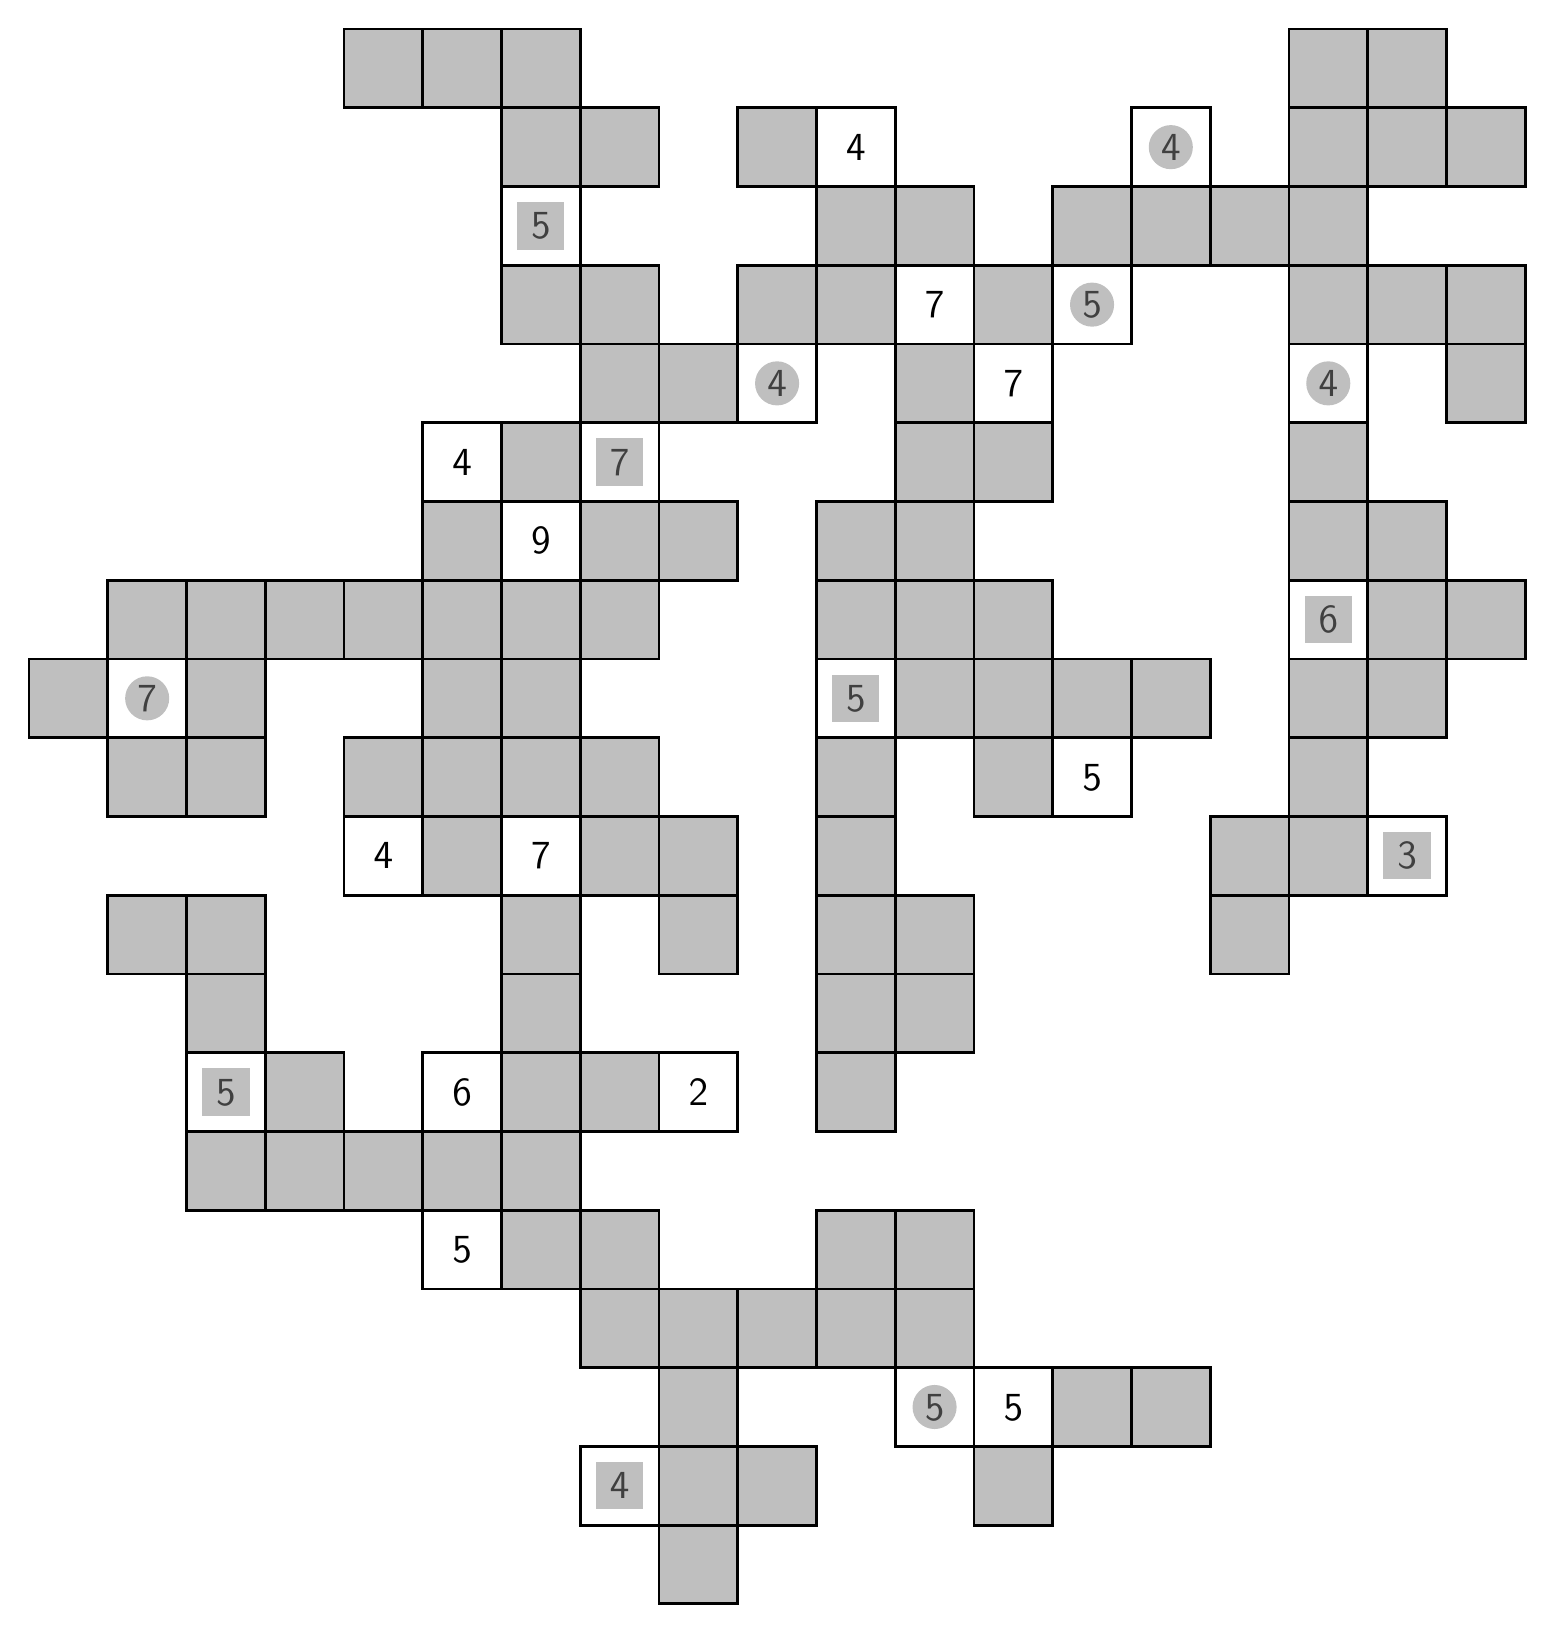
\begin{tikzpicture}\fill[gray, opacity = 0.5] (9, 0, 0)--++(1, 0, 0)--++(0, 1, 0)--++(-1, 0, 0)--cycle;
\draw[line width = 1pt] (9, 0, 0)--++(1, 0, 0)--++(0, 1, 0)--++(-1, 0, 0)--cycle;
\draw node at (8.5, 1.5, 0) {\Large $\mathsf{4}$};
\draw[line width = 1pt] (8, 1, 0)--++(1, 0, 0)--++(0, 1, 0)--++(-1, 0, 0)--cycle;
\fill[color = gray, opacity = 0.5] (8.2, 1.2) rectangle ++(0.6, 0.6);
\fill[gray, opacity = 0.5] (9, 1, 0)--++(1, 0, 0)--++(0, 1, 0)--++(-1, 0, 0)--cycle;
\draw[line width = 1pt] (9, 1, 0)--++(1, 0, 0)--++(0, 1, 0)--++(-1, 0, 0)--cycle;
\fill[gray, opacity = 0.5] (10, 1, 0)--++(1, 0, 0)--++(0, 1, 0)--++(-1, 0, 0)--cycle;
\draw[line width = 1pt] (10, 1, 0)--++(1, 0, 0)--++(0, 1, 0)--++(-1, 0, 0)--cycle;
\fill[gray, opacity = 0.5] (13, 1, 0)--++(1, 0, 0)--++(0, 1, 0)--++(-1, 0, 0)--cycle;
\draw[line width = 1pt] (13, 1, 0)--++(1, 0, 0)--++(0, 1, 0)--++(-1, 0, 0)--cycle;
\fill[gray, opacity = 0.5] (9, 2, 0)--++(1, 0, 0)--++(0, 1, 0)--++(-1, 0, 0)--cycle;
\draw[line width = 1pt] (9, 2, 0)--++(1, 0, 0)--++(0, 1, 0)--++(-1, 0, 0)--cycle;
\draw node at (12.5, 2.5, 0) {\Large $\mathsf{5}$};
\draw[line width = 1pt] (12, 2, 0)--++(1, 0, 0)--++(0, 1, 0)--++(-1, 0, 0)--cycle;
\fill[color = gray, opacity = 0.5] (12.5, 2.5, 0) circle (0.28);
\draw node at (13.5, 2.5, 0) {\Large $\mathsf{5}$};
\draw[line width = 1pt] (13, 2, 0)--++(1, 0, 0)--++(0, 1, 0)--++(-1, 0, 0)--cycle;
\fill[gray, opacity = 0.5] (14, 2, 0)--++(1, 0, 0)--++(0, 1, 0)--++(-1, 0, 0)--cycle;
\draw[line width = 1pt] (14, 2, 0)--++(1, 0, 0)--++(0, 1, 0)--++(-1, 0, 0)--cycle;
\fill[gray, opacity = 0.5] (15, 2, 0)--++(1, 0, 0)--++(0, 1, 0)--++(-1, 0, 0)--cycle;
\draw[line width = 1pt] (15, 2, 0)--++(1, 0, 0)--++(0, 1, 0)--++(-1, 0, 0)--cycle;
\fill[gray, opacity = 0.5] (8, 3, 0)--++(1, 0, 0)--++(0, 1, 0)--++(-1, 0, 0)--cycle;
\draw[line width = 1pt] (8, 3, 0)--++(1, 0, 0)--++(0, 1, 0)--++(-1, 0, 0)--cycle;
\fill[gray, opacity = 0.5] (9, 3, 0)--++(1, 0, 0)--++(0, 1, 0)--++(-1, 0, 0)--cycle;
\draw[line width = 1pt] (9, 3, 0)--++(1, 0, 0)--++(0, 1, 0)--++(-1, 0, 0)--cycle;
\fill[gray, opacity = 0.5] (10, 3, 0)--++(1, 0, 0)--++(0, 1, 0)--++(-1, 0, 0)--cycle;
\draw[line width = 1pt] (10, 3, 0)--++(1, 0, 0)--++(0, 1, 0)--++(-1, 0, 0)--cycle;
\fill[gray, opacity = 0.5] (11, 3, 0)--++(1, 0, 0)--++(0, 1, 0)--++(-1, 0, 0)--cycle;
\draw[line width = 1pt] (11, 3, 0)--++(1, 0, 0)--++(0, 1, 0)--++(-1, 0, 0)--cycle;
\fill[gray, opacity = 0.5] (12, 3, 0)--++(1, 0, 0)--++(0, 1, 0)--++(-1, 0, 0)--cycle;
\draw[line width = 1pt] (12, 3, 0)--++(1, 0, 0)--++(0, 1, 0)--++(-1, 0, 0)--cycle;
\draw node at (6.5, 4.5, 0) {\Large $\mathsf{5}$};
\draw[line width = 1pt] (6, 4, 0)--++(1, 0, 0)--++(0, 1, 0)--++(-1, 0, 0)--cycle;
\fill[gray, opacity = 0.5] (7, 4, 0)--++(1, 0, 0)--++(0, 1, 0)--++(-1, 0, 0)--cycle;
\draw[line width = 1pt] (7, 4, 0)--++(1, 0, 0)--++(0, 1, 0)--++(-1, 0, 0)--cycle;
\fill[gray, opacity = 0.5] (8, 4, 0)--++(1, 0, 0)--++(0, 1, 0)--++(-1, 0, 0)--cycle;
\draw[line width = 1pt] (8, 4, 0)--++(1, 0, 0)--++(0, 1, 0)--++(-1, 0, 0)--cycle;
\fill[gray, opacity = 0.5] (11, 4, 0)--++(1, 0, 0)--++(0, 1, 0)--++(-1, 0, 0)--cycle;
\draw[line width = 1pt] (11, 4, 0)--++(1, 0, 0)--++(0, 1, 0)--++(-1, 0, 0)--cycle;
\fill[gray, opacity = 0.5] (12, 4, 0)--++(1, 0, 0)--++(0, 1, 0)--++(-1, 0, 0)--cycle;
\draw[line width = 1pt] (12, 4, 0)--++(1, 0, 0)--++(0, 1, 0)--++(-1, 0, 0)--cycle;
\fill[gray, opacity = 0.5] (3, 5, 0)--++(1, 0, 0)--++(0, 1, 0)--++(-1, 0, 0)--cycle;
\draw[line width = 1pt] (3, 5, 0)--++(1, 0, 0)--++(0, 1, 0)--++(-1, 0, 0)--cycle;
\fill[gray, opacity = 0.5] (4, 5, 0)--++(1, 0, 0)--++(0, 1, 0)--++(-1, 0, 0)--cycle;
\draw[line width = 1pt] (4, 5, 0)--++(1, 0, 0)--++(0, 1, 0)--++(-1, 0, 0)--cycle;
\fill[gray, opacity = 0.5] (5, 5, 0)--++(1, 0, 0)--++(0, 1, 0)--++(-1, 0, 0)--cycle;
\draw[line width = 1pt] (5, 5, 0)--++(1, 0, 0)--++(0, 1, 0)--++(-1, 0, 0)--cycle;
\fill[gray, opacity = 0.5] (6, 5, 0)--++(1, 0, 0)--++(0, 1, 0)--++(-1, 0, 0)--cycle;
\draw[line width = 1pt] (6, 5, 0)--++(1, 0, 0)--++(0, 1, 0)--++(-1, 0, 0)--cycle;
\fill[gray, opacity = 0.5] (7, 5, 0)--++(1, 0, 0)--++(0, 1, 0)--++(-1, 0, 0)--cycle;
\draw[line width = 1pt] (7, 5, 0)--++(1, 0, 0)--++(0, 1, 0)--++(-1, 0, 0)--cycle;
\draw node at (3.5, 6.5, 0) {\Large $\mathsf{5}$};
\draw[line width = 1pt] (3, 6, 0)--++(1, 0, 0)--++(0, 1, 0)--++(-1, 0, 0)--cycle;
\fill[color = gray, opacity = 0.5] (3.2, 6.2) rectangle ++(0.6, 0.6);
\fill[gray, opacity = 0.5] (4, 6, 0)--++(1, 0, 0)--++(0, 1, 0)--++(-1, 0, 0)--cycle;
\draw[line width = 1pt] (4, 6, 0)--++(1, 0, 0)--++(0, 1, 0)--++(-1, 0, 0)--cycle;
\draw node at (6.5, 6.5, 0) {\Large $\mathsf{6}$};
\draw[line width = 1pt] (6, 6, 0)--++(1, 0, 0)--++(0, 1, 0)--++(-1, 0, 0)--cycle;
\fill[gray, opacity = 0.5] (7, 6, 0)--++(1, 0, 0)--++(0, 1, 0)--++(-1, 0, 0)--cycle;
\draw[line width = 1pt] (7, 6, 0)--++(1, 0, 0)--++(0, 1, 0)--++(-1, 0, 0)--cycle;
\fill[gray, opacity = 0.5] (8, 6, 0)--++(1, 0, 0)--++(0, 1, 0)--++(-1, 0, 0)--cycle;
\draw[line width = 1pt] (8, 6, 0)--++(1, 0, 0)--++(0, 1, 0)--++(-1, 0, 0)--cycle;
\draw node at (9.5, 6.5, 0) {\Large $\mathsf{2}$};
\draw[line width = 1pt] (9, 6, 0)--++(1, 0, 0)--++(0, 1, 0)--++(-1, 0, 0)--cycle;
\fill[gray, opacity = 0.5] (11, 6, 0)--++(1, 0, 0)--++(0, 1, 0)--++(-1, 0, 0)--cycle;
\draw[line width = 1pt] (11, 6, 0)--++(1, 0, 0)--++(0, 1, 0)--++(-1, 0, 0)--cycle;
\fill[gray, opacity = 0.5] (3, 7, 0)--++(1, 0, 0)--++(0, 1, 0)--++(-1, 0, 0)--cycle;
\draw[line width = 1pt] (3, 7, 0)--++(1, 0, 0)--++(0, 1, 0)--++(-1, 0, 0)--cycle;
\fill[gray, opacity = 0.5] (7, 7, 0)--++(1, 0, 0)--++(0, 1, 0)--++(-1, 0, 0)--cycle;
\draw[line width = 1pt] (7, 7, 0)--++(1, 0, 0)--++(0, 1, 0)--++(-1, 0, 0)--cycle;
\fill[gray, opacity = 0.5] (11, 7, 0)--++(1, 0, 0)--++(0, 1, 0)--++(-1, 0, 0)--cycle;
\draw[line width = 1pt] (11, 7, 0)--++(1, 0, 0)--++(0, 1, 0)--++(-1, 0, 0)--cycle;
\fill[gray, opacity = 0.5] (12, 7, 0)--++(1, 0, 0)--++(0, 1, 0)--++(-1, 0, 0)--cycle;
\draw[line width = 1pt] (12, 7, 0)--++(1, 0, 0)--++(0, 1, 0)--++(-1, 0, 0)--cycle;
\fill[gray, opacity = 0.5] (2, 8, 0)--++(1, 0, 0)--++(0, 1, 0)--++(-1, 0, 0)--cycle;
\draw[line width = 1pt] (2, 8, 0)--++(1, 0, 0)--++(0, 1, 0)--++(-1, 0, 0)--cycle;
\fill[gray, opacity = 0.5] (3, 8, 0)--++(1, 0, 0)--++(0, 1, 0)--++(-1, 0, 0)--cycle;
\draw[line width = 1pt] (3, 8, 0)--++(1, 0, 0)--++(0, 1, 0)--++(-1, 0, 0)--cycle;
\fill[gray, opacity = 0.5] (7, 8, 0)--++(1, 0, 0)--++(0, 1, 0)--++(-1, 0, 0)--cycle;
\draw[line width = 1pt] (7, 8, 0)--++(1, 0, 0)--++(0, 1, 0)--++(-1, 0, 0)--cycle;
\fill[gray, opacity = 0.5] (9, 8, 0)--++(1, 0, 0)--++(0, 1, 0)--++(-1, 0, 0)--cycle;
\draw[line width = 1pt] (9, 8, 0)--++(1, 0, 0)--++(0, 1, 0)--++(-1, 0, 0)--cycle;
\fill[gray, opacity = 0.5] (11, 8, 0)--++(1, 0, 0)--++(0, 1, 0)--++(-1, 0, 0)--cycle;
\draw[line width = 1pt] (11, 8, 0)--++(1, 0, 0)--++(0, 1, 0)--++(-1, 0, 0)--cycle;
\fill[gray, opacity = 0.5] (12, 8, 0)--++(1, 0, 0)--++(0, 1, 0)--++(-1, 0, 0)--cycle;
\draw[line width = 1pt] (12, 8, 0)--++(1, 0, 0)--++(0, 1, 0)--++(-1, 0, 0)--cycle;
\fill[gray, opacity = 0.5] (16, 8, 0)--++(1, 0, 0)--++(0, 1, 0)--++(-1, 0, 0)--cycle;
\draw[line width = 1pt] (16, 8, 0)--++(1, 0, 0)--++(0, 1, 0)--++(-1, 0, 0)--cycle;
\draw node at (5.5, 9.5, 0) {\Large $\mathsf{4}$};
\draw[line width = 1pt] (5, 9, 0)--++(1, 0, 0)--++(0, 1, 0)--++(-1, 0, 0)--cycle;
\fill[gray, opacity = 0.5] (6, 9, 0)--++(1, 0, 0)--++(0, 1, 0)--++(-1, 0, 0)--cycle;
\draw[line width = 1pt] (6, 9, 0)--++(1, 0, 0)--++(0, 1, 0)--++(-1, 0, 0)--cycle;
\draw node at (7.5, 9.5, 0) {\Large $\mathsf{7}$};
\draw[line width = 1pt] (7, 9, 0)--++(1, 0, 0)--++(0, 1, 0)--++(-1, 0, 0)--cycle;
\fill[gray, opacity = 0.5] (8, 9, 0)--++(1, 0, 0)--++(0, 1, 0)--++(-1, 0, 0)--cycle;
\draw[line width = 1pt] (8, 9, 0)--++(1, 0, 0)--++(0, 1, 0)--++(-1, 0, 0)--cycle;
\fill[gray, opacity = 0.5] (9, 9, 0)--++(1, 0, 0)--++(0, 1, 0)--++(-1, 0, 0)--cycle;
\draw[line width = 1pt] (9, 9, 0)--++(1, 0, 0)--++(0, 1, 0)--++(-1, 0, 0)--cycle;
\fill[gray, opacity = 0.5] (11, 9, 0)--++(1, 0, 0)--++(0, 1, 0)--++(-1, 0, 0)--cycle;
\draw[line width = 1pt] (11, 9, 0)--++(1, 0, 0)--++(0, 1, 0)--++(-1, 0, 0)--cycle;
\fill[gray, opacity = 0.5] (16, 9, 0)--++(1, 0, 0)--++(0, 1, 0)--++(-1, 0, 0)--cycle;
\draw[line width = 1pt] (16, 9, 0)--++(1, 0, 0)--++(0, 1, 0)--++(-1, 0, 0)--cycle;
\fill[gray, opacity = 0.5] (17, 9, 0)--++(1, 0, 0)--++(0, 1, 0)--++(-1, 0, 0)--cycle;
\draw[line width = 1pt] (17, 9, 0)--++(1, 0, 0)--++(0, 1, 0)--++(-1, 0, 0)--cycle;
\draw node at (18.5, 9.5, 0) {\Large $\mathsf{3}$};
\draw[line width = 1pt] (18, 9, 0)--++(1, 0, 0)--++(0, 1, 0)--++(-1, 0, 0)--cycle;
\fill[color = gray, opacity = 0.5] (18.2, 9.2) rectangle ++(0.6, 0.6);
\fill[gray, opacity = 0.5] (2, 10, 0)--++(1, 0, 0)--++(0, 1, 0)--++(-1, 0, 0)--cycle;
\draw[line width = 1pt] (2, 10, 0)--++(1, 0, 0)--++(0, 1, 0)--++(-1, 0, 0)--cycle;
\fill[gray, opacity = 0.5] (3, 10, 0)--++(1, 0, 0)--++(0, 1, 0)--++(-1, 0, 0)--cycle;
\draw[line width = 1pt] (3, 10, 0)--++(1, 0, 0)--++(0, 1, 0)--++(-1, 0, 0)--cycle;
\fill[gray, opacity = 0.5] (5, 10, 0)--++(1, 0, 0)--++(0, 1, 0)--++(-1, 0, 0)--cycle;
\draw[line width = 1pt] (5, 10, 0)--++(1, 0, 0)--++(0, 1, 0)--++(-1, 0, 0)--cycle;
\fill[gray, opacity = 0.5] (6, 10, 0)--++(1, 0, 0)--++(0, 1, 0)--++(-1, 0, 0)--cycle;
\draw[line width = 1pt] (6, 10, 0)--++(1, 0, 0)--++(0, 1, 0)--++(-1, 0, 0)--cycle;
\fill[gray, opacity = 0.5] (7, 10, 0)--++(1, 0, 0)--++(0, 1, 0)--++(-1, 0, 0)--cycle;
\draw[line width = 1pt] (7, 10, 0)--++(1, 0, 0)--++(0, 1, 0)--++(-1, 0, 0)--cycle;
\fill[gray, opacity = 0.5] (8, 10, 0)--++(1, 0, 0)--++(0, 1, 0)--++(-1, 0, 0)--cycle;
\draw[line width = 1pt] (8, 10, 0)--++(1, 0, 0)--++(0, 1, 0)--++(-1, 0, 0)--cycle;
\fill[gray, opacity = 0.5] (11, 10, 0)--++(1, 0, 0)--++(0, 1, 0)--++(-1, 0, 0)--cycle;
\draw[line width = 1pt] (11, 10, 0)--++(1, 0, 0)--++(0, 1, 0)--++(-1, 0, 0)--cycle;
\fill[gray, opacity = 0.5] (13, 10, 0)--++(1, 0, 0)--++(0, 1, 0)--++(-1, 0, 0)--cycle;
\draw[line width = 1pt] (13, 10, 0)--++(1, 0, 0)--++(0, 1, 0)--++(-1, 0, 0)--cycle;
\draw node at (14.5, 10.5, 0) {\Large $\mathsf{5}$};
\draw[line width = 1pt] (14, 10, 0)--++(1, 0, 0)--++(0, 1, 0)--++(-1, 0, 0)--cycle;
\fill[gray, opacity = 0.5] (17, 10, 0)--++(1, 0, 0)--++(0, 1, 0)--++(-1, 0, 0)--cycle;
\draw[line width = 1pt] (17, 10, 0)--++(1, 0, 0)--++(0, 1, 0)--++(-1, 0, 0)--cycle;
\fill[gray, opacity = 0.5] (1, 11, 0)--++(1, 0, 0)--++(0, 1, 0)--++(-1, 0, 0)--cycle;
\draw[line width = 1pt] (1, 11, 0)--++(1, 0, 0)--++(0, 1, 0)--++(-1, 0, 0)--cycle;
\draw node at (2.5, 11.5, 0) {\Large $\mathsf{7}$};
\draw[line width = 1pt] (2, 11, 0)--++(1, 0, 0)--++(0, 1, 0)--++(-1, 0, 0)--cycle;
\fill[color = gray, opacity = 0.5] (2.5, 11.5, 0) circle (0.28);
\fill[gray, opacity = 0.5] (3, 11, 0)--++(1, 0, 0)--++(0, 1, 0)--++(-1, 0, 0)--cycle;
\draw[line width = 1pt] (3, 11, 0)--++(1, 0, 0)--++(0, 1, 0)--++(-1, 0, 0)--cycle;
\fill[gray, opacity = 0.5] (6, 11, 0)--++(1, 0, 0)--++(0, 1, 0)--++(-1, 0, 0)--cycle;
\draw[line width = 1pt] (6, 11, 0)--++(1, 0, 0)--++(0, 1, 0)--++(-1, 0, 0)--cycle;
\fill[gray, opacity = 0.5] (7, 11, 0)--++(1, 0, 0)--++(0, 1, 0)--++(-1, 0, 0)--cycle;
\draw[line width = 1pt] (7, 11, 0)--++(1, 0, 0)--++(0, 1, 0)--++(-1, 0, 0)--cycle;
\draw node at (11.5, 11.5, 0) {\Large $\mathsf{5}$};
\draw[line width = 1pt] (11, 11, 0)--++(1, 0, 0)--++(0, 1, 0)--++(-1, 0, 0)--cycle;
\fill[color = gray, opacity = 0.5] (11.2, 11.2) rectangle ++(0.6, 0.6);
\fill[gray, opacity = 0.5] (12, 11, 0)--++(1, 0, 0)--++(0, 1, 0)--++(-1, 0, 0)--cycle;
\draw[line width = 1pt] (12, 11, 0)--++(1, 0, 0)--++(0, 1, 0)--++(-1, 0, 0)--cycle;
\fill[gray, opacity = 0.5] (13, 11, 0)--++(1, 0, 0)--++(0, 1, 0)--++(-1, 0, 0)--cycle;
\draw[line width = 1pt] (13, 11, 0)--++(1, 0, 0)--++(0, 1, 0)--++(-1, 0, 0)--cycle;
\fill[gray, opacity = 0.5] (14, 11, 0)--++(1, 0, 0)--++(0, 1, 0)--++(-1, 0, 0)--cycle;
\draw[line width = 1pt] (14, 11, 0)--++(1, 0, 0)--++(0, 1, 0)--++(-1, 0, 0)--cycle;
\fill[gray, opacity = 0.5] (15, 11, 0)--++(1, 0, 0)--++(0, 1, 0)--++(-1, 0, 0)--cycle;
\draw[line width = 1pt] (15, 11, 0)--++(1, 0, 0)--++(0, 1, 0)--++(-1, 0, 0)--cycle;
\fill[gray, opacity = 0.5] (17, 11, 0)--++(1, 0, 0)--++(0, 1, 0)--++(-1, 0, 0)--cycle;
\draw[line width = 1pt] (17, 11, 0)--++(1, 0, 0)--++(0, 1, 0)--++(-1, 0, 0)--cycle;
\fill[gray, opacity = 0.5] (18, 11, 0)--++(1, 0, 0)--++(0, 1, 0)--++(-1, 0, 0)--cycle;
\draw[line width = 1pt] (18, 11, 0)--++(1, 0, 0)--++(0, 1, 0)--++(-1, 0, 0)--cycle;
\fill[gray, opacity = 0.5] (2, 12, 0)--++(1, 0, 0)--++(0, 1, 0)--++(-1, 0, 0)--cycle;
\draw[line width = 1pt] (2, 12, 0)--++(1, 0, 0)--++(0, 1, 0)--++(-1, 0, 0)--cycle;
\fill[gray, opacity = 0.5] (3, 12, 0)--++(1, 0, 0)--++(0, 1, 0)--++(-1, 0, 0)--cycle;
\draw[line width = 1pt] (3, 12, 0)--++(1, 0, 0)--++(0, 1, 0)--++(-1, 0, 0)--cycle;
\fill[gray, opacity = 0.5] (4, 12, 0)--++(1, 0, 0)--++(0, 1, 0)--++(-1, 0, 0)--cycle;
\draw[line width = 1pt] (4, 12, 0)--++(1, 0, 0)--++(0, 1, 0)--++(-1, 0, 0)--cycle;
\fill[gray, opacity = 0.5] (5, 12, 0)--++(1, 0, 0)--++(0, 1, 0)--++(-1, 0, 0)--cycle;
\draw[line width = 1pt] (5, 12, 0)--++(1, 0, 0)--++(0, 1, 0)--++(-1, 0, 0)--cycle;
\fill[gray, opacity = 0.5] (6, 12, 0)--++(1, 0, 0)--++(0, 1, 0)--++(-1, 0, 0)--cycle;
\draw[line width = 1pt] (6, 12, 0)--++(1, 0, 0)--++(0, 1, 0)--++(-1, 0, 0)--cycle;
\fill[gray, opacity = 0.5] (7, 12, 0)--++(1, 0, 0)--++(0, 1, 0)--++(-1, 0, 0)--cycle;
\draw[line width = 1pt] (7, 12, 0)--++(1, 0, 0)--++(0, 1, 0)--++(-1, 0, 0)--cycle;
\fill[gray, opacity = 0.5] (8, 12, 0)--++(1, 0, 0)--++(0, 1, 0)--++(-1, 0, 0)--cycle;
\draw[line width = 1pt] (8, 12, 0)--++(1, 0, 0)--++(0, 1, 0)--++(-1, 0, 0)--cycle;
\fill[gray, opacity = 0.5] (11, 12, 0)--++(1, 0, 0)--++(0, 1, 0)--++(-1, 0, 0)--cycle;
\draw[line width = 1pt] (11, 12, 0)--++(1, 0, 0)--++(0, 1, 0)--++(-1, 0, 0)--cycle;
\fill[gray, opacity = 0.5] (12, 12, 0)--++(1, 0, 0)--++(0, 1, 0)--++(-1, 0, 0)--cycle;
\draw[line width = 1pt] (12, 12, 0)--++(1, 0, 0)--++(0, 1, 0)--++(-1, 0, 0)--cycle;
\fill[gray, opacity = 0.5] (13, 12, 0)--++(1, 0, 0)--++(0, 1, 0)--++(-1, 0, 0)--cycle;
\draw[line width = 1pt] (13, 12, 0)--++(1, 0, 0)--++(0, 1, 0)--++(-1, 0, 0)--cycle;
\draw node at (17.5, 12.5, 0) {\Large $\mathsf{6}$};
\draw[line width = 1pt] (17, 12, 0)--++(1, 0, 0)--++(0, 1, 0)--++(-1, 0, 0)--cycle;
\fill[color = gray, opacity = 0.5] (17.2, 12.2) rectangle ++(0.6, 0.6);
\fill[gray, opacity = 0.5] (18, 12, 0)--++(1, 0, 0)--++(0, 1, 0)--++(-1, 0, 0)--cycle;
\draw[line width = 1pt] (18, 12, 0)--++(1, 0, 0)--++(0, 1, 0)--++(-1, 0, 0)--cycle;
\fill[gray, opacity = 0.5] (19, 12, 0)--++(1, 0, 0)--++(0, 1, 0)--++(-1, 0, 0)--cycle;
\draw[line width = 1pt] (19, 12, 0)--++(1, 0, 0)--++(0, 1, 0)--++(-1, 0, 0)--cycle;
\fill[gray, opacity = 0.5] (6, 13, 0)--++(1, 0, 0)--++(0, 1, 0)--++(-1, 0, 0)--cycle;
\draw[line width = 1pt] (6, 13, 0)--++(1, 0, 0)--++(0, 1, 0)--++(-1, 0, 0)--cycle;
\draw node at (7.5, 13.5, 0) {\Large $\mathsf{9}$};
\draw[line width = 1pt] (7, 13, 0)--++(1, 0, 0)--++(0, 1, 0)--++(-1, 0, 0)--cycle;
\fill[gray, opacity = 0.5] (8, 13, 0)--++(1, 0, 0)--++(0, 1, 0)--++(-1, 0, 0)--cycle;
\draw[line width = 1pt] (8, 13, 0)--++(1, 0, 0)--++(0, 1, 0)--++(-1, 0, 0)--cycle;
\fill[gray, opacity = 0.5] (9, 13, 0)--++(1, 0, 0)--++(0, 1, 0)--++(-1, 0, 0)--cycle;
\draw[line width = 1pt] (9, 13, 0)--++(1, 0, 0)--++(0, 1, 0)--++(-1, 0, 0)--cycle;
\fill[gray, opacity = 0.5] (11, 13, 0)--++(1, 0, 0)--++(0, 1, 0)--++(-1, 0, 0)--cycle;
\draw[line width = 1pt] (11, 13, 0)--++(1, 0, 0)--++(0, 1, 0)--++(-1, 0, 0)--cycle;
\fill[gray, opacity = 0.5] (12, 13, 0)--++(1, 0, 0)--++(0, 1, 0)--++(-1, 0, 0)--cycle;
\draw[line width = 1pt] (12, 13, 0)--++(1, 0, 0)--++(0, 1, 0)--++(-1, 0, 0)--cycle;
\fill[gray, opacity = 0.5] (17, 13, 0)--++(1, 0, 0)--++(0, 1, 0)--++(-1, 0, 0)--cycle;
\draw[line width = 1pt] (17, 13, 0)--++(1, 0, 0)--++(0, 1, 0)--++(-1, 0, 0)--cycle;
\fill[gray, opacity = 0.5] (18, 13, 0)--++(1, 0, 0)--++(0, 1, 0)--++(-1, 0, 0)--cycle;
\draw[line width = 1pt] (18, 13, 0)--++(1, 0, 0)--++(0, 1, 0)--++(-1, 0, 0)--cycle;
\draw node at (6.5, 14.5, 0) {\Large $\mathsf{4}$};
\draw[line width = 1pt] (6, 14, 0)--++(1, 0, 0)--++(0, 1, 0)--++(-1, 0, 0)--cycle;
\fill[gray, opacity = 0.5] (7, 14, 0)--++(1, 0, 0)--++(0, 1, 0)--++(-1, 0, 0)--cycle;
\draw[line width = 1pt] (7, 14, 0)--++(1, 0, 0)--++(0, 1, 0)--++(-1, 0, 0)--cycle;
\draw node at (8.5, 14.5, 0) {\Large $\mathsf{7}$};
\draw[line width = 1pt] (8, 14, 0)--++(1, 0, 0)--++(0, 1, 0)--++(-1, 0, 0)--cycle;
\fill[color = gray, opacity = 0.5] (8.2, 14.2) rectangle ++(0.6, 0.6);
\fill[gray, opacity = 0.5] (12, 14, 0)--++(1, 0, 0)--++(0, 1, 0)--++(-1, 0, 0)--cycle;
\draw[line width = 1pt] (12, 14, 0)--++(1, 0, 0)--++(0, 1, 0)--++(-1, 0, 0)--cycle;
\fill[gray, opacity = 0.5] (13, 14, 0)--++(1, 0, 0)--++(0, 1, 0)--++(-1, 0, 0)--cycle;
\draw[line width = 1pt] (13, 14, 0)--++(1, 0, 0)--++(0, 1, 0)--++(-1, 0, 0)--cycle;
\fill[gray, opacity = 0.5] (17, 14, 0)--++(1, 0, 0)--++(0, 1, 0)--++(-1, 0, 0)--cycle;
\draw[line width = 1pt] (17, 14, 0)--++(1, 0, 0)--++(0, 1, 0)--++(-1, 0, 0)--cycle;
\fill[gray, opacity = 0.5] (8, 15, 0)--++(1, 0, 0)--++(0, 1, 0)--++(-1, 0, 0)--cycle;
\draw[line width = 1pt] (8, 15, 0)--++(1, 0, 0)--++(0, 1, 0)--++(-1, 0, 0)--cycle;
\fill[gray, opacity = 0.5] (9, 15, 0)--++(1, 0, 0)--++(0, 1, 0)--++(-1, 0, 0)--cycle;
\draw[line width = 1pt] (9, 15, 0)--++(1, 0, 0)--++(0, 1, 0)--++(-1, 0, 0)--cycle;
\draw node at (10.5, 15.5, 0) {\Large $\mathsf{4}$};
\draw[line width = 1pt] (10, 15, 0)--++(1, 0, 0)--++(0, 1, 0)--++(-1, 0, 0)--cycle;
\fill[color = gray, opacity = 0.5] (10.5, 15.5, 0) circle (0.28);
\fill[gray, opacity = 0.5] (12, 15, 0)--++(1, 0, 0)--++(0, 1, 0)--++(-1, 0, 0)--cycle;
\draw[line width = 1pt] (12, 15, 0)--++(1, 0, 0)--++(0, 1, 0)--++(-1, 0, 0)--cycle;
\draw node at (13.5, 15.5, 0) {\Large $\mathsf{7}$};
\draw[line width = 1pt] (13, 15, 0)--++(1, 0, 0)--++(0, 1, 0)--++(-1, 0, 0)--cycle;
\draw node at (17.5, 15.5, 0) {\Large $\mathsf{4}$};
\draw[line width = 1pt] (17, 15, 0)--++(1, 0, 0)--++(0, 1, 0)--++(-1, 0, 0)--cycle;
\fill[color = gray, opacity = 0.5] (17.5, 15.5, 0) circle (0.28);
\fill[gray, opacity = 0.5] (19, 15, 0)--++(1, 0, 0)--++(0, 1, 0)--++(-1, 0, 0)--cycle;
\draw[line width = 1pt] (19, 15, 0)--++(1, 0, 0)--++(0, 1, 0)--++(-1, 0, 0)--cycle;
\fill[gray, opacity = 0.5] (7, 16, 0)--++(1, 0, 0)--++(0, 1, 0)--++(-1, 0, 0)--cycle;
\draw[line width = 1pt] (7, 16, 0)--++(1, 0, 0)--++(0, 1, 0)--++(-1, 0, 0)--cycle;
\fill[gray, opacity = 0.5] (8, 16, 0)--++(1, 0, 0)--++(0, 1, 0)--++(-1, 0, 0)--cycle;
\draw[line width = 1pt] (8, 16, 0)--++(1, 0, 0)--++(0, 1, 0)--++(-1, 0, 0)--cycle;
\fill[gray, opacity = 0.5] (10, 16, 0)--++(1, 0, 0)--++(0, 1, 0)--++(-1, 0, 0)--cycle;
\draw[line width = 1pt] (10, 16, 0)--++(1, 0, 0)--++(0, 1, 0)--++(-1, 0, 0)--cycle;
\fill[gray, opacity = 0.5] (11, 16, 0)--++(1, 0, 0)--++(0, 1, 0)--++(-1, 0, 0)--cycle;
\draw[line width = 1pt] (11, 16, 0)--++(1, 0, 0)--++(0, 1, 0)--++(-1, 0, 0)--cycle;
\draw node at (12.5, 16.5, 0) {\Large $\mathsf{7}$};
\draw[line width = 1pt] (12, 16, 0)--++(1, 0, 0)--++(0, 1, 0)--++(-1, 0, 0)--cycle;
\fill[gray, opacity = 0.5] (13, 16, 0)--++(1, 0, 0)--++(0, 1, 0)--++(-1, 0, 0)--cycle;
\draw[line width = 1pt] (13, 16, 0)--++(1, 0, 0)--++(0, 1, 0)--++(-1, 0, 0)--cycle;
\draw node at (14.5, 16.5, 0) {\Large $\mathsf{5}$};
\draw[line width = 1pt] (14, 16, 0)--++(1, 0, 0)--++(0, 1, 0)--++(-1, 0, 0)--cycle;
\fill[color = gray, opacity = 0.5] (14.5, 16.5, 0) circle (0.28);
\fill[gray, opacity = 0.5] (17, 16, 0)--++(1, 0, 0)--++(0, 1, 0)--++(-1, 0, 0)--cycle;
\draw[line width = 1pt] (17, 16, 0)--++(1, 0, 0)--++(0, 1, 0)--++(-1, 0, 0)--cycle;
\fill[gray, opacity = 0.5] (18, 16, 0)--++(1, 0, 0)--++(0, 1, 0)--++(-1, 0, 0)--cycle;
\draw[line width = 1pt] (18, 16, 0)--++(1, 0, 0)--++(0, 1, 0)--++(-1, 0, 0)--cycle;
\fill[gray, opacity = 0.5] (19, 16, 0)--++(1, 0, 0)--++(0, 1, 0)--++(-1, 0, 0)--cycle;
\draw[line width = 1pt] (19, 16, 0)--++(1, 0, 0)--++(0, 1, 0)--++(-1, 0, 0)--cycle;
\draw node at (7.5, 17.5, 0) {\Large $\mathsf{5}$};
\draw[line width = 1pt] (7, 17, 0)--++(1, 0, 0)--++(0, 1, 0)--++(-1, 0, 0)--cycle;
\fill[color = gray, opacity = 0.5] (7.2, 17.2) rectangle ++(0.6, 0.6);
\fill[gray, opacity = 0.5] (11, 17, 0)--++(1, 0, 0)--++(0, 1, 0)--++(-1, 0, 0)--cycle;
\draw[line width = 1pt] (11, 17, 0)--++(1, 0, 0)--++(0, 1, 0)--++(-1, 0, 0)--cycle;
\fill[gray, opacity = 0.5] (12, 17, 0)--++(1, 0, 0)--++(0, 1, 0)--++(-1, 0, 0)--cycle;
\draw[line width = 1pt] (12, 17, 0)--++(1, 0, 0)--++(0, 1, 0)--++(-1, 0, 0)--cycle;
\fill[gray, opacity = 0.5] (14, 17, 0)--++(1, 0, 0)--++(0, 1, 0)--++(-1, 0, 0)--cycle;
\draw[line width = 1pt] (14, 17, 0)--++(1, 0, 0)--++(0, 1, 0)--++(-1, 0, 0)--cycle;
\fill[gray, opacity = 0.5] (15, 17, 0)--++(1, 0, 0)--++(0, 1, 0)--++(-1, 0, 0)--cycle;
\draw[line width = 1pt] (15, 17, 0)--++(1, 0, 0)--++(0, 1, 0)--++(-1, 0, 0)--cycle;
\fill[gray, opacity = 0.5] (16, 17, 0)--++(1, 0, 0)--++(0, 1, 0)--++(-1, 0, 0)--cycle;
\draw[line width = 1pt] (16, 17, 0)--++(1, 0, 0)--++(0, 1, 0)--++(-1, 0, 0)--cycle;
\fill[gray, opacity = 0.5] (17, 17, 0)--++(1, 0, 0)--++(0, 1, 0)--++(-1, 0, 0)--cycle;
\draw[line width = 1pt] (17, 17, 0)--++(1, 0, 0)--++(0, 1, 0)--++(-1, 0, 0)--cycle;
\fill[gray, opacity = 0.5] (7, 18, 0)--++(1, 0, 0)--++(0, 1, 0)--++(-1, 0, 0)--cycle;
\draw[line width = 1pt] (7, 18, 0)--++(1, 0, 0)--++(0, 1, 0)--++(-1, 0, 0)--cycle;
\fill[gray, opacity = 0.5] (8, 18, 0)--++(1, 0, 0)--++(0, 1, 0)--++(-1, 0, 0)--cycle;
\draw[line width = 1pt] (8, 18, 0)--++(1, 0, 0)--++(0, 1, 0)--++(-1, 0, 0)--cycle;
\fill[gray, opacity = 0.5] (10, 18, 0)--++(1, 0, 0)--++(0, 1, 0)--++(-1, 0, 0)--cycle;
\draw[line width = 1pt] (10, 18, 0)--++(1, 0, 0)--++(0, 1, 0)--++(-1, 0, 0)--cycle;
\draw node at (11.5, 18.5, 0) {\Large $\mathsf{4}$};
\draw[line width = 1pt] (11, 18, 0)--++(1, 0, 0)--++(0, 1, 0)--++(-1, 0, 0)--cycle;
\draw node at (15.5, 18.5, 0) {\Large $\mathsf{4}$};
\draw[line width = 1pt] (15, 18, 0)--++(1, 0, 0)--++(0, 1, 0)--++(-1, 0, 0)--cycle;
\fill[color = gray, opacity = 0.5] (15.5, 18.5, 0) circle (0.28);
\fill[gray, opacity = 0.5] (17, 18, 0)--++(1, 0, 0)--++(0, 1, 0)--++(-1, 0, 0)--cycle;
\draw[line width = 1pt] (17, 18, 0)--++(1, 0, 0)--++(0, 1, 0)--++(-1, 0, 0)--cycle;
\fill[gray, opacity = 0.5] (18, 18, 0)--++(1, 0, 0)--++(0, 1, 0)--++(-1, 0, 0)--cycle;
\draw[line width = 1pt] (18, 18, 0)--++(1, 0, 0)--++(0, 1, 0)--++(-1, 0, 0)--cycle;
\fill[gray, opacity = 0.5] (19, 18, 0)--++(1, 0, 0)--++(0, 1, 0)--++(-1, 0, 0)--cycle;
\draw[line width = 1pt] (19, 18, 0)--++(1, 0, 0)--++(0, 1, 0)--++(-1, 0, 0)--cycle;
\fill[gray, opacity = 0.5] (5, 19, 0)--++(1, 0, 0)--++(0, 1, 0)--++(-1, 0, 0)--cycle;
\draw[line width = 1pt] (5, 19, 0)--++(1, 0, 0)--++(0, 1, 0)--++(-1, 0, 0)--cycle;
\fill[gray, opacity = 0.5] (6, 19, 0)--++(1, 0, 0)--++(0, 1, 0)--++(-1, 0, 0)--cycle;
\draw[line width = 1pt] (6, 19, 0)--++(1, 0, 0)--++(0, 1, 0)--++(-1, 0, 0)--cycle;
\fill[gray, opacity = 0.5] (7, 19, 0)--++(1, 0, 0)--++(0, 1, 0)--++(-1, 0, 0)--cycle;
\draw[line width = 1pt] (7, 19, 0)--++(1, 0, 0)--++(0, 1, 0)--++(-1, 0, 0)--cycle;
\fill[gray, opacity = 0.5] (17, 19, 0)--++(1, 0, 0)--++(0, 1, 0)--++(-1, 0, 0)--cycle;
\draw[line width = 1pt] (17, 19, 0)--++(1, 0, 0)--++(0, 1, 0)--++(-1, 0, 0)--cycle;
\fill[gray, opacity = 0.5] (18, 19, 0)--++(1, 0, 0)--++(0, 1, 0)--++(-1, 0, 0)--cycle;
\draw[line width = 1pt] (18, 19, 0)--++(1, 0, 0)--++(0, 1, 0)--++(-1, 0, 0)--cycle;
\end{tikzpicture}}\]
\[\resizebox{30pc}{!}{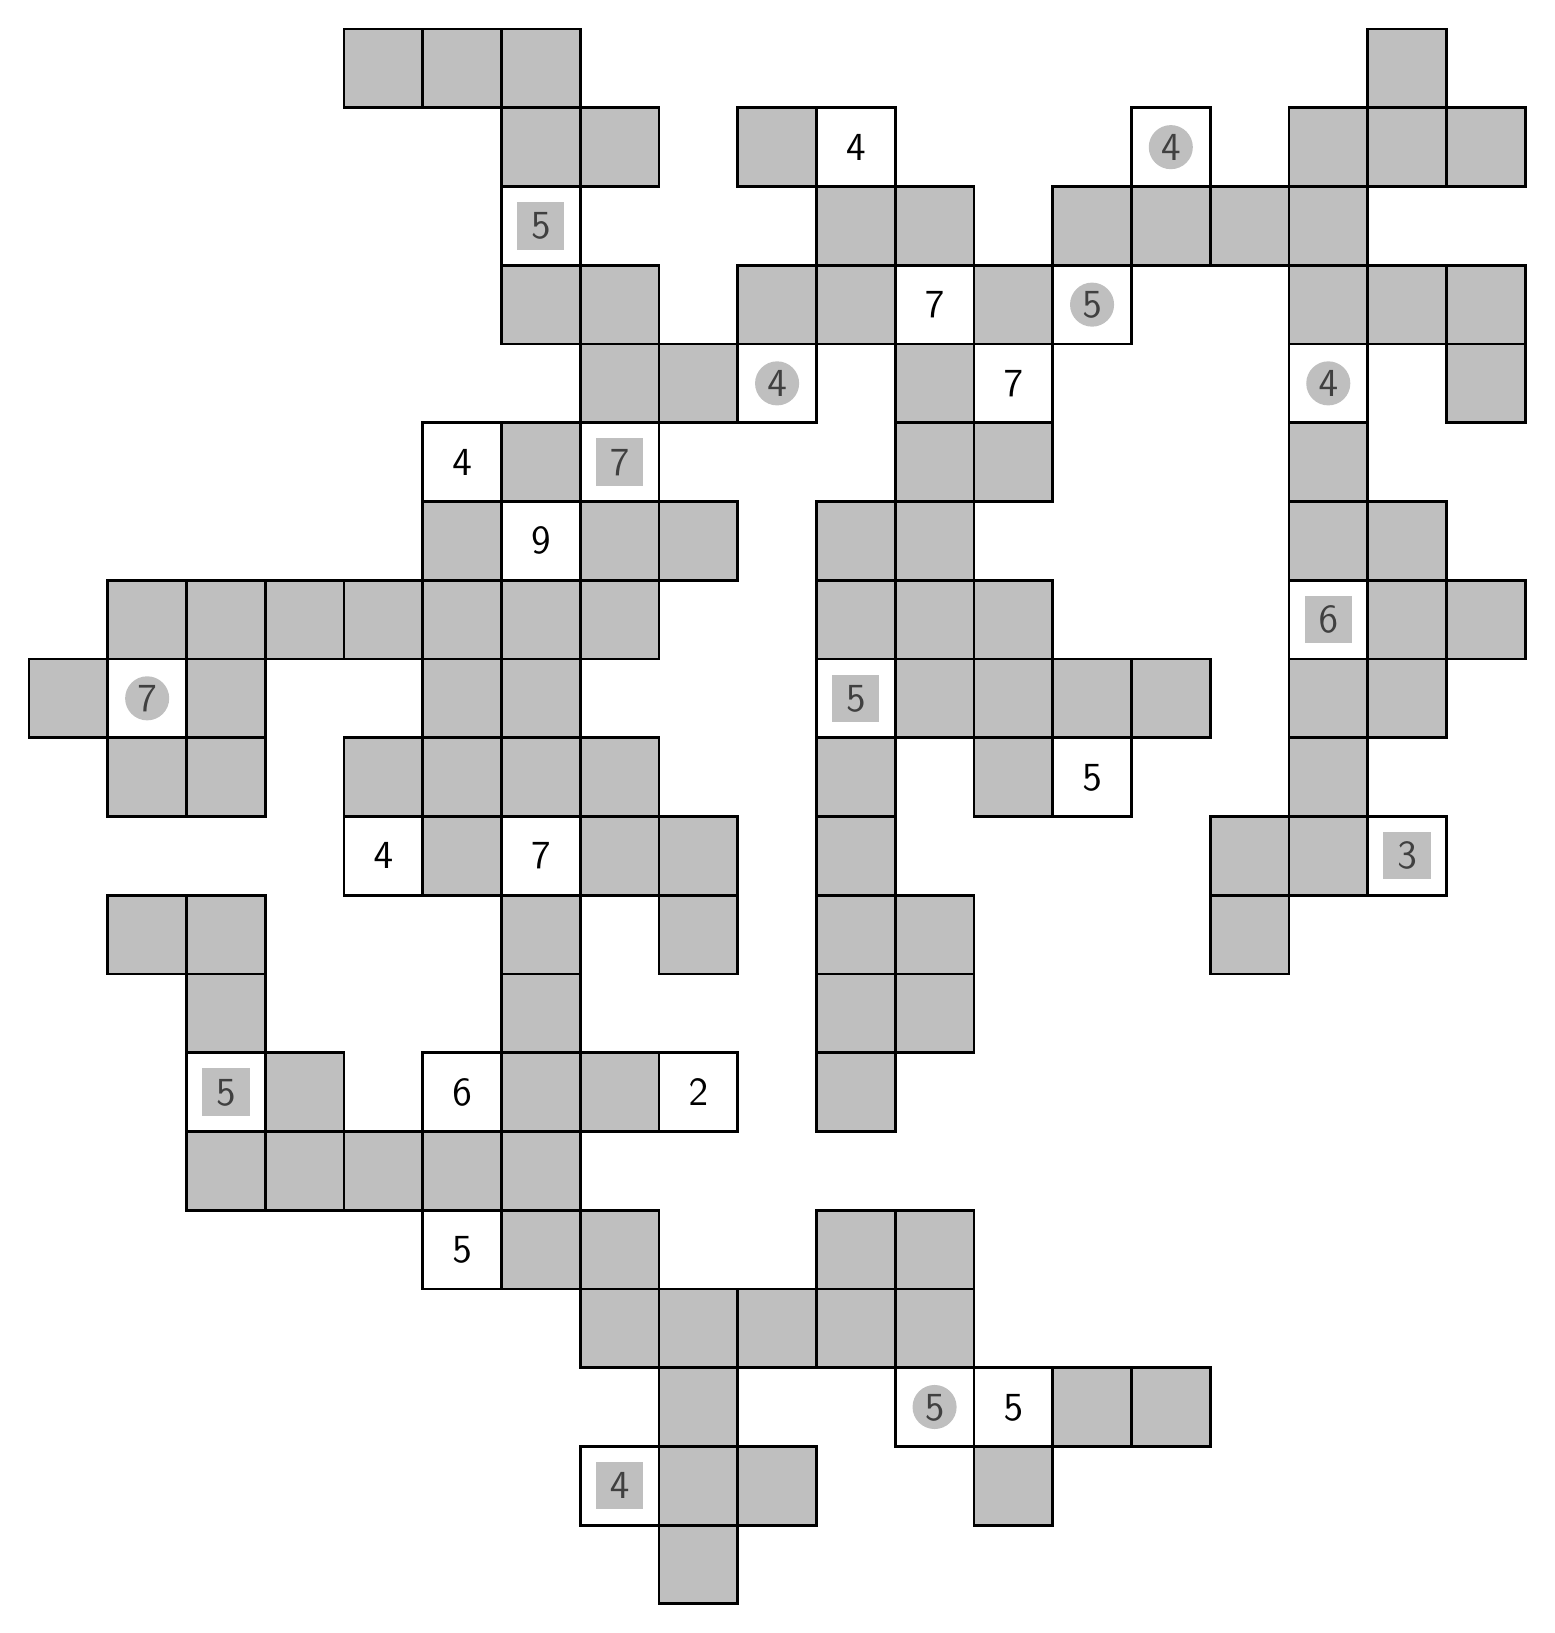
\begin{tikzpicture}\fill[gray, opacity = 0.5] (9, 0, 0)--++(1, 0, 0)--++(0, 1, 0)--++(-1, 0, 0)--cycle;
\draw[line width = 1pt] (9, 0, 0)--++(1, 0, 0)--++(0, 1, 0)--++(-1, 0, 0)--cycle;
\draw node at (8.5, 1.5, 0) {\Large $\mathsf{4}$};
\draw[line width = 1pt] (8, 1, 0)--++(1, 0, 0)--++(0, 1, 0)--++(-1, 0, 0)--cycle;
\fill[color = gray, opacity = 0.5] (8.2, 1.2) rectangle ++(0.6, 0.6);
\fill[gray, opacity = 0.5] (9, 1, 0)--++(1, 0, 0)--++(0, 1, 0)--++(-1, 0, 0)--cycle;
\draw[line width = 1pt] (9, 1, 0)--++(1, 0, 0)--++(0, 1, 0)--++(-1, 0, 0)--cycle;
\fill[gray, opacity = 0.5] (10, 1, 0)--++(1, 0, 0)--++(0, 1, 0)--++(-1, 0, 0)--cycle;
\draw[line width = 1pt] (10, 1, 0)--++(1, 0, 0)--++(0, 1, 0)--++(-1, 0, 0)--cycle;
\fill[gray, opacity = 0.5] (13, 1, 0)--++(1, 0, 0)--++(0, 1, 0)--++(-1, 0, 0)--cycle;
\draw[line width = 1pt] (13, 1, 0)--++(1, 0, 0)--++(0, 1, 0)--++(-1, 0, 0)--cycle;
\fill[gray, opacity = 0.5] (9, 2, 0)--++(1, 0, 0)--++(0, 1, 0)--++(-1, 0, 0)--cycle;
\draw[line width = 1pt] (9, 2, 0)--++(1, 0, 0)--++(0, 1, 0)--++(-1, 0, 0)--cycle;
\draw node at (12.5, 2.5, 0) {\Large $\mathsf{5}$};
\draw[line width = 1pt] (12, 2, 0)--++(1, 0, 0)--++(0, 1, 0)--++(-1, 0, 0)--cycle;
\fill[color = gray, opacity = 0.5] (12.5, 2.5, 0) circle (0.28);
\draw node at (13.5, 2.5, 0) {\Large $\mathsf{5}$};
\draw[line width = 1pt] (13, 2, 0)--++(1, 0, 0)--++(0, 1, 0)--++(-1, 0, 0)--cycle;
\fill[gray, opacity = 0.5] (14, 2, 0)--++(1, 0, 0)--++(0, 1, 0)--++(-1, 0, 0)--cycle;
\draw[line width = 1pt] (14, 2, 0)--++(1, 0, 0)--++(0, 1, 0)--++(-1, 0, 0)--cycle;
\fill[gray, opacity = 0.5] (15, 2, 0)--++(1, 0, 0)--++(0, 1, 0)--++(-1, 0, 0)--cycle;
\draw[line width = 1pt] (15, 2, 0)--++(1, 0, 0)--++(0, 1, 0)--++(-1, 0, 0)--cycle;
\fill[gray, opacity = 0.5] (8, 3, 0)--++(1, 0, 0)--++(0, 1, 0)--++(-1, 0, 0)--cycle;
\draw[line width = 1pt] (8, 3, 0)--++(1, 0, 0)--++(0, 1, 0)--++(-1, 0, 0)--cycle;
\fill[gray, opacity = 0.5] (9, 3, 0)--++(1, 0, 0)--++(0, 1, 0)--++(-1, 0, 0)--cycle;
\draw[line width = 1pt] (9, 3, 0)--++(1, 0, 0)--++(0, 1, 0)--++(-1, 0, 0)--cycle;
\fill[gray, opacity = 0.5] (10, 3, 0)--++(1, 0, 0)--++(0, 1, 0)--++(-1, 0, 0)--cycle;
\draw[line width = 1pt] (10, 3, 0)--++(1, 0, 0)--++(0, 1, 0)--++(-1, 0, 0)--cycle;
\fill[gray, opacity = 0.5] (11, 3, 0)--++(1, 0, 0)--++(0, 1, 0)--++(-1, 0, 0)--cycle;
\draw[line width = 1pt] (11, 3, 0)--++(1, 0, 0)--++(0, 1, 0)--++(-1, 0, 0)--cycle;
\fill[gray, opacity = 0.5] (12, 3, 0)--++(1, 0, 0)--++(0, 1, 0)--++(-1, 0, 0)--cycle;
\draw[line width = 1pt] (12, 3, 0)--++(1, 0, 0)--++(0, 1, 0)--++(-1, 0, 0)--cycle;
\draw node at (6.5, 4.5, 0) {\Large $\mathsf{5}$};
\draw[line width = 1pt] (6, 4, 0)--++(1, 0, 0)--++(0, 1, 0)--++(-1, 0, 0)--cycle;
\fill[gray, opacity = 0.5] (7, 4, 0)--++(1, 0, 0)--++(0, 1, 0)--++(-1, 0, 0)--cycle;
\draw[line width = 1pt] (7, 4, 0)--++(1, 0, 0)--++(0, 1, 0)--++(-1, 0, 0)--cycle;
\fill[gray, opacity = 0.5] (8, 4, 0)--++(1, 0, 0)--++(0, 1, 0)--++(-1, 0, 0)--cycle;
\draw[line width = 1pt] (8, 4, 0)--++(1, 0, 0)--++(0, 1, 0)--++(-1, 0, 0)--cycle;
\fill[gray, opacity = 0.5] (11, 4, 0)--++(1, 0, 0)--++(0, 1, 0)--++(-1, 0, 0)--cycle;
\draw[line width = 1pt] (11, 4, 0)--++(1, 0, 0)--++(0, 1, 0)--++(-1, 0, 0)--cycle;
\fill[gray, opacity = 0.5] (12, 4, 0)--++(1, 0, 0)--++(0, 1, 0)--++(-1, 0, 0)--cycle;
\draw[line width = 1pt] (12, 4, 0)--++(1, 0, 0)--++(0, 1, 0)--++(-1, 0, 0)--cycle;
\fill[gray, opacity = 0.5] (3, 5, 0)--++(1, 0, 0)--++(0, 1, 0)--++(-1, 0, 0)--cycle;
\draw[line width = 1pt] (3, 5, 0)--++(1, 0, 0)--++(0, 1, 0)--++(-1, 0, 0)--cycle;
\fill[gray, opacity = 0.5] (4, 5, 0)--++(1, 0, 0)--++(0, 1, 0)--++(-1, 0, 0)--cycle;
\draw[line width = 1pt] (4, 5, 0)--++(1, 0, 0)--++(0, 1, 0)--++(-1, 0, 0)--cycle;
\fill[gray, opacity = 0.5] (5, 5, 0)--++(1, 0, 0)--++(0, 1, 0)--++(-1, 0, 0)--cycle;
\draw[line width = 1pt] (5, 5, 0)--++(1, 0, 0)--++(0, 1, 0)--++(-1, 0, 0)--cycle;
\fill[gray, opacity = 0.5] (6, 5, 0)--++(1, 0, 0)--++(0, 1, 0)--++(-1, 0, 0)--cycle;
\draw[line width = 1pt] (6, 5, 0)--++(1, 0, 0)--++(0, 1, 0)--++(-1, 0, 0)--cycle;
\fill[gray, opacity = 0.5] (7, 5, 0)--++(1, 0, 0)--++(0, 1, 0)--++(-1, 0, 0)--cycle;
\draw[line width = 1pt] (7, 5, 0)--++(1, 0, 0)--++(0, 1, 0)--++(-1, 0, 0)--cycle;
\draw node at (3.5, 6.5, 0) {\Large $\mathsf{5}$};
\draw[line width = 1pt] (3, 6, 0)--++(1, 0, 0)--++(0, 1, 0)--++(-1, 0, 0)--cycle;
\fill[color = gray, opacity = 0.5] (3.2, 6.2) rectangle ++(0.6, 0.6);
\fill[gray, opacity = 0.5] (4, 6, 0)--++(1, 0, 0)--++(0, 1, 0)--++(-1, 0, 0)--cycle;
\draw[line width = 1pt] (4, 6, 0)--++(1, 0, 0)--++(0, 1, 0)--++(-1, 0, 0)--cycle;
\draw node at (6.5, 6.5, 0) {\Large $\mathsf{6}$};
\draw[line width = 1pt] (6, 6, 0)--++(1, 0, 0)--++(0, 1, 0)--++(-1, 0, 0)--cycle;
\fill[gray, opacity = 0.5] (7, 6, 0)--++(1, 0, 0)--++(0, 1, 0)--++(-1, 0, 0)--cycle;
\draw[line width = 1pt] (7, 6, 0)--++(1, 0, 0)--++(0, 1, 0)--++(-1, 0, 0)--cycle;
\fill[gray, opacity = 0.5] (8, 6, 0)--++(1, 0, 0)--++(0, 1, 0)--++(-1, 0, 0)--cycle;
\draw[line width = 1pt] (8, 6, 0)--++(1, 0, 0)--++(0, 1, 0)--++(-1, 0, 0)--cycle;
\draw node at (9.5, 6.5, 0) {\Large $\mathsf{2}$};
\draw[line width = 1pt] (9, 6, 0)--++(1, 0, 0)--++(0, 1, 0)--++(-1, 0, 0)--cycle;
\fill[gray, opacity = 0.5] (11, 6, 0)--++(1, 0, 0)--++(0, 1, 0)--++(-1, 0, 0)--cycle;
\draw[line width = 1pt] (11, 6, 0)--++(1, 0, 0)--++(0, 1, 0)--++(-1, 0, 0)--cycle;
\fill[gray, opacity = 0.5] (3, 7, 0)--++(1, 0, 0)--++(0, 1, 0)--++(-1, 0, 0)--cycle;
\draw[line width = 1pt] (3, 7, 0)--++(1, 0, 0)--++(0, 1, 0)--++(-1, 0, 0)--cycle;
\fill[gray, opacity = 0.5] (7, 7, 0)--++(1, 0, 0)--++(0, 1, 0)--++(-1, 0, 0)--cycle;
\draw[line width = 1pt] (7, 7, 0)--++(1, 0, 0)--++(0, 1, 0)--++(-1, 0, 0)--cycle;
\fill[gray, opacity = 0.5] (11, 7, 0)--++(1, 0, 0)--++(0, 1, 0)--++(-1, 0, 0)--cycle;
\draw[line width = 1pt] (11, 7, 0)--++(1, 0, 0)--++(0, 1, 0)--++(-1, 0, 0)--cycle;
\fill[gray, opacity = 0.5] (12, 7, 0)--++(1, 0, 0)--++(0, 1, 0)--++(-1, 0, 0)--cycle;
\draw[line width = 1pt] (12, 7, 0)--++(1, 0, 0)--++(0, 1, 0)--++(-1, 0, 0)--cycle;
\fill[gray, opacity = 0.5] (2, 8, 0)--++(1, 0, 0)--++(0, 1, 0)--++(-1, 0, 0)--cycle;
\draw[line width = 1pt] (2, 8, 0)--++(1, 0, 0)--++(0, 1, 0)--++(-1, 0, 0)--cycle;
\fill[gray, opacity = 0.5] (3, 8, 0)--++(1, 0, 0)--++(0, 1, 0)--++(-1, 0, 0)--cycle;
\draw[line width = 1pt] (3, 8, 0)--++(1, 0, 0)--++(0, 1, 0)--++(-1, 0, 0)--cycle;
\fill[gray, opacity = 0.5] (7, 8, 0)--++(1, 0, 0)--++(0, 1, 0)--++(-1, 0, 0)--cycle;
\draw[line width = 1pt] (7, 8, 0)--++(1, 0, 0)--++(0, 1, 0)--++(-1, 0, 0)--cycle;
\fill[gray, opacity = 0.5] (9, 8, 0)--++(1, 0, 0)--++(0, 1, 0)--++(-1, 0, 0)--cycle;
\draw[line width = 1pt] (9, 8, 0)--++(1, 0, 0)--++(0, 1, 0)--++(-1, 0, 0)--cycle;
\fill[gray, opacity = 0.5] (11, 8, 0)--++(1, 0, 0)--++(0, 1, 0)--++(-1, 0, 0)--cycle;
\draw[line width = 1pt] (11, 8, 0)--++(1, 0, 0)--++(0, 1, 0)--++(-1, 0, 0)--cycle;
\fill[gray, opacity = 0.5] (12, 8, 0)--++(1, 0, 0)--++(0, 1, 0)--++(-1, 0, 0)--cycle;
\draw[line width = 1pt] (12, 8, 0)--++(1, 0, 0)--++(0, 1, 0)--++(-1, 0, 0)--cycle;
\fill[gray, opacity = 0.5] (16, 8, 0)--++(1, 0, 0)--++(0, 1, 0)--++(-1, 0, 0)--cycle;
\draw[line width = 1pt] (16, 8, 0)--++(1, 0, 0)--++(0, 1, 0)--++(-1, 0, 0)--cycle;
\draw node at (5.5, 9.5, 0) {\Large $\mathsf{4}$};
\draw[line width = 1pt] (5, 9, 0)--++(1, 0, 0)--++(0, 1, 0)--++(-1, 0, 0)--cycle;
\fill[gray, opacity = 0.5] (6, 9, 0)--++(1, 0, 0)--++(0, 1, 0)--++(-1, 0, 0)--cycle;
\draw[line width = 1pt] (6, 9, 0)--++(1, 0, 0)--++(0, 1, 0)--++(-1, 0, 0)--cycle;
\draw node at (7.5, 9.5, 0) {\Large $\mathsf{7}$};
\draw[line width = 1pt] (7, 9, 0)--++(1, 0, 0)--++(0, 1, 0)--++(-1, 0, 0)--cycle;
\fill[gray, opacity = 0.5] (8, 9, 0)--++(1, 0, 0)--++(0, 1, 0)--++(-1, 0, 0)--cycle;
\draw[line width = 1pt] (8, 9, 0)--++(1, 0, 0)--++(0, 1, 0)--++(-1, 0, 0)--cycle;
\fill[gray, opacity = 0.5] (9, 9, 0)--++(1, 0, 0)--++(0, 1, 0)--++(-1, 0, 0)--cycle;
\draw[line width = 1pt] (9, 9, 0)--++(1, 0, 0)--++(0, 1, 0)--++(-1, 0, 0)--cycle;
\fill[gray, opacity = 0.5] (11, 9, 0)--++(1, 0, 0)--++(0, 1, 0)--++(-1, 0, 0)--cycle;
\draw[line width = 1pt] (11, 9, 0)--++(1, 0, 0)--++(0, 1, 0)--++(-1, 0, 0)--cycle;
\fill[gray, opacity = 0.5] (16, 9, 0)--++(1, 0, 0)--++(0, 1, 0)--++(-1, 0, 0)--cycle;
\draw[line width = 1pt] (16, 9, 0)--++(1, 0, 0)--++(0, 1, 0)--++(-1, 0, 0)--cycle;
\fill[gray, opacity = 0.5] (17, 9, 0)--++(1, 0, 0)--++(0, 1, 0)--++(-1, 0, 0)--cycle;
\draw[line width = 1pt] (17, 9, 0)--++(1, 0, 0)--++(0, 1, 0)--++(-1, 0, 0)--cycle;
\draw node at (18.5, 9.5, 0) {\Large $\mathsf{3}$};
\draw[line width = 1pt] (18, 9, 0)--++(1, 0, 0)--++(0, 1, 0)--++(-1, 0, 0)--cycle;
\fill[color = gray, opacity = 0.5] (18.2, 9.2) rectangle ++(0.6, 0.6);
\fill[gray, opacity = 0.5] (2, 10, 0)--++(1, 0, 0)--++(0, 1, 0)--++(-1, 0, 0)--cycle;
\draw[line width = 1pt] (2, 10, 0)--++(1, 0, 0)--++(0, 1, 0)--++(-1, 0, 0)--cycle;
\fill[gray, opacity = 0.5] (3, 10, 0)--++(1, 0, 0)--++(0, 1, 0)--++(-1, 0, 0)--cycle;
\draw[line width = 1pt] (3, 10, 0)--++(1, 0, 0)--++(0, 1, 0)--++(-1, 0, 0)--cycle;
\fill[gray, opacity = 0.5] (5, 10, 0)--++(1, 0, 0)--++(0, 1, 0)--++(-1, 0, 0)--cycle;
\draw[line width = 1pt] (5, 10, 0)--++(1, 0, 0)--++(0, 1, 0)--++(-1, 0, 0)--cycle;
\fill[gray, opacity = 0.5] (6, 10, 0)--++(1, 0, 0)--++(0, 1, 0)--++(-1, 0, 0)--cycle;
\draw[line width = 1pt] (6, 10, 0)--++(1, 0, 0)--++(0, 1, 0)--++(-1, 0, 0)--cycle;
\fill[gray, opacity = 0.5] (7, 10, 0)--++(1, 0, 0)--++(0, 1, 0)--++(-1, 0, 0)--cycle;
\draw[line width = 1pt] (7, 10, 0)--++(1, 0, 0)--++(0, 1, 0)--++(-1, 0, 0)--cycle;
\fill[gray, opacity = 0.5] (8, 10, 0)--++(1, 0, 0)--++(0, 1, 0)--++(-1, 0, 0)--cycle;
\draw[line width = 1pt] (8, 10, 0)--++(1, 0, 0)--++(0, 1, 0)--++(-1, 0, 0)--cycle;
\fill[gray, opacity = 0.5] (11, 10, 0)--++(1, 0, 0)--++(0, 1, 0)--++(-1, 0, 0)--cycle;
\draw[line width = 1pt] (11, 10, 0)--++(1, 0, 0)--++(0, 1, 0)--++(-1, 0, 0)--cycle;
\fill[gray, opacity = 0.5] (13, 10, 0)--++(1, 0, 0)--++(0, 1, 0)--++(-1, 0, 0)--cycle;
\draw[line width = 1pt] (13, 10, 0)--++(1, 0, 0)--++(0, 1, 0)--++(-1, 0, 0)--cycle;
\draw node at (14.5, 10.5, 0) {\Large $\mathsf{5}$};
\draw[line width = 1pt] (14, 10, 0)--++(1, 0, 0)--++(0, 1, 0)--++(-1, 0, 0)--cycle;
\fill[gray, opacity = 0.5] (17, 10, 0)--++(1, 0, 0)--++(0, 1, 0)--++(-1, 0, 0)--cycle;
\draw[line width = 1pt] (17, 10, 0)--++(1, 0, 0)--++(0, 1, 0)--++(-1, 0, 0)--cycle;
\fill[gray, opacity = 0.5] (1, 11, 0)--++(1, 0, 0)--++(0, 1, 0)--++(-1, 0, 0)--cycle;
\draw[line width = 1pt] (1, 11, 0)--++(1, 0, 0)--++(0, 1, 0)--++(-1, 0, 0)--cycle;
\draw node at (2.5, 11.5, 0) {\Large $\mathsf{7}$};
\draw[line width = 1pt] (2, 11, 0)--++(1, 0, 0)--++(0, 1, 0)--++(-1, 0, 0)--cycle;
\fill[color = gray, opacity = 0.5] (2.5, 11.5, 0) circle (0.28);
\fill[gray, opacity = 0.5] (3, 11, 0)--++(1, 0, 0)--++(0, 1, 0)--++(-1, 0, 0)--cycle;
\draw[line width = 1pt] (3, 11, 0)--++(1, 0, 0)--++(0, 1, 0)--++(-1, 0, 0)--cycle;
\fill[gray, opacity = 0.5] (6, 11, 0)--++(1, 0, 0)--++(0, 1, 0)--++(-1, 0, 0)--cycle;
\draw[line width = 1pt] (6, 11, 0)--++(1, 0, 0)--++(0, 1, 0)--++(-1, 0, 0)--cycle;
\fill[gray, opacity = 0.5] (7, 11, 0)--++(1, 0, 0)--++(0, 1, 0)--++(-1, 0, 0)--cycle;
\draw[line width = 1pt] (7, 11, 0)--++(1, 0, 0)--++(0, 1, 0)--++(-1, 0, 0)--cycle;
\draw node at (11.5, 11.5, 0) {\Large $\mathsf{5}$};
\draw[line width = 1pt] (11, 11, 0)--++(1, 0, 0)--++(0, 1, 0)--++(-1, 0, 0)--cycle;
\fill[color = gray, opacity = 0.5] (11.2, 11.2) rectangle ++(0.6, 0.6);
\fill[gray, opacity = 0.5] (12, 11, 0)--++(1, 0, 0)--++(0, 1, 0)--++(-1, 0, 0)--cycle;
\draw[line width = 1pt] (12, 11, 0)--++(1, 0, 0)--++(0, 1, 0)--++(-1, 0, 0)--cycle;
\fill[gray, opacity = 0.5] (13, 11, 0)--++(1, 0, 0)--++(0, 1, 0)--++(-1, 0, 0)--cycle;
\draw[line width = 1pt] (13, 11, 0)--++(1, 0, 0)--++(0, 1, 0)--++(-1, 0, 0)--cycle;
\fill[gray, opacity = 0.5] (14, 11, 0)--++(1, 0, 0)--++(0, 1, 0)--++(-1, 0, 0)--cycle;
\draw[line width = 1pt] (14, 11, 0)--++(1, 0, 0)--++(0, 1, 0)--++(-1, 0, 0)--cycle;
\fill[gray, opacity = 0.5] (15, 11, 0)--++(1, 0, 0)--++(0, 1, 0)--++(-1, 0, 0)--cycle;
\draw[line width = 1pt] (15, 11, 0)--++(1, 0, 0)--++(0, 1, 0)--++(-1, 0, 0)--cycle;
\fill[gray, opacity = 0.5] (17, 11, 0)--++(1, 0, 0)--++(0, 1, 0)--++(-1, 0, 0)--cycle;
\draw[line width = 1pt] (17, 11, 0)--++(1, 0, 0)--++(0, 1, 0)--++(-1, 0, 0)--cycle;
\fill[gray, opacity = 0.5] (18, 11, 0)--++(1, 0, 0)--++(0, 1, 0)--++(-1, 0, 0)--cycle;
\draw[line width = 1pt] (18, 11, 0)--++(1, 0, 0)--++(0, 1, 0)--++(-1, 0, 0)--cycle;
\fill[gray, opacity = 0.5] (2, 12, 0)--++(1, 0, 0)--++(0, 1, 0)--++(-1, 0, 0)--cycle;
\draw[line width = 1pt] (2, 12, 0)--++(1, 0, 0)--++(0, 1, 0)--++(-1, 0, 0)--cycle;
\fill[gray, opacity = 0.5] (3, 12, 0)--++(1, 0, 0)--++(0, 1, 0)--++(-1, 0, 0)--cycle;
\draw[line width = 1pt] (3, 12, 0)--++(1, 0, 0)--++(0, 1, 0)--++(-1, 0, 0)--cycle;
\fill[gray, opacity = 0.5] (4, 12, 0)--++(1, 0, 0)--++(0, 1, 0)--++(-1, 0, 0)--cycle;
\draw[line width = 1pt] (4, 12, 0)--++(1, 0, 0)--++(0, 1, 0)--++(-1, 0, 0)--cycle;
\fill[gray, opacity = 0.5] (5, 12, 0)--++(1, 0, 0)--++(0, 1, 0)--++(-1, 0, 0)--cycle;
\draw[line width = 1pt] (5, 12, 0)--++(1, 0, 0)--++(0, 1, 0)--++(-1, 0, 0)--cycle;
\fill[gray, opacity = 0.5] (6, 12, 0)--++(1, 0, 0)--++(0, 1, 0)--++(-1, 0, 0)--cycle;
\draw[line width = 1pt] (6, 12, 0)--++(1, 0, 0)--++(0, 1, 0)--++(-1, 0, 0)--cycle;
\fill[gray, opacity = 0.5] (7, 12, 0)--++(1, 0, 0)--++(0, 1, 0)--++(-1, 0, 0)--cycle;
\draw[line width = 1pt] (7, 12, 0)--++(1, 0, 0)--++(0, 1, 0)--++(-1, 0, 0)--cycle;
\fill[gray, opacity = 0.5] (8, 12, 0)--++(1, 0, 0)--++(0, 1, 0)--++(-1, 0, 0)--cycle;
\draw[line width = 1pt] (8, 12, 0)--++(1, 0, 0)--++(0, 1, 0)--++(-1, 0, 0)--cycle;
\fill[gray, opacity = 0.5] (11, 12, 0)--++(1, 0, 0)--++(0, 1, 0)--++(-1, 0, 0)--cycle;
\draw[line width = 1pt] (11, 12, 0)--++(1, 0, 0)--++(0, 1, 0)--++(-1, 0, 0)--cycle;
\fill[gray, opacity = 0.5] (12, 12, 0)--++(1, 0, 0)--++(0, 1, 0)--++(-1, 0, 0)--cycle;
\draw[line width = 1pt] (12, 12, 0)--++(1, 0, 0)--++(0, 1, 0)--++(-1, 0, 0)--cycle;
\fill[gray, opacity = 0.5] (13, 12, 0)--++(1, 0, 0)--++(0, 1, 0)--++(-1, 0, 0)--cycle;
\draw[line width = 1pt] (13, 12, 0)--++(1, 0, 0)--++(0, 1, 0)--++(-1, 0, 0)--cycle;
\draw node at (17.5, 12.5, 0) {\Large $\mathsf{6}$};
\draw[line width = 1pt] (17, 12, 0)--++(1, 0, 0)--++(0, 1, 0)--++(-1, 0, 0)--cycle;
\fill[color = gray, opacity = 0.5] (17.2, 12.2) rectangle ++(0.6, 0.6);
\fill[gray, opacity = 0.5] (18, 12, 0)--++(1, 0, 0)--++(0, 1, 0)--++(-1, 0, 0)--cycle;
\draw[line width = 1pt] (18, 12, 0)--++(1, 0, 0)--++(0, 1, 0)--++(-1, 0, 0)--cycle;
\fill[gray, opacity = 0.5] (19, 12, 0)--++(1, 0, 0)--++(0, 1, 0)--++(-1, 0, 0)--cycle;
\draw[line width = 1pt] (19, 12, 0)--++(1, 0, 0)--++(0, 1, 0)--++(-1, 0, 0)--cycle;
\fill[gray, opacity = 0.5] (6, 13, 0)--++(1, 0, 0)--++(0, 1, 0)--++(-1, 0, 0)--cycle;
\draw[line width = 1pt] (6, 13, 0)--++(1, 0, 0)--++(0, 1, 0)--++(-1, 0, 0)--cycle;
\draw node at (7.5, 13.5, 0) {\Large $\mathsf{9}$};
\draw[line width = 1pt] (7, 13, 0)--++(1, 0, 0)--++(0, 1, 0)--++(-1, 0, 0)--cycle;
\fill[gray, opacity = 0.5] (8, 13, 0)--++(1, 0, 0)--++(0, 1, 0)--++(-1, 0, 0)--cycle;
\draw[line width = 1pt] (8, 13, 0)--++(1, 0, 0)--++(0, 1, 0)--++(-1, 0, 0)--cycle;
\fill[gray, opacity = 0.5] (9, 13, 0)--++(1, 0, 0)--++(0, 1, 0)--++(-1, 0, 0)--cycle;
\draw[line width = 1pt] (9, 13, 0)--++(1, 0, 0)--++(0, 1, 0)--++(-1, 0, 0)--cycle;
\fill[gray, opacity = 0.5] (11, 13, 0)--++(1, 0, 0)--++(0, 1, 0)--++(-1, 0, 0)--cycle;
\draw[line width = 1pt] (11, 13, 0)--++(1, 0, 0)--++(0, 1, 0)--++(-1, 0, 0)--cycle;
\fill[gray, opacity = 0.5] (12, 13, 0)--++(1, 0, 0)--++(0, 1, 0)--++(-1, 0, 0)--cycle;
\draw[line width = 1pt] (12, 13, 0)--++(1, 0, 0)--++(0, 1, 0)--++(-1, 0, 0)--cycle;
\fill[gray, opacity = 0.5] (17, 13, 0)--++(1, 0, 0)--++(0, 1, 0)--++(-1, 0, 0)--cycle;
\draw[line width = 1pt] (17, 13, 0)--++(1, 0, 0)--++(0, 1, 0)--++(-1, 0, 0)--cycle;
\fill[gray, opacity = 0.5] (18, 13, 0)--++(1, 0, 0)--++(0, 1, 0)--++(-1, 0, 0)--cycle;
\draw[line width = 1pt] (18, 13, 0)--++(1, 0, 0)--++(0, 1, 0)--++(-1, 0, 0)--cycle;
\draw node at (6.5, 14.5, 0) {\Large $\mathsf{4}$};
\draw[line width = 1pt] (6, 14, 0)--++(1, 0, 0)--++(0, 1, 0)--++(-1, 0, 0)--cycle;
\fill[gray, opacity = 0.5] (7, 14, 0)--++(1, 0, 0)--++(0, 1, 0)--++(-1, 0, 0)--cycle;
\draw[line width = 1pt] (7, 14, 0)--++(1, 0, 0)--++(0, 1, 0)--++(-1, 0, 0)--cycle;
\draw node at (8.5, 14.5, 0) {\Large $\mathsf{7}$};
\draw[line width = 1pt] (8, 14, 0)--++(1, 0, 0)--++(0, 1, 0)--++(-1, 0, 0)--cycle;
\fill[color = gray, opacity = 0.5] (8.2, 14.2) rectangle ++(0.6, 0.6);
\fill[gray, opacity = 0.5] (12, 14, 0)--++(1, 0, 0)--++(0, 1, 0)--++(-1, 0, 0)--cycle;
\draw[line width = 1pt] (12, 14, 0)--++(1, 0, 0)--++(0, 1, 0)--++(-1, 0, 0)--cycle;
\fill[gray, opacity = 0.5] (13, 14, 0)--++(1, 0, 0)--++(0, 1, 0)--++(-1, 0, 0)--cycle;
\draw[line width = 1pt] (13, 14, 0)--++(1, 0, 0)--++(0, 1, 0)--++(-1, 0, 0)--cycle;
\fill[gray, opacity = 0.5] (17, 14, 0)--++(1, 0, 0)--++(0, 1, 0)--++(-1, 0, 0)--cycle;
\draw[line width = 1pt] (17, 14, 0)--++(1, 0, 0)--++(0, 1, 0)--++(-1, 0, 0)--cycle;
\fill[gray, opacity = 0.5] (8, 15, 0)--++(1, 0, 0)--++(0, 1, 0)--++(-1, 0, 0)--cycle;
\draw[line width = 1pt] (8, 15, 0)--++(1, 0, 0)--++(0, 1, 0)--++(-1, 0, 0)--cycle;
\fill[gray, opacity = 0.5] (9, 15, 0)--++(1, 0, 0)--++(0, 1, 0)--++(-1, 0, 0)--cycle;
\draw[line width = 1pt] (9, 15, 0)--++(1, 0, 0)--++(0, 1, 0)--++(-1, 0, 0)--cycle;
\draw node at (10.5, 15.5, 0) {\Large $\mathsf{4}$};
\draw[line width = 1pt] (10, 15, 0)--++(1, 0, 0)--++(0, 1, 0)--++(-1, 0, 0)--cycle;
\fill[color = gray, opacity = 0.5] (10.5, 15.5, 0) circle (0.28);
\fill[gray, opacity = 0.5] (12, 15, 0)--++(1, 0, 0)--++(0, 1, 0)--++(-1, 0, 0)--cycle;
\draw[line width = 1pt] (12, 15, 0)--++(1, 0, 0)--++(0, 1, 0)--++(-1, 0, 0)--cycle;
\draw node at (13.5, 15.5, 0) {\Large $\mathsf{7}$};
\draw[line width = 1pt] (13, 15, 0)--++(1, 0, 0)--++(0, 1, 0)--++(-1, 0, 0)--cycle;
\draw node at (17.5, 15.5, 0) {\Large $\mathsf{4}$};
\draw[line width = 1pt] (17, 15, 0)--++(1, 0, 0)--++(0, 1, 0)--++(-1, 0, 0)--cycle;
\fill[color = gray, opacity = 0.5] (17.5, 15.5, 0) circle (0.28);
\fill[gray, opacity = 0.5] (19, 15, 0)--++(1, 0, 0)--++(0, 1, 0)--++(-1, 0, 0)--cycle;
\draw[line width = 1pt] (19, 15, 0)--++(1, 0, 0)--++(0, 1, 0)--++(-1, 0, 0)--cycle;
\fill[gray, opacity = 0.5] (7, 16, 0)--++(1, 0, 0)--++(0, 1, 0)--++(-1, 0, 0)--cycle;
\draw[line width = 1pt] (7, 16, 0)--++(1, 0, 0)--++(0, 1, 0)--++(-1, 0, 0)--cycle;
\fill[gray, opacity = 0.5] (8, 16, 0)--++(1, 0, 0)--++(0, 1, 0)--++(-1, 0, 0)--cycle;
\draw[line width = 1pt] (8, 16, 0)--++(1, 0, 0)--++(0, 1, 0)--++(-1, 0, 0)--cycle;
\fill[gray, opacity = 0.5] (10, 16, 0)--++(1, 0, 0)--++(0, 1, 0)--++(-1, 0, 0)--cycle;
\draw[line width = 1pt] (10, 16, 0)--++(1, 0, 0)--++(0, 1, 0)--++(-1, 0, 0)--cycle;
\fill[gray, opacity = 0.5] (11, 16, 0)--++(1, 0, 0)--++(0, 1, 0)--++(-1, 0, 0)--cycle;
\draw[line width = 1pt] (11, 16, 0)--++(1, 0, 0)--++(0, 1, 0)--++(-1, 0, 0)--cycle;
\draw node at (12.5, 16.5, 0) {\Large $\mathsf{7}$};
\draw[line width = 1pt] (12, 16, 0)--++(1, 0, 0)--++(0, 1, 0)--++(-1, 0, 0)--cycle;
\fill[gray, opacity = 0.5] (13, 16, 0)--++(1, 0, 0)--++(0, 1, 0)--++(-1, 0, 0)--cycle;
\draw[line width = 1pt] (13, 16, 0)--++(1, 0, 0)--++(0, 1, 0)--++(-1, 0, 0)--cycle;
\draw node at (14.5, 16.5, 0) {\Large $\mathsf{5}$};
\draw[line width = 1pt] (14, 16, 0)--++(1, 0, 0)--++(0, 1, 0)--++(-1, 0, 0)--cycle;
\fill[color = gray, opacity = 0.5] (14.5, 16.5, 0) circle (0.28);
\fill[gray, opacity = 0.5] (17, 16, 0)--++(1, 0, 0)--++(0, 1, 0)--++(-1, 0, 0)--cycle;
\draw[line width = 1pt] (17, 16, 0)--++(1, 0, 0)--++(0, 1, 0)--++(-1, 0, 0)--cycle;
\fill[gray, opacity = 0.5] (18, 16, 0)--++(1, 0, 0)--++(0, 1, 0)--++(-1, 0, 0)--cycle;
\draw[line width = 1pt] (18, 16, 0)--++(1, 0, 0)--++(0, 1, 0)--++(-1, 0, 0)--cycle;
\fill[gray, opacity = 0.5] (19, 16, 0)--++(1, 0, 0)--++(0, 1, 0)--++(-1, 0, 0)--cycle;
\draw[line width = 1pt] (19, 16, 0)--++(1, 0, 0)--++(0, 1, 0)--++(-1, 0, 0)--cycle;
\draw node at (7.5, 17.5, 0) {\Large $\mathsf{5}$};
\draw[line width = 1pt] (7, 17, 0)--++(1, 0, 0)--++(0, 1, 0)--++(-1, 0, 0)--cycle;
\fill[color = gray, opacity = 0.5] (7.2, 17.2) rectangle ++(0.6, 0.6);
\fill[gray, opacity = 0.5] (11, 17, 0)--++(1, 0, 0)--++(0, 1, 0)--++(-1, 0, 0)--cycle;
\draw[line width = 1pt] (11, 17, 0)--++(1, 0, 0)--++(0, 1, 0)--++(-1, 0, 0)--cycle;
\fill[gray, opacity = 0.5] (12, 17, 0)--++(1, 0, 0)--++(0, 1, 0)--++(-1, 0, 0)--cycle;
\draw[line width = 1pt] (12, 17, 0)--++(1, 0, 0)--++(0, 1, 0)--++(-1, 0, 0)--cycle;
\fill[gray, opacity = 0.5] (14, 17, 0)--++(1, 0, 0)--++(0, 1, 0)--++(-1, 0, 0)--cycle;
\draw[line width = 1pt] (14, 17, 0)--++(1, 0, 0)--++(0, 1, 0)--++(-1, 0, 0)--cycle;
\fill[gray, opacity = 0.5] (15, 17, 0)--++(1, 0, 0)--++(0, 1, 0)--++(-1, 0, 0)--cycle;
\draw[line width = 1pt] (15, 17, 0)--++(1, 0, 0)--++(0, 1, 0)--++(-1, 0, 0)--cycle;
\fill[gray, opacity = 0.5] (16, 17, 0)--++(1, 0, 0)--++(0, 1, 0)--++(-1, 0, 0)--cycle;
\draw[line width = 1pt] (16, 17, 0)--++(1, 0, 0)--++(0, 1, 0)--++(-1, 0, 0)--cycle;
\fill[gray, opacity = 0.5] (17, 17, 0)--++(1, 0, 0)--++(0, 1, 0)--++(-1, 0, 0)--cycle;
\draw[line width = 1pt] (17, 17, 0)--++(1, 0, 0)--++(0, 1, 0)--++(-1, 0, 0)--cycle;
\fill[gray, opacity = 0.5] (7, 18, 0)--++(1, 0, 0)--++(0, 1, 0)--++(-1, 0, 0)--cycle;
\draw[line width = 1pt] (7, 18, 0)--++(1, 0, 0)--++(0, 1, 0)--++(-1, 0, 0)--cycle;
\fill[gray, opacity = 0.5] (8, 18, 0)--++(1, 0, 0)--++(0, 1, 0)--++(-1, 0, 0)--cycle;
\draw[line width = 1pt] (8, 18, 0)--++(1, 0, 0)--++(0, 1, 0)--++(-1, 0, 0)--cycle;
\fill[gray, opacity = 0.5] (10, 18, 0)--++(1, 0, 0)--++(0, 1, 0)--++(-1, 0, 0)--cycle;
\draw[line width = 1pt] (10, 18, 0)--++(1, 0, 0)--++(0, 1, 0)--++(-1, 0, 0)--cycle;
\draw node at (11.5, 18.5, 0) {\Large $\mathsf{4}$};
\draw[line width = 1pt] (11, 18, 0)--++(1, 0, 0)--++(0, 1, 0)--++(-1, 0, 0)--cycle;
\draw node at (15.5, 18.5, 0) {\Large $\mathsf{4}$};
\draw[line width = 1pt] (15, 18, 0)--++(1, 0, 0)--++(0, 1, 0)--++(-1, 0, 0)--cycle;
\fill[color = gray, opacity = 0.5] (15.5, 18.5, 0) circle (0.28);
\fill[gray, opacity = 0.5] (17, 18, 0)--++(1, 0, 0)--++(0, 1, 0)--++(-1, 0, 0)--cycle;
\draw[line width = 1pt] (17, 18, 0)--++(1, 0, 0)--++(0, 1, 0)--++(-1, 0, 0)--cycle;
\fill[gray, opacity = 0.5] (18, 18, 0)--++(1, 0, 0)--++(0, 1, 0)--++(-1, 0, 0)--cycle;
\draw[line width = 1pt] (18, 18, 0)--++(1, 0, 0)--++(0, 1, 0)--++(-1, 0, 0)--cycle;
\fill[gray, opacity = 0.5] (19, 18, 0)--++(1, 0, 0)--++(0, 1, 0)--++(-1, 0, 0)--cycle;
\draw[line width = 1pt] (19, 18, 0)--++(1, 0, 0)--++(0, 1, 0)--++(-1, 0, 0)--cycle;
\fill[gray, opacity = 0.5] (5, 19, 0)--++(1, 0, 0)--++(0, 1, 0)--++(-1, 0, 0)--cycle;
\draw[line width = 1pt] (5, 19, 0)--++(1, 0, 0)--++(0, 1, 0)--++(-1, 0, 0)--cycle;
\fill[gray, opacity = 0.5] (6, 19, 0)--++(1, 0, 0)--++(0, 1, 0)--++(-1, 0, 0)--cycle;
\draw[line width = 1pt] (6, 19, 0)--++(1, 0, 0)--++(0, 1, 0)--++(-1, 0, 0)--cycle;
\fill[gray, opacity = 0.5] (7, 19, 0)--++(1, 0, 0)--++(0, 1, 0)--++(-1, 0, 0)--cycle;
\draw[line width = 1pt] (7, 19, 0)--++(1, 0, 0)--++(0, 1, 0)--++(-1, 0, 0)--cycle;
\fill[gray, opacity = 0.5] (18, 19, 0)--++(1, 0, 0)--++(0, 1, 0)--++(-1, 0, 0)--cycle;
\draw[line width = 1pt] (18, 19, 0)--++(1, 0, 0)--++(0, 1, 0)--++(-1, 0, 0)--cycle;
\end{tikzpicture}}\]
\[\resizebox{30pc}{!}{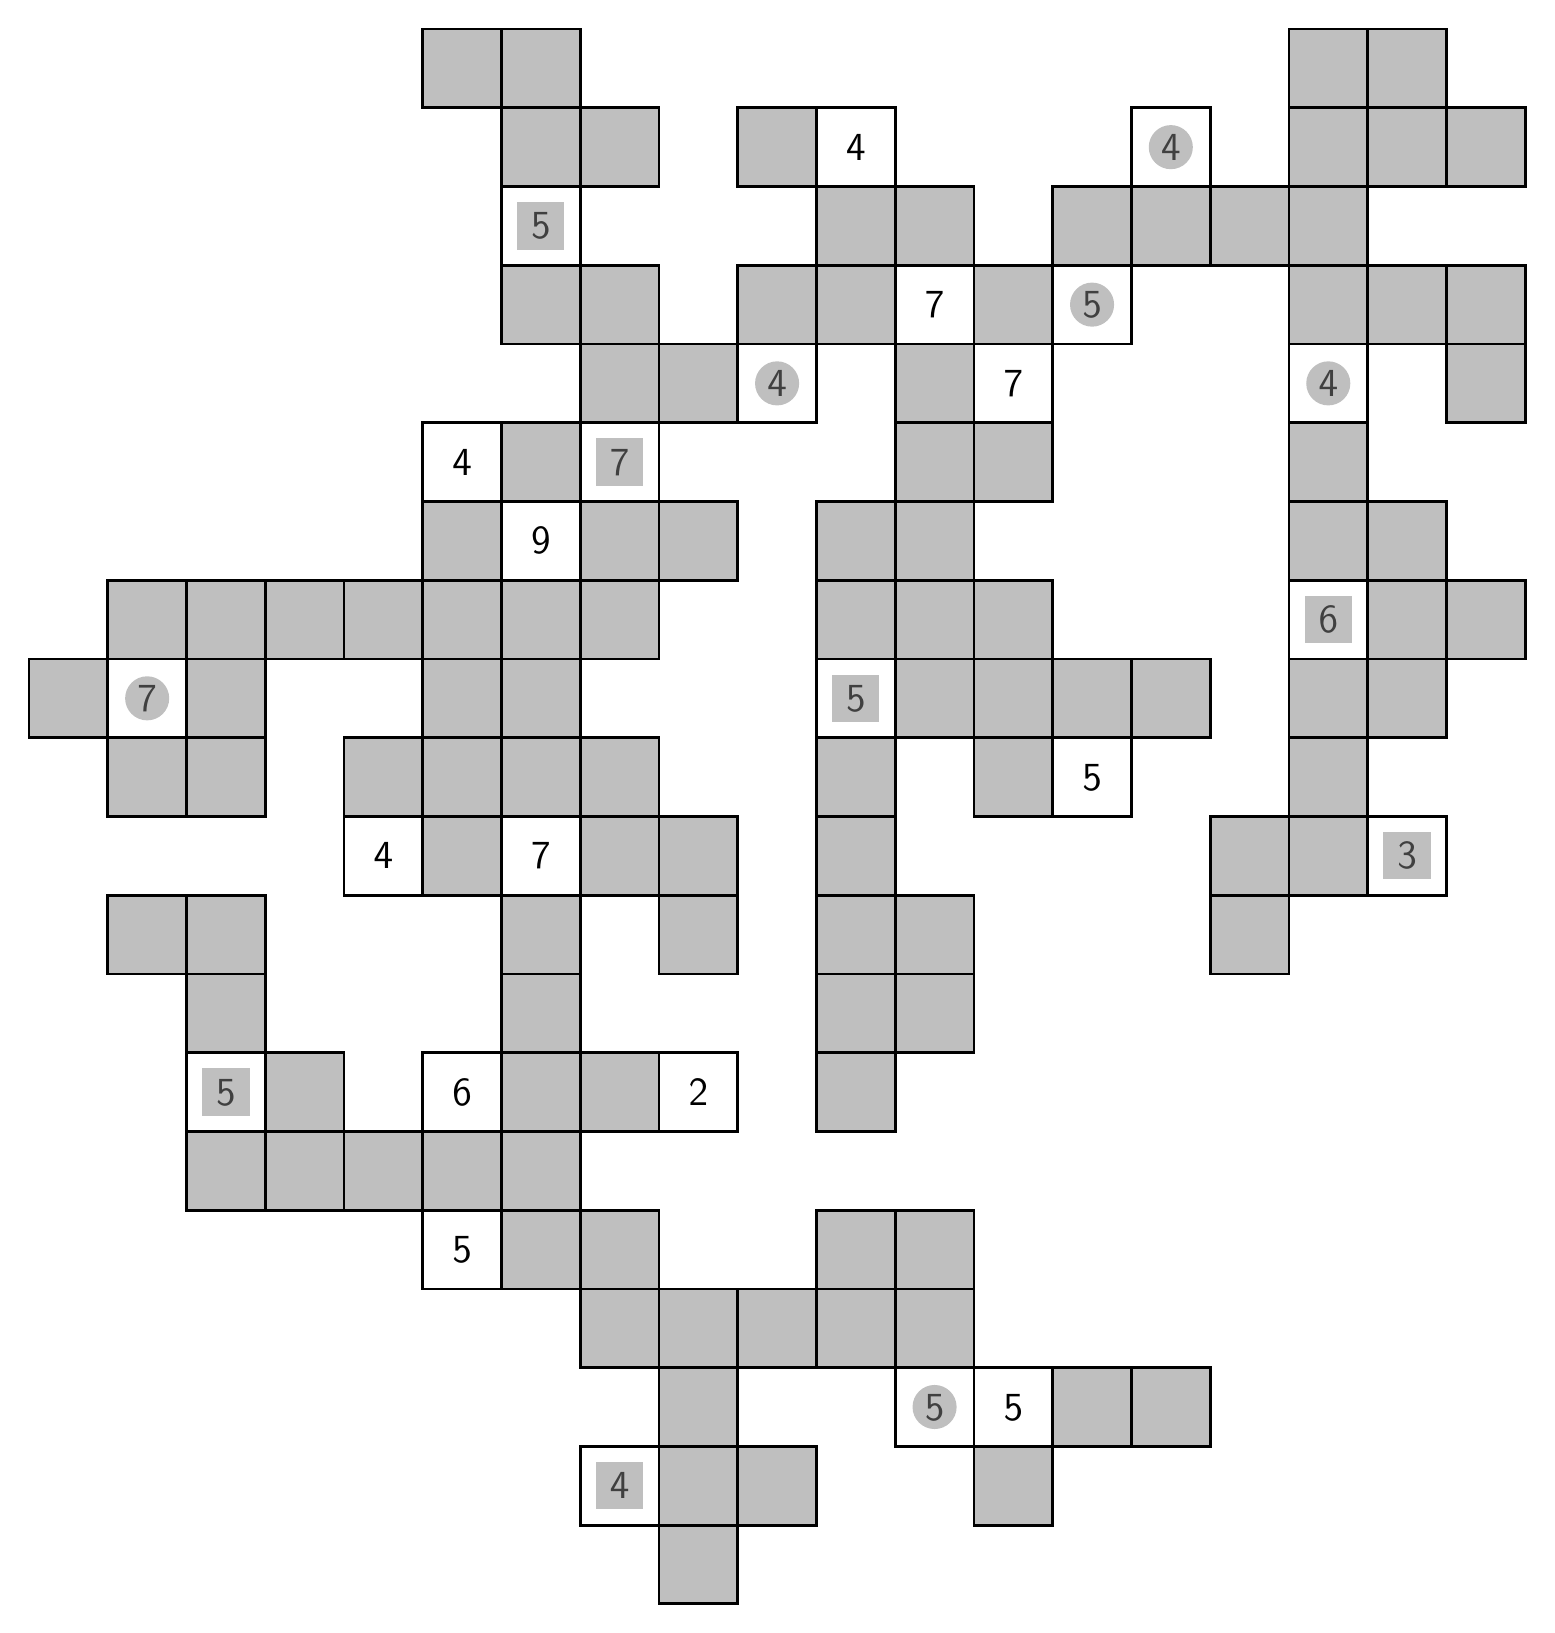
\begin{tikzpicture}\fill[gray, opacity = 0.5] (9, 0, 0)--++(1, 0, 0)--++(0, 1, 0)--++(-1, 0, 0)--cycle;
\draw[line width = 1pt] (9, 0, 0)--++(1, 0, 0)--++(0, 1, 0)--++(-1, 0, 0)--cycle;
\draw node at (8.5, 1.5, 0) {\Large $\mathsf{4}$};
\draw[line width = 1pt] (8, 1, 0)--++(1, 0, 0)--++(0, 1, 0)--++(-1, 0, 0)--cycle;
\fill[color = gray, opacity = 0.5] (8.2, 1.2) rectangle ++(0.6, 0.6);
\fill[gray, opacity = 0.5] (9, 1, 0)--++(1, 0, 0)--++(0, 1, 0)--++(-1, 0, 0)--cycle;
\draw[line width = 1pt] (9, 1, 0)--++(1, 0, 0)--++(0, 1, 0)--++(-1, 0, 0)--cycle;
\fill[gray, opacity = 0.5] (10, 1, 0)--++(1, 0, 0)--++(0, 1, 0)--++(-1, 0, 0)--cycle;
\draw[line width = 1pt] (10, 1, 0)--++(1, 0, 0)--++(0, 1, 0)--++(-1, 0, 0)--cycle;
\fill[gray, opacity = 0.5] (13, 1, 0)--++(1, 0, 0)--++(0, 1, 0)--++(-1, 0, 0)--cycle;
\draw[line width = 1pt] (13, 1, 0)--++(1, 0, 0)--++(0, 1, 0)--++(-1, 0, 0)--cycle;
\fill[gray, opacity = 0.5] (9, 2, 0)--++(1, 0, 0)--++(0, 1, 0)--++(-1, 0, 0)--cycle;
\draw[line width = 1pt] (9, 2, 0)--++(1, 0, 0)--++(0, 1, 0)--++(-1, 0, 0)--cycle;
\draw node at (12.5, 2.5, 0) {\Large $\mathsf{5}$};
\draw[line width = 1pt] (12, 2, 0)--++(1, 0, 0)--++(0, 1, 0)--++(-1, 0, 0)--cycle;
\fill[color = gray, opacity = 0.5] (12.5, 2.5, 0) circle (0.28);
\draw node at (13.5, 2.5, 0) {\Large $\mathsf{5}$};
\draw[line width = 1pt] (13, 2, 0)--++(1, 0, 0)--++(0, 1, 0)--++(-1, 0, 0)--cycle;
\fill[gray, opacity = 0.5] (14, 2, 0)--++(1, 0, 0)--++(0, 1, 0)--++(-1, 0, 0)--cycle;
\draw[line width = 1pt] (14, 2, 0)--++(1, 0, 0)--++(0, 1, 0)--++(-1, 0, 0)--cycle;
\fill[gray, opacity = 0.5] (15, 2, 0)--++(1, 0, 0)--++(0, 1, 0)--++(-1, 0, 0)--cycle;
\draw[line width = 1pt] (15, 2, 0)--++(1, 0, 0)--++(0, 1, 0)--++(-1, 0, 0)--cycle;
\fill[gray, opacity = 0.5] (8, 3, 0)--++(1, 0, 0)--++(0, 1, 0)--++(-1, 0, 0)--cycle;
\draw[line width = 1pt] (8, 3, 0)--++(1, 0, 0)--++(0, 1, 0)--++(-1, 0, 0)--cycle;
\fill[gray, opacity = 0.5] (9, 3, 0)--++(1, 0, 0)--++(0, 1, 0)--++(-1, 0, 0)--cycle;
\draw[line width = 1pt] (9, 3, 0)--++(1, 0, 0)--++(0, 1, 0)--++(-1, 0, 0)--cycle;
\fill[gray, opacity = 0.5] (10, 3, 0)--++(1, 0, 0)--++(0, 1, 0)--++(-1, 0, 0)--cycle;
\draw[line width = 1pt] (10, 3, 0)--++(1, 0, 0)--++(0, 1, 0)--++(-1, 0, 0)--cycle;
\fill[gray, opacity = 0.5] (11, 3, 0)--++(1, 0, 0)--++(0, 1, 0)--++(-1, 0, 0)--cycle;
\draw[line width = 1pt] (11, 3, 0)--++(1, 0, 0)--++(0, 1, 0)--++(-1, 0, 0)--cycle;
\fill[gray, opacity = 0.5] (12, 3, 0)--++(1, 0, 0)--++(0, 1, 0)--++(-1, 0, 0)--cycle;
\draw[line width = 1pt] (12, 3, 0)--++(1, 0, 0)--++(0, 1, 0)--++(-1, 0, 0)--cycle;
\draw node at (6.5, 4.5, 0) {\Large $\mathsf{5}$};
\draw[line width = 1pt] (6, 4, 0)--++(1, 0, 0)--++(0, 1, 0)--++(-1, 0, 0)--cycle;
\fill[gray, opacity = 0.5] (7, 4, 0)--++(1, 0, 0)--++(0, 1, 0)--++(-1, 0, 0)--cycle;
\draw[line width = 1pt] (7, 4, 0)--++(1, 0, 0)--++(0, 1, 0)--++(-1, 0, 0)--cycle;
\fill[gray, opacity = 0.5] (8, 4, 0)--++(1, 0, 0)--++(0, 1, 0)--++(-1, 0, 0)--cycle;
\draw[line width = 1pt] (8, 4, 0)--++(1, 0, 0)--++(0, 1, 0)--++(-1, 0, 0)--cycle;
\fill[gray, opacity = 0.5] (11, 4, 0)--++(1, 0, 0)--++(0, 1, 0)--++(-1, 0, 0)--cycle;
\draw[line width = 1pt] (11, 4, 0)--++(1, 0, 0)--++(0, 1, 0)--++(-1, 0, 0)--cycle;
\fill[gray, opacity = 0.5] (12, 4, 0)--++(1, 0, 0)--++(0, 1, 0)--++(-1, 0, 0)--cycle;
\draw[line width = 1pt] (12, 4, 0)--++(1, 0, 0)--++(0, 1, 0)--++(-1, 0, 0)--cycle;
\fill[gray, opacity = 0.5] (3, 5, 0)--++(1, 0, 0)--++(0, 1, 0)--++(-1, 0, 0)--cycle;
\draw[line width = 1pt] (3, 5, 0)--++(1, 0, 0)--++(0, 1, 0)--++(-1, 0, 0)--cycle;
\fill[gray, opacity = 0.5] (4, 5, 0)--++(1, 0, 0)--++(0, 1, 0)--++(-1, 0, 0)--cycle;
\draw[line width = 1pt] (4, 5, 0)--++(1, 0, 0)--++(0, 1, 0)--++(-1, 0, 0)--cycle;
\fill[gray, opacity = 0.5] (5, 5, 0)--++(1, 0, 0)--++(0, 1, 0)--++(-1, 0, 0)--cycle;
\draw[line width = 1pt] (5, 5, 0)--++(1, 0, 0)--++(0, 1, 0)--++(-1, 0, 0)--cycle;
\fill[gray, opacity = 0.5] (6, 5, 0)--++(1, 0, 0)--++(0, 1, 0)--++(-1, 0, 0)--cycle;
\draw[line width = 1pt] (6, 5, 0)--++(1, 0, 0)--++(0, 1, 0)--++(-1, 0, 0)--cycle;
\fill[gray, opacity = 0.5] (7, 5, 0)--++(1, 0, 0)--++(0, 1, 0)--++(-1, 0, 0)--cycle;
\draw[line width = 1pt] (7, 5, 0)--++(1, 0, 0)--++(0, 1, 0)--++(-1, 0, 0)--cycle;
\draw node at (3.5, 6.5, 0) {\Large $\mathsf{5}$};
\draw[line width = 1pt] (3, 6, 0)--++(1, 0, 0)--++(0, 1, 0)--++(-1, 0, 0)--cycle;
\fill[color = gray, opacity = 0.5] (3.2, 6.2) rectangle ++(0.6, 0.6);
\fill[gray, opacity = 0.5] (4, 6, 0)--++(1, 0, 0)--++(0, 1, 0)--++(-1, 0, 0)--cycle;
\draw[line width = 1pt] (4, 6, 0)--++(1, 0, 0)--++(0, 1, 0)--++(-1, 0, 0)--cycle;
\draw node at (6.5, 6.5, 0) {\Large $\mathsf{6}$};
\draw[line width = 1pt] (6, 6, 0)--++(1, 0, 0)--++(0, 1, 0)--++(-1, 0, 0)--cycle;
\fill[gray, opacity = 0.5] (7, 6, 0)--++(1, 0, 0)--++(0, 1, 0)--++(-1, 0, 0)--cycle;
\draw[line width = 1pt] (7, 6, 0)--++(1, 0, 0)--++(0, 1, 0)--++(-1, 0, 0)--cycle;
\fill[gray, opacity = 0.5] (8, 6, 0)--++(1, 0, 0)--++(0, 1, 0)--++(-1, 0, 0)--cycle;
\draw[line width = 1pt] (8, 6, 0)--++(1, 0, 0)--++(0, 1, 0)--++(-1, 0, 0)--cycle;
\draw node at (9.5, 6.5, 0) {\Large $\mathsf{2}$};
\draw[line width = 1pt] (9, 6, 0)--++(1, 0, 0)--++(0, 1, 0)--++(-1, 0, 0)--cycle;
\fill[gray, opacity = 0.5] (11, 6, 0)--++(1, 0, 0)--++(0, 1, 0)--++(-1, 0, 0)--cycle;
\draw[line width = 1pt] (11, 6, 0)--++(1, 0, 0)--++(0, 1, 0)--++(-1, 0, 0)--cycle;
\fill[gray, opacity = 0.5] (3, 7, 0)--++(1, 0, 0)--++(0, 1, 0)--++(-1, 0, 0)--cycle;
\draw[line width = 1pt] (3, 7, 0)--++(1, 0, 0)--++(0, 1, 0)--++(-1, 0, 0)--cycle;
\fill[gray, opacity = 0.5] (7, 7, 0)--++(1, 0, 0)--++(0, 1, 0)--++(-1, 0, 0)--cycle;
\draw[line width = 1pt] (7, 7, 0)--++(1, 0, 0)--++(0, 1, 0)--++(-1, 0, 0)--cycle;
\fill[gray, opacity = 0.5] (11, 7, 0)--++(1, 0, 0)--++(0, 1, 0)--++(-1, 0, 0)--cycle;
\draw[line width = 1pt] (11, 7, 0)--++(1, 0, 0)--++(0, 1, 0)--++(-1, 0, 0)--cycle;
\fill[gray, opacity = 0.5] (12, 7, 0)--++(1, 0, 0)--++(0, 1, 0)--++(-1, 0, 0)--cycle;
\draw[line width = 1pt] (12, 7, 0)--++(1, 0, 0)--++(0, 1, 0)--++(-1, 0, 0)--cycle;
\fill[gray, opacity = 0.5] (2, 8, 0)--++(1, 0, 0)--++(0, 1, 0)--++(-1, 0, 0)--cycle;
\draw[line width = 1pt] (2, 8, 0)--++(1, 0, 0)--++(0, 1, 0)--++(-1, 0, 0)--cycle;
\fill[gray, opacity = 0.5] (3, 8, 0)--++(1, 0, 0)--++(0, 1, 0)--++(-1, 0, 0)--cycle;
\draw[line width = 1pt] (3, 8, 0)--++(1, 0, 0)--++(0, 1, 0)--++(-1, 0, 0)--cycle;
\fill[gray, opacity = 0.5] (7, 8, 0)--++(1, 0, 0)--++(0, 1, 0)--++(-1, 0, 0)--cycle;
\draw[line width = 1pt] (7, 8, 0)--++(1, 0, 0)--++(0, 1, 0)--++(-1, 0, 0)--cycle;
\fill[gray, opacity = 0.5] (9, 8, 0)--++(1, 0, 0)--++(0, 1, 0)--++(-1, 0, 0)--cycle;
\draw[line width = 1pt] (9, 8, 0)--++(1, 0, 0)--++(0, 1, 0)--++(-1, 0, 0)--cycle;
\fill[gray, opacity = 0.5] (11, 8, 0)--++(1, 0, 0)--++(0, 1, 0)--++(-1, 0, 0)--cycle;
\draw[line width = 1pt] (11, 8, 0)--++(1, 0, 0)--++(0, 1, 0)--++(-1, 0, 0)--cycle;
\fill[gray, opacity = 0.5] (12, 8, 0)--++(1, 0, 0)--++(0, 1, 0)--++(-1, 0, 0)--cycle;
\draw[line width = 1pt] (12, 8, 0)--++(1, 0, 0)--++(0, 1, 0)--++(-1, 0, 0)--cycle;
\fill[gray, opacity = 0.5] (16, 8, 0)--++(1, 0, 0)--++(0, 1, 0)--++(-1, 0, 0)--cycle;
\draw[line width = 1pt] (16, 8, 0)--++(1, 0, 0)--++(0, 1, 0)--++(-1, 0, 0)--cycle;
\draw node at (5.5, 9.5, 0) {\Large $\mathsf{4}$};
\draw[line width = 1pt] (5, 9, 0)--++(1, 0, 0)--++(0, 1, 0)--++(-1, 0, 0)--cycle;
\fill[gray, opacity = 0.5] (6, 9, 0)--++(1, 0, 0)--++(0, 1, 0)--++(-1, 0, 0)--cycle;
\draw[line width = 1pt] (6, 9, 0)--++(1, 0, 0)--++(0, 1, 0)--++(-1, 0, 0)--cycle;
\draw node at (7.5, 9.5, 0) {\Large $\mathsf{7}$};
\draw[line width = 1pt] (7, 9, 0)--++(1, 0, 0)--++(0, 1, 0)--++(-1, 0, 0)--cycle;
\fill[gray, opacity = 0.5] (8, 9, 0)--++(1, 0, 0)--++(0, 1, 0)--++(-1, 0, 0)--cycle;
\draw[line width = 1pt] (8, 9, 0)--++(1, 0, 0)--++(0, 1, 0)--++(-1, 0, 0)--cycle;
\fill[gray, opacity = 0.5] (9, 9, 0)--++(1, 0, 0)--++(0, 1, 0)--++(-1, 0, 0)--cycle;
\draw[line width = 1pt] (9, 9, 0)--++(1, 0, 0)--++(0, 1, 0)--++(-1, 0, 0)--cycle;
\fill[gray, opacity = 0.5] (11, 9, 0)--++(1, 0, 0)--++(0, 1, 0)--++(-1, 0, 0)--cycle;
\draw[line width = 1pt] (11, 9, 0)--++(1, 0, 0)--++(0, 1, 0)--++(-1, 0, 0)--cycle;
\fill[gray, opacity = 0.5] (16, 9, 0)--++(1, 0, 0)--++(0, 1, 0)--++(-1, 0, 0)--cycle;
\draw[line width = 1pt] (16, 9, 0)--++(1, 0, 0)--++(0, 1, 0)--++(-1, 0, 0)--cycle;
\fill[gray, opacity = 0.5] (17, 9, 0)--++(1, 0, 0)--++(0, 1, 0)--++(-1, 0, 0)--cycle;
\draw[line width = 1pt] (17, 9, 0)--++(1, 0, 0)--++(0, 1, 0)--++(-1, 0, 0)--cycle;
\draw node at (18.5, 9.5, 0) {\Large $\mathsf{3}$};
\draw[line width = 1pt] (18, 9, 0)--++(1, 0, 0)--++(0, 1, 0)--++(-1, 0, 0)--cycle;
\fill[color = gray, opacity = 0.5] (18.2, 9.2) rectangle ++(0.6, 0.6);
\fill[gray, opacity = 0.5] (2, 10, 0)--++(1, 0, 0)--++(0, 1, 0)--++(-1, 0, 0)--cycle;
\draw[line width = 1pt] (2, 10, 0)--++(1, 0, 0)--++(0, 1, 0)--++(-1, 0, 0)--cycle;
\fill[gray, opacity = 0.5] (3, 10, 0)--++(1, 0, 0)--++(0, 1, 0)--++(-1, 0, 0)--cycle;
\draw[line width = 1pt] (3, 10, 0)--++(1, 0, 0)--++(0, 1, 0)--++(-1, 0, 0)--cycle;
\fill[gray, opacity = 0.5] (5, 10, 0)--++(1, 0, 0)--++(0, 1, 0)--++(-1, 0, 0)--cycle;
\draw[line width = 1pt] (5, 10, 0)--++(1, 0, 0)--++(0, 1, 0)--++(-1, 0, 0)--cycle;
\fill[gray, opacity = 0.5] (6, 10, 0)--++(1, 0, 0)--++(0, 1, 0)--++(-1, 0, 0)--cycle;
\draw[line width = 1pt] (6, 10, 0)--++(1, 0, 0)--++(0, 1, 0)--++(-1, 0, 0)--cycle;
\fill[gray, opacity = 0.5] (7, 10, 0)--++(1, 0, 0)--++(0, 1, 0)--++(-1, 0, 0)--cycle;
\draw[line width = 1pt] (7, 10, 0)--++(1, 0, 0)--++(0, 1, 0)--++(-1, 0, 0)--cycle;
\fill[gray, opacity = 0.5] (8, 10, 0)--++(1, 0, 0)--++(0, 1, 0)--++(-1, 0, 0)--cycle;
\draw[line width = 1pt] (8, 10, 0)--++(1, 0, 0)--++(0, 1, 0)--++(-1, 0, 0)--cycle;
\fill[gray, opacity = 0.5] (11, 10, 0)--++(1, 0, 0)--++(0, 1, 0)--++(-1, 0, 0)--cycle;
\draw[line width = 1pt] (11, 10, 0)--++(1, 0, 0)--++(0, 1, 0)--++(-1, 0, 0)--cycle;
\fill[gray, opacity = 0.5] (13, 10, 0)--++(1, 0, 0)--++(0, 1, 0)--++(-1, 0, 0)--cycle;
\draw[line width = 1pt] (13, 10, 0)--++(1, 0, 0)--++(0, 1, 0)--++(-1, 0, 0)--cycle;
\draw node at (14.5, 10.5, 0) {\Large $\mathsf{5}$};
\draw[line width = 1pt] (14, 10, 0)--++(1, 0, 0)--++(0, 1, 0)--++(-1, 0, 0)--cycle;
\fill[gray, opacity = 0.5] (17, 10, 0)--++(1, 0, 0)--++(0, 1, 0)--++(-1, 0, 0)--cycle;
\draw[line width = 1pt] (17, 10, 0)--++(1, 0, 0)--++(0, 1, 0)--++(-1, 0, 0)--cycle;
\fill[gray, opacity = 0.5] (1, 11, 0)--++(1, 0, 0)--++(0, 1, 0)--++(-1, 0, 0)--cycle;
\draw[line width = 1pt] (1, 11, 0)--++(1, 0, 0)--++(0, 1, 0)--++(-1, 0, 0)--cycle;
\draw node at (2.5, 11.5, 0) {\Large $\mathsf{7}$};
\draw[line width = 1pt] (2, 11, 0)--++(1, 0, 0)--++(0, 1, 0)--++(-1, 0, 0)--cycle;
\fill[color = gray, opacity = 0.5] (2.5, 11.5, 0) circle (0.28);
\fill[gray, opacity = 0.5] (3, 11, 0)--++(1, 0, 0)--++(0, 1, 0)--++(-1, 0, 0)--cycle;
\draw[line width = 1pt] (3, 11, 0)--++(1, 0, 0)--++(0, 1, 0)--++(-1, 0, 0)--cycle;
\fill[gray, opacity = 0.5] (6, 11, 0)--++(1, 0, 0)--++(0, 1, 0)--++(-1, 0, 0)--cycle;
\draw[line width = 1pt] (6, 11, 0)--++(1, 0, 0)--++(0, 1, 0)--++(-1, 0, 0)--cycle;
\fill[gray, opacity = 0.5] (7, 11, 0)--++(1, 0, 0)--++(0, 1, 0)--++(-1, 0, 0)--cycle;
\draw[line width = 1pt] (7, 11, 0)--++(1, 0, 0)--++(0, 1, 0)--++(-1, 0, 0)--cycle;
\draw node at (11.5, 11.5, 0) {\Large $\mathsf{5}$};
\draw[line width = 1pt] (11, 11, 0)--++(1, 0, 0)--++(0, 1, 0)--++(-1, 0, 0)--cycle;
\fill[color = gray, opacity = 0.5] (11.2, 11.2) rectangle ++(0.6, 0.6);
\fill[gray, opacity = 0.5] (12, 11, 0)--++(1, 0, 0)--++(0, 1, 0)--++(-1, 0, 0)--cycle;
\draw[line width = 1pt] (12, 11, 0)--++(1, 0, 0)--++(0, 1, 0)--++(-1, 0, 0)--cycle;
\fill[gray, opacity = 0.5] (13, 11, 0)--++(1, 0, 0)--++(0, 1, 0)--++(-1, 0, 0)--cycle;
\draw[line width = 1pt] (13, 11, 0)--++(1, 0, 0)--++(0, 1, 0)--++(-1, 0, 0)--cycle;
\fill[gray, opacity = 0.5] (14, 11, 0)--++(1, 0, 0)--++(0, 1, 0)--++(-1, 0, 0)--cycle;
\draw[line width = 1pt] (14, 11, 0)--++(1, 0, 0)--++(0, 1, 0)--++(-1, 0, 0)--cycle;
\fill[gray, opacity = 0.5] (15, 11, 0)--++(1, 0, 0)--++(0, 1, 0)--++(-1, 0, 0)--cycle;
\draw[line width = 1pt] (15, 11, 0)--++(1, 0, 0)--++(0, 1, 0)--++(-1, 0, 0)--cycle;
\fill[gray, opacity = 0.5] (17, 11, 0)--++(1, 0, 0)--++(0, 1, 0)--++(-1, 0, 0)--cycle;
\draw[line width = 1pt] (17, 11, 0)--++(1, 0, 0)--++(0, 1, 0)--++(-1, 0, 0)--cycle;
\fill[gray, opacity = 0.5] (18, 11, 0)--++(1, 0, 0)--++(0, 1, 0)--++(-1, 0, 0)--cycle;
\draw[line width = 1pt] (18, 11, 0)--++(1, 0, 0)--++(0, 1, 0)--++(-1, 0, 0)--cycle;
\fill[gray, opacity = 0.5] (2, 12, 0)--++(1, 0, 0)--++(0, 1, 0)--++(-1, 0, 0)--cycle;
\draw[line width = 1pt] (2, 12, 0)--++(1, 0, 0)--++(0, 1, 0)--++(-1, 0, 0)--cycle;
\fill[gray, opacity = 0.5] (3, 12, 0)--++(1, 0, 0)--++(0, 1, 0)--++(-1, 0, 0)--cycle;
\draw[line width = 1pt] (3, 12, 0)--++(1, 0, 0)--++(0, 1, 0)--++(-1, 0, 0)--cycle;
\fill[gray, opacity = 0.5] (4, 12, 0)--++(1, 0, 0)--++(0, 1, 0)--++(-1, 0, 0)--cycle;
\draw[line width = 1pt] (4, 12, 0)--++(1, 0, 0)--++(0, 1, 0)--++(-1, 0, 0)--cycle;
\fill[gray, opacity = 0.5] (5, 12, 0)--++(1, 0, 0)--++(0, 1, 0)--++(-1, 0, 0)--cycle;
\draw[line width = 1pt] (5, 12, 0)--++(1, 0, 0)--++(0, 1, 0)--++(-1, 0, 0)--cycle;
\fill[gray, opacity = 0.5] (6, 12, 0)--++(1, 0, 0)--++(0, 1, 0)--++(-1, 0, 0)--cycle;
\draw[line width = 1pt] (6, 12, 0)--++(1, 0, 0)--++(0, 1, 0)--++(-1, 0, 0)--cycle;
\fill[gray, opacity = 0.5] (7, 12, 0)--++(1, 0, 0)--++(0, 1, 0)--++(-1, 0, 0)--cycle;
\draw[line width = 1pt] (7, 12, 0)--++(1, 0, 0)--++(0, 1, 0)--++(-1, 0, 0)--cycle;
\fill[gray, opacity = 0.5] (8, 12, 0)--++(1, 0, 0)--++(0, 1, 0)--++(-1, 0, 0)--cycle;
\draw[line width = 1pt] (8, 12, 0)--++(1, 0, 0)--++(0, 1, 0)--++(-1, 0, 0)--cycle;
\fill[gray, opacity = 0.5] (11, 12, 0)--++(1, 0, 0)--++(0, 1, 0)--++(-1, 0, 0)--cycle;
\draw[line width = 1pt] (11, 12, 0)--++(1, 0, 0)--++(0, 1, 0)--++(-1, 0, 0)--cycle;
\fill[gray, opacity = 0.5] (12, 12, 0)--++(1, 0, 0)--++(0, 1, 0)--++(-1, 0, 0)--cycle;
\draw[line width = 1pt] (12, 12, 0)--++(1, 0, 0)--++(0, 1, 0)--++(-1, 0, 0)--cycle;
\fill[gray, opacity = 0.5] (13, 12, 0)--++(1, 0, 0)--++(0, 1, 0)--++(-1, 0, 0)--cycle;
\draw[line width = 1pt] (13, 12, 0)--++(1, 0, 0)--++(0, 1, 0)--++(-1, 0, 0)--cycle;
\draw node at (17.5, 12.5, 0) {\Large $\mathsf{6}$};
\draw[line width = 1pt] (17, 12, 0)--++(1, 0, 0)--++(0, 1, 0)--++(-1, 0, 0)--cycle;
\fill[color = gray, opacity = 0.5] (17.2, 12.2) rectangle ++(0.6, 0.6);
\fill[gray, opacity = 0.5] (18, 12, 0)--++(1, 0, 0)--++(0, 1, 0)--++(-1, 0, 0)--cycle;
\draw[line width = 1pt] (18, 12, 0)--++(1, 0, 0)--++(0, 1, 0)--++(-1, 0, 0)--cycle;
\fill[gray, opacity = 0.5] (19, 12, 0)--++(1, 0, 0)--++(0, 1, 0)--++(-1, 0, 0)--cycle;
\draw[line width = 1pt] (19, 12, 0)--++(1, 0, 0)--++(0, 1, 0)--++(-1, 0, 0)--cycle;
\fill[gray, opacity = 0.5] (6, 13, 0)--++(1, 0, 0)--++(0, 1, 0)--++(-1, 0, 0)--cycle;
\draw[line width = 1pt] (6, 13, 0)--++(1, 0, 0)--++(0, 1, 0)--++(-1, 0, 0)--cycle;
\draw node at (7.5, 13.5, 0) {\Large $\mathsf{9}$};
\draw[line width = 1pt] (7, 13, 0)--++(1, 0, 0)--++(0, 1, 0)--++(-1, 0, 0)--cycle;
\fill[gray, opacity = 0.5] (8, 13, 0)--++(1, 0, 0)--++(0, 1, 0)--++(-1, 0, 0)--cycle;
\draw[line width = 1pt] (8, 13, 0)--++(1, 0, 0)--++(0, 1, 0)--++(-1, 0, 0)--cycle;
\fill[gray, opacity = 0.5] (9, 13, 0)--++(1, 0, 0)--++(0, 1, 0)--++(-1, 0, 0)--cycle;
\draw[line width = 1pt] (9, 13, 0)--++(1, 0, 0)--++(0, 1, 0)--++(-1, 0, 0)--cycle;
\fill[gray, opacity = 0.5] (11, 13, 0)--++(1, 0, 0)--++(0, 1, 0)--++(-1, 0, 0)--cycle;
\draw[line width = 1pt] (11, 13, 0)--++(1, 0, 0)--++(0, 1, 0)--++(-1, 0, 0)--cycle;
\fill[gray, opacity = 0.5] (12, 13, 0)--++(1, 0, 0)--++(0, 1, 0)--++(-1, 0, 0)--cycle;
\draw[line width = 1pt] (12, 13, 0)--++(1, 0, 0)--++(0, 1, 0)--++(-1, 0, 0)--cycle;
\fill[gray, opacity = 0.5] (17, 13, 0)--++(1, 0, 0)--++(0, 1, 0)--++(-1, 0, 0)--cycle;
\draw[line width = 1pt] (17, 13, 0)--++(1, 0, 0)--++(0, 1, 0)--++(-1, 0, 0)--cycle;
\fill[gray, opacity = 0.5] (18, 13, 0)--++(1, 0, 0)--++(0, 1, 0)--++(-1, 0, 0)--cycle;
\draw[line width = 1pt] (18, 13, 0)--++(1, 0, 0)--++(0, 1, 0)--++(-1, 0, 0)--cycle;
\draw node at (6.5, 14.5, 0) {\Large $\mathsf{4}$};
\draw[line width = 1pt] (6, 14, 0)--++(1, 0, 0)--++(0, 1, 0)--++(-1, 0, 0)--cycle;
\fill[gray, opacity = 0.5] (7, 14, 0)--++(1, 0, 0)--++(0, 1, 0)--++(-1, 0, 0)--cycle;
\draw[line width = 1pt] (7, 14, 0)--++(1, 0, 0)--++(0, 1, 0)--++(-1, 0, 0)--cycle;
\draw node at (8.5, 14.5, 0) {\Large $\mathsf{7}$};
\draw[line width = 1pt] (8, 14, 0)--++(1, 0, 0)--++(0, 1, 0)--++(-1, 0, 0)--cycle;
\fill[color = gray, opacity = 0.5] (8.2, 14.2) rectangle ++(0.6, 0.6);
\fill[gray, opacity = 0.5] (12, 14, 0)--++(1, 0, 0)--++(0, 1, 0)--++(-1, 0, 0)--cycle;
\draw[line width = 1pt] (12, 14, 0)--++(1, 0, 0)--++(0, 1, 0)--++(-1, 0, 0)--cycle;
\fill[gray, opacity = 0.5] (13, 14, 0)--++(1, 0, 0)--++(0, 1, 0)--++(-1, 0, 0)--cycle;
\draw[line width = 1pt] (13, 14, 0)--++(1, 0, 0)--++(0, 1, 0)--++(-1, 0, 0)--cycle;
\fill[gray, opacity = 0.5] (17, 14, 0)--++(1, 0, 0)--++(0, 1, 0)--++(-1, 0, 0)--cycle;
\draw[line width = 1pt] (17, 14, 0)--++(1, 0, 0)--++(0, 1, 0)--++(-1, 0, 0)--cycle;
\fill[gray, opacity = 0.5] (8, 15, 0)--++(1, 0, 0)--++(0, 1, 0)--++(-1, 0, 0)--cycle;
\draw[line width = 1pt] (8, 15, 0)--++(1, 0, 0)--++(0, 1, 0)--++(-1, 0, 0)--cycle;
\fill[gray, opacity = 0.5] (9, 15, 0)--++(1, 0, 0)--++(0, 1, 0)--++(-1, 0, 0)--cycle;
\draw[line width = 1pt] (9, 15, 0)--++(1, 0, 0)--++(0, 1, 0)--++(-1, 0, 0)--cycle;
\draw node at (10.5, 15.5, 0) {\Large $\mathsf{4}$};
\draw[line width = 1pt] (10, 15, 0)--++(1, 0, 0)--++(0, 1, 0)--++(-1, 0, 0)--cycle;
\fill[color = gray, opacity = 0.5] (10.5, 15.5, 0) circle (0.28);
\fill[gray, opacity = 0.5] (12, 15, 0)--++(1, 0, 0)--++(0, 1, 0)--++(-1, 0, 0)--cycle;
\draw[line width = 1pt] (12, 15, 0)--++(1, 0, 0)--++(0, 1, 0)--++(-1, 0, 0)--cycle;
\draw node at (13.5, 15.5, 0) {\Large $\mathsf{7}$};
\draw[line width = 1pt] (13, 15, 0)--++(1, 0, 0)--++(0, 1, 0)--++(-1, 0, 0)--cycle;
\draw node at (17.5, 15.5, 0) {\Large $\mathsf{4}$};
\draw[line width = 1pt] (17, 15, 0)--++(1, 0, 0)--++(0, 1, 0)--++(-1, 0, 0)--cycle;
\fill[color = gray, opacity = 0.5] (17.5, 15.5, 0) circle (0.28);
\fill[gray, opacity = 0.5] (19, 15, 0)--++(1, 0, 0)--++(0, 1, 0)--++(-1, 0, 0)--cycle;
\draw[line width = 1pt] (19, 15, 0)--++(1, 0, 0)--++(0, 1, 0)--++(-1, 0, 0)--cycle;
\fill[gray, opacity = 0.5] (7, 16, 0)--++(1, 0, 0)--++(0, 1, 0)--++(-1, 0, 0)--cycle;
\draw[line width = 1pt] (7, 16, 0)--++(1, 0, 0)--++(0, 1, 0)--++(-1, 0, 0)--cycle;
\fill[gray, opacity = 0.5] (8, 16, 0)--++(1, 0, 0)--++(0, 1, 0)--++(-1, 0, 0)--cycle;
\draw[line width = 1pt] (8, 16, 0)--++(1, 0, 0)--++(0, 1, 0)--++(-1, 0, 0)--cycle;
\fill[gray, opacity = 0.5] (10, 16, 0)--++(1, 0, 0)--++(0, 1, 0)--++(-1, 0, 0)--cycle;
\draw[line width = 1pt] (10, 16, 0)--++(1, 0, 0)--++(0, 1, 0)--++(-1, 0, 0)--cycle;
\fill[gray, opacity = 0.5] (11, 16, 0)--++(1, 0, 0)--++(0, 1, 0)--++(-1, 0, 0)--cycle;
\draw[line width = 1pt] (11, 16, 0)--++(1, 0, 0)--++(0, 1, 0)--++(-1, 0, 0)--cycle;
\draw node at (12.5, 16.5, 0) {\Large $\mathsf{7}$};
\draw[line width = 1pt] (12, 16, 0)--++(1, 0, 0)--++(0, 1, 0)--++(-1, 0, 0)--cycle;
\fill[gray, opacity = 0.5] (13, 16, 0)--++(1, 0, 0)--++(0, 1, 0)--++(-1, 0, 0)--cycle;
\draw[line width = 1pt] (13, 16, 0)--++(1, 0, 0)--++(0, 1, 0)--++(-1, 0, 0)--cycle;
\draw node at (14.5, 16.5, 0) {\Large $\mathsf{5}$};
\draw[line width = 1pt] (14, 16, 0)--++(1, 0, 0)--++(0, 1, 0)--++(-1, 0, 0)--cycle;
\fill[color = gray, opacity = 0.5] (14.5, 16.5, 0) circle (0.28);
\fill[gray, opacity = 0.5] (17, 16, 0)--++(1, 0, 0)--++(0, 1, 0)--++(-1, 0, 0)--cycle;
\draw[line width = 1pt] (17, 16, 0)--++(1, 0, 0)--++(0, 1, 0)--++(-1, 0, 0)--cycle;
\fill[gray, opacity = 0.5] (18, 16, 0)--++(1, 0, 0)--++(0, 1, 0)--++(-1, 0, 0)--cycle;
\draw[line width = 1pt] (18, 16, 0)--++(1, 0, 0)--++(0, 1, 0)--++(-1, 0, 0)--cycle;
\fill[gray, opacity = 0.5] (19, 16, 0)--++(1, 0, 0)--++(0, 1, 0)--++(-1, 0, 0)--cycle;
\draw[line width = 1pt] (19, 16, 0)--++(1, 0, 0)--++(0, 1, 0)--++(-1, 0, 0)--cycle;
\draw node at (7.5, 17.5, 0) {\Large $\mathsf{5}$};
\draw[line width = 1pt] (7, 17, 0)--++(1, 0, 0)--++(0, 1, 0)--++(-1, 0, 0)--cycle;
\fill[color = gray, opacity = 0.5] (7.2, 17.2) rectangle ++(0.6, 0.6);
\fill[gray, opacity = 0.5] (11, 17, 0)--++(1, 0, 0)--++(0, 1, 0)--++(-1, 0, 0)--cycle;
\draw[line width = 1pt] (11, 17, 0)--++(1, 0, 0)--++(0, 1, 0)--++(-1, 0, 0)--cycle;
\fill[gray, opacity = 0.5] (12, 17, 0)--++(1, 0, 0)--++(0, 1, 0)--++(-1, 0, 0)--cycle;
\draw[line width = 1pt] (12, 17, 0)--++(1, 0, 0)--++(0, 1, 0)--++(-1, 0, 0)--cycle;
\fill[gray, opacity = 0.5] (14, 17, 0)--++(1, 0, 0)--++(0, 1, 0)--++(-1, 0, 0)--cycle;
\draw[line width = 1pt] (14, 17, 0)--++(1, 0, 0)--++(0, 1, 0)--++(-1, 0, 0)--cycle;
\fill[gray, opacity = 0.5] (15, 17, 0)--++(1, 0, 0)--++(0, 1, 0)--++(-1, 0, 0)--cycle;
\draw[line width = 1pt] (15, 17, 0)--++(1, 0, 0)--++(0, 1, 0)--++(-1, 0, 0)--cycle;
\fill[gray, opacity = 0.5] (16, 17, 0)--++(1, 0, 0)--++(0, 1, 0)--++(-1, 0, 0)--cycle;
\draw[line width = 1pt] (16, 17, 0)--++(1, 0, 0)--++(0, 1, 0)--++(-1, 0, 0)--cycle;
\fill[gray, opacity = 0.5] (17, 17, 0)--++(1, 0, 0)--++(0, 1, 0)--++(-1, 0, 0)--cycle;
\draw[line width = 1pt] (17, 17, 0)--++(1, 0, 0)--++(0, 1, 0)--++(-1, 0, 0)--cycle;
\fill[gray, opacity = 0.5] (7, 18, 0)--++(1, 0, 0)--++(0, 1, 0)--++(-1, 0, 0)--cycle;
\draw[line width = 1pt] (7, 18, 0)--++(1, 0, 0)--++(0, 1, 0)--++(-1, 0, 0)--cycle;
\fill[gray, opacity = 0.5] (8, 18, 0)--++(1, 0, 0)--++(0, 1, 0)--++(-1, 0, 0)--cycle;
\draw[line width = 1pt] (8, 18, 0)--++(1, 0, 0)--++(0, 1, 0)--++(-1, 0, 0)--cycle;
\fill[gray, opacity = 0.5] (10, 18, 0)--++(1, 0, 0)--++(0, 1, 0)--++(-1, 0, 0)--cycle;
\draw[line width = 1pt] (10, 18, 0)--++(1, 0, 0)--++(0, 1, 0)--++(-1, 0, 0)--cycle;
\draw node at (11.5, 18.5, 0) {\Large $\mathsf{4}$};
\draw[line width = 1pt] (11, 18, 0)--++(1, 0, 0)--++(0, 1, 0)--++(-1, 0, 0)--cycle;
\draw node at (15.5, 18.5, 0) {\Large $\mathsf{4}$};
\draw[line width = 1pt] (15, 18, 0)--++(1, 0, 0)--++(0, 1, 0)--++(-1, 0, 0)--cycle;
\fill[color = gray, opacity = 0.5] (15.5, 18.5, 0) circle (0.28);
\fill[gray, opacity = 0.5] (17, 18, 0)--++(1, 0, 0)--++(0, 1, 0)--++(-1, 0, 0)--cycle;
\draw[line width = 1pt] (17, 18, 0)--++(1, 0, 0)--++(0, 1, 0)--++(-1, 0, 0)--cycle;
\fill[gray, opacity = 0.5] (18, 18, 0)--++(1, 0, 0)--++(0, 1, 0)--++(-1, 0, 0)--cycle;
\draw[line width = 1pt] (18, 18, 0)--++(1, 0, 0)--++(0, 1, 0)--++(-1, 0, 0)--cycle;
\fill[gray, opacity = 0.5] (19, 18, 0)--++(1, 0, 0)--++(0, 1, 0)--++(-1, 0, 0)--cycle;
\draw[line width = 1pt] (19, 18, 0)--++(1, 0, 0)--++(0, 1, 0)--++(-1, 0, 0)--cycle;
\fill[gray, opacity = 0.5] (6, 19, 0)--++(1, 0, 0)--++(0, 1, 0)--++(-1, 0, 0)--cycle;
\draw[line width = 1pt] (6, 19, 0)--++(1, 0, 0)--++(0, 1, 0)--++(-1, 0, 0)--cycle;
\fill[gray, opacity = 0.5] (7, 19, 0)--++(1, 0, 0)--++(0, 1, 0)--++(-1, 0, 0)--cycle;
\draw[line width = 1pt] (7, 19, 0)--++(1, 0, 0)--++(0, 1, 0)--++(-1, 0, 0)--cycle;
\fill[gray, opacity = 0.5] (17, 19, 0)--++(1, 0, 0)--++(0, 1, 0)--++(-1, 0, 0)--cycle;
\draw[line width = 1pt] (17, 19, 0)--++(1, 0, 0)--++(0, 1, 0)--++(-1, 0, 0)--cycle;
\fill[gray, opacity = 0.5] (18, 19, 0)--++(1, 0, 0)--++(0, 1, 0)--++(-1, 0, 0)--cycle;
\draw[line width = 1pt] (18, 19, 0)--++(1, 0, 0)--++(0, 1, 0)--++(-1, 0, 0)--cycle;
\end{tikzpicture}}\]
\[\resizebox{30pc}{!}{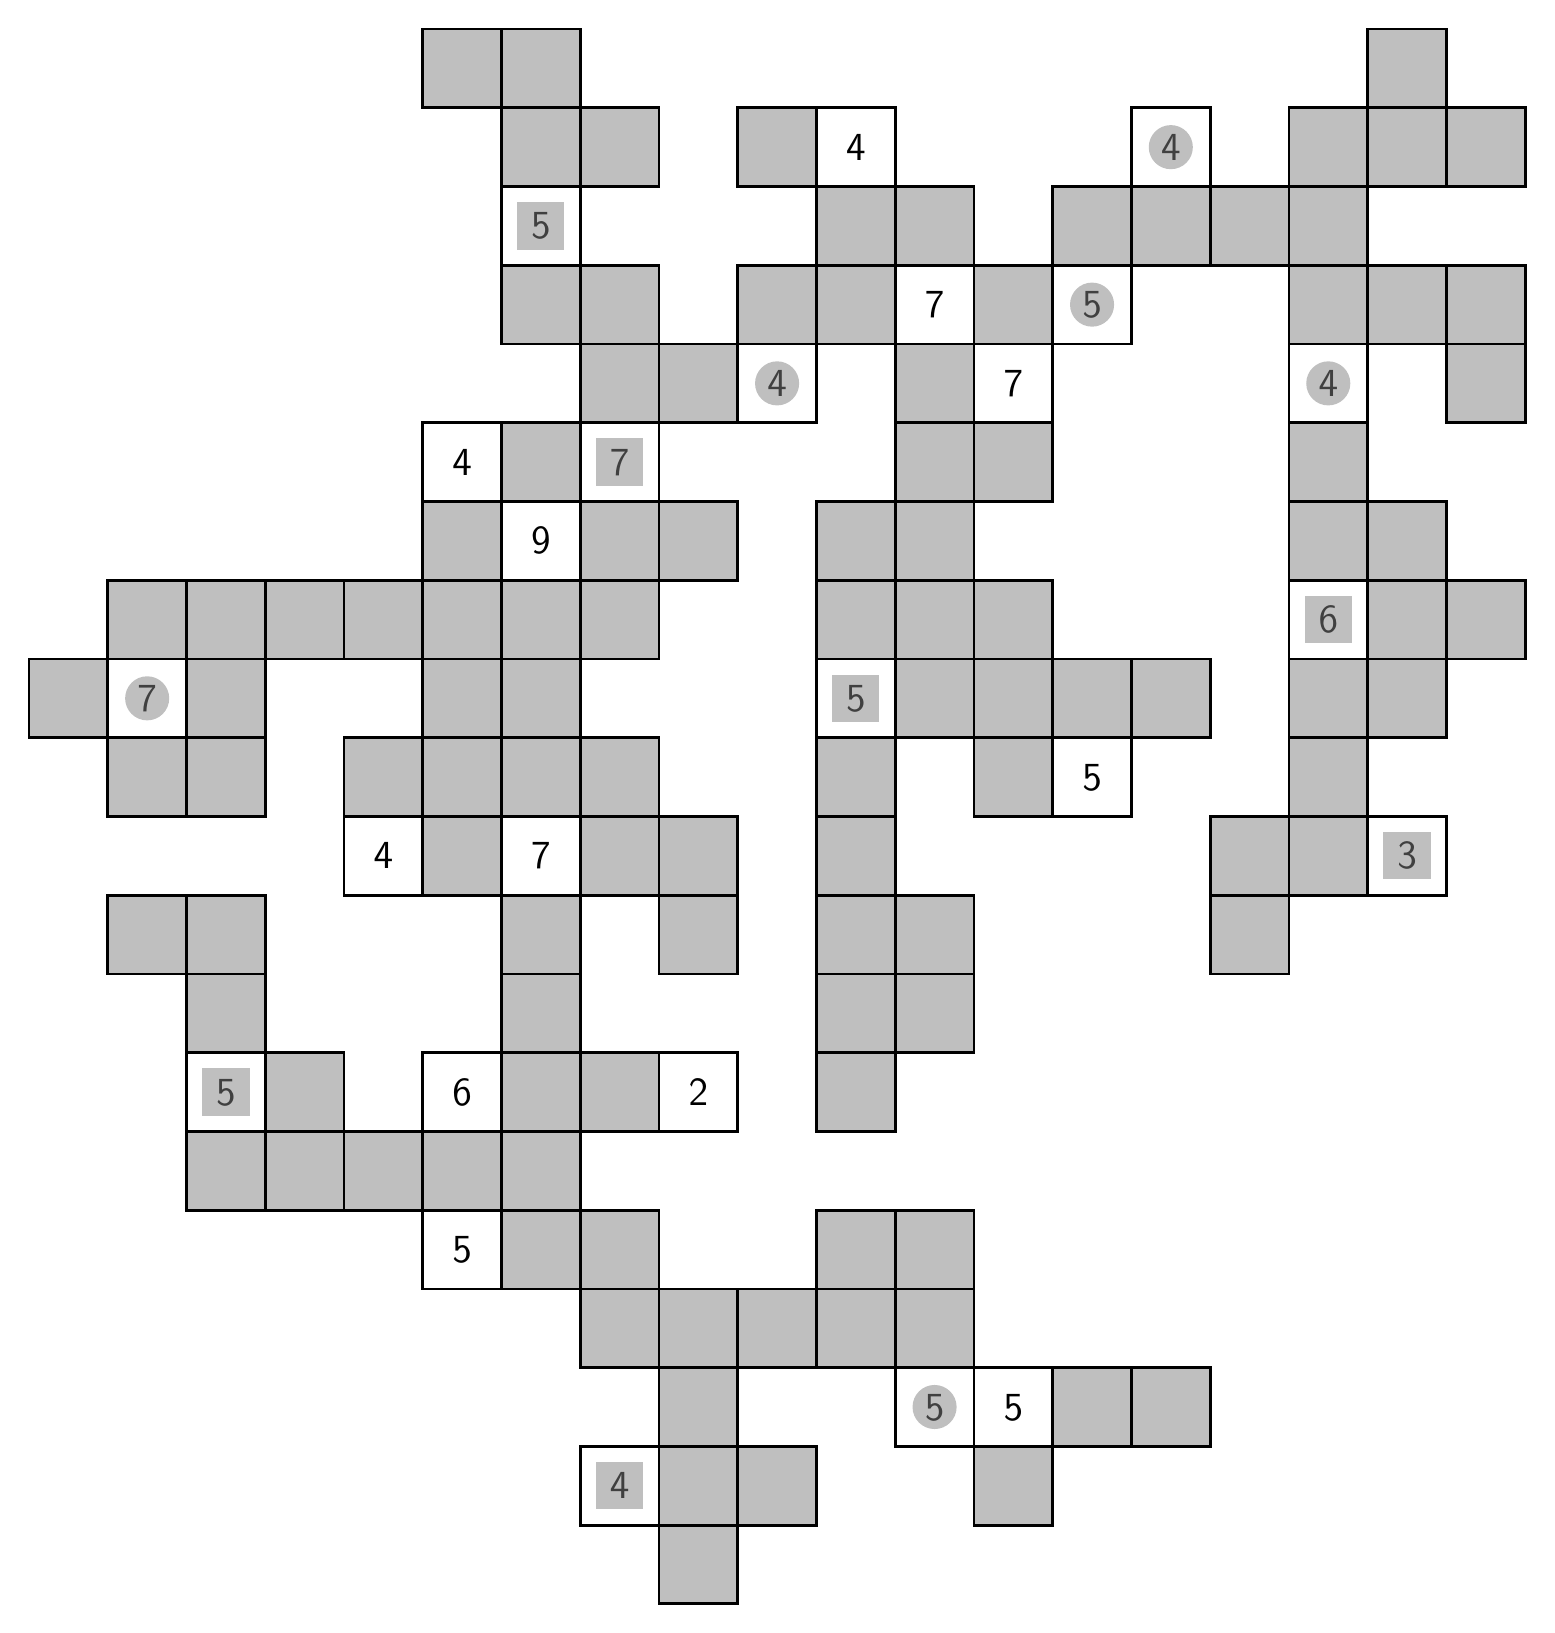
\begin{tikzpicture}\fill[gray, opacity = 0.5] (9, 0, 0)--++(1, 0, 0)--++(0, 1, 0)--++(-1, 0, 0)--cycle;
\draw[line width = 1pt] (9, 0, 0)--++(1, 0, 0)--++(0, 1, 0)--++(-1, 0, 0)--cycle;
\draw node at (8.5, 1.5, 0) {\Large $\mathsf{4}$};
\draw[line width = 1pt] (8, 1, 0)--++(1, 0, 0)--++(0, 1, 0)--++(-1, 0, 0)--cycle;
\fill[color = gray, opacity = 0.5] (8.2, 1.2) rectangle ++(0.6, 0.6);
\fill[gray, opacity = 0.5] (9, 1, 0)--++(1, 0, 0)--++(0, 1, 0)--++(-1, 0, 0)--cycle;
\draw[line width = 1pt] (9, 1, 0)--++(1, 0, 0)--++(0, 1, 0)--++(-1, 0, 0)--cycle;
\fill[gray, opacity = 0.5] (10, 1, 0)--++(1, 0, 0)--++(0, 1, 0)--++(-1, 0, 0)--cycle;
\draw[line width = 1pt] (10, 1, 0)--++(1, 0, 0)--++(0, 1, 0)--++(-1, 0, 0)--cycle;
\fill[gray, opacity = 0.5] (13, 1, 0)--++(1, 0, 0)--++(0, 1, 0)--++(-1, 0, 0)--cycle;
\draw[line width = 1pt] (13, 1, 0)--++(1, 0, 0)--++(0, 1, 0)--++(-1, 0, 0)--cycle;
\fill[gray, opacity = 0.5] (9, 2, 0)--++(1, 0, 0)--++(0, 1, 0)--++(-1, 0, 0)--cycle;
\draw[line width = 1pt] (9, 2, 0)--++(1, 0, 0)--++(0, 1, 0)--++(-1, 0, 0)--cycle;
\draw node at (12.5, 2.5, 0) {\Large $\mathsf{5}$};
\draw[line width = 1pt] (12, 2, 0)--++(1, 0, 0)--++(0, 1, 0)--++(-1, 0, 0)--cycle;
\fill[color = gray, opacity = 0.5] (12.5, 2.5, 0) circle (0.28);
\draw node at (13.5, 2.5, 0) {\Large $\mathsf{5}$};
\draw[line width = 1pt] (13, 2, 0)--++(1, 0, 0)--++(0, 1, 0)--++(-1, 0, 0)--cycle;
\fill[gray, opacity = 0.5] (14, 2, 0)--++(1, 0, 0)--++(0, 1, 0)--++(-1, 0, 0)--cycle;
\draw[line width = 1pt] (14, 2, 0)--++(1, 0, 0)--++(0, 1, 0)--++(-1, 0, 0)--cycle;
\fill[gray, opacity = 0.5] (15, 2, 0)--++(1, 0, 0)--++(0, 1, 0)--++(-1, 0, 0)--cycle;
\draw[line width = 1pt] (15, 2, 0)--++(1, 0, 0)--++(0, 1, 0)--++(-1, 0, 0)--cycle;
\fill[gray, opacity = 0.5] (8, 3, 0)--++(1, 0, 0)--++(0, 1, 0)--++(-1, 0, 0)--cycle;
\draw[line width = 1pt] (8, 3, 0)--++(1, 0, 0)--++(0, 1, 0)--++(-1, 0, 0)--cycle;
\fill[gray, opacity = 0.5] (9, 3, 0)--++(1, 0, 0)--++(0, 1, 0)--++(-1, 0, 0)--cycle;
\draw[line width = 1pt] (9, 3, 0)--++(1, 0, 0)--++(0, 1, 0)--++(-1, 0, 0)--cycle;
\fill[gray, opacity = 0.5] (10, 3, 0)--++(1, 0, 0)--++(0, 1, 0)--++(-1, 0, 0)--cycle;
\draw[line width = 1pt] (10, 3, 0)--++(1, 0, 0)--++(0, 1, 0)--++(-1, 0, 0)--cycle;
\fill[gray, opacity = 0.5] (11, 3, 0)--++(1, 0, 0)--++(0, 1, 0)--++(-1, 0, 0)--cycle;
\draw[line width = 1pt] (11, 3, 0)--++(1, 0, 0)--++(0, 1, 0)--++(-1, 0, 0)--cycle;
\fill[gray, opacity = 0.5] (12, 3, 0)--++(1, 0, 0)--++(0, 1, 0)--++(-1, 0, 0)--cycle;
\draw[line width = 1pt] (12, 3, 0)--++(1, 0, 0)--++(0, 1, 0)--++(-1, 0, 0)--cycle;
\draw node at (6.5, 4.5, 0) {\Large $\mathsf{5}$};
\draw[line width = 1pt] (6, 4, 0)--++(1, 0, 0)--++(0, 1, 0)--++(-1, 0, 0)--cycle;
\fill[gray, opacity = 0.5] (7, 4, 0)--++(1, 0, 0)--++(0, 1, 0)--++(-1, 0, 0)--cycle;
\draw[line width = 1pt] (7, 4, 0)--++(1, 0, 0)--++(0, 1, 0)--++(-1, 0, 0)--cycle;
\fill[gray, opacity = 0.5] (8, 4, 0)--++(1, 0, 0)--++(0, 1, 0)--++(-1, 0, 0)--cycle;
\draw[line width = 1pt] (8, 4, 0)--++(1, 0, 0)--++(0, 1, 0)--++(-1, 0, 0)--cycle;
\fill[gray, opacity = 0.5] (11, 4, 0)--++(1, 0, 0)--++(0, 1, 0)--++(-1, 0, 0)--cycle;
\draw[line width = 1pt] (11, 4, 0)--++(1, 0, 0)--++(0, 1, 0)--++(-1, 0, 0)--cycle;
\fill[gray, opacity = 0.5] (12, 4, 0)--++(1, 0, 0)--++(0, 1, 0)--++(-1, 0, 0)--cycle;
\draw[line width = 1pt] (12, 4, 0)--++(1, 0, 0)--++(0, 1, 0)--++(-1, 0, 0)--cycle;
\fill[gray, opacity = 0.5] (3, 5, 0)--++(1, 0, 0)--++(0, 1, 0)--++(-1, 0, 0)--cycle;
\draw[line width = 1pt] (3, 5, 0)--++(1, 0, 0)--++(0, 1, 0)--++(-1, 0, 0)--cycle;
\fill[gray, opacity = 0.5] (4, 5, 0)--++(1, 0, 0)--++(0, 1, 0)--++(-1, 0, 0)--cycle;
\draw[line width = 1pt] (4, 5, 0)--++(1, 0, 0)--++(0, 1, 0)--++(-1, 0, 0)--cycle;
\fill[gray, opacity = 0.5] (5, 5, 0)--++(1, 0, 0)--++(0, 1, 0)--++(-1, 0, 0)--cycle;
\draw[line width = 1pt] (5, 5, 0)--++(1, 0, 0)--++(0, 1, 0)--++(-1, 0, 0)--cycle;
\fill[gray, opacity = 0.5] (6, 5, 0)--++(1, 0, 0)--++(0, 1, 0)--++(-1, 0, 0)--cycle;
\draw[line width = 1pt] (6, 5, 0)--++(1, 0, 0)--++(0, 1, 0)--++(-1, 0, 0)--cycle;
\fill[gray, opacity = 0.5] (7, 5, 0)--++(1, 0, 0)--++(0, 1, 0)--++(-1, 0, 0)--cycle;
\draw[line width = 1pt] (7, 5, 0)--++(1, 0, 0)--++(0, 1, 0)--++(-1, 0, 0)--cycle;
\draw node at (3.5, 6.5, 0) {\Large $\mathsf{5}$};
\draw[line width = 1pt] (3, 6, 0)--++(1, 0, 0)--++(0, 1, 0)--++(-1, 0, 0)--cycle;
\fill[color = gray, opacity = 0.5] (3.2, 6.2) rectangle ++(0.6, 0.6);
\fill[gray, opacity = 0.5] (4, 6, 0)--++(1, 0, 0)--++(0, 1, 0)--++(-1, 0, 0)--cycle;
\draw[line width = 1pt] (4, 6, 0)--++(1, 0, 0)--++(0, 1, 0)--++(-1, 0, 0)--cycle;
\draw node at (6.5, 6.5, 0) {\Large $\mathsf{6}$};
\draw[line width = 1pt] (6, 6, 0)--++(1, 0, 0)--++(0, 1, 0)--++(-1, 0, 0)--cycle;
\fill[gray, opacity = 0.5] (7, 6, 0)--++(1, 0, 0)--++(0, 1, 0)--++(-1, 0, 0)--cycle;
\draw[line width = 1pt] (7, 6, 0)--++(1, 0, 0)--++(0, 1, 0)--++(-1, 0, 0)--cycle;
\fill[gray, opacity = 0.5] (8, 6, 0)--++(1, 0, 0)--++(0, 1, 0)--++(-1, 0, 0)--cycle;
\draw[line width = 1pt] (8, 6, 0)--++(1, 0, 0)--++(0, 1, 0)--++(-1, 0, 0)--cycle;
\draw node at (9.5, 6.5, 0) {\Large $\mathsf{2}$};
\draw[line width = 1pt] (9, 6, 0)--++(1, 0, 0)--++(0, 1, 0)--++(-1, 0, 0)--cycle;
\fill[gray, opacity = 0.5] (11, 6, 0)--++(1, 0, 0)--++(0, 1, 0)--++(-1, 0, 0)--cycle;
\draw[line width = 1pt] (11, 6, 0)--++(1, 0, 0)--++(0, 1, 0)--++(-1, 0, 0)--cycle;
\fill[gray, opacity = 0.5] (3, 7, 0)--++(1, 0, 0)--++(0, 1, 0)--++(-1, 0, 0)--cycle;
\draw[line width = 1pt] (3, 7, 0)--++(1, 0, 0)--++(0, 1, 0)--++(-1, 0, 0)--cycle;
\fill[gray, opacity = 0.5] (7, 7, 0)--++(1, 0, 0)--++(0, 1, 0)--++(-1, 0, 0)--cycle;
\draw[line width = 1pt] (7, 7, 0)--++(1, 0, 0)--++(0, 1, 0)--++(-1, 0, 0)--cycle;
\fill[gray, opacity = 0.5] (11, 7, 0)--++(1, 0, 0)--++(0, 1, 0)--++(-1, 0, 0)--cycle;
\draw[line width = 1pt] (11, 7, 0)--++(1, 0, 0)--++(0, 1, 0)--++(-1, 0, 0)--cycle;
\fill[gray, opacity = 0.5] (12, 7, 0)--++(1, 0, 0)--++(0, 1, 0)--++(-1, 0, 0)--cycle;
\draw[line width = 1pt] (12, 7, 0)--++(1, 0, 0)--++(0, 1, 0)--++(-1, 0, 0)--cycle;
\fill[gray, opacity = 0.5] (2, 8, 0)--++(1, 0, 0)--++(0, 1, 0)--++(-1, 0, 0)--cycle;
\draw[line width = 1pt] (2, 8, 0)--++(1, 0, 0)--++(0, 1, 0)--++(-1, 0, 0)--cycle;
\fill[gray, opacity = 0.5] (3, 8, 0)--++(1, 0, 0)--++(0, 1, 0)--++(-1, 0, 0)--cycle;
\draw[line width = 1pt] (3, 8, 0)--++(1, 0, 0)--++(0, 1, 0)--++(-1, 0, 0)--cycle;
\fill[gray, opacity = 0.5] (7, 8, 0)--++(1, 0, 0)--++(0, 1, 0)--++(-1, 0, 0)--cycle;
\draw[line width = 1pt] (7, 8, 0)--++(1, 0, 0)--++(0, 1, 0)--++(-1, 0, 0)--cycle;
\fill[gray, opacity = 0.5] (9, 8, 0)--++(1, 0, 0)--++(0, 1, 0)--++(-1, 0, 0)--cycle;
\draw[line width = 1pt] (9, 8, 0)--++(1, 0, 0)--++(0, 1, 0)--++(-1, 0, 0)--cycle;
\fill[gray, opacity = 0.5] (11, 8, 0)--++(1, 0, 0)--++(0, 1, 0)--++(-1, 0, 0)--cycle;
\draw[line width = 1pt] (11, 8, 0)--++(1, 0, 0)--++(0, 1, 0)--++(-1, 0, 0)--cycle;
\fill[gray, opacity = 0.5] (12, 8, 0)--++(1, 0, 0)--++(0, 1, 0)--++(-1, 0, 0)--cycle;
\draw[line width = 1pt] (12, 8, 0)--++(1, 0, 0)--++(0, 1, 0)--++(-1, 0, 0)--cycle;
\fill[gray, opacity = 0.5] (16, 8, 0)--++(1, 0, 0)--++(0, 1, 0)--++(-1, 0, 0)--cycle;
\draw[line width = 1pt] (16, 8, 0)--++(1, 0, 0)--++(0, 1, 0)--++(-1, 0, 0)--cycle;
\draw node at (5.5, 9.5, 0) {\Large $\mathsf{4}$};
\draw[line width = 1pt] (5, 9, 0)--++(1, 0, 0)--++(0, 1, 0)--++(-1, 0, 0)--cycle;
\fill[gray, opacity = 0.5] (6, 9, 0)--++(1, 0, 0)--++(0, 1, 0)--++(-1, 0, 0)--cycle;
\draw[line width = 1pt] (6, 9, 0)--++(1, 0, 0)--++(0, 1, 0)--++(-1, 0, 0)--cycle;
\draw node at (7.5, 9.5, 0) {\Large $\mathsf{7}$};
\draw[line width = 1pt] (7, 9, 0)--++(1, 0, 0)--++(0, 1, 0)--++(-1, 0, 0)--cycle;
\fill[gray, opacity = 0.5] (8, 9, 0)--++(1, 0, 0)--++(0, 1, 0)--++(-1, 0, 0)--cycle;
\draw[line width = 1pt] (8, 9, 0)--++(1, 0, 0)--++(0, 1, 0)--++(-1, 0, 0)--cycle;
\fill[gray, opacity = 0.5] (9, 9, 0)--++(1, 0, 0)--++(0, 1, 0)--++(-1, 0, 0)--cycle;
\draw[line width = 1pt] (9, 9, 0)--++(1, 0, 0)--++(0, 1, 0)--++(-1, 0, 0)--cycle;
\fill[gray, opacity = 0.5] (11, 9, 0)--++(1, 0, 0)--++(0, 1, 0)--++(-1, 0, 0)--cycle;
\draw[line width = 1pt] (11, 9, 0)--++(1, 0, 0)--++(0, 1, 0)--++(-1, 0, 0)--cycle;
\fill[gray, opacity = 0.5] (16, 9, 0)--++(1, 0, 0)--++(0, 1, 0)--++(-1, 0, 0)--cycle;
\draw[line width = 1pt] (16, 9, 0)--++(1, 0, 0)--++(0, 1, 0)--++(-1, 0, 0)--cycle;
\fill[gray, opacity = 0.5] (17, 9, 0)--++(1, 0, 0)--++(0, 1, 0)--++(-1, 0, 0)--cycle;
\draw[line width = 1pt] (17, 9, 0)--++(1, 0, 0)--++(0, 1, 0)--++(-1, 0, 0)--cycle;
\draw node at (18.5, 9.5, 0) {\Large $\mathsf{3}$};
\draw[line width = 1pt] (18, 9, 0)--++(1, 0, 0)--++(0, 1, 0)--++(-1, 0, 0)--cycle;
\fill[color = gray, opacity = 0.5] (18.2, 9.2) rectangle ++(0.6, 0.6);
\fill[gray, opacity = 0.5] (2, 10, 0)--++(1, 0, 0)--++(0, 1, 0)--++(-1, 0, 0)--cycle;
\draw[line width = 1pt] (2, 10, 0)--++(1, 0, 0)--++(0, 1, 0)--++(-1, 0, 0)--cycle;
\fill[gray, opacity = 0.5] (3, 10, 0)--++(1, 0, 0)--++(0, 1, 0)--++(-1, 0, 0)--cycle;
\draw[line width = 1pt] (3, 10, 0)--++(1, 0, 0)--++(0, 1, 0)--++(-1, 0, 0)--cycle;
\fill[gray, opacity = 0.5] (5, 10, 0)--++(1, 0, 0)--++(0, 1, 0)--++(-1, 0, 0)--cycle;
\draw[line width = 1pt] (5, 10, 0)--++(1, 0, 0)--++(0, 1, 0)--++(-1, 0, 0)--cycle;
\fill[gray, opacity = 0.5] (6, 10, 0)--++(1, 0, 0)--++(0, 1, 0)--++(-1, 0, 0)--cycle;
\draw[line width = 1pt] (6, 10, 0)--++(1, 0, 0)--++(0, 1, 0)--++(-1, 0, 0)--cycle;
\fill[gray, opacity = 0.5] (7, 10, 0)--++(1, 0, 0)--++(0, 1, 0)--++(-1, 0, 0)--cycle;
\draw[line width = 1pt] (7, 10, 0)--++(1, 0, 0)--++(0, 1, 0)--++(-1, 0, 0)--cycle;
\fill[gray, opacity = 0.5] (8, 10, 0)--++(1, 0, 0)--++(0, 1, 0)--++(-1, 0, 0)--cycle;
\draw[line width = 1pt] (8, 10, 0)--++(1, 0, 0)--++(0, 1, 0)--++(-1, 0, 0)--cycle;
\fill[gray, opacity = 0.5] (11, 10, 0)--++(1, 0, 0)--++(0, 1, 0)--++(-1, 0, 0)--cycle;
\draw[line width = 1pt] (11, 10, 0)--++(1, 0, 0)--++(0, 1, 0)--++(-1, 0, 0)--cycle;
\fill[gray, opacity = 0.5] (13, 10, 0)--++(1, 0, 0)--++(0, 1, 0)--++(-1, 0, 0)--cycle;
\draw[line width = 1pt] (13, 10, 0)--++(1, 0, 0)--++(0, 1, 0)--++(-1, 0, 0)--cycle;
\draw node at (14.5, 10.5, 0) {\Large $\mathsf{5}$};
\draw[line width = 1pt] (14, 10, 0)--++(1, 0, 0)--++(0, 1, 0)--++(-1, 0, 0)--cycle;
\fill[gray, opacity = 0.5] (17, 10, 0)--++(1, 0, 0)--++(0, 1, 0)--++(-1, 0, 0)--cycle;
\draw[line width = 1pt] (17, 10, 0)--++(1, 0, 0)--++(0, 1, 0)--++(-1, 0, 0)--cycle;
\fill[gray, opacity = 0.5] (1, 11, 0)--++(1, 0, 0)--++(0, 1, 0)--++(-1, 0, 0)--cycle;
\draw[line width = 1pt] (1, 11, 0)--++(1, 0, 0)--++(0, 1, 0)--++(-1, 0, 0)--cycle;
\draw node at (2.5, 11.5, 0) {\Large $\mathsf{7}$};
\draw[line width = 1pt] (2, 11, 0)--++(1, 0, 0)--++(0, 1, 0)--++(-1, 0, 0)--cycle;
\fill[color = gray, opacity = 0.5] (2.5, 11.5, 0) circle (0.28);
\fill[gray, opacity = 0.5] (3, 11, 0)--++(1, 0, 0)--++(0, 1, 0)--++(-1, 0, 0)--cycle;
\draw[line width = 1pt] (3, 11, 0)--++(1, 0, 0)--++(0, 1, 0)--++(-1, 0, 0)--cycle;
\fill[gray, opacity = 0.5] (6, 11, 0)--++(1, 0, 0)--++(0, 1, 0)--++(-1, 0, 0)--cycle;
\draw[line width = 1pt] (6, 11, 0)--++(1, 0, 0)--++(0, 1, 0)--++(-1, 0, 0)--cycle;
\fill[gray, opacity = 0.5] (7, 11, 0)--++(1, 0, 0)--++(0, 1, 0)--++(-1, 0, 0)--cycle;
\draw[line width = 1pt] (7, 11, 0)--++(1, 0, 0)--++(0, 1, 0)--++(-1, 0, 0)--cycle;
\draw node at (11.5, 11.5, 0) {\Large $\mathsf{5}$};
\draw[line width = 1pt] (11, 11, 0)--++(1, 0, 0)--++(0, 1, 0)--++(-1, 0, 0)--cycle;
\fill[color = gray, opacity = 0.5] (11.2, 11.2) rectangle ++(0.6, 0.6);
\fill[gray, opacity = 0.5] (12, 11, 0)--++(1, 0, 0)--++(0, 1, 0)--++(-1, 0, 0)--cycle;
\draw[line width = 1pt] (12, 11, 0)--++(1, 0, 0)--++(0, 1, 0)--++(-1, 0, 0)--cycle;
\fill[gray, opacity = 0.5] (13, 11, 0)--++(1, 0, 0)--++(0, 1, 0)--++(-1, 0, 0)--cycle;
\draw[line width = 1pt] (13, 11, 0)--++(1, 0, 0)--++(0, 1, 0)--++(-1, 0, 0)--cycle;
\fill[gray, opacity = 0.5] (14, 11, 0)--++(1, 0, 0)--++(0, 1, 0)--++(-1, 0, 0)--cycle;
\draw[line width = 1pt] (14, 11, 0)--++(1, 0, 0)--++(0, 1, 0)--++(-1, 0, 0)--cycle;
\fill[gray, opacity = 0.5] (15, 11, 0)--++(1, 0, 0)--++(0, 1, 0)--++(-1, 0, 0)--cycle;
\draw[line width = 1pt] (15, 11, 0)--++(1, 0, 0)--++(0, 1, 0)--++(-1, 0, 0)--cycle;
\fill[gray, opacity = 0.5] (17, 11, 0)--++(1, 0, 0)--++(0, 1, 0)--++(-1, 0, 0)--cycle;
\draw[line width = 1pt] (17, 11, 0)--++(1, 0, 0)--++(0, 1, 0)--++(-1, 0, 0)--cycle;
\fill[gray, opacity = 0.5] (18, 11, 0)--++(1, 0, 0)--++(0, 1, 0)--++(-1, 0, 0)--cycle;
\draw[line width = 1pt] (18, 11, 0)--++(1, 0, 0)--++(0, 1, 0)--++(-1, 0, 0)--cycle;
\fill[gray, opacity = 0.5] (2, 12, 0)--++(1, 0, 0)--++(0, 1, 0)--++(-1, 0, 0)--cycle;
\draw[line width = 1pt] (2, 12, 0)--++(1, 0, 0)--++(0, 1, 0)--++(-1, 0, 0)--cycle;
\fill[gray, opacity = 0.5] (3, 12, 0)--++(1, 0, 0)--++(0, 1, 0)--++(-1, 0, 0)--cycle;
\draw[line width = 1pt] (3, 12, 0)--++(1, 0, 0)--++(0, 1, 0)--++(-1, 0, 0)--cycle;
\fill[gray, opacity = 0.5] (4, 12, 0)--++(1, 0, 0)--++(0, 1, 0)--++(-1, 0, 0)--cycle;
\draw[line width = 1pt] (4, 12, 0)--++(1, 0, 0)--++(0, 1, 0)--++(-1, 0, 0)--cycle;
\fill[gray, opacity = 0.5] (5, 12, 0)--++(1, 0, 0)--++(0, 1, 0)--++(-1, 0, 0)--cycle;
\draw[line width = 1pt] (5, 12, 0)--++(1, 0, 0)--++(0, 1, 0)--++(-1, 0, 0)--cycle;
\fill[gray, opacity = 0.5] (6, 12, 0)--++(1, 0, 0)--++(0, 1, 0)--++(-1, 0, 0)--cycle;
\draw[line width = 1pt] (6, 12, 0)--++(1, 0, 0)--++(0, 1, 0)--++(-1, 0, 0)--cycle;
\fill[gray, opacity = 0.5] (7, 12, 0)--++(1, 0, 0)--++(0, 1, 0)--++(-1, 0, 0)--cycle;
\draw[line width = 1pt] (7, 12, 0)--++(1, 0, 0)--++(0, 1, 0)--++(-1, 0, 0)--cycle;
\fill[gray, opacity = 0.5] (8, 12, 0)--++(1, 0, 0)--++(0, 1, 0)--++(-1, 0, 0)--cycle;
\draw[line width = 1pt] (8, 12, 0)--++(1, 0, 0)--++(0, 1, 0)--++(-1, 0, 0)--cycle;
\fill[gray, opacity = 0.5] (11, 12, 0)--++(1, 0, 0)--++(0, 1, 0)--++(-1, 0, 0)--cycle;
\draw[line width = 1pt] (11, 12, 0)--++(1, 0, 0)--++(0, 1, 0)--++(-1, 0, 0)--cycle;
\fill[gray, opacity = 0.5] (12, 12, 0)--++(1, 0, 0)--++(0, 1, 0)--++(-1, 0, 0)--cycle;
\draw[line width = 1pt] (12, 12, 0)--++(1, 0, 0)--++(0, 1, 0)--++(-1, 0, 0)--cycle;
\fill[gray, opacity = 0.5] (13, 12, 0)--++(1, 0, 0)--++(0, 1, 0)--++(-1, 0, 0)--cycle;
\draw[line width = 1pt] (13, 12, 0)--++(1, 0, 0)--++(0, 1, 0)--++(-1, 0, 0)--cycle;
\draw node at (17.5, 12.5, 0) {\Large $\mathsf{6}$};
\draw[line width = 1pt] (17, 12, 0)--++(1, 0, 0)--++(0, 1, 0)--++(-1, 0, 0)--cycle;
\fill[color = gray, opacity = 0.5] (17.2, 12.2) rectangle ++(0.6, 0.6);
\fill[gray, opacity = 0.5] (18, 12, 0)--++(1, 0, 0)--++(0, 1, 0)--++(-1, 0, 0)--cycle;
\draw[line width = 1pt] (18, 12, 0)--++(1, 0, 0)--++(0, 1, 0)--++(-1, 0, 0)--cycle;
\fill[gray, opacity = 0.5] (19, 12, 0)--++(1, 0, 0)--++(0, 1, 0)--++(-1, 0, 0)--cycle;
\draw[line width = 1pt] (19, 12, 0)--++(1, 0, 0)--++(0, 1, 0)--++(-1, 0, 0)--cycle;
\fill[gray, opacity = 0.5] (6, 13, 0)--++(1, 0, 0)--++(0, 1, 0)--++(-1, 0, 0)--cycle;
\draw[line width = 1pt] (6, 13, 0)--++(1, 0, 0)--++(0, 1, 0)--++(-1, 0, 0)--cycle;
\draw node at (7.5, 13.5, 0) {\Large $\mathsf{9}$};
\draw[line width = 1pt] (7, 13, 0)--++(1, 0, 0)--++(0, 1, 0)--++(-1, 0, 0)--cycle;
\fill[gray, opacity = 0.5] (8, 13, 0)--++(1, 0, 0)--++(0, 1, 0)--++(-1, 0, 0)--cycle;
\draw[line width = 1pt] (8, 13, 0)--++(1, 0, 0)--++(0, 1, 0)--++(-1, 0, 0)--cycle;
\fill[gray, opacity = 0.5] (9, 13, 0)--++(1, 0, 0)--++(0, 1, 0)--++(-1, 0, 0)--cycle;
\draw[line width = 1pt] (9, 13, 0)--++(1, 0, 0)--++(0, 1, 0)--++(-1, 0, 0)--cycle;
\fill[gray, opacity = 0.5] (11, 13, 0)--++(1, 0, 0)--++(0, 1, 0)--++(-1, 0, 0)--cycle;
\draw[line width = 1pt] (11, 13, 0)--++(1, 0, 0)--++(0, 1, 0)--++(-1, 0, 0)--cycle;
\fill[gray, opacity = 0.5] (12, 13, 0)--++(1, 0, 0)--++(0, 1, 0)--++(-1, 0, 0)--cycle;
\draw[line width = 1pt] (12, 13, 0)--++(1, 0, 0)--++(0, 1, 0)--++(-1, 0, 0)--cycle;
\fill[gray, opacity = 0.5] (17, 13, 0)--++(1, 0, 0)--++(0, 1, 0)--++(-1, 0, 0)--cycle;
\draw[line width = 1pt] (17, 13, 0)--++(1, 0, 0)--++(0, 1, 0)--++(-1, 0, 0)--cycle;
\fill[gray, opacity = 0.5] (18, 13, 0)--++(1, 0, 0)--++(0, 1, 0)--++(-1, 0, 0)--cycle;
\draw[line width = 1pt] (18, 13, 0)--++(1, 0, 0)--++(0, 1, 0)--++(-1, 0, 0)--cycle;
\draw node at (6.5, 14.5, 0) {\Large $\mathsf{4}$};
\draw[line width = 1pt] (6, 14, 0)--++(1, 0, 0)--++(0, 1, 0)--++(-1, 0, 0)--cycle;
\fill[gray, opacity = 0.5] (7, 14, 0)--++(1, 0, 0)--++(0, 1, 0)--++(-1, 0, 0)--cycle;
\draw[line width = 1pt] (7, 14, 0)--++(1, 0, 0)--++(0, 1, 0)--++(-1, 0, 0)--cycle;
\draw node at (8.5, 14.5, 0) {\Large $\mathsf{7}$};
\draw[line width = 1pt] (8, 14, 0)--++(1, 0, 0)--++(0, 1, 0)--++(-1, 0, 0)--cycle;
\fill[color = gray, opacity = 0.5] (8.2, 14.2) rectangle ++(0.6, 0.6);
\fill[gray, opacity = 0.5] (12, 14, 0)--++(1, 0, 0)--++(0, 1, 0)--++(-1, 0, 0)--cycle;
\draw[line width = 1pt] (12, 14, 0)--++(1, 0, 0)--++(0, 1, 0)--++(-1, 0, 0)--cycle;
\fill[gray, opacity = 0.5] (13, 14, 0)--++(1, 0, 0)--++(0, 1, 0)--++(-1, 0, 0)--cycle;
\draw[line width = 1pt] (13, 14, 0)--++(1, 0, 0)--++(0, 1, 0)--++(-1, 0, 0)--cycle;
\fill[gray, opacity = 0.5] (17, 14, 0)--++(1, 0, 0)--++(0, 1, 0)--++(-1, 0, 0)--cycle;
\draw[line width = 1pt] (17, 14, 0)--++(1, 0, 0)--++(0, 1, 0)--++(-1, 0, 0)--cycle;
\fill[gray, opacity = 0.5] (8, 15, 0)--++(1, 0, 0)--++(0, 1, 0)--++(-1, 0, 0)--cycle;
\draw[line width = 1pt] (8, 15, 0)--++(1, 0, 0)--++(0, 1, 0)--++(-1, 0, 0)--cycle;
\fill[gray, opacity = 0.5] (9, 15, 0)--++(1, 0, 0)--++(0, 1, 0)--++(-1, 0, 0)--cycle;
\draw[line width = 1pt] (9, 15, 0)--++(1, 0, 0)--++(0, 1, 0)--++(-1, 0, 0)--cycle;
\draw node at (10.5, 15.5, 0) {\Large $\mathsf{4}$};
\draw[line width = 1pt] (10, 15, 0)--++(1, 0, 0)--++(0, 1, 0)--++(-1, 0, 0)--cycle;
\fill[color = gray, opacity = 0.5] (10.5, 15.5, 0) circle (0.28);
\fill[gray, opacity = 0.5] (12, 15, 0)--++(1, 0, 0)--++(0, 1, 0)--++(-1, 0, 0)--cycle;
\draw[line width = 1pt] (12, 15, 0)--++(1, 0, 0)--++(0, 1, 0)--++(-1, 0, 0)--cycle;
\draw node at (13.5, 15.5, 0) {\Large $\mathsf{7}$};
\draw[line width = 1pt] (13, 15, 0)--++(1, 0, 0)--++(0, 1, 0)--++(-1, 0, 0)--cycle;
\draw node at (17.5, 15.5, 0) {\Large $\mathsf{4}$};
\draw[line width = 1pt] (17, 15, 0)--++(1, 0, 0)--++(0, 1, 0)--++(-1, 0, 0)--cycle;
\fill[color = gray, opacity = 0.5] (17.5, 15.5, 0) circle (0.28);
\fill[gray, opacity = 0.5] (19, 15, 0)--++(1, 0, 0)--++(0, 1, 0)--++(-1, 0, 0)--cycle;
\draw[line width = 1pt] (19, 15, 0)--++(1, 0, 0)--++(0, 1, 0)--++(-1, 0, 0)--cycle;
\fill[gray, opacity = 0.5] (7, 16, 0)--++(1, 0, 0)--++(0, 1, 0)--++(-1, 0, 0)--cycle;
\draw[line width = 1pt] (7, 16, 0)--++(1, 0, 0)--++(0, 1, 0)--++(-1, 0, 0)--cycle;
\fill[gray, opacity = 0.5] (8, 16, 0)--++(1, 0, 0)--++(0, 1, 0)--++(-1, 0, 0)--cycle;
\draw[line width = 1pt] (8, 16, 0)--++(1, 0, 0)--++(0, 1, 0)--++(-1, 0, 0)--cycle;
\fill[gray, opacity = 0.5] (10, 16, 0)--++(1, 0, 0)--++(0, 1, 0)--++(-1, 0, 0)--cycle;
\draw[line width = 1pt] (10, 16, 0)--++(1, 0, 0)--++(0, 1, 0)--++(-1, 0, 0)--cycle;
\fill[gray, opacity = 0.5] (11, 16, 0)--++(1, 0, 0)--++(0, 1, 0)--++(-1, 0, 0)--cycle;
\draw[line width = 1pt] (11, 16, 0)--++(1, 0, 0)--++(0, 1, 0)--++(-1, 0, 0)--cycle;
\draw node at (12.5, 16.5, 0) {\Large $\mathsf{7}$};
\draw[line width = 1pt] (12, 16, 0)--++(1, 0, 0)--++(0, 1, 0)--++(-1, 0, 0)--cycle;
\fill[gray, opacity = 0.5] (13, 16, 0)--++(1, 0, 0)--++(0, 1, 0)--++(-1, 0, 0)--cycle;
\draw[line width = 1pt] (13, 16, 0)--++(1, 0, 0)--++(0, 1, 0)--++(-1, 0, 0)--cycle;
\draw node at (14.5, 16.5, 0) {\Large $\mathsf{5}$};
\draw[line width = 1pt] (14, 16, 0)--++(1, 0, 0)--++(0, 1, 0)--++(-1, 0, 0)--cycle;
\fill[color = gray, opacity = 0.5] (14.5, 16.5, 0) circle (0.28);
\fill[gray, opacity = 0.5] (17, 16, 0)--++(1, 0, 0)--++(0, 1, 0)--++(-1, 0, 0)--cycle;
\draw[line width = 1pt] (17, 16, 0)--++(1, 0, 0)--++(0, 1, 0)--++(-1, 0, 0)--cycle;
\fill[gray, opacity = 0.5] (18, 16, 0)--++(1, 0, 0)--++(0, 1, 0)--++(-1, 0, 0)--cycle;
\draw[line width = 1pt] (18, 16, 0)--++(1, 0, 0)--++(0, 1, 0)--++(-1, 0, 0)--cycle;
\fill[gray, opacity = 0.5] (19, 16, 0)--++(1, 0, 0)--++(0, 1, 0)--++(-1, 0, 0)--cycle;
\draw[line width = 1pt] (19, 16, 0)--++(1, 0, 0)--++(0, 1, 0)--++(-1, 0, 0)--cycle;
\draw node at (7.5, 17.5, 0) {\Large $\mathsf{5}$};
\draw[line width = 1pt] (7, 17, 0)--++(1, 0, 0)--++(0, 1, 0)--++(-1, 0, 0)--cycle;
\fill[color = gray, opacity = 0.5] (7.2, 17.2) rectangle ++(0.6, 0.6);
\fill[gray, opacity = 0.5] (11, 17, 0)--++(1, 0, 0)--++(0, 1, 0)--++(-1, 0, 0)--cycle;
\draw[line width = 1pt] (11, 17, 0)--++(1, 0, 0)--++(0, 1, 0)--++(-1, 0, 0)--cycle;
\fill[gray, opacity = 0.5] (12, 17, 0)--++(1, 0, 0)--++(0, 1, 0)--++(-1, 0, 0)--cycle;
\draw[line width = 1pt] (12, 17, 0)--++(1, 0, 0)--++(0, 1, 0)--++(-1, 0, 0)--cycle;
\fill[gray, opacity = 0.5] (14, 17, 0)--++(1, 0, 0)--++(0, 1, 0)--++(-1, 0, 0)--cycle;
\draw[line width = 1pt] (14, 17, 0)--++(1, 0, 0)--++(0, 1, 0)--++(-1, 0, 0)--cycle;
\fill[gray, opacity = 0.5] (15, 17, 0)--++(1, 0, 0)--++(0, 1, 0)--++(-1, 0, 0)--cycle;
\draw[line width = 1pt] (15, 17, 0)--++(1, 0, 0)--++(0, 1, 0)--++(-1, 0, 0)--cycle;
\fill[gray, opacity = 0.5] (16, 17, 0)--++(1, 0, 0)--++(0, 1, 0)--++(-1, 0, 0)--cycle;
\draw[line width = 1pt] (16, 17, 0)--++(1, 0, 0)--++(0, 1, 0)--++(-1, 0, 0)--cycle;
\fill[gray, opacity = 0.5] (17, 17, 0)--++(1, 0, 0)--++(0, 1, 0)--++(-1, 0, 0)--cycle;
\draw[line width = 1pt] (17, 17, 0)--++(1, 0, 0)--++(0, 1, 0)--++(-1, 0, 0)--cycle;
\fill[gray, opacity = 0.5] (7, 18, 0)--++(1, 0, 0)--++(0, 1, 0)--++(-1, 0, 0)--cycle;
\draw[line width = 1pt] (7, 18, 0)--++(1, 0, 0)--++(0, 1, 0)--++(-1, 0, 0)--cycle;
\fill[gray, opacity = 0.5] (8, 18, 0)--++(1, 0, 0)--++(0, 1, 0)--++(-1, 0, 0)--cycle;
\draw[line width = 1pt] (8, 18, 0)--++(1, 0, 0)--++(0, 1, 0)--++(-1, 0, 0)--cycle;
\fill[gray, opacity = 0.5] (10, 18, 0)--++(1, 0, 0)--++(0, 1, 0)--++(-1, 0, 0)--cycle;
\draw[line width = 1pt] (10, 18, 0)--++(1, 0, 0)--++(0, 1, 0)--++(-1, 0, 0)--cycle;
\draw node at (11.5, 18.5, 0) {\Large $\mathsf{4}$};
\draw[line width = 1pt] (11, 18, 0)--++(1, 0, 0)--++(0, 1, 0)--++(-1, 0, 0)--cycle;
\draw node at (15.5, 18.5, 0) {\Large $\mathsf{4}$};
\draw[line width = 1pt] (15, 18, 0)--++(1, 0, 0)--++(0, 1, 0)--++(-1, 0, 0)--cycle;
\fill[color = gray, opacity = 0.5] (15.5, 18.5, 0) circle (0.28);
\fill[gray, opacity = 0.5] (17, 18, 0)--++(1, 0, 0)--++(0, 1, 0)--++(-1, 0, 0)--cycle;
\draw[line width = 1pt] (17, 18, 0)--++(1, 0, 0)--++(0, 1, 0)--++(-1, 0, 0)--cycle;
\fill[gray, opacity = 0.5] (18, 18, 0)--++(1, 0, 0)--++(0, 1, 0)--++(-1, 0, 0)--cycle;
\draw[line width = 1pt] (18, 18, 0)--++(1, 0, 0)--++(0, 1, 0)--++(-1, 0, 0)--cycle;
\fill[gray, opacity = 0.5] (19, 18, 0)--++(1, 0, 0)--++(0, 1, 0)--++(-1, 0, 0)--cycle;
\draw[line width = 1pt] (19, 18, 0)--++(1, 0, 0)--++(0, 1, 0)--++(-1, 0, 0)--cycle;
\fill[gray, opacity = 0.5] (6, 19, 0)--++(1, 0, 0)--++(0, 1, 0)--++(-1, 0, 0)--cycle;
\draw[line width = 1pt] (6, 19, 0)--++(1, 0, 0)--++(0, 1, 0)--++(-1, 0, 0)--cycle;
\fill[gray, opacity = 0.5] (7, 19, 0)--++(1, 0, 0)--++(0, 1, 0)--++(-1, 0, 0)--cycle;
\draw[line width = 1pt] (7, 19, 0)--++(1, 0, 0)--++(0, 1, 0)--++(-1, 0, 0)--cycle;
\fill[gray, opacity = 0.5] (18, 19, 0)--++(1, 0, 0)--++(0, 1, 0)--++(-1, 0, 0)--cycle;
\draw[line width = 1pt] (18, 19, 0)--++(1, 0, 0)--++(0, 1, 0)--++(-1, 0, 0)--cycle;
\end{tikzpicture}}\]
\[\resizebox{30pc}{!}{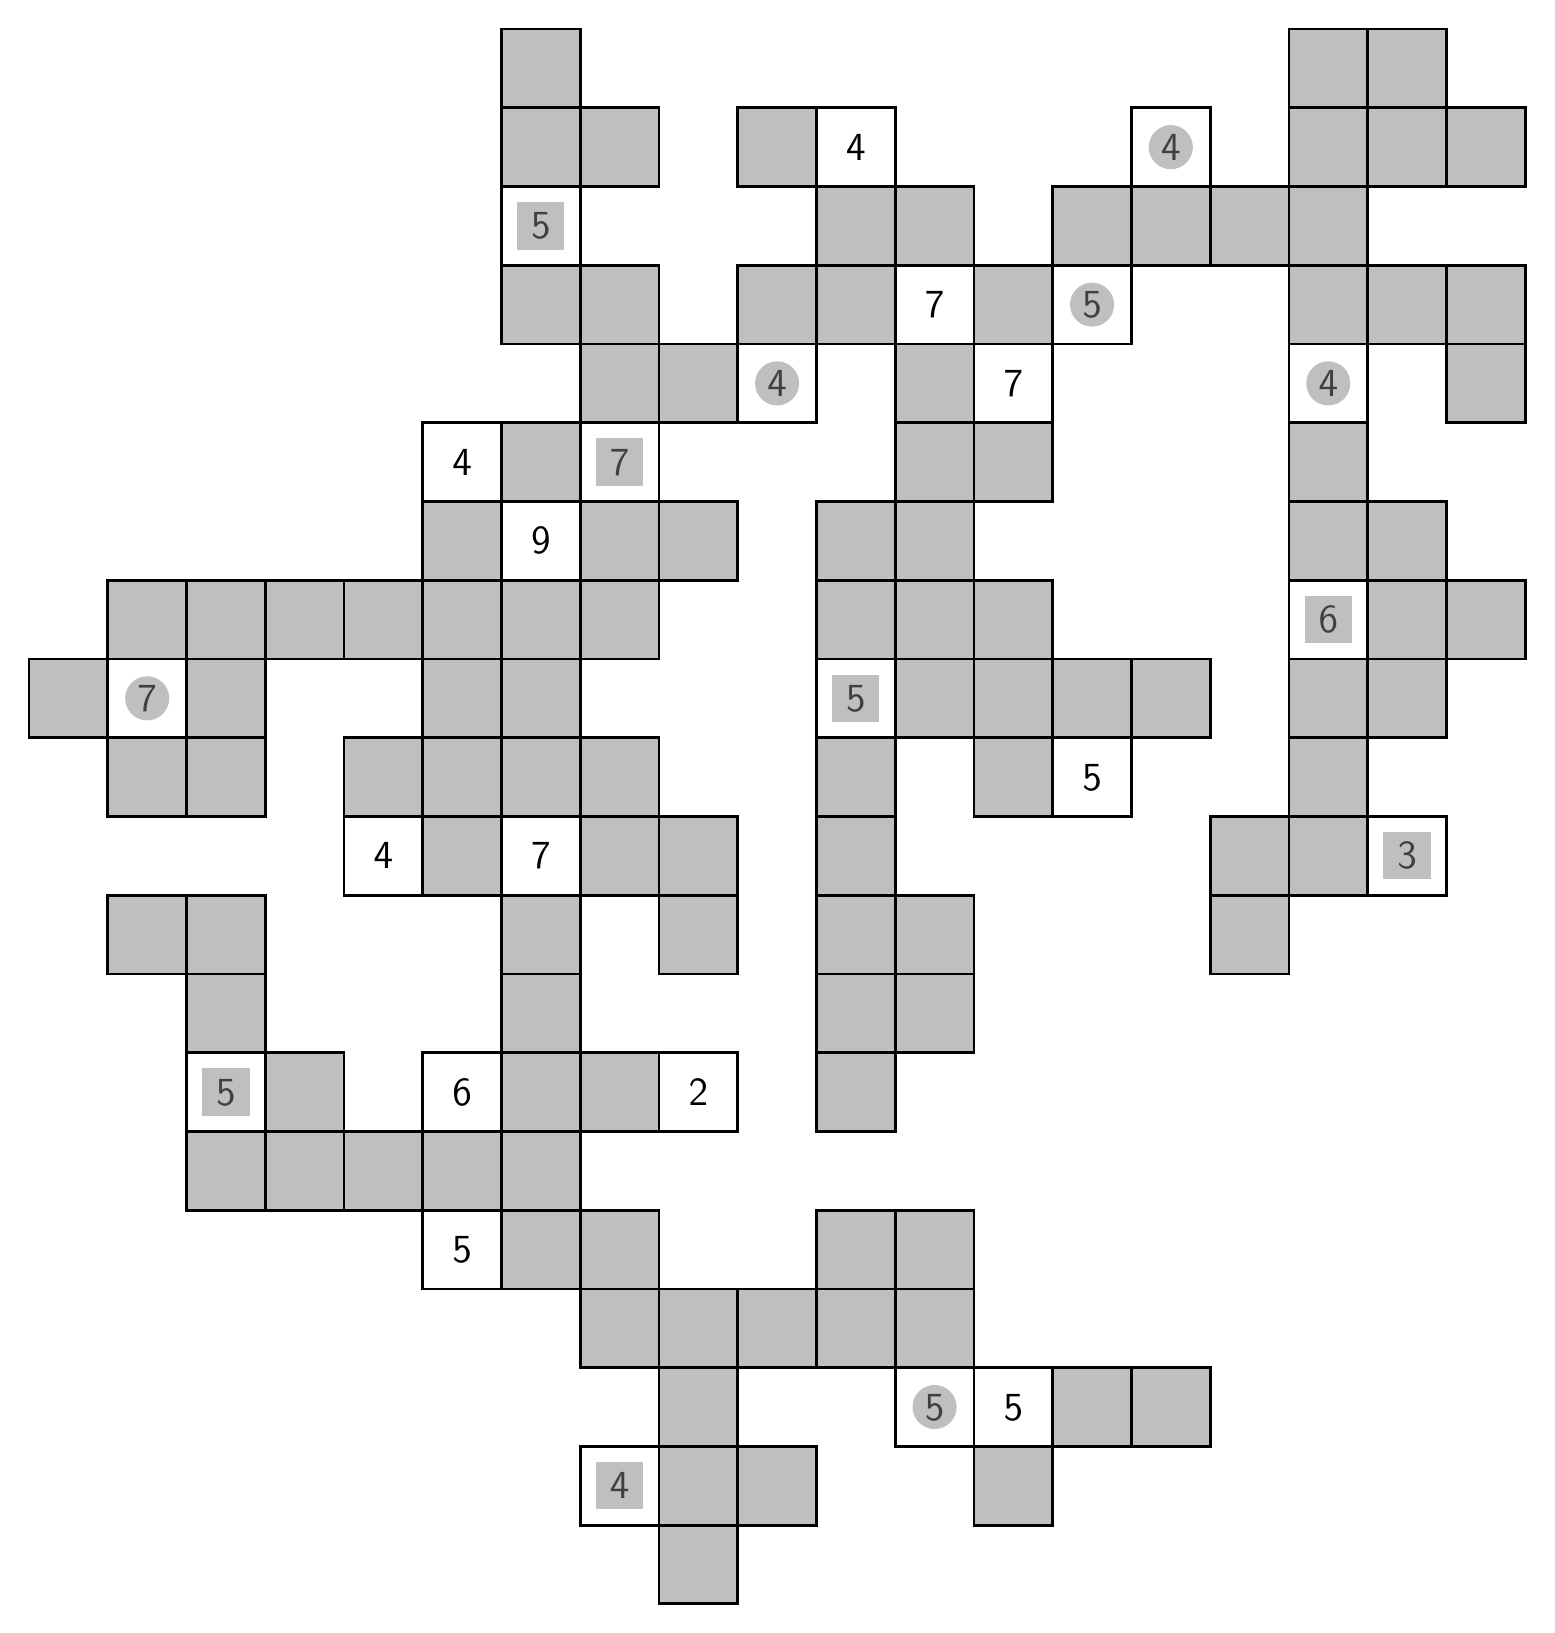
\begin{tikzpicture}\fill[gray, opacity = 0.5] (9, 0, 0)--++(1, 0, 0)--++(0, 1, 0)--++(-1, 0, 0)--cycle;
\draw[line width = 1pt] (9, 0, 0)--++(1, 0, 0)--++(0, 1, 0)--++(-1, 0, 0)--cycle;
\draw node at (8.5, 1.5, 0) {\Large $\mathsf{4}$};
\draw[line width = 1pt] (8, 1, 0)--++(1, 0, 0)--++(0, 1, 0)--++(-1, 0, 0)--cycle;
\fill[color = gray, opacity = 0.5] (8.2, 1.2) rectangle ++(0.6, 0.6);
\fill[gray, opacity = 0.5] (9, 1, 0)--++(1, 0, 0)--++(0, 1, 0)--++(-1, 0, 0)--cycle;
\draw[line width = 1pt] (9, 1, 0)--++(1, 0, 0)--++(0, 1, 0)--++(-1, 0, 0)--cycle;
\fill[gray, opacity = 0.5] (10, 1, 0)--++(1, 0, 0)--++(0, 1, 0)--++(-1, 0, 0)--cycle;
\draw[line width = 1pt] (10, 1, 0)--++(1, 0, 0)--++(0, 1, 0)--++(-1, 0, 0)--cycle;
\fill[gray, opacity = 0.5] (13, 1, 0)--++(1, 0, 0)--++(0, 1, 0)--++(-1, 0, 0)--cycle;
\draw[line width = 1pt] (13, 1, 0)--++(1, 0, 0)--++(0, 1, 0)--++(-1, 0, 0)--cycle;
\fill[gray, opacity = 0.5] (9, 2, 0)--++(1, 0, 0)--++(0, 1, 0)--++(-1, 0, 0)--cycle;
\draw[line width = 1pt] (9, 2, 0)--++(1, 0, 0)--++(0, 1, 0)--++(-1, 0, 0)--cycle;
\draw node at (12.5, 2.5, 0) {\Large $\mathsf{5}$};
\draw[line width = 1pt] (12, 2, 0)--++(1, 0, 0)--++(0, 1, 0)--++(-1, 0, 0)--cycle;
\fill[color = gray, opacity = 0.5] (12.5, 2.5, 0) circle (0.28);
\draw node at (13.5, 2.5, 0) {\Large $\mathsf{5}$};
\draw[line width = 1pt] (13, 2, 0)--++(1, 0, 0)--++(0, 1, 0)--++(-1, 0, 0)--cycle;
\fill[gray, opacity = 0.5] (14, 2, 0)--++(1, 0, 0)--++(0, 1, 0)--++(-1, 0, 0)--cycle;
\draw[line width = 1pt] (14, 2, 0)--++(1, 0, 0)--++(0, 1, 0)--++(-1, 0, 0)--cycle;
\fill[gray, opacity = 0.5] (15, 2, 0)--++(1, 0, 0)--++(0, 1, 0)--++(-1, 0, 0)--cycle;
\draw[line width = 1pt] (15, 2, 0)--++(1, 0, 0)--++(0, 1, 0)--++(-1, 0, 0)--cycle;
\fill[gray, opacity = 0.5] (8, 3, 0)--++(1, 0, 0)--++(0, 1, 0)--++(-1, 0, 0)--cycle;
\draw[line width = 1pt] (8, 3, 0)--++(1, 0, 0)--++(0, 1, 0)--++(-1, 0, 0)--cycle;
\fill[gray, opacity = 0.5] (9, 3, 0)--++(1, 0, 0)--++(0, 1, 0)--++(-1, 0, 0)--cycle;
\draw[line width = 1pt] (9, 3, 0)--++(1, 0, 0)--++(0, 1, 0)--++(-1, 0, 0)--cycle;
\fill[gray, opacity = 0.5] (10, 3, 0)--++(1, 0, 0)--++(0, 1, 0)--++(-1, 0, 0)--cycle;
\draw[line width = 1pt] (10, 3, 0)--++(1, 0, 0)--++(0, 1, 0)--++(-1, 0, 0)--cycle;
\fill[gray, opacity = 0.5] (11, 3, 0)--++(1, 0, 0)--++(0, 1, 0)--++(-1, 0, 0)--cycle;
\draw[line width = 1pt] (11, 3, 0)--++(1, 0, 0)--++(0, 1, 0)--++(-1, 0, 0)--cycle;
\fill[gray, opacity = 0.5] (12, 3, 0)--++(1, 0, 0)--++(0, 1, 0)--++(-1, 0, 0)--cycle;
\draw[line width = 1pt] (12, 3, 0)--++(1, 0, 0)--++(0, 1, 0)--++(-1, 0, 0)--cycle;
\draw node at (6.5, 4.5, 0) {\Large $\mathsf{5}$};
\draw[line width = 1pt] (6, 4, 0)--++(1, 0, 0)--++(0, 1, 0)--++(-1, 0, 0)--cycle;
\fill[gray, opacity = 0.5] (7, 4, 0)--++(1, 0, 0)--++(0, 1, 0)--++(-1, 0, 0)--cycle;
\draw[line width = 1pt] (7, 4, 0)--++(1, 0, 0)--++(0, 1, 0)--++(-1, 0, 0)--cycle;
\fill[gray, opacity = 0.5] (8, 4, 0)--++(1, 0, 0)--++(0, 1, 0)--++(-1, 0, 0)--cycle;
\draw[line width = 1pt] (8, 4, 0)--++(1, 0, 0)--++(0, 1, 0)--++(-1, 0, 0)--cycle;
\fill[gray, opacity = 0.5] (11, 4, 0)--++(1, 0, 0)--++(0, 1, 0)--++(-1, 0, 0)--cycle;
\draw[line width = 1pt] (11, 4, 0)--++(1, 0, 0)--++(0, 1, 0)--++(-1, 0, 0)--cycle;
\fill[gray, opacity = 0.5] (12, 4, 0)--++(1, 0, 0)--++(0, 1, 0)--++(-1, 0, 0)--cycle;
\draw[line width = 1pt] (12, 4, 0)--++(1, 0, 0)--++(0, 1, 0)--++(-1, 0, 0)--cycle;
\fill[gray, opacity = 0.5] (3, 5, 0)--++(1, 0, 0)--++(0, 1, 0)--++(-1, 0, 0)--cycle;
\draw[line width = 1pt] (3, 5, 0)--++(1, 0, 0)--++(0, 1, 0)--++(-1, 0, 0)--cycle;
\fill[gray, opacity = 0.5] (4, 5, 0)--++(1, 0, 0)--++(0, 1, 0)--++(-1, 0, 0)--cycle;
\draw[line width = 1pt] (4, 5, 0)--++(1, 0, 0)--++(0, 1, 0)--++(-1, 0, 0)--cycle;
\fill[gray, opacity = 0.5] (5, 5, 0)--++(1, 0, 0)--++(0, 1, 0)--++(-1, 0, 0)--cycle;
\draw[line width = 1pt] (5, 5, 0)--++(1, 0, 0)--++(0, 1, 0)--++(-1, 0, 0)--cycle;
\fill[gray, opacity = 0.5] (6, 5, 0)--++(1, 0, 0)--++(0, 1, 0)--++(-1, 0, 0)--cycle;
\draw[line width = 1pt] (6, 5, 0)--++(1, 0, 0)--++(0, 1, 0)--++(-1, 0, 0)--cycle;
\fill[gray, opacity = 0.5] (7, 5, 0)--++(1, 0, 0)--++(0, 1, 0)--++(-1, 0, 0)--cycle;
\draw[line width = 1pt] (7, 5, 0)--++(1, 0, 0)--++(0, 1, 0)--++(-1, 0, 0)--cycle;
\draw node at (3.5, 6.5, 0) {\Large $\mathsf{5}$};
\draw[line width = 1pt] (3, 6, 0)--++(1, 0, 0)--++(0, 1, 0)--++(-1, 0, 0)--cycle;
\fill[color = gray, opacity = 0.5] (3.2, 6.2) rectangle ++(0.6, 0.6);
\fill[gray, opacity = 0.5] (4, 6, 0)--++(1, 0, 0)--++(0, 1, 0)--++(-1, 0, 0)--cycle;
\draw[line width = 1pt] (4, 6, 0)--++(1, 0, 0)--++(0, 1, 0)--++(-1, 0, 0)--cycle;
\draw node at (6.5, 6.5, 0) {\Large $\mathsf{6}$};
\draw[line width = 1pt] (6, 6, 0)--++(1, 0, 0)--++(0, 1, 0)--++(-1, 0, 0)--cycle;
\fill[gray, opacity = 0.5] (7, 6, 0)--++(1, 0, 0)--++(0, 1, 0)--++(-1, 0, 0)--cycle;
\draw[line width = 1pt] (7, 6, 0)--++(1, 0, 0)--++(0, 1, 0)--++(-1, 0, 0)--cycle;
\fill[gray, opacity = 0.5] (8, 6, 0)--++(1, 0, 0)--++(0, 1, 0)--++(-1, 0, 0)--cycle;
\draw[line width = 1pt] (8, 6, 0)--++(1, 0, 0)--++(0, 1, 0)--++(-1, 0, 0)--cycle;
\draw node at (9.5, 6.5, 0) {\Large $\mathsf{2}$};
\draw[line width = 1pt] (9, 6, 0)--++(1, 0, 0)--++(0, 1, 0)--++(-1, 0, 0)--cycle;
\fill[gray, opacity = 0.5] (11, 6, 0)--++(1, 0, 0)--++(0, 1, 0)--++(-1, 0, 0)--cycle;
\draw[line width = 1pt] (11, 6, 0)--++(1, 0, 0)--++(0, 1, 0)--++(-1, 0, 0)--cycle;
\fill[gray, opacity = 0.5] (3, 7, 0)--++(1, 0, 0)--++(0, 1, 0)--++(-1, 0, 0)--cycle;
\draw[line width = 1pt] (3, 7, 0)--++(1, 0, 0)--++(0, 1, 0)--++(-1, 0, 0)--cycle;
\fill[gray, opacity = 0.5] (7, 7, 0)--++(1, 0, 0)--++(0, 1, 0)--++(-1, 0, 0)--cycle;
\draw[line width = 1pt] (7, 7, 0)--++(1, 0, 0)--++(0, 1, 0)--++(-1, 0, 0)--cycle;
\fill[gray, opacity = 0.5] (11, 7, 0)--++(1, 0, 0)--++(0, 1, 0)--++(-1, 0, 0)--cycle;
\draw[line width = 1pt] (11, 7, 0)--++(1, 0, 0)--++(0, 1, 0)--++(-1, 0, 0)--cycle;
\fill[gray, opacity = 0.5] (12, 7, 0)--++(1, 0, 0)--++(0, 1, 0)--++(-1, 0, 0)--cycle;
\draw[line width = 1pt] (12, 7, 0)--++(1, 0, 0)--++(0, 1, 0)--++(-1, 0, 0)--cycle;
\fill[gray, opacity = 0.5] (2, 8, 0)--++(1, 0, 0)--++(0, 1, 0)--++(-1, 0, 0)--cycle;
\draw[line width = 1pt] (2, 8, 0)--++(1, 0, 0)--++(0, 1, 0)--++(-1, 0, 0)--cycle;
\fill[gray, opacity = 0.5] (3, 8, 0)--++(1, 0, 0)--++(0, 1, 0)--++(-1, 0, 0)--cycle;
\draw[line width = 1pt] (3, 8, 0)--++(1, 0, 0)--++(0, 1, 0)--++(-1, 0, 0)--cycle;
\fill[gray, opacity = 0.5] (7, 8, 0)--++(1, 0, 0)--++(0, 1, 0)--++(-1, 0, 0)--cycle;
\draw[line width = 1pt] (7, 8, 0)--++(1, 0, 0)--++(0, 1, 0)--++(-1, 0, 0)--cycle;
\fill[gray, opacity = 0.5] (9, 8, 0)--++(1, 0, 0)--++(0, 1, 0)--++(-1, 0, 0)--cycle;
\draw[line width = 1pt] (9, 8, 0)--++(1, 0, 0)--++(0, 1, 0)--++(-1, 0, 0)--cycle;
\fill[gray, opacity = 0.5] (11, 8, 0)--++(1, 0, 0)--++(0, 1, 0)--++(-1, 0, 0)--cycle;
\draw[line width = 1pt] (11, 8, 0)--++(1, 0, 0)--++(0, 1, 0)--++(-1, 0, 0)--cycle;
\fill[gray, opacity = 0.5] (12, 8, 0)--++(1, 0, 0)--++(0, 1, 0)--++(-1, 0, 0)--cycle;
\draw[line width = 1pt] (12, 8, 0)--++(1, 0, 0)--++(0, 1, 0)--++(-1, 0, 0)--cycle;
\fill[gray, opacity = 0.5] (16, 8, 0)--++(1, 0, 0)--++(0, 1, 0)--++(-1, 0, 0)--cycle;
\draw[line width = 1pt] (16, 8, 0)--++(1, 0, 0)--++(0, 1, 0)--++(-1, 0, 0)--cycle;
\draw node at (5.5, 9.5, 0) {\Large $\mathsf{4}$};
\draw[line width = 1pt] (5, 9, 0)--++(1, 0, 0)--++(0, 1, 0)--++(-1, 0, 0)--cycle;
\fill[gray, opacity = 0.5] (6, 9, 0)--++(1, 0, 0)--++(0, 1, 0)--++(-1, 0, 0)--cycle;
\draw[line width = 1pt] (6, 9, 0)--++(1, 0, 0)--++(0, 1, 0)--++(-1, 0, 0)--cycle;
\draw node at (7.5, 9.5, 0) {\Large $\mathsf{7}$};
\draw[line width = 1pt] (7, 9, 0)--++(1, 0, 0)--++(0, 1, 0)--++(-1, 0, 0)--cycle;
\fill[gray, opacity = 0.5] (8, 9, 0)--++(1, 0, 0)--++(0, 1, 0)--++(-1, 0, 0)--cycle;
\draw[line width = 1pt] (8, 9, 0)--++(1, 0, 0)--++(0, 1, 0)--++(-1, 0, 0)--cycle;
\fill[gray, opacity = 0.5] (9, 9, 0)--++(1, 0, 0)--++(0, 1, 0)--++(-1, 0, 0)--cycle;
\draw[line width = 1pt] (9, 9, 0)--++(1, 0, 0)--++(0, 1, 0)--++(-1, 0, 0)--cycle;
\fill[gray, opacity = 0.5] (11, 9, 0)--++(1, 0, 0)--++(0, 1, 0)--++(-1, 0, 0)--cycle;
\draw[line width = 1pt] (11, 9, 0)--++(1, 0, 0)--++(0, 1, 0)--++(-1, 0, 0)--cycle;
\fill[gray, opacity = 0.5] (16, 9, 0)--++(1, 0, 0)--++(0, 1, 0)--++(-1, 0, 0)--cycle;
\draw[line width = 1pt] (16, 9, 0)--++(1, 0, 0)--++(0, 1, 0)--++(-1, 0, 0)--cycle;
\fill[gray, opacity = 0.5] (17, 9, 0)--++(1, 0, 0)--++(0, 1, 0)--++(-1, 0, 0)--cycle;
\draw[line width = 1pt] (17, 9, 0)--++(1, 0, 0)--++(0, 1, 0)--++(-1, 0, 0)--cycle;
\draw node at (18.5, 9.5, 0) {\Large $\mathsf{3}$};
\draw[line width = 1pt] (18, 9, 0)--++(1, 0, 0)--++(0, 1, 0)--++(-1, 0, 0)--cycle;
\fill[color = gray, opacity = 0.5] (18.2, 9.2) rectangle ++(0.6, 0.6);
\fill[gray, opacity = 0.5] (2, 10, 0)--++(1, 0, 0)--++(0, 1, 0)--++(-1, 0, 0)--cycle;
\draw[line width = 1pt] (2, 10, 0)--++(1, 0, 0)--++(0, 1, 0)--++(-1, 0, 0)--cycle;
\fill[gray, opacity = 0.5] (3, 10, 0)--++(1, 0, 0)--++(0, 1, 0)--++(-1, 0, 0)--cycle;
\draw[line width = 1pt] (3, 10, 0)--++(1, 0, 0)--++(0, 1, 0)--++(-1, 0, 0)--cycle;
\fill[gray, opacity = 0.5] (5, 10, 0)--++(1, 0, 0)--++(0, 1, 0)--++(-1, 0, 0)--cycle;
\draw[line width = 1pt] (5, 10, 0)--++(1, 0, 0)--++(0, 1, 0)--++(-1, 0, 0)--cycle;
\fill[gray, opacity = 0.5] (6, 10, 0)--++(1, 0, 0)--++(0, 1, 0)--++(-1, 0, 0)--cycle;
\draw[line width = 1pt] (6, 10, 0)--++(1, 0, 0)--++(0, 1, 0)--++(-1, 0, 0)--cycle;
\fill[gray, opacity = 0.5] (7, 10, 0)--++(1, 0, 0)--++(0, 1, 0)--++(-1, 0, 0)--cycle;
\draw[line width = 1pt] (7, 10, 0)--++(1, 0, 0)--++(0, 1, 0)--++(-1, 0, 0)--cycle;
\fill[gray, opacity = 0.5] (8, 10, 0)--++(1, 0, 0)--++(0, 1, 0)--++(-1, 0, 0)--cycle;
\draw[line width = 1pt] (8, 10, 0)--++(1, 0, 0)--++(0, 1, 0)--++(-1, 0, 0)--cycle;
\fill[gray, opacity = 0.5] (11, 10, 0)--++(1, 0, 0)--++(0, 1, 0)--++(-1, 0, 0)--cycle;
\draw[line width = 1pt] (11, 10, 0)--++(1, 0, 0)--++(0, 1, 0)--++(-1, 0, 0)--cycle;
\fill[gray, opacity = 0.5] (13, 10, 0)--++(1, 0, 0)--++(0, 1, 0)--++(-1, 0, 0)--cycle;
\draw[line width = 1pt] (13, 10, 0)--++(1, 0, 0)--++(0, 1, 0)--++(-1, 0, 0)--cycle;
\draw node at (14.5, 10.5, 0) {\Large $\mathsf{5}$};
\draw[line width = 1pt] (14, 10, 0)--++(1, 0, 0)--++(0, 1, 0)--++(-1, 0, 0)--cycle;
\fill[gray, opacity = 0.5] (17, 10, 0)--++(1, 0, 0)--++(0, 1, 0)--++(-1, 0, 0)--cycle;
\draw[line width = 1pt] (17, 10, 0)--++(1, 0, 0)--++(0, 1, 0)--++(-1, 0, 0)--cycle;
\fill[gray, opacity = 0.5] (1, 11, 0)--++(1, 0, 0)--++(0, 1, 0)--++(-1, 0, 0)--cycle;
\draw[line width = 1pt] (1, 11, 0)--++(1, 0, 0)--++(0, 1, 0)--++(-1, 0, 0)--cycle;
\draw node at (2.5, 11.5, 0) {\Large $\mathsf{7}$};
\draw[line width = 1pt] (2, 11, 0)--++(1, 0, 0)--++(0, 1, 0)--++(-1, 0, 0)--cycle;
\fill[color = gray, opacity = 0.5] (2.5, 11.5, 0) circle (0.28);
\fill[gray, opacity = 0.5] (3, 11, 0)--++(1, 0, 0)--++(0, 1, 0)--++(-1, 0, 0)--cycle;
\draw[line width = 1pt] (3, 11, 0)--++(1, 0, 0)--++(0, 1, 0)--++(-1, 0, 0)--cycle;
\fill[gray, opacity = 0.5] (6, 11, 0)--++(1, 0, 0)--++(0, 1, 0)--++(-1, 0, 0)--cycle;
\draw[line width = 1pt] (6, 11, 0)--++(1, 0, 0)--++(0, 1, 0)--++(-1, 0, 0)--cycle;
\fill[gray, opacity = 0.5] (7, 11, 0)--++(1, 0, 0)--++(0, 1, 0)--++(-1, 0, 0)--cycle;
\draw[line width = 1pt] (7, 11, 0)--++(1, 0, 0)--++(0, 1, 0)--++(-1, 0, 0)--cycle;
\draw node at (11.5, 11.5, 0) {\Large $\mathsf{5}$};
\draw[line width = 1pt] (11, 11, 0)--++(1, 0, 0)--++(0, 1, 0)--++(-1, 0, 0)--cycle;
\fill[color = gray, opacity = 0.5] (11.2, 11.2) rectangle ++(0.6, 0.6);
\fill[gray, opacity = 0.5] (12, 11, 0)--++(1, 0, 0)--++(0, 1, 0)--++(-1, 0, 0)--cycle;
\draw[line width = 1pt] (12, 11, 0)--++(1, 0, 0)--++(0, 1, 0)--++(-1, 0, 0)--cycle;
\fill[gray, opacity = 0.5] (13, 11, 0)--++(1, 0, 0)--++(0, 1, 0)--++(-1, 0, 0)--cycle;
\draw[line width = 1pt] (13, 11, 0)--++(1, 0, 0)--++(0, 1, 0)--++(-1, 0, 0)--cycle;
\fill[gray, opacity = 0.5] (14, 11, 0)--++(1, 0, 0)--++(0, 1, 0)--++(-1, 0, 0)--cycle;
\draw[line width = 1pt] (14, 11, 0)--++(1, 0, 0)--++(0, 1, 0)--++(-1, 0, 0)--cycle;
\fill[gray, opacity = 0.5] (15, 11, 0)--++(1, 0, 0)--++(0, 1, 0)--++(-1, 0, 0)--cycle;
\draw[line width = 1pt] (15, 11, 0)--++(1, 0, 0)--++(0, 1, 0)--++(-1, 0, 0)--cycle;
\fill[gray, opacity = 0.5] (17, 11, 0)--++(1, 0, 0)--++(0, 1, 0)--++(-1, 0, 0)--cycle;
\draw[line width = 1pt] (17, 11, 0)--++(1, 0, 0)--++(0, 1, 0)--++(-1, 0, 0)--cycle;
\fill[gray, opacity = 0.5] (18, 11, 0)--++(1, 0, 0)--++(0, 1, 0)--++(-1, 0, 0)--cycle;
\draw[line width = 1pt] (18, 11, 0)--++(1, 0, 0)--++(0, 1, 0)--++(-1, 0, 0)--cycle;
\fill[gray, opacity = 0.5] (2, 12, 0)--++(1, 0, 0)--++(0, 1, 0)--++(-1, 0, 0)--cycle;
\draw[line width = 1pt] (2, 12, 0)--++(1, 0, 0)--++(0, 1, 0)--++(-1, 0, 0)--cycle;
\fill[gray, opacity = 0.5] (3, 12, 0)--++(1, 0, 0)--++(0, 1, 0)--++(-1, 0, 0)--cycle;
\draw[line width = 1pt] (3, 12, 0)--++(1, 0, 0)--++(0, 1, 0)--++(-1, 0, 0)--cycle;
\fill[gray, opacity = 0.5] (4, 12, 0)--++(1, 0, 0)--++(0, 1, 0)--++(-1, 0, 0)--cycle;
\draw[line width = 1pt] (4, 12, 0)--++(1, 0, 0)--++(0, 1, 0)--++(-1, 0, 0)--cycle;
\fill[gray, opacity = 0.5] (5, 12, 0)--++(1, 0, 0)--++(0, 1, 0)--++(-1, 0, 0)--cycle;
\draw[line width = 1pt] (5, 12, 0)--++(1, 0, 0)--++(0, 1, 0)--++(-1, 0, 0)--cycle;
\fill[gray, opacity = 0.5] (6, 12, 0)--++(1, 0, 0)--++(0, 1, 0)--++(-1, 0, 0)--cycle;
\draw[line width = 1pt] (6, 12, 0)--++(1, 0, 0)--++(0, 1, 0)--++(-1, 0, 0)--cycle;
\fill[gray, opacity = 0.5] (7, 12, 0)--++(1, 0, 0)--++(0, 1, 0)--++(-1, 0, 0)--cycle;
\draw[line width = 1pt] (7, 12, 0)--++(1, 0, 0)--++(0, 1, 0)--++(-1, 0, 0)--cycle;
\fill[gray, opacity = 0.5] (8, 12, 0)--++(1, 0, 0)--++(0, 1, 0)--++(-1, 0, 0)--cycle;
\draw[line width = 1pt] (8, 12, 0)--++(1, 0, 0)--++(0, 1, 0)--++(-1, 0, 0)--cycle;
\fill[gray, opacity = 0.5] (11, 12, 0)--++(1, 0, 0)--++(0, 1, 0)--++(-1, 0, 0)--cycle;
\draw[line width = 1pt] (11, 12, 0)--++(1, 0, 0)--++(0, 1, 0)--++(-1, 0, 0)--cycle;
\fill[gray, opacity = 0.5] (12, 12, 0)--++(1, 0, 0)--++(0, 1, 0)--++(-1, 0, 0)--cycle;
\draw[line width = 1pt] (12, 12, 0)--++(1, 0, 0)--++(0, 1, 0)--++(-1, 0, 0)--cycle;
\fill[gray, opacity = 0.5] (13, 12, 0)--++(1, 0, 0)--++(0, 1, 0)--++(-1, 0, 0)--cycle;
\draw[line width = 1pt] (13, 12, 0)--++(1, 0, 0)--++(0, 1, 0)--++(-1, 0, 0)--cycle;
\draw node at (17.5, 12.5, 0) {\Large $\mathsf{6}$};
\draw[line width = 1pt] (17, 12, 0)--++(1, 0, 0)--++(0, 1, 0)--++(-1, 0, 0)--cycle;
\fill[color = gray, opacity = 0.5] (17.2, 12.2) rectangle ++(0.6, 0.6);
\fill[gray, opacity = 0.5] (18, 12, 0)--++(1, 0, 0)--++(0, 1, 0)--++(-1, 0, 0)--cycle;
\draw[line width = 1pt] (18, 12, 0)--++(1, 0, 0)--++(0, 1, 0)--++(-1, 0, 0)--cycle;
\fill[gray, opacity = 0.5] (19, 12, 0)--++(1, 0, 0)--++(0, 1, 0)--++(-1, 0, 0)--cycle;
\draw[line width = 1pt] (19, 12, 0)--++(1, 0, 0)--++(0, 1, 0)--++(-1, 0, 0)--cycle;
\fill[gray, opacity = 0.5] (6, 13, 0)--++(1, 0, 0)--++(0, 1, 0)--++(-1, 0, 0)--cycle;
\draw[line width = 1pt] (6, 13, 0)--++(1, 0, 0)--++(0, 1, 0)--++(-1, 0, 0)--cycle;
\draw node at (7.5, 13.5, 0) {\Large $\mathsf{9}$};
\draw[line width = 1pt] (7, 13, 0)--++(1, 0, 0)--++(0, 1, 0)--++(-1, 0, 0)--cycle;
\fill[gray, opacity = 0.5] (8, 13, 0)--++(1, 0, 0)--++(0, 1, 0)--++(-1, 0, 0)--cycle;
\draw[line width = 1pt] (8, 13, 0)--++(1, 0, 0)--++(0, 1, 0)--++(-1, 0, 0)--cycle;
\fill[gray, opacity = 0.5] (9, 13, 0)--++(1, 0, 0)--++(0, 1, 0)--++(-1, 0, 0)--cycle;
\draw[line width = 1pt] (9, 13, 0)--++(1, 0, 0)--++(0, 1, 0)--++(-1, 0, 0)--cycle;
\fill[gray, opacity = 0.5] (11, 13, 0)--++(1, 0, 0)--++(0, 1, 0)--++(-1, 0, 0)--cycle;
\draw[line width = 1pt] (11, 13, 0)--++(1, 0, 0)--++(0, 1, 0)--++(-1, 0, 0)--cycle;
\fill[gray, opacity = 0.5] (12, 13, 0)--++(1, 0, 0)--++(0, 1, 0)--++(-1, 0, 0)--cycle;
\draw[line width = 1pt] (12, 13, 0)--++(1, 0, 0)--++(0, 1, 0)--++(-1, 0, 0)--cycle;
\fill[gray, opacity = 0.5] (17, 13, 0)--++(1, 0, 0)--++(0, 1, 0)--++(-1, 0, 0)--cycle;
\draw[line width = 1pt] (17, 13, 0)--++(1, 0, 0)--++(0, 1, 0)--++(-1, 0, 0)--cycle;
\fill[gray, opacity = 0.5] (18, 13, 0)--++(1, 0, 0)--++(0, 1, 0)--++(-1, 0, 0)--cycle;
\draw[line width = 1pt] (18, 13, 0)--++(1, 0, 0)--++(0, 1, 0)--++(-1, 0, 0)--cycle;
\draw node at (6.5, 14.5, 0) {\Large $\mathsf{4}$};
\draw[line width = 1pt] (6, 14, 0)--++(1, 0, 0)--++(0, 1, 0)--++(-1, 0, 0)--cycle;
\fill[gray, opacity = 0.5] (7, 14, 0)--++(1, 0, 0)--++(0, 1, 0)--++(-1, 0, 0)--cycle;
\draw[line width = 1pt] (7, 14, 0)--++(1, 0, 0)--++(0, 1, 0)--++(-1, 0, 0)--cycle;
\draw node at (8.5, 14.5, 0) {\Large $\mathsf{7}$};
\draw[line width = 1pt] (8, 14, 0)--++(1, 0, 0)--++(0, 1, 0)--++(-1, 0, 0)--cycle;
\fill[color = gray, opacity = 0.5] (8.2, 14.2) rectangle ++(0.6, 0.6);
\fill[gray, opacity = 0.5] (12, 14, 0)--++(1, 0, 0)--++(0, 1, 0)--++(-1, 0, 0)--cycle;
\draw[line width = 1pt] (12, 14, 0)--++(1, 0, 0)--++(0, 1, 0)--++(-1, 0, 0)--cycle;
\fill[gray, opacity = 0.5] (13, 14, 0)--++(1, 0, 0)--++(0, 1, 0)--++(-1, 0, 0)--cycle;
\draw[line width = 1pt] (13, 14, 0)--++(1, 0, 0)--++(0, 1, 0)--++(-1, 0, 0)--cycle;
\fill[gray, opacity = 0.5] (17, 14, 0)--++(1, 0, 0)--++(0, 1, 0)--++(-1, 0, 0)--cycle;
\draw[line width = 1pt] (17, 14, 0)--++(1, 0, 0)--++(0, 1, 0)--++(-1, 0, 0)--cycle;
\fill[gray, opacity = 0.5] (8, 15, 0)--++(1, 0, 0)--++(0, 1, 0)--++(-1, 0, 0)--cycle;
\draw[line width = 1pt] (8, 15, 0)--++(1, 0, 0)--++(0, 1, 0)--++(-1, 0, 0)--cycle;
\fill[gray, opacity = 0.5] (9, 15, 0)--++(1, 0, 0)--++(0, 1, 0)--++(-1, 0, 0)--cycle;
\draw[line width = 1pt] (9, 15, 0)--++(1, 0, 0)--++(0, 1, 0)--++(-1, 0, 0)--cycle;
\draw node at (10.5, 15.5, 0) {\Large $\mathsf{4}$};
\draw[line width = 1pt] (10, 15, 0)--++(1, 0, 0)--++(0, 1, 0)--++(-1, 0, 0)--cycle;
\fill[color = gray, opacity = 0.5] (10.5, 15.5, 0) circle (0.28);
\fill[gray, opacity = 0.5] (12, 15, 0)--++(1, 0, 0)--++(0, 1, 0)--++(-1, 0, 0)--cycle;
\draw[line width = 1pt] (12, 15, 0)--++(1, 0, 0)--++(0, 1, 0)--++(-1, 0, 0)--cycle;
\draw node at (13.5, 15.5, 0) {\Large $\mathsf{7}$};
\draw[line width = 1pt] (13, 15, 0)--++(1, 0, 0)--++(0, 1, 0)--++(-1, 0, 0)--cycle;
\draw node at (17.5, 15.5, 0) {\Large $\mathsf{4}$};
\draw[line width = 1pt] (17, 15, 0)--++(1, 0, 0)--++(0, 1, 0)--++(-1, 0, 0)--cycle;
\fill[color = gray, opacity = 0.5] (17.5, 15.5, 0) circle (0.28);
\fill[gray, opacity = 0.5] (19, 15, 0)--++(1, 0, 0)--++(0, 1, 0)--++(-1, 0, 0)--cycle;
\draw[line width = 1pt] (19, 15, 0)--++(1, 0, 0)--++(0, 1, 0)--++(-1, 0, 0)--cycle;
\fill[gray, opacity = 0.5] (7, 16, 0)--++(1, 0, 0)--++(0, 1, 0)--++(-1, 0, 0)--cycle;
\draw[line width = 1pt] (7, 16, 0)--++(1, 0, 0)--++(0, 1, 0)--++(-1, 0, 0)--cycle;
\fill[gray, opacity = 0.5] (8, 16, 0)--++(1, 0, 0)--++(0, 1, 0)--++(-1, 0, 0)--cycle;
\draw[line width = 1pt] (8, 16, 0)--++(1, 0, 0)--++(0, 1, 0)--++(-1, 0, 0)--cycle;
\fill[gray, opacity = 0.5] (10, 16, 0)--++(1, 0, 0)--++(0, 1, 0)--++(-1, 0, 0)--cycle;
\draw[line width = 1pt] (10, 16, 0)--++(1, 0, 0)--++(0, 1, 0)--++(-1, 0, 0)--cycle;
\fill[gray, opacity = 0.5] (11, 16, 0)--++(1, 0, 0)--++(0, 1, 0)--++(-1, 0, 0)--cycle;
\draw[line width = 1pt] (11, 16, 0)--++(1, 0, 0)--++(0, 1, 0)--++(-1, 0, 0)--cycle;
\draw node at (12.5, 16.5, 0) {\Large $\mathsf{7}$};
\draw[line width = 1pt] (12, 16, 0)--++(1, 0, 0)--++(0, 1, 0)--++(-1, 0, 0)--cycle;
\fill[gray, opacity = 0.5] (13, 16, 0)--++(1, 0, 0)--++(0, 1, 0)--++(-1, 0, 0)--cycle;
\draw[line width = 1pt] (13, 16, 0)--++(1, 0, 0)--++(0, 1, 0)--++(-1, 0, 0)--cycle;
\draw node at (14.5, 16.5, 0) {\Large $\mathsf{5}$};
\draw[line width = 1pt] (14, 16, 0)--++(1, 0, 0)--++(0, 1, 0)--++(-1, 0, 0)--cycle;
\fill[color = gray, opacity = 0.5] (14.5, 16.5, 0) circle (0.28);
\fill[gray, opacity = 0.5] (17, 16, 0)--++(1, 0, 0)--++(0, 1, 0)--++(-1, 0, 0)--cycle;
\draw[line width = 1pt] (17, 16, 0)--++(1, 0, 0)--++(0, 1, 0)--++(-1, 0, 0)--cycle;
\fill[gray, opacity = 0.5] (18, 16, 0)--++(1, 0, 0)--++(0, 1, 0)--++(-1, 0, 0)--cycle;
\draw[line width = 1pt] (18, 16, 0)--++(1, 0, 0)--++(0, 1, 0)--++(-1, 0, 0)--cycle;
\fill[gray, opacity = 0.5] (19, 16, 0)--++(1, 0, 0)--++(0, 1, 0)--++(-1, 0, 0)--cycle;
\draw[line width = 1pt] (19, 16, 0)--++(1, 0, 0)--++(0, 1, 0)--++(-1, 0, 0)--cycle;
\draw node at (7.5, 17.5, 0) {\Large $\mathsf{5}$};
\draw[line width = 1pt] (7, 17, 0)--++(1, 0, 0)--++(0, 1, 0)--++(-1, 0, 0)--cycle;
\fill[color = gray, opacity = 0.5] (7.2, 17.2) rectangle ++(0.6, 0.6);
\fill[gray, opacity = 0.5] (11, 17, 0)--++(1, 0, 0)--++(0, 1, 0)--++(-1, 0, 0)--cycle;
\draw[line width = 1pt] (11, 17, 0)--++(1, 0, 0)--++(0, 1, 0)--++(-1, 0, 0)--cycle;
\fill[gray, opacity = 0.5] (12, 17, 0)--++(1, 0, 0)--++(0, 1, 0)--++(-1, 0, 0)--cycle;
\draw[line width = 1pt] (12, 17, 0)--++(1, 0, 0)--++(0, 1, 0)--++(-1, 0, 0)--cycle;
\fill[gray, opacity = 0.5] (14, 17, 0)--++(1, 0, 0)--++(0, 1, 0)--++(-1, 0, 0)--cycle;
\draw[line width = 1pt] (14, 17, 0)--++(1, 0, 0)--++(0, 1, 0)--++(-1, 0, 0)--cycle;
\fill[gray, opacity = 0.5] (15, 17, 0)--++(1, 0, 0)--++(0, 1, 0)--++(-1, 0, 0)--cycle;
\draw[line width = 1pt] (15, 17, 0)--++(1, 0, 0)--++(0, 1, 0)--++(-1, 0, 0)--cycle;
\fill[gray, opacity = 0.5] (16, 17, 0)--++(1, 0, 0)--++(0, 1, 0)--++(-1, 0, 0)--cycle;
\draw[line width = 1pt] (16, 17, 0)--++(1, 0, 0)--++(0, 1, 0)--++(-1, 0, 0)--cycle;
\fill[gray, opacity = 0.5] (17, 17, 0)--++(1, 0, 0)--++(0, 1, 0)--++(-1, 0, 0)--cycle;
\draw[line width = 1pt] (17, 17, 0)--++(1, 0, 0)--++(0, 1, 0)--++(-1, 0, 0)--cycle;
\fill[gray, opacity = 0.5] (7, 18, 0)--++(1, 0, 0)--++(0, 1, 0)--++(-1, 0, 0)--cycle;
\draw[line width = 1pt] (7, 18, 0)--++(1, 0, 0)--++(0, 1, 0)--++(-1, 0, 0)--cycle;
\fill[gray, opacity = 0.5] (8, 18, 0)--++(1, 0, 0)--++(0, 1, 0)--++(-1, 0, 0)--cycle;
\draw[line width = 1pt] (8, 18, 0)--++(1, 0, 0)--++(0, 1, 0)--++(-1, 0, 0)--cycle;
\fill[gray, opacity = 0.5] (10, 18, 0)--++(1, 0, 0)--++(0, 1, 0)--++(-1, 0, 0)--cycle;
\draw[line width = 1pt] (10, 18, 0)--++(1, 0, 0)--++(0, 1, 0)--++(-1, 0, 0)--cycle;
\draw node at (11.5, 18.5, 0) {\Large $\mathsf{4}$};
\draw[line width = 1pt] (11, 18, 0)--++(1, 0, 0)--++(0, 1, 0)--++(-1, 0, 0)--cycle;
\draw node at (15.5, 18.5, 0) {\Large $\mathsf{4}$};
\draw[line width = 1pt] (15, 18, 0)--++(1, 0, 0)--++(0, 1, 0)--++(-1, 0, 0)--cycle;
\fill[color = gray, opacity = 0.5] (15.5, 18.5, 0) circle (0.28);
\fill[gray, opacity = 0.5] (17, 18, 0)--++(1, 0, 0)--++(0, 1, 0)--++(-1, 0, 0)--cycle;
\draw[line width = 1pt] (17, 18, 0)--++(1, 0, 0)--++(0, 1, 0)--++(-1, 0, 0)--cycle;
\fill[gray, opacity = 0.5] (18, 18, 0)--++(1, 0, 0)--++(0, 1, 0)--++(-1, 0, 0)--cycle;
\draw[line width = 1pt] (18, 18, 0)--++(1, 0, 0)--++(0, 1, 0)--++(-1, 0, 0)--cycle;
\fill[gray, opacity = 0.5] (19, 18, 0)--++(1, 0, 0)--++(0, 1, 0)--++(-1, 0, 0)--cycle;
\draw[line width = 1pt] (19, 18, 0)--++(1, 0, 0)--++(0, 1, 0)--++(-1, 0, 0)--cycle;
\fill[gray, opacity = 0.5] (7, 19, 0)--++(1, 0, 0)--++(0, 1, 0)--++(-1, 0, 0)--cycle;
\draw[line width = 1pt] (7, 19, 0)--++(1, 0, 0)--++(0, 1, 0)--++(-1, 0, 0)--cycle;
\fill[gray, opacity = 0.5] (17, 19, 0)--++(1, 0, 0)--++(0, 1, 0)--++(-1, 0, 0)--cycle;
\draw[line width = 1pt] (17, 19, 0)--++(1, 0, 0)--++(0, 1, 0)--++(-1, 0, 0)--cycle;
\fill[gray, opacity = 0.5] (18, 19, 0)--++(1, 0, 0)--++(0, 1, 0)--++(-1, 0, 0)--cycle;
\draw[line width = 1pt] (18, 19, 0)--++(1, 0, 0)--++(0, 1, 0)--++(-1, 0, 0)--cycle;
\end{tikzpicture}}\]
\[\resizebox{30pc}{!}{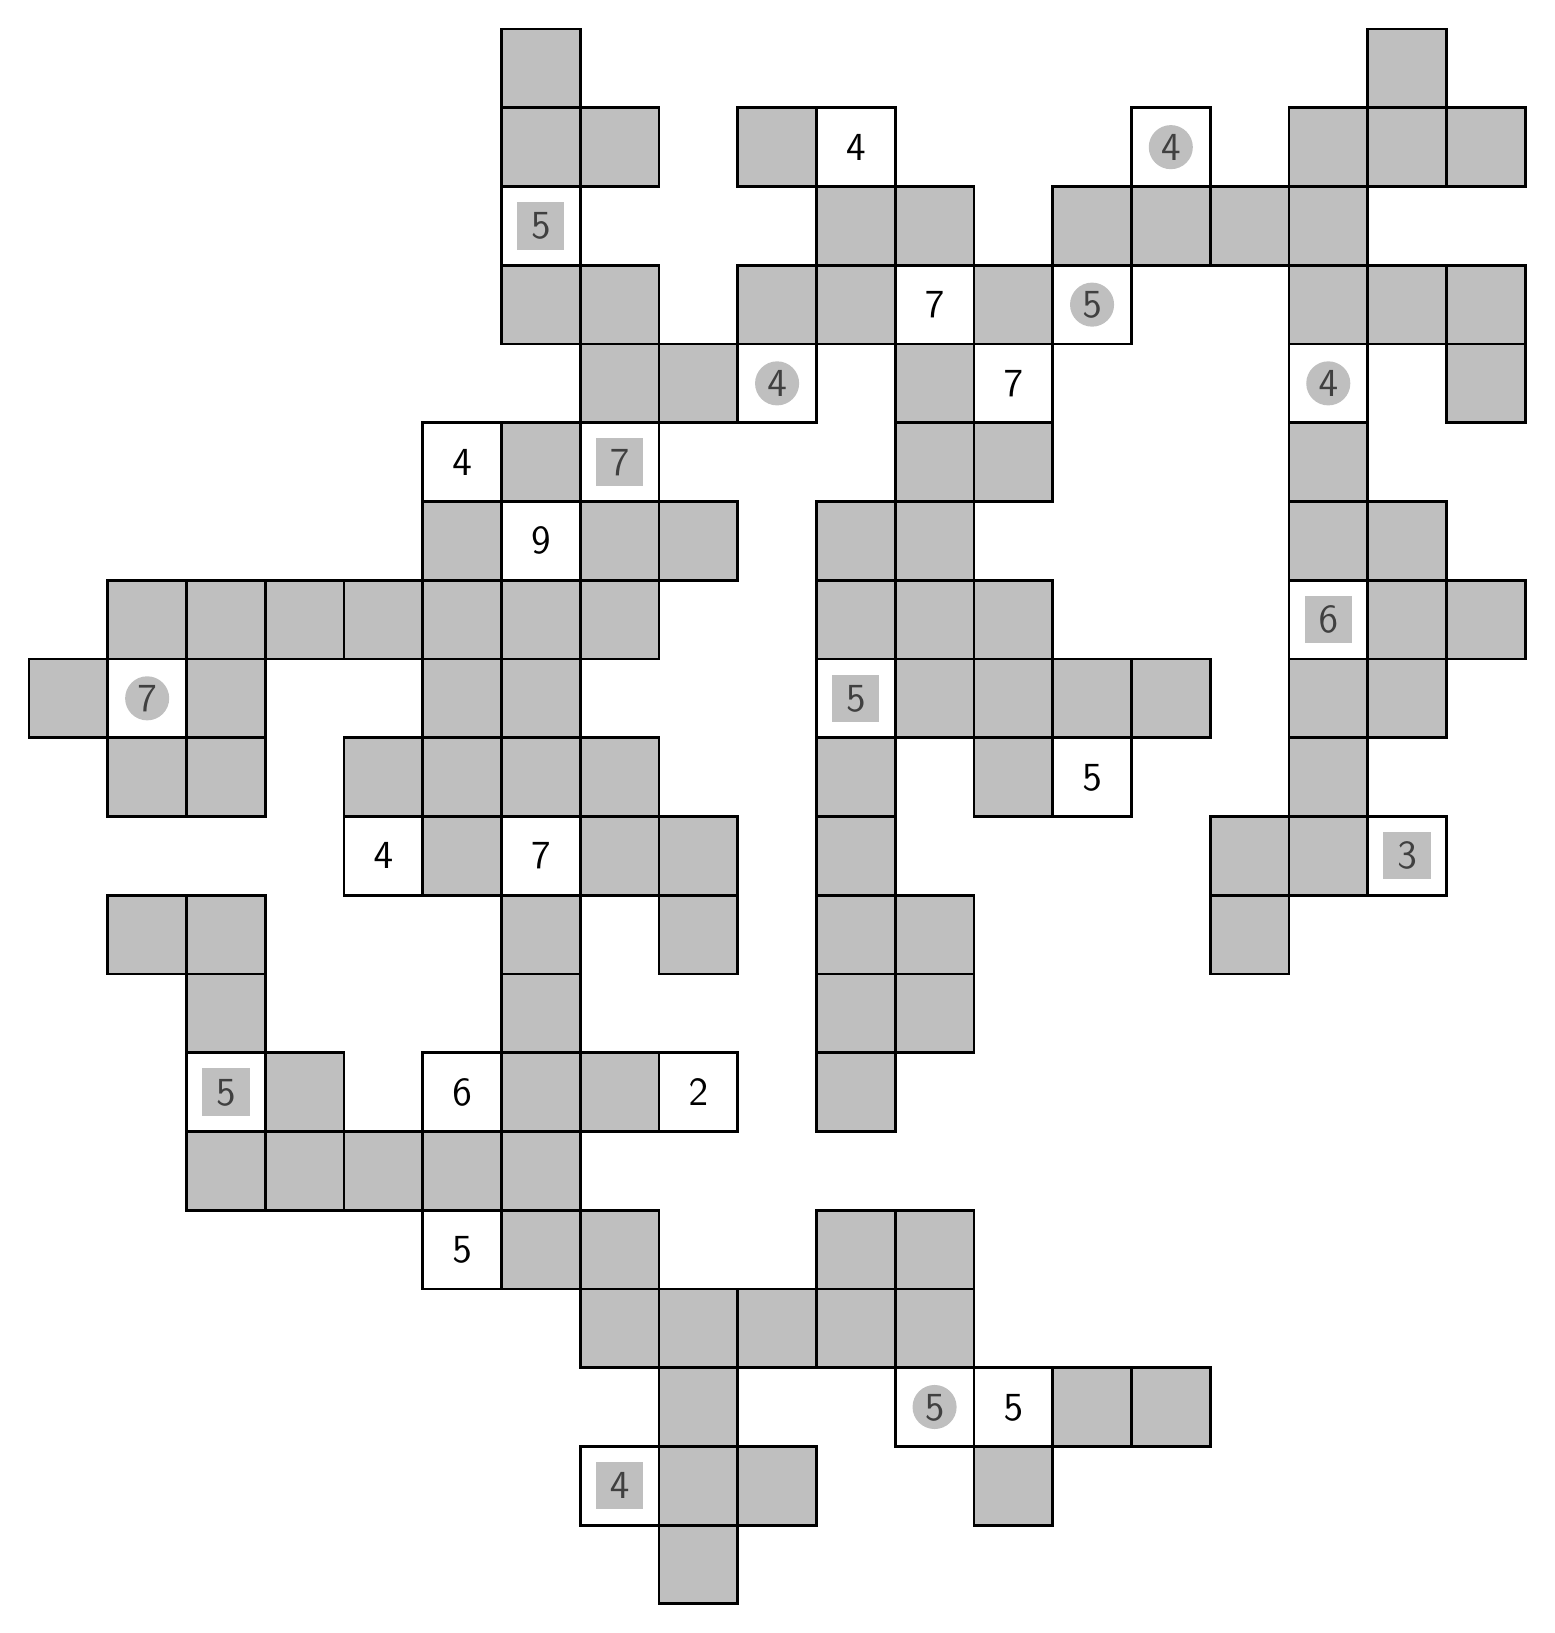
\begin{tikzpicture}\fill[gray, opacity = 0.5] (9, 0, 0)--++(1, 0, 0)--++(0, 1, 0)--++(-1, 0, 0)--cycle;
\draw[line width = 1pt] (9, 0, 0)--++(1, 0, 0)--++(0, 1, 0)--++(-1, 0, 0)--cycle;
\draw node at (8.5, 1.5, 0) {\Large $\mathsf{4}$};
\draw[line width = 1pt] (8, 1, 0)--++(1, 0, 0)--++(0, 1, 0)--++(-1, 0, 0)--cycle;
\fill[color = gray, opacity = 0.5] (8.2, 1.2) rectangle ++(0.6, 0.6);
\fill[gray, opacity = 0.5] (9, 1, 0)--++(1, 0, 0)--++(0, 1, 0)--++(-1, 0, 0)--cycle;
\draw[line width = 1pt] (9, 1, 0)--++(1, 0, 0)--++(0, 1, 0)--++(-1, 0, 0)--cycle;
\fill[gray, opacity = 0.5] (10, 1, 0)--++(1, 0, 0)--++(0, 1, 0)--++(-1, 0, 0)--cycle;
\draw[line width = 1pt] (10, 1, 0)--++(1, 0, 0)--++(0, 1, 0)--++(-1, 0, 0)--cycle;
\fill[gray, opacity = 0.5] (13, 1, 0)--++(1, 0, 0)--++(0, 1, 0)--++(-1, 0, 0)--cycle;
\draw[line width = 1pt] (13, 1, 0)--++(1, 0, 0)--++(0, 1, 0)--++(-1, 0, 0)--cycle;
\fill[gray, opacity = 0.5] (9, 2, 0)--++(1, 0, 0)--++(0, 1, 0)--++(-1, 0, 0)--cycle;
\draw[line width = 1pt] (9, 2, 0)--++(1, 0, 0)--++(0, 1, 0)--++(-1, 0, 0)--cycle;
\draw node at (12.5, 2.5, 0) {\Large $\mathsf{5}$};
\draw[line width = 1pt] (12, 2, 0)--++(1, 0, 0)--++(0, 1, 0)--++(-1, 0, 0)--cycle;
\fill[color = gray, opacity = 0.5] (12.5, 2.5, 0) circle (0.28);
\draw node at (13.5, 2.5, 0) {\Large $\mathsf{5}$};
\draw[line width = 1pt] (13, 2, 0)--++(1, 0, 0)--++(0, 1, 0)--++(-1, 0, 0)--cycle;
\fill[gray, opacity = 0.5] (14, 2, 0)--++(1, 0, 0)--++(0, 1, 0)--++(-1, 0, 0)--cycle;
\draw[line width = 1pt] (14, 2, 0)--++(1, 0, 0)--++(0, 1, 0)--++(-1, 0, 0)--cycle;
\fill[gray, opacity = 0.5] (15, 2, 0)--++(1, 0, 0)--++(0, 1, 0)--++(-1, 0, 0)--cycle;
\draw[line width = 1pt] (15, 2, 0)--++(1, 0, 0)--++(0, 1, 0)--++(-1, 0, 0)--cycle;
\fill[gray, opacity = 0.5] (8, 3, 0)--++(1, 0, 0)--++(0, 1, 0)--++(-1, 0, 0)--cycle;
\draw[line width = 1pt] (8, 3, 0)--++(1, 0, 0)--++(0, 1, 0)--++(-1, 0, 0)--cycle;
\fill[gray, opacity = 0.5] (9, 3, 0)--++(1, 0, 0)--++(0, 1, 0)--++(-1, 0, 0)--cycle;
\draw[line width = 1pt] (9, 3, 0)--++(1, 0, 0)--++(0, 1, 0)--++(-1, 0, 0)--cycle;
\fill[gray, opacity = 0.5] (10, 3, 0)--++(1, 0, 0)--++(0, 1, 0)--++(-1, 0, 0)--cycle;
\draw[line width = 1pt] (10, 3, 0)--++(1, 0, 0)--++(0, 1, 0)--++(-1, 0, 0)--cycle;
\fill[gray, opacity = 0.5] (11, 3, 0)--++(1, 0, 0)--++(0, 1, 0)--++(-1, 0, 0)--cycle;
\draw[line width = 1pt] (11, 3, 0)--++(1, 0, 0)--++(0, 1, 0)--++(-1, 0, 0)--cycle;
\fill[gray, opacity = 0.5] (12, 3, 0)--++(1, 0, 0)--++(0, 1, 0)--++(-1, 0, 0)--cycle;
\draw[line width = 1pt] (12, 3, 0)--++(1, 0, 0)--++(0, 1, 0)--++(-1, 0, 0)--cycle;
\draw node at (6.5, 4.5, 0) {\Large $\mathsf{5}$};
\draw[line width = 1pt] (6, 4, 0)--++(1, 0, 0)--++(0, 1, 0)--++(-1, 0, 0)--cycle;
\fill[gray, opacity = 0.5] (7, 4, 0)--++(1, 0, 0)--++(0, 1, 0)--++(-1, 0, 0)--cycle;
\draw[line width = 1pt] (7, 4, 0)--++(1, 0, 0)--++(0, 1, 0)--++(-1, 0, 0)--cycle;
\fill[gray, opacity = 0.5] (8, 4, 0)--++(1, 0, 0)--++(0, 1, 0)--++(-1, 0, 0)--cycle;
\draw[line width = 1pt] (8, 4, 0)--++(1, 0, 0)--++(0, 1, 0)--++(-1, 0, 0)--cycle;
\fill[gray, opacity = 0.5] (11, 4, 0)--++(1, 0, 0)--++(0, 1, 0)--++(-1, 0, 0)--cycle;
\draw[line width = 1pt] (11, 4, 0)--++(1, 0, 0)--++(0, 1, 0)--++(-1, 0, 0)--cycle;
\fill[gray, opacity = 0.5] (12, 4, 0)--++(1, 0, 0)--++(0, 1, 0)--++(-1, 0, 0)--cycle;
\draw[line width = 1pt] (12, 4, 0)--++(1, 0, 0)--++(0, 1, 0)--++(-1, 0, 0)--cycle;
\fill[gray, opacity = 0.5] (3, 5, 0)--++(1, 0, 0)--++(0, 1, 0)--++(-1, 0, 0)--cycle;
\draw[line width = 1pt] (3, 5, 0)--++(1, 0, 0)--++(0, 1, 0)--++(-1, 0, 0)--cycle;
\fill[gray, opacity = 0.5] (4, 5, 0)--++(1, 0, 0)--++(0, 1, 0)--++(-1, 0, 0)--cycle;
\draw[line width = 1pt] (4, 5, 0)--++(1, 0, 0)--++(0, 1, 0)--++(-1, 0, 0)--cycle;
\fill[gray, opacity = 0.5] (5, 5, 0)--++(1, 0, 0)--++(0, 1, 0)--++(-1, 0, 0)--cycle;
\draw[line width = 1pt] (5, 5, 0)--++(1, 0, 0)--++(0, 1, 0)--++(-1, 0, 0)--cycle;
\fill[gray, opacity = 0.5] (6, 5, 0)--++(1, 0, 0)--++(0, 1, 0)--++(-1, 0, 0)--cycle;
\draw[line width = 1pt] (6, 5, 0)--++(1, 0, 0)--++(0, 1, 0)--++(-1, 0, 0)--cycle;
\fill[gray, opacity = 0.5] (7, 5, 0)--++(1, 0, 0)--++(0, 1, 0)--++(-1, 0, 0)--cycle;
\draw[line width = 1pt] (7, 5, 0)--++(1, 0, 0)--++(0, 1, 0)--++(-1, 0, 0)--cycle;
\draw node at (3.5, 6.5, 0) {\Large $\mathsf{5}$};
\draw[line width = 1pt] (3, 6, 0)--++(1, 0, 0)--++(0, 1, 0)--++(-1, 0, 0)--cycle;
\fill[color = gray, opacity = 0.5] (3.2, 6.2) rectangle ++(0.6, 0.6);
\fill[gray, opacity = 0.5] (4, 6, 0)--++(1, 0, 0)--++(0, 1, 0)--++(-1, 0, 0)--cycle;
\draw[line width = 1pt] (4, 6, 0)--++(1, 0, 0)--++(0, 1, 0)--++(-1, 0, 0)--cycle;
\draw node at (6.5, 6.5, 0) {\Large $\mathsf{6}$};
\draw[line width = 1pt] (6, 6, 0)--++(1, 0, 0)--++(0, 1, 0)--++(-1, 0, 0)--cycle;
\fill[gray, opacity = 0.5] (7, 6, 0)--++(1, 0, 0)--++(0, 1, 0)--++(-1, 0, 0)--cycle;
\draw[line width = 1pt] (7, 6, 0)--++(1, 0, 0)--++(0, 1, 0)--++(-1, 0, 0)--cycle;
\fill[gray, opacity = 0.5] (8, 6, 0)--++(1, 0, 0)--++(0, 1, 0)--++(-1, 0, 0)--cycle;
\draw[line width = 1pt] (8, 6, 0)--++(1, 0, 0)--++(0, 1, 0)--++(-1, 0, 0)--cycle;
\draw node at (9.5, 6.5, 0) {\Large $\mathsf{2}$};
\draw[line width = 1pt] (9, 6, 0)--++(1, 0, 0)--++(0, 1, 0)--++(-1, 0, 0)--cycle;
\fill[gray, opacity = 0.5] (11, 6, 0)--++(1, 0, 0)--++(0, 1, 0)--++(-1, 0, 0)--cycle;
\draw[line width = 1pt] (11, 6, 0)--++(1, 0, 0)--++(0, 1, 0)--++(-1, 0, 0)--cycle;
\fill[gray, opacity = 0.5] (3, 7, 0)--++(1, 0, 0)--++(0, 1, 0)--++(-1, 0, 0)--cycle;
\draw[line width = 1pt] (3, 7, 0)--++(1, 0, 0)--++(0, 1, 0)--++(-1, 0, 0)--cycle;
\fill[gray, opacity = 0.5] (7, 7, 0)--++(1, 0, 0)--++(0, 1, 0)--++(-1, 0, 0)--cycle;
\draw[line width = 1pt] (7, 7, 0)--++(1, 0, 0)--++(0, 1, 0)--++(-1, 0, 0)--cycle;
\fill[gray, opacity = 0.5] (11, 7, 0)--++(1, 0, 0)--++(0, 1, 0)--++(-1, 0, 0)--cycle;
\draw[line width = 1pt] (11, 7, 0)--++(1, 0, 0)--++(0, 1, 0)--++(-1, 0, 0)--cycle;
\fill[gray, opacity = 0.5] (12, 7, 0)--++(1, 0, 0)--++(0, 1, 0)--++(-1, 0, 0)--cycle;
\draw[line width = 1pt] (12, 7, 0)--++(1, 0, 0)--++(0, 1, 0)--++(-1, 0, 0)--cycle;
\fill[gray, opacity = 0.5] (2, 8, 0)--++(1, 0, 0)--++(0, 1, 0)--++(-1, 0, 0)--cycle;
\draw[line width = 1pt] (2, 8, 0)--++(1, 0, 0)--++(0, 1, 0)--++(-1, 0, 0)--cycle;
\fill[gray, opacity = 0.5] (3, 8, 0)--++(1, 0, 0)--++(0, 1, 0)--++(-1, 0, 0)--cycle;
\draw[line width = 1pt] (3, 8, 0)--++(1, 0, 0)--++(0, 1, 0)--++(-1, 0, 0)--cycle;
\fill[gray, opacity = 0.5] (7, 8, 0)--++(1, 0, 0)--++(0, 1, 0)--++(-1, 0, 0)--cycle;
\draw[line width = 1pt] (7, 8, 0)--++(1, 0, 0)--++(0, 1, 0)--++(-1, 0, 0)--cycle;
\fill[gray, opacity = 0.5] (9, 8, 0)--++(1, 0, 0)--++(0, 1, 0)--++(-1, 0, 0)--cycle;
\draw[line width = 1pt] (9, 8, 0)--++(1, 0, 0)--++(0, 1, 0)--++(-1, 0, 0)--cycle;
\fill[gray, opacity = 0.5] (11, 8, 0)--++(1, 0, 0)--++(0, 1, 0)--++(-1, 0, 0)--cycle;
\draw[line width = 1pt] (11, 8, 0)--++(1, 0, 0)--++(0, 1, 0)--++(-1, 0, 0)--cycle;
\fill[gray, opacity = 0.5] (12, 8, 0)--++(1, 0, 0)--++(0, 1, 0)--++(-1, 0, 0)--cycle;
\draw[line width = 1pt] (12, 8, 0)--++(1, 0, 0)--++(0, 1, 0)--++(-1, 0, 0)--cycle;
\fill[gray, opacity = 0.5] (16, 8, 0)--++(1, 0, 0)--++(0, 1, 0)--++(-1, 0, 0)--cycle;
\draw[line width = 1pt] (16, 8, 0)--++(1, 0, 0)--++(0, 1, 0)--++(-1, 0, 0)--cycle;
\draw node at (5.5, 9.5, 0) {\Large $\mathsf{4}$};
\draw[line width = 1pt] (5, 9, 0)--++(1, 0, 0)--++(0, 1, 0)--++(-1, 0, 0)--cycle;
\fill[gray, opacity = 0.5] (6, 9, 0)--++(1, 0, 0)--++(0, 1, 0)--++(-1, 0, 0)--cycle;
\draw[line width = 1pt] (6, 9, 0)--++(1, 0, 0)--++(0, 1, 0)--++(-1, 0, 0)--cycle;
\draw node at (7.5, 9.5, 0) {\Large $\mathsf{7}$};
\draw[line width = 1pt] (7, 9, 0)--++(1, 0, 0)--++(0, 1, 0)--++(-1, 0, 0)--cycle;
\fill[gray, opacity = 0.5] (8, 9, 0)--++(1, 0, 0)--++(0, 1, 0)--++(-1, 0, 0)--cycle;
\draw[line width = 1pt] (8, 9, 0)--++(1, 0, 0)--++(0, 1, 0)--++(-1, 0, 0)--cycle;
\fill[gray, opacity = 0.5] (9, 9, 0)--++(1, 0, 0)--++(0, 1, 0)--++(-1, 0, 0)--cycle;
\draw[line width = 1pt] (9, 9, 0)--++(1, 0, 0)--++(0, 1, 0)--++(-1, 0, 0)--cycle;
\fill[gray, opacity = 0.5] (11, 9, 0)--++(1, 0, 0)--++(0, 1, 0)--++(-1, 0, 0)--cycle;
\draw[line width = 1pt] (11, 9, 0)--++(1, 0, 0)--++(0, 1, 0)--++(-1, 0, 0)--cycle;
\fill[gray, opacity = 0.5] (16, 9, 0)--++(1, 0, 0)--++(0, 1, 0)--++(-1, 0, 0)--cycle;
\draw[line width = 1pt] (16, 9, 0)--++(1, 0, 0)--++(0, 1, 0)--++(-1, 0, 0)--cycle;
\fill[gray, opacity = 0.5] (17, 9, 0)--++(1, 0, 0)--++(0, 1, 0)--++(-1, 0, 0)--cycle;
\draw[line width = 1pt] (17, 9, 0)--++(1, 0, 0)--++(0, 1, 0)--++(-1, 0, 0)--cycle;
\draw node at (18.5, 9.5, 0) {\Large $\mathsf{3}$};
\draw[line width = 1pt] (18, 9, 0)--++(1, 0, 0)--++(0, 1, 0)--++(-1, 0, 0)--cycle;
\fill[color = gray, opacity = 0.5] (18.2, 9.2) rectangle ++(0.6, 0.6);
\fill[gray, opacity = 0.5] (2, 10, 0)--++(1, 0, 0)--++(0, 1, 0)--++(-1, 0, 0)--cycle;
\draw[line width = 1pt] (2, 10, 0)--++(1, 0, 0)--++(0, 1, 0)--++(-1, 0, 0)--cycle;
\fill[gray, opacity = 0.5] (3, 10, 0)--++(1, 0, 0)--++(0, 1, 0)--++(-1, 0, 0)--cycle;
\draw[line width = 1pt] (3, 10, 0)--++(1, 0, 0)--++(0, 1, 0)--++(-1, 0, 0)--cycle;
\fill[gray, opacity = 0.5] (5, 10, 0)--++(1, 0, 0)--++(0, 1, 0)--++(-1, 0, 0)--cycle;
\draw[line width = 1pt] (5, 10, 0)--++(1, 0, 0)--++(0, 1, 0)--++(-1, 0, 0)--cycle;
\fill[gray, opacity = 0.5] (6, 10, 0)--++(1, 0, 0)--++(0, 1, 0)--++(-1, 0, 0)--cycle;
\draw[line width = 1pt] (6, 10, 0)--++(1, 0, 0)--++(0, 1, 0)--++(-1, 0, 0)--cycle;
\fill[gray, opacity = 0.5] (7, 10, 0)--++(1, 0, 0)--++(0, 1, 0)--++(-1, 0, 0)--cycle;
\draw[line width = 1pt] (7, 10, 0)--++(1, 0, 0)--++(0, 1, 0)--++(-1, 0, 0)--cycle;
\fill[gray, opacity = 0.5] (8, 10, 0)--++(1, 0, 0)--++(0, 1, 0)--++(-1, 0, 0)--cycle;
\draw[line width = 1pt] (8, 10, 0)--++(1, 0, 0)--++(0, 1, 0)--++(-1, 0, 0)--cycle;
\fill[gray, opacity = 0.5] (11, 10, 0)--++(1, 0, 0)--++(0, 1, 0)--++(-1, 0, 0)--cycle;
\draw[line width = 1pt] (11, 10, 0)--++(1, 0, 0)--++(0, 1, 0)--++(-1, 0, 0)--cycle;
\fill[gray, opacity = 0.5] (13, 10, 0)--++(1, 0, 0)--++(0, 1, 0)--++(-1, 0, 0)--cycle;
\draw[line width = 1pt] (13, 10, 0)--++(1, 0, 0)--++(0, 1, 0)--++(-1, 0, 0)--cycle;
\draw node at (14.5, 10.5, 0) {\Large $\mathsf{5}$};
\draw[line width = 1pt] (14, 10, 0)--++(1, 0, 0)--++(0, 1, 0)--++(-1, 0, 0)--cycle;
\fill[gray, opacity = 0.5] (17, 10, 0)--++(1, 0, 0)--++(0, 1, 0)--++(-1, 0, 0)--cycle;
\draw[line width = 1pt] (17, 10, 0)--++(1, 0, 0)--++(0, 1, 0)--++(-1, 0, 0)--cycle;
\fill[gray, opacity = 0.5] (1, 11, 0)--++(1, 0, 0)--++(0, 1, 0)--++(-1, 0, 0)--cycle;
\draw[line width = 1pt] (1, 11, 0)--++(1, 0, 0)--++(0, 1, 0)--++(-1, 0, 0)--cycle;
\draw node at (2.5, 11.5, 0) {\Large $\mathsf{7}$};
\draw[line width = 1pt] (2, 11, 0)--++(1, 0, 0)--++(0, 1, 0)--++(-1, 0, 0)--cycle;
\fill[color = gray, opacity = 0.5] (2.5, 11.5, 0) circle (0.28);
\fill[gray, opacity = 0.5] (3, 11, 0)--++(1, 0, 0)--++(0, 1, 0)--++(-1, 0, 0)--cycle;
\draw[line width = 1pt] (3, 11, 0)--++(1, 0, 0)--++(0, 1, 0)--++(-1, 0, 0)--cycle;
\fill[gray, opacity = 0.5] (6, 11, 0)--++(1, 0, 0)--++(0, 1, 0)--++(-1, 0, 0)--cycle;
\draw[line width = 1pt] (6, 11, 0)--++(1, 0, 0)--++(0, 1, 0)--++(-1, 0, 0)--cycle;
\fill[gray, opacity = 0.5] (7, 11, 0)--++(1, 0, 0)--++(0, 1, 0)--++(-1, 0, 0)--cycle;
\draw[line width = 1pt] (7, 11, 0)--++(1, 0, 0)--++(0, 1, 0)--++(-1, 0, 0)--cycle;
\draw node at (11.5, 11.5, 0) {\Large $\mathsf{5}$};
\draw[line width = 1pt] (11, 11, 0)--++(1, 0, 0)--++(0, 1, 0)--++(-1, 0, 0)--cycle;
\fill[color = gray, opacity = 0.5] (11.2, 11.2) rectangle ++(0.6, 0.6);
\fill[gray, opacity = 0.5] (12, 11, 0)--++(1, 0, 0)--++(0, 1, 0)--++(-1, 0, 0)--cycle;
\draw[line width = 1pt] (12, 11, 0)--++(1, 0, 0)--++(0, 1, 0)--++(-1, 0, 0)--cycle;
\fill[gray, opacity = 0.5] (13, 11, 0)--++(1, 0, 0)--++(0, 1, 0)--++(-1, 0, 0)--cycle;
\draw[line width = 1pt] (13, 11, 0)--++(1, 0, 0)--++(0, 1, 0)--++(-1, 0, 0)--cycle;
\fill[gray, opacity = 0.5] (14, 11, 0)--++(1, 0, 0)--++(0, 1, 0)--++(-1, 0, 0)--cycle;
\draw[line width = 1pt] (14, 11, 0)--++(1, 0, 0)--++(0, 1, 0)--++(-1, 0, 0)--cycle;
\fill[gray, opacity = 0.5] (15, 11, 0)--++(1, 0, 0)--++(0, 1, 0)--++(-1, 0, 0)--cycle;
\draw[line width = 1pt] (15, 11, 0)--++(1, 0, 0)--++(0, 1, 0)--++(-1, 0, 0)--cycle;
\fill[gray, opacity = 0.5] (17, 11, 0)--++(1, 0, 0)--++(0, 1, 0)--++(-1, 0, 0)--cycle;
\draw[line width = 1pt] (17, 11, 0)--++(1, 0, 0)--++(0, 1, 0)--++(-1, 0, 0)--cycle;
\fill[gray, opacity = 0.5] (18, 11, 0)--++(1, 0, 0)--++(0, 1, 0)--++(-1, 0, 0)--cycle;
\draw[line width = 1pt] (18, 11, 0)--++(1, 0, 0)--++(0, 1, 0)--++(-1, 0, 0)--cycle;
\fill[gray, opacity = 0.5] (2, 12, 0)--++(1, 0, 0)--++(0, 1, 0)--++(-1, 0, 0)--cycle;
\draw[line width = 1pt] (2, 12, 0)--++(1, 0, 0)--++(0, 1, 0)--++(-1, 0, 0)--cycle;
\fill[gray, opacity = 0.5] (3, 12, 0)--++(1, 0, 0)--++(0, 1, 0)--++(-1, 0, 0)--cycle;
\draw[line width = 1pt] (3, 12, 0)--++(1, 0, 0)--++(0, 1, 0)--++(-1, 0, 0)--cycle;
\fill[gray, opacity = 0.5] (4, 12, 0)--++(1, 0, 0)--++(0, 1, 0)--++(-1, 0, 0)--cycle;
\draw[line width = 1pt] (4, 12, 0)--++(1, 0, 0)--++(0, 1, 0)--++(-1, 0, 0)--cycle;
\fill[gray, opacity = 0.5] (5, 12, 0)--++(1, 0, 0)--++(0, 1, 0)--++(-1, 0, 0)--cycle;
\draw[line width = 1pt] (5, 12, 0)--++(1, 0, 0)--++(0, 1, 0)--++(-1, 0, 0)--cycle;
\fill[gray, opacity = 0.5] (6, 12, 0)--++(1, 0, 0)--++(0, 1, 0)--++(-1, 0, 0)--cycle;
\draw[line width = 1pt] (6, 12, 0)--++(1, 0, 0)--++(0, 1, 0)--++(-1, 0, 0)--cycle;
\fill[gray, opacity = 0.5] (7, 12, 0)--++(1, 0, 0)--++(0, 1, 0)--++(-1, 0, 0)--cycle;
\draw[line width = 1pt] (7, 12, 0)--++(1, 0, 0)--++(0, 1, 0)--++(-1, 0, 0)--cycle;
\fill[gray, opacity = 0.5] (8, 12, 0)--++(1, 0, 0)--++(0, 1, 0)--++(-1, 0, 0)--cycle;
\draw[line width = 1pt] (8, 12, 0)--++(1, 0, 0)--++(0, 1, 0)--++(-1, 0, 0)--cycle;
\fill[gray, opacity = 0.5] (11, 12, 0)--++(1, 0, 0)--++(0, 1, 0)--++(-1, 0, 0)--cycle;
\draw[line width = 1pt] (11, 12, 0)--++(1, 0, 0)--++(0, 1, 0)--++(-1, 0, 0)--cycle;
\fill[gray, opacity = 0.5] (12, 12, 0)--++(1, 0, 0)--++(0, 1, 0)--++(-1, 0, 0)--cycle;
\draw[line width = 1pt] (12, 12, 0)--++(1, 0, 0)--++(0, 1, 0)--++(-1, 0, 0)--cycle;
\fill[gray, opacity = 0.5] (13, 12, 0)--++(1, 0, 0)--++(0, 1, 0)--++(-1, 0, 0)--cycle;
\draw[line width = 1pt] (13, 12, 0)--++(1, 0, 0)--++(0, 1, 0)--++(-1, 0, 0)--cycle;
\draw node at (17.5, 12.5, 0) {\Large $\mathsf{6}$};
\draw[line width = 1pt] (17, 12, 0)--++(1, 0, 0)--++(0, 1, 0)--++(-1, 0, 0)--cycle;
\fill[color = gray, opacity = 0.5] (17.2, 12.2) rectangle ++(0.6, 0.6);
\fill[gray, opacity = 0.5] (18, 12, 0)--++(1, 0, 0)--++(0, 1, 0)--++(-1, 0, 0)--cycle;
\draw[line width = 1pt] (18, 12, 0)--++(1, 0, 0)--++(0, 1, 0)--++(-1, 0, 0)--cycle;
\fill[gray, opacity = 0.5] (19, 12, 0)--++(1, 0, 0)--++(0, 1, 0)--++(-1, 0, 0)--cycle;
\draw[line width = 1pt] (19, 12, 0)--++(1, 0, 0)--++(0, 1, 0)--++(-1, 0, 0)--cycle;
\fill[gray, opacity = 0.5] (6, 13, 0)--++(1, 0, 0)--++(0, 1, 0)--++(-1, 0, 0)--cycle;
\draw[line width = 1pt] (6, 13, 0)--++(1, 0, 0)--++(0, 1, 0)--++(-1, 0, 0)--cycle;
\draw node at (7.5, 13.5, 0) {\Large $\mathsf{9}$};
\draw[line width = 1pt] (7, 13, 0)--++(1, 0, 0)--++(0, 1, 0)--++(-1, 0, 0)--cycle;
\fill[gray, opacity = 0.5] (8, 13, 0)--++(1, 0, 0)--++(0, 1, 0)--++(-1, 0, 0)--cycle;
\draw[line width = 1pt] (8, 13, 0)--++(1, 0, 0)--++(0, 1, 0)--++(-1, 0, 0)--cycle;
\fill[gray, opacity = 0.5] (9, 13, 0)--++(1, 0, 0)--++(0, 1, 0)--++(-1, 0, 0)--cycle;
\draw[line width = 1pt] (9, 13, 0)--++(1, 0, 0)--++(0, 1, 0)--++(-1, 0, 0)--cycle;
\fill[gray, opacity = 0.5] (11, 13, 0)--++(1, 0, 0)--++(0, 1, 0)--++(-1, 0, 0)--cycle;
\draw[line width = 1pt] (11, 13, 0)--++(1, 0, 0)--++(0, 1, 0)--++(-1, 0, 0)--cycle;
\fill[gray, opacity = 0.5] (12, 13, 0)--++(1, 0, 0)--++(0, 1, 0)--++(-1, 0, 0)--cycle;
\draw[line width = 1pt] (12, 13, 0)--++(1, 0, 0)--++(0, 1, 0)--++(-1, 0, 0)--cycle;
\fill[gray, opacity = 0.5] (17, 13, 0)--++(1, 0, 0)--++(0, 1, 0)--++(-1, 0, 0)--cycle;
\draw[line width = 1pt] (17, 13, 0)--++(1, 0, 0)--++(0, 1, 0)--++(-1, 0, 0)--cycle;
\fill[gray, opacity = 0.5] (18, 13, 0)--++(1, 0, 0)--++(0, 1, 0)--++(-1, 0, 0)--cycle;
\draw[line width = 1pt] (18, 13, 0)--++(1, 0, 0)--++(0, 1, 0)--++(-1, 0, 0)--cycle;
\draw node at (6.5, 14.5, 0) {\Large $\mathsf{4}$};
\draw[line width = 1pt] (6, 14, 0)--++(1, 0, 0)--++(0, 1, 0)--++(-1, 0, 0)--cycle;
\fill[gray, opacity = 0.5] (7, 14, 0)--++(1, 0, 0)--++(0, 1, 0)--++(-1, 0, 0)--cycle;
\draw[line width = 1pt] (7, 14, 0)--++(1, 0, 0)--++(0, 1, 0)--++(-1, 0, 0)--cycle;
\draw node at (8.5, 14.5, 0) {\Large $\mathsf{7}$};
\draw[line width = 1pt] (8, 14, 0)--++(1, 0, 0)--++(0, 1, 0)--++(-1, 0, 0)--cycle;
\fill[color = gray, opacity = 0.5] (8.2, 14.2) rectangle ++(0.6, 0.6);
\fill[gray, opacity = 0.5] (12, 14, 0)--++(1, 0, 0)--++(0, 1, 0)--++(-1, 0, 0)--cycle;
\draw[line width = 1pt] (12, 14, 0)--++(1, 0, 0)--++(0, 1, 0)--++(-1, 0, 0)--cycle;
\fill[gray, opacity = 0.5] (13, 14, 0)--++(1, 0, 0)--++(0, 1, 0)--++(-1, 0, 0)--cycle;
\draw[line width = 1pt] (13, 14, 0)--++(1, 0, 0)--++(0, 1, 0)--++(-1, 0, 0)--cycle;
\fill[gray, opacity = 0.5] (17, 14, 0)--++(1, 0, 0)--++(0, 1, 0)--++(-1, 0, 0)--cycle;
\draw[line width = 1pt] (17, 14, 0)--++(1, 0, 0)--++(0, 1, 0)--++(-1, 0, 0)--cycle;
\fill[gray, opacity = 0.5] (8, 15, 0)--++(1, 0, 0)--++(0, 1, 0)--++(-1, 0, 0)--cycle;
\draw[line width = 1pt] (8, 15, 0)--++(1, 0, 0)--++(0, 1, 0)--++(-1, 0, 0)--cycle;
\fill[gray, opacity = 0.5] (9, 15, 0)--++(1, 0, 0)--++(0, 1, 0)--++(-1, 0, 0)--cycle;
\draw[line width = 1pt] (9, 15, 0)--++(1, 0, 0)--++(0, 1, 0)--++(-1, 0, 0)--cycle;
\draw node at (10.5, 15.5, 0) {\Large $\mathsf{4}$};
\draw[line width = 1pt] (10, 15, 0)--++(1, 0, 0)--++(0, 1, 0)--++(-1, 0, 0)--cycle;
\fill[color = gray, opacity = 0.5] (10.5, 15.5, 0) circle (0.28);
\fill[gray, opacity = 0.5] (12, 15, 0)--++(1, 0, 0)--++(0, 1, 0)--++(-1, 0, 0)--cycle;
\draw[line width = 1pt] (12, 15, 0)--++(1, 0, 0)--++(0, 1, 0)--++(-1, 0, 0)--cycle;
\draw node at (13.5, 15.5, 0) {\Large $\mathsf{7}$};
\draw[line width = 1pt] (13, 15, 0)--++(1, 0, 0)--++(0, 1, 0)--++(-1, 0, 0)--cycle;
\draw node at (17.5, 15.5, 0) {\Large $\mathsf{4}$};
\draw[line width = 1pt] (17, 15, 0)--++(1, 0, 0)--++(0, 1, 0)--++(-1, 0, 0)--cycle;
\fill[color = gray, opacity = 0.5] (17.5, 15.5, 0) circle (0.28);
\fill[gray, opacity = 0.5] (19, 15, 0)--++(1, 0, 0)--++(0, 1, 0)--++(-1, 0, 0)--cycle;
\draw[line width = 1pt] (19, 15, 0)--++(1, 0, 0)--++(0, 1, 0)--++(-1, 0, 0)--cycle;
\fill[gray, opacity = 0.5] (7, 16, 0)--++(1, 0, 0)--++(0, 1, 0)--++(-1, 0, 0)--cycle;
\draw[line width = 1pt] (7, 16, 0)--++(1, 0, 0)--++(0, 1, 0)--++(-1, 0, 0)--cycle;
\fill[gray, opacity = 0.5] (8, 16, 0)--++(1, 0, 0)--++(0, 1, 0)--++(-1, 0, 0)--cycle;
\draw[line width = 1pt] (8, 16, 0)--++(1, 0, 0)--++(0, 1, 0)--++(-1, 0, 0)--cycle;
\fill[gray, opacity = 0.5] (10, 16, 0)--++(1, 0, 0)--++(0, 1, 0)--++(-1, 0, 0)--cycle;
\draw[line width = 1pt] (10, 16, 0)--++(1, 0, 0)--++(0, 1, 0)--++(-1, 0, 0)--cycle;
\fill[gray, opacity = 0.5] (11, 16, 0)--++(1, 0, 0)--++(0, 1, 0)--++(-1, 0, 0)--cycle;
\draw[line width = 1pt] (11, 16, 0)--++(1, 0, 0)--++(0, 1, 0)--++(-1, 0, 0)--cycle;
\draw node at (12.5, 16.5, 0) {\Large $\mathsf{7}$};
\draw[line width = 1pt] (12, 16, 0)--++(1, 0, 0)--++(0, 1, 0)--++(-1, 0, 0)--cycle;
\fill[gray, opacity = 0.5] (13, 16, 0)--++(1, 0, 0)--++(0, 1, 0)--++(-1, 0, 0)--cycle;
\draw[line width = 1pt] (13, 16, 0)--++(1, 0, 0)--++(0, 1, 0)--++(-1, 0, 0)--cycle;
\draw node at (14.5, 16.5, 0) {\Large $\mathsf{5}$};
\draw[line width = 1pt] (14, 16, 0)--++(1, 0, 0)--++(0, 1, 0)--++(-1, 0, 0)--cycle;
\fill[color = gray, opacity = 0.5] (14.5, 16.5, 0) circle (0.28);
\fill[gray, opacity = 0.5] (17, 16, 0)--++(1, 0, 0)--++(0, 1, 0)--++(-1, 0, 0)--cycle;
\draw[line width = 1pt] (17, 16, 0)--++(1, 0, 0)--++(0, 1, 0)--++(-1, 0, 0)--cycle;
\fill[gray, opacity = 0.5] (18, 16, 0)--++(1, 0, 0)--++(0, 1, 0)--++(-1, 0, 0)--cycle;
\draw[line width = 1pt] (18, 16, 0)--++(1, 0, 0)--++(0, 1, 0)--++(-1, 0, 0)--cycle;
\fill[gray, opacity = 0.5] (19, 16, 0)--++(1, 0, 0)--++(0, 1, 0)--++(-1, 0, 0)--cycle;
\draw[line width = 1pt] (19, 16, 0)--++(1, 0, 0)--++(0, 1, 0)--++(-1, 0, 0)--cycle;
\draw node at (7.5, 17.5, 0) {\Large $\mathsf{5}$};
\draw[line width = 1pt] (7, 17, 0)--++(1, 0, 0)--++(0, 1, 0)--++(-1, 0, 0)--cycle;
\fill[color = gray, opacity = 0.5] (7.2, 17.2) rectangle ++(0.6, 0.6);
\fill[gray, opacity = 0.5] (11, 17, 0)--++(1, 0, 0)--++(0, 1, 0)--++(-1, 0, 0)--cycle;
\draw[line width = 1pt] (11, 17, 0)--++(1, 0, 0)--++(0, 1, 0)--++(-1, 0, 0)--cycle;
\fill[gray, opacity = 0.5] (12, 17, 0)--++(1, 0, 0)--++(0, 1, 0)--++(-1, 0, 0)--cycle;
\draw[line width = 1pt] (12, 17, 0)--++(1, 0, 0)--++(0, 1, 0)--++(-1, 0, 0)--cycle;
\fill[gray, opacity = 0.5] (14, 17, 0)--++(1, 0, 0)--++(0, 1, 0)--++(-1, 0, 0)--cycle;
\draw[line width = 1pt] (14, 17, 0)--++(1, 0, 0)--++(0, 1, 0)--++(-1, 0, 0)--cycle;
\fill[gray, opacity = 0.5] (15, 17, 0)--++(1, 0, 0)--++(0, 1, 0)--++(-1, 0, 0)--cycle;
\draw[line width = 1pt] (15, 17, 0)--++(1, 0, 0)--++(0, 1, 0)--++(-1, 0, 0)--cycle;
\fill[gray, opacity = 0.5] (16, 17, 0)--++(1, 0, 0)--++(0, 1, 0)--++(-1, 0, 0)--cycle;
\draw[line width = 1pt] (16, 17, 0)--++(1, 0, 0)--++(0, 1, 0)--++(-1, 0, 0)--cycle;
\fill[gray, opacity = 0.5] (17, 17, 0)--++(1, 0, 0)--++(0, 1, 0)--++(-1, 0, 0)--cycle;
\draw[line width = 1pt] (17, 17, 0)--++(1, 0, 0)--++(0, 1, 0)--++(-1, 0, 0)--cycle;
\fill[gray, opacity = 0.5] (7, 18, 0)--++(1, 0, 0)--++(0, 1, 0)--++(-1, 0, 0)--cycle;
\draw[line width = 1pt] (7, 18, 0)--++(1, 0, 0)--++(0, 1, 0)--++(-1, 0, 0)--cycle;
\fill[gray, opacity = 0.5] (8, 18, 0)--++(1, 0, 0)--++(0, 1, 0)--++(-1, 0, 0)--cycle;
\draw[line width = 1pt] (8, 18, 0)--++(1, 0, 0)--++(0, 1, 0)--++(-1, 0, 0)--cycle;
\fill[gray, opacity = 0.5] (10, 18, 0)--++(1, 0, 0)--++(0, 1, 0)--++(-1, 0, 0)--cycle;
\draw[line width = 1pt] (10, 18, 0)--++(1, 0, 0)--++(0, 1, 0)--++(-1, 0, 0)--cycle;
\draw node at (11.5, 18.5, 0) {\Large $\mathsf{4}$};
\draw[line width = 1pt] (11, 18, 0)--++(1, 0, 0)--++(0, 1, 0)--++(-1, 0, 0)--cycle;
\draw node at (15.5, 18.5, 0) {\Large $\mathsf{4}$};
\draw[line width = 1pt] (15, 18, 0)--++(1, 0, 0)--++(0, 1, 0)--++(-1, 0, 0)--cycle;
\fill[color = gray, opacity = 0.5] (15.5, 18.5, 0) circle (0.28);
\fill[gray, opacity = 0.5] (17, 18, 0)--++(1, 0, 0)--++(0, 1, 0)--++(-1, 0, 0)--cycle;
\draw[line width = 1pt] (17, 18, 0)--++(1, 0, 0)--++(0, 1, 0)--++(-1, 0, 0)--cycle;
\fill[gray, opacity = 0.5] (18, 18, 0)--++(1, 0, 0)--++(0, 1, 0)--++(-1, 0, 0)--cycle;
\draw[line width = 1pt] (18, 18, 0)--++(1, 0, 0)--++(0, 1, 0)--++(-1, 0, 0)--cycle;
\fill[gray, opacity = 0.5] (19, 18, 0)--++(1, 0, 0)--++(0, 1, 0)--++(-1, 0, 0)--cycle;
\draw[line width = 1pt] (19, 18, 0)--++(1, 0, 0)--++(0, 1, 0)--++(-1, 0, 0)--cycle;
\fill[gray, opacity = 0.5] (7, 19, 0)--++(1, 0, 0)--++(0, 1, 0)--++(-1, 0, 0)--cycle;
\draw[line width = 1pt] (7, 19, 0)--++(1, 0, 0)--++(0, 1, 0)--++(-1, 0, 0)--cycle;
\fill[gray, opacity = 0.5] (18, 19, 0)--++(1, 0, 0)--++(0, 1, 0)--++(-1, 0, 0)--cycle;
\draw[line width = 1pt] (18, 19, 0)--++(1, 0, 0)--++(0, 1, 0)--++(-1, 0, 0)--cycle;
\end{tikzpicture}}\]
\[\resizebox{30pc}{!}{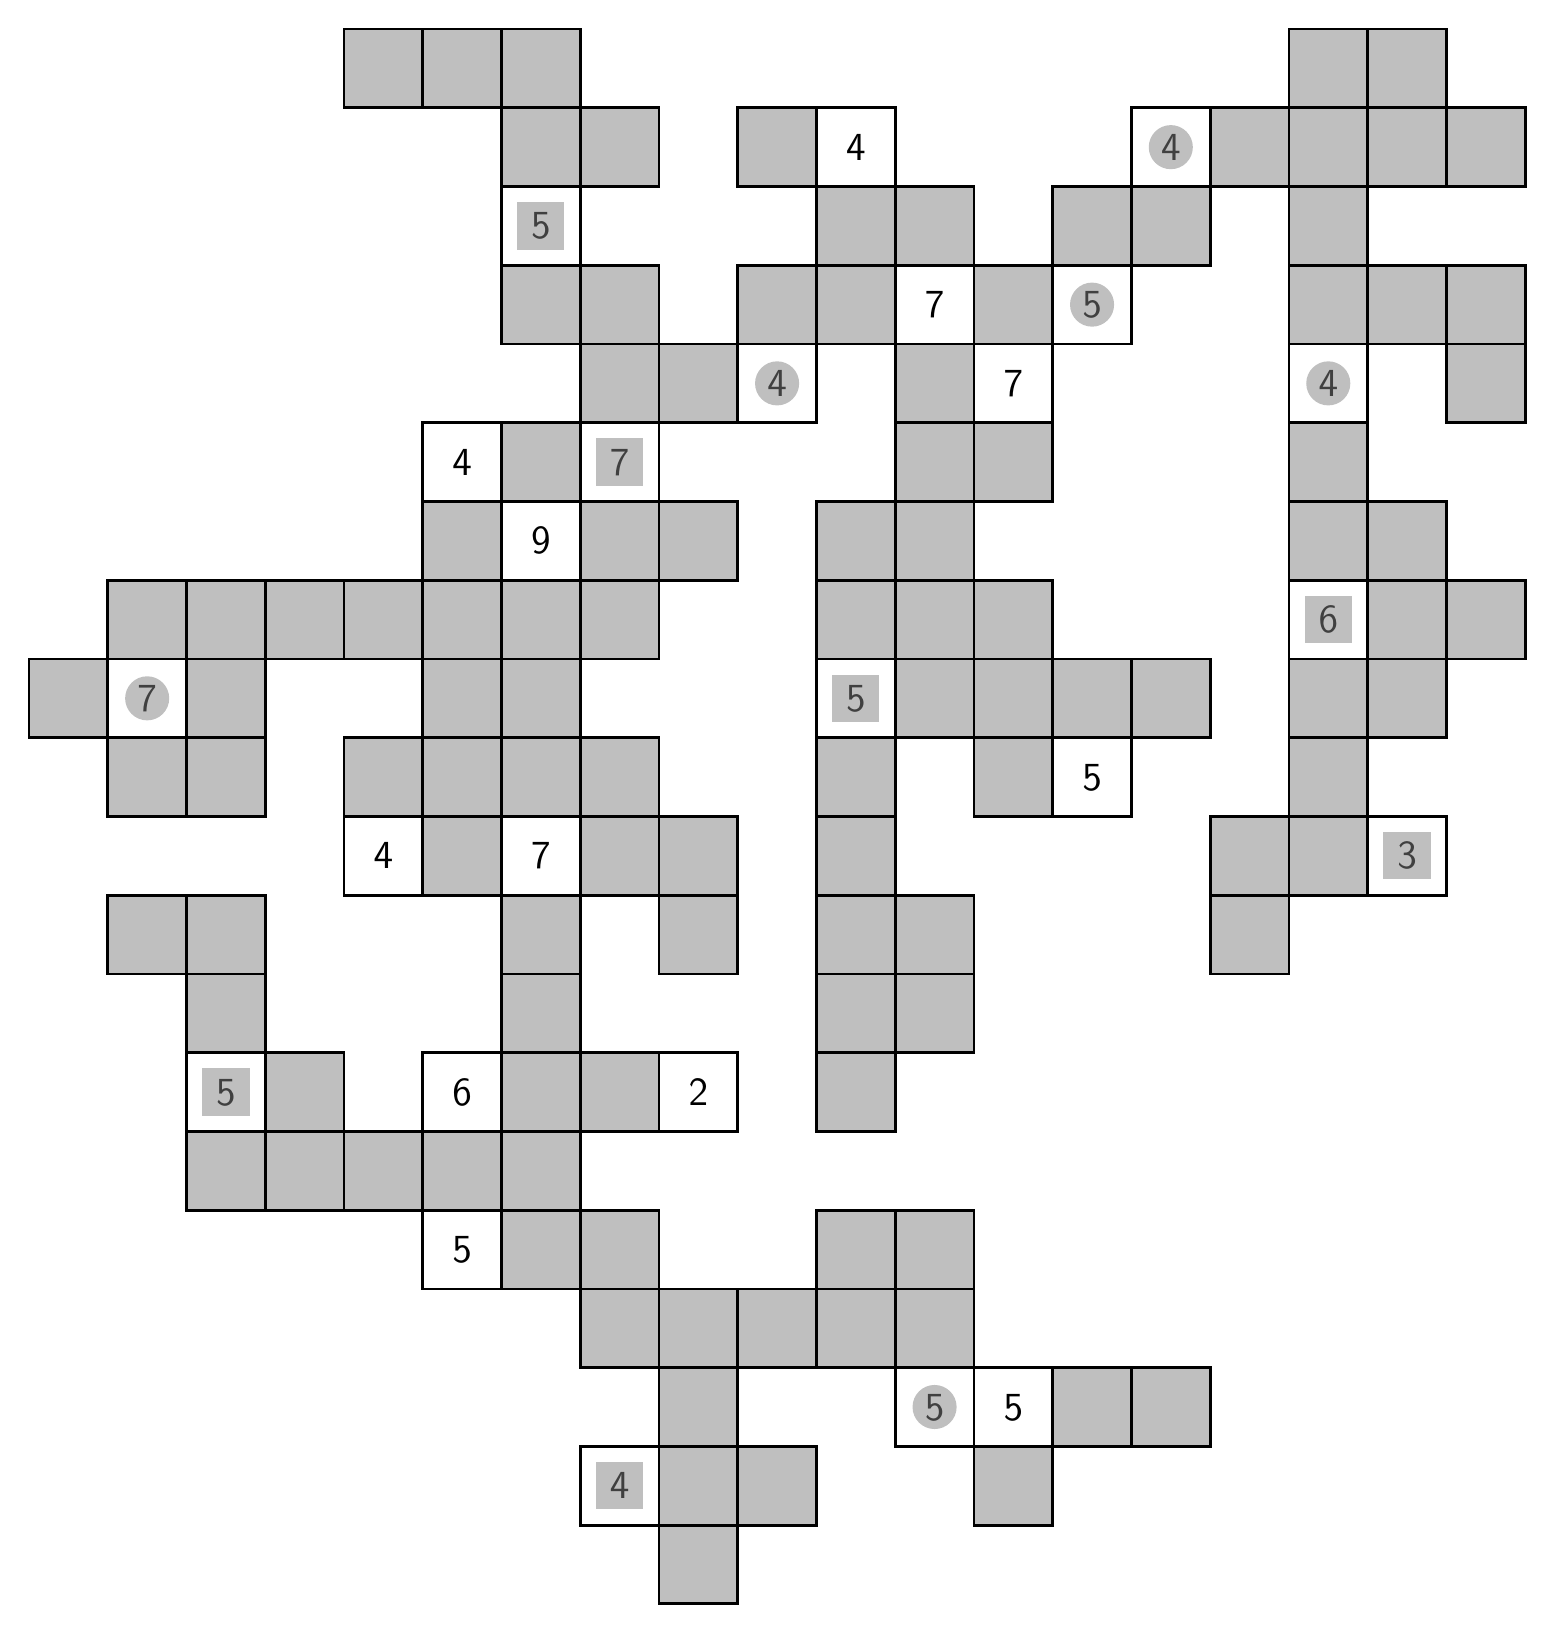
\begin{tikzpicture}\fill[gray, opacity = 0.5] (9, 0, 0)--++(1, 0, 0)--++(0, 1, 0)--++(-1, 0, 0)--cycle;
\draw[line width = 1pt] (9, 0, 0)--++(1, 0, 0)--++(0, 1, 0)--++(-1, 0, 0)--cycle;
\draw node at (8.5, 1.5, 0) {\Large $\mathsf{4}$};
\draw[line width = 1pt] (8, 1, 0)--++(1, 0, 0)--++(0, 1, 0)--++(-1, 0, 0)--cycle;
\fill[color = gray, opacity = 0.5] (8.2, 1.2) rectangle ++(0.6, 0.6);
\fill[gray, opacity = 0.5] (9, 1, 0)--++(1, 0, 0)--++(0, 1, 0)--++(-1, 0, 0)--cycle;
\draw[line width = 1pt] (9, 1, 0)--++(1, 0, 0)--++(0, 1, 0)--++(-1, 0, 0)--cycle;
\fill[gray, opacity = 0.5] (10, 1, 0)--++(1, 0, 0)--++(0, 1, 0)--++(-1, 0, 0)--cycle;
\draw[line width = 1pt] (10, 1, 0)--++(1, 0, 0)--++(0, 1, 0)--++(-1, 0, 0)--cycle;
\fill[gray, opacity = 0.5] (13, 1, 0)--++(1, 0, 0)--++(0, 1, 0)--++(-1, 0, 0)--cycle;
\draw[line width = 1pt] (13, 1, 0)--++(1, 0, 0)--++(0, 1, 0)--++(-1, 0, 0)--cycle;
\fill[gray, opacity = 0.5] (9, 2, 0)--++(1, 0, 0)--++(0, 1, 0)--++(-1, 0, 0)--cycle;
\draw[line width = 1pt] (9, 2, 0)--++(1, 0, 0)--++(0, 1, 0)--++(-1, 0, 0)--cycle;
\draw node at (12.5, 2.5, 0) {\Large $\mathsf{5}$};
\draw[line width = 1pt] (12, 2, 0)--++(1, 0, 0)--++(0, 1, 0)--++(-1, 0, 0)--cycle;
\fill[color = gray, opacity = 0.5] (12.5, 2.5, 0) circle (0.28);
\draw node at (13.5, 2.5, 0) {\Large $\mathsf{5}$};
\draw[line width = 1pt] (13, 2, 0)--++(1, 0, 0)--++(0, 1, 0)--++(-1, 0, 0)--cycle;
\fill[gray, opacity = 0.5] (14, 2, 0)--++(1, 0, 0)--++(0, 1, 0)--++(-1, 0, 0)--cycle;
\draw[line width = 1pt] (14, 2, 0)--++(1, 0, 0)--++(0, 1, 0)--++(-1, 0, 0)--cycle;
\fill[gray, opacity = 0.5] (15, 2, 0)--++(1, 0, 0)--++(0, 1, 0)--++(-1, 0, 0)--cycle;
\draw[line width = 1pt] (15, 2, 0)--++(1, 0, 0)--++(0, 1, 0)--++(-1, 0, 0)--cycle;
\fill[gray, opacity = 0.5] (8, 3, 0)--++(1, 0, 0)--++(0, 1, 0)--++(-1, 0, 0)--cycle;
\draw[line width = 1pt] (8, 3, 0)--++(1, 0, 0)--++(0, 1, 0)--++(-1, 0, 0)--cycle;
\fill[gray, opacity = 0.5] (9, 3, 0)--++(1, 0, 0)--++(0, 1, 0)--++(-1, 0, 0)--cycle;
\draw[line width = 1pt] (9, 3, 0)--++(1, 0, 0)--++(0, 1, 0)--++(-1, 0, 0)--cycle;
\fill[gray, opacity = 0.5] (10, 3, 0)--++(1, 0, 0)--++(0, 1, 0)--++(-1, 0, 0)--cycle;
\draw[line width = 1pt] (10, 3, 0)--++(1, 0, 0)--++(0, 1, 0)--++(-1, 0, 0)--cycle;
\fill[gray, opacity = 0.5] (11, 3, 0)--++(1, 0, 0)--++(0, 1, 0)--++(-1, 0, 0)--cycle;
\draw[line width = 1pt] (11, 3, 0)--++(1, 0, 0)--++(0, 1, 0)--++(-1, 0, 0)--cycle;
\fill[gray, opacity = 0.5] (12, 3, 0)--++(1, 0, 0)--++(0, 1, 0)--++(-1, 0, 0)--cycle;
\draw[line width = 1pt] (12, 3, 0)--++(1, 0, 0)--++(0, 1, 0)--++(-1, 0, 0)--cycle;
\draw node at (6.5, 4.5, 0) {\Large $\mathsf{5}$};
\draw[line width = 1pt] (6, 4, 0)--++(1, 0, 0)--++(0, 1, 0)--++(-1, 0, 0)--cycle;
\fill[gray, opacity = 0.5] (7, 4, 0)--++(1, 0, 0)--++(0, 1, 0)--++(-1, 0, 0)--cycle;
\draw[line width = 1pt] (7, 4, 0)--++(1, 0, 0)--++(0, 1, 0)--++(-1, 0, 0)--cycle;
\fill[gray, opacity = 0.5] (8, 4, 0)--++(1, 0, 0)--++(0, 1, 0)--++(-1, 0, 0)--cycle;
\draw[line width = 1pt] (8, 4, 0)--++(1, 0, 0)--++(0, 1, 0)--++(-1, 0, 0)--cycle;
\fill[gray, opacity = 0.5] (11, 4, 0)--++(1, 0, 0)--++(0, 1, 0)--++(-1, 0, 0)--cycle;
\draw[line width = 1pt] (11, 4, 0)--++(1, 0, 0)--++(0, 1, 0)--++(-1, 0, 0)--cycle;
\fill[gray, opacity = 0.5] (12, 4, 0)--++(1, 0, 0)--++(0, 1, 0)--++(-1, 0, 0)--cycle;
\draw[line width = 1pt] (12, 4, 0)--++(1, 0, 0)--++(0, 1, 0)--++(-1, 0, 0)--cycle;
\fill[gray, opacity = 0.5] (3, 5, 0)--++(1, 0, 0)--++(0, 1, 0)--++(-1, 0, 0)--cycle;
\draw[line width = 1pt] (3, 5, 0)--++(1, 0, 0)--++(0, 1, 0)--++(-1, 0, 0)--cycle;
\fill[gray, opacity = 0.5] (4, 5, 0)--++(1, 0, 0)--++(0, 1, 0)--++(-1, 0, 0)--cycle;
\draw[line width = 1pt] (4, 5, 0)--++(1, 0, 0)--++(0, 1, 0)--++(-1, 0, 0)--cycle;
\fill[gray, opacity = 0.5] (5, 5, 0)--++(1, 0, 0)--++(0, 1, 0)--++(-1, 0, 0)--cycle;
\draw[line width = 1pt] (5, 5, 0)--++(1, 0, 0)--++(0, 1, 0)--++(-1, 0, 0)--cycle;
\fill[gray, opacity = 0.5] (6, 5, 0)--++(1, 0, 0)--++(0, 1, 0)--++(-1, 0, 0)--cycle;
\draw[line width = 1pt] (6, 5, 0)--++(1, 0, 0)--++(0, 1, 0)--++(-1, 0, 0)--cycle;
\fill[gray, opacity = 0.5] (7, 5, 0)--++(1, 0, 0)--++(0, 1, 0)--++(-1, 0, 0)--cycle;
\draw[line width = 1pt] (7, 5, 0)--++(1, 0, 0)--++(0, 1, 0)--++(-1, 0, 0)--cycle;
\draw node at (3.5, 6.5, 0) {\Large $\mathsf{5}$};
\draw[line width = 1pt] (3, 6, 0)--++(1, 0, 0)--++(0, 1, 0)--++(-1, 0, 0)--cycle;
\fill[color = gray, opacity = 0.5] (3.2, 6.2) rectangle ++(0.6, 0.6);
\fill[gray, opacity = 0.5] (4, 6, 0)--++(1, 0, 0)--++(0, 1, 0)--++(-1, 0, 0)--cycle;
\draw[line width = 1pt] (4, 6, 0)--++(1, 0, 0)--++(0, 1, 0)--++(-1, 0, 0)--cycle;
\draw node at (6.5, 6.5, 0) {\Large $\mathsf{6}$};
\draw[line width = 1pt] (6, 6, 0)--++(1, 0, 0)--++(0, 1, 0)--++(-1, 0, 0)--cycle;
\fill[gray, opacity = 0.5] (7, 6, 0)--++(1, 0, 0)--++(0, 1, 0)--++(-1, 0, 0)--cycle;
\draw[line width = 1pt] (7, 6, 0)--++(1, 0, 0)--++(0, 1, 0)--++(-1, 0, 0)--cycle;
\fill[gray, opacity = 0.5] (8, 6, 0)--++(1, 0, 0)--++(0, 1, 0)--++(-1, 0, 0)--cycle;
\draw[line width = 1pt] (8, 6, 0)--++(1, 0, 0)--++(0, 1, 0)--++(-1, 0, 0)--cycle;
\draw node at (9.5, 6.5, 0) {\Large $\mathsf{2}$};
\draw[line width = 1pt] (9, 6, 0)--++(1, 0, 0)--++(0, 1, 0)--++(-1, 0, 0)--cycle;
\fill[gray, opacity = 0.5] (11, 6, 0)--++(1, 0, 0)--++(0, 1, 0)--++(-1, 0, 0)--cycle;
\draw[line width = 1pt] (11, 6, 0)--++(1, 0, 0)--++(0, 1, 0)--++(-1, 0, 0)--cycle;
\fill[gray, opacity = 0.5] (3, 7, 0)--++(1, 0, 0)--++(0, 1, 0)--++(-1, 0, 0)--cycle;
\draw[line width = 1pt] (3, 7, 0)--++(1, 0, 0)--++(0, 1, 0)--++(-1, 0, 0)--cycle;
\fill[gray, opacity = 0.5] (7, 7, 0)--++(1, 0, 0)--++(0, 1, 0)--++(-1, 0, 0)--cycle;
\draw[line width = 1pt] (7, 7, 0)--++(1, 0, 0)--++(0, 1, 0)--++(-1, 0, 0)--cycle;
\fill[gray, opacity = 0.5] (11, 7, 0)--++(1, 0, 0)--++(0, 1, 0)--++(-1, 0, 0)--cycle;
\draw[line width = 1pt] (11, 7, 0)--++(1, 0, 0)--++(0, 1, 0)--++(-1, 0, 0)--cycle;
\fill[gray, opacity = 0.5] (12, 7, 0)--++(1, 0, 0)--++(0, 1, 0)--++(-1, 0, 0)--cycle;
\draw[line width = 1pt] (12, 7, 0)--++(1, 0, 0)--++(0, 1, 0)--++(-1, 0, 0)--cycle;
\fill[gray, opacity = 0.5] (2, 8, 0)--++(1, 0, 0)--++(0, 1, 0)--++(-1, 0, 0)--cycle;
\draw[line width = 1pt] (2, 8, 0)--++(1, 0, 0)--++(0, 1, 0)--++(-1, 0, 0)--cycle;
\fill[gray, opacity = 0.5] (3, 8, 0)--++(1, 0, 0)--++(0, 1, 0)--++(-1, 0, 0)--cycle;
\draw[line width = 1pt] (3, 8, 0)--++(1, 0, 0)--++(0, 1, 0)--++(-1, 0, 0)--cycle;
\fill[gray, opacity = 0.5] (7, 8, 0)--++(1, 0, 0)--++(0, 1, 0)--++(-1, 0, 0)--cycle;
\draw[line width = 1pt] (7, 8, 0)--++(1, 0, 0)--++(0, 1, 0)--++(-1, 0, 0)--cycle;
\fill[gray, opacity = 0.5] (9, 8, 0)--++(1, 0, 0)--++(0, 1, 0)--++(-1, 0, 0)--cycle;
\draw[line width = 1pt] (9, 8, 0)--++(1, 0, 0)--++(0, 1, 0)--++(-1, 0, 0)--cycle;
\fill[gray, opacity = 0.5] (11, 8, 0)--++(1, 0, 0)--++(0, 1, 0)--++(-1, 0, 0)--cycle;
\draw[line width = 1pt] (11, 8, 0)--++(1, 0, 0)--++(0, 1, 0)--++(-1, 0, 0)--cycle;
\fill[gray, opacity = 0.5] (12, 8, 0)--++(1, 0, 0)--++(0, 1, 0)--++(-1, 0, 0)--cycle;
\draw[line width = 1pt] (12, 8, 0)--++(1, 0, 0)--++(0, 1, 0)--++(-1, 0, 0)--cycle;
\fill[gray, opacity = 0.5] (16, 8, 0)--++(1, 0, 0)--++(0, 1, 0)--++(-1, 0, 0)--cycle;
\draw[line width = 1pt] (16, 8, 0)--++(1, 0, 0)--++(0, 1, 0)--++(-1, 0, 0)--cycle;
\draw node at (5.5, 9.5, 0) {\Large $\mathsf{4}$};
\draw[line width = 1pt] (5, 9, 0)--++(1, 0, 0)--++(0, 1, 0)--++(-1, 0, 0)--cycle;
\fill[gray, opacity = 0.5] (6, 9, 0)--++(1, 0, 0)--++(0, 1, 0)--++(-1, 0, 0)--cycle;
\draw[line width = 1pt] (6, 9, 0)--++(1, 0, 0)--++(0, 1, 0)--++(-1, 0, 0)--cycle;
\draw node at (7.5, 9.5, 0) {\Large $\mathsf{7}$};
\draw[line width = 1pt] (7, 9, 0)--++(1, 0, 0)--++(0, 1, 0)--++(-1, 0, 0)--cycle;
\fill[gray, opacity = 0.5] (8, 9, 0)--++(1, 0, 0)--++(0, 1, 0)--++(-1, 0, 0)--cycle;
\draw[line width = 1pt] (8, 9, 0)--++(1, 0, 0)--++(0, 1, 0)--++(-1, 0, 0)--cycle;
\fill[gray, opacity = 0.5] (9, 9, 0)--++(1, 0, 0)--++(0, 1, 0)--++(-1, 0, 0)--cycle;
\draw[line width = 1pt] (9, 9, 0)--++(1, 0, 0)--++(0, 1, 0)--++(-1, 0, 0)--cycle;
\fill[gray, opacity = 0.5] (11, 9, 0)--++(1, 0, 0)--++(0, 1, 0)--++(-1, 0, 0)--cycle;
\draw[line width = 1pt] (11, 9, 0)--++(1, 0, 0)--++(0, 1, 0)--++(-1, 0, 0)--cycle;
\fill[gray, opacity = 0.5] (16, 9, 0)--++(1, 0, 0)--++(0, 1, 0)--++(-1, 0, 0)--cycle;
\draw[line width = 1pt] (16, 9, 0)--++(1, 0, 0)--++(0, 1, 0)--++(-1, 0, 0)--cycle;
\fill[gray, opacity = 0.5] (17, 9, 0)--++(1, 0, 0)--++(0, 1, 0)--++(-1, 0, 0)--cycle;
\draw[line width = 1pt] (17, 9, 0)--++(1, 0, 0)--++(0, 1, 0)--++(-1, 0, 0)--cycle;
\draw node at (18.5, 9.5, 0) {\Large $\mathsf{3}$};
\draw[line width = 1pt] (18, 9, 0)--++(1, 0, 0)--++(0, 1, 0)--++(-1, 0, 0)--cycle;
\fill[color = gray, opacity = 0.5] (18.2, 9.2) rectangle ++(0.6, 0.6);
\fill[gray, opacity = 0.5] (2, 10, 0)--++(1, 0, 0)--++(0, 1, 0)--++(-1, 0, 0)--cycle;
\draw[line width = 1pt] (2, 10, 0)--++(1, 0, 0)--++(0, 1, 0)--++(-1, 0, 0)--cycle;
\fill[gray, opacity = 0.5] (3, 10, 0)--++(1, 0, 0)--++(0, 1, 0)--++(-1, 0, 0)--cycle;
\draw[line width = 1pt] (3, 10, 0)--++(1, 0, 0)--++(0, 1, 0)--++(-1, 0, 0)--cycle;
\fill[gray, opacity = 0.5] (5, 10, 0)--++(1, 0, 0)--++(0, 1, 0)--++(-1, 0, 0)--cycle;
\draw[line width = 1pt] (5, 10, 0)--++(1, 0, 0)--++(0, 1, 0)--++(-1, 0, 0)--cycle;
\fill[gray, opacity = 0.5] (6, 10, 0)--++(1, 0, 0)--++(0, 1, 0)--++(-1, 0, 0)--cycle;
\draw[line width = 1pt] (6, 10, 0)--++(1, 0, 0)--++(0, 1, 0)--++(-1, 0, 0)--cycle;
\fill[gray, opacity = 0.5] (7, 10, 0)--++(1, 0, 0)--++(0, 1, 0)--++(-1, 0, 0)--cycle;
\draw[line width = 1pt] (7, 10, 0)--++(1, 0, 0)--++(0, 1, 0)--++(-1, 0, 0)--cycle;
\fill[gray, opacity = 0.5] (8, 10, 0)--++(1, 0, 0)--++(0, 1, 0)--++(-1, 0, 0)--cycle;
\draw[line width = 1pt] (8, 10, 0)--++(1, 0, 0)--++(0, 1, 0)--++(-1, 0, 0)--cycle;
\fill[gray, opacity = 0.5] (11, 10, 0)--++(1, 0, 0)--++(0, 1, 0)--++(-1, 0, 0)--cycle;
\draw[line width = 1pt] (11, 10, 0)--++(1, 0, 0)--++(0, 1, 0)--++(-1, 0, 0)--cycle;
\fill[gray, opacity = 0.5] (13, 10, 0)--++(1, 0, 0)--++(0, 1, 0)--++(-1, 0, 0)--cycle;
\draw[line width = 1pt] (13, 10, 0)--++(1, 0, 0)--++(0, 1, 0)--++(-1, 0, 0)--cycle;
\draw node at (14.5, 10.5, 0) {\Large $\mathsf{5}$};
\draw[line width = 1pt] (14, 10, 0)--++(1, 0, 0)--++(0, 1, 0)--++(-1, 0, 0)--cycle;
\fill[gray, opacity = 0.5] (17, 10, 0)--++(1, 0, 0)--++(0, 1, 0)--++(-1, 0, 0)--cycle;
\draw[line width = 1pt] (17, 10, 0)--++(1, 0, 0)--++(0, 1, 0)--++(-1, 0, 0)--cycle;
\fill[gray, opacity = 0.5] (1, 11, 0)--++(1, 0, 0)--++(0, 1, 0)--++(-1, 0, 0)--cycle;
\draw[line width = 1pt] (1, 11, 0)--++(1, 0, 0)--++(0, 1, 0)--++(-1, 0, 0)--cycle;
\draw node at (2.5, 11.5, 0) {\Large $\mathsf{7}$};
\draw[line width = 1pt] (2, 11, 0)--++(1, 0, 0)--++(0, 1, 0)--++(-1, 0, 0)--cycle;
\fill[color = gray, opacity = 0.5] (2.5, 11.5, 0) circle (0.28);
\fill[gray, opacity = 0.5] (3, 11, 0)--++(1, 0, 0)--++(0, 1, 0)--++(-1, 0, 0)--cycle;
\draw[line width = 1pt] (3, 11, 0)--++(1, 0, 0)--++(0, 1, 0)--++(-1, 0, 0)--cycle;
\fill[gray, opacity = 0.5] (6, 11, 0)--++(1, 0, 0)--++(0, 1, 0)--++(-1, 0, 0)--cycle;
\draw[line width = 1pt] (6, 11, 0)--++(1, 0, 0)--++(0, 1, 0)--++(-1, 0, 0)--cycle;
\fill[gray, opacity = 0.5] (7, 11, 0)--++(1, 0, 0)--++(0, 1, 0)--++(-1, 0, 0)--cycle;
\draw[line width = 1pt] (7, 11, 0)--++(1, 0, 0)--++(0, 1, 0)--++(-1, 0, 0)--cycle;
\draw node at (11.5, 11.5, 0) {\Large $\mathsf{5}$};
\draw[line width = 1pt] (11, 11, 0)--++(1, 0, 0)--++(0, 1, 0)--++(-1, 0, 0)--cycle;
\fill[color = gray, opacity = 0.5] (11.2, 11.2) rectangle ++(0.6, 0.6);
\fill[gray, opacity = 0.5] (12, 11, 0)--++(1, 0, 0)--++(0, 1, 0)--++(-1, 0, 0)--cycle;
\draw[line width = 1pt] (12, 11, 0)--++(1, 0, 0)--++(0, 1, 0)--++(-1, 0, 0)--cycle;
\fill[gray, opacity = 0.5] (13, 11, 0)--++(1, 0, 0)--++(0, 1, 0)--++(-1, 0, 0)--cycle;
\draw[line width = 1pt] (13, 11, 0)--++(1, 0, 0)--++(0, 1, 0)--++(-1, 0, 0)--cycle;
\fill[gray, opacity = 0.5] (14, 11, 0)--++(1, 0, 0)--++(0, 1, 0)--++(-1, 0, 0)--cycle;
\draw[line width = 1pt] (14, 11, 0)--++(1, 0, 0)--++(0, 1, 0)--++(-1, 0, 0)--cycle;
\fill[gray, opacity = 0.5] (15, 11, 0)--++(1, 0, 0)--++(0, 1, 0)--++(-1, 0, 0)--cycle;
\draw[line width = 1pt] (15, 11, 0)--++(1, 0, 0)--++(0, 1, 0)--++(-1, 0, 0)--cycle;
\fill[gray, opacity = 0.5] (17, 11, 0)--++(1, 0, 0)--++(0, 1, 0)--++(-1, 0, 0)--cycle;
\draw[line width = 1pt] (17, 11, 0)--++(1, 0, 0)--++(0, 1, 0)--++(-1, 0, 0)--cycle;
\fill[gray, opacity = 0.5] (18, 11, 0)--++(1, 0, 0)--++(0, 1, 0)--++(-1, 0, 0)--cycle;
\draw[line width = 1pt] (18, 11, 0)--++(1, 0, 0)--++(0, 1, 0)--++(-1, 0, 0)--cycle;
\fill[gray, opacity = 0.5] (2, 12, 0)--++(1, 0, 0)--++(0, 1, 0)--++(-1, 0, 0)--cycle;
\draw[line width = 1pt] (2, 12, 0)--++(1, 0, 0)--++(0, 1, 0)--++(-1, 0, 0)--cycle;
\fill[gray, opacity = 0.5] (3, 12, 0)--++(1, 0, 0)--++(0, 1, 0)--++(-1, 0, 0)--cycle;
\draw[line width = 1pt] (3, 12, 0)--++(1, 0, 0)--++(0, 1, 0)--++(-1, 0, 0)--cycle;
\fill[gray, opacity = 0.5] (4, 12, 0)--++(1, 0, 0)--++(0, 1, 0)--++(-1, 0, 0)--cycle;
\draw[line width = 1pt] (4, 12, 0)--++(1, 0, 0)--++(0, 1, 0)--++(-1, 0, 0)--cycle;
\fill[gray, opacity = 0.5] (5, 12, 0)--++(1, 0, 0)--++(0, 1, 0)--++(-1, 0, 0)--cycle;
\draw[line width = 1pt] (5, 12, 0)--++(1, 0, 0)--++(0, 1, 0)--++(-1, 0, 0)--cycle;
\fill[gray, opacity = 0.5] (6, 12, 0)--++(1, 0, 0)--++(0, 1, 0)--++(-1, 0, 0)--cycle;
\draw[line width = 1pt] (6, 12, 0)--++(1, 0, 0)--++(0, 1, 0)--++(-1, 0, 0)--cycle;
\fill[gray, opacity = 0.5] (7, 12, 0)--++(1, 0, 0)--++(0, 1, 0)--++(-1, 0, 0)--cycle;
\draw[line width = 1pt] (7, 12, 0)--++(1, 0, 0)--++(0, 1, 0)--++(-1, 0, 0)--cycle;
\fill[gray, opacity = 0.5] (8, 12, 0)--++(1, 0, 0)--++(0, 1, 0)--++(-1, 0, 0)--cycle;
\draw[line width = 1pt] (8, 12, 0)--++(1, 0, 0)--++(0, 1, 0)--++(-1, 0, 0)--cycle;
\fill[gray, opacity = 0.5] (11, 12, 0)--++(1, 0, 0)--++(0, 1, 0)--++(-1, 0, 0)--cycle;
\draw[line width = 1pt] (11, 12, 0)--++(1, 0, 0)--++(0, 1, 0)--++(-1, 0, 0)--cycle;
\fill[gray, opacity = 0.5] (12, 12, 0)--++(1, 0, 0)--++(0, 1, 0)--++(-1, 0, 0)--cycle;
\draw[line width = 1pt] (12, 12, 0)--++(1, 0, 0)--++(0, 1, 0)--++(-1, 0, 0)--cycle;
\fill[gray, opacity = 0.5] (13, 12, 0)--++(1, 0, 0)--++(0, 1, 0)--++(-1, 0, 0)--cycle;
\draw[line width = 1pt] (13, 12, 0)--++(1, 0, 0)--++(0, 1, 0)--++(-1, 0, 0)--cycle;
\draw node at (17.5, 12.5, 0) {\Large $\mathsf{6}$};
\draw[line width = 1pt] (17, 12, 0)--++(1, 0, 0)--++(0, 1, 0)--++(-1, 0, 0)--cycle;
\fill[color = gray, opacity = 0.5] (17.2, 12.2) rectangle ++(0.6, 0.6);
\fill[gray, opacity = 0.5] (18, 12, 0)--++(1, 0, 0)--++(0, 1, 0)--++(-1, 0, 0)--cycle;
\draw[line width = 1pt] (18, 12, 0)--++(1, 0, 0)--++(0, 1, 0)--++(-1, 0, 0)--cycle;
\fill[gray, opacity = 0.5] (19, 12, 0)--++(1, 0, 0)--++(0, 1, 0)--++(-1, 0, 0)--cycle;
\draw[line width = 1pt] (19, 12, 0)--++(1, 0, 0)--++(0, 1, 0)--++(-1, 0, 0)--cycle;
\fill[gray, opacity = 0.5] (6, 13, 0)--++(1, 0, 0)--++(0, 1, 0)--++(-1, 0, 0)--cycle;
\draw[line width = 1pt] (6, 13, 0)--++(1, 0, 0)--++(0, 1, 0)--++(-1, 0, 0)--cycle;
\draw node at (7.5, 13.5, 0) {\Large $\mathsf{9}$};
\draw[line width = 1pt] (7, 13, 0)--++(1, 0, 0)--++(0, 1, 0)--++(-1, 0, 0)--cycle;
\fill[gray, opacity = 0.5] (8, 13, 0)--++(1, 0, 0)--++(0, 1, 0)--++(-1, 0, 0)--cycle;
\draw[line width = 1pt] (8, 13, 0)--++(1, 0, 0)--++(0, 1, 0)--++(-1, 0, 0)--cycle;
\fill[gray, opacity = 0.5] (9, 13, 0)--++(1, 0, 0)--++(0, 1, 0)--++(-1, 0, 0)--cycle;
\draw[line width = 1pt] (9, 13, 0)--++(1, 0, 0)--++(0, 1, 0)--++(-1, 0, 0)--cycle;
\fill[gray, opacity = 0.5] (11, 13, 0)--++(1, 0, 0)--++(0, 1, 0)--++(-1, 0, 0)--cycle;
\draw[line width = 1pt] (11, 13, 0)--++(1, 0, 0)--++(0, 1, 0)--++(-1, 0, 0)--cycle;
\fill[gray, opacity = 0.5] (12, 13, 0)--++(1, 0, 0)--++(0, 1, 0)--++(-1, 0, 0)--cycle;
\draw[line width = 1pt] (12, 13, 0)--++(1, 0, 0)--++(0, 1, 0)--++(-1, 0, 0)--cycle;
\fill[gray, opacity = 0.5] (17, 13, 0)--++(1, 0, 0)--++(0, 1, 0)--++(-1, 0, 0)--cycle;
\draw[line width = 1pt] (17, 13, 0)--++(1, 0, 0)--++(0, 1, 0)--++(-1, 0, 0)--cycle;
\fill[gray, opacity = 0.5] (18, 13, 0)--++(1, 0, 0)--++(0, 1, 0)--++(-1, 0, 0)--cycle;
\draw[line width = 1pt] (18, 13, 0)--++(1, 0, 0)--++(0, 1, 0)--++(-1, 0, 0)--cycle;
\draw node at (6.5, 14.5, 0) {\Large $\mathsf{4}$};
\draw[line width = 1pt] (6, 14, 0)--++(1, 0, 0)--++(0, 1, 0)--++(-1, 0, 0)--cycle;
\fill[gray, opacity = 0.5] (7, 14, 0)--++(1, 0, 0)--++(0, 1, 0)--++(-1, 0, 0)--cycle;
\draw[line width = 1pt] (7, 14, 0)--++(1, 0, 0)--++(0, 1, 0)--++(-1, 0, 0)--cycle;
\draw node at (8.5, 14.5, 0) {\Large $\mathsf{7}$};
\draw[line width = 1pt] (8, 14, 0)--++(1, 0, 0)--++(0, 1, 0)--++(-1, 0, 0)--cycle;
\fill[color = gray, opacity = 0.5] (8.2, 14.2) rectangle ++(0.6, 0.6);
\fill[gray, opacity = 0.5] (12, 14, 0)--++(1, 0, 0)--++(0, 1, 0)--++(-1, 0, 0)--cycle;
\draw[line width = 1pt] (12, 14, 0)--++(1, 0, 0)--++(0, 1, 0)--++(-1, 0, 0)--cycle;
\fill[gray, opacity = 0.5] (13, 14, 0)--++(1, 0, 0)--++(0, 1, 0)--++(-1, 0, 0)--cycle;
\draw[line width = 1pt] (13, 14, 0)--++(1, 0, 0)--++(0, 1, 0)--++(-1, 0, 0)--cycle;
\fill[gray, opacity = 0.5] (17, 14, 0)--++(1, 0, 0)--++(0, 1, 0)--++(-1, 0, 0)--cycle;
\draw[line width = 1pt] (17, 14, 0)--++(1, 0, 0)--++(0, 1, 0)--++(-1, 0, 0)--cycle;
\fill[gray, opacity = 0.5] (8, 15, 0)--++(1, 0, 0)--++(0, 1, 0)--++(-1, 0, 0)--cycle;
\draw[line width = 1pt] (8, 15, 0)--++(1, 0, 0)--++(0, 1, 0)--++(-1, 0, 0)--cycle;
\fill[gray, opacity = 0.5] (9, 15, 0)--++(1, 0, 0)--++(0, 1, 0)--++(-1, 0, 0)--cycle;
\draw[line width = 1pt] (9, 15, 0)--++(1, 0, 0)--++(0, 1, 0)--++(-1, 0, 0)--cycle;
\draw node at (10.5, 15.5, 0) {\Large $\mathsf{4}$};
\draw[line width = 1pt] (10, 15, 0)--++(1, 0, 0)--++(0, 1, 0)--++(-1, 0, 0)--cycle;
\fill[color = gray, opacity = 0.5] (10.5, 15.5, 0) circle (0.28);
\fill[gray, opacity = 0.5] (12, 15, 0)--++(1, 0, 0)--++(0, 1, 0)--++(-1, 0, 0)--cycle;
\draw[line width = 1pt] (12, 15, 0)--++(1, 0, 0)--++(0, 1, 0)--++(-1, 0, 0)--cycle;
\draw node at (13.5, 15.5, 0) {\Large $\mathsf{7}$};
\draw[line width = 1pt] (13, 15, 0)--++(1, 0, 0)--++(0, 1, 0)--++(-1, 0, 0)--cycle;
\draw node at (17.5, 15.5, 0) {\Large $\mathsf{4}$};
\draw[line width = 1pt] (17, 15, 0)--++(1, 0, 0)--++(0, 1, 0)--++(-1, 0, 0)--cycle;
\fill[color = gray, opacity = 0.5] (17.5, 15.5, 0) circle (0.28);
\fill[gray, opacity = 0.5] (19, 15, 0)--++(1, 0, 0)--++(0, 1, 0)--++(-1, 0, 0)--cycle;
\draw[line width = 1pt] (19, 15, 0)--++(1, 0, 0)--++(0, 1, 0)--++(-1, 0, 0)--cycle;
\fill[gray, opacity = 0.5] (7, 16, 0)--++(1, 0, 0)--++(0, 1, 0)--++(-1, 0, 0)--cycle;
\draw[line width = 1pt] (7, 16, 0)--++(1, 0, 0)--++(0, 1, 0)--++(-1, 0, 0)--cycle;
\fill[gray, opacity = 0.5] (8, 16, 0)--++(1, 0, 0)--++(0, 1, 0)--++(-1, 0, 0)--cycle;
\draw[line width = 1pt] (8, 16, 0)--++(1, 0, 0)--++(0, 1, 0)--++(-1, 0, 0)--cycle;
\fill[gray, opacity = 0.5] (10, 16, 0)--++(1, 0, 0)--++(0, 1, 0)--++(-1, 0, 0)--cycle;
\draw[line width = 1pt] (10, 16, 0)--++(1, 0, 0)--++(0, 1, 0)--++(-1, 0, 0)--cycle;
\fill[gray, opacity = 0.5] (11, 16, 0)--++(1, 0, 0)--++(0, 1, 0)--++(-1, 0, 0)--cycle;
\draw[line width = 1pt] (11, 16, 0)--++(1, 0, 0)--++(0, 1, 0)--++(-1, 0, 0)--cycle;
\draw node at (12.5, 16.5, 0) {\Large $\mathsf{7}$};
\draw[line width = 1pt] (12, 16, 0)--++(1, 0, 0)--++(0, 1, 0)--++(-1, 0, 0)--cycle;
\fill[gray, opacity = 0.5] (13, 16, 0)--++(1, 0, 0)--++(0, 1, 0)--++(-1, 0, 0)--cycle;
\draw[line width = 1pt] (13, 16, 0)--++(1, 0, 0)--++(0, 1, 0)--++(-1, 0, 0)--cycle;
\draw node at (14.5, 16.5, 0) {\Large $\mathsf{5}$};
\draw[line width = 1pt] (14, 16, 0)--++(1, 0, 0)--++(0, 1, 0)--++(-1, 0, 0)--cycle;
\fill[color = gray, opacity = 0.5] (14.5, 16.5, 0) circle (0.28);
\fill[gray, opacity = 0.5] (17, 16, 0)--++(1, 0, 0)--++(0, 1, 0)--++(-1, 0, 0)--cycle;
\draw[line width = 1pt] (17, 16, 0)--++(1, 0, 0)--++(0, 1, 0)--++(-1, 0, 0)--cycle;
\fill[gray, opacity = 0.5] (18, 16, 0)--++(1, 0, 0)--++(0, 1, 0)--++(-1, 0, 0)--cycle;
\draw[line width = 1pt] (18, 16, 0)--++(1, 0, 0)--++(0, 1, 0)--++(-1, 0, 0)--cycle;
\fill[gray, opacity = 0.5] (19, 16, 0)--++(1, 0, 0)--++(0, 1, 0)--++(-1, 0, 0)--cycle;
\draw[line width = 1pt] (19, 16, 0)--++(1, 0, 0)--++(0, 1, 0)--++(-1, 0, 0)--cycle;
\draw node at (7.5, 17.5, 0) {\Large $\mathsf{5}$};
\draw[line width = 1pt] (7, 17, 0)--++(1, 0, 0)--++(0, 1, 0)--++(-1, 0, 0)--cycle;
\fill[color = gray, opacity = 0.5] (7.2, 17.2) rectangle ++(0.6, 0.6);
\fill[gray, opacity = 0.5] (11, 17, 0)--++(1, 0, 0)--++(0, 1, 0)--++(-1, 0, 0)--cycle;
\draw[line width = 1pt] (11, 17, 0)--++(1, 0, 0)--++(0, 1, 0)--++(-1, 0, 0)--cycle;
\fill[gray, opacity = 0.5] (12, 17, 0)--++(1, 0, 0)--++(0, 1, 0)--++(-1, 0, 0)--cycle;
\draw[line width = 1pt] (12, 17, 0)--++(1, 0, 0)--++(0, 1, 0)--++(-1, 0, 0)--cycle;
\fill[gray, opacity = 0.5] (14, 17, 0)--++(1, 0, 0)--++(0, 1, 0)--++(-1, 0, 0)--cycle;
\draw[line width = 1pt] (14, 17, 0)--++(1, 0, 0)--++(0, 1, 0)--++(-1, 0, 0)--cycle;
\fill[gray, opacity = 0.5] (15, 17, 0)--++(1, 0, 0)--++(0, 1, 0)--++(-1, 0, 0)--cycle;
\draw[line width = 1pt] (15, 17, 0)--++(1, 0, 0)--++(0, 1, 0)--++(-1, 0, 0)--cycle;
\fill[gray, opacity = 0.5] (17, 17, 0)--++(1, 0, 0)--++(0, 1, 0)--++(-1, 0, 0)--cycle;
\draw[line width = 1pt] (17, 17, 0)--++(1, 0, 0)--++(0, 1, 0)--++(-1, 0, 0)--cycle;
\fill[gray, opacity = 0.5] (7, 18, 0)--++(1, 0, 0)--++(0, 1, 0)--++(-1, 0, 0)--cycle;
\draw[line width = 1pt] (7, 18, 0)--++(1, 0, 0)--++(0, 1, 0)--++(-1, 0, 0)--cycle;
\fill[gray, opacity = 0.5] (8, 18, 0)--++(1, 0, 0)--++(0, 1, 0)--++(-1, 0, 0)--cycle;
\draw[line width = 1pt] (8, 18, 0)--++(1, 0, 0)--++(0, 1, 0)--++(-1, 0, 0)--cycle;
\fill[gray, opacity = 0.5] (10, 18, 0)--++(1, 0, 0)--++(0, 1, 0)--++(-1, 0, 0)--cycle;
\draw[line width = 1pt] (10, 18, 0)--++(1, 0, 0)--++(0, 1, 0)--++(-1, 0, 0)--cycle;
\draw node at (11.5, 18.5, 0) {\Large $\mathsf{4}$};
\draw[line width = 1pt] (11, 18, 0)--++(1, 0, 0)--++(0, 1, 0)--++(-1, 0, 0)--cycle;
\draw node at (15.5, 18.5, 0) {\Large $\mathsf{4}$};
\draw[line width = 1pt] (15, 18, 0)--++(1, 0, 0)--++(0, 1, 0)--++(-1, 0, 0)--cycle;
\fill[color = gray, opacity = 0.5] (15.5, 18.5, 0) circle (0.28);
\fill[gray, opacity = 0.5] (16, 18, 0)--++(1, 0, 0)--++(0, 1, 0)--++(-1, 0, 0)--cycle;
\draw[line width = 1pt] (16, 18, 0)--++(1, 0, 0)--++(0, 1, 0)--++(-1, 0, 0)--cycle;
\fill[gray, opacity = 0.5] (17, 18, 0)--++(1, 0, 0)--++(0, 1, 0)--++(-1, 0, 0)--cycle;
\draw[line width = 1pt] (17, 18, 0)--++(1, 0, 0)--++(0, 1, 0)--++(-1, 0, 0)--cycle;
\fill[gray, opacity = 0.5] (18, 18, 0)--++(1, 0, 0)--++(0, 1, 0)--++(-1, 0, 0)--cycle;
\draw[line width = 1pt] (18, 18, 0)--++(1, 0, 0)--++(0, 1, 0)--++(-1, 0, 0)--cycle;
\fill[gray, opacity = 0.5] (19, 18, 0)--++(1, 0, 0)--++(0, 1, 0)--++(-1, 0, 0)--cycle;
\draw[line width = 1pt] (19, 18, 0)--++(1, 0, 0)--++(0, 1, 0)--++(-1, 0, 0)--cycle;
\fill[gray, opacity = 0.5] (5, 19, 0)--++(1, 0, 0)--++(0, 1, 0)--++(-1, 0, 0)--cycle;
\draw[line width = 1pt] (5, 19, 0)--++(1, 0, 0)--++(0, 1, 0)--++(-1, 0, 0)--cycle;
\fill[gray, opacity = 0.5] (6, 19, 0)--++(1, 0, 0)--++(0, 1, 0)--++(-1, 0, 0)--cycle;
\draw[line width = 1pt] (6, 19, 0)--++(1, 0, 0)--++(0, 1, 0)--++(-1, 0, 0)--cycle;
\fill[gray, opacity = 0.5] (7, 19, 0)--++(1, 0, 0)--++(0, 1, 0)--++(-1, 0, 0)--cycle;
\draw[line width = 1pt] (7, 19, 0)--++(1, 0, 0)--++(0, 1, 0)--++(-1, 0, 0)--cycle;
\fill[gray, opacity = 0.5] (17, 19, 0)--++(1, 0, 0)--++(0, 1, 0)--++(-1, 0, 0)--cycle;
\draw[line width = 1pt] (17, 19, 0)--++(1, 0, 0)--++(0, 1, 0)--++(-1, 0, 0)--cycle;
\fill[gray, opacity = 0.5] (18, 19, 0)--++(1, 0, 0)--++(0, 1, 0)--++(-1, 0, 0)--cycle;
\draw[line width = 1pt] (18, 19, 0)--++(1, 0, 0)--++(0, 1, 0)--++(-1, 0, 0)--cycle;
\end{tikzpicture}}\]
\[\resizebox{30pc}{!}{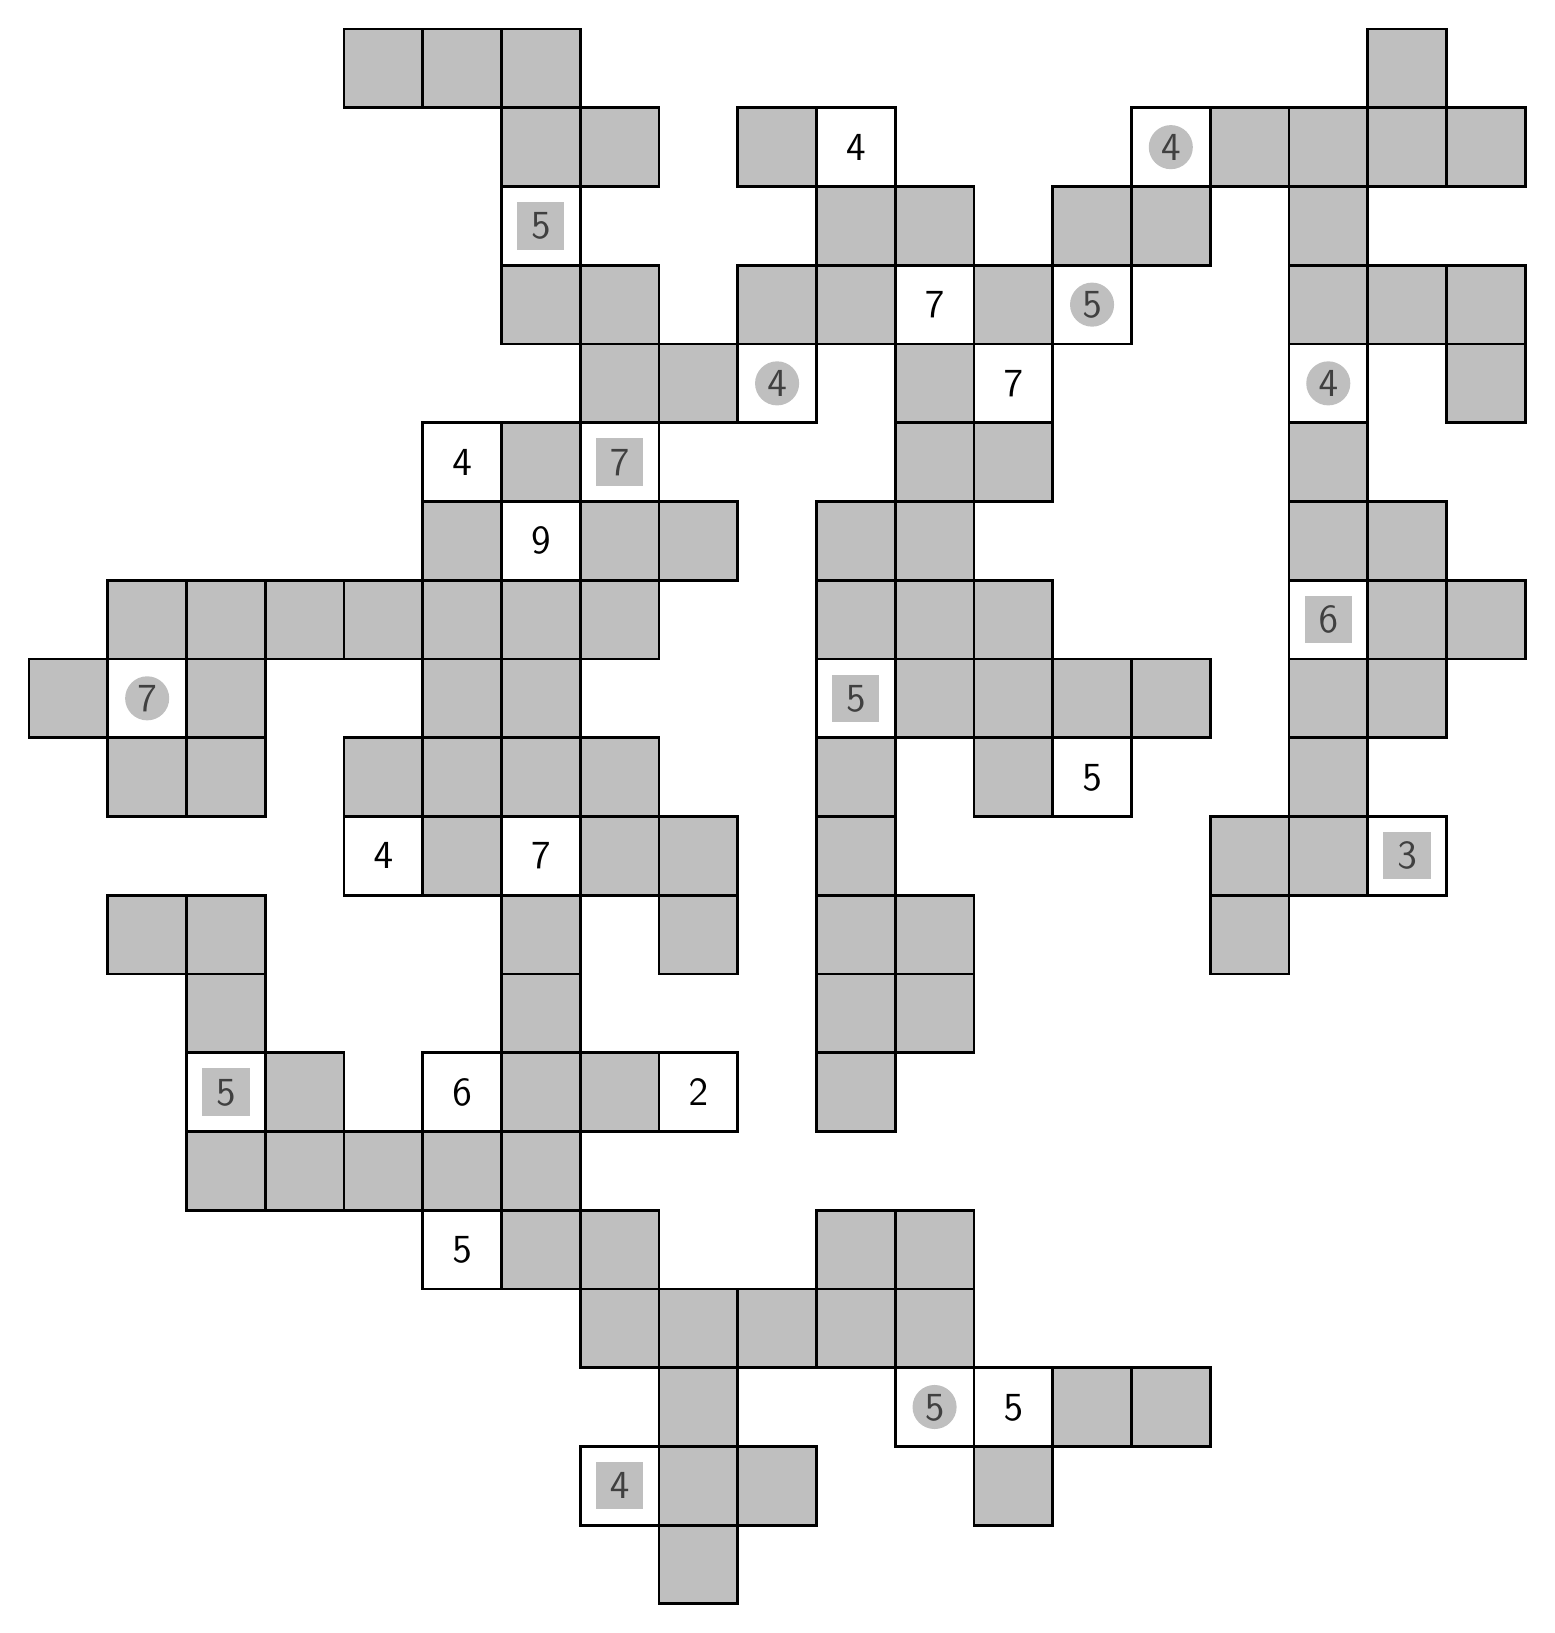
\begin{tikzpicture}\fill[gray, opacity = 0.5] (9, 0, 0)--++(1, 0, 0)--++(0, 1, 0)--++(-1, 0, 0)--cycle;
\draw[line width = 1pt] (9, 0, 0)--++(1, 0, 0)--++(0, 1, 0)--++(-1, 0, 0)--cycle;
\draw node at (8.5, 1.5, 0) {\Large $\mathsf{4}$};
\draw[line width = 1pt] (8, 1, 0)--++(1, 0, 0)--++(0, 1, 0)--++(-1, 0, 0)--cycle;
\fill[color = gray, opacity = 0.5] (8.2, 1.2) rectangle ++(0.6, 0.6);
\fill[gray, opacity = 0.5] (9, 1, 0)--++(1, 0, 0)--++(0, 1, 0)--++(-1, 0, 0)--cycle;
\draw[line width = 1pt] (9, 1, 0)--++(1, 0, 0)--++(0, 1, 0)--++(-1, 0, 0)--cycle;
\fill[gray, opacity = 0.5] (10, 1, 0)--++(1, 0, 0)--++(0, 1, 0)--++(-1, 0, 0)--cycle;
\draw[line width = 1pt] (10, 1, 0)--++(1, 0, 0)--++(0, 1, 0)--++(-1, 0, 0)--cycle;
\fill[gray, opacity = 0.5] (13, 1, 0)--++(1, 0, 0)--++(0, 1, 0)--++(-1, 0, 0)--cycle;
\draw[line width = 1pt] (13, 1, 0)--++(1, 0, 0)--++(0, 1, 0)--++(-1, 0, 0)--cycle;
\fill[gray, opacity = 0.5] (9, 2, 0)--++(1, 0, 0)--++(0, 1, 0)--++(-1, 0, 0)--cycle;
\draw[line width = 1pt] (9, 2, 0)--++(1, 0, 0)--++(0, 1, 0)--++(-1, 0, 0)--cycle;
\draw node at (12.5, 2.5, 0) {\Large $\mathsf{5}$};
\draw[line width = 1pt] (12, 2, 0)--++(1, 0, 0)--++(0, 1, 0)--++(-1, 0, 0)--cycle;
\fill[color = gray, opacity = 0.5] (12.5, 2.5, 0) circle (0.28);
\draw node at (13.5, 2.5, 0) {\Large $\mathsf{5}$};
\draw[line width = 1pt] (13, 2, 0)--++(1, 0, 0)--++(0, 1, 0)--++(-1, 0, 0)--cycle;
\fill[gray, opacity = 0.5] (14, 2, 0)--++(1, 0, 0)--++(0, 1, 0)--++(-1, 0, 0)--cycle;
\draw[line width = 1pt] (14, 2, 0)--++(1, 0, 0)--++(0, 1, 0)--++(-1, 0, 0)--cycle;
\fill[gray, opacity = 0.5] (15, 2, 0)--++(1, 0, 0)--++(0, 1, 0)--++(-1, 0, 0)--cycle;
\draw[line width = 1pt] (15, 2, 0)--++(1, 0, 0)--++(0, 1, 0)--++(-1, 0, 0)--cycle;
\fill[gray, opacity = 0.5] (8, 3, 0)--++(1, 0, 0)--++(0, 1, 0)--++(-1, 0, 0)--cycle;
\draw[line width = 1pt] (8, 3, 0)--++(1, 0, 0)--++(0, 1, 0)--++(-1, 0, 0)--cycle;
\fill[gray, opacity = 0.5] (9, 3, 0)--++(1, 0, 0)--++(0, 1, 0)--++(-1, 0, 0)--cycle;
\draw[line width = 1pt] (9, 3, 0)--++(1, 0, 0)--++(0, 1, 0)--++(-1, 0, 0)--cycle;
\fill[gray, opacity = 0.5] (10, 3, 0)--++(1, 0, 0)--++(0, 1, 0)--++(-1, 0, 0)--cycle;
\draw[line width = 1pt] (10, 3, 0)--++(1, 0, 0)--++(0, 1, 0)--++(-1, 0, 0)--cycle;
\fill[gray, opacity = 0.5] (11, 3, 0)--++(1, 0, 0)--++(0, 1, 0)--++(-1, 0, 0)--cycle;
\draw[line width = 1pt] (11, 3, 0)--++(1, 0, 0)--++(0, 1, 0)--++(-1, 0, 0)--cycle;
\fill[gray, opacity = 0.5] (12, 3, 0)--++(1, 0, 0)--++(0, 1, 0)--++(-1, 0, 0)--cycle;
\draw[line width = 1pt] (12, 3, 0)--++(1, 0, 0)--++(0, 1, 0)--++(-1, 0, 0)--cycle;
\draw node at (6.5, 4.5, 0) {\Large $\mathsf{5}$};
\draw[line width = 1pt] (6, 4, 0)--++(1, 0, 0)--++(0, 1, 0)--++(-1, 0, 0)--cycle;
\fill[gray, opacity = 0.5] (7, 4, 0)--++(1, 0, 0)--++(0, 1, 0)--++(-1, 0, 0)--cycle;
\draw[line width = 1pt] (7, 4, 0)--++(1, 0, 0)--++(0, 1, 0)--++(-1, 0, 0)--cycle;
\fill[gray, opacity = 0.5] (8, 4, 0)--++(1, 0, 0)--++(0, 1, 0)--++(-1, 0, 0)--cycle;
\draw[line width = 1pt] (8, 4, 0)--++(1, 0, 0)--++(0, 1, 0)--++(-1, 0, 0)--cycle;
\fill[gray, opacity = 0.5] (11, 4, 0)--++(1, 0, 0)--++(0, 1, 0)--++(-1, 0, 0)--cycle;
\draw[line width = 1pt] (11, 4, 0)--++(1, 0, 0)--++(0, 1, 0)--++(-1, 0, 0)--cycle;
\fill[gray, opacity = 0.5] (12, 4, 0)--++(1, 0, 0)--++(0, 1, 0)--++(-1, 0, 0)--cycle;
\draw[line width = 1pt] (12, 4, 0)--++(1, 0, 0)--++(0, 1, 0)--++(-1, 0, 0)--cycle;
\fill[gray, opacity = 0.5] (3, 5, 0)--++(1, 0, 0)--++(0, 1, 0)--++(-1, 0, 0)--cycle;
\draw[line width = 1pt] (3, 5, 0)--++(1, 0, 0)--++(0, 1, 0)--++(-1, 0, 0)--cycle;
\fill[gray, opacity = 0.5] (4, 5, 0)--++(1, 0, 0)--++(0, 1, 0)--++(-1, 0, 0)--cycle;
\draw[line width = 1pt] (4, 5, 0)--++(1, 0, 0)--++(0, 1, 0)--++(-1, 0, 0)--cycle;
\fill[gray, opacity = 0.5] (5, 5, 0)--++(1, 0, 0)--++(0, 1, 0)--++(-1, 0, 0)--cycle;
\draw[line width = 1pt] (5, 5, 0)--++(1, 0, 0)--++(0, 1, 0)--++(-1, 0, 0)--cycle;
\fill[gray, opacity = 0.5] (6, 5, 0)--++(1, 0, 0)--++(0, 1, 0)--++(-1, 0, 0)--cycle;
\draw[line width = 1pt] (6, 5, 0)--++(1, 0, 0)--++(0, 1, 0)--++(-1, 0, 0)--cycle;
\fill[gray, opacity = 0.5] (7, 5, 0)--++(1, 0, 0)--++(0, 1, 0)--++(-1, 0, 0)--cycle;
\draw[line width = 1pt] (7, 5, 0)--++(1, 0, 0)--++(0, 1, 0)--++(-1, 0, 0)--cycle;
\draw node at (3.5, 6.5, 0) {\Large $\mathsf{5}$};
\draw[line width = 1pt] (3, 6, 0)--++(1, 0, 0)--++(0, 1, 0)--++(-1, 0, 0)--cycle;
\fill[color = gray, opacity = 0.5] (3.2, 6.2) rectangle ++(0.6, 0.6);
\fill[gray, opacity = 0.5] (4, 6, 0)--++(1, 0, 0)--++(0, 1, 0)--++(-1, 0, 0)--cycle;
\draw[line width = 1pt] (4, 6, 0)--++(1, 0, 0)--++(0, 1, 0)--++(-1, 0, 0)--cycle;
\draw node at (6.5, 6.5, 0) {\Large $\mathsf{6}$};
\draw[line width = 1pt] (6, 6, 0)--++(1, 0, 0)--++(0, 1, 0)--++(-1, 0, 0)--cycle;
\fill[gray, opacity = 0.5] (7, 6, 0)--++(1, 0, 0)--++(0, 1, 0)--++(-1, 0, 0)--cycle;
\draw[line width = 1pt] (7, 6, 0)--++(1, 0, 0)--++(0, 1, 0)--++(-1, 0, 0)--cycle;
\fill[gray, opacity = 0.5] (8, 6, 0)--++(1, 0, 0)--++(0, 1, 0)--++(-1, 0, 0)--cycle;
\draw[line width = 1pt] (8, 6, 0)--++(1, 0, 0)--++(0, 1, 0)--++(-1, 0, 0)--cycle;
\draw node at (9.5, 6.5, 0) {\Large $\mathsf{2}$};
\draw[line width = 1pt] (9, 6, 0)--++(1, 0, 0)--++(0, 1, 0)--++(-1, 0, 0)--cycle;
\fill[gray, opacity = 0.5] (11, 6, 0)--++(1, 0, 0)--++(0, 1, 0)--++(-1, 0, 0)--cycle;
\draw[line width = 1pt] (11, 6, 0)--++(1, 0, 0)--++(0, 1, 0)--++(-1, 0, 0)--cycle;
\fill[gray, opacity = 0.5] (3, 7, 0)--++(1, 0, 0)--++(0, 1, 0)--++(-1, 0, 0)--cycle;
\draw[line width = 1pt] (3, 7, 0)--++(1, 0, 0)--++(0, 1, 0)--++(-1, 0, 0)--cycle;
\fill[gray, opacity = 0.5] (7, 7, 0)--++(1, 0, 0)--++(0, 1, 0)--++(-1, 0, 0)--cycle;
\draw[line width = 1pt] (7, 7, 0)--++(1, 0, 0)--++(0, 1, 0)--++(-1, 0, 0)--cycle;
\fill[gray, opacity = 0.5] (11, 7, 0)--++(1, 0, 0)--++(0, 1, 0)--++(-1, 0, 0)--cycle;
\draw[line width = 1pt] (11, 7, 0)--++(1, 0, 0)--++(0, 1, 0)--++(-1, 0, 0)--cycle;
\fill[gray, opacity = 0.5] (12, 7, 0)--++(1, 0, 0)--++(0, 1, 0)--++(-1, 0, 0)--cycle;
\draw[line width = 1pt] (12, 7, 0)--++(1, 0, 0)--++(0, 1, 0)--++(-1, 0, 0)--cycle;
\fill[gray, opacity = 0.5] (2, 8, 0)--++(1, 0, 0)--++(0, 1, 0)--++(-1, 0, 0)--cycle;
\draw[line width = 1pt] (2, 8, 0)--++(1, 0, 0)--++(0, 1, 0)--++(-1, 0, 0)--cycle;
\fill[gray, opacity = 0.5] (3, 8, 0)--++(1, 0, 0)--++(0, 1, 0)--++(-1, 0, 0)--cycle;
\draw[line width = 1pt] (3, 8, 0)--++(1, 0, 0)--++(0, 1, 0)--++(-1, 0, 0)--cycle;
\fill[gray, opacity = 0.5] (7, 8, 0)--++(1, 0, 0)--++(0, 1, 0)--++(-1, 0, 0)--cycle;
\draw[line width = 1pt] (7, 8, 0)--++(1, 0, 0)--++(0, 1, 0)--++(-1, 0, 0)--cycle;
\fill[gray, opacity = 0.5] (9, 8, 0)--++(1, 0, 0)--++(0, 1, 0)--++(-1, 0, 0)--cycle;
\draw[line width = 1pt] (9, 8, 0)--++(1, 0, 0)--++(0, 1, 0)--++(-1, 0, 0)--cycle;
\fill[gray, opacity = 0.5] (11, 8, 0)--++(1, 0, 0)--++(0, 1, 0)--++(-1, 0, 0)--cycle;
\draw[line width = 1pt] (11, 8, 0)--++(1, 0, 0)--++(0, 1, 0)--++(-1, 0, 0)--cycle;
\fill[gray, opacity = 0.5] (12, 8, 0)--++(1, 0, 0)--++(0, 1, 0)--++(-1, 0, 0)--cycle;
\draw[line width = 1pt] (12, 8, 0)--++(1, 0, 0)--++(0, 1, 0)--++(-1, 0, 0)--cycle;
\fill[gray, opacity = 0.5] (16, 8, 0)--++(1, 0, 0)--++(0, 1, 0)--++(-1, 0, 0)--cycle;
\draw[line width = 1pt] (16, 8, 0)--++(1, 0, 0)--++(0, 1, 0)--++(-1, 0, 0)--cycle;
\draw node at (5.5, 9.5, 0) {\Large $\mathsf{4}$};
\draw[line width = 1pt] (5, 9, 0)--++(1, 0, 0)--++(0, 1, 0)--++(-1, 0, 0)--cycle;
\fill[gray, opacity = 0.5] (6, 9, 0)--++(1, 0, 0)--++(0, 1, 0)--++(-1, 0, 0)--cycle;
\draw[line width = 1pt] (6, 9, 0)--++(1, 0, 0)--++(0, 1, 0)--++(-1, 0, 0)--cycle;
\draw node at (7.5, 9.5, 0) {\Large $\mathsf{7}$};
\draw[line width = 1pt] (7, 9, 0)--++(1, 0, 0)--++(0, 1, 0)--++(-1, 0, 0)--cycle;
\fill[gray, opacity = 0.5] (8, 9, 0)--++(1, 0, 0)--++(0, 1, 0)--++(-1, 0, 0)--cycle;
\draw[line width = 1pt] (8, 9, 0)--++(1, 0, 0)--++(0, 1, 0)--++(-1, 0, 0)--cycle;
\fill[gray, opacity = 0.5] (9, 9, 0)--++(1, 0, 0)--++(0, 1, 0)--++(-1, 0, 0)--cycle;
\draw[line width = 1pt] (9, 9, 0)--++(1, 0, 0)--++(0, 1, 0)--++(-1, 0, 0)--cycle;
\fill[gray, opacity = 0.5] (11, 9, 0)--++(1, 0, 0)--++(0, 1, 0)--++(-1, 0, 0)--cycle;
\draw[line width = 1pt] (11, 9, 0)--++(1, 0, 0)--++(0, 1, 0)--++(-1, 0, 0)--cycle;
\fill[gray, opacity = 0.5] (16, 9, 0)--++(1, 0, 0)--++(0, 1, 0)--++(-1, 0, 0)--cycle;
\draw[line width = 1pt] (16, 9, 0)--++(1, 0, 0)--++(0, 1, 0)--++(-1, 0, 0)--cycle;
\fill[gray, opacity = 0.5] (17, 9, 0)--++(1, 0, 0)--++(0, 1, 0)--++(-1, 0, 0)--cycle;
\draw[line width = 1pt] (17, 9, 0)--++(1, 0, 0)--++(0, 1, 0)--++(-1, 0, 0)--cycle;
\draw node at (18.5, 9.5, 0) {\Large $\mathsf{3}$};
\draw[line width = 1pt] (18, 9, 0)--++(1, 0, 0)--++(0, 1, 0)--++(-1, 0, 0)--cycle;
\fill[color = gray, opacity = 0.5] (18.2, 9.2) rectangle ++(0.6, 0.6);
\fill[gray, opacity = 0.5] (2, 10, 0)--++(1, 0, 0)--++(0, 1, 0)--++(-1, 0, 0)--cycle;
\draw[line width = 1pt] (2, 10, 0)--++(1, 0, 0)--++(0, 1, 0)--++(-1, 0, 0)--cycle;
\fill[gray, opacity = 0.5] (3, 10, 0)--++(1, 0, 0)--++(0, 1, 0)--++(-1, 0, 0)--cycle;
\draw[line width = 1pt] (3, 10, 0)--++(1, 0, 0)--++(0, 1, 0)--++(-1, 0, 0)--cycle;
\fill[gray, opacity = 0.5] (5, 10, 0)--++(1, 0, 0)--++(0, 1, 0)--++(-1, 0, 0)--cycle;
\draw[line width = 1pt] (5, 10, 0)--++(1, 0, 0)--++(0, 1, 0)--++(-1, 0, 0)--cycle;
\fill[gray, opacity = 0.5] (6, 10, 0)--++(1, 0, 0)--++(0, 1, 0)--++(-1, 0, 0)--cycle;
\draw[line width = 1pt] (6, 10, 0)--++(1, 0, 0)--++(0, 1, 0)--++(-1, 0, 0)--cycle;
\fill[gray, opacity = 0.5] (7, 10, 0)--++(1, 0, 0)--++(0, 1, 0)--++(-1, 0, 0)--cycle;
\draw[line width = 1pt] (7, 10, 0)--++(1, 0, 0)--++(0, 1, 0)--++(-1, 0, 0)--cycle;
\fill[gray, opacity = 0.5] (8, 10, 0)--++(1, 0, 0)--++(0, 1, 0)--++(-1, 0, 0)--cycle;
\draw[line width = 1pt] (8, 10, 0)--++(1, 0, 0)--++(0, 1, 0)--++(-1, 0, 0)--cycle;
\fill[gray, opacity = 0.5] (11, 10, 0)--++(1, 0, 0)--++(0, 1, 0)--++(-1, 0, 0)--cycle;
\draw[line width = 1pt] (11, 10, 0)--++(1, 0, 0)--++(0, 1, 0)--++(-1, 0, 0)--cycle;
\fill[gray, opacity = 0.5] (13, 10, 0)--++(1, 0, 0)--++(0, 1, 0)--++(-1, 0, 0)--cycle;
\draw[line width = 1pt] (13, 10, 0)--++(1, 0, 0)--++(0, 1, 0)--++(-1, 0, 0)--cycle;
\draw node at (14.5, 10.5, 0) {\Large $\mathsf{5}$};
\draw[line width = 1pt] (14, 10, 0)--++(1, 0, 0)--++(0, 1, 0)--++(-1, 0, 0)--cycle;
\fill[gray, opacity = 0.5] (17, 10, 0)--++(1, 0, 0)--++(0, 1, 0)--++(-1, 0, 0)--cycle;
\draw[line width = 1pt] (17, 10, 0)--++(1, 0, 0)--++(0, 1, 0)--++(-1, 0, 0)--cycle;
\fill[gray, opacity = 0.5] (1, 11, 0)--++(1, 0, 0)--++(0, 1, 0)--++(-1, 0, 0)--cycle;
\draw[line width = 1pt] (1, 11, 0)--++(1, 0, 0)--++(0, 1, 0)--++(-1, 0, 0)--cycle;
\draw node at (2.5, 11.5, 0) {\Large $\mathsf{7}$};
\draw[line width = 1pt] (2, 11, 0)--++(1, 0, 0)--++(0, 1, 0)--++(-1, 0, 0)--cycle;
\fill[color = gray, opacity = 0.5] (2.5, 11.5, 0) circle (0.28);
\fill[gray, opacity = 0.5] (3, 11, 0)--++(1, 0, 0)--++(0, 1, 0)--++(-1, 0, 0)--cycle;
\draw[line width = 1pt] (3, 11, 0)--++(1, 0, 0)--++(0, 1, 0)--++(-1, 0, 0)--cycle;
\fill[gray, opacity = 0.5] (6, 11, 0)--++(1, 0, 0)--++(0, 1, 0)--++(-1, 0, 0)--cycle;
\draw[line width = 1pt] (6, 11, 0)--++(1, 0, 0)--++(0, 1, 0)--++(-1, 0, 0)--cycle;
\fill[gray, opacity = 0.5] (7, 11, 0)--++(1, 0, 0)--++(0, 1, 0)--++(-1, 0, 0)--cycle;
\draw[line width = 1pt] (7, 11, 0)--++(1, 0, 0)--++(0, 1, 0)--++(-1, 0, 0)--cycle;
\draw node at (11.5, 11.5, 0) {\Large $\mathsf{5}$};
\draw[line width = 1pt] (11, 11, 0)--++(1, 0, 0)--++(0, 1, 0)--++(-1, 0, 0)--cycle;
\fill[color = gray, opacity = 0.5] (11.2, 11.2) rectangle ++(0.6, 0.6);
\fill[gray, opacity = 0.5] (12, 11, 0)--++(1, 0, 0)--++(0, 1, 0)--++(-1, 0, 0)--cycle;
\draw[line width = 1pt] (12, 11, 0)--++(1, 0, 0)--++(0, 1, 0)--++(-1, 0, 0)--cycle;
\fill[gray, opacity = 0.5] (13, 11, 0)--++(1, 0, 0)--++(0, 1, 0)--++(-1, 0, 0)--cycle;
\draw[line width = 1pt] (13, 11, 0)--++(1, 0, 0)--++(0, 1, 0)--++(-1, 0, 0)--cycle;
\fill[gray, opacity = 0.5] (14, 11, 0)--++(1, 0, 0)--++(0, 1, 0)--++(-1, 0, 0)--cycle;
\draw[line width = 1pt] (14, 11, 0)--++(1, 0, 0)--++(0, 1, 0)--++(-1, 0, 0)--cycle;
\fill[gray, opacity = 0.5] (15, 11, 0)--++(1, 0, 0)--++(0, 1, 0)--++(-1, 0, 0)--cycle;
\draw[line width = 1pt] (15, 11, 0)--++(1, 0, 0)--++(0, 1, 0)--++(-1, 0, 0)--cycle;
\fill[gray, opacity = 0.5] (17, 11, 0)--++(1, 0, 0)--++(0, 1, 0)--++(-1, 0, 0)--cycle;
\draw[line width = 1pt] (17, 11, 0)--++(1, 0, 0)--++(0, 1, 0)--++(-1, 0, 0)--cycle;
\fill[gray, opacity = 0.5] (18, 11, 0)--++(1, 0, 0)--++(0, 1, 0)--++(-1, 0, 0)--cycle;
\draw[line width = 1pt] (18, 11, 0)--++(1, 0, 0)--++(0, 1, 0)--++(-1, 0, 0)--cycle;
\fill[gray, opacity = 0.5] (2, 12, 0)--++(1, 0, 0)--++(0, 1, 0)--++(-1, 0, 0)--cycle;
\draw[line width = 1pt] (2, 12, 0)--++(1, 0, 0)--++(0, 1, 0)--++(-1, 0, 0)--cycle;
\fill[gray, opacity = 0.5] (3, 12, 0)--++(1, 0, 0)--++(0, 1, 0)--++(-1, 0, 0)--cycle;
\draw[line width = 1pt] (3, 12, 0)--++(1, 0, 0)--++(0, 1, 0)--++(-1, 0, 0)--cycle;
\fill[gray, opacity = 0.5] (4, 12, 0)--++(1, 0, 0)--++(0, 1, 0)--++(-1, 0, 0)--cycle;
\draw[line width = 1pt] (4, 12, 0)--++(1, 0, 0)--++(0, 1, 0)--++(-1, 0, 0)--cycle;
\fill[gray, opacity = 0.5] (5, 12, 0)--++(1, 0, 0)--++(0, 1, 0)--++(-1, 0, 0)--cycle;
\draw[line width = 1pt] (5, 12, 0)--++(1, 0, 0)--++(0, 1, 0)--++(-1, 0, 0)--cycle;
\fill[gray, opacity = 0.5] (6, 12, 0)--++(1, 0, 0)--++(0, 1, 0)--++(-1, 0, 0)--cycle;
\draw[line width = 1pt] (6, 12, 0)--++(1, 0, 0)--++(0, 1, 0)--++(-1, 0, 0)--cycle;
\fill[gray, opacity = 0.5] (7, 12, 0)--++(1, 0, 0)--++(0, 1, 0)--++(-1, 0, 0)--cycle;
\draw[line width = 1pt] (7, 12, 0)--++(1, 0, 0)--++(0, 1, 0)--++(-1, 0, 0)--cycle;
\fill[gray, opacity = 0.5] (8, 12, 0)--++(1, 0, 0)--++(0, 1, 0)--++(-1, 0, 0)--cycle;
\draw[line width = 1pt] (8, 12, 0)--++(1, 0, 0)--++(0, 1, 0)--++(-1, 0, 0)--cycle;
\fill[gray, opacity = 0.5] (11, 12, 0)--++(1, 0, 0)--++(0, 1, 0)--++(-1, 0, 0)--cycle;
\draw[line width = 1pt] (11, 12, 0)--++(1, 0, 0)--++(0, 1, 0)--++(-1, 0, 0)--cycle;
\fill[gray, opacity = 0.5] (12, 12, 0)--++(1, 0, 0)--++(0, 1, 0)--++(-1, 0, 0)--cycle;
\draw[line width = 1pt] (12, 12, 0)--++(1, 0, 0)--++(0, 1, 0)--++(-1, 0, 0)--cycle;
\fill[gray, opacity = 0.5] (13, 12, 0)--++(1, 0, 0)--++(0, 1, 0)--++(-1, 0, 0)--cycle;
\draw[line width = 1pt] (13, 12, 0)--++(1, 0, 0)--++(0, 1, 0)--++(-1, 0, 0)--cycle;
\draw node at (17.5, 12.5, 0) {\Large $\mathsf{6}$};
\draw[line width = 1pt] (17, 12, 0)--++(1, 0, 0)--++(0, 1, 0)--++(-1, 0, 0)--cycle;
\fill[color = gray, opacity = 0.5] (17.2, 12.2) rectangle ++(0.6, 0.6);
\fill[gray, opacity = 0.5] (18, 12, 0)--++(1, 0, 0)--++(0, 1, 0)--++(-1, 0, 0)--cycle;
\draw[line width = 1pt] (18, 12, 0)--++(1, 0, 0)--++(0, 1, 0)--++(-1, 0, 0)--cycle;
\fill[gray, opacity = 0.5] (19, 12, 0)--++(1, 0, 0)--++(0, 1, 0)--++(-1, 0, 0)--cycle;
\draw[line width = 1pt] (19, 12, 0)--++(1, 0, 0)--++(0, 1, 0)--++(-1, 0, 0)--cycle;
\fill[gray, opacity = 0.5] (6, 13, 0)--++(1, 0, 0)--++(0, 1, 0)--++(-1, 0, 0)--cycle;
\draw[line width = 1pt] (6, 13, 0)--++(1, 0, 0)--++(0, 1, 0)--++(-1, 0, 0)--cycle;
\draw node at (7.5, 13.5, 0) {\Large $\mathsf{9}$};
\draw[line width = 1pt] (7, 13, 0)--++(1, 0, 0)--++(0, 1, 0)--++(-1, 0, 0)--cycle;
\fill[gray, opacity = 0.5] (8, 13, 0)--++(1, 0, 0)--++(0, 1, 0)--++(-1, 0, 0)--cycle;
\draw[line width = 1pt] (8, 13, 0)--++(1, 0, 0)--++(0, 1, 0)--++(-1, 0, 0)--cycle;
\fill[gray, opacity = 0.5] (9, 13, 0)--++(1, 0, 0)--++(0, 1, 0)--++(-1, 0, 0)--cycle;
\draw[line width = 1pt] (9, 13, 0)--++(1, 0, 0)--++(0, 1, 0)--++(-1, 0, 0)--cycle;
\fill[gray, opacity = 0.5] (11, 13, 0)--++(1, 0, 0)--++(0, 1, 0)--++(-1, 0, 0)--cycle;
\draw[line width = 1pt] (11, 13, 0)--++(1, 0, 0)--++(0, 1, 0)--++(-1, 0, 0)--cycle;
\fill[gray, opacity = 0.5] (12, 13, 0)--++(1, 0, 0)--++(0, 1, 0)--++(-1, 0, 0)--cycle;
\draw[line width = 1pt] (12, 13, 0)--++(1, 0, 0)--++(0, 1, 0)--++(-1, 0, 0)--cycle;
\fill[gray, opacity = 0.5] (17, 13, 0)--++(1, 0, 0)--++(0, 1, 0)--++(-1, 0, 0)--cycle;
\draw[line width = 1pt] (17, 13, 0)--++(1, 0, 0)--++(0, 1, 0)--++(-1, 0, 0)--cycle;
\fill[gray, opacity = 0.5] (18, 13, 0)--++(1, 0, 0)--++(0, 1, 0)--++(-1, 0, 0)--cycle;
\draw[line width = 1pt] (18, 13, 0)--++(1, 0, 0)--++(0, 1, 0)--++(-1, 0, 0)--cycle;
\draw node at (6.5, 14.5, 0) {\Large $\mathsf{4}$};
\draw[line width = 1pt] (6, 14, 0)--++(1, 0, 0)--++(0, 1, 0)--++(-1, 0, 0)--cycle;
\fill[gray, opacity = 0.5] (7, 14, 0)--++(1, 0, 0)--++(0, 1, 0)--++(-1, 0, 0)--cycle;
\draw[line width = 1pt] (7, 14, 0)--++(1, 0, 0)--++(0, 1, 0)--++(-1, 0, 0)--cycle;
\draw node at (8.5, 14.5, 0) {\Large $\mathsf{7}$};
\draw[line width = 1pt] (8, 14, 0)--++(1, 0, 0)--++(0, 1, 0)--++(-1, 0, 0)--cycle;
\fill[color = gray, opacity = 0.5] (8.2, 14.2) rectangle ++(0.6, 0.6);
\fill[gray, opacity = 0.5] (12, 14, 0)--++(1, 0, 0)--++(0, 1, 0)--++(-1, 0, 0)--cycle;
\draw[line width = 1pt] (12, 14, 0)--++(1, 0, 0)--++(0, 1, 0)--++(-1, 0, 0)--cycle;
\fill[gray, opacity = 0.5] (13, 14, 0)--++(1, 0, 0)--++(0, 1, 0)--++(-1, 0, 0)--cycle;
\draw[line width = 1pt] (13, 14, 0)--++(1, 0, 0)--++(0, 1, 0)--++(-1, 0, 0)--cycle;
\fill[gray, opacity = 0.5] (17, 14, 0)--++(1, 0, 0)--++(0, 1, 0)--++(-1, 0, 0)--cycle;
\draw[line width = 1pt] (17, 14, 0)--++(1, 0, 0)--++(0, 1, 0)--++(-1, 0, 0)--cycle;
\fill[gray, opacity = 0.5] (8, 15, 0)--++(1, 0, 0)--++(0, 1, 0)--++(-1, 0, 0)--cycle;
\draw[line width = 1pt] (8, 15, 0)--++(1, 0, 0)--++(0, 1, 0)--++(-1, 0, 0)--cycle;
\fill[gray, opacity = 0.5] (9, 15, 0)--++(1, 0, 0)--++(0, 1, 0)--++(-1, 0, 0)--cycle;
\draw[line width = 1pt] (9, 15, 0)--++(1, 0, 0)--++(0, 1, 0)--++(-1, 0, 0)--cycle;
\draw node at (10.5, 15.5, 0) {\Large $\mathsf{4}$};
\draw[line width = 1pt] (10, 15, 0)--++(1, 0, 0)--++(0, 1, 0)--++(-1, 0, 0)--cycle;
\fill[color = gray, opacity = 0.5] (10.5, 15.5, 0) circle (0.28);
\fill[gray, opacity = 0.5] (12, 15, 0)--++(1, 0, 0)--++(0, 1, 0)--++(-1, 0, 0)--cycle;
\draw[line width = 1pt] (12, 15, 0)--++(1, 0, 0)--++(0, 1, 0)--++(-1, 0, 0)--cycle;
\draw node at (13.5, 15.5, 0) {\Large $\mathsf{7}$};
\draw[line width = 1pt] (13, 15, 0)--++(1, 0, 0)--++(0, 1, 0)--++(-1, 0, 0)--cycle;
\draw node at (17.5, 15.5, 0) {\Large $\mathsf{4}$};
\draw[line width = 1pt] (17, 15, 0)--++(1, 0, 0)--++(0, 1, 0)--++(-1, 0, 0)--cycle;
\fill[color = gray, opacity = 0.5] (17.5, 15.5, 0) circle (0.28);
\fill[gray, opacity = 0.5] (19, 15, 0)--++(1, 0, 0)--++(0, 1, 0)--++(-1, 0, 0)--cycle;
\draw[line width = 1pt] (19, 15, 0)--++(1, 0, 0)--++(0, 1, 0)--++(-1, 0, 0)--cycle;
\fill[gray, opacity = 0.5] (7, 16, 0)--++(1, 0, 0)--++(0, 1, 0)--++(-1, 0, 0)--cycle;
\draw[line width = 1pt] (7, 16, 0)--++(1, 0, 0)--++(0, 1, 0)--++(-1, 0, 0)--cycle;
\fill[gray, opacity = 0.5] (8, 16, 0)--++(1, 0, 0)--++(0, 1, 0)--++(-1, 0, 0)--cycle;
\draw[line width = 1pt] (8, 16, 0)--++(1, 0, 0)--++(0, 1, 0)--++(-1, 0, 0)--cycle;
\fill[gray, opacity = 0.5] (10, 16, 0)--++(1, 0, 0)--++(0, 1, 0)--++(-1, 0, 0)--cycle;
\draw[line width = 1pt] (10, 16, 0)--++(1, 0, 0)--++(0, 1, 0)--++(-1, 0, 0)--cycle;
\fill[gray, opacity = 0.5] (11, 16, 0)--++(1, 0, 0)--++(0, 1, 0)--++(-1, 0, 0)--cycle;
\draw[line width = 1pt] (11, 16, 0)--++(1, 0, 0)--++(0, 1, 0)--++(-1, 0, 0)--cycle;
\draw node at (12.5, 16.5, 0) {\Large $\mathsf{7}$};
\draw[line width = 1pt] (12, 16, 0)--++(1, 0, 0)--++(0, 1, 0)--++(-1, 0, 0)--cycle;
\fill[gray, opacity = 0.5] (13, 16, 0)--++(1, 0, 0)--++(0, 1, 0)--++(-1, 0, 0)--cycle;
\draw[line width = 1pt] (13, 16, 0)--++(1, 0, 0)--++(0, 1, 0)--++(-1, 0, 0)--cycle;
\draw node at (14.5, 16.5, 0) {\Large $\mathsf{5}$};
\draw[line width = 1pt] (14, 16, 0)--++(1, 0, 0)--++(0, 1, 0)--++(-1, 0, 0)--cycle;
\fill[color = gray, opacity = 0.5] (14.5, 16.5, 0) circle (0.28);
\fill[gray, opacity = 0.5] (17, 16, 0)--++(1, 0, 0)--++(0, 1, 0)--++(-1, 0, 0)--cycle;
\draw[line width = 1pt] (17, 16, 0)--++(1, 0, 0)--++(0, 1, 0)--++(-1, 0, 0)--cycle;
\fill[gray, opacity = 0.5] (18, 16, 0)--++(1, 0, 0)--++(0, 1, 0)--++(-1, 0, 0)--cycle;
\draw[line width = 1pt] (18, 16, 0)--++(1, 0, 0)--++(0, 1, 0)--++(-1, 0, 0)--cycle;
\fill[gray, opacity = 0.5] (19, 16, 0)--++(1, 0, 0)--++(0, 1, 0)--++(-1, 0, 0)--cycle;
\draw[line width = 1pt] (19, 16, 0)--++(1, 0, 0)--++(0, 1, 0)--++(-1, 0, 0)--cycle;
\draw node at (7.5, 17.5, 0) {\Large $\mathsf{5}$};
\draw[line width = 1pt] (7, 17, 0)--++(1, 0, 0)--++(0, 1, 0)--++(-1, 0, 0)--cycle;
\fill[color = gray, opacity = 0.5] (7.2, 17.2) rectangle ++(0.6, 0.6);
\fill[gray, opacity = 0.5] (11, 17, 0)--++(1, 0, 0)--++(0, 1, 0)--++(-1, 0, 0)--cycle;
\draw[line width = 1pt] (11, 17, 0)--++(1, 0, 0)--++(0, 1, 0)--++(-1, 0, 0)--cycle;
\fill[gray, opacity = 0.5] (12, 17, 0)--++(1, 0, 0)--++(0, 1, 0)--++(-1, 0, 0)--cycle;
\draw[line width = 1pt] (12, 17, 0)--++(1, 0, 0)--++(0, 1, 0)--++(-1, 0, 0)--cycle;
\fill[gray, opacity = 0.5] (14, 17, 0)--++(1, 0, 0)--++(0, 1, 0)--++(-1, 0, 0)--cycle;
\draw[line width = 1pt] (14, 17, 0)--++(1, 0, 0)--++(0, 1, 0)--++(-1, 0, 0)--cycle;
\fill[gray, opacity = 0.5] (15, 17, 0)--++(1, 0, 0)--++(0, 1, 0)--++(-1, 0, 0)--cycle;
\draw[line width = 1pt] (15, 17, 0)--++(1, 0, 0)--++(0, 1, 0)--++(-1, 0, 0)--cycle;
\fill[gray, opacity = 0.5] (17, 17, 0)--++(1, 0, 0)--++(0, 1, 0)--++(-1, 0, 0)--cycle;
\draw[line width = 1pt] (17, 17, 0)--++(1, 0, 0)--++(0, 1, 0)--++(-1, 0, 0)--cycle;
\fill[gray, opacity = 0.5] (7, 18, 0)--++(1, 0, 0)--++(0, 1, 0)--++(-1, 0, 0)--cycle;
\draw[line width = 1pt] (7, 18, 0)--++(1, 0, 0)--++(0, 1, 0)--++(-1, 0, 0)--cycle;
\fill[gray, opacity = 0.5] (8, 18, 0)--++(1, 0, 0)--++(0, 1, 0)--++(-1, 0, 0)--cycle;
\draw[line width = 1pt] (8, 18, 0)--++(1, 0, 0)--++(0, 1, 0)--++(-1, 0, 0)--cycle;
\fill[gray, opacity = 0.5] (10, 18, 0)--++(1, 0, 0)--++(0, 1, 0)--++(-1, 0, 0)--cycle;
\draw[line width = 1pt] (10, 18, 0)--++(1, 0, 0)--++(0, 1, 0)--++(-1, 0, 0)--cycle;
\draw node at (11.5, 18.5, 0) {\Large $\mathsf{4}$};
\draw[line width = 1pt] (11, 18, 0)--++(1, 0, 0)--++(0, 1, 0)--++(-1, 0, 0)--cycle;
\draw node at (15.5, 18.5, 0) {\Large $\mathsf{4}$};
\draw[line width = 1pt] (15, 18, 0)--++(1, 0, 0)--++(0, 1, 0)--++(-1, 0, 0)--cycle;
\fill[color = gray, opacity = 0.5] (15.5, 18.5, 0) circle (0.28);
\fill[gray, opacity = 0.5] (16, 18, 0)--++(1, 0, 0)--++(0, 1, 0)--++(-1, 0, 0)--cycle;
\draw[line width = 1pt] (16, 18, 0)--++(1, 0, 0)--++(0, 1, 0)--++(-1, 0, 0)--cycle;
\fill[gray, opacity = 0.5] (17, 18, 0)--++(1, 0, 0)--++(0, 1, 0)--++(-1, 0, 0)--cycle;
\draw[line width = 1pt] (17, 18, 0)--++(1, 0, 0)--++(0, 1, 0)--++(-1, 0, 0)--cycle;
\fill[gray, opacity = 0.5] (18, 18, 0)--++(1, 0, 0)--++(0, 1, 0)--++(-1, 0, 0)--cycle;
\draw[line width = 1pt] (18, 18, 0)--++(1, 0, 0)--++(0, 1, 0)--++(-1, 0, 0)--cycle;
\fill[gray, opacity = 0.5] (19, 18, 0)--++(1, 0, 0)--++(0, 1, 0)--++(-1, 0, 0)--cycle;
\draw[line width = 1pt] (19, 18, 0)--++(1, 0, 0)--++(0, 1, 0)--++(-1, 0, 0)--cycle;
\fill[gray, opacity = 0.5] (5, 19, 0)--++(1, 0, 0)--++(0, 1, 0)--++(-1, 0, 0)--cycle;
\draw[line width = 1pt] (5, 19, 0)--++(1, 0, 0)--++(0, 1, 0)--++(-1, 0, 0)--cycle;
\fill[gray, opacity = 0.5] (6, 19, 0)--++(1, 0, 0)--++(0, 1, 0)--++(-1, 0, 0)--cycle;
\draw[line width = 1pt] (6, 19, 0)--++(1, 0, 0)--++(0, 1, 0)--++(-1, 0, 0)--cycle;
\fill[gray, opacity = 0.5] (7, 19, 0)--++(1, 0, 0)--++(0, 1, 0)--++(-1, 0, 0)--cycle;
\draw[line width = 1pt] (7, 19, 0)--++(1, 0, 0)--++(0, 1, 0)--++(-1, 0, 0)--cycle;
\fill[gray, opacity = 0.5] (18, 19, 0)--++(1, 0, 0)--++(0, 1, 0)--++(-1, 0, 0)--cycle;
\draw[line width = 1pt] (18, 19, 0)--++(1, 0, 0)--++(0, 1, 0)--++(-1, 0, 0)--cycle;
\end{tikzpicture}}\]
\[\resizebox{30pc}{!}{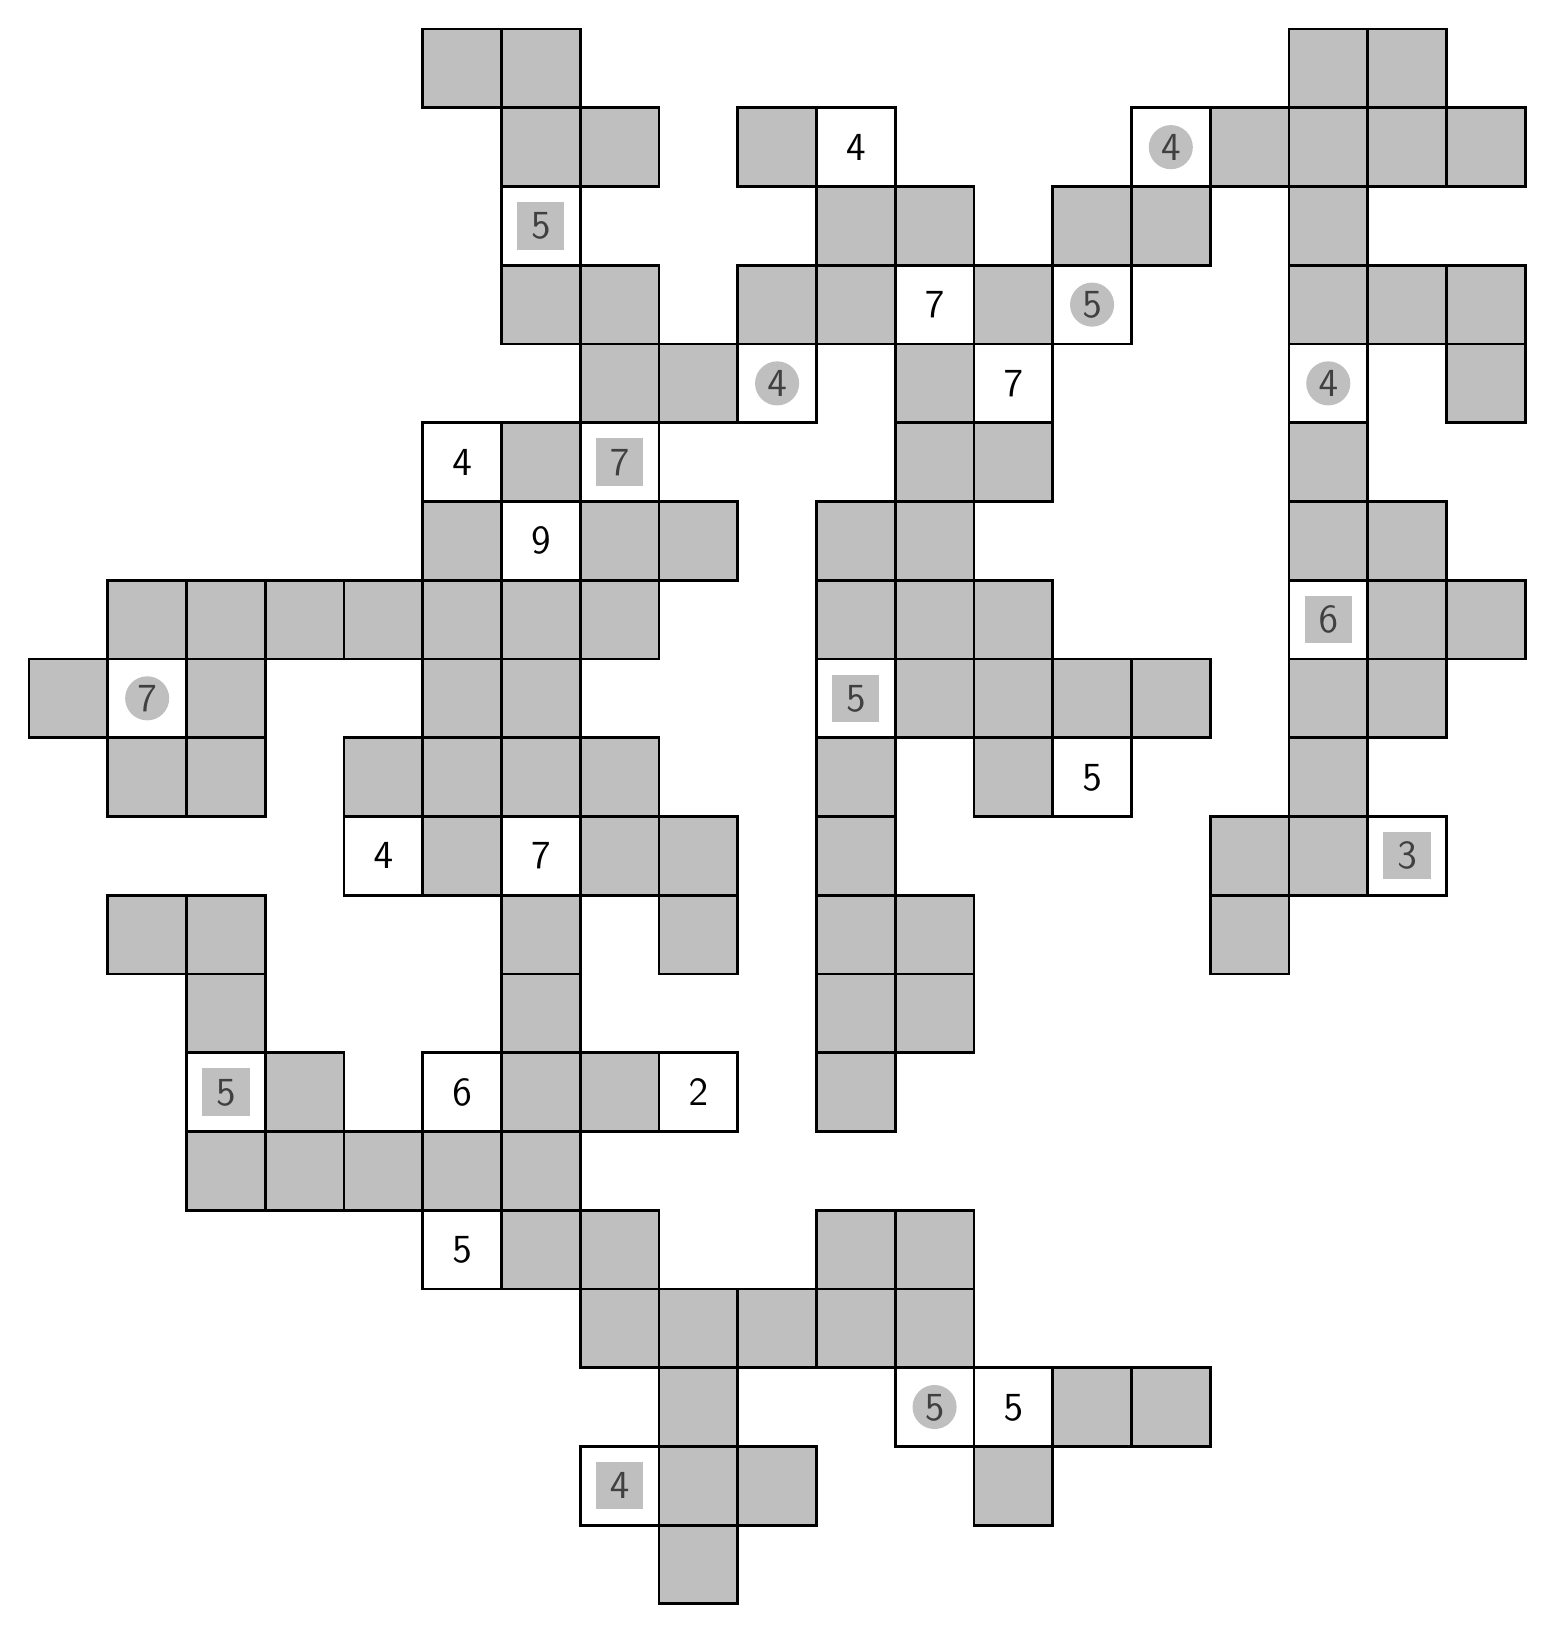
\begin{tikzpicture}\fill[gray, opacity = 0.5] (9, 0, 0)--++(1, 0, 0)--++(0, 1, 0)--++(-1, 0, 0)--cycle;
\draw[line width = 1pt] (9, 0, 0)--++(1, 0, 0)--++(0, 1, 0)--++(-1, 0, 0)--cycle;
\draw node at (8.5, 1.5, 0) {\Large $\mathsf{4}$};
\draw[line width = 1pt] (8, 1, 0)--++(1, 0, 0)--++(0, 1, 0)--++(-1, 0, 0)--cycle;
\fill[color = gray, opacity = 0.5] (8.2, 1.2) rectangle ++(0.6, 0.6);
\fill[gray, opacity = 0.5] (9, 1, 0)--++(1, 0, 0)--++(0, 1, 0)--++(-1, 0, 0)--cycle;
\draw[line width = 1pt] (9, 1, 0)--++(1, 0, 0)--++(0, 1, 0)--++(-1, 0, 0)--cycle;
\fill[gray, opacity = 0.5] (10, 1, 0)--++(1, 0, 0)--++(0, 1, 0)--++(-1, 0, 0)--cycle;
\draw[line width = 1pt] (10, 1, 0)--++(1, 0, 0)--++(0, 1, 0)--++(-1, 0, 0)--cycle;
\fill[gray, opacity = 0.5] (13, 1, 0)--++(1, 0, 0)--++(0, 1, 0)--++(-1, 0, 0)--cycle;
\draw[line width = 1pt] (13, 1, 0)--++(1, 0, 0)--++(0, 1, 0)--++(-1, 0, 0)--cycle;
\fill[gray, opacity = 0.5] (9, 2, 0)--++(1, 0, 0)--++(0, 1, 0)--++(-1, 0, 0)--cycle;
\draw[line width = 1pt] (9, 2, 0)--++(1, 0, 0)--++(0, 1, 0)--++(-1, 0, 0)--cycle;
\draw node at (12.5, 2.5, 0) {\Large $\mathsf{5}$};
\draw[line width = 1pt] (12, 2, 0)--++(1, 0, 0)--++(0, 1, 0)--++(-1, 0, 0)--cycle;
\fill[color = gray, opacity = 0.5] (12.5, 2.5, 0) circle (0.28);
\draw node at (13.5, 2.5, 0) {\Large $\mathsf{5}$};
\draw[line width = 1pt] (13, 2, 0)--++(1, 0, 0)--++(0, 1, 0)--++(-1, 0, 0)--cycle;
\fill[gray, opacity = 0.5] (14, 2, 0)--++(1, 0, 0)--++(0, 1, 0)--++(-1, 0, 0)--cycle;
\draw[line width = 1pt] (14, 2, 0)--++(1, 0, 0)--++(0, 1, 0)--++(-1, 0, 0)--cycle;
\fill[gray, opacity = 0.5] (15, 2, 0)--++(1, 0, 0)--++(0, 1, 0)--++(-1, 0, 0)--cycle;
\draw[line width = 1pt] (15, 2, 0)--++(1, 0, 0)--++(0, 1, 0)--++(-1, 0, 0)--cycle;
\fill[gray, opacity = 0.5] (8, 3, 0)--++(1, 0, 0)--++(0, 1, 0)--++(-1, 0, 0)--cycle;
\draw[line width = 1pt] (8, 3, 0)--++(1, 0, 0)--++(0, 1, 0)--++(-1, 0, 0)--cycle;
\fill[gray, opacity = 0.5] (9, 3, 0)--++(1, 0, 0)--++(0, 1, 0)--++(-1, 0, 0)--cycle;
\draw[line width = 1pt] (9, 3, 0)--++(1, 0, 0)--++(0, 1, 0)--++(-1, 0, 0)--cycle;
\fill[gray, opacity = 0.5] (10, 3, 0)--++(1, 0, 0)--++(0, 1, 0)--++(-1, 0, 0)--cycle;
\draw[line width = 1pt] (10, 3, 0)--++(1, 0, 0)--++(0, 1, 0)--++(-1, 0, 0)--cycle;
\fill[gray, opacity = 0.5] (11, 3, 0)--++(1, 0, 0)--++(0, 1, 0)--++(-1, 0, 0)--cycle;
\draw[line width = 1pt] (11, 3, 0)--++(1, 0, 0)--++(0, 1, 0)--++(-1, 0, 0)--cycle;
\fill[gray, opacity = 0.5] (12, 3, 0)--++(1, 0, 0)--++(0, 1, 0)--++(-1, 0, 0)--cycle;
\draw[line width = 1pt] (12, 3, 0)--++(1, 0, 0)--++(0, 1, 0)--++(-1, 0, 0)--cycle;
\draw node at (6.5, 4.5, 0) {\Large $\mathsf{5}$};
\draw[line width = 1pt] (6, 4, 0)--++(1, 0, 0)--++(0, 1, 0)--++(-1, 0, 0)--cycle;
\fill[gray, opacity = 0.5] (7, 4, 0)--++(1, 0, 0)--++(0, 1, 0)--++(-1, 0, 0)--cycle;
\draw[line width = 1pt] (7, 4, 0)--++(1, 0, 0)--++(0, 1, 0)--++(-1, 0, 0)--cycle;
\fill[gray, opacity = 0.5] (8, 4, 0)--++(1, 0, 0)--++(0, 1, 0)--++(-1, 0, 0)--cycle;
\draw[line width = 1pt] (8, 4, 0)--++(1, 0, 0)--++(0, 1, 0)--++(-1, 0, 0)--cycle;
\fill[gray, opacity = 0.5] (11, 4, 0)--++(1, 0, 0)--++(0, 1, 0)--++(-1, 0, 0)--cycle;
\draw[line width = 1pt] (11, 4, 0)--++(1, 0, 0)--++(0, 1, 0)--++(-1, 0, 0)--cycle;
\fill[gray, opacity = 0.5] (12, 4, 0)--++(1, 0, 0)--++(0, 1, 0)--++(-1, 0, 0)--cycle;
\draw[line width = 1pt] (12, 4, 0)--++(1, 0, 0)--++(0, 1, 0)--++(-1, 0, 0)--cycle;
\fill[gray, opacity = 0.5] (3, 5, 0)--++(1, 0, 0)--++(0, 1, 0)--++(-1, 0, 0)--cycle;
\draw[line width = 1pt] (3, 5, 0)--++(1, 0, 0)--++(0, 1, 0)--++(-1, 0, 0)--cycle;
\fill[gray, opacity = 0.5] (4, 5, 0)--++(1, 0, 0)--++(0, 1, 0)--++(-1, 0, 0)--cycle;
\draw[line width = 1pt] (4, 5, 0)--++(1, 0, 0)--++(0, 1, 0)--++(-1, 0, 0)--cycle;
\fill[gray, opacity = 0.5] (5, 5, 0)--++(1, 0, 0)--++(0, 1, 0)--++(-1, 0, 0)--cycle;
\draw[line width = 1pt] (5, 5, 0)--++(1, 0, 0)--++(0, 1, 0)--++(-1, 0, 0)--cycle;
\fill[gray, opacity = 0.5] (6, 5, 0)--++(1, 0, 0)--++(0, 1, 0)--++(-1, 0, 0)--cycle;
\draw[line width = 1pt] (6, 5, 0)--++(1, 0, 0)--++(0, 1, 0)--++(-1, 0, 0)--cycle;
\fill[gray, opacity = 0.5] (7, 5, 0)--++(1, 0, 0)--++(0, 1, 0)--++(-1, 0, 0)--cycle;
\draw[line width = 1pt] (7, 5, 0)--++(1, 0, 0)--++(0, 1, 0)--++(-1, 0, 0)--cycle;
\draw node at (3.5, 6.5, 0) {\Large $\mathsf{5}$};
\draw[line width = 1pt] (3, 6, 0)--++(1, 0, 0)--++(0, 1, 0)--++(-1, 0, 0)--cycle;
\fill[color = gray, opacity = 0.5] (3.2, 6.2) rectangle ++(0.6, 0.6);
\fill[gray, opacity = 0.5] (4, 6, 0)--++(1, 0, 0)--++(0, 1, 0)--++(-1, 0, 0)--cycle;
\draw[line width = 1pt] (4, 6, 0)--++(1, 0, 0)--++(0, 1, 0)--++(-1, 0, 0)--cycle;
\draw node at (6.5, 6.5, 0) {\Large $\mathsf{6}$};
\draw[line width = 1pt] (6, 6, 0)--++(1, 0, 0)--++(0, 1, 0)--++(-1, 0, 0)--cycle;
\fill[gray, opacity = 0.5] (7, 6, 0)--++(1, 0, 0)--++(0, 1, 0)--++(-1, 0, 0)--cycle;
\draw[line width = 1pt] (7, 6, 0)--++(1, 0, 0)--++(0, 1, 0)--++(-1, 0, 0)--cycle;
\fill[gray, opacity = 0.5] (8, 6, 0)--++(1, 0, 0)--++(0, 1, 0)--++(-1, 0, 0)--cycle;
\draw[line width = 1pt] (8, 6, 0)--++(1, 0, 0)--++(0, 1, 0)--++(-1, 0, 0)--cycle;
\draw node at (9.5, 6.5, 0) {\Large $\mathsf{2}$};
\draw[line width = 1pt] (9, 6, 0)--++(1, 0, 0)--++(0, 1, 0)--++(-1, 0, 0)--cycle;
\fill[gray, opacity = 0.5] (11, 6, 0)--++(1, 0, 0)--++(0, 1, 0)--++(-1, 0, 0)--cycle;
\draw[line width = 1pt] (11, 6, 0)--++(1, 0, 0)--++(0, 1, 0)--++(-1, 0, 0)--cycle;
\fill[gray, opacity = 0.5] (3, 7, 0)--++(1, 0, 0)--++(0, 1, 0)--++(-1, 0, 0)--cycle;
\draw[line width = 1pt] (3, 7, 0)--++(1, 0, 0)--++(0, 1, 0)--++(-1, 0, 0)--cycle;
\fill[gray, opacity = 0.5] (7, 7, 0)--++(1, 0, 0)--++(0, 1, 0)--++(-1, 0, 0)--cycle;
\draw[line width = 1pt] (7, 7, 0)--++(1, 0, 0)--++(0, 1, 0)--++(-1, 0, 0)--cycle;
\fill[gray, opacity = 0.5] (11, 7, 0)--++(1, 0, 0)--++(0, 1, 0)--++(-1, 0, 0)--cycle;
\draw[line width = 1pt] (11, 7, 0)--++(1, 0, 0)--++(0, 1, 0)--++(-1, 0, 0)--cycle;
\fill[gray, opacity = 0.5] (12, 7, 0)--++(1, 0, 0)--++(0, 1, 0)--++(-1, 0, 0)--cycle;
\draw[line width = 1pt] (12, 7, 0)--++(1, 0, 0)--++(0, 1, 0)--++(-1, 0, 0)--cycle;
\fill[gray, opacity = 0.5] (2, 8, 0)--++(1, 0, 0)--++(0, 1, 0)--++(-1, 0, 0)--cycle;
\draw[line width = 1pt] (2, 8, 0)--++(1, 0, 0)--++(0, 1, 0)--++(-1, 0, 0)--cycle;
\fill[gray, opacity = 0.5] (3, 8, 0)--++(1, 0, 0)--++(0, 1, 0)--++(-1, 0, 0)--cycle;
\draw[line width = 1pt] (3, 8, 0)--++(1, 0, 0)--++(0, 1, 0)--++(-1, 0, 0)--cycle;
\fill[gray, opacity = 0.5] (7, 8, 0)--++(1, 0, 0)--++(0, 1, 0)--++(-1, 0, 0)--cycle;
\draw[line width = 1pt] (7, 8, 0)--++(1, 0, 0)--++(0, 1, 0)--++(-1, 0, 0)--cycle;
\fill[gray, opacity = 0.5] (9, 8, 0)--++(1, 0, 0)--++(0, 1, 0)--++(-1, 0, 0)--cycle;
\draw[line width = 1pt] (9, 8, 0)--++(1, 0, 0)--++(0, 1, 0)--++(-1, 0, 0)--cycle;
\fill[gray, opacity = 0.5] (11, 8, 0)--++(1, 0, 0)--++(0, 1, 0)--++(-1, 0, 0)--cycle;
\draw[line width = 1pt] (11, 8, 0)--++(1, 0, 0)--++(0, 1, 0)--++(-1, 0, 0)--cycle;
\fill[gray, opacity = 0.5] (12, 8, 0)--++(1, 0, 0)--++(0, 1, 0)--++(-1, 0, 0)--cycle;
\draw[line width = 1pt] (12, 8, 0)--++(1, 0, 0)--++(0, 1, 0)--++(-1, 0, 0)--cycle;
\fill[gray, opacity = 0.5] (16, 8, 0)--++(1, 0, 0)--++(0, 1, 0)--++(-1, 0, 0)--cycle;
\draw[line width = 1pt] (16, 8, 0)--++(1, 0, 0)--++(0, 1, 0)--++(-1, 0, 0)--cycle;
\draw node at (5.5, 9.5, 0) {\Large $\mathsf{4}$};
\draw[line width = 1pt] (5, 9, 0)--++(1, 0, 0)--++(0, 1, 0)--++(-1, 0, 0)--cycle;
\fill[gray, opacity = 0.5] (6, 9, 0)--++(1, 0, 0)--++(0, 1, 0)--++(-1, 0, 0)--cycle;
\draw[line width = 1pt] (6, 9, 0)--++(1, 0, 0)--++(0, 1, 0)--++(-1, 0, 0)--cycle;
\draw node at (7.5, 9.5, 0) {\Large $\mathsf{7}$};
\draw[line width = 1pt] (7, 9, 0)--++(1, 0, 0)--++(0, 1, 0)--++(-1, 0, 0)--cycle;
\fill[gray, opacity = 0.5] (8, 9, 0)--++(1, 0, 0)--++(0, 1, 0)--++(-1, 0, 0)--cycle;
\draw[line width = 1pt] (8, 9, 0)--++(1, 0, 0)--++(0, 1, 0)--++(-1, 0, 0)--cycle;
\fill[gray, opacity = 0.5] (9, 9, 0)--++(1, 0, 0)--++(0, 1, 0)--++(-1, 0, 0)--cycle;
\draw[line width = 1pt] (9, 9, 0)--++(1, 0, 0)--++(0, 1, 0)--++(-1, 0, 0)--cycle;
\fill[gray, opacity = 0.5] (11, 9, 0)--++(1, 0, 0)--++(0, 1, 0)--++(-1, 0, 0)--cycle;
\draw[line width = 1pt] (11, 9, 0)--++(1, 0, 0)--++(0, 1, 0)--++(-1, 0, 0)--cycle;
\fill[gray, opacity = 0.5] (16, 9, 0)--++(1, 0, 0)--++(0, 1, 0)--++(-1, 0, 0)--cycle;
\draw[line width = 1pt] (16, 9, 0)--++(1, 0, 0)--++(0, 1, 0)--++(-1, 0, 0)--cycle;
\fill[gray, opacity = 0.5] (17, 9, 0)--++(1, 0, 0)--++(0, 1, 0)--++(-1, 0, 0)--cycle;
\draw[line width = 1pt] (17, 9, 0)--++(1, 0, 0)--++(0, 1, 0)--++(-1, 0, 0)--cycle;
\draw node at (18.5, 9.5, 0) {\Large $\mathsf{3}$};
\draw[line width = 1pt] (18, 9, 0)--++(1, 0, 0)--++(0, 1, 0)--++(-1, 0, 0)--cycle;
\fill[color = gray, opacity = 0.5] (18.2, 9.2) rectangle ++(0.6, 0.6);
\fill[gray, opacity = 0.5] (2, 10, 0)--++(1, 0, 0)--++(0, 1, 0)--++(-1, 0, 0)--cycle;
\draw[line width = 1pt] (2, 10, 0)--++(1, 0, 0)--++(0, 1, 0)--++(-1, 0, 0)--cycle;
\fill[gray, opacity = 0.5] (3, 10, 0)--++(1, 0, 0)--++(0, 1, 0)--++(-1, 0, 0)--cycle;
\draw[line width = 1pt] (3, 10, 0)--++(1, 0, 0)--++(0, 1, 0)--++(-1, 0, 0)--cycle;
\fill[gray, opacity = 0.5] (5, 10, 0)--++(1, 0, 0)--++(0, 1, 0)--++(-1, 0, 0)--cycle;
\draw[line width = 1pt] (5, 10, 0)--++(1, 0, 0)--++(0, 1, 0)--++(-1, 0, 0)--cycle;
\fill[gray, opacity = 0.5] (6, 10, 0)--++(1, 0, 0)--++(0, 1, 0)--++(-1, 0, 0)--cycle;
\draw[line width = 1pt] (6, 10, 0)--++(1, 0, 0)--++(0, 1, 0)--++(-1, 0, 0)--cycle;
\fill[gray, opacity = 0.5] (7, 10, 0)--++(1, 0, 0)--++(0, 1, 0)--++(-1, 0, 0)--cycle;
\draw[line width = 1pt] (7, 10, 0)--++(1, 0, 0)--++(0, 1, 0)--++(-1, 0, 0)--cycle;
\fill[gray, opacity = 0.5] (8, 10, 0)--++(1, 0, 0)--++(0, 1, 0)--++(-1, 0, 0)--cycle;
\draw[line width = 1pt] (8, 10, 0)--++(1, 0, 0)--++(0, 1, 0)--++(-1, 0, 0)--cycle;
\fill[gray, opacity = 0.5] (11, 10, 0)--++(1, 0, 0)--++(0, 1, 0)--++(-1, 0, 0)--cycle;
\draw[line width = 1pt] (11, 10, 0)--++(1, 0, 0)--++(0, 1, 0)--++(-1, 0, 0)--cycle;
\fill[gray, opacity = 0.5] (13, 10, 0)--++(1, 0, 0)--++(0, 1, 0)--++(-1, 0, 0)--cycle;
\draw[line width = 1pt] (13, 10, 0)--++(1, 0, 0)--++(0, 1, 0)--++(-1, 0, 0)--cycle;
\draw node at (14.5, 10.5, 0) {\Large $\mathsf{5}$};
\draw[line width = 1pt] (14, 10, 0)--++(1, 0, 0)--++(0, 1, 0)--++(-1, 0, 0)--cycle;
\fill[gray, opacity = 0.5] (17, 10, 0)--++(1, 0, 0)--++(0, 1, 0)--++(-1, 0, 0)--cycle;
\draw[line width = 1pt] (17, 10, 0)--++(1, 0, 0)--++(0, 1, 0)--++(-1, 0, 0)--cycle;
\fill[gray, opacity = 0.5] (1, 11, 0)--++(1, 0, 0)--++(0, 1, 0)--++(-1, 0, 0)--cycle;
\draw[line width = 1pt] (1, 11, 0)--++(1, 0, 0)--++(0, 1, 0)--++(-1, 0, 0)--cycle;
\draw node at (2.5, 11.5, 0) {\Large $\mathsf{7}$};
\draw[line width = 1pt] (2, 11, 0)--++(1, 0, 0)--++(0, 1, 0)--++(-1, 0, 0)--cycle;
\fill[color = gray, opacity = 0.5] (2.5, 11.5, 0) circle (0.28);
\fill[gray, opacity = 0.5] (3, 11, 0)--++(1, 0, 0)--++(0, 1, 0)--++(-1, 0, 0)--cycle;
\draw[line width = 1pt] (3, 11, 0)--++(1, 0, 0)--++(0, 1, 0)--++(-1, 0, 0)--cycle;
\fill[gray, opacity = 0.5] (6, 11, 0)--++(1, 0, 0)--++(0, 1, 0)--++(-1, 0, 0)--cycle;
\draw[line width = 1pt] (6, 11, 0)--++(1, 0, 0)--++(0, 1, 0)--++(-1, 0, 0)--cycle;
\fill[gray, opacity = 0.5] (7, 11, 0)--++(1, 0, 0)--++(0, 1, 0)--++(-1, 0, 0)--cycle;
\draw[line width = 1pt] (7, 11, 0)--++(1, 0, 0)--++(0, 1, 0)--++(-1, 0, 0)--cycle;
\draw node at (11.5, 11.5, 0) {\Large $\mathsf{5}$};
\draw[line width = 1pt] (11, 11, 0)--++(1, 0, 0)--++(0, 1, 0)--++(-1, 0, 0)--cycle;
\fill[color = gray, opacity = 0.5] (11.2, 11.2) rectangle ++(0.6, 0.6);
\fill[gray, opacity = 0.5] (12, 11, 0)--++(1, 0, 0)--++(0, 1, 0)--++(-1, 0, 0)--cycle;
\draw[line width = 1pt] (12, 11, 0)--++(1, 0, 0)--++(0, 1, 0)--++(-1, 0, 0)--cycle;
\fill[gray, opacity = 0.5] (13, 11, 0)--++(1, 0, 0)--++(0, 1, 0)--++(-1, 0, 0)--cycle;
\draw[line width = 1pt] (13, 11, 0)--++(1, 0, 0)--++(0, 1, 0)--++(-1, 0, 0)--cycle;
\fill[gray, opacity = 0.5] (14, 11, 0)--++(1, 0, 0)--++(0, 1, 0)--++(-1, 0, 0)--cycle;
\draw[line width = 1pt] (14, 11, 0)--++(1, 0, 0)--++(0, 1, 0)--++(-1, 0, 0)--cycle;
\fill[gray, opacity = 0.5] (15, 11, 0)--++(1, 0, 0)--++(0, 1, 0)--++(-1, 0, 0)--cycle;
\draw[line width = 1pt] (15, 11, 0)--++(1, 0, 0)--++(0, 1, 0)--++(-1, 0, 0)--cycle;
\fill[gray, opacity = 0.5] (17, 11, 0)--++(1, 0, 0)--++(0, 1, 0)--++(-1, 0, 0)--cycle;
\draw[line width = 1pt] (17, 11, 0)--++(1, 0, 0)--++(0, 1, 0)--++(-1, 0, 0)--cycle;
\fill[gray, opacity = 0.5] (18, 11, 0)--++(1, 0, 0)--++(0, 1, 0)--++(-1, 0, 0)--cycle;
\draw[line width = 1pt] (18, 11, 0)--++(1, 0, 0)--++(0, 1, 0)--++(-1, 0, 0)--cycle;
\fill[gray, opacity = 0.5] (2, 12, 0)--++(1, 0, 0)--++(0, 1, 0)--++(-1, 0, 0)--cycle;
\draw[line width = 1pt] (2, 12, 0)--++(1, 0, 0)--++(0, 1, 0)--++(-1, 0, 0)--cycle;
\fill[gray, opacity = 0.5] (3, 12, 0)--++(1, 0, 0)--++(0, 1, 0)--++(-1, 0, 0)--cycle;
\draw[line width = 1pt] (3, 12, 0)--++(1, 0, 0)--++(0, 1, 0)--++(-1, 0, 0)--cycle;
\fill[gray, opacity = 0.5] (4, 12, 0)--++(1, 0, 0)--++(0, 1, 0)--++(-1, 0, 0)--cycle;
\draw[line width = 1pt] (4, 12, 0)--++(1, 0, 0)--++(0, 1, 0)--++(-1, 0, 0)--cycle;
\fill[gray, opacity = 0.5] (5, 12, 0)--++(1, 0, 0)--++(0, 1, 0)--++(-1, 0, 0)--cycle;
\draw[line width = 1pt] (5, 12, 0)--++(1, 0, 0)--++(0, 1, 0)--++(-1, 0, 0)--cycle;
\fill[gray, opacity = 0.5] (6, 12, 0)--++(1, 0, 0)--++(0, 1, 0)--++(-1, 0, 0)--cycle;
\draw[line width = 1pt] (6, 12, 0)--++(1, 0, 0)--++(0, 1, 0)--++(-1, 0, 0)--cycle;
\fill[gray, opacity = 0.5] (7, 12, 0)--++(1, 0, 0)--++(0, 1, 0)--++(-1, 0, 0)--cycle;
\draw[line width = 1pt] (7, 12, 0)--++(1, 0, 0)--++(0, 1, 0)--++(-1, 0, 0)--cycle;
\fill[gray, opacity = 0.5] (8, 12, 0)--++(1, 0, 0)--++(0, 1, 0)--++(-1, 0, 0)--cycle;
\draw[line width = 1pt] (8, 12, 0)--++(1, 0, 0)--++(0, 1, 0)--++(-1, 0, 0)--cycle;
\fill[gray, opacity = 0.5] (11, 12, 0)--++(1, 0, 0)--++(0, 1, 0)--++(-1, 0, 0)--cycle;
\draw[line width = 1pt] (11, 12, 0)--++(1, 0, 0)--++(0, 1, 0)--++(-1, 0, 0)--cycle;
\fill[gray, opacity = 0.5] (12, 12, 0)--++(1, 0, 0)--++(0, 1, 0)--++(-1, 0, 0)--cycle;
\draw[line width = 1pt] (12, 12, 0)--++(1, 0, 0)--++(0, 1, 0)--++(-1, 0, 0)--cycle;
\fill[gray, opacity = 0.5] (13, 12, 0)--++(1, 0, 0)--++(0, 1, 0)--++(-1, 0, 0)--cycle;
\draw[line width = 1pt] (13, 12, 0)--++(1, 0, 0)--++(0, 1, 0)--++(-1, 0, 0)--cycle;
\draw node at (17.5, 12.5, 0) {\Large $\mathsf{6}$};
\draw[line width = 1pt] (17, 12, 0)--++(1, 0, 0)--++(0, 1, 0)--++(-1, 0, 0)--cycle;
\fill[color = gray, opacity = 0.5] (17.2, 12.2) rectangle ++(0.6, 0.6);
\fill[gray, opacity = 0.5] (18, 12, 0)--++(1, 0, 0)--++(0, 1, 0)--++(-1, 0, 0)--cycle;
\draw[line width = 1pt] (18, 12, 0)--++(1, 0, 0)--++(0, 1, 0)--++(-1, 0, 0)--cycle;
\fill[gray, opacity = 0.5] (19, 12, 0)--++(1, 0, 0)--++(0, 1, 0)--++(-1, 0, 0)--cycle;
\draw[line width = 1pt] (19, 12, 0)--++(1, 0, 0)--++(0, 1, 0)--++(-1, 0, 0)--cycle;
\fill[gray, opacity = 0.5] (6, 13, 0)--++(1, 0, 0)--++(0, 1, 0)--++(-1, 0, 0)--cycle;
\draw[line width = 1pt] (6, 13, 0)--++(1, 0, 0)--++(0, 1, 0)--++(-1, 0, 0)--cycle;
\draw node at (7.5, 13.5, 0) {\Large $\mathsf{9}$};
\draw[line width = 1pt] (7, 13, 0)--++(1, 0, 0)--++(0, 1, 0)--++(-1, 0, 0)--cycle;
\fill[gray, opacity = 0.5] (8, 13, 0)--++(1, 0, 0)--++(0, 1, 0)--++(-1, 0, 0)--cycle;
\draw[line width = 1pt] (8, 13, 0)--++(1, 0, 0)--++(0, 1, 0)--++(-1, 0, 0)--cycle;
\fill[gray, opacity = 0.5] (9, 13, 0)--++(1, 0, 0)--++(0, 1, 0)--++(-1, 0, 0)--cycle;
\draw[line width = 1pt] (9, 13, 0)--++(1, 0, 0)--++(0, 1, 0)--++(-1, 0, 0)--cycle;
\fill[gray, opacity = 0.5] (11, 13, 0)--++(1, 0, 0)--++(0, 1, 0)--++(-1, 0, 0)--cycle;
\draw[line width = 1pt] (11, 13, 0)--++(1, 0, 0)--++(0, 1, 0)--++(-1, 0, 0)--cycle;
\fill[gray, opacity = 0.5] (12, 13, 0)--++(1, 0, 0)--++(0, 1, 0)--++(-1, 0, 0)--cycle;
\draw[line width = 1pt] (12, 13, 0)--++(1, 0, 0)--++(0, 1, 0)--++(-1, 0, 0)--cycle;
\fill[gray, opacity = 0.5] (17, 13, 0)--++(1, 0, 0)--++(0, 1, 0)--++(-1, 0, 0)--cycle;
\draw[line width = 1pt] (17, 13, 0)--++(1, 0, 0)--++(0, 1, 0)--++(-1, 0, 0)--cycle;
\fill[gray, opacity = 0.5] (18, 13, 0)--++(1, 0, 0)--++(0, 1, 0)--++(-1, 0, 0)--cycle;
\draw[line width = 1pt] (18, 13, 0)--++(1, 0, 0)--++(0, 1, 0)--++(-1, 0, 0)--cycle;
\draw node at (6.5, 14.5, 0) {\Large $\mathsf{4}$};
\draw[line width = 1pt] (6, 14, 0)--++(1, 0, 0)--++(0, 1, 0)--++(-1, 0, 0)--cycle;
\fill[gray, opacity = 0.5] (7, 14, 0)--++(1, 0, 0)--++(0, 1, 0)--++(-1, 0, 0)--cycle;
\draw[line width = 1pt] (7, 14, 0)--++(1, 0, 0)--++(0, 1, 0)--++(-1, 0, 0)--cycle;
\draw node at (8.5, 14.5, 0) {\Large $\mathsf{7}$};
\draw[line width = 1pt] (8, 14, 0)--++(1, 0, 0)--++(0, 1, 0)--++(-1, 0, 0)--cycle;
\fill[color = gray, opacity = 0.5] (8.2, 14.2) rectangle ++(0.6, 0.6);
\fill[gray, opacity = 0.5] (12, 14, 0)--++(1, 0, 0)--++(0, 1, 0)--++(-1, 0, 0)--cycle;
\draw[line width = 1pt] (12, 14, 0)--++(1, 0, 0)--++(0, 1, 0)--++(-1, 0, 0)--cycle;
\fill[gray, opacity = 0.5] (13, 14, 0)--++(1, 0, 0)--++(0, 1, 0)--++(-1, 0, 0)--cycle;
\draw[line width = 1pt] (13, 14, 0)--++(1, 0, 0)--++(0, 1, 0)--++(-1, 0, 0)--cycle;
\fill[gray, opacity = 0.5] (17, 14, 0)--++(1, 0, 0)--++(0, 1, 0)--++(-1, 0, 0)--cycle;
\draw[line width = 1pt] (17, 14, 0)--++(1, 0, 0)--++(0, 1, 0)--++(-1, 0, 0)--cycle;
\fill[gray, opacity = 0.5] (8, 15, 0)--++(1, 0, 0)--++(0, 1, 0)--++(-1, 0, 0)--cycle;
\draw[line width = 1pt] (8, 15, 0)--++(1, 0, 0)--++(0, 1, 0)--++(-1, 0, 0)--cycle;
\fill[gray, opacity = 0.5] (9, 15, 0)--++(1, 0, 0)--++(0, 1, 0)--++(-1, 0, 0)--cycle;
\draw[line width = 1pt] (9, 15, 0)--++(1, 0, 0)--++(0, 1, 0)--++(-1, 0, 0)--cycle;
\draw node at (10.5, 15.5, 0) {\Large $\mathsf{4}$};
\draw[line width = 1pt] (10, 15, 0)--++(1, 0, 0)--++(0, 1, 0)--++(-1, 0, 0)--cycle;
\fill[color = gray, opacity = 0.5] (10.5, 15.5, 0) circle (0.28);
\fill[gray, opacity = 0.5] (12, 15, 0)--++(1, 0, 0)--++(0, 1, 0)--++(-1, 0, 0)--cycle;
\draw[line width = 1pt] (12, 15, 0)--++(1, 0, 0)--++(0, 1, 0)--++(-1, 0, 0)--cycle;
\draw node at (13.5, 15.5, 0) {\Large $\mathsf{7}$};
\draw[line width = 1pt] (13, 15, 0)--++(1, 0, 0)--++(0, 1, 0)--++(-1, 0, 0)--cycle;
\draw node at (17.5, 15.5, 0) {\Large $\mathsf{4}$};
\draw[line width = 1pt] (17, 15, 0)--++(1, 0, 0)--++(0, 1, 0)--++(-1, 0, 0)--cycle;
\fill[color = gray, opacity = 0.5] (17.5, 15.5, 0) circle (0.28);
\fill[gray, opacity = 0.5] (19, 15, 0)--++(1, 0, 0)--++(0, 1, 0)--++(-1, 0, 0)--cycle;
\draw[line width = 1pt] (19, 15, 0)--++(1, 0, 0)--++(0, 1, 0)--++(-1, 0, 0)--cycle;
\fill[gray, opacity = 0.5] (7, 16, 0)--++(1, 0, 0)--++(0, 1, 0)--++(-1, 0, 0)--cycle;
\draw[line width = 1pt] (7, 16, 0)--++(1, 0, 0)--++(0, 1, 0)--++(-1, 0, 0)--cycle;
\fill[gray, opacity = 0.5] (8, 16, 0)--++(1, 0, 0)--++(0, 1, 0)--++(-1, 0, 0)--cycle;
\draw[line width = 1pt] (8, 16, 0)--++(1, 0, 0)--++(0, 1, 0)--++(-1, 0, 0)--cycle;
\fill[gray, opacity = 0.5] (10, 16, 0)--++(1, 0, 0)--++(0, 1, 0)--++(-1, 0, 0)--cycle;
\draw[line width = 1pt] (10, 16, 0)--++(1, 0, 0)--++(0, 1, 0)--++(-1, 0, 0)--cycle;
\fill[gray, opacity = 0.5] (11, 16, 0)--++(1, 0, 0)--++(0, 1, 0)--++(-1, 0, 0)--cycle;
\draw[line width = 1pt] (11, 16, 0)--++(1, 0, 0)--++(0, 1, 0)--++(-1, 0, 0)--cycle;
\draw node at (12.5, 16.5, 0) {\Large $\mathsf{7}$};
\draw[line width = 1pt] (12, 16, 0)--++(1, 0, 0)--++(0, 1, 0)--++(-1, 0, 0)--cycle;
\fill[gray, opacity = 0.5] (13, 16, 0)--++(1, 0, 0)--++(0, 1, 0)--++(-1, 0, 0)--cycle;
\draw[line width = 1pt] (13, 16, 0)--++(1, 0, 0)--++(0, 1, 0)--++(-1, 0, 0)--cycle;
\draw node at (14.5, 16.5, 0) {\Large $\mathsf{5}$};
\draw[line width = 1pt] (14, 16, 0)--++(1, 0, 0)--++(0, 1, 0)--++(-1, 0, 0)--cycle;
\fill[color = gray, opacity = 0.5] (14.5, 16.5, 0) circle (0.28);
\fill[gray, opacity = 0.5] (17, 16, 0)--++(1, 0, 0)--++(0, 1, 0)--++(-1, 0, 0)--cycle;
\draw[line width = 1pt] (17, 16, 0)--++(1, 0, 0)--++(0, 1, 0)--++(-1, 0, 0)--cycle;
\fill[gray, opacity = 0.5] (18, 16, 0)--++(1, 0, 0)--++(0, 1, 0)--++(-1, 0, 0)--cycle;
\draw[line width = 1pt] (18, 16, 0)--++(1, 0, 0)--++(0, 1, 0)--++(-1, 0, 0)--cycle;
\fill[gray, opacity = 0.5] (19, 16, 0)--++(1, 0, 0)--++(0, 1, 0)--++(-1, 0, 0)--cycle;
\draw[line width = 1pt] (19, 16, 0)--++(1, 0, 0)--++(0, 1, 0)--++(-1, 0, 0)--cycle;
\draw node at (7.5, 17.5, 0) {\Large $\mathsf{5}$};
\draw[line width = 1pt] (7, 17, 0)--++(1, 0, 0)--++(0, 1, 0)--++(-1, 0, 0)--cycle;
\fill[color = gray, opacity = 0.5] (7.2, 17.2) rectangle ++(0.6, 0.6);
\fill[gray, opacity = 0.5] (11, 17, 0)--++(1, 0, 0)--++(0, 1, 0)--++(-1, 0, 0)--cycle;
\draw[line width = 1pt] (11, 17, 0)--++(1, 0, 0)--++(0, 1, 0)--++(-1, 0, 0)--cycle;
\fill[gray, opacity = 0.5] (12, 17, 0)--++(1, 0, 0)--++(0, 1, 0)--++(-1, 0, 0)--cycle;
\draw[line width = 1pt] (12, 17, 0)--++(1, 0, 0)--++(0, 1, 0)--++(-1, 0, 0)--cycle;
\fill[gray, opacity = 0.5] (14, 17, 0)--++(1, 0, 0)--++(0, 1, 0)--++(-1, 0, 0)--cycle;
\draw[line width = 1pt] (14, 17, 0)--++(1, 0, 0)--++(0, 1, 0)--++(-1, 0, 0)--cycle;
\fill[gray, opacity = 0.5] (15, 17, 0)--++(1, 0, 0)--++(0, 1, 0)--++(-1, 0, 0)--cycle;
\draw[line width = 1pt] (15, 17, 0)--++(1, 0, 0)--++(0, 1, 0)--++(-1, 0, 0)--cycle;
\fill[gray, opacity = 0.5] (17, 17, 0)--++(1, 0, 0)--++(0, 1, 0)--++(-1, 0, 0)--cycle;
\draw[line width = 1pt] (17, 17, 0)--++(1, 0, 0)--++(0, 1, 0)--++(-1, 0, 0)--cycle;
\fill[gray, opacity = 0.5] (7, 18, 0)--++(1, 0, 0)--++(0, 1, 0)--++(-1, 0, 0)--cycle;
\draw[line width = 1pt] (7, 18, 0)--++(1, 0, 0)--++(0, 1, 0)--++(-1, 0, 0)--cycle;
\fill[gray, opacity = 0.5] (8, 18, 0)--++(1, 0, 0)--++(0, 1, 0)--++(-1, 0, 0)--cycle;
\draw[line width = 1pt] (8, 18, 0)--++(1, 0, 0)--++(0, 1, 0)--++(-1, 0, 0)--cycle;
\fill[gray, opacity = 0.5] (10, 18, 0)--++(1, 0, 0)--++(0, 1, 0)--++(-1, 0, 0)--cycle;
\draw[line width = 1pt] (10, 18, 0)--++(1, 0, 0)--++(0, 1, 0)--++(-1, 0, 0)--cycle;
\draw node at (11.5, 18.5, 0) {\Large $\mathsf{4}$};
\draw[line width = 1pt] (11, 18, 0)--++(1, 0, 0)--++(0, 1, 0)--++(-1, 0, 0)--cycle;
\draw node at (15.5, 18.5, 0) {\Large $\mathsf{4}$};
\draw[line width = 1pt] (15, 18, 0)--++(1, 0, 0)--++(0, 1, 0)--++(-1, 0, 0)--cycle;
\fill[color = gray, opacity = 0.5] (15.5, 18.5, 0) circle (0.28);
\fill[gray, opacity = 0.5] (16, 18, 0)--++(1, 0, 0)--++(0, 1, 0)--++(-1, 0, 0)--cycle;
\draw[line width = 1pt] (16, 18, 0)--++(1, 0, 0)--++(0, 1, 0)--++(-1, 0, 0)--cycle;
\fill[gray, opacity = 0.5] (17, 18, 0)--++(1, 0, 0)--++(0, 1, 0)--++(-1, 0, 0)--cycle;
\draw[line width = 1pt] (17, 18, 0)--++(1, 0, 0)--++(0, 1, 0)--++(-1, 0, 0)--cycle;
\fill[gray, opacity = 0.5] (18, 18, 0)--++(1, 0, 0)--++(0, 1, 0)--++(-1, 0, 0)--cycle;
\draw[line width = 1pt] (18, 18, 0)--++(1, 0, 0)--++(0, 1, 0)--++(-1, 0, 0)--cycle;
\fill[gray, opacity = 0.5] (19, 18, 0)--++(1, 0, 0)--++(0, 1, 0)--++(-1, 0, 0)--cycle;
\draw[line width = 1pt] (19, 18, 0)--++(1, 0, 0)--++(0, 1, 0)--++(-1, 0, 0)--cycle;
\fill[gray, opacity = 0.5] (6, 19, 0)--++(1, 0, 0)--++(0, 1, 0)--++(-1, 0, 0)--cycle;
\draw[line width = 1pt] (6, 19, 0)--++(1, 0, 0)--++(0, 1, 0)--++(-1, 0, 0)--cycle;
\fill[gray, opacity = 0.5] (7, 19, 0)--++(1, 0, 0)--++(0, 1, 0)--++(-1, 0, 0)--cycle;
\draw[line width = 1pt] (7, 19, 0)--++(1, 0, 0)--++(0, 1, 0)--++(-1, 0, 0)--cycle;
\fill[gray, opacity = 0.5] (17, 19, 0)--++(1, 0, 0)--++(0, 1, 0)--++(-1, 0, 0)--cycle;
\draw[line width = 1pt] (17, 19, 0)--++(1, 0, 0)--++(0, 1, 0)--++(-1, 0, 0)--cycle;
\fill[gray, opacity = 0.5] (18, 19, 0)--++(1, 0, 0)--++(0, 1, 0)--++(-1, 0, 0)--cycle;
\draw[line width = 1pt] (18, 19, 0)--++(1, 0, 0)--++(0, 1, 0)--++(-1, 0, 0)--cycle;
\end{tikzpicture}}\]
\[\resizebox{30pc}{!}{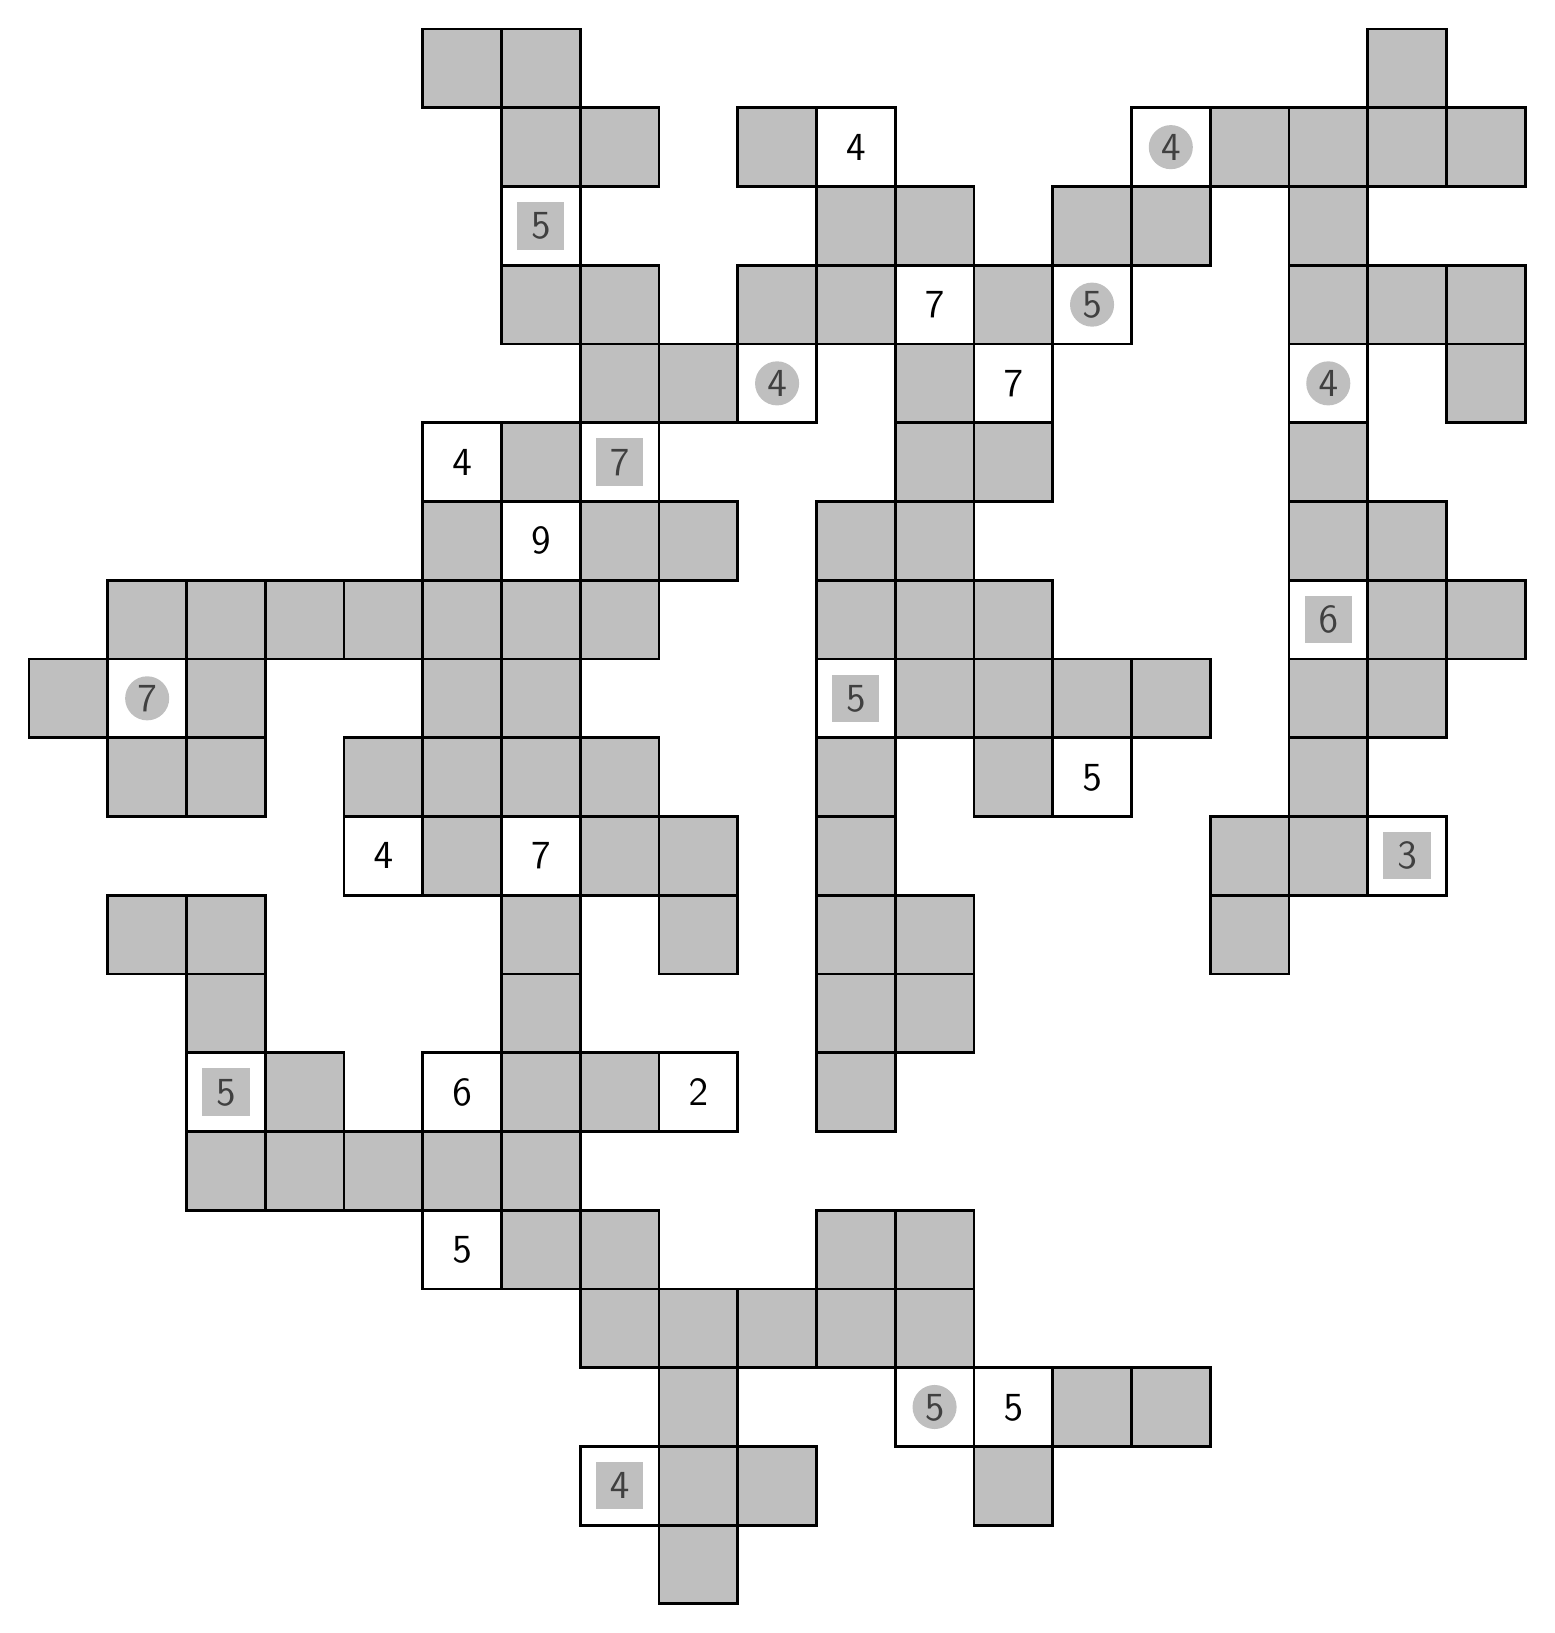
\begin{tikzpicture}\fill[gray, opacity = 0.5] (9, 0, 0)--++(1, 0, 0)--++(0, 1, 0)--++(-1, 0, 0)--cycle;
\draw[line width = 1pt] (9, 0, 0)--++(1, 0, 0)--++(0, 1, 0)--++(-1, 0, 0)--cycle;
\draw node at (8.5, 1.5, 0) {\Large $\mathsf{4}$};
\draw[line width = 1pt] (8, 1, 0)--++(1, 0, 0)--++(0, 1, 0)--++(-1, 0, 0)--cycle;
\fill[color = gray, opacity = 0.5] (8.2, 1.2) rectangle ++(0.6, 0.6);
\fill[gray, opacity = 0.5] (9, 1, 0)--++(1, 0, 0)--++(0, 1, 0)--++(-1, 0, 0)--cycle;
\draw[line width = 1pt] (9, 1, 0)--++(1, 0, 0)--++(0, 1, 0)--++(-1, 0, 0)--cycle;
\fill[gray, opacity = 0.5] (10, 1, 0)--++(1, 0, 0)--++(0, 1, 0)--++(-1, 0, 0)--cycle;
\draw[line width = 1pt] (10, 1, 0)--++(1, 0, 0)--++(0, 1, 0)--++(-1, 0, 0)--cycle;
\fill[gray, opacity = 0.5] (13, 1, 0)--++(1, 0, 0)--++(0, 1, 0)--++(-1, 0, 0)--cycle;
\draw[line width = 1pt] (13, 1, 0)--++(1, 0, 0)--++(0, 1, 0)--++(-1, 0, 0)--cycle;
\fill[gray, opacity = 0.5] (9, 2, 0)--++(1, 0, 0)--++(0, 1, 0)--++(-1, 0, 0)--cycle;
\draw[line width = 1pt] (9, 2, 0)--++(1, 0, 0)--++(0, 1, 0)--++(-1, 0, 0)--cycle;
\draw node at (12.5, 2.5, 0) {\Large $\mathsf{5}$};
\draw[line width = 1pt] (12, 2, 0)--++(1, 0, 0)--++(0, 1, 0)--++(-1, 0, 0)--cycle;
\fill[color = gray, opacity = 0.5] (12.5, 2.5, 0) circle (0.28);
\draw node at (13.5, 2.5, 0) {\Large $\mathsf{5}$};
\draw[line width = 1pt] (13, 2, 0)--++(1, 0, 0)--++(0, 1, 0)--++(-1, 0, 0)--cycle;
\fill[gray, opacity = 0.5] (14, 2, 0)--++(1, 0, 0)--++(0, 1, 0)--++(-1, 0, 0)--cycle;
\draw[line width = 1pt] (14, 2, 0)--++(1, 0, 0)--++(0, 1, 0)--++(-1, 0, 0)--cycle;
\fill[gray, opacity = 0.5] (15, 2, 0)--++(1, 0, 0)--++(0, 1, 0)--++(-1, 0, 0)--cycle;
\draw[line width = 1pt] (15, 2, 0)--++(1, 0, 0)--++(0, 1, 0)--++(-1, 0, 0)--cycle;
\fill[gray, opacity = 0.5] (8, 3, 0)--++(1, 0, 0)--++(0, 1, 0)--++(-1, 0, 0)--cycle;
\draw[line width = 1pt] (8, 3, 0)--++(1, 0, 0)--++(0, 1, 0)--++(-1, 0, 0)--cycle;
\fill[gray, opacity = 0.5] (9, 3, 0)--++(1, 0, 0)--++(0, 1, 0)--++(-1, 0, 0)--cycle;
\draw[line width = 1pt] (9, 3, 0)--++(1, 0, 0)--++(0, 1, 0)--++(-1, 0, 0)--cycle;
\fill[gray, opacity = 0.5] (10, 3, 0)--++(1, 0, 0)--++(0, 1, 0)--++(-1, 0, 0)--cycle;
\draw[line width = 1pt] (10, 3, 0)--++(1, 0, 0)--++(0, 1, 0)--++(-1, 0, 0)--cycle;
\fill[gray, opacity = 0.5] (11, 3, 0)--++(1, 0, 0)--++(0, 1, 0)--++(-1, 0, 0)--cycle;
\draw[line width = 1pt] (11, 3, 0)--++(1, 0, 0)--++(0, 1, 0)--++(-1, 0, 0)--cycle;
\fill[gray, opacity = 0.5] (12, 3, 0)--++(1, 0, 0)--++(0, 1, 0)--++(-1, 0, 0)--cycle;
\draw[line width = 1pt] (12, 3, 0)--++(1, 0, 0)--++(0, 1, 0)--++(-1, 0, 0)--cycle;
\draw node at (6.5, 4.5, 0) {\Large $\mathsf{5}$};
\draw[line width = 1pt] (6, 4, 0)--++(1, 0, 0)--++(0, 1, 0)--++(-1, 0, 0)--cycle;
\fill[gray, opacity = 0.5] (7, 4, 0)--++(1, 0, 0)--++(0, 1, 0)--++(-1, 0, 0)--cycle;
\draw[line width = 1pt] (7, 4, 0)--++(1, 0, 0)--++(0, 1, 0)--++(-1, 0, 0)--cycle;
\fill[gray, opacity = 0.5] (8, 4, 0)--++(1, 0, 0)--++(0, 1, 0)--++(-1, 0, 0)--cycle;
\draw[line width = 1pt] (8, 4, 0)--++(1, 0, 0)--++(0, 1, 0)--++(-1, 0, 0)--cycle;
\fill[gray, opacity = 0.5] (11, 4, 0)--++(1, 0, 0)--++(0, 1, 0)--++(-1, 0, 0)--cycle;
\draw[line width = 1pt] (11, 4, 0)--++(1, 0, 0)--++(0, 1, 0)--++(-1, 0, 0)--cycle;
\fill[gray, opacity = 0.5] (12, 4, 0)--++(1, 0, 0)--++(0, 1, 0)--++(-1, 0, 0)--cycle;
\draw[line width = 1pt] (12, 4, 0)--++(1, 0, 0)--++(0, 1, 0)--++(-1, 0, 0)--cycle;
\fill[gray, opacity = 0.5] (3, 5, 0)--++(1, 0, 0)--++(0, 1, 0)--++(-1, 0, 0)--cycle;
\draw[line width = 1pt] (3, 5, 0)--++(1, 0, 0)--++(0, 1, 0)--++(-1, 0, 0)--cycle;
\fill[gray, opacity = 0.5] (4, 5, 0)--++(1, 0, 0)--++(0, 1, 0)--++(-1, 0, 0)--cycle;
\draw[line width = 1pt] (4, 5, 0)--++(1, 0, 0)--++(0, 1, 0)--++(-1, 0, 0)--cycle;
\fill[gray, opacity = 0.5] (5, 5, 0)--++(1, 0, 0)--++(0, 1, 0)--++(-1, 0, 0)--cycle;
\draw[line width = 1pt] (5, 5, 0)--++(1, 0, 0)--++(0, 1, 0)--++(-1, 0, 0)--cycle;
\fill[gray, opacity = 0.5] (6, 5, 0)--++(1, 0, 0)--++(0, 1, 0)--++(-1, 0, 0)--cycle;
\draw[line width = 1pt] (6, 5, 0)--++(1, 0, 0)--++(0, 1, 0)--++(-1, 0, 0)--cycle;
\fill[gray, opacity = 0.5] (7, 5, 0)--++(1, 0, 0)--++(0, 1, 0)--++(-1, 0, 0)--cycle;
\draw[line width = 1pt] (7, 5, 0)--++(1, 0, 0)--++(0, 1, 0)--++(-1, 0, 0)--cycle;
\draw node at (3.5, 6.5, 0) {\Large $\mathsf{5}$};
\draw[line width = 1pt] (3, 6, 0)--++(1, 0, 0)--++(0, 1, 0)--++(-1, 0, 0)--cycle;
\fill[color = gray, opacity = 0.5] (3.2, 6.2) rectangle ++(0.6, 0.6);
\fill[gray, opacity = 0.5] (4, 6, 0)--++(1, 0, 0)--++(0, 1, 0)--++(-1, 0, 0)--cycle;
\draw[line width = 1pt] (4, 6, 0)--++(1, 0, 0)--++(0, 1, 0)--++(-1, 0, 0)--cycle;
\draw node at (6.5, 6.5, 0) {\Large $\mathsf{6}$};
\draw[line width = 1pt] (6, 6, 0)--++(1, 0, 0)--++(0, 1, 0)--++(-1, 0, 0)--cycle;
\fill[gray, opacity = 0.5] (7, 6, 0)--++(1, 0, 0)--++(0, 1, 0)--++(-1, 0, 0)--cycle;
\draw[line width = 1pt] (7, 6, 0)--++(1, 0, 0)--++(0, 1, 0)--++(-1, 0, 0)--cycle;
\fill[gray, opacity = 0.5] (8, 6, 0)--++(1, 0, 0)--++(0, 1, 0)--++(-1, 0, 0)--cycle;
\draw[line width = 1pt] (8, 6, 0)--++(1, 0, 0)--++(0, 1, 0)--++(-1, 0, 0)--cycle;
\draw node at (9.5, 6.5, 0) {\Large $\mathsf{2}$};
\draw[line width = 1pt] (9, 6, 0)--++(1, 0, 0)--++(0, 1, 0)--++(-1, 0, 0)--cycle;
\fill[gray, opacity = 0.5] (11, 6, 0)--++(1, 0, 0)--++(0, 1, 0)--++(-1, 0, 0)--cycle;
\draw[line width = 1pt] (11, 6, 0)--++(1, 0, 0)--++(0, 1, 0)--++(-1, 0, 0)--cycle;
\fill[gray, opacity = 0.5] (3, 7, 0)--++(1, 0, 0)--++(0, 1, 0)--++(-1, 0, 0)--cycle;
\draw[line width = 1pt] (3, 7, 0)--++(1, 0, 0)--++(0, 1, 0)--++(-1, 0, 0)--cycle;
\fill[gray, opacity = 0.5] (7, 7, 0)--++(1, 0, 0)--++(0, 1, 0)--++(-1, 0, 0)--cycle;
\draw[line width = 1pt] (7, 7, 0)--++(1, 0, 0)--++(0, 1, 0)--++(-1, 0, 0)--cycle;
\fill[gray, opacity = 0.5] (11, 7, 0)--++(1, 0, 0)--++(0, 1, 0)--++(-1, 0, 0)--cycle;
\draw[line width = 1pt] (11, 7, 0)--++(1, 0, 0)--++(0, 1, 0)--++(-1, 0, 0)--cycle;
\fill[gray, opacity = 0.5] (12, 7, 0)--++(1, 0, 0)--++(0, 1, 0)--++(-1, 0, 0)--cycle;
\draw[line width = 1pt] (12, 7, 0)--++(1, 0, 0)--++(0, 1, 0)--++(-1, 0, 0)--cycle;
\fill[gray, opacity = 0.5] (2, 8, 0)--++(1, 0, 0)--++(0, 1, 0)--++(-1, 0, 0)--cycle;
\draw[line width = 1pt] (2, 8, 0)--++(1, 0, 0)--++(0, 1, 0)--++(-1, 0, 0)--cycle;
\fill[gray, opacity = 0.5] (3, 8, 0)--++(1, 0, 0)--++(0, 1, 0)--++(-1, 0, 0)--cycle;
\draw[line width = 1pt] (3, 8, 0)--++(1, 0, 0)--++(0, 1, 0)--++(-1, 0, 0)--cycle;
\fill[gray, opacity = 0.5] (7, 8, 0)--++(1, 0, 0)--++(0, 1, 0)--++(-1, 0, 0)--cycle;
\draw[line width = 1pt] (7, 8, 0)--++(1, 0, 0)--++(0, 1, 0)--++(-1, 0, 0)--cycle;
\fill[gray, opacity = 0.5] (9, 8, 0)--++(1, 0, 0)--++(0, 1, 0)--++(-1, 0, 0)--cycle;
\draw[line width = 1pt] (9, 8, 0)--++(1, 0, 0)--++(0, 1, 0)--++(-1, 0, 0)--cycle;
\fill[gray, opacity = 0.5] (11, 8, 0)--++(1, 0, 0)--++(0, 1, 0)--++(-1, 0, 0)--cycle;
\draw[line width = 1pt] (11, 8, 0)--++(1, 0, 0)--++(0, 1, 0)--++(-1, 0, 0)--cycle;
\fill[gray, opacity = 0.5] (12, 8, 0)--++(1, 0, 0)--++(0, 1, 0)--++(-1, 0, 0)--cycle;
\draw[line width = 1pt] (12, 8, 0)--++(1, 0, 0)--++(0, 1, 0)--++(-1, 0, 0)--cycle;
\fill[gray, opacity = 0.5] (16, 8, 0)--++(1, 0, 0)--++(0, 1, 0)--++(-1, 0, 0)--cycle;
\draw[line width = 1pt] (16, 8, 0)--++(1, 0, 0)--++(0, 1, 0)--++(-1, 0, 0)--cycle;
\draw node at (5.5, 9.5, 0) {\Large $\mathsf{4}$};
\draw[line width = 1pt] (5, 9, 0)--++(1, 0, 0)--++(0, 1, 0)--++(-1, 0, 0)--cycle;
\fill[gray, opacity = 0.5] (6, 9, 0)--++(1, 0, 0)--++(0, 1, 0)--++(-1, 0, 0)--cycle;
\draw[line width = 1pt] (6, 9, 0)--++(1, 0, 0)--++(0, 1, 0)--++(-1, 0, 0)--cycle;
\draw node at (7.5, 9.5, 0) {\Large $\mathsf{7}$};
\draw[line width = 1pt] (7, 9, 0)--++(1, 0, 0)--++(0, 1, 0)--++(-1, 0, 0)--cycle;
\fill[gray, opacity = 0.5] (8, 9, 0)--++(1, 0, 0)--++(0, 1, 0)--++(-1, 0, 0)--cycle;
\draw[line width = 1pt] (8, 9, 0)--++(1, 0, 0)--++(0, 1, 0)--++(-1, 0, 0)--cycle;
\fill[gray, opacity = 0.5] (9, 9, 0)--++(1, 0, 0)--++(0, 1, 0)--++(-1, 0, 0)--cycle;
\draw[line width = 1pt] (9, 9, 0)--++(1, 0, 0)--++(0, 1, 0)--++(-1, 0, 0)--cycle;
\fill[gray, opacity = 0.5] (11, 9, 0)--++(1, 0, 0)--++(0, 1, 0)--++(-1, 0, 0)--cycle;
\draw[line width = 1pt] (11, 9, 0)--++(1, 0, 0)--++(0, 1, 0)--++(-1, 0, 0)--cycle;
\fill[gray, opacity = 0.5] (16, 9, 0)--++(1, 0, 0)--++(0, 1, 0)--++(-1, 0, 0)--cycle;
\draw[line width = 1pt] (16, 9, 0)--++(1, 0, 0)--++(0, 1, 0)--++(-1, 0, 0)--cycle;
\fill[gray, opacity = 0.5] (17, 9, 0)--++(1, 0, 0)--++(0, 1, 0)--++(-1, 0, 0)--cycle;
\draw[line width = 1pt] (17, 9, 0)--++(1, 0, 0)--++(0, 1, 0)--++(-1, 0, 0)--cycle;
\draw node at (18.5, 9.5, 0) {\Large $\mathsf{3}$};
\draw[line width = 1pt] (18, 9, 0)--++(1, 0, 0)--++(0, 1, 0)--++(-1, 0, 0)--cycle;
\fill[color = gray, opacity = 0.5] (18.2, 9.2) rectangle ++(0.6, 0.6);
\fill[gray, opacity = 0.5] (2, 10, 0)--++(1, 0, 0)--++(0, 1, 0)--++(-1, 0, 0)--cycle;
\draw[line width = 1pt] (2, 10, 0)--++(1, 0, 0)--++(0, 1, 0)--++(-1, 0, 0)--cycle;
\fill[gray, opacity = 0.5] (3, 10, 0)--++(1, 0, 0)--++(0, 1, 0)--++(-1, 0, 0)--cycle;
\draw[line width = 1pt] (3, 10, 0)--++(1, 0, 0)--++(0, 1, 0)--++(-1, 0, 0)--cycle;
\fill[gray, opacity = 0.5] (5, 10, 0)--++(1, 0, 0)--++(0, 1, 0)--++(-1, 0, 0)--cycle;
\draw[line width = 1pt] (5, 10, 0)--++(1, 0, 0)--++(0, 1, 0)--++(-1, 0, 0)--cycle;
\fill[gray, opacity = 0.5] (6, 10, 0)--++(1, 0, 0)--++(0, 1, 0)--++(-1, 0, 0)--cycle;
\draw[line width = 1pt] (6, 10, 0)--++(1, 0, 0)--++(0, 1, 0)--++(-1, 0, 0)--cycle;
\fill[gray, opacity = 0.5] (7, 10, 0)--++(1, 0, 0)--++(0, 1, 0)--++(-1, 0, 0)--cycle;
\draw[line width = 1pt] (7, 10, 0)--++(1, 0, 0)--++(0, 1, 0)--++(-1, 0, 0)--cycle;
\fill[gray, opacity = 0.5] (8, 10, 0)--++(1, 0, 0)--++(0, 1, 0)--++(-1, 0, 0)--cycle;
\draw[line width = 1pt] (8, 10, 0)--++(1, 0, 0)--++(0, 1, 0)--++(-1, 0, 0)--cycle;
\fill[gray, opacity = 0.5] (11, 10, 0)--++(1, 0, 0)--++(0, 1, 0)--++(-1, 0, 0)--cycle;
\draw[line width = 1pt] (11, 10, 0)--++(1, 0, 0)--++(0, 1, 0)--++(-1, 0, 0)--cycle;
\fill[gray, opacity = 0.5] (13, 10, 0)--++(1, 0, 0)--++(0, 1, 0)--++(-1, 0, 0)--cycle;
\draw[line width = 1pt] (13, 10, 0)--++(1, 0, 0)--++(0, 1, 0)--++(-1, 0, 0)--cycle;
\draw node at (14.5, 10.5, 0) {\Large $\mathsf{5}$};
\draw[line width = 1pt] (14, 10, 0)--++(1, 0, 0)--++(0, 1, 0)--++(-1, 0, 0)--cycle;
\fill[gray, opacity = 0.5] (17, 10, 0)--++(1, 0, 0)--++(0, 1, 0)--++(-1, 0, 0)--cycle;
\draw[line width = 1pt] (17, 10, 0)--++(1, 0, 0)--++(0, 1, 0)--++(-1, 0, 0)--cycle;
\fill[gray, opacity = 0.5] (1, 11, 0)--++(1, 0, 0)--++(0, 1, 0)--++(-1, 0, 0)--cycle;
\draw[line width = 1pt] (1, 11, 0)--++(1, 0, 0)--++(0, 1, 0)--++(-1, 0, 0)--cycle;
\draw node at (2.5, 11.5, 0) {\Large $\mathsf{7}$};
\draw[line width = 1pt] (2, 11, 0)--++(1, 0, 0)--++(0, 1, 0)--++(-1, 0, 0)--cycle;
\fill[color = gray, opacity = 0.5] (2.5, 11.5, 0) circle (0.28);
\fill[gray, opacity = 0.5] (3, 11, 0)--++(1, 0, 0)--++(0, 1, 0)--++(-1, 0, 0)--cycle;
\draw[line width = 1pt] (3, 11, 0)--++(1, 0, 0)--++(0, 1, 0)--++(-1, 0, 0)--cycle;
\fill[gray, opacity = 0.5] (6, 11, 0)--++(1, 0, 0)--++(0, 1, 0)--++(-1, 0, 0)--cycle;
\draw[line width = 1pt] (6, 11, 0)--++(1, 0, 0)--++(0, 1, 0)--++(-1, 0, 0)--cycle;
\fill[gray, opacity = 0.5] (7, 11, 0)--++(1, 0, 0)--++(0, 1, 0)--++(-1, 0, 0)--cycle;
\draw[line width = 1pt] (7, 11, 0)--++(1, 0, 0)--++(0, 1, 0)--++(-1, 0, 0)--cycle;
\draw node at (11.5, 11.5, 0) {\Large $\mathsf{5}$};
\draw[line width = 1pt] (11, 11, 0)--++(1, 0, 0)--++(0, 1, 0)--++(-1, 0, 0)--cycle;
\fill[color = gray, opacity = 0.5] (11.2, 11.2) rectangle ++(0.6, 0.6);
\fill[gray, opacity = 0.5] (12, 11, 0)--++(1, 0, 0)--++(0, 1, 0)--++(-1, 0, 0)--cycle;
\draw[line width = 1pt] (12, 11, 0)--++(1, 0, 0)--++(0, 1, 0)--++(-1, 0, 0)--cycle;
\fill[gray, opacity = 0.5] (13, 11, 0)--++(1, 0, 0)--++(0, 1, 0)--++(-1, 0, 0)--cycle;
\draw[line width = 1pt] (13, 11, 0)--++(1, 0, 0)--++(0, 1, 0)--++(-1, 0, 0)--cycle;
\fill[gray, opacity = 0.5] (14, 11, 0)--++(1, 0, 0)--++(0, 1, 0)--++(-1, 0, 0)--cycle;
\draw[line width = 1pt] (14, 11, 0)--++(1, 0, 0)--++(0, 1, 0)--++(-1, 0, 0)--cycle;
\fill[gray, opacity = 0.5] (15, 11, 0)--++(1, 0, 0)--++(0, 1, 0)--++(-1, 0, 0)--cycle;
\draw[line width = 1pt] (15, 11, 0)--++(1, 0, 0)--++(0, 1, 0)--++(-1, 0, 0)--cycle;
\fill[gray, opacity = 0.5] (17, 11, 0)--++(1, 0, 0)--++(0, 1, 0)--++(-1, 0, 0)--cycle;
\draw[line width = 1pt] (17, 11, 0)--++(1, 0, 0)--++(0, 1, 0)--++(-1, 0, 0)--cycle;
\fill[gray, opacity = 0.5] (18, 11, 0)--++(1, 0, 0)--++(0, 1, 0)--++(-1, 0, 0)--cycle;
\draw[line width = 1pt] (18, 11, 0)--++(1, 0, 0)--++(0, 1, 0)--++(-1, 0, 0)--cycle;
\fill[gray, opacity = 0.5] (2, 12, 0)--++(1, 0, 0)--++(0, 1, 0)--++(-1, 0, 0)--cycle;
\draw[line width = 1pt] (2, 12, 0)--++(1, 0, 0)--++(0, 1, 0)--++(-1, 0, 0)--cycle;
\fill[gray, opacity = 0.5] (3, 12, 0)--++(1, 0, 0)--++(0, 1, 0)--++(-1, 0, 0)--cycle;
\draw[line width = 1pt] (3, 12, 0)--++(1, 0, 0)--++(0, 1, 0)--++(-1, 0, 0)--cycle;
\fill[gray, opacity = 0.5] (4, 12, 0)--++(1, 0, 0)--++(0, 1, 0)--++(-1, 0, 0)--cycle;
\draw[line width = 1pt] (4, 12, 0)--++(1, 0, 0)--++(0, 1, 0)--++(-1, 0, 0)--cycle;
\fill[gray, opacity = 0.5] (5, 12, 0)--++(1, 0, 0)--++(0, 1, 0)--++(-1, 0, 0)--cycle;
\draw[line width = 1pt] (5, 12, 0)--++(1, 0, 0)--++(0, 1, 0)--++(-1, 0, 0)--cycle;
\fill[gray, opacity = 0.5] (6, 12, 0)--++(1, 0, 0)--++(0, 1, 0)--++(-1, 0, 0)--cycle;
\draw[line width = 1pt] (6, 12, 0)--++(1, 0, 0)--++(0, 1, 0)--++(-1, 0, 0)--cycle;
\fill[gray, opacity = 0.5] (7, 12, 0)--++(1, 0, 0)--++(0, 1, 0)--++(-1, 0, 0)--cycle;
\draw[line width = 1pt] (7, 12, 0)--++(1, 0, 0)--++(0, 1, 0)--++(-1, 0, 0)--cycle;
\fill[gray, opacity = 0.5] (8, 12, 0)--++(1, 0, 0)--++(0, 1, 0)--++(-1, 0, 0)--cycle;
\draw[line width = 1pt] (8, 12, 0)--++(1, 0, 0)--++(0, 1, 0)--++(-1, 0, 0)--cycle;
\fill[gray, opacity = 0.5] (11, 12, 0)--++(1, 0, 0)--++(0, 1, 0)--++(-1, 0, 0)--cycle;
\draw[line width = 1pt] (11, 12, 0)--++(1, 0, 0)--++(0, 1, 0)--++(-1, 0, 0)--cycle;
\fill[gray, opacity = 0.5] (12, 12, 0)--++(1, 0, 0)--++(0, 1, 0)--++(-1, 0, 0)--cycle;
\draw[line width = 1pt] (12, 12, 0)--++(1, 0, 0)--++(0, 1, 0)--++(-1, 0, 0)--cycle;
\fill[gray, opacity = 0.5] (13, 12, 0)--++(1, 0, 0)--++(0, 1, 0)--++(-1, 0, 0)--cycle;
\draw[line width = 1pt] (13, 12, 0)--++(1, 0, 0)--++(0, 1, 0)--++(-1, 0, 0)--cycle;
\draw node at (17.5, 12.5, 0) {\Large $\mathsf{6}$};
\draw[line width = 1pt] (17, 12, 0)--++(1, 0, 0)--++(0, 1, 0)--++(-1, 0, 0)--cycle;
\fill[color = gray, opacity = 0.5] (17.2, 12.2) rectangle ++(0.6, 0.6);
\fill[gray, opacity = 0.5] (18, 12, 0)--++(1, 0, 0)--++(0, 1, 0)--++(-1, 0, 0)--cycle;
\draw[line width = 1pt] (18, 12, 0)--++(1, 0, 0)--++(0, 1, 0)--++(-1, 0, 0)--cycle;
\fill[gray, opacity = 0.5] (19, 12, 0)--++(1, 0, 0)--++(0, 1, 0)--++(-1, 0, 0)--cycle;
\draw[line width = 1pt] (19, 12, 0)--++(1, 0, 0)--++(0, 1, 0)--++(-1, 0, 0)--cycle;
\fill[gray, opacity = 0.5] (6, 13, 0)--++(1, 0, 0)--++(0, 1, 0)--++(-1, 0, 0)--cycle;
\draw[line width = 1pt] (6, 13, 0)--++(1, 0, 0)--++(0, 1, 0)--++(-1, 0, 0)--cycle;
\draw node at (7.5, 13.5, 0) {\Large $\mathsf{9}$};
\draw[line width = 1pt] (7, 13, 0)--++(1, 0, 0)--++(0, 1, 0)--++(-1, 0, 0)--cycle;
\fill[gray, opacity = 0.5] (8, 13, 0)--++(1, 0, 0)--++(0, 1, 0)--++(-1, 0, 0)--cycle;
\draw[line width = 1pt] (8, 13, 0)--++(1, 0, 0)--++(0, 1, 0)--++(-1, 0, 0)--cycle;
\fill[gray, opacity = 0.5] (9, 13, 0)--++(1, 0, 0)--++(0, 1, 0)--++(-1, 0, 0)--cycle;
\draw[line width = 1pt] (9, 13, 0)--++(1, 0, 0)--++(0, 1, 0)--++(-1, 0, 0)--cycle;
\fill[gray, opacity = 0.5] (11, 13, 0)--++(1, 0, 0)--++(0, 1, 0)--++(-1, 0, 0)--cycle;
\draw[line width = 1pt] (11, 13, 0)--++(1, 0, 0)--++(0, 1, 0)--++(-1, 0, 0)--cycle;
\fill[gray, opacity = 0.5] (12, 13, 0)--++(1, 0, 0)--++(0, 1, 0)--++(-1, 0, 0)--cycle;
\draw[line width = 1pt] (12, 13, 0)--++(1, 0, 0)--++(0, 1, 0)--++(-1, 0, 0)--cycle;
\fill[gray, opacity = 0.5] (17, 13, 0)--++(1, 0, 0)--++(0, 1, 0)--++(-1, 0, 0)--cycle;
\draw[line width = 1pt] (17, 13, 0)--++(1, 0, 0)--++(0, 1, 0)--++(-1, 0, 0)--cycle;
\fill[gray, opacity = 0.5] (18, 13, 0)--++(1, 0, 0)--++(0, 1, 0)--++(-1, 0, 0)--cycle;
\draw[line width = 1pt] (18, 13, 0)--++(1, 0, 0)--++(0, 1, 0)--++(-1, 0, 0)--cycle;
\draw node at (6.5, 14.5, 0) {\Large $\mathsf{4}$};
\draw[line width = 1pt] (6, 14, 0)--++(1, 0, 0)--++(0, 1, 0)--++(-1, 0, 0)--cycle;
\fill[gray, opacity = 0.5] (7, 14, 0)--++(1, 0, 0)--++(0, 1, 0)--++(-1, 0, 0)--cycle;
\draw[line width = 1pt] (7, 14, 0)--++(1, 0, 0)--++(0, 1, 0)--++(-1, 0, 0)--cycle;
\draw node at (8.5, 14.5, 0) {\Large $\mathsf{7}$};
\draw[line width = 1pt] (8, 14, 0)--++(1, 0, 0)--++(0, 1, 0)--++(-1, 0, 0)--cycle;
\fill[color = gray, opacity = 0.5] (8.2, 14.2) rectangle ++(0.6, 0.6);
\fill[gray, opacity = 0.5] (12, 14, 0)--++(1, 0, 0)--++(0, 1, 0)--++(-1, 0, 0)--cycle;
\draw[line width = 1pt] (12, 14, 0)--++(1, 0, 0)--++(0, 1, 0)--++(-1, 0, 0)--cycle;
\fill[gray, opacity = 0.5] (13, 14, 0)--++(1, 0, 0)--++(0, 1, 0)--++(-1, 0, 0)--cycle;
\draw[line width = 1pt] (13, 14, 0)--++(1, 0, 0)--++(0, 1, 0)--++(-1, 0, 0)--cycle;
\fill[gray, opacity = 0.5] (17, 14, 0)--++(1, 0, 0)--++(0, 1, 0)--++(-1, 0, 0)--cycle;
\draw[line width = 1pt] (17, 14, 0)--++(1, 0, 0)--++(0, 1, 0)--++(-1, 0, 0)--cycle;
\fill[gray, opacity = 0.5] (8, 15, 0)--++(1, 0, 0)--++(0, 1, 0)--++(-1, 0, 0)--cycle;
\draw[line width = 1pt] (8, 15, 0)--++(1, 0, 0)--++(0, 1, 0)--++(-1, 0, 0)--cycle;
\fill[gray, opacity = 0.5] (9, 15, 0)--++(1, 0, 0)--++(0, 1, 0)--++(-1, 0, 0)--cycle;
\draw[line width = 1pt] (9, 15, 0)--++(1, 0, 0)--++(0, 1, 0)--++(-1, 0, 0)--cycle;
\draw node at (10.5, 15.5, 0) {\Large $\mathsf{4}$};
\draw[line width = 1pt] (10, 15, 0)--++(1, 0, 0)--++(0, 1, 0)--++(-1, 0, 0)--cycle;
\fill[color = gray, opacity = 0.5] (10.5, 15.5, 0) circle (0.28);
\fill[gray, opacity = 0.5] (12, 15, 0)--++(1, 0, 0)--++(0, 1, 0)--++(-1, 0, 0)--cycle;
\draw[line width = 1pt] (12, 15, 0)--++(1, 0, 0)--++(0, 1, 0)--++(-1, 0, 0)--cycle;
\draw node at (13.5, 15.5, 0) {\Large $\mathsf{7}$};
\draw[line width = 1pt] (13, 15, 0)--++(1, 0, 0)--++(0, 1, 0)--++(-1, 0, 0)--cycle;
\draw node at (17.5, 15.5, 0) {\Large $\mathsf{4}$};
\draw[line width = 1pt] (17, 15, 0)--++(1, 0, 0)--++(0, 1, 0)--++(-1, 0, 0)--cycle;
\fill[color = gray, opacity = 0.5] (17.5, 15.5, 0) circle (0.28);
\fill[gray, opacity = 0.5] (19, 15, 0)--++(1, 0, 0)--++(0, 1, 0)--++(-1, 0, 0)--cycle;
\draw[line width = 1pt] (19, 15, 0)--++(1, 0, 0)--++(0, 1, 0)--++(-1, 0, 0)--cycle;
\fill[gray, opacity = 0.5] (7, 16, 0)--++(1, 0, 0)--++(0, 1, 0)--++(-1, 0, 0)--cycle;
\draw[line width = 1pt] (7, 16, 0)--++(1, 0, 0)--++(0, 1, 0)--++(-1, 0, 0)--cycle;
\fill[gray, opacity = 0.5] (8, 16, 0)--++(1, 0, 0)--++(0, 1, 0)--++(-1, 0, 0)--cycle;
\draw[line width = 1pt] (8, 16, 0)--++(1, 0, 0)--++(0, 1, 0)--++(-1, 0, 0)--cycle;
\fill[gray, opacity = 0.5] (10, 16, 0)--++(1, 0, 0)--++(0, 1, 0)--++(-1, 0, 0)--cycle;
\draw[line width = 1pt] (10, 16, 0)--++(1, 0, 0)--++(0, 1, 0)--++(-1, 0, 0)--cycle;
\fill[gray, opacity = 0.5] (11, 16, 0)--++(1, 0, 0)--++(0, 1, 0)--++(-1, 0, 0)--cycle;
\draw[line width = 1pt] (11, 16, 0)--++(1, 0, 0)--++(0, 1, 0)--++(-1, 0, 0)--cycle;
\draw node at (12.5, 16.5, 0) {\Large $\mathsf{7}$};
\draw[line width = 1pt] (12, 16, 0)--++(1, 0, 0)--++(0, 1, 0)--++(-1, 0, 0)--cycle;
\fill[gray, opacity = 0.5] (13, 16, 0)--++(1, 0, 0)--++(0, 1, 0)--++(-1, 0, 0)--cycle;
\draw[line width = 1pt] (13, 16, 0)--++(1, 0, 0)--++(0, 1, 0)--++(-1, 0, 0)--cycle;
\draw node at (14.5, 16.5, 0) {\Large $\mathsf{5}$};
\draw[line width = 1pt] (14, 16, 0)--++(1, 0, 0)--++(0, 1, 0)--++(-1, 0, 0)--cycle;
\fill[color = gray, opacity = 0.5] (14.5, 16.5, 0) circle (0.28);
\fill[gray, opacity = 0.5] (17, 16, 0)--++(1, 0, 0)--++(0, 1, 0)--++(-1, 0, 0)--cycle;
\draw[line width = 1pt] (17, 16, 0)--++(1, 0, 0)--++(0, 1, 0)--++(-1, 0, 0)--cycle;
\fill[gray, opacity = 0.5] (18, 16, 0)--++(1, 0, 0)--++(0, 1, 0)--++(-1, 0, 0)--cycle;
\draw[line width = 1pt] (18, 16, 0)--++(1, 0, 0)--++(0, 1, 0)--++(-1, 0, 0)--cycle;
\fill[gray, opacity = 0.5] (19, 16, 0)--++(1, 0, 0)--++(0, 1, 0)--++(-1, 0, 0)--cycle;
\draw[line width = 1pt] (19, 16, 0)--++(1, 0, 0)--++(0, 1, 0)--++(-1, 0, 0)--cycle;
\draw node at (7.5, 17.5, 0) {\Large $\mathsf{5}$};
\draw[line width = 1pt] (7, 17, 0)--++(1, 0, 0)--++(0, 1, 0)--++(-1, 0, 0)--cycle;
\fill[color = gray, opacity = 0.5] (7.2, 17.2) rectangle ++(0.6, 0.6);
\fill[gray, opacity = 0.5] (11, 17, 0)--++(1, 0, 0)--++(0, 1, 0)--++(-1, 0, 0)--cycle;
\draw[line width = 1pt] (11, 17, 0)--++(1, 0, 0)--++(0, 1, 0)--++(-1, 0, 0)--cycle;
\fill[gray, opacity = 0.5] (12, 17, 0)--++(1, 0, 0)--++(0, 1, 0)--++(-1, 0, 0)--cycle;
\draw[line width = 1pt] (12, 17, 0)--++(1, 0, 0)--++(0, 1, 0)--++(-1, 0, 0)--cycle;
\fill[gray, opacity = 0.5] (14, 17, 0)--++(1, 0, 0)--++(0, 1, 0)--++(-1, 0, 0)--cycle;
\draw[line width = 1pt] (14, 17, 0)--++(1, 0, 0)--++(0, 1, 0)--++(-1, 0, 0)--cycle;
\fill[gray, opacity = 0.5] (15, 17, 0)--++(1, 0, 0)--++(0, 1, 0)--++(-1, 0, 0)--cycle;
\draw[line width = 1pt] (15, 17, 0)--++(1, 0, 0)--++(0, 1, 0)--++(-1, 0, 0)--cycle;
\fill[gray, opacity = 0.5] (17, 17, 0)--++(1, 0, 0)--++(0, 1, 0)--++(-1, 0, 0)--cycle;
\draw[line width = 1pt] (17, 17, 0)--++(1, 0, 0)--++(0, 1, 0)--++(-1, 0, 0)--cycle;
\fill[gray, opacity = 0.5] (7, 18, 0)--++(1, 0, 0)--++(0, 1, 0)--++(-1, 0, 0)--cycle;
\draw[line width = 1pt] (7, 18, 0)--++(1, 0, 0)--++(0, 1, 0)--++(-1, 0, 0)--cycle;
\fill[gray, opacity = 0.5] (8, 18, 0)--++(1, 0, 0)--++(0, 1, 0)--++(-1, 0, 0)--cycle;
\draw[line width = 1pt] (8, 18, 0)--++(1, 0, 0)--++(0, 1, 0)--++(-1, 0, 0)--cycle;
\fill[gray, opacity = 0.5] (10, 18, 0)--++(1, 0, 0)--++(0, 1, 0)--++(-1, 0, 0)--cycle;
\draw[line width = 1pt] (10, 18, 0)--++(1, 0, 0)--++(0, 1, 0)--++(-1, 0, 0)--cycle;
\draw node at (11.5, 18.5, 0) {\Large $\mathsf{4}$};
\draw[line width = 1pt] (11, 18, 0)--++(1, 0, 0)--++(0, 1, 0)--++(-1, 0, 0)--cycle;
\draw node at (15.5, 18.5, 0) {\Large $\mathsf{4}$};
\draw[line width = 1pt] (15, 18, 0)--++(1, 0, 0)--++(0, 1, 0)--++(-1, 0, 0)--cycle;
\fill[color = gray, opacity = 0.5] (15.5, 18.5, 0) circle (0.28);
\fill[gray, opacity = 0.5] (16, 18, 0)--++(1, 0, 0)--++(0, 1, 0)--++(-1, 0, 0)--cycle;
\draw[line width = 1pt] (16, 18, 0)--++(1, 0, 0)--++(0, 1, 0)--++(-1, 0, 0)--cycle;
\fill[gray, opacity = 0.5] (17, 18, 0)--++(1, 0, 0)--++(0, 1, 0)--++(-1, 0, 0)--cycle;
\draw[line width = 1pt] (17, 18, 0)--++(1, 0, 0)--++(0, 1, 0)--++(-1, 0, 0)--cycle;
\fill[gray, opacity = 0.5] (18, 18, 0)--++(1, 0, 0)--++(0, 1, 0)--++(-1, 0, 0)--cycle;
\draw[line width = 1pt] (18, 18, 0)--++(1, 0, 0)--++(0, 1, 0)--++(-1, 0, 0)--cycle;
\fill[gray, opacity = 0.5] (19, 18, 0)--++(1, 0, 0)--++(0, 1, 0)--++(-1, 0, 0)--cycle;
\draw[line width = 1pt] (19, 18, 0)--++(1, 0, 0)--++(0, 1, 0)--++(-1, 0, 0)--cycle;
\fill[gray, opacity = 0.5] (6, 19, 0)--++(1, 0, 0)--++(0, 1, 0)--++(-1, 0, 0)--cycle;
\draw[line width = 1pt] (6, 19, 0)--++(1, 0, 0)--++(0, 1, 0)--++(-1, 0, 0)--cycle;
\fill[gray, opacity = 0.5] (7, 19, 0)--++(1, 0, 0)--++(0, 1, 0)--++(-1, 0, 0)--cycle;
\draw[line width = 1pt] (7, 19, 0)--++(1, 0, 0)--++(0, 1, 0)--++(-1, 0, 0)--cycle;
\fill[gray, opacity = 0.5] (18, 19, 0)--++(1, 0, 0)--++(0, 1, 0)--++(-1, 0, 0)--cycle;
\draw[line width = 1pt] (18, 19, 0)--++(1, 0, 0)--++(0, 1, 0)--++(-1, 0, 0)--cycle;
\end{tikzpicture}}\]
\[\resizebox{30pc}{!}{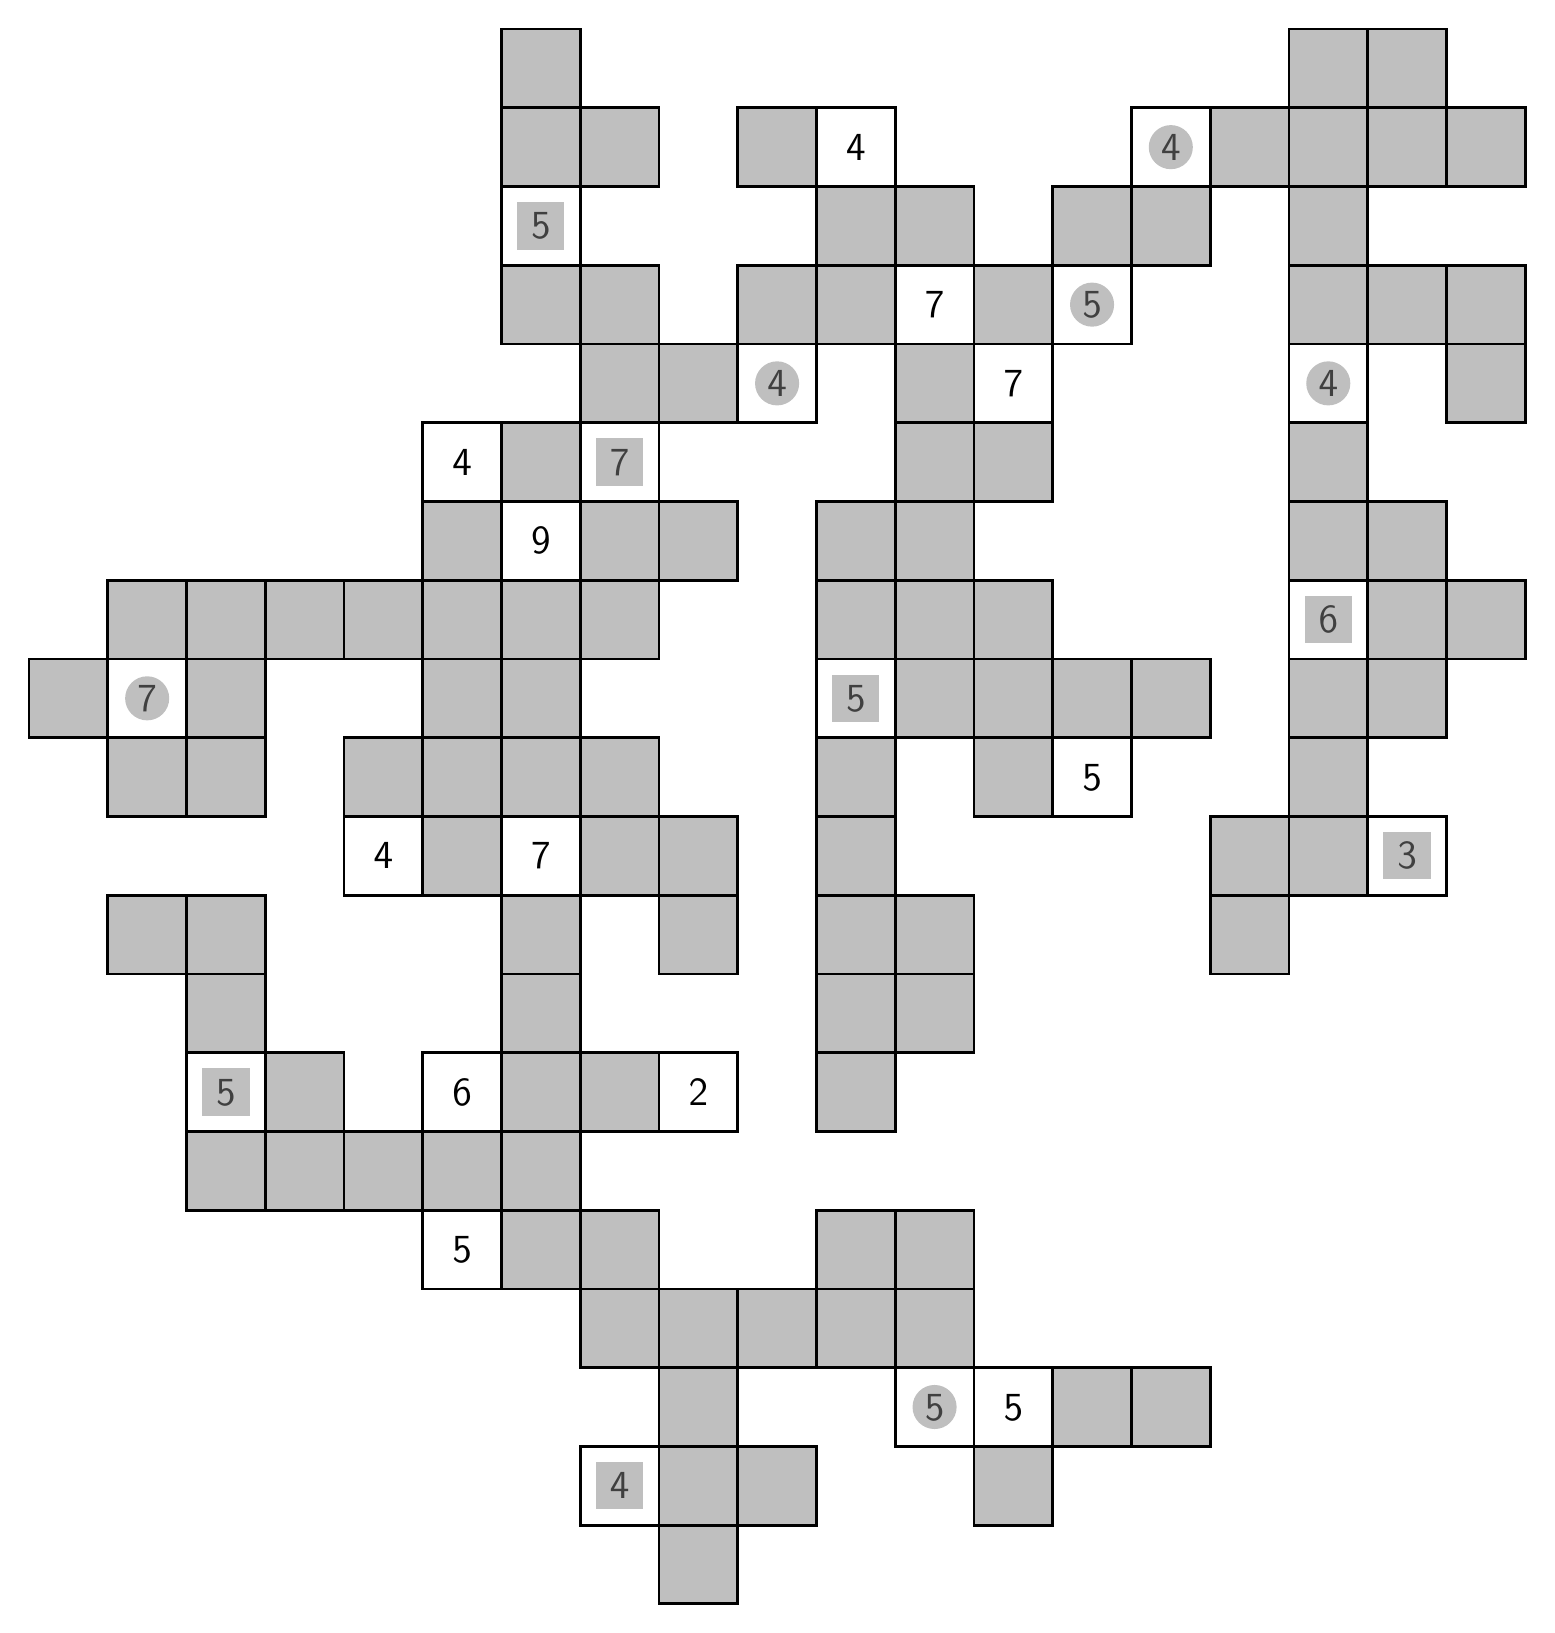
\begin{tikzpicture}\fill[gray, opacity = 0.5] (9, 0, 0)--++(1, 0, 0)--++(0, 1, 0)--++(-1, 0, 0)--cycle;
\draw[line width = 1pt] (9, 0, 0)--++(1, 0, 0)--++(0, 1, 0)--++(-1, 0, 0)--cycle;
\draw node at (8.5, 1.5, 0) {\Large $\mathsf{4}$};
\draw[line width = 1pt] (8, 1, 0)--++(1, 0, 0)--++(0, 1, 0)--++(-1, 0, 0)--cycle;
\fill[color = gray, opacity = 0.5] (8.2, 1.2) rectangle ++(0.6, 0.6);
\fill[gray, opacity = 0.5] (9, 1, 0)--++(1, 0, 0)--++(0, 1, 0)--++(-1, 0, 0)--cycle;
\draw[line width = 1pt] (9, 1, 0)--++(1, 0, 0)--++(0, 1, 0)--++(-1, 0, 0)--cycle;
\fill[gray, opacity = 0.5] (10, 1, 0)--++(1, 0, 0)--++(0, 1, 0)--++(-1, 0, 0)--cycle;
\draw[line width = 1pt] (10, 1, 0)--++(1, 0, 0)--++(0, 1, 0)--++(-1, 0, 0)--cycle;
\fill[gray, opacity = 0.5] (13, 1, 0)--++(1, 0, 0)--++(0, 1, 0)--++(-1, 0, 0)--cycle;
\draw[line width = 1pt] (13, 1, 0)--++(1, 0, 0)--++(0, 1, 0)--++(-1, 0, 0)--cycle;
\fill[gray, opacity = 0.5] (9, 2, 0)--++(1, 0, 0)--++(0, 1, 0)--++(-1, 0, 0)--cycle;
\draw[line width = 1pt] (9, 2, 0)--++(1, 0, 0)--++(0, 1, 0)--++(-1, 0, 0)--cycle;
\draw node at (12.5, 2.5, 0) {\Large $\mathsf{5}$};
\draw[line width = 1pt] (12, 2, 0)--++(1, 0, 0)--++(0, 1, 0)--++(-1, 0, 0)--cycle;
\fill[color = gray, opacity = 0.5] (12.5, 2.5, 0) circle (0.28);
\draw node at (13.5, 2.5, 0) {\Large $\mathsf{5}$};
\draw[line width = 1pt] (13, 2, 0)--++(1, 0, 0)--++(0, 1, 0)--++(-1, 0, 0)--cycle;
\fill[gray, opacity = 0.5] (14, 2, 0)--++(1, 0, 0)--++(0, 1, 0)--++(-1, 0, 0)--cycle;
\draw[line width = 1pt] (14, 2, 0)--++(1, 0, 0)--++(0, 1, 0)--++(-1, 0, 0)--cycle;
\fill[gray, opacity = 0.5] (15, 2, 0)--++(1, 0, 0)--++(0, 1, 0)--++(-1, 0, 0)--cycle;
\draw[line width = 1pt] (15, 2, 0)--++(1, 0, 0)--++(0, 1, 0)--++(-1, 0, 0)--cycle;
\fill[gray, opacity = 0.5] (8, 3, 0)--++(1, 0, 0)--++(0, 1, 0)--++(-1, 0, 0)--cycle;
\draw[line width = 1pt] (8, 3, 0)--++(1, 0, 0)--++(0, 1, 0)--++(-1, 0, 0)--cycle;
\fill[gray, opacity = 0.5] (9, 3, 0)--++(1, 0, 0)--++(0, 1, 0)--++(-1, 0, 0)--cycle;
\draw[line width = 1pt] (9, 3, 0)--++(1, 0, 0)--++(0, 1, 0)--++(-1, 0, 0)--cycle;
\fill[gray, opacity = 0.5] (10, 3, 0)--++(1, 0, 0)--++(0, 1, 0)--++(-1, 0, 0)--cycle;
\draw[line width = 1pt] (10, 3, 0)--++(1, 0, 0)--++(0, 1, 0)--++(-1, 0, 0)--cycle;
\fill[gray, opacity = 0.5] (11, 3, 0)--++(1, 0, 0)--++(0, 1, 0)--++(-1, 0, 0)--cycle;
\draw[line width = 1pt] (11, 3, 0)--++(1, 0, 0)--++(0, 1, 0)--++(-1, 0, 0)--cycle;
\fill[gray, opacity = 0.5] (12, 3, 0)--++(1, 0, 0)--++(0, 1, 0)--++(-1, 0, 0)--cycle;
\draw[line width = 1pt] (12, 3, 0)--++(1, 0, 0)--++(0, 1, 0)--++(-1, 0, 0)--cycle;
\draw node at (6.5, 4.5, 0) {\Large $\mathsf{5}$};
\draw[line width = 1pt] (6, 4, 0)--++(1, 0, 0)--++(0, 1, 0)--++(-1, 0, 0)--cycle;
\fill[gray, opacity = 0.5] (7, 4, 0)--++(1, 0, 0)--++(0, 1, 0)--++(-1, 0, 0)--cycle;
\draw[line width = 1pt] (7, 4, 0)--++(1, 0, 0)--++(0, 1, 0)--++(-1, 0, 0)--cycle;
\fill[gray, opacity = 0.5] (8, 4, 0)--++(1, 0, 0)--++(0, 1, 0)--++(-1, 0, 0)--cycle;
\draw[line width = 1pt] (8, 4, 0)--++(1, 0, 0)--++(0, 1, 0)--++(-1, 0, 0)--cycle;
\fill[gray, opacity = 0.5] (11, 4, 0)--++(1, 0, 0)--++(0, 1, 0)--++(-1, 0, 0)--cycle;
\draw[line width = 1pt] (11, 4, 0)--++(1, 0, 0)--++(0, 1, 0)--++(-1, 0, 0)--cycle;
\fill[gray, opacity = 0.5] (12, 4, 0)--++(1, 0, 0)--++(0, 1, 0)--++(-1, 0, 0)--cycle;
\draw[line width = 1pt] (12, 4, 0)--++(1, 0, 0)--++(0, 1, 0)--++(-1, 0, 0)--cycle;
\fill[gray, opacity = 0.5] (3, 5, 0)--++(1, 0, 0)--++(0, 1, 0)--++(-1, 0, 0)--cycle;
\draw[line width = 1pt] (3, 5, 0)--++(1, 0, 0)--++(0, 1, 0)--++(-1, 0, 0)--cycle;
\fill[gray, opacity = 0.5] (4, 5, 0)--++(1, 0, 0)--++(0, 1, 0)--++(-1, 0, 0)--cycle;
\draw[line width = 1pt] (4, 5, 0)--++(1, 0, 0)--++(0, 1, 0)--++(-1, 0, 0)--cycle;
\fill[gray, opacity = 0.5] (5, 5, 0)--++(1, 0, 0)--++(0, 1, 0)--++(-1, 0, 0)--cycle;
\draw[line width = 1pt] (5, 5, 0)--++(1, 0, 0)--++(0, 1, 0)--++(-1, 0, 0)--cycle;
\fill[gray, opacity = 0.5] (6, 5, 0)--++(1, 0, 0)--++(0, 1, 0)--++(-1, 0, 0)--cycle;
\draw[line width = 1pt] (6, 5, 0)--++(1, 0, 0)--++(0, 1, 0)--++(-1, 0, 0)--cycle;
\fill[gray, opacity = 0.5] (7, 5, 0)--++(1, 0, 0)--++(0, 1, 0)--++(-1, 0, 0)--cycle;
\draw[line width = 1pt] (7, 5, 0)--++(1, 0, 0)--++(0, 1, 0)--++(-1, 0, 0)--cycle;
\draw node at (3.5, 6.5, 0) {\Large $\mathsf{5}$};
\draw[line width = 1pt] (3, 6, 0)--++(1, 0, 0)--++(0, 1, 0)--++(-1, 0, 0)--cycle;
\fill[color = gray, opacity = 0.5] (3.2, 6.2) rectangle ++(0.6, 0.6);
\fill[gray, opacity = 0.5] (4, 6, 0)--++(1, 0, 0)--++(0, 1, 0)--++(-1, 0, 0)--cycle;
\draw[line width = 1pt] (4, 6, 0)--++(1, 0, 0)--++(0, 1, 0)--++(-1, 0, 0)--cycle;
\draw node at (6.5, 6.5, 0) {\Large $\mathsf{6}$};
\draw[line width = 1pt] (6, 6, 0)--++(1, 0, 0)--++(0, 1, 0)--++(-1, 0, 0)--cycle;
\fill[gray, opacity = 0.5] (7, 6, 0)--++(1, 0, 0)--++(0, 1, 0)--++(-1, 0, 0)--cycle;
\draw[line width = 1pt] (7, 6, 0)--++(1, 0, 0)--++(0, 1, 0)--++(-1, 0, 0)--cycle;
\fill[gray, opacity = 0.5] (8, 6, 0)--++(1, 0, 0)--++(0, 1, 0)--++(-1, 0, 0)--cycle;
\draw[line width = 1pt] (8, 6, 0)--++(1, 0, 0)--++(0, 1, 0)--++(-1, 0, 0)--cycle;
\draw node at (9.5, 6.5, 0) {\Large $\mathsf{2}$};
\draw[line width = 1pt] (9, 6, 0)--++(1, 0, 0)--++(0, 1, 0)--++(-1, 0, 0)--cycle;
\fill[gray, opacity = 0.5] (11, 6, 0)--++(1, 0, 0)--++(0, 1, 0)--++(-1, 0, 0)--cycle;
\draw[line width = 1pt] (11, 6, 0)--++(1, 0, 0)--++(0, 1, 0)--++(-1, 0, 0)--cycle;
\fill[gray, opacity = 0.5] (3, 7, 0)--++(1, 0, 0)--++(0, 1, 0)--++(-1, 0, 0)--cycle;
\draw[line width = 1pt] (3, 7, 0)--++(1, 0, 0)--++(0, 1, 0)--++(-1, 0, 0)--cycle;
\fill[gray, opacity = 0.5] (7, 7, 0)--++(1, 0, 0)--++(0, 1, 0)--++(-1, 0, 0)--cycle;
\draw[line width = 1pt] (7, 7, 0)--++(1, 0, 0)--++(0, 1, 0)--++(-1, 0, 0)--cycle;
\fill[gray, opacity = 0.5] (11, 7, 0)--++(1, 0, 0)--++(0, 1, 0)--++(-1, 0, 0)--cycle;
\draw[line width = 1pt] (11, 7, 0)--++(1, 0, 0)--++(0, 1, 0)--++(-1, 0, 0)--cycle;
\fill[gray, opacity = 0.5] (12, 7, 0)--++(1, 0, 0)--++(0, 1, 0)--++(-1, 0, 0)--cycle;
\draw[line width = 1pt] (12, 7, 0)--++(1, 0, 0)--++(0, 1, 0)--++(-1, 0, 0)--cycle;
\fill[gray, opacity = 0.5] (2, 8, 0)--++(1, 0, 0)--++(0, 1, 0)--++(-1, 0, 0)--cycle;
\draw[line width = 1pt] (2, 8, 0)--++(1, 0, 0)--++(0, 1, 0)--++(-1, 0, 0)--cycle;
\fill[gray, opacity = 0.5] (3, 8, 0)--++(1, 0, 0)--++(0, 1, 0)--++(-1, 0, 0)--cycle;
\draw[line width = 1pt] (3, 8, 0)--++(1, 0, 0)--++(0, 1, 0)--++(-1, 0, 0)--cycle;
\fill[gray, opacity = 0.5] (7, 8, 0)--++(1, 0, 0)--++(0, 1, 0)--++(-1, 0, 0)--cycle;
\draw[line width = 1pt] (7, 8, 0)--++(1, 0, 0)--++(0, 1, 0)--++(-1, 0, 0)--cycle;
\fill[gray, opacity = 0.5] (9, 8, 0)--++(1, 0, 0)--++(0, 1, 0)--++(-1, 0, 0)--cycle;
\draw[line width = 1pt] (9, 8, 0)--++(1, 0, 0)--++(0, 1, 0)--++(-1, 0, 0)--cycle;
\fill[gray, opacity = 0.5] (11, 8, 0)--++(1, 0, 0)--++(0, 1, 0)--++(-1, 0, 0)--cycle;
\draw[line width = 1pt] (11, 8, 0)--++(1, 0, 0)--++(0, 1, 0)--++(-1, 0, 0)--cycle;
\fill[gray, opacity = 0.5] (12, 8, 0)--++(1, 0, 0)--++(0, 1, 0)--++(-1, 0, 0)--cycle;
\draw[line width = 1pt] (12, 8, 0)--++(1, 0, 0)--++(0, 1, 0)--++(-1, 0, 0)--cycle;
\fill[gray, opacity = 0.5] (16, 8, 0)--++(1, 0, 0)--++(0, 1, 0)--++(-1, 0, 0)--cycle;
\draw[line width = 1pt] (16, 8, 0)--++(1, 0, 0)--++(0, 1, 0)--++(-1, 0, 0)--cycle;
\draw node at (5.5, 9.5, 0) {\Large $\mathsf{4}$};
\draw[line width = 1pt] (5, 9, 0)--++(1, 0, 0)--++(0, 1, 0)--++(-1, 0, 0)--cycle;
\fill[gray, opacity = 0.5] (6, 9, 0)--++(1, 0, 0)--++(0, 1, 0)--++(-1, 0, 0)--cycle;
\draw[line width = 1pt] (6, 9, 0)--++(1, 0, 0)--++(0, 1, 0)--++(-1, 0, 0)--cycle;
\draw node at (7.5, 9.5, 0) {\Large $\mathsf{7}$};
\draw[line width = 1pt] (7, 9, 0)--++(1, 0, 0)--++(0, 1, 0)--++(-1, 0, 0)--cycle;
\fill[gray, opacity = 0.5] (8, 9, 0)--++(1, 0, 0)--++(0, 1, 0)--++(-1, 0, 0)--cycle;
\draw[line width = 1pt] (8, 9, 0)--++(1, 0, 0)--++(0, 1, 0)--++(-1, 0, 0)--cycle;
\fill[gray, opacity = 0.5] (9, 9, 0)--++(1, 0, 0)--++(0, 1, 0)--++(-1, 0, 0)--cycle;
\draw[line width = 1pt] (9, 9, 0)--++(1, 0, 0)--++(0, 1, 0)--++(-1, 0, 0)--cycle;
\fill[gray, opacity = 0.5] (11, 9, 0)--++(1, 0, 0)--++(0, 1, 0)--++(-1, 0, 0)--cycle;
\draw[line width = 1pt] (11, 9, 0)--++(1, 0, 0)--++(0, 1, 0)--++(-1, 0, 0)--cycle;
\fill[gray, opacity = 0.5] (16, 9, 0)--++(1, 0, 0)--++(0, 1, 0)--++(-1, 0, 0)--cycle;
\draw[line width = 1pt] (16, 9, 0)--++(1, 0, 0)--++(0, 1, 0)--++(-1, 0, 0)--cycle;
\fill[gray, opacity = 0.5] (17, 9, 0)--++(1, 0, 0)--++(0, 1, 0)--++(-1, 0, 0)--cycle;
\draw[line width = 1pt] (17, 9, 0)--++(1, 0, 0)--++(0, 1, 0)--++(-1, 0, 0)--cycle;
\draw node at (18.5, 9.5, 0) {\Large $\mathsf{3}$};
\draw[line width = 1pt] (18, 9, 0)--++(1, 0, 0)--++(0, 1, 0)--++(-1, 0, 0)--cycle;
\fill[color = gray, opacity = 0.5] (18.2, 9.2) rectangle ++(0.6, 0.6);
\fill[gray, opacity = 0.5] (2, 10, 0)--++(1, 0, 0)--++(0, 1, 0)--++(-1, 0, 0)--cycle;
\draw[line width = 1pt] (2, 10, 0)--++(1, 0, 0)--++(0, 1, 0)--++(-1, 0, 0)--cycle;
\fill[gray, opacity = 0.5] (3, 10, 0)--++(1, 0, 0)--++(0, 1, 0)--++(-1, 0, 0)--cycle;
\draw[line width = 1pt] (3, 10, 0)--++(1, 0, 0)--++(0, 1, 0)--++(-1, 0, 0)--cycle;
\fill[gray, opacity = 0.5] (5, 10, 0)--++(1, 0, 0)--++(0, 1, 0)--++(-1, 0, 0)--cycle;
\draw[line width = 1pt] (5, 10, 0)--++(1, 0, 0)--++(0, 1, 0)--++(-1, 0, 0)--cycle;
\fill[gray, opacity = 0.5] (6, 10, 0)--++(1, 0, 0)--++(0, 1, 0)--++(-1, 0, 0)--cycle;
\draw[line width = 1pt] (6, 10, 0)--++(1, 0, 0)--++(0, 1, 0)--++(-1, 0, 0)--cycle;
\fill[gray, opacity = 0.5] (7, 10, 0)--++(1, 0, 0)--++(0, 1, 0)--++(-1, 0, 0)--cycle;
\draw[line width = 1pt] (7, 10, 0)--++(1, 0, 0)--++(0, 1, 0)--++(-1, 0, 0)--cycle;
\fill[gray, opacity = 0.5] (8, 10, 0)--++(1, 0, 0)--++(0, 1, 0)--++(-1, 0, 0)--cycle;
\draw[line width = 1pt] (8, 10, 0)--++(1, 0, 0)--++(0, 1, 0)--++(-1, 0, 0)--cycle;
\fill[gray, opacity = 0.5] (11, 10, 0)--++(1, 0, 0)--++(0, 1, 0)--++(-1, 0, 0)--cycle;
\draw[line width = 1pt] (11, 10, 0)--++(1, 0, 0)--++(0, 1, 0)--++(-1, 0, 0)--cycle;
\fill[gray, opacity = 0.5] (13, 10, 0)--++(1, 0, 0)--++(0, 1, 0)--++(-1, 0, 0)--cycle;
\draw[line width = 1pt] (13, 10, 0)--++(1, 0, 0)--++(0, 1, 0)--++(-1, 0, 0)--cycle;
\draw node at (14.5, 10.5, 0) {\Large $\mathsf{5}$};
\draw[line width = 1pt] (14, 10, 0)--++(1, 0, 0)--++(0, 1, 0)--++(-1, 0, 0)--cycle;
\fill[gray, opacity = 0.5] (17, 10, 0)--++(1, 0, 0)--++(0, 1, 0)--++(-1, 0, 0)--cycle;
\draw[line width = 1pt] (17, 10, 0)--++(1, 0, 0)--++(0, 1, 0)--++(-1, 0, 0)--cycle;
\fill[gray, opacity = 0.5] (1, 11, 0)--++(1, 0, 0)--++(0, 1, 0)--++(-1, 0, 0)--cycle;
\draw[line width = 1pt] (1, 11, 0)--++(1, 0, 0)--++(0, 1, 0)--++(-1, 0, 0)--cycle;
\draw node at (2.5, 11.5, 0) {\Large $\mathsf{7}$};
\draw[line width = 1pt] (2, 11, 0)--++(1, 0, 0)--++(0, 1, 0)--++(-1, 0, 0)--cycle;
\fill[color = gray, opacity = 0.5] (2.5, 11.5, 0) circle (0.28);
\fill[gray, opacity = 0.5] (3, 11, 0)--++(1, 0, 0)--++(0, 1, 0)--++(-1, 0, 0)--cycle;
\draw[line width = 1pt] (3, 11, 0)--++(1, 0, 0)--++(0, 1, 0)--++(-1, 0, 0)--cycle;
\fill[gray, opacity = 0.5] (6, 11, 0)--++(1, 0, 0)--++(0, 1, 0)--++(-1, 0, 0)--cycle;
\draw[line width = 1pt] (6, 11, 0)--++(1, 0, 0)--++(0, 1, 0)--++(-1, 0, 0)--cycle;
\fill[gray, opacity = 0.5] (7, 11, 0)--++(1, 0, 0)--++(0, 1, 0)--++(-1, 0, 0)--cycle;
\draw[line width = 1pt] (7, 11, 0)--++(1, 0, 0)--++(0, 1, 0)--++(-1, 0, 0)--cycle;
\draw node at (11.5, 11.5, 0) {\Large $\mathsf{5}$};
\draw[line width = 1pt] (11, 11, 0)--++(1, 0, 0)--++(0, 1, 0)--++(-1, 0, 0)--cycle;
\fill[color = gray, opacity = 0.5] (11.2, 11.2) rectangle ++(0.6, 0.6);
\fill[gray, opacity = 0.5] (12, 11, 0)--++(1, 0, 0)--++(0, 1, 0)--++(-1, 0, 0)--cycle;
\draw[line width = 1pt] (12, 11, 0)--++(1, 0, 0)--++(0, 1, 0)--++(-1, 0, 0)--cycle;
\fill[gray, opacity = 0.5] (13, 11, 0)--++(1, 0, 0)--++(0, 1, 0)--++(-1, 0, 0)--cycle;
\draw[line width = 1pt] (13, 11, 0)--++(1, 0, 0)--++(0, 1, 0)--++(-1, 0, 0)--cycle;
\fill[gray, opacity = 0.5] (14, 11, 0)--++(1, 0, 0)--++(0, 1, 0)--++(-1, 0, 0)--cycle;
\draw[line width = 1pt] (14, 11, 0)--++(1, 0, 0)--++(0, 1, 0)--++(-1, 0, 0)--cycle;
\fill[gray, opacity = 0.5] (15, 11, 0)--++(1, 0, 0)--++(0, 1, 0)--++(-1, 0, 0)--cycle;
\draw[line width = 1pt] (15, 11, 0)--++(1, 0, 0)--++(0, 1, 0)--++(-1, 0, 0)--cycle;
\fill[gray, opacity = 0.5] (17, 11, 0)--++(1, 0, 0)--++(0, 1, 0)--++(-1, 0, 0)--cycle;
\draw[line width = 1pt] (17, 11, 0)--++(1, 0, 0)--++(0, 1, 0)--++(-1, 0, 0)--cycle;
\fill[gray, opacity = 0.5] (18, 11, 0)--++(1, 0, 0)--++(0, 1, 0)--++(-1, 0, 0)--cycle;
\draw[line width = 1pt] (18, 11, 0)--++(1, 0, 0)--++(0, 1, 0)--++(-1, 0, 0)--cycle;
\fill[gray, opacity = 0.5] (2, 12, 0)--++(1, 0, 0)--++(0, 1, 0)--++(-1, 0, 0)--cycle;
\draw[line width = 1pt] (2, 12, 0)--++(1, 0, 0)--++(0, 1, 0)--++(-1, 0, 0)--cycle;
\fill[gray, opacity = 0.5] (3, 12, 0)--++(1, 0, 0)--++(0, 1, 0)--++(-1, 0, 0)--cycle;
\draw[line width = 1pt] (3, 12, 0)--++(1, 0, 0)--++(0, 1, 0)--++(-1, 0, 0)--cycle;
\fill[gray, opacity = 0.5] (4, 12, 0)--++(1, 0, 0)--++(0, 1, 0)--++(-1, 0, 0)--cycle;
\draw[line width = 1pt] (4, 12, 0)--++(1, 0, 0)--++(0, 1, 0)--++(-1, 0, 0)--cycle;
\fill[gray, opacity = 0.5] (5, 12, 0)--++(1, 0, 0)--++(0, 1, 0)--++(-1, 0, 0)--cycle;
\draw[line width = 1pt] (5, 12, 0)--++(1, 0, 0)--++(0, 1, 0)--++(-1, 0, 0)--cycle;
\fill[gray, opacity = 0.5] (6, 12, 0)--++(1, 0, 0)--++(0, 1, 0)--++(-1, 0, 0)--cycle;
\draw[line width = 1pt] (6, 12, 0)--++(1, 0, 0)--++(0, 1, 0)--++(-1, 0, 0)--cycle;
\fill[gray, opacity = 0.5] (7, 12, 0)--++(1, 0, 0)--++(0, 1, 0)--++(-1, 0, 0)--cycle;
\draw[line width = 1pt] (7, 12, 0)--++(1, 0, 0)--++(0, 1, 0)--++(-1, 0, 0)--cycle;
\fill[gray, opacity = 0.5] (8, 12, 0)--++(1, 0, 0)--++(0, 1, 0)--++(-1, 0, 0)--cycle;
\draw[line width = 1pt] (8, 12, 0)--++(1, 0, 0)--++(0, 1, 0)--++(-1, 0, 0)--cycle;
\fill[gray, opacity = 0.5] (11, 12, 0)--++(1, 0, 0)--++(0, 1, 0)--++(-1, 0, 0)--cycle;
\draw[line width = 1pt] (11, 12, 0)--++(1, 0, 0)--++(0, 1, 0)--++(-1, 0, 0)--cycle;
\fill[gray, opacity = 0.5] (12, 12, 0)--++(1, 0, 0)--++(0, 1, 0)--++(-1, 0, 0)--cycle;
\draw[line width = 1pt] (12, 12, 0)--++(1, 0, 0)--++(0, 1, 0)--++(-1, 0, 0)--cycle;
\fill[gray, opacity = 0.5] (13, 12, 0)--++(1, 0, 0)--++(0, 1, 0)--++(-1, 0, 0)--cycle;
\draw[line width = 1pt] (13, 12, 0)--++(1, 0, 0)--++(0, 1, 0)--++(-1, 0, 0)--cycle;
\draw node at (17.5, 12.5, 0) {\Large $\mathsf{6}$};
\draw[line width = 1pt] (17, 12, 0)--++(1, 0, 0)--++(0, 1, 0)--++(-1, 0, 0)--cycle;
\fill[color = gray, opacity = 0.5] (17.2, 12.2) rectangle ++(0.6, 0.6);
\fill[gray, opacity = 0.5] (18, 12, 0)--++(1, 0, 0)--++(0, 1, 0)--++(-1, 0, 0)--cycle;
\draw[line width = 1pt] (18, 12, 0)--++(1, 0, 0)--++(0, 1, 0)--++(-1, 0, 0)--cycle;
\fill[gray, opacity = 0.5] (19, 12, 0)--++(1, 0, 0)--++(0, 1, 0)--++(-1, 0, 0)--cycle;
\draw[line width = 1pt] (19, 12, 0)--++(1, 0, 0)--++(0, 1, 0)--++(-1, 0, 0)--cycle;
\fill[gray, opacity = 0.5] (6, 13, 0)--++(1, 0, 0)--++(0, 1, 0)--++(-1, 0, 0)--cycle;
\draw[line width = 1pt] (6, 13, 0)--++(1, 0, 0)--++(0, 1, 0)--++(-1, 0, 0)--cycle;
\draw node at (7.5, 13.5, 0) {\Large $\mathsf{9}$};
\draw[line width = 1pt] (7, 13, 0)--++(1, 0, 0)--++(0, 1, 0)--++(-1, 0, 0)--cycle;
\fill[gray, opacity = 0.5] (8, 13, 0)--++(1, 0, 0)--++(0, 1, 0)--++(-1, 0, 0)--cycle;
\draw[line width = 1pt] (8, 13, 0)--++(1, 0, 0)--++(0, 1, 0)--++(-1, 0, 0)--cycle;
\fill[gray, opacity = 0.5] (9, 13, 0)--++(1, 0, 0)--++(0, 1, 0)--++(-1, 0, 0)--cycle;
\draw[line width = 1pt] (9, 13, 0)--++(1, 0, 0)--++(0, 1, 0)--++(-1, 0, 0)--cycle;
\fill[gray, opacity = 0.5] (11, 13, 0)--++(1, 0, 0)--++(0, 1, 0)--++(-1, 0, 0)--cycle;
\draw[line width = 1pt] (11, 13, 0)--++(1, 0, 0)--++(0, 1, 0)--++(-1, 0, 0)--cycle;
\fill[gray, opacity = 0.5] (12, 13, 0)--++(1, 0, 0)--++(0, 1, 0)--++(-1, 0, 0)--cycle;
\draw[line width = 1pt] (12, 13, 0)--++(1, 0, 0)--++(0, 1, 0)--++(-1, 0, 0)--cycle;
\fill[gray, opacity = 0.5] (17, 13, 0)--++(1, 0, 0)--++(0, 1, 0)--++(-1, 0, 0)--cycle;
\draw[line width = 1pt] (17, 13, 0)--++(1, 0, 0)--++(0, 1, 0)--++(-1, 0, 0)--cycle;
\fill[gray, opacity = 0.5] (18, 13, 0)--++(1, 0, 0)--++(0, 1, 0)--++(-1, 0, 0)--cycle;
\draw[line width = 1pt] (18, 13, 0)--++(1, 0, 0)--++(0, 1, 0)--++(-1, 0, 0)--cycle;
\draw node at (6.5, 14.5, 0) {\Large $\mathsf{4}$};
\draw[line width = 1pt] (6, 14, 0)--++(1, 0, 0)--++(0, 1, 0)--++(-1, 0, 0)--cycle;
\fill[gray, opacity = 0.5] (7, 14, 0)--++(1, 0, 0)--++(0, 1, 0)--++(-1, 0, 0)--cycle;
\draw[line width = 1pt] (7, 14, 0)--++(1, 0, 0)--++(0, 1, 0)--++(-1, 0, 0)--cycle;
\draw node at (8.5, 14.5, 0) {\Large $\mathsf{7}$};
\draw[line width = 1pt] (8, 14, 0)--++(1, 0, 0)--++(0, 1, 0)--++(-1, 0, 0)--cycle;
\fill[color = gray, opacity = 0.5] (8.2, 14.2) rectangle ++(0.6, 0.6);
\fill[gray, opacity = 0.5] (12, 14, 0)--++(1, 0, 0)--++(0, 1, 0)--++(-1, 0, 0)--cycle;
\draw[line width = 1pt] (12, 14, 0)--++(1, 0, 0)--++(0, 1, 0)--++(-1, 0, 0)--cycle;
\fill[gray, opacity = 0.5] (13, 14, 0)--++(1, 0, 0)--++(0, 1, 0)--++(-1, 0, 0)--cycle;
\draw[line width = 1pt] (13, 14, 0)--++(1, 0, 0)--++(0, 1, 0)--++(-1, 0, 0)--cycle;
\fill[gray, opacity = 0.5] (17, 14, 0)--++(1, 0, 0)--++(0, 1, 0)--++(-1, 0, 0)--cycle;
\draw[line width = 1pt] (17, 14, 0)--++(1, 0, 0)--++(0, 1, 0)--++(-1, 0, 0)--cycle;
\fill[gray, opacity = 0.5] (8, 15, 0)--++(1, 0, 0)--++(0, 1, 0)--++(-1, 0, 0)--cycle;
\draw[line width = 1pt] (8, 15, 0)--++(1, 0, 0)--++(0, 1, 0)--++(-1, 0, 0)--cycle;
\fill[gray, opacity = 0.5] (9, 15, 0)--++(1, 0, 0)--++(0, 1, 0)--++(-1, 0, 0)--cycle;
\draw[line width = 1pt] (9, 15, 0)--++(1, 0, 0)--++(0, 1, 0)--++(-1, 0, 0)--cycle;
\draw node at (10.5, 15.5, 0) {\Large $\mathsf{4}$};
\draw[line width = 1pt] (10, 15, 0)--++(1, 0, 0)--++(0, 1, 0)--++(-1, 0, 0)--cycle;
\fill[color = gray, opacity = 0.5] (10.5, 15.5, 0) circle (0.28);
\fill[gray, opacity = 0.5] (12, 15, 0)--++(1, 0, 0)--++(0, 1, 0)--++(-1, 0, 0)--cycle;
\draw[line width = 1pt] (12, 15, 0)--++(1, 0, 0)--++(0, 1, 0)--++(-1, 0, 0)--cycle;
\draw node at (13.5, 15.5, 0) {\Large $\mathsf{7}$};
\draw[line width = 1pt] (13, 15, 0)--++(1, 0, 0)--++(0, 1, 0)--++(-1, 0, 0)--cycle;
\draw node at (17.5, 15.5, 0) {\Large $\mathsf{4}$};
\draw[line width = 1pt] (17, 15, 0)--++(1, 0, 0)--++(0, 1, 0)--++(-1, 0, 0)--cycle;
\fill[color = gray, opacity = 0.5] (17.5, 15.5, 0) circle (0.28);
\fill[gray, opacity = 0.5] (19, 15, 0)--++(1, 0, 0)--++(0, 1, 0)--++(-1, 0, 0)--cycle;
\draw[line width = 1pt] (19, 15, 0)--++(1, 0, 0)--++(0, 1, 0)--++(-1, 0, 0)--cycle;
\fill[gray, opacity = 0.5] (7, 16, 0)--++(1, 0, 0)--++(0, 1, 0)--++(-1, 0, 0)--cycle;
\draw[line width = 1pt] (7, 16, 0)--++(1, 0, 0)--++(0, 1, 0)--++(-1, 0, 0)--cycle;
\fill[gray, opacity = 0.5] (8, 16, 0)--++(1, 0, 0)--++(0, 1, 0)--++(-1, 0, 0)--cycle;
\draw[line width = 1pt] (8, 16, 0)--++(1, 0, 0)--++(0, 1, 0)--++(-1, 0, 0)--cycle;
\fill[gray, opacity = 0.5] (10, 16, 0)--++(1, 0, 0)--++(0, 1, 0)--++(-1, 0, 0)--cycle;
\draw[line width = 1pt] (10, 16, 0)--++(1, 0, 0)--++(0, 1, 0)--++(-1, 0, 0)--cycle;
\fill[gray, opacity = 0.5] (11, 16, 0)--++(1, 0, 0)--++(0, 1, 0)--++(-1, 0, 0)--cycle;
\draw[line width = 1pt] (11, 16, 0)--++(1, 0, 0)--++(0, 1, 0)--++(-1, 0, 0)--cycle;
\draw node at (12.5, 16.5, 0) {\Large $\mathsf{7}$};
\draw[line width = 1pt] (12, 16, 0)--++(1, 0, 0)--++(0, 1, 0)--++(-1, 0, 0)--cycle;
\fill[gray, opacity = 0.5] (13, 16, 0)--++(1, 0, 0)--++(0, 1, 0)--++(-1, 0, 0)--cycle;
\draw[line width = 1pt] (13, 16, 0)--++(1, 0, 0)--++(0, 1, 0)--++(-1, 0, 0)--cycle;
\draw node at (14.5, 16.5, 0) {\Large $\mathsf{5}$};
\draw[line width = 1pt] (14, 16, 0)--++(1, 0, 0)--++(0, 1, 0)--++(-1, 0, 0)--cycle;
\fill[color = gray, opacity = 0.5] (14.5, 16.5, 0) circle (0.28);
\fill[gray, opacity = 0.5] (17, 16, 0)--++(1, 0, 0)--++(0, 1, 0)--++(-1, 0, 0)--cycle;
\draw[line width = 1pt] (17, 16, 0)--++(1, 0, 0)--++(0, 1, 0)--++(-1, 0, 0)--cycle;
\fill[gray, opacity = 0.5] (18, 16, 0)--++(1, 0, 0)--++(0, 1, 0)--++(-1, 0, 0)--cycle;
\draw[line width = 1pt] (18, 16, 0)--++(1, 0, 0)--++(0, 1, 0)--++(-1, 0, 0)--cycle;
\fill[gray, opacity = 0.5] (19, 16, 0)--++(1, 0, 0)--++(0, 1, 0)--++(-1, 0, 0)--cycle;
\draw[line width = 1pt] (19, 16, 0)--++(1, 0, 0)--++(0, 1, 0)--++(-1, 0, 0)--cycle;
\draw node at (7.5, 17.5, 0) {\Large $\mathsf{5}$};
\draw[line width = 1pt] (7, 17, 0)--++(1, 0, 0)--++(0, 1, 0)--++(-1, 0, 0)--cycle;
\fill[color = gray, opacity = 0.5] (7.2, 17.2) rectangle ++(0.6, 0.6);
\fill[gray, opacity = 0.5] (11, 17, 0)--++(1, 0, 0)--++(0, 1, 0)--++(-1, 0, 0)--cycle;
\draw[line width = 1pt] (11, 17, 0)--++(1, 0, 0)--++(0, 1, 0)--++(-1, 0, 0)--cycle;
\fill[gray, opacity = 0.5] (12, 17, 0)--++(1, 0, 0)--++(0, 1, 0)--++(-1, 0, 0)--cycle;
\draw[line width = 1pt] (12, 17, 0)--++(1, 0, 0)--++(0, 1, 0)--++(-1, 0, 0)--cycle;
\fill[gray, opacity = 0.5] (14, 17, 0)--++(1, 0, 0)--++(0, 1, 0)--++(-1, 0, 0)--cycle;
\draw[line width = 1pt] (14, 17, 0)--++(1, 0, 0)--++(0, 1, 0)--++(-1, 0, 0)--cycle;
\fill[gray, opacity = 0.5] (15, 17, 0)--++(1, 0, 0)--++(0, 1, 0)--++(-1, 0, 0)--cycle;
\draw[line width = 1pt] (15, 17, 0)--++(1, 0, 0)--++(0, 1, 0)--++(-1, 0, 0)--cycle;
\fill[gray, opacity = 0.5] (17, 17, 0)--++(1, 0, 0)--++(0, 1, 0)--++(-1, 0, 0)--cycle;
\draw[line width = 1pt] (17, 17, 0)--++(1, 0, 0)--++(0, 1, 0)--++(-1, 0, 0)--cycle;
\fill[gray, opacity = 0.5] (7, 18, 0)--++(1, 0, 0)--++(0, 1, 0)--++(-1, 0, 0)--cycle;
\draw[line width = 1pt] (7, 18, 0)--++(1, 0, 0)--++(0, 1, 0)--++(-1, 0, 0)--cycle;
\fill[gray, opacity = 0.5] (8, 18, 0)--++(1, 0, 0)--++(0, 1, 0)--++(-1, 0, 0)--cycle;
\draw[line width = 1pt] (8, 18, 0)--++(1, 0, 0)--++(0, 1, 0)--++(-1, 0, 0)--cycle;
\fill[gray, opacity = 0.5] (10, 18, 0)--++(1, 0, 0)--++(0, 1, 0)--++(-1, 0, 0)--cycle;
\draw[line width = 1pt] (10, 18, 0)--++(1, 0, 0)--++(0, 1, 0)--++(-1, 0, 0)--cycle;
\draw node at (11.5, 18.5, 0) {\Large $\mathsf{4}$};
\draw[line width = 1pt] (11, 18, 0)--++(1, 0, 0)--++(0, 1, 0)--++(-1, 0, 0)--cycle;
\draw node at (15.5, 18.5, 0) {\Large $\mathsf{4}$};
\draw[line width = 1pt] (15, 18, 0)--++(1, 0, 0)--++(0, 1, 0)--++(-1, 0, 0)--cycle;
\fill[color = gray, opacity = 0.5] (15.5, 18.5, 0) circle (0.28);
\fill[gray, opacity = 0.5] (16, 18, 0)--++(1, 0, 0)--++(0, 1, 0)--++(-1, 0, 0)--cycle;
\draw[line width = 1pt] (16, 18, 0)--++(1, 0, 0)--++(0, 1, 0)--++(-1, 0, 0)--cycle;
\fill[gray, opacity = 0.5] (17, 18, 0)--++(1, 0, 0)--++(0, 1, 0)--++(-1, 0, 0)--cycle;
\draw[line width = 1pt] (17, 18, 0)--++(1, 0, 0)--++(0, 1, 0)--++(-1, 0, 0)--cycle;
\fill[gray, opacity = 0.5] (18, 18, 0)--++(1, 0, 0)--++(0, 1, 0)--++(-1, 0, 0)--cycle;
\draw[line width = 1pt] (18, 18, 0)--++(1, 0, 0)--++(0, 1, 0)--++(-1, 0, 0)--cycle;
\fill[gray, opacity = 0.5] (19, 18, 0)--++(1, 0, 0)--++(0, 1, 0)--++(-1, 0, 0)--cycle;
\draw[line width = 1pt] (19, 18, 0)--++(1, 0, 0)--++(0, 1, 0)--++(-1, 0, 0)--cycle;
\fill[gray, opacity = 0.5] (7, 19, 0)--++(1, 0, 0)--++(0, 1, 0)--++(-1, 0, 0)--cycle;
\draw[line width = 1pt] (7, 19, 0)--++(1, 0, 0)--++(0, 1, 0)--++(-1, 0, 0)--cycle;
\fill[gray, opacity = 0.5] (17, 19, 0)--++(1, 0, 0)--++(0, 1, 0)--++(-1, 0, 0)--cycle;
\draw[line width = 1pt] (17, 19, 0)--++(1, 0, 0)--++(0, 1, 0)--++(-1, 0, 0)--cycle;
\fill[gray, opacity = 0.5] (18, 19, 0)--++(1, 0, 0)--++(0, 1, 0)--++(-1, 0, 0)--cycle;
\draw[line width = 1pt] (18, 19, 0)--++(1, 0, 0)--++(0, 1, 0)--++(-1, 0, 0)--cycle;
\end{tikzpicture}}\]
\[\resizebox{30pc}{!}{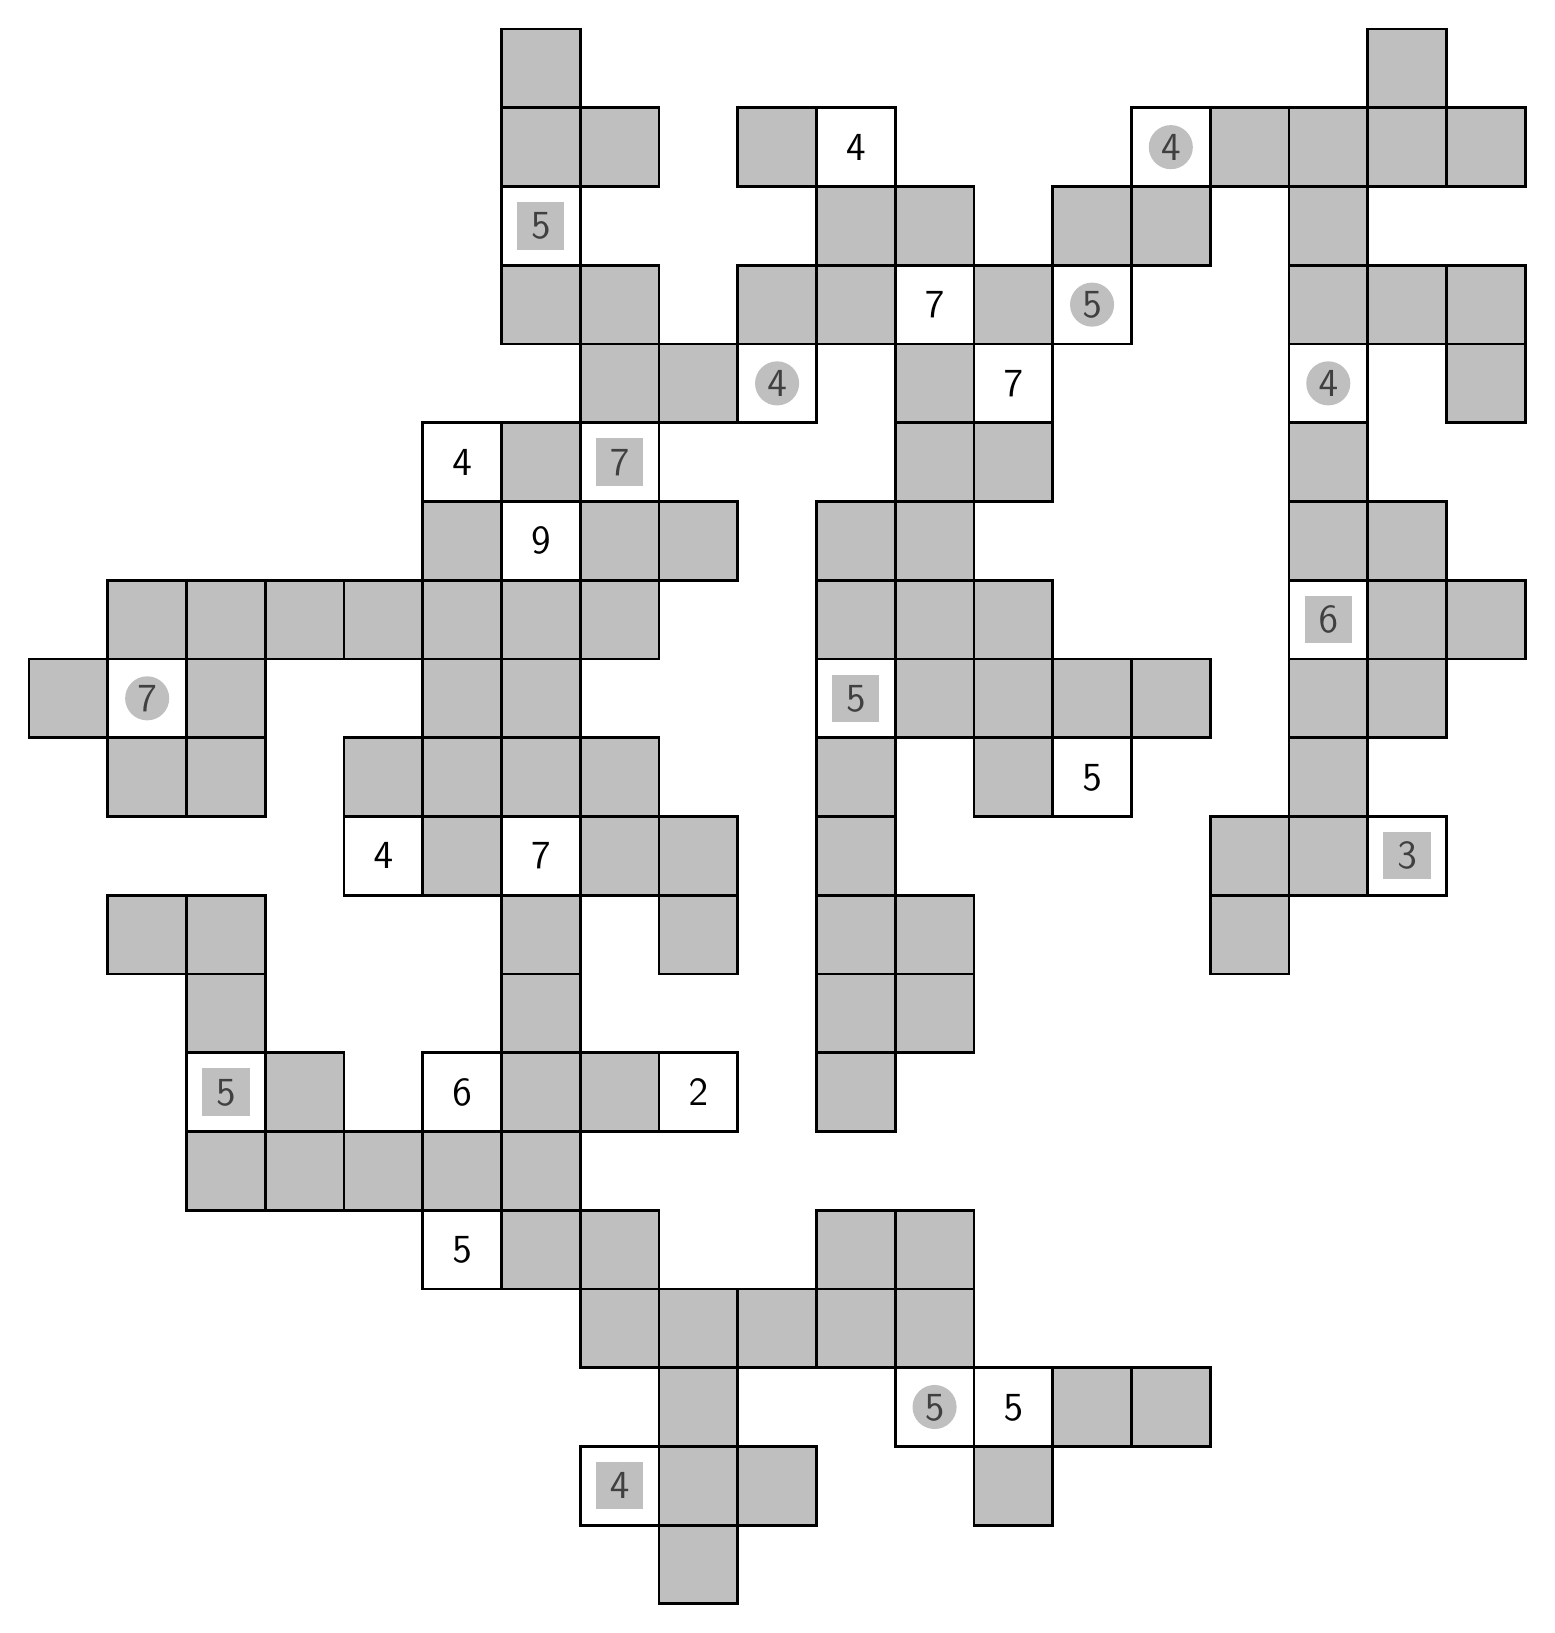
\begin{tikzpicture}\fill[gray, opacity = 0.5] (9, 0, 0)--++(1, 0, 0)--++(0, 1, 0)--++(-1, 0, 0)--cycle;
\draw[line width = 1pt] (9, 0, 0)--++(1, 0, 0)--++(0, 1, 0)--++(-1, 0, 0)--cycle;
\draw node at (8.5, 1.5, 0) {\Large $\mathsf{4}$};
\draw[line width = 1pt] (8, 1, 0)--++(1, 0, 0)--++(0, 1, 0)--++(-1, 0, 0)--cycle;
\fill[color = gray, opacity = 0.5] (8.2, 1.2) rectangle ++(0.6, 0.6);
\fill[gray, opacity = 0.5] (9, 1, 0)--++(1, 0, 0)--++(0, 1, 0)--++(-1, 0, 0)--cycle;
\draw[line width = 1pt] (9, 1, 0)--++(1, 0, 0)--++(0, 1, 0)--++(-1, 0, 0)--cycle;
\fill[gray, opacity = 0.5] (10, 1, 0)--++(1, 0, 0)--++(0, 1, 0)--++(-1, 0, 0)--cycle;
\draw[line width = 1pt] (10, 1, 0)--++(1, 0, 0)--++(0, 1, 0)--++(-1, 0, 0)--cycle;
\fill[gray, opacity = 0.5] (13, 1, 0)--++(1, 0, 0)--++(0, 1, 0)--++(-1, 0, 0)--cycle;
\draw[line width = 1pt] (13, 1, 0)--++(1, 0, 0)--++(0, 1, 0)--++(-1, 0, 0)--cycle;
\fill[gray, opacity = 0.5] (9, 2, 0)--++(1, 0, 0)--++(0, 1, 0)--++(-1, 0, 0)--cycle;
\draw[line width = 1pt] (9, 2, 0)--++(1, 0, 0)--++(0, 1, 0)--++(-1, 0, 0)--cycle;
\draw node at (12.5, 2.5, 0) {\Large $\mathsf{5}$};
\draw[line width = 1pt] (12, 2, 0)--++(1, 0, 0)--++(0, 1, 0)--++(-1, 0, 0)--cycle;
\fill[color = gray, opacity = 0.5] (12.5, 2.5, 0) circle (0.28);
\draw node at (13.5, 2.5, 0) {\Large $\mathsf{5}$};
\draw[line width = 1pt] (13, 2, 0)--++(1, 0, 0)--++(0, 1, 0)--++(-1, 0, 0)--cycle;
\fill[gray, opacity = 0.5] (14, 2, 0)--++(1, 0, 0)--++(0, 1, 0)--++(-1, 0, 0)--cycle;
\draw[line width = 1pt] (14, 2, 0)--++(1, 0, 0)--++(0, 1, 0)--++(-1, 0, 0)--cycle;
\fill[gray, opacity = 0.5] (15, 2, 0)--++(1, 0, 0)--++(0, 1, 0)--++(-1, 0, 0)--cycle;
\draw[line width = 1pt] (15, 2, 0)--++(1, 0, 0)--++(0, 1, 0)--++(-1, 0, 0)--cycle;
\fill[gray, opacity = 0.5] (8, 3, 0)--++(1, 0, 0)--++(0, 1, 0)--++(-1, 0, 0)--cycle;
\draw[line width = 1pt] (8, 3, 0)--++(1, 0, 0)--++(0, 1, 0)--++(-1, 0, 0)--cycle;
\fill[gray, opacity = 0.5] (9, 3, 0)--++(1, 0, 0)--++(0, 1, 0)--++(-1, 0, 0)--cycle;
\draw[line width = 1pt] (9, 3, 0)--++(1, 0, 0)--++(0, 1, 0)--++(-1, 0, 0)--cycle;
\fill[gray, opacity = 0.5] (10, 3, 0)--++(1, 0, 0)--++(0, 1, 0)--++(-1, 0, 0)--cycle;
\draw[line width = 1pt] (10, 3, 0)--++(1, 0, 0)--++(0, 1, 0)--++(-1, 0, 0)--cycle;
\fill[gray, opacity = 0.5] (11, 3, 0)--++(1, 0, 0)--++(0, 1, 0)--++(-1, 0, 0)--cycle;
\draw[line width = 1pt] (11, 3, 0)--++(1, 0, 0)--++(0, 1, 0)--++(-1, 0, 0)--cycle;
\fill[gray, opacity = 0.5] (12, 3, 0)--++(1, 0, 0)--++(0, 1, 0)--++(-1, 0, 0)--cycle;
\draw[line width = 1pt] (12, 3, 0)--++(1, 0, 0)--++(0, 1, 0)--++(-1, 0, 0)--cycle;
\draw node at (6.5, 4.5, 0) {\Large $\mathsf{5}$};
\draw[line width = 1pt] (6, 4, 0)--++(1, 0, 0)--++(0, 1, 0)--++(-1, 0, 0)--cycle;
\fill[gray, opacity = 0.5] (7, 4, 0)--++(1, 0, 0)--++(0, 1, 0)--++(-1, 0, 0)--cycle;
\draw[line width = 1pt] (7, 4, 0)--++(1, 0, 0)--++(0, 1, 0)--++(-1, 0, 0)--cycle;
\fill[gray, opacity = 0.5] (8, 4, 0)--++(1, 0, 0)--++(0, 1, 0)--++(-1, 0, 0)--cycle;
\draw[line width = 1pt] (8, 4, 0)--++(1, 0, 0)--++(0, 1, 0)--++(-1, 0, 0)--cycle;
\fill[gray, opacity = 0.5] (11, 4, 0)--++(1, 0, 0)--++(0, 1, 0)--++(-1, 0, 0)--cycle;
\draw[line width = 1pt] (11, 4, 0)--++(1, 0, 0)--++(0, 1, 0)--++(-1, 0, 0)--cycle;
\fill[gray, opacity = 0.5] (12, 4, 0)--++(1, 0, 0)--++(0, 1, 0)--++(-1, 0, 0)--cycle;
\draw[line width = 1pt] (12, 4, 0)--++(1, 0, 0)--++(0, 1, 0)--++(-1, 0, 0)--cycle;
\fill[gray, opacity = 0.5] (3, 5, 0)--++(1, 0, 0)--++(0, 1, 0)--++(-1, 0, 0)--cycle;
\draw[line width = 1pt] (3, 5, 0)--++(1, 0, 0)--++(0, 1, 0)--++(-1, 0, 0)--cycle;
\fill[gray, opacity = 0.5] (4, 5, 0)--++(1, 0, 0)--++(0, 1, 0)--++(-1, 0, 0)--cycle;
\draw[line width = 1pt] (4, 5, 0)--++(1, 0, 0)--++(0, 1, 0)--++(-1, 0, 0)--cycle;
\fill[gray, opacity = 0.5] (5, 5, 0)--++(1, 0, 0)--++(0, 1, 0)--++(-1, 0, 0)--cycle;
\draw[line width = 1pt] (5, 5, 0)--++(1, 0, 0)--++(0, 1, 0)--++(-1, 0, 0)--cycle;
\fill[gray, opacity = 0.5] (6, 5, 0)--++(1, 0, 0)--++(0, 1, 0)--++(-1, 0, 0)--cycle;
\draw[line width = 1pt] (6, 5, 0)--++(1, 0, 0)--++(0, 1, 0)--++(-1, 0, 0)--cycle;
\fill[gray, opacity = 0.5] (7, 5, 0)--++(1, 0, 0)--++(0, 1, 0)--++(-1, 0, 0)--cycle;
\draw[line width = 1pt] (7, 5, 0)--++(1, 0, 0)--++(0, 1, 0)--++(-1, 0, 0)--cycle;
\draw node at (3.5, 6.5, 0) {\Large $\mathsf{5}$};
\draw[line width = 1pt] (3, 6, 0)--++(1, 0, 0)--++(0, 1, 0)--++(-1, 0, 0)--cycle;
\fill[color = gray, opacity = 0.5] (3.2, 6.2) rectangle ++(0.6, 0.6);
\fill[gray, opacity = 0.5] (4, 6, 0)--++(1, 0, 0)--++(0, 1, 0)--++(-1, 0, 0)--cycle;
\draw[line width = 1pt] (4, 6, 0)--++(1, 0, 0)--++(0, 1, 0)--++(-1, 0, 0)--cycle;
\draw node at (6.5, 6.5, 0) {\Large $\mathsf{6}$};
\draw[line width = 1pt] (6, 6, 0)--++(1, 0, 0)--++(0, 1, 0)--++(-1, 0, 0)--cycle;
\fill[gray, opacity = 0.5] (7, 6, 0)--++(1, 0, 0)--++(0, 1, 0)--++(-1, 0, 0)--cycle;
\draw[line width = 1pt] (7, 6, 0)--++(1, 0, 0)--++(0, 1, 0)--++(-1, 0, 0)--cycle;
\fill[gray, opacity = 0.5] (8, 6, 0)--++(1, 0, 0)--++(0, 1, 0)--++(-1, 0, 0)--cycle;
\draw[line width = 1pt] (8, 6, 0)--++(1, 0, 0)--++(0, 1, 0)--++(-1, 0, 0)--cycle;
\draw node at (9.5, 6.5, 0) {\Large $\mathsf{2}$};
\draw[line width = 1pt] (9, 6, 0)--++(1, 0, 0)--++(0, 1, 0)--++(-1, 0, 0)--cycle;
\fill[gray, opacity = 0.5] (11, 6, 0)--++(1, 0, 0)--++(0, 1, 0)--++(-1, 0, 0)--cycle;
\draw[line width = 1pt] (11, 6, 0)--++(1, 0, 0)--++(0, 1, 0)--++(-1, 0, 0)--cycle;
\fill[gray, opacity = 0.5] (3, 7, 0)--++(1, 0, 0)--++(0, 1, 0)--++(-1, 0, 0)--cycle;
\draw[line width = 1pt] (3, 7, 0)--++(1, 0, 0)--++(0, 1, 0)--++(-1, 0, 0)--cycle;
\fill[gray, opacity = 0.5] (7, 7, 0)--++(1, 0, 0)--++(0, 1, 0)--++(-1, 0, 0)--cycle;
\draw[line width = 1pt] (7, 7, 0)--++(1, 0, 0)--++(0, 1, 0)--++(-1, 0, 0)--cycle;
\fill[gray, opacity = 0.5] (11, 7, 0)--++(1, 0, 0)--++(0, 1, 0)--++(-1, 0, 0)--cycle;
\draw[line width = 1pt] (11, 7, 0)--++(1, 0, 0)--++(0, 1, 0)--++(-1, 0, 0)--cycle;
\fill[gray, opacity = 0.5] (12, 7, 0)--++(1, 0, 0)--++(0, 1, 0)--++(-1, 0, 0)--cycle;
\draw[line width = 1pt] (12, 7, 0)--++(1, 0, 0)--++(0, 1, 0)--++(-1, 0, 0)--cycle;
\fill[gray, opacity = 0.5] (2, 8, 0)--++(1, 0, 0)--++(0, 1, 0)--++(-1, 0, 0)--cycle;
\draw[line width = 1pt] (2, 8, 0)--++(1, 0, 0)--++(0, 1, 0)--++(-1, 0, 0)--cycle;
\fill[gray, opacity = 0.5] (3, 8, 0)--++(1, 0, 0)--++(0, 1, 0)--++(-1, 0, 0)--cycle;
\draw[line width = 1pt] (3, 8, 0)--++(1, 0, 0)--++(0, 1, 0)--++(-1, 0, 0)--cycle;
\fill[gray, opacity = 0.5] (7, 8, 0)--++(1, 0, 0)--++(0, 1, 0)--++(-1, 0, 0)--cycle;
\draw[line width = 1pt] (7, 8, 0)--++(1, 0, 0)--++(0, 1, 0)--++(-1, 0, 0)--cycle;
\fill[gray, opacity = 0.5] (9, 8, 0)--++(1, 0, 0)--++(0, 1, 0)--++(-1, 0, 0)--cycle;
\draw[line width = 1pt] (9, 8, 0)--++(1, 0, 0)--++(0, 1, 0)--++(-1, 0, 0)--cycle;
\fill[gray, opacity = 0.5] (11, 8, 0)--++(1, 0, 0)--++(0, 1, 0)--++(-1, 0, 0)--cycle;
\draw[line width = 1pt] (11, 8, 0)--++(1, 0, 0)--++(0, 1, 0)--++(-1, 0, 0)--cycle;
\fill[gray, opacity = 0.5] (12, 8, 0)--++(1, 0, 0)--++(0, 1, 0)--++(-1, 0, 0)--cycle;
\draw[line width = 1pt] (12, 8, 0)--++(1, 0, 0)--++(0, 1, 0)--++(-1, 0, 0)--cycle;
\fill[gray, opacity = 0.5] (16, 8, 0)--++(1, 0, 0)--++(0, 1, 0)--++(-1, 0, 0)--cycle;
\draw[line width = 1pt] (16, 8, 0)--++(1, 0, 0)--++(0, 1, 0)--++(-1, 0, 0)--cycle;
\draw node at (5.5, 9.5, 0) {\Large $\mathsf{4}$};
\draw[line width = 1pt] (5, 9, 0)--++(1, 0, 0)--++(0, 1, 0)--++(-1, 0, 0)--cycle;
\fill[gray, opacity = 0.5] (6, 9, 0)--++(1, 0, 0)--++(0, 1, 0)--++(-1, 0, 0)--cycle;
\draw[line width = 1pt] (6, 9, 0)--++(1, 0, 0)--++(0, 1, 0)--++(-1, 0, 0)--cycle;
\draw node at (7.5, 9.5, 0) {\Large $\mathsf{7}$};
\draw[line width = 1pt] (7, 9, 0)--++(1, 0, 0)--++(0, 1, 0)--++(-1, 0, 0)--cycle;
\fill[gray, opacity = 0.5] (8, 9, 0)--++(1, 0, 0)--++(0, 1, 0)--++(-1, 0, 0)--cycle;
\draw[line width = 1pt] (8, 9, 0)--++(1, 0, 0)--++(0, 1, 0)--++(-1, 0, 0)--cycle;
\fill[gray, opacity = 0.5] (9, 9, 0)--++(1, 0, 0)--++(0, 1, 0)--++(-1, 0, 0)--cycle;
\draw[line width = 1pt] (9, 9, 0)--++(1, 0, 0)--++(0, 1, 0)--++(-1, 0, 0)--cycle;
\fill[gray, opacity = 0.5] (11, 9, 0)--++(1, 0, 0)--++(0, 1, 0)--++(-1, 0, 0)--cycle;
\draw[line width = 1pt] (11, 9, 0)--++(1, 0, 0)--++(0, 1, 0)--++(-1, 0, 0)--cycle;
\fill[gray, opacity = 0.5] (16, 9, 0)--++(1, 0, 0)--++(0, 1, 0)--++(-1, 0, 0)--cycle;
\draw[line width = 1pt] (16, 9, 0)--++(1, 0, 0)--++(0, 1, 0)--++(-1, 0, 0)--cycle;
\fill[gray, opacity = 0.5] (17, 9, 0)--++(1, 0, 0)--++(0, 1, 0)--++(-1, 0, 0)--cycle;
\draw[line width = 1pt] (17, 9, 0)--++(1, 0, 0)--++(0, 1, 0)--++(-1, 0, 0)--cycle;
\draw node at (18.5, 9.5, 0) {\Large $\mathsf{3}$};
\draw[line width = 1pt] (18, 9, 0)--++(1, 0, 0)--++(0, 1, 0)--++(-1, 0, 0)--cycle;
\fill[color = gray, opacity = 0.5] (18.2, 9.2) rectangle ++(0.6, 0.6);
\fill[gray, opacity = 0.5] (2, 10, 0)--++(1, 0, 0)--++(0, 1, 0)--++(-1, 0, 0)--cycle;
\draw[line width = 1pt] (2, 10, 0)--++(1, 0, 0)--++(0, 1, 0)--++(-1, 0, 0)--cycle;
\fill[gray, opacity = 0.5] (3, 10, 0)--++(1, 0, 0)--++(0, 1, 0)--++(-1, 0, 0)--cycle;
\draw[line width = 1pt] (3, 10, 0)--++(1, 0, 0)--++(0, 1, 0)--++(-1, 0, 0)--cycle;
\fill[gray, opacity = 0.5] (5, 10, 0)--++(1, 0, 0)--++(0, 1, 0)--++(-1, 0, 0)--cycle;
\draw[line width = 1pt] (5, 10, 0)--++(1, 0, 0)--++(0, 1, 0)--++(-1, 0, 0)--cycle;
\fill[gray, opacity = 0.5] (6, 10, 0)--++(1, 0, 0)--++(0, 1, 0)--++(-1, 0, 0)--cycle;
\draw[line width = 1pt] (6, 10, 0)--++(1, 0, 0)--++(0, 1, 0)--++(-1, 0, 0)--cycle;
\fill[gray, opacity = 0.5] (7, 10, 0)--++(1, 0, 0)--++(0, 1, 0)--++(-1, 0, 0)--cycle;
\draw[line width = 1pt] (7, 10, 0)--++(1, 0, 0)--++(0, 1, 0)--++(-1, 0, 0)--cycle;
\fill[gray, opacity = 0.5] (8, 10, 0)--++(1, 0, 0)--++(0, 1, 0)--++(-1, 0, 0)--cycle;
\draw[line width = 1pt] (8, 10, 0)--++(1, 0, 0)--++(0, 1, 0)--++(-1, 0, 0)--cycle;
\fill[gray, opacity = 0.5] (11, 10, 0)--++(1, 0, 0)--++(0, 1, 0)--++(-1, 0, 0)--cycle;
\draw[line width = 1pt] (11, 10, 0)--++(1, 0, 0)--++(0, 1, 0)--++(-1, 0, 0)--cycle;
\fill[gray, opacity = 0.5] (13, 10, 0)--++(1, 0, 0)--++(0, 1, 0)--++(-1, 0, 0)--cycle;
\draw[line width = 1pt] (13, 10, 0)--++(1, 0, 0)--++(0, 1, 0)--++(-1, 0, 0)--cycle;
\draw node at (14.5, 10.5, 0) {\Large $\mathsf{5}$};
\draw[line width = 1pt] (14, 10, 0)--++(1, 0, 0)--++(0, 1, 0)--++(-1, 0, 0)--cycle;
\fill[gray, opacity = 0.5] (17, 10, 0)--++(1, 0, 0)--++(0, 1, 0)--++(-1, 0, 0)--cycle;
\draw[line width = 1pt] (17, 10, 0)--++(1, 0, 0)--++(0, 1, 0)--++(-1, 0, 0)--cycle;
\fill[gray, opacity = 0.5] (1, 11, 0)--++(1, 0, 0)--++(0, 1, 0)--++(-1, 0, 0)--cycle;
\draw[line width = 1pt] (1, 11, 0)--++(1, 0, 0)--++(0, 1, 0)--++(-1, 0, 0)--cycle;
\draw node at (2.5, 11.5, 0) {\Large $\mathsf{7}$};
\draw[line width = 1pt] (2, 11, 0)--++(1, 0, 0)--++(0, 1, 0)--++(-1, 0, 0)--cycle;
\fill[color = gray, opacity = 0.5] (2.5, 11.5, 0) circle (0.28);
\fill[gray, opacity = 0.5] (3, 11, 0)--++(1, 0, 0)--++(0, 1, 0)--++(-1, 0, 0)--cycle;
\draw[line width = 1pt] (3, 11, 0)--++(1, 0, 0)--++(0, 1, 0)--++(-1, 0, 0)--cycle;
\fill[gray, opacity = 0.5] (6, 11, 0)--++(1, 0, 0)--++(0, 1, 0)--++(-1, 0, 0)--cycle;
\draw[line width = 1pt] (6, 11, 0)--++(1, 0, 0)--++(0, 1, 0)--++(-1, 0, 0)--cycle;
\fill[gray, opacity = 0.5] (7, 11, 0)--++(1, 0, 0)--++(0, 1, 0)--++(-1, 0, 0)--cycle;
\draw[line width = 1pt] (7, 11, 0)--++(1, 0, 0)--++(0, 1, 0)--++(-1, 0, 0)--cycle;
\draw node at (11.5, 11.5, 0) {\Large $\mathsf{5}$};
\draw[line width = 1pt] (11, 11, 0)--++(1, 0, 0)--++(0, 1, 0)--++(-1, 0, 0)--cycle;
\fill[color = gray, opacity = 0.5] (11.2, 11.2) rectangle ++(0.6, 0.6);
\fill[gray, opacity = 0.5] (12, 11, 0)--++(1, 0, 0)--++(0, 1, 0)--++(-1, 0, 0)--cycle;
\draw[line width = 1pt] (12, 11, 0)--++(1, 0, 0)--++(0, 1, 0)--++(-1, 0, 0)--cycle;
\fill[gray, opacity = 0.5] (13, 11, 0)--++(1, 0, 0)--++(0, 1, 0)--++(-1, 0, 0)--cycle;
\draw[line width = 1pt] (13, 11, 0)--++(1, 0, 0)--++(0, 1, 0)--++(-1, 0, 0)--cycle;
\fill[gray, opacity = 0.5] (14, 11, 0)--++(1, 0, 0)--++(0, 1, 0)--++(-1, 0, 0)--cycle;
\draw[line width = 1pt] (14, 11, 0)--++(1, 0, 0)--++(0, 1, 0)--++(-1, 0, 0)--cycle;
\fill[gray, opacity = 0.5] (15, 11, 0)--++(1, 0, 0)--++(0, 1, 0)--++(-1, 0, 0)--cycle;
\draw[line width = 1pt] (15, 11, 0)--++(1, 0, 0)--++(0, 1, 0)--++(-1, 0, 0)--cycle;
\fill[gray, opacity = 0.5] (17, 11, 0)--++(1, 0, 0)--++(0, 1, 0)--++(-1, 0, 0)--cycle;
\draw[line width = 1pt] (17, 11, 0)--++(1, 0, 0)--++(0, 1, 0)--++(-1, 0, 0)--cycle;
\fill[gray, opacity = 0.5] (18, 11, 0)--++(1, 0, 0)--++(0, 1, 0)--++(-1, 0, 0)--cycle;
\draw[line width = 1pt] (18, 11, 0)--++(1, 0, 0)--++(0, 1, 0)--++(-1, 0, 0)--cycle;
\fill[gray, opacity = 0.5] (2, 12, 0)--++(1, 0, 0)--++(0, 1, 0)--++(-1, 0, 0)--cycle;
\draw[line width = 1pt] (2, 12, 0)--++(1, 0, 0)--++(0, 1, 0)--++(-1, 0, 0)--cycle;
\fill[gray, opacity = 0.5] (3, 12, 0)--++(1, 0, 0)--++(0, 1, 0)--++(-1, 0, 0)--cycle;
\draw[line width = 1pt] (3, 12, 0)--++(1, 0, 0)--++(0, 1, 0)--++(-1, 0, 0)--cycle;
\fill[gray, opacity = 0.5] (4, 12, 0)--++(1, 0, 0)--++(0, 1, 0)--++(-1, 0, 0)--cycle;
\draw[line width = 1pt] (4, 12, 0)--++(1, 0, 0)--++(0, 1, 0)--++(-1, 0, 0)--cycle;
\fill[gray, opacity = 0.5] (5, 12, 0)--++(1, 0, 0)--++(0, 1, 0)--++(-1, 0, 0)--cycle;
\draw[line width = 1pt] (5, 12, 0)--++(1, 0, 0)--++(0, 1, 0)--++(-1, 0, 0)--cycle;
\fill[gray, opacity = 0.5] (6, 12, 0)--++(1, 0, 0)--++(0, 1, 0)--++(-1, 0, 0)--cycle;
\draw[line width = 1pt] (6, 12, 0)--++(1, 0, 0)--++(0, 1, 0)--++(-1, 0, 0)--cycle;
\fill[gray, opacity = 0.5] (7, 12, 0)--++(1, 0, 0)--++(0, 1, 0)--++(-1, 0, 0)--cycle;
\draw[line width = 1pt] (7, 12, 0)--++(1, 0, 0)--++(0, 1, 0)--++(-1, 0, 0)--cycle;
\fill[gray, opacity = 0.5] (8, 12, 0)--++(1, 0, 0)--++(0, 1, 0)--++(-1, 0, 0)--cycle;
\draw[line width = 1pt] (8, 12, 0)--++(1, 0, 0)--++(0, 1, 0)--++(-1, 0, 0)--cycle;
\fill[gray, opacity = 0.5] (11, 12, 0)--++(1, 0, 0)--++(0, 1, 0)--++(-1, 0, 0)--cycle;
\draw[line width = 1pt] (11, 12, 0)--++(1, 0, 0)--++(0, 1, 0)--++(-1, 0, 0)--cycle;
\fill[gray, opacity = 0.5] (12, 12, 0)--++(1, 0, 0)--++(0, 1, 0)--++(-1, 0, 0)--cycle;
\draw[line width = 1pt] (12, 12, 0)--++(1, 0, 0)--++(0, 1, 0)--++(-1, 0, 0)--cycle;
\fill[gray, opacity = 0.5] (13, 12, 0)--++(1, 0, 0)--++(0, 1, 0)--++(-1, 0, 0)--cycle;
\draw[line width = 1pt] (13, 12, 0)--++(1, 0, 0)--++(0, 1, 0)--++(-1, 0, 0)--cycle;
\draw node at (17.5, 12.5, 0) {\Large $\mathsf{6}$};
\draw[line width = 1pt] (17, 12, 0)--++(1, 0, 0)--++(0, 1, 0)--++(-1, 0, 0)--cycle;
\fill[color = gray, opacity = 0.5] (17.2, 12.2) rectangle ++(0.6, 0.6);
\fill[gray, opacity = 0.5] (18, 12, 0)--++(1, 0, 0)--++(0, 1, 0)--++(-1, 0, 0)--cycle;
\draw[line width = 1pt] (18, 12, 0)--++(1, 0, 0)--++(0, 1, 0)--++(-1, 0, 0)--cycle;
\fill[gray, opacity = 0.5] (19, 12, 0)--++(1, 0, 0)--++(0, 1, 0)--++(-1, 0, 0)--cycle;
\draw[line width = 1pt] (19, 12, 0)--++(1, 0, 0)--++(0, 1, 0)--++(-1, 0, 0)--cycle;
\fill[gray, opacity = 0.5] (6, 13, 0)--++(1, 0, 0)--++(0, 1, 0)--++(-1, 0, 0)--cycle;
\draw[line width = 1pt] (6, 13, 0)--++(1, 0, 0)--++(0, 1, 0)--++(-1, 0, 0)--cycle;
\draw node at (7.5, 13.5, 0) {\Large $\mathsf{9}$};
\draw[line width = 1pt] (7, 13, 0)--++(1, 0, 0)--++(0, 1, 0)--++(-1, 0, 0)--cycle;
\fill[gray, opacity = 0.5] (8, 13, 0)--++(1, 0, 0)--++(0, 1, 0)--++(-1, 0, 0)--cycle;
\draw[line width = 1pt] (8, 13, 0)--++(1, 0, 0)--++(0, 1, 0)--++(-1, 0, 0)--cycle;
\fill[gray, opacity = 0.5] (9, 13, 0)--++(1, 0, 0)--++(0, 1, 0)--++(-1, 0, 0)--cycle;
\draw[line width = 1pt] (9, 13, 0)--++(1, 0, 0)--++(0, 1, 0)--++(-1, 0, 0)--cycle;
\fill[gray, opacity = 0.5] (11, 13, 0)--++(1, 0, 0)--++(0, 1, 0)--++(-1, 0, 0)--cycle;
\draw[line width = 1pt] (11, 13, 0)--++(1, 0, 0)--++(0, 1, 0)--++(-1, 0, 0)--cycle;
\fill[gray, opacity = 0.5] (12, 13, 0)--++(1, 0, 0)--++(0, 1, 0)--++(-1, 0, 0)--cycle;
\draw[line width = 1pt] (12, 13, 0)--++(1, 0, 0)--++(0, 1, 0)--++(-1, 0, 0)--cycle;
\fill[gray, opacity = 0.5] (17, 13, 0)--++(1, 0, 0)--++(0, 1, 0)--++(-1, 0, 0)--cycle;
\draw[line width = 1pt] (17, 13, 0)--++(1, 0, 0)--++(0, 1, 0)--++(-1, 0, 0)--cycle;
\fill[gray, opacity = 0.5] (18, 13, 0)--++(1, 0, 0)--++(0, 1, 0)--++(-1, 0, 0)--cycle;
\draw[line width = 1pt] (18, 13, 0)--++(1, 0, 0)--++(0, 1, 0)--++(-1, 0, 0)--cycle;
\draw node at (6.5, 14.5, 0) {\Large $\mathsf{4}$};
\draw[line width = 1pt] (6, 14, 0)--++(1, 0, 0)--++(0, 1, 0)--++(-1, 0, 0)--cycle;
\fill[gray, opacity = 0.5] (7, 14, 0)--++(1, 0, 0)--++(0, 1, 0)--++(-1, 0, 0)--cycle;
\draw[line width = 1pt] (7, 14, 0)--++(1, 0, 0)--++(0, 1, 0)--++(-1, 0, 0)--cycle;
\draw node at (8.5, 14.5, 0) {\Large $\mathsf{7}$};
\draw[line width = 1pt] (8, 14, 0)--++(1, 0, 0)--++(0, 1, 0)--++(-1, 0, 0)--cycle;
\fill[color = gray, opacity = 0.5] (8.2, 14.2) rectangle ++(0.6, 0.6);
\fill[gray, opacity = 0.5] (12, 14, 0)--++(1, 0, 0)--++(0, 1, 0)--++(-1, 0, 0)--cycle;
\draw[line width = 1pt] (12, 14, 0)--++(1, 0, 0)--++(0, 1, 0)--++(-1, 0, 0)--cycle;
\fill[gray, opacity = 0.5] (13, 14, 0)--++(1, 0, 0)--++(0, 1, 0)--++(-1, 0, 0)--cycle;
\draw[line width = 1pt] (13, 14, 0)--++(1, 0, 0)--++(0, 1, 0)--++(-1, 0, 0)--cycle;
\fill[gray, opacity = 0.5] (17, 14, 0)--++(1, 0, 0)--++(0, 1, 0)--++(-1, 0, 0)--cycle;
\draw[line width = 1pt] (17, 14, 0)--++(1, 0, 0)--++(0, 1, 0)--++(-1, 0, 0)--cycle;
\fill[gray, opacity = 0.5] (8, 15, 0)--++(1, 0, 0)--++(0, 1, 0)--++(-1, 0, 0)--cycle;
\draw[line width = 1pt] (8, 15, 0)--++(1, 0, 0)--++(0, 1, 0)--++(-1, 0, 0)--cycle;
\fill[gray, opacity = 0.5] (9, 15, 0)--++(1, 0, 0)--++(0, 1, 0)--++(-1, 0, 0)--cycle;
\draw[line width = 1pt] (9, 15, 0)--++(1, 0, 0)--++(0, 1, 0)--++(-1, 0, 0)--cycle;
\draw node at (10.5, 15.5, 0) {\Large $\mathsf{4}$};
\draw[line width = 1pt] (10, 15, 0)--++(1, 0, 0)--++(0, 1, 0)--++(-1, 0, 0)--cycle;
\fill[color = gray, opacity = 0.5] (10.5, 15.5, 0) circle (0.28);
\fill[gray, opacity = 0.5] (12, 15, 0)--++(1, 0, 0)--++(0, 1, 0)--++(-1, 0, 0)--cycle;
\draw[line width = 1pt] (12, 15, 0)--++(1, 0, 0)--++(0, 1, 0)--++(-1, 0, 0)--cycle;
\draw node at (13.5, 15.5, 0) {\Large $\mathsf{7}$};
\draw[line width = 1pt] (13, 15, 0)--++(1, 0, 0)--++(0, 1, 0)--++(-1, 0, 0)--cycle;
\draw node at (17.5, 15.5, 0) {\Large $\mathsf{4}$};
\draw[line width = 1pt] (17, 15, 0)--++(1, 0, 0)--++(0, 1, 0)--++(-1, 0, 0)--cycle;
\fill[color = gray, opacity = 0.5] (17.5, 15.5, 0) circle (0.28);
\fill[gray, opacity = 0.5] (19, 15, 0)--++(1, 0, 0)--++(0, 1, 0)--++(-1, 0, 0)--cycle;
\draw[line width = 1pt] (19, 15, 0)--++(1, 0, 0)--++(0, 1, 0)--++(-1, 0, 0)--cycle;
\fill[gray, opacity = 0.5] (7, 16, 0)--++(1, 0, 0)--++(0, 1, 0)--++(-1, 0, 0)--cycle;
\draw[line width = 1pt] (7, 16, 0)--++(1, 0, 0)--++(0, 1, 0)--++(-1, 0, 0)--cycle;
\fill[gray, opacity = 0.5] (8, 16, 0)--++(1, 0, 0)--++(0, 1, 0)--++(-1, 0, 0)--cycle;
\draw[line width = 1pt] (8, 16, 0)--++(1, 0, 0)--++(0, 1, 0)--++(-1, 0, 0)--cycle;
\fill[gray, opacity = 0.5] (10, 16, 0)--++(1, 0, 0)--++(0, 1, 0)--++(-1, 0, 0)--cycle;
\draw[line width = 1pt] (10, 16, 0)--++(1, 0, 0)--++(0, 1, 0)--++(-1, 0, 0)--cycle;
\fill[gray, opacity = 0.5] (11, 16, 0)--++(1, 0, 0)--++(0, 1, 0)--++(-1, 0, 0)--cycle;
\draw[line width = 1pt] (11, 16, 0)--++(1, 0, 0)--++(0, 1, 0)--++(-1, 0, 0)--cycle;
\draw node at (12.5, 16.5, 0) {\Large $\mathsf{7}$};
\draw[line width = 1pt] (12, 16, 0)--++(1, 0, 0)--++(0, 1, 0)--++(-1, 0, 0)--cycle;
\fill[gray, opacity = 0.5] (13, 16, 0)--++(1, 0, 0)--++(0, 1, 0)--++(-1, 0, 0)--cycle;
\draw[line width = 1pt] (13, 16, 0)--++(1, 0, 0)--++(0, 1, 0)--++(-1, 0, 0)--cycle;
\draw node at (14.5, 16.5, 0) {\Large $\mathsf{5}$};
\draw[line width = 1pt] (14, 16, 0)--++(1, 0, 0)--++(0, 1, 0)--++(-1, 0, 0)--cycle;
\fill[color = gray, opacity = 0.5] (14.5, 16.5, 0) circle (0.28);
\fill[gray, opacity = 0.5] (17, 16, 0)--++(1, 0, 0)--++(0, 1, 0)--++(-1, 0, 0)--cycle;
\draw[line width = 1pt] (17, 16, 0)--++(1, 0, 0)--++(0, 1, 0)--++(-1, 0, 0)--cycle;
\fill[gray, opacity = 0.5] (18, 16, 0)--++(1, 0, 0)--++(0, 1, 0)--++(-1, 0, 0)--cycle;
\draw[line width = 1pt] (18, 16, 0)--++(1, 0, 0)--++(0, 1, 0)--++(-1, 0, 0)--cycle;
\fill[gray, opacity = 0.5] (19, 16, 0)--++(1, 0, 0)--++(0, 1, 0)--++(-1, 0, 0)--cycle;
\draw[line width = 1pt] (19, 16, 0)--++(1, 0, 0)--++(0, 1, 0)--++(-1, 0, 0)--cycle;
\draw node at (7.5, 17.5, 0) {\Large $\mathsf{5}$};
\draw[line width = 1pt] (7, 17, 0)--++(1, 0, 0)--++(0, 1, 0)--++(-1, 0, 0)--cycle;
\fill[color = gray, opacity = 0.5] (7.2, 17.2) rectangle ++(0.6, 0.6);
\fill[gray, opacity = 0.5] (11, 17, 0)--++(1, 0, 0)--++(0, 1, 0)--++(-1, 0, 0)--cycle;
\draw[line width = 1pt] (11, 17, 0)--++(1, 0, 0)--++(0, 1, 0)--++(-1, 0, 0)--cycle;
\fill[gray, opacity = 0.5] (12, 17, 0)--++(1, 0, 0)--++(0, 1, 0)--++(-1, 0, 0)--cycle;
\draw[line width = 1pt] (12, 17, 0)--++(1, 0, 0)--++(0, 1, 0)--++(-1, 0, 0)--cycle;
\fill[gray, opacity = 0.5] (14, 17, 0)--++(1, 0, 0)--++(0, 1, 0)--++(-1, 0, 0)--cycle;
\draw[line width = 1pt] (14, 17, 0)--++(1, 0, 0)--++(0, 1, 0)--++(-1, 0, 0)--cycle;
\fill[gray, opacity = 0.5] (15, 17, 0)--++(1, 0, 0)--++(0, 1, 0)--++(-1, 0, 0)--cycle;
\draw[line width = 1pt] (15, 17, 0)--++(1, 0, 0)--++(0, 1, 0)--++(-1, 0, 0)--cycle;
\fill[gray, opacity = 0.5] (17, 17, 0)--++(1, 0, 0)--++(0, 1, 0)--++(-1, 0, 0)--cycle;
\draw[line width = 1pt] (17, 17, 0)--++(1, 0, 0)--++(0, 1, 0)--++(-1, 0, 0)--cycle;
\fill[gray, opacity = 0.5] (7, 18, 0)--++(1, 0, 0)--++(0, 1, 0)--++(-1, 0, 0)--cycle;
\draw[line width = 1pt] (7, 18, 0)--++(1, 0, 0)--++(0, 1, 0)--++(-1, 0, 0)--cycle;
\fill[gray, opacity = 0.5] (8, 18, 0)--++(1, 0, 0)--++(0, 1, 0)--++(-1, 0, 0)--cycle;
\draw[line width = 1pt] (8, 18, 0)--++(1, 0, 0)--++(0, 1, 0)--++(-1, 0, 0)--cycle;
\fill[gray, opacity = 0.5] (10, 18, 0)--++(1, 0, 0)--++(0, 1, 0)--++(-1, 0, 0)--cycle;
\draw[line width = 1pt] (10, 18, 0)--++(1, 0, 0)--++(0, 1, 0)--++(-1, 0, 0)--cycle;
\draw node at (11.5, 18.5, 0) {\Large $\mathsf{4}$};
\draw[line width = 1pt] (11, 18, 0)--++(1, 0, 0)--++(0, 1, 0)--++(-1, 0, 0)--cycle;
\draw node at (15.5, 18.5, 0) {\Large $\mathsf{4}$};
\draw[line width = 1pt] (15, 18, 0)--++(1, 0, 0)--++(0, 1, 0)--++(-1, 0, 0)--cycle;
\fill[color = gray, opacity = 0.5] (15.5, 18.5, 0) circle (0.28);
\fill[gray, opacity = 0.5] (16, 18, 0)--++(1, 0, 0)--++(0, 1, 0)--++(-1, 0, 0)--cycle;
\draw[line width = 1pt] (16, 18, 0)--++(1, 0, 0)--++(0, 1, 0)--++(-1, 0, 0)--cycle;
\fill[gray, opacity = 0.5] (17, 18, 0)--++(1, 0, 0)--++(0, 1, 0)--++(-1, 0, 0)--cycle;
\draw[line width = 1pt] (17, 18, 0)--++(1, 0, 0)--++(0, 1, 0)--++(-1, 0, 0)--cycle;
\fill[gray, opacity = 0.5] (18, 18, 0)--++(1, 0, 0)--++(0, 1, 0)--++(-1, 0, 0)--cycle;
\draw[line width = 1pt] (18, 18, 0)--++(1, 0, 0)--++(0, 1, 0)--++(-1, 0, 0)--cycle;
\fill[gray, opacity = 0.5] (19, 18, 0)--++(1, 0, 0)--++(0, 1, 0)--++(-1, 0, 0)--cycle;
\draw[line width = 1pt] (19, 18, 0)--++(1, 0, 0)--++(0, 1, 0)--++(-1, 0, 0)--cycle;
\fill[gray, opacity = 0.5] (7, 19, 0)--++(1, 0, 0)--++(0, 1, 0)--++(-1, 0, 0)--cycle;
\draw[line width = 1pt] (7, 19, 0)--++(1, 0, 0)--++(0, 1, 0)--++(-1, 0, 0)--cycle;
\fill[gray, opacity = 0.5] (18, 19, 0)--++(1, 0, 0)--++(0, 1, 0)--++(-1, 0, 0)--cycle;
\draw[line width = 1pt] (18, 19, 0)--++(1, 0, 0)--++(0, 1, 0)--++(-1, 0, 0)--cycle;
\end{tikzpicture}}\]
\[\resizebox{30pc}{!}{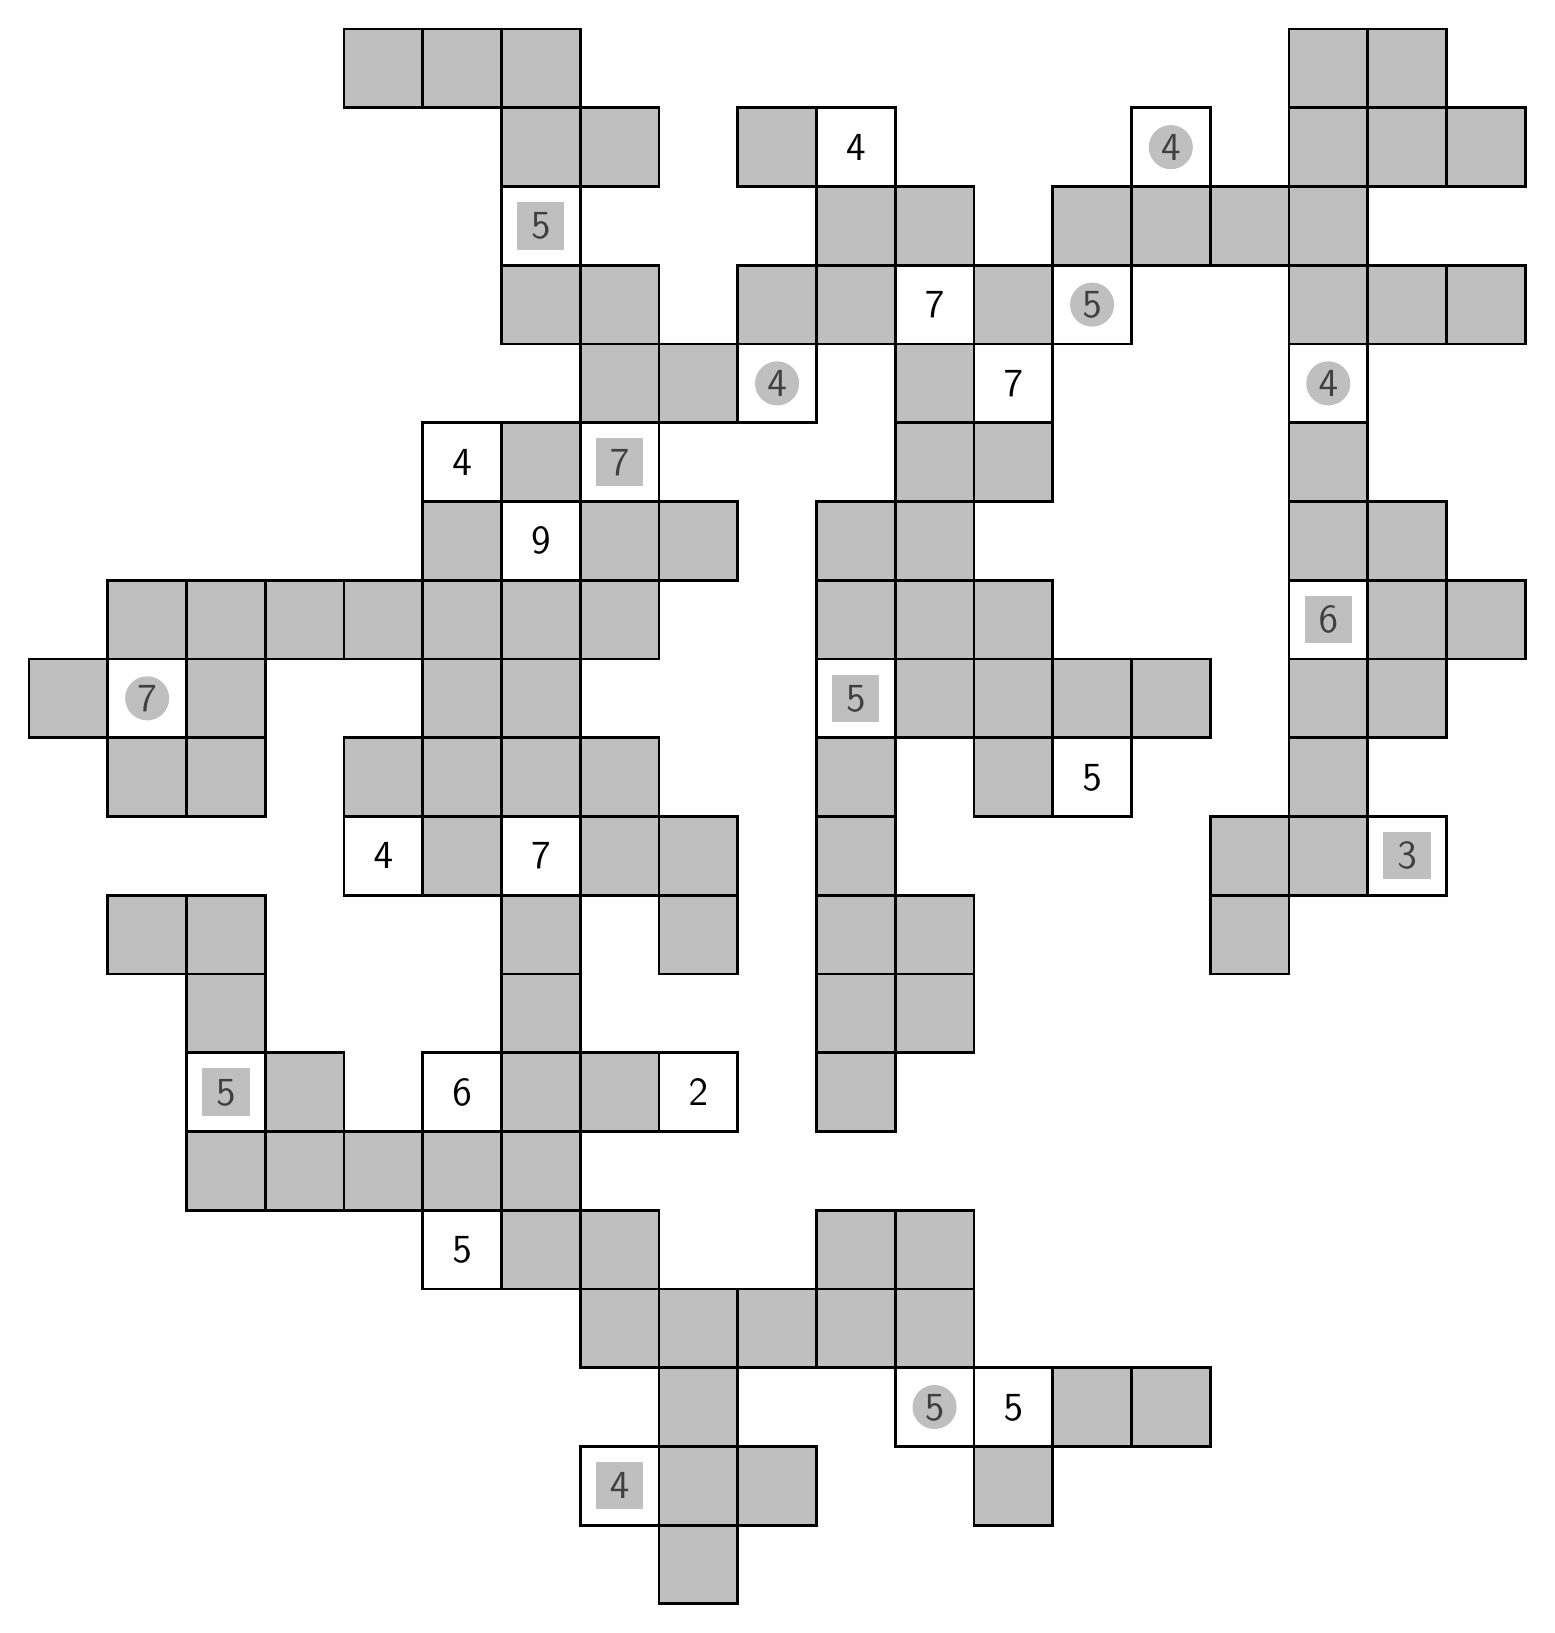
\begin{tikzpicture}\fill[gray, opacity = 0.5] (9, 0, 0)--++(1, 0, 0)--++(0, 1, 0)--++(-1, 0, 0)--cycle;
\draw[line width = 1pt] (9, 0, 0)--++(1, 0, 0)--++(0, 1, 0)--++(-1, 0, 0)--cycle;
\draw node at (8.5, 1.5, 0) {\Large $\mathsf{4}$};
\draw[line width = 1pt] (8, 1, 0)--++(1, 0, 0)--++(0, 1, 0)--++(-1, 0, 0)--cycle;
\fill[color = gray, opacity = 0.5] (8.2, 1.2) rectangle ++(0.6, 0.6);
\fill[gray, opacity = 0.5] (9, 1, 0)--++(1, 0, 0)--++(0, 1, 0)--++(-1, 0, 0)--cycle;
\draw[line width = 1pt] (9, 1, 0)--++(1, 0, 0)--++(0, 1, 0)--++(-1, 0, 0)--cycle;
\fill[gray, opacity = 0.5] (10, 1, 0)--++(1, 0, 0)--++(0, 1, 0)--++(-1, 0, 0)--cycle;
\draw[line width = 1pt] (10, 1, 0)--++(1, 0, 0)--++(0, 1, 0)--++(-1, 0, 0)--cycle;
\fill[gray, opacity = 0.5] (13, 1, 0)--++(1, 0, 0)--++(0, 1, 0)--++(-1, 0, 0)--cycle;
\draw[line width = 1pt] (13, 1, 0)--++(1, 0, 0)--++(0, 1, 0)--++(-1, 0, 0)--cycle;
\fill[gray, opacity = 0.5] (9, 2, 0)--++(1, 0, 0)--++(0, 1, 0)--++(-1, 0, 0)--cycle;
\draw[line width = 1pt] (9, 2, 0)--++(1, 0, 0)--++(0, 1, 0)--++(-1, 0, 0)--cycle;
\draw node at (12.5, 2.5, 0) {\Large $\mathsf{5}$};
\draw[line width = 1pt] (12, 2, 0)--++(1, 0, 0)--++(0, 1, 0)--++(-1, 0, 0)--cycle;
\fill[color = gray, opacity = 0.5] (12.5, 2.5, 0) circle (0.28);
\draw node at (13.5, 2.5, 0) {\Large $\mathsf{5}$};
\draw[line width = 1pt] (13, 2, 0)--++(1, 0, 0)--++(0, 1, 0)--++(-1, 0, 0)--cycle;
\fill[gray, opacity = 0.5] (14, 2, 0)--++(1, 0, 0)--++(0, 1, 0)--++(-1, 0, 0)--cycle;
\draw[line width = 1pt] (14, 2, 0)--++(1, 0, 0)--++(0, 1, 0)--++(-1, 0, 0)--cycle;
\fill[gray, opacity = 0.5] (15, 2, 0)--++(1, 0, 0)--++(0, 1, 0)--++(-1, 0, 0)--cycle;
\draw[line width = 1pt] (15, 2, 0)--++(1, 0, 0)--++(0, 1, 0)--++(-1, 0, 0)--cycle;
\fill[gray, opacity = 0.5] (8, 3, 0)--++(1, 0, 0)--++(0, 1, 0)--++(-1, 0, 0)--cycle;
\draw[line width = 1pt] (8, 3, 0)--++(1, 0, 0)--++(0, 1, 0)--++(-1, 0, 0)--cycle;
\fill[gray, opacity = 0.5] (9, 3, 0)--++(1, 0, 0)--++(0, 1, 0)--++(-1, 0, 0)--cycle;
\draw[line width = 1pt] (9, 3, 0)--++(1, 0, 0)--++(0, 1, 0)--++(-1, 0, 0)--cycle;
\fill[gray, opacity = 0.5] (10, 3, 0)--++(1, 0, 0)--++(0, 1, 0)--++(-1, 0, 0)--cycle;
\draw[line width = 1pt] (10, 3, 0)--++(1, 0, 0)--++(0, 1, 0)--++(-1, 0, 0)--cycle;
\fill[gray, opacity = 0.5] (11, 3, 0)--++(1, 0, 0)--++(0, 1, 0)--++(-1, 0, 0)--cycle;
\draw[line width = 1pt] (11, 3, 0)--++(1, 0, 0)--++(0, 1, 0)--++(-1, 0, 0)--cycle;
\fill[gray, opacity = 0.5] (12, 3, 0)--++(1, 0, 0)--++(0, 1, 0)--++(-1, 0, 0)--cycle;
\draw[line width = 1pt] (12, 3, 0)--++(1, 0, 0)--++(0, 1, 0)--++(-1, 0, 0)--cycle;
\draw node at (6.5, 4.5, 0) {\Large $\mathsf{5}$};
\draw[line width = 1pt] (6, 4, 0)--++(1, 0, 0)--++(0, 1, 0)--++(-1, 0, 0)--cycle;
\fill[gray, opacity = 0.5] (7, 4, 0)--++(1, 0, 0)--++(0, 1, 0)--++(-1, 0, 0)--cycle;
\draw[line width = 1pt] (7, 4, 0)--++(1, 0, 0)--++(0, 1, 0)--++(-1, 0, 0)--cycle;
\fill[gray, opacity = 0.5] (8, 4, 0)--++(1, 0, 0)--++(0, 1, 0)--++(-1, 0, 0)--cycle;
\draw[line width = 1pt] (8, 4, 0)--++(1, 0, 0)--++(0, 1, 0)--++(-1, 0, 0)--cycle;
\fill[gray, opacity = 0.5] (11, 4, 0)--++(1, 0, 0)--++(0, 1, 0)--++(-1, 0, 0)--cycle;
\draw[line width = 1pt] (11, 4, 0)--++(1, 0, 0)--++(0, 1, 0)--++(-1, 0, 0)--cycle;
\fill[gray, opacity = 0.5] (12, 4, 0)--++(1, 0, 0)--++(0, 1, 0)--++(-1, 0, 0)--cycle;
\draw[line width = 1pt] (12, 4, 0)--++(1, 0, 0)--++(0, 1, 0)--++(-1, 0, 0)--cycle;
\fill[gray, opacity = 0.5] (3, 5, 0)--++(1, 0, 0)--++(0, 1, 0)--++(-1, 0, 0)--cycle;
\draw[line width = 1pt] (3, 5, 0)--++(1, 0, 0)--++(0, 1, 0)--++(-1, 0, 0)--cycle;
\fill[gray, opacity = 0.5] (4, 5, 0)--++(1, 0, 0)--++(0, 1, 0)--++(-1, 0, 0)--cycle;
\draw[line width = 1pt] (4, 5, 0)--++(1, 0, 0)--++(0, 1, 0)--++(-1, 0, 0)--cycle;
\fill[gray, opacity = 0.5] (5, 5, 0)--++(1, 0, 0)--++(0, 1, 0)--++(-1, 0, 0)--cycle;
\draw[line width = 1pt] (5, 5, 0)--++(1, 0, 0)--++(0, 1, 0)--++(-1, 0, 0)--cycle;
\fill[gray, opacity = 0.5] (6, 5, 0)--++(1, 0, 0)--++(0, 1, 0)--++(-1, 0, 0)--cycle;
\draw[line width = 1pt] (6, 5, 0)--++(1, 0, 0)--++(0, 1, 0)--++(-1, 0, 0)--cycle;
\fill[gray, opacity = 0.5] (7, 5, 0)--++(1, 0, 0)--++(0, 1, 0)--++(-1, 0, 0)--cycle;
\draw[line width = 1pt] (7, 5, 0)--++(1, 0, 0)--++(0, 1, 0)--++(-1, 0, 0)--cycle;
\draw node at (3.5, 6.5, 0) {\Large $\mathsf{5}$};
\draw[line width = 1pt] (3, 6, 0)--++(1, 0, 0)--++(0, 1, 0)--++(-1, 0, 0)--cycle;
\fill[color = gray, opacity = 0.5] (3.2, 6.2) rectangle ++(0.6, 0.6);
\fill[gray, opacity = 0.5] (4, 6, 0)--++(1, 0, 0)--++(0, 1, 0)--++(-1, 0, 0)--cycle;
\draw[line width = 1pt] (4, 6, 0)--++(1, 0, 0)--++(0, 1, 0)--++(-1, 0, 0)--cycle;
\draw node at (6.5, 6.5, 0) {\Large $\mathsf{6}$};
\draw[line width = 1pt] (6, 6, 0)--++(1, 0, 0)--++(0, 1, 0)--++(-1, 0, 0)--cycle;
\fill[gray, opacity = 0.5] (7, 6, 0)--++(1, 0, 0)--++(0, 1, 0)--++(-1, 0, 0)--cycle;
\draw[line width = 1pt] (7, 6, 0)--++(1, 0, 0)--++(0, 1, 0)--++(-1, 0, 0)--cycle;
\fill[gray, opacity = 0.5] (8, 6, 0)--++(1, 0, 0)--++(0, 1, 0)--++(-1, 0, 0)--cycle;
\draw[line width = 1pt] (8, 6, 0)--++(1, 0, 0)--++(0, 1, 0)--++(-1, 0, 0)--cycle;
\draw node at (9.5, 6.5, 0) {\Large $\mathsf{2}$};
\draw[line width = 1pt] (9, 6, 0)--++(1, 0, 0)--++(0, 1, 0)--++(-1, 0, 0)--cycle;
\fill[gray, opacity = 0.5] (11, 6, 0)--++(1, 0, 0)--++(0, 1, 0)--++(-1, 0, 0)--cycle;
\draw[line width = 1pt] (11, 6, 0)--++(1, 0, 0)--++(0, 1, 0)--++(-1, 0, 0)--cycle;
\fill[gray, opacity = 0.5] (3, 7, 0)--++(1, 0, 0)--++(0, 1, 0)--++(-1, 0, 0)--cycle;
\draw[line width = 1pt] (3, 7, 0)--++(1, 0, 0)--++(0, 1, 0)--++(-1, 0, 0)--cycle;
\fill[gray, opacity = 0.5] (7, 7, 0)--++(1, 0, 0)--++(0, 1, 0)--++(-1, 0, 0)--cycle;
\draw[line width = 1pt] (7, 7, 0)--++(1, 0, 0)--++(0, 1, 0)--++(-1, 0, 0)--cycle;
\fill[gray, opacity = 0.5] (11, 7, 0)--++(1, 0, 0)--++(0, 1, 0)--++(-1, 0, 0)--cycle;
\draw[line width = 1pt] (11, 7, 0)--++(1, 0, 0)--++(0, 1, 0)--++(-1, 0, 0)--cycle;
\fill[gray, opacity = 0.5] (12, 7, 0)--++(1, 0, 0)--++(0, 1, 0)--++(-1, 0, 0)--cycle;
\draw[line width = 1pt] (12, 7, 0)--++(1, 0, 0)--++(0, 1, 0)--++(-1, 0, 0)--cycle;
\fill[gray, opacity = 0.5] (2, 8, 0)--++(1, 0, 0)--++(0, 1, 0)--++(-1, 0, 0)--cycle;
\draw[line width = 1pt] (2, 8, 0)--++(1, 0, 0)--++(0, 1, 0)--++(-1, 0, 0)--cycle;
\fill[gray, opacity = 0.5] (3, 8, 0)--++(1, 0, 0)--++(0, 1, 0)--++(-1, 0, 0)--cycle;
\draw[line width = 1pt] (3, 8, 0)--++(1, 0, 0)--++(0, 1, 0)--++(-1, 0, 0)--cycle;
\fill[gray, opacity = 0.5] (7, 8, 0)--++(1, 0, 0)--++(0, 1, 0)--++(-1, 0, 0)--cycle;
\draw[line width = 1pt] (7, 8, 0)--++(1, 0, 0)--++(0, 1, 0)--++(-1, 0, 0)--cycle;
\fill[gray, opacity = 0.5] (9, 8, 0)--++(1, 0, 0)--++(0, 1, 0)--++(-1, 0, 0)--cycle;
\draw[line width = 1pt] (9, 8, 0)--++(1, 0, 0)--++(0, 1, 0)--++(-1, 0, 0)--cycle;
\fill[gray, opacity = 0.5] (11, 8, 0)--++(1, 0, 0)--++(0, 1, 0)--++(-1, 0, 0)--cycle;
\draw[line width = 1pt] (11, 8, 0)--++(1, 0, 0)--++(0, 1, 0)--++(-1, 0, 0)--cycle;
\fill[gray, opacity = 0.5] (12, 8, 0)--++(1, 0, 0)--++(0, 1, 0)--++(-1, 0, 0)--cycle;
\draw[line width = 1pt] (12, 8, 0)--++(1, 0, 0)--++(0, 1, 0)--++(-1, 0, 0)--cycle;
\fill[gray, opacity = 0.5] (16, 8, 0)--++(1, 0, 0)--++(0, 1, 0)--++(-1, 0, 0)--cycle;
\draw[line width = 1pt] (16, 8, 0)--++(1, 0, 0)--++(0, 1, 0)--++(-1, 0, 0)--cycle;
\draw node at (5.5, 9.5, 0) {\Large $\mathsf{4}$};
\draw[line width = 1pt] (5, 9, 0)--++(1, 0, 0)--++(0, 1, 0)--++(-1, 0, 0)--cycle;
\fill[gray, opacity = 0.5] (6, 9, 0)--++(1, 0, 0)--++(0, 1, 0)--++(-1, 0, 0)--cycle;
\draw[line width = 1pt] (6, 9, 0)--++(1, 0, 0)--++(0, 1, 0)--++(-1, 0, 0)--cycle;
\draw node at (7.5, 9.5, 0) {\Large $\mathsf{7}$};
\draw[line width = 1pt] (7, 9, 0)--++(1, 0, 0)--++(0, 1, 0)--++(-1, 0, 0)--cycle;
\fill[gray, opacity = 0.5] (8, 9, 0)--++(1, 0, 0)--++(0, 1, 0)--++(-1, 0, 0)--cycle;
\draw[line width = 1pt] (8, 9, 0)--++(1, 0, 0)--++(0, 1, 0)--++(-1, 0, 0)--cycle;
\fill[gray, opacity = 0.5] (9, 9, 0)--++(1, 0, 0)--++(0, 1, 0)--++(-1, 0, 0)--cycle;
\draw[line width = 1pt] (9, 9, 0)--++(1, 0, 0)--++(0, 1, 0)--++(-1, 0, 0)--cycle;
\fill[gray, opacity = 0.5] (11, 9, 0)--++(1, 0, 0)--++(0, 1, 0)--++(-1, 0, 0)--cycle;
\draw[line width = 1pt] (11, 9, 0)--++(1, 0, 0)--++(0, 1, 0)--++(-1, 0, 0)--cycle;
\fill[gray, opacity = 0.5] (16, 9, 0)--++(1, 0, 0)--++(0, 1, 0)--++(-1, 0, 0)--cycle;
\draw[line width = 1pt] (16, 9, 0)--++(1, 0, 0)--++(0, 1, 0)--++(-1, 0, 0)--cycle;
\fill[gray, opacity = 0.5] (17, 9, 0)--++(1, 0, 0)--++(0, 1, 0)--++(-1, 0, 0)--cycle;
\draw[line width = 1pt] (17, 9, 0)--++(1, 0, 0)--++(0, 1, 0)--++(-1, 0, 0)--cycle;
\draw node at (18.5, 9.5, 0) {\Large $\mathsf{3}$};
\draw[line width = 1pt] (18, 9, 0)--++(1, 0, 0)--++(0, 1, 0)--++(-1, 0, 0)--cycle;
\fill[color = gray, opacity = 0.5] (18.2, 9.2) rectangle ++(0.6, 0.6);
\fill[gray, opacity = 0.5] (2, 10, 0)--++(1, 0, 0)--++(0, 1, 0)--++(-1, 0, 0)--cycle;
\draw[line width = 1pt] (2, 10, 0)--++(1, 0, 0)--++(0, 1, 0)--++(-1, 0, 0)--cycle;
\fill[gray, opacity = 0.5] (3, 10, 0)--++(1, 0, 0)--++(0, 1, 0)--++(-1, 0, 0)--cycle;
\draw[line width = 1pt] (3, 10, 0)--++(1, 0, 0)--++(0, 1, 0)--++(-1, 0, 0)--cycle;
\fill[gray, opacity = 0.5] (5, 10, 0)--++(1, 0, 0)--++(0, 1, 0)--++(-1, 0, 0)--cycle;
\draw[line width = 1pt] (5, 10, 0)--++(1, 0, 0)--++(0, 1, 0)--++(-1, 0, 0)--cycle;
\fill[gray, opacity = 0.5] (6, 10, 0)--++(1, 0, 0)--++(0, 1, 0)--++(-1, 0, 0)--cycle;
\draw[line width = 1pt] (6, 10, 0)--++(1, 0, 0)--++(0, 1, 0)--++(-1, 0, 0)--cycle;
\fill[gray, opacity = 0.5] (7, 10, 0)--++(1, 0, 0)--++(0, 1, 0)--++(-1, 0, 0)--cycle;
\draw[line width = 1pt] (7, 10, 0)--++(1, 0, 0)--++(0, 1, 0)--++(-1, 0, 0)--cycle;
\fill[gray, opacity = 0.5] (8, 10, 0)--++(1, 0, 0)--++(0, 1, 0)--++(-1, 0, 0)--cycle;
\draw[line width = 1pt] (8, 10, 0)--++(1, 0, 0)--++(0, 1, 0)--++(-1, 0, 0)--cycle;
\fill[gray, opacity = 0.5] (11, 10, 0)--++(1, 0, 0)--++(0, 1, 0)--++(-1, 0, 0)--cycle;
\draw[line width = 1pt] (11, 10, 0)--++(1, 0, 0)--++(0, 1, 0)--++(-1, 0, 0)--cycle;
\fill[gray, opacity = 0.5] (13, 10, 0)--++(1, 0, 0)--++(0, 1, 0)--++(-1, 0, 0)--cycle;
\draw[line width = 1pt] (13, 10, 0)--++(1, 0, 0)--++(0, 1, 0)--++(-1, 0, 0)--cycle;
\draw node at (14.5, 10.5, 0) {\Large $\mathsf{5}$};
\draw[line width = 1pt] (14, 10, 0)--++(1, 0, 0)--++(0, 1, 0)--++(-1, 0, 0)--cycle;
\fill[gray, opacity = 0.5] (17, 10, 0)--++(1, 0, 0)--++(0, 1, 0)--++(-1, 0, 0)--cycle;
\draw[line width = 1pt] (17, 10, 0)--++(1, 0, 0)--++(0, 1, 0)--++(-1, 0, 0)--cycle;
\fill[gray, opacity = 0.5] (1, 11, 0)--++(1, 0, 0)--++(0, 1, 0)--++(-1, 0, 0)--cycle;
\draw[line width = 1pt] (1, 11, 0)--++(1, 0, 0)--++(0, 1, 0)--++(-1, 0, 0)--cycle;
\draw node at (2.5, 11.5, 0) {\Large $\mathsf{7}$};
\draw[line width = 1pt] (2, 11, 0)--++(1, 0, 0)--++(0, 1, 0)--++(-1, 0, 0)--cycle;
\fill[color = gray, opacity = 0.5] (2.5, 11.5, 0) circle (0.28);
\fill[gray, opacity = 0.5] (3, 11, 0)--++(1, 0, 0)--++(0, 1, 0)--++(-1, 0, 0)--cycle;
\draw[line width = 1pt] (3, 11, 0)--++(1, 0, 0)--++(0, 1, 0)--++(-1, 0, 0)--cycle;
\fill[gray, opacity = 0.5] (6, 11, 0)--++(1, 0, 0)--++(0, 1, 0)--++(-1, 0, 0)--cycle;
\draw[line width = 1pt] (6, 11, 0)--++(1, 0, 0)--++(0, 1, 0)--++(-1, 0, 0)--cycle;
\fill[gray, opacity = 0.5] (7, 11, 0)--++(1, 0, 0)--++(0, 1, 0)--++(-1, 0, 0)--cycle;
\draw[line width = 1pt] (7, 11, 0)--++(1, 0, 0)--++(0, 1, 0)--++(-1, 0, 0)--cycle;
\draw node at (11.5, 11.5, 0) {\Large $\mathsf{5}$};
\draw[line width = 1pt] (11, 11, 0)--++(1, 0, 0)--++(0, 1, 0)--++(-1, 0, 0)--cycle;
\fill[color = gray, opacity = 0.5] (11.2, 11.2) rectangle ++(0.6, 0.6);
\fill[gray, opacity = 0.5] (12, 11, 0)--++(1, 0, 0)--++(0, 1, 0)--++(-1, 0, 0)--cycle;
\draw[line width = 1pt] (12, 11, 0)--++(1, 0, 0)--++(0, 1, 0)--++(-1, 0, 0)--cycle;
\fill[gray, opacity = 0.5] (13, 11, 0)--++(1, 0, 0)--++(0, 1, 0)--++(-1, 0, 0)--cycle;
\draw[line width = 1pt] (13, 11, 0)--++(1, 0, 0)--++(0, 1, 0)--++(-1, 0, 0)--cycle;
\fill[gray, opacity = 0.5] (14, 11, 0)--++(1, 0, 0)--++(0, 1, 0)--++(-1, 0, 0)--cycle;
\draw[line width = 1pt] (14, 11, 0)--++(1, 0, 0)--++(0, 1, 0)--++(-1, 0, 0)--cycle;
\fill[gray, opacity = 0.5] (15, 11, 0)--++(1, 0, 0)--++(0, 1, 0)--++(-1, 0, 0)--cycle;
\draw[line width = 1pt] (15, 11, 0)--++(1, 0, 0)--++(0, 1, 0)--++(-1, 0, 0)--cycle;
\fill[gray, opacity = 0.5] (17, 11, 0)--++(1, 0, 0)--++(0, 1, 0)--++(-1, 0, 0)--cycle;
\draw[line width = 1pt] (17, 11, 0)--++(1, 0, 0)--++(0, 1, 0)--++(-1, 0, 0)--cycle;
\fill[gray, opacity = 0.5] (18, 11, 0)--++(1, 0, 0)--++(0, 1, 0)--++(-1, 0, 0)--cycle;
\draw[line width = 1pt] (18, 11, 0)--++(1, 0, 0)--++(0, 1, 0)--++(-1, 0, 0)--cycle;
\fill[gray, opacity = 0.5] (2, 12, 0)--++(1, 0, 0)--++(0, 1, 0)--++(-1, 0, 0)--cycle;
\draw[line width = 1pt] (2, 12, 0)--++(1, 0, 0)--++(0, 1, 0)--++(-1, 0, 0)--cycle;
\fill[gray, opacity = 0.5] (3, 12, 0)--++(1, 0, 0)--++(0, 1, 0)--++(-1, 0, 0)--cycle;
\draw[line width = 1pt] (3, 12, 0)--++(1, 0, 0)--++(0, 1, 0)--++(-1, 0, 0)--cycle;
\fill[gray, opacity = 0.5] (4, 12, 0)--++(1, 0, 0)--++(0, 1, 0)--++(-1, 0, 0)--cycle;
\draw[line width = 1pt] (4, 12, 0)--++(1, 0, 0)--++(0, 1, 0)--++(-1, 0, 0)--cycle;
\fill[gray, opacity = 0.5] (5, 12, 0)--++(1, 0, 0)--++(0, 1, 0)--++(-1, 0, 0)--cycle;
\draw[line width = 1pt] (5, 12, 0)--++(1, 0, 0)--++(0, 1, 0)--++(-1, 0, 0)--cycle;
\fill[gray, opacity = 0.5] (6, 12, 0)--++(1, 0, 0)--++(0, 1, 0)--++(-1, 0, 0)--cycle;
\draw[line width = 1pt] (6, 12, 0)--++(1, 0, 0)--++(0, 1, 0)--++(-1, 0, 0)--cycle;
\fill[gray, opacity = 0.5] (7, 12, 0)--++(1, 0, 0)--++(0, 1, 0)--++(-1, 0, 0)--cycle;
\draw[line width = 1pt] (7, 12, 0)--++(1, 0, 0)--++(0, 1, 0)--++(-1, 0, 0)--cycle;
\fill[gray, opacity = 0.5] (8, 12, 0)--++(1, 0, 0)--++(0, 1, 0)--++(-1, 0, 0)--cycle;
\draw[line width = 1pt] (8, 12, 0)--++(1, 0, 0)--++(0, 1, 0)--++(-1, 0, 0)--cycle;
\fill[gray, opacity = 0.5] (11, 12, 0)--++(1, 0, 0)--++(0, 1, 0)--++(-1, 0, 0)--cycle;
\draw[line width = 1pt] (11, 12, 0)--++(1, 0, 0)--++(0, 1, 0)--++(-1, 0, 0)--cycle;
\fill[gray, opacity = 0.5] (12, 12, 0)--++(1, 0, 0)--++(0, 1, 0)--++(-1, 0, 0)--cycle;
\draw[line width = 1pt] (12, 12, 0)--++(1, 0, 0)--++(0, 1, 0)--++(-1, 0, 0)--cycle;
\fill[gray, opacity = 0.5] (13, 12, 0)--++(1, 0, 0)--++(0, 1, 0)--++(-1, 0, 0)--cycle;
\draw[line width = 1pt] (13, 12, 0)--++(1, 0, 0)--++(0, 1, 0)--++(-1, 0, 0)--cycle;
\draw node at (17.5, 12.5, 0) {\Large $\mathsf{6}$};
\draw[line width = 1pt] (17, 12, 0)--++(1, 0, 0)--++(0, 1, 0)--++(-1, 0, 0)--cycle;
\fill[color = gray, opacity = 0.5] (17.2, 12.2) rectangle ++(0.6, 0.6);
\fill[gray, opacity = 0.5] (18, 12, 0)--++(1, 0, 0)--++(0, 1, 0)--++(-1, 0, 0)--cycle;
\draw[line width = 1pt] (18, 12, 0)--++(1, 0, 0)--++(0, 1, 0)--++(-1, 0, 0)--cycle;
\fill[gray, opacity = 0.5] (19, 12, 0)--++(1, 0, 0)--++(0, 1, 0)--++(-1, 0, 0)--cycle;
\draw[line width = 1pt] (19, 12, 0)--++(1, 0, 0)--++(0, 1, 0)--++(-1, 0, 0)--cycle;
\fill[gray, opacity = 0.5] (6, 13, 0)--++(1, 0, 0)--++(0, 1, 0)--++(-1, 0, 0)--cycle;
\draw[line width = 1pt] (6, 13, 0)--++(1, 0, 0)--++(0, 1, 0)--++(-1, 0, 0)--cycle;
\draw node at (7.5, 13.5, 0) {\Large $\mathsf{9}$};
\draw[line width = 1pt] (7, 13, 0)--++(1, 0, 0)--++(0, 1, 0)--++(-1, 0, 0)--cycle;
\fill[gray, opacity = 0.5] (8, 13, 0)--++(1, 0, 0)--++(0, 1, 0)--++(-1, 0, 0)--cycle;
\draw[line width = 1pt] (8, 13, 0)--++(1, 0, 0)--++(0, 1, 0)--++(-1, 0, 0)--cycle;
\fill[gray, opacity = 0.5] (9, 13, 0)--++(1, 0, 0)--++(0, 1, 0)--++(-1, 0, 0)--cycle;
\draw[line width = 1pt] (9, 13, 0)--++(1, 0, 0)--++(0, 1, 0)--++(-1, 0, 0)--cycle;
\fill[gray, opacity = 0.5] (11, 13, 0)--++(1, 0, 0)--++(0, 1, 0)--++(-1, 0, 0)--cycle;
\draw[line width = 1pt] (11, 13, 0)--++(1, 0, 0)--++(0, 1, 0)--++(-1, 0, 0)--cycle;
\fill[gray, opacity = 0.5] (12, 13, 0)--++(1, 0, 0)--++(0, 1, 0)--++(-1, 0, 0)--cycle;
\draw[line width = 1pt] (12, 13, 0)--++(1, 0, 0)--++(0, 1, 0)--++(-1, 0, 0)--cycle;
\fill[gray, opacity = 0.5] (17, 13, 0)--++(1, 0, 0)--++(0, 1, 0)--++(-1, 0, 0)--cycle;
\draw[line width = 1pt] (17, 13, 0)--++(1, 0, 0)--++(0, 1, 0)--++(-1, 0, 0)--cycle;
\fill[gray, opacity = 0.5] (18, 13, 0)--++(1, 0, 0)--++(0, 1, 0)--++(-1, 0, 0)--cycle;
\draw[line width = 1pt] (18, 13, 0)--++(1, 0, 0)--++(0, 1, 0)--++(-1, 0, 0)--cycle;
\draw node at (6.5, 14.5, 0) {\Large $\mathsf{4}$};
\draw[line width = 1pt] (6, 14, 0)--++(1, 0, 0)--++(0, 1, 0)--++(-1, 0, 0)--cycle;
\fill[gray, opacity = 0.5] (7, 14, 0)--++(1, 0, 0)--++(0, 1, 0)--++(-1, 0, 0)--cycle;
\draw[line width = 1pt] (7, 14, 0)--++(1, 0, 0)--++(0, 1, 0)--++(-1, 0, 0)--cycle;
\draw node at (8.5, 14.5, 0) {\Large $\mathsf{7}$};
\draw[line width = 1pt] (8, 14, 0)--++(1, 0, 0)--++(0, 1, 0)--++(-1, 0, 0)--cycle;
\fill[color = gray, opacity = 0.5] (8.2, 14.2) rectangle ++(0.6, 0.6);
\fill[gray, opacity = 0.5] (12, 14, 0)--++(1, 0, 0)--++(0, 1, 0)--++(-1, 0, 0)--cycle;
\draw[line width = 1pt] (12, 14, 0)--++(1, 0, 0)--++(0, 1, 0)--++(-1, 0, 0)--cycle;
\fill[gray, opacity = 0.5] (13, 14, 0)--++(1, 0, 0)--++(0, 1, 0)--++(-1, 0, 0)--cycle;
\draw[line width = 1pt] (13, 14, 0)--++(1, 0, 0)--++(0, 1, 0)--++(-1, 0, 0)--cycle;
\fill[gray, opacity = 0.5] (17, 14, 0)--++(1, 0, 0)--++(0, 1, 0)--++(-1, 0, 0)--cycle;
\draw[line width = 1pt] (17, 14, 0)--++(1, 0, 0)--++(0, 1, 0)--++(-1, 0, 0)--cycle;
\fill[gray, opacity = 0.5] (8, 15, 0)--++(1, 0, 0)--++(0, 1, 0)--++(-1, 0, 0)--cycle;
\draw[line width = 1pt] (8, 15, 0)--++(1, 0, 0)--++(0, 1, 0)--++(-1, 0, 0)--cycle;
\fill[gray, opacity = 0.5] (9, 15, 0)--++(1, 0, 0)--++(0, 1, 0)--++(-1, 0, 0)--cycle;
\draw[line width = 1pt] (9, 15, 0)--++(1, 0, 0)--++(0, 1, 0)--++(-1, 0, 0)--cycle;
\draw node at (10.5, 15.5, 0) {\Large $\mathsf{4}$};
\draw[line width = 1pt] (10, 15, 0)--++(1, 0, 0)--++(0, 1, 0)--++(-1, 0, 0)--cycle;
\fill[color = gray, opacity = 0.5] (10.5, 15.5, 0) circle (0.28);
\fill[gray, opacity = 0.5] (12, 15, 0)--++(1, 0, 0)--++(0, 1, 0)--++(-1, 0, 0)--cycle;
\draw[line width = 1pt] (12, 15, 0)--++(1, 0, 0)--++(0, 1, 0)--++(-1, 0, 0)--cycle;
\draw node at (13.5, 15.5, 0) {\Large $\mathsf{7}$};
\draw[line width = 1pt] (13, 15, 0)--++(1, 0, 0)--++(0, 1, 0)--++(-1, 0, 0)--cycle;
\draw node at (17.5, 15.5, 0) {\Large $\mathsf{4}$};
\draw[line width = 1pt] (17, 15, 0)--++(1, 0, 0)--++(0, 1, 0)--++(-1, 0, 0)--cycle;
\fill[color = gray, opacity = 0.5] (17.5, 15.5, 0) circle (0.28);
\fill[gray, opacity = 0.5] (7, 16, 0)--++(1, 0, 0)--++(0, 1, 0)--++(-1, 0, 0)--cycle;
\draw[line width = 1pt] (7, 16, 0)--++(1, 0, 0)--++(0, 1, 0)--++(-1, 0, 0)--cycle;
\fill[gray, opacity = 0.5] (8, 16, 0)--++(1, 0, 0)--++(0, 1, 0)--++(-1, 0, 0)--cycle;
\draw[line width = 1pt] (8, 16, 0)--++(1, 0, 0)--++(0, 1, 0)--++(-1, 0, 0)--cycle;
\fill[gray, opacity = 0.5] (10, 16, 0)--++(1, 0, 0)--++(0, 1, 0)--++(-1, 0, 0)--cycle;
\draw[line width = 1pt] (10, 16, 0)--++(1, 0, 0)--++(0, 1, 0)--++(-1, 0, 0)--cycle;
\fill[gray, opacity = 0.5] (11, 16, 0)--++(1, 0, 0)--++(0, 1, 0)--++(-1, 0, 0)--cycle;
\draw[line width = 1pt] (11, 16, 0)--++(1, 0, 0)--++(0, 1, 0)--++(-1, 0, 0)--cycle;
\draw node at (12.5, 16.5, 0) {\Large $\mathsf{7}$};
\draw[line width = 1pt] (12, 16, 0)--++(1, 0, 0)--++(0, 1, 0)--++(-1, 0, 0)--cycle;
\fill[gray, opacity = 0.5] (13, 16, 0)--++(1, 0, 0)--++(0, 1, 0)--++(-1, 0, 0)--cycle;
\draw[line width = 1pt] (13, 16, 0)--++(1, 0, 0)--++(0, 1, 0)--++(-1, 0, 0)--cycle;
\draw node at (14.5, 16.5, 0) {\Large $\mathsf{5}$};
\draw[line width = 1pt] (14, 16, 0)--++(1, 0, 0)--++(0, 1, 0)--++(-1, 0, 0)--cycle;
\fill[color = gray, opacity = 0.5] (14.5, 16.5, 0) circle (0.28);
\fill[gray, opacity = 0.5] (17, 16, 0)--++(1, 0, 0)--++(0, 1, 0)--++(-1, 0, 0)--cycle;
\draw[line width = 1pt] (17, 16, 0)--++(1, 0, 0)--++(0, 1, 0)--++(-1, 0, 0)--cycle;
\fill[gray, opacity = 0.5] (18, 16, 0)--++(1, 0, 0)--++(0, 1, 0)--++(-1, 0, 0)--cycle;
\draw[line width = 1pt] (18, 16, 0)--++(1, 0, 0)--++(0, 1, 0)--++(-1, 0, 0)--cycle;
\fill[gray, opacity = 0.5] (19, 16, 0)--++(1, 0, 0)--++(0, 1, 0)--++(-1, 0, 0)--cycle;
\draw[line width = 1pt] (19, 16, 0)--++(1, 0, 0)--++(0, 1, 0)--++(-1, 0, 0)--cycle;
\draw node at (7.5, 17.5, 0) {\Large $\mathsf{5}$};
\draw[line width = 1pt] (7, 17, 0)--++(1, 0, 0)--++(0, 1, 0)--++(-1, 0, 0)--cycle;
\fill[color = gray, opacity = 0.5] (7.2, 17.2) rectangle ++(0.6, 0.6);
\fill[gray, opacity = 0.5] (11, 17, 0)--++(1, 0, 0)--++(0, 1, 0)--++(-1, 0, 0)--cycle;
\draw[line width = 1pt] (11, 17, 0)--++(1, 0, 0)--++(0, 1, 0)--++(-1, 0, 0)--cycle;
\fill[gray, opacity = 0.5] (12, 17, 0)--++(1, 0, 0)--++(0, 1, 0)--++(-1, 0, 0)--cycle;
\draw[line width = 1pt] (12, 17, 0)--++(1, 0, 0)--++(0, 1, 0)--++(-1, 0, 0)--cycle;
\fill[gray, opacity = 0.5] (14, 17, 0)--++(1, 0, 0)--++(0, 1, 0)--++(-1, 0, 0)--cycle;
\draw[line width = 1pt] (14, 17, 0)--++(1, 0, 0)--++(0, 1, 0)--++(-1, 0, 0)--cycle;
\fill[gray, opacity = 0.5] (15, 17, 0)--++(1, 0, 0)--++(0, 1, 0)--++(-1, 0, 0)--cycle;
\draw[line width = 1pt] (15, 17, 0)--++(1, 0, 0)--++(0, 1, 0)--++(-1, 0, 0)--cycle;
\fill[gray, opacity = 0.5] (16, 17, 0)--++(1, 0, 0)--++(0, 1, 0)--++(-1, 0, 0)--cycle;
\draw[line width = 1pt] (16, 17, 0)--++(1, 0, 0)--++(0, 1, 0)--++(-1, 0, 0)--cycle;
\fill[gray, opacity = 0.5] (17, 17, 0)--++(1, 0, 0)--++(0, 1, 0)--++(-1, 0, 0)--cycle;
\draw[line width = 1pt] (17, 17, 0)--++(1, 0, 0)--++(0, 1, 0)--++(-1, 0, 0)--cycle;
\fill[gray, opacity = 0.5] (7, 18, 0)--++(1, 0, 0)--++(0, 1, 0)--++(-1, 0, 0)--cycle;
\draw[line width = 1pt] (7, 18, 0)--++(1, 0, 0)--++(0, 1, 0)--++(-1, 0, 0)--cycle;
\fill[gray, opacity = 0.5] (8, 18, 0)--++(1, 0, 0)--++(0, 1, 0)--++(-1, 0, 0)--cycle;
\draw[line width = 1pt] (8, 18, 0)--++(1, 0, 0)--++(0, 1, 0)--++(-1, 0, 0)--cycle;
\fill[gray, opacity = 0.5] (10, 18, 0)--++(1, 0, 0)--++(0, 1, 0)--++(-1, 0, 0)--cycle;
\draw[line width = 1pt] (10, 18, 0)--++(1, 0, 0)--++(0, 1, 0)--++(-1, 0, 0)--cycle;
\draw node at (11.5, 18.5, 0) {\Large $\mathsf{4}$};
\draw[line width = 1pt] (11, 18, 0)--++(1, 0, 0)--++(0, 1, 0)--++(-1, 0, 0)--cycle;
\draw node at (15.5, 18.5, 0) {\Large $\mathsf{4}$};
\draw[line width = 1pt] (15, 18, 0)--++(1, 0, 0)--++(0, 1, 0)--++(-1, 0, 0)--cycle;
\fill[color = gray, opacity = 0.5] (15.5, 18.5, 0) circle (0.28);
\fill[gray, opacity = 0.5] (17, 18, 0)--++(1, 0, 0)--++(0, 1, 0)--++(-1, 0, 0)--cycle;
\draw[line width = 1pt] (17, 18, 0)--++(1, 0, 0)--++(0, 1, 0)--++(-1, 0, 0)--cycle;
\fill[gray, opacity = 0.5] (18, 18, 0)--++(1, 0, 0)--++(0, 1, 0)--++(-1, 0, 0)--cycle;
\draw[line width = 1pt] (18, 18, 0)--++(1, 0, 0)--++(0, 1, 0)--++(-1, 0, 0)--cycle;
\fill[gray, opacity = 0.5] (19, 18, 0)--++(1, 0, 0)--++(0, 1, 0)--++(-1, 0, 0)--cycle;
\draw[line width = 1pt] (19, 18, 0)--++(1, 0, 0)--++(0, 1, 0)--++(-1, 0, 0)--cycle;
\fill[gray, opacity = 0.5] (5, 19, 0)--++(1, 0, 0)--++(0, 1, 0)--++(-1, 0, 0)--cycle;
\draw[line width = 1pt] (5, 19, 0)--++(1, 0, 0)--++(0, 1, 0)--++(-1, 0, 0)--cycle;
\fill[gray, opacity = 0.5] (6, 19, 0)--++(1, 0, 0)--++(0, 1, 0)--++(-1, 0, 0)--cycle;
\draw[line width = 1pt] (6, 19, 0)--++(1, 0, 0)--++(0, 1, 0)--++(-1, 0, 0)--cycle;
\fill[gray, opacity = 0.5] (7, 19, 0)--++(1, 0, 0)--++(0, 1, 0)--++(-1, 0, 0)--cycle;
\draw[line width = 1pt] (7, 19, 0)--++(1, 0, 0)--++(0, 1, 0)--++(-1, 0, 0)--cycle;
\fill[gray, opacity = 0.5] (17, 19, 0)--++(1, 0, 0)--++(0, 1, 0)--++(-1, 0, 0)--cycle;
\draw[line width = 1pt] (17, 19, 0)--++(1, 0, 0)--++(0, 1, 0)--++(-1, 0, 0)--cycle;
\fill[gray, opacity = 0.5] (18, 19, 0)--++(1, 0, 0)--++(0, 1, 0)--++(-1, 0, 0)--cycle;
\draw[line width = 1pt] (18, 19, 0)--++(1, 0, 0)--++(0, 1, 0)--++(-1, 0, 0)--cycle;
\end{tikzpicture}}\]
\[\resizebox{30pc}{!}{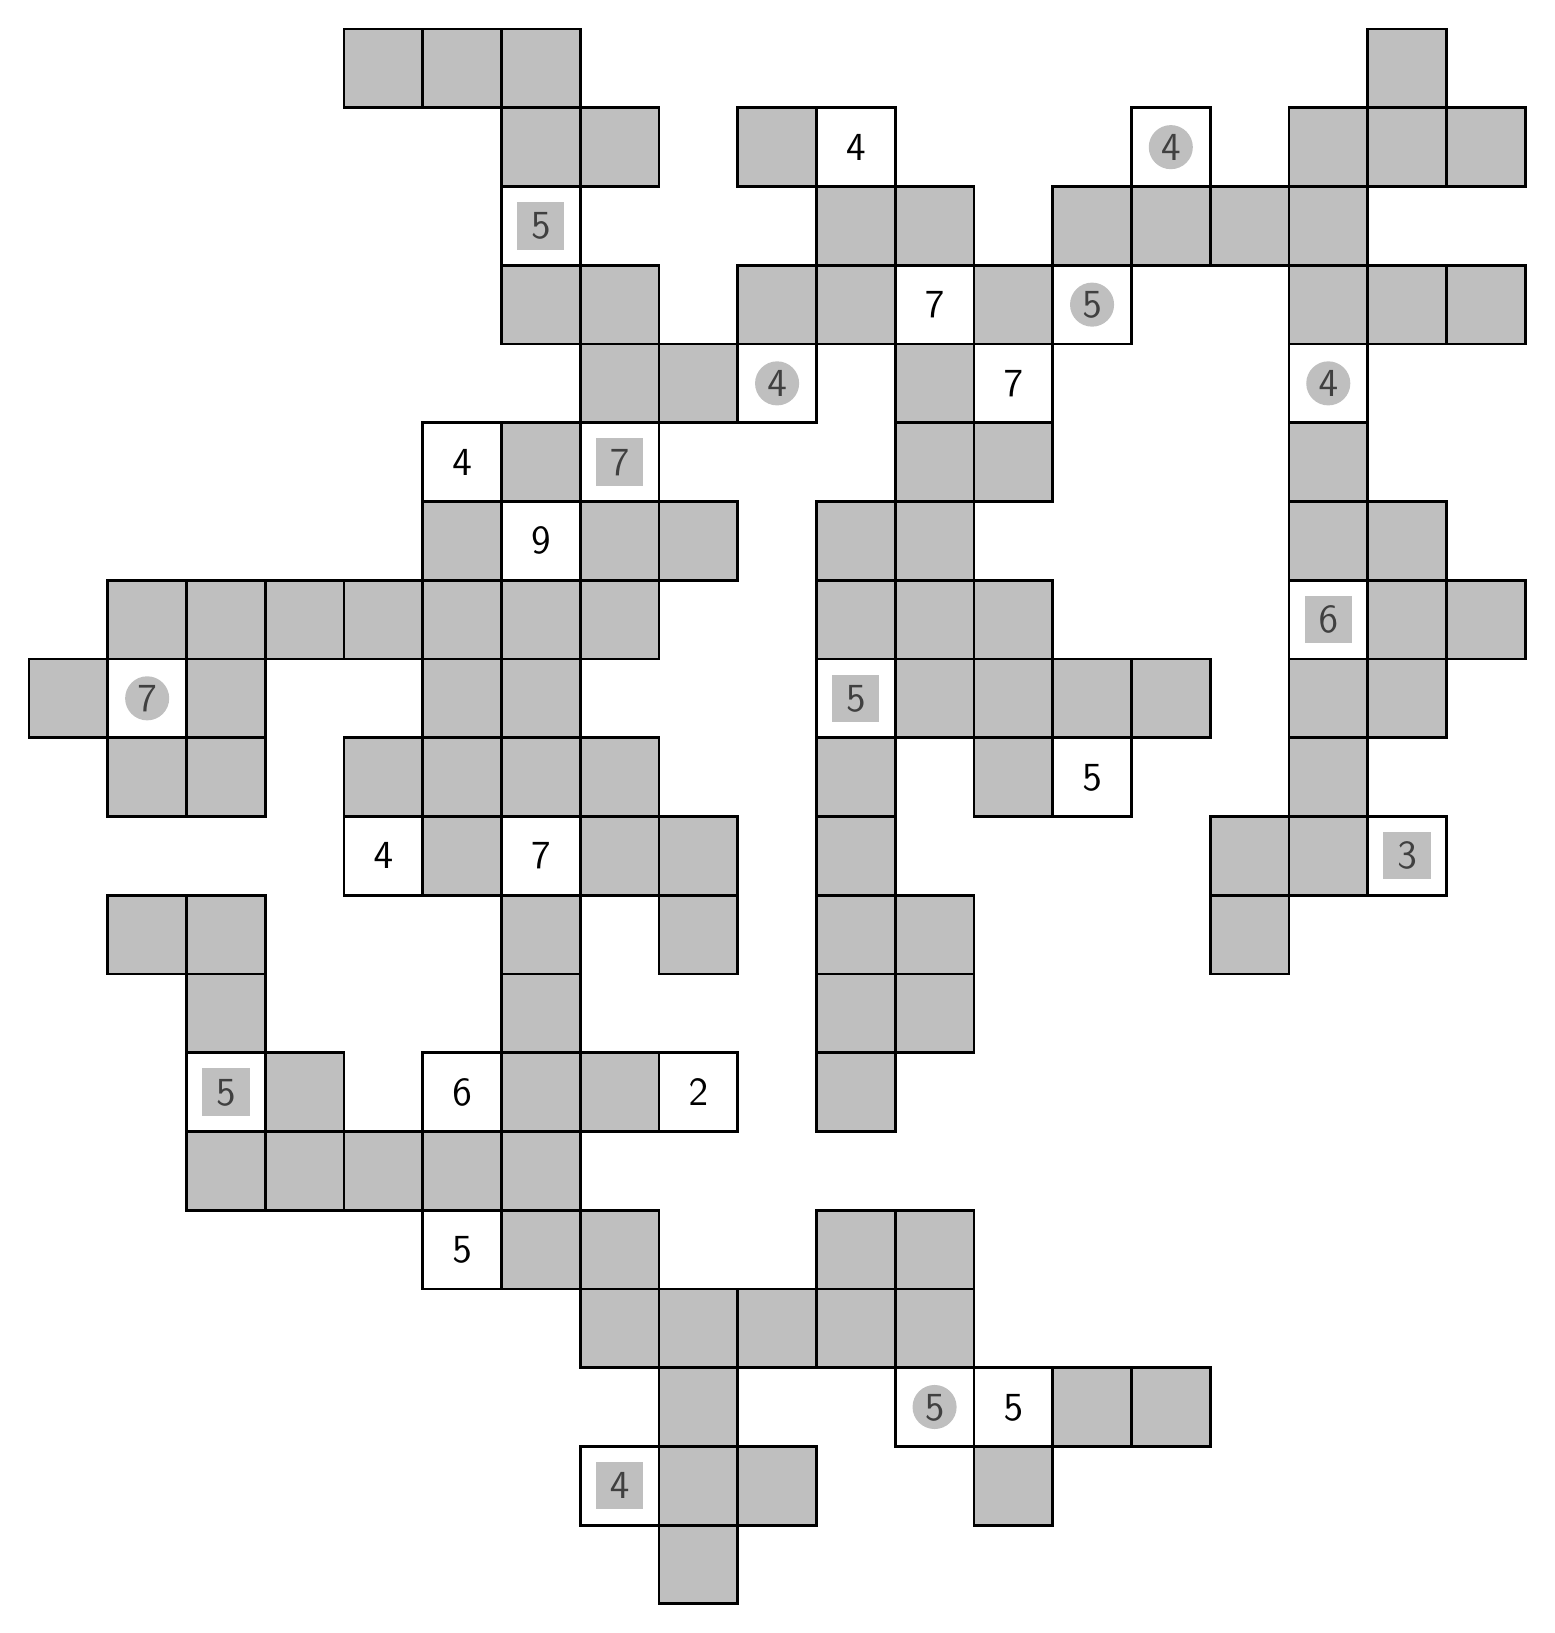
\begin{tikzpicture}\fill[gray, opacity = 0.5] (9, 0, 0)--++(1, 0, 0)--++(0, 1, 0)--++(-1, 0, 0)--cycle;
\draw[line width = 1pt] (9, 0, 0)--++(1, 0, 0)--++(0, 1, 0)--++(-1, 0, 0)--cycle;
\draw node at (8.5, 1.5, 0) {\Large $\mathsf{4}$};
\draw[line width = 1pt] (8, 1, 0)--++(1, 0, 0)--++(0, 1, 0)--++(-1, 0, 0)--cycle;
\fill[color = gray, opacity = 0.5] (8.2, 1.2) rectangle ++(0.6, 0.6);
\fill[gray, opacity = 0.5] (9, 1, 0)--++(1, 0, 0)--++(0, 1, 0)--++(-1, 0, 0)--cycle;
\draw[line width = 1pt] (9, 1, 0)--++(1, 0, 0)--++(0, 1, 0)--++(-1, 0, 0)--cycle;
\fill[gray, opacity = 0.5] (10, 1, 0)--++(1, 0, 0)--++(0, 1, 0)--++(-1, 0, 0)--cycle;
\draw[line width = 1pt] (10, 1, 0)--++(1, 0, 0)--++(0, 1, 0)--++(-1, 0, 0)--cycle;
\fill[gray, opacity = 0.5] (13, 1, 0)--++(1, 0, 0)--++(0, 1, 0)--++(-1, 0, 0)--cycle;
\draw[line width = 1pt] (13, 1, 0)--++(1, 0, 0)--++(0, 1, 0)--++(-1, 0, 0)--cycle;
\fill[gray, opacity = 0.5] (9, 2, 0)--++(1, 0, 0)--++(0, 1, 0)--++(-1, 0, 0)--cycle;
\draw[line width = 1pt] (9, 2, 0)--++(1, 0, 0)--++(0, 1, 0)--++(-1, 0, 0)--cycle;
\draw node at (12.5, 2.5, 0) {\Large $\mathsf{5}$};
\draw[line width = 1pt] (12, 2, 0)--++(1, 0, 0)--++(0, 1, 0)--++(-1, 0, 0)--cycle;
\fill[color = gray, opacity = 0.5] (12.5, 2.5, 0) circle (0.28);
\draw node at (13.5, 2.5, 0) {\Large $\mathsf{5}$};
\draw[line width = 1pt] (13, 2, 0)--++(1, 0, 0)--++(0, 1, 0)--++(-1, 0, 0)--cycle;
\fill[gray, opacity = 0.5] (14, 2, 0)--++(1, 0, 0)--++(0, 1, 0)--++(-1, 0, 0)--cycle;
\draw[line width = 1pt] (14, 2, 0)--++(1, 0, 0)--++(0, 1, 0)--++(-1, 0, 0)--cycle;
\fill[gray, opacity = 0.5] (15, 2, 0)--++(1, 0, 0)--++(0, 1, 0)--++(-1, 0, 0)--cycle;
\draw[line width = 1pt] (15, 2, 0)--++(1, 0, 0)--++(0, 1, 0)--++(-1, 0, 0)--cycle;
\fill[gray, opacity = 0.5] (8, 3, 0)--++(1, 0, 0)--++(0, 1, 0)--++(-1, 0, 0)--cycle;
\draw[line width = 1pt] (8, 3, 0)--++(1, 0, 0)--++(0, 1, 0)--++(-1, 0, 0)--cycle;
\fill[gray, opacity = 0.5] (9, 3, 0)--++(1, 0, 0)--++(0, 1, 0)--++(-1, 0, 0)--cycle;
\draw[line width = 1pt] (9, 3, 0)--++(1, 0, 0)--++(0, 1, 0)--++(-1, 0, 0)--cycle;
\fill[gray, opacity = 0.5] (10, 3, 0)--++(1, 0, 0)--++(0, 1, 0)--++(-1, 0, 0)--cycle;
\draw[line width = 1pt] (10, 3, 0)--++(1, 0, 0)--++(0, 1, 0)--++(-1, 0, 0)--cycle;
\fill[gray, opacity = 0.5] (11, 3, 0)--++(1, 0, 0)--++(0, 1, 0)--++(-1, 0, 0)--cycle;
\draw[line width = 1pt] (11, 3, 0)--++(1, 0, 0)--++(0, 1, 0)--++(-1, 0, 0)--cycle;
\fill[gray, opacity = 0.5] (12, 3, 0)--++(1, 0, 0)--++(0, 1, 0)--++(-1, 0, 0)--cycle;
\draw[line width = 1pt] (12, 3, 0)--++(1, 0, 0)--++(0, 1, 0)--++(-1, 0, 0)--cycle;
\draw node at (6.5, 4.5, 0) {\Large $\mathsf{5}$};
\draw[line width = 1pt] (6, 4, 0)--++(1, 0, 0)--++(0, 1, 0)--++(-1, 0, 0)--cycle;
\fill[gray, opacity = 0.5] (7, 4, 0)--++(1, 0, 0)--++(0, 1, 0)--++(-1, 0, 0)--cycle;
\draw[line width = 1pt] (7, 4, 0)--++(1, 0, 0)--++(0, 1, 0)--++(-1, 0, 0)--cycle;
\fill[gray, opacity = 0.5] (8, 4, 0)--++(1, 0, 0)--++(0, 1, 0)--++(-1, 0, 0)--cycle;
\draw[line width = 1pt] (8, 4, 0)--++(1, 0, 0)--++(0, 1, 0)--++(-1, 0, 0)--cycle;
\fill[gray, opacity = 0.5] (11, 4, 0)--++(1, 0, 0)--++(0, 1, 0)--++(-1, 0, 0)--cycle;
\draw[line width = 1pt] (11, 4, 0)--++(1, 0, 0)--++(0, 1, 0)--++(-1, 0, 0)--cycle;
\fill[gray, opacity = 0.5] (12, 4, 0)--++(1, 0, 0)--++(0, 1, 0)--++(-1, 0, 0)--cycle;
\draw[line width = 1pt] (12, 4, 0)--++(1, 0, 0)--++(0, 1, 0)--++(-1, 0, 0)--cycle;
\fill[gray, opacity = 0.5] (3, 5, 0)--++(1, 0, 0)--++(0, 1, 0)--++(-1, 0, 0)--cycle;
\draw[line width = 1pt] (3, 5, 0)--++(1, 0, 0)--++(0, 1, 0)--++(-1, 0, 0)--cycle;
\fill[gray, opacity = 0.5] (4, 5, 0)--++(1, 0, 0)--++(0, 1, 0)--++(-1, 0, 0)--cycle;
\draw[line width = 1pt] (4, 5, 0)--++(1, 0, 0)--++(0, 1, 0)--++(-1, 0, 0)--cycle;
\fill[gray, opacity = 0.5] (5, 5, 0)--++(1, 0, 0)--++(0, 1, 0)--++(-1, 0, 0)--cycle;
\draw[line width = 1pt] (5, 5, 0)--++(1, 0, 0)--++(0, 1, 0)--++(-1, 0, 0)--cycle;
\fill[gray, opacity = 0.5] (6, 5, 0)--++(1, 0, 0)--++(0, 1, 0)--++(-1, 0, 0)--cycle;
\draw[line width = 1pt] (6, 5, 0)--++(1, 0, 0)--++(0, 1, 0)--++(-1, 0, 0)--cycle;
\fill[gray, opacity = 0.5] (7, 5, 0)--++(1, 0, 0)--++(0, 1, 0)--++(-1, 0, 0)--cycle;
\draw[line width = 1pt] (7, 5, 0)--++(1, 0, 0)--++(0, 1, 0)--++(-1, 0, 0)--cycle;
\draw node at (3.5, 6.5, 0) {\Large $\mathsf{5}$};
\draw[line width = 1pt] (3, 6, 0)--++(1, 0, 0)--++(0, 1, 0)--++(-1, 0, 0)--cycle;
\fill[color = gray, opacity = 0.5] (3.2, 6.2) rectangle ++(0.6, 0.6);
\fill[gray, opacity = 0.5] (4, 6, 0)--++(1, 0, 0)--++(0, 1, 0)--++(-1, 0, 0)--cycle;
\draw[line width = 1pt] (4, 6, 0)--++(1, 0, 0)--++(0, 1, 0)--++(-1, 0, 0)--cycle;
\draw node at (6.5, 6.5, 0) {\Large $\mathsf{6}$};
\draw[line width = 1pt] (6, 6, 0)--++(1, 0, 0)--++(0, 1, 0)--++(-1, 0, 0)--cycle;
\fill[gray, opacity = 0.5] (7, 6, 0)--++(1, 0, 0)--++(0, 1, 0)--++(-1, 0, 0)--cycle;
\draw[line width = 1pt] (7, 6, 0)--++(1, 0, 0)--++(0, 1, 0)--++(-1, 0, 0)--cycle;
\fill[gray, opacity = 0.5] (8, 6, 0)--++(1, 0, 0)--++(0, 1, 0)--++(-1, 0, 0)--cycle;
\draw[line width = 1pt] (8, 6, 0)--++(1, 0, 0)--++(0, 1, 0)--++(-1, 0, 0)--cycle;
\draw node at (9.5, 6.5, 0) {\Large $\mathsf{2}$};
\draw[line width = 1pt] (9, 6, 0)--++(1, 0, 0)--++(0, 1, 0)--++(-1, 0, 0)--cycle;
\fill[gray, opacity = 0.5] (11, 6, 0)--++(1, 0, 0)--++(0, 1, 0)--++(-1, 0, 0)--cycle;
\draw[line width = 1pt] (11, 6, 0)--++(1, 0, 0)--++(0, 1, 0)--++(-1, 0, 0)--cycle;
\fill[gray, opacity = 0.5] (3, 7, 0)--++(1, 0, 0)--++(0, 1, 0)--++(-1, 0, 0)--cycle;
\draw[line width = 1pt] (3, 7, 0)--++(1, 0, 0)--++(0, 1, 0)--++(-1, 0, 0)--cycle;
\fill[gray, opacity = 0.5] (7, 7, 0)--++(1, 0, 0)--++(0, 1, 0)--++(-1, 0, 0)--cycle;
\draw[line width = 1pt] (7, 7, 0)--++(1, 0, 0)--++(0, 1, 0)--++(-1, 0, 0)--cycle;
\fill[gray, opacity = 0.5] (11, 7, 0)--++(1, 0, 0)--++(0, 1, 0)--++(-1, 0, 0)--cycle;
\draw[line width = 1pt] (11, 7, 0)--++(1, 0, 0)--++(0, 1, 0)--++(-1, 0, 0)--cycle;
\fill[gray, opacity = 0.5] (12, 7, 0)--++(1, 0, 0)--++(0, 1, 0)--++(-1, 0, 0)--cycle;
\draw[line width = 1pt] (12, 7, 0)--++(1, 0, 0)--++(0, 1, 0)--++(-1, 0, 0)--cycle;
\fill[gray, opacity = 0.5] (2, 8, 0)--++(1, 0, 0)--++(0, 1, 0)--++(-1, 0, 0)--cycle;
\draw[line width = 1pt] (2, 8, 0)--++(1, 0, 0)--++(0, 1, 0)--++(-1, 0, 0)--cycle;
\fill[gray, opacity = 0.5] (3, 8, 0)--++(1, 0, 0)--++(0, 1, 0)--++(-1, 0, 0)--cycle;
\draw[line width = 1pt] (3, 8, 0)--++(1, 0, 0)--++(0, 1, 0)--++(-1, 0, 0)--cycle;
\fill[gray, opacity = 0.5] (7, 8, 0)--++(1, 0, 0)--++(0, 1, 0)--++(-1, 0, 0)--cycle;
\draw[line width = 1pt] (7, 8, 0)--++(1, 0, 0)--++(0, 1, 0)--++(-1, 0, 0)--cycle;
\fill[gray, opacity = 0.5] (9, 8, 0)--++(1, 0, 0)--++(0, 1, 0)--++(-1, 0, 0)--cycle;
\draw[line width = 1pt] (9, 8, 0)--++(1, 0, 0)--++(0, 1, 0)--++(-1, 0, 0)--cycle;
\fill[gray, opacity = 0.5] (11, 8, 0)--++(1, 0, 0)--++(0, 1, 0)--++(-1, 0, 0)--cycle;
\draw[line width = 1pt] (11, 8, 0)--++(1, 0, 0)--++(0, 1, 0)--++(-1, 0, 0)--cycle;
\fill[gray, opacity = 0.5] (12, 8, 0)--++(1, 0, 0)--++(0, 1, 0)--++(-1, 0, 0)--cycle;
\draw[line width = 1pt] (12, 8, 0)--++(1, 0, 0)--++(0, 1, 0)--++(-1, 0, 0)--cycle;
\fill[gray, opacity = 0.5] (16, 8, 0)--++(1, 0, 0)--++(0, 1, 0)--++(-1, 0, 0)--cycle;
\draw[line width = 1pt] (16, 8, 0)--++(1, 0, 0)--++(0, 1, 0)--++(-1, 0, 0)--cycle;
\draw node at (5.5, 9.5, 0) {\Large $\mathsf{4}$};
\draw[line width = 1pt] (5, 9, 0)--++(1, 0, 0)--++(0, 1, 0)--++(-1, 0, 0)--cycle;
\fill[gray, opacity = 0.5] (6, 9, 0)--++(1, 0, 0)--++(0, 1, 0)--++(-1, 0, 0)--cycle;
\draw[line width = 1pt] (6, 9, 0)--++(1, 0, 0)--++(0, 1, 0)--++(-1, 0, 0)--cycle;
\draw node at (7.5, 9.5, 0) {\Large $\mathsf{7}$};
\draw[line width = 1pt] (7, 9, 0)--++(1, 0, 0)--++(0, 1, 0)--++(-1, 0, 0)--cycle;
\fill[gray, opacity = 0.5] (8, 9, 0)--++(1, 0, 0)--++(0, 1, 0)--++(-1, 0, 0)--cycle;
\draw[line width = 1pt] (8, 9, 0)--++(1, 0, 0)--++(0, 1, 0)--++(-1, 0, 0)--cycle;
\fill[gray, opacity = 0.5] (9, 9, 0)--++(1, 0, 0)--++(0, 1, 0)--++(-1, 0, 0)--cycle;
\draw[line width = 1pt] (9, 9, 0)--++(1, 0, 0)--++(0, 1, 0)--++(-1, 0, 0)--cycle;
\fill[gray, opacity = 0.5] (11, 9, 0)--++(1, 0, 0)--++(0, 1, 0)--++(-1, 0, 0)--cycle;
\draw[line width = 1pt] (11, 9, 0)--++(1, 0, 0)--++(0, 1, 0)--++(-1, 0, 0)--cycle;
\fill[gray, opacity = 0.5] (16, 9, 0)--++(1, 0, 0)--++(0, 1, 0)--++(-1, 0, 0)--cycle;
\draw[line width = 1pt] (16, 9, 0)--++(1, 0, 0)--++(0, 1, 0)--++(-1, 0, 0)--cycle;
\fill[gray, opacity = 0.5] (17, 9, 0)--++(1, 0, 0)--++(0, 1, 0)--++(-1, 0, 0)--cycle;
\draw[line width = 1pt] (17, 9, 0)--++(1, 0, 0)--++(0, 1, 0)--++(-1, 0, 0)--cycle;
\draw node at (18.5, 9.5, 0) {\Large $\mathsf{3}$};
\draw[line width = 1pt] (18, 9, 0)--++(1, 0, 0)--++(0, 1, 0)--++(-1, 0, 0)--cycle;
\fill[color = gray, opacity = 0.5] (18.2, 9.2) rectangle ++(0.6, 0.6);
\fill[gray, opacity = 0.5] (2, 10, 0)--++(1, 0, 0)--++(0, 1, 0)--++(-1, 0, 0)--cycle;
\draw[line width = 1pt] (2, 10, 0)--++(1, 0, 0)--++(0, 1, 0)--++(-1, 0, 0)--cycle;
\fill[gray, opacity = 0.5] (3, 10, 0)--++(1, 0, 0)--++(0, 1, 0)--++(-1, 0, 0)--cycle;
\draw[line width = 1pt] (3, 10, 0)--++(1, 0, 0)--++(0, 1, 0)--++(-1, 0, 0)--cycle;
\fill[gray, opacity = 0.5] (5, 10, 0)--++(1, 0, 0)--++(0, 1, 0)--++(-1, 0, 0)--cycle;
\draw[line width = 1pt] (5, 10, 0)--++(1, 0, 0)--++(0, 1, 0)--++(-1, 0, 0)--cycle;
\fill[gray, opacity = 0.5] (6, 10, 0)--++(1, 0, 0)--++(0, 1, 0)--++(-1, 0, 0)--cycle;
\draw[line width = 1pt] (6, 10, 0)--++(1, 0, 0)--++(0, 1, 0)--++(-1, 0, 0)--cycle;
\fill[gray, opacity = 0.5] (7, 10, 0)--++(1, 0, 0)--++(0, 1, 0)--++(-1, 0, 0)--cycle;
\draw[line width = 1pt] (7, 10, 0)--++(1, 0, 0)--++(0, 1, 0)--++(-1, 0, 0)--cycle;
\fill[gray, opacity = 0.5] (8, 10, 0)--++(1, 0, 0)--++(0, 1, 0)--++(-1, 0, 0)--cycle;
\draw[line width = 1pt] (8, 10, 0)--++(1, 0, 0)--++(0, 1, 0)--++(-1, 0, 0)--cycle;
\fill[gray, opacity = 0.5] (11, 10, 0)--++(1, 0, 0)--++(0, 1, 0)--++(-1, 0, 0)--cycle;
\draw[line width = 1pt] (11, 10, 0)--++(1, 0, 0)--++(0, 1, 0)--++(-1, 0, 0)--cycle;
\fill[gray, opacity = 0.5] (13, 10, 0)--++(1, 0, 0)--++(0, 1, 0)--++(-1, 0, 0)--cycle;
\draw[line width = 1pt] (13, 10, 0)--++(1, 0, 0)--++(0, 1, 0)--++(-1, 0, 0)--cycle;
\draw node at (14.5, 10.5, 0) {\Large $\mathsf{5}$};
\draw[line width = 1pt] (14, 10, 0)--++(1, 0, 0)--++(0, 1, 0)--++(-1, 0, 0)--cycle;
\fill[gray, opacity = 0.5] (17, 10, 0)--++(1, 0, 0)--++(0, 1, 0)--++(-1, 0, 0)--cycle;
\draw[line width = 1pt] (17, 10, 0)--++(1, 0, 0)--++(0, 1, 0)--++(-1, 0, 0)--cycle;
\fill[gray, opacity = 0.5] (1, 11, 0)--++(1, 0, 0)--++(0, 1, 0)--++(-1, 0, 0)--cycle;
\draw[line width = 1pt] (1, 11, 0)--++(1, 0, 0)--++(0, 1, 0)--++(-1, 0, 0)--cycle;
\draw node at (2.5, 11.5, 0) {\Large $\mathsf{7}$};
\draw[line width = 1pt] (2, 11, 0)--++(1, 0, 0)--++(0, 1, 0)--++(-1, 0, 0)--cycle;
\fill[color = gray, opacity = 0.5] (2.5, 11.5, 0) circle (0.28);
\fill[gray, opacity = 0.5] (3, 11, 0)--++(1, 0, 0)--++(0, 1, 0)--++(-1, 0, 0)--cycle;
\draw[line width = 1pt] (3, 11, 0)--++(1, 0, 0)--++(0, 1, 0)--++(-1, 0, 0)--cycle;
\fill[gray, opacity = 0.5] (6, 11, 0)--++(1, 0, 0)--++(0, 1, 0)--++(-1, 0, 0)--cycle;
\draw[line width = 1pt] (6, 11, 0)--++(1, 0, 0)--++(0, 1, 0)--++(-1, 0, 0)--cycle;
\fill[gray, opacity = 0.5] (7, 11, 0)--++(1, 0, 0)--++(0, 1, 0)--++(-1, 0, 0)--cycle;
\draw[line width = 1pt] (7, 11, 0)--++(1, 0, 0)--++(0, 1, 0)--++(-1, 0, 0)--cycle;
\draw node at (11.5, 11.5, 0) {\Large $\mathsf{5}$};
\draw[line width = 1pt] (11, 11, 0)--++(1, 0, 0)--++(0, 1, 0)--++(-1, 0, 0)--cycle;
\fill[color = gray, opacity = 0.5] (11.2, 11.2) rectangle ++(0.6, 0.6);
\fill[gray, opacity = 0.5] (12, 11, 0)--++(1, 0, 0)--++(0, 1, 0)--++(-1, 0, 0)--cycle;
\draw[line width = 1pt] (12, 11, 0)--++(1, 0, 0)--++(0, 1, 0)--++(-1, 0, 0)--cycle;
\fill[gray, opacity = 0.5] (13, 11, 0)--++(1, 0, 0)--++(0, 1, 0)--++(-1, 0, 0)--cycle;
\draw[line width = 1pt] (13, 11, 0)--++(1, 0, 0)--++(0, 1, 0)--++(-1, 0, 0)--cycle;
\fill[gray, opacity = 0.5] (14, 11, 0)--++(1, 0, 0)--++(0, 1, 0)--++(-1, 0, 0)--cycle;
\draw[line width = 1pt] (14, 11, 0)--++(1, 0, 0)--++(0, 1, 0)--++(-1, 0, 0)--cycle;
\fill[gray, opacity = 0.5] (15, 11, 0)--++(1, 0, 0)--++(0, 1, 0)--++(-1, 0, 0)--cycle;
\draw[line width = 1pt] (15, 11, 0)--++(1, 0, 0)--++(0, 1, 0)--++(-1, 0, 0)--cycle;
\fill[gray, opacity = 0.5] (17, 11, 0)--++(1, 0, 0)--++(0, 1, 0)--++(-1, 0, 0)--cycle;
\draw[line width = 1pt] (17, 11, 0)--++(1, 0, 0)--++(0, 1, 0)--++(-1, 0, 0)--cycle;
\fill[gray, opacity = 0.5] (18, 11, 0)--++(1, 0, 0)--++(0, 1, 0)--++(-1, 0, 0)--cycle;
\draw[line width = 1pt] (18, 11, 0)--++(1, 0, 0)--++(0, 1, 0)--++(-1, 0, 0)--cycle;
\fill[gray, opacity = 0.5] (2, 12, 0)--++(1, 0, 0)--++(0, 1, 0)--++(-1, 0, 0)--cycle;
\draw[line width = 1pt] (2, 12, 0)--++(1, 0, 0)--++(0, 1, 0)--++(-1, 0, 0)--cycle;
\fill[gray, opacity = 0.5] (3, 12, 0)--++(1, 0, 0)--++(0, 1, 0)--++(-1, 0, 0)--cycle;
\draw[line width = 1pt] (3, 12, 0)--++(1, 0, 0)--++(0, 1, 0)--++(-1, 0, 0)--cycle;
\fill[gray, opacity = 0.5] (4, 12, 0)--++(1, 0, 0)--++(0, 1, 0)--++(-1, 0, 0)--cycle;
\draw[line width = 1pt] (4, 12, 0)--++(1, 0, 0)--++(0, 1, 0)--++(-1, 0, 0)--cycle;
\fill[gray, opacity = 0.5] (5, 12, 0)--++(1, 0, 0)--++(0, 1, 0)--++(-1, 0, 0)--cycle;
\draw[line width = 1pt] (5, 12, 0)--++(1, 0, 0)--++(0, 1, 0)--++(-1, 0, 0)--cycle;
\fill[gray, opacity = 0.5] (6, 12, 0)--++(1, 0, 0)--++(0, 1, 0)--++(-1, 0, 0)--cycle;
\draw[line width = 1pt] (6, 12, 0)--++(1, 0, 0)--++(0, 1, 0)--++(-1, 0, 0)--cycle;
\fill[gray, opacity = 0.5] (7, 12, 0)--++(1, 0, 0)--++(0, 1, 0)--++(-1, 0, 0)--cycle;
\draw[line width = 1pt] (7, 12, 0)--++(1, 0, 0)--++(0, 1, 0)--++(-1, 0, 0)--cycle;
\fill[gray, opacity = 0.5] (8, 12, 0)--++(1, 0, 0)--++(0, 1, 0)--++(-1, 0, 0)--cycle;
\draw[line width = 1pt] (8, 12, 0)--++(1, 0, 0)--++(0, 1, 0)--++(-1, 0, 0)--cycle;
\fill[gray, opacity = 0.5] (11, 12, 0)--++(1, 0, 0)--++(0, 1, 0)--++(-1, 0, 0)--cycle;
\draw[line width = 1pt] (11, 12, 0)--++(1, 0, 0)--++(0, 1, 0)--++(-1, 0, 0)--cycle;
\fill[gray, opacity = 0.5] (12, 12, 0)--++(1, 0, 0)--++(0, 1, 0)--++(-1, 0, 0)--cycle;
\draw[line width = 1pt] (12, 12, 0)--++(1, 0, 0)--++(0, 1, 0)--++(-1, 0, 0)--cycle;
\fill[gray, opacity = 0.5] (13, 12, 0)--++(1, 0, 0)--++(0, 1, 0)--++(-1, 0, 0)--cycle;
\draw[line width = 1pt] (13, 12, 0)--++(1, 0, 0)--++(0, 1, 0)--++(-1, 0, 0)--cycle;
\draw node at (17.5, 12.5, 0) {\Large $\mathsf{6}$};
\draw[line width = 1pt] (17, 12, 0)--++(1, 0, 0)--++(0, 1, 0)--++(-1, 0, 0)--cycle;
\fill[color = gray, opacity = 0.5] (17.2, 12.2) rectangle ++(0.6, 0.6);
\fill[gray, opacity = 0.5] (18, 12, 0)--++(1, 0, 0)--++(0, 1, 0)--++(-1, 0, 0)--cycle;
\draw[line width = 1pt] (18, 12, 0)--++(1, 0, 0)--++(0, 1, 0)--++(-1, 0, 0)--cycle;
\fill[gray, opacity = 0.5] (19, 12, 0)--++(1, 0, 0)--++(0, 1, 0)--++(-1, 0, 0)--cycle;
\draw[line width = 1pt] (19, 12, 0)--++(1, 0, 0)--++(0, 1, 0)--++(-1, 0, 0)--cycle;
\fill[gray, opacity = 0.5] (6, 13, 0)--++(1, 0, 0)--++(0, 1, 0)--++(-1, 0, 0)--cycle;
\draw[line width = 1pt] (6, 13, 0)--++(1, 0, 0)--++(0, 1, 0)--++(-1, 0, 0)--cycle;
\draw node at (7.5, 13.5, 0) {\Large $\mathsf{9}$};
\draw[line width = 1pt] (7, 13, 0)--++(1, 0, 0)--++(0, 1, 0)--++(-1, 0, 0)--cycle;
\fill[gray, opacity = 0.5] (8, 13, 0)--++(1, 0, 0)--++(0, 1, 0)--++(-1, 0, 0)--cycle;
\draw[line width = 1pt] (8, 13, 0)--++(1, 0, 0)--++(0, 1, 0)--++(-1, 0, 0)--cycle;
\fill[gray, opacity = 0.5] (9, 13, 0)--++(1, 0, 0)--++(0, 1, 0)--++(-1, 0, 0)--cycle;
\draw[line width = 1pt] (9, 13, 0)--++(1, 0, 0)--++(0, 1, 0)--++(-1, 0, 0)--cycle;
\fill[gray, opacity = 0.5] (11, 13, 0)--++(1, 0, 0)--++(0, 1, 0)--++(-1, 0, 0)--cycle;
\draw[line width = 1pt] (11, 13, 0)--++(1, 0, 0)--++(0, 1, 0)--++(-1, 0, 0)--cycle;
\fill[gray, opacity = 0.5] (12, 13, 0)--++(1, 0, 0)--++(0, 1, 0)--++(-1, 0, 0)--cycle;
\draw[line width = 1pt] (12, 13, 0)--++(1, 0, 0)--++(0, 1, 0)--++(-1, 0, 0)--cycle;
\fill[gray, opacity = 0.5] (17, 13, 0)--++(1, 0, 0)--++(0, 1, 0)--++(-1, 0, 0)--cycle;
\draw[line width = 1pt] (17, 13, 0)--++(1, 0, 0)--++(0, 1, 0)--++(-1, 0, 0)--cycle;
\fill[gray, opacity = 0.5] (18, 13, 0)--++(1, 0, 0)--++(0, 1, 0)--++(-1, 0, 0)--cycle;
\draw[line width = 1pt] (18, 13, 0)--++(1, 0, 0)--++(0, 1, 0)--++(-1, 0, 0)--cycle;
\draw node at (6.5, 14.5, 0) {\Large $\mathsf{4}$};
\draw[line width = 1pt] (6, 14, 0)--++(1, 0, 0)--++(0, 1, 0)--++(-1, 0, 0)--cycle;
\fill[gray, opacity = 0.5] (7, 14, 0)--++(1, 0, 0)--++(0, 1, 0)--++(-1, 0, 0)--cycle;
\draw[line width = 1pt] (7, 14, 0)--++(1, 0, 0)--++(0, 1, 0)--++(-1, 0, 0)--cycle;
\draw node at (8.5, 14.5, 0) {\Large $\mathsf{7}$};
\draw[line width = 1pt] (8, 14, 0)--++(1, 0, 0)--++(0, 1, 0)--++(-1, 0, 0)--cycle;
\fill[color = gray, opacity = 0.5] (8.2, 14.2) rectangle ++(0.6, 0.6);
\fill[gray, opacity = 0.5] (12, 14, 0)--++(1, 0, 0)--++(0, 1, 0)--++(-1, 0, 0)--cycle;
\draw[line width = 1pt] (12, 14, 0)--++(1, 0, 0)--++(0, 1, 0)--++(-1, 0, 0)--cycle;
\fill[gray, opacity = 0.5] (13, 14, 0)--++(1, 0, 0)--++(0, 1, 0)--++(-1, 0, 0)--cycle;
\draw[line width = 1pt] (13, 14, 0)--++(1, 0, 0)--++(0, 1, 0)--++(-1, 0, 0)--cycle;
\fill[gray, opacity = 0.5] (17, 14, 0)--++(1, 0, 0)--++(0, 1, 0)--++(-1, 0, 0)--cycle;
\draw[line width = 1pt] (17, 14, 0)--++(1, 0, 0)--++(0, 1, 0)--++(-1, 0, 0)--cycle;
\fill[gray, opacity = 0.5] (8, 15, 0)--++(1, 0, 0)--++(0, 1, 0)--++(-1, 0, 0)--cycle;
\draw[line width = 1pt] (8, 15, 0)--++(1, 0, 0)--++(0, 1, 0)--++(-1, 0, 0)--cycle;
\fill[gray, opacity = 0.5] (9, 15, 0)--++(1, 0, 0)--++(0, 1, 0)--++(-1, 0, 0)--cycle;
\draw[line width = 1pt] (9, 15, 0)--++(1, 0, 0)--++(0, 1, 0)--++(-1, 0, 0)--cycle;
\draw node at (10.5, 15.5, 0) {\Large $\mathsf{4}$};
\draw[line width = 1pt] (10, 15, 0)--++(1, 0, 0)--++(0, 1, 0)--++(-1, 0, 0)--cycle;
\fill[color = gray, opacity = 0.5] (10.5, 15.5, 0) circle (0.28);
\fill[gray, opacity = 0.5] (12, 15, 0)--++(1, 0, 0)--++(0, 1, 0)--++(-1, 0, 0)--cycle;
\draw[line width = 1pt] (12, 15, 0)--++(1, 0, 0)--++(0, 1, 0)--++(-1, 0, 0)--cycle;
\draw node at (13.5, 15.5, 0) {\Large $\mathsf{7}$};
\draw[line width = 1pt] (13, 15, 0)--++(1, 0, 0)--++(0, 1, 0)--++(-1, 0, 0)--cycle;
\draw node at (17.5, 15.5, 0) {\Large $\mathsf{4}$};
\draw[line width = 1pt] (17, 15, 0)--++(1, 0, 0)--++(0, 1, 0)--++(-1, 0, 0)--cycle;
\fill[color = gray, opacity = 0.5] (17.5, 15.5, 0) circle (0.28);
\fill[gray, opacity = 0.5] (7, 16, 0)--++(1, 0, 0)--++(0, 1, 0)--++(-1, 0, 0)--cycle;
\draw[line width = 1pt] (7, 16, 0)--++(1, 0, 0)--++(0, 1, 0)--++(-1, 0, 0)--cycle;
\fill[gray, opacity = 0.5] (8, 16, 0)--++(1, 0, 0)--++(0, 1, 0)--++(-1, 0, 0)--cycle;
\draw[line width = 1pt] (8, 16, 0)--++(1, 0, 0)--++(0, 1, 0)--++(-1, 0, 0)--cycle;
\fill[gray, opacity = 0.5] (10, 16, 0)--++(1, 0, 0)--++(0, 1, 0)--++(-1, 0, 0)--cycle;
\draw[line width = 1pt] (10, 16, 0)--++(1, 0, 0)--++(0, 1, 0)--++(-1, 0, 0)--cycle;
\fill[gray, opacity = 0.5] (11, 16, 0)--++(1, 0, 0)--++(0, 1, 0)--++(-1, 0, 0)--cycle;
\draw[line width = 1pt] (11, 16, 0)--++(1, 0, 0)--++(0, 1, 0)--++(-1, 0, 0)--cycle;
\draw node at (12.5, 16.5, 0) {\Large $\mathsf{7}$};
\draw[line width = 1pt] (12, 16, 0)--++(1, 0, 0)--++(0, 1, 0)--++(-1, 0, 0)--cycle;
\fill[gray, opacity = 0.5] (13, 16, 0)--++(1, 0, 0)--++(0, 1, 0)--++(-1, 0, 0)--cycle;
\draw[line width = 1pt] (13, 16, 0)--++(1, 0, 0)--++(0, 1, 0)--++(-1, 0, 0)--cycle;
\draw node at (14.5, 16.5, 0) {\Large $\mathsf{5}$};
\draw[line width = 1pt] (14, 16, 0)--++(1, 0, 0)--++(0, 1, 0)--++(-1, 0, 0)--cycle;
\fill[color = gray, opacity = 0.5] (14.5, 16.5, 0) circle (0.28);
\fill[gray, opacity = 0.5] (17, 16, 0)--++(1, 0, 0)--++(0, 1, 0)--++(-1, 0, 0)--cycle;
\draw[line width = 1pt] (17, 16, 0)--++(1, 0, 0)--++(0, 1, 0)--++(-1, 0, 0)--cycle;
\fill[gray, opacity = 0.5] (18, 16, 0)--++(1, 0, 0)--++(0, 1, 0)--++(-1, 0, 0)--cycle;
\draw[line width = 1pt] (18, 16, 0)--++(1, 0, 0)--++(0, 1, 0)--++(-1, 0, 0)--cycle;
\fill[gray, opacity = 0.5] (19, 16, 0)--++(1, 0, 0)--++(0, 1, 0)--++(-1, 0, 0)--cycle;
\draw[line width = 1pt] (19, 16, 0)--++(1, 0, 0)--++(0, 1, 0)--++(-1, 0, 0)--cycle;
\draw node at (7.5, 17.5, 0) {\Large $\mathsf{5}$};
\draw[line width = 1pt] (7, 17, 0)--++(1, 0, 0)--++(0, 1, 0)--++(-1, 0, 0)--cycle;
\fill[color = gray, opacity = 0.5] (7.2, 17.2) rectangle ++(0.6, 0.6);
\fill[gray, opacity = 0.5] (11, 17, 0)--++(1, 0, 0)--++(0, 1, 0)--++(-1, 0, 0)--cycle;
\draw[line width = 1pt] (11, 17, 0)--++(1, 0, 0)--++(0, 1, 0)--++(-1, 0, 0)--cycle;
\fill[gray, opacity = 0.5] (12, 17, 0)--++(1, 0, 0)--++(0, 1, 0)--++(-1, 0, 0)--cycle;
\draw[line width = 1pt] (12, 17, 0)--++(1, 0, 0)--++(0, 1, 0)--++(-1, 0, 0)--cycle;
\fill[gray, opacity = 0.5] (14, 17, 0)--++(1, 0, 0)--++(0, 1, 0)--++(-1, 0, 0)--cycle;
\draw[line width = 1pt] (14, 17, 0)--++(1, 0, 0)--++(0, 1, 0)--++(-1, 0, 0)--cycle;
\fill[gray, opacity = 0.5] (15, 17, 0)--++(1, 0, 0)--++(0, 1, 0)--++(-1, 0, 0)--cycle;
\draw[line width = 1pt] (15, 17, 0)--++(1, 0, 0)--++(0, 1, 0)--++(-1, 0, 0)--cycle;
\fill[gray, opacity = 0.5] (16, 17, 0)--++(1, 0, 0)--++(0, 1, 0)--++(-1, 0, 0)--cycle;
\draw[line width = 1pt] (16, 17, 0)--++(1, 0, 0)--++(0, 1, 0)--++(-1, 0, 0)--cycle;
\fill[gray, opacity = 0.5] (17, 17, 0)--++(1, 0, 0)--++(0, 1, 0)--++(-1, 0, 0)--cycle;
\draw[line width = 1pt] (17, 17, 0)--++(1, 0, 0)--++(0, 1, 0)--++(-1, 0, 0)--cycle;
\fill[gray, opacity = 0.5] (7, 18, 0)--++(1, 0, 0)--++(0, 1, 0)--++(-1, 0, 0)--cycle;
\draw[line width = 1pt] (7, 18, 0)--++(1, 0, 0)--++(0, 1, 0)--++(-1, 0, 0)--cycle;
\fill[gray, opacity = 0.5] (8, 18, 0)--++(1, 0, 0)--++(0, 1, 0)--++(-1, 0, 0)--cycle;
\draw[line width = 1pt] (8, 18, 0)--++(1, 0, 0)--++(0, 1, 0)--++(-1, 0, 0)--cycle;
\fill[gray, opacity = 0.5] (10, 18, 0)--++(1, 0, 0)--++(0, 1, 0)--++(-1, 0, 0)--cycle;
\draw[line width = 1pt] (10, 18, 0)--++(1, 0, 0)--++(0, 1, 0)--++(-1, 0, 0)--cycle;
\draw node at (11.5, 18.5, 0) {\Large $\mathsf{4}$};
\draw[line width = 1pt] (11, 18, 0)--++(1, 0, 0)--++(0, 1, 0)--++(-1, 0, 0)--cycle;
\draw node at (15.5, 18.5, 0) {\Large $\mathsf{4}$};
\draw[line width = 1pt] (15, 18, 0)--++(1, 0, 0)--++(0, 1, 0)--++(-1, 0, 0)--cycle;
\fill[color = gray, opacity = 0.5] (15.5, 18.5, 0) circle (0.28);
\fill[gray, opacity = 0.5] (17, 18, 0)--++(1, 0, 0)--++(0, 1, 0)--++(-1, 0, 0)--cycle;
\draw[line width = 1pt] (17, 18, 0)--++(1, 0, 0)--++(0, 1, 0)--++(-1, 0, 0)--cycle;
\fill[gray, opacity = 0.5] (18, 18, 0)--++(1, 0, 0)--++(0, 1, 0)--++(-1, 0, 0)--cycle;
\draw[line width = 1pt] (18, 18, 0)--++(1, 0, 0)--++(0, 1, 0)--++(-1, 0, 0)--cycle;
\fill[gray, opacity = 0.5] (19, 18, 0)--++(1, 0, 0)--++(0, 1, 0)--++(-1, 0, 0)--cycle;
\draw[line width = 1pt] (19, 18, 0)--++(1, 0, 0)--++(0, 1, 0)--++(-1, 0, 0)--cycle;
\fill[gray, opacity = 0.5] (5, 19, 0)--++(1, 0, 0)--++(0, 1, 0)--++(-1, 0, 0)--cycle;
\draw[line width = 1pt] (5, 19, 0)--++(1, 0, 0)--++(0, 1, 0)--++(-1, 0, 0)--cycle;
\fill[gray, opacity = 0.5] (6, 19, 0)--++(1, 0, 0)--++(0, 1, 0)--++(-1, 0, 0)--cycle;
\draw[line width = 1pt] (6, 19, 0)--++(1, 0, 0)--++(0, 1, 0)--++(-1, 0, 0)--cycle;
\fill[gray, opacity = 0.5] (7, 19, 0)--++(1, 0, 0)--++(0, 1, 0)--++(-1, 0, 0)--cycle;
\draw[line width = 1pt] (7, 19, 0)--++(1, 0, 0)--++(0, 1, 0)--++(-1, 0, 0)--cycle;
\fill[gray, opacity = 0.5] (18, 19, 0)--++(1, 0, 0)--++(0, 1, 0)--++(-1, 0, 0)--cycle;
\draw[line width = 1pt] (18, 19, 0)--++(1, 0, 0)--++(0, 1, 0)--++(-1, 0, 0)--cycle;
\end{tikzpicture}}\]
\[\resizebox{30pc}{!}{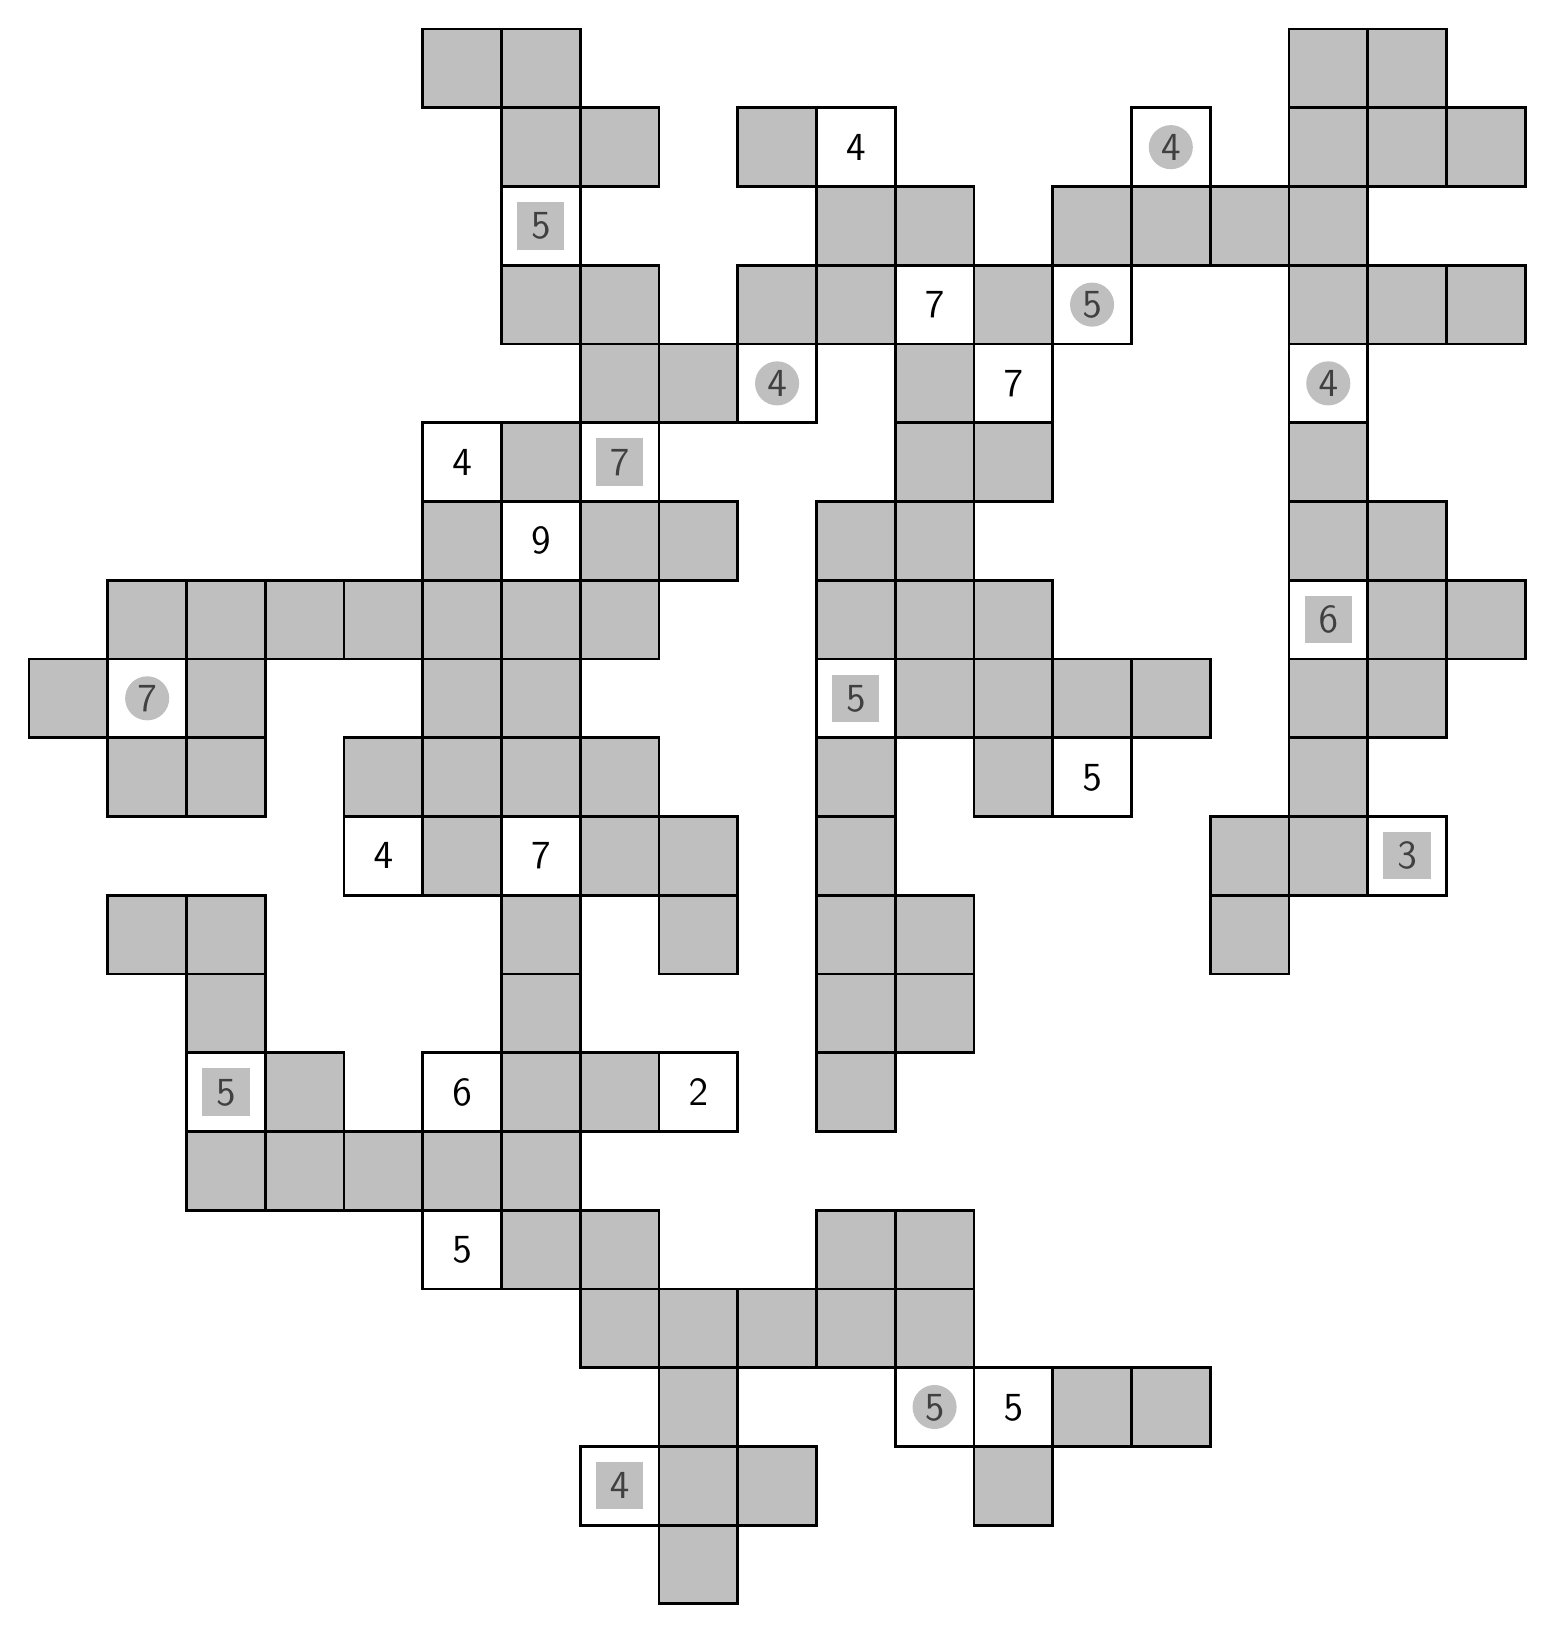
\begin{tikzpicture}\fill[gray, opacity = 0.5] (9, 0, 0)--++(1, 0, 0)--++(0, 1, 0)--++(-1, 0, 0)--cycle;
\draw[line width = 1pt] (9, 0, 0)--++(1, 0, 0)--++(0, 1, 0)--++(-1, 0, 0)--cycle;
\draw node at (8.5, 1.5, 0) {\Large $\mathsf{4}$};
\draw[line width = 1pt] (8, 1, 0)--++(1, 0, 0)--++(0, 1, 0)--++(-1, 0, 0)--cycle;
\fill[color = gray, opacity = 0.5] (8.2, 1.2) rectangle ++(0.6, 0.6);
\fill[gray, opacity = 0.5] (9, 1, 0)--++(1, 0, 0)--++(0, 1, 0)--++(-1, 0, 0)--cycle;
\draw[line width = 1pt] (9, 1, 0)--++(1, 0, 0)--++(0, 1, 0)--++(-1, 0, 0)--cycle;
\fill[gray, opacity = 0.5] (10, 1, 0)--++(1, 0, 0)--++(0, 1, 0)--++(-1, 0, 0)--cycle;
\draw[line width = 1pt] (10, 1, 0)--++(1, 0, 0)--++(0, 1, 0)--++(-1, 0, 0)--cycle;
\fill[gray, opacity = 0.5] (13, 1, 0)--++(1, 0, 0)--++(0, 1, 0)--++(-1, 0, 0)--cycle;
\draw[line width = 1pt] (13, 1, 0)--++(1, 0, 0)--++(0, 1, 0)--++(-1, 0, 0)--cycle;
\fill[gray, opacity = 0.5] (9, 2, 0)--++(1, 0, 0)--++(0, 1, 0)--++(-1, 0, 0)--cycle;
\draw[line width = 1pt] (9, 2, 0)--++(1, 0, 0)--++(0, 1, 0)--++(-1, 0, 0)--cycle;
\draw node at (12.5, 2.5, 0) {\Large $\mathsf{5}$};
\draw[line width = 1pt] (12, 2, 0)--++(1, 0, 0)--++(0, 1, 0)--++(-1, 0, 0)--cycle;
\fill[color = gray, opacity = 0.5] (12.5, 2.5, 0) circle (0.28);
\draw node at (13.5, 2.5, 0) {\Large $\mathsf{5}$};
\draw[line width = 1pt] (13, 2, 0)--++(1, 0, 0)--++(0, 1, 0)--++(-1, 0, 0)--cycle;
\fill[gray, opacity = 0.5] (14, 2, 0)--++(1, 0, 0)--++(0, 1, 0)--++(-1, 0, 0)--cycle;
\draw[line width = 1pt] (14, 2, 0)--++(1, 0, 0)--++(0, 1, 0)--++(-1, 0, 0)--cycle;
\fill[gray, opacity = 0.5] (15, 2, 0)--++(1, 0, 0)--++(0, 1, 0)--++(-1, 0, 0)--cycle;
\draw[line width = 1pt] (15, 2, 0)--++(1, 0, 0)--++(0, 1, 0)--++(-1, 0, 0)--cycle;
\fill[gray, opacity = 0.5] (8, 3, 0)--++(1, 0, 0)--++(0, 1, 0)--++(-1, 0, 0)--cycle;
\draw[line width = 1pt] (8, 3, 0)--++(1, 0, 0)--++(0, 1, 0)--++(-1, 0, 0)--cycle;
\fill[gray, opacity = 0.5] (9, 3, 0)--++(1, 0, 0)--++(0, 1, 0)--++(-1, 0, 0)--cycle;
\draw[line width = 1pt] (9, 3, 0)--++(1, 0, 0)--++(0, 1, 0)--++(-1, 0, 0)--cycle;
\fill[gray, opacity = 0.5] (10, 3, 0)--++(1, 0, 0)--++(0, 1, 0)--++(-1, 0, 0)--cycle;
\draw[line width = 1pt] (10, 3, 0)--++(1, 0, 0)--++(0, 1, 0)--++(-1, 0, 0)--cycle;
\fill[gray, opacity = 0.5] (11, 3, 0)--++(1, 0, 0)--++(0, 1, 0)--++(-1, 0, 0)--cycle;
\draw[line width = 1pt] (11, 3, 0)--++(1, 0, 0)--++(0, 1, 0)--++(-1, 0, 0)--cycle;
\fill[gray, opacity = 0.5] (12, 3, 0)--++(1, 0, 0)--++(0, 1, 0)--++(-1, 0, 0)--cycle;
\draw[line width = 1pt] (12, 3, 0)--++(1, 0, 0)--++(0, 1, 0)--++(-1, 0, 0)--cycle;
\draw node at (6.5, 4.5, 0) {\Large $\mathsf{5}$};
\draw[line width = 1pt] (6, 4, 0)--++(1, 0, 0)--++(0, 1, 0)--++(-1, 0, 0)--cycle;
\fill[gray, opacity = 0.5] (7, 4, 0)--++(1, 0, 0)--++(0, 1, 0)--++(-1, 0, 0)--cycle;
\draw[line width = 1pt] (7, 4, 0)--++(1, 0, 0)--++(0, 1, 0)--++(-1, 0, 0)--cycle;
\fill[gray, opacity = 0.5] (8, 4, 0)--++(1, 0, 0)--++(0, 1, 0)--++(-1, 0, 0)--cycle;
\draw[line width = 1pt] (8, 4, 0)--++(1, 0, 0)--++(0, 1, 0)--++(-1, 0, 0)--cycle;
\fill[gray, opacity = 0.5] (11, 4, 0)--++(1, 0, 0)--++(0, 1, 0)--++(-1, 0, 0)--cycle;
\draw[line width = 1pt] (11, 4, 0)--++(1, 0, 0)--++(0, 1, 0)--++(-1, 0, 0)--cycle;
\fill[gray, opacity = 0.5] (12, 4, 0)--++(1, 0, 0)--++(0, 1, 0)--++(-1, 0, 0)--cycle;
\draw[line width = 1pt] (12, 4, 0)--++(1, 0, 0)--++(0, 1, 0)--++(-1, 0, 0)--cycle;
\fill[gray, opacity = 0.5] (3, 5, 0)--++(1, 0, 0)--++(0, 1, 0)--++(-1, 0, 0)--cycle;
\draw[line width = 1pt] (3, 5, 0)--++(1, 0, 0)--++(0, 1, 0)--++(-1, 0, 0)--cycle;
\fill[gray, opacity = 0.5] (4, 5, 0)--++(1, 0, 0)--++(0, 1, 0)--++(-1, 0, 0)--cycle;
\draw[line width = 1pt] (4, 5, 0)--++(1, 0, 0)--++(0, 1, 0)--++(-1, 0, 0)--cycle;
\fill[gray, opacity = 0.5] (5, 5, 0)--++(1, 0, 0)--++(0, 1, 0)--++(-1, 0, 0)--cycle;
\draw[line width = 1pt] (5, 5, 0)--++(1, 0, 0)--++(0, 1, 0)--++(-1, 0, 0)--cycle;
\fill[gray, opacity = 0.5] (6, 5, 0)--++(1, 0, 0)--++(0, 1, 0)--++(-1, 0, 0)--cycle;
\draw[line width = 1pt] (6, 5, 0)--++(1, 0, 0)--++(0, 1, 0)--++(-1, 0, 0)--cycle;
\fill[gray, opacity = 0.5] (7, 5, 0)--++(1, 0, 0)--++(0, 1, 0)--++(-1, 0, 0)--cycle;
\draw[line width = 1pt] (7, 5, 0)--++(1, 0, 0)--++(0, 1, 0)--++(-1, 0, 0)--cycle;
\draw node at (3.5, 6.5, 0) {\Large $\mathsf{5}$};
\draw[line width = 1pt] (3, 6, 0)--++(1, 0, 0)--++(0, 1, 0)--++(-1, 0, 0)--cycle;
\fill[color = gray, opacity = 0.5] (3.2, 6.2) rectangle ++(0.6, 0.6);
\fill[gray, opacity = 0.5] (4, 6, 0)--++(1, 0, 0)--++(0, 1, 0)--++(-1, 0, 0)--cycle;
\draw[line width = 1pt] (4, 6, 0)--++(1, 0, 0)--++(0, 1, 0)--++(-1, 0, 0)--cycle;
\draw node at (6.5, 6.5, 0) {\Large $\mathsf{6}$};
\draw[line width = 1pt] (6, 6, 0)--++(1, 0, 0)--++(0, 1, 0)--++(-1, 0, 0)--cycle;
\fill[gray, opacity = 0.5] (7, 6, 0)--++(1, 0, 0)--++(0, 1, 0)--++(-1, 0, 0)--cycle;
\draw[line width = 1pt] (7, 6, 0)--++(1, 0, 0)--++(0, 1, 0)--++(-1, 0, 0)--cycle;
\fill[gray, opacity = 0.5] (8, 6, 0)--++(1, 0, 0)--++(0, 1, 0)--++(-1, 0, 0)--cycle;
\draw[line width = 1pt] (8, 6, 0)--++(1, 0, 0)--++(0, 1, 0)--++(-1, 0, 0)--cycle;
\draw node at (9.5, 6.5, 0) {\Large $\mathsf{2}$};
\draw[line width = 1pt] (9, 6, 0)--++(1, 0, 0)--++(0, 1, 0)--++(-1, 0, 0)--cycle;
\fill[gray, opacity = 0.5] (11, 6, 0)--++(1, 0, 0)--++(0, 1, 0)--++(-1, 0, 0)--cycle;
\draw[line width = 1pt] (11, 6, 0)--++(1, 0, 0)--++(0, 1, 0)--++(-1, 0, 0)--cycle;
\fill[gray, opacity = 0.5] (3, 7, 0)--++(1, 0, 0)--++(0, 1, 0)--++(-1, 0, 0)--cycle;
\draw[line width = 1pt] (3, 7, 0)--++(1, 0, 0)--++(0, 1, 0)--++(-1, 0, 0)--cycle;
\fill[gray, opacity = 0.5] (7, 7, 0)--++(1, 0, 0)--++(0, 1, 0)--++(-1, 0, 0)--cycle;
\draw[line width = 1pt] (7, 7, 0)--++(1, 0, 0)--++(0, 1, 0)--++(-1, 0, 0)--cycle;
\fill[gray, opacity = 0.5] (11, 7, 0)--++(1, 0, 0)--++(0, 1, 0)--++(-1, 0, 0)--cycle;
\draw[line width = 1pt] (11, 7, 0)--++(1, 0, 0)--++(0, 1, 0)--++(-1, 0, 0)--cycle;
\fill[gray, opacity = 0.5] (12, 7, 0)--++(1, 0, 0)--++(0, 1, 0)--++(-1, 0, 0)--cycle;
\draw[line width = 1pt] (12, 7, 0)--++(1, 0, 0)--++(0, 1, 0)--++(-1, 0, 0)--cycle;
\fill[gray, opacity = 0.5] (2, 8, 0)--++(1, 0, 0)--++(0, 1, 0)--++(-1, 0, 0)--cycle;
\draw[line width = 1pt] (2, 8, 0)--++(1, 0, 0)--++(0, 1, 0)--++(-1, 0, 0)--cycle;
\fill[gray, opacity = 0.5] (3, 8, 0)--++(1, 0, 0)--++(0, 1, 0)--++(-1, 0, 0)--cycle;
\draw[line width = 1pt] (3, 8, 0)--++(1, 0, 0)--++(0, 1, 0)--++(-1, 0, 0)--cycle;
\fill[gray, opacity = 0.5] (7, 8, 0)--++(1, 0, 0)--++(0, 1, 0)--++(-1, 0, 0)--cycle;
\draw[line width = 1pt] (7, 8, 0)--++(1, 0, 0)--++(0, 1, 0)--++(-1, 0, 0)--cycle;
\fill[gray, opacity = 0.5] (9, 8, 0)--++(1, 0, 0)--++(0, 1, 0)--++(-1, 0, 0)--cycle;
\draw[line width = 1pt] (9, 8, 0)--++(1, 0, 0)--++(0, 1, 0)--++(-1, 0, 0)--cycle;
\fill[gray, opacity = 0.5] (11, 8, 0)--++(1, 0, 0)--++(0, 1, 0)--++(-1, 0, 0)--cycle;
\draw[line width = 1pt] (11, 8, 0)--++(1, 0, 0)--++(0, 1, 0)--++(-1, 0, 0)--cycle;
\fill[gray, opacity = 0.5] (12, 8, 0)--++(1, 0, 0)--++(0, 1, 0)--++(-1, 0, 0)--cycle;
\draw[line width = 1pt] (12, 8, 0)--++(1, 0, 0)--++(0, 1, 0)--++(-1, 0, 0)--cycle;
\fill[gray, opacity = 0.5] (16, 8, 0)--++(1, 0, 0)--++(0, 1, 0)--++(-1, 0, 0)--cycle;
\draw[line width = 1pt] (16, 8, 0)--++(1, 0, 0)--++(0, 1, 0)--++(-1, 0, 0)--cycle;
\draw node at (5.5, 9.5, 0) {\Large $\mathsf{4}$};
\draw[line width = 1pt] (5, 9, 0)--++(1, 0, 0)--++(0, 1, 0)--++(-1, 0, 0)--cycle;
\fill[gray, opacity = 0.5] (6, 9, 0)--++(1, 0, 0)--++(0, 1, 0)--++(-1, 0, 0)--cycle;
\draw[line width = 1pt] (6, 9, 0)--++(1, 0, 0)--++(0, 1, 0)--++(-1, 0, 0)--cycle;
\draw node at (7.5, 9.5, 0) {\Large $\mathsf{7}$};
\draw[line width = 1pt] (7, 9, 0)--++(1, 0, 0)--++(0, 1, 0)--++(-1, 0, 0)--cycle;
\fill[gray, opacity = 0.5] (8, 9, 0)--++(1, 0, 0)--++(0, 1, 0)--++(-1, 0, 0)--cycle;
\draw[line width = 1pt] (8, 9, 0)--++(1, 0, 0)--++(0, 1, 0)--++(-1, 0, 0)--cycle;
\fill[gray, opacity = 0.5] (9, 9, 0)--++(1, 0, 0)--++(0, 1, 0)--++(-1, 0, 0)--cycle;
\draw[line width = 1pt] (9, 9, 0)--++(1, 0, 0)--++(0, 1, 0)--++(-1, 0, 0)--cycle;
\fill[gray, opacity = 0.5] (11, 9, 0)--++(1, 0, 0)--++(0, 1, 0)--++(-1, 0, 0)--cycle;
\draw[line width = 1pt] (11, 9, 0)--++(1, 0, 0)--++(0, 1, 0)--++(-1, 0, 0)--cycle;
\fill[gray, opacity = 0.5] (16, 9, 0)--++(1, 0, 0)--++(0, 1, 0)--++(-1, 0, 0)--cycle;
\draw[line width = 1pt] (16, 9, 0)--++(1, 0, 0)--++(0, 1, 0)--++(-1, 0, 0)--cycle;
\fill[gray, opacity = 0.5] (17, 9, 0)--++(1, 0, 0)--++(0, 1, 0)--++(-1, 0, 0)--cycle;
\draw[line width = 1pt] (17, 9, 0)--++(1, 0, 0)--++(0, 1, 0)--++(-1, 0, 0)--cycle;
\draw node at (18.5, 9.5, 0) {\Large $\mathsf{3}$};
\draw[line width = 1pt] (18, 9, 0)--++(1, 0, 0)--++(0, 1, 0)--++(-1, 0, 0)--cycle;
\fill[color = gray, opacity = 0.5] (18.2, 9.2) rectangle ++(0.6, 0.6);
\fill[gray, opacity = 0.5] (2, 10, 0)--++(1, 0, 0)--++(0, 1, 0)--++(-1, 0, 0)--cycle;
\draw[line width = 1pt] (2, 10, 0)--++(1, 0, 0)--++(0, 1, 0)--++(-1, 0, 0)--cycle;
\fill[gray, opacity = 0.5] (3, 10, 0)--++(1, 0, 0)--++(0, 1, 0)--++(-1, 0, 0)--cycle;
\draw[line width = 1pt] (3, 10, 0)--++(1, 0, 0)--++(0, 1, 0)--++(-1, 0, 0)--cycle;
\fill[gray, opacity = 0.5] (5, 10, 0)--++(1, 0, 0)--++(0, 1, 0)--++(-1, 0, 0)--cycle;
\draw[line width = 1pt] (5, 10, 0)--++(1, 0, 0)--++(0, 1, 0)--++(-1, 0, 0)--cycle;
\fill[gray, opacity = 0.5] (6, 10, 0)--++(1, 0, 0)--++(0, 1, 0)--++(-1, 0, 0)--cycle;
\draw[line width = 1pt] (6, 10, 0)--++(1, 0, 0)--++(0, 1, 0)--++(-1, 0, 0)--cycle;
\fill[gray, opacity = 0.5] (7, 10, 0)--++(1, 0, 0)--++(0, 1, 0)--++(-1, 0, 0)--cycle;
\draw[line width = 1pt] (7, 10, 0)--++(1, 0, 0)--++(0, 1, 0)--++(-1, 0, 0)--cycle;
\fill[gray, opacity = 0.5] (8, 10, 0)--++(1, 0, 0)--++(0, 1, 0)--++(-1, 0, 0)--cycle;
\draw[line width = 1pt] (8, 10, 0)--++(1, 0, 0)--++(0, 1, 0)--++(-1, 0, 0)--cycle;
\fill[gray, opacity = 0.5] (11, 10, 0)--++(1, 0, 0)--++(0, 1, 0)--++(-1, 0, 0)--cycle;
\draw[line width = 1pt] (11, 10, 0)--++(1, 0, 0)--++(0, 1, 0)--++(-1, 0, 0)--cycle;
\fill[gray, opacity = 0.5] (13, 10, 0)--++(1, 0, 0)--++(0, 1, 0)--++(-1, 0, 0)--cycle;
\draw[line width = 1pt] (13, 10, 0)--++(1, 0, 0)--++(0, 1, 0)--++(-1, 0, 0)--cycle;
\draw node at (14.5, 10.5, 0) {\Large $\mathsf{5}$};
\draw[line width = 1pt] (14, 10, 0)--++(1, 0, 0)--++(0, 1, 0)--++(-1, 0, 0)--cycle;
\fill[gray, opacity = 0.5] (17, 10, 0)--++(1, 0, 0)--++(0, 1, 0)--++(-1, 0, 0)--cycle;
\draw[line width = 1pt] (17, 10, 0)--++(1, 0, 0)--++(0, 1, 0)--++(-1, 0, 0)--cycle;
\fill[gray, opacity = 0.5] (1, 11, 0)--++(1, 0, 0)--++(0, 1, 0)--++(-1, 0, 0)--cycle;
\draw[line width = 1pt] (1, 11, 0)--++(1, 0, 0)--++(0, 1, 0)--++(-1, 0, 0)--cycle;
\draw node at (2.5, 11.5, 0) {\Large $\mathsf{7}$};
\draw[line width = 1pt] (2, 11, 0)--++(1, 0, 0)--++(0, 1, 0)--++(-1, 0, 0)--cycle;
\fill[color = gray, opacity = 0.5] (2.5, 11.5, 0) circle (0.28);
\fill[gray, opacity = 0.5] (3, 11, 0)--++(1, 0, 0)--++(0, 1, 0)--++(-1, 0, 0)--cycle;
\draw[line width = 1pt] (3, 11, 0)--++(1, 0, 0)--++(0, 1, 0)--++(-1, 0, 0)--cycle;
\fill[gray, opacity = 0.5] (6, 11, 0)--++(1, 0, 0)--++(0, 1, 0)--++(-1, 0, 0)--cycle;
\draw[line width = 1pt] (6, 11, 0)--++(1, 0, 0)--++(0, 1, 0)--++(-1, 0, 0)--cycle;
\fill[gray, opacity = 0.5] (7, 11, 0)--++(1, 0, 0)--++(0, 1, 0)--++(-1, 0, 0)--cycle;
\draw[line width = 1pt] (7, 11, 0)--++(1, 0, 0)--++(0, 1, 0)--++(-1, 0, 0)--cycle;
\draw node at (11.5, 11.5, 0) {\Large $\mathsf{5}$};
\draw[line width = 1pt] (11, 11, 0)--++(1, 0, 0)--++(0, 1, 0)--++(-1, 0, 0)--cycle;
\fill[color = gray, opacity = 0.5] (11.2, 11.2) rectangle ++(0.6, 0.6);
\fill[gray, opacity = 0.5] (12, 11, 0)--++(1, 0, 0)--++(0, 1, 0)--++(-1, 0, 0)--cycle;
\draw[line width = 1pt] (12, 11, 0)--++(1, 0, 0)--++(0, 1, 0)--++(-1, 0, 0)--cycle;
\fill[gray, opacity = 0.5] (13, 11, 0)--++(1, 0, 0)--++(0, 1, 0)--++(-1, 0, 0)--cycle;
\draw[line width = 1pt] (13, 11, 0)--++(1, 0, 0)--++(0, 1, 0)--++(-1, 0, 0)--cycle;
\fill[gray, opacity = 0.5] (14, 11, 0)--++(1, 0, 0)--++(0, 1, 0)--++(-1, 0, 0)--cycle;
\draw[line width = 1pt] (14, 11, 0)--++(1, 0, 0)--++(0, 1, 0)--++(-1, 0, 0)--cycle;
\fill[gray, opacity = 0.5] (15, 11, 0)--++(1, 0, 0)--++(0, 1, 0)--++(-1, 0, 0)--cycle;
\draw[line width = 1pt] (15, 11, 0)--++(1, 0, 0)--++(0, 1, 0)--++(-1, 0, 0)--cycle;
\fill[gray, opacity = 0.5] (17, 11, 0)--++(1, 0, 0)--++(0, 1, 0)--++(-1, 0, 0)--cycle;
\draw[line width = 1pt] (17, 11, 0)--++(1, 0, 0)--++(0, 1, 0)--++(-1, 0, 0)--cycle;
\fill[gray, opacity = 0.5] (18, 11, 0)--++(1, 0, 0)--++(0, 1, 0)--++(-1, 0, 0)--cycle;
\draw[line width = 1pt] (18, 11, 0)--++(1, 0, 0)--++(0, 1, 0)--++(-1, 0, 0)--cycle;
\fill[gray, opacity = 0.5] (2, 12, 0)--++(1, 0, 0)--++(0, 1, 0)--++(-1, 0, 0)--cycle;
\draw[line width = 1pt] (2, 12, 0)--++(1, 0, 0)--++(0, 1, 0)--++(-1, 0, 0)--cycle;
\fill[gray, opacity = 0.5] (3, 12, 0)--++(1, 0, 0)--++(0, 1, 0)--++(-1, 0, 0)--cycle;
\draw[line width = 1pt] (3, 12, 0)--++(1, 0, 0)--++(0, 1, 0)--++(-1, 0, 0)--cycle;
\fill[gray, opacity = 0.5] (4, 12, 0)--++(1, 0, 0)--++(0, 1, 0)--++(-1, 0, 0)--cycle;
\draw[line width = 1pt] (4, 12, 0)--++(1, 0, 0)--++(0, 1, 0)--++(-1, 0, 0)--cycle;
\fill[gray, opacity = 0.5] (5, 12, 0)--++(1, 0, 0)--++(0, 1, 0)--++(-1, 0, 0)--cycle;
\draw[line width = 1pt] (5, 12, 0)--++(1, 0, 0)--++(0, 1, 0)--++(-1, 0, 0)--cycle;
\fill[gray, opacity = 0.5] (6, 12, 0)--++(1, 0, 0)--++(0, 1, 0)--++(-1, 0, 0)--cycle;
\draw[line width = 1pt] (6, 12, 0)--++(1, 0, 0)--++(0, 1, 0)--++(-1, 0, 0)--cycle;
\fill[gray, opacity = 0.5] (7, 12, 0)--++(1, 0, 0)--++(0, 1, 0)--++(-1, 0, 0)--cycle;
\draw[line width = 1pt] (7, 12, 0)--++(1, 0, 0)--++(0, 1, 0)--++(-1, 0, 0)--cycle;
\fill[gray, opacity = 0.5] (8, 12, 0)--++(1, 0, 0)--++(0, 1, 0)--++(-1, 0, 0)--cycle;
\draw[line width = 1pt] (8, 12, 0)--++(1, 0, 0)--++(0, 1, 0)--++(-1, 0, 0)--cycle;
\fill[gray, opacity = 0.5] (11, 12, 0)--++(1, 0, 0)--++(0, 1, 0)--++(-1, 0, 0)--cycle;
\draw[line width = 1pt] (11, 12, 0)--++(1, 0, 0)--++(0, 1, 0)--++(-1, 0, 0)--cycle;
\fill[gray, opacity = 0.5] (12, 12, 0)--++(1, 0, 0)--++(0, 1, 0)--++(-1, 0, 0)--cycle;
\draw[line width = 1pt] (12, 12, 0)--++(1, 0, 0)--++(0, 1, 0)--++(-1, 0, 0)--cycle;
\fill[gray, opacity = 0.5] (13, 12, 0)--++(1, 0, 0)--++(0, 1, 0)--++(-1, 0, 0)--cycle;
\draw[line width = 1pt] (13, 12, 0)--++(1, 0, 0)--++(0, 1, 0)--++(-1, 0, 0)--cycle;
\draw node at (17.5, 12.5, 0) {\Large $\mathsf{6}$};
\draw[line width = 1pt] (17, 12, 0)--++(1, 0, 0)--++(0, 1, 0)--++(-1, 0, 0)--cycle;
\fill[color = gray, opacity = 0.5] (17.2, 12.2) rectangle ++(0.6, 0.6);
\fill[gray, opacity = 0.5] (18, 12, 0)--++(1, 0, 0)--++(0, 1, 0)--++(-1, 0, 0)--cycle;
\draw[line width = 1pt] (18, 12, 0)--++(1, 0, 0)--++(0, 1, 0)--++(-1, 0, 0)--cycle;
\fill[gray, opacity = 0.5] (19, 12, 0)--++(1, 0, 0)--++(0, 1, 0)--++(-1, 0, 0)--cycle;
\draw[line width = 1pt] (19, 12, 0)--++(1, 0, 0)--++(0, 1, 0)--++(-1, 0, 0)--cycle;
\fill[gray, opacity = 0.5] (6, 13, 0)--++(1, 0, 0)--++(0, 1, 0)--++(-1, 0, 0)--cycle;
\draw[line width = 1pt] (6, 13, 0)--++(1, 0, 0)--++(0, 1, 0)--++(-1, 0, 0)--cycle;
\draw node at (7.5, 13.5, 0) {\Large $\mathsf{9}$};
\draw[line width = 1pt] (7, 13, 0)--++(1, 0, 0)--++(0, 1, 0)--++(-1, 0, 0)--cycle;
\fill[gray, opacity = 0.5] (8, 13, 0)--++(1, 0, 0)--++(0, 1, 0)--++(-1, 0, 0)--cycle;
\draw[line width = 1pt] (8, 13, 0)--++(1, 0, 0)--++(0, 1, 0)--++(-1, 0, 0)--cycle;
\fill[gray, opacity = 0.5] (9, 13, 0)--++(1, 0, 0)--++(0, 1, 0)--++(-1, 0, 0)--cycle;
\draw[line width = 1pt] (9, 13, 0)--++(1, 0, 0)--++(0, 1, 0)--++(-1, 0, 0)--cycle;
\fill[gray, opacity = 0.5] (11, 13, 0)--++(1, 0, 0)--++(0, 1, 0)--++(-1, 0, 0)--cycle;
\draw[line width = 1pt] (11, 13, 0)--++(1, 0, 0)--++(0, 1, 0)--++(-1, 0, 0)--cycle;
\fill[gray, opacity = 0.5] (12, 13, 0)--++(1, 0, 0)--++(0, 1, 0)--++(-1, 0, 0)--cycle;
\draw[line width = 1pt] (12, 13, 0)--++(1, 0, 0)--++(0, 1, 0)--++(-1, 0, 0)--cycle;
\fill[gray, opacity = 0.5] (17, 13, 0)--++(1, 0, 0)--++(0, 1, 0)--++(-1, 0, 0)--cycle;
\draw[line width = 1pt] (17, 13, 0)--++(1, 0, 0)--++(0, 1, 0)--++(-1, 0, 0)--cycle;
\fill[gray, opacity = 0.5] (18, 13, 0)--++(1, 0, 0)--++(0, 1, 0)--++(-1, 0, 0)--cycle;
\draw[line width = 1pt] (18, 13, 0)--++(1, 0, 0)--++(0, 1, 0)--++(-1, 0, 0)--cycle;
\draw node at (6.5, 14.5, 0) {\Large $\mathsf{4}$};
\draw[line width = 1pt] (6, 14, 0)--++(1, 0, 0)--++(0, 1, 0)--++(-1, 0, 0)--cycle;
\fill[gray, opacity = 0.5] (7, 14, 0)--++(1, 0, 0)--++(0, 1, 0)--++(-1, 0, 0)--cycle;
\draw[line width = 1pt] (7, 14, 0)--++(1, 0, 0)--++(0, 1, 0)--++(-1, 0, 0)--cycle;
\draw node at (8.5, 14.5, 0) {\Large $\mathsf{7}$};
\draw[line width = 1pt] (8, 14, 0)--++(1, 0, 0)--++(0, 1, 0)--++(-1, 0, 0)--cycle;
\fill[color = gray, opacity = 0.5] (8.2, 14.2) rectangle ++(0.6, 0.6);
\fill[gray, opacity = 0.5] (12, 14, 0)--++(1, 0, 0)--++(0, 1, 0)--++(-1, 0, 0)--cycle;
\draw[line width = 1pt] (12, 14, 0)--++(1, 0, 0)--++(0, 1, 0)--++(-1, 0, 0)--cycle;
\fill[gray, opacity = 0.5] (13, 14, 0)--++(1, 0, 0)--++(0, 1, 0)--++(-1, 0, 0)--cycle;
\draw[line width = 1pt] (13, 14, 0)--++(1, 0, 0)--++(0, 1, 0)--++(-1, 0, 0)--cycle;
\fill[gray, opacity = 0.5] (17, 14, 0)--++(1, 0, 0)--++(0, 1, 0)--++(-1, 0, 0)--cycle;
\draw[line width = 1pt] (17, 14, 0)--++(1, 0, 0)--++(0, 1, 0)--++(-1, 0, 0)--cycle;
\fill[gray, opacity = 0.5] (8, 15, 0)--++(1, 0, 0)--++(0, 1, 0)--++(-1, 0, 0)--cycle;
\draw[line width = 1pt] (8, 15, 0)--++(1, 0, 0)--++(0, 1, 0)--++(-1, 0, 0)--cycle;
\fill[gray, opacity = 0.5] (9, 15, 0)--++(1, 0, 0)--++(0, 1, 0)--++(-1, 0, 0)--cycle;
\draw[line width = 1pt] (9, 15, 0)--++(1, 0, 0)--++(0, 1, 0)--++(-1, 0, 0)--cycle;
\draw node at (10.5, 15.5, 0) {\Large $\mathsf{4}$};
\draw[line width = 1pt] (10, 15, 0)--++(1, 0, 0)--++(0, 1, 0)--++(-1, 0, 0)--cycle;
\fill[color = gray, opacity = 0.5] (10.5, 15.5, 0) circle (0.28);
\fill[gray, opacity = 0.5] (12, 15, 0)--++(1, 0, 0)--++(0, 1, 0)--++(-1, 0, 0)--cycle;
\draw[line width = 1pt] (12, 15, 0)--++(1, 0, 0)--++(0, 1, 0)--++(-1, 0, 0)--cycle;
\draw node at (13.5, 15.5, 0) {\Large $\mathsf{7}$};
\draw[line width = 1pt] (13, 15, 0)--++(1, 0, 0)--++(0, 1, 0)--++(-1, 0, 0)--cycle;
\draw node at (17.5, 15.5, 0) {\Large $\mathsf{4}$};
\draw[line width = 1pt] (17, 15, 0)--++(1, 0, 0)--++(0, 1, 0)--++(-1, 0, 0)--cycle;
\fill[color = gray, opacity = 0.5] (17.5, 15.5, 0) circle (0.28);
\fill[gray, opacity = 0.5] (7, 16, 0)--++(1, 0, 0)--++(0, 1, 0)--++(-1, 0, 0)--cycle;
\draw[line width = 1pt] (7, 16, 0)--++(1, 0, 0)--++(0, 1, 0)--++(-1, 0, 0)--cycle;
\fill[gray, opacity = 0.5] (8, 16, 0)--++(1, 0, 0)--++(0, 1, 0)--++(-1, 0, 0)--cycle;
\draw[line width = 1pt] (8, 16, 0)--++(1, 0, 0)--++(0, 1, 0)--++(-1, 0, 0)--cycle;
\fill[gray, opacity = 0.5] (10, 16, 0)--++(1, 0, 0)--++(0, 1, 0)--++(-1, 0, 0)--cycle;
\draw[line width = 1pt] (10, 16, 0)--++(1, 0, 0)--++(0, 1, 0)--++(-1, 0, 0)--cycle;
\fill[gray, opacity = 0.5] (11, 16, 0)--++(1, 0, 0)--++(0, 1, 0)--++(-1, 0, 0)--cycle;
\draw[line width = 1pt] (11, 16, 0)--++(1, 0, 0)--++(0, 1, 0)--++(-1, 0, 0)--cycle;
\draw node at (12.5, 16.5, 0) {\Large $\mathsf{7}$};
\draw[line width = 1pt] (12, 16, 0)--++(1, 0, 0)--++(0, 1, 0)--++(-1, 0, 0)--cycle;
\fill[gray, opacity = 0.5] (13, 16, 0)--++(1, 0, 0)--++(0, 1, 0)--++(-1, 0, 0)--cycle;
\draw[line width = 1pt] (13, 16, 0)--++(1, 0, 0)--++(0, 1, 0)--++(-1, 0, 0)--cycle;
\draw node at (14.5, 16.5, 0) {\Large $\mathsf{5}$};
\draw[line width = 1pt] (14, 16, 0)--++(1, 0, 0)--++(0, 1, 0)--++(-1, 0, 0)--cycle;
\fill[color = gray, opacity = 0.5] (14.5, 16.5, 0) circle (0.28);
\fill[gray, opacity = 0.5] (17, 16, 0)--++(1, 0, 0)--++(0, 1, 0)--++(-1, 0, 0)--cycle;
\draw[line width = 1pt] (17, 16, 0)--++(1, 0, 0)--++(0, 1, 0)--++(-1, 0, 0)--cycle;
\fill[gray, opacity = 0.5] (18, 16, 0)--++(1, 0, 0)--++(0, 1, 0)--++(-1, 0, 0)--cycle;
\draw[line width = 1pt] (18, 16, 0)--++(1, 0, 0)--++(0, 1, 0)--++(-1, 0, 0)--cycle;
\fill[gray, opacity = 0.5] (19, 16, 0)--++(1, 0, 0)--++(0, 1, 0)--++(-1, 0, 0)--cycle;
\draw[line width = 1pt] (19, 16, 0)--++(1, 0, 0)--++(0, 1, 0)--++(-1, 0, 0)--cycle;
\draw node at (7.5, 17.5, 0) {\Large $\mathsf{5}$};
\draw[line width = 1pt] (7, 17, 0)--++(1, 0, 0)--++(0, 1, 0)--++(-1, 0, 0)--cycle;
\fill[color = gray, opacity = 0.5] (7.2, 17.2) rectangle ++(0.6, 0.6);
\fill[gray, opacity = 0.5] (11, 17, 0)--++(1, 0, 0)--++(0, 1, 0)--++(-1, 0, 0)--cycle;
\draw[line width = 1pt] (11, 17, 0)--++(1, 0, 0)--++(0, 1, 0)--++(-1, 0, 0)--cycle;
\fill[gray, opacity = 0.5] (12, 17, 0)--++(1, 0, 0)--++(0, 1, 0)--++(-1, 0, 0)--cycle;
\draw[line width = 1pt] (12, 17, 0)--++(1, 0, 0)--++(0, 1, 0)--++(-1, 0, 0)--cycle;
\fill[gray, opacity = 0.5] (14, 17, 0)--++(1, 0, 0)--++(0, 1, 0)--++(-1, 0, 0)--cycle;
\draw[line width = 1pt] (14, 17, 0)--++(1, 0, 0)--++(0, 1, 0)--++(-1, 0, 0)--cycle;
\fill[gray, opacity = 0.5] (15, 17, 0)--++(1, 0, 0)--++(0, 1, 0)--++(-1, 0, 0)--cycle;
\draw[line width = 1pt] (15, 17, 0)--++(1, 0, 0)--++(0, 1, 0)--++(-1, 0, 0)--cycle;
\fill[gray, opacity = 0.5] (16, 17, 0)--++(1, 0, 0)--++(0, 1, 0)--++(-1, 0, 0)--cycle;
\draw[line width = 1pt] (16, 17, 0)--++(1, 0, 0)--++(0, 1, 0)--++(-1, 0, 0)--cycle;
\fill[gray, opacity = 0.5] (17, 17, 0)--++(1, 0, 0)--++(0, 1, 0)--++(-1, 0, 0)--cycle;
\draw[line width = 1pt] (17, 17, 0)--++(1, 0, 0)--++(0, 1, 0)--++(-1, 0, 0)--cycle;
\fill[gray, opacity = 0.5] (7, 18, 0)--++(1, 0, 0)--++(0, 1, 0)--++(-1, 0, 0)--cycle;
\draw[line width = 1pt] (7, 18, 0)--++(1, 0, 0)--++(0, 1, 0)--++(-1, 0, 0)--cycle;
\fill[gray, opacity = 0.5] (8, 18, 0)--++(1, 0, 0)--++(0, 1, 0)--++(-1, 0, 0)--cycle;
\draw[line width = 1pt] (8, 18, 0)--++(1, 0, 0)--++(0, 1, 0)--++(-1, 0, 0)--cycle;
\fill[gray, opacity = 0.5] (10, 18, 0)--++(1, 0, 0)--++(0, 1, 0)--++(-1, 0, 0)--cycle;
\draw[line width = 1pt] (10, 18, 0)--++(1, 0, 0)--++(0, 1, 0)--++(-1, 0, 0)--cycle;
\draw node at (11.5, 18.5, 0) {\Large $\mathsf{4}$};
\draw[line width = 1pt] (11, 18, 0)--++(1, 0, 0)--++(0, 1, 0)--++(-1, 0, 0)--cycle;
\draw node at (15.5, 18.5, 0) {\Large $\mathsf{4}$};
\draw[line width = 1pt] (15, 18, 0)--++(1, 0, 0)--++(0, 1, 0)--++(-1, 0, 0)--cycle;
\fill[color = gray, opacity = 0.5] (15.5, 18.5, 0) circle (0.28);
\fill[gray, opacity = 0.5] (17, 18, 0)--++(1, 0, 0)--++(0, 1, 0)--++(-1, 0, 0)--cycle;
\draw[line width = 1pt] (17, 18, 0)--++(1, 0, 0)--++(0, 1, 0)--++(-1, 0, 0)--cycle;
\fill[gray, opacity = 0.5] (18, 18, 0)--++(1, 0, 0)--++(0, 1, 0)--++(-1, 0, 0)--cycle;
\draw[line width = 1pt] (18, 18, 0)--++(1, 0, 0)--++(0, 1, 0)--++(-1, 0, 0)--cycle;
\fill[gray, opacity = 0.5] (19, 18, 0)--++(1, 0, 0)--++(0, 1, 0)--++(-1, 0, 0)--cycle;
\draw[line width = 1pt] (19, 18, 0)--++(1, 0, 0)--++(0, 1, 0)--++(-1, 0, 0)--cycle;
\fill[gray, opacity = 0.5] (6, 19, 0)--++(1, 0, 0)--++(0, 1, 0)--++(-1, 0, 0)--cycle;
\draw[line width = 1pt] (6, 19, 0)--++(1, 0, 0)--++(0, 1, 0)--++(-1, 0, 0)--cycle;
\fill[gray, opacity = 0.5] (7, 19, 0)--++(1, 0, 0)--++(0, 1, 0)--++(-1, 0, 0)--cycle;
\draw[line width = 1pt] (7, 19, 0)--++(1, 0, 0)--++(0, 1, 0)--++(-1, 0, 0)--cycle;
\fill[gray, opacity = 0.5] (17, 19, 0)--++(1, 0, 0)--++(0, 1, 0)--++(-1, 0, 0)--cycle;
\draw[line width = 1pt] (17, 19, 0)--++(1, 0, 0)--++(0, 1, 0)--++(-1, 0, 0)--cycle;
\fill[gray, opacity = 0.5] (18, 19, 0)--++(1, 0, 0)--++(0, 1, 0)--++(-1, 0, 0)--cycle;
\draw[line width = 1pt] (18, 19, 0)--++(1, 0, 0)--++(0, 1, 0)--++(-1, 0, 0)--cycle;
\end{tikzpicture}}\]
\[\resizebox{30pc}{!}{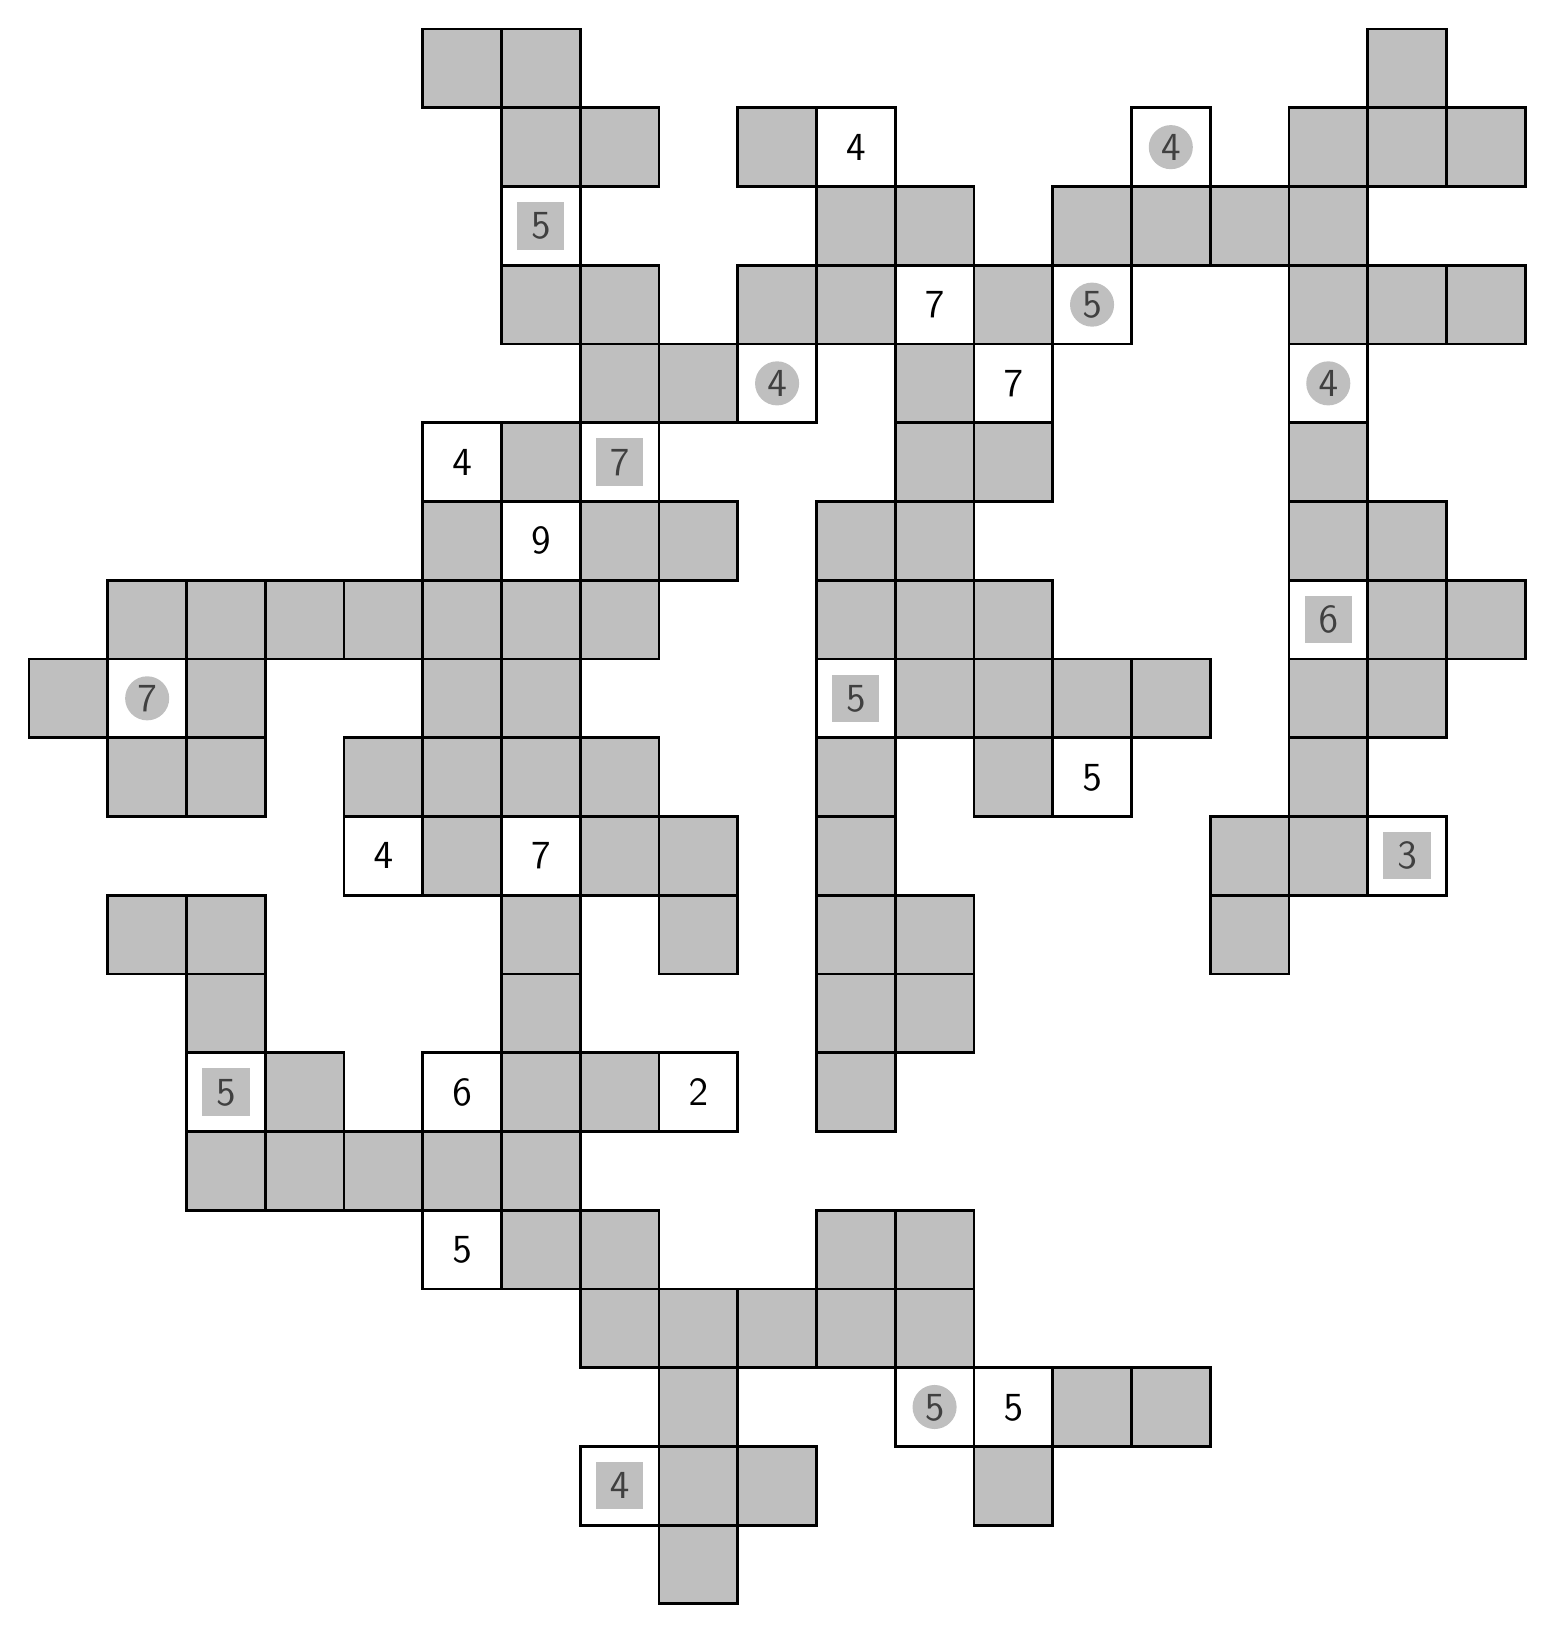
\begin{tikzpicture}\fill[gray, opacity = 0.5] (9, 0, 0)--++(1, 0, 0)--++(0, 1, 0)--++(-1, 0, 0)--cycle;
\draw[line width = 1pt] (9, 0, 0)--++(1, 0, 0)--++(0, 1, 0)--++(-1, 0, 0)--cycle;
\draw node at (8.5, 1.5, 0) {\Large $\mathsf{4}$};
\draw[line width = 1pt] (8, 1, 0)--++(1, 0, 0)--++(0, 1, 0)--++(-1, 0, 0)--cycle;
\fill[color = gray, opacity = 0.5] (8.2, 1.2) rectangle ++(0.6, 0.6);
\fill[gray, opacity = 0.5] (9, 1, 0)--++(1, 0, 0)--++(0, 1, 0)--++(-1, 0, 0)--cycle;
\draw[line width = 1pt] (9, 1, 0)--++(1, 0, 0)--++(0, 1, 0)--++(-1, 0, 0)--cycle;
\fill[gray, opacity = 0.5] (10, 1, 0)--++(1, 0, 0)--++(0, 1, 0)--++(-1, 0, 0)--cycle;
\draw[line width = 1pt] (10, 1, 0)--++(1, 0, 0)--++(0, 1, 0)--++(-1, 0, 0)--cycle;
\fill[gray, opacity = 0.5] (13, 1, 0)--++(1, 0, 0)--++(0, 1, 0)--++(-1, 0, 0)--cycle;
\draw[line width = 1pt] (13, 1, 0)--++(1, 0, 0)--++(0, 1, 0)--++(-1, 0, 0)--cycle;
\fill[gray, opacity = 0.5] (9, 2, 0)--++(1, 0, 0)--++(0, 1, 0)--++(-1, 0, 0)--cycle;
\draw[line width = 1pt] (9, 2, 0)--++(1, 0, 0)--++(0, 1, 0)--++(-1, 0, 0)--cycle;
\draw node at (12.5, 2.5, 0) {\Large $\mathsf{5}$};
\draw[line width = 1pt] (12, 2, 0)--++(1, 0, 0)--++(0, 1, 0)--++(-1, 0, 0)--cycle;
\fill[color = gray, opacity = 0.5] (12.5, 2.5, 0) circle (0.28);
\draw node at (13.5, 2.5, 0) {\Large $\mathsf{5}$};
\draw[line width = 1pt] (13, 2, 0)--++(1, 0, 0)--++(0, 1, 0)--++(-1, 0, 0)--cycle;
\fill[gray, opacity = 0.5] (14, 2, 0)--++(1, 0, 0)--++(0, 1, 0)--++(-1, 0, 0)--cycle;
\draw[line width = 1pt] (14, 2, 0)--++(1, 0, 0)--++(0, 1, 0)--++(-1, 0, 0)--cycle;
\fill[gray, opacity = 0.5] (15, 2, 0)--++(1, 0, 0)--++(0, 1, 0)--++(-1, 0, 0)--cycle;
\draw[line width = 1pt] (15, 2, 0)--++(1, 0, 0)--++(0, 1, 0)--++(-1, 0, 0)--cycle;
\fill[gray, opacity = 0.5] (8, 3, 0)--++(1, 0, 0)--++(0, 1, 0)--++(-1, 0, 0)--cycle;
\draw[line width = 1pt] (8, 3, 0)--++(1, 0, 0)--++(0, 1, 0)--++(-1, 0, 0)--cycle;
\fill[gray, opacity = 0.5] (9, 3, 0)--++(1, 0, 0)--++(0, 1, 0)--++(-1, 0, 0)--cycle;
\draw[line width = 1pt] (9, 3, 0)--++(1, 0, 0)--++(0, 1, 0)--++(-1, 0, 0)--cycle;
\fill[gray, opacity = 0.5] (10, 3, 0)--++(1, 0, 0)--++(0, 1, 0)--++(-1, 0, 0)--cycle;
\draw[line width = 1pt] (10, 3, 0)--++(1, 0, 0)--++(0, 1, 0)--++(-1, 0, 0)--cycle;
\fill[gray, opacity = 0.5] (11, 3, 0)--++(1, 0, 0)--++(0, 1, 0)--++(-1, 0, 0)--cycle;
\draw[line width = 1pt] (11, 3, 0)--++(1, 0, 0)--++(0, 1, 0)--++(-1, 0, 0)--cycle;
\fill[gray, opacity = 0.5] (12, 3, 0)--++(1, 0, 0)--++(0, 1, 0)--++(-1, 0, 0)--cycle;
\draw[line width = 1pt] (12, 3, 0)--++(1, 0, 0)--++(0, 1, 0)--++(-1, 0, 0)--cycle;
\draw node at (6.5, 4.5, 0) {\Large $\mathsf{5}$};
\draw[line width = 1pt] (6, 4, 0)--++(1, 0, 0)--++(0, 1, 0)--++(-1, 0, 0)--cycle;
\fill[gray, opacity = 0.5] (7, 4, 0)--++(1, 0, 0)--++(0, 1, 0)--++(-1, 0, 0)--cycle;
\draw[line width = 1pt] (7, 4, 0)--++(1, 0, 0)--++(0, 1, 0)--++(-1, 0, 0)--cycle;
\fill[gray, opacity = 0.5] (8, 4, 0)--++(1, 0, 0)--++(0, 1, 0)--++(-1, 0, 0)--cycle;
\draw[line width = 1pt] (8, 4, 0)--++(1, 0, 0)--++(0, 1, 0)--++(-1, 0, 0)--cycle;
\fill[gray, opacity = 0.5] (11, 4, 0)--++(1, 0, 0)--++(0, 1, 0)--++(-1, 0, 0)--cycle;
\draw[line width = 1pt] (11, 4, 0)--++(1, 0, 0)--++(0, 1, 0)--++(-1, 0, 0)--cycle;
\fill[gray, opacity = 0.5] (12, 4, 0)--++(1, 0, 0)--++(0, 1, 0)--++(-1, 0, 0)--cycle;
\draw[line width = 1pt] (12, 4, 0)--++(1, 0, 0)--++(0, 1, 0)--++(-1, 0, 0)--cycle;
\fill[gray, opacity = 0.5] (3, 5, 0)--++(1, 0, 0)--++(0, 1, 0)--++(-1, 0, 0)--cycle;
\draw[line width = 1pt] (3, 5, 0)--++(1, 0, 0)--++(0, 1, 0)--++(-1, 0, 0)--cycle;
\fill[gray, opacity = 0.5] (4, 5, 0)--++(1, 0, 0)--++(0, 1, 0)--++(-1, 0, 0)--cycle;
\draw[line width = 1pt] (4, 5, 0)--++(1, 0, 0)--++(0, 1, 0)--++(-1, 0, 0)--cycle;
\fill[gray, opacity = 0.5] (5, 5, 0)--++(1, 0, 0)--++(0, 1, 0)--++(-1, 0, 0)--cycle;
\draw[line width = 1pt] (5, 5, 0)--++(1, 0, 0)--++(0, 1, 0)--++(-1, 0, 0)--cycle;
\fill[gray, opacity = 0.5] (6, 5, 0)--++(1, 0, 0)--++(0, 1, 0)--++(-1, 0, 0)--cycle;
\draw[line width = 1pt] (6, 5, 0)--++(1, 0, 0)--++(0, 1, 0)--++(-1, 0, 0)--cycle;
\fill[gray, opacity = 0.5] (7, 5, 0)--++(1, 0, 0)--++(0, 1, 0)--++(-1, 0, 0)--cycle;
\draw[line width = 1pt] (7, 5, 0)--++(1, 0, 0)--++(0, 1, 0)--++(-1, 0, 0)--cycle;
\draw node at (3.5, 6.5, 0) {\Large $\mathsf{5}$};
\draw[line width = 1pt] (3, 6, 0)--++(1, 0, 0)--++(0, 1, 0)--++(-1, 0, 0)--cycle;
\fill[color = gray, opacity = 0.5] (3.2, 6.2) rectangle ++(0.6, 0.6);
\fill[gray, opacity = 0.5] (4, 6, 0)--++(1, 0, 0)--++(0, 1, 0)--++(-1, 0, 0)--cycle;
\draw[line width = 1pt] (4, 6, 0)--++(1, 0, 0)--++(0, 1, 0)--++(-1, 0, 0)--cycle;
\draw node at (6.5, 6.5, 0) {\Large $\mathsf{6}$};
\draw[line width = 1pt] (6, 6, 0)--++(1, 0, 0)--++(0, 1, 0)--++(-1, 0, 0)--cycle;
\fill[gray, opacity = 0.5] (7, 6, 0)--++(1, 0, 0)--++(0, 1, 0)--++(-1, 0, 0)--cycle;
\draw[line width = 1pt] (7, 6, 0)--++(1, 0, 0)--++(0, 1, 0)--++(-1, 0, 0)--cycle;
\fill[gray, opacity = 0.5] (8, 6, 0)--++(1, 0, 0)--++(0, 1, 0)--++(-1, 0, 0)--cycle;
\draw[line width = 1pt] (8, 6, 0)--++(1, 0, 0)--++(0, 1, 0)--++(-1, 0, 0)--cycle;
\draw node at (9.5, 6.5, 0) {\Large $\mathsf{2}$};
\draw[line width = 1pt] (9, 6, 0)--++(1, 0, 0)--++(0, 1, 0)--++(-1, 0, 0)--cycle;
\fill[gray, opacity = 0.5] (11, 6, 0)--++(1, 0, 0)--++(0, 1, 0)--++(-1, 0, 0)--cycle;
\draw[line width = 1pt] (11, 6, 0)--++(1, 0, 0)--++(0, 1, 0)--++(-1, 0, 0)--cycle;
\fill[gray, opacity = 0.5] (3, 7, 0)--++(1, 0, 0)--++(0, 1, 0)--++(-1, 0, 0)--cycle;
\draw[line width = 1pt] (3, 7, 0)--++(1, 0, 0)--++(0, 1, 0)--++(-1, 0, 0)--cycle;
\fill[gray, opacity = 0.5] (7, 7, 0)--++(1, 0, 0)--++(0, 1, 0)--++(-1, 0, 0)--cycle;
\draw[line width = 1pt] (7, 7, 0)--++(1, 0, 0)--++(0, 1, 0)--++(-1, 0, 0)--cycle;
\fill[gray, opacity = 0.5] (11, 7, 0)--++(1, 0, 0)--++(0, 1, 0)--++(-1, 0, 0)--cycle;
\draw[line width = 1pt] (11, 7, 0)--++(1, 0, 0)--++(0, 1, 0)--++(-1, 0, 0)--cycle;
\fill[gray, opacity = 0.5] (12, 7, 0)--++(1, 0, 0)--++(0, 1, 0)--++(-1, 0, 0)--cycle;
\draw[line width = 1pt] (12, 7, 0)--++(1, 0, 0)--++(0, 1, 0)--++(-1, 0, 0)--cycle;
\fill[gray, opacity = 0.5] (2, 8, 0)--++(1, 0, 0)--++(0, 1, 0)--++(-1, 0, 0)--cycle;
\draw[line width = 1pt] (2, 8, 0)--++(1, 0, 0)--++(0, 1, 0)--++(-1, 0, 0)--cycle;
\fill[gray, opacity = 0.5] (3, 8, 0)--++(1, 0, 0)--++(0, 1, 0)--++(-1, 0, 0)--cycle;
\draw[line width = 1pt] (3, 8, 0)--++(1, 0, 0)--++(0, 1, 0)--++(-1, 0, 0)--cycle;
\fill[gray, opacity = 0.5] (7, 8, 0)--++(1, 0, 0)--++(0, 1, 0)--++(-1, 0, 0)--cycle;
\draw[line width = 1pt] (7, 8, 0)--++(1, 0, 0)--++(0, 1, 0)--++(-1, 0, 0)--cycle;
\fill[gray, opacity = 0.5] (9, 8, 0)--++(1, 0, 0)--++(0, 1, 0)--++(-1, 0, 0)--cycle;
\draw[line width = 1pt] (9, 8, 0)--++(1, 0, 0)--++(0, 1, 0)--++(-1, 0, 0)--cycle;
\fill[gray, opacity = 0.5] (11, 8, 0)--++(1, 0, 0)--++(0, 1, 0)--++(-1, 0, 0)--cycle;
\draw[line width = 1pt] (11, 8, 0)--++(1, 0, 0)--++(0, 1, 0)--++(-1, 0, 0)--cycle;
\fill[gray, opacity = 0.5] (12, 8, 0)--++(1, 0, 0)--++(0, 1, 0)--++(-1, 0, 0)--cycle;
\draw[line width = 1pt] (12, 8, 0)--++(1, 0, 0)--++(0, 1, 0)--++(-1, 0, 0)--cycle;
\fill[gray, opacity = 0.5] (16, 8, 0)--++(1, 0, 0)--++(0, 1, 0)--++(-1, 0, 0)--cycle;
\draw[line width = 1pt] (16, 8, 0)--++(1, 0, 0)--++(0, 1, 0)--++(-1, 0, 0)--cycle;
\draw node at (5.5, 9.5, 0) {\Large $\mathsf{4}$};
\draw[line width = 1pt] (5, 9, 0)--++(1, 0, 0)--++(0, 1, 0)--++(-1, 0, 0)--cycle;
\fill[gray, opacity = 0.5] (6, 9, 0)--++(1, 0, 0)--++(0, 1, 0)--++(-1, 0, 0)--cycle;
\draw[line width = 1pt] (6, 9, 0)--++(1, 0, 0)--++(0, 1, 0)--++(-1, 0, 0)--cycle;
\draw node at (7.5, 9.5, 0) {\Large $\mathsf{7}$};
\draw[line width = 1pt] (7, 9, 0)--++(1, 0, 0)--++(0, 1, 0)--++(-1, 0, 0)--cycle;
\fill[gray, opacity = 0.5] (8, 9, 0)--++(1, 0, 0)--++(0, 1, 0)--++(-1, 0, 0)--cycle;
\draw[line width = 1pt] (8, 9, 0)--++(1, 0, 0)--++(0, 1, 0)--++(-1, 0, 0)--cycle;
\fill[gray, opacity = 0.5] (9, 9, 0)--++(1, 0, 0)--++(0, 1, 0)--++(-1, 0, 0)--cycle;
\draw[line width = 1pt] (9, 9, 0)--++(1, 0, 0)--++(0, 1, 0)--++(-1, 0, 0)--cycle;
\fill[gray, opacity = 0.5] (11, 9, 0)--++(1, 0, 0)--++(0, 1, 0)--++(-1, 0, 0)--cycle;
\draw[line width = 1pt] (11, 9, 0)--++(1, 0, 0)--++(0, 1, 0)--++(-1, 0, 0)--cycle;
\fill[gray, opacity = 0.5] (16, 9, 0)--++(1, 0, 0)--++(0, 1, 0)--++(-1, 0, 0)--cycle;
\draw[line width = 1pt] (16, 9, 0)--++(1, 0, 0)--++(0, 1, 0)--++(-1, 0, 0)--cycle;
\fill[gray, opacity = 0.5] (17, 9, 0)--++(1, 0, 0)--++(0, 1, 0)--++(-1, 0, 0)--cycle;
\draw[line width = 1pt] (17, 9, 0)--++(1, 0, 0)--++(0, 1, 0)--++(-1, 0, 0)--cycle;
\draw node at (18.5, 9.5, 0) {\Large $\mathsf{3}$};
\draw[line width = 1pt] (18, 9, 0)--++(1, 0, 0)--++(0, 1, 0)--++(-1, 0, 0)--cycle;
\fill[color = gray, opacity = 0.5] (18.2, 9.2) rectangle ++(0.6, 0.6);
\fill[gray, opacity = 0.5] (2, 10, 0)--++(1, 0, 0)--++(0, 1, 0)--++(-1, 0, 0)--cycle;
\draw[line width = 1pt] (2, 10, 0)--++(1, 0, 0)--++(0, 1, 0)--++(-1, 0, 0)--cycle;
\fill[gray, opacity = 0.5] (3, 10, 0)--++(1, 0, 0)--++(0, 1, 0)--++(-1, 0, 0)--cycle;
\draw[line width = 1pt] (3, 10, 0)--++(1, 0, 0)--++(0, 1, 0)--++(-1, 0, 0)--cycle;
\fill[gray, opacity = 0.5] (5, 10, 0)--++(1, 0, 0)--++(0, 1, 0)--++(-1, 0, 0)--cycle;
\draw[line width = 1pt] (5, 10, 0)--++(1, 0, 0)--++(0, 1, 0)--++(-1, 0, 0)--cycle;
\fill[gray, opacity = 0.5] (6, 10, 0)--++(1, 0, 0)--++(0, 1, 0)--++(-1, 0, 0)--cycle;
\draw[line width = 1pt] (6, 10, 0)--++(1, 0, 0)--++(0, 1, 0)--++(-1, 0, 0)--cycle;
\fill[gray, opacity = 0.5] (7, 10, 0)--++(1, 0, 0)--++(0, 1, 0)--++(-1, 0, 0)--cycle;
\draw[line width = 1pt] (7, 10, 0)--++(1, 0, 0)--++(0, 1, 0)--++(-1, 0, 0)--cycle;
\fill[gray, opacity = 0.5] (8, 10, 0)--++(1, 0, 0)--++(0, 1, 0)--++(-1, 0, 0)--cycle;
\draw[line width = 1pt] (8, 10, 0)--++(1, 0, 0)--++(0, 1, 0)--++(-1, 0, 0)--cycle;
\fill[gray, opacity = 0.5] (11, 10, 0)--++(1, 0, 0)--++(0, 1, 0)--++(-1, 0, 0)--cycle;
\draw[line width = 1pt] (11, 10, 0)--++(1, 0, 0)--++(0, 1, 0)--++(-1, 0, 0)--cycle;
\fill[gray, opacity = 0.5] (13, 10, 0)--++(1, 0, 0)--++(0, 1, 0)--++(-1, 0, 0)--cycle;
\draw[line width = 1pt] (13, 10, 0)--++(1, 0, 0)--++(0, 1, 0)--++(-1, 0, 0)--cycle;
\draw node at (14.5, 10.5, 0) {\Large $\mathsf{5}$};
\draw[line width = 1pt] (14, 10, 0)--++(1, 0, 0)--++(0, 1, 0)--++(-1, 0, 0)--cycle;
\fill[gray, opacity = 0.5] (17, 10, 0)--++(1, 0, 0)--++(0, 1, 0)--++(-1, 0, 0)--cycle;
\draw[line width = 1pt] (17, 10, 0)--++(1, 0, 0)--++(0, 1, 0)--++(-1, 0, 0)--cycle;
\fill[gray, opacity = 0.5] (1, 11, 0)--++(1, 0, 0)--++(0, 1, 0)--++(-1, 0, 0)--cycle;
\draw[line width = 1pt] (1, 11, 0)--++(1, 0, 0)--++(0, 1, 0)--++(-1, 0, 0)--cycle;
\draw node at (2.5, 11.5, 0) {\Large $\mathsf{7}$};
\draw[line width = 1pt] (2, 11, 0)--++(1, 0, 0)--++(0, 1, 0)--++(-1, 0, 0)--cycle;
\fill[color = gray, opacity = 0.5] (2.5, 11.5, 0) circle (0.28);
\fill[gray, opacity = 0.5] (3, 11, 0)--++(1, 0, 0)--++(0, 1, 0)--++(-1, 0, 0)--cycle;
\draw[line width = 1pt] (3, 11, 0)--++(1, 0, 0)--++(0, 1, 0)--++(-1, 0, 0)--cycle;
\fill[gray, opacity = 0.5] (6, 11, 0)--++(1, 0, 0)--++(0, 1, 0)--++(-1, 0, 0)--cycle;
\draw[line width = 1pt] (6, 11, 0)--++(1, 0, 0)--++(0, 1, 0)--++(-1, 0, 0)--cycle;
\fill[gray, opacity = 0.5] (7, 11, 0)--++(1, 0, 0)--++(0, 1, 0)--++(-1, 0, 0)--cycle;
\draw[line width = 1pt] (7, 11, 0)--++(1, 0, 0)--++(0, 1, 0)--++(-1, 0, 0)--cycle;
\draw node at (11.5, 11.5, 0) {\Large $\mathsf{5}$};
\draw[line width = 1pt] (11, 11, 0)--++(1, 0, 0)--++(0, 1, 0)--++(-1, 0, 0)--cycle;
\fill[color = gray, opacity = 0.5] (11.2, 11.2) rectangle ++(0.6, 0.6);
\fill[gray, opacity = 0.5] (12, 11, 0)--++(1, 0, 0)--++(0, 1, 0)--++(-1, 0, 0)--cycle;
\draw[line width = 1pt] (12, 11, 0)--++(1, 0, 0)--++(0, 1, 0)--++(-1, 0, 0)--cycle;
\fill[gray, opacity = 0.5] (13, 11, 0)--++(1, 0, 0)--++(0, 1, 0)--++(-1, 0, 0)--cycle;
\draw[line width = 1pt] (13, 11, 0)--++(1, 0, 0)--++(0, 1, 0)--++(-1, 0, 0)--cycle;
\fill[gray, opacity = 0.5] (14, 11, 0)--++(1, 0, 0)--++(0, 1, 0)--++(-1, 0, 0)--cycle;
\draw[line width = 1pt] (14, 11, 0)--++(1, 0, 0)--++(0, 1, 0)--++(-1, 0, 0)--cycle;
\fill[gray, opacity = 0.5] (15, 11, 0)--++(1, 0, 0)--++(0, 1, 0)--++(-1, 0, 0)--cycle;
\draw[line width = 1pt] (15, 11, 0)--++(1, 0, 0)--++(0, 1, 0)--++(-1, 0, 0)--cycle;
\fill[gray, opacity = 0.5] (17, 11, 0)--++(1, 0, 0)--++(0, 1, 0)--++(-1, 0, 0)--cycle;
\draw[line width = 1pt] (17, 11, 0)--++(1, 0, 0)--++(0, 1, 0)--++(-1, 0, 0)--cycle;
\fill[gray, opacity = 0.5] (18, 11, 0)--++(1, 0, 0)--++(0, 1, 0)--++(-1, 0, 0)--cycle;
\draw[line width = 1pt] (18, 11, 0)--++(1, 0, 0)--++(0, 1, 0)--++(-1, 0, 0)--cycle;
\fill[gray, opacity = 0.5] (2, 12, 0)--++(1, 0, 0)--++(0, 1, 0)--++(-1, 0, 0)--cycle;
\draw[line width = 1pt] (2, 12, 0)--++(1, 0, 0)--++(0, 1, 0)--++(-1, 0, 0)--cycle;
\fill[gray, opacity = 0.5] (3, 12, 0)--++(1, 0, 0)--++(0, 1, 0)--++(-1, 0, 0)--cycle;
\draw[line width = 1pt] (3, 12, 0)--++(1, 0, 0)--++(0, 1, 0)--++(-1, 0, 0)--cycle;
\fill[gray, opacity = 0.5] (4, 12, 0)--++(1, 0, 0)--++(0, 1, 0)--++(-1, 0, 0)--cycle;
\draw[line width = 1pt] (4, 12, 0)--++(1, 0, 0)--++(0, 1, 0)--++(-1, 0, 0)--cycle;
\fill[gray, opacity = 0.5] (5, 12, 0)--++(1, 0, 0)--++(0, 1, 0)--++(-1, 0, 0)--cycle;
\draw[line width = 1pt] (5, 12, 0)--++(1, 0, 0)--++(0, 1, 0)--++(-1, 0, 0)--cycle;
\fill[gray, opacity = 0.5] (6, 12, 0)--++(1, 0, 0)--++(0, 1, 0)--++(-1, 0, 0)--cycle;
\draw[line width = 1pt] (6, 12, 0)--++(1, 0, 0)--++(0, 1, 0)--++(-1, 0, 0)--cycle;
\fill[gray, opacity = 0.5] (7, 12, 0)--++(1, 0, 0)--++(0, 1, 0)--++(-1, 0, 0)--cycle;
\draw[line width = 1pt] (7, 12, 0)--++(1, 0, 0)--++(0, 1, 0)--++(-1, 0, 0)--cycle;
\fill[gray, opacity = 0.5] (8, 12, 0)--++(1, 0, 0)--++(0, 1, 0)--++(-1, 0, 0)--cycle;
\draw[line width = 1pt] (8, 12, 0)--++(1, 0, 0)--++(0, 1, 0)--++(-1, 0, 0)--cycle;
\fill[gray, opacity = 0.5] (11, 12, 0)--++(1, 0, 0)--++(0, 1, 0)--++(-1, 0, 0)--cycle;
\draw[line width = 1pt] (11, 12, 0)--++(1, 0, 0)--++(0, 1, 0)--++(-1, 0, 0)--cycle;
\fill[gray, opacity = 0.5] (12, 12, 0)--++(1, 0, 0)--++(0, 1, 0)--++(-1, 0, 0)--cycle;
\draw[line width = 1pt] (12, 12, 0)--++(1, 0, 0)--++(0, 1, 0)--++(-1, 0, 0)--cycle;
\fill[gray, opacity = 0.5] (13, 12, 0)--++(1, 0, 0)--++(0, 1, 0)--++(-1, 0, 0)--cycle;
\draw[line width = 1pt] (13, 12, 0)--++(1, 0, 0)--++(0, 1, 0)--++(-1, 0, 0)--cycle;
\draw node at (17.5, 12.5, 0) {\Large $\mathsf{6}$};
\draw[line width = 1pt] (17, 12, 0)--++(1, 0, 0)--++(0, 1, 0)--++(-1, 0, 0)--cycle;
\fill[color = gray, opacity = 0.5] (17.2, 12.2) rectangle ++(0.6, 0.6);
\fill[gray, opacity = 0.5] (18, 12, 0)--++(1, 0, 0)--++(0, 1, 0)--++(-1, 0, 0)--cycle;
\draw[line width = 1pt] (18, 12, 0)--++(1, 0, 0)--++(0, 1, 0)--++(-1, 0, 0)--cycle;
\fill[gray, opacity = 0.5] (19, 12, 0)--++(1, 0, 0)--++(0, 1, 0)--++(-1, 0, 0)--cycle;
\draw[line width = 1pt] (19, 12, 0)--++(1, 0, 0)--++(0, 1, 0)--++(-1, 0, 0)--cycle;
\fill[gray, opacity = 0.5] (6, 13, 0)--++(1, 0, 0)--++(0, 1, 0)--++(-1, 0, 0)--cycle;
\draw[line width = 1pt] (6, 13, 0)--++(1, 0, 0)--++(0, 1, 0)--++(-1, 0, 0)--cycle;
\draw node at (7.5, 13.5, 0) {\Large $\mathsf{9}$};
\draw[line width = 1pt] (7, 13, 0)--++(1, 0, 0)--++(0, 1, 0)--++(-1, 0, 0)--cycle;
\fill[gray, opacity = 0.5] (8, 13, 0)--++(1, 0, 0)--++(0, 1, 0)--++(-1, 0, 0)--cycle;
\draw[line width = 1pt] (8, 13, 0)--++(1, 0, 0)--++(0, 1, 0)--++(-1, 0, 0)--cycle;
\fill[gray, opacity = 0.5] (9, 13, 0)--++(1, 0, 0)--++(0, 1, 0)--++(-1, 0, 0)--cycle;
\draw[line width = 1pt] (9, 13, 0)--++(1, 0, 0)--++(0, 1, 0)--++(-1, 0, 0)--cycle;
\fill[gray, opacity = 0.5] (11, 13, 0)--++(1, 0, 0)--++(0, 1, 0)--++(-1, 0, 0)--cycle;
\draw[line width = 1pt] (11, 13, 0)--++(1, 0, 0)--++(0, 1, 0)--++(-1, 0, 0)--cycle;
\fill[gray, opacity = 0.5] (12, 13, 0)--++(1, 0, 0)--++(0, 1, 0)--++(-1, 0, 0)--cycle;
\draw[line width = 1pt] (12, 13, 0)--++(1, 0, 0)--++(0, 1, 0)--++(-1, 0, 0)--cycle;
\fill[gray, opacity = 0.5] (17, 13, 0)--++(1, 0, 0)--++(0, 1, 0)--++(-1, 0, 0)--cycle;
\draw[line width = 1pt] (17, 13, 0)--++(1, 0, 0)--++(0, 1, 0)--++(-1, 0, 0)--cycle;
\fill[gray, opacity = 0.5] (18, 13, 0)--++(1, 0, 0)--++(0, 1, 0)--++(-1, 0, 0)--cycle;
\draw[line width = 1pt] (18, 13, 0)--++(1, 0, 0)--++(0, 1, 0)--++(-1, 0, 0)--cycle;
\draw node at (6.5, 14.5, 0) {\Large $\mathsf{4}$};
\draw[line width = 1pt] (6, 14, 0)--++(1, 0, 0)--++(0, 1, 0)--++(-1, 0, 0)--cycle;
\fill[gray, opacity = 0.5] (7, 14, 0)--++(1, 0, 0)--++(0, 1, 0)--++(-1, 0, 0)--cycle;
\draw[line width = 1pt] (7, 14, 0)--++(1, 0, 0)--++(0, 1, 0)--++(-1, 0, 0)--cycle;
\draw node at (8.5, 14.5, 0) {\Large $\mathsf{7}$};
\draw[line width = 1pt] (8, 14, 0)--++(1, 0, 0)--++(0, 1, 0)--++(-1, 0, 0)--cycle;
\fill[color = gray, opacity = 0.5] (8.2, 14.2) rectangle ++(0.6, 0.6);
\fill[gray, opacity = 0.5] (12, 14, 0)--++(1, 0, 0)--++(0, 1, 0)--++(-1, 0, 0)--cycle;
\draw[line width = 1pt] (12, 14, 0)--++(1, 0, 0)--++(0, 1, 0)--++(-1, 0, 0)--cycle;
\fill[gray, opacity = 0.5] (13, 14, 0)--++(1, 0, 0)--++(0, 1, 0)--++(-1, 0, 0)--cycle;
\draw[line width = 1pt] (13, 14, 0)--++(1, 0, 0)--++(0, 1, 0)--++(-1, 0, 0)--cycle;
\fill[gray, opacity = 0.5] (17, 14, 0)--++(1, 0, 0)--++(0, 1, 0)--++(-1, 0, 0)--cycle;
\draw[line width = 1pt] (17, 14, 0)--++(1, 0, 0)--++(0, 1, 0)--++(-1, 0, 0)--cycle;
\fill[gray, opacity = 0.5] (8, 15, 0)--++(1, 0, 0)--++(0, 1, 0)--++(-1, 0, 0)--cycle;
\draw[line width = 1pt] (8, 15, 0)--++(1, 0, 0)--++(0, 1, 0)--++(-1, 0, 0)--cycle;
\fill[gray, opacity = 0.5] (9, 15, 0)--++(1, 0, 0)--++(0, 1, 0)--++(-1, 0, 0)--cycle;
\draw[line width = 1pt] (9, 15, 0)--++(1, 0, 0)--++(0, 1, 0)--++(-1, 0, 0)--cycle;
\draw node at (10.5, 15.5, 0) {\Large $\mathsf{4}$};
\draw[line width = 1pt] (10, 15, 0)--++(1, 0, 0)--++(0, 1, 0)--++(-1, 0, 0)--cycle;
\fill[color = gray, opacity = 0.5] (10.5, 15.5, 0) circle (0.28);
\fill[gray, opacity = 0.5] (12, 15, 0)--++(1, 0, 0)--++(0, 1, 0)--++(-1, 0, 0)--cycle;
\draw[line width = 1pt] (12, 15, 0)--++(1, 0, 0)--++(0, 1, 0)--++(-1, 0, 0)--cycle;
\draw node at (13.5, 15.5, 0) {\Large $\mathsf{7}$};
\draw[line width = 1pt] (13, 15, 0)--++(1, 0, 0)--++(0, 1, 0)--++(-1, 0, 0)--cycle;
\draw node at (17.5, 15.5, 0) {\Large $\mathsf{4}$};
\draw[line width = 1pt] (17, 15, 0)--++(1, 0, 0)--++(0, 1, 0)--++(-1, 0, 0)--cycle;
\fill[color = gray, opacity = 0.5] (17.5, 15.5, 0) circle (0.28);
\fill[gray, opacity = 0.5] (7, 16, 0)--++(1, 0, 0)--++(0, 1, 0)--++(-1, 0, 0)--cycle;
\draw[line width = 1pt] (7, 16, 0)--++(1, 0, 0)--++(0, 1, 0)--++(-1, 0, 0)--cycle;
\fill[gray, opacity = 0.5] (8, 16, 0)--++(1, 0, 0)--++(0, 1, 0)--++(-1, 0, 0)--cycle;
\draw[line width = 1pt] (8, 16, 0)--++(1, 0, 0)--++(0, 1, 0)--++(-1, 0, 0)--cycle;
\fill[gray, opacity = 0.5] (10, 16, 0)--++(1, 0, 0)--++(0, 1, 0)--++(-1, 0, 0)--cycle;
\draw[line width = 1pt] (10, 16, 0)--++(1, 0, 0)--++(0, 1, 0)--++(-1, 0, 0)--cycle;
\fill[gray, opacity = 0.5] (11, 16, 0)--++(1, 0, 0)--++(0, 1, 0)--++(-1, 0, 0)--cycle;
\draw[line width = 1pt] (11, 16, 0)--++(1, 0, 0)--++(0, 1, 0)--++(-1, 0, 0)--cycle;
\draw node at (12.5, 16.5, 0) {\Large $\mathsf{7}$};
\draw[line width = 1pt] (12, 16, 0)--++(1, 0, 0)--++(0, 1, 0)--++(-1, 0, 0)--cycle;
\fill[gray, opacity = 0.5] (13, 16, 0)--++(1, 0, 0)--++(0, 1, 0)--++(-1, 0, 0)--cycle;
\draw[line width = 1pt] (13, 16, 0)--++(1, 0, 0)--++(0, 1, 0)--++(-1, 0, 0)--cycle;
\draw node at (14.5, 16.5, 0) {\Large $\mathsf{5}$};
\draw[line width = 1pt] (14, 16, 0)--++(1, 0, 0)--++(0, 1, 0)--++(-1, 0, 0)--cycle;
\fill[color = gray, opacity = 0.5] (14.5, 16.5, 0) circle (0.28);
\fill[gray, opacity = 0.5] (17, 16, 0)--++(1, 0, 0)--++(0, 1, 0)--++(-1, 0, 0)--cycle;
\draw[line width = 1pt] (17, 16, 0)--++(1, 0, 0)--++(0, 1, 0)--++(-1, 0, 0)--cycle;
\fill[gray, opacity = 0.5] (18, 16, 0)--++(1, 0, 0)--++(0, 1, 0)--++(-1, 0, 0)--cycle;
\draw[line width = 1pt] (18, 16, 0)--++(1, 0, 0)--++(0, 1, 0)--++(-1, 0, 0)--cycle;
\fill[gray, opacity = 0.5] (19, 16, 0)--++(1, 0, 0)--++(0, 1, 0)--++(-1, 0, 0)--cycle;
\draw[line width = 1pt] (19, 16, 0)--++(1, 0, 0)--++(0, 1, 0)--++(-1, 0, 0)--cycle;
\draw node at (7.5, 17.5, 0) {\Large $\mathsf{5}$};
\draw[line width = 1pt] (7, 17, 0)--++(1, 0, 0)--++(0, 1, 0)--++(-1, 0, 0)--cycle;
\fill[color = gray, opacity = 0.5] (7.2, 17.2) rectangle ++(0.6, 0.6);
\fill[gray, opacity = 0.5] (11, 17, 0)--++(1, 0, 0)--++(0, 1, 0)--++(-1, 0, 0)--cycle;
\draw[line width = 1pt] (11, 17, 0)--++(1, 0, 0)--++(0, 1, 0)--++(-1, 0, 0)--cycle;
\fill[gray, opacity = 0.5] (12, 17, 0)--++(1, 0, 0)--++(0, 1, 0)--++(-1, 0, 0)--cycle;
\draw[line width = 1pt] (12, 17, 0)--++(1, 0, 0)--++(0, 1, 0)--++(-1, 0, 0)--cycle;
\fill[gray, opacity = 0.5] (14, 17, 0)--++(1, 0, 0)--++(0, 1, 0)--++(-1, 0, 0)--cycle;
\draw[line width = 1pt] (14, 17, 0)--++(1, 0, 0)--++(0, 1, 0)--++(-1, 0, 0)--cycle;
\fill[gray, opacity = 0.5] (15, 17, 0)--++(1, 0, 0)--++(0, 1, 0)--++(-1, 0, 0)--cycle;
\draw[line width = 1pt] (15, 17, 0)--++(1, 0, 0)--++(0, 1, 0)--++(-1, 0, 0)--cycle;
\fill[gray, opacity = 0.5] (16, 17, 0)--++(1, 0, 0)--++(0, 1, 0)--++(-1, 0, 0)--cycle;
\draw[line width = 1pt] (16, 17, 0)--++(1, 0, 0)--++(0, 1, 0)--++(-1, 0, 0)--cycle;
\fill[gray, opacity = 0.5] (17, 17, 0)--++(1, 0, 0)--++(0, 1, 0)--++(-1, 0, 0)--cycle;
\draw[line width = 1pt] (17, 17, 0)--++(1, 0, 0)--++(0, 1, 0)--++(-1, 0, 0)--cycle;
\fill[gray, opacity = 0.5] (7, 18, 0)--++(1, 0, 0)--++(0, 1, 0)--++(-1, 0, 0)--cycle;
\draw[line width = 1pt] (7, 18, 0)--++(1, 0, 0)--++(0, 1, 0)--++(-1, 0, 0)--cycle;
\fill[gray, opacity = 0.5] (8, 18, 0)--++(1, 0, 0)--++(0, 1, 0)--++(-1, 0, 0)--cycle;
\draw[line width = 1pt] (8, 18, 0)--++(1, 0, 0)--++(0, 1, 0)--++(-1, 0, 0)--cycle;
\fill[gray, opacity = 0.5] (10, 18, 0)--++(1, 0, 0)--++(0, 1, 0)--++(-1, 0, 0)--cycle;
\draw[line width = 1pt] (10, 18, 0)--++(1, 0, 0)--++(0, 1, 0)--++(-1, 0, 0)--cycle;
\draw node at (11.5, 18.5, 0) {\Large $\mathsf{4}$};
\draw[line width = 1pt] (11, 18, 0)--++(1, 0, 0)--++(0, 1, 0)--++(-1, 0, 0)--cycle;
\draw node at (15.5, 18.5, 0) {\Large $\mathsf{4}$};
\draw[line width = 1pt] (15, 18, 0)--++(1, 0, 0)--++(0, 1, 0)--++(-1, 0, 0)--cycle;
\fill[color = gray, opacity = 0.5] (15.5, 18.5, 0) circle (0.28);
\fill[gray, opacity = 0.5] (17, 18, 0)--++(1, 0, 0)--++(0, 1, 0)--++(-1, 0, 0)--cycle;
\draw[line width = 1pt] (17, 18, 0)--++(1, 0, 0)--++(0, 1, 0)--++(-1, 0, 0)--cycle;
\fill[gray, opacity = 0.5] (18, 18, 0)--++(1, 0, 0)--++(0, 1, 0)--++(-1, 0, 0)--cycle;
\draw[line width = 1pt] (18, 18, 0)--++(1, 0, 0)--++(0, 1, 0)--++(-1, 0, 0)--cycle;
\fill[gray, opacity = 0.5] (19, 18, 0)--++(1, 0, 0)--++(0, 1, 0)--++(-1, 0, 0)--cycle;
\draw[line width = 1pt] (19, 18, 0)--++(1, 0, 0)--++(0, 1, 0)--++(-1, 0, 0)--cycle;
\fill[gray, opacity = 0.5] (6, 19, 0)--++(1, 0, 0)--++(0, 1, 0)--++(-1, 0, 0)--cycle;
\draw[line width = 1pt] (6, 19, 0)--++(1, 0, 0)--++(0, 1, 0)--++(-1, 0, 0)--cycle;
\fill[gray, opacity = 0.5] (7, 19, 0)--++(1, 0, 0)--++(0, 1, 0)--++(-1, 0, 0)--cycle;
\draw[line width = 1pt] (7, 19, 0)--++(1, 0, 0)--++(0, 1, 0)--++(-1, 0, 0)--cycle;
\fill[gray, opacity = 0.5] (18, 19, 0)--++(1, 0, 0)--++(0, 1, 0)--++(-1, 0, 0)--cycle;
\draw[line width = 1pt] (18, 19, 0)--++(1, 0, 0)--++(0, 1, 0)--++(-1, 0, 0)--cycle;
\end{tikzpicture}}\]
\[\resizebox{30pc}{!}{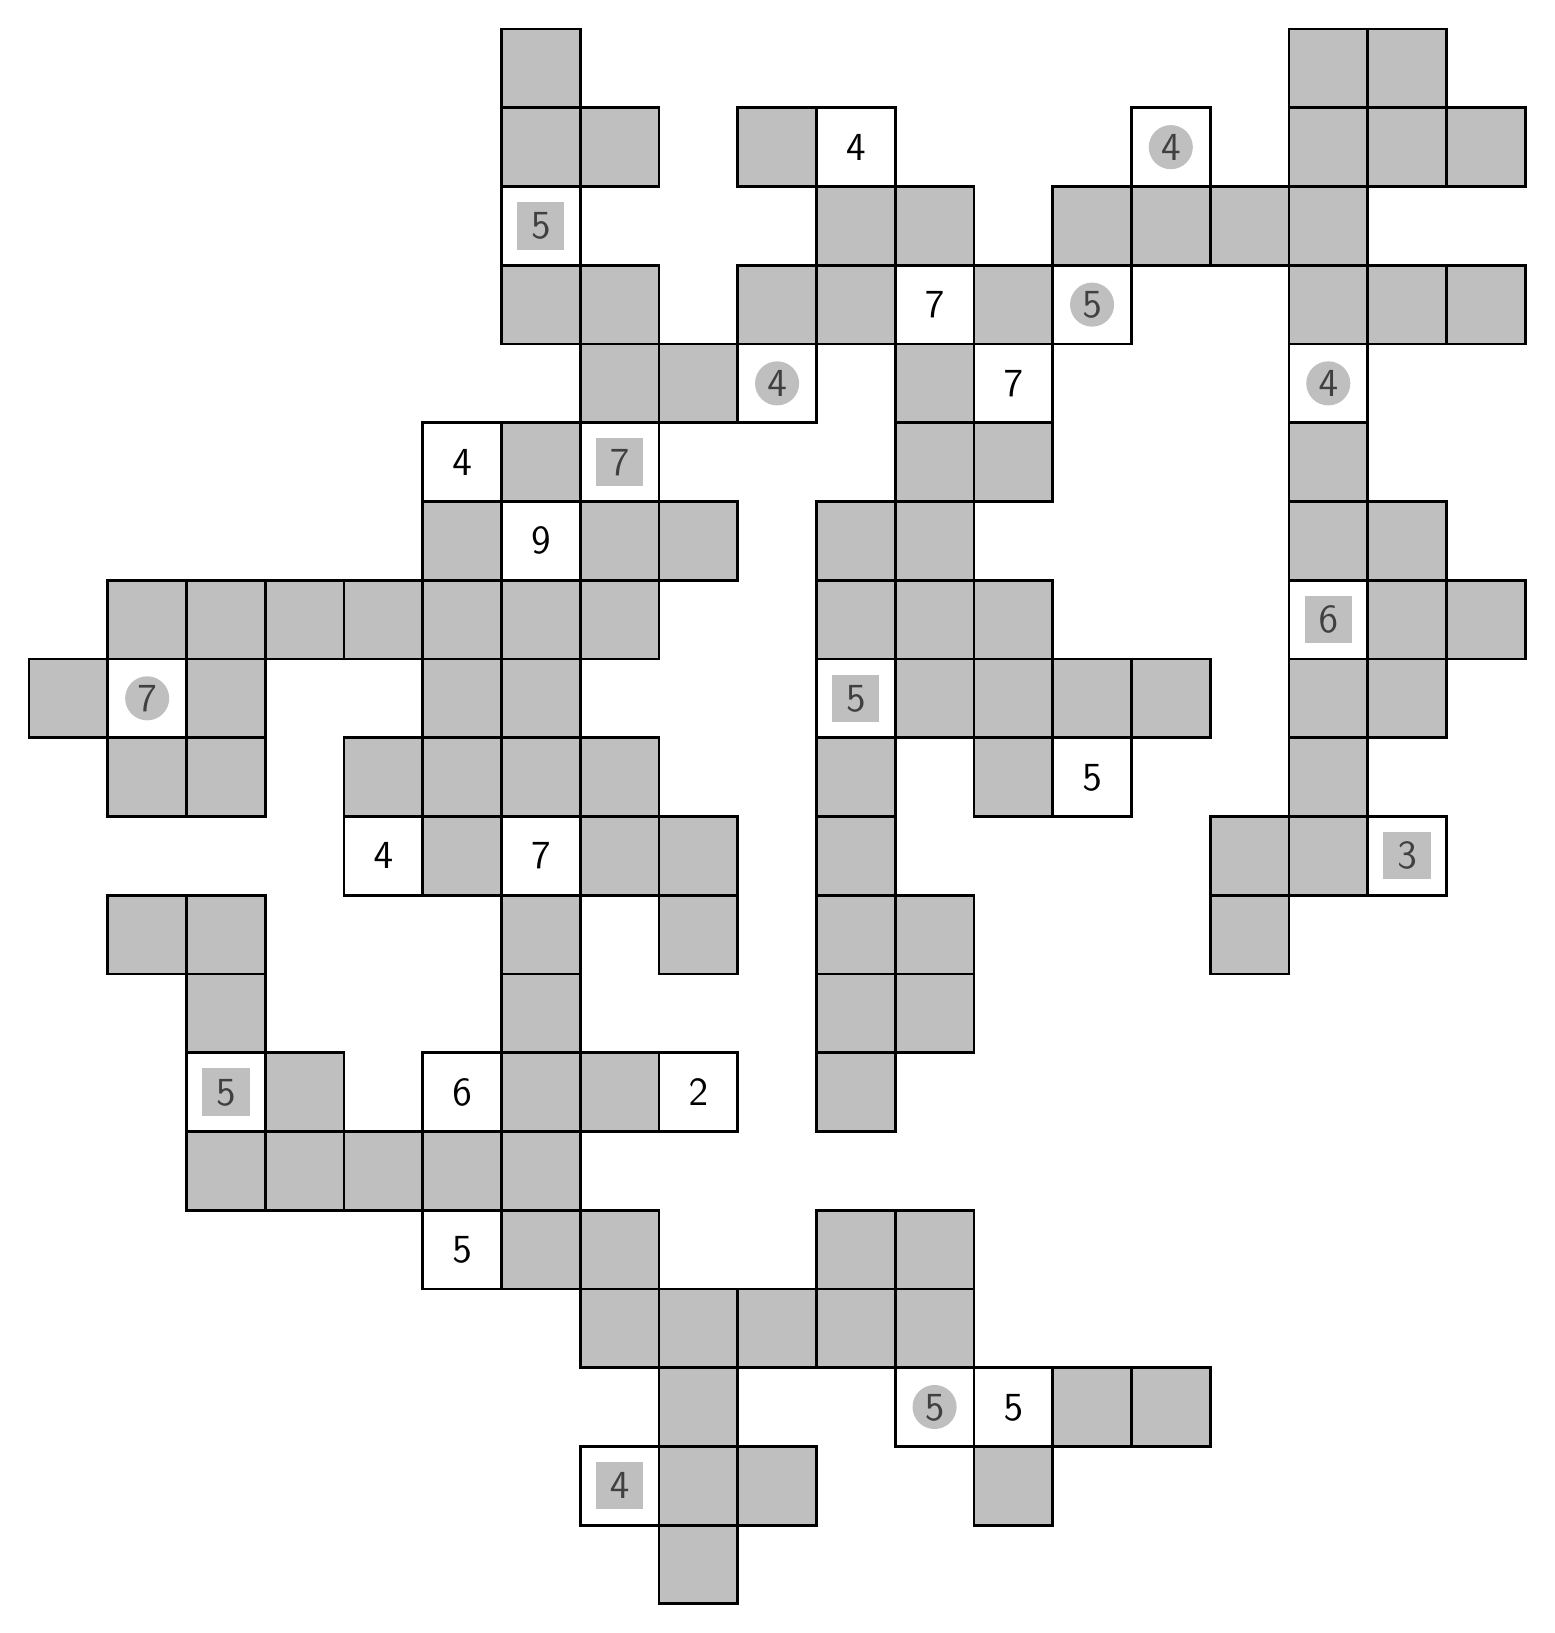
\begin{tikzpicture}\fill[gray, opacity = 0.5] (9, 0, 0)--++(1, 0, 0)--++(0, 1, 0)--++(-1, 0, 0)--cycle;
\draw[line width = 1pt] (9, 0, 0)--++(1, 0, 0)--++(0, 1, 0)--++(-1, 0, 0)--cycle;
\draw node at (8.5, 1.5, 0) {\Large $\mathsf{4}$};
\draw[line width = 1pt] (8, 1, 0)--++(1, 0, 0)--++(0, 1, 0)--++(-1, 0, 0)--cycle;
\fill[color = gray, opacity = 0.5] (8.2, 1.2) rectangle ++(0.6, 0.6);
\fill[gray, opacity = 0.5] (9, 1, 0)--++(1, 0, 0)--++(0, 1, 0)--++(-1, 0, 0)--cycle;
\draw[line width = 1pt] (9, 1, 0)--++(1, 0, 0)--++(0, 1, 0)--++(-1, 0, 0)--cycle;
\fill[gray, opacity = 0.5] (10, 1, 0)--++(1, 0, 0)--++(0, 1, 0)--++(-1, 0, 0)--cycle;
\draw[line width = 1pt] (10, 1, 0)--++(1, 0, 0)--++(0, 1, 0)--++(-1, 0, 0)--cycle;
\fill[gray, opacity = 0.5] (13, 1, 0)--++(1, 0, 0)--++(0, 1, 0)--++(-1, 0, 0)--cycle;
\draw[line width = 1pt] (13, 1, 0)--++(1, 0, 0)--++(0, 1, 0)--++(-1, 0, 0)--cycle;
\fill[gray, opacity = 0.5] (9, 2, 0)--++(1, 0, 0)--++(0, 1, 0)--++(-1, 0, 0)--cycle;
\draw[line width = 1pt] (9, 2, 0)--++(1, 0, 0)--++(0, 1, 0)--++(-1, 0, 0)--cycle;
\draw node at (12.5, 2.5, 0) {\Large $\mathsf{5}$};
\draw[line width = 1pt] (12, 2, 0)--++(1, 0, 0)--++(0, 1, 0)--++(-1, 0, 0)--cycle;
\fill[color = gray, opacity = 0.5] (12.5, 2.5, 0) circle (0.28);
\draw node at (13.5, 2.5, 0) {\Large $\mathsf{5}$};
\draw[line width = 1pt] (13, 2, 0)--++(1, 0, 0)--++(0, 1, 0)--++(-1, 0, 0)--cycle;
\fill[gray, opacity = 0.5] (14, 2, 0)--++(1, 0, 0)--++(0, 1, 0)--++(-1, 0, 0)--cycle;
\draw[line width = 1pt] (14, 2, 0)--++(1, 0, 0)--++(0, 1, 0)--++(-1, 0, 0)--cycle;
\fill[gray, opacity = 0.5] (15, 2, 0)--++(1, 0, 0)--++(0, 1, 0)--++(-1, 0, 0)--cycle;
\draw[line width = 1pt] (15, 2, 0)--++(1, 0, 0)--++(0, 1, 0)--++(-1, 0, 0)--cycle;
\fill[gray, opacity = 0.5] (8, 3, 0)--++(1, 0, 0)--++(0, 1, 0)--++(-1, 0, 0)--cycle;
\draw[line width = 1pt] (8, 3, 0)--++(1, 0, 0)--++(0, 1, 0)--++(-1, 0, 0)--cycle;
\fill[gray, opacity = 0.5] (9, 3, 0)--++(1, 0, 0)--++(0, 1, 0)--++(-1, 0, 0)--cycle;
\draw[line width = 1pt] (9, 3, 0)--++(1, 0, 0)--++(0, 1, 0)--++(-1, 0, 0)--cycle;
\fill[gray, opacity = 0.5] (10, 3, 0)--++(1, 0, 0)--++(0, 1, 0)--++(-1, 0, 0)--cycle;
\draw[line width = 1pt] (10, 3, 0)--++(1, 0, 0)--++(0, 1, 0)--++(-1, 0, 0)--cycle;
\fill[gray, opacity = 0.5] (11, 3, 0)--++(1, 0, 0)--++(0, 1, 0)--++(-1, 0, 0)--cycle;
\draw[line width = 1pt] (11, 3, 0)--++(1, 0, 0)--++(0, 1, 0)--++(-1, 0, 0)--cycle;
\fill[gray, opacity = 0.5] (12, 3, 0)--++(1, 0, 0)--++(0, 1, 0)--++(-1, 0, 0)--cycle;
\draw[line width = 1pt] (12, 3, 0)--++(1, 0, 0)--++(0, 1, 0)--++(-1, 0, 0)--cycle;
\draw node at (6.5, 4.5, 0) {\Large $\mathsf{5}$};
\draw[line width = 1pt] (6, 4, 0)--++(1, 0, 0)--++(0, 1, 0)--++(-1, 0, 0)--cycle;
\fill[gray, opacity = 0.5] (7, 4, 0)--++(1, 0, 0)--++(0, 1, 0)--++(-1, 0, 0)--cycle;
\draw[line width = 1pt] (7, 4, 0)--++(1, 0, 0)--++(0, 1, 0)--++(-1, 0, 0)--cycle;
\fill[gray, opacity = 0.5] (8, 4, 0)--++(1, 0, 0)--++(0, 1, 0)--++(-1, 0, 0)--cycle;
\draw[line width = 1pt] (8, 4, 0)--++(1, 0, 0)--++(0, 1, 0)--++(-1, 0, 0)--cycle;
\fill[gray, opacity = 0.5] (11, 4, 0)--++(1, 0, 0)--++(0, 1, 0)--++(-1, 0, 0)--cycle;
\draw[line width = 1pt] (11, 4, 0)--++(1, 0, 0)--++(0, 1, 0)--++(-1, 0, 0)--cycle;
\fill[gray, opacity = 0.5] (12, 4, 0)--++(1, 0, 0)--++(0, 1, 0)--++(-1, 0, 0)--cycle;
\draw[line width = 1pt] (12, 4, 0)--++(1, 0, 0)--++(0, 1, 0)--++(-1, 0, 0)--cycle;
\fill[gray, opacity = 0.5] (3, 5, 0)--++(1, 0, 0)--++(0, 1, 0)--++(-1, 0, 0)--cycle;
\draw[line width = 1pt] (3, 5, 0)--++(1, 0, 0)--++(0, 1, 0)--++(-1, 0, 0)--cycle;
\fill[gray, opacity = 0.5] (4, 5, 0)--++(1, 0, 0)--++(0, 1, 0)--++(-1, 0, 0)--cycle;
\draw[line width = 1pt] (4, 5, 0)--++(1, 0, 0)--++(0, 1, 0)--++(-1, 0, 0)--cycle;
\fill[gray, opacity = 0.5] (5, 5, 0)--++(1, 0, 0)--++(0, 1, 0)--++(-1, 0, 0)--cycle;
\draw[line width = 1pt] (5, 5, 0)--++(1, 0, 0)--++(0, 1, 0)--++(-1, 0, 0)--cycle;
\fill[gray, opacity = 0.5] (6, 5, 0)--++(1, 0, 0)--++(0, 1, 0)--++(-1, 0, 0)--cycle;
\draw[line width = 1pt] (6, 5, 0)--++(1, 0, 0)--++(0, 1, 0)--++(-1, 0, 0)--cycle;
\fill[gray, opacity = 0.5] (7, 5, 0)--++(1, 0, 0)--++(0, 1, 0)--++(-1, 0, 0)--cycle;
\draw[line width = 1pt] (7, 5, 0)--++(1, 0, 0)--++(0, 1, 0)--++(-1, 0, 0)--cycle;
\draw node at (3.5, 6.5, 0) {\Large $\mathsf{5}$};
\draw[line width = 1pt] (3, 6, 0)--++(1, 0, 0)--++(0, 1, 0)--++(-1, 0, 0)--cycle;
\fill[color = gray, opacity = 0.5] (3.2, 6.2) rectangle ++(0.6, 0.6);
\fill[gray, opacity = 0.5] (4, 6, 0)--++(1, 0, 0)--++(0, 1, 0)--++(-1, 0, 0)--cycle;
\draw[line width = 1pt] (4, 6, 0)--++(1, 0, 0)--++(0, 1, 0)--++(-1, 0, 0)--cycle;
\draw node at (6.5, 6.5, 0) {\Large $\mathsf{6}$};
\draw[line width = 1pt] (6, 6, 0)--++(1, 0, 0)--++(0, 1, 0)--++(-1, 0, 0)--cycle;
\fill[gray, opacity = 0.5] (7, 6, 0)--++(1, 0, 0)--++(0, 1, 0)--++(-1, 0, 0)--cycle;
\draw[line width = 1pt] (7, 6, 0)--++(1, 0, 0)--++(0, 1, 0)--++(-1, 0, 0)--cycle;
\fill[gray, opacity = 0.5] (8, 6, 0)--++(1, 0, 0)--++(0, 1, 0)--++(-1, 0, 0)--cycle;
\draw[line width = 1pt] (8, 6, 0)--++(1, 0, 0)--++(0, 1, 0)--++(-1, 0, 0)--cycle;
\draw node at (9.5, 6.5, 0) {\Large $\mathsf{2}$};
\draw[line width = 1pt] (9, 6, 0)--++(1, 0, 0)--++(0, 1, 0)--++(-1, 0, 0)--cycle;
\fill[gray, opacity = 0.5] (11, 6, 0)--++(1, 0, 0)--++(0, 1, 0)--++(-1, 0, 0)--cycle;
\draw[line width = 1pt] (11, 6, 0)--++(1, 0, 0)--++(0, 1, 0)--++(-1, 0, 0)--cycle;
\fill[gray, opacity = 0.5] (3, 7, 0)--++(1, 0, 0)--++(0, 1, 0)--++(-1, 0, 0)--cycle;
\draw[line width = 1pt] (3, 7, 0)--++(1, 0, 0)--++(0, 1, 0)--++(-1, 0, 0)--cycle;
\fill[gray, opacity = 0.5] (7, 7, 0)--++(1, 0, 0)--++(0, 1, 0)--++(-1, 0, 0)--cycle;
\draw[line width = 1pt] (7, 7, 0)--++(1, 0, 0)--++(0, 1, 0)--++(-1, 0, 0)--cycle;
\fill[gray, opacity = 0.5] (11, 7, 0)--++(1, 0, 0)--++(0, 1, 0)--++(-1, 0, 0)--cycle;
\draw[line width = 1pt] (11, 7, 0)--++(1, 0, 0)--++(0, 1, 0)--++(-1, 0, 0)--cycle;
\fill[gray, opacity = 0.5] (12, 7, 0)--++(1, 0, 0)--++(0, 1, 0)--++(-1, 0, 0)--cycle;
\draw[line width = 1pt] (12, 7, 0)--++(1, 0, 0)--++(0, 1, 0)--++(-1, 0, 0)--cycle;
\fill[gray, opacity = 0.5] (2, 8, 0)--++(1, 0, 0)--++(0, 1, 0)--++(-1, 0, 0)--cycle;
\draw[line width = 1pt] (2, 8, 0)--++(1, 0, 0)--++(0, 1, 0)--++(-1, 0, 0)--cycle;
\fill[gray, opacity = 0.5] (3, 8, 0)--++(1, 0, 0)--++(0, 1, 0)--++(-1, 0, 0)--cycle;
\draw[line width = 1pt] (3, 8, 0)--++(1, 0, 0)--++(0, 1, 0)--++(-1, 0, 0)--cycle;
\fill[gray, opacity = 0.5] (7, 8, 0)--++(1, 0, 0)--++(0, 1, 0)--++(-1, 0, 0)--cycle;
\draw[line width = 1pt] (7, 8, 0)--++(1, 0, 0)--++(0, 1, 0)--++(-1, 0, 0)--cycle;
\fill[gray, opacity = 0.5] (9, 8, 0)--++(1, 0, 0)--++(0, 1, 0)--++(-1, 0, 0)--cycle;
\draw[line width = 1pt] (9, 8, 0)--++(1, 0, 0)--++(0, 1, 0)--++(-1, 0, 0)--cycle;
\fill[gray, opacity = 0.5] (11, 8, 0)--++(1, 0, 0)--++(0, 1, 0)--++(-1, 0, 0)--cycle;
\draw[line width = 1pt] (11, 8, 0)--++(1, 0, 0)--++(0, 1, 0)--++(-1, 0, 0)--cycle;
\fill[gray, opacity = 0.5] (12, 8, 0)--++(1, 0, 0)--++(0, 1, 0)--++(-1, 0, 0)--cycle;
\draw[line width = 1pt] (12, 8, 0)--++(1, 0, 0)--++(0, 1, 0)--++(-1, 0, 0)--cycle;
\fill[gray, opacity = 0.5] (16, 8, 0)--++(1, 0, 0)--++(0, 1, 0)--++(-1, 0, 0)--cycle;
\draw[line width = 1pt] (16, 8, 0)--++(1, 0, 0)--++(0, 1, 0)--++(-1, 0, 0)--cycle;
\draw node at (5.5, 9.5, 0) {\Large $\mathsf{4}$};
\draw[line width = 1pt] (5, 9, 0)--++(1, 0, 0)--++(0, 1, 0)--++(-1, 0, 0)--cycle;
\fill[gray, opacity = 0.5] (6, 9, 0)--++(1, 0, 0)--++(0, 1, 0)--++(-1, 0, 0)--cycle;
\draw[line width = 1pt] (6, 9, 0)--++(1, 0, 0)--++(0, 1, 0)--++(-1, 0, 0)--cycle;
\draw node at (7.5, 9.5, 0) {\Large $\mathsf{7}$};
\draw[line width = 1pt] (7, 9, 0)--++(1, 0, 0)--++(0, 1, 0)--++(-1, 0, 0)--cycle;
\fill[gray, opacity = 0.5] (8, 9, 0)--++(1, 0, 0)--++(0, 1, 0)--++(-1, 0, 0)--cycle;
\draw[line width = 1pt] (8, 9, 0)--++(1, 0, 0)--++(0, 1, 0)--++(-1, 0, 0)--cycle;
\fill[gray, opacity = 0.5] (9, 9, 0)--++(1, 0, 0)--++(0, 1, 0)--++(-1, 0, 0)--cycle;
\draw[line width = 1pt] (9, 9, 0)--++(1, 0, 0)--++(0, 1, 0)--++(-1, 0, 0)--cycle;
\fill[gray, opacity = 0.5] (11, 9, 0)--++(1, 0, 0)--++(0, 1, 0)--++(-1, 0, 0)--cycle;
\draw[line width = 1pt] (11, 9, 0)--++(1, 0, 0)--++(0, 1, 0)--++(-1, 0, 0)--cycle;
\fill[gray, opacity = 0.5] (16, 9, 0)--++(1, 0, 0)--++(0, 1, 0)--++(-1, 0, 0)--cycle;
\draw[line width = 1pt] (16, 9, 0)--++(1, 0, 0)--++(0, 1, 0)--++(-1, 0, 0)--cycle;
\fill[gray, opacity = 0.5] (17, 9, 0)--++(1, 0, 0)--++(0, 1, 0)--++(-1, 0, 0)--cycle;
\draw[line width = 1pt] (17, 9, 0)--++(1, 0, 0)--++(0, 1, 0)--++(-1, 0, 0)--cycle;
\draw node at (18.5, 9.5, 0) {\Large $\mathsf{3}$};
\draw[line width = 1pt] (18, 9, 0)--++(1, 0, 0)--++(0, 1, 0)--++(-1, 0, 0)--cycle;
\fill[color = gray, opacity = 0.5] (18.2, 9.2) rectangle ++(0.6, 0.6);
\fill[gray, opacity = 0.5] (2, 10, 0)--++(1, 0, 0)--++(0, 1, 0)--++(-1, 0, 0)--cycle;
\draw[line width = 1pt] (2, 10, 0)--++(1, 0, 0)--++(0, 1, 0)--++(-1, 0, 0)--cycle;
\fill[gray, opacity = 0.5] (3, 10, 0)--++(1, 0, 0)--++(0, 1, 0)--++(-1, 0, 0)--cycle;
\draw[line width = 1pt] (3, 10, 0)--++(1, 0, 0)--++(0, 1, 0)--++(-1, 0, 0)--cycle;
\fill[gray, opacity = 0.5] (5, 10, 0)--++(1, 0, 0)--++(0, 1, 0)--++(-1, 0, 0)--cycle;
\draw[line width = 1pt] (5, 10, 0)--++(1, 0, 0)--++(0, 1, 0)--++(-1, 0, 0)--cycle;
\fill[gray, opacity = 0.5] (6, 10, 0)--++(1, 0, 0)--++(0, 1, 0)--++(-1, 0, 0)--cycle;
\draw[line width = 1pt] (6, 10, 0)--++(1, 0, 0)--++(0, 1, 0)--++(-1, 0, 0)--cycle;
\fill[gray, opacity = 0.5] (7, 10, 0)--++(1, 0, 0)--++(0, 1, 0)--++(-1, 0, 0)--cycle;
\draw[line width = 1pt] (7, 10, 0)--++(1, 0, 0)--++(0, 1, 0)--++(-1, 0, 0)--cycle;
\fill[gray, opacity = 0.5] (8, 10, 0)--++(1, 0, 0)--++(0, 1, 0)--++(-1, 0, 0)--cycle;
\draw[line width = 1pt] (8, 10, 0)--++(1, 0, 0)--++(0, 1, 0)--++(-1, 0, 0)--cycle;
\fill[gray, opacity = 0.5] (11, 10, 0)--++(1, 0, 0)--++(0, 1, 0)--++(-1, 0, 0)--cycle;
\draw[line width = 1pt] (11, 10, 0)--++(1, 0, 0)--++(0, 1, 0)--++(-1, 0, 0)--cycle;
\fill[gray, opacity = 0.5] (13, 10, 0)--++(1, 0, 0)--++(0, 1, 0)--++(-1, 0, 0)--cycle;
\draw[line width = 1pt] (13, 10, 0)--++(1, 0, 0)--++(0, 1, 0)--++(-1, 0, 0)--cycle;
\draw node at (14.5, 10.5, 0) {\Large $\mathsf{5}$};
\draw[line width = 1pt] (14, 10, 0)--++(1, 0, 0)--++(0, 1, 0)--++(-1, 0, 0)--cycle;
\fill[gray, opacity = 0.5] (17, 10, 0)--++(1, 0, 0)--++(0, 1, 0)--++(-1, 0, 0)--cycle;
\draw[line width = 1pt] (17, 10, 0)--++(1, 0, 0)--++(0, 1, 0)--++(-1, 0, 0)--cycle;
\fill[gray, opacity = 0.5] (1, 11, 0)--++(1, 0, 0)--++(0, 1, 0)--++(-1, 0, 0)--cycle;
\draw[line width = 1pt] (1, 11, 0)--++(1, 0, 0)--++(0, 1, 0)--++(-1, 0, 0)--cycle;
\draw node at (2.5, 11.5, 0) {\Large $\mathsf{7}$};
\draw[line width = 1pt] (2, 11, 0)--++(1, 0, 0)--++(0, 1, 0)--++(-1, 0, 0)--cycle;
\fill[color = gray, opacity = 0.5] (2.5, 11.5, 0) circle (0.28);
\fill[gray, opacity = 0.5] (3, 11, 0)--++(1, 0, 0)--++(0, 1, 0)--++(-1, 0, 0)--cycle;
\draw[line width = 1pt] (3, 11, 0)--++(1, 0, 0)--++(0, 1, 0)--++(-1, 0, 0)--cycle;
\fill[gray, opacity = 0.5] (6, 11, 0)--++(1, 0, 0)--++(0, 1, 0)--++(-1, 0, 0)--cycle;
\draw[line width = 1pt] (6, 11, 0)--++(1, 0, 0)--++(0, 1, 0)--++(-1, 0, 0)--cycle;
\fill[gray, opacity = 0.5] (7, 11, 0)--++(1, 0, 0)--++(0, 1, 0)--++(-1, 0, 0)--cycle;
\draw[line width = 1pt] (7, 11, 0)--++(1, 0, 0)--++(0, 1, 0)--++(-1, 0, 0)--cycle;
\draw node at (11.5, 11.5, 0) {\Large $\mathsf{5}$};
\draw[line width = 1pt] (11, 11, 0)--++(1, 0, 0)--++(0, 1, 0)--++(-1, 0, 0)--cycle;
\fill[color = gray, opacity = 0.5] (11.2, 11.2) rectangle ++(0.6, 0.6);
\fill[gray, opacity = 0.5] (12, 11, 0)--++(1, 0, 0)--++(0, 1, 0)--++(-1, 0, 0)--cycle;
\draw[line width = 1pt] (12, 11, 0)--++(1, 0, 0)--++(0, 1, 0)--++(-1, 0, 0)--cycle;
\fill[gray, opacity = 0.5] (13, 11, 0)--++(1, 0, 0)--++(0, 1, 0)--++(-1, 0, 0)--cycle;
\draw[line width = 1pt] (13, 11, 0)--++(1, 0, 0)--++(0, 1, 0)--++(-1, 0, 0)--cycle;
\fill[gray, opacity = 0.5] (14, 11, 0)--++(1, 0, 0)--++(0, 1, 0)--++(-1, 0, 0)--cycle;
\draw[line width = 1pt] (14, 11, 0)--++(1, 0, 0)--++(0, 1, 0)--++(-1, 0, 0)--cycle;
\fill[gray, opacity = 0.5] (15, 11, 0)--++(1, 0, 0)--++(0, 1, 0)--++(-1, 0, 0)--cycle;
\draw[line width = 1pt] (15, 11, 0)--++(1, 0, 0)--++(0, 1, 0)--++(-1, 0, 0)--cycle;
\fill[gray, opacity = 0.5] (17, 11, 0)--++(1, 0, 0)--++(0, 1, 0)--++(-1, 0, 0)--cycle;
\draw[line width = 1pt] (17, 11, 0)--++(1, 0, 0)--++(0, 1, 0)--++(-1, 0, 0)--cycle;
\fill[gray, opacity = 0.5] (18, 11, 0)--++(1, 0, 0)--++(0, 1, 0)--++(-1, 0, 0)--cycle;
\draw[line width = 1pt] (18, 11, 0)--++(1, 0, 0)--++(0, 1, 0)--++(-1, 0, 0)--cycle;
\fill[gray, opacity = 0.5] (2, 12, 0)--++(1, 0, 0)--++(0, 1, 0)--++(-1, 0, 0)--cycle;
\draw[line width = 1pt] (2, 12, 0)--++(1, 0, 0)--++(0, 1, 0)--++(-1, 0, 0)--cycle;
\fill[gray, opacity = 0.5] (3, 12, 0)--++(1, 0, 0)--++(0, 1, 0)--++(-1, 0, 0)--cycle;
\draw[line width = 1pt] (3, 12, 0)--++(1, 0, 0)--++(0, 1, 0)--++(-1, 0, 0)--cycle;
\fill[gray, opacity = 0.5] (4, 12, 0)--++(1, 0, 0)--++(0, 1, 0)--++(-1, 0, 0)--cycle;
\draw[line width = 1pt] (4, 12, 0)--++(1, 0, 0)--++(0, 1, 0)--++(-1, 0, 0)--cycle;
\fill[gray, opacity = 0.5] (5, 12, 0)--++(1, 0, 0)--++(0, 1, 0)--++(-1, 0, 0)--cycle;
\draw[line width = 1pt] (5, 12, 0)--++(1, 0, 0)--++(0, 1, 0)--++(-1, 0, 0)--cycle;
\fill[gray, opacity = 0.5] (6, 12, 0)--++(1, 0, 0)--++(0, 1, 0)--++(-1, 0, 0)--cycle;
\draw[line width = 1pt] (6, 12, 0)--++(1, 0, 0)--++(0, 1, 0)--++(-1, 0, 0)--cycle;
\fill[gray, opacity = 0.5] (7, 12, 0)--++(1, 0, 0)--++(0, 1, 0)--++(-1, 0, 0)--cycle;
\draw[line width = 1pt] (7, 12, 0)--++(1, 0, 0)--++(0, 1, 0)--++(-1, 0, 0)--cycle;
\fill[gray, opacity = 0.5] (8, 12, 0)--++(1, 0, 0)--++(0, 1, 0)--++(-1, 0, 0)--cycle;
\draw[line width = 1pt] (8, 12, 0)--++(1, 0, 0)--++(0, 1, 0)--++(-1, 0, 0)--cycle;
\fill[gray, opacity = 0.5] (11, 12, 0)--++(1, 0, 0)--++(0, 1, 0)--++(-1, 0, 0)--cycle;
\draw[line width = 1pt] (11, 12, 0)--++(1, 0, 0)--++(0, 1, 0)--++(-1, 0, 0)--cycle;
\fill[gray, opacity = 0.5] (12, 12, 0)--++(1, 0, 0)--++(0, 1, 0)--++(-1, 0, 0)--cycle;
\draw[line width = 1pt] (12, 12, 0)--++(1, 0, 0)--++(0, 1, 0)--++(-1, 0, 0)--cycle;
\fill[gray, opacity = 0.5] (13, 12, 0)--++(1, 0, 0)--++(0, 1, 0)--++(-1, 0, 0)--cycle;
\draw[line width = 1pt] (13, 12, 0)--++(1, 0, 0)--++(0, 1, 0)--++(-1, 0, 0)--cycle;
\draw node at (17.5, 12.5, 0) {\Large $\mathsf{6}$};
\draw[line width = 1pt] (17, 12, 0)--++(1, 0, 0)--++(0, 1, 0)--++(-1, 0, 0)--cycle;
\fill[color = gray, opacity = 0.5] (17.2, 12.2) rectangle ++(0.6, 0.6);
\fill[gray, opacity = 0.5] (18, 12, 0)--++(1, 0, 0)--++(0, 1, 0)--++(-1, 0, 0)--cycle;
\draw[line width = 1pt] (18, 12, 0)--++(1, 0, 0)--++(0, 1, 0)--++(-1, 0, 0)--cycle;
\fill[gray, opacity = 0.5] (19, 12, 0)--++(1, 0, 0)--++(0, 1, 0)--++(-1, 0, 0)--cycle;
\draw[line width = 1pt] (19, 12, 0)--++(1, 0, 0)--++(0, 1, 0)--++(-1, 0, 0)--cycle;
\fill[gray, opacity = 0.5] (6, 13, 0)--++(1, 0, 0)--++(0, 1, 0)--++(-1, 0, 0)--cycle;
\draw[line width = 1pt] (6, 13, 0)--++(1, 0, 0)--++(0, 1, 0)--++(-1, 0, 0)--cycle;
\draw node at (7.5, 13.5, 0) {\Large $\mathsf{9}$};
\draw[line width = 1pt] (7, 13, 0)--++(1, 0, 0)--++(0, 1, 0)--++(-1, 0, 0)--cycle;
\fill[gray, opacity = 0.5] (8, 13, 0)--++(1, 0, 0)--++(0, 1, 0)--++(-1, 0, 0)--cycle;
\draw[line width = 1pt] (8, 13, 0)--++(1, 0, 0)--++(0, 1, 0)--++(-1, 0, 0)--cycle;
\fill[gray, opacity = 0.5] (9, 13, 0)--++(1, 0, 0)--++(0, 1, 0)--++(-1, 0, 0)--cycle;
\draw[line width = 1pt] (9, 13, 0)--++(1, 0, 0)--++(0, 1, 0)--++(-1, 0, 0)--cycle;
\fill[gray, opacity = 0.5] (11, 13, 0)--++(1, 0, 0)--++(0, 1, 0)--++(-1, 0, 0)--cycle;
\draw[line width = 1pt] (11, 13, 0)--++(1, 0, 0)--++(0, 1, 0)--++(-1, 0, 0)--cycle;
\fill[gray, opacity = 0.5] (12, 13, 0)--++(1, 0, 0)--++(0, 1, 0)--++(-1, 0, 0)--cycle;
\draw[line width = 1pt] (12, 13, 0)--++(1, 0, 0)--++(0, 1, 0)--++(-1, 0, 0)--cycle;
\fill[gray, opacity = 0.5] (17, 13, 0)--++(1, 0, 0)--++(0, 1, 0)--++(-1, 0, 0)--cycle;
\draw[line width = 1pt] (17, 13, 0)--++(1, 0, 0)--++(0, 1, 0)--++(-1, 0, 0)--cycle;
\fill[gray, opacity = 0.5] (18, 13, 0)--++(1, 0, 0)--++(0, 1, 0)--++(-1, 0, 0)--cycle;
\draw[line width = 1pt] (18, 13, 0)--++(1, 0, 0)--++(0, 1, 0)--++(-1, 0, 0)--cycle;
\draw node at (6.5, 14.5, 0) {\Large $\mathsf{4}$};
\draw[line width = 1pt] (6, 14, 0)--++(1, 0, 0)--++(0, 1, 0)--++(-1, 0, 0)--cycle;
\fill[gray, opacity = 0.5] (7, 14, 0)--++(1, 0, 0)--++(0, 1, 0)--++(-1, 0, 0)--cycle;
\draw[line width = 1pt] (7, 14, 0)--++(1, 0, 0)--++(0, 1, 0)--++(-1, 0, 0)--cycle;
\draw node at (8.5, 14.5, 0) {\Large $\mathsf{7}$};
\draw[line width = 1pt] (8, 14, 0)--++(1, 0, 0)--++(0, 1, 0)--++(-1, 0, 0)--cycle;
\fill[color = gray, opacity = 0.5] (8.2, 14.2) rectangle ++(0.6, 0.6);
\fill[gray, opacity = 0.5] (12, 14, 0)--++(1, 0, 0)--++(0, 1, 0)--++(-1, 0, 0)--cycle;
\draw[line width = 1pt] (12, 14, 0)--++(1, 0, 0)--++(0, 1, 0)--++(-1, 0, 0)--cycle;
\fill[gray, opacity = 0.5] (13, 14, 0)--++(1, 0, 0)--++(0, 1, 0)--++(-1, 0, 0)--cycle;
\draw[line width = 1pt] (13, 14, 0)--++(1, 0, 0)--++(0, 1, 0)--++(-1, 0, 0)--cycle;
\fill[gray, opacity = 0.5] (17, 14, 0)--++(1, 0, 0)--++(0, 1, 0)--++(-1, 0, 0)--cycle;
\draw[line width = 1pt] (17, 14, 0)--++(1, 0, 0)--++(0, 1, 0)--++(-1, 0, 0)--cycle;
\fill[gray, opacity = 0.5] (8, 15, 0)--++(1, 0, 0)--++(0, 1, 0)--++(-1, 0, 0)--cycle;
\draw[line width = 1pt] (8, 15, 0)--++(1, 0, 0)--++(0, 1, 0)--++(-1, 0, 0)--cycle;
\fill[gray, opacity = 0.5] (9, 15, 0)--++(1, 0, 0)--++(0, 1, 0)--++(-1, 0, 0)--cycle;
\draw[line width = 1pt] (9, 15, 0)--++(1, 0, 0)--++(0, 1, 0)--++(-1, 0, 0)--cycle;
\draw node at (10.5, 15.5, 0) {\Large $\mathsf{4}$};
\draw[line width = 1pt] (10, 15, 0)--++(1, 0, 0)--++(0, 1, 0)--++(-1, 0, 0)--cycle;
\fill[color = gray, opacity = 0.5] (10.5, 15.5, 0) circle (0.28);
\fill[gray, opacity = 0.5] (12, 15, 0)--++(1, 0, 0)--++(0, 1, 0)--++(-1, 0, 0)--cycle;
\draw[line width = 1pt] (12, 15, 0)--++(1, 0, 0)--++(0, 1, 0)--++(-1, 0, 0)--cycle;
\draw node at (13.5, 15.5, 0) {\Large $\mathsf{7}$};
\draw[line width = 1pt] (13, 15, 0)--++(1, 0, 0)--++(0, 1, 0)--++(-1, 0, 0)--cycle;
\draw node at (17.5, 15.5, 0) {\Large $\mathsf{4}$};
\draw[line width = 1pt] (17, 15, 0)--++(1, 0, 0)--++(0, 1, 0)--++(-1, 0, 0)--cycle;
\fill[color = gray, opacity = 0.5] (17.5, 15.5, 0) circle (0.28);
\fill[gray, opacity = 0.5] (7, 16, 0)--++(1, 0, 0)--++(0, 1, 0)--++(-1, 0, 0)--cycle;
\draw[line width = 1pt] (7, 16, 0)--++(1, 0, 0)--++(0, 1, 0)--++(-1, 0, 0)--cycle;
\fill[gray, opacity = 0.5] (8, 16, 0)--++(1, 0, 0)--++(0, 1, 0)--++(-1, 0, 0)--cycle;
\draw[line width = 1pt] (8, 16, 0)--++(1, 0, 0)--++(0, 1, 0)--++(-1, 0, 0)--cycle;
\fill[gray, opacity = 0.5] (10, 16, 0)--++(1, 0, 0)--++(0, 1, 0)--++(-1, 0, 0)--cycle;
\draw[line width = 1pt] (10, 16, 0)--++(1, 0, 0)--++(0, 1, 0)--++(-1, 0, 0)--cycle;
\fill[gray, opacity = 0.5] (11, 16, 0)--++(1, 0, 0)--++(0, 1, 0)--++(-1, 0, 0)--cycle;
\draw[line width = 1pt] (11, 16, 0)--++(1, 0, 0)--++(0, 1, 0)--++(-1, 0, 0)--cycle;
\draw node at (12.5, 16.5, 0) {\Large $\mathsf{7}$};
\draw[line width = 1pt] (12, 16, 0)--++(1, 0, 0)--++(0, 1, 0)--++(-1, 0, 0)--cycle;
\fill[gray, opacity = 0.5] (13, 16, 0)--++(1, 0, 0)--++(0, 1, 0)--++(-1, 0, 0)--cycle;
\draw[line width = 1pt] (13, 16, 0)--++(1, 0, 0)--++(0, 1, 0)--++(-1, 0, 0)--cycle;
\draw node at (14.5, 16.5, 0) {\Large $\mathsf{5}$};
\draw[line width = 1pt] (14, 16, 0)--++(1, 0, 0)--++(0, 1, 0)--++(-1, 0, 0)--cycle;
\fill[color = gray, opacity = 0.5] (14.5, 16.5, 0) circle (0.28);
\fill[gray, opacity = 0.5] (17, 16, 0)--++(1, 0, 0)--++(0, 1, 0)--++(-1, 0, 0)--cycle;
\draw[line width = 1pt] (17, 16, 0)--++(1, 0, 0)--++(0, 1, 0)--++(-1, 0, 0)--cycle;
\fill[gray, opacity = 0.5] (18, 16, 0)--++(1, 0, 0)--++(0, 1, 0)--++(-1, 0, 0)--cycle;
\draw[line width = 1pt] (18, 16, 0)--++(1, 0, 0)--++(0, 1, 0)--++(-1, 0, 0)--cycle;
\fill[gray, opacity = 0.5] (19, 16, 0)--++(1, 0, 0)--++(0, 1, 0)--++(-1, 0, 0)--cycle;
\draw[line width = 1pt] (19, 16, 0)--++(1, 0, 0)--++(0, 1, 0)--++(-1, 0, 0)--cycle;
\draw node at (7.5, 17.5, 0) {\Large $\mathsf{5}$};
\draw[line width = 1pt] (7, 17, 0)--++(1, 0, 0)--++(0, 1, 0)--++(-1, 0, 0)--cycle;
\fill[color = gray, opacity = 0.5] (7.2, 17.2) rectangle ++(0.6, 0.6);
\fill[gray, opacity = 0.5] (11, 17, 0)--++(1, 0, 0)--++(0, 1, 0)--++(-1, 0, 0)--cycle;
\draw[line width = 1pt] (11, 17, 0)--++(1, 0, 0)--++(0, 1, 0)--++(-1, 0, 0)--cycle;
\fill[gray, opacity = 0.5] (12, 17, 0)--++(1, 0, 0)--++(0, 1, 0)--++(-1, 0, 0)--cycle;
\draw[line width = 1pt] (12, 17, 0)--++(1, 0, 0)--++(0, 1, 0)--++(-1, 0, 0)--cycle;
\fill[gray, opacity = 0.5] (14, 17, 0)--++(1, 0, 0)--++(0, 1, 0)--++(-1, 0, 0)--cycle;
\draw[line width = 1pt] (14, 17, 0)--++(1, 0, 0)--++(0, 1, 0)--++(-1, 0, 0)--cycle;
\fill[gray, opacity = 0.5] (15, 17, 0)--++(1, 0, 0)--++(0, 1, 0)--++(-1, 0, 0)--cycle;
\draw[line width = 1pt] (15, 17, 0)--++(1, 0, 0)--++(0, 1, 0)--++(-1, 0, 0)--cycle;
\fill[gray, opacity = 0.5] (16, 17, 0)--++(1, 0, 0)--++(0, 1, 0)--++(-1, 0, 0)--cycle;
\draw[line width = 1pt] (16, 17, 0)--++(1, 0, 0)--++(0, 1, 0)--++(-1, 0, 0)--cycle;
\fill[gray, opacity = 0.5] (17, 17, 0)--++(1, 0, 0)--++(0, 1, 0)--++(-1, 0, 0)--cycle;
\draw[line width = 1pt] (17, 17, 0)--++(1, 0, 0)--++(0, 1, 0)--++(-1, 0, 0)--cycle;
\fill[gray, opacity = 0.5] (7, 18, 0)--++(1, 0, 0)--++(0, 1, 0)--++(-1, 0, 0)--cycle;
\draw[line width = 1pt] (7, 18, 0)--++(1, 0, 0)--++(0, 1, 0)--++(-1, 0, 0)--cycle;
\fill[gray, opacity = 0.5] (8, 18, 0)--++(1, 0, 0)--++(0, 1, 0)--++(-1, 0, 0)--cycle;
\draw[line width = 1pt] (8, 18, 0)--++(1, 0, 0)--++(0, 1, 0)--++(-1, 0, 0)--cycle;
\fill[gray, opacity = 0.5] (10, 18, 0)--++(1, 0, 0)--++(0, 1, 0)--++(-1, 0, 0)--cycle;
\draw[line width = 1pt] (10, 18, 0)--++(1, 0, 0)--++(0, 1, 0)--++(-1, 0, 0)--cycle;
\draw node at (11.5, 18.5, 0) {\Large $\mathsf{4}$};
\draw[line width = 1pt] (11, 18, 0)--++(1, 0, 0)--++(0, 1, 0)--++(-1, 0, 0)--cycle;
\draw node at (15.5, 18.5, 0) {\Large $\mathsf{4}$};
\draw[line width = 1pt] (15, 18, 0)--++(1, 0, 0)--++(0, 1, 0)--++(-1, 0, 0)--cycle;
\fill[color = gray, opacity = 0.5] (15.5, 18.5, 0) circle (0.28);
\fill[gray, opacity = 0.5] (17, 18, 0)--++(1, 0, 0)--++(0, 1, 0)--++(-1, 0, 0)--cycle;
\draw[line width = 1pt] (17, 18, 0)--++(1, 0, 0)--++(0, 1, 0)--++(-1, 0, 0)--cycle;
\fill[gray, opacity = 0.5] (18, 18, 0)--++(1, 0, 0)--++(0, 1, 0)--++(-1, 0, 0)--cycle;
\draw[line width = 1pt] (18, 18, 0)--++(1, 0, 0)--++(0, 1, 0)--++(-1, 0, 0)--cycle;
\fill[gray, opacity = 0.5] (19, 18, 0)--++(1, 0, 0)--++(0, 1, 0)--++(-1, 0, 0)--cycle;
\draw[line width = 1pt] (19, 18, 0)--++(1, 0, 0)--++(0, 1, 0)--++(-1, 0, 0)--cycle;
\fill[gray, opacity = 0.5] (7, 19, 0)--++(1, 0, 0)--++(0, 1, 0)--++(-1, 0, 0)--cycle;
\draw[line width = 1pt] (7, 19, 0)--++(1, 0, 0)--++(0, 1, 0)--++(-1, 0, 0)--cycle;
\fill[gray, opacity = 0.5] (17, 19, 0)--++(1, 0, 0)--++(0, 1, 0)--++(-1, 0, 0)--cycle;
\draw[line width = 1pt] (17, 19, 0)--++(1, 0, 0)--++(0, 1, 0)--++(-1, 0, 0)--cycle;
\fill[gray, opacity = 0.5] (18, 19, 0)--++(1, 0, 0)--++(0, 1, 0)--++(-1, 0, 0)--cycle;
\draw[line width = 1pt] (18, 19, 0)--++(1, 0, 0)--++(0, 1, 0)--++(-1, 0, 0)--cycle;
\end{tikzpicture}}\]
\[\resizebox{30pc}{!}{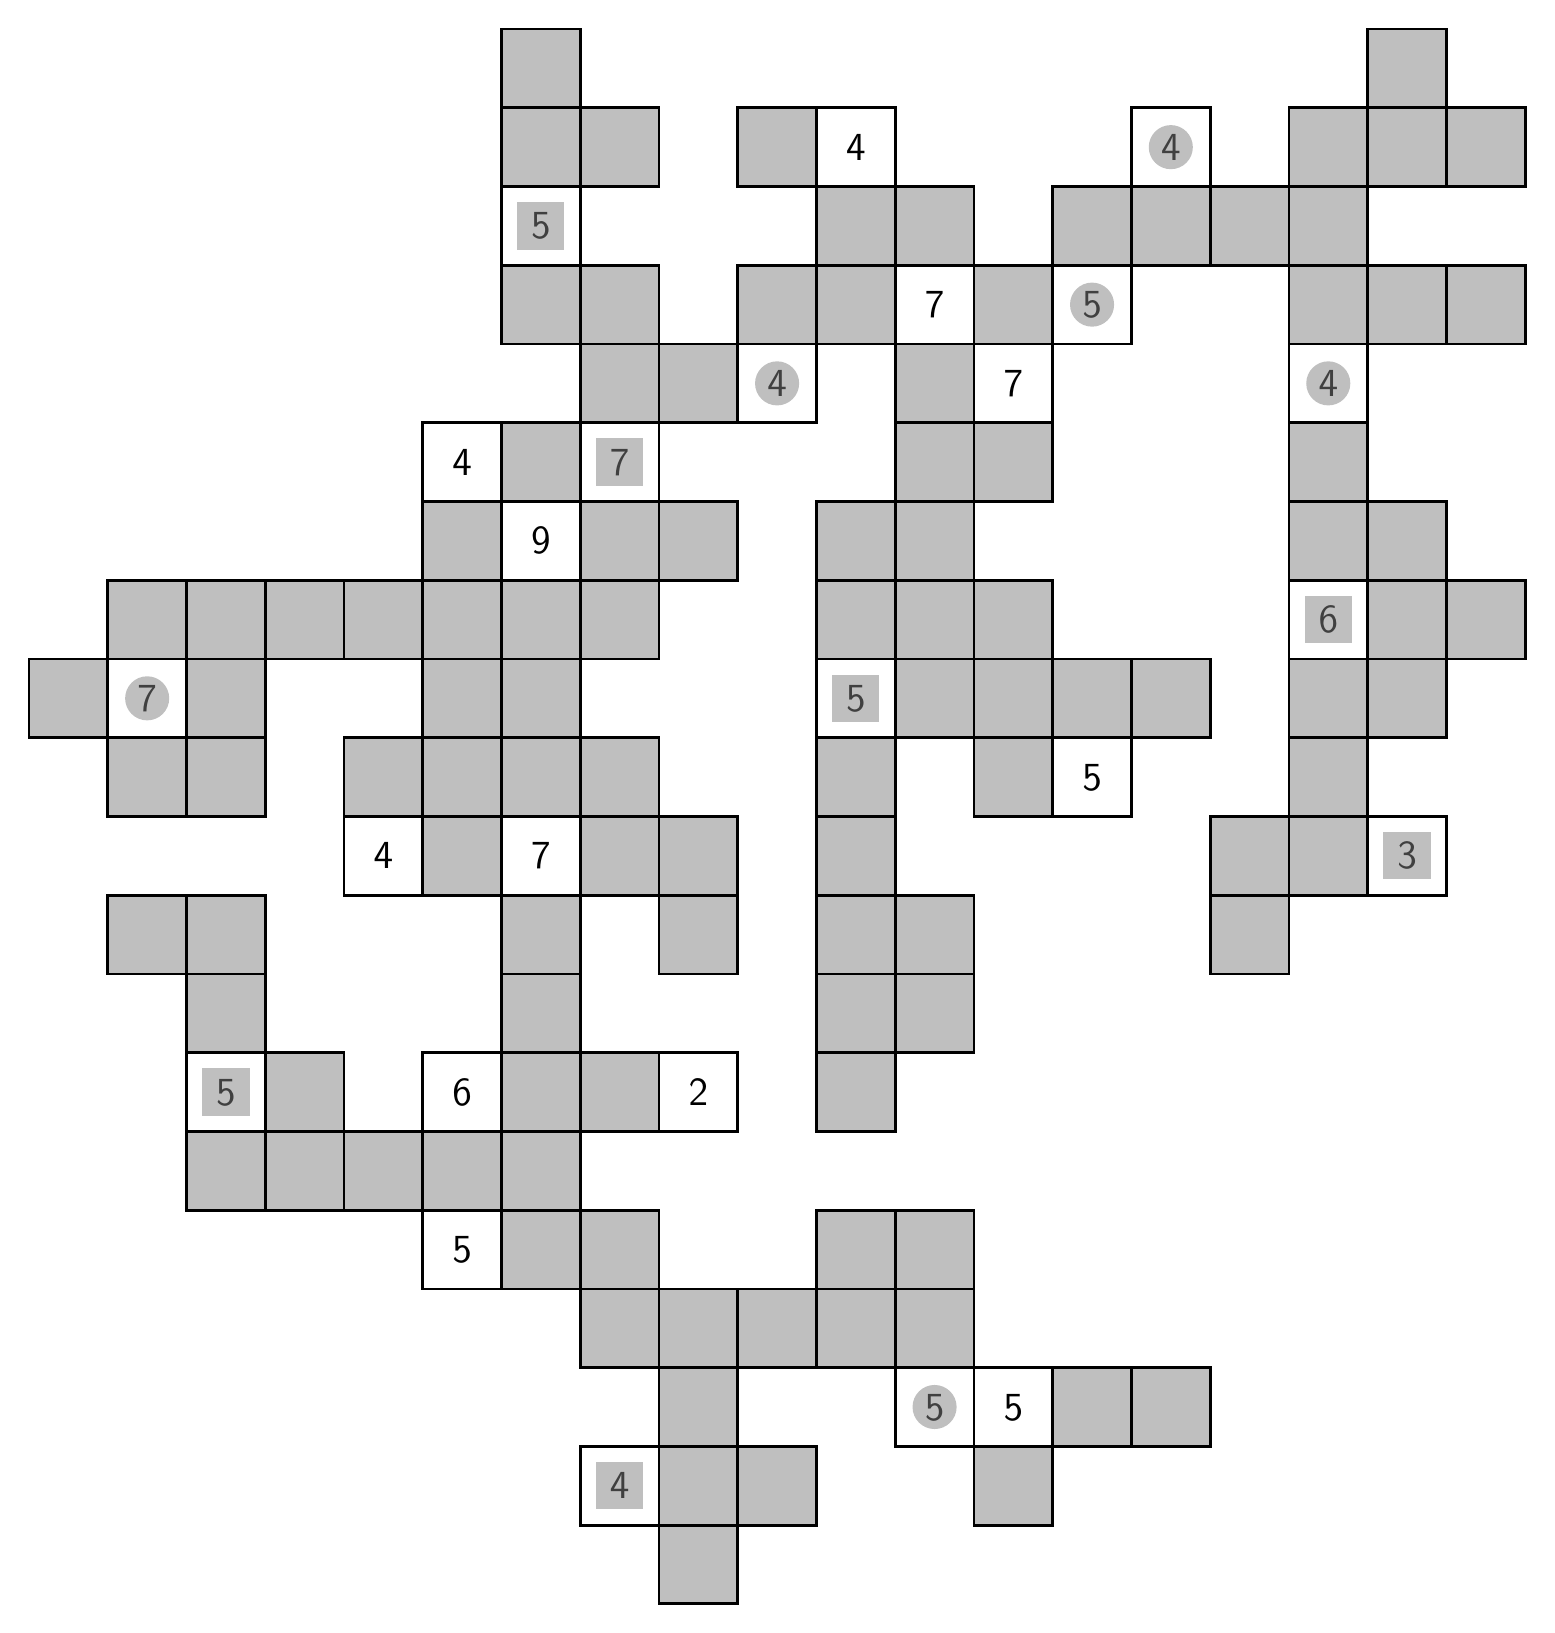
\begin{tikzpicture}\fill[gray, opacity = 0.5] (9, 0, 0)--++(1, 0, 0)--++(0, 1, 0)--++(-1, 0, 0)--cycle;
\draw[line width = 1pt] (9, 0, 0)--++(1, 0, 0)--++(0, 1, 0)--++(-1, 0, 0)--cycle;
\draw node at (8.5, 1.5, 0) {\Large $\mathsf{4}$};
\draw[line width = 1pt] (8, 1, 0)--++(1, 0, 0)--++(0, 1, 0)--++(-1, 0, 0)--cycle;
\fill[color = gray, opacity = 0.5] (8.2, 1.2) rectangle ++(0.6, 0.6);
\fill[gray, opacity = 0.5] (9, 1, 0)--++(1, 0, 0)--++(0, 1, 0)--++(-1, 0, 0)--cycle;
\draw[line width = 1pt] (9, 1, 0)--++(1, 0, 0)--++(0, 1, 0)--++(-1, 0, 0)--cycle;
\fill[gray, opacity = 0.5] (10, 1, 0)--++(1, 0, 0)--++(0, 1, 0)--++(-1, 0, 0)--cycle;
\draw[line width = 1pt] (10, 1, 0)--++(1, 0, 0)--++(0, 1, 0)--++(-1, 0, 0)--cycle;
\fill[gray, opacity = 0.5] (13, 1, 0)--++(1, 0, 0)--++(0, 1, 0)--++(-1, 0, 0)--cycle;
\draw[line width = 1pt] (13, 1, 0)--++(1, 0, 0)--++(0, 1, 0)--++(-1, 0, 0)--cycle;
\fill[gray, opacity = 0.5] (9, 2, 0)--++(1, 0, 0)--++(0, 1, 0)--++(-1, 0, 0)--cycle;
\draw[line width = 1pt] (9, 2, 0)--++(1, 0, 0)--++(0, 1, 0)--++(-1, 0, 0)--cycle;
\draw node at (12.5, 2.5, 0) {\Large $\mathsf{5}$};
\draw[line width = 1pt] (12, 2, 0)--++(1, 0, 0)--++(0, 1, 0)--++(-1, 0, 0)--cycle;
\fill[color = gray, opacity = 0.5] (12.5, 2.5, 0) circle (0.28);
\draw node at (13.5, 2.5, 0) {\Large $\mathsf{5}$};
\draw[line width = 1pt] (13, 2, 0)--++(1, 0, 0)--++(0, 1, 0)--++(-1, 0, 0)--cycle;
\fill[gray, opacity = 0.5] (14, 2, 0)--++(1, 0, 0)--++(0, 1, 0)--++(-1, 0, 0)--cycle;
\draw[line width = 1pt] (14, 2, 0)--++(1, 0, 0)--++(0, 1, 0)--++(-1, 0, 0)--cycle;
\fill[gray, opacity = 0.5] (15, 2, 0)--++(1, 0, 0)--++(0, 1, 0)--++(-1, 0, 0)--cycle;
\draw[line width = 1pt] (15, 2, 0)--++(1, 0, 0)--++(0, 1, 0)--++(-1, 0, 0)--cycle;
\fill[gray, opacity = 0.5] (8, 3, 0)--++(1, 0, 0)--++(0, 1, 0)--++(-1, 0, 0)--cycle;
\draw[line width = 1pt] (8, 3, 0)--++(1, 0, 0)--++(0, 1, 0)--++(-1, 0, 0)--cycle;
\fill[gray, opacity = 0.5] (9, 3, 0)--++(1, 0, 0)--++(0, 1, 0)--++(-1, 0, 0)--cycle;
\draw[line width = 1pt] (9, 3, 0)--++(1, 0, 0)--++(0, 1, 0)--++(-1, 0, 0)--cycle;
\fill[gray, opacity = 0.5] (10, 3, 0)--++(1, 0, 0)--++(0, 1, 0)--++(-1, 0, 0)--cycle;
\draw[line width = 1pt] (10, 3, 0)--++(1, 0, 0)--++(0, 1, 0)--++(-1, 0, 0)--cycle;
\fill[gray, opacity = 0.5] (11, 3, 0)--++(1, 0, 0)--++(0, 1, 0)--++(-1, 0, 0)--cycle;
\draw[line width = 1pt] (11, 3, 0)--++(1, 0, 0)--++(0, 1, 0)--++(-1, 0, 0)--cycle;
\fill[gray, opacity = 0.5] (12, 3, 0)--++(1, 0, 0)--++(0, 1, 0)--++(-1, 0, 0)--cycle;
\draw[line width = 1pt] (12, 3, 0)--++(1, 0, 0)--++(0, 1, 0)--++(-1, 0, 0)--cycle;
\draw node at (6.5, 4.5, 0) {\Large $\mathsf{5}$};
\draw[line width = 1pt] (6, 4, 0)--++(1, 0, 0)--++(0, 1, 0)--++(-1, 0, 0)--cycle;
\fill[gray, opacity = 0.5] (7, 4, 0)--++(1, 0, 0)--++(0, 1, 0)--++(-1, 0, 0)--cycle;
\draw[line width = 1pt] (7, 4, 0)--++(1, 0, 0)--++(0, 1, 0)--++(-1, 0, 0)--cycle;
\fill[gray, opacity = 0.5] (8, 4, 0)--++(1, 0, 0)--++(0, 1, 0)--++(-1, 0, 0)--cycle;
\draw[line width = 1pt] (8, 4, 0)--++(1, 0, 0)--++(0, 1, 0)--++(-1, 0, 0)--cycle;
\fill[gray, opacity = 0.5] (11, 4, 0)--++(1, 0, 0)--++(0, 1, 0)--++(-1, 0, 0)--cycle;
\draw[line width = 1pt] (11, 4, 0)--++(1, 0, 0)--++(0, 1, 0)--++(-1, 0, 0)--cycle;
\fill[gray, opacity = 0.5] (12, 4, 0)--++(1, 0, 0)--++(0, 1, 0)--++(-1, 0, 0)--cycle;
\draw[line width = 1pt] (12, 4, 0)--++(1, 0, 0)--++(0, 1, 0)--++(-1, 0, 0)--cycle;
\fill[gray, opacity = 0.5] (3, 5, 0)--++(1, 0, 0)--++(0, 1, 0)--++(-1, 0, 0)--cycle;
\draw[line width = 1pt] (3, 5, 0)--++(1, 0, 0)--++(0, 1, 0)--++(-1, 0, 0)--cycle;
\fill[gray, opacity = 0.5] (4, 5, 0)--++(1, 0, 0)--++(0, 1, 0)--++(-1, 0, 0)--cycle;
\draw[line width = 1pt] (4, 5, 0)--++(1, 0, 0)--++(0, 1, 0)--++(-1, 0, 0)--cycle;
\fill[gray, opacity = 0.5] (5, 5, 0)--++(1, 0, 0)--++(0, 1, 0)--++(-1, 0, 0)--cycle;
\draw[line width = 1pt] (5, 5, 0)--++(1, 0, 0)--++(0, 1, 0)--++(-1, 0, 0)--cycle;
\fill[gray, opacity = 0.5] (6, 5, 0)--++(1, 0, 0)--++(0, 1, 0)--++(-1, 0, 0)--cycle;
\draw[line width = 1pt] (6, 5, 0)--++(1, 0, 0)--++(0, 1, 0)--++(-1, 0, 0)--cycle;
\fill[gray, opacity = 0.5] (7, 5, 0)--++(1, 0, 0)--++(0, 1, 0)--++(-1, 0, 0)--cycle;
\draw[line width = 1pt] (7, 5, 0)--++(1, 0, 0)--++(0, 1, 0)--++(-1, 0, 0)--cycle;
\draw node at (3.5, 6.5, 0) {\Large $\mathsf{5}$};
\draw[line width = 1pt] (3, 6, 0)--++(1, 0, 0)--++(0, 1, 0)--++(-1, 0, 0)--cycle;
\fill[color = gray, opacity = 0.5] (3.2, 6.2) rectangle ++(0.6, 0.6);
\fill[gray, opacity = 0.5] (4, 6, 0)--++(1, 0, 0)--++(0, 1, 0)--++(-1, 0, 0)--cycle;
\draw[line width = 1pt] (4, 6, 0)--++(1, 0, 0)--++(0, 1, 0)--++(-1, 0, 0)--cycle;
\draw node at (6.5, 6.5, 0) {\Large $\mathsf{6}$};
\draw[line width = 1pt] (6, 6, 0)--++(1, 0, 0)--++(0, 1, 0)--++(-1, 0, 0)--cycle;
\fill[gray, opacity = 0.5] (7, 6, 0)--++(1, 0, 0)--++(0, 1, 0)--++(-1, 0, 0)--cycle;
\draw[line width = 1pt] (7, 6, 0)--++(1, 0, 0)--++(0, 1, 0)--++(-1, 0, 0)--cycle;
\fill[gray, opacity = 0.5] (8, 6, 0)--++(1, 0, 0)--++(0, 1, 0)--++(-1, 0, 0)--cycle;
\draw[line width = 1pt] (8, 6, 0)--++(1, 0, 0)--++(0, 1, 0)--++(-1, 0, 0)--cycle;
\draw node at (9.5, 6.5, 0) {\Large $\mathsf{2}$};
\draw[line width = 1pt] (9, 6, 0)--++(1, 0, 0)--++(0, 1, 0)--++(-1, 0, 0)--cycle;
\fill[gray, opacity = 0.5] (11, 6, 0)--++(1, 0, 0)--++(0, 1, 0)--++(-1, 0, 0)--cycle;
\draw[line width = 1pt] (11, 6, 0)--++(1, 0, 0)--++(0, 1, 0)--++(-1, 0, 0)--cycle;
\fill[gray, opacity = 0.5] (3, 7, 0)--++(1, 0, 0)--++(0, 1, 0)--++(-1, 0, 0)--cycle;
\draw[line width = 1pt] (3, 7, 0)--++(1, 0, 0)--++(0, 1, 0)--++(-1, 0, 0)--cycle;
\fill[gray, opacity = 0.5] (7, 7, 0)--++(1, 0, 0)--++(0, 1, 0)--++(-1, 0, 0)--cycle;
\draw[line width = 1pt] (7, 7, 0)--++(1, 0, 0)--++(0, 1, 0)--++(-1, 0, 0)--cycle;
\fill[gray, opacity = 0.5] (11, 7, 0)--++(1, 0, 0)--++(0, 1, 0)--++(-1, 0, 0)--cycle;
\draw[line width = 1pt] (11, 7, 0)--++(1, 0, 0)--++(0, 1, 0)--++(-1, 0, 0)--cycle;
\fill[gray, opacity = 0.5] (12, 7, 0)--++(1, 0, 0)--++(0, 1, 0)--++(-1, 0, 0)--cycle;
\draw[line width = 1pt] (12, 7, 0)--++(1, 0, 0)--++(0, 1, 0)--++(-1, 0, 0)--cycle;
\fill[gray, opacity = 0.5] (2, 8, 0)--++(1, 0, 0)--++(0, 1, 0)--++(-1, 0, 0)--cycle;
\draw[line width = 1pt] (2, 8, 0)--++(1, 0, 0)--++(0, 1, 0)--++(-1, 0, 0)--cycle;
\fill[gray, opacity = 0.5] (3, 8, 0)--++(1, 0, 0)--++(0, 1, 0)--++(-1, 0, 0)--cycle;
\draw[line width = 1pt] (3, 8, 0)--++(1, 0, 0)--++(0, 1, 0)--++(-1, 0, 0)--cycle;
\fill[gray, opacity = 0.5] (7, 8, 0)--++(1, 0, 0)--++(0, 1, 0)--++(-1, 0, 0)--cycle;
\draw[line width = 1pt] (7, 8, 0)--++(1, 0, 0)--++(0, 1, 0)--++(-1, 0, 0)--cycle;
\fill[gray, opacity = 0.5] (9, 8, 0)--++(1, 0, 0)--++(0, 1, 0)--++(-1, 0, 0)--cycle;
\draw[line width = 1pt] (9, 8, 0)--++(1, 0, 0)--++(0, 1, 0)--++(-1, 0, 0)--cycle;
\fill[gray, opacity = 0.5] (11, 8, 0)--++(1, 0, 0)--++(0, 1, 0)--++(-1, 0, 0)--cycle;
\draw[line width = 1pt] (11, 8, 0)--++(1, 0, 0)--++(0, 1, 0)--++(-1, 0, 0)--cycle;
\fill[gray, opacity = 0.5] (12, 8, 0)--++(1, 0, 0)--++(0, 1, 0)--++(-1, 0, 0)--cycle;
\draw[line width = 1pt] (12, 8, 0)--++(1, 0, 0)--++(0, 1, 0)--++(-1, 0, 0)--cycle;
\fill[gray, opacity = 0.5] (16, 8, 0)--++(1, 0, 0)--++(0, 1, 0)--++(-1, 0, 0)--cycle;
\draw[line width = 1pt] (16, 8, 0)--++(1, 0, 0)--++(0, 1, 0)--++(-1, 0, 0)--cycle;
\draw node at (5.5, 9.5, 0) {\Large $\mathsf{4}$};
\draw[line width = 1pt] (5, 9, 0)--++(1, 0, 0)--++(0, 1, 0)--++(-1, 0, 0)--cycle;
\fill[gray, opacity = 0.5] (6, 9, 0)--++(1, 0, 0)--++(0, 1, 0)--++(-1, 0, 0)--cycle;
\draw[line width = 1pt] (6, 9, 0)--++(1, 0, 0)--++(0, 1, 0)--++(-1, 0, 0)--cycle;
\draw node at (7.5, 9.5, 0) {\Large $\mathsf{7}$};
\draw[line width = 1pt] (7, 9, 0)--++(1, 0, 0)--++(0, 1, 0)--++(-1, 0, 0)--cycle;
\fill[gray, opacity = 0.5] (8, 9, 0)--++(1, 0, 0)--++(0, 1, 0)--++(-1, 0, 0)--cycle;
\draw[line width = 1pt] (8, 9, 0)--++(1, 0, 0)--++(0, 1, 0)--++(-1, 0, 0)--cycle;
\fill[gray, opacity = 0.5] (9, 9, 0)--++(1, 0, 0)--++(0, 1, 0)--++(-1, 0, 0)--cycle;
\draw[line width = 1pt] (9, 9, 0)--++(1, 0, 0)--++(0, 1, 0)--++(-1, 0, 0)--cycle;
\fill[gray, opacity = 0.5] (11, 9, 0)--++(1, 0, 0)--++(0, 1, 0)--++(-1, 0, 0)--cycle;
\draw[line width = 1pt] (11, 9, 0)--++(1, 0, 0)--++(0, 1, 0)--++(-1, 0, 0)--cycle;
\fill[gray, opacity = 0.5] (16, 9, 0)--++(1, 0, 0)--++(0, 1, 0)--++(-1, 0, 0)--cycle;
\draw[line width = 1pt] (16, 9, 0)--++(1, 0, 0)--++(0, 1, 0)--++(-1, 0, 0)--cycle;
\fill[gray, opacity = 0.5] (17, 9, 0)--++(1, 0, 0)--++(0, 1, 0)--++(-1, 0, 0)--cycle;
\draw[line width = 1pt] (17, 9, 0)--++(1, 0, 0)--++(0, 1, 0)--++(-1, 0, 0)--cycle;
\draw node at (18.5, 9.5, 0) {\Large $\mathsf{3}$};
\draw[line width = 1pt] (18, 9, 0)--++(1, 0, 0)--++(0, 1, 0)--++(-1, 0, 0)--cycle;
\fill[color = gray, opacity = 0.5] (18.2, 9.2) rectangle ++(0.6, 0.6);
\fill[gray, opacity = 0.5] (2, 10, 0)--++(1, 0, 0)--++(0, 1, 0)--++(-1, 0, 0)--cycle;
\draw[line width = 1pt] (2, 10, 0)--++(1, 0, 0)--++(0, 1, 0)--++(-1, 0, 0)--cycle;
\fill[gray, opacity = 0.5] (3, 10, 0)--++(1, 0, 0)--++(0, 1, 0)--++(-1, 0, 0)--cycle;
\draw[line width = 1pt] (3, 10, 0)--++(1, 0, 0)--++(0, 1, 0)--++(-1, 0, 0)--cycle;
\fill[gray, opacity = 0.5] (5, 10, 0)--++(1, 0, 0)--++(0, 1, 0)--++(-1, 0, 0)--cycle;
\draw[line width = 1pt] (5, 10, 0)--++(1, 0, 0)--++(0, 1, 0)--++(-1, 0, 0)--cycle;
\fill[gray, opacity = 0.5] (6, 10, 0)--++(1, 0, 0)--++(0, 1, 0)--++(-1, 0, 0)--cycle;
\draw[line width = 1pt] (6, 10, 0)--++(1, 0, 0)--++(0, 1, 0)--++(-1, 0, 0)--cycle;
\fill[gray, opacity = 0.5] (7, 10, 0)--++(1, 0, 0)--++(0, 1, 0)--++(-1, 0, 0)--cycle;
\draw[line width = 1pt] (7, 10, 0)--++(1, 0, 0)--++(0, 1, 0)--++(-1, 0, 0)--cycle;
\fill[gray, opacity = 0.5] (8, 10, 0)--++(1, 0, 0)--++(0, 1, 0)--++(-1, 0, 0)--cycle;
\draw[line width = 1pt] (8, 10, 0)--++(1, 0, 0)--++(0, 1, 0)--++(-1, 0, 0)--cycle;
\fill[gray, opacity = 0.5] (11, 10, 0)--++(1, 0, 0)--++(0, 1, 0)--++(-1, 0, 0)--cycle;
\draw[line width = 1pt] (11, 10, 0)--++(1, 0, 0)--++(0, 1, 0)--++(-1, 0, 0)--cycle;
\fill[gray, opacity = 0.5] (13, 10, 0)--++(1, 0, 0)--++(0, 1, 0)--++(-1, 0, 0)--cycle;
\draw[line width = 1pt] (13, 10, 0)--++(1, 0, 0)--++(0, 1, 0)--++(-1, 0, 0)--cycle;
\draw node at (14.5, 10.5, 0) {\Large $\mathsf{5}$};
\draw[line width = 1pt] (14, 10, 0)--++(1, 0, 0)--++(0, 1, 0)--++(-1, 0, 0)--cycle;
\fill[gray, opacity = 0.5] (17, 10, 0)--++(1, 0, 0)--++(0, 1, 0)--++(-1, 0, 0)--cycle;
\draw[line width = 1pt] (17, 10, 0)--++(1, 0, 0)--++(0, 1, 0)--++(-1, 0, 0)--cycle;
\fill[gray, opacity = 0.5] (1, 11, 0)--++(1, 0, 0)--++(0, 1, 0)--++(-1, 0, 0)--cycle;
\draw[line width = 1pt] (1, 11, 0)--++(1, 0, 0)--++(0, 1, 0)--++(-1, 0, 0)--cycle;
\draw node at (2.5, 11.5, 0) {\Large $\mathsf{7}$};
\draw[line width = 1pt] (2, 11, 0)--++(1, 0, 0)--++(0, 1, 0)--++(-1, 0, 0)--cycle;
\fill[color = gray, opacity = 0.5] (2.5, 11.5, 0) circle (0.28);
\fill[gray, opacity = 0.5] (3, 11, 0)--++(1, 0, 0)--++(0, 1, 0)--++(-1, 0, 0)--cycle;
\draw[line width = 1pt] (3, 11, 0)--++(1, 0, 0)--++(0, 1, 0)--++(-1, 0, 0)--cycle;
\fill[gray, opacity = 0.5] (6, 11, 0)--++(1, 0, 0)--++(0, 1, 0)--++(-1, 0, 0)--cycle;
\draw[line width = 1pt] (6, 11, 0)--++(1, 0, 0)--++(0, 1, 0)--++(-1, 0, 0)--cycle;
\fill[gray, opacity = 0.5] (7, 11, 0)--++(1, 0, 0)--++(0, 1, 0)--++(-1, 0, 0)--cycle;
\draw[line width = 1pt] (7, 11, 0)--++(1, 0, 0)--++(0, 1, 0)--++(-1, 0, 0)--cycle;
\draw node at (11.5, 11.5, 0) {\Large $\mathsf{5}$};
\draw[line width = 1pt] (11, 11, 0)--++(1, 0, 0)--++(0, 1, 0)--++(-1, 0, 0)--cycle;
\fill[color = gray, opacity = 0.5] (11.2, 11.2) rectangle ++(0.6, 0.6);
\fill[gray, opacity = 0.5] (12, 11, 0)--++(1, 0, 0)--++(0, 1, 0)--++(-1, 0, 0)--cycle;
\draw[line width = 1pt] (12, 11, 0)--++(1, 0, 0)--++(0, 1, 0)--++(-1, 0, 0)--cycle;
\fill[gray, opacity = 0.5] (13, 11, 0)--++(1, 0, 0)--++(0, 1, 0)--++(-1, 0, 0)--cycle;
\draw[line width = 1pt] (13, 11, 0)--++(1, 0, 0)--++(0, 1, 0)--++(-1, 0, 0)--cycle;
\fill[gray, opacity = 0.5] (14, 11, 0)--++(1, 0, 0)--++(0, 1, 0)--++(-1, 0, 0)--cycle;
\draw[line width = 1pt] (14, 11, 0)--++(1, 0, 0)--++(0, 1, 0)--++(-1, 0, 0)--cycle;
\fill[gray, opacity = 0.5] (15, 11, 0)--++(1, 0, 0)--++(0, 1, 0)--++(-1, 0, 0)--cycle;
\draw[line width = 1pt] (15, 11, 0)--++(1, 0, 0)--++(0, 1, 0)--++(-1, 0, 0)--cycle;
\fill[gray, opacity = 0.5] (17, 11, 0)--++(1, 0, 0)--++(0, 1, 0)--++(-1, 0, 0)--cycle;
\draw[line width = 1pt] (17, 11, 0)--++(1, 0, 0)--++(0, 1, 0)--++(-1, 0, 0)--cycle;
\fill[gray, opacity = 0.5] (18, 11, 0)--++(1, 0, 0)--++(0, 1, 0)--++(-1, 0, 0)--cycle;
\draw[line width = 1pt] (18, 11, 0)--++(1, 0, 0)--++(0, 1, 0)--++(-1, 0, 0)--cycle;
\fill[gray, opacity = 0.5] (2, 12, 0)--++(1, 0, 0)--++(0, 1, 0)--++(-1, 0, 0)--cycle;
\draw[line width = 1pt] (2, 12, 0)--++(1, 0, 0)--++(0, 1, 0)--++(-1, 0, 0)--cycle;
\fill[gray, opacity = 0.5] (3, 12, 0)--++(1, 0, 0)--++(0, 1, 0)--++(-1, 0, 0)--cycle;
\draw[line width = 1pt] (3, 12, 0)--++(1, 0, 0)--++(0, 1, 0)--++(-1, 0, 0)--cycle;
\fill[gray, opacity = 0.5] (4, 12, 0)--++(1, 0, 0)--++(0, 1, 0)--++(-1, 0, 0)--cycle;
\draw[line width = 1pt] (4, 12, 0)--++(1, 0, 0)--++(0, 1, 0)--++(-1, 0, 0)--cycle;
\fill[gray, opacity = 0.5] (5, 12, 0)--++(1, 0, 0)--++(0, 1, 0)--++(-1, 0, 0)--cycle;
\draw[line width = 1pt] (5, 12, 0)--++(1, 0, 0)--++(0, 1, 0)--++(-1, 0, 0)--cycle;
\fill[gray, opacity = 0.5] (6, 12, 0)--++(1, 0, 0)--++(0, 1, 0)--++(-1, 0, 0)--cycle;
\draw[line width = 1pt] (6, 12, 0)--++(1, 0, 0)--++(0, 1, 0)--++(-1, 0, 0)--cycle;
\fill[gray, opacity = 0.5] (7, 12, 0)--++(1, 0, 0)--++(0, 1, 0)--++(-1, 0, 0)--cycle;
\draw[line width = 1pt] (7, 12, 0)--++(1, 0, 0)--++(0, 1, 0)--++(-1, 0, 0)--cycle;
\fill[gray, opacity = 0.5] (8, 12, 0)--++(1, 0, 0)--++(0, 1, 0)--++(-1, 0, 0)--cycle;
\draw[line width = 1pt] (8, 12, 0)--++(1, 0, 0)--++(0, 1, 0)--++(-1, 0, 0)--cycle;
\fill[gray, opacity = 0.5] (11, 12, 0)--++(1, 0, 0)--++(0, 1, 0)--++(-1, 0, 0)--cycle;
\draw[line width = 1pt] (11, 12, 0)--++(1, 0, 0)--++(0, 1, 0)--++(-1, 0, 0)--cycle;
\fill[gray, opacity = 0.5] (12, 12, 0)--++(1, 0, 0)--++(0, 1, 0)--++(-1, 0, 0)--cycle;
\draw[line width = 1pt] (12, 12, 0)--++(1, 0, 0)--++(0, 1, 0)--++(-1, 0, 0)--cycle;
\fill[gray, opacity = 0.5] (13, 12, 0)--++(1, 0, 0)--++(0, 1, 0)--++(-1, 0, 0)--cycle;
\draw[line width = 1pt] (13, 12, 0)--++(1, 0, 0)--++(0, 1, 0)--++(-1, 0, 0)--cycle;
\draw node at (17.5, 12.5, 0) {\Large $\mathsf{6}$};
\draw[line width = 1pt] (17, 12, 0)--++(1, 0, 0)--++(0, 1, 0)--++(-1, 0, 0)--cycle;
\fill[color = gray, opacity = 0.5] (17.2, 12.2) rectangle ++(0.6, 0.6);
\fill[gray, opacity = 0.5] (18, 12, 0)--++(1, 0, 0)--++(0, 1, 0)--++(-1, 0, 0)--cycle;
\draw[line width = 1pt] (18, 12, 0)--++(1, 0, 0)--++(0, 1, 0)--++(-1, 0, 0)--cycle;
\fill[gray, opacity = 0.5] (19, 12, 0)--++(1, 0, 0)--++(0, 1, 0)--++(-1, 0, 0)--cycle;
\draw[line width = 1pt] (19, 12, 0)--++(1, 0, 0)--++(0, 1, 0)--++(-1, 0, 0)--cycle;
\fill[gray, opacity = 0.5] (6, 13, 0)--++(1, 0, 0)--++(0, 1, 0)--++(-1, 0, 0)--cycle;
\draw[line width = 1pt] (6, 13, 0)--++(1, 0, 0)--++(0, 1, 0)--++(-1, 0, 0)--cycle;
\draw node at (7.5, 13.5, 0) {\Large $\mathsf{9}$};
\draw[line width = 1pt] (7, 13, 0)--++(1, 0, 0)--++(0, 1, 0)--++(-1, 0, 0)--cycle;
\fill[gray, opacity = 0.5] (8, 13, 0)--++(1, 0, 0)--++(0, 1, 0)--++(-1, 0, 0)--cycle;
\draw[line width = 1pt] (8, 13, 0)--++(1, 0, 0)--++(0, 1, 0)--++(-1, 0, 0)--cycle;
\fill[gray, opacity = 0.5] (9, 13, 0)--++(1, 0, 0)--++(0, 1, 0)--++(-1, 0, 0)--cycle;
\draw[line width = 1pt] (9, 13, 0)--++(1, 0, 0)--++(0, 1, 0)--++(-1, 0, 0)--cycle;
\fill[gray, opacity = 0.5] (11, 13, 0)--++(1, 0, 0)--++(0, 1, 0)--++(-1, 0, 0)--cycle;
\draw[line width = 1pt] (11, 13, 0)--++(1, 0, 0)--++(0, 1, 0)--++(-1, 0, 0)--cycle;
\fill[gray, opacity = 0.5] (12, 13, 0)--++(1, 0, 0)--++(0, 1, 0)--++(-1, 0, 0)--cycle;
\draw[line width = 1pt] (12, 13, 0)--++(1, 0, 0)--++(0, 1, 0)--++(-1, 0, 0)--cycle;
\fill[gray, opacity = 0.5] (17, 13, 0)--++(1, 0, 0)--++(0, 1, 0)--++(-1, 0, 0)--cycle;
\draw[line width = 1pt] (17, 13, 0)--++(1, 0, 0)--++(0, 1, 0)--++(-1, 0, 0)--cycle;
\fill[gray, opacity = 0.5] (18, 13, 0)--++(1, 0, 0)--++(0, 1, 0)--++(-1, 0, 0)--cycle;
\draw[line width = 1pt] (18, 13, 0)--++(1, 0, 0)--++(0, 1, 0)--++(-1, 0, 0)--cycle;
\draw node at (6.5, 14.5, 0) {\Large $\mathsf{4}$};
\draw[line width = 1pt] (6, 14, 0)--++(1, 0, 0)--++(0, 1, 0)--++(-1, 0, 0)--cycle;
\fill[gray, opacity = 0.5] (7, 14, 0)--++(1, 0, 0)--++(0, 1, 0)--++(-1, 0, 0)--cycle;
\draw[line width = 1pt] (7, 14, 0)--++(1, 0, 0)--++(0, 1, 0)--++(-1, 0, 0)--cycle;
\draw node at (8.5, 14.5, 0) {\Large $\mathsf{7}$};
\draw[line width = 1pt] (8, 14, 0)--++(1, 0, 0)--++(0, 1, 0)--++(-1, 0, 0)--cycle;
\fill[color = gray, opacity = 0.5] (8.2, 14.2) rectangle ++(0.6, 0.6);
\fill[gray, opacity = 0.5] (12, 14, 0)--++(1, 0, 0)--++(0, 1, 0)--++(-1, 0, 0)--cycle;
\draw[line width = 1pt] (12, 14, 0)--++(1, 0, 0)--++(0, 1, 0)--++(-1, 0, 0)--cycle;
\fill[gray, opacity = 0.5] (13, 14, 0)--++(1, 0, 0)--++(0, 1, 0)--++(-1, 0, 0)--cycle;
\draw[line width = 1pt] (13, 14, 0)--++(1, 0, 0)--++(0, 1, 0)--++(-1, 0, 0)--cycle;
\fill[gray, opacity = 0.5] (17, 14, 0)--++(1, 0, 0)--++(0, 1, 0)--++(-1, 0, 0)--cycle;
\draw[line width = 1pt] (17, 14, 0)--++(1, 0, 0)--++(0, 1, 0)--++(-1, 0, 0)--cycle;
\fill[gray, opacity = 0.5] (8, 15, 0)--++(1, 0, 0)--++(0, 1, 0)--++(-1, 0, 0)--cycle;
\draw[line width = 1pt] (8, 15, 0)--++(1, 0, 0)--++(0, 1, 0)--++(-1, 0, 0)--cycle;
\fill[gray, opacity = 0.5] (9, 15, 0)--++(1, 0, 0)--++(0, 1, 0)--++(-1, 0, 0)--cycle;
\draw[line width = 1pt] (9, 15, 0)--++(1, 0, 0)--++(0, 1, 0)--++(-1, 0, 0)--cycle;
\draw node at (10.5, 15.5, 0) {\Large $\mathsf{4}$};
\draw[line width = 1pt] (10, 15, 0)--++(1, 0, 0)--++(0, 1, 0)--++(-1, 0, 0)--cycle;
\fill[color = gray, opacity = 0.5] (10.5, 15.5, 0) circle (0.28);
\fill[gray, opacity = 0.5] (12, 15, 0)--++(1, 0, 0)--++(0, 1, 0)--++(-1, 0, 0)--cycle;
\draw[line width = 1pt] (12, 15, 0)--++(1, 0, 0)--++(0, 1, 0)--++(-1, 0, 0)--cycle;
\draw node at (13.5, 15.5, 0) {\Large $\mathsf{7}$};
\draw[line width = 1pt] (13, 15, 0)--++(1, 0, 0)--++(0, 1, 0)--++(-1, 0, 0)--cycle;
\draw node at (17.5, 15.5, 0) {\Large $\mathsf{4}$};
\draw[line width = 1pt] (17, 15, 0)--++(1, 0, 0)--++(0, 1, 0)--++(-1, 0, 0)--cycle;
\fill[color = gray, opacity = 0.5] (17.5, 15.5, 0) circle (0.28);
\fill[gray, opacity = 0.5] (7, 16, 0)--++(1, 0, 0)--++(0, 1, 0)--++(-1, 0, 0)--cycle;
\draw[line width = 1pt] (7, 16, 0)--++(1, 0, 0)--++(0, 1, 0)--++(-1, 0, 0)--cycle;
\fill[gray, opacity = 0.5] (8, 16, 0)--++(1, 0, 0)--++(0, 1, 0)--++(-1, 0, 0)--cycle;
\draw[line width = 1pt] (8, 16, 0)--++(1, 0, 0)--++(0, 1, 0)--++(-1, 0, 0)--cycle;
\fill[gray, opacity = 0.5] (10, 16, 0)--++(1, 0, 0)--++(0, 1, 0)--++(-1, 0, 0)--cycle;
\draw[line width = 1pt] (10, 16, 0)--++(1, 0, 0)--++(0, 1, 0)--++(-1, 0, 0)--cycle;
\fill[gray, opacity = 0.5] (11, 16, 0)--++(1, 0, 0)--++(0, 1, 0)--++(-1, 0, 0)--cycle;
\draw[line width = 1pt] (11, 16, 0)--++(1, 0, 0)--++(0, 1, 0)--++(-1, 0, 0)--cycle;
\draw node at (12.5, 16.5, 0) {\Large $\mathsf{7}$};
\draw[line width = 1pt] (12, 16, 0)--++(1, 0, 0)--++(0, 1, 0)--++(-1, 0, 0)--cycle;
\fill[gray, opacity = 0.5] (13, 16, 0)--++(1, 0, 0)--++(0, 1, 0)--++(-1, 0, 0)--cycle;
\draw[line width = 1pt] (13, 16, 0)--++(1, 0, 0)--++(0, 1, 0)--++(-1, 0, 0)--cycle;
\draw node at (14.5, 16.5, 0) {\Large $\mathsf{5}$};
\draw[line width = 1pt] (14, 16, 0)--++(1, 0, 0)--++(0, 1, 0)--++(-1, 0, 0)--cycle;
\fill[color = gray, opacity = 0.5] (14.5, 16.5, 0) circle (0.28);
\fill[gray, opacity = 0.5] (17, 16, 0)--++(1, 0, 0)--++(0, 1, 0)--++(-1, 0, 0)--cycle;
\draw[line width = 1pt] (17, 16, 0)--++(1, 0, 0)--++(0, 1, 0)--++(-1, 0, 0)--cycle;
\fill[gray, opacity = 0.5] (18, 16, 0)--++(1, 0, 0)--++(0, 1, 0)--++(-1, 0, 0)--cycle;
\draw[line width = 1pt] (18, 16, 0)--++(1, 0, 0)--++(0, 1, 0)--++(-1, 0, 0)--cycle;
\fill[gray, opacity = 0.5] (19, 16, 0)--++(1, 0, 0)--++(0, 1, 0)--++(-1, 0, 0)--cycle;
\draw[line width = 1pt] (19, 16, 0)--++(1, 0, 0)--++(0, 1, 0)--++(-1, 0, 0)--cycle;
\draw node at (7.5, 17.5, 0) {\Large $\mathsf{5}$};
\draw[line width = 1pt] (7, 17, 0)--++(1, 0, 0)--++(0, 1, 0)--++(-1, 0, 0)--cycle;
\fill[color = gray, opacity = 0.5] (7.2, 17.2) rectangle ++(0.6, 0.6);
\fill[gray, opacity = 0.5] (11, 17, 0)--++(1, 0, 0)--++(0, 1, 0)--++(-1, 0, 0)--cycle;
\draw[line width = 1pt] (11, 17, 0)--++(1, 0, 0)--++(0, 1, 0)--++(-1, 0, 0)--cycle;
\fill[gray, opacity = 0.5] (12, 17, 0)--++(1, 0, 0)--++(0, 1, 0)--++(-1, 0, 0)--cycle;
\draw[line width = 1pt] (12, 17, 0)--++(1, 0, 0)--++(0, 1, 0)--++(-1, 0, 0)--cycle;
\fill[gray, opacity = 0.5] (14, 17, 0)--++(1, 0, 0)--++(0, 1, 0)--++(-1, 0, 0)--cycle;
\draw[line width = 1pt] (14, 17, 0)--++(1, 0, 0)--++(0, 1, 0)--++(-1, 0, 0)--cycle;
\fill[gray, opacity = 0.5] (15, 17, 0)--++(1, 0, 0)--++(0, 1, 0)--++(-1, 0, 0)--cycle;
\draw[line width = 1pt] (15, 17, 0)--++(1, 0, 0)--++(0, 1, 0)--++(-1, 0, 0)--cycle;
\fill[gray, opacity = 0.5] (16, 17, 0)--++(1, 0, 0)--++(0, 1, 0)--++(-1, 0, 0)--cycle;
\draw[line width = 1pt] (16, 17, 0)--++(1, 0, 0)--++(0, 1, 0)--++(-1, 0, 0)--cycle;
\fill[gray, opacity = 0.5] (17, 17, 0)--++(1, 0, 0)--++(0, 1, 0)--++(-1, 0, 0)--cycle;
\draw[line width = 1pt] (17, 17, 0)--++(1, 0, 0)--++(0, 1, 0)--++(-1, 0, 0)--cycle;
\fill[gray, opacity = 0.5] (7, 18, 0)--++(1, 0, 0)--++(0, 1, 0)--++(-1, 0, 0)--cycle;
\draw[line width = 1pt] (7, 18, 0)--++(1, 0, 0)--++(0, 1, 0)--++(-1, 0, 0)--cycle;
\fill[gray, opacity = 0.5] (8, 18, 0)--++(1, 0, 0)--++(0, 1, 0)--++(-1, 0, 0)--cycle;
\draw[line width = 1pt] (8, 18, 0)--++(1, 0, 0)--++(0, 1, 0)--++(-1, 0, 0)--cycle;
\fill[gray, opacity = 0.5] (10, 18, 0)--++(1, 0, 0)--++(0, 1, 0)--++(-1, 0, 0)--cycle;
\draw[line width = 1pt] (10, 18, 0)--++(1, 0, 0)--++(0, 1, 0)--++(-1, 0, 0)--cycle;
\draw node at (11.5, 18.5, 0) {\Large $\mathsf{4}$};
\draw[line width = 1pt] (11, 18, 0)--++(1, 0, 0)--++(0, 1, 0)--++(-1, 0, 0)--cycle;
\draw node at (15.5, 18.5, 0) {\Large $\mathsf{4}$};
\draw[line width = 1pt] (15, 18, 0)--++(1, 0, 0)--++(0, 1, 0)--++(-1, 0, 0)--cycle;
\fill[color = gray, opacity = 0.5] (15.5, 18.5, 0) circle (0.28);
\fill[gray, opacity = 0.5] (17, 18, 0)--++(1, 0, 0)--++(0, 1, 0)--++(-1, 0, 0)--cycle;
\draw[line width = 1pt] (17, 18, 0)--++(1, 0, 0)--++(0, 1, 0)--++(-1, 0, 0)--cycle;
\fill[gray, opacity = 0.5] (18, 18, 0)--++(1, 0, 0)--++(0, 1, 0)--++(-1, 0, 0)--cycle;
\draw[line width = 1pt] (18, 18, 0)--++(1, 0, 0)--++(0, 1, 0)--++(-1, 0, 0)--cycle;
\fill[gray, opacity = 0.5] (19, 18, 0)--++(1, 0, 0)--++(0, 1, 0)--++(-1, 0, 0)--cycle;
\draw[line width = 1pt] (19, 18, 0)--++(1, 0, 0)--++(0, 1, 0)--++(-1, 0, 0)--cycle;
\fill[gray, opacity = 0.5] (7, 19, 0)--++(1, 0, 0)--++(0, 1, 0)--++(-1, 0, 0)--cycle;
\draw[line width = 1pt] (7, 19, 0)--++(1, 0, 0)--++(0, 1, 0)--++(-1, 0, 0)--cycle;
\fill[gray, opacity = 0.5] (18, 19, 0)--++(1, 0, 0)--++(0, 1, 0)--++(-1, 0, 0)--cycle;
\draw[line width = 1pt] (18, 19, 0)--++(1, 0, 0)--++(0, 1, 0)--++(-1, 0, 0)--cycle;
\end{tikzpicture}}\]
\[\resizebox{30pc}{!}{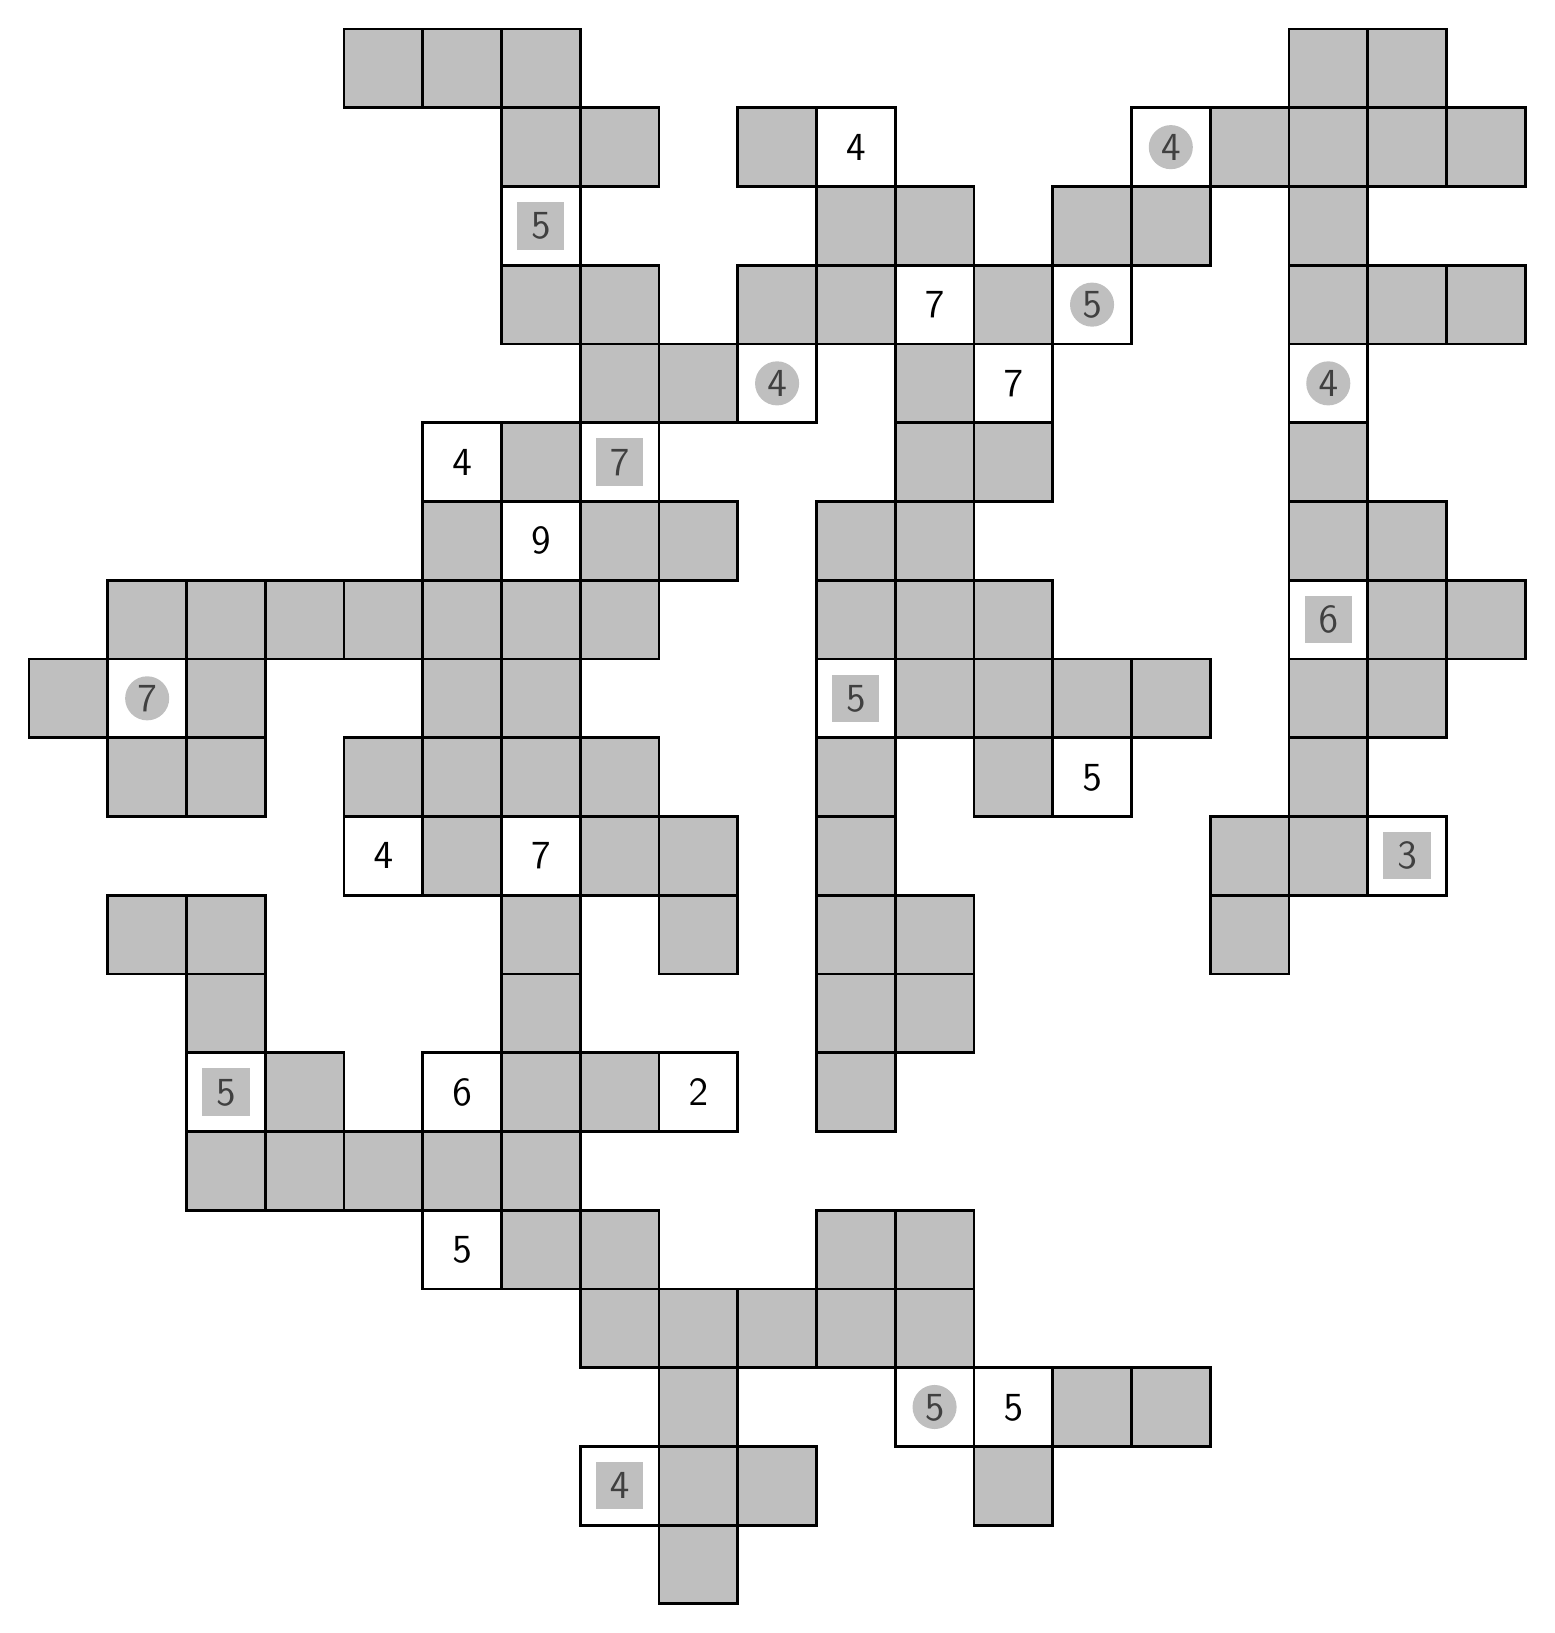
\begin{tikzpicture}\fill[gray, opacity = 0.5] (9, 0, 0)--++(1, 0, 0)--++(0, 1, 0)--++(-1, 0, 0)--cycle;
\draw[line width = 1pt] (9, 0, 0)--++(1, 0, 0)--++(0, 1, 0)--++(-1, 0, 0)--cycle;
\draw node at (8.5, 1.5, 0) {\Large $\mathsf{4}$};
\draw[line width = 1pt] (8, 1, 0)--++(1, 0, 0)--++(0, 1, 0)--++(-1, 0, 0)--cycle;
\fill[color = gray, opacity = 0.5] (8.2, 1.2) rectangle ++(0.6, 0.6);
\fill[gray, opacity = 0.5] (9, 1, 0)--++(1, 0, 0)--++(0, 1, 0)--++(-1, 0, 0)--cycle;
\draw[line width = 1pt] (9, 1, 0)--++(1, 0, 0)--++(0, 1, 0)--++(-1, 0, 0)--cycle;
\fill[gray, opacity = 0.5] (10, 1, 0)--++(1, 0, 0)--++(0, 1, 0)--++(-1, 0, 0)--cycle;
\draw[line width = 1pt] (10, 1, 0)--++(1, 0, 0)--++(0, 1, 0)--++(-1, 0, 0)--cycle;
\fill[gray, opacity = 0.5] (13, 1, 0)--++(1, 0, 0)--++(0, 1, 0)--++(-1, 0, 0)--cycle;
\draw[line width = 1pt] (13, 1, 0)--++(1, 0, 0)--++(0, 1, 0)--++(-1, 0, 0)--cycle;
\fill[gray, opacity = 0.5] (9, 2, 0)--++(1, 0, 0)--++(0, 1, 0)--++(-1, 0, 0)--cycle;
\draw[line width = 1pt] (9, 2, 0)--++(1, 0, 0)--++(0, 1, 0)--++(-1, 0, 0)--cycle;
\draw node at (12.5, 2.5, 0) {\Large $\mathsf{5}$};
\draw[line width = 1pt] (12, 2, 0)--++(1, 0, 0)--++(0, 1, 0)--++(-1, 0, 0)--cycle;
\fill[color = gray, opacity = 0.5] (12.5, 2.5, 0) circle (0.28);
\draw node at (13.5, 2.5, 0) {\Large $\mathsf{5}$};
\draw[line width = 1pt] (13, 2, 0)--++(1, 0, 0)--++(0, 1, 0)--++(-1, 0, 0)--cycle;
\fill[gray, opacity = 0.5] (14, 2, 0)--++(1, 0, 0)--++(0, 1, 0)--++(-1, 0, 0)--cycle;
\draw[line width = 1pt] (14, 2, 0)--++(1, 0, 0)--++(0, 1, 0)--++(-1, 0, 0)--cycle;
\fill[gray, opacity = 0.5] (15, 2, 0)--++(1, 0, 0)--++(0, 1, 0)--++(-1, 0, 0)--cycle;
\draw[line width = 1pt] (15, 2, 0)--++(1, 0, 0)--++(0, 1, 0)--++(-1, 0, 0)--cycle;
\fill[gray, opacity = 0.5] (8, 3, 0)--++(1, 0, 0)--++(0, 1, 0)--++(-1, 0, 0)--cycle;
\draw[line width = 1pt] (8, 3, 0)--++(1, 0, 0)--++(0, 1, 0)--++(-1, 0, 0)--cycle;
\fill[gray, opacity = 0.5] (9, 3, 0)--++(1, 0, 0)--++(0, 1, 0)--++(-1, 0, 0)--cycle;
\draw[line width = 1pt] (9, 3, 0)--++(1, 0, 0)--++(0, 1, 0)--++(-1, 0, 0)--cycle;
\fill[gray, opacity = 0.5] (10, 3, 0)--++(1, 0, 0)--++(0, 1, 0)--++(-1, 0, 0)--cycle;
\draw[line width = 1pt] (10, 3, 0)--++(1, 0, 0)--++(0, 1, 0)--++(-1, 0, 0)--cycle;
\fill[gray, opacity = 0.5] (11, 3, 0)--++(1, 0, 0)--++(0, 1, 0)--++(-1, 0, 0)--cycle;
\draw[line width = 1pt] (11, 3, 0)--++(1, 0, 0)--++(0, 1, 0)--++(-1, 0, 0)--cycle;
\fill[gray, opacity = 0.5] (12, 3, 0)--++(1, 0, 0)--++(0, 1, 0)--++(-1, 0, 0)--cycle;
\draw[line width = 1pt] (12, 3, 0)--++(1, 0, 0)--++(0, 1, 0)--++(-1, 0, 0)--cycle;
\draw node at (6.5, 4.5, 0) {\Large $\mathsf{5}$};
\draw[line width = 1pt] (6, 4, 0)--++(1, 0, 0)--++(0, 1, 0)--++(-1, 0, 0)--cycle;
\fill[gray, opacity = 0.5] (7, 4, 0)--++(1, 0, 0)--++(0, 1, 0)--++(-1, 0, 0)--cycle;
\draw[line width = 1pt] (7, 4, 0)--++(1, 0, 0)--++(0, 1, 0)--++(-1, 0, 0)--cycle;
\fill[gray, opacity = 0.5] (8, 4, 0)--++(1, 0, 0)--++(0, 1, 0)--++(-1, 0, 0)--cycle;
\draw[line width = 1pt] (8, 4, 0)--++(1, 0, 0)--++(0, 1, 0)--++(-1, 0, 0)--cycle;
\fill[gray, opacity = 0.5] (11, 4, 0)--++(1, 0, 0)--++(0, 1, 0)--++(-1, 0, 0)--cycle;
\draw[line width = 1pt] (11, 4, 0)--++(1, 0, 0)--++(0, 1, 0)--++(-1, 0, 0)--cycle;
\fill[gray, opacity = 0.5] (12, 4, 0)--++(1, 0, 0)--++(0, 1, 0)--++(-1, 0, 0)--cycle;
\draw[line width = 1pt] (12, 4, 0)--++(1, 0, 0)--++(0, 1, 0)--++(-1, 0, 0)--cycle;
\fill[gray, opacity = 0.5] (3, 5, 0)--++(1, 0, 0)--++(0, 1, 0)--++(-1, 0, 0)--cycle;
\draw[line width = 1pt] (3, 5, 0)--++(1, 0, 0)--++(0, 1, 0)--++(-1, 0, 0)--cycle;
\fill[gray, opacity = 0.5] (4, 5, 0)--++(1, 0, 0)--++(0, 1, 0)--++(-1, 0, 0)--cycle;
\draw[line width = 1pt] (4, 5, 0)--++(1, 0, 0)--++(0, 1, 0)--++(-1, 0, 0)--cycle;
\fill[gray, opacity = 0.5] (5, 5, 0)--++(1, 0, 0)--++(0, 1, 0)--++(-1, 0, 0)--cycle;
\draw[line width = 1pt] (5, 5, 0)--++(1, 0, 0)--++(0, 1, 0)--++(-1, 0, 0)--cycle;
\fill[gray, opacity = 0.5] (6, 5, 0)--++(1, 0, 0)--++(0, 1, 0)--++(-1, 0, 0)--cycle;
\draw[line width = 1pt] (6, 5, 0)--++(1, 0, 0)--++(0, 1, 0)--++(-1, 0, 0)--cycle;
\fill[gray, opacity = 0.5] (7, 5, 0)--++(1, 0, 0)--++(0, 1, 0)--++(-1, 0, 0)--cycle;
\draw[line width = 1pt] (7, 5, 0)--++(1, 0, 0)--++(0, 1, 0)--++(-1, 0, 0)--cycle;
\draw node at (3.5, 6.5, 0) {\Large $\mathsf{5}$};
\draw[line width = 1pt] (3, 6, 0)--++(1, 0, 0)--++(0, 1, 0)--++(-1, 0, 0)--cycle;
\fill[color = gray, opacity = 0.5] (3.2, 6.2) rectangle ++(0.6, 0.6);
\fill[gray, opacity = 0.5] (4, 6, 0)--++(1, 0, 0)--++(0, 1, 0)--++(-1, 0, 0)--cycle;
\draw[line width = 1pt] (4, 6, 0)--++(1, 0, 0)--++(0, 1, 0)--++(-1, 0, 0)--cycle;
\draw node at (6.5, 6.5, 0) {\Large $\mathsf{6}$};
\draw[line width = 1pt] (6, 6, 0)--++(1, 0, 0)--++(0, 1, 0)--++(-1, 0, 0)--cycle;
\fill[gray, opacity = 0.5] (7, 6, 0)--++(1, 0, 0)--++(0, 1, 0)--++(-1, 0, 0)--cycle;
\draw[line width = 1pt] (7, 6, 0)--++(1, 0, 0)--++(0, 1, 0)--++(-1, 0, 0)--cycle;
\fill[gray, opacity = 0.5] (8, 6, 0)--++(1, 0, 0)--++(0, 1, 0)--++(-1, 0, 0)--cycle;
\draw[line width = 1pt] (8, 6, 0)--++(1, 0, 0)--++(0, 1, 0)--++(-1, 0, 0)--cycle;
\draw node at (9.5, 6.5, 0) {\Large $\mathsf{2}$};
\draw[line width = 1pt] (9, 6, 0)--++(1, 0, 0)--++(0, 1, 0)--++(-1, 0, 0)--cycle;
\fill[gray, opacity = 0.5] (11, 6, 0)--++(1, 0, 0)--++(0, 1, 0)--++(-1, 0, 0)--cycle;
\draw[line width = 1pt] (11, 6, 0)--++(1, 0, 0)--++(0, 1, 0)--++(-1, 0, 0)--cycle;
\fill[gray, opacity = 0.5] (3, 7, 0)--++(1, 0, 0)--++(0, 1, 0)--++(-1, 0, 0)--cycle;
\draw[line width = 1pt] (3, 7, 0)--++(1, 0, 0)--++(0, 1, 0)--++(-1, 0, 0)--cycle;
\fill[gray, opacity = 0.5] (7, 7, 0)--++(1, 0, 0)--++(0, 1, 0)--++(-1, 0, 0)--cycle;
\draw[line width = 1pt] (7, 7, 0)--++(1, 0, 0)--++(0, 1, 0)--++(-1, 0, 0)--cycle;
\fill[gray, opacity = 0.5] (11, 7, 0)--++(1, 0, 0)--++(0, 1, 0)--++(-1, 0, 0)--cycle;
\draw[line width = 1pt] (11, 7, 0)--++(1, 0, 0)--++(0, 1, 0)--++(-1, 0, 0)--cycle;
\fill[gray, opacity = 0.5] (12, 7, 0)--++(1, 0, 0)--++(0, 1, 0)--++(-1, 0, 0)--cycle;
\draw[line width = 1pt] (12, 7, 0)--++(1, 0, 0)--++(0, 1, 0)--++(-1, 0, 0)--cycle;
\fill[gray, opacity = 0.5] (2, 8, 0)--++(1, 0, 0)--++(0, 1, 0)--++(-1, 0, 0)--cycle;
\draw[line width = 1pt] (2, 8, 0)--++(1, 0, 0)--++(0, 1, 0)--++(-1, 0, 0)--cycle;
\fill[gray, opacity = 0.5] (3, 8, 0)--++(1, 0, 0)--++(0, 1, 0)--++(-1, 0, 0)--cycle;
\draw[line width = 1pt] (3, 8, 0)--++(1, 0, 0)--++(0, 1, 0)--++(-1, 0, 0)--cycle;
\fill[gray, opacity = 0.5] (7, 8, 0)--++(1, 0, 0)--++(0, 1, 0)--++(-1, 0, 0)--cycle;
\draw[line width = 1pt] (7, 8, 0)--++(1, 0, 0)--++(0, 1, 0)--++(-1, 0, 0)--cycle;
\fill[gray, opacity = 0.5] (9, 8, 0)--++(1, 0, 0)--++(0, 1, 0)--++(-1, 0, 0)--cycle;
\draw[line width = 1pt] (9, 8, 0)--++(1, 0, 0)--++(0, 1, 0)--++(-1, 0, 0)--cycle;
\fill[gray, opacity = 0.5] (11, 8, 0)--++(1, 0, 0)--++(0, 1, 0)--++(-1, 0, 0)--cycle;
\draw[line width = 1pt] (11, 8, 0)--++(1, 0, 0)--++(0, 1, 0)--++(-1, 0, 0)--cycle;
\fill[gray, opacity = 0.5] (12, 8, 0)--++(1, 0, 0)--++(0, 1, 0)--++(-1, 0, 0)--cycle;
\draw[line width = 1pt] (12, 8, 0)--++(1, 0, 0)--++(0, 1, 0)--++(-1, 0, 0)--cycle;
\fill[gray, opacity = 0.5] (16, 8, 0)--++(1, 0, 0)--++(0, 1, 0)--++(-1, 0, 0)--cycle;
\draw[line width = 1pt] (16, 8, 0)--++(1, 0, 0)--++(0, 1, 0)--++(-1, 0, 0)--cycle;
\draw node at (5.5, 9.5, 0) {\Large $\mathsf{4}$};
\draw[line width = 1pt] (5, 9, 0)--++(1, 0, 0)--++(0, 1, 0)--++(-1, 0, 0)--cycle;
\fill[gray, opacity = 0.5] (6, 9, 0)--++(1, 0, 0)--++(0, 1, 0)--++(-1, 0, 0)--cycle;
\draw[line width = 1pt] (6, 9, 0)--++(1, 0, 0)--++(0, 1, 0)--++(-1, 0, 0)--cycle;
\draw node at (7.5, 9.5, 0) {\Large $\mathsf{7}$};
\draw[line width = 1pt] (7, 9, 0)--++(1, 0, 0)--++(0, 1, 0)--++(-1, 0, 0)--cycle;
\fill[gray, opacity = 0.5] (8, 9, 0)--++(1, 0, 0)--++(0, 1, 0)--++(-1, 0, 0)--cycle;
\draw[line width = 1pt] (8, 9, 0)--++(1, 0, 0)--++(0, 1, 0)--++(-1, 0, 0)--cycle;
\fill[gray, opacity = 0.5] (9, 9, 0)--++(1, 0, 0)--++(0, 1, 0)--++(-1, 0, 0)--cycle;
\draw[line width = 1pt] (9, 9, 0)--++(1, 0, 0)--++(0, 1, 0)--++(-1, 0, 0)--cycle;
\fill[gray, opacity = 0.5] (11, 9, 0)--++(1, 0, 0)--++(0, 1, 0)--++(-1, 0, 0)--cycle;
\draw[line width = 1pt] (11, 9, 0)--++(1, 0, 0)--++(0, 1, 0)--++(-1, 0, 0)--cycle;
\fill[gray, opacity = 0.5] (16, 9, 0)--++(1, 0, 0)--++(0, 1, 0)--++(-1, 0, 0)--cycle;
\draw[line width = 1pt] (16, 9, 0)--++(1, 0, 0)--++(0, 1, 0)--++(-1, 0, 0)--cycle;
\fill[gray, opacity = 0.5] (17, 9, 0)--++(1, 0, 0)--++(0, 1, 0)--++(-1, 0, 0)--cycle;
\draw[line width = 1pt] (17, 9, 0)--++(1, 0, 0)--++(0, 1, 0)--++(-1, 0, 0)--cycle;
\draw node at (18.5, 9.5, 0) {\Large $\mathsf{3}$};
\draw[line width = 1pt] (18, 9, 0)--++(1, 0, 0)--++(0, 1, 0)--++(-1, 0, 0)--cycle;
\fill[color = gray, opacity = 0.5] (18.2, 9.2) rectangle ++(0.6, 0.6);
\fill[gray, opacity = 0.5] (2, 10, 0)--++(1, 0, 0)--++(0, 1, 0)--++(-1, 0, 0)--cycle;
\draw[line width = 1pt] (2, 10, 0)--++(1, 0, 0)--++(0, 1, 0)--++(-1, 0, 0)--cycle;
\fill[gray, opacity = 0.5] (3, 10, 0)--++(1, 0, 0)--++(0, 1, 0)--++(-1, 0, 0)--cycle;
\draw[line width = 1pt] (3, 10, 0)--++(1, 0, 0)--++(0, 1, 0)--++(-1, 0, 0)--cycle;
\fill[gray, opacity = 0.5] (5, 10, 0)--++(1, 0, 0)--++(0, 1, 0)--++(-1, 0, 0)--cycle;
\draw[line width = 1pt] (5, 10, 0)--++(1, 0, 0)--++(0, 1, 0)--++(-1, 0, 0)--cycle;
\fill[gray, opacity = 0.5] (6, 10, 0)--++(1, 0, 0)--++(0, 1, 0)--++(-1, 0, 0)--cycle;
\draw[line width = 1pt] (6, 10, 0)--++(1, 0, 0)--++(0, 1, 0)--++(-1, 0, 0)--cycle;
\fill[gray, opacity = 0.5] (7, 10, 0)--++(1, 0, 0)--++(0, 1, 0)--++(-1, 0, 0)--cycle;
\draw[line width = 1pt] (7, 10, 0)--++(1, 0, 0)--++(0, 1, 0)--++(-1, 0, 0)--cycle;
\fill[gray, opacity = 0.5] (8, 10, 0)--++(1, 0, 0)--++(0, 1, 0)--++(-1, 0, 0)--cycle;
\draw[line width = 1pt] (8, 10, 0)--++(1, 0, 0)--++(0, 1, 0)--++(-1, 0, 0)--cycle;
\fill[gray, opacity = 0.5] (11, 10, 0)--++(1, 0, 0)--++(0, 1, 0)--++(-1, 0, 0)--cycle;
\draw[line width = 1pt] (11, 10, 0)--++(1, 0, 0)--++(0, 1, 0)--++(-1, 0, 0)--cycle;
\fill[gray, opacity = 0.5] (13, 10, 0)--++(1, 0, 0)--++(0, 1, 0)--++(-1, 0, 0)--cycle;
\draw[line width = 1pt] (13, 10, 0)--++(1, 0, 0)--++(0, 1, 0)--++(-1, 0, 0)--cycle;
\draw node at (14.5, 10.5, 0) {\Large $\mathsf{5}$};
\draw[line width = 1pt] (14, 10, 0)--++(1, 0, 0)--++(0, 1, 0)--++(-1, 0, 0)--cycle;
\fill[gray, opacity = 0.5] (17, 10, 0)--++(1, 0, 0)--++(0, 1, 0)--++(-1, 0, 0)--cycle;
\draw[line width = 1pt] (17, 10, 0)--++(1, 0, 0)--++(0, 1, 0)--++(-1, 0, 0)--cycle;
\fill[gray, opacity = 0.5] (1, 11, 0)--++(1, 0, 0)--++(0, 1, 0)--++(-1, 0, 0)--cycle;
\draw[line width = 1pt] (1, 11, 0)--++(1, 0, 0)--++(0, 1, 0)--++(-1, 0, 0)--cycle;
\draw node at (2.5, 11.5, 0) {\Large $\mathsf{7}$};
\draw[line width = 1pt] (2, 11, 0)--++(1, 0, 0)--++(0, 1, 0)--++(-1, 0, 0)--cycle;
\fill[color = gray, opacity = 0.5] (2.5, 11.5, 0) circle (0.28);
\fill[gray, opacity = 0.5] (3, 11, 0)--++(1, 0, 0)--++(0, 1, 0)--++(-1, 0, 0)--cycle;
\draw[line width = 1pt] (3, 11, 0)--++(1, 0, 0)--++(0, 1, 0)--++(-1, 0, 0)--cycle;
\fill[gray, opacity = 0.5] (6, 11, 0)--++(1, 0, 0)--++(0, 1, 0)--++(-1, 0, 0)--cycle;
\draw[line width = 1pt] (6, 11, 0)--++(1, 0, 0)--++(0, 1, 0)--++(-1, 0, 0)--cycle;
\fill[gray, opacity = 0.5] (7, 11, 0)--++(1, 0, 0)--++(0, 1, 0)--++(-1, 0, 0)--cycle;
\draw[line width = 1pt] (7, 11, 0)--++(1, 0, 0)--++(0, 1, 0)--++(-1, 0, 0)--cycle;
\draw node at (11.5, 11.5, 0) {\Large $\mathsf{5}$};
\draw[line width = 1pt] (11, 11, 0)--++(1, 0, 0)--++(0, 1, 0)--++(-1, 0, 0)--cycle;
\fill[color = gray, opacity = 0.5] (11.2, 11.2) rectangle ++(0.6, 0.6);
\fill[gray, opacity = 0.5] (12, 11, 0)--++(1, 0, 0)--++(0, 1, 0)--++(-1, 0, 0)--cycle;
\draw[line width = 1pt] (12, 11, 0)--++(1, 0, 0)--++(0, 1, 0)--++(-1, 0, 0)--cycle;
\fill[gray, opacity = 0.5] (13, 11, 0)--++(1, 0, 0)--++(0, 1, 0)--++(-1, 0, 0)--cycle;
\draw[line width = 1pt] (13, 11, 0)--++(1, 0, 0)--++(0, 1, 0)--++(-1, 0, 0)--cycle;
\fill[gray, opacity = 0.5] (14, 11, 0)--++(1, 0, 0)--++(0, 1, 0)--++(-1, 0, 0)--cycle;
\draw[line width = 1pt] (14, 11, 0)--++(1, 0, 0)--++(0, 1, 0)--++(-1, 0, 0)--cycle;
\fill[gray, opacity = 0.5] (15, 11, 0)--++(1, 0, 0)--++(0, 1, 0)--++(-1, 0, 0)--cycle;
\draw[line width = 1pt] (15, 11, 0)--++(1, 0, 0)--++(0, 1, 0)--++(-1, 0, 0)--cycle;
\fill[gray, opacity = 0.5] (17, 11, 0)--++(1, 0, 0)--++(0, 1, 0)--++(-1, 0, 0)--cycle;
\draw[line width = 1pt] (17, 11, 0)--++(1, 0, 0)--++(0, 1, 0)--++(-1, 0, 0)--cycle;
\fill[gray, opacity = 0.5] (18, 11, 0)--++(1, 0, 0)--++(0, 1, 0)--++(-1, 0, 0)--cycle;
\draw[line width = 1pt] (18, 11, 0)--++(1, 0, 0)--++(0, 1, 0)--++(-1, 0, 0)--cycle;
\fill[gray, opacity = 0.5] (2, 12, 0)--++(1, 0, 0)--++(0, 1, 0)--++(-1, 0, 0)--cycle;
\draw[line width = 1pt] (2, 12, 0)--++(1, 0, 0)--++(0, 1, 0)--++(-1, 0, 0)--cycle;
\fill[gray, opacity = 0.5] (3, 12, 0)--++(1, 0, 0)--++(0, 1, 0)--++(-1, 0, 0)--cycle;
\draw[line width = 1pt] (3, 12, 0)--++(1, 0, 0)--++(0, 1, 0)--++(-1, 0, 0)--cycle;
\fill[gray, opacity = 0.5] (4, 12, 0)--++(1, 0, 0)--++(0, 1, 0)--++(-1, 0, 0)--cycle;
\draw[line width = 1pt] (4, 12, 0)--++(1, 0, 0)--++(0, 1, 0)--++(-1, 0, 0)--cycle;
\fill[gray, opacity = 0.5] (5, 12, 0)--++(1, 0, 0)--++(0, 1, 0)--++(-1, 0, 0)--cycle;
\draw[line width = 1pt] (5, 12, 0)--++(1, 0, 0)--++(0, 1, 0)--++(-1, 0, 0)--cycle;
\fill[gray, opacity = 0.5] (6, 12, 0)--++(1, 0, 0)--++(0, 1, 0)--++(-1, 0, 0)--cycle;
\draw[line width = 1pt] (6, 12, 0)--++(1, 0, 0)--++(0, 1, 0)--++(-1, 0, 0)--cycle;
\fill[gray, opacity = 0.5] (7, 12, 0)--++(1, 0, 0)--++(0, 1, 0)--++(-1, 0, 0)--cycle;
\draw[line width = 1pt] (7, 12, 0)--++(1, 0, 0)--++(0, 1, 0)--++(-1, 0, 0)--cycle;
\fill[gray, opacity = 0.5] (8, 12, 0)--++(1, 0, 0)--++(0, 1, 0)--++(-1, 0, 0)--cycle;
\draw[line width = 1pt] (8, 12, 0)--++(1, 0, 0)--++(0, 1, 0)--++(-1, 0, 0)--cycle;
\fill[gray, opacity = 0.5] (11, 12, 0)--++(1, 0, 0)--++(0, 1, 0)--++(-1, 0, 0)--cycle;
\draw[line width = 1pt] (11, 12, 0)--++(1, 0, 0)--++(0, 1, 0)--++(-1, 0, 0)--cycle;
\fill[gray, opacity = 0.5] (12, 12, 0)--++(1, 0, 0)--++(0, 1, 0)--++(-1, 0, 0)--cycle;
\draw[line width = 1pt] (12, 12, 0)--++(1, 0, 0)--++(0, 1, 0)--++(-1, 0, 0)--cycle;
\fill[gray, opacity = 0.5] (13, 12, 0)--++(1, 0, 0)--++(0, 1, 0)--++(-1, 0, 0)--cycle;
\draw[line width = 1pt] (13, 12, 0)--++(1, 0, 0)--++(0, 1, 0)--++(-1, 0, 0)--cycle;
\draw node at (17.5, 12.5, 0) {\Large $\mathsf{6}$};
\draw[line width = 1pt] (17, 12, 0)--++(1, 0, 0)--++(0, 1, 0)--++(-1, 0, 0)--cycle;
\fill[color = gray, opacity = 0.5] (17.2, 12.2) rectangle ++(0.6, 0.6);
\fill[gray, opacity = 0.5] (18, 12, 0)--++(1, 0, 0)--++(0, 1, 0)--++(-1, 0, 0)--cycle;
\draw[line width = 1pt] (18, 12, 0)--++(1, 0, 0)--++(0, 1, 0)--++(-1, 0, 0)--cycle;
\fill[gray, opacity = 0.5] (19, 12, 0)--++(1, 0, 0)--++(0, 1, 0)--++(-1, 0, 0)--cycle;
\draw[line width = 1pt] (19, 12, 0)--++(1, 0, 0)--++(0, 1, 0)--++(-1, 0, 0)--cycle;
\fill[gray, opacity = 0.5] (6, 13, 0)--++(1, 0, 0)--++(0, 1, 0)--++(-1, 0, 0)--cycle;
\draw[line width = 1pt] (6, 13, 0)--++(1, 0, 0)--++(0, 1, 0)--++(-1, 0, 0)--cycle;
\draw node at (7.5, 13.5, 0) {\Large $\mathsf{9}$};
\draw[line width = 1pt] (7, 13, 0)--++(1, 0, 0)--++(0, 1, 0)--++(-1, 0, 0)--cycle;
\fill[gray, opacity = 0.5] (8, 13, 0)--++(1, 0, 0)--++(0, 1, 0)--++(-1, 0, 0)--cycle;
\draw[line width = 1pt] (8, 13, 0)--++(1, 0, 0)--++(0, 1, 0)--++(-1, 0, 0)--cycle;
\fill[gray, opacity = 0.5] (9, 13, 0)--++(1, 0, 0)--++(0, 1, 0)--++(-1, 0, 0)--cycle;
\draw[line width = 1pt] (9, 13, 0)--++(1, 0, 0)--++(0, 1, 0)--++(-1, 0, 0)--cycle;
\fill[gray, opacity = 0.5] (11, 13, 0)--++(1, 0, 0)--++(0, 1, 0)--++(-1, 0, 0)--cycle;
\draw[line width = 1pt] (11, 13, 0)--++(1, 0, 0)--++(0, 1, 0)--++(-1, 0, 0)--cycle;
\fill[gray, opacity = 0.5] (12, 13, 0)--++(1, 0, 0)--++(0, 1, 0)--++(-1, 0, 0)--cycle;
\draw[line width = 1pt] (12, 13, 0)--++(1, 0, 0)--++(0, 1, 0)--++(-1, 0, 0)--cycle;
\fill[gray, opacity = 0.5] (17, 13, 0)--++(1, 0, 0)--++(0, 1, 0)--++(-1, 0, 0)--cycle;
\draw[line width = 1pt] (17, 13, 0)--++(1, 0, 0)--++(0, 1, 0)--++(-1, 0, 0)--cycle;
\fill[gray, opacity = 0.5] (18, 13, 0)--++(1, 0, 0)--++(0, 1, 0)--++(-1, 0, 0)--cycle;
\draw[line width = 1pt] (18, 13, 0)--++(1, 0, 0)--++(0, 1, 0)--++(-1, 0, 0)--cycle;
\draw node at (6.5, 14.5, 0) {\Large $\mathsf{4}$};
\draw[line width = 1pt] (6, 14, 0)--++(1, 0, 0)--++(0, 1, 0)--++(-1, 0, 0)--cycle;
\fill[gray, opacity = 0.5] (7, 14, 0)--++(1, 0, 0)--++(0, 1, 0)--++(-1, 0, 0)--cycle;
\draw[line width = 1pt] (7, 14, 0)--++(1, 0, 0)--++(0, 1, 0)--++(-1, 0, 0)--cycle;
\draw node at (8.5, 14.5, 0) {\Large $\mathsf{7}$};
\draw[line width = 1pt] (8, 14, 0)--++(1, 0, 0)--++(0, 1, 0)--++(-1, 0, 0)--cycle;
\fill[color = gray, opacity = 0.5] (8.2, 14.2) rectangle ++(0.6, 0.6);
\fill[gray, opacity = 0.5] (12, 14, 0)--++(1, 0, 0)--++(0, 1, 0)--++(-1, 0, 0)--cycle;
\draw[line width = 1pt] (12, 14, 0)--++(1, 0, 0)--++(0, 1, 0)--++(-1, 0, 0)--cycle;
\fill[gray, opacity = 0.5] (13, 14, 0)--++(1, 0, 0)--++(0, 1, 0)--++(-1, 0, 0)--cycle;
\draw[line width = 1pt] (13, 14, 0)--++(1, 0, 0)--++(0, 1, 0)--++(-1, 0, 0)--cycle;
\fill[gray, opacity = 0.5] (17, 14, 0)--++(1, 0, 0)--++(0, 1, 0)--++(-1, 0, 0)--cycle;
\draw[line width = 1pt] (17, 14, 0)--++(1, 0, 0)--++(0, 1, 0)--++(-1, 0, 0)--cycle;
\fill[gray, opacity = 0.5] (8, 15, 0)--++(1, 0, 0)--++(0, 1, 0)--++(-1, 0, 0)--cycle;
\draw[line width = 1pt] (8, 15, 0)--++(1, 0, 0)--++(0, 1, 0)--++(-1, 0, 0)--cycle;
\fill[gray, opacity = 0.5] (9, 15, 0)--++(1, 0, 0)--++(0, 1, 0)--++(-1, 0, 0)--cycle;
\draw[line width = 1pt] (9, 15, 0)--++(1, 0, 0)--++(0, 1, 0)--++(-1, 0, 0)--cycle;
\draw node at (10.5, 15.5, 0) {\Large $\mathsf{4}$};
\draw[line width = 1pt] (10, 15, 0)--++(1, 0, 0)--++(0, 1, 0)--++(-1, 0, 0)--cycle;
\fill[color = gray, opacity = 0.5] (10.5, 15.5, 0) circle (0.28);
\fill[gray, opacity = 0.5] (12, 15, 0)--++(1, 0, 0)--++(0, 1, 0)--++(-1, 0, 0)--cycle;
\draw[line width = 1pt] (12, 15, 0)--++(1, 0, 0)--++(0, 1, 0)--++(-1, 0, 0)--cycle;
\draw node at (13.5, 15.5, 0) {\Large $\mathsf{7}$};
\draw[line width = 1pt] (13, 15, 0)--++(1, 0, 0)--++(0, 1, 0)--++(-1, 0, 0)--cycle;
\draw node at (17.5, 15.5, 0) {\Large $\mathsf{4}$};
\draw[line width = 1pt] (17, 15, 0)--++(1, 0, 0)--++(0, 1, 0)--++(-1, 0, 0)--cycle;
\fill[color = gray, opacity = 0.5] (17.5, 15.5, 0) circle (0.28);
\fill[gray, opacity = 0.5] (7, 16, 0)--++(1, 0, 0)--++(0, 1, 0)--++(-1, 0, 0)--cycle;
\draw[line width = 1pt] (7, 16, 0)--++(1, 0, 0)--++(0, 1, 0)--++(-1, 0, 0)--cycle;
\fill[gray, opacity = 0.5] (8, 16, 0)--++(1, 0, 0)--++(0, 1, 0)--++(-1, 0, 0)--cycle;
\draw[line width = 1pt] (8, 16, 0)--++(1, 0, 0)--++(0, 1, 0)--++(-1, 0, 0)--cycle;
\fill[gray, opacity = 0.5] (10, 16, 0)--++(1, 0, 0)--++(0, 1, 0)--++(-1, 0, 0)--cycle;
\draw[line width = 1pt] (10, 16, 0)--++(1, 0, 0)--++(0, 1, 0)--++(-1, 0, 0)--cycle;
\fill[gray, opacity = 0.5] (11, 16, 0)--++(1, 0, 0)--++(0, 1, 0)--++(-1, 0, 0)--cycle;
\draw[line width = 1pt] (11, 16, 0)--++(1, 0, 0)--++(0, 1, 0)--++(-1, 0, 0)--cycle;
\draw node at (12.5, 16.5, 0) {\Large $\mathsf{7}$};
\draw[line width = 1pt] (12, 16, 0)--++(1, 0, 0)--++(0, 1, 0)--++(-1, 0, 0)--cycle;
\fill[gray, opacity = 0.5] (13, 16, 0)--++(1, 0, 0)--++(0, 1, 0)--++(-1, 0, 0)--cycle;
\draw[line width = 1pt] (13, 16, 0)--++(1, 0, 0)--++(0, 1, 0)--++(-1, 0, 0)--cycle;
\draw node at (14.5, 16.5, 0) {\Large $\mathsf{5}$};
\draw[line width = 1pt] (14, 16, 0)--++(1, 0, 0)--++(0, 1, 0)--++(-1, 0, 0)--cycle;
\fill[color = gray, opacity = 0.5] (14.5, 16.5, 0) circle (0.28);
\fill[gray, opacity = 0.5] (17, 16, 0)--++(1, 0, 0)--++(0, 1, 0)--++(-1, 0, 0)--cycle;
\draw[line width = 1pt] (17, 16, 0)--++(1, 0, 0)--++(0, 1, 0)--++(-1, 0, 0)--cycle;
\fill[gray, opacity = 0.5] (18, 16, 0)--++(1, 0, 0)--++(0, 1, 0)--++(-1, 0, 0)--cycle;
\draw[line width = 1pt] (18, 16, 0)--++(1, 0, 0)--++(0, 1, 0)--++(-1, 0, 0)--cycle;
\fill[gray, opacity = 0.5] (19, 16, 0)--++(1, 0, 0)--++(0, 1, 0)--++(-1, 0, 0)--cycle;
\draw[line width = 1pt] (19, 16, 0)--++(1, 0, 0)--++(0, 1, 0)--++(-1, 0, 0)--cycle;
\draw node at (7.5, 17.5, 0) {\Large $\mathsf{5}$};
\draw[line width = 1pt] (7, 17, 0)--++(1, 0, 0)--++(0, 1, 0)--++(-1, 0, 0)--cycle;
\fill[color = gray, opacity = 0.5] (7.2, 17.2) rectangle ++(0.6, 0.6);
\fill[gray, opacity = 0.5] (11, 17, 0)--++(1, 0, 0)--++(0, 1, 0)--++(-1, 0, 0)--cycle;
\draw[line width = 1pt] (11, 17, 0)--++(1, 0, 0)--++(0, 1, 0)--++(-1, 0, 0)--cycle;
\fill[gray, opacity = 0.5] (12, 17, 0)--++(1, 0, 0)--++(0, 1, 0)--++(-1, 0, 0)--cycle;
\draw[line width = 1pt] (12, 17, 0)--++(1, 0, 0)--++(0, 1, 0)--++(-1, 0, 0)--cycle;
\fill[gray, opacity = 0.5] (14, 17, 0)--++(1, 0, 0)--++(0, 1, 0)--++(-1, 0, 0)--cycle;
\draw[line width = 1pt] (14, 17, 0)--++(1, 0, 0)--++(0, 1, 0)--++(-1, 0, 0)--cycle;
\fill[gray, opacity = 0.5] (15, 17, 0)--++(1, 0, 0)--++(0, 1, 0)--++(-1, 0, 0)--cycle;
\draw[line width = 1pt] (15, 17, 0)--++(1, 0, 0)--++(0, 1, 0)--++(-1, 0, 0)--cycle;
\fill[gray, opacity = 0.5] (17, 17, 0)--++(1, 0, 0)--++(0, 1, 0)--++(-1, 0, 0)--cycle;
\draw[line width = 1pt] (17, 17, 0)--++(1, 0, 0)--++(0, 1, 0)--++(-1, 0, 0)--cycle;
\fill[gray, opacity = 0.5] (7, 18, 0)--++(1, 0, 0)--++(0, 1, 0)--++(-1, 0, 0)--cycle;
\draw[line width = 1pt] (7, 18, 0)--++(1, 0, 0)--++(0, 1, 0)--++(-1, 0, 0)--cycle;
\fill[gray, opacity = 0.5] (8, 18, 0)--++(1, 0, 0)--++(0, 1, 0)--++(-1, 0, 0)--cycle;
\draw[line width = 1pt] (8, 18, 0)--++(1, 0, 0)--++(0, 1, 0)--++(-1, 0, 0)--cycle;
\fill[gray, opacity = 0.5] (10, 18, 0)--++(1, 0, 0)--++(0, 1, 0)--++(-1, 0, 0)--cycle;
\draw[line width = 1pt] (10, 18, 0)--++(1, 0, 0)--++(0, 1, 0)--++(-1, 0, 0)--cycle;
\draw node at (11.5, 18.5, 0) {\Large $\mathsf{4}$};
\draw[line width = 1pt] (11, 18, 0)--++(1, 0, 0)--++(0, 1, 0)--++(-1, 0, 0)--cycle;
\draw node at (15.5, 18.5, 0) {\Large $\mathsf{4}$};
\draw[line width = 1pt] (15, 18, 0)--++(1, 0, 0)--++(0, 1, 0)--++(-1, 0, 0)--cycle;
\fill[color = gray, opacity = 0.5] (15.5, 18.5, 0) circle (0.28);
\fill[gray, opacity = 0.5] (16, 18, 0)--++(1, 0, 0)--++(0, 1, 0)--++(-1, 0, 0)--cycle;
\draw[line width = 1pt] (16, 18, 0)--++(1, 0, 0)--++(0, 1, 0)--++(-1, 0, 0)--cycle;
\fill[gray, opacity = 0.5] (17, 18, 0)--++(1, 0, 0)--++(0, 1, 0)--++(-1, 0, 0)--cycle;
\draw[line width = 1pt] (17, 18, 0)--++(1, 0, 0)--++(0, 1, 0)--++(-1, 0, 0)--cycle;
\fill[gray, opacity = 0.5] (18, 18, 0)--++(1, 0, 0)--++(0, 1, 0)--++(-1, 0, 0)--cycle;
\draw[line width = 1pt] (18, 18, 0)--++(1, 0, 0)--++(0, 1, 0)--++(-1, 0, 0)--cycle;
\fill[gray, opacity = 0.5] (19, 18, 0)--++(1, 0, 0)--++(0, 1, 0)--++(-1, 0, 0)--cycle;
\draw[line width = 1pt] (19, 18, 0)--++(1, 0, 0)--++(0, 1, 0)--++(-1, 0, 0)--cycle;
\fill[gray, opacity = 0.5] (5, 19, 0)--++(1, 0, 0)--++(0, 1, 0)--++(-1, 0, 0)--cycle;
\draw[line width = 1pt] (5, 19, 0)--++(1, 0, 0)--++(0, 1, 0)--++(-1, 0, 0)--cycle;
\fill[gray, opacity = 0.5] (6, 19, 0)--++(1, 0, 0)--++(0, 1, 0)--++(-1, 0, 0)--cycle;
\draw[line width = 1pt] (6, 19, 0)--++(1, 0, 0)--++(0, 1, 0)--++(-1, 0, 0)--cycle;
\fill[gray, opacity = 0.5] (7, 19, 0)--++(1, 0, 0)--++(0, 1, 0)--++(-1, 0, 0)--cycle;
\draw[line width = 1pt] (7, 19, 0)--++(1, 0, 0)--++(0, 1, 0)--++(-1, 0, 0)--cycle;
\fill[gray, opacity = 0.5] (17, 19, 0)--++(1, 0, 0)--++(0, 1, 0)--++(-1, 0, 0)--cycle;
\draw[line width = 1pt] (17, 19, 0)--++(1, 0, 0)--++(0, 1, 0)--++(-1, 0, 0)--cycle;
\fill[gray, opacity = 0.5] (18, 19, 0)--++(1, 0, 0)--++(0, 1, 0)--++(-1, 0, 0)--cycle;
\draw[line width = 1pt] (18, 19, 0)--++(1, 0, 0)--++(0, 1, 0)--++(-1, 0, 0)--cycle;
\end{tikzpicture}}\]
\[\resizebox{30pc}{!}{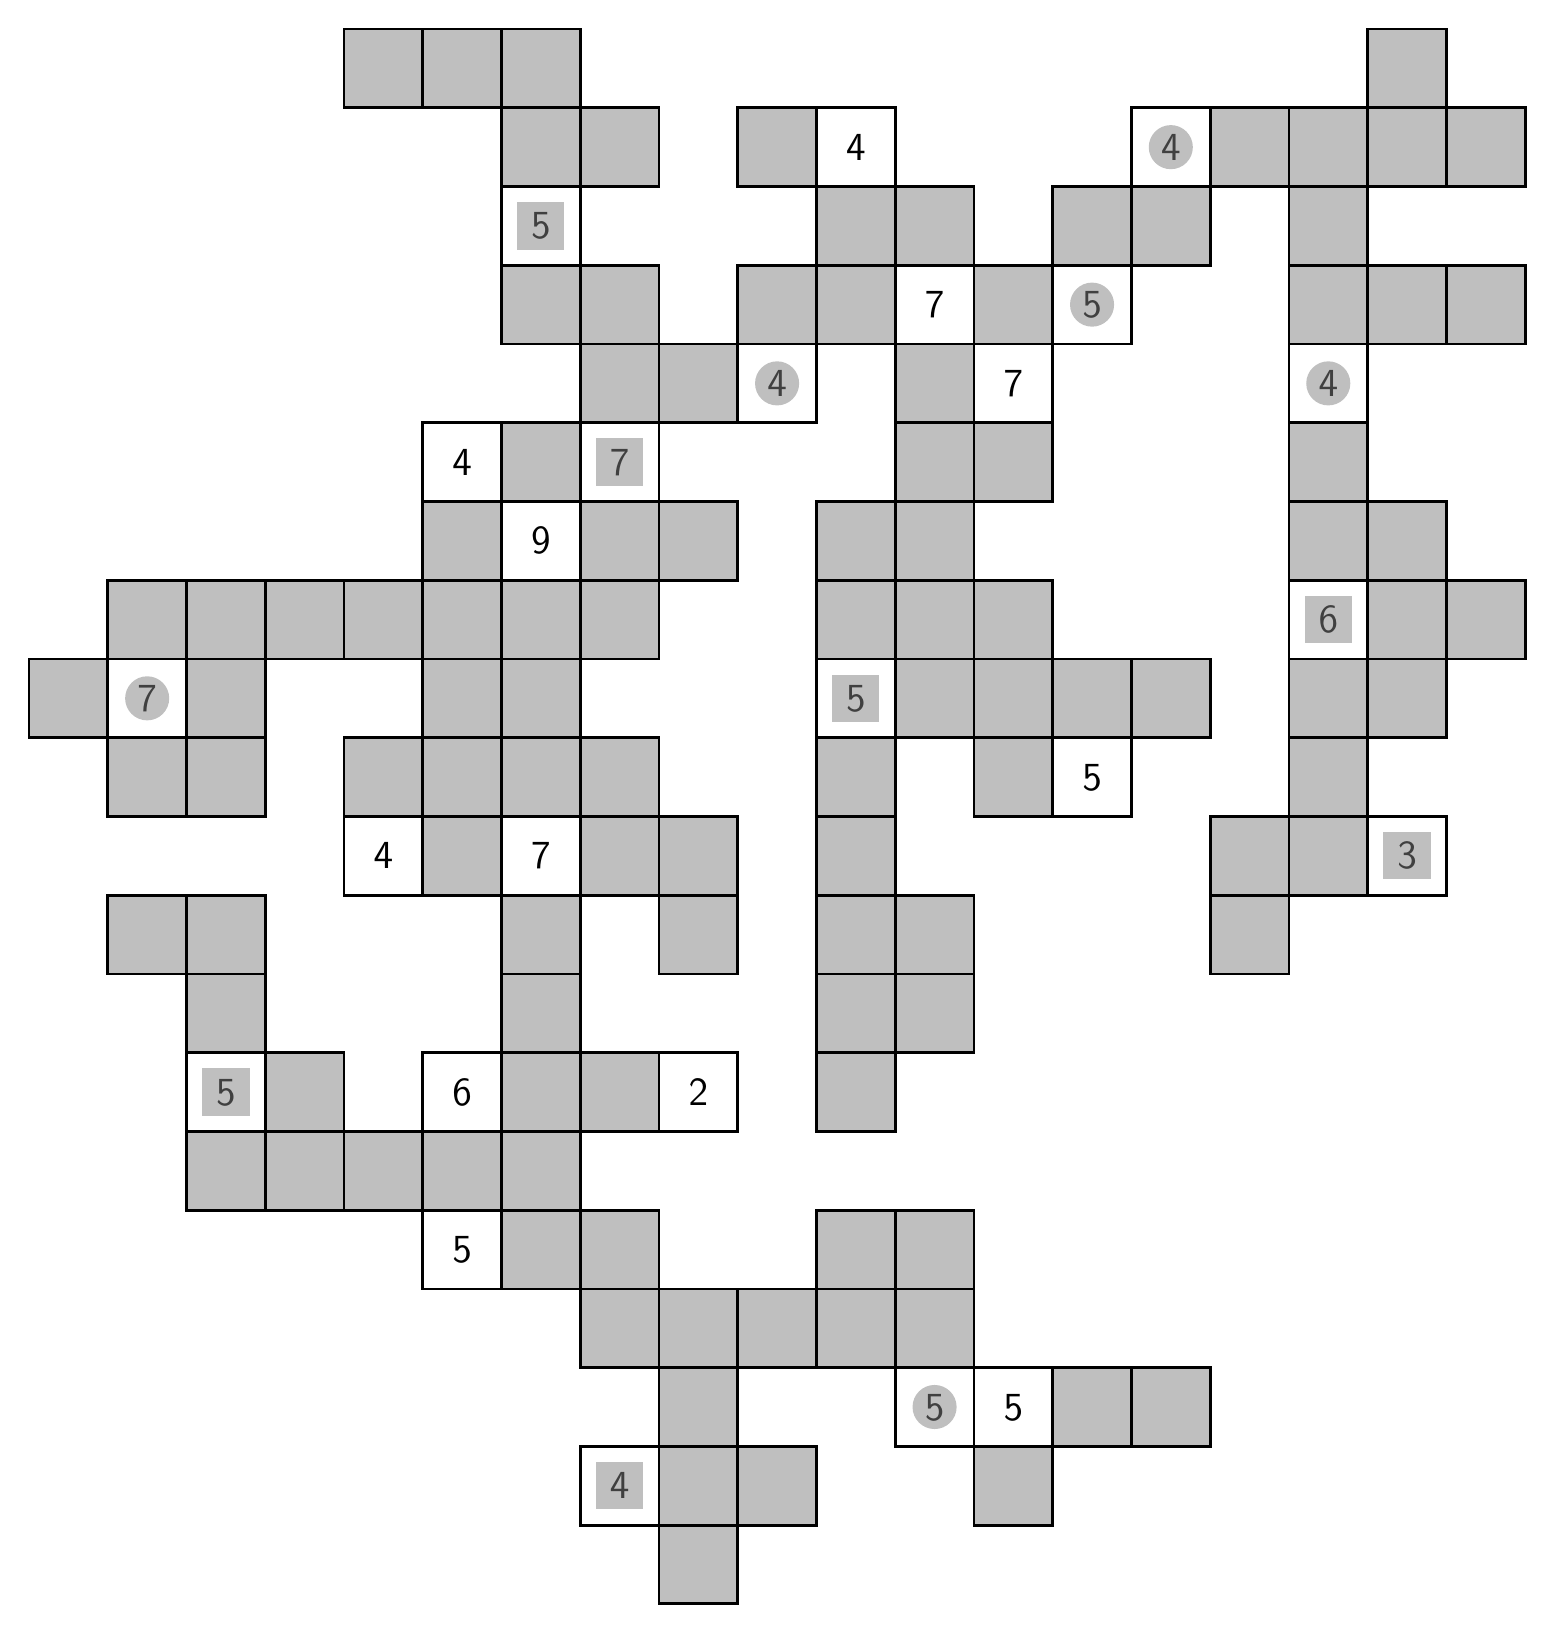
\begin{tikzpicture}\fill[gray, opacity = 0.5] (9, 0, 0)--++(1, 0, 0)--++(0, 1, 0)--++(-1, 0, 0)--cycle;
\draw[line width = 1pt] (9, 0, 0)--++(1, 0, 0)--++(0, 1, 0)--++(-1, 0, 0)--cycle;
\draw node at (8.5, 1.5, 0) {\Large $\mathsf{4}$};
\draw[line width = 1pt] (8, 1, 0)--++(1, 0, 0)--++(0, 1, 0)--++(-1, 0, 0)--cycle;
\fill[color = gray, opacity = 0.5] (8.2, 1.2) rectangle ++(0.6, 0.6);
\fill[gray, opacity = 0.5] (9, 1, 0)--++(1, 0, 0)--++(0, 1, 0)--++(-1, 0, 0)--cycle;
\draw[line width = 1pt] (9, 1, 0)--++(1, 0, 0)--++(0, 1, 0)--++(-1, 0, 0)--cycle;
\fill[gray, opacity = 0.5] (10, 1, 0)--++(1, 0, 0)--++(0, 1, 0)--++(-1, 0, 0)--cycle;
\draw[line width = 1pt] (10, 1, 0)--++(1, 0, 0)--++(0, 1, 0)--++(-1, 0, 0)--cycle;
\fill[gray, opacity = 0.5] (13, 1, 0)--++(1, 0, 0)--++(0, 1, 0)--++(-1, 0, 0)--cycle;
\draw[line width = 1pt] (13, 1, 0)--++(1, 0, 0)--++(0, 1, 0)--++(-1, 0, 0)--cycle;
\fill[gray, opacity = 0.5] (9, 2, 0)--++(1, 0, 0)--++(0, 1, 0)--++(-1, 0, 0)--cycle;
\draw[line width = 1pt] (9, 2, 0)--++(1, 0, 0)--++(0, 1, 0)--++(-1, 0, 0)--cycle;
\draw node at (12.5, 2.5, 0) {\Large $\mathsf{5}$};
\draw[line width = 1pt] (12, 2, 0)--++(1, 0, 0)--++(0, 1, 0)--++(-1, 0, 0)--cycle;
\fill[color = gray, opacity = 0.5] (12.5, 2.5, 0) circle (0.28);
\draw node at (13.5, 2.5, 0) {\Large $\mathsf{5}$};
\draw[line width = 1pt] (13, 2, 0)--++(1, 0, 0)--++(0, 1, 0)--++(-1, 0, 0)--cycle;
\fill[gray, opacity = 0.5] (14, 2, 0)--++(1, 0, 0)--++(0, 1, 0)--++(-1, 0, 0)--cycle;
\draw[line width = 1pt] (14, 2, 0)--++(1, 0, 0)--++(0, 1, 0)--++(-1, 0, 0)--cycle;
\fill[gray, opacity = 0.5] (15, 2, 0)--++(1, 0, 0)--++(0, 1, 0)--++(-1, 0, 0)--cycle;
\draw[line width = 1pt] (15, 2, 0)--++(1, 0, 0)--++(0, 1, 0)--++(-1, 0, 0)--cycle;
\fill[gray, opacity = 0.5] (8, 3, 0)--++(1, 0, 0)--++(0, 1, 0)--++(-1, 0, 0)--cycle;
\draw[line width = 1pt] (8, 3, 0)--++(1, 0, 0)--++(0, 1, 0)--++(-1, 0, 0)--cycle;
\fill[gray, opacity = 0.5] (9, 3, 0)--++(1, 0, 0)--++(0, 1, 0)--++(-1, 0, 0)--cycle;
\draw[line width = 1pt] (9, 3, 0)--++(1, 0, 0)--++(0, 1, 0)--++(-1, 0, 0)--cycle;
\fill[gray, opacity = 0.5] (10, 3, 0)--++(1, 0, 0)--++(0, 1, 0)--++(-1, 0, 0)--cycle;
\draw[line width = 1pt] (10, 3, 0)--++(1, 0, 0)--++(0, 1, 0)--++(-1, 0, 0)--cycle;
\fill[gray, opacity = 0.5] (11, 3, 0)--++(1, 0, 0)--++(0, 1, 0)--++(-1, 0, 0)--cycle;
\draw[line width = 1pt] (11, 3, 0)--++(1, 0, 0)--++(0, 1, 0)--++(-1, 0, 0)--cycle;
\fill[gray, opacity = 0.5] (12, 3, 0)--++(1, 0, 0)--++(0, 1, 0)--++(-1, 0, 0)--cycle;
\draw[line width = 1pt] (12, 3, 0)--++(1, 0, 0)--++(0, 1, 0)--++(-1, 0, 0)--cycle;
\draw node at (6.5, 4.5, 0) {\Large $\mathsf{5}$};
\draw[line width = 1pt] (6, 4, 0)--++(1, 0, 0)--++(0, 1, 0)--++(-1, 0, 0)--cycle;
\fill[gray, opacity = 0.5] (7, 4, 0)--++(1, 0, 0)--++(0, 1, 0)--++(-1, 0, 0)--cycle;
\draw[line width = 1pt] (7, 4, 0)--++(1, 0, 0)--++(0, 1, 0)--++(-1, 0, 0)--cycle;
\fill[gray, opacity = 0.5] (8, 4, 0)--++(1, 0, 0)--++(0, 1, 0)--++(-1, 0, 0)--cycle;
\draw[line width = 1pt] (8, 4, 0)--++(1, 0, 0)--++(0, 1, 0)--++(-1, 0, 0)--cycle;
\fill[gray, opacity = 0.5] (11, 4, 0)--++(1, 0, 0)--++(0, 1, 0)--++(-1, 0, 0)--cycle;
\draw[line width = 1pt] (11, 4, 0)--++(1, 0, 0)--++(0, 1, 0)--++(-1, 0, 0)--cycle;
\fill[gray, opacity = 0.5] (12, 4, 0)--++(1, 0, 0)--++(0, 1, 0)--++(-1, 0, 0)--cycle;
\draw[line width = 1pt] (12, 4, 0)--++(1, 0, 0)--++(0, 1, 0)--++(-1, 0, 0)--cycle;
\fill[gray, opacity = 0.5] (3, 5, 0)--++(1, 0, 0)--++(0, 1, 0)--++(-1, 0, 0)--cycle;
\draw[line width = 1pt] (3, 5, 0)--++(1, 0, 0)--++(0, 1, 0)--++(-1, 0, 0)--cycle;
\fill[gray, opacity = 0.5] (4, 5, 0)--++(1, 0, 0)--++(0, 1, 0)--++(-1, 0, 0)--cycle;
\draw[line width = 1pt] (4, 5, 0)--++(1, 0, 0)--++(0, 1, 0)--++(-1, 0, 0)--cycle;
\fill[gray, opacity = 0.5] (5, 5, 0)--++(1, 0, 0)--++(0, 1, 0)--++(-1, 0, 0)--cycle;
\draw[line width = 1pt] (5, 5, 0)--++(1, 0, 0)--++(0, 1, 0)--++(-1, 0, 0)--cycle;
\fill[gray, opacity = 0.5] (6, 5, 0)--++(1, 0, 0)--++(0, 1, 0)--++(-1, 0, 0)--cycle;
\draw[line width = 1pt] (6, 5, 0)--++(1, 0, 0)--++(0, 1, 0)--++(-1, 0, 0)--cycle;
\fill[gray, opacity = 0.5] (7, 5, 0)--++(1, 0, 0)--++(0, 1, 0)--++(-1, 0, 0)--cycle;
\draw[line width = 1pt] (7, 5, 0)--++(1, 0, 0)--++(0, 1, 0)--++(-1, 0, 0)--cycle;
\draw node at (3.5, 6.5, 0) {\Large $\mathsf{5}$};
\draw[line width = 1pt] (3, 6, 0)--++(1, 0, 0)--++(0, 1, 0)--++(-1, 0, 0)--cycle;
\fill[color = gray, opacity = 0.5] (3.2, 6.2) rectangle ++(0.6, 0.6);
\fill[gray, opacity = 0.5] (4, 6, 0)--++(1, 0, 0)--++(0, 1, 0)--++(-1, 0, 0)--cycle;
\draw[line width = 1pt] (4, 6, 0)--++(1, 0, 0)--++(0, 1, 0)--++(-1, 0, 0)--cycle;
\draw node at (6.5, 6.5, 0) {\Large $\mathsf{6}$};
\draw[line width = 1pt] (6, 6, 0)--++(1, 0, 0)--++(0, 1, 0)--++(-1, 0, 0)--cycle;
\fill[gray, opacity = 0.5] (7, 6, 0)--++(1, 0, 0)--++(0, 1, 0)--++(-1, 0, 0)--cycle;
\draw[line width = 1pt] (7, 6, 0)--++(1, 0, 0)--++(0, 1, 0)--++(-1, 0, 0)--cycle;
\fill[gray, opacity = 0.5] (8, 6, 0)--++(1, 0, 0)--++(0, 1, 0)--++(-1, 0, 0)--cycle;
\draw[line width = 1pt] (8, 6, 0)--++(1, 0, 0)--++(0, 1, 0)--++(-1, 0, 0)--cycle;
\draw node at (9.5, 6.5, 0) {\Large $\mathsf{2}$};
\draw[line width = 1pt] (9, 6, 0)--++(1, 0, 0)--++(0, 1, 0)--++(-1, 0, 0)--cycle;
\fill[gray, opacity = 0.5] (11, 6, 0)--++(1, 0, 0)--++(0, 1, 0)--++(-1, 0, 0)--cycle;
\draw[line width = 1pt] (11, 6, 0)--++(1, 0, 0)--++(0, 1, 0)--++(-1, 0, 0)--cycle;
\fill[gray, opacity = 0.5] (3, 7, 0)--++(1, 0, 0)--++(0, 1, 0)--++(-1, 0, 0)--cycle;
\draw[line width = 1pt] (3, 7, 0)--++(1, 0, 0)--++(0, 1, 0)--++(-1, 0, 0)--cycle;
\fill[gray, opacity = 0.5] (7, 7, 0)--++(1, 0, 0)--++(0, 1, 0)--++(-1, 0, 0)--cycle;
\draw[line width = 1pt] (7, 7, 0)--++(1, 0, 0)--++(0, 1, 0)--++(-1, 0, 0)--cycle;
\fill[gray, opacity = 0.5] (11, 7, 0)--++(1, 0, 0)--++(0, 1, 0)--++(-1, 0, 0)--cycle;
\draw[line width = 1pt] (11, 7, 0)--++(1, 0, 0)--++(0, 1, 0)--++(-1, 0, 0)--cycle;
\fill[gray, opacity = 0.5] (12, 7, 0)--++(1, 0, 0)--++(0, 1, 0)--++(-1, 0, 0)--cycle;
\draw[line width = 1pt] (12, 7, 0)--++(1, 0, 0)--++(0, 1, 0)--++(-1, 0, 0)--cycle;
\fill[gray, opacity = 0.5] (2, 8, 0)--++(1, 0, 0)--++(0, 1, 0)--++(-1, 0, 0)--cycle;
\draw[line width = 1pt] (2, 8, 0)--++(1, 0, 0)--++(0, 1, 0)--++(-1, 0, 0)--cycle;
\fill[gray, opacity = 0.5] (3, 8, 0)--++(1, 0, 0)--++(0, 1, 0)--++(-1, 0, 0)--cycle;
\draw[line width = 1pt] (3, 8, 0)--++(1, 0, 0)--++(0, 1, 0)--++(-1, 0, 0)--cycle;
\fill[gray, opacity = 0.5] (7, 8, 0)--++(1, 0, 0)--++(0, 1, 0)--++(-1, 0, 0)--cycle;
\draw[line width = 1pt] (7, 8, 0)--++(1, 0, 0)--++(0, 1, 0)--++(-1, 0, 0)--cycle;
\fill[gray, opacity = 0.5] (9, 8, 0)--++(1, 0, 0)--++(0, 1, 0)--++(-1, 0, 0)--cycle;
\draw[line width = 1pt] (9, 8, 0)--++(1, 0, 0)--++(0, 1, 0)--++(-1, 0, 0)--cycle;
\fill[gray, opacity = 0.5] (11, 8, 0)--++(1, 0, 0)--++(0, 1, 0)--++(-1, 0, 0)--cycle;
\draw[line width = 1pt] (11, 8, 0)--++(1, 0, 0)--++(0, 1, 0)--++(-1, 0, 0)--cycle;
\fill[gray, opacity = 0.5] (12, 8, 0)--++(1, 0, 0)--++(0, 1, 0)--++(-1, 0, 0)--cycle;
\draw[line width = 1pt] (12, 8, 0)--++(1, 0, 0)--++(0, 1, 0)--++(-1, 0, 0)--cycle;
\fill[gray, opacity = 0.5] (16, 8, 0)--++(1, 0, 0)--++(0, 1, 0)--++(-1, 0, 0)--cycle;
\draw[line width = 1pt] (16, 8, 0)--++(1, 0, 0)--++(0, 1, 0)--++(-1, 0, 0)--cycle;
\draw node at (5.5, 9.5, 0) {\Large $\mathsf{4}$};
\draw[line width = 1pt] (5, 9, 0)--++(1, 0, 0)--++(0, 1, 0)--++(-1, 0, 0)--cycle;
\fill[gray, opacity = 0.5] (6, 9, 0)--++(1, 0, 0)--++(0, 1, 0)--++(-1, 0, 0)--cycle;
\draw[line width = 1pt] (6, 9, 0)--++(1, 0, 0)--++(0, 1, 0)--++(-1, 0, 0)--cycle;
\draw node at (7.5, 9.5, 0) {\Large $\mathsf{7}$};
\draw[line width = 1pt] (7, 9, 0)--++(1, 0, 0)--++(0, 1, 0)--++(-1, 0, 0)--cycle;
\fill[gray, opacity = 0.5] (8, 9, 0)--++(1, 0, 0)--++(0, 1, 0)--++(-1, 0, 0)--cycle;
\draw[line width = 1pt] (8, 9, 0)--++(1, 0, 0)--++(0, 1, 0)--++(-1, 0, 0)--cycle;
\fill[gray, opacity = 0.5] (9, 9, 0)--++(1, 0, 0)--++(0, 1, 0)--++(-1, 0, 0)--cycle;
\draw[line width = 1pt] (9, 9, 0)--++(1, 0, 0)--++(0, 1, 0)--++(-1, 0, 0)--cycle;
\fill[gray, opacity = 0.5] (11, 9, 0)--++(1, 0, 0)--++(0, 1, 0)--++(-1, 0, 0)--cycle;
\draw[line width = 1pt] (11, 9, 0)--++(1, 0, 0)--++(0, 1, 0)--++(-1, 0, 0)--cycle;
\fill[gray, opacity = 0.5] (16, 9, 0)--++(1, 0, 0)--++(0, 1, 0)--++(-1, 0, 0)--cycle;
\draw[line width = 1pt] (16, 9, 0)--++(1, 0, 0)--++(0, 1, 0)--++(-1, 0, 0)--cycle;
\fill[gray, opacity = 0.5] (17, 9, 0)--++(1, 0, 0)--++(0, 1, 0)--++(-1, 0, 0)--cycle;
\draw[line width = 1pt] (17, 9, 0)--++(1, 0, 0)--++(0, 1, 0)--++(-1, 0, 0)--cycle;
\draw node at (18.5, 9.5, 0) {\Large $\mathsf{3}$};
\draw[line width = 1pt] (18, 9, 0)--++(1, 0, 0)--++(0, 1, 0)--++(-1, 0, 0)--cycle;
\fill[color = gray, opacity = 0.5] (18.2, 9.2) rectangle ++(0.6, 0.6);
\fill[gray, opacity = 0.5] (2, 10, 0)--++(1, 0, 0)--++(0, 1, 0)--++(-1, 0, 0)--cycle;
\draw[line width = 1pt] (2, 10, 0)--++(1, 0, 0)--++(0, 1, 0)--++(-1, 0, 0)--cycle;
\fill[gray, opacity = 0.5] (3, 10, 0)--++(1, 0, 0)--++(0, 1, 0)--++(-1, 0, 0)--cycle;
\draw[line width = 1pt] (3, 10, 0)--++(1, 0, 0)--++(0, 1, 0)--++(-1, 0, 0)--cycle;
\fill[gray, opacity = 0.5] (5, 10, 0)--++(1, 0, 0)--++(0, 1, 0)--++(-1, 0, 0)--cycle;
\draw[line width = 1pt] (5, 10, 0)--++(1, 0, 0)--++(0, 1, 0)--++(-1, 0, 0)--cycle;
\fill[gray, opacity = 0.5] (6, 10, 0)--++(1, 0, 0)--++(0, 1, 0)--++(-1, 0, 0)--cycle;
\draw[line width = 1pt] (6, 10, 0)--++(1, 0, 0)--++(0, 1, 0)--++(-1, 0, 0)--cycle;
\fill[gray, opacity = 0.5] (7, 10, 0)--++(1, 0, 0)--++(0, 1, 0)--++(-1, 0, 0)--cycle;
\draw[line width = 1pt] (7, 10, 0)--++(1, 0, 0)--++(0, 1, 0)--++(-1, 0, 0)--cycle;
\fill[gray, opacity = 0.5] (8, 10, 0)--++(1, 0, 0)--++(0, 1, 0)--++(-1, 0, 0)--cycle;
\draw[line width = 1pt] (8, 10, 0)--++(1, 0, 0)--++(0, 1, 0)--++(-1, 0, 0)--cycle;
\fill[gray, opacity = 0.5] (11, 10, 0)--++(1, 0, 0)--++(0, 1, 0)--++(-1, 0, 0)--cycle;
\draw[line width = 1pt] (11, 10, 0)--++(1, 0, 0)--++(0, 1, 0)--++(-1, 0, 0)--cycle;
\fill[gray, opacity = 0.5] (13, 10, 0)--++(1, 0, 0)--++(0, 1, 0)--++(-1, 0, 0)--cycle;
\draw[line width = 1pt] (13, 10, 0)--++(1, 0, 0)--++(0, 1, 0)--++(-1, 0, 0)--cycle;
\draw node at (14.5, 10.5, 0) {\Large $\mathsf{5}$};
\draw[line width = 1pt] (14, 10, 0)--++(1, 0, 0)--++(0, 1, 0)--++(-1, 0, 0)--cycle;
\fill[gray, opacity = 0.5] (17, 10, 0)--++(1, 0, 0)--++(0, 1, 0)--++(-1, 0, 0)--cycle;
\draw[line width = 1pt] (17, 10, 0)--++(1, 0, 0)--++(0, 1, 0)--++(-1, 0, 0)--cycle;
\fill[gray, opacity = 0.5] (1, 11, 0)--++(1, 0, 0)--++(0, 1, 0)--++(-1, 0, 0)--cycle;
\draw[line width = 1pt] (1, 11, 0)--++(1, 0, 0)--++(0, 1, 0)--++(-1, 0, 0)--cycle;
\draw node at (2.5, 11.5, 0) {\Large $\mathsf{7}$};
\draw[line width = 1pt] (2, 11, 0)--++(1, 0, 0)--++(0, 1, 0)--++(-1, 0, 0)--cycle;
\fill[color = gray, opacity = 0.5] (2.5, 11.5, 0) circle (0.28);
\fill[gray, opacity = 0.5] (3, 11, 0)--++(1, 0, 0)--++(0, 1, 0)--++(-1, 0, 0)--cycle;
\draw[line width = 1pt] (3, 11, 0)--++(1, 0, 0)--++(0, 1, 0)--++(-1, 0, 0)--cycle;
\fill[gray, opacity = 0.5] (6, 11, 0)--++(1, 0, 0)--++(0, 1, 0)--++(-1, 0, 0)--cycle;
\draw[line width = 1pt] (6, 11, 0)--++(1, 0, 0)--++(0, 1, 0)--++(-1, 0, 0)--cycle;
\fill[gray, opacity = 0.5] (7, 11, 0)--++(1, 0, 0)--++(0, 1, 0)--++(-1, 0, 0)--cycle;
\draw[line width = 1pt] (7, 11, 0)--++(1, 0, 0)--++(0, 1, 0)--++(-1, 0, 0)--cycle;
\draw node at (11.5, 11.5, 0) {\Large $\mathsf{5}$};
\draw[line width = 1pt] (11, 11, 0)--++(1, 0, 0)--++(0, 1, 0)--++(-1, 0, 0)--cycle;
\fill[color = gray, opacity = 0.5] (11.2, 11.2) rectangle ++(0.6, 0.6);
\fill[gray, opacity = 0.5] (12, 11, 0)--++(1, 0, 0)--++(0, 1, 0)--++(-1, 0, 0)--cycle;
\draw[line width = 1pt] (12, 11, 0)--++(1, 0, 0)--++(0, 1, 0)--++(-1, 0, 0)--cycle;
\fill[gray, opacity = 0.5] (13, 11, 0)--++(1, 0, 0)--++(0, 1, 0)--++(-1, 0, 0)--cycle;
\draw[line width = 1pt] (13, 11, 0)--++(1, 0, 0)--++(0, 1, 0)--++(-1, 0, 0)--cycle;
\fill[gray, opacity = 0.5] (14, 11, 0)--++(1, 0, 0)--++(0, 1, 0)--++(-1, 0, 0)--cycle;
\draw[line width = 1pt] (14, 11, 0)--++(1, 0, 0)--++(0, 1, 0)--++(-1, 0, 0)--cycle;
\fill[gray, opacity = 0.5] (15, 11, 0)--++(1, 0, 0)--++(0, 1, 0)--++(-1, 0, 0)--cycle;
\draw[line width = 1pt] (15, 11, 0)--++(1, 0, 0)--++(0, 1, 0)--++(-1, 0, 0)--cycle;
\fill[gray, opacity = 0.5] (17, 11, 0)--++(1, 0, 0)--++(0, 1, 0)--++(-1, 0, 0)--cycle;
\draw[line width = 1pt] (17, 11, 0)--++(1, 0, 0)--++(0, 1, 0)--++(-1, 0, 0)--cycle;
\fill[gray, opacity = 0.5] (18, 11, 0)--++(1, 0, 0)--++(0, 1, 0)--++(-1, 0, 0)--cycle;
\draw[line width = 1pt] (18, 11, 0)--++(1, 0, 0)--++(0, 1, 0)--++(-1, 0, 0)--cycle;
\fill[gray, opacity = 0.5] (2, 12, 0)--++(1, 0, 0)--++(0, 1, 0)--++(-1, 0, 0)--cycle;
\draw[line width = 1pt] (2, 12, 0)--++(1, 0, 0)--++(0, 1, 0)--++(-1, 0, 0)--cycle;
\fill[gray, opacity = 0.5] (3, 12, 0)--++(1, 0, 0)--++(0, 1, 0)--++(-1, 0, 0)--cycle;
\draw[line width = 1pt] (3, 12, 0)--++(1, 0, 0)--++(0, 1, 0)--++(-1, 0, 0)--cycle;
\fill[gray, opacity = 0.5] (4, 12, 0)--++(1, 0, 0)--++(0, 1, 0)--++(-1, 0, 0)--cycle;
\draw[line width = 1pt] (4, 12, 0)--++(1, 0, 0)--++(0, 1, 0)--++(-1, 0, 0)--cycle;
\fill[gray, opacity = 0.5] (5, 12, 0)--++(1, 0, 0)--++(0, 1, 0)--++(-1, 0, 0)--cycle;
\draw[line width = 1pt] (5, 12, 0)--++(1, 0, 0)--++(0, 1, 0)--++(-1, 0, 0)--cycle;
\fill[gray, opacity = 0.5] (6, 12, 0)--++(1, 0, 0)--++(0, 1, 0)--++(-1, 0, 0)--cycle;
\draw[line width = 1pt] (6, 12, 0)--++(1, 0, 0)--++(0, 1, 0)--++(-1, 0, 0)--cycle;
\fill[gray, opacity = 0.5] (7, 12, 0)--++(1, 0, 0)--++(0, 1, 0)--++(-1, 0, 0)--cycle;
\draw[line width = 1pt] (7, 12, 0)--++(1, 0, 0)--++(0, 1, 0)--++(-1, 0, 0)--cycle;
\fill[gray, opacity = 0.5] (8, 12, 0)--++(1, 0, 0)--++(0, 1, 0)--++(-1, 0, 0)--cycle;
\draw[line width = 1pt] (8, 12, 0)--++(1, 0, 0)--++(0, 1, 0)--++(-1, 0, 0)--cycle;
\fill[gray, opacity = 0.5] (11, 12, 0)--++(1, 0, 0)--++(0, 1, 0)--++(-1, 0, 0)--cycle;
\draw[line width = 1pt] (11, 12, 0)--++(1, 0, 0)--++(0, 1, 0)--++(-1, 0, 0)--cycle;
\fill[gray, opacity = 0.5] (12, 12, 0)--++(1, 0, 0)--++(0, 1, 0)--++(-1, 0, 0)--cycle;
\draw[line width = 1pt] (12, 12, 0)--++(1, 0, 0)--++(0, 1, 0)--++(-1, 0, 0)--cycle;
\fill[gray, opacity = 0.5] (13, 12, 0)--++(1, 0, 0)--++(0, 1, 0)--++(-1, 0, 0)--cycle;
\draw[line width = 1pt] (13, 12, 0)--++(1, 0, 0)--++(0, 1, 0)--++(-1, 0, 0)--cycle;
\draw node at (17.5, 12.5, 0) {\Large $\mathsf{6}$};
\draw[line width = 1pt] (17, 12, 0)--++(1, 0, 0)--++(0, 1, 0)--++(-1, 0, 0)--cycle;
\fill[color = gray, opacity = 0.5] (17.2, 12.2) rectangle ++(0.6, 0.6);
\fill[gray, opacity = 0.5] (18, 12, 0)--++(1, 0, 0)--++(0, 1, 0)--++(-1, 0, 0)--cycle;
\draw[line width = 1pt] (18, 12, 0)--++(1, 0, 0)--++(0, 1, 0)--++(-1, 0, 0)--cycle;
\fill[gray, opacity = 0.5] (19, 12, 0)--++(1, 0, 0)--++(0, 1, 0)--++(-1, 0, 0)--cycle;
\draw[line width = 1pt] (19, 12, 0)--++(1, 0, 0)--++(0, 1, 0)--++(-1, 0, 0)--cycle;
\fill[gray, opacity = 0.5] (6, 13, 0)--++(1, 0, 0)--++(0, 1, 0)--++(-1, 0, 0)--cycle;
\draw[line width = 1pt] (6, 13, 0)--++(1, 0, 0)--++(0, 1, 0)--++(-1, 0, 0)--cycle;
\draw node at (7.5, 13.5, 0) {\Large $\mathsf{9}$};
\draw[line width = 1pt] (7, 13, 0)--++(1, 0, 0)--++(0, 1, 0)--++(-1, 0, 0)--cycle;
\fill[gray, opacity = 0.5] (8, 13, 0)--++(1, 0, 0)--++(0, 1, 0)--++(-1, 0, 0)--cycle;
\draw[line width = 1pt] (8, 13, 0)--++(1, 0, 0)--++(0, 1, 0)--++(-1, 0, 0)--cycle;
\fill[gray, opacity = 0.5] (9, 13, 0)--++(1, 0, 0)--++(0, 1, 0)--++(-1, 0, 0)--cycle;
\draw[line width = 1pt] (9, 13, 0)--++(1, 0, 0)--++(0, 1, 0)--++(-1, 0, 0)--cycle;
\fill[gray, opacity = 0.5] (11, 13, 0)--++(1, 0, 0)--++(0, 1, 0)--++(-1, 0, 0)--cycle;
\draw[line width = 1pt] (11, 13, 0)--++(1, 0, 0)--++(0, 1, 0)--++(-1, 0, 0)--cycle;
\fill[gray, opacity = 0.5] (12, 13, 0)--++(1, 0, 0)--++(0, 1, 0)--++(-1, 0, 0)--cycle;
\draw[line width = 1pt] (12, 13, 0)--++(1, 0, 0)--++(0, 1, 0)--++(-1, 0, 0)--cycle;
\fill[gray, opacity = 0.5] (17, 13, 0)--++(1, 0, 0)--++(0, 1, 0)--++(-1, 0, 0)--cycle;
\draw[line width = 1pt] (17, 13, 0)--++(1, 0, 0)--++(0, 1, 0)--++(-1, 0, 0)--cycle;
\fill[gray, opacity = 0.5] (18, 13, 0)--++(1, 0, 0)--++(0, 1, 0)--++(-1, 0, 0)--cycle;
\draw[line width = 1pt] (18, 13, 0)--++(1, 0, 0)--++(0, 1, 0)--++(-1, 0, 0)--cycle;
\draw node at (6.5, 14.5, 0) {\Large $\mathsf{4}$};
\draw[line width = 1pt] (6, 14, 0)--++(1, 0, 0)--++(0, 1, 0)--++(-1, 0, 0)--cycle;
\fill[gray, opacity = 0.5] (7, 14, 0)--++(1, 0, 0)--++(0, 1, 0)--++(-1, 0, 0)--cycle;
\draw[line width = 1pt] (7, 14, 0)--++(1, 0, 0)--++(0, 1, 0)--++(-1, 0, 0)--cycle;
\draw node at (8.5, 14.5, 0) {\Large $\mathsf{7}$};
\draw[line width = 1pt] (8, 14, 0)--++(1, 0, 0)--++(0, 1, 0)--++(-1, 0, 0)--cycle;
\fill[color = gray, opacity = 0.5] (8.2, 14.2) rectangle ++(0.6, 0.6);
\fill[gray, opacity = 0.5] (12, 14, 0)--++(1, 0, 0)--++(0, 1, 0)--++(-1, 0, 0)--cycle;
\draw[line width = 1pt] (12, 14, 0)--++(1, 0, 0)--++(0, 1, 0)--++(-1, 0, 0)--cycle;
\fill[gray, opacity = 0.5] (13, 14, 0)--++(1, 0, 0)--++(0, 1, 0)--++(-1, 0, 0)--cycle;
\draw[line width = 1pt] (13, 14, 0)--++(1, 0, 0)--++(0, 1, 0)--++(-1, 0, 0)--cycle;
\fill[gray, opacity = 0.5] (17, 14, 0)--++(1, 0, 0)--++(0, 1, 0)--++(-1, 0, 0)--cycle;
\draw[line width = 1pt] (17, 14, 0)--++(1, 0, 0)--++(0, 1, 0)--++(-1, 0, 0)--cycle;
\fill[gray, opacity = 0.5] (8, 15, 0)--++(1, 0, 0)--++(0, 1, 0)--++(-1, 0, 0)--cycle;
\draw[line width = 1pt] (8, 15, 0)--++(1, 0, 0)--++(0, 1, 0)--++(-1, 0, 0)--cycle;
\fill[gray, opacity = 0.5] (9, 15, 0)--++(1, 0, 0)--++(0, 1, 0)--++(-1, 0, 0)--cycle;
\draw[line width = 1pt] (9, 15, 0)--++(1, 0, 0)--++(0, 1, 0)--++(-1, 0, 0)--cycle;
\draw node at (10.5, 15.5, 0) {\Large $\mathsf{4}$};
\draw[line width = 1pt] (10, 15, 0)--++(1, 0, 0)--++(0, 1, 0)--++(-1, 0, 0)--cycle;
\fill[color = gray, opacity = 0.5] (10.5, 15.5, 0) circle (0.28);
\fill[gray, opacity = 0.5] (12, 15, 0)--++(1, 0, 0)--++(0, 1, 0)--++(-1, 0, 0)--cycle;
\draw[line width = 1pt] (12, 15, 0)--++(1, 0, 0)--++(0, 1, 0)--++(-1, 0, 0)--cycle;
\draw node at (13.5, 15.5, 0) {\Large $\mathsf{7}$};
\draw[line width = 1pt] (13, 15, 0)--++(1, 0, 0)--++(0, 1, 0)--++(-1, 0, 0)--cycle;
\draw node at (17.5, 15.5, 0) {\Large $\mathsf{4}$};
\draw[line width = 1pt] (17, 15, 0)--++(1, 0, 0)--++(0, 1, 0)--++(-1, 0, 0)--cycle;
\fill[color = gray, opacity = 0.5] (17.5, 15.5, 0) circle (0.28);
\fill[gray, opacity = 0.5] (7, 16, 0)--++(1, 0, 0)--++(0, 1, 0)--++(-1, 0, 0)--cycle;
\draw[line width = 1pt] (7, 16, 0)--++(1, 0, 0)--++(0, 1, 0)--++(-1, 0, 0)--cycle;
\fill[gray, opacity = 0.5] (8, 16, 0)--++(1, 0, 0)--++(0, 1, 0)--++(-1, 0, 0)--cycle;
\draw[line width = 1pt] (8, 16, 0)--++(1, 0, 0)--++(0, 1, 0)--++(-1, 0, 0)--cycle;
\fill[gray, opacity = 0.5] (10, 16, 0)--++(1, 0, 0)--++(0, 1, 0)--++(-1, 0, 0)--cycle;
\draw[line width = 1pt] (10, 16, 0)--++(1, 0, 0)--++(0, 1, 0)--++(-1, 0, 0)--cycle;
\fill[gray, opacity = 0.5] (11, 16, 0)--++(1, 0, 0)--++(0, 1, 0)--++(-1, 0, 0)--cycle;
\draw[line width = 1pt] (11, 16, 0)--++(1, 0, 0)--++(0, 1, 0)--++(-1, 0, 0)--cycle;
\draw node at (12.5, 16.5, 0) {\Large $\mathsf{7}$};
\draw[line width = 1pt] (12, 16, 0)--++(1, 0, 0)--++(0, 1, 0)--++(-1, 0, 0)--cycle;
\fill[gray, opacity = 0.5] (13, 16, 0)--++(1, 0, 0)--++(0, 1, 0)--++(-1, 0, 0)--cycle;
\draw[line width = 1pt] (13, 16, 0)--++(1, 0, 0)--++(0, 1, 0)--++(-1, 0, 0)--cycle;
\draw node at (14.5, 16.5, 0) {\Large $\mathsf{5}$};
\draw[line width = 1pt] (14, 16, 0)--++(1, 0, 0)--++(0, 1, 0)--++(-1, 0, 0)--cycle;
\fill[color = gray, opacity = 0.5] (14.5, 16.5, 0) circle (0.28);
\fill[gray, opacity = 0.5] (17, 16, 0)--++(1, 0, 0)--++(0, 1, 0)--++(-1, 0, 0)--cycle;
\draw[line width = 1pt] (17, 16, 0)--++(1, 0, 0)--++(0, 1, 0)--++(-1, 0, 0)--cycle;
\fill[gray, opacity = 0.5] (18, 16, 0)--++(1, 0, 0)--++(0, 1, 0)--++(-1, 0, 0)--cycle;
\draw[line width = 1pt] (18, 16, 0)--++(1, 0, 0)--++(0, 1, 0)--++(-1, 0, 0)--cycle;
\fill[gray, opacity = 0.5] (19, 16, 0)--++(1, 0, 0)--++(0, 1, 0)--++(-1, 0, 0)--cycle;
\draw[line width = 1pt] (19, 16, 0)--++(1, 0, 0)--++(0, 1, 0)--++(-1, 0, 0)--cycle;
\draw node at (7.5, 17.5, 0) {\Large $\mathsf{5}$};
\draw[line width = 1pt] (7, 17, 0)--++(1, 0, 0)--++(0, 1, 0)--++(-1, 0, 0)--cycle;
\fill[color = gray, opacity = 0.5] (7.2, 17.2) rectangle ++(0.6, 0.6);
\fill[gray, opacity = 0.5] (11, 17, 0)--++(1, 0, 0)--++(0, 1, 0)--++(-1, 0, 0)--cycle;
\draw[line width = 1pt] (11, 17, 0)--++(1, 0, 0)--++(0, 1, 0)--++(-1, 0, 0)--cycle;
\fill[gray, opacity = 0.5] (12, 17, 0)--++(1, 0, 0)--++(0, 1, 0)--++(-1, 0, 0)--cycle;
\draw[line width = 1pt] (12, 17, 0)--++(1, 0, 0)--++(0, 1, 0)--++(-1, 0, 0)--cycle;
\fill[gray, opacity = 0.5] (14, 17, 0)--++(1, 0, 0)--++(0, 1, 0)--++(-1, 0, 0)--cycle;
\draw[line width = 1pt] (14, 17, 0)--++(1, 0, 0)--++(0, 1, 0)--++(-1, 0, 0)--cycle;
\fill[gray, opacity = 0.5] (15, 17, 0)--++(1, 0, 0)--++(0, 1, 0)--++(-1, 0, 0)--cycle;
\draw[line width = 1pt] (15, 17, 0)--++(1, 0, 0)--++(0, 1, 0)--++(-1, 0, 0)--cycle;
\fill[gray, opacity = 0.5] (17, 17, 0)--++(1, 0, 0)--++(0, 1, 0)--++(-1, 0, 0)--cycle;
\draw[line width = 1pt] (17, 17, 0)--++(1, 0, 0)--++(0, 1, 0)--++(-1, 0, 0)--cycle;
\fill[gray, opacity = 0.5] (7, 18, 0)--++(1, 0, 0)--++(0, 1, 0)--++(-1, 0, 0)--cycle;
\draw[line width = 1pt] (7, 18, 0)--++(1, 0, 0)--++(0, 1, 0)--++(-1, 0, 0)--cycle;
\fill[gray, opacity = 0.5] (8, 18, 0)--++(1, 0, 0)--++(0, 1, 0)--++(-1, 0, 0)--cycle;
\draw[line width = 1pt] (8, 18, 0)--++(1, 0, 0)--++(0, 1, 0)--++(-1, 0, 0)--cycle;
\fill[gray, opacity = 0.5] (10, 18, 0)--++(1, 0, 0)--++(0, 1, 0)--++(-1, 0, 0)--cycle;
\draw[line width = 1pt] (10, 18, 0)--++(1, 0, 0)--++(0, 1, 0)--++(-1, 0, 0)--cycle;
\draw node at (11.5, 18.5, 0) {\Large $\mathsf{4}$};
\draw[line width = 1pt] (11, 18, 0)--++(1, 0, 0)--++(0, 1, 0)--++(-1, 0, 0)--cycle;
\draw node at (15.5, 18.5, 0) {\Large $\mathsf{4}$};
\draw[line width = 1pt] (15, 18, 0)--++(1, 0, 0)--++(0, 1, 0)--++(-1, 0, 0)--cycle;
\fill[color = gray, opacity = 0.5] (15.5, 18.5, 0) circle (0.28);
\fill[gray, opacity = 0.5] (16, 18, 0)--++(1, 0, 0)--++(0, 1, 0)--++(-1, 0, 0)--cycle;
\draw[line width = 1pt] (16, 18, 0)--++(1, 0, 0)--++(0, 1, 0)--++(-1, 0, 0)--cycle;
\fill[gray, opacity = 0.5] (17, 18, 0)--++(1, 0, 0)--++(0, 1, 0)--++(-1, 0, 0)--cycle;
\draw[line width = 1pt] (17, 18, 0)--++(1, 0, 0)--++(0, 1, 0)--++(-1, 0, 0)--cycle;
\fill[gray, opacity = 0.5] (18, 18, 0)--++(1, 0, 0)--++(0, 1, 0)--++(-1, 0, 0)--cycle;
\draw[line width = 1pt] (18, 18, 0)--++(1, 0, 0)--++(0, 1, 0)--++(-1, 0, 0)--cycle;
\fill[gray, opacity = 0.5] (19, 18, 0)--++(1, 0, 0)--++(0, 1, 0)--++(-1, 0, 0)--cycle;
\draw[line width = 1pt] (19, 18, 0)--++(1, 0, 0)--++(0, 1, 0)--++(-1, 0, 0)--cycle;
\fill[gray, opacity = 0.5] (5, 19, 0)--++(1, 0, 0)--++(0, 1, 0)--++(-1, 0, 0)--cycle;
\draw[line width = 1pt] (5, 19, 0)--++(1, 0, 0)--++(0, 1, 0)--++(-1, 0, 0)--cycle;
\fill[gray, opacity = 0.5] (6, 19, 0)--++(1, 0, 0)--++(0, 1, 0)--++(-1, 0, 0)--cycle;
\draw[line width = 1pt] (6, 19, 0)--++(1, 0, 0)--++(0, 1, 0)--++(-1, 0, 0)--cycle;
\fill[gray, opacity = 0.5] (7, 19, 0)--++(1, 0, 0)--++(0, 1, 0)--++(-1, 0, 0)--cycle;
\draw[line width = 1pt] (7, 19, 0)--++(1, 0, 0)--++(0, 1, 0)--++(-1, 0, 0)--cycle;
\fill[gray, opacity = 0.5] (18, 19, 0)--++(1, 0, 0)--++(0, 1, 0)--++(-1, 0, 0)--cycle;
\draw[line width = 1pt] (18, 19, 0)--++(1, 0, 0)--++(0, 1, 0)--++(-1, 0, 0)--cycle;
\end{tikzpicture}}\]
\[\resizebox{30pc}{!}{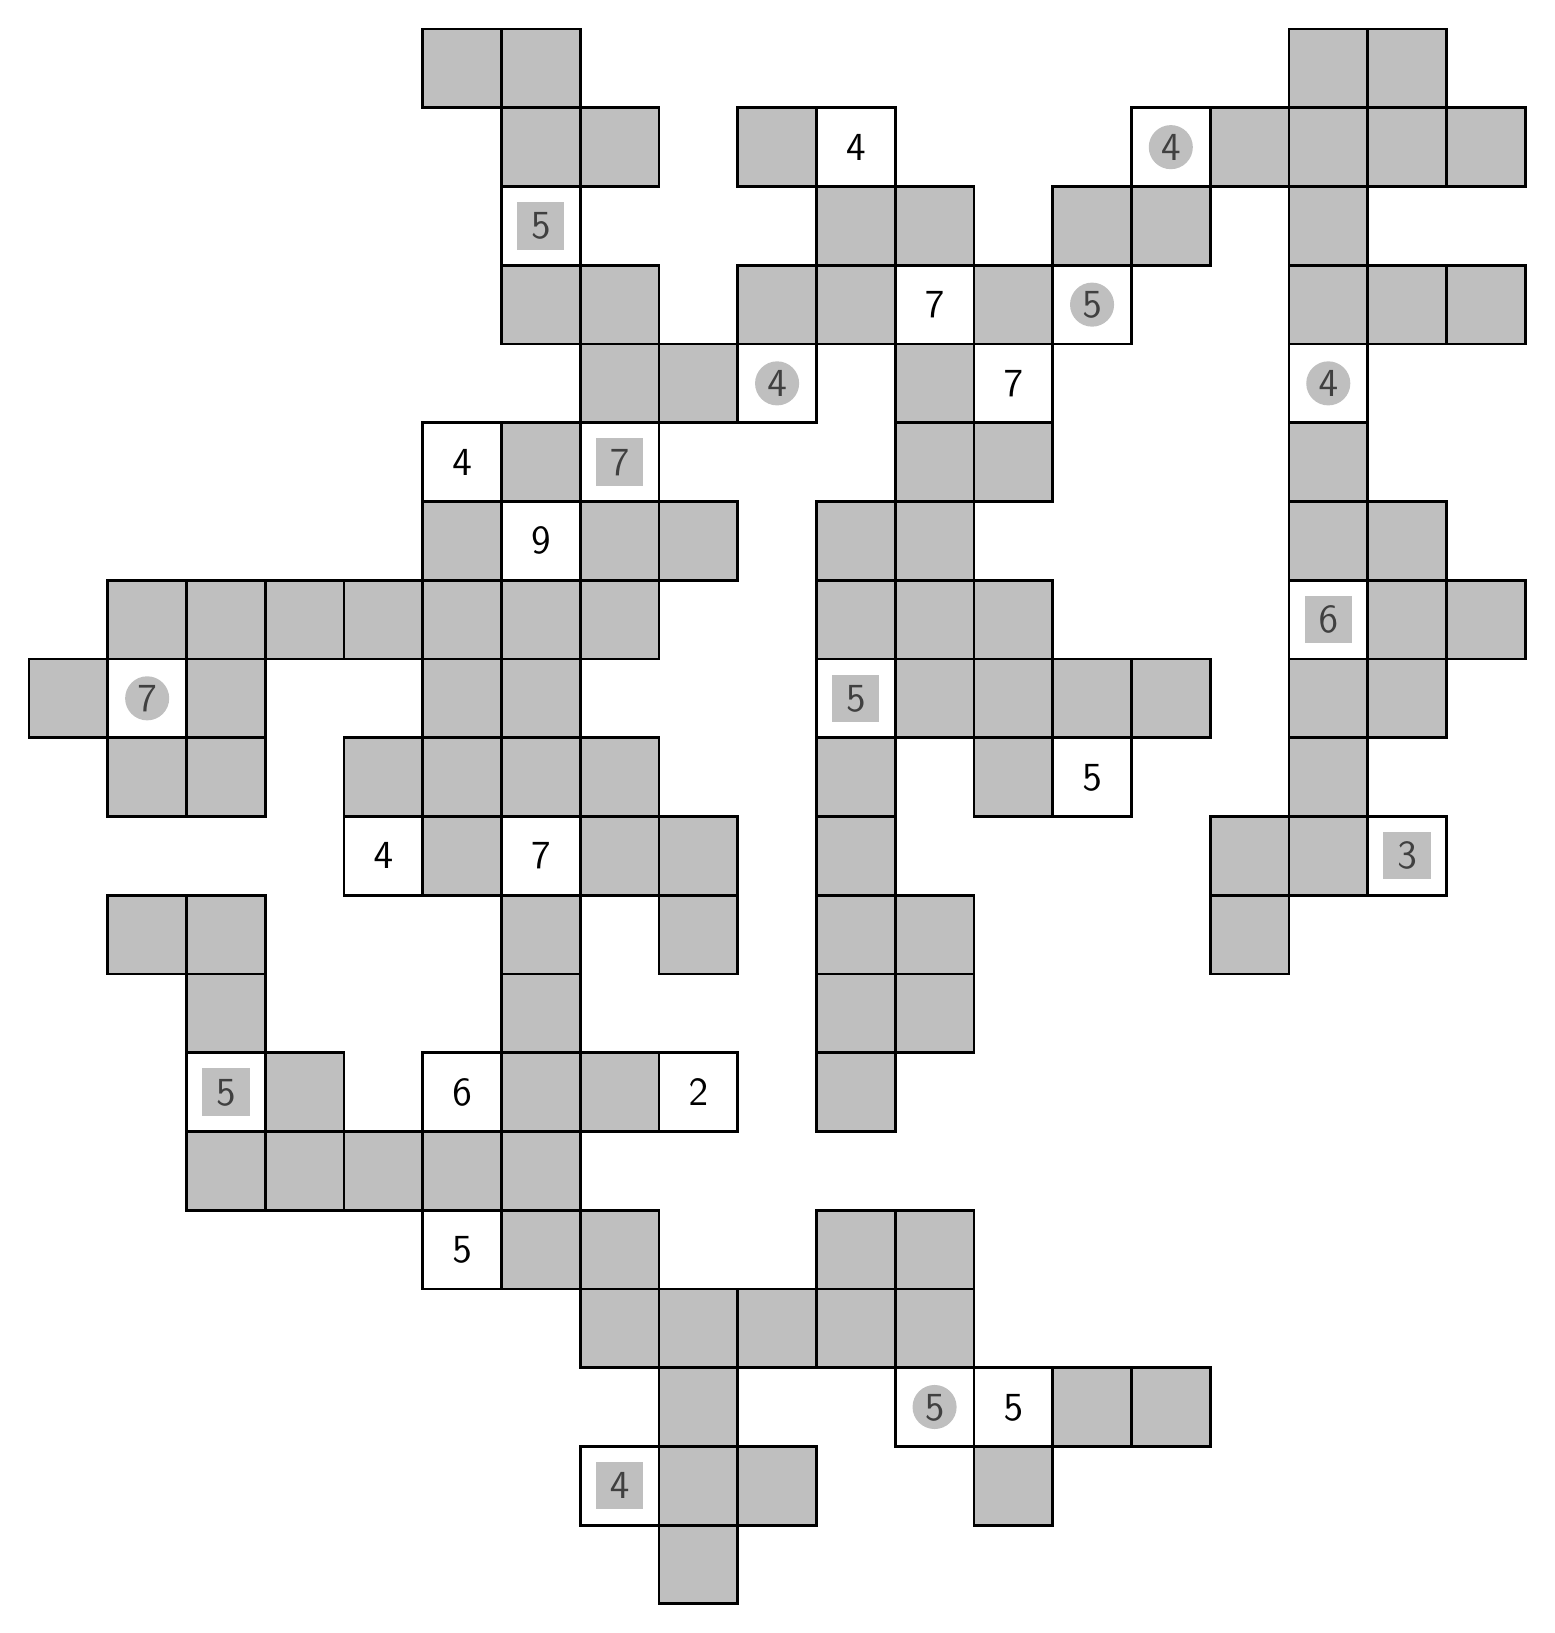
\begin{tikzpicture}\fill[gray, opacity = 0.5] (9, 0, 0)--++(1, 0, 0)--++(0, 1, 0)--++(-1, 0, 0)--cycle;
\draw[line width = 1pt] (9, 0, 0)--++(1, 0, 0)--++(0, 1, 0)--++(-1, 0, 0)--cycle;
\draw node at (8.5, 1.5, 0) {\Large $\mathsf{4}$};
\draw[line width = 1pt] (8, 1, 0)--++(1, 0, 0)--++(0, 1, 0)--++(-1, 0, 0)--cycle;
\fill[color = gray, opacity = 0.5] (8.2, 1.2) rectangle ++(0.6, 0.6);
\fill[gray, opacity = 0.5] (9, 1, 0)--++(1, 0, 0)--++(0, 1, 0)--++(-1, 0, 0)--cycle;
\draw[line width = 1pt] (9, 1, 0)--++(1, 0, 0)--++(0, 1, 0)--++(-1, 0, 0)--cycle;
\fill[gray, opacity = 0.5] (10, 1, 0)--++(1, 0, 0)--++(0, 1, 0)--++(-1, 0, 0)--cycle;
\draw[line width = 1pt] (10, 1, 0)--++(1, 0, 0)--++(0, 1, 0)--++(-1, 0, 0)--cycle;
\fill[gray, opacity = 0.5] (13, 1, 0)--++(1, 0, 0)--++(0, 1, 0)--++(-1, 0, 0)--cycle;
\draw[line width = 1pt] (13, 1, 0)--++(1, 0, 0)--++(0, 1, 0)--++(-1, 0, 0)--cycle;
\fill[gray, opacity = 0.5] (9, 2, 0)--++(1, 0, 0)--++(0, 1, 0)--++(-1, 0, 0)--cycle;
\draw[line width = 1pt] (9, 2, 0)--++(1, 0, 0)--++(0, 1, 0)--++(-1, 0, 0)--cycle;
\draw node at (12.5, 2.5, 0) {\Large $\mathsf{5}$};
\draw[line width = 1pt] (12, 2, 0)--++(1, 0, 0)--++(0, 1, 0)--++(-1, 0, 0)--cycle;
\fill[color = gray, opacity = 0.5] (12.5, 2.5, 0) circle (0.28);
\draw node at (13.5, 2.5, 0) {\Large $\mathsf{5}$};
\draw[line width = 1pt] (13, 2, 0)--++(1, 0, 0)--++(0, 1, 0)--++(-1, 0, 0)--cycle;
\fill[gray, opacity = 0.5] (14, 2, 0)--++(1, 0, 0)--++(0, 1, 0)--++(-1, 0, 0)--cycle;
\draw[line width = 1pt] (14, 2, 0)--++(1, 0, 0)--++(0, 1, 0)--++(-1, 0, 0)--cycle;
\fill[gray, opacity = 0.5] (15, 2, 0)--++(1, 0, 0)--++(0, 1, 0)--++(-1, 0, 0)--cycle;
\draw[line width = 1pt] (15, 2, 0)--++(1, 0, 0)--++(0, 1, 0)--++(-1, 0, 0)--cycle;
\fill[gray, opacity = 0.5] (8, 3, 0)--++(1, 0, 0)--++(0, 1, 0)--++(-1, 0, 0)--cycle;
\draw[line width = 1pt] (8, 3, 0)--++(1, 0, 0)--++(0, 1, 0)--++(-1, 0, 0)--cycle;
\fill[gray, opacity = 0.5] (9, 3, 0)--++(1, 0, 0)--++(0, 1, 0)--++(-1, 0, 0)--cycle;
\draw[line width = 1pt] (9, 3, 0)--++(1, 0, 0)--++(0, 1, 0)--++(-1, 0, 0)--cycle;
\fill[gray, opacity = 0.5] (10, 3, 0)--++(1, 0, 0)--++(0, 1, 0)--++(-1, 0, 0)--cycle;
\draw[line width = 1pt] (10, 3, 0)--++(1, 0, 0)--++(0, 1, 0)--++(-1, 0, 0)--cycle;
\fill[gray, opacity = 0.5] (11, 3, 0)--++(1, 0, 0)--++(0, 1, 0)--++(-1, 0, 0)--cycle;
\draw[line width = 1pt] (11, 3, 0)--++(1, 0, 0)--++(0, 1, 0)--++(-1, 0, 0)--cycle;
\fill[gray, opacity = 0.5] (12, 3, 0)--++(1, 0, 0)--++(0, 1, 0)--++(-1, 0, 0)--cycle;
\draw[line width = 1pt] (12, 3, 0)--++(1, 0, 0)--++(0, 1, 0)--++(-1, 0, 0)--cycle;
\draw node at (6.5, 4.5, 0) {\Large $\mathsf{5}$};
\draw[line width = 1pt] (6, 4, 0)--++(1, 0, 0)--++(0, 1, 0)--++(-1, 0, 0)--cycle;
\fill[gray, opacity = 0.5] (7, 4, 0)--++(1, 0, 0)--++(0, 1, 0)--++(-1, 0, 0)--cycle;
\draw[line width = 1pt] (7, 4, 0)--++(1, 0, 0)--++(0, 1, 0)--++(-1, 0, 0)--cycle;
\fill[gray, opacity = 0.5] (8, 4, 0)--++(1, 0, 0)--++(0, 1, 0)--++(-1, 0, 0)--cycle;
\draw[line width = 1pt] (8, 4, 0)--++(1, 0, 0)--++(0, 1, 0)--++(-1, 0, 0)--cycle;
\fill[gray, opacity = 0.5] (11, 4, 0)--++(1, 0, 0)--++(0, 1, 0)--++(-1, 0, 0)--cycle;
\draw[line width = 1pt] (11, 4, 0)--++(1, 0, 0)--++(0, 1, 0)--++(-1, 0, 0)--cycle;
\fill[gray, opacity = 0.5] (12, 4, 0)--++(1, 0, 0)--++(0, 1, 0)--++(-1, 0, 0)--cycle;
\draw[line width = 1pt] (12, 4, 0)--++(1, 0, 0)--++(0, 1, 0)--++(-1, 0, 0)--cycle;
\fill[gray, opacity = 0.5] (3, 5, 0)--++(1, 0, 0)--++(0, 1, 0)--++(-1, 0, 0)--cycle;
\draw[line width = 1pt] (3, 5, 0)--++(1, 0, 0)--++(0, 1, 0)--++(-1, 0, 0)--cycle;
\fill[gray, opacity = 0.5] (4, 5, 0)--++(1, 0, 0)--++(0, 1, 0)--++(-1, 0, 0)--cycle;
\draw[line width = 1pt] (4, 5, 0)--++(1, 0, 0)--++(0, 1, 0)--++(-1, 0, 0)--cycle;
\fill[gray, opacity = 0.5] (5, 5, 0)--++(1, 0, 0)--++(0, 1, 0)--++(-1, 0, 0)--cycle;
\draw[line width = 1pt] (5, 5, 0)--++(1, 0, 0)--++(0, 1, 0)--++(-1, 0, 0)--cycle;
\fill[gray, opacity = 0.5] (6, 5, 0)--++(1, 0, 0)--++(0, 1, 0)--++(-1, 0, 0)--cycle;
\draw[line width = 1pt] (6, 5, 0)--++(1, 0, 0)--++(0, 1, 0)--++(-1, 0, 0)--cycle;
\fill[gray, opacity = 0.5] (7, 5, 0)--++(1, 0, 0)--++(0, 1, 0)--++(-1, 0, 0)--cycle;
\draw[line width = 1pt] (7, 5, 0)--++(1, 0, 0)--++(0, 1, 0)--++(-1, 0, 0)--cycle;
\draw node at (3.5, 6.5, 0) {\Large $\mathsf{5}$};
\draw[line width = 1pt] (3, 6, 0)--++(1, 0, 0)--++(0, 1, 0)--++(-1, 0, 0)--cycle;
\fill[color = gray, opacity = 0.5] (3.2, 6.2) rectangle ++(0.6, 0.6);
\fill[gray, opacity = 0.5] (4, 6, 0)--++(1, 0, 0)--++(0, 1, 0)--++(-1, 0, 0)--cycle;
\draw[line width = 1pt] (4, 6, 0)--++(1, 0, 0)--++(0, 1, 0)--++(-1, 0, 0)--cycle;
\draw node at (6.5, 6.5, 0) {\Large $\mathsf{6}$};
\draw[line width = 1pt] (6, 6, 0)--++(1, 0, 0)--++(0, 1, 0)--++(-1, 0, 0)--cycle;
\fill[gray, opacity = 0.5] (7, 6, 0)--++(1, 0, 0)--++(0, 1, 0)--++(-1, 0, 0)--cycle;
\draw[line width = 1pt] (7, 6, 0)--++(1, 0, 0)--++(0, 1, 0)--++(-1, 0, 0)--cycle;
\fill[gray, opacity = 0.5] (8, 6, 0)--++(1, 0, 0)--++(0, 1, 0)--++(-1, 0, 0)--cycle;
\draw[line width = 1pt] (8, 6, 0)--++(1, 0, 0)--++(0, 1, 0)--++(-1, 0, 0)--cycle;
\draw node at (9.5, 6.5, 0) {\Large $\mathsf{2}$};
\draw[line width = 1pt] (9, 6, 0)--++(1, 0, 0)--++(0, 1, 0)--++(-1, 0, 0)--cycle;
\fill[gray, opacity = 0.5] (11, 6, 0)--++(1, 0, 0)--++(0, 1, 0)--++(-1, 0, 0)--cycle;
\draw[line width = 1pt] (11, 6, 0)--++(1, 0, 0)--++(0, 1, 0)--++(-1, 0, 0)--cycle;
\fill[gray, opacity = 0.5] (3, 7, 0)--++(1, 0, 0)--++(0, 1, 0)--++(-1, 0, 0)--cycle;
\draw[line width = 1pt] (3, 7, 0)--++(1, 0, 0)--++(0, 1, 0)--++(-1, 0, 0)--cycle;
\fill[gray, opacity = 0.5] (7, 7, 0)--++(1, 0, 0)--++(0, 1, 0)--++(-1, 0, 0)--cycle;
\draw[line width = 1pt] (7, 7, 0)--++(1, 0, 0)--++(0, 1, 0)--++(-1, 0, 0)--cycle;
\fill[gray, opacity = 0.5] (11, 7, 0)--++(1, 0, 0)--++(0, 1, 0)--++(-1, 0, 0)--cycle;
\draw[line width = 1pt] (11, 7, 0)--++(1, 0, 0)--++(0, 1, 0)--++(-1, 0, 0)--cycle;
\fill[gray, opacity = 0.5] (12, 7, 0)--++(1, 0, 0)--++(0, 1, 0)--++(-1, 0, 0)--cycle;
\draw[line width = 1pt] (12, 7, 0)--++(1, 0, 0)--++(0, 1, 0)--++(-1, 0, 0)--cycle;
\fill[gray, opacity = 0.5] (2, 8, 0)--++(1, 0, 0)--++(0, 1, 0)--++(-1, 0, 0)--cycle;
\draw[line width = 1pt] (2, 8, 0)--++(1, 0, 0)--++(0, 1, 0)--++(-1, 0, 0)--cycle;
\fill[gray, opacity = 0.5] (3, 8, 0)--++(1, 0, 0)--++(0, 1, 0)--++(-1, 0, 0)--cycle;
\draw[line width = 1pt] (3, 8, 0)--++(1, 0, 0)--++(0, 1, 0)--++(-1, 0, 0)--cycle;
\fill[gray, opacity = 0.5] (7, 8, 0)--++(1, 0, 0)--++(0, 1, 0)--++(-1, 0, 0)--cycle;
\draw[line width = 1pt] (7, 8, 0)--++(1, 0, 0)--++(0, 1, 0)--++(-1, 0, 0)--cycle;
\fill[gray, opacity = 0.5] (9, 8, 0)--++(1, 0, 0)--++(0, 1, 0)--++(-1, 0, 0)--cycle;
\draw[line width = 1pt] (9, 8, 0)--++(1, 0, 0)--++(0, 1, 0)--++(-1, 0, 0)--cycle;
\fill[gray, opacity = 0.5] (11, 8, 0)--++(1, 0, 0)--++(0, 1, 0)--++(-1, 0, 0)--cycle;
\draw[line width = 1pt] (11, 8, 0)--++(1, 0, 0)--++(0, 1, 0)--++(-1, 0, 0)--cycle;
\fill[gray, opacity = 0.5] (12, 8, 0)--++(1, 0, 0)--++(0, 1, 0)--++(-1, 0, 0)--cycle;
\draw[line width = 1pt] (12, 8, 0)--++(1, 0, 0)--++(0, 1, 0)--++(-1, 0, 0)--cycle;
\fill[gray, opacity = 0.5] (16, 8, 0)--++(1, 0, 0)--++(0, 1, 0)--++(-1, 0, 0)--cycle;
\draw[line width = 1pt] (16, 8, 0)--++(1, 0, 0)--++(0, 1, 0)--++(-1, 0, 0)--cycle;
\draw node at (5.5, 9.5, 0) {\Large $\mathsf{4}$};
\draw[line width = 1pt] (5, 9, 0)--++(1, 0, 0)--++(0, 1, 0)--++(-1, 0, 0)--cycle;
\fill[gray, opacity = 0.5] (6, 9, 0)--++(1, 0, 0)--++(0, 1, 0)--++(-1, 0, 0)--cycle;
\draw[line width = 1pt] (6, 9, 0)--++(1, 0, 0)--++(0, 1, 0)--++(-1, 0, 0)--cycle;
\draw node at (7.5, 9.5, 0) {\Large $\mathsf{7}$};
\draw[line width = 1pt] (7, 9, 0)--++(1, 0, 0)--++(0, 1, 0)--++(-1, 0, 0)--cycle;
\fill[gray, opacity = 0.5] (8, 9, 0)--++(1, 0, 0)--++(0, 1, 0)--++(-1, 0, 0)--cycle;
\draw[line width = 1pt] (8, 9, 0)--++(1, 0, 0)--++(0, 1, 0)--++(-1, 0, 0)--cycle;
\fill[gray, opacity = 0.5] (9, 9, 0)--++(1, 0, 0)--++(0, 1, 0)--++(-1, 0, 0)--cycle;
\draw[line width = 1pt] (9, 9, 0)--++(1, 0, 0)--++(0, 1, 0)--++(-1, 0, 0)--cycle;
\fill[gray, opacity = 0.5] (11, 9, 0)--++(1, 0, 0)--++(0, 1, 0)--++(-1, 0, 0)--cycle;
\draw[line width = 1pt] (11, 9, 0)--++(1, 0, 0)--++(0, 1, 0)--++(-1, 0, 0)--cycle;
\fill[gray, opacity = 0.5] (16, 9, 0)--++(1, 0, 0)--++(0, 1, 0)--++(-1, 0, 0)--cycle;
\draw[line width = 1pt] (16, 9, 0)--++(1, 0, 0)--++(0, 1, 0)--++(-1, 0, 0)--cycle;
\fill[gray, opacity = 0.5] (17, 9, 0)--++(1, 0, 0)--++(0, 1, 0)--++(-1, 0, 0)--cycle;
\draw[line width = 1pt] (17, 9, 0)--++(1, 0, 0)--++(0, 1, 0)--++(-1, 0, 0)--cycle;
\draw node at (18.5, 9.5, 0) {\Large $\mathsf{3}$};
\draw[line width = 1pt] (18, 9, 0)--++(1, 0, 0)--++(0, 1, 0)--++(-1, 0, 0)--cycle;
\fill[color = gray, opacity = 0.5] (18.2, 9.2) rectangle ++(0.6, 0.6);
\fill[gray, opacity = 0.5] (2, 10, 0)--++(1, 0, 0)--++(0, 1, 0)--++(-1, 0, 0)--cycle;
\draw[line width = 1pt] (2, 10, 0)--++(1, 0, 0)--++(0, 1, 0)--++(-1, 0, 0)--cycle;
\fill[gray, opacity = 0.5] (3, 10, 0)--++(1, 0, 0)--++(0, 1, 0)--++(-1, 0, 0)--cycle;
\draw[line width = 1pt] (3, 10, 0)--++(1, 0, 0)--++(0, 1, 0)--++(-1, 0, 0)--cycle;
\fill[gray, opacity = 0.5] (5, 10, 0)--++(1, 0, 0)--++(0, 1, 0)--++(-1, 0, 0)--cycle;
\draw[line width = 1pt] (5, 10, 0)--++(1, 0, 0)--++(0, 1, 0)--++(-1, 0, 0)--cycle;
\fill[gray, opacity = 0.5] (6, 10, 0)--++(1, 0, 0)--++(0, 1, 0)--++(-1, 0, 0)--cycle;
\draw[line width = 1pt] (6, 10, 0)--++(1, 0, 0)--++(0, 1, 0)--++(-1, 0, 0)--cycle;
\fill[gray, opacity = 0.5] (7, 10, 0)--++(1, 0, 0)--++(0, 1, 0)--++(-1, 0, 0)--cycle;
\draw[line width = 1pt] (7, 10, 0)--++(1, 0, 0)--++(0, 1, 0)--++(-1, 0, 0)--cycle;
\fill[gray, opacity = 0.5] (8, 10, 0)--++(1, 0, 0)--++(0, 1, 0)--++(-1, 0, 0)--cycle;
\draw[line width = 1pt] (8, 10, 0)--++(1, 0, 0)--++(0, 1, 0)--++(-1, 0, 0)--cycle;
\fill[gray, opacity = 0.5] (11, 10, 0)--++(1, 0, 0)--++(0, 1, 0)--++(-1, 0, 0)--cycle;
\draw[line width = 1pt] (11, 10, 0)--++(1, 0, 0)--++(0, 1, 0)--++(-1, 0, 0)--cycle;
\fill[gray, opacity = 0.5] (13, 10, 0)--++(1, 0, 0)--++(0, 1, 0)--++(-1, 0, 0)--cycle;
\draw[line width = 1pt] (13, 10, 0)--++(1, 0, 0)--++(0, 1, 0)--++(-1, 0, 0)--cycle;
\draw node at (14.5, 10.5, 0) {\Large $\mathsf{5}$};
\draw[line width = 1pt] (14, 10, 0)--++(1, 0, 0)--++(0, 1, 0)--++(-1, 0, 0)--cycle;
\fill[gray, opacity = 0.5] (17, 10, 0)--++(1, 0, 0)--++(0, 1, 0)--++(-1, 0, 0)--cycle;
\draw[line width = 1pt] (17, 10, 0)--++(1, 0, 0)--++(0, 1, 0)--++(-1, 0, 0)--cycle;
\fill[gray, opacity = 0.5] (1, 11, 0)--++(1, 0, 0)--++(0, 1, 0)--++(-1, 0, 0)--cycle;
\draw[line width = 1pt] (1, 11, 0)--++(1, 0, 0)--++(0, 1, 0)--++(-1, 0, 0)--cycle;
\draw node at (2.5, 11.5, 0) {\Large $\mathsf{7}$};
\draw[line width = 1pt] (2, 11, 0)--++(1, 0, 0)--++(0, 1, 0)--++(-1, 0, 0)--cycle;
\fill[color = gray, opacity = 0.5] (2.5, 11.5, 0) circle (0.28);
\fill[gray, opacity = 0.5] (3, 11, 0)--++(1, 0, 0)--++(0, 1, 0)--++(-1, 0, 0)--cycle;
\draw[line width = 1pt] (3, 11, 0)--++(1, 0, 0)--++(0, 1, 0)--++(-1, 0, 0)--cycle;
\fill[gray, opacity = 0.5] (6, 11, 0)--++(1, 0, 0)--++(0, 1, 0)--++(-1, 0, 0)--cycle;
\draw[line width = 1pt] (6, 11, 0)--++(1, 0, 0)--++(0, 1, 0)--++(-1, 0, 0)--cycle;
\fill[gray, opacity = 0.5] (7, 11, 0)--++(1, 0, 0)--++(0, 1, 0)--++(-1, 0, 0)--cycle;
\draw[line width = 1pt] (7, 11, 0)--++(1, 0, 0)--++(0, 1, 0)--++(-1, 0, 0)--cycle;
\draw node at (11.5, 11.5, 0) {\Large $\mathsf{5}$};
\draw[line width = 1pt] (11, 11, 0)--++(1, 0, 0)--++(0, 1, 0)--++(-1, 0, 0)--cycle;
\fill[color = gray, opacity = 0.5] (11.2, 11.2) rectangle ++(0.6, 0.6);
\fill[gray, opacity = 0.5] (12, 11, 0)--++(1, 0, 0)--++(0, 1, 0)--++(-1, 0, 0)--cycle;
\draw[line width = 1pt] (12, 11, 0)--++(1, 0, 0)--++(0, 1, 0)--++(-1, 0, 0)--cycle;
\fill[gray, opacity = 0.5] (13, 11, 0)--++(1, 0, 0)--++(0, 1, 0)--++(-1, 0, 0)--cycle;
\draw[line width = 1pt] (13, 11, 0)--++(1, 0, 0)--++(0, 1, 0)--++(-1, 0, 0)--cycle;
\fill[gray, opacity = 0.5] (14, 11, 0)--++(1, 0, 0)--++(0, 1, 0)--++(-1, 0, 0)--cycle;
\draw[line width = 1pt] (14, 11, 0)--++(1, 0, 0)--++(0, 1, 0)--++(-1, 0, 0)--cycle;
\fill[gray, opacity = 0.5] (15, 11, 0)--++(1, 0, 0)--++(0, 1, 0)--++(-1, 0, 0)--cycle;
\draw[line width = 1pt] (15, 11, 0)--++(1, 0, 0)--++(0, 1, 0)--++(-1, 0, 0)--cycle;
\fill[gray, opacity = 0.5] (17, 11, 0)--++(1, 0, 0)--++(0, 1, 0)--++(-1, 0, 0)--cycle;
\draw[line width = 1pt] (17, 11, 0)--++(1, 0, 0)--++(0, 1, 0)--++(-1, 0, 0)--cycle;
\fill[gray, opacity = 0.5] (18, 11, 0)--++(1, 0, 0)--++(0, 1, 0)--++(-1, 0, 0)--cycle;
\draw[line width = 1pt] (18, 11, 0)--++(1, 0, 0)--++(0, 1, 0)--++(-1, 0, 0)--cycle;
\fill[gray, opacity = 0.5] (2, 12, 0)--++(1, 0, 0)--++(0, 1, 0)--++(-1, 0, 0)--cycle;
\draw[line width = 1pt] (2, 12, 0)--++(1, 0, 0)--++(0, 1, 0)--++(-1, 0, 0)--cycle;
\fill[gray, opacity = 0.5] (3, 12, 0)--++(1, 0, 0)--++(0, 1, 0)--++(-1, 0, 0)--cycle;
\draw[line width = 1pt] (3, 12, 0)--++(1, 0, 0)--++(0, 1, 0)--++(-1, 0, 0)--cycle;
\fill[gray, opacity = 0.5] (4, 12, 0)--++(1, 0, 0)--++(0, 1, 0)--++(-1, 0, 0)--cycle;
\draw[line width = 1pt] (4, 12, 0)--++(1, 0, 0)--++(0, 1, 0)--++(-1, 0, 0)--cycle;
\fill[gray, opacity = 0.5] (5, 12, 0)--++(1, 0, 0)--++(0, 1, 0)--++(-1, 0, 0)--cycle;
\draw[line width = 1pt] (5, 12, 0)--++(1, 0, 0)--++(0, 1, 0)--++(-1, 0, 0)--cycle;
\fill[gray, opacity = 0.5] (6, 12, 0)--++(1, 0, 0)--++(0, 1, 0)--++(-1, 0, 0)--cycle;
\draw[line width = 1pt] (6, 12, 0)--++(1, 0, 0)--++(0, 1, 0)--++(-1, 0, 0)--cycle;
\fill[gray, opacity = 0.5] (7, 12, 0)--++(1, 0, 0)--++(0, 1, 0)--++(-1, 0, 0)--cycle;
\draw[line width = 1pt] (7, 12, 0)--++(1, 0, 0)--++(0, 1, 0)--++(-1, 0, 0)--cycle;
\fill[gray, opacity = 0.5] (8, 12, 0)--++(1, 0, 0)--++(0, 1, 0)--++(-1, 0, 0)--cycle;
\draw[line width = 1pt] (8, 12, 0)--++(1, 0, 0)--++(0, 1, 0)--++(-1, 0, 0)--cycle;
\fill[gray, opacity = 0.5] (11, 12, 0)--++(1, 0, 0)--++(0, 1, 0)--++(-1, 0, 0)--cycle;
\draw[line width = 1pt] (11, 12, 0)--++(1, 0, 0)--++(0, 1, 0)--++(-1, 0, 0)--cycle;
\fill[gray, opacity = 0.5] (12, 12, 0)--++(1, 0, 0)--++(0, 1, 0)--++(-1, 0, 0)--cycle;
\draw[line width = 1pt] (12, 12, 0)--++(1, 0, 0)--++(0, 1, 0)--++(-1, 0, 0)--cycle;
\fill[gray, opacity = 0.5] (13, 12, 0)--++(1, 0, 0)--++(0, 1, 0)--++(-1, 0, 0)--cycle;
\draw[line width = 1pt] (13, 12, 0)--++(1, 0, 0)--++(0, 1, 0)--++(-1, 0, 0)--cycle;
\draw node at (17.5, 12.5, 0) {\Large $\mathsf{6}$};
\draw[line width = 1pt] (17, 12, 0)--++(1, 0, 0)--++(0, 1, 0)--++(-1, 0, 0)--cycle;
\fill[color = gray, opacity = 0.5] (17.2, 12.2) rectangle ++(0.6, 0.6);
\fill[gray, opacity = 0.5] (18, 12, 0)--++(1, 0, 0)--++(0, 1, 0)--++(-1, 0, 0)--cycle;
\draw[line width = 1pt] (18, 12, 0)--++(1, 0, 0)--++(0, 1, 0)--++(-1, 0, 0)--cycle;
\fill[gray, opacity = 0.5] (19, 12, 0)--++(1, 0, 0)--++(0, 1, 0)--++(-1, 0, 0)--cycle;
\draw[line width = 1pt] (19, 12, 0)--++(1, 0, 0)--++(0, 1, 0)--++(-1, 0, 0)--cycle;
\fill[gray, opacity = 0.5] (6, 13, 0)--++(1, 0, 0)--++(0, 1, 0)--++(-1, 0, 0)--cycle;
\draw[line width = 1pt] (6, 13, 0)--++(1, 0, 0)--++(0, 1, 0)--++(-1, 0, 0)--cycle;
\draw node at (7.5, 13.5, 0) {\Large $\mathsf{9}$};
\draw[line width = 1pt] (7, 13, 0)--++(1, 0, 0)--++(0, 1, 0)--++(-1, 0, 0)--cycle;
\fill[gray, opacity = 0.5] (8, 13, 0)--++(1, 0, 0)--++(0, 1, 0)--++(-1, 0, 0)--cycle;
\draw[line width = 1pt] (8, 13, 0)--++(1, 0, 0)--++(0, 1, 0)--++(-1, 0, 0)--cycle;
\fill[gray, opacity = 0.5] (9, 13, 0)--++(1, 0, 0)--++(0, 1, 0)--++(-1, 0, 0)--cycle;
\draw[line width = 1pt] (9, 13, 0)--++(1, 0, 0)--++(0, 1, 0)--++(-1, 0, 0)--cycle;
\fill[gray, opacity = 0.5] (11, 13, 0)--++(1, 0, 0)--++(0, 1, 0)--++(-1, 0, 0)--cycle;
\draw[line width = 1pt] (11, 13, 0)--++(1, 0, 0)--++(0, 1, 0)--++(-1, 0, 0)--cycle;
\fill[gray, opacity = 0.5] (12, 13, 0)--++(1, 0, 0)--++(0, 1, 0)--++(-1, 0, 0)--cycle;
\draw[line width = 1pt] (12, 13, 0)--++(1, 0, 0)--++(0, 1, 0)--++(-1, 0, 0)--cycle;
\fill[gray, opacity = 0.5] (17, 13, 0)--++(1, 0, 0)--++(0, 1, 0)--++(-1, 0, 0)--cycle;
\draw[line width = 1pt] (17, 13, 0)--++(1, 0, 0)--++(0, 1, 0)--++(-1, 0, 0)--cycle;
\fill[gray, opacity = 0.5] (18, 13, 0)--++(1, 0, 0)--++(0, 1, 0)--++(-1, 0, 0)--cycle;
\draw[line width = 1pt] (18, 13, 0)--++(1, 0, 0)--++(0, 1, 0)--++(-1, 0, 0)--cycle;
\draw node at (6.5, 14.5, 0) {\Large $\mathsf{4}$};
\draw[line width = 1pt] (6, 14, 0)--++(1, 0, 0)--++(0, 1, 0)--++(-1, 0, 0)--cycle;
\fill[gray, opacity = 0.5] (7, 14, 0)--++(1, 0, 0)--++(0, 1, 0)--++(-1, 0, 0)--cycle;
\draw[line width = 1pt] (7, 14, 0)--++(1, 0, 0)--++(0, 1, 0)--++(-1, 0, 0)--cycle;
\draw node at (8.5, 14.5, 0) {\Large $\mathsf{7}$};
\draw[line width = 1pt] (8, 14, 0)--++(1, 0, 0)--++(0, 1, 0)--++(-1, 0, 0)--cycle;
\fill[color = gray, opacity = 0.5] (8.2, 14.2) rectangle ++(0.6, 0.6);
\fill[gray, opacity = 0.5] (12, 14, 0)--++(1, 0, 0)--++(0, 1, 0)--++(-1, 0, 0)--cycle;
\draw[line width = 1pt] (12, 14, 0)--++(1, 0, 0)--++(0, 1, 0)--++(-1, 0, 0)--cycle;
\fill[gray, opacity = 0.5] (13, 14, 0)--++(1, 0, 0)--++(0, 1, 0)--++(-1, 0, 0)--cycle;
\draw[line width = 1pt] (13, 14, 0)--++(1, 0, 0)--++(0, 1, 0)--++(-1, 0, 0)--cycle;
\fill[gray, opacity = 0.5] (17, 14, 0)--++(1, 0, 0)--++(0, 1, 0)--++(-1, 0, 0)--cycle;
\draw[line width = 1pt] (17, 14, 0)--++(1, 0, 0)--++(0, 1, 0)--++(-1, 0, 0)--cycle;
\fill[gray, opacity = 0.5] (8, 15, 0)--++(1, 0, 0)--++(0, 1, 0)--++(-1, 0, 0)--cycle;
\draw[line width = 1pt] (8, 15, 0)--++(1, 0, 0)--++(0, 1, 0)--++(-1, 0, 0)--cycle;
\fill[gray, opacity = 0.5] (9, 15, 0)--++(1, 0, 0)--++(0, 1, 0)--++(-1, 0, 0)--cycle;
\draw[line width = 1pt] (9, 15, 0)--++(1, 0, 0)--++(0, 1, 0)--++(-1, 0, 0)--cycle;
\draw node at (10.5, 15.5, 0) {\Large $\mathsf{4}$};
\draw[line width = 1pt] (10, 15, 0)--++(1, 0, 0)--++(0, 1, 0)--++(-1, 0, 0)--cycle;
\fill[color = gray, opacity = 0.5] (10.5, 15.5, 0) circle (0.28);
\fill[gray, opacity = 0.5] (12, 15, 0)--++(1, 0, 0)--++(0, 1, 0)--++(-1, 0, 0)--cycle;
\draw[line width = 1pt] (12, 15, 0)--++(1, 0, 0)--++(0, 1, 0)--++(-1, 0, 0)--cycle;
\draw node at (13.5, 15.5, 0) {\Large $\mathsf{7}$};
\draw[line width = 1pt] (13, 15, 0)--++(1, 0, 0)--++(0, 1, 0)--++(-1, 0, 0)--cycle;
\draw node at (17.5, 15.5, 0) {\Large $\mathsf{4}$};
\draw[line width = 1pt] (17, 15, 0)--++(1, 0, 0)--++(0, 1, 0)--++(-1, 0, 0)--cycle;
\fill[color = gray, opacity = 0.5] (17.5, 15.5, 0) circle (0.28);
\fill[gray, opacity = 0.5] (7, 16, 0)--++(1, 0, 0)--++(0, 1, 0)--++(-1, 0, 0)--cycle;
\draw[line width = 1pt] (7, 16, 0)--++(1, 0, 0)--++(0, 1, 0)--++(-1, 0, 0)--cycle;
\fill[gray, opacity = 0.5] (8, 16, 0)--++(1, 0, 0)--++(0, 1, 0)--++(-1, 0, 0)--cycle;
\draw[line width = 1pt] (8, 16, 0)--++(1, 0, 0)--++(0, 1, 0)--++(-1, 0, 0)--cycle;
\fill[gray, opacity = 0.5] (10, 16, 0)--++(1, 0, 0)--++(0, 1, 0)--++(-1, 0, 0)--cycle;
\draw[line width = 1pt] (10, 16, 0)--++(1, 0, 0)--++(0, 1, 0)--++(-1, 0, 0)--cycle;
\fill[gray, opacity = 0.5] (11, 16, 0)--++(1, 0, 0)--++(0, 1, 0)--++(-1, 0, 0)--cycle;
\draw[line width = 1pt] (11, 16, 0)--++(1, 0, 0)--++(0, 1, 0)--++(-1, 0, 0)--cycle;
\draw node at (12.5, 16.5, 0) {\Large $\mathsf{7}$};
\draw[line width = 1pt] (12, 16, 0)--++(1, 0, 0)--++(0, 1, 0)--++(-1, 0, 0)--cycle;
\fill[gray, opacity = 0.5] (13, 16, 0)--++(1, 0, 0)--++(0, 1, 0)--++(-1, 0, 0)--cycle;
\draw[line width = 1pt] (13, 16, 0)--++(1, 0, 0)--++(0, 1, 0)--++(-1, 0, 0)--cycle;
\draw node at (14.5, 16.5, 0) {\Large $\mathsf{5}$};
\draw[line width = 1pt] (14, 16, 0)--++(1, 0, 0)--++(0, 1, 0)--++(-1, 0, 0)--cycle;
\fill[color = gray, opacity = 0.5] (14.5, 16.5, 0) circle (0.28);
\fill[gray, opacity = 0.5] (17, 16, 0)--++(1, 0, 0)--++(0, 1, 0)--++(-1, 0, 0)--cycle;
\draw[line width = 1pt] (17, 16, 0)--++(1, 0, 0)--++(0, 1, 0)--++(-1, 0, 0)--cycle;
\fill[gray, opacity = 0.5] (18, 16, 0)--++(1, 0, 0)--++(0, 1, 0)--++(-1, 0, 0)--cycle;
\draw[line width = 1pt] (18, 16, 0)--++(1, 0, 0)--++(0, 1, 0)--++(-1, 0, 0)--cycle;
\fill[gray, opacity = 0.5] (19, 16, 0)--++(1, 0, 0)--++(0, 1, 0)--++(-1, 0, 0)--cycle;
\draw[line width = 1pt] (19, 16, 0)--++(1, 0, 0)--++(0, 1, 0)--++(-1, 0, 0)--cycle;
\draw node at (7.5, 17.5, 0) {\Large $\mathsf{5}$};
\draw[line width = 1pt] (7, 17, 0)--++(1, 0, 0)--++(0, 1, 0)--++(-1, 0, 0)--cycle;
\fill[color = gray, opacity = 0.5] (7.2, 17.2) rectangle ++(0.6, 0.6);
\fill[gray, opacity = 0.5] (11, 17, 0)--++(1, 0, 0)--++(0, 1, 0)--++(-1, 0, 0)--cycle;
\draw[line width = 1pt] (11, 17, 0)--++(1, 0, 0)--++(0, 1, 0)--++(-1, 0, 0)--cycle;
\fill[gray, opacity = 0.5] (12, 17, 0)--++(1, 0, 0)--++(0, 1, 0)--++(-1, 0, 0)--cycle;
\draw[line width = 1pt] (12, 17, 0)--++(1, 0, 0)--++(0, 1, 0)--++(-1, 0, 0)--cycle;
\fill[gray, opacity = 0.5] (14, 17, 0)--++(1, 0, 0)--++(0, 1, 0)--++(-1, 0, 0)--cycle;
\draw[line width = 1pt] (14, 17, 0)--++(1, 0, 0)--++(0, 1, 0)--++(-1, 0, 0)--cycle;
\fill[gray, opacity = 0.5] (15, 17, 0)--++(1, 0, 0)--++(0, 1, 0)--++(-1, 0, 0)--cycle;
\draw[line width = 1pt] (15, 17, 0)--++(1, 0, 0)--++(0, 1, 0)--++(-1, 0, 0)--cycle;
\fill[gray, opacity = 0.5] (17, 17, 0)--++(1, 0, 0)--++(0, 1, 0)--++(-1, 0, 0)--cycle;
\draw[line width = 1pt] (17, 17, 0)--++(1, 0, 0)--++(0, 1, 0)--++(-1, 0, 0)--cycle;
\fill[gray, opacity = 0.5] (7, 18, 0)--++(1, 0, 0)--++(0, 1, 0)--++(-1, 0, 0)--cycle;
\draw[line width = 1pt] (7, 18, 0)--++(1, 0, 0)--++(0, 1, 0)--++(-1, 0, 0)--cycle;
\fill[gray, opacity = 0.5] (8, 18, 0)--++(1, 0, 0)--++(0, 1, 0)--++(-1, 0, 0)--cycle;
\draw[line width = 1pt] (8, 18, 0)--++(1, 0, 0)--++(0, 1, 0)--++(-1, 0, 0)--cycle;
\fill[gray, opacity = 0.5] (10, 18, 0)--++(1, 0, 0)--++(0, 1, 0)--++(-1, 0, 0)--cycle;
\draw[line width = 1pt] (10, 18, 0)--++(1, 0, 0)--++(0, 1, 0)--++(-1, 0, 0)--cycle;
\draw node at (11.5, 18.5, 0) {\Large $\mathsf{4}$};
\draw[line width = 1pt] (11, 18, 0)--++(1, 0, 0)--++(0, 1, 0)--++(-1, 0, 0)--cycle;
\draw node at (15.5, 18.5, 0) {\Large $\mathsf{4}$};
\draw[line width = 1pt] (15, 18, 0)--++(1, 0, 0)--++(0, 1, 0)--++(-1, 0, 0)--cycle;
\fill[color = gray, opacity = 0.5] (15.5, 18.5, 0) circle (0.28);
\fill[gray, opacity = 0.5] (16, 18, 0)--++(1, 0, 0)--++(0, 1, 0)--++(-1, 0, 0)--cycle;
\draw[line width = 1pt] (16, 18, 0)--++(1, 0, 0)--++(0, 1, 0)--++(-1, 0, 0)--cycle;
\fill[gray, opacity = 0.5] (17, 18, 0)--++(1, 0, 0)--++(0, 1, 0)--++(-1, 0, 0)--cycle;
\draw[line width = 1pt] (17, 18, 0)--++(1, 0, 0)--++(0, 1, 0)--++(-1, 0, 0)--cycle;
\fill[gray, opacity = 0.5] (18, 18, 0)--++(1, 0, 0)--++(0, 1, 0)--++(-1, 0, 0)--cycle;
\draw[line width = 1pt] (18, 18, 0)--++(1, 0, 0)--++(0, 1, 0)--++(-1, 0, 0)--cycle;
\fill[gray, opacity = 0.5] (19, 18, 0)--++(1, 0, 0)--++(0, 1, 0)--++(-1, 0, 0)--cycle;
\draw[line width = 1pt] (19, 18, 0)--++(1, 0, 0)--++(0, 1, 0)--++(-1, 0, 0)--cycle;
\fill[gray, opacity = 0.5] (6, 19, 0)--++(1, 0, 0)--++(0, 1, 0)--++(-1, 0, 0)--cycle;
\draw[line width = 1pt] (6, 19, 0)--++(1, 0, 0)--++(0, 1, 0)--++(-1, 0, 0)--cycle;
\fill[gray, opacity = 0.5] (7, 19, 0)--++(1, 0, 0)--++(0, 1, 0)--++(-1, 0, 0)--cycle;
\draw[line width = 1pt] (7, 19, 0)--++(1, 0, 0)--++(0, 1, 0)--++(-1, 0, 0)--cycle;
\fill[gray, opacity = 0.5] (17, 19, 0)--++(1, 0, 0)--++(0, 1, 0)--++(-1, 0, 0)--cycle;
\draw[line width = 1pt] (17, 19, 0)--++(1, 0, 0)--++(0, 1, 0)--++(-1, 0, 0)--cycle;
\fill[gray, opacity = 0.5] (18, 19, 0)--++(1, 0, 0)--++(0, 1, 0)--++(-1, 0, 0)--cycle;
\draw[line width = 1pt] (18, 19, 0)--++(1, 0, 0)--++(0, 1, 0)--++(-1, 0, 0)--cycle;
\end{tikzpicture}}\]
\[\resizebox{30pc}{!}{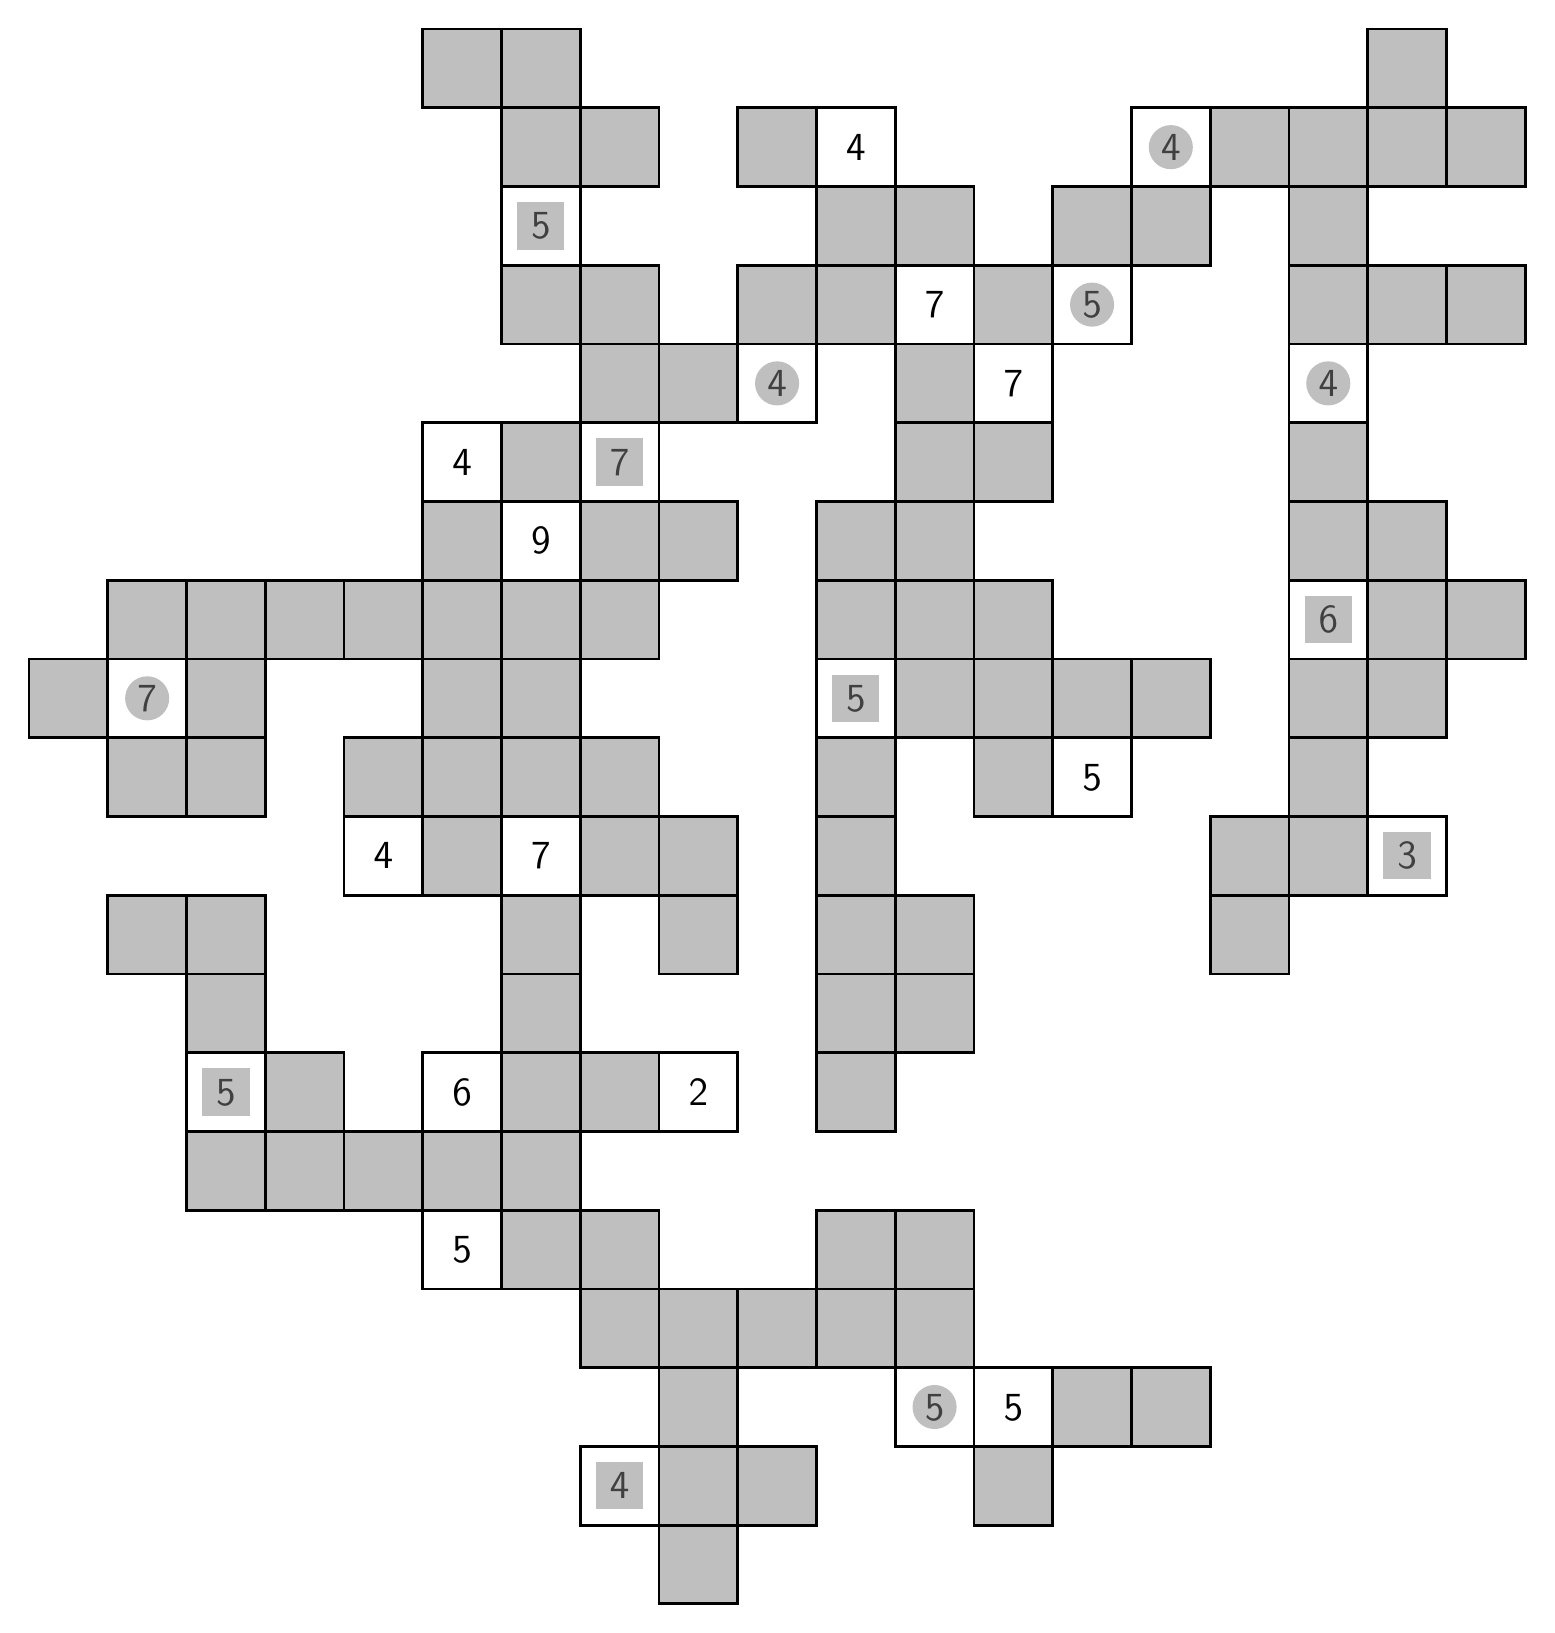
\begin{tikzpicture}\fill[gray, opacity = 0.5] (9, 0, 0)--++(1, 0, 0)--++(0, 1, 0)--++(-1, 0, 0)--cycle;
\draw[line width = 1pt] (9, 0, 0)--++(1, 0, 0)--++(0, 1, 0)--++(-1, 0, 0)--cycle;
\draw node at (8.5, 1.5, 0) {\Large $\mathsf{4}$};
\draw[line width = 1pt] (8, 1, 0)--++(1, 0, 0)--++(0, 1, 0)--++(-1, 0, 0)--cycle;
\fill[color = gray, opacity = 0.5] (8.2, 1.2) rectangle ++(0.6, 0.6);
\fill[gray, opacity = 0.5] (9, 1, 0)--++(1, 0, 0)--++(0, 1, 0)--++(-1, 0, 0)--cycle;
\draw[line width = 1pt] (9, 1, 0)--++(1, 0, 0)--++(0, 1, 0)--++(-1, 0, 0)--cycle;
\fill[gray, opacity = 0.5] (10, 1, 0)--++(1, 0, 0)--++(0, 1, 0)--++(-1, 0, 0)--cycle;
\draw[line width = 1pt] (10, 1, 0)--++(1, 0, 0)--++(0, 1, 0)--++(-1, 0, 0)--cycle;
\fill[gray, opacity = 0.5] (13, 1, 0)--++(1, 0, 0)--++(0, 1, 0)--++(-1, 0, 0)--cycle;
\draw[line width = 1pt] (13, 1, 0)--++(1, 0, 0)--++(0, 1, 0)--++(-1, 0, 0)--cycle;
\fill[gray, opacity = 0.5] (9, 2, 0)--++(1, 0, 0)--++(0, 1, 0)--++(-1, 0, 0)--cycle;
\draw[line width = 1pt] (9, 2, 0)--++(1, 0, 0)--++(0, 1, 0)--++(-1, 0, 0)--cycle;
\draw node at (12.5, 2.5, 0) {\Large $\mathsf{5}$};
\draw[line width = 1pt] (12, 2, 0)--++(1, 0, 0)--++(0, 1, 0)--++(-1, 0, 0)--cycle;
\fill[color = gray, opacity = 0.5] (12.5, 2.5, 0) circle (0.28);
\draw node at (13.5, 2.5, 0) {\Large $\mathsf{5}$};
\draw[line width = 1pt] (13, 2, 0)--++(1, 0, 0)--++(0, 1, 0)--++(-1, 0, 0)--cycle;
\fill[gray, opacity = 0.5] (14, 2, 0)--++(1, 0, 0)--++(0, 1, 0)--++(-1, 0, 0)--cycle;
\draw[line width = 1pt] (14, 2, 0)--++(1, 0, 0)--++(0, 1, 0)--++(-1, 0, 0)--cycle;
\fill[gray, opacity = 0.5] (15, 2, 0)--++(1, 0, 0)--++(0, 1, 0)--++(-1, 0, 0)--cycle;
\draw[line width = 1pt] (15, 2, 0)--++(1, 0, 0)--++(0, 1, 0)--++(-1, 0, 0)--cycle;
\fill[gray, opacity = 0.5] (8, 3, 0)--++(1, 0, 0)--++(0, 1, 0)--++(-1, 0, 0)--cycle;
\draw[line width = 1pt] (8, 3, 0)--++(1, 0, 0)--++(0, 1, 0)--++(-1, 0, 0)--cycle;
\fill[gray, opacity = 0.5] (9, 3, 0)--++(1, 0, 0)--++(0, 1, 0)--++(-1, 0, 0)--cycle;
\draw[line width = 1pt] (9, 3, 0)--++(1, 0, 0)--++(0, 1, 0)--++(-1, 0, 0)--cycle;
\fill[gray, opacity = 0.5] (10, 3, 0)--++(1, 0, 0)--++(0, 1, 0)--++(-1, 0, 0)--cycle;
\draw[line width = 1pt] (10, 3, 0)--++(1, 0, 0)--++(0, 1, 0)--++(-1, 0, 0)--cycle;
\fill[gray, opacity = 0.5] (11, 3, 0)--++(1, 0, 0)--++(0, 1, 0)--++(-1, 0, 0)--cycle;
\draw[line width = 1pt] (11, 3, 0)--++(1, 0, 0)--++(0, 1, 0)--++(-1, 0, 0)--cycle;
\fill[gray, opacity = 0.5] (12, 3, 0)--++(1, 0, 0)--++(0, 1, 0)--++(-1, 0, 0)--cycle;
\draw[line width = 1pt] (12, 3, 0)--++(1, 0, 0)--++(0, 1, 0)--++(-1, 0, 0)--cycle;
\draw node at (6.5, 4.5, 0) {\Large $\mathsf{5}$};
\draw[line width = 1pt] (6, 4, 0)--++(1, 0, 0)--++(0, 1, 0)--++(-1, 0, 0)--cycle;
\fill[gray, opacity = 0.5] (7, 4, 0)--++(1, 0, 0)--++(0, 1, 0)--++(-1, 0, 0)--cycle;
\draw[line width = 1pt] (7, 4, 0)--++(1, 0, 0)--++(0, 1, 0)--++(-1, 0, 0)--cycle;
\fill[gray, opacity = 0.5] (8, 4, 0)--++(1, 0, 0)--++(0, 1, 0)--++(-1, 0, 0)--cycle;
\draw[line width = 1pt] (8, 4, 0)--++(1, 0, 0)--++(0, 1, 0)--++(-1, 0, 0)--cycle;
\fill[gray, opacity = 0.5] (11, 4, 0)--++(1, 0, 0)--++(0, 1, 0)--++(-1, 0, 0)--cycle;
\draw[line width = 1pt] (11, 4, 0)--++(1, 0, 0)--++(0, 1, 0)--++(-1, 0, 0)--cycle;
\fill[gray, opacity = 0.5] (12, 4, 0)--++(1, 0, 0)--++(0, 1, 0)--++(-1, 0, 0)--cycle;
\draw[line width = 1pt] (12, 4, 0)--++(1, 0, 0)--++(0, 1, 0)--++(-1, 0, 0)--cycle;
\fill[gray, opacity = 0.5] (3, 5, 0)--++(1, 0, 0)--++(0, 1, 0)--++(-1, 0, 0)--cycle;
\draw[line width = 1pt] (3, 5, 0)--++(1, 0, 0)--++(0, 1, 0)--++(-1, 0, 0)--cycle;
\fill[gray, opacity = 0.5] (4, 5, 0)--++(1, 0, 0)--++(0, 1, 0)--++(-1, 0, 0)--cycle;
\draw[line width = 1pt] (4, 5, 0)--++(1, 0, 0)--++(0, 1, 0)--++(-1, 0, 0)--cycle;
\fill[gray, opacity = 0.5] (5, 5, 0)--++(1, 0, 0)--++(0, 1, 0)--++(-1, 0, 0)--cycle;
\draw[line width = 1pt] (5, 5, 0)--++(1, 0, 0)--++(0, 1, 0)--++(-1, 0, 0)--cycle;
\fill[gray, opacity = 0.5] (6, 5, 0)--++(1, 0, 0)--++(0, 1, 0)--++(-1, 0, 0)--cycle;
\draw[line width = 1pt] (6, 5, 0)--++(1, 0, 0)--++(0, 1, 0)--++(-1, 0, 0)--cycle;
\fill[gray, opacity = 0.5] (7, 5, 0)--++(1, 0, 0)--++(0, 1, 0)--++(-1, 0, 0)--cycle;
\draw[line width = 1pt] (7, 5, 0)--++(1, 0, 0)--++(0, 1, 0)--++(-1, 0, 0)--cycle;
\draw node at (3.5, 6.5, 0) {\Large $\mathsf{5}$};
\draw[line width = 1pt] (3, 6, 0)--++(1, 0, 0)--++(0, 1, 0)--++(-1, 0, 0)--cycle;
\fill[color = gray, opacity = 0.5] (3.2, 6.2) rectangle ++(0.6, 0.6);
\fill[gray, opacity = 0.5] (4, 6, 0)--++(1, 0, 0)--++(0, 1, 0)--++(-1, 0, 0)--cycle;
\draw[line width = 1pt] (4, 6, 0)--++(1, 0, 0)--++(0, 1, 0)--++(-1, 0, 0)--cycle;
\draw node at (6.5, 6.5, 0) {\Large $\mathsf{6}$};
\draw[line width = 1pt] (6, 6, 0)--++(1, 0, 0)--++(0, 1, 0)--++(-1, 0, 0)--cycle;
\fill[gray, opacity = 0.5] (7, 6, 0)--++(1, 0, 0)--++(0, 1, 0)--++(-1, 0, 0)--cycle;
\draw[line width = 1pt] (7, 6, 0)--++(1, 0, 0)--++(0, 1, 0)--++(-1, 0, 0)--cycle;
\fill[gray, opacity = 0.5] (8, 6, 0)--++(1, 0, 0)--++(0, 1, 0)--++(-1, 0, 0)--cycle;
\draw[line width = 1pt] (8, 6, 0)--++(1, 0, 0)--++(0, 1, 0)--++(-1, 0, 0)--cycle;
\draw node at (9.5, 6.5, 0) {\Large $\mathsf{2}$};
\draw[line width = 1pt] (9, 6, 0)--++(1, 0, 0)--++(0, 1, 0)--++(-1, 0, 0)--cycle;
\fill[gray, opacity = 0.5] (11, 6, 0)--++(1, 0, 0)--++(0, 1, 0)--++(-1, 0, 0)--cycle;
\draw[line width = 1pt] (11, 6, 0)--++(1, 0, 0)--++(0, 1, 0)--++(-1, 0, 0)--cycle;
\fill[gray, opacity = 0.5] (3, 7, 0)--++(1, 0, 0)--++(0, 1, 0)--++(-1, 0, 0)--cycle;
\draw[line width = 1pt] (3, 7, 0)--++(1, 0, 0)--++(0, 1, 0)--++(-1, 0, 0)--cycle;
\fill[gray, opacity = 0.5] (7, 7, 0)--++(1, 0, 0)--++(0, 1, 0)--++(-1, 0, 0)--cycle;
\draw[line width = 1pt] (7, 7, 0)--++(1, 0, 0)--++(0, 1, 0)--++(-1, 0, 0)--cycle;
\fill[gray, opacity = 0.5] (11, 7, 0)--++(1, 0, 0)--++(0, 1, 0)--++(-1, 0, 0)--cycle;
\draw[line width = 1pt] (11, 7, 0)--++(1, 0, 0)--++(0, 1, 0)--++(-1, 0, 0)--cycle;
\fill[gray, opacity = 0.5] (12, 7, 0)--++(1, 0, 0)--++(0, 1, 0)--++(-1, 0, 0)--cycle;
\draw[line width = 1pt] (12, 7, 0)--++(1, 0, 0)--++(0, 1, 0)--++(-1, 0, 0)--cycle;
\fill[gray, opacity = 0.5] (2, 8, 0)--++(1, 0, 0)--++(0, 1, 0)--++(-1, 0, 0)--cycle;
\draw[line width = 1pt] (2, 8, 0)--++(1, 0, 0)--++(0, 1, 0)--++(-1, 0, 0)--cycle;
\fill[gray, opacity = 0.5] (3, 8, 0)--++(1, 0, 0)--++(0, 1, 0)--++(-1, 0, 0)--cycle;
\draw[line width = 1pt] (3, 8, 0)--++(1, 0, 0)--++(0, 1, 0)--++(-1, 0, 0)--cycle;
\fill[gray, opacity = 0.5] (7, 8, 0)--++(1, 0, 0)--++(0, 1, 0)--++(-1, 0, 0)--cycle;
\draw[line width = 1pt] (7, 8, 0)--++(1, 0, 0)--++(0, 1, 0)--++(-1, 0, 0)--cycle;
\fill[gray, opacity = 0.5] (9, 8, 0)--++(1, 0, 0)--++(0, 1, 0)--++(-1, 0, 0)--cycle;
\draw[line width = 1pt] (9, 8, 0)--++(1, 0, 0)--++(0, 1, 0)--++(-1, 0, 0)--cycle;
\fill[gray, opacity = 0.5] (11, 8, 0)--++(1, 0, 0)--++(0, 1, 0)--++(-1, 0, 0)--cycle;
\draw[line width = 1pt] (11, 8, 0)--++(1, 0, 0)--++(0, 1, 0)--++(-1, 0, 0)--cycle;
\fill[gray, opacity = 0.5] (12, 8, 0)--++(1, 0, 0)--++(0, 1, 0)--++(-1, 0, 0)--cycle;
\draw[line width = 1pt] (12, 8, 0)--++(1, 0, 0)--++(0, 1, 0)--++(-1, 0, 0)--cycle;
\fill[gray, opacity = 0.5] (16, 8, 0)--++(1, 0, 0)--++(0, 1, 0)--++(-1, 0, 0)--cycle;
\draw[line width = 1pt] (16, 8, 0)--++(1, 0, 0)--++(0, 1, 0)--++(-1, 0, 0)--cycle;
\draw node at (5.5, 9.5, 0) {\Large $\mathsf{4}$};
\draw[line width = 1pt] (5, 9, 0)--++(1, 0, 0)--++(0, 1, 0)--++(-1, 0, 0)--cycle;
\fill[gray, opacity = 0.5] (6, 9, 0)--++(1, 0, 0)--++(0, 1, 0)--++(-1, 0, 0)--cycle;
\draw[line width = 1pt] (6, 9, 0)--++(1, 0, 0)--++(0, 1, 0)--++(-1, 0, 0)--cycle;
\draw node at (7.5, 9.5, 0) {\Large $\mathsf{7}$};
\draw[line width = 1pt] (7, 9, 0)--++(1, 0, 0)--++(0, 1, 0)--++(-1, 0, 0)--cycle;
\fill[gray, opacity = 0.5] (8, 9, 0)--++(1, 0, 0)--++(0, 1, 0)--++(-1, 0, 0)--cycle;
\draw[line width = 1pt] (8, 9, 0)--++(1, 0, 0)--++(0, 1, 0)--++(-1, 0, 0)--cycle;
\fill[gray, opacity = 0.5] (9, 9, 0)--++(1, 0, 0)--++(0, 1, 0)--++(-1, 0, 0)--cycle;
\draw[line width = 1pt] (9, 9, 0)--++(1, 0, 0)--++(0, 1, 0)--++(-1, 0, 0)--cycle;
\fill[gray, opacity = 0.5] (11, 9, 0)--++(1, 0, 0)--++(0, 1, 0)--++(-1, 0, 0)--cycle;
\draw[line width = 1pt] (11, 9, 0)--++(1, 0, 0)--++(0, 1, 0)--++(-1, 0, 0)--cycle;
\fill[gray, opacity = 0.5] (16, 9, 0)--++(1, 0, 0)--++(0, 1, 0)--++(-1, 0, 0)--cycle;
\draw[line width = 1pt] (16, 9, 0)--++(1, 0, 0)--++(0, 1, 0)--++(-1, 0, 0)--cycle;
\fill[gray, opacity = 0.5] (17, 9, 0)--++(1, 0, 0)--++(0, 1, 0)--++(-1, 0, 0)--cycle;
\draw[line width = 1pt] (17, 9, 0)--++(1, 0, 0)--++(0, 1, 0)--++(-1, 0, 0)--cycle;
\draw node at (18.5, 9.5, 0) {\Large $\mathsf{3}$};
\draw[line width = 1pt] (18, 9, 0)--++(1, 0, 0)--++(0, 1, 0)--++(-1, 0, 0)--cycle;
\fill[color = gray, opacity = 0.5] (18.2, 9.2) rectangle ++(0.6, 0.6);
\fill[gray, opacity = 0.5] (2, 10, 0)--++(1, 0, 0)--++(0, 1, 0)--++(-1, 0, 0)--cycle;
\draw[line width = 1pt] (2, 10, 0)--++(1, 0, 0)--++(0, 1, 0)--++(-1, 0, 0)--cycle;
\fill[gray, opacity = 0.5] (3, 10, 0)--++(1, 0, 0)--++(0, 1, 0)--++(-1, 0, 0)--cycle;
\draw[line width = 1pt] (3, 10, 0)--++(1, 0, 0)--++(0, 1, 0)--++(-1, 0, 0)--cycle;
\fill[gray, opacity = 0.5] (5, 10, 0)--++(1, 0, 0)--++(0, 1, 0)--++(-1, 0, 0)--cycle;
\draw[line width = 1pt] (5, 10, 0)--++(1, 0, 0)--++(0, 1, 0)--++(-1, 0, 0)--cycle;
\fill[gray, opacity = 0.5] (6, 10, 0)--++(1, 0, 0)--++(0, 1, 0)--++(-1, 0, 0)--cycle;
\draw[line width = 1pt] (6, 10, 0)--++(1, 0, 0)--++(0, 1, 0)--++(-1, 0, 0)--cycle;
\fill[gray, opacity = 0.5] (7, 10, 0)--++(1, 0, 0)--++(0, 1, 0)--++(-1, 0, 0)--cycle;
\draw[line width = 1pt] (7, 10, 0)--++(1, 0, 0)--++(0, 1, 0)--++(-1, 0, 0)--cycle;
\fill[gray, opacity = 0.5] (8, 10, 0)--++(1, 0, 0)--++(0, 1, 0)--++(-1, 0, 0)--cycle;
\draw[line width = 1pt] (8, 10, 0)--++(1, 0, 0)--++(0, 1, 0)--++(-1, 0, 0)--cycle;
\fill[gray, opacity = 0.5] (11, 10, 0)--++(1, 0, 0)--++(0, 1, 0)--++(-1, 0, 0)--cycle;
\draw[line width = 1pt] (11, 10, 0)--++(1, 0, 0)--++(0, 1, 0)--++(-1, 0, 0)--cycle;
\fill[gray, opacity = 0.5] (13, 10, 0)--++(1, 0, 0)--++(0, 1, 0)--++(-1, 0, 0)--cycle;
\draw[line width = 1pt] (13, 10, 0)--++(1, 0, 0)--++(0, 1, 0)--++(-1, 0, 0)--cycle;
\draw node at (14.5, 10.5, 0) {\Large $\mathsf{5}$};
\draw[line width = 1pt] (14, 10, 0)--++(1, 0, 0)--++(0, 1, 0)--++(-1, 0, 0)--cycle;
\fill[gray, opacity = 0.5] (17, 10, 0)--++(1, 0, 0)--++(0, 1, 0)--++(-1, 0, 0)--cycle;
\draw[line width = 1pt] (17, 10, 0)--++(1, 0, 0)--++(0, 1, 0)--++(-1, 0, 0)--cycle;
\fill[gray, opacity = 0.5] (1, 11, 0)--++(1, 0, 0)--++(0, 1, 0)--++(-1, 0, 0)--cycle;
\draw[line width = 1pt] (1, 11, 0)--++(1, 0, 0)--++(0, 1, 0)--++(-1, 0, 0)--cycle;
\draw node at (2.5, 11.5, 0) {\Large $\mathsf{7}$};
\draw[line width = 1pt] (2, 11, 0)--++(1, 0, 0)--++(0, 1, 0)--++(-1, 0, 0)--cycle;
\fill[color = gray, opacity = 0.5] (2.5, 11.5, 0) circle (0.28);
\fill[gray, opacity = 0.5] (3, 11, 0)--++(1, 0, 0)--++(0, 1, 0)--++(-1, 0, 0)--cycle;
\draw[line width = 1pt] (3, 11, 0)--++(1, 0, 0)--++(0, 1, 0)--++(-1, 0, 0)--cycle;
\fill[gray, opacity = 0.5] (6, 11, 0)--++(1, 0, 0)--++(0, 1, 0)--++(-1, 0, 0)--cycle;
\draw[line width = 1pt] (6, 11, 0)--++(1, 0, 0)--++(0, 1, 0)--++(-1, 0, 0)--cycle;
\fill[gray, opacity = 0.5] (7, 11, 0)--++(1, 0, 0)--++(0, 1, 0)--++(-1, 0, 0)--cycle;
\draw[line width = 1pt] (7, 11, 0)--++(1, 0, 0)--++(0, 1, 0)--++(-1, 0, 0)--cycle;
\draw node at (11.5, 11.5, 0) {\Large $\mathsf{5}$};
\draw[line width = 1pt] (11, 11, 0)--++(1, 0, 0)--++(0, 1, 0)--++(-1, 0, 0)--cycle;
\fill[color = gray, opacity = 0.5] (11.2, 11.2) rectangle ++(0.6, 0.6);
\fill[gray, opacity = 0.5] (12, 11, 0)--++(1, 0, 0)--++(0, 1, 0)--++(-1, 0, 0)--cycle;
\draw[line width = 1pt] (12, 11, 0)--++(1, 0, 0)--++(0, 1, 0)--++(-1, 0, 0)--cycle;
\fill[gray, opacity = 0.5] (13, 11, 0)--++(1, 0, 0)--++(0, 1, 0)--++(-1, 0, 0)--cycle;
\draw[line width = 1pt] (13, 11, 0)--++(1, 0, 0)--++(0, 1, 0)--++(-1, 0, 0)--cycle;
\fill[gray, opacity = 0.5] (14, 11, 0)--++(1, 0, 0)--++(0, 1, 0)--++(-1, 0, 0)--cycle;
\draw[line width = 1pt] (14, 11, 0)--++(1, 0, 0)--++(0, 1, 0)--++(-1, 0, 0)--cycle;
\fill[gray, opacity = 0.5] (15, 11, 0)--++(1, 0, 0)--++(0, 1, 0)--++(-1, 0, 0)--cycle;
\draw[line width = 1pt] (15, 11, 0)--++(1, 0, 0)--++(0, 1, 0)--++(-1, 0, 0)--cycle;
\fill[gray, opacity = 0.5] (17, 11, 0)--++(1, 0, 0)--++(0, 1, 0)--++(-1, 0, 0)--cycle;
\draw[line width = 1pt] (17, 11, 0)--++(1, 0, 0)--++(0, 1, 0)--++(-1, 0, 0)--cycle;
\fill[gray, opacity = 0.5] (18, 11, 0)--++(1, 0, 0)--++(0, 1, 0)--++(-1, 0, 0)--cycle;
\draw[line width = 1pt] (18, 11, 0)--++(1, 0, 0)--++(0, 1, 0)--++(-1, 0, 0)--cycle;
\fill[gray, opacity = 0.5] (2, 12, 0)--++(1, 0, 0)--++(0, 1, 0)--++(-1, 0, 0)--cycle;
\draw[line width = 1pt] (2, 12, 0)--++(1, 0, 0)--++(0, 1, 0)--++(-1, 0, 0)--cycle;
\fill[gray, opacity = 0.5] (3, 12, 0)--++(1, 0, 0)--++(0, 1, 0)--++(-1, 0, 0)--cycle;
\draw[line width = 1pt] (3, 12, 0)--++(1, 0, 0)--++(0, 1, 0)--++(-1, 0, 0)--cycle;
\fill[gray, opacity = 0.5] (4, 12, 0)--++(1, 0, 0)--++(0, 1, 0)--++(-1, 0, 0)--cycle;
\draw[line width = 1pt] (4, 12, 0)--++(1, 0, 0)--++(0, 1, 0)--++(-1, 0, 0)--cycle;
\fill[gray, opacity = 0.5] (5, 12, 0)--++(1, 0, 0)--++(0, 1, 0)--++(-1, 0, 0)--cycle;
\draw[line width = 1pt] (5, 12, 0)--++(1, 0, 0)--++(0, 1, 0)--++(-1, 0, 0)--cycle;
\fill[gray, opacity = 0.5] (6, 12, 0)--++(1, 0, 0)--++(0, 1, 0)--++(-1, 0, 0)--cycle;
\draw[line width = 1pt] (6, 12, 0)--++(1, 0, 0)--++(0, 1, 0)--++(-1, 0, 0)--cycle;
\fill[gray, opacity = 0.5] (7, 12, 0)--++(1, 0, 0)--++(0, 1, 0)--++(-1, 0, 0)--cycle;
\draw[line width = 1pt] (7, 12, 0)--++(1, 0, 0)--++(0, 1, 0)--++(-1, 0, 0)--cycle;
\fill[gray, opacity = 0.5] (8, 12, 0)--++(1, 0, 0)--++(0, 1, 0)--++(-1, 0, 0)--cycle;
\draw[line width = 1pt] (8, 12, 0)--++(1, 0, 0)--++(0, 1, 0)--++(-1, 0, 0)--cycle;
\fill[gray, opacity = 0.5] (11, 12, 0)--++(1, 0, 0)--++(0, 1, 0)--++(-1, 0, 0)--cycle;
\draw[line width = 1pt] (11, 12, 0)--++(1, 0, 0)--++(0, 1, 0)--++(-1, 0, 0)--cycle;
\fill[gray, opacity = 0.5] (12, 12, 0)--++(1, 0, 0)--++(0, 1, 0)--++(-1, 0, 0)--cycle;
\draw[line width = 1pt] (12, 12, 0)--++(1, 0, 0)--++(0, 1, 0)--++(-1, 0, 0)--cycle;
\fill[gray, opacity = 0.5] (13, 12, 0)--++(1, 0, 0)--++(0, 1, 0)--++(-1, 0, 0)--cycle;
\draw[line width = 1pt] (13, 12, 0)--++(1, 0, 0)--++(0, 1, 0)--++(-1, 0, 0)--cycle;
\draw node at (17.5, 12.5, 0) {\Large $\mathsf{6}$};
\draw[line width = 1pt] (17, 12, 0)--++(1, 0, 0)--++(0, 1, 0)--++(-1, 0, 0)--cycle;
\fill[color = gray, opacity = 0.5] (17.2, 12.2) rectangle ++(0.6, 0.6);
\fill[gray, opacity = 0.5] (18, 12, 0)--++(1, 0, 0)--++(0, 1, 0)--++(-1, 0, 0)--cycle;
\draw[line width = 1pt] (18, 12, 0)--++(1, 0, 0)--++(0, 1, 0)--++(-1, 0, 0)--cycle;
\fill[gray, opacity = 0.5] (19, 12, 0)--++(1, 0, 0)--++(0, 1, 0)--++(-1, 0, 0)--cycle;
\draw[line width = 1pt] (19, 12, 0)--++(1, 0, 0)--++(0, 1, 0)--++(-1, 0, 0)--cycle;
\fill[gray, opacity = 0.5] (6, 13, 0)--++(1, 0, 0)--++(0, 1, 0)--++(-1, 0, 0)--cycle;
\draw[line width = 1pt] (6, 13, 0)--++(1, 0, 0)--++(0, 1, 0)--++(-1, 0, 0)--cycle;
\draw node at (7.5, 13.5, 0) {\Large $\mathsf{9}$};
\draw[line width = 1pt] (7, 13, 0)--++(1, 0, 0)--++(0, 1, 0)--++(-1, 0, 0)--cycle;
\fill[gray, opacity = 0.5] (8, 13, 0)--++(1, 0, 0)--++(0, 1, 0)--++(-1, 0, 0)--cycle;
\draw[line width = 1pt] (8, 13, 0)--++(1, 0, 0)--++(0, 1, 0)--++(-1, 0, 0)--cycle;
\fill[gray, opacity = 0.5] (9, 13, 0)--++(1, 0, 0)--++(0, 1, 0)--++(-1, 0, 0)--cycle;
\draw[line width = 1pt] (9, 13, 0)--++(1, 0, 0)--++(0, 1, 0)--++(-1, 0, 0)--cycle;
\fill[gray, opacity = 0.5] (11, 13, 0)--++(1, 0, 0)--++(0, 1, 0)--++(-1, 0, 0)--cycle;
\draw[line width = 1pt] (11, 13, 0)--++(1, 0, 0)--++(0, 1, 0)--++(-1, 0, 0)--cycle;
\fill[gray, opacity = 0.5] (12, 13, 0)--++(1, 0, 0)--++(0, 1, 0)--++(-1, 0, 0)--cycle;
\draw[line width = 1pt] (12, 13, 0)--++(1, 0, 0)--++(0, 1, 0)--++(-1, 0, 0)--cycle;
\fill[gray, opacity = 0.5] (17, 13, 0)--++(1, 0, 0)--++(0, 1, 0)--++(-1, 0, 0)--cycle;
\draw[line width = 1pt] (17, 13, 0)--++(1, 0, 0)--++(0, 1, 0)--++(-1, 0, 0)--cycle;
\fill[gray, opacity = 0.5] (18, 13, 0)--++(1, 0, 0)--++(0, 1, 0)--++(-1, 0, 0)--cycle;
\draw[line width = 1pt] (18, 13, 0)--++(1, 0, 0)--++(0, 1, 0)--++(-1, 0, 0)--cycle;
\draw node at (6.5, 14.5, 0) {\Large $\mathsf{4}$};
\draw[line width = 1pt] (6, 14, 0)--++(1, 0, 0)--++(0, 1, 0)--++(-1, 0, 0)--cycle;
\fill[gray, opacity = 0.5] (7, 14, 0)--++(1, 0, 0)--++(0, 1, 0)--++(-1, 0, 0)--cycle;
\draw[line width = 1pt] (7, 14, 0)--++(1, 0, 0)--++(0, 1, 0)--++(-1, 0, 0)--cycle;
\draw node at (8.5, 14.5, 0) {\Large $\mathsf{7}$};
\draw[line width = 1pt] (8, 14, 0)--++(1, 0, 0)--++(0, 1, 0)--++(-1, 0, 0)--cycle;
\fill[color = gray, opacity = 0.5] (8.2, 14.2) rectangle ++(0.6, 0.6);
\fill[gray, opacity = 0.5] (12, 14, 0)--++(1, 0, 0)--++(0, 1, 0)--++(-1, 0, 0)--cycle;
\draw[line width = 1pt] (12, 14, 0)--++(1, 0, 0)--++(0, 1, 0)--++(-1, 0, 0)--cycle;
\fill[gray, opacity = 0.5] (13, 14, 0)--++(1, 0, 0)--++(0, 1, 0)--++(-1, 0, 0)--cycle;
\draw[line width = 1pt] (13, 14, 0)--++(1, 0, 0)--++(0, 1, 0)--++(-1, 0, 0)--cycle;
\fill[gray, opacity = 0.5] (17, 14, 0)--++(1, 0, 0)--++(0, 1, 0)--++(-1, 0, 0)--cycle;
\draw[line width = 1pt] (17, 14, 0)--++(1, 0, 0)--++(0, 1, 0)--++(-1, 0, 0)--cycle;
\fill[gray, opacity = 0.5] (8, 15, 0)--++(1, 0, 0)--++(0, 1, 0)--++(-1, 0, 0)--cycle;
\draw[line width = 1pt] (8, 15, 0)--++(1, 0, 0)--++(0, 1, 0)--++(-1, 0, 0)--cycle;
\fill[gray, opacity = 0.5] (9, 15, 0)--++(1, 0, 0)--++(0, 1, 0)--++(-1, 0, 0)--cycle;
\draw[line width = 1pt] (9, 15, 0)--++(1, 0, 0)--++(0, 1, 0)--++(-1, 0, 0)--cycle;
\draw node at (10.5, 15.5, 0) {\Large $\mathsf{4}$};
\draw[line width = 1pt] (10, 15, 0)--++(1, 0, 0)--++(0, 1, 0)--++(-1, 0, 0)--cycle;
\fill[color = gray, opacity = 0.5] (10.5, 15.5, 0) circle (0.28);
\fill[gray, opacity = 0.5] (12, 15, 0)--++(1, 0, 0)--++(0, 1, 0)--++(-1, 0, 0)--cycle;
\draw[line width = 1pt] (12, 15, 0)--++(1, 0, 0)--++(0, 1, 0)--++(-1, 0, 0)--cycle;
\draw node at (13.5, 15.5, 0) {\Large $\mathsf{7}$};
\draw[line width = 1pt] (13, 15, 0)--++(1, 0, 0)--++(0, 1, 0)--++(-1, 0, 0)--cycle;
\draw node at (17.5, 15.5, 0) {\Large $\mathsf{4}$};
\draw[line width = 1pt] (17, 15, 0)--++(1, 0, 0)--++(0, 1, 0)--++(-1, 0, 0)--cycle;
\fill[color = gray, opacity = 0.5] (17.5, 15.5, 0) circle (0.28);
\fill[gray, opacity = 0.5] (7, 16, 0)--++(1, 0, 0)--++(0, 1, 0)--++(-1, 0, 0)--cycle;
\draw[line width = 1pt] (7, 16, 0)--++(1, 0, 0)--++(0, 1, 0)--++(-1, 0, 0)--cycle;
\fill[gray, opacity = 0.5] (8, 16, 0)--++(1, 0, 0)--++(0, 1, 0)--++(-1, 0, 0)--cycle;
\draw[line width = 1pt] (8, 16, 0)--++(1, 0, 0)--++(0, 1, 0)--++(-1, 0, 0)--cycle;
\fill[gray, opacity = 0.5] (10, 16, 0)--++(1, 0, 0)--++(0, 1, 0)--++(-1, 0, 0)--cycle;
\draw[line width = 1pt] (10, 16, 0)--++(1, 0, 0)--++(0, 1, 0)--++(-1, 0, 0)--cycle;
\fill[gray, opacity = 0.5] (11, 16, 0)--++(1, 0, 0)--++(0, 1, 0)--++(-1, 0, 0)--cycle;
\draw[line width = 1pt] (11, 16, 0)--++(1, 0, 0)--++(0, 1, 0)--++(-1, 0, 0)--cycle;
\draw node at (12.5, 16.5, 0) {\Large $\mathsf{7}$};
\draw[line width = 1pt] (12, 16, 0)--++(1, 0, 0)--++(0, 1, 0)--++(-1, 0, 0)--cycle;
\fill[gray, opacity = 0.5] (13, 16, 0)--++(1, 0, 0)--++(0, 1, 0)--++(-1, 0, 0)--cycle;
\draw[line width = 1pt] (13, 16, 0)--++(1, 0, 0)--++(0, 1, 0)--++(-1, 0, 0)--cycle;
\draw node at (14.5, 16.5, 0) {\Large $\mathsf{5}$};
\draw[line width = 1pt] (14, 16, 0)--++(1, 0, 0)--++(0, 1, 0)--++(-1, 0, 0)--cycle;
\fill[color = gray, opacity = 0.5] (14.5, 16.5, 0) circle (0.28);
\fill[gray, opacity = 0.5] (17, 16, 0)--++(1, 0, 0)--++(0, 1, 0)--++(-1, 0, 0)--cycle;
\draw[line width = 1pt] (17, 16, 0)--++(1, 0, 0)--++(0, 1, 0)--++(-1, 0, 0)--cycle;
\fill[gray, opacity = 0.5] (18, 16, 0)--++(1, 0, 0)--++(0, 1, 0)--++(-1, 0, 0)--cycle;
\draw[line width = 1pt] (18, 16, 0)--++(1, 0, 0)--++(0, 1, 0)--++(-1, 0, 0)--cycle;
\fill[gray, opacity = 0.5] (19, 16, 0)--++(1, 0, 0)--++(0, 1, 0)--++(-1, 0, 0)--cycle;
\draw[line width = 1pt] (19, 16, 0)--++(1, 0, 0)--++(0, 1, 0)--++(-1, 0, 0)--cycle;
\draw node at (7.5, 17.5, 0) {\Large $\mathsf{5}$};
\draw[line width = 1pt] (7, 17, 0)--++(1, 0, 0)--++(0, 1, 0)--++(-1, 0, 0)--cycle;
\fill[color = gray, opacity = 0.5] (7.2, 17.2) rectangle ++(0.6, 0.6);
\fill[gray, opacity = 0.5] (11, 17, 0)--++(1, 0, 0)--++(0, 1, 0)--++(-1, 0, 0)--cycle;
\draw[line width = 1pt] (11, 17, 0)--++(1, 0, 0)--++(0, 1, 0)--++(-1, 0, 0)--cycle;
\fill[gray, opacity = 0.5] (12, 17, 0)--++(1, 0, 0)--++(0, 1, 0)--++(-1, 0, 0)--cycle;
\draw[line width = 1pt] (12, 17, 0)--++(1, 0, 0)--++(0, 1, 0)--++(-1, 0, 0)--cycle;
\fill[gray, opacity = 0.5] (14, 17, 0)--++(1, 0, 0)--++(0, 1, 0)--++(-1, 0, 0)--cycle;
\draw[line width = 1pt] (14, 17, 0)--++(1, 0, 0)--++(0, 1, 0)--++(-1, 0, 0)--cycle;
\fill[gray, opacity = 0.5] (15, 17, 0)--++(1, 0, 0)--++(0, 1, 0)--++(-1, 0, 0)--cycle;
\draw[line width = 1pt] (15, 17, 0)--++(1, 0, 0)--++(0, 1, 0)--++(-1, 0, 0)--cycle;
\fill[gray, opacity = 0.5] (17, 17, 0)--++(1, 0, 0)--++(0, 1, 0)--++(-1, 0, 0)--cycle;
\draw[line width = 1pt] (17, 17, 0)--++(1, 0, 0)--++(0, 1, 0)--++(-1, 0, 0)--cycle;
\fill[gray, opacity = 0.5] (7, 18, 0)--++(1, 0, 0)--++(0, 1, 0)--++(-1, 0, 0)--cycle;
\draw[line width = 1pt] (7, 18, 0)--++(1, 0, 0)--++(0, 1, 0)--++(-1, 0, 0)--cycle;
\fill[gray, opacity = 0.5] (8, 18, 0)--++(1, 0, 0)--++(0, 1, 0)--++(-1, 0, 0)--cycle;
\draw[line width = 1pt] (8, 18, 0)--++(1, 0, 0)--++(0, 1, 0)--++(-1, 0, 0)--cycle;
\fill[gray, opacity = 0.5] (10, 18, 0)--++(1, 0, 0)--++(0, 1, 0)--++(-1, 0, 0)--cycle;
\draw[line width = 1pt] (10, 18, 0)--++(1, 0, 0)--++(0, 1, 0)--++(-1, 0, 0)--cycle;
\draw node at (11.5, 18.5, 0) {\Large $\mathsf{4}$};
\draw[line width = 1pt] (11, 18, 0)--++(1, 0, 0)--++(0, 1, 0)--++(-1, 0, 0)--cycle;
\draw node at (15.5, 18.5, 0) {\Large $\mathsf{4}$};
\draw[line width = 1pt] (15, 18, 0)--++(1, 0, 0)--++(0, 1, 0)--++(-1, 0, 0)--cycle;
\fill[color = gray, opacity = 0.5] (15.5, 18.5, 0) circle (0.28);
\fill[gray, opacity = 0.5] (16, 18, 0)--++(1, 0, 0)--++(0, 1, 0)--++(-1, 0, 0)--cycle;
\draw[line width = 1pt] (16, 18, 0)--++(1, 0, 0)--++(0, 1, 0)--++(-1, 0, 0)--cycle;
\fill[gray, opacity = 0.5] (17, 18, 0)--++(1, 0, 0)--++(0, 1, 0)--++(-1, 0, 0)--cycle;
\draw[line width = 1pt] (17, 18, 0)--++(1, 0, 0)--++(0, 1, 0)--++(-1, 0, 0)--cycle;
\fill[gray, opacity = 0.5] (18, 18, 0)--++(1, 0, 0)--++(0, 1, 0)--++(-1, 0, 0)--cycle;
\draw[line width = 1pt] (18, 18, 0)--++(1, 0, 0)--++(0, 1, 0)--++(-1, 0, 0)--cycle;
\fill[gray, opacity = 0.5] (19, 18, 0)--++(1, 0, 0)--++(0, 1, 0)--++(-1, 0, 0)--cycle;
\draw[line width = 1pt] (19, 18, 0)--++(1, 0, 0)--++(0, 1, 0)--++(-1, 0, 0)--cycle;
\fill[gray, opacity = 0.5] (6, 19, 0)--++(1, 0, 0)--++(0, 1, 0)--++(-1, 0, 0)--cycle;
\draw[line width = 1pt] (6, 19, 0)--++(1, 0, 0)--++(0, 1, 0)--++(-1, 0, 0)--cycle;
\fill[gray, opacity = 0.5] (7, 19, 0)--++(1, 0, 0)--++(0, 1, 0)--++(-1, 0, 0)--cycle;
\draw[line width = 1pt] (7, 19, 0)--++(1, 0, 0)--++(0, 1, 0)--++(-1, 0, 0)--cycle;
\fill[gray, opacity = 0.5] (18, 19, 0)--++(1, 0, 0)--++(0, 1, 0)--++(-1, 0, 0)--cycle;
\draw[line width = 1pt] (18, 19, 0)--++(1, 0, 0)--++(0, 1, 0)--++(-1, 0, 0)--cycle;
\end{tikzpicture}}\]
\[\resizebox{30pc}{!}{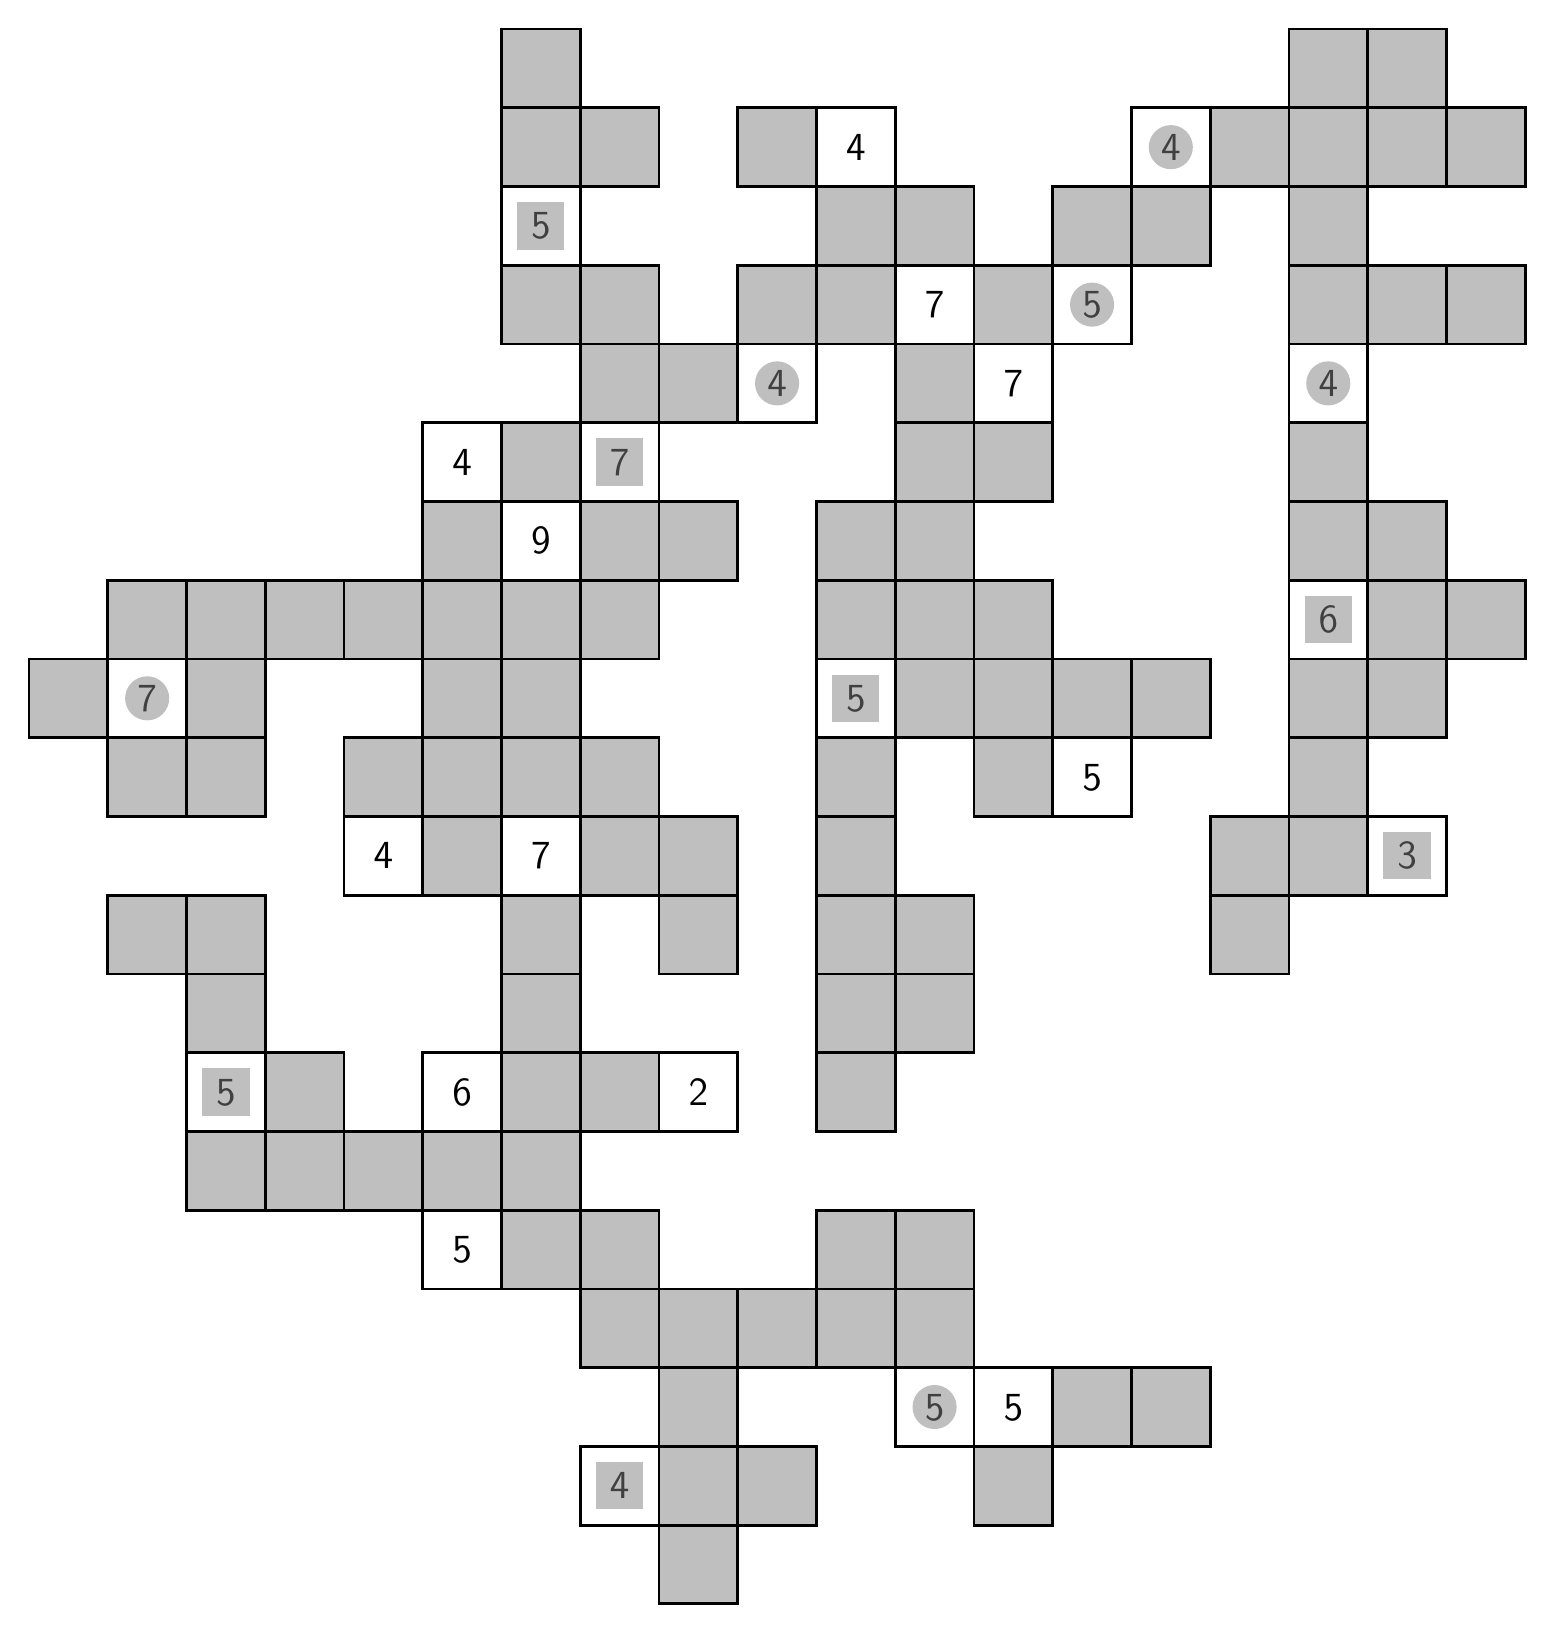
\begin{tikzpicture}\fill[gray, opacity = 0.5] (9, 0, 0)--++(1, 0, 0)--++(0, 1, 0)--++(-1, 0, 0)--cycle;
\draw[line width = 1pt] (9, 0, 0)--++(1, 0, 0)--++(0, 1, 0)--++(-1, 0, 0)--cycle;
\draw node at (8.5, 1.5, 0) {\Large $\mathsf{4}$};
\draw[line width = 1pt] (8, 1, 0)--++(1, 0, 0)--++(0, 1, 0)--++(-1, 0, 0)--cycle;
\fill[color = gray, opacity = 0.5] (8.2, 1.2) rectangle ++(0.6, 0.6);
\fill[gray, opacity = 0.5] (9, 1, 0)--++(1, 0, 0)--++(0, 1, 0)--++(-1, 0, 0)--cycle;
\draw[line width = 1pt] (9, 1, 0)--++(1, 0, 0)--++(0, 1, 0)--++(-1, 0, 0)--cycle;
\fill[gray, opacity = 0.5] (10, 1, 0)--++(1, 0, 0)--++(0, 1, 0)--++(-1, 0, 0)--cycle;
\draw[line width = 1pt] (10, 1, 0)--++(1, 0, 0)--++(0, 1, 0)--++(-1, 0, 0)--cycle;
\fill[gray, opacity = 0.5] (13, 1, 0)--++(1, 0, 0)--++(0, 1, 0)--++(-1, 0, 0)--cycle;
\draw[line width = 1pt] (13, 1, 0)--++(1, 0, 0)--++(0, 1, 0)--++(-1, 0, 0)--cycle;
\fill[gray, opacity = 0.5] (9, 2, 0)--++(1, 0, 0)--++(0, 1, 0)--++(-1, 0, 0)--cycle;
\draw[line width = 1pt] (9, 2, 0)--++(1, 0, 0)--++(0, 1, 0)--++(-1, 0, 0)--cycle;
\draw node at (12.5, 2.5, 0) {\Large $\mathsf{5}$};
\draw[line width = 1pt] (12, 2, 0)--++(1, 0, 0)--++(0, 1, 0)--++(-1, 0, 0)--cycle;
\fill[color = gray, opacity = 0.5] (12.5, 2.5, 0) circle (0.28);
\draw node at (13.5, 2.5, 0) {\Large $\mathsf{5}$};
\draw[line width = 1pt] (13, 2, 0)--++(1, 0, 0)--++(0, 1, 0)--++(-1, 0, 0)--cycle;
\fill[gray, opacity = 0.5] (14, 2, 0)--++(1, 0, 0)--++(0, 1, 0)--++(-1, 0, 0)--cycle;
\draw[line width = 1pt] (14, 2, 0)--++(1, 0, 0)--++(0, 1, 0)--++(-1, 0, 0)--cycle;
\fill[gray, opacity = 0.5] (15, 2, 0)--++(1, 0, 0)--++(0, 1, 0)--++(-1, 0, 0)--cycle;
\draw[line width = 1pt] (15, 2, 0)--++(1, 0, 0)--++(0, 1, 0)--++(-1, 0, 0)--cycle;
\fill[gray, opacity = 0.5] (8, 3, 0)--++(1, 0, 0)--++(0, 1, 0)--++(-1, 0, 0)--cycle;
\draw[line width = 1pt] (8, 3, 0)--++(1, 0, 0)--++(0, 1, 0)--++(-1, 0, 0)--cycle;
\fill[gray, opacity = 0.5] (9, 3, 0)--++(1, 0, 0)--++(0, 1, 0)--++(-1, 0, 0)--cycle;
\draw[line width = 1pt] (9, 3, 0)--++(1, 0, 0)--++(0, 1, 0)--++(-1, 0, 0)--cycle;
\fill[gray, opacity = 0.5] (10, 3, 0)--++(1, 0, 0)--++(0, 1, 0)--++(-1, 0, 0)--cycle;
\draw[line width = 1pt] (10, 3, 0)--++(1, 0, 0)--++(0, 1, 0)--++(-1, 0, 0)--cycle;
\fill[gray, opacity = 0.5] (11, 3, 0)--++(1, 0, 0)--++(0, 1, 0)--++(-1, 0, 0)--cycle;
\draw[line width = 1pt] (11, 3, 0)--++(1, 0, 0)--++(0, 1, 0)--++(-1, 0, 0)--cycle;
\fill[gray, opacity = 0.5] (12, 3, 0)--++(1, 0, 0)--++(0, 1, 0)--++(-1, 0, 0)--cycle;
\draw[line width = 1pt] (12, 3, 0)--++(1, 0, 0)--++(0, 1, 0)--++(-1, 0, 0)--cycle;
\draw node at (6.5, 4.5, 0) {\Large $\mathsf{5}$};
\draw[line width = 1pt] (6, 4, 0)--++(1, 0, 0)--++(0, 1, 0)--++(-1, 0, 0)--cycle;
\fill[gray, opacity = 0.5] (7, 4, 0)--++(1, 0, 0)--++(0, 1, 0)--++(-1, 0, 0)--cycle;
\draw[line width = 1pt] (7, 4, 0)--++(1, 0, 0)--++(0, 1, 0)--++(-1, 0, 0)--cycle;
\fill[gray, opacity = 0.5] (8, 4, 0)--++(1, 0, 0)--++(0, 1, 0)--++(-1, 0, 0)--cycle;
\draw[line width = 1pt] (8, 4, 0)--++(1, 0, 0)--++(0, 1, 0)--++(-1, 0, 0)--cycle;
\fill[gray, opacity = 0.5] (11, 4, 0)--++(1, 0, 0)--++(0, 1, 0)--++(-1, 0, 0)--cycle;
\draw[line width = 1pt] (11, 4, 0)--++(1, 0, 0)--++(0, 1, 0)--++(-1, 0, 0)--cycle;
\fill[gray, opacity = 0.5] (12, 4, 0)--++(1, 0, 0)--++(0, 1, 0)--++(-1, 0, 0)--cycle;
\draw[line width = 1pt] (12, 4, 0)--++(1, 0, 0)--++(0, 1, 0)--++(-1, 0, 0)--cycle;
\fill[gray, opacity = 0.5] (3, 5, 0)--++(1, 0, 0)--++(0, 1, 0)--++(-1, 0, 0)--cycle;
\draw[line width = 1pt] (3, 5, 0)--++(1, 0, 0)--++(0, 1, 0)--++(-1, 0, 0)--cycle;
\fill[gray, opacity = 0.5] (4, 5, 0)--++(1, 0, 0)--++(0, 1, 0)--++(-1, 0, 0)--cycle;
\draw[line width = 1pt] (4, 5, 0)--++(1, 0, 0)--++(0, 1, 0)--++(-1, 0, 0)--cycle;
\fill[gray, opacity = 0.5] (5, 5, 0)--++(1, 0, 0)--++(0, 1, 0)--++(-1, 0, 0)--cycle;
\draw[line width = 1pt] (5, 5, 0)--++(1, 0, 0)--++(0, 1, 0)--++(-1, 0, 0)--cycle;
\fill[gray, opacity = 0.5] (6, 5, 0)--++(1, 0, 0)--++(0, 1, 0)--++(-1, 0, 0)--cycle;
\draw[line width = 1pt] (6, 5, 0)--++(1, 0, 0)--++(0, 1, 0)--++(-1, 0, 0)--cycle;
\fill[gray, opacity = 0.5] (7, 5, 0)--++(1, 0, 0)--++(0, 1, 0)--++(-1, 0, 0)--cycle;
\draw[line width = 1pt] (7, 5, 0)--++(1, 0, 0)--++(0, 1, 0)--++(-1, 0, 0)--cycle;
\draw node at (3.5, 6.5, 0) {\Large $\mathsf{5}$};
\draw[line width = 1pt] (3, 6, 0)--++(1, 0, 0)--++(0, 1, 0)--++(-1, 0, 0)--cycle;
\fill[color = gray, opacity = 0.5] (3.2, 6.2) rectangle ++(0.6, 0.6);
\fill[gray, opacity = 0.5] (4, 6, 0)--++(1, 0, 0)--++(0, 1, 0)--++(-1, 0, 0)--cycle;
\draw[line width = 1pt] (4, 6, 0)--++(1, 0, 0)--++(0, 1, 0)--++(-1, 0, 0)--cycle;
\draw node at (6.5, 6.5, 0) {\Large $\mathsf{6}$};
\draw[line width = 1pt] (6, 6, 0)--++(1, 0, 0)--++(0, 1, 0)--++(-1, 0, 0)--cycle;
\fill[gray, opacity = 0.5] (7, 6, 0)--++(1, 0, 0)--++(0, 1, 0)--++(-1, 0, 0)--cycle;
\draw[line width = 1pt] (7, 6, 0)--++(1, 0, 0)--++(0, 1, 0)--++(-1, 0, 0)--cycle;
\fill[gray, opacity = 0.5] (8, 6, 0)--++(1, 0, 0)--++(0, 1, 0)--++(-1, 0, 0)--cycle;
\draw[line width = 1pt] (8, 6, 0)--++(1, 0, 0)--++(0, 1, 0)--++(-1, 0, 0)--cycle;
\draw node at (9.5, 6.5, 0) {\Large $\mathsf{2}$};
\draw[line width = 1pt] (9, 6, 0)--++(1, 0, 0)--++(0, 1, 0)--++(-1, 0, 0)--cycle;
\fill[gray, opacity = 0.5] (11, 6, 0)--++(1, 0, 0)--++(0, 1, 0)--++(-1, 0, 0)--cycle;
\draw[line width = 1pt] (11, 6, 0)--++(1, 0, 0)--++(0, 1, 0)--++(-1, 0, 0)--cycle;
\fill[gray, opacity = 0.5] (3, 7, 0)--++(1, 0, 0)--++(0, 1, 0)--++(-1, 0, 0)--cycle;
\draw[line width = 1pt] (3, 7, 0)--++(1, 0, 0)--++(0, 1, 0)--++(-1, 0, 0)--cycle;
\fill[gray, opacity = 0.5] (7, 7, 0)--++(1, 0, 0)--++(0, 1, 0)--++(-1, 0, 0)--cycle;
\draw[line width = 1pt] (7, 7, 0)--++(1, 0, 0)--++(0, 1, 0)--++(-1, 0, 0)--cycle;
\fill[gray, opacity = 0.5] (11, 7, 0)--++(1, 0, 0)--++(0, 1, 0)--++(-1, 0, 0)--cycle;
\draw[line width = 1pt] (11, 7, 0)--++(1, 0, 0)--++(0, 1, 0)--++(-1, 0, 0)--cycle;
\fill[gray, opacity = 0.5] (12, 7, 0)--++(1, 0, 0)--++(0, 1, 0)--++(-1, 0, 0)--cycle;
\draw[line width = 1pt] (12, 7, 0)--++(1, 0, 0)--++(0, 1, 0)--++(-1, 0, 0)--cycle;
\fill[gray, opacity = 0.5] (2, 8, 0)--++(1, 0, 0)--++(0, 1, 0)--++(-1, 0, 0)--cycle;
\draw[line width = 1pt] (2, 8, 0)--++(1, 0, 0)--++(0, 1, 0)--++(-1, 0, 0)--cycle;
\fill[gray, opacity = 0.5] (3, 8, 0)--++(1, 0, 0)--++(0, 1, 0)--++(-1, 0, 0)--cycle;
\draw[line width = 1pt] (3, 8, 0)--++(1, 0, 0)--++(0, 1, 0)--++(-1, 0, 0)--cycle;
\fill[gray, opacity = 0.5] (7, 8, 0)--++(1, 0, 0)--++(0, 1, 0)--++(-1, 0, 0)--cycle;
\draw[line width = 1pt] (7, 8, 0)--++(1, 0, 0)--++(0, 1, 0)--++(-1, 0, 0)--cycle;
\fill[gray, opacity = 0.5] (9, 8, 0)--++(1, 0, 0)--++(0, 1, 0)--++(-1, 0, 0)--cycle;
\draw[line width = 1pt] (9, 8, 0)--++(1, 0, 0)--++(0, 1, 0)--++(-1, 0, 0)--cycle;
\fill[gray, opacity = 0.5] (11, 8, 0)--++(1, 0, 0)--++(0, 1, 0)--++(-1, 0, 0)--cycle;
\draw[line width = 1pt] (11, 8, 0)--++(1, 0, 0)--++(0, 1, 0)--++(-1, 0, 0)--cycle;
\fill[gray, opacity = 0.5] (12, 8, 0)--++(1, 0, 0)--++(0, 1, 0)--++(-1, 0, 0)--cycle;
\draw[line width = 1pt] (12, 8, 0)--++(1, 0, 0)--++(0, 1, 0)--++(-1, 0, 0)--cycle;
\fill[gray, opacity = 0.5] (16, 8, 0)--++(1, 0, 0)--++(0, 1, 0)--++(-1, 0, 0)--cycle;
\draw[line width = 1pt] (16, 8, 0)--++(1, 0, 0)--++(0, 1, 0)--++(-1, 0, 0)--cycle;
\draw node at (5.5, 9.5, 0) {\Large $\mathsf{4}$};
\draw[line width = 1pt] (5, 9, 0)--++(1, 0, 0)--++(0, 1, 0)--++(-1, 0, 0)--cycle;
\fill[gray, opacity = 0.5] (6, 9, 0)--++(1, 0, 0)--++(0, 1, 0)--++(-1, 0, 0)--cycle;
\draw[line width = 1pt] (6, 9, 0)--++(1, 0, 0)--++(0, 1, 0)--++(-1, 0, 0)--cycle;
\draw node at (7.5, 9.5, 0) {\Large $\mathsf{7}$};
\draw[line width = 1pt] (7, 9, 0)--++(1, 0, 0)--++(0, 1, 0)--++(-1, 0, 0)--cycle;
\fill[gray, opacity = 0.5] (8, 9, 0)--++(1, 0, 0)--++(0, 1, 0)--++(-1, 0, 0)--cycle;
\draw[line width = 1pt] (8, 9, 0)--++(1, 0, 0)--++(0, 1, 0)--++(-1, 0, 0)--cycle;
\fill[gray, opacity = 0.5] (9, 9, 0)--++(1, 0, 0)--++(0, 1, 0)--++(-1, 0, 0)--cycle;
\draw[line width = 1pt] (9, 9, 0)--++(1, 0, 0)--++(0, 1, 0)--++(-1, 0, 0)--cycle;
\fill[gray, opacity = 0.5] (11, 9, 0)--++(1, 0, 0)--++(0, 1, 0)--++(-1, 0, 0)--cycle;
\draw[line width = 1pt] (11, 9, 0)--++(1, 0, 0)--++(0, 1, 0)--++(-1, 0, 0)--cycle;
\fill[gray, opacity = 0.5] (16, 9, 0)--++(1, 0, 0)--++(0, 1, 0)--++(-1, 0, 0)--cycle;
\draw[line width = 1pt] (16, 9, 0)--++(1, 0, 0)--++(0, 1, 0)--++(-1, 0, 0)--cycle;
\fill[gray, opacity = 0.5] (17, 9, 0)--++(1, 0, 0)--++(0, 1, 0)--++(-1, 0, 0)--cycle;
\draw[line width = 1pt] (17, 9, 0)--++(1, 0, 0)--++(0, 1, 0)--++(-1, 0, 0)--cycle;
\draw node at (18.5, 9.5, 0) {\Large $\mathsf{3}$};
\draw[line width = 1pt] (18, 9, 0)--++(1, 0, 0)--++(0, 1, 0)--++(-1, 0, 0)--cycle;
\fill[color = gray, opacity = 0.5] (18.2, 9.2) rectangle ++(0.6, 0.6);
\fill[gray, opacity = 0.5] (2, 10, 0)--++(1, 0, 0)--++(0, 1, 0)--++(-1, 0, 0)--cycle;
\draw[line width = 1pt] (2, 10, 0)--++(1, 0, 0)--++(0, 1, 0)--++(-1, 0, 0)--cycle;
\fill[gray, opacity = 0.5] (3, 10, 0)--++(1, 0, 0)--++(0, 1, 0)--++(-1, 0, 0)--cycle;
\draw[line width = 1pt] (3, 10, 0)--++(1, 0, 0)--++(0, 1, 0)--++(-1, 0, 0)--cycle;
\fill[gray, opacity = 0.5] (5, 10, 0)--++(1, 0, 0)--++(0, 1, 0)--++(-1, 0, 0)--cycle;
\draw[line width = 1pt] (5, 10, 0)--++(1, 0, 0)--++(0, 1, 0)--++(-1, 0, 0)--cycle;
\fill[gray, opacity = 0.5] (6, 10, 0)--++(1, 0, 0)--++(0, 1, 0)--++(-1, 0, 0)--cycle;
\draw[line width = 1pt] (6, 10, 0)--++(1, 0, 0)--++(0, 1, 0)--++(-1, 0, 0)--cycle;
\fill[gray, opacity = 0.5] (7, 10, 0)--++(1, 0, 0)--++(0, 1, 0)--++(-1, 0, 0)--cycle;
\draw[line width = 1pt] (7, 10, 0)--++(1, 0, 0)--++(0, 1, 0)--++(-1, 0, 0)--cycle;
\fill[gray, opacity = 0.5] (8, 10, 0)--++(1, 0, 0)--++(0, 1, 0)--++(-1, 0, 0)--cycle;
\draw[line width = 1pt] (8, 10, 0)--++(1, 0, 0)--++(0, 1, 0)--++(-1, 0, 0)--cycle;
\fill[gray, opacity = 0.5] (11, 10, 0)--++(1, 0, 0)--++(0, 1, 0)--++(-1, 0, 0)--cycle;
\draw[line width = 1pt] (11, 10, 0)--++(1, 0, 0)--++(0, 1, 0)--++(-1, 0, 0)--cycle;
\fill[gray, opacity = 0.5] (13, 10, 0)--++(1, 0, 0)--++(0, 1, 0)--++(-1, 0, 0)--cycle;
\draw[line width = 1pt] (13, 10, 0)--++(1, 0, 0)--++(0, 1, 0)--++(-1, 0, 0)--cycle;
\draw node at (14.5, 10.5, 0) {\Large $\mathsf{5}$};
\draw[line width = 1pt] (14, 10, 0)--++(1, 0, 0)--++(0, 1, 0)--++(-1, 0, 0)--cycle;
\fill[gray, opacity = 0.5] (17, 10, 0)--++(1, 0, 0)--++(0, 1, 0)--++(-1, 0, 0)--cycle;
\draw[line width = 1pt] (17, 10, 0)--++(1, 0, 0)--++(0, 1, 0)--++(-1, 0, 0)--cycle;
\fill[gray, opacity = 0.5] (1, 11, 0)--++(1, 0, 0)--++(0, 1, 0)--++(-1, 0, 0)--cycle;
\draw[line width = 1pt] (1, 11, 0)--++(1, 0, 0)--++(0, 1, 0)--++(-1, 0, 0)--cycle;
\draw node at (2.5, 11.5, 0) {\Large $\mathsf{7}$};
\draw[line width = 1pt] (2, 11, 0)--++(1, 0, 0)--++(0, 1, 0)--++(-1, 0, 0)--cycle;
\fill[color = gray, opacity = 0.5] (2.5, 11.5, 0) circle (0.28);
\fill[gray, opacity = 0.5] (3, 11, 0)--++(1, 0, 0)--++(0, 1, 0)--++(-1, 0, 0)--cycle;
\draw[line width = 1pt] (3, 11, 0)--++(1, 0, 0)--++(0, 1, 0)--++(-1, 0, 0)--cycle;
\fill[gray, opacity = 0.5] (6, 11, 0)--++(1, 0, 0)--++(0, 1, 0)--++(-1, 0, 0)--cycle;
\draw[line width = 1pt] (6, 11, 0)--++(1, 0, 0)--++(0, 1, 0)--++(-1, 0, 0)--cycle;
\fill[gray, opacity = 0.5] (7, 11, 0)--++(1, 0, 0)--++(0, 1, 0)--++(-1, 0, 0)--cycle;
\draw[line width = 1pt] (7, 11, 0)--++(1, 0, 0)--++(0, 1, 0)--++(-1, 0, 0)--cycle;
\draw node at (11.5, 11.5, 0) {\Large $\mathsf{5}$};
\draw[line width = 1pt] (11, 11, 0)--++(1, 0, 0)--++(0, 1, 0)--++(-1, 0, 0)--cycle;
\fill[color = gray, opacity = 0.5] (11.2, 11.2) rectangle ++(0.6, 0.6);
\fill[gray, opacity = 0.5] (12, 11, 0)--++(1, 0, 0)--++(0, 1, 0)--++(-1, 0, 0)--cycle;
\draw[line width = 1pt] (12, 11, 0)--++(1, 0, 0)--++(0, 1, 0)--++(-1, 0, 0)--cycle;
\fill[gray, opacity = 0.5] (13, 11, 0)--++(1, 0, 0)--++(0, 1, 0)--++(-1, 0, 0)--cycle;
\draw[line width = 1pt] (13, 11, 0)--++(1, 0, 0)--++(0, 1, 0)--++(-1, 0, 0)--cycle;
\fill[gray, opacity = 0.5] (14, 11, 0)--++(1, 0, 0)--++(0, 1, 0)--++(-1, 0, 0)--cycle;
\draw[line width = 1pt] (14, 11, 0)--++(1, 0, 0)--++(0, 1, 0)--++(-1, 0, 0)--cycle;
\fill[gray, opacity = 0.5] (15, 11, 0)--++(1, 0, 0)--++(0, 1, 0)--++(-1, 0, 0)--cycle;
\draw[line width = 1pt] (15, 11, 0)--++(1, 0, 0)--++(0, 1, 0)--++(-1, 0, 0)--cycle;
\fill[gray, opacity = 0.5] (17, 11, 0)--++(1, 0, 0)--++(0, 1, 0)--++(-1, 0, 0)--cycle;
\draw[line width = 1pt] (17, 11, 0)--++(1, 0, 0)--++(0, 1, 0)--++(-1, 0, 0)--cycle;
\fill[gray, opacity = 0.5] (18, 11, 0)--++(1, 0, 0)--++(0, 1, 0)--++(-1, 0, 0)--cycle;
\draw[line width = 1pt] (18, 11, 0)--++(1, 0, 0)--++(0, 1, 0)--++(-1, 0, 0)--cycle;
\fill[gray, opacity = 0.5] (2, 12, 0)--++(1, 0, 0)--++(0, 1, 0)--++(-1, 0, 0)--cycle;
\draw[line width = 1pt] (2, 12, 0)--++(1, 0, 0)--++(0, 1, 0)--++(-1, 0, 0)--cycle;
\fill[gray, opacity = 0.5] (3, 12, 0)--++(1, 0, 0)--++(0, 1, 0)--++(-1, 0, 0)--cycle;
\draw[line width = 1pt] (3, 12, 0)--++(1, 0, 0)--++(0, 1, 0)--++(-1, 0, 0)--cycle;
\fill[gray, opacity = 0.5] (4, 12, 0)--++(1, 0, 0)--++(0, 1, 0)--++(-1, 0, 0)--cycle;
\draw[line width = 1pt] (4, 12, 0)--++(1, 0, 0)--++(0, 1, 0)--++(-1, 0, 0)--cycle;
\fill[gray, opacity = 0.5] (5, 12, 0)--++(1, 0, 0)--++(0, 1, 0)--++(-1, 0, 0)--cycle;
\draw[line width = 1pt] (5, 12, 0)--++(1, 0, 0)--++(0, 1, 0)--++(-1, 0, 0)--cycle;
\fill[gray, opacity = 0.5] (6, 12, 0)--++(1, 0, 0)--++(0, 1, 0)--++(-1, 0, 0)--cycle;
\draw[line width = 1pt] (6, 12, 0)--++(1, 0, 0)--++(0, 1, 0)--++(-1, 0, 0)--cycle;
\fill[gray, opacity = 0.5] (7, 12, 0)--++(1, 0, 0)--++(0, 1, 0)--++(-1, 0, 0)--cycle;
\draw[line width = 1pt] (7, 12, 0)--++(1, 0, 0)--++(0, 1, 0)--++(-1, 0, 0)--cycle;
\fill[gray, opacity = 0.5] (8, 12, 0)--++(1, 0, 0)--++(0, 1, 0)--++(-1, 0, 0)--cycle;
\draw[line width = 1pt] (8, 12, 0)--++(1, 0, 0)--++(0, 1, 0)--++(-1, 0, 0)--cycle;
\fill[gray, opacity = 0.5] (11, 12, 0)--++(1, 0, 0)--++(0, 1, 0)--++(-1, 0, 0)--cycle;
\draw[line width = 1pt] (11, 12, 0)--++(1, 0, 0)--++(0, 1, 0)--++(-1, 0, 0)--cycle;
\fill[gray, opacity = 0.5] (12, 12, 0)--++(1, 0, 0)--++(0, 1, 0)--++(-1, 0, 0)--cycle;
\draw[line width = 1pt] (12, 12, 0)--++(1, 0, 0)--++(0, 1, 0)--++(-1, 0, 0)--cycle;
\fill[gray, opacity = 0.5] (13, 12, 0)--++(1, 0, 0)--++(0, 1, 0)--++(-1, 0, 0)--cycle;
\draw[line width = 1pt] (13, 12, 0)--++(1, 0, 0)--++(0, 1, 0)--++(-1, 0, 0)--cycle;
\draw node at (17.5, 12.5, 0) {\Large $\mathsf{6}$};
\draw[line width = 1pt] (17, 12, 0)--++(1, 0, 0)--++(0, 1, 0)--++(-1, 0, 0)--cycle;
\fill[color = gray, opacity = 0.5] (17.2, 12.2) rectangle ++(0.6, 0.6);
\fill[gray, opacity = 0.5] (18, 12, 0)--++(1, 0, 0)--++(0, 1, 0)--++(-1, 0, 0)--cycle;
\draw[line width = 1pt] (18, 12, 0)--++(1, 0, 0)--++(0, 1, 0)--++(-1, 0, 0)--cycle;
\fill[gray, opacity = 0.5] (19, 12, 0)--++(1, 0, 0)--++(0, 1, 0)--++(-1, 0, 0)--cycle;
\draw[line width = 1pt] (19, 12, 0)--++(1, 0, 0)--++(0, 1, 0)--++(-1, 0, 0)--cycle;
\fill[gray, opacity = 0.5] (6, 13, 0)--++(1, 0, 0)--++(0, 1, 0)--++(-1, 0, 0)--cycle;
\draw[line width = 1pt] (6, 13, 0)--++(1, 0, 0)--++(0, 1, 0)--++(-1, 0, 0)--cycle;
\draw node at (7.5, 13.5, 0) {\Large $\mathsf{9}$};
\draw[line width = 1pt] (7, 13, 0)--++(1, 0, 0)--++(0, 1, 0)--++(-1, 0, 0)--cycle;
\fill[gray, opacity = 0.5] (8, 13, 0)--++(1, 0, 0)--++(0, 1, 0)--++(-1, 0, 0)--cycle;
\draw[line width = 1pt] (8, 13, 0)--++(1, 0, 0)--++(0, 1, 0)--++(-1, 0, 0)--cycle;
\fill[gray, opacity = 0.5] (9, 13, 0)--++(1, 0, 0)--++(0, 1, 0)--++(-1, 0, 0)--cycle;
\draw[line width = 1pt] (9, 13, 0)--++(1, 0, 0)--++(0, 1, 0)--++(-1, 0, 0)--cycle;
\fill[gray, opacity = 0.5] (11, 13, 0)--++(1, 0, 0)--++(0, 1, 0)--++(-1, 0, 0)--cycle;
\draw[line width = 1pt] (11, 13, 0)--++(1, 0, 0)--++(0, 1, 0)--++(-1, 0, 0)--cycle;
\fill[gray, opacity = 0.5] (12, 13, 0)--++(1, 0, 0)--++(0, 1, 0)--++(-1, 0, 0)--cycle;
\draw[line width = 1pt] (12, 13, 0)--++(1, 0, 0)--++(0, 1, 0)--++(-1, 0, 0)--cycle;
\fill[gray, opacity = 0.5] (17, 13, 0)--++(1, 0, 0)--++(0, 1, 0)--++(-1, 0, 0)--cycle;
\draw[line width = 1pt] (17, 13, 0)--++(1, 0, 0)--++(0, 1, 0)--++(-1, 0, 0)--cycle;
\fill[gray, opacity = 0.5] (18, 13, 0)--++(1, 0, 0)--++(0, 1, 0)--++(-1, 0, 0)--cycle;
\draw[line width = 1pt] (18, 13, 0)--++(1, 0, 0)--++(0, 1, 0)--++(-1, 0, 0)--cycle;
\draw node at (6.5, 14.5, 0) {\Large $\mathsf{4}$};
\draw[line width = 1pt] (6, 14, 0)--++(1, 0, 0)--++(0, 1, 0)--++(-1, 0, 0)--cycle;
\fill[gray, opacity = 0.5] (7, 14, 0)--++(1, 0, 0)--++(0, 1, 0)--++(-1, 0, 0)--cycle;
\draw[line width = 1pt] (7, 14, 0)--++(1, 0, 0)--++(0, 1, 0)--++(-1, 0, 0)--cycle;
\draw node at (8.5, 14.5, 0) {\Large $\mathsf{7}$};
\draw[line width = 1pt] (8, 14, 0)--++(1, 0, 0)--++(0, 1, 0)--++(-1, 0, 0)--cycle;
\fill[color = gray, opacity = 0.5] (8.2, 14.2) rectangle ++(0.6, 0.6);
\fill[gray, opacity = 0.5] (12, 14, 0)--++(1, 0, 0)--++(0, 1, 0)--++(-1, 0, 0)--cycle;
\draw[line width = 1pt] (12, 14, 0)--++(1, 0, 0)--++(0, 1, 0)--++(-1, 0, 0)--cycle;
\fill[gray, opacity = 0.5] (13, 14, 0)--++(1, 0, 0)--++(0, 1, 0)--++(-1, 0, 0)--cycle;
\draw[line width = 1pt] (13, 14, 0)--++(1, 0, 0)--++(0, 1, 0)--++(-1, 0, 0)--cycle;
\fill[gray, opacity = 0.5] (17, 14, 0)--++(1, 0, 0)--++(0, 1, 0)--++(-1, 0, 0)--cycle;
\draw[line width = 1pt] (17, 14, 0)--++(1, 0, 0)--++(0, 1, 0)--++(-1, 0, 0)--cycle;
\fill[gray, opacity = 0.5] (8, 15, 0)--++(1, 0, 0)--++(0, 1, 0)--++(-1, 0, 0)--cycle;
\draw[line width = 1pt] (8, 15, 0)--++(1, 0, 0)--++(0, 1, 0)--++(-1, 0, 0)--cycle;
\fill[gray, opacity = 0.5] (9, 15, 0)--++(1, 0, 0)--++(0, 1, 0)--++(-1, 0, 0)--cycle;
\draw[line width = 1pt] (9, 15, 0)--++(1, 0, 0)--++(0, 1, 0)--++(-1, 0, 0)--cycle;
\draw node at (10.5, 15.5, 0) {\Large $\mathsf{4}$};
\draw[line width = 1pt] (10, 15, 0)--++(1, 0, 0)--++(0, 1, 0)--++(-1, 0, 0)--cycle;
\fill[color = gray, opacity = 0.5] (10.5, 15.5, 0) circle (0.28);
\fill[gray, opacity = 0.5] (12, 15, 0)--++(1, 0, 0)--++(0, 1, 0)--++(-1, 0, 0)--cycle;
\draw[line width = 1pt] (12, 15, 0)--++(1, 0, 0)--++(0, 1, 0)--++(-1, 0, 0)--cycle;
\draw node at (13.5, 15.5, 0) {\Large $\mathsf{7}$};
\draw[line width = 1pt] (13, 15, 0)--++(1, 0, 0)--++(0, 1, 0)--++(-1, 0, 0)--cycle;
\draw node at (17.5, 15.5, 0) {\Large $\mathsf{4}$};
\draw[line width = 1pt] (17, 15, 0)--++(1, 0, 0)--++(0, 1, 0)--++(-1, 0, 0)--cycle;
\fill[color = gray, opacity = 0.5] (17.5, 15.5, 0) circle (0.28);
\fill[gray, opacity = 0.5] (7, 16, 0)--++(1, 0, 0)--++(0, 1, 0)--++(-1, 0, 0)--cycle;
\draw[line width = 1pt] (7, 16, 0)--++(1, 0, 0)--++(0, 1, 0)--++(-1, 0, 0)--cycle;
\fill[gray, opacity = 0.5] (8, 16, 0)--++(1, 0, 0)--++(0, 1, 0)--++(-1, 0, 0)--cycle;
\draw[line width = 1pt] (8, 16, 0)--++(1, 0, 0)--++(0, 1, 0)--++(-1, 0, 0)--cycle;
\fill[gray, opacity = 0.5] (10, 16, 0)--++(1, 0, 0)--++(0, 1, 0)--++(-1, 0, 0)--cycle;
\draw[line width = 1pt] (10, 16, 0)--++(1, 0, 0)--++(0, 1, 0)--++(-1, 0, 0)--cycle;
\fill[gray, opacity = 0.5] (11, 16, 0)--++(1, 0, 0)--++(0, 1, 0)--++(-1, 0, 0)--cycle;
\draw[line width = 1pt] (11, 16, 0)--++(1, 0, 0)--++(0, 1, 0)--++(-1, 0, 0)--cycle;
\draw node at (12.5, 16.5, 0) {\Large $\mathsf{7}$};
\draw[line width = 1pt] (12, 16, 0)--++(1, 0, 0)--++(0, 1, 0)--++(-1, 0, 0)--cycle;
\fill[gray, opacity = 0.5] (13, 16, 0)--++(1, 0, 0)--++(0, 1, 0)--++(-1, 0, 0)--cycle;
\draw[line width = 1pt] (13, 16, 0)--++(1, 0, 0)--++(0, 1, 0)--++(-1, 0, 0)--cycle;
\draw node at (14.5, 16.5, 0) {\Large $\mathsf{5}$};
\draw[line width = 1pt] (14, 16, 0)--++(1, 0, 0)--++(0, 1, 0)--++(-1, 0, 0)--cycle;
\fill[color = gray, opacity = 0.5] (14.5, 16.5, 0) circle (0.28);
\fill[gray, opacity = 0.5] (17, 16, 0)--++(1, 0, 0)--++(0, 1, 0)--++(-1, 0, 0)--cycle;
\draw[line width = 1pt] (17, 16, 0)--++(1, 0, 0)--++(0, 1, 0)--++(-1, 0, 0)--cycle;
\fill[gray, opacity = 0.5] (18, 16, 0)--++(1, 0, 0)--++(0, 1, 0)--++(-1, 0, 0)--cycle;
\draw[line width = 1pt] (18, 16, 0)--++(1, 0, 0)--++(0, 1, 0)--++(-1, 0, 0)--cycle;
\fill[gray, opacity = 0.5] (19, 16, 0)--++(1, 0, 0)--++(0, 1, 0)--++(-1, 0, 0)--cycle;
\draw[line width = 1pt] (19, 16, 0)--++(1, 0, 0)--++(0, 1, 0)--++(-1, 0, 0)--cycle;
\draw node at (7.5, 17.5, 0) {\Large $\mathsf{5}$};
\draw[line width = 1pt] (7, 17, 0)--++(1, 0, 0)--++(0, 1, 0)--++(-1, 0, 0)--cycle;
\fill[color = gray, opacity = 0.5] (7.2, 17.2) rectangle ++(0.6, 0.6);
\fill[gray, opacity = 0.5] (11, 17, 0)--++(1, 0, 0)--++(0, 1, 0)--++(-1, 0, 0)--cycle;
\draw[line width = 1pt] (11, 17, 0)--++(1, 0, 0)--++(0, 1, 0)--++(-1, 0, 0)--cycle;
\fill[gray, opacity = 0.5] (12, 17, 0)--++(1, 0, 0)--++(0, 1, 0)--++(-1, 0, 0)--cycle;
\draw[line width = 1pt] (12, 17, 0)--++(1, 0, 0)--++(0, 1, 0)--++(-1, 0, 0)--cycle;
\fill[gray, opacity = 0.5] (14, 17, 0)--++(1, 0, 0)--++(0, 1, 0)--++(-1, 0, 0)--cycle;
\draw[line width = 1pt] (14, 17, 0)--++(1, 0, 0)--++(0, 1, 0)--++(-1, 0, 0)--cycle;
\fill[gray, opacity = 0.5] (15, 17, 0)--++(1, 0, 0)--++(0, 1, 0)--++(-1, 0, 0)--cycle;
\draw[line width = 1pt] (15, 17, 0)--++(1, 0, 0)--++(0, 1, 0)--++(-1, 0, 0)--cycle;
\fill[gray, opacity = 0.5] (17, 17, 0)--++(1, 0, 0)--++(0, 1, 0)--++(-1, 0, 0)--cycle;
\draw[line width = 1pt] (17, 17, 0)--++(1, 0, 0)--++(0, 1, 0)--++(-1, 0, 0)--cycle;
\fill[gray, opacity = 0.5] (7, 18, 0)--++(1, 0, 0)--++(0, 1, 0)--++(-1, 0, 0)--cycle;
\draw[line width = 1pt] (7, 18, 0)--++(1, 0, 0)--++(0, 1, 0)--++(-1, 0, 0)--cycle;
\fill[gray, opacity = 0.5] (8, 18, 0)--++(1, 0, 0)--++(0, 1, 0)--++(-1, 0, 0)--cycle;
\draw[line width = 1pt] (8, 18, 0)--++(1, 0, 0)--++(0, 1, 0)--++(-1, 0, 0)--cycle;
\fill[gray, opacity = 0.5] (10, 18, 0)--++(1, 0, 0)--++(0, 1, 0)--++(-1, 0, 0)--cycle;
\draw[line width = 1pt] (10, 18, 0)--++(1, 0, 0)--++(0, 1, 0)--++(-1, 0, 0)--cycle;
\draw node at (11.5, 18.5, 0) {\Large $\mathsf{4}$};
\draw[line width = 1pt] (11, 18, 0)--++(1, 0, 0)--++(0, 1, 0)--++(-1, 0, 0)--cycle;
\draw node at (15.5, 18.5, 0) {\Large $\mathsf{4}$};
\draw[line width = 1pt] (15, 18, 0)--++(1, 0, 0)--++(0, 1, 0)--++(-1, 0, 0)--cycle;
\fill[color = gray, opacity = 0.5] (15.5, 18.5, 0) circle (0.28);
\fill[gray, opacity = 0.5] (16, 18, 0)--++(1, 0, 0)--++(0, 1, 0)--++(-1, 0, 0)--cycle;
\draw[line width = 1pt] (16, 18, 0)--++(1, 0, 0)--++(0, 1, 0)--++(-1, 0, 0)--cycle;
\fill[gray, opacity = 0.5] (17, 18, 0)--++(1, 0, 0)--++(0, 1, 0)--++(-1, 0, 0)--cycle;
\draw[line width = 1pt] (17, 18, 0)--++(1, 0, 0)--++(0, 1, 0)--++(-1, 0, 0)--cycle;
\fill[gray, opacity = 0.5] (18, 18, 0)--++(1, 0, 0)--++(0, 1, 0)--++(-1, 0, 0)--cycle;
\draw[line width = 1pt] (18, 18, 0)--++(1, 0, 0)--++(0, 1, 0)--++(-1, 0, 0)--cycle;
\fill[gray, opacity = 0.5] (19, 18, 0)--++(1, 0, 0)--++(0, 1, 0)--++(-1, 0, 0)--cycle;
\draw[line width = 1pt] (19, 18, 0)--++(1, 0, 0)--++(0, 1, 0)--++(-1, 0, 0)--cycle;
\fill[gray, opacity = 0.5] (7, 19, 0)--++(1, 0, 0)--++(0, 1, 0)--++(-1, 0, 0)--cycle;
\draw[line width = 1pt] (7, 19, 0)--++(1, 0, 0)--++(0, 1, 0)--++(-1, 0, 0)--cycle;
\fill[gray, opacity = 0.5] (17, 19, 0)--++(1, 0, 0)--++(0, 1, 0)--++(-1, 0, 0)--cycle;
\draw[line width = 1pt] (17, 19, 0)--++(1, 0, 0)--++(0, 1, 0)--++(-1, 0, 0)--cycle;
\fill[gray, opacity = 0.5] (18, 19, 0)--++(1, 0, 0)--++(0, 1, 0)--++(-1, 0, 0)--cycle;
\draw[line width = 1pt] (18, 19, 0)--++(1, 0, 0)--++(0, 1, 0)--++(-1, 0, 0)--cycle;
\end{tikzpicture}}\]
\[\resizebox{30pc}{!}{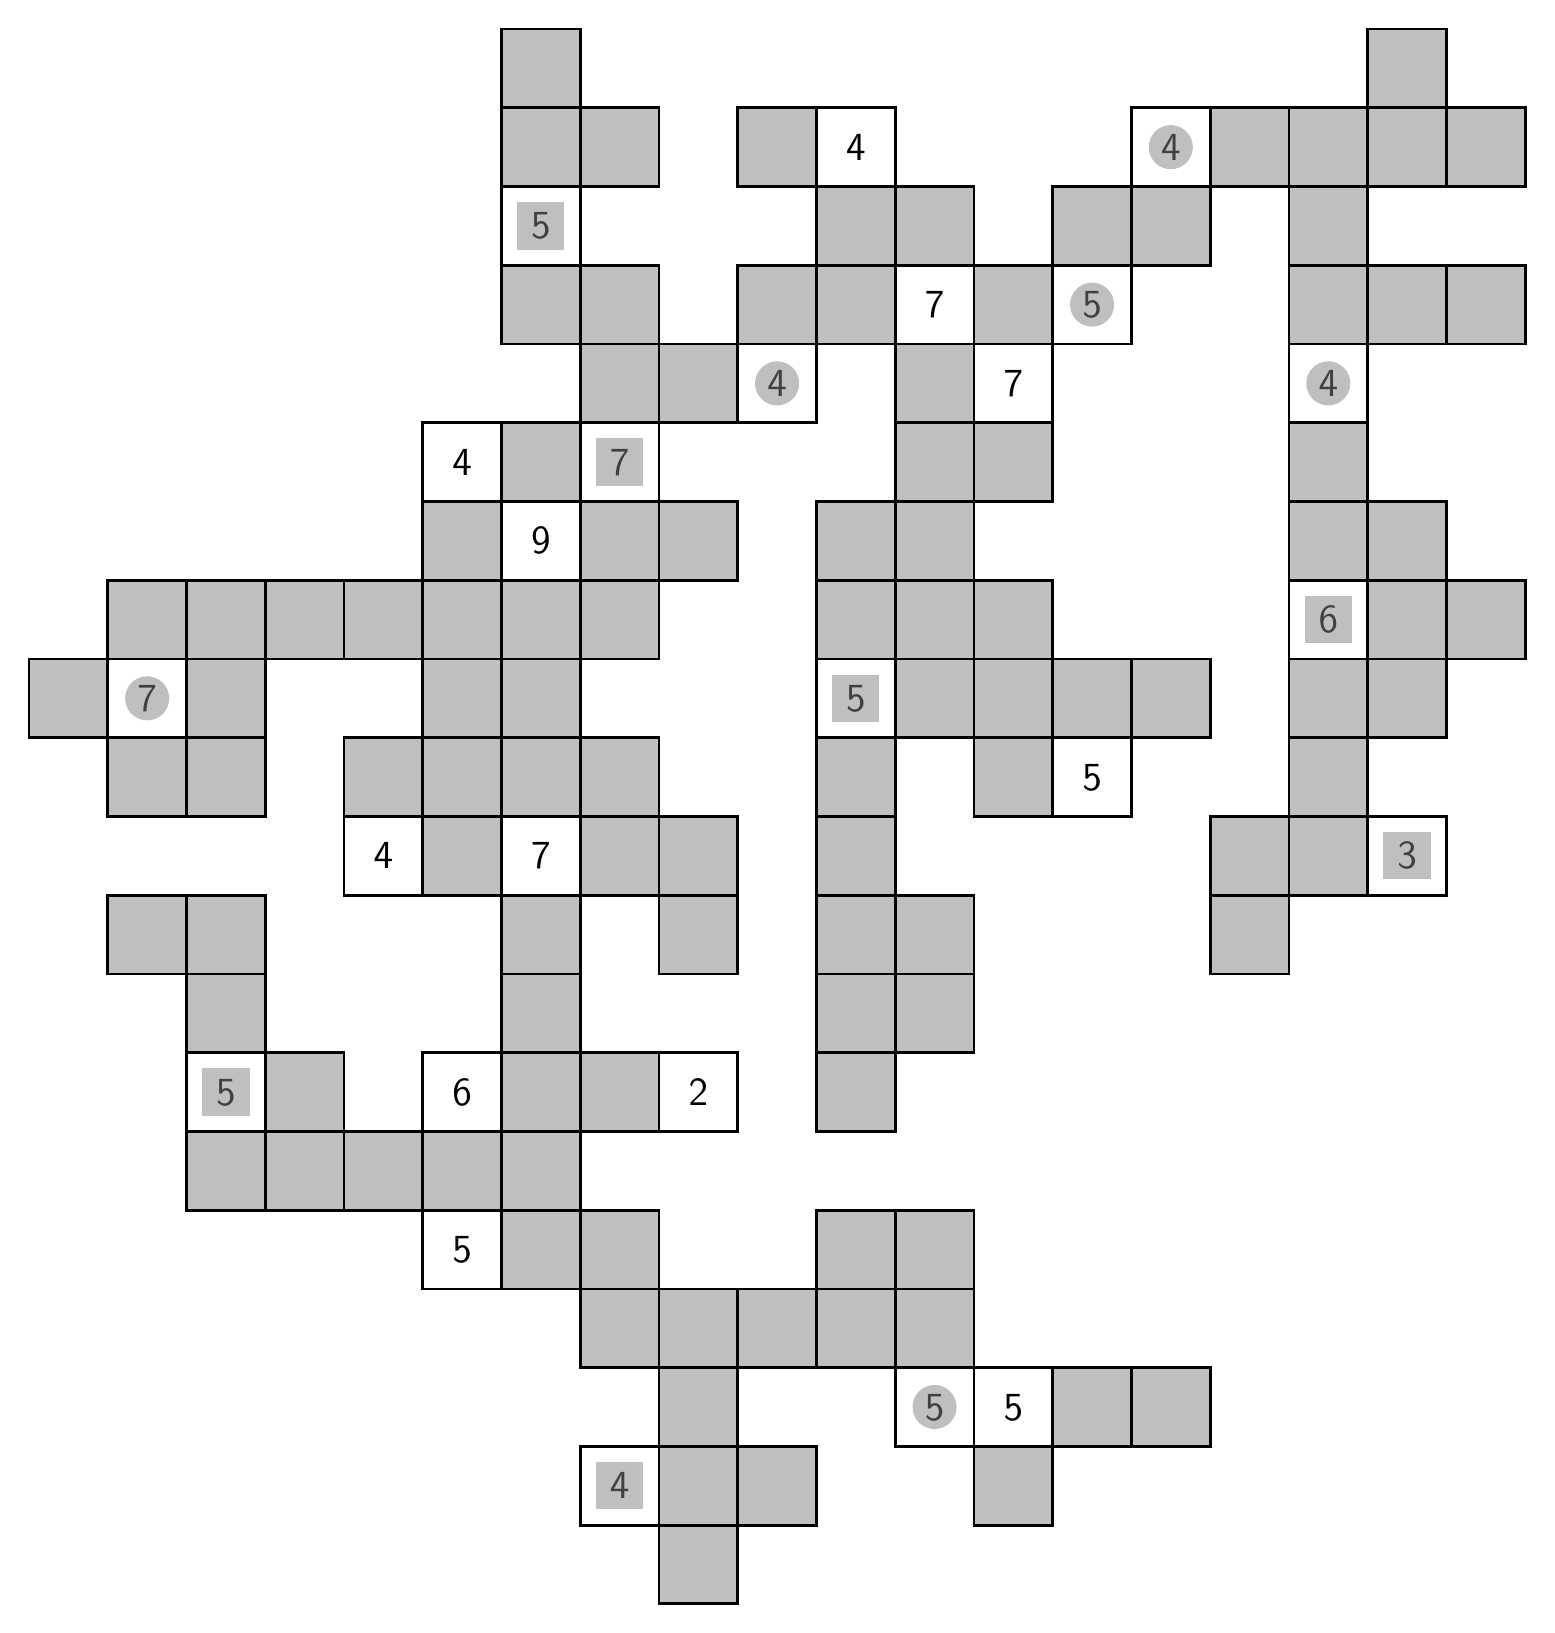
\begin{tikzpicture}\fill[gray, opacity = 0.5] (9, 0, 0)--++(1, 0, 0)--++(0, 1, 0)--++(-1, 0, 0)--cycle;
\draw[line width = 1pt] (9, 0, 0)--++(1, 0, 0)--++(0, 1, 0)--++(-1, 0, 0)--cycle;
\draw node at (8.5, 1.5, 0) {\Large $\mathsf{4}$};
\draw[line width = 1pt] (8, 1, 0)--++(1, 0, 0)--++(0, 1, 0)--++(-1, 0, 0)--cycle;
\fill[color = gray, opacity = 0.5] (8.2, 1.2) rectangle ++(0.6, 0.6);
\fill[gray, opacity = 0.5] (9, 1, 0)--++(1, 0, 0)--++(0, 1, 0)--++(-1, 0, 0)--cycle;
\draw[line width = 1pt] (9, 1, 0)--++(1, 0, 0)--++(0, 1, 0)--++(-1, 0, 0)--cycle;
\fill[gray, opacity = 0.5] (10, 1, 0)--++(1, 0, 0)--++(0, 1, 0)--++(-1, 0, 0)--cycle;
\draw[line width = 1pt] (10, 1, 0)--++(1, 0, 0)--++(0, 1, 0)--++(-1, 0, 0)--cycle;
\fill[gray, opacity = 0.5] (13, 1, 0)--++(1, 0, 0)--++(0, 1, 0)--++(-1, 0, 0)--cycle;
\draw[line width = 1pt] (13, 1, 0)--++(1, 0, 0)--++(0, 1, 0)--++(-1, 0, 0)--cycle;
\fill[gray, opacity = 0.5] (9, 2, 0)--++(1, 0, 0)--++(0, 1, 0)--++(-1, 0, 0)--cycle;
\draw[line width = 1pt] (9, 2, 0)--++(1, 0, 0)--++(0, 1, 0)--++(-1, 0, 0)--cycle;
\draw node at (12.5, 2.5, 0) {\Large $\mathsf{5}$};
\draw[line width = 1pt] (12, 2, 0)--++(1, 0, 0)--++(0, 1, 0)--++(-1, 0, 0)--cycle;
\fill[color = gray, opacity = 0.5] (12.5, 2.5, 0) circle (0.28);
\draw node at (13.5, 2.5, 0) {\Large $\mathsf{5}$};
\draw[line width = 1pt] (13, 2, 0)--++(1, 0, 0)--++(0, 1, 0)--++(-1, 0, 0)--cycle;
\fill[gray, opacity = 0.5] (14, 2, 0)--++(1, 0, 0)--++(0, 1, 0)--++(-1, 0, 0)--cycle;
\draw[line width = 1pt] (14, 2, 0)--++(1, 0, 0)--++(0, 1, 0)--++(-1, 0, 0)--cycle;
\fill[gray, opacity = 0.5] (15, 2, 0)--++(1, 0, 0)--++(0, 1, 0)--++(-1, 0, 0)--cycle;
\draw[line width = 1pt] (15, 2, 0)--++(1, 0, 0)--++(0, 1, 0)--++(-1, 0, 0)--cycle;
\fill[gray, opacity = 0.5] (8, 3, 0)--++(1, 0, 0)--++(0, 1, 0)--++(-1, 0, 0)--cycle;
\draw[line width = 1pt] (8, 3, 0)--++(1, 0, 0)--++(0, 1, 0)--++(-1, 0, 0)--cycle;
\fill[gray, opacity = 0.5] (9, 3, 0)--++(1, 0, 0)--++(0, 1, 0)--++(-1, 0, 0)--cycle;
\draw[line width = 1pt] (9, 3, 0)--++(1, 0, 0)--++(0, 1, 0)--++(-1, 0, 0)--cycle;
\fill[gray, opacity = 0.5] (10, 3, 0)--++(1, 0, 0)--++(0, 1, 0)--++(-1, 0, 0)--cycle;
\draw[line width = 1pt] (10, 3, 0)--++(1, 0, 0)--++(0, 1, 0)--++(-1, 0, 0)--cycle;
\fill[gray, opacity = 0.5] (11, 3, 0)--++(1, 0, 0)--++(0, 1, 0)--++(-1, 0, 0)--cycle;
\draw[line width = 1pt] (11, 3, 0)--++(1, 0, 0)--++(0, 1, 0)--++(-1, 0, 0)--cycle;
\fill[gray, opacity = 0.5] (12, 3, 0)--++(1, 0, 0)--++(0, 1, 0)--++(-1, 0, 0)--cycle;
\draw[line width = 1pt] (12, 3, 0)--++(1, 0, 0)--++(0, 1, 0)--++(-1, 0, 0)--cycle;
\draw node at (6.5, 4.5, 0) {\Large $\mathsf{5}$};
\draw[line width = 1pt] (6, 4, 0)--++(1, 0, 0)--++(0, 1, 0)--++(-1, 0, 0)--cycle;
\fill[gray, opacity = 0.5] (7, 4, 0)--++(1, 0, 0)--++(0, 1, 0)--++(-1, 0, 0)--cycle;
\draw[line width = 1pt] (7, 4, 0)--++(1, 0, 0)--++(0, 1, 0)--++(-1, 0, 0)--cycle;
\fill[gray, opacity = 0.5] (8, 4, 0)--++(1, 0, 0)--++(0, 1, 0)--++(-1, 0, 0)--cycle;
\draw[line width = 1pt] (8, 4, 0)--++(1, 0, 0)--++(0, 1, 0)--++(-1, 0, 0)--cycle;
\fill[gray, opacity = 0.5] (11, 4, 0)--++(1, 0, 0)--++(0, 1, 0)--++(-1, 0, 0)--cycle;
\draw[line width = 1pt] (11, 4, 0)--++(1, 0, 0)--++(0, 1, 0)--++(-1, 0, 0)--cycle;
\fill[gray, opacity = 0.5] (12, 4, 0)--++(1, 0, 0)--++(0, 1, 0)--++(-1, 0, 0)--cycle;
\draw[line width = 1pt] (12, 4, 0)--++(1, 0, 0)--++(0, 1, 0)--++(-1, 0, 0)--cycle;
\fill[gray, opacity = 0.5] (3, 5, 0)--++(1, 0, 0)--++(0, 1, 0)--++(-1, 0, 0)--cycle;
\draw[line width = 1pt] (3, 5, 0)--++(1, 0, 0)--++(0, 1, 0)--++(-1, 0, 0)--cycle;
\fill[gray, opacity = 0.5] (4, 5, 0)--++(1, 0, 0)--++(0, 1, 0)--++(-1, 0, 0)--cycle;
\draw[line width = 1pt] (4, 5, 0)--++(1, 0, 0)--++(0, 1, 0)--++(-1, 0, 0)--cycle;
\fill[gray, opacity = 0.5] (5, 5, 0)--++(1, 0, 0)--++(0, 1, 0)--++(-1, 0, 0)--cycle;
\draw[line width = 1pt] (5, 5, 0)--++(1, 0, 0)--++(0, 1, 0)--++(-1, 0, 0)--cycle;
\fill[gray, opacity = 0.5] (6, 5, 0)--++(1, 0, 0)--++(0, 1, 0)--++(-1, 0, 0)--cycle;
\draw[line width = 1pt] (6, 5, 0)--++(1, 0, 0)--++(0, 1, 0)--++(-1, 0, 0)--cycle;
\fill[gray, opacity = 0.5] (7, 5, 0)--++(1, 0, 0)--++(0, 1, 0)--++(-1, 0, 0)--cycle;
\draw[line width = 1pt] (7, 5, 0)--++(1, 0, 0)--++(0, 1, 0)--++(-1, 0, 0)--cycle;
\draw node at (3.5, 6.5, 0) {\Large $\mathsf{5}$};
\draw[line width = 1pt] (3, 6, 0)--++(1, 0, 0)--++(0, 1, 0)--++(-1, 0, 0)--cycle;
\fill[color = gray, opacity = 0.5] (3.2, 6.2) rectangle ++(0.6, 0.6);
\fill[gray, opacity = 0.5] (4, 6, 0)--++(1, 0, 0)--++(0, 1, 0)--++(-1, 0, 0)--cycle;
\draw[line width = 1pt] (4, 6, 0)--++(1, 0, 0)--++(0, 1, 0)--++(-1, 0, 0)--cycle;
\draw node at (6.5, 6.5, 0) {\Large $\mathsf{6}$};
\draw[line width = 1pt] (6, 6, 0)--++(1, 0, 0)--++(0, 1, 0)--++(-1, 0, 0)--cycle;
\fill[gray, opacity = 0.5] (7, 6, 0)--++(1, 0, 0)--++(0, 1, 0)--++(-1, 0, 0)--cycle;
\draw[line width = 1pt] (7, 6, 0)--++(1, 0, 0)--++(0, 1, 0)--++(-1, 0, 0)--cycle;
\fill[gray, opacity = 0.5] (8, 6, 0)--++(1, 0, 0)--++(0, 1, 0)--++(-1, 0, 0)--cycle;
\draw[line width = 1pt] (8, 6, 0)--++(1, 0, 0)--++(0, 1, 0)--++(-1, 0, 0)--cycle;
\draw node at (9.5, 6.5, 0) {\Large $\mathsf{2}$};
\draw[line width = 1pt] (9, 6, 0)--++(1, 0, 0)--++(0, 1, 0)--++(-1, 0, 0)--cycle;
\fill[gray, opacity = 0.5] (11, 6, 0)--++(1, 0, 0)--++(0, 1, 0)--++(-1, 0, 0)--cycle;
\draw[line width = 1pt] (11, 6, 0)--++(1, 0, 0)--++(0, 1, 0)--++(-1, 0, 0)--cycle;
\fill[gray, opacity = 0.5] (3, 7, 0)--++(1, 0, 0)--++(0, 1, 0)--++(-1, 0, 0)--cycle;
\draw[line width = 1pt] (3, 7, 0)--++(1, 0, 0)--++(0, 1, 0)--++(-1, 0, 0)--cycle;
\fill[gray, opacity = 0.5] (7, 7, 0)--++(1, 0, 0)--++(0, 1, 0)--++(-1, 0, 0)--cycle;
\draw[line width = 1pt] (7, 7, 0)--++(1, 0, 0)--++(0, 1, 0)--++(-1, 0, 0)--cycle;
\fill[gray, opacity = 0.5] (11, 7, 0)--++(1, 0, 0)--++(0, 1, 0)--++(-1, 0, 0)--cycle;
\draw[line width = 1pt] (11, 7, 0)--++(1, 0, 0)--++(0, 1, 0)--++(-1, 0, 0)--cycle;
\fill[gray, opacity = 0.5] (12, 7, 0)--++(1, 0, 0)--++(0, 1, 0)--++(-1, 0, 0)--cycle;
\draw[line width = 1pt] (12, 7, 0)--++(1, 0, 0)--++(0, 1, 0)--++(-1, 0, 0)--cycle;
\fill[gray, opacity = 0.5] (2, 8, 0)--++(1, 0, 0)--++(0, 1, 0)--++(-1, 0, 0)--cycle;
\draw[line width = 1pt] (2, 8, 0)--++(1, 0, 0)--++(0, 1, 0)--++(-1, 0, 0)--cycle;
\fill[gray, opacity = 0.5] (3, 8, 0)--++(1, 0, 0)--++(0, 1, 0)--++(-1, 0, 0)--cycle;
\draw[line width = 1pt] (3, 8, 0)--++(1, 0, 0)--++(0, 1, 0)--++(-1, 0, 0)--cycle;
\fill[gray, opacity = 0.5] (7, 8, 0)--++(1, 0, 0)--++(0, 1, 0)--++(-1, 0, 0)--cycle;
\draw[line width = 1pt] (7, 8, 0)--++(1, 0, 0)--++(0, 1, 0)--++(-1, 0, 0)--cycle;
\fill[gray, opacity = 0.5] (9, 8, 0)--++(1, 0, 0)--++(0, 1, 0)--++(-1, 0, 0)--cycle;
\draw[line width = 1pt] (9, 8, 0)--++(1, 0, 0)--++(0, 1, 0)--++(-1, 0, 0)--cycle;
\fill[gray, opacity = 0.5] (11, 8, 0)--++(1, 0, 0)--++(0, 1, 0)--++(-1, 0, 0)--cycle;
\draw[line width = 1pt] (11, 8, 0)--++(1, 0, 0)--++(0, 1, 0)--++(-1, 0, 0)--cycle;
\fill[gray, opacity = 0.5] (12, 8, 0)--++(1, 0, 0)--++(0, 1, 0)--++(-1, 0, 0)--cycle;
\draw[line width = 1pt] (12, 8, 0)--++(1, 0, 0)--++(0, 1, 0)--++(-1, 0, 0)--cycle;
\fill[gray, opacity = 0.5] (16, 8, 0)--++(1, 0, 0)--++(0, 1, 0)--++(-1, 0, 0)--cycle;
\draw[line width = 1pt] (16, 8, 0)--++(1, 0, 0)--++(0, 1, 0)--++(-1, 0, 0)--cycle;
\draw node at (5.5, 9.5, 0) {\Large $\mathsf{4}$};
\draw[line width = 1pt] (5, 9, 0)--++(1, 0, 0)--++(0, 1, 0)--++(-1, 0, 0)--cycle;
\fill[gray, opacity = 0.5] (6, 9, 0)--++(1, 0, 0)--++(0, 1, 0)--++(-1, 0, 0)--cycle;
\draw[line width = 1pt] (6, 9, 0)--++(1, 0, 0)--++(0, 1, 0)--++(-1, 0, 0)--cycle;
\draw node at (7.5, 9.5, 0) {\Large $\mathsf{7}$};
\draw[line width = 1pt] (7, 9, 0)--++(1, 0, 0)--++(0, 1, 0)--++(-1, 0, 0)--cycle;
\fill[gray, opacity = 0.5] (8, 9, 0)--++(1, 0, 0)--++(0, 1, 0)--++(-1, 0, 0)--cycle;
\draw[line width = 1pt] (8, 9, 0)--++(1, 0, 0)--++(0, 1, 0)--++(-1, 0, 0)--cycle;
\fill[gray, opacity = 0.5] (9, 9, 0)--++(1, 0, 0)--++(0, 1, 0)--++(-1, 0, 0)--cycle;
\draw[line width = 1pt] (9, 9, 0)--++(1, 0, 0)--++(0, 1, 0)--++(-1, 0, 0)--cycle;
\fill[gray, opacity = 0.5] (11, 9, 0)--++(1, 0, 0)--++(0, 1, 0)--++(-1, 0, 0)--cycle;
\draw[line width = 1pt] (11, 9, 0)--++(1, 0, 0)--++(0, 1, 0)--++(-1, 0, 0)--cycle;
\fill[gray, opacity = 0.5] (16, 9, 0)--++(1, 0, 0)--++(0, 1, 0)--++(-1, 0, 0)--cycle;
\draw[line width = 1pt] (16, 9, 0)--++(1, 0, 0)--++(0, 1, 0)--++(-1, 0, 0)--cycle;
\fill[gray, opacity = 0.5] (17, 9, 0)--++(1, 0, 0)--++(0, 1, 0)--++(-1, 0, 0)--cycle;
\draw[line width = 1pt] (17, 9, 0)--++(1, 0, 0)--++(0, 1, 0)--++(-1, 0, 0)--cycle;
\draw node at (18.5, 9.5, 0) {\Large $\mathsf{3}$};
\draw[line width = 1pt] (18, 9, 0)--++(1, 0, 0)--++(0, 1, 0)--++(-1, 0, 0)--cycle;
\fill[color = gray, opacity = 0.5] (18.2, 9.2) rectangle ++(0.6, 0.6);
\fill[gray, opacity = 0.5] (2, 10, 0)--++(1, 0, 0)--++(0, 1, 0)--++(-1, 0, 0)--cycle;
\draw[line width = 1pt] (2, 10, 0)--++(1, 0, 0)--++(0, 1, 0)--++(-1, 0, 0)--cycle;
\fill[gray, opacity = 0.5] (3, 10, 0)--++(1, 0, 0)--++(0, 1, 0)--++(-1, 0, 0)--cycle;
\draw[line width = 1pt] (3, 10, 0)--++(1, 0, 0)--++(0, 1, 0)--++(-1, 0, 0)--cycle;
\fill[gray, opacity = 0.5] (5, 10, 0)--++(1, 0, 0)--++(0, 1, 0)--++(-1, 0, 0)--cycle;
\draw[line width = 1pt] (5, 10, 0)--++(1, 0, 0)--++(0, 1, 0)--++(-1, 0, 0)--cycle;
\fill[gray, opacity = 0.5] (6, 10, 0)--++(1, 0, 0)--++(0, 1, 0)--++(-1, 0, 0)--cycle;
\draw[line width = 1pt] (6, 10, 0)--++(1, 0, 0)--++(0, 1, 0)--++(-1, 0, 0)--cycle;
\fill[gray, opacity = 0.5] (7, 10, 0)--++(1, 0, 0)--++(0, 1, 0)--++(-1, 0, 0)--cycle;
\draw[line width = 1pt] (7, 10, 0)--++(1, 0, 0)--++(0, 1, 0)--++(-1, 0, 0)--cycle;
\fill[gray, opacity = 0.5] (8, 10, 0)--++(1, 0, 0)--++(0, 1, 0)--++(-1, 0, 0)--cycle;
\draw[line width = 1pt] (8, 10, 0)--++(1, 0, 0)--++(0, 1, 0)--++(-1, 0, 0)--cycle;
\fill[gray, opacity = 0.5] (11, 10, 0)--++(1, 0, 0)--++(0, 1, 0)--++(-1, 0, 0)--cycle;
\draw[line width = 1pt] (11, 10, 0)--++(1, 0, 0)--++(0, 1, 0)--++(-1, 0, 0)--cycle;
\fill[gray, opacity = 0.5] (13, 10, 0)--++(1, 0, 0)--++(0, 1, 0)--++(-1, 0, 0)--cycle;
\draw[line width = 1pt] (13, 10, 0)--++(1, 0, 0)--++(0, 1, 0)--++(-1, 0, 0)--cycle;
\draw node at (14.5, 10.5, 0) {\Large $\mathsf{5}$};
\draw[line width = 1pt] (14, 10, 0)--++(1, 0, 0)--++(0, 1, 0)--++(-1, 0, 0)--cycle;
\fill[gray, opacity = 0.5] (17, 10, 0)--++(1, 0, 0)--++(0, 1, 0)--++(-1, 0, 0)--cycle;
\draw[line width = 1pt] (17, 10, 0)--++(1, 0, 0)--++(0, 1, 0)--++(-1, 0, 0)--cycle;
\fill[gray, opacity = 0.5] (1, 11, 0)--++(1, 0, 0)--++(0, 1, 0)--++(-1, 0, 0)--cycle;
\draw[line width = 1pt] (1, 11, 0)--++(1, 0, 0)--++(0, 1, 0)--++(-1, 0, 0)--cycle;
\draw node at (2.5, 11.5, 0) {\Large $\mathsf{7}$};
\draw[line width = 1pt] (2, 11, 0)--++(1, 0, 0)--++(0, 1, 0)--++(-1, 0, 0)--cycle;
\fill[color = gray, opacity = 0.5] (2.5, 11.5, 0) circle (0.28);
\fill[gray, opacity = 0.5] (3, 11, 0)--++(1, 0, 0)--++(0, 1, 0)--++(-1, 0, 0)--cycle;
\draw[line width = 1pt] (3, 11, 0)--++(1, 0, 0)--++(0, 1, 0)--++(-1, 0, 0)--cycle;
\fill[gray, opacity = 0.5] (6, 11, 0)--++(1, 0, 0)--++(0, 1, 0)--++(-1, 0, 0)--cycle;
\draw[line width = 1pt] (6, 11, 0)--++(1, 0, 0)--++(0, 1, 0)--++(-1, 0, 0)--cycle;
\fill[gray, opacity = 0.5] (7, 11, 0)--++(1, 0, 0)--++(0, 1, 0)--++(-1, 0, 0)--cycle;
\draw[line width = 1pt] (7, 11, 0)--++(1, 0, 0)--++(0, 1, 0)--++(-1, 0, 0)--cycle;
\draw node at (11.5, 11.5, 0) {\Large $\mathsf{5}$};
\draw[line width = 1pt] (11, 11, 0)--++(1, 0, 0)--++(0, 1, 0)--++(-1, 0, 0)--cycle;
\fill[color = gray, opacity = 0.5] (11.2, 11.2) rectangle ++(0.6, 0.6);
\fill[gray, opacity = 0.5] (12, 11, 0)--++(1, 0, 0)--++(0, 1, 0)--++(-1, 0, 0)--cycle;
\draw[line width = 1pt] (12, 11, 0)--++(1, 0, 0)--++(0, 1, 0)--++(-1, 0, 0)--cycle;
\fill[gray, opacity = 0.5] (13, 11, 0)--++(1, 0, 0)--++(0, 1, 0)--++(-1, 0, 0)--cycle;
\draw[line width = 1pt] (13, 11, 0)--++(1, 0, 0)--++(0, 1, 0)--++(-1, 0, 0)--cycle;
\fill[gray, opacity = 0.5] (14, 11, 0)--++(1, 0, 0)--++(0, 1, 0)--++(-1, 0, 0)--cycle;
\draw[line width = 1pt] (14, 11, 0)--++(1, 0, 0)--++(0, 1, 0)--++(-1, 0, 0)--cycle;
\fill[gray, opacity = 0.5] (15, 11, 0)--++(1, 0, 0)--++(0, 1, 0)--++(-1, 0, 0)--cycle;
\draw[line width = 1pt] (15, 11, 0)--++(1, 0, 0)--++(0, 1, 0)--++(-1, 0, 0)--cycle;
\fill[gray, opacity = 0.5] (17, 11, 0)--++(1, 0, 0)--++(0, 1, 0)--++(-1, 0, 0)--cycle;
\draw[line width = 1pt] (17, 11, 0)--++(1, 0, 0)--++(0, 1, 0)--++(-1, 0, 0)--cycle;
\fill[gray, opacity = 0.5] (18, 11, 0)--++(1, 0, 0)--++(0, 1, 0)--++(-1, 0, 0)--cycle;
\draw[line width = 1pt] (18, 11, 0)--++(1, 0, 0)--++(0, 1, 0)--++(-1, 0, 0)--cycle;
\fill[gray, opacity = 0.5] (2, 12, 0)--++(1, 0, 0)--++(0, 1, 0)--++(-1, 0, 0)--cycle;
\draw[line width = 1pt] (2, 12, 0)--++(1, 0, 0)--++(0, 1, 0)--++(-1, 0, 0)--cycle;
\fill[gray, opacity = 0.5] (3, 12, 0)--++(1, 0, 0)--++(0, 1, 0)--++(-1, 0, 0)--cycle;
\draw[line width = 1pt] (3, 12, 0)--++(1, 0, 0)--++(0, 1, 0)--++(-1, 0, 0)--cycle;
\fill[gray, opacity = 0.5] (4, 12, 0)--++(1, 0, 0)--++(0, 1, 0)--++(-1, 0, 0)--cycle;
\draw[line width = 1pt] (4, 12, 0)--++(1, 0, 0)--++(0, 1, 0)--++(-1, 0, 0)--cycle;
\fill[gray, opacity = 0.5] (5, 12, 0)--++(1, 0, 0)--++(0, 1, 0)--++(-1, 0, 0)--cycle;
\draw[line width = 1pt] (5, 12, 0)--++(1, 0, 0)--++(0, 1, 0)--++(-1, 0, 0)--cycle;
\fill[gray, opacity = 0.5] (6, 12, 0)--++(1, 0, 0)--++(0, 1, 0)--++(-1, 0, 0)--cycle;
\draw[line width = 1pt] (6, 12, 0)--++(1, 0, 0)--++(0, 1, 0)--++(-1, 0, 0)--cycle;
\fill[gray, opacity = 0.5] (7, 12, 0)--++(1, 0, 0)--++(0, 1, 0)--++(-1, 0, 0)--cycle;
\draw[line width = 1pt] (7, 12, 0)--++(1, 0, 0)--++(0, 1, 0)--++(-1, 0, 0)--cycle;
\fill[gray, opacity = 0.5] (8, 12, 0)--++(1, 0, 0)--++(0, 1, 0)--++(-1, 0, 0)--cycle;
\draw[line width = 1pt] (8, 12, 0)--++(1, 0, 0)--++(0, 1, 0)--++(-1, 0, 0)--cycle;
\fill[gray, opacity = 0.5] (11, 12, 0)--++(1, 0, 0)--++(0, 1, 0)--++(-1, 0, 0)--cycle;
\draw[line width = 1pt] (11, 12, 0)--++(1, 0, 0)--++(0, 1, 0)--++(-1, 0, 0)--cycle;
\fill[gray, opacity = 0.5] (12, 12, 0)--++(1, 0, 0)--++(0, 1, 0)--++(-1, 0, 0)--cycle;
\draw[line width = 1pt] (12, 12, 0)--++(1, 0, 0)--++(0, 1, 0)--++(-1, 0, 0)--cycle;
\fill[gray, opacity = 0.5] (13, 12, 0)--++(1, 0, 0)--++(0, 1, 0)--++(-1, 0, 0)--cycle;
\draw[line width = 1pt] (13, 12, 0)--++(1, 0, 0)--++(0, 1, 0)--++(-1, 0, 0)--cycle;
\draw node at (17.5, 12.5, 0) {\Large $\mathsf{6}$};
\draw[line width = 1pt] (17, 12, 0)--++(1, 0, 0)--++(0, 1, 0)--++(-1, 0, 0)--cycle;
\fill[color = gray, opacity = 0.5] (17.2, 12.2) rectangle ++(0.6, 0.6);
\fill[gray, opacity = 0.5] (18, 12, 0)--++(1, 0, 0)--++(0, 1, 0)--++(-1, 0, 0)--cycle;
\draw[line width = 1pt] (18, 12, 0)--++(1, 0, 0)--++(0, 1, 0)--++(-1, 0, 0)--cycle;
\fill[gray, opacity = 0.5] (19, 12, 0)--++(1, 0, 0)--++(0, 1, 0)--++(-1, 0, 0)--cycle;
\draw[line width = 1pt] (19, 12, 0)--++(1, 0, 0)--++(0, 1, 0)--++(-1, 0, 0)--cycle;
\fill[gray, opacity = 0.5] (6, 13, 0)--++(1, 0, 0)--++(0, 1, 0)--++(-1, 0, 0)--cycle;
\draw[line width = 1pt] (6, 13, 0)--++(1, 0, 0)--++(0, 1, 0)--++(-1, 0, 0)--cycle;
\draw node at (7.5, 13.5, 0) {\Large $\mathsf{9}$};
\draw[line width = 1pt] (7, 13, 0)--++(1, 0, 0)--++(0, 1, 0)--++(-1, 0, 0)--cycle;
\fill[gray, opacity = 0.5] (8, 13, 0)--++(1, 0, 0)--++(0, 1, 0)--++(-1, 0, 0)--cycle;
\draw[line width = 1pt] (8, 13, 0)--++(1, 0, 0)--++(0, 1, 0)--++(-1, 0, 0)--cycle;
\fill[gray, opacity = 0.5] (9, 13, 0)--++(1, 0, 0)--++(0, 1, 0)--++(-1, 0, 0)--cycle;
\draw[line width = 1pt] (9, 13, 0)--++(1, 0, 0)--++(0, 1, 0)--++(-1, 0, 0)--cycle;
\fill[gray, opacity = 0.5] (11, 13, 0)--++(1, 0, 0)--++(0, 1, 0)--++(-1, 0, 0)--cycle;
\draw[line width = 1pt] (11, 13, 0)--++(1, 0, 0)--++(0, 1, 0)--++(-1, 0, 0)--cycle;
\fill[gray, opacity = 0.5] (12, 13, 0)--++(1, 0, 0)--++(0, 1, 0)--++(-1, 0, 0)--cycle;
\draw[line width = 1pt] (12, 13, 0)--++(1, 0, 0)--++(0, 1, 0)--++(-1, 0, 0)--cycle;
\fill[gray, opacity = 0.5] (17, 13, 0)--++(1, 0, 0)--++(0, 1, 0)--++(-1, 0, 0)--cycle;
\draw[line width = 1pt] (17, 13, 0)--++(1, 0, 0)--++(0, 1, 0)--++(-1, 0, 0)--cycle;
\fill[gray, opacity = 0.5] (18, 13, 0)--++(1, 0, 0)--++(0, 1, 0)--++(-1, 0, 0)--cycle;
\draw[line width = 1pt] (18, 13, 0)--++(1, 0, 0)--++(0, 1, 0)--++(-1, 0, 0)--cycle;
\draw node at (6.5, 14.5, 0) {\Large $\mathsf{4}$};
\draw[line width = 1pt] (6, 14, 0)--++(1, 0, 0)--++(0, 1, 0)--++(-1, 0, 0)--cycle;
\fill[gray, opacity = 0.5] (7, 14, 0)--++(1, 0, 0)--++(0, 1, 0)--++(-1, 0, 0)--cycle;
\draw[line width = 1pt] (7, 14, 0)--++(1, 0, 0)--++(0, 1, 0)--++(-1, 0, 0)--cycle;
\draw node at (8.5, 14.5, 0) {\Large $\mathsf{7}$};
\draw[line width = 1pt] (8, 14, 0)--++(1, 0, 0)--++(0, 1, 0)--++(-1, 0, 0)--cycle;
\fill[color = gray, opacity = 0.5] (8.2, 14.2) rectangle ++(0.6, 0.6);
\fill[gray, opacity = 0.5] (12, 14, 0)--++(1, 0, 0)--++(0, 1, 0)--++(-1, 0, 0)--cycle;
\draw[line width = 1pt] (12, 14, 0)--++(1, 0, 0)--++(0, 1, 0)--++(-1, 0, 0)--cycle;
\fill[gray, opacity = 0.5] (13, 14, 0)--++(1, 0, 0)--++(0, 1, 0)--++(-1, 0, 0)--cycle;
\draw[line width = 1pt] (13, 14, 0)--++(1, 0, 0)--++(0, 1, 0)--++(-1, 0, 0)--cycle;
\fill[gray, opacity = 0.5] (17, 14, 0)--++(1, 0, 0)--++(0, 1, 0)--++(-1, 0, 0)--cycle;
\draw[line width = 1pt] (17, 14, 0)--++(1, 0, 0)--++(0, 1, 0)--++(-1, 0, 0)--cycle;
\fill[gray, opacity = 0.5] (8, 15, 0)--++(1, 0, 0)--++(0, 1, 0)--++(-1, 0, 0)--cycle;
\draw[line width = 1pt] (8, 15, 0)--++(1, 0, 0)--++(0, 1, 0)--++(-1, 0, 0)--cycle;
\fill[gray, opacity = 0.5] (9, 15, 0)--++(1, 0, 0)--++(0, 1, 0)--++(-1, 0, 0)--cycle;
\draw[line width = 1pt] (9, 15, 0)--++(1, 0, 0)--++(0, 1, 0)--++(-1, 0, 0)--cycle;
\draw node at (10.5, 15.5, 0) {\Large $\mathsf{4}$};
\draw[line width = 1pt] (10, 15, 0)--++(1, 0, 0)--++(0, 1, 0)--++(-1, 0, 0)--cycle;
\fill[color = gray, opacity = 0.5] (10.5, 15.5, 0) circle (0.28);
\fill[gray, opacity = 0.5] (12, 15, 0)--++(1, 0, 0)--++(0, 1, 0)--++(-1, 0, 0)--cycle;
\draw[line width = 1pt] (12, 15, 0)--++(1, 0, 0)--++(0, 1, 0)--++(-1, 0, 0)--cycle;
\draw node at (13.5, 15.5, 0) {\Large $\mathsf{7}$};
\draw[line width = 1pt] (13, 15, 0)--++(1, 0, 0)--++(0, 1, 0)--++(-1, 0, 0)--cycle;
\draw node at (17.5, 15.5, 0) {\Large $\mathsf{4}$};
\draw[line width = 1pt] (17, 15, 0)--++(1, 0, 0)--++(0, 1, 0)--++(-1, 0, 0)--cycle;
\fill[color = gray, opacity = 0.5] (17.5, 15.5, 0) circle (0.28);
\fill[gray, opacity = 0.5] (7, 16, 0)--++(1, 0, 0)--++(0, 1, 0)--++(-1, 0, 0)--cycle;
\draw[line width = 1pt] (7, 16, 0)--++(1, 0, 0)--++(0, 1, 0)--++(-1, 0, 0)--cycle;
\fill[gray, opacity = 0.5] (8, 16, 0)--++(1, 0, 0)--++(0, 1, 0)--++(-1, 0, 0)--cycle;
\draw[line width = 1pt] (8, 16, 0)--++(1, 0, 0)--++(0, 1, 0)--++(-1, 0, 0)--cycle;
\fill[gray, opacity = 0.5] (10, 16, 0)--++(1, 0, 0)--++(0, 1, 0)--++(-1, 0, 0)--cycle;
\draw[line width = 1pt] (10, 16, 0)--++(1, 0, 0)--++(0, 1, 0)--++(-1, 0, 0)--cycle;
\fill[gray, opacity = 0.5] (11, 16, 0)--++(1, 0, 0)--++(0, 1, 0)--++(-1, 0, 0)--cycle;
\draw[line width = 1pt] (11, 16, 0)--++(1, 0, 0)--++(0, 1, 0)--++(-1, 0, 0)--cycle;
\draw node at (12.5, 16.5, 0) {\Large $\mathsf{7}$};
\draw[line width = 1pt] (12, 16, 0)--++(1, 0, 0)--++(0, 1, 0)--++(-1, 0, 0)--cycle;
\fill[gray, opacity = 0.5] (13, 16, 0)--++(1, 0, 0)--++(0, 1, 0)--++(-1, 0, 0)--cycle;
\draw[line width = 1pt] (13, 16, 0)--++(1, 0, 0)--++(0, 1, 0)--++(-1, 0, 0)--cycle;
\draw node at (14.5, 16.5, 0) {\Large $\mathsf{5}$};
\draw[line width = 1pt] (14, 16, 0)--++(1, 0, 0)--++(0, 1, 0)--++(-1, 0, 0)--cycle;
\fill[color = gray, opacity = 0.5] (14.5, 16.5, 0) circle (0.28);
\fill[gray, opacity = 0.5] (17, 16, 0)--++(1, 0, 0)--++(0, 1, 0)--++(-1, 0, 0)--cycle;
\draw[line width = 1pt] (17, 16, 0)--++(1, 0, 0)--++(0, 1, 0)--++(-1, 0, 0)--cycle;
\fill[gray, opacity = 0.5] (18, 16, 0)--++(1, 0, 0)--++(0, 1, 0)--++(-1, 0, 0)--cycle;
\draw[line width = 1pt] (18, 16, 0)--++(1, 0, 0)--++(0, 1, 0)--++(-1, 0, 0)--cycle;
\fill[gray, opacity = 0.5] (19, 16, 0)--++(1, 0, 0)--++(0, 1, 0)--++(-1, 0, 0)--cycle;
\draw[line width = 1pt] (19, 16, 0)--++(1, 0, 0)--++(0, 1, 0)--++(-1, 0, 0)--cycle;
\draw node at (7.5, 17.5, 0) {\Large $\mathsf{5}$};
\draw[line width = 1pt] (7, 17, 0)--++(1, 0, 0)--++(0, 1, 0)--++(-1, 0, 0)--cycle;
\fill[color = gray, opacity = 0.5] (7.2, 17.2) rectangle ++(0.6, 0.6);
\fill[gray, opacity = 0.5] (11, 17, 0)--++(1, 0, 0)--++(0, 1, 0)--++(-1, 0, 0)--cycle;
\draw[line width = 1pt] (11, 17, 0)--++(1, 0, 0)--++(0, 1, 0)--++(-1, 0, 0)--cycle;
\fill[gray, opacity = 0.5] (12, 17, 0)--++(1, 0, 0)--++(0, 1, 0)--++(-1, 0, 0)--cycle;
\draw[line width = 1pt] (12, 17, 0)--++(1, 0, 0)--++(0, 1, 0)--++(-1, 0, 0)--cycle;
\fill[gray, opacity = 0.5] (14, 17, 0)--++(1, 0, 0)--++(0, 1, 0)--++(-1, 0, 0)--cycle;
\draw[line width = 1pt] (14, 17, 0)--++(1, 0, 0)--++(0, 1, 0)--++(-1, 0, 0)--cycle;
\fill[gray, opacity = 0.5] (15, 17, 0)--++(1, 0, 0)--++(0, 1, 0)--++(-1, 0, 0)--cycle;
\draw[line width = 1pt] (15, 17, 0)--++(1, 0, 0)--++(0, 1, 0)--++(-1, 0, 0)--cycle;
\fill[gray, opacity = 0.5] (17, 17, 0)--++(1, 0, 0)--++(0, 1, 0)--++(-1, 0, 0)--cycle;
\draw[line width = 1pt] (17, 17, 0)--++(1, 0, 0)--++(0, 1, 0)--++(-1, 0, 0)--cycle;
\fill[gray, opacity = 0.5] (7, 18, 0)--++(1, 0, 0)--++(0, 1, 0)--++(-1, 0, 0)--cycle;
\draw[line width = 1pt] (7, 18, 0)--++(1, 0, 0)--++(0, 1, 0)--++(-1, 0, 0)--cycle;
\fill[gray, opacity = 0.5] (8, 18, 0)--++(1, 0, 0)--++(0, 1, 0)--++(-1, 0, 0)--cycle;
\draw[line width = 1pt] (8, 18, 0)--++(1, 0, 0)--++(0, 1, 0)--++(-1, 0, 0)--cycle;
\fill[gray, opacity = 0.5] (10, 18, 0)--++(1, 0, 0)--++(0, 1, 0)--++(-1, 0, 0)--cycle;
\draw[line width = 1pt] (10, 18, 0)--++(1, 0, 0)--++(0, 1, 0)--++(-1, 0, 0)--cycle;
\draw node at (11.5, 18.5, 0) {\Large $\mathsf{4}$};
\draw[line width = 1pt] (11, 18, 0)--++(1, 0, 0)--++(0, 1, 0)--++(-1, 0, 0)--cycle;
\draw node at (15.5, 18.5, 0) {\Large $\mathsf{4}$};
\draw[line width = 1pt] (15, 18, 0)--++(1, 0, 0)--++(0, 1, 0)--++(-1, 0, 0)--cycle;
\fill[color = gray, opacity = 0.5] (15.5, 18.5, 0) circle (0.28);
\fill[gray, opacity = 0.5] (16, 18, 0)--++(1, 0, 0)--++(0, 1, 0)--++(-1, 0, 0)--cycle;
\draw[line width = 1pt] (16, 18, 0)--++(1, 0, 0)--++(0, 1, 0)--++(-1, 0, 0)--cycle;
\fill[gray, opacity = 0.5] (17, 18, 0)--++(1, 0, 0)--++(0, 1, 0)--++(-1, 0, 0)--cycle;
\draw[line width = 1pt] (17, 18, 0)--++(1, 0, 0)--++(0, 1, 0)--++(-1, 0, 0)--cycle;
\fill[gray, opacity = 0.5] (18, 18, 0)--++(1, 0, 0)--++(0, 1, 0)--++(-1, 0, 0)--cycle;
\draw[line width = 1pt] (18, 18, 0)--++(1, 0, 0)--++(0, 1, 0)--++(-1, 0, 0)--cycle;
\fill[gray, opacity = 0.5] (19, 18, 0)--++(1, 0, 0)--++(0, 1, 0)--++(-1, 0, 0)--cycle;
\draw[line width = 1pt] (19, 18, 0)--++(1, 0, 0)--++(0, 1, 0)--++(-1, 0, 0)--cycle;
\fill[gray, opacity = 0.5] (7, 19, 0)--++(1, 0, 0)--++(0, 1, 0)--++(-1, 0, 0)--cycle;
\draw[line width = 1pt] (7, 19, 0)--++(1, 0, 0)--++(0, 1, 0)--++(-1, 0, 0)--cycle;
\fill[gray, opacity = 0.5] (18, 19, 0)--++(1, 0, 0)--++(0, 1, 0)--++(-1, 0, 0)--cycle;
\draw[line width = 1pt] (18, 19, 0)--++(1, 0, 0)--++(0, 1, 0)--++(-1, 0, 0)--cycle;
\end{tikzpicture}}\]
\[\resizebox{30pc}{!}{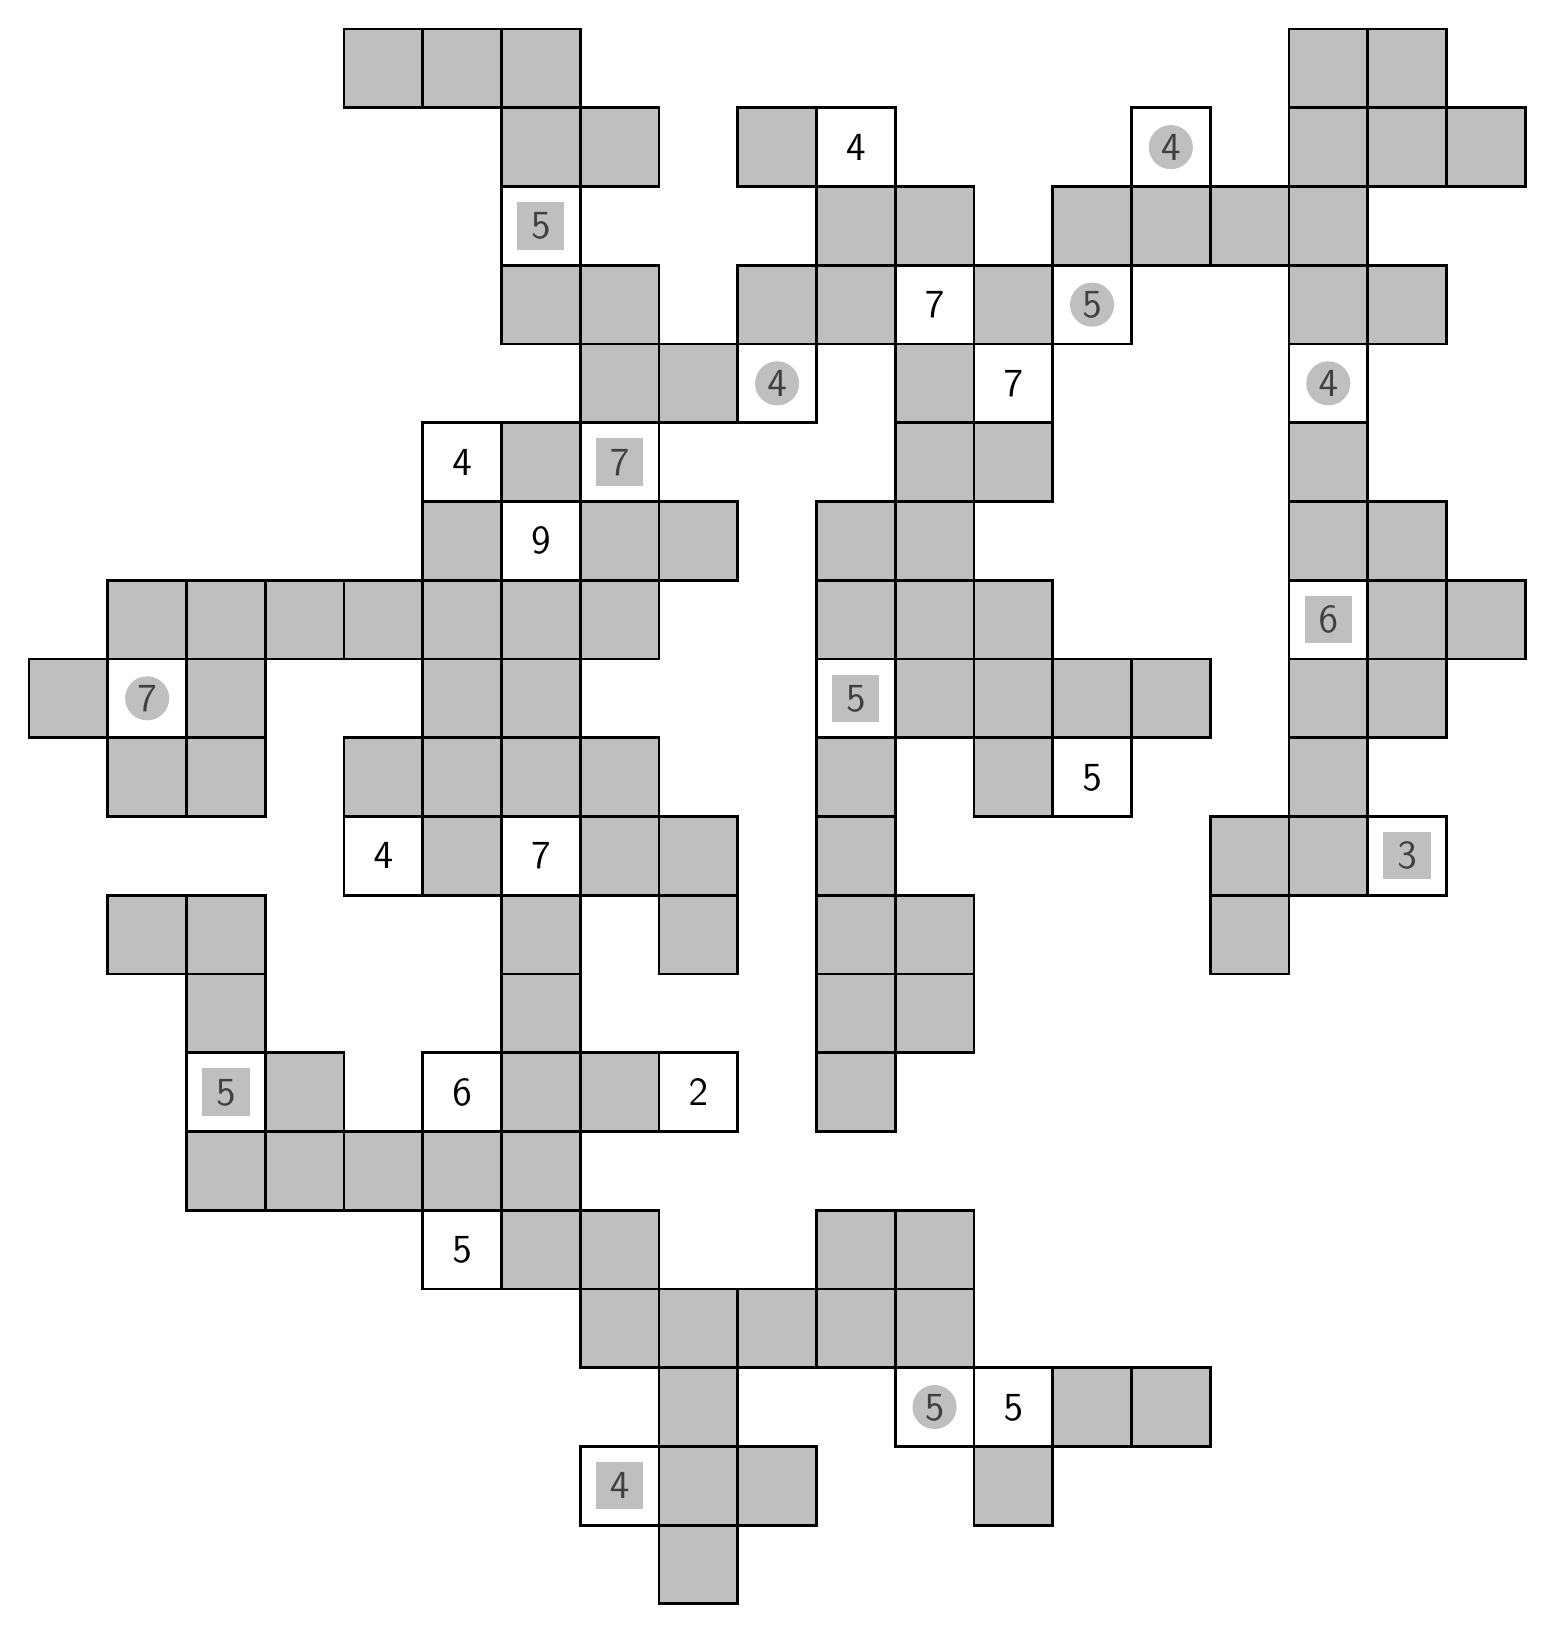
\begin{tikzpicture}\fill[gray, opacity = 0.5] (9, 0, 0)--++(1, 0, 0)--++(0, 1, 0)--++(-1, 0, 0)--cycle;
\draw[line width = 1pt] (9, 0, 0)--++(1, 0, 0)--++(0, 1, 0)--++(-1, 0, 0)--cycle;
\draw node at (8.5, 1.5, 0) {\Large $\mathsf{4}$};
\draw[line width = 1pt] (8, 1, 0)--++(1, 0, 0)--++(0, 1, 0)--++(-1, 0, 0)--cycle;
\fill[color = gray, opacity = 0.5] (8.2, 1.2) rectangle ++(0.6, 0.6);
\fill[gray, opacity = 0.5] (9, 1, 0)--++(1, 0, 0)--++(0, 1, 0)--++(-1, 0, 0)--cycle;
\draw[line width = 1pt] (9, 1, 0)--++(1, 0, 0)--++(0, 1, 0)--++(-1, 0, 0)--cycle;
\fill[gray, opacity = 0.5] (10, 1, 0)--++(1, 0, 0)--++(0, 1, 0)--++(-1, 0, 0)--cycle;
\draw[line width = 1pt] (10, 1, 0)--++(1, 0, 0)--++(0, 1, 0)--++(-1, 0, 0)--cycle;
\fill[gray, opacity = 0.5] (13, 1, 0)--++(1, 0, 0)--++(0, 1, 0)--++(-1, 0, 0)--cycle;
\draw[line width = 1pt] (13, 1, 0)--++(1, 0, 0)--++(0, 1, 0)--++(-1, 0, 0)--cycle;
\fill[gray, opacity = 0.5] (9, 2, 0)--++(1, 0, 0)--++(0, 1, 0)--++(-1, 0, 0)--cycle;
\draw[line width = 1pt] (9, 2, 0)--++(1, 0, 0)--++(0, 1, 0)--++(-1, 0, 0)--cycle;
\draw node at (12.5, 2.5, 0) {\Large $\mathsf{5}$};
\draw[line width = 1pt] (12, 2, 0)--++(1, 0, 0)--++(0, 1, 0)--++(-1, 0, 0)--cycle;
\fill[color = gray, opacity = 0.5] (12.5, 2.5, 0) circle (0.28);
\draw node at (13.5, 2.5, 0) {\Large $\mathsf{5}$};
\draw[line width = 1pt] (13, 2, 0)--++(1, 0, 0)--++(0, 1, 0)--++(-1, 0, 0)--cycle;
\fill[gray, opacity = 0.5] (14, 2, 0)--++(1, 0, 0)--++(0, 1, 0)--++(-1, 0, 0)--cycle;
\draw[line width = 1pt] (14, 2, 0)--++(1, 0, 0)--++(0, 1, 0)--++(-1, 0, 0)--cycle;
\fill[gray, opacity = 0.5] (15, 2, 0)--++(1, 0, 0)--++(0, 1, 0)--++(-1, 0, 0)--cycle;
\draw[line width = 1pt] (15, 2, 0)--++(1, 0, 0)--++(0, 1, 0)--++(-1, 0, 0)--cycle;
\fill[gray, opacity = 0.5] (8, 3, 0)--++(1, 0, 0)--++(0, 1, 0)--++(-1, 0, 0)--cycle;
\draw[line width = 1pt] (8, 3, 0)--++(1, 0, 0)--++(0, 1, 0)--++(-1, 0, 0)--cycle;
\fill[gray, opacity = 0.5] (9, 3, 0)--++(1, 0, 0)--++(0, 1, 0)--++(-1, 0, 0)--cycle;
\draw[line width = 1pt] (9, 3, 0)--++(1, 0, 0)--++(0, 1, 0)--++(-1, 0, 0)--cycle;
\fill[gray, opacity = 0.5] (10, 3, 0)--++(1, 0, 0)--++(0, 1, 0)--++(-1, 0, 0)--cycle;
\draw[line width = 1pt] (10, 3, 0)--++(1, 0, 0)--++(0, 1, 0)--++(-1, 0, 0)--cycle;
\fill[gray, opacity = 0.5] (11, 3, 0)--++(1, 0, 0)--++(0, 1, 0)--++(-1, 0, 0)--cycle;
\draw[line width = 1pt] (11, 3, 0)--++(1, 0, 0)--++(0, 1, 0)--++(-1, 0, 0)--cycle;
\fill[gray, opacity = 0.5] (12, 3, 0)--++(1, 0, 0)--++(0, 1, 0)--++(-1, 0, 0)--cycle;
\draw[line width = 1pt] (12, 3, 0)--++(1, 0, 0)--++(0, 1, 0)--++(-1, 0, 0)--cycle;
\draw node at (6.5, 4.5, 0) {\Large $\mathsf{5}$};
\draw[line width = 1pt] (6, 4, 0)--++(1, 0, 0)--++(0, 1, 0)--++(-1, 0, 0)--cycle;
\fill[gray, opacity = 0.5] (7, 4, 0)--++(1, 0, 0)--++(0, 1, 0)--++(-1, 0, 0)--cycle;
\draw[line width = 1pt] (7, 4, 0)--++(1, 0, 0)--++(0, 1, 0)--++(-1, 0, 0)--cycle;
\fill[gray, opacity = 0.5] (8, 4, 0)--++(1, 0, 0)--++(0, 1, 0)--++(-1, 0, 0)--cycle;
\draw[line width = 1pt] (8, 4, 0)--++(1, 0, 0)--++(0, 1, 0)--++(-1, 0, 0)--cycle;
\fill[gray, opacity = 0.5] (11, 4, 0)--++(1, 0, 0)--++(0, 1, 0)--++(-1, 0, 0)--cycle;
\draw[line width = 1pt] (11, 4, 0)--++(1, 0, 0)--++(0, 1, 0)--++(-1, 0, 0)--cycle;
\fill[gray, opacity = 0.5] (12, 4, 0)--++(1, 0, 0)--++(0, 1, 0)--++(-1, 0, 0)--cycle;
\draw[line width = 1pt] (12, 4, 0)--++(1, 0, 0)--++(0, 1, 0)--++(-1, 0, 0)--cycle;
\fill[gray, opacity = 0.5] (3, 5, 0)--++(1, 0, 0)--++(0, 1, 0)--++(-1, 0, 0)--cycle;
\draw[line width = 1pt] (3, 5, 0)--++(1, 0, 0)--++(0, 1, 0)--++(-1, 0, 0)--cycle;
\fill[gray, opacity = 0.5] (4, 5, 0)--++(1, 0, 0)--++(0, 1, 0)--++(-1, 0, 0)--cycle;
\draw[line width = 1pt] (4, 5, 0)--++(1, 0, 0)--++(0, 1, 0)--++(-1, 0, 0)--cycle;
\fill[gray, opacity = 0.5] (5, 5, 0)--++(1, 0, 0)--++(0, 1, 0)--++(-1, 0, 0)--cycle;
\draw[line width = 1pt] (5, 5, 0)--++(1, 0, 0)--++(0, 1, 0)--++(-1, 0, 0)--cycle;
\fill[gray, opacity = 0.5] (6, 5, 0)--++(1, 0, 0)--++(0, 1, 0)--++(-1, 0, 0)--cycle;
\draw[line width = 1pt] (6, 5, 0)--++(1, 0, 0)--++(0, 1, 0)--++(-1, 0, 0)--cycle;
\fill[gray, opacity = 0.5] (7, 5, 0)--++(1, 0, 0)--++(0, 1, 0)--++(-1, 0, 0)--cycle;
\draw[line width = 1pt] (7, 5, 0)--++(1, 0, 0)--++(0, 1, 0)--++(-1, 0, 0)--cycle;
\draw node at (3.5, 6.5, 0) {\Large $\mathsf{5}$};
\draw[line width = 1pt] (3, 6, 0)--++(1, 0, 0)--++(0, 1, 0)--++(-1, 0, 0)--cycle;
\fill[color = gray, opacity = 0.5] (3.2, 6.2) rectangle ++(0.6, 0.6);
\fill[gray, opacity = 0.5] (4, 6, 0)--++(1, 0, 0)--++(0, 1, 0)--++(-1, 0, 0)--cycle;
\draw[line width = 1pt] (4, 6, 0)--++(1, 0, 0)--++(0, 1, 0)--++(-1, 0, 0)--cycle;
\draw node at (6.5, 6.5, 0) {\Large $\mathsf{6}$};
\draw[line width = 1pt] (6, 6, 0)--++(1, 0, 0)--++(0, 1, 0)--++(-1, 0, 0)--cycle;
\fill[gray, opacity = 0.5] (7, 6, 0)--++(1, 0, 0)--++(0, 1, 0)--++(-1, 0, 0)--cycle;
\draw[line width = 1pt] (7, 6, 0)--++(1, 0, 0)--++(0, 1, 0)--++(-1, 0, 0)--cycle;
\fill[gray, opacity = 0.5] (8, 6, 0)--++(1, 0, 0)--++(0, 1, 0)--++(-1, 0, 0)--cycle;
\draw[line width = 1pt] (8, 6, 0)--++(1, 0, 0)--++(0, 1, 0)--++(-1, 0, 0)--cycle;
\draw node at (9.5, 6.5, 0) {\Large $\mathsf{2}$};
\draw[line width = 1pt] (9, 6, 0)--++(1, 0, 0)--++(0, 1, 0)--++(-1, 0, 0)--cycle;
\fill[gray, opacity = 0.5] (11, 6, 0)--++(1, 0, 0)--++(0, 1, 0)--++(-1, 0, 0)--cycle;
\draw[line width = 1pt] (11, 6, 0)--++(1, 0, 0)--++(0, 1, 0)--++(-1, 0, 0)--cycle;
\fill[gray, opacity = 0.5] (3, 7, 0)--++(1, 0, 0)--++(0, 1, 0)--++(-1, 0, 0)--cycle;
\draw[line width = 1pt] (3, 7, 0)--++(1, 0, 0)--++(0, 1, 0)--++(-1, 0, 0)--cycle;
\fill[gray, opacity = 0.5] (7, 7, 0)--++(1, 0, 0)--++(0, 1, 0)--++(-1, 0, 0)--cycle;
\draw[line width = 1pt] (7, 7, 0)--++(1, 0, 0)--++(0, 1, 0)--++(-1, 0, 0)--cycle;
\fill[gray, opacity = 0.5] (11, 7, 0)--++(1, 0, 0)--++(0, 1, 0)--++(-1, 0, 0)--cycle;
\draw[line width = 1pt] (11, 7, 0)--++(1, 0, 0)--++(0, 1, 0)--++(-1, 0, 0)--cycle;
\fill[gray, opacity = 0.5] (12, 7, 0)--++(1, 0, 0)--++(0, 1, 0)--++(-1, 0, 0)--cycle;
\draw[line width = 1pt] (12, 7, 0)--++(1, 0, 0)--++(0, 1, 0)--++(-1, 0, 0)--cycle;
\fill[gray, opacity = 0.5] (2, 8, 0)--++(1, 0, 0)--++(0, 1, 0)--++(-1, 0, 0)--cycle;
\draw[line width = 1pt] (2, 8, 0)--++(1, 0, 0)--++(0, 1, 0)--++(-1, 0, 0)--cycle;
\fill[gray, opacity = 0.5] (3, 8, 0)--++(1, 0, 0)--++(0, 1, 0)--++(-1, 0, 0)--cycle;
\draw[line width = 1pt] (3, 8, 0)--++(1, 0, 0)--++(0, 1, 0)--++(-1, 0, 0)--cycle;
\fill[gray, opacity = 0.5] (7, 8, 0)--++(1, 0, 0)--++(0, 1, 0)--++(-1, 0, 0)--cycle;
\draw[line width = 1pt] (7, 8, 0)--++(1, 0, 0)--++(0, 1, 0)--++(-1, 0, 0)--cycle;
\fill[gray, opacity = 0.5] (9, 8, 0)--++(1, 0, 0)--++(0, 1, 0)--++(-1, 0, 0)--cycle;
\draw[line width = 1pt] (9, 8, 0)--++(1, 0, 0)--++(0, 1, 0)--++(-1, 0, 0)--cycle;
\fill[gray, opacity = 0.5] (11, 8, 0)--++(1, 0, 0)--++(0, 1, 0)--++(-1, 0, 0)--cycle;
\draw[line width = 1pt] (11, 8, 0)--++(1, 0, 0)--++(0, 1, 0)--++(-1, 0, 0)--cycle;
\fill[gray, opacity = 0.5] (12, 8, 0)--++(1, 0, 0)--++(0, 1, 0)--++(-1, 0, 0)--cycle;
\draw[line width = 1pt] (12, 8, 0)--++(1, 0, 0)--++(0, 1, 0)--++(-1, 0, 0)--cycle;
\fill[gray, opacity = 0.5] (16, 8, 0)--++(1, 0, 0)--++(0, 1, 0)--++(-1, 0, 0)--cycle;
\draw[line width = 1pt] (16, 8, 0)--++(1, 0, 0)--++(0, 1, 0)--++(-1, 0, 0)--cycle;
\draw node at (5.5, 9.5, 0) {\Large $\mathsf{4}$};
\draw[line width = 1pt] (5, 9, 0)--++(1, 0, 0)--++(0, 1, 0)--++(-1, 0, 0)--cycle;
\fill[gray, opacity = 0.5] (6, 9, 0)--++(1, 0, 0)--++(0, 1, 0)--++(-1, 0, 0)--cycle;
\draw[line width = 1pt] (6, 9, 0)--++(1, 0, 0)--++(0, 1, 0)--++(-1, 0, 0)--cycle;
\draw node at (7.5, 9.5, 0) {\Large $\mathsf{7}$};
\draw[line width = 1pt] (7, 9, 0)--++(1, 0, 0)--++(0, 1, 0)--++(-1, 0, 0)--cycle;
\fill[gray, opacity = 0.5] (8, 9, 0)--++(1, 0, 0)--++(0, 1, 0)--++(-1, 0, 0)--cycle;
\draw[line width = 1pt] (8, 9, 0)--++(1, 0, 0)--++(0, 1, 0)--++(-1, 0, 0)--cycle;
\fill[gray, opacity = 0.5] (9, 9, 0)--++(1, 0, 0)--++(0, 1, 0)--++(-1, 0, 0)--cycle;
\draw[line width = 1pt] (9, 9, 0)--++(1, 0, 0)--++(0, 1, 0)--++(-1, 0, 0)--cycle;
\fill[gray, opacity = 0.5] (11, 9, 0)--++(1, 0, 0)--++(0, 1, 0)--++(-1, 0, 0)--cycle;
\draw[line width = 1pt] (11, 9, 0)--++(1, 0, 0)--++(0, 1, 0)--++(-1, 0, 0)--cycle;
\fill[gray, opacity = 0.5] (16, 9, 0)--++(1, 0, 0)--++(0, 1, 0)--++(-1, 0, 0)--cycle;
\draw[line width = 1pt] (16, 9, 0)--++(1, 0, 0)--++(0, 1, 0)--++(-1, 0, 0)--cycle;
\fill[gray, opacity = 0.5] (17, 9, 0)--++(1, 0, 0)--++(0, 1, 0)--++(-1, 0, 0)--cycle;
\draw[line width = 1pt] (17, 9, 0)--++(1, 0, 0)--++(0, 1, 0)--++(-1, 0, 0)--cycle;
\draw node at (18.5, 9.5, 0) {\Large $\mathsf{3}$};
\draw[line width = 1pt] (18, 9, 0)--++(1, 0, 0)--++(0, 1, 0)--++(-1, 0, 0)--cycle;
\fill[color = gray, opacity = 0.5] (18.2, 9.2) rectangle ++(0.6, 0.6);
\fill[gray, opacity = 0.5] (2, 10, 0)--++(1, 0, 0)--++(0, 1, 0)--++(-1, 0, 0)--cycle;
\draw[line width = 1pt] (2, 10, 0)--++(1, 0, 0)--++(0, 1, 0)--++(-1, 0, 0)--cycle;
\fill[gray, opacity = 0.5] (3, 10, 0)--++(1, 0, 0)--++(0, 1, 0)--++(-1, 0, 0)--cycle;
\draw[line width = 1pt] (3, 10, 0)--++(1, 0, 0)--++(0, 1, 0)--++(-1, 0, 0)--cycle;
\fill[gray, opacity = 0.5] (5, 10, 0)--++(1, 0, 0)--++(0, 1, 0)--++(-1, 0, 0)--cycle;
\draw[line width = 1pt] (5, 10, 0)--++(1, 0, 0)--++(0, 1, 0)--++(-1, 0, 0)--cycle;
\fill[gray, opacity = 0.5] (6, 10, 0)--++(1, 0, 0)--++(0, 1, 0)--++(-1, 0, 0)--cycle;
\draw[line width = 1pt] (6, 10, 0)--++(1, 0, 0)--++(0, 1, 0)--++(-1, 0, 0)--cycle;
\fill[gray, opacity = 0.5] (7, 10, 0)--++(1, 0, 0)--++(0, 1, 0)--++(-1, 0, 0)--cycle;
\draw[line width = 1pt] (7, 10, 0)--++(1, 0, 0)--++(0, 1, 0)--++(-1, 0, 0)--cycle;
\fill[gray, opacity = 0.5] (8, 10, 0)--++(1, 0, 0)--++(0, 1, 0)--++(-1, 0, 0)--cycle;
\draw[line width = 1pt] (8, 10, 0)--++(1, 0, 0)--++(0, 1, 0)--++(-1, 0, 0)--cycle;
\fill[gray, opacity = 0.5] (11, 10, 0)--++(1, 0, 0)--++(0, 1, 0)--++(-1, 0, 0)--cycle;
\draw[line width = 1pt] (11, 10, 0)--++(1, 0, 0)--++(0, 1, 0)--++(-1, 0, 0)--cycle;
\fill[gray, opacity = 0.5] (13, 10, 0)--++(1, 0, 0)--++(0, 1, 0)--++(-1, 0, 0)--cycle;
\draw[line width = 1pt] (13, 10, 0)--++(1, 0, 0)--++(0, 1, 0)--++(-1, 0, 0)--cycle;
\draw node at (14.5, 10.5, 0) {\Large $\mathsf{5}$};
\draw[line width = 1pt] (14, 10, 0)--++(1, 0, 0)--++(0, 1, 0)--++(-1, 0, 0)--cycle;
\fill[gray, opacity = 0.5] (17, 10, 0)--++(1, 0, 0)--++(0, 1, 0)--++(-1, 0, 0)--cycle;
\draw[line width = 1pt] (17, 10, 0)--++(1, 0, 0)--++(0, 1, 0)--++(-1, 0, 0)--cycle;
\fill[gray, opacity = 0.5] (1, 11, 0)--++(1, 0, 0)--++(0, 1, 0)--++(-1, 0, 0)--cycle;
\draw[line width = 1pt] (1, 11, 0)--++(1, 0, 0)--++(0, 1, 0)--++(-1, 0, 0)--cycle;
\draw node at (2.5, 11.5, 0) {\Large $\mathsf{7}$};
\draw[line width = 1pt] (2, 11, 0)--++(1, 0, 0)--++(0, 1, 0)--++(-1, 0, 0)--cycle;
\fill[color = gray, opacity = 0.5] (2.5, 11.5, 0) circle (0.28);
\fill[gray, opacity = 0.5] (3, 11, 0)--++(1, 0, 0)--++(0, 1, 0)--++(-1, 0, 0)--cycle;
\draw[line width = 1pt] (3, 11, 0)--++(1, 0, 0)--++(0, 1, 0)--++(-1, 0, 0)--cycle;
\fill[gray, opacity = 0.5] (6, 11, 0)--++(1, 0, 0)--++(0, 1, 0)--++(-1, 0, 0)--cycle;
\draw[line width = 1pt] (6, 11, 0)--++(1, 0, 0)--++(0, 1, 0)--++(-1, 0, 0)--cycle;
\fill[gray, opacity = 0.5] (7, 11, 0)--++(1, 0, 0)--++(0, 1, 0)--++(-1, 0, 0)--cycle;
\draw[line width = 1pt] (7, 11, 0)--++(1, 0, 0)--++(0, 1, 0)--++(-1, 0, 0)--cycle;
\draw node at (11.5, 11.5, 0) {\Large $\mathsf{5}$};
\draw[line width = 1pt] (11, 11, 0)--++(1, 0, 0)--++(0, 1, 0)--++(-1, 0, 0)--cycle;
\fill[color = gray, opacity = 0.5] (11.2, 11.2) rectangle ++(0.6, 0.6);
\fill[gray, opacity = 0.5] (12, 11, 0)--++(1, 0, 0)--++(0, 1, 0)--++(-1, 0, 0)--cycle;
\draw[line width = 1pt] (12, 11, 0)--++(1, 0, 0)--++(0, 1, 0)--++(-1, 0, 0)--cycle;
\fill[gray, opacity = 0.5] (13, 11, 0)--++(1, 0, 0)--++(0, 1, 0)--++(-1, 0, 0)--cycle;
\draw[line width = 1pt] (13, 11, 0)--++(1, 0, 0)--++(0, 1, 0)--++(-1, 0, 0)--cycle;
\fill[gray, opacity = 0.5] (14, 11, 0)--++(1, 0, 0)--++(0, 1, 0)--++(-1, 0, 0)--cycle;
\draw[line width = 1pt] (14, 11, 0)--++(1, 0, 0)--++(0, 1, 0)--++(-1, 0, 0)--cycle;
\fill[gray, opacity = 0.5] (15, 11, 0)--++(1, 0, 0)--++(0, 1, 0)--++(-1, 0, 0)--cycle;
\draw[line width = 1pt] (15, 11, 0)--++(1, 0, 0)--++(0, 1, 0)--++(-1, 0, 0)--cycle;
\fill[gray, opacity = 0.5] (17, 11, 0)--++(1, 0, 0)--++(0, 1, 0)--++(-1, 0, 0)--cycle;
\draw[line width = 1pt] (17, 11, 0)--++(1, 0, 0)--++(0, 1, 0)--++(-1, 0, 0)--cycle;
\fill[gray, opacity = 0.5] (18, 11, 0)--++(1, 0, 0)--++(0, 1, 0)--++(-1, 0, 0)--cycle;
\draw[line width = 1pt] (18, 11, 0)--++(1, 0, 0)--++(0, 1, 0)--++(-1, 0, 0)--cycle;
\fill[gray, opacity = 0.5] (2, 12, 0)--++(1, 0, 0)--++(0, 1, 0)--++(-1, 0, 0)--cycle;
\draw[line width = 1pt] (2, 12, 0)--++(1, 0, 0)--++(0, 1, 0)--++(-1, 0, 0)--cycle;
\fill[gray, opacity = 0.5] (3, 12, 0)--++(1, 0, 0)--++(0, 1, 0)--++(-1, 0, 0)--cycle;
\draw[line width = 1pt] (3, 12, 0)--++(1, 0, 0)--++(0, 1, 0)--++(-1, 0, 0)--cycle;
\fill[gray, opacity = 0.5] (4, 12, 0)--++(1, 0, 0)--++(0, 1, 0)--++(-1, 0, 0)--cycle;
\draw[line width = 1pt] (4, 12, 0)--++(1, 0, 0)--++(0, 1, 0)--++(-1, 0, 0)--cycle;
\fill[gray, opacity = 0.5] (5, 12, 0)--++(1, 0, 0)--++(0, 1, 0)--++(-1, 0, 0)--cycle;
\draw[line width = 1pt] (5, 12, 0)--++(1, 0, 0)--++(0, 1, 0)--++(-1, 0, 0)--cycle;
\fill[gray, opacity = 0.5] (6, 12, 0)--++(1, 0, 0)--++(0, 1, 0)--++(-1, 0, 0)--cycle;
\draw[line width = 1pt] (6, 12, 0)--++(1, 0, 0)--++(0, 1, 0)--++(-1, 0, 0)--cycle;
\fill[gray, opacity = 0.5] (7, 12, 0)--++(1, 0, 0)--++(0, 1, 0)--++(-1, 0, 0)--cycle;
\draw[line width = 1pt] (7, 12, 0)--++(1, 0, 0)--++(0, 1, 0)--++(-1, 0, 0)--cycle;
\fill[gray, opacity = 0.5] (8, 12, 0)--++(1, 0, 0)--++(0, 1, 0)--++(-1, 0, 0)--cycle;
\draw[line width = 1pt] (8, 12, 0)--++(1, 0, 0)--++(0, 1, 0)--++(-1, 0, 0)--cycle;
\fill[gray, opacity = 0.5] (11, 12, 0)--++(1, 0, 0)--++(0, 1, 0)--++(-1, 0, 0)--cycle;
\draw[line width = 1pt] (11, 12, 0)--++(1, 0, 0)--++(0, 1, 0)--++(-1, 0, 0)--cycle;
\fill[gray, opacity = 0.5] (12, 12, 0)--++(1, 0, 0)--++(0, 1, 0)--++(-1, 0, 0)--cycle;
\draw[line width = 1pt] (12, 12, 0)--++(1, 0, 0)--++(0, 1, 0)--++(-1, 0, 0)--cycle;
\fill[gray, opacity = 0.5] (13, 12, 0)--++(1, 0, 0)--++(0, 1, 0)--++(-1, 0, 0)--cycle;
\draw[line width = 1pt] (13, 12, 0)--++(1, 0, 0)--++(0, 1, 0)--++(-1, 0, 0)--cycle;
\draw node at (17.5, 12.5, 0) {\Large $\mathsf{6}$};
\draw[line width = 1pt] (17, 12, 0)--++(1, 0, 0)--++(0, 1, 0)--++(-1, 0, 0)--cycle;
\fill[color = gray, opacity = 0.5] (17.2, 12.2) rectangle ++(0.6, 0.6);
\fill[gray, opacity = 0.5] (18, 12, 0)--++(1, 0, 0)--++(0, 1, 0)--++(-1, 0, 0)--cycle;
\draw[line width = 1pt] (18, 12, 0)--++(1, 0, 0)--++(0, 1, 0)--++(-1, 0, 0)--cycle;
\fill[gray, opacity = 0.5] (19, 12, 0)--++(1, 0, 0)--++(0, 1, 0)--++(-1, 0, 0)--cycle;
\draw[line width = 1pt] (19, 12, 0)--++(1, 0, 0)--++(0, 1, 0)--++(-1, 0, 0)--cycle;
\fill[gray, opacity = 0.5] (6, 13, 0)--++(1, 0, 0)--++(0, 1, 0)--++(-1, 0, 0)--cycle;
\draw[line width = 1pt] (6, 13, 0)--++(1, 0, 0)--++(0, 1, 0)--++(-1, 0, 0)--cycle;
\draw node at (7.5, 13.5, 0) {\Large $\mathsf{9}$};
\draw[line width = 1pt] (7, 13, 0)--++(1, 0, 0)--++(0, 1, 0)--++(-1, 0, 0)--cycle;
\fill[gray, opacity = 0.5] (8, 13, 0)--++(1, 0, 0)--++(0, 1, 0)--++(-1, 0, 0)--cycle;
\draw[line width = 1pt] (8, 13, 0)--++(1, 0, 0)--++(0, 1, 0)--++(-1, 0, 0)--cycle;
\fill[gray, opacity = 0.5] (9, 13, 0)--++(1, 0, 0)--++(0, 1, 0)--++(-1, 0, 0)--cycle;
\draw[line width = 1pt] (9, 13, 0)--++(1, 0, 0)--++(0, 1, 0)--++(-1, 0, 0)--cycle;
\fill[gray, opacity = 0.5] (11, 13, 0)--++(1, 0, 0)--++(0, 1, 0)--++(-1, 0, 0)--cycle;
\draw[line width = 1pt] (11, 13, 0)--++(1, 0, 0)--++(0, 1, 0)--++(-1, 0, 0)--cycle;
\fill[gray, opacity = 0.5] (12, 13, 0)--++(1, 0, 0)--++(0, 1, 0)--++(-1, 0, 0)--cycle;
\draw[line width = 1pt] (12, 13, 0)--++(1, 0, 0)--++(0, 1, 0)--++(-1, 0, 0)--cycle;
\fill[gray, opacity = 0.5] (17, 13, 0)--++(1, 0, 0)--++(0, 1, 0)--++(-1, 0, 0)--cycle;
\draw[line width = 1pt] (17, 13, 0)--++(1, 0, 0)--++(0, 1, 0)--++(-1, 0, 0)--cycle;
\fill[gray, opacity = 0.5] (18, 13, 0)--++(1, 0, 0)--++(0, 1, 0)--++(-1, 0, 0)--cycle;
\draw[line width = 1pt] (18, 13, 0)--++(1, 0, 0)--++(0, 1, 0)--++(-1, 0, 0)--cycle;
\draw node at (6.5, 14.5, 0) {\Large $\mathsf{4}$};
\draw[line width = 1pt] (6, 14, 0)--++(1, 0, 0)--++(0, 1, 0)--++(-1, 0, 0)--cycle;
\fill[gray, opacity = 0.5] (7, 14, 0)--++(1, 0, 0)--++(0, 1, 0)--++(-1, 0, 0)--cycle;
\draw[line width = 1pt] (7, 14, 0)--++(1, 0, 0)--++(0, 1, 0)--++(-1, 0, 0)--cycle;
\draw node at (8.5, 14.5, 0) {\Large $\mathsf{7}$};
\draw[line width = 1pt] (8, 14, 0)--++(1, 0, 0)--++(0, 1, 0)--++(-1, 0, 0)--cycle;
\fill[color = gray, opacity = 0.5] (8.2, 14.2) rectangle ++(0.6, 0.6);
\fill[gray, opacity = 0.5] (12, 14, 0)--++(1, 0, 0)--++(0, 1, 0)--++(-1, 0, 0)--cycle;
\draw[line width = 1pt] (12, 14, 0)--++(1, 0, 0)--++(0, 1, 0)--++(-1, 0, 0)--cycle;
\fill[gray, opacity = 0.5] (13, 14, 0)--++(1, 0, 0)--++(0, 1, 0)--++(-1, 0, 0)--cycle;
\draw[line width = 1pt] (13, 14, 0)--++(1, 0, 0)--++(0, 1, 0)--++(-1, 0, 0)--cycle;
\fill[gray, opacity = 0.5] (17, 14, 0)--++(1, 0, 0)--++(0, 1, 0)--++(-1, 0, 0)--cycle;
\draw[line width = 1pt] (17, 14, 0)--++(1, 0, 0)--++(0, 1, 0)--++(-1, 0, 0)--cycle;
\fill[gray, opacity = 0.5] (8, 15, 0)--++(1, 0, 0)--++(0, 1, 0)--++(-1, 0, 0)--cycle;
\draw[line width = 1pt] (8, 15, 0)--++(1, 0, 0)--++(0, 1, 0)--++(-1, 0, 0)--cycle;
\fill[gray, opacity = 0.5] (9, 15, 0)--++(1, 0, 0)--++(0, 1, 0)--++(-1, 0, 0)--cycle;
\draw[line width = 1pt] (9, 15, 0)--++(1, 0, 0)--++(0, 1, 0)--++(-1, 0, 0)--cycle;
\draw node at (10.5, 15.5, 0) {\Large $\mathsf{4}$};
\draw[line width = 1pt] (10, 15, 0)--++(1, 0, 0)--++(0, 1, 0)--++(-1, 0, 0)--cycle;
\fill[color = gray, opacity = 0.5] (10.5, 15.5, 0) circle (0.28);
\fill[gray, opacity = 0.5] (12, 15, 0)--++(1, 0, 0)--++(0, 1, 0)--++(-1, 0, 0)--cycle;
\draw[line width = 1pt] (12, 15, 0)--++(1, 0, 0)--++(0, 1, 0)--++(-1, 0, 0)--cycle;
\draw node at (13.5, 15.5, 0) {\Large $\mathsf{7}$};
\draw[line width = 1pt] (13, 15, 0)--++(1, 0, 0)--++(0, 1, 0)--++(-1, 0, 0)--cycle;
\draw node at (17.5, 15.5, 0) {\Large $\mathsf{4}$};
\draw[line width = 1pt] (17, 15, 0)--++(1, 0, 0)--++(0, 1, 0)--++(-1, 0, 0)--cycle;
\fill[color = gray, opacity = 0.5] (17.5, 15.5, 0) circle (0.28);
\fill[gray, opacity = 0.5] (7, 16, 0)--++(1, 0, 0)--++(0, 1, 0)--++(-1, 0, 0)--cycle;
\draw[line width = 1pt] (7, 16, 0)--++(1, 0, 0)--++(0, 1, 0)--++(-1, 0, 0)--cycle;
\fill[gray, opacity = 0.5] (8, 16, 0)--++(1, 0, 0)--++(0, 1, 0)--++(-1, 0, 0)--cycle;
\draw[line width = 1pt] (8, 16, 0)--++(1, 0, 0)--++(0, 1, 0)--++(-1, 0, 0)--cycle;
\fill[gray, opacity = 0.5] (10, 16, 0)--++(1, 0, 0)--++(0, 1, 0)--++(-1, 0, 0)--cycle;
\draw[line width = 1pt] (10, 16, 0)--++(1, 0, 0)--++(0, 1, 0)--++(-1, 0, 0)--cycle;
\fill[gray, opacity = 0.5] (11, 16, 0)--++(1, 0, 0)--++(0, 1, 0)--++(-1, 0, 0)--cycle;
\draw[line width = 1pt] (11, 16, 0)--++(1, 0, 0)--++(0, 1, 0)--++(-1, 0, 0)--cycle;
\draw node at (12.5, 16.5, 0) {\Large $\mathsf{7}$};
\draw[line width = 1pt] (12, 16, 0)--++(1, 0, 0)--++(0, 1, 0)--++(-1, 0, 0)--cycle;
\fill[gray, opacity = 0.5] (13, 16, 0)--++(1, 0, 0)--++(0, 1, 0)--++(-1, 0, 0)--cycle;
\draw[line width = 1pt] (13, 16, 0)--++(1, 0, 0)--++(0, 1, 0)--++(-1, 0, 0)--cycle;
\draw node at (14.5, 16.5, 0) {\Large $\mathsf{5}$};
\draw[line width = 1pt] (14, 16, 0)--++(1, 0, 0)--++(0, 1, 0)--++(-1, 0, 0)--cycle;
\fill[color = gray, opacity = 0.5] (14.5, 16.5, 0) circle (0.28);
\fill[gray, opacity = 0.5] (17, 16, 0)--++(1, 0, 0)--++(0, 1, 0)--++(-1, 0, 0)--cycle;
\draw[line width = 1pt] (17, 16, 0)--++(1, 0, 0)--++(0, 1, 0)--++(-1, 0, 0)--cycle;
\fill[gray, opacity = 0.5] (18, 16, 0)--++(1, 0, 0)--++(0, 1, 0)--++(-1, 0, 0)--cycle;
\draw[line width = 1pt] (18, 16, 0)--++(1, 0, 0)--++(0, 1, 0)--++(-1, 0, 0)--cycle;
\draw node at (7.5, 17.5, 0) {\Large $\mathsf{5}$};
\draw[line width = 1pt] (7, 17, 0)--++(1, 0, 0)--++(0, 1, 0)--++(-1, 0, 0)--cycle;
\fill[color = gray, opacity = 0.5] (7.2, 17.2) rectangle ++(0.6, 0.6);
\fill[gray, opacity = 0.5] (11, 17, 0)--++(1, 0, 0)--++(0, 1, 0)--++(-1, 0, 0)--cycle;
\draw[line width = 1pt] (11, 17, 0)--++(1, 0, 0)--++(0, 1, 0)--++(-1, 0, 0)--cycle;
\fill[gray, opacity = 0.5] (12, 17, 0)--++(1, 0, 0)--++(0, 1, 0)--++(-1, 0, 0)--cycle;
\draw[line width = 1pt] (12, 17, 0)--++(1, 0, 0)--++(0, 1, 0)--++(-1, 0, 0)--cycle;
\fill[gray, opacity = 0.5] (14, 17, 0)--++(1, 0, 0)--++(0, 1, 0)--++(-1, 0, 0)--cycle;
\draw[line width = 1pt] (14, 17, 0)--++(1, 0, 0)--++(0, 1, 0)--++(-1, 0, 0)--cycle;
\fill[gray, opacity = 0.5] (15, 17, 0)--++(1, 0, 0)--++(0, 1, 0)--++(-1, 0, 0)--cycle;
\draw[line width = 1pt] (15, 17, 0)--++(1, 0, 0)--++(0, 1, 0)--++(-1, 0, 0)--cycle;
\fill[gray, opacity = 0.5] (16, 17, 0)--++(1, 0, 0)--++(0, 1, 0)--++(-1, 0, 0)--cycle;
\draw[line width = 1pt] (16, 17, 0)--++(1, 0, 0)--++(0, 1, 0)--++(-1, 0, 0)--cycle;
\fill[gray, opacity = 0.5] (17, 17, 0)--++(1, 0, 0)--++(0, 1, 0)--++(-1, 0, 0)--cycle;
\draw[line width = 1pt] (17, 17, 0)--++(1, 0, 0)--++(0, 1, 0)--++(-1, 0, 0)--cycle;
\fill[gray, opacity = 0.5] (7, 18, 0)--++(1, 0, 0)--++(0, 1, 0)--++(-1, 0, 0)--cycle;
\draw[line width = 1pt] (7, 18, 0)--++(1, 0, 0)--++(0, 1, 0)--++(-1, 0, 0)--cycle;
\fill[gray, opacity = 0.5] (8, 18, 0)--++(1, 0, 0)--++(0, 1, 0)--++(-1, 0, 0)--cycle;
\draw[line width = 1pt] (8, 18, 0)--++(1, 0, 0)--++(0, 1, 0)--++(-1, 0, 0)--cycle;
\fill[gray, opacity = 0.5] (10, 18, 0)--++(1, 0, 0)--++(0, 1, 0)--++(-1, 0, 0)--cycle;
\draw[line width = 1pt] (10, 18, 0)--++(1, 0, 0)--++(0, 1, 0)--++(-1, 0, 0)--cycle;
\draw node at (11.5, 18.5, 0) {\Large $\mathsf{4}$};
\draw[line width = 1pt] (11, 18, 0)--++(1, 0, 0)--++(0, 1, 0)--++(-1, 0, 0)--cycle;
\draw node at (15.5, 18.5, 0) {\Large $\mathsf{4}$};
\draw[line width = 1pt] (15, 18, 0)--++(1, 0, 0)--++(0, 1, 0)--++(-1, 0, 0)--cycle;
\fill[color = gray, opacity = 0.5] (15.5, 18.5, 0) circle (0.28);
\fill[gray, opacity = 0.5] (17, 18, 0)--++(1, 0, 0)--++(0, 1, 0)--++(-1, 0, 0)--cycle;
\draw[line width = 1pt] (17, 18, 0)--++(1, 0, 0)--++(0, 1, 0)--++(-1, 0, 0)--cycle;
\fill[gray, opacity = 0.5] (18, 18, 0)--++(1, 0, 0)--++(0, 1, 0)--++(-1, 0, 0)--cycle;
\draw[line width = 1pt] (18, 18, 0)--++(1, 0, 0)--++(0, 1, 0)--++(-1, 0, 0)--cycle;
\fill[gray, opacity = 0.5] (19, 18, 0)--++(1, 0, 0)--++(0, 1, 0)--++(-1, 0, 0)--cycle;
\draw[line width = 1pt] (19, 18, 0)--++(1, 0, 0)--++(0, 1, 0)--++(-1, 0, 0)--cycle;
\fill[gray, opacity = 0.5] (5, 19, 0)--++(1, 0, 0)--++(0, 1, 0)--++(-1, 0, 0)--cycle;
\draw[line width = 1pt] (5, 19, 0)--++(1, 0, 0)--++(0, 1, 0)--++(-1, 0, 0)--cycle;
\fill[gray, opacity = 0.5] (6, 19, 0)--++(1, 0, 0)--++(0, 1, 0)--++(-1, 0, 0)--cycle;
\draw[line width = 1pt] (6, 19, 0)--++(1, 0, 0)--++(0, 1, 0)--++(-1, 0, 0)--cycle;
\fill[gray, opacity = 0.5] (7, 19, 0)--++(1, 0, 0)--++(0, 1, 0)--++(-1, 0, 0)--cycle;
\draw[line width = 1pt] (7, 19, 0)--++(1, 0, 0)--++(0, 1, 0)--++(-1, 0, 0)--cycle;
\fill[gray, opacity = 0.5] (17, 19, 0)--++(1, 0, 0)--++(0, 1, 0)--++(-1, 0, 0)--cycle;
\draw[line width = 1pt] (17, 19, 0)--++(1, 0, 0)--++(0, 1, 0)--++(-1, 0, 0)--cycle;
\fill[gray, opacity = 0.5] (18, 19, 0)--++(1, 0, 0)--++(0, 1, 0)--++(-1, 0, 0)--cycle;
\draw[line width = 1pt] (18, 19, 0)--++(1, 0, 0)--++(0, 1, 0)--++(-1, 0, 0)--cycle;
\end{tikzpicture}}\]
\[\resizebox{30pc}{!}{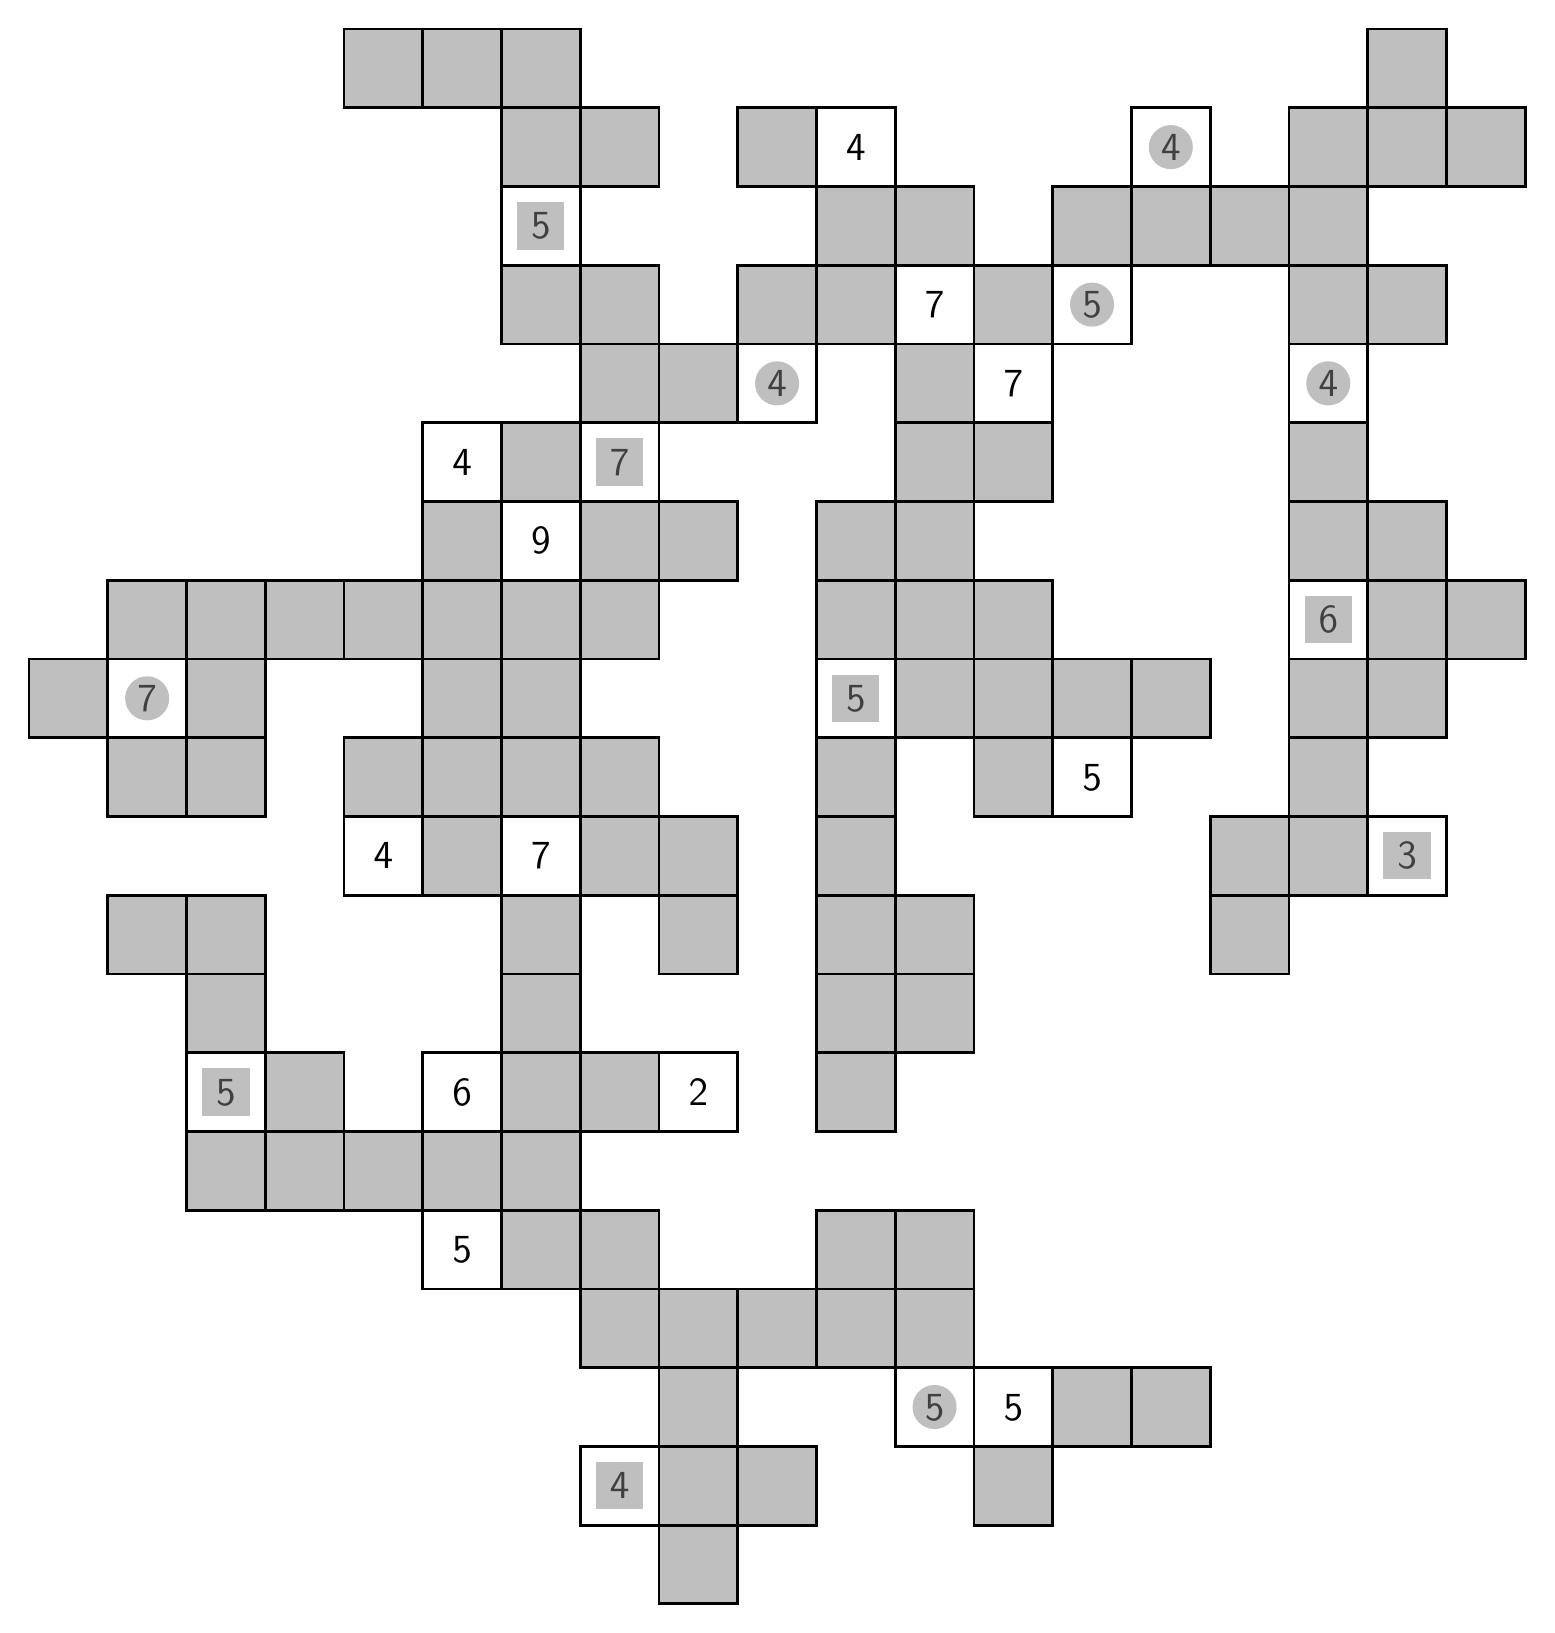
\begin{tikzpicture}\fill[gray, opacity = 0.5] (9, 0, 0)--++(1, 0, 0)--++(0, 1, 0)--++(-1, 0, 0)--cycle;
\draw[line width = 1pt] (9, 0, 0)--++(1, 0, 0)--++(0, 1, 0)--++(-1, 0, 0)--cycle;
\draw node at (8.5, 1.5, 0) {\Large $\mathsf{4}$};
\draw[line width = 1pt] (8, 1, 0)--++(1, 0, 0)--++(0, 1, 0)--++(-1, 0, 0)--cycle;
\fill[color = gray, opacity = 0.5] (8.2, 1.2) rectangle ++(0.6, 0.6);
\fill[gray, opacity = 0.5] (9, 1, 0)--++(1, 0, 0)--++(0, 1, 0)--++(-1, 0, 0)--cycle;
\draw[line width = 1pt] (9, 1, 0)--++(1, 0, 0)--++(0, 1, 0)--++(-1, 0, 0)--cycle;
\fill[gray, opacity = 0.5] (10, 1, 0)--++(1, 0, 0)--++(0, 1, 0)--++(-1, 0, 0)--cycle;
\draw[line width = 1pt] (10, 1, 0)--++(1, 0, 0)--++(0, 1, 0)--++(-1, 0, 0)--cycle;
\fill[gray, opacity = 0.5] (13, 1, 0)--++(1, 0, 0)--++(0, 1, 0)--++(-1, 0, 0)--cycle;
\draw[line width = 1pt] (13, 1, 0)--++(1, 0, 0)--++(0, 1, 0)--++(-1, 0, 0)--cycle;
\fill[gray, opacity = 0.5] (9, 2, 0)--++(1, 0, 0)--++(0, 1, 0)--++(-1, 0, 0)--cycle;
\draw[line width = 1pt] (9, 2, 0)--++(1, 0, 0)--++(0, 1, 0)--++(-1, 0, 0)--cycle;
\draw node at (12.5, 2.5, 0) {\Large $\mathsf{5}$};
\draw[line width = 1pt] (12, 2, 0)--++(1, 0, 0)--++(0, 1, 0)--++(-1, 0, 0)--cycle;
\fill[color = gray, opacity = 0.5] (12.5, 2.5, 0) circle (0.28);
\draw node at (13.5, 2.5, 0) {\Large $\mathsf{5}$};
\draw[line width = 1pt] (13, 2, 0)--++(1, 0, 0)--++(0, 1, 0)--++(-1, 0, 0)--cycle;
\fill[gray, opacity = 0.5] (14, 2, 0)--++(1, 0, 0)--++(0, 1, 0)--++(-1, 0, 0)--cycle;
\draw[line width = 1pt] (14, 2, 0)--++(1, 0, 0)--++(0, 1, 0)--++(-1, 0, 0)--cycle;
\fill[gray, opacity = 0.5] (15, 2, 0)--++(1, 0, 0)--++(0, 1, 0)--++(-1, 0, 0)--cycle;
\draw[line width = 1pt] (15, 2, 0)--++(1, 0, 0)--++(0, 1, 0)--++(-1, 0, 0)--cycle;
\fill[gray, opacity = 0.5] (8, 3, 0)--++(1, 0, 0)--++(0, 1, 0)--++(-1, 0, 0)--cycle;
\draw[line width = 1pt] (8, 3, 0)--++(1, 0, 0)--++(0, 1, 0)--++(-1, 0, 0)--cycle;
\fill[gray, opacity = 0.5] (9, 3, 0)--++(1, 0, 0)--++(0, 1, 0)--++(-1, 0, 0)--cycle;
\draw[line width = 1pt] (9, 3, 0)--++(1, 0, 0)--++(0, 1, 0)--++(-1, 0, 0)--cycle;
\fill[gray, opacity = 0.5] (10, 3, 0)--++(1, 0, 0)--++(0, 1, 0)--++(-1, 0, 0)--cycle;
\draw[line width = 1pt] (10, 3, 0)--++(1, 0, 0)--++(0, 1, 0)--++(-1, 0, 0)--cycle;
\fill[gray, opacity = 0.5] (11, 3, 0)--++(1, 0, 0)--++(0, 1, 0)--++(-1, 0, 0)--cycle;
\draw[line width = 1pt] (11, 3, 0)--++(1, 0, 0)--++(0, 1, 0)--++(-1, 0, 0)--cycle;
\fill[gray, opacity = 0.5] (12, 3, 0)--++(1, 0, 0)--++(0, 1, 0)--++(-1, 0, 0)--cycle;
\draw[line width = 1pt] (12, 3, 0)--++(1, 0, 0)--++(0, 1, 0)--++(-1, 0, 0)--cycle;
\draw node at (6.5, 4.5, 0) {\Large $\mathsf{5}$};
\draw[line width = 1pt] (6, 4, 0)--++(1, 0, 0)--++(0, 1, 0)--++(-1, 0, 0)--cycle;
\fill[gray, opacity = 0.5] (7, 4, 0)--++(1, 0, 0)--++(0, 1, 0)--++(-1, 0, 0)--cycle;
\draw[line width = 1pt] (7, 4, 0)--++(1, 0, 0)--++(0, 1, 0)--++(-1, 0, 0)--cycle;
\fill[gray, opacity = 0.5] (8, 4, 0)--++(1, 0, 0)--++(0, 1, 0)--++(-1, 0, 0)--cycle;
\draw[line width = 1pt] (8, 4, 0)--++(1, 0, 0)--++(0, 1, 0)--++(-1, 0, 0)--cycle;
\fill[gray, opacity = 0.5] (11, 4, 0)--++(1, 0, 0)--++(0, 1, 0)--++(-1, 0, 0)--cycle;
\draw[line width = 1pt] (11, 4, 0)--++(1, 0, 0)--++(0, 1, 0)--++(-1, 0, 0)--cycle;
\fill[gray, opacity = 0.5] (12, 4, 0)--++(1, 0, 0)--++(0, 1, 0)--++(-1, 0, 0)--cycle;
\draw[line width = 1pt] (12, 4, 0)--++(1, 0, 0)--++(0, 1, 0)--++(-1, 0, 0)--cycle;
\fill[gray, opacity = 0.5] (3, 5, 0)--++(1, 0, 0)--++(0, 1, 0)--++(-1, 0, 0)--cycle;
\draw[line width = 1pt] (3, 5, 0)--++(1, 0, 0)--++(0, 1, 0)--++(-1, 0, 0)--cycle;
\fill[gray, opacity = 0.5] (4, 5, 0)--++(1, 0, 0)--++(0, 1, 0)--++(-1, 0, 0)--cycle;
\draw[line width = 1pt] (4, 5, 0)--++(1, 0, 0)--++(0, 1, 0)--++(-1, 0, 0)--cycle;
\fill[gray, opacity = 0.5] (5, 5, 0)--++(1, 0, 0)--++(0, 1, 0)--++(-1, 0, 0)--cycle;
\draw[line width = 1pt] (5, 5, 0)--++(1, 0, 0)--++(0, 1, 0)--++(-1, 0, 0)--cycle;
\fill[gray, opacity = 0.5] (6, 5, 0)--++(1, 0, 0)--++(0, 1, 0)--++(-1, 0, 0)--cycle;
\draw[line width = 1pt] (6, 5, 0)--++(1, 0, 0)--++(0, 1, 0)--++(-1, 0, 0)--cycle;
\fill[gray, opacity = 0.5] (7, 5, 0)--++(1, 0, 0)--++(0, 1, 0)--++(-1, 0, 0)--cycle;
\draw[line width = 1pt] (7, 5, 0)--++(1, 0, 0)--++(0, 1, 0)--++(-1, 0, 0)--cycle;
\draw node at (3.5, 6.5, 0) {\Large $\mathsf{5}$};
\draw[line width = 1pt] (3, 6, 0)--++(1, 0, 0)--++(0, 1, 0)--++(-1, 0, 0)--cycle;
\fill[color = gray, opacity = 0.5] (3.2, 6.2) rectangle ++(0.6, 0.6);
\fill[gray, opacity = 0.5] (4, 6, 0)--++(1, 0, 0)--++(0, 1, 0)--++(-1, 0, 0)--cycle;
\draw[line width = 1pt] (4, 6, 0)--++(1, 0, 0)--++(0, 1, 0)--++(-1, 0, 0)--cycle;
\draw node at (6.5, 6.5, 0) {\Large $\mathsf{6}$};
\draw[line width = 1pt] (6, 6, 0)--++(1, 0, 0)--++(0, 1, 0)--++(-1, 0, 0)--cycle;
\fill[gray, opacity = 0.5] (7, 6, 0)--++(1, 0, 0)--++(0, 1, 0)--++(-1, 0, 0)--cycle;
\draw[line width = 1pt] (7, 6, 0)--++(1, 0, 0)--++(0, 1, 0)--++(-1, 0, 0)--cycle;
\fill[gray, opacity = 0.5] (8, 6, 0)--++(1, 0, 0)--++(0, 1, 0)--++(-1, 0, 0)--cycle;
\draw[line width = 1pt] (8, 6, 0)--++(1, 0, 0)--++(0, 1, 0)--++(-1, 0, 0)--cycle;
\draw node at (9.5, 6.5, 0) {\Large $\mathsf{2}$};
\draw[line width = 1pt] (9, 6, 0)--++(1, 0, 0)--++(0, 1, 0)--++(-1, 0, 0)--cycle;
\fill[gray, opacity = 0.5] (11, 6, 0)--++(1, 0, 0)--++(0, 1, 0)--++(-1, 0, 0)--cycle;
\draw[line width = 1pt] (11, 6, 0)--++(1, 0, 0)--++(0, 1, 0)--++(-1, 0, 0)--cycle;
\fill[gray, opacity = 0.5] (3, 7, 0)--++(1, 0, 0)--++(0, 1, 0)--++(-1, 0, 0)--cycle;
\draw[line width = 1pt] (3, 7, 0)--++(1, 0, 0)--++(0, 1, 0)--++(-1, 0, 0)--cycle;
\fill[gray, opacity = 0.5] (7, 7, 0)--++(1, 0, 0)--++(0, 1, 0)--++(-1, 0, 0)--cycle;
\draw[line width = 1pt] (7, 7, 0)--++(1, 0, 0)--++(0, 1, 0)--++(-1, 0, 0)--cycle;
\fill[gray, opacity = 0.5] (11, 7, 0)--++(1, 0, 0)--++(0, 1, 0)--++(-1, 0, 0)--cycle;
\draw[line width = 1pt] (11, 7, 0)--++(1, 0, 0)--++(0, 1, 0)--++(-1, 0, 0)--cycle;
\fill[gray, opacity = 0.5] (12, 7, 0)--++(1, 0, 0)--++(0, 1, 0)--++(-1, 0, 0)--cycle;
\draw[line width = 1pt] (12, 7, 0)--++(1, 0, 0)--++(0, 1, 0)--++(-1, 0, 0)--cycle;
\fill[gray, opacity = 0.5] (2, 8, 0)--++(1, 0, 0)--++(0, 1, 0)--++(-1, 0, 0)--cycle;
\draw[line width = 1pt] (2, 8, 0)--++(1, 0, 0)--++(0, 1, 0)--++(-1, 0, 0)--cycle;
\fill[gray, opacity = 0.5] (3, 8, 0)--++(1, 0, 0)--++(0, 1, 0)--++(-1, 0, 0)--cycle;
\draw[line width = 1pt] (3, 8, 0)--++(1, 0, 0)--++(0, 1, 0)--++(-1, 0, 0)--cycle;
\fill[gray, opacity = 0.5] (7, 8, 0)--++(1, 0, 0)--++(0, 1, 0)--++(-1, 0, 0)--cycle;
\draw[line width = 1pt] (7, 8, 0)--++(1, 0, 0)--++(0, 1, 0)--++(-1, 0, 0)--cycle;
\fill[gray, opacity = 0.5] (9, 8, 0)--++(1, 0, 0)--++(0, 1, 0)--++(-1, 0, 0)--cycle;
\draw[line width = 1pt] (9, 8, 0)--++(1, 0, 0)--++(0, 1, 0)--++(-1, 0, 0)--cycle;
\fill[gray, opacity = 0.5] (11, 8, 0)--++(1, 0, 0)--++(0, 1, 0)--++(-1, 0, 0)--cycle;
\draw[line width = 1pt] (11, 8, 0)--++(1, 0, 0)--++(0, 1, 0)--++(-1, 0, 0)--cycle;
\fill[gray, opacity = 0.5] (12, 8, 0)--++(1, 0, 0)--++(0, 1, 0)--++(-1, 0, 0)--cycle;
\draw[line width = 1pt] (12, 8, 0)--++(1, 0, 0)--++(0, 1, 0)--++(-1, 0, 0)--cycle;
\fill[gray, opacity = 0.5] (16, 8, 0)--++(1, 0, 0)--++(0, 1, 0)--++(-1, 0, 0)--cycle;
\draw[line width = 1pt] (16, 8, 0)--++(1, 0, 0)--++(0, 1, 0)--++(-1, 0, 0)--cycle;
\draw node at (5.5, 9.5, 0) {\Large $\mathsf{4}$};
\draw[line width = 1pt] (5, 9, 0)--++(1, 0, 0)--++(0, 1, 0)--++(-1, 0, 0)--cycle;
\fill[gray, opacity = 0.5] (6, 9, 0)--++(1, 0, 0)--++(0, 1, 0)--++(-1, 0, 0)--cycle;
\draw[line width = 1pt] (6, 9, 0)--++(1, 0, 0)--++(0, 1, 0)--++(-1, 0, 0)--cycle;
\draw node at (7.5, 9.5, 0) {\Large $\mathsf{7}$};
\draw[line width = 1pt] (7, 9, 0)--++(1, 0, 0)--++(0, 1, 0)--++(-1, 0, 0)--cycle;
\fill[gray, opacity = 0.5] (8, 9, 0)--++(1, 0, 0)--++(0, 1, 0)--++(-1, 0, 0)--cycle;
\draw[line width = 1pt] (8, 9, 0)--++(1, 0, 0)--++(0, 1, 0)--++(-1, 0, 0)--cycle;
\fill[gray, opacity = 0.5] (9, 9, 0)--++(1, 0, 0)--++(0, 1, 0)--++(-1, 0, 0)--cycle;
\draw[line width = 1pt] (9, 9, 0)--++(1, 0, 0)--++(0, 1, 0)--++(-1, 0, 0)--cycle;
\fill[gray, opacity = 0.5] (11, 9, 0)--++(1, 0, 0)--++(0, 1, 0)--++(-1, 0, 0)--cycle;
\draw[line width = 1pt] (11, 9, 0)--++(1, 0, 0)--++(0, 1, 0)--++(-1, 0, 0)--cycle;
\fill[gray, opacity = 0.5] (16, 9, 0)--++(1, 0, 0)--++(0, 1, 0)--++(-1, 0, 0)--cycle;
\draw[line width = 1pt] (16, 9, 0)--++(1, 0, 0)--++(0, 1, 0)--++(-1, 0, 0)--cycle;
\fill[gray, opacity = 0.5] (17, 9, 0)--++(1, 0, 0)--++(0, 1, 0)--++(-1, 0, 0)--cycle;
\draw[line width = 1pt] (17, 9, 0)--++(1, 0, 0)--++(0, 1, 0)--++(-1, 0, 0)--cycle;
\draw node at (18.5, 9.5, 0) {\Large $\mathsf{3}$};
\draw[line width = 1pt] (18, 9, 0)--++(1, 0, 0)--++(0, 1, 0)--++(-1, 0, 0)--cycle;
\fill[color = gray, opacity = 0.5] (18.2, 9.2) rectangle ++(0.6, 0.6);
\fill[gray, opacity = 0.5] (2, 10, 0)--++(1, 0, 0)--++(0, 1, 0)--++(-1, 0, 0)--cycle;
\draw[line width = 1pt] (2, 10, 0)--++(1, 0, 0)--++(0, 1, 0)--++(-1, 0, 0)--cycle;
\fill[gray, opacity = 0.5] (3, 10, 0)--++(1, 0, 0)--++(0, 1, 0)--++(-1, 0, 0)--cycle;
\draw[line width = 1pt] (3, 10, 0)--++(1, 0, 0)--++(0, 1, 0)--++(-1, 0, 0)--cycle;
\fill[gray, opacity = 0.5] (5, 10, 0)--++(1, 0, 0)--++(0, 1, 0)--++(-1, 0, 0)--cycle;
\draw[line width = 1pt] (5, 10, 0)--++(1, 0, 0)--++(0, 1, 0)--++(-1, 0, 0)--cycle;
\fill[gray, opacity = 0.5] (6, 10, 0)--++(1, 0, 0)--++(0, 1, 0)--++(-1, 0, 0)--cycle;
\draw[line width = 1pt] (6, 10, 0)--++(1, 0, 0)--++(0, 1, 0)--++(-1, 0, 0)--cycle;
\fill[gray, opacity = 0.5] (7, 10, 0)--++(1, 0, 0)--++(0, 1, 0)--++(-1, 0, 0)--cycle;
\draw[line width = 1pt] (7, 10, 0)--++(1, 0, 0)--++(0, 1, 0)--++(-1, 0, 0)--cycle;
\fill[gray, opacity = 0.5] (8, 10, 0)--++(1, 0, 0)--++(0, 1, 0)--++(-1, 0, 0)--cycle;
\draw[line width = 1pt] (8, 10, 0)--++(1, 0, 0)--++(0, 1, 0)--++(-1, 0, 0)--cycle;
\fill[gray, opacity = 0.5] (11, 10, 0)--++(1, 0, 0)--++(0, 1, 0)--++(-1, 0, 0)--cycle;
\draw[line width = 1pt] (11, 10, 0)--++(1, 0, 0)--++(0, 1, 0)--++(-1, 0, 0)--cycle;
\fill[gray, opacity = 0.5] (13, 10, 0)--++(1, 0, 0)--++(0, 1, 0)--++(-1, 0, 0)--cycle;
\draw[line width = 1pt] (13, 10, 0)--++(1, 0, 0)--++(0, 1, 0)--++(-1, 0, 0)--cycle;
\draw node at (14.5, 10.5, 0) {\Large $\mathsf{5}$};
\draw[line width = 1pt] (14, 10, 0)--++(1, 0, 0)--++(0, 1, 0)--++(-1, 0, 0)--cycle;
\fill[gray, opacity = 0.5] (17, 10, 0)--++(1, 0, 0)--++(0, 1, 0)--++(-1, 0, 0)--cycle;
\draw[line width = 1pt] (17, 10, 0)--++(1, 0, 0)--++(0, 1, 0)--++(-1, 0, 0)--cycle;
\fill[gray, opacity = 0.5] (1, 11, 0)--++(1, 0, 0)--++(0, 1, 0)--++(-1, 0, 0)--cycle;
\draw[line width = 1pt] (1, 11, 0)--++(1, 0, 0)--++(0, 1, 0)--++(-1, 0, 0)--cycle;
\draw node at (2.5, 11.5, 0) {\Large $\mathsf{7}$};
\draw[line width = 1pt] (2, 11, 0)--++(1, 0, 0)--++(0, 1, 0)--++(-1, 0, 0)--cycle;
\fill[color = gray, opacity = 0.5] (2.5, 11.5, 0) circle (0.28);
\fill[gray, opacity = 0.5] (3, 11, 0)--++(1, 0, 0)--++(0, 1, 0)--++(-1, 0, 0)--cycle;
\draw[line width = 1pt] (3, 11, 0)--++(1, 0, 0)--++(0, 1, 0)--++(-1, 0, 0)--cycle;
\fill[gray, opacity = 0.5] (6, 11, 0)--++(1, 0, 0)--++(0, 1, 0)--++(-1, 0, 0)--cycle;
\draw[line width = 1pt] (6, 11, 0)--++(1, 0, 0)--++(0, 1, 0)--++(-1, 0, 0)--cycle;
\fill[gray, opacity = 0.5] (7, 11, 0)--++(1, 0, 0)--++(0, 1, 0)--++(-1, 0, 0)--cycle;
\draw[line width = 1pt] (7, 11, 0)--++(1, 0, 0)--++(0, 1, 0)--++(-1, 0, 0)--cycle;
\draw node at (11.5, 11.5, 0) {\Large $\mathsf{5}$};
\draw[line width = 1pt] (11, 11, 0)--++(1, 0, 0)--++(0, 1, 0)--++(-1, 0, 0)--cycle;
\fill[color = gray, opacity = 0.5] (11.2, 11.2) rectangle ++(0.6, 0.6);
\fill[gray, opacity = 0.5] (12, 11, 0)--++(1, 0, 0)--++(0, 1, 0)--++(-1, 0, 0)--cycle;
\draw[line width = 1pt] (12, 11, 0)--++(1, 0, 0)--++(0, 1, 0)--++(-1, 0, 0)--cycle;
\fill[gray, opacity = 0.5] (13, 11, 0)--++(1, 0, 0)--++(0, 1, 0)--++(-1, 0, 0)--cycle;
\draw[line width = 1pt] (13, 11, 0)--++(1, 0, 0)--++(0, 1, 0)--++(-1, 0, 0)--cycle;
\fill[gray, opacity = 0.5] (14, 11, 0)--++(1, 0, 0)--++(0, 1, 0)--++(-1, 0, 0)--cycle;
\draw[line width = 1pt] (14, 11, 0)--++(1, 0, 0)--++(0, 1, 0)--++(-1, 0, 0)--cycle;
\fill[gray, opacity = 0.5] (15, 11, 0)--++(1, 0, 0)--++(0, 1, 0)--++(-1, 0, 0)--cycle;
\draw[line width = 1pt] (15, 11, 0)--++(1, 0, 0)--++(0, 1, 0)--++(-1, 0, 0)--cycle;
\fill[gray, opacity = 0.5] (17, 11, 0)--++(1, 0, 0)--++(0, 1, 0)--++(-1, 0, 0)--cycle;
\draw[line width = 1pt] (17, 11, 0)--++(1, 0, 0)--++(0, 1, 0)--++(-1, 0, 0)--cycle;
\fill[gray, opacity = 0.5] (18, 11, 0)--++(1, 0, 0)--++(0, 1, 0)--++(-1, 0, 0)--cycle;
\draw[line width = 1pt] (18, 11, 0)--++(1, 0, 0)--++(0, 1, 0)--++(-1, 0, 0)--cycle;
\fill[gray, opacity = 0.5] (2, 12, 0)--++(1, 0, 0)--++(0, 1, 0)--++(-1, 0, 0)--cycle;
\draw[line width = 1pt] (2, 12, 0)--++(1, 0, 0)--++(0, 1, 0)--++(-1, 0, 0)--cycle;
\fill[gray, opacity = 0.5] (3, 12, 0)--++(1, 0, 0)--++(0, 1, 0)--++(-1, 0, 0)--cycle;
\draw[line width = 1pt] (3, 12, 0)--++(1, 0, 0)--++(0, 1, 0)--++(-1, 0, 0)--cycle;
\fill[gray, opacity = 0.5] (4, 12, 0)--++(1, 0, 0)--++(0, 1, 0)--++(-1, 0, 0)--cycle;
\draw[line width = 1pt] (4, 12, 0)--++(1, 0, 0)--++(0, 1, 0)--++(-1, 0, 0)--cycle;
\fill[gray, opacity = 0.5] (5, 12, 0)--++(1, 0, 0)--++(0, 1, 0)--++(-1, 0, 0)--cycle;
\draw[line width = 1pt] (5, 12, 0)--++(1, 0, 0)--++(0, 1, 0)--++(-1, 0, 0)--cycle;
\fill[gray, opacity = 0.5] (6, 12, 0)--++(1, 0, 0)--++(0, 1, 0)--++(-1, 0, 0)--cycle;
\draw[line width = 1pt] (6, 12, 0)--++(1, 0, 0)--++(0, 1, 0)--++(-1, 0, 0)--cycle;
\fill[gray, opacity = 0.5] (7, 12, 0)--++(1, 0, 0)--++(0, 1, 0)--++(-1, 0, 0)--cycle;
\draw[line width = 1pt] (7, 12, 0)--++(1, 0, 0)--++(0, 1, 0)--++(-1, 0, 0)--cycle;
\fill[gray, opacity = 0.5] (8, 12, 0)--++(1, 0, 0)--++(0, 1, 0)--++(-1, 0, 0)--cycle;
\draw[line width = 1pt] (8, 12, 0)--++(1, 0, 0)--++(0, 1, 0)--++(-1, 0, 0)--cycle;
\fill[gray, opacity = 0.5] (11, 12, 0)--++(1, 0, 0)--++(0, 1, 0)--++(-1, 0, 0)--cycle;
\draw[line width = 1pt] (11, 12, 0)--++(1, 0, 0)--++(0, 1, 0)--++(-1, 0, 0)--cycle;
\fill[gray, opacity = 0.5] (12, 12, 0)--++(1, 0, 0)--++(0, 1, 0)--++(-1, 0, 0)--cycle;
\draw[line width = 1pt] (12, 12, 0)--++(1, 0, 0)--++(0, 1, 0)--++(-1, 0, 0)--cycle;
\fill[gray, opacity = 0.5] (13, 12, 0)--++(1, 0, 0)--++(0, 1, 0)--++(-1, 0, 0)--cycle;
\draw[line width = 1pt] (13, 12, 0)--++(1, 0, 0)--++(0, 1, 0)--++(-1, 0, 0)--cycle;
\draw node at (17.5, 12.5, 0) {\Large $\mathsf{6}$};
\draw[line width = 1pt] (17, 12, 0)--++(1, 0, 0)--++(0, 1, 0)--++(-1, 0, 0)--cycle;
\fill[color = gray, opacity = 0.5] (17.2, 12.2) rectangle ++(0.6, 0.6);
\fill[gray, opacity = 0.5] (18, 12, 0)--++(1, 0, 0)--++(0, 1, 0)--++(-1, 0, 0)--cycle;
\draw[line width = 1pt] (18, 12, 0)--++(1, 0, 0)--++(0, 1, 0)--++(-1, 0, 0)--cycle;
\fill[gray, opacity = 0.5] (19, 12, 0)--++(1, 0, 0)--++(0, 1, 0)--++(-1, 0, 0)--cycle;
\draw[line width = 1pt] (19, 12, 0)--++(1, 0, 0)--++(0, 1, 0)--++(-1, 0, 0)--cycle;
\fill[gray, opacity = 0.5] (6, 13, 0)--++(1, 0, 0)--++(0, 1, 0)--++(-1, 0, 0)--cycle;
\draw[line width = 1pt] (6, 13, 0)--++(1, 0, 0)--++(0, 1, 0)--++(-1, 0, 0)--cycle;
\draw node at (7.5, 13.5, 0) {\Large $\mathsf{9}$};
\draw[line width = 1pt] (7, 13, 0)--++(1, 0, 0)--++(0, 1, 0)--++(-1, 0, 0)--cycle;
\fill[gray, opacity = 0.5] (8, 13, 0)--++(1, 0, 0)--++(0, 1, 0)--++(-1, 0, 0)--cycle;
\draw[line width = 1pt] (8, 13, 0)--++(1, 0, 0)--++(0, 1, 0)--++(-1, 0, 0)--cycle;
\fill[gray, opacity = 0.5] (9, 13, 0)--++(1, 0, 0)--++(0, 1, 0)--++(-1, 0, 0)--cycle;
\draw[line width = 1pt] (9, 13, 0)--++(1, 0, 0)--++(0, 1, 0)--++(-1, 0, 0)--cycle;
\fill[gray, opacity = 0.5] (11, 13, 0)--++(1, 0, 0)--++(0, 1, 0)--++(-1, 0, 0)--cycle;
\draw[line width = 1pt] (11, 13, 0)--++(1, 0, 0)--++(0, 1, 0)--++(-1, 0, 0)--cycle;
\fill[gray, opacity = 0.5] (12, 13, 0)--++(1, 0, 0)--++(0, 1, 0)--++(-1, 0, 0)--cycle;
\draw[line width = 1pt] (12, 13, 0)--++(1, 0, 0)--++(0, 1, 0)--++(-1, 0, 0)--cycle;
\fill[gray, opacity = 0.5] (17, 13, 0)--++(1, 0, 0)--++(0, 1, 0)--++(-1, 0, 0)--cycle;
\draw[line width = 1pt] (17, 13, 0)--++(1, 0, 0)--++(0, 1, 0)--++(-1, 0, 0)--cycle;
\fill[gray, opacity = 0.5] (18, 13, 0)--++(1, 0, 0)--++(0, 1, 0)--++(-1, 0, 0)--cycle;
\draw[line width = 1pt] (18, 13, 0)--++(1, 0, 0)--++(0, 1, 0)--++(-1, 0, 0)--cycle;
\draw node at (6.5, 14.5, 0) {\Large $\mathsf{4}$};
\draw[line width = 1pt] (6, 14, 0)--++(1, 0, 0)--++(0, 1, 0)--++(-1, 0, 0)--cycle;
\fill[gray, opacity = 0.5] (7, 14, 0)--++(1, 0, 0)--++(0, 1, 0)--++(-1, 0, 0)--cycle;
\draw[line width = 1pt] (7, 14, 0)--++(1, 0, 0)--++(0, 1, 0)--++(-1, 0, 0)--cycle;
\draw node at (8.5, 14.5, 0) {\Large $\mathsf{7}$};
\draw[line width = 1pt] (8, 14, 0)--++(1, 0, 0)--++(0, 1, 0)--++(-1, 0, 0)--cycle;
\fill[color = gray, opacity = 0.5] (8.2, 14.2) rectangle ++(0.6, 0.6);
\fill[gray, opacity = 0.5] (12, 14, 0)--++(1, 0, 0)--++(0, 1, 0)--++(-1, 0, 0)--cycle;
\draw[line width = 1pt] (12, 14, 0)--++(1, 0, 0)--++(0, 1, 0)--++(-1, 0, 0)--cycle;
\fill[gray, opacity = 0.5] (13, 14, 0)--++(1, 0, 0)--++(0, 1, 0)--++(-1, 0, 0)--cycle;
\draw[line width = 1pt] (13, 14, 0)--++(1, 0, 0)--++(0, 1, 0)--++(-1, 0, 0)--cycle;
\fill[gray, opacity = 0.5] (17, 14, 0)--++(1, 0, 0)--++(0, 1, 0)--++(-1, 0, 0)--cycle;
\draw[line width = 1pt] (17, 14, 0)--++(1, 0, 0)--++(0, 1, 0)--++(-1, 0, 0)--cycle;
\fill[gray, opacity = 0.5] (8, 15, 0)--++(1, 0, 0)--++(0, 1, 0)--++(-1, 0, 0)--cycle;
\draw[line width = 1pt] (8, 15, 0)--++(1, 0, 0)--++(0, 1, 0)--++(-1, 0, 0)--cycle;
\fill[gray, opacity = 0.5] (9, 15, 0)--++(1, 0, 0)--++(0, 1, 0)--++(-1, 0, 0)--cycle;
\draw[line width = 1pt] (9, 15, 0)--++(1, 0, 0)--++(0, 1, 0)--++(-1, 0, 0)--cycle;
\draw node at (10.5, 15.5, 0) {\Large $\mathsf{4}$};
\draw[line width = 1pt] (10, 15, 0)--++(1, 0, 0)--++(0, 1, 0)--++(-1, 0, 0)--cycle;
\fill[color = gray, opacity = 0.5] (10.5, 15.5, 0) circle (0.28);
\fill[gray, opacity = 0.5] (12, 15, 0)--++(1, 0, 0)--++(0, 1, 0)--++(-1, 0, 0)--cycle;
\draw[line width = 1pt] (12, 15, 0)--++(1, 0, 0)--++(0, 1, 0)--++(-1, 0, 0)--cycle;
\draw node at (13.5, 15.5, 0) {\Large $\mathsf{7}$};
\draw[line width = 1pt] (13, 15, 0)--++(1, 0, 0)--++(0, 1, 0)--++(-1, 0, 0)--cycle;
\draw node at (17.5, 15.5, 0) {\Large $\mathsf{4}$};
\draw[line width = 1pt] (17, 15, 0)--++(1, 0, 0)--++(0, 1, 0)--++(-1, 0, 0)--cycle;
\fill[color = gray, opacity = 0.5] (17.5, 15.5, 0) circle (0.28);
\fill[gray, opacity = 0.5] (7, 16, 0)--++(1, 0, 0)--++(0, 1, 0)--++(-1, 0, 0)--cycle;
\draw[line width = 1pt] (7, 16, 0)--++(1, 0, 0)--++(0, 1, 0)--++(-1, 0, 0)--cycle;
\fill[gray, opacity = 0.5] (8, 16, 0)--++(1, 0, 0)--++(0, 1, 0)--++(-1, 0, 0)--cycle;
\draw[line width = 1pt] (8, 16, 0)--++(1, 0, 0)--++(0, 1, 0)--++(-1, 0, 0)--cycle;
\fill[gray, opacity = 0.5] (10, 16, 0)--++(1, 0, 0)--++(0, 1, 0)--++(-1, 0, 0)--cycle;
\draw[line width = 1pt] (10, 16, 0)--++(1, 0, 0)--++(0, 1, 0)--++(-1, 0, 0)--cycle;
\fill[gray, opacity = 0.5] (11, 16, 0)--++(1, 0, 0)--++(0, 1, 0)--++(-1, 0, 0)--cycle;
\draw[line width = 1pt] (11, 16, 0)--++(1, 0, 0)--++(0, 1, 0)--++(-1, 0, 0)--cycle;
\draw node at (12.5, 16.5, 0) {\Large $\mathsf{7}$};
\draw[line width = 1pt] (12, 16, 0)--++(1, 0, 0)--++(0, 1, 0)--++(-1, 0, 0)--cycle;
\fill[gray, opacity = 0.5] (13, 16, 0)--++(1, 0, 0)--++(0, 1, 0)--++(-1, 0, 0)--cycle;
\draw[line width = 1pt] (13, 16, 0)--++(1, 0, 0)--++(0, 1, 0)--++(-1, 0, 0)--cycle;
\draw node at (14.5, 16.5, 0) {\Large $\mathsf{5}$};
\draw[line width = 1pt] (14, 16, 0)--++(1, 0, 0)--++(0, 1, 0)--++(-1, 0, 0)--cycle;
\fill[color = gray, opacity = 0.5] (14.5, 16.5, 0) circle (0.28);
\fill[gray, opacity = 0.5] (17, 16, 0)--++(1, 0, 0)--++(0, 1, 0)--++(-1, 0, 0)--cycle;
\draw[line width = 1pt] (17, 16, 0)--++(1, 0, 0)--++(0, 1, 0)--++(-1, 0, 0)--cycle;
\fill[gray, opacity = 0.5] (18, 16, 0)--++(1, 0, 0)--++(0, 1, 0)--++(-1, 0, 0)--cycle;
\draw[line width = 1pt] (18, 16, 0)--++(1, 0, 0)--++(0, 1, 0)--++(-1, 0, 0)--cycle;
\draw node at (7.5, 17.5, 0) {\Large $\mathsf{5}$};
\draw[line width = 1pt] (7, 17, 0)--++(1, 0, 0)--++(0, 1, 0)--++(-1, 0, 0)--cycle;
\fill[color = gray, opacity = 0.5] (7.2, 17.2) rectangle ++(0.6, 0.6);
\fill[gray, opacity = 0.5] (11, 17, 0)--++(1, 0, 0)--++(0, 1, 0)--++(-1, 0, 0)--cycle;
\draw[line width = 1pt] (11, 17, 0)--++(1, 0, 0)--++(0, 1, 0)--++(-1, 0, 0)--cycle;
\fill[gray, opacity = 0.5] (12, 17, 0)--++(1, 0, 0)--++(0, 1, 0)--++(-1, 0, 0)--cycle;
\draw[line width = 1pt] (12, 17, 0)--++(1, 0, 0)--++(0, 1, 0)--++(-1, 0, 0)--cycle;
\fill[gray, opacity = 0.5] (14, 17, 0)--++(1, 0, 0)--++(0, 1, 0)--++(-1, 0, 0)--cycle;
\draw[line width = 1pt] (14, 17, 0)--++(1, 0, 0)--++(0, 1, 0)--++(-1, 0, 0)--cycle;
\fill[gray, opacity = 0.5] (15, 17, 0)--++(1, 0, 0)--++(0, 1, 0)--++(-1, 0, 0)--cycle;
\draw[line width = 1pt] (15, 17, 0)--++(1, 0, 0)--++(0, 1, 0)--++(-1, 0, 0)--cycle;
\fill[gray, opacity = 0.5] (16, 17, 0)--++(1, 0, 0)--++(0, 1, 0)--++(-1, 0, 0)--cycle;
\draw[line width = 1pt] (16, 17, 0)--++(1, 0, 0)--++(0, 1, 0)--++(-1, 0, 0)--cycle;
\fill[gray, opacity = 0.5] (17, 17, 0)--++(1, 0, 0)--++(0, 1, 0)--++(-1, 0, 0)--cycle;
\draw[line width = 1pt] (17, 17, 0)--++(1, 0, 0)--++(0, 1, 0)--++(-1, 0, 0)--cycle;
\fill[gray, opacity = 0.5] (7, 18, 0)--++(1, 0, 0)--++(0, 1, 0)--++(-1, 0, 0)--cycle;
\draw[line width = 1pt] (7, 18, 0)--++(1, 0, 0)--++(0, 1, 0)--++(-1, 0, 0)--cycle;
\fill[gray, opacity = 0.5] (8, 18, 0)--++(1, 0, 0)--++(0, 1, 0)--++(-1, 0, 0)--cycle;
\draw[line width = 1pt] (8, 18, 0)--++(1, 0, 0)--++(0, 1, 0)--++(-1, 0, 0)--cycle;
\fill[gray, opacity = 0.5] (10, 18, 0)--++(1, 0, 0)--++(0, 1, 0)--++(-1, 0, 0)--cycle;
\draw[line width = 1pt] (10, 18, 0)--++(1, 0, 0)--++(0, 1, 0)--++(-1, 0, 0)--cycle;
\draw node at (11.5, 18.5, 0) {\Large $\mathsf{4}$};
\draw[line width = 1pt] (11, 18, 0)--++(1, 0, 0)--++(0, 1, 0)--++(-1, 0, 0)--cycle;
\draw node at (15.5, 18.5, 0) {\Large $\mathsf{4}$};
\draw[line width = 1pt] (15, 18, 0)--++(1, 0, 0)--++(0, 1, 0)--++(-1, 0, 0)--cycle;
\fill[color = gray, opacity = 0.5] (15.5, 18.5, 0) circle (0.28);
\fill[gray, opacity = 0.5] (17, 18, 0)--++(1, 0, 0)--++(0, 1, 0)--++(-1, 0, 0)--cycle;
\draw[line width = 1pt] (17, 18, 0)--++(1, 0, 0)--++(0, 1, 0)--++(-1, 0, 0)--cycle;
\fill[gray, opacity = 0.5] (18, 18, 0)--++(1, 0, 0)--++(0, 1, 0)--++(-1, 0, 0)--cycle;
\draw[line width = 1pt] (18, 18, 0)--++(1, 0, 0)--++(0, 1, 0)--++(-1, 0, 0)--cycle;
\fill[gray, opacity = 0.5] (19, 18, 0)--++(1, 0, 0)--++(0, 1, 0)--++(-1, 0, 0)--cycle;
\draw[line width = 1pt] (19, 18, 0)--++(1, 0, 0)--++(0, 1, 0)--++(-1, 0, 0)--cycle;
\fill[gray, opacity = 0.5] (5, 19, 0)--++(1, 0, 0)--++(0, 1, 0)--++(-1, 0, 0)--cycle;
\draw[line width = 1pt] (5, 19, 0)--++(1, 0, 0)--++(0, 1, 0)--++(-1, 0, 0)--cycle;
\fill[gray, opacity = 0.5] (6, 19, 0)--++(1, 0, 0)--++(0, 1, 0)--++(-1, 0, 0)--cycle;
\draw[line width = 1pt] (6, 19, 0)--++(1, 0, 0)--++(0, 1, 0)--++(-1, 0, 0)--cycle;
\fill[gray, opacity = 0.5] (7, 19, 0)--++(1, 0, 0)--++(0, 1, 0)--++(-1, 0, 0)--cycle;
\draw[line width = 1pt] (7, 19, 0)--++(1, 0, 0)--++(0, 1, 0)--++(-1, 0, 0)--cycle;
\fill[gray, opacity = 0.5] (18, 19, 0)--++(1, 0, 0)--++(0, 1, 0)--++(-1, 0, 0)--cycle;
\draw[line width = 1pt] (18, 19, 0)--++(1, 0, 0)--++(0, 1, 0)--++(-1, 0, 0)--cycle;
\end{tikzpicture}}\]
\[\resizebox{30pc}{!}{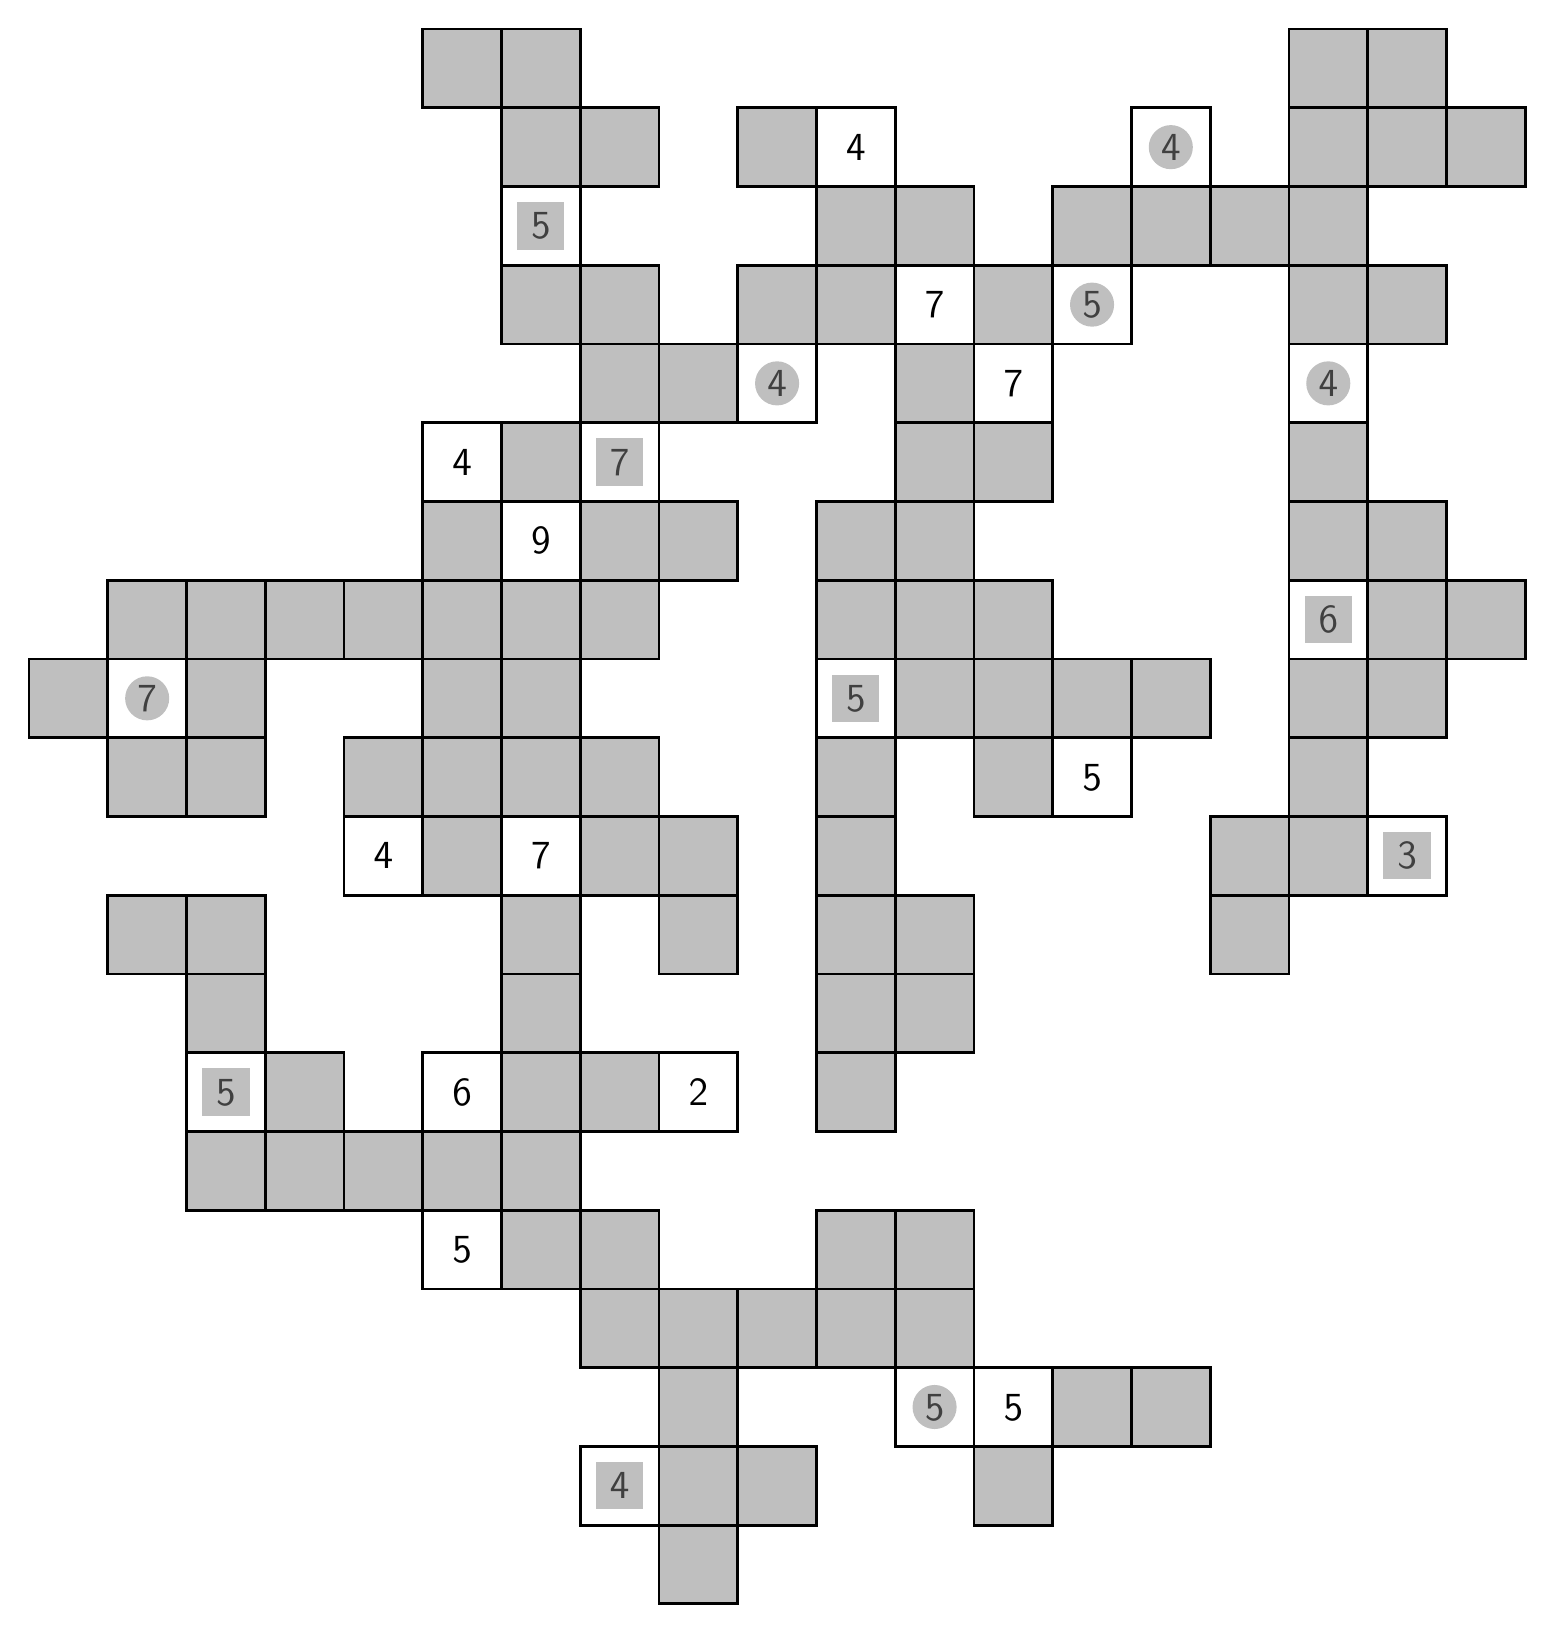
\begin{tikzpicture}\fill[gray, opacity = 0.5] (9, 0, 0)--++(1, 0, 0)--++(0, 1, 0)--++(-1, 0, 0)--cycle;
\draw[line width = 1pt] (9, 0, 0)--++(1, 0, 0)--++(0, 1, 0)--++(-1, 0, 0)--cycle;
\draw node at (8.5, 1.5, 0) {\Large $\mathsf{4}$};
\draw[line width = 1pt] (8, 1, 0)--++(1, 0, 0)--++(0, 1, 0)--++(-1, 0, 0)--cycle;
\fill[color = gray, opacity = 0.5] (8.2, 1.2) rectangle ++(0.6, 0.6);
\fill[gray, opacity = 0.5] (9, 1, 0)--++(1, 0, 0)--++(0, 1, 0)--++(-1, 0, 0)--cycle;
\draw[line width = 1pt] (9, 1, 0)--++(1, 0, 0)--++(0, 1, 0)--++(-1, 0, 0)--cycle;
\fill[gray, opacity = 0.5] (10, 1, 0)--++(1, 0, 0)--++(0, 1, 0)--++(-1, 0, 0)--cycle;
\draw[line width = 1pt] (10, 1, 0)--++(1, 0, 0)--++(0, 1, 0)--++(-1, 0, 0)--cycle;
\fill[gray, opacity = 0.5] (13, 1, 0)--++(1, 0, 0)--++(0, 1, 0)--++(-1, 0, 0)--cycle;
\draw[line width = 1pt] (13, 1, 0)--++(1, 0, 0)--++(0, 1, 0)--++(-1, 0, 0)--cycle;
\fill[gray, opacity = 0.5] (9, 2, 0)--++(1, 0, 0)--++(0, 1, 0)--++(-1, 0, 0)--cycle;
\draw[line width = 1pt] (9, 2, 0)--++(1, 0, 0)--++(0, 1, 0)--++(-1, 0, 0)--cycle;
\draw node at (12.5, 2.5, 0) {\Large $\mathsf{5}$};
\draw[line width = 1pt] (12, 2, 0)--++(1, 0, 0)--++(0, 1, 0)--++(-1, 0, 0)--cycle;
\fill[color = gray, opacity = 0.5] (12.5, 2.5, 0) circle (0.28);
\draw node at (13.5, 2.5, 0) {\Large $\mathsf{5}$};
\draw[line width = 1pt] (13, 2, 0)--++(1, 0, 0)--++(0, 1, 0)--++(-1, 0, 0)--cycle;
\fill[gray, opacity = 0.5] (14, 2, 0)--++(1, 0, 0)--++(0, 1, 0)--++(-1, 0, 0)--cycle;
\draw[line width = 1pt] (14, 2, 0)--++(1, 0, 0)--++(0, 1, 0)--++(-1, 0, 0)--cycle;
\fill[gray, opacity = 0.5] (15, 2, 0)--++(1, 0, 0)--++(0, 1, 0)--++(-1, 0, 0)--cycle;
\draw[line width = 1pt] (15, 2, 0)--++(1, 0, 0)--++(0, 1, 0)--++(-1, 0, 0)--cycle;
\fill[gray, opacity = 0.5] (8, 3, 0)--++(1, 0, 0)--++(0, 1, 0)--++(-1, 0, 0)--cycle;
\draw[line width = 1pt] (8, 3, 0)--++(1, 0, 0)--++(0, 1, 0)--++(-1, 0, 0)--cycle;
\fill[gray, opacity = 0.5] (9, 3, 0)--++(1, 0, 0)--++(0, 1, 0)--++(-1, 0, 0)--cycle;
\draw[line width = 1pt] (9, 3, 0)--++(1, 0, 0)--++(0, 1, 0)--++(-1, 0, 0)--cycle;
\fill[gray, opacity = 0.5] (10, 3, 0)--++(1, 0, 0)--++(0, 1, 0)--++(-1, 0, 0)--cycle;
\draw[line width = 1pt] (10, 3, 0)--++(1, 0, 0)--++(0, 1, 0)--++(-1, 0, 0)--cycle;
\fill[gray, opacity = 0.5] (11, 3, 0)--++(1, 0, 0)--++(0, 1, 0)--++(-1, 0, 0)--cycle;
\draw[line width = 1pt] (11, 3, 0)--++(1, 0, 0)--++(0, 1, 0)--++(-1, 0, 0)--cycle;
\fill[gray, opacity = 0.5] (12, 3, 0)--++(1, 0, 0)--++(0, 1, 0)--++(-1, 0, 0)--cycle;
\draw[line width = 1pt] (12, 3, 0)--++(1, 0, 0)--++(0, 1, 0)--++(-1, 0, 0)--cycle;
\draw node at (6.5, 4.5, 0) {\Large $\mathsf{5}$};
\draw[line width = 1pt] (6, 4, 0)--++(1, 0, 0)--++(0, 1, 0)--++(-1, 0, 0)--cycle;
\fill[gray, opacity = 0.5] (7, 4, 0)--++(1, 0, 0)--++(0, 1, 0)--++(-1, 0, 0)--cycle;
\draw[line width = 1pt] (7, 4, 0)--++(1, 0, 0)--++(0, 1, 0)--++(-1, 0, 0)--cycle;
\fill[gray, opacity = 0.5] (8, 4, 0)--++(1, 0, 0)--++(0, 1, 0)--++(-1, 0, 0)--cycle;
\draw[line width = 1pt] (8, 4, 0)--++(1, 0, 0)--++(0, 1, 0)--++(-1, 0, 0)--cycle;
\fill[gray, opacity = 0.5] (11, 4, 0)--++(1, 0, 0)--++(0, 1, 0)--++(-1, 0, 0)--cycle;
\draw[line width = 1pt] (11, 4, 0)--++(1, 0, 0)--++(0, 1, 0)--++(-1, 0, 0)--cycle;
\fill[gray, opacity = 0.5] (12, 4, 0)--++(1, 0, 0)--++(0, 1, 0)--++(-1, 0, 0)--cycle;
\draw[line width = 1pt] (12, 4, 0)--++(1, 0, 0)--++(0, 1, 0)--++(-1, 0, 0)--cycle;
\fill[gray, opacity = 0.5] (3, 5, 0)--++(1, 0, 0)--++(0, 1, 0)--++(-1, 0, 0)--cycle;
\draw[line width = 1pt] (3, 5, 0)--++(1, 0, 0)--++(0, 1, 0)--++(-1, 0, 0)--cycle;
\fill[gray, opacity = 0.5] (4, 5, 0)--++(1, 0, 0)--++(0, 1, 0)--++(-1, 0, 0)--cycle;
\draw[line width = 1pt] (4, 5, 0)--++(1, 0, 0)--++(0, 1, 0)--++(-1, 0, 0)--cycle;
\fill[gray, opacity = 0.5] (5, 5, 0)--++(1, 0, 0)--++(0, 1, 0)--++(-1, 0, 0)--cycle;
\draw[line width = 1pt] (5, 5, 0)--++(1, 0, 0)--++(0, 1, 0)--++(-1, 0, 0)--cycle;
\fill[gray, opacity = 0.5] (6, 5, 0)--++(1, 0, 0)--++(0, 1, 0)--++(-1, 0, 0)--cycle;
\draw[line width = 1pt] (6, 5, 0)--++(1, 0, 0)--++(0, 1, 0)--++(-1, 0, 0)--cycle;
\fill[gray, opacity = 0.5] (7, 5, 0)--++(1, 0, 0)--++(0, 1, 0)--++(-1, 0, 0)--cycle;
\draw[line width = 1pt] (7, 5, 0)--++(1, 0, 0)--++(0, 1, 0)--++(-1, 0, 0)--cycle;
\draw node at (3.5, 6.5, 0) {\Large $\mathsf{5}$};
\draw[line width = 1pt] (3, 6, 0)--++(1, 0, 0)--++(0, 1, 0)--++(-1, 0, 0)--cycle;
\fill[color = gray, opacity = 0.5] (3.2, 6.2) rectangle ++(0.6, 0.6);
\fill[gray, opacity = 0.5] (4, 6, 0)--++(1, 0, 0)--++(0, 1, 0)--++(-1, 0, 0)--cycle;
\draw[line width = 1pt] (4, 6, 0)--++(1, 0, 0)--++(0, 1, 0)--++(-1, 0, 0)--cycle;
\draw node at (6.5, 6.5, 0) {\Large $\mathsf{6}$};
\draw[line width = 1pt] (6, 6, 0)--++(1, 0, 0)--++(0, 1, 0)--++(-1, 0, 0)--cycle;
\fill[gray, opacity = 0.5] (7, 6, 0)--++(1, 0, 0)--++(0, 1, 0)--++(-1, 0, 0)--cycle;
\draw[line width = 1pt] (7, 6, 0)--++(1, 0, 0)--++(0, 1, 0)--++(-1, 0, 0)--cycle;
\fill[gray, opacity = 0.5] (8, 6, 0)--++(1, 0, 0)--++(0, 1, 0)--++(-1, 0, 0)--cycle;
\draw[line width = 1pt] (8, 6, 0)--++(1, 0, 0)--++(0, 1, 0)--++(-1, 0, 0)--cycle;
\draw node at (9.5, 6.5, 0) {\Large $\mathsf{2}$};
\draw[line width = 1pt] (9, 6, 0)--++(1, 0, 0)--++(0, 1, 0)--++(-1, 0, 0)--cycle;
\fill[gray, opacity = 0.5] (11, 6, 0)--++(1, 0, 0)--++(0, 1, 0)--++(-1, 0, 0)--cycle;
\draw[line width = 1pt] (11, 6, 0)--++(1, 0, 0)--++(0, 1, 0)--++(-1, 0, 0)--cycle;
\fill[gray, opacity = 0.5] (3, 7, 0)--++(1, 0, 0)--++(0, 1, 0)--++(-1, 0, 0)--cycle;
\draw[line width = 1pt] (3, 7, 0)--++(1, 0, 0)--++(0, 1, 0)--++(-1, 0, 0)--cycle;
\fill[gray, opacity = 0.5] (7, 7, 0)--++(1, 0, 0)--++(0, 1, 0)--++(-1, 0, 0)--cycle;
\draw[line width = 1pt] (7, 7, 0)--++(1, 0, 0)--++(0, 1, 0)--++(-1, 0, 0)--cycle;
\fill[gray, opacity = 0.5] (11, 7, 0)--++(1, 0, 0)--++(0, 1, 0)--++(-1, 0, 0)--cycle;
\draw[line width = 1pt] (11, 7, 0)--++(1, 0, 0)--++(0, 1, 0)--++(-1, 0, 0)--cycle;
\fill[gray, opacity = 0.5] (12, 7, 0)--++(1, 0, 0)--++(0, 1, 0)--++(-1, 0, 0)--cycle;
\draw[line width = 1pt] (12, 7, 0)--++(1, 0, 0)--++(0, 1, 0)--++(-1, 0, 0)--cycle;
\fill[gray, opacity = 0.5] (2, 8, 0)--++(1, 0, 0)--++(0, 1, 0)--++(-1, 0, 0)--cycle;
\draw[line width = 1pt] (2, 8, 0)--++(1, 0, 0)--++(0, 1, 0)--++(-1, 0, 0)--cycle;
\fill[gray, opacity = 0.5] (3, 8, 0)--++(1, 0, 0)--++(0, 1, 0)--++(-1, 0, 0)--cycle;
\draw[line width = 1pt] (3, 8, 0)--++(1, 0, 0)--++(0, 1, 0)--++(-1, 0, 0)--cycle;
\fill[gray, opacity = 0.5] (7, 8, 0)--++(1, 0, 0)--++(0, 1, 0)--++(-1, 0, 0)--cycle;
\draw[line width = 1pt] (7, 8, 0)--++(1, 0, 0)--++(0, 1, 0)--++(-1, 0, 0)--cycle;
\fill[gray, opacity = 0.5] (9, 8, 0)--++(1, 0, 0)--++(0, 1, 0)--++(-1, 0, 0)--cycle;
\draw[line width = 1pt] (9, 8, 0)--++(1, 0, 0)--++(0, 1, 0)--++(-1, 0, 0)--cycle;
\fill[gray, opacity = 0.5] (11, 8, 0)--++(1, 0, 0)--++(0, 1, 0)--++(-1, 0, 0)--cycle;
\draw[line width = 1pt] (11, 8, 0)--++(1, 0, 0)--++(0, 1, 0)--++(-1, 0, 0)--cycle;
\fill[gray, opacity = 0.5] (12, 8, 0)--++(1, 0, 0)--++(0, 1, 0)--++(-1, 0, 0)--cycle;
\draw[line width = 1pt] (12, 8, 0)--++(1, 0, 0)--++(0, 1, 0)--++(-1, 0, 0)--cycle;
\fill[gray, opacity = 0.5] (16, 8, 0)--++(1, 0, 0)--++(0, 1, 0)--++(-1, 0, 0)--cycle;
\draw[line width = 1pt] (16, 8, 0)--++(1, 0, 0)--++(0, 1, 0)--++(-1, 0, 0)--cycle;
\draw node at (5.5, 9.5, 0) {\Large $\mathsf{4}$};
\draw[line width = 1pt] (5, 9, 0)--++(1, 0, 0)--++(0, 1, 0)--++(-1, 0, 0)--cycle;
\fill[gray, opacity = 0.5] (6, 9, 0)--++(1, 0, 0)--++(0, 1, 0)--++(-1, 0, 0)--cycle;
\draw[line width = 1pt] (6, 9, 0)--++(1, 0, 0)--++(0, 1, 0)--++(-1, 0, 0)--cycle;
\draw node at (7.5, 9.5, 0) {\Large $\mathsf{7}$};
\draw[line width = 1pt] (7, 9, 0)--++(1, 0, 0)--++(0, 1, 0)--++(-1, 0, 0)--cycle;
\fill[gray, opacity = 0.5] (8, 9, 0)--++(1, 0, 0)--++(0, 1, 0)--++(-1, 0, 0)--cycle;
\draw[line width = 1pt] (8, 9, 0)--++(1, 0, 0)--++(0, 1, 0)--++(-1, 0, 0)--cycle;
\fill[gray, opacity = 0.5] (9, 9, 0)--++(1, 0, 0)--++(0, 1, 0)--++(-1, 0, 0)--cycle;
\draw[line width = 1pt] (9, 9, 0)--++(1, 0, 0)--++(0, 1, 0)--++(-1, 0, 0)--cycle;
\fill[gray, opacity = 0.5] (11, 9, 0)--++(1, 0, 0)--++(0, 1, 0)--++(-1, 0, 0)--cycle;
\draw[line width = 1pt] (11, 9, 0)--++(1, 0, 0)--++(0, 1, 0)--++(-1, 0, 0)--cycle;
\fill[gray, opacity = 0.5] (16, 9, 0)--++(1, 0, 0)--++(0, 1, 0)--++(-1, 0, 0)--cycle;
\draw[line width = 1pt] (16, 9, 0)--++(1, 0, 0)--++(0, 1, 0)--++(-1, 0, 0)--cycle;
\fill[gray, opacity = 0.5] (17, 9, 0)--++(1, 0, 0)--++(0, 1, 0)--++(-1, 0, 0)--cycle;
\draw[line width = 1pt] (17, 9, 0)--++(1, 0, 0)--++(0, 1, 0)--++(-1, 0, 0)--cycle;
\draw node at (18.5, 9.5, 0) {\Large $\mathsf{3}$};
\draw[line width = 1pt] (18, 9, 0)--++(1, 0, 0)--++(0, 1, 0)--++(-1, 0, 0)--cycle;
\fill[color = gray, opacity = 0.5] (18.2, 9.2) rectangle ++(0.6, 0.6);
\fill[gray, opacity = 0.5] (2, 10, 0)--++(1, 0, 0)--++(0, 1, 0)--++(-1, 0, 0)--cycle;
\draw[line width = 1pt] (2, 10, 0)--++(1, 0, 0)--++(0, 1, 0)--++(-1, 0, 0)--cycle;
\fill[gray, opacity = 0.5] (3, 10, 0)--++(1, 0, 0)--++(0, 1, 0)--++(-1, 0, 0)--cycle;
\draw[line width = 1pt] (3, 10, 0)--++(1, 0, 0)--++(0, 1, 0)--++(-1, 0, 0)--cycle;
\fill[gray, opacity = 0.5] (5, 10, 0)--++(1, 0, 0)--++(0, 1, 0)--++(-1, 0, 0)--cycle;
\draw[line width = 1pt] (5, 10, 0)--++(1, 0, 0)--++(0, 1, 0)--++(-1, 0, 0)--cycle;
\fill[gray, opacity = 0.5] (6, 10, 0)--++(1, 0, 0)--++(0, 1, 0)--++(-1, 0, 0)--cycle;
\draw[line width = 1pt] (6, 10, 0)--++(1, 0, 0)--++(0, 1, 0)--++(-1, 0, 0)--cycle;
\fill[gray, opacity = 0.5] (7, 10, 0)--++(1, 0, 0)--++(0, 1, 0)--++(-1, 0, 0)--cycle;
\draw[line width = 1pt] (7, 10, 0)--++(1, 0, 0)--++(0, 1, 0)--++(-1, 0, 0)--cycle;
\fill[gray, opacity = 0.5] (8, 10, 0)--++(1, 0, 0)--++(0, 1, 0)--++(-1, 0, 0)--cycle;
\draw[line width = 1pt] (8, 10, 0)--++(1, 0, 0)--++(0, 1, 0)--++(-1, 0, 0)--cycle;
\fill[gray, opacity = 0.5] (11, 10, 0)--++(1, 0, 0)--++(0, 1, 0)--++(-1, 0, 0)--cycle;
\draw[line width = 1pt] (11, 10, 0)--++(1, 0, 0)--++(0, 1, 0)--++(-1, 0, 0)--cycle;
\fill[gray, opacity = 0.5] (13, 10, 0)--++(1, 0, 0)--++(0, 1, 0)--++(-1, 0, 0)--cycle;
\draw[line width = 1pt] (13, 10, 0)--++(1, 0, 0)--++(0, 1, 0)--++(-1, 0, 0)--cycle;
\draw node at (14.5, 10.5, 0) {\Large $\mathsf{5}$};
\draw[line width = 1pt] (14, 10, 0)--++(1, 0, 0)--++(0, 1, 0)--++(-1, 0, 0)--cycle;
\fill[gray, opacity = 0.5] (17, 10, 0)--++(1, 0, 0)--++(0, 1, 0)--++(-1, 0, 0)--cycle;
\draw[line width = 1pt] (17, 10, 0)--++(1, 0, 0)--++(0, 1, 0)--++(-1, 0, 0)--cycle;
\fill[gray, opacity = 0.5] (1, 11, 0)--++(1, 0, 0)--++(0, 1, 0)--++(-1, 0, 0)--cycle;
\draw[line width = 1pt] (1, 11, 0)--++(1, 0, 0)--++(0, 1, 0)--++(-1, 0, 0)--cycle;
\draw node at (2.5, 11.5, 0) {\Large $\mathsf{7}$};
\draw[line width = 1pt] (2, 11, 0)--++(1, 0, 0)--++(0, 1, 0)--++(-1, 0, 0)--cycle;
\fill[color = gray, opacity = 0.5] (2.5, 11.5, 0) circle (0.28);
\fill[gray, opacity = 0.5] (3, 11, 0)--++(1, 0, 0)--++(0, 1, 0)--++(-1, 0, 0)--cycle;
\draw[line width = 1pt] (3, 11, 0)--++(1, 0, 0)--++(0, 1, 0)--++(-1, 0, 0)--cycle;
\fill[gray, opacity = 0.5] (6, 11, 0)--++(1, 0, 0)--++(0, 1, 0)--++(-1, 0, 0)--cycle;
\draw[line width = 1pt] (6, 11, 0)--++(1, 0, 0)--++(0, 1, 0)--++(-1, 0, 0)--cycle;
\fill[gray, opacity = 0.5] (7, 11, 0)--++(1, 0, 0)--++(0, 1, 0)--++(-1, 0, 0)--cycle;
\draw[line width = 1pt] (7, 11, 0)--++(1, 0, 0)--++(0, 1, 0)--++(-1, 0, 0)--cycle;
\draw node at (11.5, 11.5, 0) {\Large $\mathsf{5}$};
\draw[line width = 1pt] (11, 11, 0)--++(1, 0, 0)--++(0, 1, 0)--++(-1, 0, 0)--cycle;
\fill[color = gray, opacity = 0.5] (11.2, 11.2) rectangle ++(0.6, 0.6);
\fill[gray, opacity = 0.5] (12, 11, 0)--++(1, 0, 0)--++(0, 1, 0)--++(-1, 0, 0)--cycle;
\draw[line width = 1pt] (12, 11, 0)--++(1, 0, 0)--++(0, 1, 0)--++(-1, 0, 0)--cycle;
\fill[gray, opacity = 0.5] (13, 11, 0)--++(1, 0, 0)--++(0, 1, 0)--++(-1, 0, 0)--cycle;
\draw[line width = 1pt] (13, 11, 0)--++(1, 0, 0)--++(0, 1, 0)--++(-1, 0, 0)--cycle;
\fill[gray, opacity = 0.5] (14, 11, 0)--++(1, 0, 0)--++(0, 1, 0)--++(-1, 0, 0)--cycle;
\draw[line width = 1pt] (14, 11, 0)--++(1, 0, 0)--++(0, 1, 0)--++(-1, 0, 0)--cycle;
\fill[gray, opacity = 0.5] (15, 11, 0)--++(1, 0, 0)--++(0, 1, 0)--++(-1, 0, 0)--cycle;
\draw[line width = 1pt] (15, 11, 0)--++(1, 0, 0)--++(0, 1, 0)--++(-1, 0, 0)--cycle;
\fill[gray, opacity = 0.5] (17, 11, 0)--++(1, 0, 0)--++(0, 1, 0)--++(-1, 0, 0)--cycle;
\draw[line width = 1pt] (17, 11, 0)--++(1, 0, 0)--++(0, 1, 0)--++(-1, 0, 0)--cycle;
\fill[gray, opacity = 0.5] (18, 11, 0)--++(1, 0, 0)--++(0, 1, 0)--++(-1, 0, 0)--cycle;
\draw[line width = 1pt] (18, 11, 0)--++(1, 0, 0)--++(0, 1, 0)--++(-1, 0, 0)--cycle;
\fill[gray, opacity = 0.5] (2, 12, 0)--++(1, 0, 0)--++(0, 1, 0)--++(-1, 0, 0)--cycle;
\draw[line width = 1pt] (2, 12, 0)--++(1, 0, 0)--++(0, 1, 0)--++(-1, 0, 0)--cycle;
\fill[gray, opacity = 0.5] (3, 12, 0)--++(1, 0, 0)--++(0, 1, 0)--++(-1, 0, 0)--cycle;
\draw[line width = 1pt] (3, 12, 0)--++(1, 0, 0)--++(0, 1, 0)--++(-1, 0, 0)--cycle;
\fill[gray, opacity = 0.5] (4, 12, 0)--++(1, 0, 0)--++(0, 1, 0)--++(-1, 0, 0)--cycle;
\draw[line width = 1pt] (4, 12, 0)--++(1, 0, 0)--++(0, 1, 0)--++(-1, 0, 0)--cycle;
\fill[gray, opacity = 0.5] (5, 12, 0)--++(1, 0, 0)--++(0, 1, 0)--++(-1, 0, 0)--cycle;
\draw[line width = 1pt] (5, 12, 0)--++(1, 0, 0)--++(0, 1, 0)--++(-1, 0, 0)--cycle;
\fill[gray, opacity = 0.5] (6, 12, 0)--++(1, 0, 0)--++(0, 1, 0)--++(-1, 0, 0)--cycle;
\draw[line width = 1pt] (6, 12, 0)--++(1, 0, 0)--++(0, 1, 0)--++(-1, 0, 0)--cycle;
\fill[gray, opacity = 0.5] (7, 12, 0)--++(1, 0, 0)--++(0, 1, 0)--++(-1, 0, 0)--cycle;
\draw[line width = 1pt] (7, 12, 0)--++(1, 0, 0)--++(0, 1, 0)--++(-1, 0, 0)--cycle;
\fill[gray, opacity = 0.5] (8, 12, 0)--++(1, 0, 0)--++(0, 1, 0)--++(-1, 0, 0)--cycle;
\draw[line width = 1pt] (8, 12, 0)--++(1, 0, 0)--++(0, 1, 0)--++(-1, 0, 0)--cycle;
\fill[gray, opacity = 0.5] (11, 12, 0)--++(1, 0, 0)--++(0, 1, 0)--++(-1, 0, 0)--cycle;
\draw[line width = 1pt] (11, 12, 0)--++(1, 0, 0)--++(0, 1, 0)--++(-1, 0, 0)--cycle;
\fill[gray, opacity = 0.5] (12, 12, 0)--++(1, 0, 0)--++(0, 1, 0)--++(-1, 0, 0)--cycle;
\draw[line width = 1pt] (12, 12, 0)--++(1, 0, 0)--++(0, 1, 0)--++(-1, 0, 0)--cycle;
\fill[gray, opacity = 0.5] (13, 12, 0)--++(1, 0, 0)--++(0, 1, 0)--++(-1, 0, 0)--cycle;
\draw[line width = 1pt] (13, 12, 0)--++(1, 0, 0)--++(0, 1, 0)--++(-1, 0, 0)--cycle;
\draw node at (17.5, 12.5, 0) {\Large $\mathsf{6}$};
\draw[line width = 1pt] (17, 12, 0)--++(1, 0, 0)--++(0, 1, 0)--++(-1, 0, 0)--cycle;
\fill[color = gray, opacity = 0.5] (17.2, 12.2) rectangle ++(0.6, 0.6);
\fill[gray, opacity = 0.5] (18, 12, 0)--++(1, 0, 0)--++(0, 1, 0)--++(-1, 0, 0)--cycle;
\draw[line width = 1pt] (18, 12, 0)--++(1, 0, 0)--++(0, 1, 0)--++(-1, 0, 0)--cycle;
\fill[gray, opacity = 0.5] (19, 12, 0)--++(1, 0, 0)--++(0, 1, 0)--++(-1, 0, 0)--cycle;
\draw[line width = 1pt] (19, 12, 0)--++(1, 0, 0)--++(0, 1, 0)--++(-1, 0, 0)--cycle;
\fill[gray, opacity = 0.5] (6, 13, 0)--++(1, 0, 0)--++(0, 1, 0)--++(-1, 0, 0)--cycle;
\draw[line width = 1pt] (6, 13, 0)--++(1, 0, 0)--++(0, 1, 0)--++(-1, 0, 0)--cycle;
\draw node at (7.5, 13.5, 0) {\Large $\mathsf{9}$};
\draw[line width = 1pt] (7, 13, 0)--++(1, 0, 0)--++(0, 1, 0)--++(-1, 0, 0)--cycle;
\fill[gray, opacity = 0.5] (8, 13, 0)--++(1, 0, 0)--++(0, 1, 0)--++(-1, 0, 0)--cycle;
\draw[line width = 1pt] (8, 13, 0)--++(1, 0, 0)--++(0, 1, 0)--++(-1, 0, 0)--cycle;
\fill[gray, opacity = 0.5] (9, 13, 0)--++(1, 0, 0)--++(0, 1, 0)--++(-1, 0, 0)--cycle;
\draw[line width = 1pt] (9, 13, 0)--++(1, 0, 0)--++(0, 1, 0)--++(-1, 0, 0)--cycle;
\fill[gray, opacity = 0.5] (11, 13, 0)--++(1, 0, 0)--++(0, 1, 0)--++(-1, 0, 0)--cycle;
\draw[line width = 1pt] (11, 13, 0)--++(1, 0, 0)--++(0, 1, 0)--++(-1, 0, 0)--cycle;
\fill[gray, opacity = 0.5] (12, 13, 0)--++(1, 0, 0)--++(0, 1, 0)--++(-1, 0, 0)--cycle;
\draw[line width = 1pt] (12, 13, 0)--++(1, 0, 0)--++(0, 1, 0)--++(-1, 0, 0)--cycle;
\fill[gray, opacity = 0.5] (17, 13, 0)--++(1, 0, 0)--++(0, 1, 0)--++(-1, 0, 0)--cycle;
\draw[line width = 1pt] (17, 13, 0)--++(1, 0, 0)--++(0, 1, 0)--++(-1, 0, 0)--cycle;
\fill[gray, opacity = 0.5] (18, 13, 0)--++(1, 0, 0)--++(0, 1, 0)--++(-1, 0, 0)--cycle;
\draw[line width = 1pt] (18, 13, 0)--++(1, 0, 0)--++(0, 1, 0)--++(-1, 0, 0)--cycle;
\draw node at (6.5, 14.5, 0) {\Large $\mathsf{4}$};
\draw[line width = 1pt] (6, 14, 0)--++(1, 0, 0)--++(0, 1, 0)--++(-1, 0, 0)--cycle;
\fill[gray, opacity = 0.5] (7, 14, 0)--++(1, 0, 0)--++(0, 1, 0)--++(-1, 0, 0)--cycle;
\draw[line width = 1pt] (7, 14, 0)--++(1, 0, 0)--++(0, 1, 0)--++(-1, 0, 0)--cycle;
\draw node at (8.5, 14.5, 0) {\Large $\mathsf{7}$};
\draw[line width = 1pt] (8, 14, 0)--++(1, 0, 0)--++(0, 1, 0)--++(-1, 0, 0)--cycle;
\fill[color = gray, opacity = 0.5] (8.2, 14.2) rectangle ++(0.6, 0.6);
\fill[gray, opacity = 0.5] (12, 14, 0)--++(1, 0, 0)--++(0, 1, 0)--++(-1, 0, 0)--cycle;
\draw[line width = 1pt] (12, 14, 0)--++(1, 0, 0)--++(0, 1, 0)--++(-1, 0, 0)--cycle;
\fill[gray, opacity = 0.5] (13, 14, 0)--++(1, 0, 0)--++(0, 1, 0)--++(-1, 0, 0)--cycle;
\draw[line width = 1pt] (13, 14, 0)--++(1, 0, 0)--++(0, 1, 0)--++(-1, 0, 0)--cycle;
\fill[gray, opacity = 0.5] (17, 14, 0)--++(1, 0, 0)--++(0, 1, 0)--++(-1, 0, 0)--cycle;
\draw[line width = 1pt] (17, 14, 0)--++(1, 0, 0)--++(0, 1, 0)--++(-1, 0, 0)--cycle;
\fill[gray, opacity = 0.5] (8, 15, 0)--++(1, 0, 0)--++(0, 1, 0)--++(-1, 0, 0)--cycle;
\draw[line width = 1pt] (8, 15, 0)--++(1, 0, 0)--++(0, 1, 0)--++(-1, 0, 0)--cycle;
\fill[gray, opacity = 0.5] (9, 15, 0)--++(1, 0, 0)--++(0, 1, 0)--++(-1, 0, 0)--cycle;
\draw[line width = 1pt] (9, 15, 0)--++(1, 0, 0)--++(0, 1, 0)--++(-1, 0, 0)--cycle;
\draw node at (10.5, 15.5, 0) {\Large $\mathsf{4}$};
\draw[line width = 1pt] (10, 15, 0)--++(1, 0, 0)--++(0, 1, 0)--++(-1, 0, 0)--cycle;
\fill[color = gray, opacity = 0.5] (10.5, 15.5, 0) circle (0.28);
\fill[gray, opacity = 0.5] (12, 15, 0)--++(1, 0, 0)--++(0, 1, 0)--++(-1, 0, 0)--cycle;
\draw[line width = 1pt] (12, 15, 0)--++(1, 0, 0)--++(0, 1, 0)--++(-1, 0, 0)--cycle;
\draw node at (13.5, 15.5, 0) {\Large $\mathsf{7}$};
\draw[line width = 1pt] (13, 15, 0)--++(1, 0, 0)--++(0, 1, 0)--++(-1, 0, 0)--cycle;
\draw node at (17.5, 15.5, 0) {\Large $\mathsf{4}$};
\draw[line width = 1pt] (17, 15, 0)--++(1, 0, 0)--++(0, 1, 0)--++(-1, 0, 0)--cycle;
\fill[color = gray, opacity = 0.5] (17.5, 15.5, 0) circle (0.28);
\fill[gray, opacity = 0.5] (7, 16, 0)--++(1, 0, 0)--++(0, 1, 0)--++(-1, 0, 0)--cycle;
\draw[line width = 1pt] (7, 16, 0)--++(1, 0, 0)--++(0, 1, 0)--++(-1, 0, 0)--cycle;
\fill[gray, opacity = 0.5] (8, 16, 0)--++(1, 0, 0)--++(0, 1, 0)--++(-1, 0, 0)--cycle;
\draw[line width = 1pt] (8, 16, 0)--++(1, 0, 0)--++(0, 1, 0)--++(-1, 0, 0)--cycle;
\fill[gray, opacity = 0.5] (10, 16, 0)--++(1, 0, 0)--++(0, 1, 0)--++(-1, 0, 0)--cycle;
\draw[line width = 1pt] (10, 16, 0)--++(1, 0, 0)--++(0, 1, 0)--++(-1, 0, 0)--cycle;
\fill[gray, opacity = 0.5] (11, 16, 0)--++(1, 0, 0)--++(0, 1, 0)--++(-1, 0, 0)--cycle;
\draw[line width = 1pt] (11, 16, 0)--++(1, 0, 0)--++(0, 1, 0)--++(-1, 0, 0)--cycle;
\draw node at (12.5, 16.5, 0) {\Large $\mathsf{7}$};
\draw[line width = 1pt] (12, 16, 0)--++(1, 0, 0)--++(0, 1, 0)--++(-1, 0, 0)--cycle;
\fill[gray, opacity = 0.5] (13, 16, 0)--++(1, 0, 0)--++(0, 1, 0)--++(-1, 0, 0)--cycle;
\draw[line width = 1pt] (13, 16, 0)--++(1, 0, 0)--++(0, 1, 0)--++(-1, 0, 0)--cycle;
\draw node at (14.5, 16.5, 0) {\Large $\mathsf{5}$};
\draw[line width = 1pt] (14, 16, 0)--++(1, 0, 0)--++(0, 1, 0)--++(-1, 0, 0)--cycle;
\fill[color = gray, opacity = 0.5] (14.5, 16.5, 0) circle (0.28);
\fill[gray, opacity = 0.5] (17, 16, 0)--++(1, 0, 0)--++(0, 1, 0)--++(-1, 0, 0)--cycle;
\draw[line width = 1pt] (17, 16, 0)--++(1, 0, 0)--++(0, 1, 0)--++(-1, 0, 0)--cycle;
\fill[gray, opacity = 0.5] (18, 16, 0)--++(1, 0, 0)--++(0, 1, 0)--++(-1, 0, 0)--cycle;
\draw[line width = 1pt] (18, 16, 0)--++(1, 0, 0)--++(0, 1, 0)--++(-1, 0, 0)--cycle;
\draw node at (7.5, 17.5, 0) {\Large $\mathsf{5}$};
\draw[line width = 1pt] (7, 17, 0)--++(1, 0, 0)--++(0, 1, 0)--++(-1, 0, 0)--cycle;
\fill[color = gray, opacity = 0.5] (7.2, 17.2) rectangle ++(0.6, 0.6);
\fill[gray, opacity = 0.5] (11, 17, 0)--++(1, 0, 0)--++(0, 1, 0)--++(-1, 0, 0)--cycle;
\draw[line width = 1pt] (11, 17, 0)--++(1, 0, 0)--++(0, 1, 0)--++(-1, 0, 0)--cycle;
\fill[gray, opacity = 0.5] (12, 17, 0)--++(1, 0, 0)--++(0, 1, 0)--++(-1, 0, 0)--cycle;
\draw[line width = 1pt] (12, 17, 0)--++(1, 0, 0)--++(0, 1, 0)--++(-1, 0, 0)--cycle;
\fill[gray, opacity = 0.5] (14, 17, 0)--++(1, 0, 0)--++(0, 1, 0)--++(-1, 0, 0)--cycle;
\draw[line width = 1pt] (14, 17, 0)--++(1, 0, 0)--++(0, 1, 0)--++(-1, 0, 0)--cycle;
\fill[gray, opacity = 0.5] (15, 17, 0)--++(1, 0, 0)--++(0, 1, 0)--++(-1, 0, 0)--cycle;
\draw[line width = 1pt] (15, 17, 0)--++(1, 0, 0)--++(0, 1, 0)--++(-1, 0, 0)--cycle;
\fill[gray, opacity = 0.5] (16, 17, 0)--++(1, 0, 0)--++(0, 1, 0)--++(-1, 0, 0)--cycle;
\draw[line width = 1pt] (16, 17, 0)--++(1, 0, 0)--++(0, 1, 0)--++(-1, 0, 0)--cycle;
\fill[gray, opacity = 0.5] (17, 17, 0)--++(1, 0, 0)--++(0, 1, 0)--++(-1, 0, 0)--cycle;
\draw[line width = 1pt] (17, 17, 0)--++(1, 0, 0)--++(0, 1, 0)--++(-1, 0, 0)--cycle;
\fill[gray, opacity = 0.5] (7, 18, 0)--++(1, 0, 0)--++(0, 1, 0)--++(-1, 0, 0)--cycle;
\draw[line width = 1pt] (7, 18, 0)--++(1, 0, 0)--++(0, 1, 0)--++(-1, 0, 0)--cycle;
\fill[gray, opacity = 0.5] (8, 18, 0)--++(1, 0, 0)--++(0, 1, 0)--++(-1, 0, 0)--cycle;
\draw[line width = 1pt] (8, 18, 0)--++(1, 0, 0)--++(0, 1, 0)--++(-1, 0, 0)--cycle;
\fill[gray, opacity = 0.5] (10, 18, 0)--++(1, 0, 0)--++(0, 1, 0)--++(-1, 0, 0)--cycle;
\draw[line width = 1pt] (10, 18, 0)--++(1, 0, 0)--++(0, 1, 0)--++(-1, 0, 0)--cycle;
\draw node at (11.5, 18.5, 0) {\Large $\mathsf{4}$};
\draw[line width = 1pt] (11, 18, 0)--++(1, 0, 0)--++(0, 1, 0)--++(-1, 0, 0)--cycle;
\draw node at (15.5, 18.5, 0) {\Large $\mathsf{4}$};
\draw[line width = 1pt] (15, 18, 0)--++(1, 0, 0)--++(0, 1, 0)--++(-1, 0, 0)--cycle;
\fill[color = gray, opacity = 0.5] (15.5, 18.5, 0) circle (0.28);
\fill[gray, opacity = 0.5] (17, 18, 0)--++(1, 0, 0)--++(0, 1, 0)--++(-1, 0, 0)--cycle;
\draw[line width = 1pt] (17, 18, 0)--++(1, 0, 0)--++(0, 1, 0)--++(-1, 0, 0)--cycle;
\fill[gray, opacity = 0.5] (18, 18, 0)--++(1, 0, 0)--++(0, 1, 0)--++(-1, 0, 0)--cycle;
\draw[line width = 1pt] (18, 18, 0)--++(1, 0, 0)--++(0, 1, 0)--++(-1, 0, 0)--cycle;
\fill[gray, opacity = 0.5] (19, 18, 0)--++(1, 0, 0)--++(0, 1, 0)--++(-1, 0, 0)--cycle;
\draw[line width = 1pt] (19, 18, 0)--++(1, 0, 0)--++(0, 1, 0)--++(-1, 0, 0)--cycle;
\fill[gray, opacity = 0.5] (6, 19, 0)--++(1, 0, 0)--++(0, 1, 0)--++(-1, 0, 0)--cycle;
\draw[line width = 1pt] (6, 19, 0)--++(1, 0, 0)--++(0, 1, 0)--++(-1, 0, 0)--cycle;
\fill[gray, opacity = 0.5] (7, 19, 0)--++(1, 0, 0)--++(0, 1, 0)--++(-1, 0, 0)--cycle;
\draw[line width = 1pt] (7, 19, 0)--++(1, 0, 0)--++(0, 1, 0)--++(-1, 0, 0)--cycle;
\fill[gray, opacity = 0.5] (17, 19, 0)--++(1, 0, 0)--++(0, 1, 0)--++(-1, 0, 0)--cycle;
\draw[line width = 1pt] (17, 19, 0)--++(1, 0, 0)--++(0, 1, 0)--++(-1, 0, 0)--cycle;
\fill[gray, opacity = 0.5] (18, 19, 0)--++(1, 0, 0)--++(0, 1, 0)--++(-1, 0, 0)--cycle;
\draw[line width = 1pt] (18, 19, 0)--++(1, 0, 0)--++(0, 1, 0)--++(-1, 0, 0)--cycle;
\end{tikzpicture}}\]
\[\resizebox{30pc}{!}{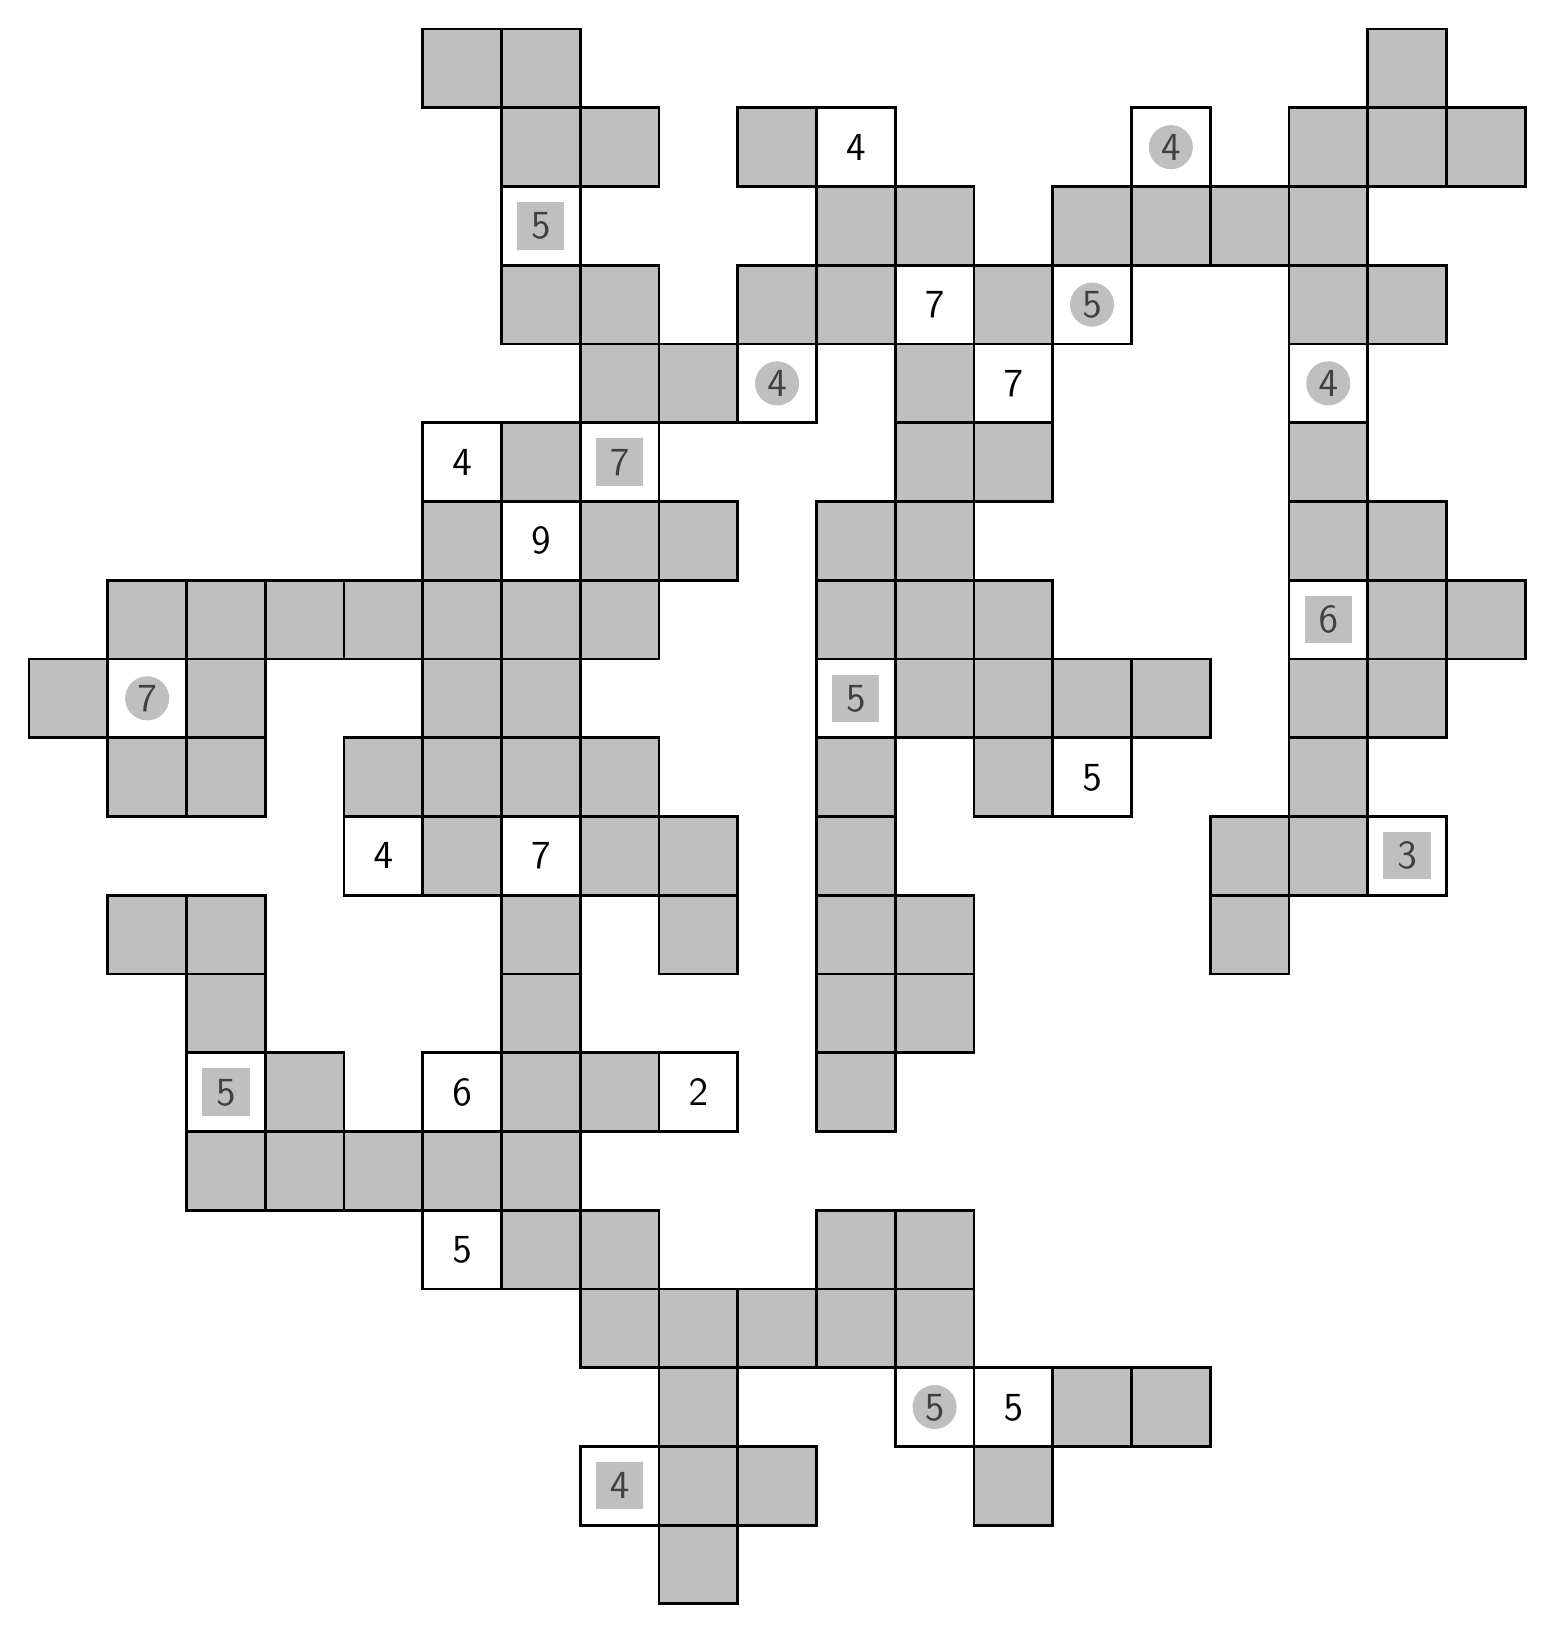
\begin{tikzpicture}\fill[gray, opacity = 0.5] (9, 0, 0)--++(1, 0, 0)--++(0, 1, 0)--++(-1, 0, 0)--cycle;
\draw[line width = 1pt] (9, 0, 0)--++(1, 0, 0)--++(0, 1, 0)--++(-1, 0, 0)--cycle;
\draw node at (8.5, 1.5, 0) {\Large $\mathsf{4}$};
\draw[line width = 1pt] (8, 1, 0)--++(1, 0, 0)--++(0, 1, 0)--++(-1, 0, 0)--cycle;
\fill[color = gray, opacity = 0.5] (8.2, 1.2) rectangle ++(0.6, 0.6);
\fill[gray, opacity = 0.5] (9, 1, 0)--++(1, 0, 0)--++(0, 1, 0)--++(-1, 0, 0)--cycle;
\draw[line width = 1pt] (9, 1, 0)--++(1, 0, 0)--++(0, 1, 0)--++(-1, 0, 0)--cycle;
\fill[gray, opacity = 0.5] (10, 1, 0)--++(1, 0, 0)--++(0, 1, 0)--++(-1, 0, 0)--cycle;
\draw[line width = 1pt] (10, 1, 0)--++(1, 0, 0)--++(0, 1, 0)--++(-1, 0, 0)--cycle;
\fill[gray, opacity = 0.5] (13, 1, 0)--++(1, 0, 0)--++(0, 1, 0)--++(-1, 0, 0)--cycle;
\draw[line width = 1pt] (13, 1, 0)--++(1, 0, 0)--++(0, 1, 0)--++(-1, 0, 0)--cycle;
\fill[gray, opacity = 0.5] (9, 2, 0)--++(1, 0, 0)--++(0, 1, 0)--++(-1, 0, 0)--cycle;
\draw[line width = 1pt] (9, 2, 0)--++(1, 0, 0)--++(0, 1, 0)--++(-1, 0, 0)--cycle;
\draw node at (12.5, 2.5, 0) {\Large $\mathsf{5}$};
\draw[line width = 1pt] (12, 2, 0)--++(1, 0, 0)--++(0, 1, 0)--++(-1, 0, 0)--cycle;
\fill[color = gray, opacity = 0.5] (12.5, 2.5, 0) circle (0.28);
\draw node at (13.5, 2.5, 0) {\Large $\mathsf{5}$};
\draw[line width = 1pt] (13, 2, 0)--++(1, 0, 0)--++(0, 1, 0)--++(-1, 0, 0)--cycle;
\fill[gray, opacity = 0.5] (14, 2, 0)--++(1, 0, 0)--++(0, 1, 0)--++(-1, 0, 0)--cycle;
\draw[line width = 1pt] (14, 2, 0)--++(1, 0, 0)--++(0, 1, 0)--++(-1, 0, 0)--cycle;
\fill[gray, opacity = 0.5] (15, 2, 0)--++(1, 0, 0)--++(0, 1, 0)--++(-1, 0, 0)--cycle;
\draw[line width = 1pt] (15, 2, 0)--++(1, 0, 0)--++(0, 1, 0)--++(-1, 0, 0)--cycle;
\fill[gray, opacity = 0.5] (8, 3, 0)--++(1, 0, 0)--++(0, 1, 0)--++(-1, 0, 0)--cycle;
\draw[line width = 1pt] (8, 3, 0)--++(1, 0, 0)--++(0, 1, 0)--++(-1, 0, 0)--cycle;
\fill[gray, opacity = 0.5] (9, 3, 0)--++(1, 0, 0)--++(0, 1, 0)--++(-1, 0, 0)--cycle;
\draw[line width = 1pt] (9, 3, 0)--++(1, 0, 0)--++(0, 1, 0)--++(-1, 0, 0)--cycle;
\fill[gray, opacity = 0.5] (10, 3, 0)--++(1, 0, 0)--++(0, 1, 0)--++(-1, 0, 0)--cycle;
\draw[line width = 1pt] (10, 3, 0)--++(1, 0, 0)--++(0, 1, 0)--++(-1, 0, 0)--cycle;
\fill[gray, opacity = 0.5] (11, 3, 0)--++(1, 0, 0)--++(0, 1, 0)--++(-1, 0, 0)--cycle;
\draw[line width = 1pt] (11, 3, 0)--++(1, 0, 0)--++(0, 1, 0)--++(-1, 0, 0)--cycle;
\fill[gray, opacity = 0.5] (12, 3, 0)--++(1, 0, 0)--++(0, 1, 0)--++(-1, 0, 0)--cycle;
\draw[line width = 1pt] (12, 3, 0)--++(1, 0, 0)--++(0, 1, 0)--++(-1, 0, 0)--cycle;
\draw node at (6.5, 4.5, 0) {\Large $\mathsf{5}$};
\draw[line width = 1pt] (6, 4, 0)--++(1, 0, 0)--++(0, 1, 0)--++(-1, 0, 0)--cycle;
\fill[gray, opacity = 0.5] (7, 4, 0)--++(1, 0, 0)--++(0, 1, 0)--++(-1, 0, 0)--cycle;
\draw[line width = 1pt] (7, 4, 0)--++(1, 0, 0)--++(0, 1, 0)--++(-1, 0, 0)--cycle;
\fill[gray, opacity = 0.5] (8, 4, 0)--++(1, 0, 0)--++(0, 1, 0)--++(-1, 0, 0)--cycle;
\draw[line width = 1pt] (8, 4, 0)--++(1, 0, 0)--++(0, 1, 0)--++(-1, 0, 0)--cycle;
\fill[gray, opacity = 0.5] (11, 4, 0)--++(1, 0, 0)--++(0, 1, 0)--++(-1, 0, 0)--cycle;
\draw[line width = 1pt] (11, 4, 0)--++(1, 0, 0)--++(0, 1, 0)--++(-1, 0, 0)--cycle;
\fill[gray, opacity = 0.5] (12, 4, 0)--++(1, 0, 0)--++(0, 1, 0)--++(-1, 0, 0)--cycle;
\draw[line width = 1pt] (12, 4, 0)--++(1, 0, 0)--++(0, 1, 0)--++(-1, 0, 0)--cycle;
\fill[gray, opacity = 0.5] (3, 5, 0)--++(1, 0, 0)--++(0, 1, 0)--++(-1, 0, 0)--cycle;
\draw[line width = 1pt] (3, 5, 0)--++(1, 0, 0)--++(0, 1, 0)--++(-1, 0, 0)--cycle;
\fill[gray, opacity = 0.5] (4, 5, 0)--++(1, 0, 0)--++(0, 1, 0)--++(-1, 0, 0)--cycle;
\draw[line width = 1pt] (4, 5, 0)--++(1, 0, 0)--++(0, 1, 0)--++(-1, 0, 0)--cycle;
\fill[gray, opacity = 0.5] (5, 5, 0)--++(1, 0, 0)--++(0, 1, 0)--++(-1, 0, 0)--cycle;
\draw[line width = 1pt] (5, 5, 0)--++(1, 0, 0)--++(0, 1, 0)--++(-1, 0, 0)--cycle;
\fill[gray, opacity = 0.5] (6, 5, 0)--++(1, 0, 0)--++(0, 1, 0)--++(-1, 0, 0)--cycle;
\draw[line width = 1pt] (6, 5, 0)--++(1, 0, 0)--++(0, 1, 0)--++(-1, 0, 0)--cycle;
\fill[gray, opacity = 0.5] (7, 5, 0)--++(1, 0, 0)--++(0, 1, 0)--++(-1, 0, 0)--cycle;
\draw[line width = 1pt] (7, 5, 0)--++(1, 0, 0)--++(0, 1, 0)--++(-1, 0, 0)--cycle;
\draw node at (3.5, 6.5, 0) {\Large $\mathsf{5}$};
\draw[line width = 1pt] (3, 6, 0)--++(1, 0, 0)--++(0, 1, 0)--++(-1, 0, 0)--cycle;
\fill[color = gray, opacity = 0.5] (3.2, 6.2) rectangle ++(0.6, 0.6);
\fill[gray, opacity = 0.5] (4, 6, 0)--++(1, 0, 0)--++(0, 1, 0)--++(-1, 0, 0)--cycle;
\draw[line width = 1pt] (4, 6, 0)--++(1, 0, 0)--++(0, 1, 0)--++(-1, 0, 0)--cycle;
\draw node at (6.5, 6.5, 0) {\Large $\mathsf{6}$};
\draw[line width = 1pt] (6, 6, 0)--++(1, 0, 0)--++(0, 1, 0)--++(-1, 0, 0)--cycle;
\fill[gray, opacity = 0.5] (7, 6, 0)--++(1, 0, 0)--++(0, 1, 0)--++(-1, 0, 0)--cycle;
\draw[line width = 1pt] (7, 6, 0)--++(1, 0, 0)--++(0, 1, 0)--++(-1, 0, 0)--cycle;
\fill[gray, opacity = 0.5] (8, 6, 0)--++(1, 0, 0)--++(0, 1, 0)--++(-1, 0, 0)--cycle;
\draw[line width = 1pt] (8, 6, 0)--++(1, 0, 0)--++(0, 1, 0)--++(-1, 0, 0)--cycle;
\draw node at (9.5, 6.5, 0) {\Large $\mathsf{2}$};
\draw[line width = 1pt] (9, 6, 0)--++(1, 0, 0)--++(0, 1, 0)--++(-1, 0, 0)--cycle;
\fill[gray, opacity = 0.5] (11, 6, 0)--++(1, 0, 0)--++(0, 1, 0)--++(-1, 0, 0)--cycle;
\draw[line width = 1pt] (11, 6, 0)--++(1, 0, 0)--++(0, 1, 0)--++(-1, 0, 0)--cycle;
\fill[gray, opacity = 0.5] (3, 7, 0)--++(1, 0, 0)--++(0, 1, 0)--++(-1, 0, 0)--cycle;
\draw[line width = 1pt] (3, 7, 0)--++(1, 0, 0)--++(0, 1, 0)--++(-1, 0, 0)--cycle;
\fill[gray, opacity = 0.5] (7, 7, 0)--++(1, 0, 0)--++(0, 1, 0)--++(-1, 0, 0)--cycle;
\draw[line width = 1pt] (7, 7, 0)--++(1, 0, 0)--++(0, 1, 0)--++(-1, 0, 0)--cycle;
\fill[gray, opacity = 0.5] (11, 7, 0)--++(1, 0, 0)--++(0, 1, 0)--++(-1, 0, 0)--cycle;
\draw[line width = 1pt] (11, 7, 0)--++(1, 0, 0)--++(0, 1, 0)--++(-1, 0, 0)--cycle;
\fill[gray, opacity = 0.5] (12, 7, 0)--++(1, 0, 0)--++(0, 1, 0)--++(-1, 0, 0)--cycle;
\draw[line width = 1pt] (12, 7, 0)--++(1, 0, 0)--++(0, 1, 0)--++(-1, 0, 0)--cycle;
\fill[gray, opacity = 0.5] (2, 8, 0)--++(1, 0, 0)--++(0, 1, 0)--++(-1, 0, 0)--cycle;
\draw[line width = 1pt] (2, 8, 0)--++(1, 0, 0)--++(0, 1, 0)--++(-1, 0, 0)--cycle;
\fill[gray, opacity = 0.5] (3, 8, 0)--++(1, 0, 0)--++(0, 1, 0)--++(-1, 0, 0)--cycle;
\draw[line width = 1pt] (3, 8, 0)--++(1, 0, 0)--++(0, 1, 0)--++(-1, 0, 0)--cycle;
\fill[gray, opacity = 0.5] (7, 8, 0)--++(1, 0, 0)--++(0, 1, 0)--++(-1, 0, 0)--cycle;
\draw[line width = 1pt] (7, 8, 0)--++(1, 0, 0)--++(0, 1, 0)--++(-1, 0, 0)--cycle;
\fill[gray, opacity = 0.5] (9, 8, 0)--++(1, 0, 0)--++(0, 1, 0)--++(-1, 0, 0)--cycle;
\draw[line width = 1pt] (9, 8, 0)--++(1, 0, 0)--++(0, 1, 0)--++(-1, 0, 0)--cycle;
\fill[gray, opacity = 0.5] (11, 8, 0)--++(1, 0, 0)--++(0, 1, 0)--++(-1, 0, 0)--cycle;
\draw[line width = 1pt] (11, 8, 0)--++(1, 0, 0)--++(0, 1, 0)--++(-1, 0, 0)--cycle;
\fill[gray, opacity = 0.5] (12, 8, 0)--++(1, 0, 0)--++(0, 1, 0)--++(-1, 0, 0)--cycle;
\draw[line width = 1pt] (12, 8, 0)--++(1, 0, 0)--++(0, 1, 0)--++(-1, 0, 0)--cycle;
\fill[gray, opacity = 0.5] (16, 8, 0)--++(1, 0, 0)--++(0, 1, 0)--++(-1, 0, 0)--cycle;
\draw[line width = 1pt] (16, 8, 0)--++(1, 0, 0)--++(0, 1, 0)--++(-1, 0, 0)--cycle;
\draw node at (5.5, 9.5, 0) {\Large $\mathsf{4}$};
\draw[line width = 1pt] (5, 9, 0)--++(1, 0, 0)--++(0, 1, 0)--++(-1, 0, 0)--cycle;
\fill[gray, opacity = 0.5] (6, 9, 0)--++(1, 0, 0)--++(0, 1, 0)--++(-1, 0, 0)--cycle;
\draw[line width = 1pt] (6, 9, 0)--++(1, 0, 0)--++(0, 1, 0)--++(-1, 0, 0)--cycle;
\draw node at (7.5, 9.5, 0) {\Large $\mathsf{7}$};
\draw[line width = 1pt] (7, 9, 0)--++(1, 0, 0)--++(0, 1, 0)--++(-1, 0, 0)--cycle;
\fill[gray, opacity = 0.5] (8, 9, 0)--++(1, 0, 0)--++(0, 1, 0)--++(-1, 0, 0)--cycle;
\draw[line width = 1pt] (8, 9, 0)--++(1, 0, 0)--++(0, 1, 0)--++(-1, 0, 0)--cycle;
\fill[gray, opacity = 0.5] (9, 9, 0)--++(1, 0, 0)--++(0, 1, 0)--++(-1, 0, 0)--cycle;
\draw[line width = 1pt] (9, 9, 0)--++(1, 0, 0)--++(0, 1, 0)--++(-1, 0, 0)--cycle;
\fill[gray, opacity = 0.5] (11, 9, 0)--++(1, 0, 0)--++(0, 1, 0)--++(-1, 0, 0)--cycle;
\draw[line width = 1pt] (11, 9, 0)--++(1, 0, 0)--++(0, 1, 0)--++(-1, 0, 0)--cycle;
\fill[gray, opacity = 0.5] (16, 9, 0)--++(1, 0, 0)--++(0, 1, 0)--++(-1, 0, 0)--cycle;
\draw[line width = 1pt] (16, 9, 0)--++(1, 0, 0)--++(0, 1, 0)--++(-1, 0, 0)--cycle;
\fill[gray, opacity = 0.5] (17, 9, 0)--++(1, 0, 0)--++(0, 1, 0)--++(-1, 0, 0)--cycle;
\draw[line width = 1pt] (17, 9, 0)--++(1, 0, 0)--++(0, 1, 0)--++(-1, 0, 0)--cycle;
\draw node at (18.5, 9.5, 0) {\Large $\mathsf{3}$};
\draw[line width = 1pt] (18, 9, 0)--++(1, 0, 0)--++(0, 1, 0)--++(-1, 0, 0)--cycle;
\fill[color = gray, opacity = 0.5] (18.2, 9.2) rectangle ++(0.6, 0.6);
\fill[gray, opacity = 0.5] (2, 10, 0)--++(1, 0, 0)--++(0, 1, 0)--++(-1, 0, 0)--cycle;
\draw[line width = 1pt] (2, 10, 0)--++(1, 0, 0)--++(0, 1, 0)--++(-1, 0, 0)--cycle;
\fill[gray, opacity = 0.5] (3, 10, 0)--++(1, 0, 0)--++(0, 1, 0)--++(-1, 0, 0)--cycle;
\draw[line width = 1pt] (3, 10, 0)--++(1, 0, 0)--++(0, 1, 0)--++(-1, 0, 0)--cycle;
\fill[gray, opacity = 0.5] (5, 10, 0)--++(1, 0, 0)--++(0, 1, 0)--++(-1, 0, 0)--cycle;
\draw[line width = 1pt] (5, 10, 0)--++(1, 0, 0)--++(0, 1, 0)--++(-1, 0, 0)--cycle;
\fill[gray, opacity = 0.5] (6, 10, 0)--++(1, 0, 0)--++(0, 1, 0)--++(-1, 0, 0)--cycle;
\draw[line width = 1pt] (6, 10, 0)--++(1, 0, 0)--++(0, 1, 0)--++(-1, 0, 0)--cycle;
\fill[gray, opacity = 0.5] (7, 10, 0)--++(1, 0, 0)--++(0, 1, 0)--++(-1, 0, 0)--cycle;
\draw[line width = 1pt] (7, 10, 0)--++(1, 0, 0)--++(0, 1, 0)--++(-1, 0, 0)--cycle;
\fill[gray, opacity = 0.5] (8, 10, 0)--++(1, 0, 0)--++(0, 1, 0)--++(-1, 0, 0)--cycle;
\draw[line width = 1pt] (8, 10, 0)--++(1, 0, 0)--++(0, 1, 0)--++(-1, 0, 0)--cycle;
\fill[gray, opacity = 0.5] (11, 10, 0)--++(1, 0, 0)--++(0, 1, 0)--++(-1, 0, 0)--cycle;
\draw[line width = 1pt] (11, 10, 0)--++(1, 0, 0)--++(0, 1, 0)--++(-1, 0, 0)--cycle;
\fill[gray, opacity = 0.5] (13, 10, 0)--++(1, 0, 0)--++(0, 1, 0)--++(-1, 0, 0)--cycle;
\draw[line width = 1pt] (13, 10, 0)--++(1, 0, 0)--++(0, 1, 0)--++(-1, 0, 0)--cycle;
\draw node at (14.5, 10.5, 0) {\Large $\mathsf{5}$};
\draw[line width = 1pt] (14, 10, 0)--++(1, 0, 0)--++(0, 1, 0)--++(-1, 0, 0)--cycle;
\fill[gray, opacity = 0.5] (17, 10, 0)--++(1, 0, 0)--++(0, 1, 0)--++(-1, 0, 0)--cycle;
\draw[line width = 1pt] (17, 10, 0)--++(1, 0, 0)--++(0, 1, 0)--++(-1, 0, 0)--cycle;
\fill[gray, opacity = 0.5] (1, 11, 0)--++(1, 0, 0)--++(0, 1, 0)--++(-1, 0, 0)--cycle;
\draw[line width = 1pt] (1, 11, 0)--++(1, 0, 0)--++(0, 1, 0)--++(-1, 0, 0)--cycle;
\draw node at (2.5, 11.5, 0) {\Large $\mathsf{7}$};
\draw[line width = 1pt] (2, 11, 0)--++(1, 0, 0)--++(0, 1, 0)--++(-1, 0, 0)--cycle;
\fill[color = gray, opacity = 0.5] (2.5, 11.5, 0) circle (0.28);
\fill[gray, opacity = 0.5] (3, 11, 0)--++(1, 0, 0)--++(0, 1, 0)--++(-1, 0, 0)--cycle;
\draw[line width = 1pt] (3, 11, 0)--++(1, 0, 0)--++(0, 1, 0)--++(-1, 0, 0)--cycle;
\fill[gray, opacity = 0.5] (6, 11, 0)--++(1, 0, 0)--++(0, 1, 0)--++(-1, 0, 0)--cycle;
\draw[line width = 1pt] (6, 11, 0)--++(1, 0, 0)--++(0, 1, 0)--++(-1, 0, 0)--cycle;
\fill[gray, opacity = 0.5] (7, 11, 0)--++(1, 0, 0)--++(0, 1, 0)--++(-1, 0, 0)--cycle;
\draw[line width = 1pt] (7, 11, 0)--++(1, 0, 0)--++(0, 1, 0)--++(-1, 0, 0)--cycle;
\draw node at (11.5, 11.5, 0) {\Large $\mathsf{5}$};
\draw[line width = 1pt] (11, 11, 0)--++(1, 0, 0)--++(0, 1, 0)--++(-1, 0, 0)--cycle;
\fill[color = gray, opacity = 0.5] (11.2, 11.2) rectangle ++(0.6, 0.6);
\fill[gray, opacity = 0.5] (12, 11, 0)--++(1, 0, 0)--++(0, 1, 0)--++(-1, 0, 0)--cycle;
\draw[line width = 1pt] (12, 11, 0)--++(1, 0, 0)--++(0, 1, 0)--++(-1, 0, 0)--cycle;
\fill[gray, opacity = 0.5] (13, 11, 0)--++(1, 0, 0)--++(0, 1, 0)--++(-1, 0, 0)--cycle;
\draw[line width = 1pt] (13, 11, 0)--++(1, 0, 0)--++(0, 1, 0)--++(-1, 0, 0)--cycle;
\fill[gray, opacity = 0.5] (14, 11, 0)--++(1, 0, 0)--++(0, 1, 0)--++(-1, 0, 0)--cycle;
\draw[line width = 1pt] (14, 11, 0)--++(1, 0, 0)--++(0, 1, 0)--++(-1, 0, 0)--cycle;
\fill[gray, opacity = 0.5] (15, 11, 0)--++(1, 0, 0)--++(0, 1, 0)--++(-1, 0, 0)--cycle;
\draw[line width = 1pt] (15, 11, 0)--++(1, 0, 0)--++(0, 1, 0)--++(-1, 0, 0)--cycle;
\fill[gray, opacity = 0.5] (17, 11, 0)--++(1, 0, 0)--++(0, 1, 0)--++(-1, 0, 0)--cycle;
\draw[line width = 1pt] (17, 11, 0)--++(1, 0, 0)--++(0, 1, 0)--++(-1, 0, 0)--cycle;
\fill[gray, opacity = 0.5] (18, 11, 0)--++(1, 0, 0)--++(0, 1, 0)--++(-1, 0, 0)--cycle;
\draw[line width = 1pt] (18, 11, 0)--++(1, 0, 0)--++(0, 1, 0)--++(-1, 0, 0)--cycle;
\fill[gray, opacity = 0.5] (2, 12, 0)--++(1, 0, 0)--++(0, 1, 0)--++(-1, 0, 0)--cycle;
\draw[line width = 1pt] (2, 12, 0)--++(1, 0, 0)--++(0, 1, 0)--++(-1, 0, 0)--cycle;
\fill[gray, opacity = 0.5] (3, 12, 0)--++(1, 0, 0)--++(0, 1, 0)--++(-1, 0, 0)--cycle;
\draw[line width = 1pt] (3, 12, 0)--++(1, 0, 0)--++(0, 1, 0)--++(-1, 0, 0)--cycle;
\fill[gray, opacity = 0.5] (4, 12, 0)--++(1, 0, 0)--++(0, 1, 0)--++(-1, 0, 0)--cycle;
\draw[line width = 1pt] (4, 12, 0)--++(1, 0, 0)--++(0, 1, 0)--++(-1, 0, 0)--cycle;
\fill[gray, opacity = 0.5] (5, 12, 0)--++(1, 0, 0)--++(0, 1, 0)--++(-1, 0, 0)--cycle;
\draw[line width = 1pt] (5, 12, 0)--++(1, 0, 0)--++(0, 1, 0)--++(-1, 0, 0)--cycle;
\fill[gray, opacity = 0.5] (6, 12, 0)--++(1, 0, 0)--++(0, 1, 0)--++(-1, 0, 0)--cycle;
\draw[line width = 1pt] (6, 12, 0)--++(1, 0, 0)--++(0, 1, 0)--++(-1, 0, 0)--cycle;
\fill[gray, opacity = 0.5] (7, 12, 0)--++(1, 0, 0)--++(0, 1, 0)--++(-1, 0, 0)--cycle;
\draw[line width = 1pt] (7, 12, 0)--++(1, 0, 0)--++(0, 1, 0)--++(-1, 0, 0)--cycle;
\fill[gray, opacity = 0.5] (8, 12, 0)--++(1, 0, 0)--++(0, 1, 0)--++(-1, 0, 0)--cycle;
\draw[line width = 1pt] (8, 12, 0)--++(1, 0, 0)--++(0, 1, 0)--++(-1, 0, 0)--cycle;
\fill[gray, opacity = 0.5] (11, 12, 0)--++(1, 0, 0)--++(0, 1, 0)--++(-1, 0, 0)--cycle;
\draw[line width = 1pt] (11, 12, 0)--++(1, 0, 0)--++(0, 1, 0)--++(-1, 0, 0)--cycle;
\fill[gray, opacity = 0.5] (12, 12, 0)--++(1, 0, 0)--++(0, 1, 0)--++(-1, 0, 0)--cycle;
\draw[line width = 1pt] (12, 12, 0)--++(1, 0, 0)--++(0, 1, 0)--++(-1, 0, 0)--cycle;
\fill[gray, opacity = 0.5] (13, 12, 0)--++(1, 0, 0)--++(0, 1, 0)--++(-1, 0, 0)--cycle;
\draw[line width = 1pt] (13, 12, 0)--++(1, 0, 0)--++(0, 1, 0)--++(-1, 0, 0)--cycle;
\draw node at (17.5, 12.5, 0) {\Large $\mathsf{6}$};
\draw[line width = 1pt] (17, 12, 0)--++(1, 0, 0)--++(0, 1, 0)--++(-1, 0, 0)--cycle;
\fill[color = gray, opacity = 0.5] (17.2, 12.2) rectangle ++(0.6, 0.6);
\fill[gray, opacity = 0.5] (18, 12, 0)--++(1, 0, 0)--++(0, 1, 0)--++(-1, 0, 0)--cycle;
\draw[line width = 1pt] (18, 12, 0)--++(1, 0, 0)--++(0, 1, 0)--++(-1, 0, 0)--cycle;
\fill[gray, opacity = 0.5] (19, 12, 0)--++(1, 0, 0)--++(0, 1, 0)--++(-1, 0, 0)--cycle;
\draw[line width = 1pt] (19, 12, 0)--++(1, 0, 0)--++(0, 1, 0)--++(-1, 0, 0)--cycle;
\fill[gray, opacity = 0.5] (6, 13, 0)--++(1, 0, 0)--++(0, 1, 0)--++(-1, 0, 0)--cycle;
\draw[line width = 1pt] (6, 13, 0)--++(1, 0, 0)--++(0, 1, 0)--++(-1, 0, 0)--cycle;
\draw node at (7.5, 13.5, 0) {\Large $\mathsf{9}$};
\draw[line width = 1pt] (7, 13, 0)--++(1, 0, 0)--++(0, 1, 0)--++(-1, 0, 0)--cycle;
\fill[gray, opacity = 0.5] (8, 13, 0)--++(1, 0, 0)--++(0, 1, 0)--++(-1, 0, 0)--cycle;
\draw[line width = 1pt] (8, 13, 0)--++(1, 0, 0)--++(0, 1, 0)--++(-1, 0, 0)--cycle;
\fill[gray, opacity = 0.5] (9, 13, 0)--++(1, 0, 0)--++(0, 1, 0)--++(-1, 0, 0)--cycle;
\draw[line width = 1pt] (9, 13, 0)--++(1, 0, 0)--++(0, 1, 0)--++(-1, 0, 0)--cycle;
\fill[gray, opacity = 0.5] (11, 13, 0)--++(1, 0, 0)--++(0, 1, 0)--++(-1, 0, 0)--cycle;
\draw[line width = 1pt] (11, 13, 0)--++(1, 0, 0)--++(0, 1, 0)--++(-1, 0, 0)--cycle;
\fill[gray, opacity = 0.5] (12, 13, 0)--++(1, 0, 0)--++(0, 1, 0)--++(-1, 0, 0)--cycle;
\draw[line width = 1pt] (12, 13, 0)--++(1, 0, 0)--++(0, 1, 0)--++(-1, 0, 0)--cycle;
\fill[gray, opacity = 0.5] (17, 13, 0)--++(1, 0, 0)--++(0, 1, 0)--++(-1, 0, 0)--cycle;
\draw[line width = 1pt] (17, 13, 0)--++(1, 0, 0)--++(0, 1, 0)--++(-1, 0, 0)--cycle;
\fill[gray, opacity = 0.5] (18, 13, 0)--++(1, 0, 0)--++(0, 1, 0)--++(-1, 0, 0)--cycle;
\draw[line width = 1pt] (18, 13, 0)--++(1, 0, 0)--++(0, 1, 0)--++(-1, 0, 0)--cycle;
\draw node at (6.5, 14.5, 0) {\Large $\mathsf{4}$};
\draw[line width = 1pt] (6, 14, 0)--++(1, 0, 0)--++(0, 1, 0)--++(-1, 0, 0)--cycle;
\fill[gray, opacity = 0.5] (7, 14, 0)--++(1, 0, 0)--++(0, 1, 0)--++(-1, 0, 0)--cycle;
\draw[line width = 1pt] (7, 14, 0)--++(1, 0, 0)--++(0, 1, 0)--++(-1, 0, 0)--cycle;
\draw node at (8.5, 14.5, 0) {\Large $\mathsf{7}$};
\draw[line width = 1pt] (8, 14, 0)--++(1, 0, 0)--++(0, 1, 0)--++(-1, 0, 0)--cycle;
\fill[color = gray, opacity = 0.5] (8.2, 14.2) rectangle ++(0.6, 0.6);
\fill[gray, opacity = 0.5] (12, 14, 0)--++(1, 0, 0)--++(0, 1, 0)--++(-1, 0, 0)--cycle;
\draw[line width = 1pt] (12, 14, 0)--++(1, 0, 0)--++(0, 1, 0)--++(-1, 0, 0)--cycle;
\fill[gray, opacity = 0.5] (13, 14, 0)--++(1, 0, 0)--++(0, 1, 0)--++(-1, 0, 0)--cycle;
\draw[line width = 1pt] (13, 14, 0)--++(1, 0, 0)--++(0, 1, 0)--++(-1, 0, 0)--cycle;
\fill[gray, opacity = 0.5] (17, 14, 0)--++(1, 0, 0)--++(0, 1, 0)--++(-1, 0, 0)--cycle;
\draw[line width = 1pt] (17, 14, 0)--++(1, 0, 0)--++(0, 1, 0)--++(-1, 0, 0)--cycle;
\fill[gray, opacity = 0.5] (8, 15, 0)--++(1, 0, 0)--++(0, 1, 0)--++(-1, 0, 0)--cycle;
\draw[line width = 1pt] (8, 15, 0)--++(1, 0, 0)--++(0, 1, 0)--++(-1, 0, 0)--cycle;
\fill[gray, opacity = 0.5] (9, 15, 0)--++(1, 0, 0)--++(0, 1, 0)--++(-1, 0, 0)--cycle;
\draw[line width = 1pt] (9, 15, 0)--++(1, 0, 0)--++(0, 1, 0)--++(-1, 0, 0)--cycle;
\draw node at (10.5, 15.5, 0) {\Large $\mathsf{4}$};
\draw[line width = 1pt] (10, 15, 0)--++(1, 0, 0)--++(0, 1, 0)--++(-1, 0, 0)--cycle;
\fill[color = gray, opacity = 0.5] (10.5, 15.5, 0) circle (0.28);
\fill[gray, opacity = 0.5] (12, 15, 0)--++(1, 0, 0)--++(0, 1, 0)--++(-1, 0, 0)--cycle;
\draw[line width = 1pt] (12, 15, 0)--++(1, 0, 0)--++(0, 1, 0)--++(-1, 0, 0)--cycle;
\draw node at (13.5, 15.5, 0) {\Large $\mathsf{7}$};
\draw[line width = 1pt] (13, 15, 0)--++(1, 0, 0)--++(0, 1, 0)--++(-1, 0, 0)--cycle;
\draw node at (17.5, 15.5, 0) {\Large $\mathsf{4}$};
\draw[line width = 1pt] (17, 15, 0)--++(1, 0, 0)--++(0, 1, 0)--++(-1, 0, 0)--cycle;
\fill[color = gray, opacity = 0.5] (17.5, 15.5, 0) circle (0.28);
\fill[gray, opacity = 0.5] (7, 16, 0)--++(1, 0, 0)--++(0, 1, 0)--++(-1, 0, 0)--cycle;
\draw[line width = 1pt] (7, 16, 0)--++(1, 0, 0)--++(0, 1, 0)--++(-1, 0, 0)--cycle;
\fill[gray, opacity = 0.5] (8, 16, 0)--++(1, 0, 0)--++(0, 1, 0)--++(-1, 0, 0)--cycle;
\draw[line width = 1pt] (8, 16, 0)--++(1, 0, 0)--++(0, 1, 0)--++(-1, 0, 0)--cycle;
\fill[gray, opacity = 0.5] (10, 16, 0)--++(1, 0, 0)--++(0, 1, 0)--++(-1, 0, 0)--cycle;
\draw[line width = 1pt] (10, 16, 0)--++(1, 0, 0)--++(0, 1, 0)--++(-1, 0, 0)--cycle;
\fill[gray, opacity = 0.5] (11, 16, 0)--++(1, 0, 0)--++(0, 1, 0)--++(-1, 0, 0)--cycle;
\draw[line width = 1pt] (11, 16, 0)--++(1, 0, 0)--++(0, 1, 0)--++(-1, 0, 0)--cycle;
\draw node at (12.5, 16.5, 0) {\Large $\mathsf{7}$};
\draw[line width = 1pt] (12, 16, 0)--++(1, 0, 0)--++(0, 1, 0)--++(-1, 0, 0)--cycle;
\fill[gray, opacity = 0.5] (13, 16, 0)--++(1, 0, 0)--++(0, 1, 0)--++(-1, 0, 0)--cycle;
\draw[line width = 1pt] (13, 16, 0)--++(1, 0, 0)--++(0, 1, 0)--++(-1, 0, 0)--cycle;
\draw node at (14.5, 16.5, 0) {\Large $\mathsf{5}$};
\draw[line width = 1pt] (14, 16, 0)--++(1, 0, 0)--++(0, 1, 0)--++(-1, 0, 0)--cycle;
\fill[color = gray, opacity = 0.5] (14.5, 16.5, 0) circle (0.28);
\fill[gray, opacity = 0.5] (17, 16, 0)--++(1, 0, 0)--++(0, 1, 0)--++(-1, 0, 0)--cycle;
\draw[line width = 1pt] (17, 16, 0)--++(1, 0, 0)--++(0, 1, 0)--++(-1, 0, 0)--cycle;
\fill[gray, opacity = 0.5] (18, 16, 0)--++(1, 0, 0)--++(0, 1, 0)--++(-1, 0, 0)--cycle;
\draw[line width = 1pt] (18, 16, 0)--++(1, 0, 0)--++(0, 1, 0)--++(-1, 0, 0)--cycle;
\draw node at (7.5, 17.5, 0) {\Large $\mathsf{5}$};
\draw[line width = 1pt] (7, 17, 0)--++(1, 0, 0)--++(0, 1, 0)--++(-1, 0, 0)--cycle;
\fill[color = gray, opacity = 0.5] (7.2, 17.2) rectangle ++(0.6, 0.6);
\fill[gray, opacity = 0.5] (11, 17, 0)--++(1, 0, 0)--++(0, 1, 0)--++(-1, 0, 0)--cycle;
\draw[line width = 1pt] (11, 17, 0)--++(1, 0, 0)--++(0, 1, 0)--++(-1, 0, 0)--cycle;
\fill[gray, opacity = 0.5] (12, 17, 0)--++(1, 0, 0)--++(0, 1, 0)--++(-1, 0, 0)--cycle;
\draw[line width = 1pt] (12, 17, 0)--++(1, 0, 0)--++(0, 1, 0)--++(-1, 0, 0)--cycle;
\fill[gray, opacity = 0.5] (14, 17, 0)--++(1, 0, 0)--++(0, 1, 0)--++(-1, 0, 0)--cycle;
\draw[line width = 1pt] (14, 17, 0)--++(1, 0, 0)--++(0, 1, 0)--++(-1, 0, 0)--cycle;
\fill[gray, opacity = 0.5] (15, 17, 0)--++(1, 0, 0)--++(0, 1, 0)--++(-1, 0, 0)--cycle;
\draw[line width = 1pt] (15, 17, 0)--++(1, 0, 0)--++(0, 1, 0)--++(-1, 0, 0)--cycle;
\fill[gray, opacity = 0.5] (16, 17, 0)--++(1, 0, 0)--++(0, 1, 0)--++(-1, 0, 0)--cycle;
\draw[line width = 1pt] (16, 17, 0)--++(1, 0, 0)--++(0, 1, 0)--++(-1, 0, 0)--cycle;
\fill[gray, opacity = 0.5] (17, 17, 0)--++(1, 0, 0)--++(0, 1, 0)--++(-1, 0, 0)--cycle;
\draw[line width = 1pt] (17, 17, 0)--++(1, 0, 0)--++(0, 1, 0)--++(-1, 0, 0)--cycle;
\fill[gray, opacity = 0.5] (7, 18, 0)--++(1, 0, 0)--++(0, 1, 0)--++(-1, 0, 0)--cycle;
\draw[line width = 1pt] (7, 18, 0)--++(1, 0, 0)--++(0, 1, 0)--++(-1, 0, 0)--cycle;
\fill[gray, opacity = 0.5] (8, 18, 0)--++(1, 0, 0)--++(0, 1, 0)--++(-1, 0, 0)--cycle;
\draw[line width = 1pt] (8, 18, 0)--++(1, 0, 0)--++(0, 1, 0)--++(-1, 0, 0)--cycle;
\fill[gray, opacity = 0.5] (10, 18, 0)--++(1, 0, 0)--++(0, 1, 0)--++(-1, 0, 0)--cycle;
\draw[line width = 1pt] (10, 18, 0)--++(1, 0, 0)--++(0, 1, 0)--++(-1, 0, 0)--cycle;
\draw node at (11.5, 18.5, 0) {\Large $\mathsf{4}$};
\draw[line width = 1pt] (11, 18, 0)--++(1, 0, 0)--++(0, 1, 0)--++(-1, 0, 0)--cycle;
\draw node at (15.5, 18.5, 0) {\Large $\mathsf{4}$};
\draw[line width = 1pt] (15, 18, 0)--++(1, 0, 0)--++(0, 1, 0)--++(-1, 0, 0)--cycle;
\fill[color = gray, opacity = 0.5] (15.5, 18.5, 0) circle (0.28);
\fill[gray, opacity = 0.5] (17, 18, 0)--++(1, 0, 0)--++(0, 1, 0)--++(-1, 0, 0)--cycle;
\draw[line width = 1pt] (17, 18, 0)--++(1, 0, 0)--++(0, 1, 0)--++(-1, 0, 0)--cycle;
\fill[gray, opacity = 0.5] (18, 18, 0)--++(1, 0, 0)--++(0, 1, 0)--++(-1, 0, 0)--cycle;
\draw[line width = 1pt] (18, 18, 0)--++(1, 0, 0)--++(0, 1, 0)--++(-1, 0, 0)--cycle;
\fill[gray, opacity = 0.5] (19, 18, 0)--++(1, 0, 0)--++(0, 1, 0)--++(-1, 0, 0)--cycle;
\draw[line width = 1pt] (19, 18, 0)--++(1, 0, 0)--++(0, 1, 0)--++(-1, 0, 0)--cycle;
\fill[gray, opacity = 0.5] (6, 19, 0)--++(1, 0, 0)--++(0, 1, 0)--++(-1, 0, 0)--cycle;
\draw[line width = 1pt] (6, 19, 0)--++(1, 0, 0)--++(0, 1, 0)--++(-1, 0, 0)--cycle;
\fill[gray, opacity = 0.5] (7, 19, 0)--++(1, 0, 0)--++(0, 1, 0)--++(-1, 0, 0)--cycle;
\draw[line width = 1pt] (7, 19, 0)--++(1, 0, 0)--++(0, 1, 0)--++(-1, 0, 0)--cycle;
\fill[gray, opacity = 0.5] (18, 19, 0)--++(1, 0, 0)--++(0, 1, 0)--++(-1, 0, 0)--cycle;
\draw[line width = 1pt] (18, 19, 0)--++(1, 0, 0)--++(0, 1, 0)--++(-1, 0, 0)--cycle;
\end{tikzpicture}}\]
\[\resizebox{30pc}{!}{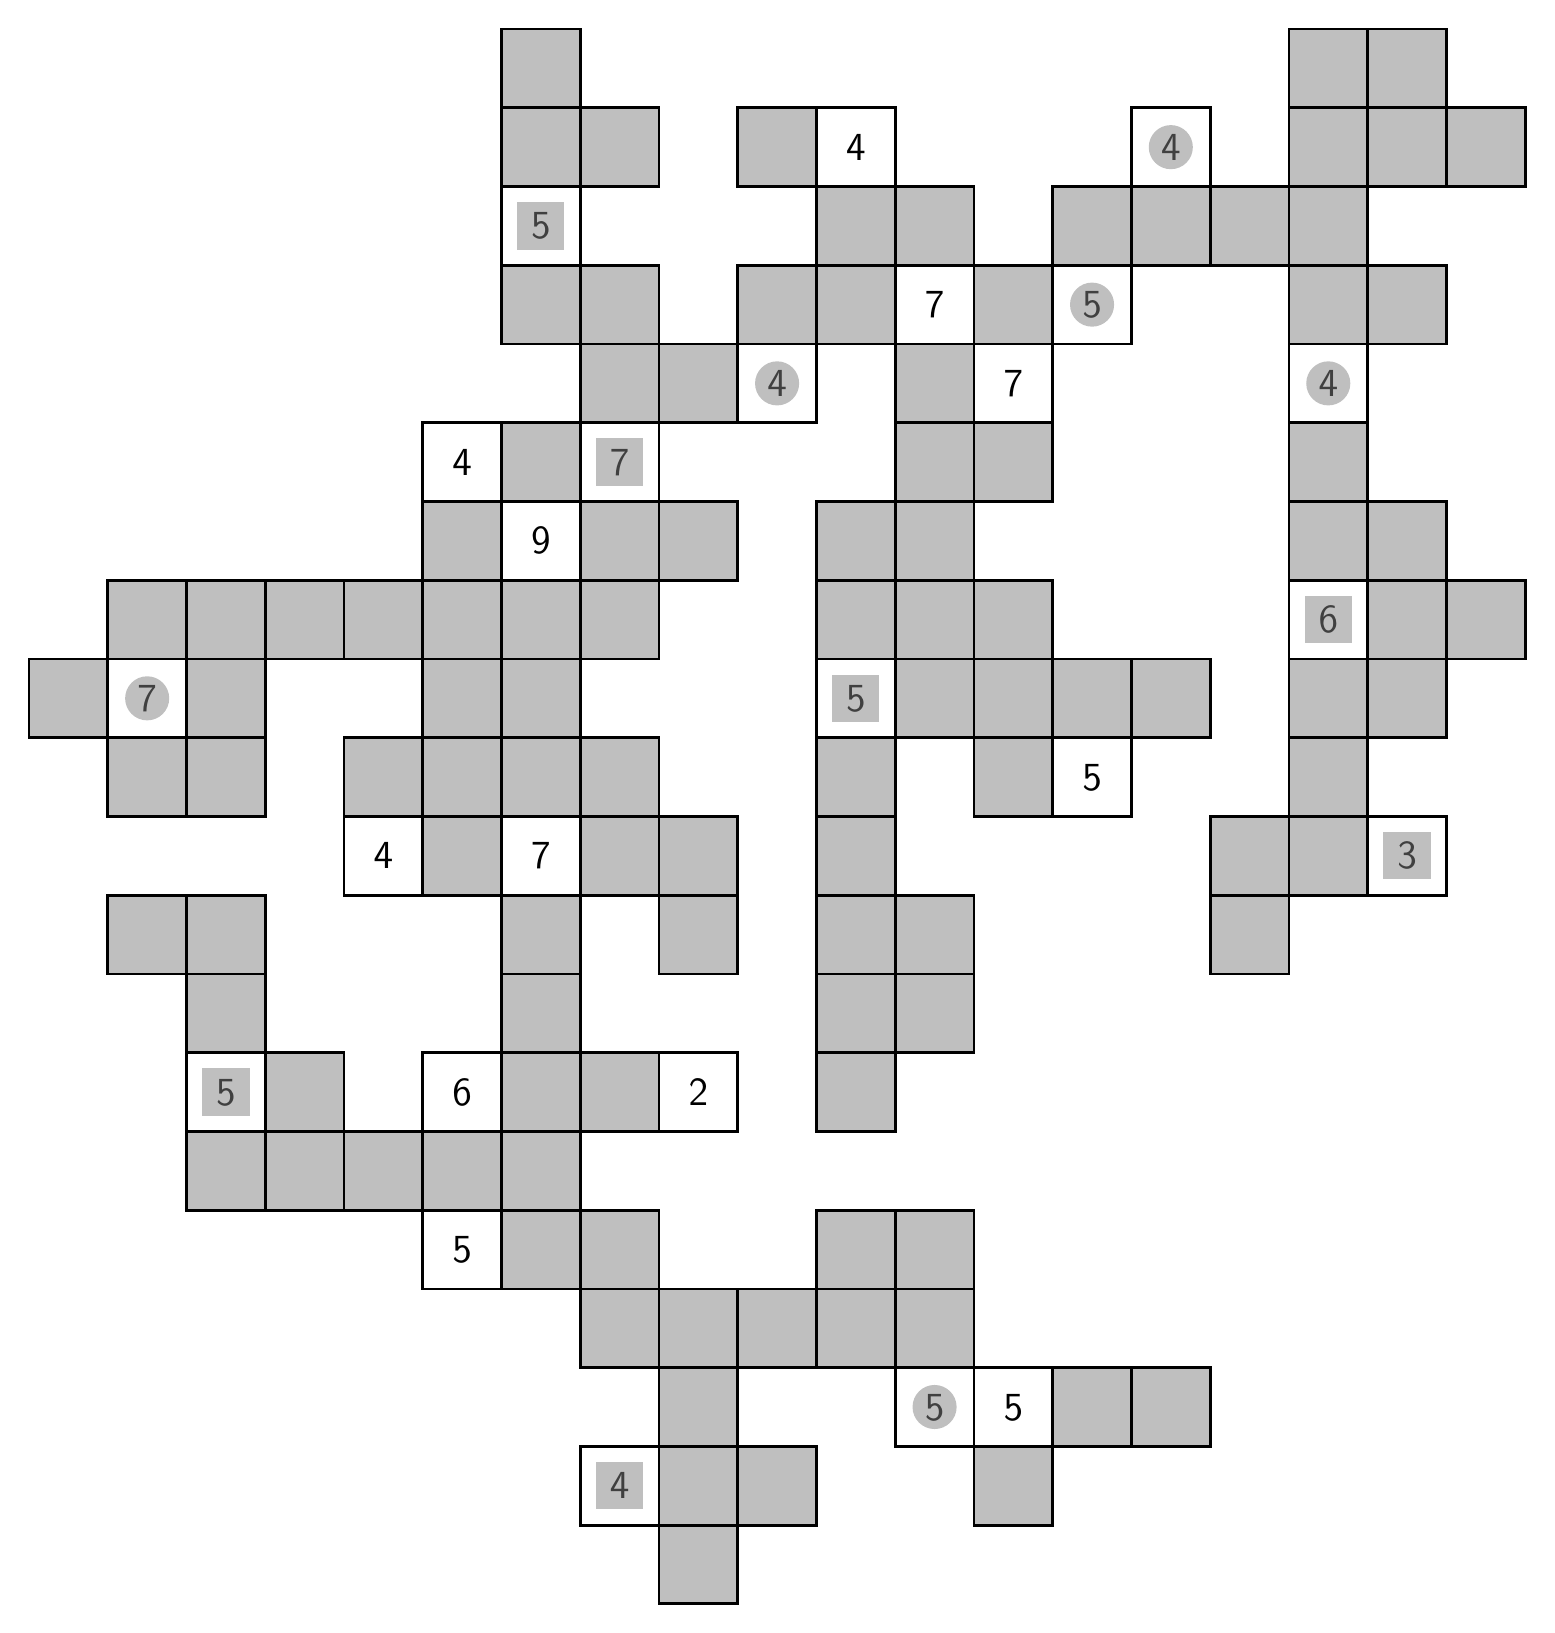
\begin{tikzpicture}\fill[gray, opacity = 0.5] (9, 0, 0)--++(1, 0, 0)--++(0, 1, 0)--++(-1, 0, 0)--cycle;
\draw[line width = 1pt] (9, 0, 0)--++(1, 0, 0)--++(0, 1, 0)--++(-1, 0, 0)--cycle;
\draw node at (8.5, 1.5, 0) {\Large $\mathsf{4}$};
\draw[line width = 1pt] (8, 1, 0)--++(1, 0, 0)--++(0, 1, 0)--++(-1, 0, 0)--cycle;
\fill[color = gray, opacity = 0.5] (8.2, 1.2) rectangle ++(0.6, 0.6);
\fill[gray, opacity = 0.5] (9, 1, 0)--++(1, 0, 0)--++(0, 1, 0)--++(-1, 0, 0)--cycle;
\draw[line width = 1pt] (9, 1, 0)--++(1, 0, 0)--++(0, 1, 0)--++(-1, 0, 0)--cycle;
\fill[gray, opacity = 0.5] (10, 1, 0)--++(1, 0, 0)--++(0, 1, 0)--++(-1, 0, 0)--cycle;
\draw[line width = 1pt] (10, 1, 0)--++(1, 0, 0)--++(0, 1, 0)--++(-1, 0, 0)--cycle;
\fill[gray, opacity = 0.5] (13, 1, 0)--++(1, 0, 0)--++(0, 1, 0)--++(-1, 0, 0)--cycle;
\draw[line width = 1pt] (13, 1, 0)--++(1, 0, 0)--++(0, 1, 0)--++(-1, 0, 0)--cycle;
\fill[gray, opacity = 0.5] (9, 2, 0)--++(1, 0, 0)--++(0, 1, 0)--++(-1, 0, 0)--cycle;
\draw[line width = 1pt] (9, 2, 0)--++(1, 0, 0)--++(0, 1, 0)--++(-1, 0, 0)--cycle;
\draw node at (12.5, 2.5, 0) {\Large $\mathsf{5}$};
\draw[line width = 1pt] (12, 2, 0)--++(1, 0, 0)--++(0, 1, 0)--++(-1, 0, 0)--cycle;
\fill[color = gray, opacity = 0.5] (12.5, 2.5, 0) circle (0.28);
\draw node at (13.5, 2.5, 0) {\Large $\mathsf{5}$};
\draw[line width = 1pt] (13, 2, 0)--++(1, 0, 0)--++(0, 1, 0)--++(-1, 0, 0)--cycle;
\fill[gray, opacity = 0.5] (14, 2, 0)--++(1, 0, 0)--++(0, 1, 0)--++(-1, 0, 0)--cycle;
\draw[line width = 1pt] (14, 2, 0)--++(1, 0, 0)--++(0, 1, 0)--++(-1, 0, 0)--cycle;
\fill[gray, opacity = 0.5] (15, 2, 0)--++(1, 0, 0)--++(0, 1, 0)--++(-1, 0, 0)--cycle;
\draw[line width = 1pt] (15, 2, 0)--++(1, 0, 0)--++(0, 1, 0)--++(-1, 0, 0)--cycle;
\fill[gray, opacity = 0.5] (8, 3, 0)--++(1, 0, 0)--++(0, 1, 0)--++(-1, 0, 0)--cycle;
\draw[line width = 1pt] (8, 3, 0)--++(1, 0, 0)--++(0, 1, 0)--++(-1, 0, 0)--cycle;
\fill[gray, opacity = 0.5] (9, 3, 0)--++(1, 0, 0)--++(0, 1, 0)--++(-1, 0, 0)--cycle;
\draw[line width = 1pt] (9, 3, 0)--++(1, 0, 0)--++(0, 1, 0)--++(-1, 0, 0)--cycle;
\fill[gray, opacity = 0.5] (10, 3, 0)--++(1, 0, 0)--++(0, 1, 0)--++(-1, 0, 0)--cycle;
\draw[line width = 1pt] (10, 3, 0)--++(1, 0, 0)--++(0, 1, 0)--++(-1, 0, 0)--cycle;
\fill[gray, opacity = 0.5] (11, 3, 0)--++(1, 0, 0)--++(0, 1, 0)--++(-1, 0, 0)--cycle;
\draw[line width = 1pt] (11, 3, 0)--++(1, 0, 0)--++(0, 1, 0)--++(-1, 0, 0)--cycle;
\fill[gray, opacity = 0.5] (12, 3, 0)--++(1, 0, 0)--++(0, 1, 0)--++(-1, 0, 0)--cycle;
\draw[line width = 1pt] (12, 3, 0)--++(1, 0, 0)--++(0, 1, 0)--++(-1, 0, 0)--cycle;
\draw node at (6.5, 4.5, 0) {\Large $\mathsf{5}$};
\draw[line width = 1pt] (6, 4, 0)--++(1, 0, 0)--++(0, 1, 0)--++(-1, 0, 0)--cycle;
\fill[gray, opacity = 0.5] (7, 4, 0)--++(1, 0, 0)--++(0, 1, 0)--++(-1, 0, 0)--cycle;
\draw[line width = 1pt] (7, 4, 0)--++(1, 0, 0)--++(0, 1, 0)--++(-1, 0, 0)--cycle;
\fill[gray, opacity = 0.5] (8, 4, 0)--++(1, 0, 0)--++(0, 1, 0)--++(-1, 0, 0)--cycle;
\draw[line width = 1pt] (8, 4, 0)--++(1, 0, 0)--++(0, 1, 0)--++(-1, 0, 0)--cycle;
\fill[gray, opacity = 0.5] (11, 4, 0)--++(1, 0, 0)--++(0, 1, 0)--++(-1, 0, 0)--cycle;
\draw[line width = 1pt] (11, 4, 0)--++(1, 0, 0)--++(0, 1, 0)--++(-1, 0, 0)--cycle;
\fill[gray, opacity = 0.5] (12, 4, 0)--++(1, 0, 0)--++(0, 1, 0)--++(-1, 0, 0)--cycle;
\draw[line width = 1pt] (12, 4, 0)--++(1, 0, 0)--++(0, 1, 0)--++(-1, 0, 0)--cycle;
\fill[gray, opacity = 0.5] (3, 5, 0)--++(1, 0, 0)--++(0, 1, 0)--++(-1, 0, 0)--cycle;
\draw[line width = 1pt] (3, 5, 0)--++(1, 0, 0)--++(0, 1, 0)--++(-1, 0, 0)--cycle;
\fill[gray, opacity = 0.5] (4, 5, 0)--++(1, 0, 0)--++(0, 1, 0)--++(-1, 0, 0)--cycle;
\draw[line width = 1pt] (4, 5, 0)--++(1, 0, 0)--++(0, 1, 0)--++(-1, 0, 0)--cycle;
\fill[gray, opacity = 0.5] (5, 5, 0)--++(1, 0, 0)--++(0, 1, 0)--++(-1, 0, 0)--cycle;
\draw[line width = 1pt] (5, 5, 0)--++(1, 0, 0)--++(0, 1, 0)--++(-1, 0, 0)--cycle;
\fill[gray, opacity = 0.5] (6, 5, 0)--++(1, 0, 0)--++(0, 1, 0)--++(-1, 0, 0)--cycle;
\draw[line width = 1pt] (6, 5, 0)--++(1, 0, 0)--++(0, 1, 0)--++(-1, 0, 0)--cycle;
\fill[gray, opacity = 0.5] (7, 5, 0)--++(1, 0, 0)--++(0, 1, 0)--++(-1, 0, 0)--cycle;
\draw[line width = 1pt] (7, 5, 0)--++(1, 0, 0)--++(0, 1, 0)--++(-1, 0, 0)--cycle;
\draw node at (3.5, 6.5, 0) {\Large $\mathsf{5}$};
\draw[line width = 1pt] (3, 6, 0)--++(1, 0, 0)--++(0, 1, 0)--++(-1, 0, 0)--cycle;
\fill[color = gray, opacity = 0.5] (3.2, 6.2) rectangle ++(0.6, 0.6);
\fill[gray, opacity = 0.5] (4, 6, 0)--++(1, 0, 0)--++(0, 1, 0)--++(-1, 0, 0)--cycle;
\draw[line width = 1pt] (4, 6, 0)--++(1, 0, 0)--++(0, 1, 0)--++(-1, 0, 0)--cycle;
\draw node at (6.5, 6.5, 0) {\Large $\mathsf{6}$};
\draw[line width = 1pt] (6, 6, 0)--++(1, 0, 0)--++(0, 1, 0)--++(-1, 0, 0)--cycle;
\fill[gray, opacity = 0.5] (7, 6, 0)--++(1, 0, 0)--++(0, 1, 0)--++(-1, 0, 0)--cycle;
\draw[line width = 1pt] (7, 6, 0)--++(1, 0, 0)--++(0, 1, 0)--++(-1, 0, 0)--cycle;
\fill[gray, opacity = 0.5] (8, 6, 0)--++(1, 0, 0)--++(0, 1, 0)--++(-1, 0, 0)--cycle;
\draw[line width = 1pt] (8, 6, 0)--++(1, 0, 0)--++(0, 1, 0)--++(-1, 0, 0)--cycle;
\draw node at (9.5, 6.5, 0) {\Large $\mathsf{2}$};
\draw[line width = 1pt] (9, 6, 0)--++(1, 0, 0)--++(0, 1, 0)--++(-1, 0, 0)--cycle;
\fill[gray, opacity = 0.5] (11, 6, 0)--++(1, 0, 0)--++(0, 1, 0)--++(-1, 0, 0)--cycle;
\draw[line width = 1pt] (11, 6, 0)--++(1, 0, 0)--++(0, 1, 0)--++(-1, 0, 0)--cycle;
\fill[gray, opacity = 0.5] (3, 7, 0)--++(1, 0, 0)--++(0, 1, 0)--++(-1, 0, 0)--cycle;
\draw[line width = 1pt] (3, 7, 0)--++(1, 0, 0)--++(0, 1, 0)--++(-1, 0, 0)--cycle;
\fill[gray, opacity = 0.5] (7, 7, 0)--++(1, 0, 0)--++(0, 1, 0)--++(-1, 0, 0)--cycle;
\draw[line width = 1pt] (7, 7, 0)--++(1, 0, 0)--++(0, 1, 0)--++(-1, 0, 0)--cycle;
\fill[gray, opacity = 0.5] (11, 7, 0)--++(1, 0, 0)--++(0, 1, 0)--++(-1, 0, 0)--cycle;
\draw[line width = 1pt] (11, 7, 0)--++(1, 0, 0)--++(0, 1, 0)--++(-1, 0, 0)--cycle;
\fill[gray, opacity = 0.5] (12, 7, 0)--++(1, 0, 0)--++(0, 1, 0)--++(-1, 0, 0)--cycle;
\draw[line width = 1pt] (12, 7, 0)--++(1, 0, 0)--++(0, 1, 0)--++(-1, 0, 0)--cycle;
\fill[gray, opacity = 0.5] (2, 8, 0)--++(1, 0, 0)--++(0, 1, 0)--++(-1, 0, 0)--cycle;
\draw[line width = 1pt] (2, 8, 0)--++(1, 0, 0)--++(0, 1, 0)--++(-1, 0, 0)--cycle;
\fill[gray, opacity = 0.5] (3, 8, 0)--++(1, 0, 0)--++(0, 1, 0)--++(-1, 0, 0)--cycle;
\draw[line width = 1pt] (3, 8, 0)--++(1, 0, 0)--++(0, 1, 0)--++(-1, 0, 0)--cycle;
\fill[gray, opacity = 0.5] (7, 8, 0)--++(1, 0, 0)--++(0, 1, 0)--++(-1, 0, 0)--cycle;
\draw[line width = 1pt] (7, 8, 0)--++(1, 0, 0)--++(0, 1, 0)--++(-1, 0, 0)--cycle;
\fill[gray, opacity = 0.5] (9, 8, 0)--++(1, 0, 0)--++(0, 1, 0)--++(-1, 0, 0)--cycle;
\draw[line width = 1pt] (9, 8, 0)--++(1, 0, 0)--++(0, 1, 0)--++(-1, 0, 0)--cycle;
\fill[gray, opacity = 0.5] (11, 8, 0)--++(1, 0, 0)--++(0, 1, 0)--++(-1, 0, 0)--cycle;
\draw[line width = 1pt] (11, 8, 0)--++(1, 0, 0)--++(0, 1, 0)--++(-1, 0, 0)--cycle;
\fill[gray, opacity = 0.5] (12, 8, 0)--++(1, 0, 0)--++(0, 1, 0)--++(-1, 0, 0)--cycle;
\draw[line width = 1pt] (12, 8, 0)--++(1, 0, 0)--++(0, 1, 0)--++(-1, 0, 0)--cycle;
\fill[gray, opacity = 0.5] (16, 8, 0)--++(1, 0, 0)--++(0, 1, 0)--++(-1, 0, 0)--cycle;
\draw[line width = 1pt] (16, 8, 0)--++(1, 0, 0)--++(0, 1, 0)--++(-1, 0, 0)--cycle;
\draw node at (5.5, 9.5, 0) {\Large $\mathsf{4}$};
\draw[line width = 1pt] (5, 9, 0)--++(1, 0, 0)--++(0, 1, 0)--++(-1, 0, 0)--cycle;
\fill[gray, opacity = 0.5] (6, 9, 0)--++(1, 0, 0)--++(0, 1, 0)--++(-1, 0, 0)--cycle;
\draw[line width = 1pt] (6, 9, 0)--++(1, 0, 0)--++(0, 1, 0)--++(-1, 0, 0)--cycle;
\draw node at (7.5, 9.5, 0) {\Large $\mathsf{7}$};
\draw[line width = 1pt] (7, 9, 0)--++(1, 0, 0)--++(0, 1, 0)--++(-1, 0, 0)--cycle;
\fill[gray, opacity = 0.5] (8, 9, 0)--++(1, 0, 0)--++(0, 1, 0)--++(-1, 0, 0)--cycle;
\draw[line width = 1pt] (8, 9, 0)--++(1, 0, 0)--++(0, 1, 0)--++(-1, 0, 0)--cycle;
\fill[gray, opacity = 0.5] (9, 9, 0)--++(1, 0, 0)--++(0, 1, 0)--++(-1, 0, 0)--cycle;
\draw[line width = 1pt] (9, 9, 0)--++(1, 0, 0)--++(0, 1, 0)--++(-1, 0, 0)--cycle;
\fill[gray, opacity = 0.5] (11, 9, 0)--++(1, 0, 0)--++(0, 1, 0)--++(-1, 0, 0)--cycle;
\draw[line width = 1pt] (11, 9, 0)--++(1, 0, 0)--++(0, 1, 0)--++(-1, 0, 0)--cycle;
\fill[gray, opacity = 0.5] (16, 9, 0)--++(1, 0, 0)--++(0, 1, 0)--++(-1, 0, 0)--cycle;
\draw[line width = 1pt] (16, 9, 0)--++(1, 0, 0)--++(0, 1, 0)--++(-1, 0, 0)--cycle;
\fill[gray, opacity = 0.5] (17, 9, 0)--++(1, 0, 0)--++(0, 1, 0)--++(-1, 0, 0)--cycle;
\draw[line width = 1pt] (17, 9, 0)--++(1, 0, 0)--++(0, 1, 0)--++(-1, 0, 0)--cycle;
\draw node at (18.5, 9.5, 0) {\Large $\mathsf{3}$};
\draw[line width = 1pt] (18, 9, 0)--++(1, 0, 0)--++(0, 1, 0)--++(-1, 0, 0)--cycle;
\fill[color = gray, opacity = 0.5] (18.2, 9.2) rectangle ++(0.6, 0.6);
\fill[gray, opacity = 0.5] (2, 10, 0)--++(1, 0, 0)--++(0, 1, 0)--++(-1, 0, 0)--cycle;
\draw[line width = 1pt] (2, 10, 0)--++(1, 0, 0)--++(0, 1, 0)--++(-1, 0, 0)--cycle;
\fill[gray, opacity = 0.5] (3, 10, 0)--++(1, 0, 0)--++(0, 1, 0)--++(-1, 0, 0)--cycle;
\draw[line width = 1pt] (3, 10, 0)--++(1, 0, 0)--++(0, 1, 0)--++(-1, 0, 0)--cycle;
\fill[gray, opacity = 0.5] (5, 10, 0)--++(1, 0, 0)--++(0, 1, 0)--++(-1, 0, 0)--cycle;
\draw[line width = 1pt] (5, 10, 0)--++(1, 0, 0)--++(0, 1, 0)--++(-1, 0, 0)--cycle;
\fill[gray, opacity = 0.5] (6, 10, 0)--++(1, 0, 0)--++(0, 1, 0)--++(-1, 0, 0)--cycle;
\draw[line width = 1pt] (6, 10, 0)--++(1, 0, 0)--++(0, 1, 0)--++(-1, 0, 0)--cycle;
\fill[gray, opacity = 0.5] (7, 10, 0)--++(1, 0, 0)--++(0, 1, 0)--++(-1, 0, 0)--cycle;
\draw[line width = 1pt] (7, 10, 0)--++(1, 0, 0)--++(0, 1, 0)--++(-1, 0, 0)--cycle;
\fill[gray, opacity = 0.5] (8, 10, 0)--++(1, 0, 0)--++(0, 1, 0)--++(-1, 0, 0)--cycle;
\draw[line width = 1pt] (8, 10, 0)--++(1, 0, 0)--++(0, 1, 0)--++(-1, 0, 0)--cycle;
\fill[gray, opacity = 0.5] (11, 10, 0)--++(1, 0, 0)--++(0, 1, 0)--++(-1, 0, 0)--cycle;
\draw[line width = 1pt] (11, 10, 0)--++(1, 0, 0)--++(0, 1, 0)--++(-1, 0, 0)--cycle;
\fill[gray, opacity = 0.5] (13, 10, 0)--++(1, 0, 0)--++(0, 1, 0)--++(-1, 0, 0)--cycle;
\draw[line width = 1pt] (13, 10, 0)--++(1, 0, 0)--++(0, 1, 0)--++(-1, 0, 0)--cycle;
\draw node at (14.5, 10.5, 0) {\Large $\mathsf{5}$};
\draw[line width = 1pt] (14, 10, 0)--++(1, 0, 0)--++(0, 1, 0)--++(-1, 0, 0)--cycle;
\fill[gray, opacity = 0.5] (17, 10, 0)--++(1, 0, 0)--++(0, 1, 0)--++(-1, 0, 0)--cycle;
\draw[line width = 1pt] (17, 10, 0)--++(1, 0, 0)--++(0, 1, 0)--++(-1, 0, 0)--cycle;
\fill[gray, opacity = 0.5] (1, 11, 0)--++(1, 0, 0)--++(0, 1, 0)--++(-1, 0, 0)--cycle;
\draw[line width = 1pt] (1, 11, 0)--++(1, 0, 0)--++(0, 1, 0)--++(-1, 0, 0)--cycle;
\draw node at (2.5, 11.5, 0) {\Large $\mathsf{7}$};
\draw[line width = 1pt] (2, 11, 0)--++(1, 0, 0)--++(0, 1, 0)--++(-1, 0, 0)--cycle;
\fill[color = gray, opacity = 0.5] (2.5, 11.5, 0) circle (0.28);
\fill[gray, opacity = 0.5] (3, 11, 0)--++(1, 0, 0)--++(0, 1, 0)--++(-1, 0, 0)--cycle;
\draw[line width = 1pt] (3, 11, 0)--++(1, 0, 0)--++(0, 1, 0)--++(-1, 0, 0)--cycle;
\fill[gray, opacity = 0.5] (6, 11, 0)--++(1, 0, 0)--++(0, 1, 0)--++(-1, 0, 0)--cycle;
\draw[line width = 1pt] (6, 11, 0)--++(1, 0, 0)--++(0, 1, 0)--++(-1, 0, 0)--cycle;
\fill[gray, opacity = 0.5] (7, 11, 0)--++(1, 0, 0)--++(0, 1, 0)--++(-1, 0, 0)--cycle;
\draw[line width = 1pt] (7, 11, 0)--++(1, 0, 0)--++(0, 1, 0)--++(-1, 0, 0)--cycle;
\draw node at (11.5, 11.5, 0) {\Large $\mathsf{5}$};
\draw[line width = 1pt] (11, 11, 0)--++(1, 0, 0)--++(0, 1, 0)--++(-1, 0, 0)--cycle;
\fill[color = gray, opacity = 0.5] (11.2, 11.2) rectangle ++(0.6, 0.6);
\fill[gray, opacity = 0.5] (12, 11, 0)--++(1, 0, 0)--++(0, 1, 0)--++(-1, 0, 0)--cycle;
\draw[line width = 1pt] (12, 11, 0)--++(1, 0, 0)--++(0, 1, 0)--++(-1, 0, 0)--cycle;
\fill[gray, opacity = 0.5] (13, 11, 0)--++(1, 0, 0)--++(0, 1, 0)--++(-1, 0, 0)--cycle;
\draw[line width = 1pt] (13, 11, 0)--++(1, 0, 0)--++(0, 1, 0)--++(-1, 0, 0)--cycle;
\fill[gray, opacity = 0.5] (14, 11, 0)--++(1, 0, 0)--++(0, 1, 0)--++(-1, 0, 0)--cycle;
\draw[line width = 1pt] (14, 11, 0)--++(1, 0, 0)--++(0, 1, 0)--++(-1, 0, 0)--cycle;
\fill[gray, opacity = 0.5] (15, 11, 0)--++(1, 0, 0)--++(0, 1, 0)--++(-1, 0, 0)--cycle;
\draw[line width = 1pt] (15, 11, 0)--++(1, 0, 0)--++(0, 1, 0)--++(-1, 0, 0)--cycle;
\fill[gray, opacity = 0.5] (17, 11, 0)--++(1, 0, 0)--++(0, 1, 0)--++(-1, 0, 0)--cycle;
\draw[line width = 1pt] (17, 11, 0)--++(1, 0, 0)--++(0, 1, 0)--++(-1, 0, 0)--cycle;
\fill[gray, opacity = 0.5] (18, 11, 0)--++(1, 0, 0)--++(0, 1, 0)--++(-1, 0, 0)--cycle;
\draw[line width = 1pt] (18, 11, 0)--++(1, 0, 0)--++(0, 1, 0)--++(-1, 0, 0)--cycle;
\fill[gray, opacity = 0.5] (2, 12, 0)--++(1, 0, 0)--++(0, 1, 0)--++(-1, 0, 0)--cycle;
\draw[line width = 1pt] (2, 12, 0)--++(1, 0, 0)--++(0, 1, 0)--++(-1, 0, 0)--cycle;
\fill[gray, opacity = 0.5] (3, 12, 0)--++(1, 0, 0)--++(0, 1, 0)--++(-1, 0, 0)--cycle;
\draw[line width = 1pt] (3, 12, 0)--++(1, 0, 0)--++(0, 1, 0)--++(-1, 0, 0)--cycle;
\fill[gray, opacity = 0.5] (4, 12, 0)--++(1, 0, 0)--++(0, 1, 0)--++(-1, 0, 0)--cycle;
\draw[line width = 1pt] (4, 12, 0)--++(1, 0, 0)--++(0, 1, 0)--++(-1, 0, 0)--cycle;
\fill[gray, opacity = 0.5] (5, 12, 0)--++(1, 0, 0)--++(0, 1, 0)--++(-1, 0, 0)--cycle;
\draw[line width = 1pt] (5, 12, 0)--++(1, 0, 0)--++(0, 1, 0)--++(-1, 0, 0)--cycle;
\fill[gray, opacity = 0.5] (6, 12, 0)--++(1, 0, 0)--++(0, 1, 0)--++(-1, 0, 0)--cycle;
\draw[line width = 1pt] (6, 12, 0)--++(1, 0, 0)--++(0, 1, 0)--++(-1, 0, 0)--cycle;
\fill[gray, opacity = 0.5] (7, 12, 0)--++(1, 0, 0)--++(0, 1, 0)--++(-1, 0, 0)--cycle;
\draw[line width = 1pt] (7, 12, 0)--++(1, 0, 0)--++(0, 1, 0)--++(-1, 0, 0)--cycle;
\fill[gray, opacity = 0.5] (8, 12, 0)--++(1, 0, 0)--++(0, 1, 0)--++(-1, 0, 0)--cycle;
\draw[line width = 1pt] (8, 12, 0)--++(1, 0, 0)--++(0, 1, 0)--++(-1, 0, 0)--cycle;
\fill[gray, opacity = 0.5] (11, 12, 0)--++(1, 0, 0)--++(0, 1, 0)--++(-1, 0, 0)--cycle;
\draw[line width = 1pt] (11, 12, 0)--++(1, 0, 0)--++(0, 1, 0)--++(-1, 0, 0)--cycle;
\fill[gray, opacity = 0.5] (12, 12, 0)--++(1, 0, 0)--++(0, 1, 0)--++(-1, 0, 0)--cycle;
\draw[line width = 1pt] (12, 12, 0)--++(1, 0, 0)--++(0, 1, 0)--++(-1, 0, 0)--cycle;
\fill[gray, opacity = 0.5] (13, 12, 0)--++(1, 0, 0)--++(0, 1, 0)--++(-1, 0, 0)--cycle;
\draw[line width = 1pt] (13, 12, 0)--++(1, 0, 0)--++(0, 1, 0)--++(-1, 0, 0)--cycle;
\draw node at (17.5, 12.5, 0) {\Large $\mathsf{6}$};
\draw[line width = 1pt] (17, 12, 0)--++(1, 0, 0)--++(0, 1, 0)--++(-1, 0, 0)--cycle;
\fill[color = gray, opacity = 0.5] (17.2, 12.2) rectangle ++(0.6, 0.6);
\fill[gray, opacity = 0.5] (18, 12, 0)--++(1, 0, 0)--++(0, 1, 0)--++(-1, 0, 0)--cycle;
\draw[line width = 1pt] (18, 12, 0)--++(1, 0, 0)--++(0, 1, 0)--++(-1, 0, 0)--cycle;
\fill[gray, opacity = 0.5] (19, 12, 0)--++(1, 0, 0)--++(0, 1, 0)--++(-1, 0, 0)--cycle;
\draw[line width = 1pt] (19, 12, 0)--++(1, 0, 0)--++(0, 1, 0)--++(-1, 0, 0)--cycle;
\fill[gray, opacity = 0.5] (6, 13, 0)--++(1, 0, 0)--++(0, 1, 0)--++(-1, 0, 0)--cycle;
\draw[line width = 1pt] (6, 13, 0)--++(1, 0, 0)--++(0, 1, 0)--++(-1, 0, 0)--cycle;
\draw node at (7.5, 13.5, 0) {\Large $\mathsf{9}$};
\draw[line width = 1pt] (7, 13, 0)--++(1, 0, 0)--++(0, 1, 0)--++(-1, 0, 0)--cycle;
\fill[gray, opacity = 0.5] (8, 13, 0)--++(1, 0, 0)--++(0, 1, 0)--++(-1, 0, 0)--cycle;
\draw[line width = 1pt] (8, 13, 0)--++(1, 0, 0)--++(0, 1, 0)--++(-1, 0, 0)--cycle;
\fill[gray, opacity = 0.5] (9, 13, 0)--++(1, 0, 0)--++(0, 1, 0)--++(-1, 0, 0)--cycle;
\draw[line width = 1pt] (9, 13, 0)--++(1, 0, 0)--++(0, 1, 0)--++(-1, 0, 0)--cycle;
\fill[gray, opacity = 0.5] (11, 13, 0)--++(1, 0, 0)--++(0, 1, 0)--++(-1, 0, 0)--cycle;
\draw[line width = 1pt] (11, 13, 0)--++(1, 0, 0)--++(0, 1, 0)--++(-1, 0, 0)--cycle;
\fill[gray, opacity = 0.5] (12, 13, 0)--++(1, 0, 0)--++(0, 1, 0)--++(-1, 0, 0)--cycle;
\draw[line width = 1pt] (12, 13, 0)--++(1, 0, 0)--++(0, 1, 0)--++(-1, 0, 0)--cycle;
\fill[gray, opacity = 0.5] (17, 13, 0)--++(1, 0, 0)--++(0, 1, 0)--++(-1, 0, 0)--cycle;
\draw[line width = 1pt] (17, 13, 0)--++(1, 0, 0)--++(0, 1, 0)--++(-1, 0, 0)--cycle;
\fill[gray, opacity = 0.5] (18, 13, 0)--++(1, 0, 0)--++(0, 1, 0)--++(-1, 0, 0)--cycle;
\draw[line width = 1pt] (18, 13, 0)--++(1, 0, 0)--++(0, 1, 0)--++(-1, 0, 0)--cycle;
\draw node at (6.5, 14.5, 0) {\Large $\mathsf{4}$};
\draw[line width = 1pt] (6, 14, 0)--++(1, 0, 0)--++(0, 1, 0)--++(-1, 0, 0)--cycle;
\fill[gray, opacity = 0.5] (7, 14, 0)--++(1, 0, 0)--++(0, 1, 0)--++(-1, 0, 0)--cycle;
\draw[line width = 1pt] (7, 14, 0)--++(1, 0, 0)--++(0, 1, 0)--++(-1, 0, 0)--cycle;
\draw node at (8.5, 14.5, 0) {\Large $\mathsf{7}$};
\draw[line width = 1pt] (8, 14, 0)--++(1, 0, 0)--++(0, 1, 0)--++(-1, 0, 0)--cycle;
\fill[color = gray, opacity = 0.5] (8.2, 14.2) rectangle ++(0.6, 0.6);
\fill[gray, opacity = 0.5] (12, 14, 0)--++(1, 0, 0)--++(0, 1, 0)--++(-1, 0, 0)--cycle;
\draw[line width = 1pt] (12, 14, 0)--++(1, 0, 0)--++(0, 1, 0)--++(-1, 0, 0)--cycle;
\fill[gray, opacity = 0.5] (13, 14, 0)--++(1, 0, 0)--++(0, 1, 0)--++(-1, 0, 0)--cycle;
\draw[line width = 1pt] (13, 14, 0)--++(1, 0, 0)--++(0, 1, 0)--++(-1, 0, 0)--cycle;
\fill[gray, opacity = 0.5] (17, 14, 0)--++(1, 0, 0)--++(0, 1, 0)--++(-1, 0, 0)--cycle;
\draw[line width = 1pt] (17, 14, 0)--++(1, 0, 0)--++(0, 1, 0)--++(-1, 0, 0)--cycle;
\fill[gray, opacity = 0.5] (8, 15, 0)--++(1, 0, 0)--++(0, 1, 0)--++(-1, 0, 0)--cycle;
\draw[line width = 1pt] (8, 15, 0)--++(1, 0, 0)--++(0, 1, 0)--++(-1, 0, 0)--cycle;
\fill[gray, opacity = 0.5] (9, 15, 0)--++(1, 0, 0)--++(0, 1, 0)--++(-1, 0, 0)--cycle;
\draw[line width = 1pt] (9, 15, 0)--++(1, 0, 0)--++(0, 1, 0)--++(-1, 0, 0)--cycle;
\draw node at (10.5, 15.5, 0) {\Large $\mathsf{4}$};
\draw[line width = 1pt] (10, 15, 0)--++(1, 0, 0)--++(0, 1, 0)--++(-1, 0, 0)--cycle;
\fill[color = gray, opacity = 0.5] (10.5, 15.5, 0) circle (0.28);
\fill[gray, opacity = 0.5] (12, 15, 0)--++(1, 0, 0)--++(0, 1, 0)--++(-1, 0, 0)--cycle;
\draw[line width = 1pt] (12, 15, 0)--++(1, 0, 0)--++(0, 1, 0)--++(-1, 0, 0)--cycle;
\draw node at (13.5, 15.5, 0) {\Large $\mathsf{7}$};
\draw[line width = 1pt] (13, 15, 0)--++(1, 0, 0)--++(0, 1, 0)--++(-1, 0, 0)--cycle;
\draw node at (17.5, 15.5, 0) {\Large $\mathsf{4}$};
\draw[line width = 1pt] (17, 15, 0)--++(1, 0, 0)--++(0, 1, 0)--++(-1, 0, 0)--cycle;
\fill[color = gray, opacity = 0.5] (17.5, 15.5, 0) circle (0.28);
\fill[gray, opacity = 0.5] (7, 16, 0)--++(1, 0, 0)--++(0, 1, 0)--++(-1, 0, 0)--cycle;
\draw[line width = 1pt] (7, 16, 0)--++(1, 0, 0)--++(0, 1, 0)--++(-1, 0, 0)--cycle;
\fill[gray, opacity = 0.5] (8, 16, 0)--++(1, 0, 0)--++(0, 1, 0)--++(-1, 0, 0)--cycle;
\draw[line width = 1pt] (8, 16, 0)--++(1, 0, 0)--++(0, 1, 0)--++(-1, 0, 0)--cycle;
\fill[gray, opacity = 0.5] (10, 16, 0)--++(1, 0, 0)--++(0, 1, 0)--++(-1, 0, 0)--cycle;
\draw[line width = 1pt] (10, 16, 0)--++(1, 0, 0)--++(0, 1, 0)--++(-1, 0, 0)--cycle;
\fill[gray, opacity = 0.5] (11, 16, 0)--++(1, 0, 0)--++(0, 1, 0)--++(-1, 0, 0)--cycle;
\draw[line width = 1pt] (11, 16, 0)--++(1, 0, 0)--++(0, 1, 0)--++(-1, 0, 0)--cycle;
\draw node at (12.5, 16.5, 0) {\Large $\mathsf{7}$};
\draw[line width = 1pt] (12, 16, 0)--++(1, 0, 0)--++(0, 1, 0)--++(-1, 0, 0)--cycle;
\fill[gray, opacity = 0.5] (13, 16, 0)--++(1, 0, 0)--++(0, 1, 0)--++(-1, 0, 0)--cycle;
\draw[line width = 1pt] (13, 16, 0)--++(1, 0, 0)--++(0, 1, 0)--++(-1, 0, 0)--cycle;
\draw node at (14.5, 16.5, 0) {\Large $\mathsf{5}$};
\draw[line width = 1pt] (14, 16, 0)--++(1, 0, 0)--++(0, 1, 0)--++(-1, 0, 0)--cycle;
\fill[color = gray, opacity = 0.5] (14.5, 16.5, 0) circle (0.28);
\fill[gray, opacity = 0.5] (17, 16, 0)--++(1, 0, 0)--++(0, 1, 0)--++(-1, 0, 0)--cycle;
\draw[line width = 1pt] (17, 16, 0)--++(1, 0, 0)--++(0, 1, 0)--++(-1, 0, 0)--cycle;
\fill[gray, opacity = 0.5] (18, 16, 0)--++(1, 0, 0)--++(0, 1, 0)--++(-1, 0, 0)--cycle;
\draw[line width = 1pt] (18, 16, 0)--++(1, 0, 0)--++(0, 1, 0)--++(-1, 0, 0)--cycle;
\draw node at (7.5, 17.5, 0) {\Large $\mathsf{5}$};
\draw[line width = 1pt] (7, 17, 0)--++(1, 0, 0)--++(0, 1, 0)--++(-1, 0, 0)--cycle;
\fill[color = gray, opacity = 0.5] (7.2, 17.2) rectangle ++(0.6, 0.6);
\fill[gray, opacity = 0.5] (11, 17, 0)--++(1, 0, 0)--++(0, 1, 0)--++(-1, 0, 0)--cycle;
\draw[line width = 1pt] (11, 17, 0)--++(1, 0, 0)--++(0, 1, 0)--++(-1, 0, 0)--cycle;
\fill[gray, opacity = 0.5] (12, 17, 0)--++(1, 0, 0)--++(0, 1, 0)--++(-1, 0, 0)--cycle;
\draw[line width = 1pt] (12, 17, 0)--++(1, 0, 0)--++(0, 1, 0)--++(-1, 0, 0)--cycle;
\fill[gray, opacity = 0.5] (14, 17, 0)--++(1, 0, 0)--++(0, 1, 0)--++(-1, 0, 0)--cycle;
\draw[line width = 1pt] (14, 17, 0)--++(1, 0, 0)--++(0, 1, 0)--++(-1, 0, 0)--cycle;
\fill[gray, opacity = 0.5] (15, 17, 0)--++(1, 0, 0)--++(0, 1, 0)--++(-1, 0, 0)--cycle;
\draw[line width = 1pt] (15, 17, 0)--++(1, 0, 0)--++(0, 1, 0)--++(-1, 0, 0)--cycle;
\fill[gray, opacity = 0.5] (16, 17, 0)--++(1, 0, 0)--++(0, 1, 0)--++(-1, 0, 0)--cycle;
\draw[line width = 1pt] (16, 17, 0)--++(1, 0, 0)--++(0, 1, 0)--++(-1, 0, 0)--cycle;
\fill[gray, opacity = 0.5] (17, 17, 0)--++(1, 0, 0)--++(0, 1, 0)--++(-1, 0, 0)--cycle;
\draw[line width = 1pt] (17, 17, 0)--++(1, 0, 0)--++(0, 1, 0)--++(-1, 0, 0)--cycle;
\fill[gray, opacity = 0.5] (7, 18, 0)--++(1, 0, 0)--++(0, 1, 0)--++(-1, 0, 0)--cycle;
\draw[line width = 1pt] (7, 18, 0)--++(1, 0, 0)--++(0, 1, 0)--++(-1, 0, 0)--cycle;
\fill[gray, opacity = 0.5] (8, 18, 0)--++(1, 0, 0)--++(0, 1, 0)--++(-1, 0, 0)--cycle;
\draw[line width = 1pt] (8, 18, 0)--++(1, 0, 0)--++(0, 1, 0)--++(-1, 0, 0)--cycle;
\fill[gray, opacity = 0.5] (10, 18, 0)--++(1, 0, 0)--++(0, 1, 0)--++(-1, 0, 0)--cycle;
\draw[line width = 1pt] (10, 18, 0)--++(1, 0, 0)--++(0, 1, 0)--++(-1, 0, 0)--cycle;
\draw node at (11.5, 18.5, 0) {\Large $\mathsf{4}$};
\draw[line width = 1pt] (11, 18, 0)--++(1, 0, 0)--++(0, 1, 0)--++(-1, 0, 0)--cycle;
\draw node at (15.5, 18.5, 0) {\Large $\mathsf{4}$};
\draw[line width = 1pt] (15, 18, 0)--++(1, 0, 0)--++(0, 1, 0)--++(-1, 0, 0)--cycle;
\fill[color = gray, opacity = 0.5] (15.5, 18.5, 0) circle (0.28);
\fill[gray, opacity = 0.5] (17, 18, 0)--++(1, 0, 0)--++(0, 1, 0)--++(-1, 0, 0)--cycle;
\draw[line width = 1pt] (17, 18, 0)--++(1, 0, 0)--++(0, 1, 0)--++(-1, 0, 0)--cycle;
\fill[gray, opacity = 0.5] (18, 18, 0)--++(1, 0, 0)--++(0, 1, 0)--++(-1, 0, 0)--cycle;
\draw[line width = 1pt] (18, 18, 0)--++(1, 0, 0)--++(0, 1, 0)--++(-1, 0, 0)--cycle;
\fill[gray, opacity = 0.5] (19, 18, 0)--++(1, 0, 0)--++(0, 1, 0)--++(-1, 0, 0)--cycle;
\draw[line width = 1pt] (19, 18, 0)--++(1, 0, 0)--++(0, 1, 0)--++(-1, 0, 0)--cycle;
\fill[gray, opacity = 0.5] (7, 19, 0)--++(1, 0, 0)--++(0, 1, 0)--++(-1, 0, 0)--cycle;
\draw[line width = 1pt] (7, 19, 0)--++(1, 0, 0)--++(0, 1, 0)--++(-1, 0, 0)--cycle;
\fill[gray, opacity = 0.5] (17, 19, 0)--++(1, 0, 0)--++(0, 1, 0)--++(-1, 0, 0)--cycle;
\draw[line width = 1pt] (17, 19, 0)--++(1, 0, 0)--++(0, 1, 0)--++(-1, 0, 0)--cycle;
\fill[gray, opacity = 0.5] (18, 19, 0)--++(1, 0, 0)--++(0, 1, 0)--++(-1, 0, 0)--cycle;
\draw[line width = 1pt] (18, 19, 0)--++(1, 0, 0)--++(0, 1, 0)--++(-1, 0, 0)--cycle;
\end{tikzpicture}}\]
\[\resizebox{30pc}{!}{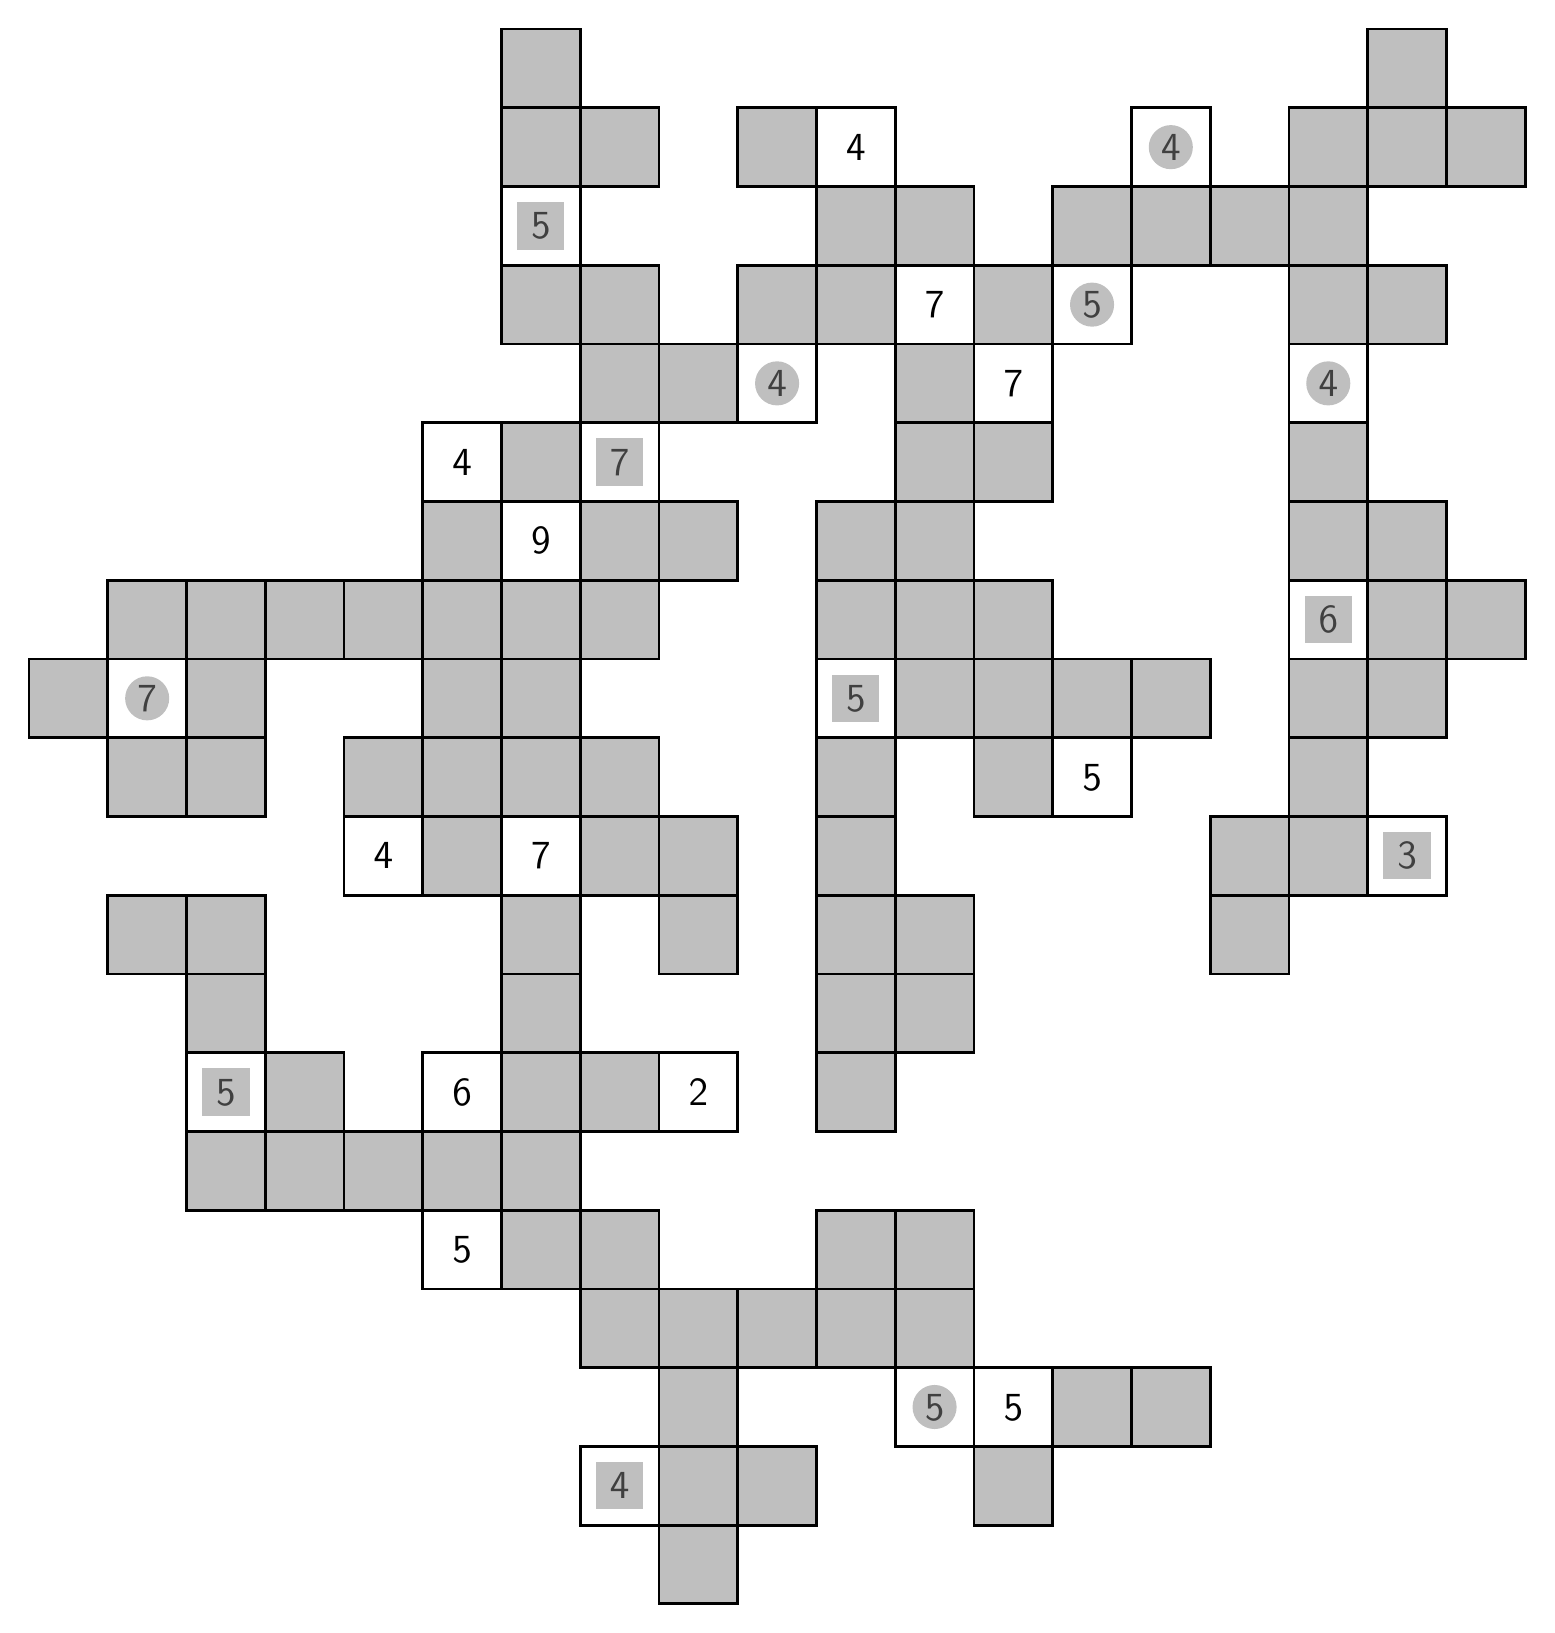
\begin{tikzpicture}\fill[gray, opacity = 0.5] (9, 0, 0)--++(1, 0, 0)--++(0, 1, 0)--++(-1, 0, 0)--cycle;
\draw[line width = 1pt] (9, 0, 0)--++(1, 0, 0)--++(0, 1, 0)--++(-1, 0, 0)--cycle;
\draw node at (8.5, 1.5, 0) {\Large $\mathsf{4}$};
\draw[line width = 1pt] (8, 1, 0)--++(1, 0, 0)--++(0, 1, 0)--++(-1, 0, 0)--cycle;
\fill[color = gray, opacity = 0.5] (8.2, 1.2) rectangle ++(0.6, 0.6);
\fill[gray, opacity = 0.5] (9, 1, 0)--++(1, 0, 0)--++(0, 1, 0)--++(-1, 0, 0)--cycle;
\draw[line width = 1pt] (9, 1, 0)--++(1, 0, 0)--++(0, 1, 0)--++(-1, 0, 0)--cycle;
\fill[gray, opacity = 0.5] (10, 1, 0)--++(1, 0, 0)--++(0, 1, 0)--++(-1, 0, 0)--cycle;
\draw[line width = 1pt] (10, 1, 0)--++(1, 0, 0)--++(0, 1, 0)--++(-1, 0, 0)--cycle;
\fill[gray, opacity = 0.5] (13, 1, 0)--++(1, 0, 0)--++(0, 1, 0)--++(-1, 0, 0)--cycle;
\draw[line width = 1pt] (13, 1, 0)--++(1, 0, 0)--++(0, 1, 0)--++(-1, 0, 0)--cycle;
\fill[gray, opacity = 0.5] (9, 2, 0)--++(1, 0, 0)--++(0, 1, 0)--++(-1, 0, 0)--cycle;
\draw[line width = 1pt] (9, 2, 0)--++(1, 0, 0)--++(0, 1, 0)--++(-1, 0, 0)--cycle;
\draw node at (12.5, 2.5, 0) {\Large $\mathsf{5}$};
\draw[line width = 1pt] (12, 2, 0)--++(1, 0, 0)--++(0, 1, 0)--++(-1, 0, 0)--cycle;
\fill[color = gray, opacity = 0.5] (12.5, 2.5, 0) circle (0.28);
\draw node at (13.5, 2.5, 0) {\Large $\mathsf{5}$};
\draw[line width = 1pt] (13, 2, 0)--++(1, 0, 0)--++(0, 1, 0)--++(-1, 0, 0)--cycle;
\fill[gray, opacity = 0.5] (14, 2, 0)--++(1, 0, 0)--++(0, 1, 0)--++(-1, 0, 0)--cycle;
\draw[line width = 1pt] (14, 2, 0)--++(1, 0, 0)--++(0, 1, 0)--++(-1, 0, 0)--cycle;
\fill[gray, opacity = 0.5] (15, 2, 0)--++(1, 0, 0)--++(0, 1, 0)--++(-1, 0, 0)--cycle;
\draw[line width = 1pt] (15, 2, 0)--++(1, 0, 0)--++(0, 1, 0)--++(-1, 0, 0)--cycle;
\fill[gray, opacity = 0.5] (8, 3, 0)--++(1, 0, 0)--++(0, 1, 0)--++(-1, 0, 0)--cycle;
\draw[line width = 1pt] (8, 3, 0)--++(1, 0, 0)--++(0, 1, 0)--++(-1, 0, 0)--cycle;
\fill[gray, opacity = 0.5] (9, 3, 0)--++(1, 0, 0)--++(0, 1, 0)--++(-1, 0, 0)--cycle;
\draw[line width = 1pt] (9, 3, 0)--++(1, 0, 0)--++(0, 1, 0)--++(-1, 0, 0)--cycle;
\fill[gray, opacity = 0.5] (10, 3, 0)--++(1, 0, 0)--++(0, 1, 0)--++(-1, 0, 0)--cycle;
\draw[line width = 1pt] (10, 3, 0)--++(1, 0, 0)--++(0, 1, 0)--++(-1, 0, 0)--cycle;
\fill[gray, opacity = 0.5] (11, 3, 0)--++(1, 0, 0)--++(0, 1, 0)--++(-1, 0, 0)--cycle;
\draw[line width = 1pt] (11, 3, 0)--++(1, 0, 0)--++(0, 1, 0)--++(-1, 0, 0)--cycle;
\fill[gray, opacity = 0.5] (12, 3, 0)--++(1, 0, 0)--++(0, 1, 0)--++(-1, 0, 0)--cycle;
\draw[line width = 1pt] (12, 3, 0)--++(1, 0, 0)--++(0, 1, 0)--++(-1, 0, 0)--cycle;
\draw node at (6.5, 4.5, 0) {\Large $\mathsf{5}$};
\draw[line width = 1pt] (6, 4, 0)--++(1, 0, 0)--++(0, 1, 0)--++(-1, 0, 0)--cycle;
\fill[gray, opacity = 0.5] (7, 4, 0)--++(1, 0, 0)--++(0, 1, 0)--++(-1, 0, 0)--cycle;
\draw[line width = 1pt] (7, 4, 0)--++(1, 0, 0)--++(0, 1, 0)--++(-1, 0, 0)--cycle;
\fill[gray, opacity = 0.5] (8, 4, 0)--++(1, 0, 0)--++(0, 1, 0)--++(-1, 0, 0)--cycle;
\draw[line width = 1pt] (8, 4, 0)--++(1, 0, 0)--++(0, 1, 0)--++(-1, 0, 0)--cycle;
\fill[gray, opacity = 0.5] (11, 4, 0)--++(1, 0, 0)--++(0, 1, 0)--++(-1, 0, 0)--cycle;
\draw[line width = 1pt] (11, 4, 0)--++(1, 0, 0)--++(0, 1, 0)--++(-1, 0, 0)--cycle;
\fill[gray, opacity = 0.5] (12, 4, 0)--++(1, 0, 0)--++(0, 1, 0)--++(-1, 0, 0)--cycle;
\draw[line width = 1pt] (12, 4, 0)--++(1, 0, 0)--++(0, 1, 0)--++(-1, 0, 0)--cycle;
\fill[gray, opacity = 0.5] (3, 5, 0)--++(1, 0, 0)--++(0, 1, 0)--++(-1, 0, 0)--cycle;
\draw[line width = 1pt] (3, 5, 0)--++(1, 0, 0)--++(0, 1, 0)--++(-1, 0, 0)--cycle;
\fill[gray, opacity = 0.5] (4, 5, 0)--++(1, 0, 0)--++(0, 1, 0)--++(-1, 0, 0)--cycle;
\draw[line width = 1pt] (4, 5, 0)--++(1, 0, 0)--++(0, 1, 0)--++(-1, 0, 0)--cycle;
\fill[gray, opacity = 0.5] (5, 5, 0)--++(1, 0, 0)--++(0, 1, 0)--++(-1, 0, 0)--cycle;
\draw[line width = 1pt] (5, 5, 0)--++(1, 0, 0)--++(0, 1, 0)--++(-1, 0, 0)--cycle;
\fill[gray, opacity = 0.5] (6, 5, 0)--++(1, 0, 0)--++(0, 1, 0)--++(-1, 0, 0)--cycle;
\draw[line width = 1pt] (6, 5, 0)--++(1, 0, 0)--++(0, 1, 0)--++(-1, 0, 0)--cycle;
\fill[gray, opacity = 0.5] (7, 5, 0)--++(1, 0, 0)--++(0, 1, 0)--++(-1, 0, 0)--cycle;
\draw[line width = 1pt] (7, 5, 0)--++(1, 0, 0)--++(0, 1, 0)--++(-1, 0, 0)--cycle;
\draw node at (3.5, 6.5, 0) {\Large $\mathsf{5}$};
\draw[line width = 1pt] (3, 6, 0)--++(1, 0, 0)--++(0, 1, 0)--++(-1, 0, 0)--cycle;
\fill[color = gray, opacity = 0.5] (3.2, 6.2) rectangle ++(0.6, 0.6);
\fill[gray, opacity = 0.5] (4, 6, 0)--++(1, 0, 0)--++(0, 1, 0)--++(-1, 0, 0)--cycle;
\draw[line width = 1pt] (4, 6, 0)--++(1, 0, 0)--++(0, 1, 0)--++(-1, 0, 0)--cycle;
\draw node at (6.5, 6.5, 0) {\Large $\mathsf{6}$};
\draw[line width = 1pt] (6, 6, 0)--++(1, 0, 0)--++(0, 1, 0)--++(-1, 0, 0)--cycle;
\fill[gray, opacity = 0.5] (7, 6, 0)--++(1, 0, 0)--++(0, 1, 0)--++(-1, 0, 0)--cycle;
\draw[line width = 1pt] (7, 6, 0)--++(1, 0, 0)--++(0, 1, 0)--++(-1, 0, 0)--cycle;
\fill[gray, opacity = 0.5] (8, 6, 0)--++(1, 0, 0)--++(0, 1, 0)--++(-1, 0, 0)--cycle;
\draw[line width = 1pt] (8, 6, 0)--++(1, 0, 0)--++(0, 1, 0)--++(-1, 0, 0)--cycle;
\draw node at (9.5, 6.5, 0) {\Large $\mathsf{2}$};
\draw[line width = 1pt] (9, 6, 0)--++(1, 0, 0)--++(0, 1, 0)--++(-1, 0, 0)--cycle;
\fill[gray, opacity = 0.5] (11, 6, 0)--++(1, 0, 0)--++(0, 1, 0)--++(-1, 0, 0)--cycle;
\draw[line width = 1pt] (11, 6, 0)--++(1, 0, 0)--++(0, 1, 0)--++(-1, 0, 0)--cycle;
\fill[gray, opacity = 0.5] (3, 7, 0)--++(1, 0, 0)--++(0, 1, 0)--++(-1, 0, 0)--cycle;
\draw[line width = 1pt] (3, 7, 0)--++(1, 0, 0)--++(0, 1, 0)--++(-1, 0, 0)--cycle;
\fill[gray, opacity = 0.5] (7, 7, 0)--++(1, 0, 0)--++(0, 1, 0)--++(-1, 0, 0)--cycle;
\draw[line width = 1pt] (7, 7, 0)--++(1, 0, 0)--++(0, 1, 0)--++(-1, 0, 0)--cycle;
\fill[gray, opacity = 0.5] (11, 7, 0)--++(1, 0, 0)--++(0, 1, 0)--++(-1, 0, 0)--cycle;
\draw[line width = 1pt] (11, 7, 0)--++(1, 0, 0)--++(0, 1, 0)--++(-1, 0, 0)--cycle;
\fill[gray, opacity = 0.5] (12, 7, 0)--++(1, 0, 0)--++(0, 1, 0)--++(-1, 0, 0)--cycle;
\draw[line width = 1pt] (12, 7, 0)--++(1, 0, 0)--++(0, 1, 0)--++(-1, 0, 0)--cycle;
\fill[gray, opacity = 0.5] (2, 8, 0)--++(1, 0, 0)--++(0, 1, 0)--++(-1, 0, 0)--cycle;
\draw[line width = 1pt] (2, 8, 0)--++(1, 0, 0)--++(0, 1, 0)--++(-1, 0, 0)--cycle;
\fill[gray, opacity = 0.5] (3, 8, 0)--++(1, 0, 0)--++(0, 1, 0)--++(-1, 0, 0)--cycle;
\draw[line width = 1pt] (3, 8, 0)--++(1, 0, 0)--++(0, 1, 0)--++(-1, 0, 0)--cycle;
\fill[gray, opacity = 0.5] (7, 8, 0)--++(1, 0, 0)--++(0, 1, 0)--++(-1, 0, 0)--cycle;
\draw[line width = 1pt] (7, 8, 0)--++(1, 0, 0)--++(0, 1, 0)--++(-1, 0, 0)--cycle;
\fill[gray, opacity = 0.5] (9, 8, 0)--++(1, 0, 0)--++(0, 1, 0)--++(-1, 0, 0)--cycle;
\draw[line width = 1pt] (9, 8, 0)--++(1, 0, 0)--++(0, 1, 0)--++(-1, 0, 0)--cycle;
\fill[gray, opacity = 0.5] (11, 8, 0)--++(1, 0, 0)--++(0, 1, 0)--++(-1, 0, 0)--cycle;
\draw[line width = 1pt] (11, 8, 0)--++(1, 0, 0)--++(0, 1, 0)--++(-1, 0, 0)--cycle;
\fill[gray, opacity = 0.5] (12, 8, 0)--++(1, 0, 0)--++(0, 1, 0)--++(-1, 0, 0)--cycle;
\draw[line width = 1pt] (12, 8, 0)--++(1, 0, 0)--++(0, 1, 0)--++(-1, 0, 0)--cycle;
\fill[gray, opacity = 0.5] (16, 8, 0)--++(1, 0, 0)--++(0, 1, 0)--++(-1, 0, 0)--cycle;
\draw[line width = 1pt] (16, 8, 0)--++(1, 0, 0)--++(0, 1, 0)--++(-1, 0, 0)--cycle;
\draw node at (5.5, 9.5, 0) {\Large $\mathsf{4}$};
\draw[line width = 1pt] (5, 9, 0)--++(1, 0, 0)--++(0, 1, 0)--++(-1, 0, 0)--cycle;
\fill[gray, opacity = 0.5] (6, 9, 0)--++(1, 0, 0)--++(0, 1, 0)--++(-1, 0, 0)--cycle;
\draw[line width = 1pt] (6, 9, 0)--++(1, 0, 0)--++(0, 1, 0)--++(-1, 0, 0)--cycle;
\draw node at (7.5, 9.5, 0) {\Large $\mathsf{7}$};
\draw[line width = 1pt] (7, 9, 0)--++(1, 0, 0)--++(0, 1, 0)--++(-1, 0, 0)--cycle;
\fill[gray, opacity = 0.5] (8, 9, 0)--++(1, 0, 0)--++(0, 1, 0)--++(-1, 0, 0)--cycle;
\draw[line width = 1pt] (8, 9, 0)--++(1, 0, 0)--++(0, 1, 0)--++(-1, 0, 0)--cycle;
\fill[gray, opacity = 0.5] (9, 9, 0)--++(1, 0, 0)--++(0, 1, 0)--++(-1, 0, 0)--cycle;
\draw[line width = 1pt] (9, 9, 0)--++(1, 0, 0)--++(0, 1, 0)--++(-1, 0, 0)--cycle;
\fill[gray, opacity = 0.5] (11, 9, 0)--++(1, 0, 0)--++(0, 1, 0)--++(-1, 0, 0)--cycle;
\draw[line width = 1pt] (11, 9, 0)--++(1, 0, 0)--++(0, 1, 0)--++(-1, 0, 0)--cycle;
\fill[gray, opacity = 0.5] (16, 9, 0)--++(1, 0, 0)--++(0, 1, 0)--++(-1, 0, 0)--cycle;
\draw[line width = 1pt] (16, 9, 0)--++(1, 0, 0)--++(0, 1, 0)--++(-1, 0, 0)--cycle;
\fill[gray, opacity = 0.5] (17, 9, 0)--++(1, 0, 0)--++(0, 1, 0)--++(-1, 0, 0)--cycle;
\draw[line width = 1pt] (17, 9, 0)--++(1, 0, 0)--++(0, 1, 0)--++(-1, 0, 0)--cycle;
\draw node at (18.5, 9.5, 0) {\Large $\mathsf{3}$};
\draw[line width = 1pt] (18, 9, 0)--++(1, 0, 0)--++(0, 1, 0)--++(-1, 0, 0)--cycle;
\fill[color = gray, opacity = 0.5] (18.2, 9.2) rectangle ++(0.6, 0.6);
\fill[gray, opacity = 0.5] (2, 10, 0)--++(1, 0, 0)--++(0, 1, 0)--++(-1, 0, 0)--cycle;
\draw[line width = 1pt] (2, 10, 0)--++(1, 0, 0)--++(0, 1, 0)--++(-1, 0, 0)--cycle;
\fill[gray, opacity = 0.5] (3, 10, 0)--++(1, 0, 0)--++(0, 1, 0)--++(-1, 0, 0)--cycle;
\draw[line width = 1pt] (3, 10, 0)--++(1, 0, 0)--++(0, 1, 0)--++(-1, 0, 0)--cycle;
\fill[gray, opacity = 0.5] (5, 10, 0)--++(1, 0, 0)--++(0, 1, 0)--++(-1, 0, 0)--cycle;
\draw[line width = 1pt] (5, 10, 0)--++(1, 0, 0)--++(0, 1, 0)--++(-1, 0, 0)--cycle;
\fill[gray, opacity = 0.5] (6, 10, 0)--++(1, 0, 0)--++(0, 1, 0)--++(-1, 0, 0)--cycle;
\draw[line width = 1pt] (6, 10, 0)--++(1, 0, 0)--++(0, 1, 0)--++(-1, 0, 0)--cycle;
\fill[gray, opacity = 0.5] (7, 10, 0)--++(1, 0, 0)--++(0, 1, 0)--++(-1, 0, 0)--cycle;
\draw[line width = 1pt] (7, 10, 0)--++(1, 0, 0)--++(0, 1, 0)--++(-1, 0, 0)--cycle;
\fill[gray, opacity = 0.5] (8, 10, 0)--++(1, 0, 0)--++(0, 1, 0)--++(-1, 0, 0)--cycle;
\draw[line width = 1pt] (8, 10, 0)--++(1, 0, 0)--++(0, 1, 0)--++(-1, 0, 0)--cycle;
\fill[gray, opacity = 0.5] (11, 10, 0)--++(1, 0, 0)--++(0, 1, 0)--++(-1, 0, 0)--cycle;
\draw[line width = 1pt] (11, 10, 0)--++(1, 0, 0)--++(0, 1, 0)--++(-1, 0, 0)--cycle;
\fill[gray, opacity = 0.5] (13, 10, 0)--++(1, 0, 0)--++(0, 1, 0)--++(-1, 0, 0)--cycle;
\draw[line width = 1pt] (13, 10, 0)--++(1, 0, 0)--++(0, 1, 0)--++(-1, 0, 0)--cycle;
\draw node at (14.5, 10.5, 0) {\Large $\mathsf{5}$};
\draw[line width = 1pt] (14, 10, 0)--++(1, 0, 0)--++(0, 1, 0)--++(-1, 0, 0)--cycle;
\fill[gray, opacity = 0.5] (17, 10, 0)--++(1, 0, 0)--++(0, 1, 0)--++(-1, 0, 0)--cycle;
\draw[line width = 1pt] (17, 10, 0)--++(1, 0, 0)--++(0, 1, 0)--++(-1, 0, 0)--cycle;
\fill[gray, opacity = 0.5] (1, 11, 0)--++(1, 0, 0)--++(0, 1, 0)--++(-1, 0, 0)--cycle;
\draw[line width = 1pt] (1, 11, 0)--++(1, 0, 0)--++(0, 1, 0)--++(-1, 0, 0)--cycle;
\draw node at (2.5, 11.5, 0) {\Large $\mathsf{7}$};
\draw[line width = 1pt] (2, 11, 0)--++(1, 0, 0)--++(0, 1, 0)--++(-1, 0, 0)--cycle;
\fill[color = gray, opacity = 0.5] (2.5, 11.5, 0) circle (0.28);
\fill[gray, opacity = 0.5] (3, 11, 0)--++(1, 0, 0)--++(0, 1, 0)--++(-1, 0, 0)--cycle;
\draw[line width = 1pt] (3, 11, 0)--++(1, 0, 0)--++(0, 1, 0)--++(-1, 0, 0)--cycle;
\fill[gray, opacity = 0.5] (6, 11, 0)--++(1, 0, 0)--++(0, 1, 0)--++(-1, 0, 0)--cycle;
\draw[line width = 1pt] (6, 11, 0)--++(1, 0, 0)--++(0, 1, 0)--++(-1, 0, 0)--cycle;
\fill[gray, opacity = 0.5] (7, 11, 0)--++(1, 0, 0)--++(0, 1, 0)--++(-1, 0, 0)--cycle;
\draw[line width = 1pt] (7, 11, 0)--++(1, 0, 0)--++(0, 1, 0)--++(-1, 0, 0)--cycle;
\draw node at (11.5, 11.5, 0) {\Large $\mathsf{5}$};
\draw[line width = 1pt] (11, 11, 0)--++(1, 0, 0)--++(0, 1, 0)--++(-1, 0, 0)--cycle;
\fill[color = gray, opacity = 0.5] (11.2, 11.2) rectangle ++(0.6, 0.6);
\fill[gray, opacity = 0.5] (12, 11, 0)--++(1, 0, 0)--++(0, 1, 0)--++(-1, 0, 0)--cycle;
\draw[line width = 1pt] (12, 11, 0)--++(1, 0, 0)--++(0, 1, 0)--++(-1, 0, 0)--cycle;
\fill[gray, opacity = 0.5] (13, 11, 0)--++(1, 0, 0)--++(0, 1, 0)--++(-1, 0, 0)--cycle;
\draw[line width = 1pt] (13, 11, 0)--++(1, 0, 0)--++(0, 1, 0)--++(-1, 0, 0)--cycle;
\fill[gray, opacity = 0.5] (14, 11, 0)--++(1, 0, 0)--++(0, 1, 0)--++(-1, 0, 0)--cycle;
\draw[line width = 1pt] (14, 11, 0)--++(1, 0, 0)--++(0, 1, 0)--++(-1, 0, 0)--cycle;
\fill[gray, opacity = 0.5] (15, 11, 0)--++(1, 0, 0)--++(0, 1, 0)--++(-1, 0, 0)--cycle;
\draw[line width = 1pt] (15, 11, 0)--++(1, 0, 0)--++(0, 1, 0)--++(-1, 0, 0)--cycle;
\fill[gray, opacity = 0.5] (17, 11, 0)--++(1, 0, 0)--++(0, 1, 0)--++(-1, 0, 0)--cycle;
\draw[line width = 1pt] (17, 11, 0)--++(1, 0, 0)--++(0, 1, 0)--++(-1, 0, 0)--cycle;
\fill[gray, opacity = 0.5] (18, 11, 0)--++(1, 0, 0)--++(0, 1, 0)--++(-1, 0, 0)--cycle;
\draw[line width = 1pt] (18, 11, 0)--++(1, 0, 0)--++(0, 1, 0)--++(-1, 0, 0)--cycle;
\fill[gray, opacity = 0.5] (2, 12, 0)--++(1, 0, 0)--++(0, 1, 0)--++(-1, 0, 0)--cycle;
\draw[line width = 1pt] (2, 12, 0)--++(1, 0, 0)--++(0, 1, 0)--++(-1, 0, 0)--cycle;
\fill[gray, opacity = 0.5] (3, 12, 0)--++(1, 0, 0)--++(0, 1, 0)--++(-1, 0, 0)--cycle;
\draw[line width = 1pt] (3, 12, 0)--++(1, 0, 0)--++(0, 1, 0)--++(-1, 0, 0)--cycle;
\fill[gray, opacity = 0.5] (4, 12, 0)--++(1, 0, 0)--++(0, 1, 0)--++(-1, 0, 0)--cycle;
\draw[line width = 1pt] (4, 12, 0)--++(1, 0, 0)--++(0, 1, 0)--++(-1, 0, 0)--cycle;
\fill[gray, opacity = 0.5] (5, 12, 0)--++(1, 0, 0)--++(0, 1, 0)--++(-1, 0, 0)--cycle;
\draw[line width = 1pt] (5, 12, 0)--++(1, 0, 0)--++(0, 1, 0)--++(-1, 0, 0)--cycle;
\fill[gray, opacity = 0.5] (6, 12, 0)--++(1, 0, 0)--++(0, 1, 0)--++(-1, 0, 0)--cycle;
\draw[line width = 1pt] (6, 12, 0)--++(1, 0, 0)--++(0, 1, 0)--++(-1, 0, 0)--cycle;
\fill[gray, opacity = 0.5] (7, 12, 0)--++(1, 0, 0)--++(0, 1, 0)--++(-1, 0, 0)--cycle;
\draw[line width = 1pt] (7, 12, 0)--++(1, 0, 0)--++(0, 1, 0)--++(-1, 0, 0)--cycle;
\fill[gray, opacity = 0.5] (8, 12, 0)--++(1, 0, 0)--++(0, 1, 0)--++(-1, 0, 0)--cycle;
\draw[line width = 1pt] (8, 12, 0)--++(1, 0, 0)--++(0, 1, 0)--++(-1, 0, 0)--cycle;
\fill[gray, opacity = 0.5] (11, 12, 0)--++(1, 0, 0)--++(0, 1, 0)--++(-1, 0, 0)--cycle;
\draw[line width = 1pt] (11, 12, 0)--++(1, 0, 0)--++(0, 1, 0)--++(-1, 0, 0)--cycle;
\fill[gray, opacity = 0.5] (12, 12, 0)--++(1, 0, 0)--++(0, 1, 0)--++(-1, 0, 0)--cycle;
\draw[line width = 1pt] (12, 12, 0)--++(1, 0, 0)--++(0, 1, 0)--++(-1, 0, 0)--cycle;
\fill[gray, opacity = 0.5] (13, 12, 0)--++(1, 0, 0)--++(0, 1, 0)--++(-1, 0, 0)--cycle;
\draw[line width = 1pt] (13, 12, 0)--++(1, 0, 0)--++(0, 1, 0)--++(-1, 0, 0)--cycle;
\draw node at (17.5, 12.5, 0) {\Large $\mathsf{6}$};
\draw[line width = 1pt] (17, 12, 0)--++(1, 0, 0)--++(0, 1, 0)--++(-1, 0, 0)--cycle;
\fill[color = gray, opacity = 0.5] (17.2, 12.2) rectangle ++(0.6, 0.6);
\fill[gray, opacity = 0.5] (18, 12, 0)--++(1, 0, 0)--++(0, 1, 0)--++(-1, 0, 0)--cycle;
\draw[line width = 1pt] (18, 12, 0)--++(1, 0, 0)--++(0, 1, 0)--++(-1, 0, 0)--cycle;
\fill[gray, opacity = 0.5] (19, 12, 0)--++(1, 0, 0)--++(0, 1, 0)--++(-1, 0, 0)--cycle;
\draw[line width = 1pt] (19, 12, 0)--++(1, 0, 0)--++(0, 1, 0)--++(-1, 0, 0)--cycle;
\fill[gray, opacity = 0.5] (6, 13, 0)--++(1, 0, 0)--++(0, 1, 0)--++(-1, 0, 0)--cycle;
\draw[line width = 1pt] (6, 13, 0)--++(1, 0, 0)--++(0, 1, 0)--++(-1, 0, 0)--cycle;
\draw node at (7.5, 13.5, 0) {\Large $\mathsf{9}$};
\draw[line width = 1pt] (7, 13, 0)--++(1, 0, 0)--++(0, 1, 0)--++(-1, 0, 0)--cycle;
\fill[gray, opacity = 0.5] (8, 13, 0)--++(1, 0, 0)--++(0, 1, 0)--++(-1, 0, 0)--cycle;
\draw[line width = 1pt] (8, 13, 0)--++(1, 0, 0)--++(0, 1, 0)--++(-1, 0, 0)--cycle;
\fill[gray, opacity = 0.5] (9, 13, 0)--++(1, 0, 0)--++(0, 1, 0)--++(-1, 0, 0)--cycle;
\draw[line width = 1pt] (9, 13, 0)--++(1, 0, 0)--++(0, 1, 0)--++(-1, 0, 0)--cycle;
\fill[gray, opacity = 0.5] (11, 13, 0)--++(1, 0, 0)--++(0, 1, 0)--++(-1, 0, 0)--cycle;
\draw[line width = 1pt] (11, 13, 0)--++(1, 0, 0)--++(0, 1, 0)--++(-1, 0, 0)--cycle;
\fill[gray, opacity = 0.5] (12, 13, 0)--++(1, 0, 0)--++(0, 1, 0)--++(-1, 0, 0)--cycle;
\draw[line width = 1pt] (12, 13, 0)--++(1, 0, 0)--++(0, 1, 0)--++(-1, 0, 0)--cycle;
\fill[gray, opacity = 0.5] (17, 13, 0)--++(1, 0, 0)--++(0, 1, 0)--++(-1, 0, 0)--cycle;
\draw[line width = 1pt] (17, 13, 0)--++(1, 0, 0)--++(0, 1, 0)--++(-1, 0, 0)--cycle;
\fill[gray, opacity = 0.5] (18, 13, 0)--++(1, 0, 0)--++(0, 1, 0)--++(-1, 0, 0)--cycle;
\draw[line width = 1pt] (18, 13, 0)--++(1, 0, 0)--++(0, 1, 0)--++(-1, 0, 0)--cycle;
\draw node at (6.5, 14.5, 0) {\Large $\mathsf{4}$};
\draw[line width = 1pt] (6, 14, 0)--++(1, 0, 0)--++(0, 1, 0)--++(-1, 0, 0)--cycle;
\fill[gray, opacity = 0.5] (7, 14, 0)--++(1, 0, 0)--++(0, 1, 0)--++(-1, 0, 0)--cycle;
\draw[line width = 1pt] (7, 14, 0)--++(1, 0, 0)--++(0, 1, 0)--++(-1, 0, 0)--cycle;
\draw node at (8.5, 14.5, 0) {\Large $\mathsf{7}$};
\draw[line width = 1pt] (8, 14, 0)--++(1, 0, 0)--++(0, 1, 0)--++(-1, 0, 0)--cycle;
\fill[color = gray, opacity = 0.5] (8.2, 14.2) rectangle ++(0.6, 0.6);
\fill[gray, opacity = 0.5] (12, 14, 0)--++(1, 0, 0)--++(0, 1, 0)--++(-1, 0, 0)--cycle;
\draw[line width = 1pt] (12, 14, 0)--++(1, 0, 0)--++(0, 1, 0)--++(-1, 0, 0)--cycle;
\fill[gray, opacity = 0.5] (13, 14, 0)--++(1, 0, 0)--++(0, 1, 0)--++(-1, 0, 0)--cycle;
\draw[line width = 1pt] (13, 14, 0)--++(1, 0, 0)--++(0, 1, 0)--++(-1, 0, 0)--cycle;
\fill[gray, opacity = 0.5] (17, 14, 0)--++(1, 0, 0)--++(0, 1, 0)--++(-1, 0, 0)--cycle;
\draw[line width = 1pt] (17, 14, 0)--++(1, 0, 0)--++(0, 1, 0)--++(-1, 0, 0)--cycle;
\fill[gray, opacity = 0.5] (8, 15, 0)--++(1, 0, 0)--++(0, 1, 0)--++(-1, 0, 0)--cycle;
\draw[line width = 1pt] (8, 15, 0)--++(1, 0, 0)--++(0, 1, 0)--++(-1, 0, 0)--cycle;
\fill[gray, opacity = 0.5] (9, 15, 0)--++(1, 0, 0)--++(0, 1, 0)--++(-1, 0, 0)--cycle;
\draw[line width = 1pt] (9, 15, 0)--++(1, 0, 0)--++(0, 1, 0)--++(-1, 0, 0)--cycle;
\draw node at (10.5, 15.5, 0) {\Large $\mathsf{4}$};
\draw[line width = 1pt] (10, 15, 0)--++(1, 0, 0)--++(0, 1, 0)--++(-1, 0, 0)--cycle;
\fill[color = gray, opacity = 0.5] (10.5, 15.5, 0) circle (0.28);
\fill[gray, opacity = 0.5] (12, 15, 0)--++(1, 0, 0)--++(0, 1, 0)--++(-1, 0, 0)--cycle;
\draw[line width = 1pt] (12, 15, 0)--++(1, 0, 0)--++(0, 1, 0)--++(-1, 0, 0)--cycle;
\draw node at (13.5, 15.5, 0) {\Large $\mathsf{7}$};
\draw[line width = 1pt] (13, 15, 0)--++(1, 0, 0)--++(0, 1, 0)--++(-1, 0, 0)--cycle;
\draw node at (17.5, 15.5, 0) {\Large $\mathsf{4}$};
\draw[line width = 1pt] (17, 15, 0)--++(1, 0, 0)--++(0, 1, 0)--++(-1, 0, 0)--cycle;
\fill[color = gray, opacity = 0.5] (17.5, 15.5, 0) circle (0.28);
\fill[gray, opacity = 0.5] (7, 16, 0)--++(1, 0, 0)--++(0, 1, 0)--++(-1, 0, 0)--cycle;
\draw[line width = 1pt] (7, 16, 0)--++(1, 0, 0)--++(0, 1, 0)--++(-1, 0, 0)--cycle;
\fill[gray, opacity = 0.5] (8, 16, 0)--++(1, 0, 0)--++(0, 1, 0)--++(-1, 0, 0)--cycle;
\draw[line width = 1pt] (8, 16, 0)--++(1, 0, 0)--++(0, 1, 0)--++(-1, 0, 0)--cycle;
\fill[gray, opacity = 0.5] (10, 16, 0)--++(1, 0, 0)--++(0, 1, 0)--++(-1, 0, 0)--cycle;
\draw[line width = 1pt] (10, 16, 0)--++(1, 0, 0)--++(0, 1, 0)--++(-1, 0, 0)--cycle;
\fill[gray, opacity = 0.5] (11, 16, 0)--++(1, 0, 0)--++(0, 1, 0)--++(-1, 0, 0)--cycle;
\draw[line width = 1pt] (11, 16, 0)--++(1, 0, 0)--++(0, 1, 0)--++(-1, 0, 0)--cycle;
\draw node at (12.5, 16.5, 0) {\Large $\mathsf{7}$};
\draw[line width = 1pt] (12, 16, 0)--++(1, 0, 0)--++(0, 1, 0)--++(-1, 0, 0)--cycle;
\fill[gray, opacity = 0.5] (13, 16, 0)--++(1, 0, 0)--++(0, 1, 0)--++(-1, 0, 0)--cycle;
\draw[line width = 1pt] (13, 16, 0)--++(1, 0, 0)--++(0, 1, 0)--++(-1, 0, 0)--cycle;
\draw node at (14.5, 16.5, 0) {\Large $\mathsf{5}$};
\draw[line width = 1pt] (14, 16, 0)--++(1, 0, 0)--++(0, 1, 0)--++(-1, 0, 0)--cycle;
\fill[color = gray, opacity = 0.5] (14.5, 16.5, 0) circle (0.28);
\fill[gray, opacity = 0.5] (17, 16, 0)--++(1, 0, 0)--++(0, 1, 0)--++(-1, 0, 0)--cycle;
\draw[line width = 1pt] (17, 16, 0)--++(1, 0, 0)--++(0, 1, 0)--++(-1, 0, 0)--cycle;
\fill[gray, opacity = 0.5] (18, 16, 0)--++(1, 0, 0)--++(0, 1, 0)--++(-1, 0, 0)--cycle;
\draw[line width = 1pt] (18, 16, 0)--++(1, 0, 0)--++(0, 1, 0)--++(-1, 0, 0)--cycle;
\draw node at (7.5, 17.5, 0) {\Large $\mathsf{5}$};
\draw[line width = 1pt] (7, 17, 0)--++(1, 0, 0)--++(0, 1, 0)--++(-1, 0, 0)--cycle;
\fill[color = gray, opacity = 0.5] (7.2, 17.2) rectangle ++(0.6, 0.6);
\fill[gray, opacity = 0.5] (11, 17, 0)--++(1, 0, 0)--++(0, 1, 0)--++(-1, 0, 0)--cycle;
\draw[line width = 1pt] (11, 17, 0)--++(1, 0, 0)--++(0, 1, 0)--++(-1, 0, 0)--cycle;
\fill[gray, opacity = 0.5] (12, 17, 0)--++(1, 0, 0)--++(0, 1, 0)--++(-1, 0, 0)--cycle;
\draw[line width = 1pt] (12, 17, 0)--++(1, 0, 0)--++(0, 1, 0)--++(-1, 0, 0)--cycle;
\fill[gray, opacity = 0.5] (14, 17, 0)--++(1, 0, 0)--++(0, 1, 0)--++(-1, 0, 0)--cycle;
\draw[line width = 1pt] (14, 17, 0)--++(1, 0, 0)--++(0, 1, 0)--++(-1, 0, 0)--cycle;
\fill[gray, opacity = 0.5] (15, 17, 0)--++(1, 0, 0)--++(0, 1, 0)--++(-1, 0, 0)--cycle;
\draw[line width = 1pt] (15, 17, 0)--++(1, 0, 0)--++(0, 1, 0)--++(-1, 0, 0)--cycle;
\fill[gray, opacity = 0.5] (16, 17, 0)--++(1, 0, 0)--++(0, 1, 0)--++(-1, 0, 0)--cycle;
\draw[line width = 1pt] (16, 17, 0)--++(1, 0, 0)--++(0, 1, 0)--++(-1, 0, 0)--cycle;
\fill[gray, opacity = 0.5] (17, 17, 0)--++(1, 0, 0)--++(0, 1, 0)--++(-1, 0, 0)--cycle;
\draw[line width = 1pt] (17, 17, 0)--++(1, 0, 0)--++(0, 1, 0)--++(-1, 0, 0)--cycle;
\fill[gray, opacity = 0.5] (7, 18, 0)--++(1, 0, 0)--++(0, 1, 0)--++(-1, 0, 0)--cycle;
\draw[line width = 1pt] (7, 18, 0)--++(1, 0, 0)--++(0, 1, 0)--++(-1, 0, 0)--cycle;
\fill[gray, opacity = 0.5] (8, 18, 0)--++(1, 0, 0)--++(0, 1, 0)--++(-1, 0, 0)--cycle;
\draw[line width = 1pt] (8, 18, 0)--++(1, 0, 0)--++(0, 1, 0)--++(-1, 0, 0)--cycle;
\fill[gray, opacity = 0.5] (10, 18, 0)--++(1, 0, 0)--++(0, 1, 0)--++(-1, 0, 0)--cycle;
\draw[line width = 1pt] (10, 18, 0)--++(1, 0, 0)--++(0, 1, 0)--++(-1, 0, 0)--cycle;
\draw node at (11.5, 18.5, 0) {\Large $\mathsf{4}$};
\draw[line width = 1pt] (11, 18, 0)--++(1, 0, 0)--++(0, 1, 0)--++(-1, 0, 0)--cycle;
\draw node at (15.5, 18.5, 0) {\Large $\mathsf{4}$};
\draw[line width = 1pt] (15, 18, 0)--++(1, 0, 0)--++(0, 1, 0)--++(-1, 0, 0)--cycle;
\fill[color = gray, opacity = 0.5] (15.5, 18.5, 0) circle (0.28);
\fill[gray, opacity = 0.5] (17, 18, 0)--++(1, 0, 0)--++(0, 1, 0)--++(-1, 0, 0)--cycle;
\draw[line width = 1pt] (17, 18, 0)--++(1, 0, 0)--++(0, 1, 0)--++(-1, 0, 0)--cycle;
\fill[gray, opacity = 0.5] (18, 18, 0)--++(1, 0, 0)--++(0, 1, 0)--++(-1, 0, 0)--cycle;
\draw[line width = 1pt] (18, 18, 0)--++(1, 0, 0)--++(0, 1, 0)--++(-1, 0, 0)--cycle;
\fill[gray, opacity = 0.5] (19, 18, 0)--++(1, 0, 0)--++(0, 1, 0)--++(-1, 0, 0)--cycle;
\draw[line width = 1pt] (19, 18, 0)--++(1, 0, 0)--++(0, 1, 0)--++(-1, 0, 0)--cycle;
\fill[gray, opacity = 0.5] (7, 19, 0)--++(1, 0, 0)--++(0, 1, 0)--++(-1, 0, 0)--cycle;
\draw[line width = 1pt] (7, 19, 0)--++(1, 0, 0)--++(0, 1, 0)--++(-1, 0, 0)--cycle;
\fill[gray, opacity = 0.5] (18, 19, 0)--++(1, 0, 0)--++(0, 1, 0)--++(-1, 0, 0)--cycle;
\draw[line width = 1pt] (18, 19, 0)--++(1, 0, 0)--++(0, 1, 0)--++(-1, 0, 0)--cycle;
\end{tikzpicture}}\]
\[\resizebox{30pc}{!}{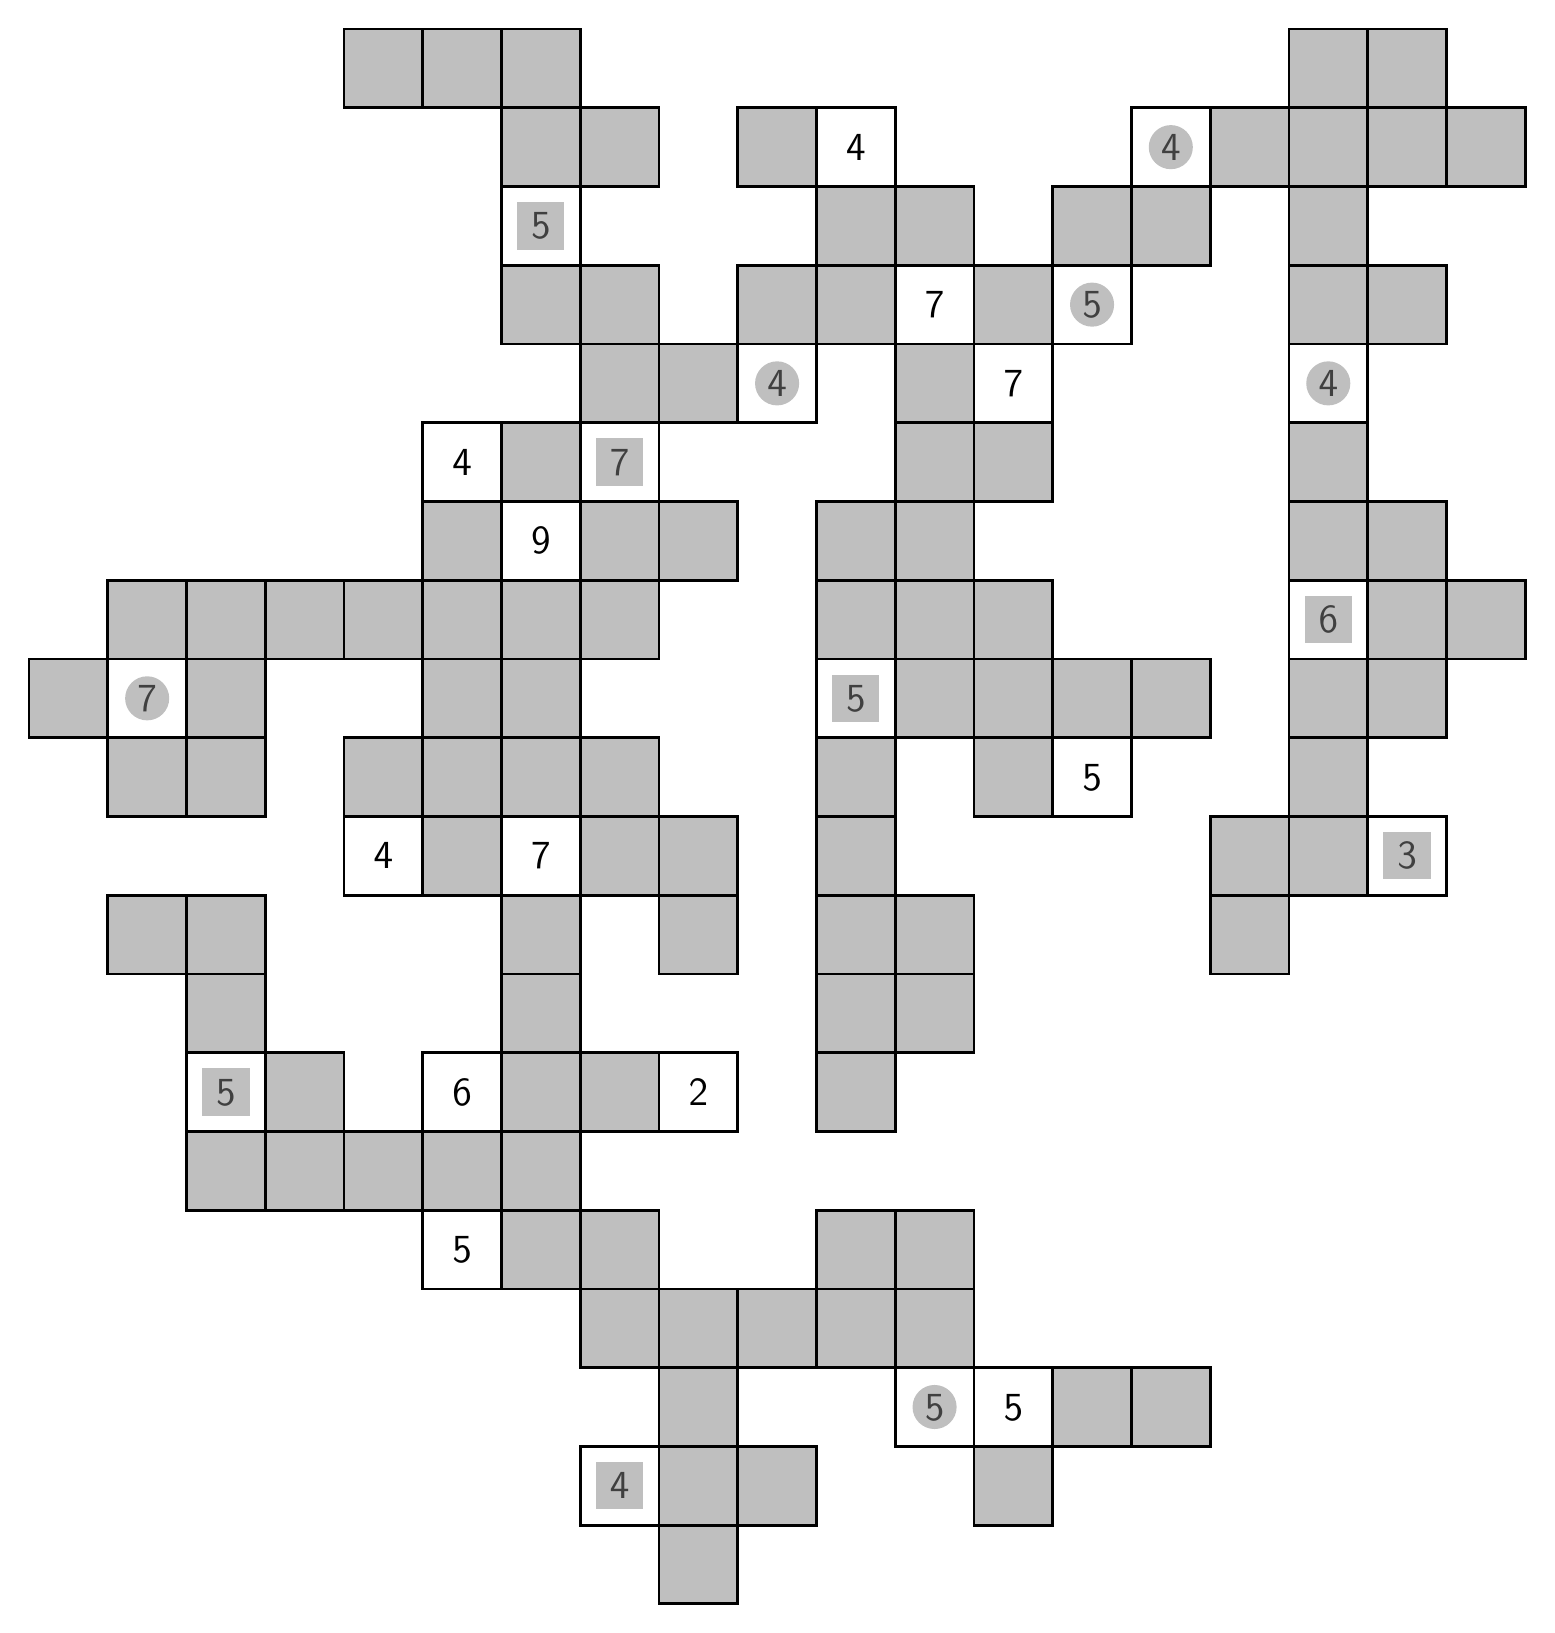
\begin{tikzpicture}\fill[gray, opacity = 0.5] (9, 0, 0)--++(1, 0, 0)--++(0, 1, 0)--++(-1, 0, 0)--cycle;
\draw[line width = 1pt] (9, 0, 0)--++(1, 0, 0)--++(0, 1, 0)--++(-1, 0, 0)--cycle;
\draw node at (8.5, 1.5, 0) {\Large $\mathsf{4}$};
\draw[line width = 1pt] (8, 1, 0)--++(1, 0, 0)--++(0, 1, 0)--++(-1, 0, 0)--cycle;
\fill[color = gray, opacity = 0.5] (8.2, 1.2) rectangle ++(0.6, 0.6);
\fill[gray, opacity = 0.5] (9, 1, 0)--++(1, 0, 0)--++(0, 1, 0)--++(-1, 0, 0)--cycle;
\draw[line width = 1pt] (9, 1, 0)--++(1, 0, 0)--++(0, 1, 0)--++(-1, 0, 0)--cycle;
\fill[gray, opacity = 0.5] (10, 1, 0)--++(1, 0, 0)--++(0, 1, 0)--++(-1, 0, 0)--cycle;
\draw[line width = 1pt] (10, 1, 0)--++(1, 0, 0)--++(0, 1, 0)--++(-1, 0, 0)--cycle;
\fill[gray, opacity = 0.5] (13, 1, 0)--++(1, 0, 0)--++(0, 1, 0)--++(-1, 0, 0)--cycle;
\draw[line width = 1pt] (13, 1, 0)--++(1, 0, 0)--++(0, 1, 0)--++(-1, 0, 0)--cycle;
\fill[gray, opacity = 0.5] (9, 2, 0)--++(1, 0, 0)--++(0, 1, 0)--++(-1, 0, 0)--cycle;
\draw[line width = 1pt] (9, 2, 0)--++(1, 0, 0)--++(0, 1, 0)--++(-1, 0, 0)--cycle;
\draw node at (12.5, 2.5, 0) {\Large $\mathsf{5}$};
\draw[line width = 1pt] (12, 2, 0)--++(1, 0, 0)--++(0, 1, 0)--++(-1, 0, 0)--cycle;
\fill[color = gray, opacity = 0.5] (12.5, 2.5, 0) circle (0.28);
\draw node at (13.5, 2.5, 0) {\Large $\mathsf{5}$};
\draw[line width = 1pt] (13, 2, 0)--++(1, 0, 0)--++(0, 1, 0)--++(-1, 0, 0)--cycle;
\fill[gray, opacity = 0.5] (14, 2, 0)--++(1, 0, 0)--++(0, 1, 0)--++(-1, 0, 0)--cycle;
\draw[line width = 1pt] (14, 2, 0)--++(1, 0, 0)--++(0, 1, 0)--++(-1, 0, 0)--cycle;
\fill[gray, opacity = 0.5] (15, 2, 0)--++(1, 0, 0)--++(0, 1, 0)--++(-1, 0, 0)--cycle;
\draw[line width = 1pt] (15, 2, 0)--++(1, 0, 0)--++(0, 1, 0)--++(-1, 0, 0)--cycle;
\fill[gray, opacity = 0.5] (8, 3, 0)--++(1, 0, 0)--++(0, 1, 0)--++(-1, 0, 0)--cycle;
\draw[line width = 1pt] (8, 3, 0)--++(1, 0, 0)--++(0, 1, 0)--++(-1, 0, 0)--cycle;
\fill[gray, opacity = 0.5] (9, 3, 0)--++(1, 0, 0)--++(0, 1, 0)--++(-1, 0, 0)--cycle;
\draw[line width = 1pt] (9, 3, 0)--++(1, 0, 0)--++(0, 1, 0)--++(-1, 0, 0)--cycle;
\fill[gray, opacity = 0.5] (10, 3, 0)--++(1, 0, 0)--++(0, 1, 0)--++(-1, 0, 0)--cycle;
\draw[line width = 1pt] (10, 3, 0)--++(1, 0, 0)--++(0, 1, 0)--++(-1, 0, 0)--cycle;
\fill[gray, opacity = 0.5] (11, 3, 0)--++(1, 0, 0)--++(0, 1, 0)--++(-1, 0, 0)--cycle;
\draw[line width = 1pt] (11, 3, 0)--++(1, 0, 0)--++(0, 1, 0)--++(-1, 0, 0)--cycle;
\fill[gray, opacity = 0.5] (12, 3, 0)--++(1, 0, 0)--++(0, 1, 0)--++(-1, 0, 0)--cycle;
\draw[line width = 1pt] (12, 3, 0)--++(1, 0, 0)--++(0, 1, 0)--++(-1, 0, 0)--cycle;
\draw node at (6.5, 4.5, 0) {\Large $\mathsf{5}$};
\draw[line width = 1pt] (6, 4, 0)--++(1, 0, 0)--++(0, 1, 0)--++(-1, 0, 0)--cycle;
\fill[gray, opacity = 0.5] (7, 4, 0)--++(1, 0, 0)--++(0, 1, 0)--++(-1, 0, 0)--cycle;
\draw[line width = 1pt] (7, 4, 0)--++(1, 0, 0)--++(0, 1, 0)--++(-1, 0, 0)--cycle;
\fill[gray, opacity = 0.5] (8, 4, 0)--++(1, 0, 0)--++(0, 1, 0)--++(-1, 0, 0)--cycle;
\draw[line width = 1pt] (8, 4, 0)--++(1, 0, 0)--++(0, 1, 0)--++(-1, 0, 0)--cycle;
\fill[gray, opacity = 0.5] (11, 4, 0)--++(1, 0, 0)--++(0, 1, 0)--++(-1, 0, 0)--cycle;
\draw[line width = 1pt] (11, 4, 0)--++(1, 0, 0)--++(0, 1, 0)--++(-1, 0, 0)--cycle;
\fill[gray, opacity = 0.5] (12, 4, 0)--++(1, 0, 0)--++(0, 1, 0)--++(-1, 0, 0)--cycle;
\draw[line width = 1pt] (12, 4, 0)--++(1, 0, 0)--++(0, 1, 0)--++(-1, 0, 0)--cycle;
\fill[gray, opacity = 0.5] (3, 5, 0)--++(1, 0, 0)--++(0, 1, 0)--++(-1, 0, 0)--cycle;
\draw[line width = 1pt] (3, 5, 0)--++(1, 0, 0)--++(0, 1, 0)--++(-1, 0, 0)--cycle;
\fill[gray, opacity = 0.5] (4, 5, 0)--++(1, 0, 0)--++(0, 1, 0)--++(-1, 0, 0)--cycle;
\draw[line width = 1pt] (4, 5, 0)--++(1, 0, 0)--++(0, 1, 0)--++(-1, 0, 0)--cycle;
\fill[gray, opacity = 0.5] (5, 5, 0)--++(1, 0, 0)--++(0, 1, 0)--++(-1, 0, 0)--cycle;
\draw[line width = 1pt] (5, 5, 0)--++(1, 0, 0)--++(0, 1, 0)--++(-1, 0, 0)--cycle;
\fill[gray, opacity = 0.5] (6, 5, 0)--++(1, 0, 0)--++(0, 1, 0)--++(-1, 0, 0)--cycle;
\draw[line width = 1pt] (6, 5, 0)--++(1, 0, 0)--++(0, 1, 0)--++(-1, 0, 0)--cycle;
\fill[gray, opacity = 0.5] (7, 5, 0)--++(1, 0, 0)--++(0, 1, 0)--++(-1, 0, 0)--cycle;
\draw[line width = 1pt] (7, 5, 0)--++(1, 0, 0)--++(0, 1, 0)--++(-1, 0, 0)--cycle;
\draw node at (3.5, 6.5, 0) {\Large $\mathsf{5}$};
\draw[line width = 1pt] (3, 6, 0)--++(1, 0, 0)--++(0, 1, 0)--++(-1, 0, 0)--cycle;
\fill[color = gray, opacity = 0.5] (3.2, 6.2) rectangle ++(0.6, 0.6);
\fill[gray, opacity = 0.5] (4, 6, 0)--++(1, 0, 0)--++(0, 1, 0)--++(-1, 0, 0)--cycle;
\draw[line width = 1pt] (4, 6, 0)--++(1, 0, 0)--++(0, 1, 0)--++(-1, 0, 0)--cycle;
\draw node at (6.5, 6.5, 0) {\Large $\mathsf{6}$};
\draw[line width = 1pt] (6, 6, 0)--++(1, 0, 0)--++(0, 1, 0)--++(-1, 0, 0)--cycle;
\fill[gray, opacity = 0.5] (7, 6, 0)--++(1, 0, 0)--++(0, 1, 0)--++(-1, 0, 0)--cycle;
\draw[line width = 1pt] (7, 6, 0)--++(1, 0, 0)--++(0, 1, 0)--++(-1, 0, 0)--cycle;
\fill[gray, opacity = 0.5] (8, 6, 0)--++(1, 0, 0)--++(0, 1, 0)--++(-1, 0, 0)--cycle;
\draw[line width = 1pt] (8, 6, 0)--++(1, 0, 0)--++(0, 1, 0)--++(-1, 0, 0)--cycle;
\draw node at (9.5, 6.5, 0) {\Large $\mathsf{2}$};
\draw[line width = 1pt] (9, 6, 0)--++(1, 0, 0)--++(0, 1, 0)--++(-1, 0, 0)--cycle;
\fill[gray, opacity = 0.5] (11, 6, 0)--++(1, 0, 0)--++(0, 1, 0)--++(-1, 0, 0)--cycle;
\draw[line width = 1pt] (11, 6, 0)--++(1, 0, 0)--++(0, 1, 0)--++(-1, 0, 0)--cycle;
\fill[gray, opacity = 0.5] (3, 7, 0)--++(1, 0, 0)--++(0, 1, 0)--++(-1, 0, 0)--cycle;
\draw[line width = 1pt] (3, 7, 0)--++(1, 0, 0)--++(0, 1, 0)--++(-1, 0, 0)--cycle;
\fill[gray, opacity = 0.5] (7, 7, 0)--++(1, 0, 0)--++(0, 1, 0)--++(-1, 0, 0)--cycle;
\draw[line width = 1pt] (7, 7, 0)--++(1, 0, 0)--++(0, 1, 0)--++(-1, 0, 0)--cycle;
\fill[gray, opacity = 0.5] (11, 7, 0)--++(1, 0, 0)--++(0, 1, 0)--++(-1, 0, 0)--cycle;
\draw[line width = 1pt] (11, 7, 0)--++(1, 0, 0)--++(0, 1, 0)--++(-1, 0, 0)--cycle;
\fill[gray, opacity = 0.5] (12, 7, 0)--++(1, 0, 0)--++(0, 1, 0)--++(-1, 0, 0)--cycle;
\draw[line width = 1pt] (12, 7, 0)--++(1, 0, 0)--++(0, 1, 0)--++(-1, 0, 0)--cycle;
\fill[gray, opacity = 0.5] (2, 8, 0)--++(1, 0, 0)--++(0, 1, 0)--++(-1, 0, 0)--cycle;
\draw[line width = 1pt] (2, 8, 0)--++(1, 0, 0)--++(0, 1, 0)--++(-1, 0, 0)--cycle;
\fill[gray, opacity = 0.5] (3, 8, 0)--++(1, 0, 0)--++(0, 1, 0)--++(-1, 0, 0)--cycle;
\draw[line width = 1pt] (3, 8, 0)--++(1, 0, 0)--++(0, 1, 0)--++(-1, 0, 0)--cycle;
\fill[gray, opacity = 0.5] (7, 8, 0)--++(1, 0, 0)--++(0, 1, 0)--++(-1, 0, 0)--cycle;
\draw[line width = 1pt] (7, 8, 0)--++(1, 0, 0)--++(0, 1, 0)--++(-1, 0, 0)--cycle;
\fill[gray, opacity = 0.5] (9, 8, 0)--++(1, 0, 0)--++(0, 1, 0)--++(-1, 0, 0)--cycle;
\draw[line width = 1pt] (9, 8, 0)--++(1, 0, 0)--++(0, 1, 0)--++(-1, 0, 0)--cycle;
\fill[gray, opacity = 0.5] (11, 8, 0)--++(1, 0, 0)--++(0, 1, 0)--++(-1, 0, 0)--cycle;
\draw[line width = 1pt] (11, 8, 0)--++(1, 0, 0)--++(0, 1, 0)--++(-1, 0, 0)--cycle;
\fill[gray, opacity = 0.5] (12, 8, 0)--++(1, 0, 0)--++(0, 1, 0)--++(-1, 0, 0)--cycle;
\draw[line width = 1pt] (12, 8, 0)--++(1, 0, 0)--++(0, 1, 0)--++(-1, 0, 0)--cycle;
\fill[gray, opacity = 0.5] (16, 8, 0)--++(1, 0, 0)--++(0, 1, 0)--++(-1, 0, 0)--cycle;
\draw[line width = 1pt] (16, 8, 0)--++(1, 0, 0)--++(0, 1, 0)--++(-1, 0, 0)--cycle;
\draw node at (5.5, 9.5, 0) {\Large $\mathsf{4}$};
\draw[line width = 1pt] (5, 9, 0)--++(1, 0, 0)--++(0, 1, 0)--++(-1, 0, 0)--cycle;
\fill[gray, opacity = 0.5] (6, 9, 0)--++(1, 0, 0)--++(0, 1, 0)--++(-1, 0, 0)--cycle;
\draw[line width = 1pt] (6, 9, 0)--++(1, 0, 0)--++(0, 1, 0)--++(-1, 0, 0)--cycle;
\draw node at (7.5, 9.5, 0) {\Large $\mathsf{7}$};
\draw[line width = 1pt] (7, 9, 0)--++(1, 0, 0)--++(0, 1, 0)--++(-1, 0, 0)--cycle;
\fill[gray, opacity = 0.5] (8, 9, 0)--++(1, 0, 0)--++(0, 1, 0)--++(-1, 0, 0)--cycle;
\draw[line width = 1pt] (8, 9, 0)--++(1, 0, 0)--++(0, 1, 0)--++(-1, 0, 0)--cycle;
\fill[gray, opacity = 0.5] (9, 9, 0)--++(1, 0, 0)--++(0, 1, 0)--++(-1, 0, 0)--cycle;
\draw[line width = 1pt] (9, 9, 0)--++(1, 0, 0)--++(0, 1, 0)--++(-1, 0, 0)--cycle;
\fill[gray, opacity = 0.5] (11, 9, 0)--++(1, 0, 0)--++(0, 1, 0)--++(-1, 0, 0)--cycle;
\draw[line width = 1pt] (11, 9, 0)--++(1, 0, 0)--++(0, 1, 0)--++(-1, 0, 0)--cycle;
\fill[gray, opacity = 0.5] (16, 9, 0)--++(1, 0, 0)--++(0, 1, 0)--++(-1, 0, 0)--cycle;
\draw[line width = 1pt] (16, 9, 0)--++(1, 0, 0)--++(0, 1, 0)--++(-1, 0, 0)--cycle;
\fill[gray, opacity = 0.5] (17, 9, 0)--++(1, 0, 0)--++(0, 1, 0)--++(-1, 0, 0)--cycle;
\draw[line width = 1pt] (17, 9, 0)--++(1, 0, 0)--++(0, 1, 0)--++(-1, 0, 0)--cycle;
\draw node at (18.5, 9.5, 0) {\Large $\mathsf{3}$};
\draw[line width = 1pt] (18, 9, 0)--++(1, 0, 0)--++(0, 1, 0)--++(-1, 0, 0)--cycle;
\fill[color = gray, opacity = 0.5] (18.2, 9.2) rectangle ++(0.6, 0.6);
\fill[gray, opacity = 0.5] (2, 10, 0)--++(1, 0, 0)--++(0, 1, 0)--++(-1, 0, 0)--cycle;
\draw[line width = 1pt] (2, 10, 0)--++(1, 0, 0)--++(0, 1, 0)--++(-1, 0, 0)--cycle;
\fill[gray, opacity = 0.5] (3, 10, 0)--++(1, 0, 0)--++(0, 1, 0)--++(-1, 0, 0)--cycle;
\draw[line width = 1pt] (3, 10, 0)--++(1, 0, 0)--++(0, 1, 0)--++(-1, 0, 0)--cycle;
\fill[gray, opacity = 0.5] (5, 10, 0)--++(1, 0, 0)--++(0, 1, 0)--++(-1, 0, 0)--cycle;
\draw[line width = 1pt] (5, 10, 0)--++(1, 0, 0)--++(0, 1, 0)--++(-1, 0, 0)--cycle;
\fill[gray, opacity = 0.5] (6, 10, 0)--++(1, 0, 0)--++(0, 1, 0)--++(-1, 0, 0)--cycle;
\draw[line width = 1pt] (6, 10, 0)--++(1, 0, 0)--++(0, 1, 0)--++(-1, 0, 0)--cycle;
\fill[gray, opacity = 0.5] (7, 10, 0)--++(1, 0, 0)--++(0, 1, 0)--++(-1, 0, 0)--cycle;
\draw[line width = 1pt] (7, 10, 0)--++(1, 0, 0)--++(0, 1, 0)--++(-1, 0, 0)--cycle;
\fill[gray, opacity = 0.5] (8, 10, 0)--++(1, 0, 0)--++(0, 1, 0)--++(-1, 0, 0)--cycle;
\draw[line width = 1pt] (8, 10, 0)--++(1, 0, 0)--++(0, 1, 0)--++(-1, 0, 0)--cycle;
\fill[gray, opacity = 0.5] (11, 10, 0)--++(1, 0, 0)--++(0, 1, 0)--++(-1, 0, 0)--cycle;
\draw[line width = 1pt] (11, 10, 0)--++(1, 0, 0)--++(0, 1, 0)--++(-1, 0, 0)--cycle;
\fill[gray, opacity = 0.5] (13, 10, 0)--++(1, 0, 0)--++(0, 1, 0)--++(-1, 0, 0)--cycle;
\draw[line width = 1pt] (13, 10, 0)--++(1, 0, 0)--++(0, 1, 0)--++(-1, 0, 0)--cycle;
\draw node at (14.5, 10.5, 0) {\Large $\mathsf{5}$};
\draw[line width = 1pt] (14, 10, 0)--++(1, 0, 0)--++(0, 1, 0)--++(-1, 0, 0)--cycle;
\fill[gray, opacity = 0.5] (17, 10, 0)--++(1, 0, 0)--++(0, 1, 0)--++(-1, 0, 0)--cycle;
\draw[line width = 1pt] (17, 10, 0)--++(1, 0, 0)--++(0, 1, 0)--++(-1, 0, 0)--cycle;
\fill[gray, opacity = 0.5] (1, 11, 0)--++(1, 0, 0)--++(0, 1, 0)--++(-1, 0, 0)--cycle;
\draw[line width = 1pt] (1, 11, 0)--++(1, 0, 0)--++(0, 1, 0)--++(-1, 0, 0)--cycle;
\draw node at (2.5, 11.5, 0) {\Large $\mathsf{7}$};
\draw[line width = 1pt] (2, 11, 0)--++(1, 0, 0)--++(0, 1, 0)--++(-1, 0, 0)--cycle;
\fill[color = gray, opacity = 0.5] (2.5, 11.5, 0) circle (0.28);
\fill[gray, opacity = 0.5] (3, 11, 0)--++(1, 0, 0)--++(0, 1, 0)--++(-1, 0, 0)--cycle;
\draw[line width = 1pt] (3, 11, 0)--++(1, 0, 0)--++(0, 1, 0)--++(-1, 0, 0)--cycle;
\fill[gray, opacity = 0.5] (6, 11, 0)--++(1, 0, 0)--++(0, 1, 0)--++(-1, 0, 0)--cycle;
\draw[line width = 1pt] (6, 11, 0)--++(1, 0, 0)--++(0, 1, 0)--++(-1, 0, 0)--cycle;
\fill[gray, opacity = 0.5] (7, 11, 0)--++(1, 0, 0)--++(0, 1, 0)--++(-1, 0, 0)--cycle;
\draw[line width = 1pt] (7, 11, 0)--++(1, 0, 0)--++(0, 1, 0)--++(-1, 0, 0)--cycle;
\draw node at (11.5, 11.5, 0) {\Large $\mathsf{5}$};
\draw[line width = 1pt] (11, 11, 0)--++(1, 0, 0)--++(0, 1, 0)--++(-1, 0, 0)--cycle;
\fill[color = gray, opacity = 0.5] (11.2, 11.2) rectangle ++(0.6, 0.6);
\fill[gray, opacity = 0.5] (12, 11, 0)--++(1, 0, 0)--++(0, 1, 0)--++(-1, 0, 0)--cycle;
\draw[line width = 1pt] (12, 11, 0)--++(1, 0, 0)--++(0, 1, 0)--++(-1, 0, 0)--cycle;
\fill[gray, opacity = 0.5] (13, 11, 0)--++(1, 0, 0)--++(0, 1, 0)--++(-1, 0, 0)--cycle;
\draw[line width = 1pt] (13, 11, 0)--++(1, 0, 0)--++(0, 1, 0)--++(-1, 0, 0)--cycle;
\fill[gray, opacity = 0.5] (14, 11, 0)--++(1, 0, 0)--++(0, 1, 0)--++(-1, 0, 0)--cycle;
\draw[line width = 1pt] (14, 11, 0)--++(1, 0, 0)--++(0, 1, 0)--++(-1, 0, 0)--cycle;
\fill[gray, opacity = 0.5] (15, 11, 0)--++(1, 0, 0)--++(0, 1, 0)--++(-1, 0, 0)--cycle;
\draw[line width = 1pt] (15, 11, 0)--++(1, 0, 0)--++(0, 1, 0)--++(-1, 0, 0)--cycle;
\fill[gray, opacity = 0.5] (17, 11, 0)--++(1, 0, 0)--++(0, 1, 0)--++(-1, 0, 0)--cycle;
\draw[line width = 1pt] (17, 11, 0)--++(1, 0, 0)--++(0, 1, 0)--++(-1, 0, 0)--cycle;
\fill[gray, opacity = 0.5] (18, 11, 0)--++(1, 0, 0)--++(0, 1, 0)--++(-1, 0, 0)--cycle;
\draw[line width = 1pt] (18, 11, 0)--++(1, 0, 0)--++(0, 1, 0)--++(-1, 0, 0)--cycle;
\fill[gray, opacity = 0.5] (2, 12, 0)--++(1, 0, 0)--++(0, 1, 0)--++(-1, 0, 0)--cycle;
\draw[line width = 1pt] (2, 12, 0)--++(1, 0, 0)--++(0, 1, 0)--++(-1, 0, 0)--cycle;
\fill[gray, opacity = 0.5] (3, 12, 0)--++(1, 0, 0)--++(0, 1, 0)--++(-1, 0, 0)--cycle;
\draw[line width = 1pt] (3, 12, 0)--++(1, 0, 0)--++(0, 1, 0)--++(-1, 0, 0)--cycle;
\fill[gray, opacity = 0.5] (4, 12, 0)--++(1, 0, 0)--++(0, 1, 0)--++(-1, 0, 0)--cycle;
\draw[line width = 1pt] (4, 12, 0)--++(1, 0, 0)--++(0, 1, 0)--++(-1, 0, 0)--cycle;
\fill[gray, opacity = 0.5] (5, 12, 0)--++(1, 0, 0)--++(0, 1, 0)--++(-1, 0, 0)--cycle;
\draw[line width = 1pt] (5, 12, 0)--++(1, 0, 0)--++(0, 1, 0)--++(-1, 0, 0)--cycle;
\fill[gray, opacity = 0.5] (6, 12, 0)--++(1, 0, 0)--++(0, 1, 0)--++(-1, 0, 0)--cycle;
\draw[line width = 1pt] (6, 12, 0)--++(1, 0, 0)--++(0, 1, 0)--++(-1, 0, 0)--cycle;
\fill[gray, opacity = 0.5] (7, 12, 0)--++(1, 0, 0)--++(0, 1, 0)--++(-1, 0, 0)--cycle;
\draw[line width = 1pt] (7, 12, 0)--++(1, 0, 0)--++(0, 1, 0)--++(-1, 0, 0)--cycle;
\fill[gray, opacity = 0.5] (8, 12, 0)--++(1, 0, 0)--++(0, 1, 0)--++(-1, 0, 0)--cycle;
\draw[line width = 1pt] (8, 12, 0)--++(1, 0, 0)--++(0, 1, 0)--++(-1, 0, 0)--cycle;
\fill[gray, opacity = 0.5] (11, 12, 0)--++(1, 0, 0)--++(0, 1, 0)--++(-1, 0, 0)--cycle;
\draw[line width = 1pt] (11, 12, 0)--++(1, 0, 0)--++(0, 1, 0)--++(-1, 0, 0)--cycle;
\fill[gray, opacity = 0.5] (12, 12, 0)--++(1, 0, 0)--++(0, 1, 0)--++(-1, 0, 0)--cycle;
\draw[line width = 1pt] (12, 12, 0)--++(1, 0, 0)--++(0, 1, 0)--++(-1, 0, 0)--cycle;
\fill[gray, opacity = 0.5] (13, 12, 0)--++(1, 0, 0)--++(0, 1, 0)--++(-1, 0, 0)--cycle;
\draw[line width = 1pt] (13, 12, 0)--++(1, 0, 0)--++(0, 1, 0)--++(-1, 0, 0)--cycle;
\draw node at (17.5, 12.5, 0) {\Large $\mathsf{6}$};
\draw[line width = 1pt] (17, 12, 0)--++(1, 0, 0)--++(0, 1, 0)--++(-1, 0, 0)--cycle;
\fill[color = gray, opacity = 0.5] (17.2, 12.2) rectangle ++(0.6, 0.6);
\fill[gray, opacity = 0.5] (18, 12, 0)--++(1, 0, 0)--++(0, 1, 0)--++(-1, 0, 0)--cycle;
\draw[line width = 1pt] (18, 12, 0)--++(1, 0, 0)--++(0, 1, 0)--++(-1, 0, 0)--cycle;
\fill[gray, opacity = 0.5] (19, 12, 0)--++(1, 0, 0)--++(0, 1, 0)--++(-1, 0, 0)--cycle;
\draw[line width = 1pt] (19, 12, 0)--++(1, 0, 0)--++(0, 1, 0)--++(-1, 0, 0)--cycle;
\fill[gray, opacity = 0.5] (6, 13, 0)--++(1, 0, 0)--++(0, 1, 0)--++(-1, 0, 0)--cycle;
\draw[line width = 1pt] (6, 13, 0)--++(1, 0, 0)--++(0, 1, 0)--++(-1, 0, 0)--cycle;
\draw node at (7.5, 13.5, 0) {\Large $\mathsf{9}$};
\draw[line width = 1pt] (7, 13, 0)--++(1, 0, 0)--++(0, 1, 0)--++(-1, 0, 0)--cycle;
\fill[gray, opacity = 0.5] (8, 13, 0)--++(1, 0, 0)--++(0, 1, 0)--++(-1, 0, 0)--cycle;
\draw[line width = 1pt] (8, 13, 0)--++(1, 0, 0)--++(0, 1, 0)--++(-1, 0, 0)--cycle;
\fill[gray, opacity = 0.5] (9, 13, 0)--++(1, 0, 0)--++(0, 1, 0)--++(-1, 0, 0)--cycle;
\draw[line width = 1pt] (9, 13, 0)--++(1, 0, 0)--++(0, 1, 0)--++(-1, 0, 0)--cycle;
\fill[gray, opacity = 0.5] (11, 13, 0)--++(1, 0, 0)--++(0, 1, 0)--++(-1, 0, 0)--cycle;
\draw[line width = 1pt] (11, 13, 0)--++(1, 0, 0)--++(0, 1, 0)--++(-1, 0, 0)--cycle;
\fill[gray, opacity = 0.5] (12, 13, 0)--++(1, 0, 0)--++(0, 1, 0)--++(-1, 0, 0)--cycle;
\draw[line width = 1pt] (12, 13, 0)--++(1, 0, 0)--++(0, 1, 0)--++(-1, 0, 0)--cycle;
\fill[gray, opacity = 0.5] (17, 13, 0)--++(1, 0, 0)--++(0, 1, 0)--++(-1, 0, 0)--cycle;
\draw[line width = 1pt] (17, 13, 0)--++(1, 0, 0)--++(0, 1, 0)--++(-1, 0, 0)--cycle;
\fill[gray, opacity = 0.5] (18, 13, 0)--++(1, 0, 0)--++(0, 1, 0)--++(-1, 0, 0)--cycle;
\draw[line width = 1pt] (18, 13, 0)--++(1, 0, 0)--++(0, 1, 0)--++(-1, 0, 0)--cycle;
\draw node at (6.5, 14.5, 0) {\Large $\mathsf{4}$};
\draw[line width = 1pt] (6, 14, 0)--++(1, 0, 0)--++(0, 1, 0)--++(-1, 0, 0)--cycle;
\fill[gray, opacity = 0.5] (7, 14, 0)--++(1, 0, 0)--++(0, 1, 0)--++(-1, 0, 0)--cycle;
\draw[line width = 1pt] (7, 14, 0)--++(1, 0, 0)--++(0, 1, 0)--++(-1, 0, 0)--cycle;
\draw node at (8.5, 14.5, 0) {\Large $\mathsf{7}$};
\draw[line width = 1pt] (8, 14, 0)--++(1, 0, 0)--++(0, 1, 0)--++(-1, 0, 0)--cycle;
\fill[color = gray, opacity = 0.5] (8.2, 14.2) rectangle ++(0.6, 0.6);
\fill[gray, opacity = 0.5] (12, 14, 0)--++(1, 0, 0)--++(0, 1, 0)--++(-1, 0, 0)--cycle;
\draw[line width = 1pt] (12, 14, 0)--++(1, 0, 0)--++(0, 1, 0)--++(-1, 0, 0)--cycle;
\fill[gray, opacity = 0.5] (13, 14, 0)--++(1, 0, 0)--++(0, 1, 0)--++(-1, 0, 0)--cycle;
\draw[line width = 1pt] (13, 14, 0)--++(1, 0, 0)--++(0, 1, 0)--++(-1, 0, 0)--cycle;
\fill[gray, opacity = 0.5] (17, 14, 0)--++(1, 0, 0)--++(0, 1, 0)--++(-1, 0, 0)--cycle;
\draw[line width = 1pt] (17, 14, 0)--++(1, 0, 0)--++(0, 1, 0)--++(-1, 0, 0)--cycle;
\fill[gray, opacity = 0.5] (8, 15, 0)--++(1, 0, 0)--++(0, 1, 0)--++(-1, 0, 0)--cycle;
\draw[line width = 1pt] (8, 15, 0)--++(1, 0, 0)--++(0, 1, 0)--++(-1, 0, 0)--cycle;
\fill[gray, opacity = 0.5] (9, 15, 0)--++(1, 0, 0)--++(0, 1, 0)--++(-1, 0, 0)--cycle;
\draw[line width = 1pt] (9, 15, 0)--++(1, 0, 0)--++(0, 1, 0)--++(-1, 0, 0)--cycle;
\draw node at (10.5, 15.5, 0) {\Large $\mathsf{4}$};
\draw[line width = 1pt] (10, 15, 0)--++(1, 0, 0)--++(0, 1, 0)--++(-1, 0, 0)--cycle;
\fill[color = gray, opacity = 0.5] (10.5, 15.5, 0) circle (0.28);
\fill[gray, opacity = 0.5] (12, 15, 0)--++(1, 0, 0)--++(0, 1, 0)--++(-1, 0, 0)--cycle;
\draw[line width = 1pt] (12, 15, 0)--++(1, 0, 0)--++(0, 1, 0)--++(-1, 0, 0)--cycle;
\draw node at (13.5, 15.5, 0) {\Large $\mathsf{7}$};
\draw[line width = 1pt] (13, 15, 0)--++(1, 0, 0)--++(0, 1, 0)--++(-1, 0, 0)--cycle;
\draw node at (17.5, 15.5, 0) {\Large $\mathsf{4}$};
\draw[line width = 1pt] (17, 15, 0)--++(1, 0, 0)--++(0, 1, 0)--++(-1, 0, 0)--cycle;
\fill[color = gray, opacity = 0.5] (17.5, 15.5, 0) circle (0.28);
\fill[gray, opacity = 0.5] (7, 16, 0)--++(1, 0, 0)--++(0, 1, 0)--++(-1, 0, 0)--cycle;
\draw[line width = 1pt] (7, 16, 0)--++(1, 0, 0)--++(0, 1, 0)--++(-1, 0, 0)--cycle;
\fill[gray, opacity = 0.5] (8, 16, 0)--++(1, 0, 0)--++(0, 1, 0)--++(-1, 0, 0)--cycle;
\draw[line width = 1pt] (8, 16, 0)--++(1, 0, 0)--++(0, 1, 0)--++(-1, 0, 0)--cycle;
\fill[gray, opacity = 0.5] (10, 16, 0)--++(1, 0, 0)--++(0, 1, 0)--++(-1, 0, 0)--cycle;
\draw[line width = 1pt] (10, 16, 0)--++(1, 0, 0)--++(0, 1, 0)--++(-1, 0, 0)--cycle;
\fill[gray, opacity = 0.5] (11, 16, 0)--++(1, 0, 0)--++(0, 1, 0)--++(-1, 0, 0)--cycle;
\draw[line width = 1pt] (11, 16, 0)--++(1, 0, 0)--++(0, 1, 0)--++(-1, 0, 0)--cycle;
\draw node at (12.5, 16.5, 0) {\Large $\mathsf{7}$};
\draw[line width = 1pt] (12, 16, 0)--++(1, 0, 0)--++(0, 1, 0)--++(-1, 0, 0)--cycle;
\fill[gray, opacity = 0.5] (13, 16, 0)--++(1, 0, 0)--++(0, 1, 0)--++(-1, 0, 0)--cycle;
\draw[line width = 1pt] (13, 16, 0)--++(1, 0, 0)--++(0, 1, 0)--++(-1, 0, 0)--cycle;
\draw node at (14.5, 16.5, 0) {\Large $\mathsf{5}$};
\draw[line width = 1pt] (14, 16, 0)--++(1, 0, 0)--++(0, 1, 0)--++(-1, 0, 0)--cycle;
\fill[color = gray, opacity = 0.5] (14.5, 16.5, 0) circle (0.28);
\fill[gray, opacity = 0.5] (17, 16, 0)--++(1, 0, 0)--++(0, 1, 0)--++(-1, 0, 0)--cycle;
\draw[line width = 1pt] (17, 16, 0)--++(1, 0, 0)--++(0, 1, 0)--++(-1, 0, 0)--cycle;
\fill[gray, opacity = 0.5] (18, 16, 0)--++(1, 0, 0)--++(0, 1, 0)--++(-1, 0, 0)--cycle;
\draw[line width = 1pt] (18, 16, 0)--++(1, 0, 0)--++(0, 1, 0)--++(-1, 0, 0)--cycle;
\draw node at (7.5, 17.5, 0) {\Large $\mathsf{5}$};
\draw[line width = 1pt] (7, 17, 0)--++(1, 0, 0)--++(0, 1, 0)--++(-1, 0, 0)--cycle;
\fill[color = gray, opacity = 0.5] (7.2, 17.2) rectangle ++(0.6, 0.6);
\fill[gray, opacity = 0.5] (11, 17, 0)--++(1, 0, 0)--++(0, 1, 0)--++(-1, 0, 0)--cycle;
\draw[line width = 1pt] (11, 17, 0)--++(1, 0, 0)--++(0, 1, 0)--++(-1, 0, 0)--cycle;
\fill[gray, opacity = 0.5] (12, 17, 0)--++(1, 0, 0)--++(0, 1, 0)--++(-1, 0, 0)--cycle;
\draw[line width = 1pt] (12, 17, 0)--++(1, 0, 0)--++(0, 1, 0)--++(-1, 0, 0)--cycle;
\fill[gray, opacity = 0.5] (14, 17, 0)--++(1, 0, 0)--++(0, 1, 0)--++(-1, 0, 0)--cycle;
\draw[line width = 1pt] (14, 17, 0)--++(1, 0, 0)--++(0, 1, 0)--++(-1, 0, 0)--cycle;
\fill[gray, opacity = 0.5] (15, 17, 0)--++(1, 0, 0)--++(0, 1, 0)--++(-1, 0, 0)--cycle;
\draw[line width = 1pt] (15, 17, 0)--++(1, 0, 0)--++(0, 1, 0)--++(-1, 0, 0)--cycle;
\fill[gray, opacity = 0.5] (17, 17, 0)--++(1, 0, 0)--++(0, 1, 0)--++(-1, 0, 0)--cycle;
\draw[line width = 1pt] (17, 17, 0)--++(1, 0, 0)--++(0, 1, 0)--++(-1, 0, 0)--cycle;
\fill[gray, opacity = 0.5] (7, 18, 0)--++(1, 0, 0)--++(0, 1, 0)--++(-1, 0, 0)--cycle;
\draw[line width = 1pt] (7, 18, 0)--++(1, 0, 0)--++(0, 1, 0)--++(-1, 0, 0)--cycle;
\fill[gray, opacity = 0.5] (8, 18, 0)--++(1, 0, 0)--++(0, 1, 0)--++(-1, 0, 0)--cycle;
\draw[line width = 1pt] (8, 18, 0)--++(1, 0, 0)--++(0, 1, 0)--++(-1, 0, 0)--cycle;
\fill[gray, opacity = 0.5] (10, 18, 0)--++(1, 0, 0)--++(0, 1, 0)--++(-1, 0, 0)--cycle;
\draw[line width = 1pt] (10, 18, 0)--++(1, 0, 0)--++(0, 1, 0)--++(-1, 0, 0)--cycle;
\draw node at (11.5, 18.5, 0) {\Large $\mathsf{4}$};
\draw[line width = 1pt] (11, 18, 0)--++(1, 0, 0)--++(0, 1, 0)--++(-1, 0, 0)--cycle;
\draw node at (15.5, 18.5, 0) {\Large $\mathsf{4}$};
\draw[line width = 1pt] (15, 18, 0)--++(1, 0, 0)--++(0, 1, 0)--++(-1, 0, 0)--cycle;
\fill[color = gray, opacity = 0.5] (15.5, 18.5, 0) circle (0.28);
\fill[gray, opacity = 0.5] (16, 18, 0)--++(1, 0, 0)--++(0, 1, 0)--++(-1, 0, 0)--cycle;
\draw[line width = 1pt] (16, 18, 0)--++(1, 0, 0)--++(0, 1, 0)--++(-1, 0, 0)--cycle;
\fill[gray, opacity = 0.5] (17, 18, 0)--++(1, 0, 0)--++(0, 1, 0)--++(-1, 0, 0)--cycle;
\draw[line width = 1pt] (17, 18, 0)--++(1, 0, 0)--++(0, 1, 0)--++(-1, 0, 0)--cycle;
\fill[gray, opacity = 0.5] (18, 18, 0)--++(1, 0, 0)--++(0, 1, 0)--++(-1, 0, 0)--cycle;
\draw[line width = 1pt] (18, 18, 0)--++(1, 0, 0)--++(0, 1, 0)--++(-1, 0, 0)--cycle;
\fill[gray, opacity = 0.5] (19, 18, 0)--++(1, 0, 0)--++(0, 1, 0)--++(-1, 0, 0)--cycle;
\draw[line width = 1pt] (19, 18, 0)--++(1, 0, 0)--++(0, 1, 0)--++(-1, 0, 0)--cycle;
\fill[gray, opacity = 0.5] (5, 19, 0)--++(1, 0, 0)--++(0, 1, 0)--++(-1, 0, 0)--cycle;
\draw[line width = 1pt] (5, 19, 0)--++(1, 0, 0)--++(0, 1, 0)--++(-1, 0, 0)--cycle;
\fill[gray, opacity = 0.5] (6, 19, 0)--++(1, 0, 0)--++(0, 1, 0)--++(-1, 0, 0)--cycle;
\draw[line width = 1pt] (6, 19, 0)--++(1, 0, 0)--++(0, 1, 0)--++(-1, 0, 0)--cycle;
\fill[gray, opacity = 0.5] (7, 19, 0)--++(1, 0, 0)--++(0, 1, 0)--++(-1, 0, 0)--cycle;
\draw[line width = 1pt] (7, 19, 0)--++(1, 0, 0)--++(0, 1, 0)--++(-1, 0, 0)--cycle;
\fill[gray, opacity = 0.5] (17, 19, 0)--++(1, 0, 0)--++(0, 1, 0)--++(-1, 0, 0)--cycle;
\draw[line width = 1pt] (17, 19, 0)--++(1, 0, 0)--++(0, 1, 0)--++(-1, 0, 0)--cycle;
\fill[gray, opacity = 0.5] (18, 19, 0)--++(1, 0, 0)--++(0, 1, 0)--++(-1, 0, 0)--cycle;
\draw[line width = 1pt] (18, 19, 0)--++(1, 0, 0)--++(0, 1, 0)--++(-1, 0, 0)--cycle;
\end{tikzpicture}}\]
\[\resizebox{30pc}{!}{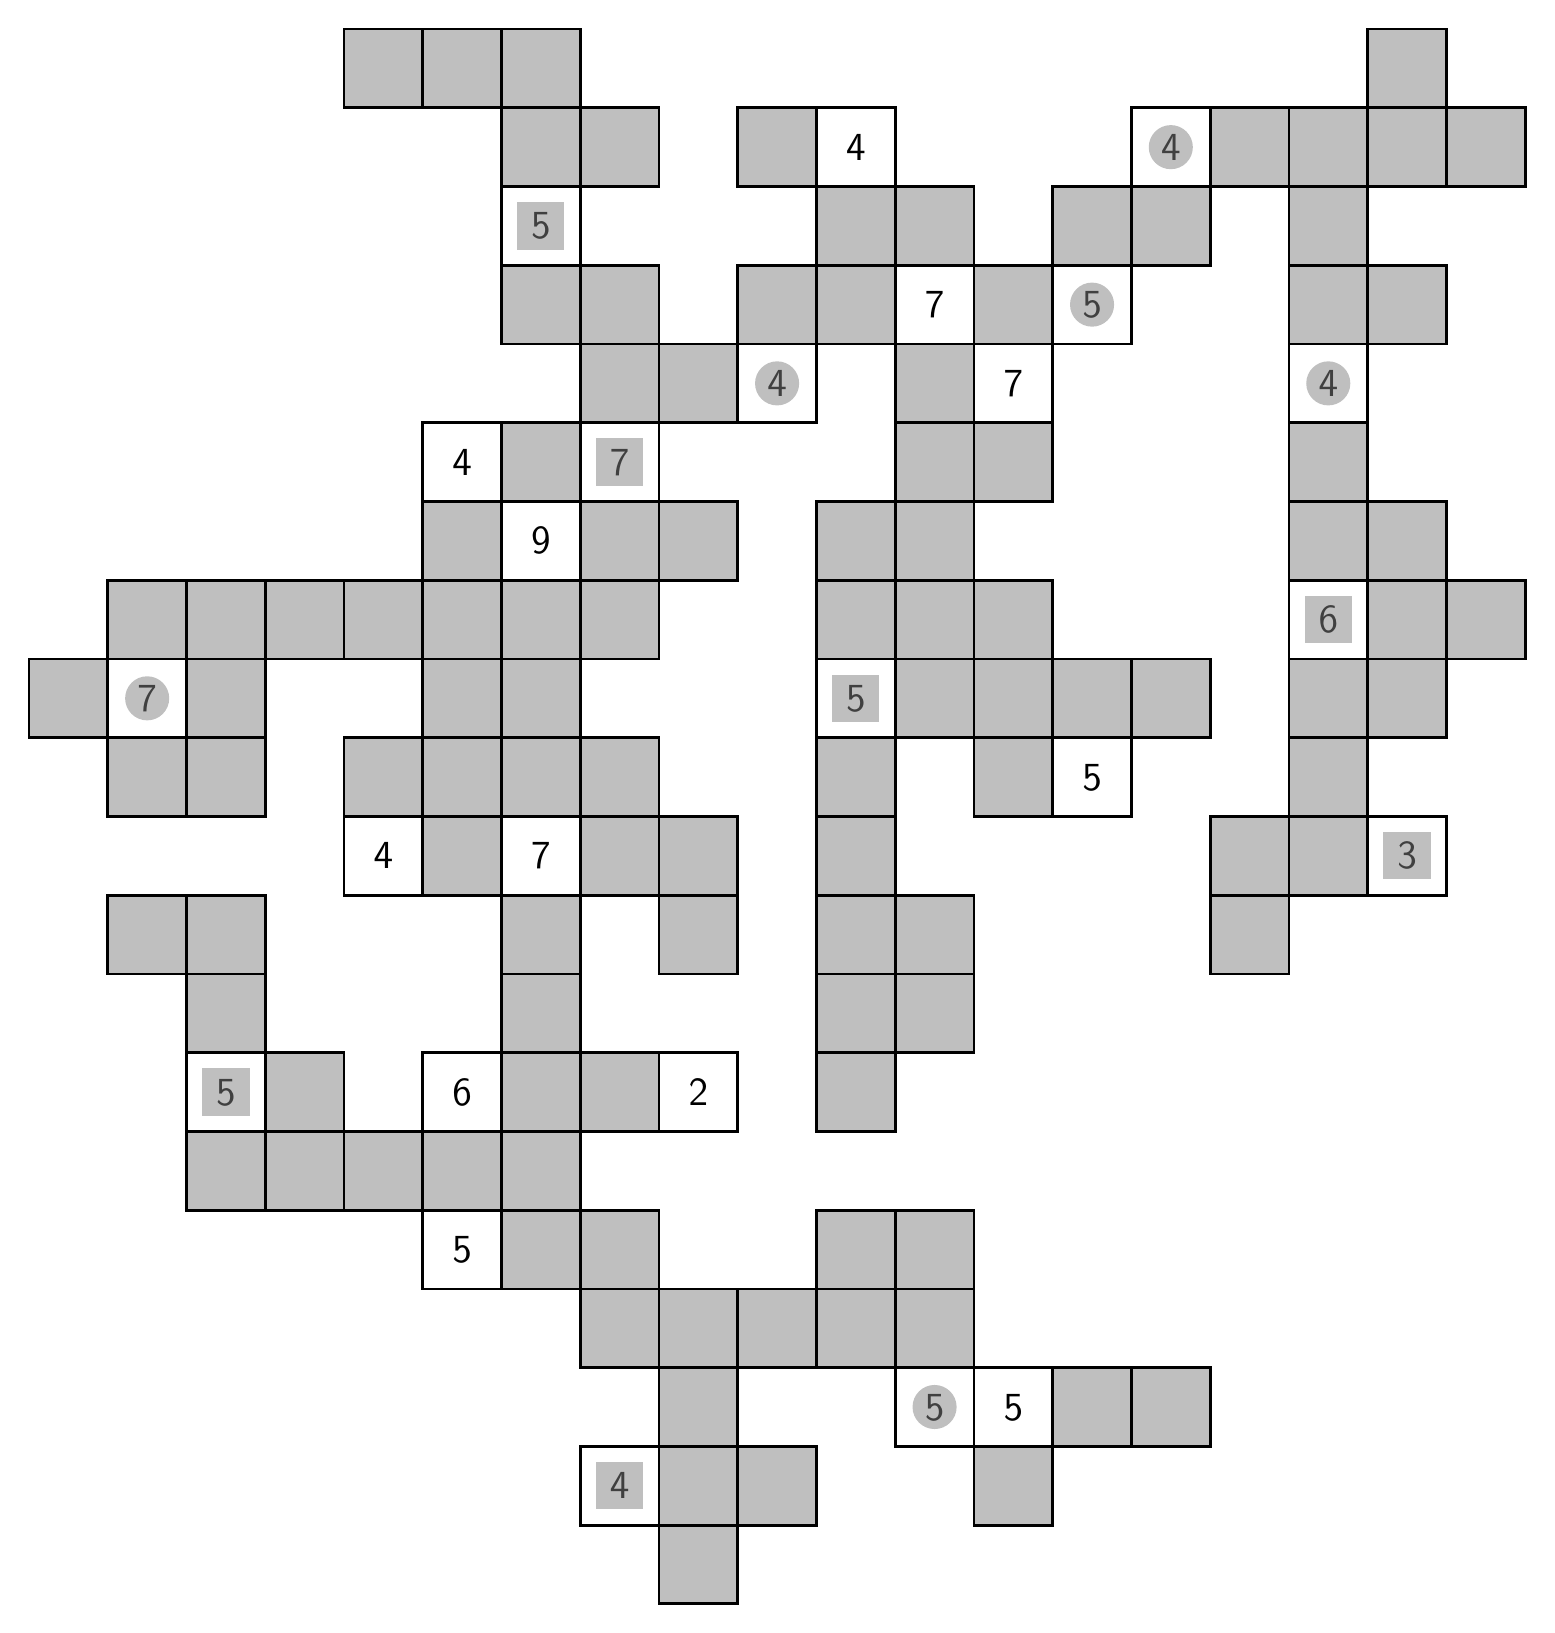
\begin{tikzpicture}\fill[gray, opacity = 0.5] (9, 0, 0)--++(1, 0, 0)--++(0, 1, 0)--++(-1, 0, 0)--cycle;
\draw[line width = 1pt] (9, 0, 0)--++(1, 0, 0)--++(0, 1, 0)--++(-1, 0, 0)--cycle;
\draw node at (8.5, 1.5, 0) {\Large $\mathsf{4}$};
\draw[line width = 1pt] (8, 1, 0)--++(1, 0, 0)--++(0, 1, 0)--++(-1, 0, 0)--cycle;
\fill[color = gray, opacity = 0.5] (8.2, 1.2) rectangle ++(0.6, 0.6);
\fill[gray, opacity = 0.5] (9, 1, 0)--++(1, 0, 0)--++(0, 1, 0)--++(-1, 0, 0)--cycle;
\draw[line width = 1pt] (9, 1, 0)--++(1, 0, 0)--++(0, 1, 0)--++(-1, 0, 0)--cycle;
\fill[gray, opacity = 0.5] (10, 1, 0)--++(1, 0, 0)--++(0, 1, 0)--++(-1, 0, 0)--cycle;
\draw[line width = 1pt] (10, 1, 0)--++(1, 0, 0)--++(0, 1, 0)--++(-1, 0, 0)--cycle;
\fill[gray, opacity = 0.5] (13, 1, 0)--++(1, 0, 0)--++(0, 1, 0)--++(-1, 0, 0)--cycle;
\draw[line width = 1pt] (13, 1, 0)--++(1, 0, 0)--++(0, 1, 0)--++(-1, 0, 0)--cycle;
\fill[gray, opacity = 0.5] (9, 2, 0)--++(1, 0, 0)--++(0, 1, 0)--++(-1, 0, 0)--cycle;
\draw[line width = 1pt] (9, 2, 0)--++(1, 0, 0)--++(0, 1, 0)--++(-1, 0, 0)--cycle;
\draw node at (12.5, 2.5, 0) {\Large $\mathsf{5}$};
\draw[line width = 1pt] (12, 2, 0)--++(1, 0, 0)--++(0, 1, 0)--++(-1, 0, 0)--cycle;
\fill[color = gray, opacity = 0.5] (12.5, 2.5, 0) circle (0.28);
\draw node at (13.5, 2.5, 0) {\Large $\mathsf{5}$};
\draw[line width = 1pt] (13, 2, 0)--++(1, 0, 0)--++(0, 1, 0)--++(-1, 0, 0)--cycle;
\fill[gray, opacity = 0.5] (14, 2, 0)--++(1, 0, 0)--++(0, 1, 0)--++(-1, 0, 0)--cycle;
\draw[line width = 1pt] (14, 2, 0)--++(1, 0, 0)--++(0, 1, 0)--++(-1, 0, 0)--cycle;
\fill[gray, opacity = 0.5] (15, 2, 0)--++(1, 0, 0)--++(0, 1, 0)--++(-1, 0, 0)--cycle;
\draw[line width = 1pt] (15, 2, 0)--++(1, 0, 0)--++(0, 1, 0)--++(-1, 0, 0)--cycle;
\fill[gray, opacity = 0.5] (8, 3, 0)--++(1, 0, 0)--++(0, 1, 0)--++(-1, 0, 0)--cycle;
\draw[line width = 1pt] (8, 3, 0)--++(1, 0, 0)--++(0, 1, 0)--++(-1, 0, 0)--cycle;
\fill[gray, opacity = 0.5] (9, 3, 0)--++(1, 0, 0)--++(0, 1, 0)--++(-1, 0, 0)--cycle;
\draw[line width = 1pt] (9, 3, 0)--++(1, 0, 0)--++(0, 1, 0)--++(-1, 0, 0)--cycle;
\fill[gray, opacity = 0.5] (10, 3, 0)--++(1, 0, 0)--++(0, 1, 0)--++(-1, 0, 0)--cycle;
\draw[line width = 1pt] (10, 3, 0)--++(1, 0, 0)--++(0, 1, 0)--++(-1, 0, 0)--cycle;
\fill[gray, opacity = 0.5] (11, 3, 0)--++(1, 0, 0)--++(0, 1, 0)--++(-1, 0, 0)--cycle;
\draw[line width = 1pt] (11, 3, 0)--++(1, 0, 0)--++(0, 1, 0)--++(-1, 0, 0)--cycle;
\fill[gray, opacity = 0.5] (12, 3, 0)--++(1, 0, 0)--++(0, 1, 0)--++(-1, 0, 0)--cycle;
\draw[line width = 1pt] (12, 3, 0)--++(1, 0, 0)--++(0, 1, 0)--++(-1, 0, 0)--cycle;
\draw node at (6.5, 4.5, 0) {\Large $\mathsf{5}$};
\draw[line width = 1pt] (6, 4, 0)--++(1, 0, 0)--++(0, 1, 0)--++(-1, 0, 0)--cycle;
\fill[gray, opacity = 0.5] (7, 4, 0)--++(1, 0, 0)--++(0, 1, 0)--++(-1, 0, 0)--cycle;
\draw[line width = 1pt] (7, 4, 0)--++(1, 0, 0)--++(0, 1, 0)--++(-1, 0, 0)--cycle;
\fill[gray, opacity = 0.5] (8, 4, 0)--++(1, 0, 0)--++(0, 1, 0)--++(-1, 0, 0)--cycle;
\draw[line width = 1pt] (8, 4, 0)--++(1, 0, 0)--++(0, 1, 0)--++(-1, 0, 0)--cycle;
\fill[gray, opacity = 0.5] (11, 4, 0)--++(1, 0, 0)--++(0, 1, 0)--++(-1, 0, 0)--cycle;
\draw[line width = 1pt] (11, 4, 0)--++(1, 0, 0)--++(0, 1, 0)--++(-1, 0, 0)--cycle;
\fill[gray, opacity = 0.5] (12, 4, 0)--++(1, 0, 0)--++(0, 1, 0)--++(-1, 0, 0)--cycle;
\draw[line width = 1pt] (12, 4, 0)--++(1, 0, 0)--++(0, 1, 0)--++(-1, 0, 0)--cycle;
\fill[gray, opacity = 0.5] (3, 5, 0)--++(1, 0, 0)--++(0, 1, 0)--++(-1, 0, 0)--cycle;
\draw[line width = 1pt] (3, 5, 0)--++(1, 0, 0)--++(0, 1, 0)--++(-1, 0, 0)--cycle;
\fill[gray, opacity = 0.5] (4, 5, 0)--++(1, 0, 0)--++(0, 1, 0)--++(-1, 0, 0)--cycle;
\draw[line width = 1pt] (4, 5, 0)--++(1, 0, 0)--++(0, 1, 0)--++(-1, 0, 0)--cycle;
\fill[gray, opacity = 0.5] (5, 5, 0)--++(1, 0, 0)--++(0, 1, 0)--++(-1, 0, 0)--cycle;
\draw[line width = 1pt] (5, 5, 0)--++(1, 0, 0)--++(0, 1, 0)--++(-1, 0, 0)--cycle;
\fill[gray, opacity = 0.5] (6, 5, 0)--++(1, 0, 0)--++(0, 1, 0)--++(-1, 0, 0)--cycle;
\draw[line width = 1pt] (6, 5, 0)--++(1, 0, 0)--++(0, 1, 0)--++(-1, 0, 0)--cycle;
\fill[gray, opacity = 0.5] (7, 5, 0)--++(1, 0, 0)--++(0, 1, 0)--++(-1, 0, 0)--cycle;
\draw[line width = 1pt] (7, 5, 0)--++(1, 0, 0)--++(0, 1, 0)--++(-1, 0, 0)--cycle;
\draw node at (3.5, 6.5, 0) {\Large $\mathsf{5}$};
\draw[line width = 1pt] (3, 6, 0)--++(1, 0, 0)--++(0, 1, 0)--++(-1, 0, 0)--cycle;
\fill[color = gray, opacity = 0.5] (3.2, 6.2) rectangle ++(0.6, 0.6);
\fill[gray, opacity = 0.5] (4, 6, 0)--++(1, 0, 0)--++(0, 1, 0)--++(-1, 0, 0)--cycle;
\draw[line width = 1pt] (4, 6, 0)--++(1, 0, 0)--++(0, 1, 0)--++(-1, 0, 0)--cycle;
\draw node at (6.5, 6.5, 0) {\Large $\mathsf{6}$};
\draw[line width = 1pt] (6, 6, 0)--++(1, 0, 0)--++(0, 1, 0)--++(-1, 0, 0)--cycle;
\fill[gray, opacity = 0.5] (7, 6, 0)--++(1, 0, 0)--++(0, 1, 0)--++(-1, 0, 0)--cycle;
\draw[line width = 1pt] (7, 6, 0)--++(1, 0, 0)--++(0, 1, 0)--++(-1, 0, 0)--cycle;
\fill[gray, opacity = 0.5] (8, 6, 0)--++(1, 0, 0)--++(0, 1, 0)--++(-1, 0, 0)--cycle;
\draw[line width = 1pt] (8, 6, 0)--++(1, 0, 0)--++(0, 1, 0)--++(-1, 0, 0)--cycle;
\draw node at (9.5, 6.5, 0) {\Large $\mathsf{2}$};
\draw[line width = 1pt] (9, 6, 0)--++(1, 0, 0)--++(0, 1, 0)--++(-1, 0, 0)--cycle;
\fill[gray, opacity = 0.5] (11, 6, 0)--++(1, 0, 0)--++(0, 1, 0)--++(-1, 0, 0)--cycle;
\draw[line width = 1pt] (11, 6, 0)--++(1, 0, 0)--++(0, 1, 0)--++(-1, 0, 0)--cycle;
\fill[gray, opacity = 0.5] (3, 7, 0)--++(1, 0, 0)--++(0, 1, 0)--++(-1, 0, 0)--cycle;
\draw[line width = 1pt] (3, 7, 0)--++(1, 0, 0)--++(0, 1, 0)--++(-1, 0, 0)--cycle;
\fill[gray, opacity = 0.5] (7, 7, 0)--++(1, 0, 0)--++(0, 1, 0)--++(-1, 0, 0)--cycle;
\draw[line width = 1pt] (7, 7, 0)--++(1, 0, 0)--++(0, 1, 0)--++(-1, 0, 0)--cycle;
\fill[gray, opacity = 0.5] (11, 7, 0)--++(1, 0, 0)--++(0, 1, 0)--++(-1, 0, 0)--cycle;
\draw[line width = 1pt] (11, 7, 0)--++(1, 0, 0)--++(0, 1, 0)--++(-1, 0, 0)--cycle;
\fill[gray, opacity = 0.5] (12, 7, 0)--++(1, 0, 0)--++(0, 1, 0)--++(-1, 0, 0)--cycle;
\draw[line width = 1pt] (12, 7, 0)--++(1, 0, 0)--++(0, 1, 0)--++(-1, 0, 0)--cycle;
\fill[gray, opacity = 0.5] (2, 8, 0)--++(1, 0, 0)--++(0, 1, 0)--++(-1, 0, 0)--cycle;
\draw[line width = 1pt] (2, 8, 0)--++(1, 0, 0)--++(0, 1, 0)--++(-1, 0, 0)--cycle;
\fill[gray, opacity = 0.5] (3, 8, 0)--++(1, 0, 0)--++(0, 1, 0)--++(-1, 0, 0)--cycle;
\draw[line width = 1pt] (3, 8, 0)--++(1, 0, 0)--++(0, 1, 0)--++(-1, 0, 0)--cycle;
\fill[gray, opacity = 0.5] (7, 8, 0)--++(1, 0, 0)--++(0, 1, 0)--++(-1, 0, 0)--cycle;
\draw[line width = 1pt] (7, 8, 0)--++(1, 0, 0)--++(0, 1, 0)--++(-1, 0, 0)--cycle;
\fill[gray, opacity = 0.5] (9, 8, 0)--++(1, 0, 0)--++(0, 1, 0)--++(-1, 0, 0)--cycle;
\draw[line width = 1pt] (9, 8, 0)--++(1, 0, 0)--++(0, 1, 0)--++(-1, 0, 0)--cycle;
\fill[gray, opacity = 0.5] (11, 8, 0)--++(1, 0, 0)--++(0, 1, 0)--++(-1, 0, 0)--cycle;
\draw[line width = 1pt] (11, 8, 0)--++(1, 0, 0)--++(0, 1, 0)--++(-1, 0, 0)--cycle;
\fill[gray, opacity = 0.5] (12, 8, 0)--++(1, 0, 0)--++(0, 1, 0)--++(-1, 0, 0)--cycle;
\draw[line width = 1pt] (12, 8, 0)--++(1, 0, 0)--++(0, 1, 0)--++(-1, 0, 0)--cycle;
\fill[gray, opacity = 0.5] (16, 8, 0)--++(1, 0, 0)--++(0, 1, 0)--++(-1, 0, 0)--cycle;
\draw[line width = 1pt] (16, 8, 0)--++(1, 0, 0)--++(0, 1, 0)--++(-1, 0, 0)--cycle;
\draw node at (5.5, 9.5, 0) {\Large $\mathsf{4}$};
\draw[line width = 1pt] (5, 9, 0)--++(1, 0, 0)--++(0, 1, 0)--++(-1, 0, 0)--cycle;
\fill[gray, opacity = 0.5] (6, 9, 0)--++(1, 0, 0)--++(0, 1, 0)--++(-1, 0, 0)--cycle;
\draw[line width = 1pt] (6, 9, 0)--++(1, 0, 0)--++(0, 1, 0)--++(-1, 0, 0)--cycle;
\draw node at (7.5, 9.5, 0) {\Large $\mathsf{7}$};
\draw[line width = 1pt] (7, 9, 0)--++(1, 0, 0)--++(0, 1, 0)--++(-1, 0, 0)--cycle;
\fill[gray, opacity = 0.5] (8, 9, 0)--++(1, 0, 0)--++(0, 1, 0)--++(-1, 0, 0)--cycle;
\draw[line width = 1pt] (8, 9, 0)--++(1, 0, 0)--++(0, 1, 0)--++(-1, 0, 0)--cycle;
\fill[gray, opacity = 0.5] (9, 9, 0)--++(1, 0, 0)--++(0, 1, 0)--++(-1, 0, 0)--cycle;
\draw[line width = 1pt] (9, 9, 0)--++(1, 0, 0)--++(0, 1, 0)--++(-1, 0, 0)--cycle;
\fill[gray, opacity = 0.5] (11, 9, 0)--++(1, 0, 0)--++(0, 1, 0)--++(-1, 0, 0)--cycle;
\draw[line width = 1pt] (11, 9, 0)--++(1, 0, 0)--++(0, 1, 0)--++(-1, 0, 0)--cycle;
\fill[gray, opacity = 0.5] (16, 9, 0)--++(1, 0, 0)--++(0, 1, 0)--++(-1, 0, 0)--cycle;
\draw[line width = 1pt] (16, 9, 0)--++(1, 0, 0)--++(0, 1, 0)--++(-1, 0, 0)--cycle;
\fill[gray, opacity = 0.5] (17, 9, 0)--++(1, 0, 0)--++(0, 1, 0)--++(-1, 0, 0)--cycle;
\draw[line width = 1pt] (17, 9, 0)--++(1, 0, 0)--++(0, 1, 0)--++(-1, 0, 0)--cycle;
\draw node at (18.5, 9.5, 0) {\Large $\mathsf{3}$};
\draw[line width = 1pt] (18, 9, 0)--++(1, 0, 0)--++(0, 1, 0)--++(-1, 0, 0)--cycle;
\fill[color = gray, opacity = 0.5] (18.2, 9.2) rectangle ++(0.6, 0.6);
\fill[gray, opacity = 0.5] (2, 10, 0)--++(1, 0, 0)--++(0, 1, 0)--++(-1, 0, 0)--cycle;
\draw[line width = 1pt] (2, 10, 0)--++(1, 0, 0)--++(0, 1, 0)--++(-1, 0, 0)--cycle;
\fill[gray, opacity = 0.5] (3, 10, 0)--++(1, 0, 0)--++(0, 1, 0)--++(-1, 0, 0)--cycle;
\draw[line width = 1pt] (3, 10, 0)--++(1, 0, 0)--++(0, 1, 0)--++(-1, 0, 0)--cycle;
\fill[gray, opacity = 0.5] (5, 10, 0)--++(1, 0, 0)--++(0, 1, 0)--++(-1, 0, 0)--cycle;
\draw[line width = 1pt] (5, 10, 0)--++(1, 0, 0)--++(0, 1, 0)--++(-1, 0, 0)--cycle;
\fill[gray, opacity = 0.5] (6, 10, 0)--++(1, 0, 0)--++(0, 1, 0)--++(-1, 0, 0)--cycle;
\draw[line width = 1pt] (6, 10, 0)--++(1, 0, 0)--++(0, 1, 0)--++(-1, 0, 0)--cycle;
\fill[gray, opacity = 0.5] (7, 10, 0)--++(1, 0, 0)--++(0, 1, 0)--++(-1, 0, 0)--cycle;
\draw[line width = 1pt] (7, 10, 0)--++(1, 0, 0)--++(0, 1, 0)--++(-1, 0, 0)--cycle;
\fill[gray, opacity = 0.5] (8, 10, 0)--++(1, 0, 0)--++(0, 1, 0)--++(-1, 0, 0)--cycle;
\draw[line width = 1pt] (8, 10, 0)--++(1, 0, 0)--++(0, 1, 0)--++(-1, 0, 0)--cycle;
\fill[gray, opacity = 0.5] (11, 10, 0)--++(1, 0, 0)--++(0, 1, 0)--++(-1, 0, 0)--cycle;
\draw[line width = 1pt] (11, 10, 0)--++(1, 0, 0)--++(0, 1, 0)--++(-1, 0, 0)--cycle;
\fill[gray, opacity = 0.5] (13, 10, 0)--++(1, 0, 0)--++(0, 1, 0)--++(-1, 0, 0)--cycle;
\draw[line width = 1pt] (13, 10, 0)--++(1, 0, 0)--++(0, 1, 0)--++(-1, 0, 0)--cycle;
\draw node at (14.5, 10.5, 0) {\Large $\mathsf{5}$};
\draw[line width = 1pt] (14, 10, 0)--++(1, 0, 0)--++(0, 1, 0)--++(-1, 0, 0)--cycle;
\fill[gray, opacity = 0.5] (17, 10, 0)--++(1, 0, 0)--++(0, 1, 0)--++(-1, 0, 0)--cycle;
\draw[line width = 1pt] (17, 10, 0)--++(1, 0, 0)--++(0, 1, 0)--++(-1, 0, 0)--cycle;
\fill[gray, opacity = 0.5] (1, 11, 0)--++(1, 0, 0)--++(0, 1, 0)--++(-1, 0, 0)--cycle;
\draw[line width = 1pt] (1, 11, 0)--++(1, 0, 0)--++(0, 1, 0)--++(-1, 0, 0)--cycle;
\draw node at (2.5, 11.5, 0) {\Large $\mathsf{7}$};
\draw[line width = 1pt] (2, 11, 0)--++(1, 0, 0)--++(0, 1, 0)--++(-1, 0, 0)--cycle;
\fill[color = gray, opacity = 0.5] (2.5, 11.5, 0) circle (0.28);
\fill[gray, opacity = 0.5] (3, 11, 0)--++(1, 0, 0)--++(0, 1, 0)--++(-1, 0, 0)--cycle;
\draw[line width = 1pt] (3, 11, 0)--++(1, 0, 0)--++(0, 1, 0)--++(-1, 0, 0)--cycle;
\fill[gray, opacity = 0.5] (6, 11, 0)--++(1, 0, 0)--++(0, 1, 0)--++(-1, 0, 0)--cycle;
\draw[line width = 1pt] (6, 11, 0)--++(1, 0, 0)--++(0, 1, 0)--++(-1, 0, 0)--cycle;
\fill[gray, opacity = 0.5] (7, 11, 0)--++(1, 0, 0)--++(0, 1, 0)--++(-1, 0, 0)--cycle;
\draw[line width = 1pt] (7, 11, 0)--++(1, 0, 0)--++(0, 1, 0)--++(-1, 0, 0)--cycle;
\draw node at (11.5, 11.5, 0) {\Large $\mathsf{5}$};
\draw[line width = 1pt] (11, 11, 0)--++(1, 0, 0)--++(0, 1, 0)--++(-1, 0, 0)--cycle;
\fill[color = gray, opacity = 0.5] (11.2, 11.2) rectangle ++(0.6, 0.6);
\fill[gray, opacity = 0.5] (12, 11, 0)--++(1, 0, 0)--++(0, 1, 0)--++(-1, 0, 0)--cycle;
\draw[line width = 1pt] (12, 11, 0)--++(1, 0, 0)--++(0, 1, 0)--++(-1, 0, 0)--cycle;
\fill[gray, opacity = 0.5] (13, 11, 0)--++(1, 0, 0)--++(0, 1, 0)--++(-1, 0, 0)--cycle;
\draw[line width = 1pt] (13, 11, 0)--++(1, 0, 0)--++(0, 1, 0)--++(-1, 0, 0)--cycle;
\fill[gray, opacity = 0.5] (14, 11, 0)--++(1, 0, 0)--++(0, 1, 0)--++(-1, 0, 0)--cycle;
\draw[line width = 1pt] (14, 11, 0)--++(1, 0, 0)--++(0, 1, 0)--++(-1, 0, 0)--cycle;
\fill[gray, opacity = 0.5] (15, 11, 0)--++(1, 0, 0)--++(0, 1, 0)--++(-1, 0, 0)--cycle;
\draw[line width = 1pt] (15, 11, 0)--++(1, 0, 0)--++(0, 1, 0)--++(-1, 0, 0)--cycle;
\fill[gray, opacity = 0.5] (17, 11, 0)--++(1, 0, 0)--++(0, 1, 0)--++(-1, 0, 0)--cycle;
\draw[line width = 1pt] (17, 11, 0)--++(1, 0, 0)--++(0, 1, 0)--++(-1, 0, 0)--cycle;
\fill[gray, opacity = 0.5] (18, 11, 0)--++(1, 0, 0)--++(0, 1, 0)--++(-1, 0, 0)--cycle;
\draw[line width = 1pt] (18, 11, 0)--++(1, 0, 0)--++(0, 1, 0)--++(-1, 0, 0)--cycle;
\fill[gray, opacity = 0.5] (2, 12, 0)--++(1, 0, 0)--++(0, 1, 0)--++(-1, 0, 0)--cycle;
\draw[line width = 1pt] (2, 12, 0)--++(1, 0, 0)--++(0, 1, 0)--++(-1, 0, 0)--cycle;
\fill[gray, opacity = 0.5] (3, 12, 0)--++(1, 0, 0)--++(0, 1, 0)--++(-1, 0, 0)--cycle;
\draw[line width = 1pt] (3, 12, 0)--++(1, 0, 0)--++(0, 1, 0)--++(-1, 0, 0)--cycle;
\fill[gray, opacity = 0.5] (4, 12, 0)--++(1, 0, 0)--++(0, 1, 0)--++(-1, 0, 0)--cycle;
\draw[line width = 1pt] (4, 12, 0)--++(1, 0, 0)--++(0, 1, 0)--++(-1, 0, 0)--cycle;
\fill[gray, opacity = 0.5] (5, 12, 0)--++(1, 0, 0)--++(0, 1, 0)--++(-1, 0, 0)--cycle;
\draw[line width = 1pt] (5, 12, 0)--++(1, 0, 0)--++(0, 1, 0)--++(-1, 0, 0)--cycle;
\fill[gray, opacity = 0.5] (6, 12, 0)--++(1, 0, 0)--++(0, 1, 0)--++(-1, 0, 0)--cycle;
\draw[line width = 1pt] (6, 12, 0)--++(1, 0, 0)--++(0, 1, 0)--++(-1, 0, 0)--cycle;
\fill[gray, opacity = 0.5] (7, 12, 0)--++(1, 0, 0)--++(0, 1, 0)--++(-1, 0, 0)--cycle;
\draw[line width = 1pt] (7, 12, 0)--++(1, 0, 0)--++(0, 1, 0)--++(-1, 0, 0)--cycle;
\fill[gray, opacity = 0.5] (8, 12, 0)--++(1, 0, 0)--++(0, 1, 0)--++(-1, 0, 0)--cycle;
\draw[line width = 1pt] (8, 12, 0)--++(1, 0, 0)--++(0, 1, 0)--++(-1, 0, 0)--cycle;
\fill[gray, opacity = 0.5] (11, 12, 0)--++(1, 0, 0)--++(0, 1, 0)--++(-1, 0, 0)--cycle;
\draw[line width = 1pt] (11, 12, 0)--++(1, 0, 0)--++(0, 1, 0)--++(-1, 0, 0)--cycle;
\fill[gray, opacity = 0.5] (12, 12, 0)--++(1, 0, 0)--++(0, 1, 0)--++(-1, 0, 0)--cycle;
\draw[line width = 1pt] (12, 12, 0)--++(1, 0, 0)--++(0, 1, 0)--++(-1, 0, 0)--cycle;
\fill[gray, opacity = 0.5] (13, 12, 0)--++(1, 0, 0)--++(0, 1, 0)--++(-1, 0, 0)--cycle;
\draw[line width = 1pt] (13, 12, 0)--++(1, 0, 0)--++(0, 1, 0)--++(-1, 0, 0)--cycle;
\draw node at (17.5, 12.5, 0) {\Large $\mathsf{6}$};
\draw[line width = 1pt] (17, 12, 0)--++(1, 0, 0)--++(0, 1, 0)--++(-1, 0, 0)--cycle;
\fill[color = gray, opacity = 0.5] (17.2, 12.2) rectangle ++(0.6, 0.6);
\fill[gray, opacity = 0.5] (18, 12, 0)--++(1, 0, 0)--++(0, 1, 0)--++(-1, 0, 0)--cycle;
\draw[line width = 1pt] (18, 12, 0)--++(1, 0, 0)--++(0, 1, 0)--++(-1, 0, 0)--cycle;
\fill[gray, opacity = 0.5] (19, 12, 0)--++(1, 0, 0)--++(0, 1, 0)--++(-1, 0, 0)--cycle;
\draw[line width = 1pt] (19, 12, 0)--++(1, 0, 0)--++(0, 1, 0)--++(-1, 0, 0)--cycle;
\fill[gray, opacity = 0.5] (6, 13, 0)--++(1, 0, 0)--++(0, 1, 0)--++(-1, 0, 0)--cycle;
\draw[line width = 1pt] (6, 13, 0)--++(1, 0, 0)--++(0, 1, 0)--++(-1, 0, 0)--cycle;
\draw node at (7.5, 13.5, 0) {\Large $\mathsf{9}$};
\draw[line width = 1pt] (7, 13, 0)--++(1, 0, 0)--++(0, 1, 0)--++(-1, 0, 0)--cycle;
\fill[gray, opacity = 0.5] (8, 13, 0)--++(1, 0, 0)--++(0, 1, 0)--++(-1, 0, 0)--cycle;
\draw[line width = 1pt] (8, 13, 0)--++(1, 0, 0)--++(0, 1, 0)--++(-1, 0, 0)--cycle;
\fill[gray, opacity = 0.5] (9, 13, 0)--++(1, 0, 0)--++(0, 1, 0)--++(-1, 0, 0)--cycle;
\draw[line width = 1pt] (9, 13, 0)--++(1, 0, 0)--++(0, 1, 0)--++(-1, 0, 0)--cycle;
\fill[gray, opacity = 0.5] (11, 13, 0)--++(1, 0, 0)--++(0, 1, 0)--++(-1, 0, 0)--cycle;
\draw[line width = 1pt] (11, 13, 0)--++(1, 0, 0)--++(0, 1, 0)--++(-1, 0, 0)--cycle;
\fill[gray, opacity = 0.5] (12, 13, 0)--++(1, 0, 0)--++(0, 1, 0)--++(-1, 0, 0)--cycle;
\draw[line width = 1pt] (12, 13, 0)--++(1, 0, 0)--++(0, 1, 0)--++(-1, 0, 0)--cycle;
\fill[gray, opacity = 0.5] (17, 13, 0)--++(1, 0, 0)--++(0, 1, 0)--++(-1, 0, 0)--cycle;
\draw[line width = 1pt] (17, 13, 0)--++(1, 0, 0)--++(0, 1, 0)--++(-1, 0, 0)--cycle;
\fill[gray, opacity = 0.5] (18, 13, 0)--++(1, 0, 0)--++(0, 1, 0)--++(-1, 0, 0)--cycle;
\draw[line width = 1pt] (18, 13, 0)--++(1, 0, 0)--++(0, 1, 0)--++(-1, 0, 0)--cycle;
\draw node at (6.5, 14.5, 0) {\Large $\mathsf{4}$};
\draw[line width = 1pt] (6, 14, 0)--++(1, 0, 0)--++(0, 1, 0)--++(-1, 0, 0)--cycle;
\fill[gray, opacity = 0.5] (7, 14, 0)--++(1, 0, 0)--++(0, 1, 0)--++(-1, 0, 0)--cycle;
\draw[line width = 1pt] (7, 14, 0)--++(1, 0, 0)--++(0, 1, 0)--++(-1, 0, 0)--cycle;
\draw node at (8.5, 14.5, 0) {\Large $\mathsf{7}$};
\draw[line width = 1pt] (8, 14, 0)--++(1, 0, 0)--++(0, 1, 0)--++(-1, 0, 0)--cycle;
\fill[color = gray, opacity = 0.5] (8.2, 14.2) rectangle ++(0.6, 0.6);
\fill[gray, opacity = 0.5] (12, 14, 0)--++(1, 0, 0)--++(0, 1, 0)--++(-1, 0, 0)--cycle;
\draw[line width = 1pt] (12, 14, 0)--++(1, 0, 0)--++(0, 1, 0)--++(-1, 0, 0)--cycle;
\fill[gray, opacity = 0.5] (13, 14, 0)--++(1, 0, 0)--++(0, 1, 0)--++(-1, 0, 0)--cycle;
\draw[line width = 1pt] (13, 14, 0)--++(1, 0, 0)--++(0, 1, 0)--++(-1, 0, 0)--cycle;
\fill[gray, opacity = 0.5] (17, 14, 0)--++(1, 0, 0)--++(0, 1, 0)--++(-1, 0, 0)--cycle;
\draw[line width = 1pt] (17, 14, 0)--++(1, 0, 0)--++(0, 1, 0)--++(-1, 0, 0)--cycle;
\fill[gray, opacity = 0.5] (8, 15, 0)--++(1, 0, 0)--++(0, 1, 0)--++(-1, 0, 0)--cycle;
\draw[line width = 1pt] (8, 15, 0)--++(1, 0, 0)--++(0, 1, 0)--++(-1, 0, 0)--cycle;
\fill[gray, opacity = 0.5] (9, 15, 0)--++(1, 0, 0)--++(0, 1, 0)--++(-1, 0, 0)--cycle;
\draw[line width = 1pt] (9, 15, 0)--++(1, 0, 0)--++(0, 1, 0)--++(-1, 0, 0)--cycle;
\draw node at (10.5, 15.5, 0) {\Large $\mathsf{4}$};
\draw[line width = 1pt] (10, 15, 0)--++(1, 0, 0)--++(0, 1, 0)--++(-1, 0, 0)--cycle;
\fill[color = gray, opacity = 0.5] (10.5, 15.5, 0) circle (0.28);
\fill[gray, opacity = 0.5] (12, 15, 0)--++(1, 0, 0)--++(0, 1, 0)--++(-1, 0, 0)--cycle;
\draw[line width = 1pt] (12, 15, 0)--++(1, 0, 0)--++(0, 1, 0)--++(-1, 0, 0)--cycle;
\draw node at (13.5, 15.5, 0) {\Large $\mathsf{7}$};
\draw[line width = 1pt] (13, 15, 0)--++(1, 0, 0)--++(0, 1, 0)--++(-1, 0, 0)--cycle;
\draw node at (17.5, 15.5, 0) {\Large $\mathsf{4}$};
\draw[line width = 1pt] (17, 15, 0)--++(1, 0, 0)--++(0, 1, 0)--++(-1, 0, 0)--cycle;
\fill[color = gray, opacity = 0.5] (17.5, 15.5, 0) circle (0.28);
\fill[gray, opacity = 0.5] (7, 16, 0)--++(1, 0, 0)--++(0, 1, 0)--++(-1, 0, 0)--cycle;
\draw[line width = 1pt] (7, 16, 0)--++(1, 0, 0)--++(0, 1, 0)--++(-1, 0, 0)--cycle;
\fill[gray, opacity = 0.5] (8, 16, 0)--++(1, 0, 0)--++(0, 1, 0)--++(-1, 0, 0)--cycle;
\draw[line width = 1pt] (8, 16, 0)--++(1, 0, 0)--++(0, 1, 0)--++(-1, 0, 0)--cycle;
\fill[gray, opacity = 0.5] (10, 16, 0)--++(1, 0, 0)--++(0, 1, 0)--++(-1, 0, 0)--cycle;
\draw[line width = 1pt] (10, 16, 0)--++(1, 0, 0)--++(0, 1, 0)--++(-1, 0, 0)--cycle;
\fill[gray, opacity = 0.5] (11, 16, 0)--++(1, 0, 0)--++(0, 1, 0)--++(-1, 0, 0)--cycle;
\draw[line width = 1pt] (11, 16, 0)--++(1, 0, 0)--++(0, 1, 0)--++(-1, 0, 0)--cycle;
\draw node at (12.5, 16.5, 0) {\Large $\mathsf{7}$};
\draw[line width = 1pt] (12, 16, 0)--++(1, 0, 0)--++(0, 1, 0)--++(-1, 0, 0)--cycle;
\fill[gray, opacity = 0.5] (13, 16, 0)--++(1, 0, 0)--++(0, 1, 0)--++(-1, 0, 0)--cycle;
\draw[line width = 1pt] (13, 16, 0)--++(1, 0, 0)--++(0, 1, 0)--++(-1, 0, 0)--cycle;
\draw node at (14.5, 16.5, 0) {\Large $\mathsf{5}$};
\draw[line width = 1pt] (14, 16, 0)--++(1, 0, 0)--++(0, 1, 0)--++(-1, 0, 0)--cycle;
\fill[color = gray, opacity = 0.5] (14.5, 16.5, 0) circle (0.28);
\fill[gray, opacity = 0.5] (17, 16, 0)--++(1, 0, 0)--++(0, 1, 0)--++(-1, 0, 0)--cycle;
\draw[line width = 1pt] (17, 16, 0)--++(1, 0, 0)--++(0, 1, 0)--++(-1, 0, 0)--cycle;
\fill[gray, opacity = 0.5] (18, 16, 0)--++(1, 0, 0)--++(0, 1, 0)--++(-1, 0, 0)--cycle;
\draw[line width = 1pt] (18, 16, 0)--++(1, 0, 0)--++(0, 1, 0)--++(-1, 0, 0)--cycle;
\draw node at (7.5, 17.5, 0) {\Large $\mathsf{5}$};
\draw[line width = 1pt] (7, 17, 0)--++(1, 0, 0)--++(0, 1, 0)--++(-1, 0, 0)--cycle;
\fill[color = gray, opacity = 0.5] (7.2, 17.2) rectangle ++(0.6, 0.6);
\fill[gray, opacity = 0.5] (11, 17, 0)--++(1, 0, 0)--++(0, 1, 0)--++(-1, 0, 0)--cycle;
\draw[line width = 1pt] (11, 17, 0)--++(1, 0, 0)--++(0, 1, 0)--++(-1, 0, 0)--cycle;
\fill[gray, opacity = 0.5] (12, 17, 0)--++(1, 0, 0)--++(0, 1, 0)--++(-1, 0, 0)--cycle;
\draw[line width = 1pt] (12, 17, 0)--++(1, 0, 0)--++(0, 1, 0)--++(-1, 0, 0)--cycle;
\fill[gray, opacity = 0.5] (14, 17, 0)--++(1, 0, 0)--++(0, 1, 0)--++(-1, 0, 0)--cycle;
\draw[line width = 1pt] (14, 17, 0)--++(1, 0, 0)--++(0, 1, 0)--++(-1, 0, 0)--cycle;
\fill[gray, opacity = 0.5] (15, 17, 0)--++(1, 0, 0)--++(0, 1, 0)--++(-1, 0, 0)--cycle;
\draw[line width = 1pt] (15, 17, 0)--++(1, 0, 0)--++(0, 1, 0)--++(-1, 0, 0)--cycle;
\fill[gray, opacity = 0.5] (17, 17, 0)--++(1, 0, 0)--++(0, 1, 0)--++(-1, 0, 0)--cycle;
\draw[line width = 1pt] (17, 17, 0)--++(1, 0, 0)--++(0, 1, 0)--++(-1, 0, 0)--cycle;
\fill[gray, opacity = 0.5] (7, 18, 0)--++(1, 0, 0)--++(0, 1, 0)--++(-1, 0, 0)--cycle;
\draw[line width = 1pt] (7, 18, 0)--++(1, 0, 0)--++(0, 1, 0)--++(-1, 0, 0)--cycle;
\fill[gray, opacity = 0.5] (8, 18, 0)--++(1, 0, 0)--++(0, 1, 0)--++(-1, 0, 0)--cycle;
\draw[line width = 1pt] (8, 18, 0)--++(1, 0, 0)--++(0, 1, 0)--++(-1, 0, 0)--cycle;
\fill[gray, opacity = 0.5] (10, 18, 0)--++(1, 0, 0)--++(0, 1, 0)--++(-1, 0, 0)--cycle;
\draw[line width = 1pt] (10, 18, 0)--++(1, 0, 0)--++(0, 1, 0)--++(-1, 0, 0)--cycle;
\draw node at (11.5, 18.5, 0) {\Large $\mathsf{4}$};
\draw[line width = 1pt] (11, 18, 0)--++(1, 0, 0)--++(0, 1, 0)--++(-1, 0, 0)--cycle;
\draw node at (15.5, 18.5, 0) {\Large $\mathsf{4}$};
\draw[line width = 1pt] (15, 18, 0)--++(1, 0, 0)--++(0, 1, 0)--++(-1, 0, 0)--cycle;
\fill[color = gray, opacity = 0.5] (15.5, 18.5, 0) circle (0.28);
\fill[gray, opacity = 0.5] (16, 18, 0)--++(1, 0, 0)--++(0, 1, 0)--++(-1, 0, 0)--cycle;
\draw[line width = 1pt] (16, 18, 0)--++(1, 0, 0)--++(0, 1, 0)--++(-1, 0, 0)--cycle;
\fill[gray, opacity = 0.5] (17, 18, 0)--++(1, 0, 0)--++(0, 1, 0)--++(-1, 0, 0)--cycle;
\draw[line width = 1pt] (17, 18, 0)--++(1, 0, 0)--++(0, 1, 0)--++(-1, 0, 0)--cycle;
\fill[gray, opacity = 0.5] (18, 18, 0)--++(1, 0, 0)--++(0, 1, 0)--++(-1, 0, 0)--cycle;
\draw[line width = 1pt] (18, 18, 0)--++(1, 0, 0)--++(0, 1, 0)--++(-1, 0, 0)--cycle;
\fill[gray, opacity = 0.5] (19, 18, 0)--++(1, 0, 0)--++(0, 1, 0)--++(-1, 0, 0)--cycle;
\draw[line width = 1pt] (19, 18, 0)--++(1, 0, 0)--++(0, 1, 0)--++(-1, 0, 0)--cycle;
\fill[gray, opacity = 0.5] (5, 19, 0)--++(1, 0, 0)--++(0, 1, 0)--++(-1, 0, 0)--cycle;
\draw[line width = 1pt] (5, 19, 0)--++(1, 0, 0)--++(0, 1, 0)--++(-1, 0, 0)--cycle;
\fill[gray, opacity = 0.5] (6, 19, 0)--++(1, 0, 0)--++(0, 1, 0)--++(-1, 0, 0)--cycle;
\draw[line width = 1pt] (6, 19, 0)--++(1, 0, 0)--++(0, 1, 0)--++(-1, 0, 0)--cycle;
\fill[gray, opacity = 0.5] (7, 19, 0)--++(1, 0, 0)--++(0, 1, 0)--++(-1, 0, 0)--cycle;
\draw[line width = 1pt] (7, 19, 0)--++(1, 0, 0)--++(0, 1, 0)--++(-1, 0, 0)--cycle;
\fill[gray, opacity = 0.5] (18, 19, 0)--++(1, 0, 0)--++(0, 1, 0)--++(-1, 0, 0)--cycle;
\draw[line width = 1pt] (18, 19, 0)--++(1, 0, 0)--++(0, 1, 0)--++(-1, 0, 0)--cycle;
\end{tikzpicture}}\]
\[\resizebox{30pc}{!}{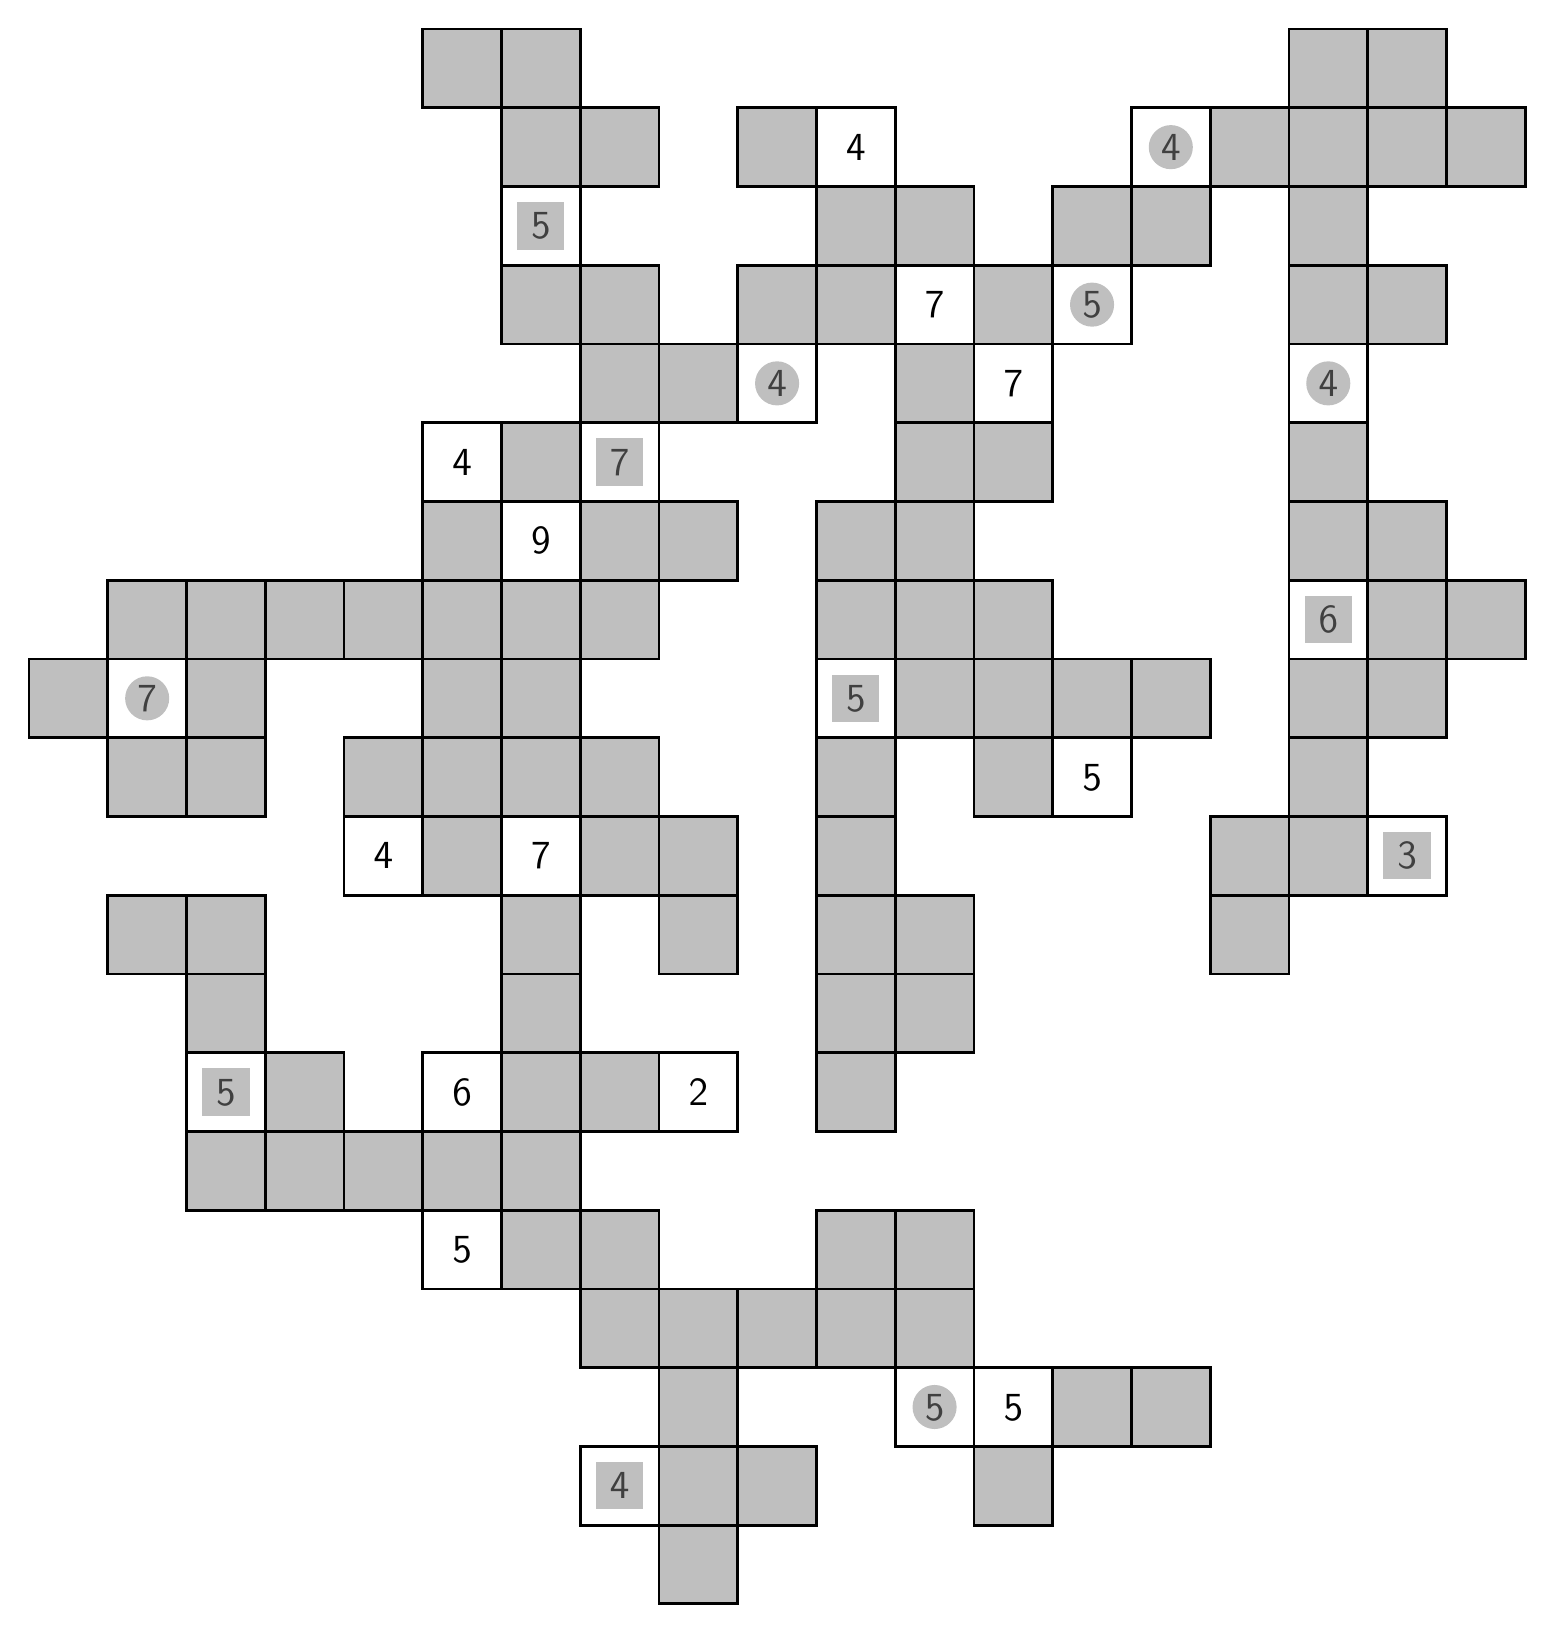
\begin{tikzpicture}\fill[gray, opacity = 0.5] (9, 0, 0)--++(1, 0, 0)--++(0, 1, 0)--++(-1, 0, 0)--cycle;
\draw[line width = 1pt] (9, 0, 0)--++(1, 0, 0)--++(0, 1, 0)--++(-1, 0, 0)--cycle;
\draw node at (8.5, 1.5, 0) {\Large $\mathsf{4}$};
\draw[line width = 1pt] (8, 1, 0)--++(1, 0, 0)--++(0, 1, 0)--++(-1, 0, 0)--cycle;
\fill[color = gray, opacity = 0.5] (8.2, 1.2) rectangle ++(0.6, 0.6);
\fill[gray, opacity = 0.5] (9, 1, 0)--++(1, 0, 0)--++(0, 1, 0)--++(-1, 0, 0)--cycle;
\draw[line width = 1pt] (9, 1, 0)--++(1, 0, 0)--++(0, 1, 0)--++(-1, 0, 0)--cycle;
\fill[gray, opacity = 0.5] (10, 1, 0)--++(1, 0, 0)--++(0, 1, 0)--++(-1, 0, 0)--cycle;
\draw[line width = 1pt] (10, 1, 0)--++(1, 0, 0)--++(0, 1, 0)--++(-1, 0, 0)--cycle;
\fill[gray, opacity = 0.5] (13, 1, 0)--++(1, 0, 0)--++(0, 1, 0)--++(-1, 0, 0)--cycle;
\draw[line width = 1pt] (13, 1, 0)--++(1, 0, 0)--++(0, 1, 0)--++(-1, 0, 0)--cycle;
\fill[gray, opacity = 0.5] (9, 2, 0)--++(1, 0, 0)--++(0, 1, 0)--++(-1, 0, 0)--cycle;
\draw[line width = 1pt] (9, 2, 0)--++(1, 0, 0)--++(0, 1, 0)--++(-1, 0, 0)--cycle;
\draw node at (12.5, 2.5, 0) {\Large $\mathsf{5}$};
\draw[line width = 1pt] (12, 2, 0)--++(1, 0, 0)--++(0, 1, 0)--++(-1, 0, 0)--cycle;
\fill[color = gray, opacity = 0.5] (12.5, 2.5, 0) circle (0.28);
\draw node at (13.5, 2.5, 0) {\Large $\mathsf{5}$};
\draw[line width = 1pt] (13, 2, 0)--++(1, 0, 0)--++(0, 1, 0)--++(-1, 0, 0)--cycle;
\fill[gray, opacity = 0.5] (14, 2, 0)--++(1, 0, 0)--++(0, 1, 0)--++(-1, 0, 0)--cycle;
\draw[line width = 1pt] (14, 2, 0)--++(1, 0, 0)--++(0, 1, 0)--++(-1, 0, 0)--cycle;
\fill[gray, opacity = 0.5] (15, 2, 0)--++(1, 0, 0)--++(0, 1, 0)--++(-1, 0, 0)--cycle;
\draw[line width = 1pt] (15, 2, 0)--++(1, 0, 0)--++(0, 1, 0)--++(-1, 0, 0)--cycle;
\fill[gray, opacity = 0.5] (8, 3, 0)--++(1, 0, 0)--++(0, 1, 0)--++(-1, 0, 0)--cycle;
\draw[line width = 1pt] (8, 3, 0)--++(1, 0, 0)--++(0, 1, 0)--++(-1, 0, 0)--cycle;
\fill[gray, opacity = 0.5] (9, 3, 0)--++(1, 0, 0)--++(0, 1, 0)--++(-1, 0, 0)--cycle;
\draw[line width = 1pt] (9, 3, 0)--++(1, 0, 0)--++(0, 1, 0)--++(-1, 0, 0)--cycle;
\fill[gray, opacity = 0.5] (10, 3, 0)--++(1, 0, 0)--++(0, 1, 0)--++(-1, 0, 0)--cycle;
\draw[line width = 1pt] (10, 3, 0)--++(1, 0, 0)--++(0, 1, 0)--++(-1, 0, 0)--cycle;
\fill[gray, opacity = 0.5] (11, 3, 0)--++(1, 0, 0)--++(0, 1, 0)--++(-1, 0, 0)--cycle;
\draw[line width = 1pt] (11, 3, 0)--++(1, 0, 0)--++(0, 1, 0)--++(-1, 0, 0)--cycle;
\fill[gray, opacity = 0.5] (12, 3, 0)--++(1, 0, 0)--++(0, 1, 0)--++(-1, 0, 0)--cycle;
\draw[line width = 1pt] (12, 3, 0)--++(1, 0, 0)--++(0, 1, 0)--++(-1, 0, 0)--cycle;
\draw node at (6.5, 4.5, 0) {\Large $\mathsf{5}$};
\draw[line width = 1pt] (6, 4, 0)--++(1, 0, 0)--++(0, 1, 0)--++(-1, 0, 0)--cycle;
\fill[gray, opacity = 0.5] (7, 4, 0)--++(1, 0, 0)--++(0, 1, 0)--++(-1, 0, 0)--cycle;
\draw[line width = 1pt] (7, 4, 0)--++(1, 0, 0)--++(0, 1, 0)--++(-1, 0, 0)--cycle;
\fill[gray, opacity = 0.5] (8, 4, 0)--++(1, 0, 0)--++(0, 1, 0)--++(-1, 0, 0)--cycle;
\draw[line width = 1pt] (8, 4, 0)--++(1, 0, 0)--++(0, 1, 0)--++(-1, 0, 0)--cycle;
\fill[gray, opacity = 0.5] (11, 4, 0)--++(1, 0, 0)--++(0, 1, 0)--++(-1, 0, 0)--cycle;
\draw[line width = 1pt] (11, 4, 0)--++(1, 0, 0)--++(0, 1, 0)--++(-1, 0, 0)--cycle;
\fill[gray, opacity = 0.5] (12, 4, 0)--++(1, 0, 0)--++(0, 1, 0)--++(-1, 0, 0)--cycle;
\draw[line width = 1pt] (12, 4, 0)--++(1, 0, 0)--++(0, 1, 0)--++(-1, 0, 0)--cycle;
\fill[gray, opacity = 0.5] (3, 5, 0)--++(1, 0, 0)--++(0, 1, 0)--++(-1, 0, 0)--cycle;
\draw[line width = 1pt] (3, 5, 0)--++(1, 0, 0)--++(0, 1, 0)--++(-1, 0, 0)--cycle;
\fill[gray, opacity = 0.5] (4, 5, 0)--++(1, 0, 0)--++(0, 1, 0)--++(-1, 0, 0)--cycle;
\draw[line width = 1pt] (4, 5, 0)--++(1, 0, 0)--++(0, 1, 0)--++(-1, 0, 0)--cycle;
\fill[gray, opacity = 0.5] (5, 5, 0)--++(1, 0, 0)--++(0, 1, 0)--++(-1, 0, 0)--cycle;
\draw[line width = 1pt] (5, 5, 0)--++(1, 0, 0)--++(0, 1, 0)--++(-1, 0, 0)--cycle;
\fill[gray, opacity = 0.5] (6, 5, 0)--++(1, 0, 0)--++(0, 1, 0)--++(-1, 0, 0)--cycle;
\draw[line width = 1pt] (6, 5, 0)--++(1, 0, 0)--++(0, 1, 0)--++(-1, 0, 0)--cycle;
\fill[gray, opacity = 0.5] (7, 5, 0)--++(1, 0, 0)--++(0, 1, 0)--++(-1, 0, 0)--cycle;
\draw[line width = 1pt] (7, 5, 0)--++(1, 0, 0)--++(0, 1, 0)--++(-1, 0, 0)--cycle;
\draw node at (3.5, 6.5, 0) {\Large $\mathsf{5}$};
\draw[line width = 1pt] (3, 6, 0)--++(1, 0, 0)--++(0, 1, 0)--++(-1, 0, 0)--cycle;
\fill[color = gray, opacity = 0.5] (3.2, 6.2) rectangle ++(0.6, 0.6);
\fill[gray, opacity = 0.5] (4, 6, 0)--++(1, 0, 0)--++(0, 1, 0)--++(-1, 0, 0)--cycle;
\draw[line width = 1pt] (4, 6, 0)--++(1, 0, 0)--++(0, 1, 0)--++(-1, 0, 0)--cycle;
\draw node at (6.5, 6.5, 0) {\Large $\mathsf{6}$};
\draw[line width = 1pt] (6, 6, 0)--++(1, 0, 0)--++(0, 1, 0)--++(-1, 0, 0)--cycle;
\fill[gray, opacity = 0.5] (7, 6, 0)--++(1, 0, 0)--++(0, 1, 0)--++(-1, 0, 0)--cycle;
\draw[line width = 1pt] (7, 6, 0)--++(1, 0, 0)--++(0, 1, 0)--++(-1, 0, 0)--cycle;
\fill[gray, opacity = 0.5] (8, 6, 0)--++(1, 0, 0)--++(0, 1, 0)--++(-1, 0, 0)--cycle;
\draw[line width = 1pt] (8, 6, 0)--++(1, 0, 0)--++(0, 1, 0)--++(-1, 0, 0)--cycle;
\draw node at (9.5, 6.5, 0) {\Large $\mathsf{2}$};
\draw[line width = 1pt] (9, 6, 0)--++(1, 0, 0)--++(0, 1, 0)--++(-1, 0, 0)--cycle;
\fill[gray, opacity = 0.5] (11, 6, 0)--++(1, 0, 0)--++(0, 1, 0)--++(-1, 0, 0)--cycle;
\draw[line width = 1pt] (11, 6, 0)--++(1, 0, 0)--++(0, 1, 0)--++(-1, 0, 0)--cycle;
\fill[gray, opacity = 0.5] (3, 7, 0)--++(1, 0, 0)--++(0, 1, 0)--++(-1, 0, 0)--cycle;
\draw[line width = 1pt] (3, 7, 0)--++(1, 0, 0)--++(0, 1, 0)--++(-1, 0, 0)--cycle;
\fill[gray, opacity = 0.5] (7, 7, 0)--++(1, 0, 0)--++(0, 1, 0)--++(-1, 0, 0)--cycle;
\draw[line width = 1pt] (7, 7, 0)--++(1, 0, 0)--++(0, 1, 0)--++(-1, 0, 0)--cycle;
\fill[gray, opacity = 0.5] (11, 7, 0)--++(1, 0, 0)--++(0, 1, 0)--++(-1, 0, 0)--cycle;
\draw[line width = 1pt] (11, 7, 0)--++(1, 0, 0)--++(0, 1, 0)--++(-1, 0, 0)--cycle;
\fill[gray, opacity = 0.5] (12, 7, 0)--++(1, 0, 0)--++(0, 1, 0)--++(-1, 0, 0)--cycle;
\draw[line width = 1pt] (12, 7, 0)--++(1, 0, 0)--++(0, 1, 0)--++(-1, 0, 0)--cycle;
\fill[gray, opacity = 0.5] (2, 8, 0)--++(1, 0, 0)--++(0, 1, 0)--++(-1, 0, 0)--cycle;
\draw[line width = 1pt] (2, 8, 0)--++(1, 0, 0)--++(0, 1, 0)--++(-1, 0, 0)--cycle;
\fill[gray, opacity = 0.5] (3, 8, 0)--++(1, 0, 0)--++(0, 1, 0)--++(-1, 0, 0)--cycle;
\draw[line width = 1pt] (3, 8, 0)--++(1, 0, 0)--++(0, 1, 0)--++(-1, 0, 0)--cycle;
\fill[gray, opacity = 0.5] (7, 8, 0)--++(1, 0, 0)--++(0, 1, 0)--++(-1, 0, 0)--cycle;
\draw[line width = 1pt] (7, 8, 0)--++(1, 0, 0)--++(0, 1, 0)--++(-1, 0, 0)--cycle;
\fill[gray, opacity = 0.5] (9, 8, 0)--++(1, 0, 0)--++(0, 1, 0)--++(-1, 0, 0)--cycle;
\draw[line width = 1pt] (9, 8, 0)--++(1, 0, 0)--++(0, 1, 0)--++(-1, 0, 0)--cycle;
\fill[gray, opacity = 0.5] (11, 8, 0)--++(1, 0, 0)--++(0, 1, 0)--++(-1, 0, 0)--cycle;
\draw[line width = 1pt] (11, 8, 0)--++(1, 0, 0)--++(0, 1, 0)--++(-1, 0, 0)--cycle;
\fill[gray, opacity = 0.5] (12, 8, 0)--++(1, 0, 0)--++(0, 1, 0)--++(-1, 0, 0)--cycle;
\draw[line width = 1pt] (12, 8, 0)--++(1, 0, 0)--++(0, 1, 0)--++(-1, 0, 0)--cycle;
\fill[gray, opacity = 0.5] (16, 8, 0)--++(1, 0, 0)--++(0, 1, 0)--++(-1, 0, 0)--cycle;
\draw[line width = 1pt] (16, 8, 0)--++(1, 0, 0)--++(0, 1, 0)--++(-1, 0, 0)--cycle;
\draw node at (5.5, 9.5, 0) {\Large $\mathsf{4}$};
\draw[line width = 1pt] (5, 9, 0)--++(1, 0, 0)--++(0, 1, 0)--++(-1, 0, 0)--cycle;
\fill[gray, opacity = 0.5] (6, 9, 0)--++(1, 0, 0)--++(0, 1, 0)--++(-1, 0, 0)--cycle;
\draw[line width = 1pt] (6, 9, 0)--++(1, 0, 0)--++(0, 1, 0)--++(-1, 0, 0)--cycle;
\draw node at (7.5, 9.5, 0) {\Large $\mathsf{7}$};
\draw[line width = 1pt] (7, 9, 0)--++(1, 0, 0)--++(0, 1, 0)--++(-1, 0, 0)--cycle;
\fill[gray, opacity = 0.5] (8, 9, 0)--++(1, 0, 0)--++(0, 1, 0)--++(-1, 0, 0)--cycle;
\draw[line width = 1pt] (8, 9, 0)--++(1, 0, 0)--++(0, 1, 0)--++(-1, 0, 0)--cycle;
\fill[gray, opacity = 0.5] (9, 9, 0)--++(1, 0, 0)--++(0, 1, 0)--++(-1, 0, 0)--cycle;
\draw[line width = 1pt] (9, 9, 0)--++(1, 0, 0)--++(0, 1, 0)--++(-1, 0, 0)--cycle;
\fill[gray, opacity = 0.5] (11, 9, 0)--++(1, 0, 0)--++(0, 1, 0)--++(-1, 0, 0)--cycle;
\draw[line width = 1pt] (11, 9, 0)--++(1, 0, 0)--++(0, 1, 0)--++(-1, 0, 0)--cycle;
\fill[gray, opacity = 0.5] (16, 9, 0)--++(1, 0, 0)--++(0, 1, 0)--++(-1, 0, 0)--cycle;
\draw[line width = 1pt] (16, 9, 0)--++(1, 0, 0)--++(0, 1, 0)--++(-1, 0, 0)--cycle;
\fill[gray, opacity = 0.5] (17, 9, 0)--++(1, 0, 0)--++(0, 1, 0)--++(-1, 0, 0)--cycle;
\draw[line width = 1pt] (17, 9, 0)--++(1, 0, 0)--++(0, 1, 0)--++(-1, 0, 0)--cycle;
\draw node at (18.5, 9.5, 0) {\Large $\mathsf{3}$};
\draw[line width = 1pt] (18, 9, 0)--++(1, 0, 0)--++(0, 1, 0)--++(-1, 0, 0)--cycle;
\fill[color = gray, opacity = 0.5] (18.2, 9.2) rectangle ++(0.6, 0.6);
\fill[gray, opacity = 0.5] (2, 10, 0)--++(1, 0, 0)--++(0, 1, 0)--++(-1, 0, 0)--cycle;
\draw[line width = 1pt] (2, 10, 0)--++(1, 0, 0)--++(0, 1, 0)--++(-1, 0, 0)--cycle;
\fill[gray, opacity = 0.5] (3, 10, 0)--++(1, 0, 0)--++(0, 1, 0)--++(-1, 0, 0)--cycle;
\draw[line width = 1pt] (3, 10, 0)--++(1, 0, 0)--++(0, 1, 0)--++(-1, 0, 0)--cycle;
\fill[gray, opacity = 0.5] (5, 10, 0)--++(1, 0, 0)--++(0, 1, 0)--++(-1, 0, 0)--cycle;
\draw[line width = 1pt] (5, 10, 0)--++(1, 0, 0)--++(0, 1, 0)--++(-1, 0, 0)--cycle;
\fill[gray, opacity = 0.5] (6, 10, 0)--++(1, 0, 0)--++(0, 1, 0)--++(-1, 0, 0)--cycle;
\draw[line width = 1pt] (6, 10, 0)--++(1, 0, 0)--++(0, 1, 0)--++(-1, 0, 0)--cycle;
\fill[gray, opacity = 0.5] (7, 10, 0)--++(1, 0, 0)--++(0, 1, 0)--++(-1, 0, 0)--cycle;
\draw[line width = 1pt] (7, 10, 0)--++(1, 0, 0)--++(0, 1, 0)--++(-1, 0, 0)--cycle;
\fill[gray, opacity = 0.5] (8, 10, 0)--++(1, 0, 0)--++(0, 1, 0)--++(-1, 0, 0)--cycle;
\draw[line width = 1pt] (8, 10, 0)--++(1, 0, 0)--++(0, 1, 0)--++(-1, 0, 0)--cycle;
\fill[gray, opacity = 0.5] (11, 10, 0)--++(1, 0, 0)--++(0, 1, 0)--++(-1, 0, 0)--cycle;
\draw[line width = 1pt] (11, 10, 0)--++(1, 0, 0)--++(0, 1, 0)--++(-1, 0, 0)--cycle;
\fill[gray, opacity = 0.5] (13, 10, 0)--++(1, 0, 0)--++(0, 1, 0)--++(-1, 0, 0)--cycle;
\draw[line width = 1pt] (13, 10, 0)--++(1, 0, 0)--++(0, 1, 0)--++(-1, 0, 0)--cycle;
\draw node at (14.5, 10.5, 0) {\Large $\mathsf{5}$};
\draw[line width = 1pt] (14, 10, 0)--++(1, 0, 0)--++(0, 1, 0)--++(-1, 0, 0)--cycle;
\fill[gray, opacity = 0.5] (17, 10, 0)--++(1, 0, 0)--++(0, 1, 0)--++(-1, 0, 0)--cycle;
\draw[line width = 1pt] (17, 10, 0)--++(1, 0, 0)--++(0, 1, 0)--++(-1, 0, 0)--cycle;
\fill[gray, opacity = 0.5] (1, 11, 0)--++(1, 0, 0)--++(0, 1, 0)--++(-1, 0, 0)--cycle;
\draw[line width = 1pt] (1, 11, 0)--++(1, 0, 0)--++(0, 1, 0)--++(-1, 0, 0)--cycle;
\draw node at (2.5, 11.5, 0) {\Large $\mathsf{7}$};
\draw[line width = 1pt] (2, 11, 0)--++(1, 0, 0)--++(0, 1, 0)--++(-1, 0, 0)--cycle;
\fill[color = gray, opacity = 0.5] (2.5, 11.5, 0) circle (0.28);
\fill[gray, opacity = 0.5] (3, 11, 0)--++(1, 0, 0)--++(0, 1, 0)--++(-1, 0, 0)--cycle;
\draw[line width = 1pt] (3, 11, 0)--++(1, 0, 0)--++(0, 1, 0)--++(-1, 0, 0)--cycle;
\fill[gray, opacity = 0.5] (6, 11, 0)--++(1, 0, 0)--++(0, 1, 0)--++(-1, 0, 0)--cycle;
\draw[line width = 1pt] (6, 11, 0)--++(1, 0, 0)--++(0, 1, 0)--++(-1, 0, 0)--cycle;
\fill[gray, opacity = 0.5] (7, 11, 0)--++(1, 0, 0)--++(0, 1, 0)--++(-1, 0, 0)--cycle;
\draw[line width = 1pt] (7, 11, 0)--++(1, 0, 0)--++(0, 1, 0)--++(-1, 0, 0)--cycle;
\draw node at (11.5, 11.5, 0) {\Large $\mathsf{5}$};
\draw[line width = 1pt] (11, 11, 0)--++(1, 0, 0)--++(0, 1, 0)--++(-1, 0, 0)--cycle;
\fill[color = gray, opacity = 0.5] (11.2, 11.2) rectangle ++(0.6, 0.6);
\fill[gray, opacity = 0.5] (12, 11, 0)--++(1, 0, 0)--++(0, 1, 0)--++(-1, 0, 0)--cycle;
\draw[line width = 1pt] (12, 11, 0)--++(1, 0, 0)--++(0, 1, 0)--++(-1, 0, 0)--cycle;
\fill[gray, opacity = 0.5] (13, 11, 0)--++(1, 0, 0)--++(0, 1, 0)--++(-1, 0, 0)--cycle;
\draw[line width = 1pt] (13, 11, 0)--++(1, 0, 0)--++(0, 1, 0)--++(-1, 0, 0)--cycle;
\fill[gray, opacity = 0.5] (14, 11, 0)--++(1, 0, 0)--++(0, 1, 0)--++(-1, 0, 0)--cycle;
\draw[line width = 1pt] (14, 11, 0)--++(1, 0, 0)--++(0, 1, 0)--++(-1, 0, 0)--cycle;
\fill[gray, opacity = 0.5] (15, 11, 0)--++(1, 0, 0)--++(0, 1, 0)--++(-1, 0, 0)--cycle;
\draw[line width = 1pt] (15, 11, 0)--++(1, 0, 0)--++(0, 1, 0)--++(-1, 0, 0)--cycle;
\fill[gray, opacity = 0.5] (17, 11, 0)--++(1, 0, 0)--++(0, 1, 0)--++(-1, 0, 0)--cycle;
\draw[line width = 1pt] (17, 11, 0)--++(1, 0, 0)--++(0, 1, 0)--++(-1, 0, 0)--cycle;
\fill[gray, opacity = 0.5] (18, 11, 0)--++(1, 0, 0)--++(0, 1, 0)--++(-1, 0, 0)--cycle;
\draw[line width = 1pt] (18, 11, 0)--++(1, 0, 0)--++(0, 1, 0)--++(-1, 0, 0)--cycle;
\fill[gray, opacity = 0.5] (2, 12, 0)--++(1, 0, 0)--++(0, 1, 0)--++(-1, 0, 0)--cycle;
\draw[line width = 1pt] (2, 12, 0)--++(1, 0, 0)--++(0, 1, 0)--++(-1, 0, 0)--cycle;
\fill[gray, opacity = 0.5] (3, 12, 0)--++(1, 0, 0)--++(0, 1, 0)--++(-1, 0, 0)--cycle;
\draw[line width = 1pt] (3, 12, 0)--++(1, 0, 0)--++(0, 1, 0)--++(-1, 0, 0)--cycle;
\fill[gray, opacity = 0.5] (4, 12, 0)--++(1, 0, 0)--++(0, 1, 0)--++(-1, 0, 0)--cycle;
\draw[line width = 1pt] (4, 12, 0)--++(1, 0, 0)--++(0, 1, 0)--++(-1, 0, 0)--cycle;
\fill[gray, opacity = 0.5] (5, 12, 0)--++(1, 0, 0)--++(0, 1, 0)--++(-1, 0, 0)--cycle;
\draw[line width = 1pt] (5, 12, 0)--++(1, 0, 0)--++(0, 1, 0)--++(-1, 0, 0)--cycle;
\fill[gray, opacity = 0.5] (6, 12, 0)--++(1, 0, 0)--++(0, 1, 0)--++(-1, 0, 0)--cycle;
\draw[line width = 1pt] (6, 12, 0)--++(1, 0, 0)--++(0, 1, 0)--++(-1, 0, 0)--cycle;
\fill[gray, opacity = 0.5] (7, 12, 0)--++(1, 0, 0)--++(0, 1, 0)--++(-1, 0, 0)--cycle;
\draw[line width = 1pt] (7, 12, 0)--++(1, 0, 0)--++(0, 1, 0)--++(-1, 0, 0)--cycle;
\fill[gray, opacity = 0.5] (8, 12, 0)--++(1, 0, 0)--++(0, 1, 0)--++(-1, 0, 0)--cycle;
\draw[line width = 1pt] (8, 12, 0)--++(1, 0, 0)--++(0, 1, 0)--++(-1, 0, 0)--cycle;
\fill[gray, opacity = 0.5] (11, 12, 0)--++(1, 0, 0)--++(0, 1, 0)--++(-1, 0, 0)--cycle;
\draw[line width = 1pt] (11, 12, 0)--++(1, 0, 0)--++(0, 1, 0)--++(-1, 0, 0)--cycle;
\fill[gray, opacity = 0.5] (12, 12, 0)--++(1, 0, 0)--++(0, 1, 0)--++(-1, 0, 0)--cycle;
\draw[line width = 1pt] (12, 12, 0)--++(1, 0, 0)--++(0, 1, 0)--++(-1, 0, 0)--cycle;
\fill[gray, opacity = 0.5] (13, 12, 0)--++(1, 0, 0)--++(0, 1, 0)--++(-1, 0, 0)--cycle;
\draw[line width = 1pt] (13, 12, 0)--++(1, 0, 0)--++(0, 1, 0)--++(-1, 0, 0)--cycle;
\draw node at (17.5, 12.5, 0) {\Large $\mathsf{6}$};
\draw[line width = 1pt] (17, 12, 0)--++(1, 0, 0)--++(0, 1, 0)--++(-1, 0, 0)--cycle;
\fill[color = gray, opacity = 0.5] (17.2, 12.2) rectangle ++(0.6, 0.6);
\fill[gray, opacity = 0.5] (18, 12, 0)--++(1, 0, 0)--++(0, 1, 0)--++(-1, 0, 0)--cycle;
\draw[line width = 1pt] (18, 12, 0)--++(1, 0, 0)--++(0, 1, 0)--++(-1, 0, 0)--cycle;
\fill[gray, opacity = 0.5] (19, 12, 0)--++(1, 0, 0)--++(0, 1, 0)--++(-1, 0, 0)--cycle;
\draw[line width = 1pt] (19, 12, 0)--++(1, 0, 0)--++(0, 1, 0)--++(-1, 0, 0)--cycle;
\fill[gray, opacity = 0.5] (6, 13, 0)--++(1, 0, 0)--++(0, 1, 0)--++(-1, 0, 0)--cycle;
\draw[line width = 1pt] (6, 13, 0)--++(1, 0, 0)--++(0, 1, 0)--++(-1, 0, 0)--cycle;
\draw node at (7.5, 13.5, 0) {\Large $\mathsf{9}$};
\draw[line width = 1pt] (7, 13, 0)--++(1, 0, 0)--++(0, 1, 0)--++(-1, 0, 0)--cycle;
\fill[gray, opacity = 0.5] (8, 13, 0)--++(1, 0, 0)--++(0, 1, 0)--++(-1, 0, 0)--cycle;
\draw[line width = 1pt] (8, 13, 0)--++(1, 0, 0)--++(0, 1, 0)--++(-1, 0, 0)--cycle;
\fill[gray, opacity = 0.5] (9, 13, 0)--++(1, 0, 0)--++(0, 1, 0)--++(-1, 0, 0)--cycle;
\draw[line width = 1pt] (9, 13, 0)--++(1, 0, 0)--++(0, 1, 0)--++(-1, 0, 0)--cycle;
\fill[gray, opacity = 0.5] (11, 13, 0)--++(1, 0, 0)--++(0, 1, 0)--++(-1, 0, 0)--cycle;
\draw[line width = 1pt] (11, 13, 0)--++(1, 0, 0)--++(0, 1, 0)--++(-1, 0, 0)--cycle;
\fill[gray, opacity = 0.5] (12, 13, 0)--++(1, 0, 0)--++(0, 1, 0)--++(-1, 0, 0)--cycle;
\draw[line width = 1pt] (12, 13, 0)--++(1, 0, 0)--++(0, 1, 0)--++(-1, 0, 0)--cycle;
\fill[gray, opacity = 0.5] (17, 13, 0)--++(1, 0, 0)--++(0, 1, 0)--++(-1, 0, 0)--cycle;
\draw[line width = 1pt] (17, 13, 0)--++(1, 0, 0)--++(0, 1, 0)--++(-1, 0, 0)--cycle;
\fill[gray, opacity = 0.5] (18, 13, 0)--++(1, 0, 0)--++(0, 1, 0)--++(-1, 0, 0)--cycle;
\draw[line width = 1pt] (18, 13, 0)--++(1, 0, 0)--++(0, 1, 0)--++(-1, 0, 0)--cycle;
\draw node at (6.5, 14.5, 0) {\Large $\mathsf{4}$};
\draw[line width = 1pt] (6, 14, 0)--++(1, 0, 0)--++(0, 1, 0)--++(-1, 0, 0)--cycle;
\fill[gray, opacity = 0.5] (7, 14, 0)--++(1, 0, 0)--++(0, 1, 0)--++(-1, 0, 0)--cycle;
\draw[line width = 1pt] (7, 14, 0)--++(1, 0, 0)--++(0, 1, 0)--++(-1, 0, 0)--cycle;
\draw node at (8.5, 14.5, 0) {\Large $\mathsf{7}$};
\draw[line width = 1pt] (8, 14, 0)--++(1, 0, 0)--++(0, 1, 0)--++(-1, 0, 0)--cycle;
\fill[color = gray, opacity = 0.5] (8.2, 14.2) rectangle ++(0.6, 0.6);
\fill[gray, opacity = 0.5] (12, 14, 0)--++(1, 0, 0)--++(0, 1, 0)--++(-1, 0, 0)--cycle;
\draw[line width = 1pt] (12, 14, 0)--++(1, 0, 0)--++(0, 1, 0)--++(-1, 0, 0)--cycle;
\fill[gray, opacity = 0.5] (13, 14, 0)--++(1, 0, 0)--++(0, 1, 0)--++(-1, 0, 0)--cycle;
\draw[line width = 1pt] (13, 14, 0)--++(1, 0, 0)--++(0, 1, 0)--++(-1, 0, 0)--cycle;
\fill[gray, opacity = 0.5] (17, 14, 0)--++(1, 0, 0)--++(0, 1, 0)--++(-1, 0, 0)--cycle;
\draw[line width = 1pt] (17, 14, 0)--++(1, 0, 0)--++(0, 1, 0)--++(-1, 0, 0)--cycle;
\fill[gray, opacity = 0.5] (8, 15, 0)--++(1, 0, 0)--++(0, 1, 0)--++(-1, 0, 0)--cycle;
\draw[line width = 1pt] (8, 15, 0)--++(1, 0, 0)--++(0, 1, 0)--++(-1, 0, 0)--cycle;
\fill[gray, opacity = 0.5] (9, 15, 0)--++(1, 0, 0)--++(0, 1, 0)--++(-1, 0, 0)--cycle;
\draw[line width = 1pt] (9, 15, 0)--++(1, 0, 0)--++(0, 1, 0)--++(-1, 0, 0)--cycle;
\draw node at (10.5, 15.5, 0) {\Large $\mathsf{4}$};
\draw[line width = 1pt] (10, 15, 0)--++(1, 0, 0)--++(0, 1, 0)--++(-1, 0, 0)--cycle;
\fill[color = gray, opacity = 0.5] (10.5, 15.5, 0) circle (0.28);
\fill[gray, opacity = 0.5] (12, 15, 0)--++(1, 0, 0)--++(0, 1, 0)--++(-1, 0, 0)--cycle;
\draw[line width = 1pt] (12, 15, 0)--++(1, 0, 0)--++(0, 1, 0)--++(-1, 0, 0)--cycle;
\draw node at (13.5, 15.5, 0) {\Large $\mathsf{7}$};
\draw[line width = 1pt] (13, 15, 0)--++(1, 0, 0)--++(0, 1, 0)--++(-1, 0, 0)--cycle;
\draw node at (17.5, 15.5, 0) {\Large $\mathsf{4}$};
\draw[line width = 1pt] (17, 15, 0)--++(1, 0, 0)--++(0, 1, 0)--++(-1, 0, 0)--cycle;
\fill[color = gray, opacity = 0.5] (17.5, 15.5, 0) circle (0.28);
\fill[gray, opacity = 0.5] (7, 16, 0)--++(1, 0, 0)--++(0, 1, 0)--++(-1, 0, 0)--cycle;
\draw[line width = 1pt] (7, 16, 0)--++(1, 0, 0)--++(0, 1, 0)--++(-1, 0, 0)--cycle;
\fill[gray, opacity = 0.5] (8, 16, 0)--++(1, 0, 0)--++(0, 1, 0)--++(-1, 0, 0)--cycle;
\draw[line width = 1pt] (8, 16, 0)--++(1, 0, 0)--++(0, 1, 0)--++(-1, 0, 0)--cycle;
\fill[gray, opacity = 0.5] (10, 16, 0)--++(1, 0, 0)--++(0, 1, 0)--++(-1, 0, 0)--cycle;
\draw[line width = 1pt] (10, 16, 0)--++(1, 0, 0)--++(0, 1, 0)--++(-1, 0, 0)--cycle;
\fill[gray, opacity = 0.5] (11, 16, 0)--++(1, 0, 0)--++(0, 1, 0)--++(-1, 0, 0)--cycle;
\draw[line width = 1pt] (11, 16, 0)--++(1, 0, 0)--++(0, 1, 0)--++(-1, 0, 0)--cycle;
\draw node at (12.5, 16.5, 0) {\Large $\mathsf{7}$};
\draw[line width = 1pt] (12, 16, 0)--++(1, 0, 0)--++(0, 1, 0)--++(-1, 0, 0)--cycle;
\fill[gray, opacity = 0.5] (13, 16, 0)--++(1, 0, 0)--++(0, 1, 0)--++(-1, 0, 0)--cycle;
\draw[line width = 1pt] (13, 16, 0)--++(1, 0, 0)--++(0, 1, 0)--++(-1, 0, 0)--cycle;
\draw node at (14.5, 16.5, 0) {\Large $\mathsf{5}$};
\draw[line width = 1pt] (14, 16, 0)--++(1, 0, 0)--++(0, 1, 0)--++(-1, 0, 0)--cycle;
\fill[color = gray, opacity = 0.5] (14.5, 16.5, 0) circle (0.28);
\fill[gray, opacity = 0.5] (17, 16, 0)--++(1, 0, 0)--++(0, 1, 0)--++(-1, 0, 0)--cycle;
\draw[line width = 1pt] (17, 16, 0)--++(1, 0, 0)--++(0, 1, 0)--++(-1, 0, 0)--cycle;
\fill[gray, opacity = 0.5] (18, 16, 0)--++(1, 0, 0)--++(0, 1, 0)--++(-1, 0, 0)--cycle;
\draw[line width = 1pt] (18, 16, 0)--++(1, 0, 0)--++(0, 1, 0)--++(-1, 0, 0)--cycle;
\draw node at (7.5, 17.5, 0) {\Large $\mathsf{5}$};
\draw[line width = 1pt] (7, 17, 0)--++(1, 0, 0)--++(0, 1, 0)--++(-1, 0, 0)--cycle;
\fill[color = gray, opacity = 0.5] (7.2, 17.2) rectangle ++(0.6, 0.6);
\fill[gray, opacity = 0.5] (11, 17, 0)--++(1, 0, 0)--++(0, 1, 0)--++(-1, 0, 0)--cycle;
\draw[line width = 1pt] (11, 17, 0)--++(1, 0, 0)--++(0, 1, 0)--++(-1, 0, 0)--cycle;
\fill[gray, opacity = 0.5] (12, 17, 0)--++(1, 0, 0)--++(0, 1, 0)--++(-1, 0, 0)--cycle;
\draw[line width = 1pt] (12, 17, 0)--++(1, 0, 0)--++(0, 1, 0)--++(-1, 0, 0)--cycle;
\fill[gray, opacity = 0.5] (14, 17, 0)--++(1, 0, 0)--++(0, 1, 0)--++(-1, 0, 0)--cycle;
\draw[line width = 1pt] (14, 17, 0)--++(1, 0, 0)--++(0, 1, 0)--++(-1, 0, 0)--cycle;
\fill[gray, opacity = 0.5] (15, 17, 0)--++(1, 0, 0)--++(0, 1, 0)--++(-1, 0, 0)--cycle;
\draw[line width = 1pt] (15, 17, 0)--++(1, 0, 0)--++(0, 1, 0)--++(-1, 0, 0)--cycle;
\fill[gray, opacity = 0.5] (17, 17, 0)--++(1, 0, 0)--++(0, 1, 0)--++(-1, 0, 0)--cycle;
\draw[line width = 1pt] (17, 17, 0)--++(1, 0, 0)--++(0, 1, 0)--++(-1, 0, 0)--cycle;
\fill[gray, opacity = 0.5] (7, 18, 0)--++(1, 0, 0)--++(0, 1, 0)--++(-1, 0, 0)--cycle;
\draw[line width = 1pt] (7, 18, 0)--++(1, 0, 0)--++(0, 1, 0)--++(-1, 0, 0)--cycle;
\fill[gray, opacity = 0.5] (8, 18, 0)--++(1, 0, 0)--++(0, 1, 0)--++(-1, 0, 0)--cycle;
\draw[line width = 1pt] (8, 18, 0)--++(1, 0, 0)--++(0, 1, 0)--++(-1, 0, 0)--cycle;
\fill[gray, opacity = 0.5] (10, 18, 0)--++(1, 0, 0)--++(0, 1, 0)--++(-1, 0, 0)--cycle;
\draw[line width = 1pt] (10, 18, 0)--++(1, 0, 0)--++(0, 1, 0)--++(-1, 0, 0)--cycle;
\draw node at (11.5, 18.5, 0) {\Large $\mathsf{4}$};
\draw[line width = 1pt] (11, 18, 0)--++(1, 0, 0)--++(0, 1, 0)--++(-1, 0, 0)--cycle;
\draw node at (15.5, 18.5, 0) {\Large $\mathsf{4}$};
\draw[line width = 1pt] (15, 18, 0)--++(1, 0, 0)--++(0, 1, 0)--++(-1, 0, 0)--cycle;
\fill[color = gray, opacity = 0.5] (15.5, 18.5, 0) circle (0.28);
\fill[gray, opacity = 0.5] (16, 18, 0)--++(1, 0, 0)--++(0, 1, 0)--++(-1, 0, 0)--cycle;
\draw[line width = 1pt] (16, 18, 0)--++(1, 0, 0)--++(0, 1, 0)--++(-1, 0, 0)--cycle;
\fill[gray, opacity = 0.5] (17, 18, 0)--++(1, 0, 0)--++(0, 1, 0)--++(-1, 0, 0)--cycle;
\draw[line width = 1pt] (17, 18, 0)--++(1, 0, 0)--++(0, 1, 0)--++(-1, 0, 0)--cycle;
\fill[gray, opacity = 0.5] (18, 18, 0)--++(1, 0, 0)--++(0, 1, 0)--++(-1, 0, 0)--cycle;
\draw[line width = 1pt] (18, 18, 0)--++(1, 0, 0)--++(0, 1, 0)--++(-1, 0, 0)--cycle;
\fill[gray, opacity = 0.5] (19, 18, 0)--++(1, 0, 0)--++(0, 1, 0)--++(-1, 0, 0)--cycle;
\draw[line width = 1pt] (19, 18, 0)--++(1, 0, 0)--++(0, 1, 0)--++(-1, 0, 0)--cycle;
\fill[gray, opacity = 0.5] (6, 19, 0)--++(1, 0, 0)--++(0, 1, 0)--++(-1, 0, 0)--cycle;
\draw[line width = 1pt] (6, 19, 0)--++(1, 0, 0)--++(0, 1, 0)--++(-1, 0, 0)--cycle;
\fill[gray, opacity = 0.5] (7, 19, 0)--++(1, 0, 0)--++(0, 1, 0)--++(-1, 0, 0)--cycle;
\draw[line width = 1pt] (7, 19, 0)--++(1, 0, 0)--++(0, 1, 0)--++(-1, 0, 0)--cycle;
\fill[gray, opacity = 0.5] (17, 19, 0)--++(1, 0, 0)--++(0, 1, 0)--++(-1, 0, 0)--cycle;
\draw[line width = 1pt] (17, 19, 0)--++(1, 0, 0)--++(0, 1, 0)--++(-1, 0, 0)--cycle;
\fill[gray, opacity = 0.5] (18, 19, 0)--++(1, 0, 0)--++(0, 1, 0)--++(-1, 0, 0)--cycle;
\draw[line width = 1pt] (18, 19, 0)--++(1, 0, 0)--++(0, 1, 0)--++(-1, 0, 0)--cycle;
\end{tikzpicture}}\]
\[\resizebox{30pc}{!}{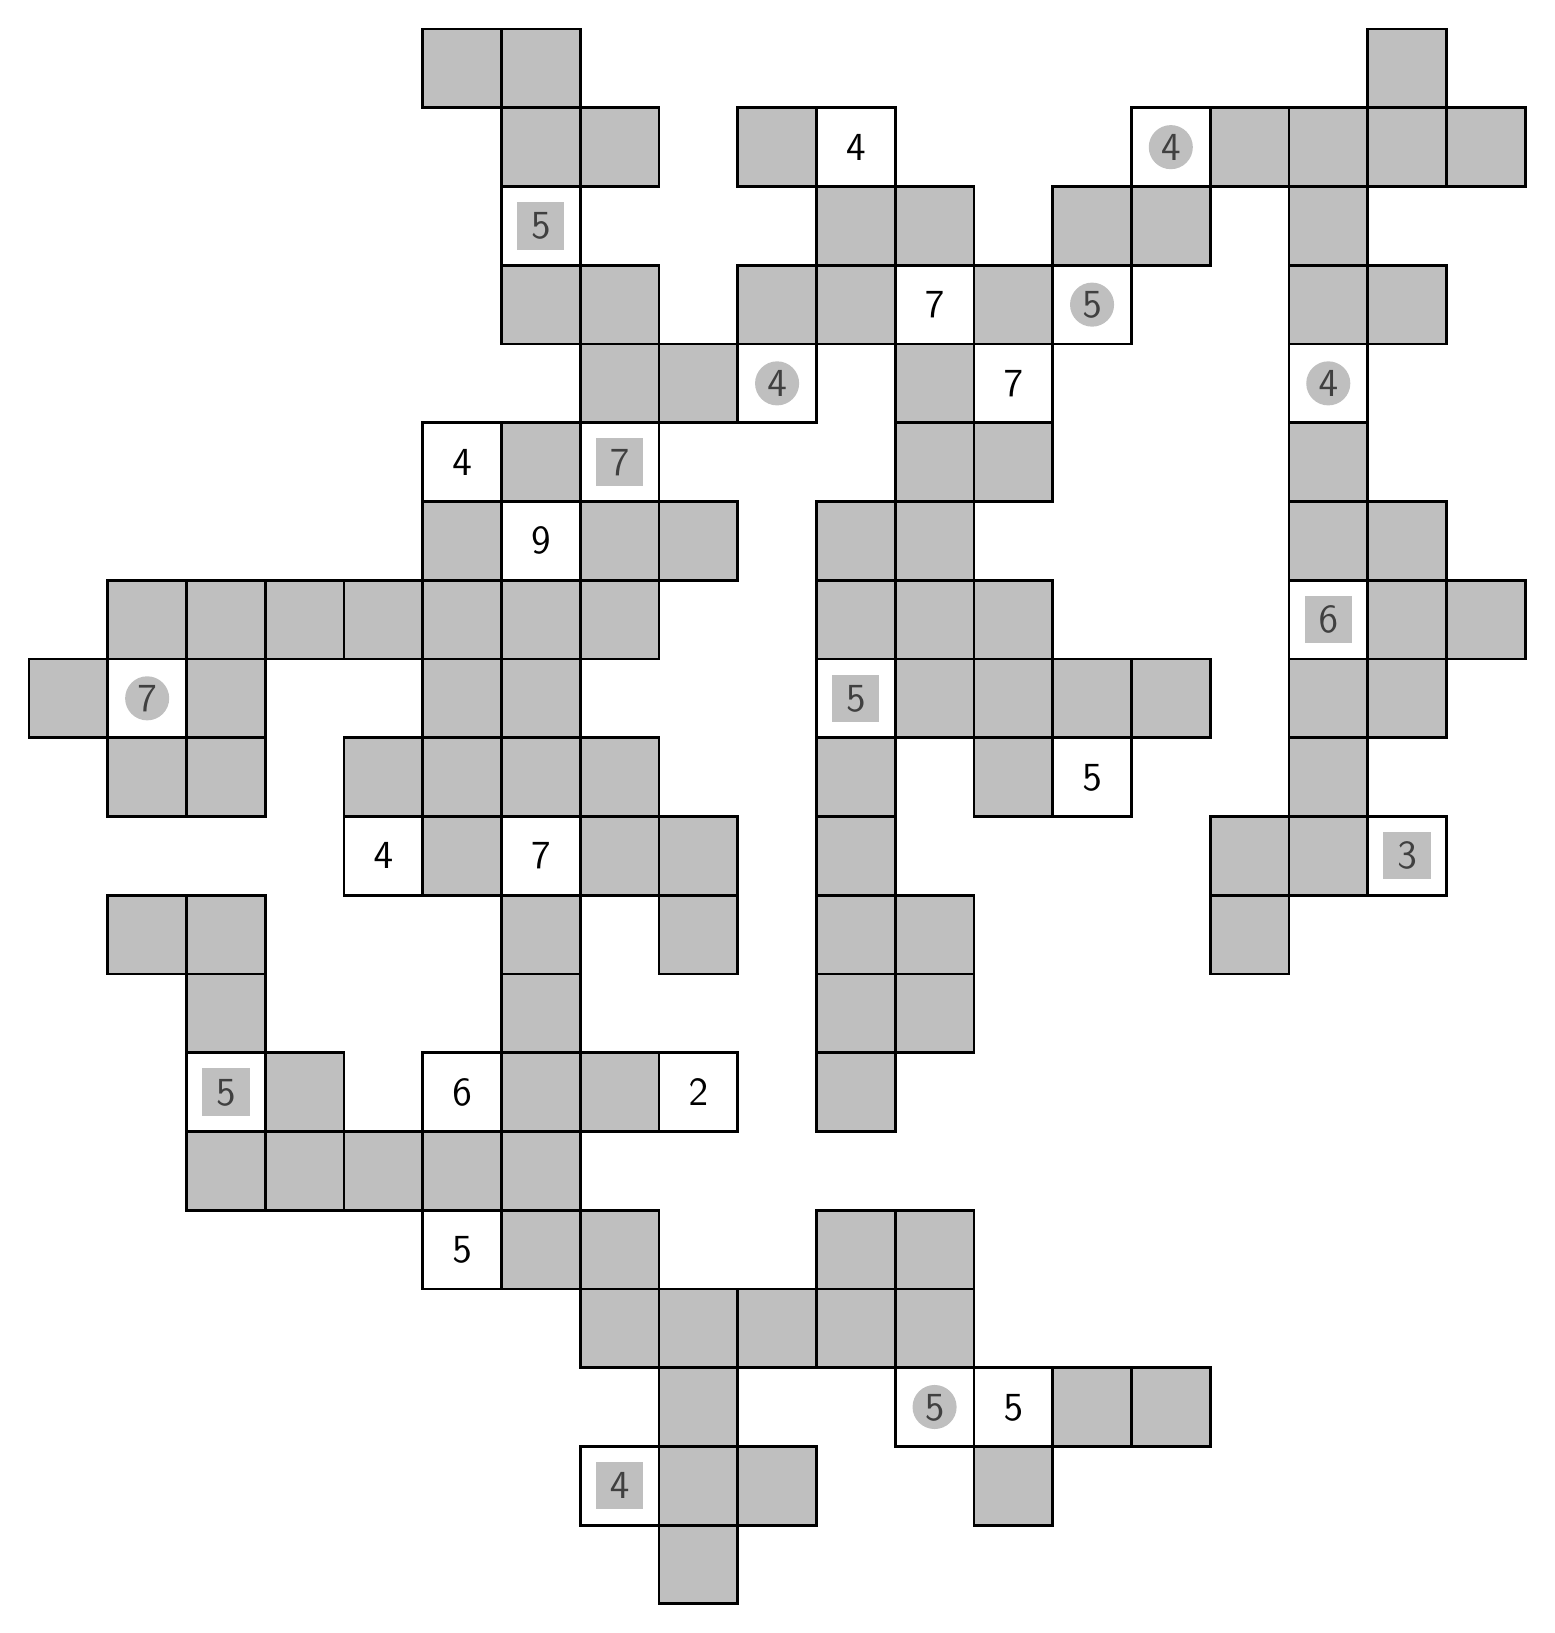
\begin{tikzpicture}\fill[gray, opacity = 0.5] (9, 0, 0)--++(1, 0, 0)--++(0, 1, 0)--++(-1, 0, 0)--cycle;
\draw[line width = 1pt] (9, 0, 0)--++(1, 0, 0)--++(0, 1, 0)--++(-1, 0, 0)--cycle;
\draw node at (8.5, 1.5, 0) {\Large $\mathsf{4}$};
\draw[line width = 1pt] (8, 1, 0)--++(1, 0, 0)--++(0, 1, 0)--++(-1, 0, 0)--cycle;
\fill[color = gray, opacity = 0.5] (8.2, 1.2) rectangle ++(0.6, 0.6);
\fill[gray, opacity = 0.5] (9, 1, 0)--++(1, 0, 0)--++(0, 1, 0)--++(-1, 0, 0)--cycle;
\draw[line width = 1pt] (9, 1, 0)--++(1, 0, 0)--++(0, 1, 0)--++(-1, 0, 0)--cycle;
\fill[gray, opacity = 0.5] (10, 1, 0)--++(1, 0, 0)--++(0, 1, 0)--++(-1, 0, 0)--cycle;
\draw[line width = 1pt] (10, 1, 0)--++(1, 0, 0)--++(0, 1, 0)--++(-1, 0, 0)--cycle;
\fill[gray, opacity = 0.5] (13, 1, 0)--++(1, 0, 0)--++(0, 1, 0)--++(-1, 0, 0)--cycle;
\draw[line width = 1pt] (13, 1, 0)--++(1, 0, 0)--++(0, 1, 0)--++(-1, 0, 0)--cycle;
\fill[gray, opacity = 0.5] (9, 2, 0)--++(1, 0, 0)--++(0, 1, 0)--++(-1, 0, 0)--cycle;
\draw[line width = 1pt] (9, 2, 0)--++(1, 0, 0)--++(0, 1, 0)--++(-1, 0, 0)--cycle;
\draw node at (12.5, 2.5, 0) {\Large $\mathsf{5}$};
\draw[line width = 1pt] (12, 2, 0)--++(1, 0, 0)--++(0, 1, 0)--++(-1, 0, 0)--cycle;
\fill[color = gray, opacity = 0.5] (12.5, 2.5, 0) circle (0.28);
\draw node at (13.5, 2.5, 0) {\Large $\mathsf{5}$};
\draw[line width = 1pt] (13, 2, 0)--++(1, 0, 0)--++(0, 1, 0)--++(-1, 0, 0)--cycle;
\fill[gray, opacity = 0.5] (14, 2, 0)--++(1, 0, 0)--++(0, 1, 0)--++(-1, 0, 0)--cycle;
\draw[line width = 1pt] (14, 2, 0)--++(1, 0, 0)--++(0, 1, 0)--++(-1, 0, 0)--cycle;
\fill[gray, opacity = 0.5] (15, 2, 0)--++(1, 0, 0)--++(0, 1, 0)--++(-1, 0, 0)--cycle;
\draw[line width = 1pt] (15, 2, 0)--++(1, 0, 0)--++(0, 1, 0)--++(-1, 0, 0)--cycle;
\fill[gray, opacity = 0.5] (8, 3, 0)--++(1, 0, 0)--++(0, 1, 0)--++(-1, 0, 0)--cycle;
\draw[line width = 1pt] (8, 3, 0)--++(1, 0, 0)--++(0, 1, 0)--++(-1, 0, 0)--cycle;
\fill[gray, opacity = 0.5] (9, 3, 0)--++(1, 0, 0)--++(0, 1, 0)--++(-1, 0, 0)--cycle;
\draw[line width = 1pt] (9, 3, 0)--++(1, 0, 0)--++(0, 1, 0)--++(-1, 0, 0)--cycle;
\fill[gray, opacity = 0.5] (10, 3, 0)--++(1, 0, 0)--++(0, 1, 0)--++(-1, 0, 0)--cycle;
\draw[line width = 1pt] (10, 3, 0)--++(1, 0, 0)--++(0, 1, 0)--++(-1, 0, 0)--cycle;
\fill[gray, opacity = 0.5] (11, 3, 0)--++(1, 0, 0)--++(0, 1, 0)--++(-1, 0, 0)--cycle;
\draw[line width = 1pt] (11, 3, 0)--++(1, 0, 0)--++(0, 1, 0)--++(-1, 0, 0)--cycle;
\fill[gray, opacity = 0.5] (12, 3, 0)--++(1, 0, 0)--++(0, 1, 0)--++(-1, 0, 0)--cycle;
\draw[line width = 1pt] (12, 3, 0)--++(1, 0, 0)--++(0, 1, 0)--++(-1, 0, 0)--cycle;
\draw node at (6.5, 4.5, 0) {\Large $\mathsf{5}$};
\draw[line width = 1pt] (6, 4, 0)--++(1, 0, 0)--++(0, 1, 0)--++(-1, 0, 0)--cycle;
\fill[gray, opacity = 0.5] (7, 4, 0)--++(1, 0, 0)--++(0, 1, 0)--++(-1, 0, 0)--cycle;
\draw[line width = 1pt] (7, 4, 0)--++(1, 0, 0)--++(0, 1, 0)--++(-1, 0, 0)--cycle;
\fill[gray, opacity = 0.5] (8, 4, 0)--++(1, 0, 0)--++(0, 1, 0)--++(-1, 0, 0)--cycle;
\draw[line width = 1pt] (8, 4, 0)--++(1, 0, 0)--++(0, 1, 0)--++(-1, 0, 0)--cycle;
\fill[gray, opacity = 0.5] (11, 4, 0)--++(1, 0, 0)--++(0, 1, 0)--++(-1, 0, 0)--cycle;
\draw[line width = 1pt] (11, 4, 0)--++(1, 0, 0)--++(0, 1, 0)--++(-1, 0, 0)--cycle;
\fill[gray, opacity = 0.5] (12, 4, 0)--++(1, 0, 0)--++(0, 1, 0)--++(-1, 0, 0)--cycle;
\draw[line width = 1pt] (12, 4, 0)--++(1, 0, 0)--++(0, 1, 0)--++(-1, 0, 0)--cycle;
\fill[gray, opacity = 0.5] (3, 5, 0)--++(1, 0, 0)--++(0, 1, 0)--++(-1, 0, 0)--cycle;
\draw[line width = 1pt] (3, 5, 0)--++(1, 0, 0)--++(0, 1, 0)--++(-1, 0, 0)--cycle;
\fill[gray, opacity = 0.5] (4, 5, 0)--++(1, 0, 0)--++(0, 1, 0)--++(-1, 0, 0)--cycle;
\draw[line width = 1pt] (4, 5, 0)--++(1, 0, 0)--++(0, 1, 0)--++(-1, 0, 0)--cycle;
\fill[gray, opacity = 0.5] (5, 5, 0)--++(1, 0, 0)--++(0, 1, 0)--++(-1, 0, 0)--cycle;
\draw[line width = 1pt] (5, 5, 0)--++(1, 0, 0)--++(0, 1, 0)--++(-1, 0, 0)--cycle;
\fill[gray, opacity = 0.5] (6, 5, 0)--++(1, 0, 0)--++(0, 1, 0)--++(-1, 0, 0)--cycle;
\draw[line width = 1pt] (6, 5, 0)--++(1, 0, 0)--++(0, 1, 0)--++(-1, 0, 0)--cycle;
\fill[gray, opacity = 0.5] (7, 5, 0)--++(1, 0, 0)--++(0, 1, 0)--++(-1, 0, 0)--cycle;
\draw[line width = 1pt] (7, 5, 0)--++(1, 0, 0)--++(0, 1, 0)--++(-1, 0, 0)--cycle;
\draw node at (3.5, 6.5, 0) {\Large $\mathsf{5}$};
\draw[line width = 1pt] (3, 6, 0)--++(1, 0, 0)--++(0, 1, 0)--++(-1, 0, 0)--cycle;
\fill[color = gray, opacity = 0.5] (3.2, 6.2) rectangle ++(0.6, 0.6);
\fill[gray, opacity = 0.5] (4, 6, 0)--++(1, 0, 0)--++(0, 1, 0)--++(-1, 0, 0)--cycle;
\draw[line width = 1pt] (4, 6, 0)--++(1, 0, 0)--++(0, 1, 0)--++(-1, 0, 0)--cycle;
\draw node at (6.5, 6.5, 0) {\Large $\mathsf{6}$};
\draw[line width = 1pt] (6, 6, 0)--++(1, 0, 0)--++(0, 1, 0)--++(-1, 0, 0)--cycle;
\fill[gray, opacity = 0.5] (7, 6, 0)--++(1, 0, 0)--++(0, 1, 0)--++(-1, 0, 0)--cycle;
\draw[line width = 1pt] (7, 6, 0)--++(1, 0, 0)--++(0, 1, 0)--++(-1, 0, 0)--cycle;
\fill[gray, opacity = 0.5] (8, 6, 0)--++(1, 0, 0)--++(0, 1, 0)--++(-1, 0, 0)--cycle;
\draw[line width = 1pt] (8, 6, 0)--++(1, 0, 0)--++(0, 1, 0)--++(-1, 0, 0)--cycle;
\draw node at (9.5, 6.5, 0) {\Large $\mathsf{2}$};
\draw[line width = 1pt] (9, 6, 0)--++(1, 0, 0)--++(0, 1, 0)--++(-1, 0, 0)--cycle;
\fill[gray, opacity = 0.5] (11, 6, 0)--++(1, 0, 0)--++(0, 1, 0)--++(-1, 0, 0)--cycle;
\draw[line width = 1pt] (11, 6, 0)--++(1, 0, 0)--++(0, 1, 0)--++(-1, 0, 0)--cycle;
\fill[gray, opacity = 0.5] (3, 7, 0)--++(1, 0, 0)--++(0, 1, 0)--++(-1, 0, 0)--cycle;
\draw[line width = 1pt] (3, 7, 0)--++(1, 0, 0)--++(0, 1, 0)--++(-1, 0, 0)--cycle;
\fill[gray, opacity = 0.5] (7, 7, 0)--++(1, 0, 0)--++(0, 1, 0)--++(-1, 0, 0)--cycle;
\draw[line width = 1pt] (7, 7, 0)--++(1, 0, 0)--++(0, 1, 0)--++(-1, 0, 0)--cycle;
\fill[gray, opacity = 0.5] (11, 7, 0)--++(1, 0, 0)--++(0, 1, 0)--++(-1, 0, 0)--cycle;
\draw[line width = 1pt] (11, 7, 0)--++(1, 0, 0)--++(0, 1, 0)--++(-1, 0, 0)--cycle;
\fill[gray, opacity = 0.5] (12, 7, 0)--++(1, 0, 0)--++(0, 1, 0)--++(-1, 0, 0)--cycle;
\draw[line width = 1pt] (12, 7, 0)--++(1, 0, 0)--++(0, 1, 0)--++(-1, 0, 0)--cycle;
\fill[gray, opacity = 0.5] (2, 8, 0)--++(1, 0, 0)--++(0, 1, 0)--++(-1, 0, 0)--cycle;
\draw[line width = 1pt] (2, 8, 0)--++(1, 0, 0)--++(0, 1, 0)--++(-1, 0, 0)--cycle;
\fill[gray, opacity = 0.5] (3, 8, 0)--++(1, 0, 0)--++(0, 1, 0)--++(-1, 0, 0)--cycle;
\draw[line width = 1pt] (3, 8, 0)--++(1, 0, 0)--++(0, 1, 0)--++(-1, 0, 0)--cycle;
\fill[gray, opacity = 0.5] (7, 8, 0)--++(1, 0, 0)--++(0, 1, 0)--++(-1, 0, 0)--cycle;
\draw[line width = 1pt] (7, 8, 0)--++(1, 0, 0)--++(0, 1, 0)--++(-1, 0, 0)--cycle;
\fill[gray, opacity = 0.5] (9, 8, 0)--++(1, 0, 0)--++(0, 1, 0)--++(-1, 0, 0)--cycle;
\draw[line width = 1pt] (9, 8, 0)--++(1, 0, 0)--++(0, 1, 0)--++(-1, 0, 0)--cycle;
\fill[gray, opacity = 0.5] (11, 8, 0)--++(1, 0, 0)--++(0, 1, 0)--++(-1, 0, 0)--cycle;
\draw[line width = 1pt] (11, 8, 0)--++(1, 0, 0)--++(0, 1, 0)--++(-1, 0, 0)--cycle;
\fill[gray, opacity = 0.5] (12, 8, 0)--++(1, 0, 0)--++(0, 1, 0)--++(-1, 0, 0)--cycle;
\draw[line width = 1pt] (12, 8, 0)--++(1, 0, 0)--++(0, 1, 0)--++(-1, 0, 0)--cycle;
\fill[gray, opacity = 0.5] (16, 8, 0)--++(1, 0, 0)--++(0, 1, 0)--++(-1, 0, 0)--cycle;
\draw[line width = 1pt] (16, 8, 0)--++(1, 0, 0)--++(0, 1, 0)--++(-1, 0, 0)--cycle;
\draw node at (5.5, 9.5, 0) {\Large $\mathsf{4}$};
\draw[line width = 1pt] (5, 9, 0)--++(1, 0, 0)--++(0, 1, 0)--++(-1, 0, 0)--cycle;
\fill[gray, opacity = 0.5] (6, 9, 0)--++(1, 0, 0)--++(0, 1, 0)--++(-1, 0, 0)--cycle;
\draw[line width = 1pt] (6, 9, 0)--++(1, 0, 0)--++(0, 1, 0)--++(-1, 0, 0)--cycle;
\draw node at (7.5, 9.5, 0) {\Large $\mathsf{7}$};
\draw[line width = 1pt] (7, 9, 0)--++(1, 0, 0)--++(0, 1, 0)--++(-1, 0, 0)--cycle;
\fill[gray, opacity = 0.5] (8, 9, 0)--++(1, 0, 0)--++(0, 1, 0)--++(-1, 0, 0)--cycle;
\draw[line width = 1pt] (8, 9, 0)--++(1, 0, 0)--++(0, 1, 0)--++(-1, 0, 0)--cycle;
\fill[gray, opacity = 0.5] (9, 9, 0)--++(1, 0, 0)--++(0, 1, 0)--++(-1, 0, 0)--cycle;
\draw[line width = 1pt] (9, 9, 0)--++(1, 0, 0)--++(0, 1, 0)--++(-1, 0, 0)--cycle;
\fill[gray, opacity = 0.5] (11, 9, 0)--++(1, 0, 0)--++(0, 1, 0)--++(-1, 0, 0)--cycle;
\draw[line width = 1pt] (11, 9, 0)--++(1, 0, 0)--++(0, 1, 0)--++(-1, 0, 0)--cycle;
\fill[gray, opacity = 0.5] (16, 9, 0)--++(1, 0, 0)--++(0, 1, 0)--++(-1, 0, 0)--cycle;
\draw[line width = 1pt] (16, 9, 0)--++(1, 0, 0)--++(0, 1, 0)--++(-1, 0, 0)--cycle;
\fill[gray, opacity = 0.5] (17, 9, 0)--++(1, 0, 0)--++(0, 1, 0)--++(-1, 0, 0)--cycle;
\draw[line width = 1pt] (17, 9, 0)--++(1, 0, 0)--++(0, 1, 0)--++(-1, 0, 0)--cycle;
\draw node at (18.5, 9.5, 0) {\Large $\mathsf{3}$};
\draw[line width = 1pt] (18, 9, 0)--++(1, 0, 0)--++(0, 1, 0)--++(-1, 0, 0)--cycle;
\fill[color = gray, opacity = 0.5] (18.2, 9.2) rectangle ++(0.6, 0.6);
\fill[gray, opacity = 0.5] (2, 10, 0)--++(1, 0, 0)--++(0, 1, 0)--++(-1, 0, 0)--cycle;
\draw[line width = 1pt] (2, 10, 0)--++(1, 0, 0)--++(0, 1, 0)--++(-1, 0, 0)--cycle;
\fill[gray, opacity = 0.5] (3, 10, 0)--++(1, 0, 0)--++(0, 1, 0)--++(-1, 0, 0)--cycle;
\draw[line width = 1pt] (3, 10, 0)--++(1, 0, 0)--++(0, 1, 0)--++(-1, 0, 0)--cycle;
\fill[gray, opacity = 0.5] (5, 10, 0)--++(1, 0, 0)--++(0, 1, 0)--++(-1, 0, 0)--cycle;
\draw[line width = 1pt] (5, 10, 0)--++(1, 0, 0)--++(0, 1, 0)--++(-1, 0, 0)--cycle;
\fill[gray, opacity = 0.5] (6, 10, 0)--++(1, 0, 0)--++(0, 1, 0)--++(-1, 0, 0)--cycle;
\draw[line width = 1pt] (6, 10, 0)--++(1, 0, 0)--++(0, 1, 0)--++(-1, 0, 0)--cycle;
\fill[gray, opacity = 0.5] (7, 10, 0)--++(1, 0, 0)--++(0, 1, 0)--++(-1, 0, 0)--cycle;
\draw[line width = 1pt] (7, 10, 0)--++(1, 0, 0)--++(0, 1, 0)--++(-1, 0, 0)--cycle;
\fill[gray, opacity = 0.5] (8, 10, 0)--++(1, 0, 0)--++(0, 1, 0)--++(-1, 0, 0)--cycle;
\draw[line width = 1pt] (8, 10, 0)--++(1, 0, 0)--++(0, 1, 0)--++(-1, 0, 0)--cycle;
\fill[gray, opacity = 0.5] (11, 10, 0)--++(1, 0, 0)--++(0, 1, 0)--++(-1, 0, 0)--cycle;
\draw[line width = 1pt] (11, 10, 0)--++(1, 0, 0)--++(0, 1, 0)--++(-1, 0, 0)--cycle;
\fill[gray, opacity = 0.5] (13, 10, 0)--++(1, 0, 0)--++(0, 1, 0)--++(-1, 0, 0)--cycle;
\draw[line width = 1pt] (13, 10, 0)--++(1, 0, 0)--++(0, 1, 0)--++(-1, 0, 0)--cycle;
\draw node at (14.5, 10.5, 0) {\Large $\mathsf{5}$};
\draw[line width = 1pt] (14, 10, 0)--++(1, 0, 0)--++(0, 1, 0)--++(-1, 0, 0)--cycle;
\fill[gray, opacity = 0.5] (17, 10, 0)--++(1, 0, 0)--++(0, 1, 0)--++(-1, 0, 0)--cycle;
\draw[line width = 1pt] (17, 10, 0)--++(1, 0, 0)--++(0, 1, 0)--++(-1, 0, 0)--cycle;
\fill[gray, opacity = 0.5] (1, 11, 0)--++(1, 0, 0)--++(0, 1, 0)--++(-1, 0, 0)--cycle;
\draw[line width = 1pt] (1, 11, 0)--++(1, 0, 0)--++(0, 1, 0)--++(-1, 0, 0)--cycle;
\draw node at (2.5, 11.5, 0) {\Large $\mathsf{7}$};
\draw[line width = 1pt] (2, 11, 0)--++(1, 0, 0)--++(0, 1, 0)--++(-1, 0, 0)--cycle;
\fill[color = gray, opacity = 0.5] (2.5, 11.5, 0) circle (0.28);
\fill[gray, opacity = 0.5] (3, 11, 0)--++(1, 0, 0)--++(0, 1, 0)--++(-1, 0, 0)--cycle;
\draw[line width = 1pt] (3, 11, 0)--++(1, 0, 0)--++(0, 1, 0)--++(-1, 0, 0)--cycle;
\fill[gray, opacity = 0.5] (6, 11, 0)--++(1, 0, 0)--++(0, 1, 0)--++(-1, 0, 0)--cycle;
\draw[line width = 1pt] (6, 11, 0)--++(1, 0, 0)--++(0, 1, 0)--++(-1, 0, 0)--cycle;
\fill[gray, opacity = 0.5] (7, 11, 0)--++(1, 0, 0)--++(0, 1, 0)--++(-1, 0, 0)--cycle;
\draw[line width = 1pt] (7, 11, 0)--++(1, 0, 0)--++(0, 1, 0)--++(-1, 0, 0)--cycle;
\draw node at (11.5, 11.5, 0) {\Large $\mathsf{5}$};
\draw[line width = 1pt] (11, 11, 0)--++(1, 0, 0)--++(0, 1, 0)--++(-1, 0, 0)--cycle;
\fill[color = gray, opacity = 0.5] (11.2, 11.2) rectangle ++(0.6, 0.6);
\fill[gray, opacity = 0.5] (12, 11, 0)--++(1, 0, 0)--++(0, 1, 0)--++(-1, 0, 0)--cycle;
\draw[line width = 1pt] (12, 11, 0)--++(1, 0, 0)--++(0, 1, 0)--++(-1, 0, 0)--cycle;
\fill[gray, opacity = 0.5] (13, 11, 0)--++(1, 0, 0)--++(0, 1, 0)--++(-1, 0, 0)--cycle;
\draw[line width = 1pt] (13, 11, 0)--++(1, 0, 0)--++(0, 1, 0)--++(-1, 0, 0)--cycle;
\fill[gray, opacity = 0.5] (14, 11, 0)--++(1, 0, 0)--++(0, 1, 0)--++(-1, 0, 0)--cycle;
\draw[line width = 1pt] (14, 11, 0)--++(1, 0, 0)--++(0, 1, 0)--++(-1, 0, 0)--cycle;
\fill[gray, opacity = 0.5] (15, 11, 0)--++(1, 0, 0)--++(0, 1, 0)--++(-1, 0, 0)--cycle;
\draw[line width = 1pt] (15, 11, 0)--++(1, 0, 0)--++(0, 1, 0)--++(-1, 0, 0)--cycle;
\fill[gray, opacity = 0.5] (17, 11, 0)--++(1, 0, 0)--++(0, 1, 0)--++(-1, 0, 0)--cycle;
\draw[line width = 1pt] (17, 11, 0)--++(1, 0, 0)--++(0, 1, 0)--++(-1, 0, 0)--cycle;
\fill[gray, opacity = 0.5] (18, 11, 0)--++(1, 0, 0)--++(0, 1, 0)--++(-1, 0, 0)--cycle;
\draw[line width = 1pt] (18, 11, 0)--++(1, 0, 0)--++(0, 1, 0)--++(-1, 0, 0)--cycle;
\fill[gray, opacity = 0.5] (2, 12, 0)--++(1, 0, 0)--++(0, 1, 0)--++(-1, 0, 0)--cycle;
\draw[line width = 1pt] (2, 12, 0)--++(1, 0, 0)--++(0, 1, 0)--++(-1, 0, 0)--cycle;
\fill[gray, opacity = 0.5] (3, 12, 0)--++(1, 0, 0)--++(0, 1, 0)--++(-1, 0, 0)--cycle;
\draw[line width = 1pt] (3, 12, 0)--++(1, 0, 0)--++(0, 1, 0)--++(-1, 0, 0)--cycle;
\fill[gray, opacity = 0.5] (4, 12, 0)--++(1, 0, 0)--++(0, 1, 0)--++(-1, 0, 0)--cycle;
\draw[line width = 1pt] (4, 12, 0)--++(1, 0, 0)--++(0, 1, 0)--++(-1, 0, 0)--cycle;
\fill[gray, opacity = 0.5] (5, 12, 0)--++(1, 0, 0)--++(0, 1, 0)--++(-1, 0, 0)--cycle;
\draw[line width = 1pt] (5, 12, 0)--++(1, 0, 0)--++(0, 1, 0)--++(-1, 0, 0)--cycle;
\fill[gray, opacity = 0.5] (6, 12, 0)--++(1, 0, 0)--++(0, 1, 0)--++(-1, 0, 0)--cycle;
\draw[line width = 1pt] (6, 12, 0)--++(1, 0, 0)--++(0, 1, 0)--++(-1, 0, 0)--cycle;
\fill[gray, opacity = 0.5] (7, 12, 0)--++(1, 0, 0)--++(0, 1, 0)--++(-1, 0, 0)--cycle;
\draw[line width = 1pt] (7, 12, 0)--++(1, 0, 0)--++(0, 1, 0)--++(-1, 0, 0)--cycle;
\fill[gray, opacity = 0.5] (8, 12, 0)--++(1, 0, 0)--++(0, 1, 0)--++(-1, 0, 0)--cycle;
\draw[line width = 1pt] (8, 12, 0)--++(1, 0, 0)--++(0, 1, 0)--++(-1, 0, 0)--cycle;
\fill[gray, opacity = 0.5] (11, 12, 0)--++(1, 0, 0)--++(0, 1, 0)--++(-1, 0, 0)--cycle;
\draw[line width = 1pt] (11, 12, 0)--++(1, 0, 0)--++(0, 1, 0)--++(-1, 0, 0)--cycle;
\fill[gray, opacity = 0.5] (12, 12, 0)--++(1, 0, 0)--++(0, 1, 0)--++(-1, 0, 0)--cycle;
\draw[line width = 1pt] (12, 12, 0)--++(1, 0, 0)--++(0, 1, 0)--++(-1, 0, 0)--cycle;
\fill[gray, opacity = 0.5] (13, 12, 0)--++(1, 0, 0)--++(0, 1, 0)--++(-1, 0, 0)--cycle;
\draw[line width = 1pt] (13, 12, 0)--++(1, 0, 0)--++(0, 1, 0)--++(-1, 0, 0)--cycle;
\draw node at (17.5, 12.5, 0) {\Large $\mathsf{6}$};
\draw[line width = 1pt] (17, 12, 0)--++(1, 0, 0)--++(0, 1, 0)--++(-1, 0, 0)--cycle;
\fill[color = gray, opacity = 0.5] (17.2, 12.2) rectangle ++(0.6, 0.6);
\fill[gray, opacity = 0.5] (18, 12, 0)--++(1, 0, 0)--++(0, 1, 0)--++(-1, 0, 0)--cycle;
\draw[line width = 1pt] (18, 12, 0)--++(1, 0, 0)--++(0, 1, 0)--++(-1, 0, 0)--cycle;
\fill[gray, opacity = 0.5] (19, 12, 0)--++(1, 0, 0)--++(0, 1, 0)--++(-1, 0, 0)--cycle;
\draw[line width = 1pt] (19, 12, 0)--++(1, 0, 0)--++(0, 1, 0)--++(-1, 0, 0)--cycle;
\fill[gray, opacity = 0.5] (6, 13, 0)--++(1, 0, 0)--++(0, 1, 0)--++(-1, 0, 0)--cycle;
\draw[line width = 1pt] (6, 13, 0)--++(1, 0, 0)--++(0, 1, 0)--++(-1, 0, 0)--cycle;
\draw node at (7.5, 13.5, 0) {\Large $\mathsf{9}$};
\draw[line width = 1pt] (7, 13, 0)--++(1, 0, 0)--++(0, 1, 0)--++(-1, 0, 0)--cycle;
\fill[gray, opacity = 0.5] (8, 13, 0)--++(1, 0, 0)--++(0, 1, 0)--++(-1, 0, 0)--cycle;
\draw[line width = 1pt] (8, 13, 0)--++(1, 0, 0)--++(0, 1, 0)--++(-1, 0, 0)--cycle;
\fill[gray, opacity = 0.5] (9, 13, 0)--++(1, 0, 0)--++(0, 1, 0)--++(-1, 0, 0)--cycle;
\draw[line width = 1pt] (9, 13, 0)--++(1, 0, 0)--++(0, 1, 0)--++(-1, 0, 0)--cycle;
\fill[gray, opacity = 0.5] (11, 13, 0)--++(1, 0, 0)--++(0, 1, 0)--++(-1, 0, 0)--cycle;
\draw[line width = 1pt] (11, 13, 0)--++(1, 0, 0)--++(0, 1, 0)--++(-1, 0, 0)--cycle;
\fill[gray, opacity = 0.5] (12, 13, 0)--++(1, 0, 0)--++(0, 1, 0)--++(-1, 0, 0)--cycle;
\draw[line width = 1pt] (12, 13, 0)--++(1, 0, 0)--++(0, 1, 0)--++(-1, 0, 0)--cycle;
\fill[gray, opacity = 0.5] (17, 13, 0)--++(1, 0, 0)--++(0, 1, 0)--++(-1, 0, 0)--cycle;
\draw[line width = 1pt] (17, 13, 0)--++(1, 0, 0)--++(0, 1, 0)--++(-1, 0, 0)--cycle;
\fill[gray, opacity = 0.5] (18, 13, 0)--++(1, 0, 0)--++(0, 1, 0)--++(-1, 0, 0)--cycle;
\draw[line width = 1pt] (18, 13, 0)--++(1, 0, 0)--++(0, 1, 0)--++(-1, 0, 0)--cycle;
\draw node at (6.5, 14.5, 0) {\Large $\mathsf{4}$};
\draw[line width = 1pt] (6, 14, 0)--++(1, 0, 0)--++(0, 1, 0)--++(-1, 0, 0)--cycle;
\fill[gray, opacity = 0.5] (7, 14, 0)--++(1, 0, 0)--++(0, 1, 0)--++(-1, 0, 0)--cycle;
\draw[line width = 1pt] (7, 14, 0)--++(1, 0, 0)--++(0, 1, 0)--++(-1, 0, 0)--cycle;
\draw node at (8.5, 14.5, 0) {\Large $\mathsf{7}$};
\draw[line width = 1pt] (8, 14, 0)--++(1, 0, 0)--++(0, 1, 0)--++(-1, 0, 0)--cycle;
\fill[color = gray, opacity = 0.5] (8.2, 14.2) rectangle ++(0.6, 0.6);
\fill[gray, opacity = 0.5] (12, 14, 0)--++(1, 0, 0)--++(0, 1, 0)--++(-1, 0, 0)--cycle;
\draw[line width = 1pt] (12, 14, 0)--++(1, 0, 0)--++(0, 1, 0)--++(-1, 0, 0)--cycle;
\fill[gray, opacity = 0.5] (13, 14, 0)--++(1, 0, 0)--++(0, 1, 0)--++(-1, 0, 0)--cycle;
\draw[line width = 1pt] (13, 14, 0)--++(1, 0, 0)--++(0, 1, 0)--++(-1, 0, 0)--cycle;
\fill[gray, opacity = 0.5] (17, 14, 0)--++(1, 0, 0)--++(0, 1, 0)--++(-1, 0, 0)--cycle;
\draw[line width = 1pt] (17, 14, 0)--++(1, 0, 0)--++(0, 1, 0)--++(-1, 0, 0)--cycle;
\fill[gray, opacity = 0.5] (8, 15, 0)--++(1, 0, 0)--++(0, 1, 0)--++(-1, 0, 0)--cycle;
\draw[line width = 1pt] (8, 15, 0)--++(1, 0, 0)--++(0, 1, 0)--++(-1, 0, 0)--cycle;
\fill[gray, opacity = 0.5] (9, 15, 0)--++(1, 0, 0)--++(0, 1, 0)--++(-1, 0, 0)--cycle;
\draw[line width = 1pt] (9, 15, 0)--++(1, 0, 0)--++(0, 1, 0)--++(-1, 0, 0)--cycle;
\draw node at (10.5, 15.5, 0) {\Large $\mathsf{4}$};
\draw[line width = 1pt] (10, 15, 0)--++(1, 0, 0)--++(0, 1, 0)--++(-1, 0, 0)--cycle;
\fill[color = gray, opacity = 0.5] (10.5, 15.5, 0) circle (0.28);
\fill[gray, opacity = 0.5] (12, 15, 0)--++(1, 0, 0)--++(0, 1, 0)--++(-1, 0, 0)--cycle;
\draw[line width = 1pt] (12, 15, 0)--++(1, 0, 0)--++(0, 1, 0)--++(-1, 0, 0)--cycle;
\draw node at (13.5, 15.5, 0) {\Large $\mathsf{7}$};
\draw[line width = 1pt] (13, 15, 0)--++(1, 0, 0)--++(0, 1, 0)--++(-1, 0, 0)--cycle;
\draw node at (17.5, 15.5, 0) {\Large $\mathsf{4}$};
\draw[line width = 1pt] (17, 15, 0)--++(1, 0, 0)--++(0, 1, 0)--++(-1, 0, 0)--cycle;
\fill[color = gray, opacity = 0.5] (17.5, 15.5, 0) circle (0.28);
\fill[gray, opacity = 0.5] (7, 16, 0)--++(1, 0, 0)--++(0, 1, 0)--++(-1, 0, 0)--cycle;
\draw[line width = 1pt] (7, 16, 0)--++(1, 0, 0)--++(0, 1, 0)--++(-1, 0, 0)--cycle;
\fill[gray, opacity = 0.5] (8, 16, 0)--++(1, 0, 0)--++(0, 1, 0)--++(-1, 0, 0)--cycle;
\draw[line width = 1pt] (8, 16, 0)--++(1, 0, 0)--++(0, 1, 0)--++(-1, 0, 0)--cycle;
\fill[gray, opacity = 0.5] (10, 16, 0)--++(1, 0, 0)--++(0, 1, 0)--++(-1, 0, 0)--cycle;
\draw[line width = 1pt] (10, 16, 0)--++(1, 0, 0)--++(0, 1, 0)--++(-1, 0, 0)--cycle;
\fill[gray, opacity = 0.5] (11, 16, 0)--++(1, 0, 0)--++(0, 1, 0)--++(-1, 0, 0)--cycle;
\draw[line width = 1pt] (11, 16, 0)--++(1, 0, 0)--++(0, 1, 0)--++(-1, 0, 0)--cycle;
\draw node at (12.5, 16.5, 0) {\Large $\mathsf{7}$};
\draw[line width = 1pt] (12, 16, 0)--++(1, 0, 0)--++(0, 1, 0)--++(-1, 0, 0)--cycle;
\fill[gray, opacity = 0.5] (13, 16, 0)--++(1, 0, 0)--++(0, 1, 0)--++(-1, 0, 0)--cycle;
\draw[line width = 1pt] (13, 16, 0)--++(1, 0, 0)--++(0, 1, 0)--++(-1, 0, 0)--cycle;
\draw node at (14.5, 16.5, 0) {\Large $\mathsf{5}$};
\draw[line width = 1pt] (14, 16, 0)--++(1, 0, 0)--++(0, 1, 0)--++(-1, 0, 0)--cycle;
\fill[color = gray, opacity = 0.5] (14.5, 16.5, 0) circle (0.28);
\fill[gray, opacity = 0.5] (17, 16, 0)--++(1, 0, 0)--++(0, 1, 0)--++(-1, 0, 0)--cycle;
\draw[line width = 1pt] (17, 16, 0)--++(1, 0, 0)--++(0, 1, 0)--++(-1, 0, 0)--cycle;
\fill[gray, opacity = 0.5] (18, 16, 0)--++(1, 0, 0)--++(0, 1, 0)--++(-1, 0, 0)--cycle;
\draw[line width = 1pt] (18, 16, 0)--++(1, 0, 0)--++(0, 1, 0)--++(-1, 0, 0)--cycle;
\draw node at (7.5, 17.5, 0) {\Large $\mathsf{5}$};
\draw[line width = 1pt] (7, 17, 0)--++(1, 0, 0)--++(0, 1, 0)--++(-1, 0, 0)--cycle;
\fill[color = gray, opacity = 0.5] (7.2, 17.2) rectangle ++(0.6, 0.6);
\fill[gray, opacity = 0.5] (11, 17, 0)--++(1, 0, 0)--++(0, 1, 0)--++(-1, 0, 0)--cycle;
\draw[line width = 1pt] (11, 17, 0)--++(1, 0, 0)--++(0, 1, 0)--++(-1, 0, 0)--cycle;
\fill[gray, opacity = 0.5] (12, 17, 0)--++(1, 0, 0)--++(0, 1, 0)--++(-1, 0, 0)--cycle;
\draw[line width = 1pt] (12, 17, 0)--++(1, 0, 0)--++(0, 1, 0)--++(-1, 0, 0)--cycle;
\fill[gray, opacity = 0.5] (14, 17, 0)--++(1, 0, 0)--++(0, 1, 0)--++(-1, 0, 0)--cycle;
\draw[line width = 1pt] (14, 17, 0)--++(1, 0, 0)--++(0, 1, 0)--++(-1, 0, 0)--cycle;
\fill[gray, opacity = 0.5] (15, 17, 0)--++(1, 0, 0)--++(0, 1, 0)--++(-1, 0, 0)--cycle;
\draw[line width = 1pt] (15, 17, 0)--++(1, 0, 0)--++(0, 1, 0)--++(-1, 0, 0)--cycle;
\fill[gray, opacity = 0.5] (17, 17, 0)--++(1, 0, 0)--++(0, 1, 0)--++(-1, 0, 0)--cycle;
\draw[line width = 1pt] (17, 17, 0)--++(1, 0, 0)--++(0, 1, 0)--++(-1, 0, 0)--cycle;
\fill[gray, opacity = 0.5] (7, 18, 0)--++(1, 0, 0)--++(0, 1, 0)--++(-1, 0, 0)--cycle;
\draw[line width = 1pt] (7, 18, 0)--++(1, 0, 0)--++(0, 1, 0)--++(-1, 0, 0)--cycle;
\fill[gray, opacity = 0.5] (8, 18, 0)--++(1, 0, 0)--++(0, 1, 0)--++(-1, 0, 0)--cycle;
\draw[line width = 1pt] (8, 18, 0)--++(1, 0, 0)--++(0, 1, 0)--++(-1, 0, 0)--cycle;
\fill[gray, opacity = 0.5] (10, 18, 0)--++(1, 0, 0)--++(0, 1, 0)--++(-1, 0, 0)--cycle;
\draw[line width = 1pt] (10, 18, 0)--++(1, 0, 0)--++(0, 1, 0)--++(-1, 0, 0)--cycle;
\draw node at (11.5, 18.5, 0) {\Large $\mathsf{4}$};
\draw[line width = 1pt] (11, 18, 0)--++(1, 0, 0)--++(0, 1, 0)--++(-1, 0, 0)--cycle;
\draw node at (15.5, 18.5, 0) {\Large $\mathsf{4}$};
\draw[line width = 1pt] (15, 18, 0)--++(1, 0, 0)--++(0, 1, 0)--++(-1, 0, 0)--cycle;
\fill[color = gray, opacity = 0.5] (15.5, 18.5, 0) circle (0.28);
\fill[gray, opacity = 0.5] (16, 18, 0)--++(1, 0, 0)--++(0, 1, 0)--++(-1, 0, 0)--cycle;
\draw[line width = 1pt] (16, 18, 0)--++(1, 0, 0)--++(0, 1, 0)--++(-1, 0, 0)--cycle;
\fill[gray, opacity = 0.5] (17, 18, 0)--++(1, 0, 0)--++(0, 1, 0)--++(-1, 0, 0)--cycle;
\draw[line width = 1pt] (17, 18, 0)--++(1, 0, 0)--++(0, 1, 0)--++(-1, 0, 0)--cycle;
\fill[gray, opacity = 0.5] (18, 18, 0)--++(1, 0, 0)--++(0, 1, 0)--++(-1, 0, 0)--cycle;
\draw[line width = 1pt] (18, 18, 0)--++(1, 0, 0)--++(0, 1, 0)--++(-1, 0, 0)--cycle;
\fill[gray, opacity = 0.5] (19, 18, 0)--++(1, 0, 0)--++(0, 1, 0)--++(-1, 0, 0)--cycle;
\draw[line width = 1pt] (19, 18, 0)--++(1, 0, 0)--++(0, 1, 0)--++(-1, 0, 0)--cycle;
\fill[gray, opacity = 0.5] (6, 19, 0)--++(1, 0, 0)--++(0, 1, 0)--++(-1, 0, 0)--cycle;
\draw[line width = 1pt] (6, 19, 0)--++(1, 0, 0)--++(0, 1, 0)--++(-1, 0, 0)--cycle;
\fill[gray, opacity = 0.5] (7, 19, 0)--++(1, 0, 0)--++(0, 1, 0)--++(-1, 0, 0)--cycle;
\draw[line width = 1pt] (7, 19, 0)--++(1, 0, 0)--++(0, 1, 0)--++(-1, 0, 0)--cycle;
\fill[gray, opacity = 0.5] (18, 19, 0)--++(1, 0, 0)--++(0, 1, 0)--++(-1, 0, 0)--cycle;
\draw[line width = 1pt] (18, 19, 0)--++(1, 0, 0)--++(0, 1, 0)--++(-1, 0, 0)--cycle;
\end{tikzpicture}}\]
\[\resizebox{30pc}{!}{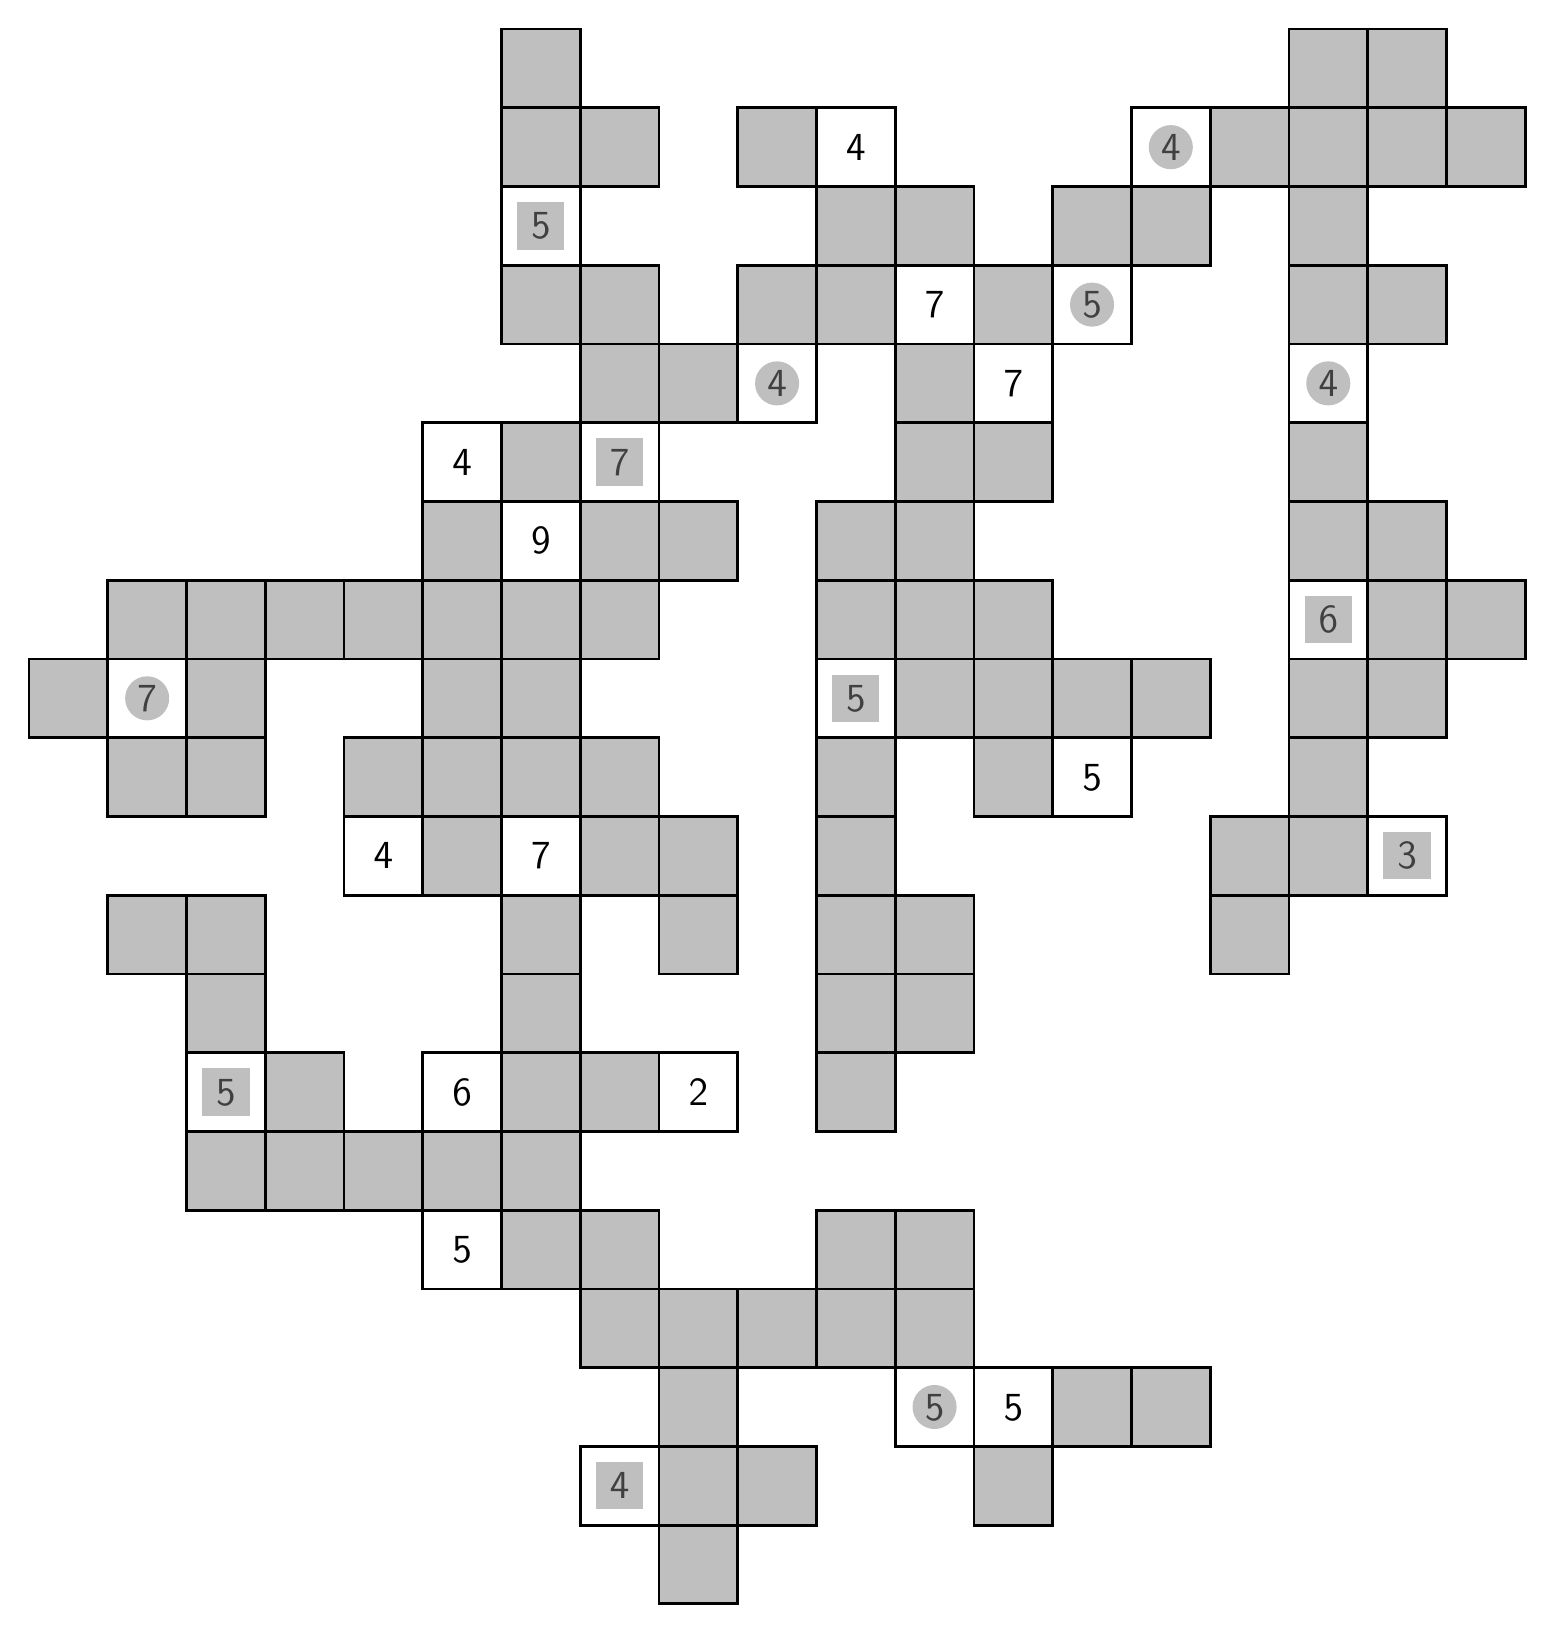
\begin{tikzpicture}\fill[gray, opacity = 0.5] (9, 0, 0)--++(1, 0, 0)--++(0, 1, 0)--++(-1, 0, 0)--cycle;
\draw[line width = 1pt] (9, 0, 0)--++(1, 0, 0)--++(0, 1, 0)--++(-1, 0, 0)--cycle;
\draw node at (8.5, 1.5, 0) {\Large $\mathsf{4}$};
\draw[line width = 1pt] (8, 1, 0)--++(1, 0, 0)--++(0, 1, 0)--++(-1, 0, 0)--cycle;
\fill[color = gray, opacity = 0.5] (8.2, 1.2) rectangle ++(0.6, 0.6);
\fill[gray, opacity = 0.5] (9, 1, 0)--++(1, 0, 0)--++(0, 1, 0)--++(-1, 0, 0)--cycle;
\draw[line width = 1pt] (9, 1, 0)--++(1, 0, 0)--++(0, 1, 0)--++(-1, 0, 0)--cycle;
\fill[gray, opacity = 0.5] (10, 1, 0)--++(1, 0, 0)--++(0, 1, 0)--++(-1, 0, 0)--cycle;
\draw[line width = 1pt] (10, 1, 0)--++(1, 0, 0)--++(0, 1, 0)--++(-1, 0, 0)--cycle;
\fill[gray, opacity = 0.5] (13, 1, 0)--++(1, 0, 0)--++(0, 1, 0)--++(-1, 0, 0)--cycle;
\draw[line width = 1pt] (13, 1, 0)--++(1, 0, 0)--++(0, 1, 0)--++(-1, 0, 0)--cycle;
\fill[gray, opacity = 0.5] (9, 2, 0)--++(1, 0, 0)--++(0, 1, 0)--++(-1, 0, 0)--cycle;
\draw[line width = 1pt] (9, 2, 0)--++(1, 0, 0)--++(0, 1, 0)--++(-1, 0, 0)--cycle;
\draw node at (12.5, 2.5, 0) {\Large $\mathsf{5}$};
\draw[line width = 1pt] (12, 2, 0)--++(1, 0, 0)--++(0, 1, 0)--++(-1, 0, 0)--cycle;
\fill[color = gray, opacity = 0.5] (12.5, 2.5, 0) circle (0.28);
\draw node at (13.5, 2.5, 0) {\Large $\mathsf{5}$};
\draw[line width = 1pt] (13, 2, 0)--++(1, 0, 0)--++(0, 1, 0)--++(-1, 0, 0)--cycle;
\fill[gray, opacity = 0.5] (14, 2, 0)--++(1, 0, 0)--++(0, 1, 0)--++(-1, 0, 0)--cycle;
\draw[line width = 1pt] (14, 2, 0)--++(1, 0, 0)--++(0, 1, 0)--++(-1, 0, 0)--cycle;
\fill[gray, opacity = 0.5] (15, 2, 0)--++(1, 0, 0)--++(0, 1, 0)--++(-1, 0, 0)--cycle;
\draw[line width = 1pt] (15, 2, 0)--++(1, 0, 0)--++(0, 1, 0)--++(-1, 0, 0)--cycle;
\fill[gray, opacity = 0.5] (8, 3, 0)--++(1, 0, 0)--++(0, 1, 0)--++(-1, 0, 0)--cycle;
\draw[line width = 1pt] (8, 3, 0)--++(1, 0, 0)--++(0, 1, 0)--++(-1, 0, 0)--cycle;
\fill[gray, opacity = 0.5] (9, 3, 0)--++(1, 0, 0)--++(0, 1, 0)--++(-1, 0, 0)--cycle;
\draw[line width = 1pt] (9, 3, 0)--++(1, 0, 0)--++(0, 1, 0)--++(-1, 0, 0)--cycle;
\fill[gray, opacity = 0.5] (10, 3, 0)--++(1, 0, 0)--++(0, 1, 0)--++(-1, 0, 0)--cycle;
\draw[line width = 1pt] (10, 3, 0)--++(1, 0, 0)--++(0, 1, 0)--++(-1, 0, 0)--cycle;
\fill[gray, opacity = 0.5] (11, 3, 0)--++(1, 0, 0)--++(0, 1, 0)--++(-1, 0, 0)--cycle;
\draw[line width = 1pt] (11, 3, 0)--++(1, 0, 0)--++(0, 1, 0)--++(-1, 0, 0)--cycle;
\fill[gray, opacity = 0.5] (12, 3, 0)--++(1, 0, 0)--++(0, 1, 0)--++(-1, 0, 0)--cycle;
\draw[line width = 1pt] (12, 3, 0)--++(1, 0, 0)--++(0, 1, 0)--++(-1, 0, 0)--cycle;
\draw node at (6.5, 4.5, 0) {\Large $\mathsf{5}$};
\draw[line width = 1pt] (6, 4, 0)--++(1, 0, 0)--++(0, 1, 0)--++(-1, 0, 0)--cycle;
\fill[gray, opacity = 0.5] (7, 4, 0)--++(1, 0, 0)--++(0, 1, 0)--++(-1, 0, 0)--cycle;
\draw[line width = 1pt] (7, 4, 0)--++(1, 0, 0)--++(0, 1, 0)--++(-1, 0, 0)--cycle;
\fill[gray, opacity = 0.5] (8, 4, 0)--++(1, 0, 0)--++(0, 1, 0)--++(-1, 0, 0)--cycle;
\draw[line width = 1pt] (8, 4, 0)--++(1, 0, 0)--++(0, 1, 0)--++(-1, 0, 0)--cycle;
\fill[gray, opacity = 0.5] (11, 4, 0)--++(1, 0, 0)--++(0, 1, 0)--++(-1, 0, 0)--cycle;
\draw[line width = 1pt] (11, 4, 0)--++(1, 0, 0)--++(0, 1, 0)--++(-1, 0, 0)--cycle;
\fill[gray, opacity = 0.5] (12, 4, 0)--++(1, 0, 0)--++(0, 1, 0)--++(-1, 0, 0)--cycle;
\draw[line width = 1pt] (12, 4, 0)--++(1, 0, 0)--++(0, 1, 0)--++(-1, 0, 0)--cycle;
\fill[gray, opacity = 0.5] (3, 5, 0)--++(1, 0, 0)--++(0, 1, 0)--++(-1, 0, 0)--cycle;
\draw[line width = 1pt] (3, 5, 0)--++(1, 0, 0)--++(0, 1, 0)--++(-1, 0, 0)--cycle;
\fill[gray, opacity = 0.5] (4, 5, 0)--++(1, 0, 0)--++(0, 1, 0)--++(-1, 0, 0)--cycle;
\draw[line width = 1pt] (4, 5, 0)--++(1, 0, 0)--++(0, 1, 0)--++(-1, 0, 0)--cycle;
\fill[gray, opacity = 0.5] (5, 5, 0)--++(1, 0, 0)--++(0, 1, 0)--++(-1, 0, 0)--cycle;
\draw[line width = 1pt] (5, 5, 0)--++(1, 0, 0)--++(0, 1, 0)--++(-1, 0, 0)--cycle;
\fill[gray, opacity = 0.5] (6, 5, 0)--++(1, 0, 0)--++(0, 1, 0)--++(-1, 0, 0)--cycle;
\draw[line width = 1pt] (6, 5, 0)--++(1, 0, 0)--++(0, 1, 0)--++(-1, 0, 0)--cycle;
\fill[gray, opacity = 0.5] (7, 5, 0)--++(1, 0, 0)--++(0, 1, 0)--++(-1, 0, 0)--cycle;
\draw[line width = 1pt] (7, 5, 0)--++(1, 0, 0)--++(0, 1, 0)--++(-1, 0, 0)--cycle;
\draw node at (3.5, 6.5, 0) {\Large $\mathsf{5}$};
\draw[line width = 1pt] (3, 6, 0)--++(1, 0, 0)--++(0, 1, 0)--++(-1, 0, 0)--cycle;
\fill[color = gray, opacity = 0.5] (3.2, 6.2) rectangle ++(0.6, 0.6);
\fill[gray, opacity = 0.5] (4, 6, 0)--++(1, 0, 0)--++(0, 1, 0)--++(-1, 0, 0)--cycle;
\draw[line width = 1pt] (4, 6, 0)--++(1, 0, 0)--++(0, 1, 0)--++(-1, 0, 0)--cycle;
\draw node at (6.5, 6.5, 0) {\Large $\mathsf{6}$};
\draw[line width = 1pt] (6, 6, 0)--++(1, 0, 0)--++(0, 1, 0)--++(-1, 0, 0)--cycle;
\fill[gray, opacity = 0.5] (7, 6, 0)--++(1, 0, 0)--++(0, 1, 0)--++(-1, 0, 0)--cycle;
\draw[line width = 1pt] (7, 6, 0)--++(1, 0, 0)--++(0, 1, 0)--++(-1, 0, 0)--cycle;
\fill[gray, opacity = 0.5] (8, 6, 0)--++(1, 0, 0)--++(0, 1, 0)--++(-1, 0, 0)--cycle;
\draw[line width = 1pt] (8, 6, 0)--++(1, 0, 0)--++(0, 1, 0)--++(-1, 0, 0)--cycle;
\draw node at (9.5, 6.5, 0) {\Large $\mathsf{2}$};
\draw[line width = 1pt] (9, 6, 0)--++(1, 0, 0)--++(0, 1, 0)--++(-1, 0, 0)--cycle;
\fill[gray, opacity = 0.5] (11, 6, 0)--++(1, 0, 0)--++(0, 1, 0)--++(-1, 0, 0)--cycle;
\draw[line width = 1pt] (11, 6, 0)--++(1, 0, 0)--++(0, 1, 0)--++(-1, 0, 0)--cycle;
\fill[gray, opacity = 0.5] (3, 7, 0)--++(1, 0, 0)--++(0, 1, 0)--++(-1, 0, 0)--cycle;
\draw[line width = 1pt] (3, 7, 0)--++(1, 0, 0)--++(0, 1, 0)--++(-1, 0, 0)--cycle;
\fill[gray, opacity = 0.5] (7, 7, 0)--++(1, 0, 0)--++(0, 1, 0)--++(-1, 0, 0)--cycle;
\draw[line width = 1pt] (7, 7, 0)--++(1, 0, 0)--++(0, 1, 0)--++(-1, 0, 0)--cycle;
\fill[gray, opacity = 0.5] (11, 7, 0)--++(1, 0, 0)--++(0, 1, 0)--++(-1, 0, 0)--cycle;
\draw[line width = 1pt] (11, 7, 0)--++(1, 0, 0)--++(0, 1, 0)--++(-1, 0, 0)--cycle;
\fill[gray, opacity = 0.5] (12, 7, 0)--++(1, 0, 0)--++(0, 1, 0)--++(-1, 0, 0)--cycle;
\draw[line width = 1pt] (12, 7, 0)--++(1, 0, 0)--++(0, 1, 0)--++(-1, 0, 0)--cycle;
\fill[gray, opacity = 0.5] (2, 8, 0)--++(1, 0, 0)--++(0, 1, 0)--++(-1, 0, 0)--cycle;
\draw[line width = 1pt] (2, 8, 0)--++(1, 0, 0)--++(0, 1, 0)--++(-1, 0, 0)--cycle;
\fill[gray, opacity = 0.5] (3, 8, 0)--++(1, 0, 0)--++(0, 1, 0)--++(-1, 0, 0)--cycle;
\draw[line width = 1pt] (3, 8, 0)--++(1, 0, 0)--++(0, 1, 0)--++(-1, 0, 0)--cycle;
\fill[gray, opacity = 0.5] (7, 8, 0)--++(1, 0, 0)--++(0, 1, 0)--++(-1, 0, 0)--cycle;
\draw[line width = 1pt] (7, 8, 0)--++(1, 0, 0)--++(0, 1, 0)--++(-1, 0, 0)--cycle;
\fill[gray, opacity = 0.5] (9, 8, 0)--++(1, 0, 0)--++(0, 1, 0)--++(-1, 0, 0)--cycle;
\draw[line width = 1pt] (9, 8, 0)--++(1, 0, 0)--++(0, 1, 0)--++(-1, 0, 0)--cycle;
\fill[gray, opacity = 0.5] (11, 8, 0)--++(1, 0, 0)--++(0, 1, 0)--++(-1, 0, 0)--cycle;
\draw[line width = 1pt] (11, 8, 0)--++(1, 0, 0)--++(0, 1, 0)--++(-1, 0, 0)--cycle;
\fill[gray, opacity = 0.5] (12, 8, 0)--++(1, 0, 0)--++(0, 1, 0)--++(-1, 0, 0)--cycle;
\draw[line width = 1pt] (12, 8, 0)--++(1, 0, 0)--++(0, 1, 0)--++(-1, 0, 0)--cycle;
\fill[gray, opacity = 0.5] (16, 8, 0)--++(1, 0, 0)--++(0, 1, 0)--++(-1, 0, 0)--cycle;
\draw[line width = 1pt] (16, 8, 0)--++(1, 0, 0)--++(0, 1, 0)--++(-1, 0, 0)--cycle;
\draw node at (5.5, 9.5, 0) {\Large $\mathsf{4}$};
\draw[line width = 1pt] (5, 9, 0)--++(1, 0, 0)--++(0, 1, 0)--++(-1, 0, 0)--cycle;
\fill[gray, opacity = 0.5] (6, 9, 0)--++(1, 0, 0)--++(0, 1, 0)--++(-1, 0, 0)--cycle;
\draw[line width = 1pt] (6, 9, 0)--++(1, 0, 0)--++(0, 1, 0)--++(-1, 0, 0)--cycle;
\draw node at (7.5, 9.5, 0) {\Large $\mathsf{7}$};
\draw[line width = 1pt] (7, 9, 0)--++(1, 0, 0)--++(0, 1, 0)--++(-1, 0, 0)--cycle;
\fill[gray, opacity = 0.5] (8, 9, 0)--++(1, 0, 0)--++(0, 1, 0)--++(-1, 0, 0)--cycle;
\draw[line width = 1pt] (8, 9, 0)--++(1, 0, 0)--++(0, 1, 0)--++(-1, 0, 0)--cycle;
\fill[gray, opacity = 0.5] (9, 9, 0)--++(1, 0, 0)--++(0, 1, 0)--++(-1, 0, 0)--cycle;
\draw[line width = 1pt] (9, 9, 0)--++(1, 0, 0)--++(0, 1, 0)--++(-1, 0, 0)--cycle;
\fill[gray, opacity = 0.5] (11, 9, 0)--++(1, 0, 0)--++(0, 1, 0)--++(-1, 0, 0)--cycle;
\draw[line width = 1pt] (11, 9, 0)--++(1, 0, 0)--++(0, 1, 0)--++(-1, 0, 0)--cycle;
\fill[gray, opacity = 0.5] (16, 9, 0)--++(1, 0, 0)--++(0, 1, 0)--++(-1, 0, 0)--cycle;
\draw[line width = 1pt] (16, 9, 0)--++(1, 0, 0)--++(0, 1, 0)--++(-1, 0, 0)--cycle;
\fill[gray, opacity = 0.5] (17, 9, 0)--++(1, 0, 0)--++(0, 1, 0)--++(-1, 0, 0)--cycle;
\draw[line width = 1pt] (17, 9, 0)--++(1, 0, 0)--++(0, 1, 0)--++(-1, 0, 0)--cycle;
\draw node at (18.5, 9.5, 0) {\Large $\mathsf{3}$};
\draw[line width = 1pt] (18, 9, 0)--++(1, 0, 0)--++(0, 1, 0)--++(-1, 0, 0)--cycle;
\fill[color = gray, opacity = 0.5] (18.2, 9.2) rectangle ++(0.6, 0.6);
\fill[gray, opacity = 0.5] (2, 10, 0)--++(1, 0, 0)--++(0, 1, 0)--++(-1, 0, 0)--cycle;
\draw[line width = 1pt] (2, 10, 0)--++(1, 0, 0)--++(0, 1, 0)--++(-1, 0, 0)--cycle;
\fill[gray, opacity = 0.5] (3, 10, 0)--++(1, 0, 0)--++(0, 1, 0)--++(-1, 0, 0)--cycle;
\draw[line width = 1pt] (3, 10, 0)--++(1, 0, 0)--++(0, 1, 0)--++(-1, 0, 0)--cycle;
\fill[gray, opacity = 0.5] (5, 10, 0)--++(1, 0, 0)--++(0, 1, 0)--++(-1, 0, 0)--cycle;
\draw[line width = 1pt] (5, 10, 0)--++(1, 0, 0)--++(0, 1, 0)--++(-1, 0, 0)--cycle;
\fill[gray, opacity = 0.5] (6, 10, 0)--++(1, 0, 0)--++(0, 1, 0)--++(-1, 0, 0)--cycle;
\draw[line width = 1pt] (6, 10, 0)--++(1, 0, 0)--++(0, 1, 0)--++(-1, 0, 0)--cycle;
\fill[gray, opacity = 0.5] (7, 10, 0)--++(1, 0, 0)--++(0, 1, 0)--++(-1, 0, 0)--cycle;
\draw[line width = 1pt] (7, 10, 0)--++(1, 0, 0)--++(0, 1, 0)--++(-1, 0, 0)--cycle;
\fill[gray, opacity = 0.5] (8, 10, 0)--++(1, 0, 0)--++(0, 1, 0)--++(-1, 0, 0)--cycle;
\draw[line width = 1pt] (8, 10, 0)--++(1, 0, 0)--++(0, 1, 0)--++(-1, 0, 0)--cycle;
\fill[gray, opacity = 0.5] (11, 10, 0)--++(1, 0, 0)--++(0, 1, 0)--++(-1, 0, 0)--cycle;
\draw[line width = 1pt] (11, 10, 0)--++(1, 0, 0)--++(0, 1, 0)--++(-1, 0, 0)--cycle;
\fill[gray, opacity = 0.5] (13, 10, 0)--++(1, 0, 0)--++(0, 1, 0)--++(-1, 0, 0)--cycle;
\draw[line width = 1pt] (13, 10, 0)--++(1, 0, 0)--++(0, 1, 0)--++(-1, 0, 0)--cycle;
\draw node at (14.5, 10.5, 0) {\Large $\mathsf{5}$};
\draw[line width = 1pt] (14, 10, 0)--++(1, 0, 0)--++(0, 1, 0)--++(-1, 0, 0)--cycle;
\fill[gray, opacity = 0.5] (17, 10, 0)--++(1, 0, 0)--++(0, 1, 0)--++(-1, 0, 0)--cycle;
\draw[line width = 1pt] (17, 10, 0)--++(1, 0, 0)--++(0, 1, 0)--++(-1, 0, 0)--cycle;
\fill[gray, opacity = 0.5] (1, 11, 0)--++(1, 0, 0)--++(0, 1, 0)--++(-1, 0, 0)--cycle;
\draw[line width = 1pt] (1, 11, 0)--++(1, 0, 0)--++(0, 1, 0)--++(-1, 0, 0)--cycle;
\draw node at (2.5, 11.5, 0) {\Large $\mathsf{7}$};
\draw[line width = 1pt] (2, 11, 0)--++(1, 0, 0)--++(0, 1, 0)--++(-1, 0, 0)--cycle;
\fill[color = gray, opacity = 0.5] (2.5, 11.5, 0) circle (0.28);
\fill[gray, opacity = 0.5] (3, 11, 0)--++(1, 0, 0)--++(0, 1, 0)--++(-1, 0, 0)--cycle;
\draw[line width = 1pt] (3, 11, 0)--++(1, 0, 0)--++(0, 1, 0)--++(-1, 0, 0)--cycle;
\fill[gray, opacity = 0.5] (6, 11, 0)--++(1, 0, 0)--++(0, 1, 0)--++(-1, 0, 0)--cycle;
\draw[line width = 1pt] (6, 11, 0)--++(1, 0, 0)--++(0, 1, 0)--++(-1, 0, 0)--cycle;
\fill[gray, opacity = 0.5] (7, 11, 0)--++(1, 0, 0)--++(0, 1, 0)--++(-1, 0, 0)--cycle;
\draw[line width = 1pt] (7, 11, 0)--++(1, 0, 0)--++(0, 1, 0)--++(-1, 0, 0)--cycle;
\draw node at (11.5, 11.5, 0) {\Large $\mathsf{5}$};
\draw[line width = 1pt] (11, 11, 0)--++(1, 0, 0)--++(0, 1, 0)--++(-1, 0, 0)--cycle;
\fill[color = gray, opacity = 0.5] (11.2, 11.2) rectangle ++(0.6, 0.6);
\fill[gray, opacity = 0.5] (12, 11, 0)--++(1, 0, 0)--++(0, 1, 0)--++(-1, 0, 0)--cycle;
\draw[line width = 1pt] (12, 11, 0)--++(1, 0, 0)--++(0, 1, 0)--++(-1, 0, 0)--cycle;
\fill[gray, opacity = 0.5] (13, 11, 0)--++(1, 0, 0)--++(0, 1, 0)--++(-1, 0, 0)--cycle;
\draw[line width = 1pt] (13, 11, 0)--++(1, 0, 0)--++(0, 1, 0)--++(-1, 0, 0)--cycle;
\fill[gray, opacity = 0.5] (14, 11, 0)--++(1, 0, 0)--++(0, 1, 0)--++(-1, 0, 0)--cycle;
\draw[line width = 1pt] (14, 11, 0)--++(1, 0, 0)--++(0, 1, 0)--++(-1, 0, 0)--cycle;
\fill[gray, opacity = 0.5] (15, 11, 0)--++(1, 0, 0)--++(0, 1, 0)--++(-1, 0, 0)--cycle;
\draw[line width = 1pt] (15, 11, 0)--++(1, 0, 0)--++(0, 1, 0)--++(-1, 0, 0)--cycle;
\fill[gray, opacity = 0.5] (17, 11, 0)--++(1, 0, 0)--++(0, 1, 0)--++(-1, 0, 0)--cycle;
\draw[line width = 1pt] (17, 11, 0)--++(1, 0, 0)--++(0, 1, 0)--++(-1, 0, 0)--cycle;
\fill[gray, opacity = 0.5] (18, 11, 0)--++(1, 0, 0)--++(0, 1, 0)--++(-1, 0, 0)--cycle;
\draw[line width = 1pt] (18, 11, 0)--++(1, 0, 0)--++(0, 1, 0)--++(-1, 0, 0)--cycle;
\fill[gray, opacity = 0.5] (2, 12, 0)--++(1, 0, 0)--++(0, 1, 0)--++(-1, 0, 0)--cycle;
\draw[line width = 1pt] (2, 12, 0)--++(1, 0, 0)--++(0, 1, 0)--++(-1, 0, 0)--cycle;
\fill[gray, opacity = 0.5] (3, 12, 0)--++(1, 0, 0)--++(0, 1, 0)--++(-1, 0, 0)--cycle;
\draw[line width = 1pt] (3, 12, 0)--++(1, 0, 0)--++(0, 1, 0)--++(-1, 0, 0)--cycle;
\fill[gray, opacity = 0.5] (4, 12, 0)--++(1, 0, 0)--++(0, 1, 0)--++(-1, 0, 0)--cycle;
\draw[line width = 1pt] (4, 12, 0)--++(1, 0, 0)--++(0, 1, 0)--++(-1, 0, 0)--cycle;
\fill[gray, opacity = 0.5] (5, 12, 0)--++(1, 0, 0)--++(0, 1, 0)--++(-1, 0, 0)--cycle;
\draw[line width = 1pt] (5, 12, 0)--++(1, 0, 0)--++(0, 1, 0)--++(-1, 0, 0)--cycle;
\fill[gray, opacity = 0.5] (6, 12, 0)--++(1, 0, 0)--++(0, 1, 0)--++(-1, 0, 0)--cycle;
\draw[line width = 1pt] (6, 12, 0)--++(1, 0, 0)--++(0, 1, 0)--++(-1, 0, 0)--cycle;
\fill[gray, opacity = 0.5] (7, 12, 0)--++(1, 0, 0)--++(0, 1, 0)--++(-1, 0, 0)--cycle;
\draw[line width = 1pt] (7, 12, 0)--++(1, 0, 0)--++(0, 1, 0)--++(-1, 0, 0)--cycle;
\fill[gray, opacity = 0.5] (8, 12, 0)--++(1, 0, 0)--++(0, 1, 0)--++(-1, 0, 0)--cycle;
\draw[line width = 1pt] (8, 12, 0)--++(1, 0, 0)--++(0, 1, 0)--++(-1, 0, 0)--cycle;
\fill[gray, opacity = 0.5] (11, 12, 0)--++(1, 0, 0)--++(0, 1, 0)--++(-1, 0, 0)--cycle;
\draw[line width = 1pt] (11, 12, 0)--++(1, 0, 0)--++(0, 1, 0)--++(-1, 0, 0)--cycle;
\fill[gray, opacity = 0.5] (12, 12, 0)--++(1, 0, 0)--++(0, 1, 0)--++(-1, 0, 0)--cycle;
\draw[line width = 1pt] (12, 12, 0)--++(1, 0, 0)--++(0, 1, 0)--++(-1, 0, 0)--cycle;
\fill[gray, opacity = 0.5] (13, 12, 0)--++(1, 0, 0)--++(0, 1, 0)--++(-1, 0, 0)--cycle;
\draw[line width = 1pt] (13, 12, 0)--++(1, 0, 0)--++(0, 1, 0)--++(-1, 0, 0)--cycle;
\draw node at (17.5, 12.5, 0) {\Large $\mathsf{6}$};
\draw[line width = 1pt] (17, 12, 0)--++(1, 0, 0)--++(0, 1, 0)--++(-1, 0, 0)--cycle;
\fill[color = gray, opacity = 0.5] (17.2, 12.2) rectangle ++(0.6, 0.6);
\fill[gray, opacity = 0.5] (18, 12, 0)--++(1, 0, 0)--++(0, 1, 0)--++(-1, 0, 0)--cycle;
\draw[line width = 1pt] (18, 12, 0)--++(1, 0, 0)--++(0, 1, 0)--++(-1, 0, 0)--cycle;
\fill[gray, opacity = 0.5] (19, 12, 0)--++(1, 0, 0)--++(0, 1, 0)--++(-1, 0, 0)--cycle;
\draw[line width = 1pt] (19, 12, 0)--++(1, 0, 0)--++(0, 1, 0)--++(-1, 0, 0)--cycle;
\fill[gray, opacity = 0.5] (6, 13, 0)--++(1, 0, 0)--++(0, 1, 0)--++(-1, 0, 0)--cycle;
\draw[line width = 1pt] (6, 13, 0)--++(1, 0, 0)--++(0, 1, 0)--++(-1, 0, 0)--cycle;
\draw node at (7.5, 13.5, 0) {\Large $\mathsf{9}$};
\draw[line width = 1pt] (7, 13, 0)--++(1, 0, 0)--++(0, 1, 0)--++(-1, 0, 0)--cycle;
\fill[gray, opacity = 0.5] (8, 13, 0)--++(1, 0, 0)--++(0, 1, 0)--++(-1, 0, 0)--cycle;
\draw[line width = 1pt] (8, 13, 0)--++(1, 0, 0)--++(0, 1, 0)--++(-1, 0, 0)--cycle;
\fill[gray, opacity = 0.5] (9, 13, 0)--++(1, 0, 0)--++(0, 1, 0)--++(-1, 0, 0)--cycle;
\draw[line width = 1pt] (9, 13, 0)--++(1, 0, 0)--++(0, 1, 0)--++(-1, 0, 0)--cycle;
\fill[gray, opacity = 0.5] (11, 13, 0)--++(1, 0, 0)--++(0, 1, 0)--++(-1, 0, 0)--cycle;
\draw[line width = 1pt] (11, 13, 0)--++(1, 0, 0)--++(0, 1, 0)--++(-1, 0, 0)--cycle;
\fill[gray, opacity = 0.5] (12, 13, 0)--++(1, 0, 0)--++(0, 1, 0)--++(-1, 0, 0)--cycle;
\draw[line width = 1pt] (12, 13, 0)--++(1, 0, 0)--++(0, 1, 0)--++(-1, 0, 0)--cycle;
\fill[gray, opacity = 0.5] (17, 13, 0)--++(1, 0, 0)--++(0, 1, 0)--++(-1, 0, 0)--cycle;
\draw[line width = 1pt] (17, 13, 0)--++(1, 0, 0)--++(0, 1, 0)--++(-1, 0, 0)--cycle;
\fill[gray, opacity = 0.5] (18, 13, 0)--++(1, 0, 0)--++(0, 1, 0)--++(-1, 0, 0)--cycle;
\draw[line width = 1pt] (18, 13, 0)--++(1, 0, 0)--++(0, 1, 0)--++(-1, 0, 0)--cycle;
\draw node at (6.5, 14.5, 0) {\Large $\mathsf{4}$};
\draw[line width = 1pt] (6, 14, 0)--++(1, 0, 0)--++(0, 1, 0)--++(-1, 0, 0)--cycle;
\fill[gray, opacity = 0.5] (7, 14, 0)--++(1, 0, 0)--++(0, 1, 0)--++(-1, 0, 0)--cycle;
\draw[line width = 1pt] (7, 14, 0)--++(1, 0, 0)--++(0, 1, 0)--++(-1, 0, 0)--cycle;
\draw node at (8.5, 14.5, 0) {\Large $\mathsf{7}$};
\draw[line width = 1pt] (8, 14, 0)--++(1, 0, 0)--++(0, 1, 0)--++(-1, 0, 0)--cycle;
\fill[color = gray, opacity = 0.5] (8.2, 14.2) rectangle ++(0.6, 0.6);
\fill[gray, opacity = 0.5] (12, 14, 0)--++(1, 0, 0)--++(0, 1, 0)--++(-1, 0, 0)--cycle;
\draw[line width = 1pt] (12, 14, 0)--++(1, 0, 0)--++(0, 1, 0)--++(-1, 0, 0)--cycle;
\fill[gray, opacity = 0.5] (13, 14, 0)--++(1, 0, 0)--++(0, 1, 0)--++(-1, 0, 0)--cycle;
\draw[line width = 1pt] (13, 14, 0)--++(1, 0, 0)--++(0, 1, 0)--++(-1, 0, 0)--cycle;
\fill[gray, opacity = 0.5] (17, 14, 0)--++(1, 0, 0)--++(0, 1, 0)--++(-1, 0, 0)--cycle;
\draw[line width = 1pt] (17, 14, 0)--++(1, 0, 0)--++(0, 1, 0)--++(-1, 0, 0)--cycle;
\fill[gray, opacity = 0.5] (8, 15, 0)--++(1, 0, 0)--++(0, 1, 0)--++(-1, 0, 0)--cycle;
\draw[line width = 1pt] (8, 15, 0)--++(1, 0, 0)--++(0, 1, 0)--++(-1, 0, 0)--cycle;
\fill[gray, opacity = 0.5] (9, 15, 0)--++(1, 0, 0)--++(0, 1, 0)--++(-1, 0, 0)--cycle;
\draw[line width = 1pt] (9, 15, 0)--++(1, 0, 0)--++(0, 1, 0)--++(-1, 0, 0)--cycle;
\draw node at (10.5, 15.5, 0) {\Large $\mathsf{4}$};
\draw[line width = 1pt] (10, 15, 0)--++(1, 0, 0)--++(0, 1, 0)--++(-1, 0, 0)--cycle;
\fill[color = gray, opacity = 0.5] (10.5, 15.5, 0) circle (0.28);
\fill[gray, opacity = 0.5] (12, 15, 0)--++(1, 0, 0)--++(0, 1, 0)--++(-1, 0, 0)--cycle;
\draw[line width = 1pt] (12, 15, 0)--++(1, 0, 0)--++(0, 1, 0)--++(-1, 0, 0)--cycle;
\draw node at (13.5, 15.5, 0) {\Large $\mathsf{7}$};
\draw[line width = 1pt] (13, 15, 0)--++(1, 0, 0)--++(0, 1, 0)--++(-1, 0, 0)--cycle;
\draw node at (17.5, 15.5, 0) {\Large $\mathsf{4}$};
\draw[line width = 1pt] (17, 15, 0)--++(1, 0, 0)--++(0, 1, 0)--++(-1, 0, 0)--cycle;
\fill[color = gray, opacity = 0.5] (17.5, 15.5, 0) circle (0.28);
\fill[gray, opacity = 0.5] (7, 16, 0)--++(1, 0, 0)--++(0, 1, 0)--++(-1, 0, 0)--cycle;
\draw[line width = 1pt] (7, 16, 0)--++(1, 0, 0)--++(0, 1, 0)--++(-1, 0, 0)--cycle;
\fill[gray, opacity = 0.5] (8, 16, 0)--++(1, 0, 0)--++(0, 1, 0)--++(-1, 0, 0)--cycle;
\draw[line width = 1pt] (8, 16, 0)--++(1, 0, 0)--++(0, 1, 0)--++(-1, 0, 0)--cycle;
\fill[gray, opacity = 0.5] (10, 16, 0)--++(1, 0, 0)--++(0, 1, 0)--++(-1, 0, 0)--cycle;
\draw[line width = 1pt] (10, 16, 0)--++(1, 0, 0)--++(0, 1, 0)--++(-1, 0, 0)--cycle;
\fill[gray, opacity = 0.5] (11, 16, 0)--++(1, 0, 0)--++(0, 1, 0)--++(-1, 0, 0)--cycle;
\draw[line width = 1pt] (11, 16, 0)--++(1, 0, 0)--++(0, 1, 0)--++(-1, 0, 0)--cycle;
\draw node at (12.5, 16.5, 0) {\Large $\mathsf{7}$};
\draw[line width = 1pt] (12, 16, 0)--++(1, 0, 0)--++(0, 1, 0)--++(-1, 0, 0)--cycle;
\fill[gray, opacity = 0.5] (13, 16, 0)--++(1, 0, 0)--++(0, 1, 0)--++(-1, 0, 0)--cycle;
\draw[line width = 1pt] (13, 16, 0)--++(1, 0, 0)--++(0, 1, 0)--++(-1, 0, 0)--cycle;
\draw node at (14.5, 16.5, 0) {\Large $\mathsf{5}$};
\draw[line width = 1pt] (14, 16, 0)--++(1, 0, 0)--++(0, 1, 0)--++(-1, 0, 0)--cycle;
\fill[color = gray, opacity = 0.5] (14.5, 16.5, 0) circle (0.28);
\fill[gray, opacity = 0.5] (17, 16, 0)--++(1, 0, 0)--++(0, 1, 0)--++(-1, 0, 0)--cycle;
\draw[line width = 1pt] (17, 16, 0)--++(1, 0, 0)--++(0, 1, 0)--++(-1, 0, 0)--cycle;
\fill[gray, opacity = 0.5] (18, 16, 0)--++(1, 0, 0)--++(0, 1, 0)--++(-1, 0, 0)--cycle;
\draw[line width = 1pt] (18, 16, 0)--++(1, 0, 0)--++(0, 1, 0)--++(-1, 0, 0)--cycle;
\draw node at (7.5, 17.5, 0) {\Large $\mathsf{5}$};
\draw[line width = 1pt] (7, 17, 0)--++(1, 0, 0)--++(0, 1, 0)--++(-1, 0, 0)--cycle;
\fill[color = gray, opacity = 0.5] (7.2, 17.2) rectangle ++(0.6, 0.6);
\fill[gray, opacity = 0.5] (11, 17, 0)--++(1, 0, 0)--++(0, 1, 0)--++(-1, 0, 0)--cycle;
\draw[line width = 1pt] (11, 17, 0)--++(1, 0, 0)--++(0, 1, 0)--++(-1, 0, 0)--cycle;
\fill[gray, opacity = 0.5] (12, 17, 0)--++(1, 0, 0)--++(0, 1, 0)--++(-1, 0, 0)--cycle;
\draw[line width = 1pt] (12, 17, 0)--++(1, 0, 0)--++(0, 1, 0)--++(-1, 0, 0)--cycle;
\fill[gray, opacity = 0.5] (14, 17, 0)--++(1, 0, 0)--++(0, 1, 0)--++(-1, 0, 0)--cycle;
\draw[line width = 1pt] (14, 17, 0)--++(1, 0, 0)--++(0, 1, 0)--++(-1, 0, 0)--cycle;
\fill[gray, opacity = 0.5] (15, 17, 0)--++(1, 0, 0)--++(0, 1, 0)--++(-1, 0, 0)--cycle;
\draw[line width = 1pt] (15, 17, 0)--++(1, 0, 0)--++(0, 1, 0)--++(-1, 0, 0)--cycle;
\fill[gray, opacity = 0.5] (17, 17, 0)--++(1, 0, 0)--++(0, 1, 0)--++(-1, 0, 0)--cycle;
\draw[line width = 1pt] (17, 17, 0)--++(1, 0, 0)--++(0, 1, 0)--++(-1, 0, 0)--cycle;
\fill[gray, opacity = 0.5] (7, 18, 0)--++(1, 0, 0)--++(0, 1, 0)--++(-1, 0, 0)--cycle;
\draw[line width = 1pt] (7, 18, 0)--++(1, 0, 0)--++(0, 1, 0)--++(-1, 0, 0)--cycle;
\fill[gray, opacity = 0.5] (8, 18, 0)--++(1, 0, 0)--++(0, 1, 0)--++(-1, 0, 0)--cycle;
\draw[line width = 1pt] (8, 18, 0)--++(1, 0, 0)--++(0, 1, 0)--++(-1, 0, 0)--cycle;
\fill[gray, opacity = 0.5] (10, 18, 0)--++(1, 0, 0)--++(0, 1, 0)--++(-1, 0, 0)--cycle;
\draw[line width = 1pt] (10, 18, 0)--++(1, 0, 0)--++(0, 1, 0)--++(-1, 0, 0)--cycle;
\draw node at (11.5, 18.5, 0) {\Large $\mathsf{4}$};
\draw[line width = 1pt] (11, 18, 0)--++(1, 0, 0)--++(0, 1, 0)--++(-1, 0, 0)--cycle;
\draw node at (15.5, 18.5, 0) {\Large $\mathsf{4}$};
\draw[line width = 1pt] (15, 18, 0)--++(1, 0, 0)--++(0, 1, 0)--++(-1, 0, 0)--cycle;
\fill[color = gray, opacity = 0.5] (15.5, 18.5, 0) circle (0.28);
\fill[gray, opacity = 0.5] (16, 18, 0)--++(1, 0, 0)--++(0, 1, 0)--++(-1, 0, 0)--cycle;
\draw[line width = 1pt] (16, 18, 0)--++(1, 0, 0)--++(0, 1, 0)--++(-1, 0, 0)--cycle;
\fill[gray, opacity = 0.5] (17, 18, 0)--++(1, 0, 0)--++(0, 1, 0)--++(-1, 0, 0)--cycle;
\draw[line width = 1pt] (17, 18, 0)--++(1, 0, 0)--++(0, 1, 0)--++(-1, 0, 0)--cycle;
\fill[gray, opacity = 0.5] (18, 18, 0)--++(1, 0, 0)--++(0, 1, 0)--++(-1, 0, 0)--cycle;
\draw[line width = 1pt] (18, 18, 0)--++(1, 0, 0)--++(0, 1, 0)--++(-1, 0, 0)--cycle;
\fill[gray, opacity = 0.5] (19, 18, 0)--++(1, 0, 0)--++(0, 1, 0)--++(-1, 0, 0)--cycle;
\draw[line width = 1pt] (19, 18, 0)--++(1, 0, 0)--++(0, 1, 0)--++(-1, 0, 0)--cycle;
\fill[gray, opacity = 0.5] (7, 19, 0)--++(1, 0, 0)--++(0, 1, 0)--++(-1, 0, 0)--cycle;
\draw[line width = 1pt] (7, 19, 0)--++(1, 0, 0)--++(0, 1, 0)--++(-1, 0, 0)--cycle;
\fill[gray, opacity = 0.5] (17, 19, 0)--++(1, 0, 0)--++(0, 1, 0)--++(-1, 0, 0)--cycle;
\draw[line width = 1pt] (17, 19, 0)--++(1, 0, 0)--++(0, 1, 0)--++(-1, 0, 0)--cycle;
\fill[gray, opacity = 0.5] (18, 19, 0)--++(1, 0, 0)--++(0, 1, 0)--++(-1, 0, 0)--cycle;
\draw[line width = 1pt] (18, 19, 0)--++(1, 0, 0)--++(0, 1, 0)--++(-1, 0, 0)--cycle;
\end{tikzpicture}}\]
\[\resizebox{30pc}{!}{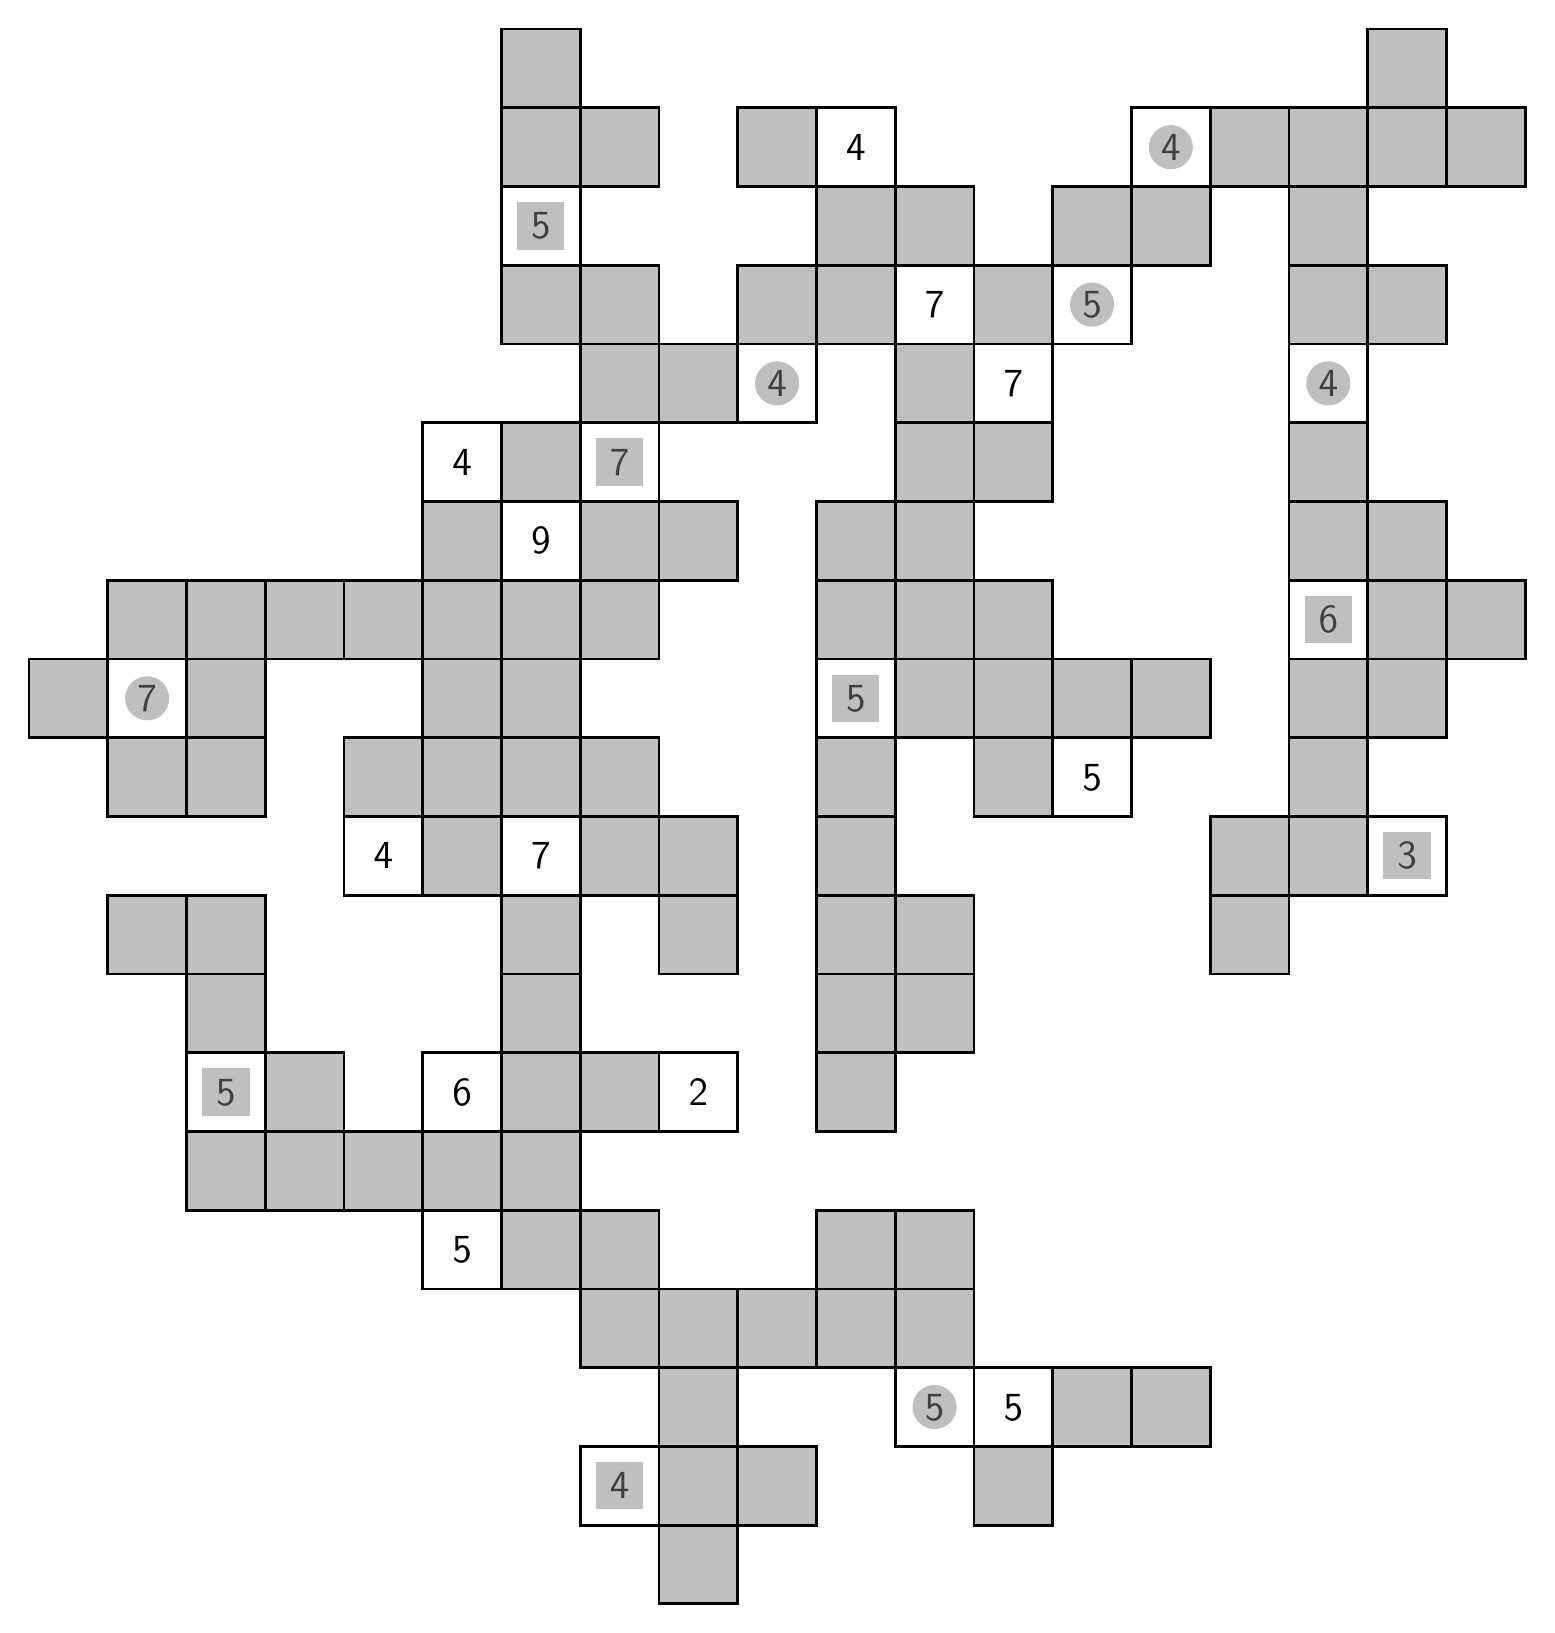
\begin{tikzpicture}\fill[gray, opacity = 0.5] (9, 0, 0)--++(1, 0, 0)--++(0, 1, 0)--++(-1, 0, 0)--cycle;
\draw[line width = 1pt] (9, 0, 0)--++(1, 0, 0)--++(0, 1, 0)--++(-1, 0, 0)--cycle;
\draw node at (8.5, 1.5, 0) {\Large $\mathsf{4}$};
\draw[line width = 1pt] (8, 1, 0)--++(1, 0, 0)--++(0, 1, 0)--++(-1, 0, 0)--cycle;
\fill[color = gray, opacity = 0.5] (8.2, 1.2) rectangle ++(0.6, 0.6);
\fill[gray, opacity = 0.5] (9, 1, 0)--++(1, 0, 0)--++(0, 1, 0)--++(-1, 0, 0)--cycle;
\draw[line width = 1pt] (9, 1, 0)--++(1, 0, 0)--++(0, 1, 0)--++(-1, 0, 0)--cycle;
\fill[gray, opacity = 0.5] (10, 1, 0)--++(1, 0, 0)--++(0, 1, 0)--++(-1, 0, 0)--cycle;
\draw[line width = 1pt] (10, 1, 0)--++(1, 0, 0)--++(0, 1, 0)--++(-1, 0, 0)--cycle;
\fill[gray, opacity = 0.5] (13, 1, 0)--++(1, 0, 0)--++(0, 1, 0)--++(-1, 0, 0)--cycle;
\draw[line width = 1pt] (13, 1, 0)--++(1, 0, 0)--++(0, 1, 0)--++(-1, 0, 0)--cycle;
\fill[gray, opacity = 0.5] (9, 2, 0)--++(1, 0, 0)--++(0, 1, 0)--++(-1, 0, 0)--cycle;
\draw[line width = 1pt] (9, 2, 0)--++(1, 0, 0)--++(0, 1, 0)--++(-1, 0, 0)--cycle;
\draw node at (12.5, 2.5, 0) {\Large $\mathsf{5}$};
\draw[line width = 1pt] (12, 2, 0)--++(1, 0, 0)--++(0, 1, 0)--++(-1, 0, 0)--cycle;
\fill[color = gray, opacity = 0.5] (12.5, 2.5, 0) circle (0.28);
\draw node at (13.5, 2.5, 0) {\Large $\mathsf{5}$};
\draw[line width = 1pt] (13, 2, 0)--++(1, 0, 0)--++(0, 1, 0)--++(-1, 0, 0)--cycle;
\fill[gray, opacity = 0.5] (14, 2, 0)--++(1, 0, 0)--++(0, 1, 0)--++(-1, 0, 0)--cycle;
\draw[line width = 1pt] (14, 2, 0)--++(1, 0, 0)--++(0, 1, 0)--++(-1, 0, 0)--cycle;
\fill[gray, opacity = 0.5] (15, 2, 0)--++(1, 0, 0)--++(0, 1, 0)--++(-1, 0, 0)--cycle;
\draw[line width = 1pt] (15, 2, 0)--++(1, 0, 0)--++(0, 1, 0)--++(-1, 0, 0)--cycle;
\fill[gray, opacity = 0.5] (8, 3, 0)--++(1, 0, 0)--++(0, 1, 0)--++(-1, 0, 0)--cycle;
\draw[line width = 1pt] (8, 3, 0)--++(1, 0, 0)--++(0, 1, 0)--++(-1, 0, 0)--cycle;
\fill[gray, opacity = 0.5] (9, 3, 0)--++(1, 0, 0)--++(0, 1, 0)--++(-1, 0, 0)--cycle;
\draw[line width = 1pt] (9, 3, 0)--++(1, 0, 0)--++(0, 1, 0)--++(-1, 0, 0)--cycle;
\fill[gray, opacity = 0.5] (10, 3, 0)--++(1, 0, 0)--++(0, 1, 0)--++(-1, 0, 0)--cycle;
\draw[line width = 1pt] (10, 3, 0)--++(1, 0, 0)--++(0, 1, 0)--++(-1, 0, 0)--cycle;
\fill[gray, opacity = 0.5] (11, 3, 0)--++(1, 0, 0)--++(0, 1, 0)--++(-1, 0, 0)--cycle;
\draw[line width = 1pt] (11, 3, 0)--++(1, 0, 0)--++(0, 1, 0)--++(-1, 0, 0)--cycle;
\fill[gray, opacity = 0.5] (12, 3, 0)--++(1, 0, 0)--++(0, 1, 0)--++(-1, 0, 0)--cycle;
\draw[line width = 1pt] (12, 3, 0)--++(1, 0, 0)--++(0, 1, 0)--++(-1, 0, 0)--cycle;
\draw node at (6.5, 4.5, 0) {\Large $\mathsf{5}$};
\draw[line width = 1pt] (6, 4, 0)--++(1, 0, 0)--++(0, 1, 0)--++(-1, 0, 0)--cycle;
\fill[gray, opacity = 0.5] (7, 4, 0)--++(1, 0, 0)--++(0, 1, 0)--++(-1, 0, 0)--cycle;
\draw[line width = 1pt] (7, 4, 0)--++(1, 0, 0)--++(0, 1, 0)--++(-1, 0, 0)--cycle;
\fill[gray, opacity = 0.5] (8, 4, 0)--++(1, 0, 0)--++(0, 1, 0)--++(-1, 0, 0)--cycle;
\draw[line width = 1pt] (8, 4, 0)--++(1, 0, 0)--++(0, 1, 0)--++(-1, 0, 0)--cycle;
\fill[gray, opacity = 0.5] (11, 4, 0)--++(1, 0, 0)--++(0, 1, 0)--++(-1, 0, 0)--cycle;
\draw[line width = 1pt] (11, 4, 0)--++(1, 0, 0)--++(0, 1, 0)--++(-1, 0, 0)--cycle;
\fill[gray, opacity = 0.5] (12, 4, 0)--++(1, 0, 0)--++(0, 1, 0)--++(-1, 0, 0)--cycle;
\draw[line width = 1pt] (12, 4, 0)--++(1, 0, 0)--++(0, 1, 0)--++(-1, 0, 0)--cycle;
\fill[gray, opacity = 0.5] (3, 5, 0)--++(1, 0, 0)--++(0, 1, 0)--++(-1, 0, 0)--cycle;
\draw[line width = 1pt] (3, 5, 0)--++(1, 0, 0)--++(0, 1, 0)--++(-1, 0, 0)--cycle;
\fill[gray, opacity = 0.5] (4, 5, 0)--++(1, 0, 0)--++(0, 1, 0)--++(-1, 0, 0)--cycle;
\draw[line width = 1pt] (4, 5, 0)--++(1, 0, 0)--++(0, 1, 0)--++(-1, 0, 0)--cycle;
\fill[gray, opacity = 0.5] (5, 5, 0)--++(1, 0, 0)--++(0, 1, 0)--++(-1, 0, 0)--cycle;
\draw[line width = 1pt] (5, 5, 0)--++(1, 0, 0)--++(0, 1, 0)--++(-1, 0, 0)--cycle;
\fill[gray, opacity = 0.5] (6, 5, 0)--++(1, 0, 0)--++(0, 1, 0)--++(-1, 0, 0)--cycle;
\draw[line width = 1pt] (6, 5, 0)--++(1, 0, 0)--++(0, 1, 0)--++(-1, 0, 0)--cycle;
\fill[gray, opacity = 0.5] (7, 5, 0)--++(1, 0, 0)--++(0, 1, 0)--++(-1, 0, 0)--cycle;
\draw[line width = 1pt] (7, 5, 0)--++(1, 0, 0)--++(0, 1, 0)--++(-1, 0, 0)--cycle;
\draw node at (3.5, 6.5, 0) {\Large $\mathsf{5}$};
\draw[line width = 1pt] (3, 6, 0)--++(1, 0, 0)--++(0, 1, 0)--++(-1, 0, 0)--cycle;
\fill[color = gray, opacity = 0.5] (3.2, 6.2) rectangle ++(0.6, 0.6);
\fill[gray, opacity = 0.5] (4, 6, 0)--++(1, 0, 0)--++(0, 1, 0)--++(-1, 0, 0)--cycle;
\draw[line width = 1pt] (4, 6, 0)--++(1, 0, 0)--++(0, 1, 0)--++(-1, 0, 0)--cycle;
\draw node at (6.5, 6.5, 0) {\Large $\mathsf{6}$};
\draw[line width = 1pt] (6, 6, 0)--++(1, 0, 0)--++(0, 1, 0)--++(-1, 0, 0)--cycle;
\fill[gray, opacity = 0.5] (7, 6, 0)--++(1, 0, 0)--++(0, 1, 0)--++(-1, 0, 0)--cycle;
\draw[line width = 1pt] (7, 6, 0)--++(1, 0, 0)--++(0, 1, 0)--++(-1, 0, 0)--cycle;
\fill[gray, opacity = 0.5] (8, 6, 0)--++(1, 0, 0)--++(0, 1, 0)--++(-1, 0, 0)--cycle;
\draw[line width = 1pt] (8, 6, 0)--++(1, 0, 0)--++(0, 1, 0)--++(-1, 0, 0)--cycle;
\draw node at (9.5, 6.5, 0) {\Large $\mathsf{2}$};
\draw[line width = 1pt] (9, 6, 0)--++(1, 0, 0)--++(0, 1, 0)--++(-1, 0, 0)--cycle;
\fill[gray, opacity = 0.5] (11, 6, 0)--++(1, 0, 0)--++(0, 1, 0)--++(-1, 0, 0)--cycle;
\draw[line width = 1pt] (11, 6, 0)--++(1, 0, 0)--++(0, 1, 0)--++(-1, 0, 0)--cycle;
\fill[gray, opacity = 0.5] (3, 7, 0)--++(1, 0, 0)--++(0, 1, 0)--++(-1, 0, 0)--cycle;
\draw[line width = 1pt] (3, 7, 0)--++(1, 0, 0)--++(0, 1, 0)--++(-1, 0, 0)--cycle;
\fill[gray, opacity = 0.5] (7, 7, 0)--++(1, 0, 0)--++(0, 1, 0)--++(-1, 0, 0)--cycle;
\draw[line width = 1pt] (7, 7, 0)--++(1, 0, 0)--++(0, 1, 0)--++(-1, 0, 0)--cycle;
\fill[gray, opacity = 0.5] (11, 7, 0)--++(1, 0, 0)--++(0, 1, 0)--++(-1, 0, 0)--cycle;
\draw[line width = 1pt] (11, 7, 0)--++(1, 0, 0)--++(0, 1, 0)--++(-1, 0, 0)--cycle;
\fill[gray, opacity = 0.5] (12, 7, 0)--++(1, 0, 0)--++(0, 1, 0)--++(-1, 0, 0)--cycle;
\draw[line width = 1pt] (12, 7, 0)--++(1, 0, 0)--++(0, 1, 0)--++(-1, 0, 0)--cycle;
\fill[gray, opacity = 0.5] (2, 8, 0)--++(1, 0, 0)--++(0, 1, 0)--++(-1, 0, 0)--cycle;
\draw[line width = 1pt] (2, 8, 0)--++(1, 0, 0)--++(0, 1, 0)--++(-1, 0, 0)--cycle;
\fill[gray, opacity = 0.5] (3, 8, 0)--++(1, 0, 0)--++(0, 1, 0)--++(-1, 0, 0)--cycle;
\draw[line width = 1pt] (3, 8, 0)--++(1, 0, 0)--++(0, 1, 0)--++(-1, 0, 0)--cycle;
\fill[gray, opacity = 0.5] (7, 8, 0)--++(1, 0, 0)--++(0, 1, 0)--++(-1, 0, 0)--cycle;
\draw[line width = 1pt] (7, 8, 0)--++(1, 0, 0)--++(0, 1, 0)--++(-1, 0, 0)--cycle;
\fill[gray, opacity = 0.5] (9, 8, 0)--++(1, 0, 0)--++(0, 1, 0)--++(-1, 0, 0)--cycle;
\draw[line width = 1pt] (9, 8, 0)--++(1, 0, 0)--++(0, 1, 0)--++(-1, 0, 0)--cycle;
\fill[gray, opacity = 0.5] (11, 8, 0)--++(1, 0, 0)--++(0, 1, 0)--++(-1, 0, 0)--cycle;
\draw[line width = 1pt] (11, 8, 0)--++(1, 0, 0)--++(0, 1, 0)--++(-1, 0, 0)--cycle;
\fill[gray, opacity = 0.5] (12, 8, 0)--++(1, 0, 0)--++(0, 1, 0)--++(-1, 0, 0)--cycle;
\draw[line width = 1pt] (12, 8, 0)--++(1, 0, 0)--++(0, 1, 0)--++(-1, 0, 0)--cycle;
\fill[gray, opacity = 0.5] (16, 8, 0)--++(1, 0, 0)--++(0, 1, 0)--++(-1, 0, 0)--cycle;
\draw[line width = 1pt] (16, 8, 0)--++(1, 0, 0)--++(0, 1, 0)--++(-1, 0, 0)--cycle;
\draw node at (5.5, 9.5, 0) {\Large $\mathsf{4}$};
\draw[line width = 1pt] (5, 9, 0)--++(1, 0, 0)--++(0, 1, 0)--++(-1, 0, 0)--cycle;
\fill[gray, opacity = 0.5] (6, 9, 0)--++(1, 0, 0)--++(0, 1, 0)--++(-1, 0, 0)--cycle;
\draw[line width = 1pt] (6, 9, 0)--++(1, 0, 0)--++(0, 1, 0)--++(-1, 0, 0)--cycle;
\draw node at (7.5, 9.5, 0) {\Large $\mathsf{7}$};
\draw[line width = 1pt] (7, 9, 0)--++(1, 0, 0)--++(0, 1, 0)--++(-1, 0, 0)--cycle;
\fill[gray, opacity = 0.5] (8, 9, 0)--++(1, 0, 0)--++(0, 1, 0)--++(-1, 0, 0)--cycle;
\draw[line width = 1pt] (8, 9, 0)--++(1, 0, 0)--++(0, 1, 0)--++(-1, 0, 0)--cycle;
\fill[gray, opacity = 0.5] (9, 9, 0)--++(1, 0, 0)--++(0, 1, 0)--++(-1, 0, 0)--cycle;
\draw[line width = 1pt] (9, 9, 0)--++(1, 0, 0)--++(0, 1, 0)--++(-1, 0, 0)--cycle;
\fill[gray, opacity = 0.5] (11, 9, 0)--++(1, 0, 0)--++(0, 1, 0)--++(-1, 0, 0)--cycle;
\draw[line width = 1pt] (11, 9, 0)--++(1, 0, 0)--++(0, 1, 0)--++(-1, 0, 0)--cycle;
\fill[gray, opacity = 0.5] (16, 9, 0)--++(1, 0, 0)--++(0, 1, 0)--++(-1, 0, 0)--cycle;
\draw[line width = 1pt] (16, 9, 0)--++(1, 0, 0)--++(0, 1, 0)--++(-1, 0, 0)--cycle;
\fill[gray, opacity = 0.5] (17, 9, 0)--++(1, 0, 0)--++(0, 1, 0)--++(-1, 0, 0)--cycle;
\draw[line width = 1pt] (17, 9, 0)--++(1, 0, 0)--++(0, 1, 0)--++(-1, 0, 0)--cycle;
\draw node at (18.5, 9.5, 0) {\Large $\mathsf{3}$};
\draw[line width = 1pt] (18, 9, 0)--++(1, 0, 0)--++(0, 1, 0)--++(-1, 0, 0)--cycle;
\fill[color = gray, opacity = 0.5] (18.2, 9.2) rectangle ++(0.6, 0.6);
\fill[gray, opacity = 0.5] (2, 10, 0)--++(1, 0, 0)--++(0, 1, 0)--++(-1, 0, 0)--cycle;
\draw[line width = 1pt] (2, 10, 0)--++(1, 0, 0)--++(0, 1, 0)--++(-1, 0, 0)--cycle;
\fill[gray, opacity = 0.5] (3, 10, 0)--++(1, 0, 0)--++(0, 1, 0)--++(-1, 0, 0)--cycle;
\draw[line width = 1pt] (3, 10, 0)--++(1, 0, 0)--++(0, 1, 0)--++(-1, 0, 0)--cycle;
\fill[gray, opacity = 0.5] (5, 10, 0)--++(1, 0, 0)--++(0, 1, 0)--++(-1, 0, 0)--cycle;
\draw[line width = 1pt] (5, 10, 0)--++(1, 0, 0)--++(0, 1, 0)--++(-1, 0, 0)--cycle;
\fill[gray, opacity = 0.5] (6, 10, 0)--++(1, 0, 0)--++(0, 1, 0)--++(-1, 0, 0)--cycle;
\draw[line width = 1pt] (6, 10, 0)--++(1, 0, 0)--++(0, 1, 0)--++(-1, 0, 0)--cycle;
\fill[gray, opacity = 0.5] (7, 10, 0)--++(1, 0, 0)--++(0, 1, 0)--++(-1, 0, 0)--cycle;
\draw[line width = 1pt] (7, 10, 0)--++(1, 0, 0)--++(0, 1, 0)--++(-1, 0, 0)--cycle;
\fill[gray, opacity = 0.5] (8, 10, 0)--++(1, 0, 0)--++(0, 1, 0)--++(-1, 0, 0)--cycle;
\draw[line width = 1pt] (8, 10, 0)--++(1, 0, 0)--++(0, 1, 0)--++(-1, 0, 0)--cycle;
\fill[gray, opacity = 0.5] (11, 10, 0)--++(1, 0, 0)--++(0, 1, 0)--++(-1, 0, 0)--cycle;
\draw[line width = 1pt] (11, 10, 0)--++(1, 0, 0)--++(0, 1, 0)--++(-1, 0, 0)--cycle;
\fill[gray, opacity = 0.5] (13, 10, 0)--++(1, 0, 0)--++(0, 1, 0)--++(-1, 0, 0)--cycle;
\draw[line width = 1pt] (13, 10, 0)--++(1, 0, 0)--++(0, 1, 0)--++(-1, 0, 0)--cycle;
\draw node at (14.5, 10.5, 0) {\Large $\mathsf{5}$};
\draw[line width = 1pt] (14, 10, 0)--++(1, 0, 0)--++(0, 1, 0)--++(-1, 0, 0)--cycle;
\fill[gray, opacity = 0.5] (17, 10, 0)--++(1, 0, 0)--++(0, 1, 0)--++(-1, 0, 0)--cycle;
\draw[line width = 1pt] (17, 10, 0)--++(1, 0, 0)--++(0, 1, 0)--++(-1, 0, 0)--cycle;
\fill[gray, opacity = 0.5] (1, 11, 0)--++(1, 0, 0)--++(0, 1, 0)--++(-1, 0, 0)--cycle;
\draw[line width = 1pt] (1, 11, 0)--++(1, 0, 0)--++(0, 1, 0)--++(-1, 0, 0)--cycle;
\draw node at (2.5, 11.5, 0) {\Large $\mathsf{7}$};
\draw[line width = 1pt] (2, 11, 0)--++(1, 0, 0)--++(0, 1, 0)--++(-1, 0, 0)--cycle;
\fill[color = gray, opacity = 0.5] (2.5, 11.5, 0) circle (0.28);
\fill[gray, opacity = 0.5] (3, 11, 0)--++(1, 0, 0)--++(0, 1, 0)--++(-1, 0, 0)--cycle;
\draw[line width = 1pt] (3, 11, 0)--++(1, 0, 0)--++(0, 1, 0)--++(-1, 0, 0)--cycle;
\fill[gray, opacity = 0.5] (6, 11, 0)--++(1, 0, 0)--++(0, 1, 0)--++(-1, 0, 0)--cycle;
\draw[line width = 1pt] (6, 11, 0)--++(1, 0, 0)--++(0, 1, 0)--++(-1, 0, 0)--cycle;
\fill[gray, opacity = 0.5] (7, 11, 0)--++(1, 0, 0)--++(0, 1, 0)--++(-1, 0, 0)--cycle;
\draw[line width = 1pt] (7, 11, 0)--++(1, 0, 0)--++(0, 1, 0)--++(-1, 0, 0)--cycle;
\draw node at (11.5, 11.5, 0) {\Large $\mathsf{5}$};
\draw[line width = 1pt] (11, 11, 0)--++(1, 0, 0)--++(0, 1, 0)--++(-1, 0, 0)--cycle;
\fill[color = gray, opacity = 0.5] (11.2, 11.2) rectangle ++(0.6, 0.6);
\fill[gray, opacity = 0.5] (12, 11, 0)--++(1, 0, 0)--++(0, 1, 0)--++(-1, 0, 0)--cycle;
\draw[line width = 1pt] (12, 11, 0)--++(1, 0, 0)--++(0, 1, 0)--++(-1, 0, 0)--cycle;
\fill[gray, opacity = 0.5] (13, 11, 0)--++(1, 0, 0)--++(0, 1, 0)--++(-1, 0, 0)--cycle;
\draw[line width = 1pt] (13, 11, 0)--++(1, 0, 0)--++(0, 1, 0)--++(-1, 0, 0)--cycle;
\fill[gray, opacity = 0.5] (14, 11, 0)--++(1, 0, 0)--++(0, 1, 0)--++(-1, 0, 0)--cycle;
\draw[line width = 1pt] (14, 11, 0)--++(1, 0, 0)--++(0, 1, 0)--++(-1, 0, 0)--cycle;
\fill[gray, opacity = 0.5] (15, 11, 0)--++(1, 0, 0)--++(0, 1, 0)--++(-1, 0, 0)--cycle;
\draw[line width = 1pt] (15, 11, 0)--++(1, 0, 0)--++(0, 1, 0)--++(-1, 0, 0)--cycle;
\fill[gray, opacity = 0.5] (17, 11, 0)--++(1, 0, 0)--++(0, 1, 0)--++(-1, 0, 0)--cycle;
\draw[line width = 1pt] (17, 11, 0)--++(1, 0, 0)--++(0, 1, 0)--++(-1, 0, 0)--cycle;
\fill[gray, opacity = 0.5] (18, 11, 0)--++(1, 0, 0)--++(0, 1, 0)--++(-1, 0, 0)--cycle;
\draw[line width = 1pt] (18, 11, 0)--++(1, 0, 0)--++(0, 1, 0)--++(-1, 0, 0)--cycle;
\fill[gray, opacity = 0.5] (2, 12, 0)--++(1, 0, 0)--++(0, 1, 0)--++(-1, 0, 0)--cycle;
\draw[line width = 1pt] (2, 12, 0)--++(1, 0, 0)--++(0, 1, 0)--++(-1, 0, 0)--cycle;
\fill[gray, opacity = 0.5] (3, 12, 0)--++(1, 0, 0)--++(0, 1, 0)--++(-1, 0, 0)--cycle;
\draw[line width = 1pt] (3, 12, 0)--++(1, 0, 0)--++(0, 1, 0)--++(-1, 0, 0)--cycle;
\fill[gray, opacity = 0.5] (4, 12, 0)--++(1, 0, 0)--++(0, 1, 0)--++(-1, 0, 0)--cycle;
\draw[line width = 1pt] (4, 12, 0)--++(1, 0, 0)--++(0, 1, 0)--++(-1, 0, 0)--cycle;
\fill[gray, opacity = 0.5] (5, 12, 0)--++(1, 0, 0)--++(0, 1, 0)--++(-1, 0, 0)--cycle;
\draw[line width = 1pt] (5, 12, 0)--++(1, 0, 0)--++(0, 1, 0)--++(-1, 0, 0)--cycle;
\fill[gray, opacity = 0.5] (6, 12, 0)--++(1, 0, 0)--++(0, 1, 0)--++(-1, 0, 0)--cycle;
\draw[line width = 1pt] (6, 12, 0)--++(1, 0, 0)--++(0, 1, 0)--++(-1, 0, 0)--cycle;
\fill[gray, opacity = 0.5] (7, 12, 0)--++(1, 0, 0)--++(0, 1, 0)--++(-1, 0, 0)--cycle;
\draw[line width = 1pt] (7, 12, 0)--++(1, 0, 0)--++(0, 1, 0)--++(-1, 0, 0)--cycle;
\fill[gray, opacity = 0.5] (8, 12, 0)--++(1, 0, 0)--++(0, 1, 0)--++(-1, 0, 0)--cycle;
\draw[line width = 1pt] (8, 12, 0)--++(1, 0, 0)--++(0, 1, 0)--++(-1, 0, 0)--cycle;
\fill[gray, opacity = 0.5] (11, 12, 0)--++(1, 0, 0)--++(0, 1, 0)--++(-1, 0, 0)--cycle;
\draw[line width = 1pt] (11, 12, 0)--++(1, 0, 0)--++(0, 1, 0)--++(-1, 0, 0)--cycle;
\fill[gray, opacity = 0.5] (12, 12, 0)--++(1, 0, 0)--++(0, 1, 0)--++(-1, 0, 0)--cycle;
\draw[line width = 1pt] (12, 12, 0)--++(1, 0, 0)--++(0, 1, 0)--++(-1, 0, 0)--cycle;
\fill[gray, opacity = 0.5] (13, 12, 0)--++(1, 0, 0)--++(0, 1, 0)--++(-1, 0, 0)--cycle;
\draw[line width = 1pt] (13, 12, 0)--++(1, 0, 0)--++(0, 1, 0)--++(-1, 0, 0)--cycle;
\draw node at (17.5, 12.5, 0) {\Large $\mathsf{6}$};
\draw[line width = 1pt] (17, 12, 0)--++(1, 0, 0)--++(0, 1, 0)--++(-1, 0, 0)--cycle;
\fill[color = gray, opacity = 0.5] (17.2, 12.2) rectangle ++(0.6, 0.6);
\fill[gray, opacity = 0.5] (18, 12, 0)--++(1, 0, 0)--++(0, 1, 0)--++(-1, 0, 0)--cycle;
\draw[line width = 1pt] (18, 12, 0)--++(1, 0, 0)--++(0, 1, 0)--++(-1, 0, 0)--cycle;
\fill[gray, opacity = 0.5] (19, 12, 0)--++(1, 0, 0)--++(0, 1, 0)--++(-1, 0, 0)--cycle;
\draw[line width = 1pt] (19, 12, 0)--++(1, 0, 0)--++(0, 1, 0)--++(-1, 0, 0)--cycle;
\fill[gray, opacity = 0.5] (6, 13, 0)--++(1, 0, 0)--++(0, 1, 0)--++(-1, 0, 0)--cycle;
\draw[line width = 1pt] (6, 13, 0)--++(1, 0, 0)--++(0, 1, 0)--++(-1, 0, 0)--cycle;
\draw node at (7.5, 13.5, 0) {\Large $\mathsf{9}$};
\draw[line width = 1pt] (7, 13, 0)--++(1, 0, 0)--++(0, 1, 0)--++(-1, 0, 0)--cycle;
\fill[gray, opacity = 0.5] (8, 13, 0)--++(1, 0, 0)--++(0, 1, 0)--++(-1, 0, 0)--cycle;
\draw[line width = 1pt] (8, 13, 0)--++(1, 0, 0)--++(0, 1, 0)--++(-1, 0, 0)--cycle;
\fill[gray, opacity = 0.5] (9, 13, 0)--++(1, 0, 0)--++(0, 1, 0)--++(-1, 0, 0)--cycle;
\draw[line width = 1pt] (9, 13, 0)--++(1, 0, 0)--++(0, 1, 0)--++(-1, 0, 0)--cycle;
\fill[gray, opacity = 0.5] (11, 13, 0)--++(1, 0, 0)--++(0, 1, 0)--++(-1, 0, 0)--cycle;
\draw[line width = 1pt] (11, 13, 0)--++(1, 0, 0)--++(0, 1, 0)--++(-1, 0, 0)--cycle;
\fill[gray, opacity = 0.5] (12, 13, 0)--++(1, 0, 0)--++(0, 1, 0)--++(-1, 0, 0)--cycle;
\draw[line width = 1pt] (12, 13, 0)--++(1, 0, 0)--++(0, 1, 0)--++(-1, 0, 0)--cycle;
\fill[gray, opacity = 0.5] (17, 13, 0)--++(1, 0, 0)--++(0, 1, 0)--++(-1, 0, 0)--cycle;
\draw[line width = 1pt] (17, 13, 0)--++(1, 0, 0)--++(0, 1, 0)--++(-1, 0, 0)--cycle;
\fill[gray, opacity = 0.5] (18, 13, 0)--++(1, 0, 0)--++(0, 1, 0)--++(-1, 0, 0)--cycle;
\draw[line width = 1pt] (18, 13, 0)--++(1, 0, 0)--++(0, 1, 0)--++(-1, 0, 0)--cycle;
\draw node at (6.5, 14.5, 0) {\Large $\mathsf{4}$};
\draw[line width = 1pt] (6, 14, 0)--++(1, 0, 0)--++(0, 1, 0)--++(-1, 0, 0)--cycle;
\fill[gray, opacity = 0.5] (7, 14, 0)--++(1, 0, 0)--++(0, 1, 0)--++(-1, 0, 0)--cycle;
\draw[line width = 1pt] (7, 14, 0)--++(1, 0, 0)--++(0, 1, 0)--++(-1, 0, 0)--cycle;
\draw node at (8.5, 14.5, 0) {\Large $\mathsf{7}$};
\draw[line width = 1pt] (8, 14, 0)--++(1, 0, 0)--++(0, 1, 0)--++(-1, 0, 0)--cycle;
\fill[color = gray, opacity = 0.5] (8.2, 14.2) rectangle ++(0.6, 0.6);
\fill[gray, opacity = 0.5] (12, 14, 0)--++(1, 0, 0)--++(0, 1, 0)--++(-1, 0, 0)--cycle;
\draw[line width = 1pt] (12, 14, 0)--++(1, 0, 0)--++(0, 1, 0)--++(-1, 0, 0)--cycle;
\fill[gray, opacity = 0.5] (13, 14, 0)--++(1, 0, 0)--++(0, 1, 0)--++(-1, 0, 0)--cycle;
\draw[line width = 1pt] (13, 14, 0)--++(1, 0, 0)--++(0, 1, 0)--++(-1, 0, 0)--cycle;
\fill[gray, opacity = 0.5] (17, 14, 0)--++(1, 0, 0)--++(0, 1, 0)--++(-1, 0, 0)--cycle;
\draw[line width = 1pt] (17, 14, 0)--++(1, 0, 0)--++(0, 1, 0)--++(-1, 0, 0)--cycle;
\fill[gray, opacity = 0.5] (8, 15, 0)--++(1, 0, 0)--++(0, 1, 0)--++(-1, 0, 0)--cycle;
\draw[line width = 1pt] (8, 15, 0)--++(1, 0, 0)--++(0, 1, 0)--++(-1, 0, 0)--cycle;
\fill[gray, opacity = 0.5] (9, 15, 0)--++(1, 0, 0)--++(0, 1, 0)--++(-1, 0, 0)--cycle;
\draw[line width = 1pt] (9, 15, 0)--++(1, 0, 0)--++(0, 1, 0)--++(-1, 0, 0)--cycle;
\draw node at (10.5, 15.5, 0) {\Large $\mathsf{4}$};
\draw[line width = 1pt] (10, 15, 0)--++(1, 0, 0)--++(0, 1, 0)--++(-1, 0, 0)--cycle;
\fill[color = gray, opacity = 0.5] (10.5, 15.5, 0) circle (0.28);
\fill[gray, opacity = 0.5] (12, 15, 0)--++(1, 0, 0)--++(0, 1, 0)--++(-1, 0, 0)--cycle;
\draw[line width = 1pt] (12, 15, 0)--++(1, 0, 0)--++(0, 1, 0)--++(-1, 0, 0)--cycle;
\draw node at (13.5, 15.5, 0) {\Large $\mathsf{7}$};
\draw[line width = 1pt] (13, 15, 0)--++(1, 0, 0)--++(0, 1, 0)--++(-1, 0, 0)--cycle;
\draw node at (17.5, 15.5, 0) {\Large $\mathsf{4}$};
\draw[line width = 1pt] (17, 15, 0)--++(1, 0, 0)--++(0, 1, 0)--++(-1, 0, 0)--cycle;
\fill[color = gray, opacity = 0.5] (17.5, 15.5, 0) circle (0.28);
\fill[gray, opacity = 0.5] (7, 16, 0)--++(1, 0, 0)--++(0, 1, 0)--++(-1, 0, 0)--cycle;
\draw[line width = 1pt] (7, 16, 0)--++(1, 0, 0)--++(0, 1, 0)--++(-1, 0, 0)--cycle;
\fill[gray, opacity = 0.5] (8, 16, 0)--++(1, 0, 0)--++(0, 1, 0)--++(-1, 0, 0)--cycle;
\draw[line width = 1pt] (8, 16, 0)--++(1, 0, 0)--++(0, 1, 0)--++(-1, 0, 0)--cycle;
\fill[gray, opacity = 0.5] (10, 16, 0)--++(1, 0, 0)--++(0, 1, 0)--++(-1, 0, 0)--cycle;
\draw[line width = 1pt] (10, 16, 0)--++(1, 0, 0)--++(0, 1, 0)--++(-1, 0, 0)--cycle;
\fill[gray, opacity = 0.5] (11, 16, 0)--++(1, 0, 0)--++(0, 1, 0)--++(-1, 0, 0)--cycle;
\draw[line width = 1pt] (11, 16, 0)--++(1, 0, 0)--++(0, 1, 0)--++(-1, 0, 0)--cycle;
\draw node at (12.5, 16.5, 0) {\Large $\mathsf{7}$};
\draw[line width = 1pt] (12, 16, 0)--++(1, 0, 0)--++(0, 1, 0)--++(-1, 0, 0)--cycle;
\fill[gray, opacity = 0.5] (13, 16, 0)--++(1, 0, 0)--++(0, 1, 0)--++(-1, 0, 0)--cycle;
\draw[line width = 1pt] (13, 16, 0)--++(1, 0, 0)--++(0, 1, 0)--++(-1, 0, 0)--cycle;
\draw node at (14.5, 16.5, 0) {\Large $\mathsf{5}$};
\draw[line width = 1pt] (14, 16, 0)--++(1, 0, 0)--++(0, 1, 0)--++(-1, 0, 0)--cycle;
\fill[color = gray, opacity = 0.5] (14.5, 16.5, 0) circle (0.28);
\fill[gray, opacity = 0.5] (17, 16, 0)--++(1, 0, 0)--++(0, 1, 0)--++(-1, 0, 0)--cycle;
\draw[line width = 1pt] (17, 16, 0)--++(1, 0, 0)--++(0, 1, 0)--++(-1, 0, 0)--cycle;
\fill[gray, opacity = 0.5] (18, 16, 0)--++(1, 0, 0)--++(0, 1, 0)--++(-1, 0, 0)--cycle;
\draw[line width = 1pt] (18, 16, 0)--++(1, 0, 0)--++(0, 1, 0)--++(-1, 0, 0)--cycle;
\draw node at (7.5, 17.5, 0) {\Large $\mathsf{5}$};
\draw[line width = 1pt] (7, 17, 0)--++(1, 0, 0)--++(0, 1, 0)--++(-1, 0, 0)--cycle;
\fill[color = gray, opacity = 0.5] (7.2, 17.2) rectangle ++(0.6, 0.6);
\fill[gray, opacity = 0.5] (11, 17, 0)--++(1, 0, 0)--++(0, 1, 0)--++(-1, 0, 0)--cycle;
\draw[line width = 1pt] (11, 17, 0)--++(1, 0, 0)--++(0, 1, 0)--++(-1, 0, 0)--cycle;
\fill[gray, opacity = 0.5] (12, 17, 0)--++(1, 0, 0)--++(0, 1, 0)--++(-1, 0, 0)--cycle;
\draw[line width = 1pt] (12, 17, 0)--++(1, 0, 0)--++(0, 1, 0)--++(-1, 0, 0)--cycle;
\fill[gray, opacity = 0.5] (14, 17, 0)--++(1, 0, 0)--++(0, 1, 0)--++(-1, 0, 0)--cycle;
\draw[line width = 1pt] (14, 17, 0)--++(1, 0, 0)--++(0, 1, 0)--++(-1, 0, 0)--cycle;
\fill[gray, opacity = 0.5] (15, 17, 0)--++(1, 0, 0)--++(0, 1, 0)--++(-1, 0, 0)--cycle;
\draw[line width = 1pt] (15, 17, 0)--++(1, 0, 0)--++(0, 1, 0)--++(-1, 0, 0)--cycle;
\fill[gray, opacity = 0.5] (17, 17, 0)--++(1, 0, 0)--++(0, 1, 0)--++(-1, 0, 0)--cycle;
\draw[line width = 1pt] (17, 17, 0)--++(1, 0, 0)--++(0, 1, 0)--++(-1, 0, 0)--cycle;
\fill[gray, opacity = 0.5] (7, 18, 0)--++(1, 0, 0)--++(0, 1, 0)--++(-1, 0, 0)--cycle;
\draw[line width = 1pt] (7, 18, 0)--++(1, 0, 0)--++(0, 1, 0)--++(-1, 0, 0)--cycle;
\fill[gray, opacity = 0.5] (8, 18, 0)--++(1, 0, 0)--++(0, 1, 0)--++(-1, 0, 0)--cycle;
\draw[line width = 1pt] (8, 18, 0)--++(1, 0, 0)--++(0, 1, 0)--++(-1, 0, 0)--cycle;
\fill[gray, opacity = 0.5] (10, 18, 0)--++(1, 0, 0)--++(0, 1, 0)--++(-1, 0, 0)--cycle;
\draw[line width = 1pt] (10, 18, 0)--++(1, 0, 0)--++(0, 1, 0)--++(-1, 0, 0)--cycle;
\draw node at (11.5, 18.5, 0) {\Large $\mathsf{4}$};
\draw[line width = 1pt] (11, 18, 0)--++(1, 0, 0)--++(0, 1, 0)--++(-1, 0, 0)--cycle;
\draw node at (15.5, 18.5, 0) {\Large $\mathsf{4}$};
\draw[line width = 1pt] (15, 18, 0)--++(1, 0, 0)--++(0, 1, 0)--++(-1, 0, 0)--cycle;
\fill[color = gray, opacity = 0.5] (15.5, 18.5, 0) circle (0.28);
\fill[gray, opacity = 0.5] (16, 18, 0)--++(1, 0, 0)--++(0, 1, 0)--++(-1, 0, 0)--cycle;
\draw[line width = 1pt] (16, 18, 0)--++(1, 0, 0)--++(0, 1, 0)--++(-1, 0, 0)--cycle;
\fill[gray, opacity = 0.5] (17, 18, 0)--++(1, 0, 0)--++(0, 1, 0)--++(-1, 0, 0)--cycle;
\draw[line width = 1pt] (17, 18, 0)--++(1, 0, 0)--++(0, 1, 0)--++(-1, 0, 0)--cycle;
\fill[gray, opacity = 0.5] (18, 18, 0)--++(1, 0, 0)--++(0, 1, 0)--++(-1, 0, 0)--cycle;
\draw[line width = 1pt] (18, 18, 0)--++(1, 0, 0)--++(0, 1, 0)--++(-1, 0, 0)--cycle;
\fill[gray, opacity = 0.5] (19, 18, 0)--++(1, 0, 0)--++(0, 1, 0)--++(-1, 0, 0)--cycle;
\draw[line width = 1pt] (19, 18, 0)--++(1, 0, 0)--++(0, 1, 0)--++(-1, 0, 0)--cycle;
\fill[gray, opacity = 0.5] (7, 19, 0)--++(1, 0, 0)--++(0, 1, 0)--++(-1, 0, 0)--cycle;
\draw[line width = 1pt] (7, 19, 0)--++(1, 0, 0)--++(0, 1, 0)--++(-1, 0, 0)--cycle;
\fill[gray, opacity = 0.5] (18, 19, 0)--++(1, 0, 0)--++(0, 1, 0)--++(-1, 0, 0)--cycle;
\draw[line width = 1pt] (18, 19, 0)--++(1, 0, 0)--++(0, 1, 0)--++(-1, 0, 0)--cycle;
\end{tikzpicture}}\]
\[\resizebox{30pc}{!}{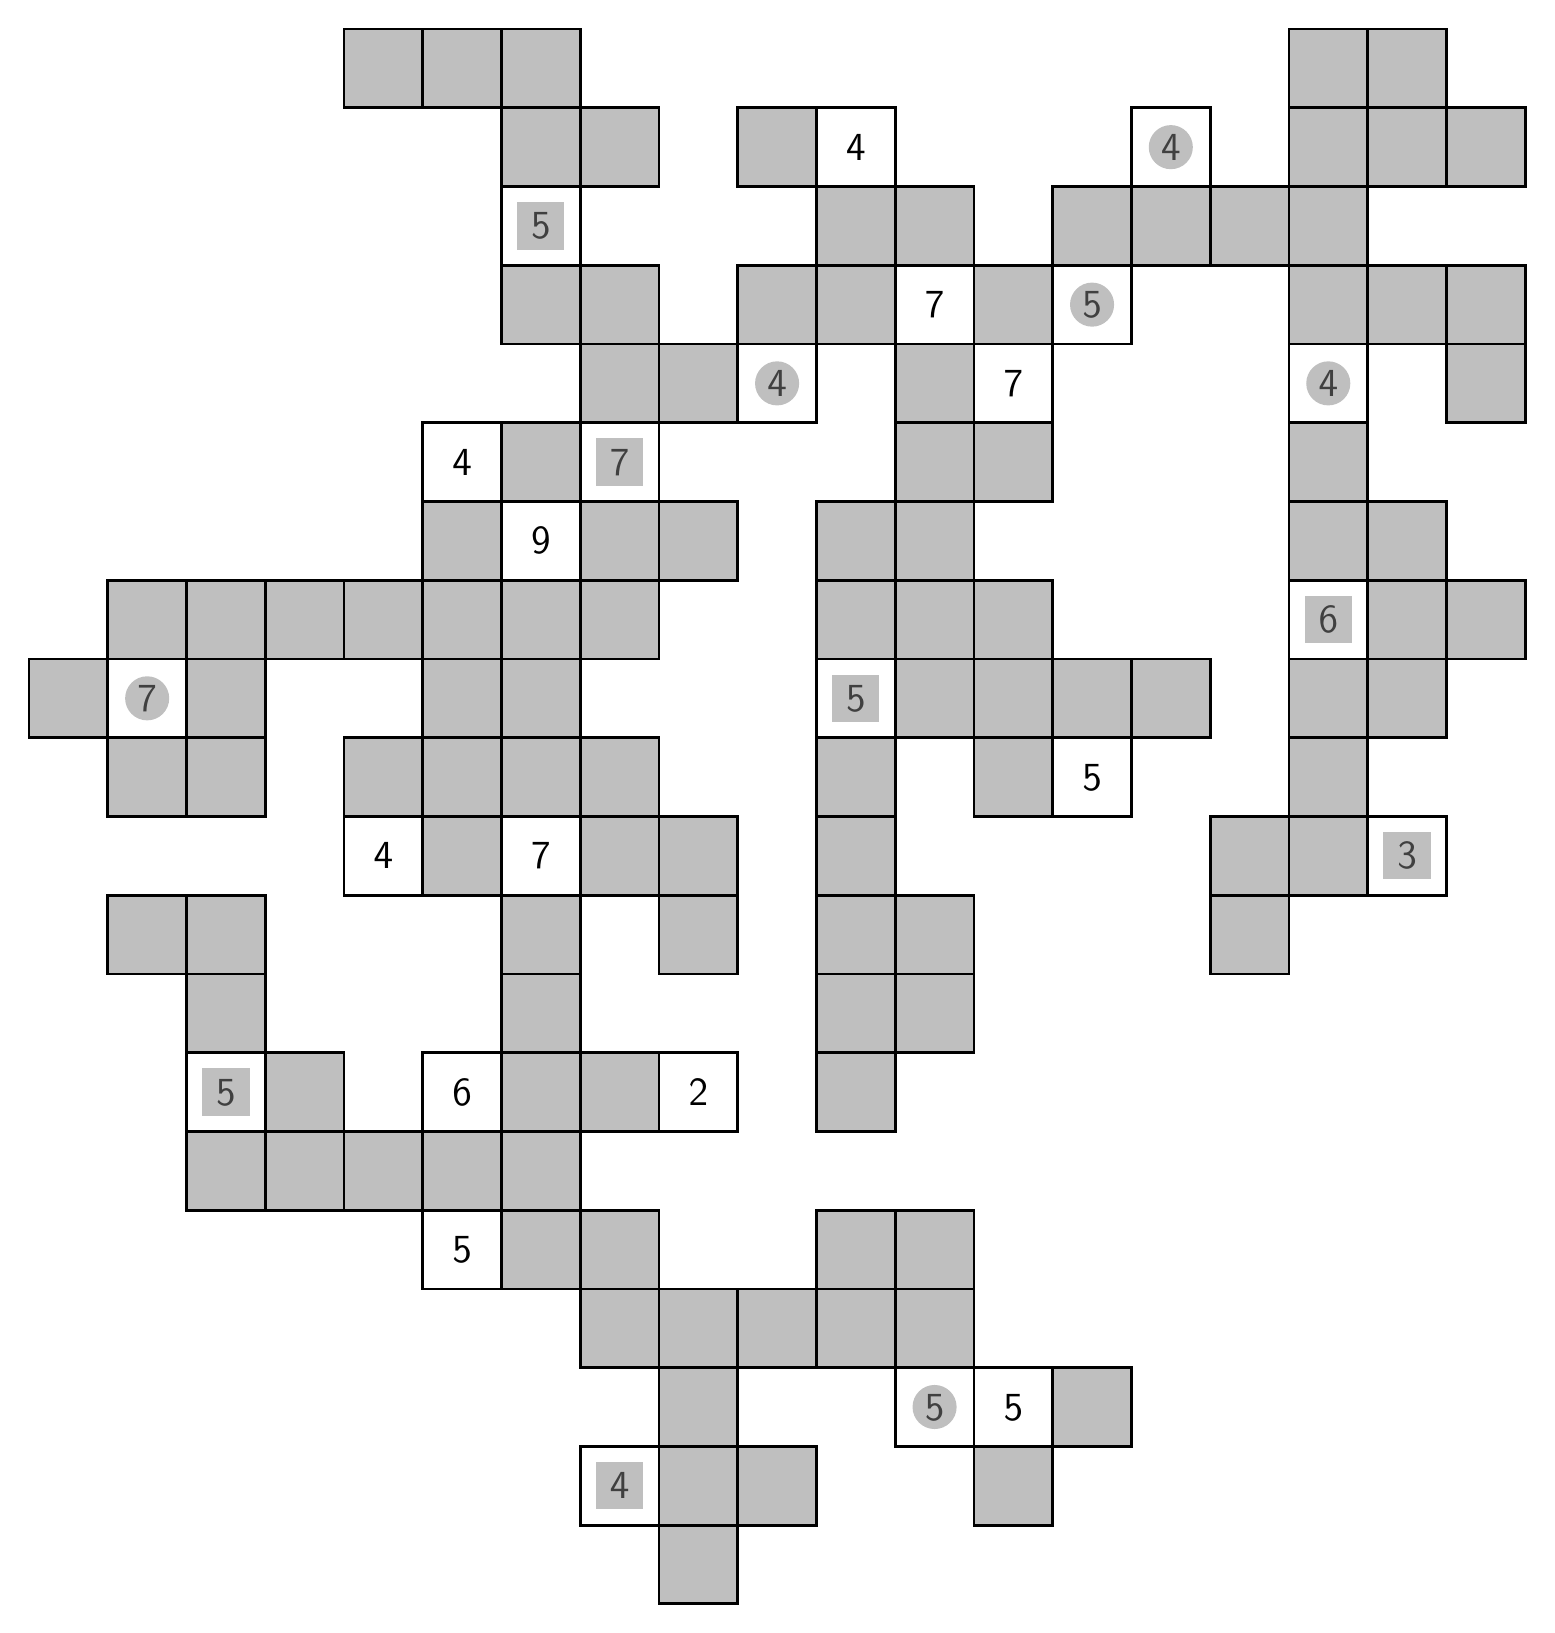
\begin{tikzpicture}\fill[gray, opacity = 0.5] (9, 0, 0)--++(1, 0, 0)--++(0, 1, 0)--++(-1, 0, 0)--cycle;
\draw[line width = 1pt] (9, 0, 0)--++(1, 0, 0)--++(0, 1, 0)--++(-1, 0, 0)--cycle;
\draw node at (8.5, 1.5, 0) {\Large $\mathsf{4}$};
\draw[line width = 1pt] (8, 1, 0)--++(1, 0, 0)--++(0, 1, 0)--++(-1, 0, 0)--cycle;
\fill[color = gray, opacity = 0.5] (8.2, 1.2) rectangle ++(0.6, 0.6);
\fill[gray, opacity = 0.5] (9, 1, 0)--++(1, 0, 0)--++(0, 1, 0)--++(-1, 0, 0)--cycle;
\draw[line width = 1pt] (9, 1, 0)--++(1, 0, 0)--++(0, 1, 0)--++(-1, 0, 0)--cycle;
\fill[gray, opacity = 0.5] (10, 1, 0)--++(1, 0, 0)--++(0, 1, 0)--++(-1, 0, 0)--cycle;
\draw[line width = 1pt] (10, 1, 0)--++(1, 0, 0)--++(0, 1, 0)--++(-1, 0, 0)--cycle;
\fill[gray, opacity = 0.5] (13, 1, 0)--++(1, 0, 0)--++(0, 1, 0)--++(-1, 0, 0)--cycle;
\draw[line width = 1pt] (13, 1, 0)--++(1, 0, 0)--++(0, 1, 0)--++(-1, 0, 0)--cycle;
\fill[gray, opacity = 0.5] (9, 2, 0)--++(1, 0, 0)--++(0, 1, 0)--++(-1, 0, 0)--cycle;
\draw[line width = 1pt] (9, 2, 0)--++(1, 0, 0)--++(0, 1, 0)--++(-1, 0, 0)--cycle;
\draw node at (12.5, 2.5, 0) {\Large $\mathsf{5}$};
\draw[line width = 1pt] (12, 2, 0)--++(1, 0, 0)--++(0, 1, 0)--++(-1, 0, 0)--cycle;
\fill[color = gray, opacity = 0.5] (12.5, 2.5, 0) circle (0.28);
\draw node at (13.5, 2.5, 0) {\Large $\mathsf{5}$};
\draw[line width = 1pt] (13, 2, 0)--++(1, 0, 0)--++(0, 1, 0)--++(-1, 0, 0)--cycle;
\fill[gray, opacity = 0.5] (14, 2, 0)--++(1, 0, 0)--++(0, 1, 0)--++(-1, 0, 0)--cycle;
\draw[line width = 1pt] (14, 2, 0)--++(1, 0, 0)--++(0, 1, 0)--++(-1, 0, 0)--cycle;
\fill[gray, opacity = 0.5] (8, 3, 0)--++(1, 0, 0)--++(0, 1, 0)--++(-1, 0, 0)--cycle;
\draw[line width = 1pt] (8, 3, 0)--++(1, 0, 0)--++(0, 1, 0)--++(-1, 0, 0)--cycle;
\fill[gray, opacity = 0.5] (9, 3, 0)--++(1, 0, 0)--++(0, 1, 0)--++(-1, 0, 0)--cycle;
\draw[line width = 1pt] (9, 3, 0)--++(1, 0, 0)--++(0, 1, 0)--++(-1, 0, 0)--cycle;
\fill[gray, opacity = 0.5] (10, 3, 0)--++(1, 0, 0)--++(0, 1, 0)--++(-1, 0, 0)--cycle;
\draw[line width = 1pt] (10, 3, 0)--++(1, 0, 0)--++(0, 1, 0)--++(-1, 0, 0)--cycle;
\fill[gray, opacity = 0.5] (11, 3, 0)--++(1, 0, 0)--++(0, 1, 0)--++(-1, 0, 0)--cycle;
\draw[line width = 1pt] (11, 3, 0)--++(1, 0, 0)--++(0, 1, 0)--++(-1, 0, 0)--cycle;
\fill[gray, opacity = 0.5] (12, 3, 0)--++(1, 0, 0)--++(0, 1, 0)--++(-1, 0, 0)--cycle;
\draw[line width = 1pt] (12, 3, 0)--++(1, 0, 0)--++(0, 1, 0)--++(-1, 0, 0)--cycle;
\draw node at (6.5, 4.5, 0) {\Large $\mathsf{5}$};
\draw[line width = 1pt] (6, 4, 0)--++(1, 0, 0)--++(0, 1, 0)--++(-1, 0, 0)--cycle;
\fill[gray, opacity = 0.5] (7, 4, 0)--++(1, 0, 0)--++(0, 1, 0)--++(-1, 0, 0)--cycle;
\draw[line width = 1pt] (7, 4, 0)--++(1, 0, 0)--++(0, 1, 0)--++(-1, 0, 0)--cycle;
\fill[gray, opacity = 0.5] (8, 4, 0)--++(1, 0, 0)--++(0, 1, 0)--++(-1, 0, 0)--cycle;
\draw[line width = 1pt] (8, 4, 0)--++(1, 0, 0)--++(0, 1, 0)--++(-1, 0, 0)--cycle;
\fill[gray, opacity = 0.5] (11, 4, 0)--++(1, 0, 0)--++(0, 1, 0)--++(-1, 0, 0)--cycle;
\draw[line width = 1pt] (11, 4, 0)--++(1, 0, 0)--++(0, 1, 0)--++(-1, 0, 0)--cycle;
\fill[gray, opacity = 0.5] (12, 4, 0)--++(1, 0, 0)--++(0, 1, 0)--++(-1, 0, 0)--cycle;
\draw[line width = 1pt] (12, 4, 0)--++(1, 0, 0)--++(0, 1, 0)--++(-1, 0, 0)--cycle;
\fill[gray, opacity = 0.5] (3, 5, 0)--++(1, 0, 0)--++(0, 1, 0)--++(-1, 0, 0)--cycle;
\draw[line width = 1pt] (3, 5, 0)--++(1, 0, 0)--++(0, 1, 0)--++(-1, 0, 0)--cycle;
\fill[gray, opacity = 0.5] (4, 5, 0)--++(1, 0, 0)--++(0, 1, 0)--++(-1, 0, 0)--cycle;
\draw[line width = 1pt] (4, 5, 0)--++(1, 0, 0)--++(0, 1, 0)--++(-1, 0, 0)--cycle;
\fill[gray, opacity = 0.5] (5, 5, 0)--++(1, 0, 0)--++(0, 1, 0)--++(-1, 0, 0)--cycle;
\draw[line width = 1pt] (5, 5, 0)--++(1, 0, 0)--++(0, 1, 0)--++(-1, 0, 0)--cycle;
\fill[gray, opacity = 0.5] (6, 5, 0)--++(1, 0, 0)--++(0, 1, 0)--++(-1, 0, 0)--cycle;
\draw[line width = 1pt] (6, 5, 0)--++(1, 0, 0)--++(0, 1, 0)--++(-1, 0, 0)--cycle;
\fill[gray, opacity = 0.5] (7, 5, 0)--++(1, 0, 0)--++(0, 1, 0)--++(-1, 0, 0)--cycle;
\draw[line width = 1pt] (7, 5, 0)--++(1, 0, 0)--++(0, 1, 0)--++(-1, 0, 0)--cycle;
\draw node at (3.5, 6.5, 0) {\Large $\mathsf{5}$};
\draw[line width = 1pt] (3, 6, 0)--++(1, 0, 0)--++(0, 1, 0)--++(-1, 0, 0)--cycle;
\fill[color = gray, opacity = 0.5] (3.2, 6.2) rectangle ++(0.6, 0.6);
\fill[gray, opacity = 0.5] (4, 6, 0)--++(1, 0, 0)--++(0, 1, 0)--++(-1, 0, 0)--cycle;
\draw[line width = 1pt] (4, 6, 0)--++(1, 0, 0)--++(0, 1, 0)--++(-1, 0, 0)--cycle;
\draw node at (6.5, 6.5, 0) {\Large $\mathsf{6}$};
\draw[line width = 1pt] (6, 6, 0)--++(1, 0, 0)--++(0, 1, 0)--++(-1, 0, 0)--cycle;
\fill[gray, opacity = 0.5] (7, 6, 0)--++(1, 0, 0)--++(0, 1, 0)--++(-1, 0, 0)--cycle;
\draw[line width = 1pt] (7, 6, 0)--++(1, 0, 0)--++(0, 1, 0)--++(-1, 0, 0)--cycle;
\fill[gray, opacity = 0.5] (8, 6, 0)--++(1, 0, 0)--++(0, 1, 0)--++(-1, 0, 0)--cycle;
\draw[line width = 1pt] (8, 6, 0)--++(1, 0, 0)--++(0, 1, 0)--++(-1, 0, 0)--cycle;
\draw node at (9.5, 6.5, 0) {\Large $\mathsf{2}$};
\draw[line width = 1pt] (9, 6, 0)--++(1, 0, 0)--++(0, 1, 0)--++(-1, 0, 0)--cycle;
\fill[gray, opacity = 0.5] (11, 6, 0)--++(1, 0, 0)--++(0, 1, 0)--++(-1, 0, 0)--cycle;
\draw[line width = 1pt] (11, 6, 0)--++(1, 0, 0)--++(0, 1, 0)--++(-1, 0, 0)--cycle;
\fill[gray, opacity = 0.5] (3, 7, 0)--++(1, 0, 0)--++(0, 1, 0)--++(-1, 0, 0)--cycle;
\draw[line width = 1pt] (3, 7, 0)--++(1, 0, 0)--++(0, 1, 0)--++(-1, 0, 0)--cycle;
\fill[gray, opacity = 0.5] (7, 7, 0)--++(1, 0, 0)--++(0, 1, 0)--++(-1, 0, 0)--cycle;
\draw[line width = 1pt] (7, 7, 0)--++(1, 0, 0)--++(0, 1, 0)--++(-1, 0, 0)--cycle;
\fill[gray, opacity = 0.5] (11, 7, 0)--++(1, 0, 0)--++(0, 1, 0)--++(-1, 0, 0)--cycle;
\draw[line width = 1pt] (11, 7, 0)--++(1, 0, 0)--++(0, 1, 0)--++(-1, 0, 0)--cycle;
\fill[gray, opacity = 0.5] (12, 7, 0)--++(1, 0, 0)--++(0, 1, 0)--++(-1, 0, 0)--cycle;
\draw[line width = 1pt] (12, 7, 0)--++(1, 0, 0)--++(0, 1, 0)--++(-1, 0, 0)--cycle;
\fill[gray, opacity = 0.5] (2, 8, 0)--++(1, 0, 0)--++(0, 1, 0)--++(-1, 0, 0)--cycle;
\draw[line width = 1pt] (2, 8, 0)--++(1, 0, 0)--++(0, 1, 0)--++(-1, 0, 0)--cycle;
\fill[gray, opacity = 0.5] (3, 8, 0)--++(1, 0, 0)--++(0, 1, 0)--++(-1, 0, 0)--cycle;
\draw[line width = 1pt] (3, 8, 0)--++(1, 0, 0)--++(0, 1, 0)--++(-1, 0, 0)--cycle;
\fill[gray, opacity = 0.5] (7, 8, 0)--++(1, 0, 0)--++(0, 1, 0)--++(-1, 0, 0)--cycle;
\draw[line width = 1pt] (7, 8, 0)--++(1, 0, 0)--++(0, 1, 0)--++(-1, 0, 0)--cycle;
\fill[gray, opacity = 0.5] (9, 8, 0)--++(1, 0, 0)--++(0, 1, 0)--++(-1, 0, 0)--cycle;
\draw[line width = 1pt] (9, 8, 0)--++(1, 0, 0)--++(0, 1, 0)--++(-1, 0, 0)--cycle;
\fill[gray, opacity = 0.5] (11, 8, 0)--++(1, 0, 0)--++(0, 1, 0)--++(-1, 0, 0)--cycle;
\draw[line width = 1pt] (11, 8, 0)--++(1, 0, 0)--++(0, 1, 0)--++(-1, 0, 0)--cycle;
\fill[gray, opacity = 0.5] (12, 8, 0)--++(1, 0, 0)--++(0, 1, 0)--++(-1, 0, 0)--cycle;
\draw[line width = 1pt] (12, 8, 0)--++(1, 0, 0)--++(0, 1, 0)--++(-1, 0, 0)--cycle;
\fill[gray, opacity = 0.5] (16, 8, 0)--++(1, 0, 0)--++(0, 1, 0)--++(-1, 0, 0)--cycle;
\draw[line width = 1pt] (16, 8, 0)--++(1, 0, 0)--++(0, 1, 0)--++(-1, 0, 0)--cycle;
\draw node at (5.5, 9.5, 0) {\Large $\mathsf{4}$};
\draw[line width = 1pt] (5, 9, 0)--++(1, 0, 0)--++(0, 1, 0)--++(-1, 0, 0)--cycle;
\fill[gray, opacity = 0.5] (6, 9, 0)--++(1, 0, 0)--++(0, 1, 0)--++(-1, 0, 0)--cycle;
\draw[line width = 1pt] (6, 9, 0)--++(1, 0, 0)--++(0, 1, 0)--++(-1, 0, 0)--cycle;
\draw node at (7.5, 9.5, 0) {\Large $\mathsf{7}$};
\draw[line width = 1pt] (7, 9, 0)--++(1, 0, 0)--++(0, 1, 0)--++(-1, 0, 0)--cycle;
\fill[gray, opacity = 0.5] (8, 9, 0)--++(1, 0, 0)--++(0, 1, 0)--++(-1, 0, 0)--cycle;
\draw[line width = 1pt] (8, 9, 0)--++(1, 0, 0)--++(0, 1, 0)--++(-1, 0, 0)--cycle;
\fill[gray, opacity = 0.5] (9, 9, 0)--++(1, 0, 0)--++(0, 1, 0)--++(-1, 0, 0)--cycle;
\draw[line width = 1pt] (9, 9, 0)--++(1, 0, 0)--++(0, 1, 0)--++(-1, 0, 0)--cycle;
\fill[gray, opacity = 0.5] (11, 9, 0)--++(1, 0, 0)--++(0, 1, 0)--++(-1, 0, 0)--cycle;
\draw[line width = 1pt] (11, 9, 0)--++(1, 0, 0)--++(0, 1, 0)--++(-1, 0, 0)--cycle;
\fill[gray, opacity = 0.5] (16, 9, 0)--++(1, 0, 0)--++(0, 1, 0)--++(-1, 0, 0)--cycle;
\draw[line width = 1pt] (16, 9, 0)--++(1, 0, 0)--++(0, 1, 0)--++(-1, 0, 0)--cycle;
\fill[gray, opacity = 0.5] (17, 9, 0)--++(1, 0, 0)--++(0, 1, 0)--++(-1, 0, 0)--cycle;
\draw[line width = 1pt] (17, 9, 0)--++(1, 0, 0)--++(0, 1, 0)--++(-1, 0, 0)--cycle;
\draw node at (18.5, 9.5, 0) {\Large $\mathsf{3}$};
\draw[line width = 1pt] (18, 9, 0)--++(1, 0, 0)--++(0, 1, 0)--++(-1, 0, 0)--cycle;
\fill[color = gray, opacity = 0.5] (18.2, 9.2) rectangle ++(0.6, 0.6);
\fill[gray, opacity = 0.5] (2, 10, 0)--++(1, 0, 0)--++(0, 1, 0)--++(-1, 0, 0)--cycle;
\draw[line width = 1pt] (2, 10, 0)--++(1, 0, 0)--++(0, 1, 0)--++(-1, 0, 0)--cycle;
\fill[gray, opacity = 0.5] (3, 10, 0)--++(1, 0, 0)--++(0, 1, 0)--++(-1, 0, 0)--cycle;
\draw[line width = 1pt] (3, 10, 0)--++(1, 0, 0)--++(0, 1, 0)--++(-1, 0, 0)--cycle;
\fill[gray, opacity = 0.5] (5, 10, 0)--++(1, 0, 0)--++(0, 1, 0)--++(-1, 0, 0)--cycle;
\draw[line width = 1pt] (5, 10, 0)--++(1, 0, 0)--++(0, 1, 0)--++(-1, 0, 0)--cycle;
\fill[gray, opacity = 0.5] (6, 10, 0)--++(1, 0, 0)--++(0, 1, 0)--++(-1, 0, 0)--cycle;
\draw[line width = 1pt] (6, 10, 0)--++(1, 0, 0)--++(0, 1, 0)--++(-1, 0, 0)--cycle;
\fill[gray, opacity = 0.5] (7, 10, 0)--++(1, 0, 0)--++(0, 1, 0)--++(-1, 0, 0)--cycle;
\draw[line width = 1pt] (7, 10, 0)--++(1, 0, 0)--++(0, 1, 0)--++(-1, 0, 0)--cycle;
\fill[gray, opacity = 0.5] (8, 10, 0)--++(1, 0, 0)--++(0, 1, 0)--++(-1, 0, 0)--cycle;
\draw[line width = 1pt] (8, 10, 0)--++(1, 0, 0)--++(0, 1, 0)--++(-1, 0, 0)--cycle;
\fill[gray, opacity = 0.5] (11, 10, 0)--++(1, 0, 0)--++(0, 1, 0)--++(-1, 0, 0)--cycle;
\draw[line width = 1pt] (11, 10, 0)--++(1, 0, 0)--++(0, 1, 0)--++(-1, 0, 0)--cycle;
\fill[gray, opacity = 0.5] (13, 10, 0)--++(1, 0, 0)--++(0, 1, 0)--++(-1, 0, 0)--cycle;
\draw[line width = 1pt] (13, 10, 0)--++(1, 0, 0)--++(0, 1, 0)--++(-1, 0, 0)--cycle;
\draw node at (14.5, 10.5, 0) {\Large $\mathsf{5}$};
\draw[line width = 1pt] (14, 10, 0)--++(1, 0, 0)--++(0, 1, 0)--++(-1, 0, 0)--cycle;
\fill[gray, opacity = 0.5] (17, 10, 0)--++(1, 0, 0)--++(0, 1, 0)--++(-1, 0, 0)--cycle;
\draw[line width = 1pt] (17, 10, 0)--++(1, 0, 0)--++(0, 1, 0)--++(-1, 0, 0)--cycle;
\fill[gray, opacity = 0.5] (1, 11, 0)--++(1, 0, 0)--++(0, 1, 0)--++(-1, 0, 0)--cycle;
\draw[line width = 1pt] (1, 11, 0)--++(1, 0, 0)--++(0, 1, 0)--++(-1, 0, 0)--cycle;
\draw node at (2.5, 11.5, 0) {\Large $\mathsf{7}$};
\draw[line width = 1pt] (2, 11, 0)--++(1, 0, 0)--++(0, 1, 0)--++(-1, 0, 0)--cycle;
\fill[color = gray, opacity = 0.5] (2.5, 11.5, 0) circle (0.28);
\fill[gray, opacity = 0.5] (3, 11, 0)--++(1, 0, 0)--++(0, 1, 0)--++(-1, 0, 0)--cycle;
\draw[line width = 1pt] (3, 11, 0)--++(1, 0, 0)--++(0, 1, 0)--++(-1, 0, 0)--cycle;
\fill[gray, opacity = 0.5] (6, 11, 0)--++(1, 0, 0)--++(0, 1, 0)--++(-1, 0, 0)--cycle;
\draw[line width = 1pt] (6, 11, 0)--++(1, 0, 0)--++(0, 1, 0)--++(-1, 0, 0)--cycle;
\fill[gray, opacity = 0.5] (7, 11, 0)--++(1, 0, 0)--++(0, 1, 0)--++(-1, 0, 0)--cycle;
\draw[line width = 1pt] (7, 11, 0)--++(1, 0, 0)--++(0, 1, 0)--++(-1, 0, 0)--cycle;
\draw node at (11.5, 11.5, 0) {\Large $\mathsf{5}$};
\draw[line width = 1pt] (11, 11, 0)--++(1, 0, 0)--++(0, 1, 0)--++(-1, 0, 0)--cycle;
\fill[color = gray, opacity = 0.5] (11.2, 11.2) rectangle ++(0.6, 0.6);
\fill[gray, opacity = 0.5] (12, 11, 0)--++(1, 0, 0)--++(0, 1, 0)--++(-1, 0, 0)--cycle;
\draw[line width = 1pt] (12, 11, 0)--++(1, 0, 0)--++(0, 1, 0)--++(-1, 0, 0)--cycle;
\fill[gray, opacity = 0.5] (13, 11, 0)--++(1, 0, 0)--++(0, 1, 0)--++(-1, 0, 0)--cycle;
\draw[line width = 1pt] (13, 11, 0)--++(1, 0, 0)--++(0, 1, 0)--++(-1, 0, 0)--cycle;
\fill[gray, opacity = 0.5] (14, 11, 0)--++(1, 0, 0)--++(0, 1, 0)--++(-1, 0, 0)--cycle;
\draw[line width = 1pt] (14, 11, 0)--++(1, 0, 0)--++(0, 1, 0)--++(-1, 0, 0)--cycle;
\fill[gray, opacity = 0.5] (15, 11, 0)--++(1, 0, 0)--++(0, 1, 0)--++(-1, 0, 0)--cycle;
\draw[line width = 1pt] (15, 11, 0)--++(1, 0, 0)--++(0, 1, 0)--++(-1, 0, 0)--cycle;
\fill[gray, opacity = 0.5] (17, 11, 0)--++(1, 0, 0)--++(0, 1, 0)--++(-1, 0, 0)--cycle;
\draw[line width = 1pt] (17, 11, 0)--++(1, 0, 0)--++(0, 1, 0)--++(-1, 0, 0)--cycle;
\fill[gray, opacity = 0.5] (18, 11, 0)--++(1, 0, 0)--++(0, 1, 0)--++(-1, 0, 0)--cycle;
\draw[line width = 1pt] (18, 11, 0)--++(1, 0, 0)--++(0, 1, 0)--++(-1, 0, 0)--cycle;
\fill[gray, opacity = 0.5] (2, 12, 0)--++(1, 0, 0)--++(0, 1, 0)--++(-1, 0, 0)--cycle;
\draw[line width = 1pt] (2, 12, 0)--++(1, 0, 0)--++(0, 1, 0)--++(-1, 0, 0)--cycle;
\fill[gray, opacity = 0.5] (3, 12, 0)--++(1, 0, 0)--++(0, 1, 0)--++(-1, 0, 0)--cycle;
\draw[line width = 1pt] (3, 12, 0)--++(1, 0, 0)--++(0, 1, 0)--++(-1, 0, 0)--cycle;
\fill[gray, opacity = 0.5] (4, 12, 0)--++(1, 0, 0)--++(0, 1, 0)--++(-1, 0, 0)--cycle;
\draw[line width = 1pt] (4, 12, 0)--++(1, 0, 0)--++(0, 1, 0)--++(-1, 0, 0)--cycle;
\fill[gray, opacity = 0.5] (5, 12, 0)--++(1, 0, 0)--++(0, 1, 0)--++(-1, 0, 0)--cycle;
\draw[line width = 1pt] (5, 12, 0)--++(1, 0, 0)--++(0, 1, 0)--++(-1, 0, 0)--cycle;
\fill[gray, opacity = 0.5] (6, 12, 0)--++(1, 0, 0)--++(0, 1, 0)--++(-1, 0, 0)--cycle;
\draw[line width = 1pt] (6, 12, 0)--++(1, 0, 0)--++(0, 1, 0)--++(-1, 0, 0)--cycle;
\fill[gray, opacity = 0.5] (7, 12, 0)--++(1, 0, 0)--++(0, 1, 0)--++(-1, 0, 0)--cycle;
\draw[line width = 1pt] (7, 12, 0)--++(1, 0, 0)--++(0, 1, 0)--++(-1, 0, 0)--cycle;
\fill[gray, opacity = 0.5] (8, 12, 0)--++(1, 0, 0)--++(0, 1, 0)--++(-1, 0, 0)--cycle;
\draw[line width = 1pt] (8, 12, 0)--++(1, 0, 0)--++(0, 1, 0)--++(-1, 0, 0)--cycle;
\fill[gray, opacity = 0.5] (11, 12, 0)--++(1, 0, 0)--++(0, 1, 0)--++(-1, 0, 0)--cycle;
\draw[line width = 1pt] (11, 12, 0)--++(1, 0, 0)--++(0, 1, 0)--++(-1, 0, 0)--cycle;
\fill[gray, opacity = 0.5] (12, 12, 0)--++(1, 0, 0)--++(0, 1, 0)--++(-1, 0, 0)--cycle;
\draw[line width = 1pt] (12, 12, 0)--++(1, 0, 0)--++(0, 1, 0)--++(-1, 0, 0)--cycle;
\fill[gray, opacity = 0.5] (13, 12, 0)--++(1, 0, 0)--++(0, 1, 0)--++(-1, 0, 0)--cycle;
\draw[line width = 1pt] (13, 12, 0)--++(1, 0, 0)--++(0, 1, 0)--++(-1, 0, 0)--cycle;
\draw node at (17.5, 12.5, 0) {\Large $\mathsf{6}$};
\draw[line width = 1pt] (17, 12, 0)--++(1, 0, 0)--++(0, 1, 0)--++(-1, 0, 0)--cycle;
\fill[color = gray, opacity = 0.5] (17.2, 12.2) rectangle ++(0.6, 0.6);
\fill[gray, opacity = 0.5] (18, 12, 0)--++(1, 0, 0)--++(0, 1, 0)--++(-1, 0, 0)--cycle;
\draw[line width = 1pt] (18, 12, 0)--++(1, 0, 0)--++(0, 1, 0)--++(-1, 0, 0)--cycle;
\fill[gray, opacity = 0.5] (19, 12, 0)--++(1, 0, 0)--++(0, 1, 0)--++(-1, 0, 0)--cycle;
\draw[line width = 1pt] (19, 12, 0)--++(1, 0, 0)--++(0, 1, 0)--++(-1, 0, 0)--cycle;
\fill[gray, opacity = 0.5] (6, 13, 0)--++(1, 0, 0)--++(0, 1, 0)--++(-1, 0, 0)--cycle;
\draw[line width = 1pt] (6, 13, 0)--++(1, 0, 0)--++(0, 1, 0)--++(-1, 0, 0)--cycle;
\draw node at (7.5, 13.5, 0) {\Large $\mathsf{9}$};
\draw[line width = 1pt] (7, 13, 0)--++(1, 0, 0)--++(0, 1, 0)--++(-1, 0, 0)--cycle;
\fill[gray, opacity = 0.5] (8, 13, 0)--++(1, 0, 0)--++(0, 1, 0)--++(-1, 0, 0)--cycle;
\draw[line width = 1pt] (8, 13, 0)--++(1, 0, 0)--++(0, 1, 0)--++(-1, 0, 0)--cycle;
\fill[gray, opacity = 0.5] (9, 13, 0)--++(1, 0, 0)--++(0, 1, 0)--++(-1, 0, 0)--cycle;
\draw[line width = 1pt] (9, 13, 0)--++(1, 0, 0)--++(0, 1, 0)--++(-1, 0, 0)--cycle;
\fill[gray, opacity = 0.5] (11, 13, 0)--++(1, 0, 0)--++(0, 1, 0)--++(-1, 0, 0)--cycle;
\draw[line width = 1pt] (11, 13, 0)--++(1, 0, 0)--++(0, 1, 0)--++(-1, 0, 0)--cycle;
\fill[gray, opacity = 0.5] (12, 13, 0)--++(1, 0, 0)--++(0, 1, 0)--++(-1, 0, 0)--cycle;
\draw[line width = 1pt] (12, 13, 0)--++(1, 0, 0)--++(0, 1, 0)--++(-1, 0, 0)--cycle;
\fill[gray, opacity = 0.5] (17, 13, 0)--++(1, 0, 0)--++(0, 1, 0)--++(-1, 0, 0)--cycle;
\draw[line width = 1pt] (17, 13, 0)--++(1, 0, 0)--++(0, 1, 0)--++(-1, 0, 0)--cycle;
\fill[gray, opacity = 0.5] (18, 13, 0)--++(1, 0, 0)--++(0, 1, 0)--++(-1, 0, 0)--cycle;
\draw[line width = 1pt] (18, 13, 0)--++(1, 0, 0)--++(0, 1, 0)--++(-1, 0, 0)--cycle;
\draw node at (6.5, 14.5, 0) {\Large $\mathsf{4}$};
\draw[line width = 1pt] (6, 14, 0)--++(1, 0, 0)--++(0, 1, 0)--++(-1, 0, 0)--cycle;
\fill[gray, opacity = 0.5] (7, 14, 0)--++(1, 0, 0)--++(0, 1, 0)--++(-1, 0, 0)--cycle;
\draw[line width = 1pt] (7, 14, 0)--++(1, 0, 0)--++(0, 1, 0)--++(-1, 0, 0)--cycle;
\draw node at (8.5, 14.5, 0) {\Large $\mathsf{7}$};
\draw[line width = 1pt] (8, 14, 0)--++(1, 0, 0)--++(0, 1, 0)--++(-1, 0, 0)--cycle;
\fill[color = gray, opacity = 0.5] (8.2, 14.2) rectangle ++(0.6, 0.6);
\fill[gray, opacity = 0.5] (12, 14, 0)--++(1, 0, 0)--++(0, 1, 0)--++(-1, 0, 0)--cycle;
\draw[line width = 1pt] (12, 14, 0)--++(1, 0, 0)--++(0, 1, 0)--++(-1, 0, 0)--cycle;
\fill[gray, opacity = 0.5] (13, 14, 0)--++(1, 0, 0)--++(0, 1, 0)--++(-1, 0, 0)--cycle;
\draw[line width = 1pt] (13, 14, 0)--++(1, 0, 0)--++(0, 1, 0)--++(-1, 0, 0)--cycle;
\fill[gray, opacity = 0.5] (17, 14, 0)--++(1, 0, 0)--++(0, 1, 0)--++(-1, 0, 0)--cycle;
\draw[line width = 1pt] (17, 14, 0)--++(1, 0, 0)--++(0, 1, 0)--++(-1, 0, 0)--cycle;
\fill[gray, opacity = 0.5] (8, 15, 0)--++(1, 0, 0)--++(0, 1, 0)--++(-1, 0, 0)--cycle;
\draw[line width = 1pt] (8, 15, 0)--++(1, 0, 0)--++(0, 1, 0)--++(-1, 0, 0)--cycle;
\fill[gray, opacity = 0.5] (9, 15, 0)--++(1, 0, 0)--++(0, 1, 0)--++(-1, 0, 0)--cycle;
\draw[line width = 1pt] (9, 15, 0)--++(1, 0, 0)--++(0, 1, 0)--++(-1, 0, 0)--cycle;
\draw node at (10.5, 15.5, 0) {\Large $\mathsf{4}$};
\draw[line width = 1pt] (10, 15, 0)--++(1, 0, 0)--++(0, 1, 0)--++(-1, 0, 0)--cycle;
\fill[color = gray, opacity = 0.5] (10.5, 15.5, 0) circle (0.28);
\fill[gray, opacity = 0.5] (12, 15, 0)--++(1, 0, 0)--++(0, 1, 0)--++(-1, 0, 0)--cycle;
\draw[line width = 1pt] (12, 15, 0)--++(1, 0, 0)--++(0, 1, 0)--++(-1, 0, 0)--cycle;
\draw node at (13.5, 15.5, 0) {\Large $\mathsf{7}$};
\draw[line width = 1pt] (13, 15, 0)--++(1, 0, 0)--++(0, 1, 0)--++(-1, 0, 0)--cycle;
\draw node at (17.5, 15.5, 0) {\Large $\mathsf{4}$};
\draw[line width = 1pt] (17, 15, 0)--++(1, 0, 0)--++(0, 1, 0)--++(-1, 0, 0)--cycle;
\fill[color = gray, opacity = 0.5] (17.5, 15.5, 0) circle (0.28);
\fill[gray, opacity = 0.5] (19, 15, 0)--++(1, 0, 0)--++(0, 1, 0)--++(-1, 0, 0)--cycle;
\draw[line width = 1pt] (19, 15, 0)--++(1, 0, 0)--++(0, 1, 0)--++(-1, 0, 0)--cycle;
\fill[gray, opacity = 0.5] (7, 16, 0)--++(1, 0, 0)--++(0, 1, 0)--++(-1, 0, 0)--cycle;
\draw[line width = 1pt] (7, 16, 0)--++(1, 0, 0)--++(0, 1, 0)--++(-1, 0, 0)--cycle;
\fill[gray, opacity = 0.5] (8, 16, 0)--++(1, 0, 0)--++(0, 1, 0)--++(-1, 0, 0)--cycle;
\draw[line width = 1pt] (8, 16, 0)--++(1, 0, 0)--++(0, 1, 0)--++(-1, 0, 0)--cycle;
\fill[gray, opacity = 0.5] (10, 16, 0)--++(1, 0, 0)--++(0, 1, 0)--++(-1, 0, 0)--cycle;
\draw[line width = 1pt] (10, 16, 0)--++(1, 0, 0)--++(0, 1, 0)--++(-1, 0, 0)--cycle;
\fill[gray, opacity = 0.5] (11, 16, 0)--++(1, 0, 0)--++(0, 1, 0)--++(-1, 0, 0)--cycle;
\draw[line width = 1pt] (11, 16, 0)--++(1, 0, 0)--++(0, 1, 0)--++(-1, 0, 0)--cycle;
\draw node at (12.5, 16.5, 0) {\Large $\mathsf{7}$};
\draw[line width = 1pt] (12, 16, 0)--++(1, 0, 0)--++(0, 1, 0)--++(-1, 0, 0)--cycle;
\fill[gray, opacity = 0.5] (13, 16, 0)--++(1, 0, 0)--++(0, 1, 0)--++(-1, 0, 0)--cycle;
\draw[line width = 1pt] (13, 16, 0)--++(1, 0, 0)--++(0, 1, 0)--++(-1, 0, 0)--cycle;
\draw node at (14.5, 16.5, 0) {\Large $\mathsf{5}$};
\draw[line width = 1pt] (14, 16, 0)--++(1, 0, 0)--++(0, 1, 0)--++(-1, 0, 0)--cycle;
\fill[color = gray, opacity = 0.5] (14.5, 16.5, 0) circle (0.28);
\fill[gray, opacity = 0.5] (17, 16, 0)--++(1, 0, 0)--++(0, 1, 0)--++(-1, 0, 0)--cycle;
\draw[line width = 1pt] (17, 16, 0)--++(1, 0, 0)--++(0, 1, 0)--++(-1, 0, 0)--cycle;
\fill[gray, opacity = 0.5] (18, 16, 0)--++(1, 0, 0)--++(0, 1, 0)--++(-1, 0, 0)--cycle;
\draw[line width = 1pt] (18, 16, 0)--++(1, 0, 0)--++(0, 1, 0)--++(-1, 0, 0)--cycle;
\fill[gray, opacity = 0.5] (19, 16, 0)--++(1, 0, 0)--++(0, 1, 0)--++(-1, 0, 0)--cycle;
\draw[line width = 1pt] (19, 16, 0)--++(1, 0, 0)--++(0, 1, 0)--++(-1, 0, 0)--cycle;
\draw node at (7.5, 17.5, 0) {\Large $\mathsf{5}$};
\draw[line width = 1pt] (7, 17, 0)--++(1, 0, 0)--++(0, 1, 0)--++(-1, 0, 0)--cycle;
\fill[color = gray, opacity = 0.5] (7.2, 17.2) rectangle ++(0.6, 0.6);
\fill[gray, opacity = 0.5] (11, 17, 0)--++(1, 0, 0)--++(0, 1, 0)--++(-1, 0, 0)--cycle;
\draw[line width = 1pt] (11, 17, 0)--++(1, 0, 0)--++(0, 1, 0)--++(-1, 0, 0)--cycle;
\fill[gray, opacity = 0.5] (12, 17, 0)--++(1, 0, 0)--++(0, 1, 0)--++(-1, 0, 0)--cycle;
\draw[line width = 1pt] (12, 17, 0)--++(1, 0, 0)--++(0, 1, 0)--++(-1, 0, 0)--cycle;
\fill[gray, opacity = 0.5] (14, 17, 0)--++(1, 0, 0)--++(0, 1, 0)--++(-1, 0, 0)--cycle;
\draw[line width = 1pt] (14, 17, 0)--++(1, 0, 0)--++(0, 1, 0)--++(-1, 0, 0)--cycle;
\fill[gray, opacity = 0.5] (15, 17, 0)--++(1, 0, 0)--++(0, 1, 0)--++(-1, 0, 0)--cycle;
\draw[line width = 1pt] (15, 17, 0)--++(1, 0, 0)--++(0, 1, 0)--++(-1, 0, 0)--cycle;
\fill[gray, opacity = 0.5] (16, 17, 0)--++(1, 0, 0)--++(0, 1, 0)--++(-1, 0, 0)--cycle;
\draw[line width = 1pt] (16, 17, 0)--++(1, 0, 0)--++(0, 1, 0)--++(-1, 0, 0)--cycle;
\fill[gray, opacity = 0.5] (17, 17, 0)--++(1, 0, 0)--++(0, 1, 0)--++(-1, 0, 0)--cycle;
\draw[line width = 1pt] (17, 17, 0)--++(1, 0, 0)--++(0, 1, 0)--++(-1, 0, 0)--cycle;
\fill[gray, opacity = 0.5] (7, 18, 0)--++(1, 0, 0)--++(0, 1, 0)--++(-1, 0, 0)--cycle;
\draw[line width = 1pt] (7, 18, 0)--++(1, 0, 0)--++(0, 1, 0)--++(-1, 0, 0)--cycle;
\fill[gray, opacity = 0.5] (8, 18, 0)--++(1, 0, 0)--++(0, 1, 0)--++(-1, 0, 0)--cycle;
\draw[line width = 1pt] (8, 18, 0)--++(1, 0, 0)--++(0, 1, 0)--++(-1, 0, 0)--cycle;
\fill[gray, opacity = 0.5] (10, 18, 0)--++(1, 0, 0)--++(0, 1, 0)--++(-1, 0, 0)--cycle;
\draw[line width = 1pt] (10, 18, 0)--++(1, 0, 0)--++(0, 1, 0)--++(-1, 0, 0)--cycle;
\draw node at (11.5, 18.5, 0) {\Large $\mathsf{4}$};
\draw[line width = 1pt] (11, 18, 0)--++(1, 0, 0)--++(0, 1, 0)--++(-1, 0, 0)--cycle;
\draw node at (15.5, 18.5, 0) {\Large $\mathsf{4}$};
\draw[line width = 1pt] (15, 18, 0)--++(1, 0, 0)--++(0, 1, 0)--++(-1, 0, 0)--cycle;
\fill[color = gray, opacity = 0.5] (15.5, 18.5, 0) circle (0.28);
\fill[gray, opacity = 0.5] (17, 18, 0)--++(1, 0, 0)--++(0, 1, 0)--++(-1, 0, 0)--cycle;
\draw[line width = 1pt] (17, 18, 0)--++(1, 0, 0)--++(0, 1, 0)--++(-1, 0, 0)--cycle;
\fill[gray, opacity = 0.5] (18, 18, 0)--++(1, 0, 0)--++(0, 1, 0)--++(-1, 0, 0)--cycle;
\draw[line width = 1pt] (18, 18, 0)--++(1, 0, 0)--++(0, 1, 0)--++(-1, 0, 0)--cycle;
\fill[gray, opacity = 0.5] (19, 18, 0)--++(1, 0, 0)--++(0, 1, 0)--++(-1, 0, 0)--cycle;
\draw[line width = 1pt] (19, 18, 0)--++(1, 0, 0)--++(0, 1, 0)--++(-1, 0, 0)--cycle;
\fill[gray, opacity = 0.5] (5, 19, 0)--++(1, 0, 0)--++(0, 1, 0)--++(-1, 0, 0)--cycle;
\draw[line width = 1pt] (5, 19, 0)--++(1, 0, 0)--++(0, 1, 0)--++(-1, 0, 0)--cycle;
\fill[gray, opacity = 0.5] (6, 19, 0)--++(1, 0, 0)--++(0, 1, 0)--++(-1, 0, 0)--cycle;
\draw[line width = 1pt] (6, 19, 0)--++(1, 0, 0)--++(0, 1, 0)--++(-1, 0, 0)--cycle;
\fill[gray, opacity = 0.5] (7, 19, 0)--++(1, 0, 0)--++(0, 1, 0)--++(-1, 0, 0)--cycle;
\draw[line width = 1pt] (7, 19, 0)--++(1, 0, 0)--++(0, 1, 0)--++(-1, 0, 0)--cycle;
\fill[gray, opacity = 0.5] (17, 19, 0)--++(1, 0, 0)--++(0, 1, 0)--++(-1, 0, 0)--cycle;
\draw[line width = 1pt] (17, 19, 0)--++(1, 0, 0)--++(0, 1, 0)--++(-1, 0, 0)--cycle;
\fill[gray, opacity = 0.5] (18, 19, 0)--++(1, 0, 0)--++(0, 1, 0)--++(-1, 0, 0)--cycle;
\draw[line width = 1pt] (18, 19, 0)--++(1, 0, 0)--++(0, 1, 0)--++(-1, 0, 0)--cycle;
\end{tikzpicture}}\]
\[\resizebox{30pc}{!}{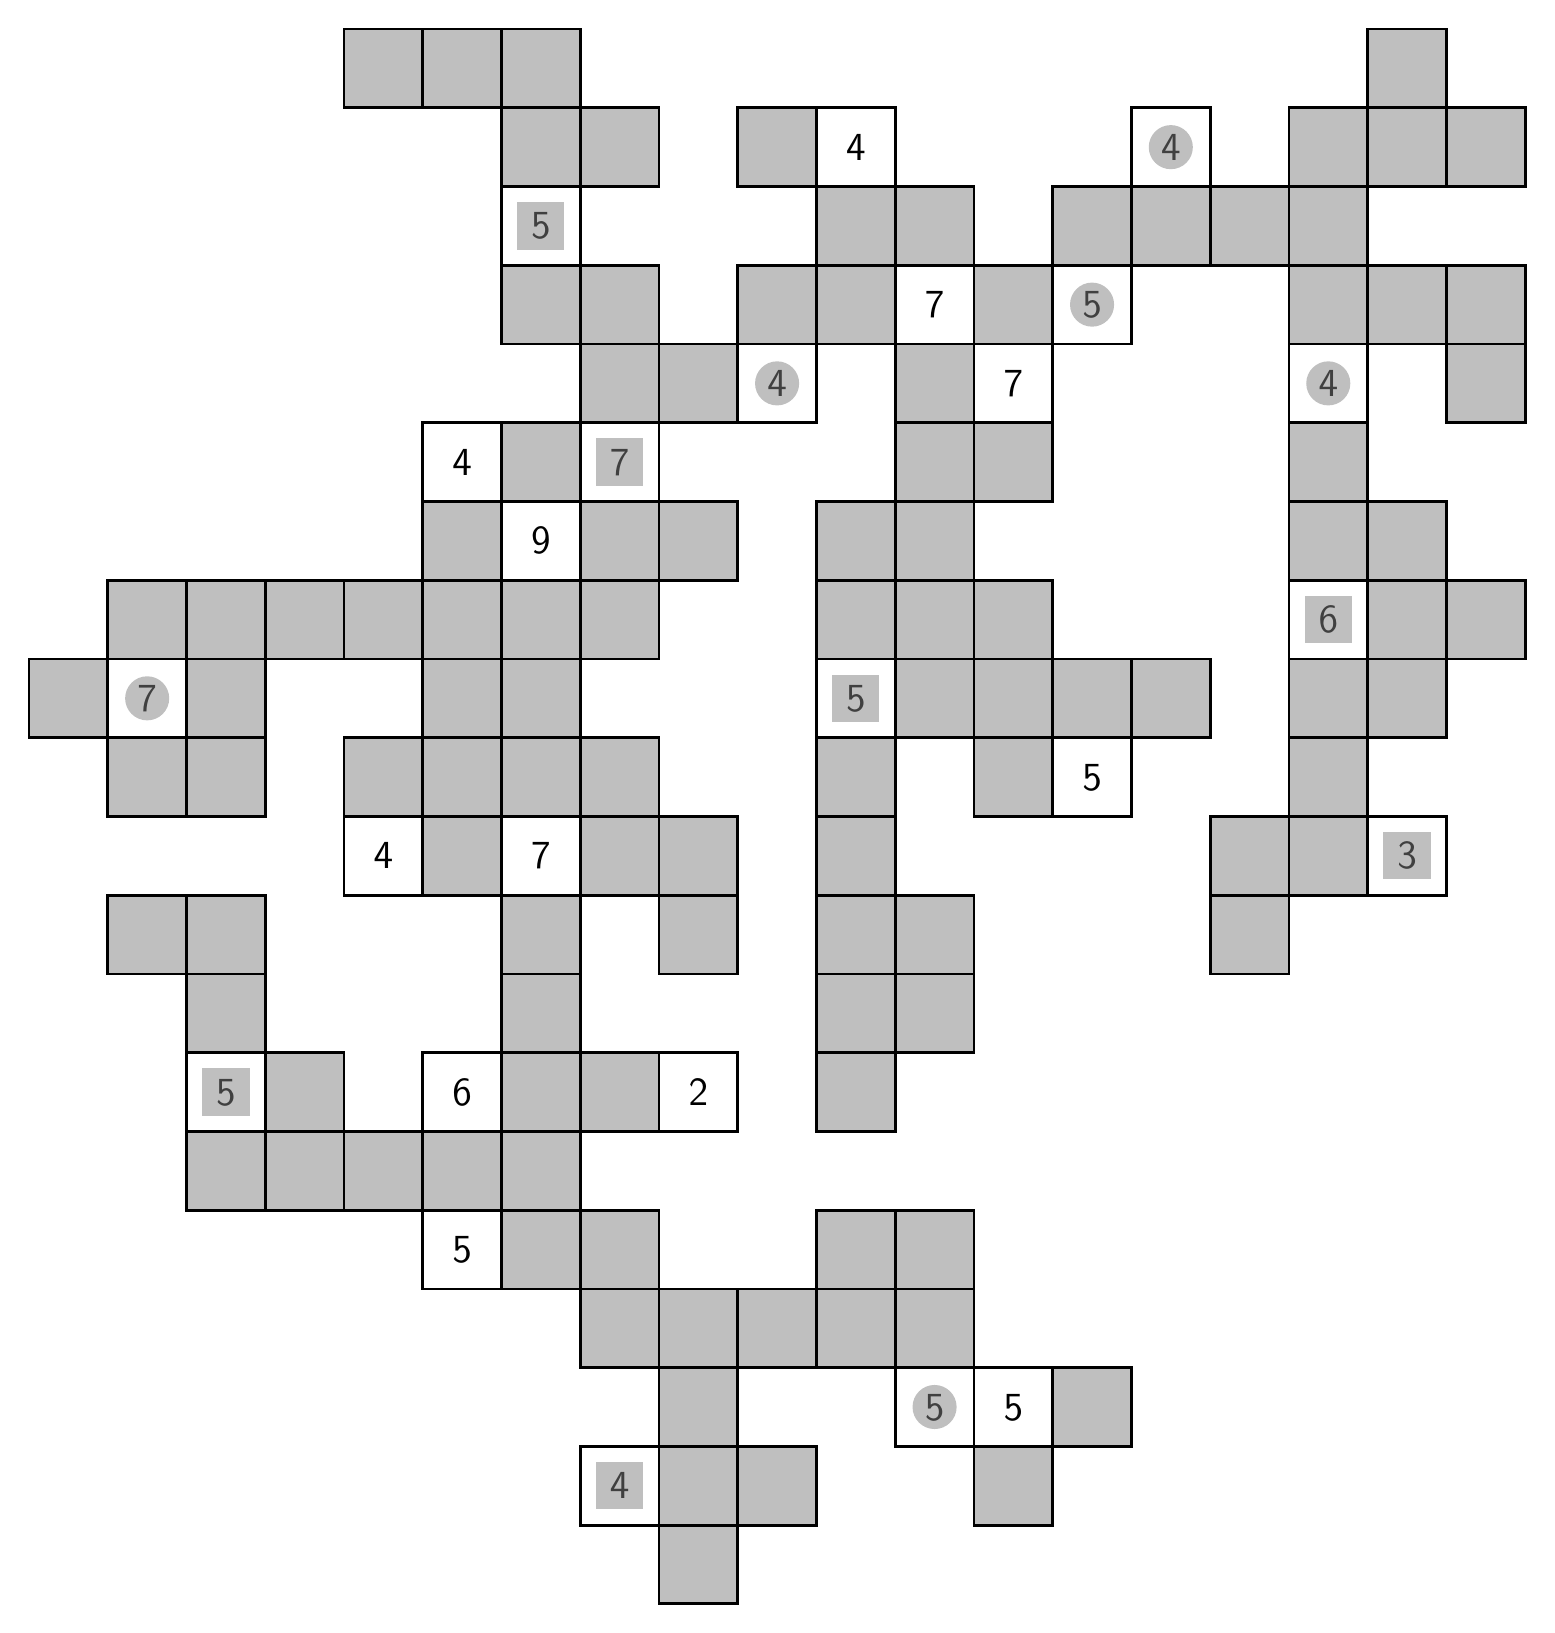
\begin{tikzpicture}\fill[gray, opacity = 0.5] (9, 0, 0)--++(1, 0, 0)--++(0, 1, 0)--++(-1, 0, 0)--cycle;
\draw[line width = 1pt] (9, 0, 0)--++(1, 0, 0)--++(0, 1, 0)--++(-1, 0, 0)--cycle;
\draw node at (8.5, 1.5, 0) {\Large $\mathsf{4}$};
\draw[line width = 1pt] (8, 1, 0)--++(1, 0, 0)--++(0, 1, 0)--++(-1, 0, 0)--cycle;
\fill[color = gray, opacity = 0.5] (8.2, 1.2) rectangle ++(0.6, 0.6);
\fill[gray, opacity = 0.5] (9, 1, 0)--++(1, 0, 0)--++(0, 1, 0)--++(-1, 0, 0)--cycle;
\draw[line width = 1pt] (9, 1, 0)--++(1, 0, 0)--++(0, 1, 0)--++(-1, 0, 0)--cycle;
\fill[gray, opacity = 0.5] (10, 1, 0)--++(1, 0, 0)--++(0, 1, 0)--++(-1, 0, 0)--cycle;
\draw[line width = 1pt] (10, 1, 0)--++(1, 0, 0)--++(0, 1, 0)--++(-1, 0, 0)--cycle;
\fill[gray, opacity = 0.5] (13, 1, 0)--++(1, 0, 0)--++(0, 1, 0)--++(-1, 0, 0)--cycle;
\draw[line width = 1pt] (13, 1, 0)--++(1, 0, 0)--++(0, 1, 0)--++(-1, 0, 0)--cycle;
\fill[gray, opacity = 0.5] (9, 2, 0)--++(1, 0, 0)--++(0, 1, 0)--++(-1, 0, 0)--cycle;
\draw[line width = 1pt] (9, 2, 0)--++(1, 0, 0)--++(0, 1, 0)--++(-1, 0, 0)--cycle;
\draw node at (12.5, 2.5, 0) {\Large $\mathsf{5}$};
\draw[line width = 1pt] (12, 2, 0)--++(1, 0, 0)--++(0, 1, 0)--++(-1, 0, 0)--cycle;
\fill[color = gray, opacity = 0.5] (12.5, 2.5, 0) circle (0.28);
\draw node at (13.5, 2.5, 0) {\Large $\mathsf{5}$};
\draw[line width = 1pt] (13, 2, 0)--++(1, 0, 0)--++(0, 1, 0)--++(-1, 0, 0)--cycle;
\fill[gray, opacity = 0.5] (14, 2, 0)--++(1, 0, 0)--++(0, 1, 0)--++(-1, 0, 0)--cycle;
\draw[line width = 1pt] (14, 2, 0)--++(1, 0, 0)--++(0, 1, 0)--++(-1, 0, 0)--cycle;
\fill[gray, opacity = 0.5] (8, 3, 0)--++(1, 0, 0)--++(0, 1, 0)--++(-1, 0, 0)--cycle;
\draw[line width = 1pt] (8, 3, 0)--++(1, 0, 0)--++(0, 1, 0)--++(-1, 0, 0)--cycle;
\fill[gray, opacity = 0.5] (9, 3, 0)--++(1, 0, 0)--++(0, 1, 0)--++(-1, 0, 0)--cycle;
\draw[line width = 1pt] (9, 3, 0)--++(1, 0, 0)--++(0, 1, 0)--++(-1, 0, 0)--cycle;
\fill[gray, opacity = 0.5] (10, 3, 0)--++(1, 0, 0)--++(0, 1, 0)--++(-1, 0, 0)--cycle;
\draw[line width = 1pt] (10, 3, 0)--++(1, 0, 0)--++(0, 1, 0)--++(-1, 0, 0)--cycle;
\fill[gray, opacity = 0.5] (11, 3, 0)--++(1, 0, 0)--++(0, 1, 0)--++(-1, 0, 0)--cycle;
\draw[line width = 1pt] (11, 3, 0)--++(1, 0, 0)--++(0, 1, 0)--++(-1, 0, 0)--cycle;
\fill[gray, opacity = 0.5] (12, 3, 0)--++(1, 0, 0)--++(0, 1, 0)--++(-1, 0, 0)--cycle;
\draw[line width = 1pt] (12, 3, 0)--++(1, 0, 0)--++(0, 1, 0)--++(-1, 0, 0)--cycle;
\draw node at (6.5, 4.5, 0) {\Large $\mathsf{5}$};
\draw[line width = 1pt] (6, 4, 0)--++(1, 0, 0)--++(0, 1, 0)--++(-1, 0, 0)--cycle;
\fill[gray, opacity = 0.5] (7, 4, 0)--++(1, 0, 0)--++(0, 1, 0)--++(-1, 0, 0)--cycle;
\draw[line width = 1pt] (7, 4, 0)--++(1, 0, 0)--++(0, 1, 0)--++(-1, 0, 0)--cycle;
\fill[gray, opacity = 0.5] (8, 4, 0)--++(1, 0, 0)--++(0, 1, 0)--++(-1, 0, 0)--cycle;
\draw[line width = 1pt] (8, 4, 0)--++(1, 0, 0)--++(0, 1, 0)--++(-1, 0, 0)--cycle;
\fill[gray, opacity = 0.5] (11, 4, 0)--++(1, 0, 0)--++(0, 1, 0)--++(-1, 0, 0)--cycle;
\draw[line width = 1pt] (11, 4, 0)--++(1, 0, 0)--++(0, 1, 0)--++(-1, 0, 0)--cycle;
\fill[gray, opacity = 0.5] (12, 4, 0)--++(1, 0, 0)--++(0, 1, 0)--++(-1, 0, 0)--cycle;
\draw[line width = 1pt] (12, 4, 0)--++(1, 0, 0)--++(0, 1, 0)--++(-1, 0, 0)--cycle;
\fill[gray, opacity = 0.5] (3, 5, 0)--++(1, 0, 0)--++(0, 1, 0)--++(-1, 0, 0)--cycle;
\draw[line width = 1pt] (3, 5, 0)--++(1, 0, 0)--++(0, 1, 0)--++(-1, 0, 0)--cycle;
\fill[gray, opacity = 0.5] (4, 5, 0)--++(1, 0, 0)--++(0, 1, 0)--++(-1, 0, 0)--cycle;
\draw[line width = 1pt] (4, 5, 0)--++(1, 0, 0)--++(0, 1, 0)--++(-1, 0, 0)--cycle;
\fill[gray, opacity = 0.5] (5, 5, 0)--++(1, 0, 0)--++(0, 1, 0)--++(-1, 0, 0)--cycle;
\draw[line width = 1pt] (5, 5, 0)--++(1, 0, 0)--++(0, 1, 0)--++(-1, 0, 0)--cycle;
\fill[gray, opacity = 0.5] (6, 5, 0)--++(1, 0, 0)--++(0, 1, 0)--++(-1, 0, 0)--cycle;
\draw[line width = 1pt] (6, 5, 0)--++(1, 0, 0)--++(0, 1, 0)--++(-1, 0, 0)--cycle;
\fill[gray, opacity = 0.5] (7, 5, 0)--++(1, 0, 0)--++(0, 1, 0)--++(-1, 0, 0)--cycle;
\draw[line width = 1pt] (7, 5, 0)--++(1, 0, 0)--++(0, 1, 0)--++(-1, 0, 0)--cycle;
\draw node at (3.5, 6.5, 0) {\Large $\mathsf{5}$};
\draw[line width = 1pt] (3, 6, 0)--++(1, 0, 0)--++(0, 1, 0)--++(-1, 0, 0)--cycle;
\fill[color = gray, opacity = 0.5] (3.2, 6.2) rectangle ++(0.6, 0.6);
\fill[gray, opacity = 0.5] (4, 6, 0)--++(1, 0, 0)--++(0, 1, 0)--++(-1, 0, 0)--cycle;
\draw[line width = 1pt] (4, 6, 0)--++(1, 0, 0)--++(0, 1, 0)--++(-1, 0, 0)--cycle;
\draw node at (6.5, 6.5, 0) {\Large $\mathsf{6}$};
\draw[line width = 1pt] (6, 6, 0)--++(1, 0, 0)--++(0, 1, 0)--++(-1, 0, 0)--cycle;
\fill[gray, opacity = 0.5] (7, 6, 0)--++(1, 0, 0)--++(0, 1, 0)--++(-1, 0, 0)--cycle;
\draw[line width = 1pt] (7, 6, 0)--++(1, 0, 0)--++(0, 1, 0)--++(-1, 0, 0)--cycle;
\fill[gray, opacity = 0.5] (8, 6, 0)--++(1, 0, 0)--++(0, 1, 0)--++(-1, 0, 0)--cycle;
\draw[line width = 1pt] (8, 6, 0)--++(1, 0, 0)--++(0, 1, 0)--++(-1, 0, 0)--cycle;
\draw node at (9.5, 6.5, 0) {\Large $\mathsf{2}$};
\draw[line width = 1pt] (9, 6, 0)--++(1, 0, 0)--++(0, 1, 0)--++(-1, 0, 0)--cycle;
\fill[gray, opacity = 0.5] (11, 6, 0)--++(1, 0, 0)--++(0, 1, 0)--++(-1, 0, 0)--cycle;
\draw[line width = 1pt] (11, 6, 0)--++(1, 0, 0)--++(0, 1, 0)--++(-1, 0, 0)--cycle;
\fill[gray, opacity = 0.5] (3, 7, 0)--++(1, 0, 0)--++(0, 1, 0)--++(-1, 0, 0)--cycle;
\draw[line width = 1pt] (3, 7, 0)--++(1, 0, 0)--++(0, 1, 0)--++(-1, 0, 0)--cycle;
\fill[gray, opacity = 0.5] (7, 7, 0)--++(1, 0, 0)--++(0, 1, 0)--++(-1, 0, 0)--cycle;
\draw[line width = 1pt] (7, 7, 0)--++(1, 0, 0)--++(0, 1, 0)--++(-1, 0, 0)--cycle;
\fill[gray, opacity = 0.5] (11, 7, 0)--++(1, 0, 0)--++(0, 1, 0)--++(-1, 0, 0)--cycle;
\draw[line width = 1pt] (11, 7, 0)--++(1, 0, 0)--++(0, 1, 0)--++(-1, 0, 0)--cycle;
\fill[gray, opacity = 0.5] (12, 7, 0)--++(1, 0, 0)--++(0, 1, 0)--++(-1, 0, 0)--cycle;
\draw[line width = 1pt] (12, 7, 0)--++(1, 0, 0)--++(0, 1, 0)--++(-1, 0, 0)--cycle;
\fill[gray, opacity = 0.5] (2, 8, 0)--++(1, 0, 0)--++(0, 1, 0)--++(-1, 0, 0)--cycle;
\draw[line width = 1pt] (2, 8, 0)--++(1, 0, 0)--++(0, 1, 0)--++(-1, 0, 0)--cycle;
\fill[gray, opacity = 0.5] (3, 8, 0)--++(1, 0, 0)--++(0, 1, 0)--++(-1, 0, 0)--cycle;
\draw[line width = 1pt] (3, 8, 0)--++(1, 0, 0)--++(0, 1, 0)--++(-1, 0, 0)--cycle;
\fill[gray, opacity = 0.5] (7, 8, 0)--++(1, 0, 0)--++(0, 1, 0)--++(-1, 0, 0)--cycle;
\draw[line width = 1pt] (7, 8, 0)--++(1, 0, 0)--++(0, 1, 0)--++(-1, 0, 0)--cycle;
\fill[gray, opacity = 0.5] (9, 8, 0)--++(1, 0, 0)--++(0, 1, 0)--++(-1, 0, 0)--cycle;
\draw[line width = 1pt] (9, 8, 0)--++(1, 0, 0)--++(0, 1, 0)--++(-1, 0, 0)--cycle;
\fill[gray, opacity = 0.5] (11, 8, 0)--++(1, 0, 0)--++(0, 1, 0)--++(-1, 0, 0)--cycle;
\draw[line width = 1pt] (11, 8, 0)--++(1, 0, 0)--++(0, 1, 0)--++(-1, 0, 0)--cycle;
\fill[gray, opacity = 0.5] (12, 8, 0)--++(1, 0, 0)--++(0, 1, 0)--++(-1, 0, 0)--cycle;
\draw[line width = 1pt] (12, 8, 0)--++(1, 0, 0)--++(0, 1, 0)--++(-1, 0, 0)--cycle;
\fill[gray, opacity = 0.5] (16, 8, 0)--++(1, 0, 0)--++(0, 1, 0)--++(-1, 0, 0)--cycle;
\draw[line width = 1pt] (16, 8, 0)--++(1, 0, 0)--++(0, 1, 0)--++(-1, 0, 0)--cycle;
\draw node at (5.5, 9.5, 0) {\Large $\mathsf{4}$};
\draw[line width = 1pt] (5, 9, 0)--++(1, 0, 0)--++(0, 1, 0)--++(-1, 0, 0)--cycle;
\fill[gray, opacity = 0.5] (6, 9, 0)--++(1, 0, 0)--++(0, 1, 0)--++(-1, 0, 0)--cycle;
\draw[line width = 1pt] (6, 9, 0)--++(1, 0, 0)--++(0, 1, 0)--++(-1, 0, 0)--cycle;
\draw node at (7.5, 9.5, 0) {\Large $\mathsf{7}$};
\draw[line width = 1pt] (7, 9, 0)--++(1, 0, 0)--++(0, 1, 0)--++(-1, 0, 0)--cycle;
\fill[gray, opacity = 0.5] (8, 9, 0)--++(1, 0, 0)--++(0, 1, 0)--++(-1, 0, 0)--cycle;
\draw[line width = 1pt] (8, 9, 0)--++(1, 0, 0)--++(0, 1, 0)--++(-1, 0, 0)--cycle;
\fill[gray, opacity = 0.5] (9, 9, 0)--++(1, 0, 0)--++(0, 1, 0)--++(-1, 0, 0)--cycle;
\draw[line width = 1pt] (9, 9, 0)--++(1, 0, 0)--++(0, 1, 0)--++(-1, 0, 0)--cycle;
\fill[gray, opacity = 0.5] (11, 9, 0)--++(1, 0, 0)--++(0, 1, 0)--++(-1, 0, 0)--cycle;
\draw[line width = 1pt] (11, 9, 0)--++(1, 0, 0)--++(0, 1, 0)--++(-1, 0, 0)--cycle;
\fill[gray, opacity = 0.5] (16, 9, 0)--++(1, 0, 0)--++(0, 1, 0)--++(-1, 0, 0)--cycle;
\draw[line width = 1pt] (16, 9, 0)--++(1, 0, 0)--++(0, 1, 0)--++(-1, 0, 0)--cycle;
\fill[gray, opacity = 0.5] (17, 9, 0)--++(1, 0, 0)--++(0, 1, 0)--++(-1, 0, 0)--cycle;
\draw[line width = 1pt] (17, 9, 0)--++(1, 0, 0)--++(0, 1, 0)--++(-1, 0, 0)--cycle;
\draw node at (18.5, 9.5, 0) {\Large $\mathsf{3}$};
\draw[line width = 1pt] (18, 9, 0)--++(1, 0, 0)--++(0, 1, 0)--++(-1, 0, 0)--cycle;
\fill[color = gray, opacity = 0.5] (18.2, 9.2) rectangle ++(0.6, 0.6);
\fill[gray, opacity = 0.5] (2, 10, 0)--++(1, 0, 0)--++(0, 1, 0)--++(-1, 0, 0)--cycle;
\draw[line width = 1pt] (2, 10, 0)--++(1, 0, 0)--++(0, 1, 0)--++(-1, 0, 0)--cycle;
\fill[gray, opacity = 0.5] (3, 10, 0)--++(1, 0, 0)--++(0, 1, 0)--++(-1, 0, 0)--cycle;
\draw[line width = 1pt] (3, 10, 0)--++(1, 0, 0)--++(0, 1, 0)--++(-1, 0, 0)--cycle;
\fill[gray, opacity = 0.5] (5, 10, 0)--++(1, 0, 0)--++(0, 1, 0)--++(-1, 0, 0)--cycle;
\draw[line width = 1pt] (5, 10, 0)--++(1, 0, 0)--++(0, 1, 0)--++(-1, 0, 0)--cycle;
\fill[gray, opacity = 0.5] (6, 10, 0)--++(1, 0, 0)--++(0, 1, 0)--++(-1, 0, 0)--cycle;
\draw[line width = 1pt] (6, 10, 0)--++(1, 0, 0)--++(0, 1, 0)--++(-1, 0, 0)--cycle;
\fill[gray, opacity = 0.5] (7, 10, 0)--++(1, 0, 0)--++(0, 1, 0)--++(-1, 0, 0)--cycle;
\draw[line width = 1pt] (7, 10, 0)--++(1, 0, 0)--++(0, 1, 0)--++(-1, 0, 0)--cycle;
\fill[gray, opacity = 0.5] (8, 10, 0)--++(1, 0, 0)--++(0, 1, 0)--++(-1, 0, 0)--cycle;
\draw[line width = 1pt] (8, 10, 0)--++(1, 0, 0)--++(0, 1, 0)--++(-1, 0, 0)--cycle;
\fill[gray, opacity = 0.5] (11, 10, 0)--++(1, 0, 0)--++(0, 1, 0)--++(-1, 0, 0)--cycle;
\draw[line width = 1pt] (11, 10, 0)--++(1, 0, 0)--++(0, 1, 0)--++(-1, 0, 0)--cycle;
\fill[gray, opacity = 0.5] (13, 10, 0)--++(1, 0, 0)--++(0, 1, 0)--++(-1, 0, 0)--cycle;
\draw[line width = 1pt] (13, 10, 0)--++(1, 0, 0)--++(0, 1, 0)--++(-1, 0, 0)--cycle;
\draw node at (14.5, 10.5, 0) {\Large $\mathsf{5}$};
\draw[line width = 1pt] (14, 10, 0)--++(1, 0, 0)--++(0, 1, 0)--++(-1, 0, 0)--cycle;
\fill[gray, opacity = 0.5] (17, 10, 0)--++(1, 0, 0)--++(0, 1, 0)--++(-1, 0, 0)--cycle;
\draw[line width = 1pt] (17, 10, 0)--++(1, 0, 0)--++(0, 1, 0)--++(-1, 0, 0)--cycle;
\fill[gray, opacity = 0.5] (1, 11, 0)--++(1, 0, 0)--++(0, 1, 0)--++(-1, 0, 0)--cycle;
\draw[line width = 1pt] (1, 11, 0)--++(1, 0, 0)--++(0, 1, 0)--++(-1, 0, 0)--cycle;
\draw node at (2.5, 11.5, 0) {\Large $\mathsf{7}$};
\draw[line width = 1pt] (2, 11, 0)--++(1, 0, 0)--++(0, 1, 0)--++(-1, 0, 0)--cycle;
\fill[color = gray, opacity = 0.5] (2.5, 11.5, 0) circle (0.28);
\fill[gray, opacity = 0.5] (3, 11, 0)--++(1, 0, 0)--++(0, 1, 0)--++(-1, 0, 0)--cycle;
\draw[line width = 1pt] (3, 11, 0)--++(1, 0, 0)--++(0, 1, 0)--++(-1, 0, 0)--cycle;
\fill[gray, opacity = 0.5] (6, 11, 0)--++(1, 0, 0)--++(0, 1, 0)--++(-1, 0, 0)--cycle;
\draw[line width = 1pt] (6, 11, 0)--++(1, 0, 0)--++(0, 1, 0)--++(-1, 0, 0)--cycle;
\fill[gray, opacity = 0.5] (7, 11, 0)--++(1, 0, 0)--++(0, 1, 0)--++(-1, 0, 0)--cycle;
\draw[line width = 1pt] (7, 11, 0)--++(1, 0, 0)--++(0, 1, 0)--++(-1, 0, 0)--cycle;
\draw node at (11.5, 11.5, 0) {\Large $\mathsf{5}$};
\draw[line width = 1pt] (11, 11, 0)--++(1, 0, 0)--++(0, 1, 0)--++(-1, 0, 0)--cycle;
\fill[color = gray, opacity = 0.5] (11.2, 11.2) rectangle ++(0.6, 0.6);
\fill[gray, opacity = 0.5] (12, 11, 0)--++(1, 0, 0)--++(0, 1, 0)--++(-1, 0, 0)--cycle;
\draw[line width = 1pt] (12, 11, 0)--++(1, 0, 0)--++(0, 1, 0)--++(-1, 0, 0)--cycle;
\fill[gray, opacity = 0.5] (13, 11, 0)--++(1, 0, 0)--++(0, 1, 0)--++(-1, 0, 0)--cycle;
\draw[line width = 1pt] (13, 11, 0)--++(1, 0, 0)--++(0, 1, 0)--++(-1, 0, 0)--cycle;
\fill[gray, opacity = 0.5] (14, 11, 0)--++(1, 0, 0)--++(0, 1, 0)--++(-1, 0, 0)--cycle;
\draw[line width = 1pt] (14, 11, 0)--++(1, 0, 0)--++(0, 1, 0)--++(-1, 0, 0)--cycle;
\fill[gray, opacity = 0.5] (15, 11, 0)--++(1, 0, 0)--++(0, 1, 0)--++(-1, 0, 0)--cycle;
\draw[line width = 1pt] (15, 11, 0)--++(1, 0, 0)--++(0, 1, 0)--++(-1, 0, 0)--cycle;
\fill[gray, opacity = 0.5] (17, 11, 0)--++(1, 0, 0)--++(0, 1, 0)--++(-1, 0, 0)--cycle;
\draw[line width = 1pt] (17, 11, 0)--++(1, 0, 0)--++(0, 1, 0)--++(-1, 0, 0)--cycle;
\fill[gray, opacity = 0.5] (18, 11, 0)--++(1, 0, 0)--++(0, 1, 0)--++(-1, 0, 0)--cycle;
\draw[line width = 1pt] (18, 11, 0)--++(1, 0, 0)--++(0, 1, 0)--++(-1, 0, 0)--cycle;
\fill[gray, opacity = 0.5] (2, 12, 0)--++(1, 0, 0)--++(0, 1, 0)--++(-1, 0, 0)--cycle;
\draw[line width = 1pt] (2, 12, 0)--++(1, 0, 0)--++(0, 1, 0)--++(-1, 0, 0)--cycle;
\fill[gray, opacity = 0.5] (3, 12, 0)--++(1, 0, 0)--++(0, 1, 0)--++(-1, 0, 0)--cycle;
\draw[line width = 1pt] (3, 12, 0)--++(1, 0, 0)--++(0, 1, 0)--++(-1, 0, 0)--cycle;
\fill[gray, opacity = 0.5] (4, 12, 0)--++(1, 0, 0)--++(0, 1, 0)--++(-1, 0, 0)--cycle;
\draw[line width = 1pt] (4, 12, 0)--++(1, 0, 0)--++(0, 1, 0)--++(-1, 0, 0)--cycle;
\fill[gray, opacity = 0.5] (5, 12, 0)--++(1, 0, 0)--++(0, 1, 0)--++(-1, 0, 0)--cycle;
\draw[line width = 1pt] (5, 12, 0)--++(1, 0, 0)--++(0, 1, 0)--++(-1, 0, 0)--cycle;
\fill[gray, opacity = 0.5] (6, 12, 0)--++(1, 0, 0)--++(0, 1, 0)--++(-1, 0, 0)--cycle;
\draw[line width = 1pt] (6, 12, 0)--++(1, 0, 0)--++(0, 1, 0)--++(-1, 0, 0)--cycle;
\fill[gray, opacity = 0.5] (7, 12, 0)--++(1, 0, 0)--++(0, 1, 0)--++(-1, 0, 0)--cycle;
\draw[line width = 1pt] (7, 12, 0)--++(1, 0, 0)--++(0, 1, 0)--++(-1, 0, 0)--cycle;
\fill[gray, opacity = 0.5] (8, 12, 0)--++(1, 0, 0)--++(0, 1, 0)--++(-1, 0, 0)--cycle;
\draw[line width = 1pt] (8, 12, 0)--++(1, 0, 0)--++(0, 1, 0)--++(-1, 0, 0)--cycle;
\fill[gray, opacity = 0.5] (11, 12, 0)--++(1, 0, 0)--++(0, 1, 0)--++(-1, 0, 0)--cycle;
\draw[line width = 1pt] (11, 12, 0)--++(1, 0, 0)--++(0, 1, 0)--++(-1, 0, 0)--cycle;
\fill[gray, opacity = 0.5] (12, 12, 0)--++(1, 0, 0)--++(0, 1, 0)--++(-1, 0, 0)--cycle;
\draw[line width = 1pt] (12, 12, 0)--++(1, 0, 0)--++(0, 1, 0)--++(-1, 0, 0)--cycle;
\fill[gray, opacity = 0.5] (13, 12, 0)--++(1, 0, 0)--++(0, 1, 0)--++(-1, 0, 0)--cycle;
\draw[line width = 1pt] (13, 12, 0)--++(1, 0, 0)--++(0, 1, 0)--++(-1, 0, 0)--cycle;
\draw node at (17.5, 12.5, 0) {\Large $\mathsf{6}$};
\draw[line width = 1pt] (17, 12, 0)--++(1, 0, 0)--++(0, 1, 0)--++(-1, 0, 0)--cycle;
\fill[color = gray, opacity = 0.5] (17.2, 12.2) rectangle ++(0.6, 0.6);
\fill[gray, opacity = 0.5] (18, 12, 0)--++(1, 0, 0)--++(0, 1, 0)--++(-1, 0, 0)--cycle;
\draw[line width = 1pt] (18, 12, 0)--++(1, 0, 0)--++(0, 1, 0)--++(-1, 0, 0)--cycle;
\fill[gray, opacity = 0.5] (19, 12, 0)--++(1, 0, 0)--++(0, 1, 0)--++(-1, 0, 0)--cycle;
\draw[line width = 1pt] (19, 12, 0)--++(1, 0, 0)--++(0, 1, 0)--++(-1, 0, 0)--cycle;
\fill[gray, opacity = 0.5] (6, 13, 0)--++(1, 0, 0)--++(0, 1, 0)--++(-1, 0, 0)--cycle;
\draw[line width = 1pt] (6, 13, 0)--++(1, 0, 0)--++(0, 1, 0)--++(-1, 0, 0)--cycle;
\draw node at (7.5, 13.5, 0) {\Large $\mathsf{9}$};
\draw[line width = 1pt] (7, 13, 0)--++(1, 0, 0)--++(0, 1, 0)--++(-1, 0, 0)--cycle;
\fill[gray, opacity = 0.5] (8, 13, 0)--++(1, 0, 0)--++(0, 1, 0)--++(-1, 0, 0)--cycle;
\draw[line width = 1pt] (8, 13, 0)--++(1, 0, 0)--++(0, 1, 0)--++(-1, 0, 0)--cycle;
\fill[gray, opacity = 0.5] (9, 13, 0)--++(1, 0, 0)--++(0, 1, 0)--++(-1, 0, 0)--cycle;
\draw[line width = 1pt] (9, 13, 0)--++(1, 0, 0)--++(0, 1, 0)--++(-1, 0, 0)--cycle;
\fill[gray, opacity = 0.5] (11, 13, 0)--++(1, 0, 0)--++(0, 1, 0)--++(-1, 0, 0)--cycle;
\draw[line width = 1pt] (11, 13, 0)--++(1, 0, 0)--++(0, 1, 0)--++(-1, 0, 0)--cycle;
\fill[gray, opacity = 0.5] (12, 13, 0)--++(1, 0, 0)--++(0, 1, 0)--++(-1, 0, 0)--cycle;
\draw[line width = 1pt] (12, 13, 0)--++(1, 0, 0)--++(0, 1, 0)--++(-1, 0, 0)--cycle;
\fill[gray, opacity = 0.5] (17, 13, 0)--++(1, 0, 0)--++(0, 1, 0)--++(-1, 0, 0)--cycle;
\draw[line width = 1pt] (17, 13, 0)--++(1, 0, 0)--++(0, 1, 0)--++(-1, 0, 0)--cycle;
\fill[gray, opacity = 0.5] (18, 13, 0)--++(1, 0, 0)--++(0, 1, 0)--++(-1, 0, 0)--cycle;
\draw[line width = 1pt] (18, 13, 0)--++(1, 0, 0)--++(0, 1, 0)--++(-1, 0, 0)--cycle;
\draw node at (6.5, 14.5, 0) {\Large $\mathsf{4}$};
\draw[line width = 1pt] (6, 14, 0)--++(1, 0, 0)--++(0, 1, 0)--++(-1, 0, 0)--cycle;
\fill[gray, opacity = 0.5] (7, 14, 0)--++(1, 0, 0)--++(0, 1, 0)--++(-1, 0, 0)--cycle;
\draw[line width = 1pt] (7, 14, 0)--++(1, 0, 0)--++(0, 1, 0)--++(-1, 0, 0)--cycle;
\draw node at (8.5, 14.5, 0) {\Large $\mathsf{7}$};
\draw[line width = 1pt] (8, 14, 0)--++(1, 0, 0)--++(0, 1, 0)--++(-1, 0, 0)--cycle;
\fill[color = gray, opacity = 0.5] (8.2, 14.2) rectangle ++(0.6, 0.6);
\fill[gray, opacity = 0.5] (12, 14, 0)--++(1, 0, 0)--++(0, 1, 0)--++(-1, 0, 0)--cycle;
\draw[line width = 1pt] (12, 14, 0)--++(1, 0, 0)--++(0, 1, 0)--++(-1, 0, 0)--cycle;
\fill[gray, opacity = 0.5] (13, 14, 0)--++(1, 0, 0)--++(0, 1, 0)--++(-1, 0, 0)--cycle;
\draw[line width = 1pt] (13, 14, 0)--++(1, 0, 0)--++(0, 1, 0)--++(-1, 0, 0)--cycle;
\fill[gray, opacity = 0.5] (17, 14, 0)--++(1, 0, 0)--++(0, 1, 0)--++(-1, 0, 0)--cycle;
\draw[line width = 1pt] (17, 14, 0)--++(1, 0, 0)--++(0, 1, 0)--++(-1, 0, 0)--cycle;
\fill[gray, opacity = 0.5] (8, 15, 0)--++(1, 0, 0)--++(0, 1, 0)--++(-1, 0, 0)--cycle;
\draw[line width = 1pt] (8, 15, 0)--++(1, 0, 0)--++(0, 1, 0)--++(-1, 0, 0)--cycle;
\fill[gray, opacity = 0.5] (9, 15, 0)--++(1, 0, 0)--++(0, 1, 0)--++(-1, 0, 0)--cycle;
\draw[line width = 1pt] (9, 15, 0)--++(1, 0, 0)--++(0, 1, 0)--++(-1, 0, 0)--cycle;
\draw node at (10.5, 15.5, 0) {\Large $\mathsf{4}$};
\draw[line width = 1pt] (10, 15, 0)--++(1, 0, 0)--++(0, 1, 0)--++(-1, 0, 0)--cycle;
\fill[color = gray, opacity = 0.5] (10.5, 15.5, 0) circle (0.28);
\fill[gray, opacity = 0.5] (12, 15, 0)--++(1, 0, 0)--++(0, 1, 0)--++(-1, 0, 0)--cycle;
\draw[line width = 1pt] (12, 15, 0)--++(1, 0, 0)--++(0, 1, 0)--++(-1, 0, 0)--cycle;
\draw node at (13.5, 15.5, 0) {\Large $\mathsf{7}$};
\draw[line width = 1pt] (13, 15, 0)--++(1, 0, 0)--++(0, 1, 0)--++(-1, 0, 0)--cycle;
\draw node at (17.5, 15.5, 0) {\Large $\mathsf{4}$};
\draw[line width = 1pt] (17, 15, 0)--++(1, 0, 0)--++(0, 1, 0)--++(-1, 0, 0)--cycle;
\fill[color = gray, opacity = 0.5] (17.5, 15.5, 0) circle (0.28);
\fill[gray, opacity = 0.5] (19, 15, 0)--++(1, 0, 0)--++(0, 1, 0)--++(-1, 0, 0)--cycle;
\draw[line width = 1pt] (19, 15, 0)--++(1, 0, 0)--++(0, 1, 0)--++(-1, 0, 0)--cycle;
\fill[gray, opacity = 0.5] (7, 16, 0)--++(1, 0, 0)--++(0, 1, 0)--++(-1, 0, 0)--cycle;
\draw[line width = 1pt] (7, 16, 0)--++(1, 0, 0)--++(0, 1, 0)--++(-1, 0, 0)--cycle;
\fill[gray, opacity = 0.5] (8, 16, 0)--++(1, 0, 0)--++(0, 1, 0)--++(-1, 0, 0)--cycle;
\draw[line width = 1pt] (8, 16, 0)--++(1, 0, 0)--++(0, 1, 0)--++(-1, 0, 0)--cycle;
\fill[gray, opacity = 0.5] (10, 16, 0)--++(1, 0, 0)--++(0, 1, 0)--++(-1, 0, 0)--cycle;
\draw[line width = 1pt] (10, 16, 0)--++(1, 0, 0)--++(0, 1, 0)--++(-1, 0, 0)--cycle;
\fill[gray, opacity = 0.5] (11, 16, 0)--++(1, 0, 0)--++(0, 1, 0)--++(-1, 0, 0)--cycle;
\draw[line width = 1pt] (11, 16, 0)--++(1, 0, 0)--++(0, 1, 0)--++(-1, 0, 0)--cycle;
\draw node at (12.5, 16.5, 0) {\Large $\mathsf{7}$};
\draw[line width = 1pt] (12, 16, 0)--++(1, 0, 0)--++(0, 1, 0)--++(-1, 0, 0)--cycle;
\fill[gray, opacity = 0.5] (13, 16, 0)--++(1, 0, 0)--++(0, 1, 0)--++(-1, 0, 0)--cycle;
\draw[line width = 1pt] (13, 16, 0)--++(1, 0, 0)--++(0, 1, 0)--++(-1, 0, 0)--cycle;
\draw node at (14.5, 16.5, 0) {\Large $\mathsf{5}$};
\draw[line width = 1pt] (14, 16, 0)--++(1, 0, 0)--++(0, 1, 0)--++(-1, 0, 0)--cycle;
\fill[color = gray, opacity = 0.5] (14.5, 16.5, 0) circle (0.28);
\fill[gray, opacity = 0.5] (17, 16, 0)--++(1, 0, 0)--++(0, 1, 0)--++(-1, 0, 0)--cycle;
\draw[line width = 1pt] (17, 16, 0)--++(1, 0, 0)--++(0, 1, 0)--++(-1, 0, 0)--cycle;
\fill[gray, opacity = 0.5] (18, 16, 0)--++(1, 0, 0)--++(0, 1, 0)--++(-1, 0, 0)--cycle;
\draw[line width = 1pt] (18, 16, 0)--++(1, 0, 0)--++(0, 1, 0)--++(-1, 0, 0)--cycle;
\fill[gray, opacity = 0.5] (19, 16, 0)--++(1, 0, 0)--++(0, 1, 0)--++(-1, 0, 0)--cycle;
\draw[line width = 1pt] (19, 16, 0)--++(1, 0, 0)--++(0, 1, 0)--++(-1, 0, 0)--cycle;
\draw node at (7.5, 17.5, 0) {\Large $\mathsf{5}$};
\draw[line width = 1pt] (7, 17, 0)--++(1, 0, 0)--++(0, 1, 0)--++(-1, 0, 0)--cycle;
\fill[color = gray, opacity = 0.5] (7.2, 17.2) rectangle ++(0.6, 0.6);
\fill[gray, opacity = 0.5] (11, 17, 0)--++(1, 0, 0)--++(0, 1, 0)--++(-1, 0, 0)--cycle;
\draw[line width = 1pt] (11, 17, 0)--++(1, 0, 0)--++(0, 1, 0)--++(-1, 0, 0)--cycle;
\fill[gray, opacity = 0.5] (12, 17, 0)--++(1, 0, 0)--++(0, 1, 0)--++(-1, 0, 0)--cycle;
\draw[line width = 1pt] (12, 17, 0)--++(1, 0, 0)--++(0, 1, 0)--++(-1, 0, 0)--cycle;
\fill[gray, opacity = 0.5] (14, 17, 0)--++(1, 0, 0)--++(0, 1, 0)--++(-1, 0, 0)--cycle;
\draw[line width = 1pt] (14, 17, 0)--++(1, 0, 0)--++(0, 1, 0)--++(-1, 0, 0)--cycle;
\fill[gray, opacity = 0.5] (15, 17, 0)--++(1, 0, 0)--++(0, 1, 0)--++(-1, 0, 0)--cycle;
\draw[line width = 1pt] (15, 17, 0)--++(1, 0, 0)--++(0, 1, 0)--++(-1, 0, 0)--cycle;
\fill[gray, opacity = 0.5] (16, 17, 0)--++(1, 0, 0)--++(0, 1, 0)--++(-1, 0, 0)--cycle;
\draw[line width = 1pt] (16, 17, 0)--++(1, 0, 0)--++(0, 1, 0)--++(-1, 0, 0)--cycle;
\fill[gray, opacity = 0.5] (17, 17, 0)--++(1, 0, 0)--++(0, 1, 0)--++(-1, 0, 0)--cycle;
\draw[line width = 1pt] (17, 17, 0)--++(1, 0, 0)--++(0, 1, 0)--++(-1, 0, 0)--cycle;
\fill[gray, opacity = 0.5] (7, 18, 0)--++(1, 0, 0)--++(0, 1, 0)--++(-1, 0, 0)--cycle;
\draw[line width = 1pt] (7, 18, 0)--++(1, 0, 0)--++(0, 1, 0)--++(-1, 0, 0)--cycle;
\fill[gray, opacity = 0.5] (8, 18, 0)--++(1, 0, 0)--++(0, 1, 0)--++(-1, 0, 0)--cycle;
\draw[line width = 1pt] (8, 18, 0)--++(1, 0, 0)--++(0, 1, 0)--++(-1, 0, 0)--cycle;
\fill[gray, opacity = 0.5] (10, 18, 0)--++(1, 0, 0)--++(0, 1, 0)--++(-1, 0, 0)--cycle;
\draw[line width = 1pt] (10, 18, 0)--++(1, 0, 0)--++(0, 1, 0)--++(-1, 0, 0)--cycle;
\draw node at (11.5, 18.5, 0) {\Large $\mathsf{4}$};
\draw[line width = 1pt] (11, 18, 0)--++(1, 0, 0)--++(0, 1, 0)--++(-1, 0, 0)--cycle;
\draw node at (15.5, 18.5, 0) {\Large $\mathsf{4}$};
\draw[line width = 1pt] (15, 18, 0)--++(1, 0, 0)--++(0, 1, 0)--++(-1, 0, 0)--cycle;
\fill[color = gray, opacity = 0.5] (15.5, 18.5, 0) circle (0.28);
\fill[gray, opacity = 0.5] (17, 18, 0)--++(1, 0, 0)--++(0, 1, 0)--++(-1, 0, 0)--cycle;
\draw[line width = 1pt] (17, 18, 0)--++(1, 0, 0)--++(0, 1, 0)--++(-1, 0, 0)--cycle;
\fill[gray, opacity = 0.5] (18, 18, 0)--++(1, 0, 0)--++(0, 1, 0)--++(-1, 0, 0)--cycle;
\draw[line width = 1pt] (18, 18, 0)--++(1, 0, 0)--++(0, 1, 0)--++(-1, 0, 0)--cycle;
\fill[gray, opacity = 0.5] (19, 18, 0)--++(1, 0, 0)--++(0, 1, 0)--++(-1, 0, 0)--cycle;
\draw[line width = 1pt] (19, 18, 0)--++(1, 0, 0)--++(0, 1, 0)--++(-1, 0, 0)--cycle;
\fill[gray, opacity = 0.5] (5, 19, 0)--++(1, 0, 0)--++(0, 1, 0)--++(-1, 0, 0)--cycle;
\draw[line width = 1pt] (5, 19, 0)--++(1, 0, 0)--++(0, 1, 0)--++(-1, 0, 0)--cycle;
\fill[gray, opacity = 0.5] (6, 19, 0)--++(1, 0, 0)--++(0, 1, 0)--++(-1, 0, 0)--cycle;
\draw[line width = 1pt] (6, 19, 0)--++(1, 0, 0)--++(0, 1, 0)--++(-1, 0, 0)--cycle;
\fill[gray, opacity = 0.5] (7, 19, 0)--++(1, 0, 0)--++(0, 1, 0)--++(-1, 0, 0)--cycle;
\draw[line width = 1pt] (7, 19, 0)--++(1, 0, 0)--++(0, 1, 0)--++(-1, 0, 0)--cycle;
\fill[gray, opacity = 0.5] (18, 19, 0)--++(1, 0, 0)--++(0, 1, 0)--++(-1, 0, 0)--cycle;
\draw[line width = 1pt] (18, 19, 0)--++(1, 0, 0)--++(0, 1, 0)--++(-1, 0, 0)--cycle;
\end{tikzpicture}}\]
\[\resizebox{30pc}{!}{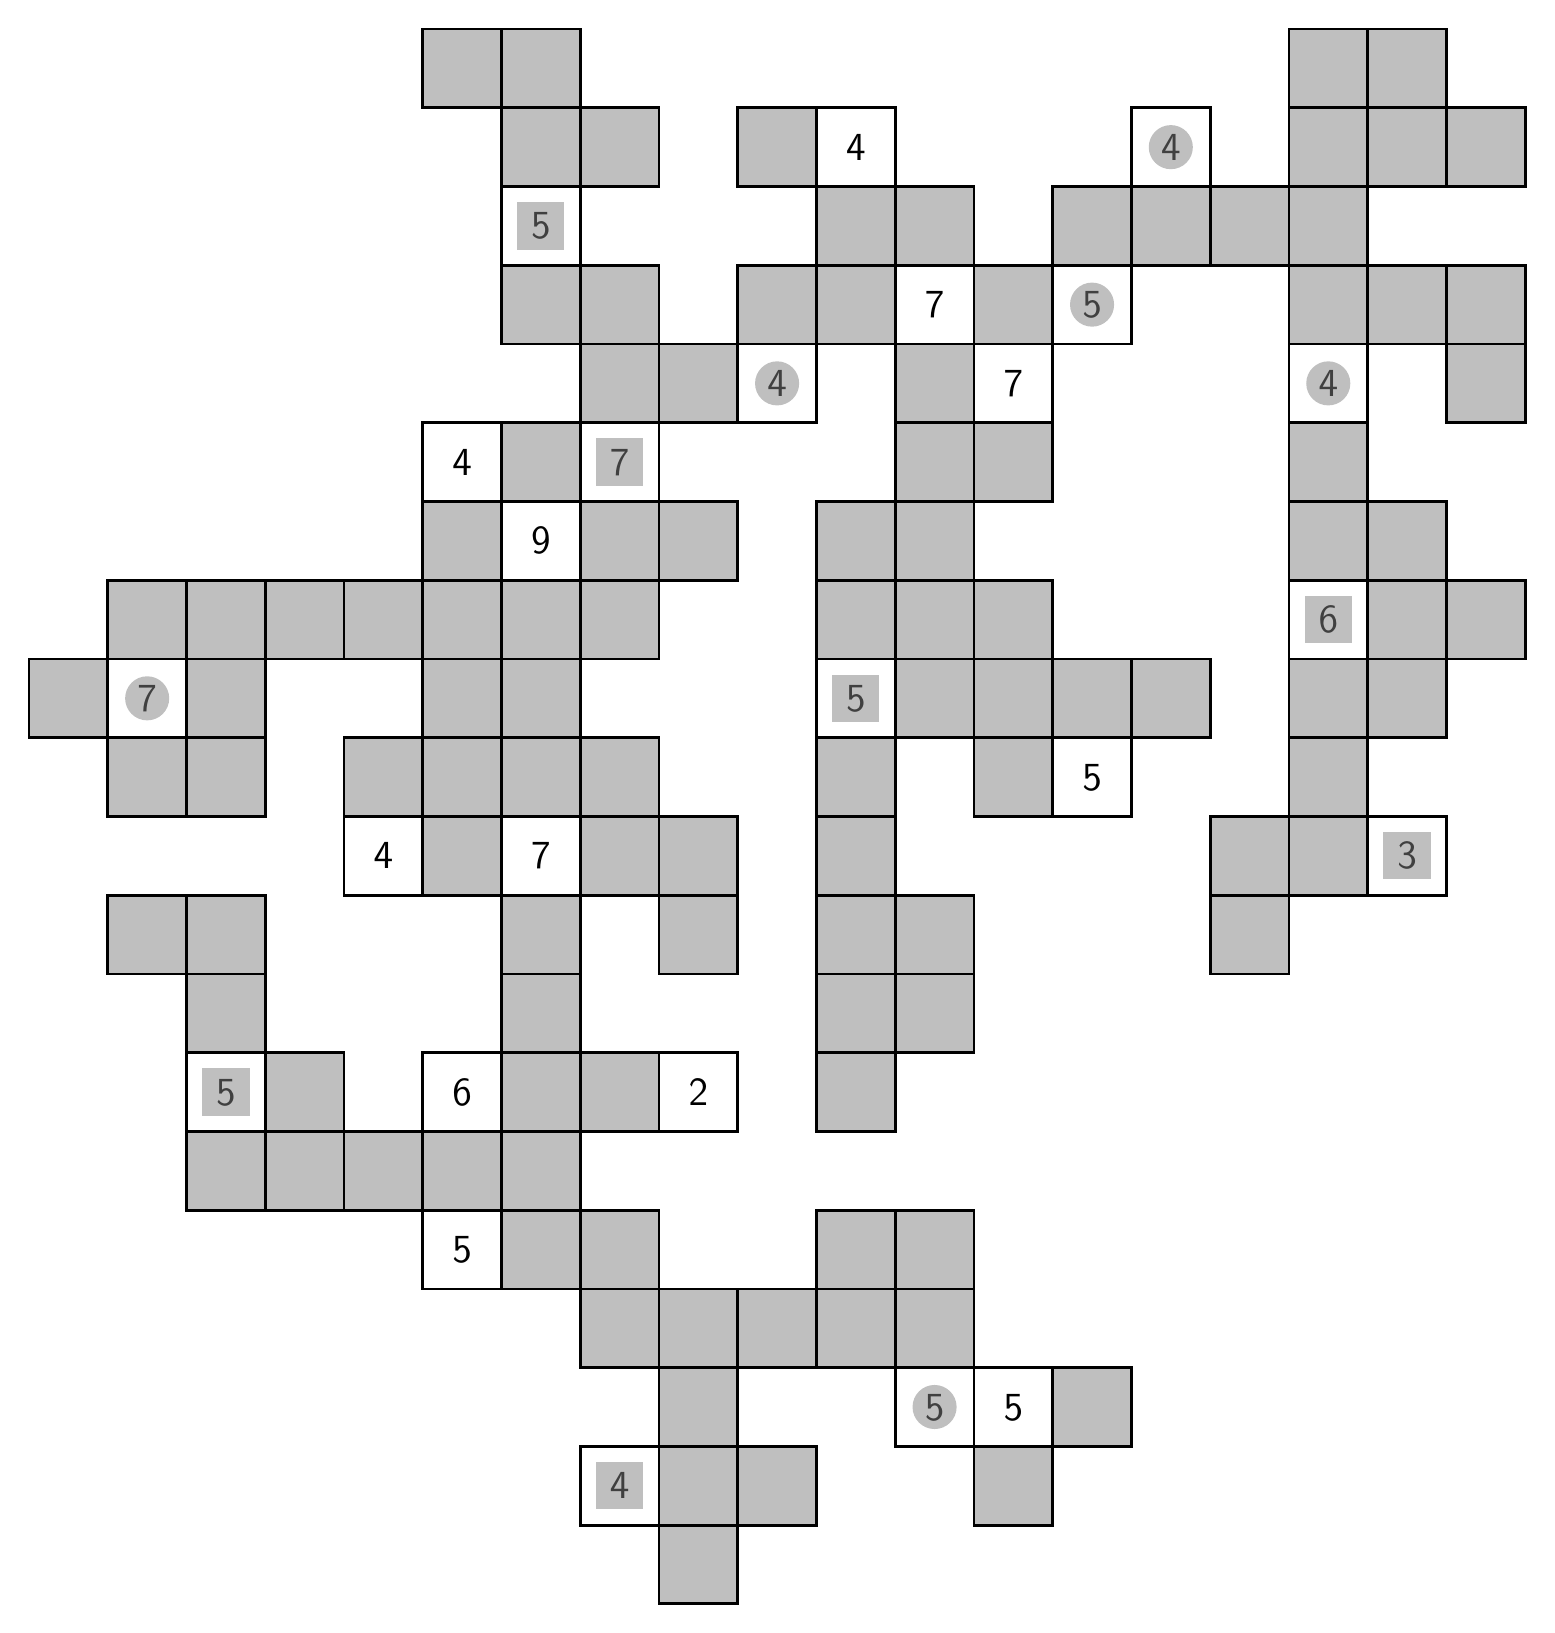
\begin{tikzpicture}\fill[gray, opacity = 0.5] (9, 0, 0)--++(1, 0, 0)--++(0, 1, 0)--++(-1, 0, 0)--cycle;
\draw[line width = 1pt] (9, 0, 0)--++(1, 0, 0)--++(0, 1, 0)--++(-1, 0, 0)--cycle;
\draw node at (8.5, 1.5, 0) {\Large $\mathsf{4}$};
\draw[line width = 1pt] (8, 1, 0)--++(1, 0, 0)--++(0, 1, 0)--++(-1, 0, 0)--cycle;
\fill[color = gray, opacity = 0.5] (8.2, 1.2) rectangle ++(0.6, 0.6);
\fill[gray, opacity = 0.5] (9, 1, 0)--++(1, 0, 0)--++(0, 1, 0)--++(-1, 0, 0)--cycle;
\draw[line width = 1pt] (9, 1, 0)--++(1, 0, 0)--++(0, 1, 0)--++(-1, 0, 0)--cycle;
\fill[gray, opacity = 0.5] (10, 1, 0)--++(1, 0, 0)--++(0, 1, 0)--++(-1, 0, 0)--cycle;
\draw[line width = 1pt] (10, 1, 0)--++(1, 0, 0)--++(0, 1, 0)--++(-1, 0, 0)--cycle;
\fill[gray, opacity = 0.5] (13, 1, 0)--++(1, 0, 0)--++(0, 1, 0)--++(-1, 0, 0)--cycle;
\draw[line width = 1pt] (13, 1, 0)--++(1, 0, 0)--++(0, 1, 0)--++(-1, 0, 0)--cycle;
\fill[gray, opacity = 0.5] (9, 2, 0)--++(1, 0, 0)--++(0, 1, 0)--++(-1, 0, 0)--cycle;
\draw[line width = 1pt] (9, 2, 0)--++(1, 0, 0)--++(0, 1, 0)--++(-1, 0, 0)--cycle;
\draw node at (12.5, 2.5, 0) {\Large $\mathsf{5}$};
\draw[line width = 1pt] (12, 2, 0)--++(1, 0, 0)--++(0, 1, 0)--++(-1, 0, 0)--cycle;
\fill[color = gray, opacity = 0.5] (12.5, 2.5, 0) circle (0.28);
\draw node at (13.5, 2.5, 0) {\Large $\mathsf{5}$};
\draw[line width = 1pt] (13, 2, 0)--++(1, 0, 0)--++(0, 1, 0)--++(-1, 0, 0)--cycle;
\fill[gray, opacity = 0.5] (14, 2, 0)--++(1, 0, 0)--++(0, 1, 0)--++(-1, 0, 0)--cycle;
\draw[line width = 1pt] (14, 2, 0)--++(1, 0, 0)--++(0, 1, 0)--++(-1, 0, 0)--cycle;
\fill[gray, opacity = 0.5] (8, 3, 0)--++(1, 0, 0)--++(0, 1, 0)--++(-1, 0, 0)--cycle;
\draw[line width = 1pt] (8, 3, 0)--++(1, 0, 0)--++(0, 1, 0)--++(-1, 0, 0)--cycle;
\fill[gray, opacity = 0.5] (9, 3, 0)--++(1, 0, 0)--++(0, 1, 0)--++(-1, 0, 0)--cycle;
\draw[line width = 1pt] (9, 3, 0)--++(1, 0, 0)--++(0, 1, 0)--++(-1, 0, 0)--cycle;
\fill[gray, opacity = 0.5] (10, 3, 0)--++(1, 0, 0)--++(0, 1, 0)--++(-1, 0, 0)--cycle;
\draw[line width = 1pt] (10, 3, 0)--++(1, 0, 0)--++(0, 1, 0)--++(-1, 0, 0)--cycle;
\fill[gray, opacity = 0.5] (11, 3, 0)--++(1, 0, 0)--++(0, 1, 0)--++(-1, 0, 0)--cycle;
\draw[line width = 1pt] (11, 3, 0)--++(1, 0, 0)--++(0, 1, 0)--++(-1, 0, 0)--cycle;
\fill[gray, opacity = 0.5] (12, 3, 0)--++(1, 0, 0)--++(0, 1, 0)--++(-1, 0, 0)--cycle;
\draw[line width = 1pt] (12, 3, 0)--++(1, 0, 0)--++(0, 1, 0)--++(-1, 0, 0)--cycle;
\draw node at (6.5, 4.5, 0) {\Large $\mathsf{5}$};
\draw[line width = 1pt] (6, 4, 0)--++(1, 0, 0)--++(0, 1, 0)--++(-1, 0, 0)--cycle;
\fill[gray, opacity = 0.5] (7, 4, 0)--++(1, 0, 0)--++(0, 1, 0)--++(-1, 0, 0)--cycle;
\draw[line width = 1pt] (7, 4, 0)--++(1, 0, 0)--++(0, 1, 0)--++(-1, 0, 0)--cycle;
\fill[gray, opacity = 0.5] (8, 4, 0)--++(1, 0, 0)--++(0, 1, 0)--++(-1, 0, 0)--cycle;
\draw[line width = 1pt] (8, 4, 0)--++(1, 0, 0)--++(0, 1, 0)--++(-1, 0, 0)--cycle;
\fill[gray, opacity = 0.5] (11, 4, 0)--++(1, 0, 0)--++(0, 1, 0)--++(-1, 0, 0)--cycle;
\draw[line width = 1pt] (11, 4, 0)--++(1, 0, 0)--++(0, 1, 0)--++(-1, 0, 0)--cycle;
\fill[gray, opacity = 0.5] (12, 4, 0)--++(1, 0, 0)--++(0, 1, 0)--++(-1, 0, 0)--cycle;
\draw[line width = 1pt] (12, 4, 0)--++(1, 0, 0)--++(0, 1, 0)--++(-1, 0, 0)--cycle;
\fill[gray, opacity = 0.5] (3, 5, 0)--++(1, 0, 0)--++(0, 1, 0)--++(-1, 0, 0)--cycle;
\draw[line width = 1pt] (3, 5, 0)--++(1, 0, 0)--++(0, 1, 0)--++(-1, 0, 0)--cycle;
\fill[gray, opacity = 0.5] (4, 5, 0)--++(1, 0, 0)--++(0, 1, 0)--++(-1, 0, 0)--cycle;
\draw[line width = 1pt] (4, 5, 0)--++(1, 0, 0)--++(0, 1, 0)--++(-1, 0, 0)--cycle;
\fill[gray, opacity = 0.5] (5, 5, 0)--++(1, 0, 0)--++(0, 1, 0)--++(-1, 0, 0)--cycle;
\draw[line width = 1pt] (5, 5, 0)--++(1, 0, 0)--++(0, 1, 0)--++(-1, 0, 0)--cycle;
\fill[gray, opacity = 0.5] (6, 5, 0)--++(1, 0, 0)--++(0, 1, 0)--++(-1, 0, 0)--cycle;
\draw[line width = 1pt] (6, 5, 0)--++(1, 0, 0)--++(0, 1, 0)--++(-1, 0, 0)--cycle;
\fill[gray, opacity = 0.5] (7, 5, 0)--++(1, 0, 0)--++(0, 1, 0)--++(-1, 0, 0)--cycle;
\draw[line width = 1pt] (7, 5, 0)--++(1, 0, 0)--++(0, 1, 0)--++(-1, 0, 0)--cycle;
\draw node at (3.5, 6.5, 0) {\Large $\mathsf{5}$};
\draw[line width = 1pt] (3, 6, 0)--++(1, 0, 0)--++(0, 1, 0)--++(-1, 0, 0)--cycle;
\fill[color = gray, opacity = 0.5] (3.2, 6.2) rectangle ++(0.6, 0.6);
\fill[gray, opacity = 0.5] (4, 6, 0)--++(1, 0, 0)--++(0, 1, 0)--++(-1, 0, 0)--cycle;
\draw[line width = 1pt] (4, 6, 0)--++(1, 0, 0)--++(0, 1, 0)--++(-1, 0, 0)--cycle;
\draw node at (6.5, 6.5, 0) {\Large $\mathsf{6}$};
\draw[line width = 1pt] (6, 6, 0)--++(1, 0, 0)--++(0, 1, 0)--++(-1, 0, 0)--cycle;
\fill[gray, opacity = 0.5] (7, 6, 0)--++(1, 0, 0)--++(0, 1, 0)--++(-1, 0, 0)--cycle;
\draw[line width = 1pt] (7, 6, 0)--++(1, 0, 0)--++(0, 1, 0)--++(-1, 0, 0)--cycle;
\fill[gray, opacity = 0.5] (8, 6, 0)--++(1, 0, 0)--++(0, 1, 0)--++(-1, 0, 0)--cycle;
\draw[line width = 1pt] (8, 6, 0)--++(1, 0, 0)--++(0, 1, 0)--++(-1, 0, 0)--cycle;
\draw node at (9.5, 6.5, 0) {\Large $\mathsf{2}$};
\draw[line width = 1pt] (9, 6, 0)--++(1, 0, 0)--++(0, 1, 0)--++(-1, 0, 0)--cycle;
\fill[gray, opacity = 0.5] (11, 6, 0)--++(1, 0, 0)--++(0, 1, 0)--++(-1, 0, 0)--cycle;
\draw[line width = 1pt] (11, 6, 0)--++(1, 0, 0)--++(0, 1, 0)--++(-1, 0, 0)--cycle;
\fill[gray, opacity = 0.5] (3, 7, 0)--++(1, 0, 0)--++(0, 1, 0)--++(-1, 0, 0)--cycle;
\draw[line width = 1pt] (3, 7, 0)--++(1, 0, 0)--++(0, 1, 0)--++(-1, 0, 0)--cycle;
\fill[gray, opacity = 0.5] (7, 7, 0)--++(1, 0, 0)--++(0, 1, 0)--++(-1, 0, 0)--cycle;
\draw[line width = 1pt] (7, 7, 0)--++(1, 0, 0)--++(0, 1, 0)--++(-1, 0, 0)--cycle;
\fill[gray, opacity = 0.5] (11, 7, 0)--++(1, 0, 0)--++(0, 1, 0)--++(-1, 0, 0)--cycle;
\draw[line width = 1pt] (11, 7, 0)--++(1, 0, 0)--++(0, 1, 0)--++(-1, 0, 0)--cycle;
\fill[gray, opacity = 0.5] (12, 7, 0)--++(1, 0, 0)--++(0, 1, 0)--++(-1, 0, 0)--cycle;
\draw[line width = 1pt] (12, 7, 0)--++(1, 0, 0)--++(0, 1, 0)--++(-1, 0, 0)--cycle;
\fill[gray, opacity = 0.5] (2, 8, 0)--++(1, 0, 0)--++(0, 1, 0)--++(-1, 0, 0)--cycle;
\draw[line width = 1pt] (2, 8, 0)--++(1, 0, 0)--++(0, 1, 0)--++(-1, 0, 0)--cycle;
\fill[gray, opacity = 0.5] (3, 8, 0)--++(1, 0, 0)--++(0, 1, 0)--++(-1, 0, 0)--cycle;
\draw[line width = 1pt] (3, 8, 0)--++(1, 0, 0)--++(0, 1, 0)--++(-1, 0, 0)--cycle;
\fill[gray, opacity = 0.5] (7, 8, 0)--++(1, 0, 0)--++(0, 1, 0)--++(-1, 0, 0)--cycle;
\draw[line width = 1pt] (7, 8, 0)--++(1, 0, 0)--++(0, 1, 0)--++(-1, 0, 0)--cycle;
\fill[gray, opacity = 0.5] (9, 8, 0)--++(1, 0, 0)--++(0, 1, 0)--++(-1, 0, 0)--cycle;
\draw[line width = 1pt] (9, 8, 0)--++(1, 0, 0)--++(0, 1, 0)--++(-1, 0, 0)--cycle;
\fill[gray, opacity = 0.5] (11, 8, 0)--++(1, 0, 0)--++(0, 1, 0)--++(-1, 0, 0)--cycle;
\draw[line width = 1pt] (11, 8, 0)--++(1, 0, 0)--++(0, 1, 0)--++(-1, 0, 0)--cycle;
\fill[gray, opacity = 0.5] (12, 8, 0)--++(1, 0, 0)--++(0, 1, 0)--++(-1, 0, 0)--cycle;
\draw[line width = 1pt] (12, 8, 0)--++(1, 0, 0)--++(0, 1, 0)--++(-1, 0, 0)--cycle;
\fill[gray, opacity = 0.5] (16, 8, 0)--++(1, 0, 0)--++(0, 1, 0)--++(-1, 0, 0)--cycle;
\draw[line width = 1pt] (16, 8, 0)--++(1, 0, 0)--++(0, 1, 0)--++(-1, 0, 0)--cycle;
\draw node at (5.5, 9.5, 0) {\Large $\mathsf{4}$};
\draw[line width = 1pt] (5, 9, 0)--++(1, 0, 0)--++(0, 1, 0)--++(-1, 0, 0)--cycle;
\fill[gray, opacity = 0.5] (6, 9, 0)--++(1, 0, 0)--++(0, 1, 0)--++(-1, 0, 0)--cycle;
\draw[line width = 1pt] (6, 9, 0)--++(1, 0, 0)--++(0, 1, 0)--++(-1, 0, 0)--cycle;
\draw node at (7.5, 9.5, 0) {\Large $\mathsf{7}$};
\draw[line width = 1pt] (7, 9, 0)--++(1, 0, 0)--++(0, 1, 0)--++(-1, 0, 0)--cycle;
\fill[gray, opacity = 0.5] (8, 9, 0)--++(1, 0, 0)--++(0, 1, 0)--++(-1, 0, 0)--cycle;
\draw[line width = 1pt] (8, 9, 0)--++(1, 0, 0)--++(0, 1, 0)--++(-1, 0, 0)--cycle;
\fill[gray, opacity = 0.5] (9, 9, 0)--++(1, 0, 0)--++(0, 1, 0)--++(-1, 0, 0)--cycle;
\draw[line width = 1pt] (9, 9, 0)--++(1, 0, 0)--++(0, 1, 0)--++(-1, 0, 0)--cycle;
\fill[gray, opacity = 0.5] (11, 9, 0)--++(1, 0, 0)--++(0, 1, 0)--++(-1, 0, 0)--cycle;
\draw[line width = 1pt] (11, 9, 0)--++(1, 0, 0)--++(0, 1, 0)--++(-1, 0, 0)--cycle;
\fill[gray, opacity = 0.5] (16, 9, 0)--++(1, 0, 0)--++(0, 1, 0)--++(-1, 0, 0)--cycle;
\draw[line width = 1pt] (16, 9, 0)--++(1, 0, 0)--++(0, 1, 0)--++(-1, 0, 0)--cycle;
\fill[gray, opacity = 0.5] (17, 9, 0)--++(1, 0, 0)--++(0, 1, 0)--++(-1, 0, 0)--cycle;
\draw[line width = 1pt] (17, 9, 0)--++(1, 0, 0)--++(0, 1, 0)--++(-1, 0, 0)--cycle;
\draw node at (18.5, 9.5, 0) {\Large $\mathsf{3}$};
\draw[line width = 1pt] (18, 9, 0)--++(1, 0, 0)--++(0, 1, 0)--++(-1, 0, 0)--cycle;
\fill[color = gray, opacity = 0.5] (18.2, 9.2) rectangle ++(0.6, 0.6);
\fill[gray, opacity = 0.5] (2, 10, 0)--++(1, 0, 0)--++(0, 1, 0)--++(-1, 0, 0)--cycle;
\draw[line width = 1pt] (2, 10, 0)--++(1, 0, 0)--++(0, 1, 0)--++(-1, 0, 0)--cycle;
\fill[gray, opacity = 0.5] (3, 10, 0)--++(1, 0, 0)--++(0, 1, 0)--++(-1, 0, 0)--cycle;
\draw[line width = 1pt] (3, 10, 0)--++(1, 0, 0)--++(0, 1, 0)--++(-1, 0, 0)--cycle;
\fill[gray, opacity = 0.5] (5, 10, 0)--++(1, 0, 0)--++(0, 1, 0)--++(-1, 0, 0)--cycle;
\draw[line width = 1pt] (5, 10, 0)--++(1, 0, 0)--++(0, 1, 0)--++(-1, 0, 0)--cycle;
\fill[gray, opacity = 0.5] (6, 10, 0)--++(1, 0, 0)--++(0, 1, 0)--++(-1, 0, 0)--cycle;
\draw[line width = 1pt] (6, 10, 0)--++(1, 0, 0)--++(0, 1, 0)--++(-1, 0, 0)--cycle;
\fill[gray, opacity = 0.5] (7, 10, 0)--++(1, 0, 0)--++(0, 1, 0)--++(-1, 0, 0)--cycle;
\draw[line width = 1pt] (7, 10, 0)--++(1, 0, 0)--++(0, 1, 0)--++(-1, 0, 0)--cycle;
\fill[gray, opacity = 0.5] (8, 10, 0)--++(1, 0, 0)--++(0, 1, 0)--++(-1, 0, 0)--cycle;
\draw[line width = 1pt] (8, 10, 0)--++(1, 0, 0)--++(0, 1, 0)--++(-1, 0, 0)--cycle;
\fill[gray, opacity = 0.5] (11, 10, 0)--++(1, 0, 0)--++(0, 1, 0)--++(-1, 0, 0)--cycle;
\draw[line width = 1pt] (11, 10, 0)--++(1, 0, 0)--++(0, 1, 0)--++(-1, 0, 0)--cycle;
\fill[gray, opacity = 0.5] (13, 10, 0)--++(1, 0, 0)--++(0, 1, 0)--++(-1, 0, 0)--cycle;
\draw[line width = 1pt] (13, 10, 0)--++(1, 0, 0)--++(0, 1, 0)--++(-1, 0, 0)--cycle;
\draw node at (14.5, 10.5, 0) {\Large $\mathsf{5}$};
\draw[line width = 1pt] (14, 10, 0)--++(1, 0, 0)--++(0, 1, 0)--++(-1, 0, 0)--cycle;
\fill[gray, opacity = 0.5] (17, 10, 0)--++(1, 0, 0)--++(0, 1, 0)--++(-1, 0, 0)--cycle;
\draw[line width = 1pt] (17, 10, 0)--++(1, 0, 0)--++(0, 1, 0)--++(-1, 0, 0)--cycle;
\fill[gray, opacity = 0.5] (1, 11, 0)--++(1, 0, 0)--++(0, 1, 0)--++(-1, 0, 0)--cycle;
\draw[line width = 1pt] (1, 11, 0)--++(1, 0, 0)--++(0, 1, 0)--++(-1, 0, 0)--cycle;
\draw node at (2.5, 11.5, 0) {\Large $\mathsf{7}$};
\draw[line width = 1pt] (2, 11, 0)--++(1, 0, 0)--++(0, 1, 0)--++(-1, 0, 0)--cycle;
\fill[color = gray, opacity = 0.5] (2.5, 11.5, 0) circle (0.28);
\fill[gray, opacity = 0.5] (3, 11, 0)--++(1, 0, 0)--++(0, 1, 0)--++(-1, 0, 0)--cycle;
\draw[line width = 1pt] (3, 11, 0)--++(1, 0, 0)--++(0, 1, 0)--++(-1, 0, 0)--cycle;
\fill[gray, opacity = 0.5] (6, 11, 0)--++(1, 0, 0)--++(0, 1, 0)--++(-1, 0, 0)--cycle;
\draw[line width = 1pt] (6, 11, 0)--++(1, 0, 0)--++(0, 1, 0)--++(-1, 0, 0)--cycle;
\fill[gray, opacity = 0.5] (7, 11, 0)--++(1, 0, 0)--++(0, 1, 0)--++(-1, 0, 0)--cycle;
\draw[line width = 1pt] (7, 11, 0)--++(1, 0, 0)--++(0, 1, 0)--++(-1, 0, 0)--cycle;
\draw node at (11.5, 11.5, 0) {\Large $\mathsf{5}$};
\draw[line width = 1pt] (11, 11, 0)--++(1, 0, 0)--++(0, 1, 0)--++(-1, 0, 0)--cycle;
\fill[color = gray, opacity = 0.5] (11.2, 11.2) rectangle ++(0.6, 0.6);
\fill[gray, opacity = 0.5] (12, 11, 0)--++(1, 0, 0)--++(0, 1, 0)--++(-1, 0, 0)--cycle;
\draw[line width = 1pt] (12, 11, 0)--++(1, 0, 0)--++(0, 1, 0)--++(-1, 0, 0)--cycle;
\fill[gray, opacity = 0.5] (13, 11, 0)--++(1, 0, 0)--++(0, 1, 0)--++(-1, 0, 0)--cycle;
\draw[line width = 1pt] (13, 11, 0)--++(1, 0, 0)--++(0, 1, 0)--++(-1, 0, 0)--cycle;
\fill[gray, opacity = 0.5] (14, 11, 0)--++(1, 0, 0)--++(0, 1, 0)--++(-1, 0, 0)--cycle;
\draw[line width = 1pt] (14, 11, 0)--++(1, 0, 0)--++(0, 1, 0)--++(-1, 0, 0)--cycle;
\fill[gray, opacity = 0.5] (15, 11, 0)--++(1, 0, 0)--++(0, 1, 0)--++(-1, 0, 0)--cycle;
\draw[line width = 1pt] (15, 11, 0)--++(1, 0, 0)--++(0, 1, 0)--++(-1, 0, 0)--cycle;
\fill[gray, opacity = 0.5] (17, 11, 0)--++(1, 0, 0)--++(0, 1, 0)--++(-1, 0, 0)--cycle;
\draw[line width = 1pt] (17, 11, 0)--++(1, 0, 0)--++(0, 1, 0)--++(-1, 0, 0)--cycle;
\fill[gray, opacity = 0.5] (18, 11, 0)--++(1, 0, 0)--++(0, 1, 0)--++(-1, 0, 0)--cycle;
\draw[line width = 1pt] (18, 11, 0)--++(1, 0, 0)--++(0, 1, 0)--++(-1, 0, 0)--cycle;
\fill[gray, opacity = 0.5] (2, 12, 0)--++(1, 0, 0)--++(0, 1, 0)--++(-1, 0, 0)--cycle;
\draw[line width = 1pt] (2, 12, 0)--++(1, 0, 0)--++(0, 1, 0)--++(-1, 0, 0)--cycle;
\fill[gray, opacity = 0.5] (3, 12, 0)--++(1, 0, 0)--++(0, 1, 0)--++(-1, 0, 0)--cycle;
\draw[line width = 1pt] (3, 12, 0)--++(1, 0, 0)--++(0, 1, 0)--++(-1, 0, 0)--cycle;
\fill[gray, opacity = 0.5] (4, 12, 0)--++(1, 0, 0)--++(0, 1, 0)--++(-1, 0, 0)--cycle;
\draw[line width = 1pt] (4, 12, 0)--++(1, 0, 0)--++(0, 1, 0)--++(-1, 0, 0)--cycle;
\fill[gray, opacity = 0.5] (5, 12, 0)--++(1, 0, 0)--++(0, 1, 0)--++(-1, 0, 0)--cycle;
\draw[line width = 1pt] (5, 12, 0)--++(1, 0, 0)--++(0, 1, 0)--++(-1, 0, 0)--cycle;
\fill[gray, opacity = 0.5] (6, 12, 0)--++(1, 0, 0)--++(0, 1, 0)--++(-1, 0, 0)--cycle;
\draw[line width = 1pt] (6, 12, 0)--++(1, 0, 0)--++(0, 1, 0)--++(-1, 0, 0)--cycle;
\fill[gray, opacity = 0.5] (7, 12, 0)--++(1, 0, 0)--++(0, 1, 0)--++(-1, 0, 0)--cycle;
\draw[line width = 1pt] (7, 12, 0)--++(1, 0, 0)--++(0, 1, 0)--++(-1, 0, 0)--cycle;
\fill[gray, opacity = 0.5] (8, 12, 0)--++(1, 0, 0)--++(0, 1, 0)--++(-1, 0, 0)--cycle;
\draw[line width = 1pt] (8, 12, 0)--++(1, 0, 0)--++(0, 1, 0)--++(-1, 0, 0)--cycle;
\fill[gray, opacity = 0.5] (11, 12, 0)--++(1, 0, 0)--++(0, 1, 0)--++(-1, 0, 0)--cycle;
\draw[line width = 1pt] (11, 12, 0)--++(1, 0, 0)--++(0, 1, 0)--++(-1, 0, 0)--cycle;
\fill[gray, opacity = 0.5] (12, 12, 0)--++(1, 0, 0)--++(0, 1, 0)--++(-1, 0, 0)--cycle;
\draw[line width = 1pt] (12, 12, 0)--++(1, 0, 0)--++(0, 1, 0)--++(-1, 0, 0)--cycle;
\fill[gray, opacity = 0.5] (13, 12, 0)--++(1, 0, 0)--++(0, 1, 0)--++(-1, 0, 0)--cycle;
\draw[line width = 1pt] (13, 12, 0)--++(1, 0, 0)--++(0, 1, 0)--++(-1, 0, 0)--cycle;
\draw node at (17.5, 12.5, 0) {\Large $\mathsf{6}$};
\draw[line width = 1pt] (17, 12, 0)--++(1, 0, 0)--++(0, 1, 0)--++(-1, 0, 0)--cycle;
\fill[color = gray, opacity = 0.5] (17.2, 12.2) rectangle ++(0.6, 0.6);
\fill[gray, opacity = 0.5] (18, 12, 0)--++(1, 0, 0)--++(0, 1, 0)--++(-1, 0, 0)--cycle;
\draw[line width = 1pt] (18, 12, 0)--++(1, 0, 0)--++(0, 1, 0)--++(-1, 0, 0)--cycle;
\fill[gray, opacity = 0.5] (19, 12, 0)--++(1, 0, 0)--++(0, 1, 0)--++(-1, 0, 0)--cycle;
\draw[line width = 1pt] (19, 12, 0)--++(1, 0, 0)--++(0, 1, 0)--++(-1, 0, 0)--cycle;
\fill[gray, opacity = 0.5] (6, 13, 0)--++(1, 0, 0)--++(0, 1, 0)--++(-1, 0, 0)--cycle;
\draw[line width = 1pt] (6, 13, 0)--++(1, 0, 0)--++(0, 1, 0)--++(-1, 0, 0)--cycle;
\draw node at (7.5, 13.5, 0) {\Large $\mathsf{9}$};
\draw[line width = 1pt] (7, 13, 0)--++(1, 0, 0)--++(0, 1, 0)--++(-1, 0, 0)--cycle;
\fill[gray, opacity = 0.5] (8, 13, 0)--++(1, 0, 0)--++(0, 1, 0)--++(-1, 0, 0)--cycle;
\draw[line width = 1pt] (8, 13, 0)--++(1, 0, 0)--++(0, 1, 0)--++(-1, 0, 0)--cycle;
\fill[gray, opacity = 0.5] (9, 13, 0)--++(1, 0, 0)--++(0, 1, 0)--++(-1, 0, 0)--cycle;
\draw[line width = 1pt] (9, 13, 0)--++(1, 0, 0)--++(0, 1, 0)--++(-1, 0, 0)--cycle;
\fill[gray, opacity = 0.5] (11, 13, 0)--++(1, 0, 0)--++(0, 1, 0)--++(-1, 0, 0)--cycle;
\draw[line width = 1pt] (11, 13, 0)--++(1, 0, 0)--++(0, 1, 0)--++(-1, 0, 0)--cycle;
\fill[gray, opacity = 0.5] (12, 13, 0)--++(1, 0, 0)--++(0, 1, 0)--++(-1, 0, 0)--cycle;
\draw[line width = 1pt] (12, 13, 0)--++(1, 0, 0)--++(0, 1, 0)--++(-1, 0, 0)--cycle;
\fill[gray, opacity = 0.5] (17, 13, 0)--++(1, 0, 0)--++(0, 1, 0)--++(-1, 0, 0)--cycle;
\draw[line width = 1pt] (17, 13, 0)--++(1, 0, 0)--++(0, 1, 0)--++(-1, 0, 0)--cycle;
\fill[gray, opacity = 0.5] (18, 13, 0)--++(1, 0, 0)--++(0, 1, 0)--++(-1, 0, 0)--cycle;
\draw[line width = 1pt] (18, 13, 0)--++(1, 0, 0)--++(0, 1, 0)--++(-1, 0, 0)--cycle;
\draw node at (6.5, 14.5, 0) {\Large $\mathsf{4}$};
\draw[line width = 1pt] (6, 14, 0)--++(1, 0, 0)--++(0, 1, 0)--++(-1, 0, 0)--cycle;
\fill[gray, opacity = 0.5] (7, 14, 0)--++(1, 0, 0)--++(0, 1, 0)--++(-1, 0, 0)--cycle;
\draw[line width = 1pt] (7, 14, 0)--++(1, 0, 0)--++(0, 1, 0)--++(-1, 0, 0)--cycle;
\draw node at (8.5, 14.5, 0) {\Large $\mathsf{7}$};
\draw[line width = 1pt] (8, 14, 0)--++(1, 0, 0)--++(0, 1, 0)--++(-1, 0, 0)--cycle;
\fill[color = gray, opacity = 0.5] (8.2, 14.2) rectangle ++(0.6, 0.6);
\fill[gray, opacity = 0.5] (12, 14, 0)--++(1, 0, 0)--++(0, 1, 0)--++(-1, 0, 0)--cycle;
\draw[line width = 1pt] (12, 14, 0)--++(1, 0, 0)--++(0, 1, 0)--++(-1, 0, 0)--cycle;
\fill[gray, opacity = 0.5] (13, 14, 0)--++(1, 0, 0)--++(0, 1, 0)--++(-1, 0, 0)--cycle;
\draw[line width = 1pt] (13, 14, 0)--++(1, 0, 0)--++(0, 1, 0)--++(-1, 0, 0)--cycle;
\fill[gray, opacity = 0.5] (17, 14, 0)--++(1, 0, 0)--++(0, 1, 0)--++(-1, 0, 0)--cycle;
\draw[line width = 1pt] (17, 14, 0)--++(1, 0, 0)--++(0, 1, 0)--++(-1, 0, 0)--cycle;
\fill[gray, opacity = 0.5] (8, 15, 0)--++(1, 0, 0)--++(0, 1, 0)--++(-1, 0, 0)--cycle;
\draw[line width = 1pt] (8, 15, 0)--++(1, 0, 0)--++(0, 1, 0)--++(-1, 0, 0)--cycle;
\fill[gray, opacity = 0.5] (9, 15, 0)--++(1, 0, 0)--++(0, 1, 0)--++(-1, 0, 0)--cycle;
\draw[line width = 1pt] (9, 15, 0)--++(1, 0, 0)--++(0, 1, 0)--++(-1, 0, 0)--cycle;
\draw node at (10.5, 15.5, 0) {\Large $\mathsf{4}$};
\draw[line width = 1pt] (10, 15, 0)--++(1, 0, 0)--++(0, 1, 0)--++(-1, 0, 0)--cycle;
\fill[color = gray, opacity = 0.5] (10.5, 15.5, 0) circle (0.28);
\fill[gray, opacity = 0.5] (12, 15, 0)--++(1, 0, 0)--++(0, 1, 0)--++(-1, 0, 0)--cycle;
\draw[line width = 1pt] (12, 15, 0)--++(1, 0, 0)--++(0, 1, 0)--++(-1, 0, 0)--cycle;
\draw node at (13.5, 15.5, 0) {\Large $\mathsf{7}$};
\draw[line width = 1pt] (13, 15, 0)--++(1, 0, 0)--++(0, 1, 0)--++(-1, 0, 0)--cycle;
\draw node at (17.5, 15.5, 0) {\Large $\mathsf{4}$};
\draw[line width = 1pt] (17, 15, 0)--++(1, 0, 0)--++(0, 1, 0)--++(-1, 0, 0)--cycle;
\fill[color = gray, opacity = 0.5] (17.5, 15.5, 0) circle (0.28);
\fill[gray, opacity = 0.5] (19, 15, 0)--++(1, 0, 0)--++(0, 1, 0)--++(-1, 0, 0)--cycle;
\draw[line width = 1pt] (19, 15, 0)--++(1, 0, 0)--++(0, 1, 0)--++(-1, 0, 0)--cycle;
\fill[gray, opacity = 0.5] (7, 16, 0)--++(1, 0, 0)--++(0, 1, 0)--++(-1, 0, 0)--cycle;
\draw[line width = 1pt] (7, 16, 0)--++(1, 0, 0)--++(0, 1, 0)--++(-1, 0, 0)--cycle;
\fill[gray, opacity = 0.5] (8, 16, 0)--++(1, 0, 0)--++(0, 1, 0)--++(-1, 0, 0)--cycle;
\draw[line width = 1pt] (8, 16, 0)--++(1, 0, 0)--++(0, 1, 0)--++(-1, 0, 0)--cycle;
\fill[gray, opacity = 0.5] (10, 16, 0)--++(1, 0, 0)--++(0, 1, 0)--++(-1, 0, 0)--cycle;
\draw[line width = 1pt] (10, 16, 0)--++(1, 0, 0)--++(0, 1, 0)--++(-1, 0, 0)--cycle;
\fill[gray, opacity = 0.5] (11, 16, 0)--++(1, 0, 0)--++(0, 1, 0)--++(-1, 0, 0)--cycle;
\draw[line width = 1pt] (11, 16, 0)--++(1, 0, 0)--++(0, 1, 0)--++(-1, 0, 0)--cycle;
\draw node at (12.5, 16.5, 0) {\Large $\mathsf{7}$};
\draw[line width = 1pt] (12, 16, 0)--++(1, 0, 0)--++(0, 1, 0)--++(-1, 0, 0)--cycle;
\fill[gray, opacity = 0.5] (13, 16, 0)--++(1, 0, 0)--++(0, 1, 0)--++(-1, 0, 0)--cycle;
\draw[line width = 1pt] (13, 16, 0)--++(1, 0, 0)--++(0, 1, 0)--++(-1, 0, 0)--cycle;
\draw node at (14.5, 16.5, 0) {\Large $\mathsf{5}$};
\draw[line width = 1pt] (14, 16, 0)--++(1, 0, 0)--++(0, 1, 0)--++(-1, 0, 0)--cycle;
\fill[color = gray, opacity = 0.5] (14.5, 16.5, 0) circle (0.28);
\fill[gray, opacity = 0.5] (17, 16, 0)--++(1, 0, 0)--++(0, 1, 0)--++(-1, 0, 0)--cycle;
\draw[line width = 1pt] (17, 16, 0)--++(1, 0, 0)--++(0, 1, 0)--++(-1, 0, 0)--cycle;
\fill[gray, opacity = 0.5] (18, 16, 0)--++(1, 0, 0)--++(0, 1, 0)--++(-1, 0, 0)--cycle;
\draw[line width = 1pt] (18, 16, 0)--++(1, 0, 0)--++(0, 1, 0)--++(-1, 0, 0)--cycle;
\fill[gray, opacity = 0.5] (19, 16, 0)--++(1, 0, 0)--++(0, 1, 0)--++(-1, 0, 0)--cycle;
\draw[line width = 1pt] (19, 16, 0)--++(1, 0, 0)--++(0, 1, 0)--++(-1, 0, 0)--cycle;
\draw node at (7.5, 17.5, 0) {\Large $\mathsf{5}$};
\draw[line width = 1pt] (7, 17, 0)--++(1, 0, 0)--++(0, 1, 0)--++(-1, 0, 0)--cycle;
\fill[color = gray, opacity = 0.5] (7.2, 17.2) rectangle ++(0.6, 0.6);
\fill[gray, opacity = 0.5] (11, 17, 0)--++(1, 0, 0)--++(0, 1, 0)--++(-1, 0, 0)--cycle;
\draw[line width = 1pt] (11, 17, 0)--++(1, 0, 0)--++(0, 1, 0)--++(-1, 0, 0)--cycle;
\fill[gray, opacity = 0.5] (12, 17, 0)--++(1, 0, 0)--++(0, 1, 0)--++(-1, 0, 0)--cycle;
\draw[line width = 1pt] (12, 17, 0)--++(1, 0, 0)--++(0, 1, 0)--++(-1, 0, 0)--cycle;
\fill[gray, opacity = 0.5] (14, 17, 0)--++(1, 0, 0)--++(0, 1, 0)--++(-1, 0, 0)--cycle;
\draw[line width = 1pt] (14, 17, 0)--++(1, 0, 0)--++(0, 1, 0)--++(-1, 0, 0)--cycle;
\fill[gray, opacity = 0.5] (15, 17, 0)--++(1, 0, 0)--++(0, 1, 0)--++(-1, 0, 0)--cycle;
\draw[line width = 1pt] (15, 17, 0)--++(1, 0, 0)--++(0, 1, 0)--++(-1, 0, 0)--cycle;
\fill[gray, opacity = 0.5] (16, 17, 0)--++(1, 0, 0)--++(0, 1, 0)--++(-1, 0, 0)--cycle;
\draw[line width = 1pt] (16, 17, 0)--++(1, 0, 0)--++(0, 1, 0)--++(-1, 0, 0)--cycle;
\fill[gray, opacity = 0.5] (17, 17, 0)--++(1, 0, 0)--++(0, 1, 0)--++(-1, 0, 0)--cycle;
\draw[line width = 1pt] (17, 17, 0)--++(1, 0, 0)--++(0, 1, 0)--++(-1, 0, 0)--cycle;
\fill[gray, opacity = 0.5] (7, 18, 0)--++(1, 0, 0)--++(0, 1, 0)--++(-1, 0, 0)--cycle;
\draw[line width = 1pt] (7, 18, 0)--++(1, 0, 0)--++(0, 1, 0)--++(-1, 0, 0)--cycle;
\fill[gray, opacity = 0.5] (8, 18, 0)--++(1, 0, 0)--++(0, 1, 0)--++(-1, 0, 0)--cycle;
\draw[line width = 1pt] (8, 18, 0)--++(1, 0, 0)--++(0, 1, 0)--++(-1, 0, 0)--cycle;
\fill[gray, opacity = 0.5] (10, 18, 0)--++(1, 0, 0)--++(0, 1, 0)--++(-1, 0, 0)--cycle;
\draw[line width = 1pt] (10, 18, 0)--++(1, 0, 0)--++(0, 1, 0)--++(-1, 0, 0)--cycle;
\draw node at (11.5, 18.5, 0) {\Large $\mathsf{4}$};
\draw[line width = 1pt] (11, 18, 0)--++(1, 0, 0)--++(0, 1, 0)--++(-1, 0, 0)--cycle;
\draw node at (15.5, 18.5, 0) {\Large $\mathsf{4}$};
\draw[line width = 1pt] (15, 18, 0)--++(1, 0, 0)--++(0, 1, 0)--++(-1, 0, 0)--cycle;
\fill[color = gray, opacity = 0.5] (15.5, 18.5, 0) circle (0.28);
\fill[gray, opacity = 0.5] (17, 18, 0)--++(1, 0, 0)--++(0, 1, 0)--++(-1, 0, 0)--cycle;
\draw[line width = 1pt] (17, 18, 0)--++(1, 0, 0)--++(0, 1, 0)--++(-1, 0, 0)--cycle;
\fill[gray, opacity = 0.5] (18, 18, 0)--++(1, 0, 0)--++(0, 1, 0)--++(-1, 0, 0)--cycle;
\draw[line width = 1pt] (18, 18, 0)--++(1, 0, 0)--++(0, 1, 0)--++(-1, 0, 0)--cycle;
\fill[gray, opacity = 0.5] (19, 18, 0)--++(1, 0, 0)--++(0, 1, 0)--++(-1, 0, 0)--cycle;
\draw[line width = 1pt] (19, 18, 0)--++(1, 0, 0)--++(0, 1, 0)--++(-1, 0, 0)--cycle;
\fill[gray, opacity = 0.5] (6, 19, 0)--++(1, 0, 0)--++(0, 1, 0)--++(-1, 0, 0)--cycle;
\draw[line width = 1pt] (6, 19, 0)--++(1, 0, 0)--++(0, 1, 0)--++(-1, 0, 0)--cycle;
\fill[gray, opacity = 0.5] (7, 19, 0)--++(1, 0, 0)--++(0, 1, 0)--++(-1, 0, 0)--cycle;
\draw[line width = 1pt] (7, 19, 0)--++(1, 0, 0)--++(0, 1, 0)--++(-1, 0, 0)--cycle;
\fill[gray, opacity = 0.5] (17, 19, 0)--++(1, 0, 0)--++(0, 1, 0)--++(-1, 0, 0)--cycle;
\draw[line width = 1pt] (17, 19, 0)--++(1, 0, 0)--++(0, 1, 0)--++(-1, 0, 0)--cycle;
\fill[gray, opacity = 0.5] (18, 19, 0)--++(1, 0, 0)--++(0, 1, 0)--++(-1, 0, 0)--cycle;
\draw[line width = 1pt] (18, 19, 0)--++(1, 0, 0)--++(0, 1, 0)--++(-1, 0, 0)--cycle;
\end{tikzpicture}}\]
\[\resizebox{30pc}{!}{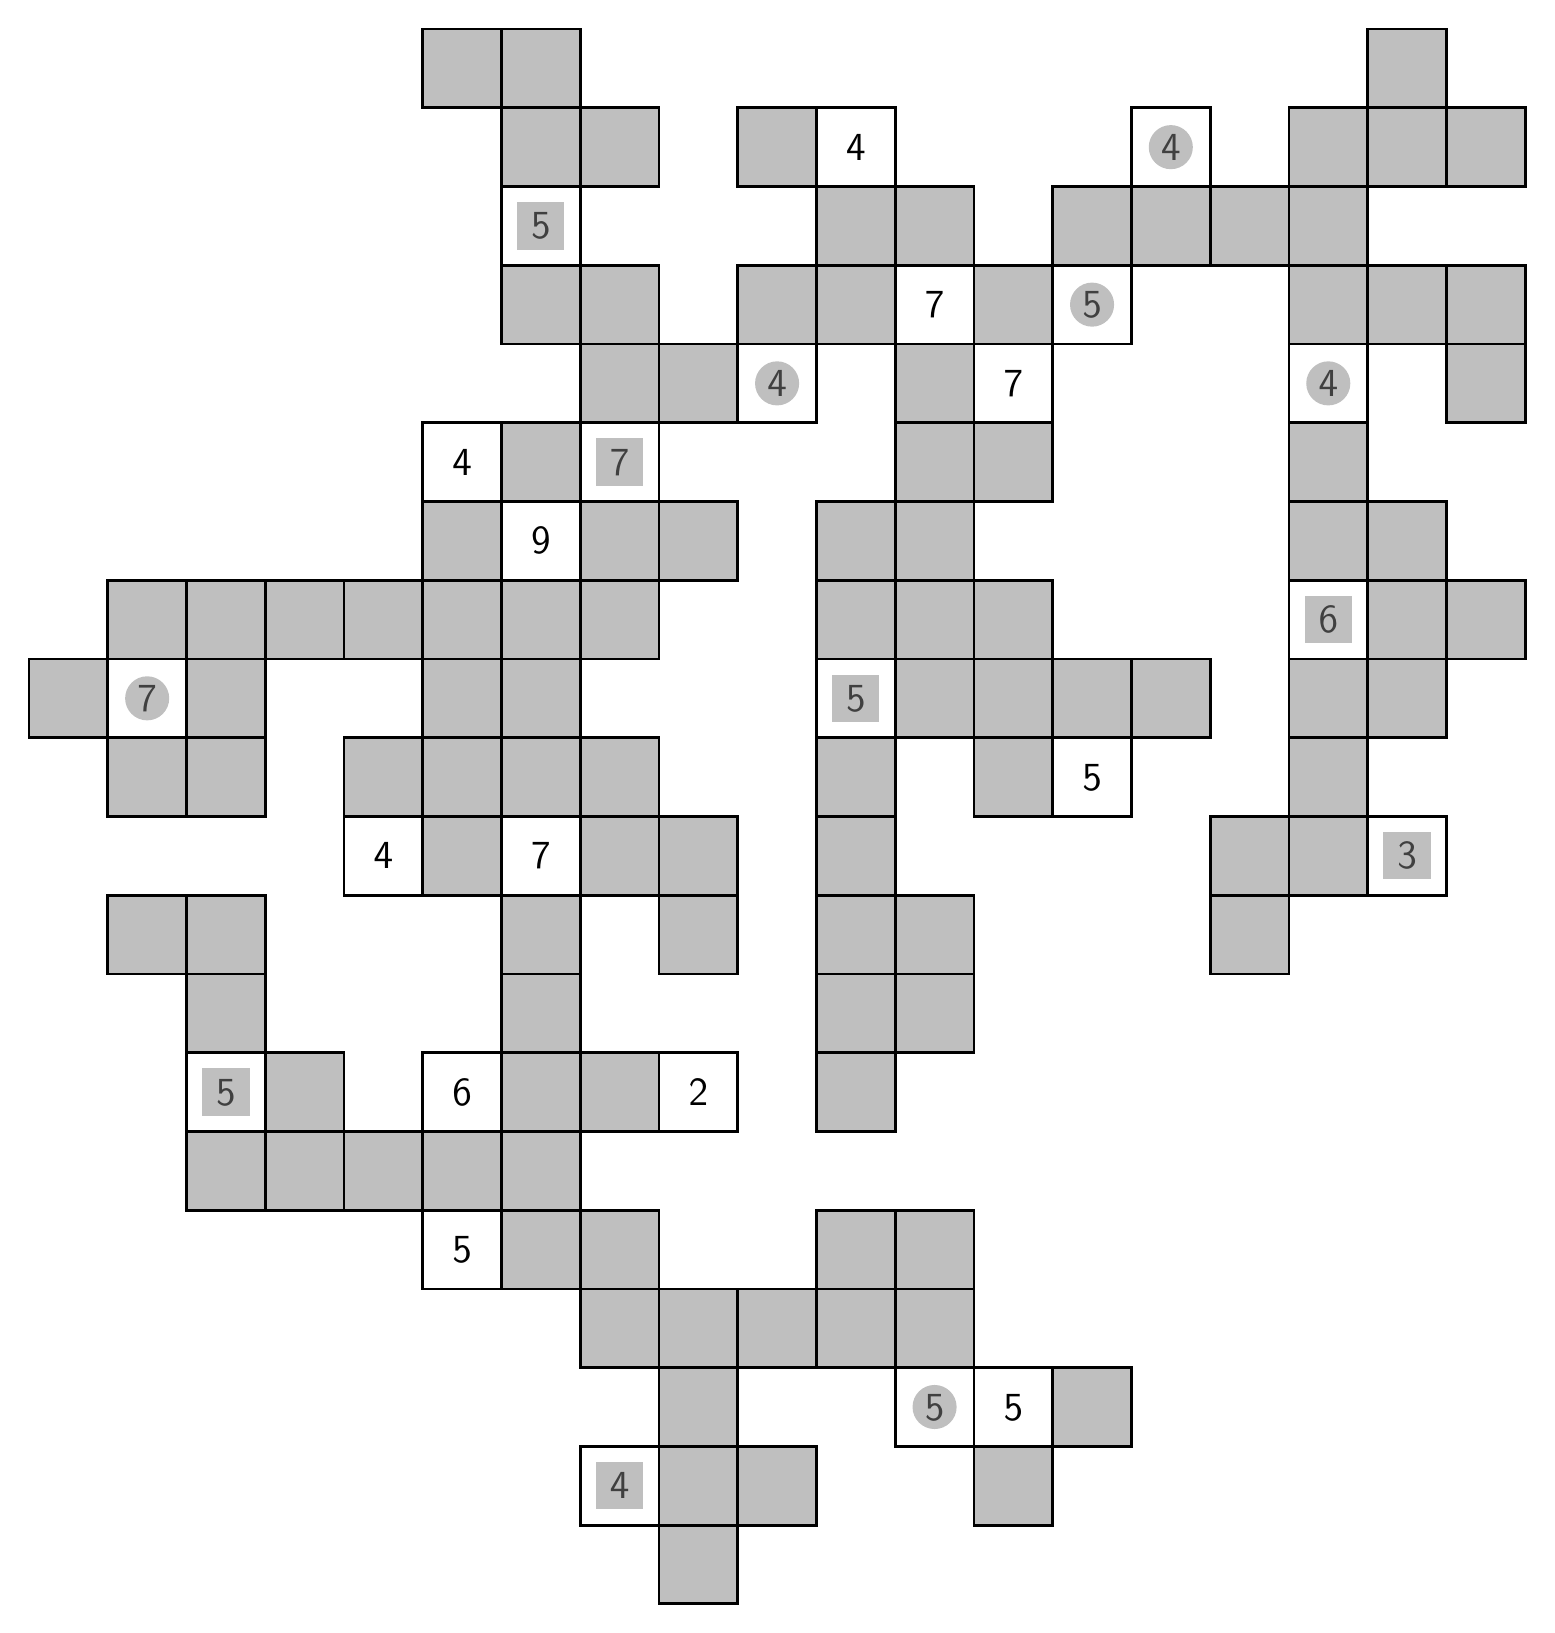
\begin{tikzpicture}\fill[gray, opacity = 0.5] (9, 0, 0)--++(1, 0, 0)--++(0, 1, 0)--++(-1, 0, 0)--cycle;
\draw[line width = 1pt] (9, 0, 0)--++(1, 0, 0)--++(0, 1, 0)--++(-1, 0, 0)--cycle;
\draw node at (8.5, 1.5, 0) {\Large $\mathsf{4}$};
\draw[line width = 1pt] (8, 1, 0)--++(1, 0, 0)--++(0, 1, 0)--++(-1, 0, 0)--cycle;
\fill[color = gray, opacity = 0.5] (8.2, 1.2) rectangle ++(0.6, 0.6);
\fill[gray, opacity = 0.5] (9, 1, 0)--++(1, 0, 0)--++(0, 1, 0)--++(-1, 0, 0)--cycle;
\draw[line width = 1pt] (9, 1, 0)--++(1, 0, 0)--++(0, 1, 0)--++(-1, 0, 0)--cycle;
\fill[gray, opacity = 0.5] (10, 1, 0)--++(1, 0, 0)--++(0, 1, 0)--++(-1, 0, 0)--cycle;
\draw[line width = 1pt] (10, 1, 0)--++(1, 0, 0)--++(0, 1, 0)--++(-1, 0, 0)--cycle;
\fill[gray, opacity = 0.5] (13, 1, 0)--++(1, 0, 0)--++(0, 1, 0)--++(-1, 0, 0)--cycle;
\draw[line width = 1pt] (13, 1, 0)--++(1, 0, 0)--++(0, 1, 0)--++(-1, 0, 0)--cycle;
\fill[gray, opacity = 0.5] (9, 2, 0)--++(1, 0, 0)--++(0, 1, 0)--++(-1, 0, 0)--cycle;
\draw[line width = 1pt] (9, 2, 0)--++(1, 0, 0)--++(0, 1, 0)--++(-1, 0, 0)--cycle;
\draw node at (12.5, 2.5, 0) {\Large $\mathsf{5}$};
\draw[line width = 1pt] (12, 2, 0)--++(1, 0, 0)--++(0, 1, 0)--++(-1, 0, 0)--cycle;
\fill[color = gray, opacity = 0.5] (12.5, 2.5, 0) circle (0.28);
\draw node at (13.5, 2.5, 0) {\Large $\mathsf{5}$};
\draw[line width = 1pt] (13, 2, 0)--++(1, 0, 0)--++(0, 1, 0)--++(-1, 0, 0)--cycle;
\fill[gray, opacity = 0.5] (14, 2, 0)--++(1, 0, 0)--++(0, 1, 0)--++(-1, 0, 0)--cycle;
\draw[line width = 1pt] (14, 2, 0)--++(1, 0, 0)--++(0, 1, 0)--++(-1, 0, 0)--cycle;
\fill[gray, opacity = 0.5] (8, 3, 0)--++(1, 0, 0)--++(0, 1, 0)--++(-1, 0, 0)--cycle;
\draw[line width = 1pt] (8, 3, 0)--++(1, 0, 0)--++(0, 1, 0)--++(-1, 0, 0)--cycle;
\fill[gray, opacity = 0.5] (9, 3, 0)--++(1, 0, 0)--++(0, 1, 0)--++(-1, 0, 0)--cycle;
\draw[line width = 1pt] (9, 3, 0)--++(1, 0, 0)--++(0, 1, 0)--++(-1, 0, 0)--cycle;
\fill[gray, opacity = 0.5] (10, 3, 0)--++(1, 0, 0)--++(0, 1, 0)--++(-1, 0, 0)--cycle;
\draw[line width = 1pt] (10, 3, 0)--++(1, 0, 0)--++(0, 1, 0)--++(-1, 0, 0)--cycle;
\fill[gray, opacity = 0.5] (11, 3, 0)--++(1, 0, 0)--++(0, 1, 0)--++(-1, 0, 0)--cycle;
\draw[line width = 1pt] (11, 3, 0)--++(1, 0, 0)--++(0, 1, 0)--++(-1, 0, 0)--cycle;
\fill[gray, opacity = 0.5] (12, 3, 0)--++(1, 0, 0)--++(0, 1, 0)--++(-1, 0, 0)--cycle;
\draw[line width = 1pt] (12, 3, 0)--++(1, 0, 0)--++(0, 1, 0)--++(-1, 0, 0)--cycle;
\draw node at (6.5, 4.5, 0) {\Large $\mathsf{5}$};
\draw[line width = 1pt] (6, 4, 0)--++(1, 0, 0)--++(0, 1, 0)--++(-1, 0, 0)--cycle;
\fill[gray, opacity = 0.5] (7, 4, 0)--++(1, 0, 0)--++(0, 1, 0)--++(-1, 0, 0)--cycle;
\draw[line width = 1pt] (7, 4, 0)--++(1, 0, 0)--++(0, 1, 0)--++(-1, 0, 0)--cycle;
\fill[gray, opacity = 0.5] (8, 4, 0)--++(1, 0, 0)--++(0, 1, 0)--++(-1, 0, 0)--cycle;
\draw[line width = 1pt] (8, 4, 0)--++(1, 0, 0)--++(0, 1, 0)--++(-1, 0, 0)--cycle;
\fill[gray, opacity = 0.5] (11, 4, 0)--++(1, 0, 0)--++(0, 1, 0)--++(-1, 0, 0)--cycle;
\draw[line width = 1pt] (11, 4, 0)--++(1, 0, 0)--++(0, 1, 0)--++(-1, 0, 0)--cycle;
\fill[gray, opacity = 0.5] (12, 4, 0)--++(1, 0, 0)--++(0, 1, 0)--++(-1, 0, 0)--cycle;
\draw[line width = 1pt] (12, 4, 0)--++(1, 0, 0)--++(0, 1, 0)--++(-1, 0, 0)--cycle;
\fill[gray, opacity = 0.5] (3, 5, 0)--++(1, 0, 0)--++(0, 1, 0)--++(-1, 0, 0)--cycle;
\draw[line width = 1pt] (3, 5, 0)--++(1, 0, 0)--++(0, 1, 0)--++(-1, 0, 0)--cycle;
\fill[gray, opacity = 0.5] (4, 5, 0)--++(1, 0, 0)--++(0, 1, 0)--++(-1, 0, 0)--cycle;
\draw[line width = 1pt] (4, 5, 0)--++(1, 0, 0)--++(0, 1, 0)--++(-1, 0, 0)--cycle;
\fill[gray, opacity = 0.5] (5, 5, 0)--++(1, 0, 0)--++(0, 1, 0)--++(-1, 0, 0)--cycle;
\draw[line width = 1pt] (5, 5, 0)--++(1, 0, 0)--++(0, 1, 0)--++(-1, 0, 0)--cycle;
\fill[gray, opacity = 0.5] (6, 5, 0)--++(1, 0, 0)--++(0, 1, 0)--++(-1, 0, 0)--cycle;
\draw[line width = 1pt] (6, 5, 0)--++(1, 0, 0)--++(0, 1, 0)--++(-1, 0, 0)--cycle;
\fill[gray, opacity = 0.5] (7, 5, 0)--++(1, 0, 0)--++(0, 1, 0)--++(-1, 0, 0)--cycle;
\draw[line width = 1pt] (7, 5, 0)--++(1, 0, 0)--++(0, 1, 0)--++(-1, 0, 0)--cycle;
\draw node at (3.5, 6.5, 0) {\Large $\mathsf{5}$};
\draw[line width = 1pt] (3, 6, 0)--++(1, 0, 0)--++(0, 1, 0)--++(-1, 0, 0)--cycle;
\fill[color = gray, opacity = 0.5] (3.2, 6.2) rectangle ++(0.6, 0.6);
\fill[gray, opacity = 0.5] (4, 6, 0)--++(1, 0, 0)--++(0, 1, 0)--++(-1, 0, 0)--cycle;
\draw[line width = 1pt] (4, 6, 0)--++(1, 0, 0)--++(0, 1, 0)--++(-1, 0, 0)--cycle;
\draw node at (6.5, 6.5, 0) {\Large $\mathsf{6}$};
\draw[line width = 1pt] (6, 6, 0)--++(1, 0, 0)--++(0, 1, 0)--++(-1, 0, 0)--cycle;
\fill[gray, opacity = 0.5] (7, 6, 0)--++(1, 0, 0)--++(0, 1, 0)--++(-1, 0, 0)--cycle;
\draw[line width = 1pt] (7, 6, 0)--++(1, 0, 0)--++(0, 1, 0)--++(-1, 0, 0)--cycle;
\fill[gray, opacity = 0.5] (8, 6, 0)--++(1, 0, 0)--++(0, 1, 0)--++(-1, 0, 0)--cycle;
\draw[line width = 1pt] (8, 6, 0)--++(1, 0, 0)--++(0, 1, 0)--++(-1, 0, 0)--cycle;
\draw node at (9.5, 6.5, 0) {\Large $\mathsf{2}$};
\draw[line width = 1pt] (9, 6, 0)--++(1, 0, 0)--++(0, 1, 0)--++(-1, 0, 0)--cycle;
\fill[gray, opacity = 0.5] (11, 6, 0)--++(1, 0, 0)--++(0, 1, 0)--++(-1, 0, 0)--cycle;
\draw[line width = 1pt] (11, 6, 0)--++(1, 0, 0)--++(0, 1, 0)--++(-1, 0, 0)--cycle;
\fill[gray, opacity = 0.5] (3, 7, 0)--++(1, 0, 0)--++(0, 1, 0)--++(-1, 0, 0)--cycle;
\draw[line width = 1pt] (3, 7, 0)--++(1, 0, 0)--++(0, 1, 0)--++(-1, 0, 0)--cycle;
\fill[gray, opacity = 0.5] (7, 7, 0)--++(1, 0, 0)--++(0, 1, 0)--++(-1, 0, 0)--cycle;
\draw[line width = 1pt] (7, 7, 0)--++(1, 0, 0)--++(0, 1, 0)--++(-1, 0, 0)--cycle;
\fill[gray, opacity = 0.5] (11, 7, 0)--++(1, 0, 0)--++(0, 1, 0)--++(-1, 0, 0)--cycle;
\draw[line width = 1pt] (11, 7, 0)--++(1, 0, 0)--++(0, 1, 0)--++(-1, 0, 0)--cycle;
\fill[gray, opacity = 0.5] (12, 7, 0)--++(1, 0, 0)--++(0, 1, 0)--++(-1, 0, 0)--cycle;
\draw[line width = 1pt] (12, 7, 0)--++(1, 0, 0)--++(0, 1, 0)--++(-1, 0, 0)--cycle;
\fill[gray, opacity = 0.5] (2, 8, 0)--++(1, 0, 0)--++(0, 1, 0)--++(-1, 0, 0)--cycle;
\draw[line width = 1pt] (2, 8, 0)--++(1, 0, 0)--++(0, 1, 0)--++(-1, 0, 0)--cycle;
\fill[gray, opacity = 0.5] (3, 8, 0)--++(1, 0, 0)--++(0, 1, 0)--++(-1, 0, 0)--cycle;
\draw[line width = 1pt] (3, 8, 0)--++(1, 0, 0)--++(0, 1, 0)--++(-1, 0, 0)--cycle;
\fill[gray, opacity = 0.5] (7, 8, 0)--++(1, 0, 0)--++(0, 1, 0)--++(-1, 0, 0)--cycle;
\draw[line width = 1pt] (7, 8, 0)--++(1, 0, 0)--++(0, 1, 0)--++(-1, 0, 0)--cycle;
\fill[gray, opacity = 0.5] (9, 8, 0)--++(1, 0, 0)--++(0, 1, 0)--++(-1, 0, 0)--cycle;
\draw[line width = 1pt] (9, 8, 0)--++(1, 0, 0)--++(0, 1, 0)--++(-1, 0, 0)--cycle;
\fill[gray, opacity = 0.5] (11, 8, 0)--++(1, 0, 0)--++(0, 1, 0)--++(-1, 0, 0)--cycle;
\draw[line width = 1pt] (11, 8, 0)--++(1, 0, 0)--++(0, 1, 0)--++(-1, 0, 0)--cycle;
\fill[gray, opacity = 0.5] (12, 8, 0)--++(1, 0, 0)--++(0, 1, 0)--++(-1, 0, 0)--cycle;
\draw[line width = 1pt] (12, 8, 0)--++(1, 0, 0)--++(0, 1, 0)--++(-1, 0, 0)--cycle;
\fill[gray, opacity = 0.5] (16, 8, 0)--++(1, 0, 0)--++(0, 1, 0)--++(-1, 0, 0)--cycle;
\draw[line width = 1pt] (16, 8, 0)--++(1, 0, 0)--++(0, 1, 0)--++(-1, 0, 0)--cycle;
\draw node at (5.5, 9.5, 0) {\Large $\mathsf{4}$};
\draw[line width = 1pt] (5, 9, 0)--++(1, 0, 0)--++(0, 1, 0)--++(-1, 0, 0)--cycle;
\fill[gray, opacity = 0.5] (6, 9, 0)--++(1, 0, 0)--++(0, 1, 0)--++(-1, 0, 0)--cycle;
\draw[line width = 1pt] (6, 9, 0)--++(1, 0, 0)--++(0, 1, 0)--++(-1, 0, 0)--cycle;
\draw node at (7.5, 9.5, 0) {\Large $\mathsf{7}$};
\draw[line width = 1pt] (7, 9, 0)--++(1, 0, 0)--++(0, 1, 0)--++(-1, 0, 0)--cycle;
\fill[gray, opacity = 0.5] (8, 9, 0)--++(1, 0, 0)--++(0, 1, 0)--++(-1, 0, 0)--cycle;
\draw[line width = 1pt] (8, 9, 0)--++(1, 0, 0)--++(0, 1, 0)--++(-1, 0, 0)--cycle;
\fill[gray, opacity = 0.5] (9, 9, 0)--++(1, 0, 0)--++(0, 1, 0)--++(-1, 0, 0)--cycle;
\draw[line width = 1pt] (9, 9, 0)--++(1, 0, 0)--++(0, 1, 0)--++(-1, 0, 0)--cycle;
\fill[gray, opacity = 0.5] (11, 9, 0)--++(1, 0, 0)--++(0, 1, 0)--++(-1, 0, 0)--cycle;
\draw[line width = 1pt] (11, 9, 0)--++(1, 0, 0)--++(0, 1, 0)--++(-1, 0, 0)--cycle;
\fill[gray, opacity = 0.5] (16, 9, 0)--++(1, 0, 0)--++(0, 1, 0)--++(-1, 0, 0)--cycle;
\draw[line width = 1pt] (16, 9, 0)--++(1, 0, 0)--++(0, 1, 0)--++(-1, 0, 0)--cycle;
\fill[gray, opacity = 0.5] (17, 9, 0)--++(1, 0, 0)--++(0, 1, 0)--++(-1, 0, 0)--cycle;
\draw[line width = 1pt] (17, 9, 0)--++(1, 0, 0)--++(0, 1, 0)--++(-1, 0, 0)--cycle;
\draw node at (18.5, 9.5, 0) {\Large $\mathsf{3}$};
\draw[line width = 1pt] (18, 9, 0)--++(1, 0, 0)--++(0, 1, 0)--++(-1, 0, 0)--cycle;
\fill[color = gray, opacity = 0.5] (18.2, 9.2) rectangle ++(0.6, 0.6);
\fill[gray, opacity = 0.5] (2, 10, 0)--++(1, 0, 0)--++(0, 1, 0)--++(-1, 0, 0)--cycle;
\draw[line width = 1pt] (2, 10, 0)--++(1, 0, 0)--++(0, 1, 0)--++(-1, 0, 0)--cycle;
\fill[gray, opacity = 0.5] (3, 10, 0)--++(1, 0, 0)--++(0, 1, 0)--++(-1, 0, 0)--cycle;
\draw[line width = 1pt] (3, 10, 0)--++(1, 0, 0)--++(0, 1, 0)--++(-1, 0, 0)--cycle;
\fill[gray, opacity = 0.5] (5, 10, 0)--++(1, 0, 0)--++(0, 1, 0)--++(-1, 0, 0)--cycle;
\draw[line width = 1pt] (5, 10, 0)--++(1, 0, 0)--++(0, 1, 0)--++(-1, 0, 0)--cycle;
\fill[gray, opacity = 0.5] (6, 10, 0)--++(1, 0, 0)--++(0, 1, 0)--++(-1, 0, 0)--cycle;
\draw[line width = 1pt] (6, 10, 0)--++(1, 0, 0)--++(0, 1, 0)--++(-1, 0, 0)--cycle;
\fill[gray, opacity = 0.5] (7, 10, 0)--++(1, 0, 0)--++(0, 1, 0)--++(-1, 0, 0)--cycle;
\draw[line width = 1pt] (7, 10, 0)--++(1, 0, 0)--++(0, 1, 0)--++(-1, 0, 0)--cycle;
\fill[gray, opacity = 0.5] (8, 10, 0)--++(1, 0, 0)--++(0, 1, 0)--++(-1, 0, 0)--cycle;
\draw[line width = 1pt] (8, 10, 0)--++(1, 0, 0)--++(0, 1, 0)--++(-1, 0, 0)--cycle;
\fill[gray, opacity = 0.5] (11, 10, 0)--++(1, 0, 0)--++(0, 1, 0)--++(-1, 0, 0)--cycle;
\draw[line width = 1pt] (11, 10, 0)--++(1, 0, 0)--++(0, 1, 0)--++(-1, 0, 0)--cycle;
\fill[gray, opacity = 0.5] (13, 10, 0)--++(1, 0, 0)--++(0, 1, 0)--++(-1, 0, 0)--cycle;
\draw[line width = 1pt] (13, 10, 0)--++(1, 0, 0)--++(0, 1, 0)--++(-1, 0, 0)--cycle;
\draw node at (14.5, 10.5, 0) {\Large $\mathsf{5}$};
\draw[line width = 1pt] (14, 10, 0)--++(1, 0, 0)--++(0, 1, 0)--++(-1, 0, 0)--cycle;
\fill[gray, opacity = 0.5] (17, 10, 0)--++(1, 0, 0)--++(0, 1, 0)--++(-1, 0, 0)--cycle;
\draw[line width = 1pt] (17, 10, 0)--++(1, 0, 0)--++(0, 1, 0)--++(-1, 0, 0)--cycle;
\fill[gray, opacity = 0.5] (1, 11, 0)--++(1, 0, 0)--++(0, 1, 0)--++(-1, 0, 0)--cycle;
\draw[line width = 1pt] (1, 11, 0)--++(1, 0, 0)--++(0, 1, 0)--++(-1, 0, 0)--cycle;
\draw node at (2.5, 11.5, 0) {\Large $\mathsf{7}$};
\draw[line width = 1pt] (2, 11, 0)--++(1, 0, 0)--++(0, 1, 0)--++(-1, 0, 0)--cycle;
\fill[color = gray, opacity = 0.5] (2.5, 11.5, 0) circle (0.28);
\fill[gray, opacity = 0.5] (3, 11, 0)--++(1, 0, 0)--++(0, 1, 0)--++(-1, 0, 0)--cycle;
\draw[line width = 1pt] (3, 11, 0)--++(1, 0, 0)--++(0, 1, 0)--++(-1, 0, 0)--cycle;
\fill[gray, opacity = 0.5] (6, 11, 0)--++(1, 0, 0)--++(0, 1, 0)--++(-1, 0, 0)--cycle;
\draw[line width = 1pt] (6, 11, 0)--++(1, 0, 0)--++(0, 1, 0)--++(-1, 0, 0)--cycle;
\fill[gray, opacity = 0.5] (7, 11, 0)--++(1, 0, 0)--++(0, 1, 0)--++(-1, 0, 0)--cycle;
\draw[line width = 1pt] (7, 11, 0)--++(1, 0, 0)--++(0, 1, 0)--++(-1, 0, 0)--cycle;
\draw node at (11.5, 11.5, 0) {\Large $\mathsf{5}$};
\draw[line width = 1pt] (11, 11, 0)--++(1, 0, 0)--++(0, 1, 0)--++(-1, 0, 0)--cycle;
\fill[color = gray, opacity = 0.5] (11.2, 11.2) rectangle ++(0.6, 0.6);
\fill[gray, opacity = 0.5] (12, 11, 0)--++(1, 0, 0)--++(0, 1, 0)--++(-1, 0, 0)--cycle;
\draw[line width = 1pt] (12, 11, 0)--++(1, 0, 0)--++(0, 1, 0)--++(-1, 0, 0)--cycle;
\fill[gray, opacity = 0.5] (13, 11, 0)--++(1, 0, 0)--++(0, 1, 0)--++(-1, 0, 0)--cycle;
\draw[line width = 1pt] (13, 11, 0)--++(1, 0, 0)--++(0, 1, 0)--++(-1, 0, 0)--cycle;
\fill[gray, opacity = 0.5] (14, 11, 0)--++(1, 0, 0)--++(0, 1, 0)--++(-1, 0, 0)--cycle;
\draw[line width = 1pt] (14, 11, 0)--++(1, 0, 0)--++(0, 1, 0)--++(-1, 0, 0)--cycle;
\fill[gray, opacity = 0.5] (15, 11, 0)--++(1, 0, 0)--++(0, 1, 0)--++(-1, 0, 0)--cycle;
\draw[line width = 1pt] (15, 11, 0)--++(1, 0, 0)--++(0, 1, 0)--++(-1, 0, 0)--cycle;
\fill[gray, opacity = 0.5] (17, 11, 0)--++(1, 0, 0)--++(0, 1, 0)--++(-1, 0, 0)--cycle;
\draw[line width = 1pt] (17, 11, 0)--++(1, 0, 0)--++(0, 1, 0)--++(-1, 0, 0)--cycle;
\fill[gray, opacity = 0.5] (18, 11, 0)--++(1, 0, 0)--++(0, 1, 0)--++(-1, 0, 0)--cycle;
\draw[line width = 1pt] (18, 11, 0)--++(1, 0, 0)--++(0, 1, 0)--++(-1, 0, 0)--cycle;
\fill[gray, opacity = 0.5] (2, 12, 0)--++(1, 0, 0)--++(0, 1, 0)--++(-1, 0, 0)--cycle;
\draw[line width = 1pt] (2, 12, 0)--++(1, 0, 0)--++(0, 1, 0)--++(-1, 0, 0)--cycle;
\fill[gray, opacity = 0.5] (3, 12, 0)--++(1, 0, 0)--++(0, 1, 0)--++(-1, 0, 0)--cycle;
\draw[line width = 1pt] (3, 12, 0)--++(1, 0, 0)--++(0, 1, 0)--++(-1, 0, 0)--cycle;
\fill[gray, opacity = 0.5] (4, 12, 0)--++(1, 0, 0)--++(0, 1, 0)--++(-1, 0, 0)--cycle;
\draw[line width = 1pt] (4, 12, 0)--++(1, 0, 0)--++(0, 1, 0)--++(-1, 0, 0)--cycle;
\fill[gray, opacity = 0.5] (5, 12, 0)--++(1, 0, 0)--++(0, 1, 0)--++(-1, 0, 0)--cycle;
\draw[line width = 1pt] (5, 12, 0)--++(1, 0, 0)--++(0, 1, 0)--++(-1, 0, 0)--cycle;
\fill[gray, opacity = 0.5] (6, 12, 0)--++(1, 0, 0)--++(0, 1, 0)--++(-1, 0, 0)--cycle;
\draw[line width = 1pt] (6, 12, 0)--++(1, 0, 0)--++(0, 1, 0)--++(-1, 0, 0)--cycle;
\fill[gray, opacity = 0.5] (7, 12, 0)--++(1, 0, 0)--++(0, 1, 0)--++(-1, 0, 0)--cycle;
\draw[line width = 1pt] (7, 12, 0)--++(1, 0, 0)--++(0, 1, 0)--++(-1, 0, 0)--cycle;
\fill[gray, opacity = 0.5] (8, 12, 0)--++(1, 0, 0)--++(0, 1, 0)--++(-1, 0, 0)--cycle;
\draw[line width = 1pt] (8, 12, 0)--++(1, 0, 0)--++(0, 1, 0)--++(-1, 0, 0)--cycle;
\fill[gray, opacity = 0.5] (11, 12, 0)--++(1, 0, 0)--++(0, 1, 0)--++(-1, 0, 0)--cycle;
\draw[line width = 1pt] (11, 12, 0)--++(1, 0, 0)--++(0, 1, 0)--++(-1, 0, 0)--cycle;
\fill[gray, opacity = 0.5] (12, 12, 0)--++(1, 0, 0)--++(0, 1, 0)--++(-1, 0, 0)--cycle;
\draw[line width = 1pt] (12, 12, 0)--++(1, 0, 0)--++(0, 1, 0)--++(-1, 0, 0)--cycle;
\fill[gray, opacity = 0.5] (13, 12, 0)--++(1, 0, 0)--++(0, 1, 0)--++(-1, 0, 0)--cycle;
\draw[line width = 1pt] (13, 12, 0)--++(1, 0, 0)--++(0, 1, 0)--++(-1, 0, 0)--cycle;
\draw node at (17.5, 12.5, 0) {\Large $\mathsf{6}$};
\draw[line width = 1pt] (17, 12, 0)--++(1, 0, 0)--++(0, 1, 0)--++(-1, 0, 0)--cycle;
\fill[color = gray, opacity = 0.5] (17.2, 12.2) rectangle ++(0.6, 0.6);
\fill[gray, opacity = 0.5] (18, 12, 0)--++(1, 0, 0)--++(0, 1, 0)--++(-1, 0, 0)--cycle;
\draw[line width = 1pt] (18, 12, 0)--++(1, 0, 0)--++(0, 1, 0)--++(-1, 0, 0)--cycle;
\fill[gray, opacity = 0.5] (19, 12, 0)--++(1, 0, 0)--++(0, 1, 0)--++(-1, 0, 0)--cycle;
\draw[line width = 1pt] (19, 12, 0)--++(1, 0, 0)--++(0, 1, 0)--++(-1, 0, 0)--cycle;
\fill[gray, opacity = 0.5] (6, 13, 0)--++(1, 0, 0)--++(0, 1, 0)--++(-1, 0, 0)--cycle;
\draw[line width = 1pt] (6, 13, 0)--++(1, 0, 0)--++(0, 1, 0)--++(-1, 0, 0)--cycle;
\draw node at (7.5, 13.5, 0) {\Large $\mathsf{9}$};
\draw[line width = 1pt] (7, 13, 0)--++(1, 0, 0)--++(0, 1, 0)--++(-1, 0, 0)--cycle;
\fill[gray, opacity = 0.5] (8, 13, 0)--++(1, 0, 0)--++(0, 1, 0)--++(-1, 0, 0)--cycle;
\draw[line width = 1pt] (8, 13, 0)--++(1, 0, 0)--++(0, 1, 0)--++(-1, 0, 0)--cycle;
\fill[gray, opacity = 0.5] (9, 13, 0)--++(1, 0, 0)--++(0, 1, 0)--++(-1, 0, 0)--cycle;
\draw[line width = 1pt] (9, 13, 0)--++(1, 0, 0)--++(0, 1, 0)--++(-1, 0, 0)--cycle;
\fill[gray, opacity = 0.5] (11, 13, 0)--++(1, 0, 0)--++(0, 1, 0)--++(-1, 0, 0)--cycle;
\draw[line width = 1pt] (11, 13, 0)--++(1, 0, 0)--++(0, 1, 0)--++(-1, 0, 0)--cycle;
\fill[gray, opacity = 0.5] (12, 13, 0)--++(1, 0, 0)--++(0, 1, 0)--++(-1, 0, 0)--cycle;
\draw[line width = 1pt] (12, 13, 0)--++(1, 0, 0)--++(0, 1, 0)--++(-1, 0, 0)--cycle;
\fill[gray, opacity = 0.5] (17, 13, 0)--++(1, 0, 0)--++(0, 1, 0)--++(-1, 0, 0)--cycle;
\draw[line width = 1pt] (17, 13, 0)--++(1, 0, 0)--++(0, 1, 0)--++(-1, 0, 0)--cycle;
\fill[gray, opacity = 0.5] (18, 13, 0)--++(1, 0, 0)--++(0, 1, 0)--++(-1, 0, 0)--cycle;
\draw[line width = 1pt] (18, 13, 0)--++(1, 0, 0)--++(0, 1, 0)--++(-1, 0, 0)--cycle;
\draw node at (6.5, 14.5, 0) {\Large $\mathsf{4}$};
\draw[line width = 1pt] (6, 14, 0)--++(1, 0, 0)--++(0, 1, 0)--++(-1, 0, 0)--cycle;
\fill[gray, opacity = 0.5] (7, 14, 0)--++(1, 0, 0)--++(0, 1, 0)--++(-1, 0, 0)--cycle;
\draw[line width = 1pt] (7, 14, 0)--++(1, 0, 0)--++(0, 1, 0)--++(-1, 0, 0)--cycle;
\draw node at (8.5, 14.5, 0) {\Large $\mathsf{7}$};
\draw[line width = 1pt] (8, 14, 0)--++(1, 0, 0)--++(0, 1, 0)--++(-1, 0, 0)--cycle;
\fill[color = gray, opacity = 0.5] (8.2, 14.2) rectangle ++(0.6, 0.6);
\fill[gray, opacity = 0.5] (12, 14, 0)--++(1, 0, 0)--++(0, 1, 0)--++(-1, 0, 0)--cycle;
\draw[line width = 1pt] (12, 14, 0)--++(1, 0, 0)--++(0, 1, 0)--++(-1, 0, 0)--cycle;
\fill[gray, opacity = 0.5] (13, 14, 0)--++(1, 0, 0)--++(0, 1, 0)--++(-1, 0, 0)--cycle;
\draw[line width = 1pt] (13, 14, 0)--++(1, 0, 0)--++(0, 1, 0)--++(-1, 0, 0)--cycle;
\fill[gray, opacity = 0.5] (17, 14, 0)--++(1, 0, 0)--++(0, 1, 0)--++(-1, 0, 0)--cycle;
\draw[line width = 1pt] (17, 14, 0)--++(1, 0, 0)--++(0, 1, 0)--++(-1, 0, 0)--cycle;
\fill[gray, opacity = 0.5] (8, 15, 0)--++(1, 0, 0)--++(0, 1, 0)--++(-1, 0, 0)--cycle;
\draw[line width = 1pt] (8, 15, 0)--++(1, 0, 0)--++(0, 1, 0)--++(-1, 0, 0)--cycle;
\fill[gray, opacity = 0.5] (9, 15, 0)--++(1, 0, 0)--++(0, 1, 0)--++(-1, 0, 0)--cycle;
\draw[line width = 1pt] (9, 15, 0)--++(1, 0, 0)--++(0, 1, 0)--++(-1, 0, 0)--cycle;
\draw node at (10.5, 15.5, 0) {\Large $\mathsf{4}$};
\draw[line width = 1pt] (10, 15, 0)--++(1, 0, 0)--++(0, 1, 0)--++(-1, 0, 0)--cycle;
\fill[color = gray, opacity = 0.5] (10.5, 15.5, 0) circle (0.28);
\fill[gray, opacity = 0.5] (12, 15, 0)--++(1, 0, 0)--++(0, 1, 0)--++(-1, 0, 0)--cycle;
\draw[line width = 1pt] (12, 15, 0)--++(1, 0, 0)--++(0, 1, 0)--++(-1, 0, 0)--cycle;
\draw node at (13.5, 15.5, 0) {\Large $\mathsf{7}$};
\draw[line width = 1pt] (13, 15, 0)--++(1, 0, 0)--++(0, 1, 0)--++(-1, 0, 0)--cycle;
\draw node at (17.5, 15.5, 0) {\Large $\mathsf{4}$};
\draw[line width = 1pt] (17, 15, 0)--++(1, 0, 0)--++(0, 1, 0)--++(-1, 0, 0)--cycle;
\fill[color = gray, opacity = 0.5] (17.5, 15.5, 0) circle (0.28);
\fill[gray, opacity = 0.5] (19, 15, 0)--++(1, 0, 0)--++(0, 1, 0)--++(-1, 0, 0)--cycle;
\draw[line width = 1pt] (19, 15, 0)--++(1, 0, 0)--++(0, 1, 0)--++(-1, 0, 0)--cycle;
\fill[gray, opacity = 0.5] (7, 16, 0)--++(1, 0, 0)--++(0, 1, 0)--++(-1, 0, 0)--cycle;
\draw[line width = 1pt] (7, 16, 0)--++(1, 0, 0)--++(0, 1, 0)--++(-1, 0, 0)--cycle;
\fill[gray, opacity = 0.5] (8, 16, 0)--++(1, 0, 0)--++(0, 1, 0)--++(-1, 0, 0)--cycle;
\draw[line width = 1pt] (8, 16, 0)--++(1, 0, 0)--++(0, 1, 0)--++(-1, 0, 0)--cycle;
\fill[gray, opacity = 0.5] (10, 16, 0)--++(1, 0, 0)--++(0, 1, 0)--++(-1, 0, 0)--cycle;
\draw[line width = 1pt] (10, 16, 0)--++(1, 0, 0)--++(0, 1, 0)--++(-1, 0, 0)--cycle;
\fill[gray, opacity = 0.5] (11, 16, 0)--++(1, 0, 0)--++(0, 1, 0)--++(-1, 0, 0)--cycle;
\draw[line width = 1pt] (11, 16, 0)--++(1, 0, 0)--++(0, 1, 0)--++(-1, 0, 0)--cycle;
\draw node at (12.5, 16.5, 0) {\Large $\mathsf{7}$};
\draw[line width = 1pt] (12, 16, 0)--++(1, 0, 0)--++(0, 1, 0)--++(-1, 0, 0)--cycle;
\fill[gray, opacity = 0.5] (13, 16, 0)--++(1, 0, 0)--++(0, 1, 0)--++(-1, 0, 0)--cycle;
\draw[line width = 1pt] (13, 16, 0)--++(1, 0, 0)--++(0, 1, 0)--++(-1, 0, 0)--cycle;
\draw node at (14.5, 16.5, 0) {\Large $\mathsf{5}$};
\draw[line width = 1pt] (14, 16, 0)--++(1, 0, 0)--++(0, 1, 0)--++(-1, 0, 0)--cycle;
\fill[color = gray, opacity = 0.5] (14.5, 16.5, 0) circle (0.28);
\fill[gray, opacity = 0.5] (17, 16, 0)--++(1, 0, 0)--++(0, 1, 0)--++(-1, 0, 0)--cycle;
\draw[line width = 1pt] (17, 16, 0)--++(1, 0, 0)--++(0, 1, 0)--++(-1, 0, 0)--cycle;
\fill[gray, opacity = 0.5] (18, 16, 0)--++(1, 0, 0)--++(0, 1, 0)--++(-1, 0, 0)--cycle;
\draw[line width = 1pt] (18, 16, 0)--++(1, 0, 0)--++(0, 1, 0)--++(-1, 0, 0)--cycle;
\fill[gray, opacity = 0.5] (19, 16, 0)--++(1, 0, 0)--++(0, 1, 0)--++(-1, 0, 0)--cycle;
\draw[line width = 1pt] (19, 16, 0)--++(1, 0, 0)--++(0, 1, 0)--++(-1, 0, 0)--cycle;
\draw node at (7.5, 17.5, 0) {\Large $\mathsf{5}$};
\draw[line width = 1pt] (7, 17, 0)--++(1, 0, 0)--++(0, 1, 0)--++(-1, 0, 0)--cycle;
\fill[color = gray, opacity = 0.5] (7.2, 17.2) rectangle ++(0.6, 0.6);
\fill[gray, opacity = 0.5] (11, 17, 0)--++(1, 0, 0)--++(0, 1, 0)--++(-1, 0, 0)--cycle;
\draw[line width = 1pt] (11, 17, 0)--++(1, 0, 0)--++(0, 1, 0)--++(-1, 0, 0)--cycle;
\fill[gray, opacity = 0.5] (12, 17, 0)--++(1, 0, 0)--++(0, 1, 0)--++(-1, 0, 0)--cycle;
\draw[line width = 1pt] (12, 17, 0)--++(1, 0, 0)--++(0, 1, 0)--++(-1, 0, 0)--cycle;
\fill[gray, opacity = 0.5] (14, 17, 0)--++(1, 0, 0)--++(0, 1, 0)--++(-1, 0, 0)--cycle;
\draw[line width = 1pt] (14, 17, 0)--++(1, 0, 0)--++(0, 1, 0)--++(-1, 0, 0)--cycle;
\fill[gray, opacity = 0.5] (15, 17, 0)--++(1, 0, 0)--++(0, 1, 0)--++(-1, 0, 0)--cycle;
\draw[line width = 1pt] (15, 17, 0)--++(1, 0, 0)--++(0, 1, 0)--++(-1, 0, 0)--cycle;
\fill[gray, opacity = 0.5] (16, 17, 0)--++(1, 0, 0)--++(0, 1, 0)--++(-1, 0, 0)--cycle;
\draw[line width = 1pt] (16, 17, 0)--++(1, 0, 0)--++(0, 1, 0)--++(-1, 0, 0)--cycle;
\fill[gray, opacity = 0.5] (17, 17, 0)--++(1, 0, 0)--++(0, 1, 0)--++(-1, 0, 0)--cycle;
\draw[line width = 1pt] (17, 17, 0)--++(1, 0, 0)--++(0, 1, 0)--++(-1, 0, 0)--cycle;
\fill[gray, opacity = 0.5] (7, 18, 0)--++(1, 0, 0)--++(0, 1, 0)--++(-1, 0, 0)--cycle;
\draw[line width = 1pt] (7, 18, 0)--++(1, 0, 0)--++(0, 1, 0)--++(-1, 0, 0)--cycle;
\fill[gray, opacity = 0.5] (8, 18, 0)--++(1, 0, 0)--++(0, 1, 0)--++(-1, 0, 0)--cycle;
\draw[line width = 1pt] (8, 18, 0)--++(1, 0, 0)--++(0, 1, 0)--++(-1, 0, 0)--cycle;
\fill[gray, opacity = 0.5] (10, 18, 0)--++(1, 0, 0)--++(0, 1, 0)--++(-1, 0, 0)--cycle;
\draw[line width = 1pt] (10, 18, 0)--++(1, 0, 0)--++(0, 1, 0)--++(-1, 0, 0)--cycle;
\draw node at (11.5, 18.5, 0) {\Large $\mathsf{4}$};
\draw[line width = 1pt] (11, 18, 0)--++(1, 0, 0)--++(0, 1, 0)--++(-1, 0, 0)--cycle;
\draw node at (15.5, 18.5, 0) {\Large $\mathsf{4}$};
\draw[line width = 1pt] (15, 18, 0)--++(1, 0, 0)--++(0, 1, 0)--++(-1, 0, 0)--cycle;
\fill[color = gray, opacity = 0.5] (15.5, 18.5, 0) circle (0.28);
\fill[gray, opacity = 0.5] (17, 18, 0)--++(1, 0, 0)--++(0, 1, 0)--++(-1, 0, 0)--cycle;
\draw[line width = 1pt] (17, 18, 0)--++(1, 0, 0)--++(0, 1, 0)--++(-1, 0, 0)--cycle;
\fill[gray, opacity = 0.5] (18, 18, 0)--++(1, 0, 0)--++(0, 1, 0)--++(-1, 0, 0)--cycle;
\draw[line width = 1pt] (18, 18, 0)--++(1, 0, 0)--++(0, 1, 0)--++(-1, 0, 0)--cycle;
\fill[gray, opacity = 0.5] (19, 18, 0)--++(1, 0, 0)--++(0, 1, 0)--++(-1, 0, 0)--cycle;
\draw[line width = 1pt] (19, 18, 0)--++(1, 0, 0)--++(0, 1, 0)--++(-1, 0, 0)--cycle;
\fill[gray, opacity = 0.5] (6, 19, 0)--++(1, 0, 0)--++(0, 1, 0)--++(-1, 0, 0)--cycle;
\draw[line width = 1pt] (6, 19, 0)--++(1, 0, 0)--++(0, 1, 0)--++(-1, 0, 0)--cycle;
\fill[gray, opacity = 0.5] (7, 19, 0)--++(1, 0, 0)--++(0, 1, 0)--++(-1, 0, 0)--cycle;
\draw[line width = 1pt] (7, 19, 0)--++(1, 0, 0)--++(0, 1, 0)--++(-1, 0, 0)--cycle;
\fill[gray, opacity = 0.5] (18, 19, 0)--++(1, 0, 0)--++(0, 1, 0)--++(-1, 0, 0)--cycle;
\draw[line width = 1pt] (18, 19, 0)--++(1, 0, 0)--++(0, 1, 0)--++(-1, 0, 0)--cycle;
\end{tikzpicture}}\]
\[\resizebox{30pc}{!}{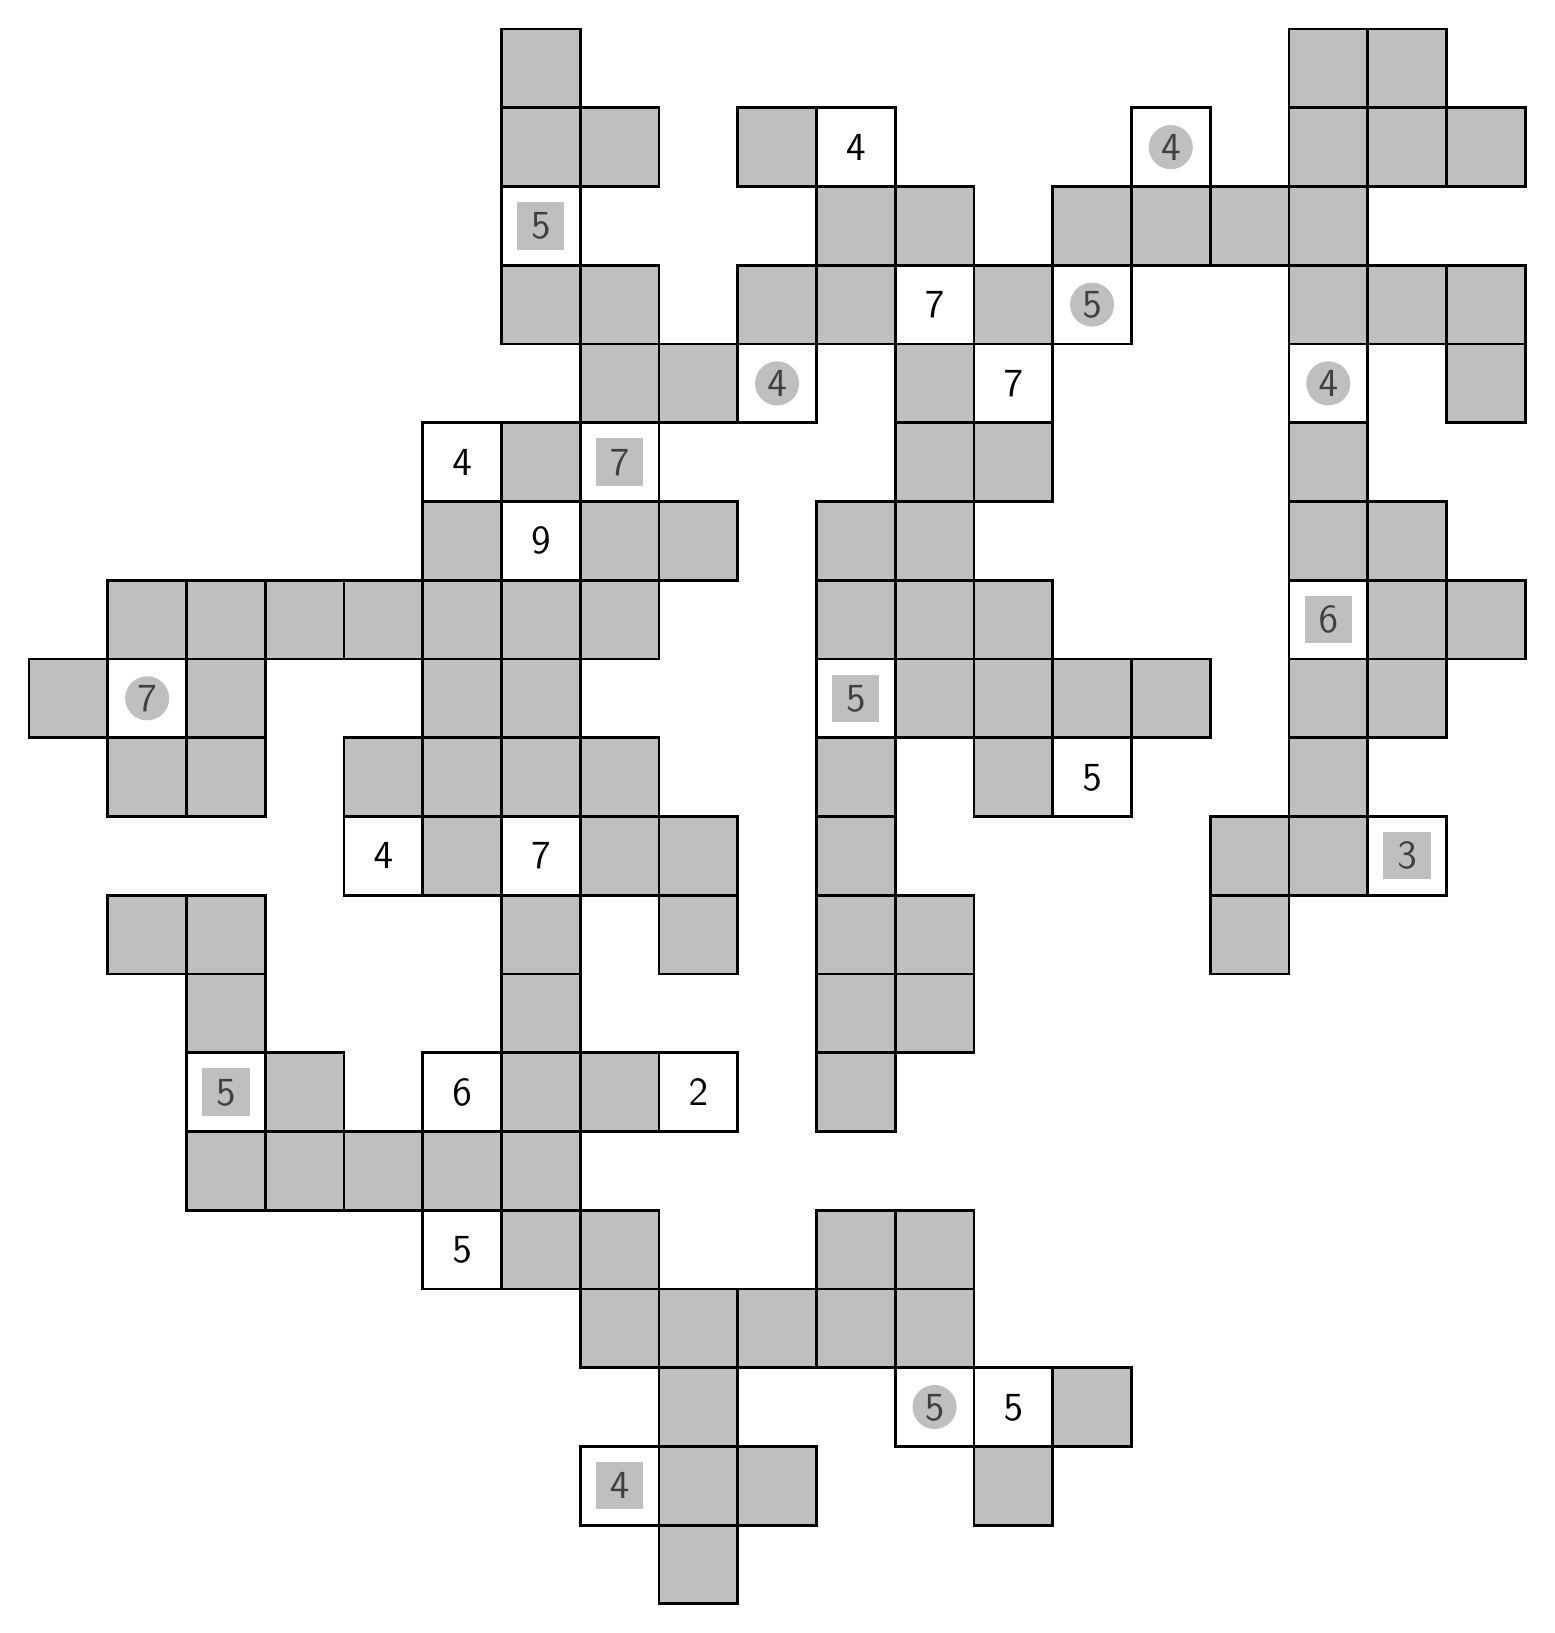
\begin{tikzpicture}\fill[gray, opacity = 0.5] (9, 0, 0)--++(1, 0, 0)--++(0, 1, 0)--++(-1, 0, 0)--cycle;
\draw[line width = 1pt] (9, 0, 0)--++(1, 0, 0)--++(0, 1, 0)--++(-1, 0, 0)--cycle;
\draw node at (8.5, 1.5, 0) {\Large $\mathsf{4}$};
\draw[line width = 1pt] (8, 1, 0)--++(1, 0, 0)--++(0, 1, 0)--++(-1, 0, 0)--cycle;
\fill[color = gray, opacity = 0.5] (8.2, 1.2) rectangle ++(0.6, 0.6);
\fill[gray, opacity = 0.5] (9, 1, 0)--++(1, 0, 0)--++(0, 1, 0)--++(-1, 0, 0)--cycle;
\draw[line width = 1pt] (9, 1, 0)--++(1, 0, 0)--++(0, 1, 0)--++(-1, 0, 0)--cycle;
\fill[gray, opacity = 0.5] (10, 1, 0)--++(1, 0, 0)--++(0, 1, 0)--++(-1, 0, 0)--cycle;
\draw[line width = 1pt] (10, 1, 0)--++(1, 0, 0)--++(0, 1, 0)--++(-1, 0, 0)--cycle;
\fill[gray, opacity = 0.5] (13, 1, 0)--++(1, 0, 0)--++(0, 1, 0)--++(-1, 0, 0)--cycle;
\draw[line width = 1pt] (13, 1, 0)--++(1, 0, 0)--++(0, 1, 0)--++(-1, 0, 0)--cycle;
\fill[gray, opacity = 0.5] (9, 2, 0)--++(1, 0, 0)--++(0, 1, 0)--++(-1, 0, 0)--cycle;
\draw[line width = 1pt] (9, 2, 0)--++(1, 0, 0)--++(0, 1, 0)--++(-1, 0, 0)--cycle;
\draw node at (12.5, 2.5, 0) {\Large $\mathsf{5}$};
\draw[line width = 1pt] (12, 2, 0)--++(1, 0, 0)--++(0, 1, 0)--++(-1, 0, 0)--cycle;
\fill[color = gray, opacity = 0.5] (12.5, 2.5, 0) circle (0.28);
\draw node at (13.5, 2.5, 0) {\Large $\mathsf{5}$};
\draw[line width = 1pt] (13, 2, 0)--++(1, 0, 0)--++(0, 1, 0)--++(-1, 0, 0)--cycle;
\fill[gray, opacity = 0.5] (14, 2, 0)--++(1, 0, 0)--++(0, 1, 0)--++(-1, 0, 0)--cycle;
\draw[line width = 1pt] (14, 2, 0)--++(1, 0, 0)--++(0, 1, 0)--++(-1, 0, 0)--cycle;
\fill[gray, opacity = 0.5] (8, 3, 0)--++(1, 0, 0)--++(0, 1, 0)--++(-1, 0, 0)--cycle;
\draw[line width = 1pt] (8, 3, 0)--++(1, 0, 0)--++(0, 1, 0)--++(-1, 0, 0)--cycle;
\fill[gray, opacity = 0.5] (9, 3, 0)--++(1, 0, 0)--++(0, 1, 0)--++(-1, 0, 0)--cycle;
\draw[line width = 1pt] (9, 3, 0)--++(1, 0, 0)--++(0, 1, 0)--++(-1, 0, 0)--cycle;
\fill[gray, opacity = 0.5] (10, 3, 0)--++(1, 0, 0)--++(0, 1, 0)--++(-1, 0, 0)--cycle;
\draw[line width = 1pt] (10, 3, 0)--++(1, 0, 0)--++(0, 1, 0)--++(-1, 0, 0)--cycle;
\fill[gray, opacity = 0.5] (11, 3, 0)--++(1, 0, 0)--++(0, 1, 0)--++(-1, 0, 0)--cycle;
\draw[line width = 1pt] (11, 3, 0)--++(1, 0, 0)--++(0, 1, 0)--++(-1, 0, 0)--cycle;
\fill[gray, opacity = 0.5] (12, 3, 0)--++(1, 0, 0)--++(0, 1, 0)--++(-1, 0, 0)--cycle;
\draw[line width = 1pt] (12, 3, 0)--++(1, 0, 0)--++(0, 1, 0)--++(-1, 0, 0)--cycle;
\draw node at (6.5, 4.5, 0) {\Large $\mathsf{5}$};
\draw[line width = 1pt] (6, 4, 0)--++(1, 0, 0)--++(0, 1, 0)--++(-1, 0, 0)--cycle;
\fill[gray, opacity = 0.5] (7, 4, 0)--++(1, 0, 0)--++(0, 1, 0)--++(-1, 0, 0)--cycle;
\draw[line width = 1pt] (7, 4, 0)--++(1, 0, 0)--++(0, 1, 0)--++(-1, 0, 0)--cycle;
\fill[gray, opacity = 0.5] (8, 4, 0)--++(1, 0, 0)--++(0, 1, 0)--++(-1, 0, 0)--cycle;
\draw[line width = 1pt] (8, 4, 0)--++(1, 0, 0)--++(0, 1, 0)--++(-1, 0, 0)--cycle;
\fill[gray, opacity = 0.5] (11, 4, 0)--++(1, 0, 0)--++(0, 1, 0)--++(-1, 0, 0)--cycle;
\draw[line width = 1pt] (11, 4, 0)--++(1, 0, 0)--++(0, 1, 0)--++(-1, 0, 0)--cycle;
\fill[gray, opacity = 0.5] (12, 4, 0)--++(1, 0, 0)--++(0, 1, 0)--++(-1, 0, 0)--cycle;
\draw[line width = 1pt] (12, 4, 0)--++(1, 0, 0)--++(0, 1, 0)--++(-1, 0, 0)--cycle;
\fill[gray, opacity = 0.5] (3, 5, 0)--++(1, 0, 0)--++(0, 1, 0)--++(-1, 0, 0)--cycle;
\draw[line width = 1pt] (3, 5, 0)--++(1, 0, 0)--++(0, 1, 0)--++(-1, 0, 0)--cycle;
\fill[gray, opacity = 0.5] (4, 5, 0)--++(1, 0, 0)--++(0, 1, 0)--++(-1, 0, 0)--cycle;
\draw[line width = 1pt] (4, 5, 0)--++(1, 0, 0)--++(0, 1, 0)--++(-1, 0, 0)--cycle;
\fill[gray, opacity = 0.5] (5, 5, 0)--++(1, 0, 0)--++(0, 1, 0)--++(-1, 0, 0)--cycle;
\draw[line width = 1pt] (5, 5, 0)--++(1, 0, 0)--++(0, 1, 0)--++(-1, 0, 0)--cycle;
\fill[gray, opacity = 0.5] (6, 5, 0)--++(1, 0, 0)--++(0, 1, 0)--++(-1, 0, 0)--cycle;
\draw[line width = 1pt] (6, 5, 0)--++(1, 0, 0)--++(0, 1, 0)--++(-1, 0, 0)--cycle;
\fill[gray, opacity = 0.5] (7, 5, 0)--++(1, 0, 0)--++(0, 1, 0)--++(-1, 0, 0)--cycle;
\draw[line width = 1pt] (7, 5, 0)--++(1, 0, 0)--++(0, 1, 0)--++(-1, 0, 0)--cycle;
\draw node at (3.5, 6.5, 0) {\Large $\mathsf{5}$};
\draw[line width = 1pt] (3, 6, 0)--++(1, 0, 0)--++(0, 1, 0)--++(-1, 0, 0)--cycle;
\fill[color = gray, opacity = 0.5] (3.2, 6.2) rectangle ++(0.6, 0.6);
\fill[gray, opacity = 0.5] (4, 6, 0)--++(1, 0, 0)--++(0, 1, 0)--++(-1, 0, 0)--cycle;
\draw[line width = 1pt] (4, 6, 0)--++(1, 0, 0)--++(0, 1, 0)--++(-1, 0, 0)--cycle;
\draw node at (6.5, 6.5, 0) {\Large $\mathsf{6}$};
\draw[line width = 1pt] (6, 6, 0)--++(1, 0, 0)--++(0, 1, 0)--++(-1, 0, 0)--cycle;
\fill[gray, opacity = 0.5] (7, 6, 0)--++(1, 0, 0)--++(0, 1, 0)--++(-1, 0, 0)--cycle;
\draw[line width = 1pt] (7, 6, 0)--++(1, 0, 0)--++(0, 1, 0)--++(-1, 0, 0)--cycle;
\fill[gray, opacity = 0.5] (8, 6, 0)--++(1, 0, 0)--++(0, 1, 0)--++(-1, 0, 0)--cycle;
\draw[line width = 1pt] (8, 6, 0)--++(1, 0, 0)--++(0, 1, 0)--++(-1, 0, 0)--cycle;
\draw node at (9.5, 6.5, 0) {\Large $\mathsf{2}$};
\draw[line width = 1pt] (9, 6, 0)--++(1, 0, 0)--++(0, 1, 0)--++(-1, 0, 0)--cycle;
\fill[gray, opacity = 0.5] (11, 6, 0)--++(1, 0, 0)--++(0, 1, 0)--++(-1, 0, 0)--cycle;
\draw[line width = 1pt] (11, 6, 0)--++(1, 0, 0)--++(0, 1, 0)--++(-1, 0, 0)--cycle;
\fill[gray, opacity = 0.5] (3, 7, 0)--++(1, 0, 0)--++(0, 1, 0)--++(-1, 0, 0)--cycle;
\draw[line width = 1pt] (3, 7, 0)--++(1, 0, 0)--++(0, 1, 0)--++(-1, 0, 0)--cycle;
\fill[gray, opacity = 0.5] (7, 7, 0)--++(1, 0, 0)--++(0, 1, 0)--++(-1, 0, 0)--cycle;
\draw[line width = 1pt] (7, 7, 0)--++(1, 0, 0)--++(0, 1, 0)--++(-1, 0, 0)--cycle;
\fill[gray, opacity = 0.5] (11, 7, 0)--++(1, 0, 0)--++(0, 1, 0)--++(-1, 0, 0)--cycle;
\draw[line width = 1pt] (11, 7, 0)--++(1, 0, 0)--++(0, 1, 0)--++(-1, 0, 0)--cycle;
\fill[gray, opacity = 0.5] (12, 7, 0)--++(1, 0, 0)--++(0, 1, 0)--++(-1, 0, 0)--cycle;
\draw[line width = 1pt] (12, 7, 0)--++(1, 0, 0)--++(0, 1, 0)--++(-1, 0, 0)--cycle;
\fill[gray, opacity = 0.5] (2, 8, 0)--++(1, 0, 0)--++(0, 1, 0)--++(-1, 0, 0)--cycle;
\draw[line width = 1pt] (2, 8, 0)--++(1, 0, 0)--++(0, 1, 0)--++(-1, 0, 0)--cycle;
\fill[gray, opacity = 0.5] (3, 8, 0)--++(1, 0, 0)--++(0, 1, 0)--++(-1, 0, 0)--cycle;
\draw[line width = 1pt] (3, 8, 0)--++(1, 0, 0)--++(0, 1, 0)--++(-1, 0, 0)--cycle;
\fill[gray, opacity = 0.5] (7, 8, 0)--++(1, 0, 0)--++(0, 1, 0)--++(-1, 0, 0)--cycle;
\draw[line width = 1pt] (7, 8, 0)--++(1, 0, 0)--++(0, 1, 0)--++(-1, 0, 0)--cycle;
\fill[gray, opacity = 0.5] (9, 8, 0)--++(1, 0, 0)--++(0, 1, 0)--++(-1, 0, 0)--cycle;
\draw[line width = 1pt] (9, 8, 0)--++(1, 0, 0)--++(0, 1, 0)--++(-1, 0, 0)--cycle;
\fill[gray, opacity = 0.5] (11, 8, 0)--++(1, 0, 0)--++(0, 1, 0)--++(-1, 0, 0)--cycle;
\draw[line width = 1pt] (11, 8, 0)--++(1, 0, 0)--++(0, 1, 0)--++(-1, 0, 0)--cycle;
\fill[gray, opacity = 0.5] (12, 8, 0)--++(1, 0, 0)--++(0, 1, 0)--++(-1, 0, 0)--cycle;
\draw[line width = 1pt] (12, 8, 0)--++(1, 0, 0)--++(0, 1, 0)--++(-1, 0, 0)--cycle;
\fill[gray, opacity = 0.5] (16, 8, 0)--++(1, 0, 0)--++(0, 1, 0)--++(-1, 0, 0)--cycle;
\draw[line width = 1pt] (16, 8, 0)--++(1, 0, 0)--++(0, 1, 0)--++(-1, 0, 0)--cycle;
\draw node at (5.5, 9.5, 0) {\Large $\mathsf{4}$};
\draw[line width = 1pt] (5, 9, 0)--++(1, 0, 0)--++(0, 1, 0)--++(-1, 0, 0)--cycle;
\fill[gray, opacity = 0.5] (6, 9, 0)--++(1, 0, 0)--++(0, 1, 0)--++(-1, 0, 0)--cycle;
\draw[line width = 1pt] (6, 9, 0)--++(1, 0, 0)--++(0, 1, 0)--++(-1, 0, 0)--cycle;
\draw node at (7.5, 9.5, 0) {\Large $\mathsf{7}$};
\draw[line width = 1pt] (7, 9, 0)--++(1, 0, 0)--++(0, 1, 0)--++(-1, 0, 0)--cycle;
\fill[gray, opacity = 0.5] (8, 9, 0)--++(1, 0, 0)--++(0, 1, 0)--++(-1, 0, 0)--cycle;
\draw[line width = 1pt] (8, 9, 0)--++(1, 0, 0)--++(0, 1, 0)--++(-1, 0, 0)--cycle;
\fill[gray, opacity = 0.5] (9, 9, 0)--++(1, 0, 0)--++(0, 1, 0)--++(-1, 0, 0)--cycle;
\draw[line width = 1pt] (9, 9, 0)--++(1, 0, 0)--++(0, 1, 0)--++(-1, 0, 0)--cycle;
\fill[gray, opacity = 0.5] (11, 9, 0)--++(1, 0, 0)--++(0, 1, 0)--++(-1, 0, 0)--cycle;
\draw[line width = 1pt] (11, 9, 0)--++(1, 0, 0)--++(0, 1, 0)--++(-1, 0, 0)--cycle;
\fill[gray, opacity = 0.5] (16, 9, 0)--++(1, 0, 0)--++(0, 1, 0)--++(-1, 0, 0)--cycle;
\draw[line width = 1pt] (16, 9, 0)--++(1, 0, 0)--++(0, 1, 0)--++(-1, 0, 0)--cycle;
\fill[gray, opacity = 0.5] (17, 9, 0)--++(1, 0, 0)--++(0, 1, 0)--++(-1, 0, 0)--cycle;
\draw[line width = 1pt] (17, 9, 0)--++(1, 0, 0)--++(0, 1, 0)--++(-1, 0, 0)--cycle;
\draw node at (18.5, 9.5, 0) {\Large $\mathsf{3}$};
\draw[line width = 1pt] (18, 9, 0)--++(1, 0, 0)--++(0, 1, 0)--++(-1, 0, 0)--cycle;
\fill[color = gray, opacity = 0.5] (18.2, 9.2) rectangle ++(0.6, 0.6);
\fill[gray, opacity = 0.5] (2, 10, 0)--++(1, 0, 0)--++(0, 1, 0)--++(-1, 0, 0)--cycle;
\draw[line width = 1pt] (2, 10, 0)--++(1, 0, 0)--++(0, 1, 0)--++(-1, 0, 0)--cycle;
\fill[gray, opacity = 0.5] (3, 10, 0)--++(1, 0, 0)--++(0, 1, 0)--++(-1, 0, 0)--cycle;
\draw[line width = 1pt] (3, 10, 0)--++(1, 0, 0)--++(0, 1, 0)--++(-1, 0, 0)--cycle;
\fill[gray, opacity = 0.5] (5, 10, 0)--++(1, 0, 0)--++(0, 1, 0)--++(-1, 0, 0)--cycle;
\draw[line width = 1pt] (5, 10, 0)--++(1, 0, 0)--++(0, 1, 0)--++(-1, 0, 0)--cycle;
\fill[gray, opacity = 0.5] (6, 10, 0)--++(1, 0, 0)--++(0, 1, 0)--++(-1, 0, 0)--cycle;
\draw[line width = 1pt] (6, 10, 0)--++(1, 0, 0)--++(0, 1, 0)--++(-1, 0, 0)--cycle;
\fill[gray, opacity = 0.5] (7, 10, 0)--++(1, 0, 0)--++(0, 1, 0)--++(-1, 0, 0)--cycle;
\draw[line width = 1pt] (7, 10, 0)--++(1, 0, 0)--++(0, 1, 0)--++(-1, 0, 0)--cycle;
\fill[gray, opacity = 0.5] (8, 10, 0)--++(1, 0, 0)--++(0, 1, 0)--++(-1, 0, 0)--cycle;
\draw[line width = 1pt] (8, 10, 0)--++(1, 0, 0)--++(0, 1, 0)--++(-1, 0, 0)--cycle;
\fill[gray, opacity = 0.5] (11, 10, 0)--++(1, 0, 0)--++(0, 1, 0)--++(-1, 0, 0)--cycle;
\draw[line width = 1pt] (11, 10, 0)--++(1, 0, 0)--++(0, 1, 0)--++(-1, 0, 0)--cycle;
\fill[gray, opacity = 0.5] (13, 10, 0)--++(1, 0, 0)--++(0, 1, 0)--++(-1, 0, 0)--cycle;
\draw[line width = 1pt] (13, 10, 0)--++(1, 0, 0)--++(0, 1, 0)--++(-1, 0, 0)--cycle;
\draw node at (14.5, 10.5, 0) {\Large $\mathsf{5}$};
\draw[line width = 1pt] (14, 10, 0)--++(1, 0, 0)--++(0, 1, 0)--++(-1, 0, 0)--cycle;
\fill[gray, opacity = 0.5] (17, 10, 0)--++(1, 0, 0)--++(0, 1, 0)--++(-1, 0, 0)--cycle;
\draw[line width = 1pt] (17, 10, 0)--++(1, 0, 0)--++(0, 1, 0)--++(-1, 0, 0)--cycle;
\fill[gray, opacity = 0.5] (1, 11, 0)--++(1, 0, 0)--++(0, 1, 0)--++(-1, 0, 0)--cycle;
\draw[line width = 1pt] (1, 11, 0)--++(1, 0, 0)--++(0, 1, 0)--++(-1, 0, 0)--cycle;
\draw node at (2.5, 11.5, 0) {\Large $\mathsf{7}$};
\draw[line width = 1pt] (2, 11, 0)--++(1, 0, 0)--++(0, 1, 0)--++(-1, 0, 0)--cycle;
\fill[color = gray, opacity = 0.5] (2.5, 11.5, 0) circle (0.28);
\fill[gray, opacity = 0.5] (3, 11, 0)--++(1, 0, 0)--++(0, 1, 0)--++(-1, 0, 0)--cycle;
\draw[line width = 1pt] (3, 11, 0)--++(1, 0, 0)--++(0, 1, 0)--++(-1, 0, 0)--cycle;
\fill[gray, opacity = 0.5] (6, 11, 0)--++(1, 0, 0)--++(0, 1, 0)--++(-1, 0, 0)--cycle;
\draw[line width = 1pt] (6, 11, 0)--++(1, 0, 0)--++(0, 1, 0)--++(-1, 0, 0)--cycle;
\fill[gray, opacity = 0.5] (7, 11, 0)--++(1, 0, 0)--++(0, 1, 0)--++(-1, 0, 0)--cycle;
\draw[line width = 1pt] (7, 11, 0)--++(1, 0, 0)--++(0, 1, 0)--++(-1, 0, 0)--cycle;
\draw node at (11.5, 11.5, 0) {\Large $\mathsf{5}$};
\draw[line width = 1pt] (11, 11, 0)--++(1, 0, 0)--++(0, 1, 0)--++(-1, 0, 0)--cycle;
\fill[color = gray, opacity = 0.5] (11.2, 11.2) rectangle ++(0.6, 0.6);
\fill[gray, opacity = 0.5] (12, 11, 0)--++(1, 0, 0)--++(0, 1, 0)--++(-1, 0, 0)--cycle;
\draw[line width = 1pt] (12, 11, 0)--++(1, 0, 0)--++(0, 1, 0)--++(-1, 0, 0)--cycle;
\fill[gray, opacity = 0.5] (13, 11, 0)--++(1, 0, 0)--++(0, 1, 0)--++(-1, 0, 0)--cycle;
\draw[line width = 1pt] (13, 11, 0)--++(1, 0, 0)--++(0, 1, 0)--++(-1, 0, 0)--cycle;
\fill[gray, opacity = 0.5] (14, 11, 0)--++(1, 0, 0)--++(0, 1, 0)--++(-1, 0, 0)--cycle;
\draw[line width = 1pt] (14, 11, 0)--++(1, 0, 0)--++(0, 1, 0)--++(-1, 0, 0)--cycle;
\fill[gray, opacity = 0.5] (15, 11, 0)--++(1, 0, 0)--++(0, 1, 0)--++(-1, 0, 0)--cycle;
\draw[line width = 1pt] (15, 11, 0)--++(1, 0, 0)--++(0, 1, 0)--++(-1, 0, 0)--cycle;
\fill[gray, opacity = 0.5] (17, 11, 0)--++(1, 0, 0)--++(0, 1, 0)--++(-1, 0, 0)--cycle;
\draw[line width = 1pt] (17, 11, 0)--++(1, 0, 0)--++(0, 1, 0)--++(-1, 0, 0)--cycle;
\fill[gray, opacity = 0.5] (18, 11, 0)--++(1, 0, 0)--++(0, 1, 0)--++(-1, 0, 0)--cycle;
\draw[line width = 1pt] (18, 11, 0)--++(1, 0, 0)--++(0, 1, 0)--++(-1, 0, 0)--cycle;
\fill[gray, opacity = 0.5] (2, 12, 0)--++(1, 0, 0)--++(0, 1, 0)--++(-1, 0, 0)--cycle;
\draw[line width = 1pt] (2, 12, 0)--++(1, 0, 0)--++(0, 1, 0)--++(-1, 0, 0)--cycle;
\fill[gray, opacity = 0.5] (3, 12, 0)--++(1, 0, 0)--++(0, 1, 0)--++(-1, 0, 0)--cycle;
\draw[line width = 1pt] (3, 12, 0)--++(1, 0, 0)--++(0, 1, 0)--++(-1, 0, 0)--cycle;
\fill[gray, opacity = 0.5] (4, 12, 0)--++(1, 0, 0)--++(0, 1, 0)--++(-1, 0, 0)--cycle;
\draw[line width = 1pt] (4, 12, 0)--++(1, 0, 0)--++(0, 1, 0)--++(-1, 0, 0)--cycle;
\fill[gray, opacity = 0.5] (5, 12, 0)--++(1, 0, 0)--++(0, 1, 0)--++(-1, 0, 0)--cycle;
\draw[line width = 1pt] (5, 12, 0)--++(1, 0, 0)--++(0, 1, 0)--++(-1, 0, 0)--cycle;
\fill[gray, opacity = 0.5] (6, 12, 0)--++(1, 0, 0)--++(0, 1, 0)--++(-1, 0, 0)--cycle;
\draw[line width = 1pt] (6, 12, 0)--++(1, 0, 0)--++(0, 1, 0)--++(-1, 0, 0)--cycle;
\fill[gray, opacity = 0.5] (7, 12, 0)--++(1, 0, 0)--++(0, 1, 0)--++(-1, 0, 0)--cycle;
\draw[line width = 1pt] (7, 12, 0)--++(1, 0, 0)--++(0, 1, 0)--++(-1, 0, 0)--cycle;
\fill[gray, opacity = 0.5] (8, 12, 0)--++(1, 0, 0)--++(0, 1, 0)--++(-1, 0, 0)--cycle;
\draw[line width = 1pt] (8, 12, 0)--++(1, 0, 0)--++(0, 1, 0)--++(-1, 0, 0)--cycle;
\fill[gray, opacity = 0.5] (11, 12, 0)--++(1, 0, 0)--++(0, 1, 0)--++(-1, 0, 0)--cycle;
\draw[line width = 1pt] (11, 12, 0)--++(1, 0, 0)--++(0, 1, 0)--++(-1, 0, 0)--cycle;
\fill[gray, opacity = 0.5] (12, 12, 0)--++(1, 0, 0)--++(0, 1, 0)--++(-1, 0, 0)--cycle;
\draw[line width = 1pt] (12, 12, 0)--++(1, 0, 0)--++(0, 1, 0)--++(-1, 0, 0)--cycle;
\fill[gray, opacity = 0.5] (13, 12, 0)--++(1, 0, 0)--++(0, 1, 0)--++(-1, 0, 0)--cycle;
\draw[line width = 1pt] (13, 12, 0)--++(1, 0, 0)--++(0, 1, 0)--++(-1, 0, 0)--cycle;
\draw node at (17.5, 12.5, 0) {\Large $\mathsf{6}$};
\draw[line width = 1pt] (17, 12, 0)--++(1, 0, 0)--++(0, 1, 0)--++(-1, 0, 0)--cycle;
\fill[color = gray, opacity = 0.5] (17.2, 12.2) rectangle ++(0.6, 0.6);
\fill[gray, opacity = 0.5] (18, 12, 0)--++(1, 0, 0)--++(0, 1, 0)--++(-1, 0, 0)--cycle;
\draw[line width = 1pt] (18, 12, 0)--++(1, 0, 0)--++(0, 1, 0)--++(-1, 0, 0)--cycle;
\fill[gray, opacity = 0.5] (19, 12, 0)--++(1, 0, 0)--++(0, 1, 0)--++(-1, 0, 0)--cycle;
\draw[line width = 1pt] (19, 12, 0)--++(1, 0, 0)--++(0, 1, 0)--++(-1, 0, 0)--cycle;
\fill[gray, opacity = 0.5] (6, 13, 0)--++(1, 0, 0)--++(0, 1, 0)--++(-1, 0, 0)--cycle;
\draw[line width = 1pt] (6, 13, 0)--++(1, 0, 0)--++(0, 1, 0)--++(-1, 0, 0)--cycle;
\draw node at (7.5, 13.5, 0) {\Large $\mathsf{9}$};
\draw[line width = 1pt] (7, 13, 0)--++(1, 0, 0)--++(0, 1, 0)--++(-1, 0, 0)--cycle;
\fill[gray, opacity = 0.5] (8, 13, 0)--++(1, 0, 0)--++(0, 1, 0)--++(-1, 0, 0)--cycle;
\draw[line width = 1pt] (8, 13, 0)--++(1, 0, 0)--++(0, 1, 0)--++(-1, 0, 0)--cycle;
\fill[gray, opacity = 0.5] (9, 13, 0)--++(1, 0, 0)--++(0, 1, 0)--++(-1, 0, 0)--cycle;
\draw[line width = 1pt] (9, 13, 0)--++(1, 0, 0)--++(0, 1, 0)--++(-1, 0, 0)--cycle;
\fill[gray, opacity = 0.5] (11, 13, 0)--++(1, 0, 0)--++(0, 1, 0)--++(-1, 0, 0)--cycle;
\draw[line width = 1pt] (11, 13, 0)--++(1, 0, 0)--++(0, 1, 0)--++(-1, 0, 0)--cycle;
\fill[gray, opacity = 0.5] (12, 13, 0)--++(1, 0, 0)--++(0, 1, 0)--++(-1, 0, 0)--cycle;
\draw[line width = 1pt] (12, 13, 0)--++(1, 0, 0)--++(0, 1, 0)--++(-1, 0, 0)--cycle;
\fill[gray, opacity = 0.5] (17, 13, 0)--++(1, 0, 0)--++(0, 1, 0)--++(-1, 0, 0)--cycle;
\draw[line width = 1pt] (17, 13, 0)--++(1, 0, 0)--++(0, 1, 0)--++(-1, 0, 0)--cycle;
\fill[gray, opacity = 0.5] (18, 13, 0)--++(1, 0, 0)--++(0, 1, 0)--++(-1, 0, 0)--cycle;
\draw[line width = 1pt] (18, 13, 0)--++(1, 0, 0)--++(0, 1, 0)--++(-1, 0, 0)--cycle;
\draw node at (6.5, 14.5, 0) {\Large $\mathsf{4}$};
\draw[line width = 1pt] (6, 14, 0)--++(1, 0, 0)--++(0, 1, 0)--++(-1, 0, 0)--cycle;
\fill[gray, opacity = 0.5] (7, 14, 0)--++(1, 0, 0)--++(0, 1, 0)--++(-1, 0, 0)--cycle;
\draw[line width = 1pt] (7, 14, 0)--++(1, 0, 0)--++(0, 1, 0)--++(-1, 0, 0)--cycle;
\draw node at (8.5, 14.5, 0) {\Large $\mathsf{7}$};
\draw[line width = 1pt] (8, 14, 0)--++(1, 0, 0)--++(0, 1, 0)--++(-1, 0, 0)--cycle;
\fill[color = gray, opacity = 0.5] (8.2, 14.2) rectangle ++(0.6, 0.6);
\fill[gray, opacity = 0.5] (12, 14, 0)--++(1, 0, 0)--++(0, 1, 0)--++(-1, 0, 0)--cycle;
\draw[line width = 1pt] (12, 14, 0)--++(1, 0, 0)--++(0, 1, 0)--++(-1, 0, 0)--cycle;
\fill[gray, opacity = 0.5] (13, 14, 0)--++(1, 0, 0)--++(0, 1, 0)--++(-1, 0, 0)--cycle;
\draw[line width = 1pt] (13, 14, 0)--++(1, 0, 0)--++(0, 1, 0)--++(-1, 0, 0)--cycle;
\fill[gray, opacity = 0.5] (17, 14, 0)--++(1, 0, 0)--++(0, 1, 0)--++(-1, 0, 0)--cycle;
\draw[line width = 1pt] (17, 14, 0)--++(1, 0, 0)--++(0, 1, 0)--++(-1, 0, 0)--cycle;
\fill[gray, opacity = 0.5] (8, 15, 0)--++(1, 0, 0)--++(0, 1, 0)--++(-1, 0, 0)--cycle;
\draw[line width = 1pt] (8, 15, 0)--++(1, 0, 0)--++(0, 1, 0)--++(-1, 0, 0)--cycle;
\fill[gray, opacity = 0.5] (9, 15, 0)--++(1, 0, 0)--++(0, 1, 0)--++(-1, 0, 0)--cycle;
\draw[line width = 1pt] (9, 15, 0)--++(1, 0, 0)--++(0, 1, 0)--++(-1, 0, 0)--cycle;
\draw node at (10.5, 15.5, 0) {\Large $\mathsf{4}$};
\draw[line width = 1pt] (10, 15, 0)--++(1, 0, 0)--++(0, 1, 0)--++(-1, 0, 0)--cycle;
\fill[color = gray, opacity = 0.5] (10.5, 15.5, 0) circle (0.28);
\fill[gray, opacity = 0.5] (12, 15, 0)--++(1, 0, 0)--++(0, 1, 0)--++(-1, 0, 0)--cycle;
\draw[line width = 1pt] (12, 15, 0)--++(1, 0, 0)--++(0, 1, 0)--++(-1, 0, 0)--cycle;
\draw node at (13.5, 15.5, 0) {\Large $\mathsf{7}$};
\draw[line width = 1pt] (13, 15, 0)--++(1, 0, 0)--++(0, 1, 0)--++(-1, 0, 0)--cycle;
\draw node at (17.5, 15.5, 0) {\Large $\mathsf{4}$};
\draw[line width = 1pt] (17, 15, 0)--++(1, 0, 0)--++(0, 1, 0)--++(-1, 0, 0)--cycle;
\fill[color = gray, opacity = 0.5] (17.5, 15.5, 0) circle (0.28);
\fill[gray, opacity = 0.5] (19, 15, 0)--++(1, 0, 0)--++(0, 1, 0)--++(-1, 0, 0)--cycle;
\draw[line width = 1pt] (19, 15, 0)--++(1, 0, 0)--++(0, 1, 0)--++(-1, 0, 0)--cycle;
\fill[gray, opacity = 0.5] (7, 16, 0)--++(1, 0, 0)--++(0, 1, 0)--++(-1, 0, 0)--cycle;
\draw[line width = 1pt] (7, 16, 0)--++(1, 0, 0)--++(0, 1, 0)--++(-1, 0, 0)--cycle;
\fill[gray, opacity = 0.5] (8, 16, 0)--++(1, 0, 0)--++(0, 1, 0)--++(-1, 0, 0)--cycle;
\draw[line width = 1pt] (8, 16, 0)--++(1, 0, 0)--++(0, 1, 0)--++(-1, 0, 0)--cycle;
\fill[gray, opacity = 0.5] (10, 16, 0)--++(1, 0, 0)--++(0, 1, 0)--++(-1, 0, 0)--cycle;
\draw[line width = 1pt] (10, 16, 0)--++(1, 0, 0)--++(0, 1, 0)--++(-1, 0, 0)--cycle;
\fill[gray, opacity = 0.5] (11, 16, 0)--++(1, 0, 0)--++(0, 1, 0)--++(-1, 0, 0)--cycle;
\draw[line width = 1pt] (11, 16, 0)--++(1, 0, 0)--++(0, 1, 0)--++(-1, 0, 0)--cycle;
\draw node at (12.5, 16.5, 0) {\Large $\mathsf{7}$};
\draw[line width = 1pt] (12, 16, 0)--++(1, 0, 0)--++(0, 1, 0)--++(-1, 0, 0)--cycle;
\fill[gray, opacity = 0.5] (13, 16, 0)--++(1, 0, 0)--++(0, 1, 0)--++(-1, 0, 0)--cycle;
\draw[line width = 1pt] (13, 16, 0)--++(1, 0, 0)--++(0, 1, 0)--++(-1, 0, 0)--cycle;
\draw node at (14.5, 16.5, 0) {\Large $\mathsf{5}$};
\draw[line width = 1pt] (14, 16, 0)--++(1, 0, 0)--++(0, 1, 0)--++(-1, 0, 0)--cycle;
\fill[color = gray, opacity = 0.5] (14.5, 16.5, 0) circle (0.28);
\fill[gray, opacity = 0.5] (17, 16, 0)--++(1, 0, 0)--++(0, 1, 0)--++(-1, 0, 0)--cycle;
\draw[line width = 1pt] (17, 16, 0)--++(1, 0, 0)--++(0, 1, 0)--++(-1, 0, 0)--cycle;
\fill[gray, opacity = 0.5] (18, 16, 0)--++(1, 0, 0)--++(0, 1, 0)--++(-1, 0, 0)--cycle;
\draw[line width = 1pt] (18, 16, 0)--++(1, 0, 0)--++(0, 1, 0)--++(-1, 0, 0)--cycle;
\fill[gray, opacity = 0.5] (19, 16, 0)--++(1, 0, 0)--++(0, 1, 0)--++(-1, 0, 0)--cycle;
\draw[line width = 1pt] (19, 16, 0)--++(1, 0, 0)--++(0, 1, 0)--++(-1, 0, 0)--cycle;
\draw node at (7.5, 17.5, 0) {\Large $\mathsf{5}$};
\draw[line width = 1pt] (7, 17, 0)--++(1, 0, 0)--++(0, 1, 0)--++(-1, 0, 0)--cycle;
\fill[color = gray, opacity = 0.5] (7.2, 17.2) rectangle ++(0.6, 0.6);
\fill[gray, opacity = 0.5] (11, 17, 0)--++(1, 0, 0)--++(0, 1, 0)--++(-1, 0, 0)--cycle;
\draw[line width = 1pt] (11, 17, 0)--++(1, 0, 0)--++(0, 1, 0)--++(-1, 0, 0)--cycle;
\fill[gray, opacity = 0.5] (12, 17, 0)--++(1, 0, 0)--++(0, 1, 0)--++(-1, 0, 0)--cycle;
\draw[line width = 1pt] (12, 17, 0)--++(1, 0, 0)--++(0, 1, 0)--++(-1, 0, 0)--cycle;
\fill[gray, opacity = 0.5] (14, 17, 0)--++(1, 0, 0)--++(0, 1, 0)--++(-1, 0, 0)--cycle;
\draw[line width = 1pt] (14, 17, 0)--++(1, 0, 0)--++(0, 1, 0)--++(-1, 0, 0)--cycle;
\fill[gray, opacity = 0.5] (15, 17, 0)--++(1, 0, 0)--++(0, 1, 0)--++(-1, 0, 0)--cycle;
\draw[line width = 1pt] (15, 17, 0)--++(1, 0, 0)--++(0, 1, 0)--++(-1, 0, 0)--cycle;
\fill[gray, opacity = 0.5] (16, 17, 0)--++(1, 0, 0)--++(0, 1, 0)--++(-1, 0, 0)--cycle;
\draw[line width = 1pt] (16, 17, 0)--++(1, 0, 0)--++(0, 1, 0)--++(-1, 0, 0)--cycle;
\fill[gray, opacity = 0.5] (17, 17, 0)--++(1, 0, 0)--++(0, 1, 0)--++(-1, 0, 0)--cycle;
\draw[line width = 1pt] (17, 17, 0)--++(1, 0, 0)--++(0, 1, 0)--++(-1, 0, 0)--cycle;
\fill[gray, opacity = 0.5] (7, 18, 0)--++(1, 0, 0)--++(0, 1, 0)--++(-1, 0, 0)--cycle;
\draw[line width = 1pt] (7, 18, 0)--++(1, 0, 0)--++(0, 1, 0)--++(-1, 0, 0)--cycle;
\fill[gray, opacity = 0.5] (8, 18, 0)--++(1, 0, 0)--++(0, 1, 0)--++(-1, 0, 0)--cycle;
\draw[line width = 1pt] (8, 18, 0)--++(1, 0, 0)--++(0, 1, 0)--++(-1, 0, 0)--cycle;
\fill[gray, opacity = 0.5] (10, 18, 0)--++(1, 0, 0)--++(0, 1, 0)--++(-1, 0, 0)--cycle;
\draw[line width = 1pt] (10, 18, 0)--++(1, 0, 0)--++(0, 1, 0)--++(-1, 0, 0)--cycle;
\draw node at (11.5, 18.5, 0) {\Large $\mathsf{4}$};
\draw[line width = 1pt] (11, 18, 0)--++(1, 0, 0)--++(0, 1, 0)--++(-1, 0, 0)--cycle;
\draw node at (15.5, 18.5, 0) {\Large $\mathsf{4}$};
\draw[line width = 1pt] (15, 18, 0)--++(1, 0, 0)--++(0, 1, 0)--++(-1, 0, 0)--cycle;
\fill[color = gray, opacity = 0.5] (15.5, 18.5, 0) circle (0.28);
\fill[gray, opacity = 0.5] (17, 18, 0)--++(1, 0, 0)--++(0, 1, 0)--++(-1, 0, 0)--cycle;
\draw[line width = 1pt] (17, 18, 0)--++(1, 0, 0)--++(0, 1, 0)--++(-1, 0, 0)--cycle;
\fill[gray, opacity = 0.5] (18, 18, 0)--++(1, 0, 0)--++(0, 1, 0)--++(-1, 0, 0)--cycle;
\draw[line width = 1pt] (18, 18, 0)--++(1, 0, 0)--++(0, 1, 0)--++(-1, 0, 0)--cycle;
\fill[gray, opacity = 0.5] (19, 18, 0)--++(1, 0, 0)--++(0, 1, 0)--++(-1, 0, 0)--cycle;
\draw[line width = 1pt] (19, 18, 0)--++(1, 0, 0)--++(0, 1, 0)--++(-1, 0, 0)--cycle;
\fill[gray, opacity = 0.5] (7, 19, 0)--++(1, 0, 0)--++(0, 1, 0)--++(-1, 0, 0)--cycle;
\draw[line width = 1pt] (7, 19, 0)--++(1, 0, 0)--++(0, 1, 0)--++(-1, 0, 0)--cycle;
\fill[gray, opacity = 0.5] (17, 19, 0)--++(1, 0, 0)--++(0, 1, 0)--++(-1, 0, 0)--cycle;
\draw[line width = 1pt] (17, 19, 0)--++(1, 0, 0)--++(0, 1, 0)--++(-1, 0, 0)--cycle;
\fill[gray, opacity = 0.5] (18, 19, 0)--++(1, 0, 0)--++(0, 1, 0)--++(-1, 0, 0)--cycle;
\draw[line width = 1pt] (18, 19, 0)--++(1, 0, 0)--++(0, 1, 0)--++(-1, 0, 0)--cycle;
\end{tikzpicture}}\]
\[\resizebox{30pc}{!}{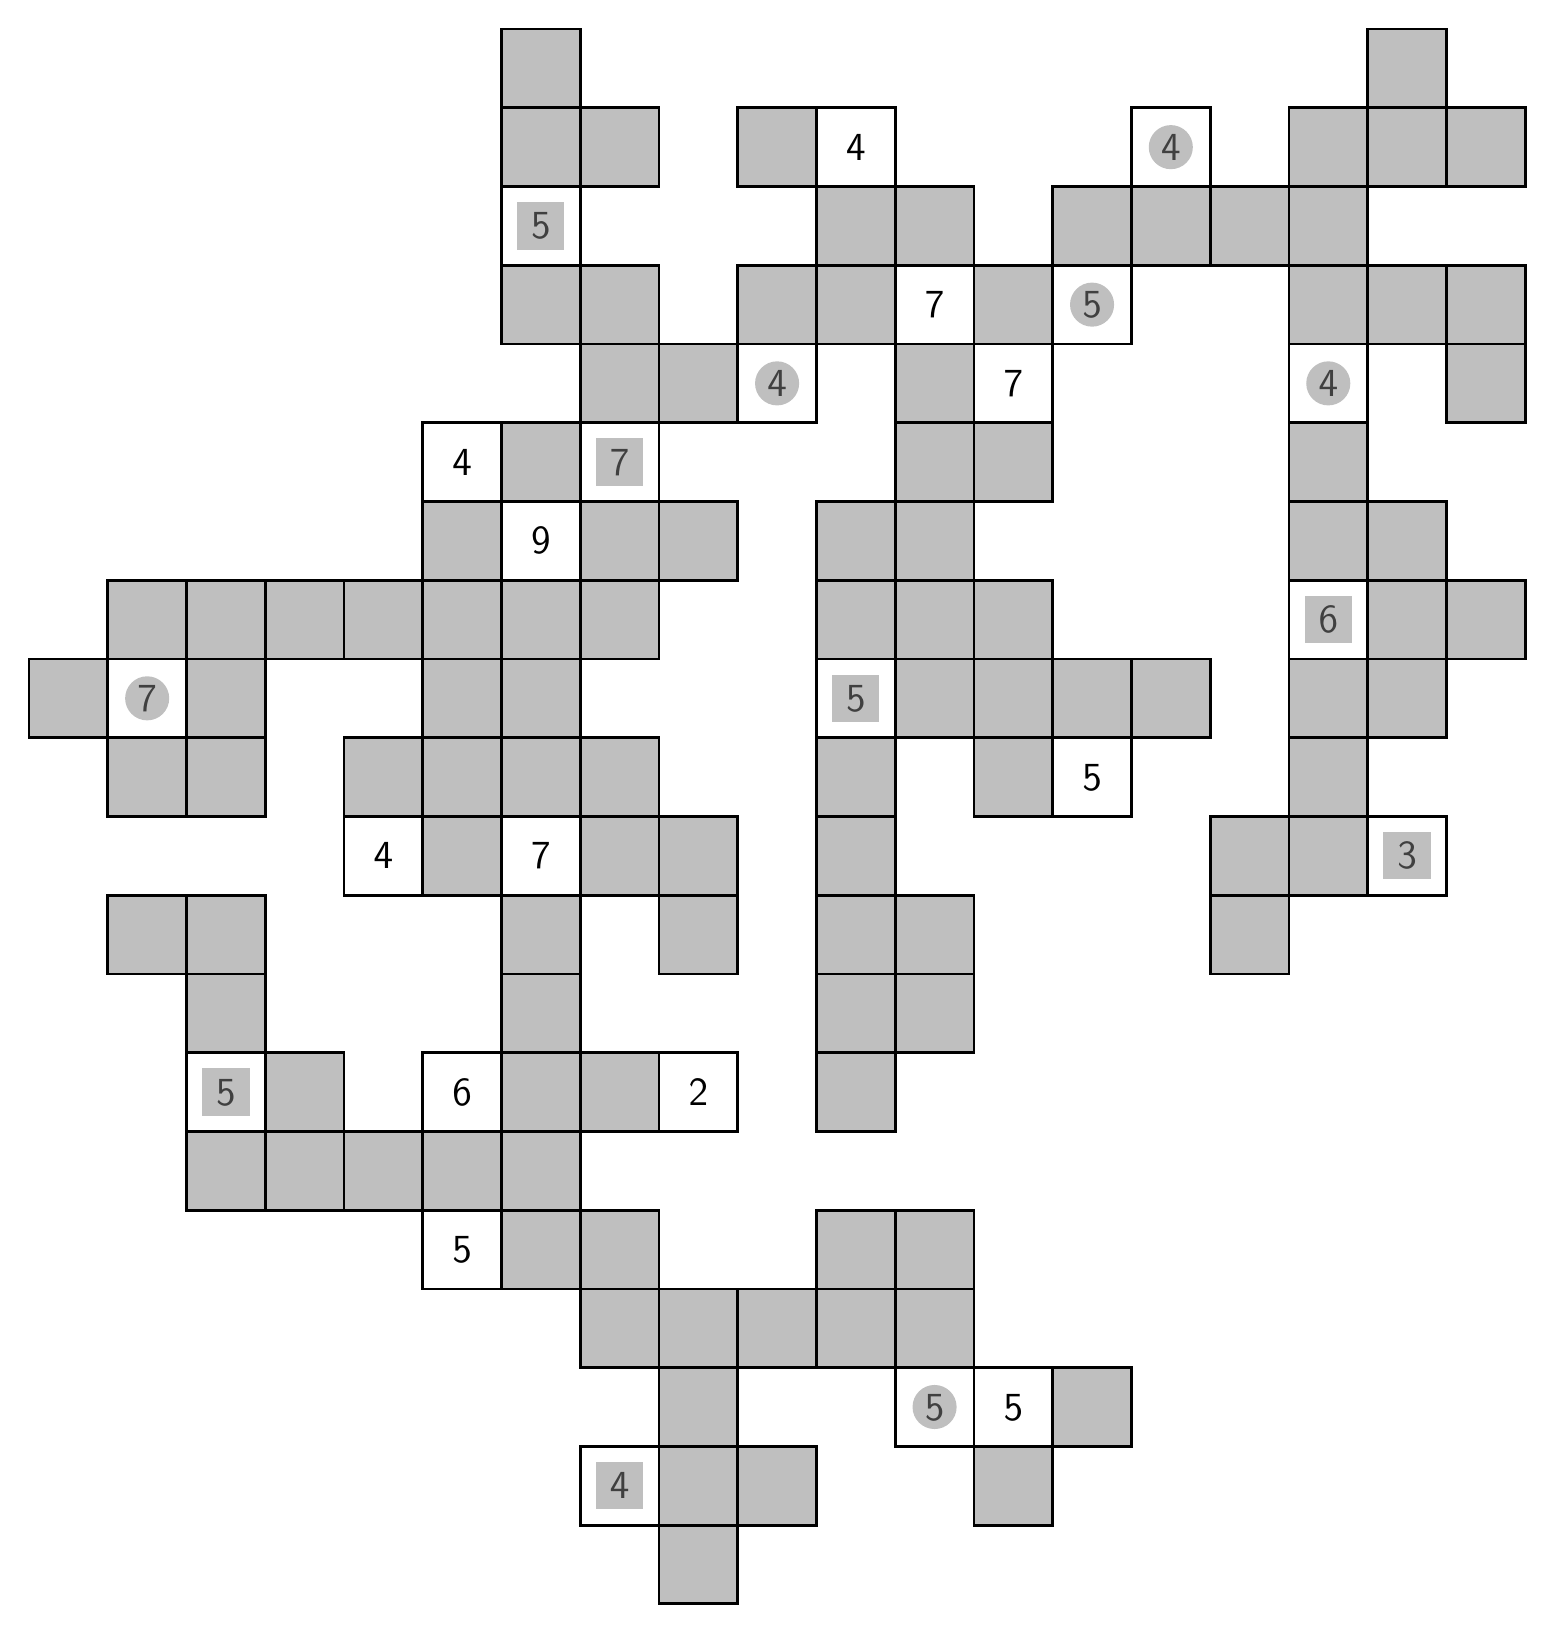
\begin{tikzpicture}\fill[gray, opacity = 0.5] (9, 0, 0)--++(1, 0, 0)--++(0, 1, 0)--++(-1, 0, 0)--cycle;
\draw[line width = 1pt] (9, 0, 0)--++(1, 0, 0)--++(0, 1, 0)--++(-1, 0, 0)--cycle;
\draw node at (8.5, 1.5, 0) {\Large $\mathsf{4}$};
\draw[line width = 1pt] (8, 1, 0)--++(1, 0, 0)--++(0, 1, 0)--++(-1, 0, 0)--cycle;
\fill[color = gray, opacity = 0.5] (8.2, 1.2) rectangle ++(0.6, 0.6);
\fill[gray, opacity = 0.5] (9, 1, 0)--++(1, 0, 0)--++(0, 1, 0)--++(-1, 0, 0)--cycle;
\draw[line width = 1pt] (9, 1, 0)--++(1, 0, 0)--++(0, 1, 0)--++(-1, 0, 0)--cycle;
\fill[gray, opacity = 0.5] (10, 1, 0)--++(1, 0, 0)--++(0, 1, 0)--++(-1, 0, 0)--cycle;
\draw[line width = 1pt] (10, 1, 0)--++(1, 0, 0)--++(0, 1, 0)--++(-1, 0, 0)--cycle;
\fill[gray, opacity = 0.5] (13, 1, 0)--++(1, 0, 0)--++(0, 1, 0)--++(-1, 0, 0)--cycle;
\draw[line width = 1pt] (13, 1, 0)--++(1, 0, 0)--++(0, 1, 0)--++(-1, 0, 0)--cycle;
\fill[gray, opacity = 0.5] (9, 2, 0)--++(1, 0, 0)--++(0, 1, 0)--++(-1, 0, 0)--cycle;
\draw[line width = 1pt] (9, 2, 0)--++(1, 0, 0)--++(0, 1, 0)--++(-1, 0, 0)--cycle;
\draw node at (12.5, 2.5, 0) {\Large $\mathsf{5}$};
\draw[line width = 1pt] (12, 2, 0)--++(1, 0, 0)--++(0, 1, 0)--++(-1, 0, 0)--cycle;
\fill[color = gray, opacity = 0.5] (12.5, 2.5, 0) circle (0.28);
\draw node at (13.5, 2.5, 0) {\Large $\mathsf{5}$};
\draw[line width = 1pt] (13, 2, 0)--++(1, 0, 0)--++(0, 1, 0)--++(-1, 0, 0)--cycle;
\fill[gray, opacity = 0.5] (14, 2, 0)--++(1, 0, 0)--++(0, 1, 0)--++(-1, 0, 0)--cycle;
\draw[line width = 1pt] (14, 2, 0)--++(1, 0, 0)--++(0, 1, 0)--++(-1, 0, 0)--cycle;
\fill[gray, opacity = 0.5] (8, 3, 0)--++(1, 0, 0)--++(0, 1, 0)--++(-1, 0, 0)--cycle;
\draw[line width = 1pt] (8, 3, 0)--++(1, 0, 0)--++(0, 1, 0)--++(-1, 0, 0)--cycle;
\fill[gray, opacity = 0.5] (9, 3, 0)--++(1, 0, 0)--++(0, 1, 0)--++(-1, 0, 0)--cycle;
\draw[line width = 1pt] (9, 3, 0)--++(1, 0, 0)--++(0, 1, 0)--++(-1, 0, 0)--cycle;
\fill[gray, opacity = 0.5] (10, 3, 0)--++(1, 0, 0)--++(0, 1, 0)--++(-1, 0, 0)--cycle;
\draw[line width = 1pt] (10, 3, 0)--++(1, 0, 0)--++(0, 1, 0)--++(-1, 0, 0)--cycle;
\fill[gray, opacity = 0.5] (11, 3, 0)--++(1, 0, 0)--++(0, 1, 0)--++(-1, 0, 0)--cycle;
\draw[line width = 1pt] (11, 3, 0)--++(1, 0, 0)--++(0, 1, 0)--++(-1, 0, 0)--cycle;
\fill[gray, opacity = 0.5] (12, 3, 0)--++(1, 0, 0)--++(0, 1, 0)--++(-1, 0, 0)--cycle;
\draw[line width = 1pt] (12, 3, 0)--++(1, 0, 0)--++(0, 1, 0)--++(-1, 0, 0)--cycle;
\draw node at (6.5, 4.5, 0) {\Large $\mathsf{5}$};
\draw[line width = 1pt] (6, 4, 0)--++(1, 0, 0)--++(0, 1, 0)--++(-1, 0, 0)--cycle;
\fill[gray, opacity = 0.5] (7, 4, 0)--++(1, 0, 0)--++(0, 1, 0)--++(-1, 0, 0)--cycle;
\draw[line width = 1pt] (7, 4, 0)--++(1, 0, 0)--++(0, 1, 0)--++(-1, 0, 0)--cycle;
\fill[gray, opacity = 0.5] (8, 4, 0)--++(1, 0, 0)--++(0, 1, 0)--++(-1, 0, 0)--cycle;
\draw[line width = 1pt] (8, 4, 0)--++(1, 0, 0)--++(0, 1, 0)--++(-1, 0, 0)--cycle;
\fill[gray, opacity = 0.5] (11, 4, 0)--++(1, 0, 0)--++(0, 1, 0)--++(-1, 0, 0)--cycle;
\draw[line width = 1pt] (11, 4, 0)--++(1, 0, 0)--++(0, 1, 0)--++(-1, 0, 0)--cycle;
\fill[gray, opacity = 0.5] (12, 4, 0)--++(1, 0, 0)--++(0, 1, 0)--++(-1, 0, 0)--cycle;
\draw[line width = 1pt] (12, 4, 0)--++(1, 0, 0)--++(0, 1, 0)--++(-1, 0, 0)--cycle;
\fill[gray, opacity = 0.5] (3, 5, 0)--++(1, 0, 0)--++(0, 1, 0)--++(-1, 0, 0)--cycle;
\draw[line width = 1pt] (3, 5, 0)--++(1, 0, 0)--++(0, 1, 0)--++(-1, 0, 0)--cycle;
\fill[gray, opacity = 0.5] (4, 5, 0)--++(1, 0, 0)--++(0, 1, 0)--++(-1, 0, 0)--cycle;
\draw[line width = 1pt] (4, 5, 0)--++(1, 0, 0)--++(0, 1, 0)--++(-1, 0, 0)--cycle;
\fill[gray, opacity = 0.5] (5, 5, 0)--++(1, 0, 0)--++(0, 1, 0)--++(-1, 0, 0)--cycle;
\draw[line width = 1pt] (5, 5, 0)--++(1, 0, 0)--++(0, 1, 0)--++(-1, 0, 0)--cycle;
\fill[gray, opacity = 0.5] (6, 5, 0)--++(1, 0, 0)--++(0, 1, 0)--++(-1, 0, 0)--cycle;
\draw[line width = 1pt] (6, 5, 0)--++(1, 0, 0)--++(0, 1, 0)--++(-1, 0, 0)--cycle;
\fill[gray, opacity = 0.5] (7, 5, 0)--++(1, 0, 0)--++(0, 1, 0)--++(-1, 0, 0)--cycle;
\draw[line width = 1pt] (7, 5, 0)--++(1, 0, 0)--++(0, 1, 0)--++(-1, 0, 0)--cycle;
\draw node at (3.5, 6.5, 0) {\Large $\mathsf{5}$};
\draw[line width = 1pt] (3, 6, 0)--++(1, 0, 0)--++(0, 1, 0)--++(-1, 0, 0)--cycle;
\fill[color = gray, opacity = 0.5] (3.2, 6.2) rectangle ++(0.6, 0.6);
\fill[gray, opacity = 0.5] (4, 6, 0)--++(1, 0, 0)--++(0, 1, 0)--++(-1, 0, 0)--cycle;
\draw[line width = 1pt] (4, 6, 0)--++(1, 0, 0)--++(0, 1, 0)--++(-1, 0, 0)--cycle;
\draw node at (6.5, 6.5, 0) {\Large $\mathsf{6}$};
\draw[line width = 1pt] (6, 6, 0)--++(1, 0, 0)--++(0, 1, 0)--++(-1, 0, 0)--cycle;
\fill[gray, opacity = 0.5] (7, 6, 0)--++(1, 0, 0)--++(0, 1, 0)--++(-1, 0, 0)--cycle;
\draw[line width = 1pt] (7, 6, 0)--++(1, 0, 0)--++(0, 1, 0)--++(-1, 0, 0)--cycle;
\fill[gray, opacity = 0.5] (8, 6, 0)--++(1, 0, 0)--++(0, 1, 0)--++(-1, 0, 0)--cycle;
\draw[line width = 1pt] (8, 6, 0)--++(1, 0, 0)--++(0, 1, 0)--++(-1, 0, 0)--cycle;
\draw node at (9.5, 6.5, 0) {\Large $\mathsf{2}$};
\draw[line width = 1pt] (9, 6, 0)--++(1, 0, 0)--++(0, 1, 0)--++(-1, 0, 0)--cycle;
\fill[gray, opacity = 0.5] (11, 6, 0)--++(1, 0, 0)--++(0, 1, 0)--++(-1, 0, 0)--cycle;
\draw[line width = 1pt] (11, 6, 0)--++(1, 0, 0)--++(0, 1, 0)--++(-1, 0, 0)--cycle;
\fill[gray, opacity = 0.5] (3, 7, 0)--++(1, 0, 0)--++(0, 1, 0)--++(-1, 0, 0)--cycle;
\draw[line width = 1pt] (3, 7, 0)--++(1, 0, 0)--++(0, 1, 0)--++(-1, 0, 0)--cycle;
\fill[gray, opacity = 0.5] (7, 7, 0)--++(1, 0, 0)--++(0, 1, 0)--++(-1, 0, 0)--cycle;
\draw[line width = 1pt] (7, 7, 0)--++(1, 0, 0)--++(0, 1, 0)--++(-1, 0, 0)--cycle;
\fill[gray, opacity = 0.5] (11, 7, 0)--++(1, 0, 0)--++(0, 1, 0)--++(-1, 0, 0)--cycle;
\draw[line width = 1pt] (11, 7, 0)--++(1, 0, 0)--++(0, 1, 0)--++(-1, 0, 0)--cycle;
\fill[gray, opacity = 0.5] (12, 7, 0)--++(1, 0, 0)--++(0, 1, 0)--++(-1, 0, 0)--cycle;
\draw[line width = 1pt] (12, 7, 0)--++(1, 0, 0)--++(0, 1, 0)--++(-1, 0, 0)--cycle;
\fill[gray, opacity = 0.5] (2, 8, 0)--++(1, 0, 0)--++(0, 1, 0)--++(-1, 0, 0)--cycle;
\draw[line width = 1pt] (2, 8, 0)--++(1, 0, 0)--++(0, 1, 0)--++(-1, 0, 0)--cycle;
\fill[gray, opacity = 0.5] (3, 8, 0)--++(1, 0, 0)--++(0, 1, 0)--++(-1, 0, 0)--cycle;
\draw[line width = 1pt] (3, 8, 0)--++(1, 0, 0)--++(0, 1, 0)--++(-1, 0, 0)--cycle;
\fill[gray, opacity = 0.5] (7, 8, 0)--++(1, 0, 0)--++(0, 1, 0)--++(-1, 0, 0)--cycle;
\draw[line width = 1pt] (7, 8, 0)--++(1, 0, 0)--++(0, 1, 0)--++(-1, 0, 0)--cycle;
\fill[gray, opacity = 0.5] (9, 8, 0)--++(1, 0, 0)--++(0, 1, 0)--++(-1, 0, 0)--cycle;
\draw[line width = 1pt] (9, 8, 0)--++(1, 0, 0)--++(0, 1, 0)--++(-1, 0, 0)--cycle;
\fill[gray, opacity = 0.5] (11, 8, 0)--++(1, 0, 0)--++(0, 1, 0)--++(-1, 0, 0)--cycle;
\draw[line width = 1pt] (11, 8, 0)--++(1, 0, 0)--++(0, 1, 0)--++(-1, 0, 0)--cycle;
\fill[gray, opacity = 0.5] (12, 8, 0)--++(1, 0, 0)--++(0, 1, 0)--++(-1, 0, 0)--cycle;
\draw[line width = 1pt] (12, 8, 0)--++(1, 0, 0)--++(0, 1, 0)--++(-1, 0, 0)--cycle;
\fill[gray, opacity = 0.5] (16, 8, 0)--++(1, 0, 0)--++(0, 1, 0)--++(-1, 0, 0)--cycle;
\draw[line width = 1pt] (16, 8, 0)--++(1, 0, 0)--++(0, 1, 0)--++(-1, 0, 0)--cycle;
\draw node at (5.5, 9.5, 0) {\Large $\mathsf{4}$};
\draw[line width = 1pt] (5, 9, 0)--++(1, 0, 0)--++(0, 1, 0)--++(-1, 0, 0)--cycle;
\fill[gray, opacity = 0.5] (6, 9, 0)--++(1, 0, 0)--++(0, 1, 0)--++(-1, 0, 0)--cycle;
\draw[line width = 1pt] (6, 9, 0)--++(1, 0, 0)--++(0, 1, 0)--++(-1, 0, 0)--cycle;
\draw node at (7.5, 9.5, 0) {\Large $\mathsf{7}$};
\draw[line width = 1pt] (7, 9, 0)--++(1, 0, 0)--++(0, 1, 0)--++(-1, 0, 0)--cycle;
\fill[gray, opacity = 0.5] (8, 9, 0)--++(1, 0, 0)--++(0, 1, 0)--++(-1, 0, 0)--cycle;
\draw[line width = 1pt] (8, 9, 0)--++(1, 0, 0)--++(0, 1, 0)--++(-1, 0, 0)--cycle;
\fill[gray, opacity = 0.5] (9, 9, 0)--++(1, 0, 0)--++(0, 1, 0)--++(-1, 0, 0)--cycle;
\draw[line width = 1pt] (9, 9, 0)--++(1, 0, 0)--++(0, 1, 0)--++(-1, 0, 0)--cycle;
\fill[gray, opacity = 0.5] (11, 9, 0)--++(1, 0, 0)--++(0, 1, 0)--++(-1, 0, 0)--cycle;
\draw[line width = 1pt] (11, 9, 0)--++(1, 0, 0)--++(0, 1, 0)--++(-1, 0, 0)--cycle;
\fill[gray, opacity = 0.5] (16, 9, 0)--++(1, 0, 0)--++(0, 1, 0)--++(-1, 0, 0)--cycle;
\draw[line width = 1pt] (16, 9, 0)--++(1, 0, 0)--++(0, 1, 0)--++(-1, 0, 0)--cycle;
\fill[gray, opacity = 0.5] (17, 9, 0)--++(1, 0, 0)--++(0, 1, 0)--++(-1, 0, 0)--cycle;
\draw[line width = 1pt] (17, 9, 0)--++(1, 0, 0)--++(0, 1, 0)--++(-1, 0, 0)--cycle;
\draw node at (18.5, 9.5, 0) {\Large $\mathsf{3}$};
\draw[line width = 1pt] (18, 9, 0)--++(1, 0, 0)--++(0, 1, 0)--++(-1, 0, 0)--cycle;
\fill[color = gray, opacity = 0.5] (18.2, 9.2) rectangle ++(0.6, 0.6);
\fill[gray, opacity = 0.5] (2, 10, 0)--++(1, 0, 0)--++(0, 1, 0)--++(-1, 0, 0)--cycle;
\draw[line width = 1pt] (2, 10, 0)--++(1, 0, 0)--++(0, 1, 0)--++(-1, 0, 0)--cycle;
\fill[gray, opacity = 0.5] (3, 10, 0)--++(1, 0, 0)--++(0, 1, 0)--++(-1, 0, 0)--cycle;
\draw[line width = 1pt] (3, 10, 0)--++(1, 0, 0)--++(0, 1, 0)--++(-1, 0, 0)--cycle;
\fill[gray, opacity = 0.5] (5, 10, 0)--++(1, 0, 0)--++(0, 1, 0)--++(-1, 0, 0)--cycle;
\draw[line width = 1pt] (5, 10, 0)--++(1, 0, 0)--++(0, 1, 0)--++(-1, 0, 0)--cycle;
\fill[gray, opacity = 0.5] (6, 10, 0)--++(1, 0, 0)--++(0, 1, 0)--++(-1, 0, 0)--cycle;
\draw[line width = 1pt] (6, 10, 0)--++(1, 0, 0)--++(0, 1, 0)--++(-1, 0, 0)--cycle;
\fill[gray, opacity = 0.5] (7, 10, 0)--++(1, 0, 0)--++(0, 1, 0)--++(-1, 0, 0)--cycle;
\draw[line width = 1pt] (7, 10, 0)--++(1, 0, 0)--++(0, 1, 0)--++(-1, 0, 0)--cycle;
\fill[gray, opacity = 0.5] (8, 10, 0)--++(1, 0, 0)--++(0, 1, 0)--++(-1, 0, 0)--cycle;
\draw[line width = 1pt] (8, 10, 0)--++(1, 0, 0)--++(0, 1, 0)--++(-1, 0, 0)--cycle;
\fill[gray, opacity = 0.5] (11, 10, 0)--++(1, 0, 0)--++(0, 1, 0)--++(-1, 0, 0)--cycle;
\draw[line width = 1pt] (11, 10, 0)--++(1, 0, 0)--++(0, 1, 0)--++(-1, 0, 0)--cycle;
\fill[gray, opacity = 0.5] (13, 10, 0)--++(1, 0, 0)--++(0, 1, 0)--++(-1, 0, 0)--cycle;
\draw[line width = 1pt] (13, 10, 0)--++(1, 0, 0)--++(0, 1, 0)--++(-1, 0, 0)--cycle;
\draw node at (14.5, 10.5, 0) {\Large $\mathsf{5}$};
\draw[line width = 1pt] (14, 10, 0)--++(1, 0, 0)--++(0, 1, 0)--++(-1, 0, 0)--cycle;
\fill[gray, opacity = 0.5] (17, 10, 0)--++(1, 0, 0)--++(0, 1, 0)--++(-1, 0, 0)--cycle;
\draw[line width = 1pt] (17, 10, 0)--++(1, 0, 0)--++(0, 1, 0)--++(-1, 0, 0)--cycle;
\fill[gray, opacity = 0.5] (1, 11, 0)--++(1, 0, 0)--++(0, 1, 0)--++(-1, 0, 0)--cycle;
\draw[line width = 1pt] (1, 11, 0)--++(1, 0, 0)--++(0, 1, 0)--++(-1, 0, 0)--cycle;
\draw node at (2.5, 11.5, 0) {\Large $\mathsf{7}$};
\draw[line width = 1pt] (2, 11, 0)--++(1, 0, 0)--++(0, 1, 0)--++(-1, 0, 0)--cycle;
\fill[color = gray, opacity = 0.5] (2.5, 11.5, 0) circle (0.28);
\fill[gray, opacity = 0.5] (3, 11, 0)--++(1, 0, 0)--++(0, 1, 0)--++(-1, 0, 0)--cycle;
\draw[line width = 1pt] (3, 11, 0)--++(1, 0, 0)--++(0, 1, 0)--++(-1, 0, 0)--cycle;
\fill[gray, opacity = 0.5] (6, 11, 0)--++(1, 0, 0)--++(0, 1, 0)--++(-1, 0, 0)--cycle;
\draw[line width = 1pt] (6, 11, 0)--++(1, 0, 0)--++(0, 1, 0)--++(-1, 0, 0)--cycle;
\fill[gray, opacity = 0.5] (7, 11, 0)--++(1, 0, 0)--++(0, 1, 0)--++(-1, 0, 0)--cycle;
\draw[line width = 1pt] (7, 11, 0)--++(1, 0, 0)--++(0, 1, 0)--++(-1, 0, 0)--cycle;
\draw node at (11.5, 11.5, 0) {\Large $\mathsf{5}$};
\draw[line width = 1pt] (11, 11, 0)--++(1, 0, 0)--++(0, 1, 0)--++(-1, 0, 0)--cycle;
\fill[color = gray, opacity = 0.5] (11.2, 11.2) rectangle ++(0.6, 0.6);
\fill[gray, opacity = 0.5] (12, 11, 0)--++(1, 0, 0)--++(0, 1, 0)--++(-1, 0, 0)--cycle;
\draw[line width = 1pt] (12, 11, 0)--++(1, 0, 0)--++(0, 1, 0)--++(-1, 0, 0)--cycle;
\fill[gray, opacity = 0.5] (13, 11, 0)--++(1, 0, 0)--++(0, 1, 0)--++(-1, 0, 0)--cycle;
\draw[line width = 1pt] (13, 11, 0)--++(1, 0, 0)--++(0, 1, 0)--++(-1, 0, 0)--cycle;
\fill[gray, opacity = 0.5] (14, 11, 0)--++(1, 0, 0)--++(0, 1, 0)--++(-1, 0, 0)--cycle;
\draw[line width = 1pt] (14, 11, 0)--++(1, 0, 0)--++(0, 1, 0)--++(-1, 0, 0)--cycle;
\fill[gray, opacity = 0.5] (15, 11, 0)--++(1, 0, 0)--++(0, 1, 0)--++(-1, 0, 0)--cycle;
\draw[line width = 1pt] (15, 11, 0)--++(1, 0, 0)--++(0, 1, 0)--++(-1, 0, 0)--cycle;
\fill[gray, opacity = 0.5] (17, 11, 0)--++(1, 0, 0)--++(0, 1, 0)--++(-1, 0, 0)--cycle;
\draw[line width = 1pt] (17, 11, 0)--++(1, 0, 0)--++(0, 1, 0)--++(-1, 0, 0)--cycle;
\fill[gray, opacity = 0.5] (18, 11, 0)--++(1, 0, 0)--++(0, 1, 0)--++(-1, 0, 0)--cycle;
\draw[line width = 1pt] (18, 11, 0)--++(1, 0, 0)--++(0, 1, 0)--++(-1, 0, 0)--cycle;
\fill[gray, opacity = 0.5] (2, 12, 0)--++(1, 0, 0)--++(0, 1, 0)--++(-1, 0, 0)--cycle;
\draw[line width = 1pt] (2, 12, 0)--++(1, 0, 0)--++(0, 1, 0)--++(-1, 0, 0)--cycle;
\fill[gray, opacity = 0.5] (3, 12, 0)--++(1, 0, 0)--++(0, 1, 0)--++(-1, 0, 0)--cycle;
\draw[line width = 1pt] (3, 12, 0)--++(1, 0, 0)--++(0, 1, 0)--++(-1, 0, 0)--cycle;
\fill[gray, opacity = 0.5] (4, 12, 0)--++(1, 0, 0)--++(0, 1, 0)--++(-1, 0, 0)--cycle;
\draw[line width = 1pt] (4, 12, 0)--++(1, 0, 0)--++(0, 1, 0)--++(-1, 0, 0)--cycle;
\fill[gray, opacity = 0.5] (5, 12, 0)--++(1, 0, 0)--++(0, 1, 0)--++(-1, 0, 0)--cycle;
\draw[line width = 1pt] (5, 12, 0)--++(1, 0, 0)--++(0, 1, 0)--++(-1, 0, 0)--cycle;
\fill[gray, opacity = 0.5] (6, 12, 0)--++(1, 0, 0)--++(0, 1, 0)--++(-1, 0, 0)--cycle;
\draw[line width = 1pt] (6, 12, 0)--++(1, 0, 0)--++(0, 1, 0)--++(-1, 0, 0)--cycle;
\fill[gray, opacity = 0.5] (7, 12, 0)--++(1, 0, 0)--++(0, 1, 0)--++(-1, 0, 0)--cycle;
\draw[line width = 1pt] (7, 12, 0)--++(1, 0, 0)--++(0, 1, 0)--++(-1, 0, 0)--cycle;
\fill[gray, opacity = 0.5] (8, 12, 0)--++(1, 0, 0)--++(0, 1, 0)--++(-1, 0, 0)--cycle;
\draw[line width = 1pt] (8, 12, 0)--++(1, 0, 0)--++(0, 1, 0)--++(-1, 0, 0)--cycle;
\fill[gray, opacity = 0.5] (11, 12, 0)--++(1, 0, 0)--++(0, 1, 0)--++(-1, 0, 0)--cycle;
\draw[line width = 1pt] (11, 12, 0)--++(1, 0, 0)--++(0, 1, 0)--++(-1, 0, 0)--cycle;
\fill[gray, opacity = 0.5] (12, 12, 0)--++(1, 0, 0)--++(0, 1, 0)--++(-1, 0, 0)--cycle;
\draw[line width = 1pt] (12, 12, 0)--++(1, 0, 0)--++(0, 1, 0)--++(-1, 0, 0)--cycle;
\fill[gray, opacity = 0.5] (13, 12, 0)--++(1, 0, 0)--++(0, 1, 0)--++(-1, 0, 0)--cycle;
\draw[line width = 1pt] (13, 12, 0)--++(1, 0, 0)--++(0, 1, 0)--++(-1, 0, 0)--cycle;
\draw node at (17.5, 12.5, 0) {\Large $\mathsf{6}$};
\draw[line width = 1pt] (17, 12, 0)--++(1, 0, 0)--++(0, 1, 0)--++(-1, 0, 0)--cycle;
\fill[color = gray, opacity = 0.5] (17.2, 12.2) rectangle ++(0.6, 0.6);
\fill[gray, opacity = 0.5] (18, 12, 0)--++(1, 0, 0)--++(0, 1, 0)--++(-1, 0, 0)--cycle;
\draw[line width = 1pt] (18, 12, 0)--++(1, 0, 0)--++(0, 1, 0)--++(-1, 0, 0)--cycle;
\fill[gray, opacity = 0.5] (19, 12, 0)--++(1, 0, 0)--++(0, 1, 0)--++(-1, 0, 0)--cycle;
\draw[line width = 1pt] (19, 12, 0)--++(1, 0, 0)--++(0, 1, 0)--++(-1, 0, 0)--cycle;
\fill[gray, opacity = 0.5] (6, 13, 0)--++(1, 0, 0)--++(0, 1, 0)--++(-1, 0, 0)--cycle;
\draw[line width = 1pt] (6, 13, 0)--++(1, 0, 0)--++(0, 1, 0)--++(-1, 0, 0)--cycle;
\draw node at (7.5, 13.5, 0) {\Large $\mathsf{9}$};
\draw[line width = 1pt] (7, 13, 0)--++(1, 0, 0)--++(0, 1, 0)--++(-1, 0, 0)--cycle;
\fill[gray, opacity = 0.5] (8, 13, 0)--++(1, 0, 0)--++(0, 1, 0)--++(-1, 0, 0)--cycle;
\draw[line width = 1pt] (8, 13, 0)--++(1, 0, 0)--++(0, 1, 0)--++(-1, 0, 0)--cycle;
\fill[gray, opacity = 0.5] (9, 13, 0)--++(1, 0, 0)--++(0, 1, 0)--++(-1, 0, 0)--cycle;
\draw[line width = 1pt] (9, 13, 0)--++(1, 0, 0)--++(0, 1, 0)--++(-1, 0, 0)--cycle;
\fill[gray, opacity = 0.5] (11, 13, 0)--++(1, 0, 0)--++(0, 1, 0)--++(-1, 0, 0)--cycle;
\draw[line width = 1pt] (11, 13, 0)--++(1, 0, 0)--++(0, 1, 0)--++(-1, 0, 0)--cycle;
\fill[gray, opacity = 0.5] (12, 13, 0)--++(1, 0, 0)--++(0, 1, 0)--++(-1, 0, 0)--cycle;
\draw[line width = 1pt] (12, 13, 0)--++(1, 0, 0)--++(0, 1, 0)--++(-1, 0, 0)--cycle;
\fill[gray, opacity = 0.5] (17, 13, 0)--++(1, 0, 0)--++(0, 1, 0)--++(-1, 0, 0)--cycle;
\draw[line width = 1pt] (17, 13, 0)--++(1, 0, 0)--++(0, 1, 0)--++(-1, 0, 0)--cycle;
\fill[gray, opacity = 0.5] (18, 13, 0)--++(1, 0, 0)--++(0, 1, 0)--++(-1, 0, 0)--cycle;
\draw[line width = 1pt] (18, 13, 0)--++(1, 0, 0)--++(0, 1, 0)--++(-1, 0, 0)--cycle;
\draw node at (6.5, 14.5, 0) {\Large $\mathsf{4}$};
\draw[line width = 1pt] (6, 14, 0)--++(1, 0, 0)--++(0, 1, 0)--++(-1, 0, 0)--cycle;
\fill[gray, opacity = 0.5] (7, 14, 0)--++(1, 0, 0)--++(0, 1, 0)--++(-1, 0, 0)--cycle;
\draw[line width = 1pt] (7, 14, 0)--++(1, 0, 0)--++(0, 1, 0)--++(-1, 0, 0)--cycle;
\draw node at (8.5, 14.5, 0) {\Large $\mathsf{7}$};
\draw[line width = 1pt] (8, 14, 0)--++(1, 0, 0)--++(0, 1, 0)--++(-1, 0, 0)--cycle;
\fill[color = gray, opacity = 0.5] (8.2, 14.2) rectangle ++(0.6, 0.6);
\fill[gray, opacity = 0.5] (12, 14, 0)--++(1, 0, 0)--++(0, 1, 0)--++(-1, 0, 0)--cycle;
\draw[line width = 1pt] (12, 14, 0)--++(1, 0, 0)--++(0, 1, 0)--++(-1, 0, 0)--cycle;
\fill[gray, opacity = 0.5] (13, 14, 0)--++(1, 0, 0)--++(0, 1, 0)--++(-1, 0, 0)--cycle;
\draw[line width = 1pt] (13, 14, 0)--++(1, 0, 0)--++(0, 1, 0)--++(-1, 0, 0)--cycle;
\fill[gray, opacity = 0.5] (17, 14, 0)--++(1, 0, 0)--++(0, 1, 0)--++(-1, 0, 0)--cycle;
\draw[line width = 1pt] (17, 14, 0)--++(1, 0, 0)--++(0, 1, 0)--++(-1, 0, 0)--cycle;
\fill[gray, opacity = 0.5] (8, 15, 0)--++(1, 0, 0)--++(0, 1, 0)--++(-1, 0, 0)--cycle;
\draw[line width = 1pt] (8, 15, 0)--++(1, 0, 0)--++(0, 1, 0)--++(-1, 0, 0)--cycle;
\fill[gray, opacity = 0.5] (9, 15, 0)--++(1, 0, 0)--++(0, 1, 0)--++(-1, 0, 0)--cycle;
\draw[line width = 1pt] (9, 15, 0)--++(1, 0, 0)--++(0, 1, 0)--++(-1, 0, 0)--cycle;
\draw node at (10.5, 15.5, 0) {\Large $\mathsf{4}$};
\draw[line width = 1pt] (10, 15, 0)--++(1, 0, 0)--++(0, 1, 0)--++(-1, 0, 0)--cycle;
\fill[color = gray, opacity = 0.5] (10.5, 15.5, 0) circle (0.28);
\fill[gray, opacity = 0.5] (12, 15, 0)--++(1, 0, 0)--++(0, 1, 0)--++(-1, 0, 0)--cycle;
\draw[line width = 1pt] (12, 15, 0)--++(1, 0, 0)--++(0, 1, 0)--++(-1, 0, 0)--cycle;
\draw node at (13.5, 15.5, 0) {\Large $\mathsf{7}$};
\draw[line width = 1pt] (13, 15, 0)--++(1, 0, 0)--++(0, 1, 0)--++(-1, 0, 0)--cycle;
\draw node at (17.5, 15.5, 0) {\Large $\mathsf{4}$};
\draw[line width = 1pt] (17, 15, 0)--++(1, 0, 0)--++(0, 1, 0)--++(-1, 0, 0)--cycle;
\fill[color = gray, opacity = 0.5] (17.5, 15.5, 0) circle (0.28);
\fill[gray, opacity = 0.5] (19, 15, 0)--++(1, 0, 0)--++(0, 1, 0)--++(-1, 0, 0)--cycle;
\draw[line width = 1pt] (19, 15, 0)--++(1, 0, 0)--++(0, 1, 0)--++(-1, 0, 0)--cycle;
\fill[gray, opacity = 0.5] (7, 16, 0)--++(1, 0, 0)--++(0, 1, 0)--++(-1, 0, 0)--cycle;
\draw[line width = 1pt] (7, 16, 0)--++(1, 0, 0)--++(0, 1, 0)--++(-1, 0, 0)--cycle;
\fill[gray, opacity = 0.5] (8, 16, 0)--++(1, 0, 0)--++(0, 1, 0)--++(-1, 0, 0)--cycle;
\draw[line width = 1pt] (8, 16, 0)--++(1, 0, 0)--++(0, 1, 0)--++(-1, 0, 0)--cycle;
\fill[gray, opacity = 0.5] (10, 16, 0)--++(1, 0, 0)--++(0, 1, 0)--++(-1, 0, 0)--cycle;
\draw[line width = 1pt] (10, 16, 0)--++(1, 0, 0)--++(0, 1, 0)--++(-1, 0, 0)--cycle;
\fill[gray, opacity = 0.5] (11, 16, 0)--++(1, 0, 0)--++(0, 1, 0)--++(-1, 0, 0)--cycle;
\draw[line width = 1pt] (11, 16, 0)--++(1, 0, 0)--++(0, 1, 0)--++(-1, 0, 0)--cycle;
\draw node at (12.5, 16.5, 0) {\Large $\mathsf{7}$};
\draw[line width = 1pt] (12, 16, 0)--++(1, 0, 0)--++(0, 1, 0)--++(-1, 0, 0)--cycle;
\fill[gray, opacity = 0.5] (13, 16, 0)--++(1, 0, 0)--++(0, 1, 0)--++(-1, 0, 0)--cycle;
\draw[line width = 1pt] (13, 16, 0)--++(1, 0, 0)--++(0, 1, 0)--++(-1, 0, 0)--cycle;
\draw node at (14.5, 16.5, 0) {\Large $\mathsf{5}$};
\draw[line width = 1pt] (14, 16, 0)--++(1, 0, 0)--++(0, 1, 0)--++(-1, 0, 0)--cycle;
\fill[color = gray, opacity = 0.5] (14.5, 16.5, 0) circle (0.28);
\fill[gray, opacity = 0.5] (17, 16, 0)--++(1, 0, 0)--++(0, 1, 0)--++(-1, 0, 0)--cycle;
\draw[line width = 1pt] (17, 16, 0)--++(1, 0, 0)--++(0, 1, 0)--++(-1, 0, 0)--cycle;
\fill[gray, opacity = 0.5] (18, 16, 0)--++(1, 0, 0)--++(0, 1, 0)--++(-1, 0, 0)--cycle;
\draw[line width = 1pt] (18, 16, 0)--++(1, 0, 0)--++(0, 1, 0)--++(-1, 0, 0)--cycle;
\fill[gray, opacity = 0.5] (19, 16, 0)--++(1, 0, 0)--++(0, 1, 0)--++(-1, 0, 0)--cycle;
\draw[line width = 1pt] (19, 16, 0)--++(1, 0, 0)--++(0, 1, 0)--++(-1, 0, 0)--cycle;
\draw node at (7.5, 17.5, 0) {\Large $\mathsf{5}$};
\draw[line width = 1pt] (7, 17, 0)--++(1, 0, 0)--++(0, 1, 0)--++(-1, 0, 0)--cycle;
\fill[color = gray, opacity = 0.5] (7.2, 17.2) rectangle ++(0.6, 0.6);
\fill[gray, opacity = 0.5] (11, 17, 0)--++(1, 0, 0)--++(0, 1, 0)--++(-1, 0, 0)--cycle;
\draw[line width = 1pt] (11, 17, 0)--++(1, 0, 0)--++(0, 1, 0)--++(-1, 0, 0)--cycle;
\fill[gray, opacity = 0.5] (12, 17, 0)--++(1, 0, 0)--++(0, 1, 0)--++(-1, 0, 0)--cycle;
\draw[line width = 1pt] (12, 17, 0)--++(1, 0, 0)--++(0, 1, 0)--++(-1, 0, 0)--cycle;
\fill[gray, opacity = 0.5] (14, 17, 0)--++(1, 0, 0)--++(0, 1, 0)--++(-1, 0, 0)--cycle;
\draw[line width = 1pt] (14, 17, 0)--++(1, 0, 0)--++(0, 1, 0)--++(-1, 0, 0)--cycle;
\fill[gray, opacity = 0.5] (15, 17, 0)--++(1, 0, 0)--++(0, 1, 0)--++(-1, 0, 0)--cycle;
\draw[line width = 1pt] (15, 17, 0)--++(1, 0, 0)--++(0, 1, 0)--++(-1, 0, 0)--cycle;
\fill[gray, opacity = 0.5] (16, 17, 0)--++(1, 0, 0)--++(0, 1, 0)--++(-1, 0, 0)--cycle;
\draw[line width = 1pt] (16, 17, 0)--++(1, 0, 0)--++(0, 1, 0)--++(-1, 0, 0)--cycle;
\fill[gray, opacity = 0.5] (17, 17, 0)--++(1, 0, 0)--++(0, 1, 0)--++(-1, 0, 0)--cycle;
\draw[line width = 1pt] (17, 17, 0)--++(1, 0, 0)--++(0, 1, 0)--++(-1, 0, 0)--cycle;
\fill[gray, opacity = 0.5] (7, 18, 0)--++(1, 0, 0)--++(0, 1, 0)--++(-1, 0, 0)--cycle;
\draw[line width = 1pt] (7, 18, 0)--++(1, 0, 0)--++(0, 1, 0)--++(-1, 0, 0)--cycle;
\fill[gray, opacity = 0.5] (8, 18, 0)--++(1, 0, 0)--++(0, 1, 0)--++(-1, 0, 0)--cycle;
\draw[line width = 1pt] (8, 18, 0)--++(1, 0, 0)--++(0, 1, 0)--++(-1, 0, 0)--cycle;
\fill[gray, opacity = 0.5] (10, 18, 0)--++(1, 0, 0)--++(0, 1, 0)--++(-1, 0, 0)--cycle;
\draw[line width = 1pt] (10, 18, 0)--++(1, 0, 0)--++(0, 1, 0)--++(-1, 0, 0)--cycle;
\draw node at (11.5, 18.5, 0) {\Large $\mathsf{4}$};
\draw[line width = 1pt] (11, 18, 0)--++(1, 0, 0)--++(0, 1, 0)--++(-1, 0, 0)--cycle;
\draw node at (15.5, 18.5, 0) {\Large $\mathsf{4}$};
\draw[line width = 1pt] (15, 18, 0)--++(1, 0, 0)--++(0, 1, 0)--++(-1, 0, 0)--cycle;
\fill[color = gray, opacity = 0.5] (15.5, 18.5, 0) circle (0.28);
\fill[gray, opacity = 0.5] (17, 18, 0)--++(1, 0, 0)--++(0, 1, 0)--++(-1, 0, 0)--cycle;
\draw[line width = 1pt] (17, 18, 0)--++(1, 0, 0)--++(0, 1, 0)--++(-1, 0, 0)--cycle;
\fill[gray, opacity = 0.5] (18, 18, 0)--++(1, 0, 0)--++(0, 1, 0)--++(-1, 0, 0)--cycle;
\draw[line width = 1pt] (18, 18, 0)--++(1, 0, 0)--++(0, 1, 0)--++(-1, 0, 0)--cycle;
\fill[gray, opacity = 0.5] (19, 18, 0)--++(1, 0, 0)--++(0, 1, 0)--++(-1, 0, 0)--cycle;
\draw[line width = 1pt] (19, 18, 0)--++(1, 0, 0)--++(0, 1, 0)--++(-1, 0, 0)--cycle;
\fill[gray, opacity = 0.5] (7, 19, 0)--++(1, 0, 0)--++(0, 1, 0)--++(-1, 0, 0)--cycle;
\draw[line width = 1pt] (7, 19, 0)--++(1, 0, 0)--++(0, 1, 0)--++(-1, 0, 0)--cycle;
\fill[gray, opacity = 0.5] (18, 19, 0)--++(1, 0, 0)--++(0, 1, 0)--++(-1, 0, 0)--cycle;
\draw[line width = 1pt] (18, 19, 0)--++(1, 0, 0)--++(0, 1, 0)--++(-1, 0, 0)--cycle;
\end{tikzpicture}}\]
\[\resizebox{30pc}{!}{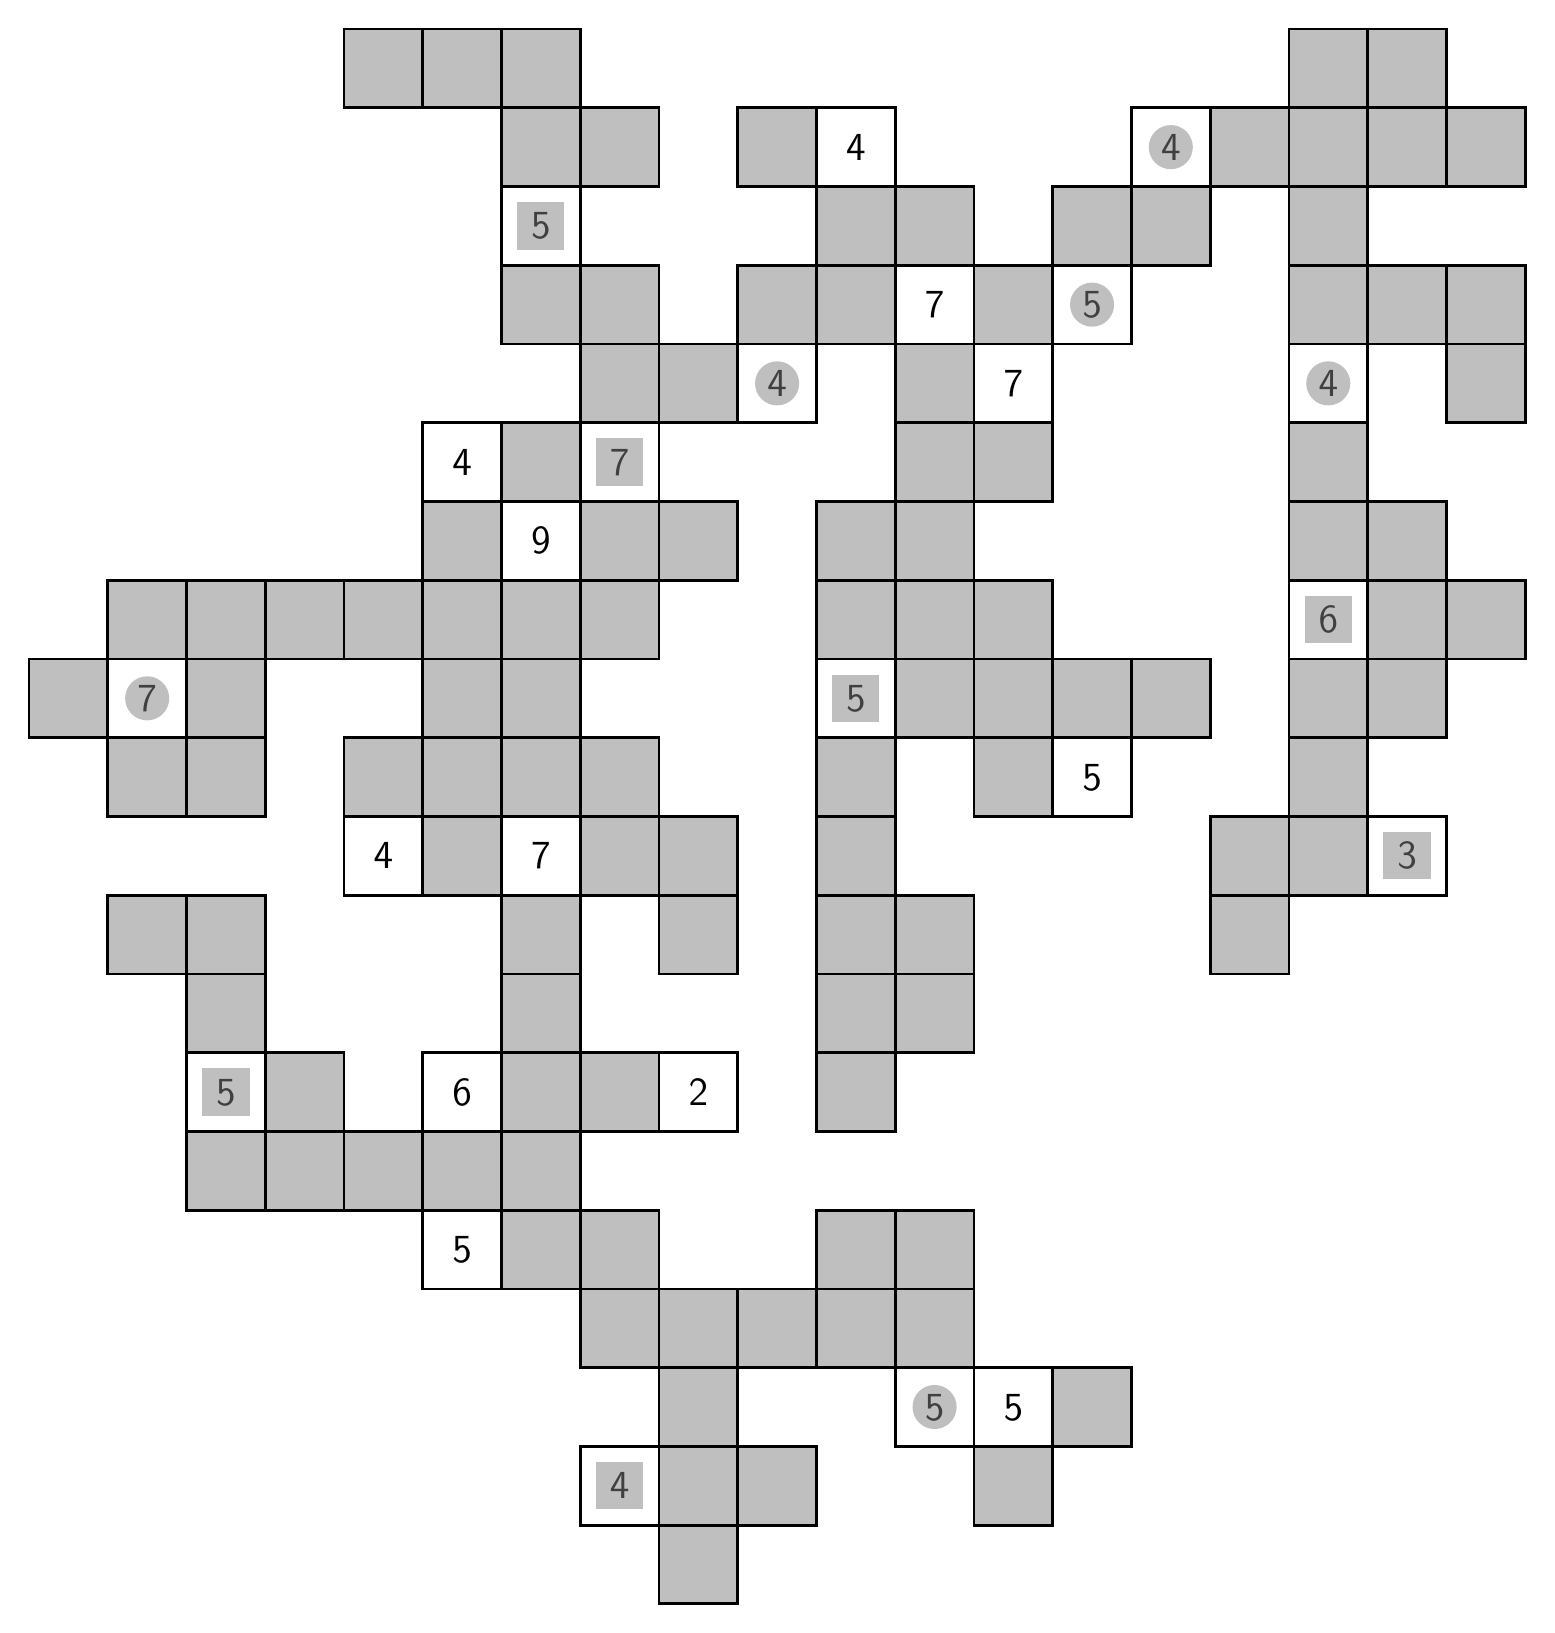
\begin{tikzpicture}\fill[gray, opacity = 0.5] (9, 0, 0)--++(1, 0, 0)--++(0, 1, 0)--++(-1, 0, 0)--cycle;
\draw[line width = 1pt] (9, 0, 0)--++(1, 0, 0)--++(0, 1, 0)--++(-1, 0, 0)--cycle;
\draw node at (8.5, 1.5, 0) {\Large $\mathsf{4}$};
\draw[line width = 1pt] (8, 1, 0)--++(1, 0, 0)--++(0, 1, 0)--++(-1, 0, 0)--cycle;
\fill[color = gray, opacity = 0.5] (8.2, 1.2) rectangle ++(0.6, 0.6);
\fill[gray, opacity = 0.5] (9, 1, 0)--++(1, 0, 0)--++(0, 1, 0)--++(-1, 0, 0)--cycle;
\draw[line width = 1pt] (9, 1, 0)--++(1, 0, 0)--++(0, 1, 0)--++(-1, 0, 0)--cycle;
\fill[gray, opacity = 0.5] (10, 1, 0)--++(1, 0, 0)--++(0, 1, 0)--++(-1, 0, 0)--cycle;
\draw[line width = 1pt] (10, 1, 0)--++(1, 0, 0)--++(0, 1, 0)--++(-1, 0, 0)--cycle;
\fill[gray, opacity = 0.5] (13, 1, 0)--++(1, 0, 0)--++(0, 1, 0)--++(-1, 0, 0)--cycle;
\draw[line width = 1pt] (13, 1, 0)--++(1, 0, 0)--++(0, 1, 0)--++(-1, 0, 0)--cycle;
\fill[gray, opacity = 0.5] (9, 2, 0)--++(1, 0, 0)--++(0, 1, 0)--++(-1, 0, 0)--cycle;
\draw[line width = 1pt] (9, 2, 0)--++(1, 0, 0)--++(0, 1, 0)--++(-1, 0, 0)--cycle;
\draw node at (12.5, 2.5, 0) {\Large $\mathsf{5}$};
\draw[line width = 1pt] (12, 2, 0)--++(1, 0, 0)--++(0, 1, 0)--++(-1, 0, 0)--cycle;
\fill[color = gray, opacity = 0.5] (12.5, 2.5, 0) circle (0.28);
\draw node at (13.5, 2.5, 0) {\Large $\mathsf{5}$};
\draw[line width = 1pt] (13, 2, 0)--++(1, 0, 0)--++(0, 1, 0)--++(-1, 0, 0)--cycle;
\fill[gray, opacity = 0.5] (14, 2, 0)--++(1, 0, 0)--++(0, 1, 0)--++(-1, 0, 0)--cycle;
\draw[line width = 1pt] (14, 2, 0)--++(1, 0, 0)--++(0, 1, 0)--++(-1, 0, 0)--cycle;
\fill[gray, opacity = 0.5] (8, 3, 0)--++(1, 0, 0)--++(0, 1, 0)--++(-1, 0, 0)--cycle;
\draw[line width = 1pt] (8, 3, 0)--++(1, 0, 0)--++(0, 1, 0)--++(-1, 0, 0)--cycle;
\fill[gray, opacity = 0.5] (9, 3, 0)--++(1, 0, 0)--++(0, 1, 0)--++(-1, 0, 0)--cycle;
\draw[line width = 1pt] (9, 3, 0)--++(1, 0, 0)--++(0, 1, 0)--++(-1, 0, 0)--cycle;
\fill[gray, opacity = 0.5] (10, 3, 0)--++(1, 0, 0)--++(0, 1, 0)--++(-1, 0, 0)--cycle;
\draw[line width = 1pt] (10, 3, 0)--++(1, 0, 0)--++(0, 1, 0)--++(-1, 0, 0)--cycle;
\fill[gray, opacity = 0.5] (11, 3, 0)--++(1, 0, 0)--++(0, 1, 0)--++(-1, 0, 0)--cycle;
\draw[line width = 1pt] (11, 3, 0)--++(1, 0, 0)--++(0, 1, 0)--++(-1, 0, 0)--cycle;
\fill[gray, opacity = 0.5] (12, 3, 0)--++(1, 0, 0)--++(0, 1, 0)--++(-1, 0, 0)--cycle;
\draw[line width = 1pt] (12, 3, 0)--++(1, 0, 0)--++(0, 1, 0)--++(-1, 0, 0)--cycle;
\draw node at (6.5, 4.5, 0) {\Large $\mathsf{5}$};
\draw[line width = 1pt] (6, 4, 0)--++(1, 0, 0)--++(0, 1, 0)--++(-1, 0, 0)--cycle;
\fill[gray, opacity = 0.5] (7, 4, 0)--++(1, 0, 0)--++(0, 1, 0)--++(-1, 0, 0)--cycle;
\draw[line width = 1pt] (7, 4, 0)--++(1, 0, 0)--++(0, 1, 0)--++(-1, 0, 0)--cycle;
\fill[gray, opacity = 0.5] (8, 4, 0)--++(1, 0, 0)--++(0, 1, 0)--++(-1, 0, 0)--cycle;
\draw[line width = 1pt] (8, 4, 0)--++(1, 0, 0)--++(0, 1, 0)--++(-1, 0, 0)--cycle;
\fill[gray, opacity = 0.5] (11, 4, 0)--++(1, 0, 0)--++(0, 1, 0)--++(-1, 0, 0)--cycle;
\draw[line width = 1pt] (11, 4, 0)--++(1, 0, 0)--++(0, 1, 0)--++(-1, 0, 0)--cycle;
\fill[gray, opacity = 0.5] (12, 4, 0)--++(1, 0, 0)--++(0, 1, 0)--++(-1, 0, 0)--cycle;
\draw[line width = 1pt] (12, 4, 0)--++(1, 0, 0)--++(0, 1, 0)--++(-1, 0, 0)--cycle;
\fill[gray, opacity = 0.5] (3, 5, 0)--++(1, 0, 0)--++(0, 1, 0)--++(-1, 0, 0)--cycle;
\draw[line width = 1pt] (3, 5, 0)--++(1, 0, 0)--++(0, 1, 0)--++(-1, 0, 0)--cycle;
\fill[gray, opacity = 0.5] (4, 5, 0)--++(1, 0, 0)--++(0, 1, 0)--++(-1, 0, 0)--cycle;
\draw[line width = 1pt] (4, 5, 0)--++(1, 0, 0)--++(0, 1, 0)--++(-1, 0, 0)--cycle;
\fill[gray, opacity = 0.5] (5, 5, 0)--++(1, 0, 0)--++(0, 1, 0)--++(-1, 0, 0)--cycle;
\draw[line width = 1pt] (5, 5, 0)--++(1, 0, 0)--++(0, 1, 0)--++(-1, 0, 0)--cycle;
\fill[gray, opacity = 0.5] (6, 5, 0)--++(1, 0, 0)--++(0, 1, 0)--++(-1, 0, 0)--cycle;
\draw[line width = 1pt] (6, 5, 0)--++(1, 0, 0)--++(0, 1, 0)--++(-1, 0, 0)--cycle;
\fill[gray, opacity = 0.5] (7, 5, 0)--++(1, 0, 0)--++(0, 1, 0)--++(-1, 0, 0)--cycle;
\draw[line width = 1pt] (7, 5, 0)--++(1, 0, 0)--++(0, 1, 0)--++(-1, 0, 0)--cycle;
\draw node at (3.5, 6.5, 0) {\Large $\mathsf{5}$};
\draw[line width = 1pt] (3, 6, 0)--++(1, 0, 0)--++(0, 1, 0)--++(-1, 0, 0)--cycle;
\fill[color = gray, opacity = 0.5] (3.2, 6.2) rectangle ++(0.6, 0.6);
\fill[gray, opacity = 0.5] (4, 6, 0)--++(1, 0, 0)--++(0, 1, 0)--++(-1, 0, 0)--cycle;
\draw[line width = 1pt] (4, 6, 0)--++(1, 0, 0)--++(0, 1, 0)--++(-1, 0, 0)--cycle;
\draw node at (6.5, 6.5, 0) {\Large $\mathsf{6}$};
\draw[line width = 1pt] (6, 6, 0)--++(1, 0, 0)--++(0, 1, 0)--++(-1, 0, 0)--cycle;
\fill[gray, opacity = 0.5] (7, 6, 0)--++(1, 0, 0)--++(0, 1, 0)--++(-1, 0, 0)--cycle;
\draw[line width = 1pt] (7, 6, 0)--++(1, 0, 0)--++(0, 1, 0)--++(-1, 0, 0)--cycle;
\fill[gray, opacity = 0.5] (8, 6, 0)--++(1, 0, 0)--++(0, 1, 0)--++(-1, 0, 0)--cycle;
\draw[line width = 1pt] (8, 6, 0)--++(1, 0, 0)--++(0, 1, 0)--++(-1, 0, 0)--cycle;
\draw node at (9.5, 6.5, 0) {\Large $\mathsf{2}$};
\draw[line width = 1pt] (9, 6, 0)--++(1, 0, 0)--++(0, 1, 0)--++(-1, 0, 0)--cycle;
\fill[gray, opacity = 0.5] (11, 6, 0)--++(1, 0, 0)--++(0, 1, 0)--++(-1, 0, 0)--cycle;
\draw[line width = 1pt] (11, 6, 0)--++(1, 0, 0)--++(0, 1, 0)--++(-1, 0, 0)--cycle;
\fill[gray, opacity = 0.5] (3, 7, 0)--++(1, 0, 0)--++(0, 1, 0)--++(-1, 0, 0)--cycle;
\draw[line width = 1pt] (3, 7, 0)--++(1, 0, 0)--++(0, 1, 0)--++(-1, 0, 0)--cycle;
\fill[gray, opacity = 0.5] (7, 7, 0)--++(1, 0, 0)--++(0, 1, 0)--++(-1, 0, 0)--cycle;
\draw[line width = 1pt] (7, 7, 0)--++(1, 0, 0)--++(0, 1, 0)--++(-1, 0, 0)--cycle;
\fill[gray, opacity = 0.5] (11, 7, 0)--++(1, 0, 0)--++(0, 1, 0)--++(-1, 0, 0)--cycle;
\draw[line width = 1pt] (11, 7, 0)--++(1, 0, 0)--++(0, 1, 0)--++(-1, 0, 0)--cycle;
\fill[gray, opacity = 0.5] (12, 7, 0)--++(1, 0, 0)--++(0, 1, 0)--++(-1, 0, 0)--cycle;
\draw[line width = 1pt] (12, 7, 0)--++(1, 0, 0)--++(0, 1, 0)--++(-1, 0, 0)--cycle;
\fill[gray, opacity = 0.5] (2, 8, 0)--++(1, 0, 0)--++(0, 1, 0)--++(-1, 0, 0)--cycle;
\draw[line width = 1pt] (2, 8, 0)--++(1, 0, 0)--++(0, 1, 0)--++(-1, 0, 0)--cycle;
\fill[gray, opacity = 0.5] (3, 8, 0)--++(1, 0, 0)--++(0, 1, 0)--++(-1, 0, 0)--cycle;
\draw[line width = 1pt] (3, 8, 0)--++(1, 0, 0)--++(0, 1, 0)--++(-1, 0, 0)--cycle;
\fill[gray, opacity = 0.5] (7, 8, 0)--++(1, 0, 0)--++(0, 1, 0)--++(-1, 0, 0)--cycle;
\draw[line width = 1pt] (7, 8, 0)--++(1, 0, 0)--++(0, 1, 0)--++(-1, 0, 0)--cycle;
\fill[gray, opacity = 0.5] (9, 8, 0)--++(1, 0, 0)--++(0, 1, 0)--++(-1, 0, 0)--cycle;
\draw[line width = 1pt] (9, 8, 0)--++(1, 0, 0)--++(0, 1, 0)--++(-1, 0, 0)--cycle;
\fill[gray, opacity = 0.5] (11, 8, 0)--++(1, 0, 0)--++(0, 1, 0)--++(-1, 0, 0)--cycle;
\draw[line width = 1pt] (11, 8, 0)--++(1, 0, 0)--++(0, 1, 0)--++(-1, 0, 0)--cycle;
\fill[gray, opacity = 0.5] (12, 8, 0)--++(1, 0, 0)--++(0, 1, 0)--++(-1, 0, 0)--cycle;
\draw[line width = 1pt] (12, 8, 0)--++(1, 0, 0)--++(0, 1, 0)--++(-1, 0, 0)--cycle;
\fill[gray, opacity = 0.5] (16, 8, 0)--++(1, 0, 0)--++(0, 1, 0)--++(-1, 0, 0)--cycle;
\draw[line width = 1pt] (16, 8, 0)--++(1, 0, 0)--++(0, 1, 0)--++(-1, 0, 0)--cycle;
\draw node at (5.5, 9.5, 0) {\Large $\mathsf{4}$};
\draw[line width = 1pt] (5, 9, 0)--++(1, 0, 0)--++(0, 1, 0)--++(-1, 0, 0)--cycle;
\fill[gray, opacity = 0.5] (6, 9, 0)--++(1, 0, 0)--++(0, 1, 0)--++(-1, 0, 0)--cycle;
\draw[line width = 1pt] (6, 9, 0)--++(1, 0, 0)--++(0, 1, 0)--++(-1, 0, 0)--cycle;
\draw node at (7.5, 9.5, 0) {\Large $\mathsf{7}$};
\draw[line width = 1pt] (7, 9, 0)--++(1, 0, 0)--++(0, 1, 0)--++(-1, 0, 0)--cycle;
\fill[gray, opacity = 0.5] (8, 9, 0)--++(1, 0, 0)--++(0, 1, 0)--++(-1, 0, 0)--cycle;
\draw[line width = 1pt] (8, 9, 0)--++(1, 0, 0)--++(0, 1, 0)--++(-1, 0, 0)--cycle;
\fill[gray, opacity = 0.5] (9, 9, 0)--++(1, 0, 0)--++(0, 1, 0)--++(-1, 0, 0)--cycle;
\draw[line width = 1pt] (9, 9, 0)--++(1, 0, 0)--++(0, 1, 0)--++(-1, 0, 0)--cycle;
\fill[gray, opacity = 0.5] (11, 9, 0)--++(1, 0, 0)--++(0, 1, 0)--++(-1, 0, 0)--cycle;
\draw[line width = 1pt] (11, 9, 0)--++(1, 0, 0)--++(0, 1, 0)--++(-1, 0, 0)--cycle;
\fill[gray, opacity = 0.5] (16, 9, 0)--++(1, 0, 0)--++(0, 1, 0)--++(-1, 0, 0)--cycle;
\draw[line width = 1pt] (16, 9, 0)--++(1, 0, 0)--++(0, 1, 0)--++(-1, 0, 0)--cycle;
\fill[gray, opacity = 0.5] (17, 9, 0)--++(1, 0, 0)--++(0, 1, 0)--++(-1, 0, 0)--cycle;
\draw[line width = 1pt] (17, 9, 0)--++(1, 0, 0)--++(0, 1, 0)--++(-1, 0, 0)--cycle;
\draw node at (18.5, 9.5, 0) {\Large $\mathsf{3}$};
\draw[line width = 1pt] (18, 9, 0)--++(1, 0, 0)--++(0, 1, 0)--++(-1, 0, 0)--cycle;
\fill[color = gray, opacity = 0.5] (18.2, 9.2) rectangle ++(0.6, 0.6);
\fill[gray, opacity = 0.5] (2, 10, 0)--++(1, 0, 0)--++(0, 1, 0)--++(-1, 0, 0)--cycle;
\draw[line width = 1pt] (2, 10, 0)--++(1, 0, 0)--++(0, 1, 0)--++(-1, 0, 0)--cycle;
\fill[gray, opacity = 0.5] (3, 10, 0)--++(1, 0, 0)--++(0, 1, 0)--++(-1, 0, 0)--cycle;
\draw[line width = 1pt] (3, 10, 0)--++(1, 0, 0)--++(0, 1, 0)--++(-1, 0, 0)--cycle;
\fill[gray, opacity = 0.5] (5, 10, 0)--++(1, 0, 0)--++(0, 1, 0)--++(-1, 0, 0)--cycle;
\draw[line width = 1pt] (5, 10, 0)--++(1, 0, 0)--++(0, 1, 0)--++(-1, 0, 0)--cycle;
\fill[gray, opacity = 0.5] (6, 10, 0)--++(1, 0, 0)--++(0, 1, 0)--++(-1, 0, 0)--cycle;
\draw[line width = 1pt] (6, 10, 0)--++(1, 0, 0)--++(0, 1, 0)--++(-1, 0, 0)--cycle;
\fill[gray, opacity = 0.5] (7, 10, 0)--++(1, 0, 0)--++(0, 1, 0)--++(-1, 0, 0)--cycle;
\draw[line width = 1pt] (7, 10, 0)--++(1, 0, 0)--++(0, 1, 0)--++(-1, 0, 0)--cycle;
\fill[gray, opacity = 0.5] (8, 10, 0)--++(1, 0, 0)--++(0, 1, 0)--++(-1, 0, 0)--cycle;
\draw[line width = 1pt] (8, 10, 0)--++(1, 0, 0)--++(0, 1, 0)--++(-1, 0, 0)--cycle;
\fill[gray, opacity = 0.5] (11, 10, 0)--++(1, 0, 0)--++(0, 1, 0)--++(-1, 0, 0)--cycle;
\draw[line width = 1pt] (11, 10, 0)--++(1, 0, 0)--++(0, 1, 0)--++(-1, 0, 0)--cycle;
\fill[gray, opacity = 0.5] (13, 10, 0)--++(1, 0, 0)--++(0, 1, 0)--++(-1, 0, 0)--cycle;
\draw[line width = 1pt] (13, 10, 0)--++(1, 0, 0)--++(0, 1, 0)--++(-1, 0, 0)--cycle;
\draw node at (14.5, 10.5, 0) {\Large $\mathsf{5}$};
\draw[line width = 1pt] (14, 10, 0)--++(1, 0, 0)--++(0, 1, 0)--++(-1, 0, 0)--cycle;
\fill[gray, opacity = 0.5] (17, 10, 0)--++(1, 0, 0)--++(0, 1, 0)--++(-1, 0, 0)--cycle;
\draw[line width = 1pt] (17, 10, 0)--++(1, 0, 0)--++(0, 1, 0)--++(-1, 0, 0)--cycle;
\fill[gray, opacity = 0.5] (1, 11, 0)--++(1, 0, 0)--++(0, 1, 0)--++(-1, 0, 0)--cycle;
\draw[line width = 1pt] (1, 11, 0)--++(1, 0, 0)--++(0, 1, 0)--++(-1, 0, 0)--cycle;
\draw node at (2.5, 11.5, 0) {\Large $\mathsf{7}$};
\draw[line width = 1pt] (2, 11, 0)--++(1, 0, 0)--++(0, 1, 0)--++(-1, 0, 0)--cycle;
\fill[color = gray, opacity = 0.5] (2.5, 11.5, 0) circle (0.28);
\fill[gray, opacity = 0.5] (3, 11, 0)--++(1, 0, 0)--++(0, 1, 0)--++(-1, 0, 0)--cycle;
\draw[line width = 1pt] (3, 11, 0)--++(1, 0, 0)--++(0, 1, 0)--++(-1, 0, 0)--cycle;
\fill[gray, opacity = 0.5] (6, 11, 0)--++(1, 0, 0)--++(0, 1, 0)--++(-1, 0, 0)--cycle;
\draw[line width = 1pt] (6, 11, 0)--++(1, 0, 0)--++(0, 1, 0)--++(-1, 0, 0)--cycle;
\fill[gray, opacity = 0.5] (7, 11, 0)--++(1, 0, 0)--++(0, 1, 0)--++(-1, 0, 0)--cycle;
\draw[line width = 1pt] (7, 11, 0)--++(1, 0, 0)--++(0, 1, 0)--++(-1, 0, 0)--cycle;
\draw node at (11.5, 11.5, 0) {\Large $\mathsf{5}$};
\draw[line width = 1pt] (11, 11, 0)--++(1, 0, 0)--++(0, 1, 0)--++(-1, 0, 0)--cycle;
\fill[color = gray, opacity = 0.5] (11.2, 11.2) rectangle ++(0.6, 0.6);
\fill[gray, opacity = 0.5] (12, 11, 0)--++(1, 0, 0)--++(0, 1, 0)--++(-1, 0, 0)--cycle;
\draw[line width = 1pt] (12, 11, 0)--++(1, 0, 0)--++(0, 1, 0)--++(-1, 0, 0)--cycle;
\fill[gray, opacity = 0.5] (13, 11, 0)--++(1, 0, 0)--++(0, 1, 0)--++(-1, 0, 0)--cycle;
\draw[line width = 1pt] (13, 11, 0)--++(1, 0, 0)--++(0, 1, 0)--++(-1, 0, 0)--cycle;
\fill[gray, opacity = 0.5] (14, 11, 0)--++(1, 0, 0)--++(0, 1, 0)--++(-1, 0, 0)--cycle;
\draw[line width = 1pt] (14, 11, 0)--++(1, 0, 0)--++(0, 1, 0)--++(-1, 0, 0)--cycle;
\fill[gray, opacity = 0.5] (15, 11, 0)--++(1, 0, 0)--++(0, 1, 0)--++(-1, 0, 0)--cycle;
\draw[line width = 1pt] (15, 11, 0)--++(1, 0, 0)--++(0, 1, 0)--++(-1, 0, 0)--cycle;
\fill[gray, opacity = 0.5] (17, 11, 0)--++(1, 0, 0)--++(0, 1, 0)--++(-1, 0, 0)--cycle;
\draw[line width = 1pt] (17, 11, 0)--++(1, 0, 0)--++(0, 1, 0)--++(-1, 0, 0)--cycle;
\fill[gray, opacity = 0.5] (18, 11, 0)--++(1, 0, 0)--++(0, 1, 0)--++(-1, 0, 0)--cycle;
\draw[line width = 1pt] (18, 11, 0)--++(1, 0, 0)--++(0, 1, 0)--++(-1, 0, 0)--cycle;
\fill[gray, opacity = 0.5] (2, 12, 0)--++(1, 0, 0)--++(0, 1, 0)--++(-1, 0, 0)--cycle;
\draw[line width = 1pt] (2, 12, 0)--++(1, 0, 0)--++(0, 1, 0)--++(-1, 0, 0)--cycle;
\fill[gray, opacity = 0.5] (3, 12, 0)--++(1, 0, 0)--++(0, 1, 0)--++(-1, 0, 0)--cycle;
\draw[line width = 1pt] (3, 12, 0)--++(1, 0, 0)--++(0, 1, 0)--++(-1, 0, 0)--cycle;
\fill[gray, opacity = 0.5] (4, 12, 0)--++(1, 0, 0)--++(0, 1, 0)--++(-1, 0, 0)--cycle;
\draw[line width = 1pt] (4, 12, 0)--++(1, 0, 0)--++(0, 1, 0)--++(-1, 0, 0)--cycle;
\fill[gray, opacity = 0.5] (5, 12, 0)--++(1, 0, 0)--++(0, 1, 0)--++(-1, 0, 0)--cycle;
\draw[line width = 1pt] (5, 12, 0)--++(1, 0, 0)--++(0, 1, 0)--++(-1, 0, 0)--cycle;
\fill[gray, opacity = 0.5] (6, 12, 0)--++(1, 0, 0)--++(0, 1, 0)--++(-1, 0, 0)--cycle;
\draw[line width = 1pt] (6, 12, 0)--++(1, 0, 0)--++(0, 1, 0)--++(-1, 0, 0)--cycle;
\fill[gray, opacity = 0.5] (7, 12, 0)--++(1, 0, 0)--++(0, 1, 0)--++(-1, 0, 0)--cycle;
\draw[line width = 1pt] (7, 12, 0)--++(1, 0, 0)--++(0, 1, 0)--++(-1, 0, 0)--cycle;
\fill[gray, opacity = 0.5] (8, 12, 0)--++(1, 0, 0)--++(0, 1, 0)--++(-1, 0, 0)--cycle;
\draw[line width = 1pt] (8, 12, 0)--++(1, 0, 0)--++(0, 1, 0)--++(-1, 0, 0)--cycle;
\fill[gray, opacity = 0.5] (11, 12, 0)--++(1, 0, 0)--++(0, 1, 0)--++(-1, 0, 0)--cycle;
\draw[line width = 1pt] (11, 12, 0)--++(1, 0, 0)--++(0, 1, 0)--++(-1, 0, 0)--cycle;
\fill[gray, opacity = 0.5] (12, 12, 0)--++(1, 0, 0)--++(0, 1, 0)--++(-1, 0, 0)--cycle;
\draw[line width = 1pt] (12, 12, 0)--++(1, 0, 0)--++(0, 1, 0)--++(-1, 0, 0)--cycle;
\fill[gray, opacity = 0.5] (13, 12, 0)--++(1, 0, 0)--++(0, 1, 0)--++(-1, 0, 0)--cycle;
\draw[line width = 1pt] (13, 12, 0)--++(1, 0, 0)--++(0, 1, 0)--++(-1, 0, 0)--cycle;
\draw node at (17.5, 12.5, 0) {\Large $\mathsf{6}$};
\draw[line width = 1pt] (17, 12, 0)--++(1, 0, 0)--++(0, 1, 0)--++(-1, 0, 0)--cycle;
\fill[color = gray, opacity = 0.5] (17.2, 12.2) rectangle ++(0.6, 0.6);
\fill[gray, opacity = 0.5] (18, 12, 0)--++(1, 0, 0)--++(0, 1, 0)--++(-1, 0, 0)--cycle;
\draw[line width = 1pt] (18, 12, 0)--++(1, 0, 0)--++(0, 1, 0)--++(-1, 0, 0)--cycle;
\fill[gray, opacity = 0.5] (19, 12, 0)--++(1, 0, 0)--++(0, 1, 0)--++(-1, 0, 0)--cycle;
\draw[line width = 1pt] (19, 12, 0)--++(1, 0, 0)--++(0, 1, 0)--++(-1, 0, 0)--cycle;
\fill[gray, opacity = 0.5] (6, 13, 0)--++(1, 0, 0)--++(0, 1, 0)--++(-1, 0, 0)--cycle;
\draw[line width = 1pt] (6, 13, 0)--++(1, 0, 0)--++(0, 1, 0)--++(-1, 0, 0)--cycle;
\draw node at (7.5, 13.5, 0) {\Large $\mathsf{9}$};
\draw[line width = 1pt] (7, 13, 0)--++(1, 0, 0)--++(0, 1, 0)--++(-1, 0, 0)--cycle;
\fill[gray, opacity = 0.5] (8, 13, 0)--++(1, 0, 0)--++(0, 1, 0)--++(-1, 0, 0)--cycle;
\draw[line width = 1pt] (8, 13, 0)--++(1, 0, 0)--++(0, 1, 0)--++(-1, 0, 0)--cycle;
\fill[gray, opacity = 0.5] (9, 13, 0)--++(1, 0, 0)--++(0, 1, 0)--++(-1, 0, 0)--cycle;
\draw[line width = 1pt] (9, 13, 0)--++(1, 0, 0)--++(0, 1, 0)--++(-1, 0, 0)--cycle;
\fill[gray, opacity = 0.5] (11, 13, 0)--++(1, 0, 0)--++(0, 1, 0)--++(-1, 0, 0)--cycle;
\draw[line width = 1pt] (11, 13, 0)--++(1, 0, 0)--++(0, 1, 0)--++(-1, 0, 0)--cycle;
\fill[gray, opacity = 0.5] (12, 13, 0)--++(1, 0, 0)--++(0, 1, 0)--++(-1, 0, 0)--cycle;
\draw[line width = 1pt] (12, 13, 0)--++(1, 0, 0)--++(0, 1, 0)--++(-1, 0, 0)--cycle;
\fill[gray, opacity = 0.5] (17, 13, 0)--++(1, 0, 0)--++(0, 1, 0)--++(-1, 0, 0)--cycle;
\draw[line width = 1pt] (17, 13, 0)--++(1, 0, 0)--++(0, 1, 0)--++(-1, 0, 0)--cycle;
\fill[gray, opacity = 0.5] (18, 13, 0)--++(1, 0, 0)--++(0, 1, 0)--++(-1, 0, 0)--cycle;
\draw[line width = 1pt] (18, 13, 0)--++(1, 0, 0)--++(0, 1, 0)--++(-1, 0, 0)--cycle;
\draw node at (6.5, 14.5, 0) {\Large $\mathsf{4}$};
\draw[line width = 1pt] (6, 14, 0)--++(1, 0, 0)--++(0, 1, 0)--++(-1, 0, 0)--cycle;
\fill[gray, opacity = 0.5] (7, 14, 0)--++(1, 0, 0)--++(0, 1, 0)--++(-1, 0, 0)--cycle;
\draw[line width = 1pt] (7, 14, 0)--++(1, 0, 0)--++(0, 1, 0)--++(-1, 0, 0)--cycle;
\draw node at (8.5, 14.5, 0) {\Large $\mathsf{7}$};
\draw[line width = 1pt] (8, 14, 0)--++(1, 0, 0)--++(0, 1, 0)--++(-1, 0, 0)--cycle;
\fill[color = gray, opacity = 0.5] (8.2, 14.2) rectangle ++(0.6, 0.6);
\fill[gray, opacity = 0.5] (12, 14, 0)--++(1, 0, 0)--++(0, 1, 0)--++(-1, 0, 0)--cycle;
\draw[line width = 1pt] (12, 14, 0)--++(1, 0, 0)--++(0, 1, 0)--++(-1, 0, 0)--cycle;
\fill[gray, opacity = 0.5] (13, 14, 0)--++(1, 0, 0)--++(0, 1, 0)--++(-1, 0, 0)--cycle;
\draw[line width = 1pt] (13, 14, 0)--++(1, 0, 0)--++(0, 1, 0)--++(-1, 0, 0)--cycle;
\fill[gray, opacity = 0.5] (17, 14, 0)--++(1, 0, 0)--++(0, 1, 0)--++(-1, 0, 0)--cycle;
\draw[line width = 1pt] (17, 14, 0)--++(1, 0, 0)--++(0, 1, 0)--++(-1, 0, 0)--cycle;
\fill[gray, opacity = 0.5] (8, 15, 0)--++(1, 0, 0)--++(0, 1, 0)--++(-1, 0, 0)--cycle;
\draw[line width = 1pt] (8, 15, 0)--++(1, 0, 0)--++(0, 1, 0)--++(-1, 0, 0)--cycle;
\fill[gray, opacity = 0.5] (9, 15, 0)--++(1, 0, 0)--++(0, 1, 0)--++(-1, 0, 0)--cycle;
\draw[line width = 1pt] (9, 15, 0)--++(1, 0, 0)--++(0, 1, 0)--++(-1, 0, 0)--cycle;
\draw node at (10.5, 15.5, 0) {\Large $\mathsf{4}$};
\draw[line width = 1pt] (10, 15, 0)--++(1, 0, 0)--++(0, 1, 0)--++(-1, 0, 0)--cycle;
\fill[color = gray, opacity = 0.5] (10.5, 15.5, 0) circle (0.28);
\fill[gray, opacity = 0.5] (12, 15, 0)--++(1, 0, 0)--++(0, 1, 0)--++(-1, 0, 0)--cycle;
\draw[line width = 1pt] (12, 15, 0)--++(1, 0, 0)--++(0, 1, 0)--++(-1, 0, 0)--cycle;
\draw node at (13.5, 15.5, 0) {\Large $\mathsf{7}$};
\draw[line width = 1pt] (13, 15, 0)--++(1, 0, 0)--++(0, 1, 0)--++(-1, 0, 0)--cycle;
\draw node at (17.5, 15.5, 0) {\Large $\mathsf{4}$};
\draw[line width = 1pt] (17, 15, 0)--++(1, 0, 0)--++(0, 1, 0)--++(-1, 0, 0)--cycle;
\fill[color = gray, opacity = 0.5] (17.5, 15.5, 0) circle (0.28);
\fill[gray, opacity = 0.5] (19, 15, 0)--++(1, 0, 0)--++(0, 1, 0)--++(-1, 0, 0)--cycle;
\draw[line width = 1pt] (19, 15, 0)--++(1, 0, 0)--++(0, 1, 0)--++(-1, 0, 0)--cycle;
\fill[gray, opacity = 0.5] (7, 16, 0)--++(1, 0, 0)--++(0, 1, 0)--++(-1, 0, 0)--cycle;
\draw[line width = 1pt] (7, 16, 0)--++(1, 0, 0)--++(0, 1, 0)--++(-1, 0, 0)--cycle;
\fill[gray, opacity = 0.5] (8, 16, 0)--++(1, 0, 0)--++(0, 1, 0)--++(-1, 0, 0)--cycle;
\draw[line width = 1pt] (8, 16, 0)--++(1, 0, 0)--++(0, 1, 0)--++(-1, 0, 0)--cycle;
\fill[gray, opacity = 0.5] (10, 16, 0)--++(1, 0, 0)--++(0, 1, 0)--++(-1, 0, 0)--cycle;
\draw[line width = 1pt] (10, 16, 0)--++(1, 0, 0)--++(0, 1, 0)--++(-1, 0, 0)--cycle;
\fill[gray, opacity = 0.5] (11, 16, 0)--++(1, 0, 0)--++(0, 1, 0)--++(-1, 0, 0)--cycle;
\draw[line width = 1pt] (11, 16, 0)--++(1, 0, 0)--++(0, 1, 0)--++(-1, 0, 0)--cycle;
\draw node at (12.5, 16.5, 0) {\Large $\mathsf{7}$};
\draw[line width = 1pt] (12, 16, 0)--++(1, 0, 0)--++(0, 1, 0)--++(-1, 0, 0)--cycle;
\fill[gray, opacity = 0.5] (13, 16, 0)--++(1, 0, 0)--++(0, 1, 0)--++(-1, 0, 0)--cycle;
\draw[line width = 1pt] (13, 16, 0)--++(1, 0, 0)--++(0, 1, 0)--++(-1, 0, 0)--cycle;
\draw node at (14.5, 16.5, 0) {\Large $\mathsf{5}$};
\draw[line width = 1pt] (14, 16, 0)--++(1, 0, 0)--++(0, 1, 0)--++(-1, 0, 0)--cycle;
\fill[color = gray, opacity = 0.5] (14.5, 16.5, 0) circle (0.28);
\fill[gray, opacity = 0.5] (17, 16, 0)--++(1, 0, 0)--++(0, 1, 0)--++(-1, 0, 0)--cycle;
\draw[line width = 1pt] (17, 16, 0)--++(1, 0, 0)--++(0, 1, 0)--++(-1, 0, 0)--cycle;
\fill[gray, opacity = 0.5] (18, 16, 0)--++(1, 0, 0)--++(0, 1, 0)--++(-1, 0, 0)--cycle;
\draw[line width = 1pt] (18, 16, 0)--++(1, 0, 0)--++(0, 1, 0)--++(-1, 0, 0)--cycle;
\fill[gray, opacity = 0.5] (19, 16, 0)--++(1, 0, 0)--++(0, 1, 0)--++(-1, 0, 0)--cycle;
\draw[line width = 1pt] (19, 16, 0)--++(1, 0, 0)--++(0, 1, 0)--++(-1, 0, 0)--cycle;
\draw node at (7.5, 17.5, 0) {\Large $\mathsf{5}$};
\draw[line width = 1pt] (7, 17, 0)--++(1, 0, 0)--++(0, 1, 0)--++(-1, 0, 0)--cycle;
\fill[color = gray, opacity = 0.5] (7.2, 17.2) rectangle ++(0.6, 0.6);
\fill[gray, opacity = 0.5] (11, 17, 0)--++(1, 0, 0)--++(0, 1, 0)--++(-1, 0, 0)--cycle;
\draw[line width = 1pt] (11, 17, 0)--++(1, 0, 0)--++(0, 1, 0)--++(-1, 0, 0)--cycle;
\fill[gray, opacity = 0.5] (12, 17, 0)--++(1, 0, 0)--++(0, 1, 0)--++(-1, 0, 0)--cycle;
\draw[line width = 1pt] (12, 17, 0)--++(1, 0, 0)--++(0, 1, 0)--++(-1, 0, 0)--cycle;
\fill[gray, opacity = 0.5] (14, 17, 0)--++(1, 0, 0)--++(0, 1, 0)--++(-1, 0, 0)--cycle;
\draw[line width = 1pt] (14, 17, 0)--++(1, 0, 0)--++(0, 1, 0)--++(-1, 0, 0)--cycle;
\fill[gray, opacity = 0.5] (15, 17, 0)--++(1, 0, 0)--++(0, 1, 0)--++(-1, 0, 0)--cycle;
\draw[line width = 1pt] (15, 17, 0)--++(1, 0, 0)--++(0, 1, 0)--++(-1, 0, 0)--cycle;
\fill[gray, opacity = 0.5] (17, 17, 0)--++(1, 0, 0)--++(0, 1, 0)--++(-1, 0, 0)--cycle;
\draw[line width = 1pt] (17, 17, 0)--++(1, 0, 0)--++(0, 1, 0)--++(-1, 0, 0)--cycle;
\fill[gray, opacity = 0.5] (7, 18, 0)--++(1, 0, 0)--++(0, 1, 0)--++(-1, 0, 0)--cycle;
\draw[line width = 1pt] (7, 18, 0)--++(1, 0, 0)--++(0, 1, 0)--++(-1, 0, 0)--cycle;
\fill[gray, opacity = 0.5] (8, 18, 0)--++(1, 0, 0)--++(0, 1, 0)--++(-1, 0, 0)--cycle;
\draw[line width = 1pt] (8, 18, 0)--++(1, 0, 0)--++(0, 1, 0)--++(-1, 0, 0)--cycle;
\fill[gray, opacity = 0.5] (10, 18, 0)--++(1, 0, 0)--++(0, 1, 0)--++(-1, 0, 0)--cycle;
\draw[line width = 1pt] (10, 18, 0)--++(1, 0, 0)--++(0, 1, 0)--++(-1, 0, 0)--cycle;
\draw node at (11.5, 18.5, 0) {\Large $\mathsf{4}$};
\draw[line width = 1pt] (11, 18, 0)--++(1, 0, 0)--++(0, 1, 0)--++(-1, 0, 0)--cycle;
\draw node at (15.5, 18.5, 0) {\Large $\mathsf{4}$};
\draw[line width = 1pt] (15, 18, 0)--++(1, 0, 0)--++(0, 1, 0)--++(-1, 0, 0)--cycle;
\fill[color = gray, opacity = 0.5] (15.5, 18.5, 0) circle (0.28);
\fill[gray, opacity = 0.5] (16, 18, 0)--++(1, 0, 0)--++(0, 1, 0)--++(-1, 0, 0)--cycle;
\draw[line width = 1pt] (16, 18, 0)--++(1, 0, 0)--++(0, 1, 0)--++(-1, 0, 0)--cycle;
\fill[gray, opacity = 0.5] (17, 18, 0)--++(1, 0, 0)--++(0, 1, 0)--++(-1, 0, 0)--cycle;
\draw[line width = 1pt] (17, 18, 0)--++(1, 0, 0)--++(0, 1, 0)--++(-1, 0, 0)--cycle;
\fill[gray, opacity = 0.5] (18, 18, 0)--++(1, 0, 0)--++(0, 1, 0)--++(-1, 0, 0)--cycle;
\draw[line width = 1pt] (18, 18, 0)--++(1, 0, 0)--++(0, 1, 0)--++(-1, 0, 0)--cycle;
\fill[gray, opacity = 0.5] (19, 18, 0)--++(1, 0, 0)--++(0, 1, 0)--++(-1, 0, 0)--cycle;
\draw[line width = 1pt] (19, 18, 0)--++(1, 0, 0)--++(0, 1, 0)--++(-1, 0, 0)--cycle;
\fill[gray, opacity = 0.5] (5, 19, 0)--++(1, 0, 0)--++(0, 1, 0)--++(-1, 0, 0)--cycle;
\draw[line width = 1pt] (5, 19, 0)--++(1, 0, 0)--++(0, 1, 0)--++(-1, 0, 0)--cycle;
\fill[gray, opacity = 0.5] (6, 19, 0)--++(1, 0, 0)--++(0, 1, 0)--++(-1, 0, 0)--cycle;
\draw[line width = 1pt] (6, 19, 0)--++(1, 0, 0)--++(0, 1, 0)--++(-1, 0, 0)--cycle;
\fill[gray, opacity = 0.5] (7, 19, 0)--++(1, 0, 0)--++(0, 1, 0)--++(-1, 0, 0)--cycle;
\draw[line width = 1pt] (7, 19, 0)--++(1, 0, 0)--++(0, 1, 0)--++(-1, 0, 0)--cycle;
\fill[gray, opacity = 0.5] (17, 19, 0)--++(1, 0, 0)--++(0, 1, 0)--++(-1, 0, 0)--cycle;
\draw[line width = 1pt] (17, 19, 0)--++(1, 0, 0)--++(0, 1, 0)--++(-1, 0, 0)--cycle;
\fill[gray, opacity = 0.5] (18, 19, 0)--++(1, 0, 0)--++(0, 1, 0)--++(-1, 0, 0)--cycle;
\draw[line width = 1pt] (18, 19, 0)--++(1, 0, 0)--++(0, 1, 0)--++(-1, 0, 0)--cycle;
\end{tikzpicture}}\]
\[\resizebox{30pc}{!}{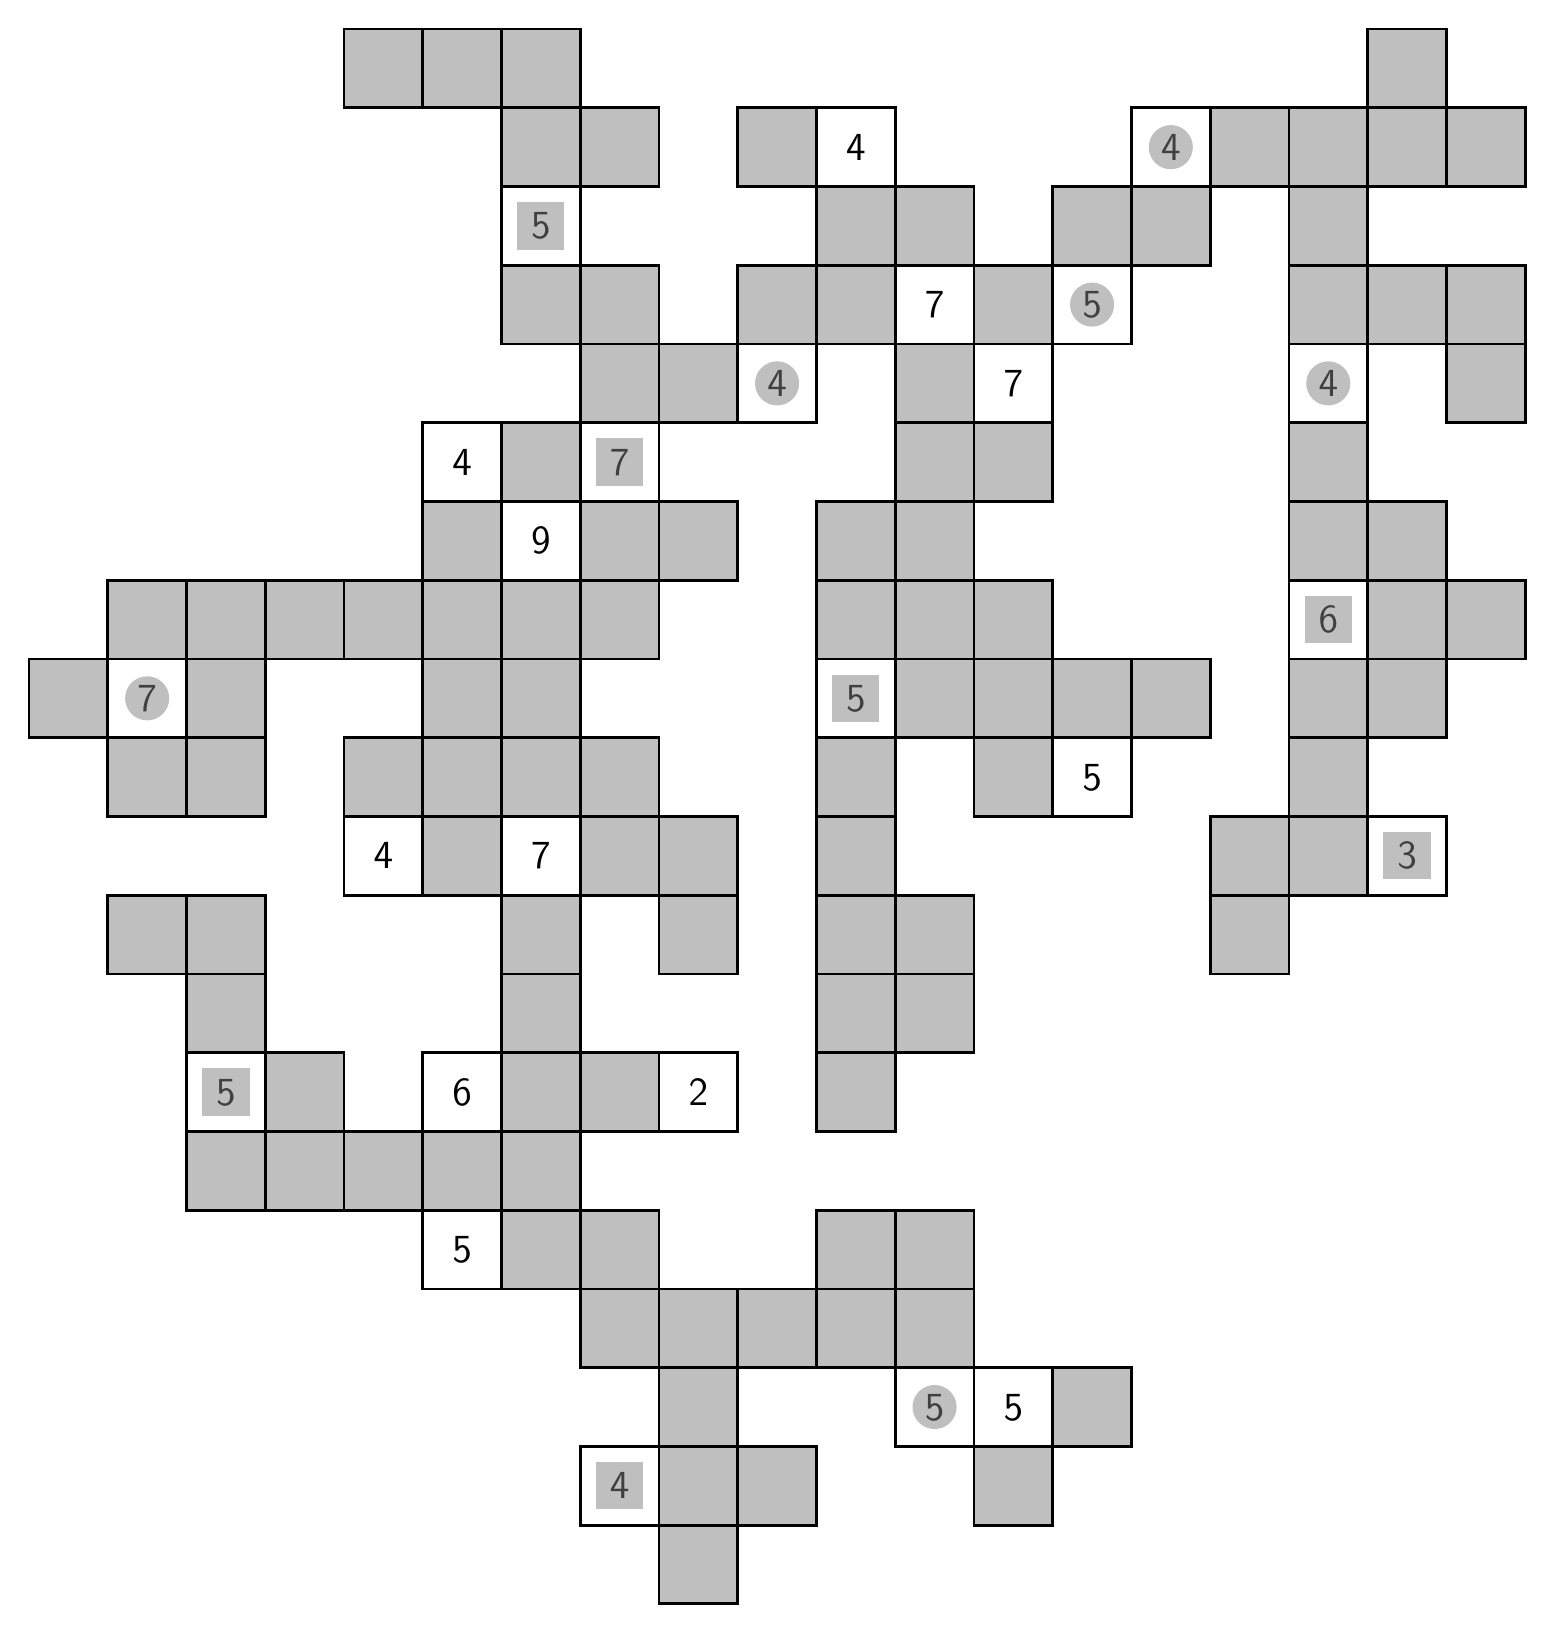
\begin{tikzpicture}\fill[gray, opacity = 0.5] (9, 0, 0)--++(1, 0, 0)--++(0, 1, 0)--++(-1, 0, 0)--cycle;
\draw[line width = 1pt] (9, 0, 0)--++(1, 0, 0)--++(0, 1, 0)--++(-1, 0, 0)--cycle;
\draw node at (8.5, 1.5, 0) {\Large $\mathsf{4}$};
\draw[line width = 1pt] (8, 1, 0)--++(1, 0, 0)--++(0, 1, 0)--++(-1, 0, 0)--cycle;
\fill[color = gray, opacity = 0.5] (8.2, 1.2) rectangle ++(0.6, 0.6);
\fill[gray, opacity = 0.5] (9, 1, 0)--++(1, 0, 0)--++(0, 1, 0)--++(-1, 0, 0)--cycle;
\draw[line width = 1pt] (9, 1, 0)--++(1, 0, 0)--++(0, 1, 0)--++(-1, 0, 0)--cycle;
\fill[gray, opacity = 0.5] (10, 1, 0)--++(1, 0, 0)--++(0, 1, 0)--++(-1, 0, 0)--cycle;
\draw[line width = 1pt] (10, 1, 0)--++(1, 0, 0)--++(0, 1, 0)--++(-1, 0, 0)--cycle;
\fill[gray, opacity = 0.5] (13, 1, 0)--++(1, 0, 0)--++(0, 1, 0)--++(-1, 0, 0)--cycle;
\draw[line width = 1pt] (13, 1, 0)--++(1, 0, 0)--++(0, 1, 0)--++(-1, 0, 0)--cycle;
\fill[gray, opacity = 0.5] (9, 2, 0)--++(1, 0, 0)--++(0, 1, 0)--++(-1, 0, 0)--cycle;
\draw[line width = 1pt] (9, 2, 0)--++(1, 0, 0)--++(0, 1, 0)--++(-1, 0, 0)--cycle;
\draw node at (12.5, 2.5, 0) {\Large $\mathsf{5}$};
\draw[line width = 1pt] (12, 2, 0)--++(1, 0, 0)--++(0, 1, 0)--++(-1, 0, 0)--cycle;
\fill[color = gray, opacity = 0.5] (12.5, 2.5, 0) circle (0.28);
\draw node at (13.5, 2.5, 0) {\Large $\mathsf{5}$};
\draw[line width = 1pt] (13, 2, 0)--++(1, 0, 0)--++(0, 1, 0)--++(-1, 0, 0)--cycle;
\fill[gray, opacity = 0.5] (14, 2, 0)--++(1, 0, 0)--++(0, 1, 0)--++(-1, 0, 0)--cycle;
\draw[line width = 1pt] (14, 2, 0)--++(1, 0, 0)--++(0, 1, 0)--++(-1, 0, 0)--cycle;
\fill[gray, opacity = 0.5] (8, 3, 0)--++(1, 0, 0)--++(0, 1, 0)--++(-1, 0, 0)--cycle;
\draw[line width = 1pt] (8, 3, 0)--++(1, 0, 0)--++(0, 1, 0)--++(-1, 0, 0)--cycle;
\fill[gray, opacity = 0.5] (9, 3, 0)--++(1, 0, 0)--++(0, 1, 0)--++(-1, 0, 0)--cycle;
\draw[line width = 1pt] (9, 3, 0)--++(1, 0, 0)--++(0, 1, 0)--++(-1, 0, 0)--cycle;
\fill[gray, opacity = 0.5] (10, 3, 0)--++(1, 0, 0)--++(0, 1, 0)--++(-1, 0, 0)--cycle;
\draw[line width = 1pt] (10, 3, 0)--++(1, 0, 0)--++(0, 1, 0)--++(-1, 0, 0)--cycle;
\fill[gray, opacity = 0.5] (11, 3, 0)--++(1, 0, 0)--++(0, 1, 0)--++(-1, 0, 0)--cycle;
\draw[line width = 1pt] (11, 3, 0)--++(1, 0, 0)--++(0, 1, 0)--++(-1, 0, 0)--cycle;
\fill[gray, opacity = 0.5] (12, 3, 0)--++(1, 0, 0)--++(0, 1, 0)--++(-1, 0, 0)--cycle;
\draw[line width = 1pt] (12, 3, 0)--++(1, 0, 0)--++(0, 1, 0)--++(-1, 0, 0)--cycle;
\draw node at (6.5, 4.5, 0) {\Large $\mathsf{5}$};
\draw[line width = 1pt] (6, 4, 0)--++(1, 0, 0)--++(0, 1, 0)--++(-1, 0, 0)--cycle;
\fill[gray, opacity = 0.5] (7, 4, 0)--++(1, 0, 0)--++(0, 1, 0)--++(-1, 0, 0)--cycle;
\draw[line width = 1pt] (7, 4, 0)--++(1, 0, 0)--++(0, 1, 0)--++(-1, 0, 0)--cycle;
\fill[gray, opacity = 0.5] (8, 4, 0)--++(1, 0, 0)--++(0, 1, 0)--++(-1, 0, 0)--cycle;
\draw[line width = 1pt] (8, 4, 0)--++(1, 0, 0)--++(0, 1, 0)--++(-1, 0, 0)--cycle;
\fill[gray, opacity = 0.5] (11, 4, 0)--++(1, 0, 0)--++(0, 1, 0)--++(-1, 0, 0)--cycle;
\draw[line width = 1pt] (11, 4, 0)--++(1, 0, 0)--++(0, 1, 0)--++(-1, 0, 0)--cycle;
\fill[gray, opacity = 0.5] (12, 4, 0)--++(1, 0, 0)--++(0, 1, 0)--++(-1, 0, 0)--cycle;
\draw[line width = 1pt] (12, 4, 0)--++(1, 0, 0)--++(0, 1, 0)--++(-1, 0, 0)--cycle;
\fill[gray, opacity = 0.5] (3, 5, 0)--++(1, 0, 0)--++(0, 1, 0)--++(-1, 0, 0)--cycle;
\draw[line width = 1pt] (3, 5, 0)--++(1, 0, 0)--++(0, 1, 0)--++(-1, 0, 0)--cycle;
\fill[gray, opacity = 0.5] (4, 5, 0)--++(1, 0, 0)--++(0, 1, 0)--++(-1, 0, 0)--cycle;
\draw[line width = 1pt] (4, 5, 0)--++(1, 0, 0)--++(0, 1, 0)--++(-1, 0, 0)--cycle;
\fill[gray, opacity = 0.5] (5, 5, 0)--++(1, 0, 0)--++(0, 1, 0)--++(-1, 0, 0)--cycle;
\draw[line width = 1pt] (5, 5, 0)--++(1, 0, 0)--++(0, 1, 0)--++(-1, 0, 0)--cycle;
\fill[gray, opacity = 0.5] (6, 5, 0)--++(1, 0, 0)--++(0, 1, 0)--++(-1, 0, 0)--cycle;
\draw[line width = 1pt] (6, 5, 0)--++(1, 0, 0)--++(0, 1, 0)--++(-1, 0, 0)--cycle;
\fill[gray, opacity = 0.5] (7, 5, 0)--++(1, 0, 0)--++(0, 1, 0)--++(-1, 0, 0)--cycle;
\draw[line width = 1pt] (7, 5, 0)--++(1, 0, 0)--++(0, 1, 0)--++(-1, 0, 0)--cycle;
\draw node at (3.5, 6.5, 0) {\Large $\mathsf{5}$};
\draw[line width = 1pt] (3, 6, 0)--++(1, 0, 0)--++(0, 1, 0)--++(-1, 0, 0)--cycle;
\fill[color = gray, opacity = 0.5] (3.2, 6.2) rectangle ++(0.6, 0.6);
\fill[gray, opacity = 0.5] (4, 6, 0)--++(1, 0, 0)--++(0, 1, 0)--++(-1, 0, 0)--cycle;
\draw[line width = 1pt] (4, 6, 0)--++(1, 0, 0)--++(0, 1, 0)--++(-1, 0, 0)--cycle;
\draw node at (6.5, 6.5, 0) {\Large $\mathsf{6}$};
\draw[line width = 1pt] (6, 6, 0)--++(1, 0, 0)--++(0, 1, 0)--++(-1, 0, 0)--cycle;
\fill[gray, opacity = 0.5] (7, 6, 0)--++(1, 0, 0)--++(0, 1, 0)--++(-1, 0, 0)--cycle;
\draw[line width = 1pt] (7, 6, 0)--++(1, 0, 0)--++(0, 1, 0)--++(-1, 0, 0)--cycle;
\fill[gray, opacity = 0.5] (8, 6, 0)--++(1, 0, 0)--++(0, 1, 0)--++(-1, 0, 0)--cycle;
\draw[line width = 1pt] (8, 6, 0)--++(1, 0, 0)--++(0, 1, 0)--++(-1, 0, 0)--cycle;
\draw node at (9.5, 6.5, 0) {\Large $\mathsf{2}$};
\draw[line width = 1pt] (9, 6, 0)--++(1, 0, 0)--++(0, 1, 0)--++(-1, 0, 0)--cycle;
\fill[gray, opacity = 0.5] (11, 6, 0)--++(1, 0, 0)--++(0, 1, 0)--++(-1, 0, 0)--cycle;
\draw[line width = 1pt] (11, 6, 0)--++(1, 0, 0)--++(0, 1, 0)--++(-1, 0, 0)--cycle;
\fill[gray, opacity = 0.5] (3, 7, 0)--++(1, 0, 0)--++(0, 1, 0)--++(-1, 0, 0)--cycle;
\draw[line width = 1pt] (3, 7, 0)--++(1, 0, 0)--++(0, 1, 0)--++(-1, 0, 0)--cycle;
\fill[gray, opacity = 0.5] (7, 7, 0)--++(1, 0, 0)--++(0, 1, 0)--++(-1, 0, 0)--cycle;
\draw[line width = 1pt] (7, 7, 0)--++(1, 0, 0)--++(0, 1, 0)--++(-1, 0, 0)--cycle;
\fill[gray, opacity = 0.5] (11, 7, 0)--++(1, 0, 0)--++(0, 1, 0)--++(-1, 0, 0)--cycle;
\draw[line width = 1pt] (11, 7, 0)--++(1, 0, 0)--++(0, 1, 0)--++(-1, 0, 0)--cycle;
\fill[gray, opacity = 0.5] (12, 7, 0)--++(1, 0, 0)--++(0, 1, 0)--++(-1, 0, 0)--cycle;
\draw[line width = 1pt] (12, 7, 0)--++(1, 0, 0)--++(0, 1, 0)--++(-1, 0, 0)--cycle;
\fill[gray, opacity = 0.5] (2, 8, 0)--++(1, 0, 0)--++(0, 1, 0)--++(-1, 0, 0)--cycle;
\draw[line width = 1pt] (2, 8, 0)--++(1, 0, 0)--++(0, 1, 0)--++(-1, 0, 0)--cycle;
\fill[gray, opacity = 0.5] (3, 8, 0)--++(1, 0, 0)--++(0, 1, 0)--++(-1, 0, 0)--cycle;
\draw[line width = 1pt] (3, 8, 0)--++(1, 0, 0)--++(0, 1, 0)--++(-1, 0, 0)--cycle;
\fill[gray, opacity = 0.5] (7, 8, 0)--++(1, 0, 0)--++(0, 1, 0)--++(-1, 0, 0)--cycle;
\draw[line width = 1pt] (7, 8, 0)--++(1, 0, 0)--++(0, 1, 0)--++(-1, 0, 0)--cycle;
\fill[gray, opacity = 0.5] (9, 8, 0)--++(1, 0, 0)--++(0, 1, 0)--++(-1, 0, 0)--cycle;
\draw[line width = 1pt] (9, 8, 0)--++(1, 0, 0)--++(0, 1, 0)--++(-1, 0, 0)--cycle;
\fill[gray, opacity = 0.5] (11, 8, 0)--++(1, 0, 0)--++(0, 1, 0)--++(-1, 0, 0)--cycle;
\draw[line width = 1pt] (11, 8, 0)--++(1, 0, 0)--++(0, 1, 0)--++(-1, 0, 0)--cycle;
\fill[gray, opacity = 0.5] (12, 8, 0)--++(1, 0, 0)--++(0, 1, 0)--++(-1, 0, 0)--cycle;
\draw[line width = 1pt] (12, 8, 0)--++(1, 0, 0)--++(0, 1, 0)--++(-1, 0, 0)--cycle;
\fill[gray, opacity = 0.5] (16, 8, 0)--++(1, 0, 0)--++(0, 1, 0)--++(-1, 0, 0)--cycle;
\draw[line width = 1pt] (16, 8, 0)--++(1, 0, 0)--++(0, 1, 0)--++(-1, 0, 0)--cycle;
\draw node at (5.5, 9.5, 0) {\Large $\mathsf{4}$};
\draw[line width = 1pt] (5, 9, 0)--++(1, 0, 0)--++(0, 1, 0)--++(-1, 0, 0)--cycle;
\fill[gray, opacity = 0.5] (6, 9, 0)--++(1, 0, 0)--++(0, 1, 0)--++(-1, 0, 0)--cycle;
\draw[line width = 1pt] (6, 9, 0)--++(1, 0, 0)--++(0, 1, 0)--++(-1, 0, 0)--cycle;
\draw node at (7.5, 9.5, 0) {\Large $\mathsf{7}$};
\draw[line width = 1pt] (7, 9, 0)--++(1, 0, 0)--++(0, 1, 0)--++(-1, 0, 0)--cycle;
\fill[gray, opacity = 0.5] (8, 9, 0)--++(1, 0, 0)--++(0, 1, 0)--++(-1, 0, 0)--cycle;
\draw[line width = 1pt] (8, 9, 0)--++(1, 0, 0)--++(0, 1, 0)--++(-1, 0, 0)--cycle;
\fill[gray, opacity = 0.5] (9, 9, 0)--++(1, 0, 0)--++(0, 1, 0)--++(-1, 0, 0)--cycle;
\draw[line width = 1pt] (9, 9, 0)--++(1, 0, 0)--++(0, 1, 0)--++(-1, 0, 0)--cycle;
\fill[gray, opacity = 0.5] (11, 9, 0)--++(1, 0, 0)--++(0, 1, 0)--++(-1, 0, 0)--cycle;
\draw[line width = 1pt] (11, 9, 0)--++(1, 0, 0)--++(0, 1, 0)--++(-1, 0, 0)--cycle;
\fill[gray, opacity = 0.5] (16, 9, 0)--++(1, 0, 0)--++(0, 1, 0)--++(-1, 0, 0)--cycle;
\draw[line width = 1pt] (16, 9, 0)--++(1, 0, 0)--++(0, 1, 0)--++(-1, 0, 0)--cycle;
\fill[gray, opacity = 0.5] (17, 9, 0)--++(1, 0, 0)--++(0, 1, 0)--++(-1, 0, 0)--cycle;
\draw[line width = 1pt] (17, 9, 0)--++(1, 0, 0)--++(0, 1, 0)--++(-1, 0, 0)--cycle;
\draw node at (18.5, 9.5, 0) {\Large $\mathsf{3}$};
\draw[line width = 1pt] (18, 9, 0)--++(1, 0, 0)--++(0, 1, 0)--++(-1, 0, 0)--cycle;
\fill[color = gray, opacity = 0.5] (18.2, 9.2) rectangle ++(0.6, 0.6);
\fill[gray, opacity = 0.5] (2, 10, 0)--++(1, 0, 0)--++(0, 1, 0)--++(-1, 0, 0)--cycle;
\draw[line width = 1pt] (2, 10, 0)--++(1, 0, 0)--++(0, 1, 0)--++(-1, 0, 0)--cycle;
\fill[gray, opacity = 0.5] (3, 10, 0)--++(1, 0, 0)--++(0, 1, 0)--++(-1, 0, 0)--cycle;
\draw[line width = 1pt] (3, 10, 0)--++(1, 0, 0)--++(0, 1, 0)--++(-1, 0, 0)--cycle;
\fill[gray, opacity = 0.5] (5, 10, 0)--++(1, 0, 0)--++(0, 1, 0)--++(-1, 0, 0)--cycle;
\draw[line width = 1pt] (5, 10, 0)--++(1, 0, 0)--++(0, 1, 0)--++(-1, 0, 0)--cycle;
\fill[gray, opacity = 0.5] (6, 10, 0)--++(1, 0, 0)--++(0, 1, 0)--++(-1, 0, 0)--cycle;
\draw[line width = 1pt] (6, 10, 0)--++(1, 0, 0)--++(0, 1, 0)--++(-1, 0, 0)--cycle;
\fill[gray, opacity = 0.5] (7, 10, 0)--++(1, 0, 0)--++(0, 1, 0)--++(-1, 0, 0)--cycle;
\draw[line width = 1pt] (7, 10, 0)--++(1, 0, 0)--++(0, 1, 0)--++(-1, 0, 0)--cycle;
\fill[gray, opacity = 0.5] (8, 10, 0)--++(1, 0, 0)--++(0, 1, 0)--++(-1, 0, 0)--cycle;
\draw[line width = 1pt] (8, 10, 0)--++(1, 0, 0)--++(0, 1, 0)--++(-1, 0, 0)--cycle;
\fill[gray, opacity = 0.5] (11, 10, 0)--++(1, 0, 0)--++(0, 1, 0)--++(-1, 0, 0)--cycle;
\draw[line width = 1pt] (11, 10, 0)--++(1, 0, 0)--++(0, 1, 0)--++(-1, 0, 0)--cycle;
\fill[gray, opacity = 0.5] (13, 10, 0)--++(1, 0, 0)--++(0, 1, 0)--++(-1, 0, 0)--cycle;
\draw[line width = 1pt] (13, 10, 0)--++(1, 0, 0)--++(0, 1, 0)--++(-1, 0, 0)--cycle;
\draw node at (14.5, 10.5, 0) {\Large $\mathsf{5}$};
\draw[line width = 1pt] (14, 10, 0)--++(1, 0, 0)--++(0, 1, 0)--++(-1, 0, 0)--cycle;
\fill[gray, opacity = 0.5] (17, 10, 0)--++(1, 0, 0)--++(0, 1, 0)--++(-1, 0, 0)--cycle;
\draw[line width = 1pt] (17, 10, 0)--++(1, 0, 0)--++(0, 1, 0)--++(-1, 0, 0)--cycle;
\fill[gray, opacity = 0.5] (1, 11, 0)--++(1, 0, 0)--++(0, 1, 0)--++(-1, 0, 0)--cycle;
\draw[line width = 1pt] (1, 11, 0)--++(1, 0, 0)--++(0, 1, 0)--++(-1, 0, 0)--cycle;
\draw node at (2.5, 11.5, 0) {\Large $\mathsf{7}$};
\draw[line width = 1pt] (2, 11, 0)--++(1, 0, 0)--++(0, 1, 0)--++(-1, 0, 0)--cycle;
\fill[color = gray, opacity = 0.5] (2.5, 11.5, 0) circle (0.28);
\fill[gray, opacity = 0.5] (3, 11, 0)--++(1, 0, 0)--++(0, 1, 0)--++(-1, 0, 0)--cycle;
\draw[line width = 1pt] (3, 11, 0)--++(1, 0, 0)--++(0, 1, 0)--++(-1, 0, 0)--cycle;
\fill[gray, opacity = 0.5] (6, 11, 0)--++(1, 0, 0)--++(0, 1, 0)--++(-1, 0, 0)--cycle;
\draw[line width = 1pt] (6, 11, 0)--++(1, 0, 0)--++(0, 1, 0)--++(-1, 0, 0)--cycle;
\fill[gray, opacity = 0.5] (7, 11, 0)--++(1, 0, 0)--++(0, 1, 0)--++(-1, 0, 0)--cycle;
\draw[line width = 1pt] (7, 11, 0)--++(1, 0, 0)--++(0, 1, 0)--++(-1, 0, 0)--cycle;
\draw node at (11.5, 11.5, 0) {\Large $\mathsf{5}$};
\draw[line width = 1pt] (11, 11, 0)--++(1, 0, 0)--++(0, 1, 0)--++(-1, 0, 0)--cycle;
\fill[color = gray, opacity = 0.5] (11.2, 11.2) rectangle ++(0.6, 0.6);
\fill[gray, opacity = 0.5] (12, 11, 0)--++(1, 0, 0)--++(0, 1, 0)--++(-1, 0, 0)--cycle;
\draw[line width = 1pt] (12, 11, 0)--++(1, 0, 0)--++(0, 1, 0)--++(-1, 0, 0)--cycle;
\fill[gray, opacity = 0.5] (13, 11, 0)--++(1, 0, 0)--++(0, 1, 0)--++(-1, 0, 0)--cycle;
\draw[line width = 1pt] (13, 11, 0)--++(1, 0, 0)--++(0, 1, 0)--++(-1, 0, 0)--cycle;
\fill[gray, opacity = 0.5] (14, 11, 0)--++(1, 0, 0)--++(0, 1, 0)--++(-1, 0, 0)--cycle;
\draw[line width = 1pt] (14, 11, 0)--++(1, 0, 0)--++(0, 1, 0)--++(-1, 0, 0)--cycle;
\fill[gray, opacity = 0.5] (15, 11, 0)--++(1, 0, 0)--++(0, 1, 0)--++(-1, 0, 0)--cycle;
\draw[line width = 1pt] (15, 11, 0)--++(1, 0, 0)--++(0, 1, 0)--++(-1, 0, 0)--cycle;
\fill[gray, opacity = 0.5] (17, 11, 0)--++(1, 0, 0)--++(0, 1, 0)--++(-1, 0, 0)--cycle;
\draw[line width = 1pt] (17, 11, 0)--++(1, 0, 0)--++(0, 1, 0)--++(-1, 0, 0)--cycle;
\fill[gray, opacity = 0.5] (18, 11, 0)--++(1, 0, 0)--++(0, 1, 0)--++(-1, 0, 0)--cycle;
\draw[line width = 1pt] (18, 11, 0)--++(1, 0, 0)--++(0, 1, 0)--++(-1, 0, 0)--cycle;
\fill[gray, opacity = 0.5] (2, 12, 0)--++(1, 0, 0)--++(0, 1, 0)--++(-1, 0, 0)--cycle;
\draw[line width = 1pt] (2, 12, 0)--++(1, 0, 0)--++(0, 1, 0)--++(-1, 0, 0)--cycle;
\fill[gray, opacity = 0.5] (3, 12, 0)--++(1, 0, 0)--++(0, 1, 0)--++(-1, 0, 0)--cycle;
\draw[line width = 1pt] (3, 12, 0)--++(1, 0, 0)--++(0, 1, 0)--++(-1, 0, 0)--cycle;
\fill[gray, opacity = 0.5] (4, 12, 0)--++(1, 0, 0)--++(0, 1, 0)--++(-1, 0, 0)--cycle;
\draw[line width = 1pt] (4, 12, 0)--++(1, 0, 0)--++(0, 1, 0)--++(-1, 0, 0)--cycle;
\fill[gray, opacity = 0.5] (5, 12, 0)--++(1, 0, 0)--++(0, 1, 0)--++(-1, 0, 0)--cycle;
\draw[line width = 1pt] (5, 12, 0)--++(1, 0, 0)--++(0, 1, 0)--++(-1, 0, 0)--cycle;
\fill[gray, opacity = 0.5] (6, 12, 0)--++(1, 0, 0)--++(0, 1, 0)--++(-1, 0, 0)--cycle;
\draw[line width = 1pt] (6, 12, 0)--++(1, 0, 0)--++(0, 1, 0)--++(-1, 0, 0)--cycle;
\fill[gray, opacity = 0.5] (7, 12, 0)--++(1, 0, 0)--++(0, 1, 0)--++(-1, 0, 0)--cycle;
\draw[line width = 1pt] (7, 12, 0)--++(1, 0, 0)--++(0, 1, 0)--++(-1, 0, 0)--cycle;
\fill[gray, opacity = 0.5] (8, 12, 0)--++(1, 0, 0)--++(0, 1, 0)--++(-1, 0, 0)--cycle;
\draw[line width = 1pt] (8, 12, 0)--++(1, 0, 0)--++(0, 1, 0)--++(-1, 0, 0)--cycle;
\fill[gray, opacity = 0.5] (11, 12, 0)--++(1, 0, 0)--++(0, 1, 0)--++(-1, 0, 0)--cycle;
\draw[line width = 1pt] (11, 12, 0)--++(1, 0, 0)--++(0, 1, 0)--++(-1, 0, 0)--cycle;
\fill[gray, opacity = 0.5] (12, 12, 0)--++(1, 0, 0)--++(0, 1, 0)--++(-1, 0, 0)--cycle;
\draw[line width = 1pt] (12, 12, 0)--++(1, 0, 0)--++(0, 1, 0)--++(-1, 0, 0)--cycle;
\fill[gray, opacity = 0.5] (13, 12, 0)--++(1, 0, 0)--++(0, 1, 0)--++(-1, 0, 0)--cycle;
\draw[line width = 1pt] (13, 12, 0)--++(1, 0, 0)--++(0, 1, 0)--++(-1, 0, 0)--cycle;
\draw node at (17.5, 12.5, 0) {\Large $\mathsf{6}$};
\draw[line width = 1pt] (17, 12, 0)--++(1, 0, 0)--++(0, 1, 0)--++(-1, 0, 0)--cycle;
\fill[color = gray, opacity = 0.5] (17.2, 12.2) rectangle ++(0.6, 0.6);
\fill[gray, opacity = 0.5] (18, 12, 0)--++(1, 0, 0)--++(0, 1, 0)--++(-1, 0, 0)--cycle;
\draw[line width = 1pt] (18, 12, 0)--++(1, 0, 0)--++(0, 1, 0)--++(-1, 0, 0)--cycle;
\fill[gray, opacity = 0.5] (19, 12, 0)--++(1, 0, 0)--++(0, 1, 0)--++(-1, 0, 0)--cycle;
\draw[line width = 1pt] (19, 12, 0)--++(1, 0, 0)--++(0, 1, 0)--++(-1, 0, 0)--cycle;
\fill[gray, opacity = 0.5] (6, 13, 0)--++(1, 0, 0)--++(0, 1, 0)--++(-1, 0, 0)--cycle;
\draw[line width = 1pt] (6, 13, 0)--++(1, 0, 0)--++(0, 1, 0)--++(-1, 0, 0)--cycle;
\draw node at (7.5, 13.5, 0) {\Large $\mathsf{9}$};
\draw[line width = 1pt] (7, 13, 0)--++(1, 0, 0)--++(0, 1, 0)--++(-1, 0, 0)--cycle;
\fill[gray, opacity = 0.5] (8, 13, 0)--++(1, 0, 0)--++(0, 1, 0)--++(-1, 0, 0)--cycle;
\draw[line width = 1pt] (8, 13, 0)--++(1, 0, 0)--++(0, 1, 0)--++(-1, 0, 0)--cycle;
\fill[gray, opacity = 0.5] (9, 13, 0)--++(1, 0, 0)--++(0, 1, 0)--++(-1, 0, 0)--cycle;
\draw[line width = 1pt] (9, 13, 0)--++(1, 0, 0)--++(0, 1, 0)--++(-1, 0, 0)--cycle;
\fill[gray, opacity = 0.5] (11, 13, 0)--++(1, 0, 0)--++(0, 1, 0)--++(-1, 0, 0)--cycle;
\draw[line width = 1pt] (11, 13, 0)--++(1, 0, 0)--++(0, 1, 0)--++(-1, 0, 0)--cycle;
\fill[gray, opacity = 0.5] (12, 13, 0)--++(1, 0, 0)--++(0, 1, 0)--++(-1, 0, 0)--cycle;
\draw[line width = 1pt] (12, 13, 0)--++(1, 0, 0)--++(0, 1, 0)--++(-1, 0, 0)--cycle;
\fill[gray, opacity = 0.5] (17, 13, 0)--++(1, 0, 0)--++(0, 1, 0)--++(-1, 0, 0)--cycle;
\draw[line width = 1pt] (17, 13, 0)--++(1, 0, 0)--++(0, 1, 0)--++(-1, 0, 0)--cycle;
\fill[gray, opacity = 0.5] (18, 13, 0)--++(1, 0, 0)--++(0, 1, 0)--++(-1, 0, 0)--cycle;
\draw[line width = 1pt] (18, 13, 0)--++(1, 0, 0)--++(0, 1, 0)--++(-1, 0, 0)--cycle;
\draw node at (6.5, 14.5, 0) {\Large $\mathsf{4}$};
\draw[line width = 1pt] (6, 14, 0)--++(1, 0, 0)--++(0, 1, 0)--++(-1, 0, 0)--cycle;
\fill[gray, opacity = 0.5] (7, 14, 0)--++(1, 0, 0)--++(0, 1, 0)--++(-1, 0, 0)--cycle;
\draw[line width = 1pt] (7, 14, 0)--++(1, 0, 0)--++(0, 1, 0)--++(-1, 0, 0)--cycle;
\draw node at (8.5, 14.5, 0) {\Large $\mathsf{7}$};
\draw[line width = 1pt] (8, 14, 0)--++(1, 0, 0)--++(0, 1, 0)--++(-1, 0, 0)--cycle;
\fill[color = gray, opacity = 0.5] (8.2, 14.2) rectangle ++(0.6, 0.6);
\fill[gray, opacity = 0.5] (12, 14, 0)--++(1, 0, 0)--++(0, 1, 0)--++(-1, 0, 0)--cycle;
\draw[line width = 1pt] (12, 14, 0)--++(1, 0, 0)--++(0, 1, 0)--++(-1, 0, 0)--cycle;
\fill[gray, opacity = 0.5] (13, 14, 0)--++(1, 0, 0)--++(0, 1, 0)--++(-1, 0, 0)--cycle;
\draw[line width = 1pt] (13, 14, 0)--++(1, 0, 0)--++(0, 1, 0)--++(-1, 0, 0)--cycle;
\fill[gray, opacity = 0.5] (17, 14, 0)--++(1, 0, 0)--++(0, 1, 0)--++(-1, 0, 0)--cycle;
\draw[line width = 1pt] (17, 14, 0)--++(1, 0, 0)--++(0, 1, 0)--++(-1, 0, 0)--cycle;
\fill[gray, opacity = 0.5] (8, 15, 0)--++(1, 0, 0)--++(0, 1, 0)--++(-1, 0, 0)--cycle;
\draw[line width = 1pt] (8, 15, 0)--++(1, 0, 0)--++(0, 1, 0)--++(-1, 0, 0)--cycle;
\fill[gray, opacity = 0.5] (9, 15, 0)--++(1, 0, 0)--++(0, 1, 0)--++(-1, 0, 0)--cycle;
\draw[line width = 1pt] (9, 15, 0)--++(1, 0, 0)--++(0, 1, 0)--++(-1, 0, 0)--cycle;
\draw node at (10.5, 15.5, 0) {\Large $\mathsf{4}$};
\draw[line width = 1pt] (10, 15, 0)--++(1, 0, 0)--++(0, 1, 0)--++(-1, 0, 0)--cycle;
\fill[color = gray, opacity = 0.5] (10.5, 15.5, 0) circle (0.28);
\fill[gray, opacity = 0.5] (12, 15, 0)--++(1, 0, 0)--++(0, 1, 0)--++(-1, 0, 0)--cycle;
\draw[line width = 1pt] (12, 15, 0)--++(1, 0, 0)--++(0, 1, 0)--++(-1, 0, 0)--cycle;
\draw node at (13.5, 15.5, 0) {\Large $\mathsf{7}$};
\draw[line width = 1pt] (13, 15, 0)--++(1, 0, 0)--++(0, 1, 0)--++(-1, 0, 0)--cycle;
\draw node at (17.5, 15.5, 0) {\Large $\mathsf{4}$};
\draw[line width = 1pt] (17, 15, 0)--++(1, 0, 0)--++(0, 1, 0)--++(-1, 0, 0)--cycle;
\fill[color = gray, opacity = 0.5] (17.5, 15.5, 0) circle (0.28);
\fill[gray, opacity = 0.5] (19, 15, 0)--++(1, 0, 0)--++(0, 1, 0)--++(-1, 0, 0)--cycle;
\draw[line width = 1pt] (19, 15, 0)--++(1, 0, 0)--++(0, 1, 0)--++(-1, 0, 0)--cycle;
\fill[gray, opacity = 0.5] (7, 16, 0)--++(1, 0, 0)--++(0, 1, 0)--++(-1, 0, 0)--cycle;
\draw[line width = 1pt] (7, 16, 0)--++(1, 0, 0)--++(0, 1, 0)--++(-1, 0, 0)--cycle;
\fill[gray, opacity = 0.5] (8, 16, 0)--++(1, 0, 0)--++(0, 1, 0)--++(-1, 0, 0)--cycle;
\draw[line width = 1pt] (8, 16, 0)--++(1, 0, 0)--++(0, 1, 0)--++(-1, 0, 0)--cycle;
\fill[gray, opacity = 0.5] (10, 16, 0)--++(1, 0, 0)--++(0, 1, 0)--++(-1, 0, 0)--cycle;
\draw[line width = 1pt] (10, 16, 0)--++(1, 0, 0)--++(0, 1, 0)--++(-1, 0, 0)--cycle;
\fill[gray, opacity = 0.5] (11, 16, 0)--++(1, 0, 0)--++(0, 1, 0)--++(-1, 0, 0)--cycle;
\draw[line width = 1pt] (11, 16, 0)--++(1, 0, 0)--++(0, 1, 0)--++(-1, 0, 0)--cycle;
\draw node at (12.5, 16.5, 0) {\Large $\mathsf{7}$};
\draw[line width = 1pt] (12, 16, 0)--++(1, 0, 0)--++(0, 1, 0)--++(-1, 0, 0)--cycle;
\fill[gray, opacity = 0.5] (13, 16, 0)--++(1, 0, 0)--++(0, 1, 0)--++(-1, 0, 0)--cycle;
\draw[line width = 1pt] (13, 16, 0)--++(1, 0, 0)--++(0, 1, 0)--++(-1, 0, 0)--cycle;
\draw node at (14.5, 16.5, 0) {\Large $\mathsf{5}$};
\draw[line width = 1pt] (14, 16, 0)--++(1, 0, 0)--++(0, 1, 0)--++(-1, 0, 0)--cycle;
\fill[color = gray, opacity = 0.5] (14.5, 16.5, 0) circle (0.28);
\fill[gray, opacity = 0.5] (17, 16, 0)--++(1, 0, 0)--++(0, 1, 0)--++(-1, 0, 0)--cycle;
\draw[line width = 1pt] (17, 16, 0)--++(1, 0, 0)--++(0, 1, 0)--++(-1, 0, 0)--cycle;
\fill[gray, opacity = 0.5] (18, 16, 0)--++(1, 0, 0)--++(0, 1, 0)--++(-1, 0, 0)--cycle;
\draw[line width = 1pt] (18, 16, 0)--++(1, 0, 0)--++(0, 1, 0)--++(-1, 0, 0)--cycle;
\fill[gray, opacity = 0.5] (19, 16, 0)--++(1, 0, 0)--++(0, 1, 0)--++(-1, 0, 0)--cycle;
\draw[line width = 1pt] (19, 16, 0)--++(1, 0, 0)--++(0, 1, 0)--++(-1, 0, 0)--cycle;
\draw node at (7.5, 17.5, 0) {\Large $\mathsf{5}$};
\draw[line width = 1pt] (7, 17, 0)--++(1, 0, 0)--++(0, 1, 0)--++(-1, 0, 0)--cycle;
\fill[color = gray, opacity = 0.5] (7.2, 17.2) rectangle ++(0.6, 0.6);
\fill[gray, opacity = 0.5] (11, 17, 0)--++(1, 0, 0)--++(0, 1, 0)--++(-1, 0, 0)--cycle;
\draw[line width = 1pt] (11, 17, 0)--++(1, 0, 0)--++(0, 1, 0)--++(-1, 0, 0)--cycle;
\fill[gray, opacity = 0.5] (12, 17, 0)--++(1, 0, 0)--++(0, 1, 0)--++(-1, 0, 0)--cycle;
\draw[line width = 1pt] (12, 17, 0)--++(1, 0, 0)--++(0, 1, 0)--++(-1, 0, 0)--cycle;
\fill[gray, opacity = 0.5] (14, 17, 0)--++(1, 0, 0)--++(0, 1, 0)--++(-1, 0, 0)--cycle;
\draw[line width = 1pt] (14, 17, 0)--++(1, 0, 0)--++(0, 1, 0)--++(-1, 0, 0)--cycle;
\fill[gray, opacity = 0.5] (15, 17, 0)--++(1, 0, 0)--++(0, 1, 0)--++(-1, 0, 0)--cycle;
\draw[line width = 1pt] (15, 17, 0)--++(1, 0, 0)--++(0, 1, 0)--++(-1, 0, 0)--cycle;
\fill[gray, opacity = 0.5] (17, 17, 0)--++(1, 0, 0)--++(0, 1, 0)--++(-1, 0, 0)--cycle;
\draw[line width = 1pt] (17, 17, 0)--++(1, 0, 0)--++(0, 1, 0)--++(-1, 0, 0)--cycle;
\fill[gray, opacity = 0.5] (7, 18, 0)--++(1, 0, 0)--++(0, 1, 0)--++(-1, 0, 0)--cycle;
\draw[line width = 1pt] (7, 18, 0)--++(1, 0, 0)--++(0, 1, 0)--++(-1, 0, 0)--cycle;
\fill[gray, opacity = 0.5] (8, 18, 0)--++(1, 0, 0)--++(0, 1, 0)--++(-1, 0, 0)--cycle;
\draw[line width = 1pt] (8, 18, 0)--++(1, 0, 0)--++(0, 1, 0)--++(-1, 0, 0)--cycle;
\fill[gray, opacity = 0.5] (10, 18, 0)--++(1, 0, 0)--++(0, 1, 0)--++(-1, 0, 0)--cycle;
\draw[line width = 1pt] (10, 18, 0)--++(1, 0, 0)--++(0, 1, 0)--++(-1, 0, 0)--cycle;
\draw node at (11.5, 18.5, 0) {\Large $\mathsf{4}$};
\draw[line width = 1pt] (11, 18, 0)--++(1, 0, 0)--++(0, 1, 0)--++(-1, 0, 0)--cycle;
\draw node at (15.5, 18.5, 0) {\Large $\mathsf{4}$};
\draw[line width = 1pt] (15, 18, 0)--++(1, 0, 0)--++(0, 1, 0)--++(-1, 0, 0)--cycle;
\fill[color = gray, opacity = 0.5] (15.5, 18.5, 0) circle (0.28);
\fill[gray, opacity = 0.5] (16, 18, 0)--++(1, 0, 0)--++(0, 1, 0)--++(-1, 0, 0)--cycle;
\draw[line width = 1pt] (16, 18, 0)--++(1, 0, 0)--++(0, 1, 0)--++(-1, 0, 0)--cycle;
\fill[gray, opacity = 0.5] (17, 18, 0)--++(1, 0, 0)--++(0, 1, 0)--++(-1, 0, 0)--cycle;
\draw[line width = 1pt] (17, 18, 0)--++(1, 0, 0)--++(0, 1, 0)--++(-1, 0, 0)--cycle;
\fill[gray, opacity = 0.5] (18, 18, 0)--++(1, 0, 0)--++(0, 1, 0)--++(-1, 0, 0)--cycle;
\draw[line width = 1pt] (18, 18, 0)--++(1, 0, 0)--++(0, 1, 0)--++(-1, 0, 0)--cycle;
\fill[gray, opacity = 0.5] (19, 18, 0)--++(1, 0, 0)--++(0, 1, 0)--++(-1, 0, 0)--cycle;
\draw[line width = 1pt] (19, 18, 0)--++(1, 0, 0)--++(0, 1, 0)--++(-1, 0, 0)--cycle;
\fill[gray, opacity = 0.5] (5, 19, 0)--++(1, 0, 0)--++(0, 1, 0)--++(-1, 0, 0)--cycle;
\draw[line width = 1pt] (5, 19, 0)--++(1, 0, 0)--++(0, 1, 0)--++(-1, 0, 0)--cycle;
\fill[gray, opacity = 0.5] (6, 19, 0)--++(1, 0, 0)--++(0, 1, 0)--++(-1, 0, 0)--cycle;
\draw[line width = 1pt] (6, 19, 0)--++(1, 0, 0)--++(0, 1, 0)--++(-1, 0, 0)--cycle;
\fill[gray, opacity = 0.5] (7, 19, 0)--++(1, 0, 0)--++(0, 1, 0)--++(-1, 0, 0)--cycle;
\draw[line width = 1pt] (7, 19, 0)--++(1, 0, 0)--++(0, 1, 0)--++(-1, 0, 0)--cycle;
\fill[gray, opacity = 0.5] (18, 19, 0)--++(1, 0, 0)--++(0, 1, 0)--++(-1, 0, 0)--cycle;
\draw[line width = 1pt] (18, 19, 0)--++(1, 0, 0)--++(0, 1, 0)--++(-1, 0, 0)--cycle;
\end{tikzpicture}}\]
\[\resizebox{30pc}{!}{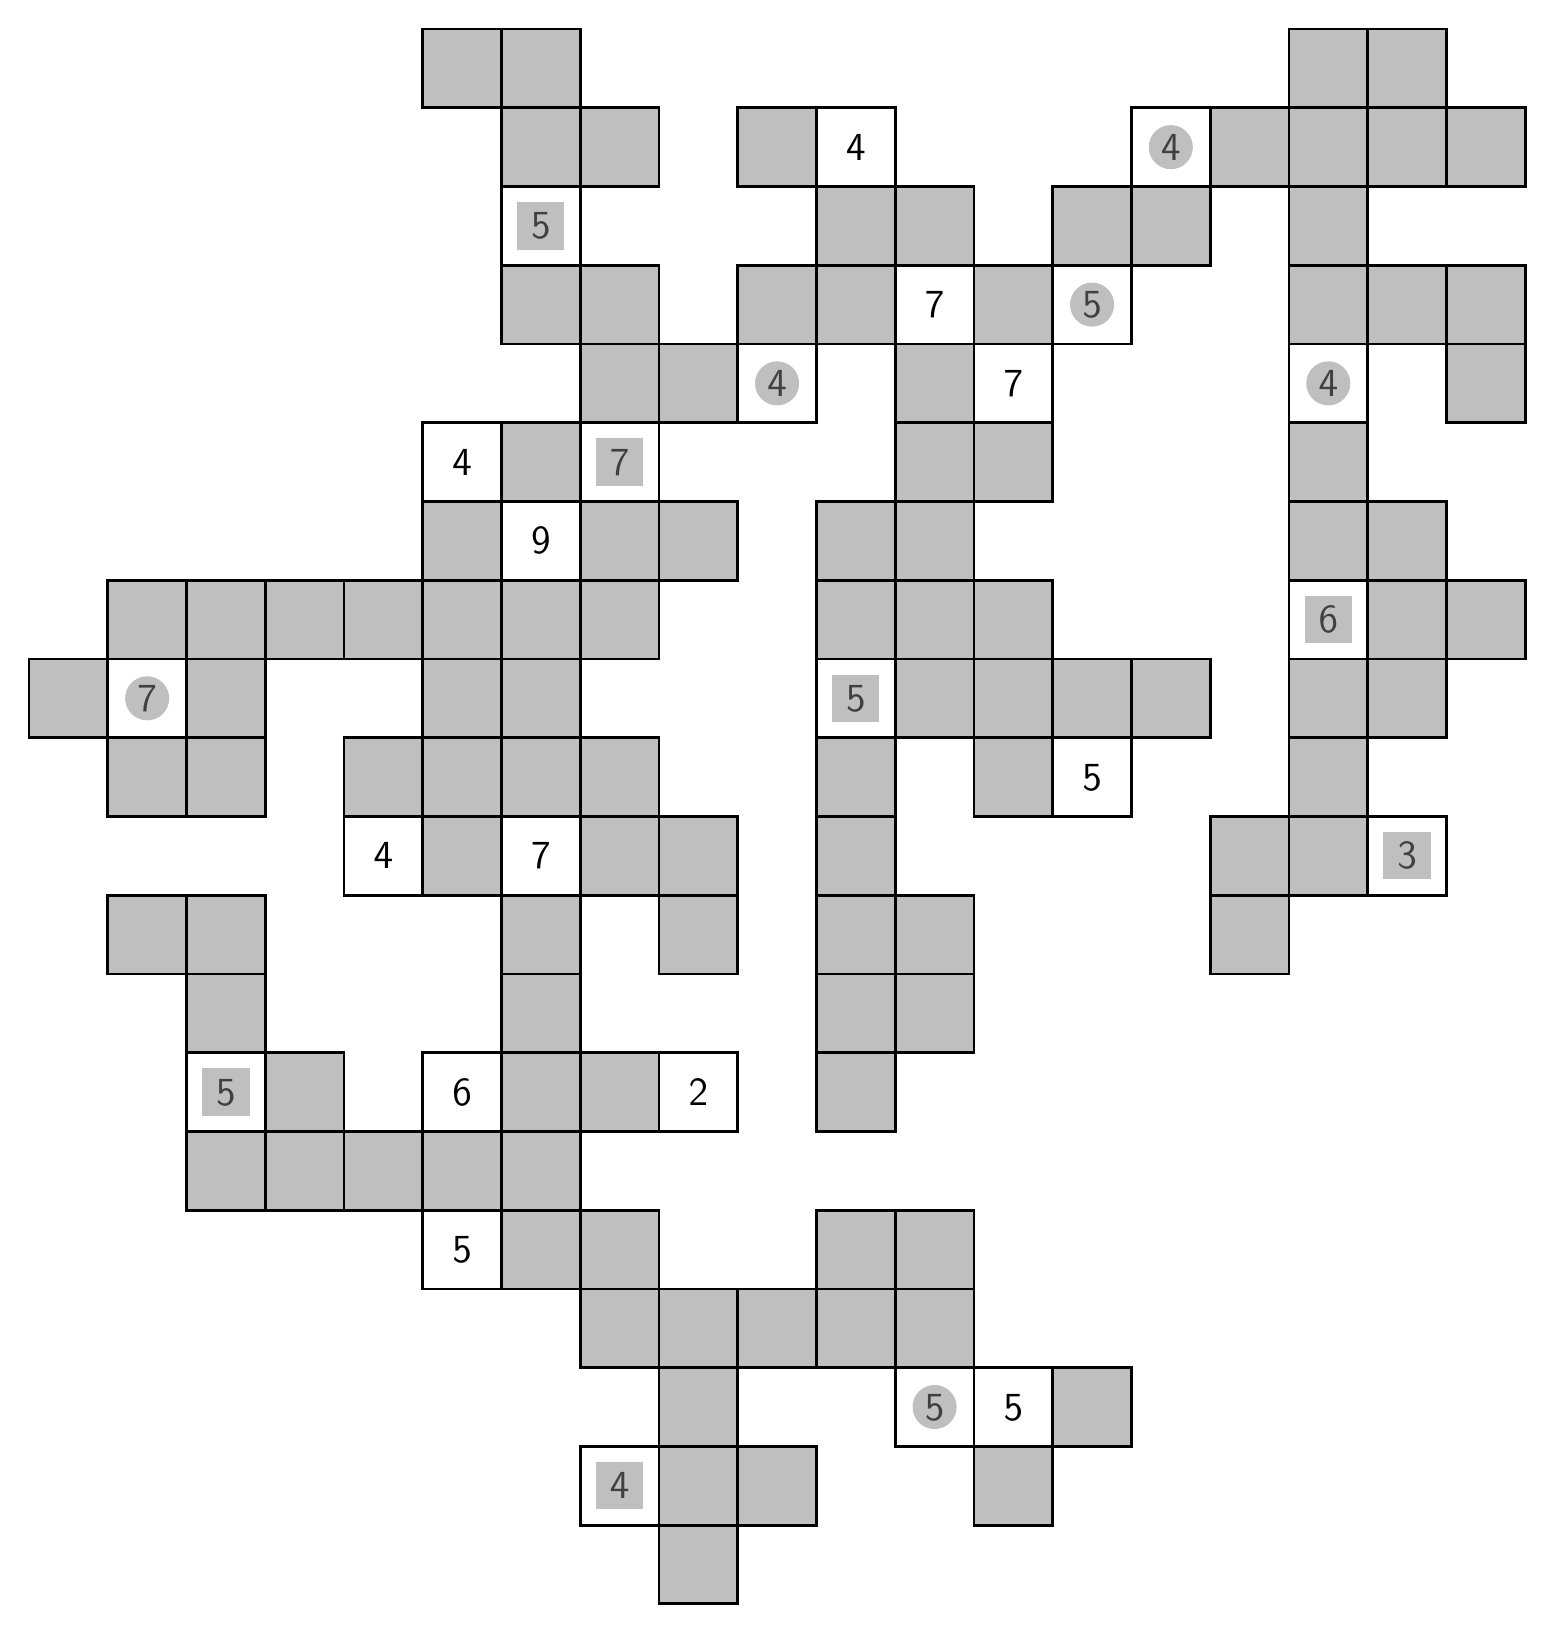
\begin{tikzpicture}\fill[gray, opacity = 0.5] (9, 0, 0)--++(1, 0, 0)--++(0, 1, 0)--++(-1, 0, 0)--cycle;
\draw[line width = 1pt] (9, 0, 0)--++(1, 0, 0)--++(0, 1, 0)--++(-1, 0, 0)--cycle;
\draw node at (8.5, 1.5, 0) {\Large $\mathsf{4}$};
\draw[line width = 1pt] (8, 1, 0)--++(1, 0, 0)--++(0, 1, 0)--++(-1, 0, 0)--cycle;
\fill[color = gray, opacity = 0.5] (8.2, 1.2) rectangle ++(0.6, 0.6);
\fill[gray, opacity = 0.5] (9, 1, 0)--++(1, 0, 0)--++(0, 1, 0)--++(-1, 0, 0)--cycle;
\draw[line width = 1pt] (9, 1, 0)--++(1, 0, 0)--++(0, 1, 0)--++(-1, 0, 0)--cycle;
\fill[gray, opacity = 0.5] (10, 1, 0)--++(1, 0, 0)--++(0, 1, 0)--++(-1, 0, 0)--cycle;
\draw[line width = 1pt] (10, 1, 0)--++(1, 0, 0)--++(0, 1, 0)--++(-1, 0, 0)--cycle;
\fill[gray, opacity = 0.5] (13, 1, 0)--++(1, 0, 0)--++(0, 1, 0)--++(-1, 0, 0)--cycle;
\draw[line width = 1pt] (13, 1, 0)--++(1, 0, 0)--++(0, 1, 0)--++(-1, 0, 0)--cycle;
\fill[gray, opacity = 0.5] (9, 2, 0)--++(1, 0, 0)--++(0, 1, 0)--++(-1, 0, 0)--cycle;
\draw[line width = 1pt] (9, 2, 0)--++(1, 0, 0)--++(0, 1, 0)--++(-1, 0, 0)--cycle;
\draw node at (12.5, 2.5, 0) {\Large $\mathsf{5}$};
\draw[line width = 1pt] (12, 2, 0)--++(1, 0, 0)--++(0, 1, 0)--++(-1, 0, 0)--cycle;
\fill[color = gray, opacity = 0.5] (12.5, 2.5, 0) circle (0.28);
\draw node at (13.5, 2.5, 0) {\Large $\mathsf{5}$};
\draw[line width = 1pt] (13, 2, 0)--++(1, 0, 0)--++(0, 1, 0)--++(-1, 0, 0)--cycle;
\fill[gray, opacity = 0.5] (14, 2, 0)--++(1, 0, 0)--++(0, 1, 0)--++(-1, 0, 0)--cycle;
\draw[line width = 1pt] (14, 2, 0)--++(1, 0, 0)--++(0, 1, 0)--++(-1, 0, 0)--cycle;
\fill[gray, opacity = 0.5] (8, 3, 0)--++(1, 0, 0)--++(0, 1, 0)--++(-1, 0, 0)--cycle;
\draw[line width = 1pt] (8, 3, 0)--++(1, 0, 0)--++(0, 1, 0)--++(-1, 0, 0)--cycle;
\fill[gray, opacity = 0.5] (9, 3, 0)--++(1, 0, 0)--++(0, 1, 0)--++(-1, 0, 0)--cycle;
\draw[line width = 1pt] (9, 3, 0)--++(1, 0, 0)--++(0, 1, 0)--++(-1, 0, 0)--cycle;
\fill[gray, opacity = 0.5] (10, 3, 0)--++(1, 0, 0)--++(0, 1, 0)--++(-1, 0, 0)--cycle;
\draw[line width = 1pt] (10, 3, 0)--++(1, 0, 0)--++(0, 1, 0)--++(-1, 0, 0)--cycle;
\fill[gray, opacity = 0.5] (11, 3, 0)--++(1, 0, 0)--++(0, 1, 0)--++(-1, 0, 0)--cycle;
\draw[line width = 1pt] (11, 3, 0)--++(1, 0, 0)--++(0, 1, 0)--++(-1, 0, 0)--cycle;
\fill[gray, opacity = 0.5] (12, 3, 0)--++(1, 0, 0)--++(0, 1, 0)--++(-1, 0, 0)--cycle;
\draw[line width = 1pt] (12, 3, 0)--++(1, 0, 0)--++(0, 1, 0)--++(-1, 0, 0)--cycle;
\draw node at (6.5, 4.5, 0) {\Large $\mathsf{5}$};
\draw[line width = 1pt] (6, 4, 0)--++(1, 0, 0)--++(0, 1, 0)--++(-1, 0, 0)--cycle;
\fill[gray, opacity = 0.5] (7, 4, 0)--++(1, 0, 0)--++(0, 1, 0)--++(-1, 0, 0)--cycle;
\draw[line width = 1pt] (7, 4, 0)--++(1, 0, 0)--++(0, 1, 0)--++(-1, 0, 0)--cycle;
\fill[gray, opacity = 0.5] (8, 4, 0)--++(1, 0, 0)--++(0, 1, 0)--++(-1, 0, 0)--cycle;
\draw[line width = 1pt] (8, 4, 0)--++(1, 0, 0)--++(0, 1, 0)--++(-1, 0, 0)--cycle;
\fill[gray, opacity = 0.5] (11, 4, 0)--++(1, 0, 0)--++(0, 1, 0)--++(-1, 0, 0)--cycle;
\draw[line width = 1pt] (11, 4, 0)--++(1, 0, 0)--++(0, 1, 0)--++(-1, 0, 0)--cycle;
\fill[gray, opacity = 0.5] (12, 4, 0)--++(1, 0, 0)--++(0, 1, 0)--++(-1, 0, 0)--cycle;
\draw[line width = 1pt] (12, 4, 0)--++(1, 0, 0)--++(0, 1, 0)--++(-1, 0, 0)--cycle;
\fill[gray, opacity = 0.5] (3, 5, 0)--++(1, 0, 0)--++(0, 1, 0)--++(-1, 0, 0)--cycle;
\draw[line width = 1pt] (3, 5, 0)--++(1, 0, 0)--++(0, 1, 0)--++(-1, 0, 0)--cycle;
\fill[gray, opacity = 0.5] (4, 5, 0)--++(1, 0, 0)--++(0, 1, 0)--++(-1, 0, 0)--cycle;
\draw[line width = 1pt] (4, 5, 0)--++(1, 0, 0)--++(0, 1, 0)--++(-1, 0, 0)--cycle;
\fill[gray, opacity = 0.5] (5, 5, 0)--++(1, 0, 0)--++(0, 1, 0)--++(-1, 0, 0)--cycle;
\draw[line width = 1pt] (5, 5, 0)--++(1, 0, 0)--++(0, 1, 0)--++(-1, 0, 0)--cycle;
\fill[gray, opacity = 0.5] (6, 5, 0)--++(1, 0, 0)--++(0, 1, 0)--++(-1, 0, 0)--cycle;
\draw[line width = 1pt] (6, 5, 0)--++(1, 0, 0)--++(0, 1, 0)--++(-1, 0, 0)--cycle;
\fill[gray, opacity = 0.5] (7, 5, 0)--++(1, 0, 0)--++(0, 1, 0)--++(-1, 0, 0)--cycle;
\draw[line width = 1pt] (7, 5, 0)--++(1, 0, 0)--++(0, 1, 0)--++(-1, 0, 0)--cycle;
\draw node at (3.5, 6.5, 0) {\Large $\mathsf{5}$};
\draw[line width = 1pt] (3, 6, 0)--++(1, 0, 0)--++(0, 1, 0)--++(-1, 0, 0)--cycle;
\fill[color = gray, opacity = 0.5] (3.2, 6.2) rectangle ++(0.6, 0.6);
\fill[gray, opacity = 0.5] (4, 6, 0)--++(1, 0, 0)--++(0, 1, 0)--++(-1, 0, 0)--cycle;
\draw[line width = 1pt] (4, 6, 0)--++(1, 0, 0)--++(0, 1, 0)--++(-1, 0, 0)--cycle;
\draw node at (6.5, 6.5, 0) {\Large $\mathsf{6}$};
\draw[line width = 1pt] (6, 6, 0)--++(1, 0, 0)--++(0, 1, 0)--++(-1, 0, 0)--cycle;
\fill[gray, opacity = 0.5] (7, 6, 0)--++(1, 0, 0)--++(0, 1, 0)--++(-1, 0, 0)--cycle;
\draw[line width = 1pt] (7, 6, 0)--++(1, 0, 0)--++(0, 1, 0)--++(-1, 0, 0)--cycle;
\fill[gray, opacity = 0.5] (8, 6, 0)--++(1, 0, 0)--++(0, 1, 0)--++(-1, 0, 0)--cycle;
\draw[line width = 1pt] (8, 6, 0)--++(1, 0, 0)--++(0, 1, 0)--++(-1, 0, 0)--cycle;
\draw node at (9.5, 6.5, 0) {\Large $\mathsf{2}$};
\draw[line width = 1pt] (9, 6, 0)--++(1, 0, 0)--++(0, 1, 0)--++(-1, 0, 0)--cycle;
\fill[gray, opacity = 0.5] (11, 6, 0)--++(1, 0, 0)--++(0, 1, 0)--++(-1, 0, 0)--cycle;
\draw[line width = 1pt] (11, 6, 0)--++(1, 0, 0)--++(0, 1, 0)--++(-1, 0, 0)--cycle;
\fill[gray, opacity = 0.5] (3, 7, 0)--++(1, 0, 0)--++(0, 1, 0)--++(-1, 0, 0)--cycle;
\draw[line width = 1pt] (3, 7, 0)--++(1, 0, 0)--++(0, 1, 0)--++(-1, 0, 0)--cycle;
\fill[gray, opacity = 0.5] (7, 7, 0)--++(1, 0, 0)--++(0, 1, 0)--++(-1, 0, 0)--cycle;
\draw[line width = 1pt] (7, 7, 0)--++(1, 0, 0)--++(0, 1, 0)--++(-1, 0, 0)--cycle;
\fill[gray, opacity = 0.5] (11, 7, 0)--++(1, 0, 0)--++(0, 1, 0)--++(-1, 0, 0)--cycle;
\draw[line width = 1pt] (11, 7, 0)--++(1, 0, 0)--++(0, 1, 0)--++(-1, 0, 0)--cycle;
\fill[gray, opacity = 0.5] (12, 7, 0)--++(1, 0, 0)--++(0, 1, 0)--++(-1, 0, 0)--cycle;
\draw[line width = 1pt] (12, 7, 0)--++(1, 0, 0)--++(0, 1, 0)--++(-1, 0, 0)--cycle;
\fill[gray, opacity = 0.5] (2, 8, 0)--++(1, 0, 0)--++(0, 1, 0)--++(-1, 0, 0)--cycle;
\draw[line width = 1pt] (2, 8, 0)--++(1, 0, 0)--++(0, 1, 0)--++(-1, 0, 0)--cycle;
\fill[gray, opacity = 0.5] (3, 8, 0)--++(1, 0, 0)--++(0, 1, 0)--++(-1, 0, 0)--cycle;
\draw[line width = 1pt] (3, 8, 0)--++(1, 0, 0)--++(0, 1, 0)--++(-1, 0, 0)--cycle;
\fill[gray, opacity = 0.5] (7, 8, 0)--++(1, 0, 0)--++(0, 1, 0)--++(-1, 0, 0)--cycle;
\draw[line width = 1pt] (7, 8, 0)--++(1, 0, 0)--++(0, 1, 0)--++(-1, 0, 0)--cycle;
\fill[gray, opacity = 0.5] (9, 8, 0)--++(1, 0, 0)--++(0, 1, 0)--++(-1, 0, 0)--cycle;
\draw[line width = 1pt] (9, 8, 0)--++(1, 0, 0)--++(0, 1, 0)--++(-1, 0, 0)--cycle;
\fill[gray, opacity = 0.5] (11, 8, 0)--++(1, 0, 0)--++(0, 1, 0)--++(-1, 0, 0)--cycle;
\draw[line width = 1pt] (11, 8, 0)--++(1, 0, 0)--++(0, 1, 0)--++(-1, 0, 0)--cycle;
\fill[gray, opacity = 0.5] (12, 8, 0)--++(1, 0, 0)--++(0, 1, 0)--++(-1, 0, 0)--cycle;
\draw[line width = 1pt] (12, 8, 0)--++(1, 0, 0)--++(0, 1, 0)--++(-1, 0, 0)--cycle;
\fill[gray, opacity = 0.5] (16, 8, 0)--++(1, 0, 0)--++(0, 1, 0)--++(-1, 0, 0)--cycle;
\draw[line width = 1pt] (16, 8, 0)--++(1, 0, 0)--++(0, 1, 0)--++(-1, 0, 0)--cycle;
\draw node at (5.5, 9.5, 0) {\Large $\mathsf{4}$};
\draw[line width = 1pt] (5, 9, 0)--++(1, 0, 0)--++(0, 1, 0)--++(-1, 0, 0)--cycle;
\fill[gray, opacity = 0.5] (6, 9, 0)--++(1, 0, 0)--++(0, 1, 0)--++(-1, 0, 0)--cycle;
\draw[line width = 1pt] (6, 9, 0)--++(1, 0, 0)--++(0, 1, 0)--++(-1, 0, 0)--cycle;
\draw node at (7.5, 9.5, 0) {\Large $\mathsf{7}$};
\draw[line width = 1pt] (7, 9, 0)--++(1, 0, 0)--++(0, 1, 0)--++(-1, 0, 0)--cycle;
\fill[gray, opacity = 0.5] (8, 9, 0)--++(1, 0, 0)--++(0, 1, 0)--++(-1, 0, 0)--cycle;
\draw[line width = 1pt] (8, 9, 0)--++(1, 0, 0)--++(0, 1, 0)--++(-1, 0, 0)--cycle;
\fill[gray, opacity = 0.5] (9, 9, 0)--++(1, 0, 0)--++(0, 1, 0)--++(-1, 0, 0)--cycle;
\draw[line width = 1pt] (9, 9, 0)--++(1, 0, 0)--++(0, 1, 0)--++(-1, 0, 0)--cycle;
\fill[gray, opacity = 0.5] (11, 9, 0)--++(1, 0, 0)--++(0, 1, 0)--++(-1, 0, 0)--cycle;
\draw[line width = 1pt] (11, 9, 0)--++(1, 0, 0)--++(0, 1, 0)--++(-1, 0, 0)--cycle;
\fill[gray, opacity = 0.5] (16, 9, 0)--++(1, 0, 0)--++(0, 1, 0)--++(-1, 0, 0)--cycle;
\draw[line width = 1pt] (16, 9, 0)--++(1, 0, 0)--++(0, 1, 0)--++(-1, 0, 0)--cycle;
\fill[gray, opacity = 0.5] (17, 9, 0)--++(1, 0, 0)--++(0, 1, 0)--++(-1, 0, 0)--cycle;
\draw[line width = 1pt] (17, 9, 0)--++(1, 0, 0)--++(0, 1, 0)--++(-1, 0, 0)--cycle;
\draw node at (18.5, 9.5, 0) {\Large $\mathsf{3}$};
\draw[line width = 1pt] (18, 9, 0)--++(1, 0, 0)--++(0, 1, 0)--++(-1, 0, 0)--cycle;
\fill[color = gray, opacity = 0.5] (18.2, 9.2) rectangle ++(0.6, 0.6);
\fill[gray, opacity = 0.5] (2, 10, 0)--++(1, 0, 0)--++(0, 1, 0)--++(-1, 0, 0)--cycle;
\draw[line width = 1pt] (2, 10, 0)--++(1, 0, 0)--++(0, 1, 0)--++(-1, 0, 0)--cycle;
\fill[gray, opacity = 0.5] (3, 10, 0)--++(1, 0, 0)--++(0, 1, 0)--++(-1, 0, 0)--cycle;
\draw[line width = 1pt] (3, 10, 0)--++(1, 0, 0)--++(0, 1, 0)--++(-1, 0, 0)--cycle;
\fill[gray, opacity = 0.5] (5, 10, 0)--++(1, 0, 0)--++(0, 1, 0)--++(-1, 0, 0)--cycle;
\draw[line width = 1pt] (5, 10, 0)--++(1, 0, 0)--++(0, 1, 0)--++(-1, 0, 0)--cycle;
\fill[gray, opacity = 0.5] (6, 10, 0)--++(1, 0, 0)--++(0, 1, 0)--++(-1, 0, 0)--cycle;
\draw[line width = 1pt] (6, 10, 0)--++(1, 0, 0)--++(0, 1, 0)--++(-1, 0, 0)--cycle;
\fill[gray, opacity = 0.5] (7, 10, 0)--++(1, 0, 0)--++(0, 1, 0)--++(-1, 0, 0)--cycle;
\draw[line width = 1pt] (7, 10, 0)--++(1, 0, 0)--++(0, 1, 0)--++(-1, 0, 0)--cycle;
\fill[gray, opacity = 0.5] (8, 10, 0)--++(1, 0, 0)--++(0, 1, 0)--++(-1, 0, 0)--cycle;
\draw[line width = 1pt] (8, 10, 0)--++(1, 0, 0)--++(0, 1, 0)--++(-1, 0, 0)--cycle;
\fill[gray, opacity = 0.5] (11, 10, 0)--++(1, 0, 0)--++(0, 1, 0)--++(-1, 0, 0)--cycle;
\draw[line width = 1pt] (11, 10, 0)--++(1, 0, 0)--++(0, 1, 0)--++(-1, 0, 0)--cycle;
\fill[gray, opacity = 0.5] (13, 10, 0)--++(1, 0, 0)--++(0, 1, 0)--++(-1, 0, 0)--cycle;
\draw[line width = 1pt] (13, 10, 0)--++(1, 0, 0)--++(0, 1, 0)--++(-1, 0, 0)--cycle;
\draw node at (14.5, 10.5, 0) {\Large $\mathsf{5}$};
\draw[line width = 1pt] (14, 10, 0)--++(1, 0, 0)--++(0, 1, 0)--++(-1, 0, 0)--cycle;
\fill[gray, opacity = 0.5] (17, 10, 0)--++(1, 0, 0)--++(0, 1, 0)--++(-1, 0, 0)--cycle;
\draw[line width = 1pt] (17, 10, 0)--++(1, 0, 0)--++(0, 1, 0)--++(-1, 0, 0)--cycle;
\fill[gray, opacity = 0.5] (1, 11, 0)--++(1, 0, 0)--++(0, 1, 0)--++(-1, 0, 0)--cycle;
\draw[line width = 1pt] (1, 11, 0)--++(1, 0, 0)--++(0, 1, 0)--++(-1, 0, 0)--cycle;
\draw node at (2.5, 11.5, 0) {\Large $\mathsf{7}$};
\draw[line width = 1pt] (2, 11, 0)--++(1, 0, 0)--++(0, 1, 0)--++(-1, 0, 0)--cycle;
\fill[color = gray, opacity = 0.5] (2.5, 11.5, 0) circle (0.28);
\fill[gray, opacity = 0.5] (3, 11, 0)--++(1, 0, 0)--++(0, 1, 0)--++(-1, 0, 0)--cycle;
\draw[line width = 1pt] (3, 11, 0)--++(1, 0, 0)--++(0, 1, 0)--++(-1, 0, 0)--cycle;
\fill[gray, opacity = 0.5] (6, 11, 0)--++(1, 0, 0)--++(0, 1, 0)--++(-1, 0, 0)--cycle;
\draw[line width = 1pt] (6, 11, 0)--++(1, 0, 0)--++(0, 1, 0)--++(-1, 0, 0)--cycle;
\fill[gray, opacity = 0.5] (7, 11, 0)--++(1, 0, 0)--++(0, 1, 0)--++(-1, 0, 0)--cycle;
\draw[line width = 1pt] (7, 11, 0)--++(1, 0, 0)--++(0, 1, 0)--++(-1, 0, 0)--cycle;
\draw node at (11.5, 11.5, 0) {\Large $\mathsf{5}$};
\draw[line width = 1pt] (11, 11, 0)--++(1, 0, 0)--++(0, 1, 0)--++(-1, 0, 0)--cycle;
\fill[color = gray, opacity = 0.5] (11.2, 11.2) rectangle ++(0.6, 0.6);
\fill[gray, opacity = 0.5] (12, 11, 0)--++(1, 0, 0)--++(0, 1, 0)--++(-1, 0, 0)--cycle;
\draw[line width = 1pt] (12, 11, 0)--++(1, 0, 0)--++(0, 1, 0)--++(-1, 0, 0)--cycle;
\fill[gray, opacity = 0.5] (13, 11, 0)--++(1, 0, 0)--++(0, 1, 0)--++(-1, 0, 0)--cycle;
\draw[line width = 1pt] (13, 11, 0)--++(1, 0, 0)--++(0, 1, 0)--++(-1, 0, 0)--cycle;
\fill[gray, opacity = 0.5] (14, 11, 0)--++(1, 0, 0)--++(0, 1, 0)--++(-1, 0, 0)--cycle;
\draw[line width = 1pt] (14, 11, 0)--++(1, 0, 0)--++(0, 1, 0)--++(-1, 0, 0)--cycle;
\fill[gray, opacity = 0.5] (15, 11, 0)--++(1, 0, 0)--++(0, 1, 0)--++(-1, 0, 0)--cycle;
\draw[line width = 1pt] (15, 11, 0)--++(1, 0, 0)--++(0, 1, 0)--++(-1, 0, 0)--cycle;
\fill[gray, opacity = 0.5] (17, 11, 0)--++(1, 0, 0)--++(0, 1, 0)--++(-1, 0, 0)--cycle;
\draw[line width = 1pt] (17, 11, 0)--++(1, 0, 0)--++(0, 1, 0)--++(-1, 0, 0)--cycle;
\fill[gray, opacity = 0.5] (18, 11, 0)--++(1, 0, 0)--++(0, 1, 0)--++(-1, 0, 0)--cycle;
\draw[line width = 1pt] (18, 11, 0)--++(1, 0, 0)--++(0, 1, 0)--++(-1, 0, 0)--cycle;
\fill[gray, opacity = 0.5] (2, 12, 0)--++(1, 0, 0)--++(0, 1, 0)--++(-1, 0, 0)--cycle;
\draw[line width = 1pt] (2, 12, 0)--++(1, 0, 0)--++(0, 1, 0)--++(-1, 0, 0)--cycle;
\fill[gray, opacity = 0.5] (3, 12, 0)--++(1, 0, 0)--++(0, 1, 0)--++(-1, 0, 0)--cycle;
\draw[line width = 1pt] (3, 12, 0)--++(1, 0, 0)--++(0, 1, 0)--++(-1, 0, 0)--cycle;
\fill[gray, opacity = 0.5] (4, 12, 0)--++(1, 0, 0)--++(0, 1, 0)--++(-1, 0, 0)--cycle;
\draw[line width = 1pt] (4, 12, 0)--++(1, 0, 0)--++(0, 1, 0)--++(-1, 0, 0)--cycle;
\fill[gray, opacity = 0.5] (5, 12, 0)--++(1, 0, 0)--++(0, 1, 0)--++(-1, 0, 0)--cycle;
\draw[line width = 1pt] (5, 12, 0)--++(1, 0, 0)--++(0, 1, 0)--++(-1, 0, 0)--cycle;
\fill[gray, opacity = 0.5] (6, 12, 0)--++(1, 0, 0)--++(0, 1, 0)--++(-1, 0, 0)--cycle;
\draw[line width = 1pt] (6, 12, 0)--++(1, 0, 0)--++(0, 1, 0)--++(-1, 0, 0)--cycle;
\fill[gray, opacity = 0.5] (7, 12, 0)--++(1, 0, 0)--++(0, 1, 0)--++(-1, 0, 0)--cycle;
\draw[line width = 1pt] (7, 12, 0)--++(1, 0, 0)--++(0, 1, 0)--++(-1, 0, 0)--cycle;
\fill[gray, opacity = 0.5] (8, 12, 0)--++(1, 0, 0)--++(0, 1, 0)--++(-1, 0, 0)--cycle;
\draw[line width = 1pt] (8, 12, 0)--++(1, 0, 0)--++(0, 1, 0)--++(-1, 0, 0)--cycle;
\fill[gray, opacity = 0.5] (11, 12, 0)--++(1, 0, 0)--++(0, 1, 0)--++(-1, 0, 0)--cycle;
\draw[line width = 1pt] (11, 12, 0)--++(1, 0, 0)--++(0, 1, 0)--++(-1, 0, 0)--cycle;
\fill[gray, opacity = 0.5] (12, 12, 0)--++(1, 0, 0)--++(0, 1, 0)--++(-1, 0, 0)--cycle;
\draw[line width = 1pt] (12, 12, 0)--++(1, 0, 0)--++(0, 1, 0)--++(-1, 0, 0)--cycle;
\fill[gray, opacity = 0.5] (13, 12, 0)--++(1, 0, 0)--++(0, 1, 0)--++(-1, 0, 0)--cycle;
\draw[line width = 1pt] (13, 12, 0)--++(1, 0, 0)--++(0, 1, 0)--++(-1, 0, 0)--cycle;
\draw node at (17.5, 12.5, 0) {\Large $\mathsf{6}$};
\draw[line width = 1pt] (17, 12, 0)--++(1, 0, 0)--++(0, 1, 0)--++(-1, 0, 0)--cycle;
\fill[color = gray, opacity = 0.5] (17.2, 12.2) rectangle ++(0.6, 0.6);
\fill[gray, opacity = 0.5] (18, 12, 0)--++(1, 0, 0)--++(0, 1, 0)--++(-1, 0, 0)--cycle;
\draw[line width = 1pt] (18, 12, 0)--++(1, 0, 0)--++(0, 1, 0)--++(-1, 0, 0)--cycle;
\fill[gray, opacity = 0.5] (19, 12, 0)--++(1, 0, 0)--++(0, 1, 0)--++(-1, 0, 0)--cycle;
\draw[line width = 1pt] (19, 12, 0)--++(1, 0, 0)--++(0, 1, 0)--++(-1, 0, 0)--cycle;
\fill[gray, opacity = 0.5] (6, 13, 0)--++(1, 0, 0)--++(0, 1, 0)--++(-1, 0, 0)--cycle;
\draw[line width = 1pt] (6, 13, 0)--++(1, 0, 0)--++(0, 1, 0)--++(-1, 0, 0)--cycle;
\draw node at (7.5, 13.5, 0) {\Large $\mathsf{9}$};
\draw[line width = 1pt] (7, 13, 0)--++(1, 0, 0)--++(0, 1, 0)--++(-1, 0, 0)--cycle;
\fill[gray, opacity = 0.5] (8, 13, 0)--++(1, 0, 0)--++(0, 1, 0)--++(-1, 0, 0)--cycle;
\draw[line width = 1pt] (8, 13, 0)--++(1, 0, 0)--++(0, 1, 0)--++(-1, 0, 0)--cycle;
\fill[gray, opacity = 0.5] (9, 13, 0)--++(1, 0, 0)--++(0, 1, 0)--++(-1, 0, 0)--cycle;
\draw[line width = 1pt] (9, 13, 0)--++(1, 0, 0)--++(0, 1, 0)--++(-1, 0, 0)--cycle;
\fill[gray, opacity = 0.5] (11, 13, 0)--++(1, 0, 0)--++(0, 1, 0)--++(-1, 0, 0)--cycle;
\draw[line width = 1pt] (11, 13, 0)--++(1, 0, 0)--++(0, 1, 0)--++(-1, 0, 0)--cycle;
\fill[gray, opacity = 0.5] (12, 13, 0)--++(1, 0, 0)--++(0, 1, 0)--++(-1, 0, 0)--cycle;
\draw[line width = 1pt] (12, 13, 0)--++(1, 0, 0)--++(0, 1, 0)--++(-1, 0, 0)--cycle;
\fill[gray, opacity = 0.5] (17, 13, 0)--++(1, 0, 0)--++(0, 1, 0)--++(-1, 0, 0)--cycle;
\draw[line width = 1pt] (17, 13, 0)--++(1, 0, 0)--++(0, 1, 0)--++(-1, 0, 0)--cycle;
\fill[gray, opacity = 0.5] (18, 13, 0)--++(1, 0, 0)--++(0, 1, 0)--++(-1, 0, 0)--cycle;
\draw[line width = 1pt] (18, 13, 0)--++(1, 0, 0)--++(0, 1, 0)--++(-1, 0, 0)--cycle;
\draw node at (6.5, 14.5, 0) {\Large $\mathsf{4}$};
\draw[line width = 1pt] (6, 14, 0)--++(1, 0, 0)--++(0, 1, 0)--++(-1, 0, 0)--cycle;
\fill[gray, opacity = 0.5] (7, 14, 0)--++(1, 0, 0)--++(0, 1, 0)--++(-1, 0, 0)--cycle;
\draw[line width = 1pt] (7, 14, 0)--++(1, 0, 0)--++(0, 1, 0)--++(-1, 0, 0)--cycle;
\draw node at (8.5, 14.5, 0) {\Large $\mathsf{7}$};
\draw[line width = 1pt] (8, 14, 0)--++(1, 0, 0)--++(0, 1, 0)--++(-1, 0, 0)--cycle;
\fill[color = gray, opacity = 0.5] (8.2, 14.2) rectangle ++(0.6, 0.6);
\fill[gray, opacity = 0.5] (12, 14, 0)--++(1, 0, 0)--++(0, 1, 0)--++(-1, 0, 0)--cycle;
\draw[line width = 1pt] (12, 14, 0)--++(1, 0, 0)--++(0, 1, 0)--++(-1, 0, 0)--cycle;
\fill[gray, opacity = 0.5] (13, 14, 0)--++(1, 0, 0)--++(0, 1, 0)--++(-1, 0, 0)--cycle;
\draw[line width = 1pt] (13, 14, 0)--++(1, 0, 0)--++(0, 1, 0)--++(-1, 0, 0)--cycle;
\fill[gray, opacity = 0.5] (17, 14, 0)--++(1, 0, 0)--++(0, 1, 0)--++(-1, 0, 0)--cycle;
\draw[line width = 1pt] (17, 14, 0)--++(1, 0, 0)--++(0, 1, 0)--++(-1, 0, 0)--cycle;
\fill[gray, opacity = 0.5] (8, 15, 0)--++(1, 0, 0)--++(0, 1, 0)--++(-1, 0, 0)--cycle;
\draw[line width = 1pt] (8, 15, 0)--++(1, 0, 0)--++(0, 1, 0)--++(-1, 0, 0)--cycle;
\fill[gray, opacity = 0.5] (9, 15, 0)--++(1, 0, 0)--++(0, 1, 0)--++(-1, 0, 0)--cycle;
\draw[line width = 1pt] (9, 15, 0)--++(1, 0, 0)--++(0, 1, 0)--++(-1, 0, 0)--cycle;
\draw node at (10.5, 15.5, 0) {\Large $\mathsf{4}$};
\draw[line width = 1pt] (10, 15, 0)--++(1, 0, 0)--++(0, 1, 0)--++(-1, 0, 0)--cycle;
\fill[color = gray, opacity = 0.5] (10.5, 15.5, 0) circle (0.28);
\fill[gray, opacity = 0.5] (12, 15, 0)--++(1, 0, 0)--++(0, 1, 0)--++(-1, 0, 0)--cycle;
\draw[line width = 1pt] (12, 15, 0)--++(1, 0, 0)--++(0, 1, 0)--++(-1, 0, 0)--cycle;
\draw node at (13.5, 15.5, 0) {\Large $\mathsf{7}$};
\draw[line width = 1pt] (13, 15, 0)--++(1, 0, 0)--++(0, 1, 0)--++(-1, 0, 0)--cycle;
\draw node at (17.5, 15.5, 0) {\Large $\mathsf{4}$};
\draw[line width = 1pt] (17, 15, 0)--++(1, 0, 0)--++(0, 1, 0)--++(-1, 0, 0)--cycle;
\fill[color = gray, opacity = 0.5] (17.5, 15.5, 0) circle (0.28);
\fill[gray, opacity = 0.5] (19, 15, 0)--++(1, 0, 0)--++(0, 1, 0)--++(-1, 0, 0)--cycle;
\draw[line width = 1pt] (19, 15, 0)--++(1, 0, 0)--++(0, 1, 0)--++(-1, 0, 0)--cycle;
\fill[gray, opacity = 0.5] (7, 16, 0)--++(1, 0, 0)--++(0, 1, 0)--++(-1, 0, 0)--cycle;
\draw[line width = 1pt] (7, 16, 0)--++(1, 0, 0)--++(0, 1, 0)--++(-1, 0, 0)--cycle;
\fill[gray, opacity = 0.5] (8, 16, 0)--++(1, 0, 0)--++(0, 1, 0)--++(-1, 0, 0)--cycle;
\draw[line width = 1pt] (8, 16, 0)--++(1, 0, 0)--++(0, 1, 0)--++(-1, 0, 0)--cycle;
\fill[gray, opacity = 0.5] (10, 16, 0)--++(1, 0, 0)--++(0, 1, 0)--++(-1, 0, 0)--cycle;
\draw[line width = 1pt] (10, 16, 0)--++(1, 0, 0)--++(0, 1, 0)--++(-1, 0, 0)--cycle;
\fill[gray, opacity = 0.5] (11, 16, 0)--++(1, 0, 0)--++(0, 1, 0)--++(-1, 0, 0)--cycle;
\draw[line width = 1pt] (11, 16, 0)--++(1, 0, 0)--++(0, 1, 0)--++(-1, 0, 0)--cycle;
\draw node at (12.5, 16.5, 0) {\Large $\mathsf{7}$};
\draw[line width = 1pt] (12, 16, 0)--++(1, 0, 0)--++(0, 1, 0)--++(-1, 0, 0)--cycle;
\fill[gray, opacity = 0.5] (13, 16, 0)--++(1, 0, 0)--++(0, 1, 0)--++(-1, 0, 0)--cycle;
\draw[line width = 1pt] (13, 16, 0)--++(1, 0, 0)--++(0, 1, 0)--++(-1, 0, 0)--cycle;
\draw node at (14.5, 16.5, 0) {\Large $\mathsf{5}$};
\draw[line width = 1pt] (14, 16, 0)--++(1, 0, 0)--++(0, 1, 0)--++(-1, 0, 0)--cycle;
\fill[color = gray, opacity = 0.5] (14.5, 16.5, 0) circle (0.28);
\fill[gray, opacity = 0.5] (17, 16, 0)--++(1, 0, 0)--++(0, 1, 0)--++(-1, 0, 0)--cycle;
\draw[line width = 1pt] (17, 16, 0)--++(1, 0, 0)--++(0, 1, 0)--++(-1, 0, 0)--cycle;
\fill[gray, opacity = 0.5] (18, 16, 0)--++(1, 0, 0)--++(0, 1, 0)--++(-1, 0, 0)--cycle;
\draw[line width = 1pt] (18, 16, 0)--++(1, 0, 0)--++(0, 1, 0)--++(-1, 0, 0)--cycle;
\fill[gray, opacity = 0.5] (19, 16, 0)--++(1, 0, 0)--++(0, 1, 0)--++(-1, 0, 0)--cycle;
\draw[line width = 1pt] (19, 16, 0)--++(1, 0, 0)--++(0, 1, 0)--++(-1, 0, 0)--cycle;
\draw node at (7.5, 17.5, 0) {\Large $\mathsf{5}$};
\draw[line width = 1pt] (7, 17, 0)--++(1, 0, 0)--++(0, 1, 0)--++(-1, 0, 0)--cycle;
\fill[color = gray, opacity = 0.5] (7.2, 17.2) rectangle ++(0.6, 0.6);
\fill[gray, opacity = 0.5] (11, 17, 0)--++(1, 0, 0)--++(0, 1, 0)--++(-1, 0, 0)--cycle;
\draw[line width = 1pt] (11, 17, 0)--++(1, 0, 0)--++(0, 1, 0)--++(-1, 0, 0)--cycle;
\fill[gray, opacity = 0.5] (12, 17, 0)--++(1, 0, 0)--++(0, 1, 0)--++(-1, 0, 0)--cycle;
\draw[line width = 1pt] (12, 17, 0)--++(1, 0, 0)--++(0, 1, 0)--++(-1, 0, 0)--cycle;
\fill[gray, opacity = 0.5] (14, 17, 0)--++(1, 0, 0)--++(0, 1, 0)--++(-1, 0, 0)--cycle;
\draw[line width = 1pt] (14, 17, 0)--++(1, 0, 0)--++(0, 1, 0)--++(-1, 0, 0)--cycle;
\fill[gray, opacity = 0.5] (15, 17, 0)--++(1, 0, 0)--++(0, 1, 0)--++(-1, 0, 0)--cycle;
\draw[line width = 1pt] (15, 17, 0)--++(1, 0, 0)--++(0, 1, 0)--++(-1, 0, 0)--cycle;
\fill[gray, opacity = 0.5] (17, 17, 0)--++(1, 0, 0)--++(0, 1, 0)--++(-1, 0, 0)--cycle;
\draw[line width = 1pt] (17, 17, 0)--++(1, 0, 0)--++(0, 1, 0)--++(-1, 0, 0)--cycle;
\fill[gray, opacity = 0.5] (7, 18, 0)--++(1, 0, 0)--++(0, 1, 0)--++(-1, 0, 0)--cycle;
\draw[line width = 1pt] (7, 18, 0)--++(1, 0, 0)--++(0, 1, 0)--++(-1, 0, 0)--cycle;
\fill[gray, opacity = 0.5] (8, 18, 0)--++(1, 0, 0)--++(0, 1, 0)--++(-1, 0, 0)--cycle;
\draw[line width = 1pt] (8, 18, 0)--++(1, 0, 0)--++(0, 1, 0)--++(-1, 0, 0)--cycle;
\fill[gray, opacity = 0.5] (10, 18, 0)--++(1, 0, 0)--++(0, 1, 0)--++(-1, 0, 0)--cycle;
\draw[line width = 1pt] (10, 18, 0)--++(1, 0, 0)--++(0, 1, 0)--++(-1, 0, 0)--cycle;
\draw node at (11.5, 18.5, 0) {\Large $\mathsf{4}$};
\draw[line width = 1pt] (11, 18, 0)--++(1, 0, 0)--++(0, 1, 0)--++(-1, 0, 0)--cycle;
\draw node at (15.5, 18.5, 0) {\Large $\mathsf{4}$};
\draw[line width = 1pt] (15, 18, 0)--++(1, 0, 0)--++(0, 1, 0)--++(-1, 0, 0)--cycle;
\fill[color = gray, opacity = 0.5] (15.5, 18.5, 0) circle (0.28);
\fill[gray, opacity = 0.5] (16, 18, 0)--++(1, 0, 0)--++(0, 1, 0)--++(-1, 0, 0)--cycle;
\draw[line width = 1pt] (16, 18, 0)--++(1, 0, 0)--++(0, 1, 0)--++(-1, 0, 0)--cycle;
\fill[gray, opacity = 0.5] (17, 18, 0)--++(1, 0, 0)--++(0, 1, 0)--++(-1, 0, 0)--cycle;
\draw[line width = 1pt] (17, 18, 0)--++(1, 0, 0)--++(0, 1, 0)--++(-1, 0, 0)--cycle;
\fill[gray, opacity = 0.5] (18, 18, 0)--++(1, 0, 0)--++(0, 1, 0)--++(-1, 0, 0)--cycle;
\draw[line width = 1pt] (18, 18, 0)--++(1, 0, 0)--++(0, 1, 0)--++(-1, 0, 0)--cycle;
\fill[gray, opacity = 0.5] (19, 18, 0)--++(1, 0, 0)--++(0, 1, 0)--++(-1, 0, 0)--cycle;
\draw[line width = 1pt] (19, 18, 0)--++(1, 0, 0)--++(0, 1, 0)--++(-1, 0, 0)--cycle;
\fill[gray, opacity = 0.5] (6, 19, 0)--++(1, 0, 0)--++(0, 1, 0)--++(-1, 0, 0)--cycle;
\draw[line width = 1pt] (6, 19, 0)--++(1, 0, 0)--++(0, 1, 0)--++(-1, 0, 0)--cycle;
\fill[gray, opacity = 0.5] (7, 19, 0)--++(1, 0, 0)--++(0, 1, 0)--++(-1, 0, 0)--cycle;
\draw[line width = 1pt] (7, 19, 0)--++(1, 0, 0)--++(0, 1, 0)--++(-1, 0, 0)--cycle;
\fill[gray, opacity = 0.5] (17, 19, 0)--++(1, 0, 0)--++(0, 1, 0)--++(-1, 0, 0)--cycle;
\draw[line width = 1pt] (17, 19, 0)--++(1, 0, 0)--++(0, 1, 0)--++(-1, 0, 0)--cycle;
\fill[gray, opacity = 0.5] (18, 19, 0)--++(1, 0, 0)--++(0, 1, 0)--++(-1, 0, 0)--cycle;
\draw[line width = 1pt] (18, 19, 0)--++(1, 0, 0)--++(0, 1, 0)--++(-1, 0, 0)--cycle;
\end{tikzpicture}}\]
\[\resizebox{30pc}{!}{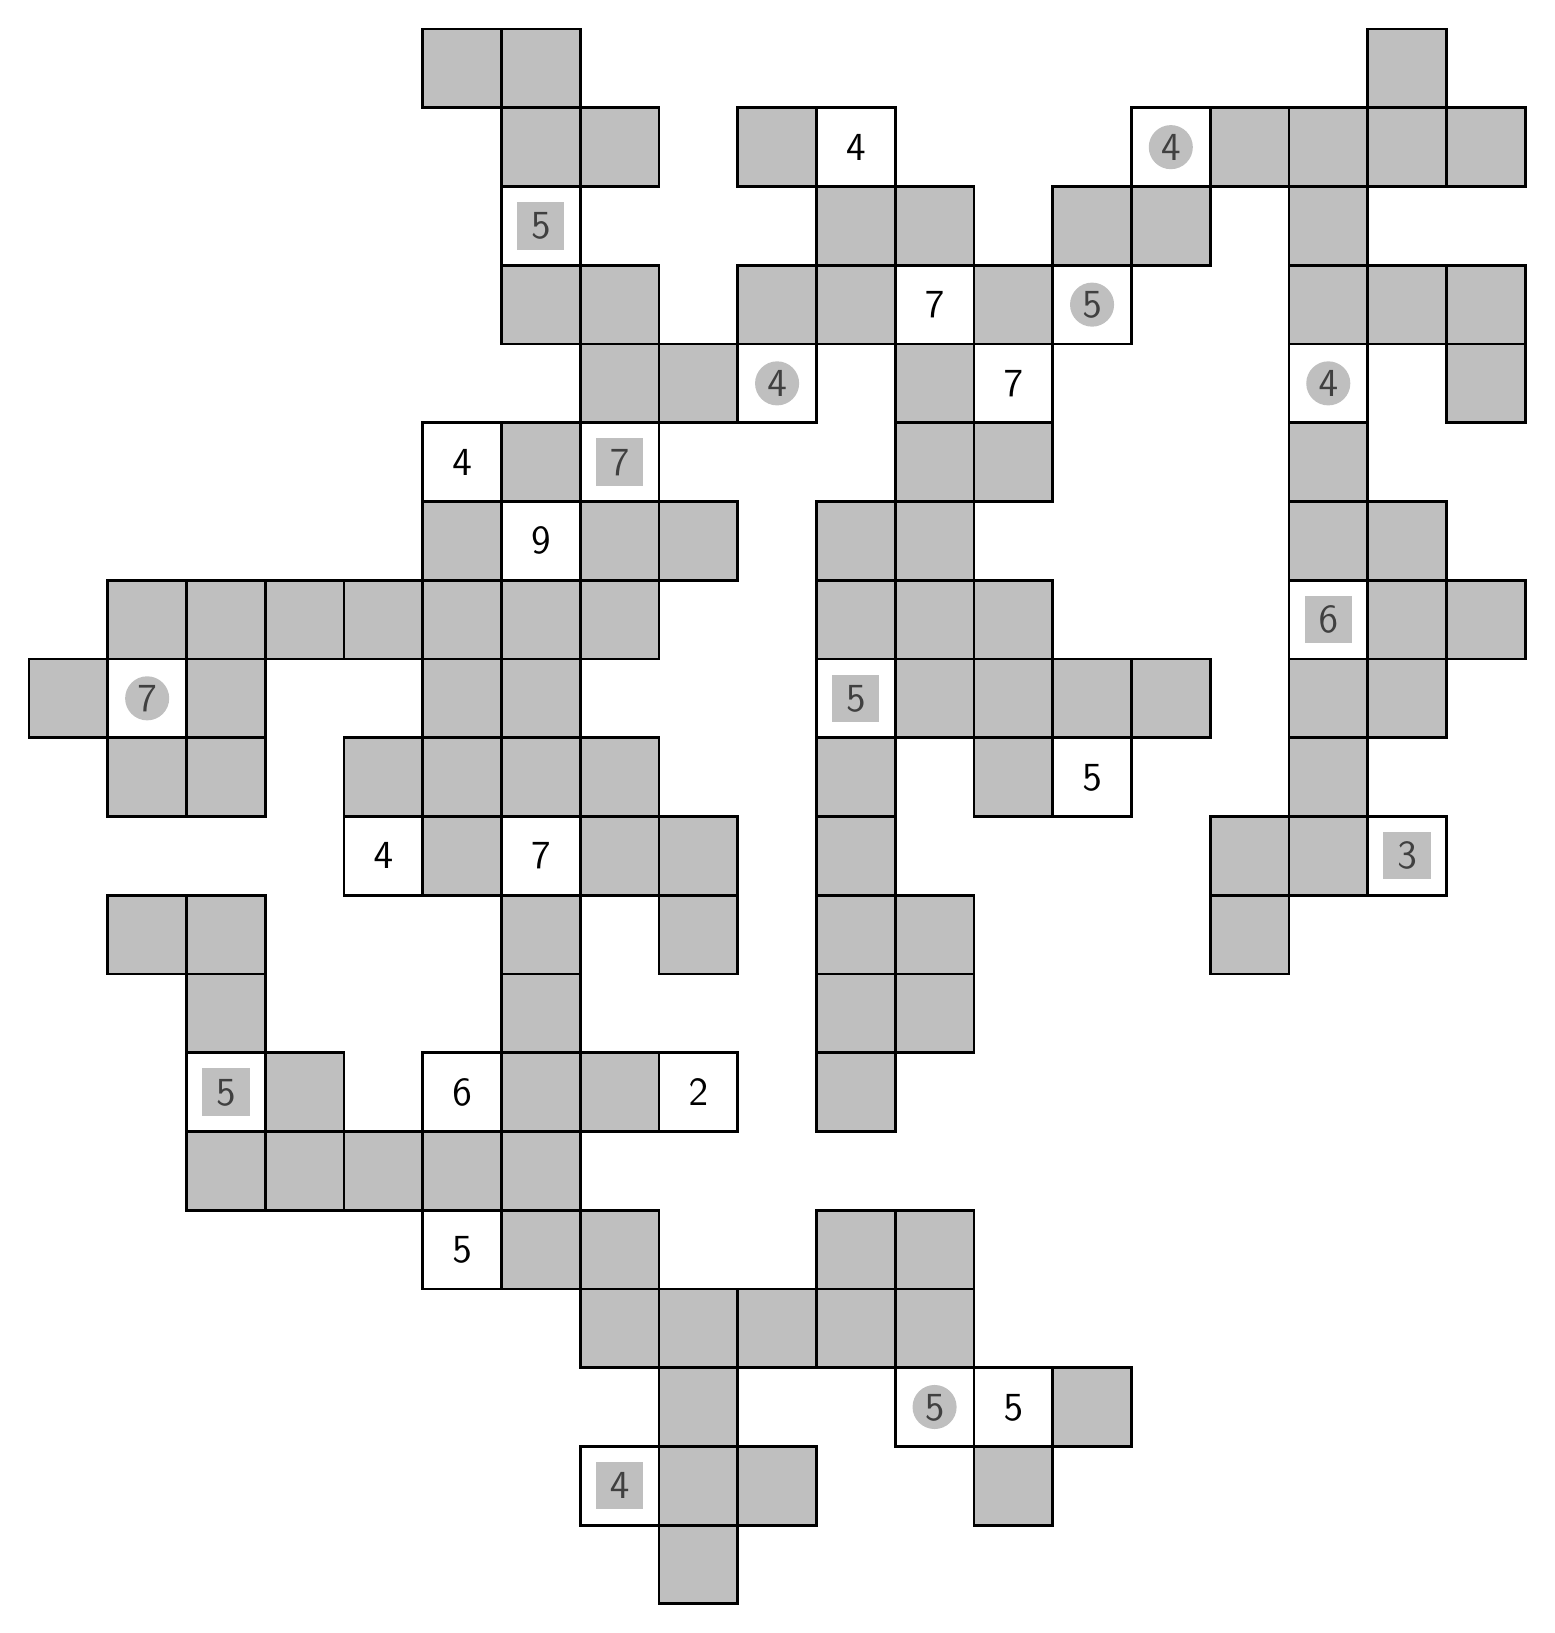
\begin{tikzpicture}\fill[gray, opacity = 0.5] (9, 0, 0)--++(1, 0, 0)--++(0, 1, 0)--++(-1, 0, 0)--cycle;
\draw[line width = 1pt] (9, 0, 0)--++(1, 0, 0)--++(0, 1, 0)--++(-1, 0, 0)--cycle;
\draw node at (8.5, 1.5, 0) {\Large $\mathsf{4}$};
\draw[line width = 1pt] (8, 1, 0)--++(1, 0, 0)--++(0, 1, 0)--++(-1, 0, 0)--cycle;
\fill[color = gray, opacity = 0.5] (8.2, 1.2) rectangle ++(0.6, 0.6);
\fill[gray, opacity = 0.5] (9, 1, 0)--++(1, 0, 0)--++(0, 1, 0)--++(-1, 0, 0)--cycle;
\draw[line width = 1pt] (9, 1, 0)--++(1, 0, 0)--++(0, 1, 0)--++(-1, 0, 0)--cycle;
\fill[gray, opacity = 0.5] (10, 1, 0)--++(1, 0, 0)--++(0, 1, 0)--++(-1, 0, 0)--cycle;
\draw[line width = 1pt] (10, 1, 0)--++(1, 0, 0)--++(0, 1, 0)--++(-1, 0, 0)--cycle;
\fill[gray, opacity = 0.5] (13, 1, 0)--++(1, 0, 0)--++(0, 1, 0)--++(-1, 0, 0)--cycle;
\draw[line width = 1pt] (13, 1, 0)--++(1, 0, 0)--++(0, 1, 0)--++(-1, 0, 0)--cycle;
\fill[gray, opacity = 0.5] (9, 2, 0)--++(1, 0, 0)--++(0, 1, 0)--++(-1, 0, 0)--cycle;
\draw[line width = 1pt] (9, 2, 0)--++(1, 0, 0)--++(0, 1, 0)--++(-1, 0, 0)--cycle;
\draw node at (12.5, 2.5, 0) {\Large $\mathsf{5}$};
\draw[line width = 1pt] (12, 2, 0)--++(1, 0, 0)--++(0, 1, 0)--++(-1, 0, 0)--cycle;
\fill[color = gray, opacity = 0.5] (12.5, 2.5, 0) circle (0.28);
\draw node at (13.5, 2.5, 0) {\Large $\mathsf{5}$};
\draw[line width = 1pt] (13, 2, 0)--++(1, 0, 0)--++(0, 1, 0)--++(-1, 0, 0)--cycle;
\fill[gray, opacity = 0.5] (14, 2, 0)--++(1, 0, 0)--++(0, 1, 0)--++(-1, 0, 0)--cycle;
\draw[line width = 1pt] (14, 2, 0)--++(1, 0, 0)--++(0, 1, 0)--++(-1, 0, 0)--cycle;
\fill[gray, opacity = 0.5] (8, 3, 0)--++(1, 0, 0)--++(0, 1, 0)--++(-1, 0, 0)--cycle;
\draw[line width = 1pt] (8, 3, 0)--++(1, 0, 0)--++(0, 1, 0)--++(-1, 0, 0)--cycle;
\fill[gray, opacity = 0.5] (9, 3, 0)--++(1, 0, 0)--++(0, 1, 0)--++(-1, 0, 0)--cycle;
\draw[line width = 1pt] (9, 3, 0)--++(1, 0, 0)--++(0, 1, 0)--++(-1, 0, 0)--cycle;
\fill[gray, opacity = 0.5] (10, 3, 0)--++(1, 0, 0)--++(0, 1, 0)--++(-1, 0, 0)--cycle;
\draw[line width = 1pt] (10, 3, 0)--++(1, 0, 0)--++(0, 1, 0)--++(-1, 0, 0)--cycle;
\fill[gray, opacity = 0.5] (11, 3, 0)--++(1, 0, 0)--++(0, 1, 0)--++(-1, 0, 0)--cycle;
\draw[line width = 1pt] (11, 3, 0)--++(1, 0, 0)--++(0, 1, 0)--++(-1, 0, 0)--cycle;
\fill[gray, opacity = 0.5] (12, 3, 0)--++(1, 0, 0)--++(0, 1, 0)--++(-1, 0, 0)--cycle;
\draw[line width = 1pt] (12, 3, 0)--++(1, 0, 0)--++(0, 1, 0)--++(-1, 0, 0)--cycle;
\draw node at (6.5, 4.5, 0) {\Large $\mathsf{5}$};
\draw[line width = 1pt] (6, 4, 0)--++(1, 0, 0)--++(0, 1, 0)--++(-1, 0, 0)--cycle;
\fill[gray, opacity = 0.5] (7, 4, 0)--++(1, 0, 0)--++(0, 1, 0)--++(-1, 0, 0)--cycle;
\draw[line width = 1pt] (7, 4, 0)--++(1, 0, 0)--++(0, 1, 0)--++(-1, 0, 0)--cycle;
\fill[gray, opacity = 0.5] (8, 4, 0)--++(1, 0, 0)--++(0, 1, 0)--++(-1, 0, 0)--cycle;
\draw[line width = 1pt] (8, 4, 0)--++(1, 0, 0)--++(0, 1, 0)--++(-1, 0, 0)--cycle;
\fill[gray, opacity = 0.5] (11, 4, 0)--++(1, 0, 0)--++(0, 1, 0)--++(-1, 0, 0)--cycle;
\draw[line width = 1pt] (11, 4, 0)--++(1, 0, 0)--++(0, 1, 0)--++(-1, 0, 0)--cycle;
\fill[gray, opacity = 0.5] (12, 4, 0)--++(1, 0, 0)--++(0, 1, 0)--++(-1, 0, 0)--cycle;
\draw[line width = 1pt] (12, 4, 0)--++(1, 0, 0)--++(0, 1, 0)--++(-1, 0, 0)--cycle;
\fill[gray, opacity = 0.5] (3, 5, 0)--++(1, 0, 0)--++(0, 1, 0)--++(-1, 0, 0)--cycle;
\draw[line width = 1pt] (3, 5, 0)--++(1, 0, 0)--++(0, 1, 0)--++(-1, 0, 0)--cycle;
\fill[gray, opacity = 0.5] (4, 5, 0)--++(1, 0, 0)--++(0, 1, 0)--++(-1, 0, 0)--cycle;
\draw[line width = 1pt] (4, 5, 0)--++(1, 0, 0)--++(0, 1, 0)--++(-1, 0, 0)--cycle;
\fill[gray, opacity = 0.5] (5, 5, 0)--++(1, 0, 0)--++(0, 1, 0)--++(-1, 0, 0)--cycle;
\draw[line width = 1pt] (5, 5, 0)--++(1, 0, 0)--++(0, 1, 0)--++(-1, 0, 0)--cycle;
\fill[gray, opacity = 0.5] (6, 5, 0)--++(1, 0, 0)--++(0, 1, 0)--++(-1, 0, 0)--cycle;
\draw[line width = 1pt] (6, 5, 0)--++(1, 0, 0)--++(0, 1, 0)--++(-1, 0, 0)--cycle;
\fill[gray, opacity = 0.5] (7, 5, 0)--++(1, 0, 0)--++(0, 1, 0)--++(-1, 0, 0)--cycle;
\draw[line width = 1pt] (7, 5, 0)--++(1, 0, 0)--++(0, 1, 0)--++(-1, 0, 0)--cycle;
\draw node at (3.5, 6.5, 0) {\Large $\mathsf{5}$};
\draw[line width = 1pt] (3, 6, 0)--++(1, 0, 0)--++(0, 1, 0)--++(-1, 0, 0)--cycle;
\fill[color = gray, opacity = 0.5] (3.2, 6.2) rectangle ++(0.6, 0.6);
\fill[gray, opacity = 0.5] (4, 6, 0)--++(1, 0, 0)--++(0, 1, 0)--++(-1, 0, 0)--cycle;
\draw[line width = 1pt] (4, 6, 0)--++(1, 0, 0)--++(0, 1, 0)--++(-1, 0, 0)--cycle;
\draw node at (6.5, 6.5, 0) {\Large $\mathsf{6}$};
\draw[line width = 1pt] (6, 6, 0)--++(1, 0, 0)--++(0, 1, 0)--++(-1, 0, 0)--cycle;
\fill[gray, opacity = 0.5] (7, 6, 0)--++(1, 0, 0)--++(0, 1, 0)--++(-1, 0, 0)--cycle;
\draw[line width = 1pt] (7, 6, 0)--++(1, 0, 0)--++(0, 1, 0)--++(-1, 0, 0)--cycle;
\fill[gray, opacity = 0.5] (8, 6, 0)--++(1, 0, 0)--++(0, 1, 0)--++(-1, 0, 0)--cycle;
\draw[line width = 1pt] (8, 6, 0)--++(1, 0, 0)--++(0, 1, 0)--++(-1, 0, 0)--cycle;
\draw node at (9.5, 6.5, 0) {\Large $\mathsf{2}$};
\draw[line width = 1pt] (9, 6, 0)--++(1, 0, 0)--++(0, 1, 0)--++(-1, 0, 0)--cycle;
\fill[gray, opacity = 0.5] (11, 6, 0)--++(1, 0, 0)--++(0, 1, 0)--++(-1, 0, 0)--cycle;
\draw[line width = 1pt] (11, 6, 0)--++(1, 0, 0)--++(0, 1, 0)--++(-1, 0, 0)--cycle;
\fill[gray, opacity = 0.5] (3, 7, 0)--++(1, 0, 0)--++(0, 1, 0)--++(-1, 0, 0)--cycle;
\draw[line width = 1pt] (3, 7, 0)--++(1, 0, 0)--++(0, 1, 0)--++(-1, 0, 0)--cycle;
\fill[gray, opacity = 0.5] (7, 7, 0)--++(1, 0, 0)--++(0, 1, 0)--++(-1, 0, 0)--cycle;
\draw[line width = 1pt] (7, 7, 0)--++(1, 0, 0)--++(0, 1, 0)--++(-1, 0, 0)--cycle;
\fill[gray, opacity = 0.5] (11, 7, 0)--++(1, 0, 0)--++(0, 1, 0)--++(-1, 0, 0)--cycle;
\draw[line width = 1pt] (11, 7, 0)--++(1, 0, 0)--++(0, 1, 0)--++(-1, 0, 0)--cycle;
\fill[gray, opacity = 0.5] (12, 7, 0)--++(1, 0, 0)--++(0, 1, 0)--++(-1, 0, 0)--cycle;
\draw[line width = 1pt] (12, 7, 0)--++(1, 0, 0)--++(0, 1, 0)--++(-1, 0, 0)--cycle;
\fill[gray, opacity = 0.5] (2, 8, 0)--++(1, 0, 0)--++(0, 1, 0)--++(-1, 0, 0)--cycle;
\draw[line width = 1pt] (2, 8, 0)--++(1, 0, 0)--++(0, 1, 0)--++(-1, 0, 0)--cycle;
\fill[gray, opacity = 0.5] (3, 8, 0)--++(1, 0, 0)--++(0, 1, 0)--++(-1, 0, 0)--cycle;
\draw[line width = 1pt] (3, 8, 0)--++(1, 0, 0)--++(0, 1, 0)--++(-1, 0, 0)--cycle;
\fill[gray, opacity = 0.5] (7, 8, 0)--++(1, 0, 0)--++(0, 1, 0)--++(-1, 0, 0)--cycle;
\draw[line width = 1pt] (7, 8, 0)--++(1, 0, 0)--++(0, 1, 0)--++(-1, 0, 0)--cycle;
\fill[gray, opacity = 0.5] (9, 8, 0)--++(1, 0, 0)--++(0, 1, 0)--++(-1, 0, 0)--cycle;
\draw[line width = 1pt] (9, 8, 0)--++(1, 0, 0)--++(0, 1, 0)--++(-1, 0, 0)--cycle;
\fill[gray, opacity = 0.5] (11, 8, 0)--++(1, 0, 0)--++(0, 1, 0)--++(-1, 0, 0)--cycle;
\draw[line width = 1pt] (11, 8, 0)--++(1, 0, 0)--++(0, 1, 0)--++(-1, 0, 0)--cycle;
\fill[gray, opacity = 0.5] (12, 8, 0)--++(1, 0, 0)--++(0, 1, 0)--++(-1, 0, 0)--cycle;
\draw[line width = 1pt] (12, 8, 0)--++(1, 0, 0)--++(0, 1, 0)--++(-1, 0, 0)--cycle;
\fill[gray, opacity = 0.5] (16, 8, 0)--++(1, 0, 0)--++(0, 1, 0)--++(-1, 0, 0)--cycle;
\draw[line width = 1pt] (16, 8, 0)--++(1, 0, 0)--++(0, 1, 0)--++(-1, 0, 0)--cycle;
\draw node at (5.5, 9.5, 0) {\Large $\mathsf{4}$};
\draw[line width = 1pt] (5, 9, 0)--++(1, 0, 0)--++(0, 1, 0)--++(-1, 0, 0)--cycle;
\fill[gray, opacity = 0.5] (6, 9, 0)--++(1, 0, 0)--++(0, 1, 0)--++(-1, 0, 0)--cycle;
\draw[line width = 1pt] (6, 9, 0)--++(1, 0, 0)--++(0, 1, 0)--++(-1, 0, 0)--cycle;
\draw node at (7.5, 9.5, 0) {\Large $\mathsf{7}$};
\draw[line width = 1pt] (7, 9, 0)--++(1, 0, 0)--++(0, 1, 0)--++(-1, 0, 0)--cycle;
\fill[gray, opacity = 0.5] (8, 9, 0)--++(1, 0, 0)--++(0, 1, 0)--++(-1, 0, 0)--cycle;
\draw[line width = 1pt] (8, 9, 0)--++(1, 0, 0)--++(0, 1, 0)--++(-1, 0, 0)--cycle;
\fill[gray, opacity = 0.5] (9, 9, 0)--++(1, 0, 0)--++(0, 1, 0)--++(-1, 0, 0)--cycle;
\draw[line width = 1pt] (9, 9, 0)--++(1, 0, 0)--++(0, 1, 0)--++(-1, 0, 0)--cycle;
\fill[gray, opacity = 0.5] (11, 9, 0)--++(1, 0, 0)--++(0, 1, 0)--++(-1, 0, 0)--cycle;
\draw[line width = 1pt] (11, 9, 0)--++(1, 0, 0)--++(0, 1, 0)--++(-1, 0, 0)--cycle;
\fill[gray, opacity = 0.5] (16, 9, 0)--++(1, 0, 0)--++(0, 1, 0)--++(-1, 0, 0)--cycle;
\draw[line width = 1pt] (16, 9, 0)--++(1, 0, 0)--++(0, 1, 0)--++(-1, 0, 0)--cycle;
\fill[gray, opacity = 0.5] (17, 9, 0)--++(1, 0, 0)--++(0, 1, 0)--++(-1, 0, 0)--cycle;
\draw[line width = 1pt] (17, 9, 0)--++(1, 0, 0)--++(0, 1, 0)--++(-1, 0, 0)--cycle;
\draw node at (18.5, 9.5, 0) {\Large $\mathsf{3}$};
\draw[line width = 1pt] (18, 9, 0)--++(1, 0, 0)--++(0, 1, 0)--++(-1, 0, 0)--cycle;
\fill[color = gray, opacity = 0.5] (18.2, 9.2) rectangle ++(0.6, 0.6);
\fill[gray, opacity = 0.5] (2, 10, 0)--++(1, 0, 0)--++(0, 1, 0)--++(-1, 0, 0)--cycle;
\draw[line width = 1pt] (2, 10, 0)--++(1, 0, 0)--++(0, 1, 0)--++(-1, 0, 0)--cycle;
\fill[gray, opacity = 0.5] (3, 10, 0)--++(1, 0, 0)--++(0, 1, 0)--++(-1, 0, 0)--cycle;
\draw[line width = 1pt] (3, 10, 0)--++(1, 0, 0)--++(0, 1, 0)--++(-1, 0, 0)--cycle;
\fill[gray, opacity = 0.5] (5, 10, 0)--++(1, 0, 0)--++(0, 1, 0)--++(-1, 0, 0)--cycle;
\draw[line width = 1pt] (5, 10, 0)--++(1, 0, 0)--++(0, 1, 0)--++(-1, 0, 0)--cycle;
\fill[gray, opacity = 0.5] (6, 10, 0)--++(1, 0, 0)--++(0, 1, 0)--++(-1, 0, 0)--cycle;
\draw[line width = 1pt] (6, 10, 0)--++(1, 0, 0)--++(0, 1, 0)--++(-1, 0, 0)--cycle;
\fill[gray, opacity = 0.5] (7, 10, 0)--++(1, 0, 0)--++(0, 1, 0)--++(-1, 0, 0)--cycle;
\draw[line width = 1pt] (7, 10, 0)--++(1, 0, 0)--++(0, 1, 0)--++(-1, 0, 0)--cycle;
\fill[gray, opacity = 0.5] (8, 10, 0)--++(1, 0, 0)--++(0, 1, 0)--++(-1, 0, 0)--cycle;
\draw[line width = 1pt] (8, 10, 0)--++(1, 0, 0)--++(0, 1, 0)--++(-1, 0, 0)--cycle;
\fill[gray, opacity = 0.5] (11, 10, 0)--++(1, 0, 0)--++(0, 1, 0)--++(-1, 0, 0)--cycle;
\draw[line width = 1pt] (11, 10, 0)--++(1, 0, 0)--++(0, 1, 0)--++(-1, 0, 0)--cycle;
\fill[gray, opacity = 0.5] (13, 10, 0)--++(1, 0, 0)--++(0, 1, 0)--++(-1, 0, 0)--cycle;
\draw[line width = 1pt] (13, 10, 0)--++(1, 0, 0)--++(0, 1, 0)--++(-1, 0, 0)--cycle;
\draw node at (14.5, 10.5, 0) {\Large $\mathsf{5}$};
\draw[line width = 1pt] (14, 10, 0)--++(1, 0, 0)--++(0, 1, 0)--++(-1, 0, 0)--cycle;
\fill[gray, opacity = 0.5] (17, 10, 0)--++(1, 0, 0)--++(0, 1, 0)--++(-1, 0, 0)--cycle;
\draw[line width = 1pt] (17, 10, 0)--++(1, 0, 0)--++(0, 1, 0)--++(-1, 0, 0)--cycle;
\fill[gray, opacity = 0.5] (1, 11, 0)--++(1, 0, 0)--++(0, 1, 0)--++(-1, 0, 0)--cycle;
\draw[line width = 1pt] (1, 11, 0)--++(1, 0, 0)--++(0, 1, 0)--++(-1, 0, 0)--cycle;
\draw node at (2.5, 11.5, 0) {\Large $\mathsf{7}$};
\draw[line width = 1pt] (2, 11, 0)--++(1, 0, 0)--++(0, 1, 0)--++(-1, 0, 0)--cycle;
\fill[color = gray, opacity = 0.5] (2.5, 11.5, 0) circle (0.28);
\fill[gray, opacity = 0.5] (3, 11, 0)--++(1, 0, 0)--++(0, 1, 0)--++(-1, 0, 0)--cycle;
\draw[line width = 1pt] (3, 11, 0)--++(1, 0, 0)--++(0, 1, 0)--++(-1, 0, 0)--cycle;
\fill[gray, opacity = 0.5] (6, 11, 0)--++(1, 0, 0)--++(0, 1, 0)--++(-1, 0, 0)--cycle;
\draw[line width = 1pt] (6, 11, 0)--++(1, 0, 0)--++(0, 1, 0)--++(-1, 0, 0)--cycle;
\fill[gray, opacity = 0.5] (7, 11, 0)--++(1, 0, 0)--++(0, 1, 0)--++(-1, 0, 0)--cycle;
\draw[line width = 1pt] (7, 11, 0)--++(1, 0, 0)--++(0, 1, 0)--++(-1, 0, 0)--cycle;
\draw node at (11.5, 11.5, 0) {\Large $\mathsf{5}$};
\draw[line width = 1pt] (11, 11, 0)--++(1, 0, 0)--++(0, 1, 0)--++(-1, 0, 0)--cycle;
\fill[color = gray, opacity = 0.5] (11.2, 11.2) rectangle ++(0.6, 0.6);
\fill[gray, opacity = 0.5] (12, 11, 0)--++(1, 0, 0)--++(0, 1, 0)--++(-1, 0, 0)--cycle;
\draw[line width = 1pt] (12, 11, 0)--++(1, 0, 0)--++(0, 1, 0)--++(-1, 0, 0)--cycle;
\fill[gray, opacity = 0.5] (13, 11, 0)--++(1, 0, 0)--++(0, 1, 0)--++(-1, 0, 0)--cycle;
\draw[line width = 1pt] (13, 11, 0)--++(1, 0, 0)--++(0, 1, 0)--++(-1, 0, 0)--cycle;
\fill[gray, opacity = 0.5] (14, 11, 0)--++(1, 0, 0)--++(0, 1, 0)--++(-1, 0, 0)--cycle;
\draw[line width = 1pt] (14, 11, 0)--++(1, 0, 0)--++(0, 1, 0)--++(-1, 0, 0)--cycle;
\fill[gray, opacity = 0.5] (15, 11, 0)--++(1, 0, 0)--++(0, 1, 0)--++(-1, 0, 0)--cycle;
\draw[line width = 1pt] (15, 11, 0)--++(1, 0, 0)--++(0, 1, 0)--++(-1, 0, 0)--cycle;
\fill[gray, opacity = 0.5] (17, 11, 0)--++(1, 0, 0)--++(0, 1, 0)--++(-1, 0, 0)--cycle;
\draw[line width = 1pt] (17, 11, 0)--++(1, 0, 0)--++(0, 1, 0)--++(-1, 0, 0)--cycle;
\fill[gray, opacity = 0.5] (18, 11, 0)--++(1, 0, 0)--++(0, 1, 0)--++(-1, 0, 0)--cycle;
\draw[line width = 1pt] (18, 11, 0)--++(1, 0, 0)--++(0, 1, 0)--++(-1, 0, 0)--cycle;
\fill[gray, opacity = 0.5] (2, 12, 0)--++(1, 0, 0)--++(0, 1, 0)--++(-1, 0, 0)--cycle;
\draw[line width = 1pt] (2, 12, 0)--++(1, 0, 0)--++(0, 1, 0)--++(-1, 0, 0)--cycle;
\fill[gray, opacity = 0.5] (3, 12, 0)--++(1, 0, 0)--++(0, 1, 0)--++(-1, 0, 0)--cycle;
\draw[line width = 1pt] (3, 12, 0)--++(1, 0, 0)--++(0, 1, 0)--++(-1, 0, 0)--cycle;
\fill[gray, opacity = 0.5] (4, 12, 0)--++(1, 0, 0)--++(0, 1, 0)--++(-1, 0, 0)--cycle;
\draw[line width = 1pt] (4, 12, 0)--++(1, 0, 0)--++(0, 1, 0)--++(-1, 0, 0)--cycle;
\fill[gray, opacity = 0.5] (5, 12, 0)--++(1, 0, 0)--++(0, 1, 0)--++(-1, 0, 0)--cycle;
\draw[line width = 1pt] (5, 12, 0)--++(1, 0, 0)--++(0, 1, 0)--++(-1, 0, 0)--cycle;
\fill[gray, opacity = 0.5] (6, 12, 0)--++(1, 0, 0)--++(0, 1, 0)--++(-1, 0, 0)--cycle;
\draw[line width = 1pt] (6, 12, 0)--++(1, 0, 0)--++(0, 1, 0)--++(-1, 0, 0)--cycle;
\fill[gray, opacity = 0.5] (7, 12, 0)--++(1, 0, 0)--++(0, 1, 0)--++(-1, 0, 0)--cycle;
\draw[line width = 1pt] (7, 12, 0)--++(1, 0, 0)--++(0, 1, 0)--++(-1, 0, 0)--cycle;
\fill[gray, opacity = 0.5] (8, 12, 0)--++(1, 0, 0)--++(0, 1, 0)--++(-1, 0, 0)--cycle;
\draw[line width = 1pt] (8, 12, 0)--++(1, 0, 0)--++(0, 1, 0)--++(-1, 0, 0)--cycle;
\fill[gray, opacity = 0.5] (11, 12, 0)--++(1, 0, 0)--++(0, 1, 0)--++(-1, 0, 0)--cycle;
\draw[line width = 1pt] (11, 12, 0)--++(1, 0, 0)--++(0, 1, 0)--++(-1, 0, 0)--cycle;
\fill[gray, opacity = 0.5] (12, 12, 0)--++(1, 0, 0)--++(0, 1, 0)--++(-1, 0, 0)--cycle;
\draw[line width = 1pt] (12, 12, 0)--++(1, 0, 0)--++(0, 1, 0)--++(-1, 0, 0)--cycle;
\fill[gray, opacity = 0.5] (13, 12, 0)--++(1, 0, 0)--++(0, 1, 0)--++(-1, 0, 0)--cycle;
\draw[line width = 1pt] (13, 12, 0)--++(1, 0, 0)--++(0, 1, 0)--++(-1, 0, 0)--cycle;
\draw node at (17.5, 12.5, 0) {\Large $\mathsf{6}$};
\draw[line width = 1pt] (17, 12, 0)--++(1, 0, 0)--++(0, 1, 0)--++(-1, 0, 0)--cycle;
\fill[color = gray, opacity = 0.5] (17.2, 12.2) rectangle ++(0.6, 0.6);
\fill[gray, opacity = 0.5] (18, 12, 0)--++(1, 0, 0)--++(0, 1, 0)--++(-1, 0, 0)--cycle;
\draw[line width = 1pt] (18, 12, 0)--++(1, 0, 0)--++(0, 1, 0)--++(-1, 0, 0)--cycle;
\fill[gray, opacity = 0.5] (19, 12, 0)--++(1, 0, 0)--++(0, 1, 0)--++(-1, 0, 0)--cycle;
\draw[line width = 1pt] (19, 12, 0)--++(1, 0, 0)--++(0, 1, 0)--++(-1, 0, 0)--cycle;
\fill[gray, opacity = 0.5] (6, 13, 0)--++(1, 0, 0)--++(0, 1, 0)--++(-1, 0, 0)--cycle;
\draw[line width = 1pt] (6, 13, 0)--++(1, 0, 0)--++(0, 1, 0)--++(-1, 0, 0)--cycle;
\draw node at (7.5, 13.5, 0) {\Large $\mathsf{9}$};
\draw[line width = 1pt] (7, 13, 0)--++(1, 0, 0)--++(0, 1, 0)--++(-1, 0, 0)--cycle;
\fill[gray, opacity = 0.5] (8, 13, 0)--++(1, 0, 0)--++(0, 1, 0)--++(-1, 0, 0)--cycle;
\draw[line width = 1pt] (8, 13, 0)--++(1, 0, 0)--++(0, 1, 0)--++(-1, 0, 0)--cycle;
\fill[gray, opacity = 0.5] (9, 13, 0)--++(1, 0, 0)--++(0, 1, 0)--++(-1, 0, 0)--cycle;
\draw[line width = 1pt] (9, 13, 0)--++(1, 0, 0)--++(0, 1, 0)--++(-1, 0, 0)--cycle;
\fill[gray, opacity = 0.5] (11, 13, 0)--++(1, 0, 0)--++(0, 1, 0)--++(-1, 0, 0)--cycle;
\draw[line width = 1pt] (11, 13, 0)--++(1, 0, 0)--++(0, 1, 0)--++(-1, 0, 0)--cycle;
\fill[gray, opacity = 0.5] (12, 13, 0)--++(1, 0, 0)--++(0, 1, 0)--++(-1, 0, 0)--cycle;
\draw[line width = 1pt] (12, 13, 0)--++(1, 0, 0)--++(0, 1, 0)--++(-1, 0, 0)--cycle;
\fill[gray, opacity = 0.5] (17, 13, 0)--++(1, 0, 0)--++(0, 1, 0)--++(-1, 0, 0)--cycle;
\draw[line width = 1pt] (17, 13, 0)--++(1, 0, 0)--++(0, 1, 0)--++(-1, 0, 0)--cycle;
\fill[gray, opacity = 0.5] (18, 13, 0)--++(1, 0, 0)--++(0, 1, 0)--++(-1, 0, 0)--cycle;
\draw[line width = 1pt] (18, 13, 0)--++(1, 0, 0)--++(0, 1, 0)--++(-1, 0, 0)--cycle;
\draw node at (6.5, 14.5, 0) {\Large $\mathsf{4}$};
\draw[line width = 1pt] (6, 14, 0)--++(1, 0, 0)--++(0, 1, 0)--++(-1, 0, 0)--cycle;
\fill[gray, opacity = 0.5] (7, 14, 0)--++(1, 0, 0)--++(0, 1, 0)--++(-1, 0, 0)--cycle;
\draw[line width = 1pt] (7, 14, 0)--++(1, 0, 0)--++(0, 1, 0)--++(-1, 0, 0)--cycle;
\draw node at (8.5, 14.5, 0) {\Large $\mathsf{7}$};
\draw[line width = 1pt] (8, 14, 0)--++(1, 0, 0)--++(0, 1, 0)--++(-1, 0, 0)--cycle;
\fill[color = gray, opacity = 0.5] (8.2, 14.2) rectangle ++(0.6, 0.6);
\fill[gray, opacity = 0.5] (12, 14, 0)--++(1, 0, 0)--++(0, 1, 0)--++(-1, 0, 0)--cycle;
\draw[line width = 1pt] (12, 14, 0)--++(1, 0, 0)--++(0, 1, 0)--++(-1, 0, 0)--cycle;
\fill[gray, opacity = 0.5] (13, 14, 0)--++(1, 0, 0)--++(0, 1, 0)--++(-1, 0, 0)--cycle;
\draw[line width = 1pt] (13, 14, 0)--++(1, 0, 0)--++(0, 1, 0)--++(-1, 0, 0)--cycle;
\fill[gray, opacity = 0.5] (17, 14, 0)--++(1, 0, 0)--++(0, 1, 0)--++(-1, 0, 0)--cycle;
\draw[line width = 1pt] (17, 14, 0)--++(1, 0, 0)--++(0, 1, 0)--++(-1, 0, 0)--cycle;
\fill[gray, opacity = 0.5] (8, 15, 0)--++(1, 0, 0)--++(0, 1, 0)--++(-1, 0, 0)--cycle;
\draw[line width = 1pt] (8, 15, 0)--++(1, 0, 0)--++(0, 1, 0)--++(-1, 0, 0)--cycle;
\fill[gray, opacity = 0.5] (9, 15, 0)--++(1, 0, 0)--++(0, 1, 0)--++(-1, 0, 0)--cycle;
\draw[line width = 1pt] (9, 15, 0)--++(1, 0, 0)--++(0, 1, 0)--++(-1, 0, 0)--cycle;
\draw node at (10.5, 15.5, 0) {\Large $\mathsf{4}$};
\draw[line width = 1pt] (10, 15, 0)--++(1, 0, 0)--++(0, 1, 0)--++(-1, 0, 0)--cycle;
\fill[color = gray, opacity = 0.5] (10.5, 15.5, 0) circle (0.28);
\fill[gray, opacity = 0.5] (12, 15, 0)--++(1, 0, 0)--++(0, 1, 0)--++(-1, 0, 0)--cycle;
\draw[line width = 1pt] (12, 15, 0)--++(1, 0, 0)--++(0, 1, 0)--++(-1, 0, 0)--cycle;
\draw node at (13.5, 15.5, 0) {\Large $\mathsf{7}$};
\draw[line width = 1pt] (13, 15, 0)--++(1, 0, 0)--++(0, 1, 0)--++(-1, 0, 0)--cycle;
\draw node at (17.5, 15.5, 0) {\Large $\mathsf{4}$};
\draw[line width = 1pt] (17, 15, 0)--++(1, 0, 0)--++(0, 1, 0)--++(-1, 0, 0)--cycle;
\fill[color = gray, opacity = 0.5] (17.5, 15.5, 0) circle (0.28);
\fill[gray, opacity = 0.5] (19, 15, 0)--++(1, 0, 0)--++(0, 1, 0)--++(-1, 0, 0)--cycle;
\draw[line width = 1pt] (19, 15, 0)--++(1, 0, 0)--++(0, 1, 0)--++(-1, 0, 0)--cycle;
\fill[gray, opacity = 0.5] (7, 16, 0)--++(1, 0, 0)--++(0, 1, 0)--++(-1, 0, 0)--cycle;
\draw[line width = 1pt] (7, 16, 0)--++(1, 0, 0)--++(0, 1, 0)--++(-1, 0, 0)--cycle;
\fill[gray, opacity = 0.5] (8, 16, 0)--++(1, 0, 0)--++(0, 1, 0)--++(-1, 0, 0)--cycle;
\draw[line width = 1pt] (8, 16, 0)--++(1, 0, 0)--++(0, 1, 0)--++(-1, 0, 0)--cycle;
\fill[gray, opacity = 0.5] (10, 16, 0)--++(1, 0, 0)--++(0, 1, 0)--++(-1, 0, 0)--cycle;
\draw[line width = 1pt] (10, 16, 0)--++(1, 0, 0)--++(0, 1, 0)--++(-1, 0, 0)--cycle;
\fill[gray, opacity = 0.5] (11, 16, 0)--++(1, 0, 0)--++(0, 1, 0)--++(-1, 0, 0)--cycle;
\draw[line width = 1pt] (11, 16, 0)--++(1, 0, 0)--++(0, 1, 0)--++(-1, 0, 0)--cycle;
\draw node at (12.5, 16.5, 0) {\Large $\mathsf{7}$};
\draw[line width = 1pt] (12, 16, 0)--++(1, 0, 0)--++(0, 1, 0)--++(-1, 0, 0)--cycle;
\fill[gray, opacity = 0.5] (13, 16, 0)--++(1, 0, 0)--++(0, 1, 0)--++(-1, 0, 0)--cycle;
\draw[line width = 1pt] (13, 16, 0)--++(1, 0, 0)--++(0, 1, 0)--++(-1, 0, 0)--cycle;
\draw node at (14.5, 16.5, 0) {\Large $\mathsf{5}$};
\draw[line width = 1pt] (14, 16, 0)--++(1, 0, 0)--++(0, 1, 0)--++(-1, 0, 0)--cycle;
\fill[color = gray, opacity = 0.5] (14.5, 16.5, 0) circle (0.28);
\fill[gray, opacity = 0.5] (17, 16, 0)--++(1, 0, 0)--++(0, 1, 0)--++(-1, 0, 0)--cycle;
\draw[line width = 1pt] (17, 16, 0)--++(1, 0, 0)--++(0, 1, 0)--++(-1, 0, 0)--cycle;
\fill[gray, opacity = 0.5] (18, 16, 0)--++(1, 0, 0)--++(0, 1, 0)--++(-1, 0, 0)--cycle;
\draw[line width = 1pt] (18, 16, 0)--++(1, 0, 0)--++(0, 1, 0)--++(-1, 0, 0)--cycle;
\fill[gray, opacity = 0.5] (19, 16, 0)--++(1, 0, 0)--++(0, 1, 0)--++(-1, 0, 0)--cycle;
\draw[line width = 1pt] (19, 16, 0)--++(1, 0, 0)--++(0, 1, 0)--++(-1, 0, 0)--cycle;
\draw node at (7.5, 17.5, 0) {\Large $\mathsf{5}$};
\draw[line width = 1pt] (7, 17, 0)--++(1, 0, 0)--++(0, 1, 0)--++(-1, 0, 0)--cycle;
\fill[color = gray, opacity = 0.5] (7.2, 17.2) rectangle ++(0.6, 0.6);
\fill[gray, opacity = 0.5] (11, 17, 0)--++(1, 0, 0)--++(0, 1, 0)--++(-1, 0, 0)--cycle;
\draw[line width = 1pt] (11, 17, 0)--++(1, 0, 0)--++(0, 1, 0)--++(-1, 0, 0)--cycle;
\fill[gray, opacity = 0.5] (12, 17, 0)--++(1, 0, 0)--++(0, 1, 0)--++(-1, 0, 0)--cycle;
\draw[line width = 1pt] (12, 17, 0)--++(1, 0, 0)--++(0, 1, 0)--++(-1, 0, 0)--cycle;
\fill[gray, opacity = 0.5] (14, 17, 0)--++(1, 0, 0)--++(0, 1, 0)--++(-1, 0, 0)--cycle;
\draw[line width = 1pt] (14, 17, 0)--++(1, 0, 0)--++(0, 1, 0)--++(-1, 0, 0)--cycle;
\fill[gray, opacity = 0.5] (15, 17, 0)--++(1, 0, 0)--++(0, 1, 0)--++(-1, 0, 0)--cycle;
\draw[line width = 1pt] (15, 17, 0)--++(1, 0, 0)--++(0, 1, 0)--++(-1, 0, 0)--cycle;
\fill[gray, opacity = 0.5] (17, 17, 0)--++(1, 0, 0)--++(0, 1, 0)--++(-1, 0, 0)--cycle;
\draw[line width = 1pt] (17, 17, 0)--++(1, 0, 0)--++(0, 1, 0)--++(-1, 0, 0)--cycle;
\fill[gray, opacity = 0.5] (7, 18, 0)--++(1, 0, 0)--++(0, 1, 0)--++(-1, 0, 0)--cycle;
\draw[line width = 1pt] (7, 18, 0)--++(1, 0, 0)--++(0, 1, 0)--++(-1, 0, 0)--cycle;
\fill[gray, opacity = 0.5] (8, 18, 0)--++(1, 0, 0)--++(0, 1, 0)--++(-1, 0, 0)--cycle;
\draw[line width = 1pt] (8, 18, 0)--++(1, 0, 0)--++(0, 1, 0)--++(-1, 0, 0)--cycle;
\fill[gray, opacity = 0.5] (10, 18, 0)--++(1, 0, 0)--++(0, 1, 0)--++(-1, 0, 0)--cycle;
\draw[line width = 1pt] (10, 18, 0)--++(1, 0, 0)--++(0, 1, 0)--++(-1, 0, 0)--cycle;
\draw node at (11.5, 18.5, 0) {\Large $\mathsf{4}$};
\draw[line width = 1pt] (11, 18, 0)--++(1, 0, 0)--++(0, 1, 0)--++(-1, 0, 0)--cycle;
\draw node at (15.5, 18.5, 0) {\Large $\mathsf{4}$};
\draw[line width = 1pt] (15, 18, 0)--++(1, 0, 0)--++(0, 1, 0)--++(-1, 0, 0)--cycle;
\fill[color = gray, opacity = 0.5] (15.5, 18.5, 0) circle (0.28);
\fill[gray, opacity = 0.5] (16, 18, 0)--++(1, 0, 0)--++(0, 1, 0)--++(-1, 0, 0)--cycle;
\draw[line width = 1pt] (16, 18, 0)--++(1, 0, 0)--++(0, 1, 0)--++(-1, 0, 0)--cycle;
\fill[gray, opacity = 0.5] (17, 18, 0)--++(1, 0, 0)--++(0, 1, 0)--++(-1, 0, 0)--cycle;
\draw[line width = 1pt] (17, 18, 0)--++(1, 0, 0)--++(0, 1, 0)--++(-1, 0, 0)--cycle;
\fill[gray, opacity = 0.5] (18, 18, 0)--++(1, 0, 0)--++(0, 1, 0)--++(-1, 0, 0)--cycle;
\draw[line width = 1pt] (18, 18, 0)--++(1, 0, 0)--++(0, 1, 0)--++(-1, 0, 0)--cycle;
\fill[gray, opacity = 0.5] (19, 18, 0)--++(1, 0, 0)--++(0, 1, 0)--++(-1, 0, 0)--cycle;
\draw[line width = 1pt] (19, 18, 0)--++(1, 0, 0)--++(0, 1, 0)--++(-1, 0, 0)--cycle;
\fill[gray, opacity = 0.5] (6, 19, 0)--++(1, 0, 0)--++(0, 1, 0)--++(-1, 0, 0)--cycle;
\draw[line width = 1pt] (6, 19, 0)--++(1, 0, 0)--++(0, 1, 0)--++(-1, 0, 0)--cycle;
\fill[gray, opacity = 0.5] (7, 19, 0)--++(1, 0, 0)--++(0, 1, 0)--++(-1, 0, 0)--cycle;
\draw[line width = 1pt] (7, 19, 0)--++(1, 0, 0)--++(0, 1, 0)--++(-1, 0, 0)--cycle;
\fill[gray, opacity = 0.5] (18, 19, 0)--++(1, 0, 0)--++(0, 1, 0)--++(-1, 0, 0)--cycle;
\draw[line width = 1pt] (18, 19, 0)--++(1, 0, 0)--++(0, 1, 0)--++(-1, 0, 0)--cycle;
\end{tikzpicture}}\]
\[\resizebox{30pc}{!}{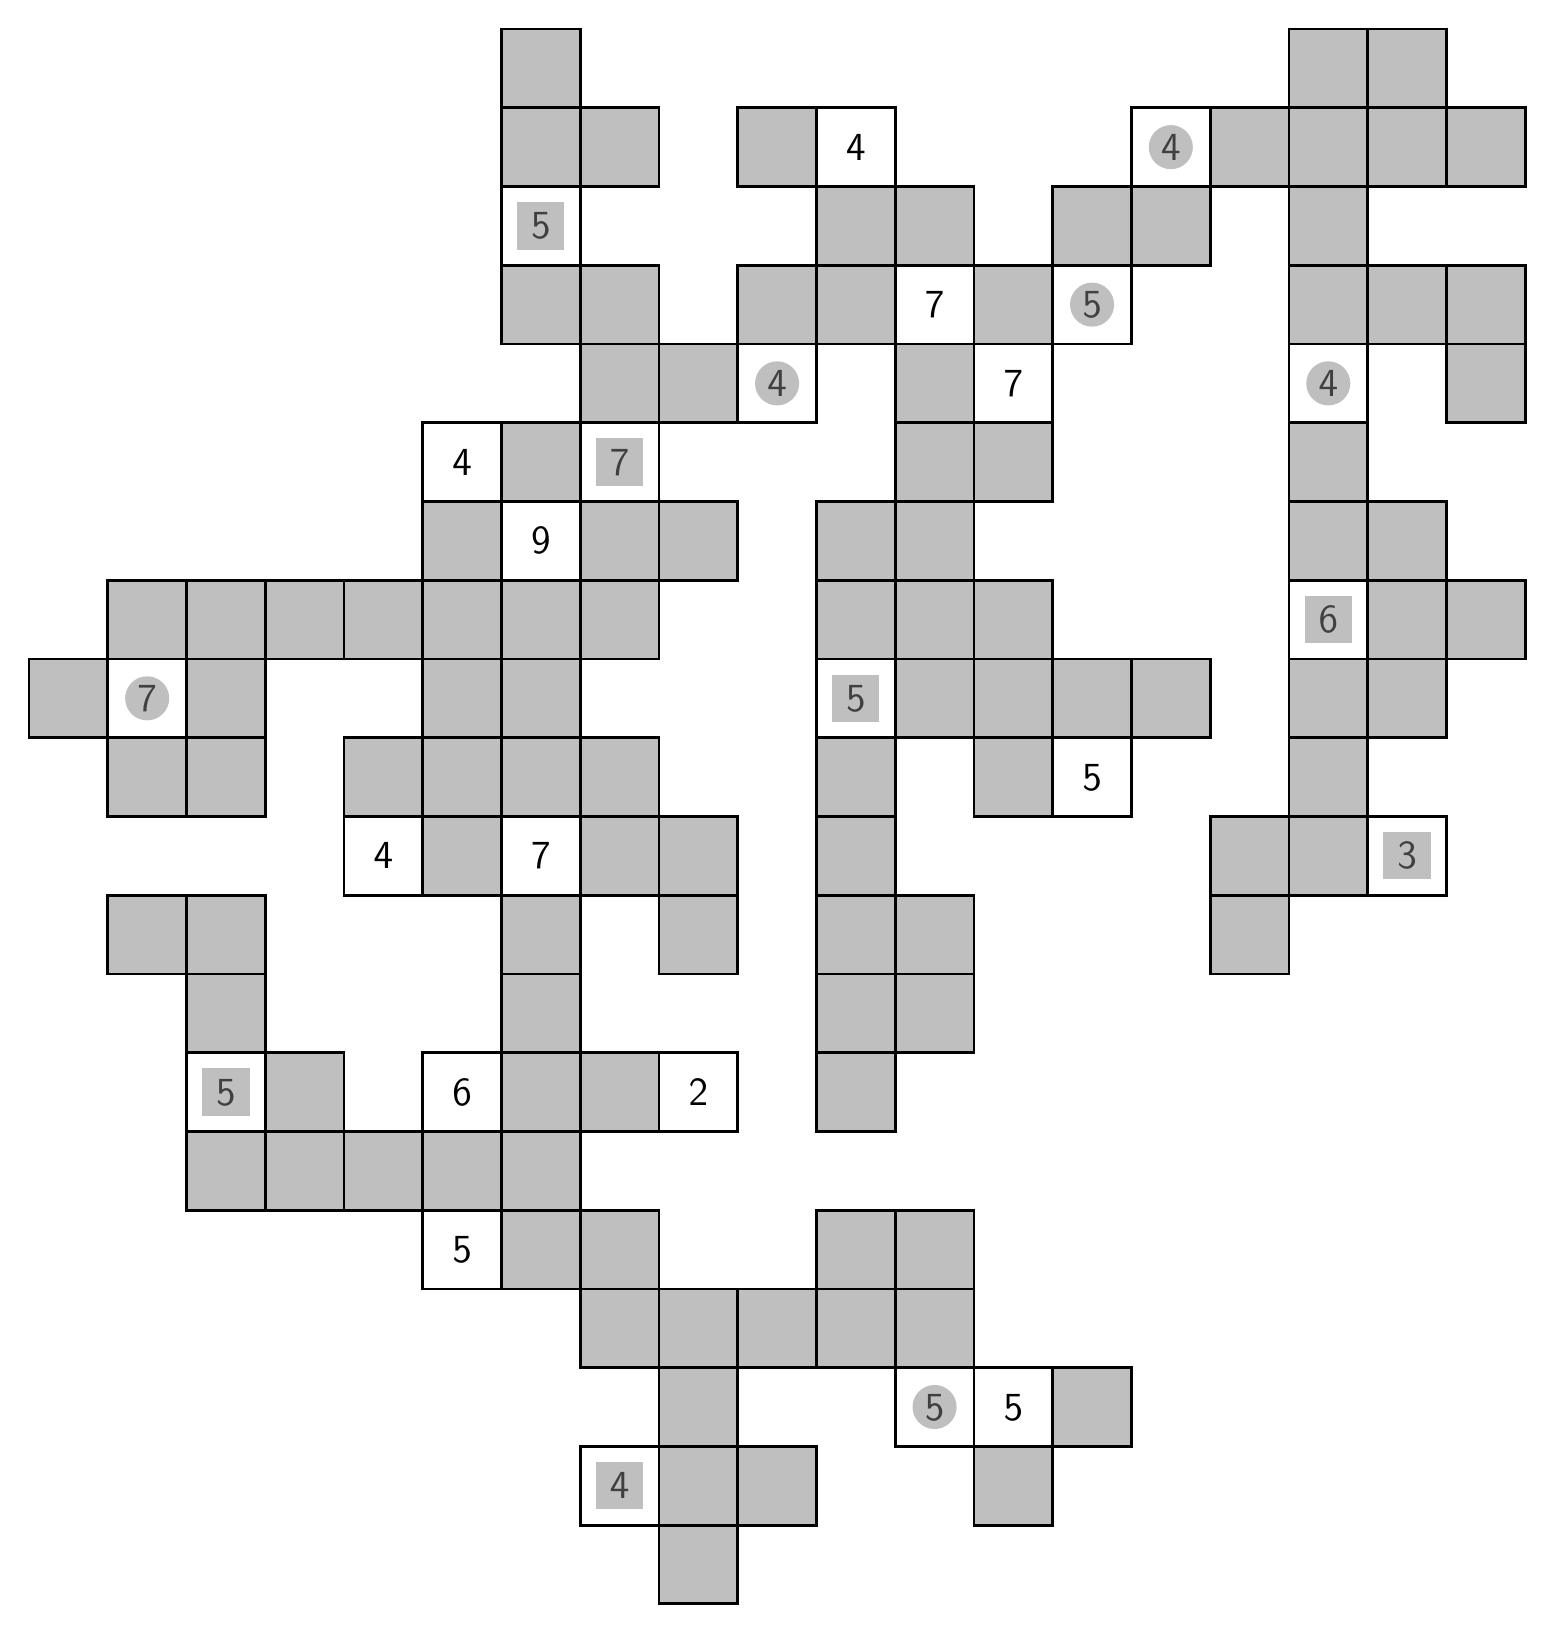
\begin{tikzpicture}\fill[gray, opacity = 0.5] (9, 0, 0)--++(1, 0, 0)--++(0, 1, 0)--++(-1, 0, 0)--cycle;
\draw[line width = 1pt] (9, 0, 0)--++(1, 0, 0)--++(0, 1, 0)--++(-1, 0, 0)--cycle;
\draw node at (8.5, 1.5, 0) {\Large $\mathsf{4}$};
\draw[line width = 1pt] (8, 1, 0)--++(1, 0, 0)--++(0, 1, 0)--++(-1, 0, 0)--cycle;
\fill[color = gray, opacity = 0.5] (8.2, 1.2) rectangle ++(0.6, 0.6);
\fill[gray, opacity = 0.5] (9, 1, 0)--++(1, 0, 0)--++(0, 1, 0)--++(-1, 0, 0)--cycle;
\draw[line width = 1pt] (9, 1, 0)--++(1, 0, 0)--++(0, 1, 0)--++(-1, 0, 0)--cycle;
\fill[gray, opacity = 0.5] (10, 1, 0)--++(1, 0, 0)--++(0, 1, 0)--++(-1, 0, 0)--cycle;
\draw[line width = 1pt] (10, 1, 0)--++(1, 0, 0)--++(0, 1, 0)--++(-1, 0, 0)--cycle;
\fill[gray, opacity = 0.5] (13, 1, 0)--++(1, 0, 0)--++(0, 1, 0)--++(-1, 0, 0)--cycle;
\draw[line width = 1pt] (13, 1, 0)--++(1, 0, 0)--++(0, 1, 0)--++(-1, 0, 0)--cycle;
\fill[gray, opacity = 0.5] (9, 2, 0)--++(1, 0, 0)--++(0, 1, 0)--++(-1, 0, 0)--cycle;
\draw[line width = 1pt] (9, 2, 0)--++(1, 0, 0)--++(0, 1, 0)--++(-1, 0, 0)--cycle;
\draw node at (12.5, 2.5, 0) {\Large $\mathsf{5}$};
\draw[line width = 1pt] (12, 2, 0)--++(1, 0, 0)--++(0, 1, 0)--++(-1, 0, 0)--cycle;
\fill[color = gray, opacity = 0.5] (12.5, 2.5, 0) circle (0.28);
\draw node at (13.5, 2.5, 0) {\Large $\mathsf{5}$};
\draw[line width = 1pt] (13, 2, 0)--++(1, 0, 0)--++(0, 1, 0)--++(-1, 0, 0)--cycle;
\fill[gray, opacity = 0.5] (14, 2, 0)--++(1, 0, 0)--++(0, 1, 0)--++(-1, 0, 0)--cycle;
\draw[line width = 1pt] (14, 2, 0)--++(1, 0, 0)--++(0, 1, 0)--++(-1, 0, 0)--cycle;
\fill[gray, opacity = 0.5] (8, 3, 0)--++(1, 0, 0)--++(0, 1, 0)--++(-1, 0, 0)--cycle;
\draw[line width = 1pt] (8, 3, 0)--++(1, 0, 0)--++(0, 1, 0)--++(-1, 0, 0)--cycle;
\fill[gray, opacity = 0.5] (9, 3, 0)--++(1, 0, 0)--++(0, 1, 0)--++(-1, 0, 0)--cycle;
\draw[line width = 1pt] (9, 3, 0)--++(1, 0, 0)--++(0, 1, 0)--++(-1, 0, 0)--cycle;
\fill[gray, opacity = 0.5] (10, 3, 0)--++(1, 0, 0)--++(0, 1, 0)--++(-1, 0, 0)--cycle;
\draw[line width = 1pt] (10, 3, 0)--++(1, 0, 0)--++(0, 1, 0)--++(-1, 0, 0)--cycle;
\fill[gray, opacity = 0.5] (11, 3, 0)--++(1, 0, 0)--++(0, 1, 0)--++(-1, 0, 0)--cycle;
\draw[line width = 1pt] (11, 3, 0)--++(1, 0, 0)--++(0, 1, 0)--++(-1, 0, 0)--cycle;
\fill[gray, opacity = 0.5] (12, 3, 0)--++(1, 0, 0)--++(0, 1, 0)--++(-1, 0, 0)--cycle;
\draw[line width = 1pt] (12, 3, 0)--++(1, 0, 0)--++(0, 1, 0)--++(-1, 0, 0)--cycle;
\draw node at (6.5, 4.5, 0) {\Large $\mathsf{5}$};
\draw[line width = 1pt] (6, 4, 0)--++(1, 0, 0)--++(0, 1, 0)--++(-1, 0, 0)--cycle;
\fill[gray, opacity = 0.5] (7, 4, 0)--++(1, 0, 0)--++(0, 1, 0)--++(-1, 0, 0)--cycle;
\draw[line width = 1pt] (7, 4, 0)--++(1, 0, 0)--++(0, 1, 0)--++(-1, 0, 0)--cycle;
\fill[gray, opacity = 0.5] (8, 4, 0)--++(1, 0, 0)--++(0, 1, 0)--++(-1, 0, 0)--cycle;
\draw[line width = 1pt] (8, 4, 0)--++(1, 0, 0)--++(0, 1, 0)--++(-1, 0, 0)--cycle;
\fill[gray, opacity = 0.5] (11, 4, 0)--++(1, 0, 0)--++(0, 1, 0)--++(-1, 0, 0)--cycle;
\draw[line width = 1pt] (11, 4, 0)--++(1, 0, 0)--++(0, 1, 0)--++(-1, 0, 0)--cycle;
\fill[gray, opacity = 0.5] (12, 4, 0)--++(1, 0, 0)--++(0, 1, 0)--++(-1, 0, 0)--cycle;
\draw[line width = 1pt] (12, 4, 0)--++(1, 0, 0)--++(0, 1, 0)--++(-1, 0, 0)--cycle;
\fill[gray, opacity = 0.5] (3, 5, 0)--++(1, 0, 0)--++(0, 1, 0)--++(-1, 0, 0)--cycle;
\draw[line width = 1pt] (3, 5, 0)--++(1, 0, 0)--++(0, 1, 0)--++(-1, 0, 0)--cycle;
\fill[gray, opacity = 0.5] (4, 5, 0)--++(1, 0, 0)--++(0, 1, 0)--++(-1, 0, 0)--cycle;
\draw[line width = 1pt] (4, 5, 0)--++(1, 0, 0)--++(0, 1, 0)--++(-1, 0, 0)--cycle;
\fill[gray, opacity = 0.5] (5, 5, 0)--++(1, 0, 0)--++(0, 1, 0)--++(-1, 0, 0)--cycle;
\draw[line width = 1pt] (5, 5, 0)--++(1, 0, 0)--++(0, 1, 0)--++(-1, 0, 0)--cycle;
\fill[gray, opacity = 0.5] (6, 5, 0)--++(1, 0, 0)--++(0, 1, 0)--++(-1, 0, 0)--cycle;
\draw[line width = 1pt] (6, 5, 0)--++(1, 0, 0)--++(0, 1, 0)--++(-1, 0, 0)--cycle;
\fill[gray, opacity = 0.5] (7, 5, 0)--++(1, 0, 0)--++(0, 1, 0)--++(-1, 0, 0)--cycle;
\draw[line width = 1pt] (7, 5, 0)--++(1, 0, 0)--++(0, 1, 0)--++(-1, 0, 0)--cycle;
\draw node at (3.5, 6.5, 0) {\Large $\mathsf{5}$};
\draw[line width = 1pt] (3, 6, 0)--++(1, 0, 0)--++(0, 1, 0)--++(-1, 0, 0)--cycle;
\fill[color = gray, opacity = 0.5] (3.2, 6.2) rectangle ++(0.6, 0.6);
\fill[gray, opacity = 0.5] (4, 6, 0)--++(1, 0, 0)--++(0, 1, 0)--++(-1, 0, 0)--cycle;
\draw[line width = 1pt] (4, 6, 0)--++(1, 0, 0)--++(0, 1, 0)--++(-1, 0, 0)--cycle;
\draw node at (6.5, 6.5, 0) {\Large $\mathsf{6}$};
\draw[line width = 1pt] (6, 6, 0)--++(1, 0, 0)--++(0, 1, 0)--++(-1, 0, 0)--cycle;
\fill[gray, opacity = 0.5] (7, 6, 0)--++(1, 0, 0)--++(0, 1, 0)--++(-1, 0, 0)--cycle;
\draw[line width = 1pt] (7, 6, 0)--++(1, 0, 0)--++(0, 1, 0)--++(-1, 0, 0)--cycle;
\fill[gray, opacity = 0.5] (8, 6, 0)--++(1, 0, 0)--++(0, 1, 0)--++(-1, 0, 0)--cycle;
\draw[line width = 1pt] (8, 6, 0)--++(1, 0, 0)--++(0, 1, 0)--++(-1, 0, 0)--cycle;
\draw node at (9.5, 6.5, 0) {\Large $\mathsf{2}$};
\draw[line width = 1pt] (9, 6, 0)--++(1, 0, 0)--++(0, 1, 0)--++(-1, 0, 0)--cycle;
\fill[gray, opacity = 0.5] (11, 6, 0)--++(1, 0, 0)--++(0, 1, 0)--++(-1, 0, 0)--cycle;
\draw[line width = 1pt] (11, 6, 0)--++(1, 0, 0)--++(0, 1, 0)--++(-1, 0, 0)--cycle;
\fill[gray, opacity = 0.5] (3, 7, 0)--++(1, 0, 0)--++(0, 1, 0)--++(-1, 0, 0)--cycle;
\draw[line width = 1pt] (3, 7, 0)--++(1, 0, 0)--++(0, 1, 0)--++(-1, 0, 0)--cycle;
\fill[gray, opacity = 0.5] (7, 7, 0)--++(1, 0, 0)--++(0, 1, 0)--++(-1, 0, 0)--cycle;
\draw[line width = 1pt] (7, 7, 0)--++(1, 0, 0)--++(0, 1, 0)--++(-1, 0, 0)--cycle;
\fill[gray, opacity = 0.5] (11, 7, 0)--++(1, 0, 0)--++(0, 1, 0)--++(-1, 0, 0)--cycle;
\draw[line width = 1pt] (11, 7, 0)--++(1, 0, 0)--++(0, 1, 0)--++(-1, 0, 0)--cycle;
\fill[gray, opacity = 0.5] (12, 7, 0)--++(1, 0, 0)--++(0, 1, 0)--++(-1, 0, 0)--cycle;
\draw[line width = 1pt] (12, 7, 0)--++(1, 0, 0)--++(0, 1, 0)--++(-1, 0, 0)--cycle;
\fill[gray, opacity = 0.5] (2, 8, 0)--++(1, 0, 0)--++(0, 1, 0)--++(-1, 0, 0)--cycle;
\draw[line width = 1pt] (2, 8, 0)--++(1, 0, 0)--++(0, 1, 0)--++(-1, 0, 0)--cycle;
\fill[gray, opacity = 0.5] (3, 8, 0)--++(1, 0, 0)--++(0, 1, 0)--++(-1, 0, 0)--cycle;
\draw[line width = 1pt] (3, 8, 0)--++(1, 0, 0)--++(0, 1, 0)--++(-1, 0, 0)--cycle;
\fill[gray, opacity = 0.5] (7, 8, 0)--++(1, 0, 0)--++(0, 1, 0)--++(-1, 0, 0)--cycle;
\draw[line width = 1pt] (7, 8, 0)--++(1, 0, 0)--++(0, 1, 0)--++(-1, 0, 0)--cycle;
\fill[gray, opacity = 0.5] (9, 8, 0)--++(1, 0, 0)--++(0, 1, 0)--++(-1, 0, 0)--cycle;
\draw[line width = 1pt] (9, 8, 0)--++(1, 0, 0)--++(0, 1, 0)--++(-1, 0, 0)--cycle;
\fill[gray, opacity = 0.5] (11, 8, 0)--++(1, 0, 0)--++(0, 1, 0)--++(-1, 0, 0)--cycle;
\draw[line width = 1pt] (11, 8, 0)--++(1, 0, 0)--++(0, 1, 0)--++(-1, 0, 0)--cycle;
\fill[gray, opacity = 0.5] (12, 8, 0)--++(1, 0, 0)--++(0, 1, 0)--++(-1, 0, 0)--cycle;
\draw[line width = 1pt] (12, 8, 0)--++(1, 0, 0)--++(0, 1, 0)--++(-1, 0, 0)--cycle;
\fill[gray, opacity = 0.5] (16, 8, 0)--++(1, 0, 0)--++(0, 1, 0)--++(-1, 0, 0)--cycle;
\draw[line width = 1pt] (16, 8, 0)--++(1, 0, 0)--++(0, 1, 0)--++(-1, 0, 0)--cycle;
\draw node at (5.5, 9.5, 0) {\Large $\mathsf{4}$};
\draw[line width = 1pt] (5, 9, 0)--++(1, 0, 0)--++(0, 1, 0)--++(-1, 0, 0)--cycle;
\fill[gray, opacity = 0.5] (6, 9, 0)--++(1, 0, 0)--++(0, 1, 0)--++(-1, 0, 0)--cycle;
\draw[line width = 1pt] (6, 9, 0)--++(1, 0, 0)--++(0, 1, 0)--++(-1, 0, 0)--cycle;
\draw node at (7.5, 9.5, 0) {\Large $\mathsf{7}$};
\draw[line width = 1pt] (7, 9, 0)--++(1, 0, 0)--++(0, 1, 0)--++(-1, 0, 0)--cycle;
\fill[gray, opacity = 0.5] (8, 9, 0)--++(1, 0, 0)--++(0, 1, 0)--++(-1, 0, 0)--cycle;
\draw[line width = 1pt] (8, 9, 0)--++(1, 0, 0)--++(0, 1, 0)--++(-1, 0, 0)--cycle;
\fill[gray, opacity = 0.5] (9, 9, 0)--++(1, 0, 0)--++(0, 1, 0)--++(-1, 0, 0)--cycle;
\draw[line width = 1pt] (9, 9, 0)--++(1, 0, 0)--++(0, 1, 0)--++(-1, 0, 0)--cycle;
\fill[gray, opacity = 0.5] (11, 9, 0)--++(1, 0, 0)--++(0, 1, 0)--++(-1, 0, 0)--cycle;
\draw[line width = 1pt] (11, 9, 0)--++(1, 0, 0)--++(0, 1, 0)--++(-1, 0, 0)--cycle;
\fill[gray, opacity = 0.5] (16, 9, 0)--++(1, 0, 0)--++(0, 1, 0)--++(-1, 0, 0)--cycle;
\draw[line width = 1pt] (16, 9, 0)--++(1, 0, 0)--++(0, 1, 0)--++(-1, 0, 0)--cycle;
\fill[gray, opacity = 0.5] (17, 9, 0)--++(1, 0, 0)--++(0, 1, 0)--++(-1, 0, 0)--cycle;
\draw[line width = 1pt] (17, 9, 0)--++(1, 0, 0)--++(0, 1, 0)--++(-1, 0, 0)--cycle;
\draw node at (18.5, 9.5, 0) {\Large $\mathsf{3}$};
\draw[line width = 1pt] (18, 9, 0)--++(1, 0, 0)--++(0, 1, 0)--++(-1, 0, 0)--cycle;
\fill[color = gray, opacity = 0.5] (18.2, 9.2) rectangle ++(0.6, 0.6);
\fill[gray, opacity = 0.5] (2, 10, 0)--++(1, 0, 0)--++(0, 1, 0)--++(-1, 0, 0)--cycle;
\draw[line width = 1pt] (2, 10, 0)--++(1, 0, 0)--++(0, 1, 0)--++(-1, 0, 0)--cycle;
\fill[gray, opacity = 0.5] (3, 10, 0)--++(1, 0, 0)--++(0, 1, 0)--++(-1, 0, 0)--cycle;
\draw[line width = 1pt] (3, 10, 0)--++(1, 0, 0)--++(0, 1, 0)--++(-1, 0, 0)--cycle;
\fill[gray, opacity = 0.5] (5, 10, 0)--++(1, 0, 0)--++(0, 1, 0)--++(-1, 0, 0)--cycle;
\draw[line width = 1pt] (5, 10, 0)--++(1, 0, 0)--++(0, 1, 0)--++(-1, 0, 0)--cycle;
\fill[gray, opacity = 0.5] (6, 10, 0)--++(1, 0, 0)--++(0, 1, 0)--++(-1, 0, 0)--cycle;
\draw[line width = 1pt] (6, 10, 0)--++(1, 0, 0)--++(0, 1, 0)--++(-1, 0, 0)--cycle;
\fill[gray, opacity = 0.5] (7, 10, 0)--++(1, 0, 0)--++(0, 1, 0)--++(-1, 0, 0)--cycle;
\draw[line width = 1pt] (7, 10, 0)--++(1, 0, 0)--++(0, 1, 0)--++(-1, 0, 0)--cycle;
\fill[gray, opacity = 0.5] (8, 10, 0)--++(1, 0, 0)--++(0, 1, 0)--++(-1, 0, 0)--cycle;
\draw[line width = 1pt] (8, 10, 0)--++(1, 0, 0)--++(0, 1, 0)--++(-1, 0, 0)--cycle;
\fill[gray, opacity = 0.5] (11, 10, 0)--++(1, 0, 0)--++(0, 1, 0)--++(-1, 0, 0)--cycle;
\draw[line width = 1pt] (11, 10, 0)--++(1, 0, 0)--++(0, 1, 0)--++(-1, 0, 0)--cycle;
\fill[gray, opacity = 0.5] (13, 10, 0)--++(1, 0, 0)--++(0, 1, 0)--++(-1, 0, 0)--cycle;
\draw[line width = 1pt] (13, 10, 0)--++(1, 0, 0)--++(0, 1, 0)--++(-1, 0, 0)--cycle;
\draw node at (14.5, 10.5, 0) {\Large $\mathsf{5}$};
\draw[line width = 1pt] (14, 10, 0)--++(1, 0, 0)--++(0, 1, 0)--++(-1, 0, 0)--cycle;
\fill[gray, opacity = 0.5] (17, 10, 0)--++(1, 0, 0)--++(0, 1, 0)--++(-1, 0, 0)--cycle;
\draw[line width = 1pt] (17, 10, 0)--++(1, 0, 0)--++(0, 1, 0)--++(-1, 0, 0)--cycle;
\fill[gray, opacity = 0.5] (1, 11, 0)--++(1, 0, 0)--++(0, 1, 0)--++(-1, 0, 0)--cycle;
\draw[line width = 1pt] (1, 11, 0)--++(1, 0, 0)--++(0, 1, 0)--++(-1, 0, 0)--cycle;
\draw node at (2.5, 11.5, 0) {\Large $\mathsf{7}$};
\draw[line width = 1pt] (2, 11, 0)--++(1, 0, 0)--++(0, 1, 0)--++(-1, 0, 0)--cycle;
\fill[color = gray, opacity = 0.5] (2.5, 11.5, 0) circle (0.28);
\fill[gray, opacity = 0.5] (3, 11, 0)--++(1, 0, 0)--++(0, 1, 0)--++(-1, 0, 0)--cycle;
\draw[line width = 1pt] (3, 11, 0)--++(1, 0, 0)--++(0, 1, 0)--++(-1, 0, 0)--cycle;
\fill[gray, opacity = 0.5] (6, 11, 0)--++(1, 0, 0)--++(0, 1, 0)--++(-1, 0, 0)--cycle;
\draw[line width = 1pt] (6, 11, 0)--++(1, 0, 0)--++(0, 1, 0)--++(-1, 0, 0)--cycle;
\fill[gray, opacity = 0.5] (7, 11, 0)--++(1, 0, 0)--++(0, 1, 0)--++(-1, 0, 0)--cycle;
\draw[line width = 1pt] (7, 11, 0)--++(1, 0, 0)--++(0, 1, 0)--++(-1, 0, 0)--cycle;
\draw node at (11.5, 11.5, 0) {\Large $\mathsf{5}$};
\draw[line width = 1pt] (11, 11, 0)--++(1, 0, 0)--++(0, 1, 0)--++(-1, 0, 0)--cycle;
\fill[color = gray, opacity = 0.5] (11.2, 11.2) rectangle ++(0.6, 0.6);
\fill[gray, opacity = 0.5] (12, 11, 0)--++(1, 0, 0)--++(0, 1, 0)--++(-1, 0, 0)--cycle;
\draw[line width = 1pt] (12, 11, 0)--++(1, 0, 0)--++(0, 1, 0)--++(-1, 0, 0)--cycle;
\fill[gray, opacity = 0.5] (13, 11, 0)--++(1, 0, 0)--++(0, 1, 0)--++(-1, 0, 0)--cycle;
\draw[line width = 1pt] (13, 11, 0)--++(1, 0, 0)--++(0, 1, 0)--++(-1, 0, 0)--cycle;
\fill[gray, opacity = 0.5] (14, 11, 0)--++(1, 0, 0)--++(0, 1, 0)--++(-1, 0, 0)--cycle;
\draw[line width = 1pt] (14, 11, 0)--++(1, 0, 0)--++(0, 1, 0)--++(-1, 0, 0)--cycle;
\fill[gray, opacity = 0.5] (15, 11, 0)--++(1, 0, 0)--++(0, 1, 0)--++(-1, 0, 0)--cycle;
\draw[line width = 1pt] (15, 11, 0)--++(1, 0, 0)--++(0, 1, 0)--++(-1, 0, 0)--cycle;
\fill[gray, opacity = 0.5] (17, 11, 0)--++(1, 0, 0)--++(0, 1, 0)--++(-1, 0, 0)--cycle;
\draw[line width = 1pt] (17, 11, 0)--++(1, 0, 0)--++(0, 1, 0)--++(-1, 0, 0)--cycle;
\fill[gray, opacity = 0.5] (18, 11, 0)--++(1, 0, 0)--++(0, 1, 0)--++(-1, 0, 0)--cycle;
\draw[line width = 1pt] (18, 11, 0)--++(1, 0, 0)--++(0, 1, 0)--++(-1, 0, 0)--cycle;
\fill[gray, opacity = 0.5] (2, 12, 0)--++(1, 0, 0)--++(0, 1, 0)--++(-1, 0, 0)--cycle;
\draw[line width = 1pt] (2, 12, 0)--++(1, 0, 0)--++(0, 1, 0)--++(-1, 0, 0)--cycle;
\fill[gray, opacity = 0.5] (3, 12, 0)--++(1, 0, 0)--++(0, 1, 0)--++(-1, 0, 0)--cycle;
\draw[line width = 1pt] (3, 12, 0)--++(1, 0, 0)--++(0, 1, 0)--++(-1, 0, 0)--cycle;
\fill[gray, opacity = 0.5] (4, 12, 0)--++(1, 0, 0)--++(0, 1, 0)--++(-1, 0, 0)--cycle;
\draw[line width = 1pt] (4, 12, 0)--++(1, 0, 0)--++(0, 1, 0)--++(-1, 0, 0)--cycle;
\fill[gray, opacity = 0.5] (5, 12, 0)--++(1, 0, 0)--++(0, 1, 0)--++(-1, 0, 0)--cycle;
\draw[line width = 1pt] (5, 12, 0)--++(1, 0, 0)--++(0, 1, 0)--++(-1, 0, 0)--cycle;
\fill[gray, opacity = 0.5] (6, 12, 0)--++(1, 0, 0)--++(0, 1, 0)--++(-1, 0, 0)--cycle;
\draw[line width = 1pt] (6, 12, 0)--++(1, 0, 0)--++(0, 1, 0)--++(-1, 0, 0)--cycle;
\fill[gray, opacity = 0.5] (7, 12, 0)--++(1, 0, 0)--++(0, 1, 0)--++(-1, 0, 0)--cycle;
\draw[line width = 1pt] (7, 12, 0)--++(1, 0, 0)--++(0, 1, 0)--++(-1, 0, 0)--cycle;
\fill[gray, opacity = 0.5] (8, 12, 0)--++(1, 0, 0)--++(0, 1, 0)--++(-1, 0, 0)--cycle;
\draw[line width = 1pt] (8, 12, 0)--++(1, 0, 0)--++(0, 1, 0)--++(-1, 0, 0)--cycle;
\fill[gray, opacity = 0.5] (11, 12, 0)--++(1, 0, 0)--++(0, 1, 0)--++(-1, 0, 0)--cycle;
\draw[line width = 1pt] (11, 12, 0)--++(1, 0, 0)--++(0, 1, 0)--++(-1, 0, 0)--cycle;
\fill[gray, opacity = 0.5] (12, 12, 0)--++(1, 0, 0)--++(0, 1, 0)--++(-1, 0, 0)--cycle;
\draw[line width = 1pt] (12, 12, 0)--++(1, 0, 0)--++(0, 1, 0)--++(-1, 0, 0)--cycle;
\fill[gray, opacity = 0.5] (13, 12, 0)--++(1, 0, 0)--++(0, 1, 0)--++(-1, 0, 0)--cycle;
\draw[line width = 1pt] (13, 12, 0)--++(1, 0, 0)--++(0, 1, 0)--++(-1, 0, 0)--cycle;
\draw node at (17.5, 12.5, 0) {\Large $\mathsf{6}$};
\draw[line width = 1pt] (17, 12, 0)--++(1, 0, 0)--++(0, 1, 0)--++(-1, 0, 0)--cycle;
\fill[color = gray, opacity = 0.5] (17.2, 12.2) rectangle ++(0.6, 0.6);
\fill[gray, opacity = 0.5] (18, 12, 0)--++(1, 0, 0)--++(0, 1, 0)--++(-1, 0, 0)--cycle;
\draw[line width = 1pt] (18, 12, 0)--++(1, 0, 0)--++(0, 1, 0)--++(-1, 0, 0)--cycle;
\fill[gray, opacity = 0.5] (19, 12, 0)--++(1, 0, 0)--++(0, 1, 0)--++(-1, 0, 0)--cycle;
\draw[line width = 1pt] (19, 12, 0)--++(1, 0, 0)--++(0, 1, 0)--++(-1, 0, 0)--cycle;
\fill[gray, opacity = 0.5] (6, 13, 0)--++(1, 0, 0)--++(0, 1, 0)--++(-1, 0, 0)--cycle;
\draw[line width = 1pt] (6, 13, 0)--++(1, 0, 0)--++(0, 1, 0)--++(-1, 0, 0)--cycle;
\draw node at (7.5, 13.5, 0) {\Large $\mathsf{9}$};
\draw[line width = 1pt] (7, 13, 0)--++(1, 0, 0)--++(0, 1, 0)--++(-1, 0, 0)--cycle;
\fill[gray, opacity = 0.5] (8, 13, 0)--++(1, 0, 0)--++(0, 1, 0)--++(-1, 0, 0)--cycle;
\draw[line width = 1pt] (8, 13, 0)--++(1, 0, 0)--++(0, 1, 0)--++(-1, 0, 0)--cycle;
\fill[gray, opacity = 0.5] (9, 13, 0)--++(1, 0, 0)--++(0, 1, 0)--++(-1, 0, 0)--cycle;
\draw[line width = 1pt] (9, 13, 0)--++(1, 0, 0)--++(0, 1, 0)--++(-1, 0, 0)--cycle;
\fill[gray, opacity = 0.5] (11, 13, 0)--++(1, 0, 0)--++(0, 1, 0)--++(-1, 0, 0)--cycle;
\draw[line width = 1pt] (11, 13, 0)--++(1, 0, 0)--++(0, 1, 0)--++(-1, 0, 0)--cycle;
\fill[gray, opacity = 0.5] (12, 13, 0)--++(1, 0, 0)--++(0, 1, 0)--++(-1, 0, 0)--cycle;
\draw[line width = 1pt] (12, 13, 0)--++(1, 0, 0)--++(0, 1, 0)--++(-1, 0, 0)--cycle;
\fill[gray, opacity = 0.5] (17, 13, 0)--++(1, 0, 0)--++(0, 1, 0)--++(-1, 0, 0)--cycle;
\draw[line width = 1pt] (17, 13, 0)--++(1, 0, 0)--++(0, 1, 0)--++(-1, 0, 0)--cycle;
\fill[gray, opacity = 0.5] (18, 13, 0)--++(1, 0, 0)--++(0, 1, 0)--++(-1, 0, 0)--cycle;
\draw[line width = 1pt] (18, 13, 0)--++(1, 0, 0)--++(0, 1, 0)--++(-1, 0, 0)--cycle;
\draw node at (6.5, 14.5, 0) {\Large $\mathsf{4}$};
\draw[line width = 1pt] (6, 14, 0)--++(1, 0, 0)--++(0, 1, 0)--++(-1, 0, 0)--cycle;
\fill[gray, opacity = 0.5] (7, 14, 0)--++(1, 0, 0)--++(0, 1, 0)--++(-1, 0, 0)--cycle;
\draw[line width = 1pt] (7, 14, 0)--++(1, 0, 0)--++(0, 1, 0)--++(-1, 0, 0)--cycle;
\draw node at (8.5, 14.5, 0) {\Large $\mathsf{7}$};
\draw[line width = 1pt] (8, 14, 0)--++(1, 0, 0)--++(0, 1, 0)--++(-1, 0, 0)--cycle;
\fill[color = gray, opacity = 0.5] (8.2, 14.2) rectangle ++(0.6, 0.6);
\fill[gray, opacity = 0.5] (12, 14, 0)--++(1, 0, 0)--++(0, 1, 0)--++(-1, 0, 0)--cycle;
\draw[line width = 1pt] (12, 14, 0)--++(1, 0, 0)--++(0, 1, 0)--++(-1, 0, 0)--cycle;
\fill[gray, opacity = 0.5] (13, 14, 0)--++(1, 0, 0)--++(0, 1, 0)--++(-1, 0, 0)--cycle;
\draw[line width = 1pt] (13, 14, 0)--++(1, 0, 0)--++(0, 1, 0)--++(-1, 0, 0)--cycle;
\fill[gray, opacity = 0.5] (17, 14, 0)--++(1, 0, 0)--++(0, 1, 0)--++(-1, 0, 0)--cycle;
\draw[line width = 1pt] (17, 14, 0)--++(1, 0, 0)--++(0, 1, 0)--++(-1, 0, 0)--cycle;
\fill[gray, opacity = 0.5] (8, 15, 0)--++(1, 0, 0)--++(0, 1, 0)--++(-1, 0, 0)--cycle;
\draw[line width = 1pt] (8, 15, 0)--++(1, 0, 0)--++(0, 1, 0)--++(-1, 0, 0)--cycle;
\fill[gray, opacity = 0.5] (9, 15, 0)--++(1, 0, 0)--++(0, 1, 0)--++(-1, 0, 0)--cycle;
\draw[line width = 1pt] (9, 15, 0)--++(1, 0, 0)--++(0, 1, 0)--++(-1, 0, 0)--cycle;
\draw node at (10.5, 15.5, 0) {\Large $\mathsf{4}$};
\draw[line width = 1pt] (10, 15, 0)--++(1, 0, 0)--++(0, 1, 0)--++(-1, 0, 0)--cycle;
\fill[color = gray, opacity = 0.5] (10.5, 15.5, 0) circle (0.28);
\fill[gray, opacity = 0.5] (12, 15, 0)--++(1, 0, 0)--++(0, 1, 0)--++(-1, 0, 0)--cycle;
\draw[line width = 1pt] (12, 15, 0)--++(1, 0, 0)--++(0, 1, 0)--++(-1, 0, 0)--cycle;
\draw node at (13.5, 15.5, 0) {\Large $\mathsf{7}$};
\draw[line width = 1pt] (13, 15, 0)--++(1, 0, 0)--++(0, 1, 0)--++(-1, 0, 0)--cycle;
\draw node at (17.5, 15.5, 0) {\Large $\mathsf{4}$};
\draw[line width = 1pt] (17, 15, 0)--++(1, 0, 0)--++(0, 1, 0)--++(-1, 0, 0)--cycle;
\fill[color = gray, opacity = 0.5] (17.5, 15.5, 0) circle (0.28);
\fill[gray, opacity = 0.5] (19, 15, 0)--++(1, 0, 0)--++(0, 1, 0)--++(-1, 0, 0)--cycle;
\draw[line width = 1pt] (19, 15, 0)--++(1, 0, 0)--++(0, 1, 0)--++(-1, 0, 0)--cycle;
\fill[gray, opacity = 0.5] (7, 16, 0)--++(1, 0, 0)--++(0, 1, 0)--++(-1, 0, 0)--cycle;
\draw[line width = 1pt] (7, 16, 0)--++(1, 0, 0)--++(0, 1, 0)--++(-1, 0, 0)--cycle;
\fill[gray, opacity = 0.5] (8, 16, 0)--++(1, 0, 0)--++(0, 1, 0)--++(-1, 0, 0)--cycle;
\draw[line width = 1pt] (8, 16, 0)--++(1, 0, 0)--++(0, 1, 0)--++(-1, 0, 0)--cycle;
\fill[gray, opacity = 0.5] (10, 16, 0)--++(1, 0, 0)--++(0, 1, 0)--++(-1, 0, 0)--cycle;
\draw[line width = 1pt] (10, 16, 0)--++(1, 0, 0)--++(0, 1, 0)--++(-1, 0, 0)--cycle;
\fill[gray, opacity = 0.5] (11, 16, 0)--++(1, 0, 0)--++(0, 1, 0)--++(-1, 0, 0)--cycle;
\draw[line width = 1pt] (11, 16, 0)--++(1, 0, 0)--++(0, 1, 0)--++(-1, 0, 0)--cycle;
\draw node at (12.5, 16.5, 0) {\Large $\mathsf{7}$};
\draw[line width = 1pt] (12, 16, 0)--++(1, 0, 0)--++(0, 1, 0)--++(-1, 0, 0)--cycle;
\fill[gray, opacity = 0.5] (13, 16, 0)--++(1, 0, 0)--++(0, 1, 0)--++(-1, 0, 0)--cycle;
\draw[line width = 1pt] (13, 16, 0)--++(1, 0, 0)--++(0, 1, 0)--++(-1, 0, 0)--cycle;
\draw node at (14.5, 16.5, 0) {\Large $\mathsf{5}$};
\draw[line width = 1pt] (14, 16, 0)--++(1, 0, 0)--++(0, 1, 0)--++(-1, 0, 0)--cycle;
\fill[color = gray, opacity = 0.5] (14.5, 16.5, 0) circle (0.28);
\fill[gray, opacity = 0.5] (17, 16, 0)--++(1, 0, 0)--++(0, 1, 0)--++(-1, 0, 0)--cycle;
\draw[line width = 1pt] (17, 16, 0)--++(1, 0, 0)--++(0, 1, 0)--++(-1, 0, 0)--cycle;
\fill[gray, opacity = 0.5] (18, 16, 0)--++(1, 0, 0)--++(0, 1, 0)--++(-1, 0, 0)--cycle;
\draw[line width = 1pt] (18, 16, 0)--++(1, 0, 0)--++(0, 1, 0)--++(-1, 0, 0)--cycle;
\fill[gray, opacity = 0.5] (19, 16, 0)--++(1, 0, 0)--++(0, 1, 0)--++(-1, 0, 0)--cycle;
\draw[line width = 1pt] (19, 16, 0)--++(1, 0, 0)--++(0, 1, 0)--++(-1, 0, 0)--cycle;
\draw node at (7.5, 17.5, 0) {\Large $\mathsf{5}$};
\draw[line width = 1pt] (7, 17, 0)--++(1, 0, 0)--++(0, 1, 0)--++(-1, 0, 0)--cycle;
\fill[color = gray, opacity = 0.5] (7.2, 17.2) rectangle ++(0.6, 0.6);
\fill[gray, opacity = 0.5] (11, 17, 0)--++(1, 0, 0)--++(0, 1, 0)--++(-1, 0, 0)--cycle;
\draw[line width = 1pt] (11, 17, 0)--++(1, 0, 0)--++(0, 1, 0)--++(-1, 0, 0)--cycle;
\fill[gray, opacity = 0.5] (12, 17, 0)--++(1, 0, 0)--++(0, 1, 0)--++(-1, 0, 0)--cycle;
\draw[line width = 1pt] (12, 17, 0)--++(1, 0, 0)--++(0, 1, 0)--++(-1, 0, 0)--cycle;
\fill[gray, opacity = 0.5] (14, 17, 0)--++(1, 0, 0)--++(0, 1, 0)--++(-1, 0, 0)--cycle;
\draw[line width = 1pt] (14, 17, 0)--++(1, 0, 0)--++(0, 1, 0)--++(-1, 0, 0)--cycle;
\fill[gray, opacity = 0.5] (15, 17, 0)--++(1, 0, 0)--++(0, 1, 0)--++(-1, 0, 0)--cycle;
\draw[line width = 1pt] (15, 17, 0)--++(1, 0, 0)--++(0, 1, 0)--++(-1, 0, 0)--cycle;
\fill[gray, opacity = 0.5] (17, 17, 0)--++(1, 0, 0)--++(0, 1, 0)--++(-1, 0, 0)--cycle;
\draw[line width = 1pt] (17, 17, 0)--++(1, 0, 0)--++(0, 1, 0)--++(-1, 0, 0)--cycle;
\fill[gray, opacity = 0.5] (7, 18, 0)--++(1, 0, 0)--++(0, 1, 0)--++(-1, 0, 0)--cycle;
\draw[line width = 1pt] (7, 18, 0)--++(1, 0, 0)--++(0, 1, 0)--++(-1, 0, 0)--cycle;
\fill[gray, opacity = 0.5] (8, 18, 0)--++(1, 0, 0)--++(0, 1, 0)--++(-1, 0, 0)--cycle;
\draw[line width = 1pt] (8, 18, 0)--++(1, 0, 0)--++(0, 1, 0)--++(-1, 0, 0)--cycle;
\fill[gray, opacity = 0.5] (10, 18, 0)--++(1, 0, 0)--++(0, 1, 0)--++(-1, 0, 0)--cycle;
\draw[line width = 1pt] (10, 18, 0)--++(1, 0, 0)--++(0, 1, 0)--++(-1, 0, 0)--cycle;
\draw node at (11.5, 18.5, 0) {\Large $\mathsf{4}$};
\draw[line width = 1pt] (11, 18, 0)--++(1, 0, 0)--++(0, 1, 0)--++(-1, 0, 0)--cycle;
\draw node at (15.5, 18.5, 0) {\Large $\mathsf{4}$};
\draw[line width = 1pt] (15, 18, 0)--++(1, 0, 0)--++(0, 1, 0)--++(-1, 0, 0)--cycle;
\fill[color = gray, opacity = 0.5] (15.5, 18.5, 0) circle (0.28);
\fill[gray, opacity = 0.5] (16, 18, 0)--++(1, 0, 0)--++(0, 1, 0)--++(-1, 0, 0)--cycle;
\draw[line width = 1pt] (16, 18, 0)--++(1, 0, 0)--++(0, 1, 0)--++(-1, 0, 0)--cycle;
\fill[gray, opacity = 0.5] (17, 18, 0)--++(1, 0, 0)--++(0, 1, 0)--++(-1, 0, 0)--cycle;
\draw[line width = 1pt] (17, 18, 0)--++(1, 0, 0)--++(0, 1, 0)--++(-1, 0, 0)--cycle;
\fill[gray, opacity = 0.5] (18, 18, 0)--++(1, 0, 0)--++(0, 1, 0)--++(-1, 0, 0)--cycle;
\draw[line width = 1pt] (18, 18, 0)--++(1, 0, 0)--++(0, 1, 0)--++(-1, 0, 0)--cycle;
\fill[gray, opacity = 0.5] (19, 18, 0)--++(1, 0, 0)--++(0, 1, 0)--++(-1, 0, 0)--cycle;
\draw[line width = 1pt] (19, 18, 0)--++(1, 0, 0)--++(0, 1, 0)--++(-1, 0, 0)--cycle;
\fill[gray, opacity = 0.5] (7, 19, 0)--++(1, 0, 0)--++(0, 1, 0)--++(-1, 0, 0)--cycle;
\draw[line width = 1pt] (7, 19, 0)--++(1, 0, 0)--++(0, 1, 0)--++(-1, 0, 0)--cycle;
\fill[gray, opacity = 0.5] (17, 19, 0)--++(1, 0, 0)--++(0, 1, 0)--++(-1, 0, 0)--cycle;
\draw[line width = 1pt] (17, 19, 0)--++(1, 0, 0)--++(0, 1, 0)--++(-1, 0, 0)--cycle;
\fill[gray, opacity = 0.5] (18, 19, 0)--++(1, 0, 0)--++(0, 1, 0)--++(-1, 0, 0)--cycle;
\draw[line width = 1pt] (18, 19, 0)--++(1, 0, 0)--++(0, 1, 0)--++(-1, 0, 0)--cycle;
\end{tikzpicture}}\]
\[\resizebox{30pc}{!}{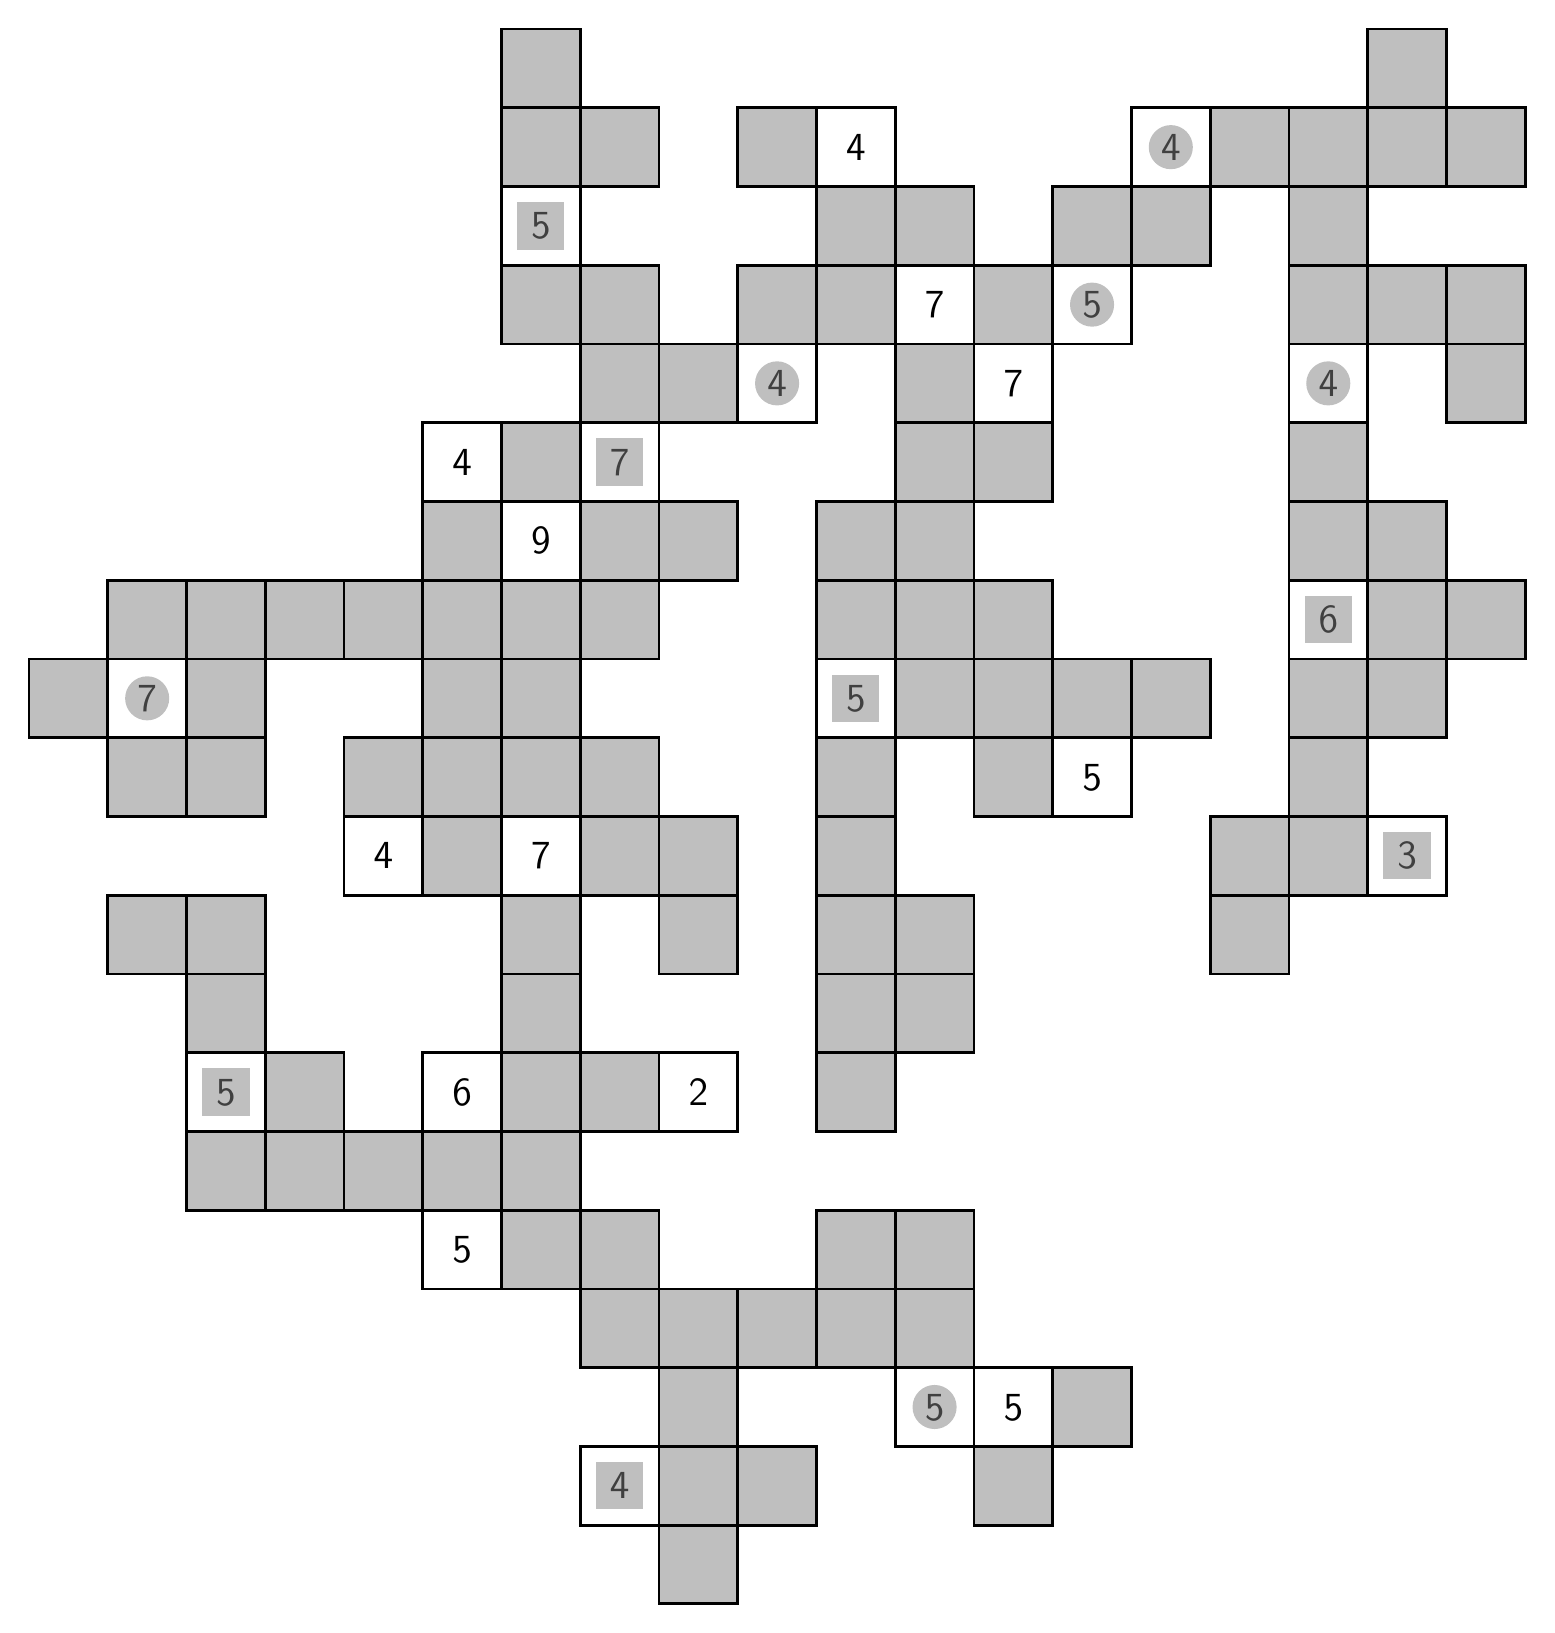
\begin{tikzpicture}\fill[gray, opacity = 0.5] (9, 0, 0)--++(1, 0, 0)--++(0, 1, 0)--++(-1, 0, 0)--cycle;
\draw[line width = 1pt] (9, 0, 0)--++(1, 0, 0)--++(0, 1, 0)--++(-1, 0, 0)--cycle;
\draw node at (8.5, 1.5, 0) {\Large $\mathsf{4}$};
\draw[line width = 1pt] (8, 1, 0)--++(1, 0, 0)--++(0, 1, 0)--++(-1, 0, 0)--cycle;
\fill[color = gray, opacity = 0.5] (8.2, 1.2) rectangle ++(0.6, 0.6);
\fill[gray, opacity = 0.5] (9, 1, 0)--++(1, 0, 0)--++(0, 1, 0)--++(-1, 0, 0)--cycle;
\draw[line width = 1pt] (9, 1, 0)--++(1, 0, 0)--++(0, 1, 0)--++(-1, 0, 0)--cycle;
\fill[gray, opacity = 0.5] (10, 1, 0)--++(1, 0, 0)--++(0, 1, 0)--++(-1, 0, 0)--cycle;
\draw[line width = 1pt] (10, 1, 0)--++(1, 0, 0)--++(0, 1, 0)--++(-1, 0, 0)--cycle;
\fill[gray, opacity = 0.5] (13, 1, 0)--++(1, 0, 0)--++(0, 1, 0)--++(-1, 0, 0)--cycle;
\draw[line width = 1pt] (13, 1, 0)--++(1, 0, 0)--++(0, 1, 0)--++(-1, 0, 0)--cycle;
\fill[gray, opacity = 0.5] (9, 2, 0)--++(1, 0, 0)--++(0, 1, 0)--++(-1, 0, 0)--cycle;
\draw[line width = 1pt] (9, 2, 0)--++(1, 0, 0)--++(0, 1, 0)--++(-1, 0, 0)--cycle;
\draw node at (12.5, 2.5, 0) {\Large $\mathsf{5}$};
\draw[line width = 1pt] (12, 2, 0)--++(1, 0, 0)--++(0, 1, 0)--++(-1, 0, 0)--cycle;
\fill[color = gray, opacity = 0.5] (12.5, 2.5, 0) circle (0.28);
\draw node at (13.5, 2.5, 0) {\Large $\mathsf{5}$};
\draw[line width = 1pt] (13, 2, 0)--++(1, 0, 0)--++(0, 1, 0)--++(-1, 0, 0)--cycle;
\fill[gray, opacity = 0.5] (14, 2, 0)--++(1, 0, 0)--++(0, 1, 0)--++(-1, 0, 0)--cycle;
\draw[line width = 1pt] (14, 2, 0)--++(1, 0, 0)--++(0, 1, 0)--++(-1, 0, 0)--cycle;
\fill[gray, opacity = 0.5] (8, 3, 0)--++(1, 0, 0)--++(0, 1, 0)--++(-1, 0, 0)--cycle;
\draw[line width = 1pt] (8, 3, 0)--++(1, 0, 0)--++(0, 1, 0)--++(-1, 0, 0)--cycle;
\fill[gray, opacity = 0.5] (9, 3, 0)--++(1, 0, 0)--++(0, 1, 0)--++(-1, 0, 0)--cycle;
\draw[line width = 1pt] (9, 3, 0)--++(1, 0, 0)--++(0, 1, 0)--++(-1, 0, 0)--cycle;
\fill[gray, opacity = 0.5] (10, 3, 0)--++(1, 0, 0)--++(0, 1, 0)--++(-1, 0, 0)--cycle;
\draw[line width = 1pt] (10, 3, 0)--++(1, 0, 0)--++(0, 1, 0)--++(-1, 0, 0)--cycle;
\fill[gray, opacity = 0.5] (11, 3, 0)--++(1, 0, 0)--++(0, 1, 0)--++(-1, 0, 0)--cycle;
\draw[line width = 1pt] (11, 3, 0)--++(1, 0, 0)--++(0, 1, 0)--++(-1, 0, 0)--cycle;
\fill[gray, opacity = 0.5] (12, 3, 0)--++(1, 0, 0)--++(0, 1, 0)--++(-1, 0, 0)--cycle;
\draw[line width = 1pt] (12, 3, 0)--++(1, 0, 0)--++(0, 1, 0)--++(-1, 0, 0)--cycle;
\draw node at (6.5, 4.5, 0) {\Large $\mathsf{5}$};
\draw[line width = 1pt] (6, 4, 0)--++(1, 0, 0)--++(0, 1, 0)--++(-1, 0, 0)--cycle;
\fill[gray, opacity = 0.5] (7, 4, 0)--++(1, 0, 0)--++(0, 1, 0)--++(-1, 0, 0)--cycle;
\draw[line width = 1pt] (7, 4, 0)--++(1, 0, 0)--++(0, 1, 0)--++(-1, 0, 0)--cycle;
\fill[gray, opacity = 0.5] (8, 4, 0)--++(1, 0, 0)--++(0, 1, 0)--++(-1, 0, 0)--cycle;
\draw[line width = 1pt] (8, 4, 0)--++(1, 0, 0)--++(0, 1, 0)--++(-1, 0, 0)--cycle;
\fill[gray, opacity = 0.5] (11, 4, 0)--++(1, 0, 0)--++(0, 1, 0)--++(-1, 0, 0)--cycle;
\draw[line width = 1pt] (11, 4, 0)--++(1, 0, 0)--++(0, 1, 0)--++(-1, 0, 0)--cycle;
\fill[gray, opacity = 0.5] (12, 4, 0)--++(1, 0, 0)--++(0, 1, 0)--++(-1, 0, 0)--cycle;
\draw[line width = 1pt] (12, 4, 0)--++(1, 0, 0)--++(0, 1, 0)--++(-1, 0, 0)--cycle;
\fill[gray, opacity = 0.5] (3, 5, 0)--++(1, 0, 0)--++(0, 1, 0)--++(-1, 0, 0)--cycle;
\draw[line width = 1pt] (3, 5, 0)--++(1, 0, 0)--++(0, 1, 0)--++(-1, 0, 0)--cycle;
\fill[gray, opacity = 0.5] (4, 5, 0)--++(1, 0, 0)--++(0, 1, 0)--++(-1, 0, 0)--cycle;
\draw[line width = 1pt] (4, 5, 0)--++(1, 0, 0)--++(0, 1, 0)--++(-1, 0, 0)--cycle;
\fill[gray, opacity = 0.5] (5, 5, 0)--++(1, 0, 0)--++(0, 1, 0)--++(-1, 0, 0)--cycle;
\draw[line width = 1pt] (5, 5, 0)--++(1, 0, 0)--++(0, 1, 0)--++(-1, 0, 0)--cycle;
\fill[gray, opacity = 0.5] (6, 5, 0)--++(1, 0, 0)--++(0, 1, 0)--++(-1, 0, 0)--cycle;
\draw[line width = 1pt] (6, 5, 0)--++(1, 0, 0)--++(0, 1, 0)--++(-1, 0, 0)--cycle;
\fill[gray, opacity = 0.5] (7, 5, 0)--++(1, 0, 0)--++(0, 1, 0)--++(-1, 0, 0)--cycle;
\draw[line width = 1pt] (7, 5, 0)--++(1, 0, 0)--++(0, 1, 0)--++(-1, 0, 0)--cycle;
\draw node at (3.5, 6.5, 0) {\Large $\mathsf{5}$};
\draw[line width = 1pt] (3, 6, 0)--++(1, 0, 0)--++(0, 1, 0)--++(-1, 0, 0)--cycle;
\fill[color = gray, opacity = 0.5] (3.2, 6.2) rectangle ++(0.6, 0.6);
\fill[gray, opacity = 0.5] (4, 6, 0)--++(1, 0, 0)--++(0, 1, 0)--++(-1, 0, 0)--cycle;
\draw[line width = 1pt] (4, 6, 0)--++(1, 0, 0)--++(0, 1, 0)--++(-1, 0, 0)--cycle;
\draw node at (6.5, 6.5, 0) {\Large $\mathsf{6}$};
\draw[line width = 1pt] (6, 6, 0)--++(1, 0, 0)--++(0, 1, 0)--++(-1, 0, 0)--cycle;
\fill[gray, opacity = 0.5] (7, 6, 0)--++(1, 0, 0)--++(0, 1, 0)--++(-1, 0, 0)--cycle;
\draw[line width = 1pt] (7, 6, 0)--++(1, 0, 0)--++(0, 1, 0)--++(-1, 0, 0)--cycle;
\fill[gray, opacity = 0.5] (8, 6, 0)--++(1, 0, 0)--++(0, 1, 0)--++(-1, 0, 0)--cycle;
\draw[line width = 1pt] (8, 6, 0)--++(1, 0, 0)--++(0, 1, 0)--++(-1, 0, 0)--cycle;
\draw node at (9.5, 6.5, 0) {\Large $\mathsf{2}$};
\draw[line width = 1pt] (9, 6, 0)--++(1, 0, 0)--++(0, 1, 0)--++(-1, 0, 0)--cycle;
\fill[gray, opacity = 0.5] (11, 6, 0)--++(1, 0, 0)--++(0, 1, 0)--++(-1, 0, 0)--cycle;
\draw[line width = 1pt] (11, 6, 0)--++(1, 0, 0)--++(0, 1, 0)--++(-1, 0, 0)--cycle;
\fill[gray, opacity = 0.5] (3, 7, 0)--++(1, 0, 0)--++(0, 1, 0)--++(-1, 0, 0)--cycle;
\draw[line width = 1pt] (3, 7, 0)--++(1, 0, 0)--++(0, 1, 0)--++(-1, 0, 0)--cycle;
\fill[gray, opacity = 0.5] (7, 7, 0)--++(1, 0, 0)--++(0, 1, 0)--++(-1, 0, 0)--cycle;
\draw[line width = 1pt] (7, 7, 0)--++(1, 0, 0)--++(0, 1, 0)--++(-1, 0, 0)--cycle;
\fill[gray, opacity = 0.5] (11, 7, 0)--++(1, 0, 0)--++(0, 1, 0)--++(-1, 0, 0)--cycle;
\draw[line width = 1pt] (11, 7, 0)--++(1, 0, 0)--++(0, 1, 0)--++(-1, 0, 0)--cycle;
\fill[gray, opacity = 0.5] (12, 7, 0)--++(1, 0, 0)--++(0, 1, 0)--++(-1, 0, 0)--cycle;
\draw[line width = 1pt] (12, 7, 0)--++(1, 0, 0)--++(0, 1, 0)--++(-1, 0, 0)--cycle;
\fill[gray, opacity = 0.5] (2, 8, 0)--++(1, 0, 0)--++(0, 1, 0)--++(-1, 0, 0)--cycle;
\draw[line width = 1pt] (2, 8, 0)--++(1, 0, 0)--++(0, 1, 0)--++(-1, 0, 0)--cycle;
\fill[gray, opacity = 0.5] (3, 8, 0)--++(1, 0, 0)--++(0, 1, 0)--++(-1, 0, 0)--cycle;
\draw[line width = 1pt] (3, 8, 0)--++(1, 0, 0)--++(0, 1, 0)--++(-1, 0, 0)--cycle;
\fill[gray, opacity = 0.5] (7, 8, 0)--++(1, 0, 0)--++(0, 1, 0)--++(-1, 0, 0)--cycle;
\draw[line width = 1pt] (7, 8, 0)--++(1, 0, 0)--++(0, 1, 0)--++(-1, 0, 0)--cycle;
\fill[gray, opacity = 0.5] (9, 8, 0)--++(1, 0, 0)--++(0, 1, 0)--++(-1, 0, 0)--cycle;
\draw[line width = 1pt] (9, 8, 0)--++(1, 0, 0)--++(0, 1, 0)--++(-1, 0, 0)--cycle;
\fill[gray, opacity = 0.5] (11, 8, 0)--++(1, 0, 0)--++(0, 1, 0)--++(-1, 0, 0)--cycle;
\draw[line width = 1pt] (11, 8, 0)--++(1, 0, 0)--++(0, 1, 0)--++(-1, 0, 0)--cycle;
\fill[gray, opacity = 0.5] (12, 8, 0)--++(1, 0, 0)--++(0, 1, 0)--++(-1, 0, 0)--cycle;
\draw[line width = 1pt] (12, 8, 0)--++(1, 0, 0)--++(0, 1, 0)--++(-1, 0, 0)--cycle;
\fill[gray, opacity = 0.5] (16, 8, 0)--++(1, 0, 0)--++(0, 1, 0)--++(-1, 0, 0)--cycle;
\draw[line width = 1pt] (16, 8, 0)--++(1, 0, 0)--++(0, 1, 0)--++(-1, 0, 0)--cycle;
\draw node at (5.5, 9.5, 0) {\Large $\mathsf{4}$};
\draw[line width = 1pt] (5, 9, 0)--++(1, 0, 0)--++(0, 1, 0)--++(-1, 0, 0)--cycle;
\fill[gray, opacity = 0.5] (6, 9, 0)--++(1, 0, 0)--++(0, 1, 0)--++(-1, 0, 0)--cycle;
\draw[line width = 1pt] (6, 9, 0)--++(1, 0, 0)--++(0, 1, 0)--++(-1, 0, 0)--cycle;
\draw node at (7.5, 9.5, 0) {\Large $\mathsf{7}$};
\draw[line width = 1pt] (7, 9, 0)--++(1, 0, 0)--++(0, 1, 0)--++(-1, 0, 0)--cycle;
\fill[gray, opacity = 0.5] (8, 9, 0)--++(1, 0, 0)--++(0, 1, 0)--++(-1, 0, 0)--cycle;
\draw[line width = 1pt] (8, 9, 0)--++(1, 0, 0)--++(0, 1, 0)--++(-1, 0, 0)--cycle;
\fill[gray, opacity = 0.5] (9, 9, 0)--++(1, 0, 0)--++(0, 1, 0)--++(-1, 0, 0)--cycle;
\draw[line width = 1pt] (9, 9, 0)--++(1, 0, 0)--++(0, 1, 0)--++(-1, 0, 0)--cycle;
\fill[gray, opacity = 0.5] (11, 9, 0)--++(1, 0, 0)--++(0, 1, 0)--++(-1, 0, 0)--cycle;
\draw[line width = 1pt] (11, 9, 0)--++(1, 0, 0)--++(0, 1, 0)--++(-1, 0, 0)--cycle;
\fill[gray, opacity = 0.5] (16, 9, 0)--++(1, 0, 0)--++(0, 1, 0)--++(-1, 0, 0)--cycle;
\draw[line width = 1pt] (16, 9, 0)--++(1, 0, 0)--++(0, 1, 0)--++(-1, 0, 0)--cycle;
\fill[gray, opacity = 0.5] (17, 9, 0)--++(1, 0, 0)--++(0, 1, 0)--++(-1, 0, 0)--cycle;
\draw[line width = 1pt] (17, 9, 0)--++(1, 0, 0)--++(0, 1, 0)--++(-1, 0, 0)--cycle;
\draw node at (18.5, 9.5, 0) {\Large $\mathsf{3}$};
\draw[line width = 1pt] (18, 9, 0)--++(1, 0, 0)--++(0, 1, 0)--++(-1, 0, 0)--cycle;
\fill[color = gray, opacity = 0.5] (18.2, 9.2) rectangle ++(0.6, 0.6);
\fill[gray, opacity = 0.5] (2, 10, 0)--++(1, 0, 0)--++(0, 1, 0)--++(-1, 0, 0)--cycle;
\draw[line width = 1pt] (2, 10, 0)--++(1, 0, 0)--++(0, 1, 0)--++(-1, 0, 0)--cycle;
\fill[gray, opacity = 0.5] (3, 10, 0)--++(1, 0, 0)--++(0, 1, 0)--++(-1, 0, 0)--cycle;
\draw[line width = 1pt] (3, 10, 0)--++(1, 0, 0)--++(0, 1, 0)--++(-1, 0, 0)--cycle;
\fill[gray, opacity = 0.5] (5, 10, 0)--++(1, 0, 0)--++(0, 1, 0)--++(-1, 0, 0)--cycle;
\draw[line width = 1pt] (5, 10, 0)--++(1, 0, 0)--++(0, 1, 0)--++(-1, 0, 0)--cycle;
\fill[gray, opacity = 0.5] (6, 10, 0)--++(1, 0, 0)--++(0, 1, 0)--++(-1, 0, 0)--cycle;
\draw[line width = 1pt] (6, 10, 0)--++(1, 0, 0)--++(0, 1, 0)--++(-1, 0, 0)--cycle;
\fill[gray, opacity = 0.5] (7, 10, 0)--++(1, 0, 0)--++(0, 1, 0)--++(-1, 0, 0)--cycle;
\draw[line width = 1pt] (7, 10, 0)--++(1, 0, 0)--++(0, 1, 0)--++(-1, 0, 0)--cycle;
\fill[gray, opacity = 0.5] (8, 10, 0)--++(1, 0, 0)--++(0, 1, 0)--++(-1, 0, 0)--cycle;
\draw[line width = 1pt] (8, 10, 0)--++(1, 0, 0)--++(0, 1, 0)--++(-1, 0, 0)--cycle;
\fill[gray, opacity = 0.5] (11, 10, 0)--++(1, 0, 0)--++(0, 1, 0)--++(-1, 0, 0)--cycle;
\draw[line width = 1pt] (11, 10, 0)--++(1, 0, 0)--++(0, 1, 0)--++(-1, 0, 0)--cycle;
\fill[gray, opacity = 0.5] (13, 10, 0)--++(1, 0, 0)--++(0, 1, 0)--++(-1, 0, 0)--cycle;
\draw[line width = 1pt] (13, 10, 0)--++(1, 0, 0)--++(0, 1, 0)--++(-1, 0, 0)--cycle;
\draw node at (14.5, 10.5, 0) {\Large $\mathsf{5}$};
\draw[line width = 1pt] (14, 10, 0)--++(1, 0, 0)--++(0, 1, 0)--++(-1, 0, 0)--cycle;
\fill[gray, opacity = 0.5] (17, 10, 0)--++(1, 0, 0)--++(0, 1, 0)--++(-1, 0, 0)--cycle;
\draw[line width = 1pt] (17, 10, 0)--++(1, 0, 0)--++(0, 1, 0)--++(-1, 0, 0)--cycle;
\fill[gray, opacity = 0.5] (1, 11, 0)--++(1, 0, 0)--++(0, 1, 0)--++(-1, 0, 0)--cycle;
\draw[line width = 1pt] (1, 11, 0)--++(1, 0, 0)--++(0, 1, 0)--++(-1, 0, 0)--cycle;
\draw node at (2.5, 11.5, 0) {\Large $\mathsf{7}$};
\draw[line width = 1pt] (2, 11, 0)--++(1, 0, 0)--++(0, 1, 0)--++(-1, 0, 0)--cycle;
\fill[color = gray, opacity = 0.5] (2.5, 11.5, 0) circle (0.28);
\fill[gray, opacity = 0.5] (3, 11, 0)--++(1, 0, 0)--++(0, 1, 0)--++(-1, 0, 0)--cycle;
\draw[line width = 1pt] (3, 11, 0)--++(1, 0, 0)--++(0, 1, 0)--++(-1, 0, 0)--cycle;
\fill[gray, opacity = 0.5] (6, 11, 0)--++(1, 0, 0)--++(0, 1, 0)--++(-1, 0, 0)--cycle;
\draw[line width = 1pt] (6, 11, 0)--++(1, 0, 0)--++(0, 1, 0)--++(-1, 0, 0)--cycle;
\fill[gray, opacity = 0.5] (7, 11, 0)--++(1, 0, 0)--++(0, 1, 0)--++(-1, 0, 0)--cycle;
\draw[line width = 1pt] (7, 11, 0)--++(1, 0, 0)--++(0, 1, 0)--++(-1, 0, 0)--cycle;
\draw node at (11.5, 11.5, 0) {\Large $\mathsf{5}$};
\draw[line width = 1pt] (11, 11, 0)--++(1, 0, 0)--++(0, 1, 0)--++(-1, 0, 0)--cycle;
\fill[color = gray, opacity = 0.5] (11.2, 11.2) rectangle ++(0.6, 0.6);
\fill[gray, opacity = 0.5] (12, 11, 0)--++(1, 0, 0)--++(0, 1, 0)--++(-1, 0, 0)--cycle;
\draw[line width = 1pt] (12, 11, 0)--++(1, 0, 0)--++(0, 1, 0)--++(-1, 0, 0)--cycle;
\fill[gray, opacity = 0.5] (13, 11, 0)--++(1, 0, 0)--++(0, 1, 0)--++(-1, 0, 0)--cycle;
\draw[line width = 1pt] (13, 11, 0)--++(1, 0, 0)--++(0, 1, 0)--++(-1, 0, 0)--cycle;
\fill[gray, opacity = 0.5] (14, 11, 0)--++(1, 0, 0)--++(0, 1, 0)--++(-1, 0, 0)--cycle;
\draw[line width = 1pt] (14, 11, 0)--++(1, 0, 0)--++(0, 1, 0)--++(-1, 0, 0)--cycle;
\fill[gray, opacity = 0.5] (15, 11, 0)--++(1, 0, 0)--++(0, 1, 0)--++(-1, 0, 0)--cycle;
\draw[line width = 1pt] (15, 11, 0)--++(1, 0, 0)--++(0, 1, 0)--++(-1, 0, 0)--cycle;
\fill[gray, opacity = 0.5] (17, 11, 0)--++(1, 0, 0)--++(0, 1, 0)--++(-1, 0, 0)--cycle;
\draw[line width = 1pt] (17, 11, 0)--++(1, 0, 0)--++(0, 1, 0)--++(-1, 0, 0)--cycle;
\fill[gray, opacity = 0.5] (18, 11, 0)--++(1, 0, 0)--++(0, 1, 0)--++(-1, 0, 0)--cycle;
\draw[line width = 1pt] (18, 11, 0)--++(1, 0, 0)--++(0, 1, 0)--++(-1, 0, 0)--cycle;
\fill[gray, opacity = 0.5] (2, 12, 0)--++(1, 0, 0)--++(0, 1, 0)--++(-1, 0, 0)--cycle;
\draw[line width = 1pt] (2, 12, 0)--++(1, 0, 0)--++(0, 1, 0)--++(-1, 0, 0)--cycle;
\fill[gray, opacity = 0.5] (3, 12, 0)--++(1, 0, 0)--++(0, 1, 0)--++(-1, 0, 0)--cycle;
\draw[line width = 1pt] (3, 12, 0)--++(1, 0, 0)--++(0, 1, 0)--++(-1, 0, 0)--cycle;
\fill[gray, opacity = 0.5] (4, 12, 0)--++(1, 0, 0)--++(0, 1, 0)--++(-1, 0, 0)--cycle;
\draw[line width = 1pt] (4, 12, 0)--++(1, 0, 0)--++(0, 1, 0)--++(-1, 0, 0)--cycle;
\fill[gray, opacity = 0.5] (5, 12, 0)--++(1, 0, 0)--++(0, 1, 0)--++(-1, 0, 0)--cycle;
\draw[line width = 1pt] (5, 12, 0)--++(1, 0, 0)--++(0, 1, 0)--++(-1, 0, 0)--cycle;
\fill[gray, opacity = 0.5] (6, 12, 0)--++(1, 0, 0)--++(0, 1, 0)--++(-1, 0, 0)--cycle;
\draw[line width = 1pt] (6, 12, 0)--++(1, 0, 0)--++(0, 1, 0)--++(-1, 0, 0)--cycle;
\fill[gray, opacity = 0.5] (7, 12, 0)--++(1, 0, 0)--++(0, 1, 0)--++(-1, 0, 0)--cycle;
\draw[line width = 1pt] (7, 12, 0)--++(1, 0, 0)--++(0, 1, 0)--++(-1, 0, 0)--cycle;
\fill[gray, opacity = 0.5] (8, 12, 0)--++(1, 0, 0)--++(0, 1, 0)--++(-1, 0, 0)--cycle;
\draw[line width = 1pt] (8, 12, 0)--++(1, 0, 0)--++(0, 1, 0)--++(-1, 0, 0)--cycle;
\fill[gray, opacity = 0.5] (11, 12, 0)--++(1, 0, 0)--++(0, 1, 0)--++(-1, 0, 0)--cycle;
\draw[line width = 1pt] (11, 12, 0)--++(1, 0, 0)--++(0, 1, 0)--++(-1, 0, 0)--cycle;
\fill[gray, opacity = 0.5] (12, 12, 0)--++(1, 0, 0)--++(0, 1, 0)--++(-1, 0, 0)--cycle;
\draw[line width = 1pt] (12, 12, 0)--++(1, 0, 0)--++(0, 1, 0)--++(-1, 0, 0)--cycle;
\fill[gray, opacity = 0.5] (13, 12, 0)--++(1, 0, 0)--++(0, 1, 0)--++(-1, 0, 0)--cycle;
\draw[line width = 1pt] (13, 12, 0)--++(1, 0, 0)--++(0, 1, 0)--++(-1, 0, 0)--cycle;
\draw node at (17.5, 12.5, 0) {\Large $\mathsf{6}$};
\draw[line width = 1pt] (17, 12, 0)--++(1, 0, 0)--++(0, 1, 0)--++(-1, 0, 0)--cycle;
\fill[color = gray, opacity = 0.5] (17.2, 12.2) rectangle ++(0.6, 0.6);
\fill[gray, opacity = 0.5] (18, 12, 0)--++(1, 0, 0)--++(0, 1, 0)--++(-1, 0, 0)--cycle;
\draw[line width = 1pt] (18, 12, 0)--++(1, 0, 0)--++(0, 1, 0)--++(-1, 0, 0)--cycle;
\fill[gray, opacity = 0.5] (19, 12, 0)--++(1, 0, 0)--++(0, 1, 0)--++(-1, 0, 0)--cycle;
\draw[line width = 1pt] (19, 12, 0)--++(1, 0, 0)--++(0, 1, 0)--++(-1, 0, 0)--cycle;
\fill[gray, opacity = 0.5] (6, 13, 0)--++(1, 0, 0)--++(0, 1, 0)--++(-1, 0, 0)--cycle;
\draw[line width = 1pt] (6, 13, 0)--++(1, 0, 0)--++(0, 1, 0)--++(-1, 0, 0)--cycle;
\draw node at (7.5, 13.5, 0) {\Large $\mathsf{9}$};
\draw[line width = 1pt] (7, 13, 0)--++(1, 0, 0)--++(0, 1, 0)--++(-1, 0, 0)--cycle;
\fill[gray, opacity = 0.5] (8, 13, 0)--++(1, 0, 0)--++(0, 1, 0)--++(-1, 0, 0)--cycle;
\draw[line width = 1pt] (8, 13, 0)--++(1, 0, 0)--++(0, 1, 0)--++(-1, 0, 0)--cycle;
\fill[gray, opacity = 0.5] (9, 13, 0)--++(1, 0, 0)--++(0, 1, 0)--++(-1, 0, 0)--cycle;
\draw[line width = 1pt] (9, 13, 0)--++(1, 0, 0)--++(0, 1, 0)--++(-1, 0, 0)--cycle;
\fill[gray, opacity = 0.5] (11, 13, 0)--++(1, 0, 0)--++(0, 1, 0)--++(-1, 0, 0)--cycle;
\draw[line width = 1pt] (11, 13, 0)--++(1, 0, 0)--++(0, 1, 0)--++(-1, 0, 0)--cycle;
\fill[gray, opacity = 0.5] (12, 13, 0)--++(1, 0, 0)--++(0, 1, 0)--++(-1, 0, 0)--cycle;
\draw[line width = 1pt] (12, 13, 0)--++(1, 0, 0)--++(0, 1, 0)--++(-1, 0, 0)--cycle;
\fill[gray, opacity = 0.5] (17, 13, 0)--++(1, 0, 0)--++(0, 1, 0)--++(-1, 0, 0)--cycle;
\draw[line width = 1pt] (17, 13, 0)--++(1, 0, 0)--++(0, 1, 0)--++(-1, 0, 0)--cycle;
\fill[gray, opacity = 0.5] (18, 13, 0)--++(1, 0, 0)--++(0, 1, 0)--++(-1, 0, 0)--cycle;
\draw[line width = 1pt] (18, 13, 0)--++(1, 0, 0)--++(0, 1, 0)--++(-1, 0, 0)--cycle;
\draw node at (6.5, 14.5, 0) {\Large $\mathsf{4}$};
\draw[line width = 1pt] (6, 14, 0)--++(1, 0, 0)--++(0, 1, 0)--++(-1, 0, 0)--cycle;
\fill[gray, opacity = 0.5] (7, 14, 0)--++(1, 0, 0)--++(0, 1, 0)--++(-1, 0, 0)--cycle;
\draw[line width = 1pt] (7, 14, 0)--++(1, 0, 0)--++(0, 1, 0)--++(-1, 0, 0)--cycle;
\draw node at (8.5, 14.5, 0) {\Large $\mathsf{7}$};
\draw[line width = 1pt] (8, 14, 0)--++(1, 0, 0)--++(0, 1, 0)--++(-1, 0, 0)--cycle;
\fill[color = gray, opacity = 0.5] (8.2, 14.2) rectangle ++(0.6, 0.6);
\fill[gray, opacity = 0.5] (12, 14, 0)--++(1, 0, 0)--++(0, 1, 0)--++(-1, 0, 0)--cycle;
\draw[line width = 1pt] (12, 14, 0)--++(1, 0, 0)--++(0, 1, 0)--++(-1, 0, 0)--cycle;
\fill[gray, opacity = 0.5] (13, 14, 0)--++(1, 0, 0)--++(0, 1, 0)--++(-1, 0, 0)--cycle;
\draw[line width = 1pt] (13, 14, 0)--++(1, 0, 0)--++(0, 1, 0)--++(-1, 0, 0)--cycle;
\fill[gray, opacity = 0.5] (17, 14, 0)--++(1, 0, 0)--++(0, 1, 0)--++(-1, 0, 0)--cycle;
\draw[line width = 1pt] (17, 14, 0)--++(1, 0, 0)--++(0, 1, 0)--++(-1, 0, 0)--cycle;
\fill[gray, opacity = 0.5] (8, 15, 0)--++(1, 0, 0)--++(0, 1, 0)--++(-1, 0, 0)--cycle;
\draw[line width = 1pt] (8, 15, 0)--++(1, 0, 0)--++(0, 1, 0)--++(-1, 0, 0)--cycle;
\fill[gray, opacity = 0.5] (9, 15, 0)--++(1, 0, 0)--++(0, 1, 0)--++(-1, 0, 0)--cycle;
\draw[line width = 1pt] (9, 15, 0)--++(1, 0, 0)--++(0, 1, 0)--++(-1, 0, 0)--cycle;
\draw node at (10.5, 15.5, 0) {\Large $\mathsf{4}$};
\draw[line width = 1pt] (10, 15, 0)--++(1, 0, 0)--++(0, 1, 0)--++(-1, 0, 0)--cycle;
\fill[color = gray, opacity = 0.5] (10.5, 15.5, 0) circle (0.28);
\fill[gray, opacity = 0.5] (12, 15, 0)--++(1, 0, 0)--++(0, 1, 0)--++(-1, 0, 0)--cycle;
\draw[line width = 1pt] (12, 15, 0)--++(1, 0, 0)--++(0, 1, 0)--++(-1, 0, 0)--cycle;
\draw node at (13.5, 15.5, 0) {\Large $\mathsf{7}$};
\draw[line width = 1pt] (13, 15, 0)--++(1, 0, 0)--++(0, 1, 0)--++(-1, 0, 0)--cycle;
\draw node at (17.5, 15.5, 0) {\Large $\mathsf{4}$};
\draw[line width = 1pt] (17, 15, 0)--++(1, 0, 0)--++(0, 1, 0)--++(-1, 0, 0)--cycle;
\fill[color = gray, opacity = 0.5] (17.5, 15.5, 0) circle (0.28);
\fill[gray, opacity = 0.5] (19, 15, 0)--++(1, 0, 0)--++(0, 1, 0)--++(-1, 0, 0)--cycle;
\draw[line width = 1pt] (19, 15, 0)--++(1, 0, 0)--++(0, 1, 0)--++(-1, 0, 0)--cycle;
\fill[gray, opacity = 0.5] (7, 16, 0)--++(1, 0, 0)--++(0, 1, 0)--++(-1, 0, 0)--cycle;
\draw[line width = 1pt] (7, 16, 0)--++(1, 0, 0)--++(0, 1, 0)--++(-1, 0, 0)--cycle;
\fill[gray, opacity = 0.5] (8, 16, 0)--++(1, 0, 0)--++(0, 1, 0)--++(-1, 0, 0)--cycle;
\draw[line width = 1pt] (8, 16, 0)--++(1, 0, 0)--++(0, 1, 0)--++(-1, 0, 0)--cycle;
\fill[gray, opacity = 0.5] (10, 16, 0)--++(1, 0, 0)--++(0, 1, 0)--++(-1, 0, 0)--cycle;
\draw[line width = 1pt] (10, 16, 0)--++(1, 0, 0)--++(0, 1, 0)--++(-1, 0, 0)--cycle;
\fill[gray, opacity = 0.5] (11, 16, 0)--++(1, 0, 0)--++(0, 1, 0)--++(-1, 0, 0)--cycle;
\draw[line width = 1pt] (11, 16, 0)--++(1, 0, 0)--++(0, 1, 0)--++(-1, 0, 0)--cycle;
\draw node at (12.5, 16.5, 0) {\Large $\mathsf{7}$};
\draw[line width = 1pt] (12, 16, 0)--++(1, 0, 0)--++(0, 1, 0)--++(-1, 0, 0)--cycle;
\fill[gray, opacity = 0.5] (13, 16, 0)--++(1, 0, 0)--++(0, 1, 0)--++(-1, 0, 0)--cycle;
\draw[line width = 1pt] (13, 16, 0)--++(1, 0, 0)--++(0, 1, 0)--++(-1, 0, 0)--cycle;
\draw node at (14.5, 16.5, 0) {\Large $\mathsf{5}$};
\draw[line width = 1pt] (14, 16, 0)--++(1, 0, 0)--++(0, 1, 0)--++(-1, 0, 0)--cycle;
\fill[color = gray, opacity = 0.5] (14.5, 16.5, 0) circle (0.28);
\fill[gray, opacity = 0.5] (17, 16, 0)--++(1, 0, 0)--++(0, 1, 0)--++(-1, 0, 0)--cycle;
\draw[line width = 1pt] (17, 16, 0)--++(1, 0, 0)--++(0, 1, 0)--++(-1, 0, 0)--cycle;
\fill[gray, opacity = 0.5] (18, 16, 0)--++(1, 0, 0)--++(0, 1, 0)--++(-1, 0, 0)--cycle;
\draw[line width = 1pt] (18, 16, 0)--++(1, 0, 0)--++(0, 1, 0)--++(-1, 0, 0)--cycle;
\fill[gray, opacity = 0.5] (19, 16, 0)--++(1, 0, 0)--++(0, 1, 0)--++(-1, 0, 0)--cycle;
\draw[line width = 1pt] (19, 16, 0)--++(1, 0, 0)--++(0, 1, 0)--++(-1, 0, 0)--cycle;
\draw node at (7.5, 17.5, 0) {\Large $\mathsf{5}$};
\draw[line width = 1pt] (7, 17, 0)--++(1, 0, 0)--++(0, 1, 0)--++(-1, 0, 0)--cycle;
\fill[color = gray, opacity = 0.5] (7.2, 17.2) rectangle ++(0.6, 0.6);
\fill[gray, opacity = 0.5] (11, 17, 0)--++(1, 0, 0)--++(0, 1, 0)--++(-1, 0, 0)--cycle;
\draw[line width = 1pt] (11, 17, 0)--++(1, 0, 0)--++(0, 1, 0)--++(-1, 0, 0)--cycle;
\fill[gray, opacity = 0.5] (12, 17, 0)--++(1, 0, 0)--++(0, 1, 0)--++(-1, 0, 0)--cycle;
\draw[line width = 1pt] (12, 17, 0)--++(1, 0, 0)--++(0, 1, 0)--++(-1, 0, 0)--cycle;
\fill[gray, opacity = 0.5] (14, 17, 0)--++(1, 0, 0)--++(0, 1, 0)--++(-1, 0, 0)--cycle;
\draw[line width = 1pt] (14, 17, 0)--++(1, 0, 0)--++(0, 1, 0)--++(-1, 0, 0)--cycle;
\fill[gray, opacity = 0.5] (15, 17, 0)--++(1, 0, 0)--++(0, 1, 0)--++(-1, 0, 0)--cycle;
\draw[line width = 1pt] (15, 17, 0)--++(1, 0, 0)--++(0, 1, 0)--++(-1, 0, 0)--cycle;
\fill[gray, opacity = 0.5] (17, 17, 0)--++(1, 0, 0)--++(0, 1, 0)--++(-1, 0, 0)--cycle;
\draw[line width = 1pt] (17, 17, 0)--++(1, 0, 0)--++(0, 1, 0)--++(-1, 0, 0)--cycle;
\fill[gray, opacity = 0.5] (7, 18, 0)--++(1, 0, 0)--++(0, 1, 0)--++(-1, 0, 0)--cycle;
\draw[line width = 1pt] (7, 18, 0)--++(1, 0, 0)--++(0, 1, 0)--++(-1, 0, 0)--cycle;
\fill[gray, opacity = 0.5] (8, 18, 0)--++(1, 0, 0)--++(0, 1, 0)--++(-1, 0, 0)--cycle;
\draw[line width = 1pt] (8, 18, 0)--++(1, 0, 0)--++(0, 1, 0)--++(-1, 0, 0)--cycle;
\fill[gray, opacity = 0.5] (10, 18, 0)--++(1, 0, 0)--++(0, 1, 0)--++(-1, 0, 0)--cycle;
\draw[line width = 1pt] (10, 18, 0)--++(1, 0, 0)--++(0, 1, 0)--++(-1, 0, 0)--cycle;
\draw node at (11.5, 18.5, 0) {\Large $\mathsf{4}$};
\draw[line width = 1pt] (11, 18, 0)--++(1, 0, 0)--++(0, 1, 0)--++(-1, 0, 0)--cycle;
\draw node at (15.5, 18.5, 0) {\Large $\mathsf{4}$};
\draw[line width = 1pt] (15, 18, 0)--++(1, 0, 0)--++(0, 1, 0)--++(-1, 0, 0)--cycle;
\fill[color = gray, opacity = 0.5] (15.5, 18.5, 0) circle (0.28);
\fill[gray, opacity = 0.5] (16, 18, 0)--++(1, 0, 0)--++(0, 1, 0)--++(-1, 0, 0)--cycle;
\draw[line width = 1pt] (16, 18, 0)--++(1, 0, 0)--++(0, 1, 0)--++(-1, 0, 0)--cycle;
\fill[gray, opacity = 0.5] (17, 18, 0)--++(1, 0, 0)--++(0, 1, 0)--++(-1, 0, 0)--cycle;
\draw[line width = 1pt] (17, 18, 0)--++(1, 0, 0)--++(0, 1, 0)--++(-1, 0, 0)--cycle;
\fill[gray, opacity = 0.5] (18, 18, 0)--++(1, 0, 0)--++(0, 1, 0)--++(-1, 0, 0)--cycle;
\draw[line width = 1pt] (18, 18, 0)--++(1, 0, 0)--++(0, 1, 0)--++(-1, 0, 0)--cycle;
\fill[gray, opacity = 0.5] (19, 18, 0)--++(1, 0, 0)--++(0, 1, 0)--++(-1, 0, 0)--cycle;
\draw[line width = 1pt] (19, 18, 0)--++(1, 0, 0)--++(0, 1, 0)--++(-1, 0, 0)--cycle;
\fill[gray, opacity = 0.5] (7, 19, 0)--++(1, 0, 0)--++(0, 1, 0)--++(-1, 0, 0)--cycle;
\draw[line width = 1pt] (7, 19, 0)--++(1, 0, 0)--++(0, 1, 0)--++(-1, 0, 0)--cycle;
\fill[gray, opacity = 0.5] (18, 19, 0)--++(1, 0, 0)--++(0, 1, 0)--++(-1, 0, 0)--cycle;
\draw[line width = 1pt] (18, 19, 0)--++(1, 0, 0)--++(0, 1, 0)--++(-1, 0, 0)--cycle;
\end{tikzpicture}}\]
\[\resizebox{30pc}{!}{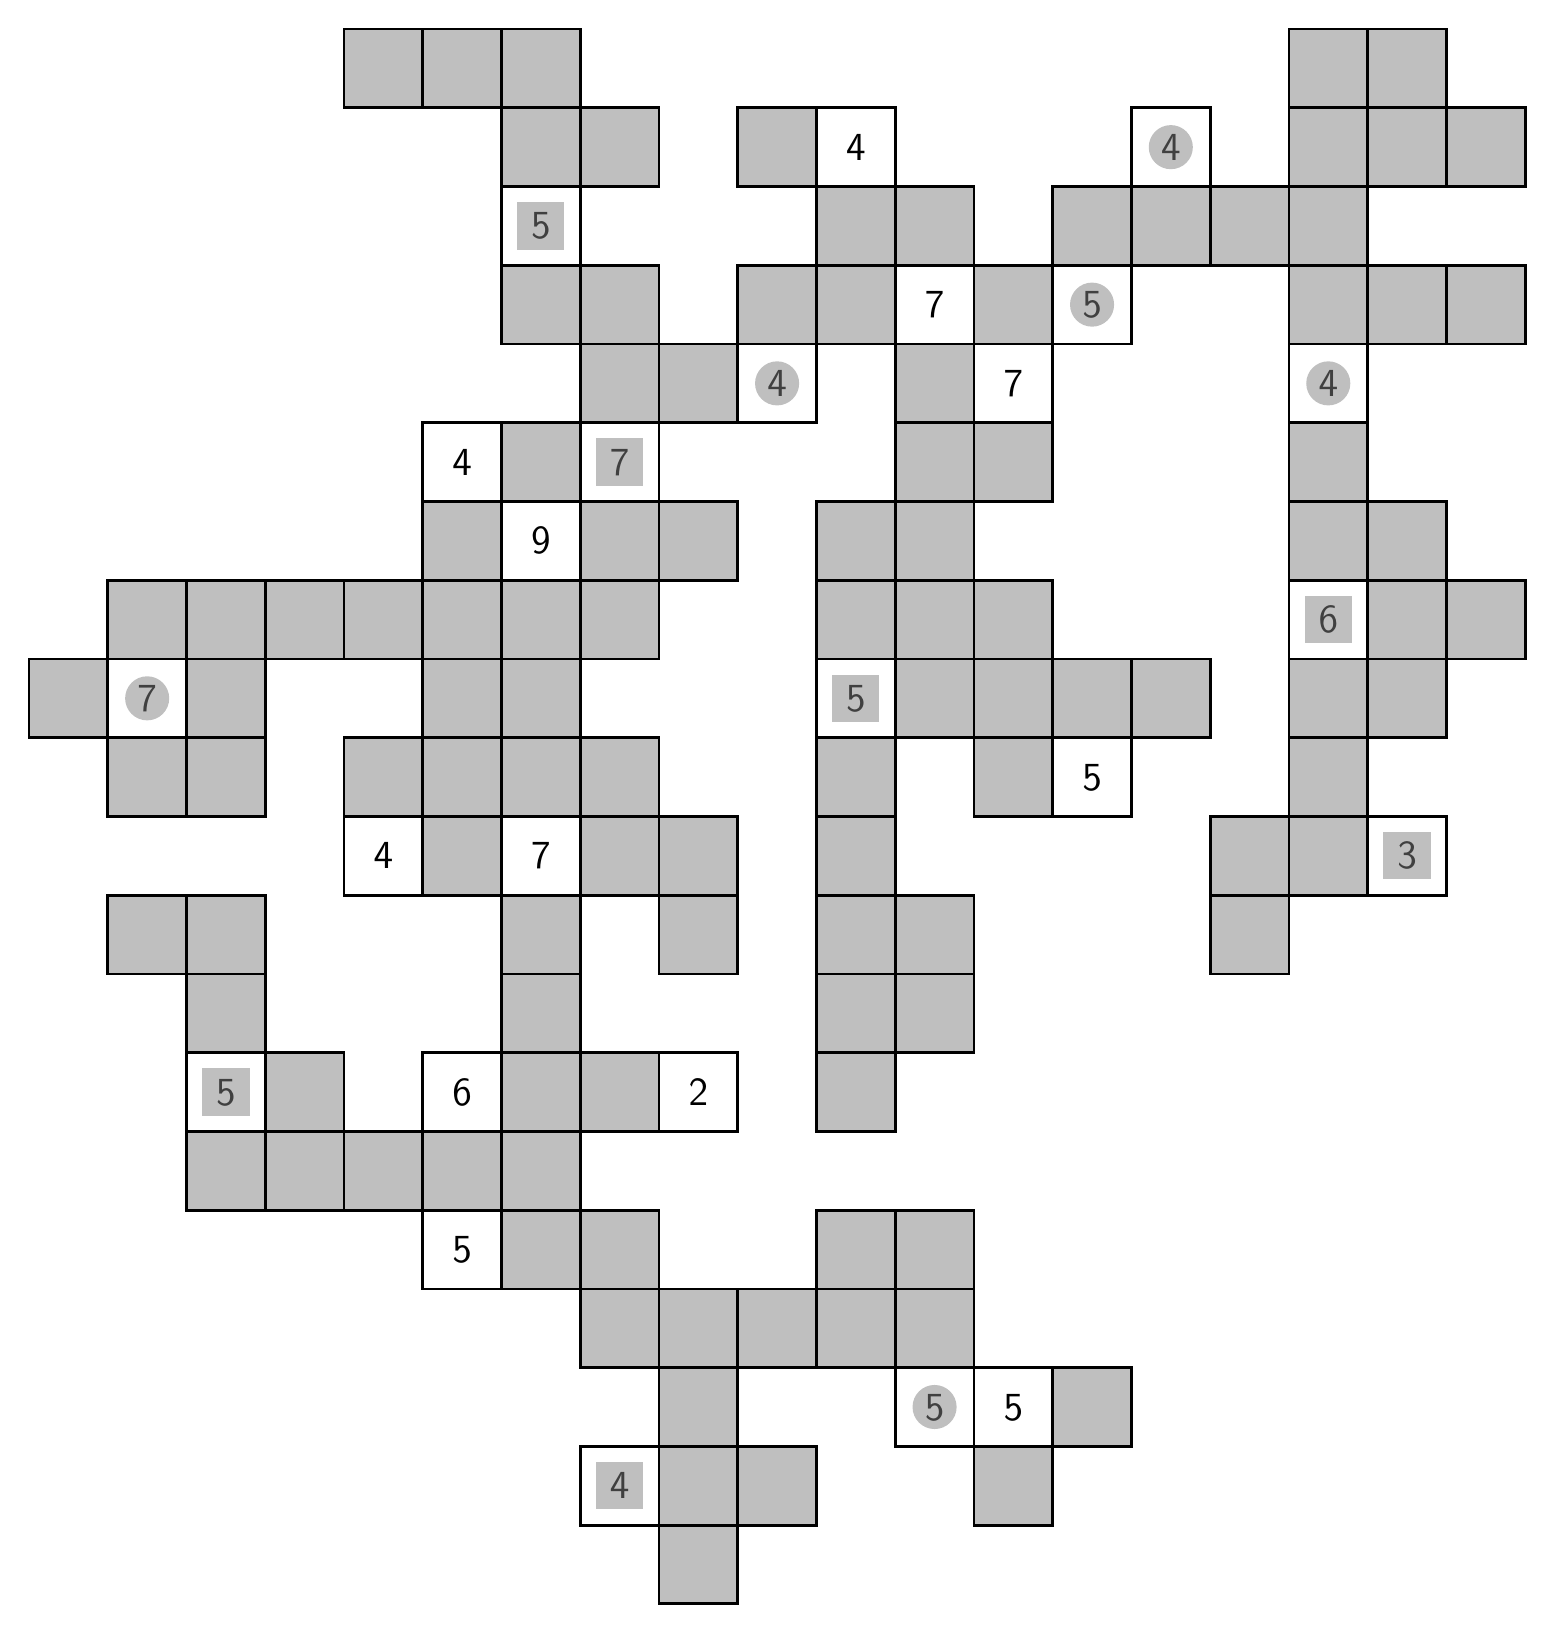
\begin{tikzpicture}\fill[gray, opacity = 0.5] (9, 0, 0)--++(1, 0, 0)--++(0, 1, 0)--++(-1, 0, 0)--cycle;
\draw[line width = 1pt] (9, 0, 0)--++(1, 0, 0)--++(0, 1, 0)--++(-1, 0, 0)--cycle;
\draw node at (8.5, 1.5, 0) {\Large $\mathsf{4}$};
\draw[line width = 1pt] (8, 1, 0)--++(1, 0, 0)--++(0, 1, 0)--++(-1, 0, 0)--cycle;
\fill[color = gray, opacity = 0.5] (8.2, 1.2) rectangle ++(0.6, 0.6);
\fill[gray, opacity = 0.5] (9, 1, 0)--++(1, 0, 0)--++(0, 1, 0)--++(-1, 0, 0)--cycle;
\draw[line width = 1pt] (9, 1, 0)--++(1, 0, 0)--++(0, 1, 0)--++(-1, 0, 0)--cycle;
\fill[gray, opacity = 0.5] (10, 1, 0)--++(1, 0, 0)--++(0, 1, 0)--++(-1, 0, 0)--cycle;
\draw[line width = 1pt] (10, 1, 0)--++(1, 0, 0)--++(0, 1, 0)--++(-1, 0, 0)--cycle;
\fill[gray, opacity = 0.5] (13, 1, 0)--++(1, 0, 0)--++(0, 1, 0)--++(-1, 0, 0)--cycle;
\draw[line width = 1pt] (13, 1, 0)--++(1, 0, 0)--++(0, 1, 0)--++(-1, 0, 0)--cycle;
\fill[gray, opacity = 0.5] (9, 2, 0)--++(1, 0, 0)--++(0, 1, 0)--++(-1, 0, 0)--cycle;
\draw[line width = 1pt] (9, 2, 0)--++(1, 0, 0)--++(0, 1, 0)--++(-1, 0, 0)--cycle;
\draw node at (12.5, 2.5, 0) {\Large $\mathsf{5}$};
\draw[line width = 1pt] (12, 2, 0)--++(1, 0, 0)--++(0, 1, 0)--++(-1, 0, 0)--cycle;
\fill[color = gray, opacity = 0.5] (12.5, 2.5, 0) circle (0.28);
\draw node at (13.5, 2.5, 0) {\Large $\mathsf{5}$};
\draw[line width = 1pt] (13, 2, 0)--++(1, 0, 0)--++(0, 1, 0)--++(-1, 0, 0)--cycle;
\fill[gray, opacity = 0.5] (14, 2, 0)--++(1, 0, 0)--++(0, 1, 0)--++(-1, 0, 0)--cycle;
\draw[line width = 1pt] (14, 2, 0)--++(1, 0, 0)--++(0, 1, 0)--++(-1, 0, 0)--cycle;
\fill[gray, opacity = 0.5] (8, 3, 0)--++(1, 0, 0)--++(0, 1, 0)--++(-1, 0, 0)--cycle;
\draw[line width = 1pt] (8, 3, 0)--++(1, 0, 0)--++(0, 1, 0)--++(-1, 0, 0)--cycle;
\fill[gray, opacity = 0.5] (9, 3, 0)--++(1, 0, 0)--++(0, 1, 0)--++(-1, 0, 0)--cycle;
\draw[line width = 1pt] (9, 3, 0)--++(1, 0, 0)--++(0, 1, 0)--++(-1, 0, 0)--cycle;
\fill[gray, opacity = 0.5] (10, 3, 0)--++(1, 0, 0)--++(0, 1, 0)--++(-1, 0, 0)--cycle;
\draw[line width = 1pt] (10, 3, 0)--++(1, 0, 0)--++(0, 1, 0)--++(-1, 0, 0)--cycle;
\fill[gray, opacity = 0.5] (11, 3, 0)--++(1, 0, 0)--++(0, 1, 0)--++(-1, 0, 0)--cycle;
\draw[line width = 1pt] (11, 3, 0)--++(1, 0, 0)--++(0, 1, 0)--++(-1, 0, 0)--cycle;
\fill[gray, opacity = 0.5] (12, 3, 0)--++(1, 0, 0)--++(0, 1, 0)--++(-1, 0, 0)--cycle;
\draw[line width = 1pt] (12, 3, 0)--++(1, 0, 0)--++(0, 1, 0)--++(-1, 0, 0)--cycle;
\draw node at (6.5, 4.5, 0) {\Large $\mathsf{5}$};
\draw[line width = 1pt] (6, 4, 0)--++(1, 0, 0)--++(0, 1, 0)--++(-1, 0, 0)--cycle;
\fill[gray, opacity = 0.5] (7, 4, 0)--++(1, 0, 0)--++(0, 1, 0)--++(-1, 0, 0)--cycle;
\draw[line width = 1pt] (7, 4, 0)--++(1, 0, 0)--++(0, 1, 0)--++(-1, 0, 0)--cycle;
\fill[gray, opacity = 0.5] (8, 4, 0)--++(1, 0, 0)--++(0, 1, 0)--++(-1, 0, 0)--cycle;
\draw[line width = 1pt] (8, 4, 0)--++(1, 0, 0)--++(0, 1, 0)--++(-1, 0, 0)--cycle;
\fill[gray, opacity = 0.5] (11, 4, 0)--++(1, 0, 0)--++(0, 1, 0)--++(-1, 0, 0)--cycle;
\draw[line width = 1pt] (11, 4, 0)--++(1, 0, 0)--++(0, 1, 0)--++(-1, 0, 0)--cycle;
\fill[gray, opacity = 0.5] (12, 4, 0)--++(1, 0, 0)--++(0, 1, 0)--++(-1, 0, 0)--cycle;
\draw[line width = 1pt] (12, 4, 0)--++(1, 0, 0)--++(0, 1, 0)--++(-1, 0, 0)--cycle;
\fill[gray, opacity = 0.5] (3, 5, 0)--++(1, 0, 0)--++(0, 1, 0)--++(-1, 0, 0)--cycle;
\draw[line width = 1pt] (3, 5, 0)--++(1, 0, 0)--++(0, 1, 0)--++(-1, 0, 0)--cycle;
\fill[gray, opacity = 0.5] (4, 5, 0)--++(1, 0, 0)--++(0, 1, 0)--++(-1, 0, 0)--cycle;
\draw[line width = 1pt] (4, 5, 0)--++(1, 0, 0)--++(0, 1, 0)--++(-1, 0, 0)--cycle;
\fill[gray, opacity = 0.5] (5, 5, 0)--++(1, 0, 0)--++(0, 1, 0)--++(-1, 0, 0)--cycle;
\draw[line width = 1pt] (5, 5, 0)--++(1, 0, 0)--++(0, 1, 0)--++(-1, 0, 0)--cycle;
\fill[gray, opacity = 0.5] (6, 5, 0)--++(1, 0, 0)--++(0, 1, 0)--++(-1, 0, 0)--cycle;
\draw[line width = 1pt] (6, 5, 0)--++(1, 0, 0)--++(0, 1, 0)--++(-1, 0, 0)--cycle;
\fill[gray, opacity = 0.5] (7, 5, 0)--++(1, 0, 0)--++(0, 1, 0)--++(-1, 0, 0)--cycle;
\draw[line width = 1pt] (7, 5, 0)--++(1, 0, 0)--++(0, 1, 0)--++(-1, 0, 0)--cycle;
\draw node at (3.5, 6.5, 0) {\Large $\mathsf{5}$};
\draw[line width = 1pt] (3, 6, 0)--++(1, 0, 0)--++(0, 1, 0)--++(-1, 0, 0)--cycle;
\fill[color = gray, opacity = 0.5] (3.2, 6.2) rectangle ++(0.6, 0.6);
\fill[gray, opacity = 0.5] (4, 6, 0)--++(1, 0, 0)--++(0, 1, 0)--++(-1, 0, 0)--cycle;
\draw[line width = 1pt] (4, 6, 0)--++(1, 0, 0)--++(0, 1, 0)--++(-1, 0, 0)--cycle;
\draw node at (6.5, 6.5, 0) {\Large $\mathsf{6}$};
\draw[line width = 1pt] (6, 6, 0)--++(1, 0, 0)--++(0, 1, 0)--++(-1, 0, 0)--cycle;
\fill[gray, opacity = 0.5] (7, 6, 0)--++(1, 0, 0)--++(0, 1, 0)--++(-1, 0, 0)--cycle;
\draw[line width = 1pt] (7, 6, 0)--++(1, 0, 0)--++(0, 1, 0)--++(-1, 0, 0)--cycle;
\fill[gray, opacity = 0.5] (8, 6, 0)--++(1, 0, 0)--++(0, 1, 0)--++(-1, 0, 0)--cycle;
\draw[line width = 1pt] (8, 6, 0)--++(1, 0, 0)--++(0, 1, 0)--++(-1, 0, 0)--cycle;
\draw node at (9.5, 6.5, 0) {\Large $\mathsf{2}$};
\draw[line width = 1pt] (9, 6, 0)--++(1, 0, 0)--++(0, 1, 0)--++(-1, 0, 0)--cycle;
\fill[gray, opacity = 0.5] (11, 6, 0)--++(1, 0, 0)--++(0, 1, 0)--++(-1, 0, 0)--cycle;
\draw[line width = 1pt] (11, 6, 0)--++(1, 0, 0)--++(0, 1, 0)--++(-1, 0, 0)--cycle;
\fill[gray, opacity = 0.5] (3, 7, 0)--++(1, 0, 0)--++(0, 1, 0)--++(-1, 0, 0)--cycle;
\draw[line width = 1pt] (3, 7, 0)--++(1, 0, 0)--++(0, 1, 0)--++(-1, 0, 0)--cycle;
\fill[gray, opacity = 0.5] (7, 7, 0)--++(1, 0, 0)--++(0, 1, 0)--++(-1, 0, 0)--cycle;
\draw[line width = 1pt] (7, 7, 0)--++(1, 0, 0)--++(0, 1, 0)--++(-1, 0, 0)--cycle;
\fill[gray, opacity = 0.5] (11, 7, 0)--++(1, 0, 0)--++(0, 1, 0)--++(-1, 0, 0)--cycle;
\draw[line width = 1pt] (11, 7, 0)--++(1, 0, 0)--++(0, 1, 0)--++(-1, 0, 0)--cycle;
\fill[gray, opacity = 0.5] (12, 7, 0)--++(1, 0, 0)--++(0, 1, 0)--++(-1, 0, 0)--cycle;
\draw[line width = 1pt] (12, 7, 0)--++(1, 0, 0)--++(0, 1, 0)--++(-1, 0, 0)--cycle;
\fill[gray, opacity = 0.5] (2, 8, 0)--++(1, 0, 0)--++(0, 1, 0)--++(-1, 0, 0)--cycle;
\draw[line width = 1pt] (2, 8, 0)--++(1, 0, 0)--++(0, 1, 0)--++(-1, 0, 0)--cycle;
\fill[gray, opacity = 0.5] (3, 8, 0)--++(1, 0, 0)--++(0, 1, 0)--++(-1, 0, 0)--cycle;
\draw[line width = 1pt] (3, 8, 0)--++(1, 0, 0)--++(0, 1, 0)--++(-1, 0, 0)--cycle;
\fill[gray, opacity = 0.5] (7, 8, 0)--++(1, 0, 0)--++(0, 1, 0)--++(-1, 0, 0)--cycle;
\draw[line width = 1pt] (7, 8, 0)--++(1, 0, 0)--++(0, 1, 0)--++(-1, 0, 0)--cycle;
\fill[gray, opacity = 0.5] (9, 8, 0)--++(1, 0, 0)--++(0, 1, 0)--++(-1, 0, 0)--cycle;
\draw[line width = 1pt] (9, 8, 0)--++(1, 0, 0)--++(0, 1, 0)--++(-1, 0, 0)--cycle;
\fill[gray, opacity = 0.5] (11, 8, 0)--++(1, 0, 0)--++(0, 1, 0)--++(-1, 0, 0)--cycle;
\draw[line width = 1pt] (11, 8, 0)--++(1, 0, 0)--++(0, 1, 0)--++(-1, 0, 0)--cycle;
\fill[gray, opacity = 0.5] (12, 8, 0)--++(1, 0, 0)--++(0, 1, 0)--++(-1, 0, 0)--cycle;
\draw[line width = 1pt] (12, 8, 0)--++(1, 0, 0)--++(0, 1, 0)--++(-1, 0, 0)--cycle;
\fill[gray, opacity = 0.5] (16, 8, 0)--++(1, 0, 0)--++(0, 1, 0)--++(-1, 0, 0)--cycle;
\draw[line width = 1pt] (16, 8, 0)--++(1, 0, 0)--++(0, 1, 0)--++(-1, 0, 0)--cycle;
\draw node at (5.5, 9.5, 0) {\Large $\mathsf{4}$};
\draw[line width = 1pt] (5, 9, 0)--++(1, 0, 0)--++(0, 1, 0)--++(-1, 0, 0)--cycle;
\fill[gray, opacity = 0.5] (6, 9, 0)--++(1, 0, 0)--++(0, 1, 0)--++(-1, 0, 0)--cycle;
\draw[line width = 1pt] (6, 9, 0)--++(1, 0, 0)--++(0, 1, 0)--++(-1, 0, 0)--cycle;
\draw node at (7.5, 9.5, 0) {\Large $\mathsf{7}$};
\draw[line width = 1pt] (7, 9, 0)--++(1, 0, 0)--++(0, 1, 0)--++(-1, 0, 0)--cycle;
\fill[gray, opacity = 0.5] (8, 9, 0)--++(1, 0, 0)--++(0, 1, 0)--++(-1, 0, 0)--cycle;
\draw[line width = 1pt] (8, 9, 0)--++(1, 0, 0)--++(0, 1, 0)--++(-1, 0, 0)--cycle;
\fill[gray, opacity = 0.5] (9, 9, 0)--++(1, 0, 0)--++(0, 1, 0)--++(-1, 0, 0)--cycle;
\draw[line width = 1pt] (9, 9, 0)--++(1, 0, 0)--++(0, 1, 0)--++(-1, 0, 0)--cycle;
\fill[gray, opacity = 0.5] (11, 9, 0)--++(1, 0, 0)--++(0, 1, 0)--++(-1, 0, 0)--cycle;
\draw[line width = 1pt] (11, 9, 0)--++(1, 0, 0)--++(0, 1, 0)--++(-1, 0, 0)--cycle;
\fill[gray, opacity = 0.5] (16, 9, 0)--++(1, 0, 0)--++(0, 1, 0)--++(-1, 0, 0)--cycle;
\draw[line width = 1pt] (16, 9, 0)--++(1, 0, 0)--++(0, 1, 0)--++(-1, 0, 0)--cycle;
\fill[gray, opacity = 0.5] (17, 9, 0)--++(1, 0, 0)--++(0, 1, 0)--++(-1, 0, 0)--cycle;
\draw[line width = 1pt] (17, 9, 0)--++(1, 0, 0)--++(0, 1, 0)--++(-1, 0, 0)--cycle;
\draw node at (18.5, 9.5, 0) {\Large $\mathsf{3}$};
\draw[line width = 1pt] (18, 9, 0)--++(1, 0, 0)--++(0, 1, 0)--++(-1, 0, 0)--cycle;
\fill[color = gray, opacity = 0.5] (18.2, 9.2) rectangle ++(0.6, 0.6);
\fill[gray, opacity = 0.5] (2, 10, 0)--++(1, 0, 0)--++(0, 1, 0)--++(-1, 0, 0)--cycle;
\draw[line width = 1pt] (2, 10, 0)--++(1, 0, 0)--++(0, 1, 0)--++(-1, 0, 0)--cycle;
\fill[gray, opacity = 0.5] (3, 10, 0)--++(1, 0, 0)--++(0, 1, 0)--++(-1, 0, 0)--cycle;
\draw[line width = 1pt] (3, 10, 0)--++(1, 0, 0)--++(0, 1, 0)--++(-1, 0, 0)--cycle;
\fill[gray, opacity = 0.5] (5, 10, 0)--++(1, 0, 0)--++(0, 1, 0)--++(-1, 0, 0)--cycle;
\draw[line width = 1pt] (5, 10, 0)--++(1, 0, 0)--++(0, 1, 0)--++(-1, 0, 0)--cycle;
\fill[gray, opacity = 0.5] (6, 10, 0)--++(1, 0, 0)--++(0, 1, 0)--++(-1, 0, 0)--cycle;
\draw[line width = 1pt] (6, 10, 0)--++(1, 0, 0)--++(0, 1, 0)--++(-1, 0, 0)--cycle;
\fill[gray, opacity = 0.5] (7, 10, 0)--++(1, 0, 0)--++(0, 1, 0)--++(-1, 0, 0)--cycle;
\draw[line width = 1pt] (7, 10, 0)--++(1, 0, 0)--++(0, 1, 0)--++(-1, 0, 0)--cycle;
\fill[gray, opacity = 0.5] (8, 10, 0)--++(1, 0, 0)--++(0, 1, 0)--++(-1, 0, 0)--cycle;
\draw[line width = 1pt] (8, 10, 0)--++(1, 0, 0)--++(0, 1, 0)--++(-1, 0, 0)--cycle;
\fill[gray, opacity = 0.5] (11, 10, 0)--++(1, 0, 0)--++(0, 1, 0)--++(-1, 0, 0)--cycle;
\draw[line width = 1pt] (11, 10, 0)--++(1, 0, 0)--++(0, 1, 0)--++(-1, 0, 0)--cycle;
\fill[gray, opacity = 0.5] (13, 10, 0)--++(1, 0, 0)--++(0, 1, 0)--++(-1, 0, 0)--cycle;
\draw[line width = 1pt] (13, 10, 0)--++(1, 0, 0)--++(0, 1, 0)--++(-1, 0, 0)--cycle;
\draw node at (14.5, 10.5, 0) {\Large $\mathsf{5}$};
\draw[line width = 1pt] (14, 10, 0)--++(1, 0, 0)--++(0, 1, 0)--++(-1, 0, 0)--cycle;
\fill[gray, opacity = 0.5] (17, 10, 0)--++(1, 0, 0)--++(0, 1, 0)--++(-1, 0, 0)--cycle;
\draw[line width = 1pt] (17, 10, 0)--++(1, 0, 0)--++(0, 1, 0)--++(-1, 0, 0)--cycle;
\fill[gray, opacity = 0.5] (1, 11, 0)--++(1, 0, 0)--++(0, 1, 0)--++(-1, 0, 0)--cycle;
\draw[line width = 1pt] (1, 11, 0)--++(1, 0, 0)--++(0, 1, 0)--++(-1, 0, 0)--cycle;
\draw node at (2.5, 11.5, 0) {\Large $\mathsf{7}$};
\draw[line width = 1pt] (2, 11, 0)--++(1, 0, 0)--++(0, 1, 0)--++(-1, 0, 0)--cycle;
\fill[color = gray, opacity = 0.5] (2.5, 11.5, 0) circle (0.28);
\fill[gray, opacity = 0.5] (3, 11, 0)--++(1, 0, 0)--++(0, 1, 0)--++(-1, 0, 0)--cycle;
\draw[line width = 1pt] (3, 11, 0)--++(1, 0, 0)--++(0, 1, 0)--++(-1, 0, 0)--cycle;
\fill[gray, opacity = 0.5] (6, 11, 0)--++(1, 0, 0)--++(0, 1, 0)--++(-1, 0, 0)--cycle;
\draw[line width = 1pt] (6, 11, 0)--++(1, 0, 0)--++(0, 1, 0)--++(-1, 0, 0)--cycle;
\fill[gray, opacity = 0.5] (7, 11, 0)--++(1, 0, 0)--++(0, 1, 0)--++(-1, 0, 0)--cycle;
\draw[line width = 1pt] (7, 11, 0)--++(1, 0, 0)--++(0, 1, 0)--++(-1, 0, 0)--cycle;
\draw node at (11.5, 11.5, 0) {\Large $\mathsf{5}$};
\draw[line width = 1pt] (11, 11, 0)--++(1, 0, 0)--++(0, 1, 0)--++(-1, 0, 0)--cycle;
\fill[color = gray, opacity = 0.5] (11.2, 11.2) rectangle ++(0.6, 0.6);
\fill[gray, opacity = 0.5] (12, 11, 0)--++(1, 0, 0)--++(0, 1, 0)--++(-1, 0, 0)--cycle;
\draw[line width = 1pt] (12, 11, 0)--++(1, 0, 0)--++(0, 1, 0)--++(-1, 0, 0)--cycle;
\fill[gray, opacity = 0.5] (13, 11, 0)--++(1, 0, 0)--++(0, 1, 0)--++(-1, 0, 0)--cycle;
\draw[line width = 1pt] (13, 11, 0)--++(1, 0, 0)--++(0, 1, 0)--++(-1, 0, 0)--cycle;
\fill[gray, opacity = 0.5] (14, 11, 0)--++(1, 0, 0)--++(0, 1, 0)--++(-1, 0, 0)--cycle;
\draw[line width = 1pt] (14, 11, 0)--++(1, 0, 0)--++(0, 1, 0)--++(-1, 0, 0)--cycle;
\fill[gray, opacity = 0.5] (15, 11, 0)--++(1, 0, 0)--++(0, 1, 0)--++(-1, 0, 0)--cycle;
\draw[line width = 1pt] (15, 11, 0)--++(1, 0, 0)--++(0, 1, 0)--++(-1, 0, 0)--cycle;
\fill[gray, opacity = 0.5] (17, 11, 0)--++(1, 0, 0)--++(0, 1, 0)--++(-1, 0, 0)--cycle;
\draw[line width = 1pt] (17, 11, 0)--++(1, 0, 0)--++(0, 1, 0)--++(-1, 0, 0)--cycle;
\fill[gray, opacity = 0.5] (18, 11, 0)--++(1, 0, 0)--++(0, 1, 0)--++(-1, 0, 0)--cycle;
\draw[line width = 1pt] (18, 11, 0)--++(1, 0, 0)--++(0, 1, 0)--++(-1, 0, 0)--cycle;
\fill[gray, opacity = 0.5] (2, 12, 0)--++(1, 0, 0)--++(0, 1, 0)--++(-1, 0, 0)--cycle;
\draw[line width = 1pt] (2, 12, 0)--++(1, 0, 0)--++(0, 1, 0)--++(-1, 0, 0)--cycle;
\fill[gray, opacity = 0.5] (3, 12, 0)--++(1, 0, 0)--++(0, 1, 0)--++(-1, 0, 0)--cycle;
\draw[line width = 1pt] (3, 12, 0)--++(1, 0, 0)--++(0, 1, 0)--++(-1, 0, 0)--cycle;
\fill[gray, opacity = 0.5] (4, 12, 0)--++(1, 0, 0)--++(0, 1, 0)--++(-1, 0, 0)--cycle;
\draw[line width = 1pt] (4, 12, 0)--++(1, 0, 0)--++(0, 1, 0)--++(-1, 0, 0)--cycle;
\fill[gray, opacity = 0.5] (5, 12, 0)--++(1, 0, 0)--++(0, 1, 0)--++(-1, 0, 0)--cycle;
\draw[line width = 1pt] (5, 12, 0)--++(1, 0, 0)--++(0, 1, 0)--++(-1, 0, 0)--cycle;
\fill[gray, opacity = 0.5] (6, 12, 0)--++(1, 0, 0)--++(0, 1, 0)--++(-1, 0, 0)--cycle;
\draw[line width = 1pt] (6, 12, 0)--++(1, 0, 0)--++(0, 1, 0)--++(-1, 0, 0)--cycle;
\fill[gray, opacity = 0.5] (7, 12, 0)--++(1, 0, 0)--++(0, 1, 0)--++(-1, 0, 0)--cycle;
\draw[line width = 1pt] (7, 12, 0)--++(1, 0, 0)--++(0, 1, 0)--++(-1, 0, 0)--cycle;
\fill[gray, opacity = 0.5] (8, 12, 0)--++(1, 0, 0)--++(0, 1, 0)--++(-1, 0, 0)--cycle;
\draw[line width = 1pt] (8, 12, 0)--++(1, 0, 0)--++(0, 1, 0)--++(-1, 0, 0)--cycle;
\fill[gray, opacity = 0.5] (11, 12, 0)--++(1, 0, 0)--++(0, 1, 0)--++(-1, 0, 0)--cycle;
\draw[line width = 1pt] (11, 12, 0)--++(1, 0, 0)--++(0, 1, 0)--++(-1, 0, 0)--cycle;
\fill[gray, opacity = 0.5] (12, 12, 0)--++(1, 0, 0)--++(0, 1, 0)--++(-1, 0, 0)--cycle;
\draw[line width = 1pt] (12, 12, 0)--++(1, 0, 0)--++(0, 1, 0)--++(-1, 0, 0)--cycle;
\fill[gray, opacity = 0.5] (13, 12, 0)--++(1, 0, 0)--++(0, 1, 0)--++(-1, 0, 0)--cycle;
\draw[line width = 1pt] (13, 12, 0)--++(1, 0, 0)--++(0, 1, 0)--++(-1, 0, 0)--cycle;
\draw node at (17.5, 12.5, 0) {\Large $\mathsf{6}$};
\draw[line width = 1pt] (17, 12, 0)--++(1, 0, 0)--++(0, 1, 0)--++(-1, 0, 0)--cycle;
\fill[color = gray, opacity = 0.5] (17.2, 12.2) rectangle ++(0.6, 0.6);
\fill[gray, opacity = 0.5] (18, 12, 0)--++(1, 0, 0)--++(0, 1, 0)--++(-1, 0, 0)--cycle;
\draw[line width = 1pt] (18, 12, 0)--++(1, 0, 0)--++(0, 1, 0)--++(-1, 0, 0)--cycle;
\fill[gray, opacity = 0.5] (19, 12, 0)--++(1, 0, 0)--++(0, 1, 0)--++(-1, 0, 0)--cycle;
\draw[line width = 1pt] (19, 12, 0)--++(1, 0, 0)--++(0, 1, 0)--++(-1, 0, 0)--cycle;
\fill[gray, opacity = 0.5] (6, 13, 0)--++(1, 0, 0)--++(0, 1, 0)--++(-1, 0, 0)--cycle;
\draw[line width = 1pt] (6, 13, 0)--++(1, 0, 0)--++(0, 1, 0)--++(-1, 0, 0)--cycle;
\draw node at (7.5, 13.5, 0) {\Large $\mathsf{9}$};
\draw[line width = 1pt] (7, 13, 0)--++(1, 0, 0)--++(0, 1, 0)--++(-1, 0, 0)--cycle;
\fill[gray, opacity = 0.5] (8, 13, 0)--++(1, 0, 0)--++(0, 1, 0)--++(-1, 0, 0)--cycle;
\draw[line width = 1pt] (8, 13, 0)--++(1, 0, 0)--++(0, 1, 0)--++(-1, 0, 0)--cycle;
\fill[gray, opacity = 0.5] (9, 13, 0)--++(1, 0, 0)--++(0, 1, 0)--++(-1, 0, 0)--cycle;
\draw[line width = 1pt] (9, 13, 0)--++(1, 0, 0)--++(0, 1, 0)--++(-1, 0, 0)--cycle;
\fill[gray, opacity = 0.5] (11, 13, 0)--++(1, 0, 0)--++(0, 1, 0)--++(-1, 0, 0)--cycle;
\draw[line width = 1pt] (11, 13, 0)--++(1, 0, 0)--++(0, 1, 0)--++(-1, 0, 0)--cycle;
\fill[gray, opacity = 0.5] (12, 13, 0)--++(1, 0, 0)--++(0, 1, 0)--++(-1, 0, 0)--cycle;
\draw[line width = 1pt] (12, 13, 0)--++(1, 0, 0)--++(0, 1, 0)--++(-1, 0, 0)--cycle;
\fill[gray, opacity = 0.5] (17, 13, 0)--++(1, 0, 0)--++(0, 1, 0)--++(-1, 0, 0)--cycle;
\draw[line width = 1pt] (17, 13, 0)--++(1, 0, 0)--++(0, 1, 0)--++(-1, 0, 0)--cycle;
\fill[gray, opacity = 0.5] (18, 13, 0)--++(1, 0, 0)--++(0, 1, 0)--++(-1, 0, 0)--cycle;
\draw[line width = 1pt] (18, 13, 0)--++(1, 0, 0)--++(0, 1, 0)--++(-1, 0, 0)--cycle;
\draw node at (6.5, 14.5, 0) {\Large $\mathsf{4}$};
\draw[line width = 1pt] (6, 14, 0)--++(1, 0, 0)--++(0, 1, 0)--++(-1, 0, 0)--cycle;
\fill[gray, opacity = 0.5] (7, 14, 0)--++(1, 0, 0)--++(0, 1, 0)--++(-1, 0, 0)--cycle;
\draw[line width = 1pt] (7, 14, 0)--++(1, 0, 0)--++(0, 1, 0)--++(-1, 0, 0)--cycle;
\draw node at (8.5, 14.5, 0) {\Large $\mathsf{7}$};
\draw[line width = 1pt] (8, 14, 0)--++(1, 0, 0)--++(0, 1, 0)--++(-1, 0, 0)--cycle;
\fill[color = gray, opacity = 0.5] (8.2, 14.2) rectangle ++(0.6, 0.6);
\fill[gray, opacity = 0.5] (12, 14, 0)--++(1, 0, 0)--++(0, 1, 0)--++(-1, 0, 0)--cycle;
\draw[line width = 1pt] (12, 14, 0)--++(1, 0, 0)--++(0, 1, 0)--++(-1, 0, 0)--cycle;
\fill[gray, opacity = 0.5] (13, 14, 0)--++(1, 0, 0)--++(0, 1, 0)--++(-1, 0, 0)--cycle;
\draw[line width = 1pt] (13, 14, 0)--++(1, 0, 0)--++(0, 1, 0)--++(-1, 0, 0)--cycle;
\fill[gray, opacity = 0.5] (17, 14, 0)--++(1, 0, 0)--++(0, 1, 0)--++(-1, 0, 0)--cycle;
\draw[line width = 1pt] (17, 14, 0)--++(1, 0, 0)--++(0, 1, 0)--++(-1, 0, 0)--cycle;
\fill[gray, opacity = 0.5] (8, 15, 0)--++(1, 0, 0)--++(0, 1, 0)--++(-1, 0, 0)--cycle;
\draw[line width = 1pt] (8, 15, 0)--++(1, 0, 0)--++(0, 1, 0)--++(-1, 0, 0)--cycle;
\fill[gray, opacity = 0.5] (9, 15, 0)--++(1, 0, 0)--++(0, 1, 0)--++(-1, 0, 0)--cycle;
\draw[line width = 1pt] (9, 15, 0)--++(1, 0, 0)--++(0, 1, 0)--++(-1, 0, 0)--cycle;
\draw node at (10.5, 15.5, 0) {\Large $\mathsf{4}$};
\draw[line width = 1pt] (10, 15, 0)--++(1, 0, 0)--++(0, 1, 0)--++(-1, 0, 0)--cycle;
\fill[color = gray, opacity = 0.5] (10.5, 15.5, 0) circle (0.28);
\fill[gray, opacity = 0.5] (12, 15, 0)--++(1, 0, 0)--++(0, 1, 0)--++(-1, 0, 0)--cycle;
\draw[line width = 1pt] (12, 15, 0)--++(1, 0, 0)--++(0, 1, 0)--++(-1, 0, 0)--cycle;
\draw node at (13.5, 15.5, 0) {\Large $\mathsf{7}$};
\draw[line width = 1pt] (13, 15, 0)--++(1, 0, 0)--++(0, 1, 0)--++(-1, 0, 0)--cycle;
\draw node at (17.5, 15.5, 0) {\Large $\mathsf{4}$};
\draw[line width = 1pt] (17, 15, 0)--++(1, 0, 0)--++(0, 1, 0)--++(-1, 0, 0)--cycle;
\fill[color = gray, opacity = 0.5] (17.5, 15.5, 0) circle (0.28);
\fill[gray, opacity = 0.5] (7, 16, 0)--++(1, 0, 0)--++(0, 1, 0)--++(-1, 0, 0)--cycle;
\draw[line width = 1pt] (7, 16, 0)--++(1, 0, 0)--++(0, 1, 0)--++(-1, 0, 0)--cycle;
\fill[gray, opacity = 0.5] (8, 16, 0)--++(1, 0, 0)--++(0, 1, 0)--++(-1, 0, 0)--cycle;
\draw[line width = 1pt] (8, 16, 0)--++(1, 0, 0)--++(0, 1, 0)--++(-1, 0, 0)--cycle;
\fill[gray, opacity = 0.5] (10, 16, 0)--++(1, 0, 0)--++(0, 1, 0)--++(-1, 0, 0)--cycle;
\draw[line width = 1pt] (10, 16, 0)--++(1, 0, 0)--++(0, 1, 0)--++(-1, 0, 0)--cycle;
\fill[gray, opacity = 0.5] (11, 16, 0)--++(1, 0, 0)--++(0, 1, 0)--++(-1, 0, 0)--cycle;
\draw[line width = 1pt] (11, 16, 0)--++(1, 0, 0)--++(0, 1, 0)--++(-1, 0, 0)--cycle;
\draw node at (12.5, 16.5, 0) {\Large $\mathsf{7}$};
\draw[line width = 1pt] (12, 16, 0)--++(1, 0, 0)--++(0, 1, 0)--++(-1, 0, 0)--cycle;
\fill[gray, opacity = 0.5] (13, 16, 0)--++(1, 0, 0)--++(0, 1, 0)--++(-1, 0, 0)--cycle;
\draw[line width = 1pt] (13, 16, 0)--++(1, 0, 0)--++(0, 1, 0)--++(-1, 0, 0)--cycle;
\draw node at (14.5, 16.5, 0) {\Large $\mathsf{5}$};
\draw[line width = 1pt] (14, 16, 0)--++(1, 0, 0)--++(0, 1, 0)--++(-1, 0, 0)--cycle;
\fill[color = gray, opacity = 0.5] (14.5, 16.5, 0) circle (0.28);
\fill[gray, opacity = 0.5] (17, 16, 0)--++(1, 0, 0)--++(0, 1, 0)--++(-1, 0, 0)--cycle;
\draw[line width = 1pt] (17, 16, 0)--++(1, 0, 0)--++(0, 1, 0)--++(-1, 0, 0)--cycle;
\fill[gray, opacity = 0.5] (18, 16, 0)--++(1, 0, 0)--++(0, 1, 0)--++(-1, 0, 0)--cycle;
\draw[line width = 1pt] (18, 16, 0)--++(1, 0, 0)--++(0, 1, 0)--++(-1, 0, 0)--cycle;
\fill[gray, opacity = 0.5] (19, 16, 0)--++(1, 0, 0)--++(0, 1, 0)--++(-1, 0, 0)--cycle;
\draw[line width = 1pt] (19, 16, 0)--++(1, 0, 0)--++(0, 1, 0)--++(-1, 0, 0)--cycle;
\draw node at (7.5, 17.5, 0) {\Large $\mathsf{5}$};
\draw[line width = 1pt] (7, 17, 0)--++(1, 0, 0)--++(0, 1, 0)--++(-1, 0, 0)--cycle;
\fill[color = gray, opacity = 0.5] (7.2, 17.2) rectangle ++(0.6, 0.6);
\fill[gray, opacity = 0.5] (11, 17, 0)--++(1, 0, 0)--++(0, 1, 0)--++(-1, 0, 0)--cycle;
\draw[line width = 1pt] (11, 17, 0)--++(1, 0, 0)--++(0, 1, 0)--++(-1, 0, 0)--cycle;
\fill[gray, opacity = 0.5] (12, 17, 0)--++(1, 0, 0)--++(0, 1, 0)--++(-1, 0, 0)--cycle;
\draw[line width = 1pt] (12, 17, 0)--++(1, 0, 0)--++(0, 1, 0)--++(-1, 0, 0)--cycle;
\fill[gray, opacity = 0.5] (14, 17, 0)--++(1, 0, 0)--++(0, 1, 0)--++(-1, 0, 0)--cycle;
\draw[line width = 1pt] (14, 17, 0)--++(1, 0, 0)--++(0, 1, 0)--++(-1, 0, 0)--cycle;
\fill[gray, opacity = 0.5] (15, 17, 0)--++(1, 0, 0)--++(0, 1, 0)--++(-1, 0, 0)--cycle;
\draw[line width = 1pt] (15, 17, 0)--++(1, 0, 0)--++(0, 1, 0)--++(-1, 0, 0)--cycle;
\fill[gray, opacity = 0.5] (16, 17, 0)--++(1, 0, 0)--++(0, 1, 0)--++(-1, 0, 0)--cycle;
\draw[line width = 1pt] (16, 17, 0)--++(1, 0, 0)--++(0, 1, 0)--++(-1, 0, 0)--cycle;
\fill[gray, opacity = 0.5] (17, 17, 0)--++(1, 0, 0)--++(0, 1, 0)--++(-1, 0, 0)--cycle;
\draw[line width = 1pt] (17, 17, 0)--++(1, 0, 0)--++(0, 1, 0)--++(-1, 0, 0)--cycle;
\fill[gray, opacity = 0.5] (7, 18, 0)--++(1, 0, 0)--++(0, 1, 0)--++(-1, 0, 0)--cycle;
\draw[line width = 1pt] (7, 18, 0)--++(1, 0, 0)--++(0, 1, 0)--++(-1, 0, 0)--cycle;
\fill[gray, opacity = 0.5] (8, 18, 0)--++(1, 0, 0)--++(0, 1, 0)--++(-1, 0, 0)--cycle;
\draw[line width = 1pt] (8, 18, 0)--++(1, 0, 0)--++(0, 1, 0)--++(-1, 0, 0)--cycle;
\fill[gray, opacity = 0.5] (10, 18, 0)--++(1, 0, 0)--++(0, 1, 0)--++(-1, 0, 0)--cycle;
\draw[line width = 1pt] (10, 18, 0)--++(1, 0, 0)--++(0, 1, 0)--++(-1, 0, 0)--cycle;
\draw node at (11.5, 18.5, 0) {\Large $\mathsf{4}$};
\draw[line width = 1pt] (11, 18, 0)--++(1, 0, 0)--++(0, 1, 0)--++(-1, 0, 0)--cycle;
\draw node at (15.5, 18.5, 0) {\Large $\mathsf{4}$};
\draw[line width = 1pt] (15, 18, 0)--++(1, 0, 0)--++(0, 1, 0)--++(-1, 0, 0)--cycle;
\fill[color = gray, opacity = 0.5] (15.5, 18.5, 0) circle (0.28);
\fill[gray, opacity = 0.5] (17, 18, 0)--++(1, 0, 0)--++(0, 1, 0)--++(-1, 0, 0)--cycle;
\draw[line width = 1pt] (17, 18, 0)--++(1, 0, 0)--++(0, 1, 0)--++(-1, 0, 0)--cycle;
\fill[gray, opacity = 0.5] (18, 18, 0)--++(1, 0, 0)--++(0, 1, 0)--++(-1, 0, 0)--cycle;
\draw[line width = 1pt] (18, 18, 0)--++(1, 0, 0)--++(0, 1, 0)--++(-1, 0, 0)--cycle;
\fill[gray, opacity = 0.5] (19, 18, 0)--++(1, 0, 0)--++(0, 1, 0)--++(-1, 0, 0)--cycle;
\draw[line width = 1pt] (19, 18, 0)--++(1, 0, 0)--++(0, 1, 0)--++(-1, 0, 0)--cycle;
\fill[gray, opacity = 0.5] (5, 19, 0)--++(1, 0, 0)--++(0, 1, 0)--++(-1, 0, 0)--cycle;
\draw[line width = 1pt] (5, 19, 0)--++(1, 0, 0)--++(0, 1, 0)--++(-1, 0, 0)--cycle;
\fill[gray, opacity = 0.5] (6, 19, 0)--++(1, 0, 0)--++(0, 1, 0)--++(-1, 0, 0)--cycle;
\draw[line width = 1pt] (6, 19, 0)--++(1, 0, 0)--++(0, 1, 0)--++(-1, 0, 0)--cycle;
\fill[gray, opacity = 0.5] (7, 19, 0)--++(1, 0, 0)--++(0, 1, 0)--++(-1, 0, 0)--cycle;
\draw[line width = 1pt] (7, 19, 0)--++(1, 0, 0)--++(0, 1, 0)--++(-1, 0, 0)--cycle;
\fill[gray, opacity = 0.5] (17, 19, 0)--++(1, 0, 0)--++(0, 1, 0)--++(-1, 0, 0)--cycle;
\draw[line width = 1pt] (17, 19, 0)--++(1, 0, 0)--++(0, 1, 0)--++(-1, 0, 0)--cycle;
\fill[gray, opacity = 0.5] (18, 19, 0)--++(1, 0, 0)--++(0, 1, 0)--++(-1, 0, 0)--cycle;
\draw[line width = 1pt] (18, 19, 0)--++(1, 0, 0)--++(0, 1, 0)--++(-1, 0, 0)--cycle;
\end{tikzpicture}}\]
\[\resizebox{30pc}{!}{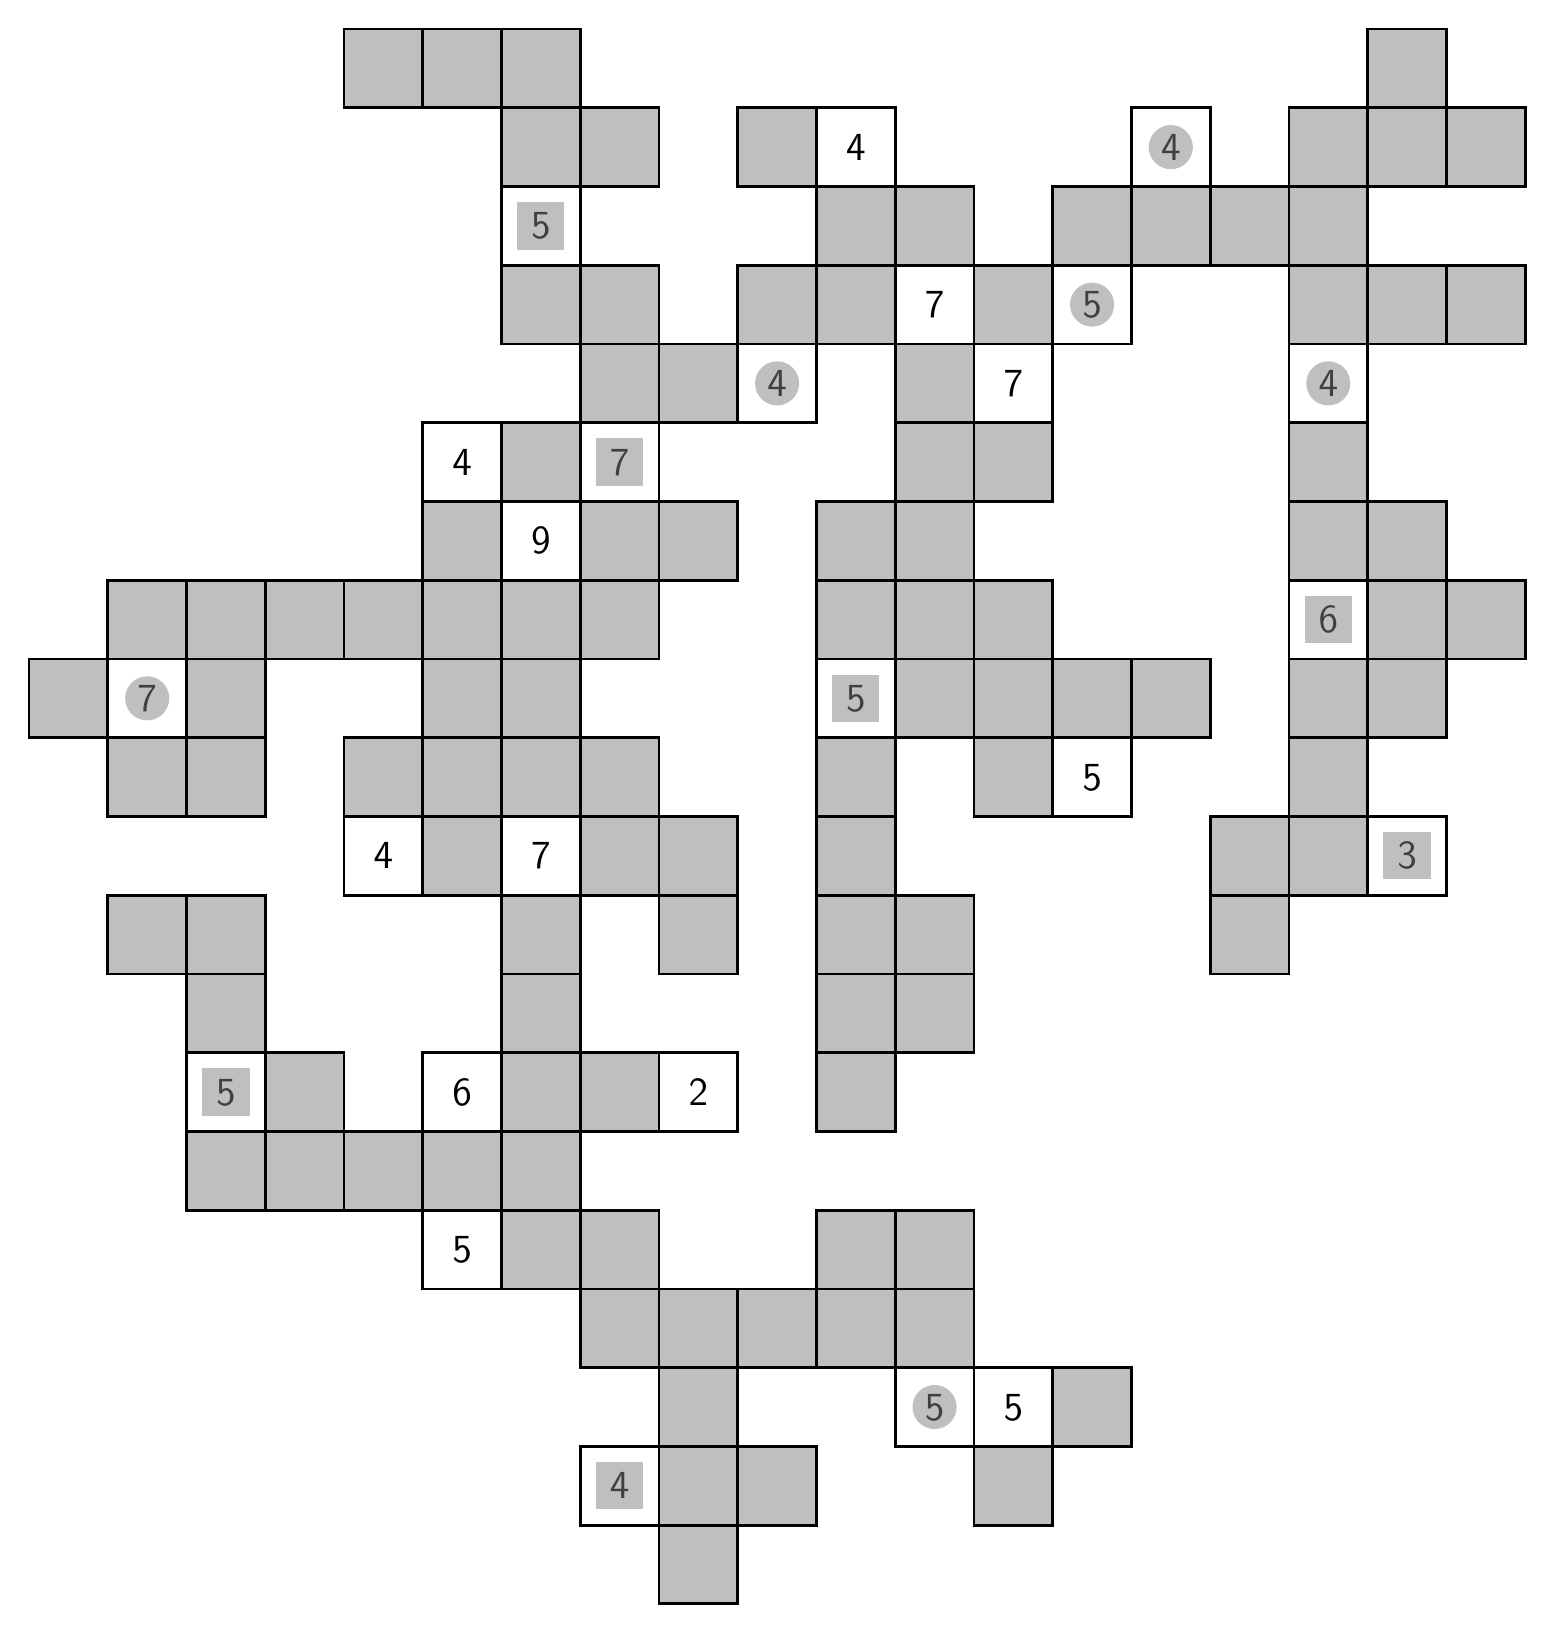
\begin{tikzpicture}\fill[gray, opacity = 0.5] (9, 0, 0)--++(1, 0, 0)--++(0, 1, 0)--++(-1, 0, 0)--cycle;
\draw[line width = 1pt] (9, 0, 0)--++(1, 0, 0)--++(0, 1, 0)--++(-1, 0, 0)--cycle;
\draw node at (8.5, 1.5, 0) {\Large $\mathsf{4}$};
\draw[line width = 1pt] (8, 1, 0)--++(1, 0, 0)--++(0, 1, 0)--++(-1, 0, 0)--cycle;
\fill[color = gray, opacity = 0.5] (8.2, 1.2) rectangle ++(0.6, 0.6);
\fill[gray, opacity = 0.5] (9, 1, 0)--++(1, 0, 0)--++(0, 1, 0)--++(-1, 0, 0)--cycle;
\draw[line width = 1pt] (9, 1, 0)--++(1, 0, 0)--++(0, 1, 0)--++(-1, 0, 0)--cycle;
\fill[gray, opacity = 0.5] (10, 1, 0)--++(1, 0, 0)--++(0, 1, 0)--++(-1, 0, 0)--cycle;
\draw[line width = 1pt] (10, 1, 0)--++(1, 0, 0)--++(0, 1, 0)--++(-1, 0, 0)--cycle;
\fill[gray, opacity = 0.5] (13, 1, 0)--++(1, 0, 0)--++(0, 1, 0)--++(-1, 0, 0)--cycle;
\draw[line width = 1pt] (13, 1, 0)--++(1, 0, 0)--++(0, 1, 0)--++(-1, 0, 0)--cycle;
\fill[gray, opacity = 0.5] (9, 2, 0)--++(1, 0, 0)--++(0, 1, 0)--++(-1, 0, 0)--cycle;
\draw[line width = 1pt] (9, 2, 0)--++(1, 0, 0)--++(0, 1, 0)--++(-1, 0, 0)--cycle;
\draw node at (12.5, 2.5, 0) {\Large $\mathsf{5}$};
\draw[line width = 1pt] (12, 2, 0)--++(1, 0, 0)--++(0, 1, 0)--++(-1, 0, 0)--cycle;
\fill[color = gray, opacity = 0.5] (12.5, 2.5, 0) circle (0.28);
\draw node at (13.5, 2.5, 0) {\Large $\mathsf{5}$};
\draw[line width = 1pt] (13, 2, 0)--++(1, 0, 0)--++(0, 1, 0)--++(-1, 0, 0)--cycle;
\fill[gray, opacity = 0.5] (14, 2, 0)--++(1, 0, 0)--++(0, 1, 0)--++(-1, 0, 0)--cycle;
\draw[line width = 1pt] (14, 2, 0)--++(1, 0, 0)--++(0, 1, 0)--++(-1, 0, 0)--cycle;
\fill[gray, opacity = 0.5] (8, 3, 0)--++(1, 0, 0)--++(0, 1, 0)--++(-1, 0, 0)--cycle;
\draw[line width = 1pt] (8, 3, 0)--++(1, 0, 0)--++(0, 1, 0)--++(-1, 0, 0)--cycle;
\fill[gray, opacity = 0.5] (9, 3, 0)--++(1, 0, 0)--++(0, 1, 0)--++(-1, 0, 0)--cycle;
\draw[line width = 1pt] (9, 3, 0)--++(1, 0, 0)--++(0, 1, 0)--++(-1, 0, 0)--cycle;
\fill[gray, opacity = 0.5] (10, 3, 0)--++(1, 0, 0)--++(0, 1, 0)--++(-1, 0, 0)--cycle;
\draw[line width = 1pt] (10, 3, 0)--++(1, 0, 0)--++(0, 1, 0)--++(-1, 0, 0)--cycle;
\fill[gray, opacity = 0.5] (11, 3, 0)--++(1, 0, 0)--++(0, 1, 0)--++(-1, 0, 0)--cycle;
\draw[line width = 1pt] (11, 3, 0)--++(1, 0, 0)--++(0, 1, 0)--++(-1, 0, 0)--cycle;
\fill[gray, opacity = 0.5] (12, 3, 0)--++(1, 0, 0)--++(0, 1, 0)--++(-1, 0, 0)--cycle;
\draw[line width = 1pt] (12, 3, 0)--++(1, 0, 0)--++(0, 1, 0)--++(-1, 0, 0)--cycle;
\draw node at (6.5, 4.5, 0) {\Large $\mathsf{5}$};
\draw[line width = 1pt] (6, 4, 0)--++(1, 0, 0)--++(0, 1, 0)--++(-1, 0, 0)--cycle;
\fill[gray, opacity = 0.5] (7, 4, 0)--++(1, 0, 0)--++(0, 1, 0)--++(-1, 0, 0)--cycle;
\draw[line width = 1pt] (7, 4, 0)--++(1, 0, 0)--++(0, 1, 0)--++(-1, 0, 0)--cycle;
\fill[gray, opacity = 0.5] (8, 4, 0)--++(1, 0, 0)--++(0, 1, 0)--++(-1, 0, 0)--cycle;
\draw[line width = 1pt] (8, 4, 0)--++(1, 0, 0)--++(0, 1, 0)--++(-1, 0, 0)--cycle;
\fill[gray, opacity = 0.5] (11, 4, 0)--++(1, 0, 0)--++(0, 1, 0)--++(-1, 0, 0)--cycle;
\draw[line width = 1pt] (11, 4, 0)--++(1, 0, 0)--++(0, 1, 0)--++(-1, 0, 0)--cycle;
\fill[gray, opacity = 0.5] (12, 4, 0)--++(1, 0, 0)--++(0, 1, 0)--++(-1, 0, 0)--cycle;
\draw[line width = 1pt] (12, 4, 0)--++(1, 0, 0)--++(0, 1, 0)--++(-1, 0, 0)--cycle;
\fill[gray, opacity = 0.5] (3, 5, 0)--++(1, 0, 0)--++(0, 1, 0)--++(-1, 0, 0)--cycle;
\draw[line width = 1pt] (3, 5, 0)--++(1, 0, 0)--++(0, 1, 0)--++(-1, 0, 0)--cycle;
\fill[gray, opacity = 0.5] (4, 5, 0)--++(1, 0, 0)--++(0, 1, 0)--++(-1, 0, 0)--cycle;
\draw[line width = 1pt] (4, 5, 0)--++(1, 0, 0)--++(0, 1, 0)--++(-1, 0, 0)--cycle;
\fill[gray, opacity = 0.5] (5, 5, 0)--++(1, 0, 0)--++(0, 1, 0)--++(-1, 0, 0)--cycle;
\draw[line width = 1pt] (5, 5, 0)--++(1, 0, 0)--++(0, 1, 0)--++(-1, 0, 0)--cycle;
\fill[gray, opacity = 0.5] (6, 5, 0)--++(1, 0, 0)--++(0, 1, 0)--++(-1, 0, 0)--cycle;
\draw[line width = 1pt] (6, 5, 0)--++(1, 0, 0)--++(0, 1, 0)--++(-1, 0, 0)--cycle;
\fill[gray, opacity = 0.5] (7, 5, 0)--++(1, 0, 0)--++(0, 1, 0)--++(-1, 0, 0)--cycle;
\draw[line width = 1pt] (7, 5, 0)--++(1, 0, 0)--++(0, 1, 0)--++(-1, 0, 0)--cycle;
\draw node at (3.5, 6.5, 0) {\Large $\mathsf{5}$};
\draw[line width = 1pt] (3, 6, 0)--++(1, 0, 0)--++(0, 1, 0)--++(-1, 0, 0)--cycle;
\fill[color = gray, opacity = 0.5] (3.2, 6.2) rectangle ++(0.6, 0.6);
\fill[gray, opacity = 0.5] (4, 6, 0)--++(1, 0, 0)--++(0, 1, 0)--++(-1, 0, 0)--cycle;
\draw[line width = 1pt] (4, 6, 0)--++(1, 0, 0)--++(0, 1, 0)--++(-1, 0, 0)--cycle;
\draw node at (6.5, 6.5, 0) {\Large $\mathsf{6}$};
\draw[line width = 1pt] (6, 6, 0)--++(1, 0, 0)--++(0, 1, 0)--++(-1, 0, 0)--cycle;
\fill[gray, opacity = 0.5] (7, 6, 0)--++(1, 0, 0)--++(0, 1, 0)--++(-1, 0, 0)--cycle;
\draw[line width = 1pt] (7, 6, 0)--++(1, 0, 0)--++(0, 1, 0)--++(-1, 0, 0)--cycle;
\fill[gray, opacity = 0.5] (8, 6, 0)--++(1, 0, 0)--++(0, 1, 0)--++(-1, 0, 0)--cycle;
\draw[line width = 1pt] (8, 6, 0)--++(1, 0, 0)--++(0, 1, 0)--++(-1, 0, 0)--cycle;
\draw node at (9.5, 6.5, 0) {\Large $\mathsf{2}$};
\draw[line width = 1pt] (9, 6, 0)--++(1, 0, 0)--++(0, 1, 0)--++(-1, 0, 0)--cycle;
\fill[gray, opacity = 0.5] (11, 6, 0)--++(1, 0, 0)--++(0, 1, 0)--++(-1, 0, 0)--cycle;
\draw[line width = 1pt] (11, 6, 0)--++(1, 0, 0)--++(0, 1, 0)--++(-1, 0, 0)--cycle;
\fill[gray, opacity = 0.5] (3, 7, 0)--++(1, 0, 0)--++(0, 1, 0)--++(-1, 0, 0)--cycle;
\draw[line width = 1pt] (3, 7, 0)--++(1, 0, 0)--++(0, 1, 0)--++(-1, 0, 0)--cycle;
\fill[gray, opacity = 0.5] (7, 7, 0)--++(1, 0, 0)--++(0, 1, 0)--++(-1, 0, 0)--cycle;
\draw[line width = 1pt] (7, 7, 0)--++(1, 0, 0)--++(0, 1, 0)--++(-1, 0, 0)--cycle;
\fill[gray, opacity = 0.5] (11, 7, 0)--++(1, 0, 0)--++(0, 1, 0)--++(-1, 0, 0)--cycle;
\draw[line width = 1pt] (11, 7, 0)--++(1, 0, 0)--++(0, 1, 0)--++(-1, 0, 0)--cycle;
\fill[gray, opacity = 0.5] (12, 7, 0)--++(1, 0, 0)--++(0, 1, 0)--++(-1, 0, 0)--cycle;
\draw[line width = 1pt] (12, 7, 0)--++(1, 0, 0)--++(0, 1, 0)--++(-1, 0, 0)--cycle;
\fill[gray, opacity = 0.5] (2, 8, 0)--++(1, 0, 0)--++(0, 1, 0)--++(-1, 0, 0)--cycle;
\draw[line width = 1pt] (2, 8, 0)--++(1, 0, 0)--++(0, 1, 0)--++(-1, 0, 0)--cycle;
\fill[gray, opacity = 0.5] (3, 8, 0)--++(1, 0, 0)--++(0, 1, 0)--++(-1, 0, 0)--cycle;
\draw[line width = 1pt] (3, 8, 0)--++(1, 0, 0)--++(0, 1, 0)--++(-1, 0, 0)--cycle;
\fill[gray, opacity = 0.5] (7, 8, 0)--++(1, 0, 0)--++(0, 1, 0)--++(-1, 0, 0)--cycle;
\draw[line width = 1pt] (7, 8, 0)--++(1, 0, 0)--++(0, 1, 0)--++(-1, 0, 0)--cycle;
\fill[gray, opacity = 0.5] (9, 8, 0)--++(1, 0, 0)--++(0, 1, 0)--++(-1, 0, 0)--cycle;
\draw[line width = 1pt] (9, 8, 0)--++(1, 0, 0)--++(0, 1, 0)--++(-1, 0, 0)--cycle;
\fill[gray, opacity = 0.5] (11, 8, 0)--++(1, 0, 0)--++(0, 1, 0)--++(-1, 0, 0)--cycle;
\draw[line width = 1pt] (11, 8, 0)--++(1, 0, 0)--++(0, 1, 0)--++(-1, 0, 0)--cycle;
\fill[gray, opacity = 0.5] (12, 8, 0)--++(1, 0, 0)--++(0, 1, 0)--++(-1, 0, 0)--cycle;
\draw[line width = 1pt] (12, 8, 0)--++(1, 0, 0)--++(0, 1, 0)--++(-1, 0, 0)--cycle;
\fill[gray, opacity = 0.5] (16, 8, 0)--++(1, 0, 0)--++(0, 1, 0)--++(-1, 0, 0)--cycle;
\draw[line width = 1pt] (16, 8, 0)--++(1, 0, 0)--++(0, 1, 0)--++(-1, 0, 0)--cycle;
\draw node at (5.5, 9.5, 0) {\Large $\mathsf{4}$};
\draw[line width = 1pt] (5, 9, 0)--++(1, 0, 0)--++(0, 1, 0)--++(-1, 0, 0)--cycle;
\fill[gray, opacity = 0.5] (6, 9, 0)--++(1, 0, 0)--++(0, 1, 0)--++(-1, 0, 0)--cycle;
\draw[line width = 1pt] (6, 9, 0)--++(1, 0, 0)--++(0, 1, 0)--++(-1, 0, 0)--cycle;
\draw node at (7.5, 9.5, 0) {\Large $\mathsf{7}$};
\draw[line width = 1pt] (7, 9, 0)--++(1, 0, 0)--++(0, 1, 0)--++(-1, 0, 0)--cycle;
\fill[gray, opacity = 0.5] (8, 9, 0)--++(1, 0, 0)--++(0, 1, 0)--++(-1, 0, 0)--cycle;
\draw[line width = 1pt] (8, 9, 0)--++(1, 0, 0)--++(0, 1, 0)--++(-1, 0, 0)--cycle;
\fill[gray, opacity = 0.5] (9, 9, 0)--++(1, 0, 0)--++(0, 1, 0)--++(-1, 0, 0)--cycle;
\draw[line width = 1pt] (9, 9, 0)--++(1, 0, 0)--++(0, 1, 0)--++(-1, 0, 0)--cycle;
\fill[gray, opacity = 0.5] (11, 9, 0)--++(1, 0, 0)--++(0, 1, 0)--++(-1, 0, 0)--cycle;
\draw[line width = 1pt] (11, 9, 0)--++(1, 0, 0)--++(0, 1, 0)--++(-1, 0, 0)--cycle;
\fill[gray, opacity = 0.5] (16, 9, 0)--++(1, 0, 0)--++(0, 1, 0)--++(-1, 0, 0)--cycle;
\draw[line width = 1pt] (16, 9, 0)--++(1, 0, 0)--++(0, 1, 0)--++(-1, 0, 0)--cycle;
\fill[gray, opacity = 0.5] (17, 9, 0)--++(1, 0, 0)--++(0, 1, 0)--++(-1, 0, 0)--cycle;
\draw[line width = 1pt] (17, 9, 0)--++(1, 0, 0)--++(0, 1, 0)--++(-1, 0, 0)--cycle;
\draw node at (18.5, 9.5, 0) {\Large $\mathsf{3}$};
\draw[line width = 1pt] (18, 9, 0)--++(1, 0, 0)--++(0, 1, 0)--++(-1, 0, 0)--cycle;
\fill[color = gray, opacity = 0.5] (18.2, 9.2) rectangle ++(0.6, 0.6);
\fill[gray, opacity = 0.5] (2, 10, 0)--++(1, 0, 0)--++(0, 1, 0)--++(-1, 0, 0)--cycle;
\draw[line width = 1pt] (2, 10, 0)--++(1, 0, 0)--++(0, 1, 0)--++(-1, 0, 0)--cycle;
\fill[gray, opacity = 0.5] (3, 10, 0)--++(1, 0, 0)--++(0, 1, 0)--++(-1, 0, 0)--cycle;
\draw[line width = 1pt] (3, 10, 0)--++(1, 0, 0)--++(0, 1, 0)--++(-1, 0, 0)--cycle;
\fill[gray, opacity = 0.5] (5, 10, 0)--++(1, 0, 0)--++(0, 1, 0)--++(-1, 0, 0)--cycle;
\draw[line width = 1pt] (5, 10, 0)--++(1, 0, 0)--++(0, 1, 0)--++(-1, 0, 0)--cycle;
\fill[gray, opacity = 0.5] (6, 10, 0)--++(1, 0, 0)--++(0, 1, 0)--++(-1, 0, 0)--cycle;
\draw[line width = 1pt] (6, 10, 0)--++(1, 0, 0)--++(0, 1, 0)--++(-1, 0, 0)--cycle;
\fill[gray, opacity = 0.5] (7, 10, 0)--++(1, 0, 0)--++(0, 1, 0)--++(-1, 0, 0)--cycle;
\draw[line width = 1pt] (7, 10, 0)--++(1, 0, 0)--++(0, 1, 0)--++(-1, 0, 0)--cycle;
\fill[gray, opacity = 0.5] (8, 10, 0)--++(1, 0, 0)--++(0, 1, 0)--++(-1, 0, 0)--cycle;
\draw[line width = 1pt] (8, 10, 0)--++(1, 0, 0)--++(0, 1, 0)--++(-1, 0, 0)--cycle;
\fill[gray, opacity = 0.5] (11, 10, 0)--++(1, 0, 0)--++(0, 1, 0)--++(-1, 0, 0)--cycle;
\draw[line width = 1pt] (11, 10, 0)--++(1, 0, 0)--++(0, 1, 0)--++(-1, 0, 0)--cycle;
\fill[gray, opacity = 0.5] (13, 10, 0)--++(1, 0, 0)--++(0, 1, 0)--++(-1, 0, 0)--cycle;
\draw[line width = 1pt] (13, 10, 0)--++(1, 0, 0)--++(0, 1, 0)--++(-1, 0, 0)--cycle;
\draw node at (14.5, 10.5, 0) {\Large $\mathsf{5}$};
\draw[line width = 1pt] (14, 10, 0)--++(1, 0, 0)--++(0, 1, 0)--++(-1, 0, 0)--cycle;
\fill[gray, opacity = 0.5] (17, 10, 0)--++(1, 0, 0)--++(0, 1, 0)--++(-1, 0, 0)--cycle;
\draw[line width = 1pt] (17, 10, 0)--++(1, 0, 0)--++(0, 1, 0)--++(-1, 0, 0)--cycle;
\fill[gray, opacity = 0.5] (1, 11, 0)--++(1, 0, 0)--++(0, 1, 0)--++(-1, 0, 0)--cycle;
\draw[line width = 1pt] (1, 11, 0)--++(1, 0, 0)--++(0, 1, 0)--++(-1, 0, 0)--cycle;
\draw node at (2.5, 11.5, 0) {\Large $\mathsf{7}$};
\draw[line width = 1pt] (2, 11, 0)--++(1, 0, 0)--++(0, 1, 0)--++(-1, 0, 0)--cycle;
\fill[color = gray, opacity = 0.5] (2.5, 11.5, 0) circle (0.28);
\fill[gray, opacity = 0.5] (3, 11, 0)--++(1, 0, 0)--++(0, 1, 0)--++(-1, 0, 0)--cycle;
\draw[line width = 1pt] (3, 11, 0)--++(1, 0, 0)--++(0, 1, 0)--++(-1, 0, 0)--cycle;
\fill[gray, opacity = 0.5] (6, 11, 0)--++(1, 0, 0)--++(0, 1, 0)--++(-1, 0, 0)--cycle;
\draw[line width = 1pt] (6, 11, 0)--++(1, 0, 0)--++(0, 1, 0)--++(-1, 0, 0)--cycle;
\fill[gray, opacity = 0.5] (7, 11, 0)--++(1, 0, 0)--++(0, 1, 0)--++(-1, 0, 0)--cycle;
\draw[line width = 1pt] (7, 11, 0)--++(1, 0, 0)--++(0, 1, 0)--++(-1, 0, 0)--cycle;
\draw node at (11.5, 11.5, 0) {\Large $\mathsf{5}$};
\draw[line width = 1pt] (11, 11, 0)--++(1, 0, 0)--++(0, 1, 0)--++(-1, 0, 0)--cycle;
\fill[color = gray, opacity = 0.5] (11.2, 11.2) rectangle ++(0.6, 0.6);
\fill[gray, opacity = 0.5] (12, 11, 0)--++(1, 0, 0)--++(0, 1, 0)--++(-1, 0, 0)--cycle;
\draw[line width = 1pt] (12, 11, 0)--++(1, 0, 0)--++(0, 1, 0)--++(-1, 0, 0)--cycle;
\fill[gray, opacity = 0.5] (13, 11, 0)--++(1, 0, 0)--++(0, 1, 0)--++(-1, 0, 0)--cycle;
\draw[line width = 1pt] (13, 11, 0)--++(1, 0, 0)--++(0, 1, 0)--++(-1, 0, 0)--cycle;
\fill[gray, opacity = 0.5] (14, 11, 0)--++(1, 0, 0)--++(0, 1, 0)--++(-1, 0, 0)--cycle;
\draw[line width = 1pt] (14, 11, 0)--++(1, 0, 0)--++(0, 1, 0)--++(-1, 0, 0)--cycle;
\fill[gray, opacity = 0.5] (15, 11, 0)--++(1, 0, 0)--++(0, 1, 0)--++(-1, 0, 0)--cycle;
\draw[line width = 1pt] (15, 11, 0)--++(1, 0, 0)--++(0, 1, 0)--++(-1, 0, 0)--cycle;
\fill[gray, opacity = 0.5] (17, 11, 0)--++(1, 0, 0)--++(0, 1, 0)--++(-1, 0, 0)--cycle;
\draw[line width = 1pt] (17, 11, 0)--++(1, 0, 0)--++(0, 1, 0)--++(-1, 0, 0)--cycle;
\fill[gray, opacity = 0.5] (18, 11, 0)--++(1, 0, 0)--++(0, 1, 0)--++(-1, 0, 0)--cycle;
\draw[line width = 1pt] (18, 11, 0)--++(1, 0, 0)--++(0, 1, 0)--++(-1, 0, 0)--cycle;
\fill[gray, opacity = 0.5] (2, 12, 0)--++(1, 0, 0)--++(0, 1, 0)--++(-1, 0, 0)--cycle;
\draw[line width = 1pt] (2, 12, 0)--++(1, 0, 0)--++(0, 1, 0)--++(-1, 0, 0)--cycle;
\fill[gray, opacity = 0.5] (3, 12, 0)--++(1, 0, 0)--++(0, 1, 0)--++(-1, 0, 0)--cycle;
\draw[line width = 1pt] (3, 12, 0)--++(1, 0, 0)--++(0, 1, 0)--++(-1, 0, 0)--cycle;
\fill[gray, opacity = 0.5] (4, 12, 0)--++(1, 0, 0)--++(0, 1, 0)--++(-1, 0, 0)--cycle;
\draw[line width = 1pt] (4, 12, 0)--++(1, 0, 0)--++(0, 1, 0)--++(-1, 0, 0)--cycle;
\fill[gray, opacity = 0.5] (5, 12, 0)--++(1, 0, 0)--++(0, 1, 0)--++(-1, 0, 0)--cycle;
\draw[line width = 1pt] (5, 12, 0)--++(1, 0, 0)--++(0, 1, 0)--++(-1, 0, 0)--cycle;
\fill[gray, opacity = 0.5] (6, 12, 0)--++(1, 0, 0)--++(0, 1, 0)--++(-1, 0, 0)--cycle;
\draw[line width = 1pt] (6, 12, 0)--++(1, 0, 0)--++(0, 1, 0)--++(-1, 0, 0)--cycle;
\fill[gray, opacity = 0.5] (7, 12, 0)--++(1, 0, 0)--++(0, 1, 0)--++(-1, 0, 0)--cycle;
\draw[line width = 1pt] (7, 12, 0)--++(1, 0, 0)--++(0, 1, 0)--++(-1, 0, 0)--cycle;
\fill[gray, opacity = 0.5] (8, 12, 0)--++(1, 0, 0)--++(0, 1, 0)--++(-1, 0, 0)--cycle;
\draw[line width = 1pt] (8, 12, 0)--++(1, 0, 0)--++(0, 1, 0)--++(-1, 0, 0)--cycle;
\fill[gray, opacity = 0.5] (11, 12, 0)--++(1, 0, 0)--++(0, 1, 0)--++(-1, 0, 0)--cycle;
\draw[line width = 1pt] (11, 12, 0)--++(1, 0, 0)--++(0, 1, 0)--++(-1, 0, 0)--cycle;
\fill[gray, opacity = 0.5] (12, 12, 0)--++(1, 0, 0)--++(0, 1, 0)--++(-1, 0, 0)--cycle;
\draw[line width = 1pt] (12, 12, 0)--++(1, 0, 0)--++(0, 1, 0)--++(-1, 0, 0)--cycle;
\fill[gray, opacity = 0.5] (13, 12, 0)--++(1, 0, 0)--++(0, 1, 0)--++(-1, 0, 0)--cycle;
\draw[line width = 1pt] (13, 12, 0)--++(1, 0, 0)--++(0, 1, 0)--++(-1, 0, 0)--cycle;
\draw node at (17.5, 12.5, 0) {\Large $\mathsf{6}$};
\draw[line width = 1pt] (17, 12, 0)--++(1, 0, 0)--++(0, 1, 0)--++(-1, 0, 0)--cycle;
\fill[color = gray, opacity = 0.5] (17.2, 12.2) rectangle ++(0.6, 0.6);
\fill[gray, opacity = 0.5] (18, 12, 0)--++(1, 0, 0)--++(0, 1, 0)--++(-1, 0, 0)--cycle;
\draw[line width = 1pt] (18, 12, 0)--++(1, 0, 0)--++(0, 1, 0)--++(-1, 0, 0)--cycle;
\fill[gray, opacity = 0.5] (19, 12, 0)--++(1, 0, 0)--++(0, 1, 0)--++(-1, 0, 0)--cycle;
\draw[line width = 1pt] (19, 12, 0)--++(1, 0, 0)--++(0, 1, 0)--++(-1, 0, 0)--cycle;
\fill[gray, opacity = 0.5] (6, 13, 0)--++(1, 0, 0)--++(0, 1, 0)--++(-1, 0, 0)--cycle;
\draw[line width = 1pt] (6, 13, 0)--++(1, 0, 0)--++(0, 1, 0)--++(-1, 0, 0)--cycle;
\draw node at (7.5, 13.5, 0) {\Large $\mathsf{9}$};
\draw[line width = 1pt] (7, 13, 0)--++(1, 0, 0)--++(0, 1, 0)--++(-1, 0, 0)--cycle;
\fill[gray, opacity = 0.5] (8, 13, 0)--++(1, 0, 0)--++(0, 1, 0)--++(-1, 0, 0)--cycle;
\draw[line width = 1pt] (8, 13, 0)--++(1, 0, 0)--++(0, 1, 0)--++(-1, 0, 0)--cycle;
\fill[gray, opacity = 0.5] (9, 13, 0)--++(1, 0, 0)--++(0, 1, 0)--++(-1, 0, 0)--cycle;
\draw[line width = 1pt] (9, 13, 0)--++(1, 0, 0)--++(0, 1, 0)--++(-1, 0, 0)--cycle;
\fill[gray, opacity = 0.5] (11, 13, 0)--++(1, 0, 0)--++(0, 1, 0)--++(-1, 0, 0)--cycle;
\draw[line width = 1pt] (11, 13, 0)--++(1, 0, 0)--++(0, 1, 0)--++(-1, 0, 0)--cycle;
\fill[gray, opacity = 0.5] (12, 13, 0)--++(1, 0, 0)--++(0, 1, 0)--++(-1, 0, 0)--cycle;
\draw[line width = 1pt] (12, 13, 0)--++(1, 0, 0)--++(0, 1, 0)--++(-1, 0, 0)--cycle;
\fill[gray, opacity = 0.5] (17, 13, 0)--++(1, 0, 0)--++(0, 1, 0)--++(-1, 0, 0)--cycle;
\draw[line width = 1pt] (17, 13, 0)--++(1, 0, 0)--++(0, 1, 0)--++(-1, 0, 0)--cycle;
\fill[gray, opacity = 0.5] (18, 13, 0)--++(1, 0, 0)--++(0, 1, 0)--++(-1, 0, 0)--cycle;
\draw[line width = 1pt] (18, 13, 0)--++(1, 0, 0)--++(0, 1, 0)--++(-1, 0, 0)--cycle;
\draw node at (6.5, 14.5, 0) {\Large $\mathsf{4}$};
\draw[line width = 1pt] (6, 14, 0)--++(1, 0, 0)--++(0, 1, 0)--++(-1, 0, 0)--cycle;
\fill[gray, opacity = 0.5] (7, 14, 0)--++(1, 0, 0)--++(0, 1, 0)--++(-1, 0, 0)--cycle;
\draw[line width = 1pt] (7, 14, 0)--++(1, 0, 0)--++(0, 1, 0)--++(-1, 0, 0)--cycle;
\draw node at (8.5, 14.5, 0) {\Large $\mathsf{7}$};
\draw[line width = 1pt] (8, 14, 0)--++(1, 0, 0)--++(0, 1, 0)--++(-1, 0, 0)--cycle;
\fill[color = gray, opacity = 0.5] (8.2, 14.2) rectangle ++(0.6, 0.6);
\fill[gray, opacity = 0.5] (12, 14, 0)--++(1, 0, 0)--++(0, 1, 0)--++(-1, 0, 0)--cycle;
\draw[line width = 1pt] (12, 14, 0)--++(1, 0, 0)--++(0, 1, 0)--++(-1, 0, 0)--cycle;
\fill[gray, opacity = 0.5] (13, 14, 0)--++(1, 0, 0)--++(0, 1, 0)--++(-1, 0, 0)--cycle;
\draw[line width = 1pt] (13, 14, 0)--++(1, 0, 0)--++(0, 1, 0)--++(-1, 0, 0)--cycle;
\fill[gray, opacity = 0.5] (17, 14, 0)--++(1, 0, 0)--++(0, 1, 0)--++(-1, 0, 0)--cycle;
\draw[line width = 1pt] (17, 14, 0)--++(1, 0, 0)--++(0, 1, 0)--++(-1, 0, 0)--cycle;
\fill[gray, opacity = 0.5] (8, 15, 0)--++(1, 0, 0)--++(0, 1, 0)--++(-1, 0, 0)--cycle;
\draw[line width = 1pt] (8, 15, 0)--++(1, 0, 0)--++(0, 1, 0)--++(-1, 0, 0)--cycle;
\fill[gray, opacity = 0.5] (9, 15, 0)--++(1, 0, 0)--++(0, 1, 0)--++(-1, 0, 0)--cycle;
\draw[line width = 1pt] (9, 15, 0)--++(1, 0, 0)--++(0, 1, 0)--++(-1, 0, 0)--cycle;
\draw node at (10.5, 15.5, 0) {\Large $\mathsf{4}$};
\draw[line width = 1pt] (10, 15, 0)--++(1, 0, 0)--++(0, 1, 0)--++(-1, 0, 0)--cycle;
\fill[color = gray, opacity = 0.5] (10.5, 15.5, 0) circle (0.28);
\fill[gray, opacity = 0.5] (12, 15, 0)--++(1, 0, 0)--++(0, 1, 0)--++(-1, 0, 0)--cycle;
\draw[line width = 1pt] (12, 15, 0)--++(1, 0, 0)--++(0, 1, 0)--++(-1, 0, 0)--cycle;
\draw node at (13.5, 15.5, 0) {\Large $\mathsf{7}$};
\draw[line width = 1pt] (13, 15, 0)--++(1, 0, 0)--++(0, 1, 0)--++(-1, 0, 0)--cycle;
\draw node at (17.5, 15.5, 0) {\Large $\mathsf{4}$};
\draw[line width = 1pt] (17, 15, 0)--++(1, 0, 0)--++(0, 1, 0)--++(-1, 0, 0)--cycle;
\fill[color = gray, opacity = 0.5] (17.5, 15.5, 0) circle (0.28);
\fill[gray, opacity = 0.5] (7, 16, 0)--++(1, 0, 0)--++(0, 1, 0)--++(-1, 0, 0)--cycle;
\draw[line width = 1pt] (7, 16, 0)--++(1, 0, 0)--++(0, 1, 0)--++(-1, 0, 0)--cycle;
\fill[gray, opacity = 0.5] (8, 16, 0)--++(1, 0, 0)--++(0, 1, 0)--++(-1, 0, 0)--cycle;
\draw[line width = 1pt] (8, 16, 0)--++(1, 0, 0)--++(0, 1, 0)--++(-1, 0, 0)--cycle;
\fill[gray, opacity = 0.5] (10, 16, 0)--++(1, 0, 0)--++(0, 1, 0)--++(-1, 0, 0)--cycle;
\draw[line width = 1pt] (10, 16, 0)--++(1, 0, 0)--++(0, 1, 0)--++(-1, 0, 0)--cycle;
\fill[gray, opacity = 0.5] (11, 16, 0)--++(1, 0, 0)--++(0, 1, 0)--++(-1, 0, 0)--cycle;
\draw[line width = 1pt] (11, 16, 0)--++(1, 0, 0)--++(0, 1, 0)--++(-1, 0, 0)--cycle;
\draw node at (12.5, 16.5, 0) {\Large $\mathsf{7}$};
\draw[line width = 1pt] (12, 16, 0)--++(1, 0, 0)--++(0, 1, 0)--++(-1, 0, 0)--cycle;
\fill[gray, opacity = 0.5] (13, 16, 0)--++(1, 0, 0)--++(0, 1, 0)--++(-1, 0, 0)--cycle;
\draw[line width = 1pt] (13, 16, 0)--++(1, 0, 0)--++(0, 1, 0)--++(-1, 0, 0)--cycle;
\draw node at (14.5, 16.5, 0) {\Large $\mathsf{5}$};
\draw[line width = 1pt] (14, 16, 0)--++(1, 0, 0)--++(0, 1, 0)--++(-1, 0, 0)--cycle;
\fill[color = gray, opacity = 0.5] (14.5, 16.5, 0) circle (0.28);
\fill[gray, opacity = 0.5] (17, 16, 0)--++(1, 0, 0)--++(0, 1, 0)--++(-1, 0, 0)--cycle;
\draw[line width = 1pt] (17, 16, 0)--++(1, 0, 0)--++(0, 1, 0)--++(-1, 0, 0)--cycle;
\fill[gray, opacity = 0.5] (18, 16, 0)--++(1, 0, 0)--++(0, 1, 0)--++(-1, 0, 0)--cycle;
\draw[line width = 1pt] (18, 16, 0)--++(1, 0, 0)--++(0, 1, 0)--++(-1, 0, 0)--cycle;
\fill[gray, opacity = 0.5] (19, 16, 0)--++(1, 0, 0)--++(0, 1, 0)--++(-1, 0, 0)--cycle;
\draw[line width = 1pt] (19, 16, 0)--++(1, 0, 0)--++(0, 1, 0)--++(-1, 0, 0)--cycle;
\draw node at (7.5, 17.5, 0) {\Large $\mathsf{5}$};
\draw[line width = 1pt] (7, 17, 0)--++(1, 0, 0)--++(0, 1, 0)--++(-1, 0, 0)--cycle;
\fill[color = gray, opacity = 0.5] (7.2, 17.2) rectangle ++(0.6, 0.6);
\fill[gray, opacity = 0.5] (11, 17, 0)--++(1, 0, 0)--++(0, 1, 0)--++(-1, 0, 0)--cycle;
\draw[line width = 1pt] (11, 17, 0)--++(1, 0, 0)--++(0, 1, 0)--++(-1, 0, 0)--cycle;
\fill[gray, opacity = 0.5] (12, 17, 0)--++(1, 0, 0)--++(0, 1, 0)--++(-1, 0, 0)--cycle;
\draw[line width = 1pt] (12, 17, 0)--++(1, 0, 0)--++(0, 1, 0)--++(-1, 0, 0)--cycle;
\fill[gray, opacity = 0.5] (14, 17, 0)--++(1, 0, 0)--++(0, 1, 0)--++(-1, 0, 0)--cycle;
\draw[line width = 1pt] (14, 17, 0)--++(1, 0, 0)--++(0, 1, 0)--++(-1, 0, 0)--cycle;
\fill[gray, opacity = 0.5] (15, 17, 0)--++(1, 0, 0)--++(0, 1, 0)--++(-1, 0, 0)--cycle;
\draw[line width = 1pt] (15, 17, 0)--++(1, 0, 0)--++(0, 1, 0)--++(-1, 0, 0)--cycle;
\fill[gray, opacity = 0.5] (16, 17, 0)--++(1, 0, 0)--++(0, 1, 0)--++(-1, 0, 0)--cycle;
\draw[line width = 1pt] (16, 17, 0)--++(1, 0, 0)--++(0, 1, 0)--++(-1, 0, 0)--cycle;
\fill[gray, opacity = 0.5] (17, 17, 0)--++(1, 0, 0)--++(0, 1, 0)--++(-1, 0, 0)--cycle;
\draw[line width = 1pt] (17, 17, 0)--++(1, 0, 0)--++(0, 1, 0)--++(-1, 0, 0)--cycle;
\fill[gray, opacity = 0.5] (7, 18, 0)--++(1, 0, 0)--++(0, 1, 0)--++(-1, 0, 0)--cycle;
\draw[line width = 1pt] (7, 18, 0)--++(1, 0, 0)--++(0, 1, 0)--++(-1, 0, 0)--cycle;
\fill[gray, opacity = 0.5] (8, 18, 0)--++(1, 0, 0)--++(0, 1, 0)--++(-1, 0, 0)--cycle;
\draw[line width = 1pt] (8, 18, 0)--++(1, 0, 0)--++(0, 1, 0)--++(-1, 0, 0)--cycle;
\fill[gray, opacity = 0.5] (10, 18, 0)--++(1, 0, 0)--++(0, 1, 0)--++(-1, 0, 0)--cycle;
\draw[line width = 1pt] (10, 18, 0)--++(1, 0, 0)--++(0, 1, 0)--++(-1, 0, 0)--cycle;
\draw node at (11.5, 18.5, 0) {\Large $\mathsf{4}$};
\draw[line width = 1pt] (11, 18, 0)--++(1, 0, 0)--++(0, 1, 0)--++(-1, 0, 0)--cycle;
\draw node at (15.5, 18.5, 0) {\Large $\mathsf{4}$};
\draw[line width = 1pt] (15, 18, 0)--++(1, 0, 0)--++(0, 1, 0)--++(-1, 0, 0)--cycle;
\fill[color = gray, opacity = 0.5] (15.5, 18.5, 0) circle (0.28);
\fill[gray, opacity = 0.5] (17, 18, 0)--++(1, 0, 0)--++(0, 1, 0)--++(-1, 0, 0)--cycle;
\draw[line width = 1pt] (17, 18, 0)--++(1, 0, 0)--++(0, 1, 0)--++(-1, 0, 0)--cycle;
\fill[gray, opacity = 0.5] (18, 18, 0)--++(1, 0, 0)--++(0, 1, 0)--++(-1, 0, 0)--cycle;
\draw[line width = 1pt] (18, 18, 0)--++(1, 0, 0)--++(0, 1, 0)--++(-1, 0, 0)--cycle;
\fill[gray, opacity = 0.5] (19, 18, 0)--++(1, 0, 0)--++(0, 1, 0)--++(-1, 0, 0)--cycle;
\draw[line width = 1pt] (19, 18, 0)--++(1, 0, 0)--++(0, 1, 0)--++(-1, 0, 0)--cycle;
\fill[gray, opacity = 0.5] (5, 19, 0)--++(1, 0, 0)--++(0, 1, 0)--++(-1, 0, 0)--cycle;
\draw[line width = 1pt] (5, 19, 0)--++(1, 0, 0)--++(0, 1, 0)--++(-1, 0, 0)--cycle;
\fill[gray, opacity = 0.5] (6, 19, 0)--++(1, 0, 0)--++(0, 1, 0)--++(-1, 0, 0)--cycle;
\draw[line width = 1pt] (6, 19, 0)--++(1, 0, 0)--++(0, 1, 0)--++(-1, 0, 0)--cycle;
\fill[gray, opacity = 0.5] (7, 19, 0)--++(1, 0, 0)--++(0, 1, 0)--++(-1, 0, 0)--cycle;
\draw[line width = 1pt] (7, 19, 0)--++(1, 0, 0)--++(0, 1, 0)--++(-1, 0, 0)--cycle;
\fill[gray, opacity = 0.5] (18, 19, 0)--++(1, 0, 0)--++(0, 1, 0)--++(-1, 0, 0)--cycle;
\draw[line width = 1pt] (18, 19, 0)--++(1, 0, 0)--++(0, 1, 0)--++(-1, 0, 0)--cycle;
\end{tikzpicture}}\]
\[\resizebox{30pc}{!}{\begin{tikzpicture}\fill[gray, opacity = 0.5] (9, 0, 0)--++(1, 0, 0)--++(0, 1, 0)--++(-1, 0, 0)--cycle;
\draw[line width = 1pt] (9, 0, 0)--++(1, 0, 0)--++(0, 1, 0)--++(-1, 0, 0)--cycle;
\draw node at (8.5, 1.5, 0) {\Large $\mathsf{4}$};
\draw[line width = 1pt] (8, 1, 0)--++(1, 0, 0)--++(0, 1, 0)--++(-1, 0, 0)--cycle;
\fill[color = gray, opacity = 0.5] (8.2, 1.2) rectangle ++(0.6, 0.6);
\fill[gray, opacity = 0.5] (9, 1, 0)--++(1, 0, 0)--++(0, 1, 0)--++(-1, 0, 0)--cycle;
\draw[line width = 1pt] (9, 1, 0)--++(1, 0, 0)--++(0, 1, 0)--++(-1, 0, 0)--cycle;
\fill[gray, opacity = 0.5] (10, 1, 0)--++(1, 0, 0)--++(0, 1, 0)--++(-1, 0, 0)--cycle;
\draw[line width = 1pt] (10, 1, 0)--++(1, 0, 0)--++(0, 1, 0)--++(-1, 0, 0)--cycle;
\fill[gray, opacity = 0.5] (13, 1, 0)--++(1, 0, 0)--++(0, 1, 0)--++(-1, 0, 0)--cycle;
\draw[line width = 1pt] (13, 1, 0)--++(1, 0, 0)--++(0, 1, 0)--++(-1, 0, 0)--cycle;
\fill[gray, opacity = 0.5] (9, 2, 0)--++(1, 0, 0)--++(0, 1, 0)--++(-1, 0, 0)--cycle;
\draw[line width = 1pt] (9, 2, 0)--++(1, 0, 0)--++(0, 1, 0)--++(-1, 0, 0)--cycle;
\draw node at (12.5, 2.5, 0) {\Large $\mathsf{5}$};
\draw[line width = 1pt] (12, 2, 0)--++(1, 0, 0)--++(0, 1, 0)--++(-1, 0, 0)--cycle;
\fill[color = gray, opacity = 0.5] (12.5, 2.5, 0) circle (0.28);
\draw node at (13.5, 2.5, 0) {\Large $\mathsf{5}$};
\draw[line width = 1pt] (13, 2, 0)--++(1, 0, 0)--++(0, 1, 0)--++(-1, 0, 0)--cycle;
\fill[gray, opacity = 0.5] (14, 2, 0)--++(1, 0, 0)--++(0, 1, 0)--++(-1, 0, 0)--cycle;
\draw[line width = 1pt] (14, 2, 0)--++(1, 0, 0)--++(0, 1, 0)--++(-1, 0, 0)--cycle;
\fill[gray, opacity = 0.5] (8, 3, 0)--++(1, 0, 0)--++(0, 1, 0)--++(-1, 0, 0)--cycle;
\draw[line width = 1pt] (8, 3, 0)--++(1, 0, 0)--++(0, 1, 0)--++(-1, 0, 0)--cycle;
\fill[gray, opacity = 0.5] (9, 3, 0)--++(1, 0, 0)--++(0, 1, 0)--++(-1, 0, 0)--cycle;
\draw[line width = 1pt] (9, 3, 0)--++(1, 0, 0)--++(0, 1, 0)--++(-1, 0, 0)--cycle;
\fill[gray, opacity = 0.5] (10, 3, 0)--++(1, 0, 0)--++(0, 1, 0)--++(-1, 0, 0)--cycle;
\draw[line width = 1pt] (10, 3, 0)--++(1, 0, 0)--++(0, 1, 0)--++(-1, 0, 0)--cycle;
\fill[gray, opacity = 0.5] (11, 3, 0)--++(1, 0, 0)--++(0, 1, 0)--++(-1, 0, 0)--cycle;
\draw[line width = 1pt] (11, 3, 0)--++(1, 0, 0)--++(0, 1, 0)--++(-1, 0, 0)--cycle;
\fill[gray, opacity = 0.5] (12, 3, 0)--++(1, 0, 0)--++(0, 1, 0)--++(-1, 0, 0)--cycle;
\draw[line width = 1pt] (12, 3, 0)--++(1, 0, 0)--++(0, 1, 0)--++(-1, 0, 0)--cycle;
\draw node at (6.5, 4.5, 0) {\Large $\mathsf{5}$};
\draw[line width = 1pt] (6, 4, 0)--++(1, 0, 0)--++(0, 1, 0)--++(-1, 0, 0)--cycle;
\fill[gray, opacity = 0.5] (7, 4, 0)--++(1, 0, 0)--++(0, 1, 0)--++(-1, 0, 0)--cycle;
\draw[line width = 1pt] (7, 4, 0)--++(1, 0, 0)--++(0, 1, 0)--++(-1, 0, 0)--cycle;
\fill[gray, opacity = 0.5] (8, 4, 0)--++(1, 0, 0)--++(0, 1, 0)--++(-1, 0, 0)--cycle;
\draw[line width = 1pt] (8, 4, 0)--++(1, 0, 0)--++(0, 1, 0)--++(-1, 0, 0)--cycle;
\fill[gray, opacity = 0.5] (11, 4, 0)--++(1, 0, 0)--++(0, 1, 0)--++(-1, 0, 0)--cycle;
\draw[line width = 1pt] (11, 4, 0)--++(1, 0, 0)--++(0, 1, 0)--++(-1, 0, 0)--cycle;
\fill[gray, opacity = 0.5] (12, 4, 0)--++(1, 0, 0)--++(0, 1, 0)--++(-1, 0, 0)--cycle;
\draw[line width = 1pt] (12, 4, 0)--++(1, 0, 0)--++(0, 1, 0)--++(-1, 0, 0)--cycle;
\fill[gray, opacity = 0.5] (3, 5, 0)--++(1, 0, 0)--++(0, 1, 0)--++(-1, 0, 0)--cycle;
\draw[line width = 1pt] (3, 5, 0)--++(1, 0, 0)--++(0, 1, 0)--++(-1, 0, 0)--cycle;
\fill[gray, opacity = 0.5] (4, 5, 0)--++(1, 0, 0)--++(0, 1, 0)--++(-1, 0, 0)--cycle;
\draw[line width = 1pt] (4, 5, 0)--++(1, 0, 0)--++(0, 1, 0)--++(-1, 0, 0)--cycle;
\fill[gray, opacity = 0.5] (5, 5, 0)--++(1, 0, 0)--++(0, 1, 0)--++(-1, 0, 0)--cycle;
\draw[line width = 1pt] (5, 5, 0)--++(1, 0, 0)--++(0, 1, 0)--++(-1, 0, 0)--cycle;
\fill[gray, opacity = 0.5] (6, 5, 0)--++(1, 0, 0)--++(0, 1, 0)--++(-1, 0, 0)--cycle;
\draw[line width = 1pt] (6, 5, 0)--++(1, 0, 0)--++(0, 1, 0)--++(-1, 0, 0)--cycle;
\fill[gray, opacity = 0.5] (7, 5, 0)--++(1, 0, 0)--++(0, 1, 0)--++(-1, 0, 0)--cycle;
\draw[line width = 1pt] (7, 5, 0)--++(1, 0, 0)--++(0, 1, 0)--++(-1, 0, 0)--cycle;
\draw node at (3.5, 6.5, 0) {\Large $\mathsf{5}$};
\draw[line width = 1pt] (3, 6, 0)--++(1, 0, 0)--++(0, 1, 0)--++(-1, 0, 0)--cycle;
\fill[color = gray, opacity = 0.5] (3.2, 6.2) rectangle ++(0.6, 0.6);
\fill[gray, opacity = 0.5] (4, 6, 0)--++(1, 0, 0)--++(0, 1, 0)--++(-1, 0, 0)--cycle;
\draw[line width = 1pt] (4, 6, 0)--++(1, 0, 0)--++(0, 1, 0)--++(-1, 0, 0)--cycle;
\draw node at (6.5, 6.5, 0) {\Large $\mathsf{6}$};
\draw[line width = 1pt] (6, 6, 0)--++(1, 0, 0)--++(0, 1, 0)--++(-1, 0, 0)--cycle;
\fill[gray, opacity = 0.5] (7, 6, 0)--++(1, 0, 0)--++(0, 1, 0)--++(-1, 0, 0)--cycle;
\draw[line width = 1pt] (7, 6, 0)--++(1, 0, 0)--++(0, 1, 0)--++(-1, 0, 0)--cycle;
\fill[gray, opacity = 0.5] (8, 6, 0)--++(1, 0, 0)--++(0, 1, 0)--++(-1, 0, 0)--cycle;
\draw[line width = 1pt] (8, 6, 0)--++(1, 0, 0)--++(0, 1, 0)--++(-1, 0, 0)--cycle;
\draw node at (9.5, 6.5, 0) {\Large $\mathsf{2}$};
\draw[line width = 1pt] (9, 6, 0)--++(1, 0, 0)--++(0, 1, 0)--++(-1, 0, 0)--cycle;
\fill[gray, opacity = 0.5] (11, 6, 0)--++(1, 0, 0)--++(0, 1, 0)--++(-1, 0, 0)--cycle;
\draw[line width = 1pt] (11, 6, 0)--++(1, 0, 0)--++(0, 1, 0)--++(-1, 0, 0)--cycle;
\fill[gray, opacity = 0.5] (3, 7, 0)--++(1, 0, 0)--++(0, 1, 0)--++(-1, 0, 0)--cycle;
\draw[line width = 1pt] (3, 7, 0)--++(1, 0, 0)--++(0, 1, 0)--++(-1, 0, 0)--cycle;
\fill[gray, opacity = 0.5] (7, 7, 0)--++(1, 0, 0)--++(0, 1, 0)--++(-1, 0, 0)--cycle;
\draw[line width = 1pt] (7, 7, 0)--++(1, 0, 0)--++(0, 1, 0)--++(-1, 0, 0)--cycle;
\fill[gray, opacity = 0.5] (11, 7, 0)--++(1, 0, 0)--++(0, 1, 0)--++(-1, 0, 0)--cycle;
\draw[line width = 1pt] (11, 7, 0)--++(1, 0, 0)--++(0, 1, 0)--++(-1, 0, 0)--cycle;
\fill[gray, opacity = 0.5] (12, 7, 0)--++(1, 0, 0)--++(0, 1, 0)--++(-1, 0, 0)--cycle;
\draw[line width = 1pt] (12, 7, 0)--++(1, 0, 0)--++(0, 1, 0)--++(-1, 0, 0)--cycle;
\fill[gray, opacity = 0.5] (2, 8, 0)--++(1, 0, 0)--++(0, 1, 0)--++(-1, 0, 0)--cycle;
\draw[line width = 1pt] (2, 8, 0)--++(1, 0, 0)--++(0, 1, 0)--++(-1, 0, 0)--cycle;
\fill[gray, opacity = 0.5] (3, 8, 0)--++(1, 0, 0)--++(0, 1, 0)--++(-1, 0, 0)--cycle;
\draw[line width = 1pt] (3, 8, 0)--++(1, 0, 0)--++(0, 1, 0)--++(-1, 0, 0)--cycle;
\fill[gray, opacity = 0.5] (7, 8, 0)--++(1, 0, 0)--++(0, 1, 0)--++(-1, 0, 0)--cycle;
\draw[line width = 1pt] (7, 8, 0)--++(1, 0, 0)--++(0, 1, 0)--++(-1, 0, 0)--cycle;
\fill[gray, opacity = 0.5] (9, 8, 0)--++(1, 0, 0)--++(0, 1, 0)--++(-1, 0, 0)--cycle;
\draw[line width = 1pt] (9, 8, 0)--++(1, 0, 0)--++(0, 1, 0)--++(-1, 0, 0)--cycle;
\fill[gray, opacity = 0.5] (11, 8, 0)--++(1, 0, 0)--++(0, 1, 0)--++(-1, 0, 0)--cycle;
\draw[line width = 1pt] (11, 8, 0)--++(1, 0, 0)--++(0, 1, 0)--++(-1, 0, 0)--cycle;
\fill[gray, opacity = 0.5] (12, 8, 0)--++(1, 0, 0)--++(0, 1, 0)--++(-1, 0, 0)--cycle;
\draw[line width = 1pt] (12, 8, 0)--++(1, 0, 0)--++(0, 1, 0)--++(-1, 0, 0)--cycle;
\fill[gray, opacity = 0.5] (16, 8, 0)--++(1, 0, 0)--++(0, 1, 0)--++(-1, 0, 0)--cycle;
\draw[line width = 1pt] (16, 8, 0)--++(1, 0, 0)--++(0, 1, 0)--++(-1, 0, 0)--cycle;
\draw node at (5.5, 9.5, 0) {\Large $\mathsf{4}$};
\draw[line width = 1pt] (5, 9, 0)--++(1, 0, 0)--++(0, 1, 0)--++(-1, 0, 0)--cycle;
\fill[gray, opacity = 0.5] (6, 9, 0)--++(1, 0, 0)--++(0, 1, 0)--++(-1, 0, 0)--cycle;
\draw[line width = 1pt] (6, 9, 0)--++(1, 0, 0)--++(0, 1, 0)--++(-1, 0, 0)--cycle;
\draw node at (7.5, 9.5, 0) {\Large $\mathsf{7}$};
\draw[line width = 1pt] (7, 9, 0)--++(1, 0, 0)--++(0, 1, 0)--++(-1, 0, 0)--cycle;
\fill[gray, opacity = 0.5] (8, 9, 0)--++(1, 0, 0)--++(0, 1, 0)--++(-1, 0, 0)--cycle;
\draw[line width = 1pt] (8, 9, 0)--++(1, 0, 0)--++(0, 1, 0)--++(-1, 0, 0)--cycle;
\fill[gray, opacity = 0.5] (9, 9, 0)--++(1, 0, 0)--++(0, 1, 0)--++(-1, 0, 0)--cycle;
\draw[line width = 1pt] (9, 9, 0)--++(1, 0, 0)--++(0, 1, 0)--++(-1, 0, 0)--cycle;
\fill[gray, opacity = 0.5] (11, 9, 0)--++(1, 0, 0)--++(0, 1, 0)--++(-1, 0, 0)--cycle;
\draw[line width = 1pt] (11, 9, 0)--++(1, 0, 0)--++(0, 1, 0)--++(-1, 0, 0)--cycle;
\fill[gray, opacity = 0.5] (16, 9, 0)--++(1, 0, 0)--++(0, 1, 0)--++(-1, 0, 0)--cycle;
\draw[line width = 1pt] (16, 9, 0)--++(1, 0, 0)--++(0, 1, 0)--++(-1, 0, 0)--cycle;
\fill[gray, opacity = 0.5] (17, 9, 0)--++(1, 0, 0)--++(0, 1, 0)--++(-1, 0, 0)--cycle;
\draw[line width = 1pt] (17, 9, 0)--++(1, 0, 0)--++(0, 1, 0)--++(-1, 0, 0)--cycle;
\draw node at (18.5, 9.5, 0) {\Large $\mathsf{3}$};
\draw[line width = 1pt] (18, 9, 0)--++(1, 0, 0)--++(0, 1, 0)--++(-1, 0, 0)--cycle;
\fill[color = gray, opacity = 0.5] (18.2, 9.2) rectangle ++(0.6, 0.6);
\fill[gray, opacity = 0.5] (2, 10, 0)--++(1, 0, 0)--++(0, 1, 0)--++(-1, 0, 0)--cycle;
\draw[line width = 1pt] (2, 10, 0)--++(1, 0, 0)--++(0, 1, 0)--++(-1, 0, 0)--cycle;
\fill[gray, opacity = 0.5] (3, 10, 0)--++(1, 0, 0)--++(0, 1, 0)--++(-1, 0, 0)--cycle;
\draw[line width = 1pt] (3, 10, 0)--++(1, 0, 0)--++(0, 1, 0)--++(-1, 0, 0)--cycle;
\fill[gray, opacity = 0.5] (5, 10, 0)--++(1, 0, 0)--++(0, 1, 0)--++(-1, 0, 0)--cycle;
\draw[line width = 1pt] (5, 10, 0)--++(1, 0, 0)--++(0, 1, 0)--++(-1, 0, 0)--cycle;
\fill[gray, opacity = 0.5] (6, 10, 0)--++(1, 0, 0)--++(0, 1, 0)--++(-1, 0, 0)--cycle;
\draw[line width = 1pt] (6, 10, 0)--++(1, 0, 0)--++(0, 1, 0)--++(-1, 0, 0)--cycle;
\fill[gray, opacity = 0.5] (7, 10, 0)--++(1, 0, 0)--++(0, 1, 0)--++(-1, 0, 0)--cycle;
\draw[line width = 1pt] (7, 10, 0)--++(1, 0, 0)--++(0, 1, 0)--++(-1, 0, 0)--cycle;
\fill[gray, opacity = 0.5] (8, 10, 0)--++(1, 0, 0)--++(0, 1, 0)--++(-1, 0, 0)--cycle;
\draw[line width = 1pt] (8, 10, 0)--++(1, 0, 0)--++(0, 1, 0)--++(-1, 0, 0)--cycle;
\fill[gray, opacity = 0.5] (11, 10, 0)--++(1, 0, 0)--++(0, 1, 0)--++(-1, 0, 0)--cycle;
\draw[line width = 1pt] (11, 10, 0)--++(1, 0, 0)--++(0, 1, 0)--++(-1, 0, 0)--cycle;
\fill[gray, opacity = 0.5] (13, 10, 0)--++(1, 0, 0)--++(0, 1, 0)--++(-1, 0, 0)--cycle;
\draw[line width = 1pt] (13, 10, 0)--++(1, 0, 0)--++(0, 1, 0)--++(-1, 0, 0)--cycle;
\draw node at (14.5, 10.5, 0) {\Large $\mathsf{5}$};
\draw[line width = 1pt] (14, 10, 0)--++(1, 0, 0)--++(0, 1, 0)--++(-1, 0, 0)--cycle;
\fill[gray, opacity = 0.5] (17, 10, 0)--++(1, 0, 0)--++(0, 1, 0)--++(-1, 0, 0)--cycle;
\draw[line width = 1pt] (17, 10, 0)--++(1, 0, 0)--++(0, 1, 0)--++(-1, 0, 0)--cycle;
\fill[gray, opacity = 0.5] (1, 11, 0)--++(1, 0, 0)--++(0, 1, 0)--++(-1, 0, 0)--cycle;
\draw[line width = 1pt] (1, 11, 0)--++(1, 0, 0)--++(0, 1, 0)--++(-1, 0, 0)--cycle;
\draw node at (2.5, 11.5, 0) {\Large $\mathsf{7}$};
\draw[line width = 1pt] (2, 11, 0)--++(1, 0, 0)--++(0, 1, 0)--++(-1, 0, 0)--cycle;
\fill[color = gray, opacity = 0.5] (2.5, 11.5, 0) circle (0.28);
\fill[gray, opacity = 0.5] (3, 11, 0)--++(1, 0, 0)--++(0, 1, 0)--++(-1, 0, 0)--cycle;
\draw[line width = 1pt] (3, 11, 0)--++(1, 0, 0)--++(0, 1, 0)--++(-1, 0, 0)--cycle;
\fill[gray, opacity = 0.5] (6, 11, 0)--++(1, 0, 0)--++(0, 1, 0)--++(-1, 0, 0)--cycle;
\draw[line width = 1pt] (6, 11, 0)--++(1, 0, 0)--++(0, 1, 0)--++(-1, 0, 0)--cycle;
\fill[gray, opacity = 0.5] (7, 11, 0)--++(1, 0, 0)--++(0, 1, 0)--++(-1, 0, 0)--cycle;
\draw[line width = 1pt] (7, 11, 0)--++(1, 0, 0)--++(0, 1, 0)--++(-1, 0, 0)--cycle;
\draw node at (11.5, 11.5, 0) {\Large $\mathsf{5}$};
\draw[line width = 1pt] (11, 11, 0)--++(1, 0, 0)--++(0, 1, 0)--++(-1, 0, 0)--cycle;
\fill[color = gray, opacity = 0.5] (11.2, 11.2) rectangle ++(0.6, 0.6);
\fill[gray, opacity = 0.5] (12, 11, 0)--++(1, 0, 0)--++(0, 1, 0)--++(-1, 0, 0)--cycle;
\draw[line width = 1pt] (12, 11, 0)--++(1, 0, 0)--++(0, 1, 0)--++(-1, 0, 0)--cycle;
\fill[gray, opacity = 0.5] (13, 11, 0)--++(1, 0, 0)--++(0, 1, 0)--++(-1, 0, 0)--cycle;
\draw[line width = 1pt] (13, 11, 0)--++(1, 0, 0)--++(0, 1, 0)--++(-1, 0, 0)--cycle;
\fill[gray, opacity = 0.5] (14, 11, 0)--++(1, 0, 0)--++(0, 1, 0)--++(-1, 0, 0)--cycle;
\draw[line width = 1pt] (14, 11, 0)--++(1, 0, 0)--++(0, 1, 0)--++(-1, 0, 0)--cycle;
\fill[gray, opacity = 0.5] (15, 11, 0)--++(1, 0, 0)--++(0, 1, 0)--++(-1, 0, 0)--cycle;
\draw[line width = 1pt] (15, 11, 0)--++(1, 0, 0)--++(0, 1, 0)--++(-1, 0, 0)--cycle;
\fill[gray, opacity = 0.5] (17, 11, 0)--++(1, 0, 0)--++(0, 1, 0)--++(-1, 0, 0)--cycle;
\draw[line width = 1pt] (17, 11, 0)--++(1, 0, 0)--++(0, 1, 0)--++(-1, 0, 0)--cycle;
\fill[gray, opacity = 0.5] (18, 11, 0)--++(1, 0, 0)--++(0, 1, 0)--++(-1, 0, 0)--cycle;
\draw[line width = 1pt] (18, 11, 0)--++(1, 0, 0)--++(0, 1, 0)--++(-1, 0, 0)--cycle;
\fill[gray, opacity = 0.5] (2, 12, 0)--++(1, 0, 0)--++(0, 1, 0)--++(-1, 0, 0)--cycle;
\draw[line width = 1pt] (2, 12, 0)--++(1, 0, 0)--++(0, 1, 0)--++(-1, 0, 0)--cycle;
\fill[gray, opacity = 0.5] (3, 12, 0)--++(1, 0, 0)--++(0, 1, 0)--++(-1, 0, 0)--cycle;
\draw[line width = 1pt] (3, 12, 0)--++(1, 0, 0)--++(0, 1, 0)--++(-1, 0, 0)--cycle;
\fill[gray, opacity = 0.5] (4, 12, 0)--++(1, 0, 0)--++(0, 1, 0)--++(-1, 0, 0)--cycle;
\draw[line width = 1pt] (4, 12, 0)--++(1, 0, 0)--++(0, 1, 0)--++(-1, 0, 0)--cycle;
\fill[gray, opacity = 0.5] (5, 12, 0)--++(1, 0, 0)--++(0, 1, 0)--++(-1, 0, 0)--cycle;
\draw[line width = 1pt] (5, 12, 0)--++(1, 0, 0)--++(0, 1, 0)--++(-1, 0, 0)--cycle;
\fill[gray, opacity = 0.5] (6, 12, 0)--++(1, 0, 0)--++(0, 1, 0)--++(-1, 0, 0)--cycle;
\draw[line width = 1pt] (6, 12, 0)--++(1, 0, 0)--++(0, 1, 0)--++(-1, 0, 0)--cycle;
\fill[gray, opacity = 0.5] (7, 12, 0)--++(1, 0, 0)--++(0, 1, 0)--++(-1, 0, 0)--cycle;
\draw[line width = 1pt] (7, 12, 0)--++(1, 0, 0)--++(0, 1, 0)--++(-1, 0, 0)--cycle;
\fill[gray, opacity = 0.5] (8, 12, 0)--++(1, 0, 0)--++(0, 1, 0)--++(-1, 0, 0)--cycle;
\draw[line width = 1pt] (8, 12, 0)--++(1, 0, 0)--++(0, 1, 0)--++(-1, 0, 0)--cycle;
\fill[gray, opacity = 0.5] (11, 12, 0)--++(1, 0, 0)--++(0, 1, 0)--++(-1, 0, 0)--cycle;
\draw[line width = 1pt] (11, 12, 0)--++(1, 0, 0)--++(0, 1, 0)--++(-1, 0, 0)--cycle;
\fill[gray, opacity = 0.5] (12, 12, 0)--++(1, 0, 0)--++(0, 1, 0)--++(-1, 0, 0)--cycle;
\draw[line width = 1pt] (12, 12, 0)--++(1, 0, 0)--++(0, 1, 0)--++(-1, 0, 0)--cycle;
\fill[gray, opacity = 0.5] (13, 12, 0)--++(1, 0, 0)--++(0, 1, 0)--++(-1, 0, 0)--cycle;
\draw[line width = 1pt] (13, 12, 0)--++(1, 0, 0)--++(0, 1, 0)--++(-1, 0, 0)--cycle;
\draw node at (17.5, 12.5, 0) {\Large $\mathsf{6}$};
\draw[line width = 1pt] (17, 12, 0)--++(1, 0, 0)--++(0, 1, 0)--++(-1, 0, 0)--cycle;
\fill[color = gray, opacity = 0.5] (17.2, 12.2) rectangle ++(0.6, 0.6);
\fill[gray, opacity = 0.5] (18, 12, 0)--++(1, 0, 0)--++(0, 1, 0)--++(-1, 0, 0)--cycle;
\draw[line width = 1pt] (18, 12, 0)--++(1, 0, 0)--++(0, 1, 0)--++(-1, 0, 0)--cycle;
\fill[gray, opacity = 0.5] (19, 12, 0)--++(1, 0, 0)--++(0, 1, 0)--++(-1, 0, 0)--cycle;
\draw[line width = 1pt] (19, 12, 0)--++(1, 0, 0)--++(0, 1, 0)--++(-1, 0, 0)--cycle;
\fill[gray, opacity = 0.5] (6, 13, 0)--++(1, 0, 0)--++(0, 1, 0)--++(-1, 0, 0)--cycle;
\draw[line width = 1pt] (6, 13, 0)--++(1, 0, 0)--++(0, 1, 0)--++(-1, 0, 0)--cycle;
\draw node at (7.5, 13.5, 0) {\Large $\mathsf{9}$};
\draw[line width = 1pt] (7, 13, 0)--++(1, 0, 0)--++(0, 1, 0)--++(-1, 0, 0)--cycle;
\fill[gray, opacity = 0.5] (8, 13, 0)--++(1, 0, 0)--++(0, 1, 0)--++(-1, 0, 0)--cycle;
\draw[line width = 1pt] (8, 13, 0)--++(1, 0, 0)--++(0, 1, 0)--++(-1, 0, 0)--cycle;
\fill[gray, opacity = 0.5] (9, 13, 0)--++(1, 0, 0)--++(0, 1, 0)--++(-1, 0, 0)--cycle;
\draw[line width = 1pt] (9, 13, 0)--++(1, 0, 0)--++(0, 1, 0)--++(-1, 0, 0)--cycle;
\fill[gray, opacity = 0.5] (11, 13, 0)--++(1, 0, 0)--++(0, 1, 0)--++(-1, 0, 0)--cycle;
\draw[line width = 1pt] (11, 13, 0)--++(1, 0, 0)--++(0, 1, 0)--++(-1, 0, 0)--cycle;
\fill[gray, opacity = 0.5] (12, 13, 0)--++(1, 0, 0)--++(0, 1, 0)--++(-1, 0, 0)--cycle;
\draw[line width = 1pt] (12, 13, 0)--++(1, 0, 0)--++(0, 1, 0)--++(-1, 0, 0)--cycle;
\fill[gray, opacity = 0.5] (17, 13, 0)--++(1, 0, 0)--++(0, 1, 0)--++(-1, 0, 0)--cycle;
\draw[line width = 1pt] (17, 13, 0)--++(1, 0, 0)--++(0, 1, 0)--++(-1, 0, 0)--cycle;
\fill[gray, opacity = 0.5] (18, 13, 0)--++(1, 0, 0)--++(0, 1, 0)--++(-1, 0, 0)--cycle;
\draw[line width = 1pt] (18, 13, 0)--++(1, 0, 0)--++(0, 1, 0)--++(-1, 0, 0)--cycle;
\draw node at (6.5, 14.5, 0) {\Large $\mathsf{4}$};
\draw[line width = 1pt] (6, 14, 0)--++(1, 0, 0)--++(0, 1, 0)--++(-1, 0, 0)--cycle;
\fill[gray, opacity = 0.5] (7, 14, 0)--++(1, 0, 0)--++(0, 1, 0)--++(-1, 0, 0)--cycle;
\draw[line width = 1pt] (7, 14, 0)--++(1, 0, 0)--++(0, 1, 0)--++(-1, 0, 0)--cycle;
\draw node at (8.5, 14.5, 0) {\Large $\mathsf{7}$};
\draw[line width = 1pt] (8, 14, 0)--++(1, 0, 0)--++(0, 1, 0)--++(-1, 0, 0)--cycle;
\fill[color = gray, opacity = 0.5] (8.2, 14.2) rectangle ++(0.6, 0.6);
\fill[gray, opacity = 0.5] (12, 14, 0)--++(1, 0, 0)--++(0, 1, 0)--++(-1, 0, 0)--cycle;
\draw[line width = 1pt] (12, 14, 0)--++(1, 0, 0)--++(0, 1, 0)--++(-1, 0, 0)--cycle;
\fill[gray, opacity = 0.5] (13, 14, 0)--++(1, 0, 0)--++(0, 1, 0)--++(-1, 0, 0)--cycle;
\draw[line width = 1pt] (13, 14, 0)--++(1, 0, 0)--++(0, 1, 0)--++(-1, 0, 0)--cycle;
\fill[gray, opacity = 0.5] (17, 14, 0)--++(1, 0, 0)--++(0, 1, 0)--++(-1, 0, 0)--cycle;
\draw[line width = 1pt] (17, 14, 0)--++(1, 0, 0)--++(0, 1, 0)--++(-1, 0, 0)--cycle;
\fill[gray, opacity = 0.5] (8, 15, 0)--++(1, 0, 0)--++(0, 1, 0)--++(-1, 0, 0)--cycle;
\draw[line width = 1pt] (8, 15, 0)--++(1, 0, 0)--++(0, 1, 0)--++(-1, 0, 0)--cycle;
\fill[gray, opacity = 0.5] (9, 15, 0)--++(1, 0, 0)--++(0, 1, 0)--++(-1, 0, 0)--cycle;
\draw[line width = 1pt] (9, 15, 0)--++(1, 0, 0)--++(0, 1, 0)--++(-1, 0, 0)--cycle;
\draw node at (10.5, 15.5, 0) {\Large $\mathsf{4}$};
\draw[line width = 1pt] (10, 15, 0)--++(1, 0, 0)--++(0, 1, 0)--++(-1, 0, 0)--cycle;
\fill[color = gray, opacity = 0.5] (10.5, 15.5, 0) circle (0.28);
\fill[gray, opacity = 0.5] (12, 15, 0)--++(1, 0, 0)--++(0, 1, 0)--++(-1, 0, 0)--cycle;
\draw[line width = 1pt] (12, 15, 0)--++(1, 0, 0)--++(0, 1, 0)--++(-1, 0, 0)--cycle;
\draw node at (13.5, 15.5, 0) {\Large $\mathsf{7}$};
\draw[line width = 1pt] (13, 15, 0)--++(1, 0, 0)--++(0, 1, 0)--++(-1, 0, 0)--cycle;
\draw node at (17.5, 15.5, 0) {\Large $\mathsf{4}$};
\draw[line width = 1pt] (17, 15, 0)--++(1, 0, 0)--++(0, 1, 0)--++(-1, 0, 0)--cycle;
\fill[color = gray, opacity = 0.5] (17.5, 15.5, 0) circle (0.28);
\fill[gray, opacity = 0.5] (7, 16, 0)--++(1, 0, 0)--++(0, 1, 0)--++(-1, 0, 0)--cycle;
\draw[line width = 1pt] (7, 16, 0)--++(1, 0, 0)--++(0, 1, 0)--++(-1, 0, 0)--cycle;
\fill[gray, opacity = 0.5] (8, 16, 0)--++(1, 0, 0)--++(0, 1, 0)--++(-1, 0, 0)--cycle;
\draw[line width = 1pt] (8, 16, 0)--++(1, 0, 0)--++(0, 1, 0)--++(-1, 0, 0)--cycle;
\fill[gray, opacity = 0.5] (10, 16, 0)--++(1, 0, 0)--++(0, 1, 0)--++(-1, 0, 0)--cycle;
\draw[line width = 1pt] (10, 16, 0)--++(1, 0, 0)--++(0, 1, 0)--++(-1, 0, 0)--cycle;
\fill[gray, opacity = 0.5] (11, 16, 0)--++(1, 0, 0)--++(0, 1, 0)--++(-1, 0, 0)--cycle;
\draw[line width = 1pt] (11, 16, 0)--++(1, 0, 0)--++(0, 1, 0)--++(-1, 0, 0)--cycle;
\draw node at (12.5, 16.5, 0) {\Large $\mathsf{7}$};
\draw[line width = 1pt] (12, 16, 0)--++(1, 0, 0)--++(0, 1, 0)--++(-1, 0, 0)--cycle;
\fill[gray, opacity = 0.5] (13, 16, 0)--++(1, 0, 0)--++(0, 1, 0)--++(-1, 0, 0)--cycle;
\draw[line width = 1pt] (13, 16, 0)--++(1, 0, 0)--++(0, 1, 0)--++(-1, 0, 0)--cycle;
\draw node at (14.5, 16.5, 0) {\Large $\mathsf{5}$};
\draw[line width = 1pt] (14, 16, 0)--++(1, 0, 0)--++(0, 1, 0)--++(-1, 0, 0)--cycle;
\fill[color = gray, opacity = 0.5] (14.5, 16.5, 0) circle (0.28);
\fill[gray, opacity = 0.5] (17, 16, 0)--++(1, 0, 0)--++(0, 1, 0)--++(-1, 0, 0)--cycle;
\draw[line width = 1pt] (17, 16, 0)--++(1, 0, 0)--++(0, 1, 0)--++(-1, 0, 0)--cycle;
\fill[gray, opacity = 0.5] (18, 16, 0)--++(1, 0, 0)--++(0, 1, 0)--++(-1, 0, 0)--cycle;
\draw[line width = 1pt] (18, 16, 0)--++(1, 0, 0)--++(0, 1, 0)--++(-1, 0, 0)--cycle;
\fill[gray, opacity = 0.5] (19, 16, 0)--++(1, 0, 0)--++(0, 1, 0)--++(-1, 0, 0)--cycle;
\draw[line width = 1pt] (19, 16, 0)--++(1, 0, 0)--++(0, 1, 0)--++(-1, 0, 0)--cycle;
\draw node at (7.5, 17.5, 0) {\Large $\mathsf{5}$};
\draw[line width = 1pt] (7, 17, 0)--++(1, 0, 0)--++(0, 1, 0)--++(-1, 0, 0)--cycle;
\fill[color = gray, opacity = 0.5] (7.2, 17.2) rectangle ++(0.6, 0.6);
\fill[gray, opacity = 0.5] (11, 17, 0)--++(1, 0, 0)--++(0, 1, 0)--++(-1, 0, 0)--cycle;
\draw[line width = 1pt] (11, 17, 0)--++(1, 0, 0)--++(0, 1, 0)--++(-1, 0, 0)--cycle;
\fill[gray, opacity = 0.5] (12, 17, 0)--++(1, 0, 0)--++(0, 1, 0)--++(-1, 0, 0)--cycle;
\draw[line width = 1pt] (12, 17, 0)--++(1, 0, 0)--++(0, 1, 0)--++(-1, 0, 0)--cycle;
\fill[gray, opacity = 0.5] (14, 17, 0)--++(1, 0, 0)--++(0, 1, 0)--++(-1, 0, 0)--cycle;
\draw[line width = 1pt] (14, 17, 0)--++(1, 0, 0)--++(0, 1, 0)--++(-1, 0, 0)--cycle;
\fill[gray, opacity = 0.5] (15, 17, 0)--++(1, 0, 0)--++(0, 1, 0)--++(-1, 0, 0)--cycle;
\draw[line width = 1pt] (15, 17, 0)--++(1, 0, 0)--++(0, 1, 0)--++(-1, 0, 0)--cycle;
\fill[gray, opacity = 0.5] (16, 17, 0)--++(1, 0, 0)--++(0, 1, 0)--++(-1, 0, 0)--cycle;
\draw[line width = 1pt] (16, 17, 0)--++(1, 0, 0)--++(0, 1, 0)--++(-1, 0, 0)--cycle;
\fill[gray, opacity = 0.5] (17, 17, 0)--++(1, 0, 0)--++(0, 1, 0)--++(-1, 0, 0)--cycle;
\draw[line width = 1pt] (17, 17, 0)--++(1, 0, 0)--++(0, 1, 0)--++(-1, 0, 0)--cycle;
\fill[gray, opacity = 0.5] (7, 18, 0)--++(1, 0, 0)--++(0, 1, 0)--++(-1, 0, 0)--cycle;
\draw[line width = 1pt] (7, 18, 0)--++(1, 0, 0)--++(0, 1, 0)--++(-1, 0, 0)--cycle;
\fill[gray, opacity = 0.5] (8, 18, 0)--++(1, 0, 0)--++(0, 1, 0)--++(-1, 0, 0)--cycle;
\draw[line width = 1pt] (8, 18, 0)--++(1, 0, 0)--++(0, 1, 0)--++(-1, 0, 0)--cycle;
\fill[gray, opacity = 0.5] (10, 18, 0)--++(1, 0, 0)--++(0, 1, 0)--++(-1, 0, 0)--cycle;
\draw[line width = 1pt] (10, 18, 0)--++(1, 0, 0)--++(0, 1, 0)--++(-1, 0, 0)--cycle;
\draw node at (11.5, 18.5, 0) {\Large $\mathsf{4}$};
\draw[line width = 1pt] (11, 18, 0)--++(1, 0, 0)--++(0, 1, 0)--++(-1, 0, 0)--cycle;
\draw node at (15.5, 18.5, 0) {\Large $\mathsf{4}$};
\draw[line width = 1pt] (15, 18, 0)--++(1, 0, 0)--++(0, 1, 0)--++(-1, 0, 0)--cycle;
\fill[color = gray, opacity = 0.5] (15.5, 18.5, 0) circle (0.28);
\fill[gray, opacity = 0.5] (17, 18, 0)--++(1, 0, 0)--++(0, 1, 0)--++(-1, 0, 0)--cycle;
\draw[line width = 1pt] (17, 18, 0)--++(1, 0, 0)--++(0, 1, 0)--++(-1, 0, 0)--cycle;
\fill[gray, opacity = 0.5] (18, 18, 0)--++(1, 0, 0)--++(0, 1, 0)--++(-1, 0, 0)--cycle;
\draw[line width = 1pt] (18, 18, 0)--++(1, 0, 0)--++(0, 1, 0)--++(-1, 0, 0)--cycle;
\fill[gray, opacity = 0.5] (19, 18, 0)--++(1, 0, 0)--++(0, 1, 0)--++(-1, 0, 0)--cycle;
\draw[line width = 1pt] (19, 18, 0)--++(1, 0, 0)--++(0, 1, 0)--++(-1, 0, 0)--cycle;
\fill[gray, opacity = 0.5] (6, 19, 0)--++(1, 0, 0)--++(0, 1, 0)--++(-1, 0, 0)--cycle;
\draw[line width = 1pt] (6, 19, 0)--++(1, 0, 0)--++(0, 1, 0)--++(-1, 0, 0)--cycle;
\fill[gray, opacity = 0.5] (7, 19, 0)--++(1, 0, 0)--++(0, 1, 0)--++(-1, 0, 0)--cycle;
\draw[line width = 1pt] (7, 19, 0)--++(1, 0, 0)--++(0, 1, 0)--++(-1, 0, 0)--cycle;
\fill[gray, opacity = 0.5] (17, 19, 0)--++(1, 0, 0)--++(0, 1, 0)--++(-1, 0, 0)--cycle;
\draw[line width = 1pt] (17, 19, 0)--++(1, 0, 0)--++(0, 1, 0)--++(-1, 0, 0)--cycle;
\fill[gray, opacity = 0.5] (18, 19, 0)--++(1, 0, 0)--++(0, 1, 0)--++(-1, 0, 0)--cycle;
\draw[line width = 1pt] (18, 19, 0)--++(1, 0, 0)--++(0, 1, 0)--++(-1, 0, 0)--cycle;
\end{tikzpicture}}\]
\[\resizebox{30pc}{!}{\begin{tikzpicture}\fill[gray, opacity = 0.5] (9, 0, 0)--++(1, 0, 0)--++(0, 1, 0)--++(-1, 0, 0)--cycle;
\draw[line width = 1pt] (9, 0, 0)--++(1, 0, 0)--++(0, 1, 0)--++(-1, 0, 0)--cycle;
\draw node at (8.5, 1.5, 0) {\Large $\mathsf{4}$};
\draw[line width = 1pt] (8, 1, 0)--++(1, 0, 0)--++(0, 1, 0)--++(-1, 0, 0)--cycle;
\fill[color = gray, opacity = 0.5] (8.2, 1.2) rectangle ++(0.6, 0.6);
\fill[gray, opacity = 0.5] (9, 1, 0)--++(1, 0, 0)--++(0, 1, 0)--++(-1, 0, 0)--cycle;
\draw[line width = 1pt] (9, 1, 0)--++(1, 0, 0)--++(0, 1, 0)--++(-1, 0, 0)--cycle;
\fill[gray, opacity = 0.5] (10, 1, 0)--++(1, 0, 0)--++(0, 1, 0)--++(-1, 0, 0)--cycle;
\draw[line width = 1pt] (10, 1, 0)--++(1, 0, 0)--++(0, 1, 0)--++(-1, 0, 0)--cycle;
\fill[gray, opacity = 0.5] (13, 1, 0)--++(1, 0, 0)--++(0, 1, 0)--++(-1, 0, 0)--cycle;
\draw[line width = 1pt] (13, 1, 0)--++(1, 0, 0)--++(0, 1, 0)--++(-1, 0, 0)--cycle;
\fill[gray, opacity = 0.5] (9, 2, 0)--++(1, 0, 0)--++(0, 1, 0)--++(-1, 0, 0)--cycle;
\draw[line width = 1pt] (9, 2, 0)--++(1, 0, 0)--++(0, 1, 0)--++(-1, 0, 0)--cycle;
\draw node at (12.5, 2.5, 0) {\Large $\mathsf{5}$};
\draw[line width = 1pt] (12, 2, 0)--++(1, 0, 0)--++(0, 1, 0)--++(-1, 0, 0)--cycle;
\fill[color = gray, opacity = 0.5] (12.5, 2.5, 0) circle (0.28);
\draw node at (13.5, 2.5, 0) {\Large $\mathsf{5}$};
\draw[line width = 1pt] (13, 2, 0)--++(1, 0, 0)--++(0, 1, 0)--++(-1, 0, 0)--cycle;
\fill[gray, opacity = 0.5] (14, 2, 0)--++(1, 0, 0)--++(0, 1, 0)--++(-1, 0, 0)--cycle;
\draw[line width = 1pt] (14, 2, 0)--++(1, 0, 0)--++(0, 1, 0)--++(-1, 0, 0)--cycle;
\fill[gray, opacity = 0.5] (8, 3, 0)--++(1, 0, 0)--++(0, 1, 0)--++(-1, 0, 0)--cycle;
\draw[line width = 1pt] (8, 3, 0)--++(1, 0, 0)--++(0, 1, 0)--++(-1, 0, 0)--cycle;
\fill[gray, opacity = 0.5] (9, 3, 0)--++(1, 0, 0)--++(0, 1, 0)--++(-1, 0, 0)--cycle;
\draw[line width = 1pt] (9, 3, 0)--++(1, 0, 0)--++(0, 1, 0)--++(-1, 0, 0)--cycle;
\fill[gray, opacity = 0.5] (10, 3, 0)--++(1, 0, 0)--++(0, 1, 0)--++(-1, 0, 0)--cycle;
\draw[line width = 1pt] (10, 3, 0)--++(1, 0, 0)--++(0, 1, 0)--++(-1, 0, 0)--cycle;
\fill[gray, opacity = 0.5] (11, 3, 0)--++(1, 0, 0)--++(0, 1, 0)--++(-1, 0, 0)--cycle;
\draw[line width = 1pt] (11, 3, 0)--++(1, 0, 0)--++(0, 1, 0)--++(-1, 0, 0)--cycle;
\fill[gray, opacity = 0.5] (12, 3, 0)--++(1, 0, 0)--++(0, 1, 0)--++(-1, 0, 0)--cycle;
\draw[line width = 1pt] (12, 3, 0)--++(1, 0, 0)--++(0, 1, 0)--++(-1, 0, 0)--cycle;
\draw node at (6.5, 4.5, 0) {\Large $\mathsf{5}$};
\draw[line width = 1pt] (6, 4, 0)--++(1, 0, 0)--++(0, 1, 0)--++(-1, 0, 0)--cycle;
\fill[gray, opacity = 0.5] (7, 4, 0)--++(1, 0, 0)--++(0, 1, 0)--++(-1, 0, 0)--cycle;
\draw[line width = 1pt] (7, 4, 0)--++(1, 0, 0)--++(0, 1, 0)--++(-1, 0, 0)--cycle;
\fill[gray, opacity = 0.5] (8, 4, 0)--++(1, 0, 0)--++(0, 1, 0)--++(-1, 0, 0)--cycle;
\draw[line width = 1pt] (8, 4, 0)--++(1, 0, 0)--++(0, 1, 0)--++(-1, 0, 0)--cycle;
\fill[gray, opacity = 0.5] (11, 4, 0)--++(1, 0, 0)--++(0, 1, 0)--++(-1, 0, 0)--cycle;
\draw[line width = 1pt] (11, 4, 0)--++(1, 0, 0)--++(0, 1, 0)--++(-1, 0, 0)--cycle;
\fill[gray, opacity = 0.5] (12, 4, 0)--++(1, 0, 0)--++(0, 1, 0)--++(-1, 0, 0)--cycle;
\draw[line width = 1pt] (12, 4, 0)--++(1, 0, 0)--++(0, 1, 0)--++(-1, 0, 0)--cycle;
\fill[gray, opacity = 0.5] (3, 5, 0)--++(1, 0, 0)--++(0, 1, 0)--++(-1, 0, 0)--cycle;
\draw[line width = 1pt] (3, 5, 0)--++(1, 0, 0)--++(0, 1, 0)--++(-1, 0, 0)--cycle;
\fill[gray, opacity = 0.5] (4, 5, 0)--++(1, 0, 0)--++(0, 1, 0)--++(-1, 0, 0)--cycle;
\draw[line width = 1pt] (4, 5, 0)--++(1, 0, 0)--++(0, 1, 0)--++(-1, 0, 0)--cycle;
\fill[gray, opacity = 0.5] (5, 5, 0)--++(1, 0, 0)--++(0, 1, 0)--++(-1, 0, 0)--cycle;
\draw[line width = 1pt] (5, 5, 0)--++(1, 0, 0)--++(0, 1, 0)--++(-1, 0, 0)--cycle;
\fill[gray, opacity = 0.5] (6, 5, 0)--++(1, 0, 0)--++(0, 1, 0)--++(-1, 0, 0)--cycle;
\draw[line width = 1pt] (6, 5, 0)--++(1, 0, 0)--++(0, 1, 0)--++(-1, 0, 0)--cycle;
\fill[gray, opacity = 0.5] (7, 5, 0)--++(1, 0, 0)--++(0, 1, 0)--++(-1, 0, 0)--cycle;
\draw[line width = 1pt] (7, 5, 0)--++(1, 0, 0)--++(0, 1, 0)--++(-1, 0, 0)--cycle;
\draw node at (3.5, 6.5, 0) {\Large $\mathsf{5}$};
\draw[line width = 1pt] (3, 6, 0)--++(1, 0, 0)--++(0, 1, 0)--++(-1, 0, 0)--cycle;
\fill[color = gray, opacity = 0.5] (3.2, 6.2) rectangle ++(0.6, 0.6);
\fill[gray, opacity = 0.5] (4, 6, 0)--++(1, 0, 0)--++(0, 1, 0)--++(-1, 0, 0)--cycle;
\draw[line width = 1pt] (4, 6, 0)--++(1, 0, 0)--++(0, 1, 0)--++(-1, 0, 0)--cycle;
\draw node at (6.5, 6.5, 0) {\Large $\mathsf{6}$};
\draw[line width = 1pt] (6, 6, 0)--++(1, 0, 0)--++(0, 1, 0)--++(-1, 0, 0)--cycle;
\fill[gray, opacity = 0.5] (7, 6, 0)--++(1, 0, 0)--++(0, 1, 0)--++(-1, 0, 0)--cycle;
\draw[line width = 1pt] (7, 6, 0)--++(1, 0, 0)--++(0, 1, 0)--++(-1, 0, 0)--cycle;
\fill[gray, opacity = 0.5] (8, 6, 0)--++(1, 0, 0)--++(0, 1, 0)--++(-1, 0, 0)--cycle;
\draw[line width = 1pt] (8, 6, 0)--++(1, 0, 0)--++(0, 1, 0)--++(-1, 0, 0)--cycle;
\draw node at (9.5, 6.5, 0) {\Large $\mathsf{2}$};
\draw[line width = 1pt] (9, 6, 0)--++(1, 0, 0)--++(0, 1, 0)--++(-1, 0, 0)--cycle;
\fill[gray, opacity = 0.5] (11, 6, 0)--++(1, 0, 0)--++(0, 1, 0)--++(-1, 0, 0)--cycle;
\draw[line width = 1pt] (11, 6, 0)--++(1, 0, 0)--++(0, 1, 0)--++(-1, 0, 0)--cycle;
\fill[gray, opacity = 0.5] (3, 7, 0)--++(1, 0, 0)--++(0, 1, 0)--++(-1, 0, 0)--cycle;
\draw[line width = 1pt] (3, 7, 0)--++(1, 0, 0)--++(0, 1, 0)--++(-1, 0, 0)--cycle;
\fill[gray, opacity = 0.5] (7, 7, 0)--++(1, 0, 0)--++(0, 1, 0)--++(-1, 0, 0)--cycle;
\draw[line width = 1pt] (7, 7, 0)--++(1, 0, 0)--++(0, 1, 0)--++(-1, 0, 0)--cycle;
\fill[gray, opacity = 0.5] (11, 7, 0)--++(1, 0, 0)--++(0, 1, 0)--++(-1, 0, 0)--cycle;
\draw[line width = 1pt] (11, 7, 0)--++(1, 0, 0)--++(0, 1, 0)--++(-1, 0, 0)--cycle;
\fill[gray, opacity = 0.5] (12, 7, 0)--++(1, 0, 0)--++(0, 1, 0)--++(-1, 0, 0)--cycle;
\draw[line width = 1pt] (12, 7, 0)--++(1, 0, 0)--++(0, 1, 0)--++(-1, 0, 0)--cycle;
\fill[gray, opacity = 0.5] (2, 8, 0)--++(1, 0, 0)--++(0, 1, 0)--++(-1, 0, 0)--cycle;
\draw[line width = 1pt] (2, 8, 0)--++(1, 0, 0)--++(0, 1, 0)--++(-1, 0, 0)--cycle;
\fill[gray, opacity = 0.5] (3, 8, 0)--++(1, 0, 0)--++(0, 1, 0)--++(-1, 0, 0)--cycle;
\draw[line width = 1pt] (3, 8, 0)--++(1, 0, 0)--++(0, 1, 0)--++(-1, 0, 0)--cycle;
\fill[gray, opacity = 0.5] (7, 8, 0)--++(1, 0, 0)--++(0, 1, 0)--++(-1, 0, 0)--cycle;
\draw[line width = 1pt] (7, 8, 0)--++(1, 0, 0)--++(0, 1, 0)--++(-1, 0, 0)--cycle;
\fill[gray, opacity = 0.5] (9, 8, 0)--++(1, 0, 0)--++(0, 1, 0)--++(-1, 0, 0)--cycle;
\draw[line width = 1pt] (9, 8, 0)--++(1, 0, 0)--++(0, 1, 0)--++(-1, 0, 0)--cycle;
\fill[gray, opacity = 0.5] (11, 8, 0)--++(1, 0, 0)--++(0, 1, 0)--++(-1, 0, 0)--cycle;
\draw[line width = 1pt] (11, 8, 0)--++(1, 0, 0)--++(0, 1, 0)--++(-1, 0, 0)--cycle;
\fill[gray, opacity = 0.5] (12, 8, 0)--++(1, 0, 0)--++(0, 1, 0)--++(-1, 0, 0)--cycle;
\draw[line width = 1pt] (12, 8, 0)--++(1, 0, 0)--++(0, 1, 0)--++(-1, 0, 0)--cycle;
\fill[gray, opacity = 0.5] (16, 8, 0)--++(1, 0, 0)--++(0, 1, 0)--++(-1, 0, 0)--cycle;
\draw[line width = 1pt] (16, 8, 0)--++(1, 0, 0)--++(0, 1, 0)--++(-1, 0, 0)--cycle;
\draw node at (5.5, 9.5, 0) {\Large $\mathsf{4}$};
\draw[line width = 1pt] (5, 9, 0)--++(1, 0, 0)--++(0, 1, 0)--++(-1, 0, 0)--cycle;
\fill[gray, opacity = 0.5] (6, 9, 0)--++(1, 0, 0)--++(0, 1, 0)--++(-1, 0, 0)--cycle;
\draw[line width = 1pt] (6, 9, 0)--++(1, 0, 0)--++(0, 1, 0)--++(-1, 0, 0)--cycle;
\draw node at (7.5, 9.5, 0) {\Large $\mathsf{7}$};
\draw[line width = 1pt] (7, 9, 0)--++(1, 0, 0)--++(0, 1, 0)--++(-1, 0, 0)--cycle;
\fill[gray, opacity = 0.5] (8, 9, 0)--++(1, 0, 0)--++(0, 1, 0)--++(-1, 0, 0)--cycle;
\draw[line width = 1pt] (8, 9, 0)--++(1, 0, 0)--++(0, 1, 0)--++(-1, 0, 0)--cycle;
\fill[gray, opacity = 0.5] (9, 9, 0)--++(1, 0, 0)--++(0, 1, 0)--++(-1, 0, 0)--cycle;
\draw[line width = 1pt] (9, 9, 0)--++(1, 0, 0)--++(0, 1, 0)--++(-1, 0, 0)--cycle;
\fill[gray, opacity = 0.5] (11, 9, 0)--++(1, 0, 0)--++(0, 1, 0)--++(-1, 0, 0)--cycle;
\draw[line width = 1pt] (11, 9, 0)--++(1, 0, 0)--++(0, 1, 0)--++(-1, 0, 0)--cycle;
\fill[gray, opacity = 0.5] (16, 9, 0)--++(1, 0, 0)--++(0, 1, 0)--++(-1, 0, 0)--cycle;
\draw[line width = 1pt] (16, 9, 0)--++(1, 0, 0)--++(0, 1, 0)--++(-1, 0, 0)--cycle;
\fill[gray, opacity = 0.5] (17, 9, 0)--++(1, 0, 0)--++(0, 1, 0)--++(-1, 0, 0)--cycle;
\draw[line width = 1pt] (17, 9, 0)--++(1, 0, 0)--++(0, 1, 0)--++(-1, 0, 0)--cycle;
\draw node at (18.5, 9.5, 0) {\Large $\mathsf{3}$};
\draw[line width = 1pt] (18, 9, 0)--++(1, 0, 0)--++(0, 1, 0)--++(-1, 0, 0)--cycle;
\fill[color = gray, opacity = 0.5] (18.2, 9.2) rectangle ++(0.6, 0.6);
\fill[gray, opacity = 0.5] (2, 10, 0)--++(1, 0, 0)--++(0, 1, 0)--++(-1, 0, 0)--cycle;
\draw[line width = 1pt] (2, 10, 0)--++(1, 0, 0)--++(0, 1, 0)--++(-1, 0, 0)--cycle;
\fill[gray, opacity = 0.5] (3, 10, 0)--++(1, 0, 0)--++(0, 1, 0)--++(-1, 0, 0)--cycle;
\draw[line width = 1pt] (3, 10, 0)--++(1, 0, 0)--++(0, 1, 0)--++(-1, 0, 0)--cycle;
\fill[gray, opacity = 0.5] (5, 10, 0)--++(1, 0, 0)--++(0, 1, 0)--++(-1, 0, 0)--cycle;
\draw[line width = 1pt] (5, 10, 0)--++(1, 0, 0)--++(0, 1, 0)--++(-1, 0, 0)--cycle;
\fill[gray, opacity = 0.5] (6, 10, 0)--++(1, 0, 0)--++(0, 1, 0)--++(-1, 0, 0)--cycle;
\draw[line width = 1pt] (6, 10, 0)--++(1, 0, 0)--++(0, 1, 0)--++(-1, 0, 0)--cycle;
\fill[gray, opacity = 0.5] (7, 10, 0)--++(1, 0, 0)--++(0, 1, 0)--++(-1, 0, 0)--cycle;
\draw[line width = 1pt] (7, 10, 0)--++(1, 0, 0)--++(0, 1, 0)--++(-1, 0, 0)--cycle;
\fill[gray, opacity = 0.5] (8, 10, 0)--++(1, 0, 0)--++(0, 1, 0)--++(-1, 0, 0)--cycle;
\draw[line width = 1pt] (8, 10, 0)--++(1, 0, 0)--++(0, 1, 0)--++(-1, 0, 0)--cycle;
\fill[gray, opacity = 0.5] (11, 10, 0)--++(1, 0, 0)--++(0, 1, 0)--++(-1, 0, 0)--cycle;
\draw[line width = 1pt] (11, 10, 0)--++(1, 0, 0)--++(0, 1, 0)--++(-1, 0, 0)--cycle;
\fill[gray, opacity = 0.5] (13, 10, 0)--++(1, 0, 0)--++(0, 1, 0)--++(-1, 0, 0)--cycle;
\draw[line width = 1pt] (13, 10, 0)--++(1, 0, 0)--++(0, 1, 0)--++(-1, 0, 0)--cycle;
\draw node at (14.5, 10.5, 0) {\Large $\mathsf{5}$};
\draw[line width = 1pt] (14, 10, 0)--++(1, 0, 0)--++(0, 1, 0)--++(-1, 0, 0)--cycle;
\fill[gray, opacity = 0.5] (17, 10, 0)--++(1, 0, 0)--++(0, 1, 0)--++(-1, 0, 0)--cycle;
\draw[line width = 1pt] (17, 10, 0)--++(1, 0, 0)--++(0, 1, 0)--++(-1, 0, 0)--cycle;
\fill[gray, opacity = 0.5] (1, 11, 0)--++(1, 0, 0)--++(0, 1, 0)--++(-1, 0, 0)--cycle;
\draw[line width = 1pt] (1, 11, 0)--++(1, 0, 0)--++(0, 1, 0)--++(-1, 0, 0)--cycle;
\draw node at (2.5, 11.5, 0) {\Large $\mathsf{7}$};
\draw[line width = 1pt] (2, 11, 0)--++(1, 0, 0)--++(0, 1, 0)--++(-1, 0, 0)--cycle;
\fill[color = gray, opacity = 0.5] (2.5, 11.5, 0) circle (0.28);
\fill[gray, opacity = 0.5] (3, 11, 0)--++(1, 0, 0)--++(0, 1, 0)--++(-1, 0, 0)--cycle;
\draw[line width = 1pt] (3, 11, 0)--++(1, 0, 0)--++(0, 1, 0)--++(-1, 0, 0)--cycle;
\fill[gray, opacity = 0.5] (6, 11, 0)--++(1, 0, 0)--++(0, 1, 0)--++(-1, 0, 0)--cycle;
\draw[line width = 1pt] (6, 11, 0)--++(1, 0, 0)--++(0, 1, 0)--++(-1, 0, 0)--cycle;
\fill[gray, opacity = 0.5] (7, 11, 0)--++(1, 0, 0)--++(0, 1, 0)--++(-1, 0, 0)--cycle;
\draw[line width = 1pt] (7, 11, 0)--++(1, 0, 0)--++(0, 1, 0)--++(-1, 0, 0)--cycle;
\draw node at (11.5, 11.5, 0) {\Large $\mathsf{5}$};
\draw[line width = 1pt] (11, 11, 0)--++(1, 0, 0)--++(0, 1, 0)--++(-1, 0, 0)--cycle;
\fill[color = gray, opacity = 0.5] (11.2, 11.2) rectangle ++(0.6, 0.6);
\fill[gray, opacity = 0.5] (12, 11, 0)--++(1, 0, 0)--++(0, 1, 0)--++(-1, 0, 0)--cycle;
\draw[line width = 1pt] (12, 11, 0)--++(1, 0, 0)--++(0, 1, 0)--++(-1, 0, 0)--cycle;
\fill[gray, opacity = 0.5] (13, 11, 0)--++(1, 0, 0)--++(0, 1, 0)--++(-1, 0, 0)--cycle;
\draw[line width = 1pt] (13, 11, 0)--++(1, 0, 0)--++(0, 1, 0)--++(-1, 0, 0)--cycle;
\fill[gray, opacity = 0.5] (14, 11, 0)--++(1, 0, 0)--++(0, 1, 0)--++(-1, 0, 0)--cycle;
\draw[line width = 1pt] (14, 11, 0)--++(1, 0, 0)--++(0, 1, 0)--++(-1, 0, 0)--cycle;
\fill[gray, opacity = 0.5] (15, 11, 0)--++(1, 0, 0)--++(0, 1, 0)--++(-1, 0, 0)--cycle;
\draw[line width = 1pt] (15, 11, 0)--++(1, 0, 0)--++(0, 1, 0)--++(-1, 0, 0)--cycle;
\fill[gray, opacity = 0.5] (17, 11, 0)--++(1, 0, 0)--++(0, 1, 0)--++(-1, 0, 0)--cycle;
\draw[line width = 1pt] (17, 11, 0)--++(1, 0, 0)--++(0, 1, 0)--++(-1, 0, 0)--cycle;
\fill[gray, opacity = 0.5] (18, 11, 0)--++(1, 0, 0)--++(0, 1, 0)--++(-1, 0, 0)--cycle;
\draw[line width = 1pt] (18, 11, 0)--++(1, 0, 0)--++(0, 1, 0)--++(-1, 0, 0)--cycle;
\fill[gray, opacity = 0.5] (2, 12, 0)--++(1, 0, 0)--++(0, 1, 0)--++(-1, 0, 0)--cycle;
\draw[line width = 1pt] (2, 12, 0)--++(1, 0, 0)--++(0, 1, 0)--++(-1, 0, 0)--cycle;
\fill[gray, opacity = 0.5] (3, 12, 0)--++(1, 0, 0)--++(0, 1, 0)--++(-1, 0, 0)--cycle;
\draw[line width = 1pt] (3, 12, 0)--++(1, 0, 0)--++(0, 1, 0)--++(-1, 0, 0)--cycle;
\fill[gray, opacity = 0.5] (4, 12, 0)--++(1, 0, 0)--++(0, 1, 0)--++(-1, 0, 0)--cycle;
\draw[line width = 1pt] (4, 12, 0)--++(1, 0, 0)--++(0, 1, 0)--++(-1, 0, 0)--cycle;
\fill[gray, opacity = 0.5] (5, 12, 0)--++(1, 0, 0)--++(0, 1, 0)--++(-1, 0, 0)--cycle;
\draw[line width = 1pt] (5, 12, 0)--++(1, 0, 0)--++(0, 1, 0)--++(-1, 0, 0)--cycle;
\fill[gray, opacity = 0.5] (6, 12, 0)--++(1, 0, 0)--++(0, 1, 0)--++(-1, 0, 0)--cycle;
\draw[line width = 1pt] (6, 12, 0)--++(1, 0, 0)--++(0, 1, 0)--++(-1, 0, 0)--cycle;
\fill[gray, opacity = 0.5] (7, 12, 0)--++(1, 0, 0)--++(0, 1, 0)--++(-1, 0, 0)--cycle;
\draw[line width = 1pt] (7, 12, 0)--++(1, 0, 0)--++(0, 1, 0)--++(-1, 0, 0)--cycle;
\fill[gray, opacity = 0.5] (8, 12, 0)--++(1, 0, 0)--++(0, 1, 0)--++(-1, 0, 0)--cycle;
\draw[line width = 1pt] (8, 12, 0)--++(1, 0, 0)--++(0, 1, 0)--++(-1, 0, 0)--cycle;
\fill[gray, opacity = 0.5] (11, 12, 0)--++(1, 0, 0)--++(0, 1, 0)--++(-1, 0, 0)--cycle;
\draw[line width = 1pt] (11, 12, 0)--++(1, 0, 0)--++(0, 1, 0)--++(-1, 0, 0)--cycle;
\fill[gray, opacity = 0.5] (12, 12, 0)--++(1, 0, 0)--++(0, 1, 0)--++(-1, 0, 0)--cycle;
\draw[line width = 1pt] (12, 12, 0)--++(1, 0, 0)--++(0, 1, 0)--++(-1, 0, 0)--cycle;
\fill[gray, opacity = 0.5] (13, 12, 0)--++(1, 0, 0)--++(0, 1, 0)--++(-1, 0, 0)--cycle;
\draw[line width = 1pt] (13, 12, 0)--++(1, 0, 0)--++(0, 1, 0)--++(-1, 0, 0)--cycle;
\draw node at (17.5, 12.5, 0) {\Large $\mathsf{6}$};
\draw[line width = 1pt] (17, 12, 0)--++(1, 0, 0)--++(0, 1, 0)--++(-1, 0, 0)--cycle;
\fill[color = gray, opacity = 0.5] (17.2, 12.2) rectangle ++(0.6, 0.6);
\fill[gray, opacity = 0.5] (18, 12, 0)--++(1, 0, 0)--++(0, 1, 0)--++(-1, 0, 0)--cycle;
\draw[line width = 1pt] (18, 12, 0)--++(1, 0, 0)--++(0, 1, 0)--++(-1, 0, 0)--cycle;
\fill[gray, opacity = 0.5] (19, 12, 0)--++(1, 0, 0)--++(0, 1, 0)--++(-1, 0, 0)--cycle;
\draw[line width = 1pt] (19, 12, 0)--++(1, 0, 0)--++(0, 1, 0)--++(-1, 0, 0)--cycle;
\fill[gray, opacity = 0.5] (6, 13, 0)--++(1, 0, 0)--++(0, 1, 0)--++(-1, 0, 0)--cycle;
\draw[line width = 1pt] (6, 13, 0)--++(1, 0, 0)--++(0, 1, 0)--++(-1, 0, 0)--cycle;
\draw node at (7.5, 13.5, 0) {\Large $\mathsf{9}$};
\draw[line width = 1pt] (7, 13, 0)--++(1, 0, 0)--++(0, 1, 0)--++(-1, 0, 0)--cycle;
\fill[gray, opacity = 0.5] (8, 13, 0)--++(1, 0, 0)--++(0, 1, 0)--++(-1, 0, 0)--cycle;
\draw[line width = 1pt] (8, 13, 0)--++(1, 0, 0)--++(0, 1, 0)--++(-1, 0, 0)--cycle;
\fill[gray, opacity = 0.5] (9, 13, 0)--++(1, 0, 0)--++(0, 1, 0)--++(-1, 0, 0)--cycle;
\draw[line width = 1pt] (9, 13, 0)--++(1, 0, 0)--++(0, 1, 0)--++(-1, 0, 0)--cycle;
\fill[gray, opacity = 0.5] (11, 13, 0)--++(1, 0, 0)--++(0, 1, 0)--++(-1, 0, 0)--cycle;
\draw[line width = 1pt] (11, 13, 0)--++(1, 0, 0)--++(0, 1, 0)--++(-1, 0, 0)--cycle;
\fill[gray, opacity = 0.5] (12, 13, 0)--++(1, 0, 0)--++(0, 1, 0)--++(-1, 0, 0)--cycle;
\draw[line width = 1pt] (12, 13, 0)--++(1, 0, 0)--++(0, 1, 0)--++(-1, 0, 0)--cycle;
\fill[gray, opacity = 0.5] (17, 13, 0)--++(1, 0, 0)--++(0, 1, 0)--++(-1, 0, 0)--cycle;
\draw[line width = 1pt] (17, 13, 0)--++(1, 0, 0)--++(0, 1, 0)--++(-1, 0, 0)--cycle;
\fill[gray, opacity = 0.5] (18, 13, 0)--++(1, 0, 0)--++(0, 1, 0)--++(-1, 0, 0)--cycle;
\draw[line width = 1pt] (18, 13, 0)--++(1, 0, 0)--++(0, 1, 0)--++(-1, 0, 0)--cycle;
\draw node at (6.5, 14.5, 0) {\Large $\mathsf{4}$};
\draw[line width = 1pt] (6, 14, 0)--++(1, 0, 0)--++(0, 1, 0)--++(-1, 0, 0)--cycle;
\fill[gray, opacity = 0.5] (7, 14, 0)--++(1, 0, 0)--++(0, 1, 0)--++(-1, 0, 0)--cycle;
\draw[line width = 1pt] (7, 14, 0)--++(1, 0, 0)--++(0, 1, 0)--++(-1, 0, 0)--cycle;
\draw node at (8.5, 14.5, 0) {\Large $\mathsf{7}$};
\draw[line width = 1pt] (8, 14, 0)--++(1, 0, 0)--++(0, 1, 0)--++(-1, 0, 0)--cycle;
\fill[color = gray, opacity = 0.5] (8.2, 14.2) rectangle ++(0.6, 0.6);
\fill[gray, opacity = 0.5] (12, 14, 0)--++(1, 0, 0)--++(0, 1, 0)--++(-1, 0, 0)--cycle;
\draw[line width = 1pt] (12, 14, 0)--++(1, 0, 0)--++(0, 1, 0)--++(-1, 0, 0)--cycle;
\fill[gray, opacity = 0.5] (13, 14, 0)--++(1, 0, 0)--++(0, 1, 0)--++(-1, 0, 0)--cycle;
\draw[line width = 1pt] (13, 14, 0)--++(1, 0, 0)--++(0, 1, 0)--++(-1, 0, 0)--cycle;
\fill[gray, opacity = 0.5] (17, 14, 0)--++(1, 0, 0)--++(0, 1, 0)--++(-1, 0, 0)--cycle;
\draw[line width = 1pt] (17, 14, 0)--++(1, 0, 0)--++(0, 1, 0)--++(-1, 0, 0)--cycle;
\fill[gray, opacity = 0.5] (8, 15, 0)--++(1, 0, 0)--++(0, 1, 0)--++(-1, 0, 0)--cycle;
\draw[line width = 1pt] (8, 15, 0)--++(1, 0, 0)--++(0, 1, 0)--++(-1, 0, 0)--cycle;
\fill[gray, opacity = 0.5] (9, 15, 0)--++(1, 0, 0)--++(0, 1, 0)--++(-1, 0, 0)--cycle;
\draw[line width = 1pt] (9, 15, 0)--++(1, 0, 0)--++(0, 1, 0)--++(-1, 0, 0)--cycle;
\draw node at (10.5, 15.5, 0) {\Large $\mathsf{4}$};
\draw[line width = 1pt] (10, 15, 0)--++(1, 0, 0)--++(0, 1, 0)--++(-1, 0, 0)--cycle;
\fill[color = gray, opacity = 0.5] (10.5, 15.5, 0) circle (0.28);
\fill[gray, opacity = 0.5] (12, 15, 0)--++(1, 0, 0)--++(0, 1, 0)--++(-1, 0, 0)--cycle;
\draw[line width = 1pt] (12, 15, 0)--++(1, 0, 0)--++(0, 1, 0)--++(-1, 0, 0)--cycle;
\draw node at (13.5, 15.5, 0) {\Large $\mathsf{7}$};
\draw[line width = 1pt] (13, 15, 0)--++(1, 0, 0)--++(0, 1, 0)--++(-1, 0, 0)--cycle;
\draw node at (17.5, 15.5, 0) {\Large $\mathsf{4}$};
\draw[line width = 1pt] (17, 15, 0)--++(1, 0, 0)--++(0, 1, 0)--++(-1, 0, 0)--cycle;
\fill[color = gray, opacity = 0.5] (17.5, 15.5, 0) circle (0.28);
\fill[gray, opacity = 0.5] (7, 16, 0)--++(1, 0, 0)--++(0, 1, 0)--++(-1, 0, 0)--cycle;
\draw[line width = 1pt] (7, 16, 0)--++(1, 0, 0)--++(0, 1, 0)--++(-1, 0, 0)--cycle;
\fill[gray, opacity = 0.5] (8, 16, 0)--++(1, 0, 0)--++(0, 1, 0)--++(-1, 0, 0)--cycle;
\draw[line width = 1pt] (8, 16, 0)--++(1, 0, 0)--++(0, 1, 0)--++(-1, 0, 0)--cycle;
\fill[gray, opacity = 0.5] (10, 16, 0)--++(1, 0, 0)--++(0, 1, 0)--++(-1, 0, 0)--cycle;
\draw[line width = 1pt] (10, 16, 0)--++(1, 0, 0)--++(0, 1, 0)--++(-1, 0, 0)--cycle;
\fill[gray, opacity = 0.5] (11, 16, 0)--++(1, 0, 0)--++(0, 1, 0)--++(-1, 0, 0)--cycle;
\draw[line width = 1pt] (11, 16, 0)--++(1, 0, 0)--++(0, 1, 0)--++(-1, 0, 0)--cycle;
\draw node at (12.5, 16.5, 0) {\Large $\mathsf{7}$};
\draw[line width = 1pt] (12, 16, 0)--++(1, 0, 0)--++(0, 1, 0)--++(-1, 0, 0)--cycle;
\fill[gray, opacity = 0.5] (13, 16, 0)--++(1, 0, 0)--++(0, 1, 0)--++(-1, 0, 0)--cycle;
\draw[line width = 1pt] (13, 16, 0)--++(1, 0, 0)--++(0, 1, 0)--++(-1, 0, 0)--cycle;
\draw node at (14.5, 16.5, 0) {\Large $\mathsf{5}$};
\draw[line width = 1pt] (14, 16, 0)--++(1, 0, 0)--++(0, 1, 0)--++(-1, 0, 0)--cycle;
\fill[color = gray, opacity = 0.5] (14.5, 16.5, 0) circle (0.28);
\fill[gray, opacity = 0.5] (17, 16, 0)--++(1, 0, 0)--++(0, 1, 0)--++(-1, 0, 0)--cycle;
\draw[line width = 1pt] (17, 16, 0)--++(1, 0, 0)--++(0, 1, 0)--++(-1, 0, 0)--cycle;
\fill[gray, opacity = 0.5] (18, 16, 0)--++(1, 0, 0)--++(0, 1, 0)--++(-1, 0, 0)--cycle;
\draw[line width = 1pt] (18, 16, 0)--++(1, 0, 0)--++(0, 1, 0)--++(-1, 0, 0)--cycle;
\fill[gray, opacity = 0.5] (19, 16, 0)--++(1, 0, 0)--++(0, 1, 0)--++(-1, 0, 0)--cycle;
\draw[line width = 1pt] (19, 16, 0)--++(1, 0, 0)--++(0, 1, 0)--++(-1, 0, 0)--cycle;
\draw node at (7.5, 17.5, 0) {\Large $\mathsf{5}$};
\draw[line width = 1pt] (7, 17, 0)--++(1, 0, 0)--++(0, 1, 0)--++(-1, 0, 0)--cycle;
\fill[color = gray, opacity = 0.5] (7.2, 17.2) rectangle ++(0.6, 0.6);
\fill[gray, opacity = 0.5] (11, 17, 0)--++(1, 0, 0)--++(0, 1, 0)--++(-1, 0, 0)--cycle;
\draw[line width = 1pt] (11, 17, 0)--++(1, 0, 0)--++(0, 1, 0)--++(-1, 0, 0)--cycle;
\fill[gray, opacity = 0.5] (12, 17, 0)--++(1, 0, 0)--++(0, 1, 0)--++(-1, 0, 0)--cycle;
\draw[line width = 1pt] (12, 17, 0)--++(1, 0, 0)--++(0, 1, 0)--++(-1, 0, 0)--cycle;
\fill[gray, opacity = 0.5] (14, 17, 0)--++(1, 0, 0)--++(0, 1, 0)--++(-1, 0, 0)--cycle;
\draw[line width = 1pt] (14, 17, 0)--++(1, 0, 0)--++(0, 1, 0)--++(-1, 0, 0)--cycle;
\fill[gray, opacity = 0.5] (15, 17, 0)--++(1, 0, 0)--++(0, 1, 0)--++(-1, 0, 0)--cycle;
\draw[line width = 1pt] (15, 17, 0)--++(1, 0, 0)--++(0, 1, 0)--++(-1, 0, 0)--cycle;
\fill[gray, opacity = 0.5] (16, 17, 0)--++(1, 0, 0)--++(0, 1, 0)--++(-1, 0, 0)--cycle;
\draw[line width = 1pt] (16, 17, 0)--++(1, 0, 0)--++(0, 1, 0)--++(-1, 0, 0)--cycle;
\fill[gray, opacity = 0.5] (17, 17, 0)--++(1, 0, 0)--++(0, 1, 0)--++(-1, 0, 0)--cycle;
\draw[line width = 1pt] (17, 17, 0)--++(1, 0, 0)--++(0, 1, 0)--++(-1, 0, 0)--cycle;
\fill[gray, opacity = 0.5] (7, 18, 0)--++(1, 0, 0)--++(0, 1, 0)--++(-1, 0, 0)--cycle;
\draw[line width = 1pt] (7, 18, 0)--++(1, 0, 0)--++(0, 1, 0)--++(-1, 0, 0)--cycle;
\fill[gray, opacity = 0.5] (8, 18, 0)--++(1, 0, 0)--++(0, 1, 0)--++(-1, 0, 0)--cycle;
\draw[line width = 1pt] (8, 18, 0)--++(1, 0, 0)--++(0, 1, 0)--++(-1, 0, 0)--cycle;
\fill[gray, opacity = 0.5] (10, 18, 0)--++(1, 0, 0)--++(0, 1, 0)--++(-1, 0, 0)--cycle;
\draw[line width = 1pt] (10, 18, 0)--++(1, 0, 0)--++(0, 1, 0)--++(-1, 0, 0)--cycle;
\draw node at (11.5, 18.5, 0) {\Large $\mathsf{4}$};
\draw[line width = 1pt] (11, 18, 0)--++(1, 0, 0)--++(0, 1, 0)--++(-1, 0, 0)--cycle;
\draw node at (15.5, 18.5, 0) {\Large $\mathsf{4}$};
\draw[line width = 1pt] (15, 18, 0)--++(1, 0, 0)--++(0, 1, 0)--++(-1, 0, 0)--cycle;
\fill[color = gray, opacity = 0.5] (15.5, 18.5, 0) circle (0.28);
\fill[gray, opacity = 0.5] (17, 18, 0)--++(1, 0, 0)--++(0, 1, 0)--++(-1, 0, 0)--cycle;
\draw[line width = 1pt] (17, 18, 0)--++(1, 0, 0)--++(0, 1, 0)--++(-1, 0, 0)--cycle;
\fill[gray, opacity = 0.5] (18, 18, 0)--++(1, 0, 0)--++(0, 1, 0)--++(-1, 0, 0)--cycle;
\draw[line width = 1pt] (18, 18, 0)--++(1, 0, 0)--++(0, 1, 0)--++(-1, 0, 0)--cycle;
\fill[gray, opacity = 0.5] (19, 18, 0)--++(1, 0, 0)--++(0, 1, 0)--++(-1, 0, 0)--cycle;
\draw[line width = 1pt] (19, 18, 0)--++(1, 0, 0)--++(0, 1, 0)--++(-1, 0, 0)--cycle;
\fill[gray, opacity = 0.5] (6, 19, 0)--++(1, 0, 0)--++(0, 1, 0)--++(-1, 0, 0)--cycle;
\draw[line width = 1pt] (6, 19, 0)--++(1, 0, 0)--++(0, 1, 0)--++(-1, 0, 0)--cycle;
\fill[gray, opacity = 0.5] (7, 19, 0)--++(1, 0, 0)--++(0, 1, 0)--++(-1, 0, 0)--cycle;
\draw[line width = 1pt] (7, 19, 0)--++(1, 0, 0)--++(0, 1, 0)--++(-1, 0, 0)--cycle;
\fill[gray, opacity = 0.5] (18, 19, 0)--++(1, 0, 0)--++(0, 1, 0)--++(-1, 0, 0)--cycle;
\draw[line width = 1pt] (18, 19, 0)--++(1, 0, 0)--++(0, 1, 0)--++(-1, 0, 0)--cycle;
\end{tikzpicture}}\]
\[\resizebox{30pc}{!}{\begin{tikzpicture}\fill[gray, opacity = 0.5] (9, 0, 0)--++(1, 0, 0)--++(0, 1, 0)--++(-1, 0, 0)--cycle;
\draw[line width = 1pt] (9, 0, 0)--++(1, 0, 0)--++(0, 1, 0)--++(-1, 0, 0)--cycle;
\draw node at (8.5, 1.5, 0) {\Large $\mathsf{4}$};
\draw[line width = 1pt] (8, 1, 0)--++(1, 0, 0)--++(0, 1, 0)--++(-1, 0, 0)--cycle;
\fill[color = gray, opacity = 0.5] (8.2, 1.2) rectangle ++(0.6, 0.6);
\fill[gray, opacity = 0.5] (9, 1, 0)--++(1, 0, 0)--++(0, 1, 0)--++(-1, 0, 0)--cycle;
\draw[line width = 1pt] (9, 1, 0)--++(1, 0, 0)--++(0, 1, 0)--++(-1, 0, 0)--cycle;
\fill[gray, opacity = 0.5] (10, 1, 0)--++(1, 0, 0)--++(0, 1, 0)--++(-1, 0, 0)--cycle;
\draw[line width = 1pt] (10, 1, 0)--++(1, 0, 0)--++(0, 1, 0)--++(-1, 0, 0)--cycle;
\fill[gray, opacity = 0.5] (13, 1, 0)--++(1, 0, 0)--++(0, 1, 0)--++(-1, 0, 0)--cycle;
\draw[line width = 1pt] (13, 1, 0)--++(1, 0, 0)--++(0, 1, 0)--++(-1, 0, 0)--cycle;
\fill[gray, opacity = 0.5] (9, 2, 0)--++(1, 0, 0)--++(0, 1, 0)--++(-1, 0, 0)--cycle;
\draw[line width = 1pt] (9, 2, 0)--++(1, 0, 0)--++(0, 1, 0)--++(-1, 0, 0)--cycle;
\draw node at (12.5, 2.5, 0) {\Large $\mathsf{5}$};
\draw[line width = 1pt] (12, 2, 0)--++(1, 0, 0)--++(0, 1, 0)--++(-1, 0, 0)--cycle;
\fill[color = gray, opacity = 0.5] (12.5, 2.5, 0) circle (0.28);
\draw node at (13.5, 2.5, 0) {\Large $\mathsf{5}$};
\draw[line width = 1pt] (13, 2, 0)--++(1, 0, 0)--++(0, 1, 0)--++(-1, 0, 0)--cycle;
\fill[gray, opacity = 0.5] (14, 2, 0)--++(1, 0, 0)--++(0, 1, 0)--++(-1, 0, 0)--cycle;
\draw[line width = 1pt] (14, 2, 0)--++(1, 0, 0)--++(0, 1, 0)--++(-1, 0, 0)--cycle;
\fill[gray, opacity = 0.5] (8, 3, 0)--++(1, 0, 0)--++(0, 1, 0)--++(-1, 0, 0)--cycle;
\draw[line width = 1pt] (8, 3, 0)--++(1, 0, 0)--++(0, 1, 0)--++(-1, 0, 0)--cycle;
\fill[gray, opacity = 0.5] (9, 3, 0)--++(1, 0, 0)--++(0, 1, 0)--++(-1, 0, 0)--cycle;
\draw[line width = 1pt] (9, 3, 0)--++(1, 0, 0)--++(0, 1, 0)--++(-1, 0, 0)--cycle;
\fill[gray, opacity = 0.5] (10, 3, 0)--++(1, 0, 0)--++(0, 1, 0)--++(-1, 0, 0)--cycle;
\draw[line width = 1pt] (10, 3, 0)--++(1, 0, 0)--++(0, 1, 0)--++(-1, 0, 0)--cycle;
\fill[gray, opacity = 0.5] (11, 3, 0)--++(1, 0, 0)--++(0, 1, 0)--++(-1, 0, 0)--cycle;
\draw[line width = 1pt] (11, 3, 0)--++(1, 0, 0)--++(0, 1, 0)--++(-1, 0, 0)--cycle;
\fill[gray, opacity = 0.5] (12, 3, 0)--++(1, 0, 0)--++(0, 1, 0)--++(-1, 0, 0)--cycle;
\draw[line width = 1pt] (12, 3, 0)--++(1, 0, 0)--++(0, 1, 0)--++(-1, 0, 0)--cycle;
\draw node at (6.5, 4.5, 0) {\Large $\mathsf{5}$};
\draw[line width = 1pt] (6, 4, 0)--++(1, 0, 0)--++(0, 1, 0)--++(-1, 0, 0)--cycle;
\fill[gray, opacity = 0.5] (7, 4, 0)--++(1, 0, 0)--++(0, 1, 0)--++(-1, 0, 0)--cycle;
\draw[line width = 1pt] (7, 4, 0)--++(1, 0, 0)--++(0, 1, 0)--++(-1, 0, 0)--cycle;
\fill[gray, opacity = 0.5] (8, 4, 0)--++(1, 0, 0)--++(0, 1, 0)--++(-1, 0, 0)--cycle;
\draw[line width = 1pt] (8, 4, 0)--++(1, 0, 0)--++(0, 1, 0)--++(-1, 0, 0)--cycle;
\fill[gray, opacity = 0.5] (11, 4, 0)--++(1, 0, 0)--++(0, 1, 0)--++(-1, 0, 0)--cycle;
\draw[line width = 1pt] (11, 4, 0)--++(1, 0, 0)--++(0, 1, 0)--++(-1, 0, 0)--cycle;
\fill[gray, opacity = 0.5] (12, 4, 0)--++(1, 0, 0)--++(0, 1, 0)--++(-1, 0, 0)--cycle;
\draw[line width = 1pt] (12, 4, 0)--++(1, 0, 0)--++(0, 1, 0)--++(-1, 0, 0)--cycle;
\fill[gray, opacity = 0.5] (3, 5, 0)--++(1, 0, 0)--++(0, 1, 0)--++(-1, 0, 0)--cycle;
\draw[line width = 1pt] (3, 5, 0)--++(1, 0, 0)--++(0, 1, 0)--++(-1, 0, 0)--cycle;
\fill[gray, opacity = 0.5] (4, 5, 0)--++(1, 0, 0)--++(0, 1, 0)--++(-1, 0, 0)--cycle;
\draw[line width = 1pt] (4, 5, 0)--++(1, 0, 0)--++(0, 1, 0)--++(-1, 0, 0)--cycle;
\fill[gray, opacity = 0.5] (5, 5, 0)--++(1, 0, 0)--++(0, 1, 0)--++(-1, 0, 0)--cycle;
\draw[line width = 1pt] (5, 5, 0)--++(1, 0, 0)--++(0, 1, 0)--++(-1, 0, 0)--cycle;
\fill[gray, opacity = 0.5] (6, 5, 0)--++(1, 0, 0)--++(0, 1, 0)--++(-1, 0, 0)--cycle;
\draw[line width = 1pt] (6, 5, 0)--++(1, 0, 0)--++(0, 1, 0)--++(-1, 0, 0)--cycle;
\fill[gray, opacity = 0.5] (7, 5, 0)--++(1, 0, 0)--++(0, 1, 0)--++(-1, 0, 0)--cycle;
\draw[line width = 1pt] (7, 5, 0)--++(1, 0, 0)--++(0, 1, 0)--++(-1, 0, 0)--cycle;
\draw node at (3.5, 6.5, 0) {\Large $\mathsf{5}$};
\draw[line width = 1pt] (3, 6, 0)--++(1, 0, 0)--++(0, 1, 0)--++(-1, 0, 0)--cycle;
\fill[color = gray, opacity = 0.5] (3.2, 6.2) rectangle ++(0.6, 0.6);
\fill[gray, opacity = 0.5] (4, 6, 0)--++(1, 0, 0)--++(0, 1, 0)--++(-1, 0, 0)--cycle;
\draw[line width = 1pt] (4, 6, 0)--++(1, 0, 0)--++(0, 1, 0)--++(-1, 0, 0)--cycle;
\draw node at (6.5, 6.5, 0) {\Large $\mathsf{6}$};
\draw[line width = 1pt] (6, 6, 0)--++(1, 0, 0)--++(0, 1, 0)--++(-1, 0, 0)--cycle;
\fill[gray, opacity = 0.5] (7, 6, 0)--++(1, 0, 0)--++(0, 1, 0)--++(-1, 0, 0)--cycle;
\draw[line width = 1pt] (7, 6, 0)--++(1, 0, 0)--++(0, 1, 0)--++(-1, 0, 0)--cycle;
\fill[gray, opacity = 0.5] (8, 6, 0)--++(1, 0, 0)--++(0, 1, 0)--++(-1, 0, 0)--cycle;
\draw[line width = 1pt] (8, 6, 0)--++(1, 0, 0)--++(0, 1, 0)--++(-1, 0, 0)--cycle;
\draw node at (9.5, 6.5, 0) {\Large $\mathsf{2}$};
\draw[line width = 1pt] (9, 6, 0)--++(1, 0, 0)--++(0, 1, 0)--++(-1, 0, 0)--cycle;
\fill[gray, opacity = 0.5] (11, 6, 0)--++(1, 0, 0)--++(0, 1, 0)--++(-1, 0, 0)--cycle;
\draw[line width = 1pt] (11, 6, 0)--++(1, 0, 0)--++(0, 1, 0)--++(-1, 0, 0)--cycle;
\fill[gray, opacity = 0.5] (3, 7, 0)--++(1, 0, 0)--++(0, 1, 0)--++(-1, 0, 0)--cycle;
\draw[line width = 1pt] (3, 7, 0)--++(1, 0, 0)--++(0, 1, 0)--++(-1, 0, 0)--cycle;
\fill[gray, opacity = 0.5] (7, 7, 0)--++(1, 0, 0)--++(0, 1, 0)--++(-1, 0, 0)--cycle;
\draw[line width = 1pt] (7, 7, 0)--++(1, 0, 0)--++(0, 1, 0)--++(-1, 0, 0)--cycle;
\fill[gray, opacity = 0.5] (11, 7, 0)--++(1, 0, 0)--++(0, 1, 0)--++(-1, 0, 0)--cycle;
\draw[line width = 1pt] (11, 7, 0)--++(1, 0, 0)--++(0, 1, 0)--++(-1, 0, 0)--cycle;
\fill[gray, opacity = 0.5] (12, 7, 0)--++(1, 0, 0)--++(0, 1, 0)--++(-1, 0, 0)--cycle;
\draw[line width = 1pt] (12, 7, 0)--++(1, 0, 0)--++(0, 1, 0)--++(-1, 0, 0)--cycle;
\fill[gray, opacity = 0.5] (2, 8, 0)--++(1, 0, 0)--++(0, 1, 0)--++(-1, 0, 0)--cycle;
\draw[line width = 1pt] (2, 8, 0)--++(1, 0, 0)--++(0, 1, 0)--++(-1, 0, 0)--cycle;
\fill[gray, opacity = 0.5] (3, 8, 0)--++(1, 0, 0)--++(0, 1, 0)--++(-1, 0, 0)--cycle;
\draw[line width = 1pt] (3, 8, 0)--++(1, 0, 0)--++(0, 1, 0)--++(-1, 0, 0)--cycle;
\fill[gray, opacity = 0.5] (7, 8, 0)--++(1, 0, 0)--++(0, 1, 0)--++(-1, 0, 0)--cycle;
\draw[line width = 1pt] (7, 8, 0)--++(1, 0, 0)--++(0, 1, 0)--++(-1, 0, 0)--cycle;
\fill[gray, opacity = 0.5] (9, 8, 0)--++(1, 0, 0)--++(0, 1, 0)--++(-1, 0, 0)--cycle;
\draw[line width = 1pt] (9, 8, 0)--++(1, 0, 0)--++(0, 1, 0)--++(-1, 0, 0)--cycle;
\fill[gray, opacity = 0.5] (11, 8, 0)--++(1, 0, 0)--++(0, 1, 0)--++(-1, 0, 0)--cycle;
\draw[line width = 1pt] (11, 8, 0)--++(1, 0, 0)--++(0, 1, 0)--++(-1, 0, 0)--cycle;
\fill[gray, opacity = 0.5] (12, 8, 0)--++(1, 0, 0)--++(0, 1, 0)--++(-1, 0, 0)--cycle;
\draw[line width = 1pt] (12, 8, 0)--++(1, 0, 0)--++(0, 1, 0)--++(-1, 0, 0)--cycle;
\fill[gray, opacity = 0.5] (16, 8, 0)--++(1, 0, 0)--++(0, 1, 0)--++(-1, 0, 0)--cycle;
\draw[line width = 1pt] (16, 8, 0)--++(1, 0, 0)--++(0, 1, 0)--++(-1, 0, 0)--cycle;
\draw node at (5.5, 9.5, 0) {\Large $\mathsf{4}$};
\draw[line width = 1pt] (5, 9, 0)--++(1, 0, 0)--++(0, 1, 0)--++(-1, 0, 0)--cycle;
\fill[gray, opacity = 0.5] (6, 9, 0)--++(1, 0, 0)--++(0, 1, 0)--++(-1, 0, 0)--cycle;
\draw[line width = 1pt] (6, 9, 0)--++(1, 0, 0)--++(0, 1, 0)--++(-1, 0, 0)--cycle;
\draw node at (7.5, 9.5, 0) {\Large $\mathsf{7}$};
\draw[line width = 1pt] (7, 9, 0)--++(1, 0, 0)--++(0, 1, 0)--++(-1, 0, 0)--cycle;
\fill[gray, opacity = 0.5] (8, 9, 0)--++(1, 0, 0)--++(0, 1, 0)--++(-1, 0, 0)--cycle;
\draw[line width = 1pt] (8, 9, 0)--++(1, 0, 0)--++(0, 1, 0)--++(-1, 0, 0)--cycle;
\fill[gray, opacity = 0.5] (9, 9, 0)--++(1, 0, 0)--++(0, 1, 0)--++(-1, 0, 0)--cycle;
\draw[line width = 1pt] (9, 9, 0)--++(1, 0, 0)--++(0, 1, 0)--++(-1, 0, 0)--cycle;
\fill[gray, opacity = 0.5] (11, 9, 0)--++(1, 0, 0)--++(0, 1, 0)--++(-1, 0, 0)--cycle;
\draw[line width = 1pt] (11, 9, 0)--++(1, 0, 0)--++(0, 1, 0)--++(-1, 0, 0)--cycle;
\fill[gray, opacity = 0.5] (16, 9, 0)--++(1, 0, 0)--++(0, 1, 0)--++(-1, 0, 0)--cycle;
\draw[line width = 1pt] (16, 9, 0)--++(1, 0, 0)--++(0, 1, 0)--++(-1, 0, 0)--cycle;
\fill[gray, opacity = 0.5] (17, 9, 0)--++(1, 0, 0)--++(0, 1, 0)--++(-1, 0, 0)--cycle;
\draw[line width = 1pt] (17, 9, 0)--++(1, 0, 0)--++(0, 1, 0)--++(-1, 0, 0)--cycle;
\draw node at (18.5, 9.5, 0) {\Large $\mathsf{3}$};
\draw[line width = 1pt] (18, 9, 0)--++(1, 0, 0)--++(0, 1, 0)--++(-1, 0, 0)--cycle;
\fill[color = gray, opacity = 0.5] (18.2, 9.2) rectangle ++(0.6, 0.6);
\fill[gray, opacity = 0.5] (2, 10, 0)--++(1, 0, 0)--++(0, 1, 0)--++(-1, 0, 0)--cycle;
\draw[line width = 1pt] (2, 10, 0)--++(1, 0, 0)--++(0, 1, 0)--++(-1, 0, 0)--cycle;
\fill[gray, opacity = 0.5] (3, 10, 0)--++(1, 0, 0)--++(0, 1, 0)--++(-1, 0, 0)--cycle;
\draw[line width = 1pt] (3, 10, 0)--++(1, 0, 0)--++(0, 1, 0)--++(-1, 0, 0)--cycle;
\fill[gray, opacity = 0.5] (5, 10, 0)--++(1, 0, 0)--++(0, 1, 0)--++(-1, 0, 0)--cycle;
\draw[line width = 1pt] (5, 10, 0)--++(1, 0, 0)--++(0, 1, 0)--++(-1, 0, 0)--cycle;
\fill[gray, opacity = 0.5] (6, 10, 0)--++(1, 0, 0)--++(0, 1, 0)--++(-1, 0, 0)--cycle;
\draw[line width = 1pt] (6, 10, 0)--++(1, 0, 0)--++(0, 1, 0)--++(-1, 0, 0)--cycle;
\fill[gray, opacity = 0.5] (7, 10, 0)--++(1, 0, 0)--++(0, 1, 0)--++(-1, 0, 0)--cycle;
\draw[line width = 1pt] (7, 10, 0)--++(1, 0, 0)--++(0, 1, 0)--++(-1, 0, 0)--cycle;
\fill[gray, opacity = 0.5] (8, 10, 0)--++(1, 0, 0)--++(0, 1, 0)--++(-1, 0, 0)--cycle;
\draw[line width = 1pt] (8, 10, 0)--++(1, 0, 0)--++(0, 1, 0)--++(-1, 0, 0)--cycle;
\fill[gray, opacity = 0.5] (11, 10, 0)--++(1, 0, 0)--++(0, 1, 0)--++(-1, 0, 0)--cycle;
\draw[line width = 1pt] (11, 10, 0)--++(1, 0, 0)--++(0, 1, 0)--++(-1, 0, 0)--cycle;
\fill[gray, opacity = 0.5] (13, 10, 0)--++(1, 0, 0)--++(0, 1, 0)--++(-1, 0, 0)--cycle;
\draw[line width = 1pt] (13, 10, 0)--++(1, 0, 0)--++(0, 1, 0)--++(-1, 0, 0)--cycle;
\draw node at (14.5, 10.5, 0) {\Large $\mathsf{5}$};
\draw[line width = 1pt] (14, 10, 0)--++(1, 0, 0)--++(0, 1, 0)--++(-1, 0, 0)--cycle;
\fill[gray, opacity = 0.5] (17, 10, 0)--++(1, 0, 0)--++(0, 1, 0)--++(-1, 0, 0)--cycle;
\draw[line width = 1pt] (17, 10, 0)--++(1, 0, 0)--++(0, 1, 0)--++(-1, 0, 0)--cycle;
\fill[gray, opacity = 0.5] (1, 11, 0)--++(1, 0, 0)--++(0, 1, 0)--++(-1, 0, 0)--cycle;
\draw[line width = 1pt] (1, 11, 0)--++(1, 0, 0)--++(0, 1, 0)--++(-1, 0, 0)--cycle;
\draw node at (2.5, 11.5, 0) {\Large $\mathsf{7}$};
\draw[line width = 1pt] (2, 11, 0)--++(1, 0, 0)--++(0, 1, 0)--++(-1, 0, 0)--cycle;
\fill[color = gray, opacity = 0.5] (2.5, 11.5, 0) circle (0.28);
\fill[gray, opacity = 0.5] (3, 11, 0)--++(1, 0, 0)--++(0, 1, 0)--++(-1, 0, 0)--cycle;
\draw[line width = 1pt] (3, 11, 0)--++(1, 0, 0)--++(0, 1, 0)--++(-1, 0, 0)--cycle;
\fill[gray, opacity = 0.5] (6, 11, 0)--++(1, 0, 0)--++(0, 1, 0)--++(-1, 0, 0)--cycle;
\draw[line width = 1pt] (6, 11, 0)--++(1, 0, 0)--++(0, 1, 0)--++(-1, 0, 0)--cycle;
\fill[gray, opacity = 0.5] (7, 11, 0)--++(1, 0, 0)--++(0, 1, 0)--++(-1, 0, 0)--cycle;
\draw[line width = 1pt] (7, 11, 0)--++(1, 0, 0)--++(0, 1, 0)--++(-1, 0, 0)--cycle;
\draw node at (11.5, 11.5, 0) {\Large $\mathsf{5}$};
\draw[line width = 1pt] (11, 11, 0)--++(1, 0, 0)--++(0, 1, 0)--++(-1, 0, 0)--cycle;
\fill[color = gray, opacity = 0.5] (11.2, 11.2) rectangle ++(0.6, 0.6);
\fill[gray, opacity = 0.5] (12, 11, 0)--++(1, 0, 0)--++(0, 1, 0)--++(-1, 0, 0)--cycle;
\draw[line width = 1pt] (12, 11, 0)--++(1, 0, 0)--++(0, 1, 0)--++(-1, 0, 0)--cycle;
\fill[gray, opacity = 0.5] (13, 11, 0)--++(1, 0, 0)--++(0, 1, 0)--++(-1, 0, 0)--cycle;
\draw[line width = 1pt] (13, 11, 0)--++(1, 0, 0)--++(0, 1, 0)--++(-1, 0, 0)--cycle;
\fill[gray, opacity = 0.5] (14, 11, 0)--++(1, 0, 0)--++(0, 1, 0)--++(-1, 0, 0)--cycle;
\draw[line width = 1pt] (14, 11, 0)--++(1, 0, 0)--++(0, 1, 0)--++(-1, 0, 0)--cycle;
\fill[gray, opacity = 0.5] (15, 11, 0)--++(1, 0, 0)--++(0, 1, 0)--++(-1, 0, 0)--cycle;
\draw[line width = 1pt] (15, 11, 0)--++(1, 0, 0)--++(0, 1, 0)--++(-1, 0, 0)--cycle;
\fill[gray, opacity = 0.5] (17, 11, 0)--++(1, 0, 0)--++(0, 1, 0)--++(-1, 0, 0)--cycle;
\draw[line width = 1pt] (17, 11, 0)--++(1, 0, 0)--++(0, 1, 0)--++(-1, 0, 0)--cycle;
\fill[gray, opacity = 0.5] (18, 11, 0)--++(1, 0, 0)--++(0, 1, 0)--++(-1, 0, 0)--cycle;
\draw[line width = 1pt] (18, 11, 0)--++(1, 0, 0)--++(0, 1, 0)--++(-1, 0, 0)--cycle;
\fill[gray, opacity = 0.5] (2, 12, 0)--++(1, 0, 0)--++(0, 1, 0)--++(-1, 0, 0)--cycle;
\draw[line width = 1pt] (2, 12, 0)--++(1, 0, 0)--++(0, 1, 0)--++(-1, 0, 0)--cycle;
\fill[gray, opacity = 0.5] (3, 12, 0)--++(1, 0, 0)--++(0, 1, 0)--++(-1, 0, 0)--cycle;
\draw[line width = 1pt] (3, 12, 0)--++(1, 0, 0)--++(0, 1, 0)--++(-1, 0, 0)--cycle;
\fill[gray, opacity = 0.5] (4, 12, 0)--++(1, 0, 0)--++(0, 1, 0)--++(-1, 0, 0)--cycle;
\draw[line width = 1pt] (4, 12, 0)--++(1, 0, 0)--++(0, 1, 0)--++(-1, 0, 0)--cycle;
\fill[gray, opacity = 0.5] (5, 12, 0)--++(1, 0, 0)--++(0, 1, 0)--++(-1, 0, 0)--cycle;
\draw[line width = 1pt] (5, 12, 0)--++(1, 0, 0)--++(0, 1, 0)--++(-1, 0, 0)--cycle;
\fill[gray, opacity = 0.5] (6, 12, 0)--++(1, 0, 0)--++(0, 1, 0)--++(-1, 0, 0)--cycle;
\draw[line width = 1pt] (6, 12, 0)--++(1, 0, 0)--++(0, 1, 0)--++(-1, 0, 0)--cycle;
\fill[gray, opacity = 0.5] (7, 12, 0)--++(1, 0, 0)--++(0, 1, 0)--++(-1, 0, 0)--cycle;
\draw[line width = 1pt] (7, 12, 0)--++(1, 0, 0)--++(0, 1, 0)--++(-1, 0, 0)--cycle;
\fill[gray, opacity = 0.5] (8, 12, 0)--++(1, 0, 0)--++(0, 1, 0)--++(-1, 0, 0)--cycle;
\draw[line width = 1pt] (8, 12, 0)--++(1, 0, 0)--++(0, 1, 0)--++(-1, 0, 0)--cycle;
\fill[gray, opacity = 0.5] (11, 12, 0)--++(1, 0, 0)--++(0, 1, 0)--++(-1, 0, 0)--cycle;
\draw[line width = 1pt] (11, 12, 0)--++(1, 0, 0)--++(0, 1, 0)--++(-1, 0, 0)--cycle;
\fill[gray, opacity = 0.5] (12, 12, 0)--++(1, 0, 0)--++(0, 1, 0)--++(-1, 0, 0)--cycle;
\draw[line width = 1pt] (12, 12, 0)--++(1, 0, 0)--++(0, 1, 0)--++(-1, 0, 0)--cycle;
\fill[gray, opacity = 0.5] (13, 12, 0)--++(1, 0, 0)--++(0, 1, 0)--++(-1, 0, 0)--cycle;
\draw[line width = 1pt] (13, 12, 0)--++(1, 0, 0)--++(0, 1, 0)--++(-1, 0, 0)--cycle;
\draw node at (17.5, 12.5, 0) {\Large $\mathsf{6}$};
\draw[line width = 1pt] (17, 12, 0)--++(1, 0, 0)--++(0, 1, 0)--++(-1, 0, 0)--cycle;
\fill[color = gray, opacity = 0.5] (17.2, 12.2) rectangle ++(0.6, 0.6);
\fill[gray, opacity = 0.5] (18, 12, 0)--++(1, 0, 0)--++(0, 1, 0)--++(-1, 0, 0)--cycle;
\draw[line width = 1pt] (18, 12, 0)--++(1, 0, 0)--++(0, 1, 0)--++(-1, 0, 0)--cycle;
\fill[gray, opacity = 0.5] (19, 12, 0)--++(1, 0, 0)--++(0, 1, 0)--++(-1, 0, 0)--cycle;
\draw[line width = 1pt] (19, 12, 0)--++(1, 0, 0)--++(0, 1, 0)--++(-1, 0, 0)--cycle;
\fill[gray, opacity = 0.5] (6, 13, 0)--++(1, 0, 0)--++(0, 1, 0)--++(-1, 0, 0)--cycle;
\draw[line width = 1pt] (6, 13, 0)--++(1, 0, 0)--++(0, 1, 0)--++(-1, 0, 0)--cycle;
\draw node at (7.5, 13.5, 0) {\Large $\mathsf{9}$};
\draw[line width = 1pt] (7, 13, 0)--++(1, 0, 0)--++(0, 1, 0)--++(-1, 0, 0)--cycle;
\fill[gray, opacity = 0.5] (8, 13, 0)--++(1, 0, 0)--++(0, 1, 0)--++(-1, 0, 0)--cycle;
\draw[line width = 1pt] (8, 13, 0)--++(1, 0, 0)--++(0, 1, 0)--++(-1, 0, 0)--cycle;
\fill[gray, opacity = 0.5] (9, 13, 0)--++(1, 0, 0)--++(0, 1, 0)--++(-1, 0, 0)--cycle;
\draw[line width = 1pt] (9, 13, 0)--++(1, 0, 0)--++(0, 1, 0)--++(-1, 0, 0)--cycle;
\fill[gray, opacity = 0.5] (11, 13, 0)--++(1, 0, 0)--++(0, 1, 0)--++(-1, 0, 0)--cycle;
\draw[line width = 1pt] (11, 13, 0)--++(1, 0, 0)--++(0, 1, 0)--++(-1, 0, 0)--cycle;
\fill[gray, opacity = 0.5] (12, 13, 0)--++(1, 0, 0)--++(0, 1, 0)--++(-1, 0, 0)--cycle;
\draw[line width = 1pt] (12, 13, 0)--++(1, 0, 0)--++(0, 1, 0)--++(-1, 0, 0)--cycle;
\fill[gray, opacity = 0.5] (17, 13, 0)--++(1, 0, 0)--++(0, 1, 0)--++(-1, 0, 0)--cycle;
\draw[line width = 1pt] (17, 13, 0)--++(1, 0, 0)--++(0, 1, 0)--++(-1, 0, 0)--cycle;
\fill[gray, opacity = 0.5] (18, 13, 0)--++(1, 0, 0)--++(0, 1, 0)--++(-1, 0, 0)--cycle;
\draw[line width = 1pt] (18, 13, 0)--++(1, 0, 0)--++(0, 1, 0)--++(-1, 0, 0)--cycle;
\draw node at (6.5, 14.5, 0) {\Large $\mathsf{4}$};
\draw[line width = 1pt] (6, 14, 0)--++(1, 0, 0)--++(0, 1, 0)--++(-1, 0, 0)--cycle;
\fill[gray, opacity = 0.5] (7, 14, 0)--++(1, 0, 0)--++(0, 1, 0)--++(-1, 0, 0)--cycle;
\draw[line width = 1pt] (7, 14, 0)--++(1, 0, 0)--++(0, 1, 0)--++(-1, 0, 0)--cycle;
\draw node at (8.5, 14.5, 0) {\Large $\mathsf{7}$};
\draw[line width = 1pt] (8, 14, 0)--++(1, 0, 0)--++(0, 1, 0)--++(-1, 0, 0)--cycle;
\fill[color = gray, opacity = 0.5] (8.2, 14.2) rectangle ++(0.6, 0.6);
\fill[gray, opacity = 0.5] (12, 14, 0)--++(1, 0, 0)--++(0, 1, 0)--++(-1, 0, 0)--cycle;
\draw[line width = 1pt] (12, 14, 0)--++(1, 0, 0)--++(0, 1, 0)--++(-1, 0, 0)--cycle;
\fill[gray, opacity = 0.5] (13, 14, 0)--++(1, 0, 0)--++(0, 1, 0)--++(-1, 0, 0)--cycle;
\draw[line width = 1pt] (13, 14, 0)--++(1, 0, 0)--++(0, 1, 0)--++(-1, 0, 0)--cycle;
\fill[gray, opacity = 0.5] (17, 14, 0)--++(1, 0, 0)--++(0, 1, 0)--++(-1, 0, 0)--cycle;
\draw[line width = 1pt] (17, 14, 0)--++(1, 0, 0)--++(0, 1, 0)--++(-1, 0, 0)--cycle;
\fill[gray, opacity = 0.5] (8, 15, 0)--++(1, 0, 0)--++(0, 1, 0)--++(-1, 0, 0)--cycle;
\draw[line width = 1pt] (8, 15, 0)--++(1, 0, 0)--++(0, 1, 0)--++(-1, 0, 0)--cycle;
\fill[gray, opacity = 0.5] (9, 15, 0)--++(1, 0, 0)--++(0, 1, 0)--++(-1, 0, 0)--cycle;
\draw[line width = 1pt] (9, 15, 0)--++(1, 0, 0)--++(0, 1, 0)--++(-1, 0, 0)--cycle;
\draw node at (10.5, 15.5, 0) {\Large $\mathsf{4}$};
\draw[line width = 1pt] (10, 15, 0)--++(1, 0, 0)--++(0, 1, 0)--++(-1, 0, 0)--cycle;
\fill[color = gray, opacity = 0.5] (10.5, 15.5, 0) circle (0.28);
\fill[gray, opacity = 0.5] (12, 15, 0)--++(1, 0, 0)--++(0, 1, 0)--++(-1, 0, 0)--cycle;
\draw[line width = 1pt] (12, 15, 0)--++(1, 0, 0)--++(0, 1, 0)--++(-1, 0, 0)--cycle;
\draw node at (13.5, 15.5, 0) {\Large $\mathsf{7}$};
\draw[line width = 1pt] (13, 15, 0)--++(1, 0, 0)--++(0, 1, 0)--++(-1, 0, 0)--cycle;
\draw node at (17.5, 15.5, 0) {\Large $\mathsf{4}$};
\draw[line width = 1pt] (17, 15, 0)--++(1, 0, 0)--++(0, 1, 0)--++(-1, 0, 0)--cycle;
\fill[color = gray, opacity = 0.5] (17.5, 15.5, 0) circle (0.28);
\fill[gray, opacity = 0.5] (7, 16, 0)--++(1, 0, 0)--++(0, 1, 0)--++(-1, 0, 0)--cycle;
\draw[line width = 1pt] (7, 16, 0)--++(1, 0, 0)--++(0, 1, 0)--++(-1, 0, 0)--cycle;
\fill[gray, opacity = 0.5] (8, 16, 0)--++(1, 0, 0)--++(0, 1, 0)--++(-1, 0, 0)--cycle;
\draw[line width = 1pt] (8, 16, 0)--++(1, 0, 0)--++(0, 1, 0)--++(-1, 0, 0)--cycle;
\fill[gray, opacity = 0.5] (10, 16, 0)--++(1, 0, 0)--++(0, 1, 0)--++(-1, 0, 0)--cycle;
\draw[line width = 1pt] (10, 16, 0)--++(1, 0, 0)--++(0, 1, 0)--++(-1, 0, 0)--cycle;
\fill[gray, opacity = 0.5] (11, 16, 0)--++(1, 0, 0)--++(0, 1, 0)--++(-1, 0, 0)--cycle;
\draw[line width = 1pt] (11, 16, 0)--++(1, 0, 0)--++(0, 1, 0)--++(-1, 0, 0)--cycle;
\draw node at (12.5, 16.5, 0) {\Large $\mathsf{7}$};
\draw[line width = 1pt] (12, 16, 0)--++(1, 0, 0)--++(0, 1, 0)--++(-1, 0, 0)--cycle;
\fill[gray, opacity = 0.5] (13, 16, 0)--++(1, 0, 0)--++(0, 1, 0)--++(-1, 0, 0)--cycle;
\draw[line width = 1pt] (13, 16, 0)--++(1, 0, 0)--++(0, 1, 0)--++(-1, 0, 0)--cycle;
\draw node at (14.5, 16.5, 0) {\Large $\mathsf{5}$};
\draw[line width = 1pt] (14, 16, 0)--++(1, 0, 0)--++(0, 1, 0)--++(-1, 0, 0)--cycle;
\fill[color = gray, opacity = 0.5] (14.5, 16.5, 0) circle (0.28);
\fill[gray, opacity = 0.5] (17, 16, 0)--++(1, 0, 0)--++(0, 1, 0)--++(-1, 0, 0)--cycle;
\draw[line width = 1pt] (17, 16, 0)--++(1, 0, 0)--++(0, 1, 0)--++(-1, 0, 0)--cycle;
\fill[gray, opacity = 0.5] (18, 16, 0)--++(1, 0, 0)--++(0, 1, 0)--++(-1, 0, 0)--cycle;
\draw[line width = 1pt] (18, 16, 0)--++(1, 0, 0)--++(0, 1, 0)--++(-1, 0, 0)--cycle;
\fill[gray, opacity = 0.5] (19, 16, 0)--++(1, 0, 0)--++(0, 1, 0)--++(-1, 0, 0)--cycle;
\draw[line width = 1pt] (19, 16, 0)--++(1, 0, 0)--++(0, 1, 0)--++(-1, 0, 0)--cycle;
\draw node at (7.5, 17.5, 0) {\Large $\mathsf{5}$};
\draw[line width = 1pt] (7, 17, 0)--++(1, 0, 0)--++(0, 1, 0)--++(-1, 0, 0)--cycle;
\fill[color = gray, opacity = 0.5] (7.2, 17.2) rectangle ++(0.6, 0.6);
\fill[gray, opacity = 0.5] (11, 17, 0)--++(1, 0, 0)--++(0, 1, 0)--++(-1, 0, 0)--cycle;
\draw[line width = 1pt] (11, 17, 0)--++(1, 0, 0)--++(0, 1, 0)--++(-1, 0, 0)--cycle;
\fill[gray, opacity = 0.5] (12, 17, 0)--++(1, 0, 0)--++(0, 1, 0)--++(-1, 0, 0)--cycle;
\draw[line width = 1pt] (12, 17, 0)--++(1, 0, 0)--++(0, 1, 0)--++(-1, 0, 0)--cycle;
\fill[gray, opacity = 0.5] (14, 17, 0)--++(1, 0, 0)--++(0, 1, 0)--++(-1, 0, 0)--cycle;
\draw[line width = 1pt] (14, 17, 0)--++(1, 0, 0)--++(0, 1, 0)--++(-1, 0, 0)--cycle;
\fill[gray, opacity = 0.5] (15, 17, 0)--++(1, 0, 0)--++(0, 1, 0)--++(-1, 0, 0)--cycle;
\draw[line width = 1pt] (15, 17, 0)--++(1, 0, 0)--++(0, 1, 0)--++(-1, 0, 0)--cycle;
\fill[gray, opacity = 0.5] (16, 17, 0)--++(1, 0, 0)--++(0, 1, 0)--++(-1, 0, 0)--cycle;
\draw[line width = 1pt] (16, 17, 0)--++(1, 0, 0)--++(0, 1, 0)--++(-1, 0, 0)--cycle;
\fill[gray, opacity = 0.5] (17, 17, 0)--++(1, 0, 0)--++(0, 1, 0)--++(-1, 0, 0)--cycle;
\draw[line width = 1pt] (17, 17, 0)--++(1, 0, 0)--++(0, 1, 0)--++(-1, 0, 0)--cycle;
\fill[gray, opacity = 0.5] (7, 18, 0)--++(1, 0, 0)--++(0, 1, 0)--++(-1, 0, 0)--cycle;
\draw[line width = 1pt] (7, 18, 0)--++(1, 0, 0)--++(0, 1, 0)--++(-1, 0, 0)--cycle;
\fill[gray, opacity = 0.5] (8, 18, 0)--++(1, 0, 0)--++(0, 1, 0)--++(-1, 0, 0)--cycle;
\draw[line width = 1pt] (8, 18, 0)--++(1, 0, 0)--++(0, 1, 0)--++(-1, 0, 0)--cycle;
\fill[gray, opacity = 0.5] (10, 18, 0)--++(1, 0, 0)--++(0, 1, 0)--++(-1, 0, 0)--cycle;
\draw[line width = 1pt] (10, 18, 0)--++(1, 0, 0)--++(0, 1, 0)--++(-1, 0, 0)--cycle;
\draw node at (11.5, 18.5, 0) {\Large $\mathsf{4}$};
\draw[line width = 1pt] (11, 18, 0)--++(1, 0, 0)--++(0, 1, 0)--++(-1, 0, 0)--cycle;
\draw node at (15.5, 18.5, 0) {\Large $\mathsf{4}$};
\draw[line width = 1pt] (15, 18, 0)--++(1, 0, 0)--++(0, 1, 0)--++(-1, 0, 0)--cycle;
\fill[color = gray, opacity = 0.5] (15.5, 18.5, 0) circle (0.28);
\fill[gray, opacity = 0.5] (17, 18, 0)--++(1, 0, 0)--++(0, 1, 0)--++(-1, 0, 0)--cycle;
\draw[line width = 1pt] (17, 18, 0)--++(1, 0, 0)--++(0, 1, 0)--++(-1, 0, 0)--cycle;
\fill[gray, opacity = 0.5] (18, 18, 0)--++(1, 0, 0)--++(0, 1, 0)--++(-1, 0, 0)--cycle;
\draw[line width = 1pt] (18, 18, 0)--++(1, 0, 0)--++(0, 1, 0)--++(-1, 0, 0)--cycle;
\fill[gray, opacity = 0.5] (19, 18, 0)--++(1, 0, 0)--++(0, 1, 0)--++(-1, 0, 0)--cycle;
\draw[line width = 1pt] (19, 18, 0)--++(1, 0, 0)--++(0, 1, 0)--++(-1, 0, 0)--cycle;
\fill[gray, opacity = 0.5] (7, 19, 0)--++(1, 0, 0)--++(0, 1, 0)--++(-1, 0, 0)--cycle;
\draw[line width = 1pt] (7, 19, 0)--++(1, 0, 0)--++(0, 1, 0)--++(-1, 0, 0)--cycle;
\fill[gray, opacity = 0.5] (17, 19, 0)--++(1, 0, 0)--++(0, 1, 0)--++(-1, 0, 0)--cycle;
\draw[line width = 1pt] (17, 19, 0)--++(1, 0, 0)--++(0, 1, 0)--++(-1, 0, 0)--cycle;
\fill[gray, opacity = 0.5] (18, 19, 0)--++(1, 0, 0)--++(0, 1, 0)--++(-1, 0, 0)--cycle;
\draw[line width = 1pt] (18, 19, 0)--++(1, 0, 0)--++(0, 1, 0)--++(-1, 0, 0)--cycle;
\end{tikzpicture}}\]
\[\resizebox{30pc}{!}{\begin{tikzpicture}\fill[gray, opacity = 0.5] (9, 0, 0)--++(1, 0, 0)--++(0, 1, 0)--++(-1, 0, 0)--cycle;
\draw[line width = 1pt] (9, 0, 0)--++(1, 0, 0)--++(0, 1, 0)--++(-1, 0, 0)--cycle;
\draw node at (8.5, 1.5, 0) {\Large $\mathsf{4}$};
\draw[line width = 1pt] (8, 1, 0)--++(1, 0, 0)--++(0, 1, 0)--++(-1, 0, 0)--cycle;
\fill[color = gray, opacity = 0.5] (8.2, 1.2) rectangle ++(0.6, 0.6);
\fill[gray, opacity = 0.5] (9, 1, 0)--++(1, 0, 0)--++(0, 1, 0)--++(-1, 0, 0)--cycle;
\draw[line width = 1pt] (9, 1, 0)--++(1, 0, 0)--++(0, 1, 0)--++(-1, 0, 0)--cycle;
\fill[gray, opacity = 0.5] (10, 1, 0)--++(1, 0, 0)--++(0, 1, 0)--++(-1, 0, 0)--cycle;
\draw[line width = 1pt] (10, 1, 0)--++(1, 0, 0)--++(0, 1, 0)--++(-1, 0, 0)--cycle;
\fill[gray, opacity = 0.5] (13, 1, 0)--++(1, 0, 0)--++(0, 1, 0)--++(-1, 0, 0)--cycle;
\draw[line width = 1pt] (13, 1, 0)--++(1, 0, 0)--++(0, 1, 0)--++(-1, 0, 0)--cycle;
\fill[gray, opacity = 0.5] (9, 2, 0)--++(1, 0, 0)--++(0, 1, 0)--++(-1, 0, 0)--cycle;
\draw[line width = 1pt] (9, 2, 0)--++(1, 0, 0)--++(0, 1, 0)--++(-1, 0, 0)--cycle;
\draw node at (12.5, 2.5, 0) {\Large $\mathsf{5}$};
\draw[line width = 1pt] (12, 2, 0)--++(1, 0, 0)--++(0, 1, 0)--++(-1, 0, 0)--cycle;
\fill[color = gray, opacity = 0.5] (12.5, 2.5, 0) circle (0.28);
\draw node at (13.5, 2.5, 0) {\Large $\mathsf{5}$};
\draw[line width = 1pt] (13, 2, 0)--++(1, 0, 0)--++(0, 1, 0)--++(-1, 0, 0)--cycle;
\fill[gray, opacity = 0.5] (14, 2, 0)--++(1, 0, 0)--++(0, 1, 0)--++(-1, 0, 0)--cycle;
\draw[line width = 1pt] (14, 2, 0)--++(1, 0, 0)--++(0, 1, 0)--++(-1, 0, 0)--cycle;
\fill[gray, opacity = 0.5] (8, 3, 0)--++(1, 0, 0)--++(0, 1, 0)--++(-1, 0, 0)--cycle;
\draw[line width = 1pt] (8, 3, 0)--++(1, 0, 0)--++(0, 1, 0)--++(-1, 0, 0)--cycle;
\fill[gray, opacity = 0.5] (9, 3, 0)--++(1, 0, 0)--++(0, 1, 0)--++(-1, 0, 0)--cycle;
\draw[line width = 1pt] (9, 3, 0)--++(1, 0, 0)--++(0, 1, 0)--++(-1, 0, 0)--cycle;
\fill[gray, opacity = 0.5] (10, 3, 0)--++(1, 0, 0)--++(0, 1, 0)--++(-1, 0, 0)--cycle;
\draw[line width = 1pt] (10, 3, 0)--++(1, 0, 0)--++(0, 1, 0)--++(-1, 0, 0)--cycle;
\fill[gray, opacity = 0.5] (11, 3, 0)--++(1, 0, 0)--++(0, 1, 0)--++(-1, 0, 0)--cycle;
\draw[line width = 1pt] (11, 3, 0)--++(1, 0, 0)--++(0, 1, 0)--++(-1, 0, 0)--cycle;
\fill[gray, opacity = 0.5] (12, 3, 0)--++(1, 0, 0)--++(0, 1, 0)--++(-1, 0, 0)--cycle;
\draw[line width = 1pt] (12, 3, 0)--++(1, 0, 0)--++(0, 1, 0)--++(-1, 0, 0)--cycle;
\draw node at (6.5, 4.5, 0) {\Large $\mathsf{5}$};
\draw[line width = 1pt] (6, 4, 0)--++(1, 0, 0)--++(0, 1, 0)--++(-1, 0, 0)--cycle;
\fill[gray, opacity = 0.5] (7, 4, 0)--++(1, 0, 0)--++(0, 1, 0)--++(-1, 0, 0)--cycle;
\draw[line width = 1pt] (7, 4, 0)--++(1, 0, 0)--++(0, 1, 0)--++(-1, 0, 0)--cycle;
\fill[gray, opacity = 0.5] (8, 4, 0)--++(1, 0, 0)--++(0, 1, 0)--++(-1, 0, 0)--cycle;
\draw[line width = 1pt] (8, 4, 0)--++(1, 0, 0)--++(0, 1, 0)--++(-1, 0, 0)--cycle;
\fill[gray, opacity = 0.5] (11, 4, 0)--++(1, 0, 0)--++(0, 1, 0)--++(-1, 0, 0)--cycle;
\draw[line width = 1pt] (11, 4, 0)--++(1, 0, 0)--++(0, 1, 0)--++(-1, 0, 0)--cycle;
\fill[gray, opacity = 0.5] (12, 4, 0)--++(1, 0, 0)--++(0, 1, 0)--++(-1, 0, 0)--cycle;
\draw[line width = 1pt] (12, 4, 0)--++(1, 0, 0)--++(0, 1, 0)--++(-1, 0, 0)--cycle;
\fill[gray, opacity = 0.5] (3, 5, 0)--++(1, 0, 0)--++(0, 1, 0)--++(-1, 0, 0)--cycle;
\draw[line width = 1pt] (3, 5, 0)--++(1, 0, 0)--++(0, 1, 0)--++(-1, 0, 0)--cycle;
\fill[gray, opacity = 0.5] (4, 5, 0)--++(1, 0, 0)--++(0, 1, 0)--++(-1, 0, 0)--cycle;
\draw[line width = 1pt] (4, 5, 0)--++(1, 0, 0)--++(0, 1, 0)--++(-1, 0, 0)--cycle;
\fill[gray, opacity = 0.5] (5, 5, 0)--++(1, 0, 0)--++(0, 1, 0)--++(-1, 0, 0)--cycle;
\draw[line width = 1pt] (5, 5, 0)--++(1, 0, 0)--++(0, 1, 0)--++(-1, 0, 0)--cycle;
\fill[gray, opacity = 0.5] (6, 5, 0)--++(1, 0, 0)--++(0, 1, 0)--++(-1, 0, 0)--cycle;
\draw[line width = 1pt] (6, 5, 0)--++(1, 0, 0)--++(0, 1, 0)--++(-1, 0, 0)--cycle;
\fill[gray, opacity = 0.5] (7, 5, 0)--++(1, 0, 0)--++(0, 1, 0)--++(-1, 0, 0)--cycle;
\draw[line width = 1pt] (7, 5, 0)--++(1, 0, 0)--++(0, 1, 0)--++(-1, 0, 0)--cycle;
\draw node at (3.5, 6.5, 0) {\Large $\mathsf{5}$};
\draw[line width = 1pt] (3, 6, 0)--++(1, 0, 0)--++(0, 1, 0)--++(-1, 0, 0)--cycle;
\fill[color = gray, opacity = 0.5] (3.2, 6.2) rectangle ++(0.6, 0.6);
\fill[gray, opacity = 0.5] (4, 6, 0)--++(1, 0, 0)--++(0, 1, 0)--++(-1, 0, 0)--cycle;
\draw[line width = 1pt] (4, 6, 0)--++(1, 0, 0)--++(0, 1, 0)--++(-1, 0, 0)--cycle;
\draw node at (6.5, 6.5, 0) {\Large $\mathsf{6}$};
\draw[line width = 1pt] (6, 6, 0)--++(1, 0, 0)--++(0, 1, 0)--++(-1, 0, 0)--cycle;
\fill[gray, opacity = 0.5] (7, 6, 0)--++(1, 0, 0)--++(0, 1, 0)--++(-1, 0, 0)--cycle;
\draw[line width = 1pt] (7, 6, 0)--++(1, 0, 0)--++(0, 1, 0)--++(-1, 0, 0)--cycle;
\fill[gray, opacity = 0.5] (8, 6, 0)--++(1, 0, 0)--++(0, 1, 0)--++(-1, 0, 0)--cycle;
\draw[line width = 1pt] (8, 6, 0)--++(1, 0, 0)--++(0, 1, 0)--++(-1, 0, 0)--cycle;
\draw node at (9.5, 6.5, 0) {\Large $\mathsf{2}$};
\draw[line width = 1pt] (9, 6, 0)--++(1, 0, 0)--++(0, 1, 0)--++(-1, 0, 0)--cycle;
\fill[gray, opacity = 0.5] (11, 6, 0)--++(1, 0, 0)--++(0, 1, 0)--++(-1, 0, 0)--cycle;
\draw[line width = 1pt] (11, 6, 0)--++(1, 0, 0)--++(0, 1, 0)--++(-1, 0, 0)--cycle;
\fill[gray, opacity = 0.5] (3, 7, 0)--++(1, 0, 0)--++(0, 1, 0)--++(-1, 0, 0)--cycle;
\draw[line width = 1pt] (3, 7, 0)--++(1, 0, 0)--++(0, 1, 0)--++(-1, 0, 0)--cycle;
\fill[gray, opacity = 0.5] (7, 7, 0)--++(1, 0, 0)--++(0, 1, 0)--++(-1, 0, 0)--cycle;
\draw[line width = 1pt] (7, 7, 0)--++(1, 0, 0)--++(0, 1, 0)--++(-1, 0, 0)--cycle;
\fill[gray, opacity = 0.5] (11, 7, 0)--++(1, 0, 0)--++(0, 1, 0)--++(-1, 0, 0)--cycle;
\draw[line width = 1pt] (11, 7, 0)--++(1, 0, 0)--++(0, 1, 0)--++(-1, 0, 0)--cycle;
\fill[gray, opacity = 0.5] (12, 7, 0)--++(1, 0, 0)--++(0, 1, 0)--++(-1, 0, 0)--cycle;
\draw[line width = 1pt] (12, 7, 0)--++(1, 0, 0)--++(0, 1, 0)--++(-1, 0, 0)--cycle;
\fill[gray, opacity = 0.5] (2, 8, 0)--++(1, 0, 0)--++(0, 1, 0)--++(-1, 0, 0)--cycle;
\draw[line width = 1pt] (2, 8, 0)--++(1, 0, 0)--++(0, 1, 0)--++(-1, 0, 0)--cycle;
\fill[gray, opacity = 0.5] (3, 8, 0)--++(1, 0, 0)--++(0, 1, 0)--++(-1, 0, 0)--cycle;
\draw[line width = 1pt] (3, 8, 0)--++(1, 0, 0)--++(0, 1, 0)--++(-1, 0, 0)--cycle;
\fill[gray, opacity = 0.5] (7, 8, 0)--++(1, 0, 0)--++(0, 1, 0)--++(-1, 0, 0)--cycle;
\draw[line width = 1pt] (7, 8, 0)--++(1, 0, 0)--++(0, 1, 0)--++(-1, 0, 0)--cycle;
\fill[gray, opacity = 0.5] (9, 8, 0)--++(1, 0, 0)--++(0, 1, 0)--++(-1, 0, 0)--cycle;
\draw[line width = 1pt] (9, 8, 0)--++(1, 0, 0)--++(0, 1, 0)--++(-1, 0, 0)--cycle;
\fill[gray, opacity = 0.5] (11, 8, 0)--++(1, 0, 0)--++(0, 1, 0)--++(-1, 0, 0)--cycle;
\draw[line width = 1pt] (11, 8, 0)--++(1, 0, 0)--++(0, 1, 0)--++(-1, 0, 0)--cycle;
\fill[gray, opacity = 0.5] (12, 8, 0)--++(1, 0, 0)--++(0, 1, 0)--++(-1, 0, 0)--cycle;
\draw[line width = 1pt] (12, 8, 0)--++(1, 0, 0)--++(0, 1, 0)--++(-1, 0, 0)--cycle;
\fill[gray, opacity = 0.5] (16, 8, 0)--++(1, 0, 0)--++(0, 1, 0)--++(-1, 0, 0)--cycle;
\draw[line width = 1pt] (16, 8, 0)--++(1, 0, 0)--++(0, 1, 0)--++(-1, 0, 0)--cycle;
\draw node at (5.5, 9.5, 0) {\Large $\mathsf{4}$};
\draw[line width = 1pt] (5, 9, 0)--++(1, 0, 0)--++(0, 1, 0)--++(-1, 0, 0)--cycle;
\fill[gray, opacity = 0.5] (6, 9, 0)--++(1, 0, 0)--++(0, 1, 0)--++(-1, 0, 0)--cycle;
\draw[line width = 1pt] (6, 9, 0)--++(1, 0, 0)--++(0, 1, 0)--++(-1, 0, 0)--cycle;
\draw node at (7.5, 9.5, 0) {\Large $\mathsf{7}$};
\draw[line width = 1pt] (7, 9, 0)--++(1, 0, 0)--++(0, 1, 0)--++(-1, 0, 0)--cycle;
\fill[gray, opacity = 0.5] (8, 9, 0)--++(1, 0, 0)--++(0, 1, 0)--++(-1, 0, 0)--cycle;
\draw[line width = 1pt] (8, 9, 0)--++(1, 0, 0)--++(0, 1, 0)--++(-1, 0, 0)--cycle;
\fill[gray, opacity = 0.5] (9, 9, 0)--++(1, 0, 0)--++(0, 1, 0)--++(-1, 0, 0)--cycle;
\draw[line width = 1pt] (9, 9, 0)--++(1, 0, 0)--++(0, 1, 0)--++(-1, 0, 0)--cycle;
\fill[gray, opacity = 0.5] (11, 9, 0)--++(1, 0, 0)--++(0, 1, 0)--++(-1, 0, 0)--cycle;
\draw[line width = 1pt] (11, 9, 0)--++(1, 0, 0)--++(0, 1, 0)--++(-1, 0, 0)--cycle;
\fill[gray, opacity = 0.5] (16, 9, 0)--++(1, 0, 0)--++(0, 1, 0)--++(-1, 0, 0)--cycle;
\draw[line width = 1pt] (16, 9, 0)--++(1, 0, 0)--++(0, 1, 0)--++(-1, 0, 0)--cycle;
\fill[gray, opacity = 0.5] (17, 9, 0)--++(1, 0, 0)--++(0, 1, 0)--++(-1, 0, 0)--cycle;
\draw[line width = 1pt] (17, 9, 0)--++(1, 0, 0)--++(0, 1, 0)--++(-1, 0, 0)--cycle;
\draw node at (18.5, 9.5, 0) {\Large $\mathsf{3}$};
\draw[line width = 1pt] (18, 9, 0)--++(1, 0, 0)--++(0, 1, 0)--++(-1, 0, 0)--cycle;
\fill[color = gray, opacity = 0.5] (18.2, 9.2) rectangle ++(0.6, 0.6);
\fill[gray, opacity = 0.5] (2, 10, 0)--++(1, 0, 0)--++(0, 1, 0)--++(-1, 0, 0)--cycle;
\draw[line width = 1pt] (2, 10, 0)--++(1, 0, 0)--++(0, 1, 0)--++(-1, 0, 0)--cycle;
\fill[gray, opacity = 0.5] (3, 10, 0)--++(1, 0, 0)--++(0, 1, 0)--++(-1, 0, 0)--cycle;
\draw[line width = 1pt] (3, 10, 0)--++(1, 0, 0)--++(0, 1, 0)--++(-1, 0, 0)--cycle;
\fill[gray, opacity = 0.5] (5, 10, 0)--++(1, 0, 0)--++(0, 1, 0)--++(-1, 0, 0)--cycle;
\draw[line width = 1pt] (5, 10, 0)--++(1, 0, 0)--++(0, 1, 0)--++(-1, 0, 0)--cycle;
\fill[gray, opacity = 0.5] (6, 10, 0)--++(1, 0, 0)--++(0, 1, 0)--++(-1, 0, 0)--cycle;
\draw[line width = 1pt] (6, 10, 0)--++(1, 0, 0)--++(0, 1, 0)--++(-1, 0, 0)--cycle;
\fill[gray, opacity = 0.5] (7, 10, 0)--++(1, 0, 0)--++(0, 1, 0)--++(-1, 0, 0)--cycle;
\draw[line width = 1pt] (7, 10, 0)--++(1, 0, 0)--++(0, 1, 0)--++(-1, 0, 0)--cycle;
\fill[gray, opacity = 0.5] (8, 10, 0)--++(1, 0, 0)--++(0, 1, 0)--++(-1, 0, 0)--cycle;
\draw[line width = 1pt] (8, 10, 0)--++(1, 0, 0)--++(0, 1, 0)--++(-1, 0, 0)--cycle;
\fill[gray, opacity = 0.5] (11, 10, 0)--++(1, 0, 0)--++(0, 1, 0)--++(-1, 0, 0)--cycle;
\draw[line width = 1pt] (11, 10, 0)--++(1, 0, 0)--++(0, 1, 0)--++(-1, 0, 0)--cycle;
\fill[gray, opacity = 0.5] (13, 10, 0)--++(1, 0, 0)--++(0, 1, 0)--++(-1, 0, 0)--cycle;
\draw[line width = 1pt] (13, 10, 0)--++(1, 0, 0)--++(0, 1, 0)--++(-1, 0, 0)--cycle;
\draw node at (14.5, 10.5, 0) {\Large $\mathsf{5}$};
\draw[line width = 1pt] (14, 10, 0)--++(1, 0, 0)--++(0, 1, 0)--++(-1, 0, 0)--cycle;
\fill[gray, opacity = 0.5] (17, 10, 0)--++(1, 0, 0)--++(0, 1, 0)--++(-1, 0, 0)--cycle;
\draw[line width = 1pt] (17, 10, 0)--++(1, 0, 0)--++(0, 1, 0)--++(-1, 0, 0)--cycle;
\fill[gray, opacity = 0.5] (1, 11, 0)--++(1, 0, 0)--++(0, 1, 0)--++(-1, 0, 0)--cycle;
\draw[line width = 1pt] (1, 11, 0)--++(1, 0, 0)--++(0, 1, 0)--++(-1, 0, 0)--cycle;
\draw node at (2.5, 11.5, 0) {\Large $\mathsf{7}$};
\draw[line width = 1pt] (2, 11, 0)--++(1, 0, 0)--++(0, 1, 0)--++(-1, 0, 0)--cycle;
\fill[color = gray, opacity = 0.5] (2.5, 11.5, 0) circle (0.28);
\fill[gray, opacity = 0.5] (3, 11, 0)--++(1, 0, 0)--++(0, 1, 0)--++(-1, 0, 0)--cycle;
\draw[line width = 1pt] (3, 11, 0)--++(1, 0, 0)--++(0, 1, 0)--++(-1, 0, 0)--cycle;
\fill[gray, opacity = 0.5] (6, 11, 0)--++(1, 0, 0)--++(0, 1, 0)--++(-1, 0, 0)--cycle;
\draw[line width = 1pt] (6, 11, 0)--++(1, 0, 0)--++(0, 1, 0)--++(-1, 0, 0)--cycle;
\fill[gray, opacity = 0.5] (7, 11, 0)--++(1, 0, 0)--++(0, 1, 0)--++(-1, 0, 0)--cycle;
\draw[line width = 1pt] (7, 11, 0)--++(1, 0, 0)--++(0, 1, 0)--++(-1, 0, 0)--cycle;
\draw node at (11.5, 11.5, 0) {\Large $\mathsf{5}$};
\draw[line width = 1pt] (11, 11, 0)--++(1, 0, 0)--++(0, 1, 0)--++(-1, 0, 0)--cycle;
\fill[color = gray, opacity = 0.5] (11.2, 11.2) rectangle ++(0.6, 0.6);
\fill[gray, opacity = 0.5] (12, 11, 0)--++(1, 0, 0)--++(0, 1, 0)--++(-1, 0, 0)--cycle;
\draw[line width = 1pt] (12, 11, 0)--++(1, 0, 0)--++(0, 1, 0)--++(-1, 0, 0)--cycle;
\fill[gray, opacity = 0.5] (13, 11, 0)--++(1, 0, 0)--++(0, 1, 0)--++(-1, 0, 0)--cycle;
\draw[line width = 1pt] (13, 11, 0)--++(1, 0, 0)--++(0, 1, 0)--++(-1, 0, 0)--cycle;
\fill[gray, opacity = 0.5] (14, 11, 0)--++(1, 0, 0)--++(0, 1, 0)--++(-1, 0, 0)--cycle;
\draw[line width = 1pt] (14, 11, 0)--++(1, 0, 0)--++(0, 1, 0)--++(-1, 0, 0)--cycle;
\fill[gray, opacity = 0.5] (15, 11, 0)--++(1, 0, 0)--++(0, 1, 0)--++(-1, 0, 0)--cycle;
\draw[line width = 1pt] (15, 11, 0)--++(1, 0, 0)--++(0, 1, 0)--++(-1, 0, 0)--cycle;
\fill[gray, opacity = 0.5] (17, 11, 0)--++(1, 0, 0)--++(0, 1, 0)--++(-1, 0, 0)--cycle;
\draw[line width = 1pt] (17, 11, 0)--++(1, 0, 0)--++(0, 1, 0)--++(-1, 0, 0)--cycle;
\fill[gray, opacity = 0.5] (18, 11, 0)--++(1, 0, 0)--++(0, 1, 0)--++(-1, 0, 0)--cycle;
\draw[line width = 1pt] (18, 11, 0)--++(1, 0, 0)--++(0, 1, 0)--++(-1, 0, 0)--cycle;
\fill[gray, opacity = 0.5] (2, 12, 0)--++(1, 0, 0)--++(0, 1, 0)--++(-1, 0, 0)--cycle;
\draw[line width = 1pt] (2, 12, 0)--++(1, 0, 0)--++(0, 1, 0)--++(-1, 0, 0)--cycle;
\fill[gray, opacity = 0.5] (3, 12, 0)--++(1, 0, 0)--++(0, 1, 0)--++(-1, 0, 0)--cycle;
\draw[line width = 1pt] (3, 12, 0)--++(1, 0, 0)--++(0, 1, 0)--++(-1, 0, 0)--cycle;
\fill[gray, opacity = 0.5] (4, 12, 0)--++(1, 0, 0)--++(0, 1, 0)--++(-1, 0, 0)--cycle;
\draw[line width = 1pt] (4, 12, 0)--++(1, 0, 0)--++(0, 1, 0)--++(-1, 0, 0)--cycle;
\fill[gray, opacity = 0.5] (5, 12, 0)--++(1, 0, 0)--++(0, 1, 0)--++(-1, 0, 0)--cycle;
\draw[line width = 1pt] (5, 12, 0)--++(1, 0, 0)--++(0, 1, 0)--++(-1, 0, 0)--cycle;
\fill[gray, opacity = 0.5] (6, 12, 0)--++(1, 0, 0)--++(0, 1, 0)--++(-1, 0, 0)--cycle;
\draw[line width = 1pt] (6, 12, 0)--++(1, 0, 0)--++(0, 1, 0)--++(-1, 0, 0)--cycle;
\fill[gray, opacity = 0.5] (7, 12, 0)--++(1, 0, 0)--++(0, 1, 0)--++(-1, 0, 0)--cycle;
\draw[line width = 1pt] (7, 12, 0)--++(1, 0, 0)--++(0, 1, 0)--++(-1, 0, 0)--cycle;
\fill[gray, opacity = 0.5] (8, 12, 0)--++(1, 0, 0)--++(0, 1, 0)--++(-1, 0, 0)--cycle;
\draw[line width = 1pt] (8, 12, 0)--++(1, 0, 0)--++(0, 1, 0)--++(-1, 0, 0)--cycle;
\fill[gray, opacity = 0.5] (11, 12, 0)--++(1, 0, 0)--++(0, 1, 0)--++(-1, 0, 0)--cycle;
\draw[line width = 1pt] (11, 12, 0)--++(1, 0, 0)--++(0, 1, 0)--++(-1, 0, 0)--cycle;
\fill[gray, opacity = 0.5] (12, 12, 0)--++(1, 0, 0)--++(0, 1, 0)--++(-1, 0, 0)--cycle;
\draw[line width = 1pt] (12, 12, 0)--++(1, 0, 0)--++(0, 1, 0)--++(-1, 0, 0)--cycle;
\fill[gray, opacity = 0.5] (13, 12, 0)--++(1, 0, 0)--++(0, 1, 0)--++(-1, 0, 0)--cycle;
\draw[line width = 1pt] (13, 12, 0)--++(1, 0, 0)--++(0, 1, 0)--++(-1, 0, 0)--cycle;
\draw node at (17.5, 12.5, 0) {\Large $\mathsf{6}$};
\draw[line width = 1pt] (17, 12, 0)--++(1, 0, 0)--++(0, 1, 0)--++(-1, 0, 0)--cycle;
\fill[color = gray, opacity = 0.5] (17.2, 12.2) rectangle ++(0.6, 0.6);
\fill[gray, opacity = 0.5] (18, 12, 0)--++(1, 0, 0)--++(0, 1, 0)--++(-1, 0, 0)--cycle;
\draw[line width = 1pt] (18, 12, 0)--++(1, 0, 0)--++(0, 1, 0)--++(-1, 0, 0)--cycle;
\fill[gray, opacity = 0.5] (19, 12, 0)--++(1, 0, 0)--++(0, 1, 0)--++(-1, 0, 0)--cycle;
\draw[line width = 1pt] (19, 12, 0)--++(1, 0, 0)--++(0, 1, 0)--++(-1, 0, 0)--cycle;
\fill[gray, opacity = 0.5] (6, 13, 0)--++(1, 0, 0)--++(0, 1, 0)--++(-1, 0, 0)--cycle;
\draw[line width = 1pt] (6, 13, 0)--++(1, 0, 0)--++(0, 1, 0)--++(-1, 0, 0)--cycle;
\draw node at (7.5, 13.5, 0) {\Large $\mathsf{9}$};
\draw[line width = 1pt] (7, 13, 0)--++(1, 0, 0)--++(0, 1, 0)--++(-1, 0, 0)--cycle;
\fill[gray, opacity = 0.5] (8, 13, 0)--++(1, 0, 0)--++(0, 1, 0)--++(-1, 0, 0)--cycle;
\draw[line width = 1pt] (8, 13, 0)--++(1, 0, 0)--++(0, 1, 0)--++(-1, 0, 0)--cycle;
\fill[gray, opacity = 0.5] (9, 13, 0)--++(1, 0, 0)--++(0, 1, 0)--++(-1, 0, 0)--cycle;
\draw[line width = 1pt] (9, 13, 0)--++(1, 0, 0)--++(0, 1, 0)--++(-1, 0, 0)--cycle;
\fill[gray, opacity = 0.5] (11, 13, 0)--++(1, 0, 0)--++(0, 1, 0)--++(-1, 0, 0)--cycle;
\draw[line width = 1pt] (11, 13, 0)--++(1, 0, 0)--++(0, 1, 0)--++(-1, 0, 0)--cycle;
\fill[gray, opacity = 0.5] (12, 13, 0)--++(1, 0, 0)--++(0, 1, 0)--++(-1, 0, 0)--cycle;
\draw[line width = 1pt] (12, 13, 0)--++(1, 0, 0)--++(0, 1, 0)--++(-1, 0, 0)--cycle;
\fill[gray, opacity = 0.5] (17, 13, 0)--++(1, 0, 0)--++(0, 1, 0)--++(-1, 0, 0)--cycle;
\draw[line width = 1pt] (17, 13, 0)--++(1, 0, 0)--++(0, 1, 0)--++(-1, 0, 0)--cycle;
\fill[gray, opacity = 0.5] (18, 13, 0)--++(1, 0, 0)--++(0, 1, 0)--++(-1, 0, 0)--cycle;
\draw[line width = 1pt] (18, 13, 0)--++(1, 0, 0)--++(0, 1, 0)--++(-1, 0, 0)--cycle;
\draw node at (6.5, 14.5, 0) {\Large $\mathsf{4}$};
\draw[line width = 1pt] (6, 14, 0)--++(1, 0, 0)--++(0, 1, 0)--++(-1, 0, 0)--cycle;
\fill[gray, opacity = 0.5] (7, 14, 0)--++(1, 0, 0)--++(0, 1, 0)--++(-1, 0, 0)--cycle;
\draw[line width = 1pt] (7, 14, 0)--++(1, 0, 0)--++(0, 1, 0)--++(-1, 0, 0)--cycle;
\draw node at (8.5, 14.5, 0) {\Large $\mathsf{7}$};
\draw[line width = 1pt] (8, 14, 0)--++(1, 0, 0)--++(0, 1, 0)--++(-1, 0, 0)--cycle;
\fill[color = gray, opacity = 0.5] (8.2, 14.2) rectangle ++(0.6, 0.6);
\fill[gray, opacity = 0.5] (12, 14, 0)--++(1, 0, 0)--++(0, 1, 0)--++(-1, 0, 0)--cycle;
\draw[line width = 1pt] (12, 14, 0)--++(1, 0, 0)--++(0, 1, 0)--++(-1, 0, 0)--cycle;
\fill[gray, opacity = 0.5] (13, 14, 0)--++(1, 0, 0)--++(0, 1, 0)--++(-1, 0, 0)--cycle;
\draw[line width = 1pt] (13, 14, 0)--++(1, 0, 0)--++(0, 1, 0)--++(-1, 0, 0)--cycle;
\fill[gray, opacity = 0.5] (17, 14, 0)--++(1, 0, 0)--++(0, 1, 0)--++(-1, 0, 0)--cycle;
\draw[line width = 1pt] (17, 14, 0)--++(1, 0, 0)--++(0, 1, 0)--++(-1, 0, 0)--cycle;
\fill[gray, opacity = 0.5] (8, 15, 0)--++(1, 0, 0)--++(0, 1, 0)--++(-1, 0, 0)--cycle;
\draw[line width = 1pt] (8, 15, 0)--++(1, 0, 0)--++(0, 1, 0)--++(-1, 0, 0)--cycle;
\fill[gray, opacity = 0.5] (9, 15, 0)--++(1, 0, 0)--++(0, 1, 0)--++(-1, 0, 0)--cycle;
\draw[line width = 1pt] (9, 15, 0)--++(1, 0, 0)--++(0, 1, 0)--++(-1, 0, 0)--cycle;
\draw node at (10.5, 15.5, 0) {\Large $\mathsf{4}$};
\draw[line width = 1pt] (10, 15, 0)--++(1, 0, 0)--++(0, 1, 0)--++(-1, 0, 0)--cycle;
\fill[color = gray, opacity = 0.5] (10.5, 15.5, 0) circle (0.28);
\fill[gray, opacity = 0.5] (12, 15, 0)--++(1, 0, 0)--++(0, 1, 0)--++(-1, 0, 0)--cycle;
\draw[line width = 1pt] (12, 15, 0)--++(1, 0, 0)--++(0, 1, 0)--++(-1, 0, 0)--cycle;
\draw node at (13.5, 15.5, 0) {\Large $\mathsf{7}$};
\draw[line width = 1pt] (13, 15, 0)--++(1, 0, 0)--++(0, 1, 0)--++(-1, 0, 0)--cycle;
\draw node at (17.5, 15.5, 0) {\Large $\mathsf{4}$};
\draw[line width = 1pt] (17, 15, 0)--++(1, 0, 0)--++(0, 1, 0)--++(-1, 0, 0)--cycle;
\fill[color = gray, opacity = 0.5] (17.5, 15.5, 0) circle (0.28);
\fill[gray, opacity = 0.5] (7, 16, 0)--++(1, 0, 0)--++(0, 1, 0)--++(-1, 0, 0)--cycle;
\draw[line width = 1pt] (7, 16, 0)--++(1, 0, 0)--++(0, 1, 0)--++(-1, 0, 0)--cycle;
\fill[gray, opacity = 0.5] (8, 16, 0)--++(1, 0, 0)--++(0, 1, 0)--++(-1, 0, 0)--cycle;
\draw[line width = 1pt] (8, 16, 0)--++(1, 0, 0)--++(0, 1, 0)--++(-1, 0, 0)--cycle;
\fill[gray, opacity = 0.5] (10, 16, 0)--++(1, 0, 0)--++(0, 1, 0)--++(-1, 0, 0)--cycle;
\draw[line width = 1pt] (10, 16, 0)--++(1, 0, 0)--++(0, 1, 0)--++(-1, 0, 0)--cycle;
\fill[gray, opacity = 0.5] (11, 16, 0)--++(1, 0, 0)--++(0, 1, 0)--++(-1, 0, 0)--cycle;
\draw[line width = 1pt] (11, 16, 0)--++(1, 0, 0)--++(0, 1, 0)--++(-1, 0, 0)--cycle;
\draw node at (12.5, 16.5, 0) {\Large $\mathsf{7}$};
\draw[line width = 1pt] (12, 16, 0)--++(1, 0, 0)--++(0, 1, 0)--++(-1, 0, 0)--cycle;
\fill[gray, opacity = 0.5] (13, 16, 0)--++(1, 0, 0)--++(0, 1, 0)--++(-1, 0, 0)--cycle;
\draw[line width = 1pt] (13, 16, 0)--++(1, 0, 0)--++(0, 1, 0)--++(-1, 0, 0)--cycle;
\draw node at (14.5, 16.5, 0) {\Large $\mathsf{5}$};
\draw[line width = 1pt] (14, 16, 0)--++(1, 0, 0)--++(0, 1, 0)--++(-1, 0, 0)--cycle;
\fill[color = gray, opacity = 0.5] (14.5, 16.5, 0) circle (0.28);
\fill[gray, opacity = 0.5] (17, 16, 0)--++(1, 0, 0)--++(0, 1, 0)--++(-1, 0, 0)--cycle;
\draw[line width = 1pt] (17, 16, 0)--++(1, 0, 0)--++(0, 1, 0)--++(-1, 0, 0)--cycle;
\fill[gray, opacity = 0.5] (18, 16, 0)--++(1, 0, 0)--++(0, 1, 0)--++(-1, 0, 0)--cycle;
\draw[line width = 1pt] (18, 16, 0)--++(1, 0, 0)--++(0, 1, 0)--++(-1, 0, 0)--cycle;
\fill[gray, opacity = 0.5] (19, 16, 0)--++(1, 0, 0)--++(0, 1, 0)--++(-1, 0, 0)--cycle;
\draw[line width = 1pt] (19, 16, 0)--++(1, 0, 0)--++(0, 1, 0)--++(-1, 0, 0)--cycle;
\draw node at (7.5, 17.5, 0) {\Large $\mathsf{5}$};
\draw[line width = 1pt] (7, 17, 0)--++(1, 0, 0)--++(0, 1, 0)--++(-1, 0, 0)--cycle;
\fill[color = gray, opacity = 0.5] (7.2, 17.2) rectangle ++(0.6, 0.6);
\fill[gray, opacity = 0.5] (11, 17, 0)--++(1, 0, 0)--++(0, 1, 0)--++(-1, 0, 0)--cycle;
\draw[line width = 1pt] (11, 17, 0)--++(1, 0, 0)--++(0, 1, 0)--++(-1, 0, 0)--cycle;
\fill[gray, opacity = 0.5] (12, 17, 0)--++(1, 0, 0)--++(0, 1, 0)--++(-1, 0, 0)--cycle;
\draw[line width = 1pt] (12, 17, 0)--++(1, 0, 0)--++(0, 1, 0)--++(-1, 0, 0)--cycle;
\fill[gray, opacity = 0.5] (14, 17, 0)--++(1, 0, 0)--++(0, 1, 0)--++(-1, 0, 0)--cycle;
\draw[line width = 1pt] (14, 17, 0)--++(1, 0, 0)--++(0, 1, 0)--++(-1, 0, 0)--cycle;
\fill[gray, opacity = 0.5] (15, 17, 0)--++(1, 0, 0)--++(0, 1, 0)--++(-1, 0, 0)--cycle;
\draw[line width = 1pt] (15, 17, 0)--++(1, 0, 0)--++(0, 1, 0)--++(-1, 0, 0)--cycle;
\fill[gray, opacity = 0.5] (16, 17, 0)--++(1, 0, 0)--++(0, 1, 0)--++(-1, 0, 0)--cycle;
\draw[line width = 1pt] (16, 17, 0)--++(1, 0, 0)--++(0, 1, 0)--++(-1, 0, 0)--cycle;
\fill[gray, opacity = 0.5] (17, 17, 0)--++(1, 0, 0)--++(0, 1, 0)--++(-1, 0, 0)--cycle;
\draw[line width = 1pt] (17, 17, 0)--++(1, 0, 0)--++(0, 1, 0)--++(-1, 0, 0)--cycle;
\fill[gray, opacity = 0.5] (7, 18, 0)--++(1, 0, 0)--++(0, 1, 0)--++(-1, 0, 0)--cycle;
\draw[line width = 1pt] (7, 18, 0)--++(1, 0, 0)--++(0, 1, 0)--++(-1, 0, 0)--cycle;
\fill[gray, opacity = 0.5] (8, 18, 0)--++(1, 0, 0)--++(0, 1, 0)--++(-1, 0, 0)--cycle;
\draw[line width = 1pt] (8, 18, 0)--++(1, 0, 0)--++(0, 1, 0)--++(-1, 0, 0)--cycle;
\fill[gray, opacity = 0.5] (10, 18, 0)--++(1, 0, 0)--++(0, 1, 0)--++(-1, 0, 0)--cycle;
\draw[line width = 1pt] (10, 18, 0)--++(1, 0, 0)--++(0, 1, 0)--++(-1, 0, 0)--cycle;
\draw node at (11.5, 18.5, 0) {\Large $\mathsf{4}$};
\draw[line width = 1pt] (11, 18, 0)--++(1, 0, 0)--++(0, 1, 0)--++(-1, 0, 0)--cycle;
\draw node at (15.5, 18.5, 0) {\Large $\mathsf{4}$};
\draw[line width = 1pt] (15, 18, 0)--++(1, 0, 0)--++(0, 1, 0)--++(-1, 0, 0)--cycle;
\fill[color = gray, opacity = 0.5] (15.5, 18.5, 0) circle (0.28);
\fill[gray, opacity = 0.5] (17, 18, 0)--++(1, 0, 0)--++(0, 1, 0)--++(-1, 0, 0)--cycle;
\draw[line width = 1pt] (17, 18, 0)--++(1, 0, 0)--++(0, 1, 0)--++(-1, 0, 0)--cycle;
\fill[gray, opacity = 0.5] (18, 18, 0)--++(1, 0, 0)--++(0, 1, 0)--++(-1, 0, 0)--cycle;
\draw[line width = 1pt] (18, 18, 0)--++(1, 0, 0)--++(0, 1, 0)--++(-1, 0, 0)--cycle;
\fill[gray, opacity = 0.5] (19, 18, 0)--++(1, 0, 0)--++(0, 1, 0)--++(-1, 0, 0)--cycle;
\draw[line width = 1pt] (19, 18, 0)--++(1, 0, 0)--++(0, 1, 0)--++(-1, 0, 0)--cycle;
\fill[gray, opacity = 0.5] (7, 19, 0)--++(1, 0, 0)--++(0, 1, 0)--++(-1, 0, 0)--cycle;
\draw[line width = 1pt] (7, 19, 0)--++(1, 0, 0)--++(0, 1, 0)--++(-1, 0, 0)--cycle;
\fill[gray, opacity = 0.5] (18, 19, 0)--++(1, 0, 0)--++(0, 1, 0)--++(-1, 0, 0)--cycle;
\draw[line width = 1pt] (18, 19, 0)--++(1, 0, 0)--++(0, 1, 0)--++(-1, 0, 0)--cycle;
\end{tikzpicture}}\]
\[\resizebox{30pc}{!}{\begin{tikzpicture}\fill[gray, opacity = 0.5] (9, 0, 0)--++(1, 0, 0)--++(0, 1, 0)--++(-1, 0, 0)--cycle;
\draw[line width = 1pt] (9, 0, 0)--++(1, 0, 0)--++(0, 1, 0)--++(-1, 0, 0)--cycle;
\draw node at (8.5, 1.5, 0) {\Large $\mathsf{4}$};
\draw[line width = 1pt] (8, 1, 0)--++(1, 0, 0)--++(0, 1, 0)--++(-1, 0, 0)--cycle;
\fill[color = gray, opacity = 0.5] (8.2, 1.2) rectangle ++(0.6, 0.6);
\fill[gray, opacity = 0.5] (9, 1, 0)--++(1, 0, 0)--++(0, 1, 0)--++(-1, 0, 0)--cycle;
\draw[line width = 1pt] (9, 1, 0)--++(1, 0, 0)--++(0, 1, 0)--++(-1, 0, 0)--cycle;
\fill[gray, opacity = 0.5] (10, 1, 0)--++(1, 0, 0)--++(0, 1, 0)--++(-1, 0, 0)--cycle;
\draw[line width = 1pt] (10, 1, 0)--++(1, 0, 0)--++(0, 1, 0)--++(-1, 0, 0)--cycle;
\fill[gray, opacity = 0.5] (13, 1, 0)--++(1, 0, 0)--++(0, 1, 0)--++(-1, 0, 0)--cycle;
\draw[line width = 1pt] (13, 1, 0)--++(1, 0, 0)--++(0, 1, 0)--++(-1, 0, 0)--cycle;
\fill[gray, opacity = 0.5] (9, 2, 0)--++(1, 0, 0)--++(0, 1, 0)--++(-1, 0, 0)--cycle;
\draw[line width = 1pt] (9, 2, 0)--++(1, 0, 0)--++(0, 1, 0)--++(-1, 0, 0)--cycle;
\draw node at (12.5, 2.5, 0) {\Large $\mathsf{5}$};
\draw[line width = 1pt] (12, 2, 0)--++(1, 0, 0)--++(0, 1, 0)--++(-1, 0, 0)--cycle;
\fill[color = gray, opacity = 0.5] (12.5, 2.5, 0) circle (0.28);
\draw node at (13.5, 2.5, 0) {\Large $\mathsf{5}$};
\draw[line width = 1pt] (13, 2, 0)--++(1, 0, 0)--++(0, 1, 0)--++(-1, 0, 0)--cycle;
\fill[gray, opacity = 0.5] (14, 2, 0)--++(1, 0, 0)--++(0, 1, 0)--++(-1, 0, 0)--cycle;
\draw[line width = 1pt] (14, 2, 0)--++(1, 0, 0)--++(0, 1, 0)--++(-1, 0, 0)--cycle;
\fill[gray, opacity = 0.5] (8, 3, 0)--++(1, 0, 0)--++(0, 1, 0)--++(-1, 0, 0)--cycle;
\draw[line width = 1pt] (8, 3, 0)--++(1, 0, 0)--++(0, 1, 0)--++(-1, 0, 0)--cycle;
\fill[gray, opacity = 0.5] (9, 3, 0)--++(1, 0, 0)--++(0, 1, 0)--++(-1, 0, 0)--cycle;
\draw[line width = 1pt] (9, 3, 0)--++(1, 0, 0)--++(0, 1, 0)--++(-1, 0, 0)--cycle;
\fill[gray, opacity = 0.5] (10, 3, 0)--++(1, 0, 0)--++(0, 1, 0)--++(-1, 0, 0)--cycle;
\draw[line width = 1pt] (10, 3, 0)--++(1, 0, 0)--++(0, 1, 0)--++(-1, 0, 0)--cycle;
\fill[gray, opacity = 0.5] (11, 3, 0)--++(1, 0, 0)--++(0, 1, 0)--++(-1, 0, 0)--cycle;
\draw[line width = 1pt] (11, 3, 0)--++(1, 0, 0)--++(0, 1, 0)--++(-1, 0, 0)--cycle;
\fill[gray, opacity = 0.5] (12, 3, 0)--++(1, 0, 0)--++(0, 1, 0)--++(-1, 0, 0)--cycle;
\draw[line width = 1pt] (12, 3, 0)--++(1, 0, 0)--++(0, 1, 0)--++(-1, 0, 0)--cycle;
\draw node at (6.5, 4.5, 0) {\Large $\mathsf{5}$};
\draw[line width = 1pt] (6, 4, 0)--++(1, 0, 0)--++(0, 1, 0)--++(-1, 0, 0)--cycle;
\fill[gray, opacity = 0.5] (7, 4, 0)--++(1, 0, 0)--++(0, 1, 0)--++(-1, 0, 0)--cycle;
\draw[line width = 1pt] (7, 4, 0)--++(1, 0, 0)--++(0, 1, 0)--++(-1, 0, 0)--cycle;
\fill[gray, opacity = 0.5] (8, 4, 0)--++(1, 0, 0)--++(0, 1, 0)--++(-1, 0, 0)--cycle;
\draw[line width = 1pt] (8, 4, 0)--++(1, 0, 0)--++(0, 1, 0)--++(-1, 0, 0)--cycle;
\fill[gray, opacity = 0.5] (11, 4, 0)--++(1, 0, 0)--++(0, 1, 0)--++(-1, 0, 0)--cycle;
\draw[line width = 1pt] (11, 4, 0)--++(1, 0, 0)--++(0, 1, 0)--++(-1, 0, 0)--cycle;
\fill[gray, opacity = 0.5] (12, 4, 0)--++(1, 0, 0)--++(0, 1, 0)--++(-1, 0, 0)--cycle;
\draw[line width = 1pt] (12, 4, 0)--++(1, 0, 0)--++(0, 1, 0)--++(-1, 0, 0)--cycle;
\fill[gray, opacity = 0.5] (3, 5, 0)--++(1, 0, 0)--++(0, 1, 0)--++(-1, 0, 0)--cycle;
\draw[line width = 1pt] (3, 5, 0)--++(1, 0, 0)--++(0, 1, 0)--++(-1, 0, 0)--cycle;
\fill[gray, opacity = 0.5] (4, 5, 0)--++(1, 0, 0)--++(0, 1, 0)--++(-1, 0, 0)--cycle;
\draw[line width = 1pt] (4, 5, 0)--++(1, 0, 0)--++(0, 1, 0)--++(-1, 0, 0)--cycle;
\fill[gray, opacity = 0.5] (5, 5, 0)--++(1, 0, 0)--++(0, 1, 0)--++(-1, 0, 0)--cycle;
\draw[line width = 1pt] (5, 5, 0)--++(1, 0, 0)--++(0, 1, 0)--++(-1, 0, 0)--cycle;
\fill[gray, opacity = 0.5] (6, 5, 0)--++(1, 0, 0)--++(0, 1, 0)--++(-1, 0, 0)--cycle;
\draw[line width = 1pt] (6, 5, 0)--++(1, 0, 0)--++(0, 1, 0)--++(-1, 0, 0)--cycle;
\fill[gray, opacity = 0.5] (7, 5, 0)--++(1, 0, 0)--++(0, 1, 0)--++(-1, 0, 0)--cycle;
\draw[line width = 1pt] (7, 5, 0)--++(1, 0, 0)--++(0, 1, 0)--++(-1, 0, 0)--cycle;
\draw node at (3.5, 6.5, 0) {\Large $\mathsf{5}$};
\draw[line width = 1pt] (3, 6, 0)--++(1, 0, 0)--++(0, 1, 0)--++(-1, 0, 0)--cycle;
\fill[color = gray, opacity = 0.5] (3.2, 6.2) rectangle ++(0.6, 0.6);
\fill[gray, opacity = 0.5] (4, 6, 0)--++(1, 0, 0)--++(0, 1, 0)--++(-1, 0, 0)--cycle;
\draw[line width = 1pt] (4, 6, 0)--++(1, 0, 0)--++(0, 1, 0)--++(-1, 0, 0)--cycle;
\draw node at (6.5, 6.5, 0) {\Large $\mathsf{6}$};
\draw[line width = 1pt] (6, 6, 0)--++(1, 0, 0)--++(0, 1, 0)--++(-1, 0, 0)--cycle;
\fill[gray, opacity = 0.5] (7, 6, 0)--++(1, 0, 0)--++(0, 1, 0)--++(-1, 0, 0)--cycle;
\draw[line width = 1pt] (7, 6, 0)--++(1, 0, 0)--++(0, 1, 0)--++(-1, 0, 0)--cycle;
\fill[gray, opacity = 0.5] (8, 6, 0)--++(1, 0, 0)--++(0, 1, 0)--++(-1, 0, 0)--cycle;
\draw[line width = 1pt] (8, 6, 0)--++(1, 0, 0)--++(0, 1, 0)--++(-1, 0, 0)--cycle;
\draw node at (9.5, 6.5, 0) {\Large $\mathsf{2}$};
\draw[line width = 1pt] (9, 6, 0)--++(1, 0, 0)--++(0, 1, 0)--++(-1, 0, 0)--cycle;
\fill[gray, opacity = 0.5] (11, 6, 0)--++(1, 0, 0)--++(0, 1, 0)--++(-1, 0, 0)--cycle;
\draw[line width = 1pt] (11, 6, 0)--++(1, 0, 0)--++(0, 1, 0)--++(-1, 0, 0)--cycle;
\fill[gray, opacity = 0.5] (3, 7, 0)--++(1, 0, 0)--++(0, 1, 0)--++(-1, 0, 0)--cycle;
\draw[line width = 1pt] (3, 7, 0)--++(1, 0, 0)--++(0, 1, 0)--++(-1, 0, 0)--cycle;
\fill[gray, opacity = 0.5] (7, 7, 0)--++(1, 0, 0)--++(0, 1, 0)--++(-1, 0, 0)--cycle;
\draw[line width = 1pt] (7, 7, 0)--++(1, 0, 0)--++(0, 1, 0)--++(-1, 0, 0)--cycle;
\fill[gray, opacity = 0.5] (11, 7, 0)--++(1, 0, 0)--++(0, 1, 0)--++(-1, 0, 0)--cycle;
\draw[line width = 1pt] (11, 7, 0)--++(1, 0, 0)--++(0, 1, 0)--++(-1, 0, 0)--cycle;
\fill[gray, opacity = 0.5] (12, 7, 0)--++(1, 0, 0)--++(0, 1, 0)--++(-1, 0, 0)--cycle;
\draw[line width = 1pt] (12, 7, 0)--++(1, 0, 0)--++(0, 1, 0)--++(-1, 0, 0)--cycle;
\fill[gray, opacity = 0.5] (2, 8, 0)--++(1, 0, 0)--++(0, 1, 0)--++(-1, 0, 0)--cycle;
\draw[line width = 1pt] (2, 8, 0)--++(1, 0, 0)--++(0, 1, 0)--++(-1, 0, 0)--cycle;
\fill[gray, opacity = 0.5] (3, 8, 0)--++(1, 0, 0)--++(0, 1, 0)--++(-1, 0, 0)--cycle;
\draw[line width = 1pt] (3, 8, 0)--++(1, 0, 0)--++(0, 1, 0)--++(-1, 0, 0)--cycle;
\fill[gray, opacity = 0.5] (7, 8, 0)--++(1, 0, 0)--++(0, 1, 0)--++(-1, 0, 0)--cycle;
\draw[line width = 1pt] (7, 8, 0)--++(1, 0, 0)--++(0, 1, 0)--++(-1, 0, 0)--cycle;
\fill[gray, opacity = 0.5] (9, 8, 0)--++(1, 0, 0)--++(0, 1, 0)--++(-1, 0, 0)--cycle;
\draw[line width = 1pt] (9, 8, 0)--++(1, 0, 0)--++(0, 1, 0)--++(-1, 0, 0)--cycle;
\fill[gray, opacity = 0.5] (11, 8, 0)--++(1, 0, 0)--++(0, 1, 0)--++(-1, 0, 0)--cycle;
\draw[line width = 1pt] (11, 8, 0)--++(1, 0, 0)--++(0, 1, 0)--++(-1, 0, 0)--cycle;
\fill[gray, opacity = 0.5] (12, 8, 0)--++(1, 0, 0)--++(0, 1, 0)--++(-1, 0, 0)--cycle;
\draw[line width = 1pt] (12, 8, 0)--++(1, 0, 0)--++(0, 1, 0)--++(-1, 0, 0)--cycle;
\fill[gray, opacity = 0.5] (16, 8, 0)--++(1, 0, 0)--++(0, 1, 0)--++(-1, 0, 0)--cycle;
\draw[line width = 1pt] (16, 8, 0)--++(1, 0, 0)--++(0, 1, 0)--++(-1, 0, 0)--cycle;
\draw node at (5.5, 9.5, 0) {\Large $\mathsf{4}$};
\draw[line width = 1pt] (5, 9, 0)--++(1, 0, 0)--++(0, 1, 0)--++(-1, 0, 0)--cycle;
\fill[gray, opacity = 0.5] (6, 9, 0)--++(1, 0, 0)--++(0, 1, 0)--++(-1, 0, 0)--cycle;
\draw[line width = 1pt] (6, 9, 0)--++(1, 0, 0)--++(0, 1, 0)--++(-1, 0, 0)--cycle;
\draw node at (7.5, 9.5, 0) {\Large $\mathsf{7}$};
\draw[line width = 1pt] (7, 9, 0)--++(1, 0, 0)--++(0, 1, 0)--++(-1, 0, 0)--cycle;
\fill[gray, opacity = 0.5] (8, 9, 0)--++(1, 0, 0)--++(0, 1, 0)--++(-1, 0, 0)--cycle;
\draw[line width = 1pt] (8, 9, 0)--++(1, 0, 0)--++(0, 1, 0)--++(-1, 0, 0)--cycle;
\fill[gray, opacity = 0.5] (9, 9, 0)--++(1, 0, 0)--++(0, 1, 0)--++(-1, 0, 0)--cycle;
\draw[line width = 1pt] (9, 9, 0)--++(1, 0, 0)--++(0, 1, 0)--++(-1, 0, 0)--cycle;
\fill[gray, opacity = 0.5] (11, 9, 0)--++(1, 0, 0)--++(0, 1, 0)--++(-1, 0, 0)--cycle;
\draw[line width = 1pt] (11, 9, 0)--++(1, 0, 0)--++(0, 1, 0)--++(-1, 0, 0)--cycle;
\fill[gray, opacity = 0.5] (16, 9, 0)--++(1, 0, 0)--++(0, 1, 0)--++(-1, 0, 0)--cycle;
\draw[line width = 1pt] (16, 9, 0)--++(1, 0, 0)--++(0, 1, 0)--++(-1, 0, 0)--cycle;
\fill[gray, opacity = 0.5] (17, 9, 0)--++(1, 0, 0)--++(0, 1, 0)--++(-1, 0, 0)--cycle;
\draw[line width = 1pt] (17, 9, 0)--++(1, 0, 0)--++(0, 1, 0)--++(-1, 0, 0)--cycle;
\draw node at (18.5, 9.5, 0) {\Large $\mathsf{3}$};
\draw[line width = 1pt] (18, 9, 0)--++(1, 0, 0)--++(0, 1, 0)--++(-1, 0, 0)--cycle;
\fill[color = gray, opacity = 0.5] (18.2, 9.2) rectangle ++(0.6, 0.6);
\fill[gray, opacity = 0.5] (2, 10, 0)--++(1, 0, 0)--++(0, 1, 0)--++(-1, 0, 0)--cycle;
\draw[line width = 1pt] (2, 10, 0)--++(1, 0, 0)--++(0, 1, 0)--++(-1, 0, 0)--cycle;
\fill[gray, opacity = 0.5] (3, 10, 0)--++(1, 0, 0)--++(0, 1, 0)--++(-1, 0, 0)--cycle;
\draw[line width = 1pt] (3, 10, 0)--++(1, 0, 0)--++(0, 1, 0)--++(-1, 0, 0)--cycle;
\fill[gray, opacity = 0.5] (5, 10, 0)--++(1, 0, 0)--++(0, 1, 0)--++(-1, 0, 0)--cycle;
\draw[line width = 1pt] (5, 10, 0)--++(1, 0, 0)--++(0, 1, 0)--++(-1, 0, 0)--cycle;
\fill[gray, opacity = 0.5] (6, 10, 0)--++(1, 0, 0)--++(0, 1, 0)--++(-1, 0, 0)--cycle;
\draw[line width = 1pt] (6, 10, 0)--++(1, 0, 0)--++(0, 1, 0)--++(-1, 0, 0)--cycle;
\fill[gray, opacity = 0.5] (7, 10, 0)--++(1, 0, 0)--++(0, 1, 0)--++(-1, 0, 0)--cycle;
\draw[line width = 1pt] (7, 10, 0)--++(1, 0, 0)--++(0, 1, 0)--++(-1, 0, 0)--cycle;
\fill[gray, opacity = 0.5] (8, 10, 0)--++(1, 0, 0)--++(0, 1, 0)--++(-1, 0, 0)--cycle;
\draw[line width = 1pt] (8, 10, 0)--++(1, 0, 0)--++(0, 1, 0)--++(-1, 0, 0)--cycle;
\fill[gray, opacity = 0.5] (11, 10, 0)--++(1, 0, 0)--++(0, 1, 0)--++(-1, 0, 0)--cycle;
\draw[line width = 1pt] (11, 10, 0)--++(1, 0, 0)--++(0, 1, 0)--++(-1, 0, 0)--cycle;
\fill[gray, opacity = 0.5] (13, 10, 0)--++(1, 0, 0)--++(0, 1, 0)--++(-1, 0, 0)--cycle;
\draw[line width = 1pt] (13, 10, 0)--++(1, 0, 0)--++(0, 1, 0)--++(-1, 0, 0)--cycle;
\draw node at (14.5, 10.5, 0) {\Large $\mathsf{5}$};
\draw[line width = 1pt] (14, 10, 0)--++(1, 0, 0)--++(0, 1, 0)--++(-1, 0, 0)--cycle;
\fill[gray, opacity = 0.5] (17, 10, 0)--++(1, 0, 0)--++(0, 1, 0)--++(-1, 0, 0)--cycle;
\draw[line width = 1pt] (17, 10, 0)--++(1, 0, 0)--++(0, 1, 0)--++(-1, 0, 0)--cycle;
\fill[gray, opacity = 0.5] (1, 11, 0)--++(1, 0, 0)--++(0, 1, 0)--++(-1, 0, 0)--cycle;
\draw[line width = 1pt] (1, 11, 0)--++(1, 0, 0)--++(0, 1, 0)--++(-1, 0, 0)--cycle;
\draw node at (2.5, 11.5, 0) {\Large $\mathsf{7}$};
\draw[line width = 1pt] (2, 11, 0)--++(1, 0, 0)--++(0, 1, 0)--++(-1, 0, 0)--cycle;
\fill[color = gray, opacity = 0.5] (2.5, 11.5, 0) circle (0.28);
\fill[gray, opacity = 0.5] (3, 11, 0)--++(1, 0, 0)--++(0, 1, 0)--++(-1, 0, 0)--cycle;
\draw[line width = 1pt] (3, 11, 0)--++(1, 0, 0)--++(0, 1, 0)--++(-1, 0, 0)--cycle;
\fill[gray, opacity = 0.5] (6, 11, 0)--++(1, 0, 0)--++(0, 1, 0)--++(-1, 0, 0)--cycle;
\draw[line width = 1pt] (6, 11, 0)--++(1, 0, 0)--++(0, 1, 0)--++(-1, 0, 0)--cycle;
\fill[gray, opacity = 0.5] (7, 11, 0)--++(1, 0, 0)--++(0, 1, 0)--++(-1, 0, 0)--cycle;
\draw[line width = 1pt] (7, 11, 0)--++(1, 0, 0)--++(0, 1, 0)--++(-1, 0, 0)--cycle;
\draw node at (11.5, 11.5, 0) {\Large $\mathsf{5}$};
\draw[line width = 1pt] (11, 11, 0)--++(1, 0, 0)--++(0, 1, 0)--++(-1, 0, 0)--cycle;
\fill[color = gray, opacity = 0.5] (11.2, 11.2) rectangle ++(0.6, 0.6);
\fill[gray, opacity = 0.5] (12, 11, 0)--++(1, 0, 0)--++(0, 1, 0)--++(-1, 0, 0)--cycle;
\draw[line width = 1pt] (12, 11, 0)--++(1, 0, 0)--++(0, 1, 0)--++(-1, 0, 0)--cycle;
\fill[gray, opacity = 0.5] (13, 11, 0)--++(1, 0, 0)--++(0, 1, 0)--++(-1, 0, 0)--cycle;
\draw[line width = 1pt] (13, 11, 0)--++(1, 0, 0)--++(0, 1, 0)--++(-1, 0, 0)--cycle;
\fill[gray, opacity = 0.5] (14, 11, 0)--++(1, 0, 0)--++(0, 1, 0)--++(-1, 0, 0)--cycle;
\draw[line width = 1pt] (14, 11, 0)--++(1, 0, 0)--++(0, 1, 0)--++(-1, 0, 0)--cycle;
\fill[gray, opacity = 0.5] (15, 11, 0)--++(1, 0, 0)--++(0, 1, 0)--++(-1, 0, 0)--cycle;
\draw[line width = 1pt] (15, 11, 0)--++(1, 0, 0)--++(0, 1, 0)--++(-1, 0, 0)--cycle;
\fill[gray, opacity = 0.5] (17, 11, 0)--++(1, 0, 0)--++(0, 1, 0)--++(-1, 0, 0)--cycle;
\draw[line width = 1pt] (17, 11, 0)--++(1, 0, 0)--++(0, 1, 0)--++(-1, 0, 0)--cycle;
\fill[gray, opacity = 0.5] (18, 11, 0)--++(1, 0, 0)--++(0, 1, 0)--++(-1, 0, 0)--cycle;
\draw[line width = 1pt] (18, 11, 0)--++(1, 0, 0)--++(0, 1, 0)--++(-1, 0, 0)--cycle;
\fill[gray, opacity = 0.5] (2, 12, 0)--++(1, 0, 0)--++(0, 1, 0)--++(-1, 0, 0)--cycle;
\draw[line width = 1pt] (2, 12, 0)--++(1, 0, 0)--++(0, 1, 0)--++(-1, 0, 0)--cycle;
\fill[gray, opacity = 0.5] (3, 12, 0)--++(1, 0, 0)--++(0, 1, 0)--++(-1, 0, 0)--cycle;
\draw[line width = 1pt] (3, 12, 0)--++(1, 0, 0)--++(0, 1, 0)--++(-1, 0, 0)--cycle;
\fill[gray, opacity = 0.5] (4, 12, 0)--++(1, 0, 0)--++(0, 1, 0)--++(-1, 0, 0)--cycle;
\draw[line width = 1pt] (4, 12, 0)--++(1, 0, 0)--++(0, 1, 0)--++(-1, 0, 0)--cycle;
\fill[gray, opacity = 0.5] (5, 12, 0)--++(1, 0, 0)--++(0, 1, 0)--++(-1, 0, 0)--cycle;
\draw[line width = 1pt] (5, 12, 0)--++(1, 0, 0)--++(0, 1, 0)--++(-1, 0, 0)--cycle;
\fill[gray, opacity = 0.5] (6, 12, 0)--++(1, 0, 0)--++(0, 1, 0)--++(-1, 0, 0)--cycle;
\draw[line width = 1pt] (6, 12, 0)--++(1, 0, 0)--++(0, 1, 0)--++(-1, 0, 0)--cycle;
\fill[gray, opacity = 0.5] (7, 12, 0)--++(1, 0, 0)--++(0, 1, 0)--++(-1, 0, 0)--cycle;
\draw[line width = 1pt] (7, 12, 0)--++(1, 0, 0)--++(0, 1, 0)--++(-1, 0, 0)--cycle;
\fill[gray, opacity = 0.5] (8, 12, 0)--++(1, 0, 0)--++(0, 1, 0)--++(-1, 0, 0)--cycle;
\draw[line width = 1pt] (8, 12, 0)--++(1, 0, 0)--++(0, 1, 0)--++(-1, 0, 0)--cycle;
\fill[gray, opacity = 0.5] (11, 12, 0)--++(1, 0, 0)--++(0, 1, 0)--++(-1, 0, 0)--cycle;
\draw[line width = 1pt] (11, 12, 0)--++(1, 0, 0)--++(0, 1, 0)--++(-1, 0, 0)--cycle;
\fill[gray, opacity = 0.5] (12, 12, 0)--++(1, 0, 0)--++(0, 1, 0)--++(-1, 0, 0)--cycle;
\draw[line width = 1pt] (12, 12, 0)--++(1, 0, 0)--++(0, 1, 0)--++(-1, 0, 0)--cycle;
\fill[gray, opacity = 0.5] (13, 12, 0)--++(1, 0, 0)--++(0, 1, 0)--++(-1, 0, 0)--cycle;
\draw[line width = 1pt] (13, 12, 0)--++(1, 0, 0)--++(0, 1, 0)--++(-1, 0, 0)--cycle;
\draw node at (17.5, 12.5, 0) {\Large $\mathsf{6}$};
\draw[line width = 1pt] (17, 12, 0)--++(1, 0, 0)--++(0, 1, 0)--++(-1, 0, 0)--cycle;
\fill[color = gray, opacity = 0.5] (17.2, 12.2) rectangle ++(0.6, 0.6);
\fill[gray, opacity = 0.5] (18, 12, 0)--++(1, 0, 0)--++(0, 1, 0)--++(-1, 0, 0)--cycle;
\draw[line width = 1pt] (18, 12, 0)--++(1, 0, 0)--++(0, 1, 0)--++(-1, 0, 0)--cycle;
\fill[gray, opacity = 0.5] (19, 12, 0)--++(1, 0, 0)--++(0, 1, 0)--++(-1, 0, 0)--cycle;
\draw[line width = 1pt] (19, 12, 0)--++(1, 0, 0)--++(0, 1, 0)--++(-1, 0, 0)--cycle;
\fill[gray, opacity = 0.5] (6, 13, 0)--++(1, 0, 0)--++(0, 1, 0)--++(-1, 0, 0)--cycle;
\draw[line width = 1pt] (6, 13, 0)--++(1, 0, 0)--++(0, 1, 0)--++(-1, 0, 0)--cycle;
\draw node at (7.5, 13.5, 0) {\Large $\mathsf{9}$};
\draw[line width = 1pt] (7, 13, 0)--++(1, 0, 0)--++(0, 1, 0)--++(-1, 0, 0)--cycle;
\fill[gray, opacity = 0.5] (8, 13, 0)--++(1, 0, 0)--++(0, 1, 0)--++(-1, 0, 0)--cycle;
\draw[line width = 1pt] (8, 13, 0)--++(1, 0, 0)--++(0, 1, 0)--++(-1, 0, 0)--cycle;
\fill[gray, opacity = 0.5] (9, 13, 0)--++(1, 0, 0)--++(0, 1, 0)--++(-1, 0, 0)--cycle;
\draw[line width = 1pt] (9, 13, 0)--++(1, 0, 0)--++(0, 1, 0)--++(-1, 0, 0)--cycle;
\fill[gray, opacity = 0.5] (11, 13, 0)--++(1, 0, 0)--++(0, 1, 0)--++(-1, 0, 0)--cycle;
\draw[line width = 1pt] (11, 13, 0)--++(1, 0, 0)--++(0, 1, 0)--++(-1, 0, 0)--cycle;
\fill[gray, opacity = 0.5] (12, 13, 0)--++(1, 0, 0)--++(0, 1, 0)--++(-1, 0, 0)--cycle;
\draw[line width = 1pt] (12, 13, 0)--++(1, 0, 0)--++(0, 1, 0)--++(-1, 0, 0)--cycle;
\fill[gray, opacity = 0.5] (17, 13, 0)--++(1, 0, 0)--++(0, 1, 0)--++(-1, 0, 0)--cycle;
\draw[line width = 1pt] (17, 13, 0)--++(1, 0, 0)--++(0, 1, 0)--++(-1, 0, 0)--cycle;
\fill[gray, opacity = 0.5] (18, 13, 0)--++(1, 0, 0)--++(0, 1, 0)--++(-1, 0, 0)--cycle;
\draw[line width = 1pt] (18, 13, 0)--++(1, 0, 0)--++(0, 1, 0)--++(-1, 0, 0)--cycle;
\draw node at (6.5, 14.5, 0) {\Large $\mathsf{4}$};
\draw[line width = 1pt] (6, 14, 0)--++(1, 0, 0)--++(0, 1, 0)--++(-1, 0, 0)--cycle;
\fill[gray, opacity = 0.5] (7, 14, 0)--++(1, 0, 0)--++(0, 1, 0)--++(-1, 0, 0)--cycle;
\draw[line width = 1pt] (7, 14, 0)--++(1, 0, 0)--++(0, 1, 0)--++(-1, 0, 0)--cycle;
\draw node at (8.5, 14.5, 0) {\Large $\mathsf{7}$};
\draw[line width = 1pt] (8, 14, 0)--++(1, 0, 0)--++(0, 1, 0)--++(-1, 0, 0)--cycle;
\fill[color = gray, opacity = 0.5] (8.2, 14.2) rectangle ++(0.6, 0.6);
\fill[gray, opacity = 0.5] (12, 14, 0)--++(1, 0, 0)--++(0, 1, 0)--++(-1, 0, 0)--cycle;
\draw[line width = 1pt] (12, 14, 0)--++(1, 0, 0)--++(0, 1, 0)--++(-1, 0, 0)--cycle;
\fill[gray, opacity = 0.5] (13, 14, 0)--++(1, 0, 0)--++(0, 1, 0)--++(-1, 0, 0)--cycle;
\draw[line width = 1pt] (13, 14, 0)--++(1, 0, 0)--++(0, 1, 0)--++(-1, 0, 0)--cycle;
\fill[gray, opacity = 0.5] (17, 14, 0)--++(1, 0, 0)--++(0, 1, 0)--++(-1, 0, 0)--cycle;
\draw[line width = 1pt] (17, 14, 0)--++(1, 0, 0)--++(0, 1, 0)--++(-1, 0, 0)--cycle;
\fill[gray, opacity = 0.5] (8, 15, 0)--++(1, 0, 0)--++(0, 1, 0)--++(-1, 0, 0)--cycle;
\draw[line width = 1pt] (8, 15, 0)--++(1, 0, 0)--++(0, 1, 0)--++(-1, 0, 0)--cycle;
\fill[gray, opacity = 0.5] (9, 15, 0)--++(1, 0, 0)--++(0, 1, 0)--++(-1, 0, 0)--cycle;
\draw[line width = 1pt] (9, 15, 0)--++(1, 0, 0)--++(0, 1, 0)--++(-1, 0, 0)--cycle;
\draw node at (10.5, 15.5, 0) {\Large $\mathsf{4}$};
\draw[line width = 1pt] (10, 15, 0)--++(1, 0, 0)--++(0, 1, 0)--++(-1, 0, 0)--cycle;
\fill[color = gray, opacity = 0.5] (10.5, 15.5, 0) circle (0.28);
\fill[gray, opacity = 0.5] (12, 15, 0)--++(1, 0, 0)--++(0, 1, 0)--++(-1, 0, 0)--cycle;
\draw[line width = 1pt] (12, 15, 0)--++(1, 0, 0)--++(0, 1, 0)--++(-1, 0, 0)--cycle;
\draw node at (13.5, 15.5, 0) {\Large $\mathsf{7}$};
\draw[line width = 1pt] (13, 15, 0)--++(1, 0, 0)--++(0, 1, 0)--++(-1, 0, 0)--cycle;
\draw node at (17.5, 15.5, 0) {\Large $\mathsf{4}$};
\draw[line width = 1pt] (17, 15, 0)--++(1, 0, 0)--++(0, 1, 0)--++(-1, 0, 0)--cycle;
\fill[color = gray, opacity = 0.5] (17.5, 15.5, 0) circle (0.28);
\fill[gray, opacity = 0.5] (7, 16, 0)--++(1, 0, 0)--++(0, 1, 0)--++(-1, 0, 0)--cycle;
\draw[line width = 1pt] (7, 16, 0)--++(1, 0, 0)--++(0, 1, 0)--++(-1, 0, 0)--cycle;
\fill[gray, opacity = 0.5] (8, 16, 0)--++(1, 0, 0)--++(0, 1, 0)--++(-1, 0, 0)--cycle;
\draw[line width = 1pt] (8, 16, 0)--++(1, 0, 0)--++(0, 1, 0)--++(-1, 0, 0)--cycle;
\fill[gray, opacity = 0.5] (10, 16, 0)--++(1, 0, 0)--++(0, 1, 0)--++(-1, 0, 0)--cycle;
\draw[line width = 1pt] (10, 16, 0)--++(1, 0, 0)--++(0, 1, 0)--++(-1, 0, 0)--cycle;
\fill[gray, opacity = 0.5] (11, 16, 0)--++(1, 0, 0)--++(0, 1, 0)--++(-1, 0, 0)--cycle;
\draw[line width = 1pt] (11, 16, 0)--++(1, 0, 0)--++(0, 1, 0)--++(-1, 0, 0)--cycle;
\draw node at (12.5, 16.5, 0) {\Large $\mathsf{7}$};
\draw[line width = 1pt] (12, 16, 0)--++(1, 0, 0)--++(0, 1, 0)--++(-1, 0, 0)--cycle;
\fill[gray, opacity = 0.5] (13, 16, 0)--++(1, 0, 0)--++(0, 1, 0)--++(-1, 0, 0)--cycle;
\draw[line width = 1pt] (13, 16, 0)--++(1, 0, 0)--++(0, 1, 0)--++(-1, 0, 0)--cycle;
\draw node at (14.5, 16.5, 0) {\Large $\mathsf{5}$};
\draw[line width = 1pt] (14, 16, 0)--++(1, 0, 0)--++(0, 1, 0)--++(-1, 0, 0)--cycle;
\fill[color = gray, opacity = 0.5] (14.5, 16.5, 0) circle (0.28);
\fill[gray, opacity = 0.5] (17, 16, 0)--++(1, 0, 0)--++(0, 1, 0)--++(-1, 0, 0)--cycle;
\draw[line width = 1pt] (17, 16, 0)--++(1, 0, 0)--++(0, 1, 0)--++(-1, 0, 0)--cycle;
\fill[gray, opacity = 0.5] (18, 16, 0)--++(1, 0, 0)--++(0, 1, 0)--++(-1, 0, 0)--cycle;
\draw[line width = 1pt] (18, 16, 0)--++(1, 0, 0)--++(0, 1, 0)--++(-1, 0, 0)--cycle;
\fill[gray, opacity = 0.5] (19, 16, 0)--++(1, 0, 0)--++(0, 1, 0)--++(-1, 0, 0)--cycle;
\draw[line width = 1pt] (19, 16, 0)--++(1, 0, 0)--++(0, 1, 0)--++(-1, 0, 0)--cycle;
\draw node at (7.5, 17.5, 0) {\Large $\mathsf{5}$};
\draw[line width = 1pt] (7, 17, 0)--++(1, 0, 0)--++(0, 1, 0)--++(-1, 0, 0)--cycle;
\fill[color = gray, opacity = 0.5] (7.2, 17.2) rectangle ++(0.6, 0.6);
\fill[gray, opacity = 0.5] (11, 17, 0)--++(1, 0, 0)--++(0, 1, 0)--++(-1, 0, 0)--cycle;
\draw[line width = 1pt] (11, 17, 0)--++(1, 0, 0)--++(0, 1, 0)--++(-1, 0, 0)--cycle;
\fill[gray, opacity = 0.5] (12, 17, 0)--++(1, 0, 0)--++(0, 1, 0)--++(-1, 0, 0)--cycle;
\draw[line width = 1pt] (12, 17, 0)--++(1, 0, 0)--++(0, 1, 0)--++(-1, 0, 0)--cycle;
\fill[gray, opacity = 0.5] (14, 17, 0)--++(1, 0, 0)--++(0, 1, 0)--++(-1, 0, 0)--cycle;
\draw[line width = 1pt] (14, 17, 0)--++(1, 0, 0)--++(0, 1, 0)--++(-1, 0, 0)--cycle;
\fill[gray, opacity = 0.5] (15, 17, 0)--++(1, 0, 0)--++(0, 1, 0)--++(-1, 0, 0)--cycle;
\draw[line width = 1pt] (15, 17, 0)--++(1, 0, 0)--++(0, 1, 0)--++(-1, 0, 0)--cycle;
\fill[gray, opacity = 0.5] (17, 17, 0)--++(1, 0, 0)--++(0, 1, 0)--++(-1, 0, 0)--cycle;
\draw[line width = 1pt] (17, 17, 0)--++(1, 0, 0)--++(0, 1, 0)--++(-1, 0, 0)--cycle;
\fill[gray, opacity = 0.5] (7, 18, 0)--++(1, 0, 0)--++(0, 1, 0)--++(-1, 0, 0)--cycle;
\draw[line width = 1pt] (7, 18, 0)--++(1, 0, 0)--++(0, 1, 0)--++(-1, 0, 0)--cycle;
\fill[gray, opacity = 0.5] (8, 18, 0)--++(1, 0, 0)--++(0, 1, 0)--++(-1, 0, 0)--cycle;
\draw[line width = 1pt] (8, 18, 0)--++(1, 0, 0)--++(0, 1, 0)--++(-1, 0, 0)--cycle;
\fill[gray, opacity = 0.5] (10, 18, 0)--++(1, 0, 0)--++(0, 1, 0)--++(-1, 0, 0)--cycle;
\draw[line width = 1pt] (10, 18, 0)--++(1, 0, 0)--++(0, 1, 0)--++(-1, 0, 0)--cycle;
\draw node at (11.5, 18.5, 0) {\Large $\mathsf{4}$};
\draw[line width = 1pt] (11, 18, 0)--++(1, 0, 0)--++(0, 1, 0)--++(-1, 0, 0)--cycle;
\draw node at (15.5, 18.5, 0) {\Large $\mathsf{4}$};
\draw[line width = 1pt] (15, 18, 0)--++(1, 0, 0)--++(0, 1, 0)--++(-1, 0, 0)--cycle;
\fill[color = gray, opacity = 0.5] (15.5, 18.5, 0) circle (0.28);
\fill[gray, opacity = 0.5] (16, 18, 0)--++(1, 0, 0)--++(0, 1, 0)--++(-1, 0, 0)--cycle;
\draw[line width = 1pt] (16, 18, 0)--++(1, 0, 0)--++(0, 1, 0)--++(-1, 0, 0)--cycle;
\fill[gray, opacity = 0.5] (17, 18, 0)--++(1, 0, 0)--++(0, 1, 0)--++(-1, 0, 0)--cycle;
\draw[line width = 1pt] (17, 18, 0)--++(1, 0, 0)--++(0, 1, 0)--++(-1, 0, 0)--cycle;
\fill[gray, opacity = 0.5] (18, 18, 0)--++(1, 0, 0)--++(0, 1, 0)--++(-1, 0, 0)--cycle;
\draw[line width = 1pt] (18, 18, 0)--++(1, 0, 0)--++(0, 1, 0)--++(-1, 0, 0)--cycle;
\fill[gray, opacity = 0.5] (19, 18, 0)--++(1, 0, 0)--++(0, 1, 0)--++(-1, 0, 0)--cycle;
\draw[line width = 1pt] (19, 18, 0)--++(1, 0, 0)--++(0, 1, 0)--++(-1, 0, 0)--cycle;
\fill[gray, opacity = 0.5] (5, 19, 0)--++(1, 0, 0)--++(0, 1, 0)--++(-1, 0, 0)--cycle;
\draw[line width = 1pt] (5, 19, 0)--++(1, 0, 0)--++(0, 1, 0)--++(-1, 0, 0)--cycle;
\fill[gray, opacity = 0.5] (6, 19, 0)--++(1, 0, 0)--++(0, 1, 0)--++(-1, 0, 0)--cycle;
\draw[line width = 1pt] (6, 19, 0)--++(1, 0, 0)--++(0, 1, 0)--++(-1, 0, 0)--cycle;
\fill[gray, opacity = 0.5] (7, 19, 0)--++(1, 0, 0)--++(0, 1, 0)--++(-1, 0, 0)--cycle;
\draw[line width = 1pt] (7, 19, 0)--++(1, 0, 0)--++(0, 1, 0)--++(-1, 0, 0)--cycle;
\fill[gray, opacity = 0.5] (17, 19, 0)--++(1, 0, 0)--++(0, 1, 0)--++(-1, 0, 0)--cycle;
\draw[line width = 1pt] (17, 19, 0)--++(1, 0, 0)--++(0, 1, 0)--++(-1, 0, 0)--cycle;
\fill[gray, opacity = 0.5] (18, 19, 0)--++(1, 0, 0)--++(0, 1, 0)--++(-1, 0, 0)--cycle;
\draw[line width = 1pt] (18, 19, 0)--++(1, 0, 0)--++(0, 1, 0)--++(-1, 0, 0)--cycle;
\end{tikzpicture}}\]
\[\resizebox{30pc}{!}{\begin{tikzpicture}\fill[gray, opacity = 0.5] (9, 0, 0)--++(1, 0, 0)--++(0, 1, 0)--++(-1, 0, 0)--cycle;
\draw[line width = 1pt] (9, 0, 0)--++(1, 0, 0)--++(0, 1, 0)--++(-1, 0, 0)--cycle;
\draw node at (8.5, 1.5, 0) {\Large $\mathsf{4}$};
\draw[line width = 1pt] (8, 1, 0)--++(1, 0, 0)--++(0, 1, 0)--++(-1, 0, 0)--cycle;
\fill[color = gray, opacity = 0.5] (8.2, 1.2) rectangle ++(0.6, 0.6);
\fill[gray, opacity = 0.5] (9, 1, 0)--++(1, 0, 0)--++(0, 1, 0)--++(-1, 0, 0)--cycle;
\draw[line width = 1pt] (9, 1, 0)--++(1, 0, 0)--++(0, 1, 0)--++(-1, 0, 0)--cycle;
\fill[gray, opacity = 0.5] (10, 1, 0)--++(1, 0, 0)--++(0, 1, 0)--++(-1, 0, 0)--cycle;
\draw[line width = 1pt] (10, 1, 0)--++(1, 0, 0)--++(0, 1, 0)--++(-1, 0, 0)--cycle;
\fill[gray, opacity = 0.5] (13, 1, 0)--++(1, 0, 0)--++(0, 1, 0)--++(-1, 0, 0)--cycle;
\draw[line width = 1pt] (13, 1, 0)--++(1, 0, 0)--++(0, 1, 0)--++(-1, 0, 0)--cycle;
\fill[gray, opacity = 0.5] (9, 2, 0)--++(1, 0, 0)--++(0, 1, 0)--++(-1, 0, 0)--cycle;
\draw[line width = 1pt] (9, 2, 0)--++(1, 0, 0)--++(0, 1, 0)--++(-1, 0, 0)--cycle;
\draw node at (12.5, 2.5, 0) {\Large $\mathsf{5}$};
\draw[line width = 1pt] (12, 2, 0)--++(1, 0, 0)--++(0, 1, 0)--++(-1, 0, 0)--cycle;
\fill[color = gray, opacity = 0.5] (12.5, 2.5, 0) circle (0.28);
\draw node at (13.5, 2.5, 0) {\Large $\mathsf{5}$};
\draw[line width = 1pt] (13, 2, 0)--++(1, 0, 0)--++(0, 1, 0)--++(-1, 0, 0)--cycle;
\fill[gray, opacity = 0.5] (14, 2, 0)--++(1, 0, 0)--++(0, 1, 0)--++(-1, 0, 0)--cycle;
\draw[line width = 1pt] (14, 2, 0)--++(1, 0, 0)--++(0, 1, 0)--++(-1, 0, 0)--cycle;
\fill[gray, opacity = 0.5] (8, 3, 0)--++(1, 0, 0)--++(0, 1, 0)--++(-1, 0, 0)--cycle;
\draw[line width = 1pt] (8, 3, 0)--++(1, 0, 0)--++(0, 1, 0)--++(-1, 0, 0)--cycle;
\fill[gray, opacity = 0.5] (9, 3, 0)--++(1, 0, 0)--++(0, 1, 0)--++(-1, 0, 0)--cycle;
\draw[line width = 1pt] (9, 3, 0)--++(1, 0, 0)--++(0, 1, 0)--++(-1, 0, 0)--cycle;
\fill[gray, opacity = 0.5] (10, 3, 0)--++(1, 0, 0)--++(0, 1, 0)--++(-1, 0, 0)--cycle;
\draw[line width = 1pt] (10, 3, 0)--++(1, 0, 0)--++(0, 1, 0)--++(-1, 0, 0)--cycle;
\fill[gray, opacity = 0.5] (11, 3, 0)--++(1, 0, 0)--++(0, 1, 0)--++(-1, 0, 0)--cycle;
\draw[line width = 1pt] (11, 3, 0)--++(1, 0, 0)--++(0, 1, 0)--++(-1, 0, 0)--cycle;
\fill[gray, opacity = 0.5] (12, 3, 0)--++(1, 0, 0)--++(0, 1, 0)--++(-1, 0, 0)--cycle;
\draw[line width = 1pt] (12, 3, 0)--++(1, 0, 0)--++(0, 1, 0)--++(-1, 0, 0)--cycle;
\draw node at (6.5, 4.5, 0) {\Large $\mathsf{5}$};
\draw[line width = 1pt] (6, 4, 0)--++(1, 0, 0)--++(0, 1, 0)--++(-1, 0, 0)--cycle;
\fill[gray, opacity = 0.5] (7, 4, 0)--++(1, 0, 0)--++(0, 1, 0)--++(-1, 0, 0)--cycle;
\draw[line width = 1pt] (7, 4, 0)--++(1, 0, 0)--++(0, 1, 0)--++(-1, 0, 0)--cycle;
\fill[gray, opacity = 0.5] (8, 4, 0)--++(1, 0, 0)--++(0, 1, 0)--++(-1, 0, 0)--cycle;
\draw[line width = 1pt] (8, 4, 0)--++(1, 0, 0)--++(0, 1, 0)--++(-1, 0, 0)--cycle;
\fill[gray, opacity = 0.5] (11, 4, 0)--++(1, 0, 0)--++(0, 1, 0)--++(-1, 0, 0)--cycle;
\draw[line width = 1pt] (11, 4, 0)--++(1, 0, 0)--++(0, 1, 0)--++(-1, 0, 0)--cycle;
\fill[gray, opacity = 0.5] (12, 4, 0)--++(1, 0, 0)--++(0, 1, 0)--++(-1, 0, 0)--cycle;
\draw[line width = 1pt] (12, 4, 0)--++(1, 0, 0)--++(0, 1, 0)--++(-1, 0, 0)--cycle;
\fill[gray, opacity = 0.5] (3, 5, 0)--++(1, 0, 0)--++(0, 1, 0)--++(-1, 0, 0)--cycle;
\draw[line width = 1pt] (3, 5, 0)--++(1, 0, 0)--++(0, 1, 0)--++(-1, 0, 0)--cycle;
\fill[gray, opacity = 0.5] (4, 5, 0)--++(1, 0, 0)--++(0, 1, 0)--++(-1, 0, 0)--cycle;
\draw[line width = 1pt] (4, 5, 0)--++(1, 0, 0)--++(0, 1, 0)--++(-1, 0, 0)--cycle;
\fill[gray, opacity = 0.5] (5, 5, 0)--++(1, 0, 0)--++(0, 1, 0)--++(-1, 0, 0)--cycle;
\draw[line width = 1pt] (5, 5, 0)--++(1, 0, 0)--++(0, 1, 0)--++(-1, 0, 0)--cycle;
\fill[gray, opacity = 0.5] (6, 5, 0)--++(1, 0, 0)--++(0, 1, 0)--++(-1, 0, 0)--cycle;
\draw[line width = 1pt] (6, 5, 0)--++(1, 0, 0)--++(0, 1, 0)--++(-1, 0, 0)--cycle;
\fill[gray, opacity = 0.5] (7, 5, 0)--++(1, 0, 0)--++(0, 1, 0)--++(-1, 0, 0)--cycle;
\draw[line width = 1pt] (7, 5, 0)--++(1, 0, 0)--++(0, 1, 0)--++(-1, 0, 0)--cycle;
\draw node at (3.5, 6.5, 0) {\Large $\mathsf{5}$};
\draw[line width = 1pt] (3, 6, 0)--++(1, 0, 0)--++(0, 1, 0)--++(-1, 0, 0)--cycle;
\fill[color = gray, opacity = 0.5] (3.2, 6.2) rectangle ++(0.6, 0.6);
\fill[gray, opacity = 0.5] (4, 6, 0)--++(1, 0, 0)--++(0, 1, 0)--++(-1, 0, 0)--cycle;
\draw[line width = 1pt] (4, 6, 0)--++(1, 0, 0)--++(0, 1, 0)--++(-1, 0, 0)--cycle;
\draw node at (6.5, 6.5, 0) {\Large $\mathsf{6}$};
\draw[line width = 1pt] (6, 6, 0)--++(1, 0, 0)--++(0, 1, 0)--++(-1, 0, 0)--cycle;
\fill[gray, opacity = 0.5] (7, 6, 0)--++(1, 0, 0)--++(0, 1, 0)--++(-1, 0, 0)--cycle;
\draw[line width = 1pt] (7, 6, 0)--++(1, 0, 0)--++(0, 1, 0)--++(-1, 0, 0)--cycle;
\fill[gray, opacity = 0.5] (8, 6, 0)--++(1, 0, 0)--++(0, 1, 0)--++(-1, 0, 0)--cycle;
\draw[line width = 1pt] (8, 6, 0)--++(1, 0, 0)--++(0, 1, 0)--++(-1, 0, 0)--cycle;
\draw node at (9.5, 6.5, 0) {\Large $\mathsf{2}$};
\draw[line width = 1pt] (9, 6, 0)--++(1, 0, 0)--++(0, 1, 0)--++(-1, 0, 0)--cycle;
\fill[gray, opacity = 0.5] (11, 6, 0)--++(1, 0, 0)--++(0, 1, 0)--++(-1, 0, 0)--cycle;
\draw[line width = 1pt] (11, 6, 0)--++(1, 0, 0)--++(0, 1, 0)--++(-1, 0, 0)--cycle;
\fill[gray, opacity = 0.5] (3, 7, 0)--++(1, 0, 0)--++(0, 1, 0)--++(-1, 0, 0)--cycle;
\draw[line width = 1pt] (3, 7, 0)--++(1, 0, 0)--++(0, 1, 0)--++(-1, 0, 0)--cycle;
\fill[gray, opacity = 0.5] (7, 7, 0)--++(1, 0, 0)--++(0, 1, 0)--++(-1, 0, 0)--cycle;
\draw[line width = 1pt] (7, 7, 0)--++(1, 0, 0)--++(0, 1, 0)--++(-1, 0, 0)--cycle;
\fill[gray, opacity = 0.5] (11, 7, 0)--++(1, 0, 0)--++(0, 1, 0)--++(-1, 0, 0)--cycle;
\draw[line width = 1pt] (11, 7, 0)--++(1, 0, 0)--++(0, 1, 0)--++(-1, 0, 0)--cycle;
\fill[gray, opacity = 0.5] (12, 7, 0)--++(1, 0, 0)--++(0, 1, 0)--++(-1, 0, 0)--cycle;
\draw[line width = 1pt] (12, 7, 0)--++(1, 0, 0)--++(0, 1, 0)--++(-1, 0, 0)--cycle;
\fill[gray, opacity = 0.5] (2, 8, 0)--++(1, 0, 0)--++(0, 1, 0)--++(-1, 0, 0)--cycle;
\draw[line width = 1pt] (2, 8, 0)--++(1, 0, 0)--++(0, 1, 0)--++(-1, 0, 0)--cycle;
\fill[gray, opacity = 0.5] (3, 8, 0)--++(1, 0, 0)--++(0, 1, 0)--++(-1, 0, 0)--cycle;
\draw[line width = 1pt] (3, 8, 0)--++(1, 0, 0)--++(0, 1, 0)--++(-1, 0, 0)--cycle;
\fill[gray, opacity = 0.5] (7, 8, 0)--++(1, 0, 0)--++(0, 1, 0)--++(-1, 0, 0)--cycle;
\draw[line width = 1pt] (7, 8, 0)--++(1, 0, 0)--++(0, 1, 0)--++(-1, 0, 0)--cycle;
\fill[gray, opacity = 0.5] (9, 8, 0)--++(1, 0, 0)--++(0, 1, 0)--++(-1, 0, 0)--cycle;
\draw[line width = 1pt] (9, 8, 0)--++(1, 0, 0)--++(0, 1, 0)--++(-1, 0, 0)--cycle;
\fill[gray, opacity = 0.5] (11, 8, 0)--++(1, 0, 0)--++(0, 1, 0)--++(-1, 0, 0)--cycle;
\draw[line width = 1pt] (11, 8, 0)--++(1, 0, 0)--++(0, 1, 0)--++(-1, 0, 0)--cycle;
\fill[gray, opacity = 0.5] (12, 8, 0)--++(1, 0, 0)--++(0, 1, 0)--++(-1, 0, 0)--cycle;
\draw[line width = 1pt] (12, 8, 0)--++(1, 0, 0)--++(0, 1, 0)--++(-1, 0, 0)--cycle;
\fill[gray, opacity = 0.5] (16, 8, 0)--++(1, 0, 0)--++(0, 1, 0)--++(-1, 0, 0)--cycle;
\draw[line width = 1pt] (16, 8, 0)--++(1, 0, 0)--++(0, 1, 0)--++(-1, 0, 0)--cycle;
\draw node at (5.5, 9.5, 0) {\Large $\mathsf{4}$};
\draw[line width = 1pt] (5, 9, 0)--++(1, 0, 0)--++(0, 1, 0)--++(-1, 0, 0)--cycle;
\fill[gray, opacity = 0.5] (6, 9, 0)--++(1, 0, 0)--++(0, 1, 0)--++(-1, 0, 0)--cycle;
\draw[line width = 1pt] (6, 9, 0)--++(1, 0, 0)--++(0, 1, 0)--++(-1, 0, 0)--cycle;
\draw node at (7.5, 9.5, 0) {\Large $\mathsf{7}$};
\draw[line width = 1pt] (7, 9, 0)--++(1, 0, 0)--++(0, 1, 0)--++(-1, 0, 0)--cycle;
\fill[gray, opacity = 0.5] (8, 9, 0)--++(1, 0, 0)--++(0, 1, 0)--++(-1, 0, 0)--cycle;
\draw[line width = 1pt] (8, 9, 0)--++(1, 0, 0)--++(0, 1, 0)--++(-1, 0, 0)--cycle;
\fill[gray, opacity = 0.5] (9, 9, 0)--++(1, 0, 0)--++(0, 1, 0)--++(-1, 0, 0)--cycle;
\draw[line width = 1pt] (9, 9, 0)--++(1, 0, 0)--++(0, 1, 0)--++(-1, 0, 0)--cycle;
\fill[gray, opacity = 0.5] (11, 9, 0)--++(1, 0, 0)--++(0, 1, 0)--++(-1, 0, 0)--cycle;
\draw[line width = 1pt] (11, 9, 0)--++(1, 0, 0)--++(0, 1, 0)--++(-1, 0, 0)--cycle;
\fill[gray, opacity = 0.5] (16, 9, 0)--++(1, 0, 0)--++(0, 1, 0)--++(-1, 0, 0)--cycle;
\draw[line width = 1pt] (16, 9, 0)--++(1, 0, 0)--++(0, 1, 0)--++(-1, 0, 0)--cycle;
\fill[gray, opacity = 0.5] (17, 9, 0)--++(1, 0, 0)--++(0, 1, 0)--++(-1, 0, 0)--cycle;
\draw[line width = 1pt] (17, 9, 0)--++(1, 0, 0)--++(0, 1, 0)--++(-1, 0, 0)--cycle;
\draw node at (18.5, 9.5, 0) {\Large $\mathsf{3}$};
\draw[line width = 1pt] (18, 9, 0)--++(1, 0, 0)--++(0, 1, 0)--++(-1, 0, 0)--cycle;
\fill[color = gray, opacity = 0.5] (18.2, 9.2) rectangle ++(0.6, 0.6);
\fill[gray, opacity = 0.5] (2, 10, 0)--++(1, 0, 0)--++(0, 1, 0)--++(-1, 0, 0)--cycle;
\draw[line width = 1pt] (2, 10, 0)--++(1, 0, 0)--++(0, 1, 0)--++(-1, 0, 0)--cycle;
\fill[gray, opacity = 0.5] (3, 10, 0)--++(1, 0, 0)--++(0, 1, 0)--++(-1, 0, 0)--cycle;
\draw[line width = 1pt] (3, 10, 0)--++(1, 0, 0)--++(0, 1, 0)--++(-1, 0, 0)--cycle;
\fill[gray, opacity = 0.5] (5, 10, 0)--++(1, 0, 0)--++(0, 1, 0)--++(-1, 0, 0)--cycle;
\draw[line width = 1pt] (5, 10, 0)--++(1, 0, 0)--++(0, 1, 0)--++(-1, 0, 0)--cycle;
\fill[gray, opacity = 0.5] (6, 10, 0)--++(1, 0, 0)--++(0, 1, 0)--++(-1, 0, 0)--cycle;
\draw[line width = 1pt] (6, 10, 0)--++(1, 0, 0)--++(0, 1, 0)--++(-1, 0, 0)--cycle;
\fill[gray, opacity = 0.5] (7, 10, 0)--++(1, 0, 0)--++(0, 1, 0)--++(-1, 0, 0)--cycle;
\draw[line width = 1pt] (7, 10, 0)--++(1, 0, 0)--++(0, 1, 0)--++(-1, 0, 0)--cycle;
\fill[gray, opacity = 0.5] (8, 10, 0)--++(1, 0, 0)--++(0, 1, 0)--++(-1, 0, 0)--cycle;
\draw[line width = 1pt] (8, 10, 0)--++(1, 0, 0)--++(0, 1, 0)--++(-1, 0, 0)--cycle;
\fill[gray, opacity = 0.5] (11, 10, 0)--++(1, 0, 0)--++(0, 1, 0)--++(-1, 0, 0)--cycle;
\draw[line width = 1pt] (11, 10, 0)--++(1, 0, 0)--++(0, 1, 0)--++(-1, 0, 0)--cycle;
\fill[gray, opacity = 0.5] (13, 10, 0)--++(1, 0, 0)--++(0, 1, 0)--++(-1, 0, 0)--cycle;
\draw[line width = 1pt] (13, 10, 0)--++(1, 0, 0)--++(0, 1, 0)--++(-1, 0, 0)--cycle;
\draw node at (14.5, 10.5, 0) {\Large $\mathsf{5}$};
\draw[line width = 1pt] (14, 10, 0)--++(1, 0, 0)--++(0, 1, 0)--++(-1, 0, 0)--cycle;
\fill[gray, opacity = 0.5] (17, 10, 0)--++(1, 0, 0)--++(0, 1, 0)--++(-1, 0, 0)--cycle;
\draw[line width = 1pt] (17, 10, 0)--++(1, 0, 0)--++(0, 1, 0)--++(-1, 0, 0)--cycle;
\fill[gray, opacity = 0.5] (1, 11, 0)--++(1, 0, 0)--++(0, 1, 0)--++(-1, 0, 0)--cycle;
\draw[line width = 1pt] (1, 11, 0)--++(1, 0, 0)--++(0, 1, 0)--++(-1, 0, 0)--cycle;
\draw node at (2.5, 11.5, 0) {\Large $\mathsf{7}$};
\draw[line width = 1pt] (2, 11, 0)--++(1, 0, 0)--++(0, 1, 0)--++(-1, 0, 0)--cycle;
\fill[color = gray, opacity = 0.5] (2.5, 11.5, 0) circle (0.28);
\fill[gray, opacity = 0.5] (3, 11, 0)--++(1, 0, 0)--++(0, 1, 0)--++(-1, 0, 0)--cycle;
\draw[line width = 1pt] (3, 11, 0)--++(1, 0, 0)--++(0, 1, 0)--++(-1, 0, 0)--cycle;
\fill[gray, opacity = 0.5] (6, 11, 0)--++(1, 0, 0)--++(0, 1, 0)--++(-1, 0, 0)--cycle;
\draw[line width = 1pt] (6, 11, 0)--++(1, 0, 0)--++(0, 1, 0)--++(-1, 0, 0)--cycle;
\fill[gray, opacity = 0.5] (7, 11, 0)--++(1, 0, 0)--++(0, 1, 0)--++(-1, 0, 0)--cycle;
\draw[line width = 1pt] (7, 11, 0)--++(1, 0, 0)--++(0, 1, 0)--++(-1, 0, 0)--cycle;
\draw node at (11.5, 11.5, 0) {\Large $\mathsf{5}$};
\draw[line width = 1pt] (11, 11, 0)--++(1, 0, 0)--++(0, 1, 0)--++(-1, 0, 0)--cycle;
\fill[color = gray, opacity = 0.5] (11.2, 11.2) rectangle ++(0.6, 0.6);
\fill[gray, opacity = 0.5] (12, 11, 0)--++(1, 0, 0)--++(0, 1, 0)--++(-1, 0, 0)--cycle;
\draw[line width = 1pt] (12, 11, 0)--++(1, 0, 0)--++(0, 1, 0)--++(-1, 0, 0)--cycle;
\fill[gray, opacity = 0.5] (13, 11, 0)--++(1, 0, 0)--++(0, 1, 0)--++(-1, 0, 0)--cycle;
\draw[line width = 1pt] (13, 11, 0)--++(1, 0, 0)--++(0, 1, 0)--++(-1, 0, 0)--cycle;
\fill[gray, opacity = 0.5] (14, 11, 0)--++(1, 0, 0)--++(0, 1, 0)--++(-1, 0, 0)--cycle;
\draw[line width = 1pt] (14, 11, 0)--++(1, 0, 0)--++(0, 1, 0)--++(-1, 0, 0)--cycle;
\fill[gray, opacity = 0.5] (15, 11, 0)--++(1, 0, 0)--++(0, 1, 0)--++(-1, 0, 0)--cycle;
\draw[line width = 1pt] (15, 11, 0)--++(1, 0, 0)--++(0, 1, 0)--++(-1, 0, 0)--cycle;
\fill[gray, opacity = 0.5] (17, 11, 0)--++(1, 0, 0)--++(0, 1, 0)--++(-1, 0, 0)--cycle;
\draw[line width = 1pt] (17, 11, 0)--++(1, 0, 0)--++(0, 1, 0)--++(-1, 0, 0)--cycle;
\fill[gray, opacity = 0.5] (18, 11, 0)--++(1, 0, 0)--++(0, 1, 0)--++(-1, 0, 0)--cycle;
\draw[line width = 1pt] (18, 11, 0)--++(1, 0, 0)--++(0, 1, 0)--++(-1, 0, 0)--cycle;
\fill[gray, opacity = 0.5] (2, 12, 0)--++(1, 0, 0)--++(0, 1, 0)--++(-1, 0, 0)--cycle;
\draw[line width = 1pt] (2, 12, 0)--++(1, 0, 0)--++(0, 1, 0)--++(-1, 0, 0)--cycle;
\fill[gray, opacity = 0.5] (3, 12, 0)--++(1, 0, 0)--++(0, 1, 0)--++(-1, 0, 0)--cycle;
\draw[line width = 1pt] (3, 12, 0)--++(1, 0, 0)--++(0, 1, 0)--++(-1, 0, 0)--cycle;
\fill[gray, opacity = 0.5] (4, 12, 0)--++(1, 0, 0)--++(0, 1, 0)--++(-1, 0, 0)--cycle;
\draw[line width = 1pt] (4, 12, 0)--++(1, 0, 0)--++(0, 1, 0)--++(-1, 0, 0)--cycle;
\fill[gray, opacity = 0.5] (5, 12, 0)--++(1, 0, 0)--++(0, 1, 0)--++(-1, 0, 0)--cycle;
\draw[line width = 1pt] (5, 12, 0)--++(1, 0, 0)--++(0, 1, 0)--++(-1, 0, 0)--cycle;
\fill[gray, opacity = 0.5] (6, 12, 0)--++(1, 0, 0)--++(0, 1, 0)--++(-1, 0, 0)--cycle;
\draw[line width = 1pt] (6, 12, 0)--++(1, 0, 0)--++(0, 1, 0)--++(-1, 0, 0)--cycle;
\fill[gray, opacity = 0.5] (7, 12, 0)--++(1, 0, 0)--++(0, 1, 0)--++(-1, 0, 0)--cycle;
\draw[line width = 1pt] (7, 12, 0)--++(1, 0, 0)--++(0, 1, 0)--++(-1, 0, 0)--cycle;
\fill[gray, opacity = 0.5] (8, 12, 0)--++(1, 0, 0)--++(0, 1, 0)--++(-1, 0, 0)--cycle;
\draw[line width = 1pt] (8, 12, 0)--++(1, 0, 0)--++(0, 1, 0)--++(-1, 0, 0)--cycle;
\fill[gray, opacity = 0.5] (11, 12, 0)--++(1, 0, 0)--++(0, 1, 0)--++(-1, 0, 0)--cycle;
\draw[line width = 1pt] (11, 12, 0)--++(1, 0, 0)--++(0, 1, 0)--++(-1, 0, 0)--cycle;
\fill[gray, opacity = 0.5] (12, 12, 0)--++(1, 0, 0)--++(0, 1, 0)--++(-1, 0, 0)--cycle;
\draw[line width = 1pt] (12, 12, 0)--++(1, 0, 0)--++(0, 1, 0)--++(-1, 0, 0)--cycle;
\fill[gray, opacity = 0.5] (13, 12, 0)--++(1, 0, 0)--++(0, 1, 0)--++(-1, 0, 0)--cycle;
\draw[line width = 1pt] (13, 12, 0)--++(1, 0, 0)--++(0, 1, 0)--++(-1, 0, 0)--cycle;
\draw node at (17.5, 12.5, 0) {\Large $\mathsf{6}$};
\draw[line width = 1pt] (17, 12, 0)--++(1, 0, 0)--++(0, 1, 0)--++(-1, 0, 0)--cycle;
\fill[color = gray, opacity = 0.5] (17.2, 12.2) rectangle ++(0.6, 0.6);
\fill[gray, opacity = 0.5] (18, 12, 0)--++(1, 0, 0)--++(0, 1, 0)--++(-1, 0, 0)--cycle;
\draw[line width = 1pt] (18, 12, 0)--++(1, 0, 0)--++(0, 1, 0)--++(-1, 0, 0)--cycle;
\fill[gray, opacity = 0.5] (19, 12, 0)--++(1, 0, 0)--++(0, 1, 0)--++(-1, 0, 0)--cycle;
\draw[line width = 1pt] (19, 12, 0)--++(1, 0, 0)--++(0, 1, 0)--++(-1, 0, 0)--cycle;
\fill[gray, opacity = 0.5] (6, 13, 0)--++(1, 0, 0)--++(0, 1, 0)--++(-1, 0, 0)--cycle;
\draw[line width = 1pt] (6, 13, 0)--++(1, 0, 0)--++(0, 1, 0)--++(-1, 0, 0)--cycle;
\draw node at (7.5, 13.5, 0) {\Large $\mathsf{9}$};
\draw[line width = 1pt] (7, 13, 0)--++(1, 0, 0)--++(0, 1, 0)--++(-1, 0, 0)--cycle;
\fill[gray, opacity = 0.5] (8, 13, 0)--++(1, 0, 0)--++(0, 1, 0)--++(-1, 0, 0)--cycle;
\draw[line width = 1pt] (8, 13, 0)--++(1, 0, 0)--++(0, 1, 0)--++(-1, 0, 0)--cycle;
\fill[gray, opacity = 0.5] (9, 13, 0)--++(1, 0, 0)--++(0, 1, 0)--++(-1, 0, 0)--cycle;
\draw[line width = 1pt] (9, 13, 0)--++(1, 0, 0)--++(0, 1, 0)--++(-1, 0, 0)--cycle;
\fill[gray, opacity = 0.5] (11, 13, 0)--++(1, 0, 0)--++(0, 1, 0)--++(-1, 0, 0)--cycle;
\draw[line width = 1pt] (11, 13, 0)--++(1, 0, 0)--++(0, 1, 0)--++(-1, 0, 0)--cycle;
\fill[gray, opacity = 0.5] (12, 13, 0)--++(1, 0, 0)--++(0, 1, 0)--++(-1, 0, 0)--cycle;
\draw[line width = 1pt] (12, 13, 0)--++(1, 0, 0)--++(0, 1, 0)--++(-1, 0, 0)--cycle;
\fill[gray, opacity = 0.5] (17, 13, 0)--++(1, 0, 0)--++(0, 1, 0)--++(-1, 0, 0)--cycle;
\draw[line width = 1pt] (17, 13, 0)--++(1, 0, 0)--++(0, 1, 0)--++(-1, 0, 0)--cycle;
\fill[gray, opacity = 0.5] (18, 13, 0)--++(1, 0, 0)--++(0, 1, 0)--++(-1, 0, 0)--cycle;
\draw[line width = 1pt] (18, 13, 0)--++(1, 0, 0)--++(0, 1, 0)--++(-1, 0, 0)--cycle;
\draw node at (6.5, 14.5, 0) {\Large $\mathsf{4}$};
\draw[line width = 1pt] (6, 14, 0)--++(1, 0, 0)--++(0, 1, 0)--++(-1, 0, 0)--cycle;
\fill[gray, opacity = 0.5] (7, 14, 0)--++(1, 0, 0)--++(0, 1, 0)--++(-1, 0, 0)--cycle;
\draw[line width = 1pt] (7, 14, 0)--++(1, 0, 0)--++(0, 1, 0)--++(-1, 0, 0)--cycle;
\draw node at (8.5, 14.5, 0) {\Large $\mathsf{7}$};
\draw[line width = 1pt] (8, 14, 0)--++(1, 0, 0)--++(0, 1, 0)--++(-1, 0, 0)--cycle;
\fill[color = gray, opacity = 0.5] (8.2, 14.2) rectangle ++(0.6, 0.6);
\fill[gray, opacity = 0.5] (12, 14, 0)--++(1, 0, 0)--++(0, 1, 0)--++(-1, 0, 0)--cycle;
\draw[line width = 1pt] (12, 14, 0)--++(1, 0, 0)--++(0, 1, 0)--++(-1, 0, 0)--cycle;
\fill[gray, opacity = 0.5] (13, 14, 0)--++(1, 0, 0)--++(0, 1, 0)--++(-1, 0, 0)--cycle;
\draw[line width = 1pt] (13, 14, 0)--++(1, 0, 0)--++(0, 1, 0)--++(-1, 0, 0)--cycle;
\fill[gray, opacity = 0.5] (17, 14, 0)--++(1, 0, 0)--++(0, 1, 0)--++(-1, 0, 0)--cycle;
\draw[line width = 1pt] (17, 14, 0)--++(1, 0, 0)--++(0, 1, 0)--++(-1, 0, 0)--cycle;
\fill[gray, opacity = 0.5] (8, 15, 0)--++(1, 0, 0)--++(0, 1, 0)--++(-1, 0, 0)--cycle;
\draw[line width = 1pt] (8, 15, 0)--++(1, 0, 0)--++(0, 1, 0)--++(-1, 0, 0)--cycle;
\fill[gray, opacity = 0.5] (9, 15, 0)--++(1, 0, 0)--++(0, 1, 0)--++(-1, 0, 0)--cycle;
\draw[line width = 1pt] (9, 15, 0)--++(1, 0, 0)--++(0, 1, 0)--++(-1, 0, 0)--cycle;
\draw node at (10.5, 15.5, 0) {\Large $\mathsf{4}$};
\draw[line width = 1pt] (10, 15, 0)--++(1, 0, 0)--++(0, 1, 0)--++(-1, 0, 0)--cycle;
\fill[color = gray, opacity = 0.5] (10.5, 15.5, 0) circle (0.28);
\fill[gray, opacity = 0.5] (12, 15, 0)--++(1, 0, 0)--++(0, 1, 0)--++(-1, 0, 0)--cycle;
\draw[line width = 1pt] (12, 15, 0)--++(1, 0, 0)--++(0, 1, 0)--++(-1, 0, 0)--cycle;
\draw node at (13.5, 15.5, 0) {\Large $\mathsf{7}$};
\draw[line width = 1pt] (13, 15, 0)--++(1, 0, 0)--++(0, 1, 0)--++(-1, 0, 0)--cycle;
\draw node at (17.5, 15.5, 0) {\Large $\mathsf{4}$};
\draw[line width = 1pt] (17, 15, 0)--++(1, 0, 0)--++(0, 1, 0)--++(-1, 0, 0)--cycle;
\fill[color = gray, opacity = 0.5] (17.5, 15.5, 0) circle (0.28);
\fill[gray, opacity = 0.5] (7, 16, 0)--++(1, 0, 0)--++(0, 1, 0)--++(-1, 0, 0)--cycle;
\draw[line width = 1pt] (7, 16, 0)--++(1, 0, 0)--++(0, 1, 0)--++(-1, 0, 0)--cycle;
\fill[gray, opacity = 0.5] (8, 16, 0)--++(1, 0, 0)--++(0, 1, 0)--++(-1, 0, 0)--cycle;
\draw[line width = 1pt] (8, 16, 0)--++(1, 0, 0)--++(0, 1, 0)--++(-1, 0, 0)--cycle;
\fill[gray, opacity = 0.5] (10, 16, 0)--++(1, 0, 0)--++(0, 1, 0)--++(-1, 0, 0)--cycle;
\draw[line width = 1pt] (10, 16, 0)--++(1, 0, 0)--++(0, 1, 0)--++(-1, 0, 0)--cycle;
\fill[gray, opacity = 0.5] (11, 16, 0)--++(1, 0, 0)--++(0, 1, 0)--++(-1, 0, 0)--cycle;
\draw[line width = 1pt] (11, 16, 0)--++(1, 0, 0)--++(0, 1, 0)--++(-1, 0, 0)--cycle;
\draw node at (12.5, 16.5, 0) {\Large $\mathsf{7}$};
\draw[line width = 1pt] (12, 16, 0)--++(1, 0, 0)--++(0, 1, 0)--++(-1, 0, 0)--cycle;
\fill[gray, opacity = 0.5] (13, 16, 0)--++(1, 0, 0)--++(0, 1, 0)--++(-1, 0, 0)--cycle;
\draw[line width = 1pt] (13, 16, 0)--++(1, 0, 0)--++(0, 1, 0)--++(-1, 0, 0)--cycle;
\draw node at (14.5, 16.5, 0) {\Large $\mathsf{5}$};
\draw[line width = 1pt] (14, 16, 0)--++(1, 0, 0)--++(0, 1, 0)--++(-1, 0, 0)--cycle;
\fill[color = gray, opacity = 0.5] (14.5, 16.5, 0) circle (0.28);
\fill[gray, opacity = 0.5] (17, 16, 0)--++(1, 0, 0)--++(0, 1, 0)--++(-1, 0, 0)--cycle;
\draw[line width = 1pt] (17, 16, 0)--++(1, 0, 0)--++(0, 1, 0)--++(-1, 0, 0)--cycle;
\fill[gray, opacity = 0.5] (18, 16, 0)--++(1, 0, 0)--++(0, 1, 0)--++(-1, 0, 0)--cycle;
\draw[line width = 1pt] (18, 16, 0)--++(1, 0, 0)--++(0, 1, 0)--++(-1, 0, 0)--cycle;
\fill[gray, opacity = 0.5] (19, 16, 0)--++(1, 0, 0)--++(0, 1, 0)--++(-1, 0, 0)--cycle;
\draw[line width = 1pt] (19, 16, 0)--++(1, 0, 0)--++(0, 1, 0)--++(-1, 0, 0)--cycle;
\draw node at (7.5, 17.5, 0) {\Large $\mathsf{5}$};
\draw[line width = 1pt] (7, 17, 0)--++(1, 0, 0)--++(0, 1, 0)--++(-1, 0, 0)--cycle;
\fill[color = gray, opacity = 0.5] (7.2, 17.2) rectangle ++(0.6, 0.6);
\fill[gray, opacity = 0.5] (11, 17, 0)--++(1, 0, 0)--++(0, 1, 0)--++(-1, 0, 0)--cycle;
\draw[line width = 1pt] (11, 17, 0)--++(1, 0, 0)--++(0, 1, 0)--++(-1, 0, 0)--cycle;
\fill[gray, opacity = 0.5] (12, 17, 0)--++(1, 0, 0)--++(0, 1, 0)--++(-1, 0, 0)--cycle;
\draw[line width = 1pt] (12, 17, 0)--++(1, 0, 0)--++(0, 1, 0)--++(-1, 0, 0)--cycle;
\fill[gray, opacity = 0.5] (14, 17, 0)--++(1, 0, 0)--++(0, 1, 0)--++(-1, 0, 0)--cycle;
\draw[line width = 1pt] (14, 17, 0)--++(1, 0, 0)--++(0, 1, 0)--++(-1, 0, 0)--cycle;
\fill[gray, opacity = 0.5] (15, 17, 0)--++(1, 0, 0)--++(0, 1, 0)--++(-1, 0, 0)--cycle;
\draw[line width = 1pt] (15, 17, 0)--++(1, 0, 0)--++(0, 1, 0)--++(-1, 0, 0)--cycle;
\fill[gray, opacity = 0.5] (17, 17, 0)--++(1, 0, 0)--++(0, 1, 0)--++(-1, 0, 0)--cycle;
\draw[line width = 1pt] (17, 17, 0)--++(1, 0, 0)--++(0, 1, 0)--++(-1, 0, 0)--cycle;
\fill[gray, opacity = 0.5] (7, 18, 0)--++(1, 0, 0)--++(0, 1, 0)--++(-1, 0, 0)--cycle;
\draw[line width = 1pt] (7, 18, 0)--++(1, 0, 0)--++(0, 1, 0)--++(-1, 0, 0)--cycle;
\fill[gray, opacity = 0.5] (8, 18, 0)--++(1, 0, 0)--++(0, 1, 0)--++(-1, 0, 0)--cycle;
\draw[line width = 1pt] (8, 18, 0)--++(1, 0, 0)--++(0, 1, 0)--++(-1, 0, 0)--cycle;
\fill[gray, opacity = 0.5] (10, 18, 0)--++(1, 0, 0)--++(0, 1, 0)--++(-1, 0, 0)--cycle;
\draw[line width = 1pt] (10, 18, 0)--++(1, 0, 0)--++(0, 1, 0)--++(-1, 0, 0)--cycle;
\draw node at (11.5, 18.5, 0) {\Large $\mathsf{4}$};
\draw[line width = 1pt] (11, 18, 0)--++(1, 0, 0)--++(0, 1, 0)--++(-1, 0, 0)--cycle;
\draw node at (15.5, 18.5, 0) {\Large $\mathsf{4}$};
\draw[line width = 1pt] (15, 18, 0)--++(1, 0, 0)--++(0, 1, 0)--++(-1, 0, 0)--cycle;
\fill[color = gray, opacity = 0.5] (15.5, 18.5, 0) circle (0.28);
\fill[gray, opacity = 0.5] (16, 18, 0)--++(1, 0, 0)--++(0, 1, 0)--++(-1, 0, 0)--cycle;
\draw[line width = 1pt] (16, 18, 0)--++(1, 0, 0)--++(0, 1, 0)--++(-1, 0, 0)--cycle;
\fill[gray, opacity = 0.5] (17, 18, 0)--++(1, 0, 0)--++(0, 1, 0)--++(-1, 0, 0)--cycle;
\draw[line width = 1pt] (17, 18, 0)--++(1, 0, 0)--++(0, 1, 0)--++(-1, 0, 0)--cycle;
\fill[gray, opacity = 0.5] (18, 18, 0)--++(1, 0, 0)--++(0, 1, 0)--++(-1, 0, 0)--cycle;
\draw[line width = 1pt] (18, 18, 0)--++(1, 0, 0)--++(0, 1, 0)--++(-1, 0, 0)--cycle;
\fill[gray, opacity = 0.5] (19, 18, 0)--++(1, 0, 0)--++(0, 1, 0)--++(-1, 0, 0)--cycle;
\draw[line width = 1pt] (19, 18, 0)--++(1, 0, 0)--++(0, 1, 0)--++(-1, 0, 0)--cycle;
\fill[gray, opacity = 0.5] (5, 19, 0)--++(1, 0, 0)--++(0, 1, 0)--++(-1, 0, 0)--cycle;
\draw[line width = 1pt] (5, 19, 0)--++(1, 0, 0)--++(0, 1, 0)--++(-1, 0, 0)--cycle;
\fill[gray, opacity = 0.5] (6, 19, 0)--++(1, 0, 0)--++(0, 1, 0)--++(-1, 0, 0)--cycle;
\draw[line width = 1pt] (6, 19, 0)--++(1, 0, 0)--++(0, 1, 0)--++(-1, 0, 0)--cycle;
\fill[gray, opacity = 0.5] (7, 19, 0)--++(1, 0, 0)--++(0, 1, 0)--++(-1, 0, 0)--cycle;
\draw[line width = 1pt] (7, 19, 0)--++(1, 0, 0)--++(0, 1, 0)--++(-1, 0, 0)--cycle;
\fill[gray, opacity = 0.5] (18, 19, 0)--++(1, 0, 0)--++(0, 1, 0)--++(-1, 0, 0)--cycle;
\draw[line width = 1pt] (18, 19, 0)--++(1, 0, 0)--++(0, 1, 0)--++(-1, 0, 0)--cycle;
\end{tikzpicture}}\]
\[\resizebox{30pc}{!}{\begin{tikzpicture}\fill[gray, opacity = 0.5] (9, 0, 0)--++(1, 0, 0)--++(0, 1, 0)--++(-1, 0, 0)--cycle;
\draw[line width = 1pt] (9, 0, 0)--++(1, 0, 0)--++(0, 1, 0)--++(-1, 0, 0)--cycle;
\draw node at (8.5, 1.5, 0) {\Large $\mathsf{4}$};
\draw[line width = 1pt] (8, 1, 0)--++(1, 0, 0)--++(0, 1, 0)--++(-1, 0, 0)--cycle;
\fill[color = gray, opacity = 0.5] (8.2, 1.2) rectangle ++(0.6, 0.6);
\fill[gray, opacity = 0.5] (9, 1, 0)--++(1, 0, 0)--++(0, 1, 0)--++(-1, 0, 0)--cycle;
\draw[line width = 1pt] (9, 1, 0)--++(1, 0, 0)--++(0, 1, 0)--++(-1, 0, 0)--cycle;
\fill[gray, opacity = 0.5] (10, 1, 0)--++(1, 0, 0)--++(0, 1, 0)--++(-1, 0, 0)--cycle;
\draw[line width = 1pt] (10, 1, 0)--++(1, 0, 0)--++(0, 1, 0)--++(-1, 0, 0)--cycle;
\fill[gray, opacity = 0.5] (13, 1, 0)--++(1, 0, 0)--++(0, 1, 0)--++(-1, 0, 0)--cycle;
\draw[line width = 1pt] (13, 1, 0)--++(1, 0, 0)--++(0, 1, 0)--++(-1, 0, 0)--cycle;
\fill[gray, opacity = 0.5] (9, 2, 0)--++(1, 0, 0)--++(0, 1, 0)--++(-1, 0, 0)--cycle;
\draw[line width = 1pt] (9, 2, 0)--++(1, 0, 0)--++(0, 1, 0)--++(-1, 0, 0)--cycle;
\draw node at (12.5, 2.5, 0) {\Large $\mathsf{5}$};
\draw[line width = 1pt] (12, 2, 0)--++(1, 0, 0)--++(0, 1, 0)--++(-1, 0, 0)--cycle;
\fill[color = gray, opacity = 0.5] (12.5, 2.5, 0) circle (0.28);
\draw node at (13.5, 2.5, 0) {\Large $\mathsf{5}$};
\draw[line width = 1pt] (13, 2, 0)--++(1, 0, 0)--++(0, 1, 0)--++(-1, 0, 0)--cycle;
\fill[gray, opacity = 0.5] (14, 2, 0)--++(1, 0, 0)--++(0, 1, 0)--++(-1, 0, 0)--cycle;
\draw[line width = 1pt] (14, 2, 0)--++(1, 0, 0)--++(0, 1, 0)--++(-1, 0, 0)--cycle;
\fill[gray, opacity = 0.5] (8, 3, 0)--++(1, 0, 0)--++(0, 1, 0)--++(-1, 0, 0)--cycle;
\draw[line width = 1pt] (8, 3, 0)--++(1, 0, 0)--++(0, 1, 0)--++(-1, 0, 0)--cycle;
\fill[gray, opacity = 0.5] (9, 3, 0)--++(1, 0, 0)--++(0, 1, 0)--++(-1, 0, 0)--cycle;
\draw[line width = 1pt] (9, 3, 0)--++(1, 0, 0)--++(0, 1, 0)--++(-1, 0, 0)--cycle;
\fill[gray, opacity = 0.5] (10, 3, 0)--++(1, 0, 0)--++(0, 1, 0)--++(-1, 0, 0)--cycle;
\draw[line width = 1pt] (10, 3, 0)--++(1, 0, 0)--++(0, 1, 0)--++(-1, 0, 0)--cycle;
\fill[gray, opacity = 0.5] (11, 3, 0)--++(1, 0, 0)--++(0, 1, 0)--++(-1, 0, 0)--cycle;
\draw[line width = 1pt] (11, 3, 0)--++(1, 0, 0)--++(0, 1, 0)--++(-1, 0, 0)--cycle;
\fill[gray, opacity = 0.5] (12, 3, 0)--++(1, 0, 0)--++(0, 1, 0)--++(-1, 0, 0)--cycle;
\draw[line width = 1pt] (12, 3, 0)--++(1, 0, 0)--++(0, 1, 0)--++(-1, 0, 0)--cycle;
\draw node at (6.5, 4.5, 0) {\Large $\mathsf{5}$};
\draw[line width = 1pt] (6, 4, 0)--++(1, 0, 0)--++(0, 1, 0)--++(-1, 0, 0)--cycle;
\fill[gray, opacity = 0.5] (7, 4, 0)--++(1, 0, 0)--++(0, 1, 0)--++(-1, 0, 0)--cycle;
\draw[line width = 1pt] (7, 4, 0)--++(1, 0, 0)--++(0, 1, 0)--++(-1, 0, 0)--cycle;
\fill[gray, opacity = 0.5] (8, 4, 0)--++(1, 0, 0)--++(0, 1, 0)--++(-1, 0, 0)--cycle;
\draw[line width = 1pt] (8, 4, 0)--++(1, 0, 0)--++(0, 1, 0)--++(-1, 0, 0)--cycle;
\fill[gray, opacity = 0.5] (11, 4, 0)--++(1, 0, 0)--++(0, 1, 0)--++(-1, 0, 0)--cycle;
\draw[line width = 1pt] (11, 4, 0)--++(1, 0, 0)--++(0, 1, 0)--++(-1, 0, 0)--cycle;
\fill[gray, opacity = 0.5] (12, 4, 0)--++(1, 0, 0)--++(0, 1, 0)--++(-1, 0, 0)--cycle;
\draw[line width = 1pt] (12, 4, 0)--++(1, 0, 0)--++(0, 1, 0)--++(-1, 0, 0)--cycle;
\fill[gray, opacity = 0.5] (3, 5, 0)--++(1, 0, 0)--++(0, 1, 0)--++(-1, 0, 0)--cycle;
\draw[line width = 1pt] (3, 5, 0)--++(1, 0, 0)--++(0, 1, 0)--++(-1, 0, 0)--cycle;
\fill[gray, opacity = 0.5] (4, 5, 0)--++(1, 0, 0)--++(0, 1, 0)--++(-1, 0, 0)--cycle;
\draw[line width = 1pt] (4, 5, 0)--++(1, 0, 0)--++(0, 1, 0)--++(-1, 0, 0)--cycle;
\fill[gray, opacity = 0.5] (5, 5, 0)--++(1, 0, 0)--++(0, 1, 0)--++(-1, 0, 0)--cycle;
\draw[line width = 1pt] (5, 5, 0)--++(1, 0, 0)--++(0, 1, 0)--++(-1, 0, 0)--cycle;
\fill[gray, opacity = 0.5] (6, 5, 0)--++(1, 0, 0)--++(0, 1, 0)--++(-1, 0, 0)--cycle;
\draw[line width = 1pt] (6, 5, 0)--++(1, 0, 0)--++(0, 1, 0)--++(-1, 0, 0)--cycle;
\fill[gray, opacity = 0.5] (7, 5, 0)--++(1, 0, 0)--++(0, 1, 0)--++(-1, 0, 0)--cycle;
\draw[line width = 1pt] (7, 5, 0)--++(1, 0, 0)--++(0, 1, 0)--++(-1, 0, 0)--cycle;
\draw node at (3.5, 6.5, 0) {\Large $\mathsf{5}$};
\draw[line width = 1pt] (3, 6, 0)--++(1, 0, 0)--++(0, 1, 0)--++(-1, 0, 0)--cycle;
\fill[color = gray, opacity = 0.5] (3.2, 6.2) rectangle ++(0.6, 0.6);
\fill[gray, opacity = 0.5] (4, 6, 0)--++(1, 0, 0)--++(0, 1, 0)--++(-1, 0, 0)--cycle;
\draw[line width = 1pt] (4, 6, 0)--++(1, 0, 0)--++(0, 1, 0)--++(-1, 0, 0)--cycle;
\draw node at (6.5, 6.5, 0) {\Large $\mathsf{6}$};
\draw[line width = 1pt] (6, 6, 0)--++(1, 0, 0)--++(0, 1, 0)--++(-1, 0, 0)--cycle;
\fill[gray, opacity = 0.5] (7, 6, 0)--++(1, 0, 0)--++(0, 1, 0)--++(-1, 0, 0)--cycle;
\draw[line width = 1pt] (7, 6, 0)--++(1, 0, 0)--++(0, 1, 0)--++(-1, 0, 0)--cycle;
\fill[gray, opacity = 0.5] (8, 6, 0)--++(1, 0, 0)--++(0, 1, 0)--++(-1, 0, 0)--cycle;
\draw[line width = 1pt] (8, 6, 0)--++(1, 0, 0)--++(0, 1, 0)--++(-1, 0, 0)--cycle;
\draw node at (9.5, 6.5, 0) {\Large $\mathsf{2}$};
\draw[line width = 1pt] (9, 6, 0)--++(1, 0, 0)--++(0, 1, 0)--++(-1, 0, 0)--cycle;
\fill[gray, opacity = 0.5] (11, 6, 0)--++(1, 0, 0)--++(0, 1, 0)--++(-1, 0, 0)--cycle;
\draw[line width = 1pt] (11, 6, 0)--++(1, 0, 0)--++(0, 1, 0)--++(-1, 0, 0)--cycle;
\fill[gray, opacity = 0.5] (3, 7, 0)--++(1, 0, 0)--++(0, 1, 0)--++(-1, 0, 0)--cycle;
\draw[line width = 1pt] (3, 7, 0)--++(1, 0, 0)--++(0, 1, 0)--++(-1, 0, 0)--cycle;
\fill[gray, opacity = 0.5] (7, 7, 0)--++(1, 0, 0)--++(0, 1, 0)--++(-1, 0, 0)--cycle;
\draw[line width = 1pt] (7, 7, 0)--++(1, 0, 0)--++(0, 1, 0)--++(-1, 0, 0)--cycle;
\fill[gray, opacity = 0.5] (11, 7, 0)--++(1, 0, 0)--++(0, 1, 0)--++(-1, 0, 0)--cycle;
\draw[line width = 1pt] (11, 7, 0)--++(1, 0, 0)--++(0, 1, 0)--++(-1, 0, 0)--cycle;
\fill[gray, opacity = 0.5] (12, 7, 0)--++(1, 0, 0)--++(0, 1, 0)--++(-1, 0, 0)--cycle;
\draw[line width = 1pt] (12, 7, 0)--++(1, 0, 0)--++(0, 1, 0)--++(-1, 0, 0)--cycle;
\fill[gray, opacity = 0.5] (2, 8, 0)--++(1, 0, 0)--++(0, 1, 0)--++(-1, 0, 0)--cycle;
\draw[line width = 1pt] (2, 8, 0)--++(1, 0, 0)--++(0, 1, 0)--++(-1, 0, 0)--cycle;
\fill[gray, opacity = 0.5] (3, 8, 0)--++(1, 0, 0)--++(0, 1, 0)--++(-1, 0, 0)--cycle;
\draw[line width = 1pt] (3, 8, 0)--++(1, 0, 0)--++(0, 1, 0)--++(-1, 0, 0)--cycle;
\fill[gray, opacity = 0.5] (7, 8, 0)--++(1, 0, 0)--++(0, 1, 0)--++(-1, 0, 0)--cycle;
\draw[line width = 1pt] (7, 8, 0)--++(1, 0, 0)--++(0, 1, 0)--++(-1, 0, 0)--cycle;
\fill[gray, opacity = 0.5] (9, 8, 0)--++(1, 0, 0)--++(0, 1, 0)--++(-1, 0, 0)--cycle;
\draw[line width = 1pt] (9, 8, 0)--++(1, 0, 0)--++(0, 1, 0)--++(-1, 0, 0)--cycle;
\fill[gray, opacity = 0.5] (11, 8, 0)--++(1, 0, 0)--++(0, 1, 0)--++(-1, 0, 0)--cycle;
\draw[line width = 1pt] (11, 8, 0)--++(1, 0, 0)--++(0, 1, 0)--++(-1, 0, 0)--cycle;
\fill[gray, opacity = 0.5] (12, 8, 0)--++(1, 0, 0)--++(0, 1, 0)--++(-1, 0, 0)--cycle;
\draw[line width = 1pt] (12, 8, 0)--++(1, 0, 0)--++(0, 1, 0)--++(-1, 0, 0)--cycle;
\fill[gray, opacity = 0.5] (16, 8, 0)--++(1, 0, 0)--++(0, 1, 0)--++(-1, 0, 0)--cycle;
\draw[line width = 1pt] (16, 8, 0)--++(1, 0, 0)--++(0, 1, 0)--++(-1, 0, 0)--cycle;
\draw node at (5.5, 9.5, 0) {\Large $\mathsf{4}$};
\draw[line width = 1pt] (5, 9, 0)--++(1, 0, 0)--++(0, 1, 0)--++(-1, 0, 0)--cycle;
\fill[gray, opacity = 0.5] (6, 9, 0)--++(1, 0, 0)--++(0, 1, 0)--++(-1, 0, 0)--cycle;
\draw[line width = 1pt] (6, 9, 0)--++(1, 0, 0)--++(0, 1, 0)--++(-1, 0, 0)--cycle;
\draw node at (7.5, 9.5, 0) {\Large $\mathsf{7}$};
\draw[line width = 1pt] (7, 9, 0)--++(1, 0, 0)--++(0, 1, 0)--++(-1, 0, 0)--cycle;
\fill[gray, opacity = 0.5] (8, 9, 0)--++(1, 0, 0)--++(0, 1, 0)--++(-1, 0, 0)--cycle;
\draw[line width = 1pt] (8, 9, 0)--++(1, 0, 0)--++(0, 1, 0)--++(-1, 0, 0)--cycle;
\fill[gray, opacity = 0.5] (9, 9, 0)--++(1, 0, 0)--++(0, 1, 0)--++(-1, 0, 0)--cycle;
\draw[line width = 1pt] (9, 9, 0)--++(1, 0, 0)--++(0, 1, 0)--++(-1, 0, 0)--cycle;
\fill[gray, opacity = 0.5] (11, 9, 0)--++(1, 0, 0)--++(0, 1, 0)--++(-1, 0, 0)--cycle;
\draw[line width = 1pt] (11, 9, 0)--++(1, 0, 0)--++(0, 1, 0)--++(-1, 0, 0)--cycle;
\fill[gray, opacity = 0.5] (16, 9, 0)--++(1, 0, 0)--++(0, 1, 0)--++(-1, 0, 0)--cycle;
\draw[line width = 1pt] (16, 9, 0)--++(1, 0, 0)--++(0, 1, 0)--++(-1, 0, 0)--cycle;
\fill[gray, opacity = 0.5] (17, 9, 0)--++(1, 0, 0)--++(0, 1, 0)--++(-1, 0, 0)--cycle;
\draw[line width = 1pt] (17, 9, 0)--++(1, 0, 0)--++(0, 1, 0)--++(-1, 0, 0)--cycle;
\draw node at (18.5, 9.5, 0) {\Large $\mathsf{3}$};
\draw[line width = 1pt] (18, 9, 0)--++(1, 0, 0)--++(0, 1, 0)--++(-1, 0, 0)--cycle;
\fill[color = gray, opacity = 0.5] (18.2, 9.2) rectangle ++(0.6, 0.6);
\fill[gray, opacity = 0.5] (2, 10, 0)--++(1, 0, 0)--++(0, 1, 0)--++(-1, 0, 0)--cycle;
\draw[line width = 1pt] (2, 10, 0)--++(1, 0, 0)--++(0, 1, 0)--++(-1, 0, 0)--cycle;
\fill[gray, opacity = 0.5] (3, 10, 0)--++(1, 0, 0)--++(0, 1, 0)--++(-1, 0, 0)--cycle;
\draw[line width = 1pt] (3, 10, 0)--++(1, 0, 0)--++(0, 1, 0)--++(-1, 0, 0)--cycle;
\fill[gray, opacity = 0.5] (5, 10, 0)--++(1, 0, 0)--++(0, 1, 0)--++(-1, 0, 0)--cycle;
\draw[line width = 1pt] (5, 10, 0)--++(1, 0, 0)--++(0, 1, 0)--++(-1, 0, 0)--cycle;
\fill[gray, opacity = 0.5] (6, 10, 0)--++(1, 0, 0)--++(0, 1, 0)--++(-1, 0, 0)--cycle;
\draw[line width = 1pt] (6, 10, 0)--++(1, 0, 0)--++(0, 1, 0)--++(-1, 0, 0)--cycle;
\fill[gray, opacity = 0.5] (7, 10, 0)--++(1, 0, 0)--++(0, 1, 0)--++(-1, 0, 0)--cycle;
\draw[line width = 1pt] (7, 10, 0)--++(1, 0, 0)--++(0, 1, 0)--++(-1, 0, 0)--cycle;
\fill[gray, opacity = 0.5] (8, 10, 0)--++(1, 0, 0)--++(0, 1, 0)--++(-1, 0, 0)--cycle;
\draw[line width = 1pt] (8, 10, 0)--++(1, 0, 0)--++(0, 1, 0)--++(-1, 0, 0)--cycle;
\fill[gray, opacity = 0.5] (11, 10, 0)--++(1, 0, 0)--++(0, 1, 0)--++(-1, 0, 0)--cycle;
\draw[line width = 1pt] (11, 10, 0)--++(1, 0, 0)--++(0, 1, 0)--++(-1, 0, 0)--cycle;
\fill[gray, opacity = 0.5] (13, 10, 0)--++(1, 0, 0)--++(0, 1, 0)--++(-1, 0, 0)--cycle;
\draw[line width = 1pt] (13, 10, 0)--++(1, 0, 0)--++(0, 1, 0)--++(-1, 0, 0)--cycle;
\draw node at (14.5, 10.5, 0) {\Large $\mathsf{5}$};
\draw[line width = 1pt] (14, 10, 0)--++(1, 0, 0)--++(0, 1, 0)--++(-1, 0, 0)--cycle;
\fill[gray, opacity = 0.5] (17, 10, 0)--++(1, 0, 0)--++(0, 1, 0)--++(-1, 0, 0)--cycle;
\draw[line width = 1pt] (17, 10, 0)--++(1, 0, 0)--++(0, 1, 0)--++(-1, 0, 0)--cycle;
\fill[gray, opacity = 0.5] (1, 11, 0)--++(1, 0, 0)--++(0, 1, 0)--++(-1, 0, 0)--cycle;
\draw[line width = 1pt] (1, 11, 0)--++(1, 0, 0)--++(0, 1, 0)--++(-1, 0, 0)--cycle;
\draw node at (2.5, 11.5, 0) {\Large $\mathsf{7}$};
\draw[line width = 1pt] (2, 11, 0)--++(1, 0, 0)--++(0, 1, 0)--++(-1, 0, 0)--cycle;
\fill[color = gray, opacity = 0.5] (2.5, 11.5, 0) circle (0.28);
\fill[gray, opacity = 0.5] (3, 11, 0)--++(1, 0, 0)--++(0, 1, 0)--++(-1, 0, 0)--cycle;
\draw[line width = 1pt] (3, 11, 0)--++(1, 0, 0)--++(0, 1, 0)--++(-1, 0, 0)--cycle;
\fill[gray, opacity = 0.5] (6, 11, 0)--++(1, 0, 0)--++(0, 1, 0)--++(-1, 0, 0)--cycle;
\draw[line width = 1pt] (6, 11, 0)--++(1, 0, 0)--++(0, 1, 0)--++(-1, 0, 0)--cycle;
\fill[gray, opacity = 0.5] (7, 11, 0)--++(1, 0, 0)--++(0, 1, 0)--++(-1, 0, 0)--cycle;
\draw[line width = 1pt] (7, 11, 0)--++(1, 0, 0)--++(0, 1, 0)--++(-1, 0, 0)--cycle;
\draw node at (11.5, 11.5, 0) {\Large $\mathsf{5}$};
\draw[line width = 1pt] (11, 11, 0)--++(1, 0, 0)--++(0, 1, 0)--++(-1, 0, 0)--cycle;
\fill[color = gray, opacity = 0.5] (11.2, 11.2) rectangle ++(0.6, 0.6);
\fill[gray, opacity = 0.5] (12, 11, 0)--++(1, 0, 0)--++(0, 1, 0)--++(-1, 0, 0)--cycle;
\draw[line width = 1pt] (12, 11, 0)--++(1, 0, 0)--++(0, 1, 0)--++(-1, 0, 0)--cycle;
\fill[gray, opacity = 0.5] (13, 11, 0)--++(1, 0, 0)--++(0, 1, 0)--++(-1, 0, 0)--cycle;
\draw[line width = 1pt] (13, 11, 0)--++(1, 0, 0)--++(0, 1, 0)--++(-1, 0, 0)--cycle;
\fill[gray, opacity = 0.5] (14, 11, 0)--++(1, 0, 0)--++(0, 1, 0)--++(-1, 0, 0)--cycle;
\draw[line width = 1pt] (14, 11, 0)--++(1, 0, 0)--++(0, 1, 0)--++(-1, 0, 0)--cycle;
\fill[gray, opacity = 0.5] (15, 11, 0)--++(1, 0, 0)--++(0, 1, 0)--++(-1, 0, 0)--cycle;
\draw[line width = 1pt] (15, 11, 0)--++(1, 0, 0)--++(0, 1, 0)--++(-1, 0, 0)--cycle;
\fill[gray, opacity = 0.5] (17, 11, 0)--++(1, 0, 0)--++(0, 1, 0)--++(-1, 0, 0)--cycle;
\draw[line width = 1pt] (17, 11, 0)--++(1, 0, 0)--++(0, 1, 0)--++(-1, 0, 0)--cycle;
\fill[gray, opacity = 0.5] (18, 11, 0)--++(1, 0, 0)--++(0, 1, 0)--++(-1, 0, 0)--cycle;
\draw[line width = 1pt] (18, 11, 0)--++(1, 0, 0)--++(0, 1, 0)--++(-1, 0, 0)--cycle;
\fill[gray, opacity = 0.5] (2, 12, 0)--++(1, 0, 0)--++(0, 1, 0)--++(-1, 0, 0)--cycle;
\draw[line width = 1pt] (2, 12, 0)--++(1, 0, 0)--++(0, 1, 0)--++(-1, 0, 0)--cycle;
\fill[gray, opacity = 0.5] (3, 12, 0)--++(1, 0, 0)--++(0, 1, 0)--++(-1, 0, 0)--cycle;
\draw[line width = 1pt] (3, 12, 0)--++(1, 0, 0)--++(0, 1, 0)--++(-1, 0, 0)--cycle;
\fill[gray, opacity = 0.5] (4, 12, 0)--++(1, 0, 0)--++(0, 1, 0)--++(-1, 0, 0)--cycle;
\draw[line width = 1pt] (4, 12, 0)--++(1, 0, 0)--++(0, 1, 0)--++(-1, 0, 0)--cycle;
\fill[gray, opacity = 0.5] (5, 12, 0)--++(1, 0, 0)--++(0, 1, 0)--++(-1, 0, 0)--cycle;
\draw[line width = 1pt] (5, 12, 0)--++(1, 0, 0)--++(0, 1, 0)--++(-1, 0, 0)--cycle;
\fill[gray, opacity = 0.5] (6, 12, 0)--++(1, 0, 0)--++(0, 1, 0)--++(-1, 0, 0)--cycle;
\draw[line width = 1pt] (6, 12, 0)--++(1, 0, 0)--++(0, 1, 0)--++(-1, 0, 0)--cycle;
\fill[gray, opacity = 0.5] (7, 12, 0)--++(1, 0, 0)--++(0, 1, 0)--++(-1, 0, 0)--cycle;
\draw[line width = 1pt] (7, 12, 0)--++(1, 0, 0)--++(0, 1, 0)--++(-1, 0, 0)--cycle;
\fill[gray, opacity = 0.5] (8, 12, 0)--++(1, 0, 0)--++(0, 1, 0)--++(-1, 0, 0)--cycle;
\draw[line width = 1pt] (8, 12, 0)--++(1, 0, 0)--++(0, 1, 0)--++(-1, 0, 0)--cycle;
\fill[gray, opacity = 0.5] (11, 12, 0)--++(1, 0, 0)--++(0, 1, 0)--++(-1, 0, 0)--cycle;
\draw[line width = 1pt] (11, 12, 0)--++(1, 0, 0)--++(0, 1, 0)--++(-1, 0, 0)--cycle;
\fill[gray, opacity = 0.5] (12, 12, 0)--++(1, 0, 0)--++(0, 1, 0)--++(-1, 0, 0)--cycle;
\draw[line width = 1pt] (12, 12, 0)--++(1, 0, 0)--++(0, 1, 0)--++(-1, 0, 0)--cycle;
\fill[gray, opacity = 0.5] (13, 12, 0)--++(1, 0, 0)--++(0, 1, 0)--++(-1, 0, 0)--cycle;
\draw[line width = 1pt] (13, 12, 0)--++(1, 0, 0)--++(0, 1, 0)--++(-1, 0, 0)--cycle;
\draw node at (17.5, 12.5, 0) {\Large $\mathsf{6}$};
\draw[line width = 1pt] (17, 12, 0)--++(1, 0, 0)--++(0, 1, 0)--++(-1, 0, 0)--cycle;
\fill[color = gray, opacity = 0.5] (17.2, 12.2) rectangle ++(0.6, 0.6);
\fill[gray, opacity = 0.5] (18, 12, 0)--++(1, 0, 0)--++(0, 1, 0)--++(-1, 0, 0)--cycle;
\draw[line width = 1pt] (18, 12, 0)--++(1, 0, 0)--++(0, 1, 0)--++(-1, 0, 0)--cycle;
\fill[gray, opacity = 0.5] (19, 12, 0)--++(1, 0, 0)--++(0, 1, 0)--++(-1, 0, 0)--cycle;
\draw[line width = 1pt] (19, 12, 0)--++(1, 0, 0)--++(0, 1, 0)--++(-1, 0, 0)--cycle;
\fill[gray, opacity = 0.5] (6, 13, 0)--++(1, 0, 0)--++(0, 1, 0)--++(-1, 0, 0)--cycle;
\draw[line width = 1pt] (6, 13, 0)--++(1, 0, 0)--++(0, 1, 0)--++(-1, 0, 0)--cycle;
\draw node at (7.5, 13.5, 0) {\Large $\mathsf{9}$};
\draw[line width = 1pt] (7, 13, 0)--++(1, 0, 0)--++(0, 1, 0)--++(-1, 0, 0)--cycle;
\fill[gray, opacity = 0.5] (8, 13, 0)--++(1, 0, 0)--++(0, 1, 0)--++(-1, 0, 0)--cycle;
\draw[line width = 1pt] (8, 13, 0)--++(1, 0, 0)--++(0, 1, 0)--++(-1, 0, 0)--cycle;
\fill[gray, opacity = 0.5] (9, 13, 0)--++(1, 0, 0)--++(0, 1, 0)--++(-1, 0, 0)--cycle;
\draw[line width = 1pt] (9, 13, 0)--++(1, 0, 0)--++(0, 1, 0)--++(-1, 0, 0)--cycle;
\fill[gray, opacity = 0.5] (11, 13, 0)--++(1, 0, 0)--++(0, 1, 0)--++(-1, 0, 0)--cycle;
\draw[line width = 1pt] (11, 13, 0)--++(1, 0, 0)--++(0, 1, 0)--++(-1, 0, 0)--cycle;
\fill[gray, opacity = 0.5] (12, 13, 0)--++(1, 0, 0)--++(0, 1, 0)--++(-1, 0, 0)--cycle;
\draw[line width = 1pt] (12, 13, 0)--++(1, 0, 0)--++(0, 1, 0)--++(-1, 0, 0)--cycle;
\fill[gray, opacity = 0.5] (17, 13, 0)--++(1, 0, 0)--++(0, 1, 0)--++(-1, 0, 0)--cycle;
\draw[line width = 1pt] (17, 13, 0)--++(1, 0, 0)--++(0, 1, 0)--++(-1, 0, 0)--cycle;
\fill[gray, opacity = 0.5] (18, 13, 0)--++(1, 0, 0)--++(0, 1, 0)--++(-1, 0, 0)--cycle;
\draw[line width = 1pt] (18, 13, 0)--++(1, 0, 0)--++(0, 1, 0)--++(-1, 0, 0)--cycle;
\draw node at (6.5, 14.5, 0) {\Large $\mathsf{4}$};
\draw[line width = 1pt] (6, 14, 0)--++(1, 0, 0)--++(0, 1, 0)--++(-1, 0, 0)--cycle;
\fill[gray, opacity = 0.5] (7, 14, 0)--++(1, 0, 0)--++(0, 1, 0)--++(-1, 0, 0)--cycle;
\draw[line width = 1pt] (7, 14, 0)--++(1, 0, 0)--++(0, 1, 0)--++(-1, 0, 0)--cycle;
\draw node at (8.5, 14.5, 0) {\Large $\mathsf{7}$};
\draw[line width = 1pt] (8, 14, 0)--++(1, 0, 0)--++(0, 1, 0)--++(-1, 0, 0)--cycle;
\fill[color = gray, opacity = 0.5] (8.2, 14.2) rectangle ++(0.6, 0.6);
\fill[gray, opacity = 0.5] (12, 14, 0)--++(1, 0, 0)--++(0, 1, 0)--++(-1, 0, 0)--cycle;
\draw[line width = 1pt] (12, 14, 0)--++(1, 0, 0)--++(0, 1, 0)--++(-1, 0, 0)--cycle;
\fill[gray, opacity = 0.5] (13, 14, 0)--++(1, 0, 0)--++(0, 1, 0)--++(-1, 0, 0)--cycle;
\draw[line width = 1pt] (13, 14, 0)--++(1, 0, 0)--++(0, 1, 0)--++(-1, 0, 0)--cycle;
\fill[gray, opacity = 0.5] (17, 14, 0)--++(1, 0, 0)--++(0, 1, 0)--++(-1, 0, 0)--cycle;
\draw[line width = 1pt] (17, 14, 0)--++(1, 0, 0)--++(0, 1, 0)--++(-1, 0, 0)--cycle;
\fill[gray, opacity = 0.5] (8, 15, 0)--++(1, 0, 0)--++(0, 1, 0)--++(-1, 0, 0)--cycle;
\draw[line width = 1pt] (8, 15, 0)--++(1, 0, 0)--++(0, 1, 0)--++(-1, 0, 0)--cycle;
\fill[gray, opacity = 0.5] (9, 15, 0)--++(1, 0, 0)--++(0, 1, 0)--++(-1, 0, 0)--cycle;
\draw[line width = 1pt] (9, 15, 0)--++(1, 0, 0)--++(0, 1, 0)--++(-1, 0, 0)--cycle;
\draw node at (10.5, 15.5, 0) {\Large $\mathsf{4}$};
\draw[line width = 1pt] (10, 15, 0)--++(1, 0, 0)--++(0, 1, 0)--++(-1, 0, 0)--cycle;
\fill[color = gray, opacity = 0.5] (10.5, 15.5, 0) circle (0.28);
\fill[gray, opacity = 0.5] (12, 15, 0)--++(1, 0, 0)--++(0, 1, 0)--++(-1, 0, 0)--cycle;
\draw[line width = 1pt] (12, 15, 0)--++(1, 0, 0)--++(0, 1, 0)--++(-1, 0, 0)--cycle;
\draw node at (13.5, 15.5, 0) {\Large $\mathsf{7}$};
\draw[line width = 1pt] (13, 15, 0)--++(1, 0, 0)--++(0, 1, 0)--++(-1, 0, 0)--cycle;
\draw node at (17.5, 15.5, 0) {\Large $\mathsf{4}$};
\draw[line width = 1pt] (17, 15, 0)--++(1, 0, 0)--++(0, 1, 0)--++(-1, 0, 0)--cycle;
\fill[color = gray, opacity = 0.5] (17.5, 15.5, 0) circle (0.28);
\fill[gray, opacity = 0.5] (7, 16, 0)--++(1, 0, 0)--++(0, 1, 0)--++(-1, 0, 0)--cycle;
\draw[line width = 1pt] (7, 16, 0)--++(1, 0, 0)--++(0, 1, 0)--++(-1, 0, 0)--cycle;
\fill[gray, opacity = 0.5] (8, 16, 0)--++(1, 0, 0)--++(0, 1, 0)--++(-1, 0, 0)--cycle;
\draw[line width = 1pt] (8, 16, 0)--++(1, 0, 0)--++(0, 1, 0)--++(-1, 0, 0)--cycle;
\fill[gray, opacity = 0.5] (10, 16, 0)--++(1, 0, 0)--++(0, 1, 0)--++(-1, 0, 0)--cycle;
\draw[line width = 1pt] (10, 16, 0)--++(1, 0, 0)--++(0, 1, 0)--++(-1, 0, 0)--cycle;
\fill[gray, opacity = 0.5] (11, 16, 0)--++(1, 0, 0)--++(0, 1, 0)--++(-1, 0, 0)--cycle;
\draw[line width = 1pt] (11, 16, 0)--++(1, 0, 0)--++(0, 1, 0)--++(-1, 0, 0)--cycle;
\draw node at (12.5, 16.5, 0) {\Large $\mathsf{7}$};
\draw[line width = 1pt] (12, 16, 0)--++(1, 0, 0)--++(0, 1, 0)--++(-1, 0, 0)--cycle;
\fill[gray, opacity = 0.5] (13, 16, 0)--++(1, 0, 0)--++(0, 1, 0)--++(-1, 0, 0)--cycle;
\draw[line width = 1pt] (13, 16, 0)--++(1, 0, 0)--++(0, 1, 0)--++(-1, 0, 0)--cycle;
\draw node at (14.5, 16.5, 0) {\Large $\mathsf{5}$};
\draw[line width = 1pt] (14, 16, 0)--++(1, 0, 0)--++(0, 1, 0)--++(-1, 0, 0)--cycle;
\fill[color = gray, opacity = 0.5] (14.5, 16.5, 0) circle (0.28);
\fill[gray, opacity = 0.5] (17, 16, 0)--++(1, 0, 0)--++(0, 1, 0)--++(-1, 0, 0)--cycle;
\draw[line width = 1pt] (17, 16, 0)--++(1, 0, 0)--++(0, 1, 0)--++(-1, 0, 0)--cycle;
\fill[gray, opacity = 0.5] (18, 16, 0)--++(1, 0, 0)--++(0, 1, 0)--++(-1, 0, 0)--cycle;
\draw[line width = 1pt] (18, 16, 0)--++(1, 0, 0)--++(0, 1, 0)--++(-1, 0, 0)--cycle;
\fill[gray, opacity = 0.5] (19, 16, 0)--++(1, 0, 0)--++(0, 1, 0)--++(-1, 0, 0)--cycle;
\draw[line width = 1pt] (19, 16, 0)--++(1, 0, 0)--++(0, 1, 0)--++(-1, 0, 0)--cycle;
\draw node at (7.5, 17.5, 0) {\Large $\mathsf{5}$};
\draw[line width = 1pt] (7, 17, 0)--++(1, 0, 0)--++(0, 1, 0)--++(-1, 0, 0)--cycle;
\fill[color = gray, opacity = 0.5] (7.2, 17.2) rectangle ++(0.6, 0.6);
\fill[gray, opacity = 0.5] (11, 17, 0)--++(1, 0, 0)--++(0, 1, 0)--++(-1, 0, 0)--cycle;
\draw[line width = 1pt] (11, 17, 0)--++(1, 0, 0)--++(0, 1, 0)--++(-1, 0, 0)--cycle;
\fill[gray, opacity = 0.5] (12, 17, 0)--++(1, 0, 0)--++(0, 1, 0)--++(-1, 0, 0)--cycle;
\draw[line width = 1pt] (12, 17, 0)--++(1, 0, 0)--++(0, 1, 0)--++(-1, 0, 0)--cycle;
\fill[gray, opacity = 0.5] (14, 17, 0)--++(1, 0, 0)--++(0, 1, 0)--++(-1, 0, 0)--cycle;
\draw[line width = 1pt] (14, 17, 0)--++(1, 0, 0)--++(0, 1, 0)--++(-1, 0, 0)--cycle;
\fill[gray, opacity = 0.5] (15, 17, 0)--++(1, 0, 0)--++(0, 1, 0)--++(-1, 0, 0)--cycle;
\draw[line width = 1pt] (15, 17, 0)--++(1, 0, 0)--++(0, 1, 0)--++(-1, 0, 0)--cycle;
\fill[gray, opacity = 0.5] (17, 17, 0)--++(1, 0, 0)--++(0, 1, 0)--++(-1, 0, 0)--cycle;
\draw[line width = 1pt] (17, 17, 0)--++(1, 0, 0)--++(0, 1, 0)--++(-1, 0, 0)--cycle;
\fill[gray, opacity = 0.5] (7, 18, 0)--++(1, 0, 0)--++(0, 1, 0)--++(-1, 0, 0)--cycle;
\draw[line width = 1pt] (7, 18, 0)--++(1, 0, 0)--++(0, 1, 0)--++(-1, 0, 0)--cycle;
\fill[gray, opacity = 0.5] (8, 18, 0)--++(1, 0, 0)--++(0, 1, 0)--++(-1, 0, 0)--cycle;
\draw[line width = 1pt] (8, 18, 0)--++(1, 0, 0)--++(0, 1, 0)--++(-1, 0, 0)--cycle;
\fill[gray, opacity = 0.5] (10, 18, 0)--++(1, 0, 0)--++(0, 1, 0)--++(-1, 0, 0)--cycle;
\draw[line width = 1pt] (10, 18, 0)--++(1, 0, 0)--++(0, 1, 0)--++(-1, 0, 0)--cycle;
\draw node at (11.5, 18.5, 0) {\Large $\mathsf{4}$};
\draw[line width = 1pt] (11, 18, 0)--++(1, 0, 0)--++(0, 1, 0)--++(-1, 0, 0)--cycle;
\draw node at (15.5, 18.5, 0) {\Large $\mathsf{4}$};
\draw[line width = 1pt] (15, 18, 0)--++(1, 0, 0)--++(0, 1, 0)--++(-1, 0, 0)--cycle;
\fill[color = gray, opacity = 0.5] (15.5, 18.5, 0) circle (0.28);
\fill[gray, opacity = 0.5] (16, 18, 0)--++(1, 0, 0)--++(0, 1, 0)--++(-1, 0, 0)--cycle;
\draw[line width = 1pt] (16, 18, 0)--++(1, 0, 0)--++(0, 1, 0)--++(-1, 0, 0)--cycle;
\fill[gray, opacity = 0.5] (17, 18, 0)--++(1, 0, 0)--++(0, 1, 0)--++(-1, 0, 0)--cycle;
\draw[line width = 1pt] (17, 18, 0)--++(1, 0, 0)--++(0, 1, 0)--++(-1, 0, 0)--cycle;
\fill[gray, opacity = 0.5] (18, 18, 0)--++(1, 0, 0)--++(0, 1, 0)--++(-1, 0, 0)--cycle;
\draw[line width = 1pt] (18, 18, 0)--++(1, 0, 0)--++(0, 1, 0)--++(-1, 0, 0)--cycle;
\fill[gray, opacity = 0.5] (19, 18, 0)--++(1, 0, 0)--++(0, 1, 0)--++(-1, 0, 0)--cycle;
\draw[line width = 1pt] (19, 18, 0)--++(1, 0, 0)--++(0, 1, 0)--++(-1, 0, 0)--cycle;
\fill[gray, opacity = 0.5] (6, 19, 0)--++(1, 0, 0)--++(0, 1, 0)--++(-1, 0, 0)--cycle;
\draw[line width = 1pt] (6, 19, 0)--++(1, 0, 0)--++(0, 1, 0)--++(-1, 0, 0)--cycle;
\fill[gray, opacity = 0.5] (7, 19, 0)--++(1, 0, 0)--++(0, 1, 0)--++(-1, 0, 0)--cycle;
\draw[line width = 1pt] (7, 19, 0)--++(1, 0, 0)--++(0, 1, 0)--++(-1, 0, 0)--cycle;
\fill[gray, opacity = 0.5] (17, 19, 0)--++(1, 0, 0)--++(0, 1, 0)--++(-1, 0, 0)--cycle;
\draw[line width = 1pt] (17, 19, 0)--++(1, 0, 0)--++(0, 1, 0)--++(-1, 0, 0)--cycle;
\fill[gray, opacity = 0.5] (18, 19, 0)--++(1, 0, 0)--++(0, 1, 0)--++(-1, 0, 0)--cycle;
\draw[line width = 1pt] (18, 19, 0)--++(1, 0, 0)--++(0, 1, 0)--++(-1, 0, 0)--cycle;
\end{tikzpicture}}\]
\[\resizebox{30pc}{!}{\begin{tikzpicture}\fill[gray, opacity = 0.5] (9, 0, 0)--++(1, 0, 0)--++(0, 1, 0)--++(-1, 0, 0)--cycle;
\draw[line width = 1pt] (9, 0, 0)--++(1, 0, 0)--++(0, 1, 0)--++(-1, 0, 0)--cycle;
\draw node at (8.5, 1.5, 0) {\Large $\mathsf{4}$};
\draw[line width = 1pt] (8, 1, 0)--++(1, 0, 0)--++(0, 1, 0)--++(-1, 0, 0)--cycle;
\fill[color = gray, opacity = 0.5] (8.2, 1.2) rectangle ++(0.6, 0.6);
\fill[gray, opacity = 0.5] (9, 1, 0)--++(1, 0, 0)--++(0, 1, 0)--++(-1, 0, 0)--cycle;
\draw[line width = 1pt] (9, 1, 0)--++(1, 0, 0)--++(0, 1, 0)--++(-1, 0, 0)--cycle;
\fill[gray, opacity = 0.5] (10, 1, 0)--++(1, 0, 0)--++(0, 1, 0)--++(-1, 0, 0)--cycle;
\draw[line width = 1pt] (10, 1, 0)--++(1, 0, 0)--++(0, 1, 0)--++(-1, 0, 0)--cycle;
\fill[gray, opacity = 0.5] (13, 1, 0)--++(1, 0, 0)--++(0, 1, 0)--++(-1, 0, 0)--cycle;
\draw[line width = 1pt] (13, 1, 0)--++(1, 0, 0)--++(0, 1, 0)--++(-1, 0, 0)--cycle;
\fill[gray, opacity = 0.5] (9, 2, 0)--++(1, 0, 0)--++(0, 1, 0)--++(-1, 0, 0)--cycle;
\draw[line width = 1pt] (9, 2, 0)--++(1, 0, 0)--++(0, 1, 0)--++(-1, 0, 0)--cycle;
\draw node at (12.5, 2.5, 0) {\Large $\mathsf{5}$};
\draw[line width = 1pt] (12, 2, 0)--++(1, 0, 0)--++(0, 1, 0)--++(-1, 0, 0)--cycle;
\fill[color = gray, opacity = 0.5] (12.5, 2.5, 0) circle (0.28);
\draw node at (13.5, 2.5, 0) {\Large $\mathsf{5}$};
\draw[line width = 1pt] (13, 2, 0)--++(1, 0, 0)--++(0, 1, 0)--++(-1, 0, 0)--cycle;
\fill[gray, opacity = 0.5] (14, 2, 0)--++(1, 0, 0)--++(0, 1, 0)--++(-1, 0, 0)--cycle;
\draw[line width = 1pt] (14, 2, 0)--++(1, 0, 0)--++(0, 1, 0)--++(-1, 0, 0)--cycle;
\fill[gray, opacity = 0.5] (8, 3, 0)--++(1, 0, 0)--++(0, 1, 0)--++(-1, 0, 0)--cycle;
\draw[line width = 1pt] (8, 3, 0)--++(1, 0, 0)--++(0, 1, 0)--++(-1, 0, 0)--cycle;
\fill[gray, opacity = 0.5] (9, 3, 0)--++(1, 0, 0)--++(0, 1, 0)--++(-1, 0, 0)--cycle;
\draw[line width = 1pt] (9, 3, 0)--++(1, 0, 0)--++(0, 1, 0)--++(-1, 0, 0)--cycle;
\fill[gray, opacity = 0.5] (10, 3, 0)--++(1, 0, 0)--++(0, 1, 0)--++(-1, 0, 0)--cycle;
\draw[line width = 1pt] (10, 3, 0)--++(1, 0, 0)--++(0, 1, 0)--++(-1, 0, 0)--cycle;
\fill[gray, opacity = 0.5] (11, 3, 0)--++(1, 0, 0)--++(0, 1, 0)--++(-1, 0, 0)--cycle;
\draw[line width = 1pt] (11, 3, 0)--++(1, 0, 0)--++(0, 1, 0)--++(-1, 0, 0)--cycle;
\fill[gray, opacity = 0.5] (12, 3, 0)--++(1, 0, 0)--++(0, 1, 0)--++(-1, 0, 0)--cycle;
\draw[line width = 1pt] (12, 3, 0)--++(1, 0, 0)--++(0, 1, 0)--++(-1, 0, 0)--cycle;
\draw node at (6.5, 4.5, 0) {\Large $\mathsf{5}$};
\draw[line width = 1pt] (6, 4, 0)--++(1, 0, 0)--++(0, 1, 0)--++(-1, 0, 0)--cycle;
\fill[gray, opacity = 0.5] (7, 4, 0)--++(1, 0, 0)--++(0, 1, 0)--++(-1, 0, 0)--cycle;
\draw[line width = 1pt] (7, 4, 0)--++(1, 0, 0)--++(0, 1, 0)--++(-1, 0, 0)--cycle;
\fill[gray, opacity = 0.5] (8, 4, 0)--++(1, 0, 0)--++(0, 1, 0)--++(-1, 0, 0)--cycle;
\draw[line width = 1pt] (8, 4, 0)--++(1, 0, 0)--++(0, 1, 0)--++(-1, 0, 0)--cycle;
\fill[gray, opacity = 0.5] (11, 4, 0)--++(1, 0, 0)--++(0, 1, 0)--++(-1, 0, 0)--cycle;
\draw[line width = 1pt] (11, 4, 0)--++(1, 0, 0)--++(0, 1, 0)--++(-1, 0, 0)--cycle;
\fill[gray, opacity = 0.5] (12, 4, 0)--++(1, 0, 0)--++(0, 1, 0)--++(-1, 0, 0)--cycle;
\draw[line width = 1pt] (12, 4, 0)--++(1, 0, 0)--++(0, 1, 0)--++(-1, 0, 0)--cycle;
\fill[gray, opacity = 0.5] (3, 5, 0)--++(1, 0, 0)--++(0, 1, 0)--++(-1, 0, 0)--cycle;
\draw[line width = 1pt] (3, 5, 0)--++(1, 0, 0)--++(0, 1, 0)--++(-1, 0, 0)--cycle;
\fill[gray, opacity = 0.5] (4, 5, 0)--++(1, 0, 0)--++(0, 1, 0)--++(-1, 0, 0)--cycle;
\draw[line width = 1pt] (4, 5, 0)--++(1, 0, 0)--++(0, 1, 0)--++(-1, 0, 0)--cycle;
\fill[gray, opacity = 0.5] (5, 5, 0)--++(1, 0, 0)--++(0, 1, 0)--++(-1, 0, 0)--cycle;
\draw[line width = 1pt] (5, 5, 0)--++(1, 0, 0)--++(0, 1, 0)--++(-1, 0, 0)--cycle;
\fill[gray, opacity = 0.5] (6, 5, 0)--++(1, 0, 0)--++(0, 1, 0)--++(-1, 0, 0)--cycle;
\draw[line width = 1pt] (6, 5, 0)--++(1, 0, 0)--++(0, 1, 0)--++(-1, 0, 0)--cycle;
\fill[gray, opacity = 0.5] (7, 5, 0)--++(1, 0, 0)--++(0, 1, 0)--++(-1, 0, 0)--cycle;
\draw[line width = 1pt] (7, 5, 0)--++(1, 0, 0)--++(0, 1, 0)--++(-1, 0, 0)--cycle;
\draw node at (3.5, 6.5, 0) {\Large $\mathsf{5}$};
\draw[line width = 1pt] (3, 6, 0)--++(1, 0, 0)--++(0, 1, 0)--++(-1, 0, 0)--cycle;
\fill[color = gray, opacity = 0.5] (3.2, 6.2) rectangle ++(0.6, 0.6);
\fill[gray, opacity = 0.5] (4, 6, 0)--++(1, 0, 0)--++(0, 1, 0)--++(-1, 0, 0)--cycle;
\draw[line width = 1pt] (4, 6, 0)--++(1, 0, 0)--++(0, 1, 0)--++(-1, 0, 0)--cycle;
\draw node at (6.5, 6.5, 0) {\Large $\mathsf{6}$};
\draw[line width = 1pt] (6, 6, 0)--++(1, 0, 0)--++(0, 1, 0)--++(-1, 0, 0)--cycle;
\fill[gray, opacity = 0.5] (7, 6, 0)--++(1, 0, 0)--++(0, 1, 0)--++(-1, 0, 0)--cycle;
\draw[line width = 1pt] (7, 6, 0)--++(1, 0, 0)--++(0, 1, 0)--++(-1, 0, 0)--cycle;
\fill[gray, opacity = 0.5] (8, 6, 0)--++(1, 0, 0)--++(0, 1, 0)--++(-1, 0, 0)--cycle;
\draw[line width = 1pt] (8, 6, 0)--++(1, 0, 0)--++(0, 1, 0)--++(-1, 0, 0)--cycle;
\draw node at (9.5, 6.5, 0) {\Large $\mathsf{2}$};
\draw[line width = 1pt] (9, 6, 0)--++(1, 0, 0)--++(0, 1, 0)--++(-1, 0, 0)--cycle;
\fill[gray, opacity = 0.5] (11, 6, 0)--++(1, 0, 0)--++(0, 1, 0)--++(-1, 0, 0)--cycle;
\draw[line width = 1pt] (11, 6, 0)--++(1, 0, 0)--++(0, 1, 0)--++(-1, 0, 0)--cycle;
\fill[gray, opacity = 0.5] (3, 7, 0)--++(1, 0, 0)--++(0, 1, 0)--++(-1, 0, 0)--cycle;
\draw[line width = 1pt] (3, 7, 0)--++(1, 0, 0)--++(0, 1, 0)--++(-1, 0, 0)--cycle;
\fill[gray, opacity = 0.5] (7, 7, 0)--++(1, 0, 0)--++(0, 1, 0)--++(-1, 0, 0)--cycle;
\draw[line width = 1pt] (7, 7, 0)--++(1, 0, 0)--++(0, 1, 0)--++(-1, 0, 0)--cycle;
\fill[gray, opacity = 0.5] (11, 7, 0)--++(1, 0, 0)--++(0, 1, 0)--++(-1, 0, 0)--cycle;
\draw[line width = 1pt] (11, 7, 0)--++(1, 0, 0)--++(0, 1, 0)--++(-1, 0, 0)--cycle;
\fill[gray, opacity = 0.5] (12, 7, 0)--++(1, 0, 0)--++(0, 1, 0)--++(-1, 0, 0)--cycle;
\draw[line width = 1pt] (12, 7, 0)--++(1, 0, 0)--++(0, 1, 0)--++(-1, 0, 0)--cycle;
\fill[gray, opacity = 0.5] (2, 8, 0)--++(1, 0, 0)--++(0, 1, 0)--++(-1, 0, 0)--cycle;
\draw[line width = 1pt] (2, 8, 0)--++(1, 0, 0)--++(0, 1, 0)--++(-1, 0, 0)--cycle;
\fill[gray, opacity = 0.5] (3, 8, 0)--++(1, 0, 0)--++(0, 1, 0)--++(-1, 0, 0)--cycle;
\draw[line width = 1pt] (3, 8, 0)--++(1, 0, 0)--++(0, 1, 0)--++(-1, 0, 0)--cycle;
\fill[gray, opacity = 0.5] (7, 8, 0)--++(1, 0, 0)--++(0, 1, 0)--++(-1, 0, 0)--cycle;
\draw[line width = 1pt] (7, 8, 0)--++(1, 0, 0)--++(0, 1, 0)--++(-1, 0, 0)--cycle;
\fill[gray, opacity = 0.5] (9, 8, 0)--++(1, 0, 0)--++(0, 1, 0)--++(-1, 0, 0)--cycle;
\draw[line width = 1pt] (9, 8, 0)--++(1, 0, 0)--++(0, 1, 0)--++(-1, 0, 0)--cycle;
\fill[gray, opacity = 0.5] (11, 8, 0)--++(1, 0, 0)--++(0, 1, 0)--++(-1, 0, 0)--cycle;
\draw[line width = 1pt] (11, 8, 0)--++(1, 0, 0)--++(0, 1, 0)--++(-1, 0, 0)--cycle;
\fill[gray, opacity = 0.5] (12, 8, 0)--++(1, 0, 0)--++(0, 1, 0)--++(-1, 0, 0)--cycle;
\draw[line width = 1pt] (12, 8, 0)--++(1, 0, 0)--++(0, 1, 0)--++(-1, 0, 0)--cycle;
\fill[gray, opacity = 0.5] (16, 8, 0)--++(1, 0, 0)--++(0, 1, 0)--++(-1, 0, 0)--cycle;
\draw[line width = 1pt] (16, 8, 0)--++(1, 0, 0)--++(0, 1, 0)--++(-1, 0, 0)--cycle;
\draw node at (5.5, 9.5, 0) {\Large $\mathsf{4}$};
\draw[line width = 1pt] (5, 9, 0)--++(1, 0, 0)--++(0, 1, 0)--++(-1, 0, 0)--cycle;
\fill[gray, opacity = 0.5] (6, 9, 0)--++(1, 0, 0)--++(0, 1, 0)--++(-1, 0, 0)--cycle;
\draw[line width = 1pt] (6, 9, 0)--++(1, 0, 0)--++(0, 1, 0)--++(-1, 0, 0)--cycle;
\draw node at (7.5, 9.5, 0) {\Large $\mathsf{7}$};
\draw[line width = 1pt] (7, 9, 0)--++(1, 0, 0)--++(0, 1, 0)--++(-1, 0, 0)--cycle;
\fill[gray, opacity = 0.5] (8, 9, 0)--++(1, 0, 0)--++(0, 1, 0)--++(-1, 0, 0)--cycle;
\draw[line width = 1pt] (8, 9, 0)--++(1, 0, 0)--++(0, 1, 0)--++(-1, 0, 0)--cycle;
\fill[gray, opacity = 0.5] (9, 9, 0)--++(1, 0, 0)--++(0, 1, 0)--++(-1, 0, 0)--cycle;
\draw[line width = 1pt] (9, 9, 0)--++(1, 0, 0)--++(0, 1, 0)--++(-1, 0, 0)--cycle;
\fill[gray, opacity = 0.5] (11, 9, 0)--++(1, 0, 0)--++(0, 1, 0)--++(-1, 0, 0)--cycle;
\draw[line width = 1pt] (11, 9, 0)--++(1, 0, 0)--++(0, 1, 0)--++(-1, 0, 0)--cycle;
\fill[gray, opacity = 0.5] (16, 9, 0)--++(1, 0, 0)--++(0, 1, 0)--++(-1, 0, 0)--cycle;
\draw[line width = 1pt] (16, 9, 0)--++(1, 0, 0)--++(0, 1, 0)--++(-1, 0, 0)--cycle;
\fill[gray, opacity = 0.5] (17, 9, 0)--++(1, 0, 0)--++(0, 1, 0)--++(-1, 0, 0)--cycle;
\draw[line width = 1pt] (17, 9, 0)--++(1, 0, 0)--++(0, 1, 0)--++(-1, 0, 0)--cycle;
\draw node at (18.5, 9.5, 0) {\Large $\mathsf{3}$};
\draw[line width = 1pt] (18, 9, 0)--++(1, 0, 0)--++(0, 1, 0)--++(-1, 0, 0)--cycle;
\fill[color = gray, opacity = 0.5] (18.2, 9.2) rectangle ++(0.6, 0.6);
\fill[gray, opacity = 0.5] (2, 10, 0)--++(1, 0, 0)--++(0, 1, 0)--++(-1, 0, 0)--cycle;
\draw[line width = 1pt] (2, 10, 0)--++(1, 0, 0)--++(0, 1, 0)--++(-1, 0, 0)--cycle;
\fill[gray, opacity = 0.5] (3, 10, 0)--++(1, 0, 0)--++(0, 1, 0)--++(-1, 0, 0)--cycle;
\draw[line width = 1pt] (3, 10, 0)--++(1, 0, 0)--++(0, 1, 0)--++(-1, 0, 0)--cycle;
\fill[gray, opacity = 0.5] (5, 10, 0)--++(1, 0, 0)--++(0, 1, 0)--++(-1, 0, 0)--cycle;
\draw[line width = 1pt] (5, 10, 0)--++(1, 0, 0)--++(0, 1, 0)--++(-1, 0, 0)--cycle;
\fill[gray, opacity = 0.5] (6, 10, 0)--++(1, 0, 0)--++(0, 1, 0)--++(-1, 0, 0)--cycle;
\draw[line width = 1pt] (6, 10, 0)--++(1, 0, 0)--++(0, 1, 0)--++(-1, 0, 0)--cycle;
\fill[gray, opacity = 0.5] (7, 10, 0)--++(1, 0, 0)--++(0, 1, 0)--++(-1, 0, 0)--cycle;
\draw[line width = 1pt] (7, 10, 0)--++(1, 0, 0)--++(0, 1, 0)--++(-1, 0, 0)--cycle;
\fill[gray, opacity = 0.5] (8, 10, 0)--++(1, 0, 0)--++(0, 1, 0)--++(-1, 0, 0)--cycle;
\draw[line width = 1pt] (8, 10, 0)--++(1, 0, 0)--++(0, 1, 0)--++(-1, 0, 0)--cycle;
\fill[gray, opacity = 0.5] (11, 10, 0)--++(1, 0, 0)--++(0, 1, 0)--++(-1, 0, 0)--cycle;
\draw[line width = 1pt] (11, 10, 0)--++(1, 0, 0)--++(0, 1, 0)--++(-1, 0, 0)--cycle;
\fill[gray, opacity = 0.5] (13, 10, 0)--++(1, 0, 0)--++(0, 1, 0)--++(-1, 0, 0)--cycle;
\draw[line width = 1pt] (13, 10, 0)--++(1, 0, 0)--++(0, 1, 0)--++(-1, 0, 0)--cycle;
\draw node at (14.5, 10.5, 0) {\Large $\mathsf{5}$};
\draw[line width = 1pt] (14, 10, 0)--++(1, 0, 0)--++(0, 1, 0)--++(-1, 0, 0)--cycle;
\fill[gray, opacity = 0.5] (17, 10, 0)--++(1, 0, 0)--++(0, 1, 0)--++(-1, 0, 0)--cycle;
\draw[line width = 1pt] (17, 10, 0)--++(1, 0, 0)--++(0, 1, 0)--++(-1, 0, 0)--cycle;
\fill[gray, opacity = 0.5] (1, 11, 0)--++(1, 0, 0)--++(0, 1, 0)--++(-1, 0, 0)--cycle;
\draw[line width = 1pt] (1, 11, 0)--++(1, 0, 0)--++(0, 1, 0)--++(-1, 0, 0)--cycle;
\draw node at (2.5, 11.5, 0) {\Large $\mathsf{7}$};
\draw[line width = 1pt] (2, 11, 0)--++(1, 0, 0)--++(0, 1, 0)--++(-1, 0, 0)--cycle;
\fill[color = gray, opacity = 0.5] (2.5, 11.5, 0) circle (0.28);
\fill[gray, opacity = 0.5] (3, 11, 0)--++(1, 0, 0)--++(0, 1, 0)--++(-1, 0, 0)--cycle;
\draw[line width = 1pt] (3, 11, 0)--++(1, 0, 0)--++(0, 1, 0)--++(-1, 0, 0)--cycle;
\fill[gray, opacity = 0.5] (6, 11, 0)--++(1, 0, 0)--++(0, 1, 0)--++(-1, 0, 0)--cycle;
\draw[line width = 1pt] (6, 11, 0)--++(1, 0, 0)--++(0, 1, 0)--++(-1, 0, 0)--cycle;
\fill[gray, opacity = 0.5] (7, 11, 0)--++(1, 0, 0)--++(0, 1, 0)--++(-1, 0, 0)--cycle;
\draw[line width = 1pt] (7, 11, 0)--++(1, 0, 0)--++(0, 1, 0)--++(-1, 0, 0)--cycle;
\draw node at (11.5, 11.5, 0) {\Large $\mathsf{5}$};
\draw[line width = 1pt] (11, 11, 0)--++(1, 0, 0)--++(0, 1, 0)--++(-1, 0, 0)--cycle;
\fill[color = gray, opacity = 0.5] (11.2, 11.2) rectangle ++(0.6, 0.6);
\fill[gray, opacity = 0.5] (12, 11, 0)--++(1, 0, 0)--++(0, 1, 0)--++(-1, 0, 0)--cycle;
\draw[line width = 1pt] (12, 11, 0)--++(1, 0, 0)--++(0, 1, 0)--++(-1, 0, 0)--cycle;
\fill[gray, opacity = 0.5] (13, 11, 0)--++(1, 0, 0)--++(0, 1, 0)--++(-1, 0, 0)--cycle;
\draw[line width = 1pt] (13, 11, 0)--++(1, 0, 0)--++(0, 1, 0)--++(-1, 0, 0)--cycle;
\fill[gray, opacity = 0.5] (14, 11, 0)--++(1, 0, 0)--++(0, 1, 0)--++(-1, 0, 0)--cycle;
\draw[line width = 1pt] (14, 11, 0)--++(1, 0, 0)--++(0, 1, 0)--++(-1, 0, 0)--cycle;
\fill[gray, opacity = 0.5] (15, 11, 0)--++(1, 0, 0)--++(0, 1, 0)--++(-1, 0, 0)--cycle;
\draw[line width = 1pt] (15, 11, 0)--++(1, 0, 0)--++(0, 1, 0)--++(-1, 0, 0)--cycle;
\fill[gray, opacity = 0.5] (17, 11, 0)--++(1, 0, 0)--++(0, 1, 0)--++(-1, 0, 0)--cycle;
\draw[line width = 1pt] (17, 11, 0)--++(1, 0, 0)--++(0, 1, 0)--++(-1, 0, 0)--cycle;
\fill[gray, opacity = 0.5] (18, 11, 0)--++(1, 0, 0)--++(0, 1, 0)--++(-1, 0, 0)--cycle;
\draw[line width = 1pt] (18, 11, 0)--++(1, 0, 0)--++(0, 1, 0)--++(-1, 0, 0)--cycle;
\fill[gray, opacity = 0.5] (2, 12, 0)--++(1, 0, 0)--++(0, 1, 0)--++(-1, 0, 0)--cycle;
\draw[line width = 1pt] (2, 12, 0)--++(1, 0, 0)--++(0, 1, 0)--++(-1, 0, 0)--cycle;
\fill[gray, opacity = 0.5] (3, 12, 0)--++(1, 0, 0)--++(0, 1, 0)--++(-1, 0, 0)--cycle;
\draw[line width = 1pt] (3, 12, 0)--++(1, 0, 0)--++(0, 1, 0)--++(-1, 0, 0)--cycle;
\fill[gray, opacity = 0.5] (4, 12, 0)--++(1, 0, 0)--++(0, 1, 0)--++(-1, 0, 0)--cycle;
\draw[line width = 1pt] (4, 12, 0)--++(1, 0, 0)--++(0, 1, 0)--++(-1, 0, 0)--cycle;
\fill[gray, opacity = 0.5] (5, 12, 0)--++(1, 0, 0)--++(0, 1, 0)--++(-1, 0, 0)--cycle;
\draw[line width = 1pt] (5, 12, 0)--++(1, 0, 0)--++(0, 1, 0)--++(-1, 0, 0)--cycle;
\fill[gray, opacity = 0.5] (6, 12, 0)--++(1, 0, 0)--++(0, 1, 0)--++(-1, 0, 0)--cycle;
\draw[line width = 1pt] (6, 12, 0)--++(1, 0, 0)--++(0, 1, 0)--++(-1, 0, 0)--cycle;
\fill[gray, opacity = 0.5] (7, 12, 0)--++(1, 0, 0)--++(0, 1, 0)--++(-1, 0, 0)--cycle;
\draw[line width = 1pt] (7, 12, 0)--++(1, 0, 0)--++(0, 1, 0)--++(-1, 0, 0)--cycle;
\fill[gray, opacity = 0.5] (8, 12, 0)--++(1, 0, 0)--++(0, 1, 0)--++(-1, 0, 0)--cycle;
\draw[line width = 1pt] (8, 12, 0)--++(1, 0, 0)--++(0, 1, 0)--++(-1, 0, 0)--cycle;
\fill[gray, opacity = 0.5] (11, 12, 0)--++(1, 0, 0)--++(0, 1, 0)--++(-1, 0, 0)--cycle;
\draw[line width = 1pt] (11, 12, 0)--++(1, 0, 0)--++(0, 1, 0)--++(-1, 0, 0)--cycle;
\fill[gray, opacity = 0.5] (12, 12, 0)--++(1, 0, 0)--++(0, 1, 0)--++(-1, 0, 0)--cycle;
\draw[line width = 1pt] (12, 12, 0)--++(1, 0, 0)--++(0, 1, 0)--++(-1, 0, 0)--cycle;
\fill[gray, opacity = 0.5] (13, 12, 0)--++(1, 0, 0)--++(0, 1, 0)--++(-1, 0, 0)--cycle;
\draw[line width = 1pt] (13, 12, 0)--++(1, 0, 0)--++(0, 1, 0)--++(-1, 0, 0)--cycle;
\draw node at (17.5, 12.5, 0) {\Large $\mathsf{6}$};
\draw[line width = 1pt] (17, 12, 0)--++(1, 0, 0)--++(0, 1, 0)--++(-1, 0, 0)--cycle;
\fill[color = gray, opacity = 0.5] (17.2, 12.2) rectangle ++(0.6, 0.6);
\fill[gray, opacity = 0.5] (18, 12, 0)--++(1, 0, 0)--++(0, 1, 0)--++(-1, 0, 0)--cycle;
\draw[line width = 1pt] (18, 12, 0)--++(1, 0, 0)--++(0, 1, 0)--++(-1, 0, 0)--cycle;
\fill[gray, opacity = 0.5] (19, 12, 0)--++(1, 0, 0)--++(0, 1, 0)--++(-1, 0, 0)--cycle;
\draw[line width = 1pt] (19, 12, 0)--++(1, 0, 0)--++(0, 1, 0)--++(-1, 0, 0)--cycle;
\fill[gray, opacity = 0.5] (6, 13, 0)--++(1, 0, 0)--++(0, 1, 0)--++(-1, 0, 0)--cycle;
\draw[line width = 1pt] (6, 13, 0)--++(1, 0, 0)--++(0, 1, 0)--++(-1, 0, 0)--cycle;
\draw node at (7.5, 13.5, 0) {\Large $\mathsf{9}$};
\draw[line width = 1pt] (7, 13, 0)--++(1, 0, 0)--++(0, 1, 0)--++(-1, 0, 0)--cycle;
\fill[gray, opacity = 0.5] (8, 13, 0)--++(1, 0, 0)--++(0, 1, 0)--++(-1, 0, 0)--cycle;
\draw[line width = 1pt] (8, 13, 0)--++(1, 0, 0)--++(0, 1, 0)--++(-1, 0, 0)--cycle;
\fill[gray, opacity = 0.5] (9, 13, 0)--++(1, 0, 0)--++(0, 1, 0)--++(-1, 0, 0)--cycle;
\draw[line width = 1pt] (9, 13, 0)--++(1, 0, 0)--++(0, 1, 0)--++(-1, 0, 0)--cycle;
\fill[gray, opacity = 0.5] (11, 13, 0)--++(1, 0, 0)--++(0, 1, 0)--++(-1, 0, 0)--cycle;
\draw[line width = 1pt] (11, 13, 0)--++(1, 0, 0)--++(0, 1, 0)--++(-1, 0, 0)--cycle;
\fill[gray, opacity = 0.5] (12, 13, 0)--++(1, 0, 0)--++(0, 1, 0)--++(-1, 0, 0)--cycle;
\draw[line width = 1pt] (12, 13, 0)--++(1, 0, 0)--++(0, 1, 0)--++(-1, 0, 0)--cycle;
\fill[gray, opacity = 0.5] (17, 13, 0)--++(1, 0, 0)--++(0, 1, 0)--++(-1, 0, 0)--cycle;
\draw[line width = 1pt] (17, 13, 0)--++(1, 0, 0)--++(0, 1, 0)--++(-1, 0, 0)--cycle;
\fill[gray, opacity = 0.5] (18, 13, 0)--++(1, 0, 0)--++(0, 1, 0)--++(-1, 0, 0)--cycle;
\draw[line width = 1pt] (18, 13, 0)--++(1, 0, 0)--++(0, 1, 0)--++(-1, 0, 0)--cycle;
\draw node at (6.5, 14.5, 0) {\Large $\mathsf{4}$};
\draw[line width = 1pt] (6, 14, 0)--++(1, 0, 0)--++(0, 1, 0)--++(-1, 0, 0)--cycle;
\fill[gray, opacity = 0.5] (7, 14, 0)--++(1, 0, 0)--++(0, 1, 0)--++(-1, 0, 0)--cycle;
\draw[line width = 1pt] (7, 14, 0)--++(1, 0, 0)--++(0, 1, 0)--++(-1, 0, 0)--cycle;
\draw node at (8.5, 14.5, 0) {\Large $\mathsf{7}$};
\draw[line width = 1pt] (8, 14, 0)--++(1, 0, 0)--++(0, 1, 0)--++(-1, 0, 0)--cycle;
\fill[color = gray, opacity = 0.5] (8.2, 14.2) rectangle ++(0.6, 0.6);
\fill[gray, opacity = 0.5] (12, 14, 0)--++(1, 0, 0)--++(0, 1, 0)--++(-1, 0, 0)--cycle;
\draw[line width = 1pt] (12, 14, 0)--++(1, 0, 0)--++(0, 1, 0)--++(-1, 0, 0)--cycle;
\fill[gray, opacity = 0.5] (13, 14, 0)--++(1, 0, 0)--++(0, 1, 0)--++(-1, 0, 0)--cycle;
\draw[line width = 1pt] (13, 14, 0)--++(1, 0, 0)--++(0, 1, 0)--++(-1, 0, 0)--cycle;
\fill[gray, opacity = 0.5] (17, 14, 0)--++(1, 0, 0)--++(0, 1, 0)--++(-1, 0, 0)--cycle;
\draw[line width = 1pt] (17, 14, 0)--++(1, 0, 0)--++(0, 1, 0)--++(-1, 0, 0)--cycle;
\fill[gray, opacity = 0.5] (8, 15, 0)--++(1, 0, 0)--++(0, 1, 0)--++(-1, 0, 0)--cycle;
\draw[line width = 1pt] (8, 15, 0)--++(1, 0, 0)--++(0, 1, 0)--++(-1, 0, 0)--cycle;
\fill[gray, opacity = 0.5] (9, 15, 0)--++(1, 0, 0)--++(0, 1, 0)--++(-1, 0, 0)--cycle;
\draw[line width = 1pt] (9, 15, 0)--++(1, 0, 0)--++(0, 1, 0)--++(-1, 0, 0)--cycle;
\draw node at (10.5, 15.5, 0) {\Large $\mathsf{4}$};
\draw[line width = 1pt] (10, 15, 0)--++(1, 0, 0)--++(0, 1, 0)--++(-1, 0, 0)--cycle;
\fill[color = gray, opacity = 0.5] (10.5, 15.5, 0) circle (0.28);
\fill[gray, opacity = 0.5] (12, 15, 0)--++(1, 0, 0)--++(0, 1, 0)--++(-1, 0, 0)--cycle;
\draw[line width = 1pt] (12, 15, 0)--++(1, 0, 0)--++(0, 1, 0)--++(-1, 0, 0)--cycle;
\draw node at (13.5, 15.5, 0) {\Large $\mathsf{7}$};
\draw[line width = 1pt] (13, 15, 0)--++(1, 0, 0)--++(0, 1, 0)--++(-1, 0, 0)--cycle;
\draw node at (17.5, 15.5, 0) {\Large $\mathsf{4}$};
\draw[line width = 1pt] (17, 15, 0)--++(1, 0, 0)--++(0, 1, 0)--++(-1, 0, 0)--cycle;
\fill[color = gray, opacity = 0.5] (17.5, 15.5, 0) circle (0.28);
\fill[gray, opacity = 0.5] (7, 16, 0)--++(1, 0, 0)--++(0, 1, 0)--++(-1, 0, 0)--cycle;
\draw[line width = 1pt] (7, 16, 0)--++(1, 0, 0)--++(0, 1, 0)--++(-1, 0, 0)--cycle;
\fill[gray, opacity = 0.5] (8, 16, 0)--++(1, 0, 0)--++(0, 1, 0)--++(-1, 0, 0)--cycle;
\draw[line width = 1pt] (8, 16, 0)--++(1, 0, 0)--++(0, 1, 0)--++(-1, 0, 0)--cycle;
\fill[gray, opacity = 0.5] (10, 16, 0)--++(1, 0, 0)--++(0, 1, 0)--++(-1, 0, 0)--cycle;
\draw[line width = 1pt] (10, 16, 0)--++(1, 0, 0)--++(0, 1, 0)--++(-1, 0, 0)--cycle;
\fill[gray, opacity = 0.5] (11, 16, 0)--++(1, 0, 0)--++(0, 1, 0)--++(-1, 0, 0)--cycle;
\draw[line width = 1pt] (11, 16, 0)--++(1, 0, 0)--++(0, 1, 0)--++(-1, 0, 0)--cycle;
\draw node at (12.5, 16.5, 0) {\Large $\mathsf{7}$};
\draw[line width = 1pt] (12, 16, 0)--++(1, 0, 0)--++(0, 1, 0)--++(-1, 0, 0)--cycle;
\fill[gray, opacity = 0.5] (13, 16, 0)--++(1, 0, 0)--++(0, 1, 0)--++(-1, 0, 0)--cycle;
\draw[line width = 1pt] (13, 16, 0)--++(1, 0, 0)--++(0, 1, 0)--++(-1, 0, 0)--cycle;
\draw node at (14.5, 16.5, 0) {\Large $\mathsf{5}$};
\draw[line width = 1pt] (14, 16, 0)--++(1, 0, 0)--++(0, 1, 0)--++(-1, 0, 0)--cycle;
\fill[color = gray, opacity = 0.5] (14.5, 16.5, 0) circle (0.28);
\fill[gray, opacity = 0.5] (17, 16, 0)--++(1, 0, 0)--++(0, 1, 0)--++(-1, 0, 0)--cycle;
\draw[line width = 1pt] (17, 16, 0)--++(1, 0, 0)--++(0, 1, 0)--++(-1, 0, 0)--cycle;
\fill[gray, opacity = 0.5] (18, 16, 0)--++(1, 0, 0)--++(0, 1, 0)--++(-1, 0, 0)--cycle;
\draw[line width = 1pt] (18, 16, 0)--++(1, 0, 0)--++(0, 1, 0)--++(-1, 0, 0)--cycle;
\fill[gray, opacity = 0.5] (19, 16, 0)--++(1, 0, 0)--++(0, 1, 0)--++(-1, 0, 0)--cycle;
\draw[line width = 1pt] (19, 16, 0)--++(1, 0, 0)--++(0, 1, 0)--++(-1, 0, 0)--cycle;
\draw node at (7.5, 17.5, 0) {\Large $\mathsf{5}$};
\draw[line width = 1pt] (7, 17, 0)--++(1, 0, 0)--++(0, 1, 0)--++(-1, 0, 0)--cycle;
\fill[color = gray, opacity = 0.5] (7.2, 17.2) rectangle ++(0.6, 0.6);
\fill[gray, opacity = 0.5] (11, 17, 0)--++(1, 0, 0)--++(0, 1, 0)--++(-1, 0, 0)--cycle;
\draw[line width = 1pt] (11, 17, 0)--++(1, 0, 0)--++(0, 1, 0)--++(-1, 0, 0)--cycle;
\fill[gray, opacity = 0.5] (12, 17, 0)--++(1, 0, 0)--++(0, 1, 0)--++(-1, 0, 0)--cycle;
\draw[line width = 1pt] (12, 17, 0)--++(1, 0, 0)--++(0, 1, 0)--++(-1, 0, 0)--cycle;
\fill[gray, opacity = 0.5] (14, 17, 0)--++(1, 0, 0)--++(0, 1, 0)--++(-1, 0, 0)--cycle;
\draw[line width = 1pt] (14, 17, 0)--++(1, 0, 0)--++(0, 1, 0)--++(-1, 0, 0)--cycle;
\fill[gray, opacity = 0.5] (15, 17, 0)--++(1, 0, 0)--++(0, 1, 0)--++(-1, 0, 0)--cycle;
\draw[line width = 1pt] (15, 17, 0)--++(1, 0, 0)--++(0, 1, 0)--++(-1, 0, 0)--cycle;
\fill[gray, opacity = 0.5] (17, 17, 0)--++(1, 0, 0)--++(0, 1, 0)--++(-1, 0, 0)--cycle;
\draw[line width = 1pt] (17, 17, 0)--++(1, 0, 0)--++(0, 1, 0)--++(-1, 0, 0)--cycle;
\fill[gray, opacity = 0.5] (7, 18, 0)--++(1, 0, 0)--++(0, 1, 0)--++(-1, 0, 0)--cycle;
\draw[line width = 1pt] (7, 18, 0)--++(1, 0, 0)--++(0, 1, 0)--++(-1, 0, 0)--cycle;
\fill[gray, opacity = 0.5] (8, 18, 0)--++(1, 0, 0)--++(0, 1, 0)--++(-1, 0, 0)--cycle;
\draw[line width = 1pt] (8, 18, 0)--++(1, 0, 0)--++(0, 1, 0)--++(-1, 0, 0)--cycle;
\fill[gray, opacity = 0.5] (10, 18, 0)--++(1, 0, 0)--++(0, 1, 0)--++(-1, 0, 0)--cycle;
\draw[line width = 1pt] (10, 18, 0)--++(1, 0, 0)--++(0, 1, 0)--++(-1, 0, 0)--cycle;
\draw node at (11.5, 18.5, 0) {\Large $\mathsf{4}$};
\draw[line width = 1pt] (11, 18, 0)--++(1, 0, 0)--++(0, 1, 0)--++(-1, 0, 0)--cycle;
\draw node at (15.5, 18.5, 0) {\Large $\mathsf{4}$};
\draw[line width = 1pt] (15, 18, 0)--++(1, 0, 0)--++(0, 1, 0)--++(-1, 0, 0)--cycle;
\fill[color = gray, opacity = 0.5] (15.5, 18.5, 0) circle (0.28);
\fill[gray, opacity = 0.5] (16, 18, 0)--++(1, 0, 0)--++(0, 1, 0)--++(-1, 0, 0)--cycle;
\draw[line width = 1pt] (16, 18, 0)--++(1, 0, 0)--++(0, 1, 0)--++(-1, 0, 0)--cycle;
\fill[gray, opacity = 0.5] (17, 18, 0)--++(1, 0, 0)--++(0, 1, 0)--++(-1, 0, 0)--cycle;
\draw[line width = 1pt] (17, 18, 0)--++(1, 0, 0)--++(0, 1, 0)--++(-1, 0, 0)--cycle;
\fill[gray, opacity = 0.5] (18, 18, 0)--++(1, 0, 0)--++(0, 1, 0)--++(-1, 0, 0)--cycle;
\draw[line width = 1pt] (18, 18, 0)--++(1, 0, 0)--++(0, 1, 0)--++(-1, 0, 0)--cycle;
\fill[gray, opacity = 0.5] (19, 18, 0)--++(1, 0, 0)--++(0, 1, 0)--++(-1, 0, 0)--cycle;
\draw[line width = 1pt] (19, 18, 0)--++(1, 0, 0)--++(0, 1, 0)--++(-1, 0, 0)--cycle;
\fill[gray, opacity = 0.5] (6, 19, 0)--++(1, 0, 0)--++(0, 1, 0)--++(-1, 0, 0)--cycle;
\draw[line width = 1pt] (6, 19, 0)--++(1, 0, 0)--++(0, 1, 0)--++(-1, 0, 0)--cycle;
\fill[gray, opacity = 0.5] (7, 19, 0)--++(1, 0, 0)--++(0, 1, 0)--++(-1, 0, 0)--cycle;
\draw[line width = 1pt] (7, 19, 0)--++(1, 0, 0)--++(0, 1, 0)--++(-1, 0, 0)--cycle;
\fill[gray, opacity = 0.5] (18, 19, 0)--++(1, 0, 0)--++(0, 1, 0)--++(-1, 0, 0)--cycle;
\draw[line width = 1pt] (18, 19, 0)--++(1, 0, 0)--++(0, 1, 0)--++(-1, 0, 0)--cycle;
\end{tikzpicture}}\]
\[\resizebox{30pc}{!}{\begin{tikzpicture}\fill[gray, opacity = 0.5] (9, 0, 0)--++(1, 0, 0)--++(0, 1, 0)--++(-1, 0, 0)--cycle;
\draw[line width = 1pt] (9, 0, 0)--++(1, 0, 0)--++(0, 1, 0)--++(-1, 0, 0)--cycle;
\draw node at (8.5, 1.5, 0) {\Large $\mathsf{4}$};
\draw[line width = 1pt] (8, 1, 0)--++(1, 0, 0)--++(0, 1, 0)--++(-1, 0, 0)--cycle;
\fill[color = gray, opacity = 0.5] (8.2, 1.2) rectangle ++(0.6, 0.6);
\fill[gray, opacity = 0.5] (9, 1, 0)--++(1, 0, 0)--++(0, 1, 0)--++(-1, 0, 0)--cycle;
\draw[line width = 1pt] (9, 1, 0)--++(1, 0, 0)--++(0, 1, 0)--++(-1, 0, 0)--cycle;
\fill[gray, opacity = 0.5] (10, 1, 0)--++(1, 0, 0)--++(0, 1, 0)--++(-1, 0, 0)--cycle;
\draw[line width = 1pt] (10, 1, 0)--++(1, 0, 0)--++(0, 1, 0)--++(-1, 0, 0)--cycle;
\fill[gray, opacity = 0.5] (13, 1, 0)--++(1, 0, 0)--++(0, 1, 0)--++(-1, 0, 0)--cycle;
\draw[line width = 1pt] (13, 1, 0)--++(1, 0, 0)--++(0, 1, 0)--++(-1, 0, 0)--cycle;
\fill[gray, opacity = 0.5] (9, 2, 0)--++(1, 0, 0)--++(0, 1, 0)--++(-1, 0, 0)--cycle;
\draw[line width = 1pt] (9, 2, 0)--++(1, 0, 0)--++(0, 1, 0)--++(-1, 0, 0)--cycle;
\draw node at (12.5, 2.5, 0) {\Large $\mathsf{5}$};
\draw[line width = 1pt] (12, 2, 0)--++(1, 0, 0)--++(0, 1, 0)--++(-1, 0, 0)--cycle;
\fill[color = gray, opacity = 0.5] (12.5, 2.5, 0) circle (0.28);
\draw node at (13.5, 2.5, 0) {\Large $\mathsf{5}$};
\draw[line width = 1pt] (13, 2, 0)--++(1, 0, 0)--++(0, 1, 0)--++(-1, 0, 0)--cycle;
\fill[gray, opacity = 0.5] (14, 2, 0)--++(1, 0, 0)--++(0, 1, 0)--++(-1, 0, 0)--cycle;
\draw[line width = 1pt] (14, 2, 0)--++(1, 0, 0)--++(0, 1, 0)--++(-1, 0, 0)--cycle;
\fill[gray, opacity = 0.5] (8, 3, 0)--++(1, 0, 0)--++(0, 1, 0)--++(-1, 0, 0)--cycle;
\draw[line width = 1pt] (8, 3, 0)--++(1, 0, 0)--++(0, 1, 0)--++(-1, 0, 0)--cycle;
\fill[gray, opacity = 0.5] (9, 3, 0)--++(1, 0, 0)--++(0, 1, 0)--++(-1, 0, 0)--cycle;
\draw[line width = 1pt] (9, 3, 0)--++(1, 0, 0)--++(0, 1, 0)--++(-1, 0, 0)--cycle;
\fill[gray, opacity = 0.5] (10, 3, 0)--++(1, 0, 0)--++(0, 1, 0)--++(-1, 0, 0)--cycle;
\draw[line width = 1pt] (10, 3, 0)--++(1, 0, 0)--++(0, 1, 0)--++(-1, 0, 0)--cycle;
\fill[gray, opacity = 0.5] (11, 3, 0)--++(1, 0, 0)--++(0, 1, 0)--++(-1, 0, 0)--cycle;
\draw[line width = 1pt] (11, 3, 0)--++(1, 0, 0)--++(0, 1, 0)--++(-1, 0, 0)--cycle;
\fill[gray, opacity = 0.5] (12, 3, 0)--++(1, 0, 0)--++(0, 1, 0)--++(-1, 0, 0)--cycle;
\draw[line width = 1pt] (12, 3, 0)--++(1, 0, 0)--++(0, 1, 0)--++(-1, 0, 0)--cycle;
\draw node at (6.5, 4.5, 0) {\Large $\mathsf{5}$};
\draw[line width = 1pt] (6, 4, 0)--++(1, 0, 0)--++(0, 1, 0)--++(-1, 0, 0)--cycle;
\fill[gray, opacity = 0.5] (7, 4, 0)--++(1, 0, 0)--++(0, 1, 0)--++(-1, 0, 0)--cycle;
\draw[line width = 1pt] (7, 4, 0)--++(1, 0, 0)--++(0, 1, 0)--++(-1, 0, 0)--cycle;
\fill[gray, opacity = 0.5] (8, 4, 0)--++(1, 0, 0)--++(0, 1, 0)--++(-1, 0, 0)--cycle;
\draw[line width = 1pt] (8, 4, 0)--++(1, 0, 0)--++(0, 1, 0)--++(-1, 0, 0)--cycle;
\fill[gray, opacity = 0.5] (11, 4, 0)--++(1, 0, 0)--++(0, 1, 0)--++(-1, 0, 0)--cycle;
\draw[line width = 1pt] (11, 4, 0)--++(1, 0, 0)--++(0, 1, 0)--++(-1, 0, 0)--cycle;
\fill[gray, opacity = 0.5] (12, 4, 0)--++(1, 0, 0)--++(0, 1, 0)--++(-1, 0, 0)--cycle;
\draw[line width = 1pt] (12, 4, 0)--++(1, 0, 0)--++(0, 1, 0)--++(-1, 0, 0)--cycle;
\fill[gray, opacity = 0.5] (3, 5, 0)--++(1, 0, 0)--++(0, 1, 0)--++(-1, 0, 0)--cycle;
\draw[line width = 1pt] (3, 5, 0)--++(1, 0, 0)--++(0, 1, 0)--++(-1, 0, 0)--cycle;
\fill[gray, opacity = 0.5] (4, 5, 0)--++(1, 0, 0)--++(0, 1, 0)--++(-1, 0, 0)--cycle;
\draw[line width = 1pt] (4, 5, 0)--++(1, 0, 0)--++(0, 1, 0)--++(-1, 0, 0)--cycle;
\fill[gray, opacity = 0.5] (5, 5, 0)--++(1, 0, 0)--++(0, 1, 0)--++(-1, 0, 0)--cycle;
\draw[line width = 1pt] (5, 5, 0)--++(1, 0, 0)--++(0, 1, 0)--++(-1, 0, 0)--cycle;
\fill[gray, opacity = 0.5] (6, 5, 0)--++(1, 0, 0)--++(0, 1, 0)--++(-1, 0, 0)--cycle;
\draw[line width = 1pt] (6, 5, 0)--++(1, 0, 0)--++(0, 1, 0)--++(-1, 0, 0)--cycle;
\fill[gray, opacity = 0.5] (7, 5, 0)--++(1, 0, 0)--++(0, 1, 0)--++(-1, 0, 0)--cycle;
\draw[line width = 1pt] (7, 5, 0)--++(1, 0, 0)--++(0, 1, 0)--++(-1, 0, 0)--cycle;
\draw node at (3.5, 6.5, 0) {\Large $\mathsf{5}$};
\draw[line width = 1pt] (3, 6, 0)--++(1, 0, 0)--++(0, 1, 0)--++(-1, 0, 0)--cycle;
\fill[color = gray, opacity = 0.5] (3.2, 6.2) rectangle ++(0.6, 0.6);
\fill[gray, opacity = 0.5] (4, 6, 0)--++(1, 0, 0)--++(0, 1, 0)--++(-1, 0, 0)--cycle;
\draw[line width = 1pt] (4, 6, 0)--++(1, 0, 0)--++(0, 1, 0)--++(-1, 0, 0)--cycle;
\draw node at (6.5, 6.5, 0) {\Large $\mathsf{6}$};
\draw[line width = 1pt] (6, 6, 0)--++(1, 0, 0)--++(0, 1, 0)--++(-1, 0, 0)--cycle;
\fill[gray, opacity = 0.5] (7, 6, 0)--++(1, 0, 0)--++(0, 1, 0)--++(-1, 0, 0)--cycle;
\draw[line width = 1pt] (7, 6, 0)--++(1, 0, 0)--++(0, 1, 0)--++(-1, 0, 0)--cycle;
\fill[gray, opacity = 0.5] (8, 6, 0)--++(1, 0, 0)--++(0, 1, 0)--++(-1, 0, 0)--cycle;
\draw[line width = 1pt] (8, 6, 0)--++(1, 0, 0)--++(0, 1, 0)--++(-1, 0, 0)--cycle;
\draw node at (9.5, 6.5, 0) {\Large $\mathsf{2}$};
\draw[line width = 1pt] (9, 6, 0)--++(1, 0, 0)--++(0, 1, 0)--++(-1, 0, 0)--cycle;
\fill[gray, opacity = 0.5] (11, 6, 0)--++(1, 0, 0)--++(0, 1, 0)--++(-1, 0, 0)--cycle;
\draw[line width = 1pt] (11, 6, 0)--++(1, 0, 0)--++(0, 1, 0)--++(-1, 0, 0)--cycle;
\fill[gray, opacity = 0.5] (3, 7, 0)--++(1, 0, 0)--++(0, 1, 0)--++(-1, 0, 0)--cycle;
\draw[line width = 1pt] (3, 7, 0)--++(1, 0, 0)--++(0, 1, 0)--++(-1, 0, 0)--cycle;
\fill[gray, opacity = 0.5] (7, 7, 0)--++(1, 0, 0)--++(0, 1, 0)--++(-1, 0, 0)--cycle;
\draw[line width = 1pt] (7, 7, 0)--++(1, 0, 0)--++(0, 1, 0)--++(-1, 0, 0)--cycle;
\fill[gray, opacity = 0.5] (11, 7, 0)--++(1, 0, 0)--++(0, 1, 0)--++(-1, 0, 0)--cycle;
\draw[line width = 1pt] (11, 7, 0)--++(1, 0, 0)--++(0, 1, 0)--++(-1, 0, 0)--cycle;
\fill[gray, opacity = 0.5] (12, 7, 0)--++(1, 0, 0)--++(0, 1, 0)--++(-1, 0, 0)--cycle;
\draw[line width = 1pt] (12, 7, 0)--++(1, 0, 0)--++(0, 1, 0)--++(-1, 0, 0)--cycle;
\fill[gray, opacity = 0.5] (2, 8, 0)--++(1, 0, 0)--++(0, 1, 0)--++(-1, 0, 0)--cycle;
\draw[line width = 1pt] (2, 8, 0)--++(1, 0, 0)--++(0, 1, 0)--++(-1, 0, 0)--cycle;
\fill[gray, opacity = 0.5] (3, 8, 0)--++(1, 0, 0)--++(0, 1, 0)--++(-1, 0, 0)--cycle;
\draw[line width = 1pt] (3, 8, 0)--++(1, 0, 0)--++(0, 1, 0)--++(-1, 0, 0)--cycle;
\fill[gray, opacity = 0.5] (7, 8, 0)--++(1, 0, 0)--++(0, 1, 0)--++(-1, 0, 0)--cycle;
\draw[line width = 1pt] (7, 8, 0)--++(1, 0, 0)--++(0, 1, 0)--++(-1, 0, 0)--cycle;
\fill[gray, opacity = 0.5] (9, 8, 0)--++(1, 0, 0)--++(0, 1, 0)--++(-1, 0, 0)--cycle;
\draw[line width = 1pt] (9, 8, 0)--++(1, 0, 0)--++(0, 1, 0)--++(-1, 0, 0)--cycle;
\fill[gray, opacity = 0.5] (11, 8, 0)--++(1, 0, 0)--++(0, 1, 0)--++(-1, 0, 0)--cycle;
\draw[line width = 1pt] (11, 8, 0)--++(1, 0, 0)--++(0, 1, 0)--++(-1, 0, 0)--cycle;
\fill[gray, opacity = 0.5] (12, 8, 0)--++(1, 0, 0)--++(0, 1, 0)--++(-1, 0, 0)--cycle;
\draw[line width = 1pt] (12, 8, 0)--++(1, 0, 0)--++(0, 1, 0)--++(-1, 0, 0)--cycle;
\fill[gray, opacity = 0.5] (16, 8, 0)--++(1, 0, 0)--++(0, 1, 0)--++(-1, 0, 0)--cycle;
\draw[line width = 1pt] (16, 8, 0)--++(1, 0, 0)--++(0, 1, 0)--++(-1, 0, 0)--cycle;
\draw node at (5.5, 9.5, 0) {\Large $\mathsf{4}$};
\draw[line width = 1pt] (5, 9, 0)--++(1, 0, 0)--++(0, 1, 0)--++(-1, 0, 0)--cycle;
\fill[gray, opacity = 0.5] (6, 9, 0)--++(1, 0, 0)--++(0, 1, 0)--++(-1, 0, 0)--cycle;
\draw[line width = 1pt] (6, 9, 0)--++(1, 0, 0)--++(0, 1, 0)--++(-1, 0, 0)--cycle;
\draw node at (7.5, 9.5, 0) {\Large $\mathsf{7}$};
\draw[line width = 1pt] (7, 9, 0)--++(1, 0, 0)--++(0, 1, 0)--++(-1, 0, 0)--cycle;
\fill[gray, opacity = 0.5] (8, 9, 0)--++(1, 0, 0)--++(0, 1, 0)--++(-1, 0, 0)--cycle;
\draw[line width = 1pt] (8, 9, 0)--++(1, 0, 0)--++(0, 1, 0)--++(-1, 0, 0)--cycle;
\fill[gray, opacity = 0.5] (9, 9, 0)--++(1, 0, 0)--++(0, 1, 0)--++(-1, 0, 0)--cycle;
\draw[line width = 1pt] (9, 9, 0)--++(1, 0, 0)--++(0, 1, 0)--++(-1, 0, 0)--cycle;
\fill[gray, opacity = 0.5] (11, 9, 0)--++(1, 0, 0)--++(0, 1, 0)--++(-1, 0, 0)--cycle;
\draw[line width = 1pt] (11, 9, 0)--++(1, 0, 0)--++(0, 1, 0)--++(-1, 0, 0)--cycle;
\fill[gray, opacity = 0.5] (16, 9, 0)--++(1, 0, 0)--++(0, 1, 0)--++(-1, 0, 0)--cycle;
\draw[line width = 1pt] (16, 9, 0)--++(1, 0, 0)--++(0, 1, 0)--++(-1, 0, 0)--cycle;
\fill[gray, opacity = 0.5] (17, 9, 0)--++(1, 0, 0)--++(0, 1, 0)--++(-1, 0, 0)--cycle;
\draw[line width = 1pt] (17, 9, 0)--++(1, 0, 0)--++(0, 1, 0)--++(-1, 0, 0)--cycle;
\draw node at (18.5, 9.5, 0) {\Large $\mathsf{3}$};
\draw[line width = 1pt] (18, 9, 0)--++(1, 0, 0)--++(0, 1, 0)--++(-1, 0, 0)--cycle;
\fill[color = gray, opacity = 0.5] (18.2, 9.2) rectangle ++(0.6, 0.6);
\fill[gray, opacity = 0.5] (2, 10, 0)--++(1, 0, 0)--++(0, 1, 0)--++(-1, 0, 0)--cycle;
\draw[line width = 1pt] (2, 10, 0)--++(1, 0, 0)--++(0, 1, 0)--++(-1, 0, 0)--cycle;
\fill[gray, opacity = 0.5] (3, 10, 0)--++(1, 0, 0)--++(0, 1, 0)--++(-1, 0, 0)--cycle;
\draw[line width = 1pt] (3, 10, 0)--++(1, 0, 0)--++(0, 1, 0)--++(-1, 0, 0)--cycle;
\fill[gray, opacity = 0.5] (5, 10, 0)--++(1, 0, 0)--++(0, 1, 0)--++(-1, 0, 0)--cycle;
\draw[line width = 1pt] (5, 10, 0)--++(1, 0, 0)--++(0, 1, 0)--++(-1, 0, 0)--cycle;
\fill[gray, opacity = 0.5] (6, 10, 0)--++(1, 0, 0)--++(0, 1, 0)--++(-1, 0, 0)--cycle;
\draw[line width = 1pt] (6, 10, 0)--++(1, 0, 0)--++(0, 1, 0)--++(-1, 0, 0)--cycle;
\fill[gray, opacity = 0.5] (7, 10, 0)--++(1, 0, 0)--++(0, 1, 0)--++(-1, 0, 0)--cycle;
\draw[line width = 1pt] (7, 10, 0)--++(1, 0, 0)--++(0, 1, 0)--++(-1, 0, 0)--cycle;
\fill[gray, opacity = 0.5] (8, 10, 0)--++(1, 0, 0)--++(0, 1, 0)--++(-1, 0, 0)--cycle;
\draw[line width = 1pt] (8, 10, 0)--++(1, 0, 0)--++(0, 1, 0)--++(-1, 0, 0)--cycle;
\fill[gray, opacity = 0.5] (11, 10, 0)--++(1, 0, 0)--++(0, 1, 0)--++(-1, 0, 0)--cycle;
\draw[line width = 1pt] (11, 10, 0)--++(1, 0, 0)--++(0, 1, 0)--++(-1, 0, 0)--cycle;
\fill[gray, opacity = 0.5] (13, 10, 0)--++(1, 0, 0)--++(0, 1, 0)--++(-1, 0, 0)--cycle;
\draw[line width = 1pt] (13, 10, 0)--++(1, 0, 0)--++(0, 1, 0)--++(-1, 0, 0)--cycle;
\draw node at (14.5, 10.5, 0) {\Large $\mathsf{5}$};
\draw[line width = 1pt] (14, 10, 0)--++(1, 0, 0)--++(0, 1, 0)--++(-1, 0, 0)--cycle;
\fill[gray, opacity = 0.5] (17, 10, 0)--++(1, 0, 0)--++(0, 1, 0)--++(-1, 0, 0)--cycle;
\draw[line width = 1pt] (17, 10, 0)--++(1, 0, 0)--++(0, 1, 0)--++(-1, 0, 0)--cycle;
\fill[gray, opacity = 0.5] (1, 11, 0)--++(1, 0, 0)--++(0, 1, 0)--++(-1, 0, 0)--cycle;
\draw[line width = 1pt] (1, 11, 0)--++(1, 0, 0)--++(0, 1, 0)--++(-1, 0, 0)--cycle;
\draw node at (2.5, 11.5, 0) {\Large $\mathsf{7}$};
\draw[line width = 1pt] (2, 11, 0)--++(1, 0, 0)--++(0, 1, 0)--++(-1, 0, 0)--cycle;
\fill[color = gray, opacity = 0.5] (2.5, 11.5, 0) circle (0.28);
\fill[gray, opacity = 0.5] (3, 11, 0)--++(1, 0, 0)--++(0, 1, 0)--++(-1, 0, 0)--cycle;
\draw[line width = 1pt] (3, 11, 0)--++(1, 0, 0)--++(0, 1, 0)--++(-1, 0, 0)--cycle;
\fill[gray, opacity = 0.5] (6, 11, 0)--++(1, 0, 0)--++(0, 1, 0)--++(-1, 0, 0)--cycle;
\draw[line width = 1pt] (6, 11, 0)--++(1, 0, 0)--++(0, 1, 0)--++(-1, 0, 0)--cycle;
\fill[gray, opacity = 0.5] (7, 11, 0)--++(1, 0, 0)--++(0, 1, 0)--++(-1, 0, 0)--cycle;
\draw[line width = 1pt] (7, 11, 0)--++(1, 0, 0)--++(0, 1, 0)--++(-1, 0, 0)--cycle;
\draw node at (11.5, 11.5, 0) {\Large $\mathsf{5}$};
\draw[line width = 1pt] (11, 11, 0)--++(1, 0, 0)--++(0, 1, 0)--++(-1, 0, 0)--cycle;
\fill[color = gray, opacity = 0.5] (11.2, 11.2) rectangle ++(0.6, 0.6);
\fill[gray, opacity = 0.5] (12, 11, 0)--++(1, 0, 0)--++(0, 1, 0)--++(-1, 0, 0)--cycle;
\draw[line width = 1pt] (12, 11, 0)--++(1, 0, 0)--++(0, 1, 0)--++(-1, 0, 0)--cycle;
\fill[gray, opacity = 0.5] (13, 11, 0)--++(1, 0, 0)--++(0, 1, 0)--++(-1, 0, 0)--cycle;
\draw[line width = 1pt] (13, 11, 0)--++(1, 0, 0)--++(0, 1, 0)--++(-1, 0, 0)--cycle;
\fill[gray, opacity = 0.5] (14, 11, 0)--++(1, 0, 0)--++(0, 1, 0)--++(-1, 0, 0)--cycle;
\draw[line width = 1pt] (14, 11, 0)--++(1, 0, 0)--++(0, 1, 0)--++(-1, 0, 0)--cycle;
\fill[gray, opacity = 0.5] (15, 11, 0)--++(1, 0, 0)--++(0, 1, 0)--++(-1, 0, 0)--cycle;
\draw[line width = 1pt] (15, 11, 0)--++(1, 0, 0)--++(0, 1, 0)--++(-1, 0, 0)--cycle;
\fill[gray, opacity = 0.5] (17, 11, 0)--++(1, 0, 0)--++(0, 1, 0)--++(-1, 0, 0)--cycle;
\draw[line width = 1pt] (17, 11, 0)--++(1, 0, 0)--++(0, 1, 0)--++(-1, 0, 0)--cycle;
\fill[gray, opacity = 0.5] (18, 11, 0)--++(1, 0, 0)--++(0, 1, 0)--++(-1, 0, 0)--cycle;
\draw[line width = 1pt] (18, 11, 0)--++(1, 0, 0)--++(0, 1, 0)--++(-1, 0, 0)--cycle;
\fill[gray, opacity = 0.5] (2, 12, 0)--++(1, 0, 0)--++(0, 1, 0)--++(-1, 0, 0)--cycle;
\draw[line width = 1pt] (2, 12, 0)--++(1, 0, 0)--++(0, 1, 0)--++(-1, 0, 0)--cycle;
\fill[gray, opacity = 0.5] (3, 12, 0)--++(1, 0, 0)--++(0, 1, 0)--++(-1, 0, 0)--cycle;
\draw[line width = 1pt] (3, 12, 0)--++(1, 0, 0)--++(0, 1, 0)--++(-1, 0, 0)--cycle;
\fill[gray, opacity = 0.5] (4, 12, 0)--++(1, 0, 0)--++(0, 1, 0)--++(-1, 0, 0)--cycle;
\draw[line width = 1pt] (4, 12, 0)--++(1, 0, 0)--++(0, 1, 0)--++(-1, 0, 0)--cycle;
\fill[gray, opacity = 0.5] (5, 12, 0)--++(1, 0, 0)--++(0, 1, 0)--++(-1, 0, 0)--cycle;
\draw[line width = 1pt] (5, 12, 0)--++(1, 0, 0)--++(0, 1, 0)--++(-1, 0, 0)--cycle;
\fill[gray, opacity = 0.5] (6, 12, 0)--++(1, 0, 0)--++(0, 1, 0)--++(-1, 0, 0)--cycle;
\draw[line width = 1pt] (6, 12, 0)--++(1, 0, 0)--++(0, 1, 0)--++(-1, 0, 0)--cycle;
\fill[gray, opacity = 0.5] (7, 12, 0)--++(1, 0, 0)--++(0, 1, 0)--++(-1, 0, 0)--cycle;
\draw[line width = 1pt] (7, 12, 0)--++(1, 0, 0)--++(0, 1, 0)--++(-1, 0, 0)--cycle;
\fill[gray, opacity = 0.5] (8, 12, 0)--++(1, 0, 0)--++(0, 1, 0)--++(-1, 0, 0)--cycle;
\draw[line width = 1pt] (8, 12, 0)--++(1, 0, 0)--++(0, 1, 0)--++(-1, 0, 0)--cycle;
\fill[gray, opacity = 0.5] (11, 12, 0)--++(1, 0, 0)--++(0, 1, 0)--++(-1, 0, 0)--cycle;
\draw[line width = 1pt] (11, 12, 0)--++(1, 0, 0)--++(0, 1, 0)--++(-1, 0, 0)--cycle;
\fill[gray, opacity = 0.5] (12, 12, 0)--++(1, 0, 0)--++(0, 1, 0)--++(-1, 0, 0)--cycle;
\draw[line width = 1pt] (12, 12, 0)--++(1, 0, 0)--++(0, 1, 0)--++(-1, 0, 0)--cycle;
\fill[gray, opacity = 0.5] (13, 12, 0)--++(1, 0, 0)--++(0, 1, 0)--++(-1, 0, 0)--cycle;
\draw[line width = 1pt] (13, 12, 0)--++(1, 0, 0)--++(0, 1, 0)--++(-1, 0, 0)--cycle;
\draw node at (17.5, 12.5, 0) {\Large $\mathsf{6}$};
\draw[line width = 1pt] (17, 12, 0)--++(1, 0, 0)--++(0, 1, 0)--++(-1, 0, 0)--cycle;
\fill[color = gray, opacity = 0.5] (17.2, 12.2) rectangle ++(0.6, 0.6);
\fill[gray, opacity = 0.5] (18, 12, 0)--++(1, 0, 0)--++(0, 1, 0)--++(-1, 0, 0)--cycle;
\draw[line width = 1pt] (18, 12, 0)--++(1, 0, 0)--++(0, 1, 0)--++(-1, 0, 0)--cycle;
\fill[gray, opacity = 0.5] (19, 12, 0)--++(1, 0, 0)--++(0, 1, 0)--++(-1, 0, 0)--cycle;
\draw[line width = 1pt] (19, 12, 0)--++(1, 0, 0)--++(0, 1, 0)--++(-1, 0, 0)--cycle;
\fill[gray, opacity = 0.5] (6, 13, 0)--++(1, 0, 0)--++(0, 1, 0)--++(-1, 0, 0)--cycle;
\draw[line width = 1pt] (6, 13, 0)--++(1, 0, 0)--++(0, 1, 0)--++(-1, 0, 0)--cycle;
\draw node at (7.5, 13.5, 0) {\Large $\mathsf{9}$};
\draw[line width = 1pt] (7, 13, 0)--++(1, 0, 0)--++(0, 1, 0)--++(-1, 0, 0)--cycle;
\fill[gray, opacity = 0.5] (8, 13, 0)--++(1, 0, 0)--++(0, 1, 0)--++(-1, 0, 0)--cycle;
\draw[line width = 1pt] (8, 13, 0)--++(1, 0, 0)--++(0, 1, 0)--++(-1, 0, 0)--cycle;
\fill[gray, opacity = 0.5] (9, 13, 0)--++(1, 0, 0)--++(0, 1, 0)--++(-1, 0, 0)--cycle;
\draw[line width = 1pt] (9, 13, 0)--++(1, 0, 0)--++(0, 1, 0)--++(-1, 0, 0)--cycle;
\fill[gray, opacity = 0.5] (11, 13, 0)--++(1, 0, 0)--++(0, 1, 0)--++(-1, 0, 0)--cycle;
\draw[line width = 1pt] (11, 13, 0)--++(1, 0, 0)--++(0, 1, 0)--++(-1, 0, 0)--cycle;
\fill[gray, opacity = 0.5] (12, 13, 0)--++(1, 0, 0)--++(0, 1, 0)--++(-1, 0, 0)--cycle;
\draw[line width = 1pt] (12, 13, 0)--++(1, 0, 0)--++(0, 1, 0)--++(-1, 0, 0)--cycle;
\fill[gray, opacity = 0.5] (17, 13, 0)--++(1, 0, 0)--++(0, 1, 0)--++(-1, 0, 0)--cycle;
\draw[line width = 1pt] (17, 13, 0)--++(1, 0, 0)--++(0, 1, 0)--++(-1, 0, 0)--cycle;
\fill[gray, opacity = 0.5] (18, 13, 0)--++(1, 0, 0)--++(0, 1, 0)--++(-1, 0, 0)--cycle;
\draw[line width = 1pt] (18, 13, 0)--++(1, 0, 0)--++(0, 1, 0)--++(-1, 0, 0)--cycle;
\draw node at (6.5, 14.5, 0) {\Large $\mathsf{4}$};
\draw[line width = 1pt] (6, 14, 0)--++(1, 0, 0)--++(0, 1, 0)--++(-1, 0, 0)--cycle;
\fill[gray, opacity = 0.5] (7, 14, 0)--++(1, 0, 0)--++(0, 1, 0)--++(-1, 0, 0)--cycle;
\draw[line width = 1pt] (7, 14, 0)--++(1, 0, 0)--++(0, 1, 0)--++(-1, 0, 0)--cycle;
\draw node at (8.5, 14.5, 0) {\Large $\mathsf{7}$};
\draw[line width = 1pt] (8, 14, 0)--++(1, 0, 0)--++(0, 1, 0)--++(-1, 0, 0)--cycle;
\fill[color = gray, opacity = 0.5] (8.2, 14.2) rectangle ++(0.6, 0.6);
\fill[gray, opacity = 0.5] (12, 14, 0)--++(1, 0, 0)--++(0, 1, 0)--++(-1, 0, 0)--cycle;
\draw[line width = 1pt] (12, 14, 0)--++(1, 0, 0)--++(0, 1, 0)--++(-1, 0, 0)--cycle;
\fill[gray, opacity = 0.5] (13, 14, 0)--++(1, 0, 0)--++(0, 1, 0)--++(-1, 0, 0)--cycle;
\draw[line width = 1pt] (13, 14, 0)--++(1, 0, 0)--++(0, 1, 0)--++(-1, 0, 0)--cycle;
\fill[gray, opacity = 0.5] (17, 14, 0)--++(1, 0, 0)--++(0, 1, 0)--++(-1, 0, 0)--cycle;
\draw[line width = 1pt] (17, 14, 0)--++(1, 0, 0)--++(0, 1, 0)--++(-1, 0, 0)--cycle;
\fill[gray, opacity = 0.5] (8, 15, 0)--++(1, 0, 0)--++(0, 1, 0)--++(-1, 0, 0)--cycle;
\draw[line width = 1pt] (8, 15, 0)--++(1, 0, 0)--++(0, 1, 0)--++(-1, 0, 0)--cycle;
\fill[gray, opacity = 0.5] (9, 15, 0)--++(1, 0, 0)--++(0, 1, 0)--++(-1, 0, 0)--cycle;
\draw[line width = 1pt] (9, 15, 0)--++(1, 0, 0)--++(0, 1, 0)--++(-1, 0, 0)--cycle;
\draw node at (10.5, 15.5, 0) {\Large $\mathsf{4}$};
\draw[line width = 1pt] (10, 15, 0)--++(1, 0, 0)--++(0, 1, 0)--++(-1, 0, 0)--cycle;
\fill[color = gray, opacity = 0.5] (10.5, 15.5, 0) circle (0.28);
\fill[gray, opacity = 0.5] (12, 15, 0)--++(1, 0, 0)--++(0, 1, 0)--++(-1, 0, 0)--cycle;
\draw[line width = 1pt] (12, 15, 0)--++(1, 0, 0)--++(0, 1, 0)--++(-1, 0, 0)--cycle;
\draw node at (13.5, 15.5, 0) {\Large $\mathsf{7}$};
\draw[line width = 1pt] (13, 15, 0)--++(1, 0, 0)--++(0, 1, 0)--++(-1, 0, 0)--cycle;
\draw node at (17.5, 15.5, 0) {\Large $\mathsf{4}$};
\draw[line width = 1pt] (17, 15, 0)--++(1, 0, 0)--++(0, 1, 0)--++(-1, 0, 0)--cycle;
\fill[color = gray, opacity = 0.5] (17.5, 15.5, 0) circle (0.28);
\fill[gray, opacity = 0.5] (7, 16, 0)--++(1, 0, 0)--++(0, 1, 0)--++(-1, 0, 0)--cycle;
\draw[line width = 1pt] (7, 16, 0)--++(1, 0, 0)--++(0, 1, 0)--++(-1, 0, 0)--cycle;
\fill[gray, opacity = 0.5] (8, 16, 0)--++(1, 0, 0)--++(0, 1, 0)--++(-1, 0, 0)--cycle;
\draw[line width = 1pt] (8, 16, 0)--++(1, 0, 0)--++(0, 1, 0)--++(-1, 0, 0)--cycle;
\fill[gray, opacity = 0.5] (10, 16, 0)--++(1, 0, 0)--++(0, 1, 0)--++(-1, 0, 0)--cycle;
\draw[line width = 1pt] (10, 16, 0)--++(1, 0, 0)--++(0, 1, 0)--++(-1, 0, 0)--cycle;
\fill[gray, opacity = 0.5] (11, 16, 0)--++(1, 0, 0)--++(0, 1, 0)--++(-1, 0, 0)--cycle;
\draw[line width = 1pt] (11, 16, 0)--++(1, 0, 0)--++(0, 1, 0)--++(-1, 0, 0)--cycle;
\draw node at (12.5, 16.5, 0) {\Large $\mathsf{7}$};
\draw[line width = 1pt] (12, 16, 0)--++(1, 0, 0)--++(0, 1, 0)--++(-1, 0, 0)--cycle;
\fill[gray, opacity = 0.5] (13, 16, 0)--++(1, 0, 0)--++(0, 1, 0)--++(-1, 0, 0)--cycle;
\draw[line width = 1pt] (13, 16, 0)--++(1, 0, 0)--++(0, 1, 0)--++(-1, 0, 0)--cycle;
\draw node at (14.5, 16.5, 0) {\Large $\mathsf{5}$};
\draw[line width = 1pt] (14, 16, 0)--++(1, 0, 0)--++(0, 1, 0)--++(-1, 0, 0)--cycle;
\fill[color = gray, opacity = 0.5] (14.5, 16.5, 0) circle (0.28);
\fill[gray, opacity = 0.5] (17, 16, 0)--++(1, 0, 0)--++(0, 1, 0)--++(-1, 0, 0)--cycle;
\draw[line width = 1pt] (17, 16, 0)--++(1, 0, 0)--++(0, 1, 0)--++(-1, 0, 0)--cycle;
\fill[gray, opacity = 0.5] (18, 16, 0)--++(1, 0, 0)--++(0, 1, 0)--++(-1, 0, 0)--cycle;
\draw[line width = 1pt] (18, 16, 0)--++(1, 0, 0)--++(0, 1, 0)--++(-1, 0, 0)--cycle;
\fill[gray, opacity = 0.5] (19, 16, 0)--++(1, 0, 0)--++(0, 1, 0)--++(-1, 0, 0)--cycle;
\draw[line width = 1pt] (19, 16, 0)--++(1, 0, 0)--++(0, 1, 0)--++(-1, 0, 0)--cycle;
\draw node at (7.5, 17.5, 0) {\Large $\mathsf{5}$};
\draw[line width = 1pt] (7, 17, 0)--++(1, 0, 0)--++(0, 1, 0)--++(-1, 0, 0)--cycle;
\fill[color = gray, opacity = 0.5] (7.2, 17.2) rectangle ++(0.6, 0.6);
\fill[gray, opacity = 0.5] (11, 17, 0)--++(1, 0, 0)--++(0, 1, 0)--++(-1, 0, 0)--cycle;
\draw[line width = 1pt] (11, 17, 0)--++(1, 0, 0)--++(0, 1, 0)--++(-1, 0, 0)--cycle;
\fill[gray, opacity = 0.5] (12, 17, 0)--++(1, 0, 0)--++(0, 1, 0)--++(-1, 0, 0)--cycle;
\draw[line width = 1pt] (12, 17, 0)--++(1, 0, 0)--++(0, 1, 0)--++(-1, 0, 0)--cycle;
\fill[gray, opacity = 0.5] (14, 17, 0)--++(1, 0, 0)--++(0, 1, 0)--++(-1, 0, 0)--cycle;
\draw[line width = 1pt] (14, 17, 0)--++(1, 0, 0)--++(0, 1, 0)--++(-1, 0, 0)--cycle;
\fill[gray, opacity = 0.5] (15, 17, 0)--++(1, 0, 0)--++(0, 1, 0)--++(-1, 0, 0)--cycle;
\draw[line width = 1pt] (15, 17, 0)--++(1, 0, 0)--++(0, 1, 0)--++(-1, 0, 0)--cycle;
\fill[gray, opacity = 0.5] (17, 17, 0)--++(1, 0, 0)--++(0, 1, 0)--++(-1, 0, 0)--cycle;
\draw[line width = 1pt] (17, 17, 0)--++(1, 0, 0)--++(0, 1, 0)--++(-1, 0, 0)--cycle;
\fill[gray, opacity = 0.5] (7, 18, 0)--++(1, 0, 0)--++(0, 1, 0)--++(-1, 0, 0)--cycle;
\draw[line width = 1pt] (7, 18, 0)--++(1, 0, 0)--++(0, 1, 0)--++(-1, 0, 0)--cycle;
\fill[gray, opacity = 0.5] (8, 18, 0)--++(1, 0, 0)--++(0, 1, 0)--++(-1, 0, 0)--cycle;
\draw[line width = 1pt] (8, 18, 0)--++(1, 0, 0)--++(0, 1, 0)--++(-1, 0, 0)--cycle;
\fill[gray, opacity = 0.5] (10, 18, 0)--++(1, 0, 0)--++(0, 1, 0)--++(-1, 0, 0)--cycle;
\draw[line width = 1pt] (10, 18, 0)--++(1, 0, 0)--++(0, 1, 0)--++(-1, 0, 0)--cycle;
\draw node at (11.5, 18.5, 0) {\Large $\mathsf{4}$};
\draw[line width = 1pt] (11, 18, 0)--++(1, 0, 0)--++(0, 1, 0)--++(-1, 0, 0)--cycle;
\draw node at (15.5, 18.5, 0) {\Large $\mathsf{4}$};
\draw[line width = 1pt] (15, 18, 0)--++(1, 0, 0)--++(0, 1, 0)--++(-1, 0, 0)--cycle;
\fill[color = gray, opacity = 0.5] (15.5, 18.5, 0) circle (0.28);
\fill[gray, opacity = 0.5] (16, 18, 0)--++(1, 0, 0)--++(0, 1, 0)--++(-1, 0, 0)--cycle;
\draw[line width = 1pt] (16, 18, 0)--++(1, 0, 0)--++(0, 1, 0)--++(-1, 0, 0)--cycle;
\fill[gray, opacity = 0.5] (17, 18, 0)--++(1, 0, 0)--++(0, 1, 0)--++(-1, 0, 0)--cycle;
\draw[line width = 1pt] (17, 18, 0)--++(1, 0, 0)--++(0, 1, 0)--++(-1, 0, 0)--cycle;
\fill[gray, opacity = 0.5] (18, 18, 0)--++(1, 0, 0)--++(0, 1, 0)--++(-1, 0, 0)--cycle;
\draw[line width = 1pt] (18, 18, 0)--++(1, 0, 0)--++(0, 1, 0)--++(-1, 0, 0)--cycle;
\fill[gray, opacity = 0.5] (19, 18, 0)--++(1, 0, 0)--++(0, 1, 0)--++(-1, 0, 0)--cycle;
\draw[line width = 1pt] (19, 18, 0)--++(1, 0, 0)--++(0, 1, 0)--++(-1, 0, 0)--cycle;
\fill[gray, opacity = 0.5] (7, 19, 0)--++(1, 0, 0)--++(0, 1, 0)--++(-1, 0, 0)--cycle;
\draw[line width = 1pt] (7, 19, 0)--++(1, 0, 0)--++(0, 1, 0)--++(-1, 0, 0)--cycle;
\fill[gray, opacity = 0.5] (17, 19, 0)--++(1, 0, 0)--++(0, 1, 0)--++(-1, 0, 0)--cycle;
\draw[line width = 1pt] (17, 19, 0)--++(1, 0, 0)--++(0, 1, 0)--++(-1, 0, 0)--cycle;
\fill[gray, opacity = 0.5] (18, 19, 0)--++(1, 0, 0)--++(0, 1, 0)--++(-1, 0, 0)--cycle;
\draw[line width = 1pt] (18, 19, 0)--++(1, 0, 0)--++(0, 1, 0)--++(-1, 0, 0)--cycle;
\end{tikzpicture}}\]
\[\resizebox{30pc}{!}{\begin{tikzpicture}\fill[gray, opacity = 0.5] (9, 0, 0)--++(1, 0, 0)--++(0, 1, 0)--++(-1, 0, 0)--cycle;
\draw[line width = 1pt] (9, 0, 0)--++(1, 0, 0)--++(0, 1, 0)--++(-1, 0, 0)--cycle;
\draw node at (8.5, 1.5, 0) {\Large $\mathsf{4}$};
\draw[line width = 1pt] (8, 1, 0)--++(1, 0, 0)--++(0, 1, 0)--++(-1, 0, 0)--cycle;
\fill[color = gray, opacity = 0.5] (8.2, 1.2) rectangle ++(0.6, 0.6);
\fill[gray, opacity = 0.5] (9, 1, 0)--++(1, 0, 0)--++(0, 1, 0)--++(-1, 0, 0)--cycle;
\draw[line width = 1pt] (9, 1, 0)--++(1, 0, 0)--++(0, 1, 0)--++(-1, 0, 0)--cycle;
\fill[gray, opacity = 0.5] (10, 1, 0)--++(1, 0, 0)--++(0, 1, 0)--++(-1, 0, 0)--cycle;
\draw[line width = 1pt] (10, 1, 0)--++(1, 0, 0)--++(0, 1, 0)--++(-1, 0, 0)--cycle;
\fill[gray, opacity = 0.5] (13, 1, 0)--++(1, 0, 0)--++(0, 1, 0)--++(-1, 0, 0)--cycle;
\draw[line width = 1pt] (13, 1, 0)--++(1, 0, 0)--++(0, 1, 0)--++(-1, 0, 0)--cycle;
\fill[gray, opacity = 0.5] (9, 2, 0)--++(1, 0, 0)--++(0, 1, 0)--++(-1, 0, 0)--cycle;
\draw[line width = 1pt] (9, 2, 0)--++(1, 0, 0)--++(0, 1, 0)--++(-1, 0, 0)--cycle;
\draw node at (12.5, 2.5, 0) {\Large $\mathsf{5}$};
\draw[line width = 1pt] (12, 2, 0)--++(1, 0, 0)--++(0, 1, 0)--++(-1, 0, 0)--cycle;
\fill[color = gray, opacity = 0.5] (12.5, 2.5, 0) circle (0.28);
\draw node at (13.5, 2.5, 0) {\Large $\mathsf{5}$};
\draw[line width = 1pt] (13, 2, 0)--++(1, 0, 0)--++(0, 1, 0)--++(-1, 0, 0)--cycle;
\fill[gray, opacity = 0.5] (14, 2, 0)--++(1, 0, 0)--++(0, 1, 0)--++(-1, 0, 0)--cycle;
\draw[line width = 1pt] (14, 2, 0)--++(1, 0, 0)--++(0, 1, 0)--++(-1, 0, 0)--cycle;
\fill[gray, opacity = 0.5] (8, 3, 0)--++(1, 0, 0)--++(0, 1, 0)--++(-1, 0, 0)--cycle;
\draw[line width = 1pt] (8, 3, 0)--++(1, 0, 0)--++(0, 1, 0)--++(-1, 0, 0)--cycle;
\fill[gray, opacity = 0.5] (9, 3, 0)--++(1, 0, 0)--++(0, 1, 0)--++(-1, 0, 0)--cycle;
\draw[line width = 1pt] (9, 3, 0)--++(1, 0, 0)--++(0, 1, 0)--++(-1, 0, 0)--cycle;
\fill[gray, opacity = 0.5] (10, 3, 0)--++(1, 0, 0)--++(0, 1, 0)--++(-1, 0, 0)--cycle;
\draw[line width = 1pt] (10, 3, 0)--++(1, 0, 0)--++(0, 1, 0)--++(-1, 0, 0)--cycle;
\fill[gray, opacity = 0.5] (11, 3, 0)--++(1, 0, 0)--++(0, 1, 0)--++(-1, 0, 0)--cycle;
\draw[line width = 1pt] (11, 3, 0)--++(1, 0, 0)--++(0, 1, 0)--++(-1, 0, 0)--cycle;
\fill[gray, opacity = 0.5] (12, 3, 0)--++(1, 0, 0)--++(0, 1, 0)--++(-1, 0, 0)--cycle;
\draw[line width = 1pt] (12, 3, 0)--++(1, 0, 0)--++(0, 1, 0)--++(-1, 0, 0)--cycle;
\draw node at (6.5, 4.5, 0) {\Large $\mathsf{5}$};
\draw[line width = 1pt] (6, 4, 0)--++(1, 0, 0)--++(0, 1, 0)--++(-1, 0, 0)--cycle;
\fill[gray, opacity = 0.5] (7, 4, 0)--++(1, 0, 0)--++(0, 1, 0)--++(-1, 0, 0)--cycle;
\draw[line width = 1pt] (7, 4, 0)--++(1, 0, 0)--++(0, 1, 0)--++(-1, 0, 0)--cycle;
\fill[gray, opacity = 0.5] (8, 4, 0)--++(1, 0, 0)--++(0, 1, 0)--++(-1, 0, 0)--cycle;
\draw[line width = 1pt] (8, 4, 0)--++(1, 0, 0)--++(0, 1, 0)--++(-1, 0, 0)--cycle;
\fill[gray, opacity = 0.5] (11, 4, 0)--++(1, 0, 0)--++(0, 1, 0)--++(-1, 0, 0)--cycle;
\draw[line width = 1pt] (11, 4, 0)--++(1, 0, 0)--++(0, 1, 0)--++(-1, 0, 0)--cycle;
\fill[gray, opacity = 0.5] (12, 4, 0)--++(1, 0, 0)--++(0, 1, 0)--++(-1, 0, 0)--cycle;
\draw[line width = 1pt] (12, 4, 0)--++(1, 0, 0)--++(0, 1, 0)--++(-1, 0, 0)--cycle;
\fill[gray, opacity = 0.5] (3, 5, 0)--++(1, 0, 0)--++(0, 1, 0)--++(-1, 0, 0)--cycle;
\draw[line width = 1pt] (3, 5, 0)--++(1, 0, 0)--++(0, 1, 0)--++(-1, 0, 0)--cycle;
\fill[gray, opacity = 0.5] (4, 5, 0)--++(1, 0, 0)--++(0, 1, 0)--++(-1, 0, 0)--cycle;
\draw[line width = 1pt] (4, 5, 0)--++(1, 0, 0)--++(0, 1, 0)--++(-1, 0, 0)--cycle;
\fill[gray, opacity = 0.5] (5, 5, 0)--++(1, 0, 0)--++(0, 1, 0)--++(-1, 0, 0)--cycle;
\draw[line width = 1pt] (5, 5, 0)--++(1, 0, 0)--++(0, 1, 0)--++(-1, 0, 0)--cycle;
\fill[gray, opacity = 0.5] (6, 5, 0)--++(1, 0, 0)--++(0, 1, 0)--++(-1, 0, 0)--cycle;
\draw[line width = 1pt] (6, 5, 0)--++(1, 0, 0)--++(0, 1, 0)--++(-1, 0, 0)--cycle;
\fill[gray, opacity = 0.5] (7, 5, 0)--++(1, 0, 0)--++(0, 1, 0)--++(-1, 0, 0)--cycle;
\draw[line width = 1pt] (7, 5, 0)--++(1, 0, 0)--++(0, 1, 0)--++(-1, 0, 0)--cycle;
\draw node at (3.5, 6.5, 0) {\Large $\mathsf{5}$};
\draw[line width = 1pt] (3, 6, 0)--++(1, 0, 0)--++(0, 1, 0)--++(-1, 0, 0)--cycle;
\fill[color = gray, opacity = 0.5] (3.2, 6.2) rectangle ++(0.6, 0.6);
\fill[gray, opacity = 0.5] (4, 6, 0)--++(1, 0, 0)--++(0, 1, 0)--++(-1, 0, 0)--cycle;
\draw[line width = 1pt] (4, 6, 0)--++(1, 0, 0)--++(0, 1, 0)--++(-1, 0, 0)--cycle;
\draw node at (6.5, 6.5, 0) {\Large $\mathsf{6}$};
\draw[line width = 1pt] (6, 6, 0)--++(1, 0, 0)--++(0, 1, 0)--++(-1, 0, 0)--cycle;
\fill[gray, opacity = 0.5] (7, 6, 0)--++(1, 0, 0)--++(0, 1, 0)--++(-1, 0, 0)--cycle;
\draw[line width = 1pt] (7, 6, 0)--++(1, 0, 0)--++(0, 1, 0)--++(-1, 0, 0)--cycle;
\fill[gray, opacity = 0.5] (8, 6, 0)--++(1, 0, 0)--++(0, 1, 0)--++(-1, 0, 0)--cycle;
\draw[line width = 1pt] (8, 6, 0)--++(1, 0, 0)--++(0, 1, 0)--++(-1, 0, 0)--cycle;
\draw node at (9.5, 6.5, 0) {\Large $\mathsf{2}$};
\draw[line width = 1pt] (9, 6, 0)--++(1, 0, 0)--++(0, 1, 0)--++(-1, 0, 0)--cycle;
\fill[gray, opacity = 0.5] (11, 6, 0)--++(1, 0, 0)--++(0, 1, 0)--++(-1, 0, 0)--cycle;
\draw[line width = 1pt] (11, 6, 0)--++(1, 0, 0)--++(0, 1, 0)--++(-1, 0, 0)--cycle;
\fill[gray, opacity = 0.5] (3, 7, 0)--++(1, 0, 0)--++(0, 1, 0)--++(-1, 0, 0)--cycle;
\draw[line width = 1pt] (3, 7, 0)--++(1, 0, 0)--++(0, 1, 0)--++(-1, 0, 0)--cycle;
\fill[gray, opacity = 0.5] (7, 7, 0)--++(1, 0, 0)--++(0, 1, 0)--++(-1, 0, 0)--cycle;
\draw[line width = 1pt] (7, 7, 0)--++(1, 0, 0)--++(0, 1, 0)--++(-1, 0, 0)--cycle;
\fill[gray, opacity = 0.5] (11, 7, 0)--++(1, 0, 0)--++(0, 1, 0)--++(-1, 0, 0)--cycle;
\draw[line width = 1pt] (11, 7, 0)--++(1, 0, 0)--++(0, 1, 0)--++(-1, 0, 0)--cycle;
\fill[gray, opacity = 0.5] (12, 7, 0)--++(1, 0, 0)--++(0, 1, 0)--++(-1, 0, 0)--cycle;
\draw[line width = 1pt] (12, 7, 0)--++(1, 0, 0)--++(0, 1, 0)--++(-1, 0, 0)--cycle;
\fill[gray, opacity = 0.5] (2, 8, 0)--++(1, 0, 0)--++(0, 1, 0)--++(-1, 0, 0)--cycle;
\draw[line width = 1pt] (2, 8, 0)--++(1, 0, 0)--++(0, 1, 0)--++(-1, 0, 0)--cycle;
\fill[gray, opacity = 0.5] (3, 8, 0)--++(1, 0, 0)--++(0, 1, 0)--++(-1, 0, 0)--cycle;
\draw[line width = 1pt] (3, 8, 0)--++(1, 0, 0)--++(0, 1, 0)--++(-1, 0, 0)--cycle;
\fill[gray, opacity = 0.5] (7, 8, 0)--++(1, 0, 0)--++(0, 1, 0)--++(-1, 0, 0)--cycle;
\draw[line width = 1pt] (7, 8, 0)--++(1, 0, 0)--++(0, 1, 0)--++(-1, 0, 0)--cycle;
\fill[gray, opacity = 0.5] (9, 8, 0)--++(1, 0, 0)--++(0, 1, 0)--++(-1, 0, 0)--cycle;
\draw[line width = 1pt] (9, 8, 0)--++(1, 0, 0)--++(0, 1, 0)--++(-1, 0, 0)--cycle;
\fill[gray, opacity = 0.5] (11, 8, 0)--++(1, 0, 0)--++(0, 1, 0)--++(-1, 0, 0)--cycle;
\draw[line width = 1pt] (11, 8, 0)--++(1, 0, 0)--++(0, 1, 0)--++(-1, 0, 0)--cycle;
\fill[gray, opacity = 0.5] (12, 8, 0)--++(1, 0, 0)--++(0, 1, 0)--++(-1, 0, 0)--cycle;
\draw[line width = 1pt] (12, 8, 0)--++(1, 0, 0)--++(0, 1, 0)--++(-1, 0, 0)--cycle;
\fill[gray, opacity = 0.5] (16, 8, 0)--++(1, 0, 0)--++(0, 1, 0)--++(-1, 0, 0)--cycle;
\draw[line width = 1pt] (16, 8, 0)--++(1, 0, 0)--++(0, 1, 0)--++(-1, 0, 0)--cycle;
\draw node at (5.5, 9.5, 0) {\Large $\mathsf{4}$};
\draw[line width = 1pt] (5, 9, 0)--++(1, 0, 0)--++(0, 1, 0)--++(-1, 0, 0)--cycle;
\fill[gray, opacity = 0.5] (6, 9, 0)--++(1, 0, 0)--++(0, 1, 0)--++(-1, 0, 0)--cycle;
\draw[line width = 1pt] (6, 9, 0)--++(1, 0, 0)--++(0, 1, 0)--++(-1, 0, 0)--cycle;
\draw node at (7.5, 9.5, 0) {\Large $\mathsf{7}$};
\draw[line width = 1pt] (7, 9, 0)--++(1, 0, 0)--++(0, 1, 0)--++(-1, 0, 0)--cycle;
\fill[gray, opacity = 0.5] (8, 9, 0)--++(1, 0, 0)--++(0, 1, 0)--++(-1, 0, 0)--cycle;
\draw[line width = 1pt] (8, 9, 0)--++(1, 0, 0)--++(0, 1, 0)--++(-1, 0, 0)--cycle;
\fill[gray, opacity = 0.5] (9, 9, 0)--++(1, 0, 0)--++(0, 1, 0)--++(-1, 0, 0)--cycle;
\draw[line width = 1pt] (9, 9, 0)--++(1, 0, 0)--++(0, 1, 0)--++(-1, 0, 0)--cycle;
\fill[gray, opacity = 0.5] (11, 9, 0)--++(1, 0, 0)--++(0, 1, 0)--++(-1, 0, 0)--cycle;
\draw[line width = 1pt] (11, 9, 0)--++(1, 0, 0)--++(0, 1, 0)--++(-1, 0, 0)--cycle;
\fill[gray, opacity = 0.5] (16, 9, 0)--++(1, 0, 0)--++(0, 1, 0)--++(-1, 0, 0)--cycle;
\draw[line width = 1pt] (16, 9, 0)--++(1, 0, 0)--++(0, 1, 0)--++(-1, 0, 0)--cycle;
\fill[gray, opacity = 0.5] (17, 9, 0)--++(1, 0, 0)--++(0, 1, 0)--++(-1, 0, 0)--cycle;
\draw[line width = 1pt] (17, 9, 0)--++(1, 0, 0)--++(0, 1, 0)--++(-1, 0, 0)--cycle;
\draw node at (18.5, 9.5, 0) {\Large $\mathsf{3}$};
\draw[line width = 1pt] (18, 9, 0)--++(1, 0, 0)--++(0, 1, 0)--++(-1, 0, 0)--cycle;
\fill[color = gray, opacity = 0.5] (18.2, 9.2) rectangle ++(0.6, 0.6);
\fill[gray, opacity = 0.5] (2, 10, 0)--++(1, 0, 0)--++(0, 1, 0)--++(-1, 0, 0)--cycle;
\draw[line width = 1pt] (2, 10, 0)--++(1, 0, 0)--++(0, 1, 0)--++(-1, 0, 0)--cycle;
\fill[gray, opacity = 0.5] (3, 10, 0)--++(1, 0, 0)--++(0, 1, 0)--++(-1, 0, 0)--cycle;
\draw[line width = 1pt] (3, 10, 0)--++(1, 0, 0)--++(0, 1, 0)--++(-1, 0, 0)--cycle;
\fill[gray, opacity = 0.5] (5, 10, 0)--++(1, 0, 0)--++(0, 1, 0)--++(-1, 0, 0)--cycle;
\draw[line width = 1pt] (5, 10, 0)--++(1, 0, 0)--++(0, 1, 0)--++(-1, 0, 0)--cycle;
\fill[gray, opacity = 0.5] (6, 10, 0)--++(1, 0, 0)--++(0, 1, 0)--++(-1, 0, 0)--cycle;
\draw[line width = 1pt] (6, 10, 0)--++(1, 0, 0)--++(0, 1, 0)--++(-1, 0, 0)--cycle;
\fill[gray, opacity = 0.5] (7, 10, 0)--++(1, 0, 0)--++(0, 1, 0)--++(-1, 0, 0)--cycle;
\draw[line width = 1pt] (7, 10, 0)--++(1, 0, 0)--++(0, 1, 0)--++(-1, 0, 0)--cycle;
\fill[gray, opacity = 0.5] (8, 10, 0)--++(1, 0, 0)--++(0, 1, 0)--++(-1, 0, 0)--cycle;
\draw[line width = 1pt] (8, 10, 0)--++(1, 0, 0)--++(0, 1, 0)--++(-1, 0, 0)--cycle;
\fill[gray, opacity = 0.5] (11, 10, 0)--++(1, 0, 0)--++(0, 1, 0)--++(-1, 0, 0)--cycle;
\draw[line width = 1pt] (11, 10, 0)--++(1, 0, 0)--++(0, 1, 0)--++(-1, 0, 0)--cycle;
\fill[gray, opacity = 0.5] (13, 10, 0)--++(1, 0, 0)--++(0, 1, 0)--++(-1, 0, 0)--cycle;
\draw[line width = 1pt] (13, 10, 0)--++(1, 0, 0)--++(0, 1, 0)--++(-1, 0, 0)--cycle;
\draw node at (14.5, 10.5, 0) {\Large $\mathsf{5}$};
\draw[line width = 1pt] (14, 10, 0)--++(1, 0, 0)--++(0, 1, 0)--++(-1, 0, 0)--cycle;
\fill[gray, opacity = 0.5] (17, 10, 0)--++(1, 0, 0)--++(0, 1, 0)--++(-1, 0, 0)--cycle;
\draw[line width = 1pt] (17, 10, 0)--++(1, 0, 0)--++(0, 1, 0)--++(-1, 0, 0)--cycle;
\fill[gray, opacity = 0.5] (1, 11, 0)--++(1, 0, 0)--++(0, 1, 0)--++(-1, 0, 0)--cycle;
\draw[line width = 1pt] (1, 11, 0)--++(1, 0, 0)--++(0, 1, 0)--++(-1, 0, 0)--cycle;
\draw node at (2.5, 11.5, 0) {\Large $\mathsf{7}$};
\draw[line width = 1pt] (2, 11, 0)--++(1, 0, 0)--++(0, 1, 0)--++(-1, 0, 0)--cycle;
\fill[color = gray, opacity = 0.5] (2.5, 11.5, 0) circle (0.28);
\fill[gray, opacity = 0.5] (3, 11, 0)--++(1, 0, 0)--++(0, 1, 0)--++(-1, 0, 0)--cycle;
\draw[line width = 1pt] (3, 11, 0)--++(1, 0, 0)--++(0, 1, 0)--++(-1, 0, 0)--cycle;
\fill[gray, opacity = 0.5] (6, 11, 0)--++(1, 0, 0)--++(0, 1, 0)--++(-1, 0, 0)--cycle;
\draw[line width = 1pt] (6, 11, 0)--++(1, 0, 0)--++(0, 1, 0)--++(-1, 0, 0)--cycle;
\fill[gray, opacity = 0.5] (7, 11, 0)--++(1, 0, 0)--++(0, 1, 0)--++(-1, 0, 0)--cycle;
\draw[line width = 1pt] (7, 11, 0)--++(1, 0, 0)--++(0, 1, 0)--++(-1, 0, 0)--cycle;
\draw node at (11.5, 11.5, 0) {\Large $\mathsf{5}$};
\draw[line width = 1pt] (11, 11, 0)--++(1, 0, 0)--++(0, 1, 0)--++(-1, 0, 0)--cycle;
\fill[color = gray, opacity = 0.5] (11.2, 11.2) rectangle ++(0.6, 0.6);
\fill[gray, opacity = 0.5] (12, 11, 0)--++(1, 0, 0)--++(0, 1, 0)--++(-1, 0, 0)--cycle;
\draw[line width = 1pt] (12, 11, 0)--++(1, 0, 0)--++(0, 1, 0)--++(-1, 0, 0)--cycle;
\fill[gray, opacity = 0.5] (13, 11, 0)--++(1, 0, 0)--++(0, 1, 0)--++(-1, 0, 0)--cycle;
\draw[line width = 1pt] (13, 11, 0)--++(1, 0, 0)--++(0, 1, 0)--++(-1, 0, 0)--cycle;
\fill[gray, opacity = 0.5] (14, 11, 0)--++(1, 0, 0)--++(0, 1, 0)--++(-1, 0, 0)--cycle;
\draw[line width = 1pt] (14, 11, 0)--++(1, 0, 0)--++(0, 1, 0)--++(-1, 0, 0)--cycle;
\fill[gray, opacity = 0.5] (15, 11, 0)--++(1, 0, 0)--++(0, 1, 0)--++(-1, 0, 0)--cycle;
\draw[line width = 1pt] (15, 11, 0)--++(1, 0, 0)--++(0, 1, 0)--++(-1, 0, 0)--cycle;
\fill[gray, opacity = 0.5] (17, 11, 0)--++(1, 0, 0)--++(0, 1, 0)--++(-1, 0, 0)--cycle;
\draw[line width = 1pt] (17, 11, 0)--++(1, 0, 0)--++(0, 1, 0)--++(-1, 0, 0)--cycle;
\fill[gray, opacity = 0.5] (18, 11, 0)--++(1, 0, 0)--++(0, 1, 0)--++(-1, 0, 0)--cycle;
\draw[line width = 1pt] (18, 11, 0)--++(1, 0, 0)--++(0, 1, 0)--++(-1, 0, 0)--cycle;
\fill[gray, opacity = 0.5] (2, 12, 0)--++(1, 0, 0)--++(0, 1, 0)--++(-1, 0, 0)--cycle;
\draw[line width = 1pt] (2, 12, 0)--++(1, 0, 0)--++(0, 1, 0)--++(-1, 0, 0)--cycle;
\fill[gray, opacity = 0.5] (3, 12, 0)--++(1, 0, 0)--++(0, 1, 0)--++(-1, 0, 0)--cycle;
\draw[line width = 1pt] (3, 12, 0)--++(1, 0, 0)--++(0, 1, 0)--++(-1, 0, 0)--cycle;
\fill[gray, opacity = 0.5] (4, 12, 0)--++(1, 0, 0)--++(0, 1, 0)--++(-1, 0, 0)--cycle;
\draw[line width = 1pt] (4, 12, 0)--++(1, 0, 0)--++(0, 1, 0)--++(-1, 0, 0)--cycle;
\fill[gray, opacity = 0.5] (5, 12, 0)--++(1, 0, 0)--++(0, 1, 0)--++(-1, 0, 0)--cycle;
\draw[line width = 1pt] (5, 12, 0)--++(1, 0, 0)--++(0, 1, 0)--++(-1, 0, 0)--cycle;
\fill[gray, opacity = 0.5] (6, 12, 0)--++(1, 0, 0)--++(0, 1, 0)--++(-1, 0, 0)--cycle;
\draw[line width = 1pt] (6, 12, 0)--++(1, 0, 0)--++(0, 1, 0)--++(-1, 0, 0)--cycle;
\fill[gray, opacity = 0.5] (7, 12, 0)--++(1, 0, 0)--++(0, 1, 0)--++(-1, 0, 0)--cycle;
\draw[line width = 1pt] (7, 12, 0)--++(1, 0, 0)--++(0, 1, 0)--++(-1, 0, 0)--cycle;
\fill[gray, opacity = 0.5] (8, 12, 0)--++(1, 0, 0)--++(0, 1, 0)--++(-1, 0, 0)--cycle;
\draw[line width = 1pt] (8, 12, 0)--++(1, 0, 0)--++(0, 1, 0)--++(-1, 0, 0)--cycle;
\fill[gray, opacity = 0.5] (11, 12, 0)--++(1, 0, 0)--++(0, 1, 0)--++(-1, 0, 0)--cycle;
\draw[line width = 1pt] (11, 12, 0)--++(1, 0, 0)--++(0, 1, 0)--++(-1, 0, 0)--cycle;
\fill[gray, opacity = 0.5] (12, 12, 0)--++(1, 0, 0)--++(0, 1, 0)--++(-1, 0, 0)--cycle;
\draw[line width = 1pt] (12, 12, 0)--++(1, 0, 0)--++(0, 1, 0)--++(-1, 0, 0)--cycle;
\fill[gray, opacity = 0.5] (13, 12, 0)--++(1, 0, 0)--++(0, 1, 0)--++(-1, 0, 0)--cycle;
\draw[line width = 1pt] (13, 12, 0)--++(1, 0, 0)--++(0, 1, 0)--++(-1, 0, 0)--cycle;
\draw node at (17.5, 12.5, 0) {\Large $\mathsf{6}$};
\draw[line width = 1pt] (17, 12, 0)--++(1, 0, 0)--++(0, 1, 0)--++(-1, 0, 0)--cycle;
\fill[color = gray, opacity = 0.5] (17.2, 12.2) rectangle ++(0.6, 0.6);
\fill[gray, opacity = 0.5] (18, 12, 0)--++(1, 0, 0)--++(0, 1, 0)--++(-1, 0, 0)--cycle;
\draw[line width = 1pt] (18, 12, 0)--++(1, 0, 0)--++(0, 1, 0)--++(-1, 0, 0)--cycle;
\fill[gray, opacity = 0.5] (19, 12, 0)--++(1, 0, 0)--++(0, 1, 0)--++(-1, 0, 0)--cycle;
\draw[line width = 1pt] (19, 12, 0)--++(1, 0, 0)--++(0, 1, 0)--++(-1, 0, 0)--cycle;
\fill[gray, opacity = 0.5] (6, 13, 0)--++(1, 0, 0)--++(0, 1, 0)--++(-1, 0, 0)--cycle;
\draw[line width = 1pt] (6, 13, 0)--++(1, 0, 0)--++(0, 1, 0)--++(-1, 0, 0)--cycle;
\draw node at (7.5, 13.5, 0) {\Large $\mathsf{9}$};
\draw[line width = 1pt] (7, 13, 0)--++(1, 0, 0)--++(0, 1, 0)--++(-1, 0, 0)--cycle;
\fill[gray, opacity = 0.5] (8, 13, 0)--++(1, 0, 0)--++(0, 1, 0)--++(-1, 0, 0)--cycle;
\draw[line width = 1pt] (8, 13, 0)--++(1, 0, 0)--++(0, 1, 0)--++(-1, 0, 0)--cycle;
\fill[gray, opacity = 0.5] (9, 13, 0)--++(1, 0, 0)--++(0, 1, 0)--++(-1, 0, 0)--cycle;
\draw[line width = 1pt] (9, 13, 0)--++(1, 0, 0)--++(0, 1, 0)--++(-1, 0, 0)--cycle;
\fill[gray, opacity = 0.5] (11, 13, 0)--++(1, 0, 0)--++(0, 1, 0)--++(-1, 0, 0)--cycle;
\draw[line width = 1pt] (11, 13, 0)--++(1, 0, 0)--++(0, 1, 0)--++(-1, 0, 0)--cycle;
\fill[gray, opacity = 0.5] (12, 13, 0)--++(1, 0, 0)--++(0, 1, 0)--++(-1, 0, 0)--cycle;
\draw[line width = 1pt] (12, 13, 0)--++(1, 0, 0)--++(0, 1, 0)--++(-1, 0, 0)--cycle;
\fill[gray, opacity = 0.5] (17, 13, 0)--++(1, 0, 0)--++(0, 1, 0)--++(-1, 0, 0)--cycle;
\draw[line width = 1pt] (17, 13, 0)--++(1, 0, 0)--++(0, 1, 0)--++(-1, 0, 0)--cycle;
\fill[gray, opacity = 0.5] (18, 13, 0)--++(1, 0, 0)--++(0, 1, 0)--++(-1, 0, 0)--cycle;
\draw[line width = 1pt] (18, 13, 0)--++(1, 0, 0)--++(0, 1, 0)--++(-1, 0, 0)--cycle;
\draw node at (6.5, 14.5, 0) {\Large $\mathsf{4}$};
\draw[line width = 1pt] (6, 14, 0)--++(1, 0, 0)--++(0, 1, 0)--++(-1, 0, 0)--cycle;
\fill[gray, opacity = 0.5] (7, 14, 0)--++(1, 0, 0)--++(0, 1, 0)--++(-1, 0, 0)--cycle;
\draw[line width = 1pt] (7, 14, 0)--++(1, 0, 0)--++(0, 1, 0)--++(-1, 0, 0)--cycle;
\draw node at (8.5, 14.5, 0) {\Large $\mathsf{7}$};
\draw[line width = 1pt] (8, 14, 0)--++(1, 0, 0)--++(0, 1, 0)--++(-1, 0, 0)--cycle;
\fill[color = gray, opacity = 0.5] (8.2, 14.2) rectangle ++(0.6, 0.6);
\fill[gray, opacity = 0.5] (12, 14, 0)--++(1, 0, 0)--++(0, 1, 0)--++(-1, 0, 0)--cycle;
\draw[line width = 1pt] (12, 14, 0)--++(1, 0, 0)--++(0, 1, 0)--++(-1, 0, 0)--cycle;
\fill[gray, opacity = 0.5] (13, 14, 0)--++(1, 0, 0)--++(0, 1, 0)--++(-1, 0, 0)--cycle;
\draw[line width = 1pt] (13, 14, 0)--++(1, 0, 0)--++(0, 1, 0)--++(-1, 0, 0)--cycle;
\fill[gray, opacity = 0.5] (17, 14, 0)--++(1, 0, 0)--++(0, 1, 0)--++(-1, 0, 0)--cycle;
\draw[line width = 1pt] (17, 14, 0)--++(1, 0, 0)--++(0, 1, 0)--++(-1, 0, 0)--cycle;
\fill[gray, opacity = 0.5] (8, 15, 0)--++(1, 0, 0)--++(0, 1, 0)--++(-1, 0, 0)--cycle;
\draw[line width = 1pt] (8, 15, 0)--++(1, 0, 0)--++(0, 1, 0)--++(-1, 0, 0)--cycle;
\fill[gray, opacity = 0.5] (9, 15, 0)--++(1, 0, 0)--++(0, 1, 0)--++(-1, 0, 0)--cycle;
\draw[line width = 1pt] (9, 15, 0)--++(1, 0, 0)--++(0, 1, 0)--++(-1, 0, 0)--cycle;
\draw node at (10.5, 15.5, 0) {\Large $\mathsf{4}$};
\draw[line width = 1pt] (10, 15, 0)--++(1, 0, 0)--++(0, 1, 0)--++(-1, 0, 0)--cycle;
\fill[color = gray, opacity = 0.5] (10.5, 15.5, 0) circle (0.28);
\fill[gray, opacity = 0.5] (12, 15, 0)--++(1, 0, 0)--++(0, 1, 0)--++(-1, 0, 0)--cycle;
\draw[line width = 1pt] (12, 15, 0)--++(1, 0, 0)--++(0, 1, 0)--++(-1, 0, 0)--cycle;
\draw node at (13.5, 15.5, 0) {\Large $\mathsf{7}$};
\draw[line width = 1pt] (13, 15, 0)--++(1, 0, 0)--++(0, 1, 0)--++(-1, 0, 0)--cycle;
\draw node at (17.5, 15.5, 0) {\Large $\mathsf{4}$};
\draw[line width = 1pt] (17, 15, 0)--++(1, 0, 0)--++(0, 1, 0)--++(-1, 0, 0)--cycle;
\fill[color = gray, opacity = 0.5] (17.5, 15.5, 0) circle (0.28);
\fill[gray, opacity = 0.5] (7, 16, 0)--++(1, 0, 0)--++(0, 1, 0)--++(-1, 0, 0)--cycle;
\draw[line width = 1pt] (7, 16, 0)--++(1, 0, 0)--++(0, 1, 0)--++(-1, 0, 0)--cycle;
\fill[gray, opacity = 0.5] (8, 16, 0)--++(1, 0, 0)--++(0, 1, 0)--++(-1, 0, 0)--cycle;
\draw[line width = 1pt] (8, 16, 0)--++(1, 0, 0)--++(0, 1, 0)--++(-1, 0, 0)--cycle;
\fill[gray, opacity = 0.5] (10, 16, 0)--++(1, 0, 0)--++(0, 1, 0)--++(-1, 0, 0)--cycle;
\draw[line width = 1pt] (10, 16, 0)--++(1, 0, 0)--++(0, 1, 0)--++(-1, 0, 0)--cycle;
\fill[gray, opacity = 0.5] (11, 16, 0)--++(1, 0, 0)--++(0, 1, 0)--++(-1, 0, 0)--cycle;
\draw[line width = 1pt] (11, 16, 0)--++(1, 0, 0)--++(0, 1, 0)--++(-1, 0, 0)--cycle;
\draw node at (12.5, 16.5, 0) {\Large $\mathsf{7}$};
\draw[line width = 1pt] (12, 16, 0)--++(1, 0, 0)--++(0, 1, 0)--++(-1, 0, 0)--cycle;
\fill[gray, opacity = 0.5] (13, 16, 0)--++(1, 0, 0)--++(0, 1, 0)--++(-1, 0, 0)--cycle;
\draw[line width = 1pt] (13, 16, 0)--++(1, 0, 0)--++(0, 1, 0)--++(-1, 0, 0)--cycle;
\draw node at (14.5, 16.5, 0) {\Large $\mathsf{5}$};
\draw[line width = 1pt] (14, 16, 0)--++(1, 0, 0)--++(0, 1, 0)--++(-1, 0, 0)--cycle;
\fill[color = gray, opacity = 0.5] (14.5, 16.5, 0) circle (0.28);
\fill[gray, opacity = 0.5] (17, 16, 0)--++(1, 0, 0)--++(0, 1, 0)--++(-1, 0, 0)--cycle;
\draw[line width = 1pt] (17, 16, 0)--++(1, 0, 0)--++(0, 1, 0)--++(-1, 0, 0)--cycle;
\fill[gray, opacity = 0.5] (18, 16, 0)--++(1, 0, 0)--++(0, 1, 0)--++(-1, 0, 0)--cycle;
\draw[line width = 1pt] (18, 16, 0)--++(1, 0, 0)--++(0, 1, 0)--++(-1, 0, 0)--cycle;
\fill[gray, opacity = 0.5] (19, 16, 0)--++(1, 0, 0)--++(0, 1, 0)--++(-1, 0, 0)--cycle;
\draw[line width = 1pt] (19, 16, 0)--++(1, 0, 0)--++(0, 1, 0)--++(-1, 0, 0)--cycle;
\draw node at (7.5, 17.5, 0) {\Large $\mathsf{5}$};
\draw[line width = 1pt] (7, 17, 0)--++(1, 0, 0)--++(0, 1, 0)--++(-1, 0, 0)--cycle;
\fill[color = gray, opacity = 0.5] (7.2, 17.2) rectangle ++(0.6, 0.6);
\fill[gray, opacity = 0.5] (11, 17, 0)--++(1, 0, 0)--++(0, 1, 0)--++(-1, 0, 0)--cycle;
\draw[line width = 1pt] (11, 17, 0)--++(1, 0, 0)--++(0, 1, 0)--++(-1, 0, 0)--cycle;
\fill[gray, opacity = 0.5] (12, 17, 0)--++(1, 0, 0)--++(0, 1, 0)--++(-1, 0, 0)--cycle;
\draw[line width = 1pt] (12, 17, 0)--++(1, 0, 0)--++(0, 1, 0)--++(-1, 0, 0)--cycle;
\fill[gray, opacity = 0.5] (14, 17, 0)--++(1, 0, 0)--++(0, 1, 0)--++(-1, 0, 0)--cycle;
\draw[line width = 1pt] (14, 17, 0)--++(1, 0, 0)--++(0, 1, 0)--++(-1, 0, 0)--cycle;
\fill[gray, opacity = 0.5] (15, 17, 0)--++(1, 0, 0)--++(0, 1, 0)--++(-1, 0, 0)--cycle;
\draw[line width = 1pt] (15, 17, 0)--++(1, 0, 0)--++(0, 1, 0)--++(-1, 0, 0)--cycle;
\fill[gray, opacity = 0.5] (17, 17, 0)--++(1, 0, 0)--++(0, 1, 0)--++(-1, 0, 0)--cycle;
\draw[line width = 1pt] (17, 17, 0)--++(1, 0, 0)--++(0, 1, 0)--++(-1, 0, 0)--cycle;
\fill[gray, opacity = 0.5] (7, 18, 0)--++(1, 0, 0)--++(0, 1, 0)--++(-1, 0, 0)--cycle;
\draw[line width = 1pt] (7, 18, 0)--++(1, 0, 0)--++(0, 1, 0)--++(-1, 0, 0)--cycle;
\fill[gray, opacity = 0.5] (8, 18, 0)--++(1, 0, 0)--++(0, 1, 0)--++(-1, 0, 0)--cycle;
\draw[line width = 1pt] (8, 18, 0)--++(1, 0, 0)--++(0, 1, 0)--++(-1, 0, 0)--cycle;
\fill[gray, opacity = 0.5] (10, 18, 0)--++(1, 0, 0)--++(0, 1, 0)--++(-1, 0, 0)--cycle;
\draw[line width = 1pt] (10, 18, 0)--++(1, 0, 0)--++(0, 1, 0)--++(-1, 0, 0)--cycle;
\draw node at (11.5, 18.5, 0) {\Large $\mathsf{4}$};
\draw[line width = 1pt] (11, 18, 0)--++(1, 0, 0)--++(0, 1, 0)--++(-1, 0, 0)--cycle;
\draw node at (15.5, 18.5, 0) {\Large $\mathsf{4}$};
\draw[line width = 1pt] (15, 18, 0)--++(1, 0, 0)--++(0, 1, 0)--++(-1, 0, 0)--cycle;
\fill[color = gray, opacity = 0.5] (15.5, 18.5, 0) circle (0.28);
\fill[gray, opacity = 0.5] (16, 18, 0)--++(1, 0, 0)--++(0, 1, 0)--++(-1, 0, 0)--cycle;
\draw[line width = 1pt] (16, 18, 0)--++(1, 0, 0)--++(0, 1, 0)--++(-1, 0, 0)--cycle;
\fill[gray, opacity = 0.5] (17, 18, 0)--++(1, 0, 0)--++(0, 1, 0)--++(-1, 0, 0)--cycle;
\draw[line width = 1pt] (17, 18, 0)--++(1, 0, 0)--++(0, 1, 0)--++(-1, 0, 0)--cycle;
\fill[gray, opacity = 0.5] (18, 18, 0)--++(1, 0, 0)--++(0, 1, 0)--++(-1, 0, 0)--cycle;
\draw[line width = 1pt] (18, 18, 0)--++(1, 0, 0)--++(0, 1, 0)--++(-1, 0, 0)--cycle;
\fill[gray, opacity = 0.5] (19, 18, 0)--++(1, 0, 0)--++(0, 1, 0)--++(-1, 0, 0)--cycle;
\draw[line width = 1pt] (19, 18, 0)--++(1, 0, 0)--++(0, 1, 0)--++(-1, 0, 0)--cycle;
\fill[gray, opacity = 0.5] (7, 19, 0)--++(1, 0, 0)--++(0, 1, 0)--++(-1, 0, 0)--cycle;
\draw[line width = 1pt] (7, 19, 0)--++(1, 0, 0)--++(0, 1, 0)--++(-1, 0, 0)--cycle;
\fill[gray, opacity = 0.5] (18, 19, 0)--++(1, 0, 0)--++(0, 1, 0)--++(-1, 0, 0)--cycle;
\draw[line width = 1pt] (18, 19, 0)--++(1, 0, 0)--++(0, 1, 0)--++(-1, 0, 0)--cycle;
\end{tikzpicture}}\]
\[\resizebox{30pc}{!}{\begin{tikzpicture}\fill[gray, opacity = 0.5] (9, 0, 0)--++(1, 0, 0)--++(0, 1, 0)--++(-1, 0, 0)--cycle;
\draw[line width = 1pt] (9, 0, 0)--++(1, 0, 0)--++(0, 1, 0)--++(-1, 0, 0)--cycle;
\draw node at (8.5, 1.5, 0) {\Large $\mathsf{4}$};
\draw[line width = 1pt] (8, 1, 0)--++(1, 0, 0)--++(0, 1, 0)--++(-1, 0, 0)--cycle;
\fill[color = gray, opacity = 0.5] (8.2, 1.2) rectangle ++(0.6, 0.6);
\fill[gray, opacity = 0.5] (9, 1, 0)--++(1, 0, 0)--++(0, 1, 0)--++(-1, 0, 0)--cycle;
\draw[line width = 1pt] (9, 1, 0)--++(1, 0, 0)--++(0, 1, 0)--++(-1, 0, 0)--cycle;
\fill[gray, opacity = 0.5] (10, 1, 0)--++(1, 0, 0)--++(0, 1, 0)--++(-1, 0, 0)--cycle;
\draw[line width = 1pt] (10, 1, 0)--++(1, 0, 0)--++(0, 1, 0)--++(-1, 0, 0)--cycle;
\fill[gray, opacity = 0.5] (13, 1, 0)--++(1, 0, 0)--++(0, 1, 0)--++(-1, 0, 0)--cycle;
\draw[line width = 1pt] (13, 1, 0)--++(1, 0, 0)--++(0, 1, 0)--++(-1, 0, 0)--cycle;
\fill[gray, opacity = 0.5] (9, 2, 0)--++(1, 0, 0)--++(0, 1, 0)--++(-1, 0, 0)--cycle;
\draw[line width = 1pt] (9, 2, 0)--++(1, 0, 0)--++(0, 1, 0)--++(-1, 0, 0)--cycle;
\draw node at (12.5, 2.5, 0) {\Large $\mathsf{5}$};
\draw[line width = 1pt] (12, 2, 0)--++(1, 0, 0)--++(0, 1, 0)--++(-1, 0, 0)--cycle;
\fill[color = gray, opacity = 0.5] (12.5, 2.5, 0) circle (0.28);
\draw node at (13.5, 2.5, 0) {\Large $\mathsf{5}$};
\draw[line width = 1pt] (13, 2, 0)--++(1, 0, 0)--++(0, 1, 0)--++(-1, 0, 0)--cycle;
\fill[gray, opacity = 0.5] (14, 2, 0)--++(1, 0, 0)--++(0, 1, 0)--++(-1, 0, 0)--cycle;
\draw[line width = 1pt] (14, 2, 0)--++(1, 0, 0)--++(0, 1, 0)--++(-1, 0, 0)--cycle;
\fill[gray, opacity = 0.5] (8, 3, 0)--++(1, 0, 0)--++(0, 1, 0)--++(-1, 0, 0)--cycle;
\draw[line width = 1pt] (8, 3, 0)--++(1, 0, 0)--++(0, 1, 0)--++(-1, 0, 0)--cycle;
\fill[gray, opacity = 0.5] (9, 3, 0)--++(1, 0, 0)--++(0, 1, 0)--++(-1, 0, 0)--cycle;
\draw[line width = 1pt] (9, 3, 0)--++(1, 0, 0)--++(0, 1, 0)--++(-1, 0, 0)--cycle;
\fill[gray, opacity = 0.5] (10, 3, 0)--++(1, 0, 0)--++(0, 1, 0)--++(-1, 0, 0)--cycle;
\draw[line width = 1pt] (10, 3, 0)--++(1, 0, 0)--++(0, 1, 0)--++(-1, 0, 0)--cycle;
\fill[gray, opacity = 0.5] (11, 3, 0)--++(1, 0, 0)--++(0, 1, 0)--++(-1, 0, 0)--cycle;
\draw[line width = 1pt] (11, 3, 0)--++(1, 0, 0)--++(0, 1, 0)--++(-1, 0, 0)--cycle;
\fill[gray, opacity = 0.5] (12, 3, 0)--++(1, 0, 0)--++(0, 1, 0)--++(-1, 0, 0)--cycle;
\draw[line width = 1pt] (12, 3, 0)--++(1, 0, 0)--++(0, 1, 0)--++(-1, 0, 0)--cycle;
\draw node at (6.5, 4.5, 0) {\Large $\mathsf{5}$};
\draw[line width = 1pt] (6, 4, 0)--++(1, 0, 0)--++(0, 1, 0)--++(-1, 0, 0)--cycle;
\fill[gray, opacity = 0.5] (7, 4, 0)--++(1, 0, 0)--++(0, 1, 0)--++(-1, 0, 0)--cycle;
\draw[line width = 1pt] (7, 4, 0)--++(1, 0, 0)--++(0, 1, 0)--++(-1, 0, 0)--cycle;
\fill[gray, opacity = 0.5] (8, 4, 0)--++(1, 0, 0)--++(0, 1, 0)--++(-1, 0, 0)--cycle;
\draw[line width = 1pt] (8, 4, 0)--++(1, 0, 0)--++(0, 1, 0)--++(-1, 0, 0)--cycle;
\fill[gray, opacity = 0.5] (11, 4, 0)--++(1, 0, 0)--++(0, 1, 0)--++(-1, 0, 0)--cycle;
\draw[line width = 1pt] (11, 4, 0)--++(1, 0, 0)--++(0, 1, 0)--++(-1, 0, 0)--cycle;
\fill[gray, opacity = 0.5] (12, 4, 0)--++(1, 0, 0)--++(0, 1, 0)--++(-1, 0, 0)--cycle;
\draw[line width = 1pt] (12, 4, 0)--++(1, 0, 0)--++(0, 1, 0)--++(-1, 0, 0)--cycle;
\fill[gray, opacity = 0.5] (3, 5, 0)--++(1, 0, 0)--++(0, 1, 0)--++(-1, 0, 0)--cycle;
\draw[line width = 1pt] (3, 5, 0)--++(1, 0, 0)--++(0, 1, 0)--++(-1, 0, 0)--cycle;
\fill[gray, opacity = 0.5] (4, 5, 0)--++(1, 0, 0)--++(0, 1, 0)--++(-1, 0, 0)--cycle;
\draw[line width = 1pt] (4, 5, 0)--++(1, 0, 0)--++(0, 1, 0)--++(-1, 0, 0)--cycle;
\fill[gray, opacity = 0.5] (5, 5, 0)--++(1, 0, 0)--++(0, 1, 0)--++(-1, 0, 0)--cycle;
\draw[line width = 1pt] (5, 5, 0)--++(1, 0, 0)--++(0, 1, 0)--++(-1, 0, 0)--cycle;
\fill[gray, opacity = 0.5] (6, 5, 0)--++(1, 0, 0)--++(0, 1, 0)--++(-1, 0, 0)--cycle;
\draw[line width = 1pt] (6, 5, 0)--++(1, 0, 0)--++(0, 1, 0)--++(-1, 0, 0)--cycle;
\fill[gray, opacity = 0.5] (7, 5, 0)--++(1, 0, 0)--++(0, 1, 0)--++(-1, 0, 0)--cycle;
\draw[line width = 1pt] (7, 5, 0)--++(1, 0, 0)--++(0, 1, 0)--++(-1, 0, 0)--cycle;
\draw node at (3.5, 6.5, 0) {\Large $\mathsf{5}$};
\draw[line width = 1pt] (3, 6, 0)--++(1, 0, 0)--++(0, 1, 0)--++(-1, 0, 0)--cycle;
\fill[color = gray, opacity = 0.5] (3.2, 6.2) rectangle ++(0.6, 0.6);
\fill[gray, opacity = 0.5] (4, 6, 0)--++(1, 0, 0)--++(0, 1, 0)--++(-1, 0, 0)--cycle;
\draw[line width = 1pt] (4, 6, 0)--++(1, 0, 0)--++(0, 1, 0)--++(-1, 0, 0)--cycle;
\draw node at (6.5, 6.5, 0) {\Large $\mathsf{6}$};
\draw[line width = 1pt] (6, 6, 0)--++(1, 0, 0)--++(0, 1, 0)--++(-1, 0, 0)--cycle;
\fill[gray, opacity = 0.5] (7, 6, 0)--++(1, 0, 0)--++(0, 1, 0)--++(-1, 0, 0)--cycle;
\draw[line width = 1pt] (7, 6, 0)--++(1, 0, 0)--++(0, 1, 0)--++(-1, 0, 0)--cycle;
\fill[gray, opacity = 0.5] (8, 6, 0)--++(1, 0, 0)--++(0, 1, 0)--++(-1, 0, 0)--cycle;
\draw[line width = 1pt] (8, 6, 0)--++(1, 0, 0)--++(0, 1, 0)--++(-1, 0, 0)--cycle;
\draw node at (9.5, 6.5, 0) {\Large $\mathsf{2}$};
\draw[line width = 1pt] (9, 6, 0)--++(1, 0, 0)--++(0, 1, 0)--++(-1, 0, 0)--cycle;
\fill[gray, opacity = 0.5] (11, 6, 0)--++(1, 0, 0)--++(0, 1, 0)--++(-1, 0, 0)--cycle;
\draw[line width = 1pt] (11, 6, 0)--++(1, 0, 0)--++(0, 1, 0)--++(-1, 0, 0)--cycle;
\fill[gray, opacity = 0.5] (3, 7, 0)--++(1, 0, 0)--++(0, 1, 0)--++(-1, 0, 0)--cycle;
\draw[line width = 1pt] (3, 7, 0)--++(1, 0, 0)--++(0, 1, 0)--++(-1, 0, 0)--cycle;
\fill[gray, opacity = 0.5] (7, 7, 0)--++(1, 0, 0)--++(0, 1, 0)--++(-1, 0, 0)--cycle;
\draw[line width = 1pt] (7, 7, 0)--++(1, 0, 0)--++(0, 1, 0)--++(-1, 0, 0)--cycle;
\fill[gray, opacity = 0.5] (11, 7, 0)--++(1, 0, 0)--++(0, 1, 0)--++(-1, 0, 0)--cycle;
\draw[line width = 1pt] (11, 7, 0)--++(1, 0, 0)--++(0, 1, 0)--++(-1, 0, 0)--cycle;
\fill[gray, opacity = 0.5] (12, 7, 0)--++(1, 0, 0)--++(0, 1, 0)--++(-1, 0, 0)--cycle;
\draw[line width = 1pt] (12, 7, 0)--++(1, 0, 0)--++(0, 1, 0)--++(-1, 0, 0)--cycle;
\fill[gray, opacity = 0.5] (2, 8, 0)--++(1, 0, 0)--++(0, 1, 0)--++(-1, 0, 0)--cycle;
\draw[line width = 1pt] (2, 8, 0)--++(1, 0, 0)--++(0, 1, 0)--++(-1, 0, 0)--cycle;
\fill[gray, opacity = 0.5] (3, 8, 0)--++(1, 0, 0)--++(0, 1, 0)--++(-1, 0, 0)--cycle;
\draw[line width = 1pt] (3, 8, 0)--++(1, 0, 0)--++(0, 1, 0)--++(-1, 0, 0)--cycle;
\fill[gray, opacity = 0.5] (7, 8, 0)--++(1, 0, 0)--++(0, 1, 0)--++(-1, 0, 0)--cycle;
\draw[line width = 1pt] (7, 8, 0)--++(1, 0, 0)--++(0, 1, 0)--++(-1, 0, 0)--cycle;
\fill[gray, opacity = 0.5] (9, 8, 0)--++(1, 0, 0)--++(0, 1, 0)--++(-1, 0, 0)--cycle;
\draw[line width = 1pt] (9, 8, 0)--++(1, 0, 0)--++(0, 1, 0)--++(-1, 0, 0)--cycle;
\fill[gray, opacity = 0.5] (11, 8, 0)--++(1, 0, 0)--++(0, 1, 0)--++(-1, 0, 0)--cycle;
\draw[line width = 1pt] (11, 8, 0)--++(1, 0, 0)--++(0, 1, 0)--++(-1, 0, 0)--cycle;
\fill[gray, opacity = 0.5] (12, 8, 0)--++(1, 0, 0)--++(0, 1, 0)--++(-1, 0, 0)--cycle;
\draw[line width = 1pt] (12, 8, 0)--++(1, 0, 0)--++(0, 1, 0)--++(-1, 0, 0)--cycle;
\fill[gray, opacity = 0.5] (16, 8, 0)--++(1, 0, 0)--++(0, 1, 0)--++(-1, 0, 0)--cycle;
\draw[line width = 1pt] (16, 8, 0)--++(1, 0, 0)--++(0, 1, 0)--++(-1, 0, 0)--cycle;
\draw node at (5.5, 9.5, 0) {\Large $\mathsf{4}$};
\draw[line width = 1pt] (5, 9, 0)--++(1, 0, 0)--++(0, 1, 0)--++(-1, 0, 0)--cycle;
\fill[gray, opacity = 0.5] (6, 9, 0)--++(1, 0, 0)--++(0, 1, 0)--++(-1, 0, 0)--cycle;
\draw[line width = 1pt] (6, 9, 0)--++(1, 0, 0)--++(0, 1, 0)--++(-1, 0, 0)--cycle;
\draw node at (7.5, 9.5, 0) {\Large $\mathsf{7}$};
\draw[line width = 1pt] (7, 9, 0)--++(1, 0, 0)--++(0, 1, 0)--++(-1, 0, 0)--cycle;
\fill[gray, opacity = 0.5] (8, 9, 0)--++(1, 0, 0)--++(0, 1, 0)--++(-1, 0, 0)--cycle;
\draw[line width = 1pt] (8, 9, 0)--++(1, 0, 0)--++(0, 1, 0)--++(-1, 0, 0)--cycle;
\fill[gray, opacity = 0.5] (9, 9, 0)--++(1, 0, 0)--++(0, 1, 0)--++(-1, 0, 0)--cycle;
\draw[line width = 1pt] (9, 9, 0)--++(1, 0, 0)--++(0, 1, 0)--++(-1, 0, 0)--cycle;
\fill[gray, opacity = 0.5] (11, 9, 0)--++(1, 0, 0)--++(0, 1, 0)--++(-1, 0, 0)--cycle;
\draw[line width = 1pt] (11, 9, 0)--++(1, 0, 0)--++(0, 1, 0)--++(-1, 0, 0)--cycle;
\fill[gray, opacity = 0.5] (16, 9, 0)--++(1, 0, 0)--++(0, 1, 0)--++(-1, 0, 0)--cycle;
\draw[line width = 1pt] (16, 9, 0)--++(1, 0, 0)--++(0, 1, 0)--++(-1, 0, 0)--cycle;
\fill[gray, opacity = 0.5] (17, 9, 0)--++(1, 0, 0)--++(0, 1, 0)--++(-1, 0, 0)--cycle;
\draw[line width = 1pt] (17, 9, 0)--++(1, 0, 0)--++(0, 1, 0)--++(-1, 0, 0)--cycle;
\draw node at (18.5, 9.5, 0) {\Large $\mathsf{3}$};
\draw[line width = 1pt] (18, 9, 0)--++(1, 0, 0)--++(0, 1, 0)--++(-1, 0, 0)--cycle;
\fill[color = gray, opacity = 0.5] (18.2, 9.2) rectangle ++(0.6, 0.6);
\fill[gray, opacity = 0.5] (2, 10, 0)--++(1, 0, 0)--++(0, 1, 0)--++(-1, 0, 0)--cycle;
\draw[line width = 1pt] (2, 10, 0)--++(1, 0, 0)--++(0, 1, 0)--++(-1, 0, 0)--cycle;
\fill[gray, opacity = 0.5] (3, 10, 0)--++(1, 0, 0)--++(0, 1, 0)--++(-1, 0, 0)--cycle;
\draw[line width = 1pt] (3, 10, 0)--++(1, 0, 0)--++(0, 1, 0)--++(-1, 0, 0)--cycle;
\fill[gray, opacity = 0.5] (5, 10, 0)--++(1, 0, 0)--++(0, 1, 0)--++(-1, 0, 0)--cycle;
\draw[line width = 1pt] (5, 10, 0)--++(1, 0, 0)--++(0, 1, 0)--++(-1, 0, 0)--cycle;
\fill[gray, opacity = 0.5] (6, 10, 0)--++(1, 0, 0)--++(0, 1, 0)--++(-1, 0, 0)--cycle;
\draw[line width = 1pt] (6, 10, 0)--++(1, 0, 0)--++(0, 1, 0)--++(-1, 0, 0)--cycle;
\fill[gray, opacity = 0.5] (7, 10, 0)--++(1, 0, 0)--++(0, 1, 0)--++(-1, 0, 0)--cycle;
\draw[line width = 1pt] (7, 10, 0)--++(1, 0, 0)--++(0, 1, 0)--++(-1, 0, 0)--cycle;
\fill[gray, opacity = 0.5] (8, 10, 0)--++(1, 0, 0)--++(0, 1, 0)--++(-1, 0, 0)--cycle;
\draw[line width = 1pt] (8, 10, 0)--++(1, 0, 0)--++(0, 1, 0)--++(-1, 0, 0)--cycle;
\fill[gray, opacity = 0.5] (11, 10, 0)--++(1, 0, 0)--++(0, 1, 0)--++(-1, 0, 0)--cycle;
\draw[line width = 1pt] (11, 10, 0)--++(1, 0, 0)--++(0, 1, 0)--++(-1, 0, 0)--cycle;
\fill[gray, opacity = 0.5] (13, 10, 0)--++(1, 0, 0)--++(0, 1, 0)--++(-1, 0, 0)--cycle;
\draw[line width = 1pt] (13, 10, 0)--++(1, 0, 0)--++(0, 1, 0)--++(-1, 0, 0)--cycle;
\draw node at (14.5, 10.5, 0) {\Large $\mathsf{5}$};
\draw[line width = 1pt] (14, 10, 0)--++(1, 0, 0)--++(0, 1, 0)--++(-1, 0, 0)--cycle;
\fill[gray, opacity = 0.5] (17, 10, 0)--++(1, 0, 0)--++(0, 1, 0)--++(-1, 0, 0)--cycle;
\draw[line width = 1pt] (17, 10, 0)--++(1, 0, 0)--++(0, 1, 0)--++(-1, 0, 0)--cycle;
\fill[gray, opacity = 0.5] (1, 11, 0)--++(1, 0, 0)--++(0, 1, 0)--++(-1, 0, 0)--cycle;
\draw[line width = 1pt] (1, 11, 0)--++(1, 0, 0)--++(0, 1, 0)--++(-1, 0, 0)--cycle;
\draw node at (2.5, 11.5, 0) {\Large $\mathsf{7}$};
\draw[line width = 1pt] (2, 11, 0)--++(1, 0, 0)--++(0, 1, 0)--++(-1, 0, 0)--cycle;
\fill[color = gray, opacity = 0.5] (2.5, 11.5, 0) circle (0.28);
\fill[gray, opacity = 0.5] (3, 11, 0)--++(1, 0, 0)--++(0, 1, 0)--++(-1, 0, 0)--cycle;
\draw[line width = 1pt] (3, 11, 0)--++(1, 0, 0)--++(0, 1, 0)--++(-1, 0, 0)--cycle;
\fill[gray, opacity = 0.5] (6, 11, 0)--++(1, 0, 0)--++(0, 1, 0)--++(-1, 0, 0)--cycle;
\draw[line width = 1pt] (6, 11, 0)--++(1, 0, 0)--++(0, 1, 0)--++(-1, 0, 0)--cycle;
\fill[gray, opacity = 0.5] (7, 11, 0)--++(1, 0, 0)--++(0, 1, 0)--++(-1, 0, 0)--cycle;
\draw[line width = 1pt] (7, 11, 0)--++(1, 0, 0)--++(0, 1, 0)--++(-1, 0, 0)--cycle;
\draw node at (11.5, 11.5, 0) {\Large $\mathsf{5}$};
\draw[line width = 1pt] (11, 11, 0)--++(1, 0, 0)--++(0, 1, 0)--++(-1, 0, 0)--cycle;
\fill[color = gray, opacity = 0.5] (11.2, 11.2) rectangle ++(0.6, 0.6);
\fill[gray, opacity = 0.5] (12, 11, 0)--++(1, 0, 0)--++(0, 1, 0)--++(-1, 0, 0)--cycle;
\draw[line width = 1pt] (12, 11, 0)--++(1, 0, 0)--++(0, 1, 0)--++(-1, 0, 0)--cycle;
\fill[gray, opacity = 0.5] (13, 11, 0)--++(1, 0, 0)--++(0, 1, 0)--++(-1, 0, 0)--cycle;
\draw[line width = 1pt] (13, 11, 0)--++(1, 0, 0)--++(0, 1, 0)--++(-1, 0, 0)--cycle;
\fill[gray, opacity = 0.5] (14, 11, 0)--++(1, 0, 0)--++(0, 1, 0)--++(-1, 0, 0)--cycle;
\draw[line width = 1pt] (14, 11, 0)--++(1, 0, 0)--++(0, 1, 0)--++(-1, 0, 0)--cycle;
\fill[gray, opacity = 0.5] (15, 11, 0)--++(1, 0, 0)--++(0, 1, 0)--++(-1, 0, 0)--cycle;
\draw[line width = 1pt] (15, 11, 0)--++(1, 0, 0)--++(0, 1, 0)--++(-1, 0, 0)--cycle;
\fill[gray, opacity = 0.5] (17, 11, 0)--++(1, 0, 0)--++(0, 1, 0)--++(-1, 0, 0)--cycle;
\draw[line width = 1pt] (17, 11, 0)--++(1, 0, 0)--++(0, 1, 0)--++(-1, 0, 0)--cycle;
\fill[gray, opacity = 0.5] (18, 11, 0)--++(1, 0, 0)--++(0, 1, 0)--++(-1, 0, 0)--cycle;
\draw[line width = 1pt] (18, 11, 0)--++(1, 0, 0)--++(0, 1, 0)--++(-1, 0, 0)--cycle;
\fill[gray, opacity = 0.5] (2, 12, 0)--++(1, 0, 0)--++(0, 1, 0)--++(-1, 0, 0)--cycle;
\draw[line width = 1pt] (2, 12, 0)--++(1, 0, 0)--++(0, 1, 0)--++(-1, 0, 0)--cycle;
\fill[gray, opacity = 0.5] (3, 12, 0)--++(1, 0, 0)--++(0, 1, 0)--++(-1, 0, 0)--cycle;
\draw[line width = 1pt] (3, 12, 0)--++(1, 0, 0)--++(0, 1, 0)--++(-1, 0, 0)--cycle;
\fill[gray, opacity = 0.5] (4, 12, 0)--++(1, 0, 0)--++(0, 1, 0)--++(-1, 0, 0)--cycle;
\draw[line width = 1pt] (4, 12, 0)--++(1, 0, 0)--++(0, 1, 0)--++(-1, 0, 0)--cycle;
\fill[gray, opacity = 0.5] (5, 12, 0)--++(1, 0, 0)--++(0, 1, 0)--++(-1, 0, 0)--cycle;
\draw[line width = 1pt] (5, 12, 0)--++(1, 0, 0)--++(0, 1, 0)--++(-1, 0, 0)--cycle;
\fill[gray, opacity = 0.5] (6, 12, 0)--++(1, 0, 0)--++(0, 1, 0)--++(-1, 0, 0)--cycle;
\draw[line width = 1pt] (6, 12, 0)--++(1, 0, 0)--++(0, 1, 0)--++(-1, 0, 0)--cycle;
\fill[gray, opacity = 0.5] (7, 12, 0)--++(1, 0, 0)--++(0, 1, 0)--++(-1, 0, 0)--cycle;
\draw[line width = 1pt] (7, 12, 0)--++(1, 0, 0)--++(0, 1, 0)--++(-1, 0, 0)--cycle;
\fill[gray, opacity = 0.5] (8, 12, 0)--++(1, 0, 0)--++(0, 1, 0)--++(-1, 0, 0)--cycle;
\draw[line width = 1pt] (8, 12, 0)--++(1, 0, 0)--++(0, 1, 0)--++(-1, 0, 0)--cycle;
\fill[gray, opacity = 0.5] (11, 12, 0)--++(1, 0, 0)--++(0, 1, 0)--++(-1, 0, 0)--cycle;
\draw[line width = 1pt] (11, 12, 0)--++(1, 0, 0)--++(0, 1, 0)--++(-1, 0, 0)--cycle;
\fill[gray, opacity = 0.5] (12, 12, 0)--++(1, 0, 0)--++(0, 1, 0)--++(-1, 0, 0)--cycle;
\draw[line width = 1pt] (12, 12, 0)--++(1, 0, 0)--++(0, 1, 0)--++(-1, 0, 0)--cycle;
\fill[gray, opacity = 0.5] (13, 12, 0)--++(1, 0, 0)--++(0, 1, 0)--++(-1, 0, 0)--cycle;
\draw[line width = 1pt] (13, 12, 0)--++(1, 0, 0)--++(0, 1, 0)--++(-1, 0, 0)--cycle;
\draw node at (17.5, 12.5, 0) {\Large $\mathsf{6}$};
\draw[line width = 1pt] (17, 12, 0)--++(1, 0, 0)--++(0, 1, 0)--++(-1, 0, 0)--cycle;
\fill[color = gray, opacity = 0.5] (17.2, 12.2) rectangle ++(0.6, 0.6);
\fill[gray, opacity = 0.5] (18, 12, 0)--++(1, 0, 0)--++(0, 1, 0)--++(-1, 0, 0)--cycle;
\draw[line width = 1pt] (18, 12, 0)--++(1, 0, 0)--++(0, 1, 0)--++(-1, 0, 0)--cycle;
\fill[gray, opacity = 0.5] (19, 12, 0)--++(1, 0, 0)--++(0, 1, 0)--++(-1, 0, 0)--cycle;
\draw[line width = 1pt] (19, 12, 0)--++(1, 0, 0)--++(0, 1, 0)--++(-1, 0, 0)--cycle;
\fill[gray, opacity = 0.5] (6, 13, 0)--++(1, 0, 0)--++(0, 1, 0)--++(-1, 0, 0)--cycle;
\draw[line width = 1pt] (6, 13, 0)--++(1, 0, 0)--++(0, 1, 0)--++(-1, 0, 0)--cycle;
\draw node at (7.5, 13.5, 0) {\Large $\mathsf{9}$};
\draw[line width = 1pt] (7, 13, 0)--++(1, 0, 0)--++(0, 1, 0)--++(-1, 0, 0)--cycle;
\fill[gray, opacity = 0.5] (8, 13, 0)--++(1, 0, 0)--++(0, 1, 0)--++(-1, 0, 0)--cycle;
\draw[line width = 1pt] (8, 13, 0)--++(1, 0, 0)--++(0, 1, 0)--++(-1, 0, 0)--cycle;
\fill[gray, opacity = 0.5] (9, 13, 0)--++(1, 0, 0)--++(0, 1, 0)--++(-1, 0, 0)--cycle;
\draw[line width = 1pt] (9, 13, 0)--++(1, 0, 0)--++(0, 1, 0)--++(-1, 0, 0)--cycle;
\fill[gray, opacity = 0.5] (11, 13, 0)--++(1, 0, 0)--++(0, 1, 0)--++(-1, 0, 0)--cycle;
\draw[line width = 1pt] (11, 13, 0)--++(1, 0, 0)--++(0, 1, 0)--++(-1, 0, 0)--cycle;
\fill[gray, opacity = 0.5] (12, 13, 0)--++(1, 0, 0)--++(0, 1, 0)--++(-1, 0, 0)--cycle;
\draw[line width = 1pt] (12, 13, 0)--++(1, 0, 0)--++(0, 1, 0)--++(-1, 0, 0)--cycle;
\fill[gray, opacity = 0.5] (17, 13, 0)--++(1, 0, 0)--++(0, 1, 0)--++(-1, 0, 0)--cycle;
\draw[line width = 1pt] (17, 13, 0)--++(1, 0, 0)--++(0, 1, 0)--++(-1, 0, 0)--cycle;
\fill[gray, opacity = 0.5] (18, 13, 0)--++(1, 0, 0)--++(0, 1, 0)--++(-1, 0, 0)--cycle;
\draw[line width = 1pt] (18, 13, 0)--++(1, 0, 0)--++(0, 1, 0)--++(-1, 0, 0)--cycle;
\draw node at (6.5, 14.5, 0) {\Large $\mathsf{4}$};
\draw[line width = 1pt] (6, 14, 0)--++(1, 0, 0)--++(0, 1, 0)--++(-1, 0, 0)--cycle;
\fill[gray, opacity = 0.5] (7, 14, 0)--++(1, 0, 0)--++(0, 1, 0)--++(-1, 0, 0)--cycle;
\draw[line width = 1pt] (7, 14, 0)--++(1, 0, 0)--++(0, 1, 0)--++(-1, 0, 0)--cycle;
\draw node at (8.5, 14.5, 0) {\Large $\mathsf{7}$};
\draw[line width = 1pt] (8, 14, 0)--++(1, 0, 0)--++(0, 1, 0)--++(-1, 0, 0)--cycle;
\fill[color = gray, opacity = 0.5] (8.2, 14.2) rectangle ++(0.6, 0.6);
\fill[gray, opacity = 0.5] (12, 14, 0)--++(1, 0, 0)--++(0, 1, 0)--++(-1, 0, 0)--cycle;
\draw[line width = 1pt] (12, 14, 0)--++(1, 0, 0)--++(0, 1, 0)--++(-1, 0, 0)--cycle;
\fill[gray, opacity = 0.5] (13, 14, 0)--++(1, 0, 0)--++(0, 1, 0)--++(-1, 0, 0)--cycle;
\draw[line width = 1pt] (13, 14, 0)--++(1, 0, 0)--++(0, 1, 0)--++(-1, 0, 0)--cycle;
\fill[gray, opacity = 0.5] (17, 14, 0)--++(1, 0, 0)--++(0, 1, 0)--++(-1, 0, 0)--cycle;
\draw[line width = 1pt] (17, 14, 0)--++(1, 0, 0)--++(0, 1, 0)--++(-1, 0, 0)--cycle;
\fill[gray, opacity = 0.5] (8, 15, 0)--++(1, 0, 0)--++(0, 1, 0)--++(-1, 0, 0)--cycle;
\draw[line width = 1pt] (8, 15, 0)--++(1, 0, 0)--++(0, 1, 0)--++(-1, 0, 0)--cycle;
\fill[gray, opacity = 0.5] (9, 15, 0)--++(1, 0, 0)--++(0, 1, 0)--++(-1, 0, 0)--cycle;
\draw[line width = 1pt] (9, 15, 0)--++(1, 0, 0)--++(0, 1, 0)--++(-1, 0, 0)--cycle;
\draw node at (10.5, 15.5, 0) {\Large $\mathsf{4}$};
\draw[line width = 1pt] (10, 15, 0)--++(1, 0, 0)--++(0, 1, 0)--++(-1, 0, 0)--cycle;
\fill[color = gray, opacity = 0.5] (10.5, 15.5, 0) circle (0.28);
\fill[gray, opacity = 0.5] (12, 15, 0)--++(1, 0, 0)--++(0, 1, 0)--++(-1, 0, 0)--cycle;
\draw[line width = 1pt] (12, 15, 0)--++(1, 0, 0)--++(0, 1, 0)--++(-1, 0, 0)--cycle;
\draw node at (13.5, 15.5, 0) {\Large $\mathsf{7}$};
\draw[line width = 1pt] (13, 15, 0)--++(1, 0, 0)--++(0, 1, 0)--++(-1, 0, 0)--cycle;
\draw node at (17.5, 15.5, 0) {\Large $\mathsf{4}$};
\draw[line width = 1pt] (17, 15, 0)--++(1, 0, 0)--++(0, 1, 0)--++(-1, 0, 0)--cycle;
\fill[color = gray, opacity = 0.5] (17.5, 15.5, 0) circle (0.28);
\fill[gray, opacity = 0.5] (7, 16, 0)--++(1, 0, 0)--++(0, 1, 0)--++(-1, 0, 0)--cycle;
\draw[line width = 1pt] (7, 16, 0)--++(1, 0, 0)--++(0, 1, 0)--++(-1, 0, 0)--cycle;
\fill[gray, opacity = 0.5] (8, 16, 0)--++(1, 0, 0)--++(0, 1, 0)--++(-1, 0, 0)--cycle;
\draw[line width = 1pt] (8, 16, 0)--++(1, 0, 0)--++(0, 1, 0)--++(-1, 0, 0)--cycle;
\fill[gray, opacity = 0.5] (10, 16, 0)--++(1, 0, 0)--++(0, 1, 0)--++(-1, 0, 0)--cycle;
\draw[line width = 1pt] (10, 16, 0)--++(1, 0, 0)--++(0, 1, 0)--++(-1, 0, 0)--cycle;
\fill[gray, opacity = 0.5] (11, 16, 0)--++(1, 0, 0)--++(0, 1, 0)--++(-1, 0, 0)--cycle;
\draw[line width = 1pt] (11, 16, 0)--++(1, 0, 0)--++(0, 1, 0)--++(-1, 0, 0)--cycle;
\draw node at (12.5, 16.5, 0) {\Large $\mathsf{7}$};
\draw[line width = 1pt] (12, 16, 0)--++(1, 0, 0)--++(0, 1, 0)--++(-1, 0, 0)--cycle;
\fill[gray, opacity = 0.5] (13, 16, 0)--++(1, 0, 0)--++(0, 1, 0)--++(-1, 0, 0)--cycle;
\draw[line width = 1pt] (13, 16, 0)--++(1, 0, 0)--++(0, 1, 0)--++(-1, 0, 0)--cycle;
\draw node at (14.5, 16.5, 0) {\Large $\mathsf{5}$};
\draw[line width = 1pt] (14, 16, 0)--++(1, 0, 0)--++(0, 1, 0)--++(-1, 0, 0)--cycle;
\fill[color = gray, opacity = 0.5] (14.5, 16.5, 0) circle (0.28);
\fill[gray, opacity = 0.5] (17, 16, 0)--++(1, 0, 0)--++(0, 1, 0)--++(-1, 0, 0)--cycle;
\draw[line width = 1pt] (17, 16, 0)--++(1, 0, 0)--++(0, 1, 0)--++(-1, 0, 0)--cycle;
\fill[gray, opacity = 0.5] (18, 16, 0)--++(1, 0, 0)--++(0, 1, 0)--++(-1, 0, 0)--cycle;
\draw[line width = 1pt] (18, 16, 0)--++(1, 0, 0)--++(0, 1, 0)--++(-1, 0, 0)--cycle;
\draw node at (7.5, 17.5, 0) {\Large $\mathsf{5}$};
\draw[line width = 1pt] (7, 17, 0)--++(1, 0, 0)--++(0, 1, 0)--++(-1, 0, 0)--cycle;
\fill[color = gray, opacity = 0.5] (7.2, 17.2) rectangle ++(0.6, 0.6);
\fill[gray, opacity = 0.5] (11, 17, 0)--++(1, 0, 0)--++(0, 1, 0)--++(-1, 0, 0)--cycle;
\draw[line width = 1pt] (11, 17, 0)--++(1, 0, 0)--++(0, 1, 0)--++(-1, 0, 0)--cycle;
\fill[gray, opacity = 0.5] (12, 17, 0)--++(1, 0, 0)--++(0, 1, 0)--++(-1, 0, 0)--cycle;
\draw[line width = 1pt] (12, 17, 0)--++(1, 0, 0)--++(0, 1, 0)--++(-1, 0, 0)--cycle;
\fill[gray, opacity = 0.5] (14, 17, 0)--++(1, 0, 0)--++(0, 1, 0)--++(-1, 0, 0)--cycle;
\draw[line width = 1pt] (14, 17, 0)--++(1, 0, 0)--++(0, 1, 0)--++(-1, 0, 0)--cycle;
\fill[gray, opacity = 0.5] (15, 17, 0)--++(1, 0, 0)--++(0, 1, 0)--++(-1, 0, 0)--cycle;
\draw[line width = 1pt] (15, 17, 0)--++(1, 0, 0)--++(0, 1, 0)--++(-1, 0, 0)--cycle;
\fill[gray, opacity = 0.5] (16, 17, 0)--++(1, 0, 0)--++(0, 1, 0)--++(-1, 0, 0)--cycle;
\draw[line width = 1pt] (16, 17, 0)--++(1, 0, 0)--++(0, 1, 0)--++(-1, 0, 0)--cycle;
\fill[gray, opacity = 0.5] (17, 17, 0)--++(1, 0, 0)--++(0, 1, 0)--++(-1, 0, 0)--cycle;
\draw[line width = 1pt] (17, 17, 0)--++(1, 0, 0)--++(0, 1, 0)--++(-1, 0, 0)--cycle;
\fill[gray, opacity = 0.5] (7, 18, 0)--++(1, 0, 0)--++(0, 1, 0)--++(-1, 0, 0)--cycle;
\draw[line width = 1pt] (7, 18, 0)--++(1, 0, 0)--++(0, 1, 0)--++(-1, 0, 0)--cycle;
\fill[gray, opacity = 0.5] (8, 18, 0)--++(1, 0, 0)--++(0, 1, 0)--++(-1, 0, 0)--cycle;
\draw[line width = 1pt] (8, 18, 0)--++(1, 0, 0)--++(0, 1, 0)--++(-1, 0, 0)--cycle;
\fill[gray, opacity = 0.5] (10, 18, 0)--++(1, 0, 0)--++(0, 1, 0)--++(-1, 0, 0)--cycle;
\draw[line width = 1pt] (10, 18, 0)--++(1, 0, 0)--++(0, 1, 0)--++(-1, 0, 0)--cycle;
\draw node at (11.5, 18.5, 0) {\Large $\mathsf{4}$};
\draw[line width = 1pt] (11, 18, 0)--++(1, 0, 0)--++(0, 1, 0)--++(-1, 0, 0)--cycle;
\draw node at (15.5, 18.5, 0) {\Large $\mathsf{4}$};
\draw[line width = 1pt] (15, 18, 0)--++(1, 0, 0)--++(0, 1, 0)--++(-1, 0, 0)--cycle;
\fill[color = gray, opacity = 0.5] (15.5, 18.5, 0) circle (0.28);
\fill[gray, opacity = 0.5] (17, 18, 0)--++(1, 0, 0)--++(0, 1, 0)--++(-1, 0, 0)--cycle;
\draw[line width = 1pt] (17, 18, 0)--++(1, 0, 0)--++(0, 1, 0)--++(-1, 0, 0)--cycle;
\fill[gray, opacity = 0.5] (18, 18, 0)--++(1, 0, 0)--++(0, 1, 0)--++(-1, 0, 0)--cycle;
\draw[line width = 1pt] (18, 18, 0)--++(1, 0, 0)--++(0, 1, 0)--++(-1, 0, 0)--cycle;
\fill[gray, opacity = 0.5] (19, 18, 0)--++(1, 0, 0)--++(0, 1, 0)--++(-1, 0, 0)--cycle;
\draw[line width = 1pt] (19, 18, 0)--++(1, 0, 0)--++(0, 1, 0)--++(-1, 0, 0)--cycle;
\fill[gray, opacity = 0.5] (5, 19, 0)--++(1, 0, 0)--++(0, 1, 0)--++(-1, 0, 0)--cycle;
\draw[line width = 1pt] (5, 19, 0)--++(1, 0, 0)--++(0, 1, 0)--++(-1, 0, 0)--cycle;
\fill[gray, opacity = 0.5] (6, 19, 0)--++(1, 0, 0)--++(0, 1, 0)--++(-1, 0, 0)--cycle;
\draw[line width = 1pt] (6, 19, 0)--++(1, 0, 0)--++(0, 1, 0)--++(-1, 0, 0)--cycle;
\fill[gray, opacity = 0.5] (7, 19, 0)--++(1, 0, 0)--++(0, 1, 0)--++(-1, 0, 0)--cycle;
\draw[line width = 1pt] (7, 19, 0)--++(1, 0, 0)--++(0, 1, 0)--++(-1, 0, 0)--cycle;
\fill[gray, opacity = 0.5] (17, 19, 0)--++(1, 0, 0)--++(0, 1, 0)--++(-1, 0, 0)--cycle;
\draw[line width = 1pt] (17, 19, 0)--++(1, 0, 0)--++(0, 1, 0)--++(-1, 0, 0)--cycle;
\fill[gray, opacity = 0.5] (18, 19, 0)--++(1, 0, 0)--++(0, 1, 0)--++(-1, 0, 0)--cycle;
\draw[line width = 1pt] (18, 19, 0)--++(1, 0, 0)--++(0, 1, 0)--++(-1, 0, 0)--cycle;
\end{tikzpicture}}\]
\[\resizebox{30pc}{!}{\begin{tikzpicture}\fill[gray, opacity = 0.5] (9, 0, 0)--++(1, 0, 0)--++(0, 1, 0)--++(-1, 0, 0)--cycle;
\draw[line width = 1pt] (9, 0, 0)--++(1, 0, 0)--++(0, 1, 0)--++(-1, 0, 0)--cycle;
\draw node at (8.5, 1.5, 0) {\Large $\mathsf{4}$};
\draw[line width = 1pt] (8, 1, 0)--++(1, 0, 0)--++(0, 1, 0)--++(-1, 0, 0)--cycle;
\fill[color = gray, opacity = 0.5] (8.2, 1.2) rectangle ++(0.6, 0.6);
\fill[gray, opacity = 0.5] (9, 1, 0)--++(1, 0, 0)--++(0, 1, 0)--++(-1, 0, 0)--cycle;
\draw[line width = 1pt] (9, 1, 0)--++(1, 0, 0)--++(0, 1, 0)--++(-1, 0, 0)--cycle;
\fill[gray, opacity = 0.5] (10, 1, 0)--++(1, 0, 0)--++(0, 1, 0)--++(-1, 0, 0)--cycle;
\draw[line width = 1pt] (10, 1, 0)--++(1, 0, 0)--++(0, 1, 0)--++(-1, 0, 0)--cycle;
\fill[gray, opacity = 0.5] (13, 1, 0)--++(1, 0, 0)--++(0, 1, 0)--++(-1, 0, 0)--cycle;
\draw[line width = 1pt] (13, 1, 0)--++(1, 0, 0)--++(0, 1, 0)--++(-1, 0, 0)--cycle;
\fill[gray, opacity = 0.5] (9, 2, 0)--++(1, 0, 0)--++(0, 1, 0)--++(-1, 0, 0)--cycle;
\draw[line width = 1pt] (9, 2, 0)--++(1, 0, 0)--++(0, 1, 0)--++(-1, 0, 0)--cycle;
\draw node at (12.5, 2.5, 0) {\Large $\mathsf{5}$};
\draw[line width = 1pt] (12, 2, 0)--++(1, 0, 0)--++(0, 1, 0)--++(-1, 0, 0)--cycle;
\fill[color = gray, opacity = 0.5] (12.5, 2.5, 0) circle (0.28);
\draw node at (13.5, 2.5, 0) {\Large $\mathsf{5}$};
\draw[line width = 1pt] (13, 2, 0)--++(1, 0, 0)--++(0, 1, 0)--++(-1, 0, 0)--cycle;
\fill[gray, opacity = 0.5] (14, 2, 0)--++(1, 0, 0)--++(0, 1, 0)--++(-1, 0, 0)--cycle;
\draw[line width = 1pt] (14, 2, 0)--++(1, 0, 0)--++(0, 1, 0)--++(-1, 0, 0)--cycle;
\fill[gray, opacity = 0.5] (8, 3, 0)--++(1, 0, 0)--++(0, 1, 0)--++(-1, 0, 0)--cycle;
\draw[line width = 1pt] (8, 3, 0)--++(1, 0, 0)--++(0, 1, 0)--++(-1, 0, 0)--cycle;
\fill[gray, opacity = 0.5] (9, 3, 0)--++(1, 0, 0)--++(0, 1, 0)--++(-1, 0, 0)--cycle;
\draw[line width = 1pt] (9, 3, 0)--++(1, 0, 0)--++(0, 1, 0)--++(-1, 0, 0)--cycle;
\fill[gray, opacity = 0.5] (10, 3, 0)--++(1, 0, 0)--++(0, 1, 0)--++(-1, 0, 0)--cycle;
\draw[line width = 1pt] (10, 3, 0)--++(1, 0, 0)--++(0, 1, 0)--++(-1, 0, 0)--cycle;
\fill[gray, opacity = 0.5] (11, 3, 0)--++(1, 0, 0)--++(0, 1, 0)--++(-1, 0, 0)--cycle;
\draw[line width = 1pt] (11, 3, 0)--++(1, 0, 0)--++(0, 1, 0)--++(-1, 0, 0)--cycle;
\fill[gray, opacity = 0.5] (12, 3, 0)--++(1, 0, 0)--++(0, 1, 0)--++(-1, 0, 0)--cycle;
\draw[line width = 1pt] (12, 3, 0)--++(1, 0, 0)--++(0, 1, 0)--++(-1, 0, 0)--cycle;
\draw node at (6.5, 4.5, 0) {\Large $\mathsf{5}$};
\draw[line width = 1pt] (6, 4, 0)--++(1, 0, 0)--++(0, 1, 0)--++(-1, 0, 0)--cycle;
\fill[gray, opacity = 0.5] (7, 4, 0)--++(1, 0, 0)--++(0, 1, 0)--++(-1, 0, 0)--cycle;
\draw[line width = 1pt] (7, 4, 0)--++(1, 0, 0)--++(0, 1, 0)--++(-1, 0, 0)--cycle;
\fill[gray, opacity = 0.5] (8, 4, 0)--++(1, 0, 0)--++(0, 1, 0)--++(-1, 0, 0)--cycle;
\draw[line width = 1pt] (8, 4, 0)--++(1, 0, 0)--++(0, 1, 0)--++(-1, 0, 0)--cycle;
\fill[gray, opacity = 0.5] (11, 4, 0)--++(1, 0, 0)--++(0, 1, 0)--++(-1, 0, 0)--cycle;
\draw[line width = 1pt] (11, 4, 0)--++(1, 0, 0)--++(0, 1, 0)--++(-1, 0, 0)--cycle;
\fill[gray, opacity = 0.5] (12, 4, 0)--++(1, 0, 0)--++(0, 1, 0)--++(-1, 0, 0)--cycle;
\draw[line width = 1pt] (12, 4, 0)--++(1, 0, 0)--++(0, 1, 0)--++(-1, 0, 0)--cycle;
\fill[gray, opacity = 0.5] (3, 5, 0)--++(1, 0, 0)--++(0, 1, 0)--++(-1, 0, 0)--cycle;
\draw[line width = 1pt] (3, 5, 0)--++(1, 0, 0)--++(0, 1, 0)--++(-1, 0, 0)--cycle;
\fill[gray, opacity = 0.5] (4, 5, 0)--++(1, 0, 0)--++(0, 1, 0)--++(-1, 0, 0)--cycle;
\draw[line width = 1pt] (4, 5, 0)--++(1, 0, 0)--++(0, 1, 0)--++(-1, 0, 0)--cycle;
\fill[gray, opacity = 0.5] (5, 5, 0)--++(1, 0, 0)--++(0, 1, 0)--++(-1, 0, 0)--cycle;
\draw[line width = 1pt] (5, 5, 0)--++(1, 0, 0)--++(0, 1, 0)--++(-1, 0, 0)--cycle;
\fill[gray, opacity = 0.5] (6, 5, 0)--++(1, 0, 0)--++(0, 1, 0)--++(-1, 0, 0)--cycle;
\draw[line width = 1pt] (6, 5, 0)--++(1, 0, 0)--++(0, 1, 0)--++(-1, 0, 0)--cycle;
\fill[gray, opacity = 0.5] (7, 5, 0)--++(1, 0, 0)--++(0, 1, 0)--++(-1, 0, 0)--cycle;
\draw[line width = 1pt] (7, 5, 0)--++(1, 0, 0)--++(0, 1, 0)--++(-1, 0, 0)--cycle;
\draw node at (3.5, 6.5, 0) {\Large $\mathsf{5}$};
\draw[line width = 1pt] (3, 6, 0)--++(1, 0, 0)--++(0, 1, 0)--++(-1, 0, 0)--cycle;
\fill[color = gray, opacity = 0.5] (3.2, 6.2) rectangle ++(0.6, 0.6);
\fill[gray, opacity = 0.5] (4, 6, 0)--++(1, 0, 0)--++(0, 1, 0)--++(-1, 0, 0)--cycle;
\draw[line width = 1pt] (4, 6, 0)--++(1, 0, 0)--++(0, 1, 0)--++(-1, 0, 0)--cycle;
\draw node at (6.5, 6.5, 0) {\Large $\mathsf{6}$};
\draw[line width = 1pt] (6, 6, 0)--++(1, 0, 0)--++(0, 1, 0)--++(-1, 0, 0)--cycle;
\fill[gray, opacity = 0.5] (7, 6, 0)--++(1, 0, 0)--++(0, 1, 0)--++(-1, 0, 0)--cycle;
\draw[line width = 1pt] (7, 6, 0)--++(1, 0, 0)--++(0, 1, 0)--++(-1, 0, 0)--cycle;
\fill[gray, opacity = 0.5] (8, 6, 0)--++(1, 0, 0)--++(0, 1, 0)--++(-1, 0, 0)--cycle;
\draw[line width = 1pt] (8, 6, 0)--++(1, 0, 0)--++(0, 1, 0)--++(-1, 0, 0)--cycle;
\draw node at (9.5, 6.5, 0) {\Large $\mathsf{2}$};
\draw[line width = 1pt] (9, 6, 0)--++(1, 0, 0)--++(0, 1, 0)--++(-1, 0, 0)--cycle;
\fill[gray, opacity = 0.5] (11, 6, 0)--++(1, 0, 0)--++(0, 1, 0)--++(-1, 0, 0)--cycle;
\draw[line width = 1pt] (11, 6, 0)--++(1, 0, 0)--++(0, 1, 0)--++(-1, 0, 0)--cycle;
\fill[gray, opacity = 0.5] (3, 7, 0)--++(1, 0, 0)--++(0, 1, 0)--++(-1, 0, 0)--cycle;
\draw[line width = 1pt] (3, 7, 0)--++(1, 0, 0)--++(0, 1, 0)--++(-1, 0, 0)--cycle;
\fill[gray, opacity = 0.5] (7, 7, 0)--++(1, 0, 0)--++(0, 1, 0)--++(-1, 0, 0)--cycle;
\draw[line width = 1pt] (7, 7, 0)--++(1, 0, 0)--++(0, 1, 0)--++(-1, 0, 0)--cycle;
\fill[gray, opacity = 0.5] (11, 7, 0)--++(1, 0, 0)--++(0, 1, 0)--++(-1, 0, 0)--cycle;
\draw[line width = 1pt] (11, 7, 0)--++(1, 0, 0)--++(0, 1, 0)--++(-1, 0, 0)--cycle;
\fill[gray, opacity = 0.5] (12, 7, 0)--++(1, 0, 0)--++(0, 1, 0)--++(-1, 0, 0)--cycle;
\draw[line width = 1pt] (12, 7, 0)--++(1, 0, 0)--++(0, 1, 0)--++(-1, 0, 0)--cycle;
\fill[gray, opacity = 0.5] (2, 8, 0)--++(1, 0, 0)--++(0, 1, 0)--++(-1, 0, 0)--cycle;
\draw[line width = 1pt] (2, 8, 0)--++(1, 0, 0)--++(0, 1, 0)--++(-1, 0, 0)--cycle;
\fill[gray, opacity = 0.5] (3, 8, 0)--++(1, 0, 0)--++(0, 1, 0)--++(-1, 0, 0)--cycle;
\draw[line width = 1pt] (3, 8, 0)--++(1, 0, 0)--++(0, 1, 0)--++(-1, 0, 0)--cycle;
\fill[gray, opacity = 0.5] (7, 8, 0)--++(1, 0, 0)--++(0, 1, 0)--++(-1, 0, 0)--cycle;
\draw[line width = 1pt] (7, 8, 0)--++(1, 0, 0)--++(0, 1, 0)--++(-1, 0, 0)--cycle;
\fill[gray, opacity = 0.5] (9, 8, 0)--++(1, 0, 0)--++(0, 1, 0)--++(-1, 0, 0)--cycle;
\draw[line width = 1pt] (9, 8, 0)--++(1, 0, 0)--++(0, 1, 0)--++(-1, 0, 0)--cycle;
\fill[gray, opacity = 0.5] (11, 8, 0)--++(1, 0, 0)--++(0, 1, 0)--++(-1, 0, 0)--cycle;
\draw[line width = 1pt] (11, 8, 0)--++(1, 0, 0)--++(0, 1, 0)--++(-1, 0, 0)--cycle;
\fill[gray, opacity = 0.5] (12, 8, 0)--++(1, 0, 0)--++(0, 1, 0)--++(-1, 0, 0)--cycle;
\draw[line width = 1pt] (12, 8, 0)--++(1, 0, 0)--++(0, 1, 0)--++(-1, 0, 0)--cycle;
\fill[gray, opacity = 0.5] (16, 8, 0)--++(1, 0, 0)--++(0, 1, 0)--++(-1, 0, 0)--cycle;
\draw[line width = 1pt] (16, 8, 0)--++(1, 0, 0)--++(0, 1, 0)--++(-1, 0, 0)--cycle;
\draw node at (5.5, 9.5, 0) {\Large $\mathsf{4}$};
\draw[line width = 1pt] (5, 9, 0)--++(1, 0, 0)--++(0, 1, 0)--++(-1, 0, 0)--cycle;
\fill[gray, opacity = 0.5] (6, 9, 0)--++(1, 0, 0)--++(0, 1, 0)--++(-1, 0, 0)--cycle;
\draw[line width = 1pt] (6, 9, 0)--++(1, 0, 0)--++(0, 1, 0)--++(-1, 0, 0)--cycle;
\draw node at (7.5, 9.5, 0) {\Large $\mathsf{7}$};
\draw[line width = 1pt] (7, 9, 0)--++(1, 0, 0)--++(0, 1, 0)--++(-1, 0, 0)--cycle;
\fill[gray, opacity = 0.5] (8, 9, 0)--++(1, 0, 0)--++(0, 1, 0)--++(-1, 0, 0)--cycle;
\draw[line width = 1pt] (8, 9, 0)--++(1, 0, 0)--++(0, 1, 0)--++(-1, 0, 0)--cycle;
\fill[gray, opacity = 0.5] (9, 9, 0)--++(1, 0, 0)--++(0, 1, 0)--++(-1, 0, 0)--cycle;
\draw[line width = 1pt] (9, 9, 0)--++(1, 0, 0)--++(0, 1, 0)--++(-1, 0, 0)--cycle;
\fill[gray, opacity = 0.5] (11, 9, 0)--++(1, 0, 0)--++(0, 1, 0)--++(-1, 0, 0)--cycle;
\draw[line width = 1pt] (11, 9, 0)--++(1, 0, 0)--++(0, 1, 0)--++(-1, 0, 0)--cycle;
\fill[gray, opacity = 0.5] (16, 9, 0)--++(1, 0, 0)--++(0, 1, 0)--++(-1, 0, 0)--cycle;
\draw[line width = 1pt] (16, 9, 0)--++(1, 0, 0)--++(0, 1, 0)--++(-1, 0, 0)--cycle;
\fill[gray, opacity = 0.5] (17, 9, 0)--++(1, 0, 0)--++(0, 1, 0)--++(-1, 0, 0)--cycle;
\draw[line width = 1pt] (17, 9, 0)--++(1, 0, 0)--++(0, 1, 0)--++(-1, 0, 0)--cycle;
\draw node at (18.5, 9.5, 0) {\Large $\mathsf{3}$};
\draw[line width = 1pt] (18, 9, 0)--++(1, 0, 0)--++(0, 1, 0)--++(-1, 0, 0)--cycle;
\fill[color = gray, opacity = 0.5] (18.2, 9.2) rectangle ++(0.6, 0.6);
\fill[gray, opacity = 0.5] (2, 10, 0)--++(1, 0, 0)--++(0, 1, 0)--++(-1, 0, 0)--cycle;
\draw[line width = 1pt] (2, 10, 0)--++(1, 0, 0)--++(0, 1, 0)--++(-1, 0, 0)--cycle;
\fill[gray, opacity = 0.5] (3, 10, 0)--++(1, 0, 0)--++(0, 1, 0)--++(-1, 0, 0)--cycle;
\draw[line width = 1pt] (3, 10, 0)--++(1, 0, 0)--++(0, 1, 0)--++(-1, 0, 0)--cycle;
\fill[gray, opacity = 0.5] (5, 10, 0)--++(1, 0, 0)--++(0, 1, 0)--++(-1, 0, 0)--cycle;
\draw[line width = 1pt] (5, 10, 0)--++(1, 0, 0)--++(0, 1, 0)--++(-1, 0, 0)--cycle;
\fill[gray, opacity = 0.5] (6, 10, 0)--++(1, 0, 0)--++(0, 1, 0)--++(-1, 0, 0)--cycle;
\draw[line width = 1pt] (6, 10, 0)--++(1, 0, 0)--++(0, 1, 0)--++(-1, 0, 0)--cycle;
\fill[gray, opacity = 0.5] (7, 10, 0)--++(1, 0, 0)--++(0, 1, 0)--++(-1, 0, 0)--cycle;
\draw[line width = 1pt] (7, 10, 0)--++(1, 0, 0)--++(0, 1, 0)--++(-1, 0, 0)--cycle;
\fill[gray, opacity = 0.5] (8, 10, 0)--++(1, 0, 0)--++(0, 1, 0)--++(-1, 0, 0)--cycle;
\draw[line width = 1pt] (8, 10, 0)--++(1, 0, 0)--++(0, 1, 0)--++(-1, 0, 0)--cycle;
\fill[gray, opacity = 0.5] (11, 10, 0)--++(1, 0, 0)--++(0, 1, 0)--++(-1, 0, 0)--cycle;
\draw[line width = 1pt] (11, 10, 0)--++(1, 0, 0)--++(0, 1, 0)--++(-1, 0, 0)--cycle;
\fill[gray, opacity = 0.5] (13, 10, 0)--++(1, 0, 0)--++(0, 1, 0)--++(-1, 0, 0)--cycle;
\draw[line width = 1pt] (13, 10, 0)--++(1, 0, 0)--++(0, 1, 0)--++(-1, 0, 0)--cycle;
\draw node at (14.5, 10.5, 0) {\Large $\mathsf{5}$};
\draw[line width = 1pt] (14, 10, 0)--++(1, 0, 0)--++(0, 1, 0)--++(-1, 0, 0)--cycle;
\fill[gray, opacity = 0.5] (17, 10, 0)--++(1, 0, 0)--++(0, 1, 0)--++(-1, 0, 0)--cycle;
\draw[line width = 1pt] (17, 10, 0)--++(1, 0, 0)--++(0, 1, 0)--++(-1, 0, 0)--cycle;
\fill[gray, opacity = 0.5] (1, 11, 0)--++(1, 0, 0)--++(0, 1, 0)--++(-1, 0, 0)--cycle;
\draw[line width = 1pt] (1, 11, 0)--++(1, 0, 0)--++(0, 1, 0)--++(-1, 0, 0)--cycle;
\draw node at (2.5, 11.5, 0) {\Large $\mathsf{7}$};
\draw[line width = 1pt] (2, 11, 0)--++(1, 0, 0)--++(0, 1, 0)--++(-1, 0, 0)--cycle;
\fill[color = gray, opacity = 0.5] (2.5, 11.5, 0) circle (0.28);
\fill[gray, opacity = 0.5] (3, 11, 0)--++(1, 0, 0)--++(0, 1, 0)--++(-1, 0, 0)--cycle;
\draw[line width = 1pt] (3, 11, 0)--++(1, 0, 0)--++(0, 1, 0)--++(-1, 0, 0)--cycle;
\fill[gray, opacity = 0.5] (6, 11, 0)--++(1, 0, 0)--++(0, 1, 0)--++(-1, 0, 0)--cycle;
\draw[line width = 1pt] (6, 11, 0)--++(1, 0, 0)--++(0, 1, 0)--++(-1, 0, 0)--cycle;
\fill[gray, opacity = 0.5] (7, 11, 0)--++(1, 0, 0)--++(0, 1, 0)--++(-1, 0, 0)--cycle;
\draw[line width = 1pt] (7, 11, 0)--++(1, 0, 0)--++(0, 1, 0)--++(-1, 0, 0)--cycle;
\draw node at (11.5, 11.5, 0) {\Large $\mathsf{5}$};
\draw[line width = 1pt] (11, 11, 0)--++(1, 0, 0)--++(0, 1, 0)--++(-1, 0, 0)--cycle;
\fill[color = gray, opacity = 0.5] (11.2, 11.2) rectangle ++(0.6, 0.6);
\fill[gray, opacity = 0.5] (12, 11, 0)--++(1, 0, 0)--++(0, 1, 0)--++(-1, 0, 0)--cycle;
\draw[line width = 1pt] (12, 11, 0)--++(1, 0, 0)--++(0, 1, 0)--++(-1, 0, 0)--cycle;
\fill[gray, opacity = 0.5] (13, 11, 0)--++(1, 0, 0)--++(0, 1, 0)--++(-1, 0, 0)--cycle;
\draw[line width = 1pt] (13, 11, 0)--++(1, 0, 0)--++(0, 1, 0)--++(-1, 0, 0)--cycle;
\fill[gray, opacity = 0.5] (14, 11, 0)--++(1, 0, 0)--++(0, 1, 0)--++(-1, 0, 0)--cycle;
\draw[line width = 1pt] (14, 11, 0)--++(1, 0, 0)--++(0, 1, 0)--++(-1, 0, 0)--cycle;
\fill[gray, opacity = 0.5] (15, 11, 0)--++(1, 0, 0)--++(0, 1, 0)--++(-1, 0, 0)--cycle;
\draw[line width = 1pt] (15, 11, 0)--++(1, 0, 0)--++(0, 1, 0)--++(-1, 0, 0)--cycle;
\fill[gray, opacity = 0.5] (17, 11, 0)--++(1, 0, 0)--++(0, 1, 0)--++(-1, 0, 0)--cycle;
\draw[line width = 1pt] (17, 11, 0)--++(1, 0, 0)--++(0, 1, 0)--++(-1, 0, 0)--cycle;
\fill[gray, opacity = 0.5] (18, 11, 0)--++(1, 0, 0)--++(0, 1, 0)--++(-1, 0, 0)--cycle;
\draw[line width = 1pt] (18, 11, 0)--++(1, 0, 0)--++(0, 1, 0)--++(-1, 0, 0)--cycle;
\fill[gray, opacity = 0.5] (2, 12, 0)--++(1, 0, 0)--++(0, 1, 0)--++(-1, 0, 0)--cycle;
\draw[line width = 1pt] (2, 12, 0)--++(1, 0, 0)--++(0, 1, 0)--++(-1, 0, 0)--cycle;
\fill[gray, opacity = 0.5] (3, 12, 0)--++(1, 0, 0)--++(0, 1, 0)--++(-1, 0, 0)--cycle;
\draw[line width = 1pt] (3, 12, 0)--++(1, 0, 0)--++(0, 1, 0)--++(-1, 0, 0)--cycle;
\fill[gray, opacity = 0.5] (4, 12, 0)--++(1, 0, 0)--++(0, 1, 0)--++(-1, 0, 0)--cycle;
\draw[line width = 1pt] (4, 12, 0)--++(1, 0, 0)--++(0, 1, 0)--++(-1, 0, 0)--cycle;
\fill[gray, opacity = 0.5] (5, 12, 0)--++(1, 0, 0)--++(0, 1, 0)--++(-1, 0, 0)--cycle;
\draw[line width = 1pt] (5, 12, 0)--++(1, 0, 0)--++(0, 1, 0)--++(-1, 0, 0)--cycle;
\fill[gray, opacity = 0.5] (6, 12, 0)--++(1, 0, 0)--++(0, 1, 0)--++(-1, 0, 0)--cycle;
\draw[line width = 1pt] (6, 12, 0)--++(1, 0, 0)--++(0, 1, 0)--++(-1, 0, 0)--cycle;
\fill[gray, opacity = 0.5] (7, 12, 0)--++(1, 0, 0)--++(0, 1, 0)--++(-1, 0, 0)--cycle;
\draw[line width = 1pt] (7, 12, 0)--++(1, 0, 0)--++(0, 1, 0)--++(-1, 0, 0)--cycle;
\fill[gray, opacity = 0.5] (8, 12, 0)--++(1, 0, 0)--++(0, 1, 0)--++(-1, 0, 0)--cycle;
\draw[line width = 1pt] (8, 12, 0)--++(1, 0, 0)--++(0, 1, 0)--++(-1, 0, 0)--cycle;
\fill[gray, opacity = 0.5] (11, 12, 0)--++(1, 0, 0)--++(0, 1, 0)--++(-1, 0, 0)--cycle;
\draw[line width = 1pt] (11, 12, 0)--++(1, 0, 0)--++(0, 1, 0)--++(-1, 0, 0)--cycle;
\fill[gray, opacity = 0.5] (12, 12, 0)--++(1, 0, 0)--++(0, 1, 0)--++(-1, 0, 0)--cycle;
\draw[line width = 1pt] (12, 12, 0)--++(1, 0, 0)--++(0, 1, 0)--++(-1, 0, 0)--cycle;
\fill[gray, opacity = 0.5] (13, 12, 0)--++(1, 0, 0)--++(0, 1, 0)--++(-1, 0, 0)--cycle;
\draw[line width = 1pt] (13, 12, 0)--++(1, 0, 0)--++(0, 1, 0)--++(-1, 0, 0)--cycle;
\draw node at (17.5, 12.5, 0) {\Large $\mathsf{6}$};
\draw[line width = 1pt] (17, 12, 0)--++(1, 0, 0)--++(0, 1, 0)--++(-1, 0, 0)--cycle;
\fill[color = gray, opacity = 0.5] (17.2, 12.2) rectangle ++(0.6, 0.6);
\fill[gray, opacity = 0.5] (18, 12, 0)--++(1, 0, 0)--++(0, 1, 0)--++(-1, 0, 0)--cycle;
\draw[line width = 1pt] (18, 12, 0)--++(1, 0, 0)--++(0, 1, 0)--++(-1, 0, 0)--cycle;
\fill[gray, opacity = 0.5] (19, 12, 0)--++(1, 0, 0)--++(0, 1, 0)--++(-1, 0, 0)--cycle;
\draw[line width = 1pt] (19, 12, 0)--++(1, 0, 0)--++(0, 1, 0)--++(-1, 0, 0)--cycle;
\fill[gray, opacity = 0.5] (6, 13, 0)--++(1, 0, 0)--++(0, 1, 0)--++(-1, 0, 0)--cycle;
\draw[line width = 1pt] (6, 13, 0)--++(1, 0, 0)--++(0, 1, 0)--++(-1, 0, 0)--cycle;
\draw node at (7.5, 13.5, 0) {\Large $\mathsf{9}$};
\draw[line width = 1pt] (7, 13, 0)--++(1, 0, 0)--++(0, 1, 0)--++(-1, 0, 0)--cycle;
\fill[gray, opacity = 0.5] (8, 13, 0)--++(1, 0, 0)--++(0, 1, 0)--++(-1, 0, 0)--cycle;
\draw[line width = 1pt] (8, 13, 0)--++(1, 0, 0)--++(0, 1, 0)--++(-1, 0, 0)--cycle;
\fill[gray, opacity = 0.5] (9, 13, 0)--++(1, 0, 0)--++(0, 1, 0)--++(-1, 0, 0)--cycle;
\draw[line width = 1pt] (9, 13, 0)--++(1, 0, 0)--++(0, 1, 0)--++(-1, 0, 0)--cycle;
\fill[gray, opacity = 0.5] (11, 13, 0)--++(1, 0, 0)--++(0, 1, 0)--++(-1, 0, 0)--cycle;
\draw[line width = 1pt] (11, 13, 0)--++(1, 0, 0)--++(0, 1, 0)--++(-1, 0, 0)--cycle;
\fill[gray, opacity = 0.5] (12, 13, 0)--++(1, 0, 0)--++(0, 1, 0)--++(-1, 0, 0)--cycle;
\draw[line width = 1pt] (12, 13, 0)--++(1, 0, 0)--++(0, 1, 0)--++(-1, 0, 0)--cycle;
\fill[gray, opacity = 0.5] (17, 13, 0)--++(1, 0, 0)--++(0, 1, 0)--++(-1, 0, 0)--cycle;
\draw[line width = 1pt] (17, 13, 0)--++(1, 0, 0)--++(0, 1, 0)--++(-1, 0, 0)--cycle;
\fill[gray, opacity = 0.5] (18, 13, 0)--++(1, 0, 0)--++(0, 1, 0)--++(-1, 0, 0)--cycle;
\draw[line width = 1pt] (18, 13, 0)--++(1, 0, 0)--++(0, 1, 0)--++(-1, 0, 0)--cycle;
\draw node at (6.5, 14.5, 0) {\Large $\mathsf{4}$};
\draw[line width = 1pt] (6, 14, 0)--++(1, 0, 0)--++(0, 1, 0)--++(-1, 0, 0)--cycle;
\fill[gray, opacity = 0.5] (7, 14, 0)--++(1, 0, 0)--++(0, 1, 0)--++(-1, 0, 0)--cycle;
\draw[line width = 1pt] (7, 14, 0)--++(1, 0, 0)--++(0, 1, 0)--++(-1, 0, 0)--cycle;
\draw node at (8.5, 14.5, 0) {\Large $\mathsf{7}$};
\draw[line width = 1pt] (8, 14, 0)--++(1, 0, 0)--++(0, 1, 0)--++(-1, 0, 0)--cycle;
\fill[color = gray, opacity = 0.5] (8.2, 14.2) rectangle ++(0.6, 0.6);
\fill[gray, opacity = 0.5] (12, 14, 0)--++(1, 0, 0)--++(0, 1, 0)--++(-1, 0, 0)--cycle;
\draw[line width = 1pt] (12, 14, 0)--++(1, 0, 0)--++(0, 1, 0)--++(-1, 0, 0)--cycle;
\fill[gray, opacity = 0.5] (13, 14, 0)--++(1, 0, 0)--++(0, 1, 0)--++(-1, 0, 0)--cycle;
\draw[line width = 1pt] (13, 14, 0)--++(1, 0, 0)--++(0, 1, 0)--++(-1, 0, 0)--cycle;
\fill[gray, opacity = 0.5] (17, 14, 0)--++(1, 0, 0)--++(0, 1, 0)--++(-1, 0, 0)--cycle;
\draw[line width = 1pt] (17, 14, 0)--++(1, 0, 0)--++(0, 1, 0)--++(-1, 0, 0)--cycle;
\fill[gray, opacity = 0.5] (8, 15, 0)--++(1, 0, 0)--++(0, 1, 0)--++(-1, 0, 0)--cycle;
\draw[line width = 1pt] (8, 15, 0)--++(1, 0, 0)--++(0, 1, 0)--++(-1, 0, 0)--cycle;
\fill[gray, opacity = 0.5] (9, 15, 0)--++(1, 0, 0)--++(0, 1, 0)--++(-1, 0, 0)--cycle;
\draw[line width = 1pt] (9, 15, 0)--++(1, 0, 0)--++(0, 1, 0)--++(-1, 0, 0)--cycle;
\draw node at (10.5, 15.5, 0) {\Large $\mathsf{4}$};
\draw[line width = 1pt] (10, 15, 0)--++(1, 0, 0)--++(0, 1, 0)--++(-1, 0, 0)--cycle;
\fill[color = gray, opacity = 0.5] (10.5, 15.5, 0) circle (0.28);
\fill[gray, opacity = 0.5] (12, 15, 0)--++(1, 0, 0)--++(0, 1, 0)--++(-1, 0, 0)--cycle;
\draw[line width = 1pt] (12, 15, 0)--++(1, 0, 0)--++(0, 1, 0)--++(-1, 0, 0)--cycle;
\draw node at (13.5, 15.5, 0) {\Large $\mathsf{7}$};
\draw[line width = 1pt] (13, 15, 0)--++(1, 0, 0)--++(0, 1, 0)--++(-1, 0, 0)--cycle;
\draw node at (17.5, 15.5, 0) {\Large $\mathsf{4}$};
\draw[line width = 1pt] (17, 15, 0)--++(1, 0, 0)--++(0, 1, 0)--++(-1, 0, 0)--cycle;
\fill[color = gray, opacity = 0.5] (17.5, 15.5, 0) circle (0.28);
\fill[gray, opacity = 0.5] (7, 16, 0)--++(1, 0, 0)--++(0, 1, 0)--++(-1, 0, 0)--cycle;
\draw[line width = 1pt] (7, 16, 0)--++(1, 0, 0)--++(0, 1, 0)--++(-1, 0, 0)--cycle;
\fill[gray, opacity = 0.5] (8, 16, 0)--++(1, 0, 0)--++(0, 1, 0)--++(-1, 0, 0)--cycle;
\draw[line width = 1pt] (8, 16, 0)--++(1, 0, 0)--++(0, 1, 0)--++(-1, 0, 0)--cycle;
\fill[gray, opacity = 0.5] (10, 16, 0)--++(1, 0, 0)--++(0, 1, 0)--++(-1, 0, 0)--cycle;
\draw[line width = 1pt] (10, 16, 0)--++(1, 0, 0)--++(0, 1, 0)--++(-1, 0, 0)--cycle;
\fill[gray, opacity = 0.5] (11, 16, 0)--++(1, 0, 0)--++(0, 1, 0)--++(-1, 0, 0)--cycle;
\draw[line width = 1pt] (11, 16, 0)--++(1, 0, 0)--++(0, 1, 0)--++(-1, 0, 0)--cycle;
\draw node at (12.5, 16.5, 0) {\Large $\mathsf{7}$};
\draw[line width = 1pt] (12, 16, 0)--++(1, 0, 0)--++(0, 1, 0)--++(-1, 0, 0)--cycle;
\fill[gray, opacity = 0.5] (13, 16, 0)--++(1, 0, 0)--++(0, 1, 0)--++(-1, 0, 0)--cycle;
\draw[line width = 1pt] (13, 16, 0)--++(1, 0, 0)--++(0, 1, 0)--++(-1, 0, 0)--cycle;
\draw node at (14.5, 16.5, 0) {\Large $\mathsf{5}$};
\draw[line width = 1pt] (14, 16, 0)--++(1, 0, 0)--++(0, 1, 0)--++(-1, 0, 0)--cycle;
\fill[color = gray, opacity = 0.5] (14.5, 16.5, 0) circle (0.28);
\fill[gray, opacity = 0.5] (17, 16, 0)--++(1, 0, 0)--++(0, 1, 0)--++(-1, 0, 0)--cycle;
\draw[line width = 1pt] (17, 16, 0)--++(1, 0, 0)--++(0, 1, 0)--++(-1, 0, 0)--cycle;
\fill[gray, opacity = 0.5] (18, 16, 0)--++(1, 0, 0)--++(0, 1, 0)--++(-1, 0, 0)--cycle;
\draw[line width = 1pt] (18, 16, 0)--++(1, 0, 0)--++(0, 1, 0)--++(-1, 0, 0)--cycle;
\draw node at (7.5, 17.5, 0) {\Large $\mathsf{5}$};
\draw[line width = 1pt] (7, 17, 0)--++(1, 0, 0)--++(0, 1, 0)--++(-1, 0, 0)--cycle;
\fill[color = gray, opacity = 0.5] (7.2, 17.2) rectangle ++(0.6, 0.6);
\fill[gray, opacity = 0.5] (11, 17, 0)--++(1, 0, 0)--++(0, 1, 0)--++(-1, 0, 0)--cycle;
\draw[line width = 1pt] (11, 17, 0)--++(1, 0, 0)--++(0, 1, 0)--++(-1, 0, 0)--cycle;
\fill[gray, opacity = 0.5] (12, 17, 0)--++(1, 0, 0)--++(0, 1, 0)--++(-1, 0, 0)--cycle;
\draw[line width = 1pt] (12, 17, 0)--++(1, 0, 0)--++(0, 1, 0)--++(-1, 0, 0)--cycle;
\fill[gray, opacity = 0.5] (14, 17, 0)--++(1, 0, 0)--++(0, 1, 0)--++(-1, 0, 0)--cycle;
\draw[line width = 1pt] (14, 17, 0)--++(1, 0, 0)--++(0, 1, 0)--++(-1, 0, 0)--cycle;
\fill[gray, opacity = 0.5] (15, 17, 0)--++(1, 0, 0)--++(0, 1, 0)--++(-1, 0, 0)--cycle;
\draw[line width = 1pt] (15, 17, 0)--++(1, 0, 0)--++(0, 1, 0)--++(-1, 0, 0)--cycle;
\fill[gray, opacity = 0.5] (16, 17, 0)--++(1, 0, 0)--++(0, 1, 0)--++(-1, 0, 0)--cycle;
\draw[line width = 1pt] (16, 17, 0)--++(1, 0, 0)--++(0, 1, 0)--++(-1, 0, 0)--cycle;
\fill[gray, opacity = 0.5] (17, 17, 0)--++(1, 0, 0)--++(0, 1, 0)--++(-1, 0, 0)--cycle;
\draw[line width = 1pt] (17, 17, 0)--++(1, 0, 0)--++(0, 1, 0)--++(-1, 0, 0)--cycle;
\fill[gray, opacity = 0.5] (7, 18, 0)--++(1, 0, 0)--++(0, 1, 0)--++(-1, 0, 0)--cycle;
\draw[line width = 1pt] (7, 18, 0)--++(1, 0, 0)--++(0, 1, 0)--++(-1, 0, 0)--cycle;
\fill[gray, opacity = 0.5] (8, 18, 0)--++(1, 0, 0)--++(0, 1, 0)--++(-1, 0, 0)--cycle;
\draw[line width = 1pt] (8, 18, 0)--++(1, 0, 0)--++(0, 1, 0)--++(-1, 0, 0)--cycle;
\fill[gray, opacity = 0.5] (10, 18, 0)--++(1, 0, 0)--++(0, 1, 0)--++(-1, 0, 0)--cycle;
\draw[line width = 1pt] (10, 18, 0)--++(1, 0, 0)--++(0, 1, 0)--++(-1, 0, 0)--cycle;
\draw node at (11.5, 18.5, 0) {\Large $\mathsf{4}$};
\draw[line width = 1pt] (11, 18, 0)--++(1, 0, 0)--++(0, 1, 0)--++(-1, 0, 0)--cycle;
\draw node at (15.5, 18.5, 0) {\Large $\mathsf{4}$};
\draw[line width = 1pt] (15, 18, 0)--++(1, 0, 0)--++(0, 1, 0)--++(-1, 0, 0)--cycle;
\fill[color = gray, opacity = 0.5] (15.5, 18.5, 0) circle (0.28);
\fill[gray, opacity = 0.5] (17, 18, 0)--++(1, 0, 0)--++(0, 1, 0)--++(-1, 0, 0)--cycle;
\draw[line width = 1pt] (17, 18, 0)--++(1, 0, 0)--++(0, 1, 0)--++(-1, 0, 0)--cycle;
\fill[gray, opacity = 0.5] (18, 18, 0)--++(1, 0, 0)--++(0, 1, 0)--++(-1, 0, 0)--cycle;
\draw[line width = 1pt] (18, 18, 0)--++(1, 0, 0)--++(0, 1, 0)--++(-1, 0, 0)--cycle;
\fill[gray, opacity = 0.5] (19, 18, 0)--++(1, 0, 0)--++(0, 1, 0)--++(-1, 0, 0)--cycle;
\draw[line width = 1pt] (19, 18, 0)--++(1, 0, 0)--++(0, 1, 0)--++(-1, 0, 0)--cycle;
\fill[gray, opacity = 0.5] (5, 19, 0)--++(1, 0, 0)--++(0, 1, 0)--++(-1, 0, 0)--cycle;
\draw[line width = 1pt] (5, 19, 0)--++(1, 0, 0)--++(0, 1, 0)--++(-1, 0, 0)--cycle;
\fill[gray, opacity = 0.5] (6, 19, 0)--++(1, 0, 0)--++(0, 1, 0)--++(-1, 0, 0)--cycle;
\draw[line width = 1pt] (6, 19, 0)--++(1, 0, 0)--++(0, 1, 0)--++(-1, 0, 0)--cycle;
\fill[gray, opacity = 0.5] (7, 19, 0)--++(1, 0, 0)--++(0, 1, 0)--++(-1, 0, 0)--cycle;
\draw[line width = 1pt] (7, 19, 0)--++(1, 0, 0)--++(0, 1, 0)--++(-1, 0, 0)--cycle;
\fill[gray, opacity = 0.5] (18, 19, 0)--++(1, 0, 0)--++(0, 1, 0)--++(-1, 0, 0)--cycle;
\draw[line width = 1pt] (18, 19, 0)--++(1, 0, 0)--++(0, 1, 0)--++(-1, 0, 0)--cycle;
\end{tikzpicture}}\]
\[\resizebox{30pc}{!}{\begin{tikzpicture}\fill[gray, opacity = 0.5] (9, 0, 0)--++(1, 0, 0)--++(0, 1, 0)--++(-1, 0, 0)--cycle;
\draw[line width = 1pt] (9, 0, 0)--++(1, 0, 0)--++(0, 1, 0)--++(-1, 0, 0)--cycle;
\draw node at (8.5, 1.5, 0) {\Large $\mathsf{4}$};
\draw[line width = 1pt] (8, 1, 0)--++(1, 0, 0)--++(0, 1, 0)--++(-1, 0, 0)--cycle;
\fill[color = gray, opacity = 0.5] (8.2, 1.2) rectangle ++(0.6, 0.6);
\fill[gray, opacity = 0.5] (9, 1, 0)--++(1, 0, 0)--++(0, 1, 0)--++(-1, 0, 0)--cycle;
\draw[line width = 1pt] (9, 1, 0)--++(1, 0, 0)--++(0, 1, 0)--++(-1, 0, 0)--cycle;
\fill[gray, opacity = 0.5] (10, 1, 0)--++(1, 0, 0)--++(0, 1, 0)--++(-1, 0, 0)--cycle;
\draw[line width = 1pt] (10, 1, 0)--++(1, 0, 0)--++(0, 1, 0)--++(-1, 0, 0)--cycle;
\fill[gray, opacity = 0.5] (13, 1, 0)--++(1, 0, 0)--++(0, 1, 0)--++(-1, 0, 0)--cycle;
\draw[line width = 1pt] (13, 1, 0)--++(1, 0, 0)--++(0, 1, 0)--++(-1, 0, 0)--cycle;
\fill[gray, opacity = 0.5] (9, 2, 0)--++(1, 0, 0)--++(0, 1, 0)--++(-1, 0, 0)--cycle;
\draw[line width = 1pt] (9, 2, 0)--++(1, 0, 0)--++(0, 1, 0)--++(-1, 0, 0)--cycle;
\draw node at (12.5, 2.5, 0) {\Large $\mathsf{5}$};
\draw[line width = 1pt] (12, 2, 0)--++(1, 0, 0)--++(0, 1, 0)--++(-1, 0, 0)--cycle;
\fill[color = gray, opacity = 0.5] (12.5, 2.5, 0) circle (0.28);
\draw node at (13.5, 2.5, 0) {\Large $\mathsf{5}$};
\draw[line width = 1pt] (13, 2, 0)--++(1, 0, 0)--++(0, 1, 0)--++(-1, 0, 0)--cycle;
\fill[gray, opacity = 0.5] (14, 2, 0)--++(1, 0, 0)--++(0, 1, 0)--++(-1, 0, 0)--cycle;
\draw[line width = 1pt] (14, 2, 0)--++(1, 0, 0)--++(0, 1, 0)--++(-1, 0, 0)--cycle;
\fill[gray, opacity = 0.5] (8, 3, 0)--++(1, 0, 0)--++(0, 1, 0)--++(-1, 0, 0)--cycle;
\draw[line width = 1pt] (8, 3, 0)--++(1, 0, 0)--++(0, 1, 0)--++(-1, 0, 0)--cycle;
\fill[gray, opacity = 0.5] (9, 3, 0)--++(1, 0, 0)--++(0, 1, 0)--++(-1, 0, 0)--cycle;
\draw[line width = 1pt] (9, 3, 0)--++(1, 0, 0)--++(0, 1, 0)--++(-1, 0, 0)--cycle;
\fill[gray, opacity = 0.5] (10, 3, 0)--++(1, 0, 0)--++(0, 1, 0)--++(-1, 0, 0)--cycle;
\draw[line width = 1pt] (10, 3, 0)--++(1, 0, 0)--++(0, 1, 0)--++(-1, 0, 0)--cycle;
\fill[gray, opacity = 0.5] (11, 3, 0)--++(1, 0, 0)--++(0, 1, 0)--++(-1, 0, 0)--cycle;
\draw[line width = 1pt] (11, 3, 0)--++(1, 0, 0)--++(0, 1, 0)--++(-1, 0, 0)--cycle;
\fill[gray, opacity = 0.5] (12, 3, 0)--++(1, 0, 0)--++(0, 1, 0)--++(-1, 0, 0)--cycle;
\draw[line width = 1pt] (12, 3, 0)--++(1, 0, 0)--++(0, 1, 0)--++(-1, 0, 0)--cycle;
\draw node at (6.5, 4.5, 0) {\Large $\mathsf{5}$};
\draw[line width = 1pt] (6, 4, 0)--++(1, 0, 0)--++(0, 1, 0)--++(-1, 0, 0)--cycle;
\fill[gray, opacity = 0.5] (7, 4, 0)--++(1, 0, 0)--++(0, 1, 0)--++(-1, 0, 0)--cycle;
\draw[line width = 1pt] (7, 4, 0)--++(1, 0, 0)--++(0, 1, 0)--++(-1, 0, 0)--cycle;
\fill[gray, opacity = 0.5] (8, 4, 0)--++(1, 0, 0)--++(0, 1, 0)--++(-1, 0, 0)--cycle;
\draw[line width = 1pt] (8, 4, 0)--++(1, 0, 0)--++(0, 1, 0)--++(-1, 0, 0)--cycle;
\fill[gray, opacity = 0.5] (11, 4, 0)--++(1, 0, 0)--++(0, 1, 0)--++(-1, 0, 0)--cycle;
\draw[line width = 1pt] (11, 4, 0)--++(1, 0, 0)--++(0, 1, 0)--++(-1, 0, 0)--cycle;
\fill[gray, opacity = 0.5] (12, 4, 0)--++(1, 0, 0)--++(0, 1, 0)--++(-1, 0, 0)--cycle;
\draw[line width = 1pt] (12, 4, 0)--++(1, 0, 0)--++(0, 1, 0)--++(-1, 0, 0)--cycle;
\fill[gray, opacity = 0.5] (3, 5, 0)--++(1, 0, 0)--++(0, 1, 0)--++(-1, 0, 0)--cycle;
\draw[line width = 1pt] (3, 5, 0)--++(1, 0, 0)--++(0, 1, 0)--++(-1, 0, 0)--cycle;
\fill[gray, opacity = 0.5] (4, 5, 0)--++(1, 0, 0)--++(0, 1, 0)--++(-1, 0, 0)--cycle;
\draw[line width = 1pt] (4, 5, 0)--++(1, 0, 0)--++(0, 1, 0)--++(-1, 0, 0)--cycle;
\fill[gray, opacity = 0.5] (5, 5, 0)--++(1, 0, 0)--++(0, 1, 0)--++(-1, 0, 0)--cycle;
\draw[line width = 1pt] (5, 5, 0)--++(1, 0, 0)--++(0, 1, 0)--++(-1, 0, 0)--cycle;
\fill[gray, opacity = 0.5] (6, 5, 0)--++(1, 0, 0)--++(0, 1, 0)--++(-1, 0, 0)--cycle;
\draw[line width = 1pt] (6, 5, 0)--++(1, 0, 0)--++(0, 1, 0)--++(-1, 0, 0)--cycle;
\fill[gray, opacity = 0.5] (7, 5, 0)--++(1, 0, 0)--++(0, 1, 0)--++(-1, 0, 0)--cycle;
\draw[line width = 1pt] (7, 5, 0)--++(1, 0, 0)--++(0, 1, 0)--++(-1, 0, 0)--cycle;
\draw node at (3.5, 6.5, 0) {\Large $\mathsf{5}$};
\draw[line width = 1pt] (3, 6, 0)--++(1, 0, 0)--++(0, 1, 0)--++(-1, 0, 0)--cycle;
\fill[color = gray, opacity = 0.5] (3.2, 6.2) rectangle ++(0.6, 0.6);
\fill[gray, opacity = 0.5] (4, 6, 0)--++(1, 0, 0)--++(0, 1, 0)--++(-1, 0, 0)--cycle;
\draw[line width = 1pt] (4, 6, 0)--++(1, 0, 0)--++(0, 1, 0)--++(-1, 0, 0)--cycle;
\draw node at (6.5, 6.5, 0) {\Large $\mathsf{6}$};
\draw[line width = 1pt] (6, 6, 0)--++(1, 0, 0)--++(0, 1, 0)--++(-1, 0, 0)--cycle;
\fill[gray, opacity = 0.5] (7, 6, 0)--++(1, 0, 0)--++(0, 1, 0)--++(-1, 0, 0)--cycle;
\draw[line width = 1pt] (7, 6, 0)--++(1, 0, 0)--++(0, 1, 0)--++(-1, 0, 0)--cycle;
\fill[gray, opacity = 0.5] (8, 6, 0)--++(1, 0, 0)--++(0, 1, 0)--++(-1, 0, 0)--cycle;
\draw[line width = 1pt] (8, 6, 0)--++(1, 0, 0)--++(0, 1, 0)--++(-1, 0, 0)--cycle;
\draw node at (9.5, 6.5, 0) {\Large $\mathsf{2}$};
\draw[line width = 1pt] (9, 6, 0)--++(1, 0, 0)--++(0, 1, 0)--++(-1, 0, 0)--cycle;
\fill[gray, opacity = 0.5] (11, 6, 0)--++(1, 0, 0)--++(0, 1, 0)--++(-1, 0, 0)--cycle;
\draw[line width = 1pt] (11, 6, 0)--++(1, 0, 0)--++(0, 1, 0)--++(-1, 0, 0)--cycle;
\fill[gray, opacity = 0.5] (3, 7, 0)--++(1, 0, 0)--++(0, 1, 0)--++(-1, 0, 0)--cycle;
\draw[line width = 1pt] (3, 7, 0)--++(1, 0, 0)--++(0, 1, 0)--++(-1, 0, 0)--cycle;
\fill[gray, opacity = 0.5] (7, 7, 0)--++(1, 0, 0)--++(0, 1, 0)--++(-1, 0, 0)--cycle;
\draw[line width = 1pt] (7, 7, 0)--++(1, 0, 0)--++(0, 1, 0)--++(-1, 0, 0)--cycle;
\fill[gray, opacity = 0.5] (11, 7, 0)--++(1, 0, 0)--++(0, 1, 0)--++(-1, 0, 0)--cycle;
\draw[line width = 1pt] (11, 7, 0)--++(1, 0, 0)--++(0, 1, 0)--++(-1, 0, 0)--cycle;
\fill[gray, opacity = 0.5] (12, 7, 0)--++(1, 0, 0)--++(0, 1, 0)--++(-1, 0, 0)--cycle;
\draw[line width = 1pt] (12, 7, 0)--++(1, 0, 0)--++(0, 1, 0)--++(-1, 0, 0)--cycle;
\fill[gray, opacity = 0.5] (2, 8, 0)--++(1, 0, 0)--++(0, 1, 0)--++(-1, 0, 0)--cycle;
\draw[line width = 1pt] (2, 8, 0)--++(1, 0, 0)--++(0, 1, 0)--++(-1, 0, 0)--cycle;
\fill[gray, opacity = 0.5] (3, 8, 0)--++(1, 0, 0)--++(0, 1, 0)--++(-1, 0, 0)--cycle;
\draw[line width = 1pt] (3, 8, 0)--++(1, 0, 0)--++(0, 1, 0)--++(-1, 0, 0)--cycle;
\fill[gray, opacity = 0.5] (7, 8, 0)--++(1, 0, 0)--++(0, 1, 0)--++(-1, 0, 0)--cycle;
\draw[line width = 1pt] (7, 8, 0)--++(1, 0, 0)--++(0, 1, 0)--++(-1, 0, 0)--cycle;
\fill[gray, opacity = 0.5] (9, 8, 0)--++(1, 0, 0)--++(0, 1, 0)--++(-1, 0, 0)--cycle;
\draw[line width = 1pt] (9, 8, 0)--++(1, 0, 0)--++(0, 1, 0)--++(-1, 0, 0)--cycle;
\fill[gray, opacity = 0.5] (11, 8, 0)--++(1, 0, 0)--++(0, 1, 0)--++(-1, 0, 0)--cycle;
\draw[line width = 1pt] (11, 8, 0)--++(1, 0, 0)--++(0, 1, 0)--++(-1, 0, 0)--cycle;
\fill[gray, opacity = 0.5] (12, 8, 0)--++(1, 0, 0)--++(0, 1, 0)--++(-1, 0, 0)--cycle;
\draw[line width = 1pt] (12, 8, 0)--++(1, 0, 0)--++(0, 1, 0)--++(-1, 0, 0)--cycle;
\fill[gray, opacity = 0.5] (16, 8, 0)--++(1, 0, 0)--++(0, 1, 0)--++(-1, 0, 0)--cycle;
\draw[line width = 1pt] (16, 8, 0)--++(1, 0, 0)--++(0, 1, 0)--++(-1, 0, 0)--cycle;
\draw node at (5.5, 9.5, 0) {\Large $\mathsf{4}$};
\draw[line width = 1pt] (5, 9, 0)--++(1, 0, 0)--++(0, 1, 0)--++(-1, 0, 0)--cycle;
\fill[gray, opacity = 0.5] (6, 9, 0)--++(1, 0, 0)--++(0, 1, 0)--++(-1, 0, 0)--cycle;
\draw[line width = 1pt] (6, 9, 0)--++(1, 0, 0)--++(0, 1, 0)--++(-1, 0, 0)--cycle;
\draw node at (7.5, 9.5, 0) {\Large $\mathsf{7}$};
\draw[line width = 1pt] (7, 9, 0)--++(1, 0, 0)--++(0, 1, 0)--++(-1, 0, 0)--cycle;
\fill[gray, opacity = 0.5] (8, 9, 0)--++(1, 0, 0)--++(0, 1, 0)--++(-1, 0, 0)--cycle;
\draw[line width = 1pt] (8, 9, 0)--++(1, 0, 0)--++(0, 1, 0)--++(-1, 0, 0)--cycle;
\fill[gray, opacity = 0.5] (9, 9, 0)--++(1, 0, 0)--++(0, 1, 0)--++(-1, 0, 0)--cycle;
\draw[line width = 1pt] (9, 9, 0)--++(1, 0, 0)--++(0, 1, 0)--++(-1, 0, 0)--cycle;
\fill[gray, opacity = 0.5] (11, 9, 0)--++(1, 0, 0)--++(0, 1, 0)--++(-1, 0, 0)--cycle;
\draw[line width = 1pt] (11, 9, 0)--++(1, 0, 0)--++(0, 1, 0)--++(-1, 0, 0)--cycle;
\fill[gray, opacity = 0.5] (16, 9, 0)--++(1, 0, 0)--++(0, 1, 0)--++(-1, 0, 0)--cycle;
\draw[line width = 1pt] (16, 9, 0)--++(1, 0, 0)--++(0, 1, 0)--++(-1, 0, 0)--cycle;
\fill[gray, opacity = 0.5] (17, 9, 0)--++(1, 0, 0)--++(0, 1, 0)--++(-1, 0, 0)--cycle;
\draw[line width = 1pt] (17, 9, 0)--++(1, 0, 0)--++(0, 1, 0)--++(-1, 0, 0)--cycle;
\draw node at (18.5, 9.5, 0) {\Large $\mathsf{3}$};
\draw[line width = 1pt] (18, 9, 0)--++(1, 0, 0)--++(0, 1, 0)--++(-1, 0, 0)--cycle;
\fill[color = gray, opacity = 0.5] (18.2, 9.2) rectangle ++(0.6, 0.6);
\fill[gray, opacity = 0.5] (2, 10, 0)--++(1, 0, 0)--++(0, 1, 0)--++(-1, 0, 0)--cycle;
\draw[line width = 1pt] (2, 10, 0)--++(1, 0, 0)--++(0, 1, 0)--++(-1, 0, 0)--cycle;
\fill[gray, opacity = 0.5] (3, 10, 0)--++(1, 0, 0)--++(0, 1, 0)--++(-1, 0, 0)--cycle;
\draw[line width = 1pt] (3, 10, 0)--++(1, 0, 0)--++(0, 1, 0)--++(-1, 0, 0)--cycle;
\fill[gray, opacity = 0.5] (5, 10, 0)--++(1, 0, 0)--++(0, 1, 0)--++(-1, 0, 0)--cycle;
\draw[line width = 1pt] (5, 10, 0)--++(1, 0, 0)--++(0, 1, 0)--++(-1, 0, 0)--cycle;
\fill[gray, opacity = 0.5] (6, 10, 0)--++(1, 0, 0)--++(0, 1, 0)--++(-1, 0, 0)--cycle;
\draw[line width = 1pt] (6, 10, 0)--++(1, 0, 0)--++(0, 1, 0)--++(-1, 0, 0)--cycle;
\fill[gray, opacity = 0.5] (7, 10, 0)--++(1, 0, 0)--++(0, 1, 0)--++(-1, 0, 0)--cycle;
\draw[line width = 1pt] (7, 10, 0)--++(1, 0, 0)--++(0, 1, 0)--++(-1, 0, 0)--cycle;
\fill[gray, opacity = 0.5] (8, 10, 0)--++(1, 0, 0)--++(0, 1, 0)--++(-1, 0, 0)--cycle;
\draw[line width = 1pt] (8, 10, 0)--++(1, 0, 0)--++(0, 1, 0)--++(-1, 0, 0)--cycle;
\fill[gray, opacity = 0.5] (11, 10, 0)--++(1, 0, 0)--++(0, 1, 0)--++(-1, 0, 0)--cycle;
\draw[line width = 1pt] (11, 10, 0)--++(1, 0, 0)--++(0, 1, 0)--++(-1, 0, 0)--cycle;
\fill[gray, opacity = 0.5] (13, 10, 0)--++(1, 0, 0)--++(0, 1, 0)--++(-1, 0, 0)--cycle;
\draw[line width = 1pt] (13, 10, 0)--++(1, 0, 0)--++(0, 1, 0)--++(-1, 0, 0)--cycle;
\draw node at (14.5, 10.5, 0) {\Large $\mathsf{5}$};
\draw[line width = 1pt] (14, 10, 0)--++(1, 0, 0)--++(0, 1, 0)--++(-1, 0, 0)--cycle;
\fill[gray, opacity = 0.5] (17, 10, 0)--++(1, 0, 0)--++(0, 1, 0)--++(-1, 0, 0)--cycle;
\draw[line width = 1pt] (17, 10, 0)--++(1, 0, 0)--++(0, 1, 0)--++(-1, 0, 0)--cycle;
\fill[gray, opacity = 0.5] (1, 11, 0)--++(1, 0, 0)--++(0, 1, 0)--++(-1, 0, 0)--cycle;
\draw[line width = 1pt] (1, 11, 0)--++(1, 0, 0)--++(0, 1, 0)--++(-1, 0, 0)--cycle;
\draw node at (2.5, 11.5, 0) {\Large $\mathsf{7}$};
\draw[line width = 1pt] (2, 11, 0)--++(1, 0, 0)--++(0, 1, 0)--++(-1, 0, 0)--cycle;
\fill[color = gray, opacity = 0.5] (2.5, 11.5, 0) circle (0.28);
\fill[gray, opacity = 0.5] (3, 11, 0)--++(1, 0, 0)--++(0, 1, 0)--++(-1, 0, 0)--cycle;
\draw[line width = 1pt] (3, 11, 0)--++(1, 0, 0)--++(0, 1, 0)--++(-1, 0, 0)--cycle;
\fill[gray, opacity = 0.5] (6, 11, 0)--++(1, 0, 0)--++(0, 1, 0)--++(-1, 0, 0)--cycle;
\draw[line width = 1pt] (6, 11, 0)--++(1, 0, 0)--++(0, 1, 0)--++(-1, 0, 0)--cycle;
\fill[gray, opacity = 0.5] (7, 11, 0)--++(1, 0, 0)--++(0, 1, 0)--++(-1, 0, 0)--cycle;
\draw[line width = 1pt] (7, 11, 0)--++(1, 0, 0)--++(0, 1, 0)--++(-1, 0, 0)--cycle;
\draw node at (11.5, 11.5, 0) {\Large $\mathsf{5}$};
\draw[line width = 1pt] (11, 11, 0)--++(1, 0, 0)--++(0, 1, 0)--++(-1, 0, 0)--cycle;
\fill[color = gray, opacity = 0.5] (11.2, 11.2) rectangle ++(0.6, 0.6);
\fill[gray, opacity = 0.5] (12, 11, 0)--++(1, 0, 0)--++(0, 1, 0)--++(-1, 0, 0)--cycle;
\draw[line width = 1pt] (12, 11, 0)--++(1, 0, 0)--++(0, 1, 0)--++(-1, 0, 0)--cycle;
\fill[gray, opacity = 0.5] (13, 11, 0)--++(1, 0, 0)--++(0, 1, 0)--++(-1, 0, 0)--cycle;
\draw[line width = 1pt] (13, 11, 0)--++(1, 0, 0)--++(0, 1, 0)--++(-1, 0, 0)--cycle;
\fill[gray, opacity = 0.5] (14, 11, 0)--++(1, 0, 0)--++(0, 1, 0)--++(-1, 0, 0)--cycle;
\draw[line width = 1pt] (14, 11, 0)--++(1, 0, 0)--++(0, 1, 0)--++(-1, 0, 0)--cycle;
\fill[gray, opacity = 0.5] (15, 11, 0)--++(1, 0, 0)--++(0, 1, 0)--++(-1, 0, 0)--cycle;
\draw[line width = 1pt] (15, 11, 0)--++(1, 0, 0)--++(0, 1, 0)--++(-1, 0, 0)--cycle;
\fill[gray, opacity = 0.5] (17, 11, 0)--++(1, 0, 0)--++(0, 1, 0)--++(-1, 0, 0)--cycle;
\draw[line width = 1pt] (17, 11, 0)--++(1, 0, 0)--++(0, 1, 0)--++(-1, 0, 0)--cycle;
\fill[gray, opacity = 0.5] (18, 11, 0)--++(1, 0, 0)--++(0, 1, 0)--++(-1, 0, 0)--cycle;
\draw[line width = 1pt] (18, 11, 0)--++(1, 0, 0)--++(0, 1, 0)--++(-1, 0, 0)--cycle;
\fill[gray, opacity = 0.5] (2, 12, 0)--++(1, 0, 0)--++(0, 1, 0)--++(-1, 0, 0)--cycle;
\draw[line width = 1pt] (2, 12, 0)--++(1, 0, 0)--++(0, 1, 0)--++(-1, 0, 0)--cycle;
\fill[gray, opacity = 0.5] (3, 12, 0)--++(1, 0, 0)--++(0, 1, 0)--++(-1, 0, 0)--cycle;
\draw[line width = 1pt] (3, 12, 0)--++(1, 0, 0)--++(0, 1, 0)--++(-1, 0, 0)--cycle;
\fill[gray, opacity = 0.5] (4, 12, 0)--++(1, 0, 0)--++(0, 1, 0)--++(-1, 0, 0)--cycle;
\draw[line width = 1pt] (4, 12, 0)--++(1, 0, 0)--++(0, 1, 0)--++(-1, 0, 0)--cycle;
\fill[gray, opacity = 0.5] (5, 12, 0)--++(1, 0, 0)--++(0, 1, 0)--++(-1, 0, 0)--cycle;
\draw[line width = 1pt] (5, 12, 0)--++(1, 0, 0)--++(0, 1, 0)--++(-1, 0, 0)--cycle;
\fill[gray, opacity = 0.5] (6, 12, 0)--++(1, 0, 0)--++(0, 1, 0)--++(-1, 0, 0)--cycle;
\draw[line width = 1pt] (6, 12, 0)--++(1, 0, 0)--++(0, 1, 0)--++(-1, 0, 0)--cycle;
\fill[gray, opacity = 0.5] (7, 12, 0)--++(1, 0, 0)--++(0, 1, 0)--++(-1, 0, 0)--cycle;
\draw[line width = 1pt] (7, 12, 0)--++(1, 0, 0)--++(0, 1, 0)--++(-1, 0, 0)--cycle;
\fill[gray, opacity = 0.5] (8, 12, 0)--++(1, 0, 0)--++(0, 1, 0)--++(-1, 0, 0)--cycle;
\draw[line width = 1pt] (8, 12, 0)--++(1, 0, 0)--++(0, 1, 0)--++(-1, 0, 0)--cycle;
\fill[gray, opacity = 0.5] (11, 12, 0)--++(1, 0, 0)--++(0, 1, 0)--++(-1, 0, 0)--cycle;
\draw[line width = 1pt] (11, 12, 0)--++(1, 0, 0)--++(0, 1, 0)--++(-1, 0, 0)--cycle;
\fill[gray, opacity = 0.5] (12, 12, 0)--++(1, 0, 0)--++(0, 1, 0)--++(-1, 0, 0)--cycle;
\draw[line width = 1pt] (12, 12, 0)--++(1, 0, 0)--++(0, 1, 0)--++(-1, 0, 0)--cycle;
\fill[gray, opacity = 0.5] (13, 12, 0)--++(1, 0, 0)--++(0, 1, 0)--++(-1, 0, 0)--cycle;
\draw[line width = 1pt] (13, 12, 0)--++(1, 0, 0)--++(0, 1, 0)--++(-1, 0, 0)--cycle;
\draw node at (17.5, 12.5, 0) {\Large $\mathsf{6}$};
\draw[line width = 1pt] (17, 12, 0)--++(1, 0, 0)--++(0, 1, 0)--++(-1, 0, 0)--cycle;
\fill[color = gray, opacity = 0.5] (17.2, 12.2) rectangle ++(0.6, 0.6);
\fill[gray, opacity = 0.5] (18, 12, 0)--++(1, 0, 0)--++(0, 1, 0)--++(-1, 0, 0)--cycle;
\draw[line width = 1pt] (18, 12, 0)--++(1, 0, 0)--++(0, 1, 0)--++(-1, 0, 0)--cycle;
\fill[gray, opacity = 0.5] (19, 12, 0)--++(1, 0, 0)--++(0, 1, 0)--++(-1, 0, 0)--cycle;
\draw[line width = 1pt] (19, 12, 0)--++(1, 0, 0)--++(0, 1, 0)--++(-1, 0, 0)--cycle;
\fill[gray, opacity = 0.5] (6, 13, 0)--++(1, 0, 0)--++(0, 1, 0)--++(-1, 0, 0)--cycle;
\draw[line width = 1pt] (6, 13, 0)--++(1, 0, 0)--++(0, 1, 0)--++(-1, 0, 0)--cycle;
\draw node at (7.5, 13.5, 0) {\Large $\mathsf{9}$};
\draw[line width = 1pt] (7, 13, 0)--++(1, 0, 0)--++(0, 1, 0)--++(-1, 0, 0)--cycle;
\fill[gray, opacity = 0.5] (8, 13, 0)--++(1, 0, 0)--++(0, 1, 0)--++(-1, 0, 0)--cycle;
\draw[line width = 1pt] (8, 13, 0)--++(1, 0, 0)--++(0, 1, 0)--++(-1, 0, 0)--cycle;
\fill[gray, opacity = 0.5] (9, 13, 0)--++(1, 0, 0)--++(0, 1, 0)--++(-1, 0, 0)--cycle;
\draw[line width = 1pt] (9, 13, 0)--++(1, 0, 0)--++(0, 1, 0)--++(-1, 0, 0)--cycle;
\fill[gray, opacity = 0.5] (11, 13, 0)--++(1, 0, 0)--++(0, 1, 0)--++(-1, 0, 0)--cycle;
\draw[line width = 1pt] (11, 13, 0)--++(1, 0, 0)--++(0, 1, 0)--++(-1, 0, 0)--cycle;
\fill[gray, opacity = 0.5] (12, 13, 0)--++(1, 0, 0)--++(0, 1, 0)--++(-1, 0, 0)--cycle;
\draw[line width = 1pt] (12, 13, 0)--++(1, 0, 0)--++(0, 1, 0)--++(-1, 0, 0)--cycle;
\fill[gray, opacity = 0.5] (17, 13, 0)--++(1, 0, 0)--++(0, 1, 0)--++(-1, 0, 0)--cycle;
\draw[line width = 1pt] (17, 13, 0)--++(1, 0, 0)--++(0, 1, 0)--++(-1, 0, 0)--cycle;
\fill[gray, opacity = 0.5] (18, 13, 0)--++(1, 0, 0)--++(0, 1, 0)--++(-1, 0, 0)--cycle;
\draw[line width = 1pt] (18, 13, 0)--++(1, 0, 0)--++(0, 1, 0)--++(-1, 0, 0)--cycle;
\draw node at (6.5, 14.5, 0) {\Large $\mathsf{4}$};
\draw[line width = 1pt] (6, 14, 0)--++(1, 0, 0)--++(0, 1, 0)--++(-1, 0, 0)--cycle;
\fill[gray, opacity = 0.5] (7, 14, 0)--++(1, 0, 0)--++(0, 1, 0)--++(-1, 0, 0)--cycle;
\draw[line width = 1pt] (7, 14, 0)--++(1, 0, 0)--++(0, 1, 0)--++(-1, 0, 0)--cycle;
\draw node at (8.5, 14.5, 0) {\Large $\mathsf{7}$};
\draw[line width = 1pt] (8, 14, 0)--++(1, 0, 0)--++(0, 1, 0)--++(-1, 0, 0)--cycle;
\fill[color = gray, opacity = 0.5] (8.2, 14.2) rectangle ++(0.6, 0.6);
\fill[gray, opacity = 0.5] (12, 14, 0)--++(1, 0, 0)--++(0, 1, 0)--++(-1, 0, 0)--cycle;
\draw[line width = 1pt] (12, 14, 0)--++(1, 0, 0)--++(0, 1, 0)--++(-1, 0, 0)--cycle;
\fill[gray, opacity = 0.5] (13, 14, 0)--++(1, 0, 0)--++(0, 1, 0)--++(-1, 0, 0)--cycle;
\draw[line width = 1pt] (13, 14, 0)--++(1, 0, 0)--++(0, 1, 0)--++(-1, 0, 0)--cycle;
\fill[gray, opacity = 0.5] (17, 14, 0)--++(1, 0, 0)--++(0, 1, 0)--++(-1, 0, 0)--cycle;
\draw[line width = 1pt] (17, 14, 0)--++(1, 0, 0)--++(0, 1, 0)--++(-1, 0, 0)--cycle;
\fill[gray, opacity = 0.5] (8, 15, 0)--++(1, 0, 0)--++(0, 1, 0)--++(-1, 0, 0)--cycle;
\draw[line width = 1pt] (8, 15, 0)--++(1, 0, 0)--++(0, 1, 0)--++(-1, 0, 0)--cycle;
\fill[gray, opacity = 0.5] (9, 15, 0)--++(1, 0, 0)--++(0, 1, 0)--++(-1, 0, 0)--cycle;
\draw[line width = 1pt] (9, 15, 0)--++(1, 0, 0)--++(0, 1, 0)--++(-1, 0, 0)--cycle;
\draw node at (10.5, 15.5, 0) {\Large $\mathsf{4}$};
\draw[line width = 1pt] (10, 15, 0)--++(1, 0, 0)--++(0, 1, 0)--++(-1, 0, 0)--cycle;
\fill[color = gray, opacity = 0.5] (10.5, 15.5, 0) circle (0.28);
\fill[gray, opacity = 0.5] (12, 15, 0)--++(1, 0, 0)--++(0, 1, 0)--++(-1, 0, 0)--cycle;
\draw[line width = 1pt] (12, 15, 0)--++(1, 0, 0)--++(0, 1, 0)--++(-1, 0, 0)--cycle;
\draw node at (13.5, 15.5, 0) {\Large $\mathsf{7}$};
\draw[line width = 1pt] (13, 15, 0)--++(1, 0, 0)--++(0, 1, 0)--++(-1, 0, 0)--cycle;
\draw node at (17.5, 15.5, 0) {\Large $\mathsf{4}$};
\draw[line width = 1pt] (17, 15, 0)--++(1, 0, 0)--++(0, 1, 0)--++(-1, 0, 0)--cycle;
\fill[color = gray, opacity = 0.5] (17.5, 15.5, 0) circle (0.28);
\fill[gray, opacity = 0.5] (7, 16, 0)--++(1, 0, 0)--++(0, 1, 0)--++(-1, 0, 0)--cycle;
\draw[line width = 1pt] (7, 16, 0)--++(1, 0, 0)--++(0, 1, 0)--++(-1, 0, 0)--cycle;
\fill[gray, opacity = 0.5] (8, 16, 0)--++(1, 0, 0)--++(0, 1, 0)--++(-1, 0, 0)--cycle;
\draw[line width = 1pt] (8, 16, 0)--++(1, 0, 0)--++(0, 1, 0)--++(-1, 0, 0)--cycle;
\fill[gray, opacity = 0.5] (10, 16, 0)--++(1, 0, 0)--++(0, 1, 0)--++(-1, 0, 0)--cycle;
\draw[line width = 1pt] (10, 16, 0)--++(1, 0, 0)--++(0, 1, 0)--++(-1, 0, 0)--cycle;
\fill[gray, opacity = 0.5] (11, 16, 0)--++(1, 0, 0)--++(0, 1, 0)--++(-1, 0, 0)--cycle;
\draw[line width = 1pt] (11, 16, 0)--++(1, 0, 0)--++(0, 1, 0)--++(-1, 0, 0)--cycle;
\draw node at (12.5, 16.5, 0) {\Large $\mathsf{7}$};
\draw[line width = 1pt] (12, 16, 0)--++(1, 0, 0)--++(0, 1, 0)--++(-1, 0, 0)--cycle;
\fill[gray, opacity = 0.5] (13, 16, 0)--++(1, 0, 0)--++(0, 1, 0)--++(-1, 0, 0)--cycle;
\draw[line width = 1pt] (13, 16, 0)--++(1, 0, 0)--++(0, 1, 0)--++(-1, 0, 0)--cycle;
\draw node at (14.5, 16.5, 0) {\Large $\mathsf{5}$};
\draw[line width = 1pt] (14, 16, 0)--++(1, 0, 0)--++(0, 1, 0)--++(-1, 0, 0)--cycle;
\fill[color = gray, opacity = 0.5] (14.5, 16.5, 0) circle (0.28);
\fill[gray, opacity = 0.5] (17, 16, 0)--++(1, 0, 0)--++(0, 1, 0)--++(-1, 0, 0)--cycle;
\draw[line width = 1pt] (17, 16, 0)--++(1, 0, 0)--++(0, 1, 0)--++(-1, 0, 0)--cycle;
\fill[gray, opacity = 0.5] (18, 16, 0)--++(1, 0, 0)--++(0, 1, 0)--++(-1, 0, 0)--cycle;
\draw[line width = 1pt] (18, 16, 0)--++(1, 0, 0)--++(0, 1, 0)--++(-1, 0, 0)--cycle;
\draw node at (7.5, 17.5, 0) {\Large $\mathsf{5}$};
\draw[line width = 1pt] (7, 17, 0)--++(1, 0, 0)--++(0, 1, 0)--++(-1, 0, 0)--cycle;
\fill[color = gray, opacity = 0.5] (7.2, 17.2) rectangle ++(0.6, 0.6);
\fill[gray, opacity = 0.5] (11, 17, 0)--++(1, 0, 0)--++(0, 1, 0)--++(-1, 0, 0)--cycle;
\draw[line width = 1pt] (11, 17, 0)--++(1, 0, 0)--++(0, 1, 0)--++(-1, 0, 0)--cycle;
\fill[gray, opacity = 0.5] (12, 17, 0)--++(1, 0, 0)--++(0, 1, 0)--++(-1, 0, 0)--cycle;
\draw[line width = 1pt] (12, 17, 0)--++(1, 0, 0)--++(0, 1, 0)--++(-1, 0, 0)--cycle;
\fill[gray, opacity = 0.5] (14, 17, 0)--++(1, 0, 0)--++(0, 1, 0)--++(-1, 0, 0)--cycle;
\draw[line width = 1pt] (14, 17, 0)--++(1, 0, 0)--++(0, 1, 0)--++(-1, 0, 0)--cycle;
\fill[gray, opacity = 0.5] (15, 17, 0)--++(1, 0, 0)--++(0, 1, 0)--++(-1, 0, 0)--cycle;
\draw[line width = 1pt] (15, 17, 0)--++(1, 0, 0)--++(0, 1, 0)--++(-1, 0, 0)--cycle;
\fill[gray, opacity = 0.5] (16, 17, 0)--++(1, 0, 0)--++(0, 1, 0)--++(-1, 0, 0)--cycle;
\draw[line width = 1pt] (16, 17, 0)--++(1, 0, 0)--++(0, 1, 0)--++(-1, 0, 0)--cycle;
\fill[gray, opacity = 0.5] (17, 17, 0)--++(1, 0, 0)--++(0, 1, 0)--++(-1, 0, 0)--cycle;
\draw[line width = 1pt] (17, 17, 0)--++(1, 0, 0)--++(0, 1, 0)--++(-1, 0, 0)--cycle;
\fill[gray, opacity = 0.5] (7, 18, 0)--++(1, 0, 0)--++(0, 1, 0)--++(-1, 0, 0)--cycle;
\draw[line width = 1pt] (7, 18, 0)--++(1, 0, 0)--++(0, 1, 0)--++(-1, 0, 0)--cycle;
\fill[gray, opacity = 0.5] (8, 18, 0)--++(1, 0, 0)--++(0, 1, 0)--++(-1, 0, 0)--cycle;
\draw[line width = 1pt] (8, 18, 0)--++(1, 0, 0)--++(0, 1, 0)--++(-1, 0, 0)--cycle;
\fill[gray, opacity = 0.5] (10, 18, 0)--++(1, 0, 0)--++(0, 1, 0)--++(-1, 0, 0)--cycle;
\draw[line width = 1pt] (10, 18, 0)--++(1, 0, 0)--++(0, 1, 0)--++(-1, 0, 0)--cycle;
\draw node at (11.5, 18.5, 0) {\Large $\mathsf{4}$};
\draw[line width = 1pt] (11, 18, 0)--++(1, 0, 0)--++(0, 1, 0)--++(-1, 0, 0)--cycle;
\draw node at (15.5, 18.5, 0) {\Large $\mathsf{4}$};
\draw[line width = 1pt] (15, 18, 0)--++(1, 0, 0)--++(0, 1, 0)--++(-1, 0, 0)--cycle;
\fill[color = gray, opacity = 0.5] (15.5, 18.5, 0) circle (0.28);
\fill[gray, opacity = 0.5] (17, 18, 0)--++(1, 0, 0)--++(0, 1, 0)--++(-1, 0, 0)--cycle;
\draw[line width = 1pt] (17, 18, 0)--++(1, 0, 0)--++(0, 1, 0)--++(-1, 0, 0)--cycle;
\fill[gray, opacity = 0.5] (18, 18, 0)--++(1, 0, 0)--++(0, 1, 0)--++(-1, 0, 0)--cycle;
\draw[line width = 1pt] (18, 18, 0)--++(1, 0, 0)--++(0, 1, 0)--++(-1, 0, 0)--cycle;
\fill[gray, opacity = 0.5] (19, 18, 0)--++(1, 0, 0)--++(0, 1, 0)--++(-1, 0, 0)--cycle;
\draw[line width = 1pt] (19, 18, 0)--++(1, 0, 0)--++(0, 1, 0)--++(-1, 0, 0)--cycle;
\fill[gray, opacity = 0.5] (6, 19, 0)--++(1, 0, 0)--++(0, 1, 0)--++(-1, 0, 0)--cycle;
\draw[line width = 1pt] (6, 19, 0)--++(1, 0, 0)--++(0, 1, 0)--++(-1, 0, 0)--cycle;
\fill[gray, opacity = 0.5] (7, 19, 0)--++(1, 0, 0)--++(0, 1, 0)--++(-1, 0, 0)--cycle;
\draw[line width = 1pt] (7, 19, 0)--++(1, 0, 0)--++(0, 1, 0)--++(-1, 0, 0)--cycle;
\fill[gray, opacity = 0.5] (17, 19, 0)--++(1, 0, 0)--++(0, 1, 0)--++(-1, 0, 0)--cycle;
\draw[line width = 1pt] (17, 19, 0)--++(1, 0, 0)--++(0, 1, 0)--++(-1, 0, 0)--cycle;
\fill[gray, opacity = 0.5] (18, 19, 0)--++(1, 0, 0)--++(0, 1, 0)--++(-1, 0, 0)--cycle;
\draw[line width = 1pt] (18, 19, 0)--++(1, 0, 0)--++(0, 1, 0)--++(-1, 0, 0)--cycle;
\end{tikzpicture}}\]
\[\resizebox{30pc}{!}{\begin{tikzpicture}\fill[gray, opacity = 0.5] (9, 0, 0)--++(1, 0, 0)--++(0, 1, 0)--++(-1, 0, 0)--cycle;
\draw[line width = 1pt] (9, 0, 0)--++(1, 0, 0)--++(0, 1, 0)--++(-1, 0, 0)--cycle;
\draw node at (8.5, 1.5, 0) {\Large $\mathsf{4}$};
\draw[line width = 1pt] (8, 1, 0)--++(1, 0, 0)--++(0, 1, 0)--++(-1, 0, 0)--cycle;
\fill[color = gray, opacity = 0.5] (8.2, 1.2) rectangle ++(0.6, 0.6);
\fill[gray, opacity = 0.5] (9, 1, 0)--++(1, 0, 0)--++(0, 1, 0)--++(-1, 0, 0)--cycle;
\draw[line width = 1pt] (9, 1, 0)--++(1, 0, 0)--++(0, 1, 0)--++(-1, 0, 0)--cycle;
\fill[gray, opacity = 0.5] (10, 1, 0)--++(1, 0, 0)--++(0, 1, 0)--++(-1, 0, 0)--cycle;
\draw[line width = 1pt] (10, 1, 0)--++(1, 0, 0)--++(0, 1, 0)--++(-1, 0, 0)--cycle;
\fill[gray, opacity = 0.5] (13, 1, 0)--++(1, 0, 0)--++(0, 1, 0)--++(-1, 0, 0)--cycle;
\draw[line width = 1pt] (13, 1, 0)--++(1, 0, 0)--++(0, 1, 0)--++(-1, 0, 0)--cycle;
\fill[gray, opacity = 0.5] (9, 2, 0)--++(1, 0, 0)--++(0, 1, 0)--++(-1, 0, 0)--cycle;
\draw[line width = 1pt] (9, 2, 0)--++(1, 0, 0)--++(0, 1, 0)--++(-1, 0, 0)--cycle;
\draw node at (12.5, 2.5, 0) {\Large $\mathsf{5}$};
\draw[line width = 1pt] (12, 2, 0)--++(1, 0, 0)--++(0, 1, 0)--++(-1, 0, 0)--cycle;
\fill[color = gray, opacity = 0.5] (12.5, 2.5, 0) circle (0.28);
\draw node at (13.5, 2.5, 0) {\Large $\mathsf{5}$};
\draw[line width = 1pt] (13, 2, 0)--++(1, 0, 0)--++(0, 1, 0)--++(-1, 0, 0)--cycle;
\fill[gray, opacity = 0.5] (14, 2, 0)--++(1, 0, 0)--++(0, 1, 0)--++(-1, 0, 0)--cycle;
\draw[line width = 1pt] (14, 2, 0)--++(1, 0, 0)--++(0, 1, 0)--++(-1, 0, 0)--cycle;
\fill[gray, opacity = 0.5] (8, 3, 0)--++(1, 0, 0)--++(0, 1, 0)--++(-1, 0, 0)--cycle;
\draw[line width = 1pt] (8, 3, 0)--++(1, 0, 0)--++(0, 1, 0)--++(-1, 0, 0)--cycle;
\fill[gray, opacity = 0.5] (9, 3, 0)--++(1, 0, 0)--++(0, 1, 0)--++(-1, 0, 0)--cycle;
\draw[line width = 1pt] (9, 3, 0)--++(1, 0, 0)--++(0, 1, 0)--++(-1, 0, 0)--cycle;
\fill[gray, opacity = 0.5] (10, 3, 0)--++(1, 0, 0)--++(0, 1, 0)--++(-1, 0, 0)--cycle;
\draw[line width = 1pt] (10, 3, 0)--++(1, 0, 0)--++(0, 1, 0)--++(-1, 0, 0)--cycle;
\fill[gray, opacity = 0.5] (11, 3, 0)--++(1, 0, 0)--++(0, 1, 0)--++(-1, 0, 0)--cycle;
\draw[line width = 1pt] (11, 3, 0)--++(1, 0, 0)--++(0, 1, 0)--++(-1, 0, 0)--cycle;
\fill[gray, opacity = 0.5] (12, 3, 0)--++(1, 0, 0)--++(0, 1, 0)--++(-1, 0, 0)--cycle;
\draw[line width = 1pt] (12, 3, 0)--++(1, 0, 0)--++(0, 1, 0)--++(-1, 0, 0)--cycle;
\draw node at (6.5, 4.5, 0) {\Large $\mathsf{5}$};
\draw[line width = 1pt] (6, 4, 0)--++(1, 0, 0)--++(0, 1, 0)--++(-1, 0, 0)--cycle;
\fill[gray, opacity = 0.5] (7, 4, 0)--++(1, 0, 0)--++(0, 1, 0)--++(-1, 0, 0)--cycle;
\draw[line width = 1pt] (7, 4, 0)--++(1, 0, 0)--++(0, 1, 0)--++(-1, 0, 0)--cycle;
\fill[gray, opacity = 0.5] (8, 4, 0)--++(1, 0, 0)--++(0, 1, 0)--++(-1, 0, 0)--cycle;
\draw[line width = 1pt] (8, 4, 0)--++(1, 0, 0)--++(0, 1, 0)--++(-1, 0, 0)--cycle;
\fill[gray, opacity = 0.5] (11, 4, 0)--++(1, 0, 0)--++(0, 1, 0)--++(-1, 0, 0)--cycle;
\draw[line width = 1pt] (11, 4, 0)--++(1, 0, 0)--++(0, 1, 0)--++(-1, 0, 0)--cycle;
\fill[gray, opacity = 0.5] (12, 4, 0)--++(1, 0, 0)--++(0, 1, 0)--++(-1, 0, 0)--cycle;
\draw[line width = 1pt] (12, 4, 0)--++(1, 0, 0)--++(0, 1, 0)--++(-1, 0, 0)--cycle;
\fill[gray, opacity = 0.5] (3, 5, 0)--++(1, 0, 0)--++(0, 1, 0)--++(-1, 0, 0)--cycle;
\draw[line width = 1pt] (3, 5, 0)--++(1, 0, 0)--++(0, 1, 0)--++(-1, 0, 0)--cycle;
\fill[gray, opacity = 0.5] (4, 5, 0)--++(1, 0, 0)--++(0, 1, 0)--++(-1, 0, 0)--cycle;
\draw[line width = 1pt] (4, 5, 0)--++(1, 0, 0)--++(0, 1, 0)--++(-1, 0, 0)--cycle;
\fill[gray, opacity = 0.5] (5, 5, 0)--++(1, 0, 0)--++(0, 1, 0)--++(-1, 0, 0)--cycle;
\draw[line width = 1pt] (5, 5, 0)--++(1, 0, 0)--++(0, 1, 0)--++(-1, 0, 0)--cycle;
\fill[gray, opacity = 0.5] (6, 5, 0)--++(1, 0, 0)--++(0, 1, 0)--++(-1, 0, 0)--cycle;
\draw[line width = 1pt] (6, 5, 0)--++(1, 0, 0)--++(0, 1, 0)--++(-1, 0, 0)--cycle;
\fill[gray, opacity = 0.5] (7, 5, 0)--++(1, 0, 0)--++(0, 1, 0)--++(-1, 0, 0)--cycle;
\draw[line width = 1pt] (7, 5, 0)--++(1, 0, 0)--++(0, 1, 0)--++(-1, 0, 0)--cycle;
\draw node at (3.5, 6.5, 0) {\Large $\mathsf{5}$};
\draw[line width = 1pt] (3, 6, 0)--++(1, 0, 0)--++(0, 1, 0)--++(-1, 0, 0)--cycle;
\fill[color = gray, opacity = 0.5] (3.2, 6.2) rectangle ++(0.6, 0.6);
\fill[gray, opacity = 0.5] (4, 6, 0)--++(1, 0, 0)--++(0, 1, 0)--++(-1, 0, 0)--cycle;
\draw[line width = 1pt] (4, 6, 0)--++(1, 0, 0)--++(0, 1, 0)--++(-1, 0, 0)--cycle;
\draw node at (6.5, 6.5, 0) {\Large $\mathsf{6}$};
\draw[line width = 1pt] (6, 6, 0)--++(1, 0, 0)--++(0, 1, 0)--++(-1, 0, 0)--cycle;
\fill[gray, opacity = 0.5] (7, 6, 0)--++(1, 0, 0)--++(0, 1, 0)--++(-1, 0, 0)--cycle;
\draw[line width = 1pt] (7, 6, 0)--++(1, 0, 0)--++(0, 1, 0)--++(-1, 0, 0)--cycle;
\fill[gray, opacity = 0.5] (8, 6, 0)--++(1, 0, 0)--++(0, 1, 0)--++(-1, 0, 0)--cycle;
\draw[line width = 1pt] (8, 6, 0)--++(1, 0, 0)--++(0, 1, 0)--++(-1, 0, 0)--cycle;
\draw node at (9.5, 6.5, 0) {\Large $\mathsf{2}$};
\draw[line width = 1pt] (9, 6, 0)--++(1, 0, 0)--++(0, 1, 0)--++(-1, 0, 0)--cycle;
\fill[gray, opacity = 0.5] (11, 6, 0)--++(1, 0, 0)--++(0, 1, 0)--++(-1, 0, 0)--cycle;
\draw[line width = 1pt] (11, 6, 0)--++(1, 0, 0)--++(0, 1, 0)--++(-1, 0, 0)--cycle;
\fill[gray, opacity = 0.5] (3, 7, 0)--++(1, 0, 0)--++(0, 1, 0)--++(-1, 0, 0)--cycle;
\draw[line width = 1pt] (3, 7, 0)--++(1, 0, 0)--++(0, 1, 0)--++(-1, 0, 0)--cycle;
\fill[gray, opacity = 0.5] (7, 7, 0)--++(1, 0, 0)--++(0, 1, 0)--++(-1, 0, 0)--cycle;
\draw[line width = 1pt] (7, 7, 0)--++(1, 0, 0)--++(0, 1, 0)--++(-1, 0, 0)--cycle;
\fill[gray, opacity = 0.5] (11, 7, 0)--++(1, 0, 0)--++(0, 1, 0)--++(-1, 0, 0)--cycle;
\draw[line width = 1pt] (11, 7, 0)--++(1, 0, 0)--++(0, 1, 0)--++(-1, 0, 0)--cycle;
\fill[gray, opacity = 0.5] (12, 7, 0)--++(1, 0, 0)--++(0, 1, 0)--++(-1, 0, 0)--cycle;
\draw[line width = 1pt] (12, 7, 0)--++(1, 0, 0)--++(0, 1, 0)--++(-1, 0, 0)--cycle;
\fill[gray, opacity = 0.5] (2, 8, 0)--++(1, 0, 0)--++(0, 1, 0)--++(-1, 0, 0)--cycle;
\draw[line width = 1pt] (2, 8, 0)--++(1, 0, 0)--++(0, 1, 0)--++(-1, 0, 0)--cycle;
\fill[gray, opacity = 0.5] (3, 8, 0)--++(1, 0, 0)--++(0, 1, 0)--++(-1, 0, 0)--cycle;
\draw[line width = 1pt] (3, 8, 0)--++(1, 0, 0)--++(0, 1, 0)--++(-1, 0, 0)--cycle;
\fill[gray, opacity = 0.5] (7, 8, 0)--++(1, 0, 0)--++(0, 1, 0)--++(-1, 0, 0)--cycle;
\draw[line width = 1pt] (7, 8, 0)--++(1, 0, 0)--++(0, 1, 0)--++(-1, 0, 0)--cycle;
\fill[gray, opacity = 0.5] (9, 8, 0)--++(1, 0, 0)--++(0, 1, 0)--++(-1, 0, 0)--cycle;
\draw[line width = 1pt] (9, 8, 0)--++(1, 0, 0)--++(0, 1, 0)--++(-1, 0, 0)--cycle;
\fill[gray, opacity = 0.5] (11, 8, 0)--++(1, 0, 0)--++(0, 1, 0)--++(-1, 0, 0)--cycle;
\draw[line width = 1pt] (11, 8, 0)--++(1, 0, 0)--++(0, 1, 0)--++(-1, 0, 0)--cycle;
\fill[gray, opacity = 0.5] (12, 8, 0)--++(1, 0, 0)--++(0, 1, 0)--++(-1, 0, 0)--cycle;
\draw[line width = 1pt] (12, 8, 0)--++(1, 0, 0)--++(0, 1, 0)--++(-1, 0, 0)--cycle;
\fill[gray, opacity = 0.5] (16, 8, 0)--++(1, 0, 0)--++(0, 1, 0)--++(-1, 0, 0)--cycle;
\draw[line width = 1pt] (16, 8, 0)--++(1, 0, 0)--++(0, 1, 0)--++(-1, 0, 0)--cycle;
\draw node at (5.5, 9.5, 0) {\Large $\mathsf{4}$};
\draw[line width = 1pt] (5, 9, 0)--++(1, 0, 0)--++(0, 1, 0)--++(-1, 0, 0)--cycle;
\fill[gray, opacity = 0.5] (6, 9, 0)--++(1, 0, 0)--++(0, 1, 0)--++(-1, 0, 0)--cycle;
\draw[line width = 1pt] (6, 9, 0)--++(1, 0, 0)--++(0, 1, 0)--++(-1, 0, 0)--cycle;
\draw node at (7.5, 9.5, 0) {\Large $\mathsf{7}$};
\draw[line width = 1pt] (7, 9, 0)--++(1, 0, 0)--++(0, 1, 0)--++(-1, 0, 0)--cycle;
\fill[gray, opacity = 0.5] (8, 9, 0)--++(1, 0, 0)--++(0, 1, 0)--++(-1, 0, 0)--cycle;
\draw[line width = 1pt] (8, 9, 0)--++(1, 0, 0)--++(0, 1, 0)--++(-1, 0, 0)--cycle;
\fill[gray, opacity = 0.5] (9, 9, 0)--++(1, 0, 0)--++(0, 1, 0)--++(-1, 0, 0)--cycle;
\draw[line width = 1pt] (9, 9, 0)--++(1, 0, 0)--++(0, 1, 0)--++(-1, 0, 0)--cycle;
\fill[gray, opacity = 0.5] (11, 9, 0)--++(1, 0, 0)--++(0, 1, 0)--++(-1, 0, 0)--cycle;
\draw[line width = 1pt] (11, 9, 0)--++(1, 0, 0)--++(0, 1, 0)--++(-1, 0, 0)--cycle;
\fill[gray, opacity = 0.5] (16, 9, 0)--++(1, 0, 0)--++(0, 1, 0)--++(-1, 0, 0)--cycle;
\draw[line width = 1pt] (16, 9, 0)--++(1, 0, 0)--++(0, 1, 0)--++(-1, 0, 0)--cycle;
\fill[gray, opacity = 0.5] (17, 9, 0)--++(1, 0, 0)--++(0, 1, 0)--++(-1, 0, 0)--cycle;
\draw[line width = 1pt] (17, 9, 0)--++(1, 0, 0)--++(0, 1, 0)--++(-1, 0, 0)--cycle;
\draw node at (18.5, 9.5, 0) {\Large $\mathsf{3}$};
\draw[line width = 1pt] (18, 9, 0)--++(1, 0, 0)--++(0, 1, 0)--++(-1, 0, 0)--cycle;
\fill[color = gray, opacity = 0.5] (18.2, 9.2) rectangle ++(0.6, 0.6);
\fill[gray, opacity = 0.5] (2, 10, 0)--++(1, 0, 0)--++(0, 1, 0)--++(-1, 0, 0)--cycle;
\draw[line width = 1pt] (2, 10, 0)--++(1, 0, 0)--++(0, 1, 0)--++(-1, 0, 0)--cycle;
\fill[gray, opacity = 0.5] (3, 10, 0)--++(1, 0, 0)--++(0, 1, 0)--++(-1, 0, 0)--cycle;
\draw[line width = 1pt] (3, 10, 0)--++(1, 0, 0)--++(0, 1, 0)--++(-1, 0, 0)--cycle;
\fill[gray, opacity = 0.5] (5, 10, 0)--++(1, 0, 0)--++(0, 1, 0)--++(-1, 0, 0)--cycle;
\draw[line width = 1pt] (5, 10, 0)--++(1, 0, 0)--++(0, 1, 0)--++(-1, 0, 0)--cycle;
\fill[gray, opacity = 0.5] (6, 10, 0)--++(1, 0, 0)--++(0, 1, 0)--++(-1, 0, 0)--cycle;
\draw[line width = 1pt] (6, 10, 0)--++(1, 0, 0)--++(0, 1, 0)--++(-1, 0, 0)--cycle;
\fill[gray, opacity = 0.5] (7, 10, 0)--++(1, 0, 0)--++(0, 1, 0)--++(-1, 0, 0)--cycle;
\draw[line width = 1pt] (7, 10, 0)--++(1, 0, 0)--++(0, 1, 0)--++(-1, 0, 0)--cycle;
\fill[gray, opacity = 0.5] (8, 10, 0)--++(1, 0, 0)--++(0, 1, 0)--++(-1, 0, 0)--cycle;
\draw[line width = 1pt] (8, 10, 0)--++(1, 0, 0)--++(0, 1, 0)--++(-1, 0, 0)--cycle;
\fill[gray, opacity = 0.5] (11, 10, 0)--++(1, 0, 0)--++(0, 1, 0)--++(-1, 0, 0)--cycle;
\draw[line width = 1pt] (11, 10, 0)--++(1, 0, 0)--++(0, 1, 0)--++(-1, 0, 0)--cycle;
\fill[gray, opacity = 0.5] (13, 10, 0)--++(1, 0, 0)--++(0, 1, 0)--++(-1, 0, 0)--cycle;
\draw[line width = 1pt] (13, 10, 0)--++(1, 0, 0)--++(0, 1, 0)--++(-1, 0, 0)--cycle;
\draw node at (14.5, 10.5, 0) {\Large $\mathsf{5}$};
\draw[line width = 1pt] (14, 10, 0)--++(1, 0, 0)--++(0, 1, 0)--++(-1, 0, 0)--cycle;
\fill[gray, opacity = 0.5] (17, 10, 0)--++(1, 0, 0)--++(0, 1, 0)--++(-1, 0, 0)--cycle;
\draw[line width = 1pt] (17, 10, 0)--++(1, 0, 0)--++(0, 1, 0)--++(-1, 0, 0)--cycle;
\fill[gray, opacity = 0.5] (1, 11, 0)--++(1, 0, 0)--++(0, 1, 0)--++(-1, 0, 0)--cycle;
\draw[line width = 1pt] (1, 11, 0)--++(1, 0, 0)--++(0, 1, 0)--++(-1, 0, 0)--cycle;
\draw node at (2.5, 11.5, 0) {\Large $\mathsf{7}$};
\draw[line width = 1pt] (2, 11, 0)--++(1, 0, 0)--++(0, 1, 0)--++(-1, 0, 0)--cycle;
\fill[color = gray, opacity = 0.5] (2.5, 11.5, 0) circle (0.28);
\fill[gray, opacity = 0.5] (3, 11, 0)--++(1, 0, 0)--++(0, 1, 0)--++(-1, 0, 0)--cycle;
\draw[line width = 1pt] (3, 11, 0)--++(1, 0, 0)--++(0, 1, 0)--++(-1, 0, 0)--cycle;
\fill[gray, opacity = 0.5] (6, 11, 0)--++(1, 0, 0)--++(0, 1, 0)--++(-1, 0, 0)--cycle;
\draw[line width = 1pt] (6, 11, 0)--++(1, 0, 0)--++(0, 1, 0)--++(-1, 0, 0)--cycle;
\fill[gray, opacity = 0.5] (7, 11, 0)--++(1, 0, 0)--++(0, 1, 0)--++(-1, 0, 0)--cycle;
\draw[line width = 1pt] (7, 11, 0)--++(1, 0, 0)--++(0, 1, 0)--++(-1, 0, 0)--cycle;
\draw node at (11.5, 11.5, 0) {\Large $\mathsf{5}$};
\draw[line width = 1pt] (11, 11, 0)--++(1, 0, 0)--++(0, 1, 0)--++(-1, 0, 0)--cycle;
\fill[color = gray, opacity = 0.5] (11.2, 11.2) rectangle ++(0.6, 0.6);
\fill[gray, opacity = 0.5] (12, 11, 0)--++(1, 0, 0)--++(0, 1, 0)--++(-1, 0, 0)--cycle;
\draw[line width = 1pt] (12, 11, 0)--++(1, 0, 0)--++(0, 1, 0)--++(-1, 0, 0)--cycle;
\fill[gray, opacity = 0.5] (13, 11, 0)--++(1, 0, 0)--++(0, 1, 0)--++(-1, 0, 0)--cycle;
\draw[line width = 1pt] (13, 11, 0)--++(1, 0, 0)--++(0, 1, 0)--++(-1, 0, 0)--cycle;
\fill[gray, opacity = 0.5] (14, 11, 0)--++(1, 0, 0)--++(0, 1, 0)--++(-1, 0, 0)--cycle;
\draw[line width = 1pt] (14, 11, 0)--++(1, 0, 0)--++(0, 1, 0)--++(-1, 0, 0)--cycle;
\fill[gray, opacity = 0.5] (15, 11, 0)--++(1, 0, 0)--++(0, 1, 0)--++(-1, 0, 0)--cycle;
\draw[line width = 1pt] (15, 11, 0)--++(1, 0, 0)--++(0, 1, 0)--++(-1, 0, 0)--cycle;
\fill[gray, opacity = 0.5] (17, 11, 0)--++(1, 0, 0)--++(0, 1, 0)--++(-1, 0, 0)--cycle;
\draw[line width = 1pt] (17, 11, 0)--++(1, 0, 0)--++(0, 1, 0)--++(-1, 0, 0)--cycle;
\fill[gray, opacity = 0.5] (18, 11, 0)--++(1, 0, 0)--++(0, 1, 0)--++(-1, 0, 0)--cycle;
\draw[line width = 1pt] (18, 11, 0)--++(1, 0, 0)--++(0, 1, 0)--++(-1, 0, 0)--cycle;
\fill[gray, opacity = 0.5] (2, 12, 0)--++(1, 0, 0)--++(0, 1, 0)--++(-1, 0, 0)--cycle;
\draw[line width = 1pt] (2, 12, 0)--++(1, 0, 0)--++(0, 1, 0)--++(-1, 0, 0)--cycle;
\fill[gray, opacity = 0.5] (3, 12, 0)--++(1, 0, 0)--++(0, 1, 0)--++(-1, 0, 0)--cycle;
\draw[line width = 1pt] (3, 12, 0)--++(1, 0, 0)--++(0, 1, 0)--++(-1, 0, 0)--cycle;
\fill[gray, opacity = 0.5] (4, 12, 0)--++(1, 0, 0)--++(0, 1, 0)--++(-1, 0, 0)--cycle;
\draw[line width = 1pt] (4, 12, 0)--++(1, 0, 0)--++(0, 1, 0)--++(-1, 0, 0)--cycle;
\fill[gray, opacity = 0.5] (5, 12, 0)--++(1, 0, 0)--++(0, 1, 0)--++(-1, 0, 0)--cycle;
\draw[line width = 1pt] (5, 12, 0)--++(1, 0, 0)--++(0, 1, 0)--++(-1, 0, 0)--cycle;
\fill[gray, opacity = 0.5] (6, 12, 0)--++(1, 0, 0)--++(0, 1, 0)--++(-1, 0, 0)--cycle;
\draw[line width = 1pt] (6, 12, 0)--++(1, 0, 0)--++(0, 1, 0)--++(-1, 0, 0)--cycle;
\fill[gray, opacity = 0.5] (7, 12, 0)--++(1, 0, 0)--++(0, 1, 0)--++(-1, 0, 0)--cycle;
\draw[line width = 1pt] (7, 12, 0)--++(1, 0, 0)--++(0, 1, 0)--++(-1, 0, 0)--cycle;
\fill[gray, opacity = 0.5] (8, 12, 0)--++(1, 0, 0)--++(0, 1, 0)--++(-1, 0, 0)--cycle;
\draw[line width = 1pt] (8, 12, 0)--++(1, 0, 0)--++(0, 1, 0)--++(-1, 0, 0)--cycle;
\fill[gray, opacity = 0.5] (11, 12, 0)--++(1, 0, 0)--++(0, 1, 0)--++(-1, 0, 0)--cycle;
\draw[line width = 1pt] (11, 12, 0)--++(1, 0, 0)--++(0, 1, 0)--++(-1, 0, 0)--cycle;
\fill[gray, opacity = 0.5] (12, 12, 0)--++(1, 0, 0)--++(0, 1, 0)--++(-1, 0, 0)--cycle;
\draw[line width = 1pt] (12, 12, 0)--++(1, 0, 0)--++(0, 1, 0)--++(-1, 0, 0)--cycle;
\fill[gray, opacity = 0.5] (13, 12, 0)--++(1, 0, 0)--++(0, 1, 0)--++(-1, 0, 0)--cycle;
\draw[line width = 1pt] (13, 12, 0)--++(1, 0, 0)--++(0, 1, 0)--++(-1, 0, 0)--cycle;
\draw node at (17.5, 12.5, 0) {\Large $\mathsf{6}$};
\draw[line width = 1pt] (17, 12, 0)--++(1, 0, 0)--++(0, 1, 0)--++(-1, 0, 0)--cycle;
\fill[color = gray, opacity = 0.5] (17.2, 12.2) rectangle ++(0.6, 0.6);
\fill[gray, opacity = 0.5] (18, 12, 0)--++(1, 0, 0)--++(0, 1, 0)--++(-1, 0, 0)--cycle;
\draw[line width = 1pt] (18, 12, 0)--++(1, 0, 0)--++(0, 1, 0)--++(-1, 0, 0)--cycle;
\fill[gray, opacity = 0.5] (19, 12, 0)--++(1, 0, 0)--++(0, 1, 0)--++(-1, 0, 0)--cycle;
\draw[line width = 1pt] (19, 12, 0)--++(1, 0, 0)--++(0, 1, 0)--++(-1, 0, 0)--cycle;
\fill[gray, opacity = 0.5] (6, 13, 0)--++(1, 0, 0)--++(0, 1, 0)--++(-1, 0, 0)--cycle;
\draw[line width = 1pt] (6, 13, 0)--++(1, 0, 0)--++(0, 1, 0)--++(-1, 0, 0)--cycle;
\draw node at (7.5, 13.5, 0) {\Large $\mathsf{9}$};
\draw[line width = 1pt] (7, 13, 0)--++(1, 0, 0)--++(0, 1, 0)--++(-1, 0, 0)--cycle;
\fill[gray, opacity = 0.5] (8, 13, 0)--++(1, 0, 0)--++(0, 1, 0)--++(-1, 0, 0)--cycle;
\draw[line width = 1pt] (8, 13, 0)--++(1, 0, 0)--++(0, 1, 0)--++(-1, 0, 0)--cycle;
\fill[gray, opacity = 0.5] (9, 13, 0)--++(1, 0, 0)--++(0, 1, 0)--++(-1, 0, 0)--cycle;
\draw[line width = 1pt] (9, 13, 0)--++(1, 0, 0)--++(0, 1, 0)--++(-1, 0, 0)--cycle;
\fill[gray, opacity = 0.5] (11, 13, 0)--++(1, 0, 0)--++(0, 1, 0)--++(-1, 0, 0)--cycle;
\draw[line width = 1pt] (11, 13, 0)--++(1, 0, 0)--++(0, 1, 0)--++(-1, 0, 0)--cycle;
\fill[gray, opacity = 0.5] (12, 13, 0)--++(1, 0, 0)--++(0, 1, 0)--++(-1, 0, 0)--cycle;
\draw[line width = 1pt] (12, 13, 0)--++(1, 0, 0)--++(0, 1, 0)--++(-1, 0, 0)--cycle;
\fill[gray, opacity = 0.5] (17, 13, 0)--++(1, 0, 0)--++(0, 1, 0)--++(-1, 0, 0)--cycle;
\draw[line width = 1pt] (17, 13, 0)--++(1, 0, 0)--++(0, 1, 0)--++(-1, 0, 0)--cycle;
\fill[gray, opacity = 0.5] (18, 13, 0)--++(1, 0, 0)--++(0, 1, 0)--++(-1, 0, 0)--cycle;
\draw[line width = 1pt] (18, 13, 0)--++(1, 0, 0)--++(0, 1, 0)--++(-1, 0, 0)--cycle;
\draw node at (6.5, 14.5, 0) {\Large $\mathsf{4}$};
\draw[line width = 1pt] (6, 14, 0)--++(1, 0, 0)--++(0, 1, 0)--++(-1, 0, 0)--cycle;
\fill[gray, opacity = 0.5] (7, 14, 0)--++(1, 0, 0)--++(0, 1, 0)--++(-1, 0, 0)--cycle;
\draw[line width = 1pt] (7, 14, 0)--++(1, 0, 0)--++(0, 1, 0)--++(-1, 0, 0)--cycle;
\draw node at (8.5, 14.5, 0) {\Large $\mathsf{7}$};
\draw[line width = 1pt] (8, 14, 0)--++(1, 0, 0)--++(0, 1, 0)--++(-1, 0, 0)--cycle;
\fill[color = gray, opacity = 0.5] (8.2, 14.2) rectangle ++(0.6, 0.6);
\fill[gray, opacity = 0.5] (12, 14, 0)--++(1, 0, 0)--++(0, 1, 0)--++(-1, 0, 0)--cycle;
\draw[line width = 1pt] (12, 14, 0)--++(1, 0, 0)--++(0, 1, 0)--++(-1, 0, 0)--cycle;
\fill[gray, opacity = 0.5] (13, 14, 0)--++(1, 0, 0)--++(0, 1, 0)--++(-1, 0, 0)--cycle;
\draw[line width = 1pt] (13, 14, 0)--++(1, 0, 0)--++(0, 1, 0)--++(-1, 0, 0)--cycle;
\fill[gray, opacity = 0.5] (17, 14, 0)--++(1, 0, 0)--++(0, 1, 0)--++(-1, 0, 0)--cycle;
\draw[line width = 1pt] (17, 14, 0)--++(1, 0, 0)--++(0, 1, 0)--++(-1, 0, 0)--cycle;
\fill[gray, opacity = 0.5] (8, 15, 0)--++(1, 0, 0)--++(0, 1, 0)--++(-1, 0, 0)--cycle;
\draw[line width = 1pt] (8, 15, 0)--++(1, 0, 0)--++(0, 1, 0)--++(-1, 0, 0)--cycle;
\fill[gray, opacity = 0.5] (9, 15, 0)--++(1, 0, 0)--++(0, 1, 0)--++(-1, 0, 0)--cycle;
\draw[line width = 1pt] (9, 15, 0)--++(1, 0, 0)--++(0, 1, 0)--++(-1, 0, 0)--cycle;
\draw node at (10.5, 15.5, 0) {\Large $\mathsf{4}$};
\draw[line width = 1pt] (10, 15, 0)--++(1, 0, 0)--++(0, 1, 0)--++(-1, 0, 0)--cycle;
\fill[color = gray, opacity = 0.5] (10.5, 15.5, 0) circle (0.28);
\fill[gray, opacity = 0.5] (12, 15, 0)--++(1, 0, 0)--++(0, 1, 0)--++(-1, 0, 0)--cycle;
\draw[line width = 1pt] (12, 15, 0)--++(1, 0, 0)--++(0, 1, 0)--++(-1, 0, 0)--cycle;
\draw node at (13.5, 15.5, 0) {\Large $\mathsf{7}$};
\draw[line width = 1pt] (13, 15, 0)--++(1, 0, 0)--++(0, 1, 0)--++(-1, 0, 0)--cycle;
\draw node at (17.5, 15.5, 0) {\Large $\mathsf{4}$};
\draw[line width = 1pt] (17, 15, 0)--++(1, 0, 0)--++(0, 1, 0)--++(-1, 0, 0)--cycle;
\fill[color = gray, opacity = 0.5] (17.5, 15.5, 0) circle (0.28);
\fill[gray, opacity = 0.5] (7, 16, 0)--++(1, 0, 0)--++(0, 1, 0)--++(-1, 0, 0)--cycle;
\draw[line width = 1pt] (7, 16, 0)--++(1, 0, 0)--++(0, 1, 0)--++(-1, 0, 0)--cycle;
\fill[gray, opacity = 0.5] (8, 16, 0)--++(1, 0, 0)--++(0, 1, 0)--++(-1, 0, 0)--cycle;
\draw[line width = 1pt] (8, 16, 0)--++(1, 0, 0)--++(0, 1, 0)--++(-1, 0, 0)--cycle;
\fill[gray, opacity = 0.5] (10, 16, 0)--++(1, 0, 0)--++(0, 1, 0)--++(-1, 0, 0)--cycle;
\draw[line width = 1pt] (10, 16, 0)--++(1, 0, 0)--++(0, 1, 0)--++(-1, 0, 0)--cycle;
\fill[gray, opacity = 0.5] (11, 16, 0)--++(1, 0, 0)--++(0, 1, 0)--++(-1, 0, 0)--cycle;
\draw[line width = 1pt] (11, 16, 0)--++(1, 0, 0)--++(0, 1, 0)--++(-1, 0, 0)--cycle;
\draw node at (12.5, 16.5, 0) {\Large $\mathsf{7}$};
\draw[line width = 1pt] (12, 16, 0)--++(1, 0, 0)--++(0, 1, 0)--++(-1, 0, 0)--cycle;
\fill[gray, opacity = 0.5] (13, 16, 0)--++(1, 0, 0)--++(0, 1, 0)--++(-1, 0, 0)--cycle;
\draw[line width = 1pt] (13, 16, 0)--++(1, 0, 0)--++(0, 1, 0)--++(-1, 0, 0)--cycle;
\draw node at (14.5, 16.5, 0) {\Large $\mathsf{5}$};
\draw[line width = 1pt] (14, 16, 0)--++(1, 0, 0)--++(0, 1, 0)--++(-1, 0, 0)--cycle;
\fill[color = gray, opacity = 0.5] (14.5, 16.5, 0) circle (0.28);
\fill[gray, opacity = 0.5] (17, 16, 0)--++(1, 0, 0)--++(0, 1, 0)--++(-1, 0, 0)--cycle;
\draw[line width = 1pt] (17, 16, 0)--++(1, 0, 0)--++(0, 1, 0)--++(-1, 0, 0)--cycle;
\fill[gray, opacity = 0.5] (18, 16, 0)--++(1, 0, 0)--++(0, 1, 0)--++(-1, 0, 0)--cycle;
\draw[line width = 1pt] (18, 16, 0)--++(1, 0, 0)--++(0, 1, 0)--++(-1, 0, 0)--cycle;
\draw node at (7.5, 17.5, 0) {\Large $\mathsf{5}$};
\draw[line width = 1pt] (7, 17, 0)--++(1, 0, 0)--++(0, 1, 0)--++(-1, 0, 0)--cycle;
\fill[color = gray, opacity = 0.5] (7.2, 17.2) rectangle ++(0.6, 0.6);
\fill[gray, opacity = 0.5] (11, 17, 0)--++(1, 0, 0)--++(0, 1, 0)--++(-1, 0, 0)--cycle;
\draw[line width = 1pt] (11, 17, 0)--++(1, 0, 0)--++(0, 1, 0)--++(-1, 0, 0)--cycle;
\fill[gray, opacity = 0.5] (12, 17, 0)--++(1, 0, 0)--++(0, 1, 0)--++(-1, 0, 0)--cycle;
\draw[line width = 1pt] (12, 17, 0)--++(1, 0, 0)--++(0, 1, 0)--++(-1, 0, 0)--cycle;
\fill[gray, opacity = 0.5] (14, 17, 0)--++(1, 0, 0)--++(0, 1, 0)--++(-1, 0, 0)--cycle;
\draw[line width = 1pt] (14, 17, 0)--++(1, 0, 0)--++(0, 1, 0)--++(-1, 0, 0)--cycle;
\fill[gray, opacity = 0.5] (15, 17, 0)--++(1, 0, 0)--++(0, 1, 0)--++(-1, 0, 0)--cycle;
\draw[line width = 1pt] (15, 17, 0)--++(1, 0, 0)--++(0, 1, 0)--++(-1, 0, 0)--cycle;
\fill[gray, opacity = 0.5] (16, 17, 0)--++(1, 0, 0)--++(0, 1, 0)--++(-1, 0, 0)--cycle;
\draw[line width = 1pt] (16, 17, 0)--++(1, 0, 0)--++(0, 1, 0)--++(-1, 0, 0)--cycle;
\fill[gray, opacity = 0.5] (17, 17, 0)--++(1, 0, 0)--++(0, 1, 0)--++(-1, 0, 0)--cycle;
\draw[line width = 1pt] (17, 17, 0)--++(1, 0, 0)--++(0, 1, 0)--++(-1, 0, 0)--cycle;
\fill[gray, opacity = 0.5] (7, 18, 0)--++(1, 0, 0)--++(0, 1, 0)--++(-1, 0, 0)--cycle;
\draw[line width = 1pt] (7, 18, 0)--++(1, 0, 0)--++(0, 1, 0)--++(-1, 0, 0)--cycle;
\fill[gray, opacity = 0.5] (8, 18, 0)--++(1, 0, 0)--++(0, 1, 0)--++(-1, 0, 0)--cycle;
\draw[line width = 1pt] (8, 18, 0)--++(1, 0, 0)--++(0, 1, 0)--++(-1, 0, 0)--cycle;
\fill[gray, opacity = 0.5] (10, 18, 0)--++(1, 0, 0)--++(0, 1, 0)--++(-1, 0, 0)--cycle;
\draw[line width = 1pt] (10, 18, 0)--++(1, 0, 0)--++(0, 1, 0)--++(-1, 0, 0)--cycle;
\draw node at (11.5, 18.5, 0) {\Large $\mathsf{4}$};
\draw[line width = 1pt] (11, 18, 0)--++(1, 0, 0)--++(0, 1, 0)--++(-1, 0, 0)--cycle;
\draw node at (15.5, 18.5, 0) {\Large $\mathsf{4}$};
\draw[line width = 1pt] (15, 18, 0)--++(1, 0, 0)--++(0, 1, 0)--++(-1, 0, 0)--cycle;
\fill[color = gray, opacity = 0.5] (15.5, 18.5, 0) circle (0.28);
\fill[gray, opacity = 0.5] (17, 18, 0)--++(1, 0, 0)--++(0, 1, 0)--++(-1, 0, 0)--cycle;
\draw[line width = 1pt] (17, 18, 0)--++(1, 0, 0)--++(0, 1, 0)--++(-1, 0, 0)--cycle;
\fill[gray, opacity = 0.5] (18, 18, 0)--++(1, 0, 0)--++(0, 1, 0)--++(-1, 0, 0)--cycle;
\draw[line width = 1pt] (18, 18, 0)--++(1, 0, 0)--++(0, 1, 0)--++(-1, 0, 0)--cycle;
\fill[gray, opacity = 0.5] (19, 18, 0)--++(1, 0, 0)--++(0, 1, 0)--++(-1, 0, 0)--cycle;
\draw[line width = 1pt] (19, 18, 0)--++(1, 0, 0)--++(0, 1, 0)--++(-1, 0, 0)--cycle;
\fill[gray, opacity = 0.5] (6, 19, 0)--++(1, 0, 0)--++(0, 1, 0)--++(-1, 0, 0)--cycle;
\draw[line width = 1pt] (6, 19, 0)--++(1, 0, 0)--++(0, 1, 0)--++(-1, 0, 0)--cycle;
\fill[gray, opacity = 0.5] (7, 19, 0)--++(1, 0, 0)--++(0, 1, 0)--++(-1, 0, 0)--cycle;
\draw[line width = 1pt] (7, 19, 0)--++(1, 0, 0)--++(0, 1, 0)--++(-1, 0, 0)--cycle;
\fill[gray, opacity = 0.5] (18, 19, 0)--++(1, 0, 0)--++(0, 1, 0)--++(-1, 0, 0)--cycle;
\draw[line width = 1pt] (18, 19, 0)--++(1, 0, 0)--++(0, 1, 0)--++(-1, 0, 0)--cycle;
\end{tikzpicture}}\]
\[\resizebox{30pc}{!}{\begin{tikzpicture}\fill[gray, opacity = 0.5] (9, 0, 0)--++(1, 0, 0)--++(0, 1, 0)--++(-1, 0, 0)--cycle;
\draw[line width = 1pt] (9, 0, 0)--++(1, 0, 0)--++(0, 1, 0)--++(-1, 0, 0)--cycle;
\draw node at (8.5, 1.5, 0) {\Large $\mathsf{4}$};
\draw[line width = 1pt] (8, 1, 0)--++(1, 0, 0)--++(0, 1, 0)--++(-1, 0, 0)--cycle;
\fill[color = gray, opacity = 0.5] (8.2, 1.2) rectangle ++(0.6, 0.6);
\fill[gray, opacity = 0.5] (9, 1, 0)--++(1, 0, 0)--++(0, 1, 0)--++(-1, 0, 0)--cycle;
\draw[line width = 1pt] (9, 1, 0)--++(1, 0, 0)--++(0, 1, 0)--++(-1, 0, 0)--cycle;
\fill[gray, opacity = 0.5] (10, 1, 0)--++(1, 0, 0)--++(0, 1, 0)--++(-1, 0, 0)--cycle;
\draw[line width = 1pt] (10, 1, 0)--++(1, 0, 0)--++(0, 1, 0)--++(-1, 0, 0)--cycle;
\fill[gray, opacity = 0.5] (13, 1, 0)--++(1, 0, 0)--++(0, 1, 0)--++(-1, 0, 0)--cycle;
\draw[line width = 1pt] (13, 1, 0)--++(1, 0, 0)--++(0, 1, 0)--++(-1, 0, 0)--cycle;
\fill[gray, opacity = 0.5] (9, 2, 0)--++(1, 0, 0)--++(0, 1, 0)--++(-1, 0, 0)--cycle;
\draw[line width = 1pt] (9, 2, 0)--++(1, 0, 0)--++(0, 1, 0)--++(-1, 0, 0)--cycle;
\draw node at (12.5, 2.5, 0) {\Large $\mathsf{5}$};
\draw[line width = 1pt] (12, 2, 0)--++(1, 0, 0)--++(0, 1, 0)--++(-1, 0, 0)--cycle;
\fill[color = gray, opacity = 0.5] (12.5, 2.5, 0) circle (0.28);
\draw node at (13.5, 2.5, 0) {\Large $\mathsf{5}$};
\draw[line width = 1pt] (13, 2, 0)--++(1, 0, 0)--++(0, 1, 0)--++(-1, 0, 0)--cycle;
\fill[gray, opacity = 0.5] (14, 2, 0)--++(1, 0, 0)--++(0, 1, 0)--++(-1, 0, 0)--cycle;
\draw[line width = 1pt] (14, 2, 0)--++(1, 0, 0)--++(0, 1, 0)--++(-1, 0, 0)--cycle;
\fill[gray, opacity = 0.5] (8, 3, 0)--++(1, 0, 0)--++(0, 1, 0)--++(-1, 0, 0)--cycle;
\draw[line width = 1pt] (8, 3, 0)--++(1, 0, 0)--++(0, 1, 0)--++(-1, 0, 0)--cycle;
\fill[gray, opacity = 0.5] (9, 3, 0)--++(1, 0, 0)--++(0, 1, 0)--++(-1, 0, 0)--cycle;
\draw[line width = 1pt] (9, 3, 0)--++(1, 0, 0)--++(0, 1, 0)--++(-1, 0, 0)--cycle;
\fill[gray, opacity = 0.5] (10, 3, 0)--++(1, 0, 0)--++(0, 1, 0)--++(-1, 0, 0)--cycle;
\draw[line width = 1pt] (10, 3, 0)--++(1, 0, 0)--++(0, 1, 0)--++(-1, 0, 0)--cycle;
\fill[gray, opacity = 0.5] (11, 3, 0)--++(1, 0, 0)--++(0, 1, 0)--++(-1, 0, 0)--cycle;
\draw[line width = 1pt] (11, 3, 0)--++(1, 0, 0)--++(0, 1, 0)--++(-1, 0, 0)--cycle;
\fill[gray, opacity = 0.5] (12, 3, 0)--++(1, 0, 0)--++(0, 1, 0)--++(-1, 0, 0)--cycle;
\draw[line width = 1pt] (12, 3, 0)--++(1, 0, 0)--++(0, 1, 0)--++(-1, 0, 0)--cycle;
\draw node at (6.5, 4.5, 0) {\Large $\mathsf{5}$};
\draw[line width = 1pt] (6, 4, 0)--++(1, 0, 0)--++(0, 1, 0)--++(-1, 0, 0)--cycle;
\fill[gray, opacity = 0.5] (7, 4, 0)--++(1, 0, 0)--++(0, 1, 0)--++(-1, 0, 0)--cycle;
\draw[line width = 1pt] (7, 4, 0)--++(1, 0, 0)--++(0, 1, 0)--++(-1, 0, 0)--cycle;
\fill[gray, opacity = 0.5] (8, 4, 0)--++(1, 0, 0)--++(0, 1, 0)--++(-1, 0, 0)--cycle;
\draw[line width = 1pt] (8, 4, 0)--++(1, 0, 0)--++(0, 1, 0)--++(-1, 0, 0)--cycle;
\fill[gray, opacity = 0.5] (11, 4, 0)--++(1, 0, 0)--++(0, 1, 0)--++(-1, 0, 0)--cycle;
\draw[line width = 1pt] (11, 4, 0)--++(1, 0, 0)--++(0, 1, 0)--++(-1, 0, 0)--cycle;
\fill[gray, opacity = 0.5] (12, 4, 0)--++(1, 0, 0)--++(0, 1, 0)--++(-1, 0, 0)--cycle;
\draw[line width = 1pt] (12, 4, 0)--++(1, 0, 0)--++(0, 1, 0)--++(-1, 0, 0)--cycle;
\fill[gray, opacity = 0.5] (3, 5, 0)--++(1, 0, 0)--++(0, 1, 0)--++(-1, 0, 0)--cycle;
\draw[line width = 1pt] (3, 5, 0)--++(1, 0, 0)--++(0, 1, 0)--++(-1, 0, 0)--cycle;
\fill[gray, opacity = 0.5] (4, 5, 0)--++(1, 0, 0)--++(0, 1, 0)--++(-1, 0, 0)--cycle;
\draw[line width = 1pt] (4, 5, 0)--++(1, 0, 0)--++(0, 1, 0)--++(-1, 0, 0)--cycle;
\fill[gray, opacity = 0.5] (5, 5, 0)--++(1, 0, 0)--++(0, 1, 0)--++(-1, 0, 0)--cycle;
\draw[line width = 1pt] (5, 5, 0)--++(1, 0, 0)--++(0, 1, 0)--++(-1, 0, 0)--cycle;
\fill[gray, opacity = 0.5] (6, 5, 0)--++(1, 0, 0)--++(0, 1, 0)--++(-1, 0, 0)--cycle;
\draw[line width = 1pt] (6, 5, 0)--++(1, 0, 0)--++(0, 1, 0)--++(-1, 0, 0)--cycle;
\fill[gray, opacity = 0.5] (7, 5, 0)--++(1, 0, 0)--++(0, 1, 0)--++(-1, 0, 0)--cycle;
\draw[line width = 1pt] (7, 5, 0)--++(1, 0, 0)--++(0, 1, 0)--++(-1, 0, 0)--cycle;
\draw node at (3.5, 6.5, 0) {\Large $\mathsf{5}$};
\draw[line width = 1pt] (3, 6, 0)--++(1, 0, 0)--++(0, 1, 0)--++(-1, 0, 0)--cycle;
\fill[color = gray, opacity = 0.5] (3.2, 6.2) rectangle ++(0.6, 0.6);
\fill[gray, opacity = 0.5] (4, 6, 0)--++(1, 0, 0)--++(0, 1, 0)--++(-1, 0, 0)--cycle;
\draw[line width = 1pt] (4, 6, 0)--++(1, 0, 0)--++(0, 1, 0)--++(-1, 0, 0)--cycle;
\draw node at (6.5, 6.5, 0) {\Large $\mathsf{6}$};
\draw[line width = 1pt] (6, 6, 0)--++(1, 0, 0)--++(0, 1, 0)--++(-1, 0, 0)--cycle;
\fill[gray, opacity = 0.5] (7, 6, 0)--++(1, 0, 0)--++(0, 1, 0)--++(-1, 0, 0)--cycle;
\draw[line width = 1pt] (7, 6, 0)--++(1, 0, 0)--++(0, 1, 0)--++(-1, 0, 0)--cycle;
\fill[gray, opacity = 0.5] (8, 6, 0)--++(1, 0, 0)--++(0, 1, 0)--++(-1, 0, 0)--cycle;
\draw[line width = 1pt] (8, 6, 0)--++(1, 0, 0)--++(0, 1, 0)--++(-1, 0, 0)--cycle;
\draw node at (9.5, 6.5, 0) {\Large $\mathsf{2}$};
\draw[line width = 1pt] (9, 6, 0)--++(1, 0, 0)--++(0, 1, 0)--++(-1, 0, 0)--cycle;
\fill[gray, opacity = 0.5] (11, 6, 0)--++(1, 0, 0)--++(0, 1, 0)--++(-1, 0, 0)--cycle;
\draw[line width = 1pt] (11, 6, 0)--++(1, 0, 0)--++(0, 1, 0)--++(-1, 0, 0)--cycle;
\fill[gray, opacity = 0.5] (3, 7, 0)--++(1, 0, 0)--++(0, 1, 0)--++(-1, 0, 0)--cycle;
\draw[line width = 1pt] (3, 7, 0)--++(1, 0, 0)--++(0, 1, 0)--++(-1, 0, 0)--cycle;
\fill[gray, opacity = 0.5] (7, 7, 0)--++(1, 0, 0)--++(0, 1, 0)--++(-1, 0, 0)--cycle;
\draw[line width = 1pt] (7, 7, 0)--++(1, 0, 0)--++(0, 1, 0)--++(-1, 0, 0)--cycle;
\fill[gray, opacity = 0.5] (11, 7, 0)--++(1, 0, 0)--++(0, 1, 0)--++(-1, 0, 0)--cycle;
\draw[line width = 1pt] (11, 7, 0)--++(1, 0, 0)--++(0, 1, 0)--++(-1, 0, 0)--cycle;
\fill[gray, opacity = 0.5] (12, 7, 0)--++(1, 0, 0)--++(0, 1, 0)--++(-1, 0, 0)--cycle;
\draw[line width = 1pt] (12, 7, 0)--++(1, 0, 0)--++(0, 1, 0)--++(-1, 0, 0)--cycle;
\fill[gray, opacity = 0.5] (2, 8, 0)--++(1, 0, 0)--++(0, 1, 0)--++(-1, 0, 0)--cycle;
\draw[line width = 1pt] (2, 8, 0)--++(1, 0, 0)--++(0, 1, 0)--++(-1, 0, 0)--cycle;
\fill[gray, opacity = 0.5] (3, 8, 0)--++(1, 0, 0)--++(0, 1, 0)--++(-1, 0, 0)--cycle;
\draw[line width = 1pt] (3, 8, 0)--++(1, 0, 0)--++(0, 1, 0)--++(-1, 0, 0)--cycle;
\fill[gray, opacity = 0.5] (7, 8, 0)--++(1, 0, 0)--++(0, 1, 0)--++(-1, 0, 0)--cycle;
\draw[line width = 1pt] (7, 8, 0)--++(1, 0, 0)--++(0, 1, 0)--++(-1, 0, 0)--cycle;
\fill[gray, opacity = 0.5] (9, 8, 0)--++(1, 0, 0)--++(0, 1, 0)--++(-1, 0, 0)--cycle;
\draw[line width = 1pt] (9, 8, 0)--++(1, 0, 0)--++(0, 1, 0)--++(-1, 0, 0)--cycle;
\fill[gray, opacity = 0.5] (11, 8, 0)--++(1, 0, 0)--++(0, 1, 0)--++(-1, 0, 0)--cycle;
\draw[line width = 1pt] (11, 8, 0)--++(1, 0, 0)--++(0, 1, 0)--++(-1, 0, 0)--cycle;
\fill[gray, opacity = 0.5] (12, 8, 0)--++(1, 0, 0)--++(0, 1, 0)--++(-1, 0, 0)--cycle;
\draw[line width = 1pt] (12, 8, 0)--++(1, 0, 0)--++(0, 1, 0)--++(-1, 0, 0)--cycle;
\fill[gray, opacity = 0.5] (16, 8, 0)--++(1, 0, 0)--++(0, 1, 0)--++(-1, 0, 0)--cycle;
\draw[line width = 1pt] (16, 8, 0)--++(1, 0, 0)--++(0, 1, 0)--++(-1, 0, 0)--cycle;
\draw node at (5.5, 9.5, 0) {\Large $\mathsf{4}$};
\draw[line width = 1pt] (5, 9, 0)--++(1, 0, 0)--++(0, 1, 0)--++(-1, 0, 0)--cycle;
\fill[gray, opacity = 0.5] (6, 9, 0)--++(1, 0, 0)--++(0, 1, 0)--++(-1, 0, 0)--cycle;
\draw[line width = 1pt] (6, 9, 0)--++(1, 0, 0)--++(0, 1, 0)--++(-1, 0, 0)--cycle;
\draw node at (7.5, 9.5, 0) {\Large $\mathsf{7}$};
\draw[line width = 1pt] (7, 9, 0)--++(1, 0, 0)--++(0, 1, 0)--++(-1, 0, 0)--cycle;
\fill[gray, opacity = 0.5] (8, 9, 0)--++(1, 0, 0)--++(0, 1, 0)--++(-1, 0, 0)--cycle;
\draw[line width = 1pt] (8, 9, 0)--++(1, 0, 0)--++(0, 1, 0)--++(-1, 0, 0)--cycle;
\fill[gray, opacity = 0.5] (9, 9, 0)--++(1, 0, 0)--++(0, 1, 0)--++(-1, 0, 0)--cycle;
\draw[line width = 1pt] (9, 9, 0)--++(1, 0, 0)--++(0, 1, 0)--++(-1, 0, 0)--cycle;
\fill[gray, opacity = 0.5] (11, 9, 0)--++(1, 0, 0)--++(0, 1, 0)--++(-1, 0, 0)--cycle;
\draw[line width = 1pt] (11, 9, 0)--++(1, 0, 0)--++(0, 1, 0)--++(-1, 0, 0)--cycle;
\fill[gray, opacity = 0.5] (16, 9, 0)--++(1, 0, 0)--++(0, 1, 0)--++(-1, 0, 0)--cycle;
\draw[line width = 1pt] (16, 9, 0)--++(1, 0, 0)--++(0, 1, 0)--++(-1, 0, 0)--cycle;
\fill[gray, opacity = 0.5] (17, 9, 0)--++(1, 0, 0)--++(0, 1, 0)--++(-1, 0, 0)--cycle;
\draw[line width = 1pt] (17, 9, 0)--++(1, 0, 0)--++(0, 1, 0)--++(-1, 0, 0)--cycle;
\draw node at (18.5, 9.5, 0) {\Large $\mathsf{3}$};
\draw[line width = 1pt] (18, 9, 0)--++(1, 0, 0)--++(0, 1, 0)--++(-1, 0, 0)--cycle;
\fill[color = gray, opacity = 0.5] (18.2, 9.2) rectangle ++(0.6, 0.6);
\fill[gray, opacity = 0.5] (2, 10, 0)--++(1, 0, 0)--++(0, 1, 0)--++(-1, 0, 0)--cycle;
\draw[line width = 1pt] (2, 10, 0)--++(1, 0, 0)--++(0, 1, 0)--++(-1, 0, 0)--cycle;
\fill[gray, opacity = 0.5] (3, 10, 0)--++(1, 0, 0)--++(0, 1, 0)--++(-1, 0, 0)--cycle;
\draw[line width = 1pt] (3, 10, 0)--++(1, 0, 0)--++(0, 1, 0)--++(-1, 0, 0)--cycle;
\fill[gray, opacity = 0.5] (5, 10, 0)--++(1, 0, 0)--++(0, 1, 0)--++(-1, 0, 0)--cycle;
\draw[line width = 1pt] (5, 10, 0)--++(1, 0, 0)--++(0, 1, 0)--++(-1, 0, 0)--cycle;
\fill[gray, opacity = 0.5] (6, 10, 0)--++(1, 0, 0)--++(0, 1, 0)--++(-1, 0, 0)--cycle;
\draw[line width = 1pt] (6, 10, 0)--++(1, 0, 0)--++(0, 1, 0)--++(-1, 0, 0)--cycle;
\fill[gray, opacity = 0.5] (7, 10, 0)--++(1, 0, 0)--++(0, 1, 0)--++(-1, 0, 0)--cycle;
\draw[line width = 1pt] (7, 10, 0)--++(1, 0, 0)--++(0, 1, 0)--++(-1, 0, 0)--cycle;
\fill[gray, opacity = 0.5] (8, 10, 0)--++(1, 0, 0)--++(0, 1, 0)--++(-1, 0, 0)--cycle;
\draw[line width = 1pt] (8, 10, 0)--++(1, 0, 0)--++(0, 1, 0)--++(-1, 0, 0)--cycle;
\fill[gray, opacity = 0.5] (11, 10, 0)--++(1, 0, 0)--++(0, 1, 0)--++(-1, 0, 0)--cycle;
\draw[line width = 1pt] (11, 10, 0)--++(1, 0, 0)--++(0, 1, 0)--++(-1, 0, 0)--cycle;
\fill[gray, opacity = 0.5] (13, 10, 0)--++(1, 0, 0)--++(0, 1, 0)--++(-1, 0, 0)--cycle;
\draw[line width = 1pt] (13, 10, 0)--++(1, 0, 0)--++(0, 1, 0)--++(-1, 0, 0)--cycle;
\draw node at (14.5, 10.5, 0) {\Large $\mathsf{5}$};
\draw[line width = 1pt] (14, 10, 0)--++(1, 0, 0)--++(0, 1, 0)--++(-1, 0, 0)--cycle;
\fill[gray, opacity = 0.5] (17, 10, 0)--++(1, 0, 0)--++(0, 1, 0)--++(-1, 0, 0)--cycle;
\draw[line width = 1pt] (17, 10, 0)--++(1, 0, 0)--++(0, 1, 0)--++(-1, 0, 0)--cycle;
\fill[gray, opacity = 0.5] (1, 11, 0)--++(1, 0, 0)--++(0, 1, 0)--++(-1, 0, 0)--cycle;
\draw[line width = 1pt] (1, 11, 0)--++(1, 0, 0)--++(0, 1, 0)--++(-1, 0, 0)--cycle;
\draw node at (2.5, 11.5, 0) {\Large $\mathsf{7}$};
\draw[line width = 1pt] (2, 11, 0)--++(1, 0, 0)--++(0, 1, 0)--++(-1, 0, 0)--cycle;
\fill[color = gray, opacity = 0.5] (2.5, 11.5, 0) circle (0.28);
\fill[gray, opacity = 0.5] (3, 11, 0)--++(1, 0, 0)--++(0, 1, 0)--++(-1, 0, 0)--cycle;
\draw[line width = 1pt] (3, 11, 0)--++(1, 0, 0)--++(0, 1, 0)--++(-1, 0, 0)--cycle;
\fill[gray, opacity = 0.5] (6, 11, 0)--++(1, 0, 0)--++(0, 1, 0)--++(-1, 0, 0)--cycle;
\draw[line width = 1pt] (6, 11, 0)--++(1, 0, 0)--++(0, 1, 0)--++(-1, 0, 0)--cycle;
\fill[gray, opacity = 0.5] (7, 11, 0)--++(1, 0, 0)--++(0, 1, 0)--++(-1, 0, 0)--cycle;
\draw[line width = 1pt] (7, 11, 0)--++(1, 0, 0)--++(0, 1, 0)--++(-1, 0, 0)--cycle;
\draw node at (11.5, 11.5, 0) {\Large $\mathsf{5}$};
\draw[line width = 1pt] (11, 11, 0)--++(1, 0, 0)--++(0, 1, 0)--++(-1, 0, 0)--cycle;
\fill[color = gray, opacity = 0.5] (11.2, 11.2) rectangle ++(0.6, 0.6);
\fill[gray, opacity = 0.5] (12, 11, 0)--++(1, 0, 0)--++(0, 1, 0)--++(-1, 0, 0)--cycle;
\draw[line width = 1pt] (12, 11, 0)--++(1, 0, 0)--++(0, 1, 0)--++(-1, 0, 0)--cycle;
\fill[gray, opacity = 0.5] (13, 11, 0)--++(1, 0, 0)--++(0, 1, 0)--++(-1, 0, 0)--cycle;
\draw[line width = 1pt] (13, 11, 0)--++(1, 0, 0)--++(0, 1, 0)--++(-1, 0, 0)--cycle;
\fill[gray, opacity = 0.5] (14, 11, 0)--++(1, 0, 0)--++(0, 1, 0)--++(-1, 0, 0)--cycle;
\draw[line width = 1pt] (14, 11, 0)--++(1, 0, 0)--++(0, 1, 0)--++(-1, 0, 0)--cycle;
\fill[gray, opacity = 0.5] (15, 11, 0)--++(1, 0, 0)--++(0, 1, 0)--++(-1, 0, 0)--cycle;
\draw[line width = 1pt] (15, 11, 0)--++(1, 0, 0)--++(0, 1, 0)--++(-1, 0, 0)--cycle;
\fill[gray, opacity = 0.5] (17, 11, 0)--++(1, 0, 0)--++(0, 1, 0)--++(-1, 0, 0)--cycle;
\draw[line width = 1pt] (17, 11, 0)--++(1, 0, 0)--++(0, 1, 0)--++(-1, 0, 0)--cycle;
\fill[gray, opacity = 0.5] (18, 11, 0)--++(1, 0, 0)--++(0, 1, 0)--++(-1, 0, 0)--cycle;
\draw[line width = 1pt] (18, 11, 0)--++(1, 0, 0)--++(0, 1, 0)--++(-1, 0, 0)--cycle;
\fill[gray, opacity = 0.5] (2, 12, 0)--++(1, 0, 0)--++(0, 1, 0)--++(-1, 0, 0)--cycle;
\draw[line width = 1pt] (2, 12, 0)--++(1, 0, 0)--++(0, 1, 0)--++(-1, 0, 0)--cycle;
\fill[gray, opacity = 0.5] (3, 12, 0)--++(1, 0, 0)--++(0, 1, 0)--++(-1, 0, 0)--cycle;
\draw[line width = 1pt] (3, 12, 0)--++(1, 0, 0)--++(0, 1, 0)--++(-1, 0, 0)--cycle;
\fill[gray, opacity = 0.5] (4, 12, 0)--++(1, 0, 0)--++(0, 1, 0)--++(-1, 0, 0)--cycle;
\draw[line width = 1pt] (4, 12, 0)--++(1, 0, 0)--++(0, 1, 0)--++(-1, 0, 0)--cycle;
\fill[gray, opacity = 0.5] (5, 12, 0)--++(1, 0, 0)--++(0, 1, 0)--++(-1, 0, 0)--cycle;
\draw[line width = 1pt] (5, 12, 0)--++(1, 0, 0)--++(0, 1, 0)--++(-1, 0, 0)--cycle;
\fill[gray, opacity = 0.5] (6, 12, 0)--++(1, 0, 0)--++(0, 1, 0)--++(-1, 0, 0)--cycle;
\draw[line width = 1pt] (6, 12, 0)--++(1, 0, 0)--++(0, 1, 0)--++(-1, 0, 0)--cycle;
\fill[gray, opacity = 0.5] (7, 12, 0)--++(1, 0, 0)--++(0, 1, 0)--++(-1, 0, 0)--cycle;
\draw[line width = 1pt] (7, 12, 0)--++(1, 0, 0)--++(0, 1, 0)--++(-1, 0, 0)--cycle;
\fill[gray, opacity = 0.5] (8, 12, 0)--++(1, 0, 0)--++(0, 1, 0)--++(-1, 0, 0)--cycle;
\draw[line width = 1pt] (8, 12, 0)--++(1, 0, 0)--++(0, 1, 0)--++(-1, 0, 0)--cycle;
\fill[gray, opacity = 0.5] (11, 12, 0)--++(1, 0, 0)--++(0, 1, 0)--++(-1, 0, 0)--cycle;
\draw[line width = 1pt] (11, 12, 0)--++(1, 0, 0)--++(0, 1, 0)--++(-1, 0, 0)--cycle;
\fill[gray, opacity = 0.5] (12, 12, 0)--++(1, 0, 0)--++(0, 1, 0)--++(-1, 0, 0)--cycle;
\draw[line width = 1pt] (12, 12, 0)--++(1, 0, 0)--++(0, 1, 0)--++(-1, 0, 0)--cycle;
\fill[gray, opacity = 0.5] (13, 12, 0)--++(1, 0, 0)--++(0, 1, 0)--++(-1, 0, 0)--cycle;
\draw[line width = 1pt] (13, 12, 0)--++(1, 0, 0)--++(0, 1, 0)--++(-1, 0, 0)--cycle;
\draw node at (17.5, 12.5, 0) {\Large $\mathsf{6}$};
\draw[line width = 1pt] (17, 12, 0)--++(1, 0, 0)--++(0, 1, 0)--++(-1, 0, 0)--cycle;
\fill[color = gray, opacity = 0.5] (17.2, 12.2) rectangle ++(0.6, 0.6);
\fill[gray, opacity = 0.5] (18, 12, 0)--++(1, 0, 0)--++(0, 1, 0)--++(-1, 0, 0)--cycle;
\draw[line width = 1pt] (18, 12, 0)--++(1, 0, 0)--++(0, 1, 0)--++(-1, 0, 0)--cycle;
\fill[gray, opacity = 0.5] (19, 12, 0)--++(1, 0, 0)--++(0, 1, 0)--++(-1, 0, 0)--cycle;
\draw[line width = 1pt] (19, 12, 0)--++(1, 0, 0)--++(0, 1, 0)--++(-1, 0, 0)--cycle;
\fill[gray, opacity = 0.5] (6, 13, 0)--++(1, 0, 0)--++(0, 1, 0)--++(-1, 0, 0)--cycle;
\draw[line width = 1pt] (6, 13, 0)--++(1, 0, 0)--++(0, 1, 0)--++(-1, 0, 0)--cycle;
\draw node at (7.5, 13.5, 0) {\Large $\mathsf{9}$};
\draw[line width = 1pt] (7, 13, 0)--++(1, 0, 0)--++(0, 1, 0)--++(-1, 0, 0)--cycle;
\fill[gray, opacity = 0.5] (8, 13, 0)--++(1, 0, 0)--++(0, 1, 0)--++(-1, 0, 0)--cycle;
\draw[line width = 1pt] (8, 13, 0)--++(1, 0, 0)--++(0, 1, 0)--++(-1, 0, 0)--cycle;
\fill[gray, opacity = 0.5] (9, 13, 0)--++(1, 0, 0)--++(0, 1, 0)--++(-1, 0, 0)--cycle;
\draw[line width = 1pt] (9, 13, 0)--++(1, 0, 0)--++(0, 1, 0)--++(-1, 0, 0)--cycle;
\fill[gray, opacity = 0.5] (11, 13, 0)--++(1, 0, 0)--++(0, 1, 0)--++(-1, 0, 0)--cycle;
\draw[line width = 1pt] (11, 13, 0)--++(1, 0, 0)--++(0, 1, 0)--++(-1, 0, 0)--cycle;
\fill[gray, opacity = 0.5] (12, 13, 0)--++(1, 0, 0)--++(0, 1, 0)--++(-1, 0, 0)--cycle;
\draw[line width = 1pt] (12, 13, 0)--++(1, 0, 0)--++(0, 1, 0)--++(-1, 0, 0)--cycle;
\fill[gray, opacity = 0.5] (17, 13, 0)--++(1, 0, 0)--++(0, 1, 0)--++(-1, 0, 0)--cycle;
\draw[line width = 1pt] (17, 13, 0)--++(1, 0, 0)--++(0, 1, 0)--++(-1, 0, 0)--cycle;
\fill[gray, opacity = 0.5] (18, 13, 0)--++(1, 0, 0)--++(0, 1, 0)--++(-1, 0, 0)--cycle;
\draw[line width = 1pt] (18, 13, 0)--++(1, 0, 0)--++(0, 1, 0)--++(-1, 0, 0)--cycle;
\draw node at (6.5, 14.5, 0) {\Large $\mathsf{4}$};
\draw[line width = 1pt] (6, 14, 0)--++(1, 0, 0)--++(0, 1, 0)--++(-1, 0, 0)--cycle;
\fill[gray, opacity = 0.5] (7, 14, 0)--++(1, 0, 0)--++(0, 1, 0)--++(-1, 0, 0)--cycle;
\draw[line width = 1pt] (7, 14, 0)--++(1, 0, 0)--++(0, 1, 0)--++(-1, 0, 0)--cycle;
\draw node at (8.5, 14.5, 0) {\Large $\mathsf{7}$};
\draw[line width = 1pt] (8, 14, 0)--++(1, 0, 0)--++(0, 1, 0)--++(-1, 0, 0)--cycle;
\fill[color = gray, opacity = 0.5] (8.2, 14.2) rectangle ++(0.6, 0.6);
\fill[gray, opacity = 0.5] (12, 14, 0)--++(1, 0, 0)--++(0, 1, 0)--++(-1, 0, 0)--cycle;
\draw[line width = 1pt] (12, 14, 0)--++(1, 0, 0)--++(0, 1, 0)--++(-1, 0, 0)--cycle;
\fill[gray, opacity = 0.5] (13, 14, 0)--++(1, 0, 0)--++(0, 1, 0)--++(-1, 0, 0)--cycle;
\draw[line width = 1pt] (13, 14, 0)--++(1, 0, 0)--++(0, 1, 0)--++(-1, 0, 0)--cycle;
\fill[gray, opacity = 0.5] (17, 14, 0)--++(1, 0, 0)--++(0, 1, 0)--++(-1, 0, 0)--cycle;
\draw[line width = 1pt] (17, 14, 0)--++(1, 0, 0)--++(0, 1, 0)--++(-1, 0, 0)--cycle;
\fill[gray, opacity = 0.5] (8, 15, 0)--++(1, 0, 0)--++(0, 1, 0)--++(-1, 0, 0)--cycle;
\draw[line width = 1pt] (8, 15, 0)--++(1, 0, 0)--++(0, 1, 0)--++(-1, 0, 0)--cycle;
\fill[gray, opacity = 0.5] (9, 15, 0)--++(1, 0, 0)--++(0, 1, 0)--++(-1, 0, 0)--cycle;
\draw[line width = 1pt] (9, 15, 0)--++(1, 0, 0)--++(0, 1, 0)--++(-1, 0, 0)--cycle;
\draw node at (10.5, 15.5, 0) {\Large $\mathsf{4}$};
\draw[line width = 1pt] (10, 15, 0)--++(1, 0, 0)--++(0, 1, 0)--++(-1, 0, 0)--cycle;
\fill[color = gray, opacity = 0.5] (10.5, 15.5, 0) circle (0.28);
\fill[gray, opacity = 0.5] (12, 15, 0)--++(1, 0, 0)--++(0, 1, 0)--++(-1, 0, 0)--cycle;
\draw[line width = 1pt] (12, 15, 0)--++(1, 0, 0)--++(0, 1, 0)--++(-1, 0, 0)--cycle;
\draw node at (13.5, 15.5, 0) {\Large $\mathsf{7}$};
\draw[line width = 1pt] (13, 15, 0)--++(1, 0, 0)--++(0, 1, 0)--++(-1, 0, 0)--cycle;
\draw node at (17.5, 15.5, 0) {\Large $\mathsf{4}$};
\draw[line width = 1pt] (17, 15, 0)--++(1, 0, 0)--++(0, 1, 0)--++(-1, 0, 0)--cycle;
\fill[color = gray, opacity = 0.5] (17.5, 15.5, 0) circle (0.28);
\fill[gray, opacity = 0.5] (7, 16, 0)--++(1, 0, 0)--++(0, 1, 0)--++(-1, 0, 0)--cycle;
\draw[line width = 1pt] (7, 16, 0)--++(1, 0, 0)--++(0, 1, 0)--++(-1, 0, 0)--cycle;
\fill[gray, opacity = 0.5] (8, 16, 0)--++(1, 0, 0)--++(0, 1, 0)--++(-1, 0, 0)--cycle;
\draw[line width = 1pt] (8, 16, 0)--++(1, 0, 0)--++(0, 1, 0)--++(-1, 0, 0)--cycle;
\fill[gray, opacity = 0.5] (10, 16, 0)--++(1, 0, 0)--++(0, 1, 0)--++(-1, 0, 0)--cycle;
\draw[line width = 1pt] (10, 16, 0)--++(1, 0, 0)--++(0, 1, 0)--++(-1, 0, 0)--cycle;
\fill[gray, opacity = 0.5] (11, 16, 0)--++(1, 0, 0)--++(0, 1, 0)--++(-1, 0, 0)--cycle;
\draw[line width = 1pt] (11, 16, 0)--++(1, 0, 0)--++(0, 1, 0)--++(-1, 0, 0)--cycle;
\draw node at (12.5, 16.5, 0) {\Large $\mathsf{7}$};
\draw[line width = 1pt] (12, 16, 0)--++(1, 0, 0)--++(0, 1, 0)--++(-1, 0, 0)--cycle;
\fill[gray, opacity = 0.5] (13, 16, 0)--++(1, 0, 0)--++(0, 1, 0)--++(-1, 0, 0)--cycle;
\draw[line width = 1pt] (13, 16, 0)--++(1, 0, 0)--++(0, 1, 0)--++(-1, 0, 0)--cycle;
\draw node at (14.5, 16.5, 0) {\Large $\mathsf{5}$};
\draw[line width = 1pt] (14, 16, 0)--++(1, 0, 0)--++(0, 1, 0)--++(-1, 0, 0)--cycle;
\fill[color = gray, opacity = 0.5] (14.5, 16.5, 0) circle (0.28);
\fill[gray, opacity = 0.5] (17, 16, 0)--++(1, 0, 0)--++(0, 1, 0)--++(-1, 0, 0)--cycle;
\draw[line width = 1pt] (17, 16, 0)--++(1, 0, 0)--++(0, 1, 0)--++(-1, 0, 0)--cycle;
\fill[gray, opacity = 0.5] (18, 16, 0)--++(1, 0, 0)--++(0, 1, 0)--++(-1, 0, 0)--cycle;
\draw[line width = 1pt] (18, 16, 0)--++(1, 0, 0)--++(0, 1, 0)--++(-1, 0, 0)--cycle;
\draw node at (7.5, 17.5, 0) {\Large $\mathsf{5}$};
\draw[line width = 1pt] (7, 17, 0)--++(1, 0, 0)--++(0, 1, 0)--++(-1, 0, 0)--cycle;
\fill[color = gray, opacity = 0.5] (7.2, 17.2) rectangle ++(0.6, 0.6);
\fill[gray, opacity = 0.5] (11, 17, 0)--++(1, 0, 0)--++(0, 1, 0)--++(-1, 0, 0)--cycle;
\draw[line width = 1pt] (11, 17, 0)--++(1, 0, 0)--++(0, 1, 0)--++(-1, 0, 0)--cycle;
\fill[gray, opacity = 0.5] (12, 17, 0)--++(1, 0, 0)--++(0, 1, 0)--++(-1, 0, 0)--cycle;
\draw[line width = 1pt] (12, 17, 0)--++(1, 0, 0)--++(0, 1, 0)--++(-1, 0, 0)--cycle;
\fill[gray, opacity = 0.5] (14, 17, 0)--++(1, 0, 0)--++(0, 1, 0)--++(-1, 0, 0)--cycle;
\draw[line width = 1pt] (14, 17, 0)--++(1, 0, 0)--++(0, 1, 0)--++(-1, 0, 0)--cycle;
\fill[gray, opacity = 0.5] (15, 17, 0)--++(1, 0, 0)--++(0, 1, 0)--++(-1, 0, 0)--cycle;
\draw[line width = 1pt] (15, 17, 0)--++(1, 0, 0)--++(0, 1, 0)--++(-1, 0, 0)--cycle;
\fill[gray, opacity = 0.5] (16, 17, 0)--++(1, 0, 0)--++(0, 1, 0)--++(-1, 0, 0)--cycle;
\draw[line width = 1pt] (16, 17, 0)--++(1, 0, 0)--++(0, 1, 0)--++(-1, 0, 0)--cycle;
\fill[gray, opacity = 0.5] (17, 17, 0)--++(1, 0, 0)--++(0, 1, 0)--++(-1, 0, 0)--cycle;
\draw[line width = 1pt] (17, 17, 0)--++(1, 0, 0)--++(0, 1, 0)--++(-1, 0, 0)--cycle;
\fill[gray, opacity = 0.5] (7, 18, 0)--++(1, 0, 0)--++(0, 1, 0)--++(-1, 0, 0)--cycle;
\draw[line width = 1pt] (7, 18, 0)--++(1, 0, 0)--++(0, 1, 0)--++(-1, 0, 0)--cycle;
\fill[gray, opacity = 0.5] (8, 18, 0)--++(1, 0, 0)--++(0, 1, 0)--++(-1, 0, 0)--cycle;
\draw[line width = 1pt] (8, 18, 0)--++(1, 0, 0)--++(0, 1, 0)--++(-1, 0, 0)--cycle;
\fill[gray, opacity = 0.5] (10, 18, 0)--++(1, 0, 0)--++(0, 1, 0)--++(-1, 0, 0)--cycle;
\draw[line width = 1pt] (10, 18, 0)--++(1, 0, 0)--++(0, 1, 0)--++(-1, 0, 0)--cycle;
\draw node at (11.5, 18.5, 0) {\Large $\mathsf{4}$};
\draw[line width = 1pt] (11, 18, 0)--++(1, 0, 0)--++(0, 1, 0)--++(-1, 0, 0)--cycle;
\draw node at (15.5, 18.5, 0) {\Large $\mathsf{4}$};
\draw[line width = 1pt] (15, 18, 0)--++(1, 0, 0)--++(0, 1, 0)--++(-1, 0, 0)--cycle;
\fill[color = gray, opacity = 0.5] (15.5, 18.5, 0) circle (0.28);
\fill[gray, opacity = 0.5] (17, 18, 0)--++(1, 0, 0)--++(0, 1, 0)--++(-1, 0, 0)--cycle;
\draw[line width = 1pt] (17, 18, 0)--++(1, 0, 0)--++(0, 1, 0)--++(-1, 0, 0)--cycle;
\fill[gray, opacity = 0.5] (18, 18, 0)--++(1, 0, 0)--++(0, 1, 0)--++(-1, 0, 0)--cycle;
\draw[line width = 1pt] (18, 18, 0)--++(1, 0, 0)--++(0, 1, 0)--++(-1, 0, 0)--cycle;
\fill[gray, opacity = 0.5] (19, 18, 0)--++(1, 0, 0)--++(0, 1, 0)--++(-1, 0, 0)--cycle;
\draw[line width = 1pt] (19, 18, 0)--++(1, 0, 0)--++(0, 1, 0)--++(-1, 0, 0)--cycle;
\fill[gray, opacity = 0.5] (7, 19, 0)--++(1, 0, 0)--++(0, 1, 0)--++(-1, 0, 0)--cycle;
\draw[line width = 1pt] (7, 19, 0)--++(1, 0, 0)--++(0, 1, 0)--++(-1, 0, 0)--cycle;
\fill[gray, opacity = 0.5] (17, 19, 0)--++(1, 0, 0)--++(0, 1, 0)--++(-1, 0, 0)--cycle;
\draw[line width = 1pt] (17, 19, 0)--++(1, 0, 0)--++(0, 1, 0)--++(-1, 0, 0)--cycle;
\fill[gray, opacity = 0.5] (18, 19, 0)--++(1, 0, 0)--++(0, 1, 0)--++(-1, 0, 0)--cycle;
\draw[line width = 1pt] (18, 19, 0)--++(1, 0, 0)--++(0, 1, 0)--++(-1, 0, 0)--cycle;
\end{tikzpicture}}\]
\[\resizebox{30pc}{!}{\begin{tikzpicture}\fill[gray, opacity = 0.5] (9, 0, 0)--++(1, 0, 0)--++(0, 1, 0)--++(-1, 0, 0)--cycle;
\draw[line width = 1pt] (9, 0, 0)--++(1, 0, 0)--++(0, 1, 0)--++(-1, 0, 0)--cycle;
\draw node at (8.5, 1.5, 0) {\Large $\mathsf{4}$};
\draw[line width = 1pt] (8, 1, 0)--++(1, 0, 0)--++(0, 1, 0)--++(-1, 0, 0)--cycle;
\fill[color = gray, opacity = 0.5] (8.2, 1.2) rectangle ++(0.6, 0.6);
\fill[gray, opacity = 0.5] (9, 1, 0)--++(1, 0, 0)--++(0, 1, 0)--++(-1, 0, 0)--cycle;
\draw[line width = 1pt] (9, 1, 0)--++(1, 0, 0)--++(0, 1, 0)--++(-1, 0, 0)--cycle;
\fill[gray, opacity = 0.5] (10, 1, 0)--++(1, 0, 0)--++(0, 1, 0)--++(-1, 0, 0)--cycle;
\draw[line width = 1pt] (10, 1, 0)--++(1, 0, 0)--++(0, 1, 0)--++(-1, 0, 0)--cycle;
\fill[gray, opacity = 0.5] (13, 1, 0)--++(1, 0, 0)--++(0, 1, 0)--++(-1, 0, 0)--cycle;
\draw[line width = 1pt] (13, 1, 0)--++(1, 0, 0)--++(0, 1, 0)--++(-1, 0, 0)--cycle;
\fill[gray, opacity = 0.5] (9, 2, 0)--++(1, 0, 0)--++(0, 1, 0)--++(-1, 0, 0)--cycle;
\draw[line width = 1pt] (9, 2, 0)--++(1, 0, 0)--++(0, 1, 0)--++(-1, 0, 0)--cycle;
\draw node at (12.5, 2.5, 0) {\Large $\mathsf{5}$};
\draw[line width = 1pt] (12, 2, 0)--++(1, 0, 0)--++(0, 1, 0)--++(-1, 0, 0)--cycle;
\fill[color = gray, opacity = 0.5] (12.5, 2.5, 0) circle (0.28);
\draw node at (13.5, 2.5, 0) {\Large $\mathsf{5}$};
\draw[line width = 1pt] (13, 2, 0)--++(1, 0, 0)--++(0, 1, 0)--++(-1, 0, 0)--cycle;
\fill[gray, opacity = 0.5] (14, 2, 0)--++(1, 0, 0)--++(0, 1, 0)--++(-1, 0, 0)--cycle;
\draw[line width = 1pt] (14, 2, 0)--++(1, 0, 0)--++(0, 1, 0)--++(-1, 0, 0)--cycle;
\fill[gray, opacity = 0.5] (8, 3, 0)--++(1, 0, 0)--++(0, 1, 0)--++(-1, 0, 0)--cycle;
\draw[line width = 1pt] (8, 3, 0)--++(1, 0, 0)--++(0, 1, 0)--++(-1, 0, 0)--cycle;
\fill[gray, opacity = 0.5] (9, 3, 0)--++(1, 0, 0)--++(0, 1, 0)--++(-1, 0, 0)--cycle;
\draw[line width = 1pt] (9, 3, 0)--++(1, 0, 0)--++(0, 1, 0)--++(-1, 0, 0)--cycle;
\fill[gray, opacity = 0.5] (10, 3, 0)--++(1, 0, 0)--++(0, 1, 0)--++(-1, 0, 0)--cycle;
\draw[line width = 1pt] (10, 3, 0)--++(1, 0, 0)--++(0, 1, 0)--++(-1, 0, 0)--cycle;
\fill[gray, opacity = 0.5] (11, 3, 0)--++(1, 0, 0)--++(0, 1, 0)--++(-1, 0, 0)--cycle;
\draw[line width = 1pt] (11, 3, 0)--++(1, 0, 0)--++(0, 1, 0)--++(-1, 0, 0)--cycle;
\fill[gray, opacity = 0.5] (12, 3, 0)--++(1, 0, 0)--++(0, 1, 0)--++(-1, 0, 0)--cycle;
\draw[line width = 1pt] (12, 3, 0)--++(1, 0, 0)--++(0, 1, 0)--++(-1, 0, 0)--cycle;
\draw node at (6.5, 4.5, 0) {\Large $\mathsf{5}$};
\draw[line width = 1pt] (6, 4, 0)--++(1, 0, 0)--++(0, 1, 0)--++(-1, 0, 0)--cycle;
\fill[gray, opacity = 0.5] (7, 4, 0)--++(1, 0, 0)--++(0, 1, 0)--++(-1, 0, 0)--cycle;
\draw[line width = 1pt] (7, 4, 0)--++(1, 0, 0)--++(0, 1, 0)--++(-1, 0, 0)--cycle;
\fill[gray, opacity = 0.5] (8, 4, 0)--++(1, 0, 0)--++(0, 1, 0)--++(-1, 0, 0)--cycle;
\draw[line width = 1pt] (8, 4, 0)--++(1, 0, 0)--++(0, 1, 0)--++(-1, 0, 0)--cycle;
\fill[gray, opacity = 0.5] (11, 4, 0)--++(1, 0, 0)--++(0, 1, 0)--++(-1, 0, 0)--cycle;
\draw[line width = 1pt] (11, 4, 0)--++(1, 0, 0)--++(0, 1, 0)--++(-1, 0, 0)--cycle;
\fill[gray, opacity = 0.5] (12, 4, 0)--++(1, 0, 0)--++(0, 1, 0)--++(-1, 0, 0)--cycle;
\draw[line width = 1pt] (12, 4, 0)--++(1, 0, 0)--++(0, 1, 0)--++(-1, 0, 0)--cycle;
\fill[gray, opacity = 0.5] (3, 5, 0)--++(1, 0, 0)--++(0, 1, 0)--++(-1, 0, 0)--cycle;
\draw[line width = 1pt] (3, 5, 0)--++(1, 0, 0)--++(0, 1, 0)--++(-1, 0, 0)--cycle;
\fill[gray, opacity = 0.5] (4, 5, 0)--++(1, 0, 0)--++(0, 1, 0)--++(-1, 0, 0)--cycle;
\draw[line width = 1pt] (4, 5, 0)--++(1, 0, 0)--++(0, 1, 0)--++(-1, 0, 0)--cycle;
\fill[gray, opacity = 0.5] (5, 5, 0)--++(1, 0, 0)--++(0, 1, 0)--++(-1, 0, 0)--cycle;
\draw[line width = 1pt] (5, 5, 0)--++(1, 0, 0)--++(0, 1, 0)--++(-1, 0, 0)--cycle;
\fill[gray, opacity = 0.5] (6, 5, 0)--++(1, 0, 0)--++(0, 1, 0)--++(-1, 0, 0)--cycle;
\draw[line width = 1pt] (6, 5, 0)--++(1, 0, 0)--++(0, 1, 0)--++(-1, 0, 0)--cycle;
\fill[gray, opacity = 0.5] (7, 5, 0)--++(1, 0, 0)--++(0, 1, 0)--++(-1, 0, 0)--cycle;
\draw[line width = 1pt] (7, 5, 0)--++(1, 0, 0)--++(0, 1, 0)--++(-1, 0, 0)--cycle;
\draw node at (3.5, 6.5, 0) {\Large $\mathsf{5}$};
\draw[line width = 1pt] (3, 6, 0)--++(1, 0, 0)--++(0, 1, 0)--++(-1, 0, 0)--cycle;
\fill[color = gray, opacity = 0.5] (3.2, 6.2) rectangle ++(0.6, 0.6);
\fill[gray, opacity = 0.5] (4, 6, 0)--++(1, 0, 0)--++(0, 1, 0)--++(-1, 0, 0)--cycle;
\draw[line width = 1pt] (4, 6, 0)--++(1, 0, 0)--++(0, 1, 0)--++(-1, 0, 0)--cycle;
\draw node at (6.5, 6.5, 0) {\Large $\mathsf{6}$};
\draw[line width = 1pt] (6, 6, 0)--++(1, 0, 0)--++(0, 1, 0)--++(-1, 0, 0)--cycle;
\fill[gray, opacity = 0.5] (7, 6, 0)--++(1, 0, 0)--++(0, 1, 0)--++(-1, 0, 0)--cycle;
\draw[line width = 1pt] (7, 6, 0)--++(1, 0, 0)--++(0, 1, 0)--++(-1, 0, 0)--cycle;
\fill[gray, opacity = 0.5] (8, 6, 0)--++(1, 0, 0)--++(0, 1, 0)--++(-1, 0, 0)--cycle;
\draw[line width = 1pt] (8, 6, 0)--++(1, 0, 0)--++(0, 1, 0)--++(-1, 0, 0)--cycle;
\draw node at (9.5, 6.5, 0) {\Large $\mathsf{2}$};
\draw[line width = 1pt] (9, 6, 0)--++(1, 0, 0)--++(0, 1, 0)--++(-1, 0, 0)--cycle;
\fill[gray, opacity = 0.5] (11, 6, 0)--++(1, 0, 0)--++(0, 1, 0)--++(-1, 0, 0)--cycle;
\draw[line width = 1pt] (11, 6, 0)--++(1, 0, 0)--++(0, 1, 0)--++(-1, 0, 0)--cycle;
\fill[gray, opacity = 0.5] (3, 7, 0)--++(1, 0, 0)--++(0, 1, 0)--++(-1, 0, 0)--cycle;
\draw[line width = 1pt] (3, 7, 0)--++(1, 0, 0)--++(0, 1, 0)--++(-1, 0, 0)--cycle;
\fill[gray, opacity = 0.5] (7, 7, 0)--++(1, 0, 0)--++(0, 1, 0)--++(-1, 0, 0)--cycle;
\draw[line width = 1pt] (7, 7, 0)--++(1, 0, 0)--++(0, 1, 0)--++(-1, 0, 0)--cycle;
\fill[gray, opacity = 0.5] (11, 7, 0)--++(1, 0, 0)--++(0, 1, 0)--++(-1, 0, 0)--cycle;
\draw[line width = 1pt] (11, 7, 0)--++(1, 0, 0)--++(0, 1, 0)--++(-1, 0, 0)--cycle;
\fill[gray, opacity = 0.5] (12, 7, 0)--++(1, 0, 0)--++(0, 1, 0)--++(-1, 0, 0)--cycle;
\draw[line width = 1pt] (12, 7, 0)--++(1, 0, 0)--++(0, 1, 0)--++(-1, 0, 0)--cycle;
\fill[gray, opacity = 0.5] (2, 8, 0)--++(1, 0, 0)--++(0, 1, 0)--++(-1, 0, 0)--cycle;
\draw[line width = 1pt] (2, 8, 0)--++(1, 0, 0)--++(0, 1, 0)--++(-1, 0, 0)--cycle;
\fill[gray, opacity = 0.5] (3, 8, 0)--++(1, 0, 0)--++(0, 1, 0)--++(-1, 0, 0)--cycle;
\draw[line width = 1pt] (3, 8, 0)--++(1, 0, 0)--++(0, 1, 0)--++(-1, 0, 0)--cycle;
\fill[gray, opacity = 0.5] (7, 8, 0)--++(1, 0, 0)--++(0, 1, 0)--++(-1, 0, 0)--cycle;
\draw[line width = 1pt] (7, 8, 0)--++(1, 0, 0)--++(0, 1, 0)--++(-1, 0, 0)--cycle;
\fill[gray, opacity = 0.5] (9, 8, 0)--++(1, 0, 0)--++(0, 1, 0)--++(-1, 0, 0)--cycle;
\draw[line width = 1pt] (9, 8, 0)--++(1, 0, 0)--++(0, 1, 0)--++(-1, 0, 0)--cycle;
\fill[gray, opacity = 0.5] (11, 8, 0)--++(1, 0, 0)--++(0, 1, 0)--++(-1, 0, 0)--cycle;
\draw[line width = 1pt] (11, 8, 0)--++(1, 0, 0)--++(0, 1, 0)--++(-1, 0, 0)--cycle;
\fill[gray, opacity = 0.5] (12, 8, 0)--++(1, 0, 0)--++(0, 1, 0)--++(-1, 0, 0)--cycle;
\draw[line width = 1pt] (12, 8, 0)--++(1, 0, 0)--++(0, 1, 0)--++(-1, 0, 0)--cycle;
\fill[gray, opacity = 0.5] (16, 8, 0)--++(1, 0, 0)--++(0, 1, 0)--++(-1, 0, 0)--cycle;
\draw[line width = 1pt] (16, 8, 0)--++(1, 0, 0)--++(0, 1, 0)--++(-1, 0, 0)--cycle;
\draw node at (5.5, 9.5, 0) {\Large $\mathsf{4}$};
\draw[line width = 1pt] (5, 9, 0)--++(1, 0, 0)--++(0, 1, 0)--++(-1, 0, 0)--cycle;
\fill[gray, opacity = 0.5] (6, 9, 0)--++(1, 0, 0)--++(0, 1, 0)--++(-1, 0, 0)--cycle;
\draw[line width = 1pt] (6, 9, 0)--++(1, 0, 0)--++(0, 1, 0)--++(-1, 0, 0)--cycle;
\draw node at (7.5, 9.5, 0) {\Large $\mathsf{7}$};
\draw[line width = 1pt] (7, 9, 0)--++(1, 0, 0)--++(0, 1, 0)--++(-1, 0, 0)--cycle;
\fill[gray, opacity = 0.5] (8, 9, 0)--++(1, 0, 0)--++(0, 1, 0)--++(-1, 0, 0)--cycle;
\draw[line width = 1pt] (8, 9, 0)--++(1, 0, 0)--++(0, 1, 0)--++(-1, 0, 0)--cycle;
\fill[gray, opacity = 0.5] (9, 9, 0)--++(1, 0, 0)--++(0, 1, 0)--++(-1, 0, 0)--cycle;
\draw[line width = 1pt] (9, 9, 0)--++(1, 0, 0)--++(0, 1, 0)--++(-1, 0, 0)--cycle;
\fill[gray, opacity = 0.5] (11, 9, 0)--++(1, 0, 0)--++(0, 1, 0)--++(-1, 0, 0)--cycle;
\draw[line width = 1pt] (11, 9, 0)--++(1, 0, 0)--++(0, 1, 0)--++(-1, 0, 0)--cycle;
\fill[gray, opacity = 0.5] (16, 9, 0)--++(1, 0, 0)--++(0, 1, 0)--++(-1, 0, 0)--cycle;
\draw[line width = 1pt] (16, 9, 0)--++(1, 0, 0)--++(0, 1, 0)--++(-1, 0, 0)--cycle;
\fill[gray, opacity = 0.5] (17, 9, 0)--++(1, 0, 0)--++(0, 1, 0)--++(-1, 0, 0)--cycle;
\draw[line width = 1pt] (17, 9, 0)--++(1, 0, 0)--++(0, 1, 0)--++(-1, 0, 0)--cycle;
\draw node at (18.5, 9.5, 0) {\Large $\mathsf{3}$};
\draw[line width = 1pt] (18, 9, 0)--++(1, 0, 0)--++(0, 1, 0)--++(-1, 0, 0)--cycle;
\fill[color = gray, opacity = 0.5] (18.2, 9.2) rectangle ++(0.6, 0.6);
\fill[gray, opacity = 0.5] (2, 10, 0)--++(1, 0, 0)--++(0, 1, 0)--++(-1, 0, 0)--cycle;
\draw[line width = 1pt] (2, 10, 0)--++(1, 0, 0)--++(0, 1, 0)--++(-1, 0, 0)--cycle;
\fill[gray, opacity = 0.5] (3, 10, 0)--++(1, 0, 0)--++(0, 1, 0)--++(-1, 0, 0)--cycle;
\draw[line width = 1pt] (3, 10, 0)--++(1, 0, 0)--++(0, 1, 0)--++(-1, 0, 0)--cycle;
\fill[gray, opacity = 0.5] (5, 10, 0)--++(1, 0, 0)--++(0, 1, 0)--++(-1, 0, 0)--cycle;
\draw[line width = 1pt] (5, 10, 0)--++(1, 0, 0)--++(0, 1, 0)--++(-1, 0, 0)--cycle;
\fill[gray, opacity = 0.5] (6, 10, 0)--++(1, 0, 0)--++(0, 1, 0)--++(-1, 0, 0)--cycle;
\draw[line width = 1pt] (6, 10, 0)--++(1, 0, 0)--++(0, 1, 0)--++(-1, 0, 0)--cycle;
\fill[gray, opacity = 0.5] (7, 10, 0)--++(1, 0, 0)--++(0, 1, 0)--++(-1, 0, 0)--cycle;
\draw[line width = 1pt] (7, 10, 0)--++(1, 0, 0)--++(0, 1, 0)--++(-1, 0, 0)--cycle;
\fill[gray, opacity = 0.5] (8, 10, 0)--++(1, 0, 0)--++(0, 1, 0)--++(-1, 0, 0)--cycle;
\draw[line width = 1pt] (8, 10, 0)--++(1, 0, 0)--++(0, 1, 0)--++(-1, 0, 0)--cycle;
\fill[gray, opacity = 0.5] (11, 10, 0)--++(1, 0, 0)--++(0, 1, 0)--++(-1, 0, 0)--cycle;
\draw[line width = 1pt] (11, 10, 0)--++(1, 0, 0)--++(0, 1, 0)--++(-1, 0, 0)--cycle;
\fill[gray, opacity = 0.5] (13, 10, 0)--++(1, 0, 0)--++(0, 1, 0)--++(-1, 0, 0)--cycle;
\draw[line width = 1pt] (13, 10, 0)--++(1, 0, 0)--++(0, 1, 0)--++(-1, 0, 0)--cycle;
\draw node at (14.5, 10.5, 0) {\Large $\mathsf{5}$};
\draw[line width = 1pt] (14, 10, 0)--++(1, 0, 0)--++(0, 1, 0)--++(-1, 0, 0)--cycle;
\fill[gray, opacity = 0.5] (17, 10, 0)--++(1, 0, 0)--++(0, 1, 0)--++(-1, 0, 0)--cycle;
\draw[line width = 1pt] (17, 10, 0)--++(1, 0, 0)--++(0, 1, 0)--++(-1, 0, 0)--cycle;
\fill[gray, opacity = 0.5] (1, 11, 0)--++(1, 0, 0)--++(0, 1, 0)--++(-1, 0, 0)--cycle;
\draw[line width = 1pt] (1, 11, 0)--++(1, 0, 0)--++(0, 1, 0)--++(-1, 0, 0)--cycle;
\draw node at (2.5, 11.5, 0) {\Large $\mathsf{7}$};
\draw[line width = 1pt] (2, 11, 0)--++(1, 0, 0)--++(0, 1, 0)--++(-1, 0, 0)--cycle;
\fill[color = gray, opacity = 0.5] (2.5, 11.5, 0) circle (0.28);
\fill[gray, opacity = 0.5] (3, 11, 0)--++(1, 0, 0)--++(0, 1, 0)--++(-1, 0, 0)--cycle;
\draw[line width = 1pt] (3, 11, 0)--++(1, 0, 0)--++(0, 1, 0)--++(-1, 0, 0)--cycle;
\fill[gray, opacity = 0.5] (6, 11, 0)--++(1, 0, 0)--++(0, 1, 0)--++(-1, 0, 0)--cycle;
\draw[line width = 1pt] (6, 11, 0)--++(1, 0, 0)--++(0, 1, 0)--++(-1, 0, 0)--cycle;
\fill[gray, opacity = 0.5] (7, 11, 0)--++(1, 0, 0)--++(0, 1, 0)--++(-1, 0, 0)--cycle;
\draw[line width = 1pt] (7, 11, 0)--++(1, 0, 0)--++(0, 1, 0)--++(-1, 0, 0)--cycle;
\draw node at (11.5, 11.5, 0) {\Large $\mathsf{5}$};
\draw[line width = 1pt] (11, 11, 0)--++(1, 0, 0)--++(0, 1, 0)--++(-1, 0, 0)--cycle;
\fill[color = gray, opacity = 0.5] (11.2, 11.2) rectangle ++(0.6, 0.6);
\fill[gray, opacity = 0.5] (12, 11, 0)--++(1, 0, 0)--++(0, 1, 0)--++(-1, 0, 0)--cycle;
\draw[line width = 1pt] (12, 11, 0)--++(1, 0, 0)--++(0, 1, 0)--++(-1, 0, 0)--cycle;
\fill[gray, opacity = 0.5] (13, 11, 0)--++(1, 0, 0)--++(0, 1, 0)--++(-1, 0, 0)--cycle;
\draw[line width = 1pt] (13, 11, 0)--++(1, 0, 0)--++(0, 1, 0)--++(-1, 0, 0)--cycle;
\fill[gray, opacity = 0.5] (14, 11, 0)--++(1, 0, 0)--++(0, 1, 0)--++(-1, 0, 0)--cycle;
\draw[line width = 1pt] (14, 11, 0)--++(1, 0, 0)--++(0, 1, 0)--++(-1, 0, 0)--cycle;
\fill[gray, opacity = 0.5] (15, 11, 0)--++(1, 0, 0)--++(0, 1, 0)--++(-1, 0, 0)--cycle;
\draw[line width = 1pt] (15, 11, 0)--++(1, 0, 0)--++(0, 1, 0)--++(-1, 0, 0)--cycle;
\fill[gray, opacity = 0.5] (17, 11, 0)--++(1, 0, 0)--++(0, 1, 0)--++(-1, 0, 0)--cycle;
\draw[line width = 1pt] (17, 11, 0)--++(1, 0, 0)--++(0, 1, 0)--++(-1, 0, 0)--cycle;
\fill[gray, opacity = 0.5] (18, 11, 0)--++(1, 0, 0)--++(0, 1, 0)--++(-1, 0, 0)--cycle;
\draw[line width = 1pt] (18, 11, 0)--++(1, 0, 0)--++(0, 1, 0)--++(-1, 0, 0)--cycle;
\fill[gray, opacity = 0.5] (2, 12, 0)--++(1, 0, 0)--++(0, 1, 0)--++(-1, 0, 0)--cycle;
\draw[line width = 1pt] (2, 12, 0)--++(1, 0, 0)--++(0, 1, 0)--++(-1, 0, 0)--cycle;
\fill[gray, opacity = 0.5] (3, 12, 0)--++(1, 0, 0)--++(0, 1, 0)--++(-1, 0, 0)--cycle;
\draw[line width = 1pt] (3, 12, 0)--++(1, 0, 0)--++(0, 1, 0)--++(-1, 0, 0)--cycle;
\fill[gray, opacity = 0.5] (4, 12, 0)--++(1, 0, 0)--++(0, 1, 0)--++(-1, 0, 0)--cycle;
\draw[line width = 1pt] (4, 12, 0)--++(1, 0, 0)--++(0, 1, 0)--++(-1, 0, 0)--cycle;
\fill[gray, opacity = 0.5] (5, 12, 0)--++(1, 0, 0)--++(0, 1, 0)--++(-1, 0, 0)--cycle;
\draw[line width = 1pt] (5, 12, 0)--++(1, 0, 0)--++(0, 1, 0)--++(-1, 0, 0)--cycle;
\fill[gray, opacity = 0.5] (6, 12, 0)--++(1, 0, 0)--++(0, 1, 0)--++(-1, 0, 0)--cycle;
\draw[line width = 1pt] (6, 12, 0)--++(1, 0, 0)--++(0, 1, 0)--++(-1, 0, 0)--cycle;
\fill[gray, opacity = 0.5] (7, 12, 0)--++(1, 0, 0)--++(0, 1, 0)--++(-1, 0, 0)--cycle;
\draw[line width = 1pt] (7, 12, 0)--++(1, 0, 0)--++(0, 1, 0)--++(-1, 0, 0)--cycle;
\fill[gray, opacity = 0.5] (8, 12, 0)--++(1, 0, 0)--++(0, 1, 0)--++(-1, 0, 0)--cycle;
\draw[line width = 1pt] (8, 12, 0)--++(1, 0, 0)--++(0, 1, 0)--++(-1, 0, 0)--cycle;
\fill[gray, opacity = 0.5] (11, 12, 0)--++(1, 0, 0)--++(0, 1, 0)--++(-1, 0, 0)--cycle;
\draw[line width = 1pt] (11, 12, 0)--++(1, 0, 0)--++(0, 1, 0)--++(-1, 0, 0)--cycle;
\fill[gray, opacity = 0.5] (12, 12, 0)--++(1, 0, 0)--++(0, 1, 0)--++(-1, 0, 0)--cycle;
\draw[line width = 1pt] (12, 12, 0)--++(1, 0, 0)--++(0, 1, 0)--++(-1, 0, 0)--cycle;
\fill[gray, opacity = 0.5] (13, 12, 0)--++(1, 0, 0)--++(0, 1, 0)--++(-1, 0, 0)--cycle;
\draw[line width = 1pt] (13, 12, 0)--++(1, 0, 0)--++(0, 1, 0)--++(-1, 0, 0)--cycle;
\draw node at (17.5, 12.5, 0) {\Large $\mathsf{6}$};
\draw[line width = 1pt] (17, 12, 0)--++(1, 0, 0)--++(0, 1, 0)--++(-1, 0, 0)--cycle;
\fill[color = gray, opacity = 0.5] (17.2, 12.2) rectangle ++(0.6, 0.6);
\fill[gray, opacity = 0.5] (18, 12, 0)--++(1, 0, 0)--++(0, 1, 0)--++(-1, 0, 0)--cycle;
\draw[line width = 1pt] (18, 12, 0)--++(1, 0, 0)--++(0, 1, 0)--++(-1, 0, 0)--cycle;
\fill[gray, opacity = 0.5] (19, 12, 0)--++(1, 0, 0)--++(0, 1, 0)--++(-1, 0, 0)--cycle;
\draw[line width = 1pt] (19, 12, 0)--++(1, 0, 0)--++(0, 1, 0)--++(-1, 0, 0)--cycle;
\fill[gray, opacity = 0.5] (6, 13, 0)--++(1, 0, 0)--++(0, 1, 0)--++(-1, 0, 0)--cycle;
\draw[line width = 1pt] (6, 13, 0)--++(1, 0, 0)--++(0, 1, 0)--++(-1, 0, 0)--cycle;
\draw node at (7.5, 13.5, 0) {\Large $\mathsf{9}$};
\draw[line width = 1pt] (7, 13, 0)--++(1, 0, 0)--++(0, 1, 0)--++(-1, 0, 0)--cycle;
\fill[gray, opacity = 0.5] (8, 13, 0)--++(1, 0, 0)--++(0, 1, 0)--++(-1, 0, 0)--cycle;
\draw[line width = 1pt] (8, 13, 0)--++(1, 0, 0)--++(0, 1, 0)--++(-1, 0, 0)--cycle;
\fill[gray, opacity = 0.5] (9, 13, 0)--++(1, 0, 0)--++(0, 1, 0)--++(-1, 0, 0)--cycle;
\draw[line width = 1pt] (9, 13, 0)--++(1, 0, 0)--++(0, 1, 0)--++(-1, 0, 0)--cycle;
\fill[gray, opacity = 0.5] (11, 13, 0)--++(1, 0, 0)--++(0, 1, 0)--++(-1, 0, 0)--cycle;
\draw[line width = 1pt] (11, 13, 0)--++(1, 0, 0)--++(0, 1, 0)--++(-1, 0, 0)--cycle;
\fill[gray, opacity = 0.5] (12, 13, 0)--++(1, 0, 0)--++(0, 1, 0)--++(-1, 0, 0)--cycle;
\draw[line width = 1pt] (12, 13, 0)--++(1, 0, 0)--++(0, 1, 0)--++(-1, 0, 0)--cycle;
\fill[gray, opacity = 0.5] (17, 13, 0)--++(1, 0, 0)--++(0, 1, 0)--++(-1, 0, 0)--cycle;
\draw[line width = 1pt] (17, 13, 0)--++(1, 0, 0)--++(0, 1, 0)--++(-1, 0, 0)--cycle;
\fill[gray, opacity = 0.5] (18, 13, 0)--++(1, 0, 0)--++(0, 1, 0)--++(-1, 0, 0)--cycle;
\draw[line width = 1pt] (18, 13, 0)--++(1, 0, 0)--++(0, 1, 0)--++(-1, 0, 0)--cycle;
\draw node at (6.5, 14.5, 0) {\Large $\mathsf{4}$};
\draw[line width = 1pt] (6, 14, 0)--++(1, 0, 0)--++(0, 1, 0)--++(-1, 0, 0)--cycle;
\fill[gray, opacity = 0.5] (7, 14, 0)--++(1, 0, 0)--++(0, 1, 0)--++(-1, 0, 0)--cycle;
\draw[line width = 1pt] (7, 14, 0)--++(1, 0, 0)--++(0, 1, 0)--++(-1, 0, 0)--cycle;
\draw node at (8.5, 14.5, 0) {\Large $\mathsf{7}$};
\draw[line width = 1pt] (8, 14, 0)--++(1, 0, 0)--++(0, 1, 0)--++(-1, 0, 0)--cycle;
\fill[color = gray, opacity = 0.5] (8.2, 14.2) rectangle ++(0.6, 0.6);
\fill[gray, opacity = 0.5] (12, 14, 0)--++(1, 0, 0)--++(0, 1, 0)--++(-1, 0, 0)--cycle;
\draw[line width = 1pt] (12, 14, 0)--++(1, 0, 0)--++(0, 1, 0)--++(-1, 0, 0)--cycle;
\fill[gray, opacity = 0.5] (13, 14, 0)--++(1, 0, 0)--++(0, 1, 0)--++(-1, 0, 0)--cycle;
\draw[line width = 1pt] (13, 14, 0)--++(1, 0, 0)--++(0, 1, 0)--++(-1, 0, 0)--cycle;
\fill[gray, opacity = 0.5] (17, 14, 0)--++(1, 0, 0)--++(0, 1, 0)--++(-1, 0, 0)--cycle;
\draw[line width = 1pt] (17, 14, 0)--++(1, 0, 0)--++(0, 1, 0)--++(-1, 0, 0)--cycle;
\fill[gray, opacity = 0.5] (8, 15, 0)--++(1, 0, 0)--++(0, 1, 0)--++(-1, 0, 0)--cycle;
\draw[line width = 1pt] (8, 15, 0)--++(1, 0, 0)--++(0, 1, 0)--++(-1, 0, 0)--cycle;
\fill[gray, opacity = 0.5] (9, 15, 0)--++(1, 0, 0)--++(0, 1, 0)--++(-1, 0, 0)--cycle;
\draw[line width = 1pt] (9, 15, 0)--++(1, 0, 0)--++(0, 1, 0)--++(-1, 0, 0)--cycle;
\draw node at (10.5, 15.5, 0) {\Large $\mathsf{4}$};
\draw[line width = 1pt] (10, 15, 0)--++(1, 0, 0)--++(0, 1, 0)--++(-1, 0, 0)--cycle;
\fill[color = gray, opacity = 0.5] (10.5, 15.5, 0) circle (0.28);
\fill[gray, opacity = 0.5] (12, 15, 0)--++(1, 0, 0)--++(0, 1, 0)--++(-1, 0, 0)--cycle;
\draw[line width = 1pt] (12, 15, 0)--++(1, 0, 0)--++(0, 1, 0)--++(-1, 0, 0)--cycle;
\draw node at (13.5, 15.5, 0) {\Large $\mathsf{7}$};
\draw[line width = 1pt] (13, 15, 0)--++(1, 0, 0)--++(0, 1, 0)--++(-1, 0, 0)--cycle;
\draw node at (17.5, 15.5, 0) {\Large $\mathsf{4}$};
\draw[line width = 1pt] (17, 15, 0)--++(1, 0, 0)--++(0, 1, 0)--++(-1, 0, 0)--cycle;
\fill[color = gray, opacity = 0.5] (17.5, 15.5, 0) circle (0.28);
\fill[gray, opacity = 0.5] (7, 16, 0)--++(1, 0, 0)--++(0, 1, 0)--++(-1, 0, 0)--cycle;
\draw[line width = 1pt] (7, 16, 0)--++(1, 0, 0)--++(0, 1, 0)--++(-1, 0, 0)--cycle;
\fill[gray, opacity = 0.5] (8, 16, 0)--++(1, 0, 0)--++(0, 1, 0)--++(-1, 0, 0)--cycle;
\draw[line width = 1pt] (8, 16, 0)--++(1, 0, 0)--++(0, 1, 0)--++(-1, 0, 0)--cycle;
\fill[gray, opacity = 0.5] (10, 16, 0)--++(1, 0, 0)--++(0, 1, 0)--++(-1, 0, 0)--cycle;
\draw[line width = 1pt] (10, 16, 0)--++(1, 0, 0)--++(0, 1, 0)--++(-1, 0, 0)--cycle;
\fill[gray, opacity = 0.5] (11, 16, 0)--++(1, 0, 0)--++(0, 1, 0)--++(-1, 0, 0)--cycle;
\draw[line width = 1pt] (11, 16, 0)--++(1, 0, 0)--++(0, 1, 0)--++(-1, 0, 0)--cycle;
\draw node at (12.5, 16.5, 0) {\Large $\mathsf{7}$};
\draw[line width = 1pt] (12, 16, 0)--++(1, 0, 0)--++(0, 1, 0)--++(-1, 0, 0)--cycle;
\fill[gray, opacity = 0.5] (13, 16, 0)--++(1, 0, 0)--++(0, 1, 0)--++(-1, 0, 0)--cycle;
\draw[line width = 1pt] (13, 16, 0)--++(1, 0, 0)--++(0, 1, 0)--++(-1, 0, 0)--cycle;
\draw node at (14.5, 16.5, 0) {\Large $\mathsf{5}$};
\draw[line width = 1pt] (14, 16, 0)--++(1, 0, 0)--++(0, 1, 0)--++(-1, 0, 0)--cycle;
\fill[color = gray, opacity = 0.5] (14.5, 16.5, 0) circle (0.28);
\fill[gray, opacity = 0.5] (17, 16, 0)--++(1, 0, 0)--++(0, 1, 0)--++(-1, 0, 0)--cycle;
\draw[line width = 1pt] (17, 16, 0)--++(1, 0, 0)--++(0, 1, 0)--++(-1, 0, 0)--cycle;
\fill[gray, opacity = 0.5] (18, 16, 0)--++(1, 0, 0)--++(0, 1, 0)--++(-1, 0, 0)--cycle;
\draw[line width = 1pt] (18, 16, 0)--++(1, 0, 0)--++(0, 1, 0)--++(-1, 0, 0)--cycle;
\draw node at (7.5, 17.5, 0) {\Large $\mathsf{5}$};
\draw[line width = 1pt] (7, 17, 0)--++(1, 0, 0)--++(0, 1, 0)--++(-1, 0, 0)--cycle;
\fill[color = gray, opacity = 0.5] (7.2, 17.2) rectangle ++(0.6, 0.6);
\fill[gray, opacity = 0.5] (11, 17, 0)--++(1, 0, 0)--++(0, 1, 0)--++(-1, 0, 0)--cycle;
\draw[line width = 1pt] (11, 17, 0)--++(1, 0, 0)--++(0, 1, 0)--++(-1, 0, 0)--cycle;
\fill[gray, opacity = 0.5] (12, 17, 0)--++(1, 0, 0)--++(0, 1, 0)--++(-1, 0, 0)--cycle;
\draw[line width = 1pt] (12, 17, 0)--++(1, 0, 0)--++(0, 1, 0)--++(-1, 0, 0)--cycle;
\fill[gray, opacity = 0.5] (14, 17, 0)--++(1, 0, 0)--++(0, 1, 0)--++(-1, 0, 0)--cycle;
\draw[line width = 1pt] (14, 17, 0)--++(1, 0, 0)--++(0, 1, 0)--++(-1, 0, 0)--cycle;
\fill[gray, opacity = 0.5] (15, 17, 0)--++(1, 0, 0)--++(0, 1, 0)--++(-1, 0, 0)--cycle;
\draw[line width = 1pt] (15, 17, 0)--++(1, 0, 0)--++(0, 1, 0)--++(-1, 0, 0)--cycle;
\fill[gray, opacity = 0.5] (16, 17, 0)--++(1, 0, 0)--++(0, 1, 0)--++(-1, 0, 0)--cycle;
\draw[line width = 1pt] (16, 17, 0)--++(1, 0, 0)--++(0, 1, 0)--++(-1, 0, 0)--cycle;
\fill[gray, opacity = 0.5] (17, 17, 0)--++(1, 0, 0)--++(0, 1, 0)--++(-1, 0, 0)--cycle;
\draw[line width = 1pt] (17, 17, 0)--++(1, 0, 0)--++(0, 1, 0)--++(-1, 0, 0)--cycle;
\fill[gray, opacity = 0.5] (7, 18, 0)--++(1, 0, 0)--++(0, 1, 0)--++(-1, 0, 0)--cycle;
\draw[line width = 1pt] (7, 18, 0)--++(1, 0, 0)--++(0, 1, 0)--++(-1, 0, 0)--cycle;
\fill[gray, opacity = 0.5] (8, 18, 0)--++(1, 0, 0)--++(0, 1, 0)--++(-1, 0, 0)--cycle;
\draw[line width = 1pt] (8, 18, 0)--++(1, 0, 0)--++(0, 1, 0)--++(-1, 0, 0)--cycle;
\fill[gray, opacity = 0.5] (10, 18, 0)--++(1, 0, 0)--++(0, 1, 0)--++(-1, 0, 0)--cycle;
\draw[line width = 1pt] (10, 18, 0)--++(1, 0, 0)--++(0, 1, 0)--++(-1, 0, 0)--cycle;
\draw node at (11.5, 18.5, 0) {\Large $\mathsf{4}$};
\draw[line width = 1pt] (11, 18, 0)--++(1, 0, 0)--++(0, 1, 0)--++(-1, 0, 0)--cycle;
\draw node at (15.5, 18.5, 0) {\Large $\mathsf{4}$};
\draw[line width = 1pt] (15, 18, 0)--++(1, 0, 0)--++(0, 1, 0)--++(-1, 0, 0)--cycle;
\fill[color = gray, opacity = 0.5] (15.5, 18.5, 0) circle (0.28);
\fill[gray, opacity = 0.5] (17, 18, 0)--++(1, 0, 0)--++(0, 1, 0)--++(-1, 0, 0)--cycle;
\draw[line width = 1pt] (17, 18, 0)--++(1, 0, 0)--++(0, 1, 0)--++(-1, 0, 0)--cycle;
\fill[gray, opacity = 0.5] (18, 18, 0)--++(1, 0, 0)--++(0, 1, 0)--++(-1, 0, 0)--cycle;
\draw[line width = 1pt] (18, 18, 0)--++(1, 0, 0)--++(0, 1, 0)--++(-1, 0, 0)--cycle;
\fill[gray, opacity = 0.5] (19, 18, 0)--++(1, 0, 0)--++(0, 1, 0)--++(-1, 0, 0)--cycle;
\draw[line width = 1pt] (19, 18, 0)--++(1, 0, 0)--++(0, 1, 0)--++(-1, 0, 0)--cycle;
\fill[gray, opacity = 0.5] (7, 19, 0)--++(1, 0, 0)--++(0, 1, 0)--++(-1, 0, 0)--cycle;
\draw[line width = 1pt] (7, 19, 0)--++(1, 0, 0)--++(0, 1, 0)--++(-1, 0, 0)--cycle;
\fill[gray, opacity = 0.5] (18, 19, 0)--++(1, 0, 0)--++(0, 1, 0)--++(-1, 0, 0)--cycle;
\draw[line width = 1pt] (18, 19, 0)--++(1, 0, 0)--++(0, 1, 0)--++(-1, 0, 0)--cycle;
\end{tikzpicture}}\]
\[\resizebox{30pc}{!}{\begin{tikzpicture}\fill[gray, opacity = 0.5] (9, 0, 0)--++(1, 0, 0)--++(0, 1, 0)--++(-1, 0, 0)--cycle;
\draw[line width = 1pt] (9, 0, 0)--++(1, 0, 0)--++(0, 1, 0)--++(-1, 0, 0)--cycle;
\draw node at (8.5, 1.5, 0) {\Large $\mathsf{4}$};
\draw[line width = 1pt] (8, 1, 0)--++(1, 0, 0)--++(0, 1, 0)--++(-1, 0, 0)--cycle;
\fill[color = gray, opacity = 0.5] (8.2, 1.2) rectangle ++(0.6, 0.6);
\fill[gray, opacity = 0.5] (9, 1, 0)--++(1, 0, 0)--++(0, 1, 0)--++(-1, 0, 0)--cycle;
\draw[line width = 1pt] (9, 1, 0)--++(1, 0, 0)--++(0, 1, 0)--++(-1, 0, 0)--cycle;
\fill[gray, opacity = 0.5] (10, 1, 0)--++(1, 0, 0)--++(0, 1, 0)--++(-1, 0, 0)--cycle;
\draw[line width = 1pt] (10, 1, 0)--++(1, 0, 0)--++(0, 1, 0)--++(-1, 0, 0)--cycle;
\fill[gray, opacity = 0.5] (13, 1, 0)--++(1, 0, 0)--++(0, 1, 0)--++(-1, 0, 0)--cycle;
\draw[line width = 1pt] (13, 1, 0)--++(1, 0, 0)--++(0, 1, 0)--++(-1, 0, 0)--cycle;
\fill[gray, opacity = 0.5] (9, 2, 0)--++(1, 0, 0)--++(0, 1, 0)--++(-1, 0, 0)--cycle;
\draw[line width = 1pt] (9, 2, 0)--++(1, 0, 0)--++(0, 1, 0)--++(-1, 0, 0)--cycle;
\draw node at (12.5, 2.5, 0) {\Large $\mathsf{5}$};
\draw[line width = 1pt] (12, 2, 0)--++(1, 0, 0)--++(0, 1, 0)--++(-1, 0, 0)--cycle;
\fill[color = gray, opacity = 0.5] (12.5, 2.5, 0) circle (0.28);
\draw node at (13.5, 2.5, 0) {\Large $\mathsf{5}$};
\draw[line width = 1pt] (13, 2, 0)--++(1, 0, 0)--++(0, 1, 0)--++(-1, 0, 0)--cycle;
\fill[gray, opacity = 0.5] (14, 2, 0)--++(1, 0, 0)--++(0, 1, 0)--++(-1, 0, 0)--cycle;
\draw[line width = 1pt] (14, 2, 0)--++(1, 0, 0)--++(0, 1, 0)--++(-1, 0, 0)--cycle;
\fill[gray, opacity = 0.5] (8, 3, 0)--++(1, 0, 0)--++(0, 1, 0)--++(-1, 0, 0)--cycle;
\draw[line width = 1pt] (8, 3, 0)--++(1, 0, 0)--++(0, 1, 0)--++(-1, 0, 0)--cycle;
\fill[gray, opacity = 0.5] (9, 3, 0)--++(1, 0, 0)--++(0, 1, 0)--++(-1, 0, 0)--cycle;
\draw[line width = 1pt] (9, 3, 0)--++(1, 0, 0)--++(0, 1, 0)--++(-1, 0, 0)--cycle;
\fill[gray, opacity = 0.5] (10, 3, 0)--++(1, 0, 0)--++(0, 1, 0)--++(-1, 0, 0)--cycle;
\draw[line width = 1pt] (10, 3, 0)--++(1, 0, 0)--++(0, 1, 0)--++(-1, 0, 0)--cycle;
\fill[gray, opacity = 0.5] (11, 3, 0)--++(1, 0, 0)--++(0, 1, 0)--++(-1, 0, 0)--cycle;
\draw[line width = 1pt] (11, 3, 0)--++(1, 0, 0)--++(0, 1, 0)--++(-1, 0, 0)--cycle;
\fill[gray, opacity = 0.5] (12, 3, 0)--++(1, 0, 0)--++(0, 1, 0)--++(-1, 0, 0)--cycle;
\draw[line width = 1pt] (12, 3, 0)--++(1, 0, 0)--++(0, 1, 0)--++(-1, 0, 0)--cycle;
\draw node at (6.5, 4.5, 0) {\Large $\mathsf{5}$};
\draw[line width = 1pt] (6, 4, 0)--++(1, 0, 0)--++(0, 1, 0)--++(-1, 0, 0)--cycle;
\fill[gray, opacity = 0.5] (7, 4, 0)--++(1, 0, 0)--++(0, 1, 0)--++(-1, 0, 0)--cycle;
\draw[line width = 1pt] (7, 4, 0)--++(1, 0, 0)--++(0, 1, 0)--++(-1, 0, 0)--cycle;
\fill[gray, opacity = 0.5] (8, 4, 0)--++(1, 0, 0)--++(0, 1, 0)--++(-1, 0, 0)--cycle;
\draw[line width = 1pt] (8, 4, 0)--++(1, 0, 0)--++(0, 1, 0)--++(-1, 0, 0)--cycle;
\fill[gray, opacity = 0.5] (11, 4, 0)--++(1, 0, 0)--++(0, 1, 0)--++(-1, 0, 0)--cycle;
\draw[line width = 1pt] (11, 4, 0)--++(1, 0, 0)--++(0, 1, 0)--++(-1, 0, 0)--cycle;
\fill[gray, opacity = 0.5] (12, 4, 0)--++(1, 0, 0)--++(0, 1, 0)--++(-1, 0, 0)--cycle;
\draw[line width = 1pt] (12, 4, 0)--++(1, 0, 0)--++(0, 1, 0)--++(-1, 0, 0)--cycle;
\fill[gray, opacity = 0.5] (3, 5, 0)--++(1, 0, 0)--++(0, 1, 0)--++(-1, 0, 0)--cycle;
\draw[line width = 1pt] (3, 5, 0)--++(1, 0, 0)--++(0, 1, 0)--++(-1, 0, 0)--cycle;
\fill[gray, opacity = 0.5] (4, 5, 0)--++(1, 0, 0)--++(0, 1, 0)--++(-1, 0, 0)--cycle;
\draw[line width = 1pt] (4, 5, 0)--++(1, 0, 0)--++(0, 1, 0)--++(-1, 0, 0)--cycle;
\fill[gray, opacity = 0.5] (5, 5, 0)--++(1, 0, 0)--++(0, 1, 0)--++(-1, 0, 0)--cycle;
\draw[line width = 1pt] (5, 5, 0)--++(1, 0, 0)--++(0, 1, 0)--++(-1, 0, 0)--cycle;
\fill[gray, opacity = 0.5] (6, 5, 0)--++(1, 0, 0)--++(0, 1, 0)--++(-1, 0, 0)--cycle;
\draw[line width = 1pt] (6, 5, 0)--++(1, 0, 0)--++(0, 1, 0)--++(-1, 0, 0)--cycle;
\fill[gray, opacity = 0.5] (7, 5, 0)--++(1, 0, 0)--++(0, 1, 0)--++(-1, 0, 0)--cycle;
\draw[line width = 1pt] (7, 5, 0)--++(1, 0, 0)--++(0, 1, 0)--++(-1, 0, 0)--cycle;
\draw node at (3.5, 6.5, 0) {\Large $\mathsf{5}$};
\draw[line width = 1pt] (3, 6, 0)--++(1, 0, 0)--++(0, 1, 0)--++(-1, 0, 0)--cycle;
\fill[color = gray, opacity = 0.5] (3.2, 6.2) rectangle ++(0.6, 0.6);
\fill[gray, opacity = 0.5] (4, 6, 0)--++(1, 0, 0)--++(0, 1, 0)--++(-1, 0, 0)--cycle;
\draw[line width = 1pt] (4, 6, 0)--++(1, 0, 0)--++(0, 1, 0)--++(-1, 0, 0)--cycle;
\draw node at (6.5, 6.5, 0) {\Large $\mathsf{6}$};
\draw[line width = 1pt] (6, 6, 0)--++(1, 0, 0)--++(0, 1, 0)--++(-1, 0, 0)--cycle;
\fill[gray, opacity = 0.5] (7, 6, 0)--++(1, 0, 0)--++(0, 1, 0)--++(-1, 0, 0)--cycle;
\draw[line width = 1pt] (7, 6, 0)--++(1, 0, 0)--++(0, 1, 0)--++(-1, 0, 0)--cycle;
\fill[gray, opacity = 0.5] (8, 6, 0)--++(1, 0, 0)--++(0, 1, 0)--++(-1, 0, 0)--cycle;
\draw[line width = 1pt] (8, 6, 0)--++(1, 0, 0)--++(0, 1, 0)--++(-1, 0, 0)--cycle;
\draw node at (9.5, 6.5, 0) {\Large $\mathsf{2}$};
\draw[line width = 1pt] (9, 6, 0)--++(1, 0, 0)--++(0, 1, 0)--++(-1, 0, 0)--cycle;
\fill[gray, opacity = 0.5] (11, 6, 0)--++(1, 0, 0)--++(0, 1, 0)--++(-1, 0, 0)--cycle;
\draw[line width = 1pt] (11, 6, 0)--++(1, 0, 0)--++(0, 1, 0)--++(-1, 0, 0)--cycle;
\fill[gray, opacity = 0.5] (3, 7, 0)--++(1, 0, 0)--++(0, 1, 0)--++(-1, 0, 0)--cycle;
\draw[line width = 1pt] (3, 7, 0)--++(1, 0, 0)--++(0, 1, 0)--++(-1, 0, 0)--cycle;
\fill[gray, opacity = 0.5] (7, 7, 0)--++(1, 0, 0)--++(0, 1, 0)--++(-1, 0, 0)--cycle;
\draw[line width = 1pt] (7, 7, 0)--++(1, 0, 0)--++(0, 1, 0)--++(-1, 0, 0)--cycle;
\fill[gray, opacity = 0.5] (11, 7, 0)--++(1, 0, 0)--++(0, 1, 0)--++(-1, 0, 0)--cycle;
\draw[line width = 1pt] (11, 7, 0)--++(1, 0, 0)--++(0, 1, 0)--++(-1, 0, 0)--cycle;
\fill[gray, opacity = 0.5] (12, 7, 0)--++(1, 0, 0)--++(0, 1, 0)--++(-1, 0, 0)--cycle;
\draw[line width = 1pt] (12, 7, 0)--++(1, 0, 0)--++(0, 1, 0)--++(-1, 0, 0)--cycle;
\fill[gray, opacity = 0.5] (2, 8, 0)--++(1, 0, 0)--++(0, 1, 0)--++(-1, 0, 0)--cycle;
\draw[line width = 1pt] (2, 8, 0)--++(1, 0, 0)--++(0, 1, 0)--++(-1, 0, 0)--cycle;
\fill[gray, opacity = 0.5] (3, 8, 0)--++(1, 0, 0)--++(0, 1, 0)--++(-1, 0, 0)--cycle;
\draw[line width = 1pt] (3, 8, 0)--++(1, 0, 0)--++(0, 1, 0)--++(-1, 0, 0)--cycle;
\fill[gray, opacity = 0.5] (7, 8, 0)--++(1, 0, 0)--++(0, 1, 0)--++(-1, 0, 0)--cycle;
\draw[line width = 1pt] (7, 8, 0)--++(1, 0, 0)--++(0, 1, 0)--++(-1, 0, 0)--cycle;
\fill[gray, opacity = 0.5] (9, 8, 0)--++(1, 0, 0)--++(0, 1, 0)--++(-1, 0, 0)--cycle;
\draw[line width = 1pt] (9, 8, 0)--++(1, 0, 0)--++(0, 1, 0)--++(-1, 0, 0)--cycle;
\fill[gray, opacity = 0.5] (11, 8, 0)--++(1, 0, 0)--++(0, 1, 0)--++(-1, 0, 0)--cycle;
\draw[line width = 1pt] (11, 8, 0)--++(1, 0, 0)--++(0, 1, 0)--++(-1, 0, 0)--cycle;
\fill[gray, opacity = 0.5] (12, 8, 0)--++(1, 0, 0)--++(0, 1, 0)--++(-1, 0, 0)--cycle;
\draw[line width = 1pt] (12, 8, 0)--++(1, 0, 0)--++(0, 1, 0)--++(-1, 0, 0)--cycle;
\fill[gray, opacity = 0.5] (16, 8, 0)--++(1, 0, 0)--++(0, 1, 0)--++(-1, 0, 0)--cycle;
\draw[line width = 1pt] (16, 8, 0)--++(1, 0, 0)--++(0, 1, 0)--++(-1, 0, 0)--cycle;
\draw node at (5.5, 9.5, 0) {\Large $\mathsf{4}$};
\draw[line width = 1pt] (5, 9, 0)--++(1, 0, 0)--++(0, 1, 0)--++(-1, 0, 0)--cycle;
\fill[gray, opacity = 0.5] (6, 9, 0)--++(1, 0, 0)--++(0, 1, 0)--++(-1, 0, 0)--cycle;
\draw[line width = 1pt] (6, 9, 0)--++(1, 0, 0)--++(0, 1, 0)--++(-1, 0, 0)--cycle;
\draw node at (7.5, 9.5, 0) {\Large $\mathsf{7}$};
\draw[line width = 1pt] (7, 9, 0)--++(1, 0, 0)--++(0, 1, 0)--++(-1, 0, 0)--cycle;
\fill[gray, opacity = 0.5] (8, 9, 0)--++(1, 0, 0)--++(0, 1, 0)--++(-1, 0, 0)--cycle;
\draw[line width = 1pt] (8, 9, 0)--++(1, 0, 0)--++(0, 1, 0)--++(-1, 0, 0)--cycle;
\fill[gray, opacity = 0.5] (9, 9, 0)--++(1, 0, 0)--++(0, 1, 0)--++(-1, 0, 0)--cycle;
\draw[line width = 1pt] (9, 9, 0)--++(1, 0, 0)--++(0, 1, 0)--++(-1, 0, 0)--cycle;
\fill[gray, opacity = 0.5] (11, 9, 0)--++(1, 0, 0)--++(0, 1, 0)--++(-1, 0, 0)--cycle;
\draw[line width = 1pt] (11, 9, 0)--++(1, 0, 0)--++(0, 1, 0)--++(-1, 0, 0)--cycle;
\fill[gray, opacity = 0.5] (16, 9, 0)--++(1, 0, 0)--++(0, 1, 0)--++(-1, 0, 0)--cycle;
\draw[line width = 1pt] (16, 9, 0)--++(1, 0, 0)--++(0, 1, 0)--++(-1, 0, 0)--cycle;
\fill[gray, opacity = 0.5] (17, 9, 0)--++(1, 0, 0)--++(0, 1, 0)--++(-1, 0, 0)--cycle;
\draw[line width = 1pt] (17, 9, 0)--++(1, 0, 0)--++(0, 1, 0)--++(-1, 0, 0)--cycle;
\draw node at (18.5, 9.5, 0) {\Large $\mathsf{3}$};
\draw[line width = 1pt] (18, 9, 0)--++(1, 0, 0)--++(0, 1, 0)--++(-1, 0, 0)--cycle;
\fill[color = gray, opacity = 0.5] (18.2, 9.2) rectangle ++(0.6, 0.6);
\fill[gray, opacity = 0.5] (2, 10, 0)--++(1, 0, 0)--++(0, 1, 0)--++(-1, 0, 0)--cycle;
\draw[line width = 1pt] (2, 10, 0)--++(1, 0, 0)--++(0, 1, 0)--++(-1, 0, 0)--cycle;
\fill[gray, opacity = 0.5] (3, 10, 0)--++(1, 0, 0)--++(0, 1, 0)--++(-1, 0, 0)--cycle;
\draw[line width = 1pt] (3, 10, 0)--++(1, 0, 0)--++(0, 1, 0)--++(-1, 0, 0)--cycle;
\fill[gray, opacity = 0.5] (5, 10, 0)--++(1, 0, 0)--++(0, 1, 0)--++(-1, 0, 0)--cycle;
\draw[line width = 1pt] (5, 10, 0)--++(1, 0, 0)--++(0, 1, 0)--++(-1, 0, 0)--cycle;
\fill[gray, opacity = 0.5] (6, 10, 0)--++(1, 0, 0)--++(0, 1, 0)--++(-1, 0, 0)--cycle;
\draw[line width = 1pt] (6, 10, 0)--++(1, 0, 0)--++(0, 1, 0)--++(-1, 0, 0)--cycle;
\fill[gray, opacity = 0.5] (7, 10, 0)--++(1, 0, 0)--++(0, 1, 0)--++(-1, 0, 0)--cycle;
\draw[line width = 1pt] (7, 10, 0)--++(1, 0, 0)--++(0, 1, 0)--++(-1, 0, 0)--cycle;
\fill[gray, opacity = 0.5] (8, 10, 0)--++(1, 0, 0)--++(0, 1, 0)--++(-1, 0, 0)--cycle;
\draw[line width = 1pt] (8, 10, 0)--++(1, 0, 0)--++(0, 1, 0)--++(-1, 0, 0)--cycle;
\fill[gray, opacity = 0.5] (11, 10, 0)--++(1, 0, 0)--++(0, 1, 0)--++(-1, 0, 0)--cycle;
\draw[line width = 1pt] (11, 10, 0)--++(1, 0, 0)--++(0, 1, 0)--++(-1, 0, 0)--cycle;
\fill[gray, opacity = 0.5] (13, 10, 0)--++(1, 0, 0)--++(0, 1, 0)--++(-1, 0, 0)--cycle;
\draw[line width = 1pt] (13, 10, 0)--++(1, 0, 0)--++(0, 1, 0)--++(-1, 0, 0)--cycle;
\draw node at (14.5, 10.5, 0) {\Large $\mathsf{5}$};
\draw[line width = 1pt] (14, 10, 0)--++(1, 0, 0)--++(0, 1, 0)--++(-1, 0, 0)--cycle;
\fill[gray, opacity = 0.5] (17, 10, 0)--++(1, 0, 0)--++(0, 1, 0)--++(-1, 0, 0)--cycle;
\draw[line width = 1pt] (17, 10, 0)--++(1, 0, 0)--++(0, 1, 0)--++(-1, 0, 0)--cycle;
\fill[gray, opacity = 0.5] (1, 11, 0)--++(1, 0, 0)--++(0, 1, 0)--++(-1, 0, 0)--cycle;
\draw[line width = 1pt] (1, 11, 0)--++(1, 0, 0)--++(0, 1, 0)--++(-1, 0, 0)--cycle;
\draw node at (2.5, 11.5, 0) {\Large $\mathsf{7}$};
\draw[line width = 1pt] (2, 11, 0)--++(1, 0, 0)--++(0, 1, 0)--++(-1, 0, 0)--cycle;
\fill[color = gray, opacity = 0.5] (2.5, 11.5, 0) circle (0.28);
\fill[gray, opacity = 0.5] (3, 11, 0)--++(1, 0, 0)--++(0, 1, 0)--++(-1, 0, 0)--cycle;
\draw[line width = 1pt] (3, 11, 0)--++(1, 0, 0)--++(0, 1, 0)--++(-1, 0, 0)--cycle;
\fill[gray, opacity = 0.5] (6, 11, 0)--++(1, 0, 0)--++(0, 1, 0)--++(-1, 0, 0)--cycle;
\draw[line width = 1pt] (6, 11, 0)--++(1, 0, 0)--++(0, 1, 0)--++(-1, 0, 0)--cycle;
\fill[gray, opacity = 0.5] (7, 11, 0)--++(1, 0, 0)--++(0, 1, 0)--++(-1, 0, 0)--cycle;
\draw[line width = 1pt] (7, 11, 0)--++(1, 0, 0)--++(0, 1, 0)--++(-1, 0, 0)--cycle;
\draw node at (11.5, 11.5, 0) {\Large $\mathsf{5}$};
\draw[line width = 1pt] (11, 11, 0)--++(1, 0, 0)--++(0, 1, 0)--++(-1, 0, 0)--cycle;
\fill[color = gray, opacity = 0.5] (11.2, 11.2) rectangle ++(0.6, 0.6);
\fill[gray, opacity = 0.5] (12, 11, 0)--++(1, 0, 0)--++(0, 1, 0)--++(-1, 0, 0)--cycle;
\draw[line width = 1pt] (12, 11, 0)--++(1, 0, 0)--++(0, 1, 0)--++(-1, 0, 0)--cycle;
\fill[gray, opacity = 0.5] (13, 11, 0)--++(1, 0, 0)--++(0, 1, 0)--++(-1, 0, 0)--cycle;
\draw[line width = 1pt] (13, 11, 0)--++(1, 0, 0)--++(0, 1, 0)--++(-1, 0, 0)--cycle;
\fill[gray, opacity = 0.5] (14, 11, 0)--++(1, 0, 0)--++(0, 1, 0)--++(-1, 0, 0)--cycle;
\draw[line width = 1pt] (14, 11, 0)--++(1, 0, 0)--++(0, 1, 0)--++(-1, 0, 0)--cycle;
\fill[gray, opacity = 0.5] (15, 11, 0)--++(1, 0, 0)--++(0, 1, 0)--++(-1, 0, 0)--cycle;
\draw[line width = 1pt] (15, 11, 0)--++(1, 0, 0)--++(0, 1, 0)--++(-1, 0, 0)--cycle;
\fill[gray, opacity = 0.5] (17, 11, 0)--++(1, 0, 0)--++(0, 1, 0)--++(-1, 0, 0)--cycle;
\draw[line width = 1pt] (17, 11, 0)--++(1, 0, 0)--++(0, 1, 0)--++(-1, 0, 0)--cycle;
\fill[gray, opacity = 0.5] (18, 11, 0)--++(1, 0, 0)--++(0, 1, 0)--++(-1, 0, 0)--cycle;
\draw[line width = 1pt] (18, 11, 0)--++(1, 0, 0)--++(0, 1, 0)--++(-1, 0, 0)--cycle;
\fill[gray, opacity = 0.5] (2, 12, 0)--++(1, 0, 0)--++(0, 1, 0)--++(-1, 0, 0)--cycle;
\draw[line width = 1pt] (2, 12, 0)--++(1, 0, 0)--++(0, 1, 0)--++(-1, 0, 0)--cycle;
\fill[gray, opacity = 0.5] (3, 12, 0)--++(1, 0, 0)--++(0, 1, 0)--++(-1, 0, 0)--cycle;
\draw[line width = 1pt] (3, 12, 0)--++(1, 0, 0)--++(0, 1, 0)--++(-1, 0, 0)--cycle;
\fill[gray, opacity = 0.5] (4, 12, 0)--++(1, 0, 0)--++(0, 1, 0)--++(-1, 0, 0)--cycle;
\draw[line width = 1pt] (4, 12, 0)--++(1, 0, 0)--++(0, 1, 0)--++(-1, 0, 0)--cycle;
\fill[gray, opacity = 0.5] (5, 12, 0)--++(1, 0, 0)--++(0, 1, 0)--++(-1, 0, 0)--cycle;
\draw[line width = 1pt] (5, 12, 0)--++(1, 0, 0)--++(0, 1, 0)--++(-1, 0, 0)--cycle;
\fill[gray, opacity = 0.5] (6, 12, 0)--++(1, 0, 0)--++(0, 1, 0)--++(-1, 0, 0)--cycle;
\draw[line width = 1pt] (6, 12, 0)--++(1, 0, 0)--++(0, 1, 0)--++(-1, 0, 0)--cycle;
\fill[gray, opacity = 0.5] (7, 12, 0)--++(1, 0, 0)--++(0, 1, 0)--++(-1, 0, 0)--cycle;
\draw[line width = 1pt] (7, 12, 0)--++(1, 0, 0)--++(0, 1, 0)--++(-1, 0, 0)--cycle;
\fill[gray, opacity = 0.5] (8, 12, 0)--++(1, 0, 0)--++(0, 1, 0)--++(-1, 0, 0)--cycle;
\draw[line width = 1pt] (8, 12, 0)--++(1, 0, 0)--++(0, 1, 0)--++(-1, 0, 0)--cycle;
\fill[gray, opacity = 0.5] (11, 12, 0)--++(1, 0, 0)--++(0, 1, 0)--++(-1, 0, 0)--cycle;
\draw[line width = 1pt] (11, 12, 0)--++(1, 0, 0)--++(0, 1, 0)--++(-1, 0, 0)--cycle;
\fill[gray, opacity = 0.5] (12, 12, 0)--++(1, 0, 0)--++(0, 1, 0)--++(-1, 0, 0)--cycle;
\draw[line width = 1pt] (12, 12, 0)--++(1, 0, 0)--++(0, 1, 0)--++(-1, 0, 0)--cycle;
\fill[gray, opacity = 0.5] (13, 12, 0)--++(1, 0, 0)--++(0, 1, 0)--++(-1, 0, 0)--cycle;
\draw[line width = 1pt] (13, 12, 0)--++(1, 0, 0)--++(0, 1, 0)--++(-1, 0, 0)--cycle;
\draw node at (17.5, 12.5, 0) {\Large $\mathsf{6}$};
\draw[line width = 1pt] (17, 12, 0)--++(1, 0, 0)--++(0, 1, 0)--++(-1, 0, 0)--cycle;
\fill[color = gray, opacity = 0.5] (17.2, 12.2) rectangle ++(0.6, 0.6);
\fill[gray, opacity = 0.5] (18, 12, 0)--++(1, 0, 0)--++(0, 1, 0)--++(-1, 0, 0)--cycle;
\draw[line width = 1pt] (18, 12, 0)--++(1, 0, 0)--++(0, 1, 0)--++(-1, 0, 0)--cycle;
\fill[gray, opacity = 0.5] (19, 12, 0)--++(1, 0, 0)--++(0, 1, 0)--++(-1, 0, 0)--cycle;
\draw[line width = 1pt] (19, 12, 0)--++(1, 0, 0)--++(0, 1, 0)--++(-1, 0, 0)--cycle;
\fill[gray, opacity = 0.5] (6, 13, 0)--++(1, 0, 0)--++(0, 1, 0)--++(-1, 0, 0)--cycle;
\draw[line width = 1pt] (6, 13, 0)--++(1, 0, 0)--++(0, 1, 0)--++(-1, 0, 0)--cycle;
\draw node at (7.5, 13.5, 0) {\Large $\mathsf{9}$};
\draw[line width = 1pt] (7, 13, 0)--++(1, 0, 0)--++(0, 1, 0)--++(-1, 0, 0)--cycle;
\fill[gray, opacity = 0.5] (8, 13, 0)--++(1, 0, 0)--++(0, 1, 0)--++(-1, 0, 0)--cycle;
\draw[line width = 1pt] (8, 13, 0)--++(1, 0, 0)--++(0, 1, 0)--++(-1, 0, 0)--cycle;
\fill[gray, opacity = 0.5] (9, 13, 0)--++(1, 0, 0)--++(0, 1, 0)--++(-1, 0, 0)--cycle;
\draw[line width = 1pt] (9, 13, 0)--++(1, 0, 0)--++(0, 1, 0)--++(-1, 0, 0)--cycle;
\fill[gray, opacity = 0.5] (11, 13, 0)--++(1, 0, 0)--++(0, 1, 0)--++(-1, 0, 0)--cycle;
\draw[line width = 1pt] (11, 13, 0)--++(1, 0, 0)--++(0, 1, 0)--++(-1, 0, 0)--cycle;
\fill[gray, opacity = 0.5] (12, 13, 0)--++(1, 0, 0)--++(0, 1, 0)--++(-1, 0, 0)--cycle;
\draw[line width = 1pt] (12, 13, 0)--++(1, 0, 0)--++(0, 1, 0)--++(-1, 0, 0)--cycle;
\fill[gray, opacity = 0.5] (17, 13, 0)--++(1, 0, 0)--++(0, 1, 0)--++(-1, 0, 0)--cycle;
\draw[line width = 1pt] (17, 13, 0)--++(1, 0, 0)--++(0, 1, 0)--++(-1, 0, 0)--cycle;
\fill[gray, opacity = 0.5] (18, 13, 0)--++(1, 0, 0)--++(0, 1, 0)--++(-1, 0, 0)--cycle;
\draw[line width = 1pt] (18, 13, 0)--++(1, 0, 0)--++(0, 1, 0)--++(-1, 0, 0)--cycle;
\draw node at (6.5, 14.5, 0) {\Large $\mathsf{4}$};
\draw[line width = 1pt] (6, 14, 0)--++(1, 0, 0)--++(0, 1, 0)--++(-1, 0, 0)--cycle;
\fill[gray, opacity = 0.5] (7, 14, 0)--++(1, 0, 0)--++(0, 1, 0)--++(-1, 0, 0)--cycle;
\draw[line width = 1pt] (7, 14, 0)--++(1, 0, 0)--++(0, 1, 0)--++(-1, 0, 0)--cycle;
\draw node at (8.5, 14.5, 0) {\Large $\mathsf{7}$};
\draw[line width = 1pt] (8, 14, 0)--++(1, 0, 0)--++(0, 1, 0)--++(-1, 0, 0)--cycle;
\fill[color = gray, opacity = 0.5] (8.2, 14.2) rectangle ++(0.6, 0.6);
\fill[gray, opacity = 0.5] (12, 14, 0)--++(1, 0, 0)--++(0, 1, 0)--++(-1, 0, 0)--cycle;
\draw[line width = 1pt] (12, 14, 0)--++(1, 0, 0)--++(0, 1, 0)--++(-1, 0, 0)--cycle;
\fill[gray, opacity = 0.5] (13, 14, 0)--++(1, 0, 0)--++(0, 1, 0)--++(-1, 0, 0)--cycle;
\draw[line width = 1pt] (13, 14, 0)--++(1, 0, 0)--++(0, 1, 0)--++(-1, 0, 0)--cycle;
\fill[gray, opacity = 0.5] (17, 14, 0)--++(1, 0, 0)--++(0, 1, 0)--++(-1, 0, 0)--cycle;
\draw[line width = 1pt] (17, 14, 0)--++(1, 0, 0)--++(0, 1, 0)--++(-1, 0, 0)--cycle;
\fill[gray, opacity = 0.5] (8, 15, 0)--++(1, 0, 0)--++(0, 1, 0)--++(-1, 0, 0)--cycle;
\draw[line width = 1pt] (8, 15, 0)--++(1, 0, 0)--++(0, 1, 0)--++(-1, 0, 0)--cycle;
\fill[gray, opacity = 0.5] (9, 15, 0)--++(1, 0, 0)--++(0, 1, 0)--++(-1, 0, 0)--cycle;
\draw[line width = 1pt] (9, 15, 0)--++(1, 0, 0)--++(0, 1, 0)--++(-1, 0, 0)--cycle;
\draw node at (10.5, 15.5, 0) {\Large $\mathsf{4}$};
\draw[line width = 1pt] (10, 15, 0)--++(1, 0, 0)--++(0, 1, 0)--++(-1, 0, 0)--cycle;
\fill[color = gray, opacity = 0.5] (10.5, 15.5, 0) circle (0.28);
\fill[gray, opacity = 0.5] (12, 15, 0)--++(1, 0, 0)--++(0, 1, 0)--++(-1, 0, 0)--cycle;
\draw[line width = 1pt] (12, 15, 0)--++(1, 0, 0)--++(0, 1, 0)--++(-1, 0, 0)--cycle;
\draw node at (13.5, 15.5, 0) {\Large $\mathsf{7}$};
\draw[line width = 1pt] (13, 15, 0)--++(1, 0, 0)--++(0, 1, 0)--++(-1, 0, 0)--cycle;
\draw node at (17.5, 15.5, 0) {\Large $\mathsf{4}$};
\draw[line width = 1pt] (17, 15, 0)--++(1, 0, 0)--++(0, 1, 0)--++(-1, 0, 0)--cycle;
\fill[color = gray, opacity = 0.5] (17.5, 15.5, 0) circle (0.28);
\fill[gray, opacity = 0.5] (7, 16, 0)--++(1, 0, 0)--++(0, 1, 0)--++(-1, 0, 0)--cycle;
\draw[line width = 1pt] (7, 16, 0)--++(1, 0, 0)--++(0, 1, 0)--++(-1, 0, 0)--cycle;
\fill[gray, opacity = 0.5] (8, 16, 0)--++(1, 0, 0)--++(0, 1, 0)--++(-1, 0, 0)--cycle;
\draw[line width = 1pt] (8, 16, 0)--++(1, 0, 0)--++(0, 1, 0)--++(-1, 0, 0)--cycle;
\fill[gray, opacity = 0.5] (10, 16, 0)--++(1, 0, 0)--++(0, 1, 0)--++(-1, 0, 0)--cycle;
\draw[line width = 1pt] (10, 16, 0)--++(1, 0, 0)--++(0, 1, 0)--++(-1, 0, 0)--cycle;
\fill[gray, opacity = 0.5] (11, 16, 0)--++(1, 0, 0)--++(0, 1, 0)--++(-1, 0, 0)--cycle;
\draw[line width = 1pt] (11, 16, 0)--++(1, 0, 0)--++(0, 1, 0)--++(-1, 0, 0)--cycle;
\draw node at (12.5, 16.5, 0) {\Large $\mathsf{7}$};
\draw[line width = 1pt] (12, 16, 0)--++(1, 0, 0)--++(0, 1, 0)--++(-1, 0, 0)--cycle;
\fill[gray, opacity = 0.5] (13, 16, 0)--++(1, 0, 0)--++(0, 1, 0)--++(-1, 0, 0)--cycle;
\draw[line width = 1pt] (13, 16, 0)--++(1, 0, 0)--++(0, 1, 0)--++(-1, 0, 0)--cycle;
\draw node at (14.5, 16.5, 0) {\Large $\mathsf{5}$};
\draw[line width = 1pt] (14, 16, 0)--++(1, 0, 0)--++(0, 1, 0)--++(-1, 0, 0)--cycle;
\fill[color = gray, opacity = 0.5] (14.5, 16.5, 0) circle (0.28);
\fill[gray, opacity = 0.5] (17, 16, 0)--++(1, 0, 0)--++(0, 1, 0)--++(-1, 0, 0)--cycle;
\draw[line width = 1pt] (17, 16, 0)--++(1, 0, 0)--++(0, 1, 0)--++(-1, 0, 0)--cycle;
\fill[gray, opacity = 0.5] (18, 16, 0)--++(1, 0, 0)--++(0, 1, 0)--++(-1, 0, 0)--cycle;
\draw[line width = 1pt] (18, 16, 0)--++(1, 0, 0)--++(0, 1, 0)--++(-1, 0, 0)--cycle;
\draw node at (7.5, 17.5, 0) {\Large $\mathsf{5}$};
\draw[line width = 1pt] (7, 17, 0)--++(1, 0, 0)--++(0, 1, 0)--++(-1, 0, 0)--cycle;
\fill[color = gray, opacity = 0.5] (7.2, 17.2) rectangle ++(0.6, 0.6);
\fill[gray, opacity = 0.5] (11, 17, 0)--++(1, 0, 0)--++(0, 1, 0)--++(-1, 0, 0)--cycle;
\draw[line width = 1pt] (11, 17, 0)--++(1, 0, 0)--++(0, 1, 0)--++(-1, 0, 0)--cycle;
\fill[gray, opacity = 0.5] (12, 17, 0)--++(1, 0, 0)--++(0, 1, 0)--++(-1, 0, 0)--cycle;
\draw[line width = 1pt] (12, 17, 0)--++(1, 0, 0)--++(0, 1, 0)--++(-1, 0, 0)--cycle;
\fill[gray, opacity = 0.5] (14, 17, 0)--++(1, 0, 0)--++(0, 1, 0)--++(-1, 0, 0)--cycle;
\draw[line width = 1pt] (14, 17, 0)--++(1, 0, 0)--++(0, 1, 0)--++(-1, 0, 0)--cycle;
\fill[gray, opacity = 0.5] (15, 17, 0)--++(1, 0, 0)--++(0, 1, 0)--++(-1, 0, 0)--cycle;
\draw[line width = 1pt] (15, 17, 0)--++(1, 0, 0)--++(0, 1, 0)--++(-1, 0, 0)--cycle;
\fill[gray, opacity = 0.5] (17, 17, 0)--++(1, 0, 0)--++(0, 1, 0)--++(-1, 0, 0)--cycle;
\draw[line width = 1pt] (17, 17, 0)--++(1, 0, 0)--++(0, 1, 0)--++(-1, 0, 0)--cycle;
\fill[gray, opacity = 0.5] (7, 18, 0)--++(1, 0, 0)--++(0, 1, 0)--++(-1, 0, 0)--cycle;
\draw[line width = 1pt] (7, 18, 0)--++(1, 0, 0)--++(0, 1, 0)--++(-1, 0, 0)--cycle;
\fill[gray, opacity = 0.5] (8, 18, 0)--++(1, 0, 0)--++(0, 1, 0)--++(-1, 0, 0)--cycle;
\draw[line width = 1pt] (8, 18, 0)--++(1, 0, 0)--++(0, 1, 0)--++(-1, 0, 0)--cycle;
\fill[gray, opacity = 0.5] (10, 18, 0)--++(1, 0, 0)--++(0, 1, 0)--++(-1, 0, 0)--cycle;
\draw[line width = 1pt] (10, 18, 0)--++(1, 0, 0)--++(0, 1, 0)--++(-1, 0, 0)--cycle;
\draw node at (11.5, 18.5, 0) {\Large $\mathsf{4}$};
\draw[line width = 1pt] (11, 18, 0)--++(1, 0, 0)--++(0, 1, 0)--++(-1, 0, 0)--cycle;
\draw node at (15.5, 18.5, 0) {\Large $\mathsf{4}$};
\draw[line width = 1pt] (15, 18, 0)--++(1, 0, 0)--++(0, 1, 0)--++(-1, 0, 0)--cycle;
\fill[color = gray, opacity = 0.5] (15.5, 18.5, 0) circle (0.28);
\fill[gray, opacity = 0.5] (16, 18, 0)--++(1, 0, 0)--++(0, 1, 0)--++(-1, 0, 0)--cycle;
\draw[line width = 1pt] (16, 18, 0)--++(1, 0, 0)--++(0, 1, 0)--++(-1, 0, 0)--cycle;
\fill[gray, opacity = 0.5] (17, 18, 0)--++(1, 0, 0)--++(0, 1, 0)--++(-1, 0, 0)--cycle;
\draw[line width = 1pt] (17, 18, 0)--++(1, 0, 0)--++(0, 1, 0)--++(-1, 0, 0)--cycle;
\fill[gray, opacity = 0.5] (18, 18, 0)--++(1, 0, 0)--++(0, 1, 0)--++(-1, 0, 0)--cycle;
\draw[line width = 1pt] (18, 18, 0)--++(1, 0, 0)--++(0, 1, 0)--++(-1, 0, 0)--cycle;
\fill[gray, opacity = 0.5] (19, 18, 0)--++(1, 0, 0)--++(0, 1, 0)--++(-1, 0, 0)--cycle;
\draw[line width = 1pt] (19, 18, 0)--++(1, 0, 0)--++(0, 1, 0)--++(-1, 0, 0)--cycle;
\fill[gray, opacity = 0.5] (5, 19, 0)--++(1, 0, 0)--++(0, 1, 0)--++(-1, 0, 0)--cycle;
\draw[line width = 1pt] (5, 19, 0)--++(1, 0, 0)--++(0, 1, 0)--++(-1, 0, 0)--cycle;
\fill[gray, opacity = 0.5] (6, 19, 0)--++(1, 0, 0)--++(0, 1, 0)--++(-1, 0, 0)--cycle;
\draw[line width = 1pt] (6, 19, 0)--++(1, 0, 0)--++(0, 1, 0)--++(-1, 0, 0)--cycle;
\fill[gray, opacity = 0.5] (7, 19, 0)--++(1, 0, 0)--++(0, 1, 0)--++(-1, 0, 0)--cycle;
\draw[line width = 1pt] (7, 19, 0)--++(1, 0, 0)--++(0, 1, 0)--++(-1, 0, 0)--cycle;
\fill[gray, opacity = 0.5] (17, 19, 0)--++(1, 0, 0)--++(0, 1, 0)--++(-1, 0, 0)--cycle;
\draw[line width = 1pt] (17, 19, 0)--++(1, 0, 0)--++(0, 1, 0)--++(-1, 0, 0)--cycle;
\fill[gray, opacity = 0.5] (18, 19, 0)--++(1, 0, 0)--++(0, 1, 0)--++(-1, 0, 0)--cycle;
\draw[line width = 1pt] (18, 19, 0)--++(1, 0, 0)--++(0, 1, 0)--++(-1, 0, 0)--cycle;
\end{tikzpicture}}\]
\[\resizebox{30pc}{!}{\begin{tikzpicture}\fill[gray, opacity = 0.5] (9, 0, 0)--++(1, 0, 0)--++(0, 1, 0)--++(-1, 0, 0)--cycle;
\draw[line width = 1pt] (9, 0, 0)--++(1, 0, 0)--++(0, 1, 0)--++(-1, 0, 0)--cycle;
\draw node at (8.5, 1.5, 0) {\Large $\mathsf{4}$};
\draw[line width = 1pt] (8, 1, 0)--++(1, 0, 0)--++(0, 1, 0)--++(-1, 0, 0)--cycle;
\fill[color = gray, opacity = 0.5] (8.2, 1.2) rectangle ++(0.6, 0.6);
\fill[gray, opacity = 0.5] (9, 1, 0)--++(1, 0, 0)--++(0, 1, 0)--++(-1, 0, 0)--cycle;
\draw[line width = 1pt] (9, 1, 0)--++(1, 0, 0)--++(0, 1, 0)--++(-1, 0, 0)--cycle;
\fill[gray, opacity = 0.5] (10, 1, 0)--++(1, 0, 0)--++(0, 1, 0)--++(-1, 0, 0)--cycle;
\draw[line width = 1pt] (10, 1, 0)--++(1, 0, 0)--++(0, 1, 0)--++(-1, 0, 0)--cycle;
\fill[gray, opacity = 0.5] (13, 1, 0)--++(1, 0, 0)--++(0, 1, 0)--++(-1, 0, 0)--cycle;
\draw[line width = 1pt] (13, 1, 0)--++(1, 0, 0)--++(0, 1, 0)--++(-1, 0, 0)--cycle;
\fill[gray, opacity = 0.5] (9, 2, 0)--++(1, 0, 0)--++(0, 1, 0)--++(-1, 0, 0)--cycle;
\draw[line width = 1pt] (9, 2, 0)--++(1, 0, 0)--++(0, 1, 0)--++(-1, 0, 0)--cycle;
\draw node at (12.5, 2.5, 0) {\Large $\mathsf{5}$};
\draw[line width = 1pt] (12, 2, 0)--++(1, 0, 0)--++(0, 1, 0)--++(-1, 0, 0)--cycle;
\fill[color = gray, opacity = 0.5] (12.5, 2.5, 0) circle (0.28);
\draw node at (13.5, 2.5, 0) {\Large $\mathsf{5}$};
\draw[line width = 1pt] (13, 2, 0)--++(1, 0, 0)--++(0, 1, 0)--++(-1, 0, 0)--cycle;
\fill[gray, opacity = 0.5] (14, 2, 0)--++(1, 0, 0)--++(0, 1, 0)--++(-1, 0, 0)--cycle;
\draw[line width = 1pt] (14, 2, 0)--++(1, 0, 0)--++(0, 1, 0)--++(-1, 0, 0)--cycle;
\fill[gray, opacity = 0.5] (8, 3, 0)--++(1, 0, 0)--++(0, 1, 0)--++(-1, 0, 0)--cycle;
\draw[line width = 1pt] (8, 3, 0)--++(1, 0, 0)--++(0, 1, 0)--++(-1, 0, 0)--cycle;
\fill[gray, opacity = 0.5] (9, 3, 0)--++(1, 0, 0)--++(0, 1, 0)--++(-1, 0, 0)--cycle;
\draw[line width = 1pt] (9, 3, 0)--++(1, 0, 0)--++(0, 1, 0)--++(-1, 0, 0)--cycle;
\fill[gray, opacity = 0.5] (10, 3, 0)--++(1, 0, 0)--++(0, 1, 0)--++(-1, 0, 0)--cycle;
\draw[line width = 1pt] (10, 3, 0)--++(1, 0, 0)--++(0, 1, 0)--++(-1, 0, 0)--cycle;
\fill[gray, opacity = 0.5] (11, 3, 0)--++(1, 0, 0)--++(0, 1, 0)--++(-1, 0, 0)--cycle;
\draw[line width = 1pt] (11, 3, 0)--++(1, 0, 0)--++(0, 1, 0)--++(-1, 0, 0)--cycle;
\fill[gray, opacity = 0.5] (12, 3, 0)--++(1, 0, 0)--++(0, 1, 0)--++(-1, 0, 0)--cycle;
\draw[line width = 1pt] (12, 3, 0)--++(1, 0, 0)--++(0, 1, 0)--++(-1, 0, 0)--cycle;
\draw node at (6.5, 4.5, 0) {\Large $\mathsf{5}$};
\draw[line width = 1pt] (6, 4, 0)--++(1, 0, 0)--++(0, 1, 0)--++(-1, 0, 0)--cycle;
\fill[gray, opacity = 0.5] (7, 4, 0)--++(1, 0, 0)--++(0, 1, 0)--++(-1, 0, 0)--cycle;
\draw[line width = 1pt] (7, 4, 0)--++(1, 0, 0)--++(0, 1, 0)--++(-1, 0, 0)--cycle;
\fill[gray, opacity = 0.5] (8, 4, 0)--++(1, 0, 0)--++(0, 1, 0)--++(-1, 0, 0)--cycle;
\draw[line width = 1pt] (8, 4, 0)--++(1, 0, 0)--++(0, 1, 0)--++(-1, 0, 0)--cycle;
\fill[gray, opacity = 0.5] (11, 4, 0)--++(1, 0, 0)--++(0, 1, 0)--++(-1, 0, 0)--cycle;
\draw[line width = 1pt] (11, 4, 0)--++(1, 0, 0)--++(0, 1, 0)--++(-1, 0, 0)--cycle;
\fill[gray, opacity = 0.5] (12, 4, 0)--++(1, 0, 0)--++(0, 1, 0)--++(-1, 0, 0)--cycle;
\draw[line width = 1pt] (12, 4, 0)--++(1, 0, 0)--++(0, 1, 0)--++(-1, 0, 0)--cycle;
\fill[gray, opacity = 0.5] (3, 5, 0)--++(1, 0, 0)--++(0, 1, 0)--++(-1, 0, 0)--cycle;
\draw[line width = 1pt] (3, 5, 0)--++(1, 0, 0)--++(0, 1, 0)--++(-1, 0, 0)--cycle;
\fill[gray, opacity = 0.5] (4, 5, 0)--++(1, 0, 0)--++(0, 1, 0)--++(-1, 0, 0)--cycle;
\draw[line width = 1pt] (4, 5, 0)--++(1, 0, 0)--++(0, 1, 0)--++(-1, 0, 0)--cycle;
\fill[gray, opacity = 0.5] (5, 5, 0)--++(1, 0, 0)--++(0, 1, 0)--++(-1, 0, 0)--cycle;
\draw[line width = 1pt] (5, 5, 0)--++(1, 0, 0)--++(0, 1, 0)--++(-1, 0, 0)--cycle;
\fill[gray, opacity = 0.5] (6, 5, 0)--++(1, 0, 0)--++(0, 1, 0)--++(-1, 0, 0)--cycle;
\draw[line width = 1pt] (6, 5, 0)--++(1, 0, 0)--++(0, 1, 0)--++(-1, 0, 0)--cycle;
\fill[gray, opacity = 0.5] (7, 5, 0)--++(1, 0, 0)--++(0, 1, 0)--++(-1, 0, 0)--cycle;
\draw[line width = 1pt] (7, 5, 0)--++(1, 0, 0)--++(0, 1, 0)--++(-1, 0, 0)--cycle;
\draw node at (3.5, 6.5, 0) {\Large $\mathsf{5}$};
\draw[line width = 1pt] (3, 6, 0)--++(1, 0, 0)--++(0, 1, 0)--++(-1, 0, 0)--cycle;
\fill[color = gray, opacity = 0.5] (3.2, 6.2) rectangle ++(0.6, 0.6);
\fill[gray, opacity = 0.5] (4, 6, 0)--++(1, 0, 0)--++(0, 1, 0)--++(-1, 0, 0)--cycle;
\draw[line width = 1pt] (4, 6, 0)--++(1, 0, 0)--++(0, 1, 0)--++(-1, 0, 0)--cycle;
\draw node at (6.5, 6.5, 0) {\Large $\mathsf{6}$};
\draw[line width = 1pt] (6, 6, 0)--++(1, 0, 0)--++(0, 1, 0)--++(-1, 0, 0)--cycle;
\fill[gray, opacity = 0.5] (7, 6, 0)--++(1, 0, 0)--++(0, 1, 0)--++(-1, 0, 0)--cycle;
\draw[line width = 1pt] (7, 6, 0)--++(1, 0, 0)--++(0, 1, 0)--++(-1, 0, 0)--cycle;
\fill[gray, opacity = 0.5] (8, 6, 0)--++(1, 0, 0)--++(0, 1, 0)--++(-1, 0, 0)--cycle;
\draw[line width = 1pt] (8, 6, 0)--++(1, 0, 0)--++(0, 1, 0)--++(-1, 0, 0)--cycle;
\draw node at (9.5, 6.5, 0) {\Large $\mathsf{2}$};
\draw[line width = 1pt] (9, 6, 0)--++(1, 0, 0)--++(0, 1, 0)--++(-1, 0, 0)--cycle;
\fill[gray, opacity = 0.5] (11, 6, 0)--++(1, 0, 0)--++(0, 1, 0)--++(-1, 0, 0)--cycle;
\draw[line width = 1pt] (11, 6, 0)--++(1, 0, 0)--++(0, 1, 0)--++(-1, 0, 0)--cycle;
\fill[gray, opacity = 0.5] (3, 7, 0)--++(1, 0, 0)--++(0, 1, 0)--++(-1, 0, 0)--cycle;
\draw[line width = 1pt] (3, 7, 0)--++(1, 0, 0)--++(0, 1, 0)--++(-1, 0, 0)--cycle;
\fill[gray, opacity = 0.5] (7, 7, 0)--++(1, 0, 0)--++(0, 1, 0)--++(-1, 0, 0)--cycle;
\draw[line width = 1pt] (7, 7, 0)--++(1, 0, 0)--++(0, 1, 0)--++(-1, 0, 0)--cycle;
\fill[gray, opacity = 0.5] (11, 7, 0)--++(1, 0, 0)--++(0, 1, 0)--++(-1, 0, 0)--cycle;
\draw[line width = 1pt] (11, 7, 0)--++(1, 0, 0)--++(0, 1, 0)--++(-1, 0, 0)--cycle;
\fill[gray, opacity = 0.5] (12, 7, 0)--++(1, 0, 0)--++(0, 1, 0)--++(-1, 0, 0)--cycle;
\draw[line width = 1pt] (12, 7, 0)--++(1, 0, 0)--++(0, 1, 0)--++(-1, 0, 0)--cycle;
\fill[gray, opacity = 0.5] (2, 8, 0)--++(1, 0, 0)--++(0, 1, 0)--++(-1, 0, 0)--cycle;
\draw[line width = 1pt] (2, 8, 0)--++(1, 0, 0)--++(0, 1, 0)--++(-1, 0, 0)--cycle;
\fill[gray, opacity = 0.5] (3, 8, 0)--++(1, 0, 0)--++(0, 1, 0)--++(-1, 0, 0)--cycle;
\draw[line width = 1pt] (3, 8, 0)--++(1, 0, 0)--++(0, 1, 0)--++(-1, 0, 0)--cycle;
\fill[gray, opacity = 0.5] (7, 8, 0)--++(1, 0, 0)--++(0, 1, 0)--++(-1, 0, 0)--cycle;
\draw[line width = 1pt] (7, 8, 0)--++(1, 0, 0)--++(0, 1, 0)--++(-1, 0, 0)--cycle;
\fill[gray, opacity = 0.5] (9, 8, 0)--++(1, 0, 0)--++(0, 1, 0)--++(-1, 0, 0)--cycle;
\draw[line width = 1pt] (9, 8, 0)--++(1, 0, 0)--++(0, 1, 0)--++(-1, 0, 0)--cycle;
\fill[gray, opacity = 0.5] (11, 8, 0)--++(1, 0, 0)--++(0, 1, 0)--++(-1, 0, 0)--cycle;
\draw[line width = 1pt] (11, 8, 0)--++(1, 0, 0)--++(0, 1, 0)--++(-1, 0, 0)--cycle;
\fill[gray, opacity = 0.5] (12, 8, 0)--++(1, 0, 0)--++(0, 1, 0)--++(-1, 0, 0)--cycle;
\draw[line width = 1pt] (12, 8, 0)--++(1, 0, 0)--++(0, 1, 0)--++(-1, 0, 0)--cycle;
\fill[gray, opacity = 0.5] (16, 8, 0)--++(1, 0, 0)--++(0, 1, 0)--++(-1, 0, 0)--cycle;
\draw[line width = 1pt] (16, 8, 0)--++(1, 0, 0)--++(0, 1, 0)--++(-1, 0, 0)--cycle;
\draw node at (5.5, 9.5, 0) {\Large $\mathsf{4}$};
\draw[line width = 1pt] (5, 9, 0)--++(1, 0, 0)--++(0, 1, 0)--++(-1, 0, 0)--cycle;
\fill[gray, opacity = 0.5] (6, 9, 0)--++(1, 0, 0)--++(0, 1, 0)--++(-1, 0, 0)--cycle;
\draw[line width = 1pt] (6, 9, 0)--++(1, 0, 0)--++(0, 1, 0)--++(-1, 0, 0)--cycle;
\draw node at (7.5, 9.5, 0) {\Large $\mathsf{7}$};
\draw[line width = 1pt] (7, 9, 0)--++(1, 0, 0)--++(0, 1, 0)--++(-1, 0, 0)--cycle;
\fill[gray, opacity = 0.5] (8, 9, 0)--++(1, 0, 0)--++(0, 1, 0)--++(-1, 0, 0)--cycle;
\draw[line width = 1pt] (8, 9, 0)--++(1, 0, 0)--++(0, 1, 0)--++(-1, 0, 0)--cycle;
\fill[gray, opacity = 0.5] (9, 9, 0)--++(1, 0, 0)--++(0, 1, 0)--++(-1, 0, 0)--cycle;
\draw[line width = 1pt] (9, 9, 0)--++(1, 0, 0)--++(0, 1, 0)--++(-1, 0, 0)--cycle;
\fill[gray, opacity = 0.5] (11, 9, 0)--++(1, 0, 0)--++(0, 1, 0)--++(-1, 0, 0)--cycle;
\draw[line width = 1pt] (11, 9, 0)--++(1, 0, 0)--++(0, 1, 0)--++(-1, 0, 0)--cycle;
\fill[gray, opacity = 0.5] (16, 9, 0)--++(1, 0, 0)--++(0, 1, 0)--++(-1, 0, 0)--cycle;
\draw[line width = 1pt] (16, 9, 0)--++(1, 0, 0)--++(0, 1, 0)--++(-1, 0, 0)--cycle;
\fill[gray, opacity = 0.5] (17, 9, 0)--++(1, 0, 0)--++(0, 1, 0)--++(-1, 0, 0)--cycle;
\draw[line width = 1pt] (17, 9, 0)--++(1, 0, 0)--++(0, 1, 0)--++(-1, 0, 0)--cycle;
\draw node at (18.5, 9.5, 0) {\Large $\mathsf{3}$};
\draw[line width = 1pt] (18, 9, 0)--++(1, 0, 0)--++(0, 1, 0)--++(-1, 0, 0)--cycle;
\fill[color = gray, opacity = 0.5] (18.2, 9.2) rectangle ++(0.6, 0.6);
\fill[gray, opacity = 0.5] (2, 10, 0)--++(1, 0, 0)--++(0, 1, 0)--++(-1, 0, 0)--cycle;
\draw[line width = 1pt] (2, 10, 0)--++(1, 0, 0)--++(0, 1, 0)--++(-1, 0, 0)--cycle;
\fill[gray, opacity = 0.5] (3, 10, 0)--++(1, 0, 0)--++(0, 1, 0)--++(-1, 0, 0)--cycle;
\draw[line width = 1pt] (3, 10, 0)--++(1, 0, 0)--++(0, 1, 0)--++(-1, 0, 0)--cycle;
\fill[gray, opacity = 0.5] (5, 10, 0)--++(1, 0, 0)--++(0, 1, 0)--++(-1, 0, 0)--cycle;
\draw[line width = 1pt] (5, 10, 0)--++(1, 0, 0)--++(0, 1, 0)--++(-1, 0, 0)--cycle;
\fill[gray, opacity = 0.5] (6, 10, 0)--++(1, 0, 0)--++(0, 1, 0)--++(-1, 0, 0)--cycle;
\draw[line width = 1pt] (6, 10, 0)--++(1, 0, 0)--++(0, 1, 0)--++(-1, 0, 0)--cycle;
\fill[gray, opacity = 0.5] (7, 10, 0)--++(1, 0, 0)--++(0, 1, 0)--++(-1, 0, 0)--cycle;
\draw[line width = 1pt] (7, 10, 0)--++(1, 0, 0)--++(0, 1, 0)--++(-1, 0, 0)--cycle;
\fill[gray, opacity = 0.5] (8, 10, 0)--++(1, 0, 0)--++(0, 1, 0)--++(-1, 0, 0)--cycle;
\draw[line width = 1pt] (8, 10, 0)--++(1, 0, 0)--++(0, 1, 0)--++(-1, 0, 0)--cycle;
\fill[gray, opacity = 0.5] (11, 10, 0)--++(1, 0, 0)--++(0, 1, 0)--++(-1, 0, 0)--cycle;
\draw[line width = 1pt] (11, 10, 0)--++(1, 0, 0)--++(0, 1, 0)--++(-1, 0, 0)--cycle;
\fill[gray, opacity = 0.5] (13, 10, 0)--++(1, 0, 0)--++(0, 1, 0)--++(-1, 0, 0)--cycle;
\draw[line width = 1pt] (13, 10, 0)--++(1, 0, 0)--++(0, 1, 0)--++(-1, 0, 0)--cycle;
\draw node at (14.5, 10.5, 0) {\Large $\mathsf{5}$};
\draw[line width = 1pt] (14, 10, 0)--++(1, 0, 0)--++(0, 1, 0)--++(-1, 0, 0)--cycle;
\fill[gray, opacity = 0.5] (17, 10, 0)--++(1, 0, 0)--++(0, 1, 0)--++(-1, 0, 0)--cycle;
\draw[line width = 1pt] (17, 10, 0)--++(1, 0, 0)--++(0, 1, 0)--++(-1, 0, 0)--cycle;
\fill[gray, opacity = 0.5] (1, 11, 0)--++(1, 0, 0)--++(0, 1, 0)--++(-1, 0, 0)--cycle;
\draw[line width = 1pt] (1, 11, 0)--++(1, 0, 0)--++(0, 1, 0)--++(-1, 0, 0)--cycle;
\draw node at (2.5, 11.5, 0) {\Large $\mathsf{7}$};
\draw[line width = 1pt] (2, 11, 0)--++(1, 0, 0)--++(0, 1, 0)--++(-1, 0, 0)--cycle;
\fill[color = gray, opacity = 0.5] (2.5, 11.5, 0) circle (0.28);
\fill[gray, opacity = 0.5] (3, 11, 0)--++(1, 0, 0)--++(0, 1, 0)--++(-1, 0, 0)--cycle;
\draw[line width = 1pt] (3, 11, 0)--++(1, 0, 0)--++(0, 1, 0)--++(-1, 0, 0)--cycle;
\fill[gray, opacity = 0.5] (6, 11, 0)--++(1, 0, 0)--++(0, 1, 0)--++(-1, 0, 0)--cycle;
\draw[line width = 1pt] (6, 11, 0)--++(1, 0, 0)--++(0, 1, 0)--++(-1, 0, 0)--cycle;
\fill[gray, opacity = 0.5] (7, 11, 0)--++(1, 0, 0)--++(0, 1, 0)--++(-1, 0, 0)--cycle;
\draw[line width = 1pt] (7, 11, 0)--++(1, 0, 0)--++(0, 1, 0)--++(-1, 0, 0)--cycle;
\draw node at (11.5, 11.5, 0) {\Large $\mathsf{5}$};
\draw[line width = 1pt] (11, 11, 0)--++(1, 0, 0)--++(0, 1, 0)--++(-1, 0, 0)--cycle;
\fill[color = gray, opacity = 0.5] (11.2, 11.2) rectangle ++(0.6, 0.6);
\fill[gray, opacity = 0.5] (12, 11, 0)--++(1, 0, 0)--++(0, 1, 0)--++(-1, 0, 0)--cycle;
\draw[line width = 1pt] (12, 11, 0)--++(1, 0, 0)--++(0, 1, 0)--++(-1, 0, 0)--cycle;
\fill[gray, opacity = 0.5] (13, 11, 0)--++(1, 0, 0)--++(0, 1, 0)--++(-1, 0, 0)--cycle;
\draw[line width = 1pt] (13, 11, 0)--++(1, 0, 0)--++(0, 1, 0)--++(-1, 0, 0)--cycle;
\fill[gray, opacity = 0.5] (14, 11, 0)--++(1, 0, 0)--++(0, 1, 0)--++(-1, 0, 0)--cycle;
\draw[line width = 1pt] (14, 11, 0)--++(1, 0, 0)--++(0, 1, 0)--++(-1, 0, 0)--cycle;
\fill[gray, opacity = 0.5] (15, 11, 0)--++(1, 0, 0)--++(0, 1, 0)--++(-1, 0, 0)--cycle;
\draw[line width = 1pt] (15, 11, 0)--++(1, 0, 0)--++(0, 1, 0)--++(-1, 0, 0)--cycle;
\fill[gray, opacity = 0.5] (17, 11, 0)--++(1, 0, 0)--++(0, 1, 0)--++(-1, 0, 0)--cycle;
\draw[line width = 1pt] (17, 11, 0)--++(1, 0, 0)--++(0, 1, 0)--++(-1, 0, 0)--cycle;
\fill[gray, opacity = 0.5] (18, 11, 0)--++(1, 0, 0)--++(0, 1, 0)--++(-1, 0, 0)--cycle;
\draw[line width = 1pt] (18, 11, 0)--++(1, 0, 0)--++(0, 1, 0)--++(-1, 0, 0)--cycle;
\fill[gray, opacity = 0.5] (2, 12, 0)--++(1, 0, 0)--++(0, 1, 0)--++(-1, 0, 0)--cycle;
\draw[line width = 1pt] (2, 12, 0)--++(1, 0, 0)--++(0, 1, 0)--++(-1, 0, 0)--cycle;
\fill[gray, opacity = 0.5] (3, 12, 0)--++(1, 0, 0)--++(0, 1, 0)--++(-1, 0, 0)--cycle;
\draw[line width = 1pt] (3, 12, 0)--++(1, 0, 0)--++(0, 1, 0)--++(-1, 0, 0)--cycle;
\fill[gray, opacity = 0.5] (4, 12, 0)--++(1, 0, 0)--++(0, 1, 0)--++(-1, 0, 0)--cycle;
\draw[line width = 1pt] (4, 12, 0)--++(1, 0, 0)--++(0, 1, 0)--++(-1, 0, 0)--cycle;
\fill[gray, opacity = 0.5] (5, 12, 0)--++(1, 0, 0)--++(0, 1, 0)--++(-1, 0, 0)--cycle;
\draw[line width = 1pt] (5, 12, 0)--++(1, 0, 0)--++(0, 1, 0)--++(-1, 0, 0)--cycle;
\fill[gray, opacity = 0.5] (6, 12, 0)--++(1, 0, 0)--++(0, 1, 0)--++(-1, 0, 0)--cycle;
\draw[line width = 1pt] (6, 12, 0)--++(1, 0, 0)--++(0, 1, 0)--++(-1, 0, 0)--cycle;
\fill[gray, opacity = 0.5] (7, 12, 0)--++(1, 0, 0)--++(0, 1, 0)--++(-1, 0, 0)--cycle;
\draw[line width = 1pt] (7, 12, 0)--++(1, 0, 0)--++(0, 1, 0)--++(-1, 0, 0)--cycle;
\fill[gray, opacity = 0.5] (8, 12, 0)--++(1, 0, 0)--++(0, 1, 0)--++(-1, 0, 0)--cycle;
\draw[line width = 1pt] (8, 12, 0)--++(1, 0, 0)--++(0, 1, 0)--++(-1, 0, 0)--cycle;
\fill[gray, opacity = 0.5] (11, 12, 0)--++(1, 0, 0)--++(0, 1, 0)--++(-1, 0, 0)--cycle;
\draw[line width = 1pt] (11, 12, 0)--++(1, 0, 0)--++(0, 1, 0)--++(-1, 0, 0)--cycle;
\fill[gray, opacity = 0.5] (12, 12, 0)--++(1, 0, 0)--++(0, 1, 0)--++(-1, 0, 0)--cycle;
\draw[line width = 1pt] (12, 12, 0)--++(1, 0, 0)--++(0, 1, 0)--++(-1, 0, 0)--cycle;
\fill[gray, opacity = 0.5] (13, 12, 0)--++(1, 0, 0)--++(0, 1, 0)--++(-1, 0, 0)--cycle;
\draw[line width = 1pt] (13, 12, 0)--++(1, 0, 0)--++(0, 1, 0)--++(-1, 0, 0)--cycle;
\draw node at (17.5, 12.5, 0) {\Large $\mathsf{6}$};
\draw[line width = 1pt] (17, 12, 0)--++(1, 0, 0)--++(0, 1, 0)--++(-1, 0, 0)--cycle;
\fill[color = gray, opacity = 0.5] (17.2, 12.2) rectangle ++(0.6, 0.6);
\fill[gray, opacity = 0.5] (18, 12, 0)--++(1, 0, 0)--++(0, 1, 0)--++(-1, 0, 0)--cycle;
\draw[line width = 1pt] (18, 12, 0)--++(1, 0, 0)--++(0, 1, 0)--++(-1, 0, 0)--cycle;
\fill[gray, opacity = 0.5] (19, 12, 0)--++(1, 0, 0)--++(0, 1, 0)--++(-1, 0, 0)--cycle;
\draw[line width = 1pt] (19, 12, 0)--++(1, 0, 0)--++(0, 1, 0)--++(-1, 0, 0)--cycle;
\fill[gray, opacity = 0.5] (6, 13, 0)--++(1, 0, 0)--++(0, 1, 0)--++(-1, 0, 0)--cycle;
\draw[line width = 1pt] (6, 13, 0)--++(1, 0, 0)--++(0, 1, 0)--++(-1, 0, 0)--cycle;
\draw node at (7.5, 13.5, 0) {\Large $\mathsf{9}$};
\draw[line width = 1pt] (7, 13, 0)--++(1, 0, 0)--++(0, 1, 0)--++(-1, 0, 0)--cycle;
\fill[gray, opacity = 0.5] (8, 13, 0)--++(1, 0, 0)--++(0, 1, 0)--++(-1, 0, 0)--cycle;
\draw[line width = 1pt] (8, 13, 0)--++(1, 0, 0)--++(0, 1, 0)--++(-1, 0, 0)--cycle;
\fill[gray, opacity = 0.5] (9, 13, 0)--++(1, 0, 0)--++(0, 1, 0)--++(-1, 0, 0)--cycle;
\draw[line width = 1pt] (9, 13, 0)--++(1, 0, 0)--++(0, 1, 0)--++(-1, 0, 0)--cycle;
\fill[gray, opacity = 0.5] (11, 13, 0)--++(1, 0, 0)--++(0, 1, 0)--++(-1, 0, 0)--cycle;
\draw[line width = 1pt] (11, 13, 0)--++(1, 0, 0)--++(0, 1, 0)--++(-1, 0, 0)--cycle;
\fill[gray, opacity = 0.5] (12, 13, 0)--++(1, 0, 0)--++(0, 1, 0)--++(-1, 0, 0)--cycle;
\draw[line width = 1pt] (12, 13, 0)--++(1, 0, 0)--++(0, 1, 0)--++(-1, 0, 0)--cycle;
\fill[gray, opacity = 0.5] (17, 13, 0)--++(1, 0, 0)--++(0, 1, 0)--++(-1, 0, 0)--cycle;
\draw[line width = 1pt] (17, 13, 0)--++(1, 0, 0)--++(0, 1, 0)--++(-1, 0, 0)--cycle;
\fill[gray, opacity = 0.5] (18, 13, 0)--++(1, 0, 0)--++(0, 1, 0)--++(-1, 0, 0)--cycle;
\draw[line width = 1pt] (18, 13, 0)--++(1, 0, 0)--++(0, 1, 0)--++(-1, 0, 0)--cycle;
\draw node at (6.5, 14.5, 0) {\Large $\mathsf{4}$};
\draw[line width = 1pt] (6, 14, 0)--++(1, 0, 0)--++(0, 1, 0)--++(-1, 0, 0)--cycle;
\fill[gray, opacity = 0.5] (7, 14, 0)--++(1, 0, 0)--++(0, 1, 0)--++(-1, 0, 0)--cycle;
\draw[line width = 1pt] (7, 14, 0)--++(1, 0, 0)--++(0, 1, 0)--++(-1, 0, 0)--cycle;
\draw node at (8.5, 14.5, 0) {\Large $\mathsf{7}$};
\draw[line width = 1pt] (8, 14, 0)--++(1, 0, 0)--++(0, 1, 0)--++(-1, 0, 0)--cycle;
\fill[color = gray, opacity = 0.5] (8.2, 14.2) rectangle ++(0.6, 0.6);
\fill[gray, opacity = 0.5] (12, 14, 0)--++(1, 0, 0)--++(0, 1, 0)--++(-1, 0, 0)--cycle;
\draw[line width = 1pt] (12, 14, 0)--++(1, 0, 0)--++(0, 1, 0)--++(-1, 0, 0)--cycle;
\fill[gray, opacity = 0.5] (13, 14, 0)--++(1, 0, 0)--++(0, 1, 0)--++(-1, 0, 0)--cycle;
\draw[line width = 1pt] (13, 14, 0)--++(1, 0, 0)--++(0, 1, 0)--++(-1, 0, 0)--cycle;
\fill[gray, opacity = 0.5] (17, 14, 0)--++(1, 0, 0)--++(0, 1, 0)--++(-1, 0, 0)--cycle;
\draw[line width = 1pt] (17, 14, 0)--++(1, 0, 0)--++(0, 1, 0)--++(-1, 0, 0)--cycle;
\fill[gray, opacity = 0.5] (8, 15, 0)--++(1, 0, 0)--++(0, 1, 0)--++(-1, 0, 0)--cycle;
\draw[line width = 1pt] (8, 15, 0)--++(1, 0, 0)--++(0, 1, 0)--++(-1, 0, 0)--cycle;
\fill[gray, opacity = 0.5] (9, 15, 0)--++(1, 0, 0)--++(0, 1, 0)--++(-1, 0, 0)--cycle;
\draw[line width = 1pt] (9, 15, 0)--++(1, 0, 0)--++(0, 1, 0)--++(-1, 0, 0)--cycle;
\draw node at (10.5, 15.5, 0) {\Large $\mathsf{4}$};
\draw[line width = 1pt] (10, 15, 0)--++(1, 0, 0)--++(0, 1, 0)--++(-1, 0, 0)--cycle;
\fill[color = gray, opacity = 0.5] (10.5, 15.5, 0) circle (0.28);
\fill[gray, opacity = 0.5] (12, 15, 0)--++(1, 0, 0)--++(0, 1, 0)--++(-1, 0, 0)--cycle;
\draw[line width = 1pt] (12, 15, 0)--++(1, 0, 0)--++(0, 1, 0)--++(-1, 0, 0)--cycle;
\draw node at (13.5, 15.5, 0) {\Large $\mathsf{7}$};
\draw[line width = 1pt] (13, 15, 0)--++(1, 0, 0)--++(0, 1, 0)--++(-1, 0, 0)--cycle;
\draw node at (17.5, 15.5, 0) {\Large $\mathsf{4}$};
\draw[line width = 1pt] (17, 15, 0)--++(1, 0, 0)--++(0, 1, 0)--++(-1, 0, 0)--cycle;
\fill[color = gray, opacity = 0.5] (17.5, 15.5, 0) circle (0.28);
\fill[gray, opacity = 0.5] (7, 16, 0)--++(1, 0, 0)--++(0, 1, 0)--++(-1, 0, 0)--cycle;
\draw[line width = 1pt] (7, 16, 0)--++(1, 0, 0)--++(0, 1, 0)--++(-1, 0, 0)--cycle;
\fill[gray, opacity = 0.5] (8, 16, 0)--++(1, 0, 0)--++(0, 1, 0)--++(-1, 0, 0)--cycle;
\draw[line width = 1pt] (8, 16, 0)--++(1, 0, 0)--++(0, 1, 0)--++(-1, 0, 0)--cycle;
\fill[gray, opacity = 0.5] (10, 16, 0)--++(1, 0, 0)--++(0, 1, 0)--++(-1, 0, 0)--cycle;
\draw[line width = 1pt] (10, 16, 0)--++(1, 0, 0)--++(0, 1, 0)--++(-1, 0, 0)--cycle;
\fill[gray, opacity = 0.5] (11, 16, 0)--++(1, 0, 0)--++(0, 1, 0)--++(-1, 0, 0)--cycle;
\draw[line width = 1pt] (11, 16, 0)--++(1, 0, 0)--++(0, 1, 0)--++(-1, 0, 0)--cycle;
\draw node at (12.5, 16.5, 0) {\Large $\mathsf{7}$};
\draw[line width = 1pt] (12, 16, 0)--++(1, 0, 0)--++(0, 1, 0)--++(-1, 0, 0)--cycle;
\fill[gray, opacity = 0.5] (13, 16, 0)--++(1, 0, 0)--++(0, 1, 0)--++(-1, 0, 0)--cycle;
\draw[line width = 1pt] (13, 16, 0)--++(1, 0, 0)--++(0, 1, 0)--++(-1, 0, 0)--cycle;
\draw node at (14.5, 16.5, 0) {\Large $\mathsf{5}$};
\draw[line width = 1pt] (14, 16, 0)--++(1, 0, 0)--++(0, 1, 0)--++(-1, 0, 0)--cycle;
\fill[color = gray, opacity = 0.5] (14.5, 16.5, 0) circle (0.28);
\fill[gray, opacity = 0.5] (17, 16, 0)--++(1, 0, 0)--++(0, 1, 0)--++(-1, 0, 0)--cycle;
\draw[line width = 1pt] (17, 16, 0)--++(1, 0, 0)--++(0, 1, 0)--++(-1, 0, 0)--cycle;
\fill[gray, opacity = 0.5] (18, 16, 0)--++(1, 0, 0)--++(0, 1, 0)--++(-1, 0, 0)--cycle;
\draw[line width = 1pt] (18, 16, 0)--++(1, 0, 0)--++(0, 1, 0)--++(-1, 0, 0)--cycle;
\draw node at (7.5, 17.5, 0) {\Large $\mathsf{5}$};
\draw[line width = 1pt] (7, 17, 0)--++(1, 0, 0)--++(0, 1, 0)--++(-1, 0, 0)--cycle;
\fill[color = gray, opacity = 0.5] (7.2, 17.2) rectangle ++(0.6, 0.6);
\fill[gray, opacity = 0.5] (11, 17, 0)--++(1, 0, 0)--++(0, 1, 0)--++(-1, 0, 0)--cycle;
\draw[line width = 1pt] (11, 17, 0)--++(1, 0, 0)--++(0, 1, 0)--++(-1, 0, 0)--cycle;
\fill[gray, opacity = 0.5] (12, 17, 0)--++(1, 0, 0)--++(0, 1, 0)--++(-1, 0, 0)--cycle;
\draw[line width = 1pt] (12, 17, 0)--++(1, 0, 0)--++(0, 1, 0)--++(-1, 0, 0)--cycle;
\fill[gray, opacity = 0.5] (14, 17, 0)--++(1, 0, 0)--++(0, 1, 0)--++(-1, 0, 0)--cycle;
\draw[line width = 1pt] (14, 17, 0)--++(1, 0, 0)--++(0, 1, 0)--++(-1, 0, 0)--cycle;
\fill[gray, opacity = 0.5] (15, 17, 0)--++(1, 0, 0)--++(0, 1, 0)--++(-1, 0, 0)--cycle;
\draw[line width = 1pt] (15, 17, 0)--++(1, 0, 0)--++(0, 1, 0)--++(-1, 0, 0)--cycle;
\fill[gray, opacity = 0.5] (17, 17, 0)--++(1, 0, 0)--++(0, 1, 0)--++(-1, 0, 0)--cycle;
\draw[line width = 1pt] (17, 17, 0)--++(1, 0, 0)--++(0, 1, 0)--++(-1, 0, 0)--cycle;
\fill[gray, opacity = 0.5] (7, 18, 0)--++(1, 0, 0)--++(0, 1, 0)--++(-1, 0, 0)--cycle;
\draw[line width = 1pt] (7, 18, 0)--++(1, 0, 0)--++(0, 1, 0)--++(-1, 0, 0)--cycle;
\fill[gray, opacity = 0.5] (8, 18, 0)--++(1, 0, 0)--++(0, 1, 0)--++(-1, 0, 0)--cycle;
\draw[line width = 1pt] (8, 18, 0)--++(1, 0, 0)--++(0, 1, 0)--++(-1, 0, 0)--cycle;
\fill[gray, opacity = 0.5] (10, 18, 0)--++(1, 0, 0)--++(0, 1, 0)--++(-1, 0, 0)--cycle;
\draw[line width = 1pt] (10, 18, 0)--++(1, 0, 0)--++(0, 1, 0)--++(-1, 0, 0)--cycle;
\draw node at (11.5, 18.5, 0) {\Large $\mathsf{4}$};
\draw[line width = 1pt] (11, 18, 0)--++(1, 0, 0)--++(0, 1, 0)--++(-1, 0, 0)--cycle;
\draw node at (15.5, 18.5, 0) {\Large $\mathsf{4}$};
\draw[line width = 1pt] (15, 18, 0)--++(1, 0, 0)--++(0, 1, 0)--++(-1, 0, 0)--cycle;
\fill[color = gray, opacity = 0.5] (15.5, 18.5, 0) circle (0.28);
\fill[gray, opacity = 0.5] (16, 18, 0)--++(1, 0, 0)--++(0, 1, 0)--++(-1, 0, 0)--cycle;
\draw[line width = 1pt] (16, 18, 0)--++(1, 0, 0)--++(0, 1, 0)--++(-1, 0, 0)--cycle;
\fill[gray, opacity = 0.5] (17, 18, 0)--++(1, 0, 0)--++(0, 1, 0)--++(-1, 0, 0)--cycle;
\draw[line width = 1pt] (17, 18, 0)--++(1, 0, 0)--++(0, 1, 0)--++(-1, 0, 0)--cycle;
\fill[gray, opacity = 0.5] (18, 18, 0)--++(1, 0, 0)--++(0, 1, 0)--++(-1, 0, 0)--cycle;
\draw[line width = 1pt] (18, 18, 0)--++(1, 0, 0)--++(0, 1, 0)--++(-1, 0, 0)--cycle;
\fill[gray, opacity = 0.5] (19, 18, 0)--++(1, 0, 0)--++(0, 1, 0)--++(-1, 0, 0)--cycle;
\draw[line width = 1pt] (19, 18, 0)--++(1, 0, 0)--++(0, 1, 0)--++(-1, 0, 0)--cycle;
\fill[gray, opacity = 0.5] (5, 19, 0)--++(1, 0, 0)--++(0, 1, 0)--++(-1, 0, 0)--cycle;
\draw[line width = 1pt] (5, 19, 0)--++(1, 0, 0)--++(0, 1, 0)--++(-1, 0, 0)--cycle;
\fill[gray, opacity = 0.5] (6, 19, 0)--++(1, 0, 0)--++(0, 1, 0)--++(-1, 0, 0)--cycle;
\draw[line width = 1pt] (6, 19, 0)--++(1, 0, 0)--++(0, 1, 0)--++(-1, 0, 0)--cycle;
\fill[gray, opacity = 0.5] (7, 19, 0)--++(1, 0, 0)--++(0, 1, 0)--++(-1, 0, 0)--cycle;
\draw[line width = 1pt] (7, 19, 0)--++(1, 0, 0)--++(0, 1, 0)--++(-1, 0, 0)--cycle;
\fill[gray, opacity = 0.5] (18, 19, 0)--++(1, 0, 0)--++(0, 1, 0)--++(-1, 0, 0)--cycle;
\draw[line width = 1pt] (18, 19, 0)--++(1, 0, 0)--++(0, 1, 0)--++(-1, 0, 0)--cycle;
\end{tikzpicture}}\]
\[\resizebox{30pc}{!}{\begin{tikzpicture}\fill[gray, opacity = 0.5] (9, 0, 0)--++(1, 0, 0)--++(0, 1, 0)--++(-1, 0, 0)--cycle;
\draw[line width = 1pt] (9, 0, 0)--++(1, 0, 0)--++(0, 1, 0)--++(-1, 0, 0)--cycle;
\draw node at (8.5, 1.5, 0) {\Large $\mathsf{4}$};
\draw[line width = 1pt] (8, 1, 0)--++(1, 0, 0)--++(0, 1, 0)--++(-1, 0, 0)--cycle;
\fill[color = gray, opacity = 0.5] (8.2, 1.2) rectangle ++(0.6, 0.6);
\fill[gray, opacity = 0.5] (9, 1, 0)--++(1, 0, 0)--++(0, 1, 0)--++(-1, 0, 0)--cycle;
\draw[line width = 1pt] (9, 1, 0)--++(1, 0, 0)--++(0, 1, 0)--++(-1, 0, 0)--cycle;
\fill[gray, opacity = 0.5] (10, 1, 0)--++(1, 0, 0)--++(0, 1, 0)--++(-1, 0, 0)--cycle;
\draw[line width = 1pt] (10, 1, 0)--++(1, 0, 0)--++(0, 1, 0)--++(-1, 0, 0)--cycle;
\fill[gray, opacity = 0.5] (13, 1, 0)--++(1, 0, 0)--++(0, 1, 0)--++(-1, 0, 0)--cycle;
\draw[line width = 1pt] (13, 1, 0)--++(1, 0, 0)--++(0, 1, 0)--++(-1, 0, 0)--cycle;
\fill[gray, opacity = 0.5] (9, 2, 0)--++(1, 0, 0)--++(0, 1, 0)--++(-1, 0, 0)--cycle;
\draw[line width = 1pt] (9, 2, 0)--++(1, 0, 0)--++(0, 1, 0)--++(-1, 0, 0)--cycle;
\draw node at (12.5, 2.5, 0) {\Large $\mathsf{5}$};
\draw[line width = 1pt] (12, 2, 0)--++(1, 0, 0)--++(0, 1, 0)--++(-1, 0, 0)--cycle;
\fill[color = gray, opacity = 0.5] (12.5, 2.5, 0) circle (0.28);
\draw node at (13.5, 2.5, 0) {\Large $\mathsf{5}$};
\draw[line width = 1pt] (13, 2, 0)--++(1, 0, 0)--++(0, 1, 0)--++(-1, 0, 0)--cycle;
\fill[gray, opacity = 0.5] (14, 2, 0)--++(1, 0, 0)--++(0, 1, 0)--++(-1, 0, 0)--cycle;
\draw[line width = 1pt] (14, 2, 0)--++(1, 0, 0)--++(0, 1, 0)--++(-1, 0, 0)--cycle;
\fill[gray, opacity = 0.5] (8, 3, 0)--++(1, 0, 0)--++(0, 1, 0)--++(-1, 0, 0)--cycle;
\draw[line width = 1pt] (8, 3, 0)--++(1, 0, 0)--++(0, 1, 0)--++(-1, 0, 0)--cycle;
\fill[gray, opacity = 0.5] (9, 3, 0)--++(1, 0, 0)--++(0, 1, 0)--++(-1, 0, 0)--cycle;
\draw[line width = 1pt] (9, 3, 0)--++(1, 0, 0)--++(0, 1, 0)--++(-1, 0, 0)--cycle;
\fill[gray, opacity = 0.5] (10, 3, 0)--++(1, 0, 0)--++(0, 1, 0)--++(-1, 0, 0)--cycle;
\draw[line width = 1pt] (10, 3, 0)--++(1, 0, 0)--++(0, 1, 0)--++(-1, 0, 0)--cycle;
\fill[gray, opacity = 0.5] (11, 3, 0)--++(1, 0, 0)--++(0, 1, 0)--++(-1, 0, 0)--cycle;
\draw[line width = 1pt] (11, 3, 0)--++(1, 0, 0)--++(0, 1, 0)--++(-1, 0, 0)--cycle;
\fill[gray, opacity = 0.5] (12, 3, 0)--++(1, 0, 0)--++(0, 1, 0)--++(-1, 0, 0)--cycle;
\draw[line width = 1pt] (12, 3, 0)--++(1, 0, 0)--++(0, 1, 0)--++(-1, 0, 0)--cycle;
\draw node at (6.5, 4.5, 0) {\Large $\mathsf{5}$};
\draw[line width = 1pt] (6, 4, 0)--++(1, 0, 0)--++(0, 1, 0)--++(-1, 0, 0)--cycle;
\fill[gray, opacity = 0.5] (7, 4, 0)--++(1, 0, 0)--++(0, 1, 0)--++(-1, 0, 0)--cycle;
\draw[line width = 1pt] (7, 4, 0)--++(1, 0, 0)--++(0, 1, 0)--++(-1, 0, 0)--cycle;
\fill[gray, opacity = 0.5] (8, 4, 0)--++(1, 0, 0)--++(0, 1, 0)--++(-1, 0, 0)--cycle;
\draw[line width = 1pt] (8, 4, 0)--++(1, 0, 0)--++(0, 1, 0)--++(-1, 0, 0)--cycle;
\fill[gray, opacity = 0.5] (11, 4, 0)--++(1, 0, 0)--++(0, 1, 0)--++(-1, 0, 0)--cycle;
\draw[line width = 1pt] (11, 4, 0)--++(1, 0, 0)--++(0, 1, 0)--++(-1, 0, 0)--cycle;
\fill[gray, opacity = 0.5] (12, 4, 0)--++(1, 0, 0)--++(0, 1, 0)--++(-1, 0, 0)--cycle;
\draw[line width = 1pt] (12, 4, 0)--++(1, 0, 0)--++(0, 1, 0)--++(-1, 0, 0)--cycle;
\fill[gray, opacity = 0.5] (3, 5, 0)--++(1, 0, 0)--++(0, 1, 0)--++(-1, 0, 0)--cycle;
\draw[line width = 1pt] (3, 5, 0)--++(1, 0, 0)--++(0, 1, 0)--++(-1, 0, 0)--cycle;
\fill[gray, opacity = 0.5] (4, 5, 0)--++(1, 0, 0)--++(0, 1, 0)--++(-1, 0, 0)--cycle;
\draw[line width = 1pt] (4, 5, 0)--++(1, 0, 0)--++(0, 1, 0)--++(-1, 0, 0)--cycle;
\fill[gray, opacity = 0.5] (5, 5, 0)--++(1, 0, 0)--++(0, 1, 0)--++(-1, 0, 0)--cycle;
\draw[line width = 1pt] (5, 5, 0)--++(1, 0, 0)--++(0, 1, 0)--++(-1, 0, 0)--cycle;
\fill[gray, opacity = 0.5] (6, 5, 0)--++(1, 0, 0)--++(0, 1, 0)--++(-1, 0, 0)--cycle;
\draw[line width = 1pt] (6, 5, 0)--++(1, 0, 0)--++(0, 1, 0)--++(-1, 0, 0)--cycle;
\fill[gray, opacity = 0.5] (7, 5, 0)--++(1, 0, 0)--++(0, 1, 0)--++(-1, 0, 0)--cycle;
\draw[line width = 1pt] (7, 5, 0)--++(1, 0, 0)--++(0, 1, 0)--++(-1, 0, 0)--cycle;
\draw node at (3.5, 6.5, 0) {\Large $\mathsf{5}$};
\draw[line width = 1pt] (3, 6, 0)--++(1, 0, 0)--++(0, 1, 0)--++(-1, 0, 0)--cycle;
\fill[color = gray, opacity = 0.5] (3.2, 6.2) rectangle ++(0.6, 0.6);
\fill[gray, opacity = 0.5] (4, 6, 0)--++(1, 0, 0)--++(0, 1, 0)--++(-1, 0, 0)--cycle;
\draw[line width = 1pt] (4, 6, 0)--++(1, 0, 0)--++(0, 1, 0)--++(-1, 0, 0)--cycle;
\draw node at (6.5, 6.5, 0) {\Large $\mathsf{6}$};
\draw[line width = 1pt] (6, 6, 0)--++(1, 0, 0)--++(0, 1, 0)--++(-1, 0, 0)--cycle;
\fill[gray, opacity = 0.5] (7, 6, 0)--++(1, 0, 0)--++(0, 1, 0)--++(-1, 0, 0)--cycle;
\draw[line width = 1pt] (7, 6, 0)--++(1, 0, 0)--++(0, 1, 0)--++(-1, 0, 0)--cycle;
\fill[gray, opacity = 0.5] (8, 6, 0)--++(1, 0, 0)--++(0, 1, 0)--++(-1, 0, 0)--cycle;
\draw[line width = 1pt] (8, 6, 0)--++(1, 0, 0)--++(0, 1, 0)--++(-1, 0, 0)--cycle;
\draw node at (9.5, 6.5, 0) {\Large $\mathsf{2}$};
\draw[line width = 1pt] (9, 6, 0)--++(1, 0, 0)--++(0, 1, 0)--++(-1, 0, 0)--cycle;
\fill[gray, opacity = 0.5] (11, 6, 0)--++(1, 0, 0)--++(0, 1, 0)--++(-1, 0, 0)--cycle;
\draw[line width = 1pt] (11, 6, 0)--++(1, 0, 0)--++(0, 1, 0)--++(-1, 0, 0)--cycle;
\fill[gray, opacity = 0.5] (3, 7, 0)--++(1, 0, 0)--++(0, 1, 0)--++(-1, 0, 0)--cycle;
\draw[line width = 1pt] (3, 7, 0)--++(1, 0, 0)--++(0, 1, 0)--++(-1, 0, 0)--cycle;
\fill[gray, opacity = 0.5] (7, 7, 0)--++(1, 0, 0)--++(0, 1, 0)--++(-1, 0, 0)--cycle;
\draw[line width = 1pt] (7, 7, 0)--++(1, 0, 0)--++(0, 1, 0)--++(-1, 0, 0)--cycle;
\fill[gray, opacity = 0.5] (11, 7, 0)--++(1, 0, 0)--++(0, 1, 0)--++(-1, 0, 0)--cycle;
\draw[line width = 1pt] (11, 7, 0)--++(1, 0, 0)--++(0, 1, 0)--++(-1, 0, 0)--cycle;
\fill[gray, opacity = 0.5] (12, 7, 0)--++(1, 0, 0)--++(0, 1, 0)--++(-1, 0, 0)--cycle;
\draw[line width = 1pt] (12, 7, 0)--++(1, 0, 0)--++(0, 1, 0)--++(-1, 0, 0)--cycle;
\fill[gray, opacity = 0.5] (2, 8, 0)--++(1, 0, 0)--++(0, 1, 0)--++(-1, 0, 0)--cycle;
\draw[line width = 1pt] (2, 8, 0)--++(1, 0, 0)--++(0, 1, 0)--++(-1, 0, 0)--cycle;
\fill[gray, opacity = 0.5] (3, 8, 0)--++(1, 0, 0)--++(0, 1, 0)--++(-1, 0, 0)--cycle;
\draw[line width = 1pt] (3, 8, 0)--++(1, 0, 0)--++(0, 1, 0)--++(-1, 0, 0)--cycle;
\fill[gray, opacity = 0.5] (7, 8, 0)--++(1, 0, 0)--++(0, 1, 0)--++(-1, 0, 0)--cycle;
\draw[line width = 1pt] (7, 8, 0)--++(1, 0, 0)--++(0, 1, 0)--++(-1, 0, 0)--cycle;
\fill[gray, opacity = 0.5] (9, 8, 0)--++(1, 0, 0)--++(0, 1, 0)--++(-1, 0, 0)--cycle;
\draw[line width = 1pt] (9, 8, 0)--++(1, 0, 0)--++(0, 1, 0)--++(-1, 0, 0)--cycle;
\fill[gray, opacity = 0.5] (11, 8, 0)--++(1, 0, 0)--++(0, 1, 0)--++(-1, 0, 0)--cycle;
\draw[line width = 1pt] (11, 8, 0)--++(1, 0, 0)--++(0, 1, 0)--++(-1, 0, 0)--cycle;
\fill[gray, opacity = 0.5] (12, 8, 0)--++(1, 0, 0)--++(0, 1, 0)--++(-1, 0, 0)--cycle;
\draw[line width = 1pt] (12, 8, 0)--++(1, 0, 0)--++(0, 1, 0)--++(-1, 0, 0)--cycle;
\fill[gray, opacity = 0.5] (16, 8, 0)--++(1, 0, 0)--++(0, 1, 0)--++(-1, 0, 0)--cycle;
\draw[line width = 1pt] (16, 8, 0)--++(1, 0, 0)--++(0, 1, 0)--++(-1, 0, 0)--cycle;
\draw node at (5.5, 9.5, 0) {\Large $\mathsf{4}$};
\draw[line width = 1pt] (5, 9, 0)--++(1, 0, 0)--++(0, 1, 0)--++(-1, 0, 0)--cycle;
\fill[gray, opacity = 0.5] (6, 9, 0)--++(1, 0, 0)--++(0, 1, 0)--++(-1, 0, 0)--cycle;
\draw[line width = 1pt] (6, 9, 0)--++(1, 0, 0)--++(0, 1, 0)--++(-1, 0, 0)--cycle;
\draw node at (7.5, 9.5, 0) {\Large $\mathsf{7}$};
\draw[line width = 1pt] (7, 9, 0)--++(1, 0, 0)--++(0, 1, 0)--++(-1, 0, 0)--cycle;
\fill[gray, opacity = 0.5] (8, 9, 0)--++(1, 0, 0)--++(0, 1, 0)--++(-1, 0, 0)--cycle;
\draw[line width = 1pt] (8, 9, 0)--++(1, 0, 0)--++(0, 1, 0)--++(-1, 0, 0)--cycle;
\fill[gray, opacity = 0.5] (9, 9, 0)--++(1, 0, 0)--++(0, 1, 0)--++(-1, 0, 0)--cycle;
\draw[line width = 1pt] (9, 9, 0)--++(1, 0, 0)--++(0, 1, 0)--++(-1, 0, 0)--cycle;
\fill[gray, opacity = 0.5] (11, 9, 0)--++(1, 0, 0)--++(0, 1, 0)--++(-1, 0, 0)--cycle;
\draw[line width = 1pt] (11, 9, 0)--++(1, 0, 0)--++(0, 1, 0)--++(-1, 0, 0)--cycle;
\fill[gray, opacity = 0.5] (16, 9, 0)--++(1, 0, 0)--++(0, 1, 0)--++(-1, 0, 0)--cycle;
\draw[line width = 1pt] (16, 9, 0)--++(1, 0, 0)--++(0, 1, 0)--++(-1, 0, 0)--cycle;
\fill[gray, opacity = 0.5] (17, 9, 0)--++(1, 0, 0)--++(0, 1, 0)--++(-1, 0, 0)--cycle;
\draw[line width = 1pt] (17, 9, 0)--++(1, 0, 0)--++(0, 1, 0)--++(-1, 0, 0)--cycle;
\draw node at (18.5, 9.5, 0) {\Large $\mathsf{3}$};
\draw[line width = 1pt] (18, 9, 0)--++(1, 0, 0)--++(0, 1, 0)--++(-1, 0, 0)--cycle;
\fill[color = gray, opacity = 0.5] (18.2, 9.2) rectangle ++(0.6, 0.6);
\fill[gray, opacity = 0.5] (2, 10, 0)--++(1, 0, 0)--++(0, 1, 0)--++(-1, 0, 0)--cycle;
\draw[line width = 1pt] (2, 10, 0)--++(1, 0, 0)--++(0, 1, 0)--++(-1, 0, 0)--cycle;
\fill[gray, opacity = 0.5] (3, 10, 0)--++(1, 0, 0)--++(0, 1, 0)--++(-1, 0, 0)--cycle;
\draw[line width = 1pt] (3, 10, 0)--++(1, 0, 0)--++(0, 1, 0)--++(-1, 0, 0)--cycle;
\fill[gray, opacity = 0.5] (5, 10, 0)--++(1, 0, 0)--++(0, 1, 0)--++(-1, 0, 0)--cycle;
\draw[line width = 1pt] (5, 10, 0)--++(1, 0, 0)--++(0, 1, 0)--++(-1, 0, 0)--cycle;
\fill[gray, opacity = 0.5] (6, 10, 0)--++(1, 0, 0)--++(0, 1, 0)--++(-1, 0, 0)--cycle;
\draw[line width = 1pt] (6, 10, 0)--++(1, 0, 0)--++(0, 1, 0)--++(-1, 0, 0)--cycle;
\fill[gray, opacity = 0.5] (7, 10, 0)--++(1, 0, 0)--++(0, 1, 0)--++(-1, 0, 0)--cycle;
\draw[line width = 1pt] (7, 10, 0)--++(1, 0, 0)--++(0, 1, 0)--++(-1, 0, 0)--cycle;
\fill[gray, opacity = 0.5] (8, 10, 0)--++(1, 0, 0)--++(0, 1, 0)--++(-1, 0, 0)--cycle;
\draw[line width = 1pt] (8, 10, 0)--++(1, 0, 0)--++(0, 1, 0)--++(-1, 0, 0)--cycle;
\fill[gray, opacity = 0.5] (11, 10, 0)--++(1, 0, 0)--++(0, 1, 0)--++(-1, 0, 0)--cycle;
\draw[line width = 1pt] (11, 10, 0)--++(1, 0, 0)--++(0, 1, 0)--++(-1, 0, 0)--cycle;
\fill[gray, opacity = 0.5] (13, 10, 0)--++(1, 0, 0)--++(0, 1, 0)--++(-1, 0, 0)--cycle;
\draw[line width = 1pt] (13, 10, 0)--++(1, 0, 0)--++(0, 1, 0)--++(-1, 0, 0)--cycle;
\draw node at (14.5, 10.5, 0) {\Large $\mathsf{5}$};
\draw[line width = 1pt] (14, 10, 0)--++(1, 0, 0)--++(0, 1, 0)--++(-1, 0, 0)--cycle;
\fill[gray, opacity = 0.5] (17, 10, 0)--++(1, 0, 0)--++(0, 1, 0)--++(-1, 0, 0)--cycle;
\draw[line width = 1pt] (17, 10, 0)--++(1, 0, 0)--++(0, 1, 0)--++(-1, 0, 0)--cycle;
\fill[gray, opacity = 0.5] (1, 11, 0)--++(1, 0, 0)--++(0, 1, 0)--++(-1, 0, 0)--cycle;
\draw[line width = 1pt] (1, 11, 0)--++(1, 0, 0)--++(0, 1, 0)--++(-1, 0, 0)--cycle;
\draw node at (2.5, 11.5, 0) {\Large $\mathsf{7}$};
\draw[line width = 1pt] (2, 11, 0)--++(1, 0, 0)--++(0, 1, 0)--++(-1, 0, 0)--cycle;
\fill[color = gray, opacity = 0.5] (2.5, 11.5, 0) circle (0.28);
\fill[gray, opacity = 0.5] (3, 11, 0)--++(1, 0, 0)--++(0, 1, 0)--++(-1, 0, 0)--cycle;
\draw[line width = 1pt] (3, 11, 0)--++(1, 0, 0)--++(0, 1, 0)--++(-1, 0, 0)--cycle;
\fill[gray, opacity = 0.5] (6, 11, 0)--++(1, 0, 0)--++(0, 1, 0)--++(-1, 0, 0)--cycle;
\draw[line width = 1pt] (6, 11, 0)--++(1, 0, 0)--++(0, 1, 0)--++(-1, 0, 0)--cycle;
\fill[gray, opacity = 0.5] (7, 11, 0)--++(1, 0, 0)--++(0, 1, 0)--++(-1, 0, 0)--cycle;
\draw[line width = 1pt] (7, 11, 0)--++(1, 0, 0)--++(0, 1, 0)--++(-1, 0, 0)--cycle;
\draw node at (11.5, 11.5, 0) {\Large $\mathsf{5}$};
\draw[line width = 1pt] (11, 11, 0)--++(1, 0, 0)--++(0, 1, 0)--++(-1, 0, 0)--cycle;
\fill[color = gray, opacity = 0.5] (11.2, 11.2) rectangle ++(0.6, 0.6);
\fill[gray, opacity = 0.5] (12, 11, 0)--++(1, 0, 0)--++(0, 1, 0)--++(-1, 0, 0)--cycle;
\draw[line width = 1pt] (12, 11, 0)--++(1, 0, 0)--++(0, 1, 0)--++(-1, 0, 0)--cycle;
\fill[gray, opacity = 0.5] (13, 11, 0)--++(1, 0, 0)--++(0, 1, 0)--++(-1, 0, 0)--cycle;
\draw[line width = 1pt] (13, 11, 0)--++(1, 0, 0)--++(0, 1, 0)--++(-1, 0, 0)--cycle;
\fill[gray, opacity = 0.5] (14, 11, 0)--++(1, 0, 0)--++(0, 1, 0)--++(-1, 0, 0)--cycle;
\draw[line width = 1pt] (14, 11, 0)--++(1, 0, 0)--++(0, 1, 0)--++(-1, 0, 0)--cycle;
\fill[gray, opacity = 0.5] (15, 11, 0)--++(1, 0, 0)--++(0, 1, 0)--++(-1, 0, 0)--cycle;
\draw[line width = 1pt] (15, 11, 0)--++(1, 0, 0)--++(0, 1, 0)--++(-1, 0, 0)--cycle;
\fill[gray, opacity = 0.5] (17, 11, 0)--++(1, 0, 0)--++(0, 1, 0)--++(-1, 0, 0)--cycle;
\draw[line width = 1pt] (17, 11, 0)--++(1, 0, 0)--++(0, 1, 0)--++(-1, 0, 0)--cycle;
\fill[gray, opacity = 0.5] (18, 11, 0)--++(1, 0, 0)--++(0, 1, 0)--++(-1, 0, 0)--cycle;
\draw[line width = 1pt] (18, 11, 0)--++(1, 0, 0)--++(0, 1, 0)--++(-1, 0, 0)--cycle;
\fill[gray, opacity = 0.5] (2, 12, 0)--++(1, 0, 0)--++(0, 1, 0)--++(-1, 0, 0)--cycle;
\draw[line width = 1pt] (2, 12, 0)--++(1, 0, 0)--++(0, 1, 0)--++(-1, 0, 0)--cycle;
\fill[gray, opacity = 0.5] (3, 12, 0)--++(1, 0, 0)--++(0, 1, 0)--++(-1, 0, 0)--cycle;
\draw[line width = 1pt] (3, 12, 0)--++(1, 0, 0)--++(0, 1, 0)--++(-1, 0, 0)--cycle;
\fill[gray, opacity = 0.5] (4, 12, 0)--++(1, 0, 0)--++(0, 1, 0)--++(-1, 0, 0)--cycle;
\draw[line width = 1pt] (4, 12, 0)--++(1, 0, 0)--++(0, 1, 0)--++(-1, 0, 0)--cycle;
\fill[gray, opacity = 0.5] (5, 12, 0)--++(1, 0, 0)--++(0, 1, 0)--++(-1, 0, 0)--cycle;
\draw[line width = 1pt] (5, 12, 0)--++(1, 0, 0)--++(0, 1, 0)--++(-1, 0, 0)--cycle;
\fill[gray, opacity = 0.5] (6, 12, 0)--++(1, 0, 0)--++(0, 1, 0)--++(-1, 0, 0)--cycle;
\draw[line width = 1pt] (6, 12, 0)--++(1, 0, 0)--++(0, 1, 0)--++(-1, 0, 0)--cycle;
\fill[gray, opacity = 0.5] (7, 12, 0)--++(1, 0, 0)--++(0, 1, 0)--++(-1, 0, 0)--cycle;
\draw[line width = 1pt] (7, 12, 0)--++(1, 0, 0)--++(0, 1, 0)--++(-1, 0, 0)--cycle;
\fill[gray, opacity = 0.5] (8, 12, 0)--++(1, 0, 0)--++(0, 1, 0)--++(-1, 0, 0)--cycle;
\draw[line width = 1pt] (8, 12, 0)--++(1, 0, 0)--++(0, 1, 0)--++(-1, 0, 0)--cycle;
\fill[gray, opacity = 0.5] (11, 12, 0)--++(1, 0, 0)--++(0, 1, 0)--++(-1, 0, 0)--cycle;
\draw[line width = 1pt] (11, 12, 0)--++(1, 0, 0)--++(0, 1, 0)--++(-1, 0, 0)--cycle;
\fill[gray, opacity = 0.5] (12, 12, 0)--++(1, 0, 0)--++(0, 1, 0)--++(-1, 0, 0)--cycle;
\draw[line width = 1pt] (12, 12, 0)--++(1, 0, 0)--++(0, 1, 0)--++(-1, 0, 0)--cycle;
\fill[gray, opacity = 0.5] (13, 12, 0)--++(1, 0, 0)--++(0, 1, 0)--++(-1, 0, 0)--cycle;
\draw[line width = 1pt] (13, 12, 0)--++(1, 0, 0)--++(0, 1, 0)--++(-1, 0, 0)--cycle;
\draw node at (17.5, 12.5, 0) {\Large $\mathsf{6}$};
\draw[line width = 1pt] (17, 12, 0)--++(1, 0, 0)--++(0, 1, 0)--++(-1, 0, 0)--cycle;
\fill[color = gray, opacity = 0.5] (17.2, 12.2) rectangle ++(0.6, 0.6);
\fill[gray, opacity = 0.5] (18, 12, 0)--++(1, 0, 0)--++(0, 1, 0)--++(-1, 0, 0)--cycle;
\draw[line width = 1pt] (18, 12, 0)--++(1, 0, 0)--++(0, 1, 0)--++(-1, 0, 0)--cycle;
\fill[gray, opacity = 0.5] (19, 12, 0)--++(1, 0, 0)--++(0, 1, 0)--++(-1, 0, 0)--cycle;
\draw[line width = 1pt] (19, 12, 0)--++(1, 0, 0)--++(0, 1, 0)--++(-1, 0, 0)--cycle;
\fill[gray, opacity = 0.5] (6, 13, 0)--++(1, 0, 0)--++(0, 1, 0)--++(-1, 0, 0)--cycle;
\draw[line width = 1pt] (6, 13, 0)--++(1, 0, 0)--++(0, 1, 0)--++(-1, 0, 0)--cycle;
\draw node at (7.5, 13.5, 0) {\Large $\mathsf{9}$};
\draw[line width = 1pt] (7, 13, 0)--++(1, 0, 0)--++(0, 1, 0)--++(-1, 0, 0)--cycle;
\fill[gray, opacity = 0.5] (8, 13, 0)--++(1, 0, 0)--++(0, 1, 0)--++(-1, 0, 0)--cycle;
\draw[line width = 1pt] (8, 13, 0)--++(1, 0, 0)--++(0, 1, 0)--++(-1, 0, 0)--cycle;
\fill[gray, opacity = 0.5] (9, 13, 0)--++(1, 0, 0)--++(0, 1, 0)--++(-1, 0, 0)--cycle;
\draw[line width = 1pt] (9, 13, 0)--++(1, 0, 0)--++(0, 1, 0)--++(-1, 0, 0)--cycle;
\fill[gray, opacity = 0.5] (11, 13, 0)--++(1, 0, 0)--++(0, 1, 0)--++(-1, 0, 0)--cycle;
\draw[line width = 1pt] (11, 13, 0)--++(1, 0, 0)--++(0, 1, 0)--++(-1, 0, 0)--cycle;
\fill[gray, opacity = 0.5] (12, 13, 0)--++(1, 0, 0)--++(0, 1, 0)--++(-1, 0, 0)--cycle;
\draw[line width = 1pt] (12, 13, 0)--++(1, 0, 0)--++(0, 1, 0)--++(-1, 0, 0)--cycle;
\fill[gray, opacity = 0.5] (17, 13, 0)--++(1, 0, 0)--++(0, 1, 0)--++(-1, 0, 0)--cycle;
\draw[line width = 1pt] (17, 13, 0)--++(1, 0, 0)--++(0, 1, 0)--++(-1, 0, 0)--cycle;
\fill[gray, opacity = 0.5] (18, 13, 0)--++(1, 0, 0)--++(0, 1, 0)--++(-1, 0, 0)--cycle;
\draw[line width = 1pt] (18, 13, 0)--++(1, 0, 0)--++(0, 1, 0)--++(-1, 0, 0)--cycle;
\draw node at (6.5, 14.5, 0) {\Large $\mathsf{4}$};
\draw[line width = 1pt] (6, 14, 0)--++(1, 0, 0)--++(0, 1, 0)--++(-1, 0, 0)--cycle;
\fill[gray, opacity = 0.5] (7, 14, 0)--++(1, 0, 0)--++(0, 1, 0)--++(-1, 0, 0)--cycle;
\draw[line width = 1pt] (7, 14, 0)--++(1, 0, 0)--++(0, 1, 0)--++(-1, 0, 0)--cycle;
\draw node at (8.5, 14.5, 0) {\Large $\mathsf{7}$};
\draw[line width = 1pt] (8, 14, 0)--++(1, 0, 0)--++(0, 1, 0)--++(-1, 0, 0)--cycle;
\fill[color = gray, opacity = 0.5] (8.2, 14.2) rectangle ++(0.6, 0.6);
\fill[gray, opacity = 0.5] (12, 14, 0)--++(1, 0, 0)--++(0, 1, 0)--++(-1, 0, 0)--cycle;
\draw[line width = 1pt] (12, 14, 0)--++(1, 0, 0)--++(0, 1, 0)--++(-1, 0, 0)--cycle;
\fill[gray, opacity = 0.5] (13, 14, 0)--++(1, 0, 0)--++(0, 1, 0)--++(-1, 0, 0)--cycle;
\draw[line width = 1pt] (13, 14, 0)--++(1, 0, 0)--++(0, 1, 0)--++(-1, 0, 0)--cycle;
\fill[gray, opacity = 0.5] (17, 14, 0)--++(1, 0, 0)--++(0, 1, 0)--++(-1, 0, 0)--cycle;
\draw[line width = 1pt] (17, 14, 0)--++(1, 0, 0)--++(0, 1, 0)--++(-1, 0, 0)--cycle;
\fill[gray, opacity = 0.5] (8, 15, 0)--++(1, 0, 0)--++(0, 1, 0)--++(-1, 0, 0)--cycle;
\draw[line width = 1pt] (8, 15, 0)--++(1, 0, 0)--++(0, 1, 0)--++(-1, 0, 0)--cycle;
\fill[gray, opacity = 0.5] (9, 15, 0)--++(1, 0, 0)--++(0, 1, 0)--++(-1, 0, 0)--cycle;
\draw[line width = 1pt] (9, 15, 0)--++(1, 0, 0)--++(0, 1, 0)--++(-1, 0, 0)--cycle;
\draw node at (10.5, 15.5, 0) {\Large $\mathsf{4}$};
\draw[line width = 1pt] (10, 15, 0)--++(1, 0, 0)--++(0, 1, 0)--++(-1, 0, 0)--cycle;
\fill[color = gray, opacity = 0.5] (10.5, 15.5, 0) circle (0.28);
\fill[gray, opacity = 0.5] (12, 15, 0)--++(1, 0, 0)--++(0, 1, 0)--++(-1, 0, 0)--cycle;
\draw[line width = 1pt] (12, 15, 0)--++(1, 0, 0)--++(0, 1, 0)--++(-1, 0, 0)--cycle;
\draw node at (13.5, 15.5, 0) {\Large $\mathsf{7}$};
\draw[line width = 1pt] (13, 15, 0)--++(1, 0, 0)--++(0, 1, 0)--++(-1, 0, 0)--cycle;
\draw node at (17.5, 15.5, 0) {\Large $\mathsf{4}$};
\draw[line width = 1pt] (17, 15, 0)--++(1, 0, 0)--++(0, 1, 0)--++(-1, 0, 0)--cycle;
\fill[color = gray, opacity = 0.5] (17.5, 15.5, 0) circle (0.28);
\fill[gray, opacity = 0.5] (7, 16, 0)--++(1, 0, 0)--++(0, 1, 0)--++(-1, 0, 0)--cycle;
\draw[line width = 1pt] (7, 16, 0)--++(1, 0, 0)--++(0, 1, 0)--++(-1, 0, 0)--cycle;
\fill[gray, opacity = 0.5] (8, 16, 0)--++(1, 0, 0)--++(0, 1, 0)--++(-1, 0, 0)--cycle;
\draw[line width = 1pt] (8, 16, 0)--++(1, 0, 0)--++(0, 1, 0)--++(-1, 0, 0)--cycle;
\fill[gray, opacity = 0.5] (10, 16, 0)--++(1, 0, 0)--++(0, 1, 0)--++(-1, 0, 0)--cycle;
\draw[line width = 1pt] (10, 16, 0)--++(1, 0, 0)--++(0, 1, 0)--++(-1, 0, 0)--cycle;
\fill[gray, opacity = 0.5] (11, 16, 0)--++(1, 0, 0)--++(0, 1, 0)--++(-1, 0, 0)--cycle;
\draw[line width = 1pt] (11, 16, 0)--++(1, 0, 0)--++(0, 1, 0)--++(-1, 0, 0)--cycle;
\draw node at (12.5, 16.5, 0) {\Large $\mathsf{7}$};
\draw[line width = 1pt] (12, 16, 0)--++(1, 0, 0)--++(0, 1, 0)--++(-1, 0, 0)--cycle;
\fill[gray, opacity = 0.5] (13, 16, 0)--++(1, 0, 0)--++(0, 1, 0)--++(-1, 0, 0)--cycle;
\draw[line width = 1pt] (13, 16, 0)--++(1, 0, 0)--++(0, 1, 0)--++(-1, 0, 0)--cycle;
\draw node at (14.5, 16.5, 0) {\Large $\mathsf{5}$};
\draw[line width = 1pt] (14, 16, 0)--++(1, 0, 0)--++(0, 1, 0)--++(-1, 0, 0)--cycle;
\fill[color = gray, opacity = 0.5] (14.5, 16.5, 0) circle (0.28);
\fill[gray, opacity = 0.5] (17, 16, 0)--++(1, 0, 0)--++(0, 1, 0)--++(-1, 0, 0)--cycle;
\draw[line width = 1pt] (17, 16, 0)--++(1, 0, 0)--++(0, 1, 0)--++(-1, 0, 0)--cycle;
\fill[gray, opacity = 0.5] (18, 16, 0)--++(1, 0, 0)--++(0, 1, 0)--++(-1, 0, 0)--cycle;
\draw[line width = 1pt] (18, 16, 0)--++(1, 0, 0)--++(0, 1, 0)--++(-1, 0, 0)--cycle;
\draw node at (7.5, 17.5, 0) {\Large $\mathsf{5}$};
\draw[line width = 1pt] (7, 17, 0)--++(1, 0, 0)--++(0, 1, 0)--++(-1, 0, 0)--cycle;
\fill[color = gray, opacity = 0.5] (7.2, 17.2) rectangle ++(0.6, 0.6);
\fill[gray, opacity = 0.5] (11, 17, 0)--++(1, 0, 0)--++(0, 1, 0)--++(-1, 0, 0)--cycle;
\draw[line width = 1pt] (11, 17, 0)--++(1, 0, 0)--++(0, 1, 0)--++(-1, 0, 0)--cycle;
\fill[gray, opacity = 0.5] (12, 17, 0)--++(1, 0, 0)--++(0, 1, 0)--++(-1, 0, 0)--cycle;
\draw[line width = 1pt] (12, 17, 0)--++(1, 0, 0)--++(0, 1, 0)--++(-1, 0, 0)--cycle;
\fill[gray, opacity = 0.5] (14, 17, 0)--++(1, 0, 0)--++(0, 1, 0)--++(-1, 0, 0)--cycle;
\draw[line width = 1pt] (14, 17, 0)--++(1, 0, 0)--++(0, 1, 0)--++(-1, 0, 0)--cycle;
\fill[gray, opacity = 0.5] (15, 17, 0)--++(1, 0, 0)--++(0, 1, 0)--++(-1, 0, 0)--cycle;
\draw[line width = 1pt] (15, 17, 0)--++(1, 0, 0)--++(0, 1, 0)--++(-1, 0, 0)--cycle;
\fill[gray, opacity = 0.5] (17, 17, 0)--++(1, 0, 0)--++(0, 1, 0)--++(-1, 0, 0)--cycle;
\draw[line width = 1pt] (17, 17, 0)--++(1, 0, 0)--++(0, 1, 0)--++(-1, 0, 0)--cycle;
\fill[gray, opacity = 0.5] (7, 18, 0)--++(1, 0, 0)--++(0, 1, 0)--++(-1, 0, 0)--cycle;
\draw[line width = 1pt] (7, 18, 0)--++(1, 0, 0)--++(0, 1, 0)--++(-1, 0, 0)--cycle;
\fill[gray, opacity = 0.5] (8, 18, 0)--++(1, 0, 0)--++(0, 1, 0)--++(-1, 0, 0)--cycle;
\draw[line width = 1pt] (8, 18, 0)--++(1, 0, 0)--++(0, 1, 0)--++(-1, 0, 0)--cycle;
\fill[gray, opacity = 0.5] (10, 18, 0)--++(1, 0, 0)--++(0, 1, 0)--++(-1, 0, 0)--cycle;
\draw[line width = 1pt] (10, 18, 0)--++(1, 0, 0)--++(0, 1, 0)--++(-1, 0, 0)--cycle;
\draw node at (11.5, 18.5, 0) {\Large $\mathsf{4}$};
\draw[line width = 1pt] (11, 18, 0)--++(1, 0, 0)--++(0, 1, 0)--++(-1, 0, 0)--cycle;
\draw node at (15.5, 18.5, 0) {\Large $\mathsf{4}$};
\draw[line width = 1pt] (15, 18, 0)--++(1, 0, 0)--++(0, 1, 0)--++(-1, 0, 0)--cycle;
\fill[color = gray, opacity = 0.5] (15.5, 18.5, 0) circle (0.28);
\fill[gray, opacity = 0.5] (16, 18, 0)--++(1, 0, 0)--++(0, 1, 0)--++(-1, 0, 0)--cycle;
\draw[line width = 1pt] (16, 18, 0)--++(1, 0, 0)--++(0, 1, 0)--++(-1, 0, 0)--cycle;
\fill[gray, opacity = 0.5] (17, 18, 0)--++(1, 0, 0)--++(0, 1, 0)--++(-1, 0, 0)--cycle;
\draw[line width = 1pt] (17, 18, 0)--++(1, 0, 0)--++(0, 1, 0)--++(-1, 0, 0)--cycle;
\fill[gray, opacity = 0.5] (18, 18, 0)--++(1, 0, 0)--++(0, 1, 0)--++(-1, 0, 0)--cycle;
\draw[line width = 1pt] (18, 18, 0)--++(1, 0, 0)--++(0, 1, 0)--++(-1, 0, 0)--cycle;
\fill[gray, opacity = 0.5] (19, 18, 0)--++(1, 0, 0)--++(0, 1, 0)--++(-1, 0, 0)--cycle;
\draw[line width = 1pt] (19, 18, 0)--++(1, 0, 0)--++(0, 1, 0)--++(-1, 0, 0)--cycle;
\fill[gray, opacity = 0.5] (6, 19, 0)--++(1, 0, 0)--++(0, 1, 0)--++(-1, 0, 0)--cycle;
\draw[line width = 1pt] (6, 19, 0)--++(1, 0, 0)--++(0, 1, 0)--++(-1, 0, 0)--cycle;
\fill[gray, opacity = 0.5] (7, 19, 0)--++(1, 0, 0)--++(0, 1, 0)--++(-1, 0, 0)--cycle;
\draw[line width = 1pt] (7, 19, 0)--++(1, 0, 0)--++(0, 1, 0)--++(-1, 0, 0)--cycle;
\fill[gray, opacity = 0.5] (17, 19, 0)--++(1, 0, 0)--++(0, 1, 0)--++(-1, 0, 0)--cycle;
\draw[line width = 1pt] (17, 19, 0)--++(1, 0, 0)--++(0, 1, 0)--++(-1, 0, 0)--cycle;
\fill[gray, opacity = 0.5] (18, 19, 0)--++(1, 0, 0)--++(0, 1, 0)--++(-1, 0, 0)--cycle;
\draw[line width = 1pt] (18, 19, 0)--++(1, 0, 0)--++(0, 1, 0)--++(-1, 0, 0)--cycle;
\end{tikzpicture}}\]
\[\resizebox{30pc}{!}{\begin{tikzpicture}\fill[gray, opacity = 0.5] (9, 0, 0)--++(1, 0, 0)--++(0, 1, 0)--++(-1, 0, 0)--cycle;
\draw[line width = 1pt] (9, 0, 0)--++(1, 0, 0)--++(0, 1, 0)--++(-1, 0, 0)--cycle;
\draw node at (8.5, 1.5, 0) {\Large $\mathsf{4}$};
\draw[line width = 1pt] (8, 1, 0)--++(1, 0, 0)--++(0, 1, 0)--++(-1, 0, 0)--cycle;
\fill[color = gray, opacity = 0.5] (8.2, 1.2) rectangle ++(0.6, 0.6);
\fill[gray, opacity = 0.5] (9, 1, 0)--++(1, 0, 0)--++(0, 1, 0)--++(-1, 0, 0)--cycle;
\draw[line width = 1pt] (9, 1, 0)--++(1, 0, 0)--++(0, 1, 0)--++(-1, 0, 0)--cycle;
\fill[gray, opacity = 0.5] (10, 1, 0)--++(1, 0, 0)--++(0, 1, 0)--++(-1, 0, 0)--cycle;
\draw[line width = 1pt] (10, 1, 0)--++(1, 0, 0)--++(0, 1, 0)--++(-1, 0, 0)--cycle;
\fill[gray, opacity = 0.5] (13, 1, 0)--++(1, 0, 0)--++(0, 1, 0)--++(-1, 0, 0)--cycle;
\draw[line width = 1pt] (13, 1, 0)--++(1, 0, 0)--++(0, 1, 0)--++(-1, 0, 0)--cycle;
\fill[gray, opacity = 0.5] (9, 2, 0)--++(1, 0, 0)--++(0, 1, 0)--++(-1, 0, 0)--cycle;
\draw[line width = 1pt] (9, 2, 0)--++(1, 0, 0)--++(0, 1, 0)--++(-1, 0, 0)--cycle;
\draw node at (12.5, 2.5, 0) {\Large $\mathsf{5}$};
\draw[line width = 1pt] (12, 2, 0)--++(1, 0, 0)--++(0, 1, 0)--++(-1, 0, 0)--cycle;
\fill[color = gray, opacity = 0.5] (12.5, 2.5, 0) circle (0.28);
\draw node at (13.5, 2.5, 0) {\Large $\mathsf{5}$};
\draw[line width = 1pt] (13, 2, 0)--++(1, 0, 0)--++(0, 1, 0)--++(-1, 0, 0)--cycle;
\fill[gray, opacity = 0.5] (14, 2, 0)--++(1, 0, 0)--++(0, 1, 0)--++(-1, 0, 0)--cycle;
\draw[line width = 1pt] (14, 2, 0)--++(1, 0, 0)--++(0, 1, 0)--++(-1, 0, 0)--cycle;
\fill[gray, opacity = 0.5] (8, 3, 0)--++(1, 0, 0)--++(0, 1, 0)--++(-1, 0, 0)--cycle;
\draw[line width = 1pt] (8, 3, 0)--++(1, 0, 0)--++(0, 1, 0)--++(-1, 0, 0)--cycle;
\fill[gray, opacity = 0.5] (9, 3, 0)--++(1, 0, 0)--++(0, 1, 0)--++(-1, 0, 0)--cycle;
\draw[line width = 1pt] (9, 3, 0)--++(1, 0, 0)--++(0, 1, 0)--++(-1, 0, 0)--cycle;
\fill[gray, opacity = 0.5] (10, 3, 0)--++(1, 0, 0)--++(0, 1, 0)--++(-1, 0, 0)--cycle;
\draw[line width = 1pt] (10, 3, 0)--++(1, 0, 0)--++(0, 1, 0)--++(-1, 0, 0)--cycle;
\fill[gray, opacity = 0.5] (11, 3, 0)--++(1, 0, 0)--++(0, 1, 0)--++(-1, 0, 0)--cycle;
\draw[line width = 1pt] (11, 3, 0)--++(1, 0, 0)--++(0, 1, 0)--++(-1, 0, 0)--cycle;
\fill[gray, opacity = 0.5] (12, 3, 0)--++(1, 0, 0)--++(0, 1, 0)--++(-1, 0, 0)--cycle;
\draw[line width = 1pt] (12, 3, 0)--++(1, 0, 0)--++(0, 1, 0)--++(-1, 0, 0)--cycle;
\draw node at (6.5, 4.5, 0) {\Large $\mathsf{5}$};
\draw[line width = 1pt] (6, 4, 0)--++(1, 0, 0)--++(0, 1, 0)--++(-1, 0, 0)--cycle;
\fill[gray, opacity = 0.5] (7, 4, 0)--++(1, 0, 0)--++(0, 1, 0)--++(-1, 0, 0)--cycle;
\draw[line width = 1pt] (7, 4, 0)--++(1, 0, 0)--++(0, 1, 0)--++(-1, 0, 0)--cycle;
\fill[gray, opacity = 0.5] (8, 4, 0)--++(1, 0, 0)--++(0, 1, 0)--++(-1, 0, 0)--cycle;
\draw[line width = 1pt] (8, 4, 0)--++(1, 0, 0)--++(0, 1, 0)--++(-1, 0, 0)--cycle;
\fill[gray, opacity = 0.5] (11, 4, 0)--++(1, 0, 0)--++(0, 1, 0)--++(-1, 0, 0)--cycle;
\draw[line width = 1pt] (11, 4, 0)--++(1, 0, 0)--++(0, 1, 0)--++(-1, 0, 0)--cycle;
\fill[gray, opacity = 0.5] (12, 4, 0)--++(1, 0, 0)--++(0, 1, 0)--++(-1, 0, 0)--cycle;
\draw[line width = 1pt] (12, 4, 0)--++(1, 0, 0)--++(0, 1, 0)--++(-1, 0, 0)--cycle;
\fill[gray, opacity = 0.5] (3, 5, 0)--++(1, 0, 0)--++(0, 1, 0)--++(-1, 0, 0)--cycle;
\draw[line width = 1pt] (3, 5, 0)--++(1, 0, 0)--++(0, 1, 0)--++(-1, 0, 0)--cycle;
\fill[gray, opacity = 0.5] (4, 5, 0)--++(1, 0, 0)--++(0, 1, 0)--++(-1, 0, 0)--cycle;
\draw[line width = 1pt] (4, 5, 0)--++(1, 0, 0)--++(0, 1, 0)--++(-1, 0, 0)--cycle;
\fill[gray, opacity = 0.5] (5, 5, 0)--++(1, 0, 0)--++(0, 1, 0)--++(-1, 0, 0)--cycle;
\draw[line width = 1pt] (5, 5, 0)--++(1, 0, 0)--++(0, 1, 0)--++(-1, 0, 0)--cycle;
\fill[gray, opacity = 0.5] (6, 5, 0)--++(1, 0, 0)--++(0, 1, 0)--++(-1, 0, 0)--cycle;
\draw[line width = 1pt] (6, 5, 0)--++(1, 0, 0)--++(0, 1, 0)--++(-1, 0, 0)--cycle;
\fill[gray, opacity = 0.5] (7, 5, 0)--++(1, 0, 0)--++(0, 1, 0)--++(-1, 0, 0)--cycle;
\draw[line width = 1pt] (7, 5, 0)--++(1, 0, 0)--++(0, 1, 0)--++(-1, 0, 0)--cycle;
\draw node at (3.5, 6.5, 0) {\Large $\mathsf{5}$};
\draw[line width = 1pt] (3, 6, 0)--++(1, 0, 0)--++(0, 1, 0)--++(-1, 0, 0)--cycle;
\fill[color = gray, opacity = 0.5] (3.2, 6.2) rectangle ++(0.6, 0.6);
\fill[gray, opacity = 0.5] (4, 6, 0)--++(1, 0, 0)--++(0, 1, 0)--++(-1, 0, 0)--cycle;
\draw[line width = 1pt] (4, 6, 0)--++(1, 0, 0)--++(0, 1, 0)--++(-1, 0, 0)--cycle;
\draw node at (6.5, 6.5, 0) {\Large $\mathsf{6}$};
\draw[line width = 1pt] (6, 6, 0)--++(1, 0, 0)--++(0, 1, 0)--++(-1, 0, 0)--cycle;
\fill[gray, opacity = 0.5] (7, 6, 0)--++(1, 0, 0)--++(0, 1, 0)--++(-1, 0, 0)--cycle;
\draw[line width = 1pt] (7, 6, 0)--++(1, 0, 0)--++(0, 1, 0)--++(-1, 0, 0)--cycle;
\fill[gray, opacity = 0.5] (8, 6, 0)--++(1, 0, 0)--++(0, 1, 0)--++(-1, 0, 0)--cycle;
\draw[line width = 1pt] (8, 6, 0)--++(1, 0, 0)--++(0, 1, 0)--++(-1, 0, 0)--cycle;
\draw node at (9.5, 6.5, 0) {\Large $\mathsf{2}$};
\draw[line width = 1pt] (9, 6, 0)--++(1, 0, 0)--++(0, 1, 0)--++(-1, 0, 0)--cycle;
\fill[gray, opacity = 0.5] (11, 6, 0)--++(1, 0, 0)--++(0, 1, 0)--++(-1, 0, 0)--cycle;
\draw[line width = 1pt] (11, 6, 0)--++(1, 0, 0)--++(0, 1, 0)--++(-1, 0, 0)--cycle;
\fill[gray, opacity = 0.5] (3, 7, 0)--++(1, 0, 0)--++(0, 1, 0)--++(-1, 0, 0)--cycle;
\draw[line width = 1pt] (3, 7, 0)--++(1, 0, 0)--++(0, 1, 0)--++(-1, 0, 0)--cycle;
\fill[gray, opacity = 0.5] (7, 7, 0)--++(1, 0, 0)--++(0, 1, 0)--++(-1, 0, 0)--cycle;
\draw[line width = 1pt] (7, 7, 0)--++(1, 0, 0)--++(0, 1, 0)--++(-1, 0, 0)--cycle;
\fill[gray, opacity = 0.5] (11, 7, 0)--++(1, 0, 0)--++(0, 1, 0)--++(-1, 0, 0)--cycle;
\draw[line width = 1pt] (11, 7, 0)--++(1, 0, 0)--++(0, 1, 0)--++(-1, 0, 0)--cycle;
\fill[gray, opacity = 0.5] (12, 7, 0)--++(1, 0, 0)--++(0, 1, 0)--++(-1, 0, 0)--cycle;
\draw[line width = 1pt] (12, 7, 0)--++(1, 0, 0)--++(0, 1, 0)--++(-1, 0, 0)--cycle;
\fill[gray, opacity = 0.5] (2, 8, 0)--++(1, 0, 0)--++(0, 1, 0)--++(-1, 0, 0)--cycle;
\draw[line width = 1pt] (2, 8, 0)--++(1, 0, 0)--++(0, 1, 0)--++(-1, 0, 0)--cycle;
\fill[gray, opacity = 0.5] (3, 8, 0)--++(1, 0, 0)--++(0, 1, 0)--++(-1, 0, 0)--cycle;
\draw[line width = 1pt] (3, 8, 0)--++(1, 0, 0)--++(0, 1, 0)--++(-1, 0, 0)--cycle;
\fill[gray, opacity = 0.5] (7, 8, 0)--++(1, 0, 0)--++(0, 1, 0)--++(-1, 0, 0)--cycle;
\draw[line width = 1pt] (7, 8, 0)--++(1, 0, 0)--++(0, 1, 0)--++(-1, 0, 0)--cycle;
\fill[gray, opacity = 0.5] (9, 8, 0)--++(1, 0, 0)--++(0, 1, 0)--++(-1, 0, 0)--cycle;
\draw[line width = 1pt] (9, 8, 0)--++(1, 0, 0)--++(0, 1, 0)--++(-1, 0, 0)--cycle;
\fill[gray, opacity = 0.5] (11, 8, 0)--++(1, 0, 0)--++(0, 1, 0)--++(-1, 0, 0)--cycle;
\draw[line width = 1pt] (11, 8, 0)--++(1, 0, 0)--++(0, 1, 0)--++(-1, 0, 0)--cycle;
\fill[gray, opacity = 0.5] (12, 8, 0)--++(1, 0, 0)--++(0, 1, 0)--++(-1, 0, 0)--cycle;
\draw[line width = 1pt] (12, 8, 0)--++(1, 0, 0)--++(0, 1, 0)--++(-1, 0, 0)--cycle;
\fill[gray, opacity = 0.5] (16, 8, 0)--++(1, 0, 0)--++(0, 1, 0)--++(-1, 0, 0)--cycle;
\draw[line width = 1pt] (16, 8, 0)--++(1, 0, 0)--++(0, 1, 0)--++(-1, 0, 0)--cycle;
\draw node at (5.5, 9.5, 0) {\Large $\mathsf{4}$};
\draw[line width = 1pt] (5, 9, 0)--++(1, 0, 0)--++(0, 1, 0)--++(-1, 0, 0)--cycle;
\fill[gray, opacity = 0.5] (6, 9, 0)--++(1, 0, 0)--++(0, 1, 0)--++(-1, 0, 0)--cycle;
\draw[line width = 1pt] (6, 9, 0)--++(1, 0, 0)--++(0, 1, 0)--++(-1, 0, 0)--cycle;
\draw node at (7.5, 9.5, 0) {\Large $\mathsf{7}$};
\draw[line width = 1pt] (7, 9, 0)--++(1, 0, 0)--++(0, 1, 0)--++(-1, 0, 0)--cycle;
\fill[gray, opacity = 0.5] (8, 9, 0)--++(1, 0, 0)--++(0, 1, 0)--++(-1, 0, 0)--cycle;
\draw[line width = 1pt] (8, 9, 0)--++(1, 0, 0)--++(0, 1, 0)--++(-1, 0, 0)--cycle;
\fill[gray, opacity = 0.5] (9, 9, 0)--++(1, 0, 0)--++(0, 1, 0)--++(-1, 0, 0)--cycle;
\draw[line width = 1pt] (9, 9, 0)--++(1, 0, 0)--++(0, 1, 0)--++(-1, 0, 0)--cycle;
\fill[gray, opacity = 0.5] (11, 9, 0)--++(1, 0, 0)--++(0, 1, 0)--++(-1, 0, 0)--cycle;
\draw[line width = 1pt] (11, 9, 0)--++(1, 0, 0)--++(0, 1, 0)--++(-1, 0, 0)--cycle;
\fill[gray, opacity = 0.5] (16, 9, 0)--++(1, 0, 0)--++(0, 1, 0)--++(-1, 0, 0)--cycle;
\draw[line width = 1pt] (16, 9, 0)--++(1, 0, 0)--++(0, 1, 0)--++(-1, 0, 0)--cycle;
\fill[gray, opacity = 0.5] (17, 9, 0)--++(1, 0, 0)--++(0, 1, 0)--++(-1, 0, 0)--cycle;
\draw[line width = 1pt] (17, 9, 0)--++(1, 0, 0)--++(0, 1, 0)--++(-1, 0, 0)--cycle;
\draw node at (18.5, 9.5, 0) {\Large $\mathsf{3}$};
\draw[line width = 1pt] (18, 9, 0)--++(1, 0, 0)--++(0, 1, 0)--++(-1, 0, 0)--cycle;
\fill[color = gray, opacity = 0.5] (18.2, 9.2) rectangle ++(0.6, 0.6);
\fill[gray, opacity = 0.5] (2, 10, 0)--++(1, 0, 0)--++(0, 1, 0)--++(-1, 0, 0)--cycle;
\draw[line width = 1pt] (2, 10, 0)--++(1, 0, 0)--++(0, 1, 0)--++(-1, 0, 0)--cycle;
\fill[gray, opacity = 0.5] (3, 10, 0)--++(1, 0, 0)--++(0, 1, 0)--++(-1, 0, 0)--cycle;
\draw[line width = 1pt] (3, 10, 0)--++(1, 0, 0)--++(0, 1, 0)--++(-1, 0, 0)--cycle;
\fill[gray, opacity = 0.5] (5, 10, 0)--++(1, 0, 0)--++(0, 1, 0)--++(-1, 0, 0)--cycle;
\draw[line width = 1pt] (5, 10, 0)--++(1, 0, 0)--++(0, 1, 0)--++(-1, 0, 0)--cycle;
\fill[gray, opacity = 0.5] (6, 10, 0)--++(1, 0, 0)--++(0, 1, 0)--++(-1, 0, 0)--cycle;
\draw[line width = 1pt] (6, 10, 0)--++(1, 0, 0)--++(0, 1, 0)--++(-1, 0, 0)--cycle;
\fill[gray, opacity = 0.5] (7, 10, 0)--++(1, 0, 0)--++(0, 1, 0)--++(-1, 0, 0)--cycle;
\draw[line width = 1pt] (7, 10, 0)--++(1, 0, 0)--++(0, 1, 0)--++(-1, 0, 0)--cycle;
\fill[gray, opacity = 0.5] (8, 10, 0)--++(1, 0, 0)--++(0, 1, 0)--++(-1, 0, 0)--cycle;
\draw[line width = 1pt] (8, 10, 0)--++(1, 0, 0)--++(0, 1, 0)--++(-1, 0, 0)--cycle;
\fill[gray, opacity = 0.5] (11, 10, 0)--++(1, 0, 0)--++(0, 1, 0)--++(-1, 0, 0)--cycle;
\draw[line width = 1pt] (11, 10, 0)--++(1, 0, 0)--++(0, 1, 0)--++(-1, 0, 0)--cycle;
\fill[gray, opacity = 0.5] (13, 10, 0)--++(1, 0, 0)--++(0, 1, 0)--++(-1, 0, 0)--cycle;
\draw[line width = 1pt] (13, 10, 0)--++(1, 0, 0)--++(0, 1, 0)--++(-1, 0, 0)--cycle;
\draw node at (14.5, 10.5, 0) {\Large $\mathsf{5}$};
\draw[line width = 1pt] (14, 10, 0)--++(1, 0, 0)--++(0, 1, 0)--++(-1, 0, 0)--cycle;
\fill[gray, opacity = 0.5] (17, 10, 0)--++(1, 0, 0)--++(0, 1, 0)--++(-1, 0, 0)--cycle;
\draw[line width = 1pt] (17, 10, 0)--++(1, 0, 0)--++(0, 1, 0)--++(-1, 0, 0)--cycle;
\fill[gray, opacity = 0.5] (1, 11, 0)--++(1, 0, 0)--++(0, 1, 0)--++(-1, 0, 0)--cycle;
\draw[line width = 1pt] (1, 11, 0)--++(1, 0, 0)--++(0, 1, 0)--++(-1, 0, 0)--cycle;
\draw node at (2.5, 11.5, 0) {\Large $\mathsf{7}$};
\draw[line width = 1pt] (2, 11, 0)--++(1, 0, 0)--++(0, 1, 0)--++(-1, 0, 0)--cycle;
\fill[color = gray, opacity = 0.5] (2.5, 11.5, 0) circle (0.28);
\fill[gray, opacity = 0.5] (3, 11, 0)--++(1, 0, 0)--++(0, 1, 0)--++(-1, 0, 0)--cycle;
\draw[line width = 1pt] (3, 11, 0)--++(1, 0, 0)--++(0, 1, 0)--++(-1, 0, 0)--cycle;
\fill[gray, opacity = 0.5] (6, 11, 0)--++(1, 0, 0)--++(0, 1, 0)--++(-1, 0, 0)--cycle;
\draw[line width = 1pt] (6, 11, 0)--++(1, 0, 0)--++(0, 1, 0)--++(-1, 0, 0)--cycle;
\fill[gray, opacity = 0.5] (7, 11, 0)--++(1, 0, 0)--++(0, 1, 0)--++(-1, 0, 0)--cycle;
\draw[line width = 1pt] (7, 11, 0)--++(1, 0, 0)--++(0, 1, 0)--++(-1, 0, 0)--cycle;
\draw node at (11.5, 11.5, 0) {\Large $\mathsf{5}$};
\draw[line width = 1pt] (11, 11, 0)--++(1, 0, 0)--++(0, 1, 0)--++(-1, 0, 0)--cycle;
\fill[color = gray, opacity = 0.5] (11.2, 11.2) rectangle ++(0.6, 0.6);
\fill[gray, opacity = 0.5] (12, 11, 0)--++(1, 0, 0)--++(0, 1, 0)--++(-1, 0, 0)--cycle;
\draw[line width = 1pt] (12, 11, 0)--++(1, 0, 0)--++(0, 1, 0)--++(-1, 0, 0)--cycle;
\fill[gray, opacity = 0.5] (13, 11, 0)--++(1, 0, 0)--++(0, 1, 0)--++(-1, 0, 0)--cycle;
\draw[line width = 1pt] (13, 11, 0)--++(1, 0, 0)--++(0, 1, 0)--++(-1, 0, 0)--cycle;
\fill[gray, opacity = 0.5] (14, 11, 0)--++(1, 0, 0)--++(0, 1, 0)--++(-1, 0, 0)--cycle;
\draw[line width = 1pt] (14, 11, 0)--++(1, 0, 0)--++(0, 1, 0)--++(-1, 0, 0)--cycle;
\fill[gray, opacity = 0.5] (15, 11, 0)--++(1, 0, 0)--++(0, 1, 0)--++(-1, 0, 0)--cycle;
\draw[line width = 1pt] (15, 11, 0)--++(1, 0, 0)--++(0, 1, 0)--++(-1, 0, 0)--cycle;
\fill[gray, opacity = 0.5] (17, 11, 0)--++(1, 0, 0)--++(0, 1, 0)--++(-1, 0, 0)--cycle;
\draw[line width = 1pt] (17, 11, 0)--++(1, 0, 0)--++(0, 1, 0)--++(-1, 0, 0)--cycle;
\fill[gray, opacity = 0.5] (18, 11, 0)--++(1, 0, 0)--++(0, 1, 0)--++(-1, 0, 0)--cycle;
\draw[line width = 1pt] (18, 11, 0)--++(1, 0, 0)--++(0, 1, 0)--++(-1, 0, 0)--cycle;
\fill[gray, opacity = 0.5] (2, 12, 0)--++(1, 0, 0)--++(0, 1, 0)--++(-1, 0, 0)--cycle;
\draw[line width = 1pt] (2, 12, 0)--++(1, 0, 0)--++(0, 1, 0)--++(-1, 0, 0)--cycle;
\fill[gray, opacity = 0.5] (3, 12, 0)--++(1, 0, 0)--++(0, 1, 0)--++(-1, 0, 0)--cycle;
\draw[line width = 1pt] (3, 12, 0)--++(1, 0, 0)--++(0, 1, 0)--++(-1, 0, 0)--cycle;
\fill[gray, opacity = 0.5] (4, 12, 0)--++(1, 0, 0)--++(0, 1, 0)--++(-1, 0, 0)--cycle;
\draw[line width = 1pt] (4, 12, 0)--++(1, 0, 0)--++(0, 1, 0)--++(-1, 0, 0)--cycle;
\fill[gray, opacity = 0.5] (5, 12, 0)--++(1, 0, 0)--++(0, 1, 0)--++(-1, 0, 0)--cycle;
\draw[line width = 1pt] (5, 12, 0)--++(1, 0, 0)--++(0, 1, 0)--++(-1, 0, 0)--cycle;
\fill[gray, opacity = 0.5] (6, 12, 0)--++(1, 0, 0)--++(0, 1, 0)--++(-1, 0, 0)--cycle;
\draw[line width = 1pt] (6, 12, 0)--++(1, 0, 0)--++(0, 1, 0)--++(-1, 0, 0)--cycle;
\fill[gray, opacity = 0.5] (7, 12, 0)--++(1, 0, 0)--++(0, 1, 0)--++(-1, 0, 0)--cycle;
\draw[line width = 1pt] (7, 12, 0)--++(1, 0, 0)--++(0, 1, 0)--++(-1, 0, 0)--cycle;
\fill[gray, opacity = 0.5] (8, 12, 0)--++(1, 0, 0)--++(0, 1, 0)--++(-1, 0, 0)--cycle;
\draw[line width = 1pt] (8, 12, 0)--++(1, 0, 0)--++(0, 1, 0)--++(-1, 0, 0)--cycle;
\fill[gray, opacity = 0.5] (11, 12, 0)--++(1, 0, 0)--++(0, 1, 0)--++(-1, 0, 0)--cycle;
\draw[line width = 1pt] (11, 12, 0)--++(1, 0, 0)--++(0, 1, 0)--++(-1, 0, 0)--cycle;
\fill[gray, opacity = 0.5] (12, 12, 0)--++(1, 0, 0)--++(0, 1, 0)--++(-1, 0, 0)--cycle;
\draw[line width = 1pt] (12, 12, 0)--++(1, 0, 0)--++(0, 1, 0)--++(-1, 0, 0)--cycle;
\fill[gray, opacity = 0.5] (13, 12, 0)--++(1, 0, 0)--++(0, 1, 0)--++(-1, 0, 0)--cycle;
\draw[line width = 1pt] (13, 12, 0)--++(1, 0, 0)--++(0, 1, 0)--++(-1, 0, 0)--cycle;
\draw node at (17.5, 12.5, 0) {\Large $\mathsf{6}$};
\draw[line width = 1pt] (17, 12, 0)--++(1, 0, 0)--++(0, 1, 0)--++(-1, 0, 0)--cycle;
\fill[color = gray, opacity = 0.5] (17.2, 12.2) rectangle ++(0.6, 0.6);
\fill[gray, opacity = 0.5] (18, 12, 0)--++(1, 0, 0)--++(0, 1, 0)--++(-1, 0, 0)--cycle;
\draw[line width = 1pt] (18, 12, 0)--++(1, 0, 0)--++(0, 1, 0)--++(-1, 0, 0)--cycle;
\fill[gray, opacity = 0.5] (19, 12, 0)--++(1, 0, 0)--++(0, 1, 0)--++(-1, 0, 0)--cycle;
\draw[line width = 1pt] (19, 12, 0)--++(1, 0, 0)--++(0, 1, 0)--++(-1, 0, 0)--cycle;
\fill[gray, opacity = 0.5] (6, 13, 0)--++(1, 0, 0)--++(0, 1, 0)--++(-1, 0, 0)--cycle;
\draw[line width = 1pt] (6, 13, 0)--++(1, 0, 0)--++(0, 1, 0)--++(-1, 0, 0)--cycle;
\draw node at (7.5, 13.5, 0) {\Large $\mathsf{9}$};
\draw[line width = 1pt] (7, 13, 0)--++(1, 0, 0)--++(0, 1, 0)--++(-1, 0, 0)--cycle;
\fill[gray, opacity = 0.5] (8, 13, 0)--++(1, 0, 0)--++(0, 1, 0)--++(-1, 0, 0)--cycle;
\draw[line width = 1pt] (8, 13, 0)--++(1, 0, 0)--++(0, 1, 0)--++(-1, 0, 0)--cycle;
\fill[gray, opacity = 0.5] (9, 13, 0)--++(1, 0, 0)--++(0, 1, 0)--++(-1, 0, 0)--cycle;
\draw[line width = 1pt] (9, 13, 0)--++(1, 0, 0)--++(0, 1, 0)--++(-1, 0, 0)--cycle;
\fill[gray, opacity = 0.5] (11, 13, 0)--++(1, 0, 0)--++(0, 1, 0)--++(-1, 0, 0)--cycle;
\draw[line width = 1pt] (11, 13, 0)--++(1, 0, 0)--++(0, 1, 0)--++(-1, 0, 0)--cycle;
\fill[gray, opacity = 0.5] (12, 13, 0)--++(1, 0, 0)--++(0, 1, 0)--++(-1, 0, 0)--cycle;
\draw[line width = 1pt] (12, 13, 0)--++(1, 0, 0)--++(0, 1, 0)--++(-1, 0, 0)--cycle;
\fill[gray, opacity = 0.5] (17, 13, 0)--++(1, 0, 0)--++(0, 1, 0)--++(-1, 0, 0)--cycle;
\draw[line width = 1pt] (17, 13, 0)--++(1, 0, 0)--++(0, 1, 0)--++(-1, 0, 0)--cycle;
\fill[gray, opacity = 0.5] (18, 13, 0)--++(1, 0, 0)--++(0, 1, 0)--++(-1, 0, 0)--cycle;
\draw[line width = 1pt] (18, 13, 0)--++(1, 0, 0)--++(0, 1, 0)--++(-1, 0, 0)--cycle;
\draw node at (6.5, 14.5, 0) {\Large $\mathsf{4}$};
\draw[line width = 1pt] (6, 14, 0)--++(1, 0, 0)--++(0, 1, 0)--++(-1, 0, 0)--cycle;
\fill[gray, opacity = 0.5] (7, 14, 0)--++(1, 0, 0)--++(0, 1, 0)--++(-1, 0, 0)--cycle;
\draw[line width = 1pt] (7, 14, 0)--++(1, 0, 0)--++(0, 1, 0)--++(-1, 0, 0)--cycle;
\draw node at (8.5, 14.5, 0) {\Large $\mathsf{7}$};
\draw[line width = 1pt] (8, 14, 0)--++(1, 0, 0)--++(0, 1, 0)--++(-1, 0, 0)--cycle;
\fill[color = gray, opacity = 0.5] (8.2, 14.2) rectangle ++(0.6, 0.6);
\fill[gray, opacity = 0.5] (12, 14, 0)--++(1, 0, 0)--++(0, 1, 0)--++(-1, 0, 0)--cycle;
\draw[line width = 1pt] (12, 14, 0)--++(1, 0, 0)--++(0, 1, 0)--++(-1, 0, 0)--cycle;
\fill[gray, opacity = 0.5] (13, 14, 0)--++(1, 0, 0)--++(0, 1, 0)--++(-1, 0, 0)--cycle;
\draw[line width = 1pt] (13, 14, 0)--++(1, 0, 0)--++(0, 1, 0)--++(-1, 0, 0)--cycle;
\fill[gray, opacity = 0.5] (17, 14, 0)--++(1, 0, 0)--++(0, 1, 0)--++(-1, 0, 0)--cycle;
\draw[line width = 1pt] (17, 14, 0)--++(1, 0, 0)--++(0, 1, 0)--++(-1, 0, 0)--cycle;
\fill[gray, opacity = 0.5] (8, 15, 0)--++(1, 0, 0)--++(0, 1, 0)--++(-1, 0, 0)--cycle;
\draw[line width = 1pt] (8, 15, 0)--++(1, 0, 0)--++(0, 1, 0)--++(-1, 0, 0)--cycle;
\fill[gray, opacity = 0.5] (9, 15, 0)--++(1, 0, 0)--++(0, 1, 0)--++(-1, 0, 0)--cycle;
\draw[line width = 1pt] (9, 15, 0)--++(1, 0, 0)--++(0, 1, 0)--++(-1, 0, 0)--cycle;
\draw node at (10.5, 15.5, 0) {\Large $\mathsf{4}$};
\draw[line width = 1pt] (10, 15, 0)--++(1, 0, 0)--++(0, 1, 0)--++(-1, 0, 0)--cycle;
\fill[color = gray, opacity = 0.5] (10.5, 15.5, 0) circle (0.28);
\fill[gray, opacity = 0.5] (12, 15, 0)--++(1, 0, 0)--++(0, 1, 0)--++(-1, 0, 0)--cycle;
\draw[line width = 1pt] (12, 15, 0)--++(1, 0, 0)--++(0, 1, 0)--++(-1, 0, 0)--cycle;
\draw node at (13.5, 15.5, 0) {\Large $\mathsf{7}$};
\draw[line width = 1pt] (13, 15, 0)--++(1, 0, 0)--++(0, 1, 0)--++(-1, 0, 0)--cycle;
\draw node at (17.5, 15.5, 0) {\Large $\mathsf{4}$};
\draw[line width = 1pt] (17, 15, 0)--++(1, 0, 0)--++(0, 1, 0)--++(-1, 0, 0)--cycle;
\fill[color = gray, opacity = 0.5] (17.5, 15.5, 0) circle (0.28);
\fill[gray, opacity = 0.5] (7, 16, 0)--++(1, 0, 0)--++(0, 1, 0)--++(-1, 0, 0)--cycle;
\draw[line width = 1pt] (7, 16, 0)--++(1, 0, 0)--++(0, 1, 0)--++(-1, 0, 0)--cycle;
\fill[gray, opacity = 0.5] (8, 16, 0)--++(1, 0, 0)--++(0, 1, 0)--++(-1, 0, 0)--cycle;
\draw[line width = 1pt] (8, 16, 0)--++(1, 0, 0)--++(0, 1, 0)--++(-1, 0, 0)--cycle;
\fill[gray, opacity = 0.5] (10, 16, 0)--++(1, 0, 0)--++(0, 1, 0)--++(-1, 0, 0)--cycle;
\draw[line width = 1pt] (10, 16, 0)--++(1, 0, 0)--++(0, 1, 0)--++(-1, 0, 0)--cycle;
\fill[gray, opacity = 0.5] (11, 16, 0)--++(1, 0, 0)--++(0, 1, 0)--++(-1, 0, 0)--cycle;
\draw[line width = 1pt] (11, 16, 0)--++(1, 0, 0)--++(0, 1, 0)--++(-1, 0, 0)--cycle;
\draw node at (12.5, 16.5, 0) {\Large $\mathsf{7}$};
\draw[line width = 1pt] (12, 16, 0)--++(1, 0, 0)--++(0, 1, 0)--++(-1, 0, 0)--cycle;
\fill[gray, opacity = 0.5] (13, 16, 0)--++(1, 0, 0)--++(0, 1, 0)--++(-1, 0, 0)--cycle;
\draw[line width = 1pt] (13, 16, 0)--++(1, 0, 0)--++(0, 1, 0)--++(-1, 0, 0)--cycle;
\draw node at (14.5, 16.5, 0) {\Large $\mathsf{5}$};
\draw[line width = 1pt] (14, 16, 0)--++(1, 0, 0)--++(0, 1, 0)--++(-1, 0, 0)--cycle;
\fill[color = gray, opacity = 0.5] (14.5, 16.5, 0) circle (0.28);
\fill[gray, opacity = 0.5] (17, 16, 0)--++(1, 0, 0)--++(0, 1, 0)--++(-1, 0, 0)--cycle;
\draw[line width = 1pt] (17, 16, 0)--++(1, 0, 0)--++(0, 1, 0)--++(-1, 0, 0)--cycle;
\fill[gray, opacity = 0.5] (18, 16, 0)--++(1, 0, 0)--++(0, 1, 0)--++(-1, 0, 0)--cycle;
\draw[line width = 1pt] (18, 16, 0)--++(1, 0, 0)--++(0, 1, 0)--++(-1, 0, 0)--cycle;
\draw node at (7.5, 17.5, 0) {\Large $\mathsf{5}$};
\draw[line width = 1pt] (7, 17, 0)--++(1, 0, 0)--++(0, 1, 0)--++(-1, 0, 0)--cycle;
\fill[color = gray, opacity = 0.5] (7.2, 17.2) rectangle ++(0.6, 0.6);
\fill[gray, opacity = 0.5] (11, 17, 0)--++(1, 0, 0)--++(0, 1, 0)--++(-1, 0, 0)--cycle;
\draw[line width = 1pt] (11, 17, 0)--++(1, 0, 0)--++(0, 1, 0)--++(-1, 0, 0)--cycle;
\fill[gray, opacity = 0.5] (12, 17, 0)--++(1, 0, 0)--++(0, 1, 0)--++(-1, 0, 0)--cycle;
\draw[line width = 1pt] (12, 17, 0)--++(1, 0, 0)--++(0, 1, 0)--++(-1, 0, 0)--cycle;
\fill[gray, opacity = 0.5] (14, 17, 0)--++(1, 0, 0)--++(0, 1, 0)--++(-1, 0, 0)--cycle;
\draw[line width = 1pt] (14, 17, 0)--++(1, 0, 0)--++(0, 1, 0)--++(-1, 0, 0)--cycle;
\fill[gray, opacity = 0.5] (15, 17, 0)--++(1, 0, 0)--++(0, 1, 0)--++(-1, 0, 0)--cycle;
\draw[line width = 1pt] (15, 17, 0)--++(1, 0, 0)--++(0, 1, 0)--++(-1, 0, 0)--cycle;
\fill[gray, opacity = 0.5] (17, 17, 0)--++(1, 0, 0)--++(0, 1, 0)--++(-1, 0, 0)--cycle;
\draw[line width = 1pt] (17, 17, 0)--++(1, 0, 0)--++(0, 1, 0)--++(-1, 0, 0)--cycle;
\fill[gray, opacity = 0.5] (7, 18, 0)--++(1, 0, 0)--++(0, 1, 0)--++(-1, 0, 0)--cycle;
\draw[line width = 1pt] (7, 18, 0)--++(1, 0, 0)--++(0, 1, 0)--++(-1, 0, 0)--cycle;
\fill[gray, opacity = 0.5] (8, 18, 0)--++(1, 0, 0)--++(0, 1, 0)--++(-1, 0, 0)--cycle;
\draw[line width = 1pt] (8, 18, 0)--++(1, 0, 0)--++(0, 1, 0)--++(-1, 0, 0)--cycle;
\fill[gray, opacity = 0.5] (10, 18, 0)--++(1, 0, 0)--++(0, 1, 0)--++(-1, 0, 0)--cycle;
\draw[line width = 1pt] (10, 18, 0)--++(1, 0, 0)--++(0, 1, 0)--++(-1, 0, 0)--cycle;
\draw node at (11.5, 18.5, 0) {\Large $\mathsf{4}$};
\draw[line width = 1pt] (11, 18, 0)--++(1, 0, 0)--++(0, 1, 0)--++(-1, 0, 0)--cycle;
\draw node at (15.5, 18.5, 0) {\Large $\mathsf{4}$};
\draw[line width = 1pt] (15, 18, 0)--++(1, 0, 0)--++(0, 1, 0)--++(-1, 0, 0)--cycle;
\fill[color = gray, opacity = 0.5] (15.5, 18.5, 0) circle (0.28);
\fill[gray, opacity = 0.5] (16, 18, 0)--++(1, 0, 0)--++(0, 1, 0)--++(-1, 0, 0)--cycle;
\draw[line width = 1pt] (16, 18, 0)--++(1, 0, 0)--++(0, 1, 0)--++(-1, 0, 0)--cycle;
\fill[gray, opacity = 0.5] (17, 18, 0)--++(1, 0, 0)--++(0, 1, 0)--++(-1, 0, 0)--cycle;
\draw[line width = 1pt] (17, 18, 0)--++(1, 0, 0)--++(0, 1, 0)--++(-1, 0, 0)--cycle;
\fill[gray, opacity = 0.5] (18, 18, 0)--++(1, 0, 0)--++(0, 1, 0)--++(-1, 0, 0)--cycle;
\draw[line width = 1pt] (18, 18, 0)--++(1, 0, 0)--++(0, 1, 0)--++(-1, 0, 0)--cycle;
\fill[gray, opacity = 0.5] (19, 18, 0)--++(1, 0, 0)--++(0, 1, 0)--++(-1, 0, 0)--cycle;
\draw[line width = 1pt] (19, 18, 0)--++(1, 0, 0)--++(0, 1, 0)--++(-1, 0, 0)--cycle;
\fill[gray, opacity = 0.5] (6, 19, 0)--++(1, 0, 0)--++(0, 1, 0)--++(-1, 0, 0)--cycle;
\draw[line width = 1pt] (6, 19, 0)--++(1, 0, 0)--++(0, 1, 0)--++(-1, 0, 0)--cycle;
\fill[gray, opacity = 0.5] (7, 19, 0)--++(1, 0, 0)--++(0, 1, 0)--++(-1, 0, 0)--cycle;
\draw[line width = 1pt] (7, 19, 0)--++(1, 0, 0)--++(0, 1, 0)--++(-1, 0, 0)--cycle;
\fill[gray, opacity = 0.5] (18, 19, 0)--++(1, 0, 0)--++(0, 1, 0)--++(-1, 0, 0)--cycle;
\draw[line width = 1pt] (18, 19, 0)--++(1, 0, 0)--++(0, 1, 0)--++(-1, 0, 0)--cycle;
\end{tikzpicture}}\]
\[\resizebox{30pc}{!}{\begin{tikzpicture}\fill[gray, opacity = 0.5] (9, 0, 0)--++(1, 0, 0)--++(0, 1, 0)--++(-1, 0, 0)--cycle;
\draw[line width = 1pt] (9, 0, 0)--++(1, 0, 0)--++(0, 1, 0)--++(-1, 0, 0)--cycle;
\draw node at (8.5, 1.5, 0) {\Large $\mathsf{4}$};
\draw[line width = 1pt] (8, 1, 0)--++(1, 0, 0)--++(0, 1, 0)--++(-1, 0, 0)--cycle;
\fill[color = gray, opacity = 0.5] (8.2, 1.2) rectangle ++(0.6, 0.6);
\fill[gray, opacity = 0.5] (9, 1, 0)--++(1, 0, 0)--++(0, 1, 0)--++(-1, 0, 0)--cycle;
\draw[line width = 1pt] (9, 1, 0)--++(1, 0, 0)--++(0, 1, 0)--++(-1, 0, 0)--cycle;
\fill[gray, opacity = 0.5] (10, 1, 0)--++(1, 0, 0)--++(0, 1, 0)--++(-1, 0, 0)--cycle;
\draw[line width = 1pt] (10, 1, 0)--++(1, 0, 0)--++(0, 1, 0)--++(-1, 0, 0)--cycle;
\fill[gray, opacity = 0.5] (13, 1, 0)--++(1, 0, 0)--++(0, 1, 0)--++(-1, 0, 0)--cycle;
\draw[line width = 1pt] (13, 1, 0)--++(1, 0, 0)--++(0, 1, 0)--++(-1, 0, 0)--cycle;
\fill[gray, opacity = 0.5] (9, 2, 0)--++(1, 0, 0)--++(0, 1, 0)--++(-1, 0, 0)--cycle;
\draw[line width = 1pt] (9, 2, 0)--++(1, 0, 0)--++(0, 1, 0)--++(-1, 0, 0)--cycle;
\draw node at (12.5, 2.5, 0) {\Large $\mathsf{5}$};
\draw[line width = 1pt] (12, 2, 0)--++(1, 0, 0)--++(0, 1, 0)--++(-1, 0, 0)--cycle;
\fill[color = gray, opacity = 0.5] (12.5, 2.5, 0) circle (0.28);
\draw node at (13.5, 2.5, 0) {\Large $\mathsf{5}$};
\draw[line width = 1pt] (13, 2, 0)--++(1, 0, 0)--++(0, 1, 0)--++(-1, 0, 0)--cycle;
\fill[gray, opacity = 0.5] (14, 2, 0)--++(1, 0, 0)--++(0, 1, 0)--++(-1, 0, 0)--cycle;
\draw[line width = 1pt] (14, 2, 0)--++(1, 0, 0)--++(0, 1, 0)--++(-1, 0, 0)--cycle;
\fill[gray, opacity = 0.5] (8, 3, 0)--++(1, 0, 0)--++(0, 1, 0)--++(-1, 0, 0)--cycle;
\draw[line width = 1pt] (8, 3, 0)--++(1, 0, 0)--++(0, 1, 0)--++(-1, 0, 0)--cycle;
\fill[gray, opacity = 0.5] (9, 3, 0)--++(1, 0, 0)--++(0, 1, 0)--++(-1, 0, 0)--cycle;
\draw[line width = 1pt] (9, 3, 0)--++(1, 0, 0)--++(0, 1, 0)--++(-1, 0, 0)--cycle;
\fill[gray, opacity = 0.5] (10, 3, 0)--++(1, 0, 0)--++(0, 1, 0)--++(-1, 0, 0)--cycle;
\draw[line width = 1pt] (10, 3, 0)--++(1, 0, 0)--++(0, 1, 0)--++(-1, 0, 0)--cycle;
\fill[gray, opacity = 0.5] (11, 3, 0)--++(1, 0, 0)--++(0, 1, 0)--++(-1, 0, 0)--cycle;
\draw[line width = 1pt] (11, 3, 0)--++(1, 0, 0)--++(0, 1, 0)--++(-1, 0, 0)--cycle;
\fill[gray, opacity = 0.5] (12, 3, 0)--++(1, 0, 0)--++(0, 1, 0)--++(-1, 0, 0)--cycle;
\draw[line width = 1pt] (12, 3, 0)--++(1, 0, 0)--++(0, 1, 0)--++(-1, 0, 0)--cycle;
\draw node at (6.5, 4.5, 0) {\Large $\mathsf{5}$};
\draw[line width = 1pt] (6, 4, 0)--++(1, 0, 0)--++(0, 1, 0)--++(-1, 0, 0)--cycle;
\fill[gray, opacity = 0.5] (7, 4, 0)--++(1, 0, 0)--++(0, 1, 0)--++(-1, 0, 0)--cycle;
\draw[line width = 1pt] (7, 4, 0)--++(1, 0, 0)--++(0, 1, 0)--++(-1, 0, 0)--cycle;
\fill[gray, opacity = 0.5] (8, 4, 0)--++(1, 0, 0)--++(0, 1, 0)--++(-1, 0, 0)--cycle;
\draw[line width = 1pt] (8, 4, 0)--++(1, 0, 0)--++(0, 1, 0)--++(-1, 0, 0)--cycle;
\fill[gray, opacity = 0.5] (11, 4, 0)--++(1, 0, 0)--++(0, 1, 0)--++(-1, 0, 0)--cycle;
\draw[line width = 1pt] (11, 4, 0)--++(1, 0, 0)--++(0, 1, 0)--++(-1, 0, 0)--cycle;
\fill[gray, opacity = 0.5] (12, 4, 0)--++(1, 0, 0)--++(0, 1, 0)--++(-1, 0, 0)--cycle;
\draw[line width = 1pt] (12, 4, 0)--++(1, 0, 0)--++(0, 1, 0)--++(-1, 0, 0)--cycle;
\fill[gray, opacity = 0.5] (3, 5, 0)--++(1, 0, 0)--++(0, 1, 0)--++(-1, 0, 0)--cycle;
\draw[line width = 1pt] (3, 5, 0)--++(1, 0, 0)--++(0, 1, 0)--++(-1, 0, 0)--cycle;
\fill[gray, opacity = 0.5] (4, 5, 0)--++(1, 0, 0)--++(0, 1, 0)--++(-1, 0, 0)--cycle;
\draw[line width = 1pt] (4, 5, 0)--++(1, 0, 0)--++(0, 1, 0)--++(-1, 0, 0)--cycle;
\fill[gray, opacity = 0.5] (5, 5, 0)--++(1, 0, 0)--++(0, 1, 0)--++(-1, 0, 0)--cycle;
\draw[line width = 1pt] (5, 5, 0)--++(1, 0, 0)--++(0, 1, 0)--++(-1, 0, 0)--cycle;
\fill[gray, opacity = 0.5] (6, 5, 0)--++(1, 0, 0)--++(0, 1, 0)--++(-1, 0, 0)--cycle;
\draw[line width = 1pt] (6, 5, 0)--++(1, 0, 0)--++(0, 1, 0)--++(-1, 0, 0)--cycle;
\fill[gray, opacity = 0.5] (7, 5, 0)--++(1, 0, 0)--++(0, 1, 0)--++(-1, 0, 0)--cycle;
\draw[line width = 1pt] (7, 5, 0)--++(1, 0, 0)--++(0, 1, 0)--++(-1, 0, 0)--cycle;
\draw node at (3.5, 6.5, 0) {\Large $\mathsf{5}$};
\draw[line width = 1pt] (3, 6, 0)--++(1, 0, 0)--++(0, 1, 0)--++(-1, 0, 0)--cycle;
\fill[color = gray, opacity = 0.5] (3.2, 6.2) rectangle ++(0.6, 0.6);
\fill[gray, opacity = 0.5] (4, 6, 0)--++(1, 0, 0)--++(0, 1, 0)--++(-1, 0, 0)--cycle;
\draw[line width = 1pt] (4, 6, 0)--++(1, 0, 0)--++(0, 1, 0)--++(-1, 0, 0)--cycle;
\draw node at (6.5, 6.5, 0) {\Large $\mathsf{6}$};
\draw[line width = 1pt] (6, 6, 0)--++(1, 0, 0)--++(0, 1, 0)--++(-1, 0, 0)--cycle;
\fill[gray, opacity = 0.5] (7, 6, 0)--++(1, 0, 0)--++(0, 1, 0)--++(-1, 0, 0)--cycle;
\draw[line width = 1pt] (7, 6, 0)--++(1, 0, 0)--++(0, 1, 0)--++(-1, 0, 0)--cycle;
\fill[gray, opacity = 0.5] (8, 6, 0)--++(1, 0, 0)--++(0, 1, 0)--++(-1, 0, 0)--cycle;
\draw[line width = 1pt] (8, 6, 0)--++(1, 0, 0)--++(0, 1, 0)--++(-1, 0, 0)--cycle;
\draw node at (9.5, 6.5, 0) {\Large $\mathsf{2}$};
\draw[line width = 1pt] (9, 6, 0)--++(1, 0, 0)--++(0, 1, 0)--++(-1, 0, 0)--cycle;
\fill[gray, opacity = 0.5] (11, 6, 0)--++(1, 0, 0)--++(0, 1, 0)--++(-1, 0, 0)--cycle;
\draw[line width = 1pt] (11, 6, 0)--++(1, 0, 0)--++(0, 1, 0)--++(-1, 0, 0)--cycle;
\fill[gray, opacity = 0.5] (3, 7, 0)--++(1, 0, 0)--++(0, 1, 0)--++(-1, 0, 0)--cycle;
\draw[line width = 1pt] (3, 7, 0)--++(1, 0, 0)--++(0, 1, 0)--++(-1, 0, 0)--cycle;
\fill[gray, opacity = 0.5] (7, 7, 0)--++(1, 0, 0)--++(0, 1, 0)--++(-1, 0, 0)--cycle;
\draw[line width = 1pt] (7, 7, 0)--++(1, 0, 0)--++(0, 1, 0)--++(-1, 0, 0)--cycle;
\fill[gray, opacity = 0.5] (11, 7, 0)--++(1, 0, 0)--++(0, 1, 0)--++(-1, 0, 0)--cycle;
\draw[line width = 1pt] (11, 7, 0)--++(1, 0, 0)--++(0, 1, 0)--++(-1, 0, 0)--cycle;
\fill[gray, opacity = 0.5] (12, 7, 0)--++(1, 0, 0)--++(0, 1, 0)--++(-1, 0, 0)--cycle;
\draw[line width = 1pt] (12, 7, 0)--++(1, 0, 0)--++(0, 1, 0)--++(-1, 0, 0)--cycle;
\fill[gray, opacity = 0.5] (2, 8, 0)--++(1, 0, 0)--++(0, 1, 0)--++(-1, 0, 0)--cycle;
\draw[line width = 1pt] (2, 8, 0)--++(1, 0, 0)--++(0, 1, 0)--++(-1, 0, 0)--cycle;
\fill[gray, opacity = 0.5] (3, 8, 0)--++(1, 0, 0)--++(0, 1, 0)--++(-1, 0, 0)--cycle;
\draw[line width = 1pt] (3, 8, 0)--++(1, 0, 0)--++(0, 1, 0)--++(-1, 0, 0)--cycle;
\fill[gray, opacity = 0.5] (7, 8, 0)--++(1, 0, 0)--++(0, 1, 0)--++(-1, 0, 0)--cycle;
\draw[line width = 1pt] (7, 8, 0)--++(1, 0, 0)--++(0, 1, 0)--++(-1, 0, 0)--cycle;
\fill[gray, opacity = 0.5] (9, 8, 0)--++(1, 0, 0)--++(0, 1, 0)--++(-1, 0, 0)--cycle;
\draw[line width = 1pt] (9, 8, 0)--++(1, 0, 0)--++(0, 1, 0)--++(-1, 0, 0)--cycle;
\fill[gray, opacity = 0.5] (11, 8, 0)--++(1, 0, 0)--++(0, 1, 0)--++(-1, 0, 0)--cycle;
\draw[line width = 1pt] (11, 8, 0)--++(1, 0, 0)--++(0, 1, 0)--++(-1, 0, 0)--cycle;
\fill[gray, opacity = 0.5] (12, 8, 0)--++(1, 0, 0)--++(0, 1, 0)--++(-1, 0, 0)--cycle;
\draw[line width = 1pt] (12, 8, 0)--++(1, 0, 0)--++(0, 1, 0)--++(-1, 0, 0)--cycle;
\fill[gray, opacity = 0.5] (16, 8, 0)--++(1, 0, 0)--++(0, 1, 0)--++(-1, 0, 0)--cycle;
\draw[line width = 1pt] (16, 8, 0)--++(1, 0, 0)--++(0, 1, 0)--++(-1, 0, 0)--cycle;
\draw node at (5.5, 9.5, 0) {\Large $\mathsf{4}$};
\draw[line width = 1pt] (5, 9, 0)--++(1, 0, 0)--++(0, 1, 0)--++(-1, 0, 0)--cycle;
\fill[gray, opacity = 0.5] (6, 9, 0)--++(1, 0, 0)--++(0, 1, 0)--++(-1, 0, 0)--cycle;
\draw[line width = 1pt] (6, 9, 0)--++(1, 0, 0)--++(0, 1, 0)--++(-1, 0, 0)--cycle;
\draw node at (7.5, 9.5, 0) {\Large $\mathsf{7}$};
\draw[line width = 1pt] (7, 9, 0)--++(1, 0, 0)--++(0, 1, 0)--++(-1, 0, 0)--cycle;
\fill[gray, opacity = 0.5] (8, 9, 0)--++(1, 0, 0)--++(0, 1, 0)--++(-1, 0, 0)--cycle;
\draw[line width = 1pt] (8, 9, 0)--++(1, 0, 0)--++(0, 1, 0)--++(-1, 0, 0)--cycle;
\fill[gray, opacity = 0.5] (9, 9, 0)--++(1, 0, 0)--++(0, 1, 0)--++(-1, 0, 0)--cycle;
\draw[line width = 1pt] (9, 9, 0)--++(1, 0, 0)--++(0, 1, 0)--++(-1, 0, 0)--cycle;
\fill[gray, opacity = 0.5] (11, 9, 0)--++(1, 0, 0)--++(0, 1, 0)--++(-1, 0, 0)--cycle;
\draw[line width = 1pt] (11, 9, 0)--++(1, 0, 0)--++(0, 1, 0)--++(-1, 0, 0)--cycle;
\fill[gray, opacity = 0.5] (16, 9, 0)--++(1, 0, 0)--++(0, 1, 0)--++(-1, 0, 0)--cycle;
\draw[line width = 1pt] (16, 9, 0)--++(1, 0, 0)--++(0, 1, 0)--++(-1, 0, 0)--cycle;
\fill[gray, opacity = 0.5] (17, 9, 0)--++(1, 0, 0)--++(0, 1, 0)--++(-1, 0, 0)--cycle;
\draw[line width = 1pt] (17, 9, 0)--++(1, 0, 0)--++(0, 1, 0)--++(-1, 0, 0)--cycle;
\draw node at (18.5, 9.5, 0) {\Large $\mathsf{3}$};
\draw[line width = 1pt] (18, 9, 0)--++(1, 0, 0)--++(0, 1, 0)--++(-1, 0, 0)--cycle;
\fill[color = gray, opacity = 0.5] (18.2, 9.2) rectangle ++(0.6, 0.6);
\fill[gray, opacity = 0.5] (2, 10, 0)--++(1, 0, 0)--++(0, 1, 0)--++(-1, 0, 0)--cycle;
\draw[line width = 1pt] (2, 10, 0)--++(1, 0, 0)--++(0, 1, 0)--++(-1, 0, 0)--cycle;
\fill[gray, opacity = 0.5] (3, 10, 0)--++(1, 0, 0)--++(0, 1, 0)--++(-1, 0, 0)--cycle;
\draw[line width = 1pt] (3, 10, 0)--++(1, 0, 0)--++(0, 1, 0)--++(-1, 0, 0)--cycle;
\fill[gray, opacity = 0.5] (5, 10, 0)--++(1, 0, 0)--++(0, 1, 0)--++(-1, 0, 0)--cycle;
\draw[line width = 1pt] (5, 10, 0)--++(1, 0, 0)--++(0, 1, 0)--++(-1, 0, 0)--cycle;
\fill[gray, opacity = 0.5] (6, 10, 0)--++(1, 0, 0)--++(0, 1, 0)--++(-1, 0, 0)--cycle;
\draw[line width = 1pt] (6, 10, 0)--++(1, 0, 0)--++(0, 1, 0)--++(-1, 0, 0)--cycle;
\fill[gray, opacity = 0.5] (7, 10, 0)--++(1, 0, 0)--++(0, 1, 0)--++(-1, 0, 0)--cycle;
\draw[line width = 1pt] (7, 10, 0)--++(1, 0, 0)--++(0, 1, 0)--++(-1, 0, 0)--cycle;
\fill[gray, opacity = 0.5] (8, 10, 0)--++(1, 0, 0)--++(0, 1, 0)--++(-1, 0, 0)--cycle;
\draw[line width = 1pt] (8, 10, 0)--++(1, 0, 0)--++(0, 1, 0)--++(-1, 0, 0)--cycle;
\fill[gray, opacity = 0.5] (11, 10, 0)--++(1, 0, 0)--++(0, 1, 0)--++(-1, 0, 0)--cycle;
\draw[line width = 1pt] (11, 10, 0)--++(1, 0, 0)--++(0, 1, 0)--++(-1, 0, 0)--cycle;
\fill[gray, opacity = 0.5] (13, 10, 0)--++(1, 0, 0)--++(0, 1, 0)--++(-1, 0, 0)--cycle;
\draw[line width = 1pt] (13, 10, 0)--++(1, 0, 0)--++(0, 1, 0)--++(-1, 0, 0)--cycle;
\draw node at (14.5, 10.5, 0) {\Large $\mathsf{5}$};
\draw[line width = 1pt] (14, 10, 0)--++(1, 0, 0)--++(0, 1, 0)--++(-1, 0, 0)--cycle;
\fill[gray, opacity = 0.5] (17, 10, 0)--++(1, 0, 0)--++(0, 1, 0)--++(-1, 0, 0)--cycle;
\draw[line width = 1pt] (17, 10, 0)--++(1, 0, 0)--++(0, 1, 0)--++(-1, 0, 0)--cycle;
\fill[gray, opacity = 0.5] (1, 11, 0)--++(1, 0, 0)--++(0, 1, 0)--++(-1, 0, 0)--cycle;
\draw[line width = 1pt] (1, 11, 0)--++(1, 0, 0)--++(0, 1, 0)--++(-1, 0, 0)--cycle;
\draw node at (2.5, 11.5, 0) {\Large $\mathsf{7}$};
\draw[line width = 1pt] (2, 11, 0)--++(1, 0, 0)--++(0, 1, 0)--++(-1, 0, 0)--cycle;
\fill[color = gray, opacity = 0.5] (2.5, 11.5, 0) circle (0.28);
\fill[gray, opacity = 0.5] (3, 11, 0)--++(1, 0, 0)--++(0, 1, 0)--++(-1, 0, 0)--cycle;
\draw[line width = 1pt] (3, 11, 0)--++(1, 0, 0)--++(0, 1, 0)--++(-1, 0, 0)--cycle;
\fill[gray, opacity = 0.5] (6, 11, 0)--++(1, 0, 0)--++(0, 1, 0)--++(-1, 0, 0)--cycle;
\draw[line width = 1pt] (6, 11, 0)--++(1, 0, 0)--++(0, 1, 0)--++(-1, 0, 0)--cycle;
\fill[gray, opacity = 0.5] (7, 11, 0)--++(1, 0, 0)--++(0, 1, 0)--++(-1, 0, 0)--cycle;
\draw[line width = 1pt] (7, 11, 0)--++(1, 0, 0)--++(0, 1, 0)--++(-1, 0, 0)--cycle;
\draw node at (11.5, 11.5, 0) {\Large $\mathsf{5}$};
\draw[line width = 1pt] (11, 11, 0)--++(1, 0, 0)--++(0, 1, 0)--++(-1, 0, 0)--cycle;
\fill[color = gray, opacity = 0.5] (11.2, 11.2) rectangle ++(0.6, 0.6);
\fill[gray, opacity = 0.5] (12, 11, 0)--++(1, 0, 0)--++(0, 1, 0)--++(-1, 0, 0)--cycle;
\draw[line width = 1pt] (12, 11, 0)--++(1, 0, 0)--++(0, 1, 0)--++(-1, 0, 0)--cycle;
\fill[gray, opacity = 0.5] (13, 11, 0)--++(1, 0, 0)--++(0, 1, 0)--++(-1, 0, 0)--cycle;
\draw[line width = 1pt] (13, 11, 0)--++(1, 0, 0)--++(0, 1, 0)--++(-1, 0, 0)--cycle;
\fill[gray, opacity = 0.5] (14, 11, 0)--++(1, 0, 0)--++(0, 1, 0)--++(-1, 0, 0)--cycle;
\draw[line width = 1pt] (14, 11, 0)--++(1, 0, 0)--++(0, 1, 0)--++(-1, 0, 0)--cycle;
\fill[gray, opacity = 0.5] (15, 11, 0)--++(1, 0, 0)--++(0, 1, 0)--++(-1, 0, 0)--cycle;
\draw[line width = 1pt] (15, 11, 0)--++(1, 0, 0)--++(0, 1, 0)--++(-1, 0, 0)--cycle;
\fill[gray, opacity = 0.5] (17, 11, 0)--++(1, 0, 0)--++(0, 1, 0)--++(-1, 0, 0)--cycle;
\draw[line width = 1pt] (17, 11, 0)--++(1, 0, 0)--++(0, 1, 0)--++(-1, 0, 0)--cycle;
\fill[gray, opacity = 0.5] (18, 11, 0)--++(1, 0, 0)--++(0, 1, 0)--++(-1, 0, 0)--cycle;
\draw[line width = 1pt] (18, 11, 0)--++(1, 0, 0)--++(0, 1, 0)--++(-1, 0, 0)--cycle;
\fill[gray, opacity = 0.5] (2, 12, 0)--++(1, 0, 0)--++(0, 1, 0)--++(-1, 0, 0)--cycle;
\draw[line width = 1pt] (2, 12, 0)--++(1, 0, 0)--++(0, 1, 0)--++(-1, 0, 0)--cycle;
\fill[gray, opacity = 0.5] (3, 12, 0)--++(1, 0, 0)--++(0, 1, 0)--++(-1, 0, 0)--cycle;
\draw[line width = 1pt] (3, 12, 0)--++(1, 0, 0)--++(0, 1, 0)--++(-1, 0, 0)--cycle;
\fill[gray, opacity = 0.5] (4, 12, 0)--++(1, 0, 0)--++(0, 1, 0)--++(-1, 0, 0)--cycle;
\draw[line width = 1pt] (4, 12, 0)--++(1, 0, 0)--++(0, 1, 0)--++(-1, 0, 0)--cycle;
\fill[gray, opacity = 0.5] (5, 12, 0)--++(1, 0, 0)--++(0, 1, 0)--++(-1, 0, 0)--cycle;
\draw[line width = 1pt] (5, 12, 0)--++(1, 0, 0)--++(0, 1, 0)--++(-1, 0, 0)--cycle;
\fill[gray, opacity = 0.5] (6, 12, 0)--++(1, 0, 0)--++(0, 1, 0)--++(-1, 0, 0)--cycle;
\draw[line width = 1pt] (6, 12, 0)--++(1, 0, 0)--++(0, 1, 0)--++(-1, 0, 0)--cycle;
\fill[gray, opacity = 0.5] (7, 12, 0)--++(1, 0, 0)--++(0, 1, 0)--++(-1, 0, 0)--cycle;
\draw[line width = 1pt] (7, 12, 0)--++(1, 0, 0)--++(0, 1, 0)--++(-1, 0, 0)--cycle;
\fill[gray, opacity = 0.5] (8, 12, 0)--++(1, 0, 0)--++(0, 1, 0)--++(-1, 0, 0)--cycle;
\draw[line width = 1pt] (8, 12, 0)--++(1, 0, 0)--++(0, 1, 0)--++(-1, 0, 0)--cycle;
\fill[gray, opacity = 0.5] (11, 12, 0)--++(1, 0, 0)--++(0, 1, 0)--++(-1, 0, 0)--cycle;
\draw[line width = 1pt] (11, 12, 0)--++(1, 0, 0)--++(0, 1, 0)--++(-1, 0, 0)--cycle;
\fill[gray, opacity = 0.5] (12, 12, 0)--++(1, 0, 0)--++(0, 1, 0)--++(-1, 0, 0)--cycle;
\draw[line width = 1pt] (12, 12, 0)--++(1, 0, 0)--++(0, 1, 0)--++(-1, 0, 0)--cycle;
\fill[gray, opacity = 0.5] (13, 12, 0)--++(1, 0, 0)--++(0, 1, 0)--++(-1, 0, 0)--cycle;
\draw[line width = 1pt] (13, 12, 0)--++(1, 0, 0)--++(0, 1, 0)--++(-1, 0, 0)--cycle;
\draw node at (17.5, 12.5, 0) {\Large $\mathsf{6}$};
\draw[line width = 1pt] (17, 12, 0)--++(1, 0, 0)--++(0, 1, 0)--++(-1, 0, 0)--cycle;
\fill[color = gray, opacity = 0.5] (17.2, 12.2) rectangle ++(0.6, 0.6);
\fill[gray, opacity = 0.5] (18, 12, 0)--++(1, 0, 0)--++(0, 1, 0)--++(-1, 0, 0)--cycle;
\draw[line width = 1pt] (18, 12, 0)--++(1, 0, 0)--++(0, 1, 0)--++(-1, 0, 0)--cycle;
\fill[gray, opacity = 0.5] (19, 12, 0)--++(1, 0, 0)--++(0, 1, 0)--++(-1, 0, 0)--cycle;
\draw[line width = 1pt] (19, 12, 0)--++(1, 0, 0)--++(0, 1, 0)--++(-1, 0, 0)--cycle;
\fill[gray, opacity = 0.5] (6, 13, 0)--++(1, 0, 0)--++(0, 1, 0)--++(-1, 0, 0)--cycle;
\draw[line width = 1pt] (6, 13, 0)--++(1, 0, 0)--++(0, 1, 0)--++(-1, 0, 0)--cycle;
\draw node at (7.5, 13.5, 0) {\Large $\mathsf{9}$};
\draw[line width = 1pt] (7, 13, 0)--++(1, 0, 0)--++(0, 1, 0)--++(-1, 0, 0)--cycle;
\fill[gray, opacity = 0.5] (8, 13, 0)--++(1, 0, 0)--++(0, 1, 0)--++(-1, 0, 0)--cycle;
\draw[line width = 1pt] (8, 13, 0)--++(1, 0, 0)--++(0, 1, 0)--++(-1, 0, 0)--cycle;
\fill[gray, opacity = 0.5] (9, 13, 0)--++(1, 0, 0)--++(0, 1, 0)--++(-1, 0, 0)--cycle;
\draw[line width = 1pt] (9, 13, 0)--++(1, 0, 0)--++(0, 1, 0)--++(-1, 0, 0)--cycle;
\fill[gray, opacity = 0.5] (11, 13, 0)--++(1, 0, 0)--++(0, 1, 0)--++(-1, 0, 0)--cycle;
\draw[line width = 1pt] (11, 13, 0)--++(1, 0, 0)--++(0, 1, 0)--++(-1, 0, 0)--cycle;
\fill[gray, opacity = 0.5] (12, 13, 0)--++(1, 0, 0)--++(0, 1, 0)--++(-1, 0, 0)--cycle;
\draw[line width = 1pt] (12, 13, 0)--++(1, 0, 0)--++(0, 1, 0)--++(-1, 0, 0)--cycle;
\fill[gray, opacity = 0.5] (17, 13, 0)--++(1, 0, 0)--++(0, 1, 0)--++(-1, 0, 0)--cycle;
\draw[line width = 1pt] (17, 13, 0)--++(1, 0, 0)--++(0, 1, 0)--++(-1, 0, 0)--cycle;
\fill[gray, opacity = 0.5] (18, 13, 0)--++(1, 0, 0)--++(0, 1, 0)--++(-1, 0, 0)--cycle;
\draw[line width = 1pt] (18, 13, 0)--++(1, 0, 0)--++(0, 1, 0)--++(-1, 0, 0)--cycle;
\draw node at (6.5, 14.5, 0) {\Large $\mathsf{4}$};
\draw[line width = 1pt] (6, 14, 0)--++(1, 0, 0)--++(0, 1, 0)--++(-1, 0, 0)--cycle;
\fill[gray, opacity = 0.5] (7, 14, 0)--++(1, 0, 0)--++(0, 1, 0)--++(-1, 0, 0)--cycle;
\draw[line width = 1pt] (7, 14, 0)--++(1, 0, 0)--++(0, 1, 0)--++(-1, 0, 0)--cycle;
\draw node at (8.5, 14.5, 0) {\Large $\mathsf{7}$};
\draw[line width = 1pt] (8, 14, 0)--++(1, 0, 0)--++(0, 1, 0)--++(-1, 0, 0)--cycle;
\fill[color = gray, opacity = 0.5] (8.2, 14.2) rectangle ++(0.6, 0.6);
\fill[gray, opacity = 0.5] (12, 14, 0)--++(1, 0, 0)--++(0, 1, 0)--++(-1, 0, 0)--cycle;
\draw[line width = 1pt] (12, 14, 0)--++(1, 0, 0)--++(0, 1, 0)--++(-1, 0, 0)--cycle;
\fill[gray, opacity = 0.5] (13, 14, 0)--++(1, 0, 0)--++(0, 1, 0)--++(-1, 0, 0)--cycle;
\draw[line width = 1pt] (13, 14, 0)--++(1, 0, 0)--++(0, 1, 0)--++(-1, 0, 0)--cycle;
\fill[gray, opacity = 0.5] (17, 14, 0)--++(1, 0, 0)--++(0, 1, 0)--++(-1, 0, 0)--cycle;
\draw[line width = 1pt] (17, 14, 0)--++(1, 0, 0)--++(0, 1, 0)--++(-1, 0, 0)--cycle;
\fill[gray, opacity = 0.5] (8, 15, 0)--++(1, 0, 0)--++(0, 1, 0)--++(-1, 0, 0)--cycle;
\draw[line width = 1pt] (8, 15, 0)--++(1, 0, 0)--++(0, 1, 0)--++(-1, 0, 0)--cycle;
\fill[gray, opacity = 0.5] (9, 15, 0)--++(1, 0, 0)--++(0, 1, 0)--++(-1, 0, 0)--cycle;
\draw[line width = 1pt] (9, 15, 0)--++(1, 0, 0)--++(0, 1, 0)--++(-1, 0, 0)--cycle;
\draw node at (10.5, 15.5, 0) {\Large $\mathsf{4}$};
\draw[line width = 1pt] (10, 15, 0)--++(1, 0, 0)--++(0, 1, 0)--++(-1, 0, 0)--cycle;
\fill[color = gray, opacity = 0.5] (10.5, 15.5, 0) circle (0.28);
\fill[gray, opacity = 0.5] (12, 15, 0)--++(1, 0, 0)--++(0, 1, 0)--++(-1, 0, 0)--cycle;
\draw[line width = 1pt] (12, 15, 0)--++(1, 0, 0)--++(0, 1, 0)--++(-1, 0, 0)--cycle;
\draw node at (13.5, 15.5, 0) {\Large $\mathsf{7}$};
\draw[line width = 1pt] (13, 15, 0)--++(1, 0, 0)--++(0, 1, 0)--++(-1, 0, 0)--cycle;
\draw node at (17.5, 15.5, 0) {\Large $\mathsf{4}$};
\draw[line width = 1pt] (17, 15, 0)--++(1, 0, 0)--++(0, 1, 0)--++(-1, 0, 0)--cycle;
\fill[color = gray, opacity = 0.5] (17.5, 15.5, 0) circle (0.28);
\fill[gray, opacity = 0.5] (7, 16, 0)--++(1, 0, 0)--++(0, 1, 0)--++(-1, 0, 0)--cycle;
\draw[line width = 1pt] (7, 16, 0)--++(1, 0, 0)--++(0, 1, 0)--++(-1, 0, 0)--cycle;
\fill[gray, opacity = 0.5] (8, 16, 0)--++(1, 0, 0)--++(0, 1, 0)--++(-1, 0, 0)--cycle;
\draw[line width = 1pt] (8, 16, 0)--++(1, 0, 0)--++(0, 1, 0)--++(-1, 0, 0)--cycle;
\fill[gray, opacity = 0.5] (10, 16, 0)--++(1, 0, 0)--++(0, 1, 0)--++(-1, 0, 0)--cycle;
\draw[line width = 1pt] (10, 16, 0)--++(1, 0, 0)--++(0, 1, 0)--++(-1, 0, 0)--cycle;
\fill[gray, opacity = 0.5] (11, 16, 0)--++(1, 0, 0)--++(0, 1, 0)--++(-1, 0, 0)--cycle;
\draw[line width = 1pt] (11, 16, 0)--++(1, 0, 0)--++(0, 1, 0)--++(-1, 0, 0)--cycle;
\draw node at (12.5, 16.5, 0) {\Large $\mathsf{7}$};
\draw[line width = 1pt] (12, 16, 0)--++(1, 0, 0)--++(0, 1, 0)--++(-1, 0, 0)--cycle;
\fill[gray, opacity = 0.5] (13, 16, 0)--++(1, 0, 0)--++(0, 1, 0)--++(-1, 0, 0)--cycle;
\draw[line width = 1pt] (13, 16, 0)--++(1, 0, 0)--++(0, 1, 0)--++(-1, 0, 0)--cycle;
\draw node at (14.5, 16.5, 0) {\Large $\mathsf{5}$};
\draw[line width = 1pt] (14, 16, 0)--++(1, 0, 0)--++(0, 1, 0)--++(-1, 0, 0)--cycle;
\fill[color = gray, opacity = 0.5] (14.5, 16.5, 0) circle (0.28);
\fill[gray, opacity = 0.5] (17, 16, 0)--++(1, 0, 0)--++(0, 1, 0)--++(-1, 0, 0)--cycle;
\draw[line width = 1pt] (17, 16, 0)--++(1, 0, 0)--++(0, 1, 0)--++(-1, 0, 0)--cycle;
\fill[gray, opacity = 0.5] (18, 16, 0)--++(1, 0, 0)--++(0, 1, 0)--++(-1, 0, 0)--cycle;
\draw[line width = 1pt] (18, 16, 0)--++(1, 0, 0)--++(0, 1, 0)--++(-1, 0, 0)--cycle;
\draw node at (7.5, 17.5, 0) {\Large $\mathsf{5}$};
\draw[line width = 1pt] (7, 17, 0)--++(1, 0, 0)--++(0, 1, 0)--++(-1, 0, 0)--cycle;
\fill[color = gray, opacity = 0.5] (7.2, 17.2) rectangle ++(0.6, 0.6);
\fill[gray, opacity = 0.5] (11, 17, 0)--++(1, 0, 0)--++(0, 1, 0)--++(-1, 0, 0)--cycle;
\draw[line width = 1pt] (11, 17, 0)--++(1, 0, 0)--++(0, 1, 0)--++(-1, 0, 0)--cycle;
\fill[gray, opacity = 0.5] (12, 17, 0)--++(1, 0, 0)--++(0, 1, 0)--++(-1, 0, 0)--cycle;
\draw[line width = 1pt] (12, 17, 0)--++(1, 0, 0)--++(0, 1, 0)--++(-1, 0, 0)--cycle;
\fill[gray, opacity = 0.5] (14, 17, 0)--++(1, 0, 0)--++(0, 1, 0)--++(-1, 0, 0)--cycle;
\draw[line width = 1pt] (14, 17, 0)--++(1, 0, 0)--++(0, 1, 0)--++(-1, 0, 0)--cycle;
\fill[gray, opacity = 0.5] (15, 17, 0)--++(1, 0, 0)--++(0, 1, 0)--++(-1, 0, 0)--cycle;
\draw[line width = 1pt] (15, 17, 0)--++(1, 0, 0)--++(0, 1, 0)--++(-1, 0, 0)--cycle;
\fill[gray, opacity = 0.5] (17, 17, 0)--++(1, 0, 0)--++(0, 1, 0)--++(-1, 0, 0)--cycle;
\draw[line width = 1pt] (17, 17, 0)--++(1, 0, 0)--++(0, 1, 0)--++(-1, 0, 0)--cycle;
\fill[gray, opacity = 0.5] (7, 18, 0)--++(1, 0, 0)--++(0, 1, 0)--++(-1, 0, 0)--cycle;
\draw[line width = 1pt] (7, 18, 0)--++(1, 0, 0)--++(0, 1, 0)--++(-1, 0, 0)--cycle;
\fill[gray, opacity = 0.5] (8, 18, 0)--++(1, 0, 0)--++(0, 1, 0)--++(-1, 0, 0)--cycle;
\draw[line width = 1pt] (8, 18, 0)--++(1, 0, 0)--++(0, 1, 0)--++(-1, 0, 0)--cycle;
\fill[gray, opacity = 0.5] (10, 18, 0)--++(1, 0, 0)--++(0, 1, 0)--++(-1, 0, 0)--cycle;
\draw[line width = 1pt] (10, 18, 0)--++(1, 0, 0)--++(0, 1, 0)--++(-1, 0, 0)--cycle;
\draw node at (11.5, 18.5, 0) {\Large $\mathsf{4}$};
\draw[line width = 1pt] (11, 18, 0)--++(1, 0, 0)--++(0, 1, 0)--++(-1, 0, 0)--cycle;
\draw node at (15.5, 18.5, 0) {\Large $\mathsf{4}$};
\draw[line width = 1pt] (15, 18, 0)--++(1, 0, 0)--++(0, 1, 0)--++(-1, 0, 0)--cycle;
\fill[color = gray, opacity = 0.5] (15.5, 18.5, 0) circle (0.28);
\fill[gray, opacity = 0.5] (16, 18, 0)--++(1, 0, 0)--++(0, 1, 0)--++(-1, 0, 0)--cycle;
\draw[line width = 1pt] (16, 18, 0)--++(1, 0, 0)--++(0, 1, 0)--++(-1, 0, 0)--cycle;
\fill[gray, opacity = 0.5] (17, 18, 0)--++(1, 0, 0)--++(0, 1, 0)--++(-1, 0, 0)--cycle;
\draw[line width = 1pt] (17, 18, 0)--++(1, 0, 0)--++(0, 1, 0)--++(-1, 0, 0)--cycle;
\fill[gray, opacity = 0.5] (18, 18, 0)--++(1, 0, 0)--++(0, 1, 0)--++(-1, 0, 0)--cycle;
\draw[line width = 1pt] (18, 18, 0)--++(1, 0, 0)--++(0, 1, 0)--++(-1, 0, 0)--cycle;
\fill[gray, opacity = 0.5] (19, 18, 0)--++(1, 0, 0)--++(0, 1, 0)--++(-1, 0, 0)--cycle;
\draw[line width = 1pt] (19, 18, 0)--++(1, 0, 0)--++(0, 1, 0)--++(-1, 0, 0)--cycle;
\fill[gray, opacity = 0.5] (7, 19, 0)--++(1, 0, 0)--++(0, 1, 0)--++(-1, 0, 0)--cycle;
\draw[line width = 1pt] (7, 19, 0)--++(1, 0, 0)--++(0, 1, 0)--++(-1, 0, 0)--cycle;
\fill[gray, opacity = 0.5] (17, 19, 0)--++(1, 0, 0)--++(0, 1, 0)--++(-1, 0, 0)--cycle;
\draw[line width = 1pt] (17, 19, 0)--++(1, 0, 0)--++(0, 1, 0)--++(-1, 0, 0)--cycle;
\fill[gray, opacity = 0.5] (18, 19, 0)--++(1, 0, 0)--++(0, 1, 0)--++(-1, 0, 0)--cycle;
\draw[line width = 1pt] (18, 19, 0)--++(1, 0, 0)--++(0, 1, 0)--++(-1, 0, 0)--cycle;
\end{tikzpicture}}\]
\[\resizebox{30pc}{!}{\begin{tikzpicture}\fill[gray, opacity = 0.5] (9, 0, 0)--++(1, 0, 0)--++(0, 1, 0)--++(-1, 0, 0)--cycle;
\draw[line width = 1pt] (9, 0, 0)--++(1, 0, 0)--++(0, 1, 0)--++(-1, 0, 0)--cycle;
\draw node at (8.5, 1.5, 0) {\Large $\mathsf{4}$};
\draw[line width = 1pt] (8, 1, 0)--++(1, 0, 0)--++(0, 1, 0)--++(-1, 0, 0)--cycle;
\fill[color = gray, opacity = 0.5] (8.2, 1.2) rectangle ++(0.6, 0.6);
\fill[gray, opacity = 0.5] (9, 1, 0)--++(1, 0, 0)--++(0, 1, 0)--++(-1, 0, 0)--cycle;
\draw[line width = 1pt] (9, 1, 0)--++(1, 0, 0)--++(0, 1, 0)--++(-1, 0, 0)--cycle;
\fill[gray, opacity = 0.5] (10, 1, 0)--++(1, 0, 0)--++(0, 1, 0)--++(-1, 0, 0)--cycle;
\draw[line width = 1pt] (10, 1, 0)--++(1, 0, 0)--++(0, 1, 0)--++(-1, 0, 0)--cycle;
\fill[gray, opacity = 0.5] (13, 1, 0)--++(1, 0, 0)--++(0, 1, 0)--++(-1, 0, 0)--cycle;
\draw[line width = 1pt] (13, 1, 0)--++(1, 0, 0)--++(0, 1, 0)--++(-1, 0, 0)--cycle;
\fill[gray, opacity = 0.5] (9, 2, 0)--++(1, 0, 0)--++(0, 1, 0)--++(-1, 0, 0)--cycle;
\draw[line width = 1pt] (9, 2, 0)--++(1, 0, 0)--++(0, 1, 0)--++(-1, 0, 0)--cycle;
\draw node at (12.5, 2.5, 0) {\Large $\mathsf{5}$};
\draw[line width = 1pt] (12, 2, 0)--++(1, 0, 0)--++(0, 1, 0)--++(-1, 0, 0)--cycle;
\fill[color = gray, opacity = 0.5] (12.5, 2.5, 0) circle (0.28);
\draw node at (13.5, 2.5, 0) {\Large $\mathsf{5}$};
\draw[line width = 1pt] (13, 2, 0)--++(1, 0, 0)--++(0, 1, 0)--++(-1, 0, 0)--cycle;
\fill[gray, opacity = 0.5] (14, 2, 0)--++(1, 0, 0)--++(0, 1, 0)--++(-1, 0, 0)--cycle;
\draw[line width = 1pt] (14, 2, 0)--++(1, 0, 0)--++(0, 1, 0)--++(-1, 0, 0)--cycle;
\fill[gray, opacity = 0.5] (8, 3, 0)--++(1, 0, 0)--++(0, 1, 0)--++(-1, 0, 0)--cycle;
\draw[line width = 1pt] (8, 3, 0)--++(1, 0, 0)--++(0, 1, 0)--++(-1, 0, 0)--cycle;
\fill[gray, opacity = 0.5] (9, 3, 0)--++(1, 0, 0)--++(0, 1, 0)--++(-1, 0, 0)--cycle;
\draw[line width = 1pt] (9, 3, 0)--++(1, 0, 0)--++(0, 1, 0)--++(-1, 0, 0)--cycle;
\fill[gray, opacity = 0.5] (10, 3, 0)--++(1, 0, 0)--++(0, 1, 0)--++(-1, 0, 0)--cycle;
\draw[line width = 1pt] (10, 3, 0)--++(1, 0, 0)--++(0, 1, 0)--++(-1, 0, 0)--cycle;
\fill[gray, opacity = 0.5] (11, 3, 0)--++(1, 0, 0)--++(0, 1, 0)--++(-1, 0, 0)--cycle;
\draw[line width = 1pt] (11, 3, 0)--++(1, 0, 0)--++(0, 1, 0)--++(-1, 0, 0)--cycle;
\fill[gray, opacity = 0.5] (12, 3, 0)--++(1, 0, 0)--++(0, 1, 0)--++(-1, 0, 0)--cycle;
\draw[line width = 1pt] (12, 3, 0)--++(1, 0, 0)--++(0, 1, 0)--++(-1, 0, 0)--cycle;
\draw node at (6.5, 4.5, 0) {\Large $\mathsf{5}$};
\draw[line width = 1pt] (6, 4, 0)--++(1, 0, 0)--++(0, 1, 0)--++(-1, 0, 0)--cycle;
\fill[gray, opacity = 0.5] (7, 4, 0)--++(1, 0, 0)--++(0, 1, 0)--++(-1, 0, 0)--cycle;
\draw[line width = 1pt] (7, 4, 0)--++(1, 0, 0)--++(0, 1, 0)--++(-1, 0, 0)--cycle;
\fill[gray, opacity = 0.5] (8, 4, 0)--++(1, 0, 0)--++(0, 1, 0)--++(-1, 0, 0)--cycle;
\draw[line width = 1pt] (8, 4, 0)--++(1, 0, 0)--++(0, 1, 0)--++(-1, 0, 0)--cycle;
\fill[gray, opacity = 0.5] (11, 4, 0)--++(1, 0, 0)--++(0, 1, 0)--++(-1, 0, 0)--cycle;
\draw[line width = 1pt] (11, 4, 0)--++(1, 0, 0)--++(0, 1, 0)--++(-1, 0, 0)--cycle;
\fill[gray, opacity = 0.5] (12, 4, 0)--++(1, 0, 0)--++(0, 1, 0)--++(-1, 0, 0)--cycle;
\draw[line width = 1pt] (12, 4, 0)--++(1, 0, 0)--++(0, 1, 0)--++(-1, 0, 0)--cycle;
\fill[gray, opacity = 0.5] (3, 5, 0)--++(1, 0, 0)--++(0, 1, 0)--++(-1, 0, 0)--cycle;
\draw[line width = 1pt] (3, 5, 0)--++(1, 0, 0)--++(0, 1, 0)--++(-1, 0, 0)--cycle;
\fill[gray, opacity = 0.5] (4, 5, 0)--++(1, 0, 0)--++(0, 1, 0)--++(-1, 0, 0)--cycle;
\draw[line width = 1pt] (4, 5, 0)--++(1, 0, 0)--++(0, 1, 0)--++(-1, 0, 0)--cycle;
\fill[gray, opacity = 0.5] (5, 5, 0)--++(1, 0, 0)--++(0, 1, 0)--++(-1, 0, 0)--cycle;
\draw[line width = 1pt] (5, 5, 0)--++(1, 0, 0)--++(0, 1, 0)--++(-1, 0, 0)--cycle;
\fill[gray, opacity = 0.5] (6, 5, 0)--++(1, 0, 0)--++(0, 1, 0)--++(-1, 0, 0)--cycle;
\draw[line width = 1pt] (6, 5, 0)--++(1, 0, 0)--++(0, 1, 0)--++(-1, 0, 0)--cycle;
\fill[gray, opacity = 0.5] (7, 5, 0)--++(1, 0, 0)--++(0, 1, 0)--++(-1, 0, 0)--cycle;
\draw[line width = 1pt] (7, 5, 0)--++(1, 0, 0)--++(0, 1, 0)--++(-1, 0, 0)--cycle;
\draw node at (3.5, 6.5, 0) {\Large $\mathsf{5}$};
\draw[line width = 1pt] (3, 6, 0)--++(1, 0, 0)--++(0, 1, 0)--++(-1, 0, 0)--cycle;
\fill[color = gray, opacity = 0.5] (3.2, 6.2) rectangle ++(0.6, 0.6);
\fill[gray, opacity = 0.5] (4, 6, 0)--++(1, 0, 0)--++(0, 1, 0)--++(-1, 0, 0)--cycle;
\draw[line width = 1pt] (4, 6, 0)--++(1, 0, 0)--++(0, 1, 0)--++(-1, 0, 0)--cycle;
\draw node at (6.5, 6.5, 0) {\Large $\mathsf{6}$};
\draw[line width = 1pt] (6, 6, 0)--++(1, 0, 0)--++(0, 1, 0)--++(-1, 0, 0)--cycle;
\fill[gray, opacity = 0.5] (7, 6, 0)--++(1, 0, 0)--++(0, 1, 0)--++(-1, 0, 0)--cycle;
\draw[line width = 1pt] (7, 6, 0)--++(1, 0, 0)--++(0, 1, 0)--++(-1, 0, 0)--cycle;
\fill[gray, opacity = 0.5] (8, 6, 0)--++(1, 0, 0)--++(0, 1, 0)--++(-1, 0, 0)--cycle;
\draw[line width = 1pt] (8, 6, 0)--++(1, 0, 0)--++(0, 1, 0)--++(-1, 0, 0)--cycle;
\draw node at (9.5, 6.5, 0) {\Large $\mathsf{2}$};
\draw[line width = 1pt] (9, 6, 0)--++(1, 0, 0)--++(0, 1, 0)--++(-1, 0, 0)--cycle;
\fill[gray, opacity = 0.5] (11, 6, 0)--++(1, 0, 0)--++(0, 1, 0)--++(-1, 0, 0)--cycle;
\draw[line width = 1pt] (11, 6, 0)--++(1, 0, 0)--++(0, 1, 0)--++(-1, 0, 0)--cycle;
\fill[gray, opacity = 0.5] (3, 7, 0)--++(1, 0, 0)--++(0, 1, 0)--++(-1, 0, 0)--cycle;
\draw[line width = 1pt] (3, 7, 0)--++(1, 0, 0)--++(0, 1, 0)--++(-1, 0, 0)--cycle;
\fill[gray, opacity = 0.5] (7, 7, 0)--++(1, 0, 0)--++(0, 1, 0)--++(-1, 0, 0)--cycle;
\draw[line width = 1pt] (7, 7, 0)--++(1, 0, 0)--++(0, 1, 0)--++(-1, 0, 0)--cycle;
\fill[gray, opacity = 0.5] (11, 7, 0)--++(1, 0, 0)--++(0, 1, 0)--++(-1, 0, 0)--cycle;
\draw[line width = 1pt] (11, 7, 0)--++(1, 0, 0)--++(0, 1, 0)--++(-1, 0, 0)--cycle;
\fill[gray, opacity = 0.5] (12, 7, 0)--++(1, 0, 0)--++(0, 1, 0)--++(-1, 0, 0)--cycle;
\draw[line width = 1pt] (12, 7, 0)--++(1, 0, 0)--++(0, 1, 0)--++(-1, 0, 0)--cycle;
\fill[gray, opacity = 0.5] (2, 8, 0)--++(1, 0, 0)--++(0, 1, 0)--++(-1, 0, 0)--cycle;
\draw[line width = 1pt] (2, 8, 0)--++(1, 0, 0)--++(0, 1, 0)--++(-1, 0, 0)--cycle;
\fill[gray, opacity = 0.5] (3, 8, 0)--++(1, 0, 0)--++(0, 1, 0)--++(-1, 0, 0)--cycle;
\draw[line width = 1pt] (3, 8, 0)--++(1, 0, 0)--++(0, 1, 0)--++(-1, 0, 0)--cycle;
\fill[gray, opacity = 0.5] (7, 8, 0)--++(1, 0, 0)--++(0, 1, 0)--++(-1, 0, 0)--cycle;
\draw[line width = 1pt] (7, 8, 0)--++(1, 0, 0)--++(0, 1, 0)--++(-1, 0, 0)--cycle;
\fill[gray, opacity = 0.5] (9, 8, 0)--++(1, 0, 0)--++(0, 1, 0)--++(-1, 0, 0)--cycle;
\draw[line width = 1pt] (9, 8, 0)--++(1, 0, 0)--++(0, 1, 0)--++(-1, 0, 0)--cycle;
\fill[gray, opacity = 0.5] (11, 8, 0)--++(1, 0, 0)--++(0, 1, 0)--++(-1, 0, 0)--cycle;
\draw[line width = 1pt] (11, 8, 0)--++(1, 0, 0)--++(0, 1, 0)--++(-1, 0, 0)--cycle;
\fill[gray, opacity = 0.5] (12, 8, 0)--++(1, 0, 0)--++(0, 1, 0)--++(-1, 0, 0)--cycle;
\draw[line width = 1pt] (12, 8, 0)--++(1, 0, 0)--++(0, 1, 0)--++(-1, 0, 0)--cycle;
\fill[gray, opacity = 0.5] (16, 8, 0)--++(1, 0, 0)--++(0, 1, 0)--++(-1, 0, 0)--cycle;
\draw[line width = 1pt] (16, 8, 0)--++(1, 0, 0)--++(0, 1, 0)--++(-1, 0, 0)--cycle;
\draw node at (5.5, 9.5, 0) {\Large $\mathsf{4}$};
\draw[line width = 1pt] (5, 9, 0)--++(1, 0, 0)--++(0, 1, 0)--++(-1, 0, 0)--cycle;
\fill[gray, opacity = 0.5] (6, 9, 0)--++(1, 0, 0)--++(0, 1, 0)--++(-1, 0, 0)--cycle;
\draw[line width = 1pt] (6, 9, 0)--++(1, 0, 0)--++(0, 1, 0)--++(-1, 0, 0)--cycle;
\draw node at (7.5, 9.5, 0) {\Large $\mathsf{7}$};
\draw[line width = 1pt] (7, 9, 0)--++(1, 0, 0)--++(0, 1, 0)--++(-1, 0, 0)--cycle;
\fill[gray, opacity = 0.5] (8, 9, 0)--++(1, 0, 0)--++(0, 1, 0)--++(-1, 0, 0)--cycle;
\draw[line width = 1pt] (8, 9, 0)--++(1, 0, 0)--++(0, 1, 0)--++(-1, 0, 0)--cycle;
\fill[gray, opacity = 0.5] (9, 9, 0)--++(1, 0, 0)--++(0, 1, 0)--++(-1, 0, 0)--cycle;
\draw[line width = 1pt] (9, 9, 0)--++(1, 0, 0)--++(0, 1, 0)--++(-1, 0, 0)--cycle;
\fill[gray, opacity = 0.5] (11, 9, 0)--++(1, 0, 0)--++(0, 1, 0)--++(-1, 0, 0)--cycle;
\draw[line width = 1pt] (11, 9, 0)--++(1, 0, 0)--++(0, 1, 0)--++(-1, 0, 0)--cycle;
\fill[gray, opacity = 0.5] (16, 9, 0)--++(1, 0, 0)--++(0, 1, 0)--++(-1, 0, 0)--cycle;
\draw[line width = 1pt] (16, 9, 0)--++(1, 0, 0)--++(0, 1, 0)--++(-1, 0, 0)--cycle;
\fill[gray, opacity = 0.5] (17, 9, 0)--++(1, 0, 0)--++(0, 1, 0)--++(-1, 0, 0)--cycle;
\draw[line width = 1pt] (17, 9, 0)--++(1, 0, 0)--++(0, 1, 0)--++(-1, 0, 0)--cycle;
\draw node at (18.5, 9.5, 0) {\Large $\mathsf{3}$};
\draw[line width = 1pt] (18, 9, 0)--++(1, 0, 0)--++(0, 1, 0)--++(-1, 0, 0)--cycle;
\fill[color = gray, opacity = 0.5] (18.2, 9.2) rectangle ++(0.6, 0.6);
\fill[gray, opacity = 0.5] (2, 10, 0)--++(1, 0, 0)--++(0, 1, 0)--++(-1, 0, 0)--cycle;
\draw[line width = 1pt] (2, 10, 0)--++(1, 0, 0)--++(0, 1, 0)--++(-1, 0, 0)--cycle;
\fill[gray, opacity = 0.5] (3, 10, 0)--++(1, 0, 0)--++(0, 1, 0)--++(-1, 0, 0)--cycle;
\draw[line width = 1pt] (3, 10, 0)--++(1, 0, 0)--++(0, 1, 0)--++(-1, 0, 0)--cycle;
\fill[gray, opacity = 0.5] (5, 10, 0)--++(1, 0, 0)--++(0, 1, 0)--++(-1, 0, 0)--cycle;
\draw[line width = 1pt] (5, 10, 0)--++(1, 0, 0)--++(0, 1, 0)--++(-1, 0, 0)--cycle;
\fill[gray, opacity = 0.5] (6, 10, 0)--++(1, 0, 0)--++(0, 1, 0)--++(-1, 0, 0)--cycle;
\draw[line width = 1pt] (6, 10, 0)--++(1, 0, 0)--++(0, 1, 0)--++(-1, 0, 0)--cycle;
\fill[gray, opacity = 0.5] (7, 10, 0)--++(1, 0, 0)--++(0, 1, 0)--++(-1, 0, 0)--cycle;
\draw[line width = 1pt] (7, 10, 0)--++(1, 0, 0)--++(0, 1, 0)--++(-1, 0, 0)--cycle;
\fill[gray, opacity = 0.5] (8, 10, 0)--++(1, 0, 0)--++(0, 1, 0)--++(-1, 0, 0)--cycle;
\draw[line width = 1pt] (8, 10, 0)--++(1, 0, 0)--++(0, 1, 0)--++(-1, 0, 0)--cycle;
\fill[gray, opacity = 0.5] (11, 10, 0)--++(1, 0, 0)--++(0, 1, 0)--++(-1, 0, 0)--cycle;
\draw[line width = 1pt] (11, 10, 0)--++(1, 0, 0)--++(0, 1, 0)--++(-1, 0, 0)--cycle;
\fill[gray, opacity = 0.5] (13, 10, 0)--++(1, 0, 0)--++(0, 1, 0)--++(-1, 0, 0)--cycle;
\draw[line width = 1pt] (13, 10, 0)--++(1, 0, 0)--++(0, 1, 0)--++(-1, 0, 0)--cycle;
\draw node at (14.5, 10.5, 0) {\Large $\mathsf{5}$};
\draw[line width = 1pt] (14, 10, 0)--++(1, 0, 0)--++(0, 1, 0)--++(-1, 0, 0)--cycle;
\fill[gray, opacity = 0.5] (17, 10, 0)--++(1, 0, 0)--++(0, 1, 0)--++(-1, 0, 0)--cycle;
\draw[line width = 1pt] (17, 10, 0)--++(1, 0, 0)--++(0, 1, 0)--++(-1, 0, 0)--cycle;
\fill[gray, opacity = 0.5] (1, 11, 0)--++(1, 0, 0)--++(0, 1, 0)--++(-1, 0, 0)--cycle;
\draw[line width = 1pt] (1, 11, 0)--++(1, 0, 0)--++(0, 1, 0)--++(-1, 0, 0)--cycle;
\draw node at (2.5, 11.5, 0) {\Large $\mathsf{7}$};
\draw[line width = 1pt] (2, 11, 0)--++(1, 0, 0)--++(0, 1, 0)--++(-1, 0, 0)--cycle;
\fill[color = gray, opacity = 0.5] (2.5, 11.5, 0) circle (0.28);
\fill[gray, opacity = 0.5] (3, 11, 0)--++(1, 0, 0)--++(0, 1, 0)--++(-1, 0, 0)--cycle;
\draw[line width = 1pt] (3, 11, 0)--++(1, 0, 0)--++(0, 1, 0)--++(-1, 0, 0)--cycle;
\fill[gray, opacity = 0.5] (6, 11, 0)--++(1, 0, 0)--++(0, 1, 0)--++(-1, 0, 0)--cycle;
\draw[line width = 1pt] (6, 11, 0)--++(1, 0, 0)--++(0, 1, 0)--++(-1, 0, 0)--cycle;
\fill[gray, opacity = 0.5] (7, 11, 0)--++(1, 0, 0)--++(0, 1, 0)--++(-1, 0, 0)--cycle;
\draw[line width = 1pt] (7, 11, 0)--++(1, 0, 0)--++(0, 1, 0)--++(-1, 0, 0)--cycle;
\draw node at (11.5, 11.5, 0) {\Large $\mathsf{5}$};
\draw[line width = 1pt] (11, 11, 0)--++(1, 0, 0)--++(0, 1, 0)--++(-1, 0, 0)--cycle;
\fill[color = gray, opacity = 0.5] (11.2, 11.2) rectangle ++(0.6, 0.6);
\fill[gray, opacity = 0.5] (12, 11, 0)--++(1, 0, 0)--++(0, 1, 0)--++(-1, 0, 0)--cycle;
\draw[line width = 1pt] (12, 11, 0)--++(1, 0, 0)--++(0, 1, 0)--++(-1, 0, 0)--cycle;
\fill[gray, opacity = 0.5] (13, 11, 0)--++(1, 0, 0)--++(0, 1, 0)--++(-1, 0, 0)--cycle;
\draw[line width = 1pt] (13, 11, 0)--++(1, 0, 0)--++(0, 1, 0)--++(-1, 0, 0)--cycle;
\fill[gray, opacity = 0.5] (14, 11, 0)--++(1, 0, 0)--++(0, 1, 0)--++(-1, 0, 0)--cycle;
\draw[line width = 1pt] (14, 11, 0)--++(1, 0, 0)--++(0, 1, 0)--++(-1, 0, 0)--cycle;
\fill[gray, opacity = 0.5] (15, 11, 0)--++(1, 0, 0)--++(0, 1, 0)--++(-1, 0, 0)--cycle;
\draw[line width = 1pt] (15, 11, 0)--++(1, 0, 0)--++(0, 1, 0)--++(-1, 0, 0)--cycle;
\fill[gray, opacity = 0.5] (17, 11, 0)--++(1, 0, 0)--++(0, 1, 0)--++(-1, 0, 0)--cycle;
\draw[line width = 1pt] (17, 11, 0)--++(1, 0, 0)--++(0, 1, 0)--++(-1, 0, 0)--cycle;
\fill[gray, opacity = 0.5] (18, 11, 0)--++(1, 0, 0)--++(0, 1, 0)--++(-1, 0, 0)--cycle;
\draw[line width = 1pt] (18, 11, 0)--++(1, 0, 0)--++(0, 1, 0)--++(-1, 0, 0)--cycle;
\fill[gray, opacity = 0.5] (2, 12, 0)--++(1, 0, 0)--++(0, 1, 0)--++(-1, 0, 0)--cycle;
\draw[line width = 1pt] (2, 12, 0)--++(1, 0, 0)--++(0, 1, 0)--++(-1, 0, 0)--cycle;
\fill[gray, opacity = 0.5] (3, 12, 0)--++(1, 0, 0)--++(0, 1, 0)--++(-1, 0, 0)--cycle;
\draw[line width = 1pt] (3, 12, 0)--++(1, 0, 0)--++(0, 1, 0)--++(-1, 0, 0)--cycle;
\fill[gray, opacity = 0.5] (4, 12, 0)--++(1, 0, 0)--++(0, 1, 0)--++(-1, 0, 0)--cycle;
\draw[line width = 1pt] (4, 12, 0)--++(1, 0, 0)--++(0, 1, 0)--++(-1, 0, 0)--cycle;
\fill[gray, opacity = 0.5] (5, 12, 0)--++(1, 0, 0)--++(0, 1, 0)--++(-1, 0, 0)--cycle;
\draw[line width = 1pt] (5, 12, 0)--++(1, 0, 0)--++(0, 1, 0)--++(-1, 0, 0)--cycle;
\fill[gray, opacity = 0.5] (6, 12, 0)--++(1, 0, 0)--++(0, 1, 0)--++(-1, 0, 0)--cycle;
\draw[line width = 1pt] (6, 12, 0)--++(1, 0, 0)--++(0, 1, 0)--++(-1, 0, 0)--cycle;
\fill[gray, opacity = 0.5] (7, 12, 0)--++(1, 0, 0)--++(0, 1, 0)--++(-1, 0, 0)--cycle;
\draw[line width = 1pt] (7, 12, 0)--++(1, 0, 0)--++(0, 1, 0)--++(-1, 0, 0)--cycle;
\fill[gray, opacity = 0.5] (8, 12, 0)--++(1, 0, 0)--++(0, 1, 0)--++(-1, 0, 0)--cycle;
\draw[line width = 1pt] (8, 12, 0)--++(1, 0, 0)--++(0, 1, 0)--++(-1, 0, 0)--cycle;
\fill[gray, opacity = 0.5] (11, 12, 0)--++(1, 0, 0)--++(0, 1, 0)--++(-1, 0, 0)--cycle;
\draw[line width = 1pt] (11, 12, 0)--++(1, 0, 0)--++(0, 1, 0)--++(-1, 0, 0)--cycle;
\fill[gray, opacity = 0.5] (12, 12, 0)--++(1, 0, 0)--++(0, 1, 0)--++(-1, 0, 0)--cycle;
\draw[line width = 1pt] (12, 12, 0)--++(1, 0, 0)--++(0, 1, 0)--++(-1, 0, 0)--cycle;
\fill[gray, opacity = 0.5] (13, 12, 0)--++(1, 0, 0)--++(0, 1, 0)--++(-1, 0, 0)--cycle;
\draw[line width = 1pt] (13, 12, 0)--++(1, 0, 0)--++(0, 1, 0)--++(-1, 0, 0)--cycle;
\draw node at (17.5, 12.5, 0) {\Large $\mathsf{6}$};
\draw[line width = 1pt] (17, 12, 0)--++(1, 0, 0)--++(0, 1, 0)--++(-1, 0, 0)--cycle;
\fill[color = gray, opacity = 0.5] (17.2, 12.2) rectangle ++(0.6, 0.6);
\fill[gray, opacity = 0.5] (18, 12, 0)--++(1, 0, 0)--++(0, 1, 0)--++(-1, 0, 0)--cycle;
\draw[line width = 1pt] (18, 12, 0)--++(1, 0, 0)--++(0, 1, 0)--++(-1, 0, 0)--cycle;
\fill[gray, opacity = 0.5] (19, 12, 0)--++(1, 0, 0)--++(0, 1, 0)--++(-1, 0, 0)--cycle;
\draw[line width = 1pt] (19, 12, 0)--++(1, 0, 0)--++(0, 1, 0)--++(-1, 0, 0)--cycle;
\fill[gray, opacity = 0.5] (6, 13, 0)--++(1, 0, 0)--++(0, 1, 0)--++(-1, 0, 0)--cycle;
\draw[line width = 1pt] (6, 13, 0)--++(1, 0, 0)--++(0, 1, 0)--++(-1, 0, 0)--cycle;
\draw node at (7.5, 13.5, 0) {\Large $\mathsf{9}$};
\draw[line width = 1pt] (7, 13, 0)--++(1, 0, 0)--++(0, 1, 0)--++(-1, 0, 0)--cycle;
\fill[gray, opacity = 0.5] (8, 13, 0)--++(1, 0, 0)--++(0, 1, 0)--++(-1, 0, 0)--cycle;
\draw[line width = 1pt] (8, 13, 0)--++(1, 0, 0)--++(0, 1, 0)--++(-1, 0, 0)--cycle;
\fill[gray, opacity = 0.5] (9, 13, 0)--++(1, 0, 0)--++(0, 1, 0)--++(-1, 0, 0)--cycle;
\draw[line width = 1pt] (9, 13, 0)--++(1, 0, 0)--++(0, 1, 0)--++(-1, 0, 0)--cycle;
\fill[gray, opacity = 0.5] (11, 13, 0)--++(1, 0, 0)--++(0, 1, 0)--++(-1, 0, 0)--cycle;
\draw[line width = 1pt] (11, 13, 0)--++(1, 0, 0)--++(0, 1, 0)--++(-1, 0, 0)--cycle;
\fill[gray, opacity = 0.5] (12, 13, 0)--++(1, 0, 0)--++(0, 1, 0)--++(-1, 0, 0)--cycle;
\draw[line width = 1pt] (12, 13, 0)--++(1, 0, 0)--++(0, 1, 0)--++(-1, 0, 0)--cycle;
\fill[gray, opacity = 0.5] (17, 13, 0)--++(1, 0, 0)--++(0, 1, 0)--++(-1, 0, 0)--cycle;
\draw[line width = 1pt] (17, 13, 0)--++(1, 0, 0)--++(0, 1, 0)--++(-1, 0, 0)--cycle;
\fill[gray, opacity = 0.5] (18, 13, 0)--++(1, 0, 0)--++(0, 1, 0)--++(-1, 0, 0)--cycle;
\draw[line width = 1pt] (18, 13, 0)--++(1, 0, 0)--++(0, 1, 0)--++(-1, 0, 0)--cycle;
\draw node at (6.5, 14.5, 0) {\Large $\mathsf{4}$};
\draw[line width = 1pt] (6, 14, 0)--++(1, 0, 0)--++(0, 1, 0)--++(-1, 0, 0)--cycle;
\fill[gray, opacity = 0.5] (7, 14, 0)--++(1, 0, 0)--++(0, 1, 0)--++(-1, 0, 0)--cycle;
\draw[line width = 1pt] (7, 14, 0)--++(1, 0, 0)--++(0, 1, 0)--++(-1, 0, 0)--cycle;
\draw node at (8.5, 14.5, 0) {\Large $\mathsf{7}$};
\draw[line width = 1pt] (8, 14, 0)--++(1, 0, 0)--++(0, 1, 0)--++(-1, 0, 0)--cycle;
\fill[color = gray, opacity = 0.5] (8.2, 14.2) rectangle ++(0.6, 0.6);
\fill[gray, opacity = 0.5] (12, 14, 0)--++(1, 0, 0)--++(0, 1, 0)--++(-1, 0, 0)--cycle;
\draw[line width = 1pt] (12, 14, 0)--++(1, 0, 0)--++(0, 1, 0)--++(-1, 0, 0)--cycle;
\fill[gray, opacity = 0.5] (13, 14, 0)--++(1, 0, 0)--++(0, 1, 0)--++(-1, 0, 0)--cycle;
\draw[line width = 1pt] (13, 14, 0)--++(1, 0, 0)--++(0, 1, 0)--++(-1, 0, 0)--cycle;
\fill[gray, opacity = 0.5] (17, 14, 0)--++(1, 0, 0)--++(0, 1, 0)--++(-1, 0, 0)--cycle;
\draw[line width = 1pt] (17, 14, 0)--++(1, 0, 0)--++(0, 1, 0)--++(-1, 0, 0)--cycle;
\fill[gray, opacity = 0.5] (8, 15, 0)--++(1, 0, 0)--++(0, 1, 0)--++(-1, 0, 0)--cycle;
\draw[line width = 1pt] (8, 15, 0)--++(1, 0, 0)--++(0, 1, 0)--++(-1, 0, 0)--cycle;
\fill[gray, opacity = 0.5] (9, 15, 0)--++(1, 0, 0)--++(0, 1, 0)--++(-1, 0, 0)--cycle;
\draw[line width = 1pt] (9, 15, 0)--++(1, 0, 0)--++(0, 1, 0)--++(-1, 0, 0)--cycle;
\draw node at (10.5, 15.5, 0) {\Large $\mathsf{4}$};
\draw[line width = 1pt] (10, 15, 0)--++(1, 0, 0)--++(0, 1, 0)--++(-1, 0, 0)--cycle;
\fill[color = gray, opacity = 0.5] (10.5, 15.5, 0) circle (0.28);
\fill[gray, opacity = 0.5] (12, 15, 0)--++(1, 0, 0)--++(0, 1, 0)--++(-1, 0, 0)--cycle;
\draw[line width = 1pt] (12, 15, 0)--++(1, 0, 0)--++(0, 1, 0)--++(-1, 0, 0)--cycle;
\draw node at (13.5, 15.5, 0) {\Large $\mathsf{7}$};
\draw[line width = 1pt] (13, 15, 0)--++(1, 0, 0)--++(0, 1, 0)--++(-1, 0, 0)--cycle;
\draw node at (17.5, 15.5, 0) {\Large $\mathsf{4}$};
\draw[line width = 1pt] (17, 15, 0)--++(1, 0, 0)--++(0, 1, 0)--++(-1, 0, 0)--cycle;
\fill[color = gray, opacity = 0.5] (17.5, 15.5, 0) circle (0.28);
\fill[gray, opacity = 0.5] (7, 16, 0)--++(1, 0, 0)--++(0, 1, 0)--++(-1, 0, 0)--cycle;
\draw[line width = 1pt] (7, 16, 0)--++(1, 0, 0)--++(0, 1, 0)--++(-1, 0, 0)--cycle;
\fill[gray, opacity = 0.5] (8, 16, 0)--++(1, 0, 0)--++(0, 1, 0)--++(-1, 0, 0)--cycle;
\draw[line width = 1pt] (8, 16, 0)--++(1, 0, 0)--++(0, 1, 0)--++(-1, 0, 0)--cycle;
\fill[gray, opacity = 0.5] (10, 16, 0)--++(1, 0, 0)--++(0, 1, 0)--++(-1, 0, 0)--cycle;
\draw[line width = 1pt] (10, 16, 0)--++(1, 0, 0)--++(0, 1, 0)--++(-1, 0, 0)--cycle;
\fill[gray, opacity = 0.5] (11, 16, 0)--++(1, 0, 0)--++(0, 1, 0)--++(-1, 0, 0)--cycle;
\draw[line width = 1pt] (11, 16, 0)--++(1, 0, 0)--++(0, 1, 0)--++(-1, 0, 0)--cycle;
\draw node at (12.5, 16.5, 0) {\Large $\mathsf{7}$};
\draw[line width = 1pt] (12, 16, 0)--++(1, 0, 0)--++(0, 1, 0)--++(-1, 0, 0)--cycle;
\fill[gray, opacity = 0.5] (13, 16, 0)--++(1, 0, 0)--++(0, 1, 0)--++(-1, 0, 0)--cycle;
\draw[line width = 1pt] (13, 16, 0)--++(1, 0, 0)--++(0, 1, 0)--++(-1, 0, 0)--cycle;
\draw node at (14.5, 16.5, 0) {\Large $\mathsf{5}$};
\draw[line width = 1pt] (14, 16, 0)--++(1, 0, 0)--++(0, 1, 0)--++(-1, 0, 0)--cycle;
\fill[color = gray, opacity = 0.5] (14.5, 16.5, 0) circle (0.28);
\fill[gray, opacity = 0.5] (17, 16, 0)--++(1, 0, 0)--++(0, 1, 0)--++(-1, 0, 0)--cycle;
\draw[line width = 1pt] (17, 16, 0)--++(1, 0, 0)--++(0, 1, 0)--++(-1, 0, 0)--cycle;
\fill[gray, opacity = 0.5] (18, 16, 0)--++(1, 0, 0)--++(0, 1, 0)--++(-1, 0, 0)--cycle;
\draw[line width = 1pt] (18, 16, 0)--++(1, 0, 0)--++(0, 1, 0)--++(-1, 0, 0)--cycle;
\draw node at (7.5, 17.5, 0) {\Large $\mathsf{5}$};
\draw[line width = 1pt] (7, 17, 0)--++(1, 0, 0)--++(0, 1, 0)--++(-1, 0, 0)--cycle;
\fill[color = gray, opacity = 0.5] (7.2, 17.2) rectangle ++(0.6, 0.6);
\fill[gray, opacity = 0.5] (11, 17, 0)--++(1, 0, 0)--++(0, 1, 0)--++(-1, 0, 0)--cycle;
\draw[line width = 1pt] (11, 17, 0)--++(1, 0, 0)--++(0, 1, 0)--++(-1, 0, 0)--cycle;
\fill[gray, opacity = 0.5] (12, 17, 0)--++(1, 0, 0)--++(0, 1, 0)--++(-1, 0, 0)--cycle;
\draw[line width = 1pt] (12, 17, 0)--++(1, 0, 0)--++(0, 1, 0)--++(-1, 0, 0)--cycle;
\fill[gray, opacity = 0.5] (14, 17, 0)--++(1, 0, 0)--++(0, 1, 0)--++(-1, 0, 0)--cycle;
\draw[line width = 1pt] (14, 17, 0)--++(1, 0, 0)--++(0, 1, 0)--++(-1, 0, 0)--cycle;
\fill[gray, opacity = 0.5] (15, 17, 0)--++(1, 0, 0)--++(0, 1, 0)--++(-1, 0, 0)--cycle;
\draw[line width = 1pt] (15, 17, 0)--++(1, 0, 0)--++(0, 1, 0)--++(-1, 0, 0)--cycle;
\fill[gray, opacity = 0.5] (17, 17, 0)--++(1, 0, 0)--++(0, 1, 0)--++(-1, 0, 0)--cycle;
\draw[line width = 1pt] (17, 17, 0)--++(1, 0, 0)--++(0, 1, 0)--++(-1, 0, 0)--cycle;
\fill[gray, opacity = 0.5] (7, 18, 0)--++(1, 0, 0)--++(0, 1, 0)--++(-1, 0, 0)--cycle;
\draw[line width = 1pt] (7, 18, 0)--++(1, 0, 0)--++(0, 1, 0)--++(-1, 0, 0)--cycle;
\fill[gray, opacity = 0.5] (8, 18, 0)--++(1, 0, 0)--++(0, 1, 0)--++(-1, 0, 0)--cycle;
\draw[line width = 1pt] (8, 18, 0)--++(1, 0, 0)--++(0, 1, 0)--++(-1, 0, 0)--cycle;
\fill[gray, opacity = 0.5] (10, 18, 0)--++(1, 0, 0)--++(0, 1, 0)--++(-1, 0, 0)--cycle;
\draw[line width = 1pt] (10, 18, 0)--++(1, 0, 0)--++(0, 1, 0)--++(-1, 0, 0)--cycle;
\draw node at (11.5, 18.5, 0) {\Large $\mathsf{4}$};
\draw[line width = 1pt] (11, 18, 0)--++(1, 0, 0)--++(0, 1, 0)--++(-1, 0, 0)--cycle;
\draw node at (15.5, 18.5, 0) {\Large $\mathsf{4}$};
\draw[line width = 1pt] (15, 18, 0)--++(1, 0, 0)--++(0, 1, 0)--++(-1, 0, 0)--cycle;
\fill[color = gray, opacity = 0.5] (15.5, 18.5, 0) circle (0.28);
\fill[gray, opacity = 0.5] (16, 18, 0)--++(1, 0, 0)--++(0, 1, 0)--++(-1, 0, 0)--cycle;
\draw[line width = 1pt] (16, 18, 0)--++(1, 0, 0)--++(0, 1, 0)--++(-1, 0, 0)--cycle;
\fill[gray, opacity = 0.5] (17, 18, 0)--++(1, 0, 0)--++(0, 1, 0)--++(-1, 0, 0)--cycle;
\draw[line width = 1pt] (17, 18, 0)--++(1, 0, 0)--++(0, 1, 0)--++(-1, 0, 0)--cycle;
\fill[gray, opacity = 0.5] (18, 18, 0)--++(1, 0, 0)--++(0, 1, 0)--++(-1, 0, 0)--cycle;
\draw[line width = 1pt] (18, 18, 0)--++(1, 0, 0)--++(0, 1, 0)--++(-1, 0, 0)--cycle;
\fill[gray, opacity = 0.5] (19, 18, 0)--++(1, 0, 0)--++(0, 1, 0)--++(-1, 0, 0)--cycle;
\draw[line width = 1pt] (19, 18, 0)--++(1, 0, 0)--++(0, 1, 0)--++(-1, 0, 0)--cycle;
\fill[gray, opacity = 0.5] (7, 19, 0)--++(1, 0, 0)--++(0, 1, 0)--++(-1, 0, 0)--cycle;
\draw[line width = 1pt] (7, 19, 0)--++(1, 0, 0)--++(0, 1, 0)--++(-1, 0, 0)--cycle;
\fill[gray, opacity = 0.5] (18, 19, 0)--++(1, 0, 0)--++(0, 1, 0)--++(-1, 0, 0)--cycle;
\draw[line width = 1pt] (18, 19, 0)--++(1, 0, 0)--++(0, 1, 0)--++(-1, 0, 0)--cycle;
\end{tikzpicture}}\]
\end{document}
